\documentclass[twoside]{book}

% Packages required by doxygen
\usepackage{calc}
\usepackage{doxygen}
\usepackage{graphicx}
\usepackage[utf8]{inputenc}
\usepackage{makeidx}
\usepackage{multicol}
\usepackage{multirow}
\usepackage{textcomp}
\usepackage[table]{xcolor}

% Font selection
\usepackage[T1]{fontenc}
\usepackage{mathptmx}
\usepackage[scaled=.90]{helvet}
\usepackage{courier}
\usepackage{amssymb}
\usepackage{sectsty}
\renewcommand{\familydefault}{\sfdefault}
\allsectionsfont{%
  \fontseries{bc}\selectfont%
  \color{darkgray}%
}
\renewcommand{\DoxyLabelFont}{%
  \fontseries{bc}\selectfont%
  \color{darkgray}%
}

% Page & text layout
\usepackage{geometry}
\geometry{%
  a4paper,%
  top=2.5cm,%
  bottom=2.5cm,%
  left=2.5cm,%
  right=2.5cm%
}
\tolerance=750
\hfuzz=15pt
\hbadness=750
\setlength{\emergencystretch}{15pt}
\setlength{\parindent}{0cm}
\setlength{\parskip}{0.2cm}
\makeatletter
\renewcommand{\paragraph}{%
  \@startsection{paragraph}{4}{0ex}{-1.0ex}{1.0ex}{%
    \normalfont\normalsize\bfseries\SS@parafont%
  }%
}
\renewcommand{\subparagraph}{%
  \@startsection{subparagraph}{5}{0ex}{-1.0ex}{1.0ex}{%
    \normalfont\normalsize\bfseries\SS@subparafont%
  }%
}
\makeatother

% Headers & footers
\usepackage{fancyhdr}
\pagestyle{fancyplain}
\fancyhead[LE]{\fancyplain{}{\bfseries\thepage}}
\fancyhead[CE]{\fancyplain{}{}}
\fancyhead[RE]{\fancyplain{}{\bfseries\leftmark}}
\fancyhead[LO]{\fancyplain{}{\bfseries\rightmark}}
\fancyhead[CO]{\fancyplain{}{}}
\fancyhead[RO]{\fancyplain{}{\bfseries\thepage}}
\fancyfoot[LE]{\fancyplain{}{}}
\fancyfoot[CE]{\fancyplain{}{}}
\fancyfoot[RE]{\fancyplain{}{\bfseries\scriptsize Generated on Sun Jun 1 2014 00:29:43 for net_mac80211 by Doxygen }}
\fancyfoot[LO]{\fancyplain{}{\bfseries\scriptsize Generated on Sun Jun 1 2014 00:29:43 for net_mac80211 by Doxygen }}
\fancyfoot[CO]{\fancyplain{}{}}
\fancyfoot[RO]{\fancyplain{}{}}
\renewcommand{\footrulewidth}{0.4pt}
\renewcommand{\chaptermark}[1]{%
  \markboth{#1}{}%
}
\renewcommand{\sectionmark}[1]{%
  \markright{\thesection\ #1}%
}

% Indices & bibliography
\usepackage{natbib}
\usepackage[titles]{tocloft}
\setcounter{tocdepth}{3}
\setcounter{secnumdepth}{5}
\makeindex

% Hyperlinks (required, but should be loaded last)
\usepackage{ifpdf}
\ifpdf
  \usepackage[pdftex,pagebackref=true]{hyperref}
\else
  \usepackage[ps2pdf,pagebackref=true]{hyperref}
\fi
\hypersetup{%
  colorlinks=true,%
  linkcolor=blue,%
  citecolor=blue,%
  unicode%
}

% Custom commands
\newcommand{\clearemptydoublepage}{%
  \newpage{\pagestyle{empty}\cleardoublepage}%
}


%===== C O N T E N T S =====

\begin{document}

% Titlepage & ToC
\hypersetup{pageanchor=false}
\pagenumbering{roman}
\begin{titlepage}
\vspace*{7cm}
\begin{center}%
{\Large net\-\_\-mac80211 \\[1ex]\large 1.\-0 }\\
\vspace*{1cm}
{\large Generated by Doxygen 1.8.4}\\
\vspace*{0.5cm}
{\small Sun Jun 1 2014 00:29:43}\\
\end{center}
\end{titlepage}
\clearemptydoublepage
\tableofcontents
\clearemptydoublepage
\pagenumbering{arabic}
\hypersetup{pageanchor=true}

%--- Begin generated contents ---
\chapter{Data Structure Index}
\section{Data Structures}
Here are the data structures with brief descriptions\-:\begin{DoxyCompactList}
\item\contentsline{section}{\hyperlink{structbeacon__data}{beacon\-\_\-data} }{\pageref{structbeacon__data}}{}
\item\contentsline{section}{\hyperlink{structiapp__layer2__update}{iapp\-\_\-layer2\-\_\-update} }{\pageref{structiapp__layer2__update}}{}
\item\contentsline{section}{\hyperlink{structieee80211__bss}{ieee80211\-\_\-bss} }{\pageref{structieee80211__bss}}{}
\item\contentsline{section}{\hyperlink{structieee80211__fragment__entry}{ieee80211\-\_\-fragment\-\_\-entry} }{\pageref{structieee80211__fragment__entry}}{}
\item\contentsline{section}{\hyperlink{structieee80211__if__ap}{ieee80211\-\_\-if\-\_\-ap} }{\pageref{structieee80211__if__ap}}{}
\item\contentsline{section}{\hyperlink{structieee80211__if__ibss}{ieee80211\-\_\-if\-\_\-ibss} }{\pageref{structieee80211__if__ibss}}{}
\item\contentsline{section}{\hyperlink{structieee80211__if__managed}{ieee80211\-\_\-if\-\_\-managed} }{\pageref{structieee80211__if__managed}}{}
\item\contentsline{section}{\hyperlink{structieee80211__if__mesh}{ieee80211\-\_\-if\-\_\-mesh} }{\pageref{structieee80211__if__mesh}}{}
\item\contentsline{section}{\hyperlink{structieee80211__if__vlan}{ieee80211\-\_\-if\-\_\-vlan} }{\pageref{structieee80211__if__vlan}}{}
\item\contentsline{section}{\hyperlink{structieee80211__if__wds}{ieee80211\-\_\-if\-\_\-wds} }{\pageref{structieee80211__if__wds}}{}
\item\contentsline{section}{\hyperlink{structieee80211__key}{ieee80211\-\_\-key} }{\pageref{structieee80211__key}}{}
\item\contentsline{section}{\hyperlink{structieee80211__local}{ieee80211\-\_\-local} }{\pageref{structieee80211__local}}{}
\item\contentsline{section}{\hyperlink{structieee80211__mgd__assoc__data}{ieee80211\-\_\-mgd\-\_\-assoc\-\_\-data} }{\pageref{structieee80211__mgd__assoc__data}}{}
\item\contentsline{section}{\hyperlink{structieee80211__mgd__auth__data}{ieee80211\-\_\-mgd\-\_\-auth\-\_\-data} }{\pageref{structieee80211__mgd__auth__data}}{}
\item\contentsline{section}{\hyperlink{structieee80211__ra__tid}{ieee80211\-\_\-ra\-\_\-tid} }{\pageref{structieee80211__ra__tid}}{}
\item\contentsline{section}{\hyperlink{structieee80211__rx__data}{ieee80211\-\_\-rx\-\_\-data} }{\pageref{structieee80211__rx__data}}{}
\item\contentsline{section}{\hyperlink{structieee80211__sub__if__data}{ieee80211\-\_\-sub\-\_\-if\-\_\-data} }{\pageref{structieee80211__sub__if__data}}{}
\item\contentsline{section}{\hyperlink{structieee80211__tx__data}{ieee80211\-\_\-tx\-\_\-data} }{\pageref{structieee80211__tx__data}}{}
\item\contentsline{section}{\hyperlink{structieee80211__work}{ieee80211\-\_\-work} }{\pageref{structieee80211__work}}{}
\item\contentsline{section}{\hyperlink{structieee802__11__elems}{ieee802\-\_\-11\-\_\-elems} }{\pageref{structieee802__11__elems}}{}
\item\contentsline{section}{\hyperlink{structmcs__group}{mcs\-\_\-group} }{\pageref{structmcs__group}}{}
\item\contentsline{section}{\hyperlink{structmesh__path}{mesh\-\_\-path} }{\pageref{structmesh__path}}{}
\item\contentsline{section}{\hyperlink{structmesh__preq__queue}{mesh\-\_\-preq\-\_\-queue} }{\pageref{structmesh__preq__queue}}{}
\item\contentsline{section}{\hyperlink{structmesh__rmc}{mesh\-\_\-rmc} }{\pageref{structmesh__rmc}}{}
\item\contentsline{section}{\hyperlink{structmesh__stats}{mesh\-\_\-stats} }{\pageref{structmesh__stats}}{}
\item\contentsline{section}{\hyperlink{structmesh__table}{mesh\-\_\-table} }{\pageref{structmesh__table}}{}
\item\contentsline{section}{\hyperlink{structmichael__mic__ctx}{michael\-\_\-mic\-\_\-ctx} }{\pageref{structmichael__mic__ctx}}{}
\item\contentsline{section}{\hyperlink{structminstrel__debugfs__info}{minstrel\-\_\-debugfs\-\_\-info} }{\pageref{structminstrel__debugfs__info}}{}
\item\contentsline{section}{\hyperlink{structminstrel__ht__sta}{minstrel\-\_\-ht\-\_\-sta} }{\pageref{structminstrel__ht__sta}}{}
\item\contentsline{section}{\hyperlink{structminstrel__ht__sta__priv}{minstrel\-\_\-ht\-\_\-sta\-\_\-priv} }{\pageref{structminstrel__ht__sta__priv}}{}
\item\contentsline{section}{\hyperlink{structminstrel__mcs__group__data}{minstrel\-\_\-mcs\-\_\-group\-\_\-data} }{\pageref{structminstrel__mcs__group__data}}{}
\item\contentsline{section}{\hyperlink{structminstrel__priv}{minstrel\-\_\-priv} }{\pageref{structminstrel__priv}}{}
\item\contentsline{section}{\hyperlink{structminstrel__rate}{minstrel\-\_\-rate} }{\pageref{structminstrel__rate}}{}
\item\contentsline{section}{\hyperlink{structminstrel__rate__stats}{minstrel\-\_\-rate\-\_\-stats} }{\pageref{structminstrel__rate__stats}}{}
\item\contentsline{section}{\hyperlink{structminstrel__sta__info}{minstrel\-\_\-sta\-\_\-info} }{\pageref{structminstrel__sta__info}}{}
\item\contentsline{section}{\hyperlink{structmpath__node}{mpath\-\_\-node} }{\pageref{structmpath__node}}{}
\item\contentsline{section}{\hyperlink{structrate__control__alg}{rate\-\_\-control\-\_\-alg} }{\pageref{structrate__control__alg}}{}
\item\contentsline{section}{\hyperlink{structrate__control__ref}{rate\-\_\-control\-\_\-ref} }{\pageref{structrate__control__ref}}{}
\item\contentsline{section}{\hyperlink{structrc__pid__debugfs__entries}{rc\-\_\-pid\-\_\-debugfs\-\_\-entries} }{\pageref{structrc__pid__debugfs__entries}}{}
\item\contentsline{section}{\hyperlink{structrc__pid__event}{rc\-\_\-pid\-\_\-event} }{\pageref{structrc__pid__event}}{}
\item\contentsline{section}{\hyperlink{structrc__pid__event__buffer}{rc\-\_\-pid\-\_\-event\-\_\-buffer} }{\pageref{structrc__pid__event__buffer}}{}
\item\contentsline{section}{\hyperlink{unionrc__pid__event__data}{rc\-\_\-pid\-\_\-event\-\_\-data} }{\pageref{unionrc__pid__event__data}}{}
\item\contentsline{section}{\hyperlink{structrc__pid__events__file__info}{rc\-\_\-pid\-\_\-events\-\_\-file\-\_\-info} }{\pageref{structrc__pid__events__file__info}}{}
\item\contentsline{section}{\hyperlink{structrc__pid__info}{rc\-\_\-pid\-\_\-info} }{\pageref{structrc__pid__info}}{}
\item\contentsline{section}{\hyperlink{structrc__pid__rateinfo}{rc\-\_\-pid\-\_\-rateinfo} }{\pageref{structrc__pid__rateinfo}}{}
\item\contentsline{section}{\hyperlink{structrc__pid__sta__info}{rc\-\_\-pid\-\_\-sta\-\_\-info} }{\pageref{structrc__pid__sta__info}}{}
\item\contentsline{section}{\hyperlink{structrmc__entry}{rmc\-\_\-entry} }{\pageref{structrmc__entry}}{}
\item\contentsline{section}{\hyperlink{structskb__eosp__msg__data}{skb\-\_\-eosp\-\_\-msg\-\_\-data} }{\pageref{structskb__eosp__msg__data}}{}
\item\contentsline{section}{\hyperlink{structsta__ampdu__mlme}{sta\-\_\-ampdu\-\_\-mlme} }{\pageref{structsta__ampdu__mlme}}{}
\item\contentsline{section}{\hyperlink{structsta__info}{sta\-\_\-info} }{\pageref{structsta__info}}{}
\item\contentsline{section}{\hyperlink{structtid__ampdu__rx}{tid\-\_\-ampdu\-\_\-rx} }{\pageref{structtid__ampdu__rx}}{}
\item\contentsline{section}{\hyperlink{structtid__ampdu__tx}{tid\-\_\-ampdu\-\_\-tx} }{\pageref{structtid__ampdu__tx}}{}
\item\contentsline{section}{\hyperlink{structtkip__ctx}{tkip\-\_\-ctx} }{\pageref{structtkip__ctx}}{}
\end{DoxyCompactList}

\chapter{File Index}
\section{File List}
Here is a list of all files with brief descriptions\-:\begin{DoxyCompactList}
\item\contentsline{section}{/home/guille/msm/net/mac80211/\hyperlink{aes__ccm_8c}{aes\-\_\-ccm.\-c} }{\pageref{aes__ccm_8c}}{}
\item\contentsline{section}{/home/guille/msm/net/mac80211/\hyperlink{aes__ccm_8h}{aes\-\_\-ccm.\-h} }{\pageref{aes__ccm_8h}}{}
\item\contentsline{section}{/home/guille/msm/net/mac80211/\hyperlink{aes__cmac_8c}{aes\-\_\-cmac.\-c} }{\pageref{aes__cmac_8c}}{}
\item\contentsline{section}{/home/guille/msm/net/mac80211/\hyperlink{aes__cmac_8h}{aes\-\_\-cmac.\-h} }{\pageref{aes__cmac_8h}}{}
\item\contentsline{section}{/home/guille/msm/net/mac80211/\hyperlink{agg-rx_8c}{agg-\/rx.\-c} }{\pageref{agg-rx_8c}}{}
\item\contentsline{section}{/home/guille/msm/net/mac80211/\hyperlink{agg-tx_8c}{agg-\/tx.\-c} }{\pageref{agg-tx_8c}}{}
\item\contentsline{section}{/home/guille/msm/net/mac80211/\hyperlink{cfg_8c}{cfg.\-c} }{\pageref{cfg_8c}}{}
\item\contentsline{section}{/home/guille/msm/net/mac80211/\hyperlink{cfg_8h}{cfg.\-h} }{\pageref{cfg_8h}}{}
\item\contentsline{section}{/home/guille/msm/net/mac80211/\hyperlink{chan_8c}{chan.\-c} }{\pageref{chan_8c}}{}
\item\contentsline{section}{/home/guille/msm/net/mac80211/\hyperlink{debugfs_8c}{debugfs.\-c} }{\pageref{debugfs_8c}}{}
\item\contentsline{section}{/home/guille/msm/net/mac80211/\hyperlink{debugfs_8h}{debugfs.\-h} }{\pageref{debugfs_8h}}{}
\item\contentsline{section}{/home/guille/msm/net/mac80211/\hyperlink{debugfs__key_8c}{debugfs\-\_\-key.\-c} }{\pageref{debugfs__key_8c}}{}
\item\contentsline{section}{/home/guille/msm/net/mac80211/\hyperlink{debugfs__key_8h}{debugfs\-\_\-key.\-h} }{\pageref{debugfs__key_8h}}{}
\item\contentsline{section}{/home/guille/msm/net/mac80211/\hyperlink{debugfs__netdev_8c}{debugfs\-\_\-netdev.\-c} }{\pageref{debugfs__netdev_8c}}{}
\item\contentsline{section}{/home/guille/msm/net/mac80211/\hyperlink{debugfs__netdev_8h}{debugfs\-\_\-netdev.\-h} }{\pageref{debugfs__netdev_8h}}{}
\item\contentsline{section}{/home/guille/msm/net/mac80211/\hyperlink{debugfs__sta_8c}{debugfs\-\_\-sta.\-c} }{\pageref{debugfs__sta_8c}}{}
\item\contentsline{section}{/home/guille/msm/net/mac80211/\hyperlink{debugfs__sta_8h}{debugfs\-\_\-sta.\-h} }{\pageref{debugfs__sta_8h}}{}
\item\contentsline{section}{/home/guille/msm/net/mac80211/\hyperlink{driver-ops_8h}{driver-\/ops.\-h} }{\pageref{driver-ops_8h}}{}
\item\contentsline{section}{/home/guille/msm/net/mac80211/\hyperlink{driver-trace_8c}{driver-\/trace.\-c} }{\pageref{driver-trace_8c}}{}
\item\contentsline{section}{/home/guille/msm/net/mac80211/\hyperlink{driver-trace_8h}{driver-\/trace.\-h} }{\pageref{driver-trace_8h}}{}
\item\contentsline{section}{/home/guille/msm/net/mac80211/\hyperlink{event_8c}{event.\-c} }{\pageref{event_8c}}{}
\item\contentsline{section}{/home/guille/msm/net/mac80211/\hyperlink{ht_8c}{ht.\-c} }{\pageref{ht_8c}}{}
\item\contentsline{section}{/home/guille/msm/net/mac80211/\hyperlink{ibss_8c}{ibss.\-c} }{\pageref{ibss_8c}}{}
\item\contentsline{section}{/home/guille/msm/net/mac80211/\hyperlink{ieee80211__i_8h}{ieee80211\-\_\-i.\-h} }{\pageref{ieee80211__i_8h}}{}
\item\contentsline{section}{/home/guille/msm/net/mac80211/\hyperlink{iface_8c}{iface.\-c} }{\pageref{iface_8c}}{}
\item\contentsline{section}{/home/guille/msm/net/mac80211/\hyperlink{key_8c}{key.\-c} }{\pageref{key_8c}}{}
\item\contentsline{section}{/home/guille/msm/net/mac80211/\hyperlink{key_8h}{key.\-h} }{\pageref{key_8h}}{}
\item\contentsline{section}{/home/guille/msm/net/mac80211/\hyperlink{led_8c}{led.\-c} }{\pageref{led_8c}}{}
\item\contentsline{section}{/home/guille/msm/net/mac80211/\hyperlink{led_8h}{led.\-h} }{\pageref{led_8h}}{}
\item\contentsline{section}{/home/guille/msm/net/mac80211/\hyperlink{main_8c}{main.\-c} }{\pageref{main_8c}}{}
\item\contentsline{section}{/home/guille/msm/net/mac80211/\hyperlink{mesh_8c}{mesh.\-c} }{\pageref{mesh_8c}}{}
\item\contentsline{section}{/home/guille/msm/net/mac80211/\hyperlink{mesh_8h}{mesh.\-h} }{\pageref{mesh_8h}}{}
\item\contentsline{section}{/home/guille/msm/net/mac80211/\hyperlink{mesh__hwmp_8c}{mesh\-\_\-hwmp.\-c} }{\pageref{mesh__hwmp_8c}}{}
\item\contentsline{section}{/home/guille/msm/net/mac80211/\hyperlink{mesh__pathtbl_8c}{mesh\-\_\-pathtbl.\-c} }{\pageref{mesh__pathtbl_8c}}{}
\item\contentsline{section}{/home/guille/msm/net/mac80211/\hyperlink{mesh__plink_8c}{mesh\-\_\-plink.\-c} }{\pageref{mesh__plink_8c}}{}
\item\contentsline{section}{/home/guille/msm/net/mac80211/\hyperlink{michael_8c}{michael.\-c} }{\pageref{michael_8c}}{}
\item\contentsline{section}{/home/guille/msm/net/mac80211/\hyperlink{michael_8h}{michael.\-h} }{\pageref{michael_8h}}{}
\item\contentsline{section}{/home/guille/msm/net/mac80211/\hyperlink{mlme_8c}{mlme.\-c} }{\pageref{mlme_8c}}{}
\item\contentsline{section}{/home/guille/msm/net/mac80211/\hyperlink{offchannel_8c}{offchannel.\-c} }{\pageref{offchannel_8c}}{}
\item\contentsline{section}{/home/guille/msm/net/mac80211/\hyperlink{pm_8c}{pm.\-c} }{\pageref{pm_8c}}{}
\item\contentsline{section}{/home/guille/msm/net/mac80211/\hyperlink{rate_8c}{rate.\-c} }{\pageref{rate_8c}}{}
\item\contentsline{section}{/home/guille/msm/net/mac80211/\hyperlink{rate_8h}{rate.\-h} }{\pageref{rate_8h}}{}
\item\contentsline{section}{/home/guille/msm/net/mac80211/\hyperlink{rc80211__minstrel_8c}{rc80211\-\_\-minstrel.\-c} }{\pageref{rc80211__minstrel_8c}}{}
\item\contentsline{section}{/home/guille/msm/net/mac80211/\hyperlink{rc80211__minstrel_8h}{rc80211\-\_\-minstrel.\-h} }{\pageref{rc80211__minstrel_8h}}{}
\item\contentsline{section}{/home/guille/msm/net/mac80211/\hyperlink{rc80211__minstrel__debugfs_8c}{rc80211\-\_\-minstrel\-\_\-debugfs.\-c} }{\pageref{rc80211__minstrel__debugfs_8c}}{}
\item\contentsline{section}{/home/guille/msm/net/mac80211/\hyperlink{rc80211__minstrel__ht_8c}{rc80211\-\_\-minstrel\-\_\-ht.\-c} }{\pageref{rc80211__minstrel__ht_8c}}{}
\item\contentsline{section}{/home/guille/msm/net/mac80211/\hyperlink{rc80211__minstrel__ht_8h}{rc80211\-\_\-minstrel\-\_\-ht.\-h} }{\pageref{rc80211__minstrel__ht_8h}}{}
\item\contentsline{section}{/home/guille/msm/net/mac80211/\hyperlink{rc80211__minstrel__ht__debugfs_8c}{rc80211\-\_\-minstrel\-\_\-ht\-\_\-debugfs.\-c} }{\pageref{rc80211__minstrel__ht__debugfs_8c}}{}
\item\contentsline{section}{/home/guille/msm/net/mac80211/\hyperlink{rc80211__pid_8h}{rc80211\-\_\-pid.\-h} }{\pageref{rc80211__pid_8h}}{}
\item\contentsline{section}{/home/guille/msm/net/mac80211/\hyperlink{rc80211__pid__algo_8c}{rc80211\-\_\-pid\-\_\-algo.\-c} }{\pageref{rc80211__pid__algo_8c}}{}
\item\contentsline{section}{/home/guille/msm/net/mac80211/\hyperlink{rc80211__pid__debugfs_8c}{rc80211\-\_\-pid\-\_\-debugfs.\-c} }{\pageref{rc80211__pid__debugfs_8c}}{}
\item\contentsline{section}{/home/guille/msm/net/mac80211/\hyperlink{rx_8c}{rx.\-c} }{\pageref{rx_8c}}{}
\item\contentsline{section}{/home/guille/msm/net/mac80211/\hyperlink{scan_8c}{scan.\-c} }{\pageref{scan_8c}}{}
\item\contentsline{section}{/home/guille/msm/net/mac80211/\hyperlink{spectmgmt_8c}{spectmgmt.\-c} }{\pageref{spectmgmt_8c}}{}
\item\contentsline{section}{/home/guille/msm/net/mac80211/\hyperlink{sta__info_8c}{sta\-\_\-info.\-c} }{\pageref{sta__info_8c}}{}
\item\contentsline{section}{/home/guille/msm/net/mac80211/\hyperlink{sta__info_8h}{sta\-\_\-info.\-h} }{\pageref{sta__info_8h}}{}
\item\contentsline{section}{/home/guille/msm/net/mac80211/\hyperlink{status_8c}{status.\-c} }{\pageref{status_8c}}{}
\item\contentsline{section}{/home/guille/msm/net/mac80211/\hyperlink{tkip_8c}{tkip.\-c} }{\pageref{tkip_8c}}{}
\item\contentsline{section}{/home/guille/msm/net/mac80211/\hyperlink{tkip_8h}{tkip.\-h} }{\pageref{tkip_8h}}{}
\item\contentsline{section}{/home/guille/msm/net/mac80211/\hyperlink{tx_8c}{tx.\-c} }{\pageref{tx_8c}}{}
\item\contentsline{section}{/home/guille/msm/net/mac80211/\hyperlink{util_8c}{util.\-c} }{\pageref{util_8c}}{}
\item\contentsline{section}{/home/guille/msm/net/mac80211/\hyperlink{wep_8c}{wep.\-c} }{\pageref{wep_8c}}{}
\item\contentsline{section}{/home/guille/msm/net/mac80211/\hyperlink{wep_8h}{wep.\-h} }{\pageref{wep_8h}}{}
\item\contentsline{section}{/home/guille/msm/net/mac80211/\hyperlink{wme_8c}{wme.\-c} }{\pageref{wme_8c}}{}
\item\contentsline{section}{/home/guille/msm/net/mac80211/\hyperlink{wme_8h}{wme.\-h} }{\pageref{wme_8h}}{}
\item\contentsline{section}{/home/guille/msm/net/mac80211/\hyperlink{work_8c}{work.\-c} }{\pageref{work_8c}}{}
\item\contentsline{section}{/home/guille/msm/net/mac80211/\hyperlink{wpa_8c}{wpa.\-c} }{\pageref{wpa_8c}}{}
\item\contentsline{section}{/home/guille/msm/net/mac80211/\hyperlink{wpa_8h}{wpa.\-h} }{\pageref{wpa_8h}}{}
\end{DoxyCompactList}

\chapter{Data Structure Documentation}
\hypertarget{structbeacon__data}{\section{beacon\-\_\-data Struct Reference}
\label{structbeacon__data}\index{beacon\-\_\-data@{beacon\-\_\-data}}
}


{\ttfamily \#include $<$ieee80211\-\_\-i.\-h$>$}



Collaboration diagram for beacon\-\_\-data\-:
\nopagebreak
\begin{figure}[H]
\begin{center}
\leavevmode
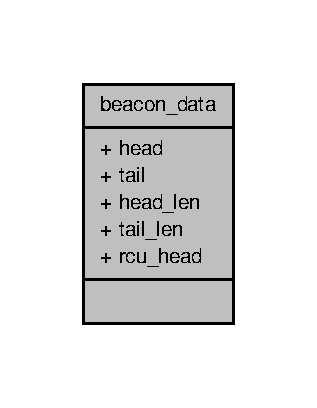
\includegraphics[width=152pt]{structbeacon__data__coll__graph}
\end{center}
\end{figure}
\subsection*{Data Fields}
\begin{DoxyCompactItemize}
\item 
u8 $\ast$ \hyperlink{structbeacon__data_a88a17ac21eb16e4d6d10b556a019aa14}{head}
\item 
u8 $\ast$ \hyperlink{structbeacon__data_a4474db8b875e66d6e97dad3d131e0259}{tail}
\item 
int \hyperlink{structbeacon__data_a60f685cd83e38123312aed3f02c63646}{head\-\_\-len}
\item 
int \hyperlink{structbeacon__data_a7e0d46a3d87c9fed4f5a67e933849488}{tail\-\_\-len}
\item 
struct rcu\-\_\-head \hyperlink{structbeacon__data_ab698383409a24791490f962fe6990655}{rcu\-\_\-head}
\end{DoxyCompactItemize}


\subsection{Detailed Description}


Definition at line 266 of file ieee80211\-\_\-i.\-h.



\subsection{Field Documentation}
\hypertarget{structbeacon__data_a88a17ac21eb16e4d6d10b556a019aa14}{\index{beacon\-\_\-data@{beacon\-\_\-data}!head@{head}}
\index{head@{head}!beacon_data@{beacon\-\_\-data}}
\subsubsection[{head}]{\setlength{\rightskip}{0pt plus 5cm}u8$\ast$ head}}\label{structbeacon__data_a88a17ac21eb16e4d6d10b556a019aa14}


Definition at line 267 of file ieee80211\-\_\-i.\-h.

\hypertarget{structbeacon__data_a60f685cd83e38123312aed3f02c63646}{\index{beacon\-\_\-data@{beacon\-\_\-data}!head\-\_\-len@{head\-\_\-len}}
\index{head\-\_\-len@{head\-\_\-len}!beacon_data@{beacon\-\_\-data}}
\subsubsection[{head\-\_\-len}]{\setlength{\rightskip}{0pt plus 5cm}int head\-\_\-len}}\label{structbeacon__data_a60f685cd83e38123312aed3f02c63646}


Definition at line 268 of file ieee80211\-\_\-i.\-h.

\hypertarget{structbeacon__data_ab698383409a24791490f962fe6990655}{\index{beacon\-\_\-data@{beacon\-\_\-data}!rcu\-\_\-head@{rcu\-\_\-head}}
\index{rcu\-\_\-head@{rcu\-\_\-head}!beacon_data@{beacon\-\_\-data}}
\subsubsection[{rcu\-\_\-head}]{\setlength{\rightskip}{0pt plus 5cm}struct rcu\-\_\-head rcu\-\_\-head}}\label{structbeacon__data_ab698383409a24791490f962fe6990655}


Definition at line 269 of file ieee80211\-\_\-i.\-h.

\hypertarget{structbeacon__data_a4474db8b875e66d6e97dad3d131e0259}{\index{beacon\-\_\-data@{beacon\-\_\-data}!tail@{tail}}
\index{tail@{tail}!beacon_data@{beacon\-\_\-data}}
\subsubsection[{tail}]{\setlength{\rightskip}{0pt plus 5cm}u8 $\ast$ tail}}\label{structbeacon__data_a4474db8b875e66d6e97dad3d131e0259}


Definition at line 267 of file ieee80211\-\_\-i.\-h.

\hypertarget{structbeacon__data_a7e0d46a3d87c9fed4f5a67e933849488}{\index{beacon\-\_\-data@{beacon\-\_\-data}!tail\-\_\-len@{tail\-\_\-len}}
\index{tail\-\_\-len@{tail\-\_\-len}!beacon_data@{beacon\-\_\-data}}
\subsubsection[{tail\-\_\-len}]{\setlength{\rightskip}{0pt plus 5cm}int tail\-\_\-len}}\label{structbeacon__data_a7e0d46a3d87c9fed4f5a67e933849488}


Definition at line 268 of file ieee80211\-\_\-i.\-h.



The documentation for this struct was generated from the following file\-:\begin{DoxyCompactItemize}
\item 
/home/guille/msm/net/mac80211/\hyperlink{ieee80211__i_8h}{ieee80211\-\_\-i.\-h}\end{DoxyCompactItemize}

\hypertarget{structiapp__layer2__update}{\section{iapp\-\_\-layer2\-\_\-update Struct Reference}
\label{structiapp__layer2__update}\index{iapp\-\_\-layer2\-\_\-update@{iapp\-\_\-layer2\-\_\-update}}
}


Collaboration diagram for iapp\-\_\-layer2\-\_\-update\-:
\nopagebreak
\begin{figure}[H]
\begin{center}
\leavevmode
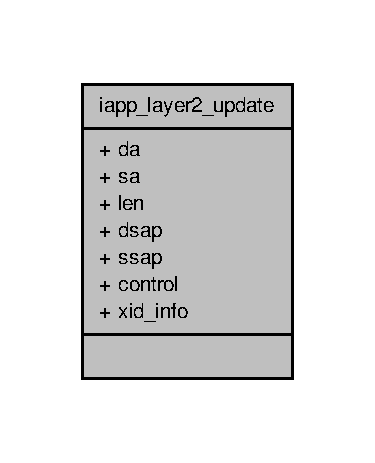
\includegraphics[width=180pt]{structiapp__layer2__update__coll__graph}
\end{center}
\end{figure}
\subsection*{Data Fields}
\begin{DoxyCompactItemize}
\item 
u8 \hyperlink{structiapp__layer2__update_ab5293261358b59532e274da4e90cd5d9}{da} \mbox{[}E\-T\-H\-\_\-\-A\-L\-E\-N\mbox{]}
\item 
u8 \hyperlink{structiapp__layer2__update_a1d248d85a9aee0de13f6a2647297e517}{sa} \mbox{[}E\-T\-H\-\_\-\-A\-L\-E\-N\mbox{]}
\item 
\-\_\-\-\_\-be16 \hyperlink{structiapp__layer2__update_a52677ab565a13bf20b2a616ead6934d7}{len}
\item 
u8 \hyperlink{structiapp__layer2__update_a41da1e30acc545368f8fd4486b8ddde0}{dsap}
\item 
u8 \hyperlink{structiapp__layer2__update_ae78f5fb673d337315fe87a2a4dc04c39}{ssap}
\item 
u8 \hyperlink{structiapp__layer2__update_aa8da087d38de0d260639bbec5c30e1bc}{control}
\item 
u8 \hyperlink{structiapp__layer2__update_ab19e66e83f523eb4706bd46459a44400}{xid\-\_\-info} \mbox{[}3\mbox{]}
\end{DoxyCompactItemize}


\subsection{Detailed Description}


Definition at line 687 of file cfg.\-c.



\subsection{Field Documentation}
\hypertarget{structiapp__layer2__update_aa8da087d38de0d260639bbec5c30e1bc}{\index{iapp\-\_\-layer2\-\_\-update@{iapp\-\_\-layer2\-\_\-update}!control@{control}}
\index{control@{control}!iapp_layer2_update@{iapp\-\_\-layer2\-\_\-update}}
\subsubsection[{control}]{\setlength{\rightskip}{0pt plus 5cm}u8 control}}\label{structiapp__layer2__update_aa8da087d38de0d260639bbec5c30e1bc}


Definition at line 693 of file cfg.\-c.

\hypertarget{structiapp__layer2__update_ab5293261358b59532e274da4e90cd5d9}{\index{iapp\-\_\-layer2\-\_\-update@{iapp\-\_\-layer2\-\_\-update}!da@{da}}
\index{da@{da}!iapp_layer2_update@{iapp\-\_\-layer2\-\_\-update}}
\subsubsection[{da}]{\setlength{\rightskip}{0pt plus 5cm}u8 da\mbox{[}E\-T\-H\-\_\-\-A\-L\-E\-N\mbox{]}}}\label{structiapp__layer2__update_ab5293261358b59532e274da4e90cd5d9}


Definition at line 688 of file cfg.\-c.

\hypertarget{structiapp__layer2__update_a41da1e30acc545368f8fd4486b8ddde0}{\index{iapp\-\_\-layer2\-\_\-update@{iapp\-\_\-layer2\-\_\-update}!dsap@{dsap}}
\index{dsap@{dsap}!iapp_layer2_update@{iapp\-\_\-layer2\-\_\-update}}
\subsubsection[{dsap}]{\setlength{\rightskip}{0pt plus 5cm}u8 dsap}}\label{structiapp__layer2__update_a41da1e30acc545368f8fd4486b8ddde0}


Definition at line 691 of file cfg.\-c.

\hypertarget{structiapp__layer2__update_a52677ab565a13bf20b2a616ead6934d7}{\index{iapp\-\_\-layer2\-\_\-update@{iapp\-\_\-layer2\-\_\-update}!len@{len}}
\index{len@{len}!iapp_layer2_update@{iapp\-\_\-layer2\-\_\-update}}
\subsubsection[{len}]{\setlength{\rightskip}{0pt plus 5cm}\-\_\-\-\_\-be16 len}}\label{structiapp__layer2__update_a52677ab565a13bf20b2a616ead6934d7}


Definition at line 690 of file cfg.\-c.

\hypertarget{structiapp__layer2__update_a1d248d85a9aee0de13f6a2647297e517}{\index{iapp\-\_\-layer2\-\_\-update@{iapp\-\_\-layer2\-\_\-update}!sa@{sa}}
\index{sa@{sa}!iapp_layer2_update@{iapp\-\_\-layer2\-\_\-update}}
\subsubsection[{sa}]{\setlength{\rightskip}{0pt plus 5cm}u8 sa\mbox{[}E\-T\-H\-\_\-\-A\-L\-E\-N\mbox{]}}}\label{structiapp__layer2__update_a1d248d85a9aee0de13f6a2647297e517}


Definition at line 689 of file cfg.\-c.

\hypertarget{structiapp__layer2__update_ae78f5fb673d337315fe87a2a4dc04c39}{\index{iapp\-\_\-layer2\-\_\-update@{iapp\-\_\-layer2\-\_\-update}!ssap@{ssap}}
\index{ssap@{ssap}!iapp_layer2_update@{iapp\-\_\-layer2\-\_\-update}}
\subsubsection[{ssap}]{\setlength{\rightskip}{0pt plus 5cm}u8 ssap}}\label{structiapp__layer2__update_ae78f5fb673d337315fe87a2a4dc04c39}


Definition at line 692 of file cfg.\-c.

\hypertarget{structiapp__layer2__update_ab19e66e83f523eb4706bd46459a44400}{\index{iapp\-\_\-layer2\-\_\-update@{iapp\-\_\-layer2\-\_\-update}!xid\-\_\-info@{xid\-\_\-info}}
\index{xid\-\_\-info@{xid\-\_\-info}!iapp_layer2_update@{iapp\-\_\-layer2\-\_\-update}}
\subsubsection[{xid\-\_\-info}]{\setlength{\rightskip}{0pt plus 5cm}u8 xid\-\_\-info\mbox{[}3\mbox{]}}}\label{structiapp__layer2__update_ab19e66e83f523eb4706bd46459a44400}


Definition at line 694 of file cfg.\-c.



The documentation for this struct was generated from the following file\-:\begin{DoxyCompactItemize}
\item 
/home/guille/msm/net/mac80211/\hyperlink{cfg_8c}{cfg.\-c}\end{DoxyCompactItemize}

\hypertarget{structieee80211__bss}{\section{ieee80211\-\_\-bss Struct Reference}
\label{structieee80211__bss}\index{ieee80211\-\_\-bss@{ieee80211\-\_\-bss}}
}


{\ttfamily \#include $<$ieee80211\-\_\-i.\-h$>$}



Collaboration diagram for ieee80211\-\_\-bss\-:
\nopagebreak
\begin{figure}[H]
\begin{center}
\leavevmode
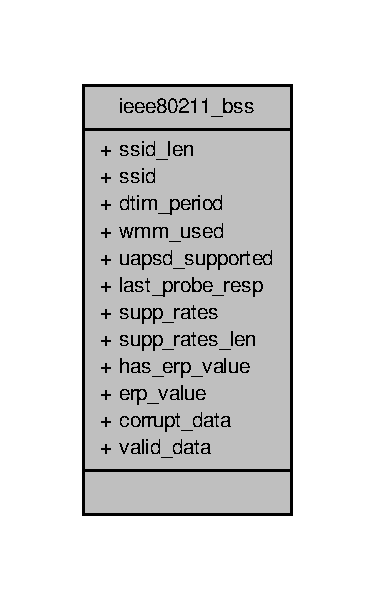
\includegraphics[width=180pt]{structieee80211__bss__coll__graph}
\end{center}
\end{figure}
\subsection*{Data Fields}
\begin{DoxyCompactItemize}
\item 
size\-\_\-t \hyperlink{structieee80211__bss_aa33b1cb67d6867fb505f832d761810a7}{ssid\-\_\-len}
\item 
u8 \hyperlink{structieee80211__bss_ae8d768cff77168f424870b6745c90714}{ssid} \mbox{[}I\-E\-E\-E80211\-\_\-\-M\-A\-X\-\_\-\-S\-S\-I\-D\-\_\-\-L\-E\-N\mbox{]}
\item 
u8 \hyperlink{structieee80211__bss_af039d096de0e0339234f5dd273cac9cb}{dtim\-\_\-period}
\item 
bool \hyperlink{structieee80211__bss_aebf73ffff3e743095dbc5613cf287640}{wmm\-\_\-used}
\item 
bool \hyperlink{structieee80211__bss_a4dff539e426e32e9bb2253d826f04529}{uapsd\-\_\-supported}
\item 
unsigned long \hyperlink{structieee80211__bss_ac009e6154e131af1edf18c445ebb4393}{last\-\_\-probe\-\_\-resp}
\item 
u8 \hyperlink{structieee80211__bss_a84e8f110c38462141993f5eccc9a2e70}{supp\-\_\-rates} \mbox{[}\hyperlink{ieee80211__i_8h_a486b5218ba1e2448c5c3b43470cdd58c}{I\-E\-E\-E80211\-\_\-\-M\-A\-X\-\_\-\-S\-U\-P\-P\-\_\-\-R\-A\-T\-E\-S}\mbox{]}
\item 
size\-\_\-t \hyperlink{structieee80211__bss_aa6efda8d2063cb2f8ef7e00b43b1954d}{supp\-\_\-rates\-\_\-len}
\item 
bool \hyperlink{structieee80211__bss_a99d04a59fd3ef9124414f0c8b3a49f12}{has\-\_\-erp\-\_\-value}
\item 
u8 \hyperlink{structieee80211__bss_aa6fc4ecdee2d9c7a81031f23f77e8f6f}{erp\-\_\-value}
\item 
u8 \hyperlink{structieee80211__bss_ae66fd8cebf5dbe25a9e67d233f7fb8a1}{corrupt\-\_\-data}
\item 
u8 \hyperlink{structieee80211__bss_acaa86d140b076b0a86f9476ec8653c1f}{valid\-\_\-data}
\end{DoxyCompactItemize}


\subsection{Detailed Description}


Definition at line 78 of file ieee80211\-\_\-i.\-h.



\subsection{Field Documentation}
\hypertarget{structieee80211__bss_ae66fd8cebf5dbe25a9e67d233f7fb8a1}{\index{ieee80211\-\_\-bss@{ieee80211\-\_\-bss}!corrupt\-\_\-data@{corrupt\-\_\-data}}
\index{corrupt\-\_\-data@{corrupt\-\_\-data}!ieee80211_bss@{ieee80211\-\_\-bss}}
\subsubsection[{corrupt\-\_\-data}]{\setlength{\rightskip}{0pt plus 5cm}u8 corrupt\-\_\-data}}\label{structieee80211__bss_ae66fd8cebf5dbe25a9e67d233f7fb8a1}


Definition at line 110 of file ieee80211\-\_\-i.\-h.

\hypertarget{structieee80211__bss_af039d096de0e0339234f5dd273cac9cb}{\index{ieee80211\-\_\-bss@{ieee80211\-\_\-bss}!dtim\-\_\-period@{dtim\-\_\-period}}
\index{dtim\-\_\-period@{dtim\-\_\-period}!ieee80211_bss@{ieee80211\-\_\-bss}}
\subsubsection[{dtim\-\_\-period}]{\setlength{\rightskip}{0pt plus 5cm}u8 dtim\-\_\-period}}\label{structieee80211__bss_af039d096de0e0339234f5dd273cac9cb}


Definition at line 83 of file ieee80211\-\_\-i.\-h.

\hypertarget{structieee80211__bss_aa6fc4ecdee2d9c7a81031f23f77e8f6f}{\index{ieee80211\-\_\-bss@{ieee80211\-\_\-bss}!erp\-\_\-value@{erp\-\_\-value}}
\index{erp\-\_\-value@{erp\-\_\-value}!ieee80211_bss@{ieee80211\-\_\-bss}}
\subsubsection[{erp\-\_\-value}]{\setlength{\rightskip}{0pt plus 5cm}u8 erp\-\_\-value}}\label{structieee80211__bss_aa6fc4ecdee2d9c7a81031f23f77e8f6f}


Definition at line 107 of file ieee80211\-\_\-i.\-h.

\hypertarget{structieee80211__bss_a99d04a59fd3ef9124414f0c8b3a49f12}{\index{ieee80211\-\_\-bss@{ieee80211\-\_\-bss}!has\-\_\-erp\-\_\-value@{has\-\_\-erp\-\_\-value}}
\index{has\-\_\-erp\-\_\-value@{has\-\_\-erp\-\_\-value}!ieee80211_bss@{ieee80211\-\_\-bss}}
\subsubsection[{has\-\_\-erp\-\_\-value}]{\setlength{\rightskip}{0pt plus 5cm}bool has\-\_\-erp\-\_\-value}}\label{structieee80211__bss_a99d04a59fd3ef9124414f0c8b3a49f12}


Definition at line 106 of file ieee80211\-\_\-i.\-h.

\hypertarget{structieee80211__bss_ac009e6154e131af1edf18c445ebb4393}{\index{ieee80211\-\_\-bss@{ieee80211\-\_\-bss}!last\-\_\-probe\-\_\-resp@{last\-\_\-probe\-\_\-resp}}
\index{last\-\_\-probe\-\_\-resp@{last\-\_\-probe\-\_\-resp}!ieee80211_bss@{ieee80211\-\_\-bss}}
\subsubsection[{last\-\_\-probe\-\_\-resp}]{\setlength{\rightskip}{0pt plus 5cm}unsigned long last\-\_\-probe\-\_\-resp}}\label{structieee80211__bss_ac009e6154e131af1edf18c445ebb4393}


Definition at line 88 of file ieee80211\-\_\-i.\-h.

\hypertarget{structieee80211__bss_ae8d768cff77168f424870b6745c90714}{\index{ieee80211\-\_\-bss@{ieee80211\-\_\-bss}!ssid@{ssid}}
\index{ssid@{ssid}!ieee80211_bss@{ieee80211\-\_\-bss}}
\subsubsection[{ssid}]{\setlength{\rightskip}{0pt plus 5cm}u8 ssid\mbox{[}I\-E\-E\-E80211\-\_\-\-M\-A\-X\-\_\-\-S\-S\-I\-D\-\_\-\-L\-E\-N\mbox{]}}}\label{structieee80211__bss_ae8d768cff77168f424870b6745c90714}


Definition at line 81 of file ieee80211\-\_\-i.\-h.

\hypertarget{structieee80211__bss_aa33b1cb67d6867fb505f832d761810a7}{\index{ieee80211\-\_\-bss@{ieee80211\-\_\-bss}!ssid\-\_\-len@{ssid\-\_\-len}}
\index{ssid\-\_\-len@{ssid\-\_\-len}!ieee80211_bss@{ieee80211\-\_\-bss}}
\subsubsection[{ssid\-\_\-len}]{\setlength{\rightskip}{0pt plus 5cm}size\-\_\-t ssid\-\_\-len}}\label{structieee80211__bss_aa33b1cb67d6867fb505f832d761810a7}


Definition at line 80 of file ieee80211\-\_\-i.\-h.

\hypertarget{structieee80211__bss_a84e8f110c38462141993f5eccc9a2e70}{\index{ieee80211\-\_\-bss@{ieee80211\-\_\-bss}!supp\-\_\-rates@{supp\-\_\-rates}}
\index{supp\-\_\-rates@{supp\-\_\-rates}!ieee80211_bss@{ieee80211\-\_\-bss}}
\subsubsection[{supp\-\_\-rates}]{\setlength{\rightskip}{0pt plus 5cm}u8 supp\-\_\-rates\mbox{[}{\bf I\-E\-E\-E80211\-\_\-\-M\-A\-X\-\_\-\-S\-U\-P\-P\-\_\-\-R\-A\-T\-E\-S}\mbox{]}}}\label{structieee80211__bss_a84e8f110c38462141993f5eccc9a2e70}


Definition at line 97 of file ieee80211\-\_\-i.\-h.

\hypertarget{structieee80211__bss_aa6efda8d2063cb2f8ef7e00b43b1954d}{\index{ieee80211\-\_\-bss@{ieee80211\-\_\-bss}!supp\-\_\-rates\-\_\-len@{supp\-\_\-rates\-\_\-len}}
\index{supp\-\_\-rates\-\_\-len@{supp\-\_\-rates\-\_\-len}!ieee80211_bss@{ieee80211\-\_\-bss}}
\subsubsection[{supp\-\_\-rates\-\_\-len}]{\setlength{\rightskip}{0pt plus 5cm}size\-\_\-t supp\-\_\-rates\-\_\-len}}\label{structieee80211__bss_aa6efda8d2063cb2f8ef7e00b43b1954d}


Definition at line 98 of file ieee80211\-\_\-i.\-h.

\hypertarget{structieee80211__bss_a4dff539e426e32e9bb2253d826f04529}{\index{ieee80211\-\_\-bss@{ieee80211\-\_\-bss}!uapsd\-\_\-supported@{uapsd\-\_\-supported}}
\index{uapsd\-\_\-supported@{uapsd\-\_\-supported}!ieee80211_bss@{ieee80211\-\_\-bss}}
\subsubsection[{uapsd\-\_\-supported}]{\setlength{\rightskip}{0pt plus 5cm}bool uapsd\-\_\-supported}}\label{structieee80211__bss_a4dff539e426e32e9bb2253d826f04529}


Definition at line 86 of file ieee80211\-\_\-i.\-h.

\hypertarget{structieee80211__bss_acaa86d140b076b0a86f9476ec8653c1f}{\index{ieee80211\-\_\-bss@{ieee80211\-\_\-bss}!valid\-\_\-data@{valid\-\_\-data}}
\index{valid\-\_\-data@{valid\-\_\-data}!ieee80211_bss@{ieee80211\-\_\-bss}}
\subsubsection[{valid\-\_\-data}]{\setlength{\rightskip}{0pt plus 5cm}u8 valid\-\_\-data}}\label{structieee80211__bss_acaa86d140b076b0a86f9476ec8653c1f}


Definition at line 113 of file ieee80211\-\_\-i.\-h.

\hypertarget{structieee80211__bss_aebf73ffff3e743095dbc5613cf287640}{\index{ieee80211\-\_\-bss@{ieee80211\-\_\-bss}!wmm\-\_\-used@{wmm\-\_\-used}}
\index{wmm\-\_\-used@{wmm\-\_\-used}!ieee80211_bss@{ieee80211\-\_\-bss}}
\subsubsection[{wmm\-\_\-used}]{\setlength{\rightskip}{0pt plus 5cm}bool wmm\-\_\-used}}\label{structieee80211__bss_aebf73ffff3e743095dbc5613cf287640}


Definition at line 85 of file ieee80211\-\_\-i.\-h.



The documentation for this struct was generated from the following file\-:\begin{DoxyCompactItemize}
\item 
/home/guille/msm/net/mac80211/\hyperlink{ieee80211__i_8h}{ieee80211\-\_\-i.\-h}\end{DoxyCompactItemize}

\hypertarget{structieee80211__fragment__entry}{\section{ieee80211\-\_\-fragment\-\_\-entry Struct Reference}
\label{structieee80211__fragment__entry}\index{ieee80211\-\_\-fragment\-\_\-entry@{ieee80211\-\_\-fragment\-\_\-entry}}
}


{\ttfamily \#include $<$ieee80211\-\_\-i.\-h$>$}



Collaboration diagram for ieee80211\-\_\-fragment\-\_\-entry\-:
\nopagebreak
\begin{figure}[H]
\begin{center}
\leavevmode
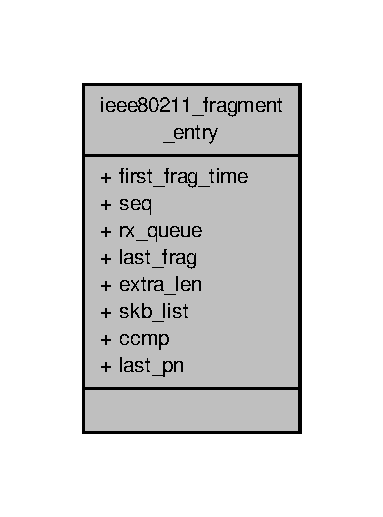
\includegraphics[width=184pt]{structieee80211__fragment__entry__coll__graph}
\end{center}
\end{figure}
\subsection*{Data Fields}
\begin{DoxyCompactItemize}
\item 
unsigned long \hyperlink{structieee80211__fragment__entry_aff13d3635e966dc5c9d34fcba0fa6a59}{first\-\_\-frag\-\_\-time}
\item 
unsigned int \hyperlink{structieee80211__fragment__entry_a1db4845df10d789835dcc97c392a2fe6}{seq}
\item 
unsigned int \hyperlink{structieee80211__fragment__entry_ae9c4670f6e34166d57315f460003eb00}{rx\-\_\-queue}
\item 
unsigned int \hyperlink{structieee80211__fragment__entry_afa570deed8cdb8b0d26a4f3ed9c3db4f}{last\-\_\-frag}
\item 
unsigned int \hyperlink{structieee80211__fragment__entry_afd84bbe6015ef3eb71afe651f3e9f72a}{extra\-\_\-len}
\item 
struct sk\-\_\-buff\-\_\-head \hyperlink{structieee80211__fragment__entry_ae572ad476d84353186dc8a596d035a92}{skb\-\_\-list}
\item 
int \hyperlink{structieee80211__fragment__entry_af0bf8d0a7415e0d80ce8876f9b5b69a5}{ccmp}
\item 
u8 \hyperlink{structieee80211__fragment__entry_a18ab2d23d6a5293bf2d38573afca820c}{last\-\_\-pn} \mbox{[}6\mbox{]}
\end{DoxyCompactItemize}


\subsection{Detailed Description}


Definition at line 66 of file ieee80211\-\_\-i.\-h.



\subsection{Field Documentation}
\hypertarget{structieee80211__fragment__entry_af0bf8d0a7415e0d80ce8876f9b5b69a5}{\index{ieee80211\-\_\-fragment\-\_\-entry@{ieee80211\-\_\-fragment\-\_\-entry}!ccmp@{ccmp}}
\index{ccmp@{ccmp}!ieee80211_fragment_entry@{ieee80211\-\_\-fragment\-\_\-entry}}
\subsubsection[{ccmp}]{\setlength{\rightskip}{0pt plus 5cm}int ccmp}}\label{structieee80211__fragment__entry_af0bf8d0a7415e0d80ce8876f9b5b69a5}


Definition at line 73 of file ieee80211\-\_\-i.\-h.

\hypertarget{structieee80211__fragment__entry_afd84bbe6015ef3eb71afe651f3e9f72a}{\index{ieee80211\-\_\-fragment\-\_\-entry@{ieee80211\-\_\-fragment\-\_\-entry}!extra\-\_\-len@{extra\-\_\-len}}
\index{extra\-\_\-len@{extra\-\_\-len}!ieee80211_fragment_entry@{ieee80211\-\_\-fragment\-\_\-entry}}
\subsubsection[{extra\-\_\-len}]{\setlength{\rightskip}{0pt plus 5cm}unsigned int extra\-\_\-len}}\label{structieee80211__fragment__entry_afd84bbe6015ef3eb71afe651f3e9f72a}


Definition at line 71 of file ieee80211\-\_\-i.\-h.

\hypertarget{structieee80211__fragment__entry_aff13d3635e966dc5c9d34fcba0fa6a59}{\index{ieee80211\-\_\-fragment\-\_\-entry@{ieee80211\-\_\-fragment\-\_\-entry}!first\-\_\-frag\-\_\-time@{first\-\_\-frag\-\_\-time}}
\index{first\-\_\-frag\-\_\-time@{first\-\_\-frag\-\_\-time}!ieee80211_fragment_entry@{ieee80211\-\_\-fragment\-\_\-entry}}
\subsubsection[{first\-\_\-frag\-\_\-time}]{\setlength{\rightskip}{0pt plus 5cm}unsigned long first\-\_\-frag\-\_\-time}}\label{structieee80211__fragment__entry_aff13d3635e966dc5c9d34fcba0fa6a59}


Definition at line 67 of file ieee80211\-\_\-i.\-h.

\hypertarget{structieee80211__fragment__entry_afa570deed8cdb8b0d26a4f3ed9c3db4f}{\index{ieee80211\-\_\-fragment\-\_\-entry@{ieee80211\-\_\-fragment\-\_\-entry}!last\-\_\-frag@{last\-\_\-frag}}
\index{last\-\_\-frag@{last\-\_\-frag}!ieee80211_fragment_entry@{ieee80211\-\_\-fragment\-\_\-entry}}
\subsubsection[{last\-\_\-frag}]{\setlength{\rightskip}{0pt plus 5cm}unsigned int last\-\_\-frag}}\label{structieee80211__fragment__entry_afa570deed8cdb8b0d26a4f3ed9c3db4f}


Definition at line 70 of file ieee80211\-\_\-i.\-h.

\hypertarget{structieee80211__fragment__entry_a18ab2d23d6a5293bf2d38573afca820c}{\index{ieee80211\-\_\-fragment\-\_\-entry@{ieee80211\-\_\-fragment\-\_\-entry}!last\-\_\-pn@{last\-\_\-pn}}
\index{last\-\_\-pn@{last\-\_\-pn}!ieee80211_fragment_entry@{ieee80211\-\_\-fragment\-\_\-entry}}
\subsubsection[{last\-\_\-pn}]{\setlength{\rightskip}{0pt plus 5cm}u8 last\-\_\-pn\mbox{[}6\mbox{]}}}\label{structieee80211__fragment__entry_a18ab2d23d6a5293bf2d38573afca820c}


Definition at line 74 of file ieee80211\-\_\-i.\-h.

\hypertarget{structieee80211__fragment__entry_ae9c4670f6e34166d57315f460003eb00}{\index{ieee80211\-\_\-fragment\-\_\-entry@{ieee80211\-\_\-fragment\-\_\-entry}!rx\-\_\-queue@{rx\-\_\-queue}}
\index{rx\-\_\-queue@{rx\-\_\-queue}!ieee80211_fragment_entry@{ieee80211\-\_\-fragment\-\_\-entry}}
\subsubsection[{rx\-\_\-queue}]{\setlength{\rightskip}{0pt plus 5cm}unsigned int rx\-\_\-queue}}\label{structieee80211__fragment__entry_ae9c4670f6e34166d57315f460003eb00}


Definition at line 69 of file ieee80211\-\_\-i.\-h.

\hypertarget{structieee80211__fragment__entry_a1db4845df10d789835dcc97c392a2fe6}{\index{ieee80211\-\_\-fragment\-\_\-entry@{ieee80211\-\_\-fragment\-\_\-entry}!seq@{seq}}
\index{seq@{seq}!ieee80211_fragment_entry@{ieee80211\-\_\-fragment\-\_\-entry}}
\subsubsection[{seq}]{\setlength{\rightskip}{0pt plus 5cm}unsigned int seq}}\label{structieee80211__fragment__entry_a1db4845df10d789835dcc97c392a2fe6}


Definition at line 68 of file ieee80211\-\_\-i.\-h.

\hypertarget{structieee80211__fragment__entry_ae572ad476d84353186dc8a596d035a92}{\index{ieee80211\-\_\-fragment\-\_\-entry@{ieee80211\-\_\-fragment\-\_\-entry}!skb\-\_\-list@{skb\-\_\-list}}
\index{skb\-\_\-list@{skb\-\_\-list}!ieee80211_fragment_entry@{ieee80211\-\_\-fragment\-\_\-entry}}
\subsubsection[{skb\-\_\-list}]{\setlength{\rightskip}{0pt plus 5cm}struct sk\-\_\-buff\-\_\-head skb\-\_\-list}}\label{structieee80211__fragment__entry_ae572ad476d84353186dc8a596d035a92}


Definition at line 72 of file ieee80211\-\_\-i.\-h.



The documentation for this struct was generated from the following file\-:\begin{DoxyCompactItemize}
\item 
/home/guille/msm/net/mac80211/\hyperlink{ieee80211__i_8h}{ieee80211\-\_\-i.\-h}\end{DoxyCompactItemize}

\hypertarget{structieee80211__if__ap}{\section{ieee80211\-\_\-if\-\_\-ap Struct Reference}
\label{structieee80211__if__ap}\index{ieee80211\-\_\-if\-\_\-ap@{ieee80211\-\_\-if\-\_\-ap}}
}


{\ttfamily \#include $<$ieee80211\-\_\-i.\-h$>$}



Collaboration diagram for ieee80211\-\_\-if\-\_\-ap\-:
\nopagebreak
\begin{figure}[H]
\begin{center}
\leavevmode
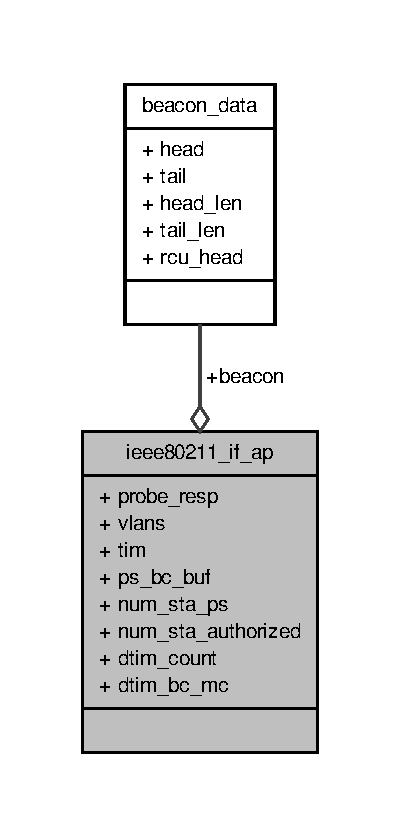
\includegraphics[width=192pt]{structieee80211__if__ap__coll__graph}
\end{center}
\end{figure}
\subsection*{Data Fields}
\begin{DoxyCompactItemize}
\item 
struct \hyperlink{structbeacon__data}{beacon\-\_\-data} \-\_\-\-\_\-rcu $\ast$ \hyperlink{structieee80211__if__ap_af423343a66559cac968f55f903c1cf3b}{beacon}
\item 
struct sk\-\_\-buff \-\_\-\-\_\-rcu $\ast$ \hyperlink{structieee80211__if__ap_ab6e788ecb6d5a607e56fcd97d0996d69}{probe\-\_\-resp}
\item 
struct list\-\_\-head \hyperlink{structieee80211__if__ap_ad647c724f4509c4bb97a527552b6497a}{vlans}
\item 
u8 \hyperlink{structieee80211__if__ap_ac8921d232cd7bc324ccfe9d22525d030}{tim} \mbox{[}sizeof(unsigned long)$\ast$B\-I\-T\-S\-\_\-\-T\-O\-\_\-\-L\-O\-N\-G\-S(I\-E\-E\-E80211\-\_\-\-M\-A\-X\-\_\-\-A\-I\-D+1)\mbox{]}
\item 
struct sk\-\_\-buff\-\_\-head \hyperlink{structieee80211__if__ap_ae1cfc557eb8683f9cb993a0e3c0003bb}{ps\-\_\-bc\-\_\-buf}
\item 
atomic\-\_\-t \hyperlink{structieee80211__if__ap_a5c58afde586c58d4b830915b47015999}{num\-\_\-sta\-\_\-ps}
\item 
atomic\-\_\-t \hyperlink{structieee80211__if__ap_a129987b49661f0799553c40659a8e807}{num\-\_\-sta\-\_\-authorized}
\item 
int \hyperlink{structieee80211__if__ap_abcc08bb90309210ff5688fff800cd7f1}{dtim\-\_\-count}
\item 
bool \hyperlink{structieee80211__if__ap_a7c2f6d7ac8d776b7b6238ab915f3b0f6}{dtim\-\_\-bc\-\_\-mc}
\end{DoxyCompactItemize}


\subsection{Detailed Description}


Definition at line 272 of file ieee80211\-\_\-i.\-h.



\subsection{Field Documentation}
\hypertarget{structieee80211__if__ap_af423343a66559cac968f55f903c1cf3b}{\index{ieee80211\-\_\-if\-\_\-ap@{ieee80211\-\_\-if\-\_\-ap}!beacon@{beacon}}
\index{beacon@{beacon}!ieee80211_if_ap@{ieee80211\-\_\-if\-\_\-ap}}
\subsubsection[{beacon}]{\setlength{\rightskip}{0pt plus 5cm}struct {\bf beacon\-\_\-data} \-\_\-\-\_\-rcu$\ast$ beacon}}\label{structieee80211__if__ap_af423343a66559cac968f55f903c1cf3b}


Definition at line 273 of file ieee80211\-\_\-i.\-h.

\hypertarget{structieee80211__if__ap_a7c2f6d7ac8d776b7b6238ab915f3b0f6}{\index{ieee80211\-\_\-if\-\_\-ap@{ieee80211\-\_\-if\-\_\-ap}!dtim\-\_\-bc\-\_\-mc@{dtim\-\_\-bc\-\_\-mc}}
\index{dtim\-\_\-bc\-\_\-mc@{dtim\-\_\-bc\-\_\-mc}!ieee80211_if_ap@{ieee80211\-\_\-if\-\_\-ap}}
\subsubsection[{dtim\-\_\-bc\-\_\-mc}]{\setlength{\rightskip}{0pt plus 5cm}bool dtim\-\_\-bc\-\_\-mc}}\label{structieee80211__if__ap_a7c2f6d7ac8d776b7b6238ab915f3b0f6}


Definition at line 286 of file ieee80211\-\_\-i.\-h.

\hypertarget{structieee80211__if__ap_abcc08bb90309210ff5688fff800cd7f1}{\index{ieee80211\-\_\-if\-\_\-ap@{ieee80211\-\_\-if\-\_\-ap}!dtim\-\_\-count@{dtim\-\_\-count}}
\index{dtim\-\_\-count@{dtim\-\_\-count}!ieee80211_if_ap@{ieee80211\-\_\-if\-\_\-ap}}
\subsubsection[{dtim\-\_\-count}]{\setlength{\rightskip}{0pt plus 5cm}int dtim\-\_\-count}}\label{structieee80211__if__ap_abcc08bb90309210ff5688fff800cd7f1}


Definition at line 285 of file ieee80211\-\_\-i.\-h.

\hypertarget{structieee80211__if__ap_a129987b49661f0799553c40659a8e807}{\index{ieee80211\-\_\-if\-\_\-ap@{ieee80211\-\_\-if\-\_\-ap}!num\-\_\-sta\-\_\-authorized@{num\-\_\-sta\-\_\-authorized}}
\index{num\-\_\-sta\-\_\-authorized@{num\-\_\-sta\-\_\-authorized}!ieee80211_if_ap@{ieee80211\-\_\-if\-\_\-ap}}
\subsubsection[{num\-\_\-sta\-\_\-authorized}]{\setlength{\rightskip}{0pt plus 5cm}atomic\-\_\-t num\-\_\-sta\-\_\-authorized}}\label{structieee80211__if__ap_a129987b49661f0799553c40659a8e807}


Definition at line 284 of file ieee80211\-\_\-i.\-h.

\hypertarget{structieee80211__if__ap_a5c58afde586c58d4b830915b47015999}{\index{ieee80211\-\_\-if\-\_\-ap@{ieee80211\-\_\-if\-\_\-ap}!num\-\_\-sta\-\_\-ps@{num\-\_\-sta\-\_\-ps}}
\index{num\-\_\-sta\-\_\-ps@{num\-\_\-sta\-\_\-ps}!ieee80211_if_ap@{ieee80211\-\_\-if\-\_\-ap}}
\subsubsection[{num\-\_\-sta\-\_\-ps}]{\setlength{\rightskip}{0pt plus 5cm}atomic\-\_\-t num\-\_\-sta\-\_\-ps}}\label{structieee80211__if__ap_a5c58afde586c58d4b830915b47015999}


Definition at line 283 of file ieee80211\-\_\-i.\-h.

\hypertarget{structieee80211__if__ap_ab6e788ecb6d5a607e56fcd97d0996d69}{\index{ieee80211\-\_\-if\-\_\-ap@{ieee80211\-\_\-if\-\_\-ap}!probe\-\_\-resp@{probe\-\_\-resp}}
\index{probe\-\_\-resp@{probe\-\_\-resp}!ieee80211_if_ap@{ieee80211\-\_\-if\-\_\-ap}}
\subsubsection[{probe\-\_\-resp}]{\setlength{\rightskip}{0pt plus 5cm}struct sk\-\_\-buff \-\_\-\-\_\-rcu$\ast$ probe\-\_\-resp}}\label{structieee80211__if__ap_ab6e788ecb6d5a607e56fcd97d0996d69}


Definition at line 274 of file ieee80211\-\_\-i.\-h.

\hypertarget{structieee80211__if__ap_ae1cfc557eb8683f9cb993a0e3c0003bb}{\index{ieee80211\-\_\-if\-\_\-ap@{ieee80211\-\_\-if\-\_\-ap}!ps\-\_\-bc\-\_\-buf@{ps\-\_\-bc\-\_\-buf}}
\index{ps\-\_\-bc\-\_\-buf@{ps\-\_\-bc\-\_\-buf}!ieee80211_if_ap@{ieee80211\-\_\-if\-\_\-ap}}
\subsubsection[{ps\-\_\-bc\-\_\-buf}]{\setlength{\rightskip}{0pt plus 5cm}struct sk\-\_\-buff\-\_\-head ps\-\_\-bc\-\_\-buf}}\label{structieee80211__if__ap_ae1cfc557eb8683f9cb993a0e3c0003bb}


Definition at line 282 of file ieee80211\-\_\-i.\-h.

\hypertarget{structieee80211__if__ap_ac8921d232cd7bc324ccfe9d22525d030}{\index{ieee80211\-\_\-if\-\_\-ap@{ieee80211\-\_\-if\-\_\-ap}!tim@{tim}}
\index{tim@{tim}!ieee80211_if_ap@{ieee80211\-\_\-if\-\_\-ap}}
\subsubsection[{tim}]{\setlength{\rightskip}{0pt plus 5cm}u8 tim\mbox{[}sizeof(unsigned long)$\ast$B\-I\-T\-S\-\_\-\-T\-O\-\_\-\-L\-O\-N\-G\-S(I\-E\-E\-E80211\-\_\-\-M\-A\-X\-\_\-\-A\-I\-D+1)\mbox{]}}}\label{structieee80211__if__ap_ac8921d232cd7bc324ccfe9d22525d030}


Definition at line 281 of file ieee80211\-\_\-i.\-h.

\hypertarget{structieee80211__if__ap_ad647c724f4509c4bb97a527552b6497a}{\index{ieee80211\-\_\-if\-\_\-ap@{ieee80211\-\_\-if\-\_\-ap}!vlans@{vlans}}
\index{vlans@{vlans}!ieee80211_if_ap@{ieee80211\-\_\-if\-\_\-ap}}
\subsubsection[{vlans}]{\setlength{\rightskip}{0pt plus 5cm}struct list\-\_\-head vlans}}\label{structieee80211__if__ap_ad647c724f4509c4bb97a527552b6497a}


Definition at line 276 of file ieee80211\-\_\-i.\-h.



The documentation for this struct was generated from the following file\-:\begin{DoxyCompactItemize}
\item 
/home/guille/msm/net/mac80211/\hyperlink{ieee80211__i_8h}{ieee80211\-\_\-i.\-h}\end{DoxyCompactItemize}

\hypertarget{structieee80211__if__ibss}{\section{ieee80211\-\_\-if\-\_\-ibss Struct Reference}
\label{structieee80211__if__ibss}\index{ieee80211\-\_\-if\-\_\-ibss@{ieee80211\-\_\-if\-\_\-ibss}}
}


{\ttfamily \#include $<$ieee80211\-\_\-i.\-h$>$}



Collaboration diagram for ieee80211\-\_\-if\-\_\-ibss\-:
\nopagebreak
\begin{figure}[H]
\begin{center}
\leavevmode
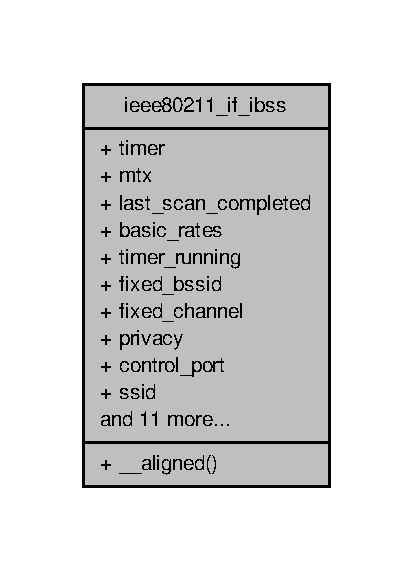
\includegraphics[width=198pt]{structieee80211__if__ibss__coll__graph}
\end{center}
\end{figure}
\subsection*{Public Types}
\begin{DoxyCompactItemize}
\item 
enum \{ \hyperlink{structieee80211__if__ibss_a0411cd49bb5b71852cecd93bcbf0ca2da74a07e1c77254e60cbe5ba98cdd1f5ac}{I\-E\-E\-E80211\-\_\-\-I\-B\-S\-S\-\_\-\-M\-L\-M\-E\-\_\-\-S\-E\-A\-R\-C\-H}, 
\hyperlink{structieee80211__if__ibss_a0411cd49bb5b71852cecd93bcbf0ca2dad8ebf6128c567875ba4bf30a7407d6ce}{I\-E\-E\-E80211\-\_\-\-I\-B\-S\-S\-\_\-\-M\-L\-M\-E\-\_\-\-J\-O\-I\-N\-E\-D}
 \}
\end{DoxyCompactItemize}
\subsection*{Public Member Functions}
\begin{DoxyCompactItemize}
\item 
u8 bssid\mbox{[}E\-T\-H\-\_\-\-A\-L\-E\-N\mbox{]} \hyperlink{structieee80211__if__ibss_af446847dcbfde15aabb52beb5b1972e5}{\-\_\-\-\_\-aligned} (2)
\end{DoxyCompactItemize}
\subsection*{Data Fields}
\begin{DoxyCompactItemize}
\item 
struct timer\-\_\-list \hyperlink{structieee80211__if__ibss_ae8aedee6c0bd2f7edbb10f18d574f107}{timer}
\item 
struct mutex \hyperlink{structieee80211__if__ibss_a06f637951b74c996f2e4987a7be1dbdd}{mtx}
\item 
unsigned long \hyperlink{structieee80211__if__ibss_a02630c17c918fc4068543524fa1c2793}{last\-\_\-scan\-\_\-completed}
\item 
u32 \hyperlink{structieee80211__if__ibss_a38fe4973d85ce09896a4da100ee7470d}{basic\-\_\-rates}
\item 
bool \hyperlink{structieee80211__if__ibss_a23958e610207eb28549d8d13255aa129}{timer\-\_\-running}
\item 
bool \hyperlink{structieee80211__if__ibss_a7930c3868b223ce60e12e84d087b3f58}{fixed\-\_\-bssid}
\item 
bool \hyperlink{structieee80211__if__ibss_aaeb95af3104d555b91418ca7b173e7ac}{fixed\-\_\-channel}
\item 
bool \hyperlink{structieee80211__if__ibss_a416c8f7c70b4e5fdcd31edb1cd9004ab}{privacy}
\item 
bool \hyperlink{structieee80211__if__ibss_a5f56e2447bde008fc2d675dcd029fc17}{control\-\_\-port}
\item 
u8 \hyperlink{structieee80211__if__ibss_ae8d768cff77168f424870b6745c90714}{ssid} \mbox{[}I\-E\-E\-E80211\-\_\-\-M\-A\-X\-\_\-\-S\-S\-I\-D\-\_\-\-L\-E\-N\mbox{]}
\item 
u8 \hyperlink{structieee80211__if__ibss_a440f44724caffefa0f9c838518a3c790}{ssid\-\_\-len}
\item 
u8 \hyperlink{structieee80211__if__ibss_a8e143706c80e5faf90dc4a385c4517f6}{ie\-\_\-len}
\item 
u8 $\ast$ \hyperlink{structieee80211__if__ibss_a837e19ab2bc08b5dec813ad916a6f09d}{ie}
\item 
struct ieee80211\-\_\-channel $\ast$ \hyperlink{structieee80211__if__ibss_a80252eb32e874a054a819044989184e2}{channel}
\item 
enum nl80211\-\_\-channel\-\_\-type \hyperlink{structieee80211__if__ibss_a54d35cd8a215e66908b8671a70fa4fca}{channel\-\_\-type}
\item 
unsigned long \hyperlink{structieee80211__if__ibss_a0557131126944ea730092a4df84149d7}{ibss\-\_\-join\-\_\-req}
\item 
struct sk\-\_\-buff \-\_\-\-\_\-rcu $\ast$ \hyperlink{structieee80211__if__ibss_a9daf15f2ed9d31b8120ac9c337ca9c62}{presp}
\item 
struct sk\-\_\-buff $\ast$ \hyperlink{structieee80211__if__ibss_aeba6836824708325a83121030f092c30}{skb}
\item 
spinlock\-\_\-t \hyperlink{structieee80211__if__ibss_a8356eead4fd0be0edf4ea2e0237a4de8}{incomplete\-\_\-lock}
\item 
struct list\-\_\-head \hyperlink{structieee80211__if__ibss_a18703abd5d82801e889c2c13282d2f5c}{incomplete\-\_\-stations}
\item 
enum ieee80211\-\_\-if\-\_\-ibss\-:: \{ ... \}  \hyperlink{structieee80211__if__ibss_a3253c6d1cd5d679b637262e95a0986a1}{state}
\end{DoxyCompactItemize}


\subsection{Detailed Description}


Definition at line 518 of file ieee80211\-\_\-i.\-h.



\subsection{Member Enumeration Documentation}
\hypertarget{structieee80211__if__ibss_a0411cd49bb5b71852cecd93bcbf0ca2d}{\subsubsection[{anonymous enum}]{\setlength{\rightskip}{0pt plus 5cm}anonymous enum}}\label{structieee80211__if__ibss_a0411cd49bb5b71852cecd93bcbf0ca2d}
\begin{Desc}
\item[Enumerator]\par
\begin{description}
\index{I\-E\-E\-E80211\-\_\-\-I\-B\-S\-S\-\_\-\-M\-L\-M\-E\-\_\-\-S\-E\-A\-R\-C\-H@{I\-E\-E\-E80211\-\_\-\-I\-B\-S\-S\-\_\-\-M\-L\-M\-E\-\_\-\-S\-E\-A\-R\-C\-H}!ieee80211\-\_\-if\-\_\-ibss@{ieee80211\-\_\-if\-\_\-ibss}}\index{ieee80211\-\_\-if\-\_\-ibss@{ieee80211\-\_\-if\-\_\-ibss}!I\-E\-E\-E80211\-\_\-\-I\-B\-S\-S\-\_\-\-M\-L\-M\-E\-\_\-\-S\-E\-A\-R\-C\-H@{I\-E\-E\-E80211\-\_\-\-I\-B\-S\-S\-\_\-\-M\-L\-M\-E\-\_\-\-S\-E\-A\-R\-C\-H}}\item[{\em 
\hypertarget{structieee80211__if__ibss_a0411cd49bb5b71852cecd93bcbf0ca2da74a07e1c77254e60cbe5ba98cdd1f5ac}{I\-E\-E\-E80211\-\_\-\-I\-B\-S\-S\-\_\-\-M\-L\-M\-E\-\_\-\-S\-E\-A\-R\-C\-H}\label{structieee80211__if__ibss_a0411cd49bb5b71852cecd93bcbf0ca2da74a07e1c77254e60cbe5ba98cdd1f5ac}
}]\index{I\-E\-E\-E80211\-\_\-\-I\-B\-S\-S\-\_\-\-M\-L\-M\-E\-\_\-\-J\-O\-I\-N\-E\-D@{I\-E\-E\-E80211\-\_\-\-I\-B\-S\-S\-\_\-\-M\-L\-M\-E\-\_\-\-J\-O\-I\-N\-E\-D}!ieee80211\-\_\-if\-\_\-ibss@{ieee80211\-\_\-if\-\_\-ibss}}\index{ieee80211\-\_\-if\-\_\-ibss@{ieee80211\-\_\-if\-\_\-ibss}!I\-E\-E\-E80211\-\_\-\-I\-B\-S\-S\-\_\-\-M\-L\-M\-E\-\_\-\-J\-O\-I\-N\-E\-D@{I\-E\-E\-E80211\-\_\-\-I\-B\-S\-S\-\_\-\-M\-L\-M\-E\-\_\-\-J\-O\-I\-N\-E\-D}}\item[{\em 
\hypertarget{structieee80211__if__ibss_a0411cd49bb5b71852cecd93bcbf0ca2dad8ebf6128c567875ba4bf30a7407d6ce}{I\-E\-E\-E80211\-\_\-\-I\-B\-S\-S\-\_\-\-M\-L\-M\-E\-\_\-\-J\-O\-I\-N\-E\-D}\label{structieee80211__if__ibss_a0411cd49bb5b71852cecd93bcbf0ca2dad8ebf6128c567875ba4bf30a7407d6ce}
}]\end{description}
\end{Desc}


Definition at line 550 of file ieee80211\-\_\-i.\-h.



\subsection{Member Function Documentation}
\hypertarget{structieee80211__if__ibss_af446847dcbfde15aabb52beb5b1972e5}{\index{ieee80211\-\_\-if\-\_\-ibss@{ieee80211\-\_\-if\-\_\-ibss}!\-\_\-\-\_\-aligned@{\-\_\-\-\_\-aligned}}
\index{\-\_\-\-\_\-aligned@{\-\_\-\-\_\-aligned}!ieee80211_if_ibss@{ieee80211\-\_\-if\-\_\-ibss}}
\subsubsection[{\-\_\-\-\_\-aligned}]{\setlength{\rightskip}{0pt plus 5cm}u8 bssid \mbox{[}E\-T\-H\-\_\-\-A\-L\-E\-N\mbox{]} \-\_\-\-\_\-aligned (
\begin{DoxyParamCaption}
\item[{2}]{}
\end{DoxyParamCaption}
)}}\label{structieee80211__if__ibss_af446847dcbfde15aabb52beb5b1972e5}


\subsection{Field Documentation}
\hypertarget{structieee80211__if__ibss_a38fe4973d85ce09896a4da100ee7470d}{\index{ieee80211\-\_\-if\-\_\-ibss@{ieee80211\-\_\-if\-\_\-ibss}!basic\-\_\-rates@{basic\-\_\-rates}}
\index{basic\-\_\-rates@{basic\-\_\-rates}!ieee80211_if_ibss@{ieee80211\-\_\-if\-\_\-ibss}}
\subsubsection[{basic\-\_\-rates}]{\setlength{\rightskip}{0pt plus 5cm}u32 basic\-\_\-rates}}\label{structieee80211__if__ibss_a38fe4973d85ce09896a4da100ee7470d}


Definition at line 525 of file ieee80211\-\_\-i.\-h.

\hypertarget{structieee80211__if__ibss_a80252eb32e874a054a819044989184e2}{\index{ieee80211\-\_\-if\-\_\-ibss@{ieee80211\-\_\-if\-\_\-ibss}!channel@{channel}}
\index{channel@{channel}!ieee80211_if_ibss@{ieee80211\-\_\-if\-\_\-ibss}}
\subsubsection[{channel}]{\setlength{\rightskip}{0pt plus 5cm}struct ieee80211\-\_\-channel$\ast$ channel}}\label{structieee80211__if__ibss_a80252eb32e874a054a819044989184e2}


Definition at line 539 of file ieee80211\-\_\-i.\-h.

\hypertarget{structieee80211__if__ibss_a54d35cd8a215e66908b8671a70fa4fca}{\index{ieee80211\-\_\-if\-\_\-ibss@{ieee80211\-\_\-if\-\_\-ibss}!channel\-\_\-type@{channel\-\_\-type}}
\index{channel\-\_\-type@{channel\-\_\-type}!ieee80211_if_ibss@{ieee80211\-\_\-if\-\_\-ibss}}
\subsubsection[{channel\-\_\-type}]{\setlength{\rightskip}{0pt plus 5cm}enum nl80211\-\_\-channel\-\_\-type channel\-\_\-type}}\label{structieee80211__if__ibss_a54d35cd8a215e66908b8671a70fa4fca}


Definition at line 540 of file ieee80211\-\_\-i.\-h.

\hypertarget{structieee80211__if__ibss_a5f56e2447bde008fc2d675dcd029fc17}{\index{ieee80211\-\_\-if\-\_\-ibss@{ieee80211\-\_\-if\-\_\-ibss}!control\-\_\-port@{control\-\_\-port}}
\index{control\-\_\-port@{control\-\_\-port}!ieee80211_if_ibss@{ieee80211\-\_\-if\-\_\-ibss}}
\subsubsection[{control\-\_\-port}]{\setlength{\rightskip}{0pt plus 5cm}bool control\-\_\-port}}\label{structieee80211__if__ibss_a5f56e2447bde008fc2d675dcd029fc17}


Definition at line 533 of file ieee80211\-\_\-i.\-h.

\hypertarget{structieee80211__if__ibss_a7930c3868b223ce60e12e84d087b3f58}{\index{ieee80211\-\_\-if\-\_\-ibss@{ieee80211\-\_\-if\-\_\-ibss}!fixed\-\_\-bssid@{fixed\-\_\-bssid}}
\index{fixed\-\_\-bssid@{fixed\-\_\-bssid}!ieee80211_if_ibss@{ieee80211\-\_\-if\-\_\-ibss}}
\subsubsection[{fixed\-\_\-bssid}]{\setlength{\rightskip}{0pt plus 5cm}bool fixed\-\_\-bssid}}\label{structieee80211__if__ibss_a7930c3868b223ce60e12e84d087b3f58}


Definition at line 529 of file ieee80211\-\_\-i.\-h.

\hypertarget{structieee80211__if__ibss_aaeb95af3104d555b91418ca7b173e7ac}{\index{ieee80211\-\_\-if\-\_\-ibss@{ieee80211\-\_\-if\-\_\-ibss}!fixed\-\_\-channel@{fixed\-\_\-channel}}
\index{fixed\-\_\-channel@{fixed\-\_\-channel}!ieee80211_if_ibss@{ieee80211\-\_\-if\-\_\-ibss}}
\subsubsection[{fixed\-\_\-channel}]{\setlength{\rightskip}{0pt plus 5cm}bool fixed\-\_\-channel}}\label{structieee80211__if__ibss_aaeb95af3104d555b91418ca7b173e7ac}


Definition at line 530 of file ieee80211\-\_\-i.\-h.

\hypertarget{structieee80211__if__ibss_a0557131126944ea730092a4df84149d7}{\index{ieee80211\-\_\-if\-\_\-ibss@{ieee80211\-\_\-if\-\_\-ibss}!ibss\-\_\-join\-\_\-req@{ibss\-\_\-join\-\_\-req}}
\index{ibss\-\_\-join\-\_\-req@{ibss\-\_\-join\-\_\-req}!ieee80211_if_ibss@{ieee80211\-\_\-if\-\_\-ibss}}
\subsubsection[{ibss\-\_\-join\-\_\-req}]{\setlength{\rightskip}{0pt plus 5cm}unsigned long ibss\-\_\-join\-\_\-req}}\label{structieee80211__if__ibss_a0557131126944ea730092a4df84149d7}


Definition at line 542 of file ieee80211\-\_\-i.\-h.

\hypertarget{structieee80211__if__ibss_a837e19ab2bc08b5dec813ad916a6f09d}{\index{ieee80211\-\_\-if\-\_\-ibss@{ieee80211\-\_\-if\-\_\-ibss}!ie@{ie}}
\index{ie@{ie}!ieee80211_if_ibss@{ieee80211\-\_\-if\-\_\-ibss}}
\subsubsection[{ie}]{\setlength{\rightskip}{0pt plus 5cm}u8$\ast$ ie}}\label{structieee80211__if__ibss_a837e19ab2bc08b5dec813ad916a6f09d}


Definition at line 538 of file ieee80211\-\_\-i.\-h.

\hypertarget{structieee80211__if__ibss_a8e143706c80e5faf90dc4a385c4517f6}{\index{ieee80211\-\_\-if\-\_\-ibss@{ieee80211\-\_\-if\-\_\-ibss}!ie\-\_\-len@{ie\-\_\-len}}
\index{ie\-\_\-len@{ie\-\_\-len}!ieee80211_if_ibss@{ieee80211\-\_\-if\-\_\-ibss}}
\subsubsection[{ie\-\_\-len}]{\setlength{\rightskip}{0pt plus 5cm}u8 ie\-\_\-len}}\label{structieee80211__if__ibss_a8e143706c80e5faf90dc4a385c4517f6}


Definition at line 537 of file ieee80211\-\_\-i.\-h.

\hypertarget{structieee80211__if__ibss_a8356eead4fd0be0edf4ea2e0237a4de8}{\index{ieee80211\-\_\-if\-\_\-ibss@{ieee80211\-\_\-if\-\_\-ibss}!incomplete\-\_\-lock@{incomplete\-\_\-lock}}
\index{incomplete\-\_\-lock@{incomplete\-\_\-lock}!ieee80211_if_ibss@{ieee80211\-\_\-if\-\_\-ibss}}
\subsubsection[{incomplete\-\_\-lock}]{\setlength{\rightskip}{0pt plus 5cm}spinlock\-\_\-t incomplete\-\_\-lock}}\label{structieee80211__if__ibss_a8356eead4fd0be0edf4ea2e0237a4de8}


Definition at line 547 of file ieee80211\-\_\-i.\-h.

\hypertarget{structieee80211__if__ibss_a18703abd5d82801e889c2c13282d2f5c}{\index{ieee80211\-\_\-if\-\_\-ibss@{ieee80211\-\_\-if\-\_\-ibss}!incomplete\-\_\-stations@{incomplete\-\_\-stations}}
\index{incomplete\-\_\-stations@{incomplete\-\_\-stations}!ieee80211_if_ibss@{ieee80211\-\_\-if\-\_\-ibss}}
\subsubsection[{incomplete\-\_\-stations}]{\setlength{\rightskip}{0pt plus 5cm}struct list\-\_\-head incomplete\-\_\-stations}}\label{structieee80211__if__ibss_a18703abd5d82801e889c2c13282d2f5c}


Definition at line 548 of file ieee80211\-\_\-i.\-h.

\hypertarget{structieee80211__if__ibss_a02630c17c918fc4068543524fa1c2793}{\index{ieee80211\-\_\-if\-\_\-ibss@{ieee80211\-\_\-if\-\_\-ibss}!last\-\_\-scan\-\_\-completed@{last\-\_\-scan\-\_\-completed}}
\index{last\-\_\-scan\-\_\-completed@{last\-\_\-scan\-\_\-completed}!ieee80211_if_ibss@{ieee80211\-\_\-if\-\_\-ibss}}
\subsubsection[{last\-\_\-scan\-\_\-completed}]{\setlength{\rightskip}{0pt plus 5cm}unsigned long last\-\_\-scan\-\_\-completed}}\label{structieee80211__if__ibss_a02630c17c918fc4068543524fa1c2793}


Definition at line 523 of file ieee80211\-\_\-i.\-h.

\hypertarget{structieee80211__if__ibss_a06f637951b74c996f2e4987a7be1dbdd}{\index{ieee80211\-\_\-if\-\_\-ibss@{ieee80211\-\_\-if\-\_\-ibss}!mtx@{mtx}}
\index{mtx@{mtx}!ieee80211_if_ibss@{ieee80211\-\_\-if\-\_\-ibss}}
\subsubsection[{mtx}]{\setlength{\rightskip}{0pt plus 5cm}struct mutex mtx}}\label{structieee80211__if__ibss_a06f637951b74c996f2e4987a7be1dbdd}


Definition at line 521 of file ieee80211\-\_\-i.\-h.

\hypertarget{structieee80211__if__ibss_a9daf15f2ed9d31b8120ac9c337ca9c62}{\index{ieee80211\-\_\-if\-\_\-ibss@{ieee80211\-\_\-if\-\_\-ibss}!presp@{presp}}
\index{presp@{presp}!ieee80211_if_ibss@{ieee80211\-\_\-if\-\_\-ibss}}
\subsubsection[{presp}]{\setlength{\rightskip}{0pt plus 5cm}struct sk\-\_\-buff \-\_\-\-\_\-rcu$\ast$ presp}}\label{structieee80211__if__ibss_a9daf15f2ed9d31b8120ac9c337ca9c62}


Definition at line 544 of file ieee80211\-\_\-i.\-h.

\hypertarget{structieee80211__if__ibss_a416c8f7c70b4e5fdcd31edb1cd9004ab}{\index{ieee80211\-\_\-if\-\_\-ibss@{ieee80211\-\_\-if\-\_\-ibss}!privacy@{privacy}}
\index{privacy@{privacy}!ieee80211_if_ibss@{ieee80211\-\_\-if\-\_\-ibss}}
\subsubsection[{privacy}]{\setlength{\rightskip}{0pt plus 5cm}bool privacy}}\label{structieee80211__if__ibss_a416c8f7c70b4e5fdcd31edb1cd9004ab}


Definition at line 531 of file ieee80211\-\_\-i.\-h.

\hypertarget{structieee80211__if__ibss_aeba6836824708325a83121030f092c30}{\index{ieee80211\-\_\-if\-\_\-ibss@{ieee80211\-\_\-if\-\_\-ibss}!skb@{skb}}
\index{skb@{skb}!ieee80211_if_ibss@{ieee80211\-\_\-if\-\_\-ibss}}
\subsubsection[{skb}]{\setlength{\rightskip}{0pt plus 5cm}struct sk\-\_\-buff$\ast$ skb}}\label{structieee80211__if__ibss_aeba6836824708325a83121030f092c30}


Definition at line 545 of file ieee80211\-\_\-i.\-h.

\hypertarget{structieee80211__if__ibss_ae8d768cff77168f424870b6745c90714}{\index{ieee80211\-\_\-if\-\_\-ibss@{ieee80211\-\_\-if\-\_\-ibss}!ssid@{ssid}}
\index{ssid@{ssid}!ieee80211_if_ibss@{ieee80211\-\_\-if\-\_\-ibss}}
\subsubsection[{ssid}]{\setlength{\rightskip}{0pt plus 5cm}u8 ssid\mbox{[}I\-E\-E\-E80211\-\_\-\-M\-A\-X\-\_\-\-S\-S\-I\-D\-\_\-\-L\-E\-N\mbox{]}}}\label{structieee80211__if__ibss_ae8d768cff77168f424870b6745c90714}


Definition at line 536 of file ieee80211\-\_\-i.\-h.

\hypertarget{structieee80211__if__ibss_a440f44724caffefa0f9c838518a3c790}{\index{ieee80211\-\_\-if\-\_\-ibss@{ieee80211\-\_\-if\-\_\-ibss}!ssid\-\_\-len@{ssid\-\_\-len}}
\index{ssid\-\_\-len@{ssid\-\_\-len}!ieee80211_if_ibss@{ieee80211\-\_\-if\-\_\-ibss}}
\subsubsection[{ssid\-\_\-len}]{\setlength{\rightskip}{0pt plus 5cm}u8 ssid\-\_\-len}}\label{structieee80211__if__ibss_a440f44724caffefa0f9c838518a3c790}


Definition at line 537 of file ieee80211\-\_\-i.\-h.

\hypertarget{structieee80211__if__ibss_a3253c6d1cd5d679b637262e95a0986a1}{\index{ieee80211\-\_\-if\-\_\-ibss@{ieee80211\-\_\-if\-\_\-ibss}!state@{state}}
\index{state@{state}!ieee80211_if_ibss@{ieee80211\-\_\-if\-\_\-ibss}}
\subsubsection[{state}]{\setlength{\rightskip}{0pt plus 5cm}enum \{ ... \}   state}}\label{structieee80211__if__ibss_a3253c6d1cd5d679b637262e95a0986a1}
\hypertarget{structieee80211__if__ibss_ae8aedee6c0bd2f7edbb10f18d574f107}{\index{ieee80211\-\_\-if\-\_\-ibss@{ieee80211\-\_\-if\-\_\-ibss}!timer@{timer}}
\index{timer@{timer}!ieee80211_if_ibss@{ieee80211\-\_\-if\-\_\-ibss}}
\subsubsection[{timer}]{\setlength{\rightskip}{0pt plus 5cm}struct timer\-\_\-list timer}}\label{structieee80211__if__ibss_ae8aedee6c0bd2f7edbb10f18d574f107}


Definition at line 519 of file ieee80211\-\_\-i.\-h.

\hypertarget{structieee80211__if__ibss_a23958e610207eb28549d8d13255aa129}{\index{ieee80211\-\_\-if\-\_\-ibss@{ieee80211\-\_\-if\-\_\-ibss}!timer\-\_\-running@{timer\-\_\-running}}
\index{timer\-\_\-running@{timer\-\_\-running}!ieee80211_if_ibss@{ieee80211\-\_\-if\-\_\-ibss}}
\subsubsection[{timer\-\_\-running}]{\setlength{\rightskip}{0pt plus 5cm}bool timer\-\_\-running}}\label{structieee80211__if__ibss_a23958e610207eb28549d8d13255aa129}


Definition at line 527 of file ieee80211\-\_\-i.\-h.



The documentation for this struct was generated from the following file\-:\begin{DoxyCompactItemize}
\item 
/home/guille/msm/net/mac80211/\hyperlink{ieee80211__i_8h}{ieee80211\-\_\-i.\-h}\end{DoxyCompactItemize}

\hypertarget{structieee80211__if__managed}{\section{ieee80211\-\_\-if\-\_\-managed Struct Reference}
\label{structieee80211__if__managed}\index{ieee80211\-\_\-if\-\_\-managed@{ieee80211\-\_\-if\-\_\-managed}}
}


{\ttfamily \#include $<$ieee80211\-\_\-i.\-h$>$}



Collaboration diagram for ieee80211\-\_\-if\-\_\-managed\-:
\nopagebreak
\begin{figure}[H]
\begin{center}
\leavevmode
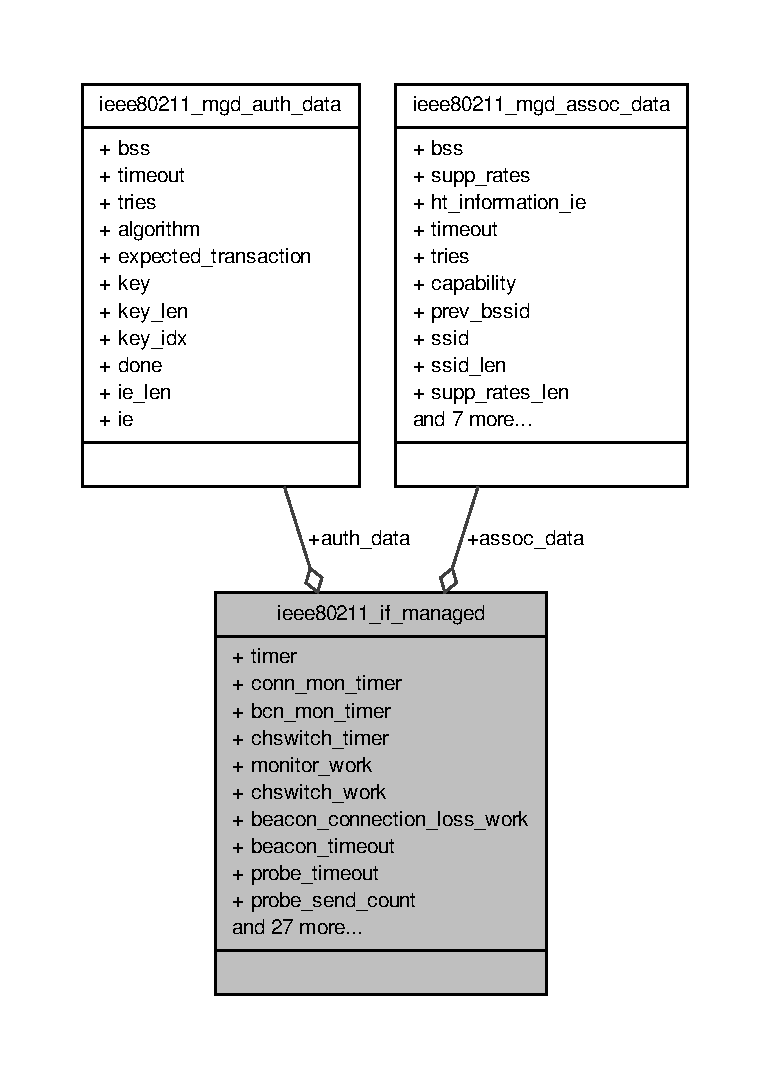
\includegraphics[width=350pt]{structieee80211__if__managed__coll__graph}
\end{center}
\end{figure}
\subsection*{Public Types}
\begin{DoxyCompactItemize}
\item 
enum \{ \hyperlink{structieee80211__if__managed_a726ca809ffd3d67ab4b8476646f26635af6abea446efc3ba9def75c5bbbe6dae9}{I\-E\-E\-E80211\-\_\-\-M\-F\-P\-\_\-\-D\-I\-S\-A\-B\-L\-E\-D}, 
\hyperlink{structieee80211__if__managed_a726ca809ffd3d67ab4b8476646f26635a080fc00364b7117ec3a85dc127cbf3e2}{I\-E\-E\-E80211\-\_\-\-M\-F\-P\-\_\-\-O\-P\-T\-I\-O\-N\-A\-L}, 
\hyperlink{structieee80211__if__managed_a726ca809ffd3d67ab4b8476646f26635aae26246ca1efca53f8d5341eea5cd232}{I\-E\-E\-E80211\-\_\-\-M\-F\-P\-\_\-\-R\-E\-Q\-U\-I\-R\-E\-D}
 \}
\end{DoxyCompactItemize}
\subsection*{Data Fields}
\begin{DoxyCompactItemize}
\item 
struct timer\-\_\-list \hyperlink{structieee80211__if__managed_ae8aedee6c0bd2f7edbb10f18d574f107}{timer}
\item 
struct timer\-\_\-list \hyperlink{structieee80211__if__managed_aa7a9ba2f3ff577fcfa5816581282be94}{conn\-\_\-mon\-\_\-timer}
\item 
struct timer\-\_\-list \hyperlink{structieee80211__if__managed_af3925492fec1b2070226f61652566dad}{bcn\-\_\-mon\-\_\-timer}
\item 
struct timer\-\_\-list \hyperlink{structieee80211__if__managed_abdbc25246eac23118acaa38dc7771c47}{chswitch\-\_\-timer}
\item 
struct work\-\_\-struct \hyperlink{structieee80211__if__managed_a7efa2f92a2e739478df99cdb5422b73f}{monitor\-\_\-work}
\item 
struct work\-\_\-struct \hyperlink{structieee80211__if__managed_ab57ec934f545969e4955bdee8a2fb00d}{chswitch\-\_\-work}
\item 
struct work\-\_\-struct \hyperlink{structieee80211__if__managed_af67aa5a3888b63ed23edc726fb2d6ce1}{beacon\-\_\-connection\-\_\-loss\-\_\-work}
\item 
unsigned long \hyperlink{structieee80211__if__managed_a8a24e16fe603bb3df44779268f4a0875}{beacon\-\_\-timeout}
\item 
unsigned long \hyperlink{structieee80211__if__managed_ae94fded3ca4f10915a7d3d29638c47d7}{probe\-\_\-timeout}
\item 
int \hyperlink{structieee80211__if__managed_aa9ccec90b375e5c56cc2d521d50e1f3c}{probe\-\_\-send\-\_\-count}
\item 
bool \hyperlink{structieee80211__if__managed_af9e271bf4cdd6d0d63259a9603c7db2d}{nullfunc\-\_\-failed}
\item 
struct mutex \hyperlink{structieee80211__if__managed_a06f637951b74c996f2e4987a7be1dbdd}{mtx}
\item 
struct cfg80211\-\_\-bss $\ast$ \hyperlink{structieee80211__if__managed_aa0d8552cc543334097401fdff5a5d74e}{associated}
\item 
struct \hyperlink{structieee80211__mgd__auth__data}{ieee80211\-\_\-mgd\-\_\-auth\-\_\-data} $\ast$ \hyperlink{structieee80211__if__managed_a5736366c204cb94c1db9e4e65a0df203}{auth\-\_\-data}
\item 
struct \hyperlink{structieee80211__mgd__assoc__data}{ieee80211\-\_\-mgd\-\_\-assoc\-\_\-data} $\ast$ \hyperlink{structieee80211__if__managed_a33bf96711b0af50fb5ed9bbb3e912720}{assoc\-\_\-data}
\item 
u8 \hyperlink{structieee80211__if__managed_ace5f51b68bfe9b41dcc950f70a3e7119}{bssid} \mbox{[}E\-T\-H\-\_\-\-A\-L\-E\-N\mbox{]}
\item 
u16 \hyperlink{structieee80211__if__managed_a57f670786e3ff8b4229d4a3cb97a63a0}{aid}
\item 
unsigned long \hyperlink{structieee80211__if__managed_a17be34de946a3782a1daf2f20c1e913d}{timers\-\_\-running}
\item 
bool \hyperlink{structieee80211__if__managed_afbc3e052896051a278a5ad17f6a6e2bb}{powersave}
\item 
bool \hyperlink{structieee80211__if__managed_abce8e97c6b8128b3b66ae2ad3eb07461}{broken\-\_\-ap}
\item 
enum ieee80211\-\_\-smps\-\_\-mode \\*
req\-\_\-smps ap\-\_\-smps \hyperlink{structieee80211__if__managed_a898549726b20c8fd129d59974daf9c90}{driver\-\_\-smps\-\_\-mode}
\item 
struct work\-\_\-struct \hyperlink{structieee80211__if__managed_a8ca768ab965bec1f9e585a2297f9cb74}{request\-\_\-smps\-\_\-work}
\item 
unsigned int \hyperlink{structieee80211__if__managed_ac92588540e8c1d014a08cd8a45462b19}{flags}
\item 
bool \hyperlink{structieee80211__if__managed_a1fc669be36e8ebed0331683d749cd2be}{beacon\-\_\-crc\-\_\-valid}
\item 
u32 \hyperlink{structieee80211__if__managed_a1db4c143d90ecbedae3f9975d8bbb65f}{beacon\-\_\-crc}
\item 
enum ieee80211\-\_\-if\-\_\-managed\-:: \{ ... \}  \hyperlink{structieee80211__if__managed_a13655811e60ceec76eb1e1306eb515bc}{mfp}
\item 
unsigned int \hyperlink{structieee80211__if__managed_aae57668cf51c8e98a1238d7da802965d}{uapsd\-\_\-queues}
\item 
unsigned int \hyperlink{structieee80211__if__managed_a227154b39b6abc457693d962b19fd6c3}{uapsd\-\_\-max\-\_\-sp\-\_\-len}
\item 
int \hyperlink{structieee80211__if__managed_a5dd7a6f610fab30b1816d1a3f303da7e}{wmm\-\_\-last\-\_\-param\-\_\-set}
\item 
u8 \hyperlink{structieee80211__if__managed_a5c7e4a91e5f07e57a228e601b1cd4e29}{use\-\_\-4addr}
\item 
int \hyperlink{structieee80211__if__managed_a2cb78bcdf63c4c28095302c2570c89c1}{last\-\_\-beacon\-\_\-signal}
\item 
int \hyperlink{structieee80211__if__managed_a1ca783bf10e019313e237620d1dab5b1}{ave\-\_\-beacon\-\_\-signal}
\item 
unsigned int \hyperlink{structieee80211__if__managed_a896df829a69357f4258722027c1dbc6d}{count\-\_\-beacon\-\_\-signal}
\item 
int \hyperlink{structieee80211__if__managed_ad0b63098dcdc5575332f354e99fec846}{last\-\_\-cqm\-\_\-event\-\_\-signal}
\item 
int \hyperlink{structieee80211__if__managed_a2f1dcd8ee0579b994cf73bb848b9474f}{rssi\-\_\-min\-\_\-thold}
\item 
int \hyperlink{structieee80211__if__managed_af252cdc03f2874e5289acdd9b973fb1d}{rssi\-\_\-max\-\_\-thold}
\item 
int \hyperlink{structieee80211__if__managed_a74da56491351b6b4b406a63bfcb3d154}{last\-\_\-ave\-\_\-beacon\-\_\-signal}
\item 
struct ieee80211\-\_\-ht\-\_\-cap \hyperlink{structieee80211__if__managed_ac49151818a5396f2513b2cf6f135e988}{ht\-\_\-capa}
\item 
struct ieee80211\-\_\-ht\-\_\-cap \hyperlink{structieee80211__if__managed_a33ba3774e4e37a83cef9b63d23b4dc29}{ht\-\_\-capa\-\_\-mask}
\end{DoxyCompactItemize}


\subsection{Detailed Description}


Definition at line 420 of file ieee80211\-\_\-i.\-h.



\subsection{Member Enumeration Documentation}
\hypertarget{structieee80211__if__managed_a726ca809ffd3d67ab4b8476646f26635}{\subsubsection[{anonymous enum}]{\setlength{\rightskip}{0pt plus 5cm}anonymous enum}}\label{structieee80211__if__managed_a726ca809ffd3d67ab4b8476646f26635}
\begin{Desc}
\item[Enumerator]\par
\begin{description}
\index{I\-E\-E\-E80211\-\_\-\-M\-F\-P\-\_\-\-D\-I\-S\-A\-B\-L\-E\-D@{I\-E\-E\-E80211\-\_\-\-M\-F\-P\-\_\-\-D\-I\-S\-A\-B\-L\-E\-D}!ieee80211\-\_\-if\-\_\-managed@{ieee80211\-\_\-if\-\_\-managed}}\index{ieee80211\-\_\-if\-\_\-managed@{ieee80211\-\_\-if\-\_\-managed}!I\-E\-E\-E80211\-\_\-\-M\-F\-P\-\_\-\-D\-I\-S\-A\-B\-L\-E\-D@{I\-E\-E\-E80211\-\_\-\-M\-F\-P\-\_\-\-D\-I\-S\-A\-B\-L\-E\-D}}\item[{\em 
\hypertarget{structieee80211__if__managed_a726ca809ffd3d67ab4b8476646f26635af6abea446efc3ba9def75c5bbbe6dae9}{I\-E\-E\-E80211\-\_\-\-M\-F\-P\-\_\-\-D\-I\-S\-A\-B\-L\-E\-D}\label{structieee80211__if__managed_a726ca809ffd3d67ab4b8476646f26635af6abea446efc3ba9def75c5bbbe6dae9}
}]\index{I\-E\-E\-E80211\-\_\-\-M\-F\-P\-\_\-\-O\-P\-T\-I\-O\-N\-A\-L@{I\-E\-E\-E80211\-\_\-\-M\-F\-P\-\_\-\-O\-P\-T\-I\-O\-N\-A\-L}!ieee80211\-\_\-if\-\_\-managed@{ieee80211\-\_\-if\-\_\-managed}}\index{ieee80211\-\_\-if\-\_\-managed@{ieee80211\-\_\-if\-\_\-managed}!I\-E\-E\-E80211\-\_\-\-M\-F\-P\-\_\-\-O\-P\-T\-I\-O\-N\-A\-L@{I\-E\-E\-E80211\-\_\-\-M\-F\-P\-\_\-\-O\-P\-T\-I\-O\-N\-A\-L}}\item[{\em 
\hypertarget{structieee80211__if__managed_a726ca809ffd3d67ab4b8476646f26635a080fc00364b7117ec3a85dc127cbf3e2}{I\-E\-E\-E80211\-\_\-\-M\-F\-P\-\_\-\-O\-P\-T\-I\-O\-N\-A\-L}\label{structieee80211__if__managed_a726ca809ffd3d67ab4b8476646f26635a080fc00364b7117ec3a85dc127cbf3e2}
}]\index{I\-E\-E\-E80211\-\_\-\-M\-F\-P\-\_\-\-R\-E\-Q\-U\-I\-R\-E\-D@{I\-E\-E\-E80211\-\_\-\-M\-F\-P\-\_\-\-R\-E\-Q\-U\-I\-R\-E\-D}!ieee80211\-\_\-if\-\_\-managed@{ieee80211\-\_\-if\-\_\-managed}}\index{ieee80211\-\_\-if\-\_\-managed@{ieee80211\-\_\-if\-\_\-managed}!I\-E\-E\-E80211\-\_\-\-M\-F\-P\-\_\-\-R\-E\-Q\-U\-I\-R\-E\-D@{I\-E\-E\-E80211\-\_\-\-M\-F\-P\-\_\-\-R\-E\-Q\-U\-I\-R\-E\-D}}\item[{\em 
\hypertarget{structieee80211__if__managed_a726ca809ffd3d67ab4b8476646f26635aae26246ca1efca53f8d5341eea5cd232}{I\-E\-E\-E80211\-\_\-\-M\-F\-P\-\_\-\-R\-E\-Q\-U\-I\-R\-E\-D}\label{structieee80211__if__managed_a726ca809ffd3d67ab4b8476646f26635aae26246ca1efca53f8d5341eea5cd232}
}]\end{description}
\end{Desc}


Definition at line 457 of file ieee80211\-\_\-i.\-h.



\subsection{Field Documentation}
\hypertarget{structieee80211__if__managed_a57f670786e3ff8b4229d4a3cb97a63a0}{\index{ieee80211\-\_\-if\-\_\-managed@{ieee80211\-\_\-if\-\_\-managed}!aid@{aid}}
\index{aid@{aid}!ieee80211_if_managed@{ieee80211\-\_\-if\-\_\-managed}}
\subsubsection[{aid}]{\setlength{\rightskip}{0pt plus 5cm}u16 aid}}\label{structieee80211__if__managed_a57f670786e3ff8b4229d4a3cb97a63a0}


Definition at line 441 of file ieee80211\-\_\-i.\-h.

\hypertarget{structieee80211__if__managed_a33bf96711b0af50fb5ed9bbb3e912720}{\index{ieee80211\-\_\-if\-\_\-managed@{ieee80211\-\_\-if\-\_\-managed}!assoc\-\_\-data@{assoc\-\_\-data}}
\index{assoc\-\_\-data@{assoc\-\_\-data}!ieee80211_if_managed@{ieee80211\-\_\-if\-\_\-managed}}
\subsubsection[{assoc\-\_\-data}]{\setlength{\rightskip}{0pt plus 5cm}struct {\bf ieee80211\-\_\-mgd\-\_\-assoc\-\_\-data}$\ast$ assoc\-\_\-data}}\label{structieee80211__if__managed_a33bf96711b0af50fb5ed9bbb3e912720}


Definition at line 437 of file ieee80211\-\_\-i.\-h.

\hypertarget{structieee80211__if__managed_aa0d8552cc543334097401fdff5a5d74e}{\index{ieee80211\-\_\-if\-\_\-managed@{ieee80211\-\_\-if\-\_\-managed}!associated@{associated}}
\index{associated@{associated}!ieee80211_if_managed@{ieee80211\-\_\-if\-\_\-managed}}
\subsubsection[{associated}]{\setlength{\rightskip}{0pt plus 5cm}struct cfg80211\-\_\-bss$\ast$ associated}}\label{structieee80211__if__managed_aa0d8552cc543334097401fdff5a5d74e}


Definition at line 435 of file ieee80211\-\_\-i.\-h.

\hypertarget{structieee80211__if__managed_a5736366c204cb94c1db9e4e65a0df203}{\index{ieee80211\-\_\-if\-\_\-managed@{ieee80211\-\_\-if\-\_\-managed}!auth\-\_\-data@{auth\-\_\-data}}
\index{auth\-\_\-data@{auth\-\_\-data}!ieee80211_if_managed@{ieee80211\-\_\-if\-\_\-managed}}
\subsubsection[{auth\-\_\-data}]{\setlength{\rightskip}{0pt plus 5cm}struct {\bf ieee80211\-\_\-mgd\-\_\-auth\-\_\-data}$\ast$ auth\-\_\-data}}\label{structieee80211__if__managed_a5736366c204cb94c1db9e4e65a0df203}


Definition at line 436 of file ieee80211\-\_\-i.\-h.

\hypertarget{structieee80211__if__managed_a1ca783bf10e019313e237620d1dab5b1}{\index{ieee80211\-\_\-if\-\_\-managed@{ieee80211\-\_\-if\-\_\-managed}!ave\-\_\-beacon\-\_\-signal@{ave\-\_\-beacon\-\_\-signal}}
\index{ave\-\_\-beacon\-\_\-signal@{ave\-\_\-beacon\-\_\-signal}!ieee80211_if_managed@{ieee80211\-\_\-if\-\_\-managed}}
\subsubsection[{ave\-\_\-beacon\-\_\-signal}]{\setlength{\rightskip}{0pt plus 5cm}int ave\-\_\-beacon\-\_\-signal}}\label{structieee80211__if__managed_a1ca783bf10e019313e237620d1dab5b1}


Definition at line 490 of file ieee80211\-\_\-i.\-h.

\hypertarget{structieee80211__if__managed_af3925492fec1b2070226f61652566dad}{\index{ieee80211\-\_\-if\-\_\-managed@{ieee80211\-\_\-if\-\_\-managed}!bcn\-\_\-mon\-\_\-timer@{bcn\-\_\-mon\-\_\-timer}}
\index{bcn\-\_\-mon\-\_\-timer@{bcn\-\_\-mon\-\_\-timer}!ieee80211_if_managed@{ieee80211\-\_\-if\-\_\-managed}}
\subsubsection[{bcn\-\_\-mon\-\_\-timer}]{\setlength{\rightskip}{0pt plus 5cm}struct timer\-\_\-list bcn\-\_\-mon\-\_\-timer}}\label{structieee80211__if__managed_af3925492fec1b2070226f61652566dad}


Definition at line 423 of file ieee80211\-\_\-i.\-h.

\hypertarget{structieee80211__if__managed_af67aa5a3888b63ed23edc726fb2d6ce1}{\index{ieee80211\-\_\-if\-\_\-managed@{ieee80211\-\_\-if\-\_\-managed}!beacon\-\_\-connection\-\_\-loss\-\_\-work@{beacon\-\_\-connection\-\_\-loss\-\_\-work}}
\index{beacon\-\_\-connection\-\_\-loss\-\_\-work@{beacon\-\_\-connection\-\_\-loss\-\_\-work}!ieee80211_if_managed@{ieee80211\-\_\-if\-\_\-managed}}
\subsubsection[{beacon\-\_\-connection\-\_\-loss\-\_\-work}]{\setlength{\rightskip}{0pt plus 5cm}struct work\-\_\-struct beacon\-\_\-connection\-\_\-loss\-\_\-work}}\label{structieee80211__if__managed_af67aa5a3888b63ed23edc726fb2d6ce1}


Definition at line 427 of file ieee80211\-\_\-i.\-h.

\hypertarget{structieee80211__if__managed_a1db4c143d90ecbedae3f9975d8bbb65f}{\index{ieee80211\-\_\-if\-\_\-managed@{ieee80211\-\_\-if\-\_\-managed}!beacon\-\_\-crc@{beacon\-\_\-crc}}
\index{beacon\-\_\-crc@{beacon\-\_\-crc}!ieee80211_if_managed@{ieee80211\-\_\-if\-\_\-managed}}
\subsubsection[{beacon\-\_\-crc}]{\setlength{\rightskip}{0pt plus 5cm}u32 beacon\-\_\-crc}}\label{structieee80211__if__managed_a1db4c143d90ecbedae3f9975d8bbb65f}


Definition at line 455 of file ieee80211\-\_\-i.\-h.

\hypertarget{structieee80211__if__managed_a1fc669be36e8ebed0331683d749cd2be}{\index{ieee80211\-\_\-if\-\_\-managed@{ieee80211\-\_\-if\-\_\-managed}!beacon\-\_\-crc\-\_\-valid@{beacon\-\_\-crc\-\_\-valid}}
\index{beacon\-\_\-crc\-\_\-valid@{beacon\-\_\-crc\-\_\-valid}!ieee80211_if_managed@{ieee80211\-\_\-if\-\_\-managed}}
\subsubsection[{beacon\-\_\-crc\-\_\-valid}]{\setlength{\rightskip}{0pt plus 5cm}bool beacon\-\_\-crc\-\_\-valid}}\label{structieee80211__if__managed_a1fc669be36e8ebed0331683d749cd2be}


Definition at line 454 of file ieee80211\-\_\-i.\-h.

\hypertarget{structieee80211__if__managed_a8a24e16fe603bb3df44779268f4a0875}{\index{ieee80211\-\_\-if\-\_\-managed@{ieee80211\-\_\-if\-\_\-managed}!beacon\-\_\-timeout@{beacon\-\_\-timeout}}
\index{beacon\-\_\-timeout@{beacon\-\_\-timeout}!ieee80211_if_managed@{ieee80211\-\_\-if\-\_\-managed}}
\subsubsection[{beacon\-\_\-timeout}]{\setlength{\rightskip}{0pt plus 5cm}unsigned long beacon\-\_\-timeout}}\label{structieee80211__if__managed_a8a24e16fe603bb3df44779268f4a0875}


Definition at line 429 of file ieee80211\-\_\-i.\-h.

\hypertarget{structieee80211__if__managed_abce8e97c6b8128b3b66ae2ad3eb07461}{\index{ieee80211\-\_\-if\-\_\-managed@{ieee80211\-\_\-if\-\_\-managed}!broken\-\_\-ap@{broken\-\_\-ap}}
\index{broken\-\_\-ap@{broken\-\_\-ap}!ieee80211_if_managed@{ieee80211\-\_\-if\-\_\-managed}}
\subsubsection[{broken\-\_\-ap}]{\setlength{\rightskip}{0pt plus 5cm}bool broken\-\_\-ap}}\label{structieee80211__if__managed_abce8e97c6b8128b3b66ae2ad3eb07461}


Definition at line 445 of file ieee80211\-\_\-i.\-h.

\hypertarget{structieee80211__if__managed_ace5f51b68bfe9b41dcc950f70a3e7119}{\index{ieee80211\-\_\-if\-\_\-managed@{ieee80211\-\_\-if\-\_\-managed}!bssid@{bssid}}
\index{bssid@{bssid}!ieee80211_if_managed@{ieee80211\-\_\-if\-\_\-managed}}
\subsubsection[{bssid}]{\setlength{\rightskip}{0pt plus 5cm}u8 bssid\mbox{[}E\-T\-H\-\_\-\-A\-L\-E\-N\mbox{]}}}\label{structieee80211__if__managed_ace5f51b68bfe9b41dcc950f70a3e7119}


Definition at line 439 of file ieee80211\-\_\-i.\-h.

\hypertarget{structieee80211__if__managed_abdbc25246eac23118acaa38dc7771c47}{\index{ieee80211\-\_\-if\-\_\-managed@{ieee80211\-\_\-if\-\_\-managed}!chswitch\-\_\-timer@{chswitch\-\_\-timer}}
\index{chswitch\-\_\-timer@{chswitch\-\_\-timer}!ieee80211_if_managed@{ieee80211\-\_\-if\-\_\-managed}}
\subsubsection[{chswitch\-\_\-timer}]{\setlength{\rightskip}{0pt plus 5cm}struct timer\-\_\-list chswitch\-\_\-timer}}\label{structieee80211__if__managed_abdbc25246eac23118acaa38dc7771c47}


Definition at line 424 of file ieee80211\-\_\-i.\-h.

\hypertarget{structieee80211__if__managed_ab57ec934f545969e4955bdee8a2fb00d}{\index{ieee80211\-\_\-if\-\_\-managed@{ieee80211\-\_\-if\-\_\-managed}!chswitch\-\_\-work@{chswitch\-\_\-work}}
\index{chswitch\-\_\-work@{chswitch\-\_\-work}!ieee80211_if_managed@{ieee80211\-\_\-if\-\_\-managed}}
\subsubsection[{chswitch\-\_\-work}]{\setlength{\rightskip}{0pt plus 5cm}struct work\-\_\-struct chswitch\-\_\-work}}\label{structieee80211__if__managed_ab57ec934f545969e4955bdee8a2fb00d}


Definition at line 426 of file ieee80211\-\_\-i.\-h.

\hypertarget{structieee80211__if__managed_aa7a9ba2f3ff577fcfa5816581282be94}{\index{ieee80211\-\_\-if\-\_\-managed@{ieee80211\-\_\-if\-\_\-managed}!conn\-\_\-mon\-\_\-timer@{conn\-\_\-mon\-\_\-timer}}
\index{conn\-\_\-mon\-\_\-timer@{conn\-\_\-mon\-\_\-timer}!ieee80211_if_managed@{ieee80211\-\_\-if\-\_\-managed}}
\subsubsection[{conn\-\_\-mon\-\_\-timer}]{\setlength{\rightskip}{0pt plus 5cm}struct timer\-\_\-list conn\-\_\-mon\-\_\-timer}}\label{structieee80211__if__managed_aa7a9ba2f3ff577fcfa5816581282be94}


Definition at line 422 of file ieee80211\-\_\-i.\-h.

\hypertarget{structieee80211__if__managed_a896df829a69357f4258722027c1dbc6d}{\index{ieee80211\-\_\-if\-\_\-managed@{ieee80211\-\_\-if\-\_\-managed}!count\-\_\-beacon\-\_\-signal@{count\-\_\-beacon\-\_\-signal}}
\index{count\-\_\-beacon\-\_\-signal@{count\-\_\-beacon\-\_\-signal}!ieee80211_if_managed@{ieee80211\-\_\-if\-\_\-managed}}
\subsubsection[{count\-\_\-beacon\-\_\-signal}]{\setlength{\rightskip}{0pt plus 5cm}unsigned int count\-\_\-beacon\-\_\-signal}}\label{structieee80211__if__managed_a896df829a69357f4258722027c1dbc6d}


Definition at line 497 of file ieee80211\-\_\-i.\-h.

\hypertarget{structieee80211__if__managed_a898549726b20c8fd129d59974daf9c90}{\index{ieee80211\-\_\-if\-\_\-managed@{ieee80211\-\_\-if\-\_\-managed}!driver\-\_\-smps\-\_\-mode@{driver\-\_\-smps\-\_\-mode}}
\index{driver\-\_\-smps\-\_\-mode@{driver\-\_\-smps\-\_\-mode}!ieee80211_if_managed@{ieee80211\-\_\-if\-\_\-managed}}
\subsubsection[{driver\-\_\-smps\-\_\-mode}]{\setlength{\rightskip}{0pt plus 5cm}enum ieee80211\-\_\-smps\-\_\-mode req\-\_\-smps ap\-\_\-smps driver\-\_\-smps\-\_\-mode}}\label{structieee80211__if__managed_a898549726b20c8fd129d59974daf9c90}


Definition at line 446 of file ieee80211\-\_\-i.\-h.

\hypertarget{structieee80211__if__managed_ac92588540e8c1d014a08cd8a45462b19}{\index{ieee80211\-\_\-if\-\_\-managed@{ieee80211\-\_\-if\-\_\-managed}!flags@{flags}}
\index{flags@{flags}!ieee80211_if_managed@{ieee80211\-\_\-if\-\_\-managed}}
\subsubsection[{flags}]{\setlength{\rightskip}{0pt plus 5cm}unsigned int flags}}\label{structieee80211__if__managed_ac92588540e8c1d014a08cd8a45462b19}


Definition at line 452 of file ieee80211\-\_\-i.\-h.

\hypertarget{structieee80211__if__managed_ac49151818a5396f2513b2cf6f135e988}{\index{ieee80211\-\_\-if\-\_\-managed@{ieee80211\-\_\-if\-\_\-managed}!ht\-\_\-capa@{ht\-\_\-capa}}
\index{ht\-\_\-capa@{ht\-\_\-capa}!ieee80211_if_managed@{ieee80211\-\_\-if\-\_\-managed}}
\subsubsection[{ht\-\_\-capa}]{\setlength{\rightskip}{0pt plus 5cm}struct ieee80211\-\_\-ht\-\_\-cap ht\-\_\-capa}}\label{structieee80211__if__managed_ac49151818a5396f2513b2cf6f135e988}


Definition at line 514 of file ieee80211\-\_\-i.\-h.

\hypertarget{structieee80211__if__managed_a33ba3774e4e37a83cef9b63d23b4dc29}{\index{ieee80211\-\_\-if\-\_\-managed@{ieee80211\-\_\-if\-\_\-managed}!ht\-\_\-capa\-\_\-mask@{ht\-\_\-capa\-\_\-mask}}
\index{ht\-\_\-capa\-\_\-mask@{ht\-\_\-capa\-\_\-mask}!ieee80211_if_managed@{ieee80211\-\_\-if\-\_\-managed}}
\subsubsection[{ht\-\_\-capa\-\_\-mask}]{\setlength{\rightskip}{0pt plus 5cm}struct ieee80211\-\_\-ht\-\_\-cap ht\-\_\-capa\-\_\-mask}}\label{structieee80211__if__managed_a33ba3774e4e37a83cef9b63d23b4dc29}


Definition at line 515 of file ieee80211\-\_\-i.\-h.

\hypertarget{structieee80211__if__managed_a74da56491351b6b4b406a63bfcb3d154}{\index{ieee80211\-\_\-if\-\_\-managed@{ieee80211\-\_\-if\-\_\-managed}!last\-\_\-ave\-\_\-beacon\-\_\-signal@{last\-\_\-ave\-\_\-beacon\-\_\-signal}}
\index{last\-\_\-ave\-\_\-beacon\-\_\-signal@{last\-\_\-ave\-\_\-beacon\-\_\-signal}!ieee80211_if_managed@{ieee80211\-\_\-if\-\_\-managed}}
\subsubsection[{last\-\_\-ave\-\_\-beacon\-\_\-signal}]{\setlength{\rightskip}{0pt plus 5cm}int last\-\_\-ave\-\_\-beacon\-\_\-signal}}\label{structieee80211__if__managed_a74da56491351b6b4b406a63bfcb3d154}


Definition at line 512 of file ieee80211\-\_\-i.\-h.

\hypertarget{structieee80211__if__managed_a2cb78bcdf63c4c28095302c2570c89c1}{\index{ieee80211\-\_\-if\-\_\-managed@{ieee80211\-\_\-if\-\_\-managed}!last\-\_\-beacon\-\_\-signal@{last\-\_\-beacon\-\_\-signal}}
\index{last\-\_\-beacon\-\_\-signal@{last\-\_\-beacon\-\_\-signal}!ieee80211_if_managed@{ieee80211\-\_\-if\-\_\-managed}}
\subsubsection[{last\-\_\-beacon\-\_\-signal}]{\setlength{\rightskip}{0pt plus 5cm}int last\-\_\-beacon\-\_\-signal}}\label{structieee80211__if__managed_a2cb78bcdf63c4c28095302c2570c89c1}


Definition at line 482 of file ieee80211\-\_\-i.\-h.

\hypertarget{structieee80211__if__managed_ad0b63098dcdc5575332f354e99fec846}{\index{ieee80211\-\_\-if\-\_\-managed@{ieee80211\-\_\-if\-\_\-managed}!last\-\_\-cqm\-\_\-event\-\_\-signal@{last\-\_\-cqm\-\_\-event\-\_\-signal}}
\index{last\-\_\-cqm\-\_\-event\-\_\-signal@{last\-\_\-cqm\-\_\-event\-\_\-signal}!ieee80211_if_managed@{ieee80211\-\_\-if\-\_\-managed}}
\subsubsection[{last\-\_\-cqm\-\_\-event\-\_\-signal}]{\setlength{\rightskip}{0pt plus 5cm}int last\-\_\-cqm\-\_\-event\-\_\-signal}}\label{structieee80211__if__managed_ad0b63098dcdc5575332f354e99fec846}


Definition at line 504 of file ieee80211\-\_\-i.\-h.

\hypertarget{structieee80211__if__managed_a13655811e60ceec76eb1e1306eb515bc}{\index{ieee80211\-\_\-if\-\_\-managed@{ieee80211\-\_\-if\-\_\-managed}!mfp@{mfp}}
\index{mfp@{mfp}!ieee80211_if_managed@{ieee80211\-\_\-if\-\_\-managed}}
\subsubsection[{mfp}]{\setlength{\rightskip}{0pt plus 5cm}enum \{ ... \}   mfp}}\label{structieee80211__if__managed_a13655811e60ceec76eb1e1306eb515bc}
\hypertarget{structieee80211__if__managed_a7efa2f92a2e739478df99cdb5422b73f}{\index{ieee80211\-\_\-if\-\_\-managed@{ieee80211\-\_\-if\-\_\-managed}!monitor\-\_\-work@{monitor\-\_\-work}}
\index{monitor\-\_\-work@{monitor\-\_\-work}!ieee80211_if_managed@{ieee80211\-\_\-if\-\_\-managed}}
\subsubsection[{monitor\-\_\-work}]{\setlength{\rightskip}{0pt plus 5cm}struct work\-\_\-struct monitor\-\_\-work}}\label{structieee80211__if__managed_a7efa2f92a2e739478df99cdb5422b73f}


Definition at line 425 of file ieee80211\-\_\-i.\-h.

\hypertarget{structieee80211__if__managed_a06f637951b74c996f2e4987a7be1dbdd}{\index{ieee80211\-\_\-if\-\_\-managed@{ieee80211\-\_\-if\-\_\-managed}!mtx@{mtx}}
\index{mtx@{mtx}!ieee80211_if_managed@{ieee80211\-\_\-if\-\_\-managed}}
\subsubsection[{mtx}]{\setlength{\rightskip}{0pt plus 5cm}struct mutex mtx}}\label{structieee80211__if__managed_a06f637951b74c996f2e4987a7be1dbdd}


Definition at line 434 of file ieee80211\-\_\-i.\-h.

\hypertarget{structieee80211__if__managed_af9e271bf4cdd6d0d63259a9603c7db2d}{\index{ieee80211\-\_\-if\-\_\-managed@{ieee80211\-\_\-if\-\_\-managed}!nullfunc\-\_\-failed@{nullfunc\-\_\-failed}}
\index{nullfunc\-\_\-failed@{nullfunc\-\_\-failed}!ieee80211_if_managed@{ieee80211\-\_\-if\-\_\-managed}}
\subsubsection[{nullfunc\-\_\-failed}]{\setlength{\rightskip}{0pt plus 5cm}bool nullfunc\-\_\-failed}}\label{structieee80211__if__managed_af9e271bf4cdd6d0d63259a9603c7db2d}


Definition at line 432 of file ieee80211\-\_\-i.\-h.

\hypertarget{structieee80211__if__managed_afbc3e052896051a278a5ad17f6a6e2bb}{\index{ieee80211\-\_\-if\-\_\-managed@{ieee80211\-\_\-if\-\_\-managed}!powersave@{powersave}}
\index{powersave@{powersave}!ieee80211_if_managed@{ieee80211\-\_\-if\-\_\-managed}}
\subsubsection[{powersave}]{\setlength{\rightskip}{0pt plus 5cm}bool powersave}}\label{structieee80211__if__managed_afbc3e052896051a278a5ad17f6a6e2bb}


Definition at line 444 of file ieee80211\-\_\-i.\-h.

\hypertarget{structieee80211__if__managed_aa9ccec90b375e5c56cc2d521d50e1f3c}{\index{ieee80211\-\_\-if\-\_\-managed@{ieee80211\-\_\-if\-\_\-managed}!probe\-\_\-send\-\_\-count@{probe\-\_\-send\-\_\-count}}
\index{probe\-\_\-send\-\_\-count@{probe\-\_\-send\-\_\-count}!ieee80211_if_managed@{ieee80211\-\_\-if\-\_\-managed}}
\subsubsection[{probe\-\_\-send\-\_\-count}]{\setlength{\rightskip}{0pt plus 5cm}int probe\-\_\-send\-\_\-count}}\label{structieee80211__if__managed_aa9ccec90b375e5c56cc2d521d50e1f3c}


Definition at line 431 of file ieee80211\-\_\-i.\-h.

\hypertarget{structieee80211__if__managed_ae94fded3ca4f10915a7d3d29638c47d7}{\index{ieee80211\-\_\-if\-\_\-managed@{ieee80211\-\_\-if\-\_\-managed}!probe\-\_\-timeout@{probe\-\_\-timeout}}
\index{probe\-\_\-timeout@{probe\-\_\-timeout}!ieee80211_if_managed@{ieee80211\-\_\-if\-\_\-managed}}
\subsubsection[{probe\-\_\-timeout}]{\setlength{\rightskip}{0pt plus 5cm}unsigned long probe\-\_\-timeout}}\label{structieee80211__if__managed_ae94fded3ca4f10915a7d3d29638c47d7}


Definition at line 430 of file ieee80211\-\_\-i.\-h.

\hypertarget{structieee80211__if__managed_a8ca768ab965bec1f9e585a2297f9cb74}{\index{ieee80211\-\_\-if\-\_\-managed@{ieee80211\-\_\-if\-\_\-managed}!request\-\_\-smps\-\_\-work@{request\-\_\-smps\-\_\-work}}
\index{request\-\_\-smps\-\_\-work@{request\-\_\-smps\-\_\-work}!ieee80211_if_managed@{ieee80211\-\_\-if\-\_\-managed}}
\subsubsection[{request\-\_\-smps\-\_\-work}]{\setlength{\rightskip}{0pt plus 5cm}struct work\-\_\-struct request\-\_\-smps\-\_\-work}}\label{structieee80211__if__managed_a8ca768ab965bec1f9e585a2297f9cb74}


Definition at line 450 of file ieee80211\-\_\-i.\-h.

\hypertarget{structieee80211__if__managed_af252cdc03f2874e5289acdd9b973fb1d}{\index{ieee80211\-\_\-if\-\_\-managed@{ieee80211\-\_\-if\-\_\-managed}!rssi\-\_\-max\-\_\-thold@{rssi\-\_\-max\-\_\-thold}}
\index{rssi\-\_\-max\-\_\-thold@{rssi\-\_\-max\-\_\-thold}!ieee80211_if_managed@{ieee80211\-\_\-if\-\_\-managed}}
\subsubsection[{rssi\-\_\-max\-\_\-thold}]{\setlength{\rightskip}{0pt plus 5cm}int rssi\-\_\-max\-\_\-thold}}\label{structieee80211__if__managed_af252cdc03f2874e5289acdd9b973fb1d}


Definition at line 511 of file ieee80211\-\_\-i.\-h.

\hypertarget{structieee80211__if__managed_a2f1dcd8ee0579b994cf73bb848b9474f}{\index{ieee80211\-\_\-if\-\_\-managed@{ieee80211\-\_\-if\-\_\-managed}!rssi\-\_\-min\-\_\-thold@{rssi\-\_\-min\-\_\-thold}}
\index{rssi\-\_\-min\-\_\-thold@{rssi\-\_\-min\-\_\-thold}!ieee80211_if_managed@{ieee80211\-\_\-if\-\_\-managed}}
\subsubsection[{rssi\-\_\-min\-\_\-thold}]{\setlength{\rightskip}{0pt plus 5cm}int rssi\-\_\-min\-\_\-thold}}\label{structieee80211__if__managed_a2f1dcd8ee0579b994cf73bb848b9474f}


Definition at line 511 of file ieee80211\-\_\-i.\-h.

\hypertarget{structieee80211__if__managed_ae8aedee6c0bd2f7edbb10f18d574f107}{\index{ieee80211\-\_\-if\-\_\-managed@{ieee80211\-\_\-if\-\_\-managed}!timer@{timer}}
\index{timer@{timer}!ieee80211_if_managed@{ieee80211\-\_\-if\-\_\-managed}}
\subsubsection[{timer}]{\setlength{\rightskip}{0pt plus 5cm}struct timer\-\_\-list timer}}\label{structieee80211__if__managed_ae8aedee6c0bd2f7edbb10f18d574f107}


Definition at line 421 of file ieee80211\-\_\-i.\-h.

\hypertarget{structieee80211__if__managed_a17be34de946a3782a1daf2f20c1e913d}{\index{ieee80211\-\_\-if\-\_\-managed@{ieee80211\-\_\-if\-\_\-managed}!timers\-\_\-running@{timers\-\_\-running}}
\index{timers\-\_\-running@{timers\-\_\-running}!ieee80211_if_managed@{ieee80211\-\_\-if\-\_\-managed}}
\subsubsection[{timers\-\_\-running}]{\setlength{\rightskip}{0pt plus 5cm}unsigned long timers\-\_\-running}}\label{structieee80211__if__managed_a17be34de946a3782a1daf2f20c1e913d}


Definition at line 443 of file ieee80211\-\_\-i.\-h.

\hypertarget{structieee80211__if__managed_a227154b39b6abc457693d962b19fd6c3}{\index{ieee80211\-\_\-if\-\_\-managed@{ieee80211\-\_\-if\-\_\-managed}!uapsd\-\_\-max\-\_\-sp\-\_\-len@{uapsd\-\_\-max\-\_\-sp\-\_\-len}}
\index{uapsd\-\_\-max\-\_\-sp\-\_\-len@{uapsd\-\_\-max\-\_\-sp\-\_\-len}!ieee80211_if_managed@{ieee80211\-\_\-if\-\_\-managed}}
\subsubsection[{uapsd\-\_\-max\-\_\-sp\-\_\-len}]{\setlength{\rightskip}{0pt plus 5cm}unsigned int uapsd\-\_\-max\-\_\-sp\-\_\-len}}\label{structieee80211__if__managed_a227154b39b6abc457693d962b19fd6c3}


Definition at line 475 of file ieee80211\-\_\-i.\-h.

\hypertarget{structieee80211__if__managed_aae57668cf51c8e98a1238d7da802965d}{\index{ieee80211\-\_\-if\-\_\-managed@{ieee80211\-\_\-if\-\_\-managed}!uapsd\-\_\-queues@{uapsd\-\_\-queues}}
\index{uapsd\-\_\-queues@{uapsd\-\_\-queues}!ieee80211_if_managed@{ieee80211\-\_\-if\-\_\-managed}}
\subsubsection[{uapsd\-\_\-queues}]{\setlength{\rightskip}{0pt plus 5cm}unsigned int uapsd\-\_\-queues}}\label{structieee80211__if__managed_aae57668cf51c8e98a1238d7da802965d}


Definition at line 468 of file ieee80211\-\_\-i.\-h.

\hypertarget{structieee80211__if__managed_a5c7e4a91e5f07e57a228e601b1cd4e29}{\index{ieee80211\-\_\-if\-\_\-managed@{ieee80211\-\_\-if\-\_\-managed}!use\-\_\-4addr@{use\-\_\-4addr}}
\index{use\-\_\-4addr@{use\-\_\-4addr}!ieee80211_if_managed@{ieee80211\-\_\-if\-\_\-managed}}
\subsubsection[{use\-\_\-4addr}]{\setlength{\rightskip}{0pt plus 5cm}u8 use\-\_\-4addr}}\label{structieee80211__if__managed_a5c7e4a91e5f07e57a228e601b1cd4e29}


Definition at line 479 of file ieee80211\-\_\-i.\-h.

\hypertarget{structieee80211__if__managed_a5dd7a6f610fab30b1816d1a3f303da7e}{\index{ieee80211\-\_\-if\-\_\-managed@{ieee80211\-\_\-if\-\_\-managed}!wmm\-\_\-last\-\_\-param\-\_\-set@{wmm\-\_\-last\-\_\-param\-\_\-set}}
\index{wmm\-\_\-last\-\_\-param\-\_\-set@{wmm\-\_\-last\-\_\-param\-\_\-set}!ieee80211_if_managed@{ieee80211\-\_\-if\-\_\-managed}}
\subsubsection[{wmm\-\_\-last\-\_\-param\-\_\-set}]{\setlength{\rightskip}{0pt plus 5cm}int wmm\-\_\-last\-\_\-param\-\_\-set}}\label{structieee80211__if__managed_a5dd7a6f610fab30b1816d1a3f303da7e}


Definition at line 477 of file ieee80211\-\_\-i.\-h.



The documentation for this struct was generated from the following file\-:\begin{DoxyCompactItemize}
\item 
/home/guille/msm/net/mac80211/\hyperlink{ieee80211__i_8h}{ieee80211\-\_\-i.\-h}\end{DoxyCompactItemize}

\hypertarget{structieee80211__if__mesh}{\section{ieee80211\-\_\-if\-\_\-mesh Struct Reference}
\label{structieee80211__if__mesh}\index{ieee80211\-\_\-if\-\_\-mesh@{ieee80211\-\_\-if\-\_\-mesh}}
}


{\ttfamily \#include $<$ieee80211\-\_\-i.\-h$>$}



Collaboration diagram for ieee80211\-\_\-if\-\_\-mesh\-:
\nopagebreak
\begin{figure}[H]
\begin{center}
\leavevmode
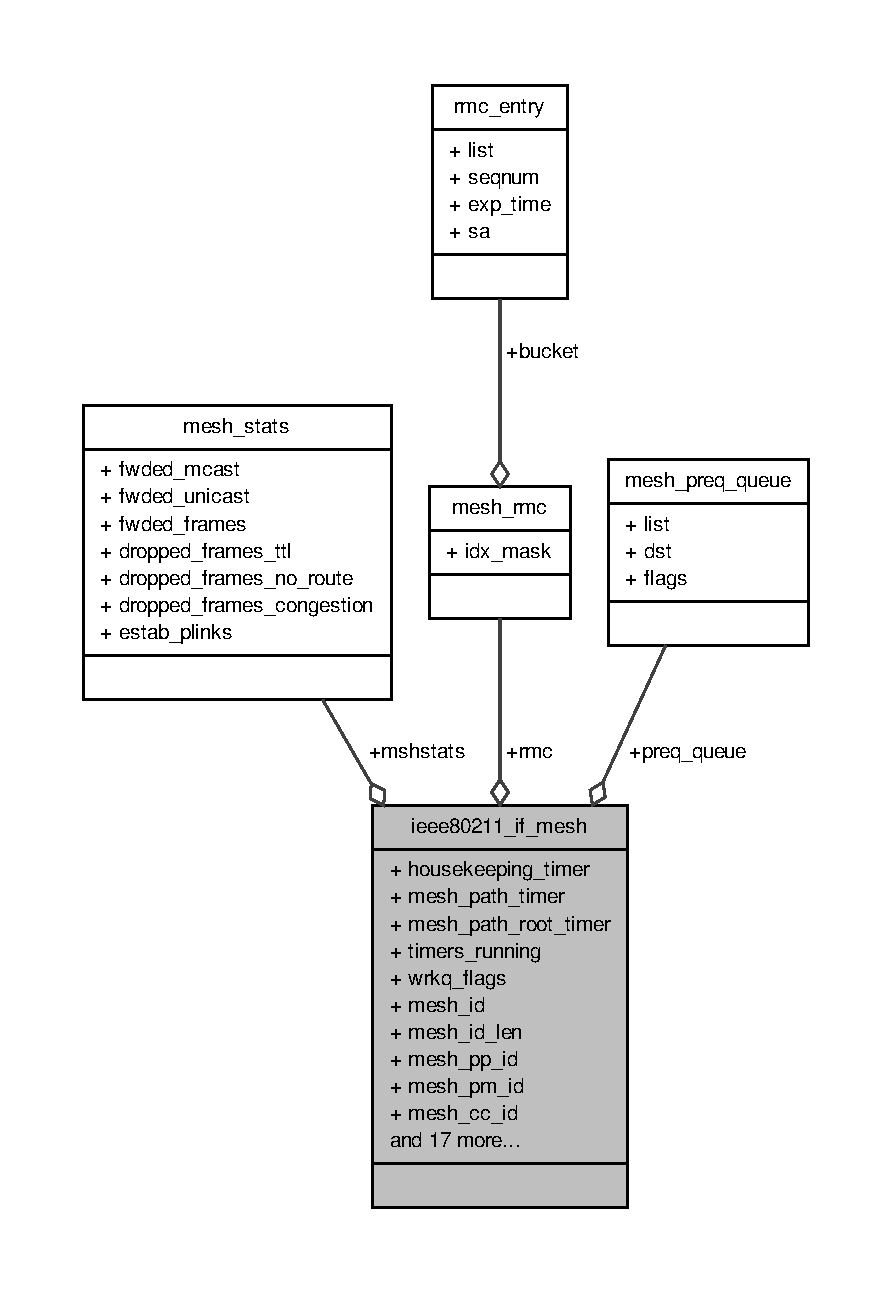
\includegraphics[width=350pt]{structieee80211__if__mesh__coll__graph}
\end{center}
\end{figure}
\subsection*{Public Types}
\begin{DoxyCompactItemize}
\item 
enum \{ \hyperlink{structieee80211__if__mesh_abed82baf7f470b522273a3e37c24c600aa331dabfdfb64a090cab58b911900030}{I\-E\-E\-E80211\-\_\-\-M\-E\-S\-H\-\_\-\-S\-E\-C\-\_\-\-N\-O\-N\-E} = 0x0, 
\hyperlink{structieee80211__if__mesh_abed82baf7f470b522273a3e37c24c600a5c7f982c3bea5482bd1f92f95466f7d4}{I\-E\-E\-E80211\-\_\-\-M\-E\-S\-H\-\_\-\-S\-E\-C\-\_\-\-A\-U\-T\-H\-E\-D} = 0x1, 
\hyperlink{structieee80211__if__mesh_abed82baf7f470b522273a3e37c24c600ae1b4bbdd667c8ca83ce0c15e4cad1e75}{I\-E\-E\-E80211\-\_\-\-M\-E\-S\-H\-\_\-\-S\-E\-C\-\_\-\-S\-E\-C\-U\-R\-E\-D} = 0x2
 \}
\end{DoxyCompactItemize}
\subsection*{Data Fields}
\begin{DoxyCompactItemize}
\item 
struct timer\-\_\-list \hyperlink{structieee80211__if__mesh_aedaac0553091bd2ddcc6d928973785d7}{housekeeping\-\_\-timer}
\item 
struct timer\-\_\-list \hyperlink{structieee80211__if__mesh_ac6aa531e38336119608446120beb1794}{mesh\-\_\-path\-\_\-timer}
\item 
struct timer\-\_\-list \hyperlink{structieee80211__if__mesh_a06ffe037b1a26965a1463ba7bf70e516}{mesh\-\_\-path\-\_\-root\-\_\-timer}
\item 
unsigned long \hyperlink{structieee80211__if__mesh_a17be34de946a3782a1daf2f20c1e913d}{timers\-\_\-running}
\item 
unsigned long \hyperlink{structieee80211__if__mesh_a108e8fea002f332c33b05d8ab571f494}{wrkq\-\_\-flags}
\item 
u8 \hyperlink{structieee80211__if__mesh_a2711e1d2c70fa6d2655834f90803d57b}{mesh\-\_\-id} \mbox{[}I\-E\-E\-E80211\-\_\-\-M\-A\-X\-\_\-\-M\-E\-S\-H\-\_\-\-I\-D\-\_\-\-L\-E\-N\mbox{]}
\item 
size\-\_\-t \hyperlink{structieee80211__if__mesh_a791aab7f12f13e6fa1f99f0eaf4fd7b0}{mesh\-\_\-id\-\_\-len}
\item 
u8 \hyperlink{structieee80211__if__mesh_a1dd8e1a94ceedad87851b023b7f53e6c}{mesh\-\_\-pp\-\_\-id}
\item 
u8 \hyperlink{structieee80211__if__mesh_a12e1b42980e196b8395edd3b7b00185a}{mesh\-\_\-pm\-\_\-id}
\item 
u8 \hyperlink{structieee80211__if__mesh_a50d32de091d16cc5ee16cdd8e9e61a45}{mesh\-\_\-cc\-\_\-id}
\item 
u8 \hyperlink{structieee80211__if__mesh_a082033acd11ca0e290b5d58e588129dc}{mesh\-\_\-sp\-\_\-id}
\item 
u8 \hyperlink{structieee80211__if__mesh_a5a1467a37395b9b885664f1885dfc199}{mesh\-\_\-auth\-\_\-id}
\item 
u32 \hyperlink{structieee80211__if__mesh_a3a5989b8e6d4286ac3822b65bbc1cf16}{sn}
\item 
u32 \hyperlink{structieee80211__if__mesh_a892d957726166f4493acf446b312e7a0}{preq\-\_\-id}
\item 
atomic\-\_\-t \hyperlink{structieee80211__if__mesh_a682324aeb04ad3c555c56e5cb52e53c5}{mpaths}
\item 
unsigned long \hyperlink{structieee80211__if__mesh_a7f98e84dc24836f077044eb5e00e78f1}{last\-\_\-sn\-\_\-update}
\item 
unsigned long \hyperlink{structieee80211__if__mesh_ae90d36efd492fcfe01281116836def4b}{next\-\_\-perr}
\item 
unsigned long \hyperlink{structieee80211__if__mesh_a62360839e8d0d87871320ad614778d68}{last\-\_\-preq}
\item 
struct \hyperlink{structmesh__rmc}{mesh\-\_\-rmc} $\ast$ \hyperlink{structieee80211__if__mesh_a41a923e5b48f47e8ee460387dc5dc673}{rmc}
\item 
spinlock\-\_\-t \hyperlink{structieee80211__if__mesh_a38a1a735de11766717875f1e40ae6ca7}{mesh\-\_\-preq\-\_\-queue\-\_\-lock}
\item 
struct \hyperlink{structmesh__preq__queue}{mesh\-\_\-preq\-\_\-queue} \hyperlink{structieee80211__if__mesh_ad73838a40d5e3d10af379c4fc37d4dfd}{preq\-\_\-queue}
\item 
int \hyperlink{structieee80211__if__mesh_a24b4255901094231004e9da5de02341c}{preq\-\_\-queue\-\_\-len}
\item 
struct \hyperlink{structmesh__stats}{mesh\-\_\-stats} \hyperlink{structieee80211__if__mesh_a63aef80a54bf42d120b10d0b637b57be}{mshstats}
\item 
struct mesh\-\_\-config \hyperlink{structieee80211__if__mesh_a7b25051eee4817560f5bcb80402751f5}{mshcfg}
\item 
u32 \hyperlink{structieee80211__if__mesh_aa5e6ec48251f030a59d356caac4db5ec}{mesh\-\_\-seqnum}
\item 
bool \hyperlink{structieee80211__if__mesh_a27b3535c857149e70e4b9c973719ad7b}{accepting\-\_\-plinks}
\item 
int \hyperlink{structieee80211__if__mesh_af6554718fdcf2fe36e9eed14cc159ebf}{num\-\_\-gates}
\item 
const u8 $\ast$ \hyperlink{structieee80211__if__mesh_a74b4af5de0da224d9fb8b59a3aec207e}{ie}
\item 
u8 \hyperlink{structieee80211__if__mesh_a8e143706c80e5faf90dc4a385c4517f6}{ie\-\_\-len}
\item 
enum ieee80211\-\_\-if\-\_\-mesh\-:: \{ ... \}  \hyperlink{structieee80211__if__mesh_a268036aaf659e69fd41622af680bc598}{security}
\end{DoxyCompactItemize}


\subsection{Detailed Description}


Definition at line 556 of file ieee80211\-\_\-i.\-h.



\subsection{Member Enumeration Documentation}
\hypertarget{structieee80211__if__mesh_abed82baf7f470b522273a3e37c24c600}{\subsubsection[{anonymous enum}]{\setlength{\rightskip}{0pt plus 5cm}anonymous enum}}\label{structieee80211__if__mesh_abed82baf7f470b522273a3e37c24c600}
\begin{Desc}
\item[Enumerator]\par
\begin{description}
\index{I\-E\-E\-E80211\-\_\-\-M\-E\-S\-H\-\_\-\-S\-E\-C\-\_\-\-N\-O\-N\-E@{I\-E\-E\-E80211\-\_\-\-M\-E\-S\-H\-\_\-\-S\-E\-C\-\_\-\-N\-O\-N\-E}!ieee80211\-\_\-if\-\_\-mesh@{ieee80211\-\_\-if\-\_\-mesh}}\index{ieee80211\-\_\-if\-\_\-mesh@{ieee80211\-\_\-if\-\_\-mesh}!I\-E\-E\-E80211\-\_\-\-M\-E\-S\-H\-\_\-\-S\-E\-C\-\_\-\-N\-O\-N\-E@{I\-E\-E\-E80211\-\_\-\-M\-E\-S\-H\-\_\-\-S\-E\-C\-\_\-\-N\-O\-N\-E}}\item[{\em 
\hypertarget{structieee80211__if__mesh_abed82baf7f470b522273a3e37c24c600aa331dabfdfb64a090cab58b911900030}{I\-E\-E\-E80211\-\_\-\-M\-E\-S\-H\-\_\-\-S\-E\-C\-\_\-\-N\-O\-N\-E}\label{structieee80211__if__mesh_abed82baf7f470b522273a3e37c24c600aa331dabfdfb64a090cab58b911900030}
}]\index{I\-E\-E\-E80211\-\_\-\-M\-E\-S\-H\-\_\-\-S\-E\-C\-\_\-\-A\-U\-T\-H\-E\-D@{I\-E\-E\-E80211\-\_\-\-M\-E\-S\-H\-\_\-\-S\-E\-C\-\_\-\-A\-U\-T\-H\-E\-D}!ieee80211\-\_\-if\-\_\-mesh@{ieee80211\-\_\-if\-\_\-mesh}}\index{ieee80211\-\_\-if\-\_\-mesh@{ieee80211\-\_\-if\-\_\-mesh}!I\-E\-E\-E80211\-\_\-\-M\-E\-S\-H\-\_\-\-S\-E\-C\-\_\-\-A\-U\-T\-H\-E\-D@{I\-E\-E\-E80211\-\_\-\-M\-E\-S\-H\-\_\-\-S\-E\-C\-\_\-\-A\-U\-T\-H\-E\-D}}\item[{\em 
\hypertarget{structieee80211__if__mesh_abed82baf7f470b522273a3e37c24c600a5c7f982c3bea5482bd1f92f95466f7d4}{I\-E\-E\-E80211\-\_\-\-M\-E\-S\-H\-\_\-\-S\-E\-C\-\_\-\-A\-U\-T\-H\-E\-D}\label{structieee80211__if__mesh_abed82baf7f470b522273a3e37c24c600a5c7f982c3bea5482bd1f92f95466f7d4}
}]\index{I\-E\-E\-E80211\-\_\-\-M\-E\-S\-H\-\_\-\-S\-E\-C\-\_\-\-S\-E\-C\-U\-R\-E\-D@{I\-E\-E\-E80211\-\_\-\-M\-E\-S\-H\-\_\-\-S\-E\-C\-\_\-\-S\-E\-C\-U\-R\-E\-D}!ieee80211\-\_\-if\-\_\-mesh@{ieee80211\-\_\-if\-\_\-mesh}}\index{ieee80211\-\_\-if\-\_\-mesh@{ieee80211\-\_\-if\-\_\-mesh}!I\-E\-E\-E80211\-\_\-\-M\-E\-S\-H\-\_\-\-S\-E\-C\-\_\-\-S\-E\-C\-U\-R\-E\-D@{I\-E\-E\-E80211\-\_\-\-M\-E\-S\-H\-\_\-\-S\-E\-C\-\_\-\-S\-E\-C\-U\-R\-E\-D}}\item[{\em 
\hypertarget{structieee80211__if__mesh_abed82baf7f470b522273a3e37c24c600ae1b4bbdd667c8ca83ce0c15e4cad1e75}{I\-E\-E\-E80211\-\_\-\-M\-E\-S\-H\-\_\-\-S\-E\-C\-\_\-\-S\-E\-C\-U\-R\-E\-D}\label{structieee80211__if__mesh_abed82baf7f470b522273a3e37c24c600ae1b4bbdd667c8ca83ce0c15e4cad1e75}
}]\end{description}
\end{Desc}


Definition at line 599 of file ieee80211\-\_\-i.\-h.



\subsection{Field Documentation}
\hypertarget{structieee80211__if__mesh_a27b3535c857149e70e4b9c973719ad7b}{\index{ieee80211\-\_\-if\-\_\-mesh@{ieee80211\-\_\-if\-\_\-mesh}!accepting\-\_\-plinks@{accepting\-\_\-plinks}}
\index{accepting\-\_\-plinks@{accepting\-\_\-plinks}!ieee80211_if_mesh@{ieee80211\-\_\-if\-\_\-mesh}}
\subsubsection[{accepting\-\_\-plinks}]{\setlength{\rightskip}{0pt plus 5cm}bool accepting\-\_\-plinks}}\label{structieee80211__if__mesh_a27b3535c857149e70e4b9c973719ad7b}


Definition at line 595 of file ieee80211\-\_\-i.\-h.

\hypertarget{structieee80211__if__mesh_aedaac0553091bd2ddcc6d928973785d7}{\index{ieee80211\-\_\-if\-\_\-mesh@{ieee80211\-\_\-if\-\_\-mesh}!housekeeping\-\_\-timer@{housekeeping\-\_\-timer}}
\index{housekeeping\-\_\-timer@{housekeeping\-\_\-timer}!ieee80211_if_mesh@{ieee80211\-\_\-if\-\_\-mesh}}
\subsubsection[{housekeeping\-\_\-timer}]{\setlength{\rightskip}{0pt plus 5cm}struct timer\-\_\-list housekeeping\-\_\-timer}}\label{structieee80211__if__mesh_aedaac0553091bd2ddcc6d928973785d7}


Definition at line 557 of file ieee80211\-\_\-i.\-h.

\hypertarget{structieee80211__if__mesh_a74b4af5de0da224d9fb8b59a3aec207e}{\index{ieee80211\-\_\-if\-\_\-mesh@{ieee80211\-\_\-if\-\_\-mesh}!ie@{ie}}
\index{ie@{ie}!ieee80211_if_mesh@{ieee80211\-\_\-if\-\_\-mesh}}
\subsubsection[{ie}]{\setlength{\rightskip}{0pt plus 5cm}const u8$\ast$ ie}}\label{structieee80211__if__mesh_a74b4af5de0da224d9fb8b59a3aec207e}


Definition at line 597 of file ieee80211\-\_\-i.\-h.

\hypertarget{structieee80211__if__mesh_a8e143706c80e5faf90dc4a385c4517f6}{\index{ieee80211\-\_\-if\-\_\-mesh@{ieee80211\-\_\-if\-\_\-mesh}!ie\-\_\-len@{ie\-\_\-len}}
\index{ie\-\_\-len@{ie\-\_\-len}!ieee80211_if_mesh@{ieee80211\-\_\-if\-\_\-mesh}}
\subsubsection[{ie\-\_\-len}]{\setlength{\rightskip}{0pt plus 5cm}u8 ie\-\_\-len}}\label{structieee80211__if__mesh_a8e143706c80e5faf90dc4a385c4517f6}


Definition at line 598 of file ieee80211\-\_\-i.\-h.

\hypertarget{structieee80211__if__mesh_a62360839e8d0d87871320ad614778d68}{\index{ieee80211\-\_\-if\-\_\-mesh@{ieee80211\-\_\-if\-\_\-mesh}!last\-\_\-preq@{last\-\_\-preq}}
\index{last\-\_\-preq@{last\-\_\-preq}!ieee80211_if_mesh@{ieee80211\-\_\-if\-\_\-mesh}}
\subsubsection[{last\-\_\-preq}]{\setlength{\rightskip}{0pt plus 5cm}unsigned long last\-\_\-preq}}\label{structieee80211__if__mesh_a62360839e8d0d87871320ad614778d68}


Definition at line 587 of file ieee80211\-\_\-i.\-h.

\hypertarget{structieee80211__if__mesh_a7f98e84dc24836f077044eb5e00e78f1}{\index{ieee80211\-\_\-if\-\_\-mesh@{ieee80211\-\_\-if\-\_\-mesh}!last\-\_\-sn\-\_\-update@{last\-\_\-sn\-\_\-update}}
\index{last\-\_\-sn\-\_\-update@{last\-\_\-sn\-\_\-update}!ieee80211_if_mesh@{ieee80211\-\_\-if\-\_\-mesh}}
\subsubsection[{last\-\_\-sn\-\_\-update}]{\setlength{\rightskip}{0pt plus 5cm}unsigned long last\-\_\-sn\-\_\-update}}\label{structieee80211__if__mesh_a7f98e84dc24836f077044eb5e00e78f1}


Definition at line 583 of file ieee80211\-\_\-i.\-h.

\hypertarget{structieee80211__if__mesh_a5a1467a37395b9b885664f1885dfc199}{\index{ieee80211\-\_\-if\-\_\-mesh@{ieee80211\-\_\-if\-\_\-mesh}!mesh\-\_\-auth\-\_\-id@{mesh\-\_\-auth\-\_\-id}}
\index{mesh\-\_\-auth\-\_\-id@{mesh\-\_\-auth\-\_\-id}!ieee80211_if_mesh@{ieee80211\-\_\-if\-\_\-mesh}}
\subsubsection[{mesh\-\_\-auth\-\_\-id}]{\setlength{\rightskip}{0pt plus 5cm}u8 mesh\-\_\-auth\-\_\-id}}\label{structieee80211__if__mesh_a5a1467a37395b9b885664f1885dfc199}


Definition at line 576 of file ieee80211\-\_\-i.\-h.

\hypertarget{structieee80211__if__mesh_a50d32de091d16cc5ee16cdd8e9e61a45}{\index{ieee80211\-\_\-if\-\_\-mesh@{ieee80211\-\_\-if\-\_\-mesh}!mesh\-\_\-cc\-\_\-id@{mesh\-\_\-cc\-\_\-id}}
\index{mesh\-\_\-cc\-\_\-id@{mesh\-\_\-cc\-\_\-id}!ieee80211_if_mesh@{ieee80211\-\_\-if\-\_\-mesh}}
\subsubsection[{mesh\-\_\-cc\-\_\-id}]{\setlength{\rightskip}{0pt plus 5cm}u8 mesh\-\_\-cc\-\_\-id}}\label{structieee80211__if__mesh_a50d32de091d16cc5ee16cdd8e9e61a45}


Definition at line 572 of file ieee80211\-\_\-i.\-h.

\hypertarget{structieee80211__if__mesh_a2711e1d2c70fa6d2655834f90803d57b}{\index{ieee80211\-\_\-if\-\_\-mesh@{ieee80211\-\_\-if\-\_\-mesh}!mesh\-\_\-id@{mesh\-\_\-id}}
\index{mesh\-\_\-id@{mesh\-\_\-id}!ieee80211_if_mesh@{ieee80211\-\_\-if\-\_\-mesh}}
\subsubsection[{mesh\-\_\-id}]{\setlength{\rightskip}{0pt plus 5cm}u8 mesh\-\_\-id\mbox{[}I\-E\-E\-E80211\-\_\-\-M\-A\-X\-\_\-\-M\-E\-S\-H\-\_\-\-I\-D\-\_\-\-L\-E\-N\mbox{]}}}\label{structieee80211__if__mesh_a2711e1d2c70fa6d2655834f90803d57b}


Definition at line 565 of file ieee80211\-\_\-i.\-h.

\hypertarget{structieee80211__if__mesh_a791aab7f12f13e6fa1f99f0eaf4fd7b0}{\index{ieee80211\-\_\-if\-\_\-mesh@{ieee80211\-\_\-if\-\_\-mesh}!mesh\-\_\-id\-\_\-len@{mesh\-\_\-id\-\_\-len}}
\index{mesh\-\_\-id\-\_\-len@{mesh\-\_\-id\-\_\-len}!ieee80211_if_mesh@{ieee80211\-\_\-if\-\_\-mesh}}
\subsubsection[{mesh\-\_\-id\-\_\-len}]{\setlength{\rightskip}{0pt plus 5cm}size\-\_\-t mesh\-\_\-id\-\_\-len}}\label{structieee80211__if__mesh_a791aab7f12f13e6fa1f99f0eaf4fd7b0}


Definition at line 566 of file ieee80211\-\_\-i.\-h.

\hypertarget{structieee80211__if__mesh_a06ffe037b1a26965a1463ba7bf70e516}{\index{ieee80211\-\_\-if\-\_\-mesh@{ieee80211\-\_\-if\-\_\-mesh}!mesh\-\_\-path\-\_\-root\-\_\-timer@{mesh\-\_\-path\-\_\-root\-\_\-timer}}
\index{mesh\-\_\-path\-\_\-root\-\_\-timer@{mesh\-\_\-path\-\_\-root\-\_\-timer}!ieee80211_if_mesh@{ieee80211\-\_\-if\-\_\-mesh}}
\subsubsection[{mesh\-\_\-path\-\_\-root\-\_\-timer}]{\setlength{\rightskip}{0pt plus 5cm}struct timer\-\_\-list mesh\-\_\-path\-\_\-root\-\_\-timer}}\label{structieee80211__if__mesh_a06ffe037b1a26965a1463ba7bf70e516}


Definition at line 559 of file ieee80211\-\_\-i.\-h.

\hypertarget{structieee80211__if__mesh_ac6aa531e38336119608446120beb1794}{\index{ieee80211\-\_\-if\-\_\-mesh@{ieee80211\-\_\-if\-\_\-mesh}!mesh\-\_\-path\-\_\-timer@{mesh\-\_\-path\-\_\-timer}}
\index{mesh\-\_\-path\-\_\-timer@{mesh\-\_\-path\-\_\-timer}!ieee80211_if_mesh@{ieee80211\-\_\-if\-\_\-mesh}}
\subsubsection[{mesh\-\_\-path\-\_\-timer}]{\setlength{\rightskip}{0pt plus 5cm}struct timer\-\_\-list mesh\-\_\-path\-\_\-timer}}\label{structieee80211__if__mesh_ac6aa531e38336119608446120beb1794}


Definition at line 558 of file ieee80211\-\_\-i.\-h.

\hypertarget{structieee80211__if__mesh_a12e1b42980e196b8395edd3b7b00185a}{\index{ieee80211\-\_\-if\-\_\-mesh@{ieee80211\-\_\-if\-\_\-mesh}!mesh\-\_\-pm\-\_\-id@{mesh\-\_\-pm\-\_\-id}}
\index{mesh\-\_\-pm\-\_\-id@{mesh\-\_\-pm\-\_\-id}!ieee80211_if_mesh@{ieee80211\-\_\-if\-\_\-mesh}}
\subsubsection[{mesh\-\_\-pm\-\_\-id}]{\setlength{\rightskip}{0pt plus 5cm}u8 mesh\-\_\-pm\-\_\-id}}\label{structieee80211__if__mesh_a12e1b42980e196b8395edd3b7b00185a}


Definition at line 570 of file ieee80211\-\_\-i.\-h.

\hypertarget{structieee80211__if__mesh_a1dd8e1a94ceedad87851b023b7f53e6c}{\index{ieee80211\-\_\-if\-\_\-mesh@{ieee80211\-\_\-if\-\_\-mesh}!mesh\-\_\-pp\-\_\-id@{mesh\-\_\-pp\-\_\-id}}
\index{mesh\-\_\-pp\-\_\-id@{mesh\-\_\-pp\-\_\-id}!ieee80211_if_mesh@{ieee80211\-\_\-if\-\_\-mesh}}
\subsubsection[{mesh\-\_\-pp\-\_\-id}]{\setlength{\rightskip}{0pt plus 5cm}u8 mesh\-\_\-pp\-\_\-id}}\label{structieee80211__if__mesh_a1dd8e1a94ceedad87851b023b7f53e6c}


Definition at line 568 of file ieee80211\-\_\-i.\-h.

\hypertarget{structieee80211__if__mesh_a38a1a735de11766717875f1e40ae6ca7}{\index{ieee80211\-\_\-if\-\_\-mesh@{ieee80211\-\_\-if\-\_\-mesh}!mesh\-\_\-preq\-\_\-queue\-\_\-lock@{mesh\-\_\-preq\-\_\-queue\-\_\-lock}}
\index{mesh\-\_\-preq\-\_\-queue\-\_\-lock@{mesh\-\_\-preq\-\_\-queue\-\_\-lock}!ieee80211_if_mesh@{ieee80211\-\_\-if\-\_\-mesh}}
\subsubsection[{mesh\-\_\-preq\-\_\-queue\-\_\-lock}]{\setlength{\rightskip}{0pt plus 5cm}spinlock\-\_\-t mesh\-\_\-preq\-\_\-queue\-\_\-lock}}\label{structieee80211__if__mesh_a38a1a735de11766717875f1e40ae6ca7}


Definition at line 589 of file ieee80211\-\_\-i.\-h.

\hypertarget{structieee80211__if__mesh_aa5e6ec48251f030a59d356caac4db5ec}{\index{ieee80211\-\_\-if\-\_\-mesh@{ieee80211\-\_\-if\-\_\-mesh}!mesh\-\_\-seqnum@{mesh\-\_\-seqnum}}
\index{mesh\-\_\-seqnum@{mesh\-\_\-seqnum}!ieee80211_if_mesh@{ieee80211\-\_\-if\-\_\-mesh}}
\subsubsection[{mesh\-\_\-seqnum}]{\setlength{\rightskip}{0pt plus 5cm}u32 mesh\-\_\-seqnum}}\label{structieee80211__if__mesh_aa5e6ec48251f030a59d356caac4db5ec}


Definition at line 594 of file ieee80211\-\_\-i.\-h.

\hypertarget{structieee80211__if__mesh_a082033acd11ca0e290b5d58e588129dc}{\index{ieee80211\-\_\-if\-\_\-mesh@{ieee80211\-\_\-if\-\_\-mesh}!mesh\-\_\-sp\-\_\-id@{mesh\-\_\-sp\-\_\-id}}
\index{mesh\-\_\-sp\-\_\-id@{mesh\-\_\-sp\-\_\-id}!ieee80211_if_mesh@{ieee80211\-\_\-if\-\_\-mesh}}
\subsubsection[{mesh\-\_\-sp\-\_\-id}]{\setlength{\rightskip}{0pt plus 5cm}u8 mesh\-\_\-sp\-\_\-id}}\label{structieee80211__if__mesh_a082033acd11ca0e290b5d58e588129dc}


Definition at line 574 of file ieee80211\-\_\-i.\-h.

\hypertarget{structieee80211__if__mesh_a682324aeb04ad3c555c56e5cb52e53c5}{\index{ieee80211\-\_\-if\-\_\-mesh@{ieee80211\-\_\-if\-\_\-mesh}!mpaths@{mpaths}}
\index{mpaths@{mpaths}!ieee80211_if_mesh@{ieee80211\-\_\-if\-\_\-mesh}}
\subsubsection[{mpaths}]{\setlength{\rightskip}{0pt plus 5cm}atomic\-\_\-t mpaths}}\label{structieee80211__if__mesh_a682324aeb04ad3c555c56e5cb52e53c5}


Definition at line 581 of file ieee80211\-\_\-i.\-h.

\hypertarget{structieee80211__if__mesh_a7b25051eee4817560f5bcb80402751f5}{\index{ieee80211\-\_\-if\-\_\-mesh@{ieee80211\-\_\-if\-\_\-mesh}!mshcfg@{mshcfg}}
\index{mshcfg@{mshcfg}!ieee80211_if_mesh@{ieee80211\-\_\-if\-\_\-mesh}}
\subsubsection[{mshcfg}]{\setlength{\rightskip}{0pt plus 5cm}struct mesh\-\_\-config mshcfg}}\label{structieee80211__if__mesh_a7b25051eee4817560f5bcb80402751f5}


Definition at line 593 of file ieee80211\-\_\-i.\-h.

\hypertarget{structieee80211__if__mesh_a63aef80a54bf42d120b10d0b637b57be}{\index{ieee80211\-\_\-if\-\_\-mesh@{ieee80211\-\_\-if\-\_\-mesh}!mshstats@{mshstats}}
\index{mshstats@{mshstats}!ieee80211_if_mesh@{ieee80211\-\_\-if\-\_\-mesh}}
\subsubsection[{mshstats}]{\setlength{\rightskip}{0pt plus 5cm}struct {\bf mesh\-\_\-stats} mshstats}}\label{structieee80211__if__mesh_a63aef80a54bf42d120b10d0b637b57be}


Definition at line 592 of file ieee80211\-\_\-i.\-h.

\hypertarget{structieee80211__if__mesh_ae90d36efd492fcfe01281116836def4b}{\index{ieee80211\-\_\-if\-\_\-mesh@{ieee80211\-\_\-if\-\_\-mesh}!next\-\_\-perr@{next\-\_\-perr}}
\index{next\-\_\-perr@{next\-\_\-perr}!ieee80211_if_mesh@{ieee80211\-\_\-if\-\_\-mesh}}
\subsubsection[{next\-\_\-perr}]{\setlength{\rightskip}{0pt plus 5cm}unsigned long next\-\_\-perr}}\label{structieee80211__if__mesh_ae90d36efd492fcfe01281116836def4b}


Definition at line 585 of file ieee80211\-\_\-i.\-h.

\hypertarget{structieee80211__if__mesh_af6554718fdcf2fe36e9eed14cc159ebf}{\index{ieee80211\-\_\-if\-\_\-mesh@{ieee80211\-\_\-if\-\_\-mesh}!num\-\_\-gates@{num\-\_\-gates}}
\index{num\-\_\-gates@{num\-\_\-gates}!ieee80211_if_mesh@{ieee80211\-\_\-if\-\_\-mesh}}
\subsubsection[{num\-\_\-gates}]{\setlength{\rightskip}{0pt plus 5cm}int num\-\_\-gates}}\label{structieee80211__if__mesh_af6554718fdcf2fe36e9eed14cc159ebf}


Definition at line 596 of file ieee80211\-\_\-i.\-h.

\hypertarget{structieee80211__if__mesh_a892d957726166f4493acf446b312e7a0}{\index{ieee80211\-\_\-if\-\_\-mesh@{ieee80211\-\_\-if\-\_\-mesh}!preq\-\_\-id@{preq\-\_\-id}}
\index{preq\-\_\-id@{preq\-\_\-id}!ieee80211_if_mesh@{ieee80211\-\_\-if\-\_\-mesh}}
\subsubsection[{preq\-\_\-id}]{\setlength{\rightskip}{0pt plus 5cm}u32 preq\-\_\-id}}\label{structieee80211__if__mesh_a892d957726166f4493acf446b312e7a0}


Definition at line 580 of file ieee80211\-\_\-i.\-h.

\hypertarget{structieee80211__if__mesh_ad73838a40d5e3d10af379c4fc37d4dfd}{\index{ieee80211\-\_\-if\-\_\-mesh@{ieee80211\-\_\-if\-\_\-mesh}!preq\-\_\-queue@{preq\-\_\-queue}}
\index{preq\-\_\-queue@{preq\-\_\-queue}!ieee80211_if_mesh@{ieee80211\-\_\-if\-\_\-mesh}}
\subsubsection[{preq\-\_\-queue}]{\setlength{\rightskip}{0pt plus 5cm}struct {\bf mesh\-\_\-preq\-\_\-queue} preq\-\_\-queue}}\label{structieee80211__if__mesh_ad73838a40d5e3d10af379c4fc37d4dfd}


Definition at line 590 of file ieee80211\-\_\-i.\-h.

\hypertarget{structieee80211__if__mesh_a24b4255901094231004e9da5de02341c}{\index{ieee80211\-\_\-if\-\_\-mesh@{ieee80211\-\_\-if\-\_\-mesh}!preq\-\_\-queue\-\_\-len@{preq\-\_\-queue\-\_\-len}}
\index{preq\-\_\-queue\-\_\-len@{preq\-\_\-queue\-\_\-len}!ieee80211_if_mesh@{ieee80211\-\_\-if\-\_\-mesh}}
\subsubsection[{preq\-\_\-queue\-\_\-len}]{\setlength{\rightskip}{0pt plus 5cm}int preq\-\_\-queue\-\_\-len}}\label{structieee80211__if__mesh_a24b4255901094231004e9da5de02341c}


Definition at line 591 of file ieee80211\-\_\-i.\-h.

\hypertarget{structieee80211__if__mesh_a41a923e5b48f47e8ee460387dc5dc673}{\index{ieee80211\-\_\-if\-\_\-mesh@{ieee80211\-\_\-if\-\_\-mesh}!rmc@{rmc}}
\index{rmc@{rmc}!ieee80211_if_mesh@{ieee80211\-\_\-if\-\_\-mesh}}
\subsubsection[{rmc}]{\setlength{\rightskip}{0pt plus 5cm}struct {\bf mesh\-\_\-rmc}$\ast$ rmc}}\label{structieee80211__if__mesh_a41a923e5b48f47e8ee460387dc5dc673}


Definition at line 588 of file ieee80211\-\_\-i.\-h.

\hypertarget{structieee80211__if__mesh_a268036aaf659e69fd41622af680bc598}{\index{ieee80211\-\_\-if\-\_\-mesh@{ieee80211\-\_\-if\-\_\-mesh}!security@{security}}
\index{security@{security}!ieee80211_if_mesh@{ieee80211\-\_\-if\-\_\-mesh}}
\subsubsection[{security}]{\setlength{\rightskip}{0pt plus 5cm}enum \{ ... \}   security}}\label{structieee80211__if__mesh_a268036aaf659e69fd41622af680bc598}
\hypertarget{structieee80211__if__mesh_a3a5989b8e6d4286ac3822b65bbc1cf16}{\index{ieee80211\-\_\-if\-\_\-mesh@{ieee80211\-\_\-if\-\_\-mesh}!sn@{sn}}
\index{sn@{sn}!ieee80211_if_mesh@{ieee80211\-\_\-if\-\_\-mesh}}
\subsubsection[{sn}]{\setlength{\rightskip}{0pt plus 5cm}u32 sn}}\label{structieee80211__if__mesh_a3a5989b8e6d4286ac3822b65bbc1cf16}


Definition at line 578 of file ieee80211\-\_\-i.\-h.

\hypertarget{structieee80211__if__mesh_a17be34de946a3782a1daf2f20c1e913d}{\index{ieee80211\-\_\-if\-\_\-mesh@{ieee80211\-\_\-if\-\_\-mesh}!timers\-\_\-running@{timers\-\_\-running}}
\index{timers\-\_\-running@{timers\-\_\-running}!ieee80211_if_mesh@{ieee80211\-\_\-if\-\_\-mesh}}
\subsubsection[{timers\-\_\-running}]{\setlength{\rightskip}{0pt plus 5cm}unsigned long timers\-\_\-running}}\label{structieee80211__if__mesh_a17be34de946a3782a1daf2f20c1e913d}


Definition at line 561 of file ieee80211\-\_\-i.\-h.

\hypertarget{structieee80211__if__mesh_a108e8fea002f332c33b05d8ab571f494}{\index{ieee80211\-\_\-if\-\_\-mesh@{ieee80211\-\_\-if\-\_\-mesh}!wrkq\-\_\-flags@{wrkq\-\_\-flags}}
\index{wrkq\-\_\-flags@{wrkq\-\_\-flags}!ieee80211_if_mesh@{ieee80211\-\_\-if\-\_\-mesh}}
\subsubsection[{wrkq\-\_\-flags}]{\setlength{\rightskip}{0pt plus 5cm}unsigned long wrkq\-\_\-flags}}\label{structieee80211__if__mesh_a108e8fea002f332c33b05d8ab571f494}


Definition at line 563 of file ieee80211\-\_\-i.\-h.



The documentation for this struct was generated from the following file\-:\begin{DoxyCompactItemize}
\item 
/home/guille/msm/net/mac80211/\hyperlink{ieee80211__i_8h}{ieee80211\-\_\-i.\-h}\end{DoxyCompactItemize}

\hypertarget{structieee80211__if__vlan}{\section{ieee80211\-\_\-if\-\_\-vlan Struct Reference}
\label{structieee80211__if__vlan}\index{ieee80211\-\_\-if\-\_\-vlan@{ieee80211\-\_\-if\-\_\-vlan}}
}


{\ttfamily \#include $<$ieee80211\-\_\-i.\-h$>$}



Collaboration diagram for ieee80211\-\_\-if\-\_\-vlan\-:
\nopagebreak
\begin{figure}[H]
\begin{center}
\leavevmode
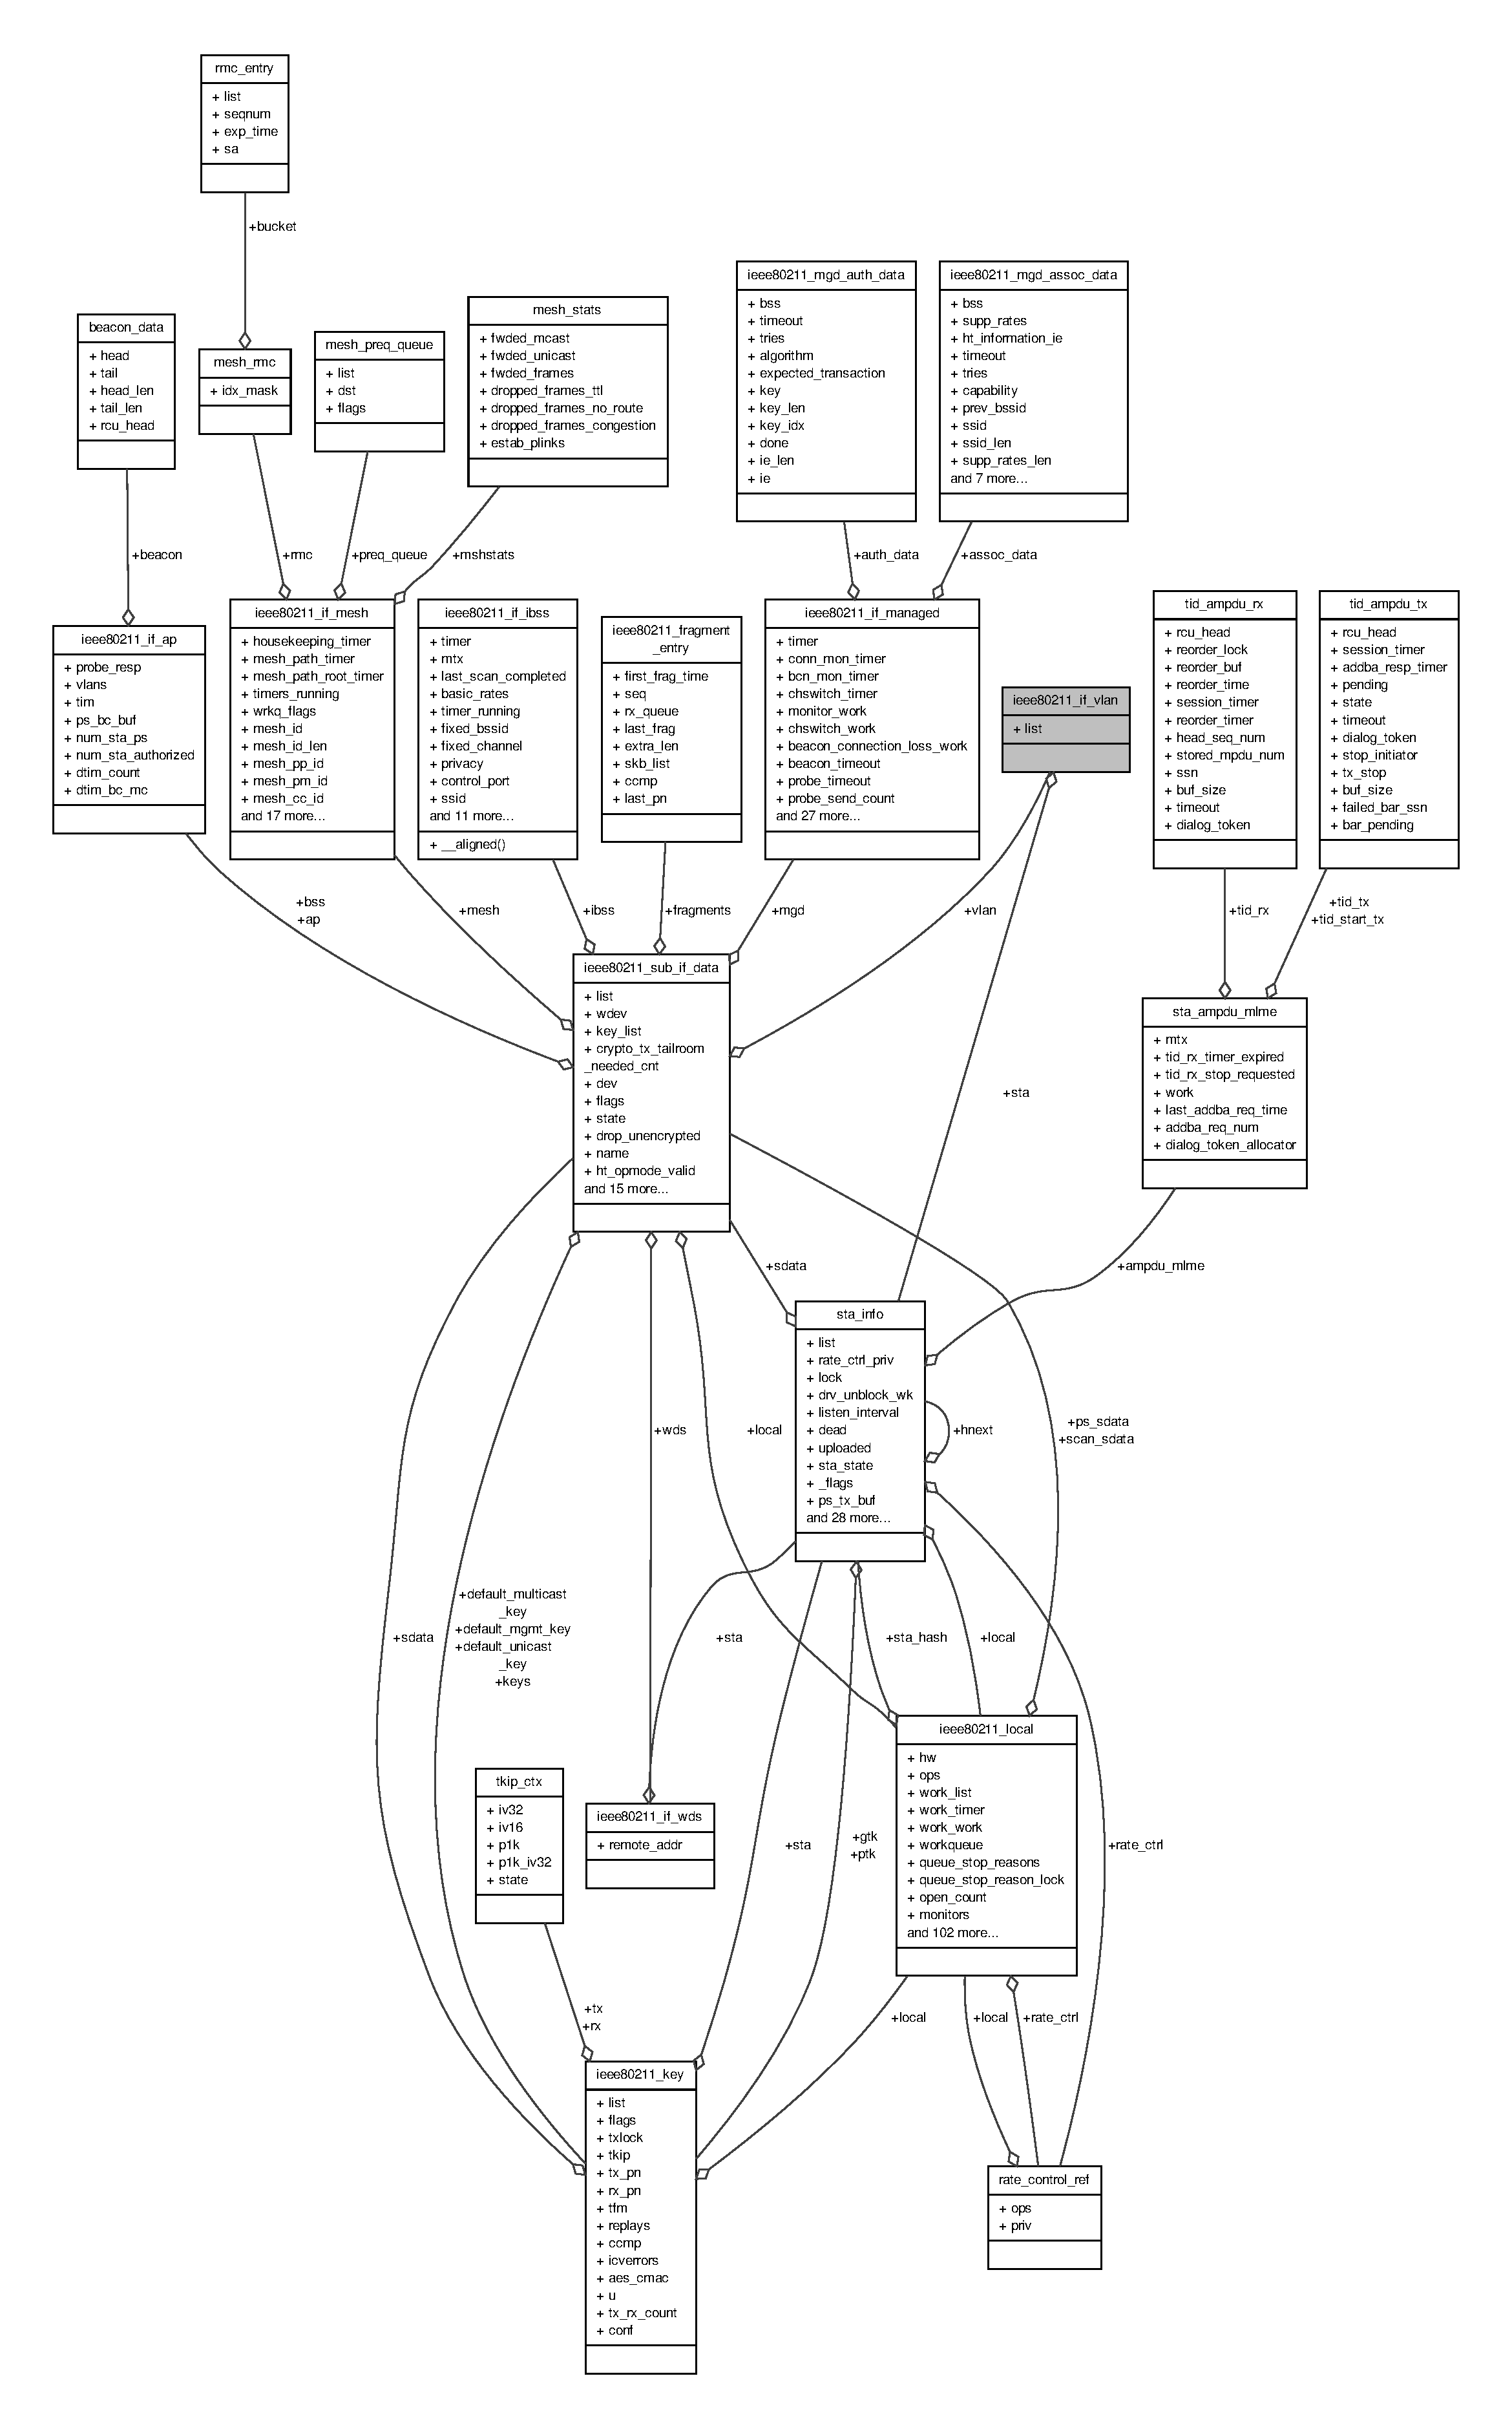
\includegraphics[height=550pt]{structieee80211__if__vlan__coll__graph}
\end{center}
\end{figure}
\subsection*{Data Fields}
\begin{DoxyCompactItemize}
\item 
struct list\-\_\-head \hyperlink{structieee80211__if__vlan_a1f00f18b91d5a820f2c43064243aa86e}{list}
\item 
struct \hyperlink{structsta__info}{sta\-\_\-info} \-\_\-\-\_\-rcu $\ast$ \hyperlink{structieee80211__if__vlan_a7e16457ec9b4b8bc5946669eb4b3c954}{sta}
\end{DoxyCompactItemize}


\subsection{Detailed Description}


Definition at line 294 of file ieee80211\-\_\-i.\-h.



\subsection{Field Documentation}
\hypertarget{structieee80211__if__vlan_a1f00f18b91d5a820f2c43064243aa86e}{\index{ieee80211\-\_\-if\-\_\-vlan@{ieee80211\-\_\-if\-\_\-vlan}!list@{list}}
\index{list@{list}!ieee80211_if_vlan@{ieee80211\-\_\-if\-\_\-vlan}}
\subsubsection[{list}]{\setlength{\rightskip}{0pt plus 5cm}struct list\-\_\-head list}}\label{structieee80211__if__vlan_a1f00f18b91d5a820f2c43064243aa86e}


Definition at line 295 of file ieee80211\-\_\-i.\-h.

\hypertarget{structieee80211__if__vlan_a7e16457ec9b4b8bc5946669eb4b3c954}{\index{ieee80211\-\_\-if\-\_\-vlan@{ieee80211\-\_\-if\-\_\-vlan}!sta@{sta}}
\index{sta@{sta}!ieee80211_if_vlan@{ieee80211\-\_\-if\-\_\-vlan}}
\subsubsection[{sta}]{\setlength{\rightskip}{0pt plus 5cm}struct {\bf sta\-\_\-info} \-\_\-\-\_\-rcu$\ast$ sta}}\label{structieee80211__if__vlan_a7e16457ec9b4b8bc5946669eb4b3c954}


Definition at line 298 of file ieee80211\-\_\-i.\-h.



The documentation for this struct was generated from the following file\-:\begin{DoxyCompactItemize}
\item 
/home/guille/msm/net/mac80211/\hyperlink{ieee80211__i_8h}{ieee80211\-\_\-i.\-h}\end{DoxyCompactItemize}

\hypertarget{structieee80211__if__wds}{\section{ieee80211\-\_\-if\-\_\-wds Struct Reference}
\label{structieee80211__if__wds}\index{ieee80211\-\_\-if\-\_\-wds@{ieee80211\-\_\-if\-\_\-wds}}
}


{\ttfamily \#include $<$ieee80211\-\_\-i.\-h$>$}



Collaboration diagram for ieee80211\-\_\-if\-\_\-wds\-:
\nopagebreak
\begin{figure}[H]
\begin{center}
\leavevmode
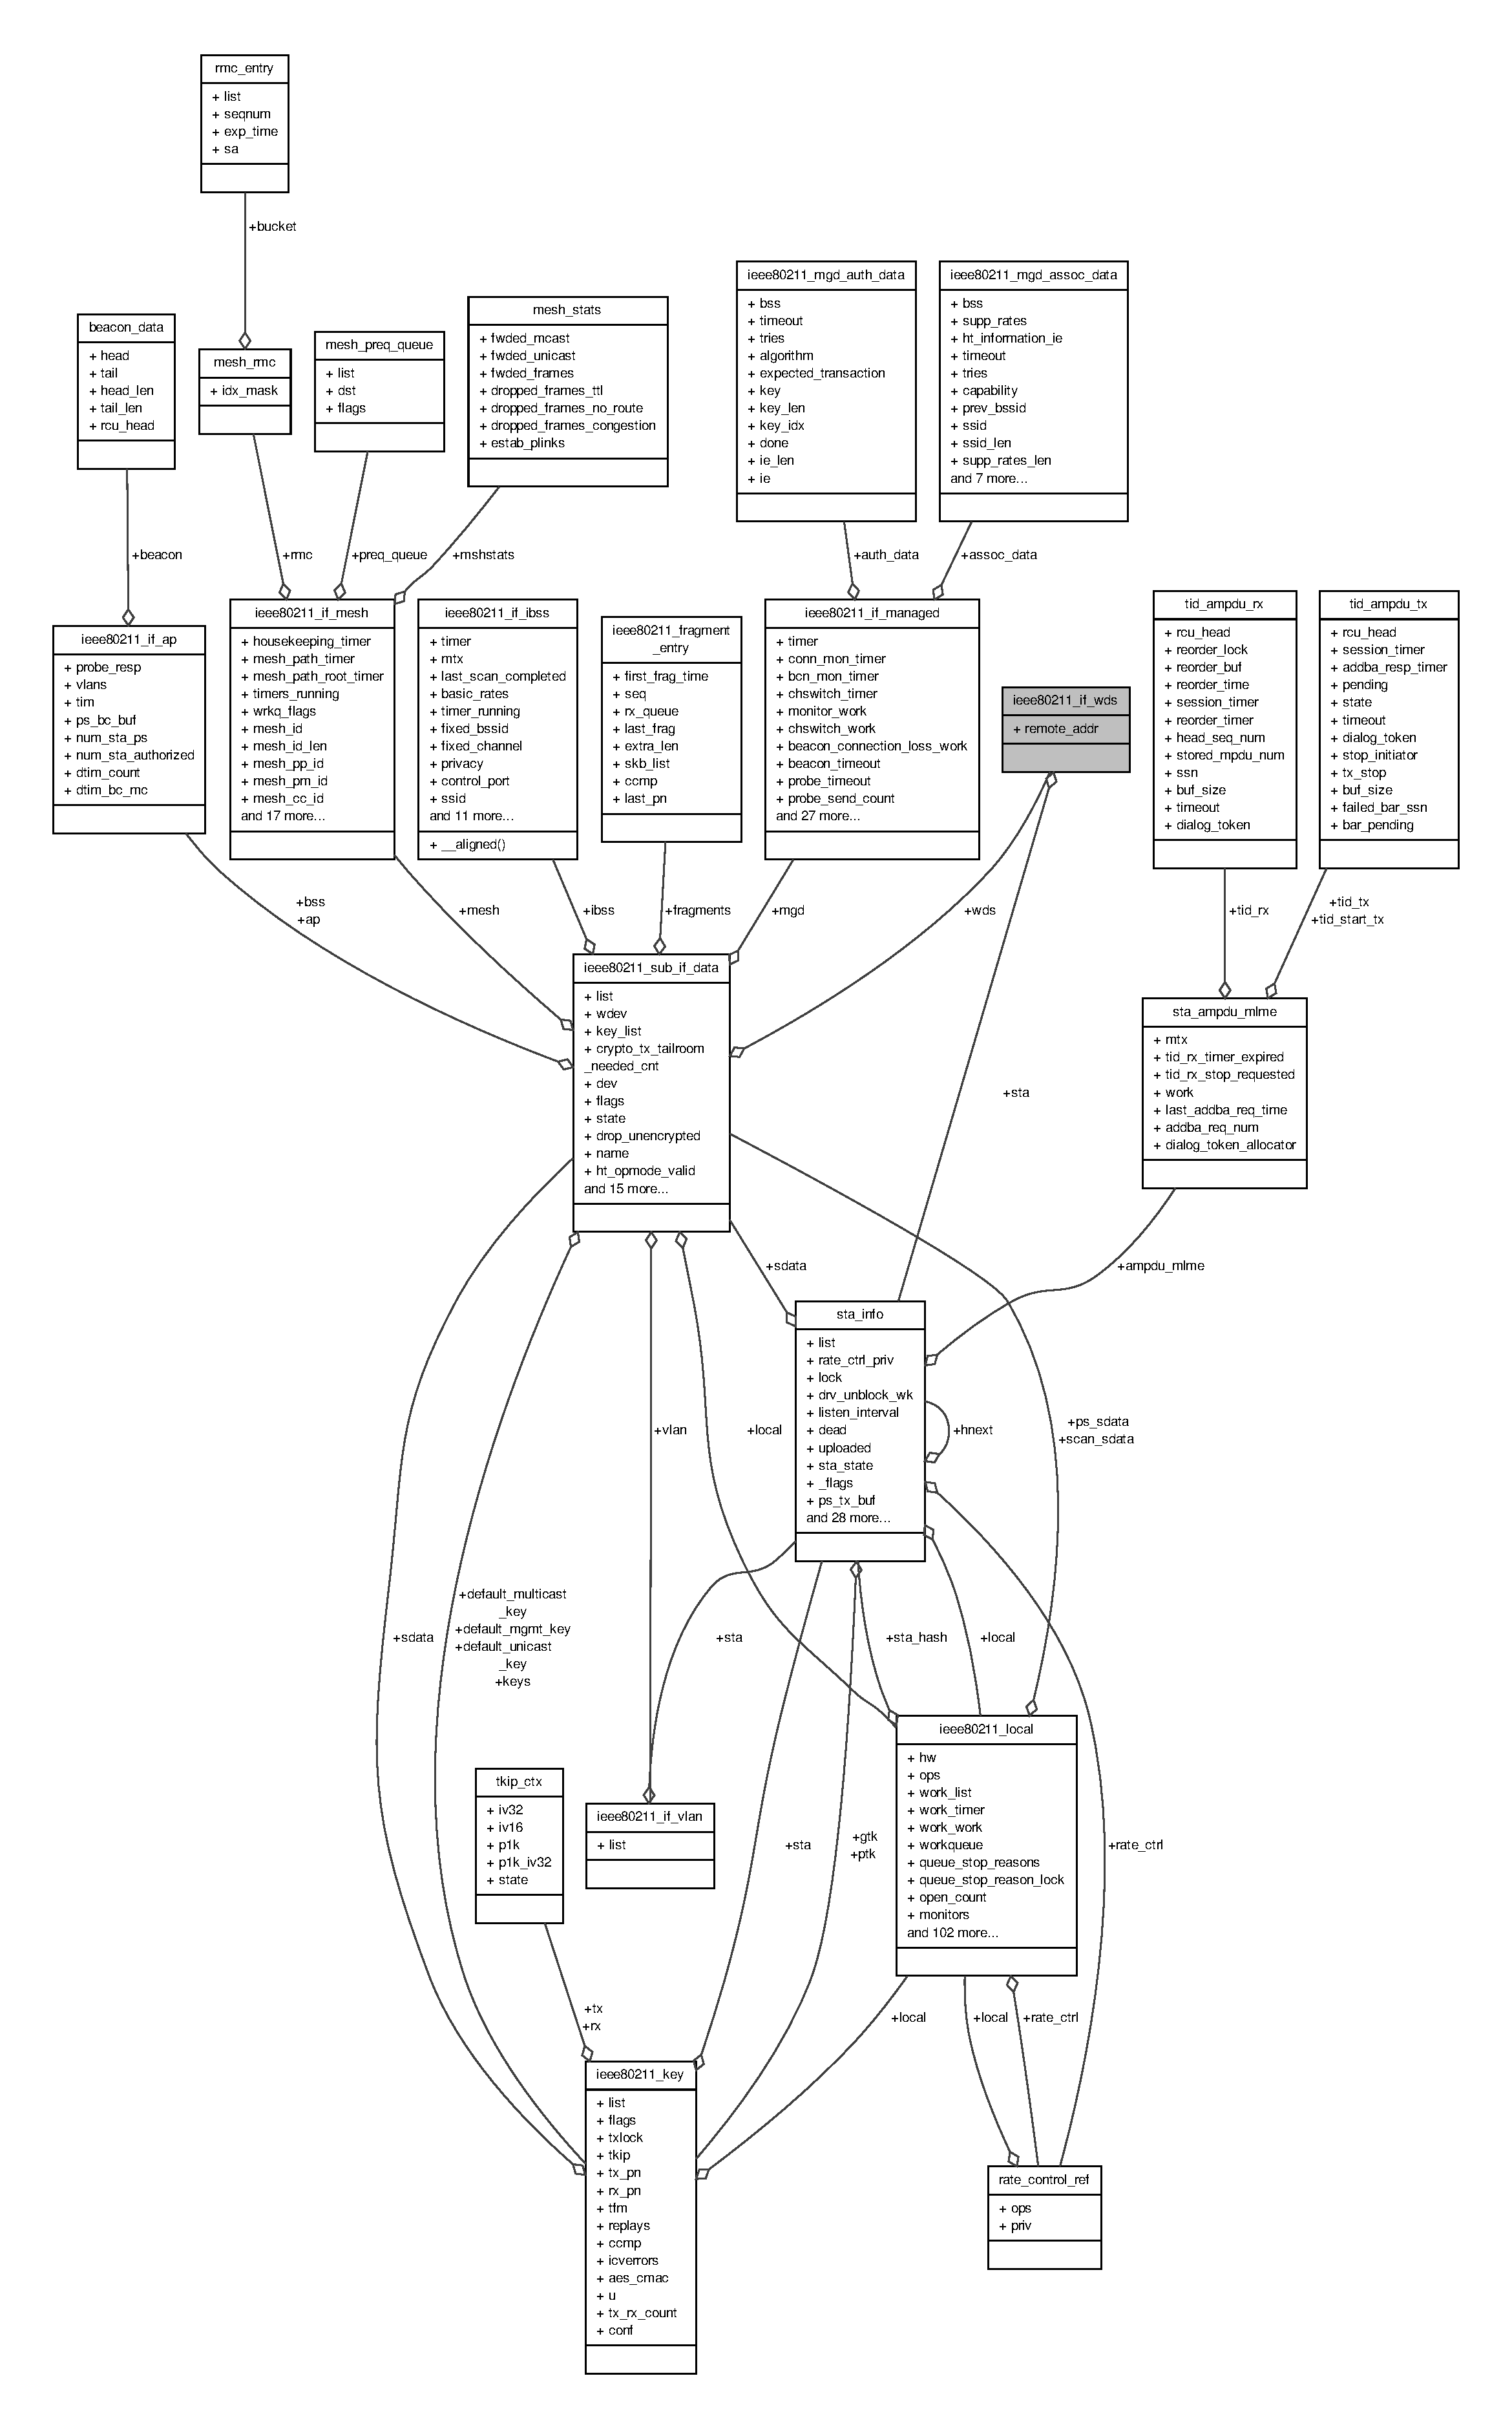
\includegraphics[height=550pt]{structieee80211__if__wds__coll__graph}
\end{center}
\end{figure}
\subsection*{Data Fields}
\begin{DoxyCompactItemize}
\item 
struct \hyperlink{structsta__info}{sta\-\_\-info} $\ast$ \hyperlink{structieee80211__if__wds_aafa9dadbeccd54b4a6b9f77f2908a093}{sta}
\item 
u8 \hyperlink{structieee80211__if__wds_aba4535f0b49a74e9fb64b3a6e9da433d}{remote\-\_\-addr} \mbox{[}E\-T\-H\-\_\-\-A\-L\-E\-N\mbox{]}
\end{DoxyCompactItemize}


\subsection{Detailed Description}


Definition at line 289 of file ieee80211\-\_\-i.\-h.



\subsection{Field Documentation}
\hypertarget{structieee80211__if__wds_aba4535f0b49a74e9fb64b3a6e9da433d}{\index{ieee80211\-\_\-if\-\_\-wds@{ieee80211\-\_\-if\-\_\-wds}!remote\-\_\-addr@{remote\-\_\-addr}}
\index{remote\-\_\-addr@{remote\-\_\-addr}!ieee80211_if_wds@{ieee80211\-\_\-if\-\_\-wds}}
\subsubsection[{remote\-\_\-addr}]{\setlength{\rightskip}{0pt plus 5cm}u8 remote\-\_\-addr\mbox{[}E\-T\-H\-\_\-\-A\-L\-E\-N\mbox{]}}}\label{structieee80211__if__wds_aba4535f0b49a74e9fb64b3a6e9da433d}


Definition at line 291 of file ieee80211\-\_\-i.\-h.

\hypertarget{structieee80211__if__wds_aafa9dadbeccd54b4a6b9f77f2908a093}{\index{ieee80211\-\_\-if\-\_\-wds@{ieee80211\-\_\-if\-\_\-wds}!sta@{sta}}
\index{sta@{sta}!ieee80211_if_wds@{ieee80211\-\_\-if\-\_\-wds}}
\subsubsection[{sta}]{\setlength{\rightskip}{0pt plus 5cm}struct {\bf sta\-\_\-info}$\ast$ sta}}\label{structieee80211__if__wds_aafa9dadbeccd54b4a6b9f77f2908a093}


Definition at line 290 of file ieee80211\-\_\-i.\-h.



The documentation for this struct was generated from the following file\-:\begin{DoxyCompactItemize}
\item 
/home/guille/msm/net/mac80211/\hyperlink{ieee80211__i_8h}{ieee80211\-\_\-i.\-h}\end{DoxyCompactItemize}

\hypertarget{structieee80211__key}{\section{ieee80211\-\_\-key Struct Reference}
\label{structieee80211__key}\index{ieee80211\-\_\-key@{ieee80211\-\_\-key}}
}


{\ttfamily \#include $<$key.\-h$>$}



Collaboration diagram for ieee80211\-\_\-key\-:
\nopagebreak
\begin{figure}[H]
\begin{center}
\leavevmode
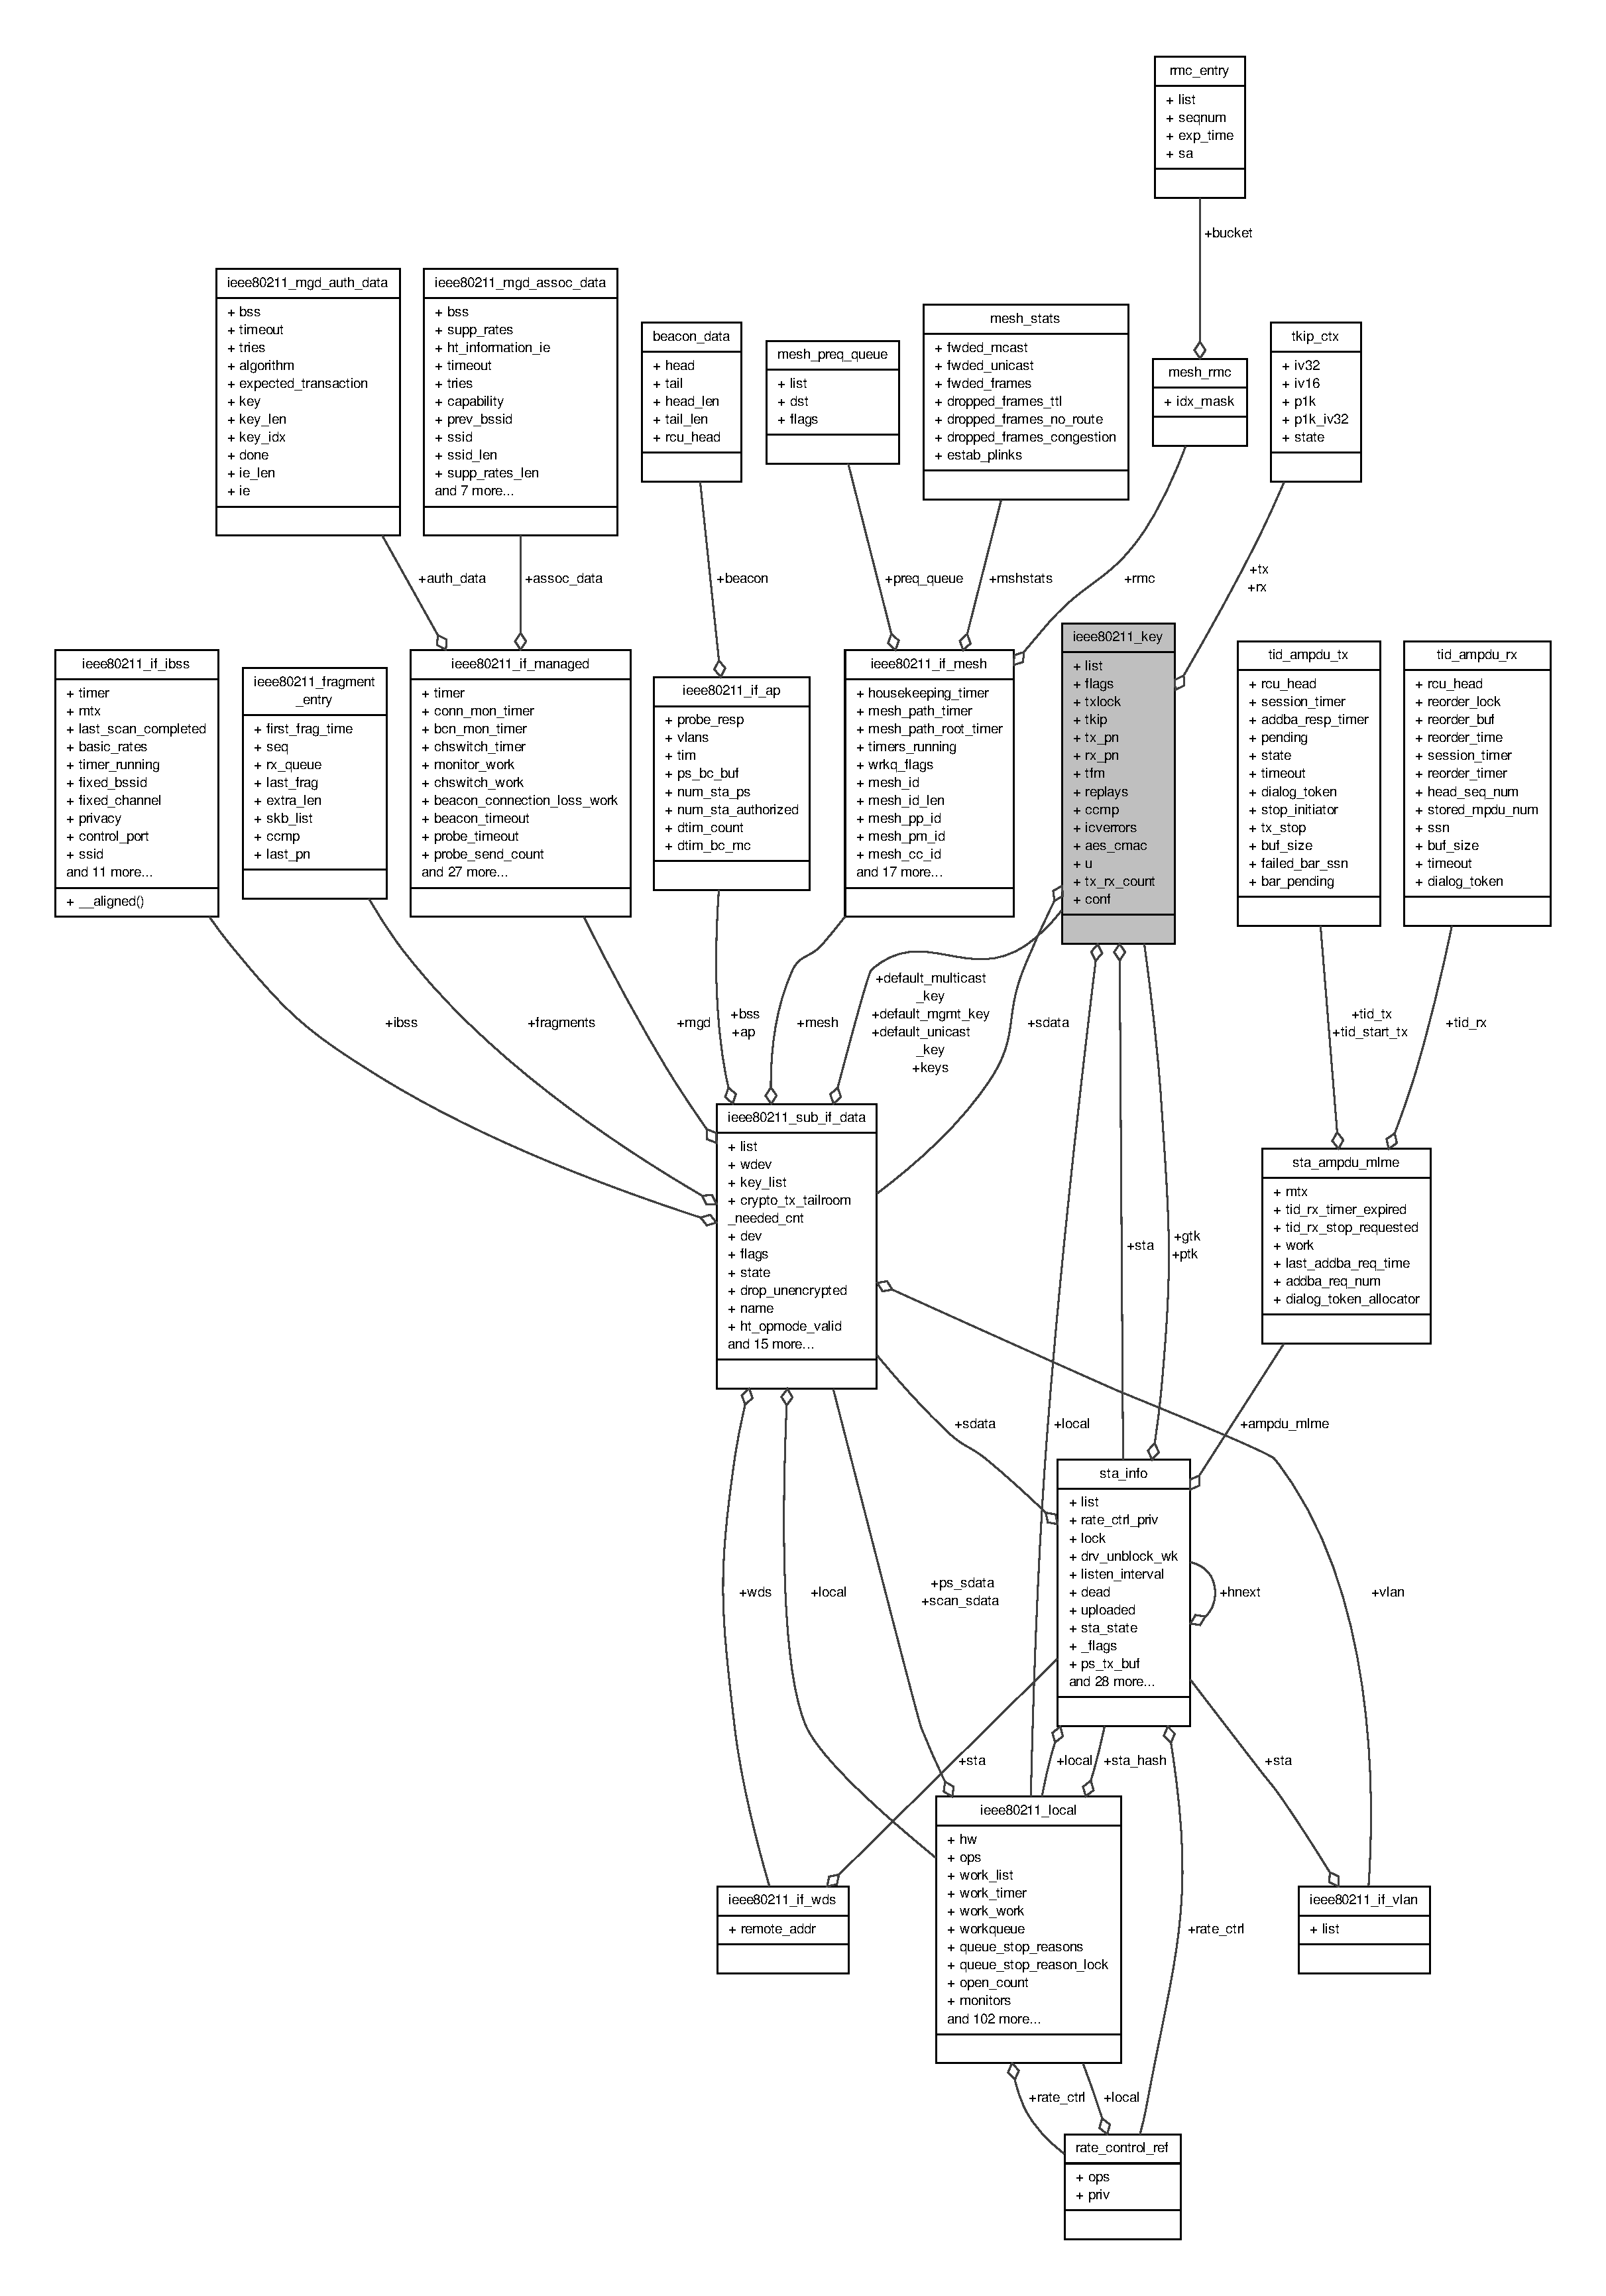
\includegraphics[width=350pt]{structieee80211__key__coll__graph}
\end{center}
\end{figure}
\subsection*{Data Fields}
\begin{DoxyCompactItemize}
\item 
struct \hyperlink{structieee80211__local}{ieee80211\-\_\-local} $\ast$ \hyperlink{structieee80211__key_ad436a024f420f219c4fe2eebce7e4ab2}{local}
\item 
struct \hyperlink{structieee80211__sub__if__data}{ieee80211\-\_\-sub\-\_\-if\-\_\-data} $\ast$ \hyperlink{structieee80211__key_ad829d8d33f06a7245cc303f924f259ac}{sdata}
\item 
struct \hyperlink{structsta__info}{sta\-\_\-info} $\ast$ \hyperlink{structieee80211__key_aafa9dadbeccd54b4a6b9f77f2908a093}{sta}
\item 
struct list\-\_\-head \hyperlink{structieee80211__key_a1f00f18b91d5a820f2c43064243aa86e}{list}
\item 
unsigned int \hyperlink{structieee80211__key_ac92588540e8c1d014a08cd8a45462b19}{flags}
\item 
\begin{tabbing}
xx\=xx\=xx\=xx\=xx\=xx\=xx\=xx\=xx\=\kill
union \{\\
\>struct \{\\
\>\>spinlock\_t \hyperlink{structieee80211__key_a9b2bd2f2c7f0e62e0e0433a4b4964bca}{txlock}\\
\>\>struct \hyperlink{structtkip__ctx}{tkip\_ctx} \hyperlink{structieee80211__key_a3a974b8d9690b9d3e88e8604538f4cf8}{tx}\\
\>\>struct \hyperlink{structtkip__ctx}{tkip\_ctx} \hyperlink{structieee80211__key_a47e91edc6699fec0d3ddca2c17c58a16}{rx} \mbox{[}\hyperlink{key_8h_a99cb7469613fea382d3951d37ee2c075}{NUM\_RX\_DATA\_QUEUES}\mbox{]}\\
\>\} \hyperlink{structieee80211__key_a1e037cc7cf26e98fb0ab400903c62d50}{tkip}\\
\>struct \{\\
\>\>atomic64\_t \hyperlink{structieee80211__key_a151a5bf95479b1130b341b412e6e3705}{tx\_pn}\\
\>\>u8 \hyperlink{structieee80211__key_af268ed760198a17a7ecd9c352f6f1fc5}{rx\_pn} \mbox{[}\hyperlink{key_8h_a99cb7469613fea382d3951d37ee2c075}{NUM\_RX\_DATA\_QUEUES}+1\mbox{]}\mbox{[}\hyperlink{key_8h_a81046bbc6df45432e2845f0f32222abc}{CCMP\_PN\_LEN}\mbox{]}\\
\>\>struct crypto\_cipher $\ast$ \hyperlink{structieee80211__key_a45576ea98555983d71e70badb9035f67}{tfm}\\
\>\>u32 \hyperlink{structieee80211__key_a0c08b132b796ebfdeda0499ae965b637}{replays}\\
\>\} \hyperlink{structieee80211__key_a7f707fa843bd338b94e1d10d95e88f11}{ccmp}\\
\>struct \{\\
\>\>atomic64\_t \hyperlink{structieee80211__key_a151a5bf95479b1130b341b412e6e3705}{tx\_pn}\\
\>\>u8 \hyperlink{structieee80211__key_af268ed760198a17a7ecd9c352f6f1fc5}{rx\_pn} \mbox{[}\hyperlink{key_8h_a07fe3d0d5319da1976cbe16e6dcdb415}{CMAC\_PN\_LEN}\mbox{]}\\
\>\>struct crypto\_cipher $\ast$ \hyperlink{structieee80211__key_a45576ea98555983d71e70badb9035f67}{tfm}\\
\>\>u32 \hyperlink{structieee80211__key_a0c08b132b796ebfdeda0499ae965b637}{replays}\\
\>\>u32 \hyperlink{structieee80211__key_a6751db90f0ca17fdb752baeb6f8d5152}{icverrors}\\
\>\} \hyperlink{structieee80211__key_affdec9171aa9c62e512d1080c1c45e2a}{aes\_cmac}\\
\} \hyperlink{structieee80211__key_aaf1be5c7d7653b795e11cb959246ee99}{u}\\

\end{tabbing}\item 
int \hyperlink{structieee80211__key_aff97ed740b6f262a845615cf7e63af70}{tx\-\_\-rx\-\_\-count}
\item 
struct ieee80211\-\_\-key\-\_\-conf \hyperlink{structieee80211__key_ac356e71d3ee661c89f43f272674ca2d6}{conf}
\end{DoxyCompactItemize}


\subsection{Detailed Description}


Definition at line 65 of file key.\-h.



\subsection{Field Documentation}
\hypertarget{structieee80211__key_affdec9171aa9c62e512d1080c1c45e2a}{\index{ieee80211\-\_\-key@{ieee80211\-\_\-key}!aes\-\_\-cmac@{aes\-\_\-cmac}}
\index{aes\-\_\-cmac@{aes\-\_\-cmac}!ieee80211_key@{ieee80211\-\_\-key}}
\subsubsection[{aes\-\_\-cmac}]{\setlength{\rightskip}{0pt plus 5cm}struct \{ ... \}   aes\-\_\-cmac}}\label{structieee80211__key_affdec9171aa9c62e512d1080c1c45e2a}
\hypertarget{structieee80211__key_a7f707fa843bd338b94e1d10d95e88f11}{\index{ieee80211\-\_\-key@{ieee80211\-\_\-key}!ccmp@{ccmp}}
\index{ccmp@{ccmp}!ieee80211_key@{ieee80211\-\_\-key}}
\subsubsection[{ccmp}]{\setlength{\rightskip}{0pt plus 5cm}struct \{ ... \}   ccmp}}\label{structieee80211__key_a7f707fa843bd338b94e1d10d95e88f11}
\hypertarget{structieee80211__key_ac356e71d3ee661c89f43f272674ca2d6}{\index{ieee80211\-\_\-key@{ieee80211\-\_\-key}!conf@{conf}}
\index{conf@{conf}!ieee80211_key@{ieee80211\-\_\-key}}
\subsubsection[{conf}]{\setlength{\rightskip}{0pt plus 5cm}struct ieee80211\-\_\-key\-\_\-conf conf}}\label{structieee80211__key_ac356e71d3ee661c89f43f272674ca2d6}


Definition at line 123 of file key.\-h.

\hypertarget{structieee80211__key_ac92588540e8c1d014a08cd8a45462b19}{\index{ieee80211\-\_\-key@{ieee80211\-\_\-key}!flags@{flags}}
\index{flags@{flags}!ieee80211_key@{ieee80211\-\_\-key}}
\subsubsection[{flags}]{\setlength{\rightskip}{0pt plus 5cm}unsigned int flags}}\label{structieee80211__key_ac92588540e8c1d014a08cd8a45462b19}


Definition at line 74 of file key.\-h.

\hypertarget{structieee80211__key_a6751db90f0ca17fdb752baeb6f8d5152}{\index{ieee80211\-\_\-key@{ieee80211\-\_\-key}!icverrors@{icverrors}}
\index{icverrors@{icverrors}!ieee80211_key@{ieee80211\-\_\-key}}
\subsubsection[{icverrors}]{\setlength{\rightskip}{0pt plus 5cm}u32 icverrors}}\label{structieee80211__key_a6751db90f0ca17fdb752baeb6f8d5152}


Definition at line 104 of file key.\-h.

\hypertarget{structieee80211__key_a1f00f18b91d5a820f2c43064243aa86e}{\index{ieee80211\-\_\-key@{ieee80211\-\_\-key}!list@{list}}
\index{list@{list}!ieee80211_key@{ieee80211\-\_\-key}}
\subsubsection[{list}]{\setlength{\rightskip}{0pt plus 5cm}struct list\-\_\-head list}}\label{structieee80211__key_a1f00f18b91d5a820f2c43064243aa86e}


Definition at line 71 of file key.\-h.

\hypertarget{structieee80211__key_ad436a024f420f219c4fe2eebce7e4ab2}{\index{ieee80211\-\_\-key@{ieee80211\-\_\-key}!local@{local}}
\index{local@{local}!ieee80211_key@{ieee80211\-\_\-key}}
\subsubsection[{local}]{\setlength{\rightskip}{0pt plus 5cm}struct {\bf ieee80211\-\_\-local}$\ast$ local}}\label{structieee80211__key_ad436a024f420f219c4fe2eebce7e4ab2}


Definition at line 66 of file key.\-h.

\hypertarget{structieee80211__key_a0c08b132b796ebfdeda0499ae965b637}{\index{ieee80211\-\_\-key@{ieee80211\-\_\-key}!replays@{replays}}
\index{replays@{replays}!ieee80211_key@{ieee80211\-\_\-key}}
\subsubsection[{replays}]{\setlength{\rightskip}{0pt plus 5cm}u32 replays}}\label{structieee80211__key_a0c08b132b796ebfdeda0499ae965b637}


Definition at line 97 of file key.\-h.

\hypertarget{structieee80211__key_a47e91edc6699fec0d3ddca2c17c58a16}{\index{ieee80211\-\_\-key@{ieee80211\-\_\-key}!rx@{rx}}
\index{rx@{rx}!ieee80211_key@{ieee80211\-\_\-key}}
\subsubsection[{rx}]{\setlength{\rightskip}{0pt plus 5cm}struct {\bf tkip\-\_\-ctx} rx\mbox{[}{\bf N\-U\-M\-\_\-\-R\-X\-\_\-\-D\-A\-T\-A\-\_\-\-Q\-U\-E\-U\-E\-S}\mbox{]}}}\label{structieee80211__key_a47e91edc6699fec0d3ddca2c17c58a16}


Definition at line 85 of file key.\-h.

\hypertarget{structieee80211__key_af268ed760198a17a7ecd9c352f6f1fc5}{\index{ieee80211\-\_\-key@{ieee80211\-\_\-key}!rx\-\_\-pn@{rx\-\_\-pn}}
\index{rx\-\_\-pn@{rx\-\_\-pn}!ieee80211_key@{ieee80211\-\_\-key}}
\subsubsection[{rx\-\_\-pn}]{\setlength{\rightskip}{0pt plus 5cm}u8 rx\-\_\-pn\mbox{[}{\bf C\-M\-A\-C\-\_\-\-P\-N\-\_\-\-L\-E\-N}\mbox{]}}}\label{structieee80211__key_af268ed760198a17a7ecd9c352f6f1fc5}


Definition at line 95 of file key.\-h.

\hypertarget{structieee80211__key_ad829d8d33f06a7245cc303f924f259ac}{\index{ieee80211\-\_\-key@{ieee80211\-\_\-key}!sdata@{sdata}}
\index{sdata@{sdata}!ieee80211_key@{ieee80211\-\_\-key}}
\subsubsection[{sdata}]{\setlength{\rightskip}{0pt plus 5cm}struct {\bf ieee80211\-\_\-sub\-\_\-if\-\_\-data}$\ast$ sdata}}\label{structieee80211__key_ad829d8d33f06a7245cc303f924f259ac}


Definition at line 67 of file key.\-h.

\hypertarget{structieee80211__key_aafa9dadbeccd54b4a6b9f77f2908a093}{\index{ieee80211\-\_\-key@{ieee80211\-\_\-key}!sta@{sta}}
\index{sta@{sta}!ieee80211_key@{ieee80211\-\_\-key}}
\subsubsection[{sta}]{\setlength{\rightskip}{0pt plus 5cm}struct {\bf sta\-\_\-info}$\ast$ sta}}\label{structieee80211__key_aafa9dadbeccd54b4a6b9f77f2908a093}


Definition at line 68 of file key.\-h.

\hypertarget{structieee80211__key_a45576ea98555983d71e70badb9035f67}{\index{ieee80211\-\_\-key@{ieee80211\-\_\-key}!tfm@{tfm}}
\index{tfm@{tfm}!ieee80211_key@{ieee80211\-\_\-key}}
\subsubsection[{tfm}]{\setlength{\rightskip}{0pt plus 5cm}struct crypto\-\_\-cipher$\ast$ tfm}}\label{structieee80211__key_a45576ea98555983d71e70badb9035f67}


Definition at line 96 of file key.\-h.

\hypertarget{structieee80211__key_a1e037cc7cf26e98fb0ab400903c62d50}{\index{ieee80211\-\_\-key@{ieee80211\-\_\-key}!tkip@{tkip}}
\index{tkip@{tkip}!ieee80211_key@{ieee80211\-\_\-key}}
\subsubsection[{tkip}]{\setlength{\rightskip}{0pt plus 5cm}struct \{ ... \}   tkip}}\label{structieee80211__key_a1e037cc7cf26e98fb0ab400903c62d50}
\hypertarget{structieee80211__key_a3a974b8d9690b9d3e88e8604538f4cf8}{\index{ieee80211\-\_\-key@{ieee80211\-\_\-key}!tx@{tx}}
\index{tx@{tx}!ieee80211_key@{ieee80211\-\_\-key}}
\subsubsection[{tx}]{\setlength{\rightskip}{0pt plus 5cm}struct {\bf tkip\-\_\-ctx} tx}}\label{structieee80211__key_a3a974b8d9690b9d3e88e8604538f4cf8}


Definition at line 82 of file key.\-h.

\hypertarget{structieee80211__key_a151a5bf95479b1130b341b412e6e3705}{\index{ieee80211\-\_\-key@{ieee80211\-\_\-key}!tx\-\_\-pn@{tx\-\_\-pn}}
\index{tx\-\_\-pn@{tx\-\_\-pn}!ieee80211_key@{ieee80211\-\_\-key}}
\subsubsection[{tx\-\_\-pn}]{\setlength{\rightskip}{0pt plus 5cm}atomic64\-\_\-t tx\-\_\-pn}}\label{structieee80211__key_a151a5bf95479b1130b341b412e6e3705}


Definition at line 88 of file key.\-h.

\hypertarget{structieee80211__key_aff97ed740b6f262a845615cf7e63af70}{\index{ieee80211\-\_\-key@{ieee80211\-\_\-key}!tx\-\_\-rx\-\_\-count@{tx\-\_\-rx\-\_\-count}}
\index{tx\-\_\-rx\-\_\-count@{tx\-\_\-rx\-\_\-count}!ieee80211_key@{ieee80211\-\_\-key}}
\subsubsection[{tx\-\_\-rx\-\_\-count}]{\setlength{\rightskip}{0pt plus 5cm}int tx\-\_\-rx\-\_\-count}}\label{structieee80211__key_aff97ed740b6f262a845615cf7e63af70}


Definition at line 109 of file key.\-h.

\hypertarget{structieee80211__key_a9b2bd2f2c7f0e62e0e0433a4b4964bca}{\index{ieee80211\-\_\-key@{ieee80211\-\_\-key}!txlock@{txlock}}
\index{txlock@{txlock}!ieee80211_key@{ieee80211\-\_\-key}}
\subsubsection[{txlock}]{\setlength{\rightskip}{0pt plus 5cm}spinlock\-\_\-t txlock}}\label{structieee80211__key_a9b2bd2f2c7f0e62e0e0433a4b4964bca}


Definition at line 79 of file key.\-h.

\hypertarget{structieee80211__key_aaf1be5c7d7653b795e11cb959246ee99}{\index{ieee80211\-\_\-key@{ieee80211\-\_\-key}!u@{u}}
\index{u@{u}!ieee80211_key@{ieee80211\-\_\-key}}
\subsubsection[{u}]{\setlength{\rightskip}{0pt plus 5cm}union \{ ... \}   u}}\label{structieee80211__key_aaf1be5c7d7653b795e11cb959246ee99}


The documentation for this struct was generated from the following file\-:\begin{DoxyCompactItemize}
\item 
/home/guille/msm/net/mac80211/\hyperlink{key_8h}{key.\-h}\end{DoxyCompactItemize}

\hypertarget{structieee80211__local}{\section{ieee80211\-\_\-local Struct Reference}
\label{structieee80211__local}\index{ieee80211\-\_\-local@{ieee80211\-\_\-local}}
}


{\ttfamily \#include $<$ieee80211\-\_\-i.\-h$>$}



Collaboration diagram for ieee80211\-\_\-local\-:
\nopagebreak
\begin{figure}[H]
\begin{center}
\leavevmode
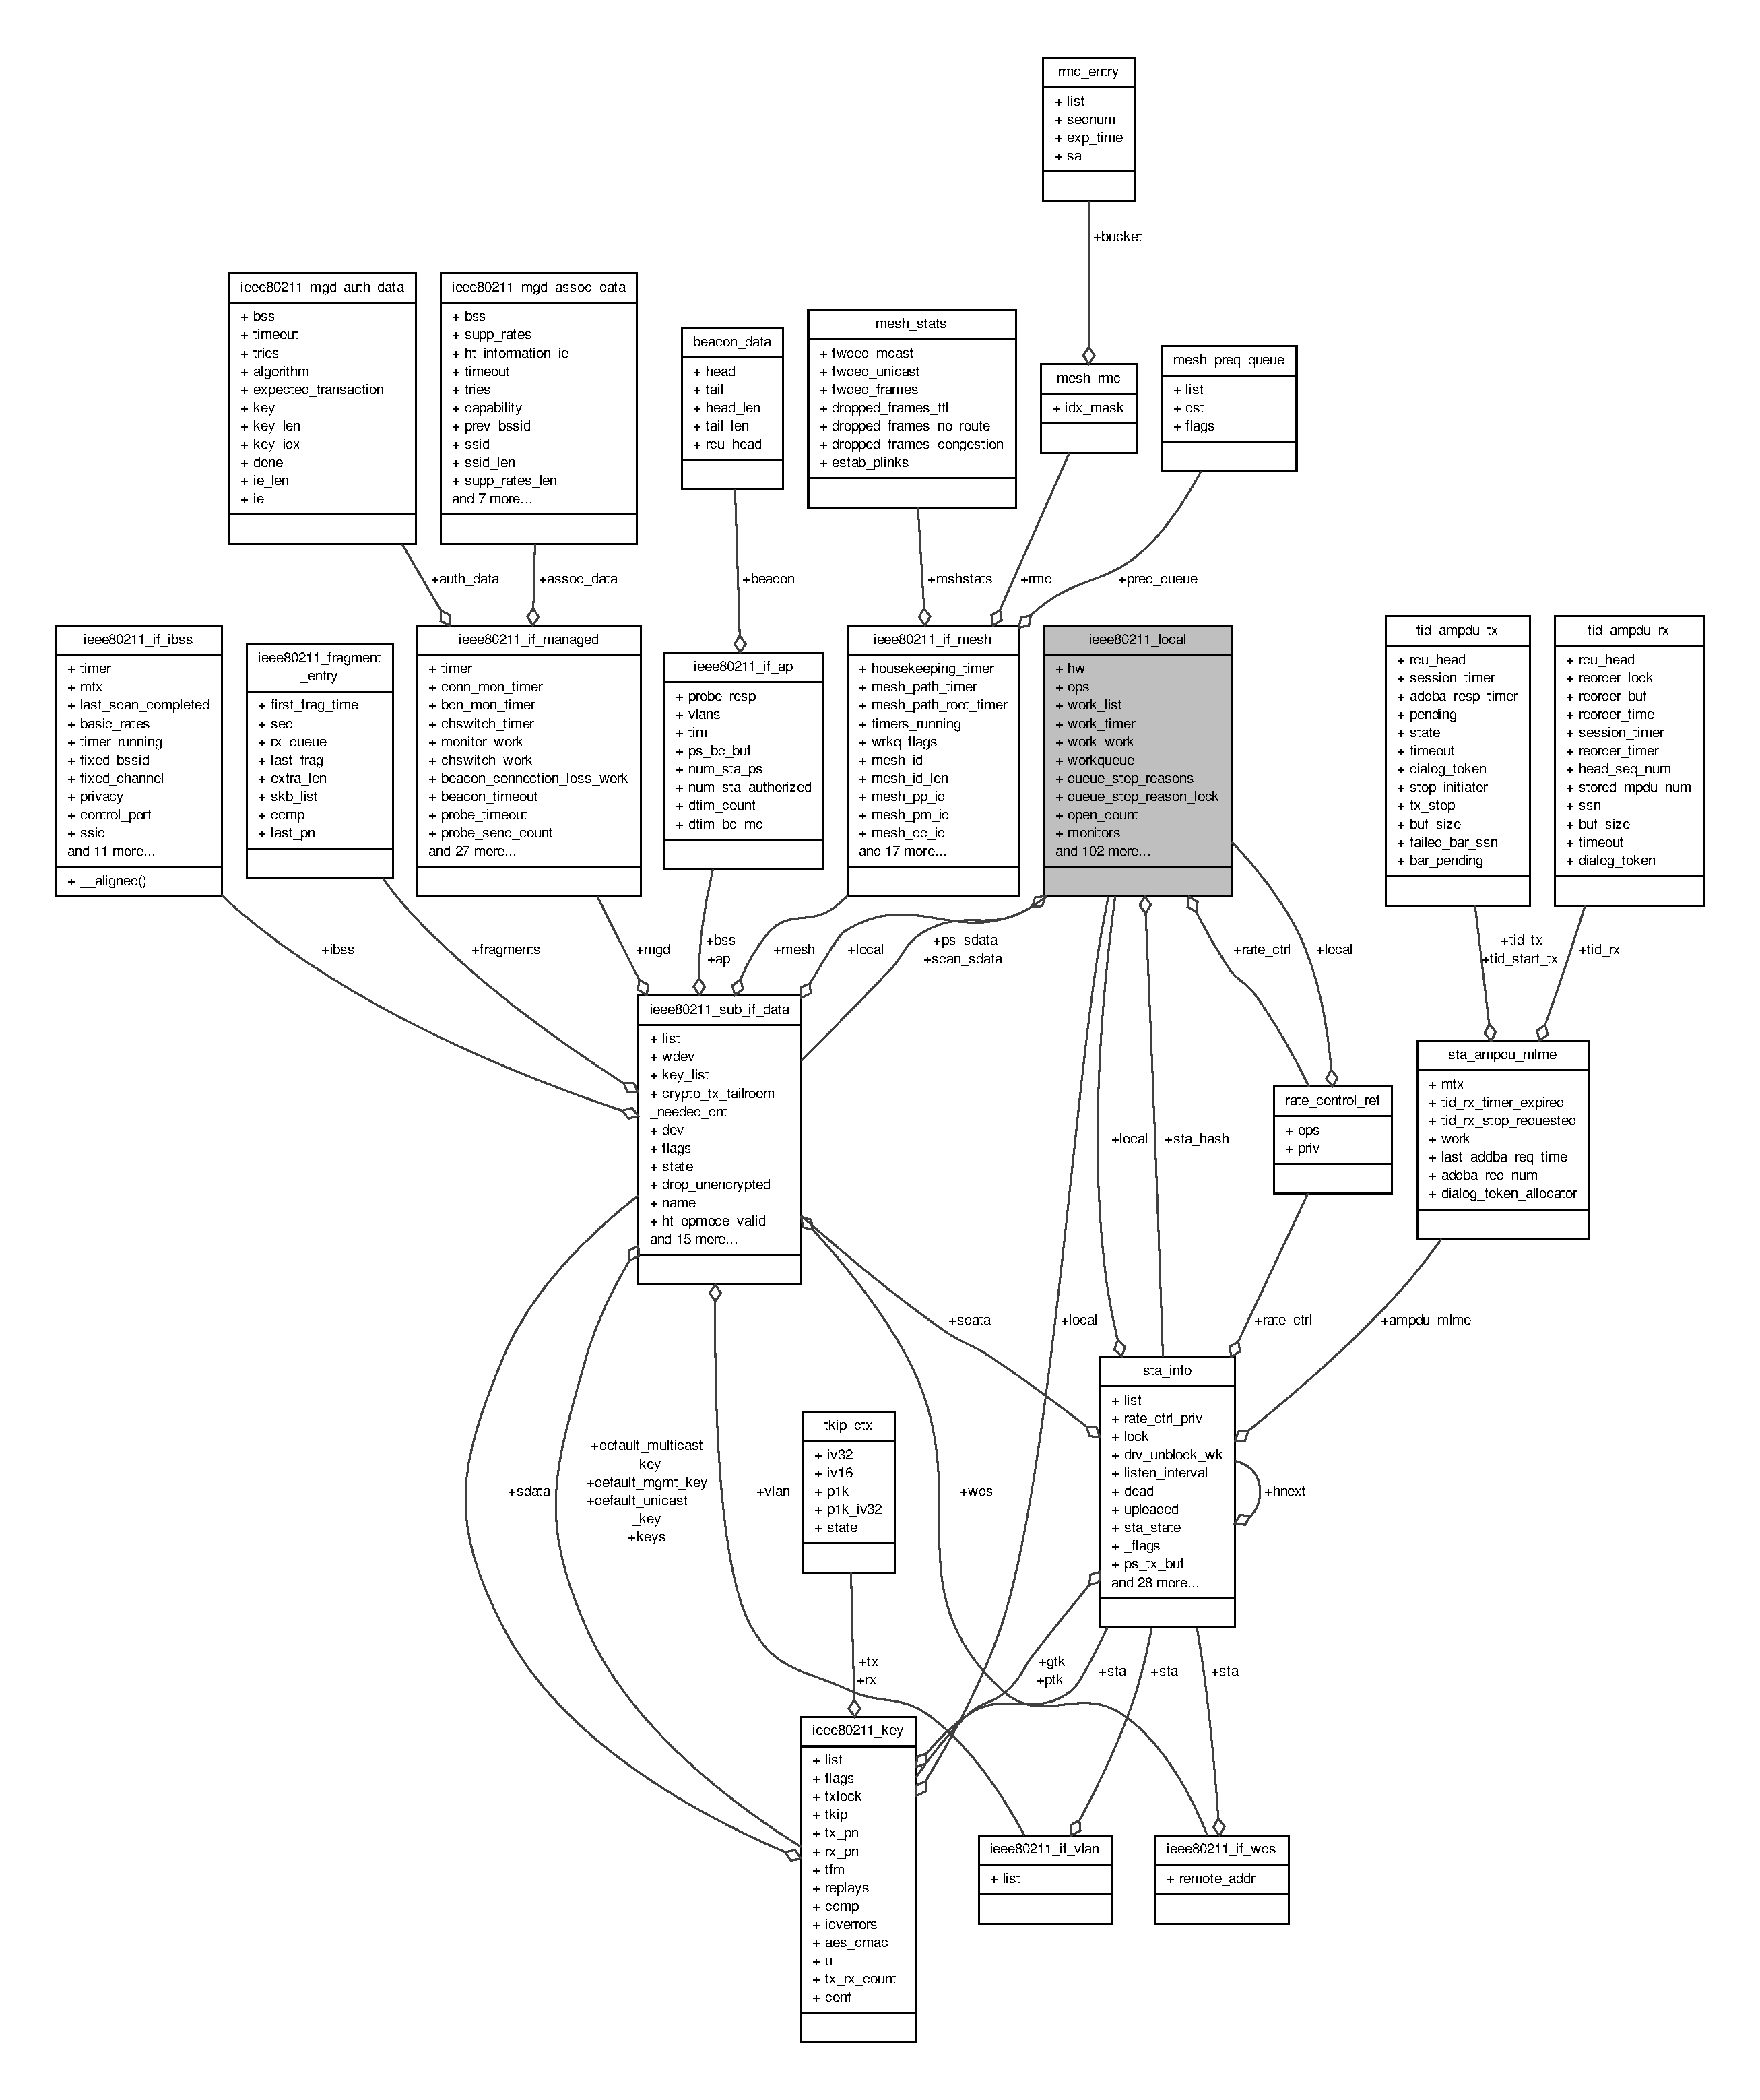
\includegraphics[width=350pt]{structieee80211__local__coll__graph}
\end{center}
\end{figure}
\subsection*{Data Fields}
\begin{DoxyCompactItemize}
\item 
struct ieee80211\-\_\-hw \hyperlink{structieee80211__local_a076bd779234ea1780e71eee200bc0d2c}{hw}
\item 
struct ieee80211\-\_\-ops $\ast$ \hyperlink{structieee80211__local_a276a891dc24af93ff2578620eaa83190}{ops}
\item 
struct list\-\_\-head \hyperlink{structieee80211__local_a207d91b6483b2be61984ad3a064dbeb9}{work\-\_\-list}
\item 
struct timer\-\_\-list \hyperlink{structieee80211__local_a8a02d2a35aae73440084c24cb79a57af}{work\-\_\-timer}
\item 
struct work\-\_\-struct \hyperlink{structieee80211__local_a5c4560ff0f9e5c23485f07405ea29b34}{work\-\_\-work}
\item 
struct workqueue\-\_\-struct $\ast$ \hyperlink{structieee80211__local_a5ed2da065662e4534cb5bec3437a1876}{workqueue}
\item 
unsigned long \hyperlink{structieee80211__local_a4ac9818da187bbf4f141fd9e6ca1f0fd}{queue\-\_\-stop\-\_\-reasons} \mbox{[}I\-E\-E\-E80211\-\_\-\-M\-A\-X\-\_\-\-Q\-U\-E\-U\-E\-S\mbox{]}
\item 
spinlock\-\_\-t \hyperlink{structieee80211__local_a6a4677a1a1ad602030742ceba058133b}{queue\-\_\-stop\-\_\-reason\-\_\-lock}
\item 
int \hyperlink{structieee80211__local_a8943f3ee2b248b1fe911c0441c136c08}{open\-\_\-count}
\item 
int \hyperlink{structieee80211__local_a0bd1594e17d034f96ba795dabeaee577}{monitors}
\item 
int \hyperlink{structieee80211__local_a9ed7f1c7df7ff97118031d501ebf660c}{cooked\-\_\-mntrs}
\item 
int \hyperlink{structieee80211__local_a27eb74fe97bc47632e4e68f9987b7676}{fif\-\_\-fcsfail}
\item 
int \hyperlink{structieee80211__local_a11004cb6258d9a385000bc4544aa06b5}{fif\-\_\-plcpfail}
\item 
int \hyperlink{structieee80211__local_af26c59857ac99739a98a86955ccb73f4}{fif\-\_\-control}
\item 
int \hyperlink{structieee80211__local_a6df112d414c0a93f9b40417e0d08cdd1}{fif\-\_\-other\-\_\-bss}
\item 
int \hyperlink{structieee80211__local_a79f914bf1ffdca68ec910069d5f7aad4}{fif\-\_\-pspoll}
\item 
int \hyperlink{structieee80211__local_ad3a2ffb279ac8ef26c6bb971b729cd73}{fif\-\_\-probe\-\_\-req}
\item 
int \hyperlink{structieee80211__local_ab293743371aeef9182e1e8c5be0d26f6}{probe\-\_\-req\-\_\-reg}
\item 
unsigned int \hyperlink{structieee80211__local_af57092f118989725a35071734086b077}{filter\-\_\-flags}
\item 
bool \hyperlink{structieee80211__local_a257c289b6a875f6028f1e79f4c0241bc}{wiphy\-\_\-ciphers\-\_\-allocated}
\item 
spinlock\-\_\-t \hyperlink{structieee80211__local_aa04ada770caf28109eee6faf56a43ee6}{filter\-\_\-lock}
\item 
struct work\-\_\-struct \hyperlink{structieee80211__local_aeebe638f6e2c04a7481951fee56b1c9e}{reconfig\-\_\-filter}
\item 
struct work\-\_\-struct \hyperlink{structieee80211__local_a1b89bbd9d7e4daee680c064bed613ff7}{recalc\-\_\-smps}
\item 
struct netdev\-\_\-hw\-\_\-addr\-\_\-list \hyperlink{structieee80211__local_a00dc9ea6f5dc07b551f8ae14dd3a4eff}{mc\-\_\-list}
\item 
bool \hyperlink{structieee80211__local_a34d7d9b6d74715302c953d01980bdebf}{tim\-\_\-in\-\_\-locked\-\_\-section}
\item 
bool \hyperlink{structieee80211__local_ae0ed5063d998fba626c0783a36391f3c}{suspended}
\item 
bool \hyperlink{structieee80211__local_a2ddb54f91088d41426fb0b5e4cb82022}{resuming}
\item 
bool \hyperlink{structieee80211__local_a4938b434be86b4b137b6eec047203e65}{quiescing}
\item 
bool \hyperlink{structieee80211__local_a43c08d193d555a2b2a61c53d2a4e5a63}{started}
\item 
bool \hyperlink{structieee80211__local_aafe36b77f629fe748f545f726849bb4c}{wowlan}
\item 
int \hyperlink{structieee80211__local_acf548b161496ab61ff27e8ae5aa59aff}{tx\-\_\-headroom}
\item 
struct tasklet\-\_\-struct \hyperlink{structieee80211__local_a4308a8fe6dfe7c223959f8b219a05695}{tasklet}
\item 
struct sk\-\_\-buff\-\_\-head \hyperlink{structieee80211__local_a6eeb93345e21d69a77a7c2c571bd0000}{skb\-\_\-queue}
\item 
struct sk\-\_\-buff\-\_\-head \hyperlink{structieee80211__local_a98b4c0b5fc65c583926a6c35981287eb}{skb\-\_\-queue\-\_\-unreliable}
\item 
struct sk\-\_\-buff\-\_\-head \hyperlink{structieee80211__local_aac644577fe51ca03388b580ee634c471}{rx\-\_\-skb\-\_\-queue}
\item 
bool \hyperlink{structieee80211__local_a52eb7e26fdfb1a3b6469728a7131fe80}{running\-\_\-rx\-\_\-handler}
\item 
struct mutex \hyperlink{structieee80211__local_a8fb5b2a5fbdd771e5d8cbd9e6f3f0652}{sta\-\_\-mtx}
\item 
spinlock\-\_\-t \hyperlink{structieee80211__local_a66f27f63b02e43a76482968cf728de10}{tim\-\_\-lock}
\item 
unsigned long \hyperlink{structieee80211__local_a24328b32806c8eb5a960e0ed36a4b4f3}{num\-\_\-sta}
\item 
struct list\-\_\-head \hyperlink{structieee80211__local_aa442db3b90ab8934df91ba31e7602e66}{sta\-\_\-list}
\item 
struct \hyperlink{structsta__info}{sta\-\_\-info} \-\_\-\-\_\-rcu $\ast$ \hyperlink{structieee80211__local_a6014b1885979a210472e849167192cec}{sta\-\_\-hash} \mbox{[}\hyperlink{sta__info_8h_ae6a569f0acda8f25b206cbce1dd162e4}{S\-T\-A\-\_\-\-H\-A\-S\-H\-\_\-\-S\-I\-Z\-E}\mbox{]}
\item 
struct timer\-\_\-list \hyperlink{structieee80211__local_a08ed23f945556f2425951c67c8676a06}{sta\-\_\-cleanup}
\item 
int \hyperlink{structieee80211__local_a97ee12a47f59b1e2ffa51cca68a70304}{sta\-\_\-generation}
\item 
struct sk\-\_\-buff\-\_\-head \hyperlink{structieee80211__local_a1af46fe8e85323cc129ada2186925c51}{pending} \mbox{[}I\-E\-E\-E80211\-\_\-\-M\-A\-X\-\_\-\-Q\-U\-E\-U\-E\-S\mbox{]}
\item 
struct tasklet\-\_\-struct \hyperlink{structieee80211__local_aebdf516672c673478395a1f1a1bda6ab}{tx\-\_\-pending\-\_\-tasklet}
\item 
atomic\-\_\-t \hyperlink{structieee80211__local_a761ac48dbd4f02cca627bf2164691129}{agg\-\_\-queue\-\_\-stop} \mbox{[}I\-E\-E\-E80211\-\_\-\-M\-A\-X\-\_\-\-Q\-U\-E\-U\-E\-S\mbox{]}
\item 
atomic\-\_\-t \hyperlink{structieee80211__local_ad49cfc0bfcbcee0e8082e1b209e97d31}{iff\-\_\-allmultis}
\item 
atomic\-\_\-t \hyperlink{structieee80211__local_a8f1cf23044f197295b99eb923325e33b}{iff\-\_\-promiscs}
\item 
struct \hyperlink{structrate__control__ref}{rate\-\_\-control\-\_\-ref} $\ast$ \hyperlink{structieee80211__local_a0f6ac21a75ada1908328210ec3b42667}{rate\-\_\-ctrl}
\item 
struct crypto\-\_\-cipher $\ast$ \hyperlink{structieee80211__local_ab554bf57d377855ad08d970f9e395ad0}{wep\-\_\-tx\-\_\-tfm}
\item 
struct crypto\-\_\-cipher $\ast$ \hyperlink{structieee80211__local_a993e1c97083f7fe3b90b9da910d72bd7}{wep\-\_\-rx\-\_\-tfm}
\item 
u32 \hyperlink{structieee80211__local_ac63790cf9fa02ac7ac0c4282cfe5b041}{wep\-\_\-iv}
\item 
struct list\-\_\-head \hyperlink{structieee80211__local_af269ec693ad97d77fcfb0decd1c9edc7}{interfaces}
\item 
struct mutex \hyperlink{structieee80211__local_a64a494bea7f67ad34d7e3e06f47519fa}{iflist\-\_\-mtx}
\item 
struct mutex \hyperlink{structieee80211__local_aa4d4909b9696da095fd82e003eee670b}{key\-\_\-mtx}
\item 
struct mutex \hyperlink{structieee80211__local_a06f637951b74c996f2e4987a7be1dbdd}{mtx}
\item 
unsigned long \hyperlink{structieee80211__local_aa4734c7bf0bba0e87ccf874423c3c79a}{scanning}
\item 
struct cfg80211\-\_\-ssid \hyperlink{structieee80211__local_aa25532a782ada88d435b24dfda931173}{scan\-\_\-ssid}
\item 
struct cfg80211\-\_\-scan\-\_\-request $\ast$ \hyperlink{structieee80211__local_a8468ec1a7c0d94fbdc5cb8c1e030051e}{int\-\_\-scan\-\_\-req}
\item 
struct cfg80211\-\_\-scan\-\_\-request $\ast$ \hyperlink{structieee80211__local_aaa4fd1e0ca28860a5750a01837c6c325}{scan\-\_\-req}
\item 
struct cfg80211\-\_\-scan\-\_\-request $\ast$ \hyperlink{structieee80211__local_aec89fecf81c37f8d260d6d2e2697a463}{hw\-\_\-scan\-\_\-req}
\item 
struct ieee80211\-\_\-channel $\ast$ \hyperlink{structieee80211__local_a0fcd0e60e46da373ab6002985dfa2751}{scan\-\_\-channel}
\item 
enum ieee80211\-\_\-band \hyperlink{structieee80211__local_aba68e760b61a0482eed83d42e9df3f4d}{hw\-\_\-scan\-\_\-band}
\item 
int \hyperlink{structieee80211__local_a047d647546c287f0ae0ab2b56b09ed66}{scan\-\_\-channel\-\_\-idx}
\item 
int \hyperlink{structieee80211__local_a68131071a0fe62e850afc46f0a7ef6a1}{scan\-\_\-ies\-\_\-len}
\item 
bool \hyperlink{structieee80211__local_abd8e66f3e46d5bb5d08224d0960a29b6}{sched\-\_\-scanning}
\item 
struct ieee80211\-\_\-sched\-\_\-scan\-\_\-ies \hyperlink{structieee80211__local_a1dbb796d0082174e8a7f69314a3bfc90}{sched\-\_\-scan\-\_\-ies}
\item 
struct work\-\_\-struct \hyperlink{structieee80211__local_a0724e881582b025d21006614b3f63066}{sched\-\_\-scan\-\_\-stopped\-\_\-work}
\item 
unsigned long \hyperlink{structieee80211__local_aad9daf693bf88c202d2832eb6500c08d}{leave\-\_\-oper\-\_\-channel\-\_\-time}
\item 
enum \hyperlink{ieee80211__i_8h_a01815f7cfcbae17eee01a64cd3954172}{mac80211\-\_\-scan\-\_\-state} \hyperlink{structieee80211__local_a16e86195a99d4318403d3df1b82adf53}{next\-\_\-scan\-\_\-state}
\item 
struct delayed\-\_\-work \hyperlink{structieee80211__local_a63c27bb90b892d939725e333b3b64514}{scan\-\_\-work}
\item 
struct \hyperlink{structieee80211__sub__if__data}{ieee80211\-\_\-sub\-\_\-if\-\_\-data} $\ast$ \hyperlink{structieee80211__local_aa5cd69a012fd9276c05cfbfccd1e0a51}{scan\-\_\-sdata}
\item 
enum nl80211\-\_\-channel\-\_\-type \hyperlink{structieee80211__local_a89b1771fcea39258509a121d3282d993}{\-\_\-oper\-\_\-channel\-\_\-type}
\item 
struct ieee80211\-\_\-channel $\ast$ \hyperlink{structieee80211__local_a298bcfc61e8403d53c2b492746b765b8}{oper\-\_\-channel}
\item 
struct ieee80211\-\_\-channel $\ast$ \hyperlink{structieee80211__local_a02e1fa5047853fd7b4a5a35afa92afc0}{csa\-\_\-channel}
\item 
struct ieee80211\-\_\-channel $\ast$ \hyperlink{structieee80211__local_a846c2b9126411a975d7cdab2fb50b13e}{tmp\-\_\-channel}
\item 
enum nl80211\-\_\-channel\-\_\-type \hyperlink{structieee80211__local_adaa5be6105e3f31efe60ff88360b891f}{tmp\-\_\-channel\-\_\-type}
\item 
u32 \hyperlink{structieee80211__local_aeb77ef47621fe6375091795cf0ba9719}{dot11\-Transmitted\-Fragment\-Count}
\item 
u32 \hyperlink{structieee80211__local_a3ad6d0afa55ad58821a1c316dc9909ca}{dot11\-Multicast\-Transmitted\-Frame\-Count}
\item 
u32 \hyperlink{structieee80211__local_ab942895683b0fe90f7d2a8bd1eadb04c}{dot11\-Failed\-Count}
\item 
u32 \hyperlink{structieee80211__local_aab5dd2410fd5f8c1e58db5c21f67a7b0}{dot11\-Retry\-Count}
\item 
u32 \hyperlink{structieee80211__local_ae955651cdcc433421b2e87c12dab7dc2}{dot11\-Multiple\-Retry\-Count}
\item 
u32 \hyperlink{structieee80211__local_a13a04493892b47783b35445d32ad0aca}{dot11\-Frame\-Duplicate\-Count}
\item 
u32 \hyperlink{structieee80211__local_af8de4e957fa887e3f6c08120930c709e}{dot11\-Received\-Fragment\-Count}
\item 
u32 \hyperlink{structieee80211__local_ae2b04efb04664b259f8e6913707578ac}{dot11\-Multicast\-Received\-Frame\-Count}
\item 
u32 \hyperlink{structieee80211__local_a3067059726ca5e76782a558090bb0d44}{dot11\-Transmitted\-Frame\-Count}
\item 
int \hyperlink{structieee80211__local_a539e95055f6bd55d800085aec0180d86}{total\-\_\-ps\-\_\-buffered}
\item 
unsigned int \hyperlink{structieee80211__local_ae7863966f2b9005eeb21a687f9f5a5a3}{wmm\-\_\-acm}
\item 
bool \hyperlink{structieee80211__local_ab5292154aefaae54f246320fd4afbf11}{pspolling}
\item 
bool \hyperlink{structieee80211__local_a6d0fffdd77c973b707ec9e1955744f88}{offchannel\-\_\-ps\-\_\-enabled}
\item 
struct \hyperlink{structieee80211__sub__if__data}{ieee80211\-\_\-sub\-\_\-if\-\_\-data} $\ast$ \hyperlink{structieee80211__local_af1cdea8e67f896a2208f1e05403a5bda}{ps\-\_\-sdata}
\item 
struct work\-\_\-struct \hyperlink{structieee80211__local_a0bea55b19dc8be14df12be0efa29ef2c}{dynamic\-\_\-ps\-\_\-enable\-\_\-work}
\item 
struct work\-\_\-struct \hyperlink{structieee80211__local_ae86c9b970f2f92364edee6f3002cae9e}{dynamic\-\_\-ps\-\_\-disable\-\_\-work}
\item 
struct timer\-\_\-list \hyperlink{structieee80211__local_a7cd1b6141c7f2492a8b286e9e013ae73}{dynamic\-\_\-ps\-\_\-timer}
\item 
struct notifier\-\_\-block \hyperlink{structieee80211__local_a0bcd7033eb509ae3bb60ce10a09a48b3}{network\-\_\-latency\-\_\-notifier}
\item 
struct notifier\-\_\-block \hyperlink{structieee80211__local_acb6a252b9a72983b1cd445b3f4e99f50}{ifa\-\_\-notifier}
\item 
int \hyperlink{structieee80211__local_af82b7e878824a6ab444850f585b064d2}{dynamic\-\_\-ps\-\_\-forced\-\_\-timeout}
\item 
int \hyperlink{structieee80211__local_a47de19fba894ad848cda173ecc4d47e7}{dynamic\-\_\-ps\-\_\-user\-\_\-timeout}
\item 
bool \hyperlink{structieee80211__local_a6b8c48108e6a22fba50ecf304fa6a4fc}{disable\-\_\-dynamic\-\_\-ps}
\item 
int \hyperlink{structieee80211__local_a769dfa727897d182933a132cf92c480e}{user\-\_\-power\-\_\-level}
\item 
int \hyperlink{structieee80211__local_ad1b75d23d03dca9da09d4d091c904e8f}{power\-\_\-constr\-\_\-level}
\item 
enum ieee80211\-\_\-smps\-\_\-mode \hyperlink{structieee80211__local_ae5063971b60ec8e964c6776eebe3f04f}{smps\-\_\-mode}
\item 
struct work\-\_\-struct \hyperlink{structieee80211__local_aa77ee6794b746189308aeeceb3635838}{restart\-\_\-work}
\item 
struct ieee80211\-\_\-channel $\ast$ \hyperlink{structieee80211__local_a5e8f22962db463298122a3ce5067f785}{hw\-\_\-roc\-\_\-channel}
\item 
struct net\-\_\-device $\ast$ \hyperlink{structieee80211__local_a34d7d070a0f447d2a535599a3dff3ac5}{hw\-\_\-roc\-\_\-dev}
\item 
struct sk\-\_\-buff $\ast$ \hyperlink{structieee80211__local_aeec3c84d01b2997932d8a704fb332392}{hw\-\_\-roc\-\_\-skb}
\item 
struct sk\-\_\-buff $\ast$ \hyperlink{structieee80211__local_a3348475145fcc551a07a06e481f06837}{hw\-\_\-roc\-\_\-skb\-\_\-for\-\_\-status}
\item 
struct work\-\_\-struct hw\-\_\-roc\-\_\-start \hyperlink{structieee80211__local_a471bd977ec2f7b650195b9ce384150ad}{hw\-\_\-roc\-\_\-done}
\item 
enum nl80211\-\_\-channel\-\_\-type \hyperlink{structieee80211__local_a9b00b6c7042a2ae7a8ad5490f4017efa}{hw\-\_\-roc\-\_\-channel\-\_\-type}
\item 
unsigned int \hyperlink{structieee80211__local_af4abb221fc61238c80b3b5c96f5d3c7b}{hw\-\_\-roc\-\_\-duration}
\item 
u32 \hyperlink{structieee80211__local_af36d3ae3e1d2447d84f160e433e5be2e}{hw\-\_\-roc\-\_\-cookie}
\item 
bool \hyperlink{structieee80211__local_a7c4c5a9a800b0b54327da5a44b95f562}{hw\-\_\-roc\-\_\-for\-\_\-tx}
\item 
struct idr \hyperlink{structieee80211__local_a94ad6f2bba1c98eb6d70944990d275d1}{ack\-\_\-status\-\_\-frames}
\item 
spinlock\-\_\-t \hyperlink{structieee80211__local_aaafe5cc995adaa9d3c6d1a5bb9117189}{ack\-\_\-status\-\_\-lock}
\item 
struct net\-\_\-device \hyperlink{structieee80211__local_aac1852a9def07663ebe91ac3d74cc313}{napi\-\_\-dev}
\item 
struct napi\-\_\-struct \hyperlink{structieee80211__local_ad7946e6f4ab63e48db691b15b9a961d5}{napi}
\end{DoxyCompactItemize}


\subsection{Detailed Description}


Definition at line 821 of file ieee80211\-\_\-i.\-h.



\subsection{Field Documentation}
\hypertarget{structieee80211__local_a89b1771fcea39258509a121d3282d993}{\index{ieee80211\-\_\-local@{ieee80211\-\_\-local}!\-\_\-oper\-\_\-channel\-\_\-type@{\-\_\-oper\-\_\-channel\-\_\-type}}
\index{\-\_\-oper\-\_\-channel\-\_\-type@{\-\_\-oper\-\_\-channel\-\_\-type}!ieee80211_local@{ieee80211\-\_\-local}}
\subsubsection[{\-\_\-oper\-\_\-channel\-\_\-type}]{\setlength{\rightskip}{0pt plus 5cm}enum nl80211\-\_\-channel\-\_\-type \-\_\-oper\-\_\-channel\-\_\-type}}\label{structieee80211__local_a89b1771fcea39258509a121d3282d993}


Definition at line 976 of file ieee80211\-\_\-i.\-h.

\hypertarget{structieee80211__local_a94ad6f2bba1c98eb6d70944990d275d1}{\index{ieee80211\-\_\-local@{ieee80211\-\_\-local}!ack\-\_\-status\-\_\-frames@{ack\-\_\-status\-\_\-frames}}
\index{ack\-\_\-status\-\_\-frames@{ack\-\_\-status\-\_\-frames}!ieee80211_local@{ieee80211\-\_\-local}}
\subsubsection[{ack\-\_\-status\-\_\-frames}]{\setlength{\rightskip}{0pt plus 5cm}struct idr ack\-\_\-status\-\_\-frames}}\label{structieee80211__local_a94ad6f2bba1c98eb6d70944990d275d1}


Definition at line 1079 of file ieee80211\-\_\-i.\-h.

\hypertarget{structieee80211__local_aaafe5cc995adaa9d3c6d1a5bb9117189}{\index{ieee80211\-\_\-local@{ieee80211\-\_\-local}!ack\-\_\-status\-\_\-lock@{ack\-\_\-status\-\_\-lock}}
\index{ack\-\_\-status\-\_\-lock@{ack\-\_\-status\-\_\-lock}!ieee80211_local@{ieee80211\-\_\-local}}
\subsubsection[{ack\-\_\-status\-\_\-lock}]{\setlength{\rightskip}{0pt plus 5cm}spinlock\-\_\-t ack\-\_\-status\-\_\-lock}}\label{structieee80211__local_aaafe5cc995adaa9d3c6d1a5bb9117189}


Definition at line 1080 of file ieee80211\-\_\-i.\-h.

\hypertarget{structieee80211__local_a761ac48dbd4f02cca627bf2164691129}{\index{ieee80211\-\_\-local@{ieee80211\-\_\-local}!agg\-\_\-queue\-\_\-stop@{agg\-\_\-queue\-\_\-stop}}
\index{agg\-\_\-queue\-\_\-stop@{agg\-\_\-queue\-\_\-stop}!ieee80211_local@{ieee80211\-\_\-local}}
\subsubsection[{agg\-\_\-queue\-\_\-stop}]{\setlength{\rightskip}{0pt plus 5cm}atomic\-\_\-t agg\-\_\-queue\-\_\-stop\mbox{[}I\-E\-E\-E80211\-\_\-\-M\-A\-X\-\_\-\-Q\-U\-E\-U\-E\-S\mbox{]}}}\label{structieee80211__local_a761ac48dbd4f02cca627bf2164691129}


Definition at line 934 of file ieee80211\-\_\-i.\-h.

\hypertarget{structieee80211__local_a9ed7f1c7df7ff97118031d501ebf660c}{\index{ieee80211\-\_\-local@{ieee80211\-\_\-local}!cooked\-\_\-mntrs@{cooked\-\_\-mntrs}}
\index{cooked\-\_\-mntrs@{cooked\-\_\-mntrs}!ieee80211_local@{ieee80211\-\_\-local}}
\subsubsection[{cooked\-\_\-mntrs}]{\setlength{\rightskip}{0pt plus 5cm}int cooked\-\_\-mntrs}}\label{structieee80211__local_a9ed7f1c7df7ff97118031d501ebf660c}


Definition at line 847 of file ieee80211\-\_\-i.\-h.

\hypertarget{structieee80211__local_a02e1fa5047853fd7b4a5a35afa92afc0}{\index{ieee80211\-\_\-local@{ieee80211\-\_\-local}!csa\-\_\-channel@{csa\-\_\-channel}}
\index{csa\-\_\-channel@{csa\-\_\-channel}!ieee80211_local@{ieee80211\-\_\-local}}
\subsubsection[{csa\-\_\-channel}]{\setlength{\rightskip}{0pt plus 5cm}struct ieee80211\-\_\-channel $\ast$ csa\-\_\-channel}}\label{structieee80211__local_a02e1fa5047853fd7b4a5a35afa92afc0}


Definition at line 977 of file ieee80211\-\_\-i.\-h.

\hypertarget{structieee80211__local_a6b8c48108e6a22fba50ecf304fa6a4fc}{\index{ieee80211\-\_\-local@{ieee80211\-\_\-local}!disable\-\_\-dynamic\-\_\-ps@{disable\-\_\-dynamic\-\_\-ps}}
\index{disable\-\_\-dynamic\-\_\-ps@{disable\-\_\-dynamic\-\_\-ps}!ieee80211_local@{ieee80211\-\_\-local}}
\subsubsection[{disable\-\_\-dynamic\-\_\-ps}]{\setlength{\rightskip}{0pt plus 5cm}bool disable\-\_\-dynamic\-\_\-ps}}\label{structieee80211__local_a6b8c48108e6a22fba50ecf304fa6a4fc}


Definition at line 1054 of file ieee80211\-\_\-i.\-h.

\hypertarget{structieee80211__local_ab942895683b0fe90f7d2a8bd1eadb04c}{\index{ieee80211\-\_\-local@{ieee80211\-\_\-local}!dot11\-Failed\-Count@{dot11\-Failed\-Count}}
\index{dot11\-Failed\-Count@{dot11\-Failed\-Count}!ieee80211_local@{ieee80211\-\_\-local}}
\subsubsection[{dot11\-Failed\-Count}]{\setlength{\rightskip}{0pt plus 5cm}u32 dot11\-Failed\-Count}}\label{structieee80211__local_ab942895683b0fe90f7d2a8bd1eadb04c}


Definition at line 987 of file ieee80211\-\_\-i.\-h.

\hypertarget{structieee80211__local_a13a04493892b47783b35445d32ad0aca}{\index{ieee80211\-\_\-local@{ieee80211\-\_\-local}!dot11\-Frame\-Duplicate\-Count@{dot11\-Frame\-Duplicate\-Count}}
\index{dot11\-Frame\-Duplicate\-Count@{dot11\-Frame\-Duplicate\-Count}!ieee80211_local@{ieee80211\-\_\-local}}
\subsubsection[{dot11\-Frame\-Duplicate\-Count}]{\setlength{\rightskip}{0pt plus 5cm}u32 dot11\-Frame\-Duplicate\-Count}}\label{structieee80211__local_a13a04493892b47783b35445d32ad0aca}


Definition at line 990 of file ieee80211\-\_\-i.\-h.

\hypertarget{structieee80211__local_ae2b04efb04664b259f8e6913707578ac}{\index{ieee80211\-\_\-local@{ieee80211\-\_\-local}!dot11\-Multicast\-Received\-Frame\-Count@{dot11\-Multicast\-Received\-Frame\-Count}}
\index{dot11\-Multicast\-Received\-Frame\-Count@{dot11\-Multicast\-Received\-Frame\-Count}!ieee80211_local@{ieee80211\-\_\-local}}
\subsubsection[{dot11\-Multicast\-Received\-Frame\-Count}]{\setlength{\rightskip}{0pt plus 5cm}u32 dot11\-Multicast\-Received\-Frame\-Count}}\label{structieee80211__local_ae2b04efb04664b259f8e6913707578ac}


Definition at line 992 of file ieee80211\-\_\-i.\-h.

\hypertarget{structieee80211__local_a3ad6d0afa55ad58821a1c316dc9909ca}{\index{ieee80211\-\_\-local@{ieee80211\-\_\-local}!dot11\-Multicast\-Transmitted\-Frame\-Count@{dot11\-Multicast\-Transmitted\-Frame\-Count}}
\index{dot11\-Multicast\-Transmitted\-Frame\-Count@{dot11\-Multicast\-Transmitted\-Frame\-Count}!ieee80211_local@{ieee80211\-\_\-local}}
\subsubsection[{dot11\-Multicast\-Transmitted\-Frame\-Count}]{\setlength{\rightskip}{0pt plus 5cm}u32 dot11\-Multicast\-Transmitted\-Frame\-Count}}\label{structieee80211__local_a3ad6d0afa55ad58821a1c316dc9909ca}


Definition at line 986 of file ieee80211\-\_\-i.\-h.

\hypertarget{structieee80211__local_ae955651cdcc433421b2e87c12dab7dc2}{\index{ieee80211\-\_\-local@{ieee80211\-\_\-local}!dot11\-Multiple\-Retry\-Count@{dot11\-Multiple\-Retry\-Count}}
\index{dot11\-Multiple\-Retry\-Count@{dot11\-Multiple\-Retry\-Count}!ieee80211_local@{ieee80211\-\_\-local}}
\subsubsection[{dot11\-Multiple\-Retry\-Count}]{\setlength{\rightskip}{0pt plus 5cm}u32 dot11\-Multiple\-Retry\-Count}}\label{structieee80211__local_ae955651cdcc433421b2e87c12dab7dc2}


Definition at line 989 of file ieee80211\-\_\-i.\-h.

\hypertarget{structieee80211__local_af8de4e957fa887e3f6c08120930c709e}{\index{ieee80211\-\_\-local@{ieee80211\-\_\-local}!dot11\-Received\-Fragment\-Count@{dot11\-Received\-Fragment\-Count}}
\index{dot11\-Received\-Fragment\-Count@{dot11\-Received\-Fragment\-Count}!ieee80211_local@{ieee80211\-\_\-local}}
\subsubsection[{dot11\-Received\-Fragment\-Count}]{\setlength{\rightskip}{0pt plus 5cm}u32 dot11\-Received\-Fragment\-Count}}\label{structieee80211__local_af8de4e957fa887e3f6c08120930c709e}


Definition at line 991 of file ieee80211\-\_\-i.\-h.

\hypertarget{structieee80211__local_aab5dd2410fd5f8c1e58db5c21f67a7b0}{\index{ieee80211\-\_\-local@{ieee80211\-\_\-local}!dot11\-Retry\-Count@{dot11\-Retry\-Count}}
\index{dot11\-Retry\-Count@{dot11\-Retry\-Count}!ieee80211_local@{ieee80211\-\_\-local}}
\subsubsection[{dot11\-Retry\-Count}]{\setlength{\rightskip}{0pt plus 5cm}u32 dot11\-Retry\-Count}}\label{structieee80211__local_aab5dd2410fd5f8c1e58db5c21f67a7b0}


Definition at line 988 of file ieee80211\-\_\-i.\-h.

\hypertarget{structieee80211__local_aeb77ef47621fe6375091795cf0ba9719}{\index{ieee80211\-\_\-local@{ieee80211\-\_\-local}!dot11\-Transmitted\-Fragment\-Count@{dot11\-Transmitted\-Fragment\-Count}}
\index{dot11\-Transmitted\-Fragment\-Count@{dot11\-Transmitted\-Fragment\-Count}!ieee80211_local@{ieee80211\-\_\-local}}
\subsubsection[{dot11\-Transmitted\-Fragment\-Count}]{\setlength{\rightskip}{0pt plus 5cm}u32 dot11\-Transmitted\-Fragment\-Count}}\label{structieee80211__local_aeb77ef47621fe6375091795cf0ba9719}


Definition at line 985 of file ieee80211\-\_\-i.\-h.

\hypertarget{structieee80211__local_a3067059726ca5e76782a558090bb0d44}{\index{ieee80211\-\_\-local@{ieee80211\-\_\-local}!dot11\-Transmitted\-Frame\-Count@{dot11\-Transmitted\-Frame\-Count}}
\index{dot11\-Transmitted\-Frame\-Count@{dot11\-Transmitted\-Frame\-Count}!ieee80211_local@{ieee80211\-\_\-local}}
\subsubsection[{dot11\-Transmitted\-Frame\-Count}]{\setlength{\rightskip}{0pt plus 5cm}u32 dot11\-Transmitted\-Frame\-Count}}\label{structieee80211__local_a3067059726ca5e76782a558090bb0d44}


Definition at line 993 of file ieee80211\-\_\-i.\-h.

\hypertarget{structieee80211__local_ae86c9b970f2f92364edee6f3002cae9e}{\index{ieee80211\-\_\-local@{ieee80211\-\_\-local}!dynamic\-\_\-ps\-\_\-disable\-\_\-work@{dynamic\-\_\-ps\-\_\-disable\-\_\-work}}
\index{dynamic\-\_\-ps\-\_\-disable\-\_\-work@{dynamic\-\_\-ps\-\_\-disable\-\_\-work}!ieee80211_local@{ieee80211\-\_\-local}}
\subsubsection[{dynamic\-\_\-ps\-\_\-disable\-\_\-work}]{\setlength{\rightskip}{0pt plus 5cm}struct work\-\_\-struct dynamic\-\_\-ps\-\_\-disable\-\_\-work}}\label{structieee80211__local_ae86c9b970f2f92364edee6f3002cae9e}


Definition at line 1043 of file ieee80211\-\_\-i.\-h.

\hypertarget{structieee80211__local_a0bea55b19dc8be14df12be0efa29ef2c}{\index{ieee80211\-\_\-local@{ieee80211\-\_\-local}!dynamic\-\_\-ps\-\_\-enable\-\_\-work@{dynamic\-\_\-ps\-\_\-enable\-\_\-work}}
\index{dynamic\-\_\-ps\-\_\-enable\-\_\-work@{dynamic\-\_\-ps\-\_\-enable\-\_\-work}!ieee80211_local@{ieee80211\-\_\-local}}
\subsubsection[{dynamic\-\_\-ps\-\_\-enable\-\_\-work}]{\setlength{\rightskip}{0pt plus 5cm}struct work\-\_\-struct dynamic\-\_\-ps\-\_\-enable\-\_\-work}}\label{structieee80211__local_a0bea55b19dc8be14df12be0efa29ef2c}


Definition at line 1042 of file ieee80211\-\_\-i.\-h.

\hypertarget{structieee80211__local_af82b7e878824a6ab444850f585b064d2}{\index{ieee80211\-\_\-local@{ieee80211\-\_\-local}!dynamic\-\_\-ps\-\_\-forced\-\_\-timeout@{dynamic\-\_\-ps\-\_\-forced\-\_\-timeout}}
\index{dynamic\-\_\-ps\-\_\-forced\-\_\-timeout@{dynamic\-\_\-ps\-\_\-forced\-\_\-timeout}!ieee80211_local@{ieee80211\-\_\-local}}
\subsubsection[{dynamic\-\_\-ps\-\_\-forced\-\_\-timeout}]{\setlength{\rightskip}{0pt plus 5cm}int dynamic\-\_\-ps\-\_\-forced\-\_\-timeout}}\label{structieee80211__local_af82b7e878824a6ab444850f585b064d2}


Definition at line 1052 of file ieee80211\-\_\-i.\-h.

\hypertarget{structieee80211__local_a7cd1b6141c7f2492a8b286e9e013ae73}{\index{ieee80211\-\_\-local@{ieee80211\-\_\-local}!dynamic\-\_\-ps\-\_\-timer@{dynamic\-\_\-ps\-\_\-timer}}
\index{dynamic\-\_\-ps\-\_\-timer@{dynamic\-\_\-ps\-\_\-timer}!ieee80211_local@{ieee80211\-\_\-local}}
\subsubsection[{dynamic\-\_\-ps\-\_\-timer}]{\setlength{\rightskip}{0pt plus 5cm}struct timer\-\_\-list dynamic\-\_\-ps\-\_\-timer}}\label{structieee80211__local_a7cd1b6141c7f2492a8b286e9e013ae73}


Definition at line 1044 of file ieee80211\-\_\-i.\-h.

\hypertarget{structieee80211__local_a47de19fba894ad848cda173ecc4d47e7}{\index{ieee80211\-\_\-local@{ieee80211\-\_\-local}!dynamic\-\_\-ps\-\_\-user\-\_\-timeout@{dynamic\-\_\-ps\-\_\-user\-\_\-timeout}}
\index{dynamic\-\_\-ps\-\_\-user\-\_\-timeout@{dynamic\-\_\-ps\-\_\-user\-\_\-timeout}!ieee80211_local@{ieee80211\-\_\-local}}
\subsubsection[{dynamic\-\_\-ps\-\_\-user\-\_\-timeout}]{\setlength{\rightskip}{0pt plus 5cm}int dynamic\-\_\-ps\-\_\-user\-\_\-timeout}}\label{structieee80211__local_a47de19fba894ad848cda173ecc4d47e7}


Definition at line 1053 of file ieee80211\-\_\-i.\-h.

\hypertarget{structieee80211__local_af26c59857ac99739a98a86955ccb73f4}{\index{ieee80211\-\_\-local@{ieee80211\-\_\-local}!fif\-\_\-control@{fif\-\_\-control}}
\index{fif\-\_\-control@{fif\-\_\-control}!ieee80211_local@{ieee80211\-\_\-local}}
\subsubsection[{fif\-\_\-control}]{\setlength{\rightskip}{0pt plus 5cm}int fif\-\_\-control}}\label{structieee80211__local_af26c59857ac99739a98a86955ccb73f4}


Definition at line 849 of file ieee80211\-\_\-i.\-h.

\hypertarget{structieee80211__local_a27eb74fe97bc47632e4e68f9987b7676}{\index{ieee80211\-\_\-local@{ieee80211\-\_\-local}!fif\-\_\-fcsfail@{fif\-\_\-fcsfail}}
\index{fif\-\_\-fcsfail@{fif\-\_\-fcsfail}!ieee80211_local@{ieee80211\-\_\-local}}
\subsubsection[{fif\-\_\-fcsfail}]{\setlength{\rightskip}{0pt plus 5cm}int fif\-\_\-fcsfail}}\label{structieee80211__local_a27eb74fe97bc47632e4e68f9987b7676}


Definition at line 849 of file ieee80211\-\_\-i.\-h.

\hypertarget{structieee80211__local_a6df112d414c0a93f9b40417e0d08cdd1}{\index{ieee80211\-\_\-local@{ieee80211\-\_\-local}!fif\-\_\-other\-\_\-bss@{fif\-\_\-other\-\_\-bss}}
\index{fif\-\_\-other\-\_\-bss@{fif\-\_\-other\-\_\-bss}!ieee80211_local@{ieee80211\-\_\-local}}
\subsubsection[{fif\-\_\-other\-\_\-bss}]{\setlength{\rightskip}{0pt plus 5cm}int fif\-\_\-other\-\_\-bss}}\label{structieee80211__local_a6df112d414c0a93f9b40417e0d08cdd1}


Definition at line 849 of file ieee80211\-\_\-i.\-h.

\hypertarget{structieee80211__local_a11004cb6258d9a385000bc4544aa06b5}{\index{ieee80211\-\_\-local@{ieee80211\-\_\-local}!fif\-\_\-plcpfail@{fif\-\_\-plcpfail}}
\index{fif\-\_\-plcpfail@{fif\-\_\-plcpfail}!ieee80211_local@{ieee80211\-\_\-local}}
\subsubsection[{fif\-\_\-plcpfail}]{\setlength{\rightskip}{0pt plus 5cm}int fif\-\_\-plcpfail}}\label{structieee80211__local_a11004cb6258d9a385000bc4544aa06b5}


Definition at line 849 of file ieee80211\-\_\-i.\-h.

\hypertarget{structieee80211__local_ad3a2ffb279ac8ef26c6bb971b729cd73}{\index{ieee80211\-\_\-local@{ieee80211\-\_\-local}!fif\-\_\-probe\-\_\-req@{fif\-\_\-probe\-\_\-req}}
\index{fif\-\_\-probe\-\_\-req@{fif\-\_\-probe\-\_\-req}!ieee80211_local@{ieee80211\-\_\-local}}
\subsubsection[{fif\-\_\-probe\-\_\-req}]{\setlength{\rightskip}{0pt plus 5cm}int fif\-\_\-probe\-\_\-req}}\label{structieee80211__local_ad3a2ffb279ac8ef26c6bb971b729cd73}


Definition at line 849 of file ieee80211\-\_\-i.\-h.

\hypertarget{structieee80211__local_a79f914bf1ffdca68ec910069d5f7aad4}{\index{ieee80211\-\_\-local@{ieee80211\-\_\-local}!fif\-\_\-pspoll@{fif\-\_\-pspoll}}
\index{fif\-\_\-pspoll@{fif\-\_\-pspoll}!ieee80211_local@{ieee80211\-\_\-local}}
\subsubsection[{fif\-\_\-pspoll}]{\setlength{\rightskip}{0pt plus 5cm}int fif\-\_\-pspoll}}\label{structieee80211__local_a79f914bf1ffdca68ec910069d5f7aad4}


Definition at line 849 of file ieee80211\-\_\-i.\-h.

\hypertarget{structieee80211__local_af57092f118989725a35071734086b077}{\index{ieee80211\-\_\-local@{ieee80211\-\_\-local}!filter\-\_\-flags@{filter\-\_\-flags}}
\index{filter\-\_\-flags@{filter\-\_\-flags}!ieee80211_local@{ieee80211\-\_\-local}}
\subsubsection[{filter\-\_\-flags}]{\setlength{\rightskip}{0pt plus 5cm}unsigned int filter\-\_\-flags}}\label{structieee80211__local_af57092f118989725a35071734086b077}


Definition at line 852 of file ieee80211\-\_\-i.\-h.

\hypertarget{structieee80211__local_aa04ada770caf28109eee6faf56a43ee6}{\index{ieee80211\-\_\-local@{ieee80211\-\_\-local}!filter\-\_\-lock@{filter\-\_\-lock}}
\index{filter\-\_\-lock@{filter\-\_\-lock}!ieee80211_local@{ieee80211\-\_\-local}}
\subsubsection[{filter\-\_\-lock}]{\setlength{\rightskip}{0pt plus 5cm}spinlock\-\_\-t filter\-\_\-lock}}\label{structieee80211__local_aa04ada770caf28109eee6faf56a43ee6}


Definition at line 857 of file ieee80211\-\_\-i.\-h.

\hypertarget{structieee80211__local_a076bd779234ea1780e71eee200bc0d2c}{\index{ieee80211\-\_\-local@{ieee80211\-\_\-local}!hw@{hw}}
\index{hw@{hw}!ieee80211_local@{ieee80211\-\_\-local}}
\subsubsection[{hw}]{\setlength{\rightskip}{0pt plus 5cm}struct ieee80211\-\_\-hw hw}}\label{structieee80211__local_a076bd779234ea1780e71eee200bc0d2c}


Definition at line 825 of file ieee80211\-\_\-i.\-h.

\hypertarget{structieee80211__local_a5e8f22962db463298122a3ce5067f785}{\index{ieee80211\-\_\-local@{ieee80211\-\_\-local}!hw\-\_\-roc\-\_\-channel@{hw\-\_\-roc\-\_\-channel}}
\index{hw\-\_\-roc\-\_\-channel@{hw\-\_\-roc\-\_\-channel}!ieee80211_local@{ieee80211\-\_\-local}}
\subsubsection[{hw\-\_\-roc\-\_\-channel}]{\setlength{\rightskip}{0pt plus 5cm}struct ieee80211\-\_\-channel$\ast$ hw\-\_\-roc\-\_\-channel}}\label{structieee80211__local_a5e8f22962db463298122a3ce5067f785}


Definition at line 1070 of file ieee80211\-\_\-i.\-h.

\hypertarget{structieee80211__local_a9b00b6c7042a2ae7a8ad5490f4017efa}{\index{ieee80211\-\_\-local@{ieee80211\-\_\-local}!hw\-\_\-roc\-\_\-channel\-\_\-type@{hw\-\_\-roc\-\_\-channel\-\_\-type}}
\index{hw\-\_\-roc\-\_\-channel\-\_\-type@{hw\-\_\-roc\-\_\-channel\-\_\-type}!ieee80211_local@{ieee80211\-\_\-local}}
\subsubsection[{hw\-\_\-roc\-\_\-channel\-\_\-type}]{\setlength{\rightskip}{0pt plus 5cm}enum nl80211\-\_\-channel\-\_\-type hw\-\_\-roc\-\_\-channel\-\_\-type}}\label{structieee80211__local_a9b00b6c7042a2ae7a8ad5490f4017efa}


Definition at line 1074 of file ieee80211\-\_\-i.\-h.

\hypertarget{structieee80211__local_af36d3ae3e1d2447d84f160e433e5be2e}{\index{ieee80211\-\_\-local@{ieee80211\-\_\-local}!hw\-\_\-roc\-\_\-cookie@{hw\-\_\-roc\-\_\-cookie}}
\index{hw\-\_\-roc\-\_\-cookie@{hw\-\_\-roc\-\_\-cookie}!ieee80211_local@{ieee80211\-\_\-local}}
\subsubsection[{hw\-\_\-roc\-\_\-cookie}]{\setlength{\rightskip}{0pt plus 5cm}u32 hw\-\_\-roc\-\_\-cookie}}\label{structieee80211__local_af36d3ae3e1d2447d84f160e433e5be2e}


Definition at line 1076 of file ieee80211\-\_\-i.\-h.

\hypertarget{structieee80211__local_a34d7d070a0f447d2a535599a3dff3ac5}{\index{ieee80211\-\_\-local@{ieee80211\-\_\-local}!hw\-\_\-roc\-\_\-dev@{hw\-\_\-roc\-\_\-dev}}
\index{hw\-\_\-roc\-\_\-dev@{hw\-\_\-roc\-\_\-dev}!ieee80211_local@{ieee80211\-\_\-local}}
\subsubsection[{hw\-\_\-roc\-\_\-dev}]{\setlength{\rightskip}{0pt plus 5cm}struct net\-\_\-device$\ast$ hw\-\_\-roc\-\_\-dev}}\label{structieee80211__local_a34d7d070a0f447d2a535599a3dff3ac5}


Definition at line 1071 of file ieee80211\-\_\-i.\-h.

\hypertarget{structieee80211__local_a471bd977ec2f7b650195b9ce384150ad}{\index{ieee80211\-\_\-local@{ieee80211\-\_\-local}!hw\-\_\-roc\-\_\-done@{hw\-\_\-roc\-\_\-done}}
\index{hw\-\_\-roc\-\_\-done@{hw\-\_\-roc\-\_\-done}!ieee80211_local@{ieee80211\-\_\-local}}
\subsubsection[{hw\-\_\-roc\-\_\-done}]{\setlength{\rightskip}{0pt plus 5cm}struct work\-\_\-struct hw\-\_\-roc\-\_\-start hw\-\_\-roc\-\_\-done}}\label{structieee80211__local_a471bd977ec2f7b650195b9ce384150ad}


Definition at line 1073 of file ieee80211\-\_\-i.\-h.

\hypertarget{structieee80211__local_af4abb221fc61238c80b3b5c96f5d3c7b}{\index{ieee80211\-\_\-local@{ieee80211\-\_\-local}!hw\-\_\-roc\-\_\-duration@{hw\-\_\-roc\-\_\-duration}}
\index{hw\-\_\-roc\-\_\-duration@{hw\-\_\-roc\-\_\-duration}!ieee80211_local@{ieee80211\-\_\-local}}
\subsubsection[{hw\-\_\-roc\-\_\-duration}]{\setlength{\rightskip}{0pt plus 5cm}unsigned int hw\-\_\-roc\-\_\-duration}}\label{structieee80211__local_af4abb221fc61238c80b3b5c96f5d3c7b}


Definition at line 1075 of file ieee80211\-\_\-i.\-h.

\hypertarget{structieee80211__local_a7c4c5a9a800b0b54327da5a44b95f562}{\index{ieee80211\-\_\-local@{ieee80211\-\_\-local}!hw\-\_\-roc\-\_\-for\-\_\-tx@{hw\-\_\-roc\-\_\-for\-\_\-tx}}
\index{hw\-\_\-roc\-\_\-for\-\_\-tx@{hw\-\_\-roc\-\_\-for\-\_\-tx}!ieee80211_local@{ieee80211\-\_\-local}}
\subsubsection[{hw\-\_\-roc\-\_\-for\-\_\-tx}]{\setlength{\rightskip}{0pt plus 5cm}bool hw\-\_\-roc\-\_\-for\-\_\-tx}}\label{structieee80211__local_a7c4c5a9a800b0b54327da5a44b95f562}


Definition at line 1077 of file ieee80211\-\_\-i.\-h.

\hypertarget{structieee80211__local_aeec3c84d01b2997932d8a704fb332392}{\index{ieee80211\-\_\-local@{ieee80211\-\_\-local}!hw\-\_\-roc\-\_\-skb@{hw\-\_\-roc\-\_\-skb}}
\index{hw\-\_\-roc\-\_\-skb@{hw\-\_\-roc\-\_\-skb}!ieee80211_local@{ieee80211\-\_\-local}}
\subsubsection[{hw\-\_\-roc\-\_\-skb}]{\setlength{\rightskip}{0pt plus 5cm}struct sk\-\_\-buff$\ast$ hw\-\_\-roc\-\_\-skb}}\label{structieee80211__local_aeec3c84d01b2997932d8a704fb332392}


Definition at line 1072 of file ieee80211\-\_\-i.\-h.

\hypertarget{structieee80211__local_a3348475145fcc551a07a06e481f06837}{\index{ieee80211\-\_\-local@{ieee80211\-\_\-local}!hw\-\_\-roc\-\_\-skb\-\_\-for\-\_\-status@{hw\-\_\-roc\-\_\-skb\-\_\-for\-\_\-status}}
\index{hw\-\_\-roc\-\_\-skb\-\_\-for\-\_\-status@{hw\-\_\-roc\-\_\-skb\-\_\-for\-\_\-status}!ieee80211_local@{ieee80211\-\_\-local}}
\subsubsection[{hw\-\_\-roc\-\_\-skb\-\_\-for\-\_\-status}]{\setlength{\rightskip}{0pt plus 5cm}struct sk\-\_\-buff $\ast$ hw\-\_\-roc\-\_\-skb\-\_\-for\-\_\-status}}\label{structieee80211__local_a3348475145fcc551a07a06e481f06837}


Definition at line 1072 of file ieee80211\-\_\-i.\-h.

\hypertarget{structieee80211__local_aba68e760b61a0482eed83d42e9df3f4d}{\index{ieee80211\-\_\-local@{ieee80211\-\_\-local}!hw\-\_\-scan\-\_\-band@{hw\-\_\-scan\-\_\-band}}
\index{hw\-\_\-scan\-\_\-band@{hw\-\_\-scan\-\_\-band}!ieee80211_local@{ieee80211\-\_\-local}}
\subsubsection[{hw\-\_\-scan\-\_\-band}]{\setlength{\rightskip}{0pt plus 5cm}enum ieee80211\-\_\-band hw\-\_\-scan\-\_\-band}}\label{structieee80211__local_aba68e760b61a0482eed83d42e9df3f4d}


Definition at line 964 of file ieee80211\-\_\-i.\-h.

\hypertarget{structieee80211__local_aec89fecf81c37f8d260d6d2e2697a463}{\index{ieee80211\-\_\-local@{ieee80211\-\_\-local}!hw\-\_\-scan\-\_\-req@{hw\-\_\-scan\-\_\-req}}
\index{hw\-\_\-scan\-\_\-req@{hw\-\_\-scan\-\_\-req}!ieee80211_local@{ieee80211\-\_\-local}}
\subsubsection[{hw\-\_\-scan\-\_\-req}]{\setlength{\rightskip}{0pt plus 5cm}struct cfg80211\-\_\-scan\-\_\-request $\ast$ hw\-\_\-scan\-\_\-req}}\label{structieee80211__local_aec89fecf81c37f8d260d6d2e2697a463}


Definition at line 962 of file ieee80211\-\_\-i.\-h.

\hypertarget{structieee80211__local_acb6a252b9a72983b1cd445b3f4e99f50}{\index{ieee80211\-\_\-local@{ieee80211\-\_\-local}!ifa\-\_\-notifier@{ifa\-\_\-notifier}}
\index{ifa\-\_\-notifier@{ifa\-\_\-notifier}!ieee80211_local@{ieee80211\-\_\-local}}
\subsubsection[{ifa\-\_\-notifier}]{\setlength{\rightskip}{0pt plus 5cm}struct notifier\-\_\-block ifa\-\_\-notifier}}\label{structieee80211__local_acb6a252b9a72983b1cd445b3f4e99f50}


Definition at line 1046 of file ieee80211\-\_\-i.\-h.

\hypertarget{structieee80211__local_ad49cfc0bfcbcee0e8082e1b209e97d31}{\index{ieee80211\-\_\-local@{ieee80211\-\_\-local}!iff\-\_\-allmultis@{iff\-\_\-allmultis}}
\index{iff\-\_\-allmultis@{iff\-\_\-allmultis}!ieee80211_local@{ieee80211\-\_\-local}}
\subsubsection[{iff\-\_\-allmultis}]{\setlength{\rightskip}{0pt plus 5cm}atomic\-\_\-t iff\-\_\-allmultis}}\label{structieee80211__local_ad49cfc0bfcbcee0e8082e1b209e97d31}


Definition at line 937 of file ieee80211\-\_\-i.\-h.

\hypertarget{structieee80211__local_a8f1cf23044f197295b99eb923325e33b}{\index{ieee80211\-\_\-local@{ieee80211\-\_\-local}!iff\-\_\-promiscs@{iff\-\_\-promiscs}}
\index{iff\-\_\-promiscs@{iff\-\_\-promiscs}!ieee80211_local@{ieee80211\-\_\-local}}
\subsubsection[{iff\-\_\-promiscs}]{\setlength{\rightskip}{0pt plus 5cm}atomic\-\_\-t iff\-\_\-promiscs}}\label{structieee80211__local_a8f1cf23044f197295b99eb923325e33b}


Definition at line 937 of file ieee80211\-\_\-i.\-h.

\hypertarget{structieee80211__local_a64a494bea7f67ad34d7e3e06f47519fa}{\index{ieee80211\-\_\-local@{ieee80211\-\_\-local}!iflist\-\_\-mtx@{iflist\-\_\-mtx}}
\index{iflist\-\_\-mtx@{iflist\-\_\-mtx}!ieee80211_local@{ieee80211\-\_\-local}}
\subsubsection[{iflist\-\_\-mtx}]{\setlength{\rightskip}{0pt plus 5cm}struct mutex iflist\-\_\-mtx}}\label{structieee80211__local_a64a494bea7f67ad34d7e3e06f47519fa}


Definition at line 947 of file ieee80211\-\_\-i.\-h.

\hypertarget{structieee80211__local_a8468ec1a7c0d94fbdc5cb8c1e030051e}{\index{ieee80211\-\_\-local@{ieee80211\-\_\-local}!int\-\_\-scan\-\_\-req@{int\-\_\-scan\-\_\-req}}
\index{int\-\_\-scan\-\_\-req@{int\-\_\-scan\-\_\-req}!ieee80211_local@{ieee80211\-\_\-local}}
\subsubsection[{int\-\_\-scan\-\_\-req}]{\setlength{\rightskip}{0pt plus 5cm}struct cfg80211\-\_\-scan\-\_\-request$\ast$ int\-\_\-scan\-\_\-req}}\label{structieee80211__local_a8468ec1a7c0d94fbdc5cb8c1e030051e}


Definition at line 961 of file ieee80211\-\_\-i.\-h.

\hypertarget{structieee80211__local_af269ec693ad97d77fcfb0decd1c9edc7}{\index{ieee80211\-\_\-local@{ieee80211\-\_\-local}!interfaces@{interfaces}}
\index{interfaces@{interfaces}!ieee80211_local@{ieee80211\-\_\-local}}
\subsubsection[{interfaces}]{\setlength{\rightskip}{0pt plus 5cm}struct list\-\_\-head interfaces}}\label{structieee80211__local_af269ec693ad97d77fcfb0decd1c9edc7}


Definition at line 946 of file ieee80211\-\_\-i.\-h.

\hypertarget{structieee80211__local_aa4d4909b9696da095fd82e003eee670b}{\index{ieee80211\-\_\-local@{ieee80211\-\_\-local}!key\-\_\-mtx@{key\-\_\-mtx}}
\index{key\-\_\-mtx@{key\-\_\-mtx}!ieee80211_local@{ieee80211\-\_\-local}}
\subsubsection[{key\-\_\-mtx}]{\setlength{\rightskip}{0pt plus 5cm}struct mutex key\-\_\-mtx}}\label{structieee80211__local_aa4d4909b9696da095fd82e003eee670b}


Definition at line 953 of file ieee80211\-\_\-i.\-h.

\hypertarget{structieee80211__local_aad9daf693bf88c202d2832eb6500c08d}{\index{ieee80211\-\_\-local@{ieee80211\-\_\-local}!leave\-\_\-oper\-\_\-channel\-\_\-time@{leave\-\_\-oper\-\_\-channel\-\_\-time}}
\index{leave\-\_\-oper\-\_\-channel\-\_\-time@{leave\-\_\-oper\-\_\-channel\-\_\-time}!ieee80211_local@{ieee80211\-\_\-local}}
\subsubsection[{leave\-\_\-oper\-\_\-channel\-\_\-time}]{\setlength{\rightskip}{0pt plus 5cm}unsigned long leave\-\_\-oper\-\_\-channel\-\_\-time}}\label{structieee80211__local_aad9daf693bf88c202d2832eb6500c08d}


Definition at line 972 of file ieee80211\-\_\-i.\-h.

\hypertarget{structieee80211__local_a00dc9ea6f5dc07b551f8ae14dd3a4eff}{\index{ieee80211\-\_\-local@{ieee80211\-\_\-local}!mc\-\_\-list@{mc\-\_\-list}}
\index{mc\-\_\-list@{mc\-\_\-list}!ieee80211_local@{ieee80211\-\_\-local}}
\subsubsection[{mc\-\_\-list}]{\setlength{\rightskip}{0pt plus 5cm}struct netdev\-\_\-hw\-\_\-addr\-\_\-list mc\-\_\-list}}\label{structieee80211__local_a00dc9ea6f5dc07b551f8ae14dd3a4eff}


Definition at line 866 of file ieee80211\-\_\-i.\-h.

\hypertarget{structieee80211__local_a0bd1594e17d034f96ba795dabeaee577}{\index{ieee80211\-\_\-local@{ieee80211\-\_\-local}!monitors@{monitors}}
\index{monitors@{monitors}!ieee80211_local@{ieee80211\-\_\-local}}
\subsubsection[{monitors}]{\setlength{\rightskip}{0pt plus 5cm}int monitors}}\label{structieee80211__local_a0bd1594e17d034f96ba795dabeaee577}


Definition at line 847 of file ieee80211\-\_\-i.\-h.

\hypertarget{structieee80211__local_a06f637951b74c996f2e4987a7be1dbdd}{\index{ieee80211\-\_\-local@{ieee80211\-\_\-local}!mtx@{mtx}}
\index{mtx@{mtx}!ieee80211_local@{ieee80211\-\_\-local}}
\subsubsection[{mtx}]{\setlength{\rightskip}{0pt plus 5cm}struct mutex mtx}}\label{structieee80211__local_a06f637951b74c996f2e4987a7be1dbdd}


Definition at line 956 of file ieee80211\-\_\-i.\-h.

\hypertarget{structieee80211__local_ad7946e6f4ab63e48db691b15b9a961d5}{\index{ieee80211\-\_\-local@{ieee80211\-\_\-local}!napi@{napi}}
\index{napi@{napi}!ieee80211_local@{ieee80211\-\_\-local}}
\subsubsection[{napi}]{\setlength{\rightskip}{0pt plus 5cm}struct napi\-\_\-struct napi}}\label{structieee80211__local_ad7946e6f4ab63e48db691b15b9a961d5}


Definition at line 1085 of file ieee80211\-\_\-i.\-h.

\hypertarget{structieee80211__local_aac1852a9def07663ebe91ac3d74cc313}{\index{ieee80211\-\_\-local@{ieee80211\-\_\-local}!napi\-\_\-dev@{napi\-\_\-dev}}
\index{napi\-\_\-dev@{napi\-\_\-dev}!ieee80211_local@{ieee80211\-\_\-local}}
\subsubsection[{napi\-\_\-dev}]{\setlength{\rightskip}{0pt plus 5cm}struct net\-\_\-device napi\-\_\-dev}}\label{structieee80211__local_aac1852a9def07663ebe91ac3d74cc313}


Definition at line 1083 of file ieee80211\-\_\-i.\-h.

\hypertarget{structieee80211__local_a0bcd7033eb509ae3bb60ce10a09a48b3}{\index{ieee80211\-\_\-local@{ieee80211\-\_\-local}!network\-\_\-latency\-\_\-notifier@{network\-\_\-latency\-\_\-notifier}}
\index{network\-\_\-latency\-\_\-notifier@{network\-\_\-latency\-\_\-notifier}!ieee80211_local@{ieee80211\-\_\-local}}
\subsubsection[{network\-\_\-latency\-\_\-notifier}]{\setlength{\rightskip}{0pt plus 5cm}struct notifier\-\_\-block network\-\_\-latency\-\_\-notifier}}\label{structieee80211__local_a0bcd7033eb509ae3bb60ce10a09a48b3}


Definition at line 1045 of file ieee80211\-\_\-i.\-h.

\hypertarget{structieee80211__local_a16e86195a99d4318403d3df1b82adf53}{\index{ieee80211\-\_\-local@{ieee80211\-\_\-local}!next\-\_\-scan\-\_\-state@{next\-\_\-scan\-\_\-state}}
\index{next\-\_\-scan\-\_\-state@{next\-\_\-scan\-\_\-state}!ieee80211_local@{ieee80211\-\_\-local}}
\subsubsection[{next\-\_\-scan\-\_\-state}]{\setlength{\rightskip}{0pt plus 5cm}enum {\bf mac80211\-\_\-scan\-\_\-state} next\-\_\-scan\-\_\-state}}\label{structieee80211__local_a16e86195a99d4318403d3df1b82adf53}


Definition at line 973 of file ieee80211\-\_\-i.\-h.

\hypertarget{structieee80211__local_a24328b32806c8eb5a960e0ed36a4b4f3}{\index{ieee80211\-\_\-local@{ieee80211\-\_\-local}!num\-\_\-sta@{num\-\_\-sta}}
\index{num\-\_\-sta@{num\-\_\-sta}!ieee80211_local@{ieee80211\-\_\-local}}
\subsubsection[{num\-\_\-sta}]{\setlength{\rightskip}{0pt plus 5cm}unsigned long num\-\_\-sta}}\label{structieee80211__local_a24328b32806c8eb5a960e0ed36a4b4f3}


Definition at line 925 of file ieee80211\-\_\-i.\-h.

\hypertarget{structieee80211__local_a6d0fffdd77c973b707ec9e1955744f88}{\index{ieee80211\-\_\-local@{ieee80211\-\_\-local}!offchannel\-\_\-ps\-\_\-enabled@{offchannel\-\_\-ps\-\_\-enabled}}
\index{offchannel\-\_\-ps\-\_\-enabled@{offchannel\-\_\-ps\-\_\-enabled}!ieee80211_local@{ieee80211\-\_\-local}}
\subsubsection[{offchannel\-\_\-ps\-\_\-enabled}]{\setlength{\rightskip}{0pt plus 5cm}bool offchannel\-\_\-ps\-\_\-enabled}}\label{structieee80211__local_a6d0fffdd77c973b707ec9e1955744f88}


Definition at line 1036 of file ieee80211\-\_\-i.\-h.

\hypertarget{structieee80211__local_a8943f3ee2b248b1fe911c0441c136c08}{\index{ieee80211\-\_\-local@{ieee80211\-\_\-local}!open\-\_\-count@{open\-\_\-count}}
\index{open\-\_\-count@{open\-\_\-count}!ieee80211_local@{ieee80211\-\_\-local}}
\subsubsection[{open\-\_\-count}]{\setlength{\rightskip}{0pt plus 5cm}int open\-\_\-count}}\label{structieee80211__local_a8943f3ee2b248b1fe911c0441c136c08}


Definition at line 846 of file ieee80211\-\_\-i.\-h.

\hypertarget{structieee80211__local_a298bcfc61e8403d53c2b492746b765b8}{\index{ieee80211\-\_\-local@{ieee80211\-\_\-local}!oper\-\_\-channel@{oper\-\_\-channel}}
\index{oper\-\_\-channel@{oper\-\_\-channel}!ieee80211_local@{ieee80211\-\_\-local}}
\subsubsection[{oper\-\_\-channel}]{\setlength{\rightskip}{0pt plus 5cm}struct ieee80211\-\_\-channel$\ast$ oper\-\_\-channel}}\label{structieee80211__local_a298bcfc61e8403d53c2b492746b765b8}


Definition at line 977 of file ieee80211\-\_\-i.\-h.

\hypertarget{structieee80211__local_a276a891dc24af93ff2578620eaa83190}{\index{ieee80211\-\_\-local@{ieee80211\-\_\-local}!ops@{ops}}
\index{ops@{ops}!ieee80211_local@{ieee80211\-\_\-local}}
\subsubsection[{ops}]{\setlength{\rightskip}{0pt plus 5cm}struct ieee80211\-\_\-ops$\ast$ ops}}\label{structieee80211__local_a276a891dc24af93ff2578620eaa83190}


Definition at line 827 of file ieee80211\-\_\-i.\-h.

\hypertarget{structieee80211__local_a1af46fe8e85323cc129ada2186925c51}{\index{ieee80211\-\_\-local@{ieee80211\-\_\-local}!pending@{pending}}
\index{pending@{pending}!ieee80211_local@{ieee80211\-\_\-local}}
\subsubsection[{pending}]{\setlength{\rightskip}{0pt plus 5cm}struct sk\-\_\-buff\-\_\-head pending\mbox{[}I\-E\-E\-E80211\-\_\-\-M\-A\-X\-\_\-\-Q\-U\-E\-U\-E\-S\mbox{]}}}\label{structieee80211__local_a1af46fe8e85323cc129ada2186925c51}


Definition at line 931 of file ieee80211\-\_\-i.\-h.

\hypertarget{structieee80211__local_ad1b75d23d03dca9da09d4d091c904e8f}{\index{ieee80211\-\_\-local@{ieee80211\-\_\-local}!power\-\_\-constr\-\_\-level@{power\-\_\-constr\-\_\-level}}
\index{power\-\_\-constr\-\_\-level@{power\-\_\-constr\-\_\-level}!ieee80211_local@{ieee80211\-\_\-local}}
\subsubsection[{power\-\_\-constr\-\_\-level}]{\setlength{\rightskip}{0pt plus 5cm}int power\-\_\-constr\-\_\-level}}\label{structieee80211__local_ad1b75d23d03dca9da09d4d091c904e8f}


Definition at line 1057 of file ieee80211\-\_\-i.\-h.

\hypertarget{structieee80211__local_ab293743371aeef9182e1e8c5be0d26f6}{\index{ieee80211\-\_\-local@{ieee80211\-\_\-local}!probe\-\_\-req\-\_\-reg@{probe\-\_\-req\-\_\-reg}}
\index{probe\-\_\-req\-\_\-reg@{probe\-\_\-req\-\_\-reg}!ieee80211_local@{ieee80211\-\_\-local}}
\subsubsection[{probe\-\_\-req\-\_\-reg}]{\setlength{\rightskip}{0pt plus 5cm}int probe\-\_\-req\-\_\-reg}}\label{structieee80211__local_ab293743371aeef9182e1e8c5be0d26f6}


Definition at line 851 of file ieee80211\-\_\-i.\-h.

\hypertarget{structieee80211__local_af1cdea8e67f896a2208f1e05403a5bda}{\index{ieee80211\-\_\-local@{ieee80211\-\_\-local}!ps\-\_\-sdata@{ps\-\_\-sdata}}
\index{ps\-\_\-sdata@{ps\-\_\-sdata}!ieee80211_local@{ieee80211\-\_\-local}}
\subsubsection[{ps\-\_\-sdata}]{\setlength{\rightskip}{0pt plus 5cm}struct {\bf ieee80211\-\_\-sub\-\_\-if\-\_\-data}$\ast$ ps\-\_\-sdata}}\label{structieee80211__local_af1cdea8e67f896a2208f1e05403a5bda}


Definition at line 1041 of file ieee80211\-\_\-i.\-h.

\hypertarget{structieee80211__local_ab5292154aefaae54f246320fd4afbf11}{\index{ieee80211\-\_\-local@{ieee80211\-\_\-local}!pspolling@{pspolling}}
\index{pspolling@{pspolling}!ieee80211_local@{ieee80211\-\_\-local}}
\subsubsection[{pspolling}]{\setlength{\rightskip}{0pt plus 5cm}bool pspolling}}\label{structieee80211__local_ab5292154aefaae54f246320fd4afbf11}


Definition at line 1035 of file ieee80211\-\_\-i.\-h.

\hypertarget{structieee80211__local_a6a4677a1a1ad602030742ceba058133b}{\index{ieee80211\-\_\-local@{ieee80211\-\_\-local}!queue\-\_\-stop\-\_\-reason\-\_\-lock@{queue\-\_\-stop\-\_\-reason\-\_\-lock}}
\index{queue\-\_\-stop\-\_\-reason\-\_\-lock@{queue\-\_\-stop\-\_\-reason\-\_\-lock}!ieee80211_local@{ieee80211\-\_\-local}}
\subsubsection[{queue\-\_\-stop\-\_\-reason\-\_\-lock}]{\setlength{\rightskip}{0pt plus 5cm}spinlock\-\_\-t queue\-\_\-stop\-\_\-reason\-\_\-lock}}\label{structieee80211__local_a6a4677a1a1ad602030742ceba058133b}


Definition at line 844 of file ieee80211\-\_\-i.\-h.

\hypertarget{structieee80211__local_a4ac9818da187bbf4f141fd9e6ca1f0fd}{\index{ieee80211\-\_\-local@{ieee80211\-\_\-local}!queue\-\_\-stop\-\_\-reasons@{queue\-\_\-stop\-\_\-reasons}}
\index{queue\-\_\-stop\-\_\-reasons@{queue\-\_\-stop\-\_\-reasons}!ieee80211_local@{ieee80211\-\_\-local}}
\subsubsection[{queue\-\_\-stop\-\_\-reasons}]{\setlength{\rightskip}{0pt plus 5cm}unsigned long queue\-\_\-stop\-\_\-reasons\mbox{[}I\-E\-E\-E80211\-\_\-\-M\-A\-X\-\_\-\-Q\-U\-E\-U\-E\-S\mbox{]}}}\label{structieee80211__local_a4ac9818da187bbf4f141fd9e6ca1f0fd}


Definition at line 842 of file ieee80211\-\_\-i.\-h.

\hypertarget{structieee80211__local_a4938b434be86b4b137b6eec047203e65}{\index{ieee80211\-\_\-local@{ieee80211\-\_\-local}!quiescing@{quiescing}}
\index{quiescing@{quiescing}!ieee80211_local@{ieee80211\-\_\-local}}
\subsubsection[{quiescing}]{\setlength{\rightskip}{0pt plus 5cm}bool quiescing}}\label{structieee80211__local_a4938b434be86b4b137b6eec047203e65}


Definition at line 890 of file ieee80211\-\_\-i.\-h.

\hypertarget{structieee80211__local_a0f6ac21a75ada1908328210ec3b42667}{\index{ieee80211\-\_\-local@{ieee80211\-\_\-local}!rate\-\_\-ctrl@{rate\-\_\-ctrl}}
\index{rate\-\_\-ctrl@{rate\-\_\-ctrl}!ieee80211_local@{ieee80211\-\_\-local}}
\subsubsection[{rate\-\_\-ctrl}]{\setlength{\rightskip}{0pt plus 5cm}struct {\bf rate\-\_\-control\-\_\-ref}$\ast$ rate\-\_\-ctrl}}\label{structieee80211__local_a0f6ac21a75ada1908328210ec3b42667}


Definition at line 939 of file ieee80211\-\_\-i.\-h.

\hypertarget{structieee80211__local_a1b89bbd9d7e4daee680c064bed613ff7}{\index{ieee80211\-\_\-local@{ieee80211\-\_\-local}!recalc\-\_\-smps@{recalc\-\_\-smps}}
\index{recalc\-\_\-smps@{recalc\-\_\-smps}!ieee80211_local@{ieee80211\-\_\-local}}
\subsubsection[{recalc\-\_\-smps}]{\setlength{\rightskip}{0pt plus 5cm}struct work\-\_\-struct recalc\-\_\-smps}}\label{structieee80211__local_a1b89bbd9d7e4daee680c064bed613ff7}


Definition at line 863 of file ieee80211\-\_\-i.\-h.

\hypertarget{structieee80211__local_aeebe638f6e2c04a7481951fee56b1c9e}{\index{ieee80211\-\_\-local@{ieee80211\-\_\-local}!reconfig\-\_\-filter@{reconfig\-\_\-filter}}
\index{reconfig\-\_\-filter@{reconfig\-\_\-filter}!ieee80211_local@{ieee80211\-\_\-local}}
\subsubsection[{reconfig\-\_\-filter}]{\setlength{\rightskip}{0pt plus 5cm}struct work\-\_\-struct reconfig\-\_\-filter}}\label{structieee80211__local_aeebe638f6e2c04a7481951fee56b1c9e}


Definition at line 860 of file ieee80211\-\_\-i.\-h.

\hypertarget{structieee80211__local_aa77ee6794b746189308aeeceb3635838}{\index{ieee80211\-\_\-local@{ieee80211\-\_\-local}!restart\-\_\-work@{restart\-\_\-work}}
\index{restart\-\_\-work@{restart\-\_\-work}!ieee80211_local@{ieee80211\-\_\-local}}
\subsubsection[{restart\-\_\-work}]{\setlength{\rightskip}{0pt plus 5cm}struct work\-\_\-struct restart\-\_\-work}}\label{structieee80211__local_aa77ee6794b746189308aeeceb3635838}


Definition at line 1061 of file ieee80211\-\_\-i.\-h.

\hypertarget{structieee80211__local_a2ddb54f91088d41426fb0b5e4cb82022}{\index{ieee80211\-\_\-local@{ieee80211\-\_\-local}!resuming@{resuming}}
\index{resuming@{resuming}!ieee80211_local@{ieee80211\-\_\-local}}
\subsubsection[{resuming}]{\setlength{\rightskip}{0pt plus 5cm}bool resuming}}\label{structieee80211__local_a2ddb54f91088d41426fb0b5e4cb82022}


Definition at line 884 of file ieee80211\-\_\-i.\-h.

\hypertarget{structieee80211__local_a52eb7e26fdfb1a3b6469728a7131fe80}{\index{ieee80211\-\_\-local@{ieee80211\-\_\-local}!running\-\_\-rx\-\_\-handler@{running\-\_\-rx\-\_\-handler}}
\index{running\-\_\-rx\-\_\-handler@{running\-\_\-rx\-\_\-handler}!ieee80211_local@{ieee80211\-\_\-local}}
\subsubsection[{running\-\_\-rx\-\_\-handler}]{\setlength{\rightskip}{0pt plus 5cm}bool running\-\_\-rx\-\_\-handler}}\label{structieee80211__local_a52eb7e26fdfb1a3b6469728a7131fe80}


Definition at line 916 of file ieee80211\-\_\-i.\-h.

\hypertarget{structieee80211__local_aac644577fe51ca03388b580ee634c471}{\index{ieee80211\-\_\-local@{ieee80211\-\_\-local}!rx\-\_\-skb\-\_\-queue@{rx\-\_\-skb\-\_\-queue}}
\index{rx\-\_\-skb\-\_\-queue@{rx\-\_\-skb\-\_\-queue}!ieee80211_local@{ieee80211\-\_\-local}}
\subsubsection[{rx\-\_\-skb\-\_\-queue}]{\setlength{\rightskip}{0pt plus 5cm}struct sk\-\_\-buff\-\_\-head rx\-\_\-skb\-\_\-queue}}\label{structieee80211__local_aac644577fe51ca03388b580ee634c471}


Definition at line 915 of file ieee80211\-\_\-i.\-h.

\hypertarget{structieee80211__local_a0fcd0e60e46da373ab6002985dfa2751}{\index{ieee80211\-\_\-local@{ieee80211\-\_\-local}!scan\-\_\-channel@{scan\-\_\-channel}}
\index{scan\-\_\-channel@{scan\-\_\-channel}!ieee80211_local@{ieee80211\-\_\-local}}
\subsubsection[{scan\-\_\-channel}]{\setlength{\rightskip}{0pt plus 5cm}struct ieee80211\-\_\-channel$\ast$ scan\-\_\-channel}}\label{structieee80211__local_a0fcd0e60e46da373ab6002985dfa2751}


Definition at line 963 of file ieee80211\-\_\-i.\-h.

\hypertarget{structieee80211__local_a047d647546c287f0ae0ab2b56b09ed66}{\index{ieee80211\-\_\-local@{ieee80211\-\_\-local}!scan\-\_\-channel\-\_\-idx@{scan\-\_\-channel\-\_\-idx}}
\index{scan\-\_\-channel\-\_\-idx@{scan\-\_\-channel\-\_\-idx}!ieee80211_local@{ieee80211\-\_\-local}}
\subsubsection[{scan\-\_\-channel\-\_\-idx}]{\setlength{\rightskip}{0pt plus 5cm}int scan\-\_\-channel\-\_\-idx}}\label{structieee80211__local_a047d647546c287f0ae0ab2b56b09ed66}


Definition at line 965 of file ieee80211\-\_\-i.\-h.

\hypertarget{structieee80211__local_a68131071a0fe62e850afc46f0a7ef6a1}{\index{ieee80211\-\_\-local@{ieee80211\-\_\-local}!scan\-\_\-ies\-\_\-len@{scan\-\_\-ies\-\_\-len}}
\index{scan\-\_\-ies\-\_\-len@{scan\-\_\-ies\-\_\-len}!ieee80211_local@{ieee80211\-\_\-local}}
\subsubsection[{scan\-\_\-ies\-\_\-len}]{\setlength{\rightskip}{0pt plus 5cm}int scan\-\_\-ies\-\_\-len}}\label{structieee80211__local_a68131071a0fe62e850afc46f0a7ef6a1}


Definition at line 966 of file ieee80211\-\_\-i.\-h.

\hypertarget{structieee80211__local_aaa4fd1e0ca28860a5750a01837c6c325}{\index{ieee80211\-\_\-local@{ieee80211\-\_\-local}!scan\-\_\-req@{scan\-\_\-req}}
\index{scan\-\_\-req@{scan\-\_\-req}!ieee80211_local@{ieee80211\-\_\-local}}
\subsubsection[{scan\-\_\-req}]{\setlength{\rightskip}{0pt plus 5cm}struct cfg80211\-\_\-scan\-\_\-request$\ast$ scan\-\_\-req}}\label{structieee80211__local_aaa4fd1e0ca28860a5750a01837c6c325}


Definition at line 962 of file ieee80211\-\_\-i.\-h.

\hypertarget{structieee80211__local_aa5cd69a012fd9276c05cfbfccd1e0a51}{\index{ieee80211\-\_\-local@{ieee80211\-\_\-local}!scan\-\_\-sdata@{scan\-\_\-sdata}}
\index{scan\-\_\-sdata@{scan\-\_\-sdata}!ieee80211_local@{ieee80211\-\_\-local}}
\subsubsection[{scan\-\_\-sdata}]{\setlength{\rightskip}{0pt plus 5cm}struct {\bf ieee80211\-\_\-sub\-\_\-if\-\_\-data}$\ast$ scan\-\_\-sdata}}\label{structieee80211__local_aa5cd69a012fd9276c05cfbfccd1e0a51}


Definition at line 975 of file ieee80211\-\_\-i.\-h.

\hypertarget{structieee80211__local_aa25532a782ada88d435b24dfda931173}{\index{ieee80211\-\_\-local@{ieee80211\-\_\-local}!scan\-\_\-ssid@{scan\-\_\-ssid}}
\index{scan\-\_\-ssid@{scan\-\_\-ssid}!ieee80211_local@{ieee80211\-\_\-local}}
\subsubsection[{scan\-\_\-ssid}]{\setlength{\rightskip}{0pt plus 5cm}struct cfg80211\-\_\-ssid scan\-\_\-ssid}}\label{structieee80211__local_aa25532a782ada88d435b24dfda931173}


Definition at line 960 of file ieee80211\-\_\-i.\-h.

\hypertarget{structieee80211__local_a63c27bb90b892d939725e333b3b64514}{\index{ieee80211\-\_\-local@{ieee80211\-\_\-local}!scan\-\_\-work@{scan\-\_\-work}}
\index{scan\-\_\-work@{scan\-\_\-work}!ieee80211_local@{ieee80211\-\_\-local}}
\subsubsection[{scan\-\_\-work}]{\setlength{\rightskip}{0pt plus 5cm}struct delayed\-\_\-work scan\-\_\-work}}\label{structieee80211__local_a63c27bb90b892d939725e333b3b64514}


Definition at line 974 of file ieee80211\-\_\-i.\-h.

\hypertarget{structieee80211__local_aa4734c7bf0bba0e87ccf874423c3c79a}{\index{ieee80211\-\_\-local@{ieee80211\-\_\-local}!scanning@{scanning}}
\index{scanning@{scanning}!ieee80211_local@{ieee80211\-\_\-local}}
\subsubsection[{scanning}]{\setlength{\rightskip}{0pt plus 5cm}unsigned long scanning}}\label{structieee80211__local_aa4734c7bf0bba0e87ccf874423c3c79a}


Definition at line 959 of file ieee80211\-\_\-i.\-h.

\hypertarget{structieee80211__local_a1dbb796d0082174e8a7f69314a3bfc90}{\index{ieee80211\-\_\-local@{ieee80211\-\_\-local}!sched\-\_\-scan\-\_\-ies@{sched\-\_\-scan\-\_\-ies}}
\index{sched\-\_\-scan\-\_\-ies@{sched\-\_\-scan\-\_\-ies}!ieee80211_local@{ieee80211\-\_\-local}}
\subsubsection[{sched\-\_\-scan\-\_\-ies}]{\setlength{\rightskip}{0pt plus 5cm}struct ieee80211\-\_\-sched\-\_\-scan\-\_\-ies sched\-\_\-scan\-\_\-ies}}\label{structieee80211__local_a1dbb796d0082174e8a7f69314a3bfc90}


Definition at line 969 of file ieee80211\-\_\-i.\-h.

\hypertarget{structieee80211__local_a0724e881582b025d21006614b3f63066}{\index{ieee80211\-\_\-local@{ieee80211\-\_\-local}!sched\-\_\-scan\-\_\-stopped\-\_\-work@{sched\-\_\-scan\-\_\-stopped\-\_\-work}}
\index{sched\-\_\-scan\-\_\-stopped\-\_\-work@{sched\-\_\-scan\-\_\-stopped\-\_\-work}!ieee80211_local@{ieee80211\-\_\-local}}
\subsubsection[{sched\-\_\-scan\-\_\-stopped\-\_\-work}]{\setlength{\rightskip}{0pt plus 5cm}struct work\-\_\-struct sched\-\_\-scan\-\_\-stopped\-\_\-work}}\label{structieee80211__local_a0724e881582b025d21006614b3f63066}


Definition at line 970 of file ieee80211\-\_\-i.\-h.

\hypertarget{structieee80211__local_abd8e66f3e46d5bb5d08224d0960a29b6}{\index{ieee80211\-\_\-local@{ieee80211\-\_\-local}!sched\-\_\-scanning@{sched\-\_\-scanning}}
\index{sched\-\_\-scanning@{sched\-\_\-scanning}!ieee80211_local@{ieee80211\-\_\-local}}
\subsubsection[{sched\-\_\-scanning}]{\setlength{\rightskip}{0pt plus 5cm}bool sched\-\_\-scanning}}\label{structieee80211__local_abd8e66f3e46d5bb5d08224d0960a29b6}


Definition at line 968 of file ieee80211\-\_\-i.\-h.

\hypertarget{structieee80211__local_a6eeb93345e21d69a77a7c2c571bd0000}{\index{ieee80211\-\_\-local@{ieee80211\-\_\-local}!skb\-\_\-queue@{skb\-\_\-queue}}
\index{skb\-\_\-queue@{skb\-\_\-queue}!ieee80211_local@{ieee80211\-\_\-local}}
\subsubsection[{skb\-\_\-queue}]{\setlength{\rightskip}{0pt plus 5cm}struct sk\-\_\-buff\-\_\-head skb\-\_\-queue}}\label{structieee80211__local_a6eeb93345e21d69a77a7c2c571bd0000}


Definition at line 906 of file ieee80211\-\_\-i.\-h.

\hypertarget{structieee80211__local_a98b4c0b5fc65c583926a6c35981287eb}{\index{ieee80211\-\_\-local@{ieee80211\-\_\-local}!skb\-\_\-queue\-\_\-unreliable@{skb\-\_\-queue\-\_\-unreliable}}
\index{skb\-\_\-queue\-\_\-unreliable@{skb\-\_\-queue\-\_\-unreliable}!ieee80211_local@{ieee80211\-\_\-local}}
\subsubsection[{skb\-\_\-queue\-\_\-unreliable}]{\setlength{\rightskip}{0pt plus 5cm}struct sk\-\_\-buff\-\_\-head skb\-\_\-queue\-\_\-unreliable}}\label{structieee80211__local_a98b4c0b5fc65c583926a6c35981287eb}


Definition at line 907 of file ieee80211\-\_\-i.\-h.

\hypertarget{structieee80211__local_ae5063971b60ec8e964c6776eebe3f04f}{\index{ieee80211\-\_\-local@{ieee80211\-\_\-local}!smps\-\_\-mode@{smps\-\_\-mode}}
\index{smps\-\_\-mode@{smps\-\_\-mode}!ieee80211_local@{ieee80211\-\_\-local}}
\subsubsection[{smps\-\_\-mode}]{\setlength{\rightskip}{0pt plus 5cm}enum ieee80211\-\_\-smps\-\_\-mode smps\-\_\-mode}}\label{structieee80211__local_ae5063971b60ec8e964c6776eebe3f04f}


Definition at line 1059 of file ieee80211\-\_\-i.\-h.

\hypertarget{structieee80211__local_a08ed23f945556f2425951c67c8676a06}{\index{ieee80211\-\_\-local@{ieee80211\-\_\-local}!sta\-\_\-cleanup@{sta\-\_\-cleanup}}
\index{sta\-\_\-cleanup@{sta\-\_\-cleanup}!ieee80211_local@{ieee80211\-\_\-local}}
\subsubsection[{sta\-\_\-cleanup}]{\setlength{\rightskip}{0pt plus 5cm}struct timer\-\_\-list sta\-\_\-cleanup}}\label{structieee80211__local_a08ed23f945556f2425951c67c8676a06}


Definition at line 928 of file ieee80211\-\_\-i.\-h.

\hypertarget{structieee80211__local_a97ee12a47f59b1e2ffa51cca68a70304}{\index{ieee80211\-\_\-local@{ieee80211\-\_\-local}!sta\-\_\-generation@{sta\-\_\-generation}}
\index{sta\-\_\-generation@{sta\-\_\-generation}!ieee80211_local@{ieee80211\-\_\-local}}
\subsubsection[{sta\-\_\-generation}]{\setlength{\rightskip}{0pt plus 5cm}int sta\-\_\-generation}}\label{structieee80211__local_a97ee12a47f59b1e2ffa51cca68a70304}


Definition at line 929 of file ieee80211\-\_\-i.\-h.

\hypertarget{structieee80211__local_a6014b1885979a210472e849167192cec}{\index{ieee80211\-\_\-local@{ieee80211\-\_\-local}!sta\-\_\-hash@{sta\-\_\-hash}}
\index{sta\-\_\-hash@{sta\-\_\-hash}!ieee80211_local@{ieee80211\-\_\-local}}
\subsubsection[{sta\-\_\-hash}]{\setlength{\rightskip}{0pt plus 5cm}struct {\bf sta\-\_\-info} \-\_\-\-\_\-rcu$\ast$ sta\-\_\-hash\mbox{[}{\bf S\-T\-A\-\_\-\-H\-A\-S\-H\-\_\-\-S\-I\-Z\-E}\mbox{]}}}\label{structieee80211__local_a6014b1885979a210472e849167192cec}


Definition at line 927 of file ieee80211\-\_\-i.\-h.

\hypertarget{structieee80211__local_aa442db3b90ab8934df91ba31e7602e66}{\index{ieee80211\-\_\-local@{ieee80211\-\_\-local}!sta\-\_\-list@{sta\-\_\-list}}
\index{sta\-\_\-list@{sta\-\_\-list}!ieee80211_local@{ieee80211\-\_\-local}}
\subsubsection[{sta\-\_\-list}]{\setlength{\rightskip}{0pt plus 5cm}struct list\-\_\-head sta\-\_\-list}}\label{structieee80211__local_aa442db3b90ab8934df91ba31e7602e66}


Definition at line 926 of file ieee80211\-\_\-i.\-h.

\hypertarget{structieee80211__local_a8fb5b2a5fbdd771e5d8cbd9e6f3f0652}{\index{ieee80211\-\_\-local@{ieee80211\-\_\-local}!sta\-\_\-mtx@{sta\-\_\-mtx}}
\index{sta\-\_\-mtx@{sta\-\_\-mtx}!ieee80211_local@{ieee80211\-\_\-local}}
\subsubsection[{sta\-\_\-mtx}]{\setlength{\rightskip}{0pt plus 5cm}struct mutex sta\-\_\-mtx}}\label{structieee80211__local_a8fb5b2a5fbdd771e5d8cbd9e6f3f0652}


Definition at line 923 of file ieee80211\-\_\-i.\-h.

\hypertarget{structieee80211__local_a43c08d193d555a2b2a61c53d2a4e5a63}{\index{ieee80211\-\_\-local@{ieee80211\-\_\-local}!started@{started}}
\index{started@{started}!ieee80211_local@{ieee80211\-\_\-local}}
\subsubsection[{started}]{\setlength{\rightskip}{0pt plus 5cm}bool started}}\label{structieee80211__local_a43c08d193d555a2b2a61c53d2a4e5a63}


Definition at line 893 of file ieee80211\-\_\-i.\-h.

\hypertarget{structieee80211__local_ae0ed5063d998fba626c0783a36391f3c}{\index{ieee80211\-\_\-local@{ieee80211\-\_\-local}!suspended@{suspended}}
\index{suspended@{suspended}!ieee80211_local@{ieee80211\-\_\-local}}
\subsubsection[{suspended}]{\setlength{\rightskip}{0pt plus 5cm}bool suspended}}\label{structieee80211__local_ae0ed5063d998fba626c0783a36391f3c}


Definition at line 876 of file ieee80211\-\_\-i.\-h.

\hypertarget{structieee80211__local_a4308a8fe6dfe7c223959f8b219a05695}{\index{ieee80211\-\_\-local@{ieee80211\-\_\-local}!tasklet@{tasklet}}
\index{tasklet@{tasklet}!ieee80211_local@{ieee80211\-\_\-local}}
\subsubsection[{tasklet}]{\setlength{\rightskip}{0pt plus 5cm}struct tasklet\-\_\-struct tasklet}}\label{structieee80211__local_a4308a8fe6dfe7c223959f8b219a05695}


Definition at line 905 of file ieee80211\-\_\-i.\-h.

\hypertarget{structieee80211__local_a34d7d9b6d74715302c953d01980bdebf}{\index{ieee80211\-\_\-local@{ieee80211\-\_\-local}!tim\-\_\-in\-\_\-locked\-\_\-section@{tim\-\_\-in\-\_\-locked\-\_\-section}}
\index{tim\-\_\-in\-\_\-locked\-\_\-section@{tim\-\_\-in\-\_\-locked\-\_\-section}!ieee80211_local@{ieee80211\-\_\-local}}
\subsubsection[{tim\-\_\-in\-\_\-locked\-\_\-section}]{\setlength{\rightskip}{0pt plus 5cm}bool tim\-\_\-in\-\_\-locked\-\_\-section}}\label{structieee80211__local_a34d7d9b6d74715302c953d01980bdebf}


Definition at line 868 of file ieee80211\-\_\-i.\-h.

\hypertarget{structieee80211__local_a66f27f63b02e43a76482968cf728de10}{\index{ieee80211\-\_\-local@{ieee80211\-\_\-local}!tim\-\_\-lock@{tim\-\_\-lock}}
\index{tim\-\_\-lock@{tim\-\_\-lock}!ieee80211_local@{ieee80211\-\_\-local}}
\subsubsection[{tim\-\_\-lock}]{\setlength{\rightskip}{0pt plus 5cm}spinlock\-\_\-t tim\-\_\-lock}}\label{structieee80211__local_a66f27f63b02e43a76482968cf728de10}


Definition at line 924 of file ieee80211\-\_\-i.\-h.

\hypertarget{structieee80211__local_a846c2b9126411a975d7cdab2fb50b13e}{\index{ieee80211\-\_\-local@{ieee80211\-\_\-local}!tmp\-\_\-channel@{tmp\-\_\-channel}}
\index{tmp\-\_\-channel@{tmp\-\_\-channel}!ieee80211_local@{ieee80211\-\_\-local}}
\subsubsection[{tmp\-\_\-channel}]{\setlength{\rightskip}{0pt plus 5cm}struct ieee80211\-\_\-channel$\ast$ tmp\-\_\-channel}}\label{structieee80211__local_a846c2b9126411a975d7cdab2fb50b13e}


Definition at line 980 of file ieee80211\-\_\-i.\-h.

\hypertarget{structieee80211__local_adaa5be6105e3f31efe60ff88360b891f}{\index{ieee80211\-\_\-local@{ieee80211\-\_\-local}!tmp\-\_\-channel\-\_\-type@{tmp\-\_\-channel\-\_\-type}}
\index{tmp\-\_\-channel\-\_\-type@{tmp\-\_\-channel\-\_\-type}!ieee80211_local@{ieee80211\-\_\-local}}
\subsubsection[{tmp\-\_\-channel\-\_\-type}]{\setlength{\rightskip}{0pt plus 5cm}enum nl80211\-\_\-channel\-\_\-type tmp\-\_\-channel\-\_\-type}}\label{structieee80211__local_adaa5be6105e3f31efe60ff88360b891f}


Definition at line 981 of file ieee80211\-\_\-i.\-h.

\hypertarget{structieee80211__local_a539e95055f6bd55d800085aec0180d86}{\index{ieee80211\-\_\-local@{ieee80211\-\_\-local}!total\-\_\-ps\-\_\-buffered@{total\-\_\-ps\-\_\-buffered}}
\index{total\-\_\-ps\-\_\-buffered@{total\-\_\-ps\-\_\-buffered}!ieee80211_local@{ieee80211\-\_\-local}}
\subsubsection[{total\-\_\-ps\-\_\-buffered}]{\setlength{\rightskip}{0pt plus 5cm}int total\-\_\-ps\-\_\-buffered}}\label{structieee80211__local_a539e95055f6bd55d800085aec0180d86}


Definition at line 1030 of file ieee80211\-\_\-i.\-h.

\hypertarget{structieee80211__local_acf548b161496ab61ff27e8ae5aa59aff}{\index{ieee80211\-\_\-local@{ieee80211\-\_\-local}!tx\-\_\-headroom@{tx\-\_\-headroom}}
\index{tx\-\_\-headroom@{tx\-\_\-headroom}!ieee80211_local@{ieee80211\-\_\-local}}
\subsubsection[{tx\-\_\-headroom}]{\setlength{\rightskip}{0pt plus 5cm}int tx\-\_\-headroom}}\label{structieee80211__local_acf548b161496ab61ff27e8ae5aa59aff}


Definition at line 898 of file ieee80211\-\_\-i.\-h.

\hypertarget{structieee80211__local_aebdf516672c673478395a1f1a1bda6ab}{\index{ieee80211\-\_\-local@{ieee80211\-\_\-local}!tx\-\_\-pending\-\_\-tasklet@{tx\-\_\-pending\-\_\-tasklet}}
\index{tx\-\_\-pending\-\_\-tasklet@{tx\-\_\-pending\-\_\-tasklet}!ieee80211_local@{ieee80211\-\_\-local}}
\subsubsection[{tx\-\_\-pending\-\_\-tasklet}]{\setlength{\rightskip}{0pt plus 5cm}struct tasklet\-\_\-struct tx\-\_\-pending\-\_\-tasklet}}\label{structieee80211__local_aebdf516672c673478395a1f1a1bda6ab}


Definition at line 932 of file ieee80211\-\_\-i.\-h.

\hypertarget{structieee80211__local_a769dfa727897d182933a132cf92c480e}{\index{ieee80211\-\_\-local@{ieee80211\-\_\-local}!user\-\_\-power\-\_\-level@{user\-\_\-power\-\_\-level}}
\index{user\-\_\-power\-\_\-level@{user\-\_\-power\-\_\-level}!ieee80211_local@{ieee80211\-\_\-local}}
\subsubsection[{user\-\_\-power\-\_\-level}]{\setlength{\rightskip}{0pt plus 5cm}int user\-\_\-power\-\_\-level}}\label{structieee80211__local_a769dfa727897d182933a132cf92c480e}


Definition at line 1056 of file ieee80211\-\_\-i.\-h.

\hypertarget{structieee80211__local_ac63790cf9fa02ac7ac0c4282cfe5b041}{\index{ieee80211\-\_\-local@{ieee80211\-\_\-local}!wep\-\_\-iv@{wep\-\_\-iv}}
\index{wep\-\_\-iv@{wep\-\_\-iv}!ieee80211_local@{ieee80211\-\_\-local}}
\subsubsection[{wep\-\_\-iv}]{\setlength{\rightskip}{0pt plus 5cm}u32 wep\-\_\-iv}}\label{structieee80211__local_ac63790cf9fa02ac7ac0c4282cfe5b041}


Definition at line 943 of file ieee80211\-\_\-i.\-h.

\hypertarget{structieee80211__local_a993e1c97083f7fe3b90b9da910d72bd7}{\index{ieee80211\-\_\-local@{ieee80211\-\_\-local}!wep\-\_\-rx\-\_\-tfm@{wep\-\_\-rx\-\_\-tfm}}
\index{wep\-\_\-rx\-\_\-tfm@{wep\-\_\-rx\-\_\-tfm}!ieee80211_local@{ieee80211\-\_\-local}}
\subsubsection[{wep\-\_\-rx\-\_\-tfm}]{\setlength{\rightskip}{0pt plus 5cm}struct crypto\-\_\-cipher$\ast$ wep\-\_\-rx\-\_\-tfm}}\label{structieee80211__local_a993e1c97083f7fe3b90b9da910d72bd7}


Definition at line 942 of file ieee80211\-\_\-i.\-h.

\hypertarget{structieee80211__local_ab554bf57d377855ad08d970f9e395ad0}{\index{ieee80211\-\_\-local@{ieee80211\-\_\-local}!wep\-\_\-tx\-\_\-tfm@{wep\-\_\-tx\-\_\-tfm}}
\index{wep\-\_\-tx\-\_\-tfm@{wep\-\_\-tx\-\_\-tfm}!ieee80211_local@{ieee80211\-\_\-local}}
\subsubsection[{wep\-\_\-tx\-\_\-tfm}]{\setlength{\rightskip}{0pt plus 5cm}struct crypto\-\_\-cipher$\ast$ wep\-\_\-tx\-\_\-tfm}}\label{structieee80211__local_ab554bf57d377855ad08d970f9e395ad0}


Definition at line 941 of file ieee80211\-\_\-i.\-h.

\hypertarget{structieee80211__local_a257c289b6a875f6028f1e79f4c0241bc}{\index{ieee80211\-\_\-local@{ieee80211\-\_\-local}!wiphy\-\_\-ciphers\-\_\-allocated@{wiphy\-\_\-ciphers\-\_\-allocated}}
\index{wiphy\-\_\-ciphers\-\_\-allocated@{wiphy\-\_\-ciphers\-\_\-allocated}!ieee80211_local@{ieee80211\-\_\-local}}
\subsubsection[{wiphy\-\_\-ciphers\-\_\-allocated}]{\setlength{\rightskip}{0pt plus 5cm}bool wiphy\-\_\-ciphers\-\_\-allocated}}\label{structieee80211__local_a257c289b6a875f6028f1e79f4c0241bc}


Definition at line 854 of file ieee80211\-\_\-i.\-h.

\hypertarget{structieee80211__local_ae7863966f2b9005eeb21a687f9f5a5a3}{\index{ieee80211\-\_\-local@{ieee80211\-\_\-local}!wmm\-\_\-acm@{wmm\-\_\-acm}}
\index{wmm\-\_\-acm@{wmm\-\_\-acm}!ieee80211_local@{ieee80211\-\_\-local}}
\subsubsection[{wmm\-\_\-acm}]{\setlength{\rightskip}{0pt plus 5cm}unsigned int wmm\-\_\-acm}}\label{structieee80211__local_ae7863966f2b9005eeb21a687f9f5a5a3}


Definition at line 1033 of file ieee80211\-\_\-i.\-h.

\hypertarget{structieee80211__local_a207d91b6483b2be61984ad3a064dbeb9}{\index{ieee80211\-\_\-local@{ieee80211\-\_\-local}!work\-\_\-list@{work\-\_\-list}}
\index{work\-\_\-list@{work\-\_\-list}!ieee80211_local@{ieee80211\-\_\-local}}
\subsubsection[{work\-\_\-list}]{\setlength{\rightskip}{0pt plus 5cm}struct list\-\_\-head work\-\_\-list}}\label{structieee80211__local_a207d91b6483b2be61984ad3a064dbeb9}


Definition at line 832 of file ieee80211\-\_\-i.\-h.

\hypertarget{structieee80211__local_a8a02d2a35aae73440084c24cb79a57af}{\index{ieee80211\-\_\-local@{ieee80211\-\_\-local}!work\-\_\-timer@{work\-\_\-timer}}
\index{work\-\_\-timer@{work\-\_\-timer}!ieee80211_local@{ieee80211\-\_\-local}}
\subsubsection[{work\-\_\-timer}]{\setlength{\rightskip}{0pt plus 5cm}struct timer\-\_\-list work\-\_\-timer}}\label{structieee80211__local_a8a02d2a35aae73440084c24cb79a57af}


Definition at line 833 of file ieee80211\-\_\-i.\-h.

\hypertarget{structieee80211__local_a5c4560ff0f9e5c23485f07405ea29b34}{\index{ieee80211\-\_\-local@{ieee80211\-\_\-local}!work\-\_\-work@{work\-\_\-work}}
\index{work\-\_\-work@{work\-\_\-work}!ieee80211_local@{ieee80211\-\_\-local}}
\subsubsection[{work\-\_\-work}]{\setlength{\rightskip}{0pt plus 5cm}struct work\-\_\-struct work\-\_\-work}}\label{structieee80211__local_a5c4560ff0f9e5c23485f07405ea29b34}


Definition at line 834 of file ieee80211\-\_\-i.\-h.

\hypertarget{structieee80211__local_a5ed2da065662e4534cb5bec3437a1876}{\index{ieee80211\-\_\-local@{ieee80211\-\_\-local}!workqueue@{workqueue}}
\index{workqueue@{workqueue}!ieee80211_local@{ieee80211\-\_\-local}}
\subsubsection[{workqueue}]{\setlength{\rightskip}{0pt plus 5cm}struct workqueue\-\_\-struct$\ast$ workqueue}}\label{structieee80211__local_a5ed2da065662e4534cb5bec3437a1876}


Definition at line 840 of file ieee80211\-\_\-i.\-h.

\hypertarget{structieee80211__local_aafe36b77f629fe748f545f726849bb4c}{\index{ieee80211\-\_\-local@{ieee80211\-\_\-local}!wowlan@{wowlan}}
\index{wowlan@{wowlan}!ieee80211_local@{ieee80211\-\_\-local}}
\subsubsection[{wowlan}]{\setlength{\rightskip}{0pt plus 5cm}bool wowlan}}\label{structieee80211__local_aafe36b77f629fe748f545f726849bb4c}


Definition at line 896 of file ieee80211\-\_\-i.\-h.



The documentation for this struct was generated from the following file\-:\begin{DoxyCompactItemize}
\item 
/home/guille/msm/net/mac80211/\hyperlink{ieee80211__i_8h}{ieee80211\-\_\-i.\-h}\end{DoxyCompactItemize}

\hypertarget{structieee80211__mgd__assoc__data}{\section{ieee80211\-\_\-mgd\-\_\-assoc\-\_\-data Struct Reference}
\label{structieee80211__mgd__assoc__data}\index{ieee80211\-\_\-mgd\-\_\-assoc\-\_\-data@{ieee80211\-\_\-mgd\-\_\-assoc\-\_\-data}}
}


{\ttfamily \#include $<$ieee80211\-\_\-i.\-h$>$}



Collaboration diagram for ieee80211\-\_\-mgd\-\_\-assoc\-\_\-data\-:
\nopagebreak
\begin{figure}[H]
\begin{center}
\leavevmode
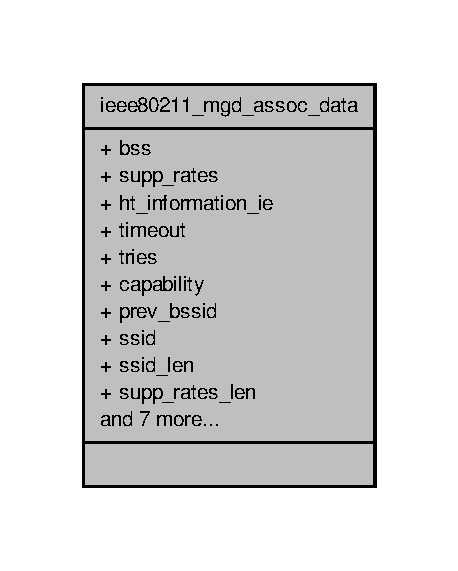
\includegraphics[width=220pt]{structieee80211__mgd__assoc__data__coll__graph}
\end{center}
\end{figure}
\subsection*{Data Fields}
\begin{DoxyCompactItemize}
\item 
struct cfg80211\-\_\-bss $\ast$ \hyperlink{structieee80211__mgd__assoc__data_aa8d95d64d2cb5a56a0fd985733e99b06}{bss}
\item 
const u8 $\ast$ \hyperlink{structieee80211__mgd__assoc__data_a81733160347428a461c99d85fd919ca3}{supp\-\_\-rates}
\item 
const u8 $\ast$ \hyperlink{structieee80211__mgd__assoc__data_af25ab630f908a07235cef3ceaf904727}{ht\-\_\-information\-\_\-ie}
\item 
unsigned long \hyperlink{structieee80211__mgd__assoc__data_a639e65bbd749de17060d658eb233f72b}{timeout}
\item 
int \hyperlink{structieee80211__mgd__assoc__data_a04cecf6708b77deed43900afdf14e8d9}{tries}
\item 
u16 \hyperlink{structieee80211__mgd__assoc__data_ac74162c5a27aacb803f0860ac5da7d89}{capability}
\item 
u8 \hyperlink{structieee80211__mgd__assoc__data_a7855dc0e8648f9b891f31b7538bbd220}{prev\-\_\-bssid} \mbox{[}E\-T\-H\-\_\-\-A\-L\-E\-N\mbox{]}
\item 
u8 \hyperlink{structieee80211__mgd__assoc__data_ae8d768cff77168f424870b6745c90714}{ssid} \mbox{[}I\-E\-E\-E80211\-\_\-\-M\-A\-X\-\_\-\-S\-S\-I\-D\-\_\-\-L\-E\-N\mbox{]}
\item 
u8 \hyperlink{structieee80211__mgd__assoc__data_a440f44724caffefa0f9c838518a3c790}{ssid\-\_\-len}
\item 
u8 \hyperlink{structieee80211__mgd__assoc__data_a10e3f296dc2be6b8aef4938abfa6af16}{supp\-\_\-rates\-\_\-len}
\item 
bool \hyperlink{structieee80211__mgd__assoc__data_aad05de440eb553bb720ef95bd3ed964c}{wmm}
\item 
bool \hyperlink{structieee80211__mgd__assoc__data_a079aedf53e144c3df9b110cf96da2297}{uapsd}
\item 
bool \hyperlink{structieee80211__mgd__assoc__data_a9d76baa171cb69d351febe377f89a6ba}{have\-\_\-beacon}
\item 
bool \hyperlink{structieee80211__mgd__assoc__data_a03c1b4aa3a5243fe109572ed4383d718}{sent\-\_\-assoc}
\item 
bool \hyperlink{structieee80211__mgd__assoc__data_a16495d89275bc776ee62596ec8585728}{synced}
\item 
size\-\_\-t \hyperlink{structieee80211__mgd__assoc__data_a0b939c31983d2de4c3429bb789779638}{ie\-\_\-len}
\item 
u8 \hyperlink{structieee80211__mgd__assoc__data_a541e8335bc4529e686c2b6699284de24}{ie} \mbox{[}$\,$\mbox{]}
\end{DoxyCompactItemize}


\subsection{Detailed Description}


Definition at line 398 of file ieee80211\-\_\-i.\-h.



\subsection{Field Documentation}
\hypertarget{structieee80211__mgd__assoc__data_aa8d95d64d2cb5a56a0fd985733e99b06}{\index{ieee80211\-\_\-mgd\-\_\-assoc\-\_\-data@{ieee80211\-\_\-mgd\-\_\-assoc\-\_\-data}!bss@{bss}}
\index{bss@{bss}!ieee80211_mgd_assoc_data@{ieee80211\-\_\-mgd\-\_\-assoc\-\_\-data}}
\subsubsection[{bss}]{\setlength{\rightskip}{0pt plus 5cm}struct cfg80211\-\_\-bss$\ast$ bss}}\label{structieee80211__mgd__assoc__data_aa8d95d64d2cb5a56a0fd985733e99b06}


Definition at line 399 of file ieee80211\-\_\-i.\-h.

\hypertarget{structieee80211__mgd__assoc__data_ac74162c5a27aacb803f0860ac5da7d89}{\index{ieee80211\-\_\-mgd\-\_\-assoc\-\_\-data@{ieee80211\-\_\-mgd\-\_\-assoc\-\_\-data}!capability@{capability}}
\index{capability@{capability}!ieee80211_mgd_assoc_data@{ieee80211\-\_\-mgd\-\_\-assoc\-\_\-data}}
\subsubsection[{capability}]{\setlength{\rightskip}{0pt plus 5cm}u16 capability}}\label{structieee80211__mgd__assoc__data_ac74162c5a27aacb803f0860ac5da7d89}


Definition at line 406 of file ieee80211\-\_\-i.\-h.

\hypertarget{structieee80211__mgd__assoc__data_a9d76baa171cb69d351febe377f89a6ba}{\index{ieee80211\-\_\-mgd\-\_\-assoc\-\_\-data@{ieee80211\-\_\-mgd\-\_\-assoc\-\_\-data}!have\-\_\-beacon@{have\-\_\-beacon}}
\index{have\-\_\-beacon@{have\-\_\-beacon}!ieee80211_mgd_assoc_data@{ieee80211\-\_\-mgd\-\_\-assoc\-\_\-data}}
\subsubsection[{have\-\_\-beacon}]{\setlength{\rightskip}{0pt plus 5cm}bool have\-\_\-beacon}}\label{structieee80211__mgd__assoc__data_a9d76baa171cb69d351febe377f89a6ba}


Definition at line 412 of file ieee80211\-\_\-i.\-h.

\hypertarget{structieee80211__mgd__assoc__data_af25ab630f908a07235cef3ceaf904727}{\index{ieee80211\-\_\-mgd\-\_\-assoc\-\_\-data@{ieee80211\-\_\-mgd\-\_\-assoc\-\_\-data}!ht\-\_\-information\-\_\-ie@{ht\-\_\-information\-\_\-ie}}
\index{ht\-\_\-information\-\_\-ie@{ht\-\_\-information\-\_\-ie}!ieee80211_mgd_assoc_data@{ieee80211\-\_\-mgd\-\_\-assoc\-\_\-data}}
\subsubsection[{ht\-\_\-information\-\_\-ie}]{\setlength{\rightskip}{0pt plus 5cm}const u8$\ast$ ht\-\_\-information\-\_\-ie}}\label{structieee80211__mgd__assoc__data_af25ab630f908a07235cef3ceaf904727}


Definition at line 401 of file ieee80211\-\_\-i.\-h.

\hypertarget{structieee80211__mgd__assoc__data_a541e8335bc4529e686c2b6699284de24}{\index{ieee80211\-\_\-mgd\-\_\-assoc\-\_\-data@{ieee80211\-\_\-mgd\-\_\-assoc\-\_\-data}!ie@{ie}}
\index{ie@{ie}!ieee80211_mgd_assoc_data@{ieee80211\-\_\-mgd\-\_\-assoc\-\_\-data}}
\subsubsection[{ie}]{\setlength{\rightskip}{0pt plus 5cm}u8 ie\mbox{[}$\,$\mbox{]}}}\label{structieee80211__mgd__assoc__data_a541e8335bc4529e686c2b6699284de24}


Definition at line 417 of file ieee80211\-\_\-i.\-h.

\hypertarget{structieee80211__mgd__assoc__data_a0b939c31983d2de4c3429bb789779638}{\index{ieee80211\-\_\-mgd\-\_\-assoc\-\_\-data@{ieee80211\-\_\-mgd\-\_\-assoc\-\_\-data}!ie\-\_\-len@{ie\-\_\-len}}
\index{ie\-\_\-len@{ie\-\_\-len}!ieee80211_mgd_assoc_data@{ieee80211\-\_\-mgd\-\_\-assoc\-\_\-data}}
\subsubsection[{ie\-\_\-len}]{\setlength{\rightskip}{0pt plus 5cm}size\-\_\-t ie\-\_\-len}}\label{structieee80211__mgd__assoc__data_a0b939c31983d2de4c3429bb789779638}


Definition at line 416 of file ieee80211\-\_\-i.\-h.

\hypertarget{structieee80211__mgd__assoc__data_a7855dc0e8648f9b891f31b7538bbd220}{\index{ieee80211\-\_\-mgd\-\_\-assoc\-\_\-data@{ieee80211\-\_\-mgd\-\_\-assoc\-\_\-data}!prev\-\_\-bssid@{prev\-\_\-bssid}}
\index{prev\-\_\-bssid@{prev\-\_\-bssid}!ieee80211_mgd_assoc_data@{ieee80211\-\_\-mgd\-\_\-assoc\-\_\-data}}
\subsubsection[{prev\-\_\-bssid}]{\setlength{\rightskip}{0pt plus 5cm}u8 prev\-\_\-bssid\mbox{[}E\-T\-H\-\_\-\-A\-L\-E\-N\mbox{]}}}\label{structieee80211__mgd__assoc__data_a7855dc0e8648f9b891f31b7538bbd220}


Definition at line 407 of file ieee80211\-\_\-i.\-h.

\hypertarget{structieee80211__mgd__assoc__data_a03c1b4aa3a5243fe109572ed4383d718}{\index{ieee80211\-\_\-mgd\-\_\-assoc\-\_\-data@{ieee80211\-\_\-mgd\-\_\-assoc\-\_\-data}!sent\-\_\-assoc@{sent\-\_\-assoc}}
\index{sent\-\_\-assoc@{sent\-\_\-assoc}!ieee80211_mgd_assoc_data@{ieee80211\-\_\-mgd\-\_\-assoc\-\_\-data}}
\subsubsection[{sent\-\_\-assoc}]{\setlength{\rightskip}{0pt plus 5cm}bool sent\-\_\-assoc}}\label{structieee80211__mgd__assoc__data_a03c1b4aa3a5243fe109572ed4383d718}


Definition at line 413 of file ieee80211\-\_\-i.\-h.

\hypertarget{structieee80211__mgd__assoc__data_ae8d768cff77168f424870b6745c90714}{\index{ieee80211\-\_\-mgd\-\_\-assoc\-\_\-data@{ieee80211\-\_\-mgd\-\_\-assoc\-\_\-data}!ssid@{ssid}}
\index{ssid@{ssid}!ieee80211_mgd_assoc_data@{ieee80211\-\_\-mgd\-\_\-assoc\-\_\-data}}
\subsubsection[{ssid}]{\setlength{\rightskip}{0pt plus 5cm}u8 ssid\mbox{[}I\-E\-E\-E80211\-\_\-\-M\-A\-X\-\_\-\-S\-S\-I\-D\-\_\-\-L\-E\-N\mbox{]}}}\label{structieee80211__mgd__assoc__data_ae8d768cff77168f424870b6745c90714}


Definition at line 408 of file ieee80211\-\_\-i.\-h.

\hypertarget{structieee80211__mgd__assoc__data_a440f44724caffefa0f9c838518a3c790}{\index{ieee80211\-\_\-mgd\-\_\-assoc\-\_\-data@{ieee80211\-\_\-mgd\-\_\-assoc\-\_\-data}!ssid\-\_\-len@{ssid\-\_\-len}}
\index{ssid\-\_\-len@{ssid\-\_\-len}!ieee80211_mgd_assoc_data@{ieee80211\-\_\-mgd\-\_\-assoc\-\_\-data}}
\subsubsection[{ssid\-\_\-len}]{\setlength{\rightskip}{0pt plus 5cm}u8 ssid\-\_\-len}}\label{structieee80211__mgd__assoc__data_a440f44724caffefa0f9c838518a3c790}


Definition at line 409 of file ieee80211\-\_\-i.\-h.

\hypertarget{structieee80211__mgd__assoc__data_a81733160347428a461c99d85fd919ca3}{\index{ieee80211\-\_\-mgd\-\_\-assoc\-\_\-data@{ieee80211\-\_\-mgd\-\_\-assoc\-\_\-data}!supp\-\_\-rates@{supp\-\_\-rates}}
\index{supp\-\_\-rates@{supp\-\_\-rates}!ieee80211_mgd_assoc_data@{ieee80211\-\_\-mgd\-\_\-assoc\-\_\-data}}
\subsubsection[{supp\-\_\-rates}]{\setlength{\rightskip}{0pt plus 5cm}const u8$\ast$ supp\-\_\-rates}}\label{structieee80211__mgd__assoc__data_a81733160347428a461c99d85fd919ca3}


Definition at line 400 of file ieee80211\-\_\-i.\-h.

\hypertarget{structieee80211__mgd__assoc__data_a10e3f296dc2be6b8aef4938abfa6af16}{\index{ieee80211\-\_\-mgd\-\_\-assoc\-\_\-data@{ieee80211\-\_\-mgd\-\_\-assoc\-\_\-data}!supp\-\_\-rates\-\_\-len@{supp\-\_\-rates\-\_\-len}}
\index{supp\-\_\-rates\-\_\-len@{supp\-\_\-rates\-\_\-len}!ieee80211_mgd_assoc_data@{ieee80211\-\_\-mgd\-\_\-assoc\-\_\-data}}
\subsubsection[{supp\-\_\-rates\-\_\-len}]{\setlength{\rightskip}{0pt plus 5cm}u8 supp\-\_\-rates\-\_\-len}}\label{structieee80211__mgd__assoc__data_a10e3f296dc2be6b8aef4938abfa6af16}


Definition at line 410 of file ieee80211\-\_\-i.\-h.

\hypertarget{structieee80211__mgd__assoc__data_a16495d89275bc776ee62596ec8585728}{\index{ieee80211\-\_\-mgd\-\_\-assoc\-\_\-data@{ieee80211\-\_\-mgd\-\_\-assoc\-\_\-data}!synced@{synced}}
\index{synced@{synced}!ieee80211_mgd_assoc_data@{ieee80211\-\_\-mgd\-\_\-assoc\-\_\-data}}
\subsubsection[{synced}]{\setlength{\rightskip}{0pt plus 5cm}bool synced}}\label{structieee80211__mgd__assoc__data_a16495d89275bc776ee62596ec8585728}


Definition at line 414 of file ieee80211\-\_\-i.\-h.

\hypertarget{structieee80211__mgd__assoc__data_a639e65bbd749de17060d658eb233f72b}{\index{ieee80211\-\_\-mgd\-\_\-assoc\-\_\-data@{ieee80211\-\_\-mgd\-\_\-assoc\-\_\-data}!timeout@{timeout}}
\index{timeout@{timeout}!ieee80211_mgd_assoc_data@{ieee80211\-\_\-mgd\-\_\-assoc\-\_\-data}}
\subsubsection[{timeout}]{\setlength{\rightskip}{0pt plus 5cm}unsigned long timeout}}\label{structieee80211__mgd__assoc__data_a639e65bbd749de17060d658eb233f72b}


Definition at line 403 of file ieee80211\-\_\-i.\-h.

\hypertarget{structieee80211__mgd__assoc__data_a04cecf6708b77deed43900afdf14e8d9}{\index{ieee80211\-\_\-mgd\-\_\-assoc\-\_\-data@{ieee80211\-\_\-mgd\-\_\-assoc\-\_\-data}!tries@{tries}}
\index{tries@{tries}!ieee80211_mgd_assoc_data@{ieee80211\-\_\-mgd\-\_\-assoc\-\_\-data}}
\subsubsection[{tries}]{\setlength{\rightskip}{0pt plus 5cm}int tries}}\label{structieee80211__mgd__assoc__data_a04cecf6708b77deed43900afdf14e8d9}


Definition at line 404 of file ieee80211\-\_\-i.\-h.

\hypertarget{structieee80211__mgd__assoc__data_a079aedf53e144c3df9b110cf96da2297}{\index{ieee80211\-\_\-mgd\-\_\-assoc\-\_\-data@{ieee80211\-\_\-mgd\-\_\-assoc\-\_\-data}!uapsd@{uapsd}}
\index{uapsd@{uapsd}!ieee80211_mgd_assoc_data@{ieee80211\-\_\-mgd\-\_\-assoc\-\_\-data}}
\subsubsection[{uapsd}]{\setlength{\rightskip}{0pt plus 5cm}bool uapsd}}\label{structieee80211__mgd__assoc__data_a079aedf53e144c3df9b110cf96da2297}


Definition at line 411 of file ieee80211\-\_\-i.\-h.

\hypertarget{structieee80211__mgd__assoc__data_aad05de440eb553bb720ef95bd3ed964c}{\index{ieee80211\-\_\-mgd\-\_\-assoc\-\_\-data@{ieee80211\-\_\-mgd\-\_\-assoc\-\_\-data}!wmm@{wmm}}
\index{wmm@{wmm}!ieee80211_mgd_assoc_data@{ieee80211\-\_\-mgd\-\_\-assoc\-\_\-data}}
\subsubsection[{wmm}]{\setlength{\rightskip}{0pt plus 5cm}bool wmm}}\label{structieee80211__mgd__assoc__data_aad05de440eb553bb720ef95bd3ed964c}


Definition at line 411 of file ieee80211\-\_\-i.\-h.



The documentation for this struct was generated from the following file\-:\begin{DoxyCompactItemize}
\item 
/home/guille/msm/net/mac80211/\hyperlink{ieee80211__i_8h}{ieee80211\-\_\-i.\-h}\end{DoxyCompactItemize}

\hypertarget{structieee80211__mgd__auth__data}{\section{ieee80211\-\_\-mgd\-\_\-auth\-\_\-data Struct Reference}
\label{structieee80211__mgd__auth__data}\index{ieee80211\-\_\-mgd\-\_\-auth\-\_\-data@{ieee80211\-\_\-mgd\-\_\-auth\-\_\-data}}
}


{\ttfamily \#include $<$ieee80211\-\_\-i.\-h$>$}



Collaboration diagram for ieee80211\-\_\-mgd\-\_\-auth\-\_\-data\-:
\nopagebreak
\begin{figure}[H]
\begin{center}
\leavevmode
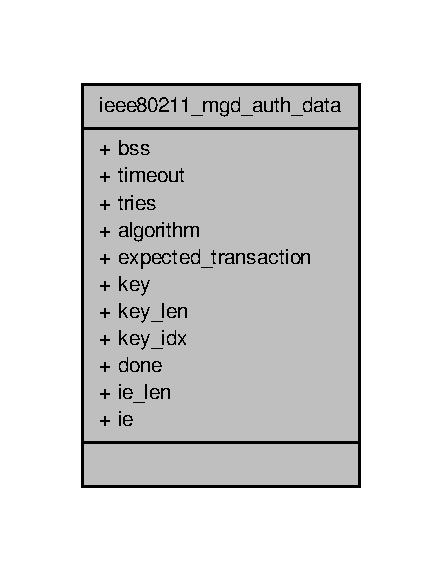
\includegraphics[width=212pt]{structieee80211__mgd__auth__data__coll__graph}
\end{center}
\end{figure}
\subsection*{Data Fields}
\begin{DoxyCompactItemize}
\item 
struct cfg80211\-\_\-bss $\ast$ \hyperlink{structieee80211__mgd__auth__data_aa8d95d64d2cb5a56a0fd985733e99b06}{bss}
\item 
unsigned long \hyperlink{structieee80211__mgd__auth__data_a639e65bbd749de17060d658eb233f72b}{timeout}
\item 
int \hyperlink{structieee80211__mgd__auth__data_a04cecf6708b77deed43900afdf14e8d9}{tries}
\item 
u16 \hyperlink{structieee80211__mgd__auth__data_a06e10b0ef0f5383fa500ca8e41e202fd}{algorithm}
\item 
u16 \hyperlink{structieee80211__mgd__auth__data_aee8d23c4383cb7075b11300a3b995a0c}{expected\-\_\-transaction}
\item 
u8 \hyperlink{structieee80211__mgd__auth__data_a54c7b6b270bee3f1d18fad51c228779c}{key} \mbox{[}W\-L\-A\-N\-\_\-\-K\-E\-Y\-\_\-\-L\-E\-N\-\_\-\-W\-E\-P104\mbox{]}
\item 
u8 \hyperlink{structieee80211__mgd__auth__data_aec6022b50f2f89ff144d7b68d09b7ffe}{key\-\_\-len}
\item 
u8 \hyperlink{structieee80211__mgd__auth__data_aa2edccbb034732153bf9cbf5412660f9}{key\-\_\-idx}
\item 
bool \hyperlink{structieee80211__mgd__auth__data_a1d39aac66e12dae50a24cd7a9100ef33}{done}
\item 
size\-\_\-t \hyperlink{structieee80211__mgd__auth__data_a0b939c31983d2de4c3429bb789779638}{ie\-\_\-len}
\item 
u8 \hyperlink{structieee80211__mgd__auth__data_a541e8335bc4529e686c2b6699284de24}{ie} \mbox{[}$\,$\mbox{]}
\end{DoxyCompactItemize}


\subsection{Detailed Description}


Definition at line 384 of file ieee80211\-\_\-i.\-h.



\subsection{Field Documentation}
\hypertarget{structieee80211__mgd__auth__data_a06e10b0ef0f5383fa500ca8e41e202fd}{\index{ieee80211\-\_\-mgd\-\_\-auth\-\_\-data@{ieee80211\-\_\-mgd\-\_\-auth\-\_\-data}!algorithm@{algorithm}}
\index{algorithm@{algorithm}!ieee80211_mgd_auth_data@{ieee80211\-\_\-mgd\-\_\-auth\-\_\-data}}
\subsubsection[{algorithm}]{\setlength{\rightskip}{0pt plus 5cm}u16 algorithm}}\label{structieee80211__mgd__auth__data_a06e10b0ef0f5383fa500ca8e41e202fd}


Definition at line 388 of file ieee80211\-\_\-i.\-h.

\hypertarget{structieee80211__mgd__auth__data_aa8d95d64d2cb5a56a0fd985733e99b06}{\index{ieee80211\-\_\-mgd\-\_\-auth\-\_\-data@{ieee80211\-\_\-mgd\-\_\-auth\-\_\-data}!bss@{bss}}
\index{bss@{bss}!ieee80211_mgd_auth_data@{ieee80211\-\_\-mgd\-\_\-auth\-\_\-data}}
\subsubsection[{bss}]{\setlength{\rightskip}{0pt plus 5cm}struct cfg80211\-\_\-bss$\ast$ bss}}\label{structieee80211__mgd__auth__data_aa8d95d64d2cb5a56a0fd985733e99b06}


Definition at line 385 of file ieee80211\-\_\-i.\-h.

\hypertarget{structieee80211__mgd__auth__data_a1d39aac66e12dae50a24cd7a9100ef33}{\index{ieee80211\-\_\-mgd\-\_\-auth\-\_\-data@{ieee80211\-\_\-mgd\-\_\-auth\-\_\-data}!done@{done}}
\index{done@{done}!ieee80211_mgd_auth_data@{ieee80211\-\_\-mgd\-\_\-auth\-\_\-data}}
\subsubsection[{done}]{\setlength{\rightskip}{0pt plus 5cm}bool done}}\label{structieee80211__mgd__auth__data_a1d39aac66e12dae50a24cd7a9100ef33}


Definition at line 392 of file ieee80211\-\_\-i.\-h.

\hypertarget{structieee80211__mgd__auth__data_aee8d23c4383cb7075b11300a3b995a0c}{\index{ieee80211\-\_\-mgd\-\_\-auth\-\_\-data@{ieee80211\-\_\-mgd\-\_\-auth\-\_\-data}!expected\-\_\-transaction@{expected\-\_\-transaction}}
\index{expected\-\_\-transaction@{expected\-\_\-transaction}!ieee80211_mgd_auth_data@{ieee80211\-\_\-mgd\-\_\-auth\-\_\-data}}
\subsubsection[{expected\-\_\-transaction}]{\setlength{\rightskip}{0pt plus 5cm}u16 expected\-\_\-transaction}}\label{structieee80211__mgd__auth__data_aee8d23c4383cb7075b11300a3b995a0c}


Definition at line 388 of file ieee80211\-\_\-i.\-h.

\hypertarget{structieee80211__mgd__auth__data_a541e8335bc4529e686c2b6699284de24}{\index{ieee80211\-\_\-mgd\-\_\-auth\-\_\-data@{ieee80211\-\_\-mgd\-\_\-auth\-\_\-data}!ie@{ie}}
\index{ie@{ie}!ieee80211_mgd_auth_data@{ieee80211\-\_\-mgd\-\_\-auth\-\_\-data}}
\subsubsection[{ie}]{\setlength{\rightskip}{0pt plus 5cm}u8 ie\mbox{[}$\,$\mbox{]}}}\label{structieee80211__mgd__auth__data_a541e8335bc4529e686c2b6699284de24}


Definition at line 395 of file ieee80211\-\_\-i.\-h.

\hypertarget{structieee80211__mgd__auth__data_a0b939c31983d2de4c3429bb789779638}{\index{ieee80211\-\_\-mgd\-\_\-auth\-\_\-data@{ieee80211\-\_\-mgd\-\_\-auth\-\_\-data}!ie\-\_\-len@{ie\-\_\-len}}
\index{ie\-\_\-len@{ie\-\_\-len}!ieee80211_mgd_auth_data@{ieee80211\-\_\-mgd\-\_\-auth\-\_\-data}}
\subsubsection[{ie\-\_\-len}]{\setlength{\rightskip}{0pt plus 5cm}size\-\_\-t ie\-\_\-len}}\label{structieee80211__mgd__auth__data_a0b939c31983d2de4c3429bb789779638}


Definition at line 394 of file ieee80211\-\_\-i.\-h.

\hypertarget{structieee80211__mgd__auth__data_a54c7b6b270bee3f1d18fad51c228779c}{\index{ieee80211\-\_\-mgd\-\_\-auth\-\_\-data@{ieee80211\-\_\-mgd\-\_\-auth\-\_\-data}!key@{key}}
\index{key@{key}!ieee80211_mgd_auth_data@{ieee80211\-\_\-mgd\-\_\-auth\-\_\-data}}
\subsubsection[{key}]{\setlength{\rightskip}{0pt plus 5cm}u8 key\mbox{[}W\-L\-A\-N\-\_\-\-K\-E\-Y\-\_\-\-L\-E\-N\-\_\-\-W\-E\-P104\mbox{]}}}\label{structieee80211__mgd__auth__data_a54c7b6b270bee3f1d18fad51c228779c}


Definition at line 390 of file ieee80211\-\_\-i.\-h.

\hypertarget{structieee80211__mgd__auth__data_aa2edccbb034732153bf9cbf5412660f9}{\index{ieee80211\-\_\-mgd\-\_\-auth\-\_\-data@{ieee80211\-\_\-mgd\-\_\-auth\-\_\-data}!key\-\_\-idx@{key\-\_\-idx}}
\index{key\-\_\-idx@{key\-\_\-idx}!ieee80211_mgd_auth_data@{ieee80211\-\_\-mgd\-\_\-auth\-\_\-data}}
\subsubsection[{key\-\_\-idx}]{\setlength{\rightskip}{0pt plus 5cm}u8 key\-\_\-idx}}\label{structieee80211__mgd__auth__data_aa2edccbb034732153bf9cbf5412660f9}


Definition at line 391 of file ieee80211\-\_\-i.\-h.

\hypertarget{structieee80211__mgd__auth__data_aec6022b50f2f89ff144d7b68d09b7ffe}{\index{ieee80211\-\_\-mgd\-\_\-auth\-\_\-data@{ieee80211\-\_\-mgd\-\_\-auth\-\_\-data}!key\-\_\-len@{key\-\_\-len}}
\index{key\-\_\-len@{key\-\_\-len}!ieee80211_mgd_auth_data@{ieee80211\-\_\-mgd\-\_\-auth\-\_\-data}}
\subsubsection[{key\-\_\-len}]{\setlength{\rightskip}{0pt plus 5cm}u8 key\-\_\-len}}\label{structieee80211__mgd__auth__data_aec6022b50f2f89ff144d7b68d09b7ffe}


Definition at line 391 of file ieee80211\-\_\-i.\-h.

\hypertarget{structieee80211__mgd__auth__data_a639e65bbd749de17060d658eb233f72b}{\index{ieee80211\-\_\-mgd\-\_\-auth\-\_\-data@{ieee80211\-\_\-mgd\-\_\-auth\-\_\-data}!timeout@{timeout}}
\index{timeout@{timeout}!ieee80211_mgd_auth_data@{ieee80211\-\_\-mgd\-\_\-auth\-\_\-data}}
\subsubsection[{timeout}]{\setlength{\rightskip}{0pt plus 5cm}unsigned long timeout}}\label{structieee80211__mgd__auth__data_a639e65bbd749de17060d658eb233f72b}


Definition at line 386 of file ieee80211\-\_\-i.\-h.

\hypertarget{structieee80211__mgd__auth__data_a04cecf6708b77deed43900afdf14e8d9}{\index{ieee80211\-\_\-mgd\-\_\-auth\-\_\-data@{ieee80211\-\_\-mgd\-\_\-auth\-\_\-data}!tries@{tries}}
\index{tries@{tries}!ieee80211_mgd_auth_data@{ieee80211\-\_\-mgd\-\_\-auth\-\_\-data}}
\subsubsection[{tries}]{\setlength{\rightskip}{0pt plus 5cm}int tries}}\label{structieee80211__mgd__auth__data_a04cecf6708b77deed43900afdf14e8d9}


Definition at line 387 of file ieee80211\-\_\-i.\-h.



The documentation for this struct was generated from the following file\-:\begin{DoxyCompactItemize}
\item 
/home/guille/msm/net/mac80211/\hyperlink{ieee80211__i_8h}{ieee80211\-\_\-i.\-h}\end{DoxyCompactItemize}

\hypertarget{structieee80211__ra__tid}{\section{ieee80211\-\_\-ra\-\_\-tid Struct Reference}
\label{structieee80211__ra__tid}\index{ieee80211\-\_\-ra\-\_\-tid@{ieee80211\-\_\-ra\-\_\-tid}}
}


{\ttfamily \#include $<$ieee80211\-\_\-i.\-h$>$}



Collaboration diagram for ieee80211\-\_\-ra\-\_\-tid\-:
\nopagebreak
\begin{figure}[H]
\begin{center}
\leavevmode
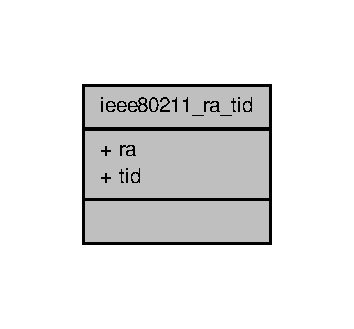
\includegraphics[width=170pt]{structieee80211__ra__tid__coll__graph}
\end{center}
\end{figure}
\subsection*{Data Fields}
\begin{DoxyCompactItemize}
\item 
u8 \hyperlink{structieee80211__ra__tid_a5c7e15726f46e9ea6315ce73ff303590}{ra} \mbox{[}E\-T\-H\-\_\-\-A\-L\-E\-N\mbox{]}
\item 
u16 \hyperlink{structieee80211__ra__tid_a7c32a30e0eb9aa589f779888e3d5ba40}{tid}
\end{DoxyCompactItemize}


\subsection{Detailed Description}


Definition at line 1095 of file ieee80211\-\_\-i.\-h.



\subsection{Field Documentation}
\hypertarget{structieee80211__ra__tid_a5c7e15726f46e9ea6315ce73ff303590}{\index{ieee80211\-\_\-ra\-\_\-tid@{ieee80211\-\_\-ra\-\_\-tid}!ra@{ra}}
\index{ra@{ra}!ieee80211_ra_tid@{ieee80211\-\_\-ra\-\_\-tid}}
\subsubsection[{ra}]{\setlength{\rightskip}{0pt plus 5cm}u8 ra\mbox{[}E\-T\-H\-\_\-\-A\-L\-E\-N\mbox{]}}}\label{structieee80211__ra__tid_a5c7e15726f46e9ea6315ce73ff303590}


Definition at line 1096 of file ieee80211\-\_\-i.\-h.

\hypertarget{structieee80211__ra__tid_a7c32a30e0eb9aa589f779888e3d5ba40}{\index{ieee80211\-\_\-ra\-\_\-tid@{ieee80211\-\_\-ra\-\_\-tid}!tid@{tid}}
\index{tid@{tid}!ieee80211_ra_tid@{ieee80211\-\_\-ra\-\_\-tid}}
\subsubsection[{tid}]{\setlength{\rightskip}{0pt plus 5cm}u16 tid}}\label{structieee80211__ra__tid_a7c32a30e0eb9aa589f779888e3d5ba40}


Definition at line 1097 of file ieee80211\-\_\-i.\-h.



The documentation for this struct was generated from the following file\-:\begin{DoxyCompactItemize}
\item 
/home/guille/msm/net/mac80211/\hyperlink{ieee80211__i_8h}{ieee80211\-\_\-i.\-h}\end{DoxyCompactItemize}

\hypertarget{structieee80211__rx__data}{\section{ieee80211\-\_\-rx\-\_\-data Struct Reference}
\label{structieee80211__rx__data}\index{ieee80211\-\_\-rx\-\_\-data@{ieee80211\-\_\-rx\-\_\-data}}
}


{\ttfamily \#include $<$ieee80211\-\_\-i.\-h$>$}



Collaboration diagram for ieee80211\-\_\-rx\-\_\-data\-:
\nopagebreak
\begin{figure}[H]
\begin{center}
\leavevmode
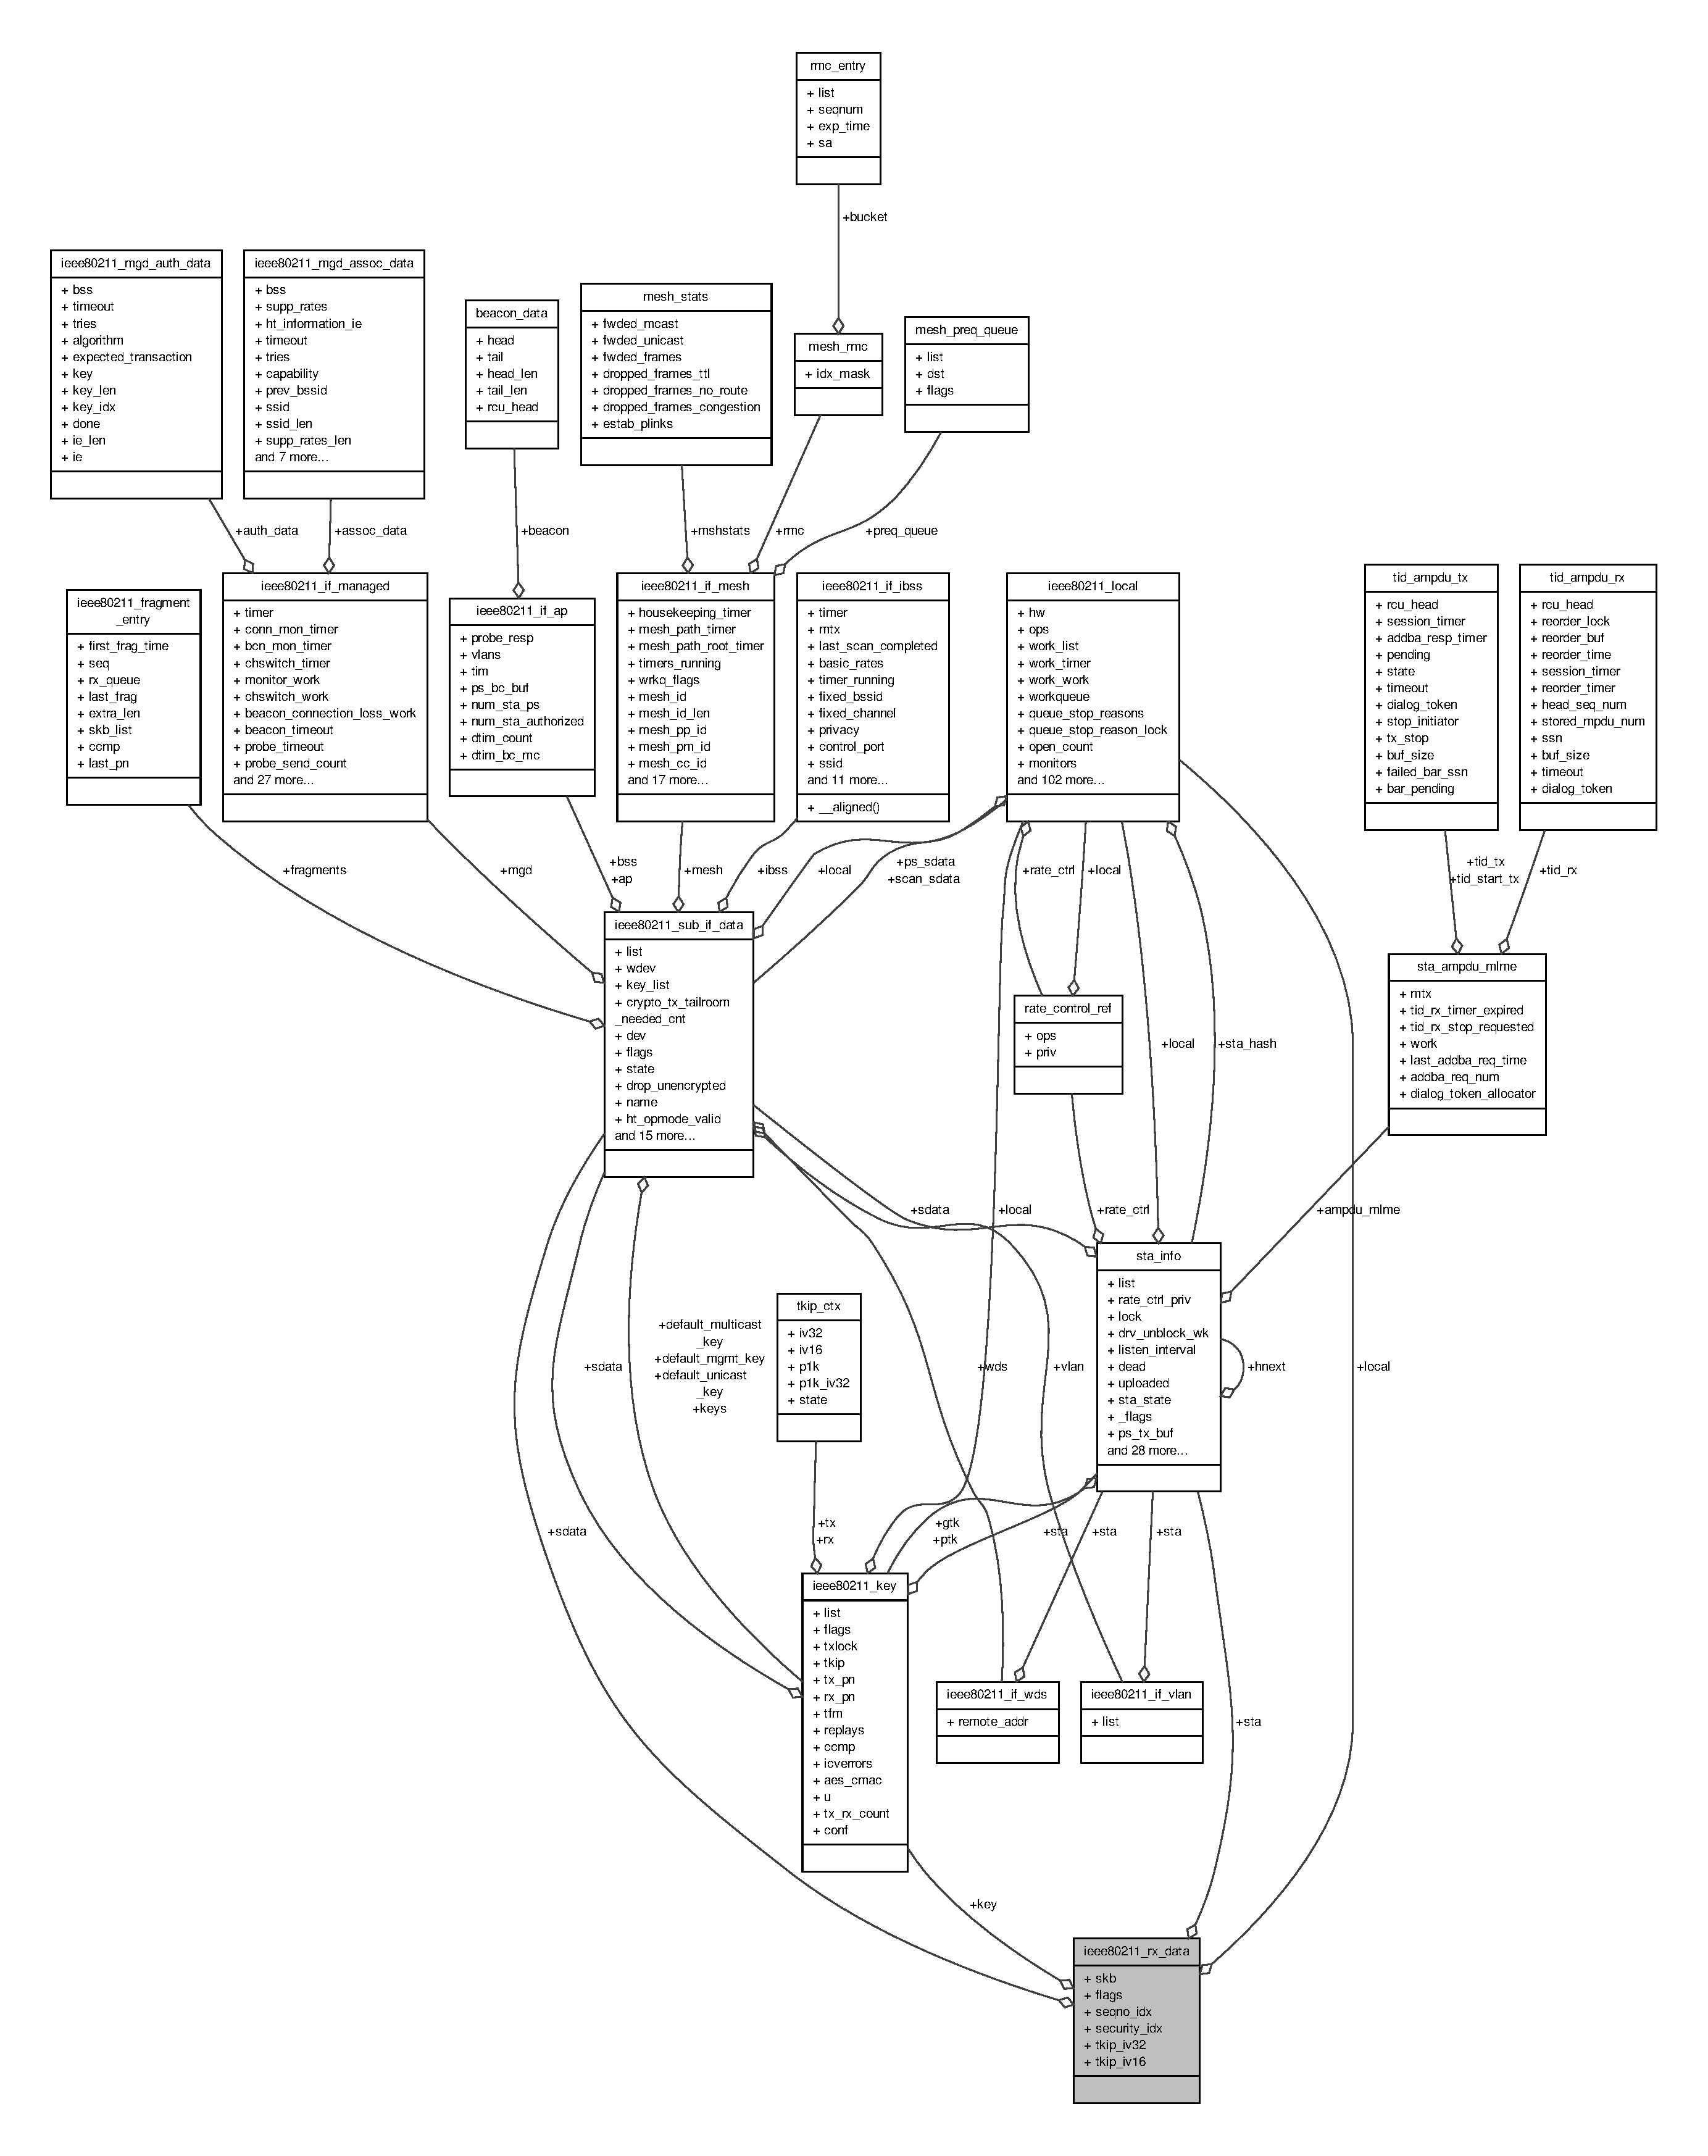
\includegraphics[width=350pt]{structieee80211__rx__data__coll__graph}
\end{center}
\end{figure}
\subsection*{Data Fields}
\begin{DoxyCompactItemize}
\item 
struct sk\-\_\-buff $\ast$ \hyperlink{structieee80211__rx__data_aeba6836824708325a83121030f092c30}{skb}
\item 
struct \hyperlink{structieee80211__local}{ieee80211\-\_\-local} $\ast$ \hyperlink{structieee80211__rx__data_ad436a024f420f219c4fe2eebce7e4ab2}{local}
\item 
struct \hyperlink{structieee80211__sub__if__data}{ieee80211\-\_\-sub\-\_\-if\-\_\-data} $\ast$ \hyperlink{structieee80211__rx__data_ad829d8d33f06a7245cc303f924f259ac}{sdata}
\item 
struct \hyperlink{structsta__info}{sta\-\_\-info} $\ast$ \hyperlink{structieee80211__rx__data_aafa9dadbeccd54b4a6b9f77f2908a093}{sta}
\item 
struct \hyperlink{structieee80211__key}{ieee80211\-\_\-key} $\ast$ \hyperlink{structieee80211__rx__data_a6fb9dce4966e6727c301a63b8185c388}{key}
\item 
unsigned int \hyperlink{structieee80211__rx__data_ac92588540e8c1d014a08cd8a45462b19}{flags}
\item 
int \hyperlink{structieee80211__rx__data_a5e3319f7a0db16f766c18522826f155e}{seqno\-\_\-idx}
\item 
int \hyperlink{structieee80211__rx__data_ae61977ea897e469c291f27e7e5b09d19}{security\-\_\-idx}
\item 
u32 \hyperlink{structieee80211__rx__data_a0f259da682b3ab5890f6e19716221029}{tkip\-\_\-iv32}
\item 
u16 \hyperlink{structieee80211__rx__data_a1b0e9025f6b0dc8ceb064641a7909a26}{tkip\-\_\-iv16}
\end{DoxyCompactItemize}


\subsection{Detailed Description}


Definition at line 238 of file ieee80211\-\_\-i.\-h.



\subsection{Field Documentation}
\hypertarget{structieee80211__rx__data_ac92588540e8c1d014a08cd8a45462b19}{\index{ieee80211\-\_\-rx\-\_\-data@{ieee80211\-\_\-rx\-\_\-data}!flags@{flags}}
\index{flags@{flags}!ieee80211_rx_data@{ieee80211\-\_\-rx\-\_\-data}}
\subsubsection[{flags}]{\setlength{\rightskip}{0pt plus 5cm}unsigned int flags}}\label{structieee80211__rx__data_ac92588540e8c1d014a08cd8a45462b19}


Definition at line 245 of file ieee80211\-\_\-i.\-h.

\hypertarget{structieee80211__rx__data_a6fb9dce4966e6727c301a63b8185c388}{\index{ieee80211\-\_\-rx\-\_\-data@{ieee80211\-\_\-rx\-\_\-data}!key@{key}}
\index{key@{key}!ieee80211_rx_data@{ieee80211\-\_\-rx\-\_\-data}}
\subsubsection[{key}]{\setlength{\rightskip}{0pt plus 5cm}struct {\bf ieee80211\-\_\-key}$\ast$ key}}\label{structieee80211__rx__data_a6fb9dce4966e6727c301a63b8185c388}


Definition at line 243 of file ieee80211\-\_\-i.\-h.

\hypertarget{structieee80211__rx__data_ad436a024f420f219c4fe2eebce7e4ab2}{\index{ieee80211\-\_\-rx\-\_\-data@{ieee80211\-\_\-rx\-\_\-data}!local@{local}}
\index{local@{local}!ieee80211_rx_data@{ieee80211\-\_\-rx\-\_\-data}}
\subsubsection[{local}]{\setlength{\rightskip}{0pt plus 5cm}struct {\bf ieee80211\-\_\-local}$\ast$ local}}\label{structieee80211__rx__data_ad436a024f420f219c4fe2eebce7e4ab2}


Definition at line 240 of file ieee80211\-\_\-i.\-h.

\hypertarget{structieee80211__rx__data_ad829d8d33f06a7245cc303f924f259ac}{\index{ieee80211\-\_\-rx\-\_\-data@{ieee80211\-\_\-rx\-\_\-data}!sdata@{sdata}}
\index{sdata@{sdata}!ieee80211_rx_data@{ieee80211\-\_\-rx\-\_\-data}}
\subsubsection[{sdata}]{\setlength{\rightskip}{0pt plus 5cm}struct {\bf ieee80211\-\_\-sub\-\_\-if\-\_\-data}$\ast$ sdata}}\label{structieee80211__rx__data_ad829d8d33f06a7245cc303f924f259ac}


Definition at line 241 of file ieee80211\-\_\-i.\-h.

\hypertarget{structieee80211__rx__data_ae61977ea897e469c291f27e7e5b09d19}{\index{ieee80211\-\_\-rx\-\_\-data@{ieee80211\-\_\-rx\-\_\-data}!security\-\_\-idx@{security\-\_\-idx}}
\index{security\-\_\-idx@{security\-\_\-idx}!ieee80211_rx_data@{ieee80211\-\_\-rx\-\_\-data}}
\subsubsection[{security\-\_\-idx}]{\setlength{\rightskip}{0pt plus 5cm}int security\-\_\-idx}}\label{structieee80211__rx__data_ae61977ea897e469c291f27e7e5b09d19}


Definition at line 260 of file ieee80211\-\_\-i.\-h.

\hypertarget{structieee80211__rx__data_a5e3319f7a0db16f766c18522826f155e}{\index{ieee80211\-\_\-rx\-\_\-data@{ieee80211\-\_\-rx\-\_\-data}!seqno\-\_\-idx@{seqno\-\_\-idx}}
\index{seqno\-\_\-idx@{seqno\-\_\-idx}!ieee80211_rx_data@{ieee80211\-\_\-rx\-\_\-data}}
\subsubsection[{seqno\-\_\-idx}]{\setlength{\rightskip}{0pt plus 5cm}int seqno\-\_\-idx}}\label{structieee80211__rx__data_a5e3319f7a0db16f766c18522826f155e}


Definition at line 252 of file ieee80211\-\_\-i.\-h.

\hypertarget{structieee80211__rx__data_aeba6836824708325a83121030f092c30}{\index{ieee80211\-\_\-rx\-\_\-data@{ieee80211\-\_\-rx\-\_\-data}!skb@{skb}}
\index{skb@{skb}!ieee80211_rx_data@{ieee80211\-\_\-rx\-\_\-data}}
\subsubsection[{skb}]{\setlength{\rightskip}{0pt plus 5cm}struct sk\-\_\-buff$\ast$ skb}}\label{structieee80211__rx__data_aeba6836824708325a83121030f092c30}


Definition at line 239 of file ieee80211\-\_\-i.\-h.

\hypertarget{structieee80211__rx__data_aafa9dadbeccd54b4a6b9f77f2908a093}{\index{ieee80211\-\_\-rx\-\_\-data@{ieee80211\-\_\-rx\-\_\-data}!sta@{sta}}
\index{sta@{sta}!ieee80211_rx_data@{ieee80211\-\_\-rx\-\_\-data}}
\subsubsection[{sta}]{\setlength{\rightskip}{0pt plus 5cm}struct {\bf sta\-\_\-info}$\ast$ sta}}\label{structieee80211__rx__data_aafa9dadbeccd54b4a6b9f77f2908a093}


Definition at line 242 of file ieee80211\-\_\-i.\-h.

\hypertarget{structieee80211__rx__data_a1b0e9025f6b0dc8ceb064641a7909a26}{\index{ieee80211\-\_\-rx\-\_\-data@{ieee80211\-\_\-rx\-\_\-data}!tkip\-\_\-iv16@{tkip\-\_\-iv16}}
\index{tkip\-\_\-iv16@{tkip\-\_\-iv16}!ieee80211_rx_data@{ieee80211\-\_\-rx\-\_\-data}}
\subsubsection[{tkip\-\_\-iv16}]{\setlength{\rightskip}{0pt plus 5cm}u16 tkip\-\_\-iv16}}\label{structieee80211__rx__data_a1b0e9025f6b0dc8ceb064641a7909a26}


Definition at line 263 of file ieee80211\-\_\-i.\-h.

\hypertarget{structieee80211__rx__data_a0f259da682b3ab5890f6e19716221029}{\index{ieee80211\-\_\-rx\-\_\-data@{ieee80211\-\_\-rx\-\_\-data}!tkip\-\_\-iv32@{tkip\-\_\-iv32}}
\index{tkip\-\_\-iv32@{tkip\-\_\-iv32}!ieee80211_rx_data@{ieee80211\-\_\-rx\-\_\-data}}
\subsubsection[{tkip\-\_\-iv32}]{\setlength{\rightskip}{0pt plus 5cm}u32 tkip\-\_\-iv32}}\label{structieee80211__rx__data_a0f259da682b3ab5890f6e19716221029}


Definition at line 262 of file ieee80211\-\_\-i.\-h.



The documentation for this struct was generated from the following file\-:\begin{DoxyCompactItemize}
\item 
/home/guille/msm/net/mac80211/\hyperlink{ieee80211__i_8h}{ieee80211\-\_\-i.\-h}\end{DoxyCompactItemize}

\hypertarget{structieee80211__sub__if__data}{\section{ieee80211\-\_\-sub\-\_\-if\-\_\-data Struct Reference}
\label{structieee80211__sub__if__data}\index{ieee80211\-\_\-sub\-\_\-if\-\_\-data@{ieee80211\-\_\-sub\-\_\-if\-\_\-data}}
}


{\ttfamily \#include $<$ieee80211\-\_\-i.\-h$>$}



Collaboration diagram for ieee80211\-\_\-sub\-\_\-if\-\_\-data\-:
\nopagebreak
\begin{figure}[H]
\begin{center}
\leavevmode
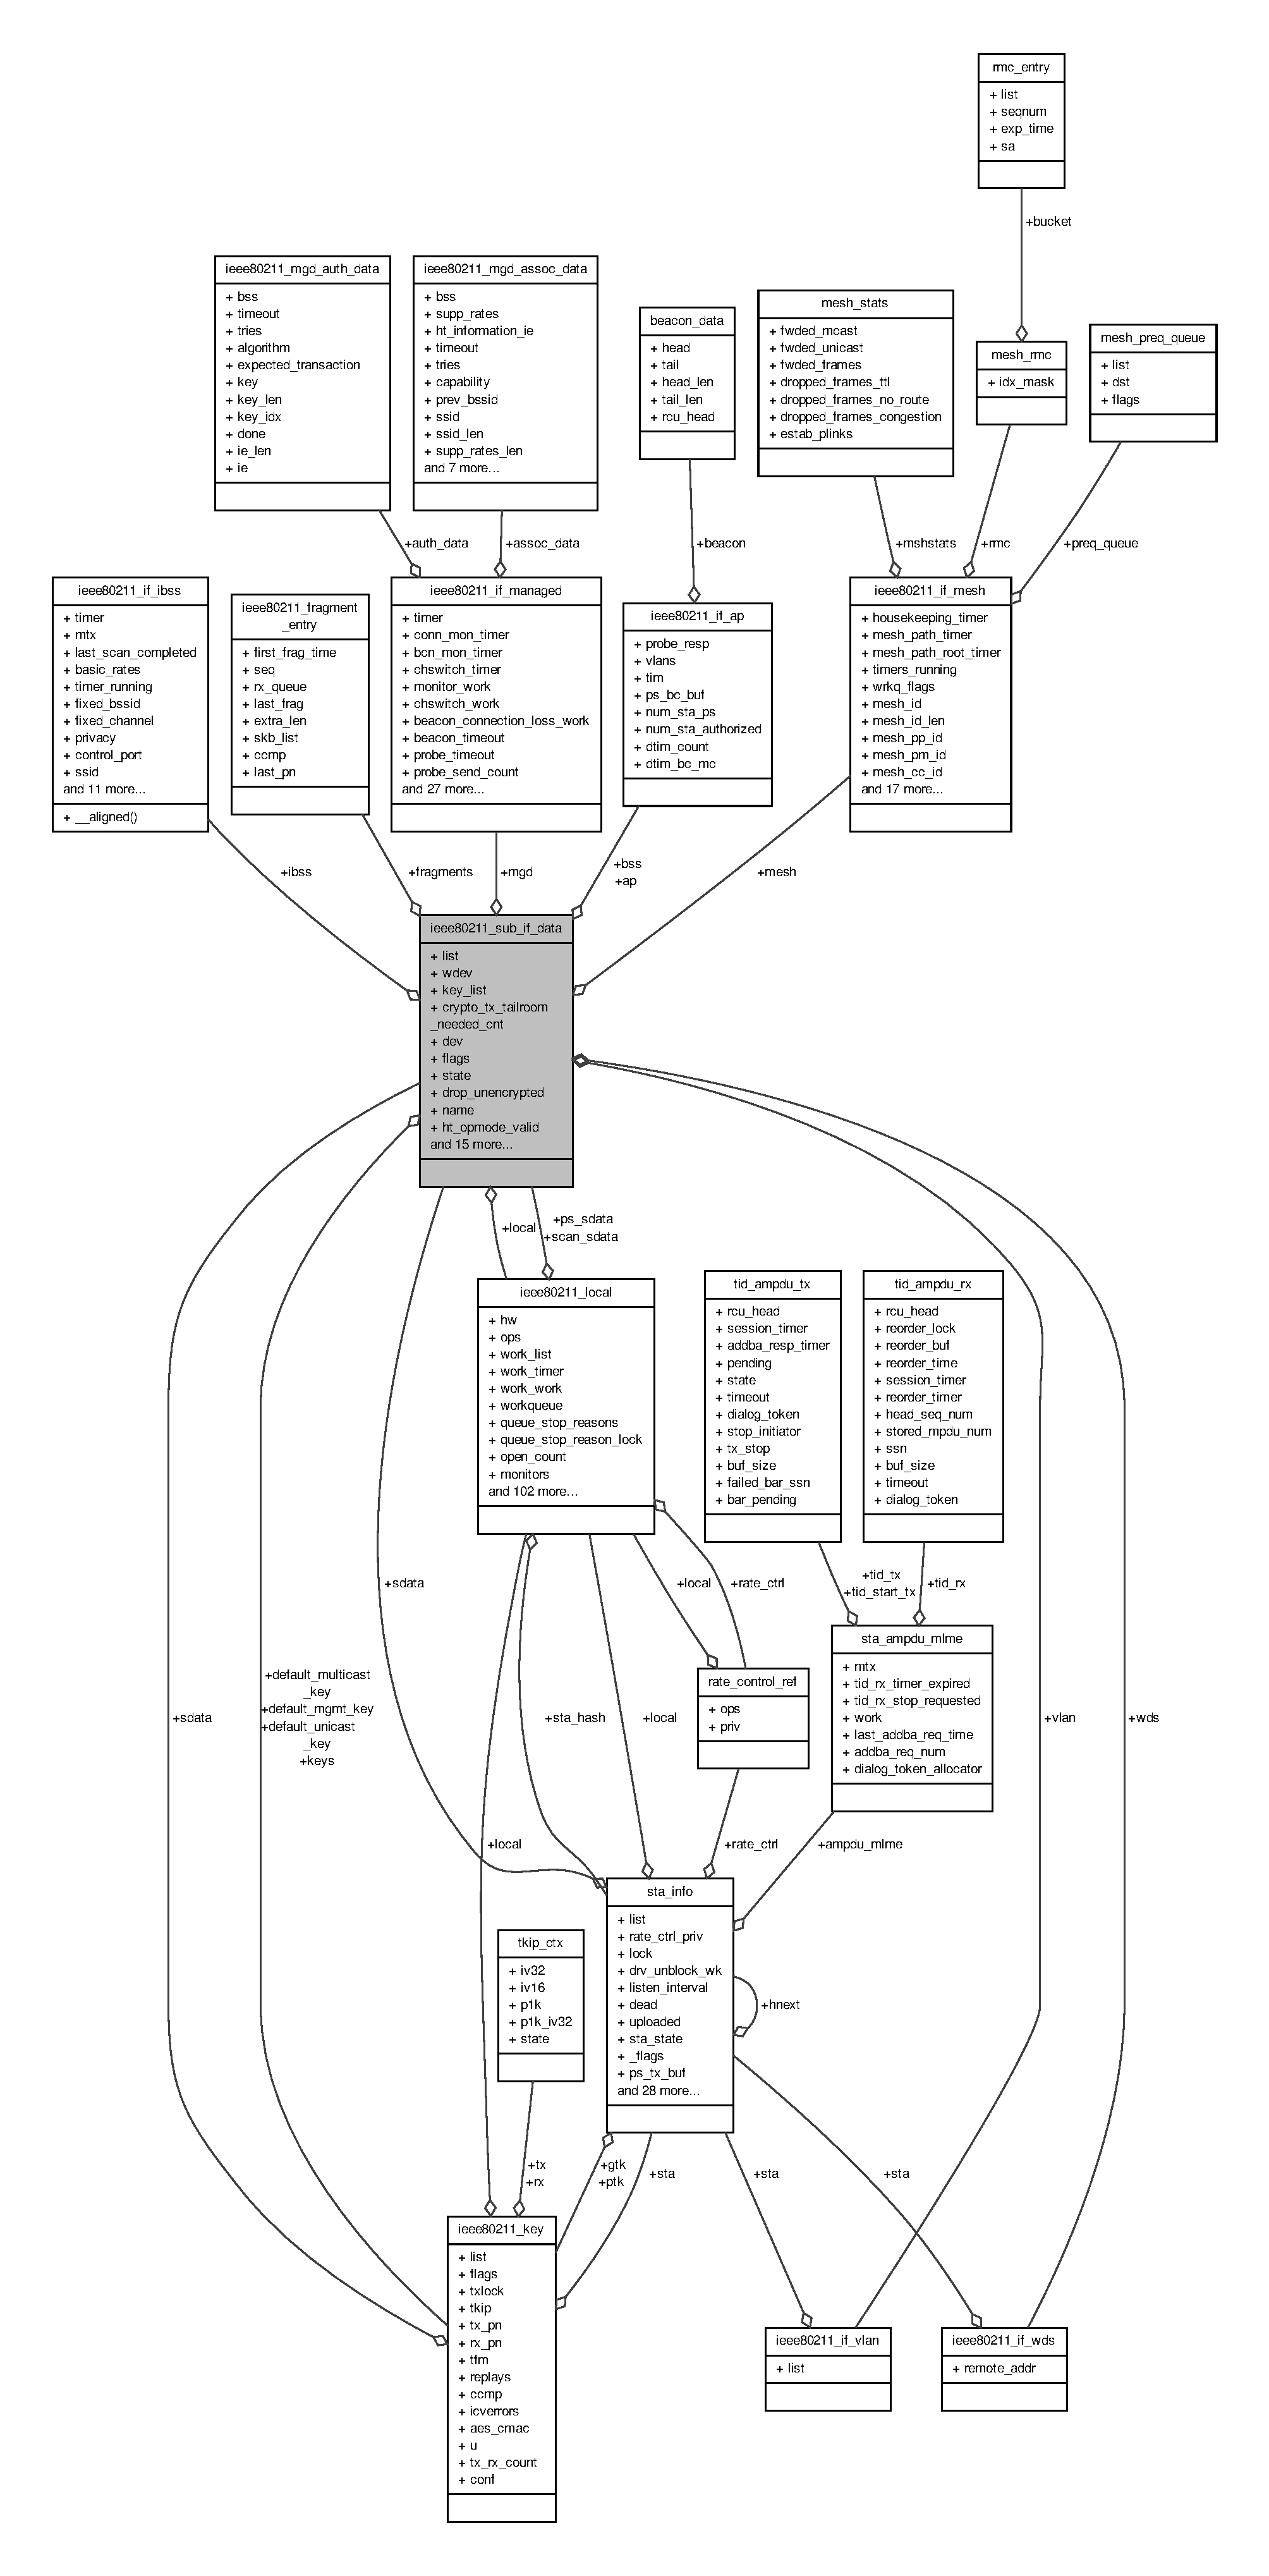
\includegraphics[height=550pt]{structieee80211__sub__if__data__coll__graph}
\end{center}
\end{figure}
\subsection*{Data Fields}
\begin{DoxyCompactItemize}
\item 
struct list\-\_\-head \hyperlink{structieee80211__sub__if__data_a1f00f18b91d5a820f2c43064243aa86e}{list}
\item 
struct wireless\-\_\-dev \hyperlink{structieee80211__sub__if__data_adff11b1d40a62f52e85ded7d6428fab3}{wdev}
\item 
struct list\-\_\-head \hyperlink{structieee80211__sub__if__data_a173cf05f7d6b8bf98fc09f1bb95bfe7e}{key\-\_\-list}
\item 
int \hyperlink{structieee80211__sub__if__data_aa7af642ddb25d678f33953eaaddcb0d8}{crypto\-\_\-tx\-\_\-tailroom\-\_\-needed\-\_\-cnt}
\item 
struct net\-\_\-device $\ast$ \hyperlink{structieee80211__sub__if__data_abf690dbcccc005ba94a1ce16864ccdc9}{dev}
\item 
struct \hyperlink{structieee80211__local}{ieee80211\-\_\-local} $\ast$ \hyperlink{structieee80211__sub__if__data_ad436a024f420f219c4fe2eebce7e4ab2}{local}
\item 
unsigned int \hyperlink{structieee80211__sub__if__data_ac92588540e8c1d014a08cd8a45462b19}{flags}
\item 
unsigned long \hyperlink{structieee80211__sub__if__data_af7504fc0e249186b115eb5f51a297878}{state}
\item 
int \hyperlink{structieee80211__sub__if__data_a33cb37aebf5eb2cdb7b07dffd48e9a92}{drop\-\_\-unencrypted}
\item 
char \hyperlink{structieee80211__sub__if__data_a9ea12d6fc5b2c586092468ee1a86162a}{name} \mbox{[}I\-F\-N\-A\-M\-S\-I\-Z\mbox{]}
\item 
bool \hyperlink{structieee80211__sub__if__data_a1e7e518fe4dd44b1cb51205645f7c8e9}{ht\-\_\-opmode\-\_\-valid}
\item 
bool \hyperlink{structieee80211__sub__if__data_a3bf326db8dc3ffdc0338743371dfc65b}{old\-\_\-idle}
\item 
struct \hyperlink{structieee80211__fragment__entry}{ieee80211\-\_\-fragment\-\_\-entry} \hyperlink{structieee80211__sub__if__data_a9dabb064f92940c0ae438c43f2e7d3a3}{fragments} \mbox{[}\hyperlink{ieee80211__i_8h_a32100053624b6475db2038cace00b40f}{I\-E\-E\-E80211\-\_\-\-F\-R\-A\-G\-M\-E\-N\-T\-\_\-\-M\-A\-X}\mbox{]}
\item 
unsigned int \hyperlink{structieee80211__sub__if__data_ab09b05e01b312174ceac7542e54c060a}{fragment\-\_\-next}
\item 
u16 \hyperlink{structieee80211__sub__if__data_a151051cbbca12c85e61578f27ae99ced}{noack\-\_\-map}
\item 
struct \hyperlink{structieee80211__key}{ieee80211\-\_\-key} \-\_\-\-\_\-rcu $\ast$ \hyperlink{structieee80211__sub__if__data_ad9d8249bd02068d887fd83a256bd0549}{keys} \mbox{[}\hyperlink{key_8h_afc56a6aebd37a90bca92708898c4e80a}{N\-U\-M\-\_\-\-D\-E\-F\-A\-U\-L\-T\-\_\-\-K\-E\-Y\-S}+\hyperlink{key_8h_a7cb10042c995311e0b4dfa6a8cabdd11}{N\-U\-M\-\_\-\-D\-E\-F\-A\-U\-L\-T\-\_\-\-M\-G\-M\-T\-\_\-\-K\-E\-Y\-S}\mbox{]}
\item 
struct \hyperlink{structieee80211__key}{ieee80211\-\_\-key} \-\_\-\-\_\-rcu $\ast$ \hyperlink{structieee80211__sub__if__data_a44b1d9794b9cb6b73af38c8c6258cfcf}{default\-\_\-unicast\-\_\-key}
\item 
struct \hyperlink{structieee80211__key}{ieee80211\-\_\-key} \-\_\-\-\_\-rcu $\ast$ \hyperlink{structieee80211__sub__if__data_a3b14deb6e926750564314ff8a32147ba}{default\-\_\-multicast\-\_\-key}
\item 
struct \hyperlink{structieee80211__key}{ieee80211\-\_\-key} \-\_\-\-\_\-rcu $\ast$ \hyperlink{structieee80211__sub__if__data_a2919f5df0fee1d8bbeac082c448c77c3}{default\-\_\-mgmt\-\_\-key}
\item 
u16 \hyperlink{structieee80211__sub__if__data_ac171f7c2d4f67742e044f800ce3ca592}{sequence\-\_\-number}
\item 
\-\_\-\-\_\-be16 \hyperlink{structieee80211__sub__if__data_a9d1f464ce348d7d7e6852ac8e32e0d0f}{control\-\_\-port\-\_\-protocol}
\item 
bool \hyperlink{structieee80211__sub__if__data_a5ac2427ee669706bf98a29fc82ed9666}{control\-\_\-port\-\_\-no\-\_\-encrypt}
\item 
struct ieee80211\-\_\-tx\-\_\-queue\-\_\-params \hyperlink{structieee80211__sub__if__data_aa80252c8fcedef0fef3d580c68867c84}{tx\-\_\-conf} \mbox{[}I\-E\-E\-E80211\-\_\-\-M\-A\-X\-\_\-\-Q\-U\-E\-U\-E\-S\mbox{]}
\item 
struct work\-\_\-struct \hyperlink{structieee80211__sub__if__data_a623997e11b94d7c467ce26627cc488a2}{work}
\item 
struct sk\-\_\-buff\-\_\-head \hyperlink{structieee80211__sub__if__data_a6eeb93345e21d69a77a7c2c571bd0000}{skb\-\_\-queue}
\item 
bool \hyperlink{structieee80211__sub__if__data_a0216068b0f336a8922737d055a92e4cd}{arp\-\_\-filter\-\_\-state}
\item 
struct \hyperlink{structieee80211__if__ap}{ieee80211\-\_\-if\-\_\-ap} $\ast$ \hyperlink{structieee80211__sub__if__data_a45b3472e16d1f1a8c58e64b338d4e946}{bss}
\item 
u32 \hyperlink{structieee80211__sub__if__data_a4291130d4a0d651a69780340ad638ce2}{rc\-\_\-rateidx\-\_\-mask} \mbox{[}I\-E\-E\-E80211\-\_\-\-N\-U\-M\-\_\-\-B\-A\-N\-D\-S\mbox{]}
\item 
u8 \hyperlink{structieee80211__sub__if__data_af3f2e32024ff5987cf20338a95ecc35f}{rc\-\_\-rateidx\-\_\-mcs\-\_\-mask} \mbox{[}I\-E\-E\-E80211\-\_\-\-N\-U\-M\-\_\-\-B\-A\-N\-D\-S\mbox{]}\mbox{[}I\-E\-E\-E80211\-\_\-\-H\-T\-\_\-\-M\-C\-S\-\_\-\-M\-A\-S\-K\-\_\-\-L\-E\-N\mbox{]}
\item 
\begin{tabbing}
xx\=xx\=xx\=xx\=xx\=xx\=xx\=xx\=xx\=\kill
union \{\\
\>struct \hyperlink{structieee80211__if__ap}{ieee80211\_if\_ap} \hyperlink{structieee80211__sub__if__data_aa7802c0ad2f6a05610aea467f294ebd2}{ap}\\
\>struct \hyperlink{structieee80211__if__wds}{ieee80211\_if\_wds} \hyperlink{structieee80211__sub__if__data_a09671aeb534ab76414be89358eb296cd}{wds}\\
\>struct \hyperlink{structieee80211__if__vlan}{ieee80211\_if\_vlan} \hyperlink{structieee80211__sub__if__data_a0306ac04b10e73aa887c6d5a96332fa2}{vlan}\\
\>struct \hyperlink{structieee80211__if__managed}{ieee80211\_if\_managed} \hyperlink{structieee80211__sub__if__data_ac43070ed59c628dcab245dc2dbaa0fd7}{mgd}\\
\>struct \hyperlink{structieee80211__if__ibss}{ieee80211\_if\_ibss} \hyperlink{structieee80211__sub__if__data_ac62d9e6d8045efd0110b40c2ce341b56}{ibss}\\
\>struct \hyperlink{structieee80211__if__mesh}{ieee80211\_if\_mesh} \hyperlink{structieee80211__sub__if__data_aa9083f90f4d38afa13c9d233a07a6d9d}{mesh}\\
\>u32 \hyperlink{structieee80211__sub__if__data_a65a8ca3269e0e7023f6f265ee9ad1535}{mntr\_flags}\\
\} \hyperlink{structieee80211__sub__if__data_a369ec3436f600c083e559d7909a206ea}{u}\\

\end{tabbing}\item 
struct ieee80211\-\_\-vif \hyperlink{structieee80211__sub__if__data_a32ff3992b201e6f0a8af4c4a0e09fd4c}{vif}
\end{DoxyCompactItemize}


\subsection{Detailed Description}


Definition at line 648 of file ieee80211\-\_\-i.\-h.



\subsection{Field Documentation}
\hypertarget{structieee80211__sub__if__data_aa7802c0ad2f6a05610aea467f294ebd2}{\index{ieee80211\-\_\-sub\-\_\-if\-\_\-data@{ieee80211\-\_\-sub\-\_\-if\-\_\-data}!ap@{ap}}
\index{ap@{ap}!ieee80211_sub_if_data@{ieee80211\-\_\-sub\-\_\-if\-\_\-data}}
\subsubsection[{ap}]{\setlength{\rightskip}{0pt plus 5cm}struct {\bf ieee80211\-\_\-if\-\_\-ap} ap}}\label{structieee80211__sub__if__data_aa7802c0ad2f6a05610aea467f294ebd2}


Definition at line 714 of file ieee80211\-\_\-i.\-h.

\hypertarget{structieee80211__sub__if__data_a0216068b0f336a8922737d055a92e4cd}{\index{ieee80211\-\_\-sub\-\_\-if\-\_\-data@{ieee80211\-\_\-sub\-\_\-if\-\_\-data}!arp\-\_\-filter\-\_\-state@{arp\-\_\-filter\-\_\-state}}
\index{arp\-\_\-filter\-\_\-state@{arp\-\_\-filter\-\_\-state}!ieee80211_sub_if_data@{ieee80211\-\_\-sub\-\_\-if\-\_\-data}}
\subsubsection[{arp\-\_\-filter\-\_\-state}]{\setlength{\rightskip}{0pt plus 5cm}bool arp\-\_\-filter\-\_\-state}}\label{structieee80211__sub__if__data_a0216068b0f336a8922737d055a92e4cd}


Definition at line 700 of file ieee80211\-\_\-i.\-h.

\hypertarget{structieee80211__sub__if__data_a45b3472e16d1f1a8c58e64b338d4e946}{\index{ieee80211\-\_\-sub\-\_\-if\-\_\-data@{ieee80211\-\_\-sub\-\_\-if\-\_\-data}!bss@{bss}}
\index{bss@{bss}!ieee80211_sub_if_data@{ieee80211\-\_\-sub\-\_\-if\-\_\-data}}
\subsubsection[{bss}]{\setlength{\rightskip}{0pt plus 5cm}struct {\bf ieee80211\-\_\-if\-\_\-ap}$\ast$ bss}}\label{structieee80211__sub__if__data_a45b3472e16d1f1a8c58e64b338d4e946}


Definition at line 707 of file ieee80211\-\_\-i.\-h.

\hypertarget{structieee80211__sub__if__data_a5ac2427ee669706bf98a29fc82ed9666}{\index{ieee80211\-\_\-sub\-\_\-if\-\_\-data@{ieee80211\-\_\-sub\-\_\-if\-\_\-data}!control\-\_\-port\-\_\-no\-\_\-encrypt@{control\-\_\-port\-\_\-no\-\_\-encrypt}}
\index{control\-\_\-port\-\_\-no\-\_\-encrypt@{control\-\_\-port\-\_\-no\-\_\-encrypt}!ieee80211_sub_if_data@{ieee80211\-\_\-sub\-\_\-if\-\_\-data}}
\subsubsection[{control\-\_\-port\-\_\-no\-\_\-encrypt}]{\setlength{\rightskip}{0pt plus 5cm}bool control\-\_\-port\-\_\-no\-\_\-encrypt}}\label{structieee80211__sub__if__data_a5ac2427ee669706bf98a29fc82ed9666}


Definition at line 693 of file ieee80211\-\_\-i.\-h.

\hypertarget{structieee80211__sub__if__data_a9d1f464ce348d7d7e6852ac8e32e0d0f}{\index{ieee80211\-\_\-sub\-\_\-if\-\_\-data@{ieee80211\-\_\-sub\-\_\-if\-\_\-data}!control\-\_\-port\-\_\-protocol@{control\-\_\-port\-\_\-protocol}}
\index{control\-\_\-port\-\_\-protocol@{control\-\_\-port\-\_\-protocol}!ieee80211_sub_if_data@{ieee80211\-\_\-sub\-\_\-if\-\_\-data}}
\subsubsection[{control\-\_\-port\-\_\-protocol}]{\setlength{\rightskip}{0pt plus 5cm}\-\_\-\-\_\-be16 control\-\_\-port\-\_\-protocol}}\label{structieee80211__sub__if__data_a9d1f464ce348d7d7e6852ac8e32e0d0f}


Definition at line 692 of file ieee80211\-\_\-i.\-h.

\hypertarget{structieee80211__sub__if__data_aa7af642ddb25d678f33953eaaddcb0d8}{\index{ieee80211\-\_\-sub\-\_\-if\-\_\-data@{ieee80211\-\_\-sub\-\_\-if\-\_\-data}!crypto\-\_\-tx\-\_\-tailroom\-\_\-needed\-\_\-cnt@{crypto\-\_\-tx\-\_\-tailroom\-\_\-needed\-\_\-cnt}}
\index{crypto\-\_\-tx\-\_\-tailroom\-\_\-needed\-\_\-cnt@{crypto\-\_\-tx\-\_\-tailroom\-\_\-needed\-\_\-cnt}!ieee80211_sub_if_data@{ieee80211\-\_\-sub\-\_\-if\-\_\-data}}
\subsubsection[{crypto\-\_\-tx\-\_\-tailroom\-\_\-needed\-\_\-cnt}]{\setlength{\rightskip}{0pt plus 5cm}int crypto\-\_\-tx\-\_\-tailroom\-\_\-needed\-\_\-cnt}}\label{structieee80211__sub__if__data_aa7af642ddb25d678f33953eaaddcb0d8}


Definition at line 657 of file ieee80211\-\_\-i.\-h.

\hypertarget{structieee80211__sub__if__data_a2919f5df0fee1d8bbeac082c448c77c3}{\index{ieee80211\-\_\-sub\-\_\-if\-\_\-data@{ieee80211\-\_\-sub\-\_\-if\-\_\-data}!default\-\_\-mgmt\-\_\-key@{default\-\_\-mgmt\-\_\-key}}
\index{default\-\_\-mgmt\-\_\-key@{default\-\_\-mgmt\-\_\-key}!ieee80211_sub_if_data@{ieee80211\-\_\-sub\-\_\-if\-\_\-data}}
\subsubsection[{default\-\_\-mgmt\-\_\-key}]{\setlength{\rightskip}{0pt plus 5cm}struct {\bf ieee80211\-\_\-key} \-\_\-\-\_\-rcu$\ast$ default\-\_\-mgmt\-\_\-key}}\label{structieee80211__sub__if__data_a2919f5df0fee1d8bbeac082c448c77c3}


Definition at line 689 of file ieee80211\-\_\-i.\-h.

\hypertarget{structieee80211__sub__if__data_a3b14deb6e926750564314ff8a32147ba}{\index{ieee80211\-\_\-sub\-\_\-if\-\_\-data@{ieee80211\-\_\-sub\-\_\-if\-\_\-data}!default\-\_\-multicast\-\_\-key@{default\-\_\-multicast\-\_\-key}}
\index{default\-\_\-multicast\-\_\-key@{default\-\_\-multicast\-\_\-key}!ieee80211_sub_if_data@{ieee80211\-\_\-sub\-\_\-if\-\_\-data}}
\subsubsection[{default\-\_\-multicast\-\_\-key}]{\setlength{\rightskip}{0pt plus 5cm}struct {\bf ieee80211\-\_\-key} \-\_\-\-\_\-rcu$\ast$ default\-\_\-multicast\-\_\-key}}\label{structieee80211__sub__if__data_a3b14deb6e926750564314ff8a32147ba}


Definition at line 688 of file ieee80211\-\_\-i.\-h.

\hypertarget{structieee80211__sub__if__data_a44b1d9794b9cb6b73af38c8c6258cfcf}{\index{ieee80211\-\_\-sub\-\_\-if\-\_\-data@{ieee80211\-\_\-sub\-\_\-if\-\_\-data}!default\-\_\-unicast\-\_\-key@{default\-\_\-unicast\-\_\-key}}
\index{default\-\_\-unicast\-\_\-key@{default\-\_\-unicast\-\_\-key}!ieee80211_sub_if_data@{ieee80211\-\_\-sub\-\_\-if\-\_\-data}}
\subsubsection[{default\-\_\-unicast\-\_\-key}]{\setlength{\rightskip}{0pt plus 5cm}struct {\bf ieee80211\-\_\-key} \-\_\-\-\_\-rcu$\ast$ default\-\_\-unicast\-\_\-key}}\label{structieee80211__sub__if__data_a44b1d9794b9cb6b73af38c8c6258cfcf}


Definition at line 687 of file ieee80211\-\_\-i.\-h.

\hypertarget{structieee80211__sub__if__data_abf690dbcccc005ba94a1ce16864ccdc9}{\index{ieee80211\-\_\-sub\-\_\-if\-\_\-data@{ieee80211\-\_\-sub\-\_\-if\-\_\-data}!dev@{dev}}
\index{dev@{dev}!ieee80211_sub_if_data@{ieee80211\-\_\-sub\-\_\-if\-\_\-data}}
\subsubsection[{dev}]{\setlength{\rightskip}{0pt plus 5cm}struct net\-\_\-device$\ast$ dev}}\label{structieee80211__sub__if__data_abf690dbcccc005ba94a1ce16864ccdc9}


Definition at line 659 of file ieee80211\-\_\-i.\-h.

\hypertarget{structieee80211__sub__if__data_a33cb37aebf5eb2cdb7b07dffd48e9a92}{\index{ieee80211\-\_\-sub\-\_\-if\-\_\-data@{ieee80211\-\_\-sub\-\_\-if\-\_\-data}!drop\-\_\-unencrypted@{drop\-\_\-unencrypted}}
\index{drop\-\_\-unencrypted@{drop\-\_\-unencrypted}!ieee80211_sub_if_data@{ieee80211\-\_\-sub\-\_\-if\-\_\-data}}
\subsubsection[{drop\-\_\-unencrypted}]{\setlength{\rightskip}{0pt plus 5cm}int drop\-\_\-unencrypted}}\label{structieee80211__sub__if__data_a33cb37aebf5eb2cdb7b07dffd48e9a92}


Definition at line 666 of file ieee80211\-\_\-i.\-h.

\hypertarget{structieee80211__sub__if__data_ac92588540e8c1d014a08cd8a45462b19}{\index{ieee80211\-\_\-sub\-\_\-if\-\_\-data@{ieee80211\-\_\-sub\-\_\-if\-\_\-data}!flags@{flags}}
\index{flags@{flags}!ieee80211_sub_if_data@{ieee80211\-\_\-sub\-\_\-if\-\_\-data}}
\subsubsection[{flags}]{\setlength{\rightskip}{0pt plus 5cm}unsigned int flags}}\label{structieee80211__sub__if__data_ac92588540e8c1d014a08cd8a45462b19}


Definition at line 662 of file ieee80211\-\_\-i.\-h.

\hypertarget{structieee80211__sub__if__data_ab09b05e01b312174ceac7542e54c060a}{\index{ieee80211\-\_\-sub\-\_\-if\-\_\-data@{ieee80211\-\_\-sub\-\_\-if\-\_\-data}!fragment\-\_\-next@{fragment\-\_\-next}}
\index{fragment\-\_\-next@{fragment\-\_\-next}!ieee80211_sub_if_data@{ieee80211\-\_\-sub\-\_\-if\-\_\-data}}
\subsubsection[{fragment\-\_\-next}]{\setlength{\rightskip}{0pt plus 5cm}unsigned int fragment\-\_\-next}}\label{structieee80211__sub__if__data_ab09b05e01b312174ceac7542e54c060a}


Definition at line 681 of file ieee80211\-\_\-i.\-h.

\hypertarget{structieee80211__sub__if__data_a9dabb064f92940c0ae438c43f2e7d3a3}{\index{ieee80211\-\_\-sub\-\_\-if\-\_\-data@{ieee80211\-\_\-sub\-\_\-if\-\_\-data}!fragments@{fragments}}
\index{fragments@{fragments}!ieee80211_sub_if_data@{ieee80211\-\_\-sub\-\_\-if\-\_\-data}}
\subsubsection[{fragments}]{\setlength{\rightskip}{0pt plus 5cm}struct {\bf ieee80211\-\_\-fragment\-\_\-entry} fragments\mbox{[}{\bf I\-E\-E\-E80211\-\_\-\-F\-R\-A\-G\-M\-E\-N\-T\-\_\-\-M\-A\-X}\mbox{]}}}\label{structieee80211__sub__if__data_a9dabb064f92940c0ae438c43f2e7d3a3}


Definition at line 680 of file ieee80211\-\_\-i.\-h.

\hypertarget{structieee80211__sub__if__data_a1e7e518fe4dd44b1cb51205645f7c8e9}{\index{ieee80211\-\_\-sub\-\_\-if\-\_\-data@{ieee80211\-\_\-sub\-\_\-if\-\_\-data}!ht\-\_\-opmode\-\_\-valid@{ht\-\_\-opmode\-\_\-valid}}
\index{ht\-\_\-opmode\-\_\-valid@{ht\-\_\-opmode\-\_\-valid}!ieee80211_sub_if_data@{ieee80211\-\_\-sub\-\_\-if\-\_\-data}}
\subsubsection[{ht\-\_\-opmode\-\_\-valid}]{\setlength{\rightskip}{0pt plus 5cm}bool ht\-\_\-opmode\-\_\-valid}}\label{structieee80211__sub__if__data_a1e7e518fe4dd44b1cb51205645f7c8e9}


Definition at line 674 of file ieee80211\-\_\-i.\-h.

\hypertarget{structieee80211__sub__if__data_ac62d9e6d8045efd0110b40c2ce341b56}{\index{ieee80211\-\_\-sub\-\_\-if\-\_\-data@{ieee80211\-\_\-sub\-\_\-if\-\_\-data}!ibss@{ibss}}
\index{ibss@{ibss}!ieee80211_sub_if_data@{ieee80211\-\_\-sub\-\_\-if\-\_\-data}}
\subsubsection[{ibss}]{\setlength{\rightskip}{0pt plus 5cm}struct {\bf ieee80211\-\_\-if\-\_\-ibss} ibss}}\label{structieee80211__sub__if__data_ac62d9e6d8045efd0110b40c2ce341b56}


Definition at line 718 of file ieee80211\-\_\-i.\-h.

\hypertarget{structieee80211__sub__if__data_a173cf05f7d6b8bf98fc09f1bb95bfe7e}{\index{ieee80211\-\_\-sub\-\_\-if\-\_\-data@{ieee80211\-\_\-sub\-\_\-if\-\_\-data}!key\-\_\-list@{key\-\_\-list}}
\index{key\-\_\-list@{key\-\_\-list}!ieee80211_sub_if_data@{ieee80211\-\_\-sub\-\_\-if\-\_\-data}}
\subsubsection[{key\-\_\-list}]{\setlength{\rightskip}{0pt plus 5cm}struct list\-\_\-head key\-\_\-list}}\label{structieee80211__sub__if__data_a173cf05f7d6b8bf98fc09f1bb95bfe7e}


Definition at line 654 of file ieee80211\-\_\-i.\-h.

\hypertarget{structieee80211__sub__if__data_ad9d8249bd02068d887fd83a256bd0549}{\index{ieee80211\-\_\-sub\-\_\-if\-\_\-data@{ieee80211\-\_\-sub\-\_\-if\-\_\-data}!keys@{keys}}
\index{keys@{keys}!ieee80211_sub_if_data@{ieee80211\-\_\-sub\-\_\-if\-\_\-data}}
\subsubsection[{keys}]{\setlength{\rightskip}{0pt plus 5cm}struct {\bf ieee80211\-\_\-key} \-\_\-\-\_\-rcu$\ast$ keys\mbox{[}{\bf N\-U\-M\-\_\-\-D\-E\-F\-A\-U\-L\-T\-\_\-\-K\-E\-Y\-S}+{\bf N\-U\-M\-\_\-\-D\-E\-F\-A\-U\-L\-T\-\_\-\-M\-G\-M\-T\-\_\-\-K\-E\-Y\-S}\mbox{]}}}\label{structieee80211__sub__if__data_ad9d8249bd02068d887fd83a256bd0549}


Definition at line 686 of file ieee80211\-\_\-i.\-h.

\hypertarget{structieee80211__sub__if__data_a1f00f18b91d5a820f2c43064243aa86e}{\index{ieee80211\-\_\-sub\-\_\-if\-\_\-data@{ieee80211\-\_\-sub\-\_\-if\-\_\-data}!list@{list}}
\index{list@{list}!ieee80211_sub_if_data@{ieee80211\-\_\-sub\-\_\-if\-\_\-data}}
\subsubsection[{list}]{\setlength{\rightskip}{0pt plus 5cm}struct list\-\_\-head list}}\label{structieee80211__sub__if__data_a1f00f18b91d5a820f2c43064243aa86e}


Definition at line 649 of file ieee80211\-\_\-i.\-h.

\hypertarget{structieee80211__sub__if__data_ad436a024f420f219c4fe2eebce7e4ab2}{\index{ieee80211\-\_\-sub\-\_\-if\-\_\-data@{ieee80211\-\_\-sub\-\_\-if\-\_\-data}!local@{local}}
\index{local@{local}!ieee80211_sub_if_data@{ieee80211\-\_\-sub\-\_\-if\-\_\-data}}
\subsubsection[{local}]{\setlength{\rightskip}{0pt plus 5cm}struct {\bf ieee80211\-\_\-local}$\ast$ local}}\label{structieee80211__sub__if__data_ad436a024f420f219c4fe2eebce7e4ab2}


Definition at line 660 of file ieee80211\-\_\-i.\-h.

\hypertarget{structieee80211__sub__if__data_aa9083f90f4d38afa13c9d233a07a6d9d}{\index{ieee80211\-\_\-sub\-\_\-if\-\_\-data@{ieee80211\-\_\-sub\-\_\-if\-\_\-data}!mesh@{mesh}}
\index{mesh@{mesh}!ieee80211_sub_if_data@{ieee80211\-\_\-sub\-\_\-if\-\_\-data}}
\subsubsection[{mesh}]{\setlength{\rightskip}{0pt plus 5cm}struct {\bf ieee80211\-\_\-if\-\_\-mesh} mesh}}\label{structieee80211__sub__if__data_aa9083f90f4d38afa13c9d233a07a6d9d}


Definition at line 719 of file ieee80211\-\_\-i.\-h.

\hypertarget{structieee80211__sub__if__data_ac43070ed59c628dcab245dc2dbaa0fd7}{\index{ieee80211\-\_\-sub\-\_\-if\-\_\-data@{ieee80211\-\_\-sub\-\_\-if\-\_\-data}!mgd@{mgd}}
\index{mgd@{mgd}!ieee80211_sub_if_data@{ieee80211\-\_\-sub\-\_\-if\-\_\-data}}
\subsubsection[{mgd}]{\setlength{\rightskip}{0pt plus 5cm}struct {\bf ieee80211\-\_\-if\-\_\-managed} mgd}}\label{structieee80211__sub__if__data_ac43070ed59c628dcab245dc2dbaa0fd7}


Definition at line 717 of file ieee80211\-\_\-i.\-h.

\hypertarget{structieee80211__sub__if__data_a65a8ca3269e0e7023f6f265ee9ad1535}{\index{ieee80211\-\_\-sub\-\_\-if\-\_\-data@{ieee80211\-\_\-sub\-\_\-if\-\_\-data}!mntr\-\_\-flags@{mntr\-\_\-flags}}
\index{mntr\-\_\-flags@{mntr\-\_\-flags}!ieee80211_sub_if_data@{ieee80211\-\_\-sub\-\_\-if\-\_\-data}}
\subsubsection[{mntr\-\_\-flags}]{\setlength{\rightskip}{0pt plus 5cm}u32 mntr\-\_\-flags}}\label{structieee80211__sub__if__data_a65a8ca3269e0e7023f6f265ee9ad1535}


Definition at line 720 of file ieee80211\-\_\-i.\-h.

\hypertarget{structieee80211__sub__if__data_a9ea12d6fc5b2c586092468ee1a86162a}{\index{ieee80211\-\_\-sub\-\_\-if\-\_\-data@{ieee80211\-\_\-sub\-\_\-if\-\_\-data}!name@{name}}
\index{name@{name}!ieee80211_sub_if_data@{ieee80211\-\_\-sub\-\_\-if\-\_\-data}}
\subsubsection[{name}]{\setlength{\rightskip}{0pt plus 5cm}char name\mbox{[}I\-F\-N\-A\-M\-S\-I\-Z\mbox{]}}}\label{structieee80211__sub__if__data_a9ea12d6fc5b2c586092468ee1a86162a}


Definition at line 668 of file ieee80211\-\_\-i.\-h.

\hypertarget{structieee80211__sub__if__data_a151051cbbca12c85e61578f27ae99ced}{\index{ieee80211\-\_\-sub\-\_\-if\-\_\-data@{ieee80211\-\_\-sub\-\_\-if\-\_\-data}!noack\-\_\-map@{noack\-\_\-map}}
\index{noack\-\_\-map@{noack\-\_\-map}!ieee80211_sub_if_data@{ieee80211\-\_\-sub\-\_\-if\-\_\-data}}
\subsubsection[{noack\-\_\-map}]{\setlength{\rightskip}{0pt plus 5cm}u16 noack\-\_\-map}}\label{structieee80211__sub__if__data_a151051cbbca12c85e61578f27ae99ced}


Definition at line 684 of file ieee80211\-\_\-i.\-h.

\hypertarget{structieee80211__sub__if__data_a3bf326db8dc3ffdc0338743371dfc65b}{\index{ieee80211\-\_\-sub\-\_\-if\-\_\-data@{ieee80211\-\_\-sub\-\_\-if\-\_\-data}!old\-\_\-idle@{old\-\_\-idle}}
\index{old\-\_\-idle@{old\-\_\-idle}!ieee80211_sub_if_data@{ieee80211\-\_\-sub\-\_\-if\-\_\-data}}
\subsubsection[{old\-\_\-idle}]{\setlength{\rightskip}{0pt plus 5cm}bool old\-\_\-idle}}\label{structieee80211__sub__if__data_a3bf326db8dc3ffdc0338743371dfc65b}


Definition at line 677 of file ieee80211\-\_\-i.\-h.

\hypertarget{structieee80211__sub__if__data_a4291130d4a0d651a69780340ad638ce2}{\index{ieee80211\-\_\-sub\-\_\-if\-\_\-data@{ieee80211\-\_\-sub\-\_\-if\-\_\-data}!rc\-\_\-rateidx\-\_\-mask@{rc\-\_\-rateidx\-\_\-mask}}
\index{rc\-\_\-rateidx\-\_\-mask@{rc\-\_\-rateidx\-\_\-mask}!ieee80211_sub_if_data@{ieee80211\-\_\-sub\-\_\-if\-\_\-data}}
\subsubsection[{rc\-\_\-rateidx\-\_\-mask}]{\setlength{\rightskip}{0pt plus 5cm}u32 rc\-\_\-rateidx\-\_\-mask\mbox{[}I\-E\-E\-E80211\-\_\-\-N\-U\-M\-\_\-\-B\-A\-N\-D\-S\mbox{]}}}\label{structieee80211__sub__if__data_a4291130d4a0d651a69780340ad638ce2}


Definition at line 710 of file ieee80211\-\_\-i.\-h.

\hypertarget{structieee80211__sub__if__data_af3f2e32024ff5987cf20338a95ecc35f}{\index{ieee80211\-\_\-sub\-\_\-if\-\_\-data@{ieee80211\-\_\-sub\-\_\-if\-\_\-data}!rc\-\_\-rateidx\-\_\-mcs\-\_\-mask@{rc\-\_\-rateidx\-\_\-mcs\-\_\-mask}}
\index{rc\-\_\-rateidx\-\_\-mcs\-\_\-mask@{rc\-\_\-rateidx\-\_\-mcs\-\_\-mask}!ieee80211_sub_if_data@{ieee80211\-\_\-sub\-\_\-if\-\_\-data}}
\subsubsection[{rc\-\_\-rateidx\-\_\-mcs\-\_\-mask}]{\setlength{\rightskip}{0pt plus 5cm}u8 rc\-\_\-rateidx\-\_\-mcs\-\_\-mask\mbox{[}I\-E\-E\-E80211\-\_\-\-N\-U\-M\-\_\-\-B\-A\-N\-D\-S\mbox{]}\mbox{[}I\-E\-E\-E80211\-\_\-\-H\-T\-\_\-\-M\-C\-S\-\_\-\-M\-A\-S\-K\-\_\-\-L\-E\-N\mbox{]}}}\label{structieee80211__sub__if__data_af3f2e32024ff5987cf20338a95ecc35f}


Definition at line 711 of file ieee80211\-\_\-i.\-h.

\hypertarget{structieee80211__sub__if__data_ac171f7c2d4f67742e044f800ce3ca592}{\index{ieee80211\-\_\-sub\-\_\-if\-\_\-data@{ieee80211\-\_\-sub\-\_\-if\-\_\-data}!sequence\-\_\-number@{sequence\-\_\-number}}
\index{sequence\-\_\-number@{sequence\-\_\-number}!ieee80211_sub_if_data@{ieee80211\-\_\-sub\-\_\-if\-\_\-data}}
\subsubsection[{sequence\-\_\-number}]{\setlength{\rightskip}{0pt plus 5cm}u16 sequence\-\_\-number}}\label{structieee80211__sub__if__data_ac171f7c2d4f67742e044f800ce3ca592}


Definition at line 691 of file ieee80211\-\_\-i.\-h.

\hypertarget{structieee80211__sub__if__data_a6eeb93345e21d69a77a7c2c571bd0000}{\index{ieee80211\-\_\-sub\-\_\-if\-\_\-data@{ieee80211\-\_\-sub\-\_\-if\-\_\-data}!skb\-\_\-queue@{skb\-\_\-queue}}
\index{skb\-\_\-queue@{skb\-\_\-queue}!ieee80211_sub_if_data@{ieee80211\-\_\-sub\-\_\-if\-\_\-data}}
\subsubsection[{skb\-\_\-queue}]{\setlength{\rightskip}{0pt plus 5cm}struct sk\-\_\-buff\-\_\-head skb\-\_\-queue}}\label{structieee80211__sub__if__data_a6eeb93345e21d69a77a7c2c571bd0000}


Definition at line 698 of file ieee80211\-\_\-i.\-h.

\hypertarget{structieee80211__sub__if__data_af7504fc0e249186b115eb5f51a297878}{\index{ieee80211\-\_\-sub\-\_\-if\-\_\-data@{ieee80211\-\_\-sub\-\_\-if\-\_\-data}!state@{state}}
\index{state@{state}!ieee80211_sub_if_data@{ieee80211\-\_\-sub\-\_\-if\-\_\-data}}
\subsubsection[{state}]{\setlength{\rightskip}{0pt plus 5cm}unsigned long state}}\label{structieee80211__sub__if__data_af7504fc0e249186b115eb5f51a297878}


Definition at line 664 of file ieee80211\-\_\-i.\-h.

\hypertarget{structieee80211__sub__if__data_aa80252c8fcedef0fef3d580c68867c84}{\index{ieee80211\-\_\-sub\-\_\-if\-\_\-data@{ieee80211\-\_\-sub\-\_\-if\-\_\-data}!tx\-\_\-conf@{tx\-\_\-conf}}
\index{tx\-\_\-conf@{tx\-\_\-conf}!ieee80211_sub_if_data@{ieee80211\-\_\-sub\-\_\-if\-\_\-data}}
\subsubsection[{tx\-\_\-conf}]{\setlength{\rightskip}{0pt plus 5cm}struct ieee80211\-\_\-tx\-\_\-queue\-\_\-params tx\-\_\-conf\mbox{[}I\-E\-E\-E80211\-\_\-\-M\-A\-X\-\_\-\-Q\-U\-E\-U\-E\-S\mbox{]}}}\label{structieee80211__sub__if__data_aa80252c8fcedef0fef3d580c68867c84}


Definition at line 695 of file ieee80211\-\_\-i.\-h.

\hypertarget{structieee80211__sub__if__data_a369ec3436f600c083e559d7909a206ea}{\index{ieee80211\-\_\-sub\-\_\-if\-\_\-data@{ieee80211\-\_\-sub\-\_\-if\-\_\-data}!u@{u}}
\index{u@{u}!ieee80211_sub_if_data@{ieee80211\-\_\-sub\-\_\-if\-\_\-data}}
\subsubsection[{u}]{\setlength{\rightskip}{0pt plus 5cm}union \{ ... \}   u}}\label{structieee80211__sub__if__data_a369ec3436f600c083e559d7909a206ea}
\hypertarget{structieee80211__sub__if__data_a32ff3992b201e6f0a8af4c4a0e09fd4c}{\index{ieee80211\-\_\-sub\-\_\-if\-\_\-data@{ieee80211\-\_\-sub\-\_\-if\-\_\-data}!vif@{vif}}
\index{vif@{vif}!ieee80211_sub_if_data@{ieee80211\-\_\-sub\-\_\-if\-\_\-data}}
\subsubsection[{vif}]{\setlength{\rightskip}{0pt plus 5cm}struct ieee80211\-\_\-vif vif}}\label{structieee80211__sub__if__data_a32ff3992b201e6f0a8af4c4a0e09fd4c}


Definition at line 733 of file ieee80211\-\_\-i.\-h.

\hypertarget{structieee80211__sub__if__data_a0306ac04b10e73aa887c6d5a96332fa2}{\index{ieee80211\-\_\-sub\-\_\-if\-\_\-data@{ieee80211\-\_\-sub\-\_\-if\-\_\-data}!vlan@{vlan}}
\index{vlan@{vlan}!ieee80211_sub_if_data@{ieee80211\-\_\-sub\-\_\-if\-\_\-data}}
\subsubsection[{vlan}]{\setlength{\rightskip}{0pt plus 5cm}struct {\bf ieee80211\-\_\-if\-\_\-vlan} vlan}}\label{structieee80211__sub__if__data_a0306ac04b10e73aa887c6d5a96332fa2}


Definition at line 716 of file ieee80211\-\_\-i.\-h.

\hypertarget{structieee80211__sub__if__data_adff11b1d40a62f52e85ded7d6428fab3}{\index{ieee80211\-\_\-sub\-\_\-if\-\_\-data@{ieee80211\-\_\-sub\-\_\-if\-\_\-data}!wdev@{wdev}}
\index{wdev@{wdev}!ieee80211_sub_if_data@{ieee80211\-\_\-sub\-\_\-if\-\_\-data}}
\subsubsection[{wdev}]{\setlength{\rightskip}{0pt plus 5cm}struct wireless\-\_\-dev wdev}}\label{structieee80211__sub__if__data_adff11b1d40a62f52e85ded7d6428fab3}


Definition at line 651 of file ieee80211\-\_\-i.\-h.

\hypertarget{structieee80211__sub__if__data_a09671aeb534ab76414be89358eb296cd}{\index{ieee80211\-\_\-sub\-\_\-if\-\_\-data@{ieee80211\-\_\-sub\-\_\-if\-\_\-data}!wds@{wds}}
\index{wds@{wds}!ieee80211_sub_if_data@{ieee80211\-\_\-sub\-\_\-if\-\_\-data}}
\subsubsection[{wds}]{\setlength{\rightskip}{0pt plus 5cm}struct {\bf ieee80211\-\_\-if\-\_\-wds} wds}}\label{structieee80211__sub__if__data_a09671aeb534ab76414be89358eb296cd}


Definition at line 715 of file ieee80211\-\_\-i.\-h.

\hypertarget{structieee80211__sub__if__data_a623997e11b94d7c467ce26627cc488a2}{\index{ieee80211\-\_\-sub\-\_\-if\-\_\-data@{ieee80211\-\_\-sub\-\_\-if\-\_\-data}!work@{work}}
\index{work@{work}!ieee80211_sub_if_data@{ieee80211\-\_\-sub\-\_\-if\-\_\-data}}
\subsubsection[{work}]{\setlength{\rightskip}{0pt plus 5cm}struct work\-\_\-struct work}}\label{structieee80211__sub__if__data_a623997e11b94d7c467ce26627cc488a2}


Definition at line 697 of file ieee80211\-\_\-i.\-h.



The documentation for this struct was generated from the following file\-:\begin{DoxyCompactItemize}
\item 
/home/guille/msm/net/mac80211/\hyperlink{ieee80211__i_8h}{ieee80211\-\_\-i.\-h}\end{DoxyCompactItemize}

\hypertarget{structieee80211__tx__data}{\section{ieee80211\-\_\-tx\-\_\-data Struct Reference}
\label{structieee80211__tx__data}\index{ieee80211\-\_\-tx\-\_\-data@{ieee80211\-\_\-tx\-\_\-data}}
}


{\ttfamily \#include $<$ieee80211\-\_\-i.\-h$>$}



Collaboration diagram for ieee80211\-\_\-tx\-\_\-data\-:
\nopagebreak
\begin{figure}[H]
\begin{center}
\leavevmode
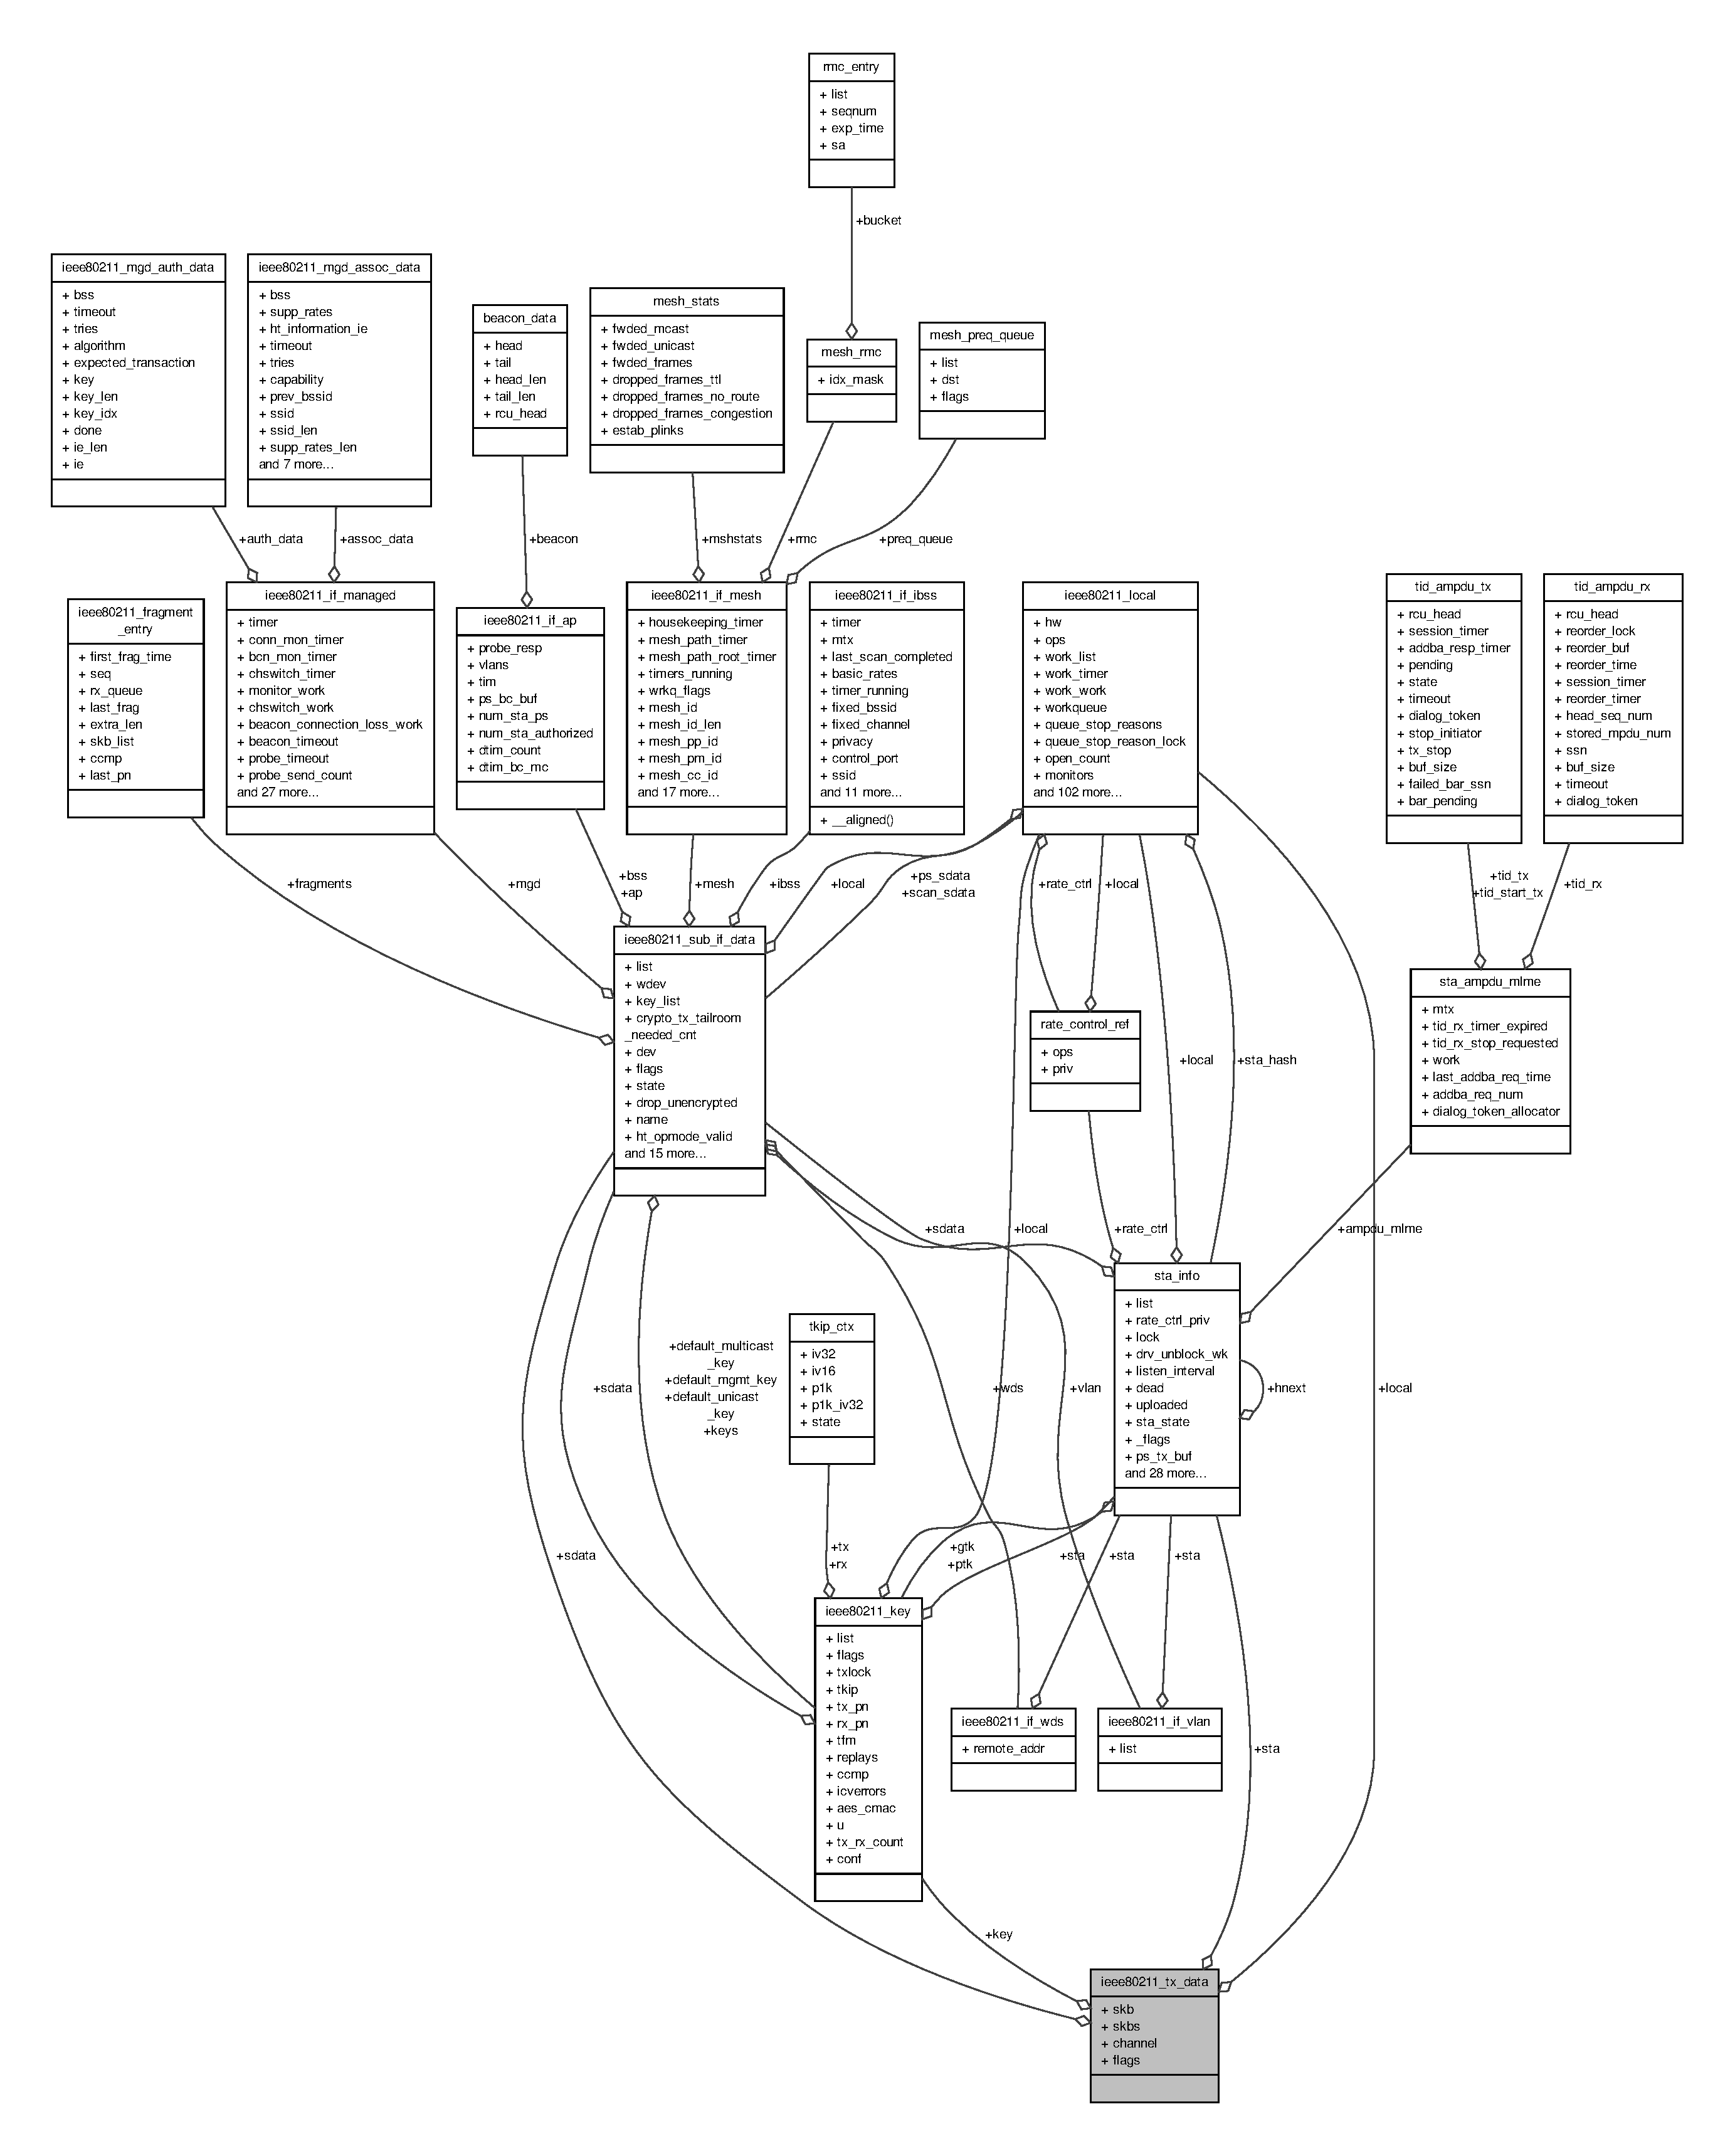
\includegraphics[width=350pt]{structieee80211__tx__data__coll__graph}
\end{center}
\end{figure}
\subsection*{Data Fields}
\begin{DoxyCompactItemize}
\item 
struct sk\-\_\-buff $\ast$ \hyperlink{structieee80211__tx__data_aeba6836824708325a83121030f092c30}{skb}
\item 
struct sk\-\_\-buff\-\_\-head \hyperlink{structieee80211__tx__data_aad317933678d4ee97c8e47099a46dadc}{skbs}
\item 
struct \hyperlink{structieee80211__local}{ieee80211\-\_\-local} $\ast$ \hyperlink{structieee80211__tx__data_ad436a024f420f219c4fe2eebce7e4ab2}{local}
\item 
struct \hyperlink{structieee80211__sub__if__data}{ieee80211\-\_\-sub\-\_\-if\-\_\-data} $\ast$ \hyperlink{structieee80211__tx__data_ad829d8d33f06a7245cc303f924f259ac}{sdata}
\item 
struct \hyperlink{structsta__info}{sta\-\_\-info} $\ast$ \hyperlink{structieee80211__tx__data_aafa9dadbeccd54b4a6b9f77f2908a093}{sta}
\item 
struct \hyperlink{structieee80211__key}{ieee80211\-\_\-key} $\ast$ \hyperlink{structieee80211__tx__data_a6fb9dce4966e6727c301a63b8185c388}{key}
\item 
struct ieee80211\-\_\-channel $\ast$ \hyperlink{structieee80211__tx__data_a80252eb32e874a054a819044989184e2}{channel}
\item 
unsigned int \hyperlink{structieee80211__tx__data_ac92588540e8c1d014a08cd8a45462b19}{flags}
\end{DoxyCompactItemize}


\subsection{Detailed Description}


Definition at line 181 of file ieee80211\-\_\-i.\-h.



\subsection{Field Documentation}
\hypertarget{structieee80211__tx__data_a80252eb32e874a054a819044989184e2}{\index{ieee80211\-\_\-tx\-\_\-data@{ieee80211\-\_\-tx\-\_\-data}!channel@{channel}}
\index{channel@{channel}!ieee80211_tx_data@{ieee80211\-\_\-tx\-\_\-data}}
\subsubsection[{channel}]{\setlength{\rightskip}{0pt plus 5cm}struct ieee80211\-\_\-channel$\ast$ channel}}\label{structieee80211__tx__data_a80252eb32e874a054a819044989184e2}


Definition at line 189 of file ieee80211\-\_\-i.\-h.

\hypertarget{structieee80211__tx__data_ac92588540e8c1d014a08cd8a45462b19}{\index{ieee80211\-\_\-tx\-\_\-data@{ieee80211\-\_\-tx\-\_\-data}!flags@{flags}}
\index{flags@{flags}!ieee80211_tx_data@{ieee80211\-\_\-tx\-\_\-data}}
\subsubsection[{flags}]{\setlength{\rightskip}{0pt plus 5cm}unsigned int flags}}\label{structieee80211__tx__data_ac92588540e8c1d014a08cd8a45462b19}


Definition at line 191 of file ieee80211\-\_\-i.\-h.

\hypertarget{structieee80211__tx__data_a6fb9dce4966e6727c301a63b8185c388}{\index{ieee80211\-\_\-tx\-\_\-data@{ieee80211\-\_\-tx\-\_\-data}!key@{key}}
\index{key@{key}!ieee80211_tx_data@{ieee80211\-\_\-tx\-\_\-data}}
\subsubsection[{key}]{\setlength{\rightskip}{0pt plus 5cm}struct {\bf ieee80211\-\_\-key}$\ast$ key}}\label{structieee80211__tx__data_a6fb9dce4966e6727c301a63b8185c388}


Definition at line 187 of file ieee80211\-\_\-i.\-h.

\hypertarget{structieee80211__tx__data_ad436a024f420f219c4fe2eebce7e4ab2}{\index{ieee80211\-\_\-tx\-\_\-data@{ieee80211\-\_\-tx\-\_\-data}!local@{local}}
\index{local@{local}!ieee80211_tx_data@{ieee80211\-\_\-tx\-\_\-data}}
\subsubsection[{local}]{\setlength{\rightskip}{0pt plus 5cm}struct {\bf ieee80211\-\_\-local}$\ast$ local}}\label{structieee80211__tx__data_ad436a024f420f219c4fe2eebce7e4ab2}


Definition at line 184 of file ieee80211\-\_\-i.\-h.

\hypertarget{structieee80211__tx__data_ad829d8d33f06a7245cc303f924f259ac}{\index{ieee80211\-\_\-tx\-\_\-data@{ieee80211\-\_\-tx\-\_\-data}!sdata@{sdata}}
\index{sdata@{sdata}!ieee80211_tx_data@{ieee80211\-\_\-tx\-\_\-data}}
\subsubsection[{sdata}]{\setlength{\rightskip}{0pt plus 5cm}struct {\bf ieee80211\-\_\-sub\-\_\-if\-\_\-data}$\ast$ sdata}}\label{structieee80211__tx__data_ad829d8d33f06a7245cc303f924f259ac}


Definition at line 185 of file ieee80211\-\_\-i.\-h.

\hypertarget{structieee80211__tx__data_aeba6836824708325a83121030f092c30}{\index{ieee80211\-\_\-tx\-\_\-data@{ieee80211\-\_\-tx\-\_\-data}!skb@{skb}}
\index{skb@{skb}!ieee80211_tx_data@{ieee80211\-\_\-tx\-\_\-data}}
\subsubsection[{skb}]{\setlength{\rightskip}{0pt plus 5cm}struct sk\-\_\-buff$\ast$ skb}}\label{structieee80211__tx__data_aeba6836824708325a83121030f092c30}


Definition at line 182 of file ieee80211\-\_\-i.\-h.

\hypertarget{structieee80211__tx__data_aad317933678d4ee97c8e47099a46dadc}{\index{ieee80211\-\_\-tx\-\_\-data@{ieee80211\-\_\-tx\-\_\-data}!skbs@{skbs}}
\index{skbs@{skbs}!ieee80211_tx_data@{ieee80211\-\_\-tx\-\_\-data}}
\subsubsection[{skbs}]{\setlength{\rightskip}{0pt plus 5cm}struct sk\-\_\-buff\-\_\-head skbs}}\label{structieee80211__tx__data_aad317933678d4ee97c8e47099a46dadc}


Definition at line 183 of file ieee80211\-\_\-i.\-h.

\hypertarget{structieee80211__tx__data_aafa9dadbeccd54b4a6b9f77f2908a093}{\index{ieee80211\-\_\-tx\-\_\-data@{ieee80211\-\_\-tx\-\_\-data}!sta@{sta}}
\index{sta@{sta}!ieee80211_tx_data@{ieee80211\-\_\-tx\-\_\-data}}
\subsubsection[{sta}]{\setlength{\rightskip}{0pt plus 5cm}struct {\bf sta\-\_\-info}$\ast$ sta}}\label{structieee80211__tx__data_aafa9dadbeccd54b4a6b9f77f2908a093}


Definition at line 186 of file ieee80211\-\_\-i.\-h.



The documentation for this struct was generated from the following file\-:\begin{DoxyCompactItemize}
\item 
/home/guille/msm/net/mac80211/\hyperlink{ieee80211__i_8h}{ieee80211\-\_\-i.\-h}\end{DoxyCompactItemize}

\hypertarget{structieee80211__work}{\section{ieee80211\-\_\-work Struct Reference}
\label{structieee80211__work}\index{ieee80211\-\_\-work@{ieee80211\-\_\-work}}
}


{\ttfamily \#include $<$ieee80211\-\_\-i.\-h$>$}



Collaboration diagram for ieee80211\-\_\-work\-:
\nopagebreak
\begin{figure}[H]
\begin{center}
\leavevmode
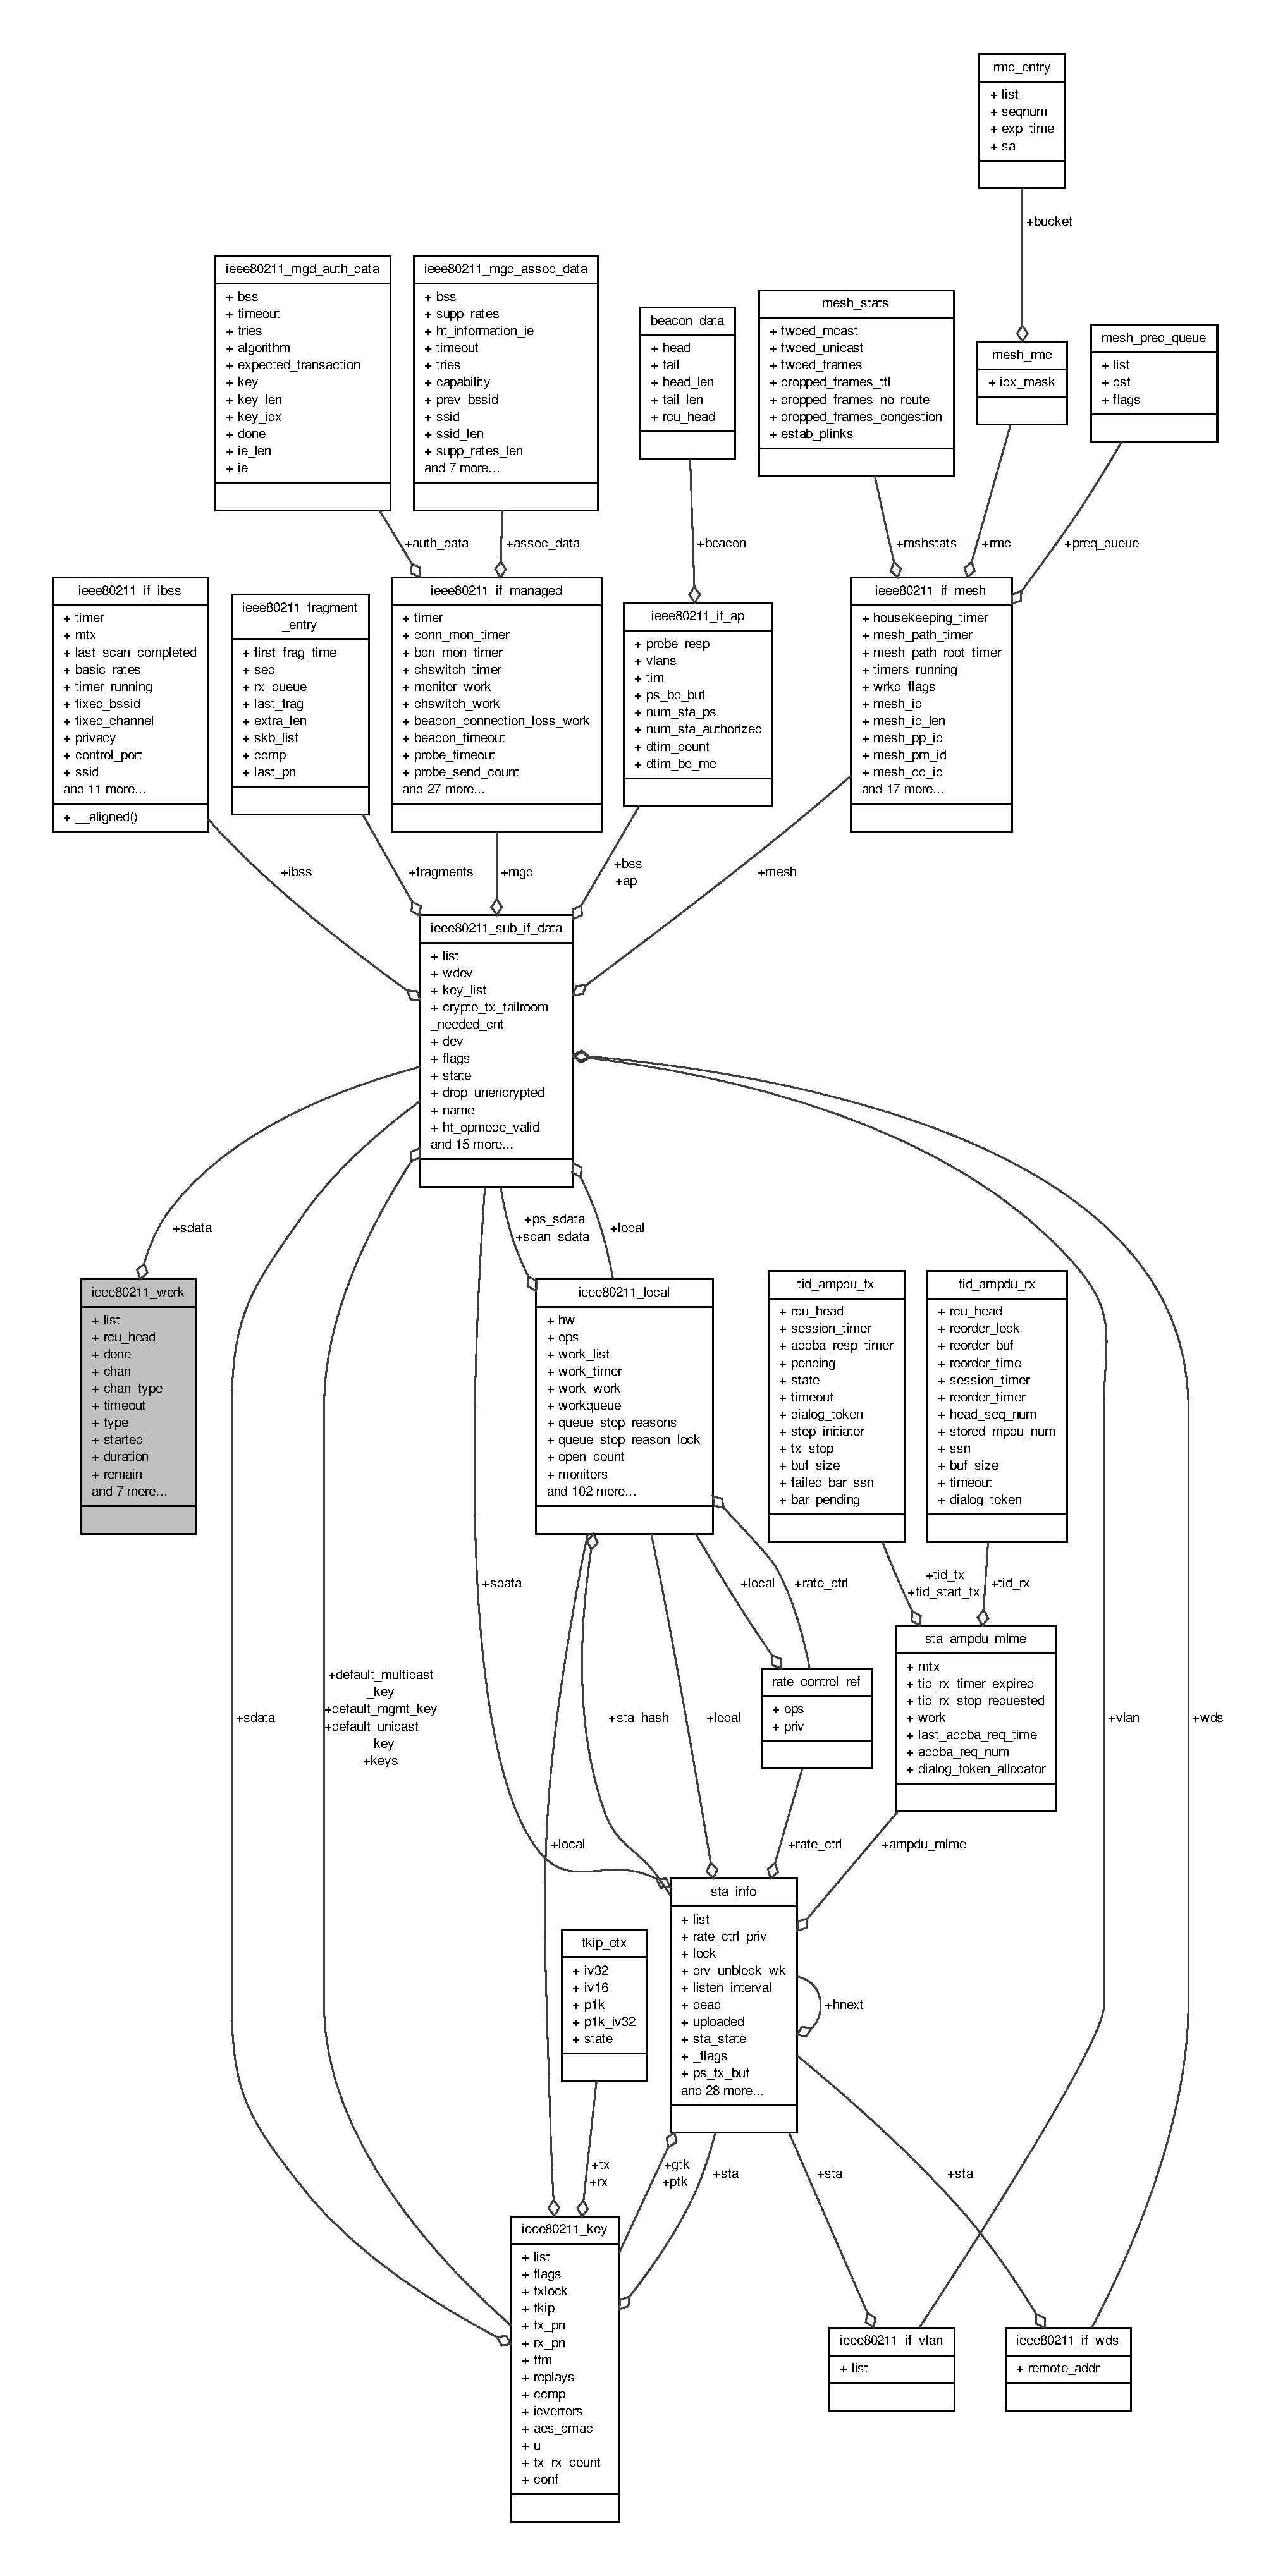
\includegraphics[height=550pt]{structieee80211__work__coll__graph}
\end{center}
\end{figure}
\subsection*{Data Fields}
\begin{DoxyCompactItemize}
\item 
struct list\-\_\-head \hyperlink{structieee80211__work_a1f00f18b91d5a820f2c43064243aa86e}{list}
\item 
struct rcu\-\_\-head \hyperlink{structieee80211__work_ab698383409a24791490f962fe6990655}{rcu\-\_\-head}
\item 
struct \hyperlink{structieee80211__sub__if__data}{ieee80211\-\_\-sub\-\_\-if\-\_\-data} $\ast$ \hyperlink{structieee80211__work_ad829d8d33f06a7245cc303f924f259ac}{sdata}
\item 
enum \hyperlink{ieee80211__i_8h_a1d4a98716f0e0c48900c8d144ae73774}{work\-\_\-done\-\_\-result}($\ast$ \hyperlink{structieee80211__work_a8cafc3e050dcbac4c13d42bbed5da146}{done} )(struct \hyperlink{structieee80211__work}{ieee80211\-\_\-work} $\ast$wk, struct sk\-\_\-buff $\ast$skb)
\item 
struct ieee80211\-\_\-channel $\ast$ \hyperlink{structieee80211__work_ad695b849e189aedbc929a30c616fbfc7}{chan}
\item 
enum nl80211\-\_\-channel\-\_\-type \hyperlink{structieee80211__work_a82a2bcb2ebd1e6187c8057f98ce6bd3f}{chan\-\_\-type}
\item 
unsigned long \hyperlink{structieee80211__work_a639e65bbd749de17060d658eb233f72b}{timeout}
\item 
enum \hyperlink{ieee80211__i_8h_acbd73c3a23cb430f27ef21fe6d81d795}{ieee80211\-\_\-work\-\_\-type} \hyperlink{structieee80211__work_abf1dbe34cf79d583ad1c34c2fe8bbaec}{type}
\item 
bool \hyperlink{structieee80211__work_a43c08d193d555a2b2a61c53d2a4e5a63}{started}
\item 
\begin{tabbing}
xx\=xx\=xx\=xx\=xx\=xx\=xx\=xx\=xx\=\kill
union \{\\
\>struct \{\\
\>\>u32 \hyperlink{structieee80211__work_ae0565e8bbc0bf97f0747e1e4757fc5a0}{duration}\\
\>\} \hyperlink{structieee80211__work_a848f56cbf44ec6114e7da4547b616fb1}{remain}\\
\>struct \{\\
\>\>struct sk\_buff $\ast$ \hyperlink{structieee80211__work_a7ddb066bb78029e2130c2ccb2bf3ac08}{frame}\\
\>\>u32 \hyperlink{structieee80211__work_ad656a22cd7138c32438d6fff315a9611}{wait}\\
\>\>bool \hyperlink{structieee80211__work_ad1f0bff7112206922c9d5a87adad6f2b}{status}\\
\>\} \hyperlink{structieee80211__work_ab765c48f0901d818729d7a4031f0a284}{offchan\_tx}\\
\}; \\

\end{tabbing}\item 
size\-\_\-t \hyperlink{structieee80211__work_ace1c2e33b74df8973a7d9a19c935af80}{data\-\_\-len}
\item 
u8 \hyperlink{structieee80211__work_a6dc95797421616e7833cb107fee9d17f}{data} \mbox{[}$\,$\mbox{]}
\end{DoxyCompactItemize}


\subsection{Detailed Description}


Definition at line 337 of file ieee80211\-\_\-i.\-h.



\subsection{Field Documentation}
\hypertarget{structieee80211__work_a4b97c6d84b14925ea9f396a098ca6421}{\subsubsection[{"@3}]{\setlength{\rightskip}{0pt plus 5cm}union \{ ... \} }}\label{structieee80211__work_a4b97c6d84b14925ea9f396a098ca6421}
\hypertarget{structieee80211__work_ad695b849e189aedbc929a30c616fbfc7}{\index{ieee80211\-\_\-work@{ieee80211\-\_\-work}!chan@{chan}}
\index{chan@{chan}!ieee80211_work@{ieee80211\-\_\-work}}
\subsubsection[{chan}]{\setlength{\rightskip}{0pt plus 5cm}struct ieee80211\-\_\-channel$\ast$ chan}}\label{structieee80211__work_ad695b849e189aedbc929a30c616fbfc7}


Definition at line 347 of file ieee80211\-\_\-i.\-h.

\hypertarget{structieee80211__work_a82a2bcb2ebd1e6187c8057f98ce6bd3f}{\index{ieee80211\-\_\-work@{ieee80211\-\_\-work}!chan\-\_\-type@{chan\-\_\-type}}
\index{chan\-\_\-type@{chan\-\_\-type}!ieee80211_work@{ieee80211\-\_\-work}}
\subsubsection[{chan\-\_\-type}]{\setlength{\rightskip}{0pt plus 5cm}enum nl80211\-\_\-channel\-\_\-type chan\-\_\-type}}\label{structieee80211__work_a82a2bcb2ebd1e6187c8057f98ce6bd3f}


Definition at line 348 of file ieee80211\-\_\-i.\-h.

\hypertarget{structieee80211__work_a6dc95797421616e7833cb107fee9d17f}{\index{ieee80211\-\_\-work@{ieee80211\-\_\-work}!data@{data}}
\index{data@{data}!ieee80211_work@{ieee80211\-\_\-work}}
\subsubsection[{data}]{\setlength{\rightskip}{0pt plus 5cm}u8 data\mbox{[}$\,$\mbox{]}}}\label{structieee80211__work_a6dc95797421616e7833cb107fee9d17f}


Definition at line 367 of file ieee80211\-\_\-i.\-h.

\hypertarget{structieee80211__work_ace1c2e33b74df8973a7d9a19c935af80}{\index{ieee80211\-\_\-work@{ieee80211\-\_\-work}!data\-\_\-len@{data\-\_\-len}}
\index{data\-\_\-len@{data\-\_\-len}!ieee80211_work@{ieee80211\-\_\-work}}
\subsubsection[{data\-\_\-len}]{\setlength{\rightskip}{0pt plus 5cm}size\-\_\-t data\-\_\-len}}\label{structieee80211__work_ace1c2e33b74df8973a7d9a19c935af80}


Definition at line 366 of file ieee80211\-\_\-i.\-h.

\hypertarget{structieee80211__work_a8cafc3e050dcbac4c13d42bbed5da146}{\index{ieee80211\-\_\-work@{ieee80211\-\_\-work}!done@{done}}
\index{done@{done}!ieee80211_work@{ieee80211\-\_\-work}}
\subsubsection[{done}]{\setlength{\rightskip}{0pt plus 5cm}enum {\bf work\-\_\-done\-\_\-result}($\ast$ done)(struct {\bf ieee80211\-\_\-work} $\ast$wk, struct sk\-\_\-buff $\ast$skb)}}\label{structieee80211__work_a8cafc3e050dcbac4c13d42bbed5da146}


Definition at line 344 of file ieee80211\-\_\-i.\-h.

\hypertarget{structieee80211__work_ae0565e8bbc0bf97f0747e1e4757fc5a0}{\index{ieee80211\-\_\-work@{ieee80211\-\_\-work}!duration@{duration}}
\index{duration@{duration}!ieee80211_work@{ieee80211\-\_\-work}}
\subsubsection[{duration}]{\setlength{\rightskip}{0pt plus 5cm}u32 duration}}\label{structieee80211__work_ae0565e8bbc0bf97f0747e1e4757fc5a0}


Definition at line 357 of file ieee80211\-\_\-i.\-h.

\hypertarget{structieee80211__work_a7ddb066bb78029e2130c2ccb2bf3ac08}{\index{ieee80211\-\_\-work@{ieee80211\-\_\-work}!frame@{frame}}
\index{frame@{frame}!ieee80211_work@{ieee80211\-\_\-work}}
\subsubsection[{frame}]{\setlength{\rightskip}{0pt plus 5cm}struct sk\-\_\-buff$\ast$ frame}}\label{structieee80211__work_a7ddb066bb78029e2130c2ccb2bf3ac08}


Definition at line 360 of file ieee80211\-\_\-i.\-h.

\hypertarget{structieee80211__work_a1f00f18b91d5a820f2c43064243aa86e}{\index{ieee80211\-\_\-work@{ieee80211\-\_\-work}!list@{list}}
\index{list@{list}!ieee80211_work@{ieee80211\-\_\-work}}
\subsubsection[{list}]{\setlength{\rightskip}{0pt plus 5cm}struct list\-\_\-head list}}\label{structieee80211__work_a1f00f18b91d5a820f2c43064243aa86e}


Definition at line 338 of file ieee80211\-\_\-i.\-h.

\hypertarget{structieee80211__work_ab765c48f0901d818729d7a4031f0a284}{\index{ieee80211\-\_\-work@{ieee80211\-\_\-work}!offchan\-\_\-tx@{offchan\-\_\-tx}}
\index{offchan\-\_\-tx@{offchan\-\_\-tx}!ieee80211_work@{ieee80211\-\_\-work}}
\subsubsection[{offchan\-\_\-tx}]{\setlength{\rightskip}{0pt plus 5cm}struct \{ ... \}   offchan\-\_\-tx}}\label{structieee80211__work_ab765c48f0901d818729d7a4031f0a284}
\hypertarget{structieee80211__work_ab698383409a24791490f962fe6990655}{\index{ieee80211\-\_\-work@{ieee80211\-\_\-work}!rcu\-\_\-head@{rcu\-\_\-head}}
\index{rcu\-\_\-head@{rcu\-\_\-head}!ieee80211_work@{ieee80211\-\_\-work}}
\subsubsection[{rcu\-\_\-head}]{\setlength{\rightskip}{0pt plus 5cm}struct rcu\-\_\-head rcu\-\_\-head}}\label{structieee80211__work_ab698383409a24791490f962fe6990655}


Definition at line 340 of file ieee80211\-\_\-i.\-h.

\hypertarget{structieee80211__work_a848f56cbf44ec6114e7da4547b616fb1}{\index{ieee80211\-\_\-work@{ieee80211\-\_\-work}!remain@{remain}}
\index{remain@{remain}!ieee80211_work@{ieee80211\-\_\-work}}
\subsubsection[{remain}]{\setlength{\rightskip}{0pt plus 5cm}struct \{ ... \}   remain}}\label{structieee80211__work_a848f56cbf44ec6114e7da4547b616fb1}
\hypertarget{structieee80211__work_ad829d8d33f06a7245cc303f924f259ac}{\index{ieee80211\-\_\-work@{ieee80211\-\_\-work}!sdata@{sdata}}
\index{sdata@{sdata}!ieee80211_work@{ieee80211\-\_\-work}}
\subsubsection[{sdata}]{\setlength{\rightskip}{0pt plus 5cm}struct {\bf ieee80211\-\_\-sub\-\_\-if\-\_\-data}$\ast$ sdata}}\label{structieee80211__work_ad829d8d33f06a7245cc303f924f259ac}


Definition at line 342 of file ieee80211\-\_\-i.\-h.

\hypertarget{structieee80211__work_a43c08d193d555a2b2a61c53d2a4e5a63}{\index{ieee80211\-\_\-work@{ieee80211\-\_\-work}!started@{started}}
\index{started@{started}!ieee80211_work@{ieee80211\-\_\-work}}
\subsubsection[{started}]{\setlength{\rightskip}{0pt plus 5cm}bool started}}\label{structieee80211__work_a43c08d193d555a2b2a61c53d2a4e5a63}


Definition at line 353 of file ieee80211\-\_\-i.\-h.

\hypertarget{structieee80211__work_ad1f0bff7112206922c9d5a87adad6f2b}{\index{ieee80211\-\_\-work@{ieee80211\-\_\-work}!status@{status}}
\index{status@{status}!ieee80211_work@{ieee80211\-\_\-work}}
\subsubsection[{status}]{\setlength{\rightskip}{0pt plus 5cm}bool status}}\label{structieee80211__work_ad1f0bff7112206922c9d5a87adad6f2b}


Definition at line 362 of file ieee80211\-\_\-i.\-h.

\hypertarget{structieee80211__work_a639e65bbd749de17060d658eb233f72b}{\index{ieee80211\-\_\-work@{ieee80211\-\_\-work}!timeout@{timeout}}
\index{timeout@{timeout}!ieee80211_work@{ieee80211\-\_\-work}}
\subsubsection[{timeout}]{\setlength{\rightskip}{0pt plus 5cm}unsigned long timeout}}\label{structieee80211__work_a639e65bbd749de17060d658eb233f72b}


Definition at line 350 of file ieee80211\-\_\-i.\-h.

\hypertarget{structieee80211__work_abf1dbe34cf79d583ad1c34c2fe8bbaec}{\index{ieee80211\-\_\-work@{ieee80211\-\_\-work}!type@{type}}
\index{type@{type}!ieee80211_work@{ieee80211\-\_\-work}}
\subsubsection[{type}]{\setlength{\rightskip}{0pt plus 5cm}enum {\bf ieee80211\-\_\-work\-\_\-type} type}}\label{structieee80211__work_abf1dbe34cf79d583ad1c34c2fe8bbaec}


Definition at line 351 of file ieee80211\-\_\-i.\-h.

\hypertarget{structieee80211__work_ad656a22cd7138c32438d6fff315a9611}{\index{ieee80211\-\_\-work@{ieee80211\-\_\-work}!wait@{wait}}
\index{wait@{wait}!ieee80211_work@{ieee80211\-\_\-work}}
\subsubsection[{wait}]{\setlength{\rightskip}{0pt plus 5cm}u32 wait}}\label{structieee80211__work_ad656a22cd7138c32438d6fff315a9611}


Definition at line 361 of file ieee80211\-\_\-i.\-h.



The documentation for this struct was generated from the following file\-:\begin{DoxyCompactItemize}
\item 
/home/guille/msm/net/mac80211/\hyperlink{ieee80211__i_8h}{ieee80211\-\_\-i.\-h}\end{DoxyCompactItemize}

\hypertarget{structieee802__11__elems}{\section{ieee802\-\_\-11\-\_\-elems Struct Reference}
\label{structieee802__11__elems}\index{ieee802\-\_\-11\-\_\-elems@{ieee802\-\_\-11\-\_\-elems}}
}


{\ttfamily \#include $<$ieee80211\-\_\-i.\-h$>$}



Collaboration diagram for ieee802\-\_\-11\-\_\-elems\-:
\nopagebreak
\begin{figure}[H]
\begin{center}
\leavevmode
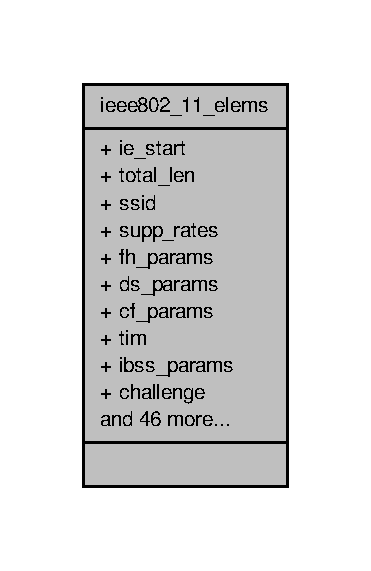
\includegraphics[width=178pt]{structieee802__11__elems__coll__graph}
\end{center}
\end{figure}
\subsection*{Data Fields}
\begin{DoxyCompactItemize}
\item 
u8 $\ast$ \hyperlink{structieee802__11__elems_ac67563c8768abab887c25047515b040c}{ie\-\_\-start}
\item 
size\-\_\-t \hyperlink{structieee802__11__elems_aa117fc7f9adae4a74d56508b20f7de1f}{total\-\_\-len}
\item 
u8 $\ast$ \hyperlink{structieee802__11__elems_a2b1a755b5ea91fcd084b731e52d74baa}{ssid}
\item 
u8 $\ast$ \hyperlink{structieee802__11__elems_a046b4135d5b0e0fce9a2100e81bb2cf1}{supp\-\_\-rates}
\item 
u8 $\ast$ \hyperlink{structieee802__11__elems_a1bfe816ebad00d8d582c5b957d45acb8}{fh\-\_\-params}
\item 
u8 $\ast$ \hyperlink{structieee802__11__elems_ac2f2349fb1f40ffc5e91ec3ad5fe678f}{ds\-\_\-params}
\item 
u8 $\ast$ \hyperlink{structieee802__11__elems_ae663298f76d3de3852deeaa305626d62}{cf\-\_\-params}
\item 
struct ieee80211\-\_\-tim\-\_\-ie $\ast$ \hyperlink{structieee802__11__elems_a09f63823f0fa5e1802acd5874911d07a}{tim}
\item 
u8 $\ast$ \hyperlink{structieee802__11__elems_a7fac4f71f2df266e10c20cca69544c9b}{ibss\-\_\-params}
\item 
u8 $\ast$ \hyperlink{structieee802__11__elems_abd6006bde809b197adccf583f4206332}{challenge}
\item 
u8 $\ast$ \hyperlink{structieee802__11__elems_a4f433e136c9ee02a2dc8e9484078cd60}{wpa}
\item 
u8 $\ast$ \hyperlink{structieee802__11__elems_a052b78ba85219ace0375b4ced0902a0c}{rsn}
\item 
u8 $\ast$ \hyperlink{structieee802__11__elems_a5afa785c397a503afdef4c895bf319d6}{erp\-\_\-info}
\item 
u8 $\ast$ \hyperlink{structieee802__11__elems_a59cf8f9fa556a38286cdf904fc6c8ac2}{ext\-\_\-supp\-\_\-rates}
\item 
u8 $\ast$ \hyperlink{structieee802__11__elems_a1051a8e53a01158ff3f9675d8ec9c6e5}{wmm\-\_\-info}
\item 
u8 $\ast$ \hyperlink{structieee802__11__elems_a72ab3e59dc8571dab876636d8fb484f7}{wmm\-\_\-param}
\item 
struct ieee80211\-\_\-ht\-\_\-cap $\ast$ \hyperlink{structieee802__11__elems_ac24d4796157d7ad3003b848a7ce3c118}{ht\-\_\-cap\-\_\-elem}
\item 
struct ieee80211\-\_\-ht\-\_\-info $\ast$ \hyperlink{structieee802__11__elems_a997ee83c8c6d2c120512c69b41bbfff1}{ht\-\_\-info\-\_\-elem}
\item 
struct ieee80211\-\_\-meshconf\-\_\-ie $\ast$ \hyperlink{structieee802__11__elems_acb3adcd722f89d8cce1e7be9129d6bc4}{mesh\-\_\-config}
\item 
u8 $\ast$ \hyperlink{structieee802__11__elems_a0f1538fd176045e5a10de47f5cefd754}{mesh\-\_\-id}
\item 
u8 $\ast$ \hyperlink{structieee802__11__elems_a8f8fc9384b03389900f4b2d557d4a3a4}{peering}
\item 
u8 $\ast$ \hyperlink{structieee802__11__elems_a0e21b67c3354dad309120d348eac83ed}{preq}
\item 
u8 $\ast$ \hyperlink{structieee802__11__elems_afce540ba301085452d9683d7c08587ae}{prep}
\item 
u8 $\ast$ \hyperlink{structieee802__11__elems_ab2dad797baa297bd9525977b074bcaa4}{perr}
\item 
struct ieee80211\-\_\-rann\-\_\-ie $\ast$ \hyperlink{structieee802__11__elems_a971dd2d54026bf076935c66967876b95}{rann}
\item 
u8 $\ast$ \hyperlink{structieee802__11__elems_a38ba879334b0542a7b1ee9e0e4a6c711}{ch\-\_\-switch\-\_\-elem}
\item 
u8 $\ast$ \hyperlink{structieee802__11__elems_aad534d125ee609e0241201806f9b0fa8}{country\-\_\-elem}
\item 
u8 $\ast$ \hyperlink{structieee802__11__elems_a19eaf1ea27d26716ab4ff793995dd946}{pwr\-\_\-constr\-\_\-elem}
\item 
u8 $\ast$ \hyperlink{structieee802__11__elems_abdf6b7fabeef533a721d298f63162edb}{quiet\-\_\-elem}
\item 
u8 $\ast$ \hyperlink{structieee802__11__elems_a426d32f8654b0c568ef8419d2ff4b775}{timeout\-\_\-int}
\item 
u8 \hyperlink{structieee802__11__elems_a440f44724caffefa0f9c838518a3c790}{ssid\-\_\-len}
\item 
u8 \hyperlink{structieee802__11__elems_a10e3f296dc2be6b8aef4938abfa6af16}{supp\-\_\-rates\-\_\-len}
\item 
u8 \hyperlink{structieee802__11__elems_a322eb9d3c396e5829bb88e7964252d35}{fh\-\_\-params\-\_\-len}
\item 
u8 \hyperlink{structieee802__11__elems_a85a3203b26546e19531ab204d6cf2b7f}{ds\-\_\-params\-\_\-len}
\item 
u8 \hyperlink{structieee802__11__elems_ab9e1ceea5f509efc44108625fcd62d2d}{cf\-\_\-params\-\_\-len}
\item 
u8 \hyperlink{structieee802__11__elems_ab90447c07ba9f8b23a4508f5c2ab7850}{tim\-\_\-len}
\item 
u8 \hyperlink{structieee802__11__elems_ae1caf3e856db41c098dae539cce1b7b9}{ibss\-\_\-params\-\_\-len}
\item 
u8 \hyperlink{structieee802__11__elems_a17a8ec03c6d59e1bde0bfc2ffc72972c}{challenge\-\_\-len}
\item 
u8 \hyperlink{structieee802__11__elems_a46f04df3a13e3b941f3250516466e8ba}{wpa\-\_\-len}
\item 
u8 \hyperlink{structieee802__11__elems_af457de8cfed4f313c6a1e8154ce440f6}{rsn\-\_\-len}
\item 
u8 \hyperlink{structieee802__11__elems_a8075695419d6f4cca5146e607aa26900}{erp\-\_\-info\-\_\-len}
\item 
u8 \hyperlink{structieee802__11__elems_ad801aa33ff70dfe5cd7ff32f039799ab}{ext\-\_\-supp\-\_\-rates\-\_\-len}
\item 
u8 \hyperlink{structieee802__11__elems_abb89de16d0721b263ad0098cbb8edd51}{wmm\-\_\-info\-\_\-len}
\item 
u8 \hyperlink{structieee802__11__elems_a8bd489ba83474d318aabdb2ca4ffb0e2}{wmm\-\_\-param\-\_\-len}
\item 
u8 \hyperlink{structieee802__11__elems_a8d28b6eb74e2a40cdbf971786344b947}{mesh\-\_\-id\-\_\-len}
\item 
u8 \hyperlink{structieee802__11__elems_a4ee92ca9513f9ef27a1609135452129b}{peering\-\_\-len}
\item 
u8 \hyperlink{structieee802__11__elems_a5eac1db084f68b936ee32adf0e8e6b0d}{preq\-\_\-len}
\item 
u8 \hyperlink{structieee802__11__elems_a1a08ce2841b5af833d18884e6e2e1b88}{prep\-\_\-len}
\item 
u8 \hyperlink{structieee802__11__elems_a29835ac7646e7afef597ea41654ff3a9}{perr\-\_\-len}
\item 
u8 \hyperlink{structieee802__11__elems_afcbd333fdb9a00d0293ce5a2aa67a51f}{ch\-\_\-switch\-\_\-elem\-\_\-len}
\item 
u8 \hyperlink{structieee802__11__elems_ae24d95c5691f6017fcbfd8f7a5933990}{country\-\_\-elem\-\_\-len}
\item 
u8 \hyperlink{structieee802__11__elems_a74dc471871aaafc9bed087c079c4c8c3}{pwr\-\_\-constr\-\_\-elem\-\_\-len}
\item 
u8 \hyperlink{structieee802__11__elems_af5b177a26c37c42cfe6b7a5b4d900cfe}{quiet\-\_\-elem\-\_\-len}
\item 
u8 \hyperlink{structieee802__11__elems_aa9bb9f08b902ed1012cb04ac64824f49}{num\-\_\-of\-\_\-quiet\-\_\-elem}
\item 
u8 \hyperlink{structieee802__11__elems_a95b4deaebcafd728c67639bd307e91e8}{timeout\-\_\-int\-\_\-len}
\item 
bool \hyperlink{structieee802__11__elems_a63b1a4ce3aea3d6ed94b79b863d0594d}{parse\-\_\-error}
\end{DoxyCompactItemize}


\subsection{Detailed Description}


Definition at line 1101 of file ieee80211\-\_\-i.\-h.



\subsection{Field Documentation}
\hypertarget{structieee802__11__elems_ae663298f76d3de3852deeaa305626d62}{\index{ieee802\-\_\-11\-\_\-elems@{ieee802\-\_\-11\-\_\-elems}!cf\-\_\-params@{cf\-\_\-params}}
\index{cf\-\_\-params@{cf\-\_\-params}!ieee802_11_elems@{ieee802\-\_\-11\-\_\-elems}}
\subsubsection[{cf\-\_\-params}]{\setlength{\rightskip}{0pt plus 5cm}u8$\ast$ cf\-\_\-params}}\label{structieee802__11__elems_ae663298f76d3de3852deeaa305626d62}


Definition at line 1110 of file ieee80211\-\_\-i.\-h.

\hypertarget{structieee802__11__elems_ab9e1ceea5f509efc44108625fcd62d2d}{\index{ieee802\-\_\-11\-\_\-elems@{ieee802\-\_\-11\-\_\-elems}!cf\-\_\-params\-\_\-len@{cf\-\_\-params\-\_\-len}}
\index{cf\-\_\-params\-\_\-len@{cf\-\_\-params\-\_\-len}!ieee802_11_elems@{ieee802\-\_\-11\-\_\-elems}}
\subsubsection[{cf\-\_\-params\-\_\-len}]{\setlength{\rightskip}{0pt plus 5cm}u8 cf\-\_\-params\-\_\-len}}\label{structieee802__11__elems_ab9e1ceea5f509efc44108625fcd62d2d}


Definition at line 1140 of file ieee80211\-\_\-i.\-h.

\hypertarget{structieee802__11__elems_a38ba879334b0542a7b1ee9e0e4a6c711}{\index{ieee802\-\_\-11\-\_\-elems@{ieee802\-\_\-11\-\_\-elems}!ch\-\_\-switch\-\_\-elem@{ch\-\_\-switch\-\_\-elem}}
\index{ch\-\_\-switch\-\_\-elem@{ch\-\_\-switch\-\_\-elem}!ieee802_11_elems@{ieee802\-\_\-11\-\_\-elems}}
\subsubsection[{ch\-\_\-switch\-\_\-elem}]{\setlength{\rightskip}{0pt plus 5cm}u8$\ast$ ch\-\_\-switch\-\_\-elem}}\label{structieee802__11__elems_a38ba879334b0542a7b1ee9e0e4a6c711}


Definition at line 1129 of file ieee80211\-\_\-i.\-h.

\hypertarget{structieee802__11__elems_afcbd333fdb9a00d0293ce5a2aa67a51f}{\index{ieee802\-\_\-11\-\_\-elems@{ieee802\-\_\-11\-\_\-elems}!ch\-\_\-switch\-\_\-elem\-\_\-len@{ch\-\_\-switch\-\_\-elem\-\_\-len}}
\index{ch\-\_\-switch\-\_\-elem\-\_\-len@{ch\-\_\-switch\-\_\-elem\-\_\-len}!ieee802_11_elems@{ieee802\-\_\-11\-\_\-elems}}
\subsubsection[{ch\-\_\-switch\-\_\-elem\-\_\-len}]{\setlength{\rightskip}{0pt plus 5cm}u8 ch\-\_\-switch\-\_\-elem\-\_\-len}}\label{structieee802__11__elems_afcbd333fdb9a00d0293ce5a2aa67a51f}


Definition at line 1155 of file ieee80211\-\_\-i.\-h.

\hypertarget{structieee802__11__elems_abd6006bde809b197adccf583f4206332}{\index{ieee802\-\_\-11\-\_\-elems@{ieee802\-\_\-11\-\_\-elems}!challenge@{challenge}}
\index{challenge@{challenge}!ieee802_11_elems@{ieee802\-\_\-11\-\_\-elems}}
\subsubsection[{challenge}]{\setlength{\rightskip}{0pt plus 5cm}u8$\ast$ challenge}}\label{structieee802__11__elems_abd6006bde809b197adccf583f4206332}


Definition at line 1113 of file ieee80211\-\_\-i.\-h.

\hypertarget{structieee802__11__elems_a17a8ec03c6d59e1bde0bfc2ffc72972c}{\index{ieee802\-\_\-11\-\_\-elems@{ieee802\-\_\-11\-\_\-elems}!challenge\-\_\-len@{challenge\-\_\-len}}
\index{challenge\-\_\-len@{challenge\-\_\-len}!ieee802_11_elems@{ieee802\-\_\-11\-\_\-elems}}
\subsubsection[{challenge\-\_\-len}]{\setlength{\rightskip}{0pt plus 5cm}u8 challenge\-\_\-len}}\label{structieee802__11__elems_a17a8ec03c6d59e1bde0bfc2ffc72972c}


Definition at line 1143 of file ieee80211\-\_\-i.\-h.

\hypertarget{structieee802__11__elems_aad534d125ee609e0241201806f9b0fa8}{\index{ieee802\-\_\-11\-\_\-elems@{ieee802\-\_\-11\-\_\-elems}!country\-\_\-elem@{country\-\_\-elem}}
\index{country\-\_\-elem@{country\-\_\-elem}!ieee802_11_elems@{ieee802\-\_\-11\-\_\-elems}}
\subsubsection[{country\-\_\-elem}]{\setlength{\rightskip}{0pt plus 5cm}u8$\ast$ country\-\_\-elem}}\label{structieee802__11__elems_aad534d125ee609e0241201806f9b0fa8}


Definition at line 1130 of file ieee80211\-\_\-i.\-h.

\hypertarget{structieee802__11__elems_ae24d95c5691f6017fcbfd8f7a5933990}{\index{ieee802\-\_\-11\-\_\-elems@{ieee802\-\_\-11\-\_\-elems}!country\-\_\-elem\-\_\-len@{country\-\_\-elem\-\_\-len}}
\index{country\-\_\-elem\-\_\-len@{country\-\_\-elem\-\_\-len}!ieee802_11_elems@{ieee802\-\_\-11\-\_\-elems}}
\subsubsection[{country\-\_\-elem\-\_\-len}]{\setlength{\rightskip}{0pt plus 5cm}u8 country\-\_\-elem\-\_\-len}}\label{structieee802__11__elems_ae24d95c5691f6017fcbfd8f7a5933990}


Definition at line 1156 of file ieee80211\-\_\-i.\-h.

\hypertarget{structieee802__11__elems_ac2f2349fb1f40ffc5e91ec3ad5fe678f}{\index{ieee802\-\_\-11\-\_\-elems@{ieee802\-\_\-11\-\_\-elems}!ds\-\_\-params@{ds\-\_\-params}}
\index{ds\-\_\-params@{ds\-\_\-params}!ieee802_11_elems@{ieee802\-\_\-11\-\_\-elems}}
\subsubsection[{ds\-\_\-params}]{\setlength{\rightskip}{0pt plus 5cm}u8$\ast$ ds\-\_\-params}}\label{structieee802__11__elems_ac2f2349fb1f40ffc5e91ec3ad5fe678f}


Definition at line 1109 of file ieee80211\-\_\-i.\-h.

\hypertarget{structieee802__11__elems_a85a3203b26546e19531ab204d6cf2b7f}{\index{ieee802\-\_\-11\-\_\-elems@{ieee802\-\_\-11\-\_\-elems}!ds\-\_\-params\-\_\-len@{ds\-\_\-params\-\_\-len}}
\index{ds\-\_\-params\-\_\-len@{ds\-\_\-params\-\_\-len}!ieee802_11_elems@{ieee802\-\_\-11\-\_\-elems}}
\subsubsection[{ds\-\_\-params\-\_\-len}]{\setlength{\rightskip}{0pt plus 5cm}u8 ds\-\_\-params\-\_\-len}}\label{structieee802__11__elems_a85a3203b26546e19531ab204d6cf2b7f}


Definition at line 1139 of file ieee80211\-\_\-i.\-h.

\hypertarget{structieee802__11__elems_a5afa785c397a503afdef4c895bf319d6}{\index{ieee802\-\_\-11\-\_\-elems@{ieee802\-\_\-11\-\_\-elems}!erp\-\_\-info@{erp\-\_\-info}}
\index{erp\-\_\-info@{erp\-\_\-info}!ieee802_11_elems@{ieee802\-\_\-11\-\_\-elems}}
\subsubsection[{erp\-\_\-info}]{\setlength{\rightskip}{0pt plus 5cm}u8$\ast$ erp\-\_\-info}}\label{structieee802__11__elems_a5afa785c397a503afdef4c895bf319d6}


Definition at line 1116 of file ieee80211\-\_\-i.\-h.

\hypertarget{structieee802__11__elems_a8075695419d6f4cca5146e607aa26900}{\index{ieee802\-\_\-11\-\_\-elems@{ieee802\-\_\-11\-\_\-elems}!erp\-\_\-info\-\_\-len@{erp\-\_\-info\-\_\-len}}
\index{erp\-\_\-info\-\_\-len@{erp\-\_\-info\-\_\-len}!ieee802_11_elems@{ieee802\-\_\-11\-\_\-elems}}
\subsubsection[{erp\-\_\-info\-\_\-len}]{\setlength{\rightskip}{0pt plus 5cm}u8 erp\-\_\-info\-\_\-len}}\label{structieee802__11__elems_a8075695419d6f4cca5146e607aa26900}


Definition at line 1146 of file ieee80211\-\_\-i.\-h.

\hypertarget{structieee802__11__elems_a59cf8f9fa556a38286cdf904fc6c8ac2}{\index{ieee802\-\_\-11\-\_\-elems@{ieee802\-\_\-11\-\_\-elems}!ext\-\_\-supp\-\_\-rates@{ext\-\_\-supp\-\_\-rates}}
\index{ext\-\_\-supp\-\_\-rates@{ext\-\_\-supp\-\_\-rates}!ieee802_11_elems@{ieee802\-\_\-11\-\_\-elems}}
\subsubsection[{ext\-\_\-supp\-\_\-rates}]{\setlength{\rightskip}{0pt plus 5cm}u8$\ast$ ext\-\_\-supp\-\_\-rates}}\label{structieee802__11__elems_a59cf8f9fa556a38286cdf904fc6c8ac2}


Definition at line 1117 of file ieee80211\-\_\-i.\-h.

\hypertarget{structieee802__11__elems_ad801aa33ff70dfe5cd7ff32f039799ab}{\index{ieee802\-\_\-11\-\_\-elems@{ieee802\-\_\-11\-\_\-elems}!ext\-\_\-supp\-\_\-rates\-\_\-len@{ext\-\_\-supp\-\_\-rates\-\_\-len}}
\index{ext\-\_\-supp\-\_\-rates\-\_\-len@{ext\-\_\-supp\-\_\-rates\-\_\-len}!ieee802_11_elems@{ieee802\-\_\-11\-\_\-elems}}
\subsubsection[{ext\-\_\-supp\-\_\-rates\-\_\-len}]{\setlength{\rightskip}{0pt plus 5cm}u8 ext\-\_\-supp\-\_\-rates\-\_\-len}}\label{structieee802__11__elems_ad801aa33ff70dfe5cd7ff32f039799ab}


Definition at line 1147 of file ieee80211\-\_\-i.\-h.

\hypertarget{structieee802__11__elems_a1bfe816ebad00d8d582c5b957d45acb8}{\index{ieee802\-\_\-11\-\_\-elems@{ieee802\-\_\-11\-\_\-elems}!fh\-\_\-params@{fh\-\_\-params}}
\index{fh\-\_\-params@{fh\-\_\-params}!ieee802_11_elems@{ieee802\-\_\-11\-\_\-elems}}
\subsubsection[{fh\-\_\-params}]{\setlength{\rightskip}{0pt plus 5cm}u8$\ast$ fh\-\_\-params}}\label{structieee802__11__elems_a1bfe816ebad00d8d582c5b957d45acb8}


Definition at line 1108 of file ieee80211\-\_\-i.\-h.

\hypertarget{structieee802__11__elems_a322eb9d3c396e5829bb88e7964252d35}{\index{ieee802\-\_\-11\-\_\-elems@{ieee802\-\_\-11\-\_\-elems}!fh\-\_\-params\-\_\-len@{fh\-\_\-params\-\_\-len}}
\index{fh\-\_\-params\-\_\-len@{fh\-\_\-params\-\_\-len}!ieee802_11_elems@{ieee802\-\_\-11\-\_\-elems}}
\subsubsection[{fh\-\_\-params\-\_\-len}]{\setlength{\rightskip}{0pt plus 5cm}u8 fh\-\_\-params\-\_\-len}}\label{structieee802__11__elems_a322eb9d3c396e5829bb88e7964252d35}


Definition at line 1138 of file ieee80211\-\_\-i.\-h.

\hypertarget{structieee802__11__elems_ac24d4796157d7ad3003b848a7ce3c118}{\index{ieee802\-\_\-11\-\_\-elems@{ieee802\-\_\-11\-\_\-elems}!ht\-\_\-cap\-\_\-elem@{ht\-\_\-cap\-\_\-elem}}
\index{ht\-\_\-cap\-\_\-elem@{ht\-\_\-cap\-\_\-elem}!ieee802_11_elems@{ieee802\-\_\-11\-\_\-elems}}
\subsubsection[{ht\-\_\-cap\-\_\-elem}]{\setlength{\rightskip}{0pt plus 5cm}struct ieee80211\-\_\-ht\-\_\-cap$\ast$ ht\-\_\-cap\-\_\-elem}}\label{structieee802__11__elems_ac24d4796157d7ad3003b848a7ce3c118}


Definition at line 1120 of file ieee80211\-\_\-i.\-h.

\hypertarget{structieee802__11__elems_a997ee83c8c6d2c120512c69b41bbfff1}{\index{ieee802\-\_\-11\-\_\-elems@{ieee802\-\_\-11\-\_\-elems}!ht\-\_\-info\-\_\-elem@{ht\-\_\-info\-\_\-elem}}
\index{ht\-\_\-info\-\_\-elem@{ht\-\_\-info\-\_\-elem}!ieee802_11_elems@{ieee802\-\_\-11\-\_\-elems}}
\subsubsection[{ht\-\_\-info\-\_\-elem}]{\setlength{\rightskip}{0pt plus 5cm}struct ieee80211\-\_\-ht\-\_\-info$\ast$ ht\-\_\-info\-\_\-elem}}\label{structieee802__11__elems_a997ee83c8c6d2c120512c69b41bbfff1}


Definition at line 1121 of file ieee80211\-\_\-i.\-h.

\hypertarget{structieee802__11__elems_a7fac4f71f2df266e10c20cca69544c9b}{\index{ieee802\-\_\-11\-\_\-elems@{ieee802\-\_\-11\-\_\-elems}!ibss\-\_\-params@{ibss\-\_\-params}}
\index{ibss\-\_\-params@{ibss\-\_\-params}!ieee802_11_elems@{ieee802\-\_\-11\-\_\-elems}}
\subsubsection[{ibss\-\_\-params}]{\setlength{\rightskip}{0pt plus 5cm}u8$\ast$ ibss\-\_\-params}}\label{structieee802__11__elems_a7fac4f71f2df266e10c20cca69544c9b}


Definition at line 1112 of file ieee80211\-\_\-i.\-h.

\hypertarget{structieee802__11__elems_ae1caf3e856db41c098dae539cce1b7b9}{\index{ieee802\-\_\-11\-\_\-elems@{ieee802\-\_\-11\-\_\-elems}!ibss\-\_\-params\-\_\-len@{ibss\-\_\-params\-\_\-len}}
\index{ibss\-\_\-params\-\_\-len@{ibss\-\_\-params\-\_\-len}!ieee802_11_elems@{ieee802\-\_\-11\-\_\-elems}}
\subsubsection[{ibss\-\_\-params\-\_\-len}]{\setlength{\rightskip}{0pt plus 5cm}u8 ibss\-\_\-params\-\_\-len}}\label{structieee802__11__elems_ae1caf3e856db41c098dae539cce1b7b9}


Definition at line 1142 of file ieee80211\-\_\-i.\-h.

\hypertarget{structieee802__11__elems_ac67563c8768abab887c25047515b040c}{\index{ieee802\-\_\-11\-\_\-elems@{ieee802\-\_\-11\-\_\-elems}!ie\-\_\-start@{ie\-\_\-start}}
\index{ie\-\_\-start@{ie\-\_\-start}!ieee802_11_elems@{ieee802\-\_\-11\-\_\-elems}}
\subsubsection[{ie\-\_\-start}]{\setlength{\rightskip}{0pt plus 5cm}u8$\ast$ ie\-\_\-start}}\label{structieee802__11__elems_ac67563c8768abab887c25047515b040c}


Definition at line 1102 of file ieee80211\-\_\-i.\-h.

\hypertarget{structieee802__11__elems_acb3adcd722f89d8cce1e7be9129d6bc4}{\index{ieee802\-\_\-11\-\_\-elems@{ieee802\-\_\-11\-\_\-elems}!mesh\-\_\-config@{mesh\-\_\-config}}
\index{mesh\-\_\-config@{mesh\-\_\-config}!ieee802_11_elems@{ieee802\-\_\-11\-\_\-elems}}
\subsubsection[{mesh\-\_\-config}]{\setlength{\rightskip}{0pt plus 5cm}struct ieee80211\-\_\-meshconf\-\_\-ie$\ast$ mesh\-\_\-config}}\label{structieee802__11__elems_acb3adcd722f89d8cce1e7be9129d6bc4}


Definition at line 1122 of file ieee80211\-\_\-i.\-h.

\hypertarget{structieee802__11__elems_a0f1538fd176045e5a10de47f5cefd754}{\index{ieee802\-\_\-11\-\_\-elems@{ieee802\-\_\-11\-\_\-elems}!mesh\-\_\-id@{mesh\-\_\-id}}
\index{mesh\-\_\-id@{mesh\-\_\-id}!ieee802_11_elems@{ieee802\-\_\-11\-\_\-elems}}
\subsubsection[{mesh\-\_\-id}]{\setlength{\rightskip}{0pt plus 5cm}u8$\ast$ mesh\-\_\-id}}\label{structieee802__11__elems_a0f1538fd176045e5a10de47f5cefd754}


Definition at line 1123 of file ieee80211\-\_\-i.\-h.

\hypertarget{structieee802__11__elems_a8d28b6eb74e2a40cdbf971786344b947}{\index{ieee802\-\_\-11\-\_\-elems@{ieee802\-\_\-11\-\_\-elems}!mesh\-\_\-id\-\_\-len@{mesh\-\_\-id\-\_\-len}}
\index{mesh\-\_\-id\-\_\-len@{mesh\-\_\-id\-\_\-len}!ieee802_11_elems@{ieee802\-\_\-11\-\_\-elems}}
\subsubsection[{mesh\-\_\-id\-\_\-len}]{\setlength{\rightskip}{0pt plus 5cm}u8 mesh\-\_\-id\-\_\-len}}\label{structieee802__11__elems_a8d28b6eb74e2a40cdbf971786344b947}


Definition at line 1150 of file ieee80211\-\_\-i.\-h.

\hypertarget{structieee802__11__elems_aa9bb9f08b902ed1012cb04ac64824f49}{\index{ieee802\-\_\-11\-\_\-elems@{ieee802\-\_\-11\-\_\-elems}!num\-\_\-of\-\_\-quiet\-\_\-elem@{num\-\_\-of\-\_\-quiet\-\_\-elem}}
\index{num\-\_\-of\-\_\-quiet\-\_\-elem@{num\-\_\-of\-\_\-quiet\-\_\-elem}!ieee802_11_elems@{ieee802\-\_\-11\-\_\-elems}}
\subsubsection[{num\-\_\-of\-\_\-quiet\-\_\-elem}]{\setlength{\rightskip}{0pt plus 5cm}u8 num\-\_\-of\-\_\-quiet\-\_\-elem}}\label{structieee802__11__elems_aa9bb9f08b902ed1012cb04ac64824f49}


Definition at line 1159 of file ieee80211\-\_\-i.\-h.

\hypertarget{structieee802__11__elems_a63b1a4ce3aea3d6ed94b79b863d0594d}{\index{ieee802\-\_\-11\-\_\-elems@{ieee802\-\_\-11\-\_\-elems}!parse\-\_\-error@{parse\-\_\-error}}
\index{parse\-\_\-error@{parse\-\_\-error}!ieee802_11_elems@{ieee802\-\_\-11\-\_\-elems}}
\subsubsection[{parse\-\_\-error}]{\setlength{\rightskip}{0pt plus 5cm}bool parse\-\_\-error}}\label{structieee802__11__elems_a63b1a4ce3aea3d6ed94b79b863d0594d}


Definition at line 1163 of file ieee80211\-\_\-i.\-h.

\hypertarget{structieee802__11__elems_a8f8fc9384b03389900f4b2d557d4a3a4}{\index{ieee802\-\_\-11\-\_\-elems@{ieee802\-\_\-11\-\_\-elems}!peering@{peering}}
\index{peering@{peering}!ieee802_11_elems@{ieee802\-\_\-11\-\_\-elems}}
\subsubsection[{peering}]{\setlength{\rightskip}{0pt plus 5cm}u8$\ast$ peering}}\label{structieee802__11__elems_a8f8fc9384b03389900f4b2d557d4a3a4}


Definition at line 1124 of file ieee80211\-\_\-i.\-h.

\hypertarget{structieee802__11__elems_a4ee92ca9513f9ef27a1609135452129b}{\index{ieee802\-\_\-11\-\_\-elems@{ieee802\-\_\-11\-\_\-elems}!peering\-\_\-len@{peering\-\_\-len}}
\index{peering\-\_\-len@{peering\-\_\-len}!ieee802_11_elems@{ieee802\-\_\-11\-\_\-elems}}
\subsubsection[{peering\-\_\-len}]{\setlength{\rightskip}{0pt plus 5cm}u8 peering\-\_\-len}}\label{structieee802__11__elems_a4ee92ca9513f9ef27a1609135452129b}


Definition at line 1151 of file ieee80211\-\_\-i.\-h.

\hypertarget{structieee802__11__elems_ab2dad797baa297bd9525977b074bcaa4}{\index{ieee802\-\_\-11\-\_\-elems@{ieee802\-\_\-11\-\_\-elems}!perr@{perr}}
\index{perr@{perr}!ieee802_11_elems@{ieee802\-\_\-11\-\_\-elems}}
\subsubsection[{perr}]{\setlength{\rightskip}{0pt plus 5cm}u8$\ast$ perr}}\label{structieee802__11__elems_ab2dad797baa297bd9525977b074bcaa4}


Definition at line 1127 of file ieee80211\-\_\-i.\-h.

\hypertarget{structieee802__11__elems_a29835ac7646e7afef597ea41654ff3a9}{\index{ieee802\-\_\-11\-\_\-elems@{ieee802\-\_\-11\-\_\-elems}!perr\-\_\-len@{perr\-\_\-len}}
\index{perr\-\_\-len@{perr\-\_\-len}!ieee802_11_elems@{ieee802\-\_\-11\-\_\-elems}}
\subsubsection[{perr\-\_\-len}]{\setlength{\rightskip}{0pt plus 5cm}u8 perr\-\_\-len}}\label{structieee802__11__elems_a29835ac7646e7afef597ea41654ff3a9}


Definition at line 1154 of file ieee80211\-\_\-i.\-h.

\hypertarget{structieee802__11__elems_afce540ba301085452d9683d7c08587ae}{\index{ieee802\-\_\-11\-\_\-elems@{ieee802\-\_\-11\-\_\-elems}!prep@{prep}}
\index{prep@{prep}!ieee802_11_elems@{ieee802\-\_\-11\-\_\-elems}}
\subsubsection[{prep}]{\setlength{\rightskip}{0pt plus 5cm}u8$\ast$ prep}}\label{structieee802__11__elems_afce540ba301085452d9683d7c08587ae}


Definition at line 1126 of file ieee80211\-\_\-i.\-h.

\hypertarget{structieee802__11__elems_a1a08ce2841b5af833d18884e6e2e1b88}{\index{ieee802\-\_\-11\-\_\-elems@{ieee802\-\_\-11\-\_\-elems}!prep\-\_\-len@{prep\-\_\-len}}
\index{prep\-\_\-len@{prep\-\_\-len}!ieee802_11_elems@{ieee802\-\_\-11\-\_\-elems}}
\subsubsection[{prep\-\_\-len}]{\setlength{\rightskip}{0pt plus 5cm}u8 prep\-\_\-len}}\label{structieee802__11__elems_a1a08ce2841b5af833d18884e6e2e1b88}


Definition at line 1153 of file ieee80211\-\_\-i.\-h.

\hypertarget{structieee802__11__elems_a0e21b67c3354dad309120d348eac83ed}{\index{ieee802\-\_\-11\-\_\-elems@{ieee802\-\_\-11\-\_\-elems}!preq@{preq}}
\index{preq@{preq}!ieee802_11_elems@{ieee802\-\_\-11\-\_\-elems}}
\subsubsection[{preq}]{\setlength{\rightskip}{0pt plus 5cm}u8$\ast$ preq}}\label{structieee802__11__elems_a0e21b67c3354dad309120d348eac83ed}


Definition at line 1125 of file ieee80211\-\_\-i.\-h.

\hypertarget{structieee802__11__elems_a5eac1db084f68b936ee32adf0e8e6b0d}{\index{ieee802\-\_\-11\-\_\-elems@{ieee802\-\_\-11\-\_\-elems}!preq\-\_\-len@{preq\-\_\-len}}
\index{preq\-\_\-len@{preq\-\_\-len}!ieee802_11_elems@{ieee802\-\_\-11\-\_\-elems}}
\subsubsection[{preq\-\_\-len}]{\setlength{\rightskip}{0pt plus 5cm}u8 preq\-\_\-len}}\label{structieee802__11__elems_a5eac1db084f68b936ee32adf0e8e6b0d}


Definition at line 1152 of file ieee80211\-\_\-i.\-h.

\hypertarget{structieee802__11__elems_a19eaf1ea27d26716ab4ff793995dd946}{\index{ieee802\-\_\-11\-\_\-elems@{ieee802\-\_\-11\-\_\-elems}!pwr\-\_\-constr\-\_\-elem@{pwr\-\_\-constr\-\_\-elem}}
\index{pwr\-\_\-constr\-\_\-elem@{pwr\-\_\-constr\-\_\-elem}!ieee802_11_elems@{ieee802\-\_\-11\-\_\-elems}}
\subsubsection[{pwr\-\_\-constr\-\_\-elem}]{\setlength{\rightskip}{0pt plus 5cm}u8$\ast$ pwr\-\_\-constr\-\_\-elem}}\label{structieee802__11__elems_a19eaf1ea27d26716ab4ff793995dd946}


Definition at line 1131 of file ieee80211\-\_\-i.\-h.

\hypertarget{structieee802__11__elems_a74dc471871aaafc9bed087c079c4c8c3}{\index{ieee802\-\_\-11\-\_\-elems@{ieee802\-\_\-11\-\_\-elems}!pwr\-\_\-constr\-\_\-elem\-\_\-len@{pwr\-\_\-constr\-\_\-elem\-\_\-len}}
\index{pwr\-\_\-constr\-\_\-elem\-\_\-len@{pwr\-\_\-constr\-\_\-elem\-\_\-len}!ieee802_11_elems@{ieee802\-\_\-11\-\_\-elems}}
\subsubsection[{pwr\-\_\-constr\-\_\-elem\-\_\-len}]{\setlength{\rightskip}{0pt plus 5cm}u8 pwr\-\_\-constr\-\_\-elem\-\_\-len}}\label{structieee802__11__elems_a74dc471871aaafc9bed087c079c4c8c3}


Definition at line 1157 of file ieee80211\-\_\-i.\-h.

\hypertarget{structieee802__11__elems_abdf6b7fabeef533a721d298f63162edb}{\index{ieee802\-\_\-11\-\_\-elems@{ieee802\-\_\-11\-\_\-elems}!quiet\-\_\-elem@{quiet\-\_\-elem}}
\index{quiet\-\_\-elem@{quiet\-\_\-elem}!ieee802_11_elems@{ieee802\-\_\-11\-\_\-elems}}
\subsubsection[{quiet\-\_\-elem}]{\setlength{\rightskip}{0pt plus 5cm}u8$\ast$ quiet\-\_\-elem}}\label{structieee802__11__elems_abdf6b7fabeef533a721d298f63162edb}


Definition at line 1132 of file ieee80211\-\_\-i.\-h.

\hypertarget{structieee802__11__elems_af5b177a26c37c42cfe6b7a5b4d900cfe}{\index{ieee802\-\_\-11\-\_\-elems@{ieee802\-\_\-11\-\_\-elems}!quiet\-\_\-elem\-\_\-len@{quiet\-\_\-elem\-\_\-len}}
\index{quiet\-\_\-elem\-\_\-len@{quiet\-\_\-elem\-\_\-len}!ieee802_11_elems@{ieee802\-\_\-11\-\_\-elems}}
\subsubsection[{quiet\-\_\-elem\-\_\-len}]{\setlength{\rightskip}{0pt plus 5cm}u8 quiet\-\_\-elem\-\_\-len}}\label{structieee802__11__elems_af5b177a26c37c42cfe6b7a5b4d900cfe}


Definition at line 1158 of file ieee80211\-\_\-i.\-h.

\hypertarget{structieee802__11__elems_a971dd2d54026bf076935c66967876b95}{\index{ieee802\-\_\-11\-\_\-elems@{ieee802\-\_\-11\-\_\-elems}!rann@{rann}}
\index{rann@{rann}!ieee802_11_elems@{ieee802\-\_\-11\-\_\-elems}}
\subsubsection[{rann}]{\setlength{\rightskip}{0pt plus 5cm}struct ieee80211\-\_\-rann\-\_\-ie$\ast$ rann}}\label{structieee802__11__elems_a971dd2d54026bf076935c66967876b95}


Definition at line 1128 of file ieee80211\-\_\-i.\-h.

\hypertarget{structieee802__11__elems_a052b78ba85219ace0375b4ced0902a0c}{\index{ieee802\-\_\-11\-\_\-elems@{ieee802\-\_\-11\-\_\-elems}!rsn@{rsn}}
\index{rsn@{rsn}!ieee802_11_elems@{ieee802\-\_\-11\-\_\-elems}}
\subsubsection[{rsn}]{\setlength{\rightskip}{0pt plus 5cm}u8$\ast$ rsn}}\label{structieee802__11__elems_a052b78ba85219ace0375b4ced0902a0c}


Definition at line 1115 of file ieee80211\-\_\-i.\-h.

\hypertarget{structieee802__11__elems_af457de8cfed4f313c6a1e8154ce440f6}{\index{ieee802\-\_\-11\-\_\-elems@{ieee802\-\_\-11\-\_\-elems}!rsn\-\_\-len@{rsn\-\_\-len}}
\index{rsn\-\_\-len@{rsn\-\_\-len}!ieee802_11_elems@{ieee802\-\_\-11\-\_\-elems}}
\subsubsection[{rsn\-\_\-len}]{\setlength{\rightskip}{0pt plus 5cm}u8 rsn\-\_\-len}}\label{structieee802__11__elems_af457de8cfed4f313c6a1e8154ce440f6}


Definition at line 1145 of file ieee80211\-\_\-i.\-h.

\hypertarget{structieee802__11__elems_a2b1a755b5ea91fcd084b731e52d74baa}{\index{ieee802\-\_\-11\-\_\-elems@{ieee802\-\_\-11\-\_\-elems}!ssid@{ssid}}
\index{ssid@{ssid}!ieee802_11_elems@{ieee802\-\_\-11\-\_\-elems}}
\subsubsection[{ssid}]{\setlength{\rightskip}{0pt plus 5cm}u8$\ast$ ssid}}\label{structieee802__11__elems_a2b1a755b5ea91fcd084b731e52d74baa}


Definition at line 1106 of file ieee80211\-\_\-i.\-h.

\hypertarget{structieee802__11__elems_a440f44724caffefa0f9c838518a3c790}{\index{ieee802\-\_\-11\-\_\-elems@{ieee802\-\_\-11\-\_\-elems}!ssid\-\_\-len@{ssid\-\_\-len}}
\index{ssid\-\_\-len@{ssid\-\_\-len}!ieee802_11_elems@{ieee802\-\_\-11\-\_\-elems}}
\subsubsection[{ssid\-\_\-len}]{\setlength{\rightskip}{0pt plus 5cm}u8 ssid\-\_\-len}}\label{structieee802__11__elems_a440f44724caffefa0f9c838518a3c790}


Definition at line 1136 of file ieee80211\-\_\-i.\-h.

\hypertarget{structieee802__11__elems_a046b4135d5b0e0fce9a2100e81bb2cf1}{\index{ieee802\-\_\-11\-\_\-elems@{ieee802\-\_\-11\-\_\-elems}!supp\-\_\-rates@{supp\-\_\-rates}}
\index{supp\-\_\-rates@{supp\-\_\-rates}!ieee802_11_elems@{ieee802\-\_\-11\-\_\-elems}}
\subsubsection[{supp\-\_\-rates}]{\setlength{\rightskip}{0pt plus 5cm}u8$\ast$ supp\-\_\-rates}}\label{structieee802__11__elems_a046b4135d5b0e0fce9a2100e81bb2cf1}


Definition at line 1107 of file ieee80211\-\_\-i.\-h.

\hypertarget{structieee802__11__elems_a10e3f296dc2be6b8aef4938abfa6af16}{\index{ieee802\-\_\-11\-\_\-elems@{ieee802\-\_\-11\-\_\-elems}!supp\-\_\-rates\-\_\-len@{supp\-\_\-rates\-\_\-len}}
\index{supp\-\_\-rates\-\_\-len@{supp\-\_\-rates\-\_\-len}!ieee802_11_elems@{ieee802\-\_\-11\-\_\-elems}}
\subsubsection[{supp\-\_\-rates\-\_\-len}]{\setlength{\rightskip}{0pt plus 5cm}u8 supp\-\_\-rates\-\_\-len}}\label{structieee802__11__elems_a10e3f296dc2be6b8aef4938abfa6af16}


Definition at line 1137 of file ieee80211\-\_\-i.\-h.

\hypertarget{structieee802__11__elems_a09f63823f0fa5e1802acd5874911d07a}{\index{ieee802\-\_\-11\-\_\-elems@{ieee802\-\_\-11\-\_\-elems}!tim@{tim}}
\index{tim@{tim}!ieee802_11_elems@{ieee802\-\_\-11\-\_\-elems}}
\subsubsection[{tim}]{\setlength{\rightskip}{0pt plus 5cm}struct ieee80211\-\_\-tim\-\_\-ie$\ast$ tim}}\label{structieee802__11__elems_a09f63823f0fa5e1802acd5874911d07a}


Definition at line 1111 of file ieee80211\-\_\-i.\-h.

\hypertarget{structieee802__11__elems_ab90447c07ba9f8b23a4508f5c2ab7850}{\index{ieee802\-\_\-11\-\_\-elems@{ieee802\-\_\-11\-\_\-elems}!tim\-\_\-len@{tim\-\_\-len}}
\index{tim\-\_\-len@{tim\-\_\-len}!ieee802_11_elems@{ieee802\-\_\-11\-\_\-elems}}
\subsubsection[{tim\-\_\-len}]{\setlength{\rightskip}{0pt plus 5cm}u8 tim\-\_\-len}}\label{structieee802__11__elems_ab90447c07ba9f8b23a4508f5c2ab7850}


Definition at line 1141 of file ieee80211\-\_\-i.\-h.

\hypertarget{structieee802__11__elems_a426d32f8654b0c568ef8419d2ff4b775}{\index{ieee802\-\_\-11\-\_\-elems@{ieee802\-\_\-11\-\_\-elems}!timeout\-\_\-int@{timeout\-\_\-int}}
\index{timeout\-\_\-int@{timeout\-\_\-int}!ieee802_11_elems@{ieee802\-\_\-11\-\_\-elems}}
\subsubsection[{timeout\-\_\-int}]{\setlength{\rightskip}{0pt plus 5cm}u8$\ast$ timeout\-\_\-int}}\label{structieee802__11__elems_a426d32f8654b0c568ef8419d2ff4b775}


Definition at line 1133 of file ieee80211\-\_\-i.\-h.

\hypertarget{structieee802__11__elems_a95b4deaebcafd728c67639bd307e91e8}{\index{ieee802\-\_\-11\-\_\-elems@{ieee802\-\_\-11\-\_\-elems}!timeout\-\_\-int\-\_\-len@{timeout\-\_\-int\-\_\-len}}
\index{timeout\-\_\-int\-\_\-len@{timeout\-\_\-int\-\_\-len}!ieee802_11_elems@{ieee802\-\_\-11\-\_\-elems}}
\subsubsection[{timeout\-\_\-int\-\_\-len}]{\setlength{\rightskip}{0pt plus 5cm}u8 timeout\-\_\-int\-\_\-len}}\label{structieee802__11__elems_a95b4deaebcafd728c67639bd307e91e8}


Definition at line 1160 of file ieee80211\-\_\-i.\-h.

\hypertarget{structieee802__11__elems_aa117fc7f9adae4a74d56508b20f7de1f}{\index{ieee802\-\_\-11\-\_\-elems@{ieee802\-\_\-11\-\_\-elems}!total\-\_\-len@{total\-\_\-len}}
\index{total\-\_\-len@{total\-\_\-len}!ieee802_11_elems@{ieee802\-\_\-11\-\_\-elems}}
\subsubsection[{total\-\_\-len}]{\setlength{\rightskip}{0pt plus 5cm}size\-\_\-t total\-\_\-len}}\label{structieee802__11__elems_aa117fc7f9adae4a74d56508b20f7de1f}


Definition at line 1103 of file ieee80211\-\_\-i.\-h.

\hypertarget{structieee802__11__elems_a1051a8e53a01158ff3f9675d8ec9c6e5}{\index{ieee802\-\_\-11\-\_\-elems@{ieee802\-\_\-11\-\_\-elems}!wmm\-\_\-info@{wmm\-\_\-info}}
\index{wmm\-\_\-info@{wmm\-\_\-info}!ieee802_11_elems@{ieee802\-\_\-11\-\_\-elems}}
\subsubsection[{wmm\-\_\-info}]{\setlength{\rightskip}{0pt plus 5cm}u8$\ast$ wmm\-\_\-info}}\label{structieee802__11__elems_a1051a8e53a01158ff3f9675d8ec9c6e5}


Definition at line 1118 of file ieee80211\-\_\-i.\-h.

\hypertarget{structieee802__11__elems_abb89de16d0721b263ad0098cbb8edd51}{\index{ieee802\-\_\-11\-\_\-elems@{ieee802\-\_\-11\-\_\-elems}!wmm\-\_\-info\-\_\-len@{wmm\-\_\-info\-\_\-len}}
\index{wmm\-\_\-info\-\_\-len@{wmm\-\_\-info\-\_\-len}!ieee802_11_elems@{ieee802\-\_\-11\-\_\-elems}}
\subsubsection[{wmm\-\_\-info\-\_\-len}]{\setlength{\rightskip}{0pt plus 5cm}u8 wmm\-\_\-info\-\_\-len}}\label{structieee802__11__elems_abb89de16d0721b263ad0098cbb8edd51}


Definition at line 1148 of file ieee80211\-\_\-i.\-h.

\hypertarget{structieee802__11__elems_a72ab3e59dc8571dab876636d8fb484f7}{\index{ieee802\-\_\-11\-\_\-elems@{ieee802\-\_\-11\-\_\-elems}!wmm\-\_\-param@{wmm\-\_\-param}}
\index{wmm\-\_\-param@{wmm\-\_\-param}!ieee802_11_elems@{ieee802\-\_\-11\-\_\-elems}}
\subsubsection[{wmm\-\_\-param}]{\setlength{\rightskip}{0pt plus 5cm}u8$\ast$ wmm\-\_\-param}}\label{structieee802__11__elems_a72ab3e59dc8571dab876636d8fb484f7}


Definition at line 1119 of file ieee80211\-\_\-i.\-h.

\hypertarget{structieee802__11__elems_a8bd489ba83474d318aabdb2ca4ffb0e2}{\index{ieee802\-\_\-11\-\_\-elems@{ieee802\-\_\-11\-\_\-elems}!wmm\-\_\-param\-\_\-len@{wmm\-\_\-param\-\_\-len}}
\index{wmm\-\_\-param\-\_\-len@{wmm\-\_\-param\-\_\-len}!ieee802_11_elems@{ieee802\-\_\-11\-\_\-elems}}
\subsubsection[{wmm\-\_\-param\-\_\-len}]{\setlength{\rightskip}{0pt plus 5cm}u8 wmm\-\_\-param\-\_\-len}}\label{structieee802__11__elems_a8bd489ba83474d318aabdb2ca4ffb0e2}


Definition at line 1149 of file ieee80211\-\_\-i.\-h.

\hypertarget{structieee802__11__elems_a4f433e136c9ee02a2dc8e9484078cd60}{\index{ieee802\-\_\-11\-\_\-elems@{ieee802\-\_\-11\-\_\-elems}!wpa@{wpa}}
\index{wpa@{wpa}!ieee802_11_elems@{ieee802\-\_\-11\-\_\-elems}}
\subsubsection[{wpa}]{\setlength{\rightskip}{0pt plus 5cm}u8$\ast$ wpa}}\label{structieee802__11__elems_a4f433e136c9ee02a2dc8e9484078cd60}


Definition at line 1114 of file ieee80211\-\_\-i.\-h.

\hypertarget{structieee802__11__elems_a46f04df3a13e3b941f3250516466e8ba}{\index{ieee802\-\_\-11\-\_\-elems@{ieee802\-\_\-11\-\_\-elems}!wpa\-\_\-len@{wpa\-\_\-len}}
\index{wpa\-\_\-len@{wpa\-\_\-len}!ieee802_11_elems@{ieee802\-\_\-11\-\_\-elems}}
\subsubsection[{wpa\-\_\-len}]{\setlength{\rightskip}{0pt plus 5cm}u8 wpa\-\_\-len}}\label{structieee802__11__elems_a46f04df3a13e3b941f3250516466e8ba}


Definition at line 1144 of file ieee80211\-\_\-i.\-h.



The documentation for this struct was generated from the following file\-:\begin{DoxyCompactItemize}
\item 
/home/guille/msm/net/mac80211/\hyperlink{ieee80211__i_8h}{ieee80211\-\_\-i.\-h}\end{DoxyCompactItemize}

\hypertarget{structmcs__group}{\section{mcs\-\_\-group Struct Reference}
\label{structmcs__group}\index{mcs\-\_\-group@{mcs\-\_\-group}}
}


{\ttfamily \#include $<$rc80211\-\_\-minstrel\-\_\-ht.\-h$>$}



Collaboration diagram for mcs\-\_\-group\-:
\nopagebreak
\begin{figure}[H]
\begin{center}
\leavevmode
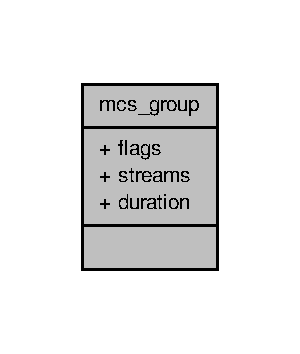
\includegraphics[width=144pt]{structmcs__group__coll__graph}
\end{center}
\end{figure}
\subsection*{Data Fields}
\begin{DoxyCompactItemize}
\item 
u32 \hyperlink{structmcs__group_a9fb2abd9f2594cefc48d6856e01f2879}{flags}
\item 
unsigned int \hyperlink{structmcs__group_af400861305cbf09d0a43140c4da1e152}{streams}
\item 
unsigned int \hyperlink{structmcs__group_a7a838228e55c3ac5d8d5395b20cf6a59}{duration} \mbox{[}\hyperlink{rc80211__minstrel__ht_8h_a1cce97ab419153d65e970112b74b5655}{M\-C\-S\-\_\-\-G\-R\-O\-U\-P\-\_\-\-R\-A\-T\-E\-S}\mbox{]}
\end{DoxyCompactItemize}


\subsection{Detailed Description}


Definition at line 26 of file rc80211\-\_\-minstrel\-\_\-ht.\-h.



\subsection{Field Documentation}
\hypertarget{structmcs__group_a7a838228e55c3ac5d8d5395b20cf6a59}{\index{mcs\-\_\-group@{mcs\-\_\-group}!duration@{duration}}
\index{duration@{duration}!mcs_group@{mcs\-\_\-group}}
\subsubsection[{duration}]{\setlength{\rightskip}{0pt plus 5cm}unsigned int duration\mbox{[}{\bf M\-C\-S\-\_\-\-G\-R\-O\-U\-P\-\_\-\-R\-A\-T\-E\-S}\mbox{]}}}\label{structmcs__group_a7a838228e55c3ac5d8d5395b20cf6a59}


Definition at line 29 of file rc80211\-\_\-minstrel\-\_\-ht.\-h.

\hypertarget{structmcs__group_a9fb2abd9f2594cefc48d6856e01f2879}{\index{mcs\-\_\-group@{mcs\-\_\-group}!flags@{flags}}
\index{flags@{flags}!mcs_group@{mcs\-\_\-group}}
\subsubsection[{flags}]{\setlength{\rightskip}{0pt plus 5cm}u32 flags}}\label{structmcs__group_a9fb2abd9f2594cefc48d6856e01f2879}


Definition at line 27 of file rc80211\-\_\-minstrel\-\_\-ht.\-h.

\hypertarget{structmcs__group_af400861305cbf09d0a43140c4da1e152}{\index{mcs\-\_\-group@{mcs\-\_\-group}!streams@{streams}}
\index{streams@{streams}!mcs_group@{mcs\-\_\-group}}
\subsubsection[{streams}]{\setlength{\rightskip}{0pt plus 5cm}unsigned int streams}}\label{structmcs__group_af400861305cbf09d0a43140c4da1e152}


Definition at line 28 of file rc80211\-\_\-minstrel\-\_\-ht.\-h.



The documentation for this struct was generated from the following file\-:\begin{DoxyCompactItemize}
\item 
/home/guille/msm/net/mac80211/\hyperlink{rc80211__minstrel__ht_8h}{rc80211\-\_\-minstrel\-\_\-ht.\-h}\end{DoxyCompactItemize}

\hypertarget{structmesh__path}{\section{mesh\-\_\-path Struct Reference}
\label{structmesh__path}\index{mesh\-\_\-path@{mesh\-\_\-path}}
}


{\ttfamily \#include $<$mesh.\-h$>$}



Collaboration diagram for mesh\-\_\-path\-:
\nopagebreak
\begin{figure}[H]
\begin{center}
\leavevmode
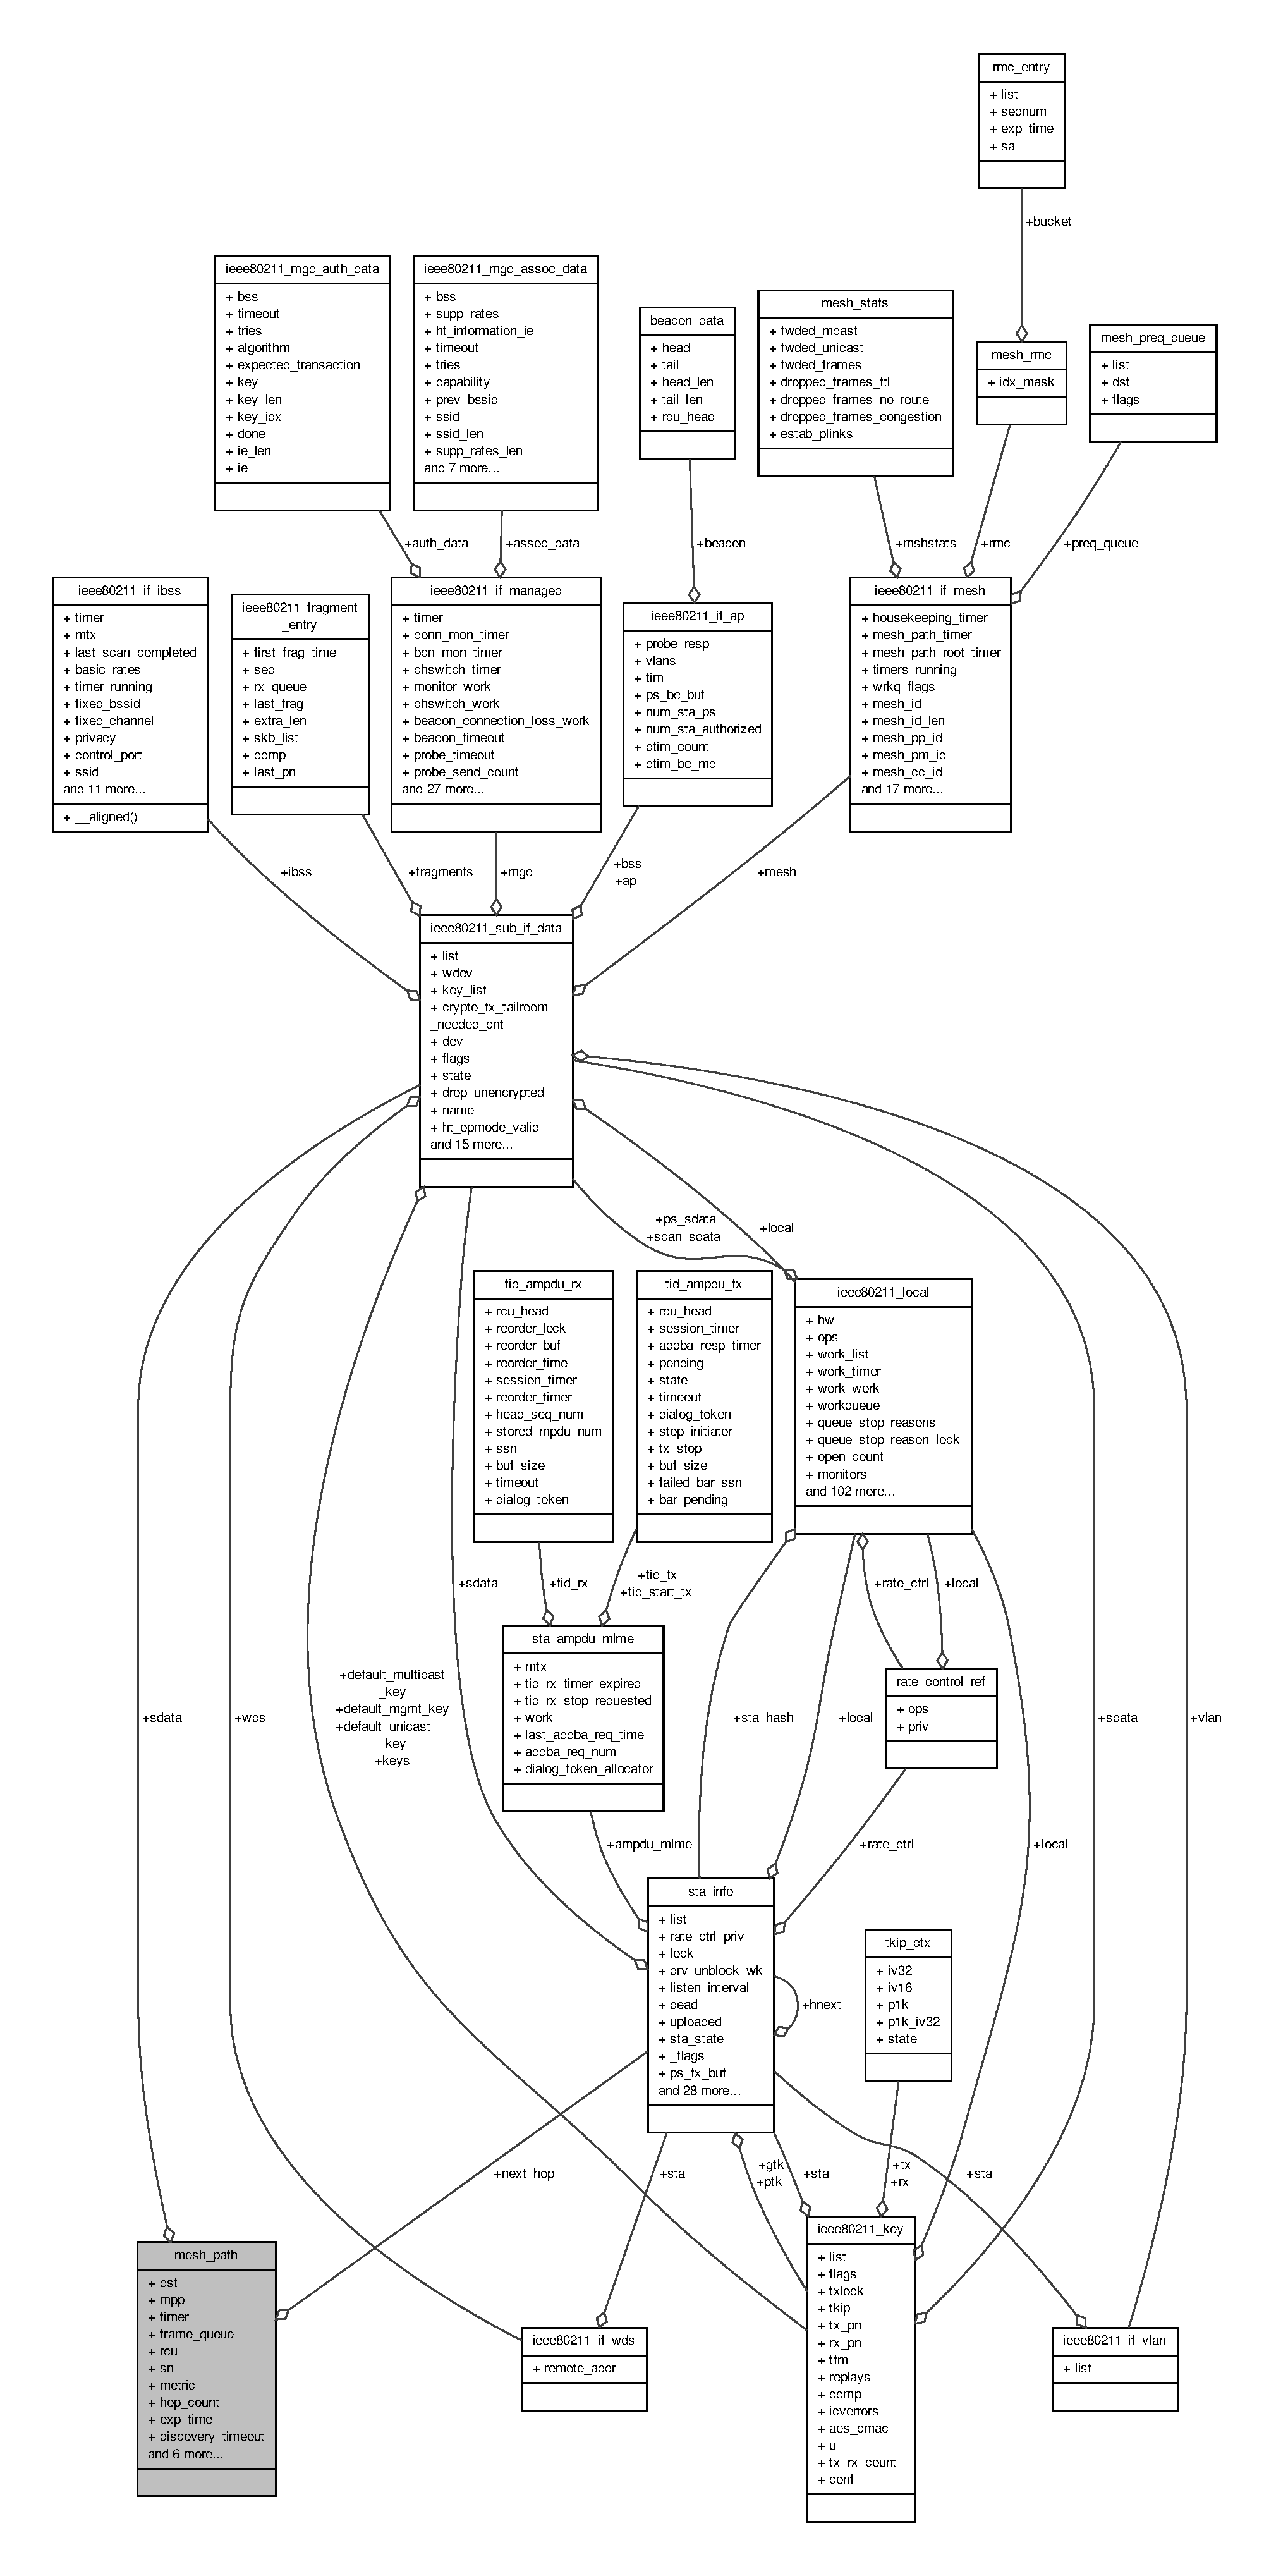
\includegraphics[height=550pt]{structmesh__path__coll__graph}
\end{center}
\end{figure}
\subsection*{Data Fields}
\begin{DoxyCompactItemize}
\item 
u8 \hyperlink{structmesh__path_a7e206c9dbce55c0147656b4e271c71e4}{dst} \mbox{[}E\-T\-H\-\_\-\-A\-L\-E\-N\mbox{]}
\item 
u8 \hyperlink{structmesh__path_a48b50421cfec4f69ffc3b753f7019185}{mpp} \mbox{[}E\-T\-H\-\_\-\-A\-L\-E\-N\mbox{]}
\item 
struct \hyperlink{structieee80211__sub__if__data}{ieee80211\-\_\-sub\-\_\-if\-\_\-data} $\ast$ \hyperlink{structmesh__path_ad829d8d33f06a7245cc303f924f259ac}{sdata}
\item 
struct \hyperlink{structsta__info}{sta\-\_\-info} \-\_\-\-\_\-rcu $\ast$ \hyperlink{structmesh__path_abc4b3146b43964101d2a25163375fed0}{next\-\_\-hop}
\item 
struct timer\-\_\-list \hyperlink{structmesh__path_ae8aedee6c0bd2f7edbb10f18d574f107}{timer}
\item 
struct sk\-\_\-buff\-\_\-head \hyperlink{structmesh__path_a78a751fa8f8fb1623ed2b86bd59017db}{frame\-\_\-queue}
\item 
struct rcu\-\_\-head \hyperlink{structmesh__path_aa9677537ffa4e40f3c4f3e9fb3b4c76d}{rcu}
\item 
u32 \hyperlink{structmesh__path_a3a5989b8e6d4286ac3822b65bbc1cf16}{sn}
\item 
u32 \hyperlink{structmesh__path_aecb5673e0ccbdfd6e104e917abc4bdfe}{metric}
\item 
u8 \hyperlink{structmesh__path_a65c900d253cc9afe77e2aa7a5c3ded5a}{hop\-\_\-count}
\item 
unsigned long \hyperlink{structmesh__path_af01b3e5a14761c34e4298e254fb7c094}{exp\-\_\-time}
\item 
u32 \hyperlink{structmesh__path_a7875d6c0fb79d3ecfa1bedcdbc7e9704}{discovery\-\_\-timeout}
\item 
u8 \hyperlink{structmesh__path_a7ce70c7ff6bf0aef3fec882ad4959555}{discovery\-\_\-retries}
\item 
enum \hyperlink{mesh_8h_a1108038688d583a88056a1ebebd89fa2}{mesh\-\_\-path\-\_\-flags} \hyperlink{structmesh__path_acdca1d9efeb99cd79e04eaaf7b94f159}{flags}
\item 
spinlock\-\_\-t \hyperlink{structmesh__path_a906a637c5d4df9d7a2a5a407cc01b8ac}{state\-\_\-lock}
\item 
u8 \hyperlink{structmesh__path_a3c1c259f27b1cdda2e17a81ff98a5310}{rann\-\_\-snd\-\_\-addr} \mbox{[}E\-T\-H\-\_\-\-A\-L\-E\-N\mbox{]}
\item 
bool \hyperlink{structmesh__path_a860e4167ebf87a0635c678a614b96a99}{is\-\_\-root}
\item 
bool \hyperlink{structmesh__path_a4399b726e2ce468eb33d179378d68e21}{is\-\_\-gate}
\end{DoxyCompactItemize}


\subsection{Detailed Description}
struct \hyperlink{structmesh__path}{mesh\-\_\-path} -\/ mac80211 mesh path structure

\-: mesh path destination mac address \-: mesh subif \-: mesh neighbor to which frames for this destination will be forwarded \-: mesh path discovery timer \-: pending queue for frames sent to this destination while the path is unresolved \-: target sequence number \-: current metric to this destination \-: hops to destination \-: in jiffies, when the path will expire or when it expired \-: timeout (lapse in jiffies) used for the last discovery retry \-: number of discovery retries \-: mesh path flags, as specified on \&enum mesh\-\_\-path\-\_\-flags \-: mesh path state lock used to protect changes to the mpath itself. No need to take this lock when adding or removing an mpath to a hash bucket on a path table. \-: the R\-A\-N\-N sender address \-: the destination station of this path is a root node \-: the destination station of this path is a mesh gate

The combination of dst and sdata is unique in the mesh path table. Since the next\-\_\-hop S\-T\-A is only protected by R\-C\-U as well, deleting the S\-T\-A must also remove/substitute the \hyperlink{structmesh__path}{mesh\-\_\-path} structure and wait until that is no longer reachable before destroying the S\-T\-A completely. 

Definition at line 98 of file mesh.\-h.



\subsection{Field Documentation}
\hypertarget{structmesh__path_a7ce70c7ff6bf0aef3fec882ad4959555}{\index{mesh\-\_\-path@{mesh\-\_\-path}!discovery\-\_\-retries@{discovery\-\_\-retries}}
\index{discovery\-\_\-retries@{discovery\-\_\-retries}!mesh_path@{mesh\-\_\-path}}
\subsubsection[{discovery\-\_\-retries}]{\setlength{\rightskip}{0pt plus 5cm}u8 discovery\-\_\-retries}}\label{structmesh__path_a7ce70c7ff6bf0aef3fec882ad4959555}


Definition at line 111 of file mesh.\-h.

\hypertarget{structmesh__path_a7875d6c0fb79d3ecfa1bedcdbc7e9704}{\index{mesh\-\_\-path@{mesh\-\_\-path}!discovery\-\_\-timeout@{discovery\-\_\-timeout}}
\index{discovery\-\_\-timeout@{discovery\-\_\-timeout}!mesh_path@{mesh\-\_\-path}}
\subsubsection[{discovery\-\_\-timeout}]{\setlength{\rightskip}{0pt plus 5cm}u32 discovery\-\_\-timeout}}\label{structmesh__path_a7875d6c0fb79d3ecfa1bedcdbc7e9704}


Definition at line 110 of file mesh.\-h.

\hypertarget{structmesh__path_a7e206c9dbce55c0147656b4e271c71e4}{\index{mesh\-\_\-path@{mesh\-\_\-path}!dst@{dst}}
\index{dst@{dst}!mesh_path@{mesh\-\_\-path}}
\subsubsection[{dst}]{\setlength{\rightskip}{0pt plus 5cm}u8 dst\mbox{[}E\-T\-H\-\_\-\-A\-L\-E\-N\mbox{]}}}\label{structmesh__path_a7e206c9dbce55c0147656b4e271c71e4}


Definition at line 99 of file mesh.\-h.

\hypertarget{structmesh__path_af01b3e5a14761c34e4298e254fb7c094}{\index{mesh\-\_\-path@{mesh\-\_\-path}!exp\-\_\-time@{exp\-\_\-time}}
\index{exp\-\_\-time@{exp\-\_\-time}!mesh_path@{mesh\-\_\-path}}
\subsubsection[{exp\-\_\-time}]{\setlength{\rightskip}{0pt plus 5cm}unsigned long exp\-\_\-time}}\label{structmesh__path_af01b3e5a14761c34e4298e254fb7c094}


Definition at line 109 of file mesh.\-h.

\hypertarget{structmesh__path_acdca1d9efeb99cd79e04eaaf7b94f159}{\index{mesh\-\_\-path@{mesh\-\_\-path}!flags@{flags}}
\index{flags@{flags}!mesh_path@{mesh\-\_\-path}}
\subsubsection[{flags}]{\setlength{\rightskip}{0pt plus 5cm}enum {\bf mesh\-\_\-path\-\_\-flags} flags}}\label{structmesh__path_acdca1d9efeb99cd79e04eaaf7b94f159}


Definition at line 112 of file mesh.\-h.

\hypertarget{structmesh__path_a78a751fa8f8fb1623ed2b86bd59017db}{\index{mesh\-\_\-path@{mesh\-\_\-path}!frame\-\_\-queue@{frame\-\_\-queue}}
\index{frame\-\_\-queue@{frame\-\_\-queue}!mesh_path@{mesh\-\_\-path}}
\subsubsection[{frame\-\_\-queue}]{\setlength{\rightskip}{0pt plus 5cm}struct sk\-\_\-buff\-\_\-head frame\-\_\-queue}}\label{structmesh__path_a78a751fa8f8fb1623ed2b86bd59017db}


Definition at line 104 of file mesh.\-h.

\hypertarget{structmesh__path_a65c900d253cc9afe77e2aa7a5c3ded5a}{\index{mesh\-\_\-path@{mesh\-\_\-path}!hop\-\_\-count@{hop\-\_\-count}}
\index{hop\-\_\-count@{hop\-\_\-count}!mesh_path@{mesh\-\_\-path}}
\subsubsection[{hop\-\_\-count}]{\setlength{\rightskip}{0pt plus 5cm}u8 hop\-\_\-count}}\label{structmesh__path_a65c900d253cc9afe77e2aa7a5c3ded5a}


Definition at line 108 of file mesh.\-h.

\hypertarget{structmesh__path_a4399b726e2ce468eb33d179378d68e21}{\index{mesh\-\_\-path@{mesh\-\_\-path}!is\-\_\-gate@{is\-\_\-gate}}
\index{is\-\_\-gate@{is\-\_\-gate}!mesh_path@{mesh\-\_\-path}}
\subsubsection[{is\-\_\-gate}]{\setlength{\rightskip}{0pt plus 5cm}bool is\-\_\-gate}}\label{structmesh__path_a4399b726e2ce468eb33d179378d68e21}


Definition at line 116 of file mesh.\-h.

\hypertarget{structmesh__path_a860e4167ebf87a0635c678a614b96a99}{\index{mesh\-\_\-path@{mesh\-\_\-path}!is\-\_\-root@{is\-\_\-root}}
\index{is\-\_\-root@{is\-\_\-root}!mesh_path@{mesh\-\_\-path}}
\subsubsection[{is\-\_\-root}]{\setlength{\rightskip}{0pt plus 5cm}bool is\-\_\-root}}\label{structmesh__path_a860e4167ebf87a0635c678a614b96a99}


Definition at line 115 of file mesh.\-h.

\hypertarget{structmesh__path_aecb5673e0ccbdfd6e104e917abc4bdfe}{\index{mesh\-\_\-path@{mesh\-\_\-path}!metric@{metric}}
\index{metric@{metric}!mesh_path@{mesh\-\_\-path}}
\subsubsection[{metric}]{\setlength{\rightskip}{0pt plus 5cm}u32 metric}}\label{structmesh__path_aecb5673e0ccbdfd6e104e917abc4bdfe}


Definition at line 107 of file mesh.\-h.

\hypertarget{structmesh__path_a48b50421cfec4f69ffc3b753f7019185}{\index{mesh\-\_\-path@{mesh\-\_\-path}!mpp@{mpp}}
\index{mpp@{mpp}!mesh_path@{mesh\-\_\-path}}
\subsubsection[{mpp}]{\setlength{\rightskip}{0pt plus 5cm}u8 mpp\mbox{[}E\-T\-H\-\_\-\-A\-L\-E\-N\mbox{]}}}\label{structmesh__path_a48b50421cfec4f69ffc3b753f7019185}


Definition at line 100 of file mesh.\-h.

\hypertarget{structmesh__path_abc4b3146b43964101d2a25163375fed0}{\index{mesh\-\_\-path@{mesh\-\_\-path}!next\-\_\-hop@{next\-\_\-hop}}
\index{next\-\_\-hop@{next\-\_\-hop}!mesh_path@{mesh\-\_\-path}}
\subsubsection[{next\-\_\-hop}]{\setlength{\rightskip}{0pt plus 5cm}struct {\bf sta\-\_\-info} \-\_\-\-\_\-rcu$\ast$ next\-\_\-hop}}\label{structmesh__path_abc4b3146b43964101d2a25163375fed0}


Definition at line 102 of file mesh.\-h.

\hypertarget{structmesh__path_a3c1c259f27b1cdda2e17a81ff98a5310}{\index{mesh\-\_\-path@{mesh\-\_\-path}!rann\-\_\-snd\-\_\-addr@{rann\-\_\-snd\-\_\-addr}}
\index{rann\-\_\-snd\-\_\-addr@{rann\-\_\-snd\-\_\-addr}!mesh_path@{mesh\-\_\-path}}
\subsubsection[{rann\-\_\-snd\-\_\-addr}]{\setlength{\rightskip}{0pt plus 5cm}u8 rann\-\_\-snd\-\_\-addr\mbox{[}E\-T\-H\-\_\-\-A\-L\-E\-N\mbox{]}}}\label{structmesh__path_a3c1c259f27b1cdda2e17a81ff98a5310}


Definition at line 114 of file mesh.\-h.

\hypertarget{structmesh__path_aa9677537ffa4e40f3c4f3e9fb3b4c76d}{\index{mesh\-\_\-path@{mesh\-\_\-path}!rcu@{rcu}}
\index{rcu@{rcu}!mesh_path@{mesh\-\_\-path}}
\subsubsection[{rcu}]{\setlength{\rightskip}{0pt plus 5cm}struct rcu\-\_\-head rcu}}\label{structmesh__path_aa9677537ffa4e40f3c4f3e9fb3b4c76d}


Definition at line 105 of file mesh.\-h.

\hypertarget{structmesh__path_ad829d8d33f06a7245cc303f924f259ac}{\index{mesh\-\_\-path@{mesh\-\_\-path}!sdata@{sdata}}
\index{sdata@{sdata}!mesh_path@{mesh\-\_\-path}}
\subsubsection[{sdata}]{\setlength{\rightskip}{0pt plus 5cm}struct {\bf ieee80211\-\_\-sub\-\_\-if\-\_\-data}$\ast$ sdata}}\label{structmesh__path_ad829d8d33f06a7245cc303f924f259ac}


Definition at line 101 of file mesh.\-h.

\hypertarget{structmesh__path_a3a5989b8e6d4286ac3822b65bbc1cf16}{\index{mesh\-\_\-path@{mesh\-\_\-path}!sn@{sn}}
\index{sn@{sn}!mesh_path@{mesh\-\_\-path}}
\subsubsection[{sn}]{\setlength{\rightskip}{0pt plus 5cm}u32 sn}}\label{structmesh__path_a3a5989b8e6d4286ac3822b65bbc1cf16}


Definition at line 106 of file mesh.\-h.

\hypertarget{structmesh__path_a906a637c5d4df9d7a2a5a407cc01b8ac}{\index{mesh\-\_\-path@{mesh\-\_\-path}!state\-\_\-lock@{state\-\_\-lock}}
\index{state\-\_\-lock@{state\-\_\-lock}!mesh_path@{mesh\-\_\-path}}
\subsubsection[{state\-\_\-lock}]{\setlength{\rightskip}{0pt plus 5cm}spinlock\-\_\-t state\-\_\-lock}}\label{structmesh__path_a906a637c5d4df9d7a2a5a407cc01b8ac}


Definition at line 113 of file mesh.\-h.

\hypertarget{structmesh__path_ae8aedee6c0bd2f7edbb10f18d574f107}{\index{mesh\-\_\-path@{mesh\-\_\-path}!timer@{timer}}
\index{timer@{timer}!mesh_path@{mesh\-\_\-path}}
\subsubsection[{timer}]{\setlength{\rightskip}{0pt plus 5cm}struct timer\-\_\-list timer}}\label{structmesh__path_ae8aedee6c0bd2f7edbb10f18d574f107}


Definition at line 103 of file mesh.\-h.



The documentation for this struct was generated from the following file\-:\begin{DoxyCompactItemize}
\item 
/home/guille/msm/net/mac80211/\hyperlink{mesh_8h}{mesh.\-h}\end{DoxyCompactItemize}

\hypertarget{structmesh__preq__queue}{\section{mesh\-\_\-preq\-\_\-queue Struct Reference}
\label{structmesh__preq__queue}\index{mesh\-\_\-preq\-\_\-queue@{mesh\-\_\-preq\-\_\-queue}}
}


{\ttfamily \#include $<$ieee80211\-\_\-i.\-h$>$}



Collaboration diagram for mesh\-\_\-preq\-\_\-queue\-:
\nopagebreak
\begin{figure}[H]
\begin{center}
\leavevmode
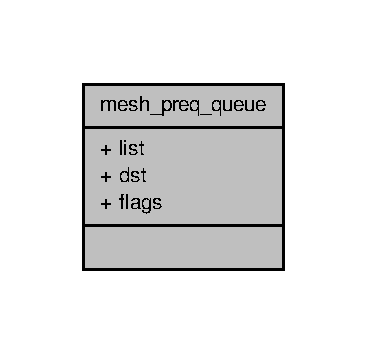
\includegraphics[width=176pt]{structmesh__preq__queue__coll__graph}
\end{center}
\end{figure}
\subsection*{Data Fields}
\begin{DoxyCompactItemize}
\item 
struct list\-\_\-head \hyperlink{structmesh__preq__queue_a1f00f18b91d5a820f2c43064243aa86e}{list}
\item 
u8 \hyperlink{structmesh__preq__queue_a7e206c9dbce55c0147656b4e271c71e4}{dst} \mbox{[}E\-T\-H\-\_\-\-A\-L\-E\-N\mbox{]}
\item 
u8 \hyperlink{structmesh__preq__queue_aa246fa433d167a7f6f8533227e40b76e}{flags}
\end{DoxyCompactItemize}


\subsection{Detailed Description}


Definition at line 313 of file ieee80211\-\_\-i.\-h.



\subsection{Field Documentation}
\hypertarget{structmesh__preq__queue_a7e206c9dbce55c0147656b4e271c71e4}{\index{mesh\-\_\-preq\-\_\-queue@{mesh\-\_\-preq\-\_\-queue}!dst@{dst}}
\index{dst@{dst}!mesh_preq_queue@{mesh\-\_\-preq\-\_\-queue}}
\subsubsection[{dst}]{\setlength{\rightskip}{0pt plus 5cm}u8 dst\mbox{[}E\-T\-H\-\_\-\-A\-L\-E\-N\mbox{]}}}\label{structmesh__preq__queue_a7e206c9dbce55c0147656b4e271c71e4}


Definition at line 315 of file ieee80211\-\_\-i.\-h.

\hypertarget{structmesh__preq__queue_aa246fa433d167a7f6f8533227e40b76e}{\index{mesh\-\_\-preq\-\_\-queue@{mesh\-\_\-preq\-\_\-queue}!flags@{flags}}
\index{flags@{flags}!mesh_preq_queue@{mesh\-\_\-preq\-\_\-queue}}
\subsubsection[{flags}]{\setlength{\rightskip}{0pt plus 5cm}u8 flags}}\label{structmesh__preq__queue_aa246fa433d167a7f6f8533227e40b76e}


Definition at line 316 of file ieee80211\-\_\-i.\-h.

\hypertarget{structmesh__preq__queue_a1f00f18b91d5a820f2c43064243aa86e}{\index{mesh\-\_\-preq\-\_\-queue@{mesh\-\_\-preq\-\_\-queue}!list@{list}}
\index{list@{list}!mesh_preq_queue@{mesh\-\_\-preq\-\_\-queue}}
\subsubsection[{list}]{\setlength{\rightskip}{0pt plus 5cm}struct list\-\_\-head list}}\label{structmesh__preq__queue_a1f00f18b91d5a820f2c43064243aa86e}


Definition at line 314 of file ieee80211\-\_\-i.\-h.



The documentation for this struct was generated from the following file\-:\begin{DoxyCompactItemize}
\item 
/home/guille/msm/net/mac80211/\hyperlink{ieee80211__i_8h}{ieee80211\-\_\-i.\-h}\end{DoxyCompactItemize}

\hypertarget{structmesh__rmc}{\section{mesh\-\_\-rmc Struct Reference}
\label{structmesh__rmc}\index{mesh\-\_\-rmc@{mesh\-\_\-rmc}}
}


{\ttfamily \#include $<$mesh.\-h$>$}



Collaboration diagram for mesh\-\_\-rmc\-:
\nopagebreak
\begin{figure}[H]
\begin{center}
\leavevmode
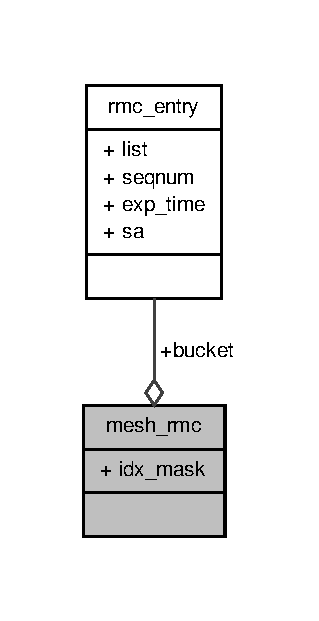
\includegraphics[width=153pt]{structmesh__rmc__coll__graph}
\end{center}
\end{figure}
\subsection*{Data Fields}
\begin{DoxyCompactItemize}
\item 
struct \hyperlink{structrmc__entry}{rmc\-\_\-entry} \hyperlink{structmesh__rmc_a65c3b74ae0afdff4662c4079c8bde59f}{bucket} \mbox{[}\hyperlink{mesh_8h_a2909ba21ed27a80429f34262b9dda565}{R\-M\-C\-\_\-\-B\-U\-C\-K\-E\-T\-S}\mbox{]}
\item 
u32 \hyperlink{structmesh__rmc_ae4f16a108310e98c6a5a222966147624}{idx\-\_\-mask}
\end{DoxyCompactItemize}


\subsection{Detailed Description}


Definition at line 179 of file mesh.\-h.



\subsection{Field Documentation}
\hypertarget{structmesh__rmc_a65c3b74ae0afdff4662c4079c8bde59f}{\index{mesh\-\_\-rmc@{mesh\-\_\-rmc}!bucket@{bucket}}
\index{bucket@{bucket}!mesh_rmc@{mesh\-\_\-rmc}}
\subsubsection[{bucket}]{\setlength{\rightskip}{0pt plus 5cm}struct {\bf rmc\-\_\-entry} bucket\mbox{[}{\bf R\-M\-C\-\_\-\-B\-U\-C\-K\-E\-T\-S}\mbox{]}}}\label{structmesh__rmc_a65c3b74ae0afdff4662c4079c8bde59f}


Definition at line 180 of file mesh.\-h.

\hypertarget{structmesh__rmc_ae4f16a108310e98c6a5a222966147624}{\index{mesh\-\_\-rmc@{mesh\-\_\-rmc}!idx\-\_\-mask@{idx\-\_\-mask}}
\index{idx\-\_\-mask@{idx\-\_\-mask}!mesh_rmc@{mesh\-\_\-rmc}}
\subsubsection[{idx\-\_\-mask}]{\setlength{\rightskip}{0pt plus 5cm}u32 idx\-\_\-mask}}\label{structmesh__rmc_ae4f16a108310e98c6a5a222966147624}


Definition at line 181 of file mesh.\-h.



The documentation for this struct was generated from the following file\-:\begin{DoxyCompactItemize}
\item 
/home/guille/msm/net/mac80211/\hyperlink{mesh_8h}{mesh.\-h}\end{DoxyCompactItemize}

\hypertarget{structmesh__stats}{\section{mesh\-\_\-stats Struct Reference}
\label{structmesh__stats}\index{mesh\-\_\-stats@{mesh\-\_\-stats}}
}


{\ttfamily \#include $<$ieee80211\-\_\-i.\-h$>$}



Collaboration diagram for mesh\-\_\-stats\-:
\nopagebreak
\begin{figure}[H]
\begin{center}
\leavevmode
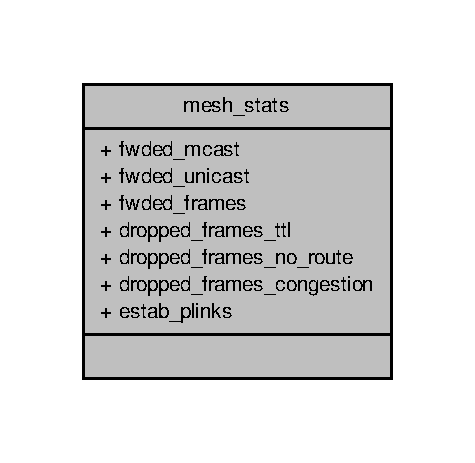
\includegraphics[width=228pt]{structmesh__stats__coll__graph}
\end{center}
\end{figure}
\subsection*{Data Fields}
\begin{DoxyCompactItemize}
\item 
\-\_\-\-\_\-u32 \hyperlink{structmesh__stats_a891b0def69cd36d51778d0688b7f312f}{fwded\-\_\-mcast}
\item 
\-\_\-\-\_\-u32 \hyperlink{structmesh__stats_a9e49222edd33b4bfe5705350a6d0938c}{fwded\-\_\-unicast}
\item 
\-\_\-\-\_\-u32 \hyperlink{structmesh__stats_a49a415a93a4c3e6864addddb23fd0d48}{fwded\-\_\-frames}
\item 
\-\_\-\-\_\-u32 \hyperlink{structmesh__stats_a4db3368b16b6cd0d3863947e74f3b968}{dropped\-\_\-frames\-\_\-ttl}
\item 
\-\_\-\-\_\-u32 \hyperlink{structmesh__stats_a41875880a535ab024bd05d2f5f26102c}{dropped\-\_\-frames\-\_\-no\-\_\-route}
\item 
\-\_\-\-\_\-u32 \hyperlink{structmesh__stats_add8222dd9919110e1c8395ad1a4f6110}{dropped\-\_\-frames\-\_\-congestion}
\item 
atomic\-\_\-t \hyperlink{structmesh__stats_a2e422d4c51c64bc57262ef857ee71127}{estab\-\_\-plinks}
\end{DoxyCompactItemize}


\subsection{Detailed Description}


Definition at line 301 of file ieee80211\-\_\-i.\-h.



\subsection{Field Documentation}
\hypertarget{structmesh__stats_add8222dd9919110e1c8395ad1a4f6110}{\index{mesh\-\_\-stats@{mesh\-\_\-stats}!dropped\-\_\-frames\-\_\-congestion@{dropped\-\_\-frames\-\_\-congestion}}
\index{dropped\-\_\-frames\-\_\-congestion@{dropped\-\_\-frames\-\_\-congestion}!mesh_stats@{mesh\-\_\-stats}}
\subsubsection[{dropped\-\_\-frames\-\_\-congestion}]{\setlength{\rightskip}{0pt plus 5cm}\-\_\-\-\_\-u32 dropped\-\_\-frames\-\_\-congestion}}\label{structmesh__stats_add8222dd9919110e1c8395ad1a4f6110}


Definition at line 307 of file ieee80211\-\_\-i.\-h.

\hypertarget{structmesh__stats_a41875880a535ab024bd05d2f5f26102c}{\index{mesh\-\_\-stats@{mesh\-\_\-stats}!dropped\-\_\-frames\-\_\-no\-\_\-route@{dropped\-\_\-frames\-\_\-no\-\_\-route}}
\index{dropped\-\_\-frames\-\_\-no\-\_\-route@{dropped\-\_\-frames\-\_\-no\-\_\-route}!mesh_stats@{mesh\-\_\-stats}}
\subsubsection[{dropped\-\_\-frames\-\_\-no\-\_\-route}]{\setlength{\rightskip}{0pt plus 5cm}\-\_\-\-\_\-u32 dropped\-\_\-frames\-\_\-no\-\_\-route}}\label{structmesh__stats_a41875880a535ab024bd05d2f5f26102c}


Definition at line 306 of file ieee80211\-\_\-i.\-h.

\hypertarget{structmesh__stats_a4db3368b16b6cd0d3863947e74f3b968}{\index{mesh\-\_\-stats@{mesh\-\_\-stats}!dropped\-\_\-frames\-\_\-ttl@{dropped\-\_\-frames\-\_\-ttl}}
\index{dropped\-\_\-frames\-\_\-ttl@{dropped\-\_\-frames\-\_\-ttl}!mesh_stats@{mesh\-\_\-stats}}
\subsubsection[{dropped\-\_\-frames\-\_\-ttl}]{\setlength{\rightskip}{0pt plus 5cm}\-\_\-\-\_\-u32 dropped\-\_\-frames\-\_\-ttl}}\label{structmesh__stats_a4db3368b16b6cd0d3863947e74f3b968}


Definition at line 305 of file ieee80211\-\_\-i.\-h.

\hypertarget{structmesh__stats_a2e422d4c51c64bc57262ef857ee71127}{\index{mesh\-\_\-stats@{mesh\-\_\-stats}!estab\-\_\-plinks@{estab\-\_\-plinks}}
\index{estab\-\_\-plinks@{estab\-\_\-plinks}!mesh_stats@{mesh\-\_\-stats}}
\subsubsection[{estab\-\_\-plinks}]{\setlength{\rightskip}{0pt plus 5cm}atomic\-\_\-t estab\-\_\-plinks}}\label{structmesh__stats_a2e422d4c51c64bc57262ef857ee71127}


Definition at line 308 of file ieee80211\-\_\-i.\-h.

\hypertarget{structmesh__stats_a49a415a93a4c3e6864addddb23fd0d48}{\index{mesh\-\_\-stats@{mesh\-\_\-stats}!fwded\-\_\-frames@{fwded\-\_\-frames}}
\index{fwded\-\_\-frames@{fwded\-\_\-frames}!mesh_stats@{mesh\-\_\-stats}}
\subsubsection[{fwded\-\_\-frames}]{\setlength{\rightskip}{0pt plus 5cm}\-\_\-\-\_\-u32 fwded\-\_\-frames}}\label{structmesh__stats_a49a415a93a4c3e6864addddb23fd0d48}


Definition at line 304 of file ieee80211\-\_\-i.\-h.

\hypertarget{structmesh__stats_a891b0def69cd36d51778d0688b7f312f}{\index{mesh\-\_\-stats@{mesh\-\_\-stats}!fwded\-\_\-mcast@{fwded\-\_\-mcast}}
\index{fwded\-\_\-mcast@{fwded\-\_\-mcast}!mesh_stats@{mesh\-\_\-stats}}
\subsubsection[{fwded\-\_\-mcast}]{\setlength{\rightskip}{0pt plus 5cm}\-\_\-\-\_\-u32 fwded\-\_\-mcast}}\label{structmesh__stats_a891b0def69cd36d51778d0688b7f312f}


Definition at line 302 of file ieee80211\-\_\-i.\-h.

\hypertarget{structmesh__stats_a9e49222edd33b4bfe5705350a6d0938c}{\index{mesh\-\_\-stats@{mesh\-\_\-stats}!fwded\-\_\-unicast@{fwded\-\_\-unicast}}
\index{fwded\-\_\-unicast@{fwded\-\_\-unicast}!mesh_stats@{mesh\-\_\-stats}}
\subsubsection[{fwded\-\_\-unicast}]{\setlength{\rightskip}{0pt plus 5cm}\-\_\-\-\_\-u32 fwded\-\_\-unicast}}\label{structmesh__stats_a9e49222edd33b4bfe5705350a6d0938c}


Definition at line 303 of file ieee80211\-\_\-i.\-h.



The documentation for this struct was generated from the following file\-:\begin{DoxyCompactItemize}
\item 
/home/guille/msm/net/mac80211/\hyperlink{ieee80211__i_8h}{ieee80211\-\_\-i.\-h}\end{DoxyCompactItemize}

\hypertarget{structmesh__table}{\section{mesh\-\_\-table Struct Reference}
\label{structmesh__table}\index{mesh\-\_\-table@{mesh\-\_\-table}}
}


{\ttfamily \#include $<$mesh.\-h$>$}



Collaboration diagram for mesh\-\_\-table\-:
\nopagebreak
\begin{figure}[H]
\begin{center}
\leavevmode
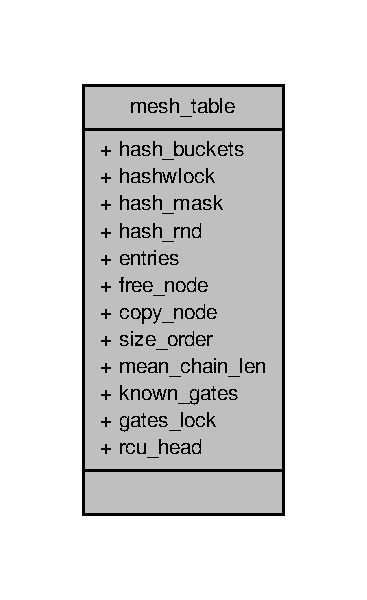
\includegraphics[width=176pt]{structmesh__table__coll__graph}
\end{center}
\end{figure}
\subsection*{Data Fields}
\begin{DoxyCompactItemize}
\item 
struct hlist\-\_\-head $\ast$ \hyperlink{structmesh__table_a04eadd518c34fb4fff4aaed97e1234e0}{hash\-\_\-buckets}
\item 
spinlock\-\_\-t $\ast$ \hyperlink{structmesh__table_a26e336e1f797741f588ac094b1ac0202}{hashwlock}
\item 
unsigned int \hyperlink{structmesh__table_a379901d7620aa43cd8472e2c189af861}{hash\-\_\-mask}
\item 
\-\_\-\-\_\-u32 \hyperlink{structmesh__table_aefd9eaac521878de0638370ef2c70d71}{hash\-\_\-rnd}
\item 
atomic\-\_\-t \hyperlink{structmesh__table_ad87bb8a66d6cd622bda213e2edf6c4a2}{entries}
\item 
void($\ast$ \hyperlink{structmesh__table_a9779fca079801066cd605af403cc1eea}{free\-\_\-node} )(struct hlist\-\_\-node $\ast$p, bool free\-\_\-leafs)
\item 
int($\ast$ \hyperlink{structmesh__table_ad8a4389f749adafe9393ad7be19be3bc}{copy\-\_\-node} )(struct hlist\-\_\-node $\ast$p, struct \hyperlink{structmesh__table}{mesh\-\_\-table} $\ast$newtbl)
\item 
int \hyperlink{structmesh__table_af2ece8f794fc2b70104b44cde3421003}{size\-\_\-order}
\item 
int \hyperlink{structmesh__table_a05410cec7cda00c16011e39666056c20}{mean\-\_\-chain\-\_\-len}
\item 
struct hlist\-\_\-head $\ast$ \hyperlink{structmesh__table_a3c40962f5ca0faa5387ad1e91a2c7ba6}{known\-\_\-gates}
\item 
spinlock\-\_\-t \hyperlink{structmesh__table_aa4d60ff62c57e22498c2aac249c29391}{gates\-\_\-lock}
\item 
struct rcu\-\_\-head \hyperlink{structmesh__table_ab698383409a24791490f962fe6990655}{rcu\-\_\-head}
\end{DoxyCompactItemize}


\subsection{Detailed Description}
struct \hyperlink{structmesh__table}{mesh\-\_\-table}

\-: array of hash buckets of the table \-: array of locks to protect write operations, one per bucket \-: 2$^\wedge$size\-\_\-order -\/ 1, used to compute hash idx \-: random value used for hash computations \-: number of entries in the table \-: function to free nodes of the table \-: function to copy nodes of the table \-: determines size of the table, there will be 2$^\wedge$size\-\_\-order hash buckets \-: maximum average length for the hash buckets' list, if it is reached, the table will grow \-: list of known mesh gates and their mpaths by the station. The gate's mpath may or may not be resolved and active.

rcu\-\_\-head\-: R\-C\-U head to free the table 

Definition at line 138 of file mesh.\-h.



\subsection{Field Documentation}
\hypertarget{structmesh__table_ad8a4389f749adafe9393ad7be19be3bc}{\index{mesh\-\_\-table@{mesh\-\_\-table}!copy\-\_\-node@{copy\-\_\-node}}
\index{copy\-\_\-node@{copy\-\_\-node}!mesh_table@{mesh\-\_\-table}}
\subsubsection[{copy\-\_\-node}]{\setlength{\rightskip}{0pt plus 5cm}int($\ast$ copy\-\_\-node)(struct hlist\-\_\-node $\ast$p, struct {\bf mesh\-\_\-table} $\ast$newtbl)}}\label{structmesh__table_ad8a4389f749adafe9393ad7be19be3bc}


Definition at line 146 of file mesh.\-h.

\hypertarget{structmesh__table_ad87bb8a66d6cd622bda213e2edf6c4a2}{\index{mesh\-\_\-table@{mesh\-\_\-table}!entries@{entries}}
\index{entries@{entries}!mesh_table@{mesh\-\_\-table}}
\subsubsection[{entries}]{\setlength{\rightskip}{0pt plus 5cm}atomic\-\_\-t entries}}\label{structmesh__table_ad87bb8a66d6cd622bda213e2edf6c4a2}


Definition at line 144 of file mesh.\-h.

\hypertarget{structmesh__table_a9779fca079801066cd605af403cc1eea}{\index{mesh\-\_\-table@{mesh\-\_\-table}!free\-\_\-node@{free\-\_\-node}}
\index{free\-\_\-node@{free\-\_\-node}!mesh_table@{mesh\-\_\-table}}
\subsubsection[{free\-\_\-node}]{\setlength{\rightskip}{0pt plus 5cm}void($\ast$ free\-\_\-node)(struct hlist\-\_\-node $\ast$p, bool free\-\_\-leafs)}}\label{structmesh__table_a9779fca079801066cd605af403cc1eea}


Definition at line 145 of file mesh.\-h.

\hypertarget{structmesh__table_aa4d60ff62c57e22498c2aac249c29391}{\index{mesh\-\_\-table@{mesh\-\_\-table}!gates\-\_\-lock@{gates\-\_\-lock}}
\index{gates\-\_\-lock@{gates\-\_\-lock}!mesh_table@{mesh\-\_\-table}}
\subsubsection[{gates\-\_\-lock}]{\setlength{\rightskip}{0pt plus 5cm}spinlock\-\_\-t gates\-\_\-lock}}\label{structmesh__table_aa4d60ff62c57e22498c2aac249c29391}


Definition at line 150 of file mesh.\-h.

\hypertarget{structmesh__table_a04eadd518c34fb4fff4aaed97e1234e0}{\index{mesh\-\_\-table@{mesh\-\_\-table}!hash\-\_\-buckets@{hash\-\_\-buckets}}
\index{hash\-\_\-buckets@{hash\-\_\-buckets}!mesh_table@{mesh\-\_\-table}}
\subsubsection[{hash\-\_\-buckets}]{\setlength{\rightskip}{0pt plus 5cm}struct hlist\-\_\-head$\ast$ hash\-\_\-buckets}}\label{structmesh__table_a04eadd518c34fb4fff4aaed97e1234e0}


Definition at line 140 of file mesh.\-h.

\hypertarget{structmesh__table_a379901d7620aa43cd8472e2c189af861}{\index{mesh\-\_\-table@{mesh\-\_\-table}!hash\-\_\-mask@{hash\-\_\-mask}}
\index{hash\-\_\-mask@{hash\-\_\-mask}!mesh_table@{mesh\-\_\-table}}
\subsubsection[{hash\-\_\-mask}]{\setlength{\rightskip}{0pt plus 5cm}unsigned int hash\-\_\-mask}}\label{structmesh__table_a379901d7620aa43cd8472e2c189af861}


Definition at line 142 of file mesh.\-h.

\hypertarget{structmesh__table_aefd9eaac521878de0638370ef2c70d71}{\index{mesh\-\_\-table@{mesh\-\_\-table}!hash\-\_\-rnd@{hash\-\_\-rnd}}
\index{hash\-\_\-rnd@{hash\-\_\-rnd}!mesh_table@{mesh\-\_\-table}}
\subsubsection[{hash\-\_\-rnd}]{\setlength{\rightskip}{0pt plus 5cm}\-\_\-\-\_\-u32 hash\-\_\-rnd}}\label{structmesh__table_aefd9eaac521878de0638370ef2c70d71}


Definition at line 143 of file mesh.\-h.

\hypertarget{structmesh__table_a26e336e1f797741f588ac094b1ac0202}{\index{mesh\-\_\-table@{mesh\-\_\-table}!hashwlock@{hashwlock}}
\index{hashwlock@{hashwlock}!mesh_table@{mesh\-\_\-table}}
\subsubsection[{hashwlock}]{\setlength{\rightskip}{0pt plus 5cm}spinlock\-\_\-t$\ast$ hashwlock}}\label{structmesh__table_a26e336e1f797741f588ac094b1ac0202}


Definition at line 141 of file mesh.\-h.

\hypertarget{structmesh__table_a3c40962f5ca0faa5387ad1e91a2c7ba6}{\index{mesh\-\_\-table@{mesh\-\_\-table}!known\-\_\-gates@{known\-\_\-gates}}
\index{known\-\_\-gates@{known\-\_\-gates}!mesh_table@{mesh\-\_\-table}}
\subsubsection[{known\-\_\-gates}]{\setlength{\rightskip}{0pt plus 5cm}struct hlist\-\_\-head$\ast$ known\-\_\-gates}}\label{structmesh__table_a3c40962f5ca0faa5387ad1e91a2c7ba6}


Definition at line 149 of file mesh.\-h.

\hypertarget{structmesh__table_a05410cec7cda00c16011e39666056c20}{\index{mesh\-\_\-table@{mesh\-\_\-table}!mean\-\_\-chain\-\_\-len@{mean\-\_\-chain\-\_\-len}}
\index{mean\-\_\-chain\-\_\-len@{mean\-\_\-chain\-\_\-len}!mesh_table@{mesh\-\_\-table}}
\subsubsection[{mean\-\_\-chain\-\_\-len}]{\setlength{\rightskip}{0pt plus 5cm}int mean\-\_\-chain\-\_\-len}}\label{structmesh__table_a05410cec7cda00c16011e39666056c20}


Definition at line 148 of file mesh.\-h.

\hypertarget{structmesh__table_ab698383409a24791490f962fe6990655}{\index{mesh\-\_\-table@{mesh\-\_\-table}!rcu\-\_\-head@{rcu\-\_\-head}}
\index{rcu\-\_\-head@{rcu\-\_\-head}!mesh_table@{mesh\-\_\-table}}
\subsubsection[{rcu\-\_\-head}]{\setlength{\rightskip}{0pt plus 5cm}struct rcu\-\_\-head rcu\-\_\-head}}\label{structmesh__table_ab698383409a24791490f962fe6990655}


Definition at line 152 of file mesh.\-h.

\hypertarget{structmesh__table_af2ece8f794fc2b70104b44cde3421003}{\index{mesh\-\_\-table@{mesh\-\_\-table}!size\-\_\-order@{size\-\_\-order}}
\index{size\-\_\-order@{size\-\_\-order}!mesh_table@{mesh\-\_\-table}}
\subsubsection[{size\-\_\-order}]{\setlength{\rightskip}{0pt plus 5cm}int size\-\_\-order}}\label{structmesh__table_af2ece8f794fc2b70104b44cde3421003}


Definition at line 147 of file mesh.\-h.



The documentation for this struct was generated from the following file\-:\begin{DoxyCompactItemize}
\item 
/home/guille/msm/net/mac80211/\hyperlink{mesh_8h}{mesh.\-h}\end{DoxyCompactItemize}

\hypertarget{structmichael__mic__ctx}{\section{michael\-\_\-mic\-\_\-ctx Struct Reference}
\label{structmichael__mic__ctx}\index{michael\-\_\-mic\-\_\-ctx@{michael\-\_\-mic\-\_\-ctx}}
}


{\ttfamily \#include $<$michael.\-h$>$}



Collaboration diagram for michael\-\_\-mic\-\_\-ctx\-:
\nopagebreak
\begin{figure}[H]
\begin{center}
\leavevmode
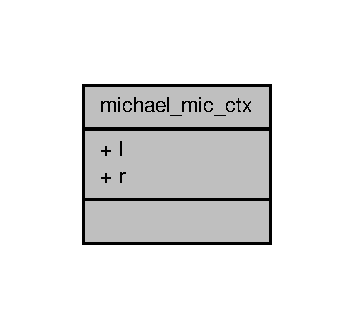
\includegraphics[width=170pt]{structmichael__mic__ctx__coll__graph}
\end{center}
\end{figure}
\subsection*{Data Fields}
\begin{DoxyCompactItemize}
\item 
u32 \hyperlink{structmichael__mic__ctx_a97b22435f07e68bf751cddd2226228ab}{l}
\item 
u32 \hyperlink{structmichael__mic__ctx_a4c24b5b7511b13fa815f1ef250c4d40a}{r}
\end{DoxyCompactItemize}


\subsection{Detailed Description}


Definition at line 17 of file michael.\-h.



\subsection{Field Documentation}
\hypertarget{structmichael__mic__ctx_a97b22435f07e68bf751cddd2226228ab}{\index{michael\-\_\-mic\-\_\-ctx@{michael\-\_\-mic\-\_\-ctx}!l@{l}}
\index{l@{l}!michael_mic_ctx@{michael\-\_\-mic\-\_\-ctx}}
\subsubsection[{l}]{\setlength{\rightskip}{0pt plus 5cm}u32 l}}\label{structmichael__mic__ctx_a97b22435f07e68bf751cddd2226228ab}


Definition at line 18 of file michael.\-h.

\hypertarget{structmichael__mic__ctx_a4c24b5b7511b13fa815f1ef250c4d40a}{\index{michael\-\_\-mic\-\_\-ctx@{michael\-\_\-mic\-\_\-ctx}!r@{r}}
\index{r@{r}!michael_mic_ctx@{michael\-\_\-mic\-\_\-ctx}}
\subsubsection[{r}]{\setlength{\rightskip}{0pt plus 5cm}u32 r}}\label{structmichael__mic__ctx_a4c24b5b7511b13fa815f1ef250c4d40a}


Definition at line 18 of file michael.\-h.



The documentation for this struct was generated from the following file\-:\begin{DoxyCompactItemize}
\item 
/home/guille/msm/net/mac80211/\hyperlink{michael_8h}{michael.\-h}\end{DoxyCompactItemize}

\hypertarget{structminstrel__debugfs__info}{\section{minstrel\-\_\-debugfs\-\_\-info Struct Reference}
\label{structminstrel__debugfs__info}\index{minstrel\-\_\-debugfs\-\_\-info@{minstrel\-\_\-debugfs\-\_\-info}}
}


{\ttfamily \#include $<$rc80211\-\_\-minstrel.\-h$>$}



Collaboration diagram for minstrel\-\_\-debugfs\-\_\-info\-:
\nopagebreak
\begin{figure}[H]
\begin{center}
\leavevmode
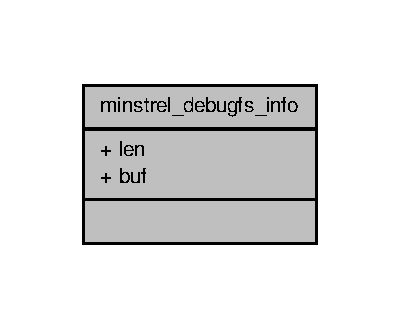
\includegraphics[width=192pt]{structminstrel__debugfs__info__coll__graph}
\end{center}
\end{figure}
\subsection*{Data Fields}
\begin{DoxyCompactItemize}
\item 
size\-\_\-t \hyperlink{structminstrel__debugfs__info_a7360b55975153b822efc5217b7734e6a}{len}
\item 
char \hyperlink{structminstrel__debugfs__info_a781718f5b53a876fe91c424c4607fa8f}{buf} \mbox{[}$\,$\mbox{]}
\end{DoxyCompactItemize}


\subsection{Detailed Description}


Definition at line 95 of file rc80211\-\_\-minstrel.\-h.



\subsection{Field Documentation}
\hypertarget{structminstrel__debugfs__info_a781718f5b53a876fe91c424c4607fa8f}{\index{minstrel\-\_\-debugfs\-\_\-info@{minstrel\-\_\-debugfs\-\_\-info}!buf@{buf}}
\index{buf@{buf}!minstrel_debugfs_info@{minstrel\-\_\-debugfs\-\_\-info}}
\subsubsection[{buf}]{\setlength{\rightskip}{0pt plus 5cm}char buf\mbox{[}$\,$\mbox{]}}}\label{structminstrel__debugfs__info_a781718f5b53a876fe91c424c4607fa8f}


Definition at line 97 of file rc80211\-\_\-minstrel.\-h.

\hypertarget{structminstrel__debugfs__info_a7360b55975153b822efc5217b7734e6a}{\index{minstrel\-\_\-debugfs\-\_\-info@{minstrel\-\_\-debugfs\-\_\-info}!len@{len}}
\index{len@{len}!minstrel_debugfs_info@{minstrel\-\_\-debugfs\-\_\-info}}
\subsubsection[{len}]{\setlength{\rightskip}{0pt plus 5cm}size\-\_\-t len}}\label{structminstrel__debugfs__info_a7360b55975153b822efc5217b7734e6a}


Definition at line 96 of file rc80211\-\_\-minstrel.\-h.



The documentation for this struct was generated from the following file\-:\begin{DoxyCompactItemize}
\item 
/home/guille/msm/net/mac80211/\hyperlink{rc80211__minstrel_8h}{rc80211\-\_\-minstrel.\-h}\end{DoxyCompactItemize}

\hypertarget{structminstrel__ht__sta}{\section{minstrel\-\_\-ht\-\_\-sta Struct Reference}
\label{structminstrel__ht__sta}\index{minstrel\-\_\-ht\-\_\-sta@{minstrel\-\_\-ht\-\_\-sta}}
}


{\ttfamily \#include $<$rc80211\-\_\-minstrel\-\_\-ht.\-h$>$}



Collaboration diagram for minstrel\-\_\-ht\-\_\-sta\-:
\nopagebreak
\begin{figure}[H]
\begin{center}
\leavevmode
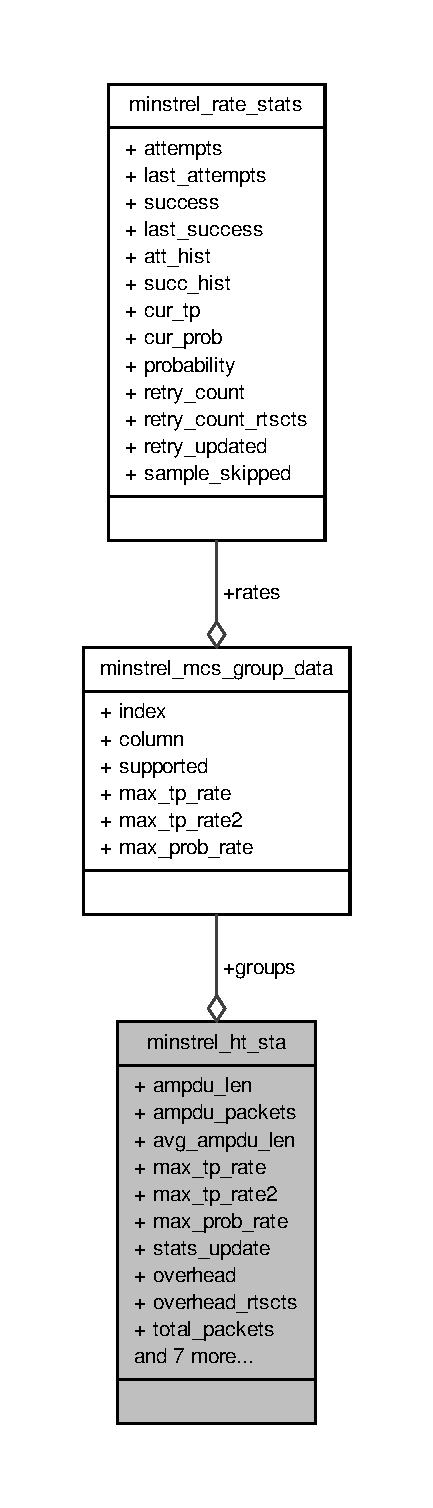
\includegraphics[height=550pt]{structminstrel__ht__sta__coll__graph}
\end{center}
\end{figure}
\subsection*{Data Fields}
\begin{DoxyCompactItemize}
\item 
unsigned int \hyperlink{structminstrel__ht__sta_a81226895623781d8762fd45b25d44ae2}{ampdu\-\_\-len}
\item 
unsigned int \hyperlink{structminstrel__ht__sta_a0cc9c3c7d1f2e54ec3dcf85c128d5d86}{ampdu\-\_\-packets}
\item 
unsigned int \hyperlink{structminstrel__ht__sta_a7615bb62088013811f751b053ca9045d}{avg\-\_\-ampdu\-\_\-len}
\item 
unsigned int \hyperlink{structminstrel__ht__sta_ae61b14461f5cfea710f666fe40906493}{max\-\_\-tp\-\_\-rate}
\item 
unsigned int \hyperlink{structminstrel__ht__sta_aaa4f3e0147c91173f7dd6d86b82ba0ee}{max\-\_\-tp\-\_\-rate2}
\item 
unsigned int \hyperlink{structminstrel__ht__sta_a4a4625871f05851116acae11b392a957}{max\-\_\-prob\-\_\-rate}
\item 
unsigned long \hyperlink{structminstrel__ht__sta_a3c5301bb7fd4073bbad86d50eff8f188}{stats\-\_\-update}
\item 
unsigned int \hyperlink{structminstrel__ht__sta_a0765a78b57d601d73281773e3e0b129d}{overhead}
\item 
unsigned int \hyperlink{structminstrel__ht__sta_afcd824a51bf0fbc50e8d7798d7c9c4eb}{overhead\-\_\-rtscts}
\item 
unsigned int \hyperlink{structminstrel__ht__sta_a6faab394a49c8462592c339de9d60855}{total\-\_\-packets}
\item 
unsigned int \hyperlink{structminstrel__ht__sta_a7a98923c9bfaab59c35970660fe7ef6f}{sample\-\_\-packets}
\item 
u32 \hyperlink{structminstrel__ht__sta_a428012b2ca384e2898d6389025a7b6db}{tx\-\_\-flags}
\item 
u8 \hyperlink{structminstrel__ht__sta_ac908c67104c56185324bcbc21da68959}{sample\-\_\-wait}
\item 
u8 \hyperlink{structminstrel__ht__sta_a0c58b0d161933e7f86d6dada5438ca88}{sample\-\_\-tries}
\item 
u8 \hyperlink{structminstrel__ht__sta_a344a0db2b0250fb750c41b09a5b2c02c}{sample\-\_\-count}
\item 
u8 \hyperlink{structminstrel__ht__sta_a64adb5d8e07f2fe59ee79d6062759a4c}{sample\-\_\-slow}
\item 
u8 \hyperlink{structminstrel__ht__sta_a0d383c66830af0f8410c63cbf3c55273}{sample\-\_\-group}
\item 
struct \hyperlink{structminstrel__mcs__group__data}{minstrel\-\_\-mcs\-\_\-group\-\_\-data} \hyperlink{structminstrel__ht__sta_ae1ef634bc381d48809efc8efdf2757c2}{groups} \mbox{[}\hyperlink{rc80211__minstrel__ht_8h_a158e497cdbf9ea61badd923e095cb3d4}{M\-I\-N\-S\-T\-R\-E\-L\-\_\-\-M\-A\-X\-\_\-\-S\-T\-R\-E\-A\-M\-S} $\ast$\hyperlink{rc80211__minstrel__ht_8h_a392070f099c290936c19a9674a383602}{M\-I\-N\-S\-T\-R\-E\-L\-\_\-\-S\-T\-R\-E\-A\-M\-\_\-\-G\-R\-O\-U\-P\-S}\mbox{]}
\end{DoxyCompactItemize}


\subsection{Detailed Description}


Definition at line 72 of file rc80211\-\_\-minstrel\-\_\-ht.\-h.



\subsection{Field Documentation}
\hypertarget{structminstrel__ht__sta_a81226895623781d8762fd45b25d44ae2}{\index{minstrel\-\_\-ht\-\_\-sta@{minstrel\-\_\-ht\-\_\-sta}!ampdu\-\_\-len@{ampdu\-\_\-len}}
\index{ampdu\-\_\-len@{ampdu\-\_\-len}!minstrel_ht_sta@{minstrel\-\_\-ht\-\_\-sta}}
\subsubsection[{ampdu\-\_\-len}]{\setlength{\rightskip}{0pt plus 5cm}unsigned int ampdu\-\_\-len}}\label{structminstrel__ht__sta_a81226895623781d8762fd45b25d44ae2}


Definition at line 74 of file rc80211\-\_\-minstrel\-\_\-ht.\-h.

\hypertarget{structminstrel__ht__sta_a0cc9c3c7d1f2e54ec3dcf85c128d5d86}{\index{minstrel\-\_\-ht\-\_\-sta@{minstrel\-\_\-ht\-\_\-sta}!ampdu\-\_\-packets@{ampdu\-\_\-packets}}
\index{ampdu\-\_\-packets@{ampdu\-\_\-packets}!minstrel_ht_sta@{minstrel\-\_\-ht\-\_\-sta}}
\subsubsection[{ampdu\-\_\-packets}]{\setlength{\rightskip}{0pt plus 5cm}unsigned int ampdu\-\_\-packets}}\label{structminstrel__ht__sta_a0cc9c3c7d1f2e54ec3dcf85c128d5d86}


Definition at line 75 of file rc80211\-\_\-minstrel\-\_\-ht.\-h.

\hypertarget{structminstrel__ht__sta_a7615bb62088013811f751b053ca9045d}{\index{minstrel\-\_\-ht\-\_\-sta@{minstrel\-\_\-ht\-\_\-sta}!avg\-\_\-ampdu\-\_\-len@{avg\-\_\-ampdu\-\_\-len}}
\index{avg\-\_\-ampdu\-\_\-len@{avg\-\_\-ampdu\-\_\-len}!minstrel_ht_sta@{minstrel\-\_\-ht\-\_\-sta}}
\subsubsection[{avg\-\_\-ampdu\-\_\-len}]{\setlength{\rightskip}{0pt plus 5cm}unsigned int avg\-\_\-ampdu\-\_\-len}}\label{structminstrel__ht__sta_a7615bb62088013811f751b053ca9045d}


Definition at line 78 of file rc80211\-\_\-minstrel\-\_\-ht.\-h.

\hypertarget{structminstrel__ht__sta_ae1ef634bc381d48809efc8efdf2757c2}{\index{minstrel\-\_\-ht\-\_\-sta@{minstrel\-\_\-ht\-\_\-sta}!groups@{groups}}
\index{groups@{groups}!minstrel_ht_sta@{minstrel\-\_\-ht\-\_\-sta}}
\subsubsection[{groups}]{\setlength{\rightskip}{0pt plus 5cm}struct {\bf minstrel\-\_\-mcs\-\_\-group\-\_\-data} groups\mbox{[}{\bf M\-I\-N\-S\-T\-R\-E\-L\-\_\-\-M\-A\-X\-\_\-\-S\-T\-R\-E\-A\-M\-S} $\ast${\bf M\-I\-N\-S\-T\-R\-E\-L\-\_\-\-S\-T\-R\-E\-A\-M\-\_\-\-G\-R\-O\-U\-P\-S}\mbox{]}}}\label{structminstrel__ht__sta_ae1ef634bc381d48809efc8efdf2757c2}


Definition at line 111 of file rc80211\-\_\-minstrel\-\_\-ht.\-h.

\hypertarget{structminstrel__ht__sta_a4a4625871f05851116acae11b392a957}{\index{minstrel\-\_\-ht\-\_\-sta@{minstrel\-\_\-ht\-\_\-sta}!max\-\_\-prob\-\_\-rate@{max\-\_\-prob\-\_\-rate}}
\index{max\-\_\-prob\-\_\-rate@{max\-\_\-prob\-\_\-rate}!minstrel_ht_sta@{minstrel\-\_\-ht\-\_\-sta}}
\subsubsection[{max\-\_\-prob\-\_\-rate}]{\setlength{\rightskip}{0pt plus 5cm}unsigned int max\-\_\-prob\-\_\-rate}}\label{structminstrel__ht__sta_a4a4625871f05851116acae11b392a957}


Definition at line 87 of file rc80211\-\_\-minstrel\-\_\-ht.\-h.

\hypertarget{structminstrel__ht__sta_ae61b14461f5cfea710f666fe40906493}{\index{minstrel\-\_\-ht\-\_\-sta@{minstrel\-\_\-ht\-\_\-sta}!max\-\_\-tp\-\_\-rate@{max\-\_\-tp\-\_\-rate}}
\index{max\-\_\-tp\-\_\-rate@{max\-\_\-tp\-\_\-rate}!minstrel_ht_sta@{minstrel\-\_\-ht\-\_\-sta}}
\subsubsection[{max\-\_\-tp\-\_\-rate}]{\setlength{\rightskip}{0pt plus 5cm}unsigned int max\-\_\-tp\-\_\-rate}}\label{structminstrel__ht__sta_ae61b14461f5cfea710f666fe40906493}


Definition at line 81 of file rc80211\-\_\-minstrel\-\_\-ht.\-h.

\hypertarget{structminstrel__ht__sta_aaa4f3e0147c91173f7dd6d86b82ba0ee}{\index{minstrel\-\_\-ht\-\_\-sta@{minstrel\-\_\-ht\-\_\-sta}!max\-\_\-tp\-\_\-rate2@{max\-\_\-tp\-\_\-rate2}}
\index{max\-\_\-tp\-\_\-rate2@{max\-\_\-tp\-\_\-rate2}!minstrel_ht_sta@{minstrel\-\_\-ht\-\_\-sta}}
\subsubsection[{max\-\_\-tp\-\_\-rate2}]{\setlength{\rightskip}{0pt plus 5cm}unsigned int max\-\_\-tp\-\_\-rate2}}\label{structminstrel__ht__sta_aaa4f3e0147c91173f7dd6d86b82ba0ee}


Definition at line 84 of file rc80211\-\_\-minstrel\-\_\-ht.\-h.

\hypertarget{structminstrel__ht__sta_a0765a78b57d601d73281773e3e0b129d}{\index{minstrel\-\_\-ht\-\_\-sta@{minstrel\-\_\-ht\-\_\-sta}!overhead@{overhead}}
\index{overhead@{overhead}!minstrel_ht_sta@{minstrel\-\_\-ht\-\_\-sta}}
\subsubsection[{overhead}]{\setlength{\rightskip}{0pt plus 5cm}unsigned int overhead}}\label{structminstrel__ht__sta_a0765a78b57d601d73281773e3e0b129d}


Definition at line 93 of file rc80211\-\_\-minstrel\-\_\-ht.\-h.

\hypertarget{structminstrel__ht__sta_afcd824a51bf0fbc50e8d7798d7c9c4eb}{\index{minstrel\-\_\-ht\-\_\-sta@{minstrel\-\_\-ht\-\_\-sta}!overhead\-\_\-rtscts@{overhead\-\_\-rtscts}}
\index{overhead\-\_\-rtscts@{overhead\-\_\-rtscts}!minstrel_ht_sta@{minstrel\-\_\-ht\-\_\-sta}}
\subsubsection[{overhead\-\_\-rtscts}]{\setlength{\rightskip}{0pt plus 5cm}unsigned int overhead\-\_\-rtscts}}\label{structminstrel__ht__sta_afcd824a51bf0fbc50e8d7798d7c9c4eb}


Definition at line 94 of file rc80211\-\_\-minstrel\-\_\-ht.\-h.

\hypertarget{structminstrel__ht__sta_a344a0db2b0250fb750c41b09a5b2c02c}{\index{minstrel\-\_\-ht\-\_\-sta@{minstrel\-\_\-ht\-\_\-sta}!sample\-\_\-count@{sample\-\_\-count}}
\index{sample\-\_\-count@{sample\-\_\-count}!minstrel_ht_sta@{minstrel\-\_\-ht\-\_\-sta}}
\subsubsection[{sample\-\_\-count}]{\setlength{\rightskip}{0pt plus 5cm}u8 sample\-\_\-count}}\label{structminstrel__ht__sta_a344a0db2b0250fb750c41b09a5b2c02c}


Definition at line 104 of file rc80211\-\_\-minstrel\-\_\-ht.\-h.

\hypertarget{structminstrel__ht__sta_a0d383c66830af0f8410c63cbf3c55273}{\index{minstrel\-\_\-ht\-\_\-sta@{minstrel\-\_\-ht\-\_\-sta}!sample\-\_\-group@{sample\-\_\-group}}
\index{sample\-\_\-group@{sample\-\_\-group}!minstrel_ht_sta@{minstrel\-\_\-ht\-\_\-sta}}
\subsubsection[{sample\-\_\-group}]{\setlength{\rightskip}{0pt plus 5cm}u8 sample\-\_\-group}}\label{structminstrel__ht__sta_a0d383c66830af0f8410c63cbf3c55273}


Definition at line 108 of file rc80211\-\_\-minstrel\-\_\-ht.\-h.

\hypertarget{structminstrel__ht__sta_a7a98923c9bfaab59c35970660fe7ef6f}{\index{minstrel\-\_\-ht\-\_\-sta@{minstrel\-\_\-ht\-\_\-sta}!sample\-\_\-packets@{sample\-\_\-packets}}
\index{sample\-\_\-packets@{sample\-\_\-packets}!minstrel_ht_sta@{minstrel\-\_\-ht\-\_\-sta}}
\subsubsection[{sample\-\_\-packets}]{\setlength{\rightskip}{0pt plus 5cm}unsigned int sample\-\_\-packets}}\label{structminstrel__ht__sta_a7a98923c9bfaab59c35970660fe7ef6f}


Definition at line 97 of file rc80211\-\_\-minstrel\-\_\-ht.\-h.

\hypertarget{structminstrel__ht__sta_a64adb5d8e07f2fe59ee79d6062759a4c}{\index{minstrel\-\_\-ht\-\_\-sta@{minstrel\-\_\-ht\-\_\-sta}!sample\-\_\-slow@{sample\-\_\-slow}}
\index{sample\-\_\-slow@{sample\-\_\-slow}!minstrel_ht_sta@{minstrel\-\_\-ht\-\_\-sta}}
\subsubsection[{sample\-\_\-slow}]{\setlength{\rightskip}{0pt plus 5cm}u8 sample\-\_\-slow}}\label{structminstrel__ht__sta_a64adb5d8e07f2fe59ee79d6062759a4c}


Definition at line 105 of file rc80211\-\_\-minstrel\-\_\-ht.\-h.

\hypertarget{structminstrel__ht__sta_a0c58b0d161933e7f86d6dada5438ca88}{\index{minstrel\-\_\-ht\-\_\-sta@{minstrel\-\_\-ht\-\_\-sta}!sample\-\_\-tries@{sample\-\_\-tries}}
\index{sample\-\_\-tries@{sample\-\_\-tries}!minstrel_ht_sta@{minstrel\-\_\-ht\-\_\-sta}}
\subsubsection[{sample\-\_\-tries}]{\setlength{\rightskip}{0pt plus 5cm}u8 sample\-\_\-tries}}\label{structminstrel__ht__sta_a0c58b0d161933e7f86d6dada5438ca88}


Definition at line 103 of file rc80211\-\_\-minstrel\-\_\-ht.\-h.

\hypertarget{structminstrel__ht__sta_ac908c67104c56185324bcbc21da68959}{\index{minstrel\-\_\-ht\-\_\-sta@{minstrel\-\_\-ht\-\_\-sta}!sample\-\_\-wait@{sample\-\_\-wait}}
\index{sample\-\_\-wait@{sample\-\_\-wait}!minstrel_ht_sta@{minstrel\-\_\-ht\-\_\-sta}}
\subsubsection[{sample\-\_\-wait}]{\setlength{\rightskip}{0pt plus 5cm}u8 sample\-\_\-wait}}\label{structminstrel__ht__sta_ac908c67104c56185324bcbc21da68959}


Definition at line 102 of file rc80211\-\_\-minstrel\-\_\-ht.\-h.

\hypertarget{structminstrel__ht__sta_a3c5301bb7fd4073bbad86d50eff8f188}{\index{minstrel\-\_\-ht\-\_\-sta@{minstrel\-\_\-ht\-\_\-sta}!stats\-\_\-update@{stats\-\_\-update}}
\index{stats\-\_\-update@{stats\-\_\-update}!minstrel_ht_sta@{minstrel\-\_\-ht\-\_\-sta}}
\subsubsection[{stats\-\_\-update}]{\setlength{\rightskip}{0pt plus 5cm}unsigned long stats\-\_\-update}}\label{structminstrel__ht__sta_a3c5301bb7fd4073bbad86d50eff8f188}


Definition at line 90 of file rc80211\-\_\-minstrel\-\_\-ht.\-h.

\hypertarget{structminstrel__ht__sta_a6faab394a49c8462592c339de9d60855}{\index{minstrel\-\_\-ht\-\_\-sta@{minstrel\-\_\-ht\-\_\-sta}!total\-\_\-packets@{total\-\_\-packets}}
\index{total\-\_\-packets@{total\-\_\-packets}!minstrel_ht_sta@{minstrel\-\_\-ht\-\_\-sta}}
\subsubsection[{total\-\_\-packets}]{\setlength{\rightskip}{0pt plus 5cm}unsigned int total\-\_\-packets}}\label{structminstrel__ht__sta_a6faab394a49c8462592c339de9d60855}


Definition at line 96 of file rc80211\-\_\-minstrel\-\_\-ht.\-h.

\hypertarget{structminstrel__ht__sta_a428012b2ca384e2898d6389025a7b6db}{\index{minstrel\-\_\-ht\-\_\-sta@{minstrel\-\_\-ht\-\_\-sta}!tx\-\_\-flags@{tx\-\_\-flags}}
\index{tx\-\_\-flags@{tx\-\_\-flags}!minstrel_ht_sta@{minstrel\-\_\-ht\-\_\-sta}}
\subsubsection[{tx\-\_\-flags}]{\setlength{\rightskip}{0pt plus 5cm}u32 tx\-\_\-flags}}\label{structminstrel__ht__sta_a428012b2ca384e2898d6389025a7b6db}


Definition at line 100 of file rc80211\-\_\-minstrel\-\_\-ht.\-h.



The documentation for this struct was generated from the following file\-:\begin{DoxyCompactItemize}
\item 
/home/guille/msm/net/mac80211/\hyperlink{rc80211__minstrel__ht_8h}{rc80211\-\_\-minstrel\-\_\-ht.\-h}\end{DoxyCompactItemize}

\hypertarget{structminstrel__ht__sta__priv}{\section{minstrel\-\_\-ht\-\_\-sta\-\_\-priv Struct Reference}
\label{structminstrel__ht__sta__priv}\index{minstrel\-\_\-ht\-\_\-sta\-\_\-priv@{minstrel\-\_\-ht\-\_\-sta\-\_\-priv}}
}


{\ttfamily \#include $<$rc80211\-\_\-minstrel\-\_\-ht.\-h$>$}



Collaboration diagram for minstrel\-\_\-ht\-\_\-sta\-\_\-priv\-:
\nopagebreak
\begin{figure}[H]
\begin{center}
\leavevmode
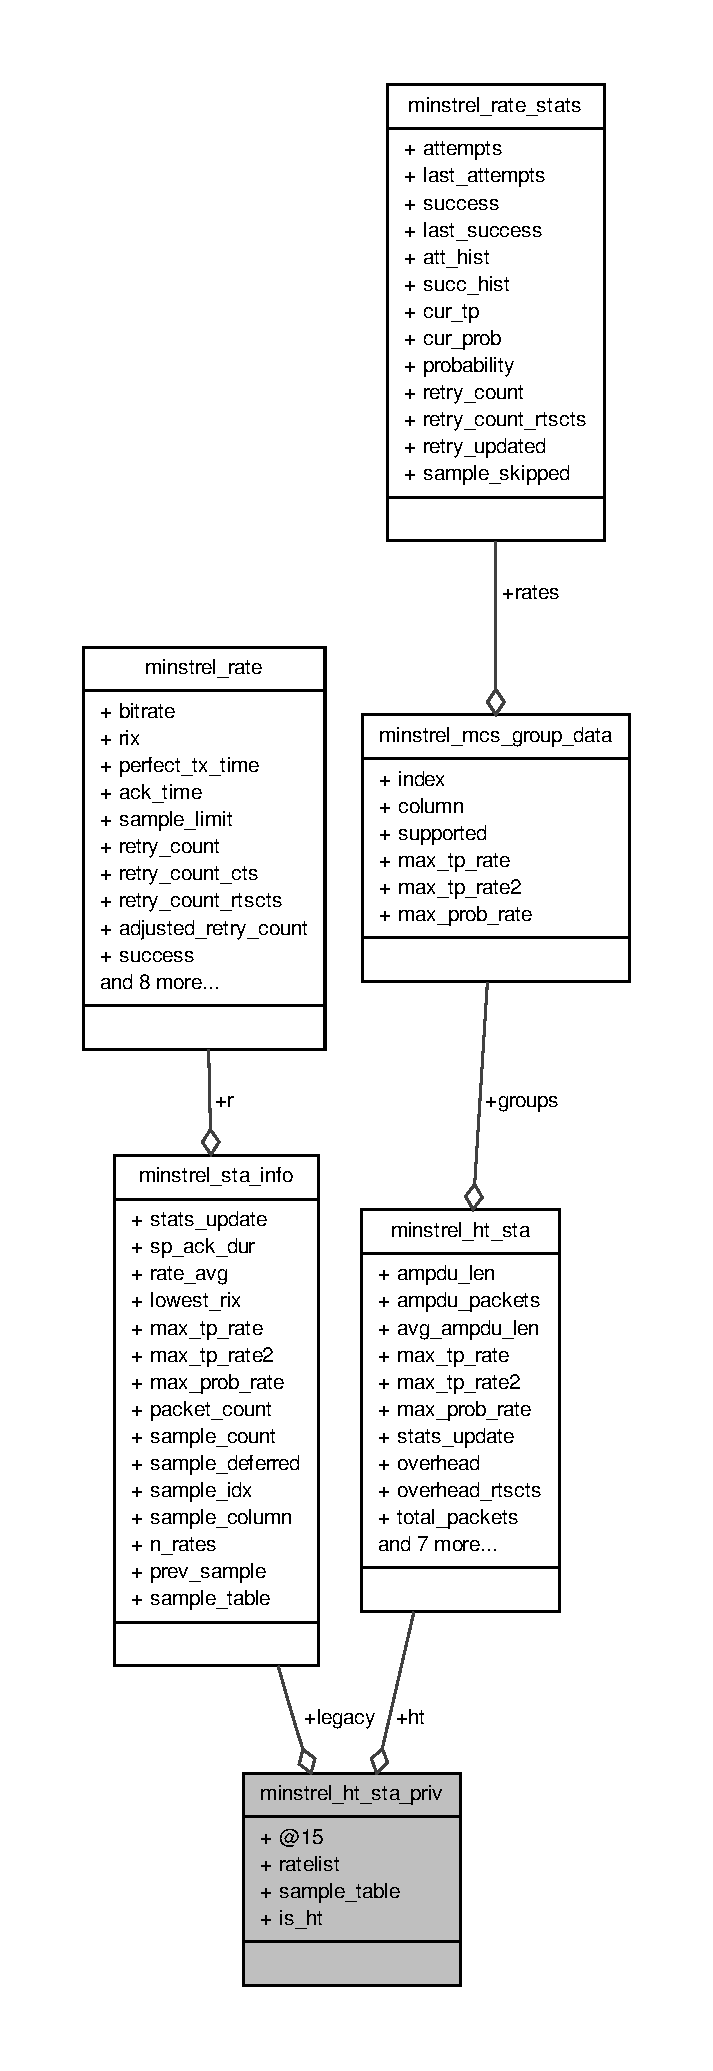
\includegraphics[height=550pt]{structminstrel__ht__sta__priv__coll__graph}
\end{center}
\end{figure}
\subsection*{Data Fields}
\begin{DoxyCompactItemize}
\item 
\begin{tabbing}
xx\=xx\=xx\=xx\=xx\=xx\=xx\=xx\=xx\=\kill
union \{\\
\>struct \hyperlink{structminstrel__ht__sta}{minstrel\_ht\_sta} \hyperlink{structminstrel__ht__sta__priv_a24192392c2f90bf320a245b4af1319bb}{ht}\\
\>struct \hyperlink{structminstrel__sta__info}{minstrel\_sta\_info} \hyperlink{structminstrel__ht__sta__priv_aa23bd315f4b740dbf665fd13992b2042}{legacy}\\
\}; \\

\end{tabbing}\item 
void $\ast$ \hyperlink{structminstrel__ht__sta__priv_ad4ac07580c58cd424321fd2e4a8cf800}{ratelist}
\item 
void $\ast$ \hyperlink{structminstrel__ht__sta__priv_a3e6baa12c7e2d9d85f9c06542a62063e}{sample\-\_\-table}
\item 
bool \hyperlink{structminstrel__ht__sta__priv_a691fcae1200883f0309751d54945e68b}{is\-\_\-ht}
\end{DoxyCompactItemize}


\subsection{Detailed Description}


Definition at line 114 of file rc80211\-\_\-minstrel\-\_\-ht.\-h.



\subsection{Field Documentation}
\hypertarget{structminstrel__ht__sta__priv_afc1ac45011cf2de47afc3333fe867466}{\subsubsection[{"@15}]{\setlength{\rightskip}{0pt plus 5cm}union \{ ... \} }}\label{structminstrel__ht__sta__priv_afc1ac45011cf2de47afc3333fe867466}
\hypertarget{structminstrel__ht__sta__priv_a24192392c2f90bf320a245b4af1319bb}{\index{minstrel\-\_\-ht\-\_\-sta\-\_\-priv@{minstrel\-\_\-ht\-\_\-sta\-\_\-priv}!ht@{ht}}
\index{ht@{ht}!minstrel_ht_sta_priv@{minstrel\-\_\-ht\-\_\-sta\-\_\-priv}}
\subsubsection[{ht}]{\setlength{\rightskip}{0pt plus 5cm}struct {\bf minstrel\-\_\-ht\-\_\-sta} ht}}\label{structminstrel__ht__sta__priv_a24192392c2f90bf320a245b4af1319bb}


Definition at line 116 of file rc80211\-\_\-minstrel\-\_\-ht.\-h.

\hypertarget{structminstrel__ht__sta__priv_a691fcae1200883f0309751d54945e68b}{\index{minstrel\-\_\-ht\-\_\-sta\-\_\-priv@{minstrel\-\_\-ht\-\_\-sta\-\_\-priv}!is\-\_\-ht@{is\-\_\-ht}}
\index{is\-\_\-ht@{is\-\_\-ht}!minstrel_ht_sta_priv@{minstrel\-\_\-ht\-\_\-sta\-\_\-priv}}
\subsubsection[{is\-\_\-ht}]{\setlength{\rightskip}{0pt plus 5cm}bool is\-\_\-ht}}\label{structminstrel__ht__sta__priv_a691fcae1200883f0309751d54945e68b}


Definition at line 124 of file rc80211\-\_\-minstrel\-\_\-ht.\-h.

\hypertarget{structminstrel__ht__sta__priv_aa23bd315f4b740dbf665fd13992b2042}{\index{minstrel\-\_\-ht\-\_\-sta\-\_\-priv@{minstrel\-\_\-ht\-\_\-sta\-\_\-priv}!legacy@{legacy}}
\index{legacy@{legacy}!minstrel_ht_sta_priv@{minstrel\-\_\-ht\-\_\-sta\-\_\-priv}}
\subsubsection[{legacy}]{\setlength{\rightskip}{0pt plus 5cm}struct {\bf minstrel\-\_\-sta\-\_\-info} legacy}}\label{structminstrel__ht__sta__priv_aa23bd315f4b740dbf665fd13992b2042}


Definition at line 117 of file rc80211\-\_\-minstrel\-\_\-ht.\-h.

\hypertarget{structminstrel__ht__sta__priv_ad4ac07580c58cd424321fd2e4a8cf800}{\index{minstrel\-\_\-ht\-\_\-sta\-\_\-priv@{minstrel\-\_\-ht\-\_\-sta\-\_\-priv}!ratelist@{ratelist}}
\index{ratelist@{ratelist}!minstrel_ht_sta_priv@{minstrel\-\_\-ht\-\_\-sta\-\_\-priv}}
\subsubsection[{ratelist}]{\setlength{\rightskip}{0pt plus 5cm}void$\ast$ ratelist}}\label{structminstrel__ht__sta__priv_ad4ac07580c58cd424321fd2e4a8cf800}


Definition at line 122 of file rc80211\-\_\-minstrel\-\_\-ht.\-h.

\hypertarget{structminstrel__ht__sta__priv_a3e6baa12c7e2d9d85f9c06542a62063e}{\index{minstrel\-\_\-ht\-\_\-sta\-\_\-priv@{minstrel\-\_\-ht\-\_\-sta\-\_\-priv}!sample\-\_\-table@{sample\-\_\-table}}
\index{sample\-\_\-table@{sample\-\_\-table}!minstrel_ht_sta_priv@{minstrel\-\_\-ht\-\_\-sta\-\_\-priv}}
\subsubsection[{sample\-\_\-table}]{\setlength{\rightskip}{0pt plus 5cm}void$\ast$ sample\-\_\-table}}\label{structminstrel__ht__sta__priv_a3e6baa12c7e2d9d85f9c06542a62063e}


Definition at line 123 of file rc80211\-\_\-minstrel\-\_\-ht.\-h.



The documentation for this struct was generated from the following file\-:\begin{DoxyCompactItemize}
\item 
/home/guille/msm/net/mac80211/\hyperlink{rc80211__minstrel__ht_8h}{rc80211\-\_\-minstrel\-\_\-ht.\-h}\end{DoxyCompactItemize}

\hypertarget{structminstrel__mcs__group__data}{\section{minstrel\-\_\-mcs\-\_\-group\-\_\-data Struct Reference}
\label{structminstrel__mcs__group__data}\index{minstrel\-\_\-mcs\-\_\-group\-\_\-data@{minstrel\-\_\-mcs\-\_\-group\-\_\-data}}
}


{\ttfamily \#include $<$rc80211\-\_\-minstrel\-\_\-ht.\-h$>$}



Collaboration diagram for minstrel\-\_\-mcs\-\_\-group\-\_\-data\-:
\nopagebreak
\begin{figure}[H]
\begin{center}
\leavevmode
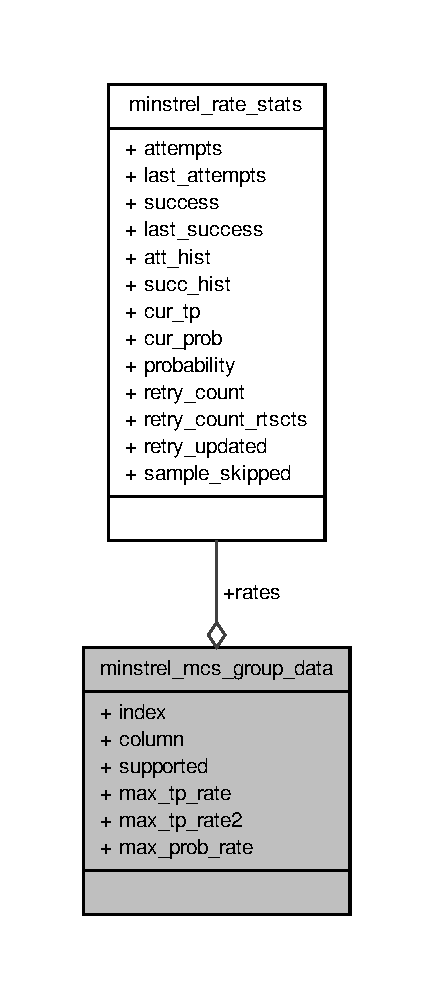
\includegraphics[width=208pt]{structminstrel__mcs__group__data__coll__graph}
\end{center}
\end{figure}
\subsection*{Data Fields}
\begin{DoxyCompactItemize}
\item 
u8 \hyperlink{structminstrel__mcs__group__data_aa93030ce4aadb2b3f398bfd4a3eda31b}{index}
\item 
u8 \hyperlink{structminstrel__mcs__group__data_a6ffd56a9561c5ba0bbaff28953dc76e1}{column}
\item 
u8 \hyperlink{structminstrel__mcs__group__data_ab33658d674b728098d19eee1209991a6}{supported}
\item 
unsigned int \hyperlink{structminstrel__mcs__group__data_ae61b14461f5cfea710f666fe40906493}{max\-\_\-tp\-\_\-rate}
\item 
unsigned int \hyperlink{structminstrel__mcs__group__data_aaa4f3e0147c91173f7dd6d86b82ba0ee}{max\-\_\-tp\-\_\-rate2}
\item 
unsigned int \hyperlink{structminstrel__mcs__group__data_a4a4625871f05851116acae11b392a957}{max\-\_\-prob\-\_\-rate}
\item 
struct \hyperlink{structminstrel__rate__stats}{minstrel\-\_\-rate\-\_\-stats} \hyperlink{structminstrel__mcs__group__data_a4b803dc8a89936e90c219388274fec2b}{rates} \mbox{[}\hyperlink{rc80211__minstrel__ht_8h_a1cce97ab419153d65e970112b74b5655}{M\-C\-S\-\_\-\-G\-R\-O\-U\-P\-\_\-\-R\-A\-T\-E\-S}\mbox{]}
\end{DoxyCompactItemize}


\subsection{Detailed Description}


Definition at line 56 of file rc80211\-\_\-minstrel\-\_\-ht.\-h.



\subsection{Field Documentation}
\hypertarget{structminstrel__mcs__group__data_a6ffd56a9561c5ba0bbaff28953dc76e1}{\index{minstrel\-\_\-mcs\-\_\-group\-\_\-data@{minstrel\-\_\-mcs\-\_\-group\-\_\-data}!column@{column}}
\index{column@{column}!minstrel_mcs_group_data@{minstrel\-\_\-mcs\-\_\-group\-\_\-data}}
\subsubsection[{column}]{\setlength{\rightskip}{0pt plus 5cm}u8 column}}\label{structminstrel__mcs__group__data_a6ffd56a9561c5ba0bbaff28953dc76e1}


Definition at line 58 of file rc80211\-\_\-minstrel\-\_\-ht.\-h.

\hypertarget{structminstrel__mcs__group__data_aa93030ce4aadb2b3f398bfd4a3eda31b}{\index{minstrel\-\_\-mcs\-\_\-group\-\_\-data@{minstrel\-\_\-mcs\-\_\-group\-\_\-data}!index@{index}}
\index{index@{index}!minstrel_mcs_group_data@{minstrel\-\_\-mcs\-\_\-group\-\_\-data}}
\subsubsection[{index}]{\setlength{\rightskip}{0pt plus 5cm}u8 index}}\label{structminstrel__mcs__group__data_aa93030ce4aadb2b3f398bfd4a3eda31b}


Definition at line 57 of file rc80211\-\_\-minstrel\-\_\-ht.\-h.

\hypertarget{structminstrel__mcs__group__data_a4a4625871f05851116acae11b392a957}{\index{minstrel\-\_\-mcs\-\_\-group\-\_\-data@{minstrel\-\_\-mcs\-\_\-group\-\_\-data}!max\-\_\-prob\-\_\-rate@{max\-\_\-prob\-\_\-rate}}
\index{max\-\_\-prob\-\_\-rate@{max\-\_\-prob\-\_\-rate}!minstrel_mcs_group_data@{minstrel\-\_\-mcs\-\_\-group\-\_\-data}}
\subsubsection[{max\-\_\-prob\-\_\-rate}]{\setlength{\rightskip}{0pt plus 5cm}unsigned int max\-\_\-prob\-\_\-rate}}\label{structminstrel__mcs__group__data_a4a4625871f05851116acae11b392a957}


Definition at line 66 of file rc80211\-\_\-minstrel\-\_\-ht.\-h.

\hypertarget{structminstrel__mcs__group__data_ae61b14461f5cfea710f666fe40906493}{\index{minstrel\-\_\-mcs\-\_\-group\-\_\-data@{minstrel\-\_\-mcs\-\_\-group\-\_\-data}!max\-\_\-tp\-\_\-rate@{max\-\_\-tp\-\_\-rate}}
\index{max\-\_\-tp\-\_\-rate@{max\-\_\-tp\-\_\-rate}!minstrel_mcs_group_data@{minstrel\-\_\-mcs\-\_\-group\-\_\-data}}
\subsubsection[{max\-\_\-tp\-\_\-rate}]{\setlength{\rightskip}{0pt plus 5cm}unsigned int max\-\_\-tp\-\_\-rate}}\label{structminstrel__mcs__group__data_ae61b14461f5cfea710f666fe40906493}


Definition at line 64 of file rc80211\-\_\-minstrel\-\_\-ht.\-h.

\hypertarget{structminstrel__mcs__group__data_aaa4f3e0147c91173f7dd6d86b82ba0ee}{\index{minstrel\-\_\-mcs\-\_\-group\-\_\-data@{minstrel\-\_\-mcs\-\_\-group\-\_\-data}!max\-\_\-tp\-\_\-rate2@{max\-\_\-tp\-\_\-rate2}}
\index{max\-\_\-tp\-\_\-rate2@{max\-\_\-tp\-\_\-rate2}!minstrel_mcs_group_data@{minstrel\-\_\-mcs\-\_\-group\-\_\-data}}
\subsubsection[{max\-\_\-tp\-\_\-rate2}]{\setlength{\rightskip}{0pt plus 5cm}unsigned int max\-\_\-tp\-\_\-rate2}}\label{structminstrel__mcs__group__data_aaa4f3e0147c91173f7dd6d86b82ba0ee}


Definition at line 65 of file rc80211\-\_\-minstrel\-\_\-ht.\-h.

\hypertarget{structminstrel__mcs__group__data_a4b803dc8a89936e90c219388274fec2b}{\index{minstrel\-\_\-mcs\-\_\-group\-\_\-data@{minstrel\-\_\-mcs\-\_\-group\-\_\-data}!rates@{rates}}
\index{rates@{rates}!minstrel_mcs_group_data@{minstrel\-\_\-mcs\-\_\-group\-\_\-data}}
\subsubsection[{rates}]{\setlength{\rightskip}{0pt plus 5cm}struct {\bf minstrel\-\_\-rate\-\_\-stats} rates\mbox{[}{\bf M\-C\-S\-\_\-\-G\-R\-O\-U\-P\-\_\-\-R\-A\-T\-E\-S}\mbox{]}}}\label{structminstrel__mcs__group__data_a4b803dc8a89936e90c219388274fec2b}


Definition at line 69 of file rc80211\-\_\-minstrel\-\_\-ht.\-h.

\hypertarget{structminstrel__mcs__group__data_ab33658d674b728098d19eee1209991a6}{\index{minstrel\-\_\-mcs\-\_\-group\-\_\-data@{minstrel\-\_\-mcs\-\_\-group\-\_\-data}!supported@{supported}}
\index{supported@{supported}!minstrel_mcs_group_data@{minstrel\-\_\-mcs\-\_\-group\-\_\-data}}
\subsubsection[{supported}]{\setlength{\rightskip}{0pt plus 5cm}u8 supported}}\label{structminstrel__mcs__group__data_ab33658d674b728098d19eee1209991a6}


Definition at line 61 of file rc80211\-\_\-minstrel\-\_\-ht.\-h.



The documentation for this struct was generated from the following file\-:\begin{DoxyCompactItemize}
\item 
/home/guille/msm/net/mac80211/\hyperlink{rc80211__minstrel__ht_8h}{rc80211\-\_\-minstrel\-\_\-ht.\-h}\end{DoxyCompactItemize}

\hypertarget{structminstrel__priv}{\section{minstrel\-\_\-priv Struct Reference}
\label{structminstrel__priv}\index{minstrel\-\_\-priv@{minstrel\-\_\-priv}}
}


{\ttfamily \#include $<$rc80211\-\_\-minstrel.\-h$>$}



Collaboration diagram for minstrel\-\_\-priv\-:
\nopagebreak
\begin{figure}[H]
\begin{center}
\leavevmode
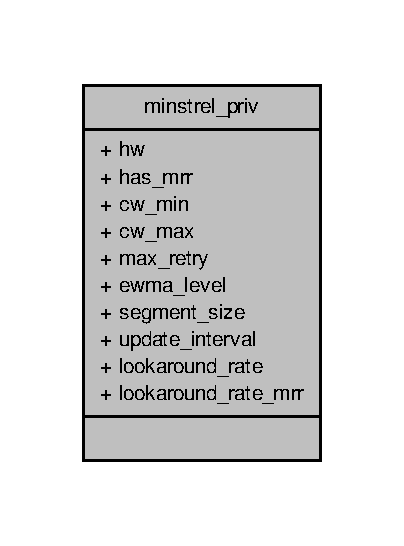
\includegraphics[width=194pt]{structminstrel__priv__coll__graph}
\end{center}
\end{figure}
\subsection*{Data Fields}
\begin{DoxyCompactItemize}
\item 
struct ieee80211\-\_\-hw $\ast$ \hyperlink{structminstrel__priv_aa12d77b0381baac0e9692c9a7a108d72}{hw}
\item 
bool \hyperlink{structminstrel__priv_a0ee069a8859cfa7d2af69c0a0527c29a}{has\-\_\-mrr}
\item 
unsigned int \hyperlink{structminstrel__priv_a5dfb3e843935ac3ab5af58d5b1626233}{cw\-\_\-min}
\item 
unsigned int \hyperlink{structminstrel__priv_a92daed595e977d0ba21e116f1ddeea93}{cw\-\_\-max}
\item 
unsigned int \hyperlink{structminstrel__priv_adab4257a07e2dc9f570cdd27160d9608}{max\-\_\-retry}
\item 
unsigned int \hyperlink{structminstrel__priv_a15186641e34e1ec343ccc43ee048ff07}{ewma\-\_\-level}
\item 
unsigned int \hyperlink{structminstrel__priv_a2d3f8a202a939940631624d4df515a8b}{segment\-\_\-size}
\item 
unsigned int \hyperlink{structminstrel__priv_a09d248b46f6ec43755860c9e20b8e142}{update\-\_\-interval}
\item 
unsigned int \hyperlink{structminstrel__priv_a663907806648ad048461b7d164a15632}{lookaround\-\_\-rate}
\item 
unsigned int \hyperlink{structminstrel__priv_a4b6e6fdf3f72ff420da912ed94ee8086}{lookaround\-\_\-rate\-\_\-mrr}
\end{DoxyCompactItemize}


\subsection{Detailed Description}


Definition at line 70 of file rc80211\-\_\-minstrel.\-h.



\subsection{Field Documentation}
\hypertarget{structminstrel__priv_a92daed595e977d0ba21e116f1ddeea93}{\index{minstrel\-\_\-priv@{minstrel\-\_\-priv}!cw\-\_\-max@{cw\-\_\-max}}
\index{cw\-\_\-max@{cw\-\_\-max}!minstrel_priv@{minstrel\-\_\-priv}}
\subsubsection[{cw\-\_\-max}]{\setlength{\rightskip}{0pt plus 5cm}unsigned int cw\-\_\-max}}\label{structminstrel__priv_a92daed595e977d0ba21e116f1ddeea93}


Definition at line 74 of file rc80211\-\_\-minstrel.\-h.

\hypertarget{structminstrel__priv_a5dfb3e843935ac3ab5af58d5b1626233}{\index{minstrel\-\_\-priv@{minstrel\-\_\-priv}!cw\-\_\-min@{cw\-\_\-min}}
\index{cw\-\_\-min@{cw\-\_\-min}!minstrel_priv@{minstrel\-\_\-priv}}
\subsubsection[{cw\-\_\-min}]{\setlength{\rightskip}{0pt plus 5cm}unsigned int cw\-\_\-min}}\label{structminstrel__priv_a5dfb3e843935ac3ab5af58d5b1626233}


Definition at line 73 of file rc80211\-\_\-minstrel.\-h.

\hypertarget{structminstrel__priv_a15186641e34e1ec343ccc43ee048ff07}{\index{minstrel\-\_\-priv@{minstrel\-\_\-priv}!ewma\-\_\-level@{ewma\-\_\-level}}
\index{ewma\-\_\-level@{ewma\-\_\-level}!minstrel_priv@{minstrel\-\_\-priv}}
\subsubsection[{ewma\-\_\-level}]{\setlength{\rightskip}{0pt plus 5cm}unsigned int ewma\-\_\-level}}\label{structminstrel__priv_a15186641e34e1ec343ccc43ee048ff07}


Definition at line 76 of file rc80211\-\_\-minstrel.\-h.

\hypertarget{structminstrel__priv_a0ee069a8859cfa7d2af69c0a0527c29a}{\index{minstrel\-\_\-priv@{minstrel\-\_\-priv}!has\-\_\-mrr@{has\-\_\-mrr}}
\index{has\-\_\-mrr@{has\-\_\-mrr}!minstrel_priv@{minstrel\-\_\-priv}}
\subsubsection[{has\-\_\-mrr}]{\setlength{\rightskip}{0pt plus 5cm}bool has\-\_\-mrr}}\label{structminstrel__priv_a0ee069a8859cfa7d2af69c0a0527c29a}


Definition at line 72 of file rc80211\-\_\-minstrel.\-h.

\hypertarget{structminstrel__priv_aa12d77b0381baac0e9692c9a7a108d72}{\index{minstrel\-\_\-priv@{minstrel\-\_\-priv}!hw@{hw}}
\index{hw@{hw}!minstrel_priv@{minstrel\-\_\-priv}}
\subsubsection[{hw}]{\setlength{\rightskip}{0pt plus 5cm}struct ieee80211\-\_\-hw$\ast$ hw}}\label{structminstrel__priv_aa12d77b0381baac0e9692c9a7a108d72}


Definition at line 71 of file rc80211\-\_\-minstrel.\-h.

\hypertarget{structminstrel__priv_a663907806648ad048461b7d164a15632}{\index{minstrel\-\_\-priv@{minstrel\-\_\-priv}!lookaround\-\_\-rate@{lookaround\-\_\-rate}}
\index{lookaround\-\_\-rate@{lookaround\-\_\-rate}!minstrel_priv@{minstrel\-\_\-priv}}
\subsubsection[{lookaround\-\_\-rate}]{\setlength{\rightskip}{0pt plus 5cm}unsigned int lookaround\-\_\-rate}}\label{structminstrel__priv_a663907806648ad048461b7d164a15632}


Definition at line 79 of file rc80211\-\_\-minstrel.\-h.

\hypertarget{structminstrel__priv_a4b6e6fdf3f72ff420da912ed94ee8086}{\index{minstrel\-\_\-priv@{minstrel\-\_\-priv}!lookaround\-\_\-rate\-\_\-mrr@{lookaround\-\_\-rate\-\_\-mrr}}
\index{lookaround\-\_\-rate\-\_\-mrr@{lookaround\-\_\-rate\-\_\-mrr}!minstrel_priv@{minstrel\-\_\-priv}}
\subsubsection[{lookaround\-\_\-rate\-\_\-mrr}]{\setlength{\rightskip}{0pt plus 5cm}unsigned int lookaround\-\_\-rate\-\_\-mrr}}\label{structminstrel__priv_a4b6e6fdf3f72ff420da912ed94ee8086}


Definition at line 80 of file rc80211\-\_\-minstrel.\-h.

\hypertarget{structminstrel__priv_adab4257a07e2dc9f570cdd27160d9608}{\index{minstrel\-\_\-priv@{minstrel\-\_\-priv}!max\-\_\-retry@{max\-\_\-retry}}
\index{max\-\_\-retry@{max\-\_\-retry}!minstrel_priv@{minstrel\-\_\-priv}}
\subsubsection[{max\-\_\-retry}]{\setlength{\rightskip}{0pt plus 5cm}unsigned int max\-\_\-retry}}\label{structminstrel__priv_adab4257a07e2dc9f570cdd27160d9608}


Definition at line 75 of file rc80211\-\_\-minstrel.\-h.

\hypertarget{structminstrel__priv_a2d3f8a202a939940631624d4df515a8b}{\index{minstrel\-\_\-priv@{minstrel\-\_\-priv}!segment\-\_\-size@{segment\-\_\-size}}
\index{segment\-\_\-size@{segment\-\_\-size}!minstrel_priv@{minstrel\-\_\-priv}}
\subsubsection[{segment\-\_\-size}]{\setlength{\rightskip}{0pt plus 5cm}unsigned int segment\-\_\-size}}\label{structminstrel__priv_a2d3f8a202a939940631624d4df515a8b}


Definition at line 77 of file rc80211\-\_\-minstrel.\-h.

\hypertarget{structminstrel__priv_a09d248b46f6ec43755860c9e20b8e142}{\index{minstrel\-\_\-priv@{minstrel\-\_\-priv}!update\-\_\-interval@{update\-\_\-interval}}
\index{update\-\_\-interval@{update\-\_\-interval}!minstrel_priv@{minstrel\-\_\-priv}}
\subsubsection[{update\-\_\-interval}]{\setlength{\rightskip}{0pt plus 5cm}unsigned int update\-\_\-interval}}\label{structminstrel__priv_a09d248b46f6ec43755860c9e20b8e142}


Definition at line 78 of file rc80211\-\_\-minstrel.\-h.



The documentation for this struct was generated from the following file\-:\begin{DoxyCompactItemize}
\item 
/home/guille/msm/net/mac80211/\hyperlink{rc80211__minstrel_8h}{rc80211\-\_\-minstrel.\-h}\end{DoxyCompactItemize}

\hypertarget{structminstrel__rate}{\section{minstrel\-\_\-rate Struct Reference}
\label{structminstrel__rate}\index{minstrel\-\_\-rate@{minstrel\-\_\-rate}}
}


{\ttfamily \#include $<$rc80211\-\_\-minstrel.\-h$>$}



Collaboration diagram for minstrel\-\_\-rate\-:
\nopagebreak
\begin{figure}[H]
\begin{center}
\leavevmode
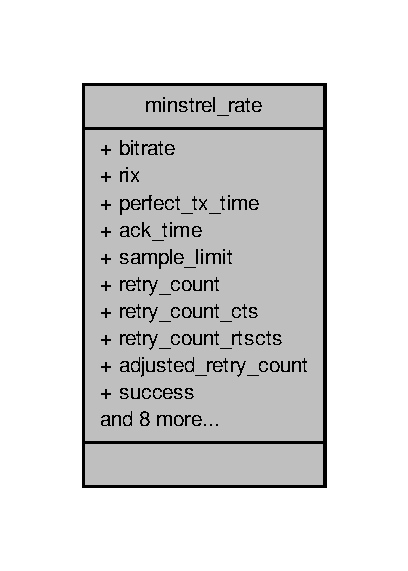
\includegraphics[width=196pt]{structminstrel__rate__coll__graph}
\end{center}
\end{figure}
\subsection*{Data Fields}
\begin{DoxyCompactItemize}
\item 
int \hyperlink{structminstrel__rate_ab5d8e1788d02d0e52941a0778776e289}{bitrate}
\item 
int \hyperlink{structminstrel__rate_a803467ed3226692c9a6ed93a7a9725ce}{rix}
\item 
unsigned int \hyperlink{structminstrel__rate_a96aaa27d9d2e98cac292a49b212f34ae}{perfect\-\_\-tx\-\_\-time}
\item 
unsigned int \hyperlink{structminstrel__rate_a84cfe794c5114005b22f693b28183fcb}{ack\-\_\-time}
\item 
int \hyperlink{structminstrel__rate_ada7982d82ef4893b92944d7b8c871dd2}{sample\-\_\-limit}
\item 
unsigned int \hyperlink{structminstrel__rate_aa01b3f9d6a9f63eb01422e4783c64f09}{retry\-\_\-count}
\item 
unsigned int \hyperlink{structminstrel__rate_aff59bd4c5c6bc9d1639a4dc3bcebb2aa}{retry\-\_\-count\-\_\-cts}
\item 
unsigned int \hyperlink{structminstrel__rate_ade58922c4f5867f4871e88d7d53c92fe}{retry\-\_\-count\-\_\-rtscts}
\item 
unsigned int \hyperlink{structminstrel__rate_a2e1fba3f2815c73ff517aa5971460b1e}{adjusted\-\_\-retry\-\_\-count}
\item 
u32 \hyperlink{structminstrel__rate_a59c45b017ad3e668a0aadd1fb16dabf3}{success}
\item 
u32 \hyperlink{structminstrel__rate_ab31da70a28d3eb0519fe305d260a6f19}{attempts}
\item 
u32 \hyperlink{structminstrel__rate_ab403313e07a99f7f9406c27f5ed25e67}{last\-\_\-attempts}
\item 
u32 \hyperlink{structminstrel__rate_a8b4d399ffe23bc6cdf414328d713ba9f}{last\-\_\-success}
\item 
u32 \hyperlink{structminstrel__rate_a32b192e3ef506ee9c2a8168c37cebabc}{cur\-\_\-prob}
\item 
u32 \hyperlink{structminstrel__rate_a0d6c4038ed9c552705e3b5c4c02c4ead}{probability}
\item 
u32 \hyperlink{structminstrel__rate_a0672074665762bee86be223a6f5a283e}{cur\-\_\-tp}
\item 
u64 \hyperlink{structminstrel__rate_af2ad78ee531872588a173945378c1b51}{succ\-\_\-hist}
\item 
u64 \hyperlink{structminstrel__rate_ad1e0131b84d34b871828347daa221112}{att\-\_\-hist}
\end{DoxyCompactItemize}


\subsection{Detailed Description}


Definition at line 12 of file rc80211\-\_\-minstrel.\-h.



\subsection{Field Documentation}
\hypertarget{structminstrel__rate_a84cfe794c5114005b22f693b28183fcb}{\index{minstrel\-\_\-rate@{minstrel\-\_\-rate}!ack\-\_\-time@{ack\-\_\-time}}
\index{ack\-\_\-time@{ack\-\_\-time}!minstrel_rate@{minstrel\-\_\-rate}}
\subsubsection[{ack\-\_\-time}]{\setlength{\rightskip}{0pt plus 5cm}unsigned int ack\-\_\-time}}\label{structminstrel__rate_a84cfe794c5114005b22f693b28183fcb}


Definition at line 17 of file rc80211\-\_\-minstrel.\-h.

\hypertarget{structminstrel__rate_a2e1fba3f2815c73ff517aa5971460b1e}{\index{minstrel\-\_\-rate@{minstrel\-\_\-rate}!adjusted\-\_\-retry\-\_\-count@{adjusted\-\_\-retry\-\_\-count}}
\index{adjusted\-\_\-retry\-\_\-count@{adjusted\-\_\-retry\-\_\-count}!minstrel_rate@{minstrel\-\_\-rate}}
\subsubsection[{adjusted\-\_\-retry\-\_\-count}]{\setlength{\rightskip}{0pt plus 5cm}unsigned int adjusted\-\_\-retry\-\_\-count}}\label{structminstrel__rate_a2e1fba3f2815c73ff517aa5971460b1e}


Definition at line 23 of file rc80211\-\_\-minstrel.\-h.

\hypertarget{structminstrel__rate_ad1e0131b84d34b871828347daa221112}{\index{minstrel\-\_\-rate@{minstrel\-\_\-rate}!att\-\_\-hist@{att\-\_\-hist}}
\index{att\-\_\-hist@{att\-\_\-hist}!minstrel_rate@{minstrel\-\_\-rate}}
\subsubsection[{att\-\_\-hist}]{\setlength{\rightskip}{0pt plus 5cm}u64 att\-\_\-hist}}\label{structminstrel__rate_ad1e0131b84d34b871828347daa221112}


Definition at line 38 of file rc80211\-\_\-minstrel.\-h.

\hypertarget{structminstrel__rate_ab31da70a28d3eb0519fe305d260a6f19}{\index{minstrel\-\_\-rate@{minstrel\-\_\-rate}!attempts@{attempts}}
\index{attempts@{attempts}!minstrel_rate@{minstrel\-\_\-rate}}
\subsubsection[{attempts}]{\setlength{\rightskip}{0pt plus 5cm}u32 attempts}}\label{structminstrel__rate_ab31da70a28d3eb0519fe305d260a6f19}


Definition at line 26 of file rc80211\-\_\-minstrel.\-h.

\hypertarget{structminstrel__rate_ab5d8e1788d02d0e52941a0778776e289}{\index{minstrel\-\_\-rate@{minstrel\-\_\-rate}!bitrate@{bitrate}}
\index{bitrate@{bitrate}!minstrel_rate@{minstrel\-\_\-rate}}
\subsubsection[{bitrate}]{\setlength{\rightskip}{0pt plus 5cm}int bitrate}}\label{structminstrel__rate_ab5d8e1788d02d0e52941a0778776e289}


Definition at line 13 of file rc80211\-\_\-minstrel.\-h.

\hypertarget{structminstrel__rate_a32b192e3ef506ee9c2a8168c37cebabc}{\index{minstrel\-\_\-rate@{minstrel\-\_\-rate}!cur\-\_\-prob@{cur\-\_\-prob}}
\index{cur\-\_\-prob@{cur\-\_\-prob}!minstrel_rate@{minstrel\-\_\-rate}}
\subsubsection[{cur\-\_\-prob}]{\setlength{\rightskip}{0pt plus 5cm}u32 cur\-\_\-prob}}\label{structminstrel__rate_a32b192e3ef506ee9c2a8168c37cebabc}


Definition at line 31 of file rc80211\-\_\-minstrel.\-h.

\hypertarget{structminstrel__rate_a0672074665762bee86be223a6f5a283e}{\index{minstrel\-\_\-rate@{minstrel\-\_\-rate}!cur\-\_\-tp@{cur\-\_\-tp}}
\index{cur\-\_\-tp@{cur\-\_\-tp}!minstrel_rate@{minstrel\-\_\-rate}}
\subsubsection[{cur\-\_\-tp}]{\setlength{\rightskip}{0pt plus 5cm}u32 cur\-\_\-tp}}\label{structminstrel__rate_a0672074665762bee86be223a6f5a283e}


Definition at line 35 of file rc80211\-\_\-minstrel.\-h.

\hypertarget{structminstrel__rate_ab403313e07a99f7f9406c27f5ed25e67}{\index{minstrel\-\_\-rate@{minstrel\-\_\-rate}!last\-\_\-attempts@{last\-\_\-attempts}}
\index{last\-\_\-attempts@{last\-\_\-attempts}!minstrel_rate@{minstrel\-\_\-rate}}
\subsubsection[{last\-\_\-attempts}]{\setlength{\rightskip}{0pt plus 5cm}u32 last\-\_\-attempts}}\label{structminstrel__rate_ab403313e07a99f7f9406c27f5ed25e67}


Definition at line 27 of file rc80211\-\_\-minstrel.\-h.

\hypertarget{structminstrel__rate_a8b4d399ffe23bc6cdf414328d713ba9f}{\index{minstrel\-\_\-rate@{minstrel\-\_\-rate}!last\-\_\-success@{last\-\_\-success}}
\index{last\-\_\-success@{last\-\_\-success}!minstrel_rate@{minstrel\-\_\-rate}}
\subsubsection[{last\-\_\-success}]{\setlength{\rightskip}{0pt plus 5cm}u32 last\-\_\-success}}\label{structminstrel__rate_a8b4d399ffe23bc6cdf414328d713ba9f}


Definition at line 28 of file rc80211\-\_\-minstrel.\-h.

\hypertarget{structminstrel__rate_a96aaa27d9d2e98cac292a49b212f34ae}{\index{minstrel\-\_\-rate@{minstrel\-\_\-rate}!perfect\-\_\-tx\-\_\-time@{perfect\-\_\-tx\-\_\-time}}
\index{perfect\-\_\-tx\-\_\-time@{perfect\-\_\-tx\-\_\-time}!minstrel_rate@{minstrel\-\_\-rate}}
\subsubsection[{perfect\-\_\-tx\-\_\-time}]{\setlength{\rightskip}{0pt plus 5cm}unsigned int perfect\-\_\-tx\-\_\-time}}\label{structminstrel__rate_a96aaa27d9d2e98cac292a49b212f34ae}


Definition at line 16 of file rc80211\-\_\-minstrel.\-h.

\hypertarget{structminstrel__rate_a0d6c4038ed9c552705e3b5c4c02c4ead}{\index{minstrel\-\_\-rate@{minstrel\-\_\-rate}!probability@{probability}}
\index{probability@{probability}!minstrel_rate@{minstrel\-\_\-rate}}
\subsubsection[{probability}]{\setlength{\rightskip}{0pt plus 5cm}u32 probability}}\label{structminstrel__rate_a0d6c4038ed9c552705e3b5c4c02c4ead}


Definition at line 32 of file rc80211\-\_\-minstrel.\-h.

\hypertarget{structminstrel__rate_aa01b3f9d6a9f63eb01422e4783c64f09}{\index{minstrel\-\_\-rate@{minstrel\-\_\-rate}!retry\-\_\-count@{retry\-\_\-count}}
\index{retry\-\_\-count@{retry\-\_\-count}!minstrel_rate@{minstrel\-\_\-rate}}
\subsubsection[{retry\-\_\-count}]{\setlength{\rightskip}{0pt plus 5cm}unsigned int retry\-\_\-count}}\label{structminstrel__rate_aa01b3f9d6a9f63eb01422e4783c64f09}


Definition at line 20 of file rc80211\-\_\-minstrel.\-h.

\hypertarget{structminstrel__rate_aff59bd4c5c6bc9d1639a4dc3bcebb2aa}{\index{minstrel\-\_\-rate@{minstrel\-\_\-rate}!retry\-\_\-count\-\_\-cts@{retry\-\_\-count\-\_\-cts}}
\index{retry\-\_\-count\-\_\-cts@{retry\-\_\-count\-\_\-cts}!minstrel_rate@{minstrel\-\_\-rate}}
\subsubsection[{retry\-\_\-count\-\_\-cts}]{\setlength{\rightskip}{0pt plus 5cm}unsigned int retry\-\_\-count\-\_\-cts}}\label{structminstrel__rate_aff59bd4c5c6bc9d1639a4dc3bcebb2aa}


Definition at line 21 of file rc80211\-\_\-minstrel.\-h.

\hypertarget{structminstrel__rate_ade58922c4f5867f4871e88d7d53c92fe}{\index{minstrel\-\_\-rate@{minstrel\-\_\-rate}!retry\-\_\-count\-\_\-rtscts@{retry\-\_\-count\-\_\-rtscts}}
\index{retry\-\_\-count\-\_\-rtscts@{retry\-\_\-count\-\_\-rtscts}!minstrel_rate@{minstrel\-\_\-rate}}
\subsubsection[{retry\-\_\-count\-\_\-rtscts}]{\setlength{\rightskip}{0pt plus 5cm}unsigned int retry\-\_\-count\-\_\-rtscts}}\label{structminstrel__rate_ade58922c4f5867f4871e88d7d53c92fe}


Definition at line 22 of file rc80211\-\_\-minstrel.\-h.

\hypertarget{structminstrel__rate_a803467ed3226692c9a6ed93a7a9725ce}{\index{minstrel\-\_\-rate@{minstrel\-\_\-rate}!rix@{rix}}
\index{rix@{rix}!minstrel_rate@{minstrel\-\_\-rate}}
\subsubsection[{rix}]{\setlength{\rightskip}{0pt plus 5cm}int rix}}\label{structminstrel__rate_a803467ed3226692c9a6ed93a7a9725ce}


Definition at line 14 of file rc80211\-\_\-minstrel.\-h.

\hypertarget{structminstrel__rate_ada7982d82ef4893b92944d7b8c871dd2}{\index{minstrel\-\_\-rate@{minstrel\-\_\-rate}!sample\-\_\-limit@{sample\-\_\-limit}}
\index{sample\-\_\-limit@{sample\-\_\-limit}!minstrel_rate@{minstrel\-\_\-rate}}
\subsubsection[{sample\-\_\-limit}]{\setlength{\rightskip}{0pt plus 5cm}int sample\-\_\-limit}}\label{structminstrel__rate_ada7982d82ef4893b92944d7b8c871dd2}


Definition at line 19 of file rc80211\-\_\-minstrel.\-h.

\hypertarget{structminstrel__rate_af2ad78ee531872588a173945378c1b51}{\index{minstrel\-\_\-rate@{minstrel\-\_\-rate}!succ\-\_\-hist@{succ\-\_\-hist}}
\index{succ\-\_\-hist@{succ\-\_\-hist}!minstrel_rate@{minstrel\-\_\-rate}}
\subsubsection[{succ\-\_\-hist}]{\setlength{\rightskip}{0pt plus 5cm}u64 succ\-\_\-hist}}\label{structminstrel__rate_af2ad78ee531872588a173945378c1b51}


Definition at line 37 of file rc80211\-\_\-minstrel.\-h.

\hypertarget{structminstrel__rate_a59c45b017ad3e668a0aadd1fb16dabf3}{\index{minstrel\-\_\-rate@{minstrel\-\_\-rate}!success@{success}}
\index{success@{success}!minstrel_rate@{minstrel\-\_\-rate}}
\subsubsection[{success}]{\setlength{\rightskip}{0pt plus 5cm}u32 success}}\label{structminstrel__rate_a59c45b017ad3e668a0aadd1fb16dabf3}


Definition at line 25 of file rc80211\-\_\-minstrel.\-h.



The documentation for this struct was generated from the following file\-:\begin{DoxyCompactItemize}
\item 
/home/guille/msm/net/mac80211/\hyperlink{rc80211__minstrel_8h}{rc80211\-\_\-minstrel.\-h}\end{DoxyCompactItemize}

\hypertarget{structminstrel__rate__stats}{\section{minstrel\-\_\-rate\-\_\-stats Struct Reference}
\label{structminstrel__rate__stats}\index{minstrel\-\_\-rate\-\_\-stats@{minstrel\-\_\-rate\-\_\-stats}}
}


{\ttfamily \#include $<$rc80211\-\_\-minstrel\-\_\-ht.\-h$>$}



Collaboration diagram for minstrel\-\_\-rate\-\_\-stats\-:
\nopagebreak
\begin{figure}[H]
\begin{center}
\leavevmode
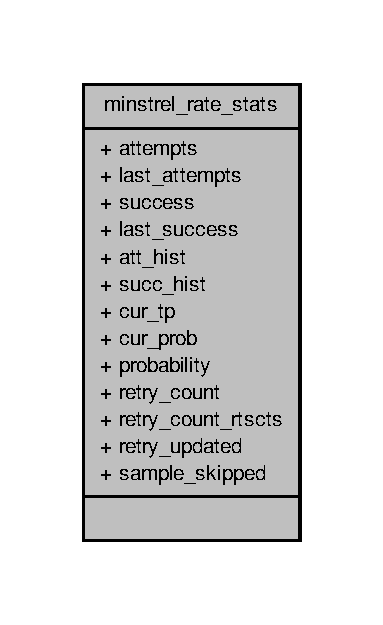
\includegraphics[width=184pt]{structminstrel__rate__stats__coll__graph}
\end{center}
\end{figure}
\subsection*{Data Fields}
\begin{DoxyCompactItemize}
\item 
unsigned int \hyperlink{structminstrel__rate__stats_a8299d4347d9be4e1868c451df3551f7c}{attempts}
\item 
unsigned int \hyperlink{structminstrel__rate__stats_a5a57031309e6917d037f074015ebf051}{last\-\_\-attempts}
\item 
unsigned int \hyperlink{structminstrel__rate__stats_a5813e0a68f3d46257469abc8784b8e22}{success}
\item 
unsigned int \hyperlink{structminstrel__rate__stats_a759724fa6afe27569c1f129ff4708e47}{last\-\_\-success}
\item 
u64 \hyperlink{structminstrel__rate__stats_ad1e0131b84d34b871828347daa221112}{att\-\_\-hist}
\item 
u64 \hyperlink{structminstrel__rate__stats_af2ad78ee531872588a173945378c1b51}{succ\-\_\-hist}
\item 
unsigned int \hyperlink{structminstrel__rate__stats_a4e2d3748d37ceaeb025df1d77052c809}{cur\-\_\-tp}
\item 
unsigned int \hyperlink{structminstrel__rate__stats_a87a247add3a9e2f9416b9cb6f9a5bc98}{cur\-\_\-prob}
\item 
unsigned int \hyperlink{structminstrel__rate__stats_a68975779708d4e8687d8f500cd1e2e61}{probability}
\item 
unsigned int \hyperlink{structminstrel__rate__stats_aa01b3f9d6a9f63eb01422e4783c64f09}{retry\-\_\-count}
\item 
unsigned int \hyperlink{structminstrel__rate__stats_ade58922c4f5867f4871e88d7d53c92fe}{retry\-\_\-count\-\_\-rtscts}
\item 
bool \hyperlink{structminstrel__rate__stats_afe4f0bbc7c9792a73c06d4cd49a7eda1}{retry\-\_\-updated}
\item 
u8 \hyperlink{structminstrel__rate__stats_a3ef5f3da43bcca6331c539dc59d39b72}{sample\-\_\-skipped}
\end{DoxyCompactItemize}


\subsection{Detailed Description}


Definition at line 34 of file rc80211\-\_\-minstrel\-\_\-ht.\-h.



\subsection{Field Documentation}
\hypertarget{structminstrel__rate__stats_ad1e0131b84d34b871828347daa221112}{\index{minstrel\-\_\-rate\-\_\-stats@{minstrel\-\_\-rate\-\_\-stats}!att\-\_\-hist@{att\-\_\-hist}}
\index{att\-\_\-hist@{att\-\_\-hist}!minstrel_rate_stats@{minstrel\-\_\-rate\-\_\-stats}}
\subsubsection[{att\-\_\-hist}]{\setlength{\rightskip}{0pt plus 5cm}u64 att\-\_\-hist}}\label{structminstrel__rate__stats_ad1e0131b84d34b871828347daa221112}


Definition at line 40 of file rc80211\-\_\-minstrel\-\_\-ht.\-h.

\hypertarget{structminstrel__rate__stats_a8299d4347d9be4e1868c451df3551f7c}{\index{minstrel\-\_\-rate\-\_\-stats@{minstrel\-\_\-rate\-\_\-stats}!attempts@{attempts}}
\index{attempts@{attempts}!minstrel_rate_stats@{minstrel\-\_\-rate\-\_\-stats}}
\subsubsection[{attempts}]{\setlength{\rightskip}{0pt plus 5cm}unsigned int attempts}}\label{structminstrel__rate__stats_a8299d4347d9be4e1868c451df3551f7c}


Definition at line 36 of file rc80211\-\_\-minstrel\-\_\-ht.\-h.

\hypertarget{structminstrel__rate__stats_a87a247add3a9e2f9416b9cb6f9a5bc98}{\index{minstrel\-\_\-rate\-\_\-stats@{minstrel\-\_\-rate\-\_\-stats}!cur\-\_\-prob@{cur\-\_\-prob}}
\index{cur\-\_\-prob@{cur\-\_\-prob}!minstrel_rate_stats@{minstrel\-\_\-rate\-\_\-stats}}
\subsubsection[{cur\-\_\-prob}]{\setlength{\rightskip}{0pt plus 5cm}unsigned int cur\-\_\-prob}}\label{structminstrel__rate__stats_a87a247add3a9e2f9416b9cb6f9a5bc98}


Definition at line 46 of file rc80211\-\_\-minstrel\-\_\-ht.\-h.

\hypertarget{structminstrel__rate__stats_a4e2d3748d37ceaeb025df1d77052c809}{\index{minstrel\-\_\-rate\-\_\-stats@{minstrel\-\_\-rate\-\_\-stats}!cur\-\_\-tp@{cur\-\_\-tp}}
\index{cur\-\_\-tp@{cur\-\_\-tp}!minstrel_rate_stats@{minstrel\-\_\-rate\-\_\-stats}}
\subsubsection[{cur\-\_\-tp}]{\setlength{\rightskip}{0pt plus 5cm}unsigned int cur\-\_\-tp}}\label{structminstrel__rate__stats_a4e2d3748d37ceaeb025df1d77052c809}


Definition at line 43 of file rc80211\-\_\-minstrel\-\_\-ht.\-h.

\hypertarget{structminstrel__rate__stats_a5a57031309e6917d037f074015ebf051}{\index{minstrel\-\_\-rate\-\_\-stats@{minstrel\-\_\-rate\-\_\-stats}!last\-\_\-attempts@{last\-\_\-attempts}}
\index{last\-\_\-attempts@{last\-\_\-attempts}!minstrel_rate_stats@{minstrel\-\_\-rate\-\_\-stats}}
\subsubsection[{last\-\_\-attempts}]{\setlength{\rightskip}{0pt plus 5cm}unsigned int last\-\_\-attempts}}\label{structminstrel__rate__stats_a5a57031309e6917d037f074015ebf051}


Definition at line 36 of file rc80211\-\_\-minstrel\-\_\-ht.\-h.

\hypertarget{structminstrel__rate__stats_a759724fa6afe27569c1f129ff4708e47}{\index{minstrel\-\_\-rate\-\_\-stats@{minstrel\-\_\-rate\-\_\-stats}!last\-\_\-success@{last\-\_\-success}}
\index{last\-\_\-success@{last\-\_\-success}!minstrel_rate_stats@{minstrel\-\_\-rate\-\_\-stats}}
\subsubsection[{last\-\_\-success}]{\setlength{\rightskip}{0pt plus 5cm}unsigned int last\-\_\-success}}\label{structminstrel__rate__stats_a759724fa6afe27569c1f129ff4708e47}


Definition at line 37 of file rc80211\-\_\-minstrel\-\_\-ht.\-h.

\hypertarget{structminstrel__rate__stats_a68975779708d4e8687d8f500cd1e2e61}{\index{minstrel\-\_\-rate\-\_\-stats@{minstrel\-\_\-rate\-\_\-stats}!probability@{probability}}
\index{probability@{probability}!minstrel_rate_stats@{minstrel\-\_\-rate\-\_\-stats}}
\subsubsection[{probability}]{\setlength{\rightskip}{0pt plus 5cm}unsigned int probability}}\label{structminstrel__rate__stats_a68975779708d4e8687d8f500cd1e2e61}


Definition at line 46 of file rc80211\-\_\-minstrel\-\_\-ht.\-h.

\hypertarget{structminstrel__rate__stats_aa01b3f9d6a9f63eb01422e4783c64f09}{\index{minstrel\-\_\-rate\-\_\-stats@{minstrel\-\_\-rate\-\_\-stats}!retry\-\_\-count@{retry\-\_\-count}}
\index{retry\-\_\-count@{retry\-\_\-count}!minstrel_rate_stats@{minstrel\-\_\-rate\-\_\-stats}}
\subsubsection[{retry\-\_\-count}]{\setlength{\rightskip}{0pt plus 5cm}unsigned int retry\-\_\-count}}\label{structminstrel__rate__stats_aa01b3f9d6a9f63eb01422e4783c64f09}


Definition at line 49 of file rc80211\-\_\-minstrel\-\_\-ht.\-h.

\hypertarget{structminstrel__rate__stats_ade58922c4f5867f4871e88d7d53c92fe}{\index{minstrel\-\_\-rate\-\_\-stats@{minstrel\-\_\-rate\-\_\-stats}!retry\-\_\-count\-\_\-rtscts@{retry\-\_\-count\-\_\-rtscts}}
\index{retry\-\_\-count\-\_\-rtscts@{retry\-\_\-count\-\_\-rtscts}!minstrel_rate_stats@{minstrel\-\_\-rate\-\_\-stats}}
\subsubsection[{retry\-\_\-count\-\_\-rtscts}]{\setlength{\rightskip}{0pt plus 5cm}unsigned int retry\-\_\-count\-\_\-rtscts}}\label{structminstrel__rate__stats_ade58922c4f5867f4871e88d7d53c92fe}


Definition at line 50 of file rc80211\-\_\-minstrel\-\_\-ht.\-h.

\hypertarget{structminstrel__rate__stats_afe4f0bbc7c9792a73c06d4cd49a7eda1}{\index{minstrel\-\_\-rate\-\_\-stats@{minstrel\-\_\-rate\-\_\-stats}!retry\-\_\-updated@{retry\-\_\-updated}}
\index{retry\-\_\-updated@{retry\-\_\-updated}!minstrel_rate_stats@{minstrel\-\_\-rate\-\_\-stats}}
\subsubsection[{retry\-\_\-updated}]{\setlength{\rightskip}{0pt plus 5cm}bool retry\-\_\-updated}}\label{structminstrel__rate__stats_afe4f0bbc7c9792a73c06d4cd49a7eda1}


Definition at line 52 of file rc80211\-\_\-minstrel\-\_\-ht.\-h.

\hypertarget{structminstrel__rate__stats_a3ef5f3da43bcca6331c539dc59d39b72}{\index{minstrel\-\_\-rate\-\_\-stats@{minstrel\-\_\-rate\-\_\-stats}!sample\-\_\-skipped@{sample\-\_\-skipped}}
\index{sample\-\_\-skipped@{sample\-\_\-skipped}!minstrel_rate_stats@{minstrel\-\_\-rate\-\_\-stats}}
\subsubsection[{sample\-\_\-skipped}]{\setlength{\rightskip}{0pt plus 5cm}u8 sample\-\_\-skipped}}\label{structminstrel__rate__stats_a3ef5f3da43bcca6331c539dc59d39b72}


Definition at line 53 of file rc80211\-\_\-minstrel\-\_\-ht.\-h.

\hypertarget{structminstrel__rate__stats_af2ad78ee531872588a173945378c1b51}{\index{minstrel\-\_\-rate\-\_\-stats@{minstrel\-\_\-rate\-\_\-stats}!succ\-\_\-hist@{succ\-\_\-hist}}
\index{succ\-\_\-hist@{succ\-\_\-hist}!minstrel_rate_stats@{minstrel\-\_\-rate\-\_\-stats}}
\subsubsection[{succ\-\_\-hist}]{\setlength{\rightskip}{0pt plus 5cm}u64 succ\-\_\-hist}}\label{structminstrel__rate__stats_af2ad78ee531872588a173945378c1b51}


Definition at line 40 of file rc80211\-\_\-minstrel\-\_\-ht.\-h.

\hypertarget{structminstrel__rate__stats_a5813e0a68f3d46257469abc8784b8e22}{\index{minstrel\-\_\-rate\-\_\-stats@{minstrel\-\_\-rate\-\_\-stats}!success@{success}}
\index{success@{success}!minstrel_rate_stats@{minstrel\-\_\-rate\-\_\-stats}}
\subsubsection[{success}]{\setlength{\rightskip}{0pt plus 5cm}unsigned int success}}\label{structminstrel__rate__stats_a5813e0a68f3d46257469abc8784b8e22}


Definition at line 37 of file rc80211\-\_\-minstrel\-\_\-ht.\-h.



The documentation for this struct was generated from the following file\-:\begin{DoxyCompactItemize}
\item 
/home/guille/msm/net/mac80211/\hyperlink{rc80211__minstrel__ht_8h}{rc80211\-\_\-minstrel\-\_\-ht.\-h}\end{DoxyCompactItemize}

\hypertarget{structminstrel__sta__info}{\section{minstrel\-\_\-sta\-\_\-info Struct Reference}
\label{structminstrel__sta__info}\index{minstrel\-\_\-sta\-\_\-info@{minstrel\-\_\-sta\-\_\-info}}
}


{\ttfamily \#include $<$rc80211\-\_\-minstrel.\-h$>$}



Collaboration diagram for minstrel\-\_\-sta\-\_\-info\-:
\nopagebreak
\begin{figure}[H]
\begin{center}
\leavevmode
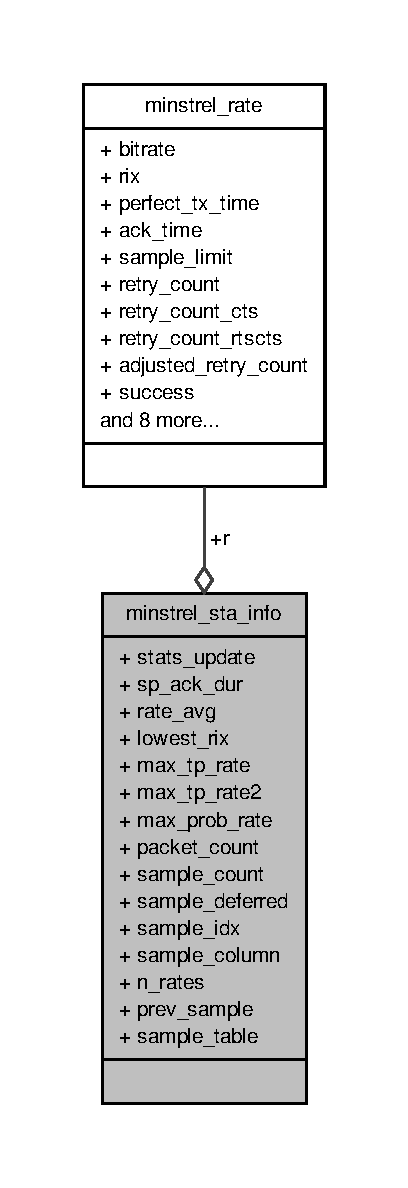
\includegraphics[height=550pt]{structminstrel__sta__info__coll__graph}
\end{center}
\end{figure}
\subsection*{Data Fields}
\begin{DoxyCompactItemize}
\item 
unsigned long \hyperlink{structminstrel__sta__info_a3c5301bb7fd4073bbad86d50eff8f188}{stats\-\_\-update}
\item 
unsigned int \hyperlink{structminstrel__sta__info_a1023b3884bcb7252fd484344ce4d5201}{sp\-\_\-ack\-\_\-dur}
\item 
unsigned int \hyperlink{structminstrel__sta__info_a28afea3f4f42a76c7ea48b9ac0399b76}{rate\-\_\-avg}
\item 
unsigned int \hyperlink{structminstrel__sta__info_a8f2a0e4bbfab7a7d1848bed87ae6ff84}{lowest\-\_\-rix}
\item 
unsigned int \hyperlink{structminstrel__sta__info_ae61b14461f5cfea710f666fe40906493}{max\-\_\-tp\-\_\-rate}
\item 
unsigned int \hyperlink{structminstrel__sta__info_aaa4f3e0147c91173f7dd6d86b82ba0ee}{max\-\_\-tp\-\_\-rate2}
\item 
unsigned int \hyperlink{structminstrel__sta__info_a4a4625871f05851116acae11b392a957}{max\-\_\-prob\-\_\-rate}
\item 
unsigned int \hyperlink{structminstrel__sta__info_af0a068e62b23d45baeffebf5250afd21}{packet\-\_\-count}
\item 
unsigned int \hyperlink{structminstrel__sta__info_a9c671b28b78e58cee0581915eadec995}{sample\-\_\-count}
\item 
int \hyperlink{structminstrel__sta__info_a73679483ce1d15dfa5cbd2705109f48f}{sample\-\_\-deferred}
\item 
unsigned int \hyperlink{structminstrel__sta__info_a6a478735f9902c260260559529323f93}{sample\-\_\-idx}
\item 
unsigned int \hyperlink{structminstrel__sta__info_a9096126b3357b30a3a2c97059127c15b}{sample\-\_\-column}
\item 
int \hyperlink{structminstrel__sta__info_abea138d7b28f0fb6b6877d27555ed046}{n\-\_\-rates}
\item 
struct \hyperlink{structminstrel__rate}{minstrel\-\_\-rate} $\ast$ \hyperlink{structminstrel__sta__info_aff05543e291b9d013012d0a94c3d4428}{r}
\item 
bool \hyperlink{structminstrel__sta__info_a5cd8f1c60ce3302d16a34887cb5cc2ea}{prev\-\_\-sample}
\item 
u8 $\ast$ \hyperlink{structminstrel__sta__info_aec1be199b41d56f11787b0eb67f6163c}{sample\-\_\-table}
\end{DoxyCompactItemize}


\subsection{Detailed Description}


Definition at line 41 of file rc80211\-\_\-minstrel.\-h.



\subsection{Field Documentation}
\hypertarget{structminstrel__sta__info_a8f2a0e4bbfab7a7d1848bed87ae6ff84}{\index{minstrel\-\_\-sta\-\_\-info@{minstrel\-\_\-sta\-\_\-info}!lowest\-\_\-rix@{lowest\-\_\-rix}}
\index{lowest\-\_\-rix@{lowest\-\_\-rix}!minstrel_sta_info@{minstrel\-\_\-sta\-\_\-info}}
\subsubsection[{lowest\-\_\-rix}]{\setlength{\rightskip}{0pt plus 5cm}unsigned int lowest\-\_\-rix}}\label{structminstrel__sta__info_a8f2a0e4bbfab7a7d1848bed87ae6ff84}


Definition at line 46 of file rc80211\-\_\-minstrel.\-h.

\hypertarget{structminstrel__sta__info_a4a4625871f05851116acae11b392a957}{\index{minstrel\-\_\-sta\-\_\-info@{minstrel\-\_\-sta\-\_\-info}!max\-\_\-prob\-\_\-rate@{max\-\_\-prob\-\_\-rate}}
\index{max\-\_\-prob\-\_\-rate@{max\-\_\-prob\-\_\-rate}!minstrel_sta_info@{minstrel\-\_\-sta\-\_\-info}}
\subsubsection[{max\-\_\-prob\-\_\-rate}]{\setlength{\rightskip}{0pt plus 5cm}unsigned int max\-\_\-prob\-\_\-rate}}\label{structminstrel__sta__info_a4a4625871f05851116acae11b392a957}


Definition at line 50 of file rc80211\-\_\-minstrel.\-h.

\hypertarget{structminstrel__sta__info_ae61b14461f5cfea710f666fe40906493}{\index{minstrel\-\_\-sta\-\_\-info@{minstrel\-\_\-sta\-\_\-info}!max\-\_\-tp\-\_\-rate@{max\-\_\-tp\-\_\-rate}}
\index{max\-\_\-tp\-\_\-rate@{max\-\_\-tp\-\_\-rate}!minstrel_sta_info@{minstrel\-\_\-sta\-\_\-info}}
\subsubsection[{max\-\_\-tp\-\_\-rate}]{\setlength{\rightskip}{0pt plus 5cm}unsigned int max\-\_\-tp\-\_\-rate}}\label{structminstrel__sta__info_ae61b14461f5cfea710f666fe40906493}


Definition at line 48 of file rc80211\-\_\-minstrel.\-h.

\hypertarget{structminstrel__sta__info_aaa4f3e0147c91173f7dd6d86b82ba0ee}{\index{minstrel\-\_\-sta\-\_\-info@{minstrel\-\_\-sta\-\_\-info}!max\-\_\-tp\-\_\-rate2@{max\-\_\-tp\-\_\-rate2}}
\index{max\-\_\-tp\-\_\-rate2@{max\-\_\-tp\-\_\-rate2}!minstrel_sta_info@{minstrel\-\_\-sta\-\_\-info}}
\subsubsection[{max\-\_\-tp\-\_\-rate2}]{\setlength{\rightskip}{0pt plus 5cm}unsigned int max\-\_\-tp\-\_\-rate2}}\label{structminstrel__sta__info_aaa4f3e0147c91173f7dd6d86b82ba0ee}


Definition at line 49 of file rc80211\-\_\-minstrel.\-h.

\hypertarget{structminstrel__sta__info_abea138d7b28f0fb6b6877d27555ed046}{\index{minstrel\-\_\-sta\-\_\-info@{minstrel\-\_\-sta\-\_\-info}!n\-\_\-rates@{n\-\_\-rates}}
\index{n\-\_\-rates@{n\-\_\-rates}!minstrel_sta_info@{minstrel\-\_\-sta\-\_\-info}}
\subsubsection[{n\-\_\-rates}]{\setlength{\rightskip}{0pt plus 5cm}int n\-\_\-rates}}\label{structminstrel__sta__info_abea138d7b28f0fb6b6877d27555ed046}


Definition at line 58 of file rc80211\-\_\-minstrel.\-h.

\hypertarget{structminstrel__sta__info_af0a068e62b23d45baeffebf5250afd21}{\index{minstrel\-\_\-sta\-\_\-info@{minstrel\-\_\-sta\-\_\-info}!packet\-\_\-count@{packet\-\_\-count}}
\index{packet\-\_\-count@{packet\-\_\-count}!minstrel_sta_info@{minstrel\-\_\-sta\-\_\-info}}
\subsubsection[{packet\-\_\-count}]{\setlength{\rightskip}{0pt plus 5cm}unsigned int packet\-\_\-count}}\label{structminstrel__sta__info_af0a068e62b23d45baeffebf5250afd21}


Definition at line 51 of file rc80211\-\_\-minstrel.\-h.

\hypertarget{structminstrel__sta__info_a5cd8f1c60ce3302d16a34887cb5cc2ea}{\index{minstrel\-\_\-sta\-\_\-info@{minstrel\-\_\-sta\-\_\-info}!prev\-\_\-sample@{prev\-\_\-sample}}
\index{prev\-\_\-sample@{prev\-\_\-sample}!minstrel_sta_info@{minstrel\-\_\-sta\-\_\-info}}
\subsubsection[{prev\-\_\-sample}]{\setlength{\rightskip}{0pt plus 5cm}bool prev\-\_\-sample}}\label{structminstrel__sta__info_a5cd8f1c60ce3302d16a34887cb5cc2ea}


Definition at line 60 of file rc80211\-\_\-minstrel.\-h.

\hypertarget{structminstrel__sta__info_aff05543e291b9d013012d0a94c3d4428}{\index{minstrel\-\_\-sta\-\_\-info@{minstrel\-\_\-sta\-\_\-info}!r@{r}}
\index{r@{r}!minstrel_sta_info@{minstrel\-\_\-sta\-\_\-info}}
\subsubsection[{r}]{\setlength{\rightskip}{0pt plus 5cm}struct {\bf minstrel\-\_\-rate}$\ast$ r}}\label{structminstrel__sta__info_aff05543e291b9d013012d0a94c3d4428}


Definition at line 59 of file rc80211\-\_\-minstrel.\-h.

\hypertarget{structminstrel__sta__info_a28afea3f4f42a76c7ea48b9ac0399b76}{\index{minstrel\-\_\-sta\-\_\-info@{minstrel\-\_\-sta\-\_\-info}!rate\-\_\-avg@{rate\-\_\-avg}}
\index{rate\-\_\-avg@{rate\-\_\-avg}!minstrel_sta_info@{minstrel\-\_\-sta\-\_\-info}}
\subsubsection[{rate\-\_\-avg}]{\setlength{\rightskip}{0pt plus 5cm}unsigned int rate\-\_\-avg}}\label{structminstrel__sta__info_a28afea3f4f42a76c7ea48b9ac0399b76}


Definition at line 44 of file rc80211\-\_\-minstrel.\-h.

\hypertarget{structminstrel__sta__info_a9096126b3357b30a3a2c97059127c15b}{\index{minstrel\-\_\-sta\-\_\-info@{minstrel\-\_\-sta\-\_\-info}!sample\-\_\-column@{sample\-\_\-column}}
\index{sample\-\_\-column@{sample\-\_\-column}!minstrel_sta_info@{minstrel\-\_\-sta\-\_\-info}}
\subsubsection[{sample\-\_\-column}]{\setlength{\rightskip}{0pt plus 5cm}unsigned int sample\-\_\-column}}\label{structminstrel__sta__info_a9096126b3357b30a3a2c97059127c15b}


Definition at line 56 of file rc80211\-\_\-minstrel.\-h.

\hypertarget{structminstrel__sta__info_a9c671b28b78e58cee0581915eadec995}{\index{minstrel\-\_\-sta\-\_\-info@{minstrel\-\_\-sta\-\_\-info}!sample\-\_\-count@{sample\-\_\-count}}
\index{sample\-\_\-count@{sample\-\_\-count}!minstrel_sta_info@{minstrel\-\_\-sta\-\_\-info}}
\subsubsection[{sample\-\_\-count}]{\setlength{\rightskip}{0pt plus 5cm}unsigned int sample\-\_\-count}}\label{structminstrel__sta__info_a9c671b28b78e58cee0581915eadec995}


Definition at line 52 of file rc80211\-\_\-minstrel.\-h.

\hypertarget{structminstrel__sta__info_a73679483ce1d15dfa5cbd2705109f48f}{\index{minstrel\-\_\-sta\-\_\-info@{minstrel\-\_\-sta\-\_\-info}!sample\-\_\-deferred@{sample\-\_\-deferred}}
\index{sample\-\_\-deferred@{sample\-\_\-deferred}!minstrel_sta_info@{minstrel\-\_\-sta\-\_\-info}}
\subsubsection[{sample\-\_\-deferred}]{\setlength{\rightskip}{0pt plus 5cm}int sample\-\_\-deferred}}\label{structminstrel__sta__info_a73679483ce1d15dfa5cbd2705109f48f}


Definition at line 53 of file rc80211\-\_\-minstrel.\-h.

\hypertarget{structminstrel__sta__info_a6a478735f9902c260260559529323f93}{\index{minstrel\-\_\-sta\-\_\-info@{minstrel\-\_\-sta\-\_\-info}!sample\-\_\-idx@{sample\-\_\-idx}}
\index{sample\-\_\-idx@{sample\-\_\-idx}!minstrel_sta_info@{minstrel\-\_\-sta\-\_\-info}}
\subsubsection[{sample\-\_\-idx}]{\setlength{\rightskip}{0pt plus 5cm}unsigned int sample\-\_\-idx}}\label{structminstrel__sta__info_a6a478735f9902c260260559529323f93}


Definition at line 55 of file rc80211\-\_\-minstrel.\-h.

\hypertarget{structminstrel__sta__info_aec1be199b41d56f11787b0eb67f6163c}{\index{minstrel\-\_\-sta\-\_\-info@{minstrel\-\_\-sta\-\_\-info}!sample\-\_\-table@{sample\-\_\-table}}
\index{sample\-\_\-table@{sample\-\_\-table}!minstrel_sta_info@{minstrel\-\_\-sta\-\_\-info}}
\subsubsection[{sample\-\_\-table}]{\setlength{\rightskip}{0pt plus 5cm}u8$\ast$ sample\-\_\-table}}\label{structminstrel__sta__info_aec1be199b41d56f11787b0eb67f6163c}


Definition at line 63 of file rc80211\-\_\-minstrel.\-h.

\hypertarget{structminstrel__sta__info_a1023b3884bcb7252fd484344ce4d5201}{\index{minstrel\-\_\-sta\-\_\-info@{minstrel\-\_\-sta\-\_\-info}!sp\-\_\-ack\-\_\-dur@{sp\-\_\-ack\-\_\-dur}}
\index{sp\-\_\-ack\-\_\-dur@{sp\-\_\-ack\-\_\-dur}!minstrel_sta_info@{minstrel\-\_\-sta\-\_\-info}}
\subsubsection[{sp\-\_\-ack\-\_\-dur}]{\setlength{\rightskip}{0pt plus 5cm}unsigned int sp\-\_\-ack\-\_\-dur}}\label{structminstrel__sta__info_a1023b3884bcb7252fd484344ce4d5201}


Definition at line 43 of file rc80211\-\_\-minstrel.\-h.

\hypertarget{structminstrel__sta__info_a3c5301bb7fd4073bbad86d50eff8f188}{\index{minstrel\-\_\-sta\-\_\-info@{minstrel\-\_\-sta\-\_\-info}!stats\-\_\-update@{stats\-\_\-update}}
\index{stats\-\_\-update@{stats\-\_\-update}!minstrel_sta_info@{minstrel\-\_\-sta\-\_\-info}}
\subsubsection[{stats\-\_\-update}]{\setlength{\rightskip}{0pt plus 5cm}unsigned long stats\-\_\-update}}\label{structminstrel__sta__info_a3c5301bb7fd4073bbad86d50eff8f188}


Definition at line 42 of file rc80211\-\_\-minstrel.\-h.



The documentation for this struct was generated from the following file\-:\begin{DoxyCompactItemize}
\item 
/home/guille/msm/net/mac80211/\hyperlink{rc80211__minstrel_8h}{rc80211\-\_\-minstrel.\-h}\end{DoxyCompactItemize}

\hypertarget{structmpath__node}{\section{mpath\-\_\-node Struct Reference}
\label{structmpath__node}\index{mpath\-\_\-node@{mpath\-\_\-node}}
}


Collaboration diagram for mpath\-\_\-node\-:
\nopagebreak
\begin{figure}[H]
\begin{center}
\leavevmode
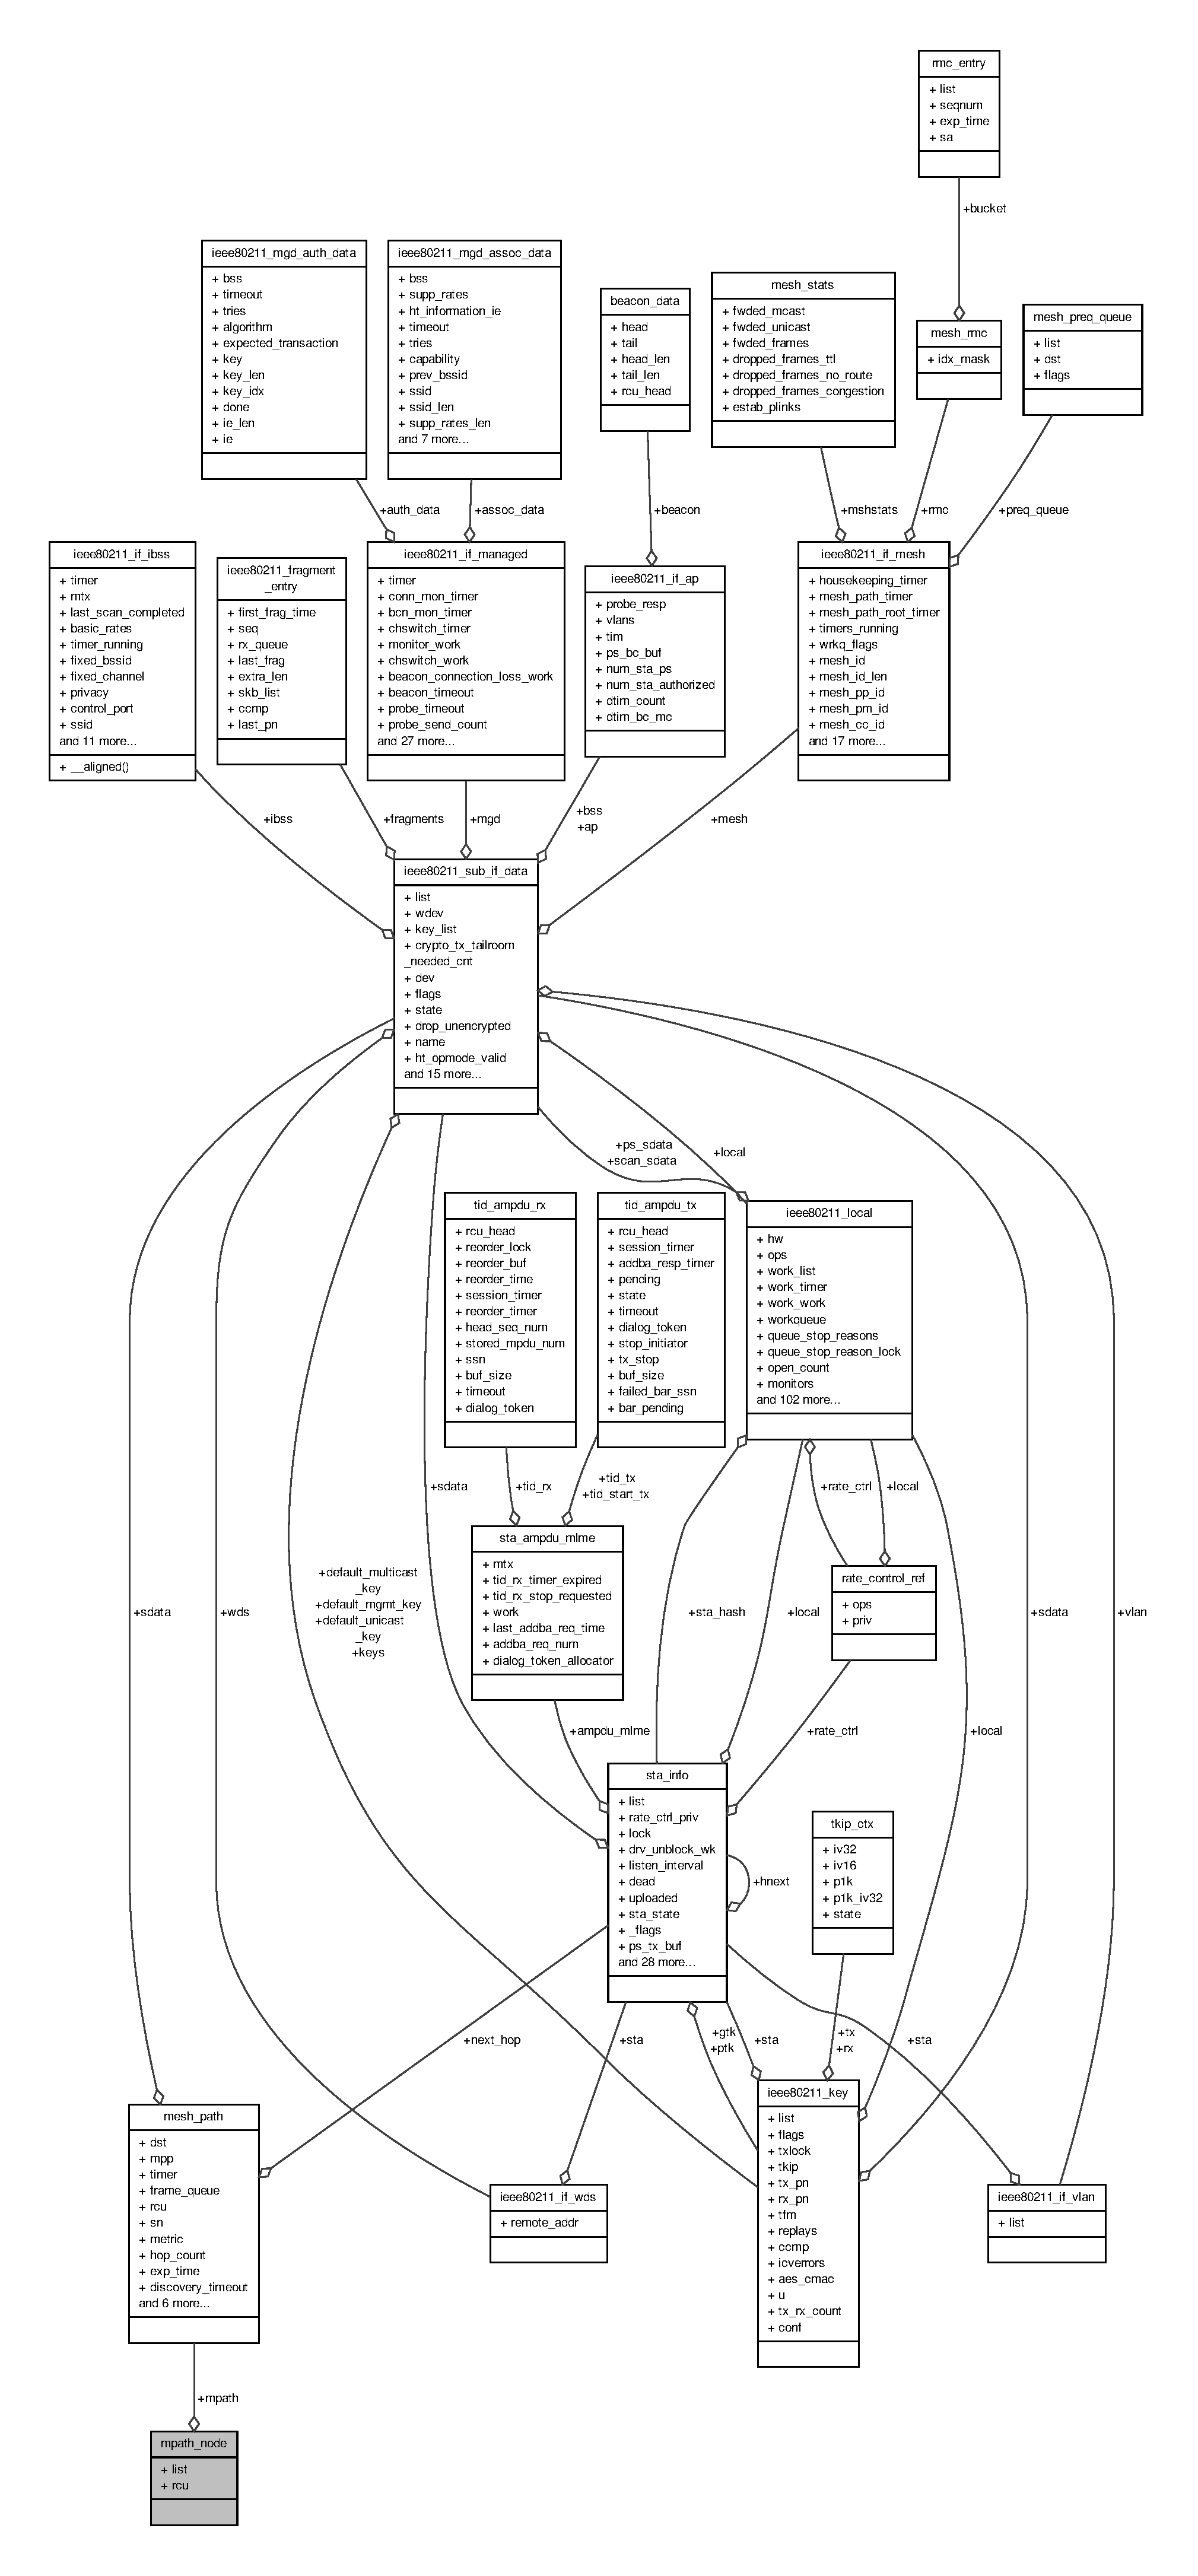
\includegraphics[height=550pt]{structmpath__node__coll__graph}
\end{center}
\end{figure}
\subsection*{Data Fields}
\begin{DoxyCompactItemize}
\item 
struct hlist\-\_\-node \hyperlink{structmpath__node_a71d95aff87c97c965ee946427631cddf}{list}
\item 
struct rcu\-\_\-head \hyperlink{structmpath__node_aa9677537ffa4e40f3c4f3e9fb3b4c76d}{rcu}
\item 
struct \hyperlink{structmesh__path}{mesh\-\_\-path} $\ast$ \hyperlink{structmpath__node_a90b46ef3dc111348ebc8b6108f58b87e}{mpath}
\end{DoxyCompactItemize}


\subsection{Detailed Description}


Definition at line 37 of file mesh\-\_\-pathtbl.\-c.



\subsection{Field Documentation}
\hypertarget{structmpath__node_a71d95aff87c97c965ee946427631cddf}{\index{mpath\-\_\-node@{mpath\-\_\-node}!list@{list}}
\index{list@{list}!mpath_node@{mpath\-\_\-node}}
\subsubsection[{list}]{\setlength{\rightskip}{0pt plus 5cm}struct hlist\-\_\-node list}}\label{structmpath__node_a71d95aff87c97c965ee946427631cddf}


Definition at line 38 of file mesh\-\_\-pathtbl.\-c.

\hypertarget{structmpath__node_a90b46ef3dc111348ebc8b6108f58b87e}{\index{mpath\-\_\-node@{mpath\-\_\-node}!mpath@{mpath}}
\index{mpath@{mpath}!mpath_node@{mpath\-\_\-node}}
\subsubsection[{mpath}]{\setlength{\rightskip}{0pt plus 5cm}struct {\bf mesh\-\_\-path}$\ast$ mpath}}\label{structmpath__node_a90b46ef3dc111348ebc8b6108f58b87e}


Definition at line 43 of file mesh\-\_\-pathtbl.\-c.

\hypertarget{structmpath__node_aa9677537ffa4e40f3c4f3e9fb3b4c76d}{\index{mpath\-\_\-node@{mpath\-\_\-node}!rcu@{rcu}}
\index{rcu@{rcu}!mpath_node@{mpath\-\_\-node}}
\subsubsection[{rcu}]{\setlength{\rightskip}{0pt plus 5cm}struct rcu\-\_\-head rcu}}\label{structmpath__node_aa9677537ffa4e40f3c4f3e9fb3b4c76d}


Definition at line 39 of file mesh\-\_\-pathtbl.\-c.



The documentation for this struct was generated from the following file\-:\begin{DoxyCompactItemize}
\item 
/home/guille/msm/net/mac80211/\hyperlink{mesh__pathtbl_8c}{mesh\-\_\-pathtbl.\-c}\end{DoxyCompactItemize}

\hypertarget{structrate__control__alg}{\section{rate\-\_\-control\-\_\-alg Struct Reference}
\label{structrate__control__alg}\index{rate\-\_\-control\-\_\-alg@{rate\-\_\-control\-\_\-alg}}
}


Collaboration diagram for rate\-\_\-control\-\_\-alg\-:
\nopagebreak
\begin{figure}[H]
\begin{center}
\leavevmode
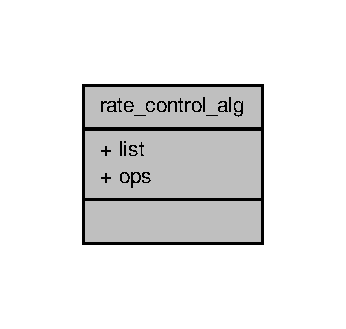
\includegraphics[width=166pt]{structrate__control__alg__coll__graph}
\end{center}
\end{figure}
\subsection*{Data Fields}
\begin{DoxyCompactItemize}
\item 
struct list\-\_\-head \hyperlink{structrate__control__alg_a1f00f18b91d5a820f2c43064243aa86e}{list}
\item 
struct rate\-\_\-control\-\_\-ops $\ast$ \hyperlink{structrate__control__alg_ab4edfb3119eea89ac8b10fb2b542f6f8}{ops}
\end{DoxyCompactItemize}


\subsection{Detailed Description}


Definition at line 19 of file rate.\-c.



\subsection{Field Documentation}
\hypertarget{structrate__control__alg_a1f00f18b91d5a820f2c43064243aa86e}{\index{rate\-\_\-control\-\_\-alg@{rate\-\_\-control\-\_\-alg}!list@{list}}
\index{list@{list}!rate_control_alg@{rate\-\_\-control\-\_\-alg}}
\subsubsection[{list}]{\setlength{\rightskip}{0pt plus 5cm}struct list\-\_\-head list}}\label{structrate__control__alg_a1f00f18b91d5a820f2c43064243aa86e}


Definition at line 20 of file rate.\-c.

\hypertarget{structrate__control__alg_ab4edfb3119eea89ac8b10fb2b542f6f8}{\index{rate\-\_\-control\-\_\-alg@{rate\-\_\-control\-\_\-alg}!ops@{ops}}
\index{ops@{ops}!rate_control_alg@{rate\-\_\-control\-\_\-alg}}
\subsubsection[{ops}]{\setlength{\rightskip}{0pt plus 5cm}struct rate\-\_\-control\-\_\-ops$\ast$ ops}}\label{structrate__control__alg_ab4edfb3119eea89ac8b10fb2b542f6f8}


Definition at line 21 of file rate.\-c.



The documentation for this struct was generated from the following file\-:\begin{DoxyCompactItemize}
\item 
/home/guille/msm/net/mac80211/\hyperlink{rate_8c}{rate.\-c}\end{DoxyCompactItemize}

\hypertarget{structrate__control__ref}{\section{rate\-\_\-control\-\_\-ref Struct Reference}
\label{structrate__control__ref}\index{rate\-\_\-control\-\_\-ref@{rate\-\_\-control\-\_\-ref}}
}


{\ttfamily \#include $<$rate.\-h$>$}



Collaboration diagram for rate\-\_\-control\-\_\-ref\-:
\nopagebreak
\begin{figure}[H]
\begin{center}
\leavevmode
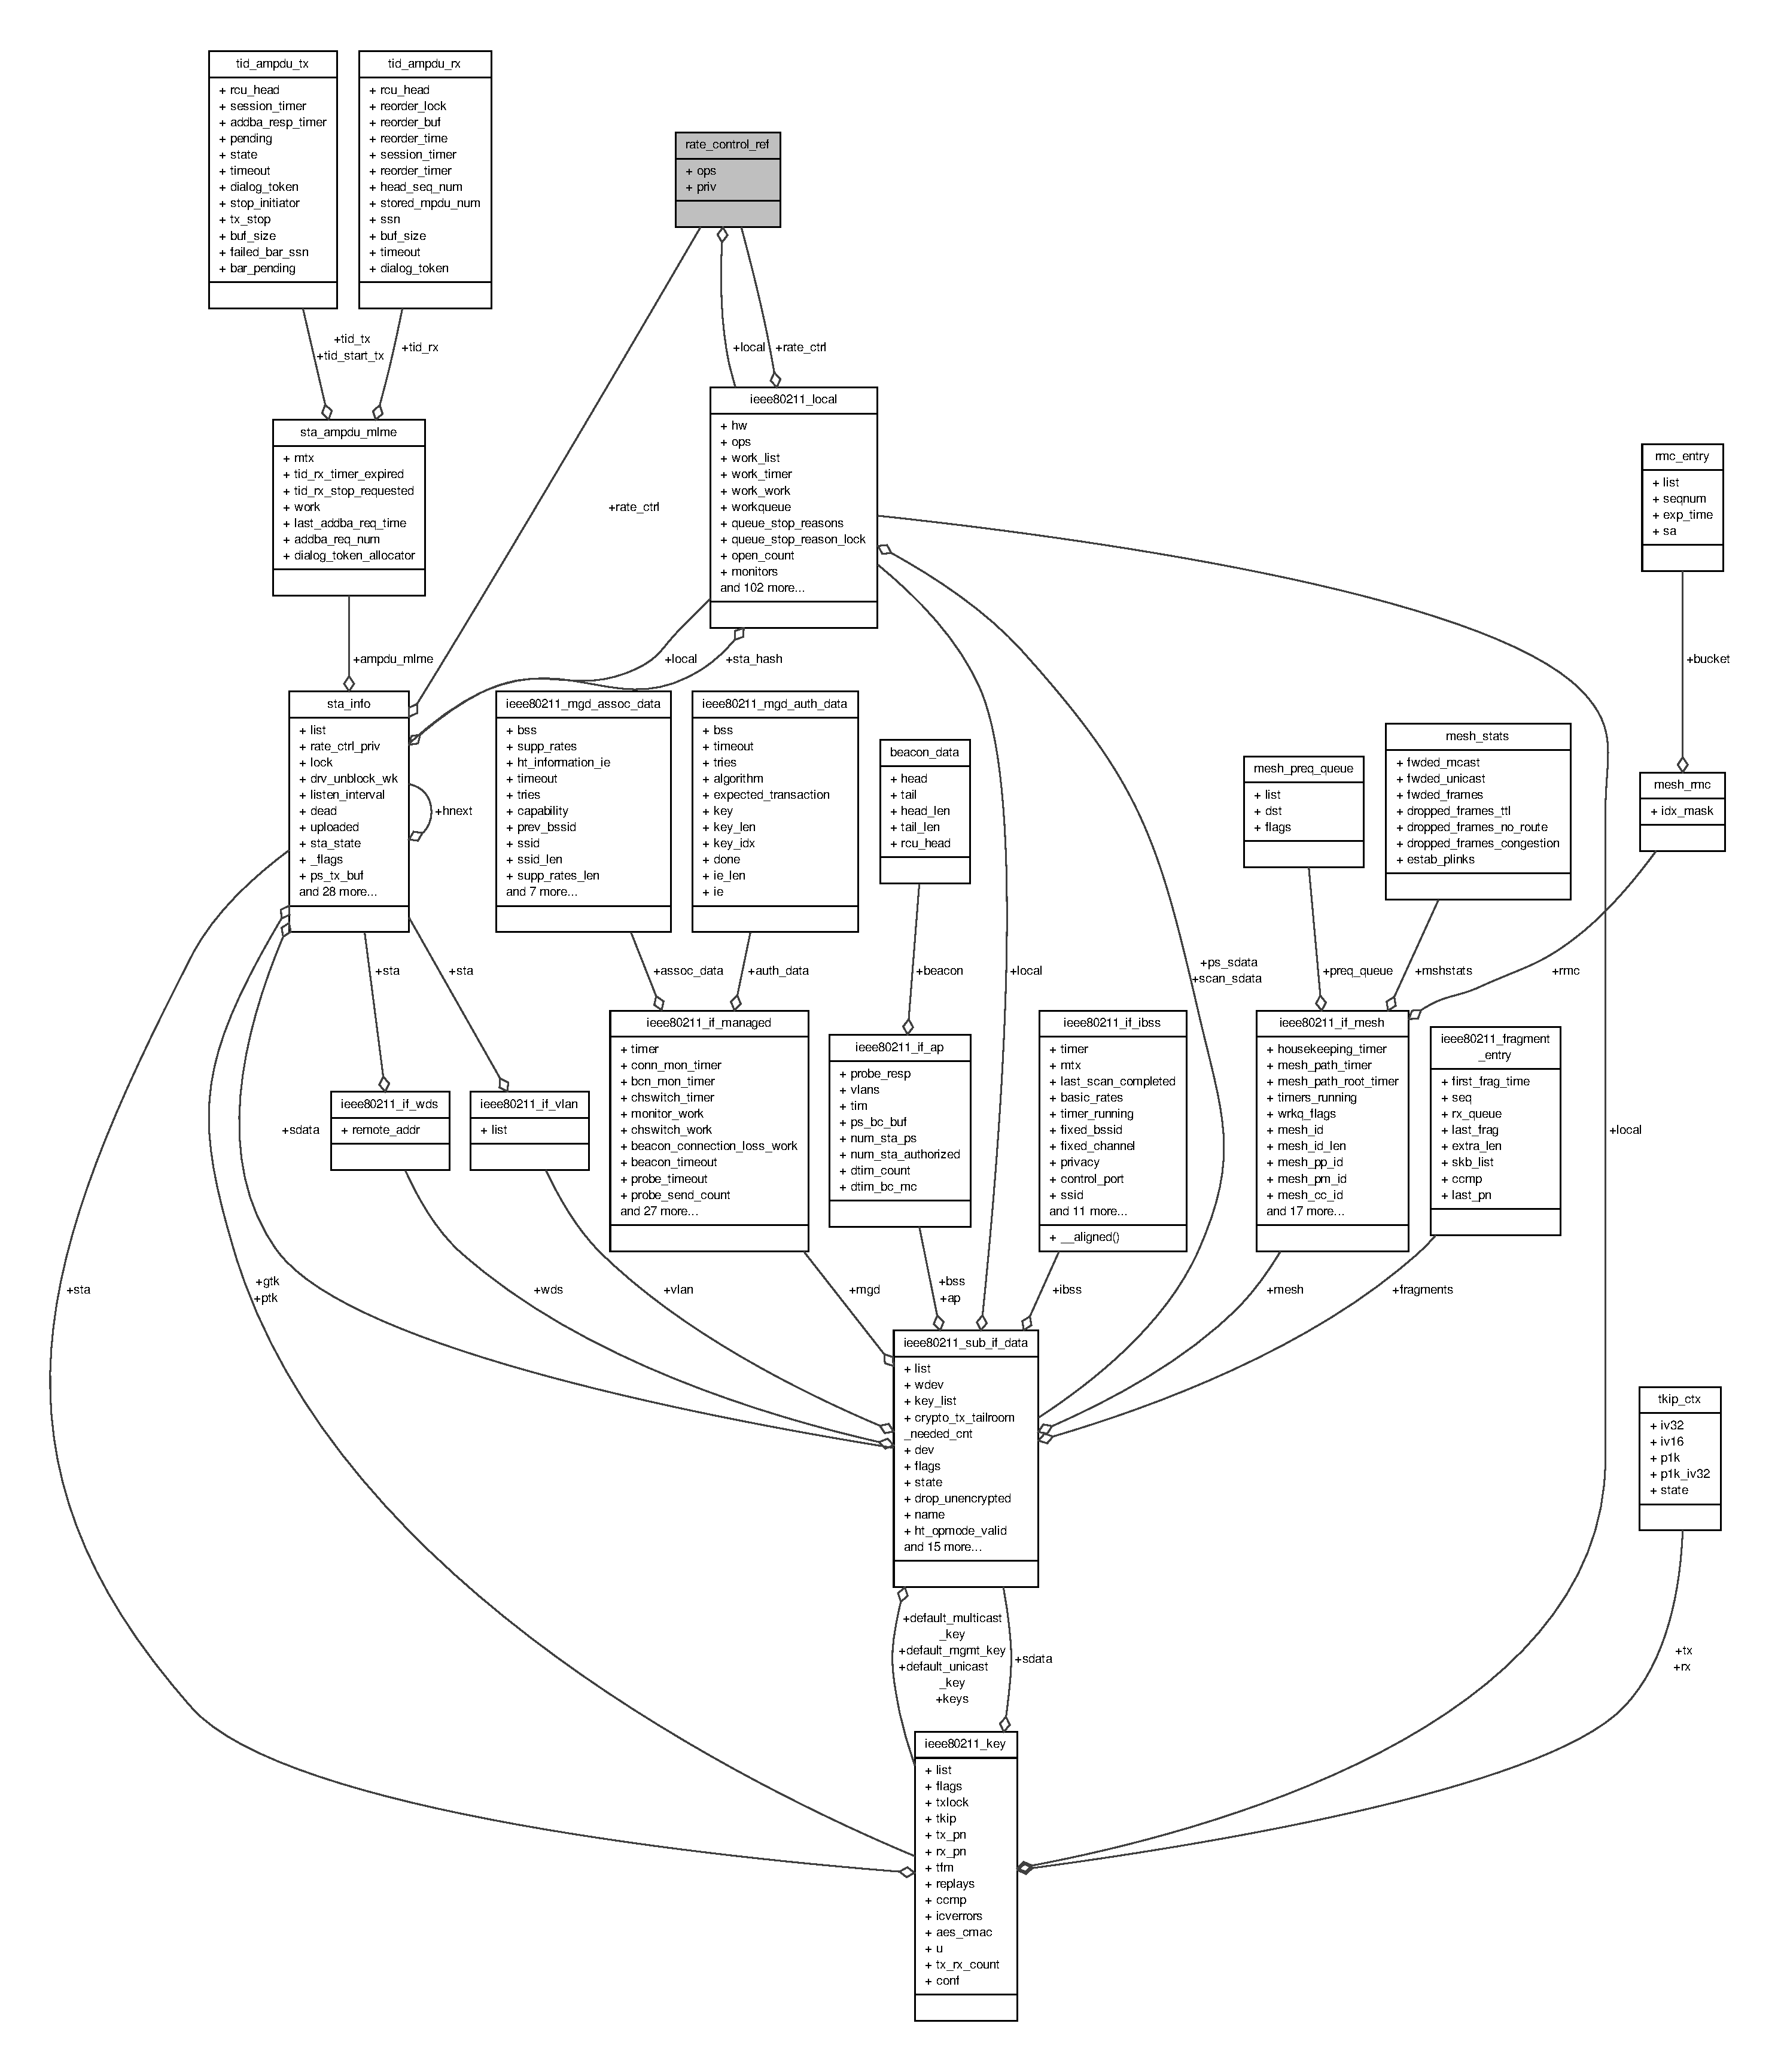
\includegraphics[width=350pt]{structrate__control__ref__coll__graph}
\end{center}
\end{figure}
\subsection*{Data Fields}
\begin{DoxyCompactItemize}
\item 
struct \hyperlink{structieee80211__local}{ieee80211\-\_\-local} $\ast$ \hyperlink{structrate__control__ref_ad436a024f420f219c4fe2eebce7e4ab2}{local}
\item 
struct rate\-\_\-control\-\_\-ops $\ast$ \hyperlink{structrate__control__ref_ab4edfb3119eea89ac8b10fb2b542f6f8}{ops}
\item 
void $\ast$ \hyperlink{structrate__control__ref_a8b6505c37d4ff95854b8b00527e4d9fa}{priv}
\end{DoxyCompactItemize}


\subsection{Detailed Description}


Definition at line 21 of file rate.\-h.



\subsection{Field Documentation}
\hypertarget{structrate__control__ref_ad436a024f420f219c4fe2eebce7e4ab2}{\index{rate\-\_\-control\-\_\-ref@{rate\-\_\-control\-\_\-ref}!local@{local}}
\index{local@{local}!rate_control_ref@{rate\-\_\-control\-\_\-ref}}
\subsubsection[{local}]{\setlength{\rightskip}{0pt plus 5cm}struct {\bf ieee80211\-\_\-local}$\ast$ local}}\label{structrate__control__ref_ad436a024f420f219c4fe2eebce7e4ab2}


Definition at line 22 of file rate.\-h.

\hypertarget{structrate__control__ref_ab4edfb3119eea89ac8b10fb2b542f6f8}{\index{rate\-\_\-control\-\_\-ref@{rate\-\_\-control\-\_\-ref}!ops@{ops}}
\index{ops@{ops}!rate_control_ref@{rate\-\_\-control\-\_\-ref}}
\subsubsection[{ops}]{\setlength{\rightskip}{0pt plus 5cm}struct rate\-\_\-control\-\_\-ops$\ast$ ops}}\label{structrate__control__ref_ab4edfb3119eea89ac8b10fb2b542f6f8}


Definition at line 23 of file rate.\-h.

\hypertarget{structrate__control__ref_a8b6505c37d4ff95854b8b00527e4d9fa}{\index{rate\-\_\-control\-\_\-ref@{rate\-\_\-control\-\_\-ref}!priv@{priv}}
\index{priv@{priv}!rate_control_ref@{rate\-\_\-control\-\_\-ref}}
\subsubsection[{priv}]{\setlength{\rightskip}{0pt plus 5cm}void$\ast$ priv}}\label{structrate__control__ref_a8b6505c37d4ff95854b8b00527e4d9fa}


Definition at line 24 of file rate.\-h.



The documentation for this struct was generated from the following file\-:\begin{DoxyCompactItemize}
\item 
/home/guille/msm/net/mac80211/\hyperlink{rate_8h}{rate.\-h}\end{DoxyCompactItemize}

\hypertarget{structrc__pid__debugfs__entries}{\section{rc\-\_\-pid\-\_\-debugfs\-\_\-entries Struct Reference}
\label{structrc__pid__debugfs__entries}\index{rc\-\_\-pid\-\_\-debugfs\-\_\-entries@{rc\-\_\-pid\-\_\-debugfs\-\_\-entries}}
}


{\ttfamily \#include $<$rc80211\-\_\-pid.\-h$>$}



Collaboration diagram for rc\-\_\-pid\-\_\-debugfs\-\_\-entries\-:
\nopagebreak
\begin{figure}[H]
\begin{center}
\leavevmode
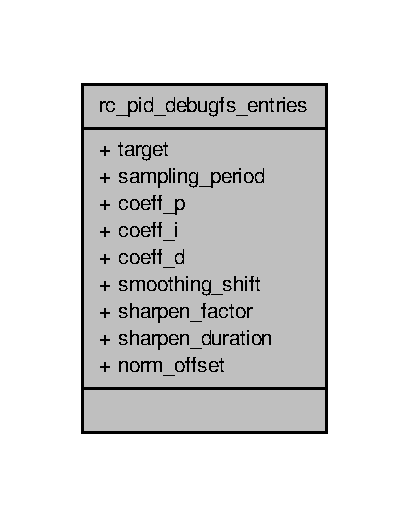
\includegraphics[width=196pt]{structrc__pid__debugfs__entries__coll__graph}
\end{center}
\end{figure}
\subsection*{Data Fields}
\begin{DoxyCompactItemize}
\item 
struct dentry $\ast$ \hyperlink{structrc__pid__debugfs__entries_a6dabe07e2b398ac0f58ac8f38a4b56b6}{target}
\item 
struct dentry $\ast$ \hyperlink{structrc__pid__debugfs__entries_a76915207e9f4be745cf591cabb1ba17c}{sampling\-\_\-period}
\item 
struct dentry $\ast$ \hyperlink{structrc__pid__debugfs__entries_a1a4e446a756b61017c2b85a6d8fa70c5}{coeff\-\_\-p}
\item 
struct dentry $\ast$ \hyperlink{structrc__pid__debugfs__entries_ad6b82f12eff1d91fb126c328e1e9a160}{coeff\-\_\-i}
\item 
struct dentry $\ast$ \hyperlink{structrc__pid__debugfs__entries_a8e02c39865c25ddbe3542a9f0ee711a1}{coeff\-\_\-d}
\item 
struct dentry $\ast$ \hyperlink{structrc__pid__debugfs__entries_aaca47ee03a834e073bbf46987f4a531b}{smoothing\-\_\-shift}
\item 
struct dentry $\ast$ \hyperlink{structrc__pid__debugfs__entries_a97f17182415214fc8cccde6894e0c815}{sharpen\-\_\-factor}
\item 
struct dentry $\ast$ \hyperlink{structrc__pid__debugfs__entries_aa529c80eecd02e36617d50510a0258a9}{sharpen\-\_\-duration}
\item 
struct dentry $\ast$ \hyperlink{structrc__pid__debugfs__entries_a08c42d2f89165fa314dbc2d527fad94d}{norm\-\_\-offset}
\end{DoxyCompactItemize}


\subsection{Detailed Description}
struct \hyperlink{structrc__pid__debugfs__entries}{rc\-\_\-pid\-\_\-debugfs\-\_\-entries} -\/ tunable parameters

Algorithm parameters, tunable via debugfs. \-: target percentage for failed frames \-: error sampling interval in milliseconds \-: absolute value of the proportional coefficient \-: absolute value of the integral coefficient \-: absolute value of the derivative coefficient \-: absolute value of the integral smoothing factor (i.\-e. amount of smoothing introduced by the exponential moving average) \-: absolute value of the derivative sharpening factor (i.\-e. amount of emphasis given to the derivative term after low activity events) \-: duration of the sharpening effect after the detected low activity event, relative to sampling\-\_\-period \-: amount of normalization periodically performed on the learnt rate behaviour values (lower means we should trust more what we learnt about behaviour of rates, higher means we should trust more the natural ordering of rates) 

Definition at line 142 of file rc80211\-\_\-pid.\-h.



\subsection{Field Documentation}
\hypertarget{structrc__pid__debugfs__entries_a8e02c39865c25ddbe3542a9f0ee711a1}{\index{rc\-\_\-pid\-\_\-debugfs\-\_\-entries@{rc\-\_\-pid\-\_\-debugfs\-\_\-entries}!coeff\-\_\-d@{coeff\-\_\-d}}
\index{coeff\-\_\-d@{coeff\-\_\-d}!rc_pid_debugfs_entries@{rc\-\_\-pid\-\_\-debugfs\-\_\-entries}}
\subsubsection[{coeff\-\_\-d}]{\setlength{\rightskip}{0pt plus 5cm}struct dentry$\ast$ coeff\-\_\-d}}\label{structrc__pid__debugfs__entries_a8e02c39865c25ddbe3542a9f0ee711a1}


Definition at line 147 of file rc80211\-\_\-pid.\-h.

\hypertarget{structrc__pid__debugfs__entries_ad6b82f12eff1d91fb126c328e1e9a160}{\index{rc\-\_\-pid\-\_\-debugfs\-\_\-entries@{rc\-\_\-pid\-\_\-debugfs\-\_\-entries}!coeff\-\_\-i@{coeff\-\_\-i}}
\index{coeff\-\_\-i@{coeff\-\_\-i}!rc_pid_debugfs_entries@{rc\-\_\-pid\-\_\-debugfs\-\_\-entries}}
\subsubsection[{coeff\-\_\-i}]{\setlength{\rightskip}{0pt plus 5cm}struct dentry$\ast$ coeff\-\_\-i}}\label{structrc__pid__debugfs__entries_ad6b82f12eff1d91fb126c328e1e9a160}


Definition at line 146 of file rc80211\-\_\-pid.\-h.

\hypertarget{structrc__pid__debugfs__entries_a1a4e446a756b61017c2b85a6d8fa70c5}{\index{rc\-\_\-pid\-\_\-debugfs\-\_\-entries@{rc\-\_\-pid\-\_\-debugfs\-\_\-entries}!coeff\-\_\-p@{coeff\-\_\-p}}
\index{coeff\-\_\-p@{coeff\-\_\-p}!rc_pid_debugfs_entries@{rc\-\_\-pid\-\_\-debugfs\-\_\-entries}}
\subsubsection[{coeff\-\_\-p}]{\setlength{\rightskip}{0pt plus 5cm}struct dentry$\ast$ coeff\-\_\-p}}\label{structrc__pid__debugfs__entries_a1a4e446a756b61017c2b85a6d8fa70c5}


Definition at line 145 of file rc80211\-\_\-pid.\-h.

\hypertarget{structrc__pid__debugfs__entries_a08c42d2f89165fa314dbc2d527fad94d}{\index{rc\-\_\-pid\-\_\-debugfs\-\_\-entries@{rc\-\_\-pid\-\_\-debugfs\-\_\-entries}!norm\-\_\-offset@{norm\-\_\-offset}}
\index{norm\-\_\-offset@{norm\-\_\-offset}!rc_pid_debugfs_entries@{rc\-\_\-pid\-\_\-debugfs\-\_\-entries}}
\subsubsection[{norm\-\_\-offset}]{\setlength{\rightskip}{0pt plus 5cm}struct dentry$\ast$ norm\-\_\-offset}}\label{structrc__pid__debugfs__entries_a08c42d2f89165fa314dbc2d527fad94d}


Definition at line 151 of file rc80211\-\_\-pid.\-h.

\hypertarget{structrc__pid__debugfs__entries_a76915207e9f4be745cf591cabb1ba17c}{\index{rc\-\_\-pid\-\_\-debugfs\-\_\-entries@{rc\-\_\-pid\-\_\-debugfs\-\_\-entries}!sampling\-\_\-period@{sampling\-\_\-period}}
\index{sampling\-\_\-period@{sampling\-\_\-period}!rc_pid_debugfs_entries@{rc\-\_\-pid\-\_\-debugfs\-\_\-entries}}
\subsubsection[{sampling\-\_\-period}]{\setlength{\rightskip}{0pt plus 5cm}struct dentry$\ast$ sampling\-\_\-period}}\label{structrc__pid__debugfs__entries_a76915207e9f4be745cf591cabb1ba17c}


Definition at line 144 of file rc80211\-\_\-pid.\-h.

\hypertarget{structrc__pid__debugfs__entries_aa529c80eecd02e36617d50510a0258a9}{\index{rc\-\_\-pid\-\_\-debugfs\-\_\-entries@{rc\-\_\-pid\-\_\-debugfs\-\_\-entries}!sharpen\-\_\-duration@{sharpen\-\_\-duration}}
\index{sharpen\-\_\-duration@{sharpen\-\_\-duration}!rc_pid_debugfs_entries@{rc\-\_\-pid\-\_\-debugfs\-\_\-entries}}
\subsubsection[{sharpen\-\_\-duration}]{\setlength{\rightskip}{0pt plus 5cm}struct dentry$\ast$ sharpen\-\_\-duration}}\label{structrc__pid__debugfs__entries_aa529c80eecd02e36617d50510a0258a9}


Definition at line 150 of file rc80211\-\_\-pid.\-h.

\hypertarget{structrc__pid__debugfs__entries_a97f17182415214fc8cccde6894e0c815}{\index{rc\-\_\-pid\-\_\-debugfs\-\_\-entries@{rc\-\_\-pid\-\_\-debugfs\-\_\-entries}!sharpen\-\_\-factor@{sharpen\-\_\-factor}}
\index{sharpen\-\_\-factor@{sharpen\-\_\-factor}!rc_pid_debugfs_entries@{rc\-\_\-pid\-\_\-debugfs\-\_\-entries}}
\subsubsection[{sharpen\-\_\-factor}]{\setlength{\rightskip}{0pt plus 5cm}struct dentry$\ast$ sharpen\-\_\-factor}}\label{structrc__pid__debugfs__entries_a97f17182415214fc8cccde6894e0c815}


Definition at line 149 of file rc80211\-\_\-pid.\-h.

\hypertarget{structrc__pid__debugfs__entries_aaca47ee03a834e073bbf46987f4a531b}{\index{rc\-\_\-pid\-\_\-debugfs\-\_\-entries@{rc\-\_\-pid\-\_\-debugfs\-\_\-entries}!smoothing\-\_\-shift@{smoothing\-\_\-shift}}
\index{smoothing\-\_\-shift@{smoothing\-\_\-shift}!rc_pid_debugfs_entries@{rc\-\_\-pid\-\_\-debugfs\-\_\-entries}}
\subsubsection[{smoothing\-\_\-shift}]{\setlength{\rightskip}{0pt plus 5cm}struct dentry$\ast$ smoothing\-\_\-shift}}\label{structrc__pid__debugfs__entries_aaca47ee03a834e073bbf46987f4a531b}


Definition at line 148 of file rc80211\-\_\-pid.\-h.

\hypertarget{structrc__pid__debugfs__entries_a6dabe07e2b398ac0f58ac8f38a4b56b6}{\index{rc\-\_\-pid\-\_\-debugfs\-\_\-entries@{rc\-\_\-pid\-\_\-debugfs\-\_\-entries}!target@{target}}
\index{target@{target}!rc_pid_debugfs_entries@{rc\-\_\-pid\-\_\-debugfs\-\_\-entries}}
\subsubsection[{target}]{\setlength{\rightskip}{0pt plus 5cm}struct dentry$\ast$ target}}\label{structrc__pid__debugfs__entries_a6dabe07e2b398ac0f58ac8f38a4b56b6}


Definition at line 143 of file rc80211\-\_\-pid.\-h.



The documentation for this struct was generated from the following file\-:\begin{DoxyCompactItemize}
\item 
/home/guille/msm/net/mac80211/\hyperlink{rc80211__pid_8h}{rc80211\-\_\-pid.\-h}\end{DoxyCompactItemize}

\hypertarget{structrc__pid__event}{\section{rc\-\_\-pid\-\_\-event Struct Reference}
\label{structrc__pid__event}\index{rc\-\_\-pid\-\_\-event@{rc\-\_\-pid\-\_\-event}}
}


{\ttfamily \#include $<$rc80211\-\_\-pid.\-h$>$}



Collaboration diagram for rc\-\_\-pid\-\_\-event\-:
\nopagebreak
\begin{figure}[H]
\begin{center}
\leavevmode
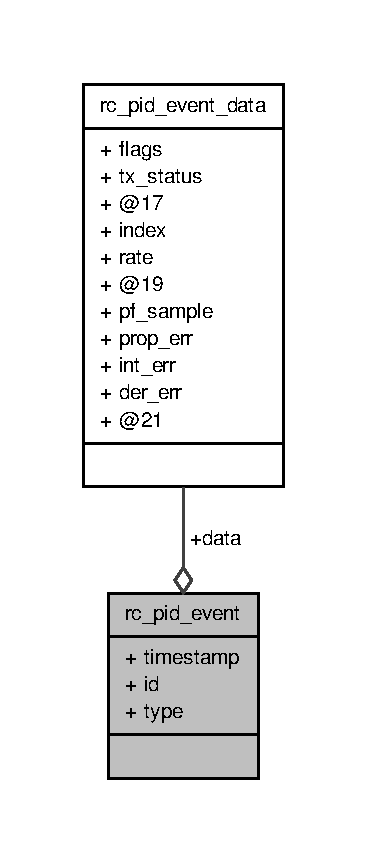
\includegraphics[width=176pt]{structrc__pid__event__coll__graph}
\end{center}
\end{figure}
\subsection*{Data Fields}
\begin{DoxyCompactItemize}
\item 
unsigned long \hyperlink{structrc__pid__event_acba7776dcc1861edfe0e9c5736de4df8}{timestamp}
\item 
unsigned int \hyperlink{structrc__pid__event_ab7ce6f462afaf105224b0ca772a33c43}{id}
\item 
enum \hyperlink{rc80211__pid_8h_a636dd9c3283aad52c197c570e1def90a}{rc\-\_\-pid\-\_\-event\-\_\-type} \hyperlink{structrc__pid__event_ad5d1f941fce20a7c87ff35faaf354710}{type}
\item 
union \hyperlink{unionrc__pid__event__data}{rc\-\_\-pid\-\_\-event\-\_\-data} \hyperlink{structrc__pid__event_ad7906c836bd8f9691c05d7b1754e059c}{data}
\end{DoxyCompactItemize}


\subsection{Detailed Description}


Definition at line 79 of file rc80211\-\_\-pid.\-h.



\subsection{Field Documentation}
\hypertarget{structrc__pid__event_ad7906c836bd8f9691c05d7b1754e059c}{\index{rc\-\_\-pid\-\_\-event@{rc\-\_\-pid\-\_\-event}!data@{data}}
\index{data@{data}!rc_pid_event@{rc\-\_\-pid\-\_\-event}}
\subsubsection[{data}]{\setlength{\rightskip}{0pt plus 5cm}union {\bf rc\-\_\-pid\-\_\-event\-\_\-data} data}}\label{structrc__pid__event_ad7906c836bd8f9691c05d7b1754e059c}


Definition at line 90 of file rc80211\-\_\-pid.\-h.

\hypertarget{structrc__pid__event_ab7ce6f462afaf105224b0ca772a33c43}{\index{rc\-\_\-pid\-\_\-event@{rc\-\_\-pid\-\_\-event}!id@{id}}
\index{id@{id}!rc_pid_event@{rc\-\_\-pid\-\_\-event}}
\subsubsection[{id}]{\setlength{\rightskip}{0pt plus 5cm}unsigned int id}}\label{structrc__pid__event_ab7ce6f462afaf105224b0ca772a33c43}


Definition at line 84 of file rc80211\-\_\-pid.\-h.

\hypertarget{structrc__pid__event_acba7776dcc1861edfe0e9c5736de4df8}{\index{rc\-\_\-pid\-\_\-event@{rc\-\_\-pid\-\_\-event}!timestamp@{timestamp}}
\index{timestamp@{timestamp}!rc_pid_event@{rc\-\_\-pid\-\_\-event}}
\subsubsection[{timestamp}]{\setlength{\rightskip}{0pt plus 5cm}unsigned long timestamp}}\label{structrc__pid__event_acba7776dcc1861edfe0e9c5736de4df8}


Definition at line 81 of file rc80211\-\_\-pid.\-h.

\hypertarget{structrc__pid__event_ad5d1f941fce20a7c87ff35faaf354710}{\index{rc\-\_\-pid\-\_\-event@{rc\-\_\-pid\-\_\-event}!type@{type}}
\index{type@{type}!rc_pid_event@{rc\-\_\-pid\-\_\-event}}
\subsubsection[{type}]{\setlength{\rightskip}{0pt plus 5cm}enum {\bf rc\-\_\-pid\-\_\-event\-\_\-type} type}}\label{structrc__pid__event_ad5d1f941fce20a7c87ff35faaf354710}


Definition at line 87 of file rc80211\-\_\-pid.\-h.



The documentation for this struct was generated from the following file\-:\begin{DoxyCompactItemize}
\item 
/home/guille/msm/net/mac80211/\hyperlink{rc80211__pid_8h}{rc80211\-\_\-pid.\-h}\end{DoxyCompactItemize}

\hypertarget{structrc__pid__event__buffer}{\section{rc\-\_\-pid\-\_\-event\-\_\-buffer Struct Reference}
\label{structrc__pid__event__buffer}\index{rc\-\_\-pid\-\_\-event\-\_\-buffer@{rc\-\_\-pid\-\_\-event\-\_\-buffer}}
}


{\ttfamily \#include $<$rc80211\-\_\-pid.\-h$>$}



Collaboration diagram for rc\-\_\-pid\-\_\-event\-\_\-buffer\-:
\nopagebreak
\begin{figure}[H]
\begin{center}
\leavevmode
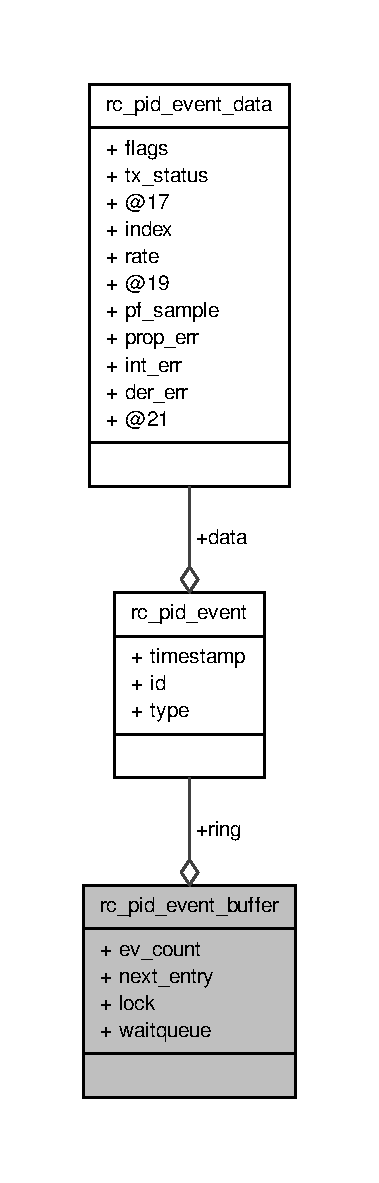
\includegraphics[height=550pt]{structrc__pid__event__buffer__coll__graph}
\end{center}
\end{figure}
\subsection*{Data Fields}
\begin{DoxyCompactItemize}
\item 
unsigned int \hyperlink{structrc__pid__event__buffer_aafefaa6538709caeb21b4566c91f8936}{ev\-\_\-count}
\item 
struct \hyperlink{structrc__pid__event}{rc\-\_\-pid\-\_\-event} \hyperlink{structrc__pid__event__buffer_ac15c562561ecad08ac70a1b809622c66}{ring} \mbox{[}\hyperlink{rc80211__pid_8h_afa197c57381c9b4287a15f41f0700f75}{R\-C\-\_\-\-P\-I\-D\-\_\-\-E\-V\-E\-N\-T\-\_\-\-R\-I\-N\-G\-\_\-\-S\-I\-Z\-E}\mbox{]}
\item 
unsigned int \hyperlink{structrc__pid__event__buffer_a504ce2058dfc4cdd4cf89d9e63c34b89}{next\-\_\-entry}
\item 
spinlock\-\_\-t \hyperlink{structrc__pid__event__buffer_a79cda015c79ff2b4c1444e3070f0bb5d}{lock}
\item 
wait\-\_\-queue\-\_\-head\-\_\-t \hyperlink{structrc__pid__event__buffer_a24489217320b81c842b7d32aa13ff863}{waitqueue}
\end{DoxyCompactItemize}


\subsection{Detailed Description}


Definition at line 96 of file rc80211\-\_\-pid.\-h.



\subsection{Field Documentation}
\hypertarget{structrc__pid__event__buffer_aafefaa6538709caeb21b4566c91f8936}{\index{rc\-\_\-pid\-\_\-event\-\_\-buffer@{rc\-\_\-pid\-\_\-event\-\_\-buffer}!ev\-\_\-count@{ev\-\_\-count}}
\index{ev\-\_\-count@{ev\-\_\-count}!rc_pid_event_buffer@{rc\-\_\-pid\-\_\-event\-\_\-buffer}}
\subsubsection[{ev\-\_\-count}]{\setlength{\rightskip}{0pt plus 5cm}unsigned int ev\-\_\-count}}\label{structrc__pid__event__buffer_aafefaa6538709caeb21b4566c91f8936}


Definition at line 98 of file rc80211\-\_\-pid.\-h.

\hypertarget{structrc__pid__event__buffer_a79cda015c79ff2b4c1444e3070f0bb5d}{\index{rc\-\_\-pid\-\_\-event\-\_\-buffer@{rc\-\_\-pid\-\_\-event\-\_\-buffer}!lock@{lock}}
\index{lock@{lock}!rc_pid_event_buffer@{rc\-\_\-pid\-\_\-event\-\_\-buffer}}
\subsubsection[{lock}]{\setlength{\rightskip}{0pt plus 5cm}spinlock\-\_\-t lock}}\label{structrc__pid__event__buffer_a79cda015c79ff2b4c1444e3070f0bb5d}


Definition at line 107 of file rc80211\-\_\-pid.\-h.

\hypertarget{structrc__pid__event__buffer_a504ce2058dfc4cdd4cf89d9e63c34b89}{\index{rc\-\_\-pid\-\_\-event\-\_\-buffer@{rc\-\_\-pid\-\_\-event\-\_\-buffer}!next\-\_\-entry@{next\-\_\-entry}}
\index{next\-\_\-entry@{next\-\_\-entry}!rc_pid_event_buffer@{rc\-\_\-pid\-\_\-event\-\_\-buffer}}
\subsubsection[{next\-\_\-entry}]{\setlength{\rightskip}{0pt plus 5cm}unsigned int next\-\_\-entry}}\label{structrc__pid__event__buffer_a504ce2058dfc4cdd4cf89d9e63c34b89}


Definition at line 104 of file rc80211\-\_\-pid.\-h.

\hypertarget{structrc__pid__event__buffer_ac15c562561ecad08ac70a1b809622c66}{\index{rc\-\_\-pid\-\_\-event\-\_\-buffer@{rc\-\_\-pid\-\_\-event\-\_\-buffer}!ring@{ring}}
\index{ring@{ring}!rc_pid_event_buffer@{rc\-\_\-pid\-\_\-event\-\_\-buffer}}
\subsubsection[{ring}]{\setlength{\rightskip}{0pt plus 5cm}struct {\bf rc\-\_\-pid\-\_\-event} ring\mbox{[}{\bf R\-C\-\_\-\-P\-I\-D\-\_\-\-E\-V\-E\-N\-T\-\_\-\-R\-I\-N\-G\-\_\-\-S\-I\-Z\-E}\mbox{]}}}\label{structrc__pid__event__buffer_ac15c562561ecad08ac70a1b809622c66}


Definition at line 101 of file rc80211\-\_\-pid.\-h.

\hypertarget{structrc__pid__event__buffer_a24489217320b81c842b7d32aa13ff863}{\index{rc\-\_\-pid\-\_\-event\-\_\-buffer@{rc\-\_\-pid\-\_\-event\-\_\-buffer}!waitqueue@{waitqueue}}
\index{waitqueue@{waitqueue}!rc_pid_event_buffer@{rc\-\_\-pid\-\_\-event\-\_\-buffer}}
\subsubsection[{waitqueue}]{\setlength{\rightskip}{0pt plus 5cm}wait\-\_\-queue\-\_\-head\-\_\-t waitqueue}}\label{structrc__pid__event__buffer_a24489217320b81c842b7d32aa13ff863}


Definition at line 110 of file rc80211\-\_\-pid.\-h.



The documentation for this struct was generated from the following file\-:\begin{DoxyCompactItemize}
\item 
/home/guille/msm/net/mac80211/\hyperlink{rc80211__pid_8h}{rc80211\-\_\-pid.\-h}\end{DoxyCompactItemize}

\hypertarget{unionrc__pid__event__data}{\section{rc\-\_\-pid\-\_\-event\-\_\-data Union Reference}
\label{unionrc__pid__event__data}\index{rc\-\_\-pid\-\_\-event\-\_\-data@{rc\-\_\-pid\-\_\-event\-\_\-data}}
}


{\ttfamily \#include $<$rc80211\-\_\-pid.\-h$>$}



Collaboration diagram for rc\-\_\-pid\-\_\-event\-\_\-data\-:
\nopagebreak
\begin{figure}[H]
\begin{center}
\leavevmode
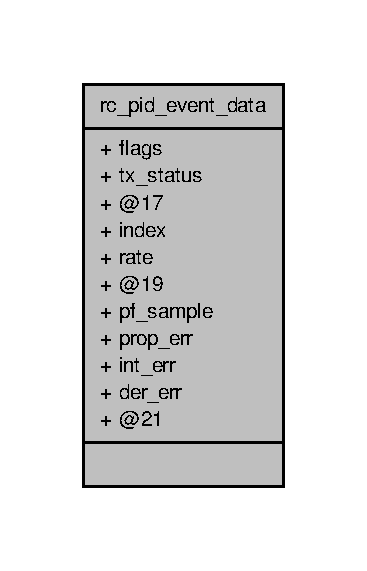
\includegraphics[width=176pt]{unionrc__pid__event__data__coll__graph}
\end{center}
\end{figure}
\subsection*{Data Fields}
\begin{DoxyCompactItemize}
\item 
\begin{tabbing}
xx\=xx\=xx\=xx\=xx\=xx\=xx\=xx\=xx\=\kill
struct \{\\
\>u32 \hyperlink{unionrc__pid__event__data_a9fb2abd9f2594cefc48d6856e01f2879}{flags}\\
\>struct ieee80211\_tx\_info \hyperlink{unionrc__pid__event__data_ad0580b6e8aa75d244c97d299b7bac298}{tx\_status}\\
\}; \\

\end{tabbing}\item 
\begin{tabbing}
xx\=xx\=xx\=xx\=xx\=xx\=xx\=xx\=xx\=\kill
struct \{\\
\>int \hyperlink{unionrc__pid__event__data_a750b5d744c39a06bfb13e6eb010e35d0}{index}\\
\>int \hyperlink{unionrc__pid__event__data_a7a829e6fd74e94e0edf10550470d844c}{rate}\\
\}; \\

\end{tabbing}\item 
\begin{tabbing}
xx\=xx\=xx\=xx\=xx\=xx\=xx\=xx\=xx\=\kill
struct \{\\
\>s32 \hyperlink{unionrc__pid__event__data_ab03cef57c5c881d1d6510822f2933fdc}{pf\_sample}\\
\>s32 \hyperlink{unionrc__pid__event__data_a236877cfccb9799bf6c8d35aca9faa2c}{prop\_err}\\
\>s32 \hyperlink{unionrc__pid__event__data_afd0a2b97b5e445f22caaf127bf38148c}{int\_err}\\
\>s32 \hyperlink{unionrc__pid__event__data_a6e974dd77139e01c6060f753dc03b0f7}{der\_err}\\
\}; \\

\end{tabbing}\end{DoxyCompactItemize}


\subsection{Detailed Description}


Definition at line 58 of file rc80211\-\_\-pid.\-h.



\subsection{Field Documentation}
\hypertarget{unionrc__pid__event__data_aed2b6243e8e4af2dae005339387e6067}{\subsubsection[{"@17}]{\setlength{\rightskip}{0pt plus 5cm}struct \{ ... \} }}\label{unionrc__pid__event__data_aed2b6243e8e4af2dae005339387e6067}
\hypertarget{unionrc__pid__event__data_aee5035e2df8993315ce9e2892094eafa}{\subsubsection[{"@19}]{\setlength{\rightskip}{0pt plus 5cm}struct \{ ... \} }}\label{unionrc__pid__event__data_aee5035e2df8993315ce9e2892094eafa}
\hypertarget{unionrc__pid__event__data_a466b53d954cb3e17b5c6e2a30db7f735}{\subsubsection[{"@21}]{\setlength{\rightskip}{0pt plus 5cm}struct \{ ... \} }}\label{unionrc__pid__event__data_a466b53d954cb3e17b5c6e2a30db7f735}
\hypertarget{unionrc__pid__event__data_a6e974dd77139e01c6060f753dc03b0f7}{\index{rc\-\_\-pid\-\_\-event\-\_\-data@{rc\-\_\-pid\-\_\-event\-\_\-data}!der\-\_\-err@{der\-\_\-err}}
\index{der\-\_\-err@{der\-\_\-err}!rc_pid_event_data@{rc\-\_\-pid\-\_\-event\-\_\-data}}
\subsubsection[{der\-\_\-err}]{\setlength{\rightskip}{0pt plus 5cm}s32 der\-\_\-err}}\label{unionrc__pid__event__data_a6e974dd77139e01c6060f753dc03b0f7}


Definition at line 75 of file rc80211\-\_\-pid.\-h.

\hypertarget{unionrc__pid__event__data_a9fb2abd9f2594cefc48d6856e01f2879}{\index{rc\-\_\-pid\-\_\-event\-\_\-data@{rc\-\_\-pid\-\_\-event\-\_\-data}!flags@{flags}}
\index{flags@{flags}!rc_pid_event_data@{rc\-\_\-pid\-\_\-event\-\_\-data}}
\subsubsection[{flags}]{\setlength{\rightskip}{0pt plus 5cm}u32 flags}}\label{unionrc__pid__event__data_a9fb2abd9f2594cefc48d6856e01f2879}


Definition at line 61 of file rc80211\-\_\-pid.\-h.

\hypertarget{unionrc__pid__event__data_a750b5d744c39a06bfb13e6eb010e35d0}{\index{rc\-\_\-pid\-\_\-event\-\_\-data@{rc\-\_\-pid\-\_\-event\-\_\-data}!index@{index}}
\index{index@{index}!rc_pid_event_data@{rc\-\_\-pid\-\_\-event\-\_\-data}}
\subsubsection[{index}]{\setlength{\rightskip}{0pt plus 5cm}int index}}\label{unionrc__pid__event__data_a750b5d744c39a06bfb13e6eb010e35d0}


Definition at line 67 of file rc80211\-\_\-pid.\-h.

\hypertarget{unionrc__pid__event__data_afd0a2b97b5e445f22caaf127bf38148c}{\index{rc\-\_\-pid\-\_\-event\-\_\-data@{rc\-\_\-pid\-\_\-event\-\_\-data}!int\-\_\-err@{int\-\_\-err}}
\index{int\-\_\-err@{int\-\_\-err}!rc_pid_event_data@{rc\-\_\-pid\-\_\-event\-\_\-data}}
\subsubsection[{int\-\_\-err}]{\setlength{\rightskip}{0pt plus 5cm}s32 int\-\_\-err}}\label{unionrc__pid__event__data_afd0a2b97b5e445f22caaf127bf38148c}


Definition at line 74 of file rc80211\-\_\-pid.\-h.

\hypertarget{unionrc__pid__event__data_ab03cef57c5c881d1d6510822f2933fdc}{\index{rc\-\_\-pid\-\_\-event\-\_\-data@{rc\-\_\-pid\-\_\-event\-\_\-data}!pf\-\_\-sample@{pf\-\_\-sample}}
\index{pf\-\_\-sample@{pf\-\_\-sample}!rc_pid_event_data@{rc\-\_\-pid\-\_\-event\-\_\-data}}
\subsubsection[{pf\-\_\-sample}]{\setlength{\rightskip}{0pt plus 5cm}s32 pf\-\_\-sample}}\label{unionrc__pid__event__data_ab03cef57c5c881d1d6510822f2933fdc}


Definition at line 72 of file rc80211\-\_\-pid.\-h.

\hypertarget{unionrc__pid__event__data_a236877cfccb9799bf6c8d35aca9faa2c}{\index{rc\-\_\-pid\-\_\-event\-\_\-data@{rc\-\_\-pid\-\_\-event\-\_\-data}!prop\-\_\-err@{prop\-\_\-err}}
\index{prop\-\_\-err@{prop\-\_\-err}!rc_pid_event_data@{rc\-\_\-pid\-\_\-event\-\_\-data}}
\subsubsection[{prop\-\_\-err}]{\setlength{\rightskip}{0pt plus 5cm}s32 prop\-\_\-err}}\label{unionrc__pid__event__data_a236877cfccb9799bf6c8d35aca9faa2c}


Definition at line 73 of file rc80211\-\_\-pid.\-h.

\hypertarget{unionrc__pid__event__data_a7a829e6fd74e94e0edf10550470d844c}{\index{rc\-\_\-pid\-\_\-event\-\_\-data@{rc\-\_\-pid\-\_\-event\-\_\-data}!rate@{rate}}
\index{rate@{rate}!rc_pid_event_data@{rc\-\_\-pid\-\_\-event\-\_\-data}}
\subsubsection[{rate}]{\setlength{\rightskip}{0pt plus 5cm}int rate}}\label{unionrc__pid__event__data_a7a829e6fd74e94e0edf10550470d844c}


Definition at line 68 of file rc80211\-\_\-pid.\-h.

\hypertarget{unionrc__pid__event__data_ad0580b6e8aa75d244c97d299b7bac298}{\index{rc\-\_\-pid\-\_\-event\-\_\-data@{rc\-\_\-pid\-\_\-event\-\_\-data}!tx\-\_\-status@{tx\-\_\-status}}
\index{tx\-\_\-status@{tx\-\_\-status}!rc_pid_event_data@{rc\-\_\-pid\-\_\-event\-\_\-data}}
\subsubsection[{tx\-\_\-status}]{\setlength{\rightskip}{0pt plus 5cm}struct ieee80211\-\_\-tx\-\_\-info tx\-\_\-status}}\label{unionrc__pid__event__data_ad0580b6e8aa75d244c97d299b7bac298}


Definition at line 62 of file rc80211\-\_\-pid.\-h.



The documentation for this union was generated from the following file\-:\begin{DoxyCompactItemize}
\item 
/home/guille/msm/net/mac80211/\hyperlink{rc80211__pid_8h}{rc80211\-\_\-pid.\-h}\end{DoxyCompactItemize}

\hypertarget{structrc__pid__events__file__info}{\section{rc\-\_\-pid\-\_\-events\-\_\-file\-\_\-info Struct Reference}
\label{structrc__pid__events__file__info}\index{rc\-\_\-pid\-\_\-events\-\_\-file\-\_\-info@{rc\-\_\-pid\-\_\-events\-\_\-file\-\_\-info}}
}


{\ttfamily \#include $<$rc80211\-\_\-pid.\-h$>$}



Collaboration diagram for rc\-\_\-pid\-\_\-events\-\_\-file\-\_\-info\-:
\nopagebreak
\begin{figure}[H]
\begin{center}
\leavevmode
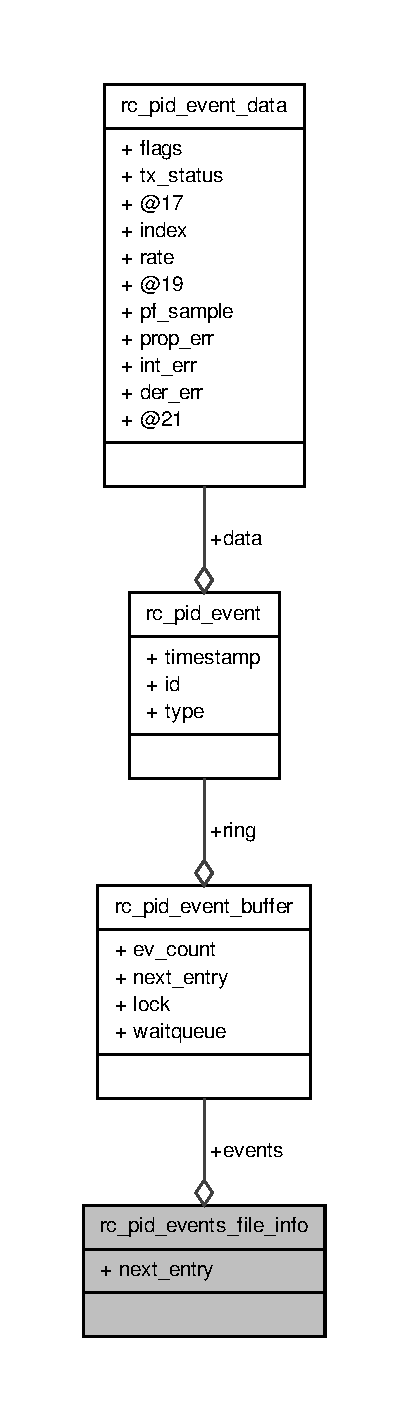
\includegraphics[height=550pt]{structrc__pid__events__file__info__coll__graph}
\end{center}
\end{figure}
\subsection*{Data Fields}
\begin{DoxyCompactItemize}
\item 
struct \hyperlink{structrc__pid__event__buffer}{rc\-\_\-pid\-\_\-event\-\_\-buffer} $\ast$ \hyperlink{structrc__pid__events__file__info_a64b7495c9f679034d3c77eb22e63d369}{events}
\item 
unsigned int \hyperlink{structrc__pid__events__file__info_a504ce2058dfc4cdd4cf89d9e63c34b89}{next\-\_\-entry}
\end{DoxyCompactItemize}


\subsection{Detailed Description}


Definition at line 113 of file rc80211\-\_\-pid.\-h.



\subsection{Field Documentation}
\hypertarget{structrc__pid__events__file__info_a64b7495c9f679034d3c77eb22e63d369}{\index{rc\-\_\-pid\-\_\-events\-\_\-file\-\_\-info@{rc\-\_\-pid\-\_\-events\-\_\-file\-\_\-info}!events@{events}}
\index{events@{events}!rc_pid_events_file_info@{rc\-\_\-pid\-\_\-events\-\_\-file\-\_\-info}}
\subsubsection[{events}]{\setlength{\rightskip}{0pt plus 5cm}struct {\bf rc\-\_\-pid\-\_\-event\-\_\-buffer}$\ast$ events}}\label{structrc__pid__events__file__info_a64b7495c9f679034d3c77eb22e63d369}


Definition at line 115 of file rc80211\-\_\-pid.\-h.

\hypertarget{structrc__pid__events__file__info_a504ce2058dfc4cdd4cf89d9e63c34b89}{\index{rc\-\_\-pid\-\_\-events\-\_\-file\-\_\-info@{rc\-\_\-pid\-\_\-events\-\_\-file\-\_\-info}!next\-\_\-entry@{next\-\_\-entry}}
\index{next\-\_\-entry@{next\-\_\-entry}!rc_pid_events_file_info@{rc\-\_\-pid\-\_\-events\-\_\-file\-\_\-info}}
\subsubsection[{next\-\_\-entry}]{\setlength{\rightskip}{0pt plus 5cm}unsigned int next\-\_\-entry}}\label{structrc__pid__events__file__info_a504ce2058dfc4cdd4cf89d9e63c34b89}


Definition at line 118 of file rc80211\-\_\-pid.\-h.



The documentation for this struct was generated from the following file\-:\begin{DoxyCompactItemize}
\item 
/home/guille/msm/net/mac80211/\hyperlink{rc80211__pid_8h}{rc80211\-\_\-pid.\-h}\end{DoxyCompactItemize}

\hypertarget{structrc__pid__info}{\section{rc\-\_\-pid\-\_\-info Struct Reference}
\label{structrc__pid__info}\index{rc\-\_\-pid\-\_\-info@{rc\-\_\-pid\-\_\-info}}
}


{\ttfamily \#include $<$rc80211\-\_\-pid.\-h$>$}



Collaboration diagram for rc\-\_\-pid\-\_\-info\-:
\nopagebreak
\begin{figure}[H]
\begin{center}
\leavevmode
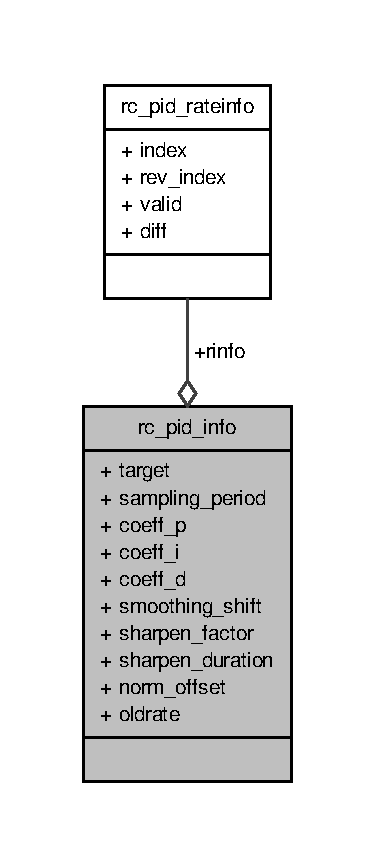
\includegraphics[width=180pt]{structrc__pid__info__coll__graph}
\end{center}
\end{figure}
\subsection*{Data Fields}
\begin{DoxyCompactItemize}
\item 
unsigned int \hyperlink{structrc__pid__info_af10772e6d304a2ff59891323f52eb170}{target}
\item 
unsigned int \hyperlink{structrc__pid__info_ae8f25bd55b4a9f4801e99450be7d7423}{sampling\-\_\-period}
\item 
int \hyperlink{structrc__pid__info_a249e72e36aa45ff6e09bce908d9491f0}{coeff\-\_\-p}
\item 
int \hyperlink{structrc__pid__info_aa7a1ae58ae054f4634ba919f4567af37}{coeff\-\_\-i}
\item 
int \hyperlink{structrc__pid__info_afd03d1d56025c1bffa068b2d41be3452}{coeff\-\_\-d}
\item 
unsigned int \hyperlink{structrc__pid__info_a149ce33760f493b8318a62b2a7515598}{smoothing\-\_\-shift}
\item 
unsigned int \hyperlink{structrc__pid__info_a2b9d94e794aa853e15da008fe0644b64}{sharpen\-\_\-factor}
\item 
unsigned int \hyperlink{structrc__pid__info_afabb1c822dc4b2c7064e942d6ce04690}{sharpen\-\_\-duration}
\item 
unsigned int \hyperlink{structrc__pid__info_a29160d78004070d0c75f2dba5f014ce9}{norm\-\_\-offset}
\item 
struct \hyperlink{structrc__pid__rateinfo}{rc\-\_\-pid\-\_\-rateinfo} $\ast$ \hyperlink{structrc__pid__info_a4f4b42edd508d8b67f84acfb4d10981d}{rinfo}
\item 
int \hyperlink{structrc__pid__info_a7f0d2f9f4aa2b5b79fee366631f3558e}{oldrate}
\end{DoxyCompactItemize}


\subsection{Detailed Description}


Definition at line 243 of file rc80211\-\_\-pid.\-h.



\subsection{Field Documentation}
\hypertarget{structrc__pid__info_afd03d1d56025c1bffa068b2d41be3452}{\index{rc\-\_\-pid\-\_\-info@{rc\-\_\-pid\-\_\-info}!coeff\-\_\-d@{coeff\-\_\-d}}
\index{coeff\-\_\-d@{coeff\-\_\-d}!rc_pid_info@{rc\-\_\-pid\-\_\-info}}
\subsubsection[{coeff\-\_\-d}]{\setlength{\rightskip}{0pt plus 5cm}int coeff\-\_\-d}}\label{structrc__pid__info_afd03d1d56025c1bffa068b2d41be3452}


Definition at line 254 of file rc80211\-\_\-pid.\-h.

\hypertarget{structrc__pid__info_aa7a1ae58ae054f4634ba919f4567af37}{\index{rc\-\_\-pid\-\_\-info@{rc\-\_\-pid\-\_\-info}!coeff\-\_\-i@{coeff\-\_\-i}}
\index{coeff\-\_\-i@{coeff\-\_\-i}!rc_pid_info@{rc\-\_\-pid\-\_\-info}}
\subsubsection[{coeff\-\_\-i}]{\setlength{\rightskip}{0pt plus 5cm}int coeff\-\_\-i}}\label{structrc__pid__info_aa7a1ae58ae054f4634ba919f4567af37}


Definition at line 253 of file rc80211\-\_\-pid.\-h.

\hypertarget{structrc__pid__info_a249e72e36aa45ff6e09bce908d9491f0}{\index{rc\-\_\-pid\-\_\-info@{rc\-\_\-pid\-\_\-info}!coeff\-\_\-p@{coeff\-\_\-p}}
\index{coeff\-\_\-p@{coeff\-\_\-p}!rc_pid_info@{rc\-\_\-pid\-\_\-info}}
\subsubsection[{coeff\-\_\-p}]{\setlength{\rightskip}{0pt plus 5cm}int coeff\-\_\-p}}\label{structrc__pid__info_a249e72e36aa45ff6e09bce908d9491f0}


Definition at line 252 of file rc80211\-\_\-pid.\-h.

\hypertarget{structrc__pid__info_a29160d78004070d0c75f2dba5f014ce9}{\index{rc\-\_\-pid\-\_\-info@{rc\-\_\-pid\-\_\-info}!norm\-\_\-offset@{norm\-\_\-offset}}
\index{norm\-\_\-offset@{norm\-\_\-offset}!rc_pid_info@{rc\-\_\-pid\-\_\-info}}
\subsubsection[{norm\-\_\-offset}]{\setlength{\rightskip}{0pt plus 5cm}unsigned int norm\-\_\-offset}}\label{structrc__pid__info_a29160d78004070d0c75f2dba5f014ce9}


Definition at line 264 of file rc80211\-\_\-pid.\-h.

\hypertarget{structrc__pid__info_a7f0d2f9f4aa2b5b79fee366631f3558e}{\index{rc\-\_\-pid\-\_\-info@{rc\-\_\-pid\-\_\-info}!oldrate@{oldrate}}
\index{oldrate@{oldrate}!rc_pid_info@{rc\-\_\-pid\-\_\-info}}
\subsubsection[{oldrate}]{\setlength{\rightskip}{0pt plus 5cm}int oldrate}}\label{structrc__pid__info_a7f0d2f9f4aa2b5b79fee366631f3558e}


Definition at line 270 of file rc80211\-\_\-pid.\-h.

\hypertarget{structrc__pid__info_a4f4b42edd508d8b67f84acfb4d10981d}{\index{rc\-\_\-pid\-\_\-info@{rc\-\_\-pid\-\_\-info}!rinfo@{rinfo}}
\index{rinfo@{rinfo}!rc_pid_info@{rc\-\_\-pid\-\_\-info}}
\subsubsection[{rinfo}]{\setlength{\rightskip}{0pt plus 5cm}struct {\bf rc\-\_\-pid\-\_\-rateinfo}$\ast$ rinfo}}\label{structrc__pid__info_a4f4b42edd508d8b67f84acfb4d10981d}


Definition at line 267 of file rc80211\-\_\-pid.\-h.

\hypertarget{structrc__pid__info_ae8f25bd55b4a9f4801e99450be7d7423}{\index{rc\-\_\-pid\-\_\-info@{rc\-\_\-pid\-\_\-info}!sampling\-\_\-period@{sampling\-\_\-period}}
\index{sampling\-\_\-period@{sampling\-\_\-period}!rc_pid_info@{rc\-\_\-pid\-\_\-info}}
\subsubsection[{sampling\-\_\-period}]{\setlength{\rightskip}{0pt plus 5cm}unsigned int sampling\-\_\-period}}\label{structrc__pid__info_ae8f25bd55b4a9f4801e99450be7d7423}


Definition at line 249 of file rc80211\-\_\-pid.\-h.

\hypertarget{structrc__pid__info_afabb1c822dc4b2c7064e942d6ce04690}{\index{rc\-\_\-pid\-\_\-info@{rc\-\_\-pid\-\_\-info}!sharpen\-\_\-duration@{sharpen\-\_\-duration}}
\index{sharpen\-\_\-duration@{sharpen\-\_\-duration}!rc_pid_info@{rc\-\_\-pid\-\_\-info}}
\subsubsection[{sharpen\-\_\-duration}]{\setlength{\rightskip}{0pt plus 5cm}unsigned int sharpen\-\_\-duration}}\label{structrc__pid__info_afabb1c822dc4b2c7064e942d6ce04690}


Definition at line 261 of file rc80211\-\_\-pid.\-h.

\hypertarget{structrc__pid__info_a2b9d94e794aa853e15da008fe0644b64}{\index{rc\-\_\-pid\-\_\-info@{rc\-\_\-pid\-\_\-info}!sharpen\-\_\-factor@{sharpen\-\_\-factor}}
\index{sharpen\-\_\-factor@{sharpen\-\_\-factor}!rc_pid_info@{rc\-\_\-pid\-\_\-info}}
\subsubsection[{sharpen\-\_\-factor}]{\setlength{\rightskip}{0pt plus 5cm}unsigned int sharpen\-\_\-factor}}\label{structrc__pid__info_a2b9d94e794aa853e15da008fe0644b64}


Definition at line 260 of file rc80211\-\_\-pid.\-h.

\hypertarget{structrc__pid__info_a149ce33760f493b8318a62b2a7515598}{\index{rc\-\_\-pid\-\_\-info@{rc\-\_\-pid\-\_\-info}!smoothing\-\_\-shift@{smoothing\-\_\-shift}}
\index{smoothing\-\_\-shift@{smoothing\-\_\-shift}!rc_pid_info@{rc\-\_\-pid\-\_\-info}}
\subsubsection[{smoothing\-\_\-shift}]{\setlength{\rightskip}{0pt plus 5cm}unsigned int smoothing\-\_\-shift}}\label{structrc__pid__info_a149ce33760f493b8318a62b2a7515598}


Definition at line 257 of file rc80211\-\_\-pid.\-h.

\hypertarget{structrc__pid__info_af10772e6d304a2ff59891323f52eb170}{\index{rc\-\_\-pid\-\_\-info@{rc\-\_\-pid\-\_\-info}!target@{target}}
\index{target@{target}!rc_pid_info@{rc\-\_\-pid\-\_\-info}}
\subsubsection[{target}]{\setlength{\rightskip}{0pt plus 5cm}unsigned int target}}\label{structrc__pid__info_af10772e6d304a2ff59891323f52eb170}


Definition at line 246 of file rc80211\-\_\-pid.\-h.



The documentation for this struct was generated from the following file\-:\begin{DoxyCompactItemize}
\item 
/home/guille/msm/net/mac80211/\hyperlink{rc80211__pid_8h}{rc80211\-\_\-pid.\-h}\end{DoxyCompactItemize}

\hypertarget{structrc__pid__rateinfo}{\section{rc\-\_\-pid\-\_\-rateinfo Struct Reference}
\label{structrc__pid__rateinfo}\index{rc\-\_\-pid\-\_\-rateinfo@{rc\-\_\-pid\-\_\-rateinfo}}
}


{\ttfamily \#include $<$rc80211\-\_\-pid.\-h$>$}



Collaboration diagram for rc\-\_\-pid\-\_\-rateinfo\-:
\nopagebreak
\begin{figure}[H]
\begin{center}
\leavevmode
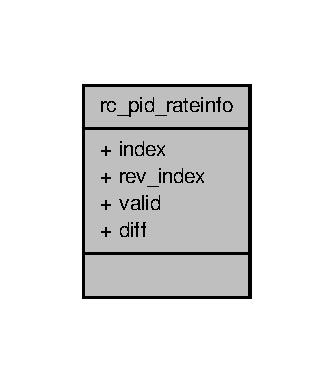
\includegraphics[width=160pt]{structrc__pid__rateinfo__coll__graph}
\end{center}
\end{figure}
\subsection*{Data Fields}
\begin{DoxyCompactItemize}
\item 
int \hyperlink{structrc__pid__rateinfo_a750b5d744c39a06bfb13e6eb010e35d0}{index}
\item 
int \hyperlink{structrc__pid__rateinfo_ab2a252c7807fa54334cd1bbc0ec2d894}{rev\-\_\-index}
\item 
bool \hyperlink{structrc__pid__rateinfo_a28e3c179a86f337095088b3ca02a2b2a}{valid}
\item 
int \hyperlink{structrc__pid__rateinfo_a65f3a8178e1f997a7a19a988bb0f4e1a}{diff}
\end{DoxyCompactItemize}


\subsection{Detailed Description}


Definition at line 228 of file rc80211\-\_\-pid.\-h.



\subsection{Field Documentation}
\hypertarget{structrc__pid__rateinfo_a65f3a8178e1f997a7a19a988bb0f4e1a}{\index{rc\-\_\-pid\-\_\-rateinfo@{rc\-\_\-pid\-\_\-rateinfo}!diff@{diff}}
\index{diff@{diff}!rc_pid_rateinfo@{rc\-\_\-pid\-\_\-rateinfo}}
\subsubsection[{diff}]{\setlength{\rightskip}{0pt plus 5cm}int diff}}\label{structrc__pid__rateinfo_a65f3a8178e1f997a7a19a988bb0f4e1a}


Definition at line 240 of file rc80211\-\_\-pid.\-h.

\hypertarget{structrc__pid__rateinfo_a750b5d744c39a06bfb13e6eb010e35d0}{\index{rc\-\_\-pid\-\_\-rateinfo@{rc\-\_\-pid\-\_\-rateinfo}!index@{index}}
\index{index@{index}!rc_pid_rateinfo@{rc\-\_\-pid\-\_\-rateinfo}}
\subsubsection[{index}]{\setlength{\rightskip}{0pt plus 5cm}int index}}\label{structrc__pid__rateinfo_a750b5d744c39a06bfb13e6eb010e35d0}


Definition at line 231 of file rc80211\-\_\-pid.\-h.

\hypertarget{structrc__pid__rateinfo_ab2a252c7807fa54334cd1bbc0ec2d894}{\index{rc\-\_\-pid\-\_\-rateinfo@{rc\-\_\-pid\-\_\-rateinfo}!rev\-\_\-index@{rev\-\_\-index}}
\index{rev\-\_\-index@{rev\-\_\-index}!rc_pid_rateinfo@{rc\-\_\-pid\-\_\-rateinfo}}
\subsubsection[{rev\-\_\-index}]{\setlength{\rightskip}{0pt plus 5cm}int rev\-\_\-index}}\label{structrc__pid__rateinfo_ab2a252c7807fa54334cd1bbc0ec2d894}


Definition at line 234 of file rc80211\-\_\-pid.\-h.

\hypertarget{structrc__pid__rateinfo_a28e3c179a86f337095088b3ca02a2b2a}{\index{rc\-\_\-pid\-\_\-rateinfo@{rc\-\_\-pid\-\_\-rateinfo}!valid@{valid}}
\index{valid@{valid}!rc_pid_rateinfo@{rc\-\_\-pid\-\_\-rateinfo}}
\subsubsection[{valid}]{\setlength{\rightskip}{0pt plus 5cm}bool valid}}\label{structrc__pid__rateinfo_a28e3c179a86f337095088b3ca02a2b2a}


Definition at line 237 of file rc80211\-\_\-pid.\-h.



The documentation for this struct was generated from the following file\-:\begin{DoxyCompactItemize}
\item 
/home/guille/msm/net/mac80211/\hyperlink{rc80211__pid_8h}{rc80211\-\_\-pid.\-h}\end{DoxyCompactItemize}

\hypertarget{structrc__pid__sta__info}{\section{rc\-\_\-pid\-\_\-sta\-\_\-info Struct Reference}
\label{structrc__pid__sta__info}\index{rc\-\_\-pid\-\_\-sta\-\_\-info@{rc\-\_\-pid\-\_\-sta\-\_\-info}}
}


{\ttfamily \#include $<$rc80211\-\_\-pid.\-h$>$}



Collaboration diagram for rc\-\_\-pid\-\_\-sta\-\_\-info\-:
\nopagebreak
\begin{figure}[H]
\begin{center}
\leavevmode
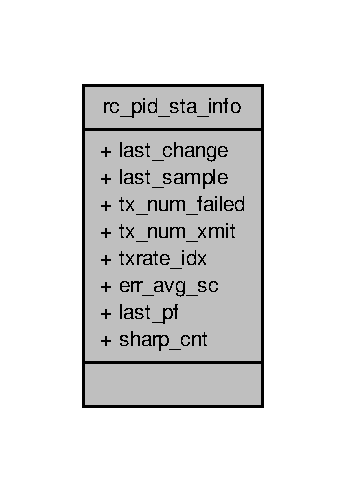
\includegraphics[width=166pt]{structrc__pid__sta__info__coll__graph}
\end{center}
\end{figure}
\subsection*{Data Fields}
\begin{DoxyCompactItemize}
\item 
unsigned long \hyperlink{structrc__pid__sta__info_a53675e28c7dd04fd5fb2e66dee8f484f}{last\-\_\-change}
\item 
unsigned long \hyperlink{structrc__pid__sta__info_ad13df28eb9ff39a645e7957d166e5fbd}{last\-\_\-sample}
\item 
u32 \hyperlink{structrc__pid__sta__info_a607670e1156f0a101a7e910cf70709bb}{tx\-\_\-num\-\_\-failed}
\item 
u32 \hyperlink{structrc__pid__sta__info_ada3db223fd162145ee8c39252fe1d095}{tx\-\_\-num\-\_\-xmit}
\item 
int \hyperlink{structrc__pid__sta__info_aaebb07f300f4c11055b26d9ac44b8cfc}{txrate\-\_\-idx}
\item 
s32 \hyperlink{structrc__pid__sta__info_ae03bdf9e307543490d3e9f8ebdbee20c}{err\-\_\-avg\-\_\-sc}
\item 
u32 \hyperlink{structrc__pid__sta__info_a30bbb3456871e78410e2145cbb670201}{last\-\_\-pf}
\item 
u8 \hyperlink{structrc__pid__sta__info_a20b3ceb286dda8e93db425fc68bd1a42}{sharp\-\_\-cnt}
\end{DoxyCompactItemize}


\subsection{Detailed Description}


Definition at line 172 of file rc80211\-\_\-pid.\-h.



\subsection{Field Documentation}
\hypertarget{structrc__pid__sta__info_ae03bdf9e307543490d3e9f8ebdbee20c}{\index{rc\-\_\-pid\-\_\-sta\-\_\-info@{rc\-\_\-pid\-\_\-sta\-\_\-info}!err\-\_\-avg\-\_\-sc@{err\-\_\-avg\-\_\-sc}}
\index{err\-\_\-avg\-\_\-sc@{err\-\_\-avg\-\_\-sc}!rc_pid_sta_info@{rc\-\_\-pid\-\_\-sta\-\_\-info}}
\subsubsection[{err\-\_\-avg\-\_\-sc}]{\setlength{\rightskip}{0pt plus 5cm}s32 err\-\_\-avg\-\_\-sc}}\label{structrc__pid__sta__info_ae03bdf9e307543490d3e9f8ebdbee20c}


Definition at line 208 of file rc80211\-\_\-pid.\-h.

\hypertarget{structrc__pid__sta__info_a53675e28c7dd04fd5fb2e66dee8f484f}{\index{rc\-\_\-pid\-\_\-sta\-\_\-info@{rc\-\_\-pid\-\_\-sta\-\_\-info}!last\-\_\-change@{last\-\_\-change}}
\index{last\-\_\-change@{last\-\_\-change}!rc_pid_sta_info@{rc\-\_\-pid\-\_\-sta\-\_\-info}}
\subsubsection[{last\-\_\-change}]{\setlength{\rightskip}{0pt plus 5cm}unsigned long last\-\_\-change}}\label{structrc__pid__sta__info_a53675e28c7dd04fd5fb2e66dee8f484f}


Definition at line 173 of file rc80211\-\_\-pid.\-h.

\hypertarget{structrc__pid__sta__info_a30bbb3456871e78410e2145cbb670201}{\index{rc\-\_\-pid\-\_\-sta\-\_\-info@{rc\-\_\-pid\-\_\-sta\-\_\-info}!last\-\_\-pf@{last\-\_\-pf}}
\index{last\-\_\-pf@{last\-\_\-pf}!rc_pid_sta_info@{rc\-\_\-pid\-\_\-sta\-\_\-info}}
\subsubsection[{last\-\_\-pf}]{\setlength{\rightskip}{0pt plus 5cm}u32 last\-\_\-pf}}\label{structrc__pid__sta__info_a30bbb3456871e78410e2145cbb670201}


Definition at line 211 of file rc80211\-\_\-pid.\-h.

\hypertarget{structrc__pid__sta__info_ad13df28eb9ff39a645e7957d166e5fbd}{\index{rc\-\_\-pid\-\_\-sta\-\_\-info@{rc\-\_\-pid\-\_\-sta\-\_\-info}!last\-\_\-sample@{last\-\_\-sample}}
\index{last\-\_\-sample@{last\-\_\-sample}!rc_pid_sta_info@{rc\-\_\-pid\-\_\-sta\-\_\-info}}
\subsubsection[{last\-\_\-sample}]{\setlength{\rightskip}{0pt plus 5cm}unsigned long last\-\_\-sample}}\label{structrc__pid__sta__info_ad13df28eb9ff39a645e7957d166e5fbd}


Definition at line 174 of file rc80211\-\_\-pid.\-h.

\hypertarget{structrc__pid__sta__info_a20b3ceb286dda8e93db425fc68bd1a42}{\index{rc\-\_\-pid\-\_\-sta\-\_\-info@{rc\-\_\-pid\-\_\-sta\-\_\-info}!sharp\-\_\-cnt@{sharp\-\_\-cnt}}
\index{sharp\-\_\-cnt@{sharp\-\_\-cnt}!rc_pid_sta_info@{rc\-\_\-pid\-\_\-sta\-\_\-info}}
\subsubsection[{sharp\-\_\-cnt}]{\setlength{\rightskip}{0pt plus 5cm}u8 sharp\-\_\-cnt}}\label{structrc__pid__sta__info_a20b3ceb286dda8e93db425fc68bd1a42}


Definition at line 214 of file rc80211\-\_\-pid.\-h.

\hypertarget{structrc__pid__sta__info_a607670e1156f0a101a7e910cf70709bb}{\index{rc\-\_\-pid\-\_\-sta\-\_\-info@{rc\-\_\-pid\-\_\-sta\-\_\-info}!tx\-\_\-num\-\_\-failed@{tx\-\_\-num\-\_\-failed}}
\index{tx\-\_\-num\-\_\-failed@{tx\-\_\-num\-\_\-failed}!rc_pid_sta_info@{rc\-\_\-pid\-\_\-sta\-\_\-info}}
\subsubsection[{tx\-\_\-num\-\_\-failed}]{\setlength{\rightskip}{0pt plus 5cm}u32 tx\-\_\-num\-\_\-failed}}\label{structrc__pid__sta__info_a607670e1156f0a101a7e910cf70709bb}


Definition at line 176 of file rc80211\-\_\-pid.\-h.

\hypertarget{structrc__pid__sta__info_ada3db223fd162145ee8c39252fe1d095}{\index{rc\-\_\-pid\-\_\-sta\-\_\-info@{rc\-\_\-pid\-\_\-sta\-\_\-info}!tx\-\_\-num\-\_\-xmit@{tx\-\_\-num\-\_\-xmit}}
\index{tx\-\_\-num\-\_\-xmit@{tx\-\_\-num\-\_\-xmit}!rc_pid_sta_info@{rc\-\_\-pid\-\_\-sta\-\_\-info}}
\subsubsection[{tx\-\_\-num\-\_\-xmit}]{\setlength{\rightskip}{0pt plus 5cm}u32 tx\-\_\-num\-\_\-xmit}}\label{structrc__pid__sta__info_ada3db223fd162145ee8c39252fe1d095}


Definition at line 177 of file rc80211\-\_\-pid.\-h.

\hypertarget{structrc__pid__sta__info_aaebb07f300f4c11055b26d9ac44b8cfc}{\index{rc\-\_\-pid\-\_\-sta\-\_\-info@{rc\-\_\-pid\-\_\-sta\-\_\-info}!txrate\-\_\-idx@{txrate\-\_\-idx}}
\index{txrate\-\_\-idx@{txrate\-\_\-idx}!rc_pid_sta_info@{rc\-\_\-pid\-\_\-sta\-\_\-info}}
\subsubsection[{txrate\-\_\-idx}]{\setlength{\rightskip}{0pt plus 5cm}int txrate\-\_\-idx}}\label{structrc__pid__sta__info_aaebb07f300f4c11055b26d9ac44b8cfc}


Definition at line 179 of file rc80211\-\_\-pid.\-h.



The documentation for this struct was generated from the following file\-:\begin{DoxyCompactItemize}
\item 
/home/guille/msm/net/mac80211/\hyperlink{rc80211__pid_8h}{rc80211\-\_\-pid.\-h}\end{DoxyCompactItemize}

\hypertarget{structrmc__entry}{\section{rmc\-\_\-entry Struct Reference}
\label{structrmc__entry}\index{rmc\-\_\-entry@{rmc\-\_\-entry}}
}


{\ttfamily \#include $<$mesh.\-h$>$}



Collaboration diagram for rmc\-\_\-entry\-:
\nopagebreak
\begin{figure}[H]
\begin{center}
\leavevmode
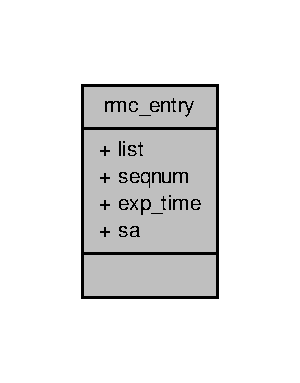
\includegraphics[width=144pt]{structrmc__entry__coll__graph}
\end{center}
\end{figure}
\subsection*{Data Fields}
\begin{DoxyCompactItemize}
\item 
struct list\-\_\-head \hyperlink{structrmc__entry_a1f00f18b91d5a820f2c43064243aa86e}{list}
\item 
u32 \hyperlink{structrmc__entry_aa1de03f6f57c53b7e53eb6f83507da76}{seqnum}
\item 
unsigned long \hyperlink{structrmc__entry_af01b3e5a14761c34e4298e254fb7c094}{exp\-\_\-time}
\item 
u8 \hyperlink{structrmc__entry_a1d248d85a9aee0de13f6a2647297e517}{sa} \mbox{[}E\-T\-H\-\_\-\-A\-L\-E\-N\mbox{]}
\end{DoxyCompactItemize}


\subsection{Detailed Description}
struct \hyperlink{structrmc__entry}{rmc\-\_\-entry} -\/ entry in the Recent Multicast Cache

\-: mesh sequence number of the frame \-: expiration time of the entry, in jiffies \begin{DoxySeeAlso}{See Also}
\-: source address of the frame
\end{DoxySeeAlso}
The Recent Multicast Cache keeps track of the latest multicast frames that have been received by a mesh interface and discards received multicast frames that are found in the cache. 

Definition at line 172 of file mesh.\-h.



\subsection{Field Documentation}
\hypertarget{structrmc__entry_af01b3e5a14761c34e4298e254fb7c094}{\index{rmc\-\_\-entry@{rmc\-\_\-entry}!exp\-\_\-time@{exp\-\_\-time}}
\index{exp\-\_\-time@{exp\-\_\-time}!rmc_entry@{rmc\-\_\-entry}}
\subsubsection[{exp\-\_\-time}]{\setlength{\rightskip}{0pt plus 5cm}unsigned long exp\-\_\-time}}\label{structrmc__entry_af01b3e5a14761c34e4298e254fb7c094}


Definition at line 175 of file mesh.\-h.

\hypertarget{structrmc__entry_a1f00f18b91d5a820f2c43064243aa86e}{\index{rmc\-\_\-entry@{rmc\-\_\-entry}!list@{list}}
\index{list@{list}!rmc_entry@{rmc\-\_\-entry}}
\subsubsection[{list}]{\setlength{\rightskip}{0pt plus 5cm}struct list\-\_\-head list}}\label{structrmc__entry_a1f00f18b91d5a820f2c43064243aa86e}


Definition at line 173 of file mesh.\-h.

\hypertarget{structrmc__entry_a1d248d85a9aee0de13f6a2647297e517}{\index{rmc\-\_\-entry@{rmc\-\_\-entry}!sa@{sa}}
\index{sa@{sa}!rmc_entry@{rmc\-\_\-entry}}
\subsubsection[{sa}]{\setlength{\rightskip}{0pt plus 5cm}u8 sa\mbox{[}E\-T\-H\-\_\-\-A\-L\-E\-N\mbox{]}}}\label{structrmc__entry_a1d248d85a9aee0de13f6a2647297e517}


Definition at line 176 of file mesh.\-h.

\hypertarget{structrmc__entry_aa1de03f6f57c53b7e53eb6f83507da76}{\index{rmc\-\_\-entry@{rmc\-\_\-entry}!seqnum@{seqnum}}
\index{seqnum@{seqnum}!rmc_entry@{rmc\-\_\-entry}}
\subsubsection[{seqnum}]{\setlength{\rightskip}{0pt plus 5cm}u32 seqnum}}\label{structrmc__entry_aa1de03f6f57c53b7e53eb6f83507da76}


Definition at line 174 of file mesh.\-h.



The documentation for this struct was generated from the following file\-:\begin{DoxyCompactItemize}
\item 
/home/guille/msm/net/mac80211/\hyperlink{mesh_8h}{mesh.\-h}\end{DoxyCompactItemize}

\hypertarget{structskb__eosp__msg__data}{\section{skb\-\_\-eosp\-\_\-msg\-\_\-data Struct Reference}
\label{structskb__eosp__msg__data}\index{skb\-\_\-eosp\-\_\-msg\-\_\-data@{skb\-\_\-eosp\-\_\-msg\-\_\-data}}
}


{\ttfamily \#include $<$ieee80211\-\_\-i.\-h$>$}



Collaboration diagram for skb\-\_\-eosp\-\_\-msg\-\_\-data\-:
\nopagebreak
\begin{figure}[H]
\begin{center}
\leavevmode
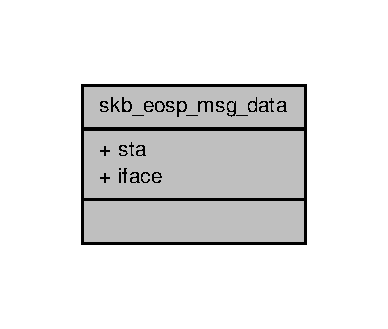
\includegraphics[width=186pt]{structskb__eosp__msg__data__coll__graph}
\end{center}
\end{figure}
\subsection*{Data Fields}
\begin{DoxyCompactItemize}
\item 
u8 \hyperlink{structskb__eosp__msg__data_add1dfd5a29b76978094290db59d1d19c}{sta} \mbox{[}E\-T\-H\-\_\-\-A\-L\-E\-N\mbox{]}
\item 
u8 \hyperlink{structskb__eosp__msg__data_af78ca47345f5661176509c303db21776}{iface} \mbox{[}E\-T\-H\-\_\-\-A\-L\-E\-N\mbox{]}
\end{DoxyCompactItemize}


\subsection{Detailed Description}


Definition at line 754 of file ieee80211\-\_\-i.\-h.



\subsection{Field Documentation}
\hypertarget{structskb__eosp__msg__data_af78ca47345f5661176509c303db21776}{\index{skb\-\_\-eosp\-\_\-msg\-\_\-data@{skb\-\_\-eosp\-\_\-msg\-\_\-data}!iface@{iface}}
\index{iface@{iface}!skb_eosp_msg_data@{skb\-\_\-eosp\-\_\-msg\-\_\-data}}
\subsubsection[{iface}]{\setlength{\rightskip}{0pt plus 5cm}u8 iface\mbox{[}E\-T\-H\-\_\-\-A\-L\-E\-N\mbox{]}}}\label{structskb__eosp__msg__data_af78ca47345f5661176509c303db21776}


Definition at line 755 of file ieee80211\-\_\-i.\-h.

\hypertarget{structskb__eosp__msg__data_add1dfd5a29b76978094290db59d1d19c}{\index{skb\-\_\-eosp\-\_\-msg\-\_\-data@{skb\-\_\-eosp\-\_\-msg\-\_\-data}!sta@{sta}}
\index{sta@{sta}!skb_eosp_msg_data@{skb\-\_\-eosp\-\_\-msg\-\_\-data}}
\subsubsection[{sta}]{\setlength{\rightskip}{0pt plus 5cm}u8 sta\mbox{[}E\-T\-H\-\_\-\-A\-L\-E\-N\mbox{]}}}\label{structskb__eosp__msg__data_add1dfd5a29b76978094290db59d1d19c}


Definition at line 755 of file ieee80211\-\_\-i.\-h.



The documentation for this struct was generated from the following file\-:\begin{DoxyCompactItemize}
\item 
/home/guille/msm/net/mac80211/\hyperlink{ieee80211__i_8h}{ieee80211\-\_\-i.\-h}\end{DoxyCompactItemize}

\hypertarget{structsta__ampdu__mlme}{\section{sta\-\_\-ampdu\-\_\-mlme Struct Reference}
\label{structsta__ampdu__mlme}\index{sta\-\_\-ampdu\-\_\-mlme@{sta\-\_\-ampdu\-\_\-mlme}}
}


{\ttfamily \#include $<$sta\-\_\-info.\-h$>$}



Collaboration diagram for sta\-\_\-ampdu\-\_\-mlme\-:
\nopagebreak
\begin{figure}[H]
\begin{center}
\leavevmode
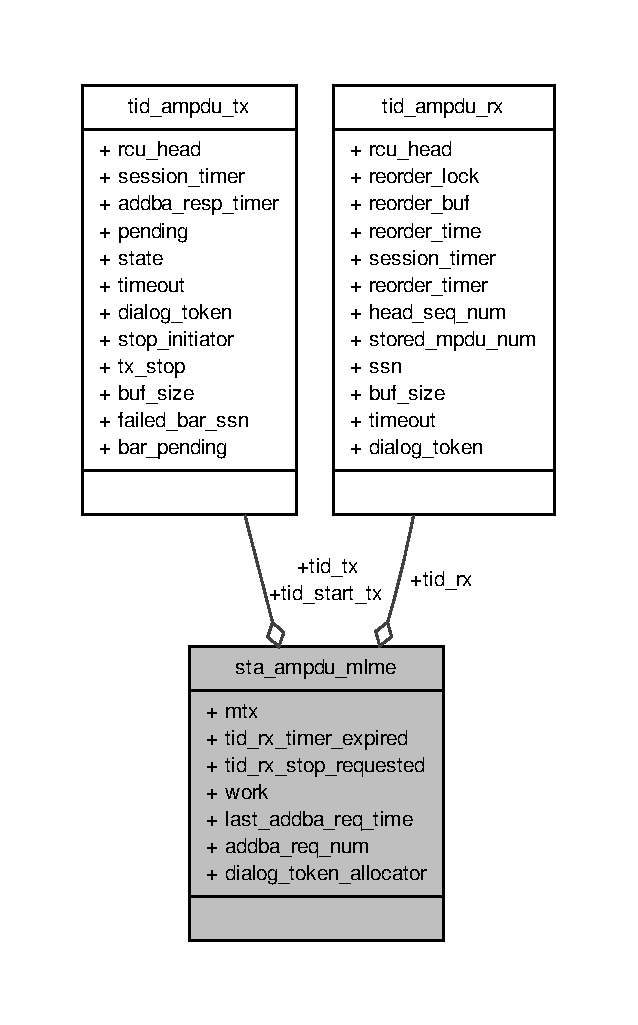
\includegraphics[width=306pt]{structsta__ampdu__mlme__coll__graph}
\end{center}
\end{figure}
\subsection*{Data Fields}
\begin{DoxyCompactItemize}
\item 
struct mutex \hyperlink{structsta__ampdu__mlme_a06f637951b74c996f2e4987a7be1dbdd}{mtx}
\item 
struct \hyperlink{structtid__ampdu__rx}{tid\-\_\-ampdu\-\_\-rx} \-\_\-\-\_\-rcu $\ast$ \hyperlink{structsta__ampdu__mlme_a9f02b8e803c3fad3c7f746477739b6c3}{tid\-\_\-rx} \mbox{[}\hyperlink{sta__info_8h_a8376226f35c3c806965ac03355cc1a00}{S\-T\-A\-\_\-\-T\-I\-D\-\_\-\-N\-U\-M}\mbox{]}
\item 
unsigned long \hyperlink{structsta__ampdu__mlme_a53e1819c9e1189bae325027254946f53}{tid\-\_\-rx\-\_\-timer\-\_\-expired} \mbox{[}B\-I\-T\-S\-\_\-\-T\-O\-\_\-\-L\-O\-N\-G\-S(\hyperlink{sta__info_8h_a8376226f35c3c806965ac03355cc1a00}{S\-T\-A\-\_\-\-T\-I\-D\-\_\-\-N\-U\-M})\mbox{]}
\item 
unsigned long \hyperlink{structsta__ampdu__mlme_aa9b2d44581dfa6af54bea5ad684e8b5f}{tid\-\_\-rx\-\_\-stop\-\_\-requested} \mbox{[}B\-I\-T\-S\-\_\-\-T\-O\-\_\-\-L\-O\-N\-G\-S(\hyperlink{sta__info_8h_a8376226f35c3c806965ac03355cc1a00}{S\-T\-A\-\_\-\-T\-I\-D\-\_\-\-N\-U\-M})\mbox{]}
\item 
struct work\-\_\-struct \hyperlink{structsta__ampdu__mlme_a623997e11b94d7c467ce26627cc488a2}{work}
\item 
struct \hyperlink{structtid__ampdu__tx}{tid\-\_\-ampdu\-\_\-tx} \-\_\-\-\_\-rcu $\ast$ \hyperlink{structsta__ampdu__mlme_acc2de99b986d5fa4b83081a609014228}{tid\-\_\-tx} \mbox{[}\hyperlink{sta__info_8h_a8376226f35c3c806965ac03355cc1a00}{S\-T\-A\-\_\-\-T\-I\-D\-\_\-\-N\-U\-M}\mbox{]}
\item 
struct \hyperlink{structtid__ampdu__tx}{tid\-\_\-ampdu\-\_\-tx} $\ast$ \hyperlink{structsta__ampdu__mlme_a11dbf950521d406406f6689d3db802fa}{tid\-\_\-start\-\_\-tx} \mbox{[}\hyperlink{sta__info_8h_a8376226f35c3c806965ac03355cc1a00}{S\-T\-A\-\_\-\-T\-I\-D\-\_\-\-N\-U\-M}\mbox{]}
\item 
unsigned long \hyperlink{structsta__ampdu__mlme_a811661f4c9a6505bfa7d3f74771e3157}{last\-\_\-addba\-\_\-req\-\_\-time} \mbox{[}\hyperlink{sta__info_8h_a8376226f35c3c806965ac03355cc1a00}{S\-T\-A\-\_\-\-T\-I\-D\-\_\-\-N\-U\-M}\mbox{]}
\item 
u8 \hyperlink{structsta__ampdu__mlme_a87d5e7167b24cc6e336ecf08e9e15d06}{addba\-\_\-req\-\_\-num} \mbox{[}\hyperlink{sta__info_8h_a8376226f35c3c806965ac03355cc1a00}{S\-T\-A\-\_\-\-T\-I\-D\-\_\-\-N\-U\-M}\mbox{]}
\item 
u8 \hyperlink{structsta__ampdu__mlme_a8dd4efd8eb6b5f60ae2295f55a4600a4}{dialog\-\_\-token\-\_\-allocator}
\end{DoxyCompactItemize}


\subsection{Detailed Description}
struct \hyperlink{structsta__ampdu__mlme}{sta\-\_\-ampdu\-\_\-mlme} -\/ S\-T\-A aggregation information.

\-: aggregation info for Rx per T\-I\-D -- R\-C\-U protected \-: aggregation info for Tx per T\-I\-D \-: sessions where start was requested \-: number of times add\-B\-A request has been sent. \-: timestamp of the last add\-B\-A request. \-: dialog token enumerator for each new session; \-: work struct for starting/stopping aggregation \-: bitmap indicating on which T\-I\-Ds the R\-X timer expired until the work for it runs \-: bitmap indicating which B\-A sessions per T\-I\-D the driver requested to close until the work for it runs \-: mutex to protect all T\-X data (except non-\/\-N\-U\-L\-L assignments to tid\-\_\-tx\mbox{[}idx\mbox{]}, which are protected by the sta spinlock) 

Definition at line 191 of file sta\-\_\-info.\-h.



\subsection{Field Documentation}
\hypertarget{structsta__ampdu__mlme_a87d5e7167b24cc6e336ecf08e9e15d06}{\index{sta\-\_\-ampdu\-\_\-mlme@{sta\-\_\-ampdu\-\_\-mlme}!addba\-\_\-req\-\_\-num@{addba\-\_\-req\-\_\-num}}
\index{addba\-\_\-req\-\_\-num@{addba\-\_\-req\-\_\-num}!sta_ampdu_mlme@{sta\-\_\-ampdu\-\_\-mlme}}
\subsubsection[{addba\-\_\-req\-\_\-num}]{\setlength{\rightskip}{0pt plus 5cm}u8 addba\-\_\-req\-\_\-num\mbox{[}{\bf S\-T\-A\-\_\-\-T\-I\-D\-\_\-\-N\-U\-M}\mbox{]}}}\label{structsta__ampdu__mlme_a87d5e7167b24cc6e336ecf08e9e15d06}


Definition at line 202 of file sta\-\_\-info.\-h.

\hypertarget{structsta__ampdu__mlme_a8dd4efd8eb6b5f60ae2295f55a4600a4}{\index{sta\-\_\-ampdu\-\_\-mlme@{sta\-\_\-ampdu\-\_\-mlme}!dialog\-\_\-token\-\_\-allocator@{dialog\-\_\-token\-\_\-allocator}}
\index{dialog\-\_\-token\-\_\-allocator@{dialog\-\_\-token\-\_\-allocator}!sta_ampdu_mlme@{sta\-\_\-ampdu\-\_\-mlme}}
\subsubsection[{dialog\-\_\-token\-\_\-allocator}]{\setlength{\rightskip}{0pt plus 5cm}u8 dialog\-\_\-token\-\_\-allocator}}\label{structsta__ampdu__mlme_a8dd4efd8eb6b5f60ae2295f55a4600a4}


Definition at line 203 of file sta\-\_\-info.\-h.

\hypertarget{structsta__ampdu__mlme_a811661f4c9a6505bfa7d3f74771e3157}{\index{sta\-\_\-ampdu\-\_\-mlme@{sta\-\_\-ampdu\-\_\-mlme}!last\-\_\-addba\-\_\-req\-\_\-time@{last\-\_\-addba\-\_\-req\-\_\-time}}
\index{last\-\_\-addba\-\_\-req\-\_\-time@{last\-\_\-addba\-\_\-req\-\_\-time}!sta_ampdu_mlme@{sta\-\_\-ampdu\-\_\-mlme}}
\subsubsection[{last\-\_\-addba\-\_\-req\-\_\-time}]{\setlength{\rightskip}{0pt plus 5cm}unsigned long last\-\_\-addba\-\_\-req\-\_\-time\mbox{[}{\bf S\-T\-A\-\_\-\-T\-I\-D\-\_\-\-N\-U\-M}\mbox{]}}}\label{structsta__ampdu__mlme_a811661f4c9a6505bfa7d3f74771e3157}


Definition at line 201 of file sta\-\_\-info.\-h.

\hypertarget{structsta__ampdu__mlme_a06f637951b74c996f2e4987a7be1dbdd}{\index{sta\-\_\-ampdu\-\_\-mlme@{sta\-\_\-ampdu\-\_\-mlme}!mtx@{mtx}}
\index{mtx@{mtx}!sta_ampdu_mlme@{sta\-\_\-ampdu\-\_\-mlme}}
\subsubsection[{mtx}]{\setlength{\rightskip}{0pt plus 5cm}struct mutex mtx}}\label{structsta__ampdu__mlme_a06f637951b74c996f2e4987a7be1dbdd}


Definition at line 192 of file sta\-\_\-info.\-h.

\hypertarget{structsta__ampdu__mlme_a9f02b8e803c3fad3c7f746477739b6c3}{\index{sta\-\_\-ampdu\-\_\-mlme@{sta\-\_\-ampdu\-\_\-mlme}!tid\-\_\-rx@{tid\-\_\-rx}}
\index{tid\-\_\-rx@{tid\-\_\-rx}!sta_ampdu_mlme@{sta\-\_\-ampdu\-\_\-mlme}}
\subsubsection[{tid\-\_\-rx}]{\setlength{\rightskip}{0pt plus 5cm}struct {\bf tid\-\_\-ampdu\-\_\-rx} \-\_\-\-\_\-rcu$\ast$ tid\-\_\-rx\mbox{[}{\bf S\-T\-A\-\_\-\-T\-I\-D\-\_\-\-N\-U\-M}\mbox{]}}}\label{structsta__ampdu__mlme_a9f02b8e803c3fad3c7f746477739b6c3}


Definition at line 194 of file sta\-\_\-info.\-h.

\hypertarget{structsta__ampdu__mlme_aa9b2d44581dfa6af54bea5ad684e8b5f}{\index{sta\-\_\-ampdu\-\_\-mlme@{sta\-\_\-ampdu\-\_\-mlme}!tid\-\_\-rx\-\_\-stop\-\_\-requested@{tid\-\_\-rx\-\_\-stop\-\_\-requested}}
\index{tid\-\_\-rx\-\_\-stop\-\_\-requested@{tid\-\_\-rx\-\_\-stop\-\_\-requested}!sta_ampdu_mlme@{sta\-\_\-ampdu\-\_\-mlme}}
\subsubsection[{tid\-\_\-rx\-\_\-stop\-\_\-requested}]{\setlength{\rightskip}{0pt plus 5cm}unsigned long tid\-\_\-rx\-\_\-stop\-\_\-requested\mbox{[}B\-I\-T\-S\-\_\-\-T\-O\-\_\-\-L\-O\-N\-G\-S({\bf S\-T\-A\-\_\-\-T\-I\-D\-\_\-\-N\-U\-M})\mbox{]}}}\label{structsta__ampdu__mlme_aa9b2d44581dfa6af54bea5ad684e8b5f}


Definition at line 196 of file sta\-\_\-info.\-h.

\hypertarget{structsta__ampdu__mlme_a53e1819c9e1189bae325027254946f53}{\index{sta\-\_\-ampdu\-\_\-mlme@{sta\-\_\-ampdu\-\_\-mlme}!tid\-\_\-rx\-\_\-timer\-\_\-expired@{tid\-\_\-rx\-\_\-timer\-\_\-expired}}
\index{tid\-\_\-rx\-\_\-timer\-\_\-expired@{tid\-\_\-rx\-\_\-timer\-\_\-expired}!sta_ampdu_mlme@{sta\-\_\-ampdu\-\_\-mlme}}
\subsubsection[{tid\-\_\-rx\-\_\-timer\-\_\-expired}]{\setlength{\rightskip}{0pt plus 5cm}unsigned long tid\-\_\-rx\-\_\-timer\-\_\-expired\mbox{[}B\-I\-T\-S\-\_\-\-T\-O\-\_\-\-L\-O\-N\-G\-S({\bf S\-T\-A\-\_\-\-T\-I\-D\-\_\-\-N\-U\-M})\mbox{]}}}\label{structsta__ampdu__mlme_a53e1819c9e1189bae325027254946f53}


Definition at line 195 of file sta\-\_\-info.\-h.

\hypertarget{structsta__ampdu__mlme_a11dbf950521d406406f6689d3db802fa}{\index{sta\-\_\-ampdu\-\_\-mlme@{sta\-\_\-ampdu\-\_\-mlme}!tid\-\_\-start\-\_\-tx@{tid\-\_\-start\-\_\-tx}}
\index{tid\-\_\-start\-\_\-tx@{tid\-\_\-start\-\_\-tx}!sta_ampdu_mlme@{sta\-\_\-ampdu\-\_\-mlme}}
\subsubsection[{tid\-\_\-start\-\_\-tx}]{\setlength{\rightskip}{0pt plus 5cm}struct {\bf tid\-\_\-ampdu\-\_\-tx}$\ast$ tid\-\_\-start\-\_\-tx\mbox{[}{\bf S\-T\-A\-\_\-\-T\-I\-D\-\_\-\-N\-U\-M}\mbox{]}}}\label{structsta__ampdu__mlme_a11dbf950521d406406f6689d3db802fa}


Definition at line 200 of file sta\-\_\-info.\-h.

\hypertarget{structsta__ampdu__mlme_acc2de99b986d5fa4b83081a609014228}{\index{sta\-\_\-ampdu\-\_\-mlme@{sta\-\_\-ampdu\-\_\-mlme}!tid\-\_\-tx@{tid\-\_\-tx}}
\index{tid\-\_\-tx@{tid\-\_\-tx}!sta_ampdu_mlme@{sta\-\_\-ampdu\-\_\-mlme}}
\subsubsection[{tid\-\_\-tx}]{\setlength{\rightskip}{0pt plus 5cm}struct {\bf tid\-\_\-ampdu\-\_\-tx} \-\_\-\-\_\-rcu$\ast$ tid\-\_\-tx\mbox{[}{\bf S\-T\-A\-\_\-\-T\-I\-D\-\_\-\-N\-U\-M}\mbox{]}}}\label{structsta__ampdu__mlme_acc2de99b986d5fa4b83081a609014228}


Definition at line 199 of file sta\-\_\-info.\-h.

\hypertarget{structsta__ampdu__mlme_a623997e11b94d7c467ce26627cc488a2}{\index{sta\-\_\-ampdu\-\_\-mlme@{sta\-\_\-ampdu\-\_\-mlme}!work@{work}}
\index{work@{work}!sta_ampdu_mlme@{sta\-\_\-ampdu\-\_\-mlme}}
\subsubsection[{work}]{\setlength{\rightskip}{0pt plus 5cm}struct work\-\_\-struct work}}\label{structsta__ampdu__mlme_a623997e11b94d7c467ce26627cc488a2}


Definition at line 198 of file sta\-\_\-info.\-h.



The documentation for this struct was generated from the following file\-:\begin{DoxyCompactItemize}
\item 
/home/guille/msm/net/mac80211/\hyperlink{sta__info_8h}{sta\-\_\-info.\-h}\end{DoxyCompactItemize}

\hypertarget{structsta__info}{\section{sta\-\_\-info Struct Reference}
\label{structsta__info}\index{sta\-\_\-info@{sta\-\_\-info}}
}


{\ttfamily \#include $<$sta\-\_\-info.\-h$>$}



Collaboration diagram for sta\-\_\-info\-:
\nopagebreak
\begin{figure}[H]
\begin{center}
\leavevmode
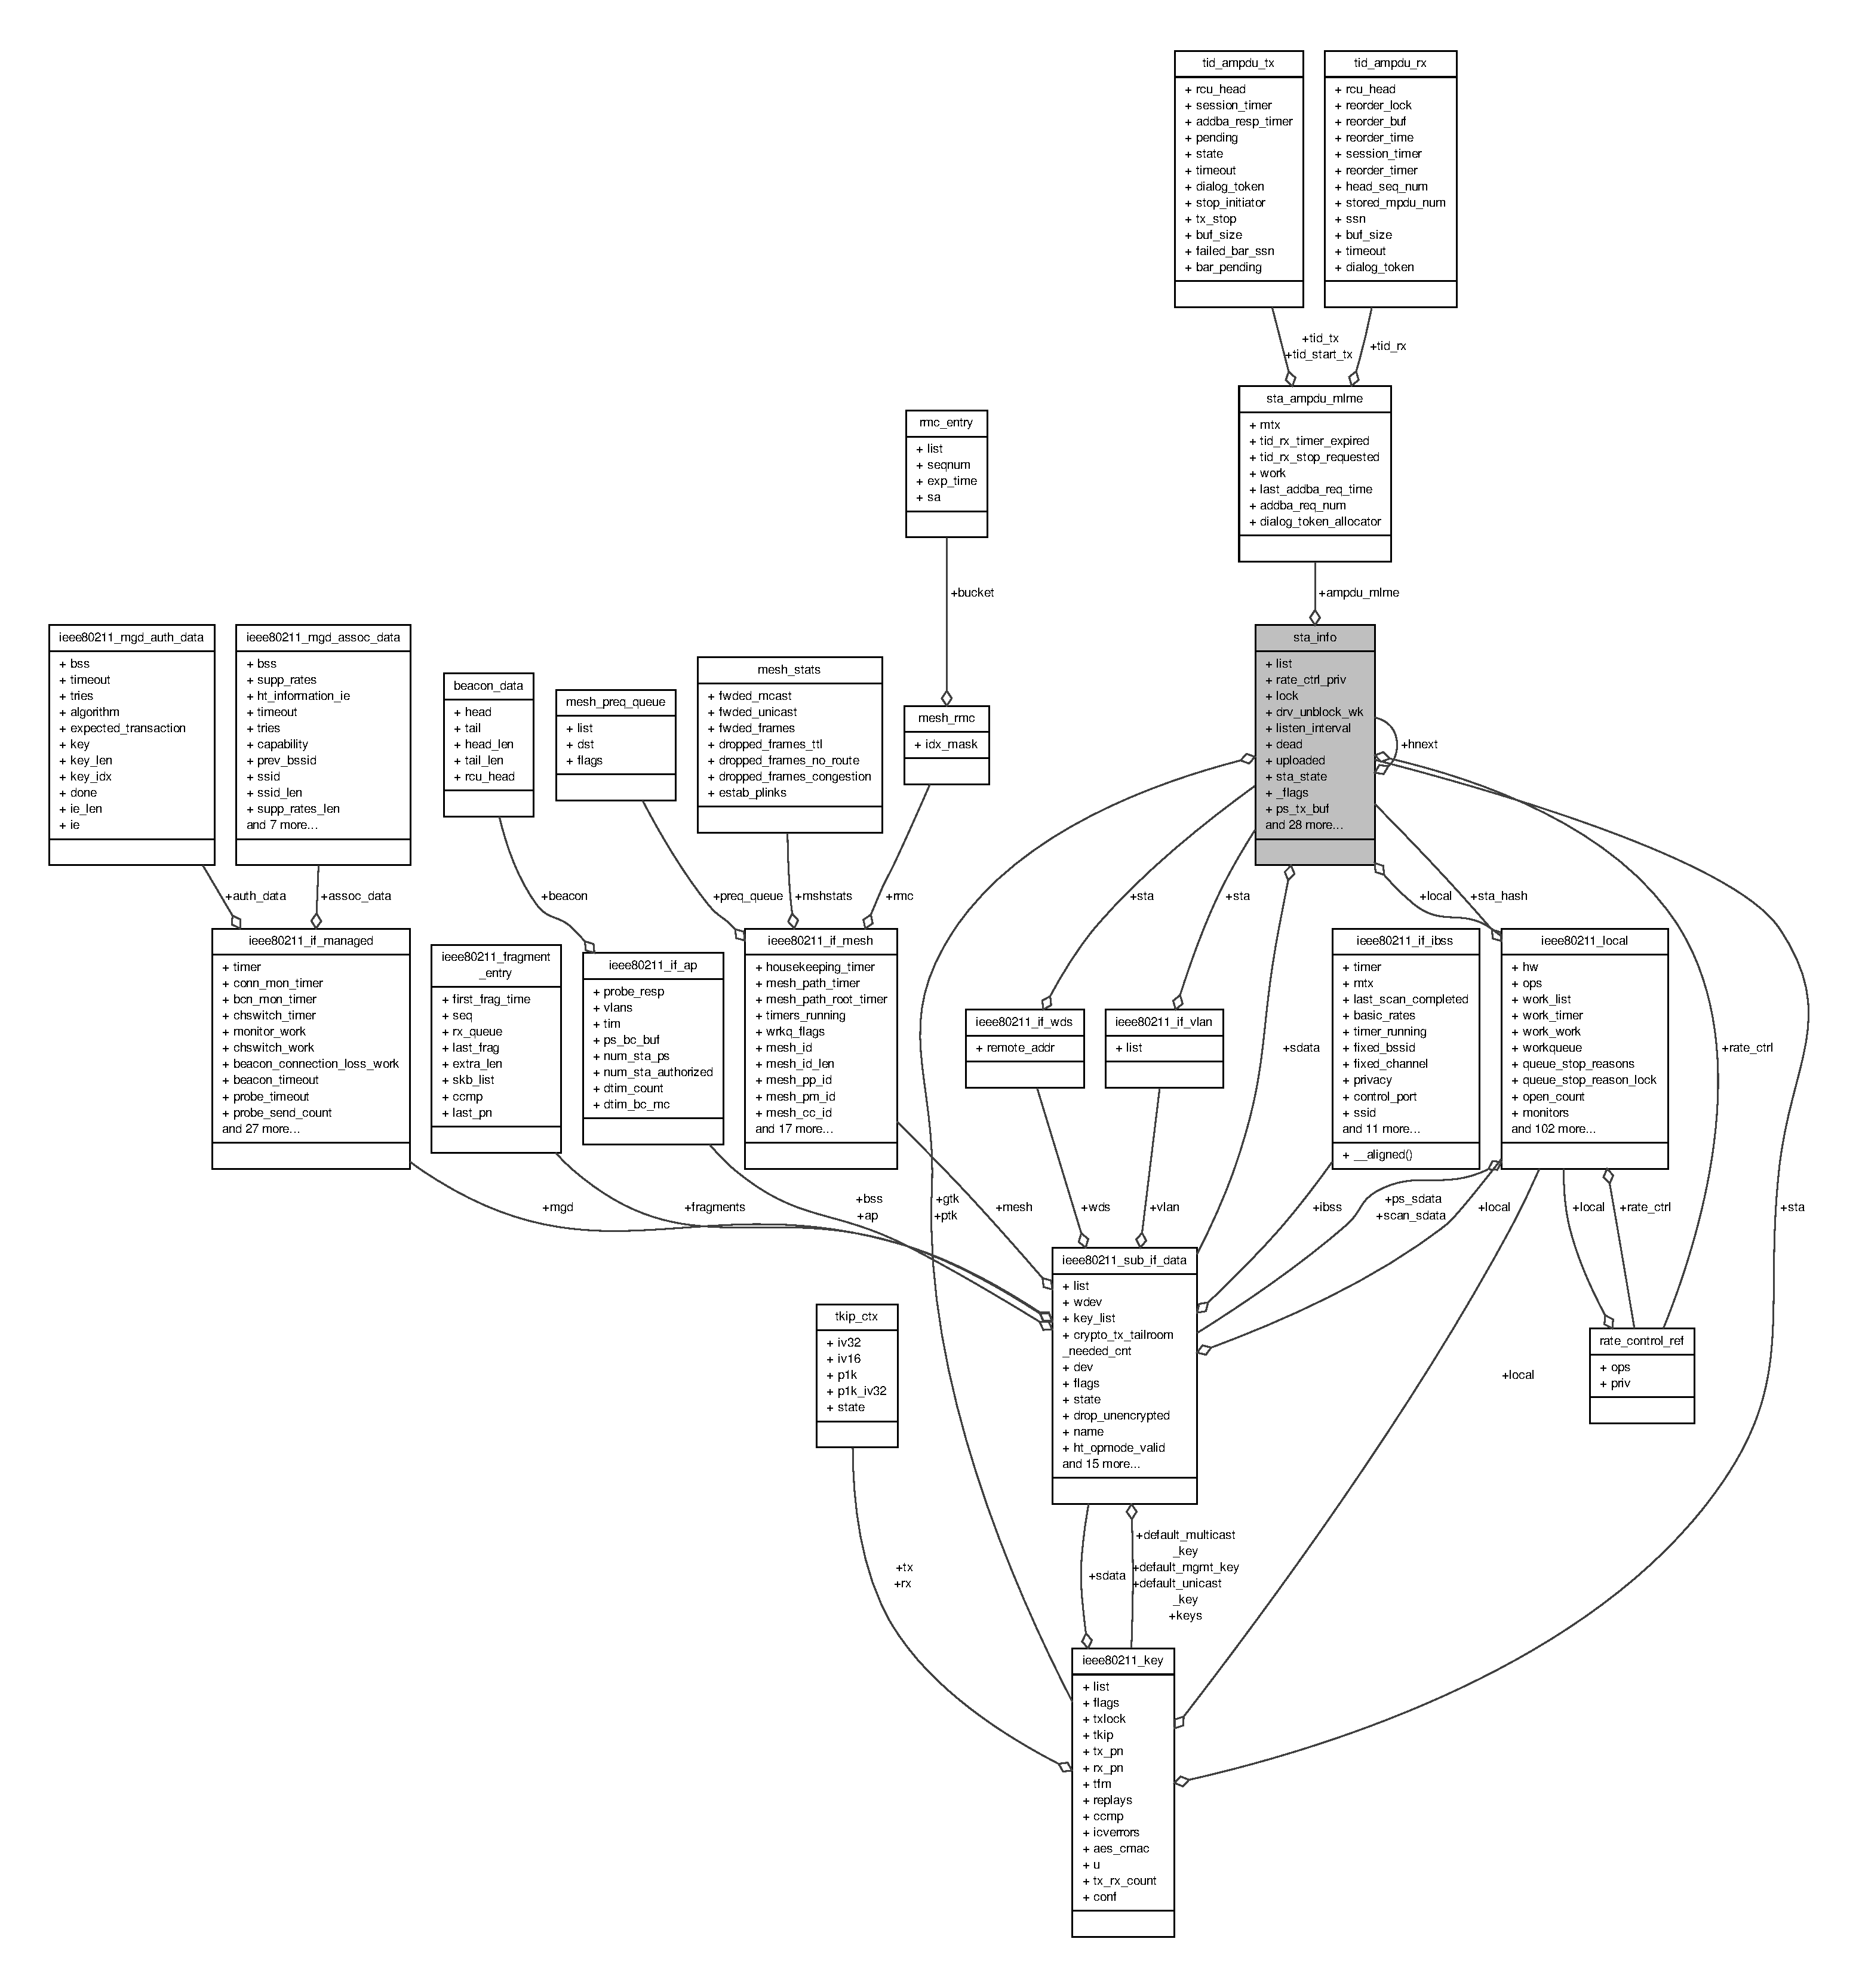
\includegraphics[width=350pt]{structsta__info__coll__graph}
\end{center}
\end{figure}
\subsection*{Data Fields}
\begin{DoxyCompactItemize}
\item 
struct list\-\_\-head \hyperlink{structsta__info_a1f00f18b91d5a820f2c43064243aa86e}{list}
\item 
struct \hyperlink{structsta__info}{sta\-\_\-info} \-\_\-\-\_\-rcu $\ast$ \hyperlink{structsta__info_aa178703df252667045be48a8874eec89}{hnext}
\item 
struct \hyperlink{structieee80211__local}{ieee80211\-\_\-local} $\ast$ \hyperlink{structsta__info_ad436a024f420f219c4fe2eebce7e4ab2}{local}
\item 
struct \hyperlink{structieee80211__sub__if__data}{ieee80211\-\_\-sub\-\_\-if\-\_\-data} $\ast$ \hyperlink{structsta__info_ad829d8d33f06a7245cc303f924f259ac}{sdata}
\item 
struct \hyperlink{structieee80211__key}{ieee80211\-\_\-key} \-\_\-\-\_\-rcu $\ast$ \hyperlink{structsta__info_ac5aa183bc3b32140826a8d0fcbad185e}{gtk} \mbox{[}\hyperlink{key_8h_afc56a6aebd37a90bca92708898c4e80a}{N\-U\-M\-\_\-\-D\-E\-F\-A\-U\-L\-T\-\_\-\-K\-E\-Y\-S}+\hyperlink{key_8h_a7cb10042c995311e0b4dfa6a8cabdd11}{N\-U\-M\-\_\-\-D\-E\-F\-A\-U\-L\-T\-\_\-\-M\-G\-M\-T\-\_\-\-K\-E\-Y\-S}\mbox{]}
\item 
struct \hyperlink{structieee80211__key}{ieee80211\-\_\-key} \-\_\-\-\_\-rcu $\ast$ \hyperlink{structsta__info_a20cca2acd1f1b3a9435094e1f0b73092}{ptk}
\item 
struct \hyperlink{structrate__control__ref}{rate\-\_\-control\-\_\-ref} $\ast$ \hyperlink{structsta__info_a0f6ac21a75ada1908328210ec3b42667}{rate\-\_\-ctrl}
\item 
void $\ast$ \hyperlink{structsta__info_a4212dd3a8398e8cd2ccb74821fc2fad0}{rate\-\_\-ctrl\-\_\-priv}
\item 
spinlock\-\_\-t \hyperlink{structsta__info_a79cda015c79ff2b4c1444e3070f0bb5d}{lock}
\item 
struct work\-\_\-struct \hyperlink{structsta__info_a2c95e461fff888fae360c7a55a151223}{drv\-\_\-unblock\-\_\-wk}
\item 
u16 \hyperlink{structsta__info_a778b871f4950f5c807895a3267025b6c}{listen\-\_\-interval}
\item 
bool \hyperlink{structsta__info_a79810da189102ac7036cb8eca47d104d}{dead}
\item 
bool \hyperlink{structsta__info_a5a978acf843365688119db95ca4ba0b1}{uploaded}
\item 
enum ieee80211\-\_\-sta\-\_\-state \hyperlink{structsta__info_a0bb9a8b1f52f5d772f02e2421c893545}{sta\-\_\-state}
\item 
unsigned long \hyperlink{structsta__info_a8d0d1e503953e175f5716febfded04f0}{\-\_\-flags}
\item 
struct sk\-\_\-buff\-\_\-head \hyperlink{structsta__info_af43dd904dd2c48899bae7cff072a56b5}{ps\-\_\-tx\-\_\-buf} \mbox{[}I\-E\-E\-E80211\-\_\-\-N\-U\-M\-\_\-\-A\-C\-S\mbox{]}
\item 
struct sk\-\_\-buff\-\_\-head \hyperlink{structsta__info_a11b1213a5b6c2d45b8e5e4526ac01620}{tx\-\_\-filtered} \mbox{[}I\-E\-E\-E80211\-\_\-\-N\-U\-M\-\_\-\-A\-C\-S\mbox{]}
\item 
unsigned long \hyperlink{structsta__info_ad258a0c1471c80553236dd314610d03e}{driver\-\_\-buffered\-\_\-tids}
\item 
unsigned long \hyperlink{structsta__info_a056e6ed90717e599b8ee70649fcd14b0}{rx\-\_\-packets}
\item 
unsigned long \hyperlink{structsta__info_adfbb81d9e73e27eedc0750a0ea4cb7b7}{rx\-\_\-bytes}
\item 
unsigned long \hyperlink{structsta__info_a9eda8cff20a9c485782549583ccaac14}{wep\-\_\-weak\-\_\-iv\-\_\-count}
\item 
unsigned long \hyperlink{structsta__info_a2e9fc210260fb987fa6b767ef12930e7}{last\-\_\-rx}
\item 
long \hyperlink{structsta__info_a53686acd631d8f635a4c945952904896}{last\-\_\-connected}
\item 
unsigned long \hyperlink{structsta__info_a92103871c3849fc35afb2eefe76b249e}{num\-\_\-duplicates}
\item 
unsigned long \hyperlink{structsta__info_a5ac9d5a701fcf1a16343d0de95856e24}{rx\-\_\-fragments}
\item 
unsigned long \hyperlink{structsta__info_ac3653bc0393e5b307149b410d204ff5a}{rx\-\_\-dropped}
\item 
int \hyperlink{structsta__info_a1d01d8e411dc32dde1ab25208eab05f8}{last\-\_\-signal}
\item 
struct ewma \hyperlink{structsta__info_aa7659d752f4407855f0c482afbcd879f}{avg\-\_\-signal}
\item 
\-\_\-\-\_\-le16 \hyperlink{structsta__info_a1068cbcad5e62974b8a3a9e1de889b9f}{last\-\_\-seq\-\_\-ctrl} \mbox{[}\hyperlink{key_8h_a99cb7469613fea382d3951d37ee2c075}{N\-U\-M\-\_\-\-R\-X\-\_\-\-D\-A\-T\-A\-\_\-\-Q\-U\-E\-U\-E\-S}+1\mbox{]}
\item 
unsigned long \hyperlink{structsta__info_a4ea3ebbcb6af9d8f4f401897d2d16f13}{tx\-\_\-filtered\-\_\-count}
\item 
unsigned long \hyperlink{structsta__info_af0a03540f21240022f46246dd3fd1136}{tx\-\_\-retry\-\_\-failed}
\item 
unsigned long \hyperlink{structsta__info_ac0325bffa5a0874c0f3f62ec77ddbadf}{tx\-\_\-retry\-\_\-count}
\item 
unsigned int \hyperlink{structsta__info_a2e8ebe1593e8bfdb0696ad9adbab7209}{fail\-\_\-avg}
\item 
unsigned long \hyperlink{structsta__info_a04c4bb1c42d342d7b70a79c91a7ab2b7}{tx\-\_\-packets}
\item 
unsigned long \hyperlink{structsta__info_a7639b5284b79992ec806f00466ee1f24}{tx\-\_\-bytes}
\item 
unsigned long \hyperlink{structsta__info_ad4530b03477a3a0603c240e67c163ab9}{tx\-\_\-fragments}
\item 
struct ieee80211\-\_\-tx\-\_\-rate \hyperlink{structsta__info_a0691fc258d91f737d761976ad8c96118}{last\-\_\-tx\-\_\-rate}
\item 
int \hyperlink{structsta__info_a91ccafb08a519aa4bd9efdd330b3d6a9}{last\-\_\-rx\-\_\-rate\-\_\-idx}
\item 
int \hyperlink{structsta__info_a3ce20e50f9c3e0019984f7fce388ff53}{last\-\_\-rx\-\_\-rate\-\_\-flag}
\item 
u16 \hyperlink{structsta__info_a51a374321b9b3f2f41ec59ed2dc0eca9}{tid\-\_\-seq} \mbox{[}I\-E\-E\-E80211\-\_\-\-Q\-O\-S\-\_\-\-C\-T\-L\-\_\-\-T\-I\-D\-\_\-\-M\-A\-S\-K+1\mbox{]}
\item 
struct \hyperlink{structsta__ampdu__mlme}{sta\-\_\-ampdu\-\_\-mlme} \hyperlink{structsta__info_ad42a305af8f3528d28546f33350e4473}{ampdu\-\_\-mlme}
\item 
u8 \hyperlink{structsta__info_ab892eac21bd848831f225404459d91ff}{timer\-\_\-to\-\_\-tid} \mbox{[}\hyperlink{sta__info_8h_a8376226f35c3c806965ac03355cc1a00}{S\-T\-A\-\_\-\-T\-I\-D\-\_\-\-N\-U\-M}\mbox{]}
\item 
unsigned int \hyperlink{structsta__info_ab7d0bdf10d99357afd115dd2c9926cb9}{lost\-\_\-packets}
\item 
unsigned int \hyperlink{structsta__info_a2d5a8a52432b6f6ab32bcb069ca3115a}{beacon\-\_\-loss\-\_\-count}
\item 
struct ieee80211\-\_\-sta \hyperlink{structsta__info_a10bf230d5f2e241e9de2a67c2da53d4e}{sta}
\end{DoxyCompactItemize}


\subsection{Detailed Description}
struct \hyperlink{structsta__info}{sta\-\_\-info} -\/ S\-T\-A information

This structure collects information about a station that mac80211 is communicating with.

\-: global linked list entry \-: hash table linked list pointer \-: pointer to the global information \-: virtual interface this station belongs to \-: peer key negotiated with this station, if any \-: group keys negotiated with this station, if any \-: rate control algorithm reference \-: rate control private per-\/\-S\-T\-A pointer \-: rate used for last transmit, to report to userspace as \char`\"{}the\char`\"{} transmit rate \-: rx status rate index of the last data packet \-: rx status flag of the last data packet \-: used for locking all fields that require locking, see comments in the header file. \-: used for driver P\-S unblocking \-: listen interval of this station, when we're acting as A\-P \-: S\-T\-A flags, see \&enum ieee80211\-\_\-sta\-\_\-info\-\_\-flags, do not use directly \-: buffers (per A\-C) of frames to transmit to this station when it leaves power saving state or polls \-: buffers (per A\-C) of frames we already tried to transmit but were filtered by hardware due to S\-T\-A having entered power saving state, these are also delivered to the station when it leaves powersave or polls for frames \-: bitmap of T\-I\-Ds the driver has data buffered on \-: Number of M\-S\-D\-Us received from this S\-T\-A \-: Number of bytes received from this S\-T\-A \-: number of weak W\-E\-P I\-Vs received from this station \-: time (in jiffies) when last frame was received from this S\-T\-A \-: time (in seconds) when a station got connected \-: number of duplicate frames received from this S\-T\-A \-: number of received M\-P\-D\-Us \-: number of dropped M\-P\-D\-Us from this S\-T\-A \-: signal of last received frame from this S\-T\-A \-: moving average of signal of received frames from this S\-T\-A \-: last received seq/frag number from this S\-T\-A (per R\-X queue) \-: number of frames the hardware filtered for this S\-T\-A \-: number of frames that failed retry \-: total number of retries for frames to this S\-T\-A \-: moving percentage of failed M\-S\-D\-Us \-: number of R\-X/\-T\-X M\-S\-D\-Us \-: number of bytes transmitted to this S\-T\-A \-: number of transmitted M\-P\-D\-Us \-: per-\/\-T\-I\-D sequence numbers for sending to this S\-T\-A \-: A-\/\-M\-P\-D\-U state machine state \-: identity mapping to I\-D timers \-: Local link I\-D \-: Peer link I\-D \-: Cancel reason on P\-L\-I\-N\-K\-\_\-\-H\-O\-L\-D\-I\-N\-G state \-: Retries in establishment \-: ignore the peer-\/link timer (used internally) \-: peer link state \-: timeout of peer link \-: peer link watch timer \-: used by suspend/resume to restore timers \-: debug filesystem info \-: set to true when sta is unlinked \-: set to true when sta is uploaded to the driver \-: number of consecutive lost packets \-: station information we share with the driver \-: duplicates information about station state (for debug) \-: number of times beacon loss has triggered 

Definition at line 275 of file sta\-\_\-info.\-h.



\subsection{Field Documentation}
\hypertarget{structsta__info_a8d0d1e503953e175f5716febfded04f0}{\index{sta\-\_\-info@{sta\-\_\-info}!\-\_\-flags@{\-\_\-flags}}
\index{\-\_\-flags@{\-\_\-flags}!sta_info@{sta\-\_\-info}}
\subsubsection[{\-\_\-flags}]{\setlength{\rightskip}{0pt plus 5cm}unsigned long \-\_\-flags}}\label{structsta__info_a8d0d1e503953e175f5716febfded04f0}


Definition at line 298 of file sta\-\_\-info.\-h.

\hypertarget{structsta__info_ad42a305af8f3528d28546f33350e4473}{\index{sta\-\_\-info@{sta\-\_\-info}!ampdu\-\_\-mlme@{ampdu\-\_\-mlme}}
\index{ampdu\-\_\-mlme@{ampdu\-\_\-mlme}!sta_info@{sta\-\_\-info}}
\subsubsection[{ampdu\-\_\-mlme}]{\setlength{\rightskip}{0pt plus 5cm}struct {\bf sta\-\_\-ampdu\-\_\-mlme} ampdu\-\_\-mlme}}\label{structsta__info_ad42a305af8f3528d28546f33350e4473}


Definition at line 339 of file sta\-\_\-info.\-h.

\hypertarget{structsta__info_aa7659d752f4407855f0c482afbcd879f}{\index{sta\-\_\-info@{sta\-\_\-info}!avg\-\_\-signal@{avg\-\_\-signal}}
\index{avg\-\_\-signal@{avg\-\_\-signal}!sta_info@{sta\-\_\-info}}
\subsubsection[{avg\-\_\-signal}]{\setlength{\rightskip}{0pt plus 5cm}struct ewma avg\-\_\-signal}}\label{structsta__info_aa7659d752f4407855f0c482afbcd879f}


Definition at line 317 of file sta\-\_\-info.\-h.

\hypertarget{structsta__info_a2d5a8a52432b6f6ab32bcb069ca3115a}{\index{sta\-\_\-info@{sta\-\_\-info}!beacon\-\_\-loss\-\_\-count@{beacon\-\_\-loss\-\_\-count}}
\index{beacon\-\_\-loss\-\_\-count@{beacon\-\_\-loss\-\_\-count}!sta_info@{sta\-\_\-info}}
\subsubsection[{beacon\-\_\-loss\-\_\-count}]{\setlength{\rightskip}{0pt plus 5cm}unsigned int beacon\-\_\-loss\-\_\-count}}\label{structsta__info_a2d5a8a52432b6f6ab32bcb069ca3115a}


Definition at line 366 of file sta\-\_\-info.\-h.

\hypertarget{structsta__info_a79810da189102ac7036cb8eca47d104d}{\index{sta\-\_\-info@{sta\-\_\-info}!dead@{dead}}
\index{dead@{dead}!sta_info@{sta\-\_\-info}}
\subsubsection[{dead}]{\setlength{\rightskip}{0pt plus 5cm}bool dead}}\label{structsta__info_a79810da189102ac7036cb8eca47d104d}


Definition at line 291 of file sta\-\_\-info.\-h.

\hypertarget{structsta__info_ad258a0c1471c80553236dd314610d03e}{\index{sta\-\_\-info@{sta\-\_\-info}!driver\-\_\-buffered\-\_\-tids@{driver\-\_\-buffered\-\_\-tids}}
\index{driver\-\_\-buffered\-\_\-tids@{driver\-\_\-buffered\-\_\-tids}!sta_info@{sta\-\_\-info}}
\subsubsection[{driver\-\_\-buffered\-\_\-tids}]{\setlength{\rightskip}{0pt plus 5cm}unsigned long driver\-\_\-buffered\-\_\-tids}}\label{structsta__info_ad258a0c1471c80553236dd314610d03e}


Definition at line 306 of file sta\-\_\-info.\-h.

\hypertarget{structsta__info_a2c95e461fff888fae360c7a55a151223}{\index{sta\-\_\-info@{sta\-\_\-info}!drv\-\_\-unblock\-\_\-wk@{drv\-\_\-unblock\-\_\-wk}}
\index{drv\-\_\-unblock\-\_\-wk@{drv\-\_\-unblock\-\_\-wk}!sta_info@{sta\-\_\-info}}
\subsubsection[{drv\-\_\-unblock\-\_\-wk}]{\setlength{\rightskip}{0pt plus 5cm}struct work\-\_\-struct drv\-\_\-unblock\-\_\-wk}}\label{structsta__info_a2c95e461fff888fae360c7a55a151223}


Definition at line 287 of file sta\-\_\-info.\-h.

\hypertarget{structsta__info_a2e8ebe1593e8bfdb0696ad9adbab7209}{\index{sta\-\_\-info@{sta\-\_\-info}!fail\-\_\-avg@{fail\-\_\-avg}}
\index{fail\-\_\-avg@{fail\-\_\-avg}!sta_info@{sta\-\_\-info}}
\subsubsection[{fail\-\_\-avg}]{\setlength{\rightskip}{0pt plus 5cm}unsigned int fail\-\_\-avg}}\label{structsta__info_a2e8ebe1593e8bfdb0696ad9adbab7209}


Definition at line 325 of file sta\-\_\-info.\-h.

\hypertarget{structsta__info_ac5aa183bc3b32140826a8d0fcbad185e}{\index{sta\-\_\-info@{sta\-\_\-info}!gtk@{gtk}}
\index{gtk@{gtk}!sta_info@{sta\-\_\-info}}
\subsubsection[{gtk}]{\setlength{\rightskip}{0pt plus 5cm}struct {\bf ieee80211\-\_\-key} \-\_\-\-\_\-rcu$\ast$ gtk\mbox{[}{\bf N\-U\-M\-\_\-\-D\-E\-F\-A\-U\-L\-T\-\_\-\-K\-E\-Y\-S}+{\bf N\-U\-M\-\_\-\-D\-E\-F\-A\-U\-L\-T\-\_\-\-M\-G\-M\-T\-\_\-\-K\-E\-Y\-S}\mbox{]}}}\label{structsta__info_ac5aa183bc3b32140826a8d0fcbad185e}


Definition at line 281 of file sta\-\_\-info.\-h.

\hypertarget{structsta__info_aa178703df252667045be48a8874eec89}{\index{sta\-\_\-info@{sta\-\_\-info}!hnext@{hnext}}
\index{hnext@{hnext}!sta_info@{sta\-\_\-info}}
\subsubsection[{hnext}]{\setlength{\rightskip}{0pt plus 5cm}struct {\bf sta\-\_\-info} \-\_\-\-\_\-rcu$\ast$ hnext}}\label{structsta__info_aa178703df252667045be48a8874eec89}


Definition at line 278 of file sta\-\_\-info.\-h.

\hypertarget{structsta__info_a53686acd631d8f635a4c945952904896}{\index{sta\-\_\-info@{sta\-\_\-info}!last\-\_\-connected@{last\-\_\-connected}}
\index{last\-\_\-connected@{last\-\_\-connected}!sta_info@{sta\-\_\-info}}
\subsubsection[{last\-\_\-connected}]{\setlength{\rightskip}{0pt plus 5cm}long last\-\_\-connected}}\label{structsta__info_a53686acd631d8f635a4c945952904896}


Definition at line 312 of file sta\-\_\-info.\-h.

\hypertarget{structsta__info_a2e9fc210260fb987fa6b767ef12930e7}{\index{sta\-\_\-info@{sta\-\_\-info}!last\-\_\-rx@{last\-\_\-rx}}
\index{last\-\_\-rx@{last\-\_\-rx}!sta_info@{sta\-\_\-info}}
\subsubsection[{last\-\_\-rx}]{\setlength{\rightskip}{0pt plus 5cm}unsigned long last\-\_\-rx}}\label{structsta__info_a2e9fc210260fb987fa6b767ef12930e7}


Definition at line 311 of file sta\-\_\-info.\-h.

\hypertarget{structsta__info_a3ce20e50f9c3e0019984f7fce388ff53}{\index{sta\-\_\-info@{sta\-\_\-info}!last\-\_\-rx\-\_\-rate\-\_\-flag@{last\-\_\-rx\-\_\-rate\-\_\-flag}}
\index{last\-\_\-rx\-\_\-rate\-\_\-flag@{last\-\_\-rx\-\_\-rate\-\_\-flag}!sta_info@{sta\-\_\-info}}
\subsubsection[{last\-\_\-rx\-\_\-rate\-\_\-flag}]{\setlength{\rightskip}{0pt plus 5cm}int last\-\_\-rx\-\_\-rate\-\_\-flag}}\label{structsta__info_a3ce20e50f9c3e0019984f7fce388ff53}


Definition at line 333 of file sta\-\_\-info.\-h.

\hypertarget{structsta__info_a91ccafb08a519aa4bd9efdd330b3d6a9}{\index{sta\-\_\-info@{sta\-\_\-info}!last\-\_\-rx\-\_\-rate\-\_\-idx@{last\-\_\-rx\-\_\-rate\-\_\-idx}}
\index{last\-\_\-rx\-\_\-rate\-\_\-idx@{last\-\_\-rx\-\_\-rate\-\_\-idx}!sta_info@{sta\-\_\-info}}
\subsubsection[{last\-\_\-rx\-\_\-rate\-\_\-idx}]{\setlength{\rightskip}{0pt plus 5cm}int last\-\_\-rx\-\_\-rate\-\_\-idx}}\label{structsta__info_a91ccafb08a519aa4bd9efdd330b3d6a9}


Definition at line 332 of file sta\-\_\-info.\-h.

\hypertarget{structsta__info_a1068cbcad5e62974b8a3a9e1de889b9f}{\index{sta\-\_\-info@{sta\-\_\-info}!last\-\_\-seq\-\_\-ctrl@{last\-\_\-seq\-\_\-ctrl}}
\index{last\-\_\-seq\-\_\-ctrl@{last\-\_\-seq\-\_\-ctrl}!sta_info@{sta\-\_\-info}}
\subsubsection[{last\-\_\-seq\-\_\-ctrl}]{\setlength{\rightskip}{0pt plus 5cm}\-\_\-\-\_\-le16 last\-\_\-seq\-\_\-ctrl\mbox{[}{\bf N\-U\-M\-\_\-\-R\-X\-\_\-\-D\-A\-T\-A\-\_\-\-Q\-U\-E\-U\-E\-S}+1\mbox{]}}}\label{structsta__info_a1068cbcad5e62974b8a3a9e1de889b9f}


Definition at line 319 of file sta\-\_\-info.\-h.

\hypertarget{structsta__info_a1d01d8e411dc32dde1ab25208eab05f8}{\index{sta\-\_\-info@{sta\-\_\-info}!last\-\_\-signal@{last\-\_\-signal}}
\index{last\-\_\-signal@{last\-\_\-signal}!sta_info@{sta\-\_\-info}}
\subsubsection[{last\-\_\-signal}]{\setlength{\rightskip}{0pt plus 5cm}int last\-\_\-signal}}\label{structsta__info_a1d01d8e411dc32dde1ab25208eab05f8}


Definition at line 316 of file sta\-\_\-info.\-h.

\hypertarget{structsta__info_a0691fc258d91f737d761976ad8c96118}{\index{sta\-\_\-info@{sta\-\_\-info}!last\-\_\-tx\-\_\-rate@{last\-\_\-tx\-\_\-rate}}
\index{last\-\_\-tx\-\_\-rate@{last\-\_\-tx\-\_\-rate}!sta_info@{sta\-\_\-info}}
\subsubsection[{last\-\_\-tx\-\_\-rate}]{\setlength{\rightskip}{0pt plus 5cm}struct ieee80211\-\_\-tx\-\_\-rate last\-\_\-tx\-\_\-rate}}\label{structsta__info_a0691fc258d91f737d761976ad8c96118}


Definition at line 331 of file sta\-\_\-info.\-h.

\hypertarget{structsta__info_a1f00f18b91d5a820f2c43064243aa86e}{\index{sta\-\_\-info@{sta\-\_\-info}!list@{list}}
\index{list@{list}!sta_info@{sta\-\_\-info}}
\subsubsection[{list}]{\setlength{\rightskip}{0pt plus 5cm}struct list\-\_\-head list}}\label{structsta__info_a1f00f18b91d5a820f2c43064243aa86e}


Definition at line 277 of file sta\-\_\-info.\-h.

\hypertarget{structsta__info_a778b871f4950f5c807895a3267025b6c}{\index{sta\-\_\-info@{sta\-\_\-info}!listen\-\_\-interval@{listen\-\_\-interval}}
\index{listen\-\_\-interval@{listen\-\_\-interval}!sta_info@{sta\-\_\-info}}
\subsubsection[{listen\-\_\-interval}]{\setlength{\rightskip}{0pt plus 5cm}u16 listen\-\_\-interval}}\label{structsta__info_a778b871f4950f5c807895a3267025b6c}


Definition at line 289 of file sta\-\_\-info.\-h.

\hypertarget{structsta__info_ad436a024f420f219c4fe2eebce7e4ab2}{\index{sta\-\_\-info@{sta\-\_\-info}!local@{local}}
\index{local@{local}!sta_info@{sta\-\_\-info}}
\subsubsection[{local}]{\setlength{\rightskip}{0pt plus 5cm}struct {\bf ieee80211\-\_\-local}$\ast$ local}}\label{structsta__info_ad436a024f420f219c4fe2eebce7e4ab2}


Definition at line 279 of file sta\-\_\-info.\-h.

\hypertarget{structsta__info_a79cda015c79ff2b4c1444e3070f0bb5d}{\index{sta\-\_\-info@{sta\-\_\-info}!lock@{lock}}
\index{lock@{lock}!sta_info@{sta\-\_\-info}}
\subsubsection[{lock}]{\setlength{\rightskip}{0pt plus 5cm}spinlock\-\_\-t lock}}\label{structsta__info_a79cda015c79ff2b4c1444e3070f0bb5d}


Definition at line 285 of file sta\-\_\-info.\-h.

\hypertarget{structsta__info_ab7d0bdf10d99357afd115dd2c9926cb9}{\index{sta\-\_\-info@{sta\-\_\-info}!lost\-\_\-packets@{lost\-\_\-packets}}
\index{lost\-\_\-packets@{lost\-\_\-packets}!sta_info@{sta\-\_\-info}}
\subsubsection[{lost\-\_\-packets}]{\setlength{\rightskip}{0pt plus 5cm}unsigned int lost\-\_\-packets}}\label{structsta__info_ab7d0bdf10d99357afd115dd2c9926cb9}


Definition at line 365 of file sta\-\_\-info.\-h.

\hypertarget{structsta__info_a92103871c3849fc35afb2eefe76b249e}{\index{sta\-\_\-info@{sta\-\_\-info}!num\-\_\-duplicates@{num\-\_\-duplicates}}
\index{num\-\_\-duplicates@{num\-\_\-duplicates}!sta_info@{sta\-\_\-info}}
\subsubsection[{num\-\_\-duplicates}]{\setlength{\rightskip}{0pt plus 5cm}unsigned long num\-\_\-duplicates}}\label{structsta__info_a92103871c3849fc35afb2eefe76b249e}


Definition at line 313 of file sta\-\_\-info.\-h.

\hypertarget{structsta__info_af43dd904dd2c48899bae7cff072a56b5}{\index{sta\-\_\-info@{sta\-\_\-info}!ps\-\_\-tx\-\_\-buf@{ps\-\_\-tx\-\_\-buf}}
\index{ps\-\_\-tx\-\_\-buf@{ps\-\_\-tx\-\_\-buf}!sta_info@{sta\-\_\-info}}
\subsubsection[{ps\-\_\-tx\-\_\-buf}]{\setlength{\rightskip}{0pt plus 5cm}struct sk\-\_\-buff\-\_\-head ps\-\_\-tx\-\_\-buf\mbox{[}I\-E\-E\-E80211\-\_\-\-N\-U\-M\-\_\-\-A\-C\-S\mbox{]}}}\label{structsta__info_af43dd904dd2c48899bae7cff072a56b5}


Definition at line 304 of file sta\-\_\-info.\-h.

\hypertarget{structsta__info_a20cca2acd1f1b3a9435094e1f0b73092}{\index{sta\-\_\-info@{sta\-\_\-info}!ptk@{ptk}}
\index{ptk@{ptk}!sta_info@{sta\-\_\-info}}
\subsubsection[{ptk}]{\setlength{\rightskip}{0pt plus 5cm}struct {\bf ieee80211\-\_\-key} \-\_\-\-\_\-rcu$\ast$ ptk}}\label{structsta__info_a20cca2acd1f1b3a9435094e1f0b73092}


Definition at line 282 of file sta\-\_\-info.\-h.

\hypertarget{structsta__info_a0f6ac21a75ada1908328210ec3b42667}{\index{sta\-\_\-info@{sta\-\_\-info}!rate\-\_\-ctrl@{rate\-\_\-ctrl}}
\index{rate\-\_\-ctrl@{rate\-\_\-ctrl}!sta_info@{sta\-\_\-info}}
\subsubsection[{rate\-\_\-ctrl}]{\setlength{\rightskip}{0pt plus 5cm}struct {\bf rate\-\_\-control\-\_\-ref}$\ast$ rate\-\_\-ctrl}}\label{structsta__info_a0f6ac21a75ada1908328210ec3b42667}


Definition at line 283 of file sta\-\_\-info.\-h.

\hypertarget{structsta__info_a4212dd3a8398e8cd2ccb74821fc2fad0}{\index{sta\-\_\-info@{sta\-\_\-info}!rate\-\_\-ctrl\-\_\-priv@{rate\-\_\-ctrl\-\_\-priv}}
\index{rate\-\_\-ctrl\-\_\-priv@{rate\-\_\-ctrl\-\_\-priv}!sta_info@{sta\-\_\-info}}
\subsubsection[{rate\-\_\-ctrl\-\_\-priv}]{\setlength{\rightskip}{0pt plus 5cm}void$\ast$ rate\-\_\-ctrl\-\_\-priv}}\label{structsta__info_a4212dd3a8398e8cd2ccb74821fc2fad0}


Definition at line 284 of file sta\-\_\-info.\-h.

\hypertarget{structsta__info_adfbb81d9e73e27eedc0750a0ea4cb7b7}{\index{sta\-\_\-info@{sta\-\_\-info}!rx\-\_\-bytes@{rx\-\_\-bytes}}
\index{rx\-\_\-bytes@{rx\-\_\-bytes}!sta_info@{sta\-\_\-info}}
\subsubsection[{rx\-\_\-bytes}]{\setlength{\rightskip}{0pt plus 5cm}unsigned long rx\-\_\-bytes}}\label{structsta__info_adfbb81d9e73e27eedc0750a0ea4cb7b7}


Definition at line 309 of file sta\-\_\-info.\-h.

\hypertarget{structsta__info_ac3653bc0393e5b307149b410d204ff5a}{\index{sta\-\_\-info@{sta\-\_\-info}!rx\-\_\-dropped@{rx\-\_\-dropped}}
\index{rx\-\_\-dropped@{rx\-\_\-dropped}!sta_info@{sta\-\_\-info}}
\subsubsection[{rx\-\_\-dropped}]{\setlength{\rightskip}{0pt plus 5cm}unsigned long rx\-\_\-dropped}}\label{structsta__info_ac3653bc0393e5b307149b410d204ff5a}


Definition at line 315 of file sta\-\_\-info.\-h.

\hypertarget{structsta__info_a5ac9d5a701fcf1a16343d0de95856e24}{\index{sta\-\_\-info@{sta\-\_\-info}!rx\-\_\-fragments@{rx\-\_\-fragments}}
\index{rx\-\_\-fragments@{rx\-\_\-fragments}!sta_info@{sta\-\_\-info}}
\subsubsection[{rx\-\_\-fragments}]{\setlength{\rightskip}{0pt plus 5cm}unsigned long rx\-\_\-fragments}}\label{structsta__info_a5ac9d5a701fcf1a16343d0de95856e24}


Definition at line 314 of file sta\-\_\-info.\-h.

\hypertarget{structsta__info_a056e6ed90717e599b8ee70649fcd14b0}{\index{sta\-\_\-info@{sta\-\_\-info}!rx\-\_\-packets@{rx\-\_\-packets}}
\index{rx\-\_\-packets@{rx\-\_\-packets}!sta_info@{sta\-\_\-info}}
\subsubsection[{rx\-\_\-packets}]{\setlength{\rightskip}{0pt plus 5cm}unsigned long rx\-\_\-packets}}\label{structsta__info_a056e6ed90717e599b8ee70649fcd14b0}


Definition at line 309 of file sta\-\_\-info.\-h.

\hypertarget{structsta__info_ad829d8d33f06a7245cc303f924f259ac}{\index{sta\-\_\-info@{sta\-\_\-info}!sdata@{sdata}}
\index{sdata@{sdata}!sta_info@{sta\-\_\-info}}
\subsubsection[{sdata}]{\setlength{\rightskip}{0pt plus 5cm}struct {\bf ieee80211\-\_\-sub\-\_\-if\-\_\-data}$\ast$ sdata}}\label{structsta__info_ad829d8d33f06a7245cc303f924f259ac}


Definition at line 280 of file sta\-\_\-info.\-h.

\hypertarget{structsta__info_a10bf230d5f2e241e9de2a67c2da53d4e}{\index{sta\-\_\-info@{sta\-\_\-info}!sta@{sta}}
\index{sta@{sta}!sta_info@{sta\-\_\-info}}
\subsubsection[{sta}]{\setlength{\rightskip}{0pt plus 5cm}struct ieee80211\-\_\-sta sta}}\label{structsta__info_a10bf230d5f2e241e9de2a67c2da53d4e}


Definition at line 369 of file sta\-\_\-info.\-h.

\hypertarget{structsta__info_a0bb9a8b1f52f5d772f02e2421c893545}{\index{sta\-\_\-info@{sta\-\_\-info}!sta\-\_\-state@{sta\-\_\-state}}
\index{sta\-\_\-state@{sta\-\_\-state}!sta_info@{sta\-\_\-info}}
\subsubsection[{sta\-\_\-state}]{\setlength{\rightskip}{0pt plus 5cm}enum ieee80211\-\_\-sta\-\_\-state sta\-\_\-state}}\label{structsta__info_a0bb9a8b1f52f5d772f02e2421c893545}


Definition at line 295 of file sta\-\_\-info.\-h.

\hypertarget{structsta__info_a51a374321b9b3f2f41ec59ed2dc0eca9}{\index{sta\-\_\-info@{sta\-\_\-info}!tid\-\_\-seq@{tid\-\_\-seq}}
\index{tid\-\_\-seq@{tid\-\_\-seq}!sta_info@{sta\-\_\-info}}
\subsubsection[{tid\-\_\-seq}]{\setlength{\rightskip}{0pt plus 5cm}u16 tid\-\_\-seq\mbox{[}I\-E\-E\-E80211\-\_\-\-Q\-O\-S\-\_\-\-C\-T\-L\-\_\-\-T\-I\-D\-\_\-\-M\-A\-S\-K+1\mbox{]}}}\label{structsta__info_a51a374321b9b3f2f41ec59ed2dc0eca9}


Definition at line 334 of file sta\-\_\-info.\-h.

\hypertarget{structsta__info_ab892eac21bd848831f225404459d91ff}{\index{sta\-\_\-info@{sta\-\_\-info}!timer\-\_\-to\-\_\-tid@{timer\-\_\-to\-\_\-tid}}
\index{timer\-\_\-to\-\_\-tid@{timer\-\_\-to\-\_\-tid}!sta_info@{sta\-\_\-info}}
\subsubsection[{timer\-\_\-to\-\_\-tid}]{\setlength{\rightskip}{0pt plus 5cm}u8 timer\-\_\-to\-\_\-tid\mbox{[}{\bf S\-T\-A\-\_\-\-T\-I\-D\-\_\-\-N\-U\-M}\mbox{]}}}\label{structsta__info_ab892eac21bd848831f225404459d91ff}


Definition at line 340 of file sta\-\_\-info.\-h.

\hypertarget{structsta__info_a7639b5284b79992ec806f00466ee1f24}{\index{sta\-\_\-info@{sta\-\_\-info}!tx\-\_\-bytes@{tx\-\_\-bytes}}
\index{tx\-\_\-bytes@{tx\-\_\-bytes}!sta_info@{sta\-\_\-info}}
\subsubsection[{tx\-\_\-bytes}]{\setlength{\rightskip}{0pt plus 5cm}unsigned long tx\-\_\-bytes}}\label{structsta__info_a7639b5284b79992ec806f00466ee1f24}


Definition at line 329 of file sta\-\_\-info.\-h.

\hypertarget{structsta__info_a11b1213a5b6c2d45b8e5e4526ac01620}{\index{sta\-\_\-info@{sta\-\_\-info}!tx\-\_\-filtered@{tx\-\_\-filtered}}
\index{tx\-\_\-filtered@{tx\-\_\-filtered}!sta_info@{sta\-\_\-info}}
\subsubsection[{tx\-\_\-filtered}]{\setlength{\rightskip}{0pt plus 5cm}struct sk\-\_\-buff\-\_\-head tx\-\_\-filtered\mbox{[}I\-E\-E\-E80211\-\_\-\-N\-U\-M\-\_\-\-A\-C\-S\mbox{]}}}\label{structsta__info_a11b1213a5b6c2d45b8e5e4526ac01620}


Definition at line 305 of file sta\-\_\-info.\-h.

\hypertarget{structsta__info_a4ea3ebbcb6af9d8f4f401897d2d16f13}{\index{sta\-\_\-info@{sta\-\_\-info}!tx\-\_\-filtered\-\_\-count@{tx\-\_\-filtered\-\_\-count}}
\index{tx\-\_\-filtered\-\_\-count@{tx\-\_\-filtered\-\_\-count}!sta_info@{sta\-\_\-info}}
\subsubsection[{tx\-\_\-filtered\-\_\-count}]{\setlength{\rightskip}{0pt plus 5cm}unsigned long tx\-\_\-filtered\-\_\-count}}\label{structsta__info_a4ea3ebbcb6af9d8f4f401897d2d16f13}


Definition at line 322 of file sta\-\_\-info.\-h.

\hypertarget{structsta__info_ad4530b03477a3a0603c240e67c163ab9}{\index{sta\-\_\-info@{sta\-\_\-info}!tx\-\_\-fragments@{tx\-\_\-fragments}}
\index{tx\-\_\-fragments@{tx\-\_\-fragments}!sta_info@{sta\-\_\-info}}
\subsubsection[{tx\-\_\-fragments}]{\setlength{\rightskip}{0pt plus 5cm}unsigned long tx\-\_\-fragments}}\label{structsta__info_ad4530b03477a3a0603c240e67c163ab9}


Definition at line 330 of file sta\-\_\-info.\-h.

\hypertarget{structsta__info_a04c4bb1c42d342d7b70a79c91a7ab2b7}{\index{sta\-\_\-info@{sta\-\_\-info}!tx\-\_\-packets@{tx\-\_\-packets}}
\index{tx\-\_\-packets@{tx\-\_\-packets}!sta_info@{sta\-\_\-info}}
\subsubsection[{tx\-\_\-packets}]{\setlength{\rightskip}{0pt plus 5cm}unsigned long tx\-\_\-packets}}\label{structsta__info_a04c4bb1c42d342d7b70a79c91a7ab2b7}


Definition at line 328 of file sta\-\_\-info.\-h.

\hypertarget{structsta__info_ac0325bffa5a0874c0f3f62ec77ddbadf}{\index{sta\-\_\-info@{sta\-\_\-info}!tx\-\_\-retry\-\_\-count@{tx\-\_\-retry\-\_\-count}}
\index{tx\-\_\-retry\-\_\-count@{tx\-\_\-retry\-\_\-count}!sta_info@{sta\-\_\-info}}
\subsubsection[{tx\-\_\-retry\-\_\-count}]{\setlength{\rightskip}{0pt plus 5cm}unsigned long tx\-\_\-retry\-\_\-count}}\label{structsta__info_ac0325bffa5a0874c0f3f62ec77ddbadf}


Definition at line 323 of file sta\-\_\-info.\-h.

\hypertarget{structsta__info_af0a03540f21240022f46246dd3fd1136}{\index{sta\-\_\-info@{sta\-\_\-info}!tx\-\_\-retry\-\_\-failed@{tx\-\_\-retry\-\_\-failed}}
\index{tx\-\_\-retry\-\_\-failed@{tx\-\_\-retry\-\_\-failed}!sta_info@{sta\-\_\-info}}
\subsubsection[{tx\-\_\-retry\-\_\-failed}]{\setlength{\rightskip}{0pt plus 5cm}unsigned long tx\-\_\-retry\-\_\-failed}}\label{structsta__info_af0a03540f21240022f46246dd3fd1136}


Definition at line 323 of file sta\-\_\-info.\-h.

\hypertarget{structsta__info_a5a978acf843365688119db95ca4ba0b1}{\index{sta\-\_\-info@{sta\-\_\-info}!uploaded@{uploaded}}
\index{uploaded@{uploaded}!sta_info@{sta\-\_\-info}}
\subsubsection[{uploaded}]{\setlength{\rightskip}{0pt plus 5cm}bool uploaded}}\label{structsta__info_a5a978acf843365688119db95ca4ba0b1}


Definition at line 293 of file sta\-\_\-info.\-h.

\hypertarget{structsta__info_a9eda8cff20a9c485782549583ccaac14}{\index{sta\-\_\-info@{sta\-\_\-info}!wep\-\_\-weak\-\_\-iv\-\_\-count@{wep\-\_\-weak\-\_\-iv\-\_\-count}}
\index{wep\-\_\-weak\-\_\-iv\-\_\-count@{wep\-\_\-weak\-\_\-iv\-\_\-count}!sta_info@{sta\-\_\-info}}
\subsubsection[{wep\-\_\-weak\-\_\-iv\-\_\-count}]{\setlength{\rightskip}{0pt plus 5cm}unsigned long wep\-\_\-weak\-\_\-iv\-\_\-count}}\label{structsta__info_a9eda8cff20a9c485782549583ccaac14}


Definition at line 310 of file sta\-\_\-info.\-h.



The documentation for this struct was generated from the following file\-:\begin{DoxyCompactItemize}
\item 
/home/guille/msm/net/mac80211/\hyperlink{sta__info_8h}{sta\-\_\-info.\-h}\end{DoxyCompactItemize}

\hypertarget{structtid__ampdu__rx}{\section{tid\-\_\-ampdu\-\_\-rx Struct Reference}
\label{structtid__ampdu__rx}\index{tid\-\_\-ampdu\-\_\-rx@{tid\-\_\-ampdu\-\_\-rx}}
}


{\ttfamily \#include $<$sta\-\_\-info.\-h$>$}



Collaboration diagram for tid\-\_\-ampdu\-\_\-rx\-:
\nopagebreak
\begin{figure}[H]
\begin{center}
\leavevmode
\includegraphics[width=186pt]{structtid__ampdu__rx__coll__graph}
\end{center}
\end{figure}
\subsection*{Data Fields}
\begin{DoxyCompactItemize}
\item 
struct rcu\-\_\-head \hyperlink{structtid__ampdu__rx_ab698383409a24791490f962fe6990655}{rcu\-\_\-head}
\item 
spinlock\-\_\-t \hyperlink{structtid__ampdu__rx_a60a5d0df4d272ca8f03273796f2f9abb}{reorder\-\_\-lock}
\item 
struct sk\-\_\-buff $\ast$$\ast$ \hyperlink{structtid__ampdu__rx_a271b63a3f29606b2e6eb7242449573fa}{reorder\-\_\-buf}
\item 
unsigned long $\ast$ \hyperlink{structtid__ampdu__rx_a36ab2908090be3b171339cc81fe59f85}{reorder\-\_\-time}
\item 
struct timer\-\_\-list \hyperlink{structtid__ampdu__rx_a96b57b74220e5b5898ffd791809d9dfe}{session\-\_\-timer}
\item 
struct timer\-\_\-list \hyperlink{structtid__ampdu__rx_a53b375729eed85a579140f1ba58dae16}{reorder\-\_\-timer}
\item 
u16 \hyperlink{structtid__ampdu__rx_a785baa393ccdd0e322afa926c211c5d5}{head\-\_\-seq\-\_\-num}
\item 
u16 \hyperlink{structtid__ampdu__rx_af841b3070ad65b70ebaccb5d7d3349d3}{stored\-\_\-mpdu\-\_\-num}
\item 
u16 \hyperlink{structtid__ampdu__rx_af1c6bb9db8bba4a7e89d3f6896847adc}{ssn}
\item 
u16 \hyperlink{structtid__ampdu__rx_a90486436f413e5f94517020f841025d2}{buf\-\_\-size}
\item 
u16 \hyperlink{structtid__ampdu__rx_a735bf6536b07682f96c9417b0f1e9079}{timeout}
\item 
u8 \hyperlink{structtid__ampdu__rx_a6ad691d9e8c744adc654ff53c98502d2}{dialog\-\_\-token}
\end{DoxyCompactItemize}


\subsection{Detailed Description}
struct \hyperlink{structtid__ampdu__rx}{tid\-\_\-ampdu\-\_\-rx} -\/ T\-I\-D aggregation information (Rx).

\-: buffer to reorder incoming aggregated M\-P\-D\-Us \-: jiffies when skb was added \-: check if peer keeps Tx-\/ing on the T\-I\-D (by timeout value) \-: releases expired frames from the reorder buffer. \-: head sequence number in reordering buffer. \-: number of M\-P\-D\-Us in reordering buffer \-: Starting Sequence Number expected to be aggregated. \-: buffer size for incoming A-\/\-M\-P\-D\-Us \-: reset timer value (in T\-Us). \-: dialog token for aggregation session \-: R\-C\-U head used for freeing this struct \-: serializes access to reorder buffer, see below.

This structure's lifetime is managed by R\-C\-U, assignments to the array holding it must hold the aggregation mutex.

The  is used to protect the members of this struct, except for ,  and , which are constant across the lifetime of the struct (the dialog token being used only for debugging). 

Definition at line 159 of file sta\-\_\-info.\-h.



\subsection{Field Documentation}
\hypertarget{structtid__ampdu__rx_a90486436f413e5f94517020f841025d2}{\index{tid\-\_\-ampdu\-\_\-rx@{tid\-\_\-ampdu\-\_\-rx}!buf\-\_\-size@{buf\-\_\-size}}
\index{buf\-\_\-size@{buf\-\_\-size}!tid_ampdu_rx@{tid\-\_\-ampdu\-\_\-rx}}
\subsubsection[{buf\-\_\-size}]{\setlength{\rightskip}{0pt plus 5cm}u16 buf\-\_\-size}}\label{structtid__ampdu__rx_a90486436f413e5f94517020f841025d2}


Definition at line 169 of file sta\-\_\-info.\-h.

\hypertarget{structtid__ampdu__rx_a6ad691d9e8c744adc654ff53c98502d2}{\index{tid\-\_\-ampdu\-\_\-rx@{tid\-\_\-ampdu\-\_\-rx}!dialog\-\_\-token@{dialog\-\_\-token}}
\index{dialog\-\_\-token@{dialog\-\_\-token}!tid_ampdu_rx@{tid\-\_\-ampdu\-\_\-rx}}
\subsubsection[{dialog\-\_\-token}]{\setlength{\rightskip}{0pt plus 5cm}u8 dialog\-\_\-token}}\label{structtid__ampdu__rx_a6ad691d9e8c744adc654ff53c98502d2}


Definition at line 171 of file sta\-\_\-info.\-h.

\hypertarget{structtid__ampdu__rx_a785baa393ccdd0e322afa926c211c5d5}{\index{tid\-\_\-ampdu\-\_\-rx@{tid\-\_\-ampdu\-\_\-rx}!head\-\_\-seq\-\_\-num@{head\-\_\-seq\-\_\-num}}
\index{head\-\_\-seq\-\_\-num@{head\-\_\-seq\-\_\-num}!tid_ampdu_rx@{tid\-\_\-ampdu\-\_\-rx}}
\subsubsection[{head\-\_\-seq\-\_\-num}]{\setlength{\rightskip}{0pt plus 5cm}u16 head\-\_\-seq\-\_\-num}}\label{structtid__ampdu__rx_a785baa393ccdd0e322afa926c211c5d5}


Definition at line 166 of file sta\-\_\-info.\-h.

\hypertarget{structtid__ampdu__rx_ab698383409a24791490f962fe6990655}{\index{tid\-\_\-ampdu\-\_\-rx@{tid\-\_\-ampdu\-\_\-rx}!rcu\-\_\-head@{rcu\-\_\-head}}
\index{rcu\-\_\-head@{rcu\-\_\-head}!tid_ampdu_rx@{tid\-\_\-ampdu\-\_\-rx}}
\subsubsection[{rcu\-\_\-head}]{\setlength{\rightskip}{0pt plus 5cm}struct rcu\-\_\-head rcu\-\_\-head}}\label{structtid__ampdu__rx_ab698383409a24791490f962fe6990655}


Definition at line 160 of file sta\-\_\-info.\-h.

\hypertarget{structtid__ampdu__rx_a271b63a3f29606b2e6eb7242449573fa}{\index{tid\-\_\-ampdu\-\_\-rx@{tid\-\_\-ampdu\-\_\-rx}!reorder\-\_\-buf@{reorder\-\_\-buf}}
\index{reorder\-\_\-buf@{reorder\-\_\-buf}!tid_ampdu_rx@{tid\-\_\-ampdu\-\_\-rx}}
\subsubsection[{reorder\-\_\-buf}]{\setlength{\rightskip}{0pt plus 5cm}struct sk\-\_\-buff$\ast$$\ast$ reorder\-\_\-buf}}\label{structtid__ampdu__rx_a271b63a3f29606b2e6eb7242449573fa}


Definition at line 162 of file sta\-\_\-info.\-h.

\hypertarget{structtid__ampdu__rx_a60a5d0df4d272ca8f03273796f2f9abb}{\index{tid\-\_\-ampdu\-\_\-rx@{tid\-\_\-ampdu\-\_\-rx}!reorder\-\_\-lock@{reorder\-\_\-lock}}
\index{reorder\-\_\-lock@{reorder\-\_\-lock}!tid_ampdu_rx@{tid\-\_\-ampdu\-\_\-rx}}
\subsubsection[{reorder\-\_\-lock}]{\setlength{\rightskip}{0pt plus 5cm}spinlock\-\_\-t reorder\-\_\-lock}}\label{structtid__ampdu__rx_a60a5d0df4d272ca8f03273796f2f9abb}


Definition at line 161 of file sta\-\_\-info.\-h.

\hypertarget{structtid__ampdu__rx_a36ab2908090be3b171339cc81fe59f85}{\index{tid\-\_\-ampdu\-\_\-rx@{tid\-\_\-ampdu\-\_\-rx}!reorder\-\_\-time@{reorder\-\_\-time}}
\index{reorder\-\_\-time@{reorder\-\_\-time}!tid_ampdu_rx@{tid\-\_\-ampdu\-\_\-rx}}
\subsubsection[{reorder\-\_\-time}]{\setlength{\rightskip}{0pt plus 5cm}unsigned long$\ast$ reorder\-\_\-time}}\label{structtid__ampdu__rx_a36ab2908090be3b171339cc81fe59f85}


Definition at line 163 of file sta\-\_\-info.\-h.

\hypertarget{structtid__ampdu__rx_a53b375729eed85a579140f1ba58dae16}{\index{tid\-\_\-ampdu\-\_\-rx@{tid\-\_\-ampdu\-\_\-rx}!reorder\-\_\-timer@{reorder\-\_\-timer}}
\index{reorder\-\_\-timer@{reorder\-\_\-timer}!tid_ampdu_rx@{tid\-\_\-ampdu\-\_\-rx}}
\subsubsection[{reorder\-\_\-timer}]{\setlength{\rightskip}{0pt plus 5cm}struct timer\-\_\-list reorder\-\_\-timer}}\label{structtid__ampdu__rx_a53b375729eed85a579140f1ba58dae16}


Definition at line 165 of file sta\-\_\-info.\-h.

\hypertarget{structtid__ampdu__rx_a96b57b74220e5b5898ffd791809d9dfe}{\index{tid\-\_\-ampdu\-\_\-rx@{tid\-\_\-ampdu\-\_\-rx}!session\-\_\-timer@{session\-\_\-timer}}
\index{session\-\_\-timer@{session\-\_\-timer}!tid_ampdu_rx@{tid\-\_\-ampdu\-\_\-rx}}
\subsubsection[{session\-\_\-timer}]{\setlength{\rightskip}{0pt plus 5cm}struct timer\-\_\-list session\-\_\-timer}}\label{structtid__ampdu__rx_a96b57b74220e5b5898ffd791809d9dfe}


Definition at line 164 of file sta\-\_\-info.\-h.

\hypertarget{structtid__ampdu__rx_af1c6bb9db8bba4a7e89d3f6896847adc}{\index{tid\-\_\-ampdu\-\_\-rx@{tid\-\_\-ampdu\-\_\-rx}!ssn@{ssn}}
\index{ssn@{ssn}!tid_ampdu_rx@{tid\-\_\-ampdu\-\_\-rx}}
\subsubsection[{ssn}]{\setlength{\rightskip}{0pt plus 5cm}u16 ssn}}\label{structtid__ampdu__rx_af1c6bb9db8bba4a7e89d3f6896847adc}


Definition at line 168 of file sta\-\_\-info.\-h.

\hypertarget{structtid__ampdu__rx_af841b3070ad65b70ebaccb5d7d3349d3}{\index{tid\-\_\-ampdu\-\_\-rx@{tid\-\_\-ampdu\-\_\-rx}!stored\-\_\-mpdu\-\_\-num@{stored\-\_\-mpdu\-\_\-num}}
\index{stored\-\_\-mpdu\-\_\-num@{stored\-\_\-mpdu\-\_\-num}!tid_ampdu_rx@{tid\-\_\-ampdu\-\_\-rx}}
\subsubsection[{stored\-\_\-mpdu\-\_\-num}]{\setlength{\rightskip}{0pt plus 5cm}u16 stored\-\_\-mpdu\-\_\-num}}\label{structtid__ampdu__rx_af841b3070ad65b70ebaccb5d7d3349d3}


Definition at line 167 of file sta\-\_\-info.\-h.

\hypertarget{structtid__ampdu__rx_a735bf6536b07682f96c9417b0f1e9079}{\index{tid\-\_\-ampdu\-\_\-rx@{tid\-\_\-ampdu\-\_\-rx}!timeout@{timeout}}
\index{timeout@{timeout}!tid_ampdu_rx@{tid\-\_\-ampdu\-\_\-rx}}
\subsubsection[{timeout}]{\setlength{\rightskip}{0pt plus 5cm}u16 timeout}}\label{structtid__ampdu__rx_a735bf6536b07682f96c9417b0f1e9079}


Definition at line 170 of file sta\-\_\-info.\-h.



The documentation for this struct was generated from the following file\-:\begin{DoxyCompactItemize}
\item 
/home/guille/msm/net/mac80211/\hyperlink{sta__info_8h}{sta\-\_\-info.\-h}\end{DoxyCompactItemize}

\hypertarget{structtid__ampdu__tx}{\section{tid\-\_\-ampdu\-\_\-tx Struct Reference}
\label{structtid__ampdu__tx}\index{tid\-\_\-ampdu\-\_\-tx@{tid\-\_\-ampdu\-\_\-tx}}
}


{\ttfamily \#include $<$sta\-\_\-info.\-h$>$}



Collaboration diagram for tid\-\_\-ampdu\-\_\-tx\-:
\nopagebreak
\begin{figure}[H]
\begin{center}
\leavevmode
\includegraphics[width=182pt]{structtid__ampdu__tx__coll__graph}
\end{center}
\end{figure}
\subsection*{Data Fields}
\begin{DoxyCompactItemize}
\item 
struct rcu\-\_\-head \hyperlink{structtid__ampdu__tx_ab698383409a24791490f962fe6990655}{rcu\-\_\-head}
\item 
struct timer\-\_\-list \hyperlink{structtid__ampdu__tx_a96b57b74220e5b5898ffd791809d9dfe}{session\-\_\-timer}
\item 
struct timer\-\_\-list \hyperlink{structtid__ampdu__tx_a6da3a9ab680a571b267e51fcca5a3178}{addba\-\_\-resp\-\_\-timer}
\item 
struct sk\-\_\-buff\-\_\-head \hyperlink{structtid__ampdu__tx_a6ef603b2ebc14267cfde5baf9f89b481}{pending}
\item 
unsigned long \hyperlink{structtid__ampdu__tx_af7504fc0e249186b115eb5f51a297878}{state}
\item 
u16 \hyperlink{structtid__ampdu__tx_a735bf6536b07682f96c9417b0f1e9079}{timeout}
\item 
u8 \hyperlink{structtid__ampdu__tx_a6ad691d9e8c744adc654ff53c98502d2}{dialog\-\_\-token}
\item 
u8 \hyperlink{structtid__ampdu__tx_a51e1b73c63d487e74b3c38bf47bc4d28}{stop\-\_\-initiator}
\item 
bool \hyperlink{structtid__ampdu__tx_a71f0a6678e6562dafeeb34a9d175f22f}{tx\-\_\-stop}
\item 
u8 \hyperlink{structtid__ampdu__tx_a9200bc5c3d0f32dca7213a89a0f76490}{buf\-\_\-size}
\item 
u16 \hyperlink{structtid__ampdu__tx_aeb33a4d1276de906633e672dbec23ba3}{failed\-\_\-bar\-\_\-ssn}
\item 
bool \hyperlink{structtid__ampdu__tx_a3d19fd08f014fe245dddaba7bc411ad0}{bar\-\_\-pending}
\end{DoxyCompactItemize}


\subsection{Detailed Description}
struct \hyperlink{structtid__ampdu__tx}{tid\-\_\-ampdu\-\_\-tx} -\/ T\-I\-D aggregation information (Tx).

\-: rcu head for freeing structure \-: check if we keep Tx-\/ing on the T\-I\-D (by timeout value) \-: timer for peer's response to addba request \-: pending frames queue -- use sta's spinlock to protect \-: dialog token for aggregation session \-: session timeout value to be filled in A\-D\-D\-B\-A requests \-: session state (see above) \-: initiator of a session stop \-: T\-X Del\-B\-A frame when stopping \-: reorder buffer size at receiver \-: ssn of the last failed B\-A\-R tx attempt \-: B\-A\-R needs to be re-\/sent

This structure's lifetime is managed by R\-C\-U, assignments to the array holding it must hold the aggregation mutex.

The T\-X path can access it under R\-C\-U lock-\/free if, and only if, the state has the flag H\-T\-\_\-\-A\-G\-G\-\_\-\-S\-T\-A\-T\-E\-\_\-\-O\-P\-E\-R\-A\-T\-I\-O\-N\-A\-L set. Otherwise, the T\-X path must also acquire the spinlock and re-\/check the state, see comments in the tx code touching it. 

Definition at line 119 of file sta\-\_\-info.\-h.



\subsection{Field Documentation}
\hypertarget{structtid__ampdu__tx_a6da3a9ab680a571b267e51fcca5a3178}{\index{tid\-\_\-ampdu\-\_\-tx@{tid\-\_\-ampdu\-\_\-tx}!addba\-\_\-resp\-\_\-timer@{addba\-\_\-resp\-\_\-timer}}
\index{addba\-\_\-resp\-\_\-timer@{addba\-\_\-resp\-\_\-timer}!tid_ampdu_tx@{tid\-\_\-ampdu\-\_\-tx}}
\subsubsection[{addba\-\_\-resp\-\_\-timer}]{\setlength{\rightskip}{0pt plus 5cm}struct timer\-\_\-list addba\-\_\-resp\-\_\-timer}}\label{structtid__ampdu__tx_a6da3a9ab680a571b267e51fcca5a3178}


Definition at line 122 of file sta\-\_\-info.\-h.

\hypertarget{structtid__ampdu__tx_a3d19fd08f014fe245dddaba7bc411ad0}{\index{tid\-\_\-ampdu\-\_\-tx@{tid\-\_\-ampdu\-\_\-tx}!bar\-\_\-pending@{bar\-\_\-pending}}
\index{bar\-\_\-pending@{bar\-\_\-pending}!tid_ampdu_tx@{tid\-\_\-ampdu\-\_\-tx}}
\subsubsection[{bar\-\_\-pending}]{\setlength{\rightskip}{0pt plus 5cm}bool bar\-\_\-pending}}\label{structtid__ampdu__tx_a3d19fd08f014fe245dddaba7bc411ad0}


Definition at line 132 of file sta\-\_\-info.\-h.

\hypertarget{structtid__ampdu__tx_a9200bc5c3d0f32dca7213a89a0f76490}{\index{tid\-\_\-ampdu\-\_\-tx@{tid\-\_\-ampdu\-\_\-tx}!buf\-\_\-size@{buf\-\_\-size}}
\index{buf\-\_\-size@{buf\-\_\-size}!tid_ampdu_tx@{tid\-\_\-ampdu\-\_\-tx}}
\subsubsection[{buf\-\_\-size}]{\setlength{\rightskip}{0pt plus 5cm}u8 buf\-\_\-size}}\label{structtid__ampdu__tx_a9200bc5c3d0f32dca7213a89a0f76490}


Definition at line 129 of file sta\-\_\-info.\-h.

\hypertarget{structtid__ampdu__tx_a6ad691d9e8c744adc654ff53c98502d2}{\index{tid\-\_\-ampdu\-\_\-tx@{tid\-\_\-ampdu\-\_\-tx}!dialog\-\_\-token@{dialog\-\_\-token}}
\index{dialog\-\_\-token@{dialog\-\_\-token}!tid_ampdu_tx@{tid\-\_\-ampdu\-\_\-tx}}
\subsubsection[{dialog\-\_\-token}]{\setlength{\rightskip}{0pt plus 5cm}u8 dialog\-\_\-token}}\label{structtid__ampdu__tx_a6ad691d9e8c744adc654ff53c98502d2}


Definition at line 126 of file sta\-\_\-info.\-h.

\hypertarget{structtid__ampdu__tx_aeb33a4d1276de906633e672dbec23ba3}{\index{tid\-\_\-ampdu\-\_\-tx@{tid\-\_\-ampdu\-\_\-tx}!failed\-\_\-bar\-\_\-ssn@{failed\-\_\-bar\-\_\-ssn}}
\index{failed\-\_\-bar\-\_\-ssn@{failed\-\_\-bar\-\_\-ssn}!tid_ampdu_tx@{tid\-\_\-ampdu\-\_\-tx}}
\subsubsection[{failed\-\_\-bar\-\_\-ssn}]{\setlength{\rightskip}{0pt plus 5cm}u16 failed\-\_\-bar\-\_\-ssn}}\label{structtid__ampdu__tx_aeb33a4d1276de906633e672dbec23ba3}


Definition at line 131 of file sta\-\_\-info.\-h.

\hypertarget{structtid__ampdu__tx_a6ef603b2ebc14267cfde5baf9f89b481}{\index{tid\-\_\-ampdu\-\_\-tx@{tid\-\_\-ampdu\-\_\-tx}!pending@{pending}}
\index{pending@{pending}!tid_ampdu_tx@{tid\-\_\-ampdu\-\_\-tx}}
\subsubsection[{pending}]{\setlength{\rightskip}{0pt plus 5cm}struct sk\-\_\-buff\-\_\-head pending}}\label{structtid__ampdu__tx_a6ef603b2ebc14267cfde5baf9f89b481}


Definition at line 123 of file sta\-\_\-info.\-h.

\hypertarget{structtid__ampdu__tx_ab698383409a24791490f962fe6990655}{\index{tid\-\_\-ampdu\-\_\-tx@{tid\-\_\-ampdu\-\_\-tx}!rcu\-\_\-head@{rcu\-\_\-head}}
\index{rcu\-\_\-head@{rcu\-\_\-head}!tid_ampdu_tx@{tid\-\_\-ampdu\-\_\-tx}}
\subsubsection[{rcu\-\_\-head}]{\setlength{\rightskip}{0pt plus 5cm}struct rcu\-\_\-head rcu\-\_\-head}}\label{structtid__ampdu__tx_ab698383409a24791490f962fe6990655}


Definition at line 120 of file sta\-\_\-info.\-h.

\hypertarget{structtid__ampdu__tx_a96b57b74220e5b5898ffd791809d9dfe}{\index{tid\-\_\-ampdu\-\_\-tx@{tid\-\_\-ampdu\-\_\-tx}!session\-\_\-timer@{session\-\_\-timer}}
\index{session\-\_\-timer@{session\-\_\-timer}!tid_ampdu_tx@{tid\-\_\-ampdu\-\_\-tx}}
\subsubsection[{session\-\_\-timer}]{\setlength{\rightskip}{0pt plus 5cm}struct timer\-\_\-list session\-\_\-timer}}\label{structtid__ampdu__tx_a96b57b74220e5b5898ffd791809d9dfe}


Definition at line 121 of file sta\-\_\-info.\-h.

\hypertarget{structtid__ampdu__tx_af7504fc0e249186b115eb5f51a297878}{\index{tid\-\_\-ampdu\-\_\-tx@{tid\-\_\-ampdu\-\_\-tx}!state@{state}}
\index{state@{state}!tid_ampdu_tx@{tid\-\_\-ampdu\-\_\-tx}}
\subsubsection[{state}]{\setlength{\rightskip}{0pt plus 5cm}unsigned long state}}\label{structtid__ampdu__tx_af7504fc0e249186b115eb5f51a297878}


Definition at line 124 of file sta\-\_\-info.\-h.

\hypertarget{structtid__ampdu__tx_a51e1b73c63d487e74b3c38bf47bc4d28}{\index{tid\-\_\-ampdu\-\_\-tx@{tid\-\_\-ampdu\-\_\-tx}!stop\-\_\-initiator@{stop\-\_\-initiator}}
\index{stop\-\_\-initiator@{stop\-\_\-initiator}!tid_ampdu_tx@{tid\-\_\-ampdu\-\_\-tx}}
\subsubsection[{stop\-\_\-initiator}]{\setlength{\rightskip}{0pt plus 5cm}u8 stop\-\_\-initiator}}\label{structtid__ampdu__tx_a51e1b73c63d487e74b3c38bf47bc4d28}


Definition at line 127 of file sta\-\_\-info.\-h.

\hypertarget{structtid__ampdu__tx_a735bf6536b07682f96c9417b0f1e9079}{\index{tid\-\_\-ampdu\-\_\-tx@{tid\-\_\-ampdu\-\_\-tx}!timeout@{timeout}}
\index{timeout@{timeout}!tid_ampdu_tx@{tid\-\_\-ampdu\-\_\-tx}}
\subsubsection[{timeout}]{\setlength{\rightskip}{0pt plus 5cm}u16 timeout}}\label{structtid__ampdu__tx_a735bf6536b07682f96c9417b0f1e9079}


Definition at line 125 of file sta\-\_\-info.\-h.

\hypertarget{structtid__ampdu__tx_a71f0a6678e6562dafeeb34a9d175f22f}{\index{tid\-\_\-ampdu\-\_\-tx@{tid\-\_\-ampdu\-\_\-tx}!tx\-\_\-stop@{tx\-\_\-stop}}
\index{tx\-\_\-stop@{tx\-\_\-stop}!tid_ampdu_tx@{tid\-\_\-ampdu\-\_\-tx}}
\subsubsection[{tx\-\_\-stop}]{\setlength{\rightskip}{0pt plus 5cm}bool tx\-\_\-stop}}\label{structtid__ampdu__tx_a71f0a6678e6562dafeeb34a9d175f22f}


Definition at line 128 of file sta\-\_\-info.\-h.



The documentation for this struct was generated from the following file\-:\begin{DoxyCompactItemize}
\item 
/home/guille/msm/net/mac80211/\hyperlink{sta__info_8h}{sta\-\_\-info.\-h}\end{DoxyCompactItemize}

\hypertarget{structtkip__ctx}{\section{tkip\-\_\-ctx Struct Reference}
\label{structtkip__ctx}\index{tkip\-\_\-ctx@{tkip\-\_\-ctx}}
}


{\ttfamily \#include $<$key.\-h$>$}



Collaboration diagram for tkip\-\_\-ctx\-:
\nopagebreak
\begin{figure}[H]
\begin{center}
\leavevmode
\includegraphics[width=144pt]{structtkip__ctx__coll__graph}
\end{center}
\end{figure}
\subsection*{Data Fields}
\begin{DoxyCompactItemize}
\item 
u32 \hyperlink{structtkip__ctx_a8dcfea175d62065bce779b4c72f7aeaf}{iv32}
\item 
u16 \hyperlink{structtkip__ctx_aa895c0235826b5239fe3fc9e60234f7a}{iv16}
\item 
u16 \hyperlink{structtkip__ctx_abce48d931850e3d4a10223b34f9edf7b}{p1k} \mbox{[}5\mbox{]}
\item 
u32 \hyperlink{structtkip__ctx_a8836e079a29312e72713be0756c36f7d}{p1k\-\_\-iv32}
\item 
enum \hyperlink{key_8h_a0e2583d6ee1352416a3a5e3e9d905639}{ieee80211\-\_\-internal\-\_\-tkip\-\_\-state} \hyperlink{structtkip__ctx_aa20c2a9452e9ce568def7cce7ca256b3}{state}
\end{DoxyCompactItemize}


\subsection{Detailed Description}


Definition at line 57 of file key.\-h.



\subsection{Field Documentation}
\hypertarget{structtkip__ctx_aa895c0235826b5239fe3fc9e60234f7a}{\index{tkip\-\_\-ctx@{tkip\-\_\-ctx}!iv16@{iv16}}
\index{iv16@{iv16}!tkip_ctx@{tkip\-\_\-ctx}}
\subsubsection[{iv16}]{\setlength{\rightskip}{0pt plus 5cm}u16 iv16}}\label{structtkip__ctx_aa895c0235826b5239fe3fc9e60234f7a}


Definition at line 59 of file key.\-h.

\hypertarget{structtkip__ctx_a8dcfea175d62065bce779b4c72f7aeaf}{\index{tkip\-\_\-ctx@{tkip\-\_\-ctx}!iv32@{iv32}}
\index{iv32@{iv32}!tkip_ctx@{tkip\-\_\-ctx}}
\subsubsection[{iv32}]{\setlength{\rightskip}{0pt plus 5cm}u32 iv32}}\label{structtkip__ctx_a8dcfea175d62065bce779b4c72f7aeaf}


Definition at line 58 of file key.\-h.

\hypertarget{structtkip__ctx_abce48d931850e3d4a10223b34f9edf7b}{\index{tkip\-\_\-ctx@{tkip\-\_\-ctx}!p1k@{p1k}}
\index{p1k@{p1k}!tkip_ctx@{tkip\-\_\-ctx}}
\subsubsection[{p1k}]{\setlength{\rightskip}{0pt plus 5cm}u16 p1k\mbox{[}5\mbox{]}}}\label{structtkip__ctx_abce48d931850e3d4a10223b34f9edf7b}


Definition at line 60 of file key.\-h.

\hypertarget{structtkip__ctx_a8836e079a29312e72713be0756c36f7d}{\index{tkip\-\_\-ctx@{tkip\-\_\-ctx}!p1k\-\_\-iv32@{p1k\-\_\-iv32}}
\index{p1k\-\_\-iv32@{p1k\-\_\-iv32}!tkip_ctx@{tkip\-\_\-ctx}}
\subsubsection[{p1k\-\_\-iv32}]{\setlength{\rightskip}{0pt plus 5cm}u32 p1k\-\_\-iv32}}\label{structtkip__ctx_a8836e079a29312e72713be0756c36f7d}


Definition at line 61 of file key.\-h.

\hypertarget{structtkip__ctx_aa20c2a9452e9ce568def7cce7ca256b3}{\index{tkip\-\_\-ctx@{tkip\-\_\-ctx}!state@{state}}
\index{state@{state}!tkip_ctx@{tkip\-\_\-ctx}}
\subsubsection[{state}]{\setlength{\rightskip}{0pt plus 5cm}enum {\bf ieee80211\-\_\-internal\-\_\-tkip\-\_\-state} state}}\label{structtkip__ctx_aa20c2a9452e9ce568def7cce7ca256b3}


Definition at line 62 of file key.\-h.



The documentation for this struct was generated from the following file\-:\begin{DoxyCompactItemize}
\item 
/home/guille/msm/net/mac80211/\hyperlink{key_8h}{key.\-h}\end{DoxyCompactItemize}

\chapter{File Documentation}
\hypertarget{aes__ccm_8c}{\section{/home/guille/msm/net/mac80211/aes\-\_\-ccm.c File Reference}
\label{aes__ccm_8c}\index{/home/guille/msm/net/mac80211/aes\-\_\-ccm.\-c@{/home/guille/msm/net/mac80211/aes\-\_\-ccm.\-c}}
}
{\ttfamily \#include $<$linux/kernel.\-h$>$}\\*
{\ttfamily \#include $<$linux/types.\-h$>$}\\*
{\ttfamily \#include $<$linux/crypto.\-h$>$}\\*
{\ttfamily \#include $<$linux/err.\-h$>$}\\*
{\ttfamily \#include $<$crypto/aes.\-h$>$}\\*
{\ttfamily \#include $<$net/mac80211.\-h$>$}\\*
{\ttfamily \#include \char`\"{}key.\-h\char`\"{}}\\*
{\ttfamily \#include \char`\"{}aes\-\_\-ccm.\-h\char`\"{}}\\*
Include dependency graph for aes\-\_\-ccm.\-c\-:
\nopagebreak
\begin{figure}[H]
\begin{center}
\leavevmode
\includegraphics[width=350pt]{aes__ccm_8c__incl}
\end{center}
\end{figure}
\subsection*{Functions}
\begin{DoxyCompactItemize}
\item 
void \hyperlink{aes__ccm_8c_a77cbb0f9aa6da9d6338b508c734208c3}{ieee80211\-\_\-aes\-\_\-ccm\-\_\-encrypt} (struct crypto\-\_\-cipher $\ast$tfm, u8 $\ast$scratch, u8 $\ast$data, size\-\_\-t data\-\_\-len, u8 $\ast$cdata, u8 $\ast$mic)
\item 
int \hyperlink{aes__ccm_8c_ac80d54e2f7cfe21570ad9994aa01b75e}{ieee80211\-\_\-aes\-\_\-ccm\-\_\-decrypt} (struct crypto\-\_\-cipher $\ast$tfm, u8 $\ast$scratch, u8 $\ast$cdata, size\-\_\-t data\-\_\-len, u8 $\ast$mic, u8 $\ast$data)
\item 
struct crypto\-\_\-cipher $\ast$ \hyperlink{aes__ccm_8c_a5916412ea1b0a287d0d0085b813523ca}{ieee80211\-\_\-aes\-\_\-key\-\_\-setup\-\_\-encrypt} (const u8 key\mbox{[}$\,$\mbox{]})
\item 
void \hyperlink{aes__ccm_8c_a902197e5ed87dda0b20439f762eb7973}{ieee80211\-\_\-aes\-\_\-key\-\_\-free} (struct crypto\-\_\-cipher $\ast$tfm)
\end{DoxyCompactItemize}


\subsection{Function Documentation}
\hypertarget{aes__ccm_8c_ac80d54e2f7cfe21570ad9994aa01b75e}{\index{aes\-\_\-ccm.\-c@{aes\-\_\-ccm.\-c}!ieee80211\-\_\-aes\-\_\-ccm\-\_\-decrypt@{ieee80211\-\_\-aes\-\_\-ccm\-\_\-decrypt}}
\index{ieee80211\-\_\-aes\-\_\-ccm\-\_\-decrypt@{ieee80211\-\_\-aes\-\_\-ccm\-\_\-decrypt}!aes_ccm.c@{aes\-\_\-ccm.\-c}}
\subsubsection[{ieee80211\-\_\-aes\-\_\-ccm\-\_\-decrypt}]{\setlength{\rightskip}{0pt plus 5cm}int ieee80211\-\_\-aes\-\_\-ccm\-\_\-decrypt (
\begin{DoxyParamCaption}
\item[{struct crypto\-\_\-cipher $\ast$}]{tfm, }
\item[{u8 $\ast$}]{scratch, }
\item[{u8 $\ast$}]{cdata, }
\item[{size\-\_\-t}]{data\-\_\-len, }
\item[{u8 $\ast$}]{mic, }
\item[{u8 $\ast$}]{data}
\end{DoxyParamCaption}
)}}\label{aes__ccm_8c_ac80d54e2f7cfe21570ad9994aa01b75e}


Definition at line 93 of file aes\-\_\-ccm.\-c.



Here is the caller graph for this function\-:
\nopagebreak
\begin{figure}[H]
\begin{center}
\leavevmode
\includegraphics[width=350pt]{aes__ccm_8c_ac80d54e2f7cfe21570ad9994aa01b75e_icgraph}
\end{center}
\end{figure}


\hypertarget{aes__ccm_8c_a77cbb0f9aa6da9d6338b508c734208c3}{\index{aes\-\_\-ccm.\-c@{aes\-\_\-ccm.\-c}!ieee80211\-\_\-aes\-\_\-ccm\-\_\-encrypt@{ieee80211\-\_\-aes\-\_\-ccm\-\_\-encrypt}}
\index{ieee80211\-\_\-aes\-\_\-ccm\-\_\-encrypt@{ieee80211\-\_\-aes\-\_\-ccm\-\_\-encrypt}!aes_ccm.c@{aes\-\_\-ccm.\-c}}
\subsubsection[{ieee80211\-\_\-aes\-\_\-ccm\-\_\-encrypt}]{\setlength{\rightskip}{0pt plus 5cm}void ieee80211\-\_\-aes\-\_\-ccm\-\_\-encrypt (
\begin{DoxyParamCaption}
\item[{struct crypto\-\_\-cipher $\ast$}]{tfm, }
\item[{u8 $\ast$}]{scratch, }
\item[{u8 $\ast$}]{data, }
\item[{size\-\_\-t}]{data\-\_\-len, }
\item[{u8 $\ast$}]{cdata, }
\item[{u8 $\ast$}]{mic}
\end{DoxyParamCaption}
)}}\label{aes__ccm_8c_a77cbb0f9aa6da9d6338b508c734208c3}


Definition at line 53 of file aes\-\_\-ccm.\-c.

\hypertarget{aes__ccm_8c_a902197e5ed87dda0b20439f762eb7973}{\index{aes\-\_\-ccm.\-c@{aes\-\_\-ccm.\-c}!ieee80211\-\_\-aes\-\_\-key\-\_\-free@{ieee80211\-\_\-aes\-\_\-key\-\_\-free}}
\index{ieee80211\-\_\-aes\-\_\-key\-\_\-free@{ieee80211\-\_\-aes\-\_\-key\-\_\-free}!aes_ccm.c@{aes\-\_\-ccm.\-c}}
\subsubsection[{ieee80211\-\_\-aes\-\_\-key\-\_\-free}]{\setlength{\rightskip}{0pt plus 5cm}void ieee80211\-\_\-aes\-\_\-key\-\_\-free (
\begin{DoxyParamCaption}
\item[{struct crypto\-\_\-cipher $\ast$}]{tfm}
\end{DoxyParamCaption}
)}}\label{aes__ccm_8c_a902197e5ed87dda0b20439f762eb7973}


Definition at line 147 of file aes\-\_\-ccm.\-c.

\hypertarget{aes__ccm_8c_a5916412ea1b0a287d0d0085b813523ca}{\index{aes\-\_\-ccm.\-c@{aes\-\_\-ccm.\-c}!ieee80211\-\_\-aes\-\_\-key\-\_\-setup\-\_\-encrypt@{ieee80211\-\_\-aes\-\_\-key\-\_\-setup\-\_\-encrypt}}
\index{ieee80211\-\_\-aes\-\_\-key\-\_\-setup\-\_\-encrypt@{ieee80211\-\_\-aes\-\_\-key\-\_\-setup\-\_\-encrypt}!aes_ccm.c@{aes\-\_\-ccm.\-c}}
\subsubsection[{ieee80211\-\_\-aes\-\_\-key\-\_\-setup\-\_\-encrypt}]{\setlength{\rightskip}{0pt plus 5cm}struct crypto\-\_\-cipher$\ast$ ieee80211\-\_\-aes\-\_\-key\-\_\-setup\-\_\-encrypt (
\begin{DoxyParamCaption}
\item[{const u8}]{key\mbox{[}$\,$\mbox{]}}
\end{DoxyParamCaption}
)}}\label{aes__ccm_8c_a5916412ea1b0a287d0d0085b813523ca}


Definition at line 135 of file aes\-\_\-ccm.\-c.



Here is the caller graph for this function\-:
\nopagebreak
\begin{figure}[H]
\begin{center}
\leavevmode
\includegraphics[width=350pt]{aes__ccm_8c_a5916412ea1b0a287d0d0085b813523ca_icgraph}
\end{center}
\end{figure}



\hypertarget{aes__ccm_8h}{\section{/home/guille/msm/net/mac80211/aes\-\_\-ccm.h File Reference}
\label{aes__ccm_8h}\index{/home/guille/msm/net/mac80211/aes\-\_\-ccm.\-h@{/home/guille/msm/net/mac80211/aes\-\_\-ccm.\-h}}
}
{\ttfamily \#include $<$linux/crypto.\-h$>$}\\*
Include dependency graph for aes\-\_\-ccm.\-h\-:
\nopagebreak
\begin{figure}[H]
\begin{center}
\leavevmode
\includegraphics[width=196pt]{aes__ccm_8h__incl}
\end{center}
\end{figure}
This graph shows which files directly or indirectly include this file\-:
\nopagebreak
\begin{figure}[H]
\begin{center}
\leavevmode
\includegraphics[width=350pt]{aes__ccm_8h__dep__incl}
\end{center}
\end{figure}
\subsection*{Functions}
\begin{DoxyCompactItemize}
\item 
struct crypto\-\_\-cipher $\ast$ \hyperlink{aes__ccm_8h_a5916412ea1b0a287d0d0085b813523ca}{ieee80211\-\_\-aes\-\_\-key\-\_\-setup\-\_\-encrypt} (const u8 key\mbox{[}$\,$\mbox{]})
\item 
void \hyperlink{aes__ccm_8h_a77cbb0f9aa6da9d6338b508c734208c3}{ieee80211\-\_\-aes\-\_\-ccm\-\_\-encrypt} (struct crypto\-\_\-cipher $\ast$tfm, u8 $\ast$scratch, u8 $\ast$data, size\-\_\-t data\-\_\-len, u8 $\ast$cdata, u8 $\ast$mic)
\item 
int \hyperlink{aes__ccm_8h_ac80d54e2f7cfe21570ad9994aa01b75e}{ieee80211\-\_\-aes\-\_\-ccm\-\_\-decrypt} (struct crypto\-\_\-cipher $\ast$tfm, u8 $\ast$scratch, u8 $\ast$cdata, size\-\_\-t data\-\_\-len, u8 $\ast$mic, u8 $\ast$data)
\item 
void \hyperlink{aes__ccm_8h_a902197e5ed87dda0b20439f762eb7973}{ieee80211\-\_\-aes\-\_\-key\-\_\-free} (struct crypto\-\_\-cipher $\ast$tfm)
\end{DoxyCompactItemize}


\subsection{Function Documentation}
\hypertarget{aes__ccm_8h_ac80d54e2f7cfe21570ad9994aa01b75e}{\index{aes\-\_\-ccm.\-h@{aes\-\_\-ccm.\-h}!ieee80211\-\_\-aes\-\_\-ccm\-\_\-decrypt@{ieee80211\-\_\-aes\-\_\-ccm\-\_\-decrypt}}
\index{ieee80211\-\_\-aes\-\_\-ccm\-\_\-decrypt@{ieee80211\-\_\-aes\-\_\-ccm\-\_\-decrypt}!aes_ccm.h@{aes\-\_\-ccm.\-h}}
\subsubsection[{ieee80211\-\_\-aes\-\_\-ccm\-\_\-decrypt}]{\setlength{\rightskip}{0pt plus 5cm}int ieee80211\-\_\-aes\-\_\-ccm\-\_\-decrypt (
\begin{DoxyParamCaption}
\item[{struct crypto\-\_\-cipher $\ast$}]{tfm, }
\item[{u8 $\ast$}]{scratch, }
\item[{u8 $\ast$}]{cdata, }
\item[{size\-\_\-t}]{data\-\_\-len, }
\item[{u8 $\ast$}]{mic, }
\item[{u8 $\ast$}]{data}
\end{DoxyParamCaption}
)}}\label{aes__ccm_8h_ac80d54e2f7cfe21570ad9994aa01b75e}


Definition at line 93 of file aes\-\_\-ccm.\-c.



Here is the caller graph for this function\-:
\nopagebreak
\begin{figure}[H]
\begin{center}
\leavevmode
\includegraphics[width=350pt]{aes__ccm_8h_ac80d54e2f7cfe21570ad9994aa01b75e_icgraph}
\end{center}
\end{figure}


\hypertarget{aes__ccm_8h_a77cbb0f9aa6da9d6338b508c734208c3}{\index{aes\-\_\-ccm.\-h@{aes\-\_\-ccm.\-h}!ieee80211\-\_\-aes\-\_\-ccm\-\_\-encrypt@{ieee80211\-\_\-aes\-\_\-ccm\-\_\-encrypt}}
\index{ieee80211\-\_\-aes\-\_\-ccm\-\_\-encrypt@{ieee80211\-\_\-aes\-\_\-ccm\-\_\-encrypt}!aes_ccm.h@{aes\-\_\-ccm.\-h}}
\subsubsection[{ieee80211\-\_\-aes\-\_\-ccm\-\_\-encrypt}]{\setlength{\rightskip}{0pt plus 5cm}void ieee80211\-\_\-aes\-\_\-ccm\-\_\-encrypt (
\begin{DoxyParamCaption}
\item[{struct crypto\-\_\-cipher $\ast$}]{tfm, }
\item[{u8 $\ast$}]{scratch, }
\item[{u8 $\ast$}]{data, }
\item[{size\-\_\-t}]{data\-\_\-len, }
\item[{u8 $\ast$}]{cdata, }
\item[{u8 $\ast$}]{mic}
\end{DoxyParamCaption}
)}}\label{aes__ccm_8h_a77cbb0f9aa6da9d6338b508c734208c3}


Definition at line 53 of file aes\-\_\-ccm.\-c.

\hypertarget{aes__ccm_8h_a902197e5ed87dda0b20439f762eb7973}{\index{aes\-\_\-ccm.\-h@{aes\-\_\-ccm.\-h}!ieee80211\-\_\-aes\-\_\-key\-\_\-free@{ieee80211\-\_\-aes\-\_\-key\-\_\-free}}
\index{ieee80211\-\_\-aes\-\_\-key\-\_\-free@{ieee80211\-\_\-aes\-\_\-key\-\_\-free}!aes_ccm.h@{aes\-\_\-ccm.\-h}}
\subsubsection[{ieee80211\-\_\-aes\-\_\-key\-\_\-free}]{\setlength{\rightskip}{0pt plus 5cm}void ieee80211\-\_\-aes\-\_\-key\-\_\-free (
\begin{DoxyParamCaption}
\item[{struct crypto\-\_\-cipher $\ast$}]{tfm}
\end{DoxyParamCaption}
)}}\label{aes__ccm_8h_a902197e5ed87dda0b20439f762eb7973}


Definition at line 147 of file aes\-\_\-ccm.\-c.

\hypertarget{aes__ccm_8h_a5916412ea1b0a287d0d0085b813523ca}{\index{aes\-\_\-ccm.\-h@{aes\-\_\-ccm.\-h}!ieee80211\-\_\-aes\-\_\-key\-\_\-setup\-\_\-encrypt@{ieee80211\-\_\-aes\-\_\-key\-\_\-setup\-\_\-encrypt}}
\index{ieee80211\-\_\-aes\-\_\-key\-\_\-setup\-\_\-encrypt@{ieee80211\-\_\-aes\-\_\-key\-\_\-setup\-\_\-encrypt}!aes_ccm.h@{aes\-\_\-ccm.\-h}}
\subsubsection[{ieee80211\-\_\-aes\-\_\-key\-\_\-setup\-\_\-encrypt}]{\setlength{\rightskip}{0pt plus 5cm}struct crypto\-\_\-cipher$\ast$ ieee80211\-\_\-aes\-\_\-key\-\_\-setup\-\_\-encrypt (
\begin{DoxyParamCaption}
\item[{const u8}]{key\mbox{[}$\,$\mbox{]}}
\end{DoxyParamCaption}
)}}\label{aes__ccm_8h_a5916412ea1b0a287d0d0085b813523ca}


Definition at line 135 of file aes\-\_\-ccm.\-c.



Here is the caller graph for this function\-:
\nopagebreak
\begin{figure}[H]
\begin{center}
\leavevmode
\includegraphics[width=350pt]{aes__ccm_8h_a5916412ea1b0a287d0d0085b813523ca_icgraph}
\end{center}
\end{figure}



\hypertarget{aes__cmac_8c}{\section{/home/guille/msm/net/mac80211/aes\-\_\-cmac.c File Reference}
\label{aes__cmac_8c}\index{/home/guille/msm/net/mac80211/aes\-\_\-cmac.\-c@{/home/guille/msm/net/mac80211/aes\-\_\-cmac.\-c}}
}
{\ttfamily \#include $<$linux/kernel.\-h$>$}\\*
{\ttfamily \#include $<$linux/types.\-h$>$}\\*
{\ttfamily \#include $<$linux/crypto.\-h$>$}\\*
{\ttfamily \#include $<$linux/err.\-h$>$}\\*
{\ttfamily \#include $<$crypto/aes.\-h$>$}\\*
{\ttfamily \#include $<$net/mac80211.\-h$>$}\\*
{\ttfamily \#include \char`\"{}key.\-h\char`\"{}}\\*
{\ttfamily \#include \char`\"{}aes\-\_\-cmac.\-h\char`\"{}}\\*
Include dependency graph for aes\-\_\-cmac.\-c\-:
\nopagebreak
\begin{figure}[H]
\begin{center}
\leavevmode
\includegraphics[width=350pt]{aes__cmac_8c__incl}
\end{center}
\end{figure}
\subsection*{Macros}
\begin{DoxyCompactItemize}
\item 
\#define \hyperlink{aes__cmac_8c_ac36a99635f3c0ba87811c01ca58215eb}{A\-E\-S\-\_\-\-C\-M\-A\-C\-\_\-\-K\-E\-Y\-\_\-\-L\-E\-N}~16
\item 
\#define \hyperlink{aes__cmac_8c_a25562623b4a9d351dcc7a950add5df87}{C\-M\-A\-C\-\_\-\-T\-L\-E\-N}~8 /$\ast$ C\-M\-A\-C T\-Len = 64 bits (8 octets) $\ast$/
\item 
\#define \hyperlink{aes__cmac_8c_a371ed1159bec99dadf48ab130dbb7456}{A\-A\-D\-\_\-\-L\-E\-N}~20
\end{DoxyCompactItemize}
\subsection*{Functions}
\begin{DoxyCompactItemize}
\item 
void \hyperlink{aes__cmac_8c_a3cd28c83bdac640b39723dd158162b72}{ieee80211\-\_\-aes\-\_\-cmac} (struct crypto\-\_\-cipher $\ast$tfm, const u8 $\ast$aad, const u8 $\ast$data, size\-\_\-t data\-\_\-len, u8 $\ast$mic)
\item 
struct crypto\-\_\-cipher $\ast$ \hyperlink{aes__cmac_8c_ac875d30ae8f10530ca928c4f3c02f6e5}{ieee80211\-\_\-aes\-\_\-cmac\-\_\-key\-\_\-setup} (const u8 key\mbox{[}$\,$\mbox{]})
\item 
void \hyperlink{aes__cmac_8c_aa37103bb5143cd5dd3942d36c4be9fb0}{ieee80211\-\_\-aes\-\_\-cmac\-\_\-key\-\_\-free} (struct crypto\-\_\-cipher $\ast$tfm)
\end{DoxyCompactItemize}


\subsection{Macro Definition Documentation}
\hypertarget{aes__cmac_8c_a371ed1159bec99dadf48ab130dbb7456}{\index{aes\-\_\-cmac.\-c@{aes\-\_\-cmac.\-c}!A\-A\-D\-\_\-\-L\-E\-N@{A\-A\-D\-\_\-\-L\-E\-N}}
\index{A\-A\-D\-\_\-\-L\-E\-N@{A\-A\-D\-\_\-\-L\-E\-N}!aes_cmac.c@{aes\-\_\-cmac.\-c}}
\subsubsection[{A\-A\-D\-\_\-\-L\-E\-N}]{\setlength{\rightskip}{0pt plus 5cm}\#define A\-A\-D\-\_\-\-L\-E\-N~20}}\label{aes__cmac_8c_a371ed1159bec99dadf48ab130dbb7456}


Definition at line 22 of file aes\-\_\-cmac.\-c.

\hypertarget{aes__cmac_8c_ac36a99635f3c0ba87811c01ca58215eb}{\index{aes\-\_\-cmac.\-c@{aes\-\_\-cmac.\-c}!A\-E\-S\-\_\-\-C\-M\-A\-C\-\_\-\-K\-E\-Y\-\_\-\-L\-E\-N@{A\-E\-S\-\_\-\-C\-M\-A\-C\-\_\-\-K\-E\-Y\-\_\-\-L\-E\-N}}
\index{A\-E\-S\-\_\-\-C\-M\-A\-C\-\_\-\-K\-E\-Y\-\_\-\-L\-E\-N@{A\-E\-S\-\_\-\-C\-M\-A\-C\-\_\-\-K\-E\-Y\-\_\-\-L\-E\-N}!aes_cmac.c@{aes\-\_\-cmac.\-c}}
\subsubsection[{A\-E\-S\-\_\-\-C\-M\-A\-C\-\_\-\-K\-E\-Y\-\_\-\-L\-E\-N}]{\setlength{\rightskip}{0pt plus 5cm}\#define A\-E\-S\-\_\-\-C\-M\-A\-C\-\_\-\-K\-E\-Y\-\_\-\-L\-E\-N~16}}\label{aes__cmac_8c_ac36a99635f3c0ba87811c01ca58215eb}


Definition at line 20 of file aes\-\_\-cmac.\-c.

\hypertarget{aes__cmac_8c_a25562623b4a9d351dcc7a950add5df87}{\index{aes\-\_\-cmac.\-c@{aes\-\_\-cmac.\-c}!C\-M\-A\-C\-\_\-\-T\-L\-E\-N@{C\-M\-A\-C\-\_\-\-T\-L\-E\-N}}
\index{C\-M\-A\-C\-\_\-\-T\-L\-E\-N@{C\-M\-A\-C\-\_\-\-T\-L\-E\-N}!aes_cmac.c@{aes\-\_\-cmac.\-c}}
\subsubsection[{C\-M\-A\-C\-\_\-\-T\-L\-E\-N}]{\setlength{\rightskip}{0pt plus 5cm}\#define C\-M\-A\-C\-\_\-\-T\-L\-E\-N~8 /$\ast$ C\-M\-A\-C T\-Len = 64 bits (8 octets) $\ast$/}}\label{aes__cmac_8c_a25562623b4a9d351dcc7a950add5df87}


Definition at line 21 of file aes\-\_\-cmac.\-c.



\subsection{Function Documentation}
\hypertarget{aes__cmac_8c_a3cd28c83bdac640b39723dd158162b72}{\index{aes\-\_\-cmac.\-c@{aes\-\_\-cmac.\-c}!ieee80211\-\_\-aes\-\_\-cmac@{ieee80211\-\_\-aes\-\_\-cmac}}
\index{ieee80211\-\_\-aes\-\_\-cmac@{ieee80211\-\_\-aes\-\_\-cmac}!aes_cmac.c@{aes\-\_\-cmac.\-c}}
\subsubsection[{ieee80211\-\_\-aes\-\_\-cmac}]{\setlength{\rightskip}{0pt plus 5cm}void ieee80211\-\_\-aes\-\_\-cmac (
\begin{DoxyParamCaption}
\item[{struct crypto\-\_\-cipher $\ast$}]{tfm, }
\item[{const u8 $\ast$}]{aad, }
\item[{const u8 $\ast$}]{data, }
\item[{size\-\_\-t}]{data\-\_\-len, }
\item[{u8 $\ast$}]{mic}
\end{DoxyParamCaption}
)}}\label{aes__cmac_8c_a3cd28c83bdac640b39723dd158162b72}


Definition at line 98 of file aes\-\_\-cmac.\-c.



Here is the caller graph for this function\-:
\nopagebreak
\begin{figure}[H]
\begin{center}
\leavevmode
\includegraphics[width=342pt]{aes__cmac_8c_a3cd28c83bdac640b39723dd158162b72_icgraph}
\end{center}
\end{figure}


\hypertarget{aes__cmac_8c_aa37103bb5143cd5dd3942d36c4be9fb0}{\index{aes\-\_\-cmac.\-c@{aes\-\_\-cmac.\-c}!ieee80211\-\_\-aes\-\_\-cmac\-\_\-key\-\_\-free@{ieee80211\-\_\-aes\-\_\-cmac\-\_\-key\-\_\-free}}
\index{ieee80211\-\_\-aes\-\_\-cmac\-\_\-key\-\_\-free@{ieee80211\-\_\-aes\-\_\-cmac\-\_\-key\-\_\-free}!aes_cmac.c@{aes\-\_\-cmac.\-c}}
\subsubsection[{ieee80211\-\_\-aes\-\_\-cmac\-\_\-key\-\_\-free}]{\setlength{\rightskip}{0pt plus 5cm}void ieee80211\-\_\-aes\-\_\-cmac\-\_\-key\-\_\-free (
\begin{DoxyParamCaption}
\item[{struct crypto\-\_\-cipher $\ast$}]{tfm}
\end{DoxyParamCaption}
)}}\label{aes__cmac_8c_aa37103bb5143cd5dd3942d36c4be9fb0}


Definition at line 129 of file aes\-\_\-cmac.\-c.

\hypertarget{aes__cmac_8c_ac875d30ae8f10530ca928c4f3c02f6e5}{\index{aes\-\_\-cmac.\-c@{aes\-\_\-cmac.\-c}!ieee80211\-\_\-aes\-\_\-cmac\-\_\-key\-\_\-setup@{ieee80211\-\_\-aes\-\_\-cmac\-\_\-key\-\_\-setup}}
\index{ieee80211\-\_\-aes\-\_\-cmac\-\_\-key\-\_\-setup@{ieee80211\-\_\-aes\-\_\-cmac\-\_\-key\-\_\-setup}!aes_cmac.c@{aes\-\_\-cmac.\-c}}
\subsubsection[{ieee80211\-\_\-aes\-\_\-cmac\-\_\-key\-\_\-setup}]{\setlength{\rightskip}{0pt plus 5cm}struct crypto\-\_\-cipher$\ast$ ieee80211\-\_\-aes\-\_\-cmac\-\_\-key\-\_\-setup (
\begin{DoxyParamCaption}
\item[{const u8}]{key\mbox{[}$\,$\mbox{]}}
\end{DoxyParamCaption}
)}}\label{aes__cmac_8c_ac875d30ae8f10530ca928c4f3c02f6e5}


Definition at line 117 of file aes\-\_\-cmac.\-c.



Here is the caller graph for this function\-:
\nopagebreak
\begin{figure}[H]
\begin{center}
\leavevmode
\includegraphics[width=336pt]{aes__cmac_8c_ac875d30ae8f10530ca928c4f3c02f6e5_icgraph}
\end{center}
\end{figure}



\hypertarget{aes__cmac_8h}{\section{/home/guille/msm/net/mac80211/aes\-\_\-cmac.h File Reference}
\label{aes__cmac_8h}\index{/home/guille/msm/net/mac80211/aes\-\_\-cmac.\-h@{/home/guille/msm/net/mac80211/aes\-\_\-cmac.\-h}}
}
{\ttfamily \#include $<$linux/crypto.\-h$>$}\\*
Include dependency graph for aes\-\_\-cmac.\-h\-:
\nopagebreak
\begin{figure}[H]
\begin{center}
\leavevmode
\includegraphics[width=200pt]{aes__cmac_8h__incl}
\end{center}
\end{figure}
This graph shows which files directly or indirectly include this file\-:
\nopagebreak
\begin{figure}[H]
\begin{center}
\leavevmode
\includegraphics[width=350pt]{aes__cmac_8h__dep__incl}
\end{center}
\end{figure}
\subsection*{Functions}
\begin{DoxyCompactItemize}
\item 
struct crypto\-\_\-cipher $\ast$ \hyperlink{aes__cmac_8h_ac875d30ae8f10530ca928c4f3c02f6e5}{ieee80211\-\_\-aes\-\_\-cmac\-\_\-key\-\_\-setup} (const u8 key\mbox{[}$\,$\mbox{]})
\item 
void \hyperlink{aes__cmac_8h_a3cd28c83bdac640b39723dd158162b72}{ieee80211\-\_\-aes\-\_\-cmac} (struct crypto\-\_\-cipher $\ast$tfm, const u8 $\ast$aad, const u8 $\ast$data, size\-\_\-t data\-\_\-len, u8 $\ast$mic)
\item 
void \hyperlink{aes__cmac_8h_aa37103bb5143cd5dd3942d36c4be9fb0}{ieee80211\-\_\-aes\-\_\-cmac\-\_\-key\-\_\-free} (struct crypto\-\_\-cipher $\ast$tfm)
\end{DoxyCompactItemize}


\subsection{Function Documentation}
\hypertarget{aes__cmac_8h_a3cd28c83bdac640b39723dd158162b72}{\index{aes\-\_\-cmac.\-h@{aes\-\_\-cmac.\-h}!ieee80211\-\_\-aes\-\_\-cmac@{ieee80211\-\_\-aes\-\_\-cmac}}
\index{ieee80211\-\_\-aes\-\_\-cmac@{ieee80211\-\_\-aes\-\_\-cmac}!aes_cmac.h@{aes\-\_\-cmac.\-h}}
\subsubsection[{ieee80211\-\_\-aes\-\_\-cmac}]{\setlength{\rightskip}{0pt plus 5cm}void ieee80211\-\_\-aes\-\_\-cmac (
\begin{DoxyParamCaption}
\item[{struct crypto\-\_\-cipher $\ast$}]{tfm, }
\item[{const u8 $\ast$}]{aad, }
\item[{const u8 $\ast$}]{data, }
\item[{size\-\_\-t}]{data\-\_\-len, }
\item[{u8 $\ast$}]{mic}
\end{DoxyParamCaption}
)}}\label{aes__cmac_8h_a3cd28c83bdac640b39723dd158162b72}


Definition at line 98 of file aes\-\_\-cmac.\-c.



Here is the caller graph for this function\-:
\nopagebreak
\begin{figure}[H]
\begin{center}
\leavevmode
\includegraphics[width=342pt]{aes__cmac_8h_a3cd28c83bdac640b39723dd158162b72_icgraph}
\end{center}
\end{figure}


\hypertarget{aes__cmac_8h_aa37103bb5143cd5dd3942d36c4be9fb0}{\index{aes\-\_\-cmac.\-h@{aes\-\_\-cmac.\-h}!ieee80211\-\_\-aes\-\_\-cmac\-\_\-key\-\_\-free@{ieee80211\-\_\-aes\-\_\-cmac\-\_\-key\-\_\-free}}
\index{ieee80211\-\_\-aes\-\_\-cmac\-\_\-key\-\_\-free@{ieee80211\-\_\-aes\-\_\-cmac\-\_\-key\-\_\-free}!aes_cmac.h@{aes\-\_\-cmac.\-h}}
\subsubsection[{ieee80211\-\_\-aes\-\_\-cmac\-\_\-key\-\_\-free}]{\setlength{\rightskip}{0pt plus 5cm}void ieee80211\-\_\-aes\-\_\-cmac\-\_\-key\-\_\-free (
\begin{DoxyParamCaption}
\item[{struct crypto\-\_\-cipher $\ast$}]{tfm}
\end{DoxyParamCaption}
)}}\label{aes__cmac_8h_aa37103bb5143cd5dd3942d36c4be9fb0}


Definition at line 129 of file aes\-\_\-cmac.\-c.

\hypertarget{aes__cmac_8h_ac875d30ae8f10530ca928c4f3c02f6e5}{\index{aes\-\_\-cmac.\-h@{aes\-\_\-cmac.\-h}!ieee80211\-\_\-aes\-\_\-cmac\-\_\-key\-\_\-setup@{ieee80211\-\_\-aes\-\_\-cmac\-\_\-key\-\_\-setup}}
\index{ieee80211\-\_\-aes\-\_\-cmac\-\_\-key\-\_\-setup@{ieee80211\-\_\-aes\-\_\-cmac\-\_\-key\-\_\-setup}!aes_cmac.h@{aes\-\_\-cmac.\-h}}
\subsubsection[{ieee80211\-\_\-aes\-\_\-cmac\-\_\-key\-\_\-setup}]{\setlength{\rightskip}{0pt plus 5cm}struct crypto\-\_\-cipher$\ast$ ieee80211\-\_\-aes\-\_\-cmac\-\_\-key\-\_\-setup (
\begin{DoxyParamCaption}
\item[{const u8}]{key\mbox{[}$\,$\mbox{]}}
\end{DoxyParamCaption}
)}}\label{aes__cmac_8h_ac875d30ae8f10530ca928c4f3c02f6e5}


Definition at line 117 of file aes\-\_\-cmac.\-c.



Here is the caller graph for this function\-:
\nopagebreak
\begin{figure}[H]
\begin{center}
\leavevmode
\includegraphics[width=336pt]{aes__cmac_8h_ac875d30ae8f10530ca928c4f3c02f6e5_icgraph}
\end{center}
\end{figure}



\hypertarget{agg-rx_8c}{\section{/home/guille/msm/net/mac80211/agg-\/rx.c File Reference}
\label{agg-rx_8c}\index{/home/guille/msm/net/mac80211/agg-\/rx.\-c@{/home/guille/msm/net/mac80211/agg-\/rx.\-c}}
}
{\ttfamily \#include $<$linux/ieee80211.\-h$>$}\\*
{\ttfamily \#include $<$linux/slab.\-h$>$}\\*
{\ttfamily \#include $<$linux/export.\-h$>$}\\*
{\ttfamily \#include $<$net/mac80211.\-h$>$}\\*
{\ttfamily \#include \char`\"{}ieee80211\-\_\-i.\-h\char`\"{}}\\*
{\ttfamily \#include \char`\"{}driver-\/ops.\-h\char`\"{}}\\*
Include dependency graph for agg-\/rx.c\-:
\nopagebreak
\begin{figure}[H]
\begin{center}
\leavevmode
\includegraphics[width=350pt]{agg-rx_8c__incl}
\end{center}
\end{figure}
\subsection*{Functions}
\begin{DoxyCompactItemize}
\item 
void \hyperlink{agg-rx_8c_a8729eb612144f7bcc84085834846c4af}{\-\_\-\-\_\-\-\_\-ieee80211\-\_\-stop\-\_\-rx\-\_\-ba\-\_\-session} (struct \hyperlink{structsta__info}{sta\-\_\-info} $\ast$sta, u16 tid, u16 initiator, u16 reason, bool tx)
\item 
void \hyperlink{agg-rx_8c_abe0eda6a21900d91f2c9f256374b8eed}{\-\_\-\-\_\-ieee80211\-\_\-stop\-\_\-rx\-\_\-ba\-\_\-session} (struct \hyperlink{structsta__info}{sta\-\_\-info} $\ast$sta, u16 tid, u16 initiator, u16 reason, bool tx)
\item 
void \hyperlink{agg-rx_8c_a6d5bea785469dd2923759bebf62effc6}{ieee80211\-\_\-stop\-\_\-rx\-\_\-ba\-\_\-session} (struct ieee80211\-\_\-vif $\ast$vif, u16 ba\-\_\-rx\-\_\-bitmap, const u8 $\ast$addr)
\item 
\hyperlink{agg-rx_8c_a05eab0404117f5ea1b3e77d6bb8b7ea4}{E\-X\-P\-O\-R\-T\-\_\-\-S\-Y\-M\-B\-O\-L} (\hyperlink{agg-rx_8c_a6d5bea785469dd2923759bebf62effc6}{ieee80211\-\_\-stop\-\_\-rx\-\_\-ba\-\_\-session})
\item 
void \hyperlink{agg-rx_8c_a61f2dfc82d5715e238f785fd63843f9f}{ieee80211\-\_\-process\-\_\-addba\-\_\-request} (struct \hyperlink{structieee80211__local}{ieee80211\-\_\-local} $\ast$local, struct \hyperlink{structsta__info}{sta\-\_\-info} $\ast$sta, struct ieee80211\-\_\-mgmt $\ast$mgmt, size\-\_\-t len)
\end{DoxyCompactItemize}


\subsection{Function Documentation}
\hypertarget{agg-rx_8c_a8729eb612144f7bcc84085834846c4af}{\index{agg-\/rx.\-c@{agg-\/rx.\-c}!\-\_\-\-\_\-\-\_\-ieee80211\-\_\-stop\-\_\-rx\-\_\-ba\-\_\-session@{\-\_\-\-\_\-\-\_\-ieee80211\-\_\-stop\-\_\-rx\-\_\-ba\-\_\-session}}
\index{\-\_\-\-\_\-\-\_\-ieee80211\-\_\-stop\-\_\-rx\-\_\-ba\-\_\-session@{\-\_\-\-\_\-\-\_\-ieee80211\-\_\-stop\-\_\-rx\-\_\-ba\-\_\-session}!agg-rx.c@{agg-\/rx.\-c}}
\subsubsection[{\-\_\-\-\_\-\-\_\-ieee80211\-\_\-stop\-\_\-rx\-\_\-ba\-\_\-session}]{\setlength{\rightskip}{0pt plus 5cm}void \-\_\-\-\_\-\-\_\-ieee80211\-\_\-stop\-\_\-rx\-\_\-ba\-\_\-session (
\begin{DoxyParamCaption}
\item[{struct {\bf sta\-\_\-info} $\ast$}]{sta, }
\item[{u16}]{tid, }
\item[{u16}]{initiator, }
\item[{u16}]{reason, }
\item[{bool}]{tx}
\end{DoxyParamCaption}
)}}\label{agg-rx_8c_a8729eb612144f7bcc84085834846c4af}


Definition at line 61 of file agg-\/rx.\-c.



Here is the call graph for this function\-:
\nopagebreak
\begin{figure}[H]
\begin{center}
\leavevmode
\includegraphics[width=350pt]{agg-rx_8c_a8729eb612144f7bcc84085834846c4af_cgraph}
\end{center}
\end{figure}




Here is the caller graph for this function\-:
\nopagebreak
\begin{figure}[H]
\begin{center}
\leavevmode
\includegraphics[width=350pt]{agg-rx_8c_a8729eb612144f7bcc84085834846c4af_icgraph}
\end{center}
\end{figure}


\hypertarget{agg-rx_8c_abe0eda6a21900d91f2c9f256374b8eed}{\index{agg-\/rx.\-c@{agg-\/rx.\-c}!\-\_\-\-\_\-ieee80211\-\_\-stop\-\_\-rx\-\_\-ba\-\_\-session@{\-\_\-\-\_\-ieee80211\-\_\-stop\-\_\-rx\-\_\-ba\-\_\-session}}
\index{\-\_\-\-\_\-ieee80211\-\_\-stop\-\_\-rx\-\_\-ba\-\_\-session@{\-\_\-\-\_\-ieee80211\-\_\-stop\-\_\-rx\-\_\-ba\-\_\-session}!agg-rx.c@{agg-\/rx.\-c}}
\subsubsection[{\-\_\-\-\_\-ieee80211\-\_\-stop\-\_\-rx\-\_\-ba\-\_\-session}]{\setlength{\rightskip}{0pt plus 5cm}void \-\_\-\-\_\-ieee80211\-\_\-stop\-\_\-rx\-\_\-ba\-\_\-session (
\begin{DoxyParamCaption}
\item[{struct {\bf sta\-\_\-info} $\ast$}]{sta, }
\item[{u16}]{tid, }
\item[{u16}]{initiator, }
\item[{u16}]{reason, }
\item[{bool}]{tx}
\end{DoxyParamCaption}
)}}\label{agg-rx_8c_abe0eda6a21900d91f2c9f256374b8eed}


Definition at line 100 of file agg-\/rx.\-c.



Here is the call graph for this function\-:
\nopagebreak
\begin{figure}[H]
\begin{center}
\leavevmode
\includegraphics[width=350pt]{agg-rx_8c_abe0eda6a21900d91f2c9f256374b8eed_cgraph}
\end{center}
\end{figure}




Here is the caller graph for this function\-:
\nopagebreak
\begin{figure}[H]
\begin{center}
\leavevmode
\includegraphics[width=350pt]{agg-rx_8c_abe0eda6a21900d91f2c9f256374b8eed_icgraph}
\end{center}
\end{figure}


\hypertarget{agg-rx_8c_a05eab0404117f5ea1b3e77d6bb8b7ea4}{\index{agg-\/rx.\-c@{agg-\/rx.\-c}!E\-X\-P\-O\-R\-T\-\_\-\-S\-Y\-M\-B\-O\-L@{E\-X\-P\-O\-R\-T\-\_\-\-S\-Y\-M\-B\-O\-L}}
\index{E\-X\-P\-O\-R\-T\-\_\-\-S\-Y\-M\-B\-O\-L@{E\-X\-P\-O\-R\-T\-\_\-\-S\-Y\-M\-B\-O\-L}!agg-rx.c@{agg-\/rx.\-c}}
\subsubsection[{E\-X\-P\-O\-R\-T\-\_\-\-S\-Y\-M\-B\-O\-L}]{\setlength{\rightskip}{0pt plus 5cm}E\-X\-P\-O\-R\-T\-\_\-\-S\-Y\-M\-B\-O\-L (
\begin{DoxyParamCaption}
\item[{{\bf ieee80211\-\_\-stop\-\_\-rx\-\_\-ba\-\_\-session}}]{}
\end{DoxyParamCaption}
)}}\label{agg-rx_8c_a05eab0404117f5ea1b3e77d6bb8b7ea4}
\hypertarget{agg-rx_8c_a61f2dfc82d5715e238f785fd63843f9f}{\index{agg-\/rx.\-c@{agg-\/rx.\-c}!ieee80211\-\_\-process\-\_\-addba\-\_\-request@{ieee80211\-\_\-process\-\_\-addba\-\_\-request}}
\index{ieee80211\-\_\-process\-\_\-addba\-\_\-request@{ieee80211\-\_\-process\-\_\-addba\-\_\-request}!agg-rx.c@{agg-\/rx.\-c}}
\subsubsection[{ieee80211\-\_\-process\-\_\-addba\-\_\-request}]{\setlength{\rightskip}{0pt plus 5cm}void ieee80211\-\_\-process\-\_\-addba\-\_\-request (
\begin{DoxyParamCaption}
\item[{struct {\bf ieee80211\-\_\-local} $\ast$}]{local, }
\item[{struct {\bf sta\-\_\-info} $\ast$}]{sta, }
\item[{struct ieee80211\-\_\-mgmt $\ast$}]{mgmt, }
\item[{size\-\_\-t}]{len}
\end{DoxyParamCaption}
)}}\label{agg-rx_8c_a61f2dfc82d5715e238f785fd63843f9f}


Definition at line 211 of file agg-\/rx.\-c.



Here is the call graph for this function\-:
\nopagebreak
\begin{figure}[H]
\begin{center}
\leavevmode
\includegraphics[width=350pt]{agg-rx_8c_a61f2dfc82d5715e238f785fd63843f9f_cgraph}
\end{center}
\end{figure}


\hypertarget{agg-rx_8c_a6d5bea785469dd2923759bebf62effc6}{\index{agg-\/rx.\-c@{agg-\/rx.\-c}!ieee80211\-\_\-stop\-\_\-rx\-\_\-ba\-\_\-session@{ieee80211\-\_\-stop\-\_\-rx\-\_\-ba\-\_\-session}}
\index{ieee80211\-\_\-stop\-\_\-rx\-\_\-ba\-\_\-session@{ieee80211\-\_\-stop\-\_\-rx\-\_\-ba\-\_\-session}!agg-rx.c@{agg-\/rx.\-c}}
\subsubsection[{ieee80211\-\_\-stop\-\_\-rx\-\_\-ba\-\_\-session}]{\setlength{\rightskip}{0pt plus 5cm}void ieee80211\-\_\-stop\-\_\-rx\-\_\-ba\-\_\-session (
\begin{DoxyParamCaption}
\item[{struct ieee80211\-\_\-vif $\ast$}]{vif, }
\item[{u16}]{ba\-\_\-rx\-\_\-bitmap, }
\item[{const u8 $\ast$}]{addr}
\end{DoxyParamCaption}
)}}\label{agg-rx_8c_a6d5bea785469dd2923759bebf62effc6}


Definition at line 108 of file agg-\/rx.\-c.



Here is the call graph for this function\-:
\nopagebreak
\begin{figure}[H]
\begin{center}
\leavevmode
\includegraphics[width=350pt]{agg-rx_8c_a6d5bea785469dd2923759bebf62effc6_cgraph}
\end{center}
\end{figure}



\hypertarget{agg-tx_8c}{\section{/home/guille/msm/net/mac80211/agg-\/tx.c File Reference}
\label{agg-tx_8c}\index{/home/guille/msm/net/mac80211/agg-\/tx.\-c@{/home/guille/msm/net/mac80211/agg-\/tx.\-c}}
}
{\ttfamily \#include $<$linux/ieee80211.\-h$>$}\\*
{\ttfamily \#include $<$linux/slab.\-h$>$}\\*
{\ttfamily \#include $<$linux/export.\-h$>$}\\*
{\ttfamily \#include $<$net/mac80211.\-h$>$}\\*
{\ttfamily \#include \char`\"{}ieee80211\-\_\-i.\-h\char`\"{}}\\*
{\ttfamily \#include \char`\"{}driver-\/ops.\-h\char`\"{}}\\*
{\ttfamily \#include \char`\"{}wme.\-h\char`\"{}}\\*
Include dependency graph for agg-\/tx.c\-:
\nopagebreak
\begin{figure}[H]
\begin{center}
\leavevmode
\includegraphics[width=350pt]{agg-tx_8c__incl}
\end{center}
\end{figure}
\subsection*{Functions}
\begin{DoxyCompactItemize}
\item 
void \hyperlink{agg-tx_8c_a325d08db621f94aaf004ab00c95a84c0}{ieee80211\-\_\-send\-\_\-bar} (struct ieee80211\-\_\-vif $\ast$vif, u8 $\ast$ra, u16 tid, u16 ssn)
\item 
\hyperlink{agg-tx_8c_af595cdb6a5d3ec1dfadf2537645b8e24}{E\-X\-P\-O\-R\-T\-\_\-\-S\-Y\-M\-B\-O\-L} (\hyperlink{agg-tx_8c_a325d08db621f94aaf004ab00c95a84c0}{ieee80211\-\_\-send\-\_\-bar})
\item 
void \hyperlink{agg-tx_8c_a82539db85e814b802eb8127cb430565c}{ieee80211\-\_\-assign\-\_\-tid\-\_\-tx} (struct \hyperlink{structsta__info}{sta\-\_\-info} $\ast$sta, int tid, struct \hyperlink{structtid__ampdu__tx}{tid\-\_\-ampdu\-\_\-tx} $\ast$tid\-\_\-tx)
\item 
int \hyperlink{agg-tx_8c_a68ee93272e5342075143e403c64a3707}{\-\_\-\-\_\-\-\_\-ieee80211\-\_\-stop\-\_\-tx\-\_\-ba\-\_\-session} (struct \hyperlink{structsta__info}{sta\-\_\-info} $\ast$sta, u16 tid, enum ieee80211\-\_\-back\-\_\-parties initiator, bool tx)
\item 
void \hyperlink{agg-tx_8c_a85db32e08200e990e87a163b84505277}{ieee80211\-\_\-tx\-\_\-ba\-\_\-session\-\_\-handle\-\_\-start} (struct \hyperlink{structsta__info}{sta\-\_\-info} $\ast$sta, int tid)
\item 
int \hyperlink{agg-tx_8c_aec405fe32dc4aea0cf1ee7685427490c}{ieee80211\-\_\-start\-\_\-tx\-\_\-ba\-\_\-session} (struct ieee80211\-\_\-sta $\ast$pubsta, u16 tid, u16 timeout)
\item 
\hyperlink{agg-tx_8c_a367b814b4cbb7756b409860f90c79d1a}{E\-X\-P\-O\-R\-T\-\_\-\-S\-Y\-M\-B\-O\-L} (\hyperlink{agg-tx_8c_aec405fe32dc4aea0cf1ee7685427490c}{ieee80211\-\_\-start\-\_\-tx\-\_\-ba\-\_\-session})
\item 
void \hyperlink{agg-tx_8c_a5660c00056871426ddbd3e338f6a7f1c}{ieee80211\-\_\-start\-\_\-tx\-\_\-ba\-\_\-cb} (struct ieee80211\-\_\-vif $\ast$vif, u8 $\ast$ra, u16 tid)
\item 
void \hyperlink{agg-tx_8c_a8a606b32f4d3f0848c68705196e32e86}{ieee80211\-\_\-start\-\_\-tx\-\_\-ba\-\_\-cb\-\_\-irqsafe} (struct ieee80211\-\_\-vif $\ast$vif, const u8 $\ast$ra, u16 tid)
\item 
\hyperlink{agg-tx_8c_affce7c6c97496ce29d5a89f4a29baa96}{E\-X\-P\-O\-R\-T\-\_\-\-S\-Y\-M\-B\-O\-L} (\hyperlink{agg-tx_8c_a8a606b32f4d3f0848c68705196e32e86}{ieee80211\-\_\-start\-\_\-tx\-\_\-ba\-\_\-cb\-\_\-irqsafe})
\item 
int \hyperlink{agg-tx_8c_a515f5c1cee515484ce3b26ae657b8873}{\-\_\-\-\_\-ieee80211\-\_\-stop\-\_\-tx\-\_\-ba\-\_\-session} (struct \hyperlink{structsta__info}{sta\-\_\-info} $\ast$sta, u16 tid, enum ieee80211\-\_\-back\-\_\-parties initiator, bool tx)
\item 
int \hyperlink{agg-tx_8c_afe61732813b7482c321ed267c69f8b44}{ieee80211\-\_\-stop\-\_\-tx\-\_\-ba\-\_\-session} (struct ieee80211\-\_\-sta $\ast$pubsta, u16 tid)
\item 
\hyperlink{agg-tx_8c_af2bce836b1761826862da998e220782c}{E\-X\-P\-O\-R\-T\-\_\-\-S\-Y\-M\-B\-O\-L} (\hyperlink{agg-tx_8c_afe61732813b7482c321ed267c69f8b44}{ieee80211\-\_\-stop\-\_\-tx\-\_\-ba\-\_\-session})
\item 
void \hyperlink{agg-tx_8c_a863731e7ca24b91601e4ef0fa7776a60}{ieee80211\-\_\-stop\-\_\-tx\-\_\-ba\-\_\-cb} (struct ieee80211\-\_\-vif $\ast$vif, u8 $\ast$ra, u8 tid)
\item 
void \hyperlink{agg-tx_8c_a5329260e3dcb4a6595bcd8ac3f1a5b16}{ieee80211\-\_\-stop\-\_\-tx\-\_\-ba\-\_\-cb\-\_\-irqsafe} (struct ieee80211\-\_\-vif $\ast$vif, const u8 $\ast$ra, u16 tid)
\item 
\hyperlink{agg-tx_8c_a509da822e336fca2eafc9ad3dd4a7d7d}{E\-X\-P\-O\-R\-T\-\_\-\-S\-Y\-M\-B\-O\-L} (\hyperlink{agg-tx_8c_a5329260e3dcb4a6595bcd8ac3f1a5b16}{ieee80211\-\_\-stop\-\_\-tx\-\_\-ba\-\_\-cb\-\_\-irqsafe})
\item 
void \hyperlink{agg-tx_8c_a186f5f6a44f76c9723f750fd640f3d66}{ieee80211\-\_\-process\-\_\-addba\-\_\-resp} (struct \hyperlink{structieee80211__local}{ieee80211\-\_\-local} $\ast$local, struct \hyperlink{structsta__info}{sta\-\_\-info} $\ast$sta, struct ieee80211\-\_\-mgmt $\ast$mgmt, size\-\_\-t len)
\end{DoxyCompactItemize}


\subsection{Function Documentation}
\hypertarget{agg-tx_8c_a68ee93272e5342075143e403c64a3707}{\index{agg-\/tx.\-c@{agg-\/tx.\-c}!\-\_\-\-\_\-\-\_\-ieee80211\-\_\-stop\-\_\-tx\-\_\-ba\-\_\-session@{\-\_\-\-\_\-\-\_\-ieee80211\-\_\-stop\-\_\-tx\-\_\-ba\-\_\-session}}
\index{\-\_\-\-\_\-\-\_\-ieee80211\-\_\-stop\-\_\-tx\-\_\-ba\-\_\-session@{\-\_\-\-\_\-\-\_\-ieee80211\-\_\-stop\-\_\-tx\-\_\-ba\-\_\-session}!agg-tx.c@{agg-\/tx.\-c}}
\subsubsection[{\-\_\-\-\_\-\-\_\-ieee80211\-\_\-stop\-\_\-tx\-\_\-ba\-\_\-session}]{\setlength{\rightskip}{0pt plus 5cm}int \-\_\-\-\_\-\-\_\-ieee80211\-\_\-stop\-\_\-tx\-\_\-ba\-\_\-session (
\begin{DoxyParamCaption}
\item[{struct {\bf sta\-\_\-info} $\ast$}]{sta, }
\item[{u16}]{tid, }
\item[{enum ieee80211\-\_\-back\-\_\-parties}]{initiator, }
\item[{bool}]{tx}
\end{DoxyParamCaption}
)}}\label{agg-tx_8c_a68ee93272e5342075143e403c64a3707}


Definition at line 151 of file agg-\/tx.\-c.



Here is the call graph for this function\-:
\nopagebreak
\begin{figure}[H]
\begin{center}
\leavevmode
\includegraphics[width=350pt]{agg-tx_8c_a68ee93272e5342075143e403c64a3707_cgraph}
\end{center}
\end{figure}




Here is the caller graph for this function\-:
\nopagebreak
\begin{figure}[H]
\begin{center}
\leavevmode
\includegraphics[width=350pt]{agg-tx_8c_a68ee93272e5342075143e403c64a3707_icgraph}
\end{center}
\end{figure}


\hypertarget{agg-tx_8c_a515f5c1cee515484ce3b26ae657b8873}{\index{agg-\/tx.\-c@{agg-\/tx.\-c}!\-\_\-\-\_\-ieee80211\-\_\-stop\-\_\-tx\-\_\-ba\-\_\-session@{\-\_\-\-\_\-ieee80211\-\_\-stop\-\_\-tx\-\_\-ba\-\_\-session}}
\index{\-\_\-\-\_\-ieee80211\-\_\-stop\-\_\-tx\-\_\-ba\-\_\-session@{\-\_\-\-\_\-ieee80211\-\_\-stop\-\_\-tx\-\_\-ba\-\_\-session}!agg-tx.c@{agg-\/tx.\-c}}
\subsubsection[{\-\_\-\-\_\-ieee80211\-\_\-stop\-\_\-tx\-\_\-ba\-\_\-session}]{\setlength{\rightskip}{0pt plus 5cm}int \-\_\-\-\_\-ieee80211\-\_\-stop\-\_\-tx\-\_\-ba\-\_\-session (
\begin{DoxyParamCaption}
\item[{struct {\bf sta\-\_\-info} $\ast$}]{sta, }
\item[{u16}]{tid, }
\item[{enum ieee80211\-\_\-back\-\_\-parties}]{initiator, }
\item[{bool}]{tx}
\end{DoxyParamCaption}
)}}\label{agg-tx_8c_a515f5c1cee515484ce3b26ae657b8873}


Definition at line 670 of file agg-\/tx.\-c.



Here is the call graph for this function\-:
\nopagebreak
\begin{figure}[H]
\begin{center}
\leavevmode
\includegraphics[width=350pt]{agg-tx_8c_a515f5c1cee515484ce3b26ae657b8873_cgraph}
\end{center}
\end{figure}




Here is the caller graph for this function\-:
\nopagebreak
\begin{figure}[H]
\begin{center}
\leavevmode
\includegraphics[width=350pt]{agg-tx_8c_a515f5c1cee515484ce3b26ae657b8873_icgraph}
\end{center}
\end{figure}


\hypertarget{agg-tx_8c_af595cdb6a5d3ec1dfadf2537645b8e24}{\index{agg-\/tx.\-c@{agg-\/tx.\-c}!E\-X\-P\-O\-R\-T\-\_\-\-S\-Y\-M\-B\-O\-L@{E\-X\-P\-O\-R\-T\-\_\-\-S\-Y\-M\-B\-O\-L}}
\index{E\-X\-P\-O\-R\-T\-\_\-\-S\-Y\-M\-B\-O\-L@{E\-X\-P\-O\-R\-T\-\_\-\-S\-Y\-M\-B\-O\-L}!agg-tx.c@{agg-\/tx.\-c}}
\subsubsection[{E\-X\-P\-O\-R\-T\-\_\-\-S\-Y\-M\-B\-O\-L}]{\setlength{\rightskip}{0pt plus 5cm}E\-X\-P\-O\-R\-T\-\_\-\-S\-Y\-M\-B\-O\-L (
\begin{DoxyParamCaption}
\item[{{\bf ieee80211\-\_\-send\-\_\-bar}}]{}
\end{DoxyParamCaption}
)}}\label{agg-tx_8c_af595cdb6a5d3ec1dfadf2537645b8e24}
\hypertarget{agg-tx_8c_a367b814b4cbb7756b409860f90c79d1a}{\index{agg-\/tx.\-c@{agg-\/tx.\-c}!E\-X\-P\-O\-R\-T\-\_\-\-S\-Y\-M\-B\-O\-L@{E\-X\-P\-O\-R\-T\-\_\-\-S\-Y\-M\-B\-O\-L}}
\index{E\-X\-P\-O\-R\-T\-\_\-\-S\-Y\-M\-B\-O\-L@{E\-X\-P\-O\-R\-T\-\_\-\-S\-Y\-M\-B\-O\-L}!agg-tx.c@{agg-\/tx.\-c}}
\subsubsection[{E\-X\-P\-O\-R\-T\-\_\-\-S\-Y\-M\-B\-O\-L}]{\setlength{\rightskip}{0pt plus 5cm}E\-X\-P\-O\-R\-T\-\_\-\-S\-Y\-M\-B\-O\-L (
\begin{DoxyParamCaption}
\item[{{\bf ieee80211\-\_\-start\-\_\-tx\-\_\-ba\-\_\-session}}]{}
\end{DoxyParamCaption}
)}}\label{agg-tx_8c_a367b814b4cbb7756b409860f90c79d1a}
\hypertarget{agg-tx_8c_affce7c6c97496ce29d5a89f4a29baa96}{\index{agg-\/tx.\-c@{agg-\/tx.\-c}!E\-X\-P\-O\-R\-T\-\_\-\-S\-Y\-M\-B\-O\-L@{E\-X\-P\-O\-R\-T\-\_\-\-S\-Y\-M\-B\-O\-L}}
\index{E\-X\-P\-O\-R\-T\-\_\-\-S\-Y\-M\-B\-O\-L@{E\-X\-P\-O\-R\-T\-\_\-\-S\-Y\-M\-B\-O\-L}!agg-tx.c@{agg-\/tx.\-c}}
\subsubsection[{E\-X\-P\-O\-R\-T\-\_\-\-S\-Y\-M\-B\-O\-L}]{\setlength{\rightskip}{0pt plus 5cm}E\-X\-P\-O\-R\-T\-\_\-\-S\-Y\-M\-B\-O\-L (
\begin{DoxyParamCaption}
\item[{{\bf ieee80211\-\_\-start\-\_\-tx\-\_\-ba\-\_\-cb\-\_\-irqsafe}}]{}
\end{DoxyParamCaption}
)}}\label{agg-tx_8c_affce7c6c97496ce29d5a89f4a29baa96}
\hypertarget{agg-tx_8c_af2bce836b1761826862da998e220782c}{\index{agg-\/tx.\-c@{agg-\/tx.\-c}!E\-X\-P\-O\-R\-T\-\_\-\-S\-Y\-M\-B\-O\-L@{E\-X\-P\-O\-R\-T\-\_\-\-S\-Y\-M\-B\-O\-L}}
\index{E\-X\-P\-O\-R\-T\-\_\-\-S\-Y\-M\-B\-O\-L@{E\-X\-P\-O\-R\-T\-\_\-\-S\-Y\-M\-B\-O\-L}!agg-tx.c@{agg-\/tx.\-c}}
\subsubsection[{E\-X\-P\-O\-R\-T\-\_\-\-S\-Y\-M\-B\-O\-L}]{\setlength{\rightskip}{0pt plus 5cm}E\-X\-P\-O\-R\-T\-\_\-\-S\-Y\-M\-B\-O\-L (
\begin{DoxyParamCaption}
\item[{{\bf ieee80211\-\_\-stop\-\_\-tx\-\_\-ba\-\_\-session}}]{}
\end{DoxyParamCaption}
)}}\label{agg-tx_8c_af2bce836b1761826862da998e220782c}
\hypertarget{agg-tx_8c_a509da822e336fca2eafc9ad3dd4a7d7d}{\index{agg-\/tx.\-c@{agg-\/tx.\-c}!E\-X\-P\-O\-R\-T\-\_\-\-S\-Y\-M\-B\-O\-L@{E\-X\-P\-O\-R\-T\-\_\-\-S\-Y\-M\-B\-O\-L}}
\index{E\-X\-P\-O\-R\-T\-\_\-\-S\-Y\-M\-B\-O\-L@{E\-X\-P\-O\-R\-T\-\_\-\-S\-Y\-M\-B\-O\-L}!agg-tx.c@{agg-\/tx.\-c}}
\subsubsection[{E\-X\-P\-O\-R\-T\-\_\-\-S\-Y\-M\-B\-O\-L}]{\setlength{\rightskip}{0pt plus 5cm}E\-X\-P\-O\-R\-T\-\_\-\-S\-Y\-M\-B\-O\-L (
\begin{DoxyParamCaption}
\item[{{\bf ieee80211\-\_\-stop\-\_\-tx\-\_\-ba\-\_\-cb\-\_\-irqsafe}}]{}
\end{DoxyParamCaption}
)}}\label{agg-tx_8c_a509da822e336fca2eafc9ad3dd4a7d7d}
\hypertarget{agg-tx_8c_a82539db85e814b802eb8127cb430565c}{\index{agg-\/tx.\-c@{agg-\/tx.\-c}!ieee80211\-\_\-assign\-\_\-tid\-\_\-tx@{ieee80211\-\_\-assign\-\_\-tid\-\_\-tx}}
\index{ieee80211\-\_\-assign\-\_\-tid\-\_\-tx@{ieee80211\-\_\-assign\-\_\-tid\-\_\-tx}!agg-tx.c@{agg-\/tx.\-c}}
\subsubsection[{ieee80211\-\_\-assign\-\_\-tid\-\_\-tx}]{\setlength{\rightskip}{0pt plus 5cm}void ieee80211\-\_\-assign\-\_\-tid\-\_\-tx (
\begin{DoxyParamCaption}
\item[{struct {\bf sta\-\_\-info} $\ast$}]{sta, }
\item[{int}]{tid, }
\item[{struct {\bf tid\-\_\-ampdu\-\_\-tx} $\ast$}]{tid\-\_\-tx}
\end{DoxyParamCaption}
)}}\label{agg-tx_8c_a82539db85e814b802eb8127cb430565c}


Definition at line 143 of file agg-\/tx.\-c.



Here is the caller graph for this function\-:
\nopagebreak
\begin{figure}[H]
\begin{center}
\leavevmode
\includegraphics[width=350pt]{agg-tx_8c_a82539db85e814b802eb8127cb430565c_icgraph}
\end{center}
\end{figure}


\hypertarget{agg-tx_8c_a186f5f6a44f76c9723f750fd640f3d66}{\index{agg-\/tx.\-c@{agg-\/tx.\-c}!ieee80211\-\_\-process\-\_\-addba\-\_\-resp@{ieee80211\-\_\-process\-\_\-addba\-\_\-resp}}
\index{ieee80211\-\_\-process\-\_\-addba\-\_\-resp@{ieee80211\-\_\-process\-\_\-addba\-\_\-resp}!agg-tx.c@{agg-\/tx.\-c}}
\subsubsection[{ieee80211\-\_\-process\-\_\-addba\-\_\-resp}]{\setlength{\rightskip}{0pt plus 5cm}void ieee80211\-\_\-process\-\_\-addba\-\_\-resp (
\begin{DoxyParamCaption}
\item[{struct {\bf ieee80211\-\_\-local} $\ast$}]{local, }
\item[{struct {\bf sta\-\_\-info} $\ast$}]{sta, }
\item[{struct ieee80211\-\_\-mgmt $\ast$}]{mgmt, }
\item[{size\-\_\-t}]{len}
\end{DoxyParamCaption}
)}}\label{agg-tx_8c_a186f5f6a44f76c9723f750fd640f3d66}


Definition at line 819 of file agg-\/tx.\-c.



Here is the call graph for this function\-:
\nopagebreak
\begin{figure}[H]
\begin{center}
\leavevmode
\includegraphics[width=350pt]{agg-tx_8c_a186f5f6a44f76c9723f750fd640f3d66_cgraph}
\end{center}
\end{figure}


\hypertarget{agg-tx_8c_a325d08db621f94aaf004ab00c95a84c0}{\index{agg-\/tx.\-c@{agg-\/tx.\-c}!ieee80211\-\_\-send\-\_\-bar@{ieee80211\-\_\-send\-\_\-bar}}
\index{ieee80211\-\_\-send\-\_\-bar@{ieee80211\-\_\-send\-\_\-bar}!agg-tx.c@{agg-\/tx.\-c}}
\subsubsection[{ieee80211\-\_\-send\-\_\-bar}]{\setlength{\rightskip}{0pt plus 5cm}void ieee80211\-\_\-send\-\_\-bar (
\begin{DoxyParamCaption}
\item[{struct ieee80211\-\_\-vif $\ast$}]{vif, }
\item[{u8 $\ast$}]{ra, }
\item[{u16}]{tid, }
\item[{u16}]{ssn}
\end{DoxyParamCaption}
)}}\label{agg-tx_8c_a325d08db621f94aaf004ab00c95a84c0}


Definition at line 113 of file agg-\/tx.\-c.



Here is the call graph for this function\-:
\nopagebreak
\begin{figure}[H]
\begin{center}
\leavevmode
\includegraphics[width=350pt]{agg-tx_8c_a325d08db621f94aaf004ab00c95a84c0_cgraph}
\end{center}
\end{figure}




Here is the caller graph for this function\-:
\nopagebreak
\begin{figure}[H]
\begin{center}
\leavevmode
\includegraphics[width=330pt]{agg-tx_8c_a325d08db621f94aaf004ab00c95a84c0_icgraph}
\end{center}
\end{figure}


\hypertarget{agg-tx_8c_a5660c00056871426ddbd3e338f6a7f1c}{\index{agg-\/tx.\-c@{agg-\/tx.\-c}!ieee80211\-\_\-start\-\_\-tx\-\_\-ba\-\_\-cb@{ieee80211\-\_\-start\-\_\-tx\-\_\-ba\-\_\-cb}}
\index{ieee80211\-\_\-start\-\_\-tx\-\_\-ba\-\_\-cb@{ieee80211\-\_\-start\-\_\-tx\-\_\-ba\-\_\-cb}!agg-tx.c@{agg-\/tx.\-c}}
\subsubsection[{ieee80211\-\_\-start\-\_\-tx\-\_\-ba\-\_\-cb}]{\setlength{\rightskip}{0pt plus 5cm}void ieee80211\-\_\-start\-\_\-tx\-\_\-ba\-\_\-cb (
\begin{DoxyParamCaption}
\item[{struct ieee80211\-\_\-vif $\ast$}]{vif, }
\item[{u8 $\ast$}]{ra, }
\item[{u16}]{tid}
\end{DoxyParamCaption}
)}}\label{agg-tx_8c_a5660c00056871426ddbd3e338f6a7f1c}


Definition at line 601 of file agg-\/tx.\-c.



Here is the call graph for this function\-:
\nopagebreak
\begin{figure}[H]
\begin{center}
\leavevmode
\includegraphics[width=308pt]{agg-tx_8c_a5660c00056871426ddbd3e338f6a7f1c_cgraph}
\end{center}
\end{figure}


\hypertarget{agg-tx_8c_a8a606b32f4d3f0848c68705196e32e86}{\index{agg-\/tx.\-c@{agg-\/tx.\-c}!ieee80211\-\_\-start\-\_\-tx\-\_\-ba\-\_\-cb\-\_\-irqsafe@{ieee80211\-\_\-start\-\_\-tx\-\_\-ba\-\_\-cb\-\_\-irqsafe}}
\index{ieee80211\-\_\-start\-\_\-tx\-\_\-ba\-\_\-cb\-\_\-irqsafe@{ieee80211\-\_\-start\-\_\-tx\-\_\-ba\-\_\-cb\-\_\-irqsafe}!agg-tx.c@{agg-\/tx.\-c}}
\subsubsection[{ieee80211\-\_\-start\-\_\-tx\-\_\-ba\-\_\-cb\-\_\-irqsafe}]{\setlength{\rightskip}{0pt plus 5cm}void ieee80211\-\_\-start\-\_\-tx\-\_\-ba\-\_\-cb\-\_\-irqsafe (
\begin{DoxyParamCaption}
\item[{struct ieee80211\-\_\-vif $\ast$}]{vif, }
\item[{const u8 $\ast$}]{ra, }
\item[{u16}]{tid}
\end{DoxyParamCaption}
)}}\label{agg-tx_8c_a8a606b32f4d3f0848c68705196e32e86}


Definition at line 649 of file agg-\/tx.\-c.



Here is the call graph for this function\-:
\nopagebreak
\begin{figure}[H]
\begin{center}
\leavevmode
\includegraphics[width=336pt]{agg-tx_8c_a8a606b32f4d3f0848c68705196e32e86_cgraph}
\end{center}
\end{figure}


\hypertarget{agg-tx_8c_aec405fe32dc4aea0cf1ee7685427490c}{\index{agg-\/tx.\-c@{agg-\/tx.\-c}!ieee80211\-\_\-start\-\_\-tx\-\_\-ba\-\_\-session@{ieee80211\-\_\-start\-\_\-tx\-\_\-ba\-\_\-session}}
\index{ieee80211\-\_\-start\-\_\-tx\-\_\-ba\-\_\-session@{ieee80211\-\_\-start\-\_\-tx\-\_\-ba\-\_\-session}!agg-tx.c@{agg-\/tx.\-c}}
\subsubsection[{ieee80211\-\_\-start\-\_\-tx\-\_\-ba\-\_\-session}]{\setlength{\rightskip}{0pt plus 5cm}int ieee80211\-\_\-start\-\_\-tx\-\_\-ba\-\_\-session (
\begin{DoxyParamCaption}
\item[{struct ieee80211\-\_\-sta $\ast$}]{pubsta, }
\item[{u16}]{tid, }
\item[{u16}]{timeout}
\end{DoxyParamCaption}
)}}\label{agg-tx_8c_aec405fe32dc4aea0cf1ee7685427490c}


Definition at line 428 of file agg-\/tx.\-c.



Here is the call graph for this function\-:
\nopagebreak
\begin{figure}[H]
\begin{center}
\leavevmode
\includegraphics[width=336pt]{agg-tx_8c_aec405fe32dc4aea0cf1ee7685427490c_cgraph}
\end{center}
\end{figure}


\hypertarget{agg-tx_8c_a863731e7ca24b91601e4ef0fa7776a60}{\index{agg-\/tx.\-c@{agg-\/tx.\-c}!ieee80211\-\_\-stop\-\_\-tx\-\_\-ba\-\_\-cb@{ieee80211\-\_\-stop\-\_\-tx\-\_\-ba\-\_\-cb}}
\index{ieee80211\-\_\-stop\-\_\-tx\-\_\-ba\-\_\-cb@{ieee80211\-\_\-stop\-\_\-tx\-\_\-ba\-\_\-cb}!agg-tx.c@{agg-\/tx.\-c}}
\subsubsection[{ieee80211\-\_\-stop\-\_\-tx\-\_\-ba\-\_\-cb}]{\setlength{\rightskip}{0pt plus 5cm}void ieee80211\-\_\-stop\-\_\-tx\-\_\-ba\-\_\-cb (
\begin{DoxyParamCaption}
\item[{struct ieee80211\-\_\-vif $\ast$}]{vif, }
\item[{u8 $\ast$}]{ra, }
\item[{u8}]{tid}
\end{DoxyParamCaption}
)}}\label{agg-tx_8c_a863731e7ca24b91601e4ef0fa7776a60}


Definition at line 724 of file agg-\/tx.\-c.



Here is the call graph for this function\-:
\nopagebreak
\begin{figure}[H]
\begin{center}
\leavevmode
\includegraphics[width=350pt]{agg-tx_8c_a863731e7ca24b91601e4ef0fa7776a60_cgraph}
\end{center}
\end{figure}


\hypertarget{agg-tx_8c_a5329260e3dcb4a6595bcd8ac3f1a5b16}{\index{agg-\/tx.\-c@{agg-\/tx.\-c}!ieee80211\-\_\-stop\-\_\-tx\-\_\-ba\-\_\-cb\-\_\-irqsafe@{ieee80211\-\_\-stop\-\_\-tx\-\_\-ba\-\_\-cb\-\_\-irqsafe}}
\index{ieee80211\-\_\-stop\-\_\-tx\-\_\-ba\-\_\-cb\-\_\-irqsafe@{ieee80211\-\_\-stop\-\_\-tx\-\_\-ba\-\_\-cb\-\_\-irqsafe}!agg-tx.c@{agg-\/tx.\-c}}
\subsubsection[{ieee80211\-\_\-stop\-\_\-tx\-\_\-ba\-\_\-cb\-\_\-irqsafe}]{\setlength{\rightskip}{0pt plus 5cm}void ieee80211\-\_\-stop\-\_\-tx\-\_\-ba\-\_\-cb\-\_\-irqsafe (
\begin{DoxyParamCaption}
\item[{struct ieee80211\-\_\-vif $\ast$}]{vif, }
\item[{const u8 $\ast$}]{ra, }
\item[{u16}]{tid}
\end{DoxyParamCaption}
)}}\label{agg-tx_8c_a5329260e3dcb4a6595bcd8ac3f1a5b16}


Definition at line 797 of file agg-\/tx.\-c.



Here is the call graph for this function\-:
\nopagebreak
\begin{figure}[H]
\begin{center}
\leavevmode
\includegraphics[width=350pt]{agg-tx_8c_a5329260e3dcb4a6595bcd8ac3f1a5b16_cgraph}
\end{center}
\end{figure}


\hypertarget{agg-tx_8c_afe61732813b7482c321ed267c69f8b44}{\index{agg-\/tx.\-c@{agg-\/tx.\-c}!ieee80211\-\_\-stop\-\_\-tx\-\_\-ba\-\_\-session@{ieee80211\-\_\-stop\-\_\-tx\-\_\-ba\-\_\-session}}
\index{ieee80211\-\_\-stop\-\_\-tx\-\_\-ba\-\_\-session@{ieee80211\-\_\-stop\-\_\-tx\-\_\-ba\-\_\-session}!agg-tx.c@{agg-\/tx.\-c}}
\subsubsection[{ieee80211\-\_\-stop\-\_\-tx\-\_\-ba\-\_\-session}]{\setlength{\rightskip}{0pt plus 5cm}int ieee80211\-\_\-stop\-\_\-tx\-\_\-ba\-\_\-session (
\begin{DoxyParamCaption}
\item[{struct ieee80211\-\_\-sta $\ast$}]{pubsta, }
\item[{u16}]{tid}
\end{DoxyParamCaption}
)}}\label{agg-tx_8c_afe61732813b7482c321ed267c69f8b44}


Definition at line 685 of file agg-\/tx.\-c.



Here is the call graph for this function\-:
\nopagebreak
\begin{figure}[H]
\begin{center}
\leavevmode
\includegraphics[width=350pt]{agg-tx_8c_afe61732813b7482c321ed267c69f8b44_cgraph}
\end{center}
\end{figure}


\hypertarget{agg-tx_8c_a85db32e08200e990e87a163b84505277}{\index{agg-\/tx.\-c@{agg-\/tx.\-c}!ieee80211\-\_\-tx\-\_\-ba\-\_\-session\-\_\-handle\-\_\-start@{ieee80211\-\_\-tx\-\_\-ba\-\_\-session\-\_\-handle\-\_\-start}}
\index{ieee80211\-\_\-tx\-\_\-ba\-\_\-session\-\_\-handle\-\_\-start@{ieee80211\-\_\-tx\-\_\-ba\-\_\-session\-\_\-handle\-\_\-start}!agg-tx.c@{agg-\/tx.\-c}}
\subsubsection[{ieee80211\-\_\-tx\-\_\-ba\-\_\-session\-\_\-handle\-\_\-start}]{\setlength{\rightskip}{0pt plus 5cm}void ieee80211\-\_\-tx\-\_\-ba\-\_\-session\-\_\-handle\-\_\-start (
\begin{DoxyParamCaption}
\item[{struct {\bf sta\-\_\-info} $\ast$}]{sta, }
\item[{int}]{tid}
\end{DoxyParamCaption}
)}}\label{agg-tx_8c_a85db32e08200e990e87a163b84505277}


Definition at line 344 of file agg-\/tx.\-c.



Here is the call graph for this function\-:
\nopagebreak
\begin{figure}[H]
\begin{center}
\leavevmode
\includegraphics[width=350pt]{agg-tx_8c_a85db32e08200e990e87a163b84505277_cgraph}
\end{center}
\end{figure}




Here is the caller graph for this function\-:
\nopagebreak
\begin{figure}[H]
\begin{center}
\leavevmode
\includegraphics[width=350pt]{agg-tx_8c_a85db32e08200e990e87a163b84505277_icgraph}
\end{center}
\end{figure}



\hypertarget{cfg_8c}{\section{/home/guille/msm/net/mac80211/cfg.c File Reference}
\label{cfg_8c}\index{/home/guille/msm/net/mac80211/cfg.\-c@{/home/guille/msm/net/mac80211/cfg.\-c}}
}
{\ttfamily \#include $<$linux/ieee80211.\-h$>$}\\*
{\ttfamily \#include $<$linux/nl80211.\-h$>$}\\*
{\ttfamily \#include $<$linux/rtnetlink.\-h$>$}\\*
{\ttfamily \#include $<$linux/slab.\-h$>$}\\*
{\ttfamily \#include $<$net/net\-\_\-namespace.\-h$>$}\\*
{\ttfamily \#include $<$linux/rcupdate.\-h$>$}\\*
{\ttfamily \#include $<$linux/if\-\_\-ether.\-h$>$}\\*
{\ttfamily \#include $<$net/cfg80211.\-h$>$}\\*
{\ttfamily \#include \char`\"{}ieee80211\-\_\-i.\-h\char`\"{}}\\*
{\ttfamily \#include \char`\"{}driver-\/ops.\-h\char`\"{}}\\*
{\ttfamily \#include \char`\"{}cfg.\-h\char`\"{}}\\*
{\ttfamily \#include \char`\"{}rate.\-h\char`\"{}}\\*
{\ttfamily \#include \char`\"{}mesh.\-h\char`\"{}}\\*
Include dependency graph for cfg.\-c\-:
\nopagebreak
\begin{figure}[H]
\begin{center}
\leavevmode
\includegraphics[width=350pt]{cfg_8c__incl}
\end{center}
\end{figure}
\subsection*{Data Structures}
\begin{DoxyCompactItemize}
\item 
struct \hyperlink{structiapp__layer2__update}{iapp\-\_\-layer2\-\_\-update}
\end{DoxyCompactItemize}
\subsection*{Macros}
\begin{DoxyCompactItemize}
\item 
\#define \hyperlink{cfg_8c_ac6490533ccf994b004b85eb3ca008c96}{ieee80211\-\_\-suspend}~N\-U\-L\-L
\item 
\#define \hyperlink{cfg_8c_a4f83e2e29dad6bc0e3ddc552ee3d565c}{ieee80211\-\_\-resume}~N\-U\-L\-L
\end{DoxyCompactItemize}
\subsection*{Functions}
\begin{DoxyCompactItemize}
\item 
void \hyperlink{cfg_8c_a8fd22f1f4c3bef2b83b9d1678749a361}{sta\-\_\-set\-\_\-rate\-\_\-info\-\_\-tx} (struct \hyperlink{structsta__info}{sta\-\_\-info} $\ast$sta, const struct ieee80211\-\_\-tx\-\_\-rate $\ast$rate, struct rate\-\_\-info $\ast$rinfo)
\item 
int \hyperlink{cfg_8c_a50a2b57de8a1e708bc6204c801bc5244}{\-\_\-\-\_\-ieee80211\-\_\-request\-\_\-smps} (struct \hyperlink{structieee80211__sub__if__data}{ieee80211\-\_\-sub\-\_\-if\-\_\-data} $\ast$sdata, enum ieee80211\-\_\-smps\-\_\-mode smps\-\_\-mode)
\end{DoxyCompactItemize}
\subsection*{Variables}
\begin{DoxyCompactItemize}
\item 
struct \hyperlink{structiapp__layer2__update}{iapp\-\_\-layer2\-\_\-update} \hyperlink{cfg_8c_a255f7a71369c07e4b392da2bffa76c97}{\-\_\-\-\_\-packed}
\item 
struct cfg80211\-\_\-ops \hyperlink{cfg_8c_a3a35791268f42eb48bce87faf7049962}{mac80211\-\_\-config\-\_\-ops}
\end{DoxyCompactItemize}


\subsection{Macro Definition Documentation}
\hypertarget{cfg_8c_a4f83e2e29dad6bc0e3ddc552ee3d565c}{\index{cfg.\-c@{cfg.\-c}!ieee80211\-\_\-resume@{ieee80211\-\_\-resume}}
\index{ieee80211\-\_\-resume@{ieee80211\-\_\-resume}!cfg.c@{cfg.\-c}}
\subsubsection[{ieee80211\-\_\-resume}]{\setlength{\rightskip}{0pt plus 5cm}\#define ieee80211\-\_\-resume~N\-U\-L\-L}}\label{cfg_8c_a4f83e2e29dad6bc0e3ddc552ee3d565c}


Definition at line 1530 of file cfg.\-c.

\hypertarget{cfg_8c_ac6490533ccf994b004b85eb3ca008c96}{\index{cfg.\-c@{cfg.\-c}!ieee80211\-\_\-suspend@{ieee80211\-\_\-suspend}}
\index{ieee80211\-\_\-suspend@{ieee80211\-\_\-suspend}!cfg.c@{cfg.\-c}}
\subsubsection[{ieee80211\-\_\-suspend}]{\setlength{\rightskip}{0pt plus 5cm}\#define ieee80211\-\_\-suspend~N\-U\-L\-L}}\label{cfg_8c_ac6490533ccf994b004b85eb3ca008c96}


Definition at line 1529 of file cfg.\-c.



\subsection{Function Documentation}
\hypertarget{cfg_8c_a50a2b57de8a1e708bc6204c801bc5244}{\index{cfg.\-c@{cfg.\-c}!\-\_\-\-\_\-ieee80211\-\_\-request\-\_\-smps@{\-\_\-\-\_\-ieee80211\-\_\-request\-\_\-smps}}
\index{\-\_\-\-\_\-ieee80211\-\_\-request\-\_\-smps@{\-\_\-\-\_\-ieee80211\-\_\-request\-\_\-smps}!cfg.c@{cfg.\-c}}
\subsubsection[{\-\_\-\-\_\-ieee80211\-\_\-request\-\_\-smps}]{\setlength{\rightskip}{0pt plus 5cm}int \-\_\-\-\_\-ieee80211\-\_\-request\-\_\-smps (
\begin{DoxyParamCaption}
\item[{struct {\bf ieee80211\-\_\-sub\-\_\-if\-\_\-data} $\ast$}]{sdata, }
\item[{enum ieee80211\-\_\-smps\-\_\-mode}]{smps\-\_\-mode}
\end{DoxyParamCaption}
)}}\label{cfg_8c_a50a2b57de8a1e708bc6204c801bc5244}


Definition at line 1774 of file cfg.\-c.



Here is the call graph for this function\-:
\nopagebreak
\begin{figure}[H]
\begin{center}
\leavevmode
\includegraphics[width=350pt]{cfg_8c_a50a2b57de8a1e708bc6204c801bc5244_cgraph}
\end{center}
\end{figure}




Here is the caller graph for this function\-:
\nopagebreak
\begin{figure}[H]
\begin{center}
\leavevmode
\includegraphics[width=350pt]{cfg_8c_a50a2b57de8a1e708bc6204c801bc5244_icgraph}
\end{center}
\end{figure}


\hypertarget{cfg_8c_a8fd22f1f4c3bef2b83b9d1678749a361}{\index{cfg.\-c@{cfg.\-c}!sta\-\_\-set\-\_\-rate\-\_\-info\-\_\-tx@{sta\-\_\-set\-\_\-rate\-\_\-info\-\_\-tx}}
\index{sta\-\_\-set\-\_\-rate\-\_\-info\-\_\-tx@{sta\-\_\-set\-\_\-rate\-\_\-info\-\_\-tx}!cfg.c@{cfg.\-c}}
\subsubsection[{sta\-\_\-set\-\_\-rate\-\_\-info\-\_\-tx}]{\setlength{\rightskip}{0pt plus 5cm}void sta\-\_\-set\-\_\-rate\-\_\-info\-\_\-tx (
\begin{DoxyParamCaption}
\item[{struct {\bf sta\-\_\-info} $\ast$}]{sta, }
\item[{const struct ieee80211\-\_\-tx\-\_\-rate $\ast$}]{rate, }
\item[{struct rate\-\_\-info $\ast$}]{rinfo}
\end{DoxyParamCaption}
)}}\label{cfg_8c_a8fd22f1f4c3bef2b83b9d1678749a361}


Definition at line 339 of file cfg.\-c.



\subsection{Variable Documentation}
\hypertarget{cfg_8c_a255f7a71369c07e4b392da2bffa76c97}{\index{cfg.\-c@{cfg.\-c}!\-\_\-\-\_\-packed@{\-\_\-\-\_\-packed}}
\index{\-\_\-\-\_\-packed@{\-\_\-\-\_\-packed}!cfg.c@{cfg.\-c}}
\subsubsection[{\-\_\-\-\_\-packed}]{\setlength{\rightskip}{0pt plus 5cm}struct {\bf iapp\-\_\-layer2\-\_\-update}  \-\_\-\-\_\-packed}}\label{cfg_8c_a255f7a71369c07e4b392da2bffa76c97}
\hypertarget{cfg_8c_a3a35791268f42eb48bce87faf7049962}{\index{cfg.\-c@{cfg.\-c}!mac80211\-\_\-config\-\_\-ops@{mac80211\-\_\-config\-\_\-ops}}
\index{mac80211\-\_\-config\-\_\-ops@{mac80211\-\_\-config\-\_\-ops}!cfg.c@{cfg.\-c}}
\subsubsection[{mac80211\-\_\-config\-\_\-ops}]{\setlength{\rightskip}{0pt plus 5cm}struct cfg80211\-\_\-ops mac80211\-\_\-config\-\_\-ops}}\label{cfg_8c_a3a35791268f42eb48bce87faf7049962}


Definition at line 2678 of file cfg.\-c.


\hypertarget{cfg_8h}{\section{/home/guille/msm/net/mac80211/cfg.h File Reference}
\label{cfg_8h}\index{/home/guille/msm/net/mac80211/cfg.\-h@{/home/guille/msm/net/mac80211/cfg.\-h}}
}
This graph shows which files directly or indirectly include this file\-:
\nopagebreak
\begin{figure}[H]
\begin{center}
\leavevmode
\includegraphics[width=318pt]{cfg_8h__dep__incl}
\end{center}
\end{figure}
\subsection*{Variables}
\begin{DoxyCompactItemize}
\item 
struct cfg80211\-\_\-ops \hyperlink{cfg_8h_a3a35791268f42eb48bce87faf7049962}{mac80211\-\_\-config\-\_\-ops}
\end{DoxyCompactItemize}


\subsection{Variable Documentation}
\hypertarget{cfg_8h_a3a35791268f42eb48bce87faf7049962}{\index{cfg.\-h@{cfg.\-h}!mac80211\-\_\-config\-\_\-ops@{mac80211\-\_\-config\-\_\-ops}}
\index{mac80211\-\_\-config\-\_\-ops@{mac80211\-\_\-config\-\_\-ops}!cfg.h@{cfg.\-h}}
\subsubsection[{mac80211\-\_\-config\-\_\-ops}]{\setlength{\rightskip}{0pt plus 5cm}struct cfg80211\-\_\-ops mac80211\-\_\-config\-\_\-ops}}\label{cfg_8h_a3a35791268f42eb48bce87faf7049962}


Definition at line 2678 of file cfg.\-c.


\hypertarget{chan_8c}{\section{/home/guille/msm/net/mac80211/chan.c File Reference}
\label{chan_8c}\index{/home/guille/msm/net/mac80211/chan.\-c@{/home/guille/msm/net/mac80211/chan.\-c}}
}
{\ttfamily \#include $<$linux/nl80211.\-h$>$}\\*
{\ttfamily \#include $<$net/cfg80211.\-h$>$}\\*
{\ttfamily \#include \char`\"{}ieee80211\-\_\-i.\-h\char`\"{}}\\*
Include dependency graph for chan.\-c\-:
\nopagebreak
\begin{figure}[H]
\begin{center}
\leavevmode
\includegraphics[width=350pt]{chan_8c__incl}
\end{center}
\end{figure}
\subsection*{Functions}
\begin{DoxyCompactItemize}
\item 
enum \hyperlink{ieee80211__i_8h_a4812f0c432774b0048ba523b6cf04399}{ieee80211\-\_\-chan\-\_\-mode} \hyperlink{chan_8c_a7787339f4de492f67eb3c210489681ac}{ieee80211\-\_\-get\-\_\-channel\-\_\-mode} (struct \hyperlink{structieee80211__local}{ieee80211\-\_\-local} $\ast$local, struct \hyperlink{structieee80211__sub__if__data}{ieee80211\-\_\-sub\-\_\-if\-\_\-data} $\ast$ignore)
\item 
bool \hyperlink{chan_8c_ad41f62bb881b2bd6b24ffbce24d5c563}{ieee80211\-\_\-set\-\_\-channel\-\_\-type} (struct \hyperlink{structieee80211__local}{ieee80211\-\_\-local} $\ast$local, struct \hyperlink{structieee80211__sub__if__data}{ieee80211\-\_\-sub\-\_\-if\-\_\-data} $\ast$sdata, enum nl80211\-\_\-channel\-\_\-type chantype)
\item 
enum nl80211\-\_\-channel\-\_\-type \hyperlink{chan_8c_aae2463024e03a144e15c101a4490249a}{ieee80211\-\_\-get\-\_\-tx\-\_\-channel\-\_\-type} (struct \hyperlink{structieee80211__local}{ieee80211\-\_\-local} $\ast$local, enum nl80211\-\_\-channel\-\_\-type channel\-\_\-type)
\end{DoxyCompactItemize}


\subsection{Function Documentation}
\hypertarget{chan_8c_a7787339f4de492f67eb3c210489681ac}{\index{chan.\-c@{chan.\-c}!ieee80211\-\_\-get\-\_\-channel\-\_\-mode@{ieee80211\-\_\-get\-\_\-channel\-\_\-mode}}
\index{ieee80211\-\_\-get\-\_\-channel\-\_\-mode@{ieee80211\-\_\-get\-\_\-channel\-\_\-mode}!chan.c@{chan.\-c}}
\subsubsection[{ieee80211\-\_\-get\-\_\-channel\-\_\-mode}]{\setlength{\rightskip}{0pt plus 5cm}enum {\bf ieee80211\-\_\-chan\-\_\-mode} ieee80211\-\_\-get\-\_\-channel\-\_\-mode (
\begin{DoxyParamCaption}
\item[{struct {\bf ieee80211\-\_\-local} $\ast$}]{local, }
\item[{struct {\bf ieee80211\-\_\-sub\-\_\-if\-\_\-data} $\ast$}]{ignore}
\end{DoxyParamCaption}
)}}\label{chan_8c_a7787339f4de492f67eb3c210489681ac}


Definition at line 55 of file chan.\-c.

\hypertarget{chan_8c_aae2463024e03a144e15c101a4490249a}{\index{chan.\-c@{chan.\-c}!ieee80211\-\_\-get\-\_\-tx\-\_\-channel\-\_\-type@{ieee80211\-\_\-get\-\_\-tx\-\_\-channel\-\_\-type}}
\index{ieee80211\-\_\-get\-\_\-tx\-\_\-channel\-\_\-type@{ieee80211\-\_\-get\-\_\-tx\-\_\-channel\-\_\-type}!chan.c@{chan.\-c}}
\subsubsection[{ieee80211\-\_\-get\-\_\-tx\-\_\-channel\-\_\-type}]{\setlength{\rightskip}{0pt plus 5cm}enum nl80211\-\_\-channel\-\_\-type ieee80211\-\_\-get\-\_\-tx\-\_\-channel\-\_\-type (
\begin{DoxyParamCaption}
\item[{struct {\bf ieee80211\-\_\-local} $\ast$}]{local, }
\item[{enum nl80211\-\_\-channel\-\_\-type}]{channel\-\_\-type}
\end{DoxyParamCaption}
)}}\label{chan_8c_aae2463024e03a144e15c101a4490249a}


Definition at line 144 of file chan.\-c.

\hypertarget{chan_8c_ad41f62bb881b2bd6b24ffbce24d5c563}{\index{chan.\-c@{chan.\-c}!ieee80211\-\_\-set\-\_\-channel\-\_\-type@{ieee80211\-\_\-set\-\_\-channel\-\_\-type}}
\index{ieee80211\-\_\-set\-\_\-channel\-\_\-type@{ieee80211\-\_\-set\-\_\-channel\-\_\-type}!chan.c@{chan.\-c}}
\subsubsection[{ieee80211\-\_\-set\-\_\-channel\-\_\-type}]{\setlength{\rightskip}{0pt plus 5cm}bool ieee80211\-\_\-set\-\_\-channel\-\_\-type (
\begin{DoxyParamCaption}
\item[{struct {\bf ieee80211\-\_\-local} $\ast$}]{local, }
\item[{struct {\bf ieee80211\-\_\-sub\-\_\-if\-\_\-data} $\ast$}]{sdata, }
\item[{enum nl80211\-\_\-channel\-\_\-type}]{chantype}
\end{DoxyParamCaption}
)}}\label{chan_8c_ad41f62bb881b2bd6b24ffbce24d5c563}


Definition at line 67 of file chan.\-c.



Here is the caller graph for this function\-:
\nopagebreak
\begin{figure}[H]
\begin{center}
\leavevmode
\includegraphics[width=350pt]{chan_8c_ad41f62bb881b2bd6b24ffbce24d5c563_icgraph}
\end{center}
\end{figure}



\hypertarget{debugfs_8c}{\section{/home/guille/msm/net/mac80211/debugfs.c File Reference}
\label{debugfs_8c}\index{/home/guille/msm/net/mac80211/debugfs.\-c@{/home/guille/msm/net/mac80211/debugfs.\-c}}
}
{\ttfamily \#include $<$linux/debugfs.\-h$>$}\\*
{\ttfamily \#include $<$linux/rtnetlink.\-h$>$}\\*
{\ttfamily \#include \char`\"{}ieee80211\-\_\-i.\-h\char`\"{}}\\*
{\ttfamily \#include \char`\"{}driver-\/ops.\-h\char`\"{}}\\*
{\ttfamily \#include \char`\"{}rate.\-h\char`\"{}}\\*
{\ttfamily \#include \char`\"{}debugfs.\-h\char`\"{}}\\*
Include dependency graph for debugfs.\-c\-:
\nopagebreak
\begin{figure}[H]
\begin{center}
\leavevmode
\includegraphics[width=350pt]{debugfs_8c__incl}
\end{center}
\end{figure}
\subsection*{Macros}
\begin{DoxyCompactItemize}
\item 
\#define \hyperlink{debugfs_8c_a47cf6dc6f0fcae9ad29464cfd49bfc0b}{D\-E\-B\-U\-G\-F\-S\-\_\-\-F\-O\-R\-M\-A\-T\-\_\-\-B\-U\-F\-F\-E\-R\-\_\-\-S\-I\-Z\-E}~100
\item 
\#define \hyperlink{debugfs_8c_a1a9f7cd1299f30f74d5dd29552f75738}{D\-E\-B\-U\-G\-F\-S\-\_\-\-R\-E\-A\-D\-O\-N\-L\-Y\-\_\-\-F\-I\-L\-E\-\_\-\-F\-N}(name, fmt, value...)
\item 
\#define \hyperlink{debugfs_8c_aa81bfe9e63b56f02bc372dc280fb588f}{D\-E\-B\-U\-G\-F\-S\-\_\-\-R\-E\-A\-D\-O\-N\-L\-Y\-\_\-\-F\-I\-L\-E\-\_\-\-O\-P\-S}(name)
\item 
\#define \hyperlink{debugfs_8c_a10f41eaa03af1aac51f08a65cc11a6a2}{D\-E\-B\-U\-G\-F\-S\-\_\-\-R\-E\-A\-D\-O\-N\-L\-Y\-\_\-\-F\-I\-L\-E}(name, fmt, value...)
\item 
\#define \hyperlink{debugfs_8c_aaa5cfecf9f180f02b137f46f60dffd55}{D\-E\-B\-U\-G\-F\-S\-\_\-\-A\-D\-D}(name)~debugfs\-\_\-create\-\_\-file(\#name, 0400, phyd, local, \&name\#\# \-\_\-ops);
\item 
\#define \hyperlink{debugfs_8c_a535829d3dcf2e1d8d26f9d332bb901be}{D\-E\-B\-U\-G\-F\-S\-\_\-\-A\-D\-D\-\_\-\-M\-O\-D\-E}(name, mode)~debugfs\-\_\-create\-\_\-file(\#name, mode, phyd, local, \&name\#\# \-\_\-ops);
\item 
\#define \hyperlink{debugfs_8c_ae245b8ab49cbb7139738c183c4cdd593}{D\-E\-B\-U\-G\-F\-S\-\_\-\-D\-E\-V\-S\-T\-A\-T\-S\-\_\-\-F\-I\-L\-E}(name)
\item 
\#define \hyperlink{debugfs_8c_a37ad4ee6786da6f07dfcf01cbd400a62}{D\-E\-B\-U\-G\-F\-S\-\_\-\-S\-T\-A\-T\-S\-\_\-\-A\-D\-D}(name, field)~debugfs\-\_\-create\-\_\-u32(\#name, 0400, statsd, (u32 $\ast$) \&field);
\item 
\#define \hyperlink{debugfs_8c_a5dc279cdd9940a6032fdfab43eeb5252}{D\-E\-B\-U\-G\-F\-S\-\_\-\-D\-E\-V\-S\-T\-A\-T\-S\-\_\-\-A\-D\-D}(name)~debugfs\-\_\-create\-\_\-file(\#name, 0400, statsd, local, \&stats\-\_\- \#\#name\#\# \-\_\-ops);
\end{DoxyCompactItemize}
\subsection*{Functions}
\begin{DoxyCompactItemize}
\item 
int \hyperlink{debugfs_8c_a26d590d85cfb413a28a43ff674bcd8d2}{mac80211\-\_\-format\-\_\-buffer} (char \-\_\-\-\_\-user $\ast$userbuf, size\-\_\-t count, loff\-\_\-t $\ast$ppos, char $\ast$fmt,...)
\item 
\hyperlink{debugfs_8c_ae472efc792fe6dd1c7955cc750388f1e}{D\-E\-B\-U\-G\-F\-S\-\_\-\-R\-E\-A\-D\-O\-N\-L\-Y\-\_\-\-F\-I\-L\-E} (user\-\_\-power,\char`\"{}\%d\char`\"{}, local-\/$>$user\-\_\-power\-\_\-level)
\item 
\hyperlink{debugfs_8c_a12ed456bbcdc374859799320d3d50e60}{D\-E\-B\-U\-G\-F\-S\-\_\-\-R\-E\-A\-D\-O\-N\-L\-Y\-\_\-\-F\-I\-L\-E} (power,\char`\"{}\%d\char`\"{}, local-\/$>$hw.\-conf.\-power\-\_\-level)
\item 
\hyperlink{debugfs_8c_ac0b50c1a97a973e4901edf4a91052afd}{D\-E\-B\-U\-G\-F\-S\-\_\-\-R\-E\-A\-D\-O\-N\-L\-Y\-\_\-\-F\-I\-L\-E} (frequency,\char`\"{}\%d\char`\"{}, local-\/$>$hw.\-conf.\-channel-\/$>$center\-\_\-freq)
\item 
\hyperlink{debugfs_8c_a30cd29ec90066eb98bd4ce32b9495b4f}{D\-E\-B\-U\-G\-F\-S\-\_\-\-R\-E\-A\-D\-O\-N\-L\-Y\-\_\-\-F\-I\-L\-E} (total\-\_\-ps\-\_\-buffered,\char`\"{}\%d\char`\"{}, local-\/$>$total\-\_\-ps\-\_\-buffered)
\item 
\hyperlink{debugfs_8c_a79d68ee8df528410292130bc3fabd267}{D\-E\-B\-U\-G\-F\-S\-\_\-\-R\-E\-A\-D\-O\-N\-L\-Y\-\_\-\-F\-I\-L\-E} (wep\-\_\-iv,\char`\"{}\%\#08x\char`\"{}, local-\/$>$wep\-\_\-iv \&0xffffff)
\item 
\hyperlink{debugfs_8c_abe139779ff1bb732ddc6d7d5271e54a9}{D\-E\-B\-U\-G\-F\-S\-\_\-\-R\-E\-A\-D\-O\-N\-L\-Y\-\_\-\-F\-I\-L\-E} (rate\-\_\-ctrl\-\_\-alg,\char`\"{}\%s\char`\"{}, local-\/$>$rate\-\_\-ctrl?local-\/$>$rate\-\_\-ctrl-\/$>$ops-\/$>$name\-:\char`\"{}hw/driver\char`\"{})
\item 
\hyperlink{debugfs_8c_a6cc7015d6ec2368a38c079055605703c}{D\-E\-B\-U\-G\-F\-S\-\_\-\-R\-E\-A\-D\-O\-N\-L\-Y\-\_\-\-F\-I\-L\-E\-\_\-\-O\-P\-S} (hwflags)
\item 
\hyperlink{debugfs_8c_ab8c22daf813fdb0135aa6e018be435f7}{D\-E\-B\-U\-G\-F\-S\-\_\-\-R\-E\-A\-D\-O\-N\-L\-Y\-\_\-\-F\-I\-L\-E\-\_\-\-O\-P\-S} (channel\-\_\-type)
\item 
\hyperlink{debugfs_8c_a4e2f8285a1ff1abbf5a78ceecb2b9913}{D\-E\-B\-U\-G\-F\-S\-\_\-\-R\-E\-A\-D\-O\-N\-L\-Y\-\_\-\-F\-I\-L\-E\-\_\-\-O\-P\-S} (queues)
\item 
\hyperlink{debugfs_8c_a6075c832cce2aadaa2488ade49805bda}{D\-E\-B\-U\-G\-F\-S\-\_\-\-D\-E\-V\-S\-T\-A\-T\-S\-\_\-\-F\-I\-L\-E} (dot11\-A\-C\-K\-Failure\-Count)
\item 
\hyperlink{debugfs_8c_af380824243f70b68981d949064a12886}{D\-E\-B\-U\-G\-F\-S\-\_\-\-D\-E\-V\-S\-T\-A\-T\-S\-\_\-\-F\-I\-L\-E} (dot11\-R\-T\-S\-Failure\-Count)
\item 
\hyperlink{debugfs_8c_aca68b48952e1403f7d932cecc11a1401}{D\-E\-B\-U\-G\-F\-S\-\_\-\-D\-E\-V\-S\-T\-A\-T\-S\-\_\-\-F\-I\-L\-E} (dot11\-F\-C\-S\-Error\-Count)
\item 
\hyperlink{debugfs_8c_ac3d785b91bb9d9fdf77a9c910e88d4c3}{D\-E\-B\-U\-G\-F\-S\-\_\-\-D\-E\-V\-S\-T\-A\-T\-S\-\_\-\-F\-I\-L\-E} (dot11\-R\-T\-S\-Success\-Count)
\item 
void \hyperlink{debugfs_8c_a6981de2385568e8a3014e3656152c24d}{debugfs\-\_\-hw\-\_\-add} (struct \hyperlink{structieee80211__local}{ieee80211\-\_\-local} $\ast$local)
\end{DoxyCompactItemize}


\subsection{Macro Definition Documentation}
\hypertarget{debugfs_8c_aaa5cfecf9f180f02b137f46f60dffd55}{\index{debugfs.\-c@{debugfs.\-c}!D\-E\-B\-U\-G\-F\-S\-\_\-\-A\-D\-D@{D\-E\-B\-U\-G\-F\-S\-\_\-\-A\-D\-D}}
\index{D\-E\-B\-U\-G\-F\-S\-\_\-\-A\-D\-D@{D\-E\-B\-U\-G\-F\-S\-\_\-\-A\-D\-D}!debugfs.c@{debugfs.\-c}}
\subsubsection[{D\-E\-B\-U\-G\-F\-S\-\_\-\-A\-D\-D}]{\setlength{\rightskip}{0pt plus 5cm}\#define D\-E\-B\-U\-G\-F\-S\-\_\-\-A\-D\-D(
\begin{DoxyParamCaption}
\item[{}]{name}
\end{DoxyParamCaption}
)~debugfs\-\_\-create\-\_\-file(\#name, 0400, phyd, local, \&name\#\# \-\_\-ops);}}\label{debugfs_8c_aaa5cfecf9f180f02b137f46f60dffd55}


Definition at line 55 of file debugfs.\-c.

\hypertarget{debugfs_8c_a535829d3dcf2e1d8d26f9d332bb901be}{\index{debugfs.\-c@{debugfs.\-c}!D\-E\-B\-U\-G\-F\-S\-\_\-\-A\-D\-D\-\_\-\-M\-O\-D\-E@{D\-E\-B\-U\-G\-F\-S\-\_\-\-A\-D\-D\-\_\-\-M\-O\-D\-E}}
\index{D\-E\-B\-U\-G\-F\-S\-\_\-\-A\-D\-D\-\_\-\-M\-O\-D\-E@{D\-E\-B\-U\-G\-F\-S\-\_\-\-A\-D\-D\-\_\-\-M\-O\-D\-E}!debugfs.c@{debugfs.\-c}}
\subsubsection[{D\-E\-B\-U\-G\-F\-S\-\_\-\-A\-D\-D\-\_\-\-M\-O\-D\-E}]{\setlength{\rightskip}{0pt plus 5cm}\#define D\-E\-B\-U\-G\-F\-S\-\_\-\-A\-D\-D\-\_\-\-M\-O\-D\-E(
\begin{DoxyParamCaption}
\item[{}]{name, }
\item[{}]{mode}
\end{DoxyParamCaption}
)~debugfs\-\_\-create\-\_\-file(\#name, mode, phyd, local, \&name\#\# \-\_\-ops);}}\label{debugfs_8c_a535829d3dcf2e1d8d26f9d332bb901be}


Definition at line 58 of file debugfs.\-c.

\hypertarget{debugfs_8c_a5dc279cdd9940a6032fdfab43eeb5252}{\index{debugfs.\-c@{debugfs.\-c}!D\-E\-B\-U\-G\-F\-S\-\_\-\-D\-E\-V\-S\-T\-A\-T\-S\-\_\-\-A\-D\-D@{D\-E\-B\-U\-G\-F\-S\-\_\-\-D\-E\-V\-S\-T\-A\-T\-S\-\_\-\-A\-D\-D}}
\index{D\-E\-B\-U\-G\-F\-S\-\_\-\-D\-E\-V\-S\-T\-A\-T\-S\-\_\-\-A\-D\-D@{D\-E\-B\-U\-G\-F\-S\-\_\-\-D\-E\-V\-S\-T\-A\-T\-S\-\_\-\-A\-D\-D}!debugfs.c@{debugfs.\-c}}
\subsubsection[{D\-E\-B\-U\-G\-F\-S\-\_\-\-D\-E\-V\-S\-T\-A\-T\-S\-\_\-\-A\-D\-D}]{\setlength{\rightskip}{0pt plus 5cm}\#define D\-E\-B\-U\-G\-F\-S\-\_\-\-D\-E\-V\-S\-T\-A\-T\-S\-\_\-\-A\-D\-D(
\begin{DoxyParamCaption}
\item[{}]{name}
\end{DoxyParamCaption}
)~debugfs\-\_\-create\-\_\-file(\#name, 0400, statsd, local, \&stats\-\_\- \#\#name\#\# \-\_\-ops);}}\label{debugfs_8c_a5dc279cdd9940a6032fdfab43eeb5252}


Definition at line 257 of file debugfs.\-c.

\hypertarget{debugfs_8c_ae245b8ab49cbb7139738c183c4cdd593}{\index{debugfs.\-c@{debugfs.\-c}!D\-E\-B\-U\-G\-F\-S\-\_\-\-D\-E\-V\-S\-T\-A\-T\-S\-\_\-\-F\-I\-L\-E@{D\-E\-B\-U\-G\-F\-S\-\_\-\-D\-E\-V\-S\-T\-A\-T\-S\-\_\-\-F\-I\-L\-E}}
\index{D\-E\-B\-U\-G\-F\-S\-\_\-\-D\-E\-V\-S\-T\-A\-T\-S\-\_\-\-F\-I\-L\-E@{D\-E\-B\-U\-G\-F\-S\-\_\-\-D\-E\-V\-S\-T\-A\-T\-S\-\_\-\-F\-I\-L\-E}!debugfs.c@{debugfs.\-c}}
\subsubsection[{D\-E\-B\-U\-G\-F\-S\-\_\-\-D\-E\-V\-S\-T\-A\-T\-S\-\_\-\-F\-I\-L\-E}]{\setlength{\rightskip}{0pt plus 5cm}\#define D\-E\-B\-U\-G\-F\-S\-\_\-\-D\-E\-V\-S\-T\-A\-T\-S\-\_\-\-F\-I\-L\-E(
\begin{DoxyParamCaption}
\item[{}]{name}
\end{DoxyParamCaption}
)}}\label{debugfs_8c_ae245b8ab49cbb7139738c183c4cdd593}
{\bfseries Value\-:}
\begin{DoxyCode}
\textcolor{keyword}{static} \textcolor{keywordtype}{int} print\_devstats\_##name(\textcolor{keyword}{struct} ieee80211\_low\_level\_stats *stats,\(\backslash\)
                 \textcolor{keywordtype}{char} *buf, \textcolor{keywordtype}{int} buflen)         \(\backslash\)
\{                                   \(\backslash\)
    return scnprintf(buf, buflen, \textcolor{stringliteral}{"%u\(\backslash\)n"}, stats->name);     \(\backslash\)
\}                                   \(\backslash\)
static ssize\_t stats\_ ##name## \_read(\textcolor{keyword}{struct} file *file,         \(\backslash\)
                     \textcolor{keywordtype}{char} \_\_user *userbuf,      \(\backslash\)
                     \textcolor{keywordtype}{size\_t} count, loff\_t *ppos)    \(\backslash\)
\{                                   \(\backslash\)
    return format\_devstat\_counter(file->private\_data,       \(\backslash\)
                      userbuf,              \(\backslash\)
                      count,                \(\backslash\)
                      ppos,             \(\backslash\)
                      print\_devstats\_##name);       \(\backslash\)
\}                                   \(\backslash\)
                                    \(\backslash\)
static \textcolor{keyword}{const} \textcolor{keyword}{struct }file\_operations stats\_ ##name## \_ops = \{        \(\backslash\)
    .read = stats\_ ##name## \_read,                  \(\backslash\)
    .open = simple\_open,                        \(\backslash\)
    .llseek = generic\_file\_llseek,                  \(\backslash\)
\};
\end{DoxyCode}


Definition at line 232 of file debugfs.\-c.

\hypertarget{debugfs_8c_a47cf6dc6f0fcae9ad29464cfd49bfc0b}{\index{debugfs.\-c@{debugfs.\-c}!D\-E\-B\-U\-G\-F\-S\-\_\-\-F\-O\-R\-M\-A\-T\-\_\-\-B\-U\-F\-F\-E\-R\-\_\-\-S\-I\-Z\-E@{D\-E\-B\-U\-G\-F\-S\-\_\-\-F\-O\-R\-M\-A\-T\-\_\-\-B\-U\-F\-F\-E\-R\-\_\-\-S\-I\-Z\-E}}
\index{D\-E\-B\-U\-G\-F\-S\-\_\-\-F\-O\-R\-M\-A\-T\-\_\-\-B\-U\-F\-F\-E\-R\-\_\-\-S\-I\-Z\-E@{D\-E\-B\-U\-G\-F\-S\-\_\-\-F\-O\-R\-M\-A\-T\-\_\-\-B\-U\-F\-F\-E\-R\-\_\-\-S\-I\-Z\-E}!debugfs.c@{debugfs.\-c}}
\subsubsection[{D\-E\-B\-U\-G\-F\-S\-\_\-\-F\-O\-R\-M\-A\-T\-\_\-\-B\-U\-F\-F\-E\-R\-\_\-\-S\-I\-Z\-E}]{\setlength{\rightskip}{0pt plus 5cm}\#define D\-E\-B\-U\-G\-F\-S\-\_\-\-F\-O\-R\-M\-A\-T\-\_\-\-B\-U\-F\-F\-E\-R\-\_\-\-S\-I\-Z\-E~100}}\label{debugfs_8c_a47cf6dc6f0fcae9ad29464cfd49bfc0b}


Definition at line 18 of file debugfs.\-c.

\hypertarget{debugfs_8c_a10f41eaa03af1aac51f08a65cc11a6a2}{\index{debugfs.\-c@{debugfs.\-c}!D\-E\-B\-U\-G\-F\-S\-\_\-\-R\-E\-A\-D\-O\-N\-L\-Y\-\_\-\-F\-I\-L\-E@{D\-E\-B\-U\-G\-F\-S\-\_\-\-R\-E\-A\-D\-O\-N\-L\-Y\-\_\-\-F\-I\-L\-E}}
\index{D\-E\-B\-U\-G\-F\-S\-\_\-\-R\-E\-A\-D\-O\-N\-L\-Y\-\_\-\-F\-I\-L\-E@{D\-E\-B\-U\-G\-F\-S\-\_\-\-R\-E\-A\-D\-O\-N\-L\-Y\-\_\-\-F\-I\-L\-E}!debugfs.c@{debugfs.\-c}}
\subsubsection[{D\-E\-B\-U\-G\-F\-S\-\_\-\-R\-E\-A\-D\-O\-N\-L\-Y\-\_\-\-F\-I\-L\-E}]{\setlength{\rightskip}{0pt plus 5cm}\#define D\-E\-B\-U\-G\-F\-S\-\_\-\-R\-E\-A\-D\-O\-N\-L\-Y\-\_\-\-F\-I\-L\-E(
\begin{DoxyParamCaption}
\item[{}]{name, }
\item[{}]{fmt, }
\item[{}]{value...}
\end{DoxyParamCaption}
)}}\label{debugfs_8c_a10f41eaa03af1aac51f08a65cc11a6a2}
{\bfseries Value\-:}
\begin{DoxyCode}
\hyperlink{debugfs_8c_a1a9f7cd1299f30f74d5dd29552f75738}{DEBUGFS\_READONLY\_FILE\_FN}(name, fmt, value)      \(\backslash\)
    DEBUGFS\_READONLY\_FILE\_OPS(name)
\end{DoxyCode}


Definition at line 51 of file debugfs.\-c.

\hypertarget{debugfs_8c_a1a9f7cd1299f30f74d5dd29552f75738}{\index{debugfs.\-c@{debugfs.\-c}!D\-E\-B\-U\-G\-F\-S\-\_\-\-R\-E\-A\-D\-O\-N\-L\-Y\-\_\-\-F\-I\-L\-E\-\_\-\-F\-N@{D\-E\-B\-U\-G\-F\-S\-\_\-\-R\-E\-A\-D\-O\-N\-L\-Y\-\_\-\-F\-I\-L\-E\-\_\-\-F\-N}}
\index{D\-E\-B\-U\-G\-F\-S\-\_\-\-R\-E\-A\-D\-O\-N\-L\-Y\-\_\-\-F\-I\-L\-E\-\_\-\-F\-N@{D\-E\-B\-U\-G\-F\-S\-\_\-\-R\-E\-A\-D\-O\-N\-L\-Y\-\_\-\-F\-I\-L\-E\-\_\-\-F\-N}!debugfs.c@{debugfs.\-c}}
\subsubsection[{D\-E\-B\-U\-G\-F\-S\-\_\-\-R\-E\-A\-D\-O\-N\-L\-Y\-\_\-\-F\-I\-L\-E\-\_\-\-F\-N}]{\setlength{\rightskip}{0pt plus 5cm}\#define D\-E\-B\-U\-G\-F\-S\-\_\-\-R\-E\-A\-D\-O\-N\-L\-Y\-\_\-\-F\-I\-L\-E\-\_\-\-F\-N(
\begin{DoxyParamCaption}
\item[{}]{name, }
\item[{}]{fmt, }
\item[{}]{value...}
\end{DoxyParamCaption}
)}}\label{debugfs_8c_a1a9f7cd1299f30f74d5dd29552f75738}
{\bfseries Value\-:}
\begin{DoxyCode}
\textcolor{keyword}{static} ssize\_t name## \_read(\textcolor{keyword}{struct} file *file, \textcolor{keywordtype}{char} \_\_user *userbuf,    \(\backslash\)
                \textcolor{keywordtype}{size\_t} count, loff\_t *ppos)         \(\backslash\)
\{                                   \(\backslash\)
    struct \hyperlink{structieee80211__local}{ieee80211\_local} *local = file->private\_data;      \(\backslash\)
                                    \(\backslash\)
    return \hyperlink{debugfs_8c_a26d590d85cfb413a28a43ff674bcd8d2}{mac80211\_format\_buffer}(userbuf, count, ppos,       \(\backslash\)
                      fmt \textcolor{stringliteral}{"\(\backslash\)n"}, ##value);       \(\backslash\)
\}
\end{DoxyCode}


Definition at line 34 of file debugfs.\-c.

\hypertarget{debugfs_8c_aa81bfe9e63b56f02bc372dc280fb588f}{\index{debugfs.\-c@{debugfs.\-c}!D\-E\-B\-U\-G\-F\-S\-\_\-\-R\-E\-A\-D\-O\-N\-L\-Y\-\_\-\-F\-I\-L\-E\-\_\-\-O\-P\-S@{D\-E\-B\-U\-G\-F\-S\-\_\-\-R\-E\-A\-D\-O\-N\-L\-Y\-\_\-\-F\-I\-L\-E\-\_\-\-O\-P\-S}}
\index{D\-E\-B\-U\-G\-F\-S\-\_\-\-R\-E\-A\-D\-O\-N\-L\-Y\-\_\-\-F\-I\-L\-E\-\_\-\-O\-P\-S@{D\-E\-B\-U\-G\-F\-S\-\_\-\-R\-E\-A\-D\-O\-N\-L\-Y\-\_\-\-F\-I\-L\-E\-\_\-\-O\-P\-S}!debugfs.c@{debugfs.\-c}}
\subsubsection[{D\-E\-B\-U\-G\-F\-S\-\_\-\-R\-E\-A\-D\-O\-N\-L\-Y\-\_\-\-F\-I\-L\-E\-\_\-\-O\-P\-S}]{\setlength{\rightskip}{0pt plus 5cm}\#define D\-E\-B\-U\-G\-F\-S\-\_\-\-R\-E\-A\-D\-O\-N\-L\-Y\-\_\-\-F\-I\-L\-E\-\_\-\-O\-P\-S(
\begin{DoxyParamCaption}
\item[{}]{name}
\end{DoxyParamCaption}
)}}\label{debugfs_8c_aa81bfe9e63b56f02bc372dc280fb588f}
{\bfseries Value\-:}
\begin{DoxyCode}
\textcolor{keyword}{static} \textcolor{keyword}{const} \textcolor{keyword}{struct }file\_operations name## \_ops = \{         \(\backslash\)
    .read = name## \_read,                       \(\backslash\)
    .open = simple\_open,                        \(\backslash\)
    .llseek = generic\_file\_llseek,                  \(\backslash\)
\};
\end{DoxyCode}


Definition at line 44 of file debugfs.\-c.

\hypertarget{debugfs_8c_a37ad4ee6786da6f07dfcf01cbd400a62}{\index{debugfs.\-c@{debugfs.\-c}!D\-E\-B\-U\-G\-F\-S\-\_\-\-S\-T\-A\-T\-S\-\_\-\-A\-D\-D@{D\-E\-B\-U\-G\-F\-S\-\_\-\-S\-T\-A\-T\-S\-\_\-\-A\-D\-D}}
\index{D\-E\-B\-U\-G\-F\-S\-\_\-\-S\-T\-A\-T\-S\-\_\-\-A\-D\-D@{D\-E\-B\-U\-G\-F\-S\-\_\-\-S\-T\-A\-T\-S\-\_\-\-A\-D\-D}!debugfs.c@{debugfs.\-c}}
\subsubsection[{D\-E\-B\-U\-G\-F\-S\-\_\-\-S\-T\-A\-T\-S\-\_\-\-A\-D\-D}]{\setlength{\rightskip}{0pt plus 5cm}\#define D\-E\-B\-U\-G\-F\-S\-\_\-\-S\-T\-A\-T\-S\-\_\-\-A\-D\-D(
\begin{DoxyParamCaption}
\item[{}]{name, }
\item[{}]{field}
\end{DoxyParamCaption}
)~debugfs\-\_\-create\-\_\-u32(\#name, 0400, statsd, (u32 $\ast$) \&field);}}\label{debugfs_8c_a37ad4ee6786da6f07dfcf01cbd400a62}


Definition at line 255 of file debugfs.\-c.



\subsection{Function Documentation}
\hypertarget{debugfs_8c_a6075c832cce2aadaa2488ade49805bda}{\index{debugfs.\-c@{debugfs.\-c}!D\-E\-B\-U\-G\-F\-S\-\_\-\-D\-E\-V\-S\-T\-A\-T\-S\-\_\-\-F\-I\-L\-E@{D\-E\-B\-U\-G\-F\-S\-\_\-\-D\-E\-V\-S\-T\-A\-T\-S\-\_\-\-F\-I\-L\-E}}
\index{D\-E\-B\-U\-G\-F\-S\-\_\-\-D\-E\-V\-S\-T\-A\-T\-S\-\_\-\-F\-I\-L\-E@{D\-E\-B\-U\-G\-F\-S\-\_\-\-D\-E\-V\-S\-T\-A\-T\-S\-\_\-\-F\-I\-L\-E}!debugfs.c@{debugfs.\-c}}
\subsubsection[{D\-E\-B\-U\-G\-F\-S\-\_\-\-D\-E\-V\-S\-T\-A\-T\-S\-\_\-\-F\-I\-L\-E}]{\setlength{\rightskip}{0pt plus 5cm}D\-E\-B\-U\-G\-F\-S\-\_\-\-D\-E\-V\-S\-T\-A\-T\-S\-\_\-\-F\-I\-L\-E (
\begin{DoxyParamCaption}
\item[{dot11\-A\-C\-K\-Failure\-Count}]{}
\end{DoxyParamCaption}
)}}\label{debugfs_8c_a6075c832cce2aadaa2488ade49805bda}
\hypertarget{debugfs_8c_af380824243f70b68981d949064a12886}{\index{debugfs.\-c@{debugfs.\-c}!D\-E\-B\-U\-G\-F\-S\-\_\-\-D\-E\-V\-S\-T\-A\-T\-S\-\_\-\-F\-I\-L\-E@{D\-E\-B\-U\-G\-F\-S\-\_\-\-D\-E\-V\-S\-T\-A\-T\-S\-\_\-\-F\-I\-L\-E}}
\index{D\-E\-B\-U\-G\-F\-S\-\_\-\-D\-E\-V\-S\-T\-A\-T\-S\-\_\-\-F\-I\-L\-E@{D\-E\-B\-U\-G\-F\-S\-\_\-\-D\-E\-V\-S\-T\-A\-T\-S\-\_\-\-F\-I\-L\-E}!debugfs.c@{debugfs.\-c}}
\subsubsection[{D\-E\-B\-U\-G\-F\-S\-\_\-\-D\-E\-V\-S\-T\-A\-T\-S\-\_\-\-F\-I\-L\-E}]{\setlength{\rightskip}{0pt plus 5cm}D\-E\-B\-U\-G\-F\-S\-\_\-\-D\-E\-V\-S\-T\-A\-T\-S\-\_\-\-F\-I\-L\-E (
\begin{DoxyParamCaption}
\item[{dot11\-R\-T\-S\-Failure\-Count}]{}
\end{DoxyParamCaption}
)}}\label{debugfs_8c_af380824243f70b68981d949064a12886}
\hypertarget{debugfs_8c_aca68b48952e1403f7d932cecc11a1401}{\index{debugfs.\-c@{debugfs.\-c}!D\-E\-B\-U\-G\-F\-S\-\_\-\-D\-E\-V\-S\-T\-A\-T\-S\-\_\-\-F\-I\-L\-E@{D\-E\-B\-U\-G\-F\-S\-\_\-\-D\-E\-V\-S\-T\-A\-T\-S\-\_\-\-F\-I\-L\-E}}
\index{D\-E\-B\-U\-G\-F\-S\-\_\-\-D\-E\-V\-S\-T\-A\-T\-S\-\_\-\-F\-I\-L\-E@{D\-E\-B\-U\-G\-F\-S\-\_\-\-D\-E\-V\-S\-T\-A\-T\-S\-\_\-\-F\-I\-L\-E}!debugfs.c@{debugfs.\-c}}
\subsubsection[{D\-E\-B\-U\-G\-F\-S\-\_\-\-D\-E\-V\-S\-T\-A\-T\-S\-\_\-\-F\-I\-L\-E}]{\setlength{\rightskip}{0pt plus 5cm}D\-E\-B\-U\-G\-F\-S\-\_\-\-D\-E\-V\-S\-T\-A\-T\-S\-\_\-\-F\-I\-L\-E (
\begin{DoxyParamCaption}
\item[{dot11\-F\-C\-S\-Error\-Count}]{}
\end{DoxyParamCaption}
)}}\label{debugfs_8c_aca68b48952e1403f7d932cecc11a1401}
\hypertarget{debugfs_8c_ac3d785b91bb9d9fdf77a9c910e88d4c3}{\index{debugfs.\-c@{debugfs.\-c}!D\-E\-B\-U\-G\-F\-S\-\_\-\-D\-E\-V\-S\-T\-A\-T\-S\-\_\-\-F\-I\-L\-E@{D\-E\-B\-U\-G\-F\-S\-\_\-\-D\-E\-V\-S\-T\-A\-T\-S\-\_\-\-F\-I\-L\-E}}
\index{D\-E\-B\-U\-G\-F\-S\-\_\-\-D\-E\-V\-S\-T\-A\-T\-S\-\_\-\-F\-I\-L\-E@{D\-E\-B\-U\-G\-F\-S\-\_\-\-D\-E\-V\-S\-T\-A\-T\-S\-\_\-\-F\-I\-L\-E}!debugfs.c@{debugfs.\-c}}
\subsubsection[{D\-E\-B\-U\-G\-F\-S\-\_\-\-D\-E\-V\-S\-T\-A\-T\-S\-\_\-\-F\-I\-L\-E}]{\setlength{\rightskip}{0pt plus 5cm}D\-E\-B\-U\-G\-F\-S\-\_\-\-D\-E\-V\-S\-T\-A\-T\-S\-\_\-\-F\-I\-L\-E (
\begin{DoxyParamCaption}
\item[{dot11\-R\-T\-S\-Success\-Count}]{}
\end{DoxyParamCaption}
)}}\label{debugfs_8c_ac3d785b91bb9d9fdf77a9c910e88d4c3}
\hypertarget{debugfs_8c_a6981de2385568e8a3014e3656152c24d}{\index{debugfs.\-c@{debugfs.\-c}!debugfs\-\_\-hw\-\_\-add@{debugfs\-\_\-hw\-\_\-add}}
\index{debugfs\-\_\-hw\-\_\-add@{debugfs\-\_\-hw\-\_\-add}!debugfs.c@{debugfs.\-c}}
\subsubsection[{debugfs\-\_\-hw\-\_\-add}]{\setlength{\rightskip}{0pt plus 5cm}void debugfs\-\_\-hw\-\_\-add (
\begin{DoxyParamCaption}
\item[{struct {\bf ieee80211\-\_\-local} $\ast$}]{local}
\end{DoxyParamCaption}
)}}\label{debugfs_8c_a6981de2385568e8a3014e3656152c24d}


Definition at line 265 of file debugfs.\-c.



Here is the caller graph for this function\-:
\nopagebreak
\begin{figure}[H]
\begin{center}
\leavevmode
\includegraphics[width=322pt]{debugfs_8c_a6981de2385568e8a3014e3656152c24d_icgraph}
\end{center}
\end{figure}


\hypertarget{debugfs_8c_ae472efc792fe6dd1c7955cc750388f1e}{\index{debugfs.\-c@{debugfs.\-c}!D\-E\-B\-U\-G\-F\-S\-\_\-\-R\-E\-A\-D\-O\-N\-L\-Y\-\_\-\-F\-I\-L\-E@{D\-E\-B\-U\-G\-F\-S\-\_\-\-R\-E\-A\-D\-O\-N\-L\-Y\-\_\-\-F\-I\-L\-E}}
\index{D\-E\-B\-U\-G\-F\-S\-\_\-\-R\-E\-A\-D\-O\-N\-L\-Y\-\_\-\-F\-I\-L\-E@{D\-E\-B\-U\-G\-F\-S\-\_\-\-R\-E\-A\-D\-O\-N\-L\-Y\-\_\-\-F\-I\-L\-E}!debugfs.c@{debugfs.\-c}}
\subsubsection[{D\-E\-B\-U\-G\-F\-S\-\_\-\-R\-E\-A\-D\-O\-N\-L\-Y\-\_\-\-F\-I\-L\-E}]{\setlength{\rightskip}{0pt plus 5cm}D\-E\-B\-U\-G\-F\-S\-\_\-\-R\-E\-A\-D\-O\-N\-L\-Y\-\_\-\-F\-I\-L\-E (
\begin{DoxyParamCaption}
\item[{user\-\_\-power}]{, }
\item[{\char`\"{}\%d\char`\"{}}]{, }
\item[{local-\/$>$}]{user\-\_\-power\-\_\-level}
\end{DoxyParamCaption}
)}}\label{debugfs_8c_ae472efc792fe6dd1c7955cc750388f1e}
\hypertarget{debugfs_8c_a12ed456bbcdc374859799320d3d50e60}{\index{debugfs.\-c@{debugfs.\-c}!D\-E\-B\-U\-G\-F\-S\-\_\-\-R\-E\-A\-D\-O\-N\-L\-Y\-\_\-\-F\-I\-L\-E@{D\-E\-B\-U\-G\-F\-S\-\_\-\-R\-E\-A\-D\-O\-N\-L\-Y\-\_\-\-F\-I\-L\-E}}
\index{D\-E\-B\-U\-G\-F\-S\-\_\-\-R\-E\-A\-D\-O\-N\-L\-Y\-\_\-\-F\-I\-L\-E@{D\-E\-B\-U\-G\-F\-S\-\_\-\-R\-E\-A\-D\-O\-N\-L\-Y\-\_\-\-F\-I\-L\-E}!debugfs.c@{debugfs.\-c}}
\subsubsection[{D\-E\-B\-U\-G\-F\-S\-\_\-\-R\-E\-A\-D\-O\-N\-L\-Y\-\_\-\-F\-I\-L\-E}]{\setlength{\rightskip}{0pt plus 5cm}D\-E\-B\-U\-G\-F\-S\-\_\-\-R\-E\-A\-D\-O\-N\-L\-Y\-\_\-\-F\-I\-L\-E (
\begin{DoxyParamCaption}
\item[{power}]{, }
\item[{\char`\"{}\%d\char`\"{}}]{, }
\item[{local-\/$>$hw.\-conf.}]{power\-\_\-level}
\end{DoxyParamCaption}
)}}\label{debugfs_8c_a12ed456bbcdc374859799320d3d50e60}
\hypertarget{debugfs_8c_ac0b50c1a97a973e4901edf4a91052afd}{\index{debugfs.\-c@{debugfs.\-c}!D\-E\-B\-U\-G\-F\-S\-\_\-\-R\-E\-A\-D\-O\-N\-L\-Y\-\_\-\-F\-I\-L\-E@{D\-E\-B\-U\-G\-F\-S\-\_\-\-R\-E\-A\-D\-O\-N\-L\-Y\-\_\-\-F\-I\-L\-E}}
\index{D\-E\-B\-U\-G\-F\-S\-\_\-\-R\-E\-A\-D\-O\-N\-L\-Y\-\_\-\-F\-I\-L\-E@{D\-E\-B\-U\-G\-F\-S\-\_\-\-R\-E\-A\-D\-O\-N\-L\-Y\-\_\-\-F\-I\-L\-E}!debugfs.c@{debugfs.\-c}}
\subsubsection[{D\-E\-B\-U\-G\-F\-S\-\_\-\-R\-E\-A\-D\-O\-N\-L\-Y\-\_\-\-F\-I\-L\-E}]{\setlength{\rightskip}{0pt plus 5cm}D\-E\-B\-U\-G\-F\-S\-\_\-\-R\-E\-A\-D\-O\-N\-L\-Y\-\_\-\-F\-I\-L\-E (
\begin{DoxyParamCaption}
\item[{frequency}]{, }
\item[{\char`\"{}\%d\char`\"{}}]{, }
\item[{local-\/$>$hw.\-conf.\-channel-\/$>$}]{center\-\_\-freq}
\end{DoxyParamCaption}
)}}\label{debugfs_8c_ac0b50c1a97a973e4901edf4a91052afd}
\hypertarget{debugfs_8c_a30cd29ec90066eb98bd4ce32b9495b4f}{\index{debugfs.\-c@{debugfs.\-c}!D\-E\-B\-U\-G\-F\-S\-\_\-\-R\-E\-A\-D\-O\-N\-L\-Y\-\_\-\-F\-I\-L\-E@{D\-E\-B\-U\-G\-F\-S\-\_\-\-R\-E\-A\-D\-O\-N\-L\-Y\-\_\-\-F\-I\-L\-E}}
\index{D\-E\-B\-U\-G\-F\-S\-\_\-\-R\-E\-A\-D\-O\-N\-L\-Y\-\_\-\-F\-I\-L\-E@{D\-E\-B\-U\-G\-F\-S\-\_\-\-R\-E\-A\-D\-O\-N\-L\-Y\-\_\-\-F\-I\-L\-E}!debugfs.c@{debugfs.\-c}}
\subsubsection[{D\-E\-B\-U\-G\-F\-S\-\_\-\-R\-E\-A\-D\-O\-N\-L\-Y\-\_\-\-F\-I\-L\-E}]{\setlength{\rightskip}{0pt plus 5cm}D\-E\-B\-U\-G\-F\-S\-\_\-\-R\-E\-A\-D\-O\-N\-L\-Y\-\_\-\-F\-I\-L\-E (
\begin{DoxyParamCaption}
\item[{total\-\_\-ps\-\_\-buffered}]{, }
\item[{\char`\"{}\%d\char`\"{}}]{, }
\item[{local-\/$>$}]{total\-\_\-ps\-\_\-buffered}
\end{DoxyParamCaption}
)}}\label{debugfs_8c_a30cd29ec90066eb98bd4ce32b9495b4f}
\hypertarget{debugfs_8c_a79d68ee8df528410292130bc3fabd267}{\index{debugfs.\-c@{debugfs.\-c}!D\-E\-B\-U\-G\-F\-S\-\_\-\-R\-E\-A\-D\-O\-N\-L\-Y\-\_\-\-F\-I\-L\-E@{D\-E\-B\-U\-G\-F\-S\-\_\-\-R\-E\-A\-D\-O\-N\-L\-Y\-\_\-\-F\-I\-L\-E}}
\index{D\-E\-B\-U\-G\-F\-S\-\_\-\-R\-E\-A\-D\-O\-N\-L\-Y\-\_\-\-F\-I\-L\-E@{D\-E\-B\-U\-G\-F\-S\-\_\-\-R\-E\-A\-D\-O\-N\-L\-Y\-\_\-\-F\-I\-L\-E}!debugfs.c@{debugfs.\-c}}
\subsubsection[{D\-E\-B\-U\-G\-F\-S\-\_\-\-R\-E\-A\-D\-O\-N\-L\-Y\-\_\-\-F\-I\-L\-E}]{\setlength{\rightskip}{0pt plus 5cm}D\-E\-B\-U\-G\-F\-S\-\_\-\-R\-E\-A\-D\-O\-N\-L\-Y\-\_\-\-F\-I\-L\-E (
\begin{DoxyParamCaption}
\item[{wep\-\_\-iv}]{, }
\item[{\char`\"{}\%\#08x\char`\"{}}]{, }
\item[{local-\/$>$wep\-\_\-iv \&}]{0xffffff}
\end{DoxyParamCaption}
)}}\label{debugfs_8c_a79d68ee8df528410292130bc3fabd267}
\hypertarget{debugfs_8c_abe139779ff1bb732ddc6d7d5271e54a9}{\index{debugfs.\-c@{debugfs.\-c}!D\-E\-B\-U\-G\-F\-S\-\_\-\-R\-E\-A\-D\-O\-N\-L\-Y\-\_\-\-F\-I\-L\-E@{D\-E\-B\-U\-G\-F\-S\-\_\-\-R\-E\-A\-D\-O\-N\-L\-Y\-\_\-\-F\-I\-L\-E}}
\index{D\-E\-B\-U\-G\-F\-S\-\_\-\-R\-E\-A\-D\-O\-N\-L\-Y\-\_\-\-F\-I\-L\-E@{D\-E\-B\-U\-G\-F\-S\-\_\-\-R\-E\-A\-D\-O\-N\-L\-Y\-\_\-\-F\-I\-L\-E}!debugfs.c@{debugfs.\-c}}
\subsubsection[{D\-E\-B\-U\-G\-F\-S\-\_\-\-R\-E\-A\-D\-O\-N\-L\-Y\-\_\-\-F\-I\-L\-E}]{\setlength{\rightskip}{0pt plus 5cm}D\-E\-B\-U\-G\-F\-S\-\_\-\-R\-E\-A\-D\-O\-N\-L\-Y\-\_\-\-F\-I\-L\-E (
\begin{DoxyParamCaption}
\item[{rate\-\_\-ctrl\-\_\-alg}]{, }
\item[{\char`\"{}\%s\char`\"{}}]{, }
\item[{local-\/$>$rate\-\_\-ctrl?local-\/$>$rate\-\_\-ctrl-\/$>$ops-\/$>$name\-:\char`\"{}hw/driver\char`\"{}}]{}
\end{DoxyParamCaption}
)}}\label{debugfs_8c_abe139779ff1bb732ddc6d7d5271e54a9}
\hypertarget{debugfs_8c_a6cc7015d6ec2368a38c079055605703c}{\index{debugfs.\-c@{debugfs.\-c}!D\-E\-B\-U\-G\-F\-S\-\_\-\-R\-E\-A\-D\-O\-N\-L\-Y\-\_\-\-F\-I\-L\-E\-\_\-\-O\-P\-S@{D\-E\-B\-U\-G\-F\-S\-\_\-\-R\-E\-A\-D\-O\-N\-L\-Y\-\_\-\-F\-I\-L\-E\-\_\-\-O\-P\-S}}
\index{D\-E\-B\-U\-G\-F\-S\-\_\-\-R\-E\-A\-D\-O\-N\-L\-Y\-\_\-\-F\-I\-L\-E\-\_\-\-O\-P\-S@{D\-E\-B\-U\-G\-F\-S\-\_\-\-R\-E\-A\-D\-O\-N\-L\-Y\-\_\-\-F\-I\-L\-E\-\_\-\-O\-P\-S}!debugfs.c@{debugfs.\-c}}
\subsubsection[{D\-E\-B\-U\-G\-F\-S\-\_\-\-R\-E\-A\-D\-O\-N\-L\-Y\-\_\-\-F\-I\-L\-E\-\_\-\-O\-P\-S}]{\setlength{\rightskip}{0pt plus 5cm}D\-E\-B\-U\-G\-F\-S\-\_\-\-R\-E\-A\-D\-O\-N\-L\-Y\-\_\-\-F\-I\-L\-E\-\_\-\-O\-P\-S (
\begin{DoxyParamCaption}
\item[{hwflags}]{}
\end{DoxyParamCaption}
)}}\label{debugfs_8c_a6cc7015d6ec2368a38c079055605703c}
\hypertarget{debugfs_8c_ab8c22daf813fdb0135aa6e018be435f7}{\index{debugfs.\-c@{debugfs.\-c}!D\-E\-B\-U\-G\-F\-S\-\_\-\-R\-E\-A\-D\-O\-N\-L\-Y\-\_\-\-F\-I\-L\-E\-\_\-\-O\-P\-S@{D\-E\-B\-U\-G\-F\-S\-\_\-\-R\-E\-A\-D\-O\-N\-L\-Y\-\_\-\-F\-I\-L\-E\-\_\-\-O\-P\-S}}
\index{D\-E\-B\-U\-G\-F\-S\-\_\-\-R\-E\-A\-D\-O\-N\-L\-Y\-\_\-\-F\-I\-L\-E\-\_\-\-O\-P\-S@{D\-E\-B\-U\-G\-F\-S\-\_\-\-R\-E\-A\-D\-O\-N\-L\-Y\-\_\-\-F\-I\-L\-E\-\_\-\-O\-P\-S}!debugfs.c@{debugfs.\-c}}
\subsubsection[{D\-E\-B\-U\-G\-F\-S\-\_\-\-R\-E\-A\-D\-O\-N\-L\-Y\-\_\-\-F\-I\-L\-E\-\_\-\-O\-P\-S}]{\setlength{\rightskip}{0pt plus 5cm}D\-E\-B\-U\-G\-F\-S\-\_\-\-R\-E\-A\-D\-O\-N\-L\-Y\-\_\-\-F\-I\-L\-E\-\_\-\-O\-P\-S (
\begin{DoxyParamCaption}
\item[{channel\-\_\-type}]{}
\end{DoxyParamCaption}
)}}\label{debugfs_8c_ab8c22daf813fdb0135aa6e018be435f7}
\hypertarget{debugfs_8c_a4e2f8285a1ff1abbf5a78ceecb2b9913}{\index{debugfs.\-c@{debugfs.\-c}!D\-E\-B\-U\-G\-F\-S\-\_\-\-R\-E\-A\-D\-O\-N\-L\-Y\-\_\-\-F\-I\-L\-E\-\_\-\-O\-P\-S@{D\-E\-B\-U\-G\-F\-S\-\_\-\-R\-E\-A\-D\-O\-N\-L\-Y\-\_\-\-F\-I\-L\-E\-\_\-\-O\-P\-S}}
\index{D\-E\-B\-U\-G\-F\-S\-\_\-\-R\-E\-A\-D\-O\-N\-L\-Y\-\_\-\-F\-I\-L\-E\-\_\-\-O\-P\-S@{D\-E\-B\-U\-G\-F\-S\-\_\-\-R\-E\-A\-D\-O\-N\-L\-Y\-\_\-\-F\-I\-L\-E\-\_\-\-O\-P\-S}!debugfs.c@{debugfs.\-c}}
\subsubsection[{D\-E\-B\-U\-G\-F\-S\-\_\-\-R\-E\-A\-D\-O\-N\-L\-Y\-\_\-\-F\-I\-L\-E\-\_\-\-O\-P\-S}]{\setlength{\rightskip}{0pt plus 5cm}D\-E\-B\-U\-G\-F\-S\-\_\-\-R\-E\-A\-D\-O\-N\-L\-Y\-\_\-\-F\-I\-L\-E\-\_\-\-O\-P\-S (
\begin{DoxyParamCaption}
\item[{queues}]{}
\end{DoxyParamCaption}
)}}\label{debugfs_8c_a4e2f8285a1ff1abbf5a78ceecb2b9913}
\hypertarget{debugfs_8c_a26d590d85cfb413a28a43ff674bcd8d2}{\index{debugfs.\-c@{debugfs.\-c}!mac80211\-\_\-format\-\_\-buffer@{mac80211\-\_\-format\-\_\-buffer}}
\index{mac80211\-\_\-format\-\_\-buffer@{mac80211\-\_\-format\-\_\-buffer}!debugfs.c@{debugfs.\-c}}
\subsubsection[{mac80211\-\_\-format\-\_\-buffer}]{\setlength{\rightskip}{0pt plus 5cm}int mac80211\-\_\-format\-\_\-buffer (
\begin{DoxyParamCaption}
\item[{char \-\_\-\-\_\-user $\ast$}]{userbuf, }
\item[{size\-\_\-t}]{count, }
\item[{loff\-\_\-t $\ast$}]{ppos, }
\item[{char $\ast$}]{fmt, }
\item[{}]{...}
\end{DoxyParamCaption}
)}}\label{debugfs_8c_a26d590d85cfb413a28a43ff674bcd8d2}


Definition at line 20 of file debugfs.\-c.


\hypertarget{debugfs_8h}{\section{/home/guille/msm/net/mac80211/debugfs.h File Reference}
\label{debugfs_8h}\index{/home/guille/msm/net/mac80211/debugfs.\-h@{/home/guille/msm/net/mac80211/debugfs.\-h}}
}
This graph shows which files directly or indirectly include this file\-:
\nopagebreak
\begin{figure}[H]
\begin{center}
\leavevmode
\includegraphics[width=350pt]{debugfs_8h__dep__incl}
\end{center}
\end{figure}

\hypertarget{debugfs__key_8c}{\section{/home/guille/msm/net/mac80211/debugfs\-\_\-key.c File Reference}
\label{debugfs__key_8c}\index{/home/guille/msm/net/mac80211/debugfs\-\_\-key.\-c@{/home/guille/msm/net/mac80211/debugfs\-\_\-key.\-c}}
}
{\ttfamily \#include $<$linux/kobject.\-h$>$}\\*
{\ttfamily \#include $<$linux/slab.\-h$>$}\\*
{\ttfamily \#include \char`\"{}ieee80211\-\_\-i.\-h\char`\"{}}\\*
{\ttfamily \#include \char`\"{}key.\-h\char`\"{}}\\*
{\ttfamily \#include \char`\"{}debugfs.\-h\char`\"{}}\\*
{\ttfamily \#include \char`\"{}debugfs\-\_\-key.\-h\char`\"{}}\\*
Include dependency graph for debugfs\-\_\-key.\-c\-:
\nopagebreak
\begin{figure}[H]
\begin{center}
\leavevmode
\includegraphics[width=350pt]{debugfs__key_8c__incl}
\end{center}
\end{figure}
\subsection*{Macros}
\begin{DoxyCompactItemize}
\item 
\#define \hyperlink{debugfs__key_8c_a987df705cf22bc4d21c0d87b317ed485}{K\-E\-Y\-\_\-\-R\-E\-A\-D}(name, prop, format\-\_\-string)
\item 
\#define \hyperlink{debugfs__key_8c_af8026a5048fa07507318377027103fae}{K\-E\-Y\-\_\-\-R\-E\-A\-D\-\_\-\-D}(name)~\hyperlink{debugfs__key_8c_a2a3f27c212d89b3d3ded2a755e080f48}{K\-E\-Y\-\_\-\-R\-E\-A\-D}(name, name, \char`\"{}\%d\textbackslash{}n\char`\"{})
\item 
\#define \hyperlink{debugfs__key_8c_ad9594f9a5eecb9c2b3529a268d1c3906}{K\-E\-Y\-\_\-\-R\-E\-A\-D\-\_\-\-X}(name)~\hyperlink{debugfs__key_8c_a2a3f27c212d89b3d3ded2a755e080f48}{K\-E\-Y\-\_\-\-R\-E\-A\-D}(name, name, \char`\"{}0x\%x\textbackslash{}n\char`\"{})
\item 
\#define \hyperlink{debugfs__key_8c_a34ac8fe3ac73aa95cb8b2d3974d1c047}{K\-E\-Y\-\_\-\-O\-P\-S}(name)
\item 
\#define \hyperlink{debugfs__key_8c_a00a7c14216f3eb62b328d9a743a6478d}{K\-E\-Y\-\_\-\-F\-I\-L\-E}(name, format)
\item 
\#define \hyperlink{debugfs__key_8c_a336fb473ac4835ab71584b5e82b0ea8e}{K\-E\-Y\-\_\-\-C\-O\-N\-F\-\_\-\-R\-E\-A\-D}(name, format\-\_\-string)~\hyperlink{debugfs__key_8c_a2a3f27c212d89b3d3ded2a755e080f48}{K\-E\-Y\-\_\-\-R\-E\-A\-D}(conf\-\_\-\#\#name, conf.\-name, format\-\_\-string)
\item 
\#define \hyperlink{debugfs__key_8c_a6bb2c3c55fbee73f0a17a8cc8c947c53}{K\-E\-Y\-\_\-\-C\-O\-N\-F\-\_\-\-R\-E\-A\-D\-\_\-\-D}(name)~\hyperlink{debugfs__key_8c_a336fb473ac4835ab71584b5e82b0ea8e}{K\-E\-Y\-\_\-\-C\-O\-N\-F\-\_\-\-R\-E\-A\-D}(name, \char`\"{}\%d\textbackslash{}n\char`\"{})
\item 
\#define \hyperlink{debugfs__key_8c_aa7873523498a92db2b12d3fd29e4c3ca}{K\-E\-Y\-\_\-\-C\-O\-N\-F\-\_\-\-O\-P\-S}(name)
\item 
\#define \hyperlink{debugfs__key_8c_a65006069da1cce544c400b3578831b8d}{K\-E\-Y\-\_\-\-C\-O\-N\-F\-\_\-\-F\-I\-L\-E}(name, format)
\item 
\#define \hyperlink{debugfs__key_8c_aaa5cfecf9f180f02b137f46f60dffd55}{D\-E\-B\-U\-G\-F\-S\-\_\-\-A\-D\-D}(name)
\end{DoxyCompactItemize}
\subsection*{Functions}
\begin{DoxyCompactItemize}
\item 
\hyperlink{debugfs__key_8c_a0a752d73095544f21e60c98d94fae09e}{K\-E\-Y\-\_\-\-C\-O\-N\-F\-\_\-\-F\-I\-L\-E} (keylen, D)
\item 
\hyperlink{debugfs__key_8c_a47102e1aa4ffc307493168bc4cd0f520}{K\-E\-Y\-\_\-\-C\-O\-N\-F\-\_\-\-F\-I\-L\-E} (keyidx, D)
\item 
\hyperlink{debugfs__key_8c_a7808b59e49508090e17bfb46b17dc304}{K\-E\-Y\-\_\-\-C\-O\-N\-F\-\_\-\-F\-I\-L\-E} (hw\-\_\-key\-\_\-idx, D)
\item 
\hyperlink{debugfs__key_8c_a69f42231a46cc729d09e500ef2c3f09b}{K\-E\-Y\-\_\-\-F\-I\-L\-E} (flags, X)
\item 
\hyperlink{debugfs__key_8c_a8536b6aeb5b21657f6797b0077a1a84c}{K\-E\-Y\-\_\-\-F\-I\-L\-E} (tx\-\_\-rx\-\_\-count, D)
\item 
\hyperlink{debugfs__key_8c_a2a3f27c212d89b3d3ded2a755e080f48}{K\-E\-Y\-\_\-\-R\-E\-A\-D} (ifindex, sdata-\/$>$name,\char`\"{}\%s\textbackslash{}n\char`\"{})
\item 
\hyperlink{debugfs__key_8c_adef88a35a3a773065a47a5e089c94a4c}{K\-E\-Y\-\_\-\-O\-P\-S} (ifindex)
\item 
\hyperlink{debugfs__key_8c_ae074cebc315ef2d797dbc2b93fd1eaa6}{K\-E\-Y\-\_\-\-O\-P\-S} (algorithm)
\item 
\hyperlink{debugfs__key_8c_a33c5da75d202e6cd9b8dfa5fcaaa77d0}{K\-E\-Y\-\_\-\-O\-P\-S} (tx\-\_\-spec)
\item 
\hyperlink{debugfs__key_8c_a5da884b9427ea9ef16eff5048feb28ec}{K\-E\-Y\-\_\-\-O\-P\-S} (rx\-\_\-spec)
\item 
\hyperlink{debugfs__key_8c_a6a1796b7c2e0c1a44ba443f47b2188fd}{K\-E\-Y\-\_\-\-O\-P\-S} (replays)
\item 
\hyperlink{debugfs__key_8c_a8bd1967950be761a7ca1f43f7c9cb1c7}{K\-E\-Y\-\_\-\-O\-P\-S} (icverrors)
\item 
\hyperlink{debugfs__key_8c_a528ef4a061f121eed2453f116bd0a7e8}{K\-E\-Y\-\_\-\-O\-P\-S} (key)
\item 
void \hyperlink{debugfs__key_8c_a04c765a9057c4c1955a18f4dd6d69f18}{ieee80211\-\_\-debugfs\-\_\-key\-\_\-add} (struct \hyperlink{structieee80211__key}{ieee80211\-\_\-key} $\ast$key)
\item 
void \hyperlink{debugfs__key_8c_ae0d50178c537cc8907e7b5dfe5d67ef8}{ieee80211\-\_\-debugfs\-\_\-key\-\_\-remove} (struct \hyperlink{structieee80211__key}{ieee80211\-\_\-key} $\ast$key)
\item 
void \hyperlink{debugfs__key_8c_a5e0fc9b2f0770b455acda8e203625d5f}{ieee80211\-\_\-debugfs\-\_\-key\-\_\-update\-\_\-default} (struct \hyperlink{structieee80211__sub__if__data}{ieee80211\-\_\-sub\-\_\-if\-\_\-data} $\ast$sdata)
\item 
void \hyperlink{debugfs__key_8c_a9b9ab473371773afdff735bf65f7b680}{ieee80211\-\_\-debugfs\-\_\-key\-\_\-add\-\_\-mgmt\-\_\-default} (struct \hyperlink{structieee80211__sub__if__data}{ieee80211\-\_\-sub\-\_\-if\-\_\-data} $\ast$sdata)
\item 
void \hyperlink{debugfs__key_8c_a1c6a7b38628dd5ce74825c57fa617681}{ieee80211\-\_\-debugfs\-\_\-key\-\_\-remove\-\_\-mgmt\-\_\-default} (struct \hyperlink{structieee80211__sub__if__data}{ieee80211\-\_\-sub\-\_\-if\-\_\-data} $\ast$sdata)
\item 
void \hyperlink{debugfs__key_8c_a769034c58d6105dec98caa840f67ea63}{ieee80211\-\_\-debugfs\-\_\-key\-\_\-sta\-\_\-del} (struct \hyperlink{structieee80211__key}{ieee80211\-\_\-key} $\ast$key, struct \hyperlink{structsta__info}{sta\-\_\-info} $\ast$sta)
\end{DoxyCompactItemize}


\subsection{Macro Definition Documentation}
\hypertarget{debugfs__key_8c_aaa5cfecf9f180f02b137f46f60dffd55}{\index{debugfs\-\_\-key.\-c@{debugfs\-\_\-key.\-c}!D\-E\-B\-U\-G\-F\-S\-\_\-\-A\-D\-D@{D\-E\-B\-U\-G\-F\-S\-\_\-\-A\-D\-D}}
\index{D\-E\-B\-U\-G\-F\-S\-\_\-\-A\-D\-D@{D\-E\-B\-U\-G\-F\-S\-\_\-\-A\-D\-D}!debugfs_key.c@{debugfs\-\_\-key.\-c}}
\subsubsection[{D\-E\-B\-U\-G\-F\-S\-\_\-\-A\-D\-D}]{\setlength{\rightskip}{0pt plus 5cm}\#define D\-E\-B\-U\-G\-F\-S\-\_\-\-A\-D\-D(
\begin{DoxyParamCaption}
\item[{}]{name}
\end{DoxyParamCaption}
)}}\label{debugfs__key_8c_aaa5cfecf9f180f02b137f46f60dffd55}
{\bfseries Value\-:}
\begin{DoxyCode}
debugfs\_create\_file(#name, 0400, key->debugfs.dir, \(\backslash\)
                key, &key\_##name##\_ops);
\end{DoxyCode}


Definition at line 223 of file debugfs\-\_\-key.\-c.

\hypertarget{debugfs__key_8c_a65006069da1cce544c400b3578831b8d}{\index{debugfs\-\_\-key.\-c@{debugfs\-\_\-key.\-c}!K\-E\-Y\-\_\-\-C\-O\-N\-F\-\_\-\-F\-I\-L\-E@{K\-E\-Y\-\_\-\-C\-O\-N\-F\-\_\-\-F\-I\-L\-E}}
\index{K\-E\-Y\-\_\-\-C\-O\-N\-F\-\_\-\-F\-I\-L\-E@{K\-E\-Y\-\_\-\-C\-O\-N\-F\-\_\-\-F\-I\-L\-E}!debugfs_key.c@{debugfs\-\_\-key.\-c}}
\subsubsection[{K\-E\-Y\-\_\-\-C\-O\-N\-F\-\_\-\-F\-I\-L\-E}]{\setlength{\rightskip}{0pt plus 5cm}\#define K\-E\-Y\-\_\-\-C\-O\-N\-F\-\_\-\-F\-I\-L\-E(
\begin{DoxyParamCaption}
\item[{}]{name, }
\item[{}]{format}
\end{DoxyParamCaption}
)}}\label{debugfs__key_8c_a65006069da1cce544c400b3578831b8d}
{\bfseries Value\-:}
\begin{DoxyCode}
KEY\_CONF\_READ\_##format(name)                \(\backslash\)
         KEY\_CONF\_OPS(name)
\end{DoxyCode}


Definition at line 52 of file debugfs\-\_\-key.\-c.

\hypertarget{debugfs__key_8c_aa7873523498a92db2b12d3fd29e4c3ca}{\index{debugfs\-\_\-key.\-c@{debugfs\-\_\-key.\-c}!K\-E\-Y\-\_\-\-C\-O\-N\-F\-\_\-\-O\-P\-S@{K\-E\-Y\-\_\-\-C\-O\-N\-F\-\_\-\-O\-P\-S}}
\index{K\-E\-Y\-\_\-\-C\-O\-N\-F\-\_\-\-O\-P\-S@{K\-E\-Y\-\_\-\-C\-O\-N\-F\-\_\-\-O\-P\-S}!debugfs_key.c@{debugfs\-\_\-key.\-c}}
\subsubsection[{K\-E\-Y\-\_\-\-C\-O\-N\-F\-\_\-\-O\-P\-S}]{\setlength{\rightskip}{0pt plus 5cm}\#define K\-E\-Y\-\_\-\-C\-O\-N\-F\-\_\-\-O\-P\-S(
\begin{DoxyParamCaption}
\item[{}]{name}
\end{DoxyParamCaption}
)}}\label{debugfs__key_8c_aa7873523498a92db2b12d3fd29e4c3ca}
{\bfseries Value\-:}
\begin{DoxyCode}
\textcolor{keyword}{static} \textcolor{keyword}{const} \textcolor{keyword}{struct }file\_operations key\_ ##name## \_ops = \{      \(\backslash\)
    .read = key\_conf\_##name##\_read,                 \(\backslash\)
    .open = simple\_open,                        \(\backslash\)
    .llseek = generic\_file\_llseek,                  \(\backslash\)
\}
\end{DoxyCode}


Definition at line 45 of file debugfs\-\_\-key.\-c.

\hypertarget{debugfs__key_8c_a336fb473ac4835ab71584b5e82b0ea8e}{\index{debugfs\-\_\-key.\-c@{debugfs\-\_\-key.\-c}!K\-E\-Y\-\_\-\-C\-O\-N\-F\-\_\-\-R\-E\-A\-D@{K\-E\-Y\-\_\-\-C\-O\-N\-F\-\_\-\-R\-E\-A\-D}}
\index{K\-E\-Y\-\_\-\-C\-O\-N\-F\-\_\-\-R\-E\-A\-D@{K\-E\-Y\-\_\-\-C\-O\-N\-F\-\_\-\-R\-E\-A\-D}!debugfs_key.c@{debugfs\-\_\-key.\-c}}
\subsubsection[{K\-E\-Y\-\_\-\-C\-O\-N\-F\-\_\-\-R\-E\-A\-D}]{\setlength{\rightskip}{0pt plus 5cm}\#define K\-E\-Y\-\_\-\-C\-O\-N\-F\-\_\-\-R\-E\-A\-D(
\begin{DoxyParamCaption}
\item[{}]{name, }
\item[{}]{format\-\_\-string}
\end{DoxyParamCaption}
)~{\bf K\-E\-Y\-\_\-\-R\-E\-A\-D}(conf\-\_\-\#\#name, conf.\-name, format\-\_\-string)}}\label{debugfs__key_8c_a336fb473ac4835ab71584b5e82b0ea8e}


Definition at line 41 of file debugfs\-\_\-key.\-c.

\hypertarget{debugfs__key_8c_a6bb2c3c55fbee73f0a17a8cc8c947c53}{\index{debugfs\-\_\-key.\-c@{debugfs\-\_\-key.\-c}!K\-E\-Y\-\_\-\-C\-O\-N\-F\-\_\-\-R\-E\-A\-D\-\_\-\-D@{K\-E\-Y\-\_\-\-C\-O\-N\-F\-\_\-\-R\-E\-A\-D\-\_\-\-D}}
\index{K\-E\-Y\-\_\-\-C\-O\-N\-F\-\_\-\-R\-E\-A\-D\-\_\-\-D@{K\-E\-Y\-\_\-\-C\-O\-N\-F\-\_\-\-R\-E\-A\-D\-\_\-\-D}!debugfs_key.c@{debugfs\-\_\-key.\-c}}
\subsubsection[{K\-E\-Y\-\_\-\-C\-O\-N\-F\-\_\-\-R\-E\-A\-D\-\_\-\-D}]{\setlength{\rightskip}{0pt plus 5cm}\#define K\-E\-Y\-\_\-\-C\-O\-N\-F\-\_\-\-R\-E\-A\-D\-\_\-\-D(
\begin{DoxyParamCaption}
\item[{}]{name}
\end{DoxyParamCaption}
)~{\bf K\-E\-Y\-\_\-\-C\-O\-N\-F\-\_\-\-R\-E\-A\-D}(name, \char`\"{}\%d\textbackslash{}n\char`\"{})}}\label{debugfs__key_8c_a6bb2c3c55fbee73f0a17a8cc8c947c53}


Definition at line 43 of file debugfs\-\_\-key.\-c.

\hypertarget{debugfs__key_8c_a00a7c14216f3eb62b328d9a743a6478d}{\index{debugfs\-\_\-key.\-c@{debugfs\-\_\-key.\-c}!K\-E\-Y\-\_\-\-F\-I\-L\-E@{K\-E\-Y\-\_\-\-F\-I\-L\-E}}
\index{K\-E\-Y\-\_\-\-F\-I\-L\-E@{K\-E\-Y\-\_\-\-F\-I\-L\-E}!debugfs_key.c@{debugfs\-\_\-key.\-c}}
\subsubsection[{K\-E\-Y\-\_\-\-F\-I\-L\-E}]{\setlength{\rightskip}{0pt plus 5cm}\#define K\-E\-Y\-\_\-\-F\-I\-L\-E(
\begin{DoxyParamCaption}
\item[{}]{name, }
\item[{}]{format}
\end{DoxyParamCaption}
)}}\label{debugfs__key_8c_a00a7c14216f3eb62b328d9a743a6478d}
{\bfseries Value\-:}
\begin{DoxyCode}
KEY\_READ\_##format(name)             \(\backslash\)
         KEY\_OPS(name)
\end{DoxyCode}


Definition at line 37 of file debugfs\-\_\-key.\-c.

\hypertarget{debugfs__key_8c_a34ac8fe3ac73aa95cb8b2d3974d1c047}{\index{debugfs\-\_\-key.\-c@{debugfs\-\_\-key.\-c}!K\-E\-Y\-\_\-\-O\-P\-S@{K\-E\-Y\-\_\-\-O\-P\-S}}
\index{K\-E\-Y\-\_\-\-O\-P\-S@{K\-E\-Y\-\_\-\-O\-P\-S}!debugfs_key.c@{debugfs\-\_\-key.\-c}}
\subsubsection[{K\-E\-Y\-\_\-\-O\-P\-S}]{\setlength{\rightskip}{0pt plus 5cm}\#define K\-E\-Y\-\_\-\-O\-P\-S(
\begin{DoxyParamCaption}
\item[{}]{name}
\end{DoxyParamCaption}
)}}\label{debugfs__key_8c_a34ac8fe3ac73aa95cb8b2d3974d1c047}
{\bfseries Value\-:}
\begin{DoxyCode}
\textcolor{keyword}{static} \textcolor{keyword}{const} \textcolor{keyword}{struct }file\_operations key\_ ##name## \_ops = \{      \(\backslash\)
    .read = key\_##name##\_read,                  \(\backslash\)
    .open = simple\_open,                        \(\backslash\)
    .llseek = generic\_file\_llseek,                  \(\backslash\)
\}
\end{DoxyCode}


Definition at line 30 of file debugfs\-\_\-key.\-c.

\hypertarget{debugfs__key_8c_a987df705cf22bc4d21c0d87b317ed485}{\index{debugfs\-\_\-key.\-c@{debugfs\-\_\-key.\-c}!K\-E\-Y\-\_\-\-R\-E\-A\-D@{K\-E\-Y\-\_\-\-R\-E\-A\-D}}
\index{K\-E\-Y\-\_\-\-R\-E\-A\-D@{K\-E\-Y\-\_\-\-R\-E\-A\-D}!debugfs_key.c@{debugfs\-\_\-key.\-c}}
\subsubsection[{K\-E\-Y\-\_\-\-R\-E\-A\-D}]{\setlength{\rightskip}{0pt plus 5cm}\#define K\-E\-Y\-\_\-\-R\-E\-A\-D(
\begin{DoxyParamCaption}
\item[{}]{name, }
\item[{}]{prop, }
\item[{}]{format\-\_\-string}
\end{DoxyParamCaption}
)}}\label{debugfs__key_8c_a987df705cf22bc4d21c0d87b317ed485}
{\bfseries Value\-:}
\begin{DoxyCode}
\textcolor{keyword}{static} ssize\_t key\_##name##\_read(\textcolor{keyword}{struct} file *file,         \(\backslash\)
                 \textcolor{keywordtype}{char} \_\_user *userbuf,          \(\backslash\)
                 \textcolor{keywordtype}{size\_t} count, loff\_t *ppos)        \(\backslash\)
\{                                   \(\backslash\)
    struct \hyperlink{structieee80211__key}{ieee80211\_key} *key = file->private\_data;            \(\backslash\)
    return \hyperlink{debugfs_8c_a26d590d85cfb413a28a43ff674bcd8d2}{mac80211\_format\_buffer}(userbuf, count, ppos,       \(\backslash\)
                      format\_string, key->prop);    \(\backslash\)
\}
\end{DoxyCode}


Definition at line 18 of file debugfs\-\_\-key.\-c.

\hypertarget{debugfs__key_8c_af8026a5048fa07507318377027103fae}{\index{debugfs\-\_\-key.\-c@{debugfs\-\_\-key.\-c}!K\-E\-Y\-\_\-\-R\-E\-A\-D\-\_\-\-D@{K\-E\-Y\-\_\-\-R\-E\-A\-D\-\_\-\-D}}
\index{K\-E\-Y\-\_\-\-R\-E\-A\-D\-\_\-\-D@{K\-E\-Y\-\_\-\-R\-E\-A\-D\-\_\-\-D}!debugfs_key.c@{debugfs\-\_\-key.\-c}}
\subsubsection[{K\-E\-Y\-\_\-\-R\-E\-A\-D\-\_\-\-D}]{\setlength{\rightskip}{0pt plus 5cm}\#define K\-E\-Y\-\_\-\-R\-E\-A\-D\-\_\-\-D(
\begin{DoxyParamCaption}
\item[{}]{name}
\end{DoxyParamCaption}
)~{\bf K\-E\-Y\-\_\-\-R\-E\-A\-D}(name, name, \char`\"{}\%d\textbackslash{}n\char`\"{})}}\label{debugfs__key_8c_af8026a5048fa07507318377027103fae}


Definition at line 27 of file debugfs\-\_\-key.\-c.

\hypertarget{debugfs__key_8c_ad9594f9a5eecb9c2b3529a268d1c3906}{\index{debugfs\-\_\-key.\-c@{debugfs\-\_\-key.\-c}!K\-E\-Y\-\_\-\-R\-E\-A\-D\-\_\-\-X@{K\-E\-Y\-\_\-\-R\-E\-A\-D\-\_\-\-X}}
\index{K\-E\-Y\-\_\-\-R\-E\-A\-D\-\_\-\-X@{K\-E\-Y\-\_\-\-R\-E\-A\-D\-\_\-\-X}!debugfs_key.c@{debugfs\-\_\-key.\-c}}
\subsubsection[{K\-E\-Y\-\_\-\-R\-E\-A\-D\-\_\-\-X}]{\setlength{\rightskip}{0pt plus 5cm}\#define K\-E\-Y\-\_\-\-R\-E\-A\-D\-\_\-\-X(
\begin{DoxyParamCaption}
\item[{}]{name}
\end{DoxyParamCaption}
)~{\bf K\-E\-Y\-\_\-\-R\-E\-A\-D}(name, name, \char`\"{}0x\%x\textbackslash{}n\char`\"{})}}\label{debugfs__key_8c_ad9594f9a5eecb9c2b3529a268d1c3906}


Definition at line 28 of file debugfs\-\_\-key.\-c.



\subsection{Function Documentation}
\hypertarget{debugfs__key_8c_a04c765a9057c4c1955a18f4dd6d69f18}{\index{debugfs\-\_\-key.\-c@{debugfs\-\_\-key.\-c}!ieee80211\-\_\-debugfs\-\_\-key\-\_\-add@{ieee80211\-\_\-debugfs\-\_\-key\-\_\-add}}
\index{ieee80211\-\_\-debugfs\-\_\-key\-\_\-add@{ieee80211\-\_\-debugfs\-\_\-key\-\_\-add}!debugfs_key.c@{debugfs\-\_\-key.\-c}}
\subsubsection[{ieee80211\-\_\-debugfs\-\_\-key\-\_\-add}]{\setlength{\rightskip}{0pt plus 5cm}void ieee80211\-\_\-debugfs\-\_\-key\-\_\-add (
\begin{DoxyParamCaption}
\item[{struct {\bf ieee80211\-\_\-key} $\ast$}]{key}
\end{DoxyParamCaption}
)}}\label{debugfs__key_8c_a04c765a9057c4c1955a18f4dd6d69f18}


Definition at line 227 of file debugfs\-\_\-key.\-c.



Here is the caller graph for this function\-:
\nopagebreak
\begin{figure}[H]
\begin{center}
\leavevmode
\includegraphics[width=350pt]{debugfs__key_8c_a04c765a9057c4c1955a18f4dd6d69f18_icgraph}
\end{center}
\end{figure}


\hypertarget{debugfs__key_8c_a9b9ab473371773afdff735bf65f7b680}{\index{debugfs\-\_\-key.\-c@{debugfs\-\_\-key.\-c}!ieee80211\-\_\-debugfs\-\_\-key\-\_\-add\-\_\-mgmt\-\_\-default@{ieee80211\-\_\-debugfs\-\_\-key\-\_\-add\-\_\-mgmt\-\_\-default}}
\index{ieee80211\-\_\-debugfs\-\_\-key\-\_\-add\-\_\-mgmt\-\_\-default@{ieee80211\-\_\-debugfs\-\_\-key\-\_\-add\-\_\-mgmt\-\_\-default}!debugfs_key.c@{debugfs\-\_\-key.\-c}}
\subsubsection[{ieee80211\-\_\-debugfs\-\_\-key\-\_\-add\-\_\-mgmt\-\_\-default}]{\setlength{\rightskip}{0pt plus 5cm}void ieee80211\-\_\-debugfs\-\_\-key\-\_\-add\-\_\-mgmt\-\_\-default (
\begin{DoxyParamCaption}
\item[{struct {\bf ieee80211\-\_\-sub\-\_\-if\-\_\-data} $\ast$}]{sdata}
\end{DoxyParamCaption}
)}}\label{debugfs__key_8c_a9b9ab473371773afdff735bf65f7b680}


Definition at line 311 of file debugfs\-\_\-key.\-c.



Here is the call graph for this function\-:
\nopagebreak
\begin{figure}[H]
\begin{center}
\leavevmode
\includegraphics[width=350pt]{debugfs__key_8c_a9b9ab473371773afdff735bf65f7b680_cgraph}
\end{center}
\end{figure}


\hypertarget{debugfs__key_8c_ae0d50178c537cc8907e7b5dfe5d67ef8}{\index{debugfs\-\_\-key.\-c@{debugfs\-\_\-key.\-c}!ieee80211\-\_\-debugfs\-\_\-key\-\_\-remove@{ieee80211\-\_\-debugfs\-\_\-key\-\_\-remove}}
\index{ieee80211\-\_\-debugfs\-\_\-key\-\_\-remove@{ieee80211\-\_\-debugfs\-\_\-key\-\_\-remove}!debugfs_key.c@{debugfs\-\_\-key.\-c}}
\subsubsection[{ieee80211\-\_\-debugfs\-\_\-key\-\_\-remove}]{\setlength{\rightskip}{0pt plus 5cm}void ieee80211\-\_\-debugfs\-\_\-key\-\_\-remove (
\begin{DoxyParamCaption}
\item[{struct {\bf ieee80211\-\_\-key} $\ast$}]{key}
\end{DoxyParamCaption}
)}}\label{debugfs__key_8c_ae0d50178c537cc8907e7b5dfe5d67ef8}


Definition at line 267 of file debugfs\-\_\-key.\-c.

\hypertarget{debugfs__key_8c_a1c6a7b38628dd5ce74825c57fa617681}{\index{debugfs\-\_\-key.\-c@{debugfs\-\_\-key.\-c}!ieee80211\-\_\-debugfs\-\_\-key\-\_\-remove\-\_\-mgmt\-\_\-default@{ieee80211\-\_\-debugfs\-\_\-key\-\_\-remove\-\_\-mgmt\-\_\-default}}
\index{ieee80211\-\_\-debugfs\-\_\-key\-\_\-remove\-\_\-mgmt\-\_\-default@{ieee80211\-\_\-debugfs\-\_\-key\-\_\-remove\-\_\-mgmt\-\_\-default}!debugfs_key.c@{debugfs\-\_\-key.\-c}}
\subsubsection[{ieee80211\-\_\-debugfs\-\_\-key\-\_\-remove\-\_\-mgmt\-\_\-default}]{\setlength{\rightskip}{0pt plus 5cm}void ieee80211\-\_\-debugfs\-\_\-key\-\_\-remove\-\_\-mgmt\-\_\-default (
\begin{DoxyParamCaption}
\item[{struct {\bf ieee80211\-\_\-sub\-\_\-if\-\_\-data} $\ast$}]{sdata}
\end{DoxyParamCaption}
)}}\label{debugfs__key_8c_a1c6a7b38628dd5ce74825c57fa617681}


Definition at line 330 of file debugfs\-\_\-key.\-c.



Here is the caller graph for this function\-:
\nopagebreak
\begin{figure}[H]
\begin{center}
\leavevmode
\includegraphics[width=350pt]{debugfs__key_8c_a1c6a7b38628dd5ce74825c57fa617681_icgraph}
\end{center}
\end{figure}


\hypertarget{debugfs__key_8c_a769034c58d6105dec98caa840f67ea63}{\index{debugfs\-\_\-key.\-c@{debugfs\-\_\-key.\-c}!ieee80211\-\_\-debugfs\-\_\-key\-\_\-sta\-\_\-del@{ieee80211\-\_\-debugfs\-\_\-key\-\_\-sta\-\_\-del}}
\index{ieee80211\-\_\-debugfs\-\_\-key\-\_\-sta\-\_\-del@{ieee80211\-\_\-debugfs\-\_\-key\-\_\-sta\-\_\-del}!debugfs_key.c@{debugfs\-\_\-key.\-c}}
\subsubsection[{ieee80211\-\_\-debugfs\-\_\-key\-\_\-sta\-\_\-del}]{\setlength{\rightskip}{0pt plus 5cm}void ieee80211\-\_\-debugfs\-\_\-key\-\_\-sta\-\_\-del (
\begin{DoxyParamCaption}
\item[{struct {\bf ieee80211\-\_\-key} $\ast$}]{key, }
\item[{struct {\bf sta\-\_\-info} $\ast$}]{sta}
\end{DoxyParamCaption}
)}}\label{debugfs__key_8c_a769034c58d6105dec98caa840f67ea63}


Definition at line 339 of file debugfs\-\_\-key.\-c.

\hypertarget{debugfs__key_8c_a5e0fc9b2f0770b455acda8e203625d5f}{\index{debugfs\-\_\-key.\-c@{debugfs\-\_\-key.\-c}!ieee80211\-\_\-debugfs\-\_\-key\-\_\-update\-\_\-default@{ieee80211\-\_\-debugfs\-\_\-key\-\_\-update\-\_\-default}}
\index{ieee80211\-\_\-debugfs\-\_\-key\-\_\-update\-\_\-default@{ieee80211\-\_\-debugfs\-\_\-key\-\_\-update\-\_\-default}!debugfs_key.c@{debugfs\-\_\-key.\-c}}
\subsubsection[{ieee80211\-\_\-debugfs\-\_\-key\-\_\-update\-\_\-default}]{\setlength{\rightskip}{0pt plus 5cm}void ieee80211\-\_\-debugfs\-\_\-key\-\_\-update\-\_\-default (
\begin{DoxyParamCaption}
\item[{struct {\bf ieee80211\-\_\-sub\-\_\-if\-\_\-data} $\ast$}]{sdata}
\end{DoxyParamCaption}
)}}\label{debugfs__key_8c_a5e0fc9b2f0770b455acda8e203625d5f}


Definition at line 276 of file debugfs\-\_\-key.\-c.



Here is the caller graph for this function\-:
\nopagebreak
\begin{figure}[H]
\begin{center}
\leavevmode
\includegraphics[width=348pt]{debugfs__key_8c_a5e0fc9b2f0770b455acda8e203625d5f_icgraph}
\end{center}
\end{figure}


\hypertarget{debugfs__key_8c_a0a752d73095544f21e60c98d94fae09e}{\index{debugfs\-\_\-key.\-c@{debugfs\-\_\-key.\-c}!K\-E\-Y\-\_\-\-C\-O\-N\-F\-\_\-\-F\-I\-L\-E@{K\-E\-Y\-\_\-\-C\-O\-N\-F\-\_\-\-F\-I\-L\-E}}
\index{K\-E\-Y\-\_\-\-C\-O\-N\-F\-\_\-\-F\-I\-L\-E@{K\-E\-Y\-\_\-\-C\-O\-N\-F\-\_\-\-F\-I\-L\-E}!debugfs_key.c@{debugfs\-\_\-key.\-c}}
\subsubsection[{K\-E\-Y\-\_\-\-C\-O\-N\-F\-\_\-\-F\-I\-L\-E}]{\setlength{\rightskip}{0pt plus 5cm}K\-E\-Y\-\_\-\-C\-O\-N\-F\-\_\-\-F\-I\-L\-E (
\begin{DoxyParamCaption}
\item[{keylen}]{, }
\item[{D}]{}
\end{DoxyParamCaption}
)}}\label{debugfs__key_8c_a0a752d73095544f21e60c98d94fae09e}
\hypertarget{debugfs__key_8c_a47102e1aa4ffc307493168bc4cd0f520}{\index{debugfs\-\_\-key.\-c@{debugfs\-\_\-key.\-c}!K\-E\-Y\-\_\-\-C\-O\-N\-F\-\_\-\-F\-I\-L\-E@{K\-E\-Y\-\_\-\-C\-O\-N\-F\-\_\-\-F\-I\-L\-E}}
\index{K\-E\-Y\-\_\-\-C\-O\-N\-F\-\_\-\-F\-I\-L\-E@{K\-E\-Y\-\_\-\-C\-O\-N\-F\-\_\-\-F\-I\-L\-E}!debugfs_key.c@{debugfs\-\_\-key.\-c}}
\subsubsection[{K\-E\-Y\-\_\-\-C\-O\-N\-F\-\_\-\-F\-I\-L\-E}]{\setlength{\rightskip}{0pt plus 5cm}K\-E\-Y\-\_\-\-C\-O\-N\-F\-\_\-\-F\-I\-L\-E (
\begin{DoxyParamCaption}
\item[{keyidx}]{, }
\item[{D}]{}
\end{DoxyParamCaption}
)}}\label{debugfs__key_8c_a47102e1aa4ffc307493168bc4cd0f520}
\hypertarget{debugfs__key_8c_a7808b59e49508090e17bfb46b17dc304}{\index{debugfs\-\_\-key.\-c@{debugfs\-\_\-key.\-c}!K\-E\-Y\-\_\-\-C\-O\-N\-F\-\_\-\-F\-I\-L\-E@{K\-E\-Y\-\_\-\-C\-O\-N\-F\-\_\-\-F\-I\-L\-E}}
\index{K\-E\-Y\-\_\-\-C\-O\-N\-F\-\_\-\-F\-I\-L\-E@{K\-E\-Y\-\_\-\-C\-O\-N\-F\-\_\-\-F\-I\-L\-E}!debugfs_key.c@{debugfs\-\_\-key.\-c}}
\subsubsection[{K\-E\-Y\-\_\-\-C\-O\-N\-F\-\_\-\-F\-I\-L\-E}]{\setlength{\rightskip}{0pt plus 5cm}K\-E\-Y\-\_\-\-C\-O\-N\-F\-\_\-\-F\-I\-L\-E (
\begin{DoxyParamCaption}
\item[{hw\-\_\-key\-\_\-idx}]{, }
\item[{D}]{}
\end{DoxyParamCaption}
)}}\label{debugfs__key_8c_a7808b59e49508090e17bfb46b17dc304}
\hypertarget{debugfs__key_8c_a69f42231a46cc729d09e500ef2c3f09b}{\index{debugfs\-\_\-key.\-c@{debugfs\-\_\-key.\-c}!K\-E\-Y\-\_\-\-F\-I\-L\-E@{K\-E\-Y\-\_\-\-F\-I\-L\-E}}
\index{K\-E\-Y\-\_\-\-F\-I\-L\-E@{K\-E\-Y\-\_\-\-F\-I\-L\-E}!debugfs_key.c@{debugfs\-\_\-key.\-c}}
\subsubsection[{K\-E\-Y\-\_\-\-F\-I\-L\-E}]{\setlength{\rightskip}{0pt plus 5cm}K\-E\-Y\-\_\-\-F\-I\-L\-E (
\begin{DoxyParamCaption}
\item[{flags}]{, }
\item[{X}]{}
\end{DoxyParamCaption}
)}}\label{debugfs__key_8c_a69f42231a46cc729d09e500ef2c3f09b}
\hypertarget{debugfs__key_8c_a8536b6aeb5b21657f6797b0077a1a84c}{\index{debugfs\-\_\-key.\-c@{debugfs\-\_\-key.\-c}!K\-E\-Y\-\_\-\-F\-I\-L\-E@{K\-E\-Y\-\_\-\-F\-I\-L\-E}}
\index{K\-E\-Y\-\_\-\-F\-I\-L\-E@{K\-E\-Y\-\_\-\-F\-I\-L\-E}!debugfs_key.c@{debugfs\-\_\-key.\-c}}
\subsubsection[{K\-E\-Y\-\_\-\-F\-I\-L\-E}]{\setlength{\rightskip}{0pt plus 5cm}K\-E\-Y\-\_\-\-F\-I\-L\-E (
\begin{DoxyParamCaption}
\item[{tx\-\_\-rx\-\_\-count}]{, }
\item[{D}]{}
\end{DoxyParamCaption}
)}}\label{debugfs__key_8c_a8536b6aeb5b21657f6797b0077a1a84c}
\hypertarget{debugfs__key_8c_adef88a35a3a773065a47a5e089c94a4c}{\index{debugfs\-\_\-key.\-c@{debugfs\-\_\-key.\-c}!K\-E\-Y\-\_\-\-O\-P\-S@{K\-E\-Y\-\_\-\-O\-P\-S}}
\index{K\-E\-Y\-\_\-\-O\-P\-S@{K\-E\-Y\-\_\-\-O\-P\-S}!debugfs_key.c@{debugfs\-\_\-key.\-c}}
\subsubsection[{K\-E\-Y\-\_\-\-O\-P\-S}]{\setlength{\rightskip}{0pt plus 5cm}K\-E\-Y\-\_\-\-O\-P\-S (
\begin{DoxyParamCaption}
\item[{ifindex}]{}
\end{DoxyParamCaption}
)}}\label{debugfs__key_8c_adef88a35a3a773065a47a5e089c94a4c}
\hypertarget{debugfs__key_8c_ae074cebc315ef2d797dbc2b93fd1eaa6}{\index{debugfs\-\_\-key.\-c@{debugfs\-\_\-key.\-c}!K\-E\-Y\-\_\-\-O\-P\-S@{K\-E\-Y\-\_\-\-O\-P\-S}}
\index{K\-E\-Y\-\_\-\-O\-P\-S@{K\-E\-Y\-\_\-\-O\-P\-S}!debugfs_key.c@{debugfs\-\_\-key.\-c}}
\subsubsection[{K\-E\-Y\-\_\-\-O\-P\-S}]{\setlength{\rightskip}{0pt plus 5cm}K\-E\-Y\-\_\-\-O\-P\-S (
\begin{DoxyParamCaption}
\item[{algorithm}]{}
\end{DoxyParamCaption}
)}}\label{debugfs__key_8c_ae074cebc315ef2d797dbc2b93fd1eaa6}
\hypertarget{debugfs__key_8c_a33c5da75d202e6cd9b8dfa5fcaaa77d0}{\index{debugfs\-\_\-key.\-c@{debugfs\-\_\-key.\-c}!K\-E\-Y\-\_\-\-O\-P\-S@{K\-E\-Y\-\_\-\-O\-P\-S}}
\index{K\-E\-Y\-\_\-\-O\-P\-S@{K\-E\-Y\-\_\-\-O\-P\-S}!debugfs_key.c@{debugfs\-\_\-key.\-c}}
\subsubsection[{K\-E\-Y\-\_\-\-O\-P\-S}]{\setlength{\rightskip}{0pt plus 5cm}K\-E\-Y\-\_\-\-O\-P\-S (
\begin{DoxyParamCaption}
\item[{tx\-\_\-spec}]{}
\end{DoxyParamCaption}
)}}\label{debugfs__key_8c_a33c5da75d202e6cd9b8dfa5fcaaa77d0}
\hypertarget{debugfs__key_8c_a5da884b9427ea9ef16eff5048feb28ec}{\index{debugfs\-\_\-key.\-c@{debugfs\-\_\-key.\-c}!K\-E\-Y\-\_\-\-O\-P\-S@{K\-E\-Y\-\_\-\-O\-P\-S}}
\index{K\-E\-Y\-\_\-\-O\-P\-S@{K\-E\-Y\-\_\-\-O\-P\-S}!debugfs_key.c@{debugfs\-\_\-key.\-c}}
\subsubsection[{K\-E\-Y\-\_\-\-O\-P\-S}]{\setlength{\rightskip}{0pt plus 5cm}K\-E\-Y\-\_\-\-O\-P\-S (
\begin{DoxyParamCaption}
\item[{rx\-\_\-spec}]{}
\end{DoxyParamCaption}
)}}\label{debugfs__key_8c_a5da884b9427ea9ef16eff5048feb28ec}
\hypertarget{debugfs__key_8c_a6a1796b7c2e0c1a44ba443f47b2188fd}{\index{debugfs\-\_\-key.\-c@{debugfs\-\_\-key.\-c}!K\-E\-Y\-\_\-\-O\-P\-S@{K\-E\-Y\-\_\-\-O\-P\-S}}
\index{K\-E\-Y\-\_\-\-O\-P\-S@{K\-E\-Y\-\_\-\-O\-P\-S}!debugfs_key.c@{debugfs\-\_\-key.\-c}}
\subsubsection[{K\-E\-Y\-\_\-\-O\-P\-S}]{\setlength{\rightskip}{0pt plus 5cm}K\-E\-Y\-\_\-\-O\-P\-S (
\begin{DoxyParamCaption}
\item[{replays}]{}
\end{DoxyParamCaption}
)}}\label{debugfs__key_8c_a6a1796b7c2e0c1a44ba443f47b2188fd}
\hypertarget{debugfs__key_8c_a8bd1967950be761a7ca1f43f7c9cb1c7}{\index{debugfs\-\_\-key.\-c@{debugfs\-\_\-key.\-c}!K\-E\-Y\-\_\-\-O\-P\-S@{K\-E\-Y\-\_\-\-O\-P\-S}}
\index{K\-E\-Y\-\_\-\-O\-P\-S@{K\-E\-Y\-\_\-\-O\-P\-S}!debugfs_key.c@{debugfs\-\_\-key.\-c}}
\subsubsection[{K\-E\-Y\-\_\-\-O\-P\-S}]{\setlength{\rightskip}{0pt plus 5cm}K\-E\-Y\-\_\-\-O\-P\-S (
\begin{DoxyParamCaption}
\item[{icverrors}]{}
\end{DoxyParamCaption}
)}}\label{debugfs__key_8c_a8bd1967950be761a7ca1f43f7c9cb1c7}
\hypertarget{debugfs__key_8c_a528ef4a061f121eed2453f116bd0a7e8}{\index{debugfs\-\_\-key.\-c@{debugfs\-\_\-key.\-c}!K\-E\-Y\-\_\-\-O\-P\-S@{K\-E\-Y\-\_\-\-O\-P\-S}}
\index{K\-E\-Y\-\_\-\-O\-P\-S@{K\-E\-Y\-\_\-\-O\-P\-S}!debugfs_key.c@{debugfs\-\_\-key.\-c}}
\subsubsection[{K\-E\-Y\-\_\-\-O\-P\-S}]{\setlength{\rightskip}{0pt plus 5cm}K\-E\-Y\-\_\-\-O\-P\-S (
\begin{DoxyParamCaption}
\item[{key}]{}
\end{DoxyParamCaption}
)}}\label{debugfs__key_8c_a528ef4a061f121eed2453f116bd0a7e8}
\hypertarget{debugfs__key_8c_a2a3f27c212d89b3d3ded2a755e080f48}{\index{debugfs\-\_\-key.\-c@{debugfs\-\_\-key.\-c}!K\-E\-Y\-\_\-\-R\-E\-A\-D@{K\-E\-Y\-\_\-\-R\-E\-A\-D}}
\index{K\-E\-Y\-\_\-\-R\-E\-A\-D@{K\-E\-Y\-\_\-\-R\-E\-A\-D}!debugfs_key.c@{debugfs\-\_\-key.\-c}}
\subsubsection[{K\-E\-Y\-\_\-\-R\-E\-A\-D}]{\setlength{\rightskip}{0pt plus 5cm}K\-E\-Y\-\_\-\-R\-E\-A\-D (
\begin{DoxyParamCaption}
\item[{ifindex}]{, }
\item[{sdata-\/$>$}]{name, }
\item[{\char`\"{}\%s\textbackslash{}n\char`\"{}}]{}
\end{DoxyParamCaption}
)}}\label{debugfs__key_8c_a2a3f27c212d89b3d3ded2a755e080f48}

\hypertarget{debugfs__key_8h}{\section{/home/guille/msm/net/mac80211/debugfs\-\_\-key.h File Reference}
\label{debugfs__key_8h}\index{/home/guille/msm/net/mac80211/debugfs\-\_\-key.\-h@{/home/guille/msm/net/mac80211/debugfs\-\_\-key.\-h}}
}
This graph shows which files directly or indirectly include this file\-:
\nopagebreak
\begin{figure}[H]
\begin{center}
\leavevmode
\includegraphics[width=338pt]{debugfs__key_8h__dep__incl}
\end{center}
\end{figure}

\hypertarget{debugfs__netdev_8c}{\section{/home/guille/msm/net/mac80211/debugfs\-\_\-netdev.c File Reference}
\label{debugfs__netdev_8c}\index{/home/guille/msm/net/mac80211/debugfs\-\_\-netdev.\-c@{/home/guille/msm/net/mac80211/debugfs\-\_\-netdev.\-c}}
}
{\ttfamily \#include $<$linux/kernel.\-h$>$}\\*
{\ttfamily \#include $<$linux/device.\-h$>$}\\*
{\ttfamily \#include $<$linux/if.\-h$>$}\\*
{\ttfamily \#include $<$linux/interrupt.\-h$>$}\\*
{\ttfamily \#include $<$linux/netdevice.\-h$>$}\\*
{\ttfamily \#include $<$linux/rtnetlink.\-h$>$}\\*
{\ttfamily \#include $<$linux/slab.\-h$>$}\\*
{\ttfamily \#include $<$linux/notifier.\-h$>$}\\*
{\ttfamily \#include $<$net/mac80211.\-h$>$}\\*
{\ttfamily \#include $<$net/cfg80211.\-h$>$}\\*
{\ttfamily \#include \char`\"{}ieee80211\-\_\-i.\-h\char`\"{}}\\*
{\ttfamily \#include \char`\"{}rate.\-h\char`\"{}}\\*
{\ttfamily \#include \char`\"{}debugfs.\-h\char`\"{}}\\*
{\ttfamily \#include \char`\"{}debugfs\-\_\-netdev.\-h\char`\"{}}\\*
{\ttfamily \#include \char`\"{}driver-\/ops.\-h\char`\"{}}\\*
Include dependency graph for debugfs\-\_\-netdev.\-c\-:
\nopagebreak
\begin{figure}[H]
\begin{center}
\leavevmode
\includegraphics[width=350pt]{debugfs__netdev_8c__incl}
\end{center}
\end{figure}
\subsection*{Macros}
\begin{DoxyCompactItemize}
\item 
\#define \hyperlink{debugfs__netdev_8c_a2d4c3fcdd7c88585f868ab50f5c039b8}{I\-E\-E\-E80211\-\_\-\-I\-F\-\_\-\-F\-M\-T}(name, field, format\-\_\-string)
\item 
\#define \hyperlink{debugfs__netdev_8c_a3e48d18a811aabb60c4870dc4b40c43b}{I\-E\-E\-E80211\-\_\-\-I\-F\-\_\-\-F\-M\-T\-\_\-\-D\-E\-C}(name, field)~\hyperlink{debugfs__netdev_8c_a2d4c3fcdd7c88585f868ab50f5c039b8}{I\-E\-E\-E80211\-\_\-\-I\-F\-\_\-\-F\-M\-T}(name, field, \char`\"{}\%d\textbackslash{}n\char`\"{})
\item 
\#define \hyperlink{debugfs__netdev_8c_aa27bff6a4ee975e3604dc4b602cc60da}{I\-E\-E\-E80211\-\_\-\-I\-F\-\_\-\-F\-M\-T\-\_\-\-H\-E\-X}(name, field)~\hyperlink{debugfs__netdev_8c_a2d4c3fcdd7c88585f868ab50f5c039b8}{I\-E\-E\-E80211\-\_\-\-I\-F\-\_\-\-F\-M\-T}(name, field, \char`\"{}\%\#x\textbackslash{}n\char`\"{})
\item 
\#define \hyperlink{debugfs__netdev_8c_afe4d52e062448ea8ad0768d2e50136f7}{I\-E\-E\-E80211\-\_\-\-I\-F\-\_\-\-F\-M\-T\-\_\-\-L\-H\-E\-X}(name, field)~\hyperlink{debugfs__netdev_8c_a2d4c3fcdd7c88585f868ab50f5c039b8}{I\-E\-E\-E80211\-\_\-\-I\-F\-\_\-\-F\-M\-T}(name, field, \char`\"{}\%\#lx\textbackslash{}n\char`\"{})
\item 
\#define \hyperlink{debugfs__netdev_8c_aa1d591dfbb7706161d91f3c9e04ba6ef}{I\-E\-E\-E80211\-\_\-\-I\-F\-\_\-\-F\-M\-T\-\_\-\-S\-I\-Z\-E}(name, field)~\hyperlink{debugfs__netdev_8c_a2d4c3fcdd7c88585f868ab50f5c039b8}{I\-E\-E\-E80211\-\_\-\-I\-F\-\_\-\-F\-M\-T}(name, field, \char`\"{}\%zd\textbackslash{}n\char`\"{})
\item 
\#define \hyperlink{debugfs__netdev_8c_a5dc032717f5fb4532c16bc9262ebcd54}{I\-E\-E\-E80211\-\_\-\-I\-F\-\_\-\-F\-M\-T\-\_\-\-H\-E\-X\-A\-R\-R\-A\-Y}(name, field)
\item 
\#define \hyperlink{debugfs__netdev_8c_a5e820f97876fb946fd23b35a6cd1b671}{I\-E\-E\-E80211\-\_\-\-I\-F\-\_\-\-F\-M\-T\-\_\-\-A\-T\-O\-M\-I\-C}(name, field)
\item 
\#define \hyperlink{debugfs__netdev_8c_aeb64f20e3d887ea5ee41bb7128afdf63}{I\-E\-E\-E80211\-\_\-\-I\-F\-\_\-\-F\-M\-T\-\_\-\-M\-A\-C}(name, field)
\item 
\#define \hyperlink{debugfs__netdev_8c_ab443bf01f894c5bdc910b9aa86568689}{I\-E\-E\-E80211\-\_\-\-I\-F\-\_\-\-F\-M\-T\-\_\-\-D\-E\-C\-\_\-\-D\-I\-V\-\_\-16}(name, field)
\item 
\#define \hyperlink{debugfs__netdev_8c_aa005786220c16bb28709cab6b46f7088}{\-\_\-\-\_\-\-I\-E\-E\-E80211\-\_\-\-I\-F\-\_\-\-F\-I\-L\-E}(name, \-\_\-write)
\item 
\#define \hyperlink{debugfs__netdev_8c_a2ce65a397ae9cab5c569a1ed3f10085b}{\-\_\-\-\_\-\-I\-E\-E\-E80211\-\_\-\-I\-F\-\_\-\-F\-I\-L\-E\-\_\-\-W}(name)
\item 
\#define \hyperlink{debugfs__netdev_8c_afc6990f6b0c028cf3460823ea13e20ce}{I\-E\-E\-E80211\-\_\-\-I\-F\-\_\-\-F\-I\-L\-E}(name, field, format)
\item 
\#define \hyperlink{debugfs__netdev_8c_aaa5cfecf9f180f02b137f46f60dffd55}{D\-E\-B\-U\-G\-F\-S\-\_\-\-A\-D\-D}(name)
\item 
\#define \hyperlink{debugfs__netdev_8c_a535829d3dcf2e1d8d26f9d332bb901be}{D\-E\-B\-U\-G\-F\-S\-\_\-\-A\-D\-D\-\_\-\-M\-O\-D\-E}(name, mode)
\end{DoxyCompactItemize}
\subsection*{Functions}
\begin{DoxyCompactItemize}
\item 
\hyperlink{debugfs__netdev_8c_afac3d3bec90b52df33bc2b793b85290e}{I\-E\-E\-E80211\-\_\-\-I\-F\-\_\-\-F\-I\-L\-E} (drop\-\_\-unencrypted, drop\-\_\-unencrypted, D\-E\-C)
\item 
\hyperlink{debugfs__netdev_8c_ae6ce9b9cf9c460d6f72c9e96e805ce58}{I\-E\-E\-E80211\-\_\-\-I\-F\-\_\-\-F\-I\-L\-E} (rc\-\_\-rateidx\-\_\-mask\-\_\-2ghz, rc\-\_\-rateidx\-\_\-mask\mbox{[}I\-E\-E\-E80211\-\_\-\-B\-A\-N\-D\-\_\-2\-G\-H\-Z\mbox{]}, H\-E\-X)
\item 
\hyperlink{debugfs__netdev_8c_a20d406a6ed7d2887adbaa9126f64791c}{I\-E\-E\-E80211\-\_\-\-I\-F\-\_\-\-F\-I\-L\-E} (rc\-\_\-rateidx\-\_\-mask\-\_\-5ghz, rc\-\_\-rateidx\-\_\-mask\mbox{[}I\-E\-E\-E80211\-\_\-\-B\-A\-N\-D\-\_\-5\-G\-H\-Z\mbox{]}, H\-E\-X)
\item 
\hyperlink{debugfs__netdev_8c_aae6d9c7a4bdc05de1fdab330afca724d}{I\-E\-E\-E80211\-\_\-\-I\-F\-\_\-\-F\-I\-L\-E} (rc\-\_\-rateidx\-\_\-mcs\-\_\-mask\-\_\-2ghz, rc\-\_\-rateidx\-\_\-mcs\-\_\-mask\mbox{[}I\-E\-E\-E80211\-\_\-\-B\-A\-N\-D\-\_\-2\-G\-H\-Z\mbox{]}, H\-E\-X\-A\-R\-R\-A\-Y)
\item 
\hyperlink{debugfs__netdev_8c_a8f0c54bcaa82f7b6b10b8e481a642243}{I\-E\-E\-E80211\-\_\-\-I\-F\-\_\-\-F\-I\-L\-E} (rc\-\_\-rateidx\-\_\-mcs\-\_\-mask\-\_\-5ghz, rc\-\_\-rateidx\-\_\-mcs\-\_\-mask\mbox{[}I\-E\-E\-E80211\-\_\-\-B\-A\-N\-D\-\_\-5\-G\-H\-Z\mbox{]}, H\-E\-X\-A\-R\-R\-A\-Y)
\item 
\hyperlink{debugfs__netdev_8c_a3c5f62a4e8670afa291d72891c421a0a}{I\-E\-E\-E80211\-\_\-\-I\-F\-\_\-\-F\-I\-L\-E} (flags, flags, H\-E\-X)
\item 
\hyperlink{debugfs__netdev_8c_a0b1189e4874fb0c38530bad90ac8f6b1}{I\-E\-E\-E80211\-\_\-\-I\-F\-\_\-\-F\-I\-L\-E} (state, state, L\-H\-E\-X)
\item 
\hyperlink{debugfs__netdev_8c_aff48518c643222a631ce23a44ae06c8b}{I\-E\-E\-E80211\-\_\-\-I\-F\-\_\-\-F\-I\-L\-E} (channel\-\_\-type, vif.\-bss\-\_\-conf.\-channel\-\_\-type, D\-E\-C)
\item 
\hyperlink{debugfs__netdev_8c_a9d4862e16b0497036f1f090dadaac4e9}{I\-E\-E\-E80211\-\_\-\-I\-F\-\_\-\-F\-I\-L\-E} (bssid, u.\-mgd.\-bssid, M\-A\-C)
\item 
\hyperlink{debugfs__netdev_8c_aa116308cce7fd8f484bfaa8210ec1fc9}{I\-E\-E\-E80211\-\_\-\-I\-F\-\_\-\-F\-I\-L\-E} (aid, u.\-mgd.\-aid, D\-E\-C)
\item 
\hyperlink{debugfs__netdev_8c_a1eee1352eb09740bffd2244944644c8a}{I\-E\-E\-E80211\-\_\-\-I\-F\-\_\-\-F\-I\-L\-E} (last\-\_\-beacon, u.\-mgd.\-last\-\_\-beacon\-\_\-signal, D\-E\-C)
\item 
\hyperlink{debugfs__netdev_8c_adedd9d3771abc2f789e77561e3e16571}{I\-E\-E\-E80211\-\_\-\-I\-F\-\_\-\-F\-I\-L\-E} (ave\-\_\-beacon, u.\-mgd.\-ave\-\_\-beacon\-\_\-signal, D\-E\-C\-\_\-\-D\-I\-V\-\_\-16)
\item 
\hyperlink{debugfs__netdev_8c_a62f710c8fd0efc9aa30a444bf6cbb459}{\-\_\-\-\_\-\-I\-E\-E\-E80211\-\_\-\-I\-F\-\_\-\-F\-I\-L\-E\-\_\-\-W} (smps)
\item 
\hyperlink{debugfs__netdev_8c_a219bf0a86f70857b5d07e4b19ce78081}{\-\_\-\-\_\-\-I\-E\-E\-E80211\-\_\-\-I\-F\-\_\-\-F\-I\-L\-E\-\_\-\-W} (tkip\-\_\-mic\-\_\-test)
\item 
\hyperlink{debugfs__netdev_8c_a8d496cd0588d9cdb06c2c020b460e3c1}{\-\_\-\-\_\-\-I\-E\-E\-E80211\-\_\-\-I\-F\-\_\-\-F\-I\-L\-E\-\_\-\-W} (uapsd\-\_\-queues)
\item 
\hyperlink{debugfs__netdev_8c_a080fcd35ec580a71bb328207e7985254}{\-\_\-\-\_\-\-I\-E\-E\-E80211\-\_\-\-I\-F\-\_\-\-F\-I\-L\-E\-\_\-\-W} (uapsd\-\_\-max\-\_\-sp\-\_\-len)
\item 
\hyperlink{debugfs__netdev_8c_a80b879f889c8c58826ead6ab3d4f8101}{I\-E\-E\-E80211\-\_\-\-I\-F\-\_\-\-F\-I\-L\-E} (num\-\_\-sta\-\_\-authorized, u.\-ap.\-num\-\_\-sta\-\_\-authorized, A\-T\-O\-M\-I\-C)
\item 
\hyperlink{debugfs__netdev_8c_a6572d0f6827e93447a74ccb3ac7bed4e}{I\-E\-E\-E80211\-\_\-\-I\-F\-\_\-\-F\-I\-L\-E} (num\-\_\-sta\-\_\-ps, u.\-ap.\-num\-\_\-sta\-\_\-ps, A\-T\-O\-M\-I\-C)
\item 
\hyperlink{debugfs__netdev_8c_aa0c5216e6c681ec5149e670eed8d3f82}{I\-E\-E\-E80211\-\_\-\-I\-F\-\_\-\-F\-I\-L\-E} (dtim\-\_\-count, u.\-ap.\-dtim\-\_\-count, D\-E\-C)
\item 
\hyperlink{debugfs__netdev_8c_a8fa5b58a00c872f69cdef39f91494f62}{\-\_\-\-\_\-\-I\-E\-E\-E80211\-\_\-\-I\-F\-\_\-\-F\-I\-L\-E} (num\-\_\-buffered\-\_\-multicast, N\-U\-L\-L)
\item 
\hyperlink{debugfs__netdev_8c_a6cd010e72181417669010ca02e0fee6b}{\-\_\-\-\_\-\-I\-E\-E\-E80211\-\_\-\-I\-F\-\_\-\-F\-I\-L\-E\-\_\-\-W} (tsf)
\item 
\hyperlink{debugfs__netdev_8c_a3d506bea08c07afa14ea0c70222013d7}{I\-E\-E\-E80211\-\_\-\-I\-F\-\_\-\-F\-I\-L\-E} (peer, u.\-wds.\-remote\-\_\-addr, M\-A\-C)
\item 
void \hyperlink{debugfs__netdev_8c_ae4706210789147f03f297013f4b48124}{ieee80211\-\_\-debugfs\-\_\-add\-\_\-netdev} (struct \hyperlink{structieee80211__sub__if__data}{ieee80211\-\_\-sub\-\_\-if\-\_\-data} $\ast$sdata)
\item 
void \hyperlink{debugfs__netdev_8c_a2e911c285c54bfe5777d4931fb580b82}{ieee80211\-\_\-debugfs\-\_\-remove\-\_\-netdev} (struct \hyperlink{structieee80211__sub__if__data}{ieee80211\-\_\-sub\-\_\-if\-\_\-data} $\ast$sdata)
\item 
void \hyperlink{debugfs__netdev_8c_ada91e4f6d2ff018c4ab0a535faae8162}{ieee80211\-\_\-debugfs\-\_\-rename\-\_\-netdev} (struct \hyperlink{structieee80211__sub__if__data}{ieee80211\-\_\-sub\-\_\-if\-\_\-data} $\ast$sdata)
\end{DoxyCompactItemize}


\subsection{Macro Definition Documentation}
\hypertarget{debugfs__netdev_8c_aa005786220c16bb28709cab6b46f7088}{\index{debugfs\-\_\-netdev.\-c@{debugfs\-\_\-netdev.\-c}!\-\_\-\-\_\-\-I\-E\-E\-E80211\-\_\-\-I\-F\-\_\-\-F\-I\-L\-E@{\-\_\-\-\_\-\-I\-E\-E\-E80211\-\_\-\-I\-F\-\_\-\-F\-I\-L\-E}}
\index{\-\_\-\-\_\-\-I\-E\-E\-E80211\-\_\-\-I\-F\-\_\-\-F\-I\-L\-E@{\-\_\-\-\_\-\-I\-E\-E\-E80211\-\_\-\-I\-F\-\_\-\-F\-I\-L\-E}!debugfs_netdev.c@{debugfs\-\_\-netdev.\-c}}
\subsubsection[{\-\_\-\-\_\-\-I\-E\-E\-E80211\-\_\-\-I\-F\-\_\-\-F\-I\-L\-E}]{\setlength{\rightskip}{0pt plus 5cm}\#define \-\_\-\-\_\-\-I\-E\-E\-E80211\-\_\-\-I\-F\-\_\-\-F\-I\-L\-E(
\begin{DoxyParamCaption}
\item[{}]{name, }
\item[{}]{\-\_\-write}
\end{DoxyParamCaption}
)}}\label{debugfs__netdev_8c_aa005786220c16bb28709cab6b46f7088}
{\bfseries Value\-:}
\begin{DoxyCode}
\textcolor{keyword}{static} ssize\_t ieee80211\_if\_read\_##name(\textcolor{keyword}{struct} file *file,      \(\backslash\)
                    \textcolor{keywordtype}{char} \_\_user *userbuf,       \(\backslash\)
                    \textcolor{keywordtype}{size\_t} count, loff\_t *ppos) \(\backslash\)
\{                                   \(\backslash\)
    return ieee80211\_if\_read(file->private\_data,            \(\backslash\)
                 userbuf, count, ppos,          \(\backslash\)
                 ieee80211\_if\_fmt\_##name);      \(\backslash\)
\}                                   \(\backslash\)
static \textcolor{keyword}{const} \textcolor{keyword}{struct }file\_operations name##\_ops = \{          \(\backslash\)
    .read = ieee80211\_if\_read\_##name,               \(\backslash\)
    .write = (\_write),                      \(\backslash\)
    .open = simple\_open,                        \(\backslash\)
    .llseek = generic\_file\_llseek,                  \(\backslash\)
\}
\end{DoxyCode}


Definition at line 126 of file debugfs\-\_\-netdev.\-c.

\hypertarget{debugfs__netdev_8c_a2ce65a397ae9cab5c569a1ed3f10085b}{\index{debugfs\-\_\-netdev.\-c@{debugfs\-\_\-netdev.\-c}!\-\_\-\-\_\-\-I\-E\-E\-E80211\-\_\-\-I\-F\-\_\-\-F\-I\-L\-E\-\_\-\-W@{\-\_\-\-\_\-\-I\-E\-E\-E80211\-\_\-\-I\-F\-\_\-\-F\-I\-L\-E\-\_\-\-W}}
\index{\-\_\-\-\_\-\-I\-E\-E\-E80211\-\_\-\-I\-F\-\_\-\-F\-I\-L\-E\-\_\-\-W@{\-\_\-\-\_\-\-I\-E\-E\-E80211\-\_\-\-I\-F\-\_\-\-F\-I\-L\-E\-\_\-\-W}!debugfs_netdev.c@{debugfs\-\_\-netdev.\-c}}
\subsubsection[{\-\_\-\-\_\-\-I\-E\-E\-E80211\-\_\-\-I\-F\-\_\-\-F\-I\-L\-E\-\_\-\-W}]{\setlength{\rightskip}{0pt plus 5cm}\#define \-\_\-\-\_\-\-I\-E\-E\-E80211\-\_\-\-I\-F\-\_\-\-F\-I\-L\-E\-\_\-\-W(
\begin{DoxyParamCaption}
\item[{}]{name}
\end{DoxyParamCaption}
)}}\label{debugfs__netdev_8c_a2ce65a397ae9cab5c569a1ed3f10085b}
{\bfseries Value\-:}
\begin{DoxyCode}
\textcolor{keyword}{static} ssize\_t ieee80211\_if\_write\_##name(\textcolor{keyword}{struct} file *file,     \(\backslash\)
                     \textcolor{keyword}{const} \textcolor{keywordtype}{char} \_\_user *userbuf,    \(\backslash\)
                     \textcolor{keywordtype}{size\_t} count, loff\_t *ppos)    \(\backslash\)
\{                                   \(\backslash\)
    return ieee80211\_if\_write(file->private\_data, userbuf, count,   \(\backslash\)
                  ppos, ieee80211\_if\_parse\_##name); \(\backslash\)
\}                                   \(\backslash\)
\_\_IEEE80211\_IF\_FILE(name, ieee80211\_if\_write\_##name)
\end{DoxyCode}


Definition at line 142 of file debugfs\-\_\-netdev.\-c.

\hypertarget{debugfs__netdev_8c_aaa5cfecf9f180f02b137f46f60dffd55}{\index{debugfs\-\_\-netdev.\-c@{debugfs\-\_\-netdev.\-c}!D\-E\-B\-U\-G\-F\-S\-\_\-\-A\-D\-D@{D\-E\-B\-U\-G\-F\-S\-\_\-\-A\-D\-D}}
\index{D\-E\-B\-U\-G\-F\-S\-\_\-\-A\-D\-D@{D\-E\-B\-U\-G\-F\-S\-\_\-\-A\-D\-D}!debugfs_netdev.c@{debugfs\-\_\-netdev.\-c}}
\subsubsection[{D\-E\-B\-U\-G\-F\-S\-\_\-\-A\-D\-D}]{\setlength{\rightskip}{0pt plus 5cm}\#define D\-E\-B\-U\-G\-F\-S\-\_\-\-A\-D\-D(
\begin{DoxyParamCaption}
\item[{}]{name}
\end{DoxyParamCaption}
)}}\label{debugfs__netdev_8c_aaa5cfecf9f180f02b137f46f60dffd55}
{\bfseries Value\-:}
\begin{DoxyCode}
debugfs\_create\_file(#name, 0400, sdata->debugfs.dir, \(\backslash\)
                sdata, &name##\_ops);
\end{DoxyCode}


Definition at line 503 of file debugfs\-\_\-netdev.\-c.

\hypertarget{debugfs__netdev_8c_a535829d3dcf2e1d8d26f9d332bb901be}{\index{debugfs\-\_\-netdev.\-c@{debugfs\-\_\-netdev.\-c}!D\-E\-B\-U\-G\-F\-S\-\_\-\-A\-D\-D\-\_\-\-M\-O\-D\-E@{D\-E\-B\-U\-G\-F\-S\-\_\-\-A\-D\-D\-\_\-\-M\-O\-D\-E}}
\index{D\-E\-B\-U\-G\-F\-S\-\_\-\-A\-D\-D\-\_\-\-M\-O\-D\-E@{D\-E\-B\-U\-G\-F\-S\-\_\-\-A\-D\-D\-\_\-\-M\-O\-D\-E}!debugfs_netdev.c@{debugfs\-\_\-netdev.\-c}}
\subsubsection[{D\-E\-B\-U\-G\-F\-S\-\_\-\-A\-D\-D\-\_\-\-M\-O\-D\-E}]{\setlength{\rightskip}{0pt plus 5cm}\#define D\-E\-B\-U\-G\-F\-S\-\_\-\-A\-D\-D\-\_\-\-M\-O\-D\-E(
\begin{DoxyParamCaption}
\item[{}]{name, }
\item[{}]{mode}
\end{DoxyParamCaption}
)}}\label{debugfs__netdev_8c_a535829d3dcf2e1d8d26f9d332bb901be}
{\bfseries Value\-:}
\begin{DoxyCode}
debugfs\_create\_file(#name, mode, sdata->debugfs.dir, \(\backslash\)
                sdata, &name##\_ops);
\end{DoxyCode}


Definition at line 507 of file debugfs\-\_\-netdev.\-c.

\hypertarget{debugfs__netdev_8c_afc6990f6b0c028cf3460823ea13e20ce}{\index{debugfs\-\_\-netdev.\-c@{debugfs\-\_\-netdev.\-c}!I\-E\-E\-E80211\-\_\-\-I\-F\-\_\-\-F\-I\-L\-E@{I\-E\-E\-E80211\-\_\-\-I\-F\-\_\-\-F\-I\-L\-E}}
\index{I\-E\-E\-E80211\-\_\-\-I\-F\-\_\-\-F\-I\-L\-E@{I\-E\-E\-E80211\-\_\-\-I\-F\-\_\-\-F\-I\-L\-E}!debugfs_netdev.c@{debugfs\-\_\-netdev.\-c}}
\subsubsection[{I\-E\-E\-E80211\-\_\-\-I\-F\-\_\-\-F\-I\-L\-E}]{\setlength{\rightskip}{0pt plus 5cm}\#define I\-E\-E\-E80211\-\_\-\-I\-F\-\_\-\-F\-I\-L\-E(
\begin{DoxyParamCaption}
\item[{}]{name, }
\item[{}]{field, }
\item[{}]{format}
\end{DoxyParamCaption}
)}}\label{debugfs__netdev_8c_afc6990f6b0c028cf3460823ea13e20ce}
{\bfseries Value\-:}
\begin{DoxyCode}
IEEE80211\_IF\_FMT\_##format(name, field)          \(\backslash\)
        \_\_IEEE80211\_IF\_FILE(name, NULL)
\end{DoxyCode}


Definition at line 153 of file debugfs\-\_\-netdev.\-c.

\hypertarget{debugfs__netdev_8c_a2d4c3fcdd7c88585f868ab50f5c039b8}{\index{debugfs\-\_\-netdev.\-c@{debugfs\-\_\-netdev.\-c}!I\-E\-E\-E80211\-\_\-\-I\-F\-\_\-\-F\-M\-T@{I\-E\-E\-E80211\-\_\-\-I\-F\-\_\-\-F\-M\-T}}
\index{I\-E\-E\-E80211\-\_\-\-I\-F\-\_\-\-F\-M\-T@{I\-E\-E\-E80211\-\_\-\-I\-F\-\_\-\-F\-M\-T}!debugfs_netdev.c@{debugfs\-\_\-netdev.\-c}}
\subsubsection[{I\-E\-E\-E80211\-\_\-\-I\-F\-\_\-\-F\-M\-T}]{\setlength{\rightskip}{0pt plus 5cm}\#define I\-E\-E\-E80211\-\_\-\-I\-F\-\_\-\-F\-M\-T(
\begin{DoxyParamCaption}
\item[{}]{name, }
\item[{}]{field, }
\item[{}]{format\-\_\-string}
\end{DoxyParamCaption}
)}}\label{debugfs__netdev_8c_a2d4c3fcdd7c88585f868ab50f5c039b8}
{\bfseries Value\-:}
\begin{DoxyCode}
\textcolor{keyword}{static} ssize\_t ieee80211\_if\_fmt\_##name(                 \(\backslash\)
    \textcolor{keyword}{const} \textcolor{keyword}{struct} \hyperlink{structieee80211__sub__if__data}{ieee80211\_sub\_if\_data} *sdata, \textcolor{keywordtype}{char} *buf,      \(\backslash\)
    \textcolor{keywordtype}{int} buflen)                         \(\backslash\)
\{                                   \(\backslash\)
    return scnprintf(buf, buflen, format\_string, sdata->field); \(\backslash\)
\}
\end{DoxyCode}


Definition at line 71 of file debugfs\-\_\-netdev.\-c.

\hypertarget{debugfs__netdev_8c_a5e820f97876fb946fd23b35a6cd1b671}{\index{debugfs\-\_\-netdev.\-c@{debugfs\-\_\-netdev.\-c}!I\-E\-E\-E80211\-\_\-\-I\-F\-\_\-\-F\-M\-T\-\_\-\-A\-T\-O\-M\-I\-C@{I\-E\-E\-E80211\-\_\-\-I\-F\-\_\-\-F\-M\-T\-\_\-\-A\-T\-O\-M\-I\-C}}
\index{I\-E\-E\-E80211\-\_\-\-I\-F\-\_\-\-F\-M\-T\-\_\-\-A\-T\-O\-M\-I\-C@{I\-E\-E\-E80211\-\_\-\-I\-F\-\_\-\-F\-M\-T\-\_\-\-A\-T\-O\-M\-I\-C}!debugfs_netdev.c@{debugfs\-\_\-netdev.\-c}}
\subsubsection[{I\-E\-E\-E80211\-\_\-\-I\-F\-\_\-\-F\-M\-T\-\_\-\-A\-T\-O\-M\-I\-C}]{\setlength{\rightskip}{0pt plus 5cm}\#define I\-E\-E\-E80211\-\_\-\-I\-F\-\_\-\-F\-M\-T\-\_\-\-A\-T\-O\-M\-I\-C(
\begin{DoxyParamCaption}
\item[{}]{name, }
\item[{}]{field}
\end{DoxyParamCaption}
)}}\label{debugfs__netdev_8c_a5e820f97876fb946fd23b35a6cd1b671}
{\bfseries Value\-:}
\begin{DoxyCode}
\textcolor{keyword}{static} ssize\_t ieee80211\_if\_fmt\_##name(                 \(\backslash\)
    \textcolor{keyword}{const} \textcolor{keyword}{struct} \hyperlink{structieee80211__sub__if__data}{ieee80211\_sub\_if\_data} *sdata,         \(\backslash\)
    \textcolor{keywordtype}{char} *buf, \textcolor{keywordtype}{int} buflen)                      \(\backslash\)
\{                                   \(\backslash\)
    return scnprintf(buf, buflen, \textcolor{stringliteral}{"%d\(\backslash\)n"}, atomic\_read(&sdata->field));\(\backslash\)
\}
\end{DoxyCode}


Definition at line 102 of file debugfs\-\_\-netdev.\-c.

\hypertarget{debugfs__netdev_8c_a3e48d18a811aabb60c4870dc4b40c43b}{\index{debugfs\-\_\-netdev.\-c@{debugfs\-\_\-netdev.\-c}!I\-E\-E\-E80211\-\_\-\-I\-F\-\_\-\-F\-M\-T\-\_\-\-D\-E\-C@{I\-E\-E\-E80211\-\_\-\-I\-F\-\_\-\-F\-M\-T\-\_\-\-D\-E\-C}}
\index{I\-E\-E\-E80211\-\_\-\-I\-F\-\_\-\-F\-M\-T\-\_\-\-D\-E\-C@{I\-E\-E\-E80211\-\_\-\-I\-F\-\_\-\-F\-M\-T\-\_\-\-D\-E\-C}!debugfs_netdev.c@{debugfs\-\_\-netdev.\-c}}
\subsubsection[{I\-E\-E\-E80211\-\_\-\-I\-F\-\_\-\-F\-M\-T\-\_\-\-D\-E\-C}]{\setlength{\rightskip}{0pt plus 5cm}\#define I\-E\-E\-E80211\-\_\-\-I\-F\-\_\-\-F\-M\-T\-\_\-\-D\-E\-C(
\begin{DoxyParamCaption}
\item[{}]{name, }
\item[{}]{field}
\end{DoxyParamCaption}
)~{\bf I\-E\-E\-E80211\-\_\-\-I\-F\-\_\-\-F\-M\-T}(name, field, \char`\"{}\%d\textbackslash{}n\char`\"{})}}\label{debugfs__netdev_8c_a3e48d18a811aabb60c4870dc4b40c43b}


Definition at line 78 of file debugfs\-\_\-netdev.\-c.

\hypertarget{debugfs__netdev_8c_ab443bf01f894c5bdc910b9aa86568689}{\index{debugfs\-\_\-netdev.\-c@{debugfs\-\_\-netdev.\-c}!I\-E\-E\-E80211\-\_\-\-I\-F\-\_\-\-F\-M\-T\-\_\-\-D\-E\-C\-\_\-\-D\-I\-V\-\_\-16@{I\-E\-E\-E80211\-\_\-\-I\-F\-\_\-\-F\-M\-T\-\_\-\-D\-E\-C\-\_\-\-D\-I\-V\-\_\-16}}
\index{I\-E\-E\-E80211\-\_\-\-I\-F\-\_\-\-F\-M\-T\-\_\-\-D\-E\-C\-\_\-\-D\-I\-V\-\_\-16@{I\-E\-E\-E80211\-\_\-\-I\-F\-\_\-\-F\-M\-T\-\_\-\-D\-E\-C\-\_\-\-D\-I\-V\-\_\-16}!debugfs_netdev.c@{debugfs\-\_\-netdev.\-c}}
\subsubsection[{I\-E\-E\-E80211\-\_\-\-I\-F\-\_\-\-F\-M\-T\-\_\-\-D\-E\-C\-\_\-\-D\-I\-V\-\_\-16}]{\setlength{\rightskip}{0pt plus 5cm}\#define I\-E\-E\-E80211\-\_\-\-I\-F\-\_\-\-F\-M\-T\-\_\-\-D\-E\-C\-\_\-\-D\-I\-V\-\_\-16(
\begin{DoxyParamCaption}
\item[{}]{name, }
\item[{}]{field}
\end{DoxyParamCaption}
)}}\label{debugfs__netdev_8c_ab443bf01f894c5bdc910b9aa86568689}
{\bfseries Value\-:}
\begin{DoxyCode}
\textcolor{keyword}{static} ssize\_t ieee80211\_if\_fmt\_##name(                 \(\backslash\)
    \textcolor{keyword}{const} \textcolor{keyword}{struct} \hyperlink{structieee80211__sub__if__data}{ieee80211\_sub\_if\_data} *sdata,         \(\backslash\)
    \textcolor{keywordtype}{char} *buf, \textcolor{keywordtype}{int} buflen)                      \(\backslash\)
\{                                   \(\backslash\)
    return scnprintf(buf, buflen, \textcolor{stringliteral}{"%d\(\backslash\)n"}, sdata->field / 16);   \(\backslash\)
\}
\end{DoxyCode}


Definition at line 118 of file debugfs\-\_\-netdev.\-c.

\hypertarget{debugfs__netdev_8c_aa27bff6a4ee975e3604dc4b602cc60da}{\index{debugfs\-\_\-netdev.\-c@{debugfs\-\_\-netdev.\-c}!I\-E\-E\-E80211\-\_\-\-I\-F\-\_\-\-F\-M\-T\-\_\-\-H\-E\-X@{I\-E\-E\-E80211\-\_\-\-I\-F\-\_\-\-F\-M\-T\-\_\-\-H\-E\-X}}
\index{I\-E\-E\-E80211\-\_\-\-I\-F\-\_\-\-F\-M\-T\-\_\-\-H\-E\-X@{I\-E\-E\-E80211\-\_\-\-I\-F\-\_\-\-F\-M\-T\-\_\-\-H\-E\-X}!debugfs_netdev.c@{debugfs\-\_\-netdev.\-c}}
\subsubsection[{I\-E\-E\-E80211\-\_\-\-I\-F\-\_\-\-F\-M\-T\-\_\-\-H\-E\-X}]{\setlength{\rightskip}{0pt plus 5cm}\#define I\-E\-E\-E80211\-\_\-\-I\-F\-\_\-\-F\-M\-T\-\_\-\-H\-E\-X(
\begin{DoxyParamCaption}
\item[{}]{name, }
\item[{}]{field}
\end{DoxyParamCaption}
)~{\bf I\-E\-E\-E80211\-\_\-\-I\-F\-\_\-\-F\-M\-T}(name, field, \char`\"{}\%\#x\textbackslash{}n\char`\"{})}}\label{debugfs__netdev_8c_aa27bff6a4ee975e3604dc4b602cc60da}


Definition at line 80 of file debugfs\-\_\-netdev.\-c.

\hypertarget{debugfs__netdev_8c_a5dc032717f5fb4532c16bc9262ebcd54}{\index{debugfs\-\_\-netdev.\-c@{debugfs\-\_\-netdev.\-c}!I\-E\-E\-E80211\-\_\-\-I\-F\-\_\-\-F\-M\-T\-\_\-\-H\-E\-X\-A\-R\-R\-A\-Y@{I\-E\-E\-E80211\-\_\-\-I\-F\-\_\-\-F\-M\-T\-\_\-\-H\-E\-X\-A\-R\-R\-A\-Y}}
\index{I\-E\-E\-E80211\-\_\-\-I\-F\-\_\-\-F\-M\-T\-\_\-\-H\-E\-X\-A\-R\-R\-A\-Y@{I\-E\-E\-E80211\-\_\-\-I\-F\-\_\-\-F\-M\-T\-\_\-\-H\-E\-X\-A\-R\-R\-A\-Y}!debugfs_netdev.c@{debugfs\-\_\-netdev.\-c}}
\subsubsection[{I\-E\-E\-E80211\-\_\-\-I\-F\-\_\-\-F\-M\-T\-\_\-\-H\-E\-X\-A\-R\-R\-A\-Y}]{\setlength{\rightskip}{0pt plus 5cm}\#define I\-E\-E\-E80211\-\_\-\-I\-F\-\_\-\-F\-M\-T\-\_\-\-H\-E\-X\-A\-R\-R\-A\-Y(
\begin{DoxyParamCaption}
\item[{}]{name, }
\item[{}]{field}
\end{DoxyParamCaption}
)}}\label{debugfs__netdev_8c_a5dc032717f5fb4532c16bc9262ebcd54}
{\bfseries Value\-:}
\begin{DoxyCode}
\textcolor{keyword}{static} ssize\_t ieee80211\_if\_fmt\_##name(                 \(\backslash\)
    \textcolor{keyword}{const} \textcolor{keyword}{struct} \hyperlink{structieee80211__sub__if__data}{ieee80211\_sub\_if\_data} *sdata,         \(\backslash\)
    \textcolor{keywordtype}{char} *buf, \textcolor{keywordtype}{int} buflen)                      \(\backslash\)
\{                                   \(\backslash\)
    char *p = buf;                          \(\backslash\)
    int i;                              \(\backslash\)
    for (i = 0; i < \textcolor{keyword}{sizeof}(sdata->field); i++) \{            \(\backslash\)
        p += scnprintf(p, buflen + buf - p, \textcolor{stringliteral}{"%.2x "},        \(\backslash\)
                 sdata->field[i]);          \(\backslash\)
    \}                               \(\backslash\)
    p += scnprintf(p, buflen + buf - p, \textcolor{stringliteral}{"\(\backslash\)n"});          \(\backslash\)
    return p - buf;                         \(\backslash\)
\}
\end{DoxyCode}


Definition at line 87 of file debugfs\-\_\-netdev.\-c.

\hypertarget{debugfs__netdev_8c_afe4d52e062448ea8ad0768d2e50136f7}{\index{debugfs\-\_\-netdev.\-c@{debugfs\-\_\-netdev.\-c}!I\-E\-E\-E80211\-\_\-\-I\-F\-\_\-\-F\-M\-T\-\_\-\-L\-H\-E\-X@{I\-E\-E\-E80211\-\_\-\-I\-F\-\_\-\-F\-M\-T\-\_\-\-L\-H\-E\-X}}
\index{I\-E\-E\-E80211\-\_\-\-I\-F\-\_\-\-F\-M\-T\-\_\-\-L\-H\-E\-X@{I\-E\-E\-E80211\-\_\-\-I\-F\-\_\-\-F\-M\-T\-\_\-\-L\-H\-E\-X}!debugfs_netdev.c@{debugfs\-\_\-netdev.\-c}}
\subsubsection[{I\-E\-E\-E80211\-\_\-\-I\-F\-\_\-\-F\-M\-T\-\_\-\-L\-H\-E\-X}]{\setlength{\rightskip}{0pt plus 5cm}\#define I\-E\-E\-E80211\-\_\-\-I\-F\-\_\-\-F\-M\-T\-\_\-\-L\-H\-E\-X(
\begin{DoxyParamCaption}
\item[{}]{name, }
\item[{}]{field}
\end{DoxyParamCaption}
)~{\bf I\-E\-E\-E80211\-\_\-\-I\-F\-\_\-\-F\-M\-T}(name, field, \char`\"{}\%\#lx\textbackslash{}n\char`\"{})}}\label{debugfs__netdev_8c_afe4d52e062448ea8ad0768d2e50136f7}


Definition at line 82 of file debugfs\-\_\-netdev.\-c.

\hypertarget{debugfs__netdev_8c_aeb64f20e3d887ea5ee41bb7128afdf63}{\index{debugfs\-\_\-netdev.\-c@{debugfs\-\_\-netdev.\-c}!I\-E\-E\-E80211\-\_\-\-I\-F\-\_\-\-F\-M\-T\-\_\-\-M\-A\-C@{I\-E\-E\-E80211\-\_\-\-I\-F\-\_\-\-F\-M\-T\-\_\-\-M\-A\-C}}
\index{I\-E\-E\-E80211\-\_\-\-I\-F\-\_\-\-F\-M\-T\-\_\-\-M\-A\-C@{I\-E\-E\-E80211\-\_\-\-I\-F\-\_\-\-F\-M\-T\-\_\-\-M\-A\-C}!debugfs_netdev.c@{debugfs\-\_\-netdev.\-c}}
\subsubsection[{I\-E\-E\-E80211\-\_\-\-I\-F\-\_\-\-F\-M\-T\-\_\-\-M\-A\-C}]{\setlength{\rightskip}{0pt plus 5cm}\#define I\-E\-E\-E80211\-\_\-\-I\-F\-\_\-\-F\-M\-T\-\_\-\-M\-A\-C(
\begin{DoxyParamCaption}
\item[{}]{name, }
\item[{}]{field}
\end{DoxyParamCaption}
)}}\label{debugfs__netdev_8c_aeb64f20e3d887ea5ee41bb7128afdf63}
{\bfseries Value\-:}
\begin{DoxyCode}
\textcolor{keyword}{static} ssize\_t ieee80211\_if\_fmt\_##name(                 \(\backslash\)
    \textcolor{keyword}{const} \textcolor{keyword}{struct} \hyperlink{structieee80211__sub__if__data}{ieee80211\_sub\_if\_data} *sdata, \textcolor{keywordtype}{char} *buf,      \(\backslash\)
    \textcolor{keywordtype}{int} buflen)                         \(\backslash\)
\{                                   \(\backslash\)
    return scnprintf(buf, buflen, \textcolor{stringliteral}{"%pM\(\backslash\)n"}, sdata->field);       \(\backslash\)
\}
\end{DoxyCode}


Definition at line 110 of file debugfs\-\_\-netdev.\-c.

\hypertarget{debugfs__netdev_8c_aa1d591dfbb7706161d91f3c9e04ba6ef}{\index{debugfs\-\_\-netdev.\-c@{debugfs\-\_\-netdev.\-c}!I\-E\-E\-E80211\-\_\-\-I\-F\-\_\-\-F\-M\-T\-\_\-\-S\-I\-Z\-E@{I\-E\-E\-E80211\-\_\-\-I\-F\-\_\-\-F\-M\-T\-\_\-\-S\-I\-Z\-E}}
\index{I\-E\-E\-E80211\-\_\-\-I\-F\-\_\-\-F\-M\-T\-\_\-\-S\-I\-Z\-E@{I\-E\-E\-E80211\-\_\-\-I\-F\-\_\-\-F\-M\-T\-\_\-\-S\-I\-Z\-E}!debugfs_netdev.c@{debugfs\-\_\-netdev.\-c}}
\subsubsection[{I\-E\-E\-E80211\-\_\-\-I\-F\-\_\-\-F\-M\-T\-\_\-\-S\-I\-Z\-E}]{\setlength{\rightskip}{0pt plus 5cm}\#define I\-E\-E\-E80211\-\_\-\-I\-F\-\_\-\-F\-M\-T\-\_\-\-S\-I\-Z\-E(
\begin{DoxyParamCaption}
\item[{}]{name, }
\item[{}]{field}
\end{DoxyParamCaption}
)~{\bf I\-E\-E\-E80211\-\_\-\-I\-F\-\_\-\-F\-M\-T}(name, field, \char`\"{}\%zd\textbackslash{}n\char`\"{})}}\label{debugfs__netdev_8c_aa1d591dfbb7706161d91f3c9e04ba6ef}


Definition at line 84 of file debugfs\-\_\-netdev.\-c.



\subsection{Function Documentation}
\hypertarget{debugfs__netdev_8c_a8fa5b58a00c872f69cdef39f91494f62}{\index{debugfs\-\_\-netdev.\-c@{debugfs\-\_\-netdev.\-c}!\-\_\-\-\_\-\-I\-E\-E\-E80211\-\_\-\-I\-F\-\_\-\-F\-I\-L\-E@{\-\_\-\-\_\-\-I\-E\-E\-E80211\-\_\-\-I\-F\-\_\-\-F\-I\-L\-E}}
\index{\-\_\-\-\_\-\-I\-E\-E\-E80211\-\_\-\-I\-F\-\_\-\-F\-I\-L\-E@{\-\_\-\-\_\-\-I\-E\-E\-E80211\-\_\-\-I\-F\-\_\-\-F\-I\-L\-E}!debugfs_netdev.c@{debugfs\-\_\-netdev.\-c}}
\subsubsection[{\-\_\-\-\_\-\-I\-E\-E\-E80211\-\_\-\-I\-F\-\_\-\-F\-I\-L\-E}]{\setlength{\rightskip}{0pt plus 5cm}\-\_\-\-\_\-\-I\-E\-E\-E80211\-\_\-\-I\-F\-\_\-\-F\-I\-L\-E (
\begin{DoxyParamCaption}
\item[{num\-\_\-buffered\-\_\-multicast}]{, }
\item[{N\-U\-L\-L}]{}
\end{DoxyParamCaption}
)}}\label{debugfs__netdev_8c_a8fa5b58a00c872f69cdef39f91494f62}
\hypertarget{debugfs__netdev_8c_a62f710c8fd0efc9aa30a444bf6cbb459}{\index{debugfs\-\_\-netdev.\-c@{debugfs\-\_\-netdev.\-c}!\-\_\-\-\_\-\-I\-E\-E\-E80211\-\_\-\-I\-F\-\_\-\-F\-I\-L\-E\-\_\-\-W@{\-\_\-\-\_\-\-I\-E\-E\-E80211\-\_\-\-I\-F\-\_\-\-F\-I\-L\-E\-\_\-\-W}}
\index{\-\_\-\-\_\-\-I\-E\-E\-E80211\-\_\-\-I\-F\-\_\-\-F\-I\-L\-E\-\_\-\-W@{\-\_\-\-\_\-\-I\-E\-E\-E80211\-\_\-\-I\-F\-\_\-\-F\-I\-L\-E\-\_\-\-W}!debugfs_netdev.c@{debugfs\-\_\-netdev.\-c}}
\subsubsection[{\-\_\-\-\_\-\-I\-E\-E\-E80211\-\_\-\-I\-F\-\_\-\-F\-I\-L\-E\-\_\-\-W}]{\setlength{\rightskip}{0pt plus 5cm}\-\_\-\-\_\-\-I\-E\-E\-E80211\-\_\-\-I\-F\-\_\-\-F\-I\-L\-E\-\_\-\-W (
\begin{DoxyParamCaption}
\item[{smps}]{}
\end{DoxyParamCaption}
)}}\label{debugfs__netdev_8c_a62f710c8fd0efc9aa30a444bf6cbb459}
\hypertarget{debugfs__netdev_8c_a219bf0a86f70857b5d07e4b19ce78081}{\index{debugfs\-\_\-netdev.\-c@{debugfs\-\_\-netdev.\-c}!\-\_\-\-\_\-\-I\-E\-E\-E80211\-\_\-\-I\-F\-\_\-\-F\-I\-L\-E\-\_\-\-W@{\-\_\-\-\_\-\-I\-E\-E\-E80211\-\_\-\-I\-F\-\_\-\-F\-I\-L\-E\-\_\-\-W}}
\index{\-\_\-\-\_\-\-I\-E\-E\-E80211\-\_\-\-I\-F\-\_\-\-F\-I\-L\-E\-\_\-\-W@{\-\_\-\-\_\-\-I\-E\-E\-E80211\-\_\-\-I\-F\-\_\-\-F\-I\-L\-E\-\_\-\-W}!debugfs_netdev.c@{debugfs\-\_\-netdev.\-c}}
\subsubsection[{\-\_\-\-\_\-\-I\-E\-E\-E80211\-\_\-\-I\-F\-\_\-\-F\-I\-L\-E\-\_\-\-W}]{\setlength{\rightskip}{0pt plus 5cm}\-\_\-\-\_\-\-I\-E\-E\-E80211\-\_\-\-I\-F\-\_\-\-F\-I\-L\-E\-\_\-\-W (
\begin{DoxyParamCaption}
\item[{tkip\-\_\-mic\-\_\-test}]{}
\end{DoxyParamCaption}
)}}\label{debugfs__netdev_8c_a219bf0a86f70857b5d07e4b19ce78081}
\hypertarget{debugfs__netdev_8c_a8d496cd0588d9cdb06c2c020b460e3c1}{\index{debugfs\-\_\-netdev.\-c@{debugfs\-\_\-netdev.\-c}!\-\_\-\-\_\-\-I\-E\-E\-E80211\-\_\-\-I\-F\-\_\-\-F\-I\-L\-E\-\_\-\-W@{\-\_\-\-\_\-\-I\-E\-E\-E80211\-\_\-\-I\-F\-\_\-\-F\-I\-L\-E\-\_\-\-W}}
\index{\-\_\-\-\_\-\-I\-E\-E\-E80211\-\_\-\-I\-F\-\_\-\-F\-I\-L\-E\-\_\-\-W@{\-\_\-\-\_\-\-I\-E\-E\-E80211\-\_\-\-I\-F\-\_\-\-F\-I\-L\-E\-\_\-\-W}!debugfs_netdev.c@{debugfs\-\_\-netdev.\-c}}
\subsubsection[{\-\_\-\-\_\-\-I\-E\-E\-E80211\-\_\-\-I\-F\-\_\-\-F\-I\-L\-E\-\_\-\-W}]{\setlength{\rightskip}{0pt plus 5cm}\-\_\-\-\_\-\-I\-E\-E\-E80211\-\_\-\-I\-F\-\_\-\-F\-I\-L\-E\-\_\-\-W (
\begin{DoxyParamCaption}
\item[{uapsd\-\_\-queues}]{}
\end{DoxyParamCaption}
)}}\label{debugfs__netdev_8c_a8d496cd0588d9cdb06c2c020b460e3c1}
\hypertarget{debugfs__netdev_8c_a080fcd35ec580a71bb328207e7985254}{\index{debugfs\-\_\-netdev.\-c@{debugfs\-\_\-netdev.\-c}!\-\_\-\-\_\-\-I\-E\-E\-E80211\-\_\-\-I\-F\-\_\-\-F\-I\-L\-E\-\_\-\-W@{\-\_\-\-\_\-\-I\-E\-E\-E80211\-\_\-\-I\-F\-\_\-\-F\-I\-L\-E\-\_\-\-W}}
\index{\-\_\-\-\_\-\-I\-E\-E\-E80211\-\_\-\-I\-F\-\_\-\-F\-I\-L\-E\-\_\-\-W@{\-\_\-\-\_\-\-I\-E\-E\-E80211\-\_\-\-I\-F\-\_\-\-F\-I\-L\-E\-\_\-\-W}!debugfs_netdev.c@{debugfs\-\_\-netdev.\-c}}
\subsubsection[{\-\_\-\-\_\-\-I\-E\-E\-E80211\-\_\-\-I\-F\-\_\-\-F\-I\-L\-E\-\_\-\-W}]{\setlength{\rightskip}{0pt plus 5cm}\-\_\-\-\_\-\-I\-E\-E\-E80211\-\_\-\-I\-F\-\_\-\-F\-I\-L\-E\-\_\-\-W (
\begin{DoxyParamCaption}
\item[{uapsd\-\_\-max\-\_\-sp\-\_\-len}]{}
\end{DoxyParamCaption}
)}}\label{debugfs__netdev_8c_a080fcd35ec580a71bb328207e7985254}
\hypertarget{debugfs__netdev_8c_a6cd010e72181417669010ca02e0fee6b}{\index{debugfs\-\_\-netdev.\-c@{debugfs\-\_\-netdev.\-c}!\-\_\-\-\_\-\-I\-E\-E\-E80211\-\_\-\-I\-F\-\_\-\-F\-I\-L\-E\-\_\-\-W@{\-\_\-\-\_\-\-I\-E\-E\-E80211\-\_\-\-I\-F\-\_\-\-F\-I\-L\-E\-\_\-\-W}}
\index{\-\_\-\-\_\-\-I\-E\-E\-E80211\-\_\-\-I\-F\-\_\-\-F\-I\-L\-E\-\_\-\-W@{\-\_\-\-\_\-\-I\-E\-E\-E80211\-\_\-\-I\-F\-\_\-\-F\-I\-L\-E\-\_\-\-W}!debugfs_netdev.c@{debugfs\-\_\-netdev.\-c}}
\subsubsection[{\-\_\-\-\_\-\-I\-E\-E\-E80211\-\_\-\-I\-F\-\_\-\-F\-I\-L\-E\-\_\-\-W}]{\setlength{\rightskip}{0pt plus 5cm}\-\_\-\-\_\-\-I\-E\-E\-E80211\-\_\-\-I\-F\-\_\-\-F\-I\-L\-E\-\_\-\-W (
\begin{DoxyParamCaption}
\item[{tsf}]{}
\end{DoxyParamCaption}
)}}\label{debugfs__netdev_8c_a6cd010e72181417669010ca02e0fee6b}
\hypertarget{debugfs__netdev_8c_ae4706210789147f03f297013f4b48124}{\index{debugfs\-\_\-netdev.\-c@{debugfs\-\_\-netdev.\-c}!ieee80211\-\_\-debugfs\-\_\-add\-\_\-netdev@{ieee80211\-\_\-debugfs\-\_\-add\-\_\-netdev}}
\index{ieee80211\-\_\-debugfs\-\_\-add\-\_\-netdev@{ieee80211\-\_\-debugfs\-\_\-add\-\_\-netdev}!debugfs_netdev.c@{debugfs\-\_\-netdev.\-c}}
\subsubsection[{ieee80211\-\_\-debugfs\-\_\-add\-\_\-netdev}]{\setlength{\rightskip}{0pt plus 5cm}void ieee80211\-\_\-debugfs\-\_\-add\-\_\-netdev (
\begin{DoxyParamCaption}
\item[{struct {\bf ieee80211\-\_\-sub\-\_\-if\-\_\-data} $\ast$}]{sdata}
\end{DoxyParamCaption}
)}}\label{debugfs__netdev_8c_ae4706210789147f03f297013f4b48124}


Definition at line 685 of file debugfs\-\_\-netdev.\-c.

\hypertarget{debugfs__netdev_8c_a2e911c285c54bfe5777d4931fb580b82}{\index{debugfs\-\_\-netdev.\-c@{debugfs\-\_\-netdev.\-c}!ieee80211\-\_\-debugfs\-\_\-remove\-\_\-netdev@{ieee80211\-\_\-debugfs\-\_\-remove\-\_\-netdev}}
\index{ieee80211\-\_\-debugfs\-\_\-remove\-\_\-netdev@{ieee80211\-\_\-debugfs\-\_\-remove\-\_\-netdev}!debugfs_netdev.c@{debugfs\-\_\-netdev.\-c}}
\subsubsection[{ieee80211\-\_\-debugfs\-\_\-remove\-\_\-netdev}]{\setlength{\rightskip}{0pt plus 5cm}void ieee80211\-\_\-debugfs\-\_\-remove\-\_\-netdev (
\begin{DoxyParamCaption}
\item[{struct {\bf ieee80211\-\_\-sub\-\_\-if\-\_\-data} $\ast$}]{sdata}
\end{DoxyParamCaption}
)}}\label{debugfs__netdev_8c_a2e911c285c54bfe5777d4931fb580b82}


Definition at line 698 of file debugfs\-\_\-netdev.\-c.

\hypertarget{debugfs__netdev_8c_ada91e4f6d2ff018c4ab0a535faae8162}{\index{debugfs\-\_\-netdev.\-c@{debugfs\-\_\-netdev.\-c}!ieee80211\-\_\-debugfs\-\_\-rename\-\_\-netdev@{ieee80211\-\_\-debugfs\-\_\-rename\-\_\-netdev}}
\index{ieee80211\-\_\-debugfs\-\_\-rename\-\_\-netdev@{ieee80211\-\_\-debugfs\-\_\-rename\-\_\-netdev}!debugfs_netdev.c@{debugfs\-\_\-netdev.\-c}}
\subsubsection[{ieee80211\-\_\-debugfs\-\_\-rename\-\_\-netdev}]{\setlength{\rightskip}{0pt plus 5cm}void ieee80211\-\_\-debugfs\-\_\-rename\-\_\-netdev (
\begin{DoxyParamCaption}
\item[{struct {\bf ieee80211\-\_\-sub\-\_\-if\-\_\-data} $\ast$}]{sdata}
\end{DoxyParamCaption}
)}}\label{debugfs__netdev_8c_ada91e4f6d2ff018c4ab0a535faae8162}


Definition at line 707 of file debugfs\-\_\-netdev.\-c.

\hypertarget{debugfs__netdev_8c_afac3d3bec90b52df33bc2b793b85290e}{\index{debugfs\-\_\-netdev.\-c@{debugfs\-\_\-netdev.\-c}!I\-E\-E\-E80211\-\_\-\-I\-F\-\_\-\-F\-I\-L\-E@{I\-E\-E\-E80211\-\_\-\-I\-F\-\_\-\-F\-I\-L\-E}}
\index{I\-E\-E\-E80211\-\_\-\-I\-F\-\_\-\-F\-I\-L\-E@{I\-E\-E\-E80211\-\_\-\-I\-F\-\_\-\-F\-I\-L\-E}!debugfs_netdev.c@{debugfs\-\_\-netdev.\-c}}
\subsubsection[{I\-E\-E\-E80211\-\_\-\-I\-F\-\_\-\-F\-I\-L\-E}]{\setlength{\rightskip}{0pt plus 5cm}I\-E\-E\-E80211\-\_\-\-I\-F\-\_\-\-F\-I\-L\-E (
\begin{DoxyParamCaption}
\item[{drop\-\_\-unencrypted}]{, }
\item[{drop\-\_\-unencrypted}]{, }
\item[{D\-E\-C}]{}
\end{DoxyParamCaption}
)}}\label{debugfs__netdev_8c_afac3d3bec90b52df33bc2b793b85290e}
\hypertarget{debugfs__netdev_8c_ae6ce9b9cf9c460d6f72c9e96e805ce58}{\index{debugfs\-\_\-netdev.\-c@{debugfs\-\_\-netdev.\-c}!I\-E\-E\-E80211\-\_\-\-I\-F\-\_\-\-F\-I\-L\-E@{I\-E\-E\-E80211\-\_\-\-I\-F\-\_\-\-F\-I\-L\-E}}
\index{I\-E\-E\-E80211\-\_\-\-I\-F\-\_\-\-F\-I\-L\-E@{I\-E\-E\-E80211\-\_\-\-I\-F\-\_\-\-F\-I\-L\-E}!debugfs_netdev.c@{debugfs\-\_\-netdev.\-c}}
\subsubsection[{I\-E\-E\-E80211\-\_\-\-I\-F\-\_\-\-F\-I\-L\-E}]{\setlength{\rightskip}{0pt plus 5cm}I\-E\-E\-E80211\-\_\-\-I\-F\-\_\-\-F\-I\-L\-E (
\begin{DoxyParamCaption}
\item[{rc\-\_\-rateidx\-\_\-mask\-\_\-2ghz}]{, }
\item[{rc\-\_\-rateidx\-\_\-mask}]{\mbox{[}\-I\-E\-E\-E80211\-\_\-\-B\-A\-N\-D\-\_\-2\-G\-H\-Z\mbox{]}, }
\item[{H\-E\-X}]{}
\end{DoxyParamCaption}
)}}\label{debugfs__netdev_8c_ae6ce9b9cf9c460d6f72c9e96e805ce58}
\hypertarget{debugfs__netdev_8c_a20d406a6ed7d2887adbaa9126f64791c}{\index{debugfs\-\_\-netdev.\-c@{debugfs\-\_\-netdev.\-c}!I\-E\-E\-E80211\-\_\-\-I\-F\-\_\-\-F\-I\-L\-E@{I\-E\-E\-E80211\-\_\-\-I\-F\-\_\-\-F\-I\-L\-E}}
\index{I\-E\-E\-E80211\-\_\-\-I\-F\-\_\-\-F\-I\-L\-E@{I\-E\-E\-E80211\-\_\-\-I\-F\-\_\-\-F\-I\-L\-E}!debugfs_netdev.c@{debugfs\-\_\-netdev.\-c}}
\subsubsection[{I\-E\-E\-E80211\-\_\-\-I\-F\-\_\-\-F\-I\-L\-E}]{\setlength{\rightskip}{0pt plus 5cm}I\-E\-E\-E80211\-\_\-\-I\-F\-\_\-\-F\-I\-L\-E (
\begin{DoxyParamCaption}
\item[{rc\-\_\-rateidx\-\_\-mask\-\_\-5ghz}]{, }
\item[{rc\-\_\-rateidx\-\_\-mask}]{\mbox{[}\-I\-E\-E\-E80211\-\_\-\-B\-A\-N\-D\-\_\-5\-G\-H\-Z\mbox{]}, }
\item[{H\-E\-X}]{}
\end{DoxyParamCaption}
)}}\label{debugfs__netdev_8c_a20d406a6ed7d2887adbaa9126f64791c}
\hypertarget{debugfs__netdev_8c_aae6d9c7a4bdc05de1fdab330afca724d}{\index{debugfs\-\_\-netdev.\-c@{debugfs\-\_\-netdev.\-c}!I\-E\-E\-E80211\-\_\-\-I\-F\-\_\-\-F\-I\-L\-E@{I\-E\-E\-E80211\-\_\-\-I\-F\-\_\-\-F\-I\-L\-E}}
\index{I\-E\-E\-E80211\-\_\-\-I\-F\-\_\-\-F\-I\-L\-E@{I\-E\-E\-E80211\-\_\-\-I\-F\-\_\-\-F\-I\-L\-E}!debugfs_netdev.c@{debugfs\-\_\-netdev.\-c}}
\subsubsection[{I\-E\-E\-E80211\-\_\-\-I\-F\-\_\-\-F\-I\-L\-E}]{\setlength{\rightskip}{0pt plus 5cm}I\-E\-E\-E80211\-\_\-\-I\-F\-\_\-\-F\-I\-L\-E (
\begin{DoxyParamCaption}
\item[{rc\-\_\-rateidx\-\_\-mcs\-\_\-mask\-\_\-2ghz}]{, }
\item[{rc\-\_\-rateidx\-\_\-mcs\-\_\-mask}]{\mbox{[}\-I\-E\-E\-E80211\-\_\-\-B\-A\-N\-D\-\_\-2\-G\-H\-Z\mbox{]}, }
\item[{H\-E\-X\-A\-R\-R\-A\-Y}]{}
\end{DoxyParamCaption}
)}}\label{debugfs__netdev_8c_aae6d9c7a4bdc05de1fdab330afca724d}
\hypertarget{debugfs__netdev_8c_a8f0c54bcaa82f7b6b10b8e481a642243}{\index{debugfs\-\_\-netdev.\-c@{debugfs\-\_\-netdev.\-c}!I\-E\-E\-E80211\-\_\-\-I\-F\-\_\-\-F\-I\-L\-E@{I\-E\-E\-E80211\-\_\-\-I\-F\-\_\-\-F\-I\-L\-E}}
\index{I\-E\-E\-E80211\-\_\-\-I\-F\-\_\-\-F\-I\-L\-E@{I\-E\-E\-E80211\-\_\-\-I\-F\-\_\-\-F\-I\-L\-E}!debugfs_netdev.c@{debugfs\-\_\-netdev.\-c}}
\subsubsection[{I\-E\-E\-E80211\-\_\-\-I\-F\-\_\-\-F\-I\-L\-E}]{\setlength{\rightskip}{0pt plus 5cm}I\-E\-E\-E80211\-\_\-\-I\-F\-\_\-\-F\-I\-L\-E (
\begin{DoxyParamCaption}
\item[{rc\-\_\-rateidx\-\_\-mcs\-\_\-mask\-\_\-5ghz}]{, }
\item[{rc\-\_\-rateidx\-\_\-mcs\-\_\-mask}]{\mbox{[}\-I\-E\-E\-E80211\-\_\-\-B\-A\-N\-D\-\_\-5\-G\-H\-Z\mbox{]}, }
\item[{H\-E\-X\-A\-R\-R\-A\-Y}]{}
\end{DoxyParamCaption}
)}}\label{debugfs__netdev_8c_a8f0c54bcaa82f7b6b10b8e481a642243}
\hypertarget{debugfs__netdev_8c_a3c5f62a4e8670afa291d72891c421a0a}{\index{debugfs\-\_\-netdev.\-c@{debugfs\-\_\-netdev.\-c}!I\-E\-E\-E80211\-\_\-\-I\-F\-\_\-\-F\-I\-L\-E@{I\-E\-E\-E80211\-\_\-\-I\-F\-\_\-\-F\-I\-L\-E}}
\index{I\-E\-E\-E80211\-\_\-\-I\-F\-\_\-\-F\-I\-L\-E@{I\-E\-E\-E80211\-\_\-\-I\-F\-\_\-\-F\-I\-L\-E}!debugfs_netdev.c@{debugfs\-\_\-netdev.\-c}}
\subsubsection[{I\-E\-E\-E80211\-\_\-\-I\-F\-\_\-\-F\-I\-L\-E}]{\setlength{\rightskip}{0pt plus 5cm}I\-E\-E\-E80211\-\_\-\-I\-F\-\_\-\-F\-I\-L\-E (
\begin{DoxyParamCaption}
\item[{flags}]{, }
\item[{flags}]{, }
\item[{H\-E\-X}]{}
\end{DoxyParamCaption}
)}}\label{debugfs__netdev_8c_a3c5f62a4e8670afa291d72891c421a0a}
\hypertarget{debugfs__netdev_8c_a0b1189e4874fb0c38530bad90ac8f6b1}{\index{debugfs\-\_\-netdev.\-c@{debugfs\-\_\-netdev.\-c}!I\-E\-E\-E80211\-\_\-\-I\-F\-\_\-\-F\-I\-L\-E@{I\-E\-E\-E80211\-\_\-\-I\-F\-\_\-\-F\-I\-L\-E}}
\index{I\-E\-E\-E80211\-\_\-\-I\-F\-\_\-\-F\-I\-L\-E@{I\-E\-E\-E80211\-\_\-\-I\-F\-\_\-\-F\-I\-L\-E}!debugfs_netdev.c@{debugfs\-\_\-netdev.\-c}}
\subsubsection[{I\-E\-E\-E80211\-\_\-\-I\-F\-\_\-\-F\-I\-L\-E}]{\setlength{\rightskip}{0pt plus 5cm}I\-E\-E\-E80211\-\_\-\-I\-F\-\_\-\-F\-I\-L\-E (
\begin{DoxyParamCaption}
\item[{state}]{, }
\item[{state}]{, }
\item[{L\-H\-E\-X}]{}
\end{DoxyParamCaption}
)}}\label{debugfs__netdev_8c_a0b1189e4874fb0c38530bad90ac8f6b1}
\hypertarget{debugfs__netdev_8c_aff48518c643222a631ce23a44ae06c8b}{\index{debugfs\-\_\-netdev.\-c@{debugfs\-\_\-netdev.\-c}!I\-E\-E\-E80211\-\_\-\-I\-F\-\_\-\-F\-I\-L\-E@{I\-E\-E\-E80211\-\_\-\-I\-F\-\_\-\-F\-I\-L\-E}}
\index{I\-E\-E\-E80211\-\_\-\-I\-F\-\_\-\-F\-I\-L\-E@{I\-E\-E\-E80211\-\_\-\-I\-F\-\_\-\-F\-I\-L\-E}!debugfs_netdev.c@{debugfs\-\_\-netdev.\-c}}
\subsubsection[{I\-E\-E\-E80211\-\_\-\-I\-F\-\_\-\-F\-I\-L\-E}]{\setlength{\rightskip}{0pt plus 5cm}I\-E\-E\-E80211\-\_\-\-I\-F\-\_\-\-F\-I\-L\-E (
\begin{DoxyParamCaption}
\item[{channel\-\_\-type}]{, }
\item[{vif.\-bss\-\_\-conf.}]{channel\-\_\-type, }
\item[{D\-E\-C}]{}
\end{DoxyParamCaption}
)}}\label{debugfs__netdev_8c_aff48518c643222a631ce23a44ae06c8b}
\hypertarget{debugfs__netdev_8c_a9d4862e16b0497036f1f090dadaac4e9}{\index{debugfs\-\_\-netdev.\-c@{debugfs\-\_\-netdev.\-c}!I\-E\-E\-E80211\-\_\-\-I\-F\-\_\-\-F\-I\-L\-E@{I\-E\-E\-E80211\-\_\-\-I\-F\-\_\-\-F\-I\-L\-E}}
\index{I\-E\-E\-E80211\-\_\-\-I\-F\-\_\-\-F\-I\-L\-E@{I\-E\-E\-E80211\-\_\-\-I\-F\-\_\-\-F\-I\-L\-E}!debugfs_netdev.c@{debugfs\-\_\-netdev.\-c}}
\subsubsection[{I\-E\-E\-E80211\-\_\-\-I\-F\-\_\-\-F\-I\-L\-E}]{\setlength{\rightskip}{0pt plus 5cm}I\-E\-E\-E80211\-\_\-\-I\-F\-\_\-\-F\-I\-L\-E (
\begin{DoxyParamCaption}
\item[{bssid}]{, }
\item[{u.\-mgd.}]{bssid, }
\item[{M\-A\-C}]{}
\end{DoxyParamCaption}
)}}\label{debugfs__netdev_8c_a9d4862e16b0497036f1f090dadaac4e9}
\hypertarget{debugfs__netdev_8c_aa116308cce7fd8f484bfaa8210ec1fc9}{\index{debugfs\-\_\-netdev.\-c@{debugfs\-\_\-netdev.\-c}!I\-E\-E\-E80211\-\_\-\-I\-F\-\_\-\-F\-I\-L\-E@{I\-E\-E\-E80211\-\_\-\-I\-F\-\_\-\-F\-I\-L\-E}}
\index{I\-E\-E\-E80211\-\_\-\-I\-F\-\_\-\-F\-I\-L\-E@{I\-E\-E\-E80211\-\_\-\-I\-F\-\_\-\-F\-I\-L\-E}!debugfs_netdev.c@{debugfs\-\_\-netdev.\-c}}
\subsubsection[{I\-E\-E\-E80211\-\_\-\-I\-F\-\_\-\-F\-I\-L\-E}]{\setlength{\rightskip}{0pt plus 5cm}I\-E\-E\-E80211\-\_\-\-I\-F\-\_\-\-F\-I\-L\-E (
\begin{DoxyParamCaption}
\item[{aid}]{, }
\item[{u.\-mgd.}]{aid, }
\item[{D\-E\-C}]{}
\end{DoxyParamCaption}
)}}\label{debugfs__netdev_8c_aa116308cce7fd8f484bfaa8210ec1fc9}
\hypertarget{debugfs__netdev_8c_a1eee1352eb09740bffd2244944644c8a}{\index{debugfs\-\_\-netdev.\-c@{debugfs\-\_\-netdev.\-c}!I\-E\-E\-E80211\-\_\-\-I\-F\-\_\-\-F\-I\-L\-E@{I\-E\-E\-E80211\-\_\-\-I\-F\-\_\-\-F\-I\-L\-E}}
\index{I\-E\-E\-E80211\-\_\-\-I\-F\-\_\-\-F\-I\-L\-E@{I\-E\-E\-E80211\-\_\-\-I\-F\-\_\-\-F\-I\-L\-E}!debugfs_netdev.c@{debugfs\-\_\-netdev.\-c}}
\subsubsection[{I\-E\-E\-E80211\-\_\-\-I\-F\-\_\-\-F\-I\-L\-E}]{\setlength{\rightskip}{0pt plus 5cm}I\-E\-E\-E80211\-\_\-\-I\-F\-\_\-\-F\-I\-L\-E (
\begin{DoxyParamCaption}
\item[{last\-\_\-beacon}]{, }
\item[{u.\-mgd.}]{last\-\_\-beacon\-\_\-signal, }
\item[{D\-E\-C}]{}
\end{DoxyParamCaption}
)}}\label{debugfs__netdev_8c_a1eee1352eb09740bffd2244944644c8a}
\hypertarget{debugfs__netdev_8c_adedd9d3771abc2f789e77561e3e16571}{\index{debugfs\-\_\-netdev.\-c@{debugfs\-\_\-netdev.\-c}!I\-E\-E\-E80211\-\_\-\-I\-F\-\_\-\-F\-I\-L\-E@{I\-E\-E\-E80211\-\_\-\-I\-F\-\_\-\-F\-I\-L\-E}}
\index{I\-E\-E\-E80211\-\_\-\-I\-F\-\_\-\-F\-I\-L\-E@{I\-E\-E\-E80211\-\_\-\-I\-F\-\_\-\-F\-I\-L\-E}!debugfs_netdev.c@{debugfs\-\_\-netdev.\-c}}
\subsubsection[{I\-E\-E\-E80211\-\_\-\-I\-F\-\_\-\-F\-I\-L\-E}]{\setlength{\rightskip}{0pt plus 5cm}I\-E\-E\-E80211\-\_\-\-I\-F\-\_\-\-F\-I\-L\-E (
\begin{DoxyParamCaption}
\item[{ave\-\_\-beacon}]{, }
\item[{u.\-mgd.}]{ave\-\_\-beacon\-\_\-signal, }
\item[{D\-E\-C\-\_\-\-D\-I\-V\-\_\-16}]{}
\end{DoxyParamCaption}
)}}\label{debugfs__netdev_8c_adedd9d3771abc2f789e77561e3e16571}
\hypertarget{debugfs__netdev_8c_a80b879f889c8c58826ead6ab3d4f8101}{\index{debugfs\-\_\-netdev.\-c@{debugfs\-\_\-netdev.\-c}!I\-E\-E\-E80211\-\_\-\-I\-F\-\_\-\-F\-I\-L\-E@{I\-E\-E\-E80211\-\_\-\-I\-F\-\_\-\-F\-I\-L\-E}}
\index{I\-E\-E\-E80211\-\_\-\-I\-F\-\_\-\-F\-I\-L\-E@{I\-E\-E\-E80211\-\_\-\-I\-F\-\_\-\-F\-I\-L\-E}!debugfs_netdev.c@{debugfs\-\_\-netdev.\-c}}
\subsubsection[{I\-E\-E\-E80211\-\_\-\-I\-F\-\_\-\-F\-I\-L\-E}]{\setlength{\rightskip}{0pt plus 5cm}I\-E\-E\-E80211\-\_\-\-I\-F\-\_\-\-F\-I\-L\-E (
\begin{DoxyParamCaption}
\item[{num\-\_\-sta\-\_\-authorized}]{, }
\item[{u.\-ap.}]{num\-\_\-sta\-\_\-authorized, }
\item[{A\-T\-O\-M\-I\-C}]{}
\end{DoxyParamCaption}
)}}\label{debugfs__netdev_8c_a80b879f889c8c58826ead6ab3d4f8101}
\hypertarget{debugfs__netdev_8c_a6572d0f6827e93447a74ccb3ac7bed4e}{\index{debugfs\-\_\-netdev.\-c@{debugfs\-\_\-netdev.\-c}!I\-E\-E\-E80211\-\_\-\-I\-F\-\_\-\-F\-I\-L\-E@{I\-E\-E\-E80211\-\_\-\-I\-F\-\_\-\-F\-I\-L\-E}}
\index{I\-E\-E\-E80211\-\_\-\-I\-F\-\_\-\-F\-I\-L\-E@{I\-E\-E\-E80211\-\_\-\-I\-F\-\_\-\-F\-I\-L\-E}!debugfs_netdev.c@{debugfs\-\_\-netdev.\-c}}
\subsubsection[{I\-E\-E\-E80211\-\_\-\-I\-F\-\_\-\-F\-I\-L\-E}]{\setlength{\rightskip}{0pt plus 5cm}I\-E\-E\-E80211\-\_\-\-I\-F\-\_\-\-F\-I\-L\-E (
\begin{DoxyParamCaption}
\item[{num\-\_\-sta\-\_\-ps}]{, }
\item[{u.\-ap.}]{num\-\_\-sta\-\_\-ps, }
\item[{A\-T\-O\-M\-I\-C}]{}
\end{DoxyParamCaption}
)}}\label{debugfs__netdev_8c_a6572d0f6827e93447a74ccb3ac7bed4e}
\hypertarget{debugfs__netdev_8c_aa0c5216e6c681ec5149e670eed8d3f82}{\index{debugfs\-\_\-netdev.\-c@{debugfs\-\_\-netdev.\-c}!I\-E\-E\-E80211\-\_\-\-I\-F\-\_\-\-F\-I\-L\-E@{I\-E\-E\-E80211\-\_\-\-I\-F\-\_\-\-F\-I\-L\-E}}
\index{I\-E\-E\-E80211\-\_\-\-I\-F\-\_\-\-F\-I\-L\-E@{I\-E\-E\-E80211\-\_\-\-I\-F\-\_\-\-F\-I\-L\-E}!debugfs_netdev.c@{debugfs\-\_\-netdev.\-c}}
\subsubsection[{I\-E\-E\-E80211\-\_\-\-I\-F\-\_\-\-F\-I\-L\-E}]{\setlength{\rightskip}{0pt plus 5cm}I\-E\-E\-E80211\-\_\-\-I\-F\-\_\-\-F\-I\-L\-E (
\begin{DoxyParamCaption}
\item[{dtim\-\_\-count}]{, }
\item[{u.\-ap.}]{dtim\-\_\-count, }
\item[{D\-E\-C}]{}
\end{DoxyParamCaption}
)}}\label{debugfs__netdev_8c_aa0c5216e6c681ec5149e670eed8d3f82}
\hypertarget{debugfs__netdev_8c_a3d506bea08c07afa14ea0c70222013d7}{\index{debugfs\-\_\-netdev.\-c@{debugfs\-\_\-netdev.\-c}!I\-E\-E\-E80211\-\_\-\-I\-F\-\_\-\-F\-I\-L\-E@{I\-E\-E\-E80211\-\_\-\-I\-F\-\_\-\-F\-I\-L\-E}}
\index{I\-E\-E\-E80211\-\_\-\-I\-F\-\_\-\-F\-I\-L\-E@{I\-E\-E\-E80211\-\_\-\-I\-F\-\_\-\-F\-I\-L\-E}!debugfs_netdev.c@{debugfs\-\_\-netdev.\-c}}
\subsubsection[{I\-E\-E\-E80211\-\_\-\-I\-F\-\_\-\-F\-I\-L\-E}]{\setlength{\rightskip}{0pt plus 5cm}I\-E\-E\-E80211\-\_\-\-I\-F\-\_\-\-F\-I\-L\-E (
\begin{DoxyParamCaption}
\item[{peer}]{, }
\item[{u.\-wds.}]{remote\-\_\-addr, }
\item[{M\-A\-C}]{}
\end{DoxyParamCaption}
)}}\label{debugfs__netdev_8c_a3d506bea08c07afa14ea0c70222013d7}

\hypertarget{debugfs__netdev_8h}{\section{/home/guille/msm/net/mac80211/debugfs\-\_\-netdev.h File Reference}
\label{debugfs__netdev_8h}\index{/home/guille/msm/net/mac80211/debugfs\-\_\-netdev.\-h@{/home/guille/msm/net/mac80211/debugfs\-\_\-netdev.\-h}}
}
This graph shows which files directly or indirectly include this file\-:
\nopagebreak
\begin{figure}[H]
\begin{center}
\leavevmode
\includegraphics[width=350pt]{debugfs__netdev_8h__dep__incl}
\end{center}
\end{figure}

\hypertarget{debugfs__sta_8c}{\section{/home/guille/msm/net/mac80211/debugfs\-\_\-sta.c File Reference}
\label{debugfs__sta_8c}\index{/home/guille/msm/net/mac80211/debugfs\-\_\-sta.\-c@{/home/guille/msm/net/mac80211/debugfs\-\_\-sta.\-c}}
}
{\ttfamily \#include $<$linux/debugfs.\-h$>$}\\*
{\ttfamily \#include $<$linux/ieee80211.\-h$>$}\\*
{\ttfamily \#include \char`\"{}ieee80211\-\_\-i.\-h\char`\"{}}\\*
{\ttfamily \#include \char`\"{}debugfs.\-h\char`\"{}}\\*
{\ttfamily \#include \char`\"{}debugfs\-\_\-sta.\-h\char`\"{}}\\*
{\ttfamily \#include \char`\"{}sta\-\_\-info.\-h\char`\"{}}\\*
Include dependency graph for debugfs\-\_\-sta.\-c\-:
\nopagebreak
\begin{figure}[H]
\begin{center}
\leavevmode
\includegraphics[width=350pt]{debugfs__sta_8c__incl}
\end{center}
\end{figure}
\subsection*{Macros}
\begin{DoxyCompactItemize}
\item 
\#define \hyperlink{debugfs__sta_8c_a00b3c146a300e7adce88cd756408c299}{S\-T\-A\-\_\-\-R\-E\-A\-D}(name, field, format\-\_\-string)
\item 
\#define \hyperlink{debugfs__sta_8c_a696aca058612e1dba7b9e3c1f84a3f2d}{S\-T\-A\-\_\-\-R\-E\-A\-D\-\_\-\-D}(name, field)~\hyperlink{debugfs__sta_8c_a00b3c146a300e7adce88cd756408c299}{S\-T\-A\-\_\-\-R\-E\-A\-D}(name, field, \char`\"{}\%d\textbackslash{}n\char`\"{})
\item 
\#define \hyperlink{debugfs__sta_8c_acc4b0d9885db6c775e492efd6eb3e657}{S\-T\-A\-\_\-\-R\-E\-A\-D\-\_\-\-U}(name, field)~\hyperlink{debugfs__sta_8c_a00b3c146a300e7adce88cd756408c299}{S\-T\-A\-\_\-\-R\-E\-A\-D}(name, field, \char`\"{}\%u\textbackslash{}n\char`\"{})
\item 
\#define \hyperlink{debugfs__sta_8c_a14d650b700a2482afa6378196c372e97}{S\-T\-A\-\_\-\-R\-E\-A\-D\-\_\-\-S}(name, field)~\hyperlink{debugfs__sta_8c_a00b3c146a300e7adce88cd756408c299}{S\-T\-A\-\_\-\-R\-E\-A\-D}(name, field, \char`\"{}\%s\textbackslash{}n\char`\"{})
\item 
\#define \hyperlink{debugfs__sta_8c_a4469bfcd4c495502db2032e11b6b7cc2}{S\-T\-A\-\_\-\-O\-P\-S}(name)
\item 
\#define \hyperlink{debugfs__sta_8c_a5f0cfeeb3f01852e146386a86b6b4efa}{S\-T\-A\-\_\-\-O\-P\-S\-\_\-\-R\-W}(name)
\item 
\#define \hyperlink{debugfs__sta_8c_afdf24bd446741945ae1b1454a39cb510}{S\-T\-A\-\_\-\-F\-I\-L\-E}(name, field, format)
\item 
\#define \hyperlink{debugfs__sta_8c_a7193ad33935ed036e560f17f9c25b99b}{T\-E\-S\-T}(flg)~test\-\_\-sta\-\_\-flag(sta, W\-L\-A\-N\-\_\-\-S\-T\-A\-\_\-\#\#flg) ? \#flg \char`\"{}\textbackslash{}n\char`\"{} \-: \char`\"{}\char`\"{}
\item 
\#define \hyperlink{debugfs__sta_8c_a66a91a785b8b5a084a4973c5bb712906}{P\-R\-I\-N\-T\-\_\-\-H\-T\-\_\-\-C\-A\-P}(\-\_\-cond, \-\_\-str)
\item 
\#define \hyperlink{debugfs__sta_8c_aaa5cfecf9f180f02b137f46f60dffd55}{D\-E\-B\-U\-G\-F\-S\-\_\-\-A\-D\-D}(name)
\item 
\#define \hyperlink{debugfs__sta_8c_ac9bc791af2773760d16e2b473947554c}{D\-E\-B\-U\-G\-F\-S\-\_\-\-A\-D\-D\-\_\-\-C\-O\-U\-N\-T\-E\-R}(name, field)
\end{DoxyCompactItemize}
\subsection*{Functions}
\begin{DoxyCompactItemize}
\item 
\hyperlink{debugfs__sta_8c_a3adf1ea4c2c70ab7f9b7d2c9ddf5f92a}{S\-T\-A\-\_\-\-F\-I\-L\-E} (aid, sta.\-aid, D)
\item 
\hyperlink{debugfs__sta_8c_a955e4c749d118400de9e89a97cfc7ca1}{S\-T\-A\-\_\-\-F\-I\-L\-E} (dev, sdata-\/$>$name, S)
\item 
\hyperlink{debugfs__sta_8c_a65440814296caecc156d9201c9fb669f}{S\-T\-A\-\_\-\-F\-I\-L\-E} (last\-\_\-signal, last\-\_\-signal, D)
\item 
\hyperlink{debugfs__sta_8c_a19ae75980d21e6d06a4956bf737988f9}{S\-T\-A\-\_\-\-O\-P\-S} (flags)
\item 
\hyperlink{debugfs__sta_8c_ac31112d3e774d7b0914391820c7ac5ad}{S\-T\-A\-\_\-\-O\-P\-S} (num\-\_\-ps\-\_\-buf\-\_\-frames)
\item 
\hyperlink{debugfs__sta_8c_aa3108cd4d34bcbf7cca0c2de87c3fb1b}{S\-T\-A\-\_\-\-O\-P\-S} (inactive\-\_\-ms)
\item 
\hyperlink{debugfs__sta_8c_ab75507280409b6db2ca87bda94f3832d}{S\-T\-A\-\_\-\-O\-P\-S} (connected\-\_\-time)
\item 
\hyperlink{debugfs__sta_8c_aa3662ad720048b88973c69b95fe5d908}{S\-T\-A\-\_\-\-O\-P\-S} (last\-\_\-seq\-\_\-ctrl)
\item 
\hyperlink{debugfs__sta_8c_a7176f62c9e3c79a533edc5a55e5d39e9}{S\-T\-A\-\_\-\-O\-P\-S\-\_\-\-R\-W} (agg\-\_\-status)
\item 
\hyperlink{debugfs__sta_8c_a30a5bdf73288cd990869dc93810674f3}{S\-T\-A\-\_\-\-O\-P\-S} (ht\-\_\-capa)
\item 
void \hyperlink{debugfs__sta_8c_a50f57b4ee6570fb2f2a51b0a009a4554}{ieee80211\-\_\-sta\-\_\-debugfs\-\_\-add} (struct \hyperlink{structsta__info}{sta\-\_\-info} $\ast$sta)
\item 
void \hyperlink{debugfs__sta_8c_abca74b9b8032bd278df477c8fce139a5}{ieee80211\-\_\-sta\-\_\-debugfs\-\_\-remove} (struct \hyperlink{structsta__info}{sta\-\_\-info} $\ast$sta)
\end{DoxyCompactItemize}


\subsection{Macro Definition Documentation}
\hypertarget{debugfs__sta_8c_aaa5cfecf9f180f02b137f46f60dffd55}{\index{debugfs\-\_\-sta.\-c@{debugfs\-\_\-sta.\-c}!D\-E\-B\-U\-G\-F\-S\-\_\-\-A\-D\-D@{D\-E\-B\-U\-G\-F\-S\-\_\-\-A\-D\-D}}
\index{D\-E\-B\-U\-G\-F\-S\-\_\-\-A\-D\-D@{D\-E\-B\-U\-G\-F\-S\-\_\-\-A\-D\-D}!debugfs_sta.c@{debugfs\-\_\-sta.\-c}}
\subsubsection[{D\-E\-B\-U\-G\-F\-S\-\_\-\-A\-D\-D}]{\setlength{\rightskip}{0pt plus 5cm}\#define D\-E\-B\-U\-G\-F\-S\-\_\-\-A\-D\-D(
\begin{DoxyParamCaption}
\item[{}]{name}
\end{DoxyParamCaption}
)}}\label{debugfs__sta_8c_aaa5cfecf9f180f02b137f46f60dffd55}
{\bfseries Value\-:}
\begin{DoxyCode}
debugfs\_create\_file(#name, 0400, \(\backslash\)
        sta->debugfs.dir, sta, &sta\_ ##name## \_ops);
\end{DoxyCode}


Definition at line 322 of file debugfs\-\_\-sta.\-c.

\hypertarget{debugfs__sta_8c_ac9bc791af2773760d16e2b473947554c}{\index{debugfs\-\_\-sta.\-c@{debugfs\-\_\-sta.\-c}!D\-E\-B\-U\-G\-F\-S\-\_\-\-A\-D\-D\-\_\-\-C\-O\-U\-N\-T\-E\-R@{D\-E\-B\-U\-G\-F\-S\-\_\-\-A\-D\-D\-\_\-\-C\-O\-U\-N\-T\-E\-R}}
\index{D\-E\-B\-U\-G\-F\-S\-\_\-\-A\-D\-D\-\_\-\-C\-O\-U\-N\-T\-E\-R@{D\-E\-B\-U\-G\-F\-S\-\_\-\-A\-D\-D\-\_\-\-C\-O\-U\-N\-T\-E\-R}!debugfs_sta.c@{debugfs\-\_\-sta.\-c}}
\subsubsection[{D\-E\-B\-U\-G\-F\-S\-\_\-\-A\-D\-D\-\_\-\-C\-O\-U\-N\-T\-E\-R}]{\setlength{\rightskip}{0pt plus 5cm}\#define D\-E\-B\-U\-G\-F\-S\-\_\-\-A\-D\-D\-\_\-\-C\-O\-U\-N\-T\-E\-R(
\begin{DoxyParamCaption}
\item[{}]{name, }
\item[{}]{field}
\end{DoxyParamCaption}
)}}\label{debugfs__sta_8c_ac9bc791af2773760d16e2b473947554c}
{\bfseries Value\-:}
\begin{DoxyCode}
\textcolor{keywordflow}{if} (\textcolor{keyword}{sizeof}(sta->field) == \textcolor{keyword}{sizeof}(u32))              \(\backslash\)
        debugfs\_create\_u32(#name, 0400, sta->debugfs.dir,   \(\backslash\)
            (u32 *) &sta->field);               \(\backslash\)
    else                                \(\backslash\)
        debugfs\_create\_u64(#name, 0400, sta->debugfs.dir,   \(\backslash\)
            (u64 *) &sta->field);
\end{DoxyCode}


Definition at line 326 of file debugfs\-\_\-sta.\-c.

\hypertarget{debugfs__sta_8c_a66a91a785b8b5a084a4973c5bb712906}{\index{debugfs\-\_\-sta.\-c@{debugfs\-\_\-sta.\-c}!P\-R\-I\-N\-T\-\_\-\-H\-T\-\_\-\-C\-A\-P@{P\-R\-I\-N\-T\-\_\-\-H\-T\-\_\-\-C\-A\-P}}
\index{P\-R\-I\-N\-T\-\_\-\-H\-T\-\_\-\-C\-A\-P@{P\-R\-I\-N\-T\-\_\-\-H\-T\-\_\-\-C\-A\-P}!debugfs_sta.c@{debugfs\-\_\-sta.\-c}}
\subsubsection[{P\-R\-I\-N\-T\-\_\-\-H\-T\-\_\-\-C\-A\-P}]{\setlength{\rightskip}{0pt plus 5cm}\#define P\-R\-I\-N\-T\-\_\-\-H\-T\-\_\-\-C\-A\-P(
\begin{DoxyParamCaption}
\item[{}]{\-\_\-cond, }
\item[{}]{\-\_\-str}
\end{DoxyParamCaption}
)}}\label{debugfs__sta_8c_a66a91a785b8b5a084a4973c5bb712906}
{\bfseries Value\-:}
\begin{DoxyCode}
\textcolor{keywordflow}{do} \{ \(\backslash\)
    if (\_cond) \(\backslash\)
            p += scnprintf(p, \textcolor{keyword}{sizeof}(buf)+buf-p, \textcolor{stringliteral}{"\(\backslash\)t"} \_str \textcolor{stringliteral}{"\(\backslash\)n"}); \(\backslash\)
    \} \textcolor{keywordflow}{while} (0)
\end{DoxyCode}
\hypertarget{debugfs__sta_8c_afdf24bd446741945ae1b1454a39cb510}{\index{debugfs\-\_\-sta.\-c@{debugfs\-\_\-sta.\-c}!S\-T\-A\-\_\-\-F\-I\-L\-E@{S\-T\-A\-\_\-\-F\-I\-L\-E}}
\index{S\-T\-A\-\_\-\-F\-I\-L\-E@{S\-T\-A\-\_\-\-F\-I\-L\-E}!debugfs_sta.c@{debugfs\-\_\-sta.\-c}}
\subsubsection[{S\-T\-A\-\_\-\-F\-I\-L\-E}]{\setlength{\rightskip}{0pt plus 5cm}\#define S\-T\-A\-\_\-\-F\-I\-L\-E(
\begin{DoxyParamCaption}
\item[{}]{name, }
\item[{}]{field, }
\item[{}]{format}
\end{DoxyParamCaption}
)}}\label{debugfs__sta_8c_afdf24bd446741945ae1b1454a39cb510}
{\bfseries Value\-:}
\begin{DoxyCode}
STA\_READ\_##format(name, field)              \(\backslash\)
        STA\_OPS(name)
\end{DoxyCode}


Definition at line 48 of file debugfs\-\_\-sta.\-c.

\hypertarget{debugfs__sta_8c_a4469bfcd4c495502db2032e11b6b7cc2}{\index{debugfs\-\_\-sta.\-c@{debugfs\-\_\-sta.\-c}!S\-T\-A\-\_\-\-O\-P\-S@{S\-T\-A\-\_\-\-O\-P\-S}}
\index{S\-T\-A\-\_\-\-O\-P\-S@{S\-T\-A\-\_\-\-O\-P\-S}!debugfs_sta.c@{debugfs\-\_\-sta.\-c}}
\subsubsection[{S\-T\-A\-\_\-\-O\-P\-S}]{\setlength{\rightskip}{0pt plus 5cm}\#define S\-T\-A\-\_\-\-O\-P\-S(
\begin{DoxyParamCaption}
\item[{}]{name}
\end{DoxyParamCaption}
)}}\label{debugfs__sta_8c_a4469bfcd4c495502db2032e11b6b7cc2}
{\bfseries Value\-:}
\begin{DoxyCode}
\textcolor{keyword}{static} \textcolor{keyword}{const} \textcolor{keyword}{struct }file\_operations sta\_ ##name## \_ops = \{      \(\backslash\)
    .read = sta\_##name##\_read,                  \(\backslash\)
    .open = simple\_open,                        \(\backslash\)
    .llseek = generic\_file\_llseek,                  \(\backslash\)
\}
\end{DoxyCode}


Definition at line 33 of file debugfs\-\_\-sta.\-c.

\hypertarget{debugfs__sta_8c_a5f0cfeeb3f01852e146386a86b6b4efa}{\index{debugfs\-\_\-sta.\-c@{debugfs\-\_\-sta.\-c}!S\-T\-A\-\_\-\-O\-P\-S\-\_\-\-R\-W@{S\-T\-A\-\_\-\-O\-P\-S\-\_\-\-R\-W}}
\index{S\-T\-A\-\_\-\-O\-P\-S\-\_\-\-R\-W@{S\-T\-A\-\_\-\-O\-P\-S\-\_\-\-R\-W}!debugfs_sta.c@{debugfs\-\_\-sta.\-c}}
\subsubsection[{S\-T\-A\-\_\-\-O\-P\-S\-\_\-\-R\-W}]{\setlength{\rightskip}{0pt plus 5cm}\#define S\-T\-A\-\_\-\-O\-P\-S\-\_\-\-R\-W(
\begin{DoxyParamCaption}
\item[{}]{name}
\end{DoxyParamCaption}
)}}\label{debugfs__sta_8c_a5f0cfeeb3f01852e146386a86b6b4efa}
{\bfseries Value\-:}
\begin{DoxyCode}
\textcolor{keyword}{static} \textcolor{keyword}{const} \textcolor{keyword}{struct }file\_operations sta\_ ##name## \_ops = \{      \(\backslash\)
    .read = sta\_##name##\_read,                  \(\backslash\)
    .write = sta\_##name##\_write,                    \(\backslash\)
    .open = simple\_open,                        \(\backslash\)
    .llseek = generic\_file\_llseek,                  \(\backslash\)
\}
\end{DoxyCode}


Definition at line 40 of file debugfs\-\_\-sta.\-c.

\hypertarget{debugfs__sta_8c_a00b3c146a300e7adce88cd756408c299}{\index{debugfs\-\_\-sta.\-c@{debugfs\-\_\-sta.\-c}!S\-T\-A\-\_\-\-R\-E\-A\-D@{S\-T\-A\-\_\-\-R\-E\-A\-D}}
\index{S\-T\-A\-\_\-\-R\-E\-A\-D@{S\-T\-A\-\_\-\-R\-E\-A\-D}!debugfs_sta.c@{debugfs\-\_\-sta.\-c}}
\subsubsection[{S\-T\-A\-\_\-\-R\-E\-A\-D}]{\setlength{\rightskip}{0pt plus 5cm}\#define S\-T\-A\-\_\-\-R\-E\-A\-D(
\begin{DoxyParamCaption}
\item[{}]{name, }
\item[{}]{field, }
\item[{}]{format\-\_\-string}
\end{DoxyParamCaption}
)}}\label{debugfs__sta_8c_a00b3c146a300e7adce88cd756408c299}
{\bfseries Value\-:}
\begin{DoxyCode}
\textcolor{keyword}{static} ssize\_t sta\_ ##name## \_read(\textcolor{keyword}{struct} file *file,           \(\backslash\)
                   \textcolor{keywordtype}{char} \_\_user *userbuf,        \(\backslash\)
                   \textcolor{keywordtype}{size\_t} count, loff\_t *ppos)      \(\backslash\)
\{                                   \(\backslash\)
    struct \hyperlink{structsta__info}{sta\_info} *sta = file->private\_data;          \(\backslash\)
    return \hyperlink{debugfs_8c_a26d590d85cfb413a28a43ff674bcd8d2}{mac80211\_format\_buffer}(userbuf, count, ppos,       \(\backslash\)
                      format\_string, sta->field);   \(\backslash\)
\}
\end{DoxyCode}


Definition at line 20 of file debugfs\-\_\-sta.\-c.

\hypertarget{debugfs__sta_8c_a696aca058612e1dba7b9e3c1f84a3f2d}{\index{debugfs\-\_\-sta.\-c@{debugfs\-\_\-sta.\-c}!S\-T\-A\-\_\-\-R\-E\-A\-D\-\_\-\-D@{S\-T\-A\-\_\-\-R\-E\-A\-D\-\_\-\-D}}
\index{S\-T\-A\-\_\-\-R\-E\-A\-D\-\_\-\-D@{S\-T\-A\-\_\-\-R\-E\-A\-D\-\_\-\-D}!debugfs_sta.c@{debugfs\-\_\-sta.\-c}}
\subsubsection[{S\-T\-A\-\_\-\-R\-E\-A\-D\-\_\-\-D}]{\setlength{\rightskip}{0pt plus 5cm}\#define S\-T\-A\-\_\-\-R\-E\-A\-D\-\_\-\-D(
\begin{DoxyParamCaption}
\item[{}]{name, }
\item[{}]{field}
\end{DoxyParamCaption}
)~{\bf S\-T\-A\-\_\-\-R\-E\-A\-D}(name, field, \char`\"{}\%d\textbackslash{}n\char`\"{})}}\label{debugfs__sta_8c_a696aca058612e1dba7b9e3c1f84a3f2d}


Definition at line 29 of file debugfs\-\_\-sta.\-c.

\hypertarget{debugfs__sta_8c_a14d650b700a2482afa6378196c372e97}{\index{debugfs\-\_\-sta.\-c@{debugfs\-\_\-sta.\-c}!S\-T\-A\-\_\-\-R\-E\-A\-D\-\_\-\-S@{S\-T\-A\-\_\-\-R\-E\-A\-D\-\_\-\-S}}
\index{S\-T\-A\-\_\-\-R\-E\-A\-D\-\_\-\-S@{S\-T\-A\-\_\-\-R\-E\-A\-D\-\_\-\-S}!debugfs_sta.c@{debugfs\-\_\-sta.\-c}}
\subsubsection[{S\-T\-A\-\_\-\-R\-E\-A\-D\-\_\-\-S}]{\setlength{\rightskip}{0pt plus 5cm}\#define S\-T\-A\-\_\-\-R\-E\-A\-D\-\_\-\-S(
\begin{DoxyParamCaption}
\item[{}]{name, }
\item[{}]{field}
\end{DoxyParamCaption}
)~{\bf S\-T\-A\-\_\-\-R\-E\-A\-D}(name, field, \char`\"{}\%s\textbackslash{}n\char`\"{})}}\label{debugfs__sta_8c_a14d650b700a2482afa6378196c372e97}


Definition at line 31 of file debugfs\-\_\-sta.\-c.

\hypertarget{debugfs__sta_8c_acc4b0d9885db6c775e492efd6eb3e657}{\index{debugfs\-\_\-sta.\-c@{debugfs\-\_\-sta.\-c}!S\-T\-A\-\_\-\-R\-E\-A\-D\-\_\-\-U@{S\-T\-A\-\_\-\-R\-E\-A\-D\-\_\-\-U}}
\index{S\-T\-A\-\_\-\-R\-E\-A\-D\-\_\-\-U@{S\-T\-A\-\_\-\-R\-E\-A\-D\-\_\-\-U}!debugfs_sta.c@{debugfs\-\_\-sta.\-c}}
\subsubsection[{S\-T\-A\-\_\-\-R\-E\-A\-D\-\_\-\-U}]{\setlength{\rightskip}{0pt plus 5cm}\#define S\-T\-A\-\_\-\-R\-E\-A\-D\-\_\-\-U(
\begin{DoxyParamCaption}
\item[{}]{name, }
\item[{}]{field}
\end{DoxyParamCaption}
)~{\bf S\-T\-A\-\_\-\-R\-E\-A\-D}(name, field, \char`\"{}\%u\textbackslash{}n\char`\"{})}}\label{debugfs__sta_8c_acc4b0d9885db6c775e492efd6eb3e657}


Definition at line 30 of file debugfs\-\_\-sta.\-c.

\hypertarget{debugfs__sta_8c_a7193ad33935ed036e560f17f9c25b99b}{\index{debugfs\-\_\-sta.\-c@{debugfs\-\_\-sta.\-c}!T\-E\-S\-T@{T\-E\-S\-T}}
\index{T\-E\-S\-T@{T\-E\-S\-T}!debugfs_sta.c@{debugfs\-\_\-sta.\-c}}
\subsubsection[{T\-E\-S\-T}]{\setlength{\rightskip}{0pt plus 5cm}\#define T\-E\-S\-T(
\begin{DoxyParamCaption}
\item[{}]{flg}
\end{DoxyParamCaption}
)~test\-\_\-sta\-\_\-flag(sta, W\-L\-A\-N\-\_\-\-S\-T\-A\-\_\-\#\#flg) ? \#flg \char`\"{}\textbackslash{}n\char`\"{} \-: \char`\"{}\char`\"{}}}\label{debugfs__sta_8c_a7193ad33935ed036e560f17f9c25b99b}


\subsection{Function Documentation}
\hypertarget{debugfs__sta_8c_a50f57b4ee6570fb2f2a51b0a009a4554}{\index{debugfs\-\_\-sta.\-c@{debugfs\-\_\-sta.\-c}!ieee80211\-\_\-sta\-\_\-debugfs\-\_\-add@{ieee80211\-\_\-sta\-\_\-debugfs\-\_\-add}}
\index{ieee80211\-\_\-sta\-\_\-debugfs\-\_\-add@{ieee80211\-\_\-sta\-\_\-debugfs\-\_\-add}!debugfs_sta.c@{debugfs\-\_\-sta.\-c}}
\subsubsection[{ieee80211\-\_\-sta\-\_\-debugfs\-\_\-add}]{\setlength{\rightskip}{0pt plus 5cm}void ieee80211\-\_\-sta\-\_\-debugfs\-\_\-add (
\begin{DoxyParamCaption}
\item[{struct {\bf sta\-\_\-info} $\ast$}]{sta}
\end{DoxyParamCaption}
)}}\label{debugfs__sta_8c_a50f57b4ee6570fb2f2a51b0a009a4554}


Definition at line 334 of file debugfs\-\_\-sta.\-c.

\hypertarget{debugfs__sta_8c_abca74b9b8032bd278df477c8fce139a5}{\index{debugfs\-\_\-sta.\-c@{debugfs\-\_\-sta.\-c}!ieee80211\-\_\-sta\-\_\-debugfs\-\_\-remove@{ieee80211\-\_\-sta\-\_\-debugfs\-\_\-remove}}
\index{ieee80211\-\_\-sta\-\_\-debugfs\-\_\-remove@{ieee80211\-\_\-sta\-\_\-debugfs\-\_\-remove}!debugfs_sta.c@{debugfs\-\_\-sta.\-c}}
\subsubsection[{ieee80211\-\_\-sta\-\_\-debugfs\-\_\-remove}]{\setlength{\rightskip}{0pt plus 5cm}void ieee80211\-\_\-sta\-\_\-debugfs\-\_\-remove (
\begin{DoxyParamCaption}
\item[{struct {\bf sta\-\_\-info} $\ast$}]{sta}
\end{DoxyParamCaption}
)}}\label{debugfs__sta_8c_abca74b9b8032bd278df477c8fce139a5}


Definition at line 383 of file debugfs\-\_\-sta.\-c.



Here is the caller graph for this function\-:
\nopagebreak
\begin{figure}[H]
\begin{center}
\leavevmode
\includegraphics[width=350pt]{debugfs__sta_8c_abca74b9b8032bd278df477c8fce139a5_icgraph}
\end{center}
\end{figure}


\hypertarget{debugfs__sta_8c_a3adf1ea4c2c70ab7f9b7d2c9ddf5f92a}{\index{debugfs\-\_\-sta.\-c@{debugfs\-\_\-sta.\-c}!S\-T\-A\-\_\-\-F\-I\-L\-E@{S\-T\-A\-\_\-\-F\-I\-L\-E}}
\index{S\-T\-A\-\_\-\-F\-I\-L\-E@{S\-T\-A\-\_\-\-F\-I\-L\-E}!debugfs_sta.c@{debugfs\-\_\-sta.\-c}}
\subsubsection[{S\-T\-A\-\_\-\-F\-I\-L\-E}]{\setlength{\rightskip}{0pt plus 5cm}S\-T\-A\-\_\-\-F\-I\-L\-E (
\begin{DoxyParamCaption}
\item[{aid}]{, }
\item[{sta.}]{aid, }
\item[{D}]{}
\end{DoxyParamCaption}
)}}\label{debugfs__sta_8c_a3adf1ea4c2c70ab7f9b7d2c9ddf5f92a}
\hypertarget{debugfs__sta_8c_a955e4c749d118400de9e89a97cfc7ca1}{\index{debugfs\-\_\-sta.\-c@{debugfs\-\_\-sta.\-c}!S\-T\-A\-\_\-\-F\-I\-L\-E@{S\-T\-A\-\_\-\-F\-I\-L\-E}}
\index{S\-T\-A\-\_\-\-F\-I\-L\-E@{S\-T\-A\-\_\-\-F\-I\-L\-E}!debugfs_sta.c@{debugfs\-\_\-sta.\-c}}
\subsubsection[{S\-T\-A\-\_\-\-F\-I\-L\-E}]{\setlength{\rightskip}{0pt plus 5cm}S\-T\-A\-\_\-\-F\-I\-L\-E (
\begin{DoxyParamCaption}
\item[{dev}]{, }
\item[{sdata-\/$>$}]{name, }
\item[{S}]{}
\end{DoxyParamCaption}
)}}\label{debugfs__sta_8c_a955e4c749d118400de9e89a97cfc7ca1}
\hypertarget{debugfs__sta_8c_a65440814296caecc156d9201c9fb669f}{\index{debugfs\-\_\-sta.\-c@{debugfs\-\_\-sta.\-c}!S\-T\-A\-\_\-\-F\-I\-L\-E@{S\-T\-A\-\_\-\-F\-I\-L\-E}}
\index{S\-T\-A\-\_\-\-F\-I\-L\-E@{S\-T\-A\-\_\-\-F\-I\-L\-E}!debugfs_sta.c@{debugfs\-\_\-sta.\-c}}
\subsubsection[{S\-T\-A\-\_\-\-F\-I\-L\-E}]{\setlength{\rightskip}{0pt plus 5cm}S\-T\-A\-\_\-\-F\-I\-L\-E (
\begin{DoxyParamCaption}
\item[{last\-\_\-signal}]{, }
\item[{last\-\_\-signal}]{, }
\item[{D}]{}
\end{DoxyParamCaption}
)}}\label{debugfs__sta_8c_a65440814296caecc156d9201c9fb669f}
\hypertarget{debugfs__sta_8c_a19ae75980d21e6d06a4956bf737988f9}{\index{debugfs\-\_\-sta.\-c@{debugfs\-\_\-sta.\-c}!S\-T\-A\-\_\-\-O\-P\-S@{S\-T\-A\-\_\-\-O\-P\-S}}
\index{S\-T\-A\-\_\-\-O\-P\-S@{S\-T\-A\-\_\-\-O\-P\-S}!debugfs_sta.c@{debugfs\-\_\-sta.\-c}}
\subsubsection[{S\-T\-A\-\_\-\-O\-P\-S}]{\setlength{\rightskip}{0pt plus 5cm}S\-T\-A\-\_\-\-O\-P\-S (
\begin{DoxyParamCaption}
\item[{flags}]{}
\end{DoxyParamCaption}
)}}\label{debugfs__sta_8c_a19ae75980d21e6d06a4956bf737988f9}
\hypertarget{debugfs__sta_8c_ac31112d3e774d7b0914391820c7ac5ad}{\index{debugfs\-\_\-sta.\-c@{debugfs\-\_\-sta.\-c}!S\-T\-A\-\_\-\-O\-P\-S@{S\-T\-A\-\_\-\-O\-P\-S}}
\index{S\-T\-A\-\_\-\-O\-P\-S@{S\-T\-A\-\_\-\-O\-P\-S}!debugfs_sta.c@{debugfs\-\_\-sta.\-c}}
\subsubsection[{S\-T\-A\-\_\-\-O\-P\-S}]{\setlength{\rightskip}{0pt plus 5cm}S\-T\-A\-\_\-\-O\-P\-S (
\begin{DoxyParamCaption}
\item[{num\-\_\-ps\-\_\-buf\-\_\-frames}]{}
\end{DoxyParamCaption}
)}}\label{debugfs__sta_8c_ac31112d3e774d7b0914391820c7ac5ad}
\hypertarget{debugfs__sta_8c_aa3108cd4d34bcbf7cca0c2de87c3fb1b}{\index{debugfs\-\_\-sta.\-c@{debugfs\-\_\-sta.\-c}!S\-T\-A\-\_\-\-O\-P\-S@{S\-T\-A\-\_\-\-O\-P\-S}}
\index{S\-T\-A\-\_\-\-O\-P\-S@{S\-T\-A\-\_\-\-O\-P\-S}!debugfs_sta.c@{debugfs\-\_\-sta.\-c}}
\subsubsection[{S\-T\-A\-\_\-\-O\-P\-S}]{\setlength{\rightskip}{0pt plus 5cm}S\-T\-A\-\_\-\-O\-P\-S (
\begin{DoxyParamCaption}
\item[{inactive\-\_\-ms}]{}
\end{DoxyParamCaption}
)}}\label{debugfs__sta_8c_aa3108cd4d34bcbf7cca0c2de87c3fb1b}
\hypertarget{debugfs__sta_8c_ab75507280409b6db2ca87bda94f3832d}{\index{debugfs\-\_\-sta.\-c@{debugfs\-\_\-sta.\-c}!S\-T\-A\-\_\-\-O\-P\-S@{S\-T\-A\-\_\-\-O\-P\-S}}
\index{S\-T\-A\-\_\-\-O\-P\-S@{S\-T\-A\-\_\-\-O\-P\-S}!debugfs_sta.c@{debugfs\-\_\-sta.\-c}}
\subsubsection[{S\-T\-A\-\_\-\-O\-P\-S}]{\setlength{\rightskip}{0pt plus 5cm}S\-T\-A\-\_\-\-O\-P\-S (
\begin{DoxyParamCaption}
\item[{connected\-\_\-time}]{}
\end{DoxyParamCaption}
)}}\label{debugfs__sta_8c_ab75507280409b6db2ca87bda94f3832d}
\hypertarget{debugfs__sta_8c_aa3662ad720048b88973c69b95fe5d908}{\index{debugfs\-\_\-sta.\-c@{debugfs\-\_\-sta.\-c}!S\-T\-A\-\_\-\-O\-P\-S@{S\-T\-A\-\_\-\-O\-P\-S}}
\index{S\-T\-A\-\_\-\-O\-P\-S@{S\-T\-A\-\_\-\-O\-P\-S}!debugfs_sta.c@{debugfs\-\_\-sta.\-c}}
\subsubsection[{S\-T\-A\-\_\-\-O\-P\-S}]{\setlength{\rightskip}{0pt plus 5cm}S\-T\-A\-\_\-\-O\-P\-S (
\begin{DoxyParamCaption}
\item[{last\-\_\-seq\-\_\-ctrl}]{}
\end{DoxyParamCaption}
)}}\label{debugfs__sta_8c_aa3662ad720048b88973c69b95fe5d908}
\hypertarget{debugfs__sta_8c_a30a5bdf73288cd990869dc93810674f3}{\index{debugfs\-\_\-sta.\-c@{debugfs\-\_\-sta.\-c}!S\-T\-A\-\_\-\-O\-P\-S@{S\-T\-A\-\_\-\-O\-P\-S}}
\index{S\-T\-A\-\_\-\-O\-P\-S@{S\-T\-A\-\_\-\-O\-P\-S}!debugfs_sta.c@{debugfs\-\_\-sta.\-c}}
\subsubsection[{S\-T\-A\-\_\-\-O\-P\-S}]{\setlength{\rightskip}{0pt plus 5cm}S\-T\-A\-\_\-\-O\-P\-S (
\begin{DoxyParamCaption}
\item[{ht\-\_\-capa}]{}
\end{DoxyParamCaption}
)}}\label{debugfs__sta_8c_a30a5bdf73288cd990869dc93810674f3}
\hypertarget{debugfs__sta_8c_a7176f62c9e3c79a533edc5a55e5d39e9}{\index{debugfs\-\_\-sta.\-c@{debugfs\-\_\-sta.\-c}!S\-T\-A\-\_\-\-O\-P\-S\-\_\-\-R\-W@{S\-T\-A\-\_\-\-O\-P\-S\-\_\-\-R\-W}}
\index{S\-T\-A\-\_\-\-O\-P\-S\-\_\-\-R\-W@{S\-T\-A\-\_\-\-O\-P\-S\-\_\-\-R\-W}!debugfs_sta.c@{debugfs\-\_\-sta.\-c}}
\subsubsection[{S\-T\-A\-\_\-\-O\-P\-S\-\_\-\-R\-W}]{\setlength{\rightskip}{0pt plus 5cm}S\-T\-A\-\_\-\-O\-P\-S\-\_\-\-R\-W (
\begin{DoxyParamCaption}
\item[{agg\-\_\-status}]{}
\end{DoxyParamCaption}
)}}\label{debugfs__sta_8c_a7176f62c9e3c79a533edc5a55e5d39e9}

\hypertarget{debugfs__sta_8h}{\section{/home/guille/msm/net/mac80211/debugfs\-\_\-sta.h File Reference}
\label{debugfs__sta_8h}\index{/home/guille/msm/net/mac80211/debugfs\-\_\-sta.\-h@{/home/guille/msm/net/mac80211/debugfs\-\_\-sta.\-h}}
}
{\ttfamily \#include \char`\"{}sta\-\_\-info.\-h\char`\"{}}\\*
Include dependency graph for debugfs\-\_\-sta.\-h\-:
\nopagebreak
\begin{figure}[H]
\begin{center}
\leavevmode
\includegraphics[width=350pt]{debugfs__sta_8h__incl}
\end{center}
\end{figure}
This graph shows which files directly or indirectly include this file\-:
\nopagebreak
\begin{figure}[H]
\begin{center}
\leavevmode
\includegraphics[width=336pt]{debugfs__sta_8h__dep__incl}
\end{center}
\end{figure}

\hypertarget{driver-ops_8h}{\section{/home/guille/msm/net/mac80211/driver-\/ops.h File Reference}
\label{driver-ops_8h}\index{/home/guille/msm/net/mac80211/driver-\/ops.\-h@{/home/guille/msm/net/mac80211/driver-\/ops.\-h}}
}
{\ttfamily \#include $<$net/mac80211.\-h$>$}\\*
{\ttfamily \#include \char`\"{}ieee80211\-\_\-i.\-h\char`\"{}}\\*
{\ttfamily \#include \char`\"{}driver-\/trace.\-h\char`\"{}}\\*
Include dependency graph for driver-\/ops.h\-:
\nopagebreak
\begin{figure}[H]
\begin{center}
\leavevmode
\includegraphics[width=350pt]{driver-ops_8h__incl}
\end{center}
\end{figure}
This graph shows which files directly or indirectly include this file\-:
\nopagebreak
\begin{figure}[H]
\begin{center}
\leavevmode
\includegraphics[width=350pt]{driver-ops_8h__dep__incl}
\end{center}
\end{figure}

\hypertarget{driver-trace_8c}{\section{/home/guille/msm/net/mac80211/driver-\/trace.c File Reference}
\label{driver-trace_8c}\index{/home/guille/msm/net/mac80211/driver-\/trace.\-c@{/home/guille/msm/net/mac80211/driver-\/trace.\-c}}
}
{\ttfamily \#include $<$linux/module.\-h$>$}\\*
{\ttfamily \#include \char`\"{}driver-\/ops.\-h\char`\"{}}\\*
{\ttfamily \#include \char`\"{}driver-\/trace.\-h\char`\"{}}\\*
Include dependency graph for driver-\/trace.c\-:
\nopagebreak
\begin{figure}[H]
\begin{center}
\leavevmode
\includegraphics[width=350pt]{driver-trace_8c__incl}
\end{center}
\end{figure}
\subsection*{Macros}
\begin{DoxyCompactItemize}
\item 
\#define \hyperlink{driver-trace_8c_a40473b47b4871fa538a0fa131f94e774}{C\-R\-E\-A\-T\-E\-\_\-\-T\-R\-A\-C\-E\-\_\-\-P\-O\-I\-N\-T\-S}
\end{DoxyCompactItemize}


\subsection{Macro Definition Documentation}
\hypertarget{driver-trace_8c_a40473b47b4871fa538a0fa131f94e774}{\index{driver-\/trace.\-c@{driver-\/trace.\-c}!C\-R\-E\-A\-T\-E\-\_\-\-T\-R\-A\-C\-E\-\_\-\-P\-O\-I\-N\-T\-S@{C\-R\-E\-A\-T\-E\-\_\-\-T\-R\-A\-C\-E\-\_\-\-P\-O\-I\-N\-T\-S}}
\index{C\-R\-E\-A\-T\-E\-\_\-\-T\-R\-A\-C\-E\-\_\-\-P\-O\-I\-N\-T\-S@{C\-R\-E\-A\-T\-E\-\_\-\-T\-R\-A\-C\-E\-\_\-\-P\-O\-I\-N\-T\-S}!driver-trace.c@{driver-\/trace.\-c}}
\subsubsection[{C\-R\-E\-A\-T\-E\-\_\-\-T\-R\-A\-C\-E\-\_\-\-P\-O\-I\-N\-T\-S}]{\setlength{\rightskip}{0pt plus 5cm}\#define C\-R\-E\-A\-T\-E\-\_\-\-T\-R\-A\-C\-E\-\_\-\-P\-O\-I\-N\-T\-S}}\label{driver-trace_8c_a40473b47b4871fa538a0fa131f94e774}


Definition at line 7 of file driver-\/trace.\-c.


\hypertarget{driver-trace_8h}{\section{/home/guille/msm/net/mac80211/driver-\/trace.h File Reference}
\label{driver-trace_8h}\index{/home/guille/msm/net/mac80211/driver-\/trace.\-h@{/home/guille/msm/net/mac80211/driver-\/trace.\-h}}
}
{\ttfamily \#include $<$linux/tracepoint.\-h$>$}\\*
{\ttfamily \#include $<$net/mac80211.\-h$>$}\\*
{\ttfamily \#include \char`\"{}ieee80211\-\_\-i.\-h\char`\"{}}\\*
{\ttfamily \#include $<$trace/define\-\_\-trace.\-h$>$}\\*
Include dependency graph for driver-\/trace.h\-:
\nopagebreak
\begin{figure}[H]
\begin{center}
\leavevmode
\includegraphics[width=350pt]{driver-trace_8h__incl}
\end{center}
\end{figure}
This graph shows which files directly or indirectly include this file\-:
\nopagebreak
\begin{figure}[H]
\begin{center}
\leavevmode
\includegraphics[width=350pt]{driver-trace_8h__dep__incl}
\end{center}
\end{figure}
\subsection*{Macros}
\begin{DoxyCompactItemize}
\item 
\#define \hyperlink{driver-trace_8h_af0133dcc68c991c92720fdb90ee75d3b}{\-\_\-\-\_\-\-M\-A\-C80211\-\_\-\-D\-R\-I\-V\-E\-R\-\_\-\-T\-R\-A\-C\-E}
\item 
\#define \hyperlink{driver-trace_8h_a975ccf160f8e752c8162e389690b0961}{T\-R\-A\-C\-E\-\_\-\-S\-Y\-S\-T\-E\-M}~mac80211
\item 
\#define \hyperlink{driver-trace_8h_ac881f02a50b29d3ffa5b1f4a0e4f9568}{M\-A\-X\-N\-A\-M\-E}~32
\item 
\#define \hyperlink{driver-trace_8h_a70464a6fcf42a8540b6e5b4b5530437f}{L\-O\-C\-A\-L\-\_\-\-E\-N\-T\-R\-Y}~\-\_\-\-\_\-array(char, wiphy\-\_\-name, 32)
\item 
\#define \hyperlink{driver-trace_8h_ab19d9141887ea92ef9640df06a51e0a1}{L\-O\-C\-A\-L\-\_\-\-A\-S\-S\-I\-G\-N}~strlcpy(\-\_\-\-\_\-entry-\/$>$wiphy\-\_\-name, wiphy\-\_\-name(local-\/$>$hw.\-wiphy), \hyperlink{driver-trace_8h_ac881f02a50b29d3ffa5b1f4a0e4f9568}{M\-A\-X\-N\-A\-M\-E})
\item 
\#define \hyperlink{driver-trace_8h_a09833af423135e21ffe99a59ae088cf1}{L\-O\-C\-A\-L\-\_\-\-P\-R\-\_\-\-F\-M\-T}~\char`\"{}\%s\char`\"{}
\item 
\#define \hyperlink{driver-trace_8h_aa2a77a17621ecb4f0b3926fec90a5538}{L\-O\-C\-A\-L\-\_\-\-P\-R\-\_\-\-A\-R\-G}~\-\_\-\-\_\-entry-\/$>$wiphy\-\_\-name
\item 
\#define \hyperlink{driver-trace_8h_a8e20dfda2de8535eb923ec3900c01034}{S\-T\-A\-\_\-\-E\-N\-T\-R\-Y}~\-\_\-\-\_\-array(char, sta\-\_\-addr, E\-T\-H\-\_\-\-A\-L\-E\-N)
\item 
\#define \hyperlink{driver-trace_8h_abbd837b5fc444c0cb48b5954f8ad068a}{S\-T\-A\-\_\-\-A\-S\-S\-I\-G\-N}~(sta ? memcpy(\-\_\-\-\_\-entry-\/$>$sta\-\_\-addr, sta-\/$>$addr, E\-T\-H\-\_\-\-A\-L\-E\-N) \-: memset(\-\_\-\-\_\-entry-\/$>$sta\-\_\-addr, 0, E\-T\-H\-\_\-\-A\-L\-E\-N))
\item 
\#define \hyperlink{driver-trace_8h_a73d0cd445b999888e3f21698b769c843}{S\-T\-A\-\_\-\-P\-R\-\_\-\-F\-M\-T}~\char`\"{} sta\-:\%p\-M\char`\"{}
\item 
\#define \hyperlink{driver-trace_8h_a3b71cc34bae124028f19970a4220d4ab}{S\-T\-A\-\_\-\-P\-R\-\_\-\-A\-R\-G}~\-\_\-\-\_\-entry-\/$>$sta\-\_\-addr
\item 
\#define \hyperlink{driver-trace_8h_af9528f0b6f59f04b6c6ab283b1b65d9d}{V\-I\-F\-\_\-\-E\-N\-T\-R\-Y}
\item 
\#define \hyperlink{driver-trace_8h_af5ede80f04ffcb3f644f68837b1d252c}{V\-I\-F\-\_\-\-A\-S\-S\-I\-G\-N}
\item 
\#define \hyperlink{driver-trace_8h_a50711161ccfc99a73b43b988149a61a5}{V\-I\-F\-\_\-\-P\-R\-\_\-\-F\-M\-T}~\char`\"{} vif\-:\%s(\%d\%s)\char`\"{}
\item 
\#define \hyperlink{driver-trace_8h_a12c9f3afcd1c461f7ae2f86fd8503977}{V\-I\-F\-\_\-\-P\-R\-\_\-\-A\-R\-G}~\-\_\-\-\_\-get\-\_\-str(vif\-\_\-name), \-\_\-\-\_\-entry-\/$>$vif\-\_\-type, \-\_\-\-\_\-entry-\/$>$p2p ? \char`\"{}/p2p\char`\"{} \-: \char`\"{}\char`\"{}
\item 
\#define \hyperlink{driver-trace_8h_ac6a9ac061dda1a2beb782b3c9b44e77a}{T\-R\-A\-C\-E\-\_\-\-I\-N\-C\-L\-U\-D\-E\-\_\-\-P\-A\-T\-H}~.
\item 
\#define \hyperlink{driver-trace_8h_a1d5647dfae4ac3375129dfe95a164965}{T\-R\-A\-C\-E\-\_\-\-I\-N\-C\-L\-U\-D\-E\-\_\-\-F\-I\-L\-E}~driver-\/trace
\end{DoxyCompactItemize}
\subsection*{Functions}
\begin{DoxyCompactItemize}
\item 
\hyperlink{driver-trace_8h_a8e4625fa1c8f4b327f53426b64b498f2}{D\-E\-C\-L\-A\-R\-E\-\_\-\-E\-V\-E\-N\-T\-\_\-\-C\-L\-A\-S\-S} (local\-\_\-only\-\_\-evt, T\-P\-\_\-\-P\-R\-O\-T\-O(struct \hyperlink{structieee80211__local}{ieee80211\-\_\-local} $\ast$local), T\-P\-\_\-\-A\-R\-G\-S(local), T\-P\-\_\-\-S\-T\-R\-U\-C\-T\-\_\-\-\_\-entry(\hyperlink{driver-trace_8h_a70464a6fcf42a8540b6e5b4b5530437f}{L\-O\-C\-A\-L\-\_\-\-E\-N\-T\-R\-Y}), T\-P\-\_\-fast\-\_\-assign(\hyperlink{driver-trace_8h_ab19d9141887ea92ef9640df06a51e0a1}{L\-O\-C\-A\-L\-\_\-\-A\-S\-S\-I\-G\-N};), T\-P\-\_\-printk(\hyperlink{driver-trace_8h_a09833af423135e21ffe99a59ae088cf1}{L\-O\-C\-A\-L\-\_\-\-P\-R\-\_\-\-F\-M\-T}, \hyperlink{driver-trace_8h_aa2a77a17621ecb4f0b3926fec90a5538}{L\-O\-C\-A\-L\-\_\-\-P\-R\-\_\-\-A\-R\-G}))
\item 
\hyperlink{driver-trace_8h_a0aa98c54ec31af8ffe950121705a2629}{D\-E\-C\-L\-A\-R\-E\-\_\-\-E\-V\-E\-N\-T\-\_\-\-C\-L\-A\-S\-S} (local\-\_\-sdata\-\_\-addr\-\_\-evt, T\-P\-\_\-\-P\-R\-O\-T\-O(struct \hyperlink{structieee80211__local}{ieee80211\-\_\-local} $\ast$local, struct \hyperlink{structieee80211__sub__if__data}{ieee80211\-\_\-sub\-\_\-if\-\_\-data} $\ast$sdata), T\-P\-\_\-\-A\-R\-G\-S(local, sdata), T\-P\-\_\-\-S\-T\-R\-U\-C\-T\-\_\-\-\_\-entry(L\-O\-C\-A\-L\-\_\-\-E\-N\-T\-R\-Y\-V\-I\-F\-\_\-\-E\-N\-T\-R\-Y\-\_\-\-\_\-array(char, addr, 6)), T\-P\-\_\-fast\-\_\-assign(\hyperlink{driver-trace_8h_ab19d9141887ea92ef9640df06a51e0a1}{L\-O\-C\-A\-L\-\_\-\-A\-S\-S\-I\-G\-N};\hyperlink{driver-trace_8h_af5ede80f04ffcb3f644f68837b1d252c}{V\-I\-F\-\_\-\-A\-S\-S\-I\-G\-N};memcpy(\-\_\-\-\_\-entry-\/$>$addr, sdata-\/$>$vif.\-addr, 6);), T\-P\-\_\-printk(L\-O\-C\-A\-L\-\_\-\-P\-R\-\_\-\-F\-M\-T\-V\-I\-F\-\_\-\-P\-R\-\_\-\-F\-M\-T\char`\"{} addr\-:\%p\-M\char`\"{}, L\-O\-C\-A\-L\-\_\-\-P\-R\-\_\-\-A\-R\-G, \hyperlink{driver-trace_8h_a12c9f3afcd1c461f7ae2f86fd8503977}{V\-I\-F\-\_\-\-P\-R\-\_\-\-A\-R\-G}, \-\_\-\-\_\-entry-\/$>$addr))
\item 
\hyperlink{driver-trace_8h_a26030c762c752b1ac47c3f6933f19730}{D\-E\-C\-L\-A\-R\-E\-\_\-\-E\-V\-E\-N\-T\-\_\-\-C\-L\-A\-S\-S} (local\-\_\-u32\-\_\-evt, T\-P\-\_\-\-P\-R\-O\-T\-O(struct \hyperlink{structieee80211__local}{ieee80211\-\_\-local} $\ast$local, u32 value), T\-P\-\_\-\-A\-R\-G\-S(local, value), T\-P\-\_\-\-S\-T\-R\-U\-C\-T\-\_\-\-\_\-entry(L\-O\-C\-A\-L\-\_\-\-E\-N\-T\-R\-Y\-\_\-\-\_\-field(u32, value)), T\-P\-\_\-fast\-\_\-assign(\hyperlink{driver-trace_8h_ab19d9141887ea92ef9640df06a51e0a1}{L\-O\-C\-A\-L\-\_\-\-A\-S\-S\-I\-G\-N};\-\_\-\-\_\-entry-\/$>$value=value;), T\-P\-\_\-printk(\hyperlink{driver-trace_8h_a09833af423135e21ffe99a59ae088cf1}{L\-O\-C\-A\-L\-\_\-\-P\-R\-\_\-\-F\-M\-T}\char`\"{} value\-:\%d\char`\"{}, L\-O\-C\-A\-L\-\_\-\-P\-R\-\_\-\-A\-R\-G, \-\_\-\-\_\-entry-\/$>$value))
\item 
\hyperlink{driver-trace_8h_acee5359c141a6404226903b2fa5ea080}{D\-E\-C\-L\-A\-R\-E\-\_\-\-E\-V\-E\-N\-T\-\_\-\-C\-L\-A\-S\-S} (local\-\_\-sdata\-\_\-evt, T\-P\-\_\-\-P\-R\-O\-T\-O(struct \hyperlink{structieee80211__local}{ieee80211\-\_\-local} $\ast$local, struct \hyperlink{structieee80211__sub__if__data}{ieee80211\-\_\-sub\-\_\-if\-\_\-data} $\ast$sdata), T\-P\-\_\-\-A\-R\-G\-S(local, sdata), T\-P\-\_\-\-S\-T\-R\-U\-C\-T\-\_\-\-\_\-entry(L\-O\-C\-A\-L\-\_\-\-E\-N\-T\-R\-Y\-V\-I\-F\-\_\-\-E\-N\-T\-R\-Y), T\-P\-\_\-fast\-\_\-assign(\hyperlink{driver-trace_8h_ab19d9141887ea92ef9640df06a51e0a1}{L\-O\-C\-A\-L\-\_\-\-A\-S\-S\-I\-G\-N};\hyperlink{driver-trace_8h_af5ede80f04ffcb3f644f68837b1d252c}{V\-I\-F\-\_\-\-A\-S\-S\-I\-G\-N};), T\-P\-\_\-printk(\hyperlink{driver-trace_8h_a09833af423135e21ffe99a59ae088cf1}{L\-O\-C\-A\-L\-\_\-\-P\-R\-\_\-\-F\-M\-T} \hyperlink{driver-trace_8h_a50711161ccfc99a73b43b988149a61a5}{V\-I\-F\-\_\-\-P\-R\-\_\-\-F\-M\-T}, \hyperlink{driver-trace_8h_aa2a77a17621ecb4f0b3926fec90a5538}{L\-O\-C\-A\-L\-\_\-\-P\-R\-\_\-\-A\-R\-G}, \hyperlink{driver-trace_8h_a12c9f3afcd1c461f7ae2f86fd8503977}{V\-I\-F\-\_\-\-P\-R\-\_\-\-A\-R\-G}))
\item 
\hyperlink{driver-trace_8h_af1b87c2aba758abbb02630082bd84f3d}{D\-E\-F\-I\-N\-E\-\_\-\-E\-V\-E\-N\-T} (local\-\_\-only\-\_\-evt, drv\-\_\-return\-\_\-void, T\-P\-\_\-\-P\-R\-O\-T\-O(struct \hyperlink{structieee80211__local}{ieee80211\-\_\-local} $\ast$local),)
\item 
\hyperlink{driver-trace_8h_a67f8d60e55de4b5c8a8b0332c231120f}{T\-R\-A\-C\-E\-\_\-\-E\-V\-E\-N\-T} (drv\-\_\-return\-\_\-int, T\-P\-\_\-\-P\-R\-O\-T\-O(struct \hyperlink{structieee80211__local}{ieee80211\-\_\-local} $\ast$local, int ret), T\-P\-\_\-\-A\-R\-G\-S(local, ret), T\-P\-\_\-\-S\-T\-R\-U\-C\-T\-\_\-\-\_\-entry(L\-O\-C\-A\-L\-\_\-\-E\-N\-T\-R\-Y\-\_\-\-\_\-field(int, ret)), T\-P\-\_\-fast\-\_\-assign(\hyperlink{driver-trace_8h_ab19d9141887ea92ef9640df06a51e0a1}{L\-O\-C\-A\-L\-\_\-\-A\-S\-S\-I\-G\-N};\-\_\-\-\_\-entry-\/$>$ret=ret;), T\-P\-\_\-printk(\hyperlink{driver-trace_8h_a09833af423135e21ffe99a59ae088cf1}{L\-O\-C\-A\-L\-\_\-\-P\-R\-\_\-\-F\-M\-T}\char`\"{} -\/ \%d\char`\"{}, L\-O\-C\-A\-L\-\_\-\-P\-R\-\_\-\-A\-R\-G, \-\_\-\-\_\-entry-\/$>$ret))
\item 
\hyperlink{driver-trace_8h_a455ef0884f95cf030d56a4264ae6b650}{T\-R\-A\-C\-E\-\_\-\-E\-V\-E\-N\-T} (drv\-\_\-return\-\_\-bool, T\-P\-\_\-\-P\-R\-O\-T\-O(struct \hyperlink{structieee80211__local}{ieee80211\-\_\-local} $\ast$local, bool ret), T\-P\-\_\-\-A\-R\-G\-S(local, ret), T\-P\-\_\-\-S\-T\-R\-U\-C\-T\-\_\-\-\_\-entry(L\-O\-C\-A\-L\-\_\-\-E\-N\-T\-R\-Y\-\_\-\-\_\-field(bool, ret)), T\-P\-\_\-fast\-\_\-assign(\hyperlink{driver-trace_8h_ab19d9141887ea92ef9640df06a51e0a1}{L\-O\-C\-A\-L\-\_\-\-A\-S\-S\-I\-G\-N};\-\_\-\-\_\-entry-\/$>$ret=ret;), T\-P\-\_\-printk(\hyperlink{driver-trace_8h_a09833af423135e21ffe99a59ae088cf1}{L\-O\-C\-A\-L\-\_\-\-P\-R\-\_\-\-F\-M\-T}\char`\"{} -\/ \%s\char`\"{}, L\-O\-C\-A\-L\-\_\-\-P\-R\-\_\-\-A\-R\-G,(\-\_\-\-\_\-entry-\/$>$ret)?\char`\"{}true\char`\"{}\-:\char`\"{}false\char`\"{}))
\item 
\hyperlink{driver-trace_8h_a64ee57f1a21f47020d47396e9e9de6fc}{T\-R\-A\-C\-E\-\_\-\-E\-V\-E\-N\-T} (drv\-\_\-return\-\_\-u64, T\-P\-\_\-\-P\-R\-O\-T\-O(struct \hyperlink{structieee80211__local}{ieee80211\-\_\-local} $\ast$local, u64 ret), T\-P\-\_\-\-A\-R\-G\-S(local, ret), T\-P\-\_\-\-S\-T\-R\-U\-C\-T\-\_\-\-\_\-entry(L\-O\-C\-A\-L\-\_\-\-E\-N\-T\-R\-Y\-\_\-\-\_\-field(u64, ret)), T\-P\-\_\-fast\-\_\-assign(\hyperlink{driver-trace_8h_ab19d9141887ea92ef9640df06a51e0a1}{L\-O\-C\-A\-L\-\_\-\-A\-S\-S\-I\-G\-N};\-\_\-\-\_\-entry-\/$>$ret=ret;), T\-P\-\_\-printk(\hyperlink{driver-trace_8h_a09833af423135e21ffe99a59ae088cf1}{L\-O\-C\-A\-L\-\_\-\-P\-R\-\_\-\-F\-M\-T}\char`\"{} -\/ \%llu\char`\"{}, L\-O\-C\-A\-L\-\_\-\-P\-R\-\_\-\-A\-R\-G, \-\_\-\-\_\-entry-\/$>$ret))
\item 
\hyperlink{driver-trace_8h_abe7821f60c9623fc2923f35a791b37fc}{D\-E\-F\-I\-N\-E\-\_\-\-E\-V\-E\-N\-T} (local\-\_\-only\-\_\-evt, drv\-\_\-start, T\-P\-\_\-\-P\-R\-O\-T\-O(struct \hyperlink{structieee80211__local}{ieee80211\-\_\-local} $\ast$local),)
\item 
\hyperlink{driver-trace_8h_a769bdbbd944e8cab146934c472591525}{D\-E\-F\-I\-N\-E\-\_\-\-E\-V\-E\-N\-T} (local\-\_\-only\-\_\-evt, drv\-\_\-suspend, T\-P\-\_\-\-P\-R\-O\-T\-O(struct \hyperlink{structieee80211__local}{ieee80211\-\_\-local} $\ast$local),)
\item 
\hyperlink{driver-trace_8h_ac5e83fed704cad7790ebe310a8164027}{D\-E\-F\-I\-N\-E\-\_\-\-E\-V\-E\-N\-T} (local\-\_\-only\-\_\-evt, drv\-\_\-resume, T\-P\-\_\-\-P\-R\-O\-T\-O(struct \hyperlink{structieee80211__local}{ieee80211\-\_\-local} $\ast$local),)
\item 
\hyperlink{driver-trace_8h_a6f04814a3b7909ae1c72264d395dfe97}{D\-E\-F\-I\-N\-E\-\_\-\-E\-V\-E\-N\-T} (local\-\_\-only\-\_\-evt, drv\-\_\-stop, T\-P\-\_\-\-P\-R\-O\-T\-O(struct \hyperlink{structieee80211__local}{ieee80211\-\_\-local} $\ast$local),)
\item 
\hyperlink{driver-trace_8h_a0942846f56df5f2e18c0d394ac3f1feb}{D\-E\-F\-I\-N\-E\-\_\-\-E\-V\-E\-N\-T} (local\-\_\-sdata\-\_\-addr\-\_\-evt, drv\-\_\-add\-\_\-interface, T\-P\-\_\-\-P\-R\-O\-T\-O(struct \hyperlink{structieee80211__local}{ieee80211\-\_\-local} $\ast$local, struct \hyperlink{structieee80211__sub__if__data}{ieee80211\-\_\-sub\-\_\-if\-\_\-data} $\ast$sdata),)
\item 
\hyperlink{driver-trace_8h_abab974f7d1d6ac5ada7f8810fc7ae859}{T\-R\-A\-C\-E\-\_\-\-E\-V\-E\-N\-T} (drv\-\_\-change\-\_\-interface, T\-P\-\_\-\-P\-R\-O\-T\-O(struct \hyperlink{structieee80211__local}{ieee80211\-\_\-local} $\ast$local, struct \hyperlink{structieee80211__sub__if__data}{ieee80211\-\_\-sub\-\_\-if\-\_\-data} $\ast$sdata, enum nl80211\-\_\-iftype type, bool p2p), T\-P\-\_\-\-A\-R\-G\-S(local, sdata, type, p2p), T\-P\-\_\-\-S\-T\-R\-U\-C\-T\-\_\-\-\_\-entry(L\-O\-C\-A\-L\-\_\-\-E\-N\-T\-R\-Y\-V\-I\-F\-\_\-\-E\-N\-T\-R\-Y\-\_\-\-\_\-field(u32, new\-\_\-type) \-\_\-\-\_\-field(bool, new\-\_\-p2p)), T\-P\-\_\-fast\-\_\-assign(\hyperlink{driver-trace_8h_ab19d9141887ea92ef9640df06a51e0a1}{L\-O\-C\-A\-L\-\_\-\-A\-S\-S\-I\-G\-N};\hyperlink{driver-trace_8h_af5ede80f04ffcb3f644f68837b1d252c}{V\-I\-F\-\_\-\-A\-S\-S\-I\-G\-N};\-\_\-\-\_\-entry-\/$>$new\-\_\-type=type;\-\_\-\-\_\-entry-\/$>$new\-\_\-p2p=p2p;), T\-P\-\_\-printk(L\-O\-C\-A\-L\-\_\-\-P\-R\-\_\-\-F\-M\-T\-V\-I\-F\-\_\-\-P\-R\-\_\-\-F\-M\-T\char`\"{} new type\-:\%d\%s\char`\"{}, L\-O\-C\-A\-L\-\_\-\-P\-R\-\_\-\-A\-R\-G, \hyperlink{driver-trace_8h_a12c9f3afcd1c461f7ae2f86fd8503977}{V\-I\-F\-\_\-\-P\-R\-\_\-\-A\-R\-G}, \-\_\-\-\_\-entry-\/$>$new\-\_\-type, \-\_\-\-\_\-entry-\/$>$new\-\_\-p2p?\char`\"{}/p2p\char`\"{}\-:\char`\"{}\char`\"{}))
\item 
\hyperlink{driver-trace_8h_a658149dd42f7cc5008b0afca92fc0b21}{D\-E\-F\-I\-N\-E\-\_\-\-E\-V\-E\-N\-T} (local\-\_\-sdata\-\_\-addr\-\_\-evt, drv\-\_\-remove\-\_\-interface, T\-P\-\_\-\-P\-R\-O\-T\-O(struct \hyperlink{structieee80211__local}{ieee80211\-\_\-local} $\ast$local, struct \hyperlink{structieee80211__sub__if__data}{ieee80211\-\_\-sub\-\_\-if\-\_\-data} $\ast$sdata),)
\item 
\hyperlink{driver-trace_8h_a21cf637e632516dc22503ba541f561d9}{T\-R\-A\-C\-E\-\_\-\-E\-V\-E\-N\-T} (drv\-\_\-config, T\-P\-\_\-\-P\-R\-O\-T\-O(struct \hyperlink{structieee80211__local}{ieee80211\-\_\-local} $\ast$local, u32 changed), T\-P\-\_\-\-A\-R\-G\-S(local, changed), T\-P\-\_\-\-S\-T\-R\-U\-C\-T\-\_\-\-\_\-entry(L\-O\-C\-A\-L\-\_\-\-E\-N\-T\-R\-Y\-\_\-\-\_\-field(u32, changed) \-\_\-\-\_\-field(u32, flags) \-\_\-\-\_\-field(int, power\-\_\-level) \-\_\-\-\_\-field(int, dynamic\-\_\-ps\-\_\-timeout) \-\_\-\-\_\-field(int, max\-\_\-sleep\-\_\-period) \-\_\-\-\_\-field(u16, listen\-\_\-interval) \-\_\-\-\_\-field(u8, long\-\_\-frame\-\_\-max\-\_\-tx\-\_\-count) \-\_\-\-\_\-field(u8, short\-\_\-frame\-\_\-max\-\_\-tx\-\_\-count) \-\_\-\-\_\-field(int, center\-\_\-freq) \-\_\-\-\_\-field(int, channel\-\_\-type) \-\_\-\-\_\-field(int, smps)), T\-P\-\_\-fast\-\_\-assign(\hyperlink{driver-trace_8h_ab19d9141887ea92ef9640df06a51e0a1}{L\-O\-C\-A\-L\-\_\-\-A\-S\-S\-I\-G\-N};\-\_\-\-\_\-entry-\/$>$changed=changed;\-\_\-\-\_\-entry-\/$>$flags=local-\/$>$hw.\-conf.\-flags;\-\_\-\-\_\-entry-\/$>$power\-\_\-level=local-\/$>$hw.\-conf.\-power\-\_\-level;\-\_\-\-\_\-entry-\/$>$dynamic\-\_\-ps\-\_\-timeout=local-\/$>$hw.\-conf.\-dynamic\-\_\-ps\-\_\-timeout;\-\_\-\-\_\-entry-\/$>$max\-\_\-sleep\-\_\-period=local-\/$>$hw.\-conf.\-max\-\_\-sleep\-\_\-period;\-\_\-\-\_\-entry-\/$>$listen\-\_\-interval=local-\/$>$hw.\-conf.\-listen\-\_\-interval;\-\_\-\-\_\-entry-\/$>$long\-\_\-frame\-\_\-max\-\_\-tx\-\_\-count=local-\/$>$hw.\-conf.\-long\-\_\-frame\-\_\-max\-\_\-tx\-\_\-count;\-\_\-\-\_\-entry-\/$>$short\-\_\-frame\-\_\-max\-\_\-tx\-\_\-count=local-\/$>$hw.\-conf.\-short\-\_\-frame\-\_\-max\-\_\-tx\-\_\-count;\-\_\-\-\_\-entry-\/$>$center\-\_\-freq=local-\/$>$hw.\-conf.\-channel-\/$>$center\-\_\-freq;\-\_\-\-\_\-entry-\/$>$channel\-\_\-type=local-\/$>$hw.\-conf.\-channel\-\_\-type;\-\_\-\-\_\-entry-\/$>$smps=local-\/$>$hw.\-conf.\-smps\-\_\-mode;), T\-P\-\_\-printk(\hyperlink{driver-trace_8h_a09833af423135e21ffe99a59ae088cf1}{L\-O\-C\-A\-L\-\_\-\-P\-R\-\_\-\-F\-M\-T}\char`\"{} ch\-:\%\#x freq\-:\%d\char`\"{}, L\-O\-C\-A\-L\-\_\-\-P\-R\-\_\-\-A\-R\-G, \-\_\-\-\_\-entry-\/$>$changed, \-\_\-\-\_\-entry-\/$>$center\-\_\-freq))
\item 
\hyperlink{driver-trace_8h_aa4c84623c0a4ec38ce4781da7df644cd}{T\-R\-A\-C\-E\-\_\-\-E\-V\-E\-N\-T} (drv\-\_\-bss\-\_\-info\-\_\-changed, T\-P\-\_\-\-P\-R\-O\-T\-O(struct \hyperlink{structieee80211__local}{ieee80211\-\_\-local} $\ast$local, struct \hyperlink{structieee80211__sub__if__data}{ieee80211\-\_\-sub\-\_\-if\-\_\-data} $\ast$sdata, struct ieee80211\-\_\-bss\-\_\-conf $\ast$info, u32 changed), T\-P\-\_\-\-A\-R\-G\-S(local, sdata, info, changed), T\-P\-\_\-\-S\-T\-R\-U\-C\-T\-\_\-\-\_\-entry(L\-O\-C\-A\-L\-\_\-\-E\-N\-T\-R\-Y\-V\-I\-F\-\_\-\-E\-N\-T\-R\-Y\-\_\-\-\_\-field(bool, assoc) \-\_\-\-\_\-field(u16, aid) \-\_\-\-\_\-field(bool, cts) \-\_\-\-\_\-field(bool, shortpre) \-\_\-\-\_\-field(bool, shortslot) \-\_\-\-\_\-field(u8, dtimper) \-\_\-\-\_\-field(u16, bcnint) \-\_\-\-\_\-field(u16, assoc\-\_\-cap) \-\_\-\-\_\-field(u64, timestamp) \-\_\-\-\_\-field(u32, basic\-\_\-rates) \-\_\-\-\_\-field(u32, changed) \-\_\-\-\_\-field(bool, enable\-\_\-beacon) \-\_\-\-\_\-field(u16, ht\-\_\-operation\-\_\-mode)), T\-P\-\_\-fast\-\_\-assign(\hyperlink{driver-trace_8h_ab19d9141887ea92ef9640df06a51e0a1}{L\-O\-C\-A\-L\-\_\-\-A\-S\-S\-I\-G\-N};\hyperlink{driver-trace_8h_af5ede80f04ffcb3f644f68837b1d252c}{V\-I\-F\-\_\-\-A\-S\-S\-I\-G\-N};\-\_\-\-\_\-entry-\/$>$changed=changed;\-\_\-\-\_\-entry-\/$>$aid=info-\/$>$aid;\-\_\-\-\_\-entry-\/$>$assoc=info-\/$>$assoc;\-\_\-\-\_\-entry-\/$>$shortpre=info-\/$>$use\-\_\-short\-\_\-preamble;\-\_\-\-\_\-entry-\/$>$cts=info-\/$>$use\-\_\-cts\-\_\-prot;\-\_\-\-\_\-entry-\/$>$shortslot=info-\/$>$use\-\_\-short\-\_\-slot;\-\_\-\-\_\-entry-\/$>$dtimper=info-\/$>$dtim\-\_\-period;\-\_\-\-\_\-entry-\/$>$bcnint=info-\/$>$beacon\-\_\-int;\-\_\-\-\_\-entry-\/$>$assoc\-\_\-cap=info-\/$>$assoc\-\_\-capability;\-\_\-\-\_\-entry-\/$>$timestamp=info-\/$>$last\-\_\-tsf;\-\_\-\-\_\-entry-\/$>$basic\-\_\-rates=info-\/$>$basic\-\_\-rates;\-\_\-\-\_\-entry-\/$>$enable\-\_\-beacon=info-\/$>$enable\-\_\-beacon;\-\_\-\-\_\-entry-\/$>$ht\-\_\-operation\-\_\-mode=info-\/$>$ht\-\_\-operation\-\_\-mode;), T\-P\-\_\-printk(L\-O\-C\-A\-L\-\_\-\-P\-R\-\_\-\-F\-M\-T\-V\-I\-F\-\_\-\-P\-R\-\_\-\-F\-M\-T\char`\"{} changed\-:\%\#x\char`\"{}, L\-O\-C\-A\-L\-\_\-\-P\-R\-\_\-\-A\-R\-G, \hyperlink{driver-trace_8h_a12c9f3afcd1c461f7ae2f86fd8503977}{V\-I\-F\-\_\-\-P\-R\-\_\-\-A\-R\-G}, \-\_\-\-\_\-entry-\/$>$changed))
\item 
\hyperlink{driver-trace_8h_abb0d6e229cadfa0fbe54ab6a2655e107}{T\-R\-A\-C\-E\-\_\-\-E\-V\-E\-N\-T} (drv\-\_\-prepare\-\_\-multicast, T\-P\-\_\-\-P\-R\-O\-T\-O(struct \hyperlink{structieee80211__local}{ieee80211\-\_\-local} $\ast$local, int mc\-\_\-count), T\-P\-\_\-\-A\-R\-G\-S(local, mc\-\_\-count), T\-P\-\_\-\-S\-T\-R\-U\-C\-T\-\_\-\-\_\-entry(L\-O\-C\-A\-L\-\_\-\-E\-N\-T\-R\-Y\-\_\-\-\_\-field(int, mc\-\_\-count)), T\-P\-\_\-fast\-\_\-assign(\hyperlink{driver-trace_8h_ab19d9141887ea92ef9640df06a51e0a1}{L\-O\-C\-A\-L\-\_\-\-A\-S\-S\-I\-G\-N};\-\_\-\-\_\-entry-\/$>$mc\-\_\-count=mc\-\_\-count;), T\-P\-\_\-printk(\hyperlink{driver-trace_8h_a09833af423135e21ffe99a59ae088cf1}{L\-O\-C\-A\-L\-\_\-\-P\-R\-\_\-\-F\-M\-T}\char`\"{} prepare mc (\%d)\char`\"{}, L\-O\-C\-A\-L\-\_\-\-P\-R\-\_\-\-A\-R\-G, \-\_\-\-\_\-entry-\/$>$mc\-\_\-count))
\item 
\hyperlink{driver-trace_8h_aa75bea48274d005ac08e0c50ad93fbf8}{T\-R\-A\-C\-E\-\_\-\-E\-V\-E\-N\-T} (drv\-\_\-configure\-\_\-filter, T\-P\-\_\-\-P\-R\-O\-T\-O(struct \hyperlink{structieee80211__local}{ieee80211\-\_\-local} $\ast$local, unsigned int changed\-\_\-flags, unsigned int $\ast$total\-\_\-flags, u64 multicast), T\-P\-\_\-\-A\-R\-G\-S(local, changed\-\_\-flags, total\-\_\-flags, multicast), T\-P\-\_\-\-S\-T\-R\-U\-C\-T\-\_\-\-\_\-entry(L\-O\-C\-A\-L\-\_\-\-E\-N\-T\-R\-Y\-\_\-\-\_\-field(unsigned int, changed) \-\_\-\-\_\-field(unsigned int, total) \-\_\-\-\_\-field(u64, multicast)), T\-P\-\_\-fast\-\_\-assign(\hyperlink{driver-trace_8h_ab19d9141887ea92ef9640df06a51e0a1}{L\-O\-C\-A\-L\-\_\-\-A\-S\-S\-I\-G\-N};\-\_\-\-\_\-entry-\/$>$changed=changed\-\_\-flags;\-\_\-\-\_\-entry-\/$>$total=$\ast$total\-\_\-flags;\-\_\-\-\_\-entry-\/$>$multicast=multicast;), T\-P\-\_\-printk(\hyperlink{driver-trace_8h_a09833af423135e21ffe99a59ae088cf1}{L\-O\-C\-A\-L\-\_\-\-P\-R\-\_\-\-F\-M\-T}\char`\"{} changed\-:\%\#x total\-:\%\#x\char`\"{}, L\-O\-C\-A\-L\-\_\-\-P\-R\-\_\-\-A\-R\-G, \-\_\-\-\_\-entry-\/$>$changed, \-\_\-\-\_\-entry-\/$>$total))
\item 
\hyperlink{driver-trace_8h_af1a68e2e4d5b3a392ef649bb575700d6}{T\-R\-A\-C\-E\-\_\-\-E\-V\-E\-N\-T} (drv\-\_\-set\-\_\-tim, T\-P\-\_\-\-P\-R\-O\-T\-O(struct \hyperlink{structieee80211__local}{ieee80211\-\_\-local} $\ast$local, struct ieee80211\-\_\-sta $\ast$sta, bool set), T\-P\-\_\-\-A\-R\-G\-S(local, sta, set), T\-P\-\_\-\-S\-T\-R\-U\-C\-T\-\_\-\-\_\-entry(L\-O\-C\-A\-L\-\_\-\-E\-N\-T\-R\-Y\-S\-T\-A\-\_\-\-E\-N\-T\-R\-Y\-\_\-\-\_\-field(bool, set)), T\-P\-\_\-fast\-\_\-assign(\hyperlink{driver-trace_8h_ab19d9141887ea92ef9640df06a51e0a1}{L\-O\-C\-A\-L\-\_\-\-A\-S\-S\-I\-G\-N};\hyperlink{driver-trace_8h_abbd837b5fc444c0cb48b5954f8ad068a}{S\-T\-A\-\_\-\-A\-S\-S\-I\-G\-N};\-\_\-\-\_\-entry-\/$>$set=set;), T\-P\-\_\-printk(\hyperlink{driver-trace_8h_a09833af423135e21ffe99a59ae088cf1}{L\-O\-C\-A\-L\-\_\-\-P\-R\-\_\-\-F\-M\-T} \hyperlink{driver-trace_8h_a73d0cd445b999888e3f21698b769c843}{S\-T\-A\-\_\-\-P\-R\-\_\-\-F\-M\-T}\char`\"{} set\-:\%d\char`\"{}, L\-O\-C\-A\-L\-\_\-\-P\-R\-\_\-\-A\-R\-G, \hyperlink{driver-trace_8h_a73d0cd445b999888e3f21698b769c843}{S\-T\-A\-\_\-\-P\-R\-\_\-\-F\-M\-T}, \-\_\-\-\_\-entry-\/$>$set))
\item 
\hyperlink{driver-trace_8h_af0b53933573d19e1fcead14636a628dd}{T\-R\-A\-C\-E\-\_\-\-E\-V\-E\-N\-T} (drv\-\_\-set\-\_\-key, T\-P\-\_\-\-P\-R\-O\-T\-O(struct \hyperlink{structieee80211__local}{ieee80211\-\_\-local} $\ast$local, enum set\-\_\-key\-\_\-cmd cmd, struct \hyperlink{structieee80211__sub__if__data}{ieee80211\-\_\-sub\-\_\-if\-\_\-data} $\ast$sdata, struct ieee80211\-\_\-sta $\ast$sta, struct ieee80211\-\_\-key\-\_\-conf $\ast$key), T\-P\-\_\-\-A\-R\-G\-S(local, cmd, sdata, sta, key), T\-P\-\_\-\-S\-T\-R\-U\-C\-T\-\_\-\-\_\-entry(L\-O\-C\-A\-L\-\_\-\-E\-N\-T\-R\-Y\-V\-I\-F\-\_\-\-E\-N\-T\-R\-Y\-S\-T\-A\-\_\-\-E\-N\-T\-R\-Y\-\_\-\-\_\-field(u32, cipher) \-\_\-\-\_\-field(u8, hw\-\_\-key\-\_\-idx) \-\_\-\-\_\-field(u8, flags) \-\_\-\-\_\-field(s8, keyidx)), T\-P\-\_\-fast\-\_\-assign(\hyperlink{driver-trace_8h_ab19d9141887ea92ef9640df06a51e0a1}{L\-O\-C\-A\-L\-\_\-\-A\-S\-S\-I\-G\-N};\hyperlink{driver-trace_8h_af5ede80f04ffcb3f644f68837b1d252c}{V\-I\-F\-\_\-\-A\-S\-S\-I\-G\-N};\hyperlink{driver-trace_8h_abbd837b5fc444c0cb48b5954f8ad068a}{S\-T\-A\-\_\-\-A\-S\-S\-I\-G\-N};\-\_\-\-\_\-entry-\/$>$cipher=key-\/$>$cipher;\-\_\-\-\_\-entry-\/$>$flags=key-\/$>$flags;\-\_\-\-\_\-entry-\/$>$keyidx=key-\/$>$keyidx;\-\_\-\-\_\-entry-\/$>$hw\-\_\-key\-\_\-idx=key-\/$>$hw\-\_\-key\-\_\-idx;), T\-P\-\_\-printk(L\-O\-C\-A\-L\-\_\-\-P\-R\-\_\-\-F\-M\-T\-V\-I\-F\-\_\-\-P\-R\-\_\-\-F\-M\-T\-S\-T\-A\-\_\-\-P\-R\-\_\-\-F\-M\-T, \hyperlink{driver-trace_8h_aa2a77a17621ecb4f0b3926fec90a5538}{L\-O\-C\-A\-L\-\_\-\-P\-R\-\_\-\-A\-R\-G}, \hyperlink{driver-trace_8h_a12c9f3afcd1c461f7ae2f86fd8503977}{V\-I\-F\-\_\-\-P\-R\-\_\-\-A\-R\-G}, \hyperlink{driver-trace_8h_a3b71cc34bae124028f19970a4220d4ab}{S\-T\-A\-\_\-\-P\-R\-\_\-\-A\-R\-G}))
\item 
\hyperlink{driver-trace_8h_af3c41742ab97e1e469523541b416c437}{T\-R\-A\-C\-E\-\_\-\-E\-V\-E\-N\-T} (drv\-\_\-update\-\_\-tkip\-\_\-key, T\-P\-\_\-\-P\-R\-O\-T\-O(struct \hyperlink{structieee80211__local}{ieee80211\-\_\-local} $\ast$local, struct \hyperlink{structieee80211__sub__if__data}{ieee80211\-\_\-sub\-\_\-if\-\_\-data} $\ast$sdata, struct ieee80211\-\_\-key\-\_\-conf $\ast$conf, struct ieee80211\-\_\-sta $\ast$sta, u32 iv32), T\-P\-\_\-\-A\-R\-G\-S(local, sdata, conf, sta, iv32), T\-P\-\_\-\-S\-T\-R\-U\-C\-T\-\_\-\-\_\-entry(L\-O\-C\-A\-L\-\_\-\-E\-N\-T\-R\-Y\-V\-I\-F\-\_\-\-E\-N\-T\-R\-Y\-S\-T\-A\-\_\-\-E\-N\-T\-R\-Y\-\_\-\-\_\-field(u32, iv32)), T\-P\-\_\-fast\-\_\-assign(\hyperlink{driver-trace_8h_ab19d9141887ea92ef9640df06a51e0a1}{L\-O\-C\-A\-L\-\_\-\-A\-S\-S\-I\-G\-N};\hyperlink{driver-trace_8h_af5ede80f04ffcb3f644f68837b1d252c}{V\-I\-F\-\_\-\-A\-S\-S\-I\-G\-N};\hyperlink{driver-trace_8h_abbd837b5fc444c0cb48b5954f8ad068a}{S\-T\-A\-\_\-\-A\-S\-S\-I\-G\-N};\-\_\-\-\_\-entry-\/$>$iv32=iv32;), T\-P\-\_\-printk(\hyperlink{driver-trace_8h_a09833af423135e21ffe99a59ae088cf1}{L\-O\-C\-A\-L\-\_\-\-P\-R\-\_\-\-F\-M\-T} \hyperlink{driver-trace_8h_a50711161ccfc99a73b43b988149a61a5}{V\-I\-F\-\_\-\-P\-R\-\_\-\-F\-M\-T} \hyperlink{driver-trace_8h_a73d0cd445b999888e3f21698b769c843}{S\-T\-A\-\_\-\-P\-R\-\_\-\-F\-M\-T}\char`\"{} iv32\-:\%\#x\char`\"{}, L\-O\-C\-A\-L\-\_\-\-P\-R\-\_\-\-A\-R\-G, \hyperlink{driver-trace_8h_a12c9f3afcd1c461f7ae2f86fd8503977}{V\-I\-F\-\_\-\-P\-R\-\_\-\-A\-R\-G}, \hyperlink{driver-trace_8h_a3b71cc34bae124028f19970a4220d4ab}{S\-T\-A\-\_\-\-P\-R\-\_\-\-A\-R\-G}, \-\_\-\-\_\-entry-\/$>$iv32))
\item 
\hyperlink{driver-trace_8h_a5ac6d2350379fbff31d80abd5f33bac5}{D\-E\-F\-I\-N\-E\-\_\-\-E\-V\-E\-N\-T} (local\-\_\-sdata\-\_\-evt, drv\-\_\-hw\-\_\-scan, T\-P\-\_\-\-P\-R\-O\-T\-O(struct \hyperlink{structieee80211__local}{ieee80211\-\_\-local} $\ast$local, struct \hyperlink{structieee80211__sub__if__data}{ieee80211\-\_\-sub\-\_\-if\-\_\-data} $\ast$sdata),)
\item 
\hyperlink{driver-trace_8h_ae88f34193a58d6a01ef516b063867332}{D\-E\-F\-I\-N\-E\-\_\-\-E\-V\-E\-N\-T} (local\-\_\-sdata\-\_\-evt, drv\-\_\-cancel\-\_\-hw\-\_\-scan, T\-P\-\_\-\-P\-R\-O\-T\-O(struct \hyperlink{structieee80211__local}{ieee80211\-\_\-local} $\ast$local, struct \hyperlink{structieee80211__sub__if__data}{ieee80211\-\_\-sub\-\_\-if\-\_\-data} $\ast$sdata),)
\item 
\hyperlink{driver-trace_8h_a72d73261eb16b1c953748a8b05157d1d}{D\-E\-F\-I\-N\-E\-\_\-\-E\-V\-E\-N\-T} (local\-\_\-sdata\-\_\-evt, drv\-\_\-sched\-\_\-scan\-\_\-start, T\-P\-\_\-\-P\-R\-O\-T\-O(struct \hyperlink{structieee80211__local}{ieee80211\-\_\-local} $\ast$local, struct \hyperlink{structieee80211__sub__if__data}{ieee80211\-\_\-sub\-\_\-if\-\_\-data} $\ast$sdata),)
\item 
\hyperlink{driver-trace_8h_a6a57e9a64a0d01342ec91f9ba70e06de}{D\-E\-F\-I\-N\-E\-\_\-\-E\-V\-E\-N\-T} (local\-\_\-sdata\-\_\-evt, drv\-\_\-sched\-\_\-scan\-\_\-stop, T\-P\-\_\-\-P\-R\-O\-T\-O(struct \hyperlink{structieee80211__local}{ieee80211\-\_\-local} $\ast$local, struct \hyperlink{structieee80211__sub__if__data}{ieee80211\-\_\-sub\-\_\-if\-\_\-data} $\ast$sdata),)
\item 
\hyperlink{driver-trace_8h_a3b885b33c68e022f28d09c2527806623}{D\-E\-F\-I\-N\-E\-\_\-\-E\-V\-E\-N\-T} (local\-\_\-only\-\_\-evt, drv\-\_\-sw\-\_\-scan\-\_\-start, T\-P\-\_\-\-P\-R\-O\-T\-O(struct \hyperlink{structieee80211__local}{ieee80211\-\_\-local} $\ast$local),)
\item 
\hyperlink{driver-trace_8h_a5c73a444bf78891327e7ae8bb23d1db8}{D\-E\-F\-I\-N\-E\-\_\-\-E\-V\-E\-N\-T} (local\-\_\-only\-\_\-evt, drv\-\_\-sw\-\_\-scan\-\_\-complete, T\-P\-\_\-\-P\-R\-O\-T\-O(struct \hyperlink{structieee80211__local}{ieee80211\-\_\-local} $\ast$local),)
\item 
\hyperlink{driver-trace_8h_a83aec7e1c4c25ae4e838d2d859391975}{T\-R\-A\-C\-E\-\_\-\-E\-V\-E\-N\-T} (drv\-\_\-get\-\_\-stats, T\-P\-\_\-\-P\-R\-O\-T\-O(struct \hyperlink{structieee80211__local}{ieee80211\-\_\-local} $\ast$local, struct ieee80211\-\_\-low\-\_\-level\-\_\-stats $\ast$stats, int ret), T\-P\-\_\-\-A\-R\-G\-S(local, stats, ret), T\-P\-\_\-\-S\-T\-R\-U\-C\-T\-\_\-\-\_\-entry(L\-O\-C\-A\-L\-\_\-\-E\-N\-T\-R\-Y\-\_\-\-\_\-field(int, ret) \-\_\-\-\_\-field(unsigned int, ackfail) \-\_\-\-\_\-field(unsigned int, rtsfail) \-\_\-\-\_\-field(unsigned int, fcserr) \-\_\-\-\_\-field(unsigned int, rtssucc)), T\-P\-\_\-fast\-\_\-assign(\hyperlink{driver-trace_8h_ab19d9141887ea92ef9640df06a51e0a1}{L\-O\-C\-A\-L\-\_\-\-A\-S\-S\-I\-G\-N};\-\_\-\-\_\-entry-\/$>$ret=ret;\-\_\-\-\_\-entry-\/$>$ackfail=stats-\/$>$dot11\-A\-C\-K\-Failure\-Count;\-\_\-\-\_\-entry-\/$>$rtsfail=stats-\/$>$dot11\-R\-T\-S\-Failure\-Count;\-\_\-\-\_\-entry-\/$>$fcserr=stats-\/$>$dot11\-F\-C\-S\-Error\-Count;\-\_\-\-\_\-entry-\/$>$rtssucc=stats-\/$>$dot11\-R\-T\-S\-Success\-Count;), T\-P\-\_\-printk(\hyperlink{driver-trace_8h_a09833af423135e21ffe99a59ae088cf1}{L\-O\-C\-A\-L\-\_\-\-P\-R\-\_\-\-F\-M\-T}\char`\"{} ret\-:\%d\char`\"{}, L\-O\-C\-A\-L\-\_\-\-P\-R\-\_\-\-A\-R\-G, \-\_\-\-\_\-entry-\/$>$ret))
\item 
\hyperlink{driver-trace_8h_ac48913afdbea944199169c365490011c}{T\-R\-A\-C\-E\-\_\-\-E\-V\-E\-N\-T} (drv\-\_\-get\-\_\-tkip\-\_\-seq, T\-P\-\_\-\-P\-R\-O\-T\-O(struct \hyperlink{structieee80211__local}{ieee80211\-\_\-local} $\ast$local, u8 hw\-\_\-key\-\_\-idx, u32 $\ast$iv32, u16 $\ast$iv16), T\-P\-\_\-\-A\-R\-G\-S(local, hw\-\_\-key\-\_\-idx, iv32, iv16), T\-P\-\_\-\-S\-T\-R\-U\-C\-T\-\_\-\-\_\-entry(L\-O\-C\-A\-L\-\_\-\-E\-N\-T\-R\-Y\-\_\-\-\_\-field(u8, hw\-\_\-key\-\_\-idx) \-\_\-\-\_\-field(u32, iv32) \-\_\-\-\_\-field(u16, iv16)), T\-P\-\_\-fast\-\_\-assign(\hyperlink{driver-trace_8h_ab19d9141887ea92ef9640df06a51e0a1}{L\-O\-C\-A\-L\-\_\-\-A\-S\-S\-I\-G\-N};\-\_\-\-\_\-entry-\/$>$hw\-\_\-key\-\_\-idx=hw\-\_\-key\-\_\-idx;\-\_\-\-\_\-entry-\/$>$iv32=$\ast$iv32;\-\_\-\-\_\-entry-\/$>$iv16=$\ast$iv16;), T\-P\-\_\-printk(\hyperlink{driver-trace_8h_a09833af423135e21ffe99a59ae088cf1}{L\-O\-C\-A\-L\-\_\-\-P\-R\-\_\-\-F\-M\-T}, \hyperlink{driver-trace_8h_aa2a77a17621ecb4f0b3926fec90a5538}{L\-O\-C\-A\-L\-\_\-\-P\-R\-\_\-\-A\-R\-G}))
\item 
\hyperlink{driver-trace_8h_a70af3456dd0193a333983989235daf9a}{D\-E\-F\-I\-N\-E\-\_\-\-E\-V\-E\-N\-T} (local\-\_\-u32\-\_\-evt, drv\-\_\-set\-\_\-frag\-\_\-threshold, T\-P\-\_\-\-P\-R\-O\-T\-O(struct \hyperlink{structieee80211__local}{ieee80211\-\_\-local} $\ast$local, u32 value),)
\item 
\hyperlink{driver-trace_8h_a66f2bf5b77669870b1037094be04d8b5}{D\-E\-F\-I\-N\-E\-\_\-\-E\-V\-E\-N\-T} (local\-\_\-u32\-\_\-evt, drv\-\_\-set\-\_\-rts\-\_\-threshold, T\-P\-\_\-\-P\-R\-O\-T\-O(struct \hyperlink{structieee80211__local}{ieee80211\-\_\-local} $\ast$local, u32 value),)
\item 
\hyperlink{driver-trace_8h_a318d2673b310d387380a894450631834}{T\-R\-A\-C\-E\-\_\-\-E\-V\-E\-N\-T} (drv\-\_\-set\-\_\-coverage\-\_\-class, T\-P\-\_\-\-P\-R\-O\-T\-O(struct \hyperlink{structieee80211__local}{ieee80211\-\_\-local} $\ast$local, u8 value), T\-P\-\_\-\-A\-R\-G\-S(local, value), T\-P\-\_\-\-S\-T\-R\-U\-C\-T\-\_\-\-\_\-entry(L\-O\-C\-A\-L\-\_\-\-E\-N\-T\-R\-Y\-\_\-\-\_\-field(u8, value)), T\-P\-\_\-fast\-\_\-assign(\hyperlink{driver-trace_8h_ab19d9141887ea92ef9640df06a51e0a1}{L\-O\-C\-A\-L\-\_\-\-A\-S\-S\-I\-G\-N};\-\_\-\-\_\-entry-\/$>$value=value;), T\-P\-\_\-printk(\hyperlink{driver-trace_8h_a09833af423135e21ffe99a59ae088cf1}{L\-O\-C\-A\-L\-\_\-\-P\-R\-\_\-\-F\-M\-T}\char`\"{} value\-:\%d\char`\"{}, L\-O\-C\-A\-L\-\_\-\-P\-R\-\_\-\-A\-R\-G, \-\_\-\-\_\-entry-\/$>$value))
\item 
\hyperlink{driver-trace_8h_a62a94d0e279adeda22804423e2db7839}{T\-R\-A\-C\-E\-\_\-\-E\-V\-E\-N\-T} (drv\-\_\-sta\-\_\-notify, T\-P\-\_\-\-P\-R\-O\-T\-O(struct \hyperlink{structieee80211__local}{ieee80211\-\_\-local} $\ast$local, struct \hyperlink{structieee80211__sub__if__data}{ieee80211\-\_\-sub\-\_\-if\-\_\-data} $\ast$sdata, enum sta\-\_\-notify\-\_\-cmd cmd, struct ieee80211\-\_\-sta $\ast$sta), T\-P\-\_\-\-A\-R\-G\-S(local, sdata, cmd, sta), T\-P\-\_\-\-S\-T\-R\-U\-C\-T\-\_\-\-\_\-entry(L\-O\-C\-A\-L\-\_\-\-E\-N\-T\-R\-Y\-V\-I\-F\-\_\-\-E\-N\-T\-R\-Y\-S\-T\-A\-\_\-\-E\-N\-T\-R\-Y\-\_\-\-\_\-field(u32, cmd)), T\-P\-\_\-fast\-\_\-assign(\hyperlink{driver-trace_8h_ab19d9141887ea92ef9640df06a51e0a1}{L\-O\-C\-A\-L\-\_\-\-A\-S\-S\-I\-G\-N};\hyperlink{driver-trace_8h_af5ede80f04ffcb3f644f68837b1d252c}{V\-I\-F\-\_\-\-A\-S\-S\-I\-G\-N};\hyperlink{driver-trace_8h_abbd837b5fc444c0cb48b5954f8ad068a}{S\-T\-A\-\_\-\-A\-S\-S\-I\-G\-N};\-\_\-\-\_\-entry-\/$>$cmd=cmd;), T\-P\-\_\-printk(L\-O\-C\-A\-L\-\_\-\-P\-R\-\_\-\-F\-M\-T\-V\-I\-F\-\_\-\-P\-R\-\_\-\-F\-M\-T\-S\-T\-A\-\_\-\-P\-R\-\_\-\-F\-M\-T\char`\"{} cmd\-:\%d\char`\"{}, L\-O\-C\-A\-L\-\_\-\-P\-R\-\_\-\-A\-R\-G, \hyperlink{driver-trace_8h_a12c9f3afcd1c461f7ae2f86fd8503977}{V\-I\-F\-\_\-\-P\-R\-\_\-\-A\-R\-G}, \hyperlink{driver-trace_8h_a3b71cc34bae124028f19970a4220d4ab}{S\-T\-A\-\_\-\-P\-R\-\_\-\-A\-R\-G}, \-\_\-\-\_\-entry-\/$>$cmd))
\item 
\hyperlink{driver-trace_8h_aaaf1a6bc82ebb83e06418afa27819efa}{T\-R\-A\-C\-E\-\_\-\-E\-V\-E\-N\-T} (drv\-\_\-sta\-\_\-state, T\-P\-\_\-\-P\-R\-O\-T\-O(struct \hyperlink{structieee80211__local}{ieee80211\-\_\-local} $\ast$local, struct \hyperlink{structieee80211__sub__if__data}{ieee80211\-\_\-sub\-\_\-if\-\_\-data} $\ast$sdata, struct ieee80211\-\_\-sta $\ast$sta, enum ieee80211\-\_\-sta\-\_\-state old\-\_\-state, enum ieee80211\-\_\-sta\-\_\-state new\-\_\-state), T\-P\-\_\-\-A\-R\-G\-S(local, sdata, sta, old\-\_\-state, new\-\_\-state), T\-P\-\_\-\-S\-T\-R\-U\-C\-T\-\_\-\-\_\-entry(L\-O\-C\-A\-L\-\_\-\-E\-N\-T\-R\-Y\-V\-I\-F\-\_\-\-E\-N\-T\-R\-Y\-S\-T\-A\-\_\-\-E\-N\-T\-R\-Y\-\_\-\-\_\-field(u32, old\-\_\-state) \-\_\-\-\_\-field(u32, new\-\_\-state)), T\-P\-\_\-fast\-\_\-assign(\hyperlink{driver-trace_8h_ab19d9141887ea92ef9640df06a51e0a1}{L\-O\-C\-A\-L\-\_\-\-A\-S\-S\-I\-G\-N};\hyperlink{driver-trace_8h_af5ede80f04ffcb3f644f68837b1d252c}{V\-I\-F\-\_\-\-A\-S\-S\-I\-G\-N};\hyperlink{driver-trace_8h_abbd837b5fc444c0cb48b5954f8ad068a}{S\-T\-A\-\_\-\-A\-S\-S\-I\-G\-N};\-\_\-\-\_\-entry-\/$>$old\-\_\-state=old\-\_\-state;\-\_\-\-\_\-entry-\/$>$new\-\_\-state=new\-\_\-state;), T\-P\-\_\-printk(L\-O\-C\-A\-L\-\_\-\-P\-R\-\_\-\-F\-M\-T\-V\-I\-F\-\_\-\-P\-R\-\_\-\-F\-M\-T\-S\-T\-A\-\_\-\-P\-R\-\_\-\-F\-M\-T\char`\"{} state\-: \%d-\/$>$\%d\char`\"{}, L\-O\-C\-A\-L\-\_\-\-P\-R\-\_\-\-A\-R\-G, \hyperlink{driver-trace_8h_a12c9f3afcd1c461f7ae2f86fd8503977}{V\-I\-F\-\_\-\-P\-R\-\_\-\-A\-R\-G}, \hyperlink{driver-trace_8h_a3b71cc34bae124028f19970a4220d4ab}{S\-T\-A\-\_\-\-P\-R\-\_\-\-A\-R\-G}, \-\_\-\-\_\-entry-\/$>$old\-\_\-state, \-\_\-\-\_\-entry-\/$>$new\-\_\-state))
\item 
\hyperlink{driver-trace_8h_a9ad991ec5ffa3b7c68a490dcf2170532}{T\-R\-A\-C\-E\-\_\-\-E\-V\-E\-N\-T} (drv\-\_\-sta\-\_\-add, T\-P\-\_\-\-P\-R\-O\-T\-O(struct \hyperlink{structieee80211__local}{ieee80211\-\_\-local} $\ast$local, struct \hyperlink{structieee80211__sub__if__data}{ieee80211\-\_\-sub\-\_\-if\-\_\-data} $\ast$sdata, struct ieee80211\-\_\-sta $\ast$sta), T\-P\-\_\-\-A\-R\-G\-S(local, sdata, sta), T\-P\-\_\-\-S\-T\-R\-U\-C\-T\-\_\-\-\_\-entry(L\-O\-C\-A\-L\-\_\-\-E\-N\-T\-R\-Y\-V\-I\-F\-\_\-\-E\-N\-T\-R\-Y\-S\-T\-A\-\_\-\-E\-N\-T\-R\-Y), T\-P\-\_\-fast\-\_\-assign(\hyperlink{driver-trace_8h_ab19d9141887ea92ef9640df06a51e0a1}{L\-O\-C\-A\-L\-\_\-\-A\-S\-S\-I\-G\-N};\hyperlink{driver-trace_8h_af5ede80f04ffcb3f644f68837b1d252c}{V\-I\-F\-\_\-\-A\-S\-S\-I\-G\-N};\hyperlink{driver-trace_8h_abbd837b5fc444c0cb48b5954f8ad068a}{S\-T\-A\-\_\-\-A\-S\-S\-I\-G\-N};), T\-P\-\_\-printk(L\-O\-C\-A\-L\-\_\-\-P\-R\-\_\-\-F\-M\-T\-V\-I\-F\-\_\-\-P\-R\-\_\-\-F\-M\-T\-S\-T\-A\-\_\-\-P\-R\-\_\-\-F\-M\-T, \hyperlink{driver-trace_8h_aa2a77a17621ecb4f0b3926fec90a5538}{L\-O\-C\-A\-L\-\_\-\-P\-R\-\_\-\-A\-R\-G}, \hyperlink{driver-trace_8h_a12c9f3afcd1c461f7ae2f86fd8503977}{V\-I\-F\-\_\-\-P\-R\-\_\-\-A\-R\-G}, \hyperlink{driver-trace_8h_a3b71cc34bae124028f19970a4220d4ab}{S\-T\-A\-\_\-\-P\-R\-\_\-\-A\-R\-G}))
\item 
\hyperlink{driver-trace_8h_a595ece6ce37c8e2a3284d14397af0385}{T\-R\-A\-C\-E\-\_\-\-E\-V\-E\-N\-T} (drv\-\_\-sta\-\_\-remove, T\-P\-\_\-\-P\-R\-O\-T\-O(struct \hyperlink{structieee80211__local}{ieee80211\-\_\-local} $\ast$local, struct \hyperlink{structieee80211__sub__if__data}{ieee80211\-\_\-sub\-\_\-if\-\_\-data} $\ast$sdata, struct ieee80211\-\_\-sta $\ast$sta), T\-P\-\_\-\-A\-R\-G\-S(local, sdata, sta), T\-P\-\_\-\-S\-T\-R\-U\-C\-T\-\_\-\-\_\-entry(L\-O\-C\-A\-L\-\_\-\-E\-N\-T\-R\-Y\-V\-I\-F\-\_\-\-E\-N\-T\-R\-Y\-S\-T\-A\-\_\-\-E\-N\-T\-R\-Y), T\-P\-\_\-fast\-\_\-assign(\hyperlink{driver-trace_8h_ab19d9141887ea92ef9640df06a51e0a1}{L\-O\-C\-A\-L\-\_\-\-A\-S\-S\-I\-G\-N};\hyperlink{driver-trace_8h_af5ede80f04ffcb3f644f68837b1d252c}{V\-I\-F\-\_\-\-A\-S\-S\-I\-G\-N};\hyperlink{driver-trace_8h_abbd837b5fc444c0cb48b5954f8ad068a}{S\-T\-A\-\_\-\-A\-S\-S\-I\-G\-N};), T\-P\-\_\-printk(L\-O\-C\-A\-L\-\_\-\-P\-R\-\_\-\-F\-M\-T\-V\-I\-F\-\_\-\-P\-R\-\_\-\-F\-M\-T\-S\-T\-A\-\_\-\-P\-R\-\_\-\-F\-M\-T, \hyperlink{driver-trace_8h_aa2a77a17621ecb4f0b3926fec90a5538}{L\-O\-C\-A\-L\-\_\-\-P\-R\-\_\-\-A\-R\-G}, \hyperlink{driver-trace_8h_a12c9f3afcd1c461f7ae2f86fd8503977}{V\-I\-F\-\_\-\-P\-R\-\_\-\-A\-R\-G}, \hyperlink{driver-trace_8h_a3b71cc34bae124028f19970a4220d4ab}{S\-T\-A\-\_\-\-P\-R\-\_\-\-A\-R\-G}))
\item 
\hyperlink{driver-trace_8h_a265d8e79b7ac25833ed08a37b9bf0966}{T\-R\-A\-C\-E\-\_\-\-E\-V\-E\-N\-T} (drv\-\_\-conf\-\_\-tx, T\-P\-\_\-\-P\-R\-O\-T\-O(struct \hyperlink{structieee80211__local}{ieee80211\-\_\-local} $\ast$local, struct \hyperlink{structieee80211__sub__if__data}{ieee80211\-\_\-sub\-\_\-if\-\_\-data} $\ast$sdata, u16 queue, const struct ieee80211\-\_\-tx\-\_\-queue\-\_\-params $\ast$params), T\-P\-\_\-\-A\-R\-G\-S(local, sdata, queue, params), T\-P\-\_\-\-S\-T\-R\-U\-C\-T\-\_\-\-\_\-entry(L\-O\-C\-A\-L\-\_\-\-E\-N\-T\-R\-Y\-V\-I\-F\-\_\-\-E\-N\-T\-R\-Y\-\_\-\-\_\-field(u16, queue) \-\_\-\-\_\-field(u16, txop) \-\_\-\-\_\-field(u16, cw\-\_\-min) \-\_\-\-\_\-field(u16, cw\-\_\-max) \-\_\-\-\_\-field(u8, aifs) \-\_\-\-\_\-field(bool, uapsd)), T\-P\-\_\-fast\-\_\-assign(\hyperlink{driver-trace_8h_ab19d9141887ea92ef9640df06a51e0a1}{L\-O\-C\-A\-L\-\_\-\-A\-S\-S\-I\-G\-N};\hyperlink{driver-trace_8h_af5ede80f04ffcb3f644f68837b1d252c}{V\-I\-F\-\_\-\-A\-S\-S\-I\-G\-N};\-\_\-\-\_\-entry-\/$>$queue=queue;\-\_\-\-\_\-entry-\/$>$txop=params-\/$>$txop;\-\_\-\-\_\-entry-\/$>$cw\-\_\-max=params-\/$>$cw\-\_\-max;\-\_\-\-\_\-entry-\/$>$cw\-\_\-min=params-\/$>$cw\-\_\-min;\-\_\-\-\_\-entry-\/$>$aifs=params-\/$>$aifs;\-\_\-\-\_\-entry-\/$>$uapsd=params-\/$>$uapsd;), T\-P\-\_\-printk(L\-O\-C\-A\-L\-\_\-\-P\-R\-\_\-\-F\-M\-T\-V\-I\-F\-\_\-\-P\-R\-\_\-\-F\-M\-T\char`\"{} queue\-:\%d\char`\"{}, L\-O\-C\-A\-L\-\_\-\-P\-R\-\_\-\-A\-R\-G, \hyperlink{driver-trace_8h_a12c9f3afcd1c461f7ae2f86fd8503977}{V\-I\-F\-\_\-\-P\-R\-\_\-\-A\-R\-G}, \-\_\-\-\_\-entry-\/$>$queue))
\item 
\hyperlink{driver-trace_8h_ae6e1a3e3d22b2d68d7fc06995184e8b7}{D\-E\-F\-I\-N\-E\-\_\-\-E\-V\-E\-N\-T} (local\-\_\-sdata\-\_\-evt, drv\-\_\-get\-\_\-tsf, T\-P\-\_\-\-P\-R\-O\-T\-O(struct \hyperlink{structieee80211__local}{ieee80211\-\_\-local} $\ast$local, struct \hyperlink{structieee80211__sub__if__data}{ieee80211\-\_\-sub\-\_\-if\-\_\-data} $\ast$sdata),)
\item 
\hyperlink{driver-trace_8h_a750f24e8bcbbeb7ae5d18da826edb7b0}{T\-R\-A\-C\-E\-\_\-\-E\-V\-E\-N\-T} (drv\-\_\-set\-\_\-tsf, T\-P\-\_\-\-P\-R\-O\-T\-O(struct \hyperlink{structieee80211__local}{ieee80211\-\_\-local} $\ast$local, struct \hyperlink{structieee80211__sub__if__data}{ieee80211\-\_\-sub\-\_\-if\-\_\-data} $\ast$sdata, u64 tsf), T\-P\-\_\-\-A\-R\-G\-S(local, sdata, tsf), T\-P\-\_\-\-S\-T\-R\-U\-C\-T\-\_\-\-\_\-entry(L\-O\-C\-A\-L\-\_\-\-E\-N\-T\-R\-Y\-V\-I\-F\-\_\-\-E\-N\-T\-R\-Y\-\_\-\-\_\-field(u64, tsf)), T\-P\-\_\-fast\-\_\-assign(\hyperlink{driver-trace_8h_ab19d9141887ea92ef9640df06a51e0a1}{L\-O\-C\-A\-L\-\_\-\-A\-S\-S\-I\-G\-N};\hyperlink{driver-trace_8h_af5ede80f04ffcb3f644f68837b1d252c}{V\-I\-F\-\_\-\-A\-S\-S\-I\-G\-N};\-\_\-\-\_\-entry-\/$>$tsf=tsf;), T\-P\-\_\-printk(L\-O\-C\-A\-L\-\_\-\-P\-R\-\_\-\-F\-M\-T\-V\-I\-F\-\_\-\-P\-R\-\_\-\-F\-M\-T\char`\"{} tsf\-:\%llu\char`\"{}, L\-O\-C\-A\-L\-\_\-\-P\-R\-\_\-\-A\-R\-G, \hyperlink{driver-trace_8h_a12c9f3afcd1c461f7ae2f86fd8503977}{V\-I\-F\-\_\-\-P\-R\-\_\-\-A\-R\-G},(unsigned long long) \-\_\-\-\_\-entry-\/$>$tsf))
\item 
\hyperlink{driver-trace_8h_a0f45fa7be481c86c711b8d91eeb1a297}{D\-E\-F\-I\-N\-E\-\_\-\-E\-V\-E\-N\-T} (local\-\_\-sdata\-\_\-evt, drv\-\_\-reset\-\_\-tsf, T\-P\-\_\-\-P\-R\-O\-T\-O(struct \hyperlink{structieee80211__local}{ieee80211\-\_\-local} $\ast$local, struct \hyperlink{structieee80211__sub__if__data}{ieee80211\-\_\-sub\-\_\-if\-\_\-data} $\ast$sdata),)
\item 
\hyperlink{driver-trace_8h_afeb41ae576d7d149146afb31c7c82e5c}{D\-E\-F\-I\-N\-E\-\_\-\-E\-V\-E\-N\-T} (local\-\_\-only\-\_\-evt, drv\-\_\-tx\-\_\-last\-\_\-beacon, T\-P\-\_\-\-P\-R\-O\-T\-O(struct \hyperlink{structieee80211__local}{ieee80211\-\_\-local} $\ast$local),)
\item 
\hyperlink{driver-trace_8h_a1a8593b0845b954a713eb9c08f067904}{T\-R\-A\-C\-E\-\_\-\-E\-V\-E\-N\-T} (drv\-\_\-ampdu\-\_\-action, T\-P\-\_\-\-P\-R\-O\-T\-O(struct \hyperlink{structieee80211__local}{ieee80211\-\_\-local} $\ast$local, struct \hyperlink{structieee80211__sub__if__data}{ieee80211\-\_\-sub\-\_\-if\-\_\-data} $\ast$sdata, enum ieee80211\-\_\-ampdu\-\_\-mlme\-\_\-action action, struct ieee80211\-\_\-sta $\ast$sta, u16 tid, u16 $\ast$ssn, u8 buf\-\_\-size), T\-P\-\_\-\-A\-R\-G\-S(local, sdata, action, sta, tid, ssn, buf\-\_\-size), T\-P\-\_\-\-S\-T\-R\-U\-C\-T\-\_\-\-\_\-entry(L\-O\-C\-A\-L\-\_\-\-E\-N\-T\-R\-Y\-S\-T\-A\-\_\-\-E\-N\-T\-R\-Y\-\_\-\-\_\-field(u32, action) \-\_\-\-\_\-field(u16, tid) \-\_\-\-\_\-field(u16, ssn) \-\_\-\-\_\-field(u8, buf\-\_\-size) \hyperlink{driver-trace_8h_af9528f0b6f59f04b6c6ab283b1b65d9d}{V\-I\-F\-\_\-\-E\-N\-T\-R\-Y}), T\-P\-\_\-fast\-\_\-assign(\hyperlink{driver-trace_8h_ab19d9141887ea92ef9640df06a51e0a1}{L\-O\-C\-A\-L\-\_\-\-A\-S\-S\-I\-G\-N};\hyperlink{driver-trace_8h_af5ede80f04ffcb3f644f68837b1d252c}{V\-I\-F\-\_\-\-A\-S\-S\-I\-G\-N};\hyperlink{driver-trace_8h_abbd837b5fc444c0cb48b5954f8ad068a}{S\-T\-A\-\_\-\-A\-S\-S\-I\-G\-N};\-\_\-\-\_\-entry-\/$>$action=action;\-\_\-\-\_\-entry-\/$>$tid=tid;\-\_\-\-\_\-entry-\/$>$ssn=ssn?$\ast$ssn\-:0;\-\_\-\-\_\-entry-\/$>$buf\-\_\-size=buf\-\_\-size;), T\-P\-\_\-printk(\hyperlink{driver-trace_8h_a09833af423135e21ffe99a59ae088cf1}{L\-O\-C\-A\-L\-\_\-\-P\-R\-\_\-\-F\-M\-T} \hyperlink{driver-trace_8h_a50711161ccfc99a73b43b988149a61a5}{V\-I\-F\-\_\-\-P\-R\-\_\-\-F\-M\-T} \hyperlink{driver-trace_8h_a73d0cd445b999888e3f21698b769c843}{S\-T\-A\-\_\-\-P\-R\-\_\-\-F\-M\-T}\char`\"{} action\-:\%d tid\-:\%d buf\-:\%d\char`\"{}, L\-O\-C\-A\-L\-\_\-\-P\-R\-\_\-\-A\-R\-G, \hyperlink{driver-trace_8h_a12c9f3afcd1c461f7ae2f86fd8503977}{V\-I\-F\-\_\-\-P\-R\-\_\-\-A\-R\-G}, \hyperlink{driver-trace_8h_a3b71cc34bae124028f19970a4220d4ab}{S\-T\-A\-\_\-\-P\-R\-\_\-\-A\-R\-G}, \-\_\-\-\_\-entry-\/$>$action, \-\_\-\-\_\-entry-\/$>$tid, \-\_\-\-\_\-entry-\/$>$buf\-\_\-size))
\item 
\hyperlink{driver-trace_8h_a77d0be7f5c8f98b46b95c9045964f6cf}{T\-R\-A\-C\-E\-\_\-\-E\-V\-E\-N\-T} (drv\-\_\-get\-\_\-survey, T\-P\-\_\-\-P\-R\-O\-T\-O(struct \hyperlink{structieee80211__local}{ieee80211\-\_\-local} $\ast$local, int idx, struct survey\-\_\-info $\ast$survey), T\-P\-\_\-\-A\-R\-G\-S(local, idx, survey), T\-P\-\_\-\-S\-T\-R\-U\-C\-T\-\_\-\-\_\-entry(L\-O\-C\-A\-L\-\_\-\-E\-N\-T\-R\-Y\-\_\-\-\_\-field(int, idx)), T\-P\-\_\-fast\-\_\-assign(\hyperlink{driver-trace_8h_ab19d9141887ea92ef9640df06a51e0a1}{L\-O\-C\-A\-L\-\_\-\-A\-S\-S\-I\-G\-N};\-\_\-\-\_\-entry-\/$>$idx=idx;), T\-P\-\_\-printk(\hyperlink{driver-trace_8h_a09833af423135e21ffe99a59ae088cf1}{L\-O\-C\-A\-L\-\_\-\-P\-R\-\_\-\-F\-M\-T}\char`\"{} idx\-:\%d\char`\"{}, L\-O\-C\-A\-L\-\_\-\-P\-R\-\_\-\-A\-R\-G, \-\_\-\-\_\-entry-\/$>$idx))
\item 
\hyperlink{driver-trace_8h_a1412feb2dcfea66357de2829d5acc061}{T\-R\-A\-C\-E\-\_\-\-E\-V\-E\-N\-T} (drv\-\_\-flush, T\-P\-\_\-\-P\-R\-O\-T\-O(struct \hyperlink{structieee80211__local}{ieee80211\-\_\-local} $\ast$local, bool drop), T\-P\-\_\-\-A\-R\-G\-S(local, drop), T\-P\-\_\-\-S\-T\-R\-U\-C\-T\-\_\-\-\_\-entry(L\-O\-C\-A\-L\-\_\-\-E\-N\-T\-R\-Y\-\_\-\-\_\-field(bool, drop)), T\-P\-\_\-fast\-\_\-assign(\hyperlink{driver-trace_8h_ab19d9141887ea92ef9640df06a51e0a1}{L\-O\-C\-A\-L\-\_\-\-A\-S\-S\-I\-G\-N};\-\_\-\-\_\-entry-\/$>$drop=drop;), T\-P\-\_\-printk(\hyperlink{driver-trace_8h_a09833af423135e21ffe99a59ae088cf1}{L\-O\-C\-A\-L\-\_\-\-P\-R\-\_\-\-F\-M\-T}\char`\"{} drop\-:\%d\char`\"{}, L\-O\-C\-A\-L\-\_\-\-P\-R\-\_\-\-A\-R\-G, \-\_\-\-\_\-entry-\/$>$drop))
\item 
\hyperlink{driver-trace_8h_a47eb198b2d9b480d7a1a83bd7883f1d0}{T\-R\-A\-C\-E\-\_\-\-E\-V\-E\-N\-T} (drv\-\_\-channel\-\_\-switch, T\-P\-\_\-\-P\-R\-O\-T\-O(struct \hyperlink{structieee80211__local}{ieee80211\-\_\-local} $\ast$local, struct ieee80211\-\_\-channel\-\_\-switch $\ast$ch\-\_\-switch), T\-P\-\_\-\-A\-R\-G\-S(local, ch\-\_\-switch), T\-P\-\_\-\-S\-T\-R\-U\-C\-T\-\_\-\-\_\-entry(L\-O\-C\-A\-L\-\_\-\-E\-N\-T\-R\-Y\-\_\-\-\_\-field(u64, timestamp) \-\_\-\-\_\-field(bool, block\-\_\-tx) \-\_\-\-\_\-field(u16, freq) \-\_\-\-\_\-field(u8, count)), T\-P\-\_\-fast\-\_\-assign(\hyperlink{driver-trace_8h_ab19d9141887ea92ef9640df06a51e0a1}{L\-O\-C\-A\-L\-\_\-\-A\-S\-S\-I\-G\-N};\-\_\-\-\_\-entry-\/$>$timestamp=ch\-\_\-switch-\/$>$timestamp;\-\_\-\-\_\-entry-\/$>$block\-\_\-tx=ch\-\_\-switch-\/$>$block\-\_\-tx;\-\_\-\-\_\-entry-\/$>$freq=ch\-\_\-switch-\/$>$channel-\/$>$center\-\_\-freq;\-\_\-\-\_\-entry-\/$>$count=ch\-\_\-switch-\/$>$count;), T\-P\-\_\-printk(\hyperlink{driver-trace_8h_a09833af423135e21ffe99a59ae088cf1}{L\-O\-C\-A\-L\-\_\-\-P\-R\-\_\-\-F\-M\-T}\char`\"{} new freq\-:\%u count\-:\%d\char`\"{}, L\-O\-C\-A\-L\-\_\-\-P\-R\-\_\-\-A\-R\-G, \-\_\-\-\_\-entry-\/$>$freq, \-\_\-\-\_\-entry-\/$>$count))
\item 
\hyperlink{driver-trace_8h_a5529e34e6f21cb65a2f3ec7987fab66c}{T\-R\-A\-C\-E\-\_\-\-E\-V\-E\-N\-T} (drv\-\_\-set\-\_\-antenna, T\-P\-\_\-\-P\-R\-O\-T\-O(struct \hyperlink{structieee80211__local}{ieee80211\-\_\-local} $\ast$local, u32 tx\-\_\-ant, u32 rx\-\_\-ant, int ret), T\-P\-\_\-\-A\-R\-G\-S(local, tx\-\_\-ant, rx\-\_\-ant, ret), T\-P\-\_\-\-S\-T\-R\-U\-C\-T\-\_\-\-\_\-entry(L\-O\-C\-A\-L\-\_\-\-E\-N\-T\-R\-Y\-\_\-\-\_\-field(u32, tx\-\_\-ant) \-\_\-\-\_\-field(u32, rx\-\_\-ant) \-\_\-\-\_\-field(int, ret)), T\-P\-\_\-fast\-\_\-assign(\hyperlink{driver-trace_8h_ab19d9141887ea92ef9640df06a51e0a1}{L\-O\-C\-A\-L\-\_\-\-A\-S\-S\-I\-G\-N};\-\_\-\-\_\-entry-\/$>$tx\-\_\-ant=tx\-\_\-ant;\-\_\-\-\_\-entry-\/$>$rx\-\_\-ant=rx\-\_\-ant;\-\_\-\-\_\-entry-\/$>$ret=ret;), T\-P\-\_\-printk(\hyperlink{driver-trace_8h_a09833af423135e21ffe99a59ae088cf1}{L\-O\-C\-A\-L\-\_\-\-P\-R\-\_\-\-F\-M\-T}\char`\"{} tx\-\_\-ant\-:\%d rx\-\_\-ant\-:\%d ret\-:\%d\char`\"{}, L\-O\-C\-A\-L\-\_\-\-P\-R\-\_\-\-A\-R\-G, \-\_\-\-\_\-entry-\/$>$tx\-\_\-ant, \-\_\-\-\_\-entry-\/$>$rx\-\_\-ant, \-\_\-\-\_\-entry-\/$>$ret))
\item 
\hyperlink{driver-trace_8h_a5052e3a868bfecb016ab42b97330d005}{T\-R\-A\-C\-E\-\_\-\-E\-V\-E\-N\-T} (drv\-\_\-get\-\_\-antenna, T\-P\-\_\-\-P\-R\-O\-T\-O(struct \hyperlink{structieee80211__local}{ieee80211\-\_\-local} $\ast$local, u32 tx\-\_\-ant, u32 rx\-\_\-ant, int ret), T\-P\-\_\-\-A\-R\-G\-S(local, tx\-\_\-ant, rx\-\_\-ant, ret), T\-P\-\_\-\-S\-T\-R\-U\-C\-T\-\_\-\-\_\-entry(L\-O\-C\-A\-L\-\_\-\-E\-N\-T\-R\-Y\-\_\-\-\_\-field(u32, tx\-\_\-ant) \-\_\-\-\_\-field(u32, rx\-\_\-ant) \-\_\-\-\_\-field(int, ret)), T\-P\-\_\-fast\-\_\-assign(\hyperlink{driver-trace_8h_ab19d9141887ea92ef9640df06a51e0a1}{L\-O\-C\-A\-L\-\_\-\-A\-S\-S\-I\-G\-N};\-\_\-\-\_\-entry-\/$>$tx\-\_\-ant=tx\-\_\-ant;\-\_\-\-\_\-entry-\/$>$rx\-\_\-ant=rx\-\_\-ant;\-\_\-\-\_\-entry-\/$>$ret=ret;), T\-P\-\_\-printk(\hyperlink{driver-trace_8h_a09833af423135e21ffe99a59ae088cf1}{L\-O\-C\-A\-L\-\_\-\-P\-R\-\_\-\-F\-M\-T}\char`\"{} tx\-\_\-ant\-:\%d rx\-\_\-ant\-:\%d ret\-:\%d\char`\"{}, L\-O\-C\-A\-L\-\_\-\-P\-R\-\_\-\-A\-R\-G, \-\_\-\-\_\-entry-\/$>$tx\-\_\-ant, \-\_\-\-\_\-entry-\/$>$rx\-\_\-ant, \-\_\-\-\_\-entry-\/$>$ret))
\item 
\hyperlink{driver-trace_8h_ae53eeee8d20ebb9a4abe9cce48bc7302}{T\-R\-A\-C\-E\-\_\-\-E\-V\-E\-N\-T} (drv\-\_\-remain\-\_\-on\-\_\-channel, T\-P\-\_\-\-P\-R\-O\-T\-O(struct \hyperlink{structieee80211__local}{ieee80211\-\_\-local} $\ast$local, struct ieee80211\-\_\-channel $\ast$chan, enum nl80211\-\_\-channel\-\_\-type chantype, unsigned int duration), T\-P\-\_\-\-A\-R\-G\-S(local, chan, chantype, duration), T\-P\-\_\-\-S\-T\-R\-U\-C\-T\-\_\-\-\_\-entry(L\-O\-C\-A\-L\-\_\-\-E\-N\-T\-R\-Y\-\_\-\-\_\-field(int, center\-\_\-freq) \-\_\-\-\_\-field(int, channel\-\_\-type) \-\_\-\-\_\-field(unsigned int, duration)), T\-P\-\_\-fast\-\_\-assign(\hyperlink{driver-trace_8h_ab19d9141887ea92ef9640df06a51e0a1}{L\-O\-C\-A\-L\-\_\-\-A\-S\-S\-I\-G\-N};\-\_\-\-\_\-entry-\/$>$center\-\_\-freq=chan-\/$>$center\-\_\-freq;\-\_\-\-\_\-entry-\/$>$channel\-\_\-type=chantype;\-\_\-\-\_\-entry-\/$>$duration=duration;), T\-P\-\_\-printk(\hyperlink{driver-trace_8h_a09833af423135e21ffe99a59ae088cf1}{L\-O\-C\-A\-L\-\_\-\-P\-R\-\_\-\-F\-M\-T}\char`\"{} freq\-:\%d\-M\-Hz duration\-:\%dms\char`\"{}, L\-O\-C\-A\-L\-\_\-\-P\-R\-\_\-\-A\-R\-G, \-\_\-\-\_\-entry-\/$>$center\-\_\-freq, \-\_\-\-\_\-entry-\/$>$duration))
\item 
\hyperlink{driver-trace_8h_aeb2919b1c7eb03065e8bd5fc61853b12}{D\-E\-F\-I\-N\-E\-\_\-\-E\-V\-E\-N\-T} (local\-\_\-only\-\_\-evt, drv\-\_\-cancel\-\_\-remain\-\_\-on\-\_\-channel, T\-P\-\_\-\-P\-R\-O\-T\-O(struct \hyperlink{structieee80211__local}{ieee80211\-\_\-local} $\ast$local),)
\item 
\hyperlink{driver-trace_8h_ac3e1c420c7845de47f0d487e5a655fa0}{T\-R\-A\-C\-E\-\_\-\-E\-V\-E\-N\-T} (drv\-\_\-offchannel\-\_\-tx, T\-P\-\_\-\-P\-R\-O\-T\-O(struct \hyperlink{structieee80211__local}{ieee80211\-\_\-local} $\ast$local, struct sk\-\_\-buff $\ast$skb, struct ieee80211\-\_\-channel $\ast$chan, enum nl80211\-\_\-channel\-\_\-type channel\-\_\-type, unsigned int wait), T\-P\-\_\-\-A\-R\-G\-S(local, skb, chan, channel\-\_\-type, wait), T\-P\-\_\-\-S\-T\-R\-U\-C\-T\-\_\-\-\_\-entry(L\-O\-C\-A\-L\-\_\-\-E\-N\-T\-R\-Y\-\_\-\-\_\-field(int, center\-\_\-freq) \-\_\-\-\_\-field(int, channel\-\_\-type) \-\_\-\-\_\-field(unsigned int, wait)), T\-P\-\_\-fast\-\_\-assign(\hyperlink{driver-trace_8h_ab19d9141887ea92ef9640df06a51e0a1}{L\-O\-C\-A\-L\-\_\-\-A\-S\-S\-I\-G\-N};\-\_\-\-\_\-entry-\/$>$center\-\_\-freq=chan-\/$>$center\-\_\-freq;\-\_\-\-\_\-entry-\/$>$channel\-\_\-type=channel\-\_\-type;\-\_\-\-\_\-entry-\/$>$wait=wait;), T\-P\-\_\-printk(\hyperlink{driver-trace_8h_a09833af423135e21ffe99a59ae088cf1}{L\-O\-C\-A\-L\-\_\-\-P\-R\-\_\-\-F\-M\-T}\char`\"{} freq\-:\%d\-M\-Hz, wait\-:\%dms\char`\"{}, L\-O\-C\-A\-L\-\_\-\-P\-R\-\_\-\-A\-R\-G, \-\_\-\-\_\-entry-\/$>$center\-\_\-freq, \-\_\-\-\_\-entry-\/$>$wait))
\item 
\hyperlink{driver-trace_8h_ae0398765985cff2bbe819fb63d8a165a}{T\-R\-A\-C\-E\-\_\-\-E\-V\-E\-N\-T} (drv\-\_\-set\-\_\-ringparam, T\-P\-\_\-\-P\-R\-O\-T\-O(struct \hyperlink{structieee80211__local}{ieee80211\-\_\-local} $\ast$local, u32 tx, u32 rx), T\-P\-\_\-\-A\-R\-G\-S(local, tx, rx), T\-P\-\_\-\-S\-T\-R\-U\-C\-T\-\_\-\-\_\-entry(L\-O\-C\-A\-L\-\_\-\-E\-N\-T\-R\-Y\-\_\-\-\_\-field(u32, tx) \-\_\-\-\_\-field(u32, rx)), T\-P\-\_\-fast\-\_\-assign(\hyperlink{driver-trace_8h_ab19d9141887ea92ef9640df06a51e0a1}{L\-O\-C\-A\-L\-\_\-\-A\-S\-S\-I\-G\-N};\-\_\-\-\_\-entry-\/$>$tx=tx;\-\_\-\-\_\-entry-\/$>$rx=rx;), T\-P\-\_\-printk(\hyperlink{driver-trace_8h_a09833af423135e21ffe99a59ae088cf1}{L\-O\-C\-A\-L\-\_\-\-P\-R\-\_\-\-F\-M\-T}\char`\"{} tx\-:\%d rx \%d\char`\"{}, L\-O\-C\-A\-L\-\_\-\-P\-R\-\_\-\-A\-R\-G, \-\_\-\-\_\-entry-\/$>$tx, \-\_\-\-\_\-entry-\/$>$rx))
\item 
\hyperlink{driver-trace_8h_a294dca820b93f64b716823759cfbcc83}{T\-R\-A\-C\-E\-\_\-\-E\-V\-E\-N\-T} (drv\-\_\-get\-\_\-ringparam, T\-P\-\_\-\-P\-R\-O\-T\-O(struct \hyperlink{structieee80211__local}{ieee80211\-\_\-local} $\ast$local, u32 $\ast$tx, u32 $\ast$tx\-\_\-max, u32 $\ast$rx, u32 $\ast$rx\-\_\-max), T\-P\-\_\-\-A\-R\-G\-S(local, tx, tx\-\_\-max, rx, rx\-\_\-max), T\-P\-\_\-\-S\-T\-R\-U\-C\-T\-\_\-\-\_\-entry(L\-O\-C\-A\-L\-\_\-\-E\-N\-T\-R\-Y\-\_\-\-\_\-field(u32, tx) \-\_\-\-\_\-field(u32, tx\-\_\-max) \-\_\-\-\_\-field(u32, rx) \-\_\-\-\_\-field(u32, rx\-\_\-max)), T\-P\-\_\-fast\-\_\-assign(\hyperlink{driver-trace_8h_ab19d9141887ea92ef9640df06a51e0a1}{L\-O\-C\-A\-L\-\_\-\-A\-S\-S\-I\-G\-N};\-\_\-\-\_\-entry-\/$>$tx=$\ast$tx;\-\_\-\-\_\-entry-\/$>$tx\-\_\-max=$\ast$tx\-\_\-max;\-\_\-\-\_\-entry-\/$>$rx=$\ast$rx;\-\_\-\-\_\-entry-\/$>$rx\-\_\-max=$\ast$rx\-\_\-max;), T\-P\-\_\-printk(\hyperlink{driver-trace_8h_a09833af423135e21ffe99a59ae088cf1}{L\-O\-C\-A\-L\-\_\-\-P\-R\-\_\-\-F\-M\-T}\char`\"{} tx\-:\%d tx\-\_\-max \%d rx \%d rx\-\_\-max \%d\char`\"{}, L\-O\-C\-A\-L\-\_\-\-P\-R\-\_\-\-A\-R\-G, \-\_\-\-\_\-entry-\/$>$tx, \-\_\-\-\_\-entry-\/$>$tx\-\_\-max, \-\_\-\-\_\-entry-\/$>$rx, \-\_\-\-\_\-entry-\/$>$rx\-\_\-max))
\item 
\hyperlink{driver-trace_8h_a7fca84363a5c6eb9c583c0e58d705297}{D\-E\-F\-I\-N\-E\-\_\-\-E\-V\-E\-N\-T} (local\-\_\-only\-\_\-evt, drv\-\_\-tx\-\_\-frames\-\_\-pending, T\-P\-\_\-\-P\-R\-O\-T\-O(struct \hyperlink{structieee80211__local}{ieee80211\-\_\-local} $\ast$local),)
\item 
\hyperlink{driver-trace_8h_a4db53223cf380ec47370ea511f75ccc5}{D\-E\-F\-I\-N\-E\-\_\-\-E\-V\-E\-N\-T} (local\-\_\-only\-\_\-evt, drv\-\_\-offchannel\-\_\-tx\-\_\-cancel\-\_\-wait, T\-P\-\_\-\-P\-R\-O\-T\-O(struct \hyperlink{structieee80211__local}{ieee80211\-\_\-local} $\ast$local),)
\item 
\hyperlink{driver-trace_8h_a2acf93e539fcb96cec827c3eb59efd7c}{T\-R\-A\-C\-E\-\_\-\-E\-V\-E\-N\-T} (drv\-\_\-set\-\_\-bitrate\-\_\-mask, T\-P\-\_\-\-P\-R\-O\-T\-O(struct \hyperlink{structieee80211__local}{ieee80211\-\_\-local} $\ast$local, struct \hyperlink{structieee80211__sub__if__data}{ieee80211\-\_\-sub\-\_\-if\-\_\-data} $\ast$sdata, const struct cfg80211\-\_\-bitrate\-\_\-mask $\ast$mask), T\-P\-\_\-\-A\-R\-G\-S(local, sdata, mask), T\-P\-\_\-\-S\-T\-R\-U\-C\-T\-\_\-\-\_\-entry(L\-O\-C\-A\-L\-\_\-\-E\-N\-T\-R\-Y\-V\-I\-F\-\_\-\-E\-N\-T\-R\-Y\-\_\-\-\_\-field(u32, legacy\-\_\-2g) \-\_\-\-\_\-field(u32, legacy\-\_\-5g)), T\-P\-\_\-fast\-\_\-assign(\hyperlink{driver-trace_8h_ab19d9141887ea92ef9640df06a51e0a1}{L\-O\-C\-A\-L\-\_\-\-A\-S\-S\-I\-G\-N};\hyperlink{driver-trace_8h_af5ede80f04ffcb3f644f68837b1d252c}{V\-I\-F\-\_\-\-A\-S\-S\-I\-G\-N};\-\_\-\-\_\-entry-\/$>$legacy\-\_\-2g=mask-\/$>$control\mbox{[}I\-E\-E\-E80211\-\_\-\-B\-A\-N\-D\-\_\-2\-G\-H\-Z\mbox{]}.legacy;\-\_\-\-\_\-entry-\/$>$legacy\-\_\-5g=mask-\/$>$control\mbox{[}I\-E\-E\-E80211\-\_\-\-B\-A\-N\-D\-\_\-5\-G\-H\-Z\mbox{]}.legacy;), T\-P\-\_\-printk(L\-O\-C\-A\-L\-\_\-\-P\-R\-\_\-\-F\-M\-T\-V\-I\-F\-\_\-\-P\-R\-\_\-\-F\-M\-T\char`\"{} 2\-G Mask\-:0x\%x 5\-G Mask\-:0x\%x\char`\"{}, L\-O\-C\-A\-L\-\_\-\-P\-R\-\_\-\-A\-R\-G, V\-I\-F\-\_\-\-P\-R\-\_\-\-A\-R\-G, \-\_\-\-\_\-entry-\/$>$legacy\-\_\-2g, \-\_\-\-\_\-entry-\/$>$legacy\-\_\-5g))
\item 
\hyperlink{driver-trace_8h_aa5ce13be22a5cb7fcf9c2258aee581b7}{T\-R\-A\-C\-E\-\_\-\-E\-V\-E\-N\-T} (drv\-\_\-set\-\_\-rekey\-\_\-data, T\-P\-\_\-\-P\-R\-O\-T\-O(struct \hyperlink{structieee80211__local}{ieee80211\-\_\-local} $\ast$local, struct \hyperlink{structieee80211__sub__if__data}{ieee80211\-\_\-sub\-\_\-if\-\_\-data} $\ast$sdata, struct cfg80211\-\_\-gtk\-\_\-rekey\-\_\-data $\ast$data), T\-P\-\_\-\-A\-R\-G\-S(local, sdata, data), T\-P\-\_\-\-S\-T\-R\-U\-C\-T\-\_\-\-\_\-entry(L\-O\-C\-A\-L\-\_\-\-E\-N\-T\-R\-Y\-V\-I\-F\-\_\-\-E\-N\-T\-R\-Y\-\_\-\-\_\-array(u8, kek, N\-L80211\-\_\-\-K\-E\-K\-\_\-\-L\-E\-N) \-\_\-\-\_\-array(u8, kck, N\-L80211\-\_\-\-K\-C\-K\-\_\-\-L\-E\-N) \-\_\-\-\_\-array(u8, replay\-\_\-ctr, N\-L80211\-\_\-\-R\-E\-P\-L\-A\-Y\-\_\-\-C\-T\-R\-\_\-\-L\-E\-N)), T\-P\-\_\-fast\-\_\-assign(\hyperlink{driver-trace_8h_ab19d9141887ea92ef9640df06a51e0a1}{L\-O\-C\-A\-L\-\_\-\-A\-S\-S\-I\-G\-N};\hyperlink{driver-trace_8h_af5ede80f04ffcb3f644f68837b1d252c}{V\-I\-F\-\_\-\-A\-S\-S\-I\-G\-N};memcpy(\-\_\-\-\_\-entry-\/$>$kek, data-\/$>$kek, N\-L80211\-\_\-\-K\-E\-K\-\_\-\-L\-E\-N);memcpy(\-\_\-\-\_\-entry-\/$>$kck, data-\/$>$kck, N\-L80211\-\_\-\-K\-C\-K\-\_\-\-L\-E\-N);memcpy(\-\_\-\-\_\-entry-\/$>$replay\-\_\-ctr, data-\/$>$replay\-\_\-ctr, N\-L80211\-\_\-\-R\-E\-P\-L\-A\-Y\-\_\-\-C\-T\-R\-\_\-\-L\-E\-N);), T\-P\-\_\-printk(\hyperlink{driver-trace_8h_a09833af423135e21ffe99a59ae088cf1}{L\-O\-C\-A\-L\-\_\-\-P\-R\-\_\-\-F\-M\-T} \hyperlink{driver-trace_8h_a50711161ccfc99a73b43b988149a61a5}{V\-I\-F\-\_\-\-P\-R\-\_\-\-F\-M\-T}, \hyperlink{driver-trace_8h_aa2a77a17621ecb4f0b3926fec90a5538}{L\-O\-C\-A\-L\-\_\-\-P\-R\-\_\-\-A\-R\-G}, \hyperlink{driver-trace_8h_a12c9f3afcd1c461f7ae2f86fd8503977}{V\-I\-F\-\_\-\-P\-R\-\_\-\-A\-R\-G}))
\item 
\hyperlink{driver-trace_8h_a03c96d1c6e068b95abe4ae39cd6719ed}{T\-R\-A\-C\-E\-\_\-\-E\-V\-E\-N\-T} (drv\-\_\-rssi\-\_\-callback, T\-P\-\_\-\-P\-R\-O\-T\-O(struct \hyperlink{structieee80211__local}{ieee80211\-\_\-local} $\ast$local, enum ieee80211\-\_\-rssi\-\_\-event rssi\-\_\-event), T\-P\-\_\-\-A\-R\-G\-S(local, rssi\-\_\-event), T\-P\-\_\-\-S\-T\-R\-U\-C\-T\-\_\-\-\_\-entry(L\-O\-C\-A\-L\-\_\-\-E\-N\-T\-R\-Y\-\_\-\-\_\-field(u32, rssi\-\_\-event)), T\-P\-\_\-fast\-\_\-assign(\hyperlink{driver-trace_8h_ab19d9141887ea92ef9640df06a51e0a1}{L\-O\-C\-A\-L\-\_\-\-A\-S\-S\-I\-G\-N};\-\_\-\-\_\-entry-\/$>$rssi\-\_\-event=rssi\-\_\-event;), T\-P\-\_\-printk(\hyperlink{driver-trace_8h_a09833af423135e21ffe99a59ae088cf1}{L\-O\-C\-A\-L\-\_\-\-P\-R\-\_\-\-F\-M\-T}\char`\"{} rssi\-\_\-event\-:\%d\char`\"{}, L\-O\-C\-A\-L\-\_\-\-P\-R\-\_\-\-A\-R\-G, \-\_\-\-\_\-entry-\/$>$rssi\-\_\-event))
\item 
\hyperlink{driver-trace_8h_a2ba1e0adc875d9d790a47fc1bc6f5346}{D\-E\-C\-L\-A\-R\-E\-\_\-\-E\-V\-E\-N\-T\-\_\-\-C\-L\-A\-S\-S} (release\-\_\-evt, T\-P\-\_\-\-P\-R\-O\-T\-O(struct \hyperlink{structieee80211__local}{ieee80211\-\_\-local} $\ast$local, struct ieee80211\-\_\-sta $\ast$sta, u16 tids, int num\-\_\-frames, enum ieee80211\-\_\-frame\-\_\-release\-\_\-type reason, bool more\-\_\-data), T\-P\-\_\-\-A\-R\-G\-S(local, sta, tids, num\-\_\-frames, reason, more\-\_\-data), T\-P\-\_\-\-S\-T\-R\-U\-C\-T\-\_\-\-\_\-entry(L\-O\-C\-A\-L\-\_\-\-E\-N\-T\-R\-Y\-S\-T\-A\-\_\-\-E\-N\-T\-R\-Y\-\_\-\-\_\-field(u16, tids) \-\_\-\-\_\-field(int, num\-\_\-frames) \-\_\-\-\_\-field(int, reason) \-\_\-\-\_\-field(bool, more\-\_\-data)), T\-P\-\_\-fast\-\_\-assign(\hyperlink{driver-trace_8h_ab19d9141887ea92ef9640df06a51e0a1}{L\-O\-C\-A\-L\-\_\-\-A\-S\-S\-I\-G\-N};\hyperlink{driver-trace_8h_abbd837b5fc444c0cb48b5954f8ad068a}{S\-T\-A\-\_\-\-A\-S\-S\-I\-G\-N};\-\_\-\-\_\-entry-\/$>$tids=tids;\-\_\-\-\_\-entry-\/$>$num\-\_\-frames=num\-\_\-frames;\-\_\-\-\_\-entry-\/$>$reason=reason;\-\_\-\-\_\-entry-\/$>$more\-\_\-data=more\-\_\-data;), T\-P\-\_\-printk(\hyperlink{driver-trace_8h_a09833af423135e21ffe99a59ae088cf1}{L\-O\-C\-A\-L\-\_\-\-P\-R\-\_\-\-F\-M\-T} \hyperlink{driver-trace_8h_a73d0cd445b999888e3f21698b769c843}{S\-T\-A\-\_\-\-P\-R\-\_\-\-F\-M\-T}\char`\"{} T\-I\-Ds\-:0x\%.\-4x frames\-:\%d reason\-:\%d more\-:\%d\char`\"{}, L\-O\-C\-A\-L\-\_\-\-P\-R\-\_\-\-A\-R\-G, S\-T\-A\-\_\-\-P\-R\-\_\-\-A\-R\-G, \-\_\-\-\_\-entry-\/$>$tids, \-\_\-\-\_\-entry-\/$>$num\-\_\-frames, \-\_\-\-\_\-entry-\/$>$reason, \-\_\-\-\_\-entry-\/$>$more\-\_\-data))
\item 
\hyperlink{driver-trace_8h_ab5a0a16c9f012708f2b3367201a4a44a}{D\-E\-F\-I\-N\-E\-\_\-\-E\-V\-E\-N\-T} (release\-\_\-evt, drv\-\_\-release\-\_\-buffered\-\_\-frames, T\-P\-\_\-\-P\-R\-O\-T\-O(struct \hyperlink{structieee80211__local}{ieee80211\-\_\-local} $\ast$local, struct ieee80211\-\_\-sta $\ast$sta, u16 tids, int num\-\_\-frames, enum ieee80211\-\_\-frame\-\_\-release\-\_\-type reason, bool more\-\_\-data),)
\item 
\hyperlink{driver-trace_8h_a63d5a24aaee5e934697d4826747755f5}{D\-E\-F\-I\-N\-E\-\_\-\-E\-V\-E\-N\-T} (release\-\_\-evt, drv\-\_\-allow\-\_\-buffered\-\_\-frames, T\-P\-\_\-\-P\-R\-O\-T\-O(struct \hyperlink{structieee80211__local}{ieee80211\-\_\-local} $\ast$local, struct ieee80211\-\_\-sta $\ast$sta, u16 tids, int num\-\_\-frames, enum ieee80211\-\_\-frame\-\_\-release\-\_\-type reason, bool more\-\_\-data),)
\item 
\hyperlink{driver-trace_8h_a11b39de21ba24eb63ee9717802983b07}{T\-R\-A\-C\-E\-\_\-\-E\-V\-E\-N\-T} (api\-\_\-start\-\_\-tx\-\_\-ba\-\_\-session, T\-P\-\_\-\-P\-R\-O\-T\-O(struct ieee80211\-\_\-sta $\ast$sta, u16 tid), T\-P\-\_\-\-A\-R\-G\-S(sta, tid), T\-P\-\_\-\-S\-T\-R\-U\-C\-T\-\_\-\-\_\-entry(S\-T\-A\-\_\-\-E\-N\-T\-R\-Y\-\_\-\-\_\-field(u16, tid)), T\-P\-\_\-fast\-\_\-assign(\hyperlink{driver-trace_8h_abbd837b5fc444c0cb48b5954f8ad068a}{S\-T\-A\-\_\-\-A\-S\-S\-I\-G\-N};\-\_\-\-\_\-entry-\/$>$tid=tid;), T\-P\-\_\-printk(\hyperlink{driver-trace_8h_a73d0cd445b999888e3f21698b769c843}{S\-T\-A\-\_\-\-P\-R\-\_\-\-F\-M\-T}\char`\"{} tid\-:\%d\char`\"{}, S\-T\-A\-\_\-\-P\-R\-\_\-\-A\-R\-G, \-\_\-\-\_\-entry-\/$>$tid))
\item 
\hyperlink{driver-trace_8h_a180c624fc94c41ef80cfb88c353bffb0}{T\-R\-A\-C\-E\-\_\-\-E\-V\-E\-N\-T} (api\-\_\-start\-\_\-tx\-\_\-ba\-\_\-cb, T\-P\-\_\-\-P\-R\-O\-T\-O(struct \hyperlink{structieee80211__sub__if__data}{ieee80211\-\_\-sub\-\_\-if\-\_\-data} $\ast$sdata, const u8 $\ast$ra, u16 tid), T\-P\-\_\-\-A\-R\-G\-S(sdata, ra, tid), T\-P\-\_\-\-S\-T\-R\-U\-C\-T\-\_\-\-\_\-entry(V\-I\-F\-\_\-\-E\-N\-T\-R\-Y\-\_\-\-\_\-array(u8, ra, E\-T\-H\-\_\-\-A\-L\-E\-N) \-\_\-\-\_\-field(u16, tid)), T\-P\-\_\-fast\-\_\-assign(\hyperlink{driver-trace_8h_af5ede80f04ffcb3f644f68837b1d252c}{V\-I\-F\-\_\-\-A\-S\-S\-I\-G\-N};memcpy(\-\_\-\-\_\-entry-\/$>$ra, ra, E\-T\-H\-\_\-\-A\-L\-E\-N);\-\_\-\-\_\-entry-\/$>$tid=tid;), T\-P\-\_\-printk(\hyperlink{driver-trace_8h_a50711161ccfc99a73b43b988149a61a5}{V\-I\-F\-\_\-\-P\-R\-\_\-\-F\-M\-T}\char`\"{} ra\-:\%p\-M tid\-:\%d\char`\"{}, V\-I\-F\-\_\-\-P\-R\-\_\-\-A\-R\-G, \-\_\-\-\_\-entry-\/$>$ra, \-\_\-\-\_\-entry-\/$>$tid))
\item 
\hyperlink{driver-trace_8h_a28abbcaaad8582ac5ea9adf03455cf05}{T\-R\-A\-C\-E\-\_\-\-E\-V\-E\-N\-T} (api\-\_\-stop\-\_\-tx\-\_\-ba\-\_\-session, T\-P\-\_\-\-P\-R\-O\-T\-O(struct ieee80211\-\_\-sta $\ast$sta, u16 tid), T\-P\-\_\-\-A\-R\-G\-S(sta, tid), T\-P\-\_\-\-S\-T\-R\-U\-C\-T\-\_\-\-\_\-entry(S\-T\-A\-\_\-\-E\-N\-T\-R\-Y\-\_\-\-\_\-field(u16, tid)), T\-P\-\_\-fast\-\_\-assign(\hyperlink{driver-trace_8h_abbd837b5fc444c0cb48b5954f8ad068a}{S\-T\-A\-\_\-\-A\-S\-S\-I\-G\-N};\-\_\-\-\_\-entry-\/$>$tid=tid;), T\-P\-\_\-printk(\hyperlink{driver-trace_8h_a73d0cd445b999888e3f21698b769c843}{S\-T\-A\-\_\-\-P\-R\-\_\-\-F\-M\-T}\char`\"{} tid\-:\%d\char`\"{}, S\-T\-A\-\_\-\-P\-R\-\_\-\-A\-R\-G, \-\_\-\-\_\-entry-\/$>$tid))
\item 
\hyperlink{driver-trace_8h_af47d5cd6edab5c635184d77ed2442084}{T\-R\-A\-C\-E\-\_\-\-E\-V\-E\-N\-T} (api\-\_\-stop\-\_\-tx\-\_\-ba\-\_\-cb, T\-P\-\_\-\-P\-R\-O\-T\-O(struct \hyperlink{structieee80211__sub__if__data}{ieee80211\-\_\-sub\-\_\-if\-\_\-data} $\ast$sdata, const u8 $\ast$ra, u16 tid), T\-P\-\_\-\-A\-R\-G\-S(sdata, ra, tid), T\-P\-\_\-\-S\-T\-R\-U\-C\-T\-\_\-\-\_\-entry(V\-I\-F\-\_\-\-E\-N\-T\-R\-Y\-\_\-\-\_\-array(u8, ra, E\-T\-H\-\_\-\-A\-L\-E\-N) \-\_\-\-\_\-field(u16, tid)), T\-P\-\_\-fast\-\_\-assign(\hyperlink{driver-trace_8h_af5ede80f04ffcb3f644f68837b1d252c}{V\-I\-F\-\_\-\-A\-S\-S\-I\-G\-N};memcpy(\-\_\-\-\_\-entry-\/$>$ra, ra, E\-T\-H\-\_\-\-A\-L\-E\-N);\-\_\-\-\_\-entry-\/$>$tid=tid;), T\-P\-\_\-printk(\hyperlink{driver-trace_8h_a50711161ccfc99a73b43b988149a61a5}{V\-I\-F\-\_\-\-P\-R\-\_\-\-F\-M\-T}\char`\"{} ra\-:\%p\-M tid\-:\%d\char`\"{}, V\-I\-F\-\_\-\-P\-R\-\_\-\-A\-R\-G, \-\_\-\-\_\-entry-\/$>$ra, \-\_\-\-\_\-entry-\/$>$tid))
\item 
\hyperlink{driver-trace_8h_a8b68e8652601951d2577ac9f0ca9d594}{D\-E\-F\-I\-N\-E\-\_\-\-E\-V\-E\-N\-T} (local\-\_\-only\-\_\-evt, api\-\_\-restart\-\_\-hw, T\-P\-\_\-\-P\-R\-O\-T\-O(struct \hyperlink{structieee80211__local}{ieee80211\-\_\-local} $\ast$local),)
\item 
\hyperlink{driver-trace_8h_a887d2b934134e4a5b051f9840613fae4}{T\-R\-A\-C\-E\-\_\-\-E\-V\-E\-N\-T} (api\-\_\-beacon\-\_\-loss, T\-P\-\_\-\-P\-R\-O\-T\-O(struct \hyperlink{structieee80211__sub__if__data}{ieee80211\-\_\-sub\-\_\-if\-\_\-data} $\ast$sdata), T\-P\-\_\-\-A\-R\-G\-S(sdata), T\-P\-\_\-\-S\-T\-R\-U\-C\-T\-\_\-\-\_\-entry(\hyperlink{driver-trace_8h_af9528f0b6f59f04b6c6ab283b1b65d9d}{V\-I\-F\-\_\-\-E\-N\-T\-R\-Y}), T\-P\-\_\-fast\-\_\-assign(\hyperlink{driver-trace_8h_af5ede80f04ffcb3f644f68837b1d252c}{V\-I\-F\-\_\-\-A\-S\-S\-I\-G\-N};), T\-P\-\_\-printk(\hyperlink{driver-trace_8h_a50711161ccfc99a73b43b988149a61a5}{V\-I\-F\-\_\-\-P\-R\-\_\-\-F\-M\-T}, \hyperlink{driver-trace_8h_a12c9f3afcd1c461f7ae2f86fd8503977}{V\-I\-F\-\_\-\-P\-R\-\_\-\-A\-R\-G}))
\item 
\hyperlink{driver-trace_8h_a06d325afd22ef8e91117d952351e410a}{T\-R\-A\-C\-E\-\_\-\-E\-V\-E\-N\-T} (api\-\_\-connection\-\_\-loss, T\-P\-\_\-\-P\-R\-O\-T\-O(struct \hyperlink{structieee80211__sub__if__data}{ieee80211\-\_\-sub\-\_\-if\-\_\-data} $\ast$sdata), T\-P\-\_\-\-A\-R\-G\-S(sdata), T\-P\-\_\-\-S\-T\-R\-U\-C\-T\-\_\-\-\_\-entry(\hyperlink{driver-trace_8h_af9528f0b6f59f04b6c6ab283b1b65d9d}{V\-I\-F\-\_\-\-E\-N\-T\-R\-Y}), T\-P\-\_\-fast\-\_\-assign(\hyperlink{driver-trace_8h_af5ede80f04ffcb3f644f68837b1d252c}{V\-I\-F\-\_\-\-A\-S\-S\-I\-G\-N};), T\-P\-\_\-printk(\hyperlink{driver-trace_8h_a50711161ccfc99a73b43b988149a61a5}{V\-I\-F\-\_\-\-P\-R\-\_\-\-F\-M\-T}, \hyperlink{driver-trace_8h_a12c9f3afcd1c461f7ae2f86fd8503977}{V\-I\-F\-\_\-\-P\-R\-\_\-\-A\-R\-G}))
\item 
\hyperlink{driver-trace_8h_a6e5431e7f099ab22fd431c64db9dfa29}{T\-R\-A\-C\-E\-\_\-\-E\-V\-E\-N\-T} (api\-\_\-cqm\-\_\-rssi\-\_\-notify, T\-P\-\_\-\-P\-R\-O\-T\-O(struct \hyperlink{structieee80211__sub__if__data}{ieee80211\-\_\-sub\-\_\-if\-\_\-data} $\ast$sdata, enum nl80211\-\_\-cqm\-\_\-rssi\-\_\-threshold\-\_\-event rssi\-\_\-event), T\-P\-\_\-\-A\-R\-G\-S(sdata, rssi\-\_\-event), T\-P\-\_\-\-S\-T\-R\-U\-C\-T\-\_\-\-\_\-entry(V\-I\-F\-\_\-\-E\-N\-T\-R\-Y\-\_\-\-\_\-field(u32, rssi\-\_\-event)), T\-P\-\_\-fast\-\_\-assign(\hyperlink{driver-trace_8h_af5ede80f04ffcb3f644f68837b1d252c}{V\-I\-F\-\_\-\-A\-S\-S\-I\-G\-N};\-\_\-\-\_\-entry-\/$>$rssi\-\_\-event=rssi\-\_\-event;), T\-P\-\_\-printk(\hyperlink{driver-trace_8h_a50711161ccfc99a73b43b988149a61a5}{V\-I\-F\-\_\-\-P\-R\-\_\-\-F\-M\-T}\char`\"{} event\-:\%d\char`\"{}, V\-I\-F\-\_\-\-P\-R\-\_\-\-A\-R\-G, \-\_\-\-\_\-entry-\/$>$rssi\-\_\-event))
\item 
\hyperlink{driver-trace_8h_ae33fdca968b0ead0256960e64028d421}{T\-R\-A\-C\-E\-\_\-\-E\-V\-E\-N\-T} (api\-\_\-scan\-\_\-completed, T\-P\-\_\-\-P\-R\-O\-T\-O(struct \hyperlink{structieee80211__local}{ieee80211\-\_\-local} $\ast$local, bool aborted), T\-P\-\_\-\-A\-R\-G\-S(local, aborted), T\-P\-\_\-\-S\-T\-R\-U\-C\-T\-\_\-\-\_\-entry(L\-O\-C\-A\-L\-\_\-\-E\-N\-T\-R\-Y\-\_\-\-\_\-field(bool, aborted)), T\-P\-\_\-fast\-\_\-assign(\hyperlink{driver-trace_8h_ab19d9141887ea92ef9640df06a51e0a1}{L\-O\-C\-A\-L\-\_\-\-A\-S\-S\-I\-G\-N};\-\_\-\-\_\-entry-\/$>$aborted=aborted;), T\-P\-\_\-printk(\hyperlink{driver-trace_8h_a09833af423135e21ffe99a59ae088cf1}{L\-O\-C\-A\-L\-\_\-\-P\-R\-\_\-\-F\-M\-T}\char`\"{} aborted\-:\%d\char`\"{}, L\-O\-C\-A\-L\-\_\-\-P\-R\-\_\-\-A\-R\-G, \-\_\-\-\_\-entry-\/$>$aborted))
\item 
\hyperlink{driver-trace_8h_a092d29134a8ac934242375c8f146a1ba}{T\-R\-A\-C\-E\-\_\-\-E\-V\-E\-N\-T} (api\-\_\-sched\-\_\-scan\-\_\-results, T\-P\-\_\-\-P\-R\-O\-T\-O(struct \hyperlink{structieee80211__local}{ieee80211\-\_\-local} $\ast$local), T\-P\-\_\-\-A\-R\-G\-S(local), T\-P\-\_\-\-S\-T\-R\-U\-C\-T\-\_\-\-\_\-entry(\hyperlink{driver-trace_8h_a70464a6fcf42a8540b6e5b4b5530437f}{L\-O\-C\-A\-L\-\_\-\-E\-N\-T\-R\-Y}), T\-P\-\_\-fast\-\_\-assign(\hyperlink{driver-trace_8h_ab19d9141887ea92ef9640df06a51e0a1}{L\-O\-C\-A\-L\-\_\-\-A\-S\-S\-I\-G\-N};), T\-P\-\_\-printk(\hyperlink{driver-trace_8h_a09833af423135e21ffe99a59ae088cf1}{L\-O\-C\-A\-L\-\_\-\-P\-R\-\_\-\-F\-M\-T}, \hyperlink{driver-trace_8h_aa2a77a17621ecb4f0b3926fec90a5538}{L\-O\-C\-A\-L\-\_\-\-P\-R\-\_\-\-A\-R\-G}))
\item 
\hyperlink{driver-trace_8h_aff2e748442cb64181b77000c86bd652f}{T\-R\-A\-C\-E\-\_\-\-E\-V\-E\-N\-T} (api\-\_\-sched\-\_\-scan\-\_\-stopped, T\-P\-\_\-\-P\-R\-O\-T\-O(struct \hyperlink{structieee80211__local}{ieee80211\-\_\-local} $\ast$local), T\-P\-\_\-\-A\-R\-G\-S(local), T\-P\-\_\-\-S\-T\-R\-U\-C\-T\-\_\-\-\_\-entry(\hyperlink{driver-trace_8h_a70464a6fcf42a8540b6e5b4b5530437f}{L\-O\-C\-A\-L\-\_\-\-E\-N\-T\-R\-Y}), T\-P\-\_\-fast\-\_\-assign(\hyperlink{driver-trace_8h_ab19d9141887ea92ef9640df06a51e0a1}{L\-O\-C\-A\-L\-\_\-\-A\-S\-S\-I\-G\-N};), T\-P\-\_\-printk(\hyperlink{driver-trace_8h_a09833af423135e21ffe99a59ae088cf1}{L\-O\-C\-A\-L\-\_\-\-P\-R\-\_\-\-F\-M\-T}, \hyperlink{driver-trace_8h_aa2a77a17621ecb4f0b3926fec90a5538}{L\-O\-C\-A\-L\-\_\-\-P\-R\-\_\-\-A\-R\-G}))
\item 
\hyperlink{driver-trace_8h_a63770dcb8f073c4d9df3979a925aadfe}{T\-R\-A\-C\-E\-\_\-\-E\-V\-E\-N\-T} (api\-\_\-sta\-\_\-block\-\_\-awake, T\-P\-\_\-\-P\-R\-O\-T\-O(struct \hyperlink{structieee80211__local}{ieee80211\-\_\-local} $\ast$local, struct ieee80211\-\_\-sta $\ast$sta, bool block), T\-P\-\_\-\-A\-R\-G\-S(local, sta, block), T\-P\-\_\-\-S\-T\-R\-U\-C\-T\-\_\-\-\_\-entry(L\-O\-C\-A\-L\-\_\-\-E\-N\-T\-R\-Y\-S\-T\-A\-\_\-\-E\-N\-T\-R\-Y\-\_\-\-\_\-field(bool, block)), T\-P\-\_\-fast\-\_\-assign(\hyperlink{driver-trace_8h_ab19d9141887ea92ef9640df06a51e0a1}{L\-O\-C\-A\-L\-\_\-\-A\-S\-S\-I\-G\-N};\hyperlink{driver-trace_8h_abbd837b5fc444c0cb48b5954f8ad068a}{S\-T\-A\-\_\-\-A\-S\-S\-I\-G\-N};\-\_\-\-\_\-entry-\/$>$block=block;), T\-P\-\_\-printk(\hyperlink{driver-trace_8h_a09833af423135e21ffe99a59ae088cf1}{L\-O\-C\-A\-L\-\_\-\-P\-R\-\_\-\-F\-M\-T} \hyperlink{driver-trace_8h_a73d0cd445b999888e3f21698b769c843}{S\-T\-A\-\_\-\-P\-R\-\_\-\-F\-M\-T}\char`\"{} block\-:\%d\char`\"{}, L\-O\-C\-A\-L\-\_\-\-P\-R\-\_\-\-A\-R\-G, \hyperlink{driver-trace_8h_a73d0cd445b999888e3f21698b769c843}{S\-T\-A\-\_\-\-P\-R\-\_\-\-F\-M\-T}, \-\_\-\-\_\-entry-\/$>$block))
\item 
\hyperlink{driver-trace_8h_a6f5c84df6b12860bf8eb69dc156dea86}{T\-R\-A\-C\-E\-\_\-\-E\-V\-E\-N\-T} (api\-\_\-chswitch\-\_\-done, T\-P\-\_\-\-P\-R\-O\-T\-O(struct \hyperlink{structieee80211__sub__if__data}{ieee80211\-\_\-sub\-\_\-if\-\_\-data} $\ast$sdata, bool success), T\-P\-\_\-\-A\-R\-G\-S(sdata, success), T\-P\-\_\-\-S\-T\-R\-U\-C\-T\-\_\-\-\_\-entry(V\-I\-F\-\_\-\-E\-N\-T\-R\-Y\-\_\-\-\_\-field(bool, success)), T\-P\-\_\-fast\-\_\-assign(\hyperlink{driver-trace_8h_af5ede80f04ffcb3f644f68837b1d252c}{V\-I\-F\-\_\-\-A\-S\-S\-I\-G\-N};\-\_\-\-\_\-entry-\/$>$success=success;), T\-P\-\_\-printk(\hyperlink{driver-trace_8h_a50711161ccfc99a73b43b988149a61a5}{V\-I\-F\-\_\-\-P\-R\-\_\-\-F\-M\-T}\char`\"{} success=\%d\char`\"{}, V\-I\-F\-\_\-\-P\-R\-\_\-\-A\-R\-G, \-\_\-\-\_\-entry-\/$>$success))
\item 
\hyperlink{driver-trace_8h_a2626a0f88175be75dd9d32be5cf917cb}{D\-E\-F\-I\-N\-E\-\_\-\-E\-V\-E\-N\-T} (local\-\_\-only\-\_\-evt, api\-\_\-ready\-\_\-on\-\_\-channel, T\-P\-\_\-\-P\-R\-O\-T\-O(struct \hyperlink{structieee80211__local}{ieee80211\-\_\-local} $\ast$local),)
\item 
\hyperlink{driver-trace_8h_a6a9acbc9aeb95a144d0f2ec4f2a0adc0}{D\-E\-F\-I\-N\-E\-\_\-\-E\-V\-E\-N\-T} (local\-\_\-only\-\_\-evt, api\-\_\-remain\-\_\-on\-\_\-channel\-\_\-expired, T\-P\-\_\-\-P\-R\-O\-T\-O(struct \hyperlink{structieee80211__local}{ieee80211\-\_\-local} $\ast$local),)
\item 
\hyperlink{driver-trace_8h_a918645dca1f6488ecb2cb1616e4e311d}{T\-R\-A\-C\-E\-\_\-\-E\-V\-E\-N\-T} (api\-\_\-gtk\-\_\-rekey\-\_\-notify, T\-P\-\_\-\-P\-R\-O\-T\-O(struct \hyperlink{structieee80211__sub__if__data}{ieee80211\-\_\-sub\-\_\-if\-\_\-data} $\ast$sdata, const u8 $\ast$bssid, const u8 $\ast$replay\-\_\-ctr), T\-P\-\_\-\-A\-R\-G\-S(sdata, bssid, replay\-\_\-ctr), T\-P\-\_\-\-S\-T\-R\-U\-C\-T\-\_\-\-\_\-entry(V\-I\-F\-\_\-\-E\-N\-T\-R\-Y\-\_\-\-\_\-array(u8, bssid, E\-T\-H\-\_\-\-A\-L\-E\-N) \-\_\-\-\_\-array(u8, replay\-\_\-ctr, N\-L80211\-\_\-\-R\-E\-P\-L\-A\-Y\-\_\-\-C\-T\-R\-\_\-\-L\-E\-N)), T\-P\-\_\-fast\-\_\-assign(\hyperlink{driver-trace_8h_af5ede80f04ffcb3f644f68837b1d252c}{V\-I\-F\-\_\-\-A\-S\-S\-I\-G\-N};memcpy(\-\_\-\-\_\-entry-\/$>$bssid, bssid, E\-T\-H\-\_\-\-A\-L\-E\-N);memcpy(\-\_\-\-\_\-entry-\/$>$replay\-\_\-ctr, replay\-\_\-ctr, N\-L80211\-\_\-\-R\-E\-P\-L\-A\-Y\-\_\-\-C\-T\-R\-\_\-\-L\-E\-N);), T\-P\-\_\-printk(\hyperlink{driver-trace_8h_a50711161ccfc99a73b43b988149a61a5}{V\-I\-F\-\_\-\-P\-R\-\_\-\-F\-M\-T}, \hyperlink{driver-trace_8h_a12c9f3afcd1c461f7ae2f86fd8503977}{V\-I\-F\-\_\-\-P\-R\-\_\-\-A\-R\-G}))
\item 
\hyperlink{driver-trace_8h_a127024ae0810a79a83c49b8a87db4e2c}{T\-R\-A\-C\-E\-\_\-\-E\-V\-E\-N\-T} (api\-\_\-enable\-\_\-rssi\-\_\-reports, T\-P\-\_\-\-P\-R\-O\-T\-O(struct \hyperlink{structieee80211__sub__if__data}{ieee80211\-\_\-sub\-\_\-if\-\_\-data} $\ast$sdata, int rssi\-\_\-min\-\_\-thold, int rssi\-\_\-max\-\_\-thold), T\-P\-\_\-\-A\-R\-G\-S(sdata, rssi\-\_\-min\-\_\-thold, rssi\-\_\-max\-\_\-thold), T\-P\-\_\-\-S\-T\-R\-U\-C\-T\-\_\-\-\_\-entry(V\-I\-F\-\_\-\-E\-N\-T\-R\-Y\-\_\-\-\_\-field(int, rssi\-\_\-min\-\_\-thold) \-\_\-\-\_\-field(int, rssi\-\_\-max\-\_\-thold)), T\-P\-\_\-fast\-\_\-assign(\hyperlink{driver-trace_8h_af5ede80f04ffcb3f644f68837b1d252c}{V\-I\-F\-\_\-\-A\-S\-S\-I\-G\-N};\-\_\-\-\_\-entry-\/$>$rssi\-\_\-min\-\_\-thold=rssi\-\_\-min\-\_\-thold;\-\_\-\-\_\-entry-\/$>$rssi\-\_\-max\-\_\-thold=rssi\-\_\-max\-\_\-thold;), T\-P\-\_\-printk(\hyperlink{driver-trace_8h_a50711161ccfc99a73b43b988149a61a5}{V\-I\-F\-\_\-\-P\-R\-\_\-\-F\-M\-T}\char`\"{} rssi\-\_\-min\-\_\-thold =\%d, rssi\-\_\-max\-\_\-thold = \%d\char`\"{}, V\-I\-F\-\_\-\-P\-R\-\_\-\-A\-R\-G, \-\_\-\-\_\-entry-\/$>$rssi\-\_\-min\-\_\-thold, \-\_\-\-\_\-entry-\/$>$rssi\-\_\-max\-\_\-thold))
\item 
\hyperlink{driver-trace_8h_a0a6fb63e81d42767a656a27c5ebb7b0d}{T\-R\-A\-C\-E\-\_\-\-E\-V\-E\-N\-T} (api\-\_\-eosp, T\-P\-\_\-\-P\-R\-O\-T\-O(struct \hyperlink{structieee80211__local}{ieee80211\-\_\-local} $\ast$local, struct ieee80211\-\_\-sta $\ast$sta), T\-P\-\_\-\-A\-R\-G\-S(local, sta), T\-P\-\_\-\-S\-T\-R\-U\-C\-T\-\_\-\-\_\-entry(L\-O\-C\-A\-L\-\_\-\-E\-N\-T\-R\-Y\-S\-T\-A\-\_\-\-E\-N\-T\-R\-Y), T\-P\-\_\-fast\-\_\-assign(\hyperlink{driver-trace_8h_ab19d9141887ea92ef9640df06a51e0a1}{L\-O\-C\-A\-L\-\_\-\-A\-S\-S\-I\-G\-N};\hyperlink{driver-trace_8h_abbd837b5fc444c0cb48b5954f8ad068a}{S\-T\-A\-\_\-\-A\-S\-S\-I\-G\-N};), T\-P\-\_\-printk(\hyperlink{driver-trace_8h_a09833af423135e21ffe99a59ae088cf1}{L\-O\-C\-A\-L\-\_\-\-P\-R\-\_\-\-F\-M\-T} \hyperlink{driver-trace_8h_a73d0cd445b999888e3f21698b769c843}{S\-T\-A\-\_\-\-P\-R\-\_\-\-F\-M\-T}, \hyperlink{driver-trace_8h_aa2a77a17621ecb4f0b3926fec90a5538}{L\-O\-C\-A\-L\-\_\-\-P\-R\-\_\-\-A\-R\-G}, \hyperlink{driver-trace_8h_a73d0cd445b999888e3f21698b769c843}{S\-T\-A\-\_\-\-P\-R\-\_\-\-F\-M\-T}))
\item 
\hyperlink{driver-trace_8h_ada71346e4ff7d3d56a8ea528309184c7}{T\-R\-A\-C\-E\-\_\-\-E\-V\-E\-N\-T} (wake\-\_\-queue, T\-P\-\_\-\-P\-R\-O\-T\-O(struct \hyperlink{structieee80211__local}{ieee80211\-\_\-local} $\ast$local, u16 queue, enum \hyperlink{ieee80211__i_8h_a4460446e58caf1e68958b737910a5c48}{queue\-\_\-stop\-\_\-reason} reason), T\-P\-\_\-\-A\-R\-G\-S(local, queue, reason), T\-P\-\_\-\-S\-T\-R\-U\-C\-T\-\_\-\-\_\-entry(L\-O\-C\-A\-L\-\_\-\-E\-N\-T\-R\-Y\-\_\-\-\_\-field(u16, queue) \-\_\-\-\_\-field(u32, reason)), T\-P\-\_\-fast\-\_\-assign(\hyperlink{driver-trace_8h_ab19d9141887ea92ef9640df06a51e0a1}{L\-O\-C\-A\-L\-\_\-\-A\-S\-S\-I\-G\-N};\-\_\-\-\_\-entry-\/$>$queue=queue;\-\_\-\-\_\-entry-\/$>$reason=reason;), T\-P\-\_\-printk(\hyperlink{driver-trace_8h_a09833af423135e21ffe99a59ae088cf1}{L\-O\-C\-A\-L\-\_\-\-P\-R\-\_\-\-F\-M\-T}\char`\"{} queue\-:\%d, reason\-:\%d\char`\"{}, L\-O\-C\-A\-L\-\_\-\-P\-R\-\_\-\-A\-R\-G, \-\_\-\-\_\-entry-\/$>$queue, \-\_\-\-\_\-entry-\/$>$reason))
\item 
\hyperlink{driver-trace_8h_ad1b961e7a105be9259f51d1c6ed2c549}{T\-R\-A\-C\-E\-\_\-\-E\-V\-E\-N\-T} (stop\-\_\-queue, T\-P\-\_\-\-P\-R\-O\-T\-O(struct \hyperlink{structieee80211__local}{ieee80211\-\_\-local} $\ast$local, u16 queue, enum \hyperlink{ieee80211__i_8h_a4460446e58caf1e68958b737910a5c48}{queue\-\_\-stop\-\_\-reason} reason), T\-P\-\_\-\-A\-R\-G\-S(local, queue, reason), T\-P\-\_\-\-S\-T\-R\-U\-C\-T\-\_\-\-\_\-entry(L\-O\-C\-A\-L\-\_\-\-E\-N\-T\-R\-Y\-\_\-\-\_\-field(u16, queue) \-\_\-\-\_\-field(u32, reason)), T\-P\-\_\-fast\-\_\-assign(\hyperlink{driver-trace_8h_ab19d9141887ea92ef9640df06a51e0a1}{L\-O\-C\-A\-L\-\_\-\-A\-S\-S\-I\-G\-N};\-\_\-\-\_\-entry-\/$>$queue=queue;\-\_\-\-\_\-entry-\/$>$reason=reason;), T\-P\-\_\-printk(\hyperlink{driver-trace_8h_a09833af423135e21ffe99a59ae088cf1}{L\-O\-C\-A\-L\-\_\-\-P\-R\-\_\-\-F\-M\-T}\char`\"{} queue\-:\%d, reason\-:\%d\char`\"{}, L\-O\-C\-A\-L\-\_\-\-P\-R\-\_\-\-A\-R\-G, \-\_\-\-\_\-entry-\/$>$queue, \-\_\-\-\_\-entry-\/$>$reason))
\end{DoxyCompactItemize}


\subsection{Macro Definition Documentation}
\hypertarget{driver-trace_8h_af0133dcc68c991c92720fdb90ee75d3b}{\index{driver-\/trace.\-h@{driver-\/trace.\-h}!\-\_\-\-\_\-\-M\-A\-C80211\-\_\-\-D\-R\-I\-V\-E\-R\-\_\-\-T\-R\-A\-C\-E@{\-\_\-\-\_\-\-M\-A\-C80211\-\_\-\-D\-R\-I\-V\-E\-R\-\_\-\-T\-R\-A\-C\-E}}
\index{\-\_\-\-\_\-\-M\-A\-C80211\-\_\-\-D\-R\-I\-V\-E\-R\-\_\-\-T\-R\-A\-C\-E@{\-\_\-\-\_\-\-M\-A\-C80211\-\_\-\-D\-R\-I\-V\-E\-R\-\_\-\-T\-R\-A\-C\-E}!driver-trace.h@{driver-\/trace.\-h}}
\subsubsection[{\-\_\-\-\_\-\-M\-A\-C80211\-\_\-\-D\-R\-I\-V\-E\-R\-\_\-\-T\-R\-A\-C\-E}]{\setlength{\rightskip}{0pt plus 5cm}\#define \-\_\-\-\_\-\-M\-A\-C80211\-\_\-\-D\-R\-I\-V\-E\-R\-\_\-\-T\-R\-A\-C\-E}}\label{driver-trace_8h_af0133dcc68c991c92720fdb90ee75d3b}


Definition at line 2 of file driver-\/trace.\-h.

\hypertarget{driver-trace_8h_ab19d9141887ea92ef9640df06a51e0a1}{\index{driver-\/trace.\-h@{driver-\/trace.\-h}!L\-O\-C\-A\-L\-\_\-\-A\-S\-S\-I\-G\-N@{L\-O\-C\-A\-L\-\_\-\-A\-S\-S\-I\-G\-N}}
\index{L\-O\-C\-A\-L\-\_\-\-A\-S\-S\-I\-G\-N@{L\-O\-C\-A\-L\-\_\-\-A\-S\-S\-I\-G\-N}!driver-trace.h@{driver-\/trace.\-h}}
\subsubsection[{L\-O\-C\-A\-L\-\_\-\-A\-S\-S\-I\-G\-N}]{\setlength{\rightskip}{0pt plus 5cm}\#define L\-O\-C\-A\-L\-\_\-\-A\-S\-S\-I\-G\-N~strlcpy(\-\_\-\-\_\-entry-\/$>$wiphy\-\_\-name, wiphy\-\_\-name(local-\/$>$hw.\-wiphy), {\bf M\-A\-X\-N\-A\-M\-E})}}\label{driver-trace_8h_ab19d9141887ea92ef9640df06a51e0a1}


Definition at line 13 of file driver-\/trace.\-h.

\hypertarget{driver-trace_8h_a70464a6fcf42a8540b6e5b4b5530437f}{\index{driver-\/trace.\-h@{driver-\/trace.\-h}!L\-O\-C\-A\-L\-\_\-\-E\-N\-T\-R\-Y@{L\-O\-C\-A\-L\-\_\-\-E\-N\-T\-R\-Y}}
\index{L\-O\-C\-A\-L\-\_\-\-E\-N\-T\-R\-Y@{L\-O\-C\-A\-L\-\_\-\-E\-N\-T\-R\-Y}!driver-trace.h@{driver-\/trace.\-h}}
\subsubsection[{L\-O\-C\-A\-L\-\_\-\-E\-N\-T\-R\-Y}]{\setlength{\rightskip}{0pt plus 5cm}\#define L\-O\-C\-A\-L\-\_\-\-E\-N\-T\-R\-Y~\-\_\-\-\_\-array(char, wiphy\-\_\-name, 32)}}\label{driver-trace_8h_a70464a6fcf42a8540b6e5b4b5530437f}


Definition at line 12 of file driver-\/trace.\-h.

\hypertarget{driver-trace_8h_aa2a77a17621ecb4f0b3926fec90a5538}{\index{driver-\/trace.\-h@{driver-\/trace.\-h}!L\-O\-C\-A\-L\-\_\-\-P\-R\-\_\-\-A\-R\-G@{L\-O\-C\-A\-L\-\_\-\-P\-R\-\_\-\-A\-R\-G}}
\index{L\-O\-C\-A\-L\-\_\-\-P\-R\-\_\-\-A\-R\-G@{L\-O\-C\-A\-L\-\_\-\-P\-R\-\_\-\-A\-R\-G}!driver-trace.h@{driver-\/trace.\-h}}
\subsubsection[{L\-O\-C\-A\-L\-\_\-\-P\-R\-\_\-\-A\-R\-G}]{\setlength{\rightskip}{0pt plus 5cm}\#define L\-O\-C\-A\-L\-\_\-\-P\-R\-\_\-\-A\-R\-G~\-\_\-\-\_\-entry-\/$>$wiphy\-\_\-name}}\label{driver-trace_8h_aa2a77a17621ecb4f0b3926fec90a5538}


Definition at line 15 of file driver-\/trace.\-h.

\hypertarget{driver-trace_8h_a09833af423135e21ffe99a59ae088cf1}{\index{driver-\/trace.\-h@{driver-\/trace.\-h}!L\-O\-C\-A\-L\-\_\-\-P\-R\-\_\-\-F\-M\-T@{L\-O\-C\-A\-L\-\_\-\-P\-R\-\_\-\-F\-M\-T}}
\index{L\-O\-C\-A\-L\-\_\-\-P\-R\-\_\-\-F\-M\-T@{L\-O\-C\-A\-L\-\_\-\-P\-R\-\_\-\-F\-M\-T}!driver-trace.h@{driver-\/trace.\-h}}
\subsubsection[{L\-O\-C\-A\-L\-\_\-\-P\-R\-\_\-\-F\-M\-T}]{\setlength{\rightskip}{0pt plus 5cm}\#define L\-O\-C\-A\-L\-\_\-\-P\-R\-\_\-\-F\-M\-T~\char`\"{}\%s\char`\"{}}}\label{driver-trace_8h_a09833af423135e21ffe99a59ae088cf1}


Definition at line 14 of file driver-\/trace.\-h.

\hypertarget{driver-trace_8h_ac881f02a50b29d3ffa5b1f4a0e4f9568}{\index{driver-\/trace.\-h@{driver-\/trace.\-h}!M\-A\-X\-N\-A\-M\-E@{M\-A\-X\-N\-A\-M\-E}}
\index{M\-A\-X\-N\-A\-M\-E@{M\-A\-X\-N\-A\-M\-E}!driver-trace.h@{driver-\/trace.\-h}}
\subsubsection[{M\-A\-X\-N\-A\-M\-E}]{\setlength{\rightskip}{0pt plus 5cm}\#define M\-A\-X\-N\-A\-M\-E~32}}\label{driver-trace_8h_ac881f02a50b29d3ffa5b1f4a0e4f9568}


Definition at line 11 of file driver-\/trace.\-h.

\hypertarget{driver-trace_8h_abbd837b5fc444c0cb48b5954f8ad068a}{\index{driver-\/trace.\-h@{driver-\/trace.\-h}!S\-T\-A\-\_\-\-A\-S\-S\-I\-G\-N@{S\-T\-A\-\_\-\-A\-S\-S\-I\-G\-N}}
\index{S\-T\-A\-\_\-\-A\-S\-S\-I\-G\-N@{S\-T\-A\-\_\-\-A\-S\-S\-I\-G\-N}!driver-trace.h@{driver-\/trace.\-h}}
\subsubsection[{S\-T\-A\-\_\-\-A\-S\-S\-I\-G\-N}]{\setlength{\rightskip}{0pt plus 5cm}\#define S\-T\-A\-\_\-\-A\-S\-S\-I\-G\-N~(sta ? memcpy(\-\_\-\-\_\-entry-\/$>$sta\-\_\-addr, sta-\/$>$addr, E\-T\-H\-\_\-\-A\-L\-E\-N) \-: memset(\-\_\-\-\_\-entry-\/$>$sta\-\_\-addr, 0, E\-T\-H\-\_\-\-A\-L\-E\-N))}}\label{driver-trace_8h_abbd837b5fc444c0cb48b5954f8ad068a}


Definition at line 18 of file driver-\/trace.\-h.

\hypertarget{driver-trace_8h_a8e20dfda2de8535eb923ec3900c01034}{\index{driver-\/trace.\-h@{driver-\/trace.\-h}!S\-T\-A\-\_\-\-E\-N\-T\-R\-Y@{S\-T\-A\-\_\-\-E\-N\-T\-R\-Y}}
\index{S\-T\-A\-\_\-\-E\-N\-T\-R\-Y@{S\-T\-A\-\_\-\-E\-N\-T\-R\-Y}!driver-trace.h@{driver-\/trace.\-h}}
\subsubsection[{S\-T\-A\-\_\-\-E\-N\-T\-R\-Y}]{\setlength{\rightskip}{0pt plus 5cm}\#define S\-T\-A\-\_\-\-E\-N\-T\-R\-Y~\-\_\-\-\_\-array(char, sta\-\_\-addr, E\-T\-H\-\_\-\-A\-L\-E\-N)}}\label{driver-trace_8h_a8e20dfda2de8535eb923ec3900c01034}


Definition at line 17 of file driver-\/trace.\-h.

\hypertarget{driver-trace_8h_a3b71cc34bae124028f19970a4220d4ab}{\index{driver-\/trace.\-h@{driver-\/trace.\-h}!S\-T\-A\-\_\-\-P\-R\-\_\-\-A\-R\-G@{S\-T\-A\-\_\-\-P\-R\-\_\-\-A\-R\-G}}
\index{S\-T\-A\-\_\-\-P\-R\-\_\-\-A\-R\-G@{S\-T\-A\-\_\-\-P\-R\-\_\-\-A\-R\-G}!driver-trace.h@{driver-\/trace.\-h}}
\subsubsection[{S\-T\-A\-\_\-\-P\-R\-\_\-\-A\-R\-G}]{\setlength{\rightskip}{0pt plus 5cm}\#define S\-T\-A\-\_\-\-P\-R\-\_\-\-A\-R\-G~\-\_\-\-\_\-entry-\/$>$sta\-\_\-addr}}\label{driver-trace_8h_a3b71cc34bae124028f19970a4220d4ab}


Definition at line 20 of file driver-\/trace.\-h.

\hypertarget{driver-trace_8h_a73d0cd445b999888e3f21698b769c843}{\index{driver-\/trace.\-h@{driver-\/trace.\-h}!S\-T\-A\-\_\-\-P\-R\-\_\-\-F\-M\-T@{S\-T\-A\-\_\-\-P\-R\-\_\-\-F\-M\-T}}
\index{S\-T\-A\-\_\-\-P\-R\-\_\-\-F\-M\-T@{S\-T\-A\-\_\-\-P\-R\-\_\-\-F\-M\-T}!driver-trace.h@{driver-\/trace.\-h}}
\subsubsection[{S\-T\-A\-\_\-\-P\-R\-\_\-\-F\-M\-T}]{\setlength{\rightskip}{0pt plus 5cm}\#define S\-T\-A\-\_\-\-P\-R\-\_\-\-F\-M\-T~\char`\"{} sta\-:\%p\-M\char`\"{}}}\label{driver-trace_8h_a73d0cd445b999888e3f21698b769c843}


Definition at line 19 of file driver-\/trace.\-h.

\hypertarget{driver-trace_8h_a1d5647dfae4ac3375129dfe95a164965}{\index{driver-\/trace.\-h@{driver-\/trace.\-h}!T\-R\-A\-C\-E\-\_\-\-I\-N\-C\-L\-U\-D\-E\-\_\-\-F\-I\-L\-E@{T\-R\-A\-C\-E\-\_\-\-I\-N\-C\-L\-U\-D\-E\-\_\-\-F\-I\-L\-E}}
\index{T\-R\-A\-C\-E\-\_\-\-I\-N\-C\-L\-U\-D\-E\-\_\-\-F\-I\-L\-E@{T\-R\-A\-C\-E\-\_\-\-I\-N\-C\-L\-U\-D\-E\-\_\-\-F\-I\-L\-E}!driver-trace.h@{driver-\/trace.\-h}}
\subsubsection[{T\-R\-A\-C\-E\-\_\-\-I\-N\-C\-L\-U\-D\-E\-\_\-\-F\-I\-L\-E}]{\setlength{\rightskip}{0pt plus 5cm}\#define T\-R\-A\-C\-E\-\_\-\-I\-N\-C\-L\-U\-D\-E\-\_\-\-F\-I\-L\-E~driver-\/trace}}\label{driver-trace_8h_a1d5647dfae4ac3375129dfe95a164965}


Definition at line 1558 of file driver-\/trace.\-h.

\hypertarget{driver-trace_8h_ac6a9ac061dda1a2beb782b3c9b44e77a}{\index{driver-\/trace.\-h@{driver-\/trace.\-h}!T\-R\-A\-C\-E\-\_\-\-I\-N\-C\-L\-U\-D\-E\-\_\-\-P\-A\-T\-H@{T\-R\-A\-C\-E\-\_\-\-I\-N\-C\-L\-U\-D\-E\-\_\-\-P\-A\-T\-H}}
\index{T\-R\-A\-C\-E\-\_\-\-I\-N\-C\-L\-U\-D\-E\-\_\-\-P\-A\-T\-H@{T\-R\-A\-C\-E\-\_\-\-I\-N\-C\-L\-U\-D\-E\-\_\-\-P\-A\-T\-H}!driver-trace.h@{driver-\/trace.\-h}}
\subsubsection[{T\-R\-A\-C\-E\-\_\-\-I\-N\-C\-L\-U\-D\-E\-\_\-\-P\-A\-T\-H}]{\setlength{\rightskip}{0pt plus 5cm}\#define T\-R\-A\-C\-E\-\_\-\-I\-N\-C\-L\-U\-D\-E\-\_\-\-P\-A\-T\-H~.}}\label{driver-trace_8h_ac6a9ac061dda1a2beb782b3c9b44e77a}


Definition at line 1556 of file driver-\/trace.\-h.

\hypertarget{driver-trace_8h_a975ccf160f8e752c8162e389690b0961}{\index{driver-\/trace.\-h@{driver-\/trace.\-h}!T\-R\-A\-C\-E\-\_\-\-S\-Y\-S\-T\-E\-M@{T\-R\-A\-C\-E\-\_\-\-S\-Y\-S\-T\-E\-M}}
\index{T\-R\-A\-C\-E\-\_\-\-S\-Y\-S\-T\-E\-M@{T\-R\-A\-C\-E\-\_\-\-S\-Y\-S\-T\-E\-M}!driver-trace.h@{driver-\/trace.\-h}}
\subsubsection[{T\-R\-A\-C\-E\-\_\-\-S\-Y\-S\-T\-E\-M}]{\setlength{\rightskip}{0pt plus 5cm}\#define T\-R\-A\-C\-E\-\_\-\-S\-Y\-S\-T\-E\-M~mac80211}}\label{driver-trace_8h_a975ccf160f8e752c8162e389690b0961}


Definition at line 9 of file driver-\/trace.\-h.

\hypertarget{driver-trace_8h_af5ede80f04ffcb3f644f68837b1d252c}{\index{driver-\/trace.\-h@{driver-\/trace.\-h}!V\-I\-F\-\_\-\-A\-S\-S\-I\-G\-N@{V\-I\-F\-\_\-\-A\-S\-S\-I\-G\-N}}
\index{V\-I\-F\-\_\-\-A\-S\-S\-I\-G\-N@{V\-I\-F\-\_\-\-A\-S\-S\-I\-G\-N}!driver-trace.h@{driver-\/trace.\-h}}
\subsubsection[{V\-I\-F\-\_\-\-A\-S\-S\-I\-G\-N}]{\setlength{\rightskip}{0pt plus 5cm}\#define V\-I\-F\-\_\-\-A\-S\-S\-I\-G\-N}}\label{driver-trace_8h_af5ede80f04ffcb3f644f68837b1d252c}
{\bfseries Value\-:}
\begin{DoxyCode}
\_\_entry->vif\_type = sdata->vif.type; \_\_entry->sdata = sdata;    \(\backslash\)
            \_\_entry->p2p = sdata->vif.p2p;                  \(\backslash\)
            \_\_assign\_str(vif\_name, sdata->dev ? sdata->dev->name : \textcolor{stringliteral}{"<nodev>"})
\end{DoxyCode}


Definition at line 25 of file driver-\/trace.\-h.

\hypertarget{driver-trace_8h_af9528f0b6f59f04b6c6ab283b1b65d9d}{\index{driver-\/trace.\-h@{driver-\/trace.\-h}!V\-I\-F\-\_\-\-E\-N\-T\-R\-Y@{V\-I\-F\-\_\-\-E\-N\-T\-R\-Y}}
\index{V\-I\-F\-\_\-\-E\-N\-T\-R\-Y@{V\-I\-F\-\_\-\-E\-N\-T\-R\-Y}!driver-trace.h@{driver-\/trace.\-h}}
\subsubsection[{V\-I\-F\-\_\-\-E\-N\-T\-R\-Y}]{\setlength{\rightskip}{0pt plus 5cm}\#define V\-I\-F\-\_\-\-E\-N\-T\-R\-Y}}\label{driver-trace_8h_af9528f0b6f59f04b6c6ab283b1b65d9d}
{\bfseries Value\-:}
\begin{DoxyCode}
\_\_field(\textcolor{keyword}{enum} nl80211\_iftype, vif\_type) \_\_field(\textcolor{keywordtype}{void} *, sdata)   \(\backslash\)
            \_\_field(\textcolor{keywordtype}{bool}, p2p)                      \(\backslash\)
            \_\_string(vif\_name, sdata->dev ? sdata->dev->name : "<nodev>")
\end{DoxyCode}


Definition at line 22 of file driver-\/trace.\-h.

\hypertarget{driver-trace_8h_a12c9f3afcd1c461f7ae2f86fd8503977}{\index{driver-\/trace.\-h@{driver-\/trace.\-h}!V\-I\-F\-\_\-\-P\-R\-\_\-\-A\-R\-G@{V\-I\-F\-\_\-\-P\-R\-\_\-\-A\-R\-G}}
\index{V\-I\-F\-\_\-\-P\-R\-\_\-\-A\-R\-G@{V\-I\-F\-\_\-\-P\-R\-\_\-\-A\-R\-G}!driver-trace.h@{driver-\/trace.\-h}}
\subsubsection[{V\-I\-F\-\_\-\-P\-R\-\_\-\-A\-R\-G}]{\setlength{\rightskip}{0pt plus 5cm}\#define V\-I\-F\-\_\-\-P\-R\-\_\-\-A\-R\-G~\-\_\-\-\_\-get\-\_\-str(vif\-\_\-name), \-\_\-\-\_\-entry-\/$>$vif\-\_\-type, \-\_\-\-\_\-entry-\/$>$p2p ? \char`\"{}/p2p\char`\"{} \-: \char`\"{}\char`\"{}}}\label{driver-trace_8h_a12c9f3afcd1c461f7ae2f86fd8503977}


Definition at line 29 of file driver-\/trace.\-h.

\hypertarget{driver-trace_8h_a50711161ccfc99a73b43b988149a61a5}{\index{driver-\/trace.\-h@{driver-\/trace.\-h}!V\-I\-F\-\_\-\-P\-R\-\_\-\-F\-M\-T@{V\-I\-F\-\_\-\-P\-R\-\_\-\-F\-M\-T}}
\index{V\-I\-F\-\_\-\-P\-R\-\_\-\-F\-M\-T@{V\-I\-F\-\_\-\-P\-R\-\_\-\-F\-M\-T}!driver-trace.h@{driver-\/trace.\-h}}
\subsubsection[{V\-I\-F\-\_\-\-P\-R\-\_\-\-F\-M\-T}]{\setlength{\rightskip}{0pt plus 5cm}\#define V\-I\-F\-\_\-\-P\-R\-\_\-\-F\-M\-T~\char`\"{} vif\-:\%s(\%d\%s)\char`\"{}}}\label{driver-trace_8h_a50711161ccfc99a73b43b988149a61a5}


Definition at line 28 of file driver-\/trace.\-h.



\subsection{Function Documentation}
\hypertarget{driver-trace_8h_a8e4625fa1c8f4b327f53426b64b498f2}{\index{driver-\/trace.\-h@{driver-\/trace.\-h}!D\-E\-C\-L\-A\-R\-E\-\_\-\-E\-V\-E\-N\-T\-\_\-\-C\-L\-A\-S\-S@{D\-E\-C\-L\-A\-R\-E\-\_\-\-E\-V\-E\-N\-T\-\_\-\-C\-L\-A\-S\-S}}
\index{D\-E\-C\-L\-A\-R\-E\-\_\-\-E\-V\-E\-N\-T\-\_\-\-C\-L\-A\-S\-S@{D\-E\-C\-L\-A\-R\-E\-\_\-\-E\-V\-E\-N\-T\-\_\-\-C\-L\-A\-S\-S}!driver-trace.h@{driver-\/trace.\-h}}
\subsubsection[{D\-E\-C\-L\-A\-R\-E\-\_\-\-E\-V\-E\-N\-T\-\_\-\-C\-L\-A\-S\-S}]{\setlength{\rightskip}{0pt plus 5cm}D\-E\-C\-L\-A\-R\-E\-\_\-\-E\-V\-E\-N\-T\-\_\-\-C\-L\-A\-S\-S (
\begin{DoxyParamCaption}
\item[{local\-\_\-only\-\_\-evt}]{, }
\item[{T\-P\-\_\-\-P\-R\-O\-T\-O(struct {\bf ieee80211\-\_\-local} $\ast$local)}]{, }
\item[{T\-P\-\_\-\-A\-R\-G\-S(local)}]{, }
\item[{T\-P\-\_\-\-S\-T\-R\-U\-C\-T\-\_\-\-\_\-entry({\bf L\-O\-C\-A\-L\-\_\-\-E\-N\-T\-R\-Y})}]{, }
\item[{T\-P\-\_\-fast\-\_\-assign({\bf L\-O\-C\-A\-L\-\_\-\-A\-S\-S\-I\-G\-N};)}]{, }
\item[{T\-P\-\_\-printk({\bf L\-O\-C\-A\-L\-\_\-\-P\-R\-\_\-\-F\-M\-T}, {\bf L\-O\-C\-A\-L\-\_\-\-P\-R\-\_\-\-A\-R\-G})}]{}
\end{DoxyParamCaption}
)}}\label{driver-trace_8h_a8e4625fa1c8f4b327f53426b64b498f2}
\hypertarget{driver-trace_8h_a0aa98c54ec31af8ffe950121705a2629}{\index{driver-\/trace.\-h@{driver-\/trace.\-h}!D\-E\-C\-L\-A\-R\-E\-\_\-\-E\-V\-E\-N\-T\-\_\-\-C\-L\-A\-S\-S@{D\-E\-C\-L\-A\-R\-E\-\_\-\-E\-V\-E\-N\-T\-\_\-\-C\-L\-A\-S\-S}}
\index{D\-E\-C\-L\-A\-R\-E\-\_\-\-E\-V\-E\-N\-T\-\_\-\-C\-L\-A\-S\-S@{D\-E\-C\-L\-A\-R\-E\-\_\-\-E\-V\-E\-N\-T\-\_\-\-C\-L\-A\-S\-S}!driver-trace.h@{driver-\/trace.\-h}}
\subsubsection[{D\-E\-C\-L\-A\-R\-E\-\_\-\-E\-V\-E\-N\-T\-\_\-\-C\-L\-A\-S\-S}]{\setlength{\rightskip}{0pt plus 5cm}D\-E\-C\-L\-A\-R\-E\-\_\-\-E\-V\-E\-N\-T\-\_\-\-C\-L\-A\-S\-S (
\begin{DoxyParamCaption}
\item[{local\-\_\-sdata\-\_\-addr\-\_\-evt}]{, }
\item[{T\-P\-\_\-\-P\-R\-O\-T\-O(struct {\bf ieee80211\-\_\-local} $\ast$local, struct {\bf ieee80211\-\_\-sub\-\_\-if\-\_\-data} $\ast$sdata)}]{, }
\item[{T\-P\-\_\-\-A\-R\-G\-S(local, sdata)}]{, }
\item[{T\-P\-\_\-\-S\-T\-R\-U\-C\-T\-\_\-\-\_\-entry(L\-O\-C\-A\-L\-\_\-\-E\-N\-T\-R\-Y\-V\-I\-F\-\_\-\-E\-N\-T\-R\-Y\-\_\-\-\_\-array(char, addr, 6))}]{, }
\item[{T\-P\-\_\-fast\-\_\-assign({\bf L\-O\-C\-A\-L\-\_\-\-A\-S\-S\-I\-G\-N};{\bf V\-I\-F\-\_\-\-A\-S\-S\-I\-G\-N};memcpy(\-\_\-\-\_\-entry-\/$>$addr, sdata-\/$>$vif.\-addr, 6);)}]{, }
\item[{T\-P\-\_\-printk(L\-O\-C\-A\-L\-\_\-\-P\-R\-\_\-\-F\-M\-T\-V\-I\-F\-\_\-\-P\-R\-\_\-\-F\-M\-T\char`\"{} addr\-:\%p\-M\char`\"{}, L\-O\-C\-A\-L\-\_\-\-P\-R\-\_\-\-A\-R\-G, {\bf V\-I\-F\-\_\-\-P\-R\-\_\-\-A\-R\-G}, \-\_\-\-\_\-entry-\/$>$addr)}]{}
\end{DoxyParamCaption}
)}}\label{driver-trace_8h_a0aa98c54ec31af8ffe950121705a2629}
\hypertarget{driver-trace_8h_a26030c762c752b1ac47c3f6933f19730}{\index{driver-\/trace.\-h@{driver-\/trace.\-h}!D\-E\-C\-L\-A\-R\-E\-\_\-\-E\-V\-E\-N\-T\-\_\-\-C\-L\-A\-S\-S@{D\-E\-C\-L\-A\-R\-E\-\_\-\-E\-V\-E\-N\-T\-\_\-\-C\-L\-A\-S\-S}}
\index{D\-E\-C\-L\-A\-R\-E\-\_\-\-E\-V\-E\-N\-T\-\_\-\-C\-L\-A\-S\-S@{D\-E\-C\-L\-A\-R\-E\-\_\-\-E\-V\-E\-N\-T\-\_\-\-C\-L\-A\-S\-S}!driver-trace.h@{driver-\/trace.\-h}}
\subsubsection[{D\-E\-C\-L\-A\-R\-E\-\_\-\-E\-V\-E\-N\-T\-\_\-\-C\-L\-A\-S\-S}]{\setlength{\rightskip}{0pt plus 5cm}D\-E\-C\-L\-A\-R\-E\-\_\-\-E\-V\-E\-N\-T\-\_\-\-C\-L\-A\-S\-S (
\begin{DoxyParamCaption}
\item[{local\-\_\-u32\-\_\-evt}]{, }
\item[{T\-P\-\_\-\-P\-R\-O\-T\-O(struct {\bf ieee80211\-\_\-local} $\ast$local, u32 value)}]{, }
\item[{T\-P\-\_\-\-A\-R\-G\-S(local, value)}]{, }
\item[{T\-P\-\_\-\-S\-T\-R\-U\-C\-T\-\_\-\-\_\-entry(L\-O\-C\-A\-L\-\_\-\-E\-N\-T\-R\-Y\-\_\-\-\_\-field(u32, value))}]{, }
\item[{T\-P\-\_\-fast\-\_\-assign({\bf L\-O\-C\-A\-L\-\_\-\-A\-S\-S\-I\-G\-N};\-\_\-\-\_\-entry-\/$>$value=value;)}]{, }
\item[{T\-P\-\_\-printk({\bf L\-O\-C\-A\-L\-\_\-\-P\-R\-\_\-\-F\-M\-T}\char`\"{} value\-:\%d\char`\"{}, L\-O\-C\-A\-L\-\_\-\-P\-R\-\_\-\-A\-R\-G, \-\_\-\-\_\-entry-\/$>$value)}]{}
\end{DoxyParamCaption}
)}}\label{driver-trace_8h_a26030c762c752b1ac47c3f6933f19730}
\hypertarget{driver-trace_8h_acee5359c141a6404226903b2fa5ea080}{\index{driver-\/trace.\-h@{driver-\/trace.\-h}!D\-E\-C\-L\-A\-R\-E\-\_\-\-E\-V\-E\-N\-T\-\_\-\-C\-L\-A\-S\-S@{D\-E\-C\-L\-A\-R\-E\-\_\-\-E\-V\-E\-N\-T\-\_\-\-C\-L\-A\-S\-S}}
\index{D\-E\-C\-L\-A\-R\-E\-\_\-\-E\-V\-E\-N\-T\-\_\-\-C\-L\-A\-S\-S@{D\-E\-C\-L\-A\-R\-E\-\_\-\-E\-V\-E\-N\-T\-\_\-\-C\-L\-A\-S\-S}!driver-trace.h@{driver-\/trace.\-h}}
\subsubsection[{D\-E\-C\-L\-A\-R\-E\-\_\-\-E\-V\-E\-N\-T\-\_\-\-C\-L\-A\-S\-S}]{\setlength{\rightskip}{0pt plus 5cm}D\-E\-C\-L\-A\-R\-E\-\_\-\-E\-V\-E\-N\-T\-\_\-\-C\-L\-A\-S\-S (
\begin{DoxyParamCaption}
\item[{local\-\_\-sdata\-\_\-evt}]{, }
\item[{T\-P\-\_\-\-P\-R\-O\-T\-O(struct {\bf ieee80211\-\_\-local} $\ast$local, struct {\bf ieee80211\-\_\-sub\-\_\-if\-\_\-data} $\ast$sdata)}]{, }
\item[{T\-P\-\_\-\-A\-R\-G\-S(local, sdata)}]{, }
\item[{T\-P\-\_\-\-S\-T\-R\-U\-C\-T\-\_\-\-\_\-entry(L\-O\-C\-A\-L\-\_\-\-E\-N\-T\-R\-Y\-V\-I\-F\-\_\-\-E\-N\-T\-R\-Y)}]{, }
\item[{T\-P\-\_\-fast\-\_\-assign({\bf L\-O\-C\-A\-L\-\_\-\-A\-S\-S\-I\-G\-N};{\bf V\-I\-F\-\_\-\-A\-S\-S\-I\-G\-N};)}]{, }
\item[{T\-P\-\_\-printk({\bf L\-O\-C\-A\-L\-\_\-\-P\-R\-\_\-\-F\-M\-T} {\bf V\-I\-F\-\_\-\-P\-R\-\_\-\-F\-M\-T}, {\bf L\-O\-C\-A\-L\-\_\-\-P\-R\-\_\-\-A\-R\-G}, {\bf V\-I\-F\-\_\-\-P\-R\-\_\-\-A\-R\-G})}]{}
\end{DoxyParamCaption}
)}}\label{driver-trace_8h_acee5359c141a6404226903b2fa5ea080}
\hypertarget{driver-trace_8h_a2ba1e0adc875d9d790a47fc1bc6f5346}{\index{driver-\/trace.\-h@{driver-\/trace.\-h}!D\-E\-C\-L\-A\-R\-E\-\_\-\-E\-V\-E\-N\-T\-\_\-\-C\-L\-A\-S\-S@{D\-E\-C\-L\-A\-R\-E\-\_\-\-E\-V\-E\-N\-T\-\_\-\-C\-L\-A\-S\-S}}
\index{D\-E\-C\-L\-A\-R\-E\-\_\-\-E\-V\-E\-N\-T\-\_\-\-C\-L\-A\-S\-S@{D\-E\-C\-L\-A\-R\-E\-\_\-\-E\-V\-E\-N\-T\-\_\-\-C\-L\-A\-S\-S}!driver-trace.h@{driver-\/trace.\-h}}
\subsubsection[{D\-E\-C\-L\-A\-R\-E\-\_\-\-E\-V\-E\-N\-T\-\_\-\-C\-L\-A\-S\-S}]{\setlength{\rightskip}{0pt plus 5cm}D\-E\-C\-L\-A\-R\-E\-\_\-\-E\-V\-E\-N\-T\-\_\-\-C\-L\-A\-S\-S (
\begin{DoxyParamCaption}
\item[{release\-\_\-evt}]{, }
\item[{T\-P\-\_\-\-P\-R\-O\-T\-O(struct {\bf ieee80211\-\_\-local} $\ast$local, struct ieee80211\-\_\-sta $\ast$sta, u16 tids, int num\-\_\-frames, enum ieee80211\-\_\-frame\-\_\-release\-\_\-type reason, bool more\-\_\-data)}]{, }
\item[{T\-P\-\_\-\-A\-R\-G\-S(local, sta, tids, num\-\_\-frames, reason, more\-\_\-data)}]{, }
\item[{T\-P\-\_\-\-S\-T\-R\-U\-C\-T\-\_\-\-\_\-entry(L\-O\-C\-A\-L\-\_\-\-E\-N\-T\-R\-Y\-S\-T\-A\-\_\-\-E\-N\-T\-R\-Y\-\_\-\-\_\-field(u16, tids) \-\_\-\-\_\-field(int, num\-\_\-frames) \-\_\-\-\_\-field(int, reason) \-\_\-\-\_\-field(bool, more\-\_\-data))}]{, }
\item[{T\-P\-\_\-fast\-\_\-assign({\bf L\-O\-C\-A\-L\-\_\-\-A\-S\-S\-I\-G\-N};{\bf S\-T\-A\-\_\-\-A\-S\-S\-I\-G\-N};\-\_\-\-\_\-entry-\/$>$tids=tids;\-\_\-\-\_\-entry-\/$>$num\-\_\-frames=num\-\_\-frames;\-\_\-\-\_\-entry-\/$>$reason=reason;\-\_\-\-\_\-entry-\/$>$more\-\_\-data=more\-\_\-data;)}]{, }
\item[{T\-P\-\_\-printk({\bf L\-O\-C\-A\-L\-\_\-\-P\-R\-\_\-\-F\-M\-T} {\bf S\-T\-A\-\_\-\-P\-R\-\_\-\-F\-M\-T}\char`\"{} T\-I\-Ds\-:0x\%.\-4x frames\-:\%d reason\-:\%d more\-:\%d\char`\"{}, L\-O\-C\-A\-L\-\_\-\-P\-R\-\_\-\-A\-R\-G, S\-T\-A\-\_\-\-P\-R\-\_\-\-A\-R\-G, \-\_\-\-\_\-entry-\/$>$tids, \-\_\-\-\_\-entry-\/$>$num\-\_\-frames, \-\_\-\-\_\-entry-\/$>$reason, \-\_\-\-\_\-entry-\/$>$more\-\_\-data)}]{}
\end{DoxyParamCaption}
)}}\label{driver-trace_8h_a2ba1e0adc875d9d790a47fc1bc6f5346}
\hypertarget{driver-trace_8h_af1b87c2aba758abbb02630082bd84f3d}{\index{driver-\/trace.\-h@{driver-\/trace.\-h}!D\-E\-F\-I\-N\-E\-\_\-\-E\-V\-E\-N\-T@{D\-E\-F\-I\-N\-E\-\_\-\-E\-V\-E\-N\-T}}
\index{D\-E\-F\-I\-N\-E\-\_\-\-E\-V\-E\-N\-T@{D\-E\-F\-I\-N\-E\-\_\-\-E\-V\-E\-N\-T}!driver-trace.h@{driver-\/trace.\-h}}
\subsubsection[{D\-E\-F\-I\-N\-E\-\_\-\-E\-V\-E\-N\-T}]{\setlength{\rightskip}{0pt plus 5cm}D\-E\-F\-I\-N\-E\-\_\-\-E\-V\-E\-N\-T (
\begin{DoxyParamCaption}
\item[{local\-\_\-only\-\_\-evt}]{, }
\item[{drv\-\_\-return\-\_\-void}]{, }
\item[{T\-P\-\_\-\-P\-R\-O\-T\-O(struct {\bf ieee80211\-\_\-local} $\ast$local)}]{}
\end{DoxyParamCaption}
)}}\label{driver-trace_8h_af1b87c2aba758abbb02630082bd84f3d}
\hypertarget{driver-trace_8h_abe7821f60c9623fc2923f35a791b37fc}{\index{driver-\/trace.\-h@{driver-\/trace.\-h}!D\-E\-F\-I\-N\-E\-\_\-\-E\-V\-E\-N\-T@{D\-E\-F\-I\-N\-E\-\_\-\-E\-V\-E\-N\-T}}
\index{D\-E\-F\-I\-N\-E\-\_\-\-E\-V\-E\-N\-T@{D\-E\-F\-I\-N\-E\-\_\-\-E\-V\-E\-N\-T}!driver-trace.h@{driver-\/trace.\-h}}
\subsubsection[{D\-E\-F\-I\-N\-E\-\_\-\-E\-V\-E\-N\-T}]{\setlength{\rightskip}{0pt plus 5cm}D\-E\-F\-I\-N\-E\-\_\-\-E\-V\-E\-N\-T (
\begin{DoxyParamCaption}
\item[{local\-\_\-only\-\_\-evt}]{, }
\item[{drv\-\_\-start}]{, }
\item[{T\-P\-\_\-\-P\-R\-O\-T\-O(struct {\bf ieee80211\-\_\-local} $\ast$local)}]{}
\end{DoxyParamCaption}
)}}\label{driver-trace_8h_abe7821f60c9623fc2923f35a791b37fc}
\hypertarget{driver-trace_8h_a769bdbbd944e8cab146934c472591525}{\index{driver-\/trace.\-h@{driver-\/trace.\-h}!D\-E\-F\-I\-N\-E\-\_\-\-E\-V\-E\-N\-T@{D\-E\-F\-I\-N\-E\-\_\-\-E\-V\-E\-N\-T}}
\index{D\-E\-F\-I\-N\-E\-\_\-\-E\-V\-E\-N\-T@{D\-E\-F\-I\-N\-E\-\_\-\-E\-V\-E\-N\-T}!driver-trace.h@{driver-\/trace.\-h}}
\subsubsection[{D\-E\-F\-I\-N\-E\-\_\-\-E\-V\-E\-N\-T}]{\setlength{\rightskip}{0pt plus 5cm}D\-E\-F\-I\-N\-E\-\_\-\-E\-V\-E\-N\-T (
\begin{DoxyParamCaption}
\item[{local\-\_\-only\-\_\-evt}]{, }
\item[{drv\-\_\-suspend}]{, }
\item[{T\-P\-\_\-\-P\-R\-O\-T\-O(struct {\bf ieee80211\-\_\-local} $\ast$local)}]{}
\end{DoxyParamCaption}
)}}\label{driver-trace_8h_a769bdbbd944e8cab146934c472591525}
\hypertarget{driver-trace_8h_ac5e83fed704cad7790ebe310a8164027}{\index{driver-\/trace.\-h@{driver-\/trace.\-h}!D\-E\-F\-I\-N\-E\-\_\-\-E\-V\-E\-N\-T@{D\-E\-F\-I\-N\-E\-\_\-\-E\-V\-E\-N\-T}}
\index{D\-E\-F\-I\-N\-E\-\_\-\-E\-V\-E\-N\-T@{D\-E\-F\-I\-N\-E\-\_\-\-E\-V\-E\-N\-T}!driver-trace.h@{driver-\/trace.\-h}}
\subsubsection[{D\-E\-F\-I\-N\-E\-\_\-\-E\-V\-E\-N\-T}]{\setlength{\rightskip}{0pt plus 5cm}D\-E\-F\-I\-N\-E\-\_\-\-E\-V\-E\-N\-T (
\begin{DoxyParamCaption}
\item[{local\-\_\-only\-\_\-evt}]{, }
\item[{drv\-\_\-resume}]{, }
\item[{T\-P\-\_\-\-P\-R\-O\-T\-O(struct {\bf ieee80211\-\_\-local} $\ast$local)}]{}
\end{DoxyParamCaption}
)}}\label{driver-trace_8h_ac5e83fed704cad7790ebe310a8164027}
\hypertarget{driver-trace_8h_a6f04814a3b7909ae1c72264d395dfe97}{\index{driver-\/trace.\-h@{driver-\/trace.\-h}!D\-E\-F\-I\-N\-E\-\_\-\-E\-V\-E\-N\-T@{D\-E\-F\-I\-N\-E\-\_\-\-E\-V\-E\-N\-T}}
\index{D\-E\-F\-I\-N\-E\-\_\-\-E\-V\-E\-N\-T@{D\-E\-F\-I\-N\-E\-\_\-\-E\-V\-E\-N\-T}!driver-trace.h@{driver-\/trace.\-h}}
\subsubsection[{D\-E\-F\-I\-N\-E\-\_\-\-E\-V\-E\-N\-T}]{\setlength{\rightskip}{0pt plus 5cm}D\-E\-F\-I\-N\-E\-\_\-\-E\-V\-E\-N\-T (
\begin{DoxyParamCaption}
\item[{local\-\_\-only\-\_\-evt}]{, }
\item[{drv\-\_\-stop}]{, }
\item[{T\-P\-\_\-\-P\-R\-O\-T\-O(struct {\bf ieee80211\-\_\-local} $\ast$local)}]{}
\end{DoxyParamCaption}
)}}\label{driver-trace_8h_a6f04814a3b7909ae1c72264d395dfe97}
\hypertarget{driver-trace_8h_a0942846f56df5f2e18c0d394ac3f1feb}{\index{driver-\/trace.\-h@{driver-\/trace.\-h}!D\-E\-F\-I\-N\-E\-\_\-\-E\-V\-E\-N\-T@{D\-E\-F\-I\-N\-E\-\_\-\-E\-V\-E\-N\-T}}
\index{D\-E\-F\-I\-N\-E\-\_\-\-E\-V\-E\-N\-T@{D\-E\-F\-I\-N\-E\-\_\-\-E\-V\-E\-N\-T}!driver-trace.h@{driver-\/trace.\-h}}
\subsubsection[{D\-E\-F\-I\-N\-E\-\_\-\-E\-V\-E\-N\-T}]{\setlength{\rightskip}{0pt plus 5cm}D\-E\-F\-I\-N\-E\-\_\-\-E\-V\-E\-N\-T (
\begin{DoxyParamCaption}
\item[{local\-\_\-sdata\-\_\-addr\-\_\-evt}]{, }
\item[{drv\-\_\-add\-\_\-interface}]{, }
\item[{T\-P\-\_\-\-P\-R\-O\-T\-O(struct {\bf ieee80211\-\_\-local} $\ast$local, struct {\bf ieee80211\-\_\-sub\-\_\-if\-\_\-data} $\ast$sdata)}]{}
\end{DoxyParamCaption}
)}}\label{driver-trace_8h_a0942846f56df5f2e18c0d394ac3f1feb}
\hypertarget{driver-trace_8h_a658149dd42f7cc5008b0afca92fc0b21}{\index{driver-\/trace.\-h@{driver-\/trace.\-h}!D\-E\-F\-I\-N\-E\-\_\-\-E\-V\-E\-N\-T@{D\-E\-F\-I\-N\-E\-\_\-\-E\-V\-E\-N\-T}}
\index{D\-E\-F\-I\-N\-E\-\_\-\-E\-V\-E\-N\-T@{D\-E\-F\-I\-N\-E\-\_\-\-E\-V\-E\-N\-T}!driver-trace.h@{driver-\/trace.\-h}}
\subsubsection[{D\-E\-F\-I\-N\-E\-\_\-\-E\-V\-E\-N\-T}]{\setlength{\rightskip}{0pt plus 5cm}D\-E\-F\-I\-N\-E\-\_\-\-E\-V\-E\-N\-T (
\begin{DoxyParamCaption}
\item[{local\-\_\-sdata\-\_\-addr\-\_\-evt}]{, }
\item[{drv\-\_\-remove\-\_\-interface}]{, }
\item[{T\-P\-\_\-\-P\-R\-O\-T\-O(struct {\bf ieee80211\-\_\-local} $\ast$local, struct {\bf ieee80211\-\_\-sub\-\_\-if\-\_\-data} $\ast$sdata)}]{}
\end{DoxyParamCaption}
)}}\label{driver-trace_8h_a658149dd42f7cc5008b0afca92fc0b21}
\hypertarget{driver-trace_8h_a5ac6d2350379fbff31d80abd5f33bac5}{\index{driver-\/trace.\-h@{driver-\/trace.\-h}!D\-E\-F\-I\-N\-E\-\_\-\-E\-V\-E\-N\-T@{D\-E\-F\-I\-N\-E\-\_\-\-E\-V\-E\-N\-T}}
\index{D\-E\-F\-I\-N\-E\-\_\-\-E\-V\-E\-N\-T@{D\-E\-F\-I\-N\-E\-\_\-\-E\-V\-E\-N\-T}!driver-trace.h@{driver-\/trace.\-h}}
\subsubsection[{D\-E\-F\-I\-N\-E\-\_\-\-E\-V\-E\-N\-T}]{\setlength{\rightskip}{0pt plus 5cm}D\-E\-F\-I\-N\-E\-\_\-\-E\-V\-E\-N\-T (
\begin{DoxyParamCaption}
\item[{local\-\_\-sdata\-\_\-evt}]{, }
\item[{drv\-\_\-hw\-\_\-scan}]{, }
\item[{T\-P\-\_\-\-P\-R\-O\-T\-O(struct {\bf ieee80211\-\_\-local} $\ast$local, struct {\bf ieee80211\-\_\-sub\-\_\-if\-\_\-data} $\ast$sdata)}]{}
\end{DoxyParamCaption}
)}}\label{driver-trace_8h_a5ac6d2350379fbff31d80abd5f33bac5}
\hypertarget{driver-trace_8h_ae88f34193a58d6a01ef516b063867332}{\index{driver-\/trace.\-h@{driver-\/trace.\-h}!D\-E\-F\-I\-N\-E\-\_\-\-E\-V\-E\-N\-T@{D\-E\-F\-I\-N\-E\-\_\-\-E\-V\-E\-N\-T}}
\index{D\-E\-F\-I\-N\-E\-\_\-\-E\-V\-E\-N\-T@{D\-E\-F\-I\-N\-E\-\_\-\-E\-V\-E\-N\-T}!driver-trace.h@{driver-\/trace.\-h}}
\subsubsection[{D\-E\-F\-I\-N\-E\-\_\-\-E\-V\-E\-N\-T}]{\setlength{\rightskip}{0pt plus 5cm}D\-E\-F\-I\-N\-E\-\_\-\-E\-V\-E\-N\-T (
\begin{DoxyParamCaption}
\item[{local\-\_\-sdata\-\_\-evt}]{, }
\item[{drv\-\_\-cancel\-\_\-hw\-\_\-scan}]{, }
\item[{T\-P\-\_\-\-P\-R\-O\-T\-O(struct {\bf ieee80211\-\_\-local} $\ast$local, struct {\bf ieee80211\-\_\-sub\-\_\-if\-\_\-data} $\ast$sdata)}]{}
\end{DoxyParamCaption}
)}}\label{driver-trace_8h_ae88f34193a58d6a01ef516b063867332}
\hypertarget{driver-trace_8h_a72d73261eb16b1c953748a8b05157d1d}{\index{driver-\/trace.\-h@{driver-\/trace.\-h}!D\-E\-F\-I\-N\-E\-\_\-\-E\-V\-E\-N\-T@{D\-E\-F\-I\-N\-E\-\_\-\-E\-V\-E\-N\-T}}
\index{D\-E\-F\-I\-N\-E\-\_\-\-E\-V\-E\-N\-T@{D\-E\-F\-I\-N\-E\-\_\-\-E\-V\-E\-N\-T}!driver-trace.h@{driver-\/trace.\-h}}
\subsubsection[{D\-E\-F\-I\-N\-E\-\_\-\-E\-V\-E\-N\-T}]{\setlength{\rightskip}{0pt plus 5cm}D\-E\-F\-I\-N\-E\-\_\-\-E\-V\-E\-N\-T (
\begin{DoxyParamCaption}
\item[{local\-\_\-sdata\-\_\-evt}]{, }
\item[{drv\-\_\-sched\-\_\-scan\-\_\-start}]{, }
\item[{T\-P\-\_\-\-P\-R\-O\-T\-O(struct {\bf ieee80211\-\_\-local} $\ast$local, struct {\bf ieee80211\-\_\-sub\-\_\-if\-\_\-data} $\ast$sdata)}]{}
\end{DoxyParamCaption}
)}}\label{driver-trace_8h_a72d73261eb16b1c953748a8b05157d1d}
\hypertarget{driver-trace_8h_a6a57e9a64a0d01342ec91f9ba70e06de}{\index{driver-\/trace.\-h@{driver-\/trace.\-h}!D\-E\-F\-I\-N\-E\-\_\-\-E\-V\-E\-N\-T@{D\-E\-F\-I\-N\-E\-\_\-\-E\-V\-E\-N\-T}}
\index{D\-E\-F\-I\-N\-E\-\_\-\-E\-V\-E\-N\-T@{D\-E\-F\-I\-N\-E\-\_\-\-E\-V\-E\-N\-T}!driver-trace.h@{driver-\/trace.\-h}}
\subsubsection[{D\-E\-F\-I\-N\-E\-\_\-\-E\-V\-E\-N\-T}]{\setlength{\rightskip}{0pt plus 5cm}D\-E\-F\-I\-N\-E\-\_\-\-E\-V\-E\-N\-T (
\begin{DoxyParamCaption}
\item[{local\-\_\-sdata\-\_\-evt}]{, }
\item[{drv\-\_\-sched\-\_\-scan\-\_\-stop}]{, }
\item[{T\-P\-\_\-\-P\-R\-O\-T\-O(struct {\bf ieee80211\-\_\-local} $\ast$local, struct {\bf ieee80211\-\_\-sub\-\_\-if\-\_\-data} $\ast$sdata)}]{}
\end{DoxyParamCaption}
)}}\label{driver-trace_8h_a6a57e9a64a0d01342ec91f9ba70e06de}
\hypertarget{driver-trace_8h_a3b885b33c68e022f28d09c2527806623}{\index{driver-\/trace.\-h@{driver-\/trace.\-h}!D\-E\-F\-I\-N\-E\-\_\-\-E\-V\-E\-N\-T@{D\-E\-F\-I\-N\-E\-\_\-\-E\-V\-E\-N\-T}}
\index{D\-E\-F\-I\-N\-E\-\_\-\-E\-V\-E\-N\-T@{D\-E\-F\-I\-N\-E\-\_\-\-E\-V\-E\-N\-T}!driver-trace.h@{driver-\/trace.\-h}}
\subsubsection[{D\-E\-F\-I\-N\-E\-\_\-\-E\-V\-E\-N\-T}]{\setlength{\rightskip}{0pt plus 5cm}D\-E\-F\-I\-N\-E\-\_\-\-E\-V\-E\-N\-T (
\begin{DoxyParamCaption}
\item[{local\-\_\-only\-\_\-evt}]{, }
\item[{drv\-\_\-sw\-\_\-scan\-\_\-start}]{, }
\item[{T\-P\-\_\-\-P\-R\-O\-T\-O(struct {\bf ieee80211\-\_\-local} $\ast$local)}]{}
\end{DoxyParamCaption}
)}}\label{driver-trace_8h_a3b885b33c68e022f28d09c2527806623}
\hypertarget{driver-trace_8h_a5c73a444bf78891327e7ae8bb23d1db8}{\index{driver-\/trace.\-h@{driver-\/trace.\-h}!D\-E\-F\-I\-N\-E\-\_\-\-E\-V\-E\-N\-T@{D\-E\-F\-I\-N\-E\-\_\-\-E\-V\-E\-N\-T}}
\index{D\-E\-F\-I\-N\-E\-\_\-\-E\-V\-E\-N\-T@{D\-E\-F\-I\-N\-E\-\_\-\-E\-V\-E\-N\-T}!driver-trace.h@{driver-\/trace.\-h}}
\subsubsection[{D\-E\-F\-I\-N\-E\-\_\-\-E\-V\-E\-N\-T}]{\setlength{\rightskip}{0pt plus 5cm}D\-E\-F\-I\-N\-E\-\_\-\-E\-V\-E\-N\-T (
\begin{DoxyParamCaption}
\item[{local\-\_\-only\-\_\-evt}]{, }
\item[{drv\-\_\-sw\-\_\-scan\-\_\-complete}]{, }
\item[{T\-P\-\_\-\-P\-R\-O\-T\-O(struct {\bf ieee80211\-\_\-local} $\ast$local)}]{}
\end{DoxyParamCaption}
)}}\label{driver-trace_8h_a5c73a444bf78891327e7ae8bb23d1db8}
\hypertarget{driver-trace_8h_a70af3456dd0193a333983989235daf9a}{\index{driver-\/trace.\-h@{driver-\/trace.\-h}!D\-E\-F\-I\-N\-E\-\_\-\-E\-V\-E\-N\-T@{D\-E\-F\-I\-N\-E\-\_\-\-E\-V\-E\-N\-T}}
\index{D\-E\-F\-I\-N\-E\-\_\-\-E\-V\-E\-N\-T@{D\-E\-F\-I\-N\-E\-\_\-\-E\-V\-E\-N\-T}!driver-trace.h@{driver-\/trace.\-h}}
\subsubsection[{D\-E\-F\-I\-N\-E\-\_\-\-E\-V\-E\-N\-T}]{\setlength{\rightskip}{0pt plus 5cm}D\-E\-F\-I\-N\-E\-\_\-\-E\-V\-E\-N\-T (
\begin{DoxyParamCaption}
\item[{local\-\_\-u32\-\_\-evt}]{, }
\item[{drv\-\_\-set\-\_\-frag\-\_\-threshold}]{, }
\item[{T\-P\-\_\-\-P\-R\-O\-T\-O(struct {\bf ieee80211\-\_\-local} $\ast$local, u32 value)}]{}
\end{DoxyParamCaption}
)}}\label{driver-trace_8h_a70af3456dd0193a333983989235daf9a}
\hypertarget{driver-trace_8h_a66f2bf5b77669870b1037094be04d8b5}{\index{driver-\/trace.\-h@{driver-\/trace.\-h}!D\-E\-F\-I\-N\-E\-\_\-\-E\-V\-E\-N\-T@{D\-E\-F\-I\-N\-E\-\_\-\-E\-V\-E\-N\-T}}
\index{D\-E\-F\-I\-N\-E\-\_\-\-E\-V\-E\-N\-T@{D\-E\-F\-I\-N\-E\-\_\-\-E\-V\-E\-N\-T}!driver-trace.h@{driver-\/trace.\-h}}
\subsubsection[{D\-E\-F\-I\-N\-E\-\_\-\-E\-V\-E\-N\-T}]{\setlength{\rightskip}{0pt plus 5cm}D\-E\-F\-I\-N\-E\-\_\-\-E\-V\-E\-N\-T (
\begin{DoxyParamCaption}
\item[{local\-\_\-u32\-\_\-evt}]{, }
\item[{drv\-\_\-set\-\_\-rts\-\_\-threshold}]{, }
\item[{T\-P\-\_\-\-P\-R\-O\-T\-O(struct {\bf ieee80211\-\_\-local} $\ast$local, u32 value)}]{}
\end{DoxyParamCaption}
)}}\label{driver-trace_8h_a66f2bf5b77669870b1037094be04d8b5}
\hypertarget{driver-trace_8h_ae6e1a3e3d22b2d68d7fc06995184e8b7}{\index{driver-\/trace.\-h@{driver-\/trace.\-h}!D\-E\-F\-I\-N\-E\-\_\-\-E\-V\-E\-N\-T@{D\-E\-F\-I\-N\-E\-\_\-\-E\-V\-E\-N\-T}}
\index{D\-E\-F\-I\-N\-E\-\_\-\-E\-V\-E\-N\-T@{D\-E\-F\-I\-N\-E\-\_\-\-E\-V\-E\-N\-T}!driver-trace.h@{driver-\/trace.\-h}}
\subsubsection[{D\-E\-F\-I\-N\-E\-\_\-\-E\-V\-E\-N\-T}]{\setlength{\rightskip}{0pt plus 5cm}D\-E\-F\-I\-N\-E\-\_\-\-E\-V\-E\-N\-T (
\begin{DoxyParamCaption}
\item[{local\-\_\-sdata\-\_\-evt}]{, }
\item[{drv\-\_\-get\-\_\-tsf}]{, }
\item[{T\-P\-\_\-\-P\-R\-O\-T\-O(struct {\bf ieee80211\-\_\-local} $\ast$local, struct {\bf ieee80211\-\_\-sub\-\_\-if\-\_\-data} $\ast$sdata)}]{}
\end{DoxyParamCaption}
)}}\label{driver-trace_8h_ae6e1a3e3d22b2d68d7fc06995184e8b7}
\hypertarget{driver-trace_8h_a0f45fa7be481c86c711b8d91eeb1a297}{\index{driver-\/trace.\-h@{driver-\/trace.\-h}!D\-E\-F\-I\-N\-E\-\_\-\-E\-V\-E\-N\-T@{D\-E\-F\-I\-N\-E\-\_\-\-E\-V\-E\-N\-T}}
\index{D\-E\-F\-I\-N\-E\-\_\-\-E\-V\-E\-N\-T@{D\-E\-F\-I\-N\-E\-\_\-\-E\-V\-E\-N\-T}!driver-trace.h@{driver-\/trace.\-h}}
\subsubsection[{D\-E\-F\-I\-N\-E\-\_\-\-E\-V\-E\-N\-T}]{\setlength{\rightskip}{0pt plus 5cm}D\-E\-F\-I\-N\-E\-\_\-\-E\-V\-E\-N\-T (
\begin{DoxyParamCaption}
\item[{local\-\_\-sdata\-\_\-evt}]{, }
\item[{drv\-\_\-reset\-\_\-tsf}]{, }
\item[{T\-P\-\_\-\-P\-R\-O\-T\-O(struct {\bf ieee80211\-\_\-local} $\ast$local, struct {\bf ieee80211\-\_\-sub\-\_\-if\-\_\-data} $\ast$sdata)}]{}
\end{DoxyParamCaption}
)}}\label{driver-trace_8h_a0f45fa7be481c86c711b8d91eeb1a297}
\hypertarget{driver-trace_8h_afeb41ae576d7d149146afb31c7c82e5c}{\index{driver-\/trace.\-h@{driver-\/trace.\-h}!D\-E\-F\-I\-N\-E\-\_\-\-E\-V\-E\-N\-T@{D\-E\-F\-I\-N\-E\-\_\-\-E\-V\-E\-N\-T}}
\index{D\-E\-F\-I\-N\-E\-\_\-\-E\-V\-E\-N\-T@{D\-E\-F\-I\-N\-E\-\_\-\-E\-V\-E\-N\-T}!driver-trace.h@{driver-\/trace.\-h}}
\subsubsection[{D\-E\-F\-I\-N\-E\-\_\-\-E\-V\-E\-N\-T}]{\setlength{\rightskip}{0pt plus 5cm}D\-E\-F\-I\-N\-E\-\_\-\-E\-V\-E\-N\-T (
\begin{DoxyParamCaption}
\item[{local\-\_\-only\-\_\-evt}]{, }
\item[{drv\-\_\-tx\-\_\-last\-\_\-beacon}]{, }
\item[{T\-P\-\_\-\-P\-R\-O\-T\-O(struct {\bf ieee80211\-\_\-local} $\ast$local)}]{}
\end{DoxyParamCaption}
)}}\label{driver-trace_8h_afeb41ae576d7d149146afb31c7c82e5c}
\hypertarget{driver-trace_8h_aeb2919b1c7eb03065e8bd5fc61853b12}{\index{driver-\/trace.\-h@{driver-\/trace.\-h}!D\-E\-F\-I\-N\-E\-\_\-\-E\-V\-E\-N\-T@{D\-E\-F\-I\-N\-E\-\_\-\-E\-V\-E\-N\-T}}
\index{D\-E\-F\-I\-N\-E\-\_\-\-E\-V\-E\-N\-T@{D\-E\-F\-I\-N\-E\-\_\-\-E\-V\-E\-N\-T}!driver-trace.h@{driver-\/trace.\-h}}
\subsubsection[{D\-E\-F\-I\-N\-E\-\_\-\-E\-V\-E\-N\-T}]{\setlength{\rightskip}{0pt plus 5cm}D\-E\-F\-I\-N\-E\-\_\-\-E\-V\-E\-N\-T (
\begin{DoxyParamCaption}
\item[{local\-\_\-only\-\_\-evt}]{, }
\item[{drv\-\_\-cancel\-\_\-remain\-\_\-on\-\_\-channel}]{, }
\item[{T\-P\-\_\-\-P\-R\-O\-T\-O(struct {\bf ieee80211\-\_\-local} $\ast$local)}]{}
\end{DoxyParamCaption}
)}}\label{driver-trace_8h_aeb2919b1c7eb03065e8bd5fc61853b12}
\hypertarget{driver-trace_8h_a7fca84363a5c6eb9c583c0e58d705297}{\index{driver-\/trace.\-h@{driver-\/trace.\-h}!D\-E\-F\-I\-N\-E\-\_\-\-E\-V\-E\-N\-T@{D\-E\-F\-I\-N\-E\-\_\-\-E\-V\-E\-N\-T}}
\index{D\-E\-F\-I\-N\-E\-\_\-\-E\-V\-E\-N\-T@{D\-E\-F\-I\-N\-E\-\_\-\-E\-V\-E\-N\-T}!driver-trace.h@{driver-\/trace.\-h}}
\subsubsection[{D\-E\-F\-I\-N\-E\-\_\-\-E\-V\-E\-N\-T}]{\setlength{\rightskip}{0pt plus 5cm}D\-E\-F\-I\-N\-E\-\_\-\-E\-V\-E\-N\-T (
\begin{DoxyParamCaption}
\item[{local\-\_\-only\-\_\-evt}]{, }
\item[{drv\-\_\-tx\-\_\-frames\-\_\-pending}]{, }
\item[{T\-P\-\_\-\-P\-R\-O\-T\-O(struct {\bf ieee80211\-\_\-local} $\ast$local)}]{}
\end{DoxyParamCaption}
)}}\label{driver-trace_8h_a7fca84363a5c6eb9c583c0e58d705297}
\hypertarget{driver-trace_8h_a4db53223cf380ec47370ea511f75ccc5}{\index{driver-\/trace.\-h@{driver-\/trace.\-h}!D\-E\-F\-I\-N\-E\-\_\-\-E\-V\-E\-N\-T@{D\-E\-F\-I\-N\-E\-\_\-\-E\-V\-E\-N\-T}}
\index{D\-E\-F\-I\-N\-E\-\_\-\-E\-V\-E\-N\-T@{D\-E\-F\-I\-N\-E\-\_\-\-E\-V\-E\-N\-T}!driver-trace.h@{driver-\/trace.\-h}}
\subsubsection[{D\-E\-F\-I\-N\-E\-\_\-\-E\-V\-E\-N\-T}]{\setlength{\rightskip}{0pt plus 5cm}D\-E\-F\-I\-N\-E\-\_\-\-E\-V\-E\-N\-T (
\begin{DoxyParamCaption}
\item[{local\-\_\-only\-\_\-evt}]{, }
\item[{drv\-\_\-offchannel\-\_\-tx\-\_\-cancel\-\_\-wait}]{, }
\item[{T\-P\-\_\-\-P\-R\-O\-T\-O(struct {\bf ieee80211\-\_\-local} $\ast$local)}]{}
\end{DoxyParamCaption}
)}}\label{driver-trace_8h_a4db53223cf380ec47370ea511f75ccc5}
\hypertarget{driver-trace_8h_ab5a0a16c9f012708f2b3367201a4a44a}{\index{driver-\/trace.\-h@{driver-\/trace.\-h}!D\-E\-F\-I\-N\-E\-\_\-\-E\-V\-E\-N\-T@{D\-E\-F\-I\-N\-E\-\_\-\-E\-V\-E\-N\-T}}
\index{D\-E\-F\-I\-N\-E\-\_\-\-E\-V\-E\-N\-T@{D\-E\-F\-I\-N\-E\-\_\-\-E\-V\-E\-N\-T}!driver-trace.h@{driver-\/trace.\-h}}
\subsubsection[{D\-E\-F\-I\-N\-E\-\_\-\-E\-V\-E\-N\-T}]{\setlength{\rightskip}{0pt plus 5cm}D\-E\-F\-I\-N\-E\-\_\-\-E\-V\-E\-N\-T (
\begin{DoxyParamCaption}
\item[{release\-\_\-evt}]{, }
\item[{drv\-\_\-release\-\_\-buffered\-\_\-frames}]{, }
\item[{T\-P\-\_\-\-P\-R\-O\-T\-O(struct {\bf ieee80211\-\_\-local} $\ast$local, struct ieee80211\-\_\-sta $\ast$sta, u16 tids, int num\-\_\-frames, enum ieee80211\-\_\-frame\-\_\-release\-\_\-type reason, bool more\-\_\-data)}]{}
\end{DoxyParamCaption}
)}}\label{driver-trace_8h_ab5a0a16c9f012708f2b3367201a4a44a}
\hypertarget{driver-trace_8h_a63d5a24aaee5e934697d4826747755f5}{\index{driver-\/trace.\-h@{driver-\/trace.\-h}!D\-E\-F\-I\-N\-E\-\_\-\-E\-V\-E\-N\-T@{D\-E\-F\-I\-N\-E\-\_\-\-E\-V\-E\-N\-T}}
\index{D\-E\-F\-I\-N\-E\-\_\-\-E\-V\-E\-N\-T@{D\-E\-F\-I\-N\-E\-\_\-\-E\-V\-E\-N\-T}!driver-trace.h@{driver-\/trace.\-h}}
\subsubsection[{D\-E\-F\-I\-N\-E\-\_\-\-E\-V\-E\-N\-T}]{\setlength{\rightskip}{0pt plus 5cm}D\-E\-F\-I\-N\-E\-\_\-\-E\-V\-E\-N\-T (
\begin{DoxyParamCaption}
\item[{release\-\_\-evt}]{, }
\item[{drv\-\_\-allow\-\_\-buffered\-\_\-frames}]{, }
\item[{T\-P\-\_\-\-P\-R\-O\-T\-O(struct {\bf ieee80211\-\_\-local} $\ast$local, struct ieee80211\-\_\-sta $\ast$sta, u16 tids, int num\-\_\-frames, enum ieee80211\-\_\-frame\-\_\-release\-\_\-type reason, bool more\-\_\-data)}]{}
\end{DoxyParamCaption}
)}}\label{driver-trace_8h_a63d5a24aaee5e934697d4826747755f5}
\hypertarget{driver-trace_8h_a8b68e8652601951d2577ac9f0ca9d594}{\index{driver-\/trace.\-h@{driver-\/trace.\-h}!D\-E\-F\-I\-N\-E\-\_\-\-E\-V\-E\-N\-T@{D\-E\-F\-I\-N\-E\-\_\-\-E\-V\-E\-N\-T}}
\index{D\-E\-F\-I\-N\-E\-\_\-\-E\-V\-E\-N\-T@{D\-E\-F\-I\-N\-E\-\_\-\-E\-V\-E\-N\-T}!driver-trace.h@{driver-\/trace.\-h}}
\subsubsection[{D\-E\-F\-I\-N\-E\-\_\-\-E\-V\-E\-N\-T}]{\setlength{\rightskip}{0pt plus 5cm}D\-E\-F\-I\-N\-E\-\_\-\-E\-V\-E\-N\-T (
\begin{DoxyParamCaption}
\item[{local\-\_\-only\-\_\-evt}]{, }
\item[{api\-\_\-restart\-\_\-hw}]{, }
\item[{T\-P\-\_\-\-P\-R\-O\-T\-O(struct {\bf ieee80211\-\_\-local} $\ast$local)}]{}
\end{DoxyParamCaption}
)}}\label{driver-trace_8h_a8b68e8652601951d2577ac9f0ca9d594}
\hypertarget{driver-trace_8h_a2626a0f88175be75dd9d32be5cf917cb}{\index{driver-\/trace.\-h@{driver-\/trace.\-h}!D\-E\-F\-I\-N\-E\-\_\-\-E\-V\-E\-N\-T@{D\-E\-F\-I\-N\-E\-\_\-\-E\-V\-E\-N\-T}}
\index{D\-E\-F\-I\-N\-E\-\_\-\-E\-V\-E\-N\-T@{D\-E\-F\-I\-N\-E\-\_\-\-E\-V\-E\-N\-T}!driver-trace.h@{driver-\/trace.\-h}}
\subsubsection[{D\-E\-F\-I\-N\-E\-\_\-\-E\-V\-E\-N\-T}]{\setlength{\rightskip}{0pt plus 5cm}D\-E\-F\-I\-N\-E\-\_\-\-E\-V\-E\-N\-T (
\begin{DoxyParamCaption}
\item[{local\-\_\-only\-\_\-evt}]{, }
\item[{api\-\_\-ready\-\_\-on\-\_\-channel}]{, }
\item[{T\-P\-\_\-\-P\-R\-O\-T\-O(struct {\bf ieee80211\-\_\-local} $\ast$local)}]{}
\end{DoxyParamCaption}
)}}\label{driver-trace_8h_a2626a0f88175be75dd9d32be5cf917cb}
\hypertarget{driver-trace_8h_a6a9acbc9aeb95a144d0f2ec4f2a0adc0}{\index{driver-\/trace.\-h@{driver-\/trace.\-h}!D\-E\-F\-I\-N\-E\-\_\-\-E\-V\-E\-N\-T@{D\-E\-F\-I\-N\-E\-\_\-\-E\-V\-E\-N\-T}}
\index{D\-E\-F\-I\-N\-E\-\_\-\-E\-V\-E\-N\-T@{D\-E\-F\-I\-N\-E\-\_\-\-E\-V\-E\-N\-T}!driver-trace.h@{driver-\/trace.\-h}}
\subsubsection[{D\-E\-F\-I\-N\-E\-\_\-\-E\-V\-E\-N\-T}]{\setlength{\rightskip}{0pt plus 5cm}D\-E\-F\-I\-N\-E\-\_\-\-E\-V\-E\-N\-T (
\begin{DoxyParamCaption}
\item[{local\-\_\-only\-\_\-evt}]{, }
\item[{api\-\_\-remain\-\_\-on\-\_\-channel\-\_\-expired}]{, }
\item[{T\-P\-\_\-\-P\-R\-O\-T\-O(struct {\bf ieee80211\-\_\-local} $\ast$local)}]{}
\end{DoxyParamCaption}
)}}\label{driver-trace_8h_a6a9acbc9aeb95a144d0f2ec4f2a0adc0}
\hypertarget{driver-trace_8h_a67f8d60e55de4b5c8a8b0332c231120f}{\index{driver-\/trace.\-h@{driver-\/trace.\-h}!T\-R\-A\-C\-E\-\_\-\-E\-V\-E\-N\-T@{T\-R\-A\-C\-E\-\_\-\-E\-V\-E\-N\-T}}
\index{T\-R\-A\-C\-E\-\_\-\-E\-V\-E\-N\-T@{T\-R\-A\-C\-E\-\_\-\-E\-V\-E\-N\-T}!driver-trace.h@{driver-\/trace.\-h}}
\subsubsection[{T\-R\-A\-C\-E\-\_\-\-E\-V\-E\-N\-T}]{\setlength{\rightskip}{0pt plus 5cm}T\-R\-A\-C\-E\-\_\-\-E\-V\-E\-N\-T (
\begin{DoxyParamCaption}
\item[{drv\-\_\-return\-\_\-int}]{, }
\item[{T\-P\-\_\-\-P\-R\-O\-T\-O(struct {\bf ieee80211\-\_\-local} $\ast$local, int ret)}]{, }
\item[{T\-P\-\_\-\-A\-R\-G\-S(local, ret)}]{, }
\item[{T\-P\-\_\-\-S\-T\-R\-U\-C\-T\-\_\-\-\_\-entry(L\-O\-C\-A\-L\-\_\-\-E\-N\-T\-R\-Y\-\_\-\-\_\-field(int, ret))}]{, }
\item[{T\-P\-\_\-fast\-\_\-assign({\bf L\-O\-C\-A\-L\-\_\-\-A\-S\-S\-I\-G\-N};\-\_\-\-\_\-entry-\/$>$ret=ret;)}]{, }
\item[{T\-P\-\_\-printk({\bf L\-O\-C\-A\-L\-\_\-\-P\-R\-\_\-\-F\-M\-T}\char`\"{} -\/ \%d\char`\"{}, L\-O\-C\-A\-L\-\_\-\-P\-R\-\_\-\-A\-R\-G, \-\_\-\-\_\-entry-\/$>$ret)}]{}
\end{DoxyParamCaption}
)}}\label{driver-trace_8h_a67f8d60e55de4b5c8a8b0332c231120f}
\hypertarget{driver-trace_8h_a455ef0884f95cf030d56a4264ae6b650}{\index{driver-\/trace.\-h@{driver-\/trace.\-h}!T\-R\-A\-C\-E\-\_\-\-E\-V\-E\-N\-T@{T\-R\-A\-C\-E\-\_\-\-E\-V\-E\-N\-T}}
\index{T\-R\-A\-C\-E\-\_\-\-E\-V\-E\-N\-T@{T\-R\-A\-C\-E\-\_\-\-E\-V\-E\-N\-T}!driver-trace.h@{driver-\/trace.\-h}}
\subsubsection[{T\-R\-A\-C\-E\-\_\-\-E\-V\-E\-N\-T}]{\setlength{\rightskip}{0pt plus 5cm}T\-R\-A\-C\-E\-\_\-\-E\-V\-E\-N\-T (
\begin{DoxyParamCaption}
\item[{drv\-\_\-return\-\_\-bool}]{, }
\item[{T\-P\-\_\-\-P\-R\-O\-T\-O(struct {\bf ieee80211\-\_\-local} $\ast$local, bool ret)}]{, }
\item[{T\-P\-\_\-\-A\-R\-G\-S(local, ret)}]{, }
\item[{T\-P\-\_\-\-S\-T\-R\-U\-C\-T\-\_\-\-\_\-entry(L\-O\-C\-A\-L\-\_\-\-E\-N\-T\-R\-Y\-\_\-\-\_\-field(bool, ret))}]{, }
\item[{T\-P\-\_\-fast\-\_\-assign({\bf L\-O\-C\-A\-L\-\_\-\-A\-S\-S\-I\-G\-N};\-\_\-\-\_\-entry-\/$>$ret=ret;)}]{, }
\item[{T\-P\-\_\-printk({\bf L\-O\-C\-A\-L\-\_\-\-P\-R\-\_\-\-F\-M\-T}\char`\"{} -\/ \%s\char`\"{}, L\-O\-C\-A\-L\-\_\-\-P\-R\-\_\-\-A\-R\-G,(\-\_\-\-\_\-entry-\/$>$ret)?\char`\"{}true\char`\"{}\-:\char`\"{}false\char`\"{})}]{}
\end{DoxyParamCaption}
)}}\label{driver-trace_8h_a455ef0884f95cf030d56a4264ae6b650}
\hypertarget{driver-trace_8h_a64ee57f1a21f47020d47396e9e9de6fc}{\index{driver-\/trace.\-h@{driver-\/trace.\-h}!T\-R\-A\-C\-E\-\_\-\-E\-V\-E\-N\-T@{T\-R\-A\-C\-E\-\_\-\-E\-V\-E\-N\-T}}
\index{T\-R\-A\-C\-E\-\_\-\-E\-V\-E\-N\-T@{T\-R\-A\-C\-E\-\_\-\-E\-V\-E\-N\-T}!driver-trace.h@{driver-\/trace.\-h}}
\subsubsection[{T\-R\-A\-C\-E\-\_\-\-E\-V\-E\-N\-T}]{\setlength{\rightskip}{0pt plus 5cm}T\-R\-A\-C\-E\-\_\-\-E\-V\-E\-N\-T (
\begin{DoxyParamCaption}
\item[{drv\-\_\-return\-\_\-u64}]{, }
\item[{T\-P\-\_\-\-P\-R\-O\-T\-O(struct {\bf ieee80211\-\_\-local} $\ast$local, u64 ret)}]{, }
\item[{T\-P\-\_\-\-A\-R\-G\-S(local, ret)}]{, }
\item[{T\-P\-\_\-\-S\-T\-R\-U\-C\-T\-\_\-\-\_\-entry(L\-O\-C\-A\-L\-\_\-\-E\-N\-T\-R\-Y\-\_\-\-\_\-field(u64, ret))}]{, }
\item[{T\-P\-\_\-fast\-\_\-assign({\bf L\-O\-C\-A\-L\-\_\-\-A\-S\-S\-I\-G\-N};\-\_\-\-\_\-entry-\/$>$ret=ret;)}]{, }
\item[{T\-P\-\_\-printk({\bf L\-O\-C\-A\-L\-\_\-\-P\-R\-\_\-\-F\-M\-T}\char`\"{} -\/ \%llu\char`\"{}, L\-O\-C\-A\-L\-\_\-\-P\-R\-\_\-\-A\-R\-G, \-\_\-\-\_\-entry-\/$>$ret)}]{}
\end{DoxyParamCaption}
)}}\label{driver-trace_8h_a64ee57f1a21f47020d47396e9e9de6fc}
\hypertarget{driver-trace_8h_abab974f7d1d6ac5ada7f8810fc7ae859}{\index{driver-\/trace.\-h@{driver-\/trace.\-h}!T\-R\-A\-C\-E\-\_\-\-E\-V\-E\-N\-T@{T\-R\-A\-C\-E\-\_\-\-E\-V\-E\-N\-T}}
\index{T\-R\-A\-C\-E\-\_\-\-E\-V\-E\-N\-T@{T\-R\-A\-C\-E\-\_\-\-E\-V\-E\-N\-T}!driver-trace.h@{driver-\/trace.\-h}}
\subsubsection[{T\-R\-A\-C\-E\-\_\-\-E\-V\-E\-N\-T}]{\setlength{\rightskip}{0pt plus 5cm}T\-R\-A\-C\-E\-\_\-\-E\-V\-E\-N\-T (
\begin{DoxyParamCaption}
\item[{drv\-\_\-change\-\_\-interface}]{, }
\item[{T\-P\-\_\-\-P\-R\-O\-T\-O(struct {\bf ieee80211\-\_\-local} $\ast$local, struct {\bf ieee80211\-\_\-sub\-\_\-if\-\_\-data} $\ast$sdata, enum nl80211\-\_\-iftype type, bool p2p)}]{, }
\item[{T\-P\-\_\-\-A\-R\-G\-S(local, sdata, type, p2p)}]{, }
\item[{T\-P\-\_\-\-S\-T\-R\-U\-C\-T\-\_\-\-\_\-entry(L\-O\-C\-A\-L\-\_\-\-E\-N\-T\-R\-Y\-V\-I\-F\-\_\-\-E\-N\-T\-R\-Y\-\_\-\-\_\-field(u32, new\-\_\-type) \-\_\-\-\_\-field(bool, new\-\_\-p2p))}]{, }
\item[{T\-P\-\_\-fast\-\_\-assign({\bf L\-O\-C\-A\-L\-\_\-\-A\-S\-S\-I\-G\-N};{\bf V\-I\-F\-\_\-\-A\-S\-S\-I\-G\-N};\-\_\-\-\_\-entry-\/$>$new\-\_\-type=type;\-\_\-\-\_\-entry-\/$>$new\-\_\-p2p=p2p;)}]{, }
\item[{T\-P\-\_\-printk(L\-O\-C\-A\-L\-\_\-\-P\-R\-\_\-\-F\-M\-T\-V\-I\-F\-\_\-\-P\-R\-\_\-\-F\-M\-T\char`\"{} new type\-:\%d\%s\char`\"{}, L\-O\-C\-A\-L\-\_\-\-P\-R\-\_\-\-A\-R\-G, {\bf V\-I\-F\-\_\-\-P\-R\-\_\-\-A\-R\-G}, \-\_\-\-\_\-entry-\/$>$new\-\_\-type, \-\_\-\-\_\-entry-\/$>$new\-\_\-p2p?\char`\"{}/p2p\char`\"{}\-:\char`\"{}\char`\"{})}]{}
\end{DoxyParamCaption}
)}}\label{driver-trace_8h_abab974f7d1d6ac5ada7f8810fc7ae859}
\hypertarget{driver-trace_8h_a21cf637e632516dc22503ba541f561d9}{\index{driver-\/trace.\-h@{driver-\/trace.\-h}!T\-R\-A\-C\-E\-\_\-\-E\-V\-E\-N\-T@{T\-R\-A\-C\-E\-\_\-\-E\-V\-E\-N\-T}}
\index{T\-R\-A\-C\-E\-\_\-\-E\-V\-E\-N\-T@{T\-R\-A\-C\-E\-\_\-\-E\-V\-E\-N\-T}!driver-trace.h@{driver-\/trace.\-h}}
\subsubsection[{T\-R\-A\-C\-E\-\_\-\-E\-V\-E\-N\-T}]{\setlength{\rightskip}{0pt plus 5cm}T\-R\-A\-C\-E\-\_\-\-E\-V\-E\-N\-T (
\begin{DoxyParamCaption}
\item[{drv\-\_\-config}]{, }
\item[{T\-P\-\_\-\-P\-R\-O\-T\-O(struct {\bf ieee80211\-\_\-local} $\ast$local, u32 changed)}]{, }
\item[{T\-P\-\_\-\-A\-R\-G\-S(local, changed)}]{, }
\item[{T\-P\-\_\-\-S\-T\-R\-U\-C\-T\-\_\-\-\_\-entry(L\-O\-C\-A\-L\-\_\-\-E\-N\-T\-R\-Y\-\_\-\-\_\-field(u32, changed) \-\_\-\-\_\-field(u32, flags) \-\_\-\-\_\-field(int, power\-\_\-level) \-\_\-\-\_\-field(int, dynamic\-\_\-ps\-\_\-timeout) \-\_\-\-\_\-field(int, max\-\_\-sleep\-\_\-period) \-\_\-\-\_\-field(u16, listen\-\_\-interval) \-\_\-\-\_\-field(u8, long\-\_\-frame\-\_\-max\-\_\-tx\-\_\-count) \-\_\-\-\_\-field(u8, short\-\_\-frame\-\_\-max\-\_\-tx\-\_\-count) \-\_\-\-\_\-field(int, center\-\_\-freq) \-\_\-\-\_\-field(int, channel\-\_\-type) \-\_\-\-\_\-field(int, smps))}]{, }
\item[{T\-P\-\_\-fast\-\_\-assign({\bf L\-O\-C\-A\-L\-\_\-\-A\-S\-S\-I\-G\-N};\-\_\-\-\_\-entry-\/$>$changed=changed;\-\_\-\-\_\-entry-\/$>$flags=local-\/$>$hw.\-conf.\-flags;\-\_\-\-\_\-entry-\/$>$power\-\_\-level=local-\/$>$hw.\-conf.\-power\-\_\-level;\-\_\-\-\_\-entry-\/$>$dynamic\-\_\-ps\-\_\-timeout=local-\/$>$hw.\-conf.\-dynamic\-\_\-ps\-\_\-timeout;\-\_\-\-\_\-entry-\/$>$max\-\_\-sleep\-\_\-period=local-\/$>$hw.\-conf.\-max\-\_\-sleep\-\_\-period;\-\_\-\-\_\-entry-\/$>$listen\-\_\-interval=local-\/$>$hw.\-conf.\-listen\-\_\-interval;\-\_\-\-\_\-entry-\/$>$long\-\_\-frame\-\_\-max\-\_\-tx\-\_\-count=local-\/$>$hw.\-conf.\-long\-\_\-frame\-\_\-max\-\_\-tx\-\_\-count;\-\_\-\-\_\-entry-\/$>$short\-\_\-frame\-\_\-max\-\_\-tx\-\_\-count=local-\/$>$hw.\-conf.\-short\-\_\-frame\-\_\-max\-\_\-tx\-\_\-count;\-\_\-\-\_\-entry-\/$>$center\-\_\-freq=local-\/$>$hw.\-conf.\-channel-\/$>$center\-\_\-freq;\-\_\-\-\_\-entry-\/$>$channel\-\_\-type=local-\/$>$hw.\-conf.\-channel\-\_\-type;\-\_\-\-\_\-entry-\/$>$smps=local-\/$>$hw.\-conf.\-smps\-\_\-mode;)}]{, }
\item[{T\-P\-\_\-printk({\bf L\-O\-C\-A\-L\-\_\-\-P\-R\-\_\-\-F\-M\-T}\char`\"{} ch\-:\%\#x freq\-:\%d\char`\"{}, L\-O\-C\-A\-L\-\_\-\-P\-R\-\_\-\-A\-R\-G, \-\_\-\-\_\-entry-\/$>$changed, \-\_\-\-\_\-entry-\/$>$center\-\_\-freq)}]{}
\end{DoxyParamCaption}
)}}\label{driver-trace_8h_a21cf637e632516dc22503ba541f561d9}
\hypertarget{driver-trace_8h_aa4c84623c0a4ec38ce4781da7df644cd}{\index{driver-\/trace.\-h@{driver-\/trace.\-h}!T\-R\-A\-C\-E\-\_\-\-E\-V\-E\-N\-T@{T\-R\-A\-C\-E\-\_\-\-E\-V\-E\-N\-T}}
\index{T\-R\-A\-C\-E\-\_\-\-E\-V\-E\-N\-T@{T\-R\-A\-C\-E\-\_\-\-E\-V\-E\-N\-T}!driver-trace.h@{driver-\/trace.\-h}}
\subsubsection[{T\-R\-A\-C\-E\-\_\-\-E\-V\-E\-N\-T}]{\setlength{\rightskip}{0pt plus 5cm}T\-R\-A\-C\-E\-\_\-\-E\-V\-E\-N\-T (
\begin{DoxyParamCaption}
\item[{drv\-\_\-bss\-\_\-info\-\_\-changed}]{, }
\item[{T\-P\-\_\-\-P\-R\-O\-T\-O(struct {\bf ieee80211\-\_\-local} $\ast$local, struct {\bf ieee80211\-\_\-sub\-\_\-if\-\_\-data} $\ast$sdata, struct ieee80211\-\_\-bss\-\_\-conf $\ast$info, u32 changed)}]{, }
\item[{T\-P\-\_\-\-A\-R\-G\-S(local, sdata, info, changed)}]{, }
\item[{T\-P\-\_\-\-S\-T\-R\-U\-C\-T\-\_\-\-\_\-entry(L\-O\-C\-A\-L\-\_\-\-E\-N\-T\-R\-Y\-V\-I\-F\-\_\-\-E\-N\-T\-R\-Y\-\_\-\-\_\-field(bool, assoc) \-\_\-\-\_\-field(u16, aid) \-\_\-\-\_\-field(bool, cts) \-\_\-\-\_\-field(bool, shortpre) \-\_\-\-\_\-field(bool, shortslot) \-\_\-\-\_\-field(u8, dtimper) \-\_\-\-\_\-field(u16, bcnint) \-\_\-\-\_\-field(u16, assoc\-\_\-cap) \-\_\-\-\_\-field(u64, timestamp) \-\_\-\-\_\-field(u32, basic\-\_\-rates) \-\_\-\-\_\-field(u32, changed) \-\_\-\-\_\-field(bool, enable\-\_\-beacon) \-\_\-\-\_\-field(u16, ht\-\_\-operation\-\_\-mode))}]{, }
\item[{T\-P\-\_\-fast\-\_\-assign({\bf L\-O\-C\-A\-L\-\_\-\-A\-S\-S\-I\-G\-N};{\bf V\-I\-F\-\_\-\-A\-S\-S\-I\-G\-N};\-\_\-\-\_\-entry-\/$>$changed=changed;\-\_\-\-\_\-entry-\/$>$aid=info-\/$>$aid;\-\_\-\-\_\-entry-\/$>$assoc=info-\/$>$assoc;\-\_\-\-\_\-entry-\/$>$shortpre=info-\/$>$use\-\_\-short\-\_\-preamble;\-\_\-\-\_\-entry-\/$>$cts=info-\/$>$use\-\_\-cts\-\_\-prot;\-\_\-\-\_\-entry-\/$>$shortslot=info-\/$>$use\-\_\-short\-\_\-slot;\-\_\-\-\_\-entry-\/$>$dtimper=info-\/$>$dtim\-\_\-period;\-\_\-\-\_\-entry-\/$>$bcnint=info-\/$>$beacon\-\_\-int;\-\_\-\-\_\-entry-\/$>$assoc\-\_\-cap=info-\/$>$assoc\-\_\-capability;\-\_\-\-\_\-entry-\/$>$timestamp=info-\/$>$last\-\_\-tsf;\-\_\-\-\_\-entry-\/$>$basic\-\_\-rates=info-\/$>$basic\-\_\-rates;\-\_\-\-\_\-entry-\/$>$enable\-\_\-beacon=info-\/$>$enable\-\_\-beacon;\-\_\-\-\_\-entry-\/$>$ht\-\_\-operation\-\_\-mode=info-\/$>$ht\-\_\-operation\-\_\-mode;)}]{, }
\item[{T\-P\-\_\-printk(L\-O\-C\-A\-L\-\_\-\-P\-R\-\_\-\-F\-M\-T\-V\-I\-F\-\_\-\-P\-R\-\_\-\-F\-M\-T\char`\"{} changed\-:\%\#x\char`\"{}, L\-O\-C\-A\-L\-\_\-\-P\-R\-\_\-\-A\-R\-G, {\bf V\-I\-F\-\_\-\-P\-R\-\_\-\-A\-R\-G}, \-\_\-\-\_\-entry-\/$>$changed)}]{}
\end{DoxyParamCaption}
)}}\label{driver-trace_8h_aa4c84623c0a4ec38ce4781da7df644cd}
\hypertarget{driver-trace_8h_abb0d6e229cadfa0fbe54ab6a2655e107}{\index{driver-\/trace.\-h@{driver-\/trace.\-h}!T\-R\-A\-C\-E\-\_\-\-E\-V\-E\-N\-T@{T\-R\-A\-C\-E\-\_\-\-E\-V\-E\-N\-T}}
\index{T\-R\-A\-C\-E\-\_\-\-E\-V\-E\-N\-T@{T\-R\-A\-C\-E\-\_\-\-E\-V\-E\-N\-T}!driver-trace.h@{driver-\/trace.\-h}}
\subsubsection[{T\-R\-A\-C\-E\-\_\-\-E\-V\-E\-N\-T}]{\setlength{\rightskip}{0pt plus 5cm}T\-R\-A\-C\-E\-\_\-\-E\-V\-E\-N\-T (
\begin{DoxyParamCaption}
\item[{drv\-\_\-prepare\-\_\-multicast}]{, }
\item[{T\-P\-\_\-\-P\-R\-O\-T\-O(struct {\bf ieee80211\-\_\-local} $\ast$local, int mc\-\_\-count)}]{, }
\item[{T\-P\-\_\-\-A\-R\-G\-S(local, mc\-\_\-count)}]{, }
\item[{T\-P\-\_\-\-S\-T\-R\-U\-C\-T\-\_\-\-\_\-entry(L\-O\-C\-A\-L\-\_\-\-E\-N\-T\-R\-Y\-\_\-\-\_\-field(int, mc\-\_\-count))}]{, }
\item[{T\-P\-\_\-fast\-\_\-assign({\bf L\-O\-C\-A\-L\-\_\-\-A\-S\-S\-I\-G\-N};\-\_\-\-\_\-entry-\/$>$mc\-\_\-count=mc\-\_\-count;)}]{, }
\item[{T\-P\-\_\-printk({\bf L\-O\-C\-A\-L\-\_\-\-P\-R\-\_\-\-F\-M\-T}\char`\"{} prepare mc (\%d)\char`\"{}, L\-O\-C\-A\-L\-\_\-\-P\-R\-\_\-\-A\-R\-G, \-\_\-\-\_\-entry-\/$>$mc\-\_\-count)}]{}
\end{DoxyParamCaption}
)}}\label{driver-trace_8h_abb0d6e229cadfa0fbe54ab6a2655e107}
\hypertarget{driver-trace_8h_aa75bea48274d005ac08e0c50ad93fbf8}{\index{driver-\/trace.\-h@{driver-\/trace.\-h}!T\-R\-A\-C\-E\-\_\-\-E\-V\-E\-N\-T@{T\-R\-A\-C\-E\-\_\-\-E\-V\-E\-N\-T}}
\index{T\-R\-A\-C\-E\-\_\-\-E\-V\-E\-N\-T@{T\-R\-A\-C\-E\-\_\-\-E\-V\-E\-N\-T}!driver-trace.h@{driver-\/trace.\-h}}
\subsubsection[{T\-R\-A\-C\-E\-\_\-\-E\-V\-E\-N\-T}]{\setlength{\rightskip}{0pt plus 5cm}T\-R\-A\-C\-E\-\_\-\-E\-V\-E\-N\-T (
\begin{DoxyParamCaption}
\item[{drv\-\_\-configure\-\_\-filter}]{, }
\item[{T\-P\-\_\-\-P\-R\-O\-T\-O(struct {\bf ieee80211\-\_\-local} $\ast$local, unsigned int changed\-\_\-flags, unsigned int $\ast$total\-\_\-flags, u64 multicast)}]{, }
\item[{T\-P\-\_\-\-A\-R\-G\-S(local, changed\-\_\-flags, total\-\_\-flags, multicast)}]{, }
\item[{T\-P\-\_\-\-S\-T\-R\-U\-C\-T\-\_\-\-\_\-entry(L\-O\-C\-A\-L\-\_\-\-E\-N\-T\-R\-Y\-\_\-\-\_\-field(unsigned int, changed) \-\_\-\-\_\-field(unsigned int, total) \-\_\-\-\_\-field(u64, multicast))}]{, }
\item[{T\-P\-\_\-fast\-\_\-assign({\bf L\-O\-C\-A\-L\-\_\-\-A\-S\-S\-I\-G\-N};\-\_\-\-\_\-entry-\/$>$changed=changed\-\_\-flags;\-\_\-\-\_\-entry-\/$>$total=$\ast$total\-\_\-flags;\-\_\-\-\_\-entry-\/$>$multicast=multicast;)}]{, }
\item[{T\-P\-\_\-printk({\bf L\-O\-C\-A\-L\-\_\-\-P\-R\-\_\-\-F\-M\-T}\char`\"{} changed\-:\%\#x total\-:\%\#x\char`\"{}, L\-O\-C\-A\-L\-\_\-\-P\-R\-\_\-\-A\-R\-G, \-\_\-\-\_\-entry-\/$>$changed, \-\_\-\-\_\-entry-\/$>$total)}]{}
\end{DoxyParamCaption}
)}}\label{driver-trace_8h_aa75bea48274d005ac08e0c50ad93fbf8}
\hypertarget{driver-trace_8h_af1a68e2e4d5b3a392ef649bb575700d6}{\index{driver-\/trace.\-h@{driver-\/trace.\-h}!T\-R\-A\-C\-E\-\_\-\-E\-V\-E\-N\-T@{T\-R\-A\-C\-E\-\_\-\-E\-V\-E\-N\-T}}
\index{T\-R\-A\-C\-E\-\_\-\-E\-V\-E\-N\-T@{T\-R\-A\-C\-E\-\_\-\-E\-V\-E\-N\-T}!driver-trace.h@{driver-\/trace.\-h}}
\subsubsection[{T\-R\-A\-C\-E\-\_\-\-E\-V\-E\-N\-T}]{\setlength{\rightskip}{0pt plus 5cm}T\-R\-A\-C\-E\-\_\-\-E\-V\-E\-N\-T (
\begin{DoxyParamCaption}
\item[{drv\-\_\-set\-\_\-tim}]{, }
\item[{T\-P\-\_\-\-P\-R\-O\-T\-O(struct {\bf ieee80211\-\_\-local} $\ast$local, struct ieee80211\-\_\-sta $\ast$sta, bool set)}]{, }
\item[{T\-P\-\_\-\-A\-R\-G\-S(local, sta, set)}]{, }
\item[{T\-P\-\_\-\-S\-T\-R\-U\-C\-T\-\_\-\-\_\-entry(L\-O\-C\-A\-L\-\_\-\-E\-N\-T\-R\-Y\-S\-T\-A\-\_\-\-E\-N\-T\-R\-Y\-\_\-\-\_\-field(bool, set))}]{, }
\item[{T\-P\-\_\-fast\-\_\-assign({\bf L\-O\-C\-A\-L\-\_\-\-A\-S\-S\-I\-G\-N};{\bf S\-T\-A\-\_\-\-A\-S\-S\-I\-G\-N};\-\_\-\-\_\-entry-\/$>$set=set;)}]{, }
\item[{T\-P\-\_\-printk({\bf L\-O\-C\-A\-L\-\_\-\-P\-R\-\_\-\-F\-M\-T} {\bf S\-T\-A\-\_\-\-P\-R\-\_\-\-F\-M\-T}\char`\"{} set\-:\%d\char`\"{}, L\-O\-C\-A\-L\-\_\-\-P\-R\-\_\-\-A\-R\-G, {\bf S\-T\-A\-\_\-\-P\-R\-\_\-\-F\-M\-T}, \-\_\-\-\_\-entry-\/$>$set)}]{}
\end{DoxyParamCaption}
)}}\label{driver-trace_8h_af1a68e2e4d5b3a392ef649bb575700d6}
\hypertarget{driver-trace_8h_af0b53933573d19e1fcead14636a628dd}{\index{driver-\/trace.\-h@{driver-\/trace.\-h}!T\-R\-A\-C\-E\-\_\-\-E\-V\-E\-N\-T@{T\-R\-A\-C\-E\-\_\-\-E\-V\-E\-N\-T}}
\index{T\-R\-A\-C\-E\-\_\-\-E\-V\-E\-N\-T@{T\-R\-A\-C\-E\-\_\-\-E\-V\-E\-N\-T}!driver-trace.h@{driver-\/trace.\-h}}
\subsubsection[{T\-R\-A\-C\-E\-\_\-\-E\-V\-E\-N\-T}]{\setlength{\rightskip}{0pt plus 5cm}T\-R\-A\-C\-E\-\_\-\-E\-V\-E\-N\-T (
\begin{DoxyParamCaption}
\item[{drv\-\_\-set\-\_\-key}]{, }
\item[{T\-P\-\_\-\-P\-R\-O\-T\-O(struct {\bf ieee80211\-\_\-local} $\ast$local, enum set\-\_\-key\-\_\-cmd cmd, struct {\bf ieee80211\-\_\-sub\-\_\-if\-\_\-data} $\ast$sdata, struct ieee80211\-\_\-sta $\ast$sta, struct ieee80211\-\_\-key\-\_\-conf $\ast$key)}]{, }
\item[{T\-P\-\_\-\-A\-R\-G\-S(local, cmd, sdata, sta, key)}]{, }
\item[{T\-P\-\_\-\-S\-T\-R\-U\-C\-T\-\_\-\-\_\-entry(L\-O\-C\-A\-L\-\_\-\-E\-N\-T\-R\-Y\-V\-I\-F\-\_\-\-E\-N\-T\-R\-Y\-S\-T\-A\-\_\-\-E\-N\-T\-R\-Y\-\_\-\-\_\-field(u32, cipher) \-\_\-\-\_\-field(u8, hw\-\_\-key\-\_\-idx) \-\_\-\-\_\-field(u8, flags) \-\_\-\-\_\-field(s8, keyidx))}]{, }
\item[{T\-P\-\_\-fast\-\_\-assign({\bf L\-O\-C\-A\-L\-\_\-\-A\-S\-S\-I\-G\-N};{\bf V\-I\-F\-\_\-\-A\-S\-S\-I\-G\-N};{\bf S\-T\-A\-\_\-\-A\-S\-S\-I\-G\-N};\-\_\-\-\_\-entry-\/$>$cipher=key-\/$>$cipher;\-\_\-\-\_\-entry-\/$>$flags=key-\/$>$flags;\-\_\-\-\_\-entry-\/$>$keyidx=key-\/$>$keyidx;\-\_\-\-\_\-entry-\/$>$hw\-\_\-key\-\_\-idx=key-\/$>$hw\-\_\-key\-\_\-idx;)}]{, }
\item[{T\-P\-\_\-printk(L\-O\-C\-A\-L\-\_\-\-P\-R\-\_\-\-F\-M\-T\-V\-I\-F\-\_\-\-P\-R\-\_\-\-F\-M\-T\-S\-T\-A\-\_\-\-P\-R\-\_\-\-F\-M\-T, {\bf L\-O\-C\-A\-L\-\_\-\-P\-R\-\_\-\-A\-R\-G}, {\bf V\-I\-F\-\_\-\-P\-R\-\_\-\-A\-R\-G}, {\bf S\-T\-A\-\_\-\-P\-R\-\_\-\-A\-R\-G})}]{}
\end{DoxyParamCaption}
)}}\label{driver-trace_8h_af0b53933573d19e1fcead14636a628dd}
\hypertarget{driver-trace_8h_af3c41742ab97e1e469523541b416c437}{\index{driver-\/trace.\-h@{driver-\/trace.\-h}!T\-R\-A\-C\-E\-\_\-\-E\-V\-E\-N\-T@{T\-R\-A\-C\-E\-\_\-\-E\-V\-E\-N\-T}}
\index{T\-R\-A\-C\-E\-\_\-\-E\-V\-E\-N\-T@{T\-R\-A\-C\-E\-\_\-\-E\-V\-E\-N\-T}!driver-trace.h@{driver-\/trace.\-h}}
\subsubsection[{T\-R\-A\-C\-E\-\_\-\-E\-V\-E\-N\-T}]{\setlength{\rightskip}{0pt plus 5cm}T\-R\-A\-C\-E\-\_\-\-E\-V\-E\-N\-T (
\begin{DoxyParamCaption}
\item[{drv\-\_\-update\-\_\-tkip\-\_\-key}]{, }
\item[{T\-P\-\_\-\-P\-R\-O\-T\-O(struct {\bf ieee80211\-\_\-local} $\ast$local, struct {\bf ieee80211\-\_\-sub\-\_\-if\-\_\-data} $\ast$sdata, struct ieee80211\-\_\-key\-\_\-conf $\ast$conf, struct ieee80211\-\_\-sta $\ast$sta, u32 iv32)}]{, }
\item[{T\-P\-\_\-\-A\-R\-G\-S(local, sdata, conf, sta, iv32)}]{, }
\item[{T\-P\-\_\-\-S\-T\-R\-U\-C\-T\-\_\-\-\_\-entry(L\-O\-C\-A\-L\-\_\-\-E\-N\-T\-R\-Y\-V\-I\-F\-\_\-\-E\-N\-T\-R\-Y\-S\-T\-A\-\_\-\-E\-N\-T\-R\-Y\-\_\-\-\_\-field(u32, iv32))}]{, }
\item[{T\-P\-\_\-fast\-\_\-assign({\bf L\-O\-C\-A\-L\-\_\-\-A\-S\-S\-I\-G\-N};{\bf V\-I\-F\-\_\-\-A\-S\-S\-I\-G\-N};{\bf S\-T\-A\-\_\-\-A\-S\-S\-I\-G\-N};\-\_\-\-\_\-entry-\/$>$iv32=iv32;)}]{, }
\item[{T\-P\-\_\-printk({\bf L\-O\-C\-A\-L\-\_\-\-P\-R\-\_\-\-F\-M\-T} {\bf V\-I\-F\-\_\-\-P\-R\-\_\-\-F\-M\-T} {\bf S\-T\-A\-\_\-\-P\-R\-\_\-\-F\-M\-T}\char`\"{} iv32\-:\%\#x\char`\"{}, L\-O\-C\-A\-L\-\_\-\-P\-R\-\_\-\-A\-R\-G, {\bf V\-I\-F\-\_\-\-P\-R\-\_\-\-A\-R\-G}, {\bf S\-T\-A\-\_\-\-P\-R\-\_\-\-A\-R\-G}, \-\_\-\-\_\-entry-\/$>$iv32)}]{}
\end{DoxyParamCaption}
)}}\label{driver-trace_8h_af3c41742ab97e1e469523541b416c437}
\hypertarget{driver-trace_8h_a83aec7e1c4c25ae4e838d2d859391975}{\index{driver-\/trace.\-h@{driver-\/trace.\-h}!T\-R\-A\-C\-E\-\_\-\-E\-V\-E\-N\-T@{T\-R\-A\-C\-E\-\_\-\-E\-V\-E\-N\-T}}
\index{T\-R\-A\-C\-E\-\_\-\-E\-V\-E\-N\-T@{T\-R\-A\-C\-E\-\_\-\-E\-V\-E\-N\-T}!driver-trace.h@{driver-\/trace.\-h}}
\subsubsection[{T\-R\-A\-C\-E\-\_\-\-E\-V\-E\-N\-T}]{\setlength{\rightskip}{0pt plus 5cm}T\-R\-A\-C\-E\-\_\-\-E\-V\-E\-N\-T (
\begin{DoxyParamCaption}
\item[{drv\-\_\-get\-\_\-stats}]{, }
\item[{T\-P\-\_\-\-P\-R\-O\-T\-O(struct {\bf ieee80211\-\_\-local} $\ast$local, struct ieee80211\-\_\-low\-\_\-level\-\_\-stats $\ast$stats, int ret)}]{, }
\item[{T\-P\-\_\-\-A\-R\-G\-S(local, stats, ret)}]{, }
\item[{T\-P\-\_\-\-S\-T\-R\-U\-C\-T\-\_\-\-\_\-entry(L\-O\-C\-A\-L\-\_\-\-E\-N\-T\-R\-Y\-\_\-\-\_\-field(int, ret) \-\_\-\-\_\-field(unsigned int, ackfail) \-\_\-\-\_\-field(unsigned int, rtsfail) \-\_\-\-\_\-field(unsigned int, fcserr) \-\_\-\-\_\-field(unsigned int, rtssucc))}]{, }
\item[{T\-P\-\_\-fast\-\_\-assign({\bf L\-O\-C\-A\-L\-\_\-\-A\-S\-S\-I\-G\-N};\-\_\-\-\_\-entry-\/$>$ret=ret;\-\_\-\-\_\-entry-\/$>$ackfail=stats-\/$>$dot11\-A\-C\-K\-Failure\-Count;\-\_\-\-\_\-entry-\/$>$rtsfail=stats-\/$>$dot11\-R\-T\-S\-Failure\-Count;\-\_\-\-\_\-entry-\/$>$fcserr=stats-\/$>$dot11\-F\-C\-S\-Error\-Count;\-\_\-\-\_\-entry-\/$>$rtssucc=stats-\/$>$dot11\-R\-T\-S\-Success\-Count;)}]{, }
\item[{T\-P\-\_\-printk({\bf L\-O\-C\-A\-L\-\_\-\-P\-R\-\_\-\-F\-M\-T}\char`\"{} ret\-:\%d\char`\"{}, L\-O\-C\-A\-L\-\_\-\-P\-R\-\_\-\-A\-R\-G, \-\_\-\-\_\-entry-\/$>$ret)}]{}
\end{DoxyParamCaption}
)}}\label{driver-trace_8h_a83aec7e1c4c25ae4e838d2d859391975}
\hypertarget{driver-trace_8h_ac48913afdbea944199169c365490011c}{\index{driver-\/trace.\-h@{driver-\/trace.\-h}!T\-R\-A\-C\-E\-\_\-\-E\-V\-E\-N\-T@{T\-R\-A\-C\-E\-\_\-\-E\-V\-E\-N\-T}}
\index{T\-R\-A\-C\-E\-\_\-\-E\-V\-E\-N\-T@{T\-R\-A\-C\-E\-\_\-\-E\-V\-E\-N\-T}!driver-trace.h@{driver-\/trace.\-h}}
\subsubsection[{T\-R\-A\-C\-E\-\_\-\-E\-V\-E\-N\-T}]{\setlength{\rightskip}{0pt plus 5cm}T\-R\-A\-C\-E\-\_\-\-E\-V\-E\-N\-T (
\begin{DoxyParamCaption}
\item[{drv\-\_\-get\-\_\-tkip\-\_\-seq}]{, }
\item[{T\-P\-\_\-\-P\-R\-O\-T\-O(struct {\bf ieee80211\-\_\-local} $\ast$local, u8 hw\-\_\-key\-\_\-idx, u32 $\ast$iv32, u16 $\ast$iv16)}]{, }
\item[{T\-P\-\_\-\-A\-R\-G\-S(local, hw\-\_\-key\-\_\-idx, iv32, iv16)}]{, }
\item[{T\-P\-\_\-\-S\-T\-R\-U\-C\-T\-\_\-\-\_\-entry(L\-O\-C\-A\-L\-\_\-\-E\-N\-T\-R\-Y\-\_\-\-\_\-field(u8, hw\-\_\-key\-\_\-idx) \-\_\-\-\_\-field(u32, iv32) \-\_\-\-\_\-field(u16, iv16))}]{, }
\item[{T\-P\-\_\-fast\-\_\-assign({\bf L\-O\-C\-A\-L\-\_\-\-A\-S\-S\-I\-G\-N};\-\_\-\-\_\-entry-\/$>$hw\-\_\-key\-\_\-idx=hw\-\_\-key\-\_\-idx;\-\_\-\-\_\-entry-\/$>$iv32=$\ast$iv32;\-\_\-\-\_\-entry-\/$>$iv16=$\ast$iv16;)}]{, }
\item[{T\-P\-\_\-printk({\bf L\-O\-C\-A\-L\-\_\-\-P\-R\-\_\-\-F\-M\-T}, {\bf L\-O\-C\-A\-L\-\_\-\-P\-R\-\_\-\-A\-R\-G})}]{}
\end{DoxyParamCaption}
)}}\label{driver-trace_8h_ac48913afdbea944199169c365490011c}
\hypertarget{driver-trace_8h_a318d2673b310d387380a894450631834}{\index{driver-\/trace.\-h@{driver-\/trace.\-h}!T\-R\-A\-C\-E\-\_\-\-E\-V\-E\-N\-T@{T\-R\-A\-C\-E\-\_\-\-E\-V\-E\-N\-T}}
\index{T\-R\-A\-C\-E\-\_\-\-E\-V\-E\-N\-T@{T\-R\-A\-C\-E\-\_\-\-E\-V\-E\-N\-T}!driver-trace.h@{driver-\/trace.\-h}}
\subsubsection[{T\-R\-A\-C\-E\-\_\-\-E\-V\-E\-N\-T}]{\setlength{\rightskip}{0pt plus 5cm}T\-R\-A\-C\-E\-\_\-\-E\-V\-E\-N\-T (
\begin{DoxyParamCaption}
\item[{drv\-\_\-set\-\_\-coverage\-\_\-class}]{, }
\item[{T\-P\-\_\-\-P\-R\-O\-T\-O(struct {\bf ieee80211\-\_\-local} $\ast$local, u8 value)}]{, }
\item[{T\-P\-\_\-\-A\-R\-G\-S(local, value)}]{, }
\item[{T\-P\-\_\-\-S\-T\-R\-U\-C\-T\-\_\-\-\_\-entry(L\-O\-C\-A\-L\-\_\-\-E\-N\-T\-R\-Y\-\_\-\-\_\-field(u8, value))}]{, }
\item[{T\-P\-\_\-fast\-\_\-assign({\bf L\-O\-C\-A\-L\-\_\-\-A\-S\-S\-I\-G\-N};\-\_\-\-\_\-entry-\/$>$value=value;)}]{, }
\item[{T\-P\-\_\-printk({\bf L\-O\-C\-A\-L\-\_\-\-P\-R\-\_\-\-F\-M\-T}\char`\"{} value\-:\%d\char`\"{}, L\-O\-C\-A\-L\-\_\-\-P\-R\-\_\-\-A\-R\-G, \-\_\-\-\_\-entry-\/$>$value)}]{}
\end{DoxyParamCaption}
)}}\label{driver-trace_8h_a318d2673b310d387380a894450631834}
\hypertarget{driver-trace_8h_a62a94d0e279adeda22804423e2db7839}{\index{driver-\/trace.\-h@{driver-\/trace.\-h}!T\-R\-A\-C\-E\-\_\-\-E\-V\-E\-N\-T@{T\-R\-A\-C\-E\-\_\-\-E\-V\-E\-N\-T}}
\index{T\-R\-A\-C\-E\-\_\-\-E\-V\-E\-N\-T@{T\-R\-A\-C\-E\-\_\-\-E\-V\-E\-N\-T}!driver-trace.h@{driver-\/trace.\-h}}
\subsubsection[{T\-R\-A\-C\-E\-\_\-\-E\-V\-E\-N\-T}]{\setlength{\rightskip}{0pt plus 5cm}T\-R\-A\-C\-E\-\_\-\-E\-V\-E\-N\-T (
\begin{DoxyParamCaption}
\item[{drv\-\_\-sta\-\_\-notify}]{, }
\item[{T\-P\-\_\-\-P\-R\-O\-T\-O(struct {\bf ieee80211\-\_\-local} $\ast$local, struct {\bf ieee80211\-\_\-sub\-\_\-if\-\_\-data} $\ast$sdata, enum sta\-\_\-notify\-\_\-cmd cmd, struct ieee80211\-\_\-sta $\ast$sta)}]{, }
\item[{T\-P\-\_\-\-A\-R\-G\-S(local, sdata, cmd, sta)}]{, }
\item[{T\-P\-\_\-\-S\-T\-R\-U\-C\-T\-\_\-\-\_\-entry(L\-O\-C\-A\-L\-\_\-\-E\-N\-T\-R\-Y\-V\-I\-F\-\_\-\-E\-N\-T\-R\-Y\-S\-T\-A\-\_\-\-E\-N\-T\-R\-Y\-\_\-\-\_\-field(u32, cmd))}]{, }
\item[{T\-P\-\_\-fast\-\_\-assign({\bf L\-O\-C\-A\-L\-\_\-\-A\-S\-S\-I\-G\-N};{\bf V\-I\-F\-\_\-\-A\-S\-S\-I\-G\-N};{\bf S\-T\-A\-\_\-\-A\-S\-S\-I\-G\-N};\-\_\-\-\_\-entry-\/$>$cmd=cmd;)}]{, }
\item[{T\-P\-\_\-printk(L\-O\-C\-A\-L\-\_\-\-P\-R\-\_\-\-F\-M\-T\-V\-I\-F\-\_\-\-P\-R\-\_\-\-F\-M\-T\-S\-T\-A\-\_\-\-P\-R\-\_\-\-F\-M\-T\char`\"{} cmd\-:\%d\char`\"{}, L\-O\-C\-A\-L\-\_\-\-P\-R\-\_\-\-A\-R\-G, {\bf V\-I\-F\-\_\-\-P\-R\-\_\-\-A\-R\-G}, {\bf S\-T\-A\-\_\-\-P\-R\-\_\-\-A\-R\-G}, \-\_\-\-\_\-entry-\/$>$cmd)}]{}
\end{DoxyParamCaption}
)}}\label{driver-trace_8h_a62a94d0e279adeda22804423e2db7839}
\hypertarget{driver-trace_8h_aaaf1a6bc82ebb83e06418afa27819efa}{\index{driver-\/trace.\-h@{driver-\/trace.\-h}!T\-R\-A\-C\-E\-\_\-\-E\-V\-E\-N\-T@{T\-R\-A\-C\-E\-\_\-\-E\-V\-E\-N\-T}}
\index{T\-R\-A\-C\-E\-\_\-\-E\-V\-E\-N\-T@{T\-R\-A\-C\-E\-\_\-\-E\-V\-E\-N\-T}!driver-trace.h@{driver-\/trace.\-h}}
\subsubsection[{T\-R\-A\-C\-E\-\_\-\-E\-V\-E\-N\-T}]{\setlength{\rightskip}{0pt plus 5cm}T\-R\-A\-C\-E\-\_\-\-E\-V\-E\-N\-T (
\begin{DoxyParamCaption}
\item[{drv\-\_\-sta\-\_\-state}]{, }
\item[{T\-P\-\_\-\-P\-R\-O\-T\-O(struct {\bf ieee80211\-\_\-local} $\ast$local, struct {\bf ieee80211\-\_\-sub\-\_\-if\-\_\-data} $\ast$sdata, struct ieee80211\-\_\-sta $\ast$sta, enum ieee80211\-\_\-sta\-\_\-state old\-\_\-state, enum ieee80211\-\_\-sta\-\_\-state new\-\_\-state)}]{, }
\item[{T\-P\-\_\-\-A\-R\-G\-S(local, sdata, sta, old\-\_\-state, new\-\_\-state)}]{, }
\item[{T\-P\-\_\-\-S\-T\-R\-U\-C\-T\-\_\-\-\_\-entry(L\-O\-C\-A\-L\-\_\-\-E\-N\-T\-R\-Y\-V\-I\-F\-\_\-\-E\-N\-T\-R\-Y\-S\-T\-A\-\_\-\-E\-N\-T\-R\-Y\-\_\-\-\_\-field(u32, old\-\_\-state) \-\_\-\-\_\-field(u32, new\-\_\-state))}]{, }
\item[{T\-P\-\_\-fast\-\_\-assign({\bf L\-O\-C\-A\-L\-\_\-\-A\-S\-S\-I\-G\-N};{\bf V\-I\-F\-\_\-\-A\-S\-S\-I\-G\-N};{\bf S\-T\-A\-\_\-\-A\-S\-S\-I\-G\-N};\-\_\-\-\_\-entry-\/$>$old\-\_\-state=old\-\_\-state;\-\_\-\-\_\-entry-\/$>$new\-\_\-state=new\-\_\-state;)}]{, }
\item[{T\-P\-\_\-printk(L\-O\-C\-A\-L\-\_\-\-P\-R\-\_\-\-F\-M\-T\-V\-I\-F\-\_\-\-P\-R\-\_\-\-F\-M\-T\-S\-T\-A\-\_\-\-P\-R\-\_\-\-F\-M\-T\char`\"{} state\-: \%d-\/$>$\%d\char`\"{}, L\-O\-C\-A\-L\-\_\-\-P\-R\-\_\-\-A\-R\-G, {\bf V\-I\-F\-\_\-\-P\-R\-\_\-\-A\-R\-G}, {\bf S\-T\-A\-\_\-\-P\-R\-\_\-\-A\-R\-G}, \-\_\-\-\_\-entry-\/$>$old\-\_\-state, \-\_\-\-\_\-entry-\/$>$new\-\_\-state)}]{}
\end{DoxyParamCaption}
)}}\label{driver-trace_8h_aaaf1a6bc82ebb83e06418afa27819efa}
\hypertarget{driver-trace_8h_a9ad991ec5ffa3b7c68a490dcf2170532}{\index{driver-\/trace.\-h@{driver-\/trace.\-h}!T\-R\-A\-C\-E\-\_\-\-E\-V\-E\-N\-T@{T\-R\-A\-C\-E\-\_\-\-E\-V\-E\-N\-T}}
\index{T\-R\-A\-C\-E\-\_\-\-E\-V\-E\-N\-T@{T\-R\-A\-C\-E\-\_\-\-E\-V\-E\-N\-T}!driver-trace.h@{driver-\/trace.\-h}}
\subsubsection[{T\-R\-A\-C\-E\-\_\-\-E\-V\-E\-N\-T}]{\setlength{\rightskip}{0pt plus 5cm}T\-R\-A\-C\-E\-\_\-\-E\-V\-E\-N\-T (
\begin{DoxyParamCaption}
\item[{drv\-\_\-sta\-\_\-add}]{, }
\item[{T\-P\-\_\-\-P\-R\-O\-T\-O(struct {\bf ieee80211\-\_\-local} $\ast$local, struct {\bf ieee80211\-\_\-sub\-\_\-if\-\_\-data} $\ast$sdata, struct ieee80211\-\_\-sta $\ast$sta)}]{, }
\item[{T\-P\-\_\-\-A\-R\-G\-S(local, sdata, sta)}]{, }
\item[{T\-P\-\_\-\-S\-T\-R\-U\-C\-T\-\_\-\-\_\-entry(L\-O\-C\-A\-L\-\_\-\-E\-N\-T\-R\-Y\-V\-I\-F\-\_\-\-E\-N\-T\-R\-Y\-S\-T\-A\-\_\-\-E\-N\-T\-R\-Y)}]{, }
\item[{T\-P\-\_\-fast\-\_\-assign({\bf L\-O\-C\-A\-L\-\_\-\-A\-S\-S\-I\-G\-N};{\bf V\-I\-F\-\_\-\-A\-S\-S\-I\-G\-N};{\bf S\-T\-A\-\_\-\-A\-S\-S\-I\-G\-N};)}]{, }
\item[{T\-P\-\_\-printk(L\-O\-C\-A\-L\-\_\-\-P\-R\-\_\-\-F\-M\-T\-V\-I\-F\-\_\-\-P\-R\-\_\-\-F\-M\-T\-S\-T\-A\-\_\-\-P\-R\-\_\-\-F\-M\-T, {\bf L\-O\-C\-A\-L\-\_\-\-P\-R\-\_\-\-A\-R\-G}, {\bf V\-I\-F\-\_\-\-P\-R\-\_\-\-A\-R\-G}, {\bf S\-T\-A\-\_\-\-P\-R\-\_\-\-A\-R\-G})}]{}
\end{DoxyParamCaption}
)}}\label{driver-trace_8h_a9ad991ec5ffa3b7c68a490dcf2170532}
\hypertarget{driver-trace_8h_a595ece6ce37c8e2a3284d14397af0385}{\index{driver-\/trace.\-h@{driver-\/trace.\-h}!T\-R\-A\-C\-E\-\_\-\-E\-V\-E\-N\-T@{T\-R\-A\-C\-E\-\_\-\-E\-V\-E\-N\-T}}
\index{T\-R\-A\-C\-E\-\_\-\-E\-V\-E\-N\-T@{T\-R\-A\-C\-E\-\_\-\-E\-V\-E\-N\-T}!driver-trace.h@{driver-\/trace.\-h}}
\subsubsection[{T\-R\-A\-C\-E\-\_\-\-E\-V\-E\-N\-T}]{\setlength{\rightskip}{0pt plus 5cm}T\-R\-A\-C\-E\-\_\-\-E\-V\-E\-N\-T (
\begin{DoxyParamCaption}
\item[{drv\-\_\-sta\-\_\-remove}]{, }
\item[{T\-P\-\_\-\-P\-R\-O\-T\-O(struct {\bf ieee80211\-\_\-local} $\ast$local, struct {\bf ieee80211\-\_\-sub\-\_\-if\-\_\-data} $\ast$sdata, struct ieee80211\-\_\-sta $\ast$sta)}]{, }
\item[{T\-P\-\_\-\-A\-R\-G\-S(local, sdata, sta)}]{, }
\item[{T\-P\-\_\-\-S\-T\-R\-U\-C\-T\-\_\-\-\_\-entry(L\-O\-C\-A\-L\-\_\-\-E\-N\-T\-R\-Y\-V\-I\-F\-\_\-\-E\-N\-T\-R\-Y\-S\-T\-A\-\_\-\-E\-N\-T\-R\-Y)}]{, }
\item[{T\-P\-\_\-fast\-\_\-assign({\bf L\-O\-C\-A\-L\-\_\-\-A\-S\-S\-I\-G\-N};{\bf V\-I\-F\-\_\-\-A\-S\-S\-I\-G\-N};{\bf S\-T\-A\-\_\-\-A\-S\-S\-I\-G\-N};)}]{, }
\item[{T\-P\-\_\-printk(L\-O\-C\-A\-L\-\_\-\-P\-R\-\_\-\-F\-M\-T\-V\-I\-F\-\_\-\-P\-R\-\_\-\-F\-M\-T\-S\-T\-A\-\_\-\-P\-R\-\_\-\-F\-M\-T, {\bf L\-O\-C\-A\-L\-\_\-\-P\-R\-\_\-\-A\-R\-G}, {\bf V\-I\-F\-\_\-\-P\-R\-\_\-\-A\-R\-G}, {\bf S\-T\-A\-\_\-\-P\-R\-\_\-\-A\-R\-G})}]{}
\end{DoxyParamCaption}
)}}\label{driver-trace_8h_a595ece6ce37c8e2a3284d14397af0385}
\hypertarget{driver-trace_8h_a265d8e79b7ac25833ed08a37b9bf0966}{\index{driver-\/trace.\-h@{driver-\/trace.\-h}!T\-R\-A\-C\-E\-\_\-\-E\-V\-E\-N\-T@{T\-R\-A\-C\-E\-\_\-\-E\-V\-E\-N\-T}}
\index{T\-R\-A\-C\-E\-\_\-\-E\-V\-E\-N\-T@{T\-R\-A\-C\-E\-\_\-\-E\-V\-E\-N\-T}!driver-trace.h@{driver-\/trace.\-h}}
\subsubsection[{T\-R\-A\-C\-E\-\_\-\-E\-V\-E\-N\-T}]{\setlength{\rightskip}{0pt plus 5cm}T\-R\-A\-C\-E\-\_\-\-E\-V\-E\-N\-T (
\begin{DoxyParamCaption}
\item[{drv\-\_\-conf\-\_\-tx}]{, }
\item[{T\-P\-\_\-\-P\-R\-O\-T\-O(struct {\bf ieee80211\-\_\-local} $\ast$local, struct {\bf ieee80211\-\_\-sub\-\_\-if\-\_\-data} $\ast$sdata, u16 queue, const struct ieee80211\-\_\-tx\-\_\-queue\-\_\-params $\ast$params)}]{, }
\item[{T\-P\-\_\-\-A\-R\-G\-S(local, sdata, queue, params)}]{, }
\item[{T\-P\-\_\-\-S\-T\-R\-U\-C\-T\-\_\-\-\_\-entry(L\-O\-C\-A\-L\-\_\-\-E\-N\-T\-R\-Y\-V\-I\-F\-\_\-\-E\-N\-T\-R\-Y\-\_\-\-\_\-field(u16, queue) \-\_\-\-\_\-field(u16, txop) \-\_\-\-\_\-field(u16, cw\-\_\-min) \-\_\-\-\_\-field(u16, cw\-\_\-max) \-\_\-\-\_\-field(u8, aifs) \-\_\-\-\_\-field(bool, uapsd))}]{, }
\item[{T\-P\-\_\-fast\-\_\-assign({\bf L\-O\-C\-A\-L\-\_\-\-A\-S\-S\-I\-G\-N};{\bf V\-I\-F\-\_\-\-A\-S\-S\-I\-G\-N};\-\_\-\-\_\-entry-\/$>$queue=queue;\-\_\-\-\_\-entry-\/$>$txop=params-\/$>$txop;\-\_\-\-\_\-entry-\/$>$cw\-\_\-max=params-\/$>$cw\-\_\-max;\-\_\-\-\_\-entry-\/$>$cw\-\_\-min=params-\/$>$cw\-\_\-min;\-\_\-\-\_\-entry-\/$>$aifs=params-\/$>$aifs;\-\_\-\-\_\-entry-\/$>$uapsd=params-\/$>$uapsd;)}]{, }
\item[{T\-P\-\_\-printk(L\-O\-C\-A\-L\-\_\-\-P\-R\-\_\-\-F\-M\-T\-V\-I\-F\-\_\-\-P\-R\-\_\-\-F\-M\-T\char`\"{} queue\-:\%d\char`\"{}, L\-O\-C\-A\-L\-\_\-\-P\-R\-\_\-\-A\-R\-G, {\bf V\-I\-F\-\_\-\-P\-R\-\_\-\-A\-R\-G}, \-\_\-\-\_\-entry-\/$>$queue)}]{}
\end{DoxyParamCaption}
)}}\label{driver-trace_8h_a265d8e79b7ac25833ed08a37b9bf0966}
\hypertarget{driver-trace_8h_a750f24e8bcbbeb7ae5d18da826edb7b0}{\index{driver-\/trace.\-h@{driver-\/trace.\-h}!T\-R\-A\-C\-E\-\_\-\-E\-V\-E\-N\-T@{T\-R\-A\-C\-E\-\_\-\-E\-V\-E\-N\-T}}
\index{T\-R\-A\-C\-E\-\_\-\-E\-V\-E\-N\-T@{T\-R\-A\-C\-E\-\_\-\-E\-V\-E\-N\-T}!driver-trace.h@{driver-\/trace.\-h}}
\subsubsection[{T\-R\-A\-C\-E\-\_\-\-E\-V\-E\-N\-T}]{\setlength{\rightskip}{0pt plus 5cm}T\-R\-A\-C\-E\-\_\-\-E\-V\-E\-N\-T (
\begin{DoxyParamCaption}
\item[{drv\-\_\-set\-\_\-tsf}]{, }
\item[{T\-P\-\_\-\-P\-R\-O\-T\-O(struct {\bf ieee80211\-\_\-local} $\ast$local, struct {\bf ieee80211\-\_\-sub\-\_\-if\-\_\-data} $\ast$sdata, u64 tsf)}]{, }
\item[{T\-P\-\_\-\-A\-R\-G\-S(local, sdata, tsf)}]{, }
\item[{T\-P\-\_\-\-S\-T\-R\-U\-C\-T\-\_\-\-\_\-entry(L\-O\-C\-A\-L\-\_\-\-E\-N\-T\-R\-Y\-V\-I\-F\-\_\-\-E\-N\-T\-R\-Y\-\_\-\-\_\-field(u64, tsf))}]{, }
\item[{T\-P\-\_\-fast\-\_\-assign({\bf L\-O\-C\-A\-L\-\_\-\-A\-S\-S\-I\-G\-N};{\bf V\-I\-F\-\_\-\-A\-S\-S\-I\-G\-N};\-\_\-\-\_\-entry-\/$>$tsf=tsf;)}]{, }
\item[{T\-P\-\_\-printk(L\-O\-C\-A\-L\-\_\-\-P\-R\-\_\-\-F\-M\-T\-V\-I\-F\-\_\-\-P\-R\-\_\-\-F\-M\-T\char`\"{} tsf\-:\%llu\char`\"{}, L\-O\-C\-A\-L\-\_\-\-P\-R\-\_\-\-A\-R\-G, {\bf V\-I\-F\-\_\-\-P\-R\-\_\-\-A\-R\-G},(unsigned long long) \-\_\-\-\_\-entry-\/$>$tsf)}]{}
\end{DoxyParamCaption}
)}}\label{driver-trace_8h_a750f24e8bcbbeb7ae5d18da826edb7b0}
\hypertarget{driver-trace_8h_a1a8593b0845b954a713eb9c08f067904}{\index{driver-\/trace.\-h@{driver-\/trace.\-h}!T\-R\-A\-C\-E\-\_\-\-E\-V\-E\-N\-T@{T\-R\-A\-C\-E\-\_\-\-E\-V\-E\-N\-T}}
\index{T\-R\-A\-C\-E\-\_\-\-E\-V\-E\-N\-T@{T\-R\-A\-C\-E\-\_\-\-E\-V\-E\-N\-T}!driver-trace.h@{driver-\/trace.\-h}}
\subsubsection[{T\-R\-A\-C\-E\-\_\-\-E\-V\-E\-N\-T}]{\setlength{\rightskip}{0pt plus 5cm}T\-R\-A\-C\-E\-\_\-\-E\-V\-E\-N\-T (
\begin{DoxyParamCaption}
\item[{drv\-\_\-ampdu\-\_\-action}]{, }
\item[{T\-P\-\_\-\-P\-R\-O\-T\-O(struct {\bf ieee80211\-\_\-local} $\ast$local, struct {\bf ieee80211\-\_\-sub\-\_\-if\-\_\-data} $\ast$sdata, enum ieee80211\-\_\-ampdu\-\_\-mlme\-\_\-action action, struct ieee80211\-\_\-sta $\ast$sta, u16 tid, u16 $\ast$ssn, u8 buf\-\_\-size)}]{, }
\item[{T\-P\-\_\-\-A\-R\-G\-S(local, sdata, action, sta, tid, ssn, buf\-\_\-size)}]{, }
\item[{T\-P\-\_\-\-S\-T\-R\-U\-C\-T\-\_\-\-\_\-entry(L\-O\-C\-A\-L\-\_\-\-E\-N\-T\-R\-Y\-S\-T\-A\-\_\-\-E\-N\-T\-R\-Y\-\_\-\-\_\-field(u32, action) \-\_\-\-\_\-field(u16, tid) \-\_\-\-\_\-field(u16, ssn) \-\_\-\-\_\-field(u8, buf\-\_\-size) {\bf V\-I\-F\-\_\-\-E\-N\-T\-R\-Y})}]{, }
\item[{T\-P\-\_\-fast\-\_\-assign({\bf L\-O\-C\-A\-L\-\_\-\-A\-S\-S\-I\-G\-N};{\bf V\-I\-F\-\_\-\-A\-S\-S\-I\-G\-N};{\bf S\-T\-A\-\_\-\-A\-S\-S\-I\-G\-N};\-\_\-\-\_\-entry-\/$>$action=action;\-\_\-\-\_\-entry-\/$>$tid=tid;\-\_\-\-\_\-entry-\/$>$ssn=ssn?$\ast$ssn\-:0;\-\_\-\-\_\-entry-\/$>$buf\-\_\-size=buf\-\_\-size;)}]{, }
\item[{T\-P\-\_\-printk({\bf L\-O\-C\-A\-L\-\_\-\-P\-R\-\_\-\-F\-M\-T} {\bf V\-I\-F\-\_\-\-P\-R\-\_\-\-F\-M\-T} {\bf S\-T\-A\-\_\-\-P\-R\-\_\-\-F\-M\-T}\char`\"{} action\-:\%d tid\-:\%d buf\-:\%d\char`\"{}, L\-O\-C\-A\-L\-\_\-\-P\-R\-\_\-\-A\-R\-G, {\bf V\-I\-F\-\_\-\-P\-R\-\_\-\-A\-R\-G}, {\bf S\-T\-A\-\_\-\-P\-R\-\_\-\-A\-R\-G}, \-\_\-\-\_\-entry-\/$>$action, \-\_\-\-\_\-entry-\/$>$tid, \-\_\-\-\_\-entry-\/$>$buf\-\_\-size)}]{}
\end{DoxyParamCaption}
)}}\label{driver-trace_8h_a1a8593b0845b954a713eb9c08f067904}
\hypertarget{driver-trace_8h_a77d0be7f5c8f98b46b95c9045964f6cf}{\index{driver-\/trace.\-h@{driver-\/trace.\-h}!T\-R\-A\-C\-E\-\_\-\-E\-V\-E\-N\-T@{T\-R\-A\-C\-E\-\_\-\-E\-V\-E\-N\-T}}
\index{T\-R\-A\-C\-E\-\_\-\-E\-V\-E\-N\-T@{T\-R\-A\-C\-E\-\_\-\-E\-V\-E\-N\-T}!driver-trace.h@{driver-\/trace.\-h}}
\subsubsection[{T\-R\-A\-C\-E\-\_\-\-E\-V\-E\-N\-T}]{\setlength{\rightskip}{0pt plus 5cm}T\-R\-A\-C\-E\-\_\-\-E\-V\-E\-N\-T (
\begin{DoxyParamCaption}
\item[{drv\-\_\-get\-\_\-survey}]{, }
\item[{T\-P\-\_\-\-P\-R\-O\-T\-O(struct {\bf ieee80211\-\_\-local} $\ast$local, int idx, struct survey\-\_\-info $\ast$survey)}]{, }
\item[{T\-P\-\_\-\-A\-R\-G\-S(local, idx, survey)}]{, }
\item[{T\-P\-\_\-\-S\-T\-R\-U\-C\-T\-\_\-\-\_\-entry(L\-O\-C\-A\-L\-\_\-\-E\-N\-T\-R\-Y\-\_\-\-\_\-field(int, idx))}]{, }
\item[{T\-P\-\_\-fast\-\_\-assign({\bf L\-O\-C\-A\-L\-\_\-\-A\-S\-S\-I\-G\-N};\-\_\-\-\_\-entry-\/$>$idx=idx;)}]{, }
\item[{T\-P\-\_\-printk({\bf L\-O\-C\-A\-L\-\_\-\-P\-R\-\_\-\-F\-M\-T}\char`\"{} idx\-:\%d\char`\"{}, L\-O\-C\-A\-L\-\_\-\-P\-R\-\_\-\-A\-R\-G, \-\_\-\-\_\-entry-\/$>$idx)}]{}
\end{DoxyParamCaption}
)}}\label{driver-trace_8h_a77d0be7f5c8f98b46b95c9045964f6cf}
\hypertarget{driver-trace_8h_a1412feb2dcfea66357de2829d5acc061}{\index{driver-\/trace.\-h@{driver-\/trace.\-h}!T\-R\-A\-C\-E\-\_\-\-E\-V\-E\-N\-T@{T\-R\-A\-C\-E\-\_\-\-E\-V\-E\-N\-T}}
\index{T\-R\-A\-C\-E\-\_\-\-E\-V\-E\-N\-T@{T\-R\-A\-C\-E\-\_\-\-E\-V\-E\-N\-T}!driver-trace.h@{driver-\/trace.\-h}}
\subsubsection[{T\-R\-A\-C\-E\-\_\-\-E\-V\-E\-N\-T}]{\setlength{\rightskip}{0pt plus 5cm}T\-R\-A\-C\-E\-\_\-\-E\-V\-E\-N\-T (
\begin{DoxyParamCaption}
\item[{drv\-\_\-flush}]{, }
\item[{T\-P\-\_\-\-P\-R\-O\-T\-O(struct {\bf ieee80211\-\_\-local} $\ast$local, bool drop)}]{, }
\item[{T\-P\-\_\-\-A\-R\-G\-S(local, drop)}]{, }
\item[{T\-P\-\_\-\-S\-T\-R\-U\-C\-T\-\_\-\-\_\-entry(L\-O\-C\-A\-L\-\_\-\-E\-N\-T\-R\-Y\-\_\-\-\_\-field(bool, drop))}]{, }
\item[{T\-P\-\_\-fast\-\_\-assign({\bf L\-O\-C\-A\-L\-\_\-\-A\-S\-S\-I\-G\-N};\-\_\-\-\_\-entry-\/$>$drop=drop;)}]{, }
\item[{T\-P\-\_\-printk({\bf L\-O\-C\-A\-L\-\_\-\-P\-R\-\_\-\-F\-M\-T}\char`\"{} drop\-:\%d\char`\"{}, L\-O\-C\-A\-L\-\_\-\-P\-R\-\_\-\-A\-R\-G, \-\_\-\-\_\-entry-\/$>$drop)}]{}
\end{DoxyParamCaption}
)}}\label{driver-trace_8h_a1412feb2dcfea66357de2829d5acc061}
\hypertarget{driver-trace_8h_a47eb198b2d9b480d7a1a83bd7883f1d0}{\index{driver-\/trace.\-h@{driver-\/trace.\-h}!T\-R\-A\-C\-E\-\_\-\-E\-V\-E\-N\-T@{T\-R\-A\-C\-E\-\_\-\-E\-V\-E\-N\-T}}
\index{T\-R\-A\-C\-E\-\_\-\-E\-V\-E\-N\-T@{T\-R\-A\-C\-E\-\_\-\-E\-V\-E\-N\-T}!driver-trace.h@{driver-\/trace.\-h}}
\subsubsection[{T\-R\-A\-C\-E\-\_\-\-E\-V\-E\-N\-T}]{\setlength{\rightskip}{0pt plus 5cm}T\-R\-A\-C\-E\-\_\-\-E\-V\-E\-N\-T (
\begin{DoxyParamCaption}
\item[{drv\-\_\-channel\-\_\-switch}]{, }
\item[{T\-P\-\_\-\-P\-R\-O\-T\-O(struct {\bf ieee80211\-\_\-local} $\ast$local, struct ieee80211\-\_\-channel\-\_\-switch $\ast$ch\-\_\-switch)}]{, }
\item[{T\-P\-\_\-\-A\-R\-G\-S(local, ch\-\_\-switch)}]{, }
\item[{T\-P\-\_\-\-S\-T\-R\-U\-C\-T\-\_\-\-\_\-entry(L\-O\-C\-A\-L\-\_\-\-E\-N\-T\-R\-Y\-\_\-\-\_\-field(u64, timestamp) \-\_\-\-\_\-field(bool, block\-\_\-tx) \-\_\-\-\_\-field(u16, freq) \-\_\-\-\_\-field(u8, count))}]{, }
\item[{T\-P\-\_\-fast\-\_\-assign({\bf L\-O\-C\-A\-L\-\_\-\-A\-S\-S\-I\-G\-N};\-\_\-\-\_\-entry-\/$>$timestamp=ch\-\_\-switch-\/$>$timestamp;\-\_\-\-\_\-entry-\/$>$block\-\_\-tx=ch\-\_\-switch-\/$>$block\-\_\-tx;\-\_\-\-\_\-entry-\/$>$freq=ch\-\_\-switch-\/$>$channel-\/$>$center\-\_\-freq;\-\_\-\-\_\-entry-\/$>$count=ch\-\_\-switch-\/$>$count;)}]{, }
\item[{T\-P\-\_\-printk({\bf L\-O\-C\-A\-L\-\_\-\-P\-R\-\_\-\-F\-M\-T}\char`\"{} new freq\-:\%u count\-:\%d\char`\"{}, L\-O\-C\-A\-L\-\_\-\-P\-R\-\_\-\-A\-R\-G, \-\_\-\-\_\-entry-\/$>$freq, \-\_\-\-\_\-entry-\/$>$count)}]{}
\end{DoxyParamCaption}
)}}\label{driver-trace_8h_a47eb198b2d9b480d7a1a83bd7883f1d0}
\hypertarget{driver-trace_8h_a5529e34e6f21cb65a2f3ec7987fab66c}{\index{driver-\/trace.\-h@{driver-\/trace.\-h}!T\-R\-A\-C\-E\-\_\-\-E\-V\-E\-N\-T@{T\-R\-A\-C\-E\-\_\-\-E\-V\-E\-N\-T}}
\index{T\-R\-A\-C\-E\-\_\-\-E\-V\-E\-N\-T@{T\-R\-A\-C\-E\-\_\-\-E\-V\-E\-N\-T}!driver-trace.h@{driver-\/trace.\-h}}
\subsubsection[{T\-R\-A\-C\-E\-\_\-\-E\-V\-E\-N\-T}]{\setlength{\rightskip}{0pt plus 5cm}T\-R\-A\-C\-E\-\_\-\-E\-V\-E\-N\-T (
\begin{DoxyParamCaption}
\item[{drv\-\_\-set\-\_\-antenna}]{, }
\item[{T\-P\-\_\-\-P\-R\-O\-T\-O(struct {\bf ieee80211\-\_\-local} $\ast$local, u32 tx\-\_\-ant, u32 rx\-\_\-ant, int ret)}]{, }
\item[{T\-P\-\_\-\-A\-R\-G\-S(local, tx\-\_\-ant, rx\-\_\-ant, ret)}]{, }
\item[{T\-P\-\_\-\-S\-T\-R\-U\-C\-T\-\_\-\-\_\-entry(L\-O\-C\-A\-L\-\_\-\-E\-N\-T\-R\-Y\-\_\-\-\_\-field(u32, tx\-\_\-ant) \-\_\-\-\_\-field(u32, rx\-\_\-ant) \-\_\-\-\_\-field(int, ret))}]{, }
\item[{T\-P\-\_\-fast\-\_\-assign({\bf L\-O\-C\-A\-L\-\_\-\-A\-S\-S\-I\-G\-N};\-\_\-\-\_\-entry-\/$>$tx\-\_\-ant=tx\-\_\-ant;\-\_\-\-\_\-entry-\/$>$rx\-\_\-ant=rx\-\_\-ant;\-\_\-\-\_\-entry-\/$>$ret=ret;)}]{, }
\item[{T\-P\-\_\-printk({\bf L\-O\-C\-A\-L\-\_\-\-P\-R\-\_\-\-F\-M\-T}\char`\"{} tx\-\_\-ant\-:\%d rx\-\_\-ant\-:\%d ret\-:\%d\char`\"{}, L\-O\-C\-A\-L\-\_\-\-P\-R\-\_\-\-A\-R\-G, \-\_\-\-\_\-entry-\/$>$tx\-\_\-ant, \-\_\-\-\_\-entry-\/$>$rx\-\_\-ant, \-\_\-\-\_\-entry-\/$>$ret)}]{}
\end{DoxyParamCaption}
)}}\label{driver-trace_8h_a5529e34e6f21cb65a2f3ec7987fab66c}
\hypertarget{driver-trace_8h_a5052e3a868bfecb016ab42b97330d005}{\index{driver-\/trace.\-h@{driver-\/trace.\-h}!T\-R\-A\-C\-E\-\_\-\-E\-V\-E\-N\-T@{T\-R\-A\-C\-E\-\_\-\-E\-V\-E\-N\-T}}
\index{T\-R\-A\-C\-E\-\_\-\-E\-V\-E\-N\-T@{T\-R\-A\-C\-E\-\_\-\-E\-V\-E\-N\-T}!driver-trace.h@{driver-\/trace.\-h}}
\subsubsection[{T\-R\-A\-C\-E\-\_\-\-E\-V\-E\-N\-T}]{\setlength{\rightskip}{0pt plus 5cm}T\-R\-A\-C\-E\-\_\-\-E\-V\-E\-N\-T (
\begin{DoxyParamCaption}
\item[{drv\-\_\-get\-\_\-antenna}]{, }
\item[{T\-P\-\_\-\-P\-R\-O\-T\-O(struct {\bf ieee80211\-\_\-local} $\ast$local, u32 tx\-\_\-ant, u32 rx\-\_\-ant, int ret)}]{, }
\item[{T\-P\-\_\-\-A\-R\-G\-S(local, tx\-\_\-ant, rx\-\_\-ant, ret)}]{, }
\item[{T\-P\-\_\-\-S\-T\-R\-U\-C\-T\-\_\-\-\_\-entry(L\-O\-C\-A\-L\-\_\-\-E\-N\-T\-R\-Y\-\_\-\-\_\-field(u32, tx\-\_\-ant) \-\_\-\-\_\-field(u32, rx\-\_\-ant) \-\_\-\-\_\-field(int, ret))}]{, }
\item[{T\-P\-\_\-fast\-\_\-assign({\bf L\-O\-C\-A\-L\-\_\-\-A\-S\-S\-I\-G\-N};\-\_\-\-\_\-entry-\/$>$tx\-\_\-ant=tx\-\_\-ant;\-\_\-\-\_\-entry-\/$>$rx\-\_\-ant=rx\-\_\-ant;\-\_\-\-\_\-entry-\/$>$ret=ret;)}]{, }
\item[{T\-P\-\_\-printk({\bf L\-O\-C\-A\-L\-\_\-\-P\-R\-\_\-\-F\-M\-T}\char`\"{} tx\-\_\-ant\-:\%d rx\-\_\-ant\-:\%d ret\-:\%d\char`\"{}, L\-O\-C\-A\-L\-\_\-\-P\-R\-\_\-\-A\-R\-G, \-\_\-\-\_\-entry-\/$>$tx\-\_\-ant, \-\_\-\-\_\-entry-\/$>$rx\-\_\-ant, \-\_\-\-\_\-entry-\/$>$ret)}]{}
\end{DoxyParamCaption}
)}}\label{driver-trace_8h_a5052e3a868bfecb016ab42b97330d005}
\hypertarget{driver-trace_8h_ae53eeee8d20ebb9a4abe9cce48bc7302}{\index{driver-\/trace.\-h@{driver-\/trace.\-h}!T\-R\-A\-C\-E\-\_\-\-E\-V\-E\-N\-T@{T\-R\-A\-C\-E\-\_\-\-E\-V\-E\-N\-T}}
\index{T\-R\-A\-C\-E\-\_\-\-E\-V\-E\-N\-T@{T\-R\-A\-C\-E\-\_\-\-E\-V\-E\-N\-T}!driver-trace.h@{driver-\/trace.\-h}}
\subsubsection[{T\-R\-A\-C\-E\-\_\-\-E\-V\-E\-N\-T}]{\setlength{\rightskip}{0pt plus 5cm}T\-R\-A\-C\-E\-\_\-\-E\-V\-E\-N\-T (
\begin{DoxyParamCaption}
\item[{drv\-\_\-remain\-\_\-on\-\_\-channel}]{, }
\item[{T\-P\-\_\-\-P\-R\-O\-T\-O(struct {\bf ieee80211\-\_\-local} $\ast$local, struct ieee80211\-\_\-channel $\ast$chan, enum nl80211\-\_\-channel\-\_\-type chantype, unsigned int duration)}]{, }
\item[{T\-P\-\_\-\-A\-R\-G\-S(local, chan, chantype, duration)}]{, }
\item[{T\-P\-\_\-\-S\-T\-R\-U\-C\-T\-\_\-\-\_\-entry(L\-O\-C\-A\-L\-\_\-\-E\-N\-T\-R\-Y\-\_\-\-\_\-field(int, center\-\_\-freq) \-\_\-\-\_\-field(int, channel\-\_\-type) \-\_\-\-\_\-field(unsigned int, duration))}]{, }
\item[{T\-P\-\_\-fast\-\_\-assign({\bf L\-O\-C\-A\-L\-\_\-\-A\-S\-S\-I\-G\-N};\-\_\-\-\_\-entry-\/$>$center\-\_\-freq=chan-\/$>$center\-\_\-freq;\-\_\-\-\_\-entry-\/$>$channel\-\_\-type=chantype;\-\_\-\-\_\-entry-\/$>$duration=duration;)}]{, }
\item[{T\-P\-\_\-printk({\bf L\-O\-C\-A\-L\-\_\-\-P\-R\-\_\-\-F\-M\-T}\char`\"{} freq\-:\%d\-M\-Hz duration\-:\%dms\char`\"{}, L\-O\-C\-A\-L\-\_\-\-P\-R\-\_\-\-A\-R\-G, \-\_\-\-\_\-entry-\/$>$center\-\_\-freq, \-\_\-\-\_\-entry-\/$>$duration)}]{}
\end{DoxyParamCaption}
)}}\label{driver-trace_8h_ae53eeee8d20ebb9a4abe9cce48bc7302}
\hypertarget{driver-trace_8h_ac3e1c420c7845de47f0d487e5a655fa0}{\index{driver-\/trace.\-h@{driver-\/trace.\-h}!T\-R\-A\-C\-E\-\_\-\-E\-V\-E\-N\-T@{T\-R\-A\-C\-E\-\_\-\-E\-V\-E\-N\-T}}
\index{T\-R\-A\-C\-E\-\_\-\-E\-V\-E\-N\-T@{T\-R\-A\-C\-E\-\_\-\-E\-V\-E\-N\-T}!driver-trace.h@{driver-\/trace.\-h}}
\subsubsection[{T\-R\-A\-C\-E\-\_\-\-E\-V\-E\-N\-T}]{\setlength{\rightskip}{0pt plus 5cm}T\-R\-A\-C\-E\-\_\-\-E\-V\-E\-N\-T (
\begin{DoxyParamCaption}
\item[{drv\-\_\-offchannel\-\_\-tx}]{, }
\item[{T\-P\-\_\-\-P\-R\-O\-T\-O(struct {\bf ieee80211\-\_\-local} $\ast$local, struct sk\-\_\-buff $\ast$skb, struct ieee80211\-\_\-channel $\ast$chan, enum nl80211\-\_\-channel\-\_\-type channel\-\_\-type, unsigned int wait)}]{, }
\item[{T\-P\-\_\-\-A\-R\-G\-S(local, skb, chan, channel\-\_\-type, wait)}]{, }
\item[{T\-P\-\_\-\-S\-T\-R\-U\-C\-T\-\_\-\-\_\-entry(L\-O\-C\-A\-L\-\_\-\-E\-N\-T\-R\-Y\-\_\-\-\_\-field(int, center\-\_\-freq) \-\_\-\-\_\-field(int, channel\-\_\-type) \-\_\-\-\_\-field(unsigned int, wait))}]{, }
\item[{T\-P\-\_\-fast\-\_\-assign({\bf L\-O\-C\-A\-L\-\_\-\-A\-S\-S\-I\-G\-N};\-\_\-\-\_\-entry-\/$>$center\-\_\-freq=chan-\/$>$center\-\_\-freq;\-\_\-\-\_\-entry-\/$>$channel\-\_\-type=channel\-\_\-type;\-\_\-\-\_\-entry-\/$>$wait=wait;)}]{, }
\item[{T\-P\-\_\-printk({\bf L\-O\-C\-A\-L\-\_\-\-P\-R\-\_\-\-F\-M\-T}\char`\"{} freq\-:\%d\-M\-Hz, wait\-:\%dms\char`\"{}, L\-O\-C\-A\-L\-\_\-\-P\-R\-\_\-\-A\-R\-G, \-\_\-\-\_\-entry-\/$>$center\-\_\-freq, \-\_\-\-\_\-entry-\/$>$wait)}]{}
\end{DoxyParamCaption}
)}}\label{driver-trace_8h_ac3e1c420c7845de47f0d487e5a655fa0}
\hypertarget{driver-trace_8h_ae0398765985cff2bbe819fb63d8a165a}{\index{driver-\/trace.\-h@{driver-\/trace.\-h}!T\-R\-A\-C\-E\-\_\-\-E\-V\-E\-N\-T@{T\-R\-A\-C\-E\-\_\-\-E\-V\-E\-N\-T}}
\index{T\-R\-A\-C\-E\-\_\-\-E\-V\-E\-N\-T@{T\-R\-A\-C\-E\-\_\-\-E\-V\-E\-N\-T}!driver-trace.h@{driver-\/trace.\-h}}
\subsubsection[{T\-R\-A\-C\-E\-\_\-\-E\-V\-E\-N\-T}]{\setlength{\rightskip}{0pt plus 5cm}T\-R\-A\-C\-E\-\_\-\-E\-V\-E\-N\-T (
\begin{DoxyParamCaption}
\item[{drv\-\_\-set\-\_\-ringparam}]{, }
\item[{T\-P\-\_\-\-P\-R\-O\-T\-O(struct {\bf ieee80211\-\_\-local} $\ast$local, u32 tx, u32 rx)}]{, }
\item[{T\-P\-\_\-\-A\-R\-G\-S(local, tx, rx)}]{, }
\item[{T\-P\-\_\-\-S\-T\-R\-U\-C\-T\-\_\-\-\_\-entry(L\-O\-C\-A\-L\-\_\-\-E\-N\-T\-R\-Y\-\_\-\-\_\-field(u32, tx) \-\_\-\-\_\-field(u32, rx))}]{, }
\item[{T\-P\-\_\-fast\-\_\-assign({\bf L\-O\-C\-A\-L\-\_\-\-A\-S\-S\-I\-G\-N};\-\_\-\-\_\-entry-\/$>$tx=tx;\-\_\-\-\_\-entry-\/$>$rx=rx;)}]{, }
\item[{T\-P\-\_\-printk({\bf L\-O\-C\-A\-L\-\_\-\-P\-R\-\_\-\-F\-M\-T}\char`\"{} tx\-:\%d rx \%d\char`\"{}, L\-O\-C\-A\-L\-\_\-\-P\-R\-\_\-\-A\-R\-G, \-\_\-\-\_\-entry-\/$>$tx, \-\_\-\-\_\-entry-\/$>$rx)}]{}
\end{DoxyParamCaption}
)}}\label{driver-trace_8h_ae0398765985cff2bbe819fb63d8a165a}
\hypertarget{driver-trace_8h_a294dca820b93f64b716823759cfbcc83}{\index{driver-\/trace.\-h@{driver-\/trace.\-h}!T\-R\-A\-C\-E\-\_\-\-E\-V\-E\-N\-T@{T\-R\-A\-C\-E\-\_\-\-E\-V\-E\-N\-T}}
\index{T\-R\-A\-C\-E\-\_\-\-E\-V\-E\-N\-T@{T\-R\-A\-C\-E\-\_\-\-E\-V\-E\-N\-T}!driver-trace.h@{driver-\/trace.\-h}}
\subsubsection[{T\-R\-A\-C\-E\-\_\-\-E\-V\-E\-N\-T}]{\setlength{\rightskip}{0pt plus 5cm}T\-R\-A\-C\-E\-\_\-\-E\-V\-E\-N\-T (
\begin{DoxyParamCaption}
\item[{drv\-\_\-get\-\_\-ringparam}]{, }
\item[{T\-P\-\_\-\-P\-R\-O\-T\-O(struct {\bf ieee80211\-\_\-local} $\ast$local, u32 $\ast$tx, u32 $\ast$tx\-\_\-max, u32 $\ast$rx, u32 $\ast$rx\-\_\-max)}]{, }
\item[{T\-P\-\_\-\-A\-R\-G\-S(local, tx, tx\-\_\-max, rx, rx\-\_\-max)}]{, }
\item[{T\-P\-\_\-\-S\-T\-R\-U\-C\-T\-\_\-\-\_\-entry(L\-O\-C\-A\-L\-\_\-\-E\-N\-T\-R\-Y\-\_\-\-\_\-field(u32, tx) \-\_\-\-\_\-field(u32, tx\-\_\-max) \-\_\-\-\_\-field(u32, rx) \-\_\-\-\_\-field(u32, rx\-\_\-max))}]{, }
\item[{T\-P\-\_\-fast\-\_\-assign({\bf L\-O\-C\-A\-L\-\_\-\-A\-S\-S\-I\-G\-N};\-\_\-\-\_\-entry-\/$>$tx=$\ast$tx;\-\_\-\-\_\-entry-\/$>$tx\-\_\-max=$\ast$tx\-\_\-max;\-\_\-\-\_\-entry-\/$>$rx=$\ast$rx;\-\_\-\-\_\-entry-\/$>$rx\-\_\-max=$\ast$rx\-\_\-max;)}]{, }
\item[{T\-P\-\_\-printk({\bf L\-O\-C\-A\-L\-\_\-\-P\-R\-\_\-\-F\-M\-T}\char`\"{} tx\-:\%d tx\-\_\-max \%d rx \%d rx\-\_\-max \%d\char`\"{}, L\-O\-C\-A\-L\-\_\-\-P\-R\-\_\-\-A\-R\-G, \-\_\-\-\_\-entry-\/$>$tx, \-\_\-\-\_\-entry-\/$>$tx\-\_\-max, \-\_\-\-\_\-entry-\/$>$rx, \-\_\-\-\_\-entry-\/$>$rx\-\_\-max)}]{}
\end{DoxyParamCaption}
)}}\label{driver-trace_8h_a294dca820b93f64b716823759cfbcc83}
\hypertarget{driver-trace_8h_a2acf93e539fcb96cec827c3eb59efd7c}{\index{driver-\/trace.\-h@{driver-\/trace.\-h}!T\-R\-A\-C\-E\-\_\-\-E\-V\-E\-N\-T@{T\-R\-A\-C\-E\-\_\-\-E\-V\-E\-N\-T}}
\index{T\-R\-A\-C\-E\-\_\-\-E\-V\-E\-N\-T@{T\-R\-A\-C\-E\-\_\-\-E\-V\-E\-N\-T}!driver-trace.h@{driver-\/trace.\-h}}
\subsubsection[{T\-R\-A\-C\-E\-\_\-\-E\-V\-E\-N\-T}]{\setlength{\rightskip}{0pt plus 5cm}T\-R\-A\-C\-E\-\_\-\-E\-V\-E\-N\-T (
\begin{DoxyParamCaption}
\item[{drv\-\_\-set\-\_\-bitrate\-\_\-mask}]{, }
\item[{T\-P\-\_\-\-P\-R\-O\-T\-O(struct {\bf ieee80211\-\_\-local} $\ast$local, struct {\bf ieee80211\-\_\-sub\-\_\-if\-\_\-data} $\ast$sdata, const struct cfg80211\-\_\-bitrate\-\_\-mask $\ast$mask)}]{, }
\item[{T\-P\-\_\-\-A\-R\-G\-S(local, sdata, mask)}]{, }
\item[{T\-P\-\_\-\-S\-T\-R\-U\-C\-T\-\_\-\-\_\-entry(L\-O\-C\-A\-L\-\_\-\-E\-N\-T\-R\-Y\-V\-I\-F\-\_\-\-E\-N\-T\-R\-Y\-\_\-\-\_\-field(u32, legacy\-\_\-2g) \-\_\-\-\_\-field(u32, legacy\-\_\-5g))}]{, }
\item[{T\-P\-\_\-fast\-\_\-assign({\bf L\-O\-C\-A\-L\-\_\-\-A\-S\-S\-I\-G\-N};{\bf V\-I\-F\-\_\-\-A\-S\-S\-I\-G\-N};\-\_\-\-\_\-entry-\/$>$legacy\-\_\-2g=mask-\/$>$control\mbox{[}I\-E\-E\-E80211\-\_\-\-B\-A\-N\-D\-\_\-2\-G\-H\-Z\mbox{]}.legacy;\-\_\-\-\_\-entry-\/$>$legacy\-\_\-5g=mask-\/$>$control\mbox{[}I\-E\-E\-E80211\-\_\-\-B\-A\-N\-D\-\_\-5\-G\-H\-Z\mbox{]}.legacy;)}]{, }
\item[{T\-P\-\_\-printk(L\-O\-C\-A\-L\-\_\-\-P\-R\-\_\-\-F\-M\-T\-V\-I\-F\-\_\-\-P\-R\-\_\-\-F\-M\-T\char`\"{} 2\-G Mask\-:0x\%x 5\-G Mask\-:0x\%x\char`\"{}, L\-O\-C\-A\-L\-\_\-\-P\-R\-\_\-\-A\-R\-G, V\-I\-F\-\_\-\-P\-R\-\_\-\-A\-R\-G, \-\_\-\-\_\-entry-\/$>$legacy\-\_\-2g, \-\_\-\-\_\-entry-\/$>$legacy\-\_\-5g)}]{}
\end{DoxyParamCaption}
)}}\label{driver-trace_8h_a2acf93e539fcb96cec827c3eb59efd7c}
\hypertarget{driver-trace_8h_aa5ce13be22a5cb7fcf9c2258aee581b7}{\index{driver-\/trace.\-h@{driver-\/trace.\-h}!T\-R\-A\-C\-E\-\_\-\-E\-V\-E\-N\-T@{T\-R\-A\-C\-E\-\_\-\-E\-V\-E\-N\-T}}
\index{T\-R\-A\-C\-E\-\_\-\-E\-V\-E\-N\-T@{T\-R\-A\-C\-E\-\_\-\-E\-V\-E\-N\-T}!driver-trace.h@{driver-\/trace.\-h}}
\subsubsection[{T\-R\-A\-C\-E\-\_\-\-E\-V\-E\-N\-T}]{\setlength{\rightskip}{0pt plus 5cm}T\-R\-A\-C\-E\-\_\-\-E\-V\-E\-N\-T (
\begin{DoxyParamCaption}
\item[{drv\-\_\-set\-\_\-rekey\-\_\-data}]{, }
\item[{T\-P\-\_\-\-P\-R\-O\-T\-O(struct {\bf ieee80211\-\_\-local} $\ast$local, struct {\bf ieee80211\-\_\-sub\-\_\-if\-\_\-data} $\ast$sdata, struct cfg80211\-\_\-gtk\-\_\-rekey\-\_\-data $\ast$data)}]{, }
\item[{T\-P\-\_\-\-A\-R\-G\-S(local, sdata, data)}]{, }
\item[{T\-P\-\_\-\-S\-T\-R\-U\-C\-T\-\_\-\-\_\-entry(L\-O\-C\-A\-L\-\_\-\-E\-N\-T\-R\-Y\-V\-I\-F\-\_\-\-E\-N\-T\-R\-Y\-\_\-\-\_\-array(u8, kek, N\-L80211\-\_\-\-K\-E\-K\-\_\-\-L\-E\-N) \-\_\-\-\_\-array(u8, kck, N\-L80211\-\_\-\-K\-C\-K\-\_\-\-L\-E\-N) \-\_\-\-\_\-array(u8, replay\-\_\-ctr, N\-L80211\-\_\-\-R\-E\-P\-L\-A\-Y\-\_\-\-C\-T\-R\-\_\-\-L\-E\-N))}]{, }
\item[{T\-P\-\_\-fast\-\_\-assign({\bf L\-O\-C\-A\-L\-\_\-\-A\-S\-S\-I\-G\-N};{\bf V\-I\-F\-\_\-\-A\-S\-S\-I\-G\-N};memcpy(\-\_\-\-\_\-entry-\/$>$kek, data-\/$>$kek, N\-L80211\-\_\-\-K\-E\-K\-\_\-\-L\-E\-N);memcpy(\-\_\-\-\_\-entry-\/$>$kck, data-\/$>$kck, N\-L80211\-\_\-\-K\-C\-K\-\_\-\-L\-E\-N);memcpy(\-\_\-\-\_\-entry-\/$>$replay\-\_\-ctr, data-\/$>$replay\-\_\-ctr, N\-L80211\-\_\-\-R\-E\-P\-L\-A\-Y\-\_\-\-C\-T\-R\-\_\-\-L\-E\-N);)}]{, }
\item[{T\-P\-\_\-printk({\bf L\-O\-C\-A\-L\-\_\-\-P\-R\-\_\-\-F\-M\-T} {\bf V\-I\-F\-\_\-\-P\-R\-\_\-\-F\-M\-T}, {\bf L\-O\-C\-A\-L\-\_\-\-P\-R\-\_\-\-A\-R\-G}, {\bf V\-I\-F\-\_\-\-P\-R\-\_\-\-A\-R\-G})}]{}
\end{DoxyParamCaption}
)}}\label{driver-trace_8h_aa5ce13be22a5cb7fcf9c2258aee581b7}
\hypertarget{driver-trace_8h_a03c96d1c6e068b95abe4ae39cd6719ed}{\index{driver-\/trace.\-h@{driver-\/trace.\-h}!T\-R\-A\-C\-E\-\_\-\-E\-V\-E\-N\-T@{T\-R\-A\-C\-E\-\_\-\-E\-V\-E\-N\-T}}
\index{T\-R\-A\-C\-E\-\_\-\-E\-V\-E\-N\-T@{T\-R\-A\-C\-E\-\_\-\-E\-V\-E\-N\-T}!driver-trace.h@{driver-\/trace.\-h}}
\subsubsection[{T\-R\-A\-C\-E\-\_\-\-E\-V\-E\-N\-T}]{\setlength{\rightskip}{0pt plus 5cm}T\-R\-A\-C\-E\-\_\-\-E\-V\-E\-N\-T (
\begin{DoxyParamCaption}
\item[{drv\-\_\-rssi\-\_\-callback}]{, }
\item[{T\-P\-\_\-\-P\-R\-O\-T\-O(struct {\bf ieee80211\-\_\-local} $\ast$local, enum ieee80211\-\_\-rssi\-\_\-event rssi\-\_\-event)}]{, }
\item[{T\-P\-\_\-\-A\-R\-G\-S(local, rssi\-\_\-event)}]{, }
\item[{T\-P\-\_\-\-S\-T\-R\-U\-C\-T\-\_\-\-\_\-entry(L\-O\-C\-A\-L\-\_\-\-E\-N\-T\-R\-Y\-\_\-\-\_\-field(u32, rssi\-\_\-event))}]{, }
\item[{T\-P\-\_\-fast\-\_\-assign({\bf L\-O\-C\-A\-L\-\_\-\-A\-S\-S\-I\-G\-N};\-\_\-\-\_\-entry-\/$>$rssi\-\_\-event=rssi\-\_\-event;)}]{, }
\item[{T\-P\-\_\-printk({\bf L\-O\-C\-A\-L\-\_\-\-P\-R\-\_\-\-F\-M\-T}\char`\"{} rssi\-\_\-event\-:\%d\char`\"{}, L\-O\-C\-A\-L\-\_\-\-P\-R\-\_\-\-A\-R\-G, \-\_\-\-\_\-entry-\/$>$rssi\-\_\-event)}]{}
\end{DoxyParamCaption}
)}}\label{driver-trace_8h_a03c96d1c6e068b95abe4ae39cd6719ed}
\hypertarget{driver-trace_8h_a11b39de21ba24eb63ee9717802983b07}{\index{driver-\/trace.\-h@{driver-\/trace.\-h}!T\-R\-A\-C\-E\-\_\-\-E\-V\-E\-N\-T@{T\-R\-A\-C\-E\-\_\-\-E\-V\-E\-N\-T}}
\index{T\-R\-A\-C\-E\-\_\-\-E\-V\-E\-N\-T@{T\-R\-A\-C\-E\-\_\-\-E\-V\-E\-N\-T}!driver-trace.h@{driver-\/trace.\-h}}
\subsubsection[{T\-R\-A\-C\-E\-\_\-\-E\-V\-E\-N\-T}]{\setlength{\rightskip}{0pt plus 5cm}T\-R\-A\-C\-E\-\_\-\-E\-V\-E\-N\-T (
\begin{DoxyParamCaption}
\item[{api\-\_\-start\-\_\-tx\-\_\-ba\-\_\-session}]{, }
\item[{T\-P\-\_\-\-P\-R\-O\-T\-O(struct ieee80211\-\_\-sta $\ast$sta, u16 tid)}]{, }
\item[{T\-P\-\_\-\-A\-R\-G\-S(sta, tid)}]{, }
\item[{T\-P\-\_\-\-S\-T\-R\-U\-C\-T\-\_\-\-\_\-entry(S\-T\-A\-\_\-\-E\-N\-T\-R\-Y\-\_\-\-\_\-field(u16, tid))}]{, }
\item[{T\-P\-\_\-fast\-\_\-assign({\bf S\-T\-A\-\_\-\-A\-S\-S\-I\-G\-N};\-\_\-\-\_\-entry-\/$>$tid=tid;)}]{, }
\item[{T\-P\-\_\-printk({\bf S\-T\-A\-\_\-\-P\-R\-\_\-\-F\-M\-T}\char`\"{} tid\-:\%d\char`\"{}, S\-T\-A\-\_\-\-P\-R\-\_\-\-A\-R\-G, \-\_\-\-\_\-entry-\/$>$tid)}]{}
\end{DoxyParamCaption}
)}}\label{driver-trace_8h_a11b39de21ba24eb63ee9717802983b07}
\hypertarget{driver-trace_8h_a180c624fc94c41ef80cfb88c353bffb0}{\index{driver-\/trace.\-h@{driver-\/trace.\-h}!T\-R\-A\-C\-E\-\_\-\-E\-V\-E\-N\-T@{T\-R\-A\-C\-E\-\_\-\-E\-V\-E\-N\-T}}
\index{T\-R\-A\-C\-E\-\_\-\-E\-V\-E\-N\-T@{T\-R\-A\-C\-E\-\_\-\-E\-V\-E\-N\-T}!driver-trace.h@{driver-\/trace.\-h}}
\subsubsection[{T\-R\-A\-C\-E\-\_\-\-E\-V\-E\-N\-T}]{\setlength{\rightskip}{0pt plus 5cm}T\-R\-A\-C\-E\-\_\-\-E\-V\-E\-N\-T (
\begin{DoxyParamCaption}
\item[{api\-\_\-start\-\_\-tx\-\_\-ba\-\_\-cb}]{, }
\item[{T\-P\-\_\-\-P\-R\-O\-T\-O(struct {\bf ieee80211\-\_\-sub\-\_\-if\-\_\-data} $\ast$sdata, const u8 $\ast$ra, u16 tid)}]{, }
\item[{T\-P\-\_\-\-A\-R\-G\-S(sdata, ra, tid)}]{, }
\item[{T\-P\-\_\-\-S\-T\-R\-U\-C\-T\-\_\-\-\_\-entry(V\-I\-F\-\_\-\-E\-N\-T\-R\-Y\-\_\-\-\_\-array(u8, ra, E\-T\-H\-\_\-\-A\-L\-E\-N) \-\_\-\-\_\-field(u16, tid))}]{, }
\item[{T\-P\-\_\-fast\-\_\-assign({\bf V\-I\-F\-\_\-\-A\-S\-S\-I\-G\-N};memcpy(\-\_\-\-\_\-entry-\/$>$ra, ra, E\-T\-H\-\_\-\-A\-L\-E\-N);\-\_\-\-\_\-entry-\/$>$tid=tid;)}]{, }
\item[{T\-P\-\_\-printk({\bf V\-I\-F\-\_\-\-P\-R\-\_\-\-F\-M\-T}\char`\"{} ra\-:\%p\-M tid\-:\%d\char`\"{}, V\-I\-F\-\_\-\-P\-R\-\_\-\-A\-R\-G, \-\_\-\-\_\-entry-\/$>$ra, \-\_\-\-\_\-entry-\/$>$tid)}]{}
\end{DoxyParamCaption}
)}}\label{driver-trace_8h_a180c624fc94c41ef80cfb88c353bffb0}
\hypertarget{driver-trace_8h_a28abbcaaad8582ac5ea9adf03455cf05}{\index{driver-\/trace.\-h@{driver-\/trace.\-h}!T\-R\-A\-C\-E\-\_\-\-E\-V\-E\-N\-T@{T\-R\-A\-C\-E\-\_\-\-E\-V\-E\-N\-T}}
\index{T\-R\-A\-C\-E\-\_\-\-E\-V\-E\-N\-T@{T\-R\-A\-C\-E\-\_\-\-E\-V\-E\-N\-T}!driver-trace.h@{driver-\/trace.\-h}}
\subsubsection[{T\-R\-A\-C\-E\-\_\-\-E\-V\-E\-N\-T}]{\setlength{\rightskip}{0pt plus 5cm}T\-R\-A\-C\-E\-\_\-\-E\-V\-E\-N\-T (
\begin{DoxyParamCaption}
\item[{api\-\_\-stop\-\_\-tx\-\_\-ba\-\_\-session}]{, }
\item[{T\-P\-\_\-\-P\-R\-O\-T\-O(struct ieee80211\-\_\-sta $\ast$sta, u16 tid)}]{, }
\item[{T\-P\-\_\-\-A\-R\-G\-S(sta, tid)}]{, }
\item[{T\-P\-\_\-\-S\-T\-R\-U\-C\-T\-\_\-\-\_\-entry(S\-T\-A\-\_\-\-E\-N\-T\-R\-Y\-\_\-\-\_\-field(u16, tid))}]{, }
\item[{T\-P\-\_\-fast\-\_\-assign({\bf S\-T\-A\-\_\-\-A\-S\-S\-I\-G\-N};\-\_\-\-\_\-entry-\/$>$tid=tid;)}]{, }
\item[{T\-P\-\_\-printk({\bf S\-T\-A\-\_\-\-P\-R\-\_\-\-F\-M\-T}\char`\"{} tid\-:\%d\char`\"{}, S\-T\-A\-\_\-\-P\-R\-\_\-\-A\-R\-G, \-\_\-\-\_\-entry-\/$>$tid)}]{}
\end{DoxyParamCaption}
)}}\label{driver-trace_8h_a28abbcaaad8582ac5ea9adf03455cf05}
\hypertarget{driver-trace_8h_af47d5cd6edab5c635184d77ed2442084}{\index{driver-\/trace.\-h@{driver-\/trace.\-h}!T\-R\-A\-C\-E\-\_\-\-E\-V\-E\-N\-T@{T\-R\-A\-C\-E\-\_\-\-E\-V\-E\-N\-T}}
\index{T\-R\-A\-C\-E\-\_\-\-E\-V\-E\-N\-T@{T\-R\-A\-C\-E\-\_\-\-E\-V\-E\-N\-T}!driver-trace.h@{driver-\/trace.\-h}}
\subsubsection[{T\-R\-A\-C\-E\-\_\-\-E\-V\-E\-N\-T}]{\setlength{\rightskip}{0pt plus 5cm}T\-R\-A\-C\-E\-\_\-\-E\-V\-E\-N\-T (
\begin{DoxyParamCaption}
\item[{api\-\_\-stop\-\_\-tx\-\_\-ba\-\_\-cb}]{, }
\item[{T\-P\-\_\-\-P\-R\-O\-T\-O(struct {\bf ieee80211\-\_\-sub\-\_\-if\-\_\-data} $\ast$sdata, const u8 $\ast$ra, u16 tid)}]{, }
\item[{T\-P\-\_\-\-A\-R\-G\-S(sdata, ra, tid)}]{, }
\item[{T\-P\-\_\-\-S\-T\-R\-U\-C\-T\-\_\-\-\_\-entry(V\-I\-F\-\_\-\-E\-N\-T\-R\-Y\-\_\-\-\_\-array(u8, ra, E\-T\-H\-\_\-\-A\-L\-E\-N) \-\_\-\-\_\-field(u16, tid))}]{, }
\item[{T\-P\-\_\-fast\-\_\-assign({\bf V\-I\-F\-\_\-\-A\-S\-S\-I\-G\-N};memcpy(\-\_\-\-\_\-entry-\/$>$ra, ra, E\-T\-H\-\_\-\-A\-L\-E\-N);\-\_\-\-\_\-entry-\/$>$tid=tid;)}]{, }
\item[{T\-P\-\_\-printk({\bf V\-I\-F\-\_\-\-P\-R\-\_\-\-F\-M\-T}\char`\"{} ra\-:\%p\-M tid\-:\%d\char`\"{}, V\-I\-F\-\_\-\-P\-R\-\_\-\-A\-R\-G, \-\_\-\-\_\-entry-\/$>$ra, \-\_\-\-\_\-entry-\/$>$tid)}]{}
\end{DoxyParamCaption}
)}}\label{driver-trace_8h_af47d5cd6edab5c635184d77ed2442084}
\hypertarget{driver-trace_8h_a887d2b934134e4a5b051f9840613fae4}{\index{driver-\/trace.\-h@{driver-\/trace.\-h}!T\-R\-A\-C\-E\-\_\-\-E\-V\-E\-N\-T@{T\-R\-A\-C\-E\-\_\-\-E\-V\-E\-N\-T}}
\index{T\-R\-A\-C\-E\-\_\-\-E\-V\-E\-N\-T@{T\-R\-A\-C\-E\-\_\-\-E\-V\-E\-N\-T}!driver-trace.h@{driver-\/trace.\-h}}
\subsubsection[{T\-R\-A\-C\-E\-\_\-\-E\-V\-E\-N\-T}]{\setlength{\rightskip}{0pt plus 5cm}T\-R\-A\-C\-E\-\_\-\-E\-V\-E\-N\-T (
\begin{DoxyParamCaption}
\item[{api\-\_\-beacon\-\_\-loss}]{, }
\item[{T\-P\-\_\-\-P\-R\-O\-T\-O(struct {\bf ieee80211\-\_\-sub\-\_\-if\-\_\-data} $\ast$sdata)}]{, }
\item[{T\-P\-\_\-\-A\-R\-G\-S(sdata)}]{, }
\item[{T\-P\-\_\-\-S\-T\-R\-U\-C\-T\-\_\-\-\_\-entry({\bf V\-I\-F\-\_\-\-E\-N\-T\-R\-Y})}]{, }
\item[{T\-P\-\_\-fast\-\_\-assign({\bf V\-I\-F\-\_\-\-A\-S\-S\-I\-G\-N};)}]{, }
\item[{T\-P\-\_\-printk({\bf V\-I\-F\-\_\-\-P\-R\-\_\-\-F\-M\-T}, {\bf V\-I\-F\-\_\-\-P\-R\-\_\-\-A\-R\-G})}]{}
\end{DoxyParamCaption}
)}}\label{driver-trace_8h_a887d2b934134e4a5b051f9840613fae4}
\hypertarget{driver-trace_8h_a06d325afd22ef8e91117d952351e410a}{\index{driver-\/trace.\-h@{driver-\/trace.\-h}!T\-R\-A\-C\-E\-\_\-\-E\-V\-E\-N\-T@{T\-R\-A\-C\-E\-\_\-\-E\-V\-E\-N\-T}}
\index{T\-R\-A\-C\-E\-\_\-\-E\-V\-E\-N\-T@{T\-R\-A\-C\-E\-\_\-\-E\-V\-E\-N\-T}!driver-trace.h@{driver-\/trace.\-h}}
\subsubsection[{T\-R\-A\-C\-E\-\_\-\-E\-V\-E\-N\-T}]{\setlength{\rightskip}{0pt plus 5cm}T\-R\-A\-C\-E\-\_\-\-E\-V\-E\-N\-T (
\begin{DoxyParamCaption}
\item[{api\-\_\-connection\-\_\-loss}]{, }
\item[{T\-P\-\_\-\-P\-R\-O\-T\-O(struct {\bf ieee80211\-\_\-sub\-\_\-if\-\_\-data} $\ast$sdata)}]{, }
\item[{T\-P\-\_\-\-A\-R\-G\-S(sdata)}]{, }
\item[{T\-P\-\_\-\-S\-T\-R\-U\-C\-T\-\_\-\-\_\-entry({\bf V\-I\-F\-\_\-\-E\-N\-T\-R\-Y})}]{, }
\item[{T\-P\-\_\-fast\-\_\-assign({\bf V\-I\-F\-\_\-\-A\-S\-S\-I\-G\-N};)}]{, }
\item[{T\-P\-\_\-printk({\bf V\-I\-F\-\_\-\-P\-R\-\_\-\-F\-M\-T}, {\bf V\-I\-F\-\_\-\-P\-R\-\_\-\-A\-R\-G})}]{}
\end{DoxyParamCaption}
)}}\label{driver-trace_8h_a06d325afd22ef8e91117d952351e410a}
\hypertarget{driver-trace_8h_a6e5431e7f099ab22fd431c64db9dfa29}{\index{driver-\/trace.\-h@{driver-\/trace.\-h}!T\-R\-A\-C\-E\-\_\-\-E\-V\-E\-N\-T@{T\-R\-A\-C\-E\-\_\-\-E\-V\-E\-N\-T}}
\index{T\-R\-A\-C\-E\-\_\-\-E\-V\-E\-N\-T@{T\-R\-A\-C\-E\-\_\-\-E\-V\-E\-N\-T}!driver-trace.h@{driver-\/trace.\-h}}
\subsubsection[{T\-R\-A\-C\-E\-\_\-\-E\-V\-E\-N\-T}]{\setlength{\rightskip}{0pt plus 5cm}T\-R\-A\-C\-E\-\_\-\-E\-V\-E\-N\-T (
\begin{DoxyParamCaption}
\item[{api\-\_\-cqm\-\_\-rssi\-\_\-notify}]{, }
\item[{T\-P\-\_\-\-P\-R\-O\-T\-O(struct {\bf ieee80211\-\_\-sub\-\_\-if\-\_\-data} $\ast$sdata, enum nl80211\-\_\-cqm\-\_\-rssi\-\_\-threshold\-\_\-event rssi\-\_\-event)}]{, }
\item[{T\-P\-\_\-\-A\-R\-G\-S(sdata, rssi\-\_\-event)}]{, }
\item[{T\-P\-\_\-\-S\-T\-R\-U\-C\-T\-\_\-\-\_\-entry(V\-I\-F\-\_\-\-E\-N\-T\-R\-Y\-\_\-\-\_\-field(u32, rssi\-\_\-event))}]{, }
\item[{T\-P\-\_\-fast\-\_\-assign({\bf V\-I\-F\-\_\-\-A\-S\-S\-I\-G\-N};\-\_\-\-\_\-entry-\/$>$rssi\-\_\-event=rssi\-\_\-event;)}]{, }
\item[{T\-P\-\_\-printk({\bf V\-I\-F\-\_\-\-P\-R\-\_\-\-F\-M\-T}\char`\"{} event\-:\%d\char`\"{}, V\-I\-F\-\_\-\-P\-R\-\_\-\-A\-R\-G, \-\_\-\-\_\-entry-\/$>$rssi\-\_\-event)}]{}
\end{DoxyParamCaption}
)}}\label{driver-trace_8h_a6e5431e7f099ab22fd431c64db9dfa29}
\hypertarget{driver-trace_8h_ae33fdca968b0ead0256960e64028d421}{\index{driver-\/trace.\-h@{driver-\/trace.\-h}!T\-R\-A\-C\-E\-\_\-\-E\-V\-E\-N\-T@{T\-R\-A\-C\-E\-\_\-\-E\-V\-E\-N\-T}}
\index{T\-R\-A\-C\-E\-\_\-\-E\-V\-E\-N\-T@{T\-R\-A\-C\-E\-\_\-\-E\-V\-E\-N\-T}!driver-trace.h@{driver-\/trace.\-h}}
\subsubsection[{T\-R\-A\-C\-E\-\_\-\-E\-V\-E\-N\-T}]{\setlength{\rightskip}{0pt plus 5cm}T\-R\-A\-C\-E\-\_\-\-E\-V\-E\-N\-T (
\begin{DoxyParamCaption}
\item[{api\-\_\-scan\-\_\-completed}]{, }
\item[{T\-P\-\_\-\-P\-R\-O\-T\-O(struct {\bf ieee80211\-\_\-local} $\ast$local, bool aborted)}]{, }
\item[{T\-P\-\_\-\-A\-R\-G\-S(local, aborted)}]{, }
\item[{T\-P\-\_\-\-S\-T\-R\-U\-C\-T\-\_\-\-\_\-entry(L\-O\-C\-A\-L\-\_\-\-E\-N\-T\-R\-Y\-\_\-\-\_\-field(bool, aborted))}]{, }
\item[{T\-P\-\_\-fast\-\_\-assign({\bf L\-O\-C\-A\-L\-\_\-\-A\-S\-S\-I\-G\-N};\-\_\-\-\_\-entry-\/$>$aborted=aborted;)}]{, }
\item[{T\-P\-\_\-printk({\bf L\-O\-C\-A\-L\-\_\-\-P\-R\-\_\-\-F\-M\-T}\char`\"{} aborted\-:\%d\char`\"{}, L\-O\-C\-A\-L\-\_\-\-P\-R\-\_\-\-A\-R\-G, \-\_\-\-\_\-entry-\/$>$aborted)}]{}
\end{DoxyParamCaption}
)}}\label{driver-trace_8h_ae33fdca968b0ead0256960e64028d421}
\hypertarget{driver-trace_8h_a092d29134a8ac934242375c8f146a1ba}{\index{driver-\/trace.\-h@{driver-\/trace.\-h}!T\-R\-A\-C\-E\-\_\-\-E\-V\-E\-N\-T@{T\-R\-A\-C\-E\-\_\-\-E\-V\-E\-N\-T}}
\index{T\-R\-A\-C\-E\-\_\-\-E\-V\-E\-N\-T@{T\-R\-A\-C\-E\-\_\-\-E\-V\-E\-N\-T}!driver-trace.h@{driver-\/trace.\-h}}
\subsubsection[{T\-R\-A\-C\-E\-\_\-\-E\-V\-E\-N\-T}]{\setlength{\rightskip}{0pt plus 5cm}T\-R\-A\-C\-E\-\_\-\-E\-V\-E\-N\-T (
\begin{DoxyParamCaption}
\item[{api\-\_\-sched\-\_\-scan\-\_\-results}]{, }
\item[{T\-P\-\_\-\-P\-R\-O\-T\-O(struct {\bf ieee80211\-\_\-local} $\ast$local)}]{, }
\item[{T\-P\-\_\-\-A\-R\-G\-S(local)}]{, }
\item[{T\-P\-\_\-\-S\-T\-R\-U\-C\-T\-\_\-\-\_\-entry({\bf L\-O\-C\-A\-L\-\_\-\-E\-N\-T\-R\-Y})}]{, }
\item[{T\-P\-\_\-fast\-\_\-assign({\bf L\-O\-C\-A\-L\-\_\-\-A\-S\-S\-I\-G\-N};)}]{, }
\item[{T\-P\-\_\-printk({\bf L\-O\-C\-A\-L\-\_\-\-P\-R\-\_\-\-F\-M\-T}, {\bf L\-O\-C\-A\-L\-\_\-\-P\-R\-\_\-\-A\-R\-G})}]{}
\end{DoxyParamCaption}
)}}\label{driver-trace_8h_a092d29134a8ac934242375c8f146a1ba}
\hypertarget{driver-trace_8h_aff2e748442cb64181b77000c86bd652f}{\index{driver-\/trace.\-h@{driver-\/trace.\-h}!T\-R\-A\-C\-E\-\_\-\-E\-V\-E\-N\-T@{T\-R\-A\-C\-E\-\_\-\-E\-V\-E\-N\-T}}
\index{T\-R\-A\-C\-E\-\_\-\-E\-V\-E\-N\-T@{T\-R\-A\-C\-E\-\_\-\-E\-V\-E\-N\-T}!driver-trace.h@{driver-\/trace.\-h}}
\subsubsection[{T\-R\-A\-C\-E\-\_\-\-E\-V\-E\-N\-T}]{\setlength{\rightskip}{0pt plus 5cm}T\-R\-A\-C\-E\-\_\-\-E\-V\-E\-N\-T (
\begin{DoxyParamCaption}
\item[{api\-\_\-sched\-\_\-scan\-\_\-stopped}]{, }
\item[{T\-P\-\_\-\-P\-R\-O\-T\-O(struct {\bf ieee80211\-\_\-local} $\ast$local)}]{, }
\item[{T\-P\-\_\-\-A\-R\-G\-S(local)}]{, }
\item[{T\-P\-\_\-\-S\-T\-R\-U\-C\-T\-\_\-\-\_\-entry({\bf L\-O\-C\-A\-L\-\_\-\-E\-N\-T\-R\-Y})}]{, }
\item[{T\-P\-\_\-fast\-\_\-assign({\bf L\-O\-C\-A\-L\-\_\-\-A\-S\-S\-I\-G\-N};)}]{, }
\item[{T\-P\-\_\-printk({\bf L\-O\-C\-A\-L\-\_\-\-P\-R\-\_\-\-F\-M\-T}, {\bf L\-O\-C\-A\-L\-\_\-\-P\-R\-\_\-\-A\-R\-G})}]{}
\end{DoxyParamCaption}
)}}\label{driver-trace_8h_aff2e748442cb64181b77000c86bd652f}
\hypertarget{driver-trace_8h_a63770dcb8f073c4d9df3979a925aadfe}{\index{driver-\/trace.\-h@{driver-\/trace.\-h}!T\-R\-A\-C\-E\-\_\-\-E\-V\-E\-N\-T@{T\-R\-A\-C\-E\-\_\-\-E\-V\-E\-N\-T}}
\index{T\-R\-A\-C\-E\-\_\-\-E\-V\-E\-N\-T@{T\-R\-A\-C\-E\-\_\-\-E\-V\-E\-N\-T}!driver-trace.h@{driver-\/trace.\-h}}
\subsubsection[{T\-R\-A\-C\-E\-\_\-\-E\-V\-E\-N\-T}]{\setlength{\rightskip}{0pt plus 5cm}T\-R\-A\-C\-E\-\_\-\-E\-V\-E\-N\-T (
\begin{DoxyParamCaption}
\item[{api\-\_\-sta\-\_\-block\-\_\-awake}]{, }
\item[{T\-P\-\_\-\-P\-R\-O\-T\-O(struct {\bf ieee80211\-\_\-local} $\ast$local, struct ieee80211\-\_\-sta $\ast$sta, bool block)}]{, }
\item[{T\-P\-\_\-\-A\-R\-G\-S(local, sta, block)}]{, }
\item[{T\-P\-\_\-\-S\-T\-R\-U\-C\-T\-\_\-\-\_\-entry(L\-O\-C\-A\-L\-\_\-\-E\-N\-T\-R\-Y\-S\-T\-A\-\_\-\-E\-N\-T\-R\-Y\-\_\-\-\_\-field(bool, block))}]{, }
\item[{T\-P\-\_\-fast\-\_\-assign({\bf L\-O\-C\-A\-L\-\_\-\-A\-S\-S\-I\-G\-N};{\bf S\-T\-A\-\_\-\-A\-S\-S\-I\-G\-N};\-\_\-\-\_\-entry-\/$>$block=block;)}]{, }
\item[{T\-P\-\_\-printk({\bf L\-O\-C\-A\-L\-\_\-\-P\-R\-\_\-\-F\-M\-T} {\bf S\-T\-A\-\_\-\-P\-R\-\_\-\-F\-M\-T}\char`\"{} block\-:\%d\char`\"{}, L\-O\-C\-A\-L\-\_\-\-P\-R\-\_\-\-A\-R\-G, {\bf S\-T\-A\-\_\-\-P\-R\-\_\-\-F\-M\-T}, \-\_\-\-\_\-entry-\/$>$block)}]{}
\end{DoxyParamCaption}
)}}\label{driver-trace_8h_a63770dcb8f073c4d9df3979a925aadfe}
\hypertarget{driver-trace_8h_a6f5c84df6b12860bf8eb69dc156dea86}{\index{driver-\/trace.\-h@{driver-\/trace.\-h}!T\-R\-A\-C\-E\-\_\-\-E\-V\-E\-N\-T@{T\-R\-A\-C\-E\-\_\-\-E\-V\-E\-N\-T}}
\index{T\-R\-A\-C\-E\-\_\-\-E\-V\-E\-N\-T@{T\-R\-A\-C\-E\-\_\-\-E\-V\-E\-N\-T}!driver-trace.h@{driver-\/trace.\-h}}
\subsubsection[{T\-R\-A\-C\-E\-\_\-\-E\-V\-E\-N\-T}]{\setlength{\rightskip}{0pt plus 5cm}T\-R\-A\-C\-E\-\_\-\-E\-V\-E\-N\-T (
\begin{DoxyParamCaption}
\item[{api\-\_\-chswitch\-\_\-done}]{, }
\item[{T\-P\-\_\-\-P\-R\-O\-T\-O(struct {\bf ieee80211\-\_\-sub\-\_\-if\-\_\-data} $\ast$sdata, bool success)}]{, }
\item[{T\-P\-\_\-\-A\-R\-G\-S(sdata, success)}]{, }
\item[{T\-P\-\_\-\-S\-T\-R\-U\-C\-T\-\_\-\-\_\-entry(V\-I\-F\-\_\-\-E\-N\-T\-R\-Y\-\_\-\-\_\-field(bool, success))}]{, }
\item[{T\-P\-\_\-fast\-\_\-assign({\bf V\-I\-F\-\_\-\-A\-S\-S\-I\-G\-N};\-\_\-\-\_\-entry-\/$>$success=success;)}]{, }
\item[{T\-P\-\_\-printk({\bf V\-I\-F\-\_\-\-P\-R\-\_\-\-F\-M\-T}\char`\"{} success=\%d\char`\"{}, V\-I\-F\-\_\-\-P\-R\-\_\-\-A\-R\-G, \-\_\-\-\_\-entry-\/$>$success)}]{}
\end{DoxyParamCaption}
)}}\label{driver-trace_8h_a6f5c84df6b12860bf8eb69dc156dea86}
\hypertarget{driver-trace_8h_a918645dca1f6488ecb2cb1616e4e311d}{\index{driver-\/trace.\-h@{driver-\/trace.\-h}!T\-R\-A\-C\-E\-\_\-\-E\-V\-E\-N\-T@{T\-R\-A\-C\-E\-\_\-\-E\-V\-E\-N\-T}}
\index{T\-R\-A\-C\-E\-\_\-\-E\-V\-E\-N\-T@{T\-R\-A\-C\-E\-\_\-\-E\-V\-E\-N\-T}!driver-trace.h@{driver-\/trace.\-h}}
\subsubsection[{T\-R\-A\-C\-E\-\_\-\-E\-V\-E\-N\-T}]{\setlength{\rightskip}{0pt plus 5cm}T\-R\-A\-C\-E\-\_\-\-E\-V\-E\-N\-T (
\begin{DoxyParamCaption}
\item[{api\-\_\-gtk\-\_\-rekey\-\_\-notify}]{, }
\item[{T\-P\-\_\-\-P\-R\-O\-T\-O(struct {\bf ieee80211\-\_\-sub\-\_\-if\-\_\-data} $\ast$sdata, const u8 $\ast$bssid, const u8 $\ast$replay\-\_\-ctr)}]{, }
\item[{T\-P\-\_\-\-A\-R\-G\-S(sdata, bssid, replay\-\_\-ctr)}]{, }
\item[{T\-P\-\_\-\-S\-T\-R\-U\-C\-T\-\_\-\-\_\-entry(V\-I\-F\-\_\-\-E\-N\-T\-R\-Y\-\_\-\-\_\-array(u8, bssid, E\-T\-H\-\_\-\-A\-L\-E\-N) \-\_\-\-\_\-array(u8, replay\-\_\-ctr, N\-L80211\-\_\-\-R\-E\-P\-L\-A\-Y\-\_\-\-C\-T\-R\-\_\-\-L\-E\-N))}]{, }
\item[{T\-P\-\_\-fast\-\_\-assign({\bf V\-I\-F\-\_\-\-A\-S\-S\-I\-G\-N};memcpy(\-\_\-\-\_\-entry-\/$>$bssid, bssid, E\-T\-H\-\_\-\-A\-L\-E\-N);memcpy(\-\_\-\-\_\-entry-\/$>$replay\-\_\-ctr, replay\-\_\-ctr, N\-L80211\-\_\-\-R\-E\-P\-L\-A\-Y\-\_\-\-C\-T\-R\-\_\-\-L\-E\-N);)}]{, }
\item[{T\-P\-\_\-printk({\bf V\-I\-F\-\_\-\-P\-R\-\_\-\-F\-M\-T}, {\bf V\-I\-F\-\_\-\-P\-R\-\_\-\-A\-R\-G})}]{}
\end{DoxyParamCaption}
)}}\label{driver-trace_8h_a918645dca1f6488ecb2cb1616e4e311d}
\hypertarget{driver-trace_8h_a127024ae0810a79a83c49b8a87db4e2c}{\index{driver-\/trace.\-h@{driver-\/trace.\-h}!T\-R\-A\-C\-E\-\_\-\-E\-V\-E\-N\-T@{T\-R\-A\-C\-E\-\_\-\-E\-V\-E\-N\-T}}
\index{T\-R\-A\-C\-E\-\_\-\-E\-V\-E\-N\-T@{T\-R\-A\-C\-E\-\_\-\-E\-V\-E\-N\-T}!driver-trace.h@{driver-\/trace.\-h}}
\subsubsection[{T\-R\-A\-C\-E\-\_\-\-E\-V\-E\-N\-T}]{\setlength{\rightskip}{0pt plus 5cm}T\-R\-A\-C\-E\-\_\-\-E\-V\-E\-N\-T (
\begin{DoxyParamCaption}
\item[{api\-\_\-enable\-\_\-rssi\-\_\-reports}]{, }
\item[{T\-P\-\_\-\-P\-R\-O\-T\-O(struct {\bf ieee80211\-\_\-sub\-\_\-if\-\_\-data} $\ast$sdata, int rssi\-\_\-min\-\_\-thold, int rssi\-\_\-max\-\_\-thold)}]{, }
\item[{T\-P\-\_\-\-A\-R\-G\-S(sdata, rssi\-\_\-min\-\_\-thold, rssi\-\_\-max\-\_\-thold)}]{, }
\item[{T\-P\-\_\-\-S\-T\-R\-U\-C\-T\-\_\-\-\_\-entry(V\-I\-F\-\_\-\-E\-N\-T\-R\-Y\-\_\-\-\_\-field(int, rssi\-\_\-min\-\_\-thold) \-\_\-\-\_\-field(int, rssi\-\_\-max\-\_\-thold))}]{, }
\item[{T\-P\-\_\-fast\-\_\-assign({\bf V\-I\-F\-\_\-\-A\-S\-S\-I\-G\-N};\-\_\-\-\_\-entry-\/$>$rssi\-\_\-min\-\_\-thold=rssi\-\_\-min\-\_\-thold;\-\_\-\-\_\-entry-\/$>$rssi\-\_\-max\-\_\-thold=rssi\-\_\-max\-\_\-thold;)}]{, }
\item[{T\-P\-\_\-printk({\bf V\-I\-F\-\_\-\-P\-R\-\_\-\-F\-M\-T}\char`\"{} rssi\-\_\-min\-\_\-thold =\%d, rssi\-\_\-max\-\_\-thold = \%d\char`\"{}, V\-I\-F\-\_\-\-P\-R\-\_\-\-A\-R\-G, \-\_\-\-\_\-entry-\/$>$rssi\-\_\-min\-\_\-thold, \-\_\-\-\_\-entry-\/$>$rssi\-\_\-max\-\_\-thold)}]{}
\end{DoxyParamCaption}
)}}\label{driver-trace_8h_a127024ae0810a79a83c49b8a87db4e2c}
\hypertarget{driver-trace_8h_a0a6fb63e81d42767a656a27c5ebb7b0d}{\index{driver-\/trace.\-h@{driver-\/trace.\-h}!T\-R\-A\-C\-E\-\_\-\-E\-V\-E\-N\-T@{T\-R\-A\-C\-E\-\_\-\-E\-V\-E\-N\-T}}
\index{T\-R\-A\-C\-E\-\_\-\-E\-V\-E\-N\-T@{T\-R\-A\-C\-E\-\_\-\-E\-V\-E\-N\-T}!driver-trace.h@{driver-\/trace.\-h}}
\subsubsection[{T\-R\-A\-C\-E\-\_\-\-E\-V\-E\-N\-T}]{\setlength{\rightskip}{0pt plus 5cm}T\-R\-A\-C\-E\-\_\-\-E\-V\-E\-N\-T (
\begin{DoxyParamCaption}
\item[{api\-\_\-eosp}]{, }
\item[{T\-P\-\_\-\-P\-R\-O\-T\-O(struct {\bf ieee80211\-\_\-local} $\ast$local, struct ieee80211\-\_\-sta $\ast$sta)}]{, }
\item[{T\-P\-\_\-\-A\-R\-G\-S(local, sta)}]{, }
\item[{T\-P\-\_\-\-S\-T\-R\-U\-C\-T\-\_\-\-\_\-entry(L\-O\-C\-A\-L\-\_\-\-E\-N\-T\-R\-Y\-S\-T\-A\-\_\-\-E\-N\-T\-R\-Y)}]{, }
\item[{T\-P\-\_\-fast\-\_\-assign({\bf L\-O\-C\-A\-L\-\_\-\-A\-S\-S\-I\-G\-N};{\bf S\-T\-A\-\_\-\-A\-S\-S\-I\-G\-N};)}]{, }
\item[{T\-P\-\_\-printk({\bf L\-O\-C\-A\-L\-\_\-\-P\-R\-\_\-\-F\-M\-T} {\bf S\-T\-A\-\_\-\-P\-R\-\_\-\-F\-M\-T}, {\bf L\-O\-C\-A\-L\-\_\-\-P\-R\-\_\-\-A\-R\-G}, {\bf S\-T\-A\-\_\-\-P\-R\-\_\-\-F\-M\-T})}]{}
\end{DoxyParamCaption}
)}}\label{driver-trace_8h_a0a6fb63e81d42767a656a27c5ebb7b0d}
\hypertarget{driver-trace_8h_ada71346e4ff7d3d56a8ea528309184c7}{\index{driver-\/trace.\-h@{driver-\/trace.\-h}!T\-R\-A\-C\-E\-\_\-\-E\-V\-E\-N\-T@{T\-R\-A\-C\-E\-\_\-\-E\-V\-E\-N\-T}}
\index{T\-R\-A\-C\-E\-\_\-\-E\-V\-E\-N\-T@{T\-R\-A\-C\-E\-\_\-\-E\-V\-E\-N\-T}!driver-trace.h@{driver-\/trace.\-h}}
\subsubsection[{T\-R\-A\-C\-E\-\_\-\-E\-V\-E\-N\-T}]{\setlength{\rightskip}{0pt plus 5cm}T\-R\-A\-C\-E\-\_\-\-E\-V\-E\-N\-T (
\begin{DoxyParamCaption}
\item[{wake\-\_\-queue}]{, }
\item[{T\-P\-\_\-\-P\-R\-O\-T\-O(struct {\bf ieee80211\-\_\-local} $\ast$local, u16 queue, enum {\bf queue\-\_\-stop\-\_\-reason} reason)}]{, }
\item[{T\-P\-\_\-\-A\-R\-G\-S(local, queue, reason)}]{, }
\item[{T\-P\-\_\-\-S\-T\-R\-U\-C\-T\-\_\-\-\_\-entry(L\-O\-C\-A\-L\-\_\-\-E\-N\-T\-R\-Y\-\_\-\-\_\-field(u16, queue) \-\_\-\-\_\-field(u32, reason))}]{, }
\item[{T\-P\-\_\-fast\-\_\-assign({\bf L\-O\-C\-A\-L\-\_\-\-A\-S\-S\-I\-G\-N};\-\_\-\-\_\-entry-\/$>$queue=queue;\-\_\-\-\_\-entry-\/$>$reason=reason;)}]{, }
\item[{T\-P\-\_\-printk({\bf L\-O\-C\-A\-L\-\_\-\-P\-R\-\_\-\-F\-M\-T}\char`\"{} queue\-:\%d, reason\-:\%d\char`\"{}, L\-O\-C\-A\-L\-\_\-\-P\-R\-\_\-\-A\-R\-G, \-\_\-\-\_\-entry-\/$>$queue, \-\_\-\-\_\-entry-\/$>$reason)}]{}
\end{DoxyParamCaption}
)}}\label{driver-trace_8h_ada71346e4ff7d3d56a8ea528309184c7}
\hypertarget{driver-trace_8h_ad1b961e7a105be9259f51d1c6ed2c549}{\index{driver-\/trace.\-h@{driver-\/trace.\-h}!T\-R\-A\-C\-E\-\_\-\-E\-V\-E\-N\-T@{T\-R\-A\-C\-E\-\_\-\-E\-V\-E\-N\-T}}
\index{T\-R\-A\-C\-E\-\_\-\-E\-V\-E\-N\-T@{T\-R\-A\-C\-E\-\_\-\-E\-V\-E\-N\-T}!driver-trace.h@{driver-\/trace.\-h}}
\subsubsection[{T\-R\-A\-C\-E\-\_\-\-E\-V\-E\-N\-T}]{\setlength{\rightskip}{0pt plus 5cm}T\-R\-A\-C\-E\-\_\-\-E\-V\-E\-N\-T (
\begin{DoxyParamCaption}
\item[{stop\-\_\-queue}]{, }
\item[{T\-P\-\_\-\-P\-R\-O\-T\-O(struct {\bf ieee80211\-\_\-local} $\ast$local, u16 queue, enum {\bf queue\-\_\-stop\-\_\-reason} reason)}]{, }
\item[{T\-P\-\_\-\-A\-R\-G\-S(local, queue, reason)}]{, }
\item[{T\-P\-\_\-\-S\-T\-R\-U\-C\-T\-\_\-\-\_\-entry(L\-O\-C\-A\-L\-\_\-\-E\-N\-T\-R\-Y\-\_\-\-\_\-field(u16, queue) \-\_\-\-\_\-field(u32, reason))}]{, }
\item[{T\-P\-\_\-fast\-\_\-assign({\bf L\-O\-C\-A\-L\-\_\-\-A\-S\-S\-I\-G\-N};\-\_\-\-\_\-entry-\/$>$queue=queue;\-\_\-\-\_\-entry-\/$>$reason=reason;)}]{, }
\item[{T\-P\-\_\-printk({\bf L\-O\-C\-A\-L\-\_\-\-P\-R\-\_\-\-F\-M\-T}\char`\"{} queue\-:\%d, reason\-:\%d\char`\"{}, L\-O\-C\-A\-L\-\_\-\-P\-R\-\_\-\-A\-R\-G, \-\_\-\-\_\-entry-\/$>$queue, \-\_\-\-\_\-entry-\/$>$reason)}]{}
\end{DoxyParamCaption}
)}}\label{driver-trace_8h_ad1b961e7a105be9259f51d1c6ed2c549}

\hypertarget{event_8c}{\section{/home/guille/msm/net/mac80211/event.c File Reference}
\label{event_8c}\index{/home/guille/msm/net/mac80211/event.\-c@{/home/guille/msm/net/mac80211/event.\-c}}
}
{\ttfamily \#include $<$net/cfg80211.\-h$>$}\\*
{\ttfamily \#include \char`\"{}ieee80211\-\_\-i.\-h\char`\"{}}\\*
Include dependency graph for event.\-c\-:
\nopagebreak
\begin{figure}[H]
\begin{center}
\leavevmode
\includegraphics[width=350pt]{event_8c__incl}
\end{center}
\end{figure}
\subsection*{Functions}
\begin{DoxyCompactItemize}
\item 
void \hyperlink{event_8c_a8662c9365c1a020accf8a973329753d9}{mac80211\-\_\-ev\-\_\-michael\-\_\-mic\-\_\-failure} (struct \hyperlink{structieee80211__sub__if__data}{ieee80211\-\_\-sub\-\_\-if\-\_\-data} $\ast$sdata, int keyidx, struct ieee80211\-\_\-hdr $\ast$hdr, const u8 $\ast$tsc, gfp\-\_\-t gfp)
\end{DoxyCompactItemize}


\subsection{Function Documentation}
\hypertarget{event_8c_a8662c9365c1a020accf8a973329753d9}{\index{event.\-c@{event.\-c}!mac80211\-\_\-ev\-\_\-michael\-\_\-mic\-\_\-failure@{mac80211\-\_\-ev\-\_\-michael\-\_\-mic\-\_\-failure}}
\index{mac80211\-\_\-ev\-\_\-michael\-\_\-mic\-\_\-failure@{mac80211\-\_\-ev\-\_\-michael\-\_\-mic\-\_\-failure}!event.c@{event.\-c}}
\subsubsection[{mac80211\-\_\-ev\-\_\-michael\-\_\-mic\-\_\-failure}]{\setlength{\rightskip}{0pt plus 5cm}void mac80211\-\_\-ev\-\_\-michael\-\_\-mic\-\_\-failure (
\begin{DoxyParamCaption}
\item[{struct {\bf ieee80211\-\_\-sub\-\_\-if\-\_\-data} $\ast$}]{sdata, }
\item[{int}]{keyidx, }
\item[{struct ieee80211\-\_\-hdr $\ast$}]{hdr, }
\item[{const u8 $\ast$}]{tsc, }
\item[{gfp\-\_\-t}]{gfp}
\end{DoxyParamCaption}
)}}\label{event_8c_a8662c9365c1a020accf8a973329753d9}


Definition at line 18 of file event.\-c.



Here is the caller graph for this function\-:
\nopagebreak
\begin{figure}[H]
\begin{center}
\leavevmode
\includegraphics[width=350pt]{event_8c_a8662c9365c1a020accf8a973329753d9_icgraph}
\end{center}
\end{figure}



\hypertarget{ht_8c}{\section{/home/guille/msm/net/mac80211/ht.c File Reference}
\label{ht_8c}\index{/home/guille/msm/net/mac80211/ht.\-c@{/home/guille/msm/net/mac80211/ht.\-c}}
}
{\ttfamily \#include $<$linux/ieee80211.\-h$>$}\\*
{\ttfamily \#include $<$linux/export.\-h$>$}\\*
{\ttfamily \#include $<$net/mac80211.\-h$>$}\\*
{\ttfamily \#include \char`\"{}ieee80211\-\_\-i.\-h\char`\"{}}\\*
{\ttfamily \#include \char`\"{}rate.\-h\char`\"{}}\\*
Include dependency graph for ht.\-c\-:
\nopagebreak
\begin{figure}[H]
\begin{center}
\leavevmode
\includegraphics[width=350pt]{ht_8c__incl}
\end{center}
\end{figure}
\subsection*{Functions}
\begin{DoxyCompactItemize}
\item 
bool \hyperlink{ht_8c_ab28ae2c680e4ce8f0123f096f3e320f3}{ieee80111\-\_\-cfg\-\_\-override\-\_\-disables\-\_\-ht40} (struct \hyperlink{structieee80211__sub__if__data}{ieee80211\-\_\-sub\-\_\-if\-\_\-data} $\ast$sdata)
\item 
void \hyperlink{ht_8c_aacd8befe3436b00b764e42984420ebad}{ieee80211\-\_\-apply\-\_\-htcap\-\_\-overrides} (struct \hyperlink{structieee80211__sub__if__data}{ieee80211\-\_\-sub\-\_\-if\-\_\-data} $\ast$sdata, struct ieee80211\-\_\-sta\-\_\-ht\-\_\-cap $\ast$ht\-\_\-cap)
\item 
void \hyperlink{ht_8c_a3eb90dee17d640d6cb8b2815c4d46599}{ieee80211\-\_\-ht\-\_\-cap\-\_\-ie\-\_\-to\-\_\-sta\-\_\-ht\-\_\-cap} (struct \hyperlink{structieee80211__sub__if__data}{ieee80211\-\_\-sub\-\_\-if\-\_\-data} $\ast$sdata, struct ieee80211\-\_\-supported\-\_\-band $\ast$sband, struct ieee80211\-\_\-ht\-\_\-cap $\ast$ht\-\_\-cap\-\_\-ie, struct ieee80211\-\_\-sta\-\_\-ht\-\_\-cap $\ast$ht\-\_\-cap)
\item 
void \hyperlink{ht_8c_ae788982286d60635e8bf38d29131b35d}{ieee80211\-\_\-sta\-\_\-tear\-\_\-down\-\_\-\-B\-A\-\_\-sessions} (struct \hyperlink{structsta__info}{sta\-\_\-info} $\ast$sta, bool tx)
\item 
void \hyperlink{ht_8c_af86121690f6fda12dd0559a341dc41f1}{ieee80211\-\_\-ba\-\_\-session\-\_\-work} (struct work\-\_\-struct $\ast$work)
\item 
void \hyperlink{ht_8c_a8c8b789d1b013ae6aaf6abf4d407e6ae}{ieee80211\-\_\-send\-\_\-delba} (struct \hyperlink{structieee80211__sub__if__data}{ieee80211\-\_\-sub\-\_\-if\-\_\-data} $\ast$sdata, const u8 $\ast$da, u16 tid, u16 initiator, u16 reason\-\_\-code)
\item 
void \hyperlink{ht_8c_a17a9aff2b17f94d5656d2fb4112fb4d4}{ieee80211\-\_\-process\-\_\-delba} (struct \hyperlink{structieee80211__sub__if__data}{ieee80211\-\_\-sub\-\_\-if\-\_\-data} $\ast$sdata, struct \hyperlink{structsta__info}{sta\-\_\-info} $\ast$sta, struct ieee80211\-\_\-mgmt $\ast$mgmt, size\-\_\-t len)
\item 
int \hyperlink{ht_8c_a269705f44f9efe3afe166d5f3e3bfcb7}{ieee80211\-\_\-send\-\_\-smps\-\_\-action} (struct \hyperlink{structieee80211__sub__if__data}{ieee80211\-\_\-sub\-\_\-if\-\_\-data} $\ast$sdata, enum ieee80211\-\_\-smps\-\_\-mode smps, const u8 $\ast$da, const u8 $\ast$bssid)
\item 
void \hyperlink{ht_8c_ab3099ec7da4a93729ccb520d9db75c50}{ieee80211\-\_\-request\-\_\-smps\-\_\-work} (struct work\-\_\-struct $\ast$work)
\item 
void \hyperlink{ht_8c_ad521888f062461b351bf48f487a368f0}{ieee80211\-\_\-request\-\_\-smps} (struct ieee80211\-\_\-vif $\ast$vif, enum ieee80211\-\_\-smps\-\_\-mode smps\-\_\-mode)
\item 
\hyperlink{ht_8c_a1f6f4a08a114edf0418ee3485065585b}{E\-X\-P\-O\-R\-T\-\_\-\-S\-Y\-M\-B\-O\-L\-\_\-\-G\-P\-L} (\hyperlink{ht_8c_ad521888f062461b351bf48f487a368f0}{ieee80211\-\_\-request\-\_\-smps})
\end{DoxyCompactItemize}


\subsection{Function Documentation}
\hypertarget{ht_8c_a1f6f4a08a114edf0418ee3485065585b}{\index{ht.\-c@{ht.\-c}!E\-X\-P\-O\-R\-T\-\_\-\-S\-Y\-M\-B\-O\-L\-\_\-\-G\-P\-L@{E\-X\-P\-O\-R\-T\-\_\-\-S\-Y\-M\-B\-O\-L\-\_\-\-G\-P\-L}}
\index{E\-X\-P\-O\-R\-T\-\_\-\-S\-Y\-M\-B\-O\-L\-\_\-\-G\-P\-L@{E\-X\-P\-O\-R\-T\-\_\-\-S\-Y\-M\-B\-O\-L\-\_\-\-G\-P\-L}!ht.c@{ht.\-c}}
\subsubsection[{E\-X\-P\-O\-R\-T\-\_\-\-S\-Y\-M\-B\-O\-L\-\_\-\-G\-P\-L}]{\setlength{\rightskip}{0pt plus 5cm}E\-X\-P\-O\-R\-T\-\_\-\-S\-Y\-M\-B\-O\-L\-\_\-\-G\-P\-L (
\begin{DoxyParamCaption}
\item[{{\bf ieee80211\-\_\-request\-\_\-smps}}]{}
\end{DoxyParamCaption}
)}}\label{ht_8c_a1f6f4a08a114edf0418ee3485065585b}
\hypertarget{ht_8c_ab28ae2c680e4ce8f0123f096f3e320f3}{\index{ht.\-c@{ht.\-c}!ieee80111\-\_\-cfg\-\_\-override\-\_\-disables\-\_\-ht40@{ieee80111\-\_\-cfg\-\_\-override\-\_\-disables\-\_\-ht40}}
\index{ieee80111\-\_\-cfg\-\_\-override\-\_\-disables\-\_\-ht40@{ieee80111\-\_\-cfg\-\_\-override\-\_\-disables\-\_\-ht40}!ht.c@{ht.\-c}}
\subsubsection[{ieee80111\-\_\-cfg\-\_\-override\-\_\-disables\-\_\-ht40}]{\setlength{\rightskip}{0pt plus 5cm}bool ieee80111\-\_\-cfg\-\_\-override\-\_\-disables\-\_\-ht40 (
\begin{DoxyParamCaption}
\item[{struct {\bf ieee80211\-\_\-sub\-\_\-if\-\_\-data} $\ast$}]{sdata}
\end{DoxyParamCaption}
)}}\label{ht_8c_ab28ae2c680e4ce8f0123f096f3e320f3}


Definition at line 22 of file ht.\-c.

\hypertarget{ht_8c_aacd8befe3436b00b764e42984420ebad}{\index{ht.\-c@{ht.\-c}!ieee80211\-\_\-apply\-\_\-htcap\-\_\-overrides@{ieee80211\-\_\-apply\-\_\-htcap\-\_\-overrides}}
\index{ieee80211\-\_\-apply\-\_\-htcap\-\_\-overrides@{ieee80211\-\_\-apply\-\_\-htcap\-\_\-overrides}!ht.c@{ht.\-c}}
\subsubsection[{ieee80211\-\_\-apply\-\_\-htcap\-\_\-overrides}]{\setlength{\rightskip}{0pt plus 5cm}void ieee80211\-\_\-apply\-\_\-htcap\-\_\-overrides (
\begin{DoxyParamCaption}
\item[{struct {\bf ieee80211\-\_\-sub\-\_\-if\-\_\-data} $\ast$}]{sdata, }
\item[{struct ieee80211\-\_\-sta\-\_\-ht\-\_\-cap $\ast$}]{ht\-\_\-cap}
\end{DoxyParamCaption}
)}}\label{ht_8c_aacd8befe3436b00b764e42984420ebad}


Definition at line 42 of file ht.\-c.



Here is the caller graph for this function\-:
\nopagebreak
\begin{figure}[H]
\begin{center}
\leavevmode
\includegraphics[width=344pt]{ht_8c_aacd8befe3436b00b764e42984420ebad_icgraph}
\end{center}
\end{figure}


\hypertarget{ht_8c_af86121690f6fda12dd0559a341dc41f1}{\index{ht.\-c@{ht.\-c}!ieee80211\-\_\-ba\-\_\-session\-\_\-work@{ieee80211\-\_\-ba\-\_\-session\-\_\-work}}
\index{ieee80211\-\_\-ba\-\_\-session\-\_\-work@{ieee80211\-\_\-ba\-\_\-session\-\_\-work}!ht.c@{ht.\-c}}
\subsubsection[{ieee80211\-\_\-ba\-\_\-session\-\_\-work}]{\setlength{\rightskip}{0pt plus 5cm}void ieee80211\-\_\-ba\-\_\-session\-\_\-work (
\begin{DoxyParamCaption}
\item[{struct work\-\_\-struct $\ast$}]{work}
\end{DoxyParamCaption}
)}}\label{ht_8c_af86121690f6fda12dd0559a341dc41f1}


Definition at line 204 of file ht.\-c.



Here is the call graph for this function\-:
\nopagebreak
\begin{figure}[H]
\begin{center}
\leavevmode
\includegraphics[width=350pt]{ht_8c_af86121690f6fda12dd0559a341dc41f1_cgraph}
\end{center}
\end{figure}




Here is the caller graph for this function\-:
\nopagebreak
\begin{figure}[H]
\begin{center}
\leavevmode
\includegraphics[width=350pt]{ht_8c_af86121690f6fda12dd0559a341dc41f1_icgraph}
\end{center}
\end{figure}


\hypertarget{ht_8c_a3eb90dee17d640d6cb8b2815c4d46599}{\index{ht.\-c@{ht.\-c}!ieee80211\-\_\-ht\-\_\-cap\-\_\-ie\-\_\-to\-\_\-sta\-\_\-ht\-\_\-cap@{ieee80211\-\_\-ht\-\_\-cap\-\_\-ie\-\_\-to\-\_\-sta\-\_\-ht\-\_\-cap}}
\index{ieee80211\-\_\-ht\-\_\-cap\-\_\-ie\-\_\-to\-\_\-sta\-\_\-ht\-\_\-cap@{ieee80211\-\_\-ht\-\_\-cap\-\_\-ie\-\_\-to\-\_\-sta\-\_\-ht\-\_\-cap}!ht.c@{ht.\-c}}
\subsubsection[{ieee80211\-\_\-ht\-\_\-cap\-\_\-ie\-\_\-to\-\_\-sta\-\_\-ht\-\_\-cap}]{\setlength{\rightskip}{0pt plus 5cm}void ieee80211\-\_\-ht\-\_\-cap\-\_\-ie\-\_\-to\-\_\-sta\-\_\-ht\-\_\-cap (
\begin{DoxyParamCaption}
\item[{struct {\bf ieee80211\-\_\-sub\-\_\-if\-\_\-data} $\ast$}]{sdata, }
\item[{struct ieee80211\-\_\-supported\-\_\-band $\ast$}]{sband, }
\item[{struct ieee80211\-\_\-ht\-\_\-cap $\ast$}]{ht\-\_\-cap\-\_\-ie, }
\item[{struct ieee80211\-\_\-sta\-\_\-ht\-\_\-cap $\ast$}]{ht\-\_\-cap}
\end{DoxyParamCaption}
)}}\label{ht_8c_a3eb90dee17d640d6cb8b2815c4d46599}


Definition at line 98 of file ht.\-c.



Here is the call graph for this function\-:
\nopagebreak
\begin{figure}[H]
\begin{center}
\leavevmode
\includegraphics[width=344pt]{ht_8c_a3eb90dee17d640d6cb8b2815c4d46599_cgraph}
\end{center}
\end{figure}


\hypertarget{ht_8c_a17a9aff2b17f94d5656d2fb4112fb4d4}{\index{ht.\-c@{ht.\-c}!ieee80211\-\_\-process\-\_\-delba@{ieee80211\-\_\-process\-\_\-delba}}
\index{ieee80211\-\_\-process\-\_\-delba@{ieee80211\-\_\-process\-\_\-delba}!ht.c@{ht.\-c}}
\subsubsection[{ieee80211\-\_\-process\-\_\-delba}]{\setlength{\rightskip}{0pt plus 5cm}void ieee80211\-\_\-process\-\_\-delba (
\begin{DoxyParamCaption}
\item[{struct {\bf ieee80211\-\_\-sub\-\_\-if\-\_\-data} $\ast$}]{sdata, }
\item[{struct {\bf sta\-\_\-info} $\ast$}]{sta, }
\item[{struct ieee80211\-\_\-mgmt $\ast$}]{mgmt, }
\item[{size\-\_\-t}]{len}
\end{DoxyParamCaption}
)}}\label{ht_8c_a17a9aff2b17f94d5656d2fb4112fb4d4}


Definition at line 306 of file ht.\-c.



Here is the call graph for this function\-:
\nopagebreak
\begin{figure}[H]
\begin{center}
\leavevmode
\includegraphics[width=350pt]{ht_8c_a17a9aff2b17f94d5656d2fb4112fb4d4_cgraph}
\end{center}
\end{figure}


\hypertarget{ht_8c_ad521888f062461b351bf48f487a368f0}{\index{ht.\-c@{ht.\-c}!ieee80211\-\_\-request\-\_\-smps@{ieee80211\-\_\-request\-\_\-smps}}
\index{ieee80211\-\_\-request\-\_\-smps@{ieee80211\-\_\-request\-\_\-smps}!ht.c@{ht.\-c}}
\subsubsection[{ieee80211\-\_\-request\-\_\-smps}]{\setlength{\rightskip}{0pt plus 5cm}void ieee80211\-\_\-request\-\_\-smps (
\begin{DoxyParamCaption}
\item[{struct ieee80211\-\_\-vif $\ast$}]{vif, }
\item[{enum ieee80211\-\_\-smps\-\_\-mode}]{smps\-\_\-mode}
\end{DoxyParamCaption}
)}}\label{ht_8c_ad521888f062461b351bf48f487a368f0}


Definition at line 390 of file ht.\-c.



Here is the call graph for this function\-:
\nopagebreak
\begin{figure}[H]
\begin{center}
\leavevmode
\includegraphics[width=350pt]{ht_8c_ad521888f062461b351bf48f487a368f0_cgraph}
\end{center}
\end{figure}


\hypertarget{ht_8c_ab3099ec7da4a93729ccb520d9db75c50}{\index{ht.\-c@{ht.\-c}!ieee80211\-\_\-request\-\_\-smps\-\_\-work@{ieee80211\-\_\-request\-\_\-smps\-\_\-work}}
\index{ieee80211\-\_\-request\-\_\-smps\-\_\-work@{ieee80211\-\_\-request\-\_\-smps\-\_\-work}!ht.c@{ht.\-c}}
\subsubsection[{ieee80211\-\_\-request\-\_\-smps\-\_\-work}]{\setlength{\rightskip}{0pt plus 5cm}void ieee80211\-\_\-request\-\_\-smps\-\_\-work (
\begin{DoxyParamCaption}
\item[{struct work\-\_\-struct $\ast$}]{work}
\end{DoxyParamCaption}
)}}\label{ht_8c_ab3099ec7da4a93729ccb520d9db75c50}


Definition at line 379 of file ht.\-c.



Here is the call graph for this function\-:
\nopagebreak
\begin{figure}[H]
\begin{center}
\leavevmode
\includegraphics[width=350pt]{ht_8c_ab3099ec7da4a93729ccb520d9db75c50_cgraph}
\end{center}
\end{figure}




Here is the caller graph for this function\-:
\nopagebreak
\begin{figure}[H]
\begin{center}
\leavevmode
\includegraphics[width=350pt]{ht_8c_ab3099ec7da4a93729ccb520d9db75c50_icgraph}
\end{center}
\end{figure}


\hypertarget{ht_8c_a8c8b789d1b013ae6aaf6abf4d407e6ae}{\index{ht.\-c@{ht.\-c}!ieee80211\-\_\-send\-\_\-delba@{ieee80211\-\_\-send\-\_\-delba}}
\index{ieee80211\-\_\-send\-\_\-delba@{ieee80211\-\_\-send\-\_\-delba}!ht.c@{ht.\-c}}
\subsubsection[{ieee80211\-\_\-send\-\_\-delba}]{\setlength{\rightskip}{0pt plus 5cm}void ieee80211\-\_\-send\-\_\-delba (
\begin{DoxyParamCaption}
\item[{struct {\bf ieee80211\-\_\-sub\-\_\-if\-\_\-data} $\ast$}]{sdata, }
\item[{const u8 $\ast$}]{da, }
\item[{u16}]{tid, }
\item[{u16}]{initiator, }
\item[{u16}]{reason\-\_\-code}
\end{DoxyParamCaption}
)}}\label{ht_8c_a8c8b789d1b013ae6aaf6abf4d407e6ae}


Definition at line 263 of file ht.\-c.



Here is the call graph for this function\-:
\nopagebreak
\begin{figure}[H]
\begin{center}
\leavevmode
\includegraphics[width=350pt]{ht_8c_a8c8b789d1b013ae6aaf6abf4d407e6ae_cgraph}
\end{center}
\end{figure}




Here is the caller graph for this function\-:
\nopagebreak
\begin{figure}[H]
\begin{center}
\leavevmode
\includegraphics[width=350pt]{ht_8c_a8c8b789d1b013ae6aaf6abf4d407e6ae_icgraph}
\end{center}
\end{figure}


\hypertarget{ht_8c_a269705f44f9efe3afe166d5f3e3bfcb7}{\index{ht.\-c@{ht.\-c}!ieee80211\-\_\-send\-\_\-smps\-\_\-action@{ieee80211\-\_\-send\-\_\-smps\-\_\-action}}
\index{ieee80211\-\_\-send\-\_\-smps\-\_\-action@{ieee80211\-\_\-send\-\_\-smps\-\_\-action}!ht.c@{ht.\-c}}
\subsubsection[{ieee80211\-\_\-send\-\_\-smps\-\_\-action}]{\setlength{\rightskip}{0pt plus 5cm}int ieee80211\-\_\-send\-\_\-smps\-\_\-action (
\begin{DoxyParamCaption}
\item[{struct {\bf ieee80211\-\_\-sub\-\_\-if\-\_\-data} $\ast$}]{sdata, }
\item[{enum ieee80211\-\_\-smps\-\_\-mode}]{smps, }
\item[{const u8 $\ast$}]{da, }
\item[{const u8 $\ast$}]{bssid}
\end{DoxyParamCaption}
)}}\label{ht_8c_a269705f44f9efe3afe166d5f3e3bfcb7}


Definition at line 332 of file ht.\-c.



Here is the caller graph for this function\-:
\nopagebreak
\begin{figure}[H]
\begin{center}
\leavevmode
\includegraphics[width=350pt]{ht_8c_a269705f44f9efe3afe166d5f3e3bfcb7_icgraph}
\end{center}
\end{figure}


\hypertarget{ht_8c_ae788982286d60635e8bf38d29131b35d}{\index{ht.\-c@{ht.\-c}!ieee80211\-\_\-sta\-\_\-tear\-\_\-down\-\_\-\-B\-A\-\_\-sessions@{ieee80211\-\_\-sta\-\_\-tear\-\_\-down\-\_\-\-B\-A\-\_\-sessions}}
\index{ieee80211\-\_\-sta\-\_\-tear\-\_\-down\-\_\-\-B\-A\-\_\-sessions@{ieee80211\-\_\-sta\-\_\-tear\-\_\-down\-\_\-\-B\-A\-\_\-sessions}!ht.c@{ht.\-c}}
\subsubsection[{ieee80211\-\_\-sta\-\_\-tear\-\_\-down\-\_\-\-B\-A\-\_\-sessions}]{\setlength{\rightskip}{0pt plus 5cm}void ieee80211\-\_\-sta\-\_\-tear\-\_\-down\-\_\-\-B\-A\-\_\-sessions (
\begin{DoxyParamCaption}
\item[{struct {\bf sta\-\_\-info} $\ast$}]{sta, }
\item[{bool}]{tx}
\end{DoxyParamCaption}
)}}\label{ht_8c_ae788982286d60635e8bf38d29131b35d}


Definition at line 191 of file ht.\-c.



Here is the call graph for this function\-:
\nopagebreak
\begin{figure}[H]
\begin{center}
\leavevmode
\includegraphics[width=350pt]{ht_8c_ae788982286d60635e8bf38d29131b35d_cgraph}
\end{center}
\end{figure}




Here is the caller graph for this function\-:
\nopagebreak
\begin{figure}[H]
\begin{center}
\leavevmode
\includegraphics[width=350pt]{ht_8c_ae788982286d60635e8bf38d29131b35d_icgraph}
\end{center}
\end{figure}



\hypertarget{ibss_8c}{\section{/home/guille/msm/net/mac80211/ibss.c File Reference}
\label{ibss_8c}\index{/home/guille/msm/net/mac80211/ibss.\-c@{/home/guille/msm/net/mac80211/ibss.\-c}}
}
{\ttfamily \#include $<$linux/delay.\-h$>$}\\*
{\ttfamily \#include $<$linux/slab.\-h$>$}\\*
{\ttfamily \#include $<$linux/if\-\_\-ether.\-h$>$}\\*
{\ttfamily \#include $<$linux/skbuff.\-h$>$}\\*
{\ttfamily \#include $<$linux/if\-\_\-arp.\-h$>$}\\*
{\ttfamily \#include $<$linux/etherdevice.\-h$>$}\\*
{\ttfamily \#include $<$linux/rtnetlink.\-h$>$}\\*
{\ttfamily \#include $<$net/mac80211.\-h$>$}\\*
{\ttfamily \#include \char`\"{}ieee80211\-\_\-i.\-h\char`\"{}}\\*
{\ttfamily \#include \char`\"{}driver-\/ops.\-h\char`\"{}}\\*
{\ttfamily \#include \char`\"{}rate.\-h\char`\"{}}\\*
Include dependency graph for ibss.\-c\-:
\nopagebreak
\begin{figure}[H]
\begin{center}
\leavevmode
\includegraphics[width=350pt]{ibss_8c__incl}
\end{center}
\end{figure}
\subsection*{Macros}
\begin{DoxyCompactItemize}
\item 
\#define \hyperlink{ibss_8c_a8fa863b74357820ad5b0ad8a82a2c034}{I\-E\-E\-E80211\-\_\-\-S\-C\-A\-N\-\_\-\-I\-N\-T\-E\-R\-V\-A\-L}~(2 $\ast$ H\-Z)
\item 
\#define \hyperlink{ibss_8c_a33530275e3940417b060d04169a1ada6}{I\-E\-E\-E80211\-\_\-\-S\-C\-A\-N\-\_\-\-I\-N\-T\-E\-R\-V\-A\-L\-\_\-\-S\-L\-O\-W}~(15 $\ast$ H\-Z)
\item 
\#define \hyperlink{ibss_8c_ac0b6193c825045edae743e06d0ecd5de}{I\-E\-E\-E80211\-\_\-\-I\-B\-S\-S\-\_\-\-J\-O\-I\-N\-\_\-\-T\-I\-M\-E\-O\-U\-T}~(7 $\ast$ H\-Z)
\item 
\#define \hyperlink{ibss_8c_afabd66c9d009cc3e10fa6aa5d865c765}{I\-E\-E\-E80211\-\_\-\-I\-B\-S\-S\-\_\-\-M\-E\-R\-G\-E\-\_\-\-I\-N\-T\-E\-R\-V\-A\-L}~(30 $\ast$ H\-Z)
\item 
\#define \hyperlink{ibss_8c_a9b5f65b3a0d3637c597926781d25579f}{I\-E\-E\-E80211\-\_\-\-I\-B\-S\-S\-\_\-\-I\-N\-A\-C\-T\-I\-V\-I\-T\-Y\-\_\-\-L\-I\-M\-I\-T}~(60 $\ast$ H\-Z)
\item 
\#define \hyperlink{ibss_8c_aae7245616b6b3659fe9147f072e1de75}{I\-E\-E\-E80211\-\_\-\-I\-B\-S\-S\-\_\-\-M\-A\-X\-\_\-\-S\-T\-A\-\_\-\-E\-N\-T\-R\-I\-E\-S}~128
\end{DoxyCompactItemize}
\subsection*{Functions}
\begin{DoxyCompactItemize}
\item 
void \hyperlink{ibss_8c_a174401b5fb0620ac96f2fa218955ab78}{ieee80211\-\_\-ibss\-\_\-rx\-\_\-no\-\_\-sta} (struct \hyperlink{structieee80211__sub__if__data}{ieee80211\-\_\-sub\-\_\-if\-\_\-data} $\ast$sdata, const u8 $\ast$bssid, const u8 $\ast$addr, u32 supp\-\_\-rates)
\item 
void \hyperlink{ibss_8c_af1c01d38d8caf01ca746a3de9203be7a}{ieee80211\-\_\-ibss\-\_\-rx\-\_\-queued\-\_\-mgmt} (struct \hyperlink{structieee80211__sub__if__data}{ieee80211\-\_\-sub\-\_\-if\-\_\-data} $\ast$sdata, struct sk\-\_\-buff $\ast$skb)
\item 
void \hyperlink{ibss_8c_aa0442a16f159e69eebd748755d662f36}{ieee80211\-\_\-ibss\-\_\-work} (struct \hyperlink{structieee80211__sub__if__data}{ieee80211\-\_\-sub\-\_\-if\-\_\-data} $\ast$sdata)
\item 
void \hyperlink{ibss_8c_a9d06bc7525279931704b618dc6462cf7}{ieee80211\-\_\-ibss\-\_\-setup\-\_\-sdata} (struct \hyperlink{structieee80211__sub__if__data}{ieee80211\-\_\-sub\-\_\-if\-\_\-data} $\ast$sdata)
\item 
void \hyperlink{ibss_8c_a60f0f2b5c809e90656ad8de6608d7430}{ieee80211\-\_\-ibss\-\_\-notify\-\_\-scan\-\_\-completed} (struct \hyperlink{structieee80211__local}{ieee80211\-\_\-local} $\ast$local)
\item 
int \hyperlink{ibss_8c_a2bee7850722df9caee17a2050250723e}{ieee80211\-\_\-ibss\-\_\-join} (struct \hyperlink{structieee80211__sub__if__data}{ieee80211\-\_\-sub\-\_\-if\-\_\-data} $\ast$sdata, struct cfg80211\-\_\-ibss\-\_\-params $\ast$params)
\item 
int \hyperlink{ibss_8c_a17bf894f772ab6dbbc7d2e3e4a264197}{ieee80211\-\_\-ibss\-\_\-leave} (struct \hyperlink{structieee80211__sub__if__data}{ieee80211\-\_\-sub\-\_\-if\-\_\-data} $\ast$sdata)
\end{DoxyCompactItemize}


\subsection{Macro Definition Documentation}
\hypertarget{ibss_8c_a9b5f65b3a0d3637c597926781d25579f}{\index{ibss.\-c@{ibss.\-c}!I\-E\-E\-E80211\-\_\-\-I\-B\-S\-S\-\_\-\-I\-N\-A\-C\-T\-I\-V\-I\-T\-Y\-\_\-\-L\-I\-M\-I\-T@{I\-E\-E\-E80211\-\_\-\-I\-B\-S\-S\-\_\-\-I\-N\-A\-C\-T\-I\-V\-I\-T\-Y\-\_\-\-L\-I\-M\-I\-T}}
\index{I\-E\-E\-E80211\-\_\-\-I\-B\-S\-S\-\_\-\-I\-N\-A\-C\-T\-I\-V\-I\-T\-Y\-\_\-\-L\-I\-M\-I\-T@{I\-E\-E\-E80211\-\_\-\-I\-B\-S\-S\-\_\-\-I\-N\-A\-C\-T\-I\-V\-I\-T\-Y\-\_\-\-L\-I\-M\-I\-T}!ibss.c@{ibss.\-c}}
\subsubsection[{I\-E\-E\-E80211\-\_\-\-I\-B\-S\-S\-\_\-\-I\-N\-A\-C\-T\-I\-V\-I\-T\-Y\-\_\-\-L\-I\-M\-I\-T}]{\setlength{\rightskip}{0pt plus 5cm}\#define I\-E\-E\-E80211\-\_\-\-I\-B\-S\-S\-\_\-\-I\-N\-A\-C\-T\-I\-V\-I\-T\-Y\-\_\-\-L\-I\-M\-I\-T~(60 $\ast$ H\-Z)}}\label{ibss_8c_a9b5f65b3a0d3637c597926781d25579f}


Definition at line 33 of file ibss.\-c.

\hypertarget{ibss_8c_ac0b6193c825045edae743e06d0ecd5de}{\index{ibss.\-c@{ibss.\-c}!I\-E\-E\-E80211\-\_\-\-I\-B\-S\-S\-\_\-\-J\-O\-I\-N\-\_\-\-T\-I\-M\-E\-O\-U\-T@{I\-E\-E\-E80211\-\_\-\-I\-B\-S\-S\-\_\-\-J\-O\-I\-N\-\_\-\-T\-I\-M\-E\-O\-U\-T}}
\index{I\-E\-E\-E80211\-\_\-\-I\-B\-S\-S\-\_\-\-J\-O\-I\-N\-\_\-\-T\-I\-M\-E\-O\-U\-T@{I\-E\-E\-E80211\-\_\-\-I\-B\-S\-S\-\_\-\-J\-O\-I\-N\-\_\-\-T\-I\-M\-E\-O\-U\-T}!ibss.c@{ibss.\-c}}
\subsubsection[{I\-E\-E\-E80211\-\_\-\-I\-B\-S\-S\-\_\-\-J\-O\-I\-N\-\_\-\-T\-I\-M\-E\-O\-U\-T}]{\setlength{\rightskip}{0pt plus 5cm}\#define I\-E\-E\-E80211\-\_\-\-I\-B\-S\-S\-\_\-\-J\-O\-I\-N\-\_\-\-T\-I\-M\-E\-O\-U\-T~(7 $\ast$ H\-Z)}}\label{ibss_8c_ac0b6193c825045edae743e06d0ecd5de}


Definition at line 30 of file ibss.\-c.

\hypertarget{ibss_8c_aae7245616b6b3659fe9147f072e1de75}{\index{ibss.\-c@{ibss.\-c}!I\-E\-E\-E80211\-\_\-\-I\-B\-S\-S\-\_\-\-M\-A\-X\-\_\-\-S\-T\-A\-\_\-\-E\-N\-T\-R\-I\-E\-S@{I\-E\-E\-E80211\-\_\-\-I\-B\-S\-S\-\_\-\-M\-A\-X\-\_\-\-S\-T\-A\-\_\-\-E\-N\-T\-R\-I\-E\-S}}
\index{I\-E\-E\-E80211\-\_\-\-I\-B\-S\-S\-\_\-\-M\-A\-X\-\_\-\-S\-T\-A\-\_\-\-E\-N\-T\-R\-I\-E\-S@{I\-E\-E\-E80211\-\_\-\-I\-B\-S\-S\-\_\-\-M\-A\-X\-\_\-\-S\-T\-A\-\_\-\-E\-N\-T\-R\-I\-E\-S}!ibss.c@{ibss.\-c}}
\subsubsection[{I\-E\-E\-E80211\-\_\-\-I\-B\-S\-S\-\_\-\-M\-A\-X\-\_\-\-S\-T\-A\-\_\-\-E\-N\-T\-R\-I\-E\-S}]{\setlength{\rightskip}{0pt plus 5cm}\#define I\-E\-E\-E80211\-\_\-\-I\-B\-S\-S\-\_\-\-M\-A\-X\-\_\-\-S\-T\-A\-\_\-\-E\-N\-T\-R\-I\-E\-S~128}}\label{ibss_8c_aae7245616b6b3659fe9147f072e1de75}


Definition at line 35 of file ibss.\-c.

\hypertarget{ibss_8c_afabd66c9d009cc3e10fa6aa5d865c765}{\index{ibss.\-c@{ibss.\-c}!I\-E\-E\-E80211\-\_\-\-I\-B\-S\-S\-\_\-\-M\-E\-R\-G\-E\-\_\-\-I\-N\-T\-E\-R\-V\-A\-L@{I\-E\-E\-E80211\-\_\-\-I\-B\-S\-S\-\_\-\-M\-E\-R\-G\-E\-\_\-\-I\-N\-T\-E\-R\-V\-A\-L}}
\index{I\-E\-E\-E80211\-\_\-\-I\-B\-S\-S\-\_\-\-M\-E\-R\-G\-E\-\_\-\-I\-N\-T\-E\-R\-V\-A\-L@{I\-E\-E\-E80211\-\_\-\-I\-B\-S\-S\-\_\-\-M\-E\-R\-G\-E\-\_\-\-I\-N\-T\-E\-R\-V\-A\-L}!ibss.c@{ibss.\-c}}
\subsubsection[{I\-E\-E\-E80211\-\_\-\-I\-B\-S\-S\-\_\-\-M\-E\-R\-G\-E\-\_\-\-I\-N\-T\-E\-R\-V\-A\-L}]{\setlength{\rightskip}{0pt plus 5cm}\#define I\-E\-E\-E80211\-\_\-\-I\-B\-S\-S\-\_\-\-M\-E\-R\-G\-E\-\_\-\-I\-N\-T\-E\-R\-V\-A\-L~(30 $\ast$ H\-Z)}}\label{ibss_8c_afabd66c9d009cc3e10fa6aa5d865c765}


Definition at line 32 of file ibss.\-c.

\hypertarget{ibss_8c_a8fa863b74357820ad5b0ad8a82a2c034}{\index{ibss.\-c@{ibss.\-c}!I\-E\-E\-E80211\-\_\-\-S\-C\-A\-N\-\_\-\-I\-N\-T\-E\-R\-V\-A\-L@{I\-E\-E\-E80211\-\_\-\-S\-C\-A\-N\-\_\-\-I\-N\-T\-E\-R\-V\-A\-L}}
\index{I\-E\-E\-E80211\-\_\-\-S\-C\-A\-N\-\_\-\-I\-N\-T\-E\-R\-V\-A\-L@{I\-E\-E\-E80211\-\_\-\-S\-C\-A\-N\-\_\-\-I\-N\-T\-E\-R\-V\-A\-L}!ibss.c@{ibss.\-c}}
\subsubsection[{I\-E\-E\-E80211\-\_\-\-S\-C\-A\-N\-\_\-\-I\-N\-T\-E\-R\-V\-A\-L}]{\setlength{\rightskip}{0pt plus 5cm}\#define I\-E\-E\-E80211\-\_\-\-S\-C\-A\-N\-\_\-\-I\-N\-T\-E\-R\-V\-A\-L~(2 $\ast$ H\-Z)}}\label{ibss_8c_a8fa863b74357820ad5b0ad8a82a2c034}


Definition at line 28 of file ibss.\-c.

\hypertarget{ibss_8c_a33530275e3940417b060d04169a1ada6}{\index{ibss.\-c@{ibss.\-c}!I\-E\-E\-E80211\-\_\-\-S\-C\-A\-N\-\_\-\-I\-N\-T\-E\-R\-V\-A\-L\-\_\-\-S\-L\-O\-W@{I\-E\-E\-E80211\-\_\-\-S\-C\-A\-N\-\_\-\-I\-N\-T\-E\-R\-V\-A\-L\-\_\-\-S\-L\-O\-W}}
\index{I\-E\-E\-E80211\-\_\-\-S\-C\-A\-N\-\_\-\-I\-N\-T\-E\-R\-V\-A\-L\-\_\-\-S\-L\-O\-W@{I\-E\-E\-E80211\-\_\-\-S\-C\-A\-N\-\_\-\-I\-N\-T\-E\-R\-V\-A\-L\-\_\-\-S\-L\-O\-W}!ibss.c@{ibss.\-c}}
\subsubsection[{I\-E\-E\-E80211\-\_\-\-S\-C\-A\-N\-\_\-\-I\-N\-T\-E\-R\-V\-A\-L\-\_\-\-S\-L\-O\-W}]{\setlength{\rightskip}{0pt plus 5cm}\#define I\-E\-E\-E80211\-\_\-\-S\-C\-A\-N\-\_\-\-I\-N\-T\-E\-R\-V\-A\-L\-\_\-\-S\-L\-O\-W~(15 $\ast$ H\-Z)}}\label{ibss_8c_a33530275e3940417b060d04169a1ada6}


Definition at line 29 of file ibss.\-c.



\subsection{Function Documentation}
\hypertarget{ibss_8c_a2bee7850722df9caee17a2050250723e}{\index{ibss.\-c@{ibss.\-c}!ieee80211\-\_\-ibss\-\_\-join@{ieee80211\-\_\-ibss\-\_\-join}}
\index{ieee80211\-\_\-ibss\-\_\-join@{ieee80211\-\_\-ibss\-\_\-join}!ibss.c@{ibss.\-c}}
\subsubsection[{ieee80211\-\_\-ibss\-\_\-join}]{\setlength{\rightskip}{0pt plus 5cm}int ieee80211\-\_\-ibss\-\_\-join (
\begin{DoxyParamCaption}
\item[{struct {\bf ieee80211\-\_\-sub\-\_\-if\-\_\-data} $\ast$}]{sdata, }
\item[{struct cfg80211\-\_\-ibss\-\_\-params $\ast$}]{params}
\end{DoxyParamCaption}
)}}\label{ibss_8c_a2bee7850722df9caee17a2050250723e}


Definition at line 1051 of file ibss.\-c.



Here is the call graph for this function\-:
\nopagebreak
\begin{figure}[H]
\begin{center}
\leavevmode
\includegraphics[width=350pt]{ibss_8c_a2bee7850722df9caee17a2050250723e_cgraph}
\end{center}
\end{figure}


\hypertarget{ibss_8c_a17bf894f772ab6dbbc7d2e3e4a264197}{\index{ibss.\-c@{ibss.\-c}!ieee80211\-\_\-ibss\-\_\-leave@{ieee80211\-\_\-ibss\-\_\-leave}}
\index{ieee80211\-\_\-ibss\-\_\-leave@{ieee80211\-\_\-ibss\-\_\-leave}!ibss.c@{ibss.\-c}}
\subsubsection[{ieee80211\-\_\-ibss\-\_\-leave}]{\setlength{\rightskip}{0pt plus 5cm}int ieee80211\-\_\-ibss\-\_\-leave (
\begin{DoxyParamCaption}
\item[{struct {\bf ieee80211\-\_\-sub\-\_\-if\-\_\-data} $\ast$}]{sdata}
\end{DoxyParamCaption}
)}}\label{ibss_8c_a17bf894f772ab6dbbc7d2e3e4a264197}


Definition at line 1144 of file ibss.\-c.



Here is the call graph for this function\-:
\nopagebreak
\begin{figure}[H]
\begin{center}
\leavevmode
\includegraphics[width=350pt]{ibss_8c_a17bf894f772ab6dbbc7d2e3e4a264197_cgraph}
\end{center}
\end{figure}


\hypertarget{ibss_8c_a60f0f2b5c809e90656ad8de6608d7430}{\index{ibss.\-c@{ibss.\-c}!ieee80211\-\_\-ibss\-\_\-notify\-\_\-scan\-\_\-completed@{ieee80211\-\_\-ibss\-\_\-notify\-\_\-scan\-\_\-completed}}
\index{ieee80211\-\_\-ibss\-\_\-notify\-\_\-scan\-\_\-completed@{ieee80211\-\_\-ibss\-\_\-notify\-\_\-scan\-\_\-completed}!ibss.c@{ibss.\-c}}
\subsubsection[{ieee80211\-\_\-ibss\-\_\-notify\-\_\-scan\-\_\-completed}]{\setlength{\rightskip}{0pt plus 5cm}void ieee80211\-\_\-ibss\-\_\-notify\-\_\-scan\-\_\-completed (
\begin{DoxyParamCaption}
\item[{struct {\bf ieee80211\-\_\-local} $\ast$}]{local}
\end{DoxyParamCaption}
)}}\label{ibss_8c_a60f0f2b5c809e90656ad8de6608d7430}


Definition at line 1035 of file ibss.\-c.



Here is the call graph for this function\-:
\nopagebreak
\begin{figure}[H]
\begin{center}
\leavevmode
\includegraphics[width=350pt]{ibss_8c_a60f0f2b5c809e90656ad8de6608d7430_cgraph}
\end{center}
\end{figure}


\hypertarget{ibss_8c_a174401b5fb0620ac96f2fa218955ab78}{\index{ibss.\-c@{ibss.\-c}!ieee80211\-\_\-ibss\-\_\-rx\-\_\-no\-\_\-sta@{ieee80211\-\_\-ibss\-\_\-rx\-\_\-no\-\_\-sta}}
\index{ieee80211\-\_\-ibss\-\_\-rx\-\_\-no\-\_\-sta@{ieee80211\-\_\-ibss\-\_\-rx\-\_\-no\-\_\-sta}!ibss.c@{ibss.\-c}}
\subsubsection[{ieee80211\-\_\-ibss\-\_\-rx\-\_\-no\-\_\-sta}]{\setlength{\rightskip}{0pt plus 5cm}void ieee80211\-\_\-ibss\-\_\-rx\-\_\-no\-\_\-sta (
\begin{DoxyParamCaption}
\item[{struct {\bf ieee80211\-\_\-sub\-\_\-if\-\_\-data} $\ast$}]{sdata, }
\item[{const u8 $\ast$}]{bssid, }
\item[{const u8 $\ast$}]{addr, }
\item[{u32}]{supp\-\_\-rates}
\end{DoxyParamCaption}
)}}\label{ibss_8c_a174401b5fb0620ac96f2fa218955ab78}


Definition at line 573 of file ibss.\-c.



Here is the call graph for this function\-:
\nopagebreak
\begin{figure}[H]
\begin{center}
\leavevmode
\includegraphics[width=350pt]{ibss_8c_a174401b5fb0620ac96f2fa218955ab78_cgraph}
\end{center}
\end{figure}


\hypertarget{ibss_8c_af1c01d38d8caf01ca746a3de9203be7a}{\index{ibss.\-c@{ibss.\-c}!ieee80211\-\_\-ibss\-\_\-rx\-\_\-queued\-\_\-mgmt@{ieee80211\-\_\-ibss\-\_\-rx\-\_\-queued\-\_\-mgmt}}
\index{ieee80211\-\_\-ibss\-\_\-rx\-\_\-queued\-\_\-mgmt@{ieee80211\-\_\-ibss\-\_\-rx\-\_\-queued\-\_\-mgmt}!ibss.c@{ibss.\-c}}
\subsubsection[{ieee80211\-\_\-ibss\-\_\-rx\-\_\-queued\-\_\-mgmt}]{\setlength{\rightskip}{0pt plus 5cm}void ieee80211\-\_\-ibss\-\_\-rx\-\_\-queued\-\_\-mgmt (
\begin{DoxyParamCaption}
\item[{struct {\bf ieee80211\-\_\-sub\-\_\-if\-\_\-data} $\ast$}]{sdata, }
\item[{struct sk\-\_\-buff $\ast$}]{skb}
\end{DoxyParamCaption}
)}}\label{ibss_8c_af1c01d38d8caf01ca746a3de9203be7a}


Definition at line 907 of file ibss.\-c.

\hypertarget{ibss_8c_a9d06bc7525279931704b618dc6462cf7}{\index{ibss.\-c@{ibss.\-c}!ieee80211\-\_\-ibss\-\_\-setup\-\_\-sdata@{ieee80211\-\_\-ibss\-\_\-setup\-\_\-sdata}}
\index{ieee80211\-\_\-ibss\-\_\-setup\-\_\-sdata@{ieee80211\-\_\-ibss\-\_\-setup\-\_\-sdata}!ibss.c@{ibss.\-c}}
\subsubsection[{ieee80211\-\_\-ibss\-\_\-setup\-\_\-sdata}]{\setlength{\rightskip}{0pt plus 5cm}void ieee80211\-\_\-ibss\-\_\-setup\-\_\-sdata (
\begin{DoxyParamCaption}
\item[{struct {\bf ieee80211\-\_\-sub\-\_\-if\-\_\-data} $\ast$}]{sdata}
\end{DoxyParamCaption}
)}}\label{ibss_8c_a9d06bc7525279931704b618dc6462cf7}


Definition at line 1023 of file ibss.\-c.

\hypertarget{ibss_8c_aa0442a16f159e69eebd748755d662f36}{\index{ibss.\-c@{ibss.\-c}!ieee80211\-\_\-ibss\-\_\-work@{ieee80211\-\_\-ibss\-\_\-work}}
\index{ieee80211\-\_\-ibss\-\_\-work@{ieee80211\-\_\-ibss\-\_\-work}!ibss.c@{ibss.\-c}}
\subsubsection[{ieee80211\-\_\-ibss\-\_\-work}]{\setlength{\rightskip}{0pt plus 5cm}void ieee80211\-\_\-ibss\-\_\-work (
\begin{DoxyParamCaption}
\item[{struct {\bf ieee80211\-\_\-sub\-\_\-if\-\_\-data} $\ast$}]{sdata}
\end{DoxyParamCaption}
)}}\label{ibss_8c_aa0442a16f159e69eebd748755d662f36}


Definition at line 944 of file ibss.\-c.


\hypertarget{ieee80211__i_8h}{\section{/home/guille/msm/net/mac80211/ieee80211\-\_\-i.h File Reference}
\label{ieee80211__i_8h}\index{/home/guille/msm/net/mac80211/ieee80211\-\_\-i.\-h@{/home/guille/msm/net/mac80211/ieee80211\-\_\-i.\-h}}
}
{\ttfamily \#include $<$linux/kernel.\-h$>$}\\*
{\ttfamily \#include $<$linux/device.\-h$>$}\\*
{\ttfamily \#include $<$linux/if\-\_\-ether.\-h$>$}\\*
{\ttfamily \#include $<$linux/interrupt.\-h$>$}\\*
{\ttfamily \#include $<$linux/list.\-h$>$}\\*
{\ttfamily \#include $<$linux/netdevice.\-h$>$}\\*
{\ttfamily \#include $<$linux/skbuff.\-h$>$}\\*
{\ttfamily \#include $<$linux/workqueue.\-h$>$}\\*
{\ttfamily \#include $<$linux/types.\-h$>$}\\*
{\ttfamily \#include $<$linux/spinlock.\-h$>$}\\*
{\ttfamily \#include $<$linux/etherdevice.\-h$>$}\\*
{\ttfamily \#include $<$linux/leds.\-h$>$}\\*
{\ttfamily \#include $<$linux/idr.\-h$>$}\\*
{\ttfamily \#include $<$net/ieee80211\-\_\-radiotap.\-h$>$}\\*
{\ttfamily \#include $<$net/cfg80211.\-h$>$}\\*
{\ttfamily \#include $<$net/mac80211.\-h$>$}\\*
{\ttfamily \#include \char`\"{}key.\-h\char`\"{}}\\*
{\ttfamily \#include \char`\"{}sta\-\_\-info.\-h\char`\"{}}\\*
Include dependency graph for ieee80211\-\_\-i.\-h\-:
\nopagebreak
\begin{figure}[H]
\begin{center}
\leavevmode
\includegraphics[width=350pt]{ieee80211__i_8h__incl}
\end{center}
\end{figure}
This graph shows which files directly or indirectly include this file\-:
\nopagebreak
\begin{figure}[H]
\begin{center}
\leavevmode
\includegraphics[width=350pt]{ieee80211__i_8h__dep__incl}
\end{center}
\end{figure}
\subsection*{Data Structures}
\begin{DoxyCompactItemize}
\item 
struct \hyperlink{structieee80211__fragment__entry}{ieee80211\-\_\-fragment\-\_\-entry}
\item 
struct \hyperlink{structieee80211__bss}{ieee80211\-\_\-bss}
\item 
struct \hyperlink{structieee80211__tx__data}{ieee80211\-\_\-tx\-\_\-data}
\item 
struct \hyperlink{structieee80211__rx__data}{ieee80211\-\_\-rx\-\_\-data}
\item 
struct \hyperlink{structbeacon__data}{beacon\-\_\-data}
\item 
struct \hyperlink{structieee80211__if__ap}{ieee80211\-\_\-if\-\_\-ap}
\item 
struct \hyperlink{structieee80211__if__wds}{ieee80211\-\_\-if\-\_\-wds}
\item 
struct \hyperlink{structieee80211__if__vlan}{ieee80211\-\_\-if\-\_\-vlan}
\item 
struct \hyperlink{structmesh__stats}{mesh\-\_\-stats}
\item 
struct \hyperlink{structmesh__preq__queue}{mesh\-\_\-preq\-\_\-queue}
\item 
struct \hyperlink{structieee80211__work}{ieee80211\-\_\-work}
\item 
struct \hyperlink{structieee80211__mgd__auth__data}{ieee80211\-\_\-mgd\-\_\-auth\-\_\-data}
\item 
struct \hyperlink{structieee80211__mgd__assoc__data}{ieee80211\-\_\-mgd\-\_\-assoc\-\_\-data}
\item 
struct \hyperlink{structieee80211__if__managed}{ieee80211\-\_\-if\-\_\-managed}
\item 
struct \hyperlink{structieee80211__if__ibss}{ieee80211\-\_\-if\-\_\-ibss}
\item 
struct \hyperlink{structieee80211__if__mesh}{ieee80211\-\_\-if\-\_\-mesh}
\item 
struct \hyperlink{structieee80211__sub__if__data}{ieee80211\-\_\-sub\-\_\-if\-\_\-data}
\item 
struct \hyperlink{structskb__eosp__msg__data}{skb\-\_\-eosp\-\_\-msg\-\_\-data}
\item 
struct \hyperlink{structieee80211__local}{ieee80211\-\_\-local}
\item 
struct \hyperlink{structieee80211__ra__tid}{ieee80211\-\_\-ra\-\_\-tid}
\item 
struct \hyperlink{structieee802__11__elems}{ieee802\-\_\-11\-\_\-elems}
\end{DoxyCompactItemize}
\subsection*{Macros}
\begin{DoxyCompactItemize}
\item 
\#define \hyperlink{ieee80211__i_8h_a088ac77be3e63a3dd42e467d9c6572f4}{A\-P\-\_\-\-M\-A\-X\-\_\-\-B\-C\-\_\-\-B\-U\-F\-F\-E\-R}~128
\item 
\#define \hyperlink{ieee80211__i_8h_a7a3dc0e1a08c8fd21fde056b99ffdb43}{T\-O\-T\-A\-L\-\_\-\-M\-A\-X\-\_\-\-T\-X\-\_\-\-B\-U\-F\-F\-E\-R}~512
\item 
\#define \hyperlink{ieee80211__i_8h_a80551f7b3faff0309833019d3009fbbf}{I\-E\-E\-E80211\-\_\-\-E\-N\-C\-R\-Y\-P\-T\-\_\-\-H\-E\-A\-D\-R\-O\-O\-M}~8
\item 
\#define \hyperlink{ieee80211__i_8h_a76ec2c298690d3c515927e291e9f06bf}{I\-E\-E\-E80211\-\_\-\-E\-N\-C\-R\-Y\-P\-T\-\_\-\-T\-A\-I\-L\-R\-O\-O\-M}~18
\item 
\#define \hyperlink{ieee80211__i_8h_a32100053624b6475db2038cace00b40f}{I\-E\-E\-E80211\-\_\-\-F\-R\-A\-G\-M\-E\-N\-T\-\_\-\-M\-A\-X}~4
\item 
\#define \hyperlink{ieee80211__i_8h_a798dcaf3839bff177bd9a3df584e9f10}{T\-U\-\_\-\-T\-O\-\_\-\-E\-X\-P\-\_\-\-T\-I\-M\-E}(x)~(jiffies + usecs\-\_\-to\-\_\-jiffies((x) $\ast$ 1024))
\item 
\#define \hyperlink{ieee80211__i_8h_a3c39ad9c65e9d7bd6b28c93e9e2f7375}{I\-E\-E\-E80211\-\_\-\-D\-E\-F\-A\-U\-L\-T\-\_\-\-U\-A\-P\-S\-D\-\_\-\-Q\-U\-E\-U\-E\-S}
\item 
\#define \hyperlink{ieee80211__i_8h_a34b5fed8e3d4d139142bea44689566b2}{I\-E\-E\-E80211\-\_\-\-D\-E\-F\-A\-U\-L\-T\-\_\-\-M\-A\-X\-\_\-\-S\-P\-\_\-\-L\-E\-N}~I\-E\-E\-E80211\-\_\-\-W\-M\-M\-\_\-\-I\-E\-\_\-\-S\-T\-A\-\_\-\-Q\-O\-S\-I\-N\-F\-O\-\_\-\-S\-P\-\_\-\-A\-L\-L
\item 
\#define \hyperlink{ieee80211__i_8h_a486b5218ba1e2448c5c3b43470cdd58c}{I\-E\-E\-E80211\-\_\-\-M\-A\-X\-\_\-\-S\-U\-P\-P\-\_\-\-R\-A\-T\-E\-S}~32
\item 
\#define \hyperlink{ieee80211__i_8h_a16ead43be6a3608f8c408636651f133d}{T\-X\-\_\-\-C\-O\-N\-T\-I\-N\-U\-E}~((\-\_\-\-\_\-force \hyperlink{ieee80211__i_8h_aa2ad17efc9175bf670336cd4c7cf8a5d}{ieee80211\-\_\-tx\-\_\-result}) 0u)
\item 
\#define \hyperlink{ieee80211__i_8h_a44d84d8b92c7b0f7c78f4e44c687051a}{T\-X\-\_\-\-D\-R\-O\-P}~((\-\_\-\-\_\-force \hyperlink{ieee80211__i_8h_aa2ad17efc9175bf670336cd4c7cf8a5d}{ieee80211\-\_\-tx\-\_\-result}) 1u)
\item 
\#define \hyperlink{ieee80211__i_8h_a12d39b63750f7e3cd9a2af6e31f7b43f}{T\-X\-\_\-\-Q\-U\-E\-U\-E\-D}~((\-\_\-\-\_\-force \hyperlink{ieee80211__i_8h_aa2ad17efc9175bf670336cd4c7cf8a5d}{ieee80211\-\_\-tx\-\_\-result}) 2u)
\item 
\#define \hyperlink{ieee80211__i_8h_a41ea8a4034c54ee097ed8f0cff10e8cd}{I\-E\-E\-E80211\-\_\-\-T\-X\-\_\-\-U\-N\-I\-C\-A\-S\-T}~B\-I\-T(1)
\item 
\#define \hyperlink{ieee80211__i_8h_a76cf587a2d7610a775942f42da4943f6}{I\-E\-E\-E80211\-\_\-\-T\-X\-\_\-\-P\-S\-\_\-\-B\-U\-F\-F\-E\-R\-E\-D}~B\-I\-T(2)
\item 
\#define \hyperlink{ieee80211__i_8h_ac42ba7f346ad31760b6b775a7326bdf9}{R\-X\-\_\-\-C\-O\-N\-T\-I\-N\-U\-E}~((\-\_\-\-\_\-force \hyperlink{ieee80211__i_8h_a079ae32596356b2d6e9f167e43dc00bd}{ieee80211\-\_\-rx\-\_\-result}) 0u)
\item 
\#define \hyperlink{ieee80211__i_8h_a392c292c8f55d8b0f065c96708359ff0}{R\-X\-\_\-\-D\-R\-O\-P\-\_\-\-U\-N\-U\-S\-A\-B\-L\-E}~((\-\_\-\-\_\-force \hyperlink{ieee80211__i_8h_a079ae32596356b2d6e9f167e43dc00bd}{ieee80211\-\_\-rx\-\_\-result}) 1u)
\item 
\#define \hyperlink{ieee80211__i_8h_a5e4e3b16479000724c20212b873a90bf}{R\-X\-\_\-\-D\-R\-O\-P\-\_\-\-M\-O\-N\-I\-T\-O\-R}~((\-\_\-\-\_\-force \hyperlink{ieee80211__i_8h_a079ae32596356b2d6e9f167e43dc00bd}{ieee80211\-\_\-rx\-\_\-result}) 2u)
\item 
\#define \hyperlink{ieee80211__i_8h_ae87749ae128ae5966d65f6847f7963db}{R\-X\-\_\-\-Q\-U\-E\-U\-E\-D}~((\-\_\-\-\_\-force \hyperlink{ieee80211__i_8h_a079ae32596356b2d6e9f167e43dc00bd}{ieee80211\-\_\-rx\-\_\-result}) 3u)
\item 
\#define \hyperlink{ieee80211__i_8h_a49ee97c19f31ee4c96d508abe566d283}{P\-R\-E\-Q\-\_\-\-Q\-\_\-\-F\-\_\-\-S\-T\-A\-R\-T}~0x1
\item 
\#define \hyperlink{ieee80211__i_8h_ac6f484099c6c573279f9ebfa035dd2e3}{P\-R\-E\-Q\-\_\-\-Q\-\_\-\-F\-\_\-\-R\-E\-F\-R\-E\-S\-H}~0x2
\item 
\#define \hyperlink{ieee80211__i_8h_a447ec70b0381d18dbed19bed169ae1b9}{I\-E\-E\-E80211\-\_\-\-I\-F\-S\-T\-A\-\_\-\-M\-E\-S\-H\-\_\-\-C\-T\-R\-\_\-\-I\-N\-C}(msh, name)~do \{ \} while (0)
\item 
\#define \hyperlink{ieee80211__i_8h_a5a0a69a20d6286b134b89831b288000f}{I\-E\-E\-E80211\-\_\-\-I\-R\-Q\-S\-A\-F\-E\-\_\-\-Q\-U\-E\-U\-E\-\_\-\-L\-I\-M\-I\-T}~128
\item 
\#define \hyperlink{ieee80211__i_8h_a485bc35aab2600b6823eb4828f821026}{I802\-\_\-\-D\-E\-B\-U\-G\-\_\-\-I\-N\-C}(c)~do \{ \} while (0)
\item 
\#define \hyperlink{ieee80211__i_8h_a3c70dc209b2ec51b58fbd16fbe01f884}{debug\-\_\-noinline}
\end{DoxyCompactItemize}
\subsection*{Typedefs}
\begin{DoxyCompactItemize}
\item 
typedef unsigned \-\_\-\-\_\-bitwise\-\_\-\-\_\- \hyperlink{ieee80211__i_8h_aa2ad17efc9175bf670336cd4c7cf8a5d}{ieee80211\-\_\-tx\-\_\-result}
\item 
typedef unsigned \-\_\-\-\_\-bitwise\-\_\-\-\_\- \hyperlink{ieee80211__i_8h_a079ae32596356b2d6e9f167e43dc00bd}{ieee80211\-\_\-rx\-\_\-result}
\end{DoxyCompactItemize}
\subsection*{Enumerations}
\begin{DoxyCompactItemize}
\item 
enum \hyperlink{ieee80211__i_8h_ae5d83104a1889c5f14049088eb7ee68c}{ieee80211\-\_\-bss\-\_\-corrupt\-\_\-data\-\_\-flags} \{ \hyperlink{ieee80211__i_8h_ae5d83104a1889c5f14049088eb7ee68caec4a1d16921d236c68ab23417900a42e}{I\-E\-E\-E80211\-\_\-\-B\-S\-S\-\_\-\-C\-O\-R\-R\-U\-P\-T\-\_\-\-B\-E\-A\-C\-O\-N} = B\-I\-T(0), 
\hyperlink{ieee80211__i_8h_ae5d83104a1889c5f14049088eb7ee68ca7c0bf89aa02583cba719945119cd87fb}{I\-E\-E\-E80211\-\_\-\-B\-S\-S\-\_\-\-C\-O\-R\-R\-U\-P\-T\-\_\-\-P\-R\-O\-B\-E\-\_\-\-R\-E\-S\-P} = B\-I\-T(1)
 \}
\item 
enum \hyperlink{ieee80211__i_8h_a59886288a0b106c4a4cf735a4500ec93}{ieee80211\-\_\-bss\-\_\-valid\-\_\-data\-\_\-flags} \{ \hyperlink{ieee80211__i_8h_a59886288a0b106c4a4cf735a4500ec93a362122a898aacc8dc3c70433a2beb868}{I\-E\-E\-E80211\-\_\-\-B\-S\-S\-\_\-\-V\-A\-L\-I\-D\-\_\-\-D\-T\-I\-M} = B\-I\-T(0), 
\hyperlink{ieee80211__i_8h_a59886288a0b106c4a4cf735a4500ec93abebfcd85b0d603a2f69d04c18a241733}{I\-E\-E\-E80211\-\_\-\-B\-S\-S\-\_\-\-V\-A\-L\-I\-D\-\_\-\-W\-M\-M} = B\-I\-T(1), 
\hyperlink{ieee80211__i_8h_a59886288a0b106c4a4cf735a4500ec93a5af23b84b4c9392cfbef24ef532697e1}{I\-E\-E\-E80211\-\_\-\-B\-S\-S\-\_\-\-V\-A\-L\-I\-D\-\_\-\-R\-A\-T\-E\-S} = B\-I\-T(2), 
\hyperlink{ieee80211__i_8h_a59886288a0b106c4a4cf735a4500ec93ab9eea691629a07f6ef13775aa7e1059b}{I\-E\-E\-E80211\-\_\-\-B\-S\-S\-\_\-\-V\-A\-L\-I\-D\-\_\-\-E\-R\-P} = B\-I\-T(3)
 \}
\item 
enum \hyperlink{ieee80211__i_8h_aa108206cf6954992b477e1260a478ac0}{ieee80211\-\_\-packet\-\_\-rx\-\_\-flags} \{ \\*
\hyperlink{ieee80211__i_8h_aa108206cf6954992b477e1260a478ac0ae7071c1e4e662496494c76d0349fe113}{I\-E\-E\-E80211\-\_\-\-R\-X\-\_\-\-I\-N\-\_\-\-S\-C\-A\-N} = B\-I\-T(0), 
\hyperlink{ieee80211__i_8h_aa108206cf6954992b477e1260a478ac0a2d239383153aebf65e7dca761b2deb3f}{I\-E\-E\-E80211\-\_\-\-R\-X\-\_\-\-R\-A\-\_\-\-M\-A\-T\-C\-H} = B\-I\-T(1), 
\hyperlink{ieee80211__i_8h_aa108206cf6954992b477e1260a478ac0aadd9d36bb383732444b8ae0db4c31a3e}{I\-E\-E\-E80211\-\_\-\-R\-X\-\_\-\-F\-R\-A\-G\-M\-E\-N\-T\-E\-D} = B\-I\-T(2), 
\hyperlink{ieee80211__i_8h_aa108206cf6954992b477e1260a478ac0acc3003dbb8a3292bc8704a194f97dc30}{I\-E\-E\-E80211\-\_\-\-R\-X\-\_\-\-A\-M\-S\-D\-U} = B\-I\-T(3), 
\\*
\hyperlink{ieee80211__i_8h_aa108206cf6954992b477e1260a478ac0a791ddf9f362b508f0a7a3f656081ce62}{I\-E\-E\-E80211\-\_\-\-R\-X\-\_\-\-M\-A\-L\-F\-O\-R\-M\-E\-D\-\_\-\-A\-C\-T\-I\-O\-N\-\_\-\-F\-R\-M} = B\-I\-T(4), 
\hyperlink{ieee80211__i_8h_aa108206cf6954992b477e1260a478ac0a3b3871bf38201500ce863835eb409ae4}{I\-E\-E\-E80211\-\_\-\-R\-X\-\_\-\-D\-E\-F\-E\-R\-R\-E\-D\-\_\-\-R\-E\-L\-E\-A\-S\-E} = B\-I\-T(5)
 \}
\item 
enum \hyperlink{ieee80211__i_8h_ac94fc4d9c33814d5df4390504a16048e}{ieee80211\-\_\-rx\-\_\-flags} \{ \hyperlink{ieee80211__i_8h_ac94fc4d9c33814d5df4390504a16048ea541799bdae004f7dccf0198ad2fc6cc3}{I\-E\-E\-E80211\-\_\-\-R\-X\-\_\-\-C\-M\-N\-T\-R} = B\-I\-T(0), 
\hyperlink{ieee80211__i_8h_ac94fc4d9c33814d5df4390504a16048eaacd4cedab8b6f621d850763813b30c40}{I\-E\-E\-E80211\-\_\-\-R\-X\-\_\-\-B\-E\-A\-C\-O\-N\-\_\-\-R\-E\-P\-O\-R\-T\-E\-D} = B\-I\-T(1)
 \}
\item 
enum \hyperlink{ieee80211__i_8h_acbd73c3a23cb430f27ef21fe6d81d795}{ieee80211\-\_\-work\-\_\-type} \{ \hyperlink{ieee80211__i_8h_acbd73c3a23cb430f27ef21fe6d81d795a8981579a38517696a37e03fc7693cd32}{I\-E\-E\-E80211\-\_\-\-W\-O\-R\-K\-\_\-\-A\-B\-O\-R\-T}, 
\hyperlink{ieee80211__i_8h_acbd73c3a23cb430f27ef21fe6d81d795acd6470ce28c457934b0798bce8000377}{I\-E\-E\-E80211\-\_\-\-W\-O\-R\-K\-\_\-\-R\-E\-M\-A\-I\-N\-\_\-\-O\-N\-\_\-\-C\-H\-A\-N\-N\-E\-L}, 
\hyperlink{ieee80211__i_8h_acbd73c3a23cb430f27ef21fe6d81d795a3ad6524ea6aafa03986e44695fc1955c}{I\-E\-E\-E80211\-\_\-\-W\-O\-R\-K\-\_\-\-O\-F\-F\-C\-H\-A\-N\-N\-E\-L\-\_\-\-T\-X}
 \}
\item 
enum \hyperlink{ieee80211__i_8h_a1d4a98716f0e0c48900c8d144ae73774}{work\-\_\-done\-\_\-result} \{ \hyperlink{ieee80211__i_8h_a1d4a98716f0e0c48900c8d144ae73774a0953d7bcc911c53eb765ef57be311634}{W\-O\-R\-K\-\_\-\-D\-O\-N\-E\-\_\-\-D\-E\-S\-T\-R\-O\-Y}, 
\hyperlink{ieee80211__i_8h_a1d4a98716f0e0c48900c8d144ae73774a251b12938ae4ebf92762693a3327e631}{W\-O\-R\-K\-\_\-\-D\-O\-N\-E\-\_\-\-R\-E\-Q\-U\-E\-U\-E}
 \}
\item 
enum \hyperlink{ieee80211__i_8h_a07a602e085e6b36cdb2b96a13649acc8}{ieee80211\-\_\-sta\-\_\-flags} \{ \\*
\hyperlink{ieee80211__i_8h_a07a602e085e6b36cdb2b96a13649acc8aeef4e758b92867c1817d454e3456a9cb}{I\-E\-E\-E80211\-\_\-\-S\-T\-A\-\_\-\-B\-E\-A\-C\-O\-N\-\_\-\-P\-O\-L\-L} = B\-I\-T(0), 
\hyperlink{ieee80211__i_8h_a07a602e085e6b36cdb2b96a13649acc8a05317ec52f956642c65255963e49b8e4}{I\-E\-E\-E80211\-\_\-\-S\-T\-A\-\_\-\-C\-O\-N\-N\-E\-C\-T\-I\-O\-N\-\_\-\-P\-O\-L\-L} = B\-I\-T(1), 
\hyperlink{ieee80211__i_8h_a07a602e085e6b36cdb2b96a13649acc8a7200a3a0540ba72d20f0b41fadb7b5b2}{I\-E\-E\-E80211\-\_\-\-S\-T\-A\-\_\-\-C\-O\-N\-T\-R\-O\-L\-\_\-\-P\-O\-R\-T} = B\-I\-T(2), 
\hyperlink{ieee80211__i_8h_a07a602e085e6b36cdb2b96a13649acc8a79bb03cee90f80560171af24ff39fa45}{I\-E\-E\-E80211\-\_\-\-S\-T\-A\-\_\-\-D\-I\-S\-A\-B\-L\-E\-\_\-11\-N} = B\-I\-T(4), 
\\*
\hyperlink{ieee80211__i_8h_a07a602e085e6b36cdb2b96a13649acc8af517eff7c93487ec79856e267f9ed202}{I\-E\-E\-E80211\-\_\-\-S\-T\-A\-\_\-\-C\-S\-A\-\_\-\-R\-E\-C\-E\-I\-V\-E\-D} = B\-I\-T(5), 
\hyperlink{ieee80211__i_8h_a07a602e085e6b36cdb2b96a13649acc8a5d21ead52fab2f1329c3b1068058705d}{I\-E\-E\-E80211\-\_\-\-S\-T\-A\-\_\-\-M\-F\-P\-\_\-\-E\-N\-A\-B\-L\-E\-D} = B\-I\-T(6), 
\hyperlink{ieee80211__i_8h_a07a602e085e6b36cdb2b96a13649acc8ae643e1ba9f6668eaab1f7d421f1671e2}{I\-E\-E\-E80211\-\_\-\-S\-T\-A\-\_\-\-U\-A\-P\-S\-D\-\_\-\-E\-N\-A\-B\-L\-E\-D} = B\-I\-T(7), 
\hyperlink{ieee80211__i_8h_a07a602e085e6b36cdb2b96a13649acc8a510f9d58c1cc4c48fbcc92978e762ec6}{I\-E\-E\-E80211\-\_\-\-S\-T\-A\-\_\-\-N\-U\-L\-L\-F\-U\-N\-C\-\_\-\-A\-C\-K\-E\-D} = B\-I\-T(8), 
\\*
\hyperlink{ieee80211__i_8h_a07a602e085e6b36cdb2b96a13649acc8acc5478552ac3b61526fe033e8291e7a4}{I\-E\-E\-E80211\-\_\-\-S\-T\-A\-\_\-\-R\-E\-S\-E\-T\-\_\-\-S\-I\-G\-N\-A\-L\-\_\-\-A\-V\-E} = B\-I\-T(9), 
\hyperlink{ieee80211__i_8h_a07a602e085e6b36cdb2b96a13649acc8a36cbc7709a2db17683e31cab53e9397e}{I\-E\-E\-E80211\-\_\-\-S\-T\-A\-\_\-\-D\-I\-S\-A\-B\-L\-E\-\_\-\-V\-H\-T} = B\-I\-T(11)
 \}
\item 
enum \hyperlink{ieee80211__i_8h_a2361f1b8b96657c567f714e2cd2dd599}{ieee80211\-\_\-sub\-\_\-if\-\_\-data\-\_\-flags} \{ \\*
\hyperlink{ieee80211__i_8h_a2361f1b8b96657c567f714e2cd2dd599af1627e322e7196872b1170df25feee2a}{I\-E\-E\-E80211\-\_\-\-S\-D\-A\-T\-A\-\_\-\-A\-L\-L\-M\-U\-L\-T\-I} = B\-I\-T(0), 
\hyperlink{ieee80211__i_8h_a2361f1b8b96657c567f714e2cd2dd599a0e0864788a8bcd65e9ca784ebba3e175}{I\-E\-E\-E80211\-\_\-\-S\-D\-A\-T\-A\-\_\-\-P\-R\-O\-M\-I\-S\-C} = B\-I\-T(1), 
\hyperlink{ieee80211__i_8h_a2361f1b8b96657c567f714e2cd2dd599a3ad01438283581610a9a0c14277f7dff}{I\-E\-E\-E80211\-\_\-\-S\-D\-A\-T\-A\-\_\-\-O\-P\-E\-R\-A\-T\-I\-N\-G\-\_\-\-G\-M\-O\-D\-E} = B\-I\-T(2), 
\hyperlink{ieee80211__i_8h_a2361f1b8b96657c567f714e2cd2dd599a73dcc71e6e466257f210b3612bec1150}{I\-E\-E\-E80211\-\_\-\-S\-D\-A\-T\-A\-\_\-\-D\-O\-N\-T\-\_\-\-B\-R\-I\-D\-G\-E\-\_\-\-P\-A\-C\-K\-E\-T\-S} = B\-I\-T(3), 
\\*
\hyperlink{ieee80211__i_8h_a2361f1b8b96657c567f714e2cd2dd599a401843b676fa436054f36c787f65e365}{I\-E\-E\-E80211\-\_\-\-S\-D\-A\-T\-A\-\_\-\-D\-I\-S\-C\-O\-N\-N\-E\-C\-T\-\_\-\-R\-E\-S\-U\-M\-E} = B\-I\-T(4), 
\hyperlink{ieee80211__i_8h_a2361f1b8b96657c567f714e2cd2dd599ae3a57c6840f465f6751d7e64437b33ee}{I\-E\-E\-E80211\-\_\-\-S\-D\-A\-T\-A\-\_\-\-I\-N\-\_\-\-D\-R\-I\-V\-E\-R} = B\-I\-T(5)
 \}
\item 
enum \hyperlink{ieee80211__i_8h_a741fc97c2f548e86d0ce046876e9edd1}{ieee80211\-\_\-sdata\-\_\-state\-\_\-bits} \{ \hyperlink{ieee80211__i_8h_a741fc97c2f548e86d0ce046876e9edd1a48ec6ca0a414449305ef489d6d631ff6}{S\-D\-A\-T\-A\-\_\-\-S\-T\-A\-T\-E\-\_\-\-R\-U\-N\-N\-I\-N\-G}, 
\hyperlink{ieee80211__i_8h_a741fc97c2f548e86d0ce046876e9edd1a7d3403c1518e4dad66e740b9c145e3e4}{S\-D\-A\-T\-A\-\_\-\-S\-T\-A\-T\-E\-\_\-\-O\-F\-F\-C\-H\-A\-N\-N\-E\-L}
 \}
\item 
enum \hyperlink{ieee80211__i_8h_ad45aacbef5a9328bea7224fa016a211f}{sdata\-\_\-queue\-\_\-type} \{ \hyperlink{ieee80211__i_8h_ad45aacbef5a9328bea7224fa016a211fa998c88e3c0432b1eb038b019898d9bc3}{I\-E\-E\-E80211\-\_\-\-S\-D\-A\-T\-A\-\_\-\-Q\-U\-E\-U\-E\-\_\-\-T\-Y\-P\-E\-\_\-\-F\-R\-A\-M\-E} = 0, 
\hyperlink{ieee80211__i_8h_ad45aacbef5a9328bea7224fa016a211fa9d397effac151a1dffa4f0c051ad045f}{I\-E\-E\-E80211\-\_\-\-S\-D\-A\-T\-A\-\_\-\-Q\-U\-E\-U\-E\-\_\-\-A\-G\-G\-\_\-\-S\-T\-A\-R\-T} = 1, 
\hyperlink{ieee80211__i_8h_ad45aacbef5a9328bea7224fa016a211faf4af521bc926c090d5a7d6e0d3c6a446}{I\-E\-E\-E80211\-\_\-\-S\-D\-A\-T\-A\-\_\-\-Q\-U\-E\-U\-E\-\_\-\-A\-G\-G\-\_\-\-S\-T\-O\-P} = 2
 \}
\item 
enum \{ \hyperlink{ieee80211__i_8h_a06fc87d81c62e9abb8790b6e5713c55babe83ce8c5b349db2f8d881bd24c173e4}{I\-E\-E\-E80211\-\_\-\-R\-X\-\_\-\-M\-S\-G} = 1, 
\hyperlink{ieee80211__i_8h_a06fc87d81c62e9abb8790b6e5713c55ba7c2be0576069cb2f00a637441aaae938}{I\-E\-E\-E80211\-\_\-\-T\-X\-\_\-\-S\-T\-A\-T\-U\-S\-\_\-\-M\-S\-G} = 2, 
\hyperlink{ieee80211__i_8h_a06fc87d81c62e9abb8790b6e5713c55ba6100489a18d50692c51a84d73ee6a50a}{I\-E\-E\-E80211\-\_\-\-E\-O\-S\-P\-\_\-\-M\-S\-G} = 3
 \}
\item 
enum \hyperlink{ieee80211__i_8h_a4460446e58caf1e68958b737910a5c48}{queue\-\_\-stop\-\_\-reason} \{ \\*
\hyperlink{ieee80211__i_8h_a4460446e58caf1e68958b737910a5c48a78a28c8611c58722ea6a3d3e90865045}{I\-E\-E\-E80211\-\_\-\-Q\-U\-E\-U\-E\-\_\-\-S\-T\-O\-P\-\_\-\-R\-E\-A\-S\-O\-N\-\_\-\-D\-R\-I\-V\-E\-R}, 
\hyperlink{ieee80211__i_8h_a4460446e58caf1e68958b737910a5c48a2d8d1f2dcaa0927e9a7fae07e1cca21f}{I\-E\-E\-E80211\-\_\-\-Q\-U\-E\-U\-E\-\_\-\-S\-T\-O\-P\-\_\-\-R\-E\-A\-S\-O\-N\-\_\-\-P\-S}, 
\hyperlink{ieee80211__i_8h_a4460446e58caf1e68958b737910a5c48a33c85971e82efadcf85655fc87a31fb5}{I\-E\-E\-E80211\-\_\-\-Q\-U\-E\-U\-E\-\_\-\-S\-T\-O\-P\-\_\-\-R\-E\-A\-S\-O\-N\-\_\-\-C\-S\-A}, 
\hyperlink{ieee80211__i_8h_a4460446e58caf1e68958b737910a5c48ae10c560714c6367bb1f95553308a3e83}{I\-E\-E\-E80211\-\_\-\-Q\-U\-E\-U\-E\-\_\-\-S\-T\-O\-P\-\_\-\-R\-E\-A\-S\-O\-N\-\_\-\-A\-G\-G\-R\-E\-G\-A\-T\-I\-O\-N}, 
\\*
\hyperlink{ieee80211__i_8h_a4460446e58caf1e68958b737910a5c48a6dec5c275442e562fa0e4a986bd06d2a}{I\-E\-E\-E80211\-\_\-\-Q\-U\-E\-U\-E\-\_\-\-S\-T\-O\-P\-\_\-\-R\-E\-A\-S\-O\-N\-\_\-\-S\-U\-S\-P\-E\-N\-D}, 
\hyperlink{ieee80211__i_8h_a4460446e58caf1e68958b737910a5c48acb3a8810a669ecf26c89a54387db0dcf}{I\-E\-E\-E80211\-\_\-\-Q\-U\-E\-U\-E\-\_\-\-S\-T\-O\-P\-\_\-\-R\-E\-A\-S\-O\-N\-\_\-\-S\-K\-B\-\_\-\-A\-D\-D}, 
\hyperlink{ieee80211__i_8h_a4460446e58caf1e68958b737910a5c48a3146efde475790064f441296dc757db9}{I\-E\-E\-E80211\-\_\-\-Q\-U\-E\-U\-E\-\_\-\-S\-T\-O\-P\-\_\-\-R\-E\-A\-S\-O\-N\-\_\-\-C\-H\-T\-Y\-P\-E\-\_\-\-C\-H\-A\-N\-G\-E}
 \}
\item 
enum \{ \hyperlink{ieee80211__i_8h_adf764cbdea00d65edcd07bb9953ad2b7a7ecc0b1295c2559b9e021ed6c723e58b}{S\-C\-A\-N\-\_\-\-S\-W\-\_\-\-S\-C\-A\-N\-N\-I\-N\-G}, 
\hyperlink{ieee80211__i_8h_adf764cbdea00d65edcd07bb9953ad2b7a8722d0c5014fbcb6f4deff43e3a91124}{S\-C\-A\-N\-\_\-\-H\-W\-\_\-\-S\-C\-A\-N\-N\-I\-N\-G}, 
\hyperlink{ieee80211__i_8h_adf764cbdea00d65edcd07bb9953ad2b7ad8cd95a6bc8747d4420e5d0379b28d24}{S\-C\-A\-N\-\_\-\-C\-O\-M\-P\-L\-E\-T\-E\-D}, 
\hyperlink{ieee80211__i_8h_adf764cbdea00d65edcd07bb9953ad2b7a5d92304c3236b2fd96fcc4533244abfb}{S\-C\-A\-N\-\_\-\-A\-B\-O\-R\-T\-E\-D}
 \}
\item 
enum \hyperlink{ieee80211__i_8h_a01815f7cfcbae17eee01a64cd3954172}{mac80211\-\_\-scan\-\_\-state} \{ \\*
\hyperlink{ieee80211__i_8h_a01815f7cfcbae17eee01a64cd3954172aabec9ec9e2aee7538c9acc80a10ee8f7}{S\-C\-A\-N\-\_\-\-D\-E\-C\-I\-S\-I\-O\-N}, 
\hyperlink{ieee80211__i_8h_a01815f7cfcbae17eee01a64cd3954172a35bff7ad7624691e4878f4244e058293}{S\-C\-A\-N\-\_\-\-S\-E\-T\-\_\-\-C\-H\-A\-N\-N\-E\-L}, 
\hyperlink{ieee80211__i_8h_a01815f7cfcbae17eee01a64cd3954172a13016e7de08aa75cea0f6a276d735e03}{S\-C\-A\-N\-\_\-\-S\-E\-N\-D\-\_\-\-P\-R\-O\-B\-E}, 
\hyperlink{ieee80211__i_8h_a01815f7cfcbae17eee01a64cd3954172a878dfb5499c4accb7df64416d0b5f25e}{S\-C\-A\-N\-\_\-\-S\-U\-S\-P\-E\-N\-D}, 
\\*
\hyperlink{ieee80211__i_8h_a01815f7cfcbae17eee01a64cd3954172a84974463af068d39d7cde5dbc41bb465}{S\-C\-A\-N\-\_\-\-R\-E\-S\-U\-M\-E}
 \}
\item 
enum \hyperlink{ieee80211__i_8h_a4812f0c432774b0048ba523b6cf04399}{ieee80211\-\_\-chan\-\_\-mode} \{ \hyperlink{ieee80211__i_8h_a4812f0c432774b0048ba523b6cf04399a322f149c5cccb5949de96928575923b4}{C\-H\-A\-N\-\_\-\-M\-O\-D\-E\-\_\-\-U\-N\-D\-E\-F\-I\-N\-E\-D}, 
\hyperlink{ieee80211__i_8h_a4812f0c432774b0048ba523b6cf04399a61d76bd67cc50676d9df9141d1dc799d}{C\-H\-A\-N\-\_\-\-M\-O\-D\-E\-\_\-\-H\-O\-P\-P\-I\-N\-G}, 
\hyperlink{ieee80211__i_8h_a4812f0c432774b0048ba523b6cf04399ab8f658a85e7c75023b0933191f5f3e2b}{C\-H\-A\-N\-\_\-\-M\-O\-D\-E\-\_\-\-F\-I\-X\-E\-D}
 \}
\end{DoxyCompactItemize}
\subsection*{Functions}
\begin{DoxyCompactItemize}
\item 
int \hyperlink{ieee80211__i_8h_a49bb88c073bff4009536f5fca167f05b}{ieee80211\-\_\-hw\-\_\-config} (struct \hyperlink{structieee80211__local}{ieee80211\-\_\-local} $\ast$local, u32 changed)
\item 
void \hyperlink{ieee80211__i_8h_aee517e643639c4b9237a6f33ec884cdf}{ieee80211\-\_\-tx\-\_\-set\-\_\-protected} (struct \hyperlink{structieee80211__tx__data}{ieee80211\-\_\-tx\-\_\-data} $\ast$tx)
\item 
void \hyperlink{ieee80211__i_8h_a8131603ee8b6f260b2030b11cfddf4a5}{ieee80211\-\_\-bss\-\_\-info\-\_\-change\-\_\-notify} (struct \hyperlink{structieee80211__sub__if__data}{ieee80211\-\_\-sub\-\_\-if\-\_\-data} $\ast$sdata, u32 changed)
\item 
void \hyperlink{ieee80211__i_8h_a4c48661b021f2eb6ca0410104284922b}{ieee80211\-\_\-configure\-\_\-filter} (struct \hyperlink{structieee80211__local}{ieee80211\-\_\-local} $\ast$local)
\item 
u32 \hyperlink{ieee80211__i_8h_a00c037b839bcf2734b9dabafc4af9c37}{ieee80211\-\_\-reset\-\_\-erp\-\_\-info} (struct \hyperlink{structieee80211__sub__if__data}{ieee80211\-\_\-sub\-\_\-if\-\_\-data} $\ast$sdata)
\item 
void \hyperlink{ieee80211__i_8h_a68137238b43e8a702c0a511d63b319d7}{ieee80211\-\_\-sta\-\_\-setup\-\_\-sdata} (struct \hyperlink{structieee80211__sub__if__data}{ieee80211\-\_\-sub\-\_\-if\-\_\-data} $\ast$sdata)
\item 
int \hyperlink{ieee80211__i_8h_a7a6060f88000a8d3cf8470fc5951c7fe}{ieee80211\-\_\-mgd\-\_\-auth} (struct \hyperlink{structieee80211__sub__if__data}{ieee80211\-\_\-sub\-\_\-if\-\_\-data} $\ast$sdata, struct cfg80211\-\_\-auth\-\_\-request $\ast$req)
\item 
int \hyperlink{ieee80211__i_8h_a1632f06ee1d1a6972dc7dee8cb2585ea}{ieee80211\-\_\-mgd\-\_\-assoc} (struct \hyperlink{structieee80211__sub__if__data}{ieee80211\-\_\-sub\-\_\-if\-\_\-data} $\ast$sdata, struct cfg80211\-\_\-assoc\-\_\-request $\ast$req)
\item 
int \hyperlink{ieee80211__i_8h_a437db321659e52f313e7ab9ffe04f4d5}{ieee80211\-\_\-mgd\-\_\-deauth} (struct \hyperlink{structieee80211__sub__if__data}{ieee80211\-\_\-sub\-\_\-if\-\_\-data} $\ast$sdata, struct cfg80211\-\_\-deauth\-\_\-request $\ast$req)
\item 
int \hyperlink{ieee80211__i_8h_a3baeb2d56c97bbe254f897c861f23929}{ieee80211\-\_\-mgd\-\_\-disassoc} (struct \hyperlink{structieee80211__sub__if__data}{ieee80211\-\_\-sub\-\_\-if\-\_\-data} $\ast$sdata, struct cfg80211\-\_\-disassoc\-\_\-request $\ast$req)
\item 
void \hyperlink{ieee80211__i_8h_aae8ffbcd3b215a390fa9d4e6da91f967}{ieee80211\-\_\-send\-\_\-pspoll} (struct \hyperlink{structieee80211__local}{ieee80211\-\_\-local} $\ast$local, struct \hyperlink{structieee80211__sub__if__data}{ieee80211\-\_\-sub\-\_\-if\-\_\-data} $\ast$sdata)
\item 
void \hyperlink{ieee80211__i_8h_a7ba06b7a348d57e051e94872802cdeee}{ieee80211\-\_\-recalc\-\_\-ps} (struct \hyperlink{structieee80211__local}{ieee80211\-\_\-local} $\ast$local, s32 latency)
\item 
int \hyperlink{ieee80211__i_8h_a06596c7387925e9f5e49a473961c6018}{ieee80211\-\_\-max\-\_\-network\-\_\-latency} (struct notifier\-\_\-block $\ast$nb, unsigned long data, void $\ast$dummy)
\item 
int \hyperlink{ieee80211__i_8h_ad2f91ace54fbe623c567b46083093ab6}{ieee80211\-\_\-set\-\_\-arp\-\_\-filter} (struct \hyperlink{structieee80211__sub__if__data}{ieee80211\-\_\-sub\-\_\-if\-\_\-data} $\ast$sdata)
\item 
void \hyperlink{ieee80211__i_8h_a76a37134b5aa4737ae6e78b48de3c950}{ieee80211\-\_\-sta\-\_\-process\-\_\-chanswitch} (struct \hyperlink{structieee80211__sub__if__data}{ieee80211\-\_\-sub\-\_\-if\-\_\-data} $\ast$sdata, struct ieee80211\-\_\-channel\-\_\-sw\-\_\-ie $\ast$sw\-\_\-elem, struct \hyperlink{structieee80211__bss}{ieee80211\-\_\-bss} $\ast$bss, u64 timestamp)
\item 
void \hyperlink{ieee80211__i_8h_ae9b4559f013639a4edf011a496d1ce0b}{ieee80211\-\_\-sta\-\_\-quiesce} (struct \hyperlink{structieee80211__sub__if__data}{ieee80211\-\_\-sub\-\_\-if\-\_\-data} $\ast$sdata)
\item 
void \hyperlink{ieee80211__i_8h_aace57ae573d5b9867508a4d14c33010e}{ieee80211\-\_\-sta\-\_\-restart} (struct \hyperlink{structieee80211__sub__if__data}{ieee80211\-\_\-sub\-\_\-if\-\_\-data} $\ast$sdata)
\item 
void \hyperlink{ieee80211__i_8h_a5594891efee5022dbd62cf4aeef570c4}{ieee80211\-\_\-sta\-\_\-work} (struct \hyperlink{structieee80211__sub__if__data}{ieee80211\-\_\-sub\-\_\-if\-\_\-data} $\ast$sdata)
\item 
void \hyperlink{ieee80211__i_8h_ac23d7a4d247886680de649552463534f}{ieee80211\-\_\-sta\-\_\-rx\-\_\-queued\-\_\-mgmt} (struct \hyperlink{structieee80211__sub__if__data}{ieee80211\-\_\-sub\-\_\-if\-\_\-data} $\ast$sdata, struct sk\-\_\-buff $\ast$skb)
\item 
void \hyperlink{ieee80211__i_8h_a8981f3bcd9fdaf3288c0a0a9b8972e30}{ieee80211\-\_\-sta\-\_\-reset\-\_\-beacon\-\_\-monitor} (struct \hyperlink{structieee80211__sub__if__data}{ieee80211\-\_\-sub\-\_\-if\-\_\-data} $\ast$sdata)
\item 
void \hyperlink{ieee80211__i_8h_a04c1d45e81880566ca6afae246fa1b71}{ieee80211\-\_\-sta\-\_\-reset\-\_\-conn\-\_\-monitor} (struct \hyperlink{structieee80211__sub__if__data}{ieee80211\-\_\-sub\-\_\-if\-\_\-data} $\ast$sdata)
\item 
void \hyperlink{ieee80211__i_8h_a7d253ad73d17a28701628ddeb57e07b4}{ieee80211\-\_\-mgd\-\_\-stop} (struct \hyperlink{structieee80211__sub__if__data}{ieee80211\-\_\-sub\-\_\-if\-\_\-data} $\ast$sdata)
\item 
void \hyperlink{ieee80211__i_8h_a60f0f2b5c809e90656ad8de6608d7430}{ieee80211\-\_\-ibss\-\_\-notify\-\_\-scan\-\_\-completed} (struct \hyperlink{structieee80211__local}{ieee80211\-\_\-local} $\ast$local)
\item 
void \hyperlink{ieee80211__i_8h_a9d06bc7525279931704b618dc6462cf7}{ieee80211\-\_\-ibss\-\_\-setup\-\_\-sdata} (struct \hyperlink{structieee80211__sub__if__data}{ieee80211\-\_\-sub\-\_\-if\-\_\-data} $\ast$sdata)
\item 
void \hyperlink{ieee80211__i_8h_a174401b5fb0620ac96f2fa218955ab78}{ieee80211\-\_\-ibss\-\_\-rx\-\_\-no\-\_\-sta} (struct \hyperlink{structieee80211__sub__if__data}{ieee80211\-\_\-sub\-\_\-if\-\_\-data} $\ast$sdata, const u8 $\ast$bssid, const u8 $\ast$addr, u32 supp\-\_\-rates)
\item 
int \hyperlink{ieee80211__i_8h_a2bee7850722df9caee17a2050250723e}{ieee80211\-\_\-ibss\-\_\-join} (struct \hyperlink{structieee80211__sub__if__data}{ieee80211\-\_\-sub\-\_\-if\-\_\-data} $\ast$sdata, struct cfg80211\-\_\-ibss\-\_\-params $\ast$params)
\item 
int \hyperlink{ieee80211__i_8h_a17bf894f772ab6dbbc7d2e3e4a264197}{ieee80211\-\_\-ibss\-\_\-leave} (struct \hyperlink{structieee80211__sub__if__data}{ieee80211\-\_\-sub\-\_\-if\-\_\-data} $\ast$sdata)
\item 
void \hyperlink{ieee80211__i_8h_a6cc8ead2af586d0b59da2a0adb3dfe75}{ieee80211\-\_\-ibss\-\_\-quiesce} (struct \hyperlink{structieee80211__sub__if__data}{ieee80211\-\_\-sub\-\_\-if\-\_\-data} $\ast$sdata)
\item 
void \hyperlink{ieee80211__i_8h_ac313cbcc7d618b56f1ddbf012df35c91}{ieee80211\-\_\-ibss\-\_\-restart} (struct \hyperlink{structieee80211__sub__if__data}{ieee80211\-\_\-sub\-\_\-if\-\_\-data} $\ast$sdata)
\item 
void \hyperlink{ieee80211__i_8h_aa0442a16f159e69eebd748755d662f36}{ieee80211\-\_\-ibss\-\_\-work} (struct \hyperlink{structieee80211__sub__if__data}{ieee80211\-\_\-sub\-\_\-if\-\_\-data} $\ast$sdata)
\item 
void \hyperlink{ieee80211__i_8h_af1c01d38d8caf01ca746a3de9203be7a}{ieee80211\-\_\-ibss\-\_\-rx\-\_\-queued\-\_\-mgmt} (struct \hyperlink{structieee80211__sub__if__data}{ieee80211\-\_\-sub\-\_\-if\-\_\-data} $\ast$sdata, struct sk\-\_\-buff $\ast$skb)
\item 
void \hyperlink{ieee80211__i_8h_a7cec6996c1a566ed4911ce2520fc56ec}{ieee80211\-\_\-mesh\-\_\-work} (struct \hyperlink{structieee80211__sub__if__data}{ieee80211\-\_\-sub\-\_\-if\-\_\-data} $\ast$sdata)
\item 
void \hyperlink{ieee80211__i_8h_a0074d2775366107cd9db1acd29f6e87b}{ieee80211\-\_\-mesh\-\_\-rx\-\_\-queued\-\_\-mgmt} (struct \hyperlink{structieee80211__sub__if__data}{ieee80211\-\_\-sub\-\_\-if\-\_\-data} $\ast$sdata, struct sk\-\_\-buff $\ast$skb)
\item 
void \hyperlink{ieee80211__i_8h_a4f0b6352e2be699fcf921bb586c02359}{ieee80211\-\_\-scan\-\_\-work} (struct work\-\_\-struct $\ast$work)
\item 
int \hyperlink{ieee80211__i_8h_aa5f403f9390a88db1ec3bc8a830a8cdd}{ieee80211\-\_\-request\-\_\-internal\-\_\-scan} (struct \hyperlink{structieee80211__sub__if__data}{ieee80211\-\_\-sub\-\_\-if\-\_\-data} $\ast$sdata, const u8 $\ast$ssid, u8 ssid\-\_\-len, struct ieee80211\-\_\-channel $\ast$chan)
\item 
int \hyperlink{ieee80211__i_8h_a02cf1b8dcd8ae4b63a40923b91c497f4}{ieee80211\-\_\-request\-\_\-scan} (struct \hyperlink{structieee80211__sub__if__data}{ieee80211\-\_\-sub\-\_\-if\-\_\-data} $\ast$sdata, struct cfg80211\-\_\-scan\-\_\-request $\ast$req)
\item 
void \hyperlink{ieee80211__i_8h_a48e757d9f59ff8225bb8db5814d93b2c}{ieee80211\-\_\-scan\-\_\-cancel} (struct \hyperlink{structieee80211__local}{ieee80211\-\_\-local} $\ast$local)
\item 
\hyperlink{ieee80211__i_8h_a079ae32596356b2d6e9f167e43dc00bd}{ieee80211\-\_\-rx\-\_\-result} \hyperlink{ieee80211__i_8h_ae9ebf5a892c50412836ec3f1d13ed4de}{ieee80211\-\_\-scan\-\_\-rx} (struct \hyperlink{structieee80211__sub__if__data}{ieee80211\-\_\-sub\-\_\-if\-\_\-data} $\ast$sdata, struct sk\-\_\-buff $\ast$skb)
\item 
void \hyperlink{ieee80211__i_8h_aa9fc7c5b5f88b10fbd2b1417c4b35f2b}{ieee80211\-\_\-mlme\-\_\-notify\-\_\-scan\-\_\-completed} (struct \hyperlink{structieee80211__local}{ieee80211\-\_\-local} $\ast$local)
\item 
struct \hyperlink{structieee80211__bss}{ieee80211\-\_\-bss} $\ast$ \hyperlink{ieee80211__i_8h_a59a8e2853006722662ef5e30d12f8519}{ieee80211\-\_\-bss\-\_\-info\-\_\-update} (struct \hyperlink{structieee80211__local}{ieee80211\-\_\-local} $\ast$local, struct ieee80211\-\_\-rx\-\_\-status $\ast$rx\-\_\-status, struct ieee80211\-\_\-mgmt $\ast$mgmt, size\-\_\-t len, struct \hyperlink{structieee802__11__elems}{ieee802\-\_\-11\-\_\-elems} $\ast$elems, struct ieee80211\-\_\-channel $\ast$channel, bool beacon)
\item 
struct \hyperlink{structieee80211__bss}{ieee80211\-\_\-bss} $\ast$ \hyperlink{ieee80211__i_8h_a7d695d2385da846a6d8b000d379651ea}{ieee80211\-\_\-rx\-\_\-bss\-\_\-get} (struct \hyperlink{structieee80211__local}{ieee80211\-\_\-local} $\ast$local, u8 $\ast$bssid, int freq, u8 $\ast$ssid, u8 ssid\-\_\-len)
\item 
void \hyperlink{ieee80211__i_8h_a200f83800bc0da16155e6ccb1cdd53c3}{ieee80211\-\_\-rx\-\_\-bss\-\_\-put} (struct \hyperlink{structieee80211__local}{ieee80211\-\_\-local} $\ast$local, struct \hyperlink{structieee80211__bss}{ieee80211\-\_\-bss} $\ast$bss)
\item 
int \hyperlink{ieee80211__i_8h_af897339e31165a40a403ebb0403b41d9}{ieee80211\-\_\-request\-\_\-sched\-\_\-scan\-\_\-start} (struct \hyperlink{structieee80211__sub__if__data}{ieee80211\-\_\-sub\-\_\-if\-\_\-data} $\ast$sdata, struct cfg80211\-\_\-sched\-\_\-scan\-\_\-request $\ast$req)
\item 
int \hyperlink{ieee80211__i_8h_a633458e3677808afde7e5751b89f9781}{ieee80211\-\_\-request\-\_\-sched\-\_\-scan\-\_\-stop} (struct \hyperlink{structieee80211__sub__if__data}{ieee80211\-\_\-sub\-\_\-if\-\_\-data} $\ast$sdata)
\item 
void \hyperlink{ieee80211__i_8h_aa6b3b453d69c613a757bc86d9ba8a22c}{ieee80211\-\_\-sched\-\_\-scan\-\_\-stopped\-\_\-work} (struct work\-\_\-struct $\ast$work)
\item 
void \hyperlink{ieee80211__i_8h_a6c449dc5f26ab63fe425d2af2820382b}{ieee80211\-\_\-offchannel\-\_\-stop\-\_\-vifs} (struct \hyperlink{structieee80211__local}{ieee80211\-\_\-local} $\ast$local, bool offchannel\-\_\-ps\-\_\-enable)
\item 
void \hyperlink{ieee80211__i_8h_ad5ad4f1682c1b81d2a21955f863c49c1}{ieee80211\-\_\-offchannel\-\_\-return} (struct \hyperlink{structieee80211__local}{ieee80211\-\_\-local} $\ast$local, bool offchannel\-\_\-ps\-\_\-disable)
\item 
void \hyperlink{ieee80211__i_8h_a9e0f02c3eaecea41ffea936ba7274f20}{ieee80211\-\_\-hw\-\_\-roc\-\_\-setup} (struct \hyperlink{structieee80211__local}{ieee80211\-\_\-local} $\ast$local)
\item 
int \hyperlink{ieee80211__i_8h_aae9fb3a1462485be74909bfe3af8d360}{ieee80211\-\_\-iface\-\_\-init} (void)
\item 
void \hyperlink{ieee80211__i_8h_afc76113a7222cb3b27507a1de35c3d56}{ieee80211\-\_\-iface\-\_\-exit} (void)
\item 
int \hyperlink{ieee80211__i_8h_a3ec36a747fba28522f6e01afd9ee1d27}{ieee80211\-\_\-if\-\_\-add} (struct \hyperlink{structieee80211__local}{ieee80211\-\_\-local} $\ast$local, const char $\ast$name, struct net\-\_\-device $\ast$$\ast$new\-\_\-dev, enum nl80211\-\_\-iftype type, struct vif\-\_\-params $\ast$params)
\item 
int \hyperlink{ieee80211__i_8h_ac5768c3c47e6c2ae3437a18a5df46e87}{ieee80211\-\_\-if\-\_\-change\-\_\-type} (struct \hyperlink{structieee80211__sub__if__data}{ieee80211\-\_\-sub\-\_\-if\-\_\-data} $\ast$sdata, enum nl80211\-\_\-iftype type)
\item 
void \hyperlink{ieee80211__i_8h_a237e194c746d28db64ccbcdd67aa42eb}{ieee80211\-\_\-if\-\_\-remove} (struct \hyperlink{structieee80211__sub__if__data}{ieee80211\-\_\-sub\-\_\-if\-\_\-data} $\ast$sdata)
\item 
void \hyperlink{ieee80211__i_8h_a1b8161ca5ac856266d663cf6fc571594}{ieee80211\-\_\-remove\-\_\-interfaces} (struct \hyperlink{structieee80211__local}{ieee80211\-\_\-local} $\ast$local)
\item 
u32 \hyperlink{ieee80211__i_8h_af79b5aaff627860408244f47fa6cf67d}{\-\_\-\-\_\-ieee80211\-\_\-recalc\-\_\-idle} (struct \hyperlink{structieee80211__local}{ieee80211\-\_\-local} $\ast$local)
\item 
void \hyperlink{ieee80211__i_8h_a5ddd2beaf75c280b9215075c72a81e78}{ieee80211\-\_\-recalc\-\_\-idle} (struct \hyperlink{structieee80211__local}{ieee80211\-\_\-local} $\ast$local)
\item 
void \hyperlink{ieee80211__i_8h_a843985c54b10e8c6beb7832c50cbd57b}{ieee80211\-\_\-adjust\-\_\-monitor\-\_\-flags} (struct \hyperlink{structieee80211__sub__if__data}{ieee80211\-\_\-sub\-\_\-if\-\_\-data} $\ast$sdata, const int offset)
\item 
void \hyperlink{ieee80211__i_8h_ab44808fd6af0cdb323fc0341becf29ef}{ieee80211\-\_\-clear\-\_\-tx\-\_\-pending} (struct \hyperlink{structieee80211__local}{ieee80211\-\_\-local} $\ast$local)
\item 
void \hyperlink{ieee80211__i_8h_a3cff4e6856b66cc31c7605660117e3dd}{ieee80211\-\_\-tx\-\_\-pending} (unsigned long data)
\item 
netdev\-\_\-tx\-\_\-t \hyperlink{ieee80211__i_8h_a951d245dd3949f39c22f4d2edc31fd27}{ieee80211\-\_\-monitor\-\_\-start\-\_\-xmit} (struct sk\-\_\-buff $\ast$skb, struct net\-\_\-device $\ast$dev)
\item 
netdev\-\_\-tx\-\_\-t \hyperlink{ieee80211__i_8h_a9ef198202d80d955161015d689874c4b}{ieee80211\-\_\-subif\-\_\-start\-\_\-xmit} (struct sk\-\_\-buff $\ast$skb, struct net\-\_\-device $\ast$dev)
\item 
bool \hyperlink{ieee80211__i_8h_ab28ae2c680e4ce8f0123f096f3e320f3}{ieee80111\-\_\-cfg\-\_\-override\-\_\-disables\-\_\-ht40} (struct \hyperlink{structieee80211__sub__if__data}{ieee80211\-\_\-sub\-\_\-if\-\_\-data} $\ast$sdata)
\item 
void \hyperlink{ieee80211__i_8h_aacd8befe3436b00b764e42984420ebad}{ieee80211\-\_\-apply\-\_\-htcap\-\_\-overrides} (struct \hyperlink{structieee80211__sub__if__data}{ieee80211\-\_\-sub\-\_\-if\-\_\-data} $\ast$sdata, struct ieee80211\-\_\-sta\-\_\-ht\-\_\-cap $\ast$ht\-\_\-cap)
\item 
void \hyperlink{ieee80211__i_8h_a3eb90dee17d640d6cb8b2815c4d46599}{ieee80211\-\_\-ht\-\_\-cap\-\_\-ie\-\_\-to\-\_\-sta\-\_\-ht\-\_\-cap} (struct \hyperlink{structieee80211__sub__if__data}{ieee80211\-\_\-sub\-\_\-if\-\_\-data} $\ast$sdata, struct ieee80211\-\_\-supported\-\_\-band $\ast$sband, struct ieee80211\-\_\-ht\-\_\-cap $\ast$ht\-\_\-cap\-\_\-ie, struct ieee80211\-\_\-sta\-\_\-ht\-\_\-cap $\ast$ht\-\_\-cap)
\item 
void \hyperlink{ieee80211__i_8h_a8c8b789d1b013ae6aaf6abf4d407e6ae}{ieee80211\-\_\-send\-\_\-delba} (struct \hyperlink{structieee80211__sub__if__data}{ieee80211\-\_\-sub\-\_\-if\-\_\-data} $\ast$sdata, const u8 $\ast$da, u16 tid, u16 initiator, u16 reason\-\_\-code)
\item 
int \hyperlink{ieee80211__i_8h_a269705f44f9efe3afe166d5f3e3bfcb7}{ieee80211\-\_\-send\-\_\-smps\-\_\-action} (struct \hyperlink{structieee80211__sub__if__data}{ieee80211\-\_\-sub\-\_\-if\-\_\-data} $\ast$sdata, enum ieee80211\-\_\-smps\-\_\-mode smps, const u8 $\ast$da, const u8 $\ast$bssid)
\item 
void \hyperlink{ieee80211__i_8h_ab3099ec7da4a93729ccb520d9db75c50}{ieee80211\-\_\-request\-\_\-smps\-\_\-work} (struct work\-\_\-struct $\ast$work)
\item 
void \hyperlink{ieee80211__i_8h_a3ebb267e28c1c85030ca7dc2e41bead9}{\-\_\-\-\_\-\-\_\-ieee80211\-\_\-stop\-\_\-rx\-\_\-ba\-\_\-session} (struct \hyperlink{structsta__info}{sta\-\_\-info} $\ast$sta, u16 tid, u16 initiator, u16 reason, bool stop)
\item 
void \hyperlink{ieee80211__i_8h_ae921930ba92e790e9ef6e4dc71595cc9}{\-\_\-\-\_\-ieee80211\-\_\-stop\-\_\-rx\-\_\-ba\-\_\-session} (struct \hyperlink{structsta__info}{sta\-\_\-info} $\ast$sta, u16 tid, u16 initiator, u16 reason, bool stop)
\item 
void \hyperlink{ieee80211__i_8h_ae788982286d60635e8bf38d29131b35d}{ieee80211\-\_\-sta\-\_\-tear\-\_\-down\-\_\-\-B\-A\-\_\-sessions} (struct \hyperlink{structsta__info}{sta\-\_\-info} $\ast$sta, bool tx)
\item 
void \hyperlink{ieee80211__i_8h_a17a9aff2b17f94d5656d2fb4112fb4d4}{ieee80211\-\_\-process\-\_\-delba} (struct \hyperlink{structieee80211__sub__if__data}{ieee80211\-\_\-sub\-\_\-if\-\_\-data} $\ast$sdata, struct \hyperlink{structsta__info}{sta\-\_\-info} $\ast$sta, struct ieee80211\-\_\-mgmt $\ast$mgmt, size\-\_\-t len)
\item 
void \hyperlink{ieee80211__i_8h_a186f5f6a44f76c9723f750fd640f3d66}{ieee80211\-\_\-process\-\_\-addba\-\_\-resp} (struct \hyperlink{structieee80211__local}{ieee80211\-\_\-local} $\ast$local, struct \hyperlink{structsta__info}{sta\-\_\-info} $\ast$sta, struct ieee80211\-\_\-mgmt $\ast$mgmt, size\-\_\-t len)
\item 
void \hyperlink{ieee80211__i_8h_a61f2dfc82d5715e238f785fd63843f9f}{ieee80211\-\_\-process\-\_\-addba\-\_\-request} (struct \hyperlink{structieee80211__local}{ieee80211\-\_\-local} $\ast$local, struct \hyperlink{structsta__info}{sta\-\_\-info} $\ast$sta, struct ieee80211\-\_\-mgmt $\ast$mgmt, size\-\_\-t len)
\item 
int \hyperlink{ieee80211__i_8h_a515f5c1cee515484ce3b26ae657b8873}{\-\_\-\-\_\-ieee80211\-\_\-stop\-\_\-tx\-\_\-ba\-\_\-session} (struct \hyperlink{structsta__info}{sta\-\_\-info} $\ast$sta, u16 tid, enum ieee80211\-\_\-back\-\_\-parties initiator, bool tx)
\item 
int \hyperlink{ieee80211__i_8h_a68ee93272e5342075143e403c64a3707}{\-\_\-\-\_\-\-\_\-ieee80211\-\_\-stop\-\_\-tx\-\_\-ba\-\_\-session} (struct \hyperlink{structsta__info}{sta\-\_\-info} $\ast$sta, u16 tid, enum ieee80211\-\_\-back\-\_\-parties initiator, bool tx)
\item 
void \hyperlink{ieee80211__i_8h_a5660c00056871426ddbd3e338f6a7f1c}{ieee80211\-\_\-start\-\_\-tx\-\_\-ba\-\_\-cb} (struct ieee80211\-\_\-vif $\ast$vif, u8 $\ast$ra, u16 tid)
\item 
void \hyperlink{ieee80211__i_8h_a863731e7ca24b91601e4ef0fa7776a60}{ieee80211\-\_\-stop\-\_\-tx\-\_\-ba\-\_\-cb} (struct ieee80211\-\_\-vif $\ast$vif, u8 $\ast$ra, u8 tid)
\item 
void \hyperlink{ieee80211__i_8h_af86121690f6fda12dd0559a341dc41f1}{ieee80211\-\_\-ba\-\_\-session\-\_\-work} (struct work\-\_\-struct $\ast$work)
\item 
void \hyperlink{ieee80211__i_8h_a85db32e08200e990e87a163b84505277}{ieee80211\-\_\-tx\-\_\-ba\-\_\-session\-\_\-handle\-\_\-start} (struct \hyperlink{structsta__info}{sta\-\_\-info} $\ast$sta, int tid)
\item 
void \hyperlink{ieee80211__i_8h_a1e3fa259fda79338e591031a94a94a47}{ieee80211\-\_\-release\-\_\-reorder\-\_\-timeout} (struct \hyperlink{structsta__info}{sta\-\_\-info} $\ast$sta, int tid)
\item 
void \hyperlink{ieee80211__i_8h_acc2975317ca23dadbc3ffbd34713d48a}{ieee80211\-\_\-process\-\_\-measurement\-\_\-req} (struct \hyperlink{structieee80211__sub__if__data}{ieee80211\-\_\-sub\-\_\-if\-\_\-data} $\ast$sdata, struct ieee80211\-\_\-mgmt $\ast$mgmt, size\-\_\-t len)
\item 
int \hyperlink{ieee80211__i_8h_a18e39c6dd438b1c62121d22b343f6e2b}{ieee80211\-\_\-reconfig} (struct \hyperlink{structieee80211__local}{ieee80211\-\_\-local} $\ast$local)
\item 
void \hyperlink{ieee80211__i_8h_a53ed0071a3941d242d26288e6cff3c58}{ieee80211\-\_\-stop\-\_\-device} (struct \hyperlink{structieee80211__local}{ieee80211\-\_\-local} $\ast$local)
\item 
u8 $\ast$ \hyperlink{ieee80211__i_8h_aba2d4e7d34e15fd985caa7cd25d9a685}{ieee80211\-\_\-get\-\_\-bssid} (struct ieee80211\-\_\-hdr $\ast$hdr, size\-\_\-t len, enum nl80211\-\_\-iftype type)
\item 
int \hyperlink{ieee80211__i_8h_adba5420874c42b2e5a0ed860ab6c46b8}{ieee80211\-\_\-frame\-\_\-duration} (struct \hyperlink{structieee80211__local}{ieee80211\-\_\-local} $\ast$local, size\-\_\-t len, int rate, int erp, int short\-\_\-preamble)
\item 
void \hyperlink{ieee80211__i_8h_a8662c9365c1a020accf8a973329753d9}{mac80211\-\_\-ev\-\_\-michael\-\_\-mic\-\_\-failure} (struct \hyperlink{structieee80211__sub__if__data}{ieee80211\-\_\-sub\-\_\-if\-\_\-data} $\ast$sdata, int keyidx, struct ieee80211\-\_\-hdr $\ast$hdr, const u8 $\ast$tsc, gfp\-\_\-t gfp)
\item 
void \hyperlink{ieee80211__i_8h_ad3b6f5a16db5455eeeae99e8c59c1051}{ieee80211\-\_\-set\-\_\-wmm\-\_\-default} (struct \hyperlink{structieee80211__sub__if__data}{ieee80211\-\_\-sub\-\_\-if\-\_\-data} $\ast$sdata, bool bss\-\_\-notify)
\item 
void \hyperlink{ieee80211__i_8h_a65a7812627c89c5acac3c32f84c2f26d}{ieee80211\-\_\-xmit} (struct \hyperlink{structieee80211__sub__if__data}{ieee80211\-\_\-sub\-\_\-if\-\_\-data} $\ast$sdata, struct sk\-\_\-buff $\ast$skb)
\item 
void \hyperlink{ieee80211__i_8h_ab08be1ce70cfc5660bac1eaaa803a963}{ieee80211\-\_\-tx\-\_\-skb\-\_\-tid} (struct \hyperlink{structieee80211__sub__if__data}{ieee80211\-\_\-sub\-\_\-if\-\_\-data} $\ast$sdata, struct sk\-\_\-buff $\ast$skb, int tid)
\item 
void \hyperlink{ieee80211__i_8h_a3c98519d60fc16be61c318b378db91ab}{ieee802\-\_\-11\-\_\-parse\-\_\-elems} (u8 $\ast$start, size\-\_\-t len, struct \hyperlink{structieee802__11__elems}{ieee802\-\_\-11\-\_\-elems} $\ast$elems)
\item 
u32 \hyperlink{ieee80211__i_8h_a5a14b6fa2cf5eb672f5495acb846e0ed}{ieee802\-\_\-11\-\_\-parse\-\_\-elems\-\_\-crc} (u8 $\ast$start, size\-\_\-t len, struct \hyperlink{structieee802__11__elems}{ieee802\-\_\-11\-\_\-elems} $\ast$elems, u64 filter, u32 crc)
\item 
u32 \hyperlink{ieee80211__i_8h_a5c198f4252abd4200119d97a4e6620a1}{ieee80211\-\_\-mandatory\-\_\-rates} (struct \hyperlink{structieee80211__local}{ieee80211\-\_\-local} $\ast$local, enum ieee80211\-\_\-band band)
\item 
void \hyperlink{ieee80211__i_8h_a90b6c7ad01c254058420360207f6f195}{ieee80211\-\_\-dynamic\-\_\-ps\-\_\-enable\-\_\-work} (struct work\-\_\-struct $\ast$work)
\item 
void \hyperlink{ieee80211__i_8h_ad6224910b4c1d87873700d55b8b26dc8}{ieee80211\-\_\-dynamic\-\_\-ps\-\_\-disable\-\_\-work} (struct work\-\_\-struct $\ast$work)
\item 
void \hyperlink{ieee80211__i_8h_aa3b2dcca5952493a43025d994edaea24}{ieee80211\-\_\-dynamic\-\_\-ps\-\_\-timer} (unsigned long data)
\item 
void \hyperlink{ieee80211__i_8h_ac0a3b677bda928bb4c34469bd9690c16}{ieee80211\-\_\-send\-\_\-nullfunc} (struct \hyperlink{structieee80211__local}{ieee80211\-\_\-local} $\ast$local, struct \hyperlink{structieee80211__sub__if__data}{ieee80211\-\_\-sub\-\_\-if\-\_\-data} $\ast$sdata, int powersave)
\item 
void \hyperlink{ieee80211__i_8h_a3eddc7d84de5e06e13247e1b28d30d7d}{ieee80211\-\_\-sta\-\_\-rx\-\_\-notify} (struct \hyperlink{structieee80211__sub__if__data}{ieee80211\-\_\-sub\-\_\-if\-\_\-data} $\ast$sdata, struct ieee80211\-\_\-hdr $\ast$hdr)
\item 
void \hyperlink{ieee80211__i_8h_a7ff7c2d5ba955fc95ce3d9969e1af378}{ieee80211\-\_\-sta\-\_\-tx\-\_\-notify} (struct \hyperlink{structieee80211__sub__if__data}{ieee80211\-\_\-sub\-\_\-if\-\_\-data} $\ast$sdata, struct ieee80211\-\_\-hdr $\ast$hdr, bool ack)
\item 
void \hyperlink{ieee80211__i_8h_aa785805f15c1310baa28ad5645c1e962}{ieee80211\-\_\-beacon\-\_\-connection\-\_\-loss\-\_\-work} (struct work\-\_\-struct $\ast$work)
\item 
void \hyperlink{ieee80211__i_8h_aa5492e24da5419c021103f22453f2fc1}{ieee80211\-\_\-wake\-\_\-queues\-\_\-by\-\_\-reason} (struct ieee80211\-\_\-hw $\ast$hw, enum \hyperlink{ieee80211__i_8h_a4460446e58caf1e68958b737910a5c48}{queue\-\_\-stop\-\_\-reason} reason)
\item 
void \hyperlink{ieee80211__i_8h_a7196ef2846e8356b6fd50a38a5f8d8a3}{ieee80211\-\_\-stop\-\_\-queues\-\_\-by\-\_\-reason} (struct ieee80211\-\_\-hw $\ast$hw, enum \hyperlink{ieee80211__i_8h_a4460446e58caf1e68958b737910a5c48}{queue\-\_\-stop\-\_\-reason} reason)
\item 
void \hyperlink{ieee80211__i_8h_a4914c973cc1c959becef5050245ee3f7}{ieee80211\-\_\-wake\-\_\-queue\-\_\-by\-\_\-reason} (struct ieee80211\-\_\-hw $\ast$hw, int queue, enum \hyperlink{ieee80211__i_8h_a4460446e58caf1e68958b737910a5c48}{queue\-\_\-stop\-\_\-reason} reason)
\item 
void \hyperlink{ieee80211__i_8h_a5ea35aaf4399de8156d9517bf4a86fc5}{ieee80211\-\_\-stop\-\_\-queue\-\_\-by\-\_\-reason} (struct ieee80211\-\_\-hw $\ast$hw, int queue, enum \hyperlink{ieee80211__i_8h_a4460446e58caf1e68958b737910a5c48}{queue\-\_\-stop\-\_\-reason} reason)
\item 
void \hyperlink{ieee80211__i_8h_a0b536a5f02db2d3b1e09ff9b64f486e8}{ieee80211\-\_\-add\-\_\-pending\-\_\-skb} (struct \hyperlink{structieee80211__local}{ieee80211\-\_\-local} $\ast$local, struct sk\-\_\-buff $\ast$skb)
\item 
void \hyperlink{ieee80211__i_8h_ae8eccce15e9bd7b4ceb4a24c77f26ab6}{ieee80211\-\_\-add\-\_\-pending\-\_\-skbs} (struct \hyperlink{structieee80211__local}{ieee80211\-\_\-local} $\ast$local, struct sk\-\_\-buff\-\_\-head $\ast$skbs)
\item 
void \hyperlink{ieee80211__i_8h_a54e943d41e94532ce4ac47114e87f880}{ieee80211\-\_\-add\-\_\-pending\-\_\-skbs\-\_\-fn} (struct \hyperlink{structieee80211__local}{ieee80211\-\_\-local} $\ast$local, struct sk\-\_\-buff\-\_\-head $\ast$skbs, void($\ast$fn)(void $\ast$data), void $\ast$data)
\item 
void \hyperlink{ieee80211__i_8h_addc4b74f211b10ca7bd878781aba7923}{ieee80211\-\_\-send\-\_\-auth} (struct \hyperlink{structieee80211__sub__if__data}{ieee80211\-\_\-sub\-\_\-if\-\_\-data} $\ast$sdata, u16 transaction, u16 auth\-\_\-alg, u8 $\ast$extra, size\-\_\-t extra\-\_\-len, const u8 $\ast$bssid, const u8 $\ast$da, const u8 $\ast$key, u8 key\-\_\-len, u8 key\-\_\-idx)
\item 
int \hyperlink{ieee80211__i_8h_a71eb1c404cfb3837a1e69500df13f7a0}{ieee80211\-\_\-build\-\_\-preq\-\_\-ies} (struct \hyperlink{structieee80211__local}{ieee80211\-\_\-local} $\ast$local, u8 $\ast$buffer, const u8 $\ast$ie, size\-\_\-t ie\-\_\-len, enum ieee80211\-\_\-band band, u32 rate\-\_\-mask, u8 channel)
\item 
struct sk\-\_\-buff $\ast$ \hyperlink{ieee80211__i_8h_a932ec04e81b94f9b2f5d840143fd6359}{ieee80211\-\_\-build\-\_\-probe\-\_\-req} (struct \hyperlink{structieee80211__sub__if__data}{ieee80211\-\_\-sub\-\_\-if\-\_\-data} $\ast$sdata, u8 $\ast$dst, u32 ratemask, const u8 $\ast$ssid, size\-\_\-t ssid\-\_\-len, const u8 $\ast$ie, size\-\_\-t ie\-\_\-len, bool directed)
\item 
void \hyperlink{ieee80211__i_8h_a09f62b38c5d24e04107a6c70f609afec}{ieee80211\-\_\-send\-\_\-probe\-\_\-req} (struct \hyperlink{structieee80211__sub__if__data}{ieee80211\-\_\-sub\-\_\-if\-\_\-data} $\ast$sdata, u8 $\ast$dst, const u8 $\ast$ssid, size\-\_\-t ssid\-\_\-len, const u8 $\ast$ie, size\-\_\-t ie\-\_\-len, u32 ratemask, bool directed, bool no\-\_\-cck)
\item 
void \hyperlink{ieee80211__i_8h_ac4dc9c0dc320d89f93d29b3126635f38}{ieee80211\-\_\-sta\-\_\-def\-\_\-wmm\-\_\-params} (struct \hyperlink{structieee80211__sub__if__data}{ieee80211\-\_\-sub\-\_\-if\-\_\-data} $\ast$sdata, const size\-\_\-t supp\-\_\-rates\-\_\-len, const u8 $\ast$supp\-\_\-rates)
\item 
u32 \hyperlink{ieee80211__i_8h_a84b52e82c12bb39924e5705395c3cc65}{ieee80211\-\_\-sta\-\_\-get\-\_\-rates} (struct \hyperlink{structieee80211__local}{ieee80211\-\_\-local} $\ast$local, struct \hyperlink{structieee802__11__elems}{ieee802\-\_\-11\-\_\-elems} $\ast$elems, enum ieee80211\-\_\-band band)
\item 
int \hyperlink{ieee80211__i_8h_a50a2b57de8a1e708bc6204c801bc5244}{\-\_\-\-\_\-ieee80211\-\_\-request\-\_\-smps} (struct \hyperlink{structieee80211__sub__if__data}{ieee80211\-\_\-sub\-\_\-if\-\_\-data} $\ast$sdata, enum ieee80211\-\_\-smps\-\_\-mode smps\-\_\-mode)
\item 
void \hyperlink{ieee80211__i_8h_a93d5d78f05693d4f2b09ead3c377a2a0}{ieee80211\-\_\-recalc\-\_\-smps} (struct \hyperlink{structieee80211__local}{ieee80211\-\_\-local} $\ast$local)
\item 
size\-\_\-t \hyperlink{ieee80211__i_8h_ab7d014a0e41f1400a532264cca595643}{ieee80211\-\_\-ie\-\_\-split} (const u8 $\ast$ies, size\-\_\-t ielen, const u8 $\ast$ids, int n\-\_\-ids, size\-\_\-t offset)
\item 
size\-\_\-t \hyperlink{ieee80211__i_8h_a66c0d57c3e551ad67d0fac2fd18c36c4}{ieee80211\-\_\-ie\-\_\-split\-\_\-vendor} (const u8 $\ast$ies, size\-\_\-t ielen, size\-\_\-t offset)
\item 
u8 $\ast$ \hyperlink{ieee80211__i_8h_aa2bdf76f60943a39d1a75863a158815d}{ieee80211\-\_\-ie\-\_\-build\-\_\-ht\-\_\-cap} (u8 $\ast$pos, struct ieee80211\-\_\-sta\-\_\-ht\-\_\-cap $\ast$ht\-\_\-cap, u16 cap)
\item 
u8 $\ast$ \hyperlink{ieee80211__i_8h_a86ac5dd73ced3cf1d2cbfd7b2536e4ca}{ieee80211\-\_\-ie\-\_\-build\-\_\-ht\-\_\-info} (u8 $\ast$pos, struct ieee80211\-\_\-sta\-\_\-ht\-\_\-cap $\ast$ht\-\_\-cap, struct ieee80211\-\_\-channel $\ast$channel, enum nl80211\-\_\-channel\-\_\-type channel\-\_\-type)
\item 
u8 $\ast$ \hyperlink{ieee80211__i_8h_ae32481fa31a5950da5c4e691c30d4c6b}{ieee80211\-\_\-ie\-\_\-build\-\_\-vht\-\_\-cap} (u8 $\ast$pos, struct ieee80211\-\_\-sta\-\_\-vht\-\_\-cap $\ast$vht\-\_\-cap, u32 cap)
\item 
void \hyperlink{ieee80211__i_8h_a5f34ebb25c9414e2cd6611c763d4bb25}{ieee80211\-\_\-work\-\_\-init} (struct \hyperlink{structieee80211__local}{ieee80211\-\_\-local} $\ast$local)
\item 
void \hyperlink{ieee80211__i_8h_aab648e0783ef57b93b396d5522df39a0}{ieee80211\-\_\-add\-\_\-work} (struct \hyperlink{structieee80211__work}{ieee80211\-\_\-work} $\ast$wk)
\item 
void \hyperlink{ieee80211__i_8h_a77c854c5dc5536c53a887e4154955fb2}{free\-\_\-work} (struct \hyperlink{structieee80211__work}{ieee80211\-\_\-work} $\ast$wk)
\item 
void \hyperlink{ieee80211__i_8h_ac067d0421f80aa490570fa7d8f0b41f0}{ieee80211\-\_\-work\-\_\-purge} (struct \hyperlink{structieee80211__sub__if__data}{ieee80211\-\_\-sub\-\_\-if\-\_\-data} $\ast$sdata)
\item 
int \hyperlink{ieee80211__i_8h_a6dba639327b2682fc1f308d56ebe39ff}{ieee80211\-\_\-wk\-\_\-remain\-\_\-on\-\_\-channel} (struct \hyperlink{structieee80211__sub__if__data}{ieee80211\-\_\-sub\-\_\-if\-\_\-data} $\ast$sdata, struct ieee80211\-\_\-channel $\ast$chan, enum nl80211\-\_\-channel\-\_\-type channel\-\_\-type, unsigned int duration, u64 $\ast$cookie)
\item 
int \hyperlink{ieee80211__i_8h_adaaf23942ebdbf0f3e984fd0830ec81b}{ieee80211\-\_\-wk\-\_\-cancel\-\_\-remain\-\_\-on\-\_\-channel} (struct \hyperlink{structieee80211__sub__if__data}{ieee80211\-\_\-sub\-\_\-if\-\_\-data} $\ast$sdata, u64 cookie)
\item 
enum \hyperlink{ieee80211__i_8h_a4812f0c432774b0048ba523b6cf04399}{ieee80211\-\_\-chan\-\_\-mode} \hyperlink{ieee80211__i_8h_a7787339f4de492f67eb3c210489681ac}{ieee80211\-\_\-get\-\_\-channel\-\_\-mode} (struct \hyperlink{structieee80211__local}{ieee80211\-\_\-local} $\ast$local, struct \hyperlink{structieee80211__sub__if__data}{ieee80211\-\_\-sub\-\_\-if\-\_\-data} $\ast$ignore)
\item 
bool \hyperlink{ieee80211__i_8h_ad41f62bb881b2bd6b24ffbce24d5c563}{ieee80211\-\_\-set\-\_\-channel\-\_\-type} (struct \hyperlink{structieee80211__local}{ieee80211\-\_\-local} $\ast$local, struct \hyperlink{structieee80211__sub__if__data}{ieee80211\-\_\-sub\-\_\-if\-\_\-data} $\ast$sdata, enum nl80211\-\_\-channel\-\_\-type chantype)
\item 
enum nl80211\-\_\-channel\-\_\-type \hyperlink{ieee80211__i_8h_a5d77e15a0416b20e10681e85f2372e23}{ieee80211\-\_\-ht\-\_\-info\-\_\-to\-\_\-channel\-\_\-type} (struct ieee80211\-\_\-ht\-\_\-info $\ast$ht\-\_\-info)
\item 
enum nl80211\-\_\-channel\-\_\-type \hyperlink{ieee80211__i_8h_aae2463024e03a144e15c101a4490249a}{ieee80211\-\_\-get\-\_\-tx\-\_\-channel\-\_\-type} (struct \hyperlink{structieee80211__local}{ieee80211\-\_\-local} $\ast$local, enum nl80211\-\_\-channel\-\_\-type channel\-\_\-type)
\end{DoxyCompactItemize}
\subsection*{Variables}
\begin{DoxyCompactItemize}
\item 
void $\ast$ \hyperlink{ieee80211__i_8h_a840b36b15bb695654cf291a829fbed9d}{mac80211\-\_\-wiphy\-\_\-privid}
\end{DoxyCompactItemize}


\subsection{Macro Definition Documentation}
\hypertarget{ieee80211__i_8h_a088ac77be3e63a3dd42e467d9c6572f4}{\index{ieee80211\-\_\-i.\-h@{ieee80211\-\_\-i.\-h}!A\-P\-\_\-\-M\-A\-X\-\_\-\-B\-C\-\_\-\-B\-U\-F\-F\-E\-R@{A\-P\-\_\-\-M\-A\-X\-\_\-\-B\-C\-\_\-\-B\-U\-F\-F\-E\-R}}
\index{A\-P\-\_\-\-M\-A\-X\-\_\-\-B\-C\-\_\-\-B\-U\-F\-F\-E\-R@{A\-P\-\_\-\-M\-A\-X\-\_\-\-B\-C\-\_\-\-B\-U\-F\-F\-E\-R}!ieee80211_i.h@{ieee80211\-\_\-i.\-h}}
\subsubsection[{A\-P\-\_\-\-M\-A\-X\-\_\-\-B\-C\-\_\-\-B\-U\-F\-F\-E\-R}]{\setlength{\rightskip}{0pt plus 5cm}\#define A\-P\-\_\-\-M\-A\-X\-\_\-\-B\-C\-\_\-\-B\-U\-F\-F\-E\-R~128}}\label{ieee80211__i_8h_a088ac77be3e63a3dd42e467d9c6572f4}


Definition at line 38 of file ieee80211\-\_\-i.\-h.

\hypertarget{ieee80211__i_8h_a3c70dc209b2ec51b58fbd16fbe01f884}{\index{ieee80211\-\_\-i.\-h@{ieee80211\-\_\-i.\-h}!debug\-\_\-noinline@{debug\-\_\-noinline}}
\index{debug\-\_\-noinline@{debug\-\_\-noinline}!ieee80211_i.h@{ieee80211\-\_\-i.\-h}}
\subsubsection[{debug\-\_\-noinline}]{\setlength{\rightskip}{0pt plus 5cm}\#define debug\-\_\-noinline}}\label{ieee80211__i_8h_a3c70dc209b2ec51b58fbd16fbe01f884}


Definition at line 1515 of file ieee80211\-\_\-i.\-h.

\hypertarget{ieee80211__i_8h_a485bc35aab2600b6823eb4828f821026}{\index{ieee80211\-\_\-i.\-h@{ieee80211\-\_\-i.\-h}!I802\-\_\-\-D\-E\-B\-U\-G\-\_\-\-I\-N\-C@{I802\-\_\-\-D\-E\-B\-U\-G\-\_\-\-I\-N\-C}}
\index{I802\-\_\-\-D\-E\-B\-U\-G\-\_\-\-I\-N\-C@{I802\-\_\-\-D\-E\-B\-U\-G\-\_\-\-I\-N\-C}!ieee80211_i.h@{ieee80211\-\_\-i.\-h}}
\subsubsection[{I802\-\_\-\-D\-E\-B\-U\-G\-\_\-\-I\-N\-C}]{\setlength{\rightskip}{0pt plus 5cm}\#define I802\-\_\-\-D\-E\-B\-U\-G\-\_\-\-I\-N\-C(
\begin{DoxyParamCaption}
\item[{}]{c}
\end{DoxyParamCaption}
)~do \{ \} while (0)}}\label{ieee80211__i_8h_a485bc35aab2600b6823eb4828f821026}


Definition at line 1026 of file ieee80211\-\_\-i.\-h.

\hypertarget{ieee80211__i_8h_a34b5fed8e3d4d139142bea44689566b2}{\index{ieee80211\-\_\-i.\-h@{ieee80211\-\_\-i.\-h}!I\-E\-E\-E80211\-\_\-\-D\-E\-F\-A\-U\-L\-T\-\_\-\-M\-A\-X\-\_\-\-S\-P\-\_\-\-L\-E\-N@{I\-E\-E\-E80211\-\_\-\-D\-E\-F\-A\-U\-L\-T\-\_\-\-M\-A\-X\-\_\-\-S\-P\-\_\-\-L\-E\-N}}
\index{I\-E\-E\-E80211\-\_\-\-D\-E\-F\-A\-U\-L\-T\-\_\-\-M\-A\-X\-\_\-\-S\-P\-\_\-\-L\-E\-N@{I\-E\-E\-E80211\-\_\-\-D\-E\-F\-A\-U\-L\-T\-\_\-\-M\-A\-X\-\_\-\-S\-P\-\_\-\-L\-E\-N}!ieee80211_i.h@{ieee80211\-\_\-i.\-h}}
\subsubsection[{I\-E\-E\-E80211\-\_\-\-D\-E\-F\-A\-U\-L\-T\-\_\-\-M\-A\-X\-\_\-\-S\-P\-\_\-\-L\-E\-N}]{\setlength{\rightskip}{0pt plus 5cm}\#define I\-E\-E\-E80211\-\_\-\-D\-E\-F\-A\-U\-L\-T\-\_\-\-M\-A\-X\-\_\-\-S\-P\-\_\-\-L\-E\-N~I\-E\-E\-E80211\-\_\-\-W\-M\-M\-\_\-\-I\-E\-\_\-\-S\-T\-A\-\_\-\-Q\-O\-S\-I\-N\-F\-O\-\_\-\-S\-P\-\_\-\-A\-L\-L}}\label{ieee80211__i_8h_a34b5fed8e3d4d139142bea44689566b2}


Definition at line 63 of file ieee80211\-\_\-i.\-h.

\hypertarget{ieee80211__i_8h_a3c39ad9c65e9d7bd6b28c93e9e2f7375}{\index{ieee80211\-\_\-i.\-h@{ieee80211\-\_\-i.\-h}!I\-E\-E\-E80211\-\_\-\-D\-E\-F\-A\-U\-L\-T\-\_\-\-U\-A\-P\-S\-D\-\_\-\-Q\-U\-E\-U\-E\-S@{I\-E\-E\-E80211\-\_\-\-D\-E\-F\-A\-U\-L\-T\-\_\-\-U\-A\-P\-S\-D\-\_\-\-Q\-U\-E\-U\-E\-S}}
\index{I\-E\-E\-E80211\-\_\-\-D\-E\-F\-A\-U\-L\-T\-\_\-\-U\-A\-P\-S\-D\-\_\-\-Q\-U\-E\-U\-E\-S@{I\-E\-E\-E80211\-\_\-\-D\-E\-F\-A\-U\-L\-T\-\_\-\-U\-A\-P\-S\-D\-\_\-\-Q\-U\-E\-U\-E\-S}!ieee80211_i.h@{ieee80211\-\_\-i.\-h}}
\subsubsection[{I\-E\-E\-E80211\-\_\-\-D\-E\-F\-A\-U\-L\-T\-\_\-\-U\-A\-P\-S\-D\-\_\-\-Q\-U\-E\-U\-E\-S}]{\setlength{\rightskip}{0pt plus 5cm}\#define I\-E\-E\-E80211\-\_\-\-D\-E\-F\-A\-U\-L\-T\-\_\-\-U\-A\-P\-S\-D\-\_\-\-Q\-U\-E\-U\-E\-S}}\label{ieee80211__i_8h_a3c39ad9c65e9d7bd6b28c93e9e2f7375}
{\bfseries Value\-:}
\begin{DoxyCode}
(IEEE80211\_WMM\_IE\_STA\_QOSINFO\_AC\_BK |   \(\backslash\)
     IEEE80211\_WMM\_IE\_STA\_QOSINFO\_AC\_BE |   \(\backslash\)
     IEEE80211\_WMM\_IE\_STA\_QOSINFO\_AC\_VI |   \(\backslash\)
     IEEE80211\_WMM\_IE\_STA\_QOSINFO\_AC\_VO)
\end{DoxyCode}


Definition at line 57 of file ieee80211\-\_\-i.\-h.

\hypertarget{ieee80211__i_8h_a80551f7b3faff0309833019d3009fbbf}{\index{ieee80211\-\_\-i.\-h@{ieee80211\-\_\-i.\-h}!I\-E\-E\-E80211\-\_\-\-E\-N\-C\-R\-Y\-P\-T\-\_\-\-H\-E\-A\-D\-R\-O\-O\-M@{I\-E\-E\-E80211\-\_\-\-E\-N\-C\-R\-Y\-P\-T\-\_\-\-H\-E\-A\-D\-R\-O\-O\-M}}
\index{I\-E\-E\-E80211\-\_\-\-E\-N\-C\-R\-Y\-P\-T\-\_\-\-H\-E\-A\-D\-R\-O\-O\-M@{I\-E\-E\-E80211\-\_\-\-E\-N\-C\-R\-Y\-P\-T\-\_\-\-H\-E\-A\-D\-R\-O\-O\-M}!ieee80211_i.h@{ieee80211\-\_\-i.\-h}}
\subsubsection[{I\-E\-E\-E80211\-\_\-\-E\-N\-C\-R\-Y\-P\-T\-\_\-\-H\-E\-A\-D\-R\-O\-O\-M}]{\setlength{\rightskip}{0pt plus 5cm}\#define I\-E\-E\-E80211\-\_\-\-E\-N\-C\-R\-Y\-P\-T\-\_\-\-H\-E\-A\-D\-R\-O\-O\-M~8}}\label{ieee80211__i_8h_a80551f7b3faff0309833019d3009fbbf}


Definition at line 46 of file ieee80211\-\_\-i.\-h.

\hypertarget{ieee80211__i_8h_a76ec2c298690d3c515927e291e9f06bf}{\index{ieee80211\-\_\-i.\-h@{ieee80211\-\_\-i.\-h}!I\-E\-E\-E80211\-\_\-\-E\-N\-C\-R\-Y\-P\-T\-\_\-\-T\-A\-I\-L\-R\-O\-O\-M@{I\-E\-E\-E80211\-\_\-\-E\-N\-C\-R\-Y\-P\-T\-\_\-\-T\-A\-I\-L\-R\-O\-O\-M}}
\index{I\-E\-E\-E80211\-\_\-\-E\-N\-C\-R\-Y\-P\-T\-\_\-\-T\-A\-I\-L\-R\-O\-O\-M@{I\-E\-E\-E80211\-\_\-\-E\-N\-C\-R\-Y\-P\-T\-\_\-\-T\-A\-I\-L\-R\-O\-O\-M}!ieee80211_i.h@{ieee80211\-\_\-i.\-h}}
\subsubsection[{I\-E\-E\-E80211\-\_\-\-E\-N\-C\-R\-Y\-P\-T\-\_\-\-T\-A\-I\-L\-R\-O\-O\-M}]{\setlength{\rightskip}{0pt plus 5cm}\#define I\-E\-E\-E80211\-\_\-\-E\-N\-C\-R\-Y\-P\-T\-\_\-\-T\-A\-I\-L\-R\-O\-O\-M~18}}\label{ieee80211__i_8h_a76ec2c298690d3c515927e291e9f06bf}


Definition at line 47 of file ieee80211\-\_\-i.\-h.

\hypertarget{ieee80211__i_8h_a32100053624b6475db2038cace00b40f}{\index{ieee80211\-\_\-i.\-h@{ieee80211\-\_\-i.\-h}!I\-E\-E\-E80211\-\_\-\-F\-R\-A\-G\-M\-E\-N\-T\-\_\-\-M\-A\-X@{I\-E\-E\-E80211\-\_\-\-F\-R\-A\-G\-M\-E\-N\-T\-\_\-\-M\-A\-X}}
\index{I\-E\-E\-E80211\-\_\-\-F\-R\-A\-G\-M\-E\-N\-T\-\_\-\-M\-A\-X@{I\-E\-E\-E80211\-\_\-\-F\-R\-A\-G\-M\-E\-N\-T\-\_\-\-M\-A\-X}!ieee80211_i.h@{ieee80211\-\_\-i.\-h}}
\subsubsection[{I\-E\-E\-E80211\-\_\-\-F\-R\-A\-G\-M\-E\-N\-T\-\_\-\-M\-A\-X}]{\setlength{\rightskip}{0pt plus 5cm}\#define I\-E\-E\-E80211\-\_\-\-F\-R\-A\-G\-M\-E\-N\-T\-\_\-\-M\-A\-X~4}}\label{ieee80211__i_8h_a32100053624b6475db2038cace00b40f}


Definition at line 53 of file ieee80211\-\_\-i.\-h.

\hypertarget{ieee80211__i_8h_a447ec70b0381d18dbed19bed169ae1b9}{\index{ieee80211\-\_\-i.\-h@{ieee80211\-\_\-i.\-h}!I\-E\-E\-E80211\-\_\-\-I\-F\-S\-T\-A\-\_\-\-M\-E\-S\-H\-\_\-\-C\-T\-R\-\_\-\-I\-N\-C@{I\-E\-E\-E80211\-\_\-\-I\-F\-S\-T\-A\-\_\-\-M\-E\-S\-H\-\_\-\-C\-T\-R\-\_\-\-I\-N\-C}}
\index{I\-E\-E\-E80211\-\_\-\-I\-F\-S\-T\-A\-\_\-\-M\-E\-S\-H\-\_\-\-C\-T\-R\-\_\-\-I\-N\-C@{I\-E\-E\-E80211\-\_\-\-I\-F\-S\-T\-A\-\_\-\-M\-E\-S\-H\-\_\-\-C\-T\-R\-\_\-\-I\-N\-C}!ieee80211_i.h@{ieee80211\-\_\-i.\-h}}
\subsubsection[{I\-E\-E\-E80211\-\_\-\-I\-F\-S\-T\-A\-\_\-\-M\-E\-S\-H\-\_\-\-C\-T\-R\-\_\-\-I\-N\-C}]{\setlength{\rightskip}{0pt plus 5cm}\#define I\-E\-E\-E80211\-\_\-\-I\-F\-S\-T\-A\-\_\-\-M\-E\-S\-H\-\_\-\-C\-T\-R\-\_\-\-I\-N\-C(
\begin{DoxyParamCaption}
\item[{}]{msh, }
\item[{}]{name}
\end{DoxyParamCaption}
)~do \{ \} while (0)}}\label{ieee80211__i_8h_a447ec70b0381d18dbed19bed169ae1b9}


Definition at line 610 of file ieee80211\-\_\-i.\-h.

\hypertarget{ieee80211__i_8h_a5a0a69a20d6286b134b89831b288000f}{\index{ieee80211\-\_\-i.\-h@{ieee80211\-\_\-i.\-h}!I\-E\-E\-E80211\-\_\-\-I\-R\-Q\-S\-A\-F\-E\-\_\-\-Q\-U\-E\-U\-E\-\_\-\-L\-I\-M\-I\-T@{I\-E\-E\-E80211\-\_\-\-I\-R\-Q\-S\-A\-F\-E\-\_\-\-Q\-U\-E\-U\-E\-\_\-\-L\-I\-M\-I\-T}}
\index{I\-E\-E\-E80211\-\_\-\-I\-R\-Q\-S\-A\-F\-E\-\_\-\-Q\-U\-E\-U\-E\-\_\-\-L\-I\-M\-I\-T@{I\-E\-E\-E80211\-\_\-\-I\-R\-Q\-S\-A\-F\-E\-\_\-\-Q\-U\-E\-U\-E\-\_\-\-L\-I\-M\-I\-T}!ieee80211_i.h@{ieee80211\-\_\-i.\-h}}
\subsubsection[{I\-E\-E\-E80211\-\_\-\-I\-R\-Q\-S\-A\-F\-E\-\_\-\-Q\-U\-E\-U\-E\-\_\-\-L\-I\-M\-I\-T}]{\setlength{\rightskip}{0pt plus 5cm}\#define I\-E\-E\-E80211\-\_\-\-I\-R\-Q\-S\-A\-F\-E\-\_\-\-Q\-U\-E\-U\-E\-\_\-\-L\-I\-M\-I\-T~128}}\label{ieee80211__i_8h_a5a0a69a20d6286b134b89831b288000f}


Definition at line 904 of file ieee80211\-\_\-i.\-h.

\hypertarget{ieee80211__i_8h_a486b5218ba1e2448c5c3b43470cdd58c}{\index{ieee80211\-\_\-i.\-h@{ieee80211\-\_\-i.\-h}!I\-E\-E\-E80211\-\_\-\-M\-A\-X\-\_\-\-S\-U\-P\-P\-\_\-\-R\-A\-T\-E\-S@{I\-E\-E\-E80211\-\_\-\-M\-A\-X\-\_\-\-S\-U\-P\-P\-\_\-\-R\-A\-T\-E\-S}}
\index{I\-E\-E\-E80211\-\_\-\-M\-A\-X\-\_\-\-S\-U\-P\-P\-\_\-\-R\-A\-T\-E\-S@{I\-E\-E\-E80211\-\_\-\-M\-A\-X\-\_\-\-S\-U\-P\-P\-\_\-\-R\-A\-T\-E\-S}!ieee80211_i.h@{ieee80211\-\_\-i.\-h}}
\subsubsection[{I\-E\-E\-E80211\-\_\-\-M\-A\-X\-\_\-\-S\-U\-P\-P\-\_\-\-R\-A\-T\-E\-S}]{\setlength{\rightskip}{0pt plus 5cm}\#define I\-E\-E\-E80211\-\_\-\-M\-A\-X\-\_\-\-S\-U\-P\-P\-\_\-\-R\-A\-T\-E\-S~32}}\label{ieee80211__i_8h_a486b5218ba1e2448c5c3b43470cdd58c}


Definition at line 96 of file ieee80211\-\_\-i.\-h.

\hypertarget{ieee80211__i_8h_a76cf587a2d7610a775942f42da4943f6}{\index{ieee80211\-\_\-i.\-h@{ieee80211\-\_\-i.\-h}!I\-E\-E\-E80211\-\_\-\-T\-X\-\_\-\-P\-S\-\_\-\-B\-U\-F\-F\-E\-R\-E\-D@{I\-E\-E\-E80211\-\_\-\-T\-X\-\_\-\-P\-S\-\_\-\-B\-U\-F\-F\-E\-R\-E\-D}}
\index{I\-E\-E\-E80211\-\_\-\-T\-X\-\_\-\-P\-S\-\_\-\-B\-U\-F\-F\-E\-R\-E\-D@{I\-E\-E\-E80211\-\_\-\-T\-X\-\_\-\-P\-S\-\_\-\-B\-U\-F\-F\-E\-R\-E\-D}!ieee80211_i.h@{ieee80211\-\_\-i.\-h}}
\subsubsection[{I\-E\-E\-E80211\-\_\-\-T\-X\-\_\-\-P\-S\-\_\-\-B\-U\-F\-F\-E\-R\-E\-D}]{\setlength{\rightskip}{0pt plus 5cm}\#define I\-E\-E\-E80211\-\_\-\-T\-X\-\_\-\-P\-S\-\_\-\-B\-U\-F\-F\-E\-R\-E\-D~B\-I\-T(2)}}\label{ieee80211__i_8h_a76cf587a2d7610a775942f42da4943f6}


Definition at line 179 of file ieee80211\-\_\-i.\-h.

\hypertarget{ieee80211__i_8h_a41ea8a4034c54ee097ed8f0cff10e8cd}{\index{ieee80211\-\_\-i.\-h@{ieee80211\-\_\-i.\-h}!I\-E\-E\-E80211\-\_\-\-T\-X\-\_\-\-U\-N\-I\-C\-A\-S\-T@{I\-E\-E\-E80211\-\_\-\-T\-X\-\_\-\-U\-N\-I\-C\-A\-S\-T}}
\index{I\-E\-E\-E80211\-\_\-\-T\-X\-\_\-\-U\-N\-I\-C\-A\-S\-T@{I\-E\-E\-E80211\-\_\-\-T\-X\-\_\-\-U\-N\-I\-C\-A\-S\-T}!ieee80211_i.h@{ieee80211\-\_\-i.\-h}}
\subsubsection[{I\-E\-E\-E80211\-\_\-\-T\-X\-\_\-\-U\-N\-I\-C\-A\-S\-T}]{\setlength{\rightskip}{0pt plus 5cm}\#define I\-E\-E\-E80211\-\_\-\-T\-X\-\_\-\-U\-N\-I\-C\-A\-S\-T~B\-I\-T(1)}}\label{ieee80211__i_8h_a41ea8a4034c54ee097ed8f0cff10e8cd}


Definition at line 178 of file ieee80211\-\_\-i.\-h.

\hypertarget{ieee80211__i_8h_ac6f484099c6c573279f9ebfa035dd2e3}{\index{ieee80211\-\_\-i.\-h@{ieee80211\-\_\-i.\-h}!P\-R\-E\-Q\-\_\-\-Q\-\_\-\-F\-\_\-\-R\-E\-F\-R\-E\-S\-H@{P\-R\-E\-Q\-\_\-\-Q\-\_\-\-F\-\_\-\-R\-E\-F\-R\-E\-S\-H}}
\index{P\-R\-E\-Q\-\_\-\-Q\-\_\-\-F\-\_\-\-R\-E\-F\-R\-E\-S\-H@{P\-R\-E\-Q\-\_\-\-Q\-\_\-\-F\-\_\-\-R\-E\-F\-R\-E\-S\-H}!ieee80211_i.h@{ieee80211\-\_\-i.\-h}}
\subsubsection[{P\-R\-E\-Q\-\_\-\-Q\-\_\-\-F\-\_\-\-R\-E\-F\-R\-E\-S\-H}]{\setlength{\rightskip}{0pt plus 5cm}\#define P\-R\-E\-Q\-\_\-\-Q\-\_\-\-F\-\_\-\-R\-E\-F\-R\-E\-S\-H~0x2}}\label{ieee80211__i_8h_ac6f484099c6c573279f9ebfa035dd2e3}


Definition at line 312 of file ieee80211\-\_\-i.\-h.

\hypertarget{ieee80211__i_8h_a49ee97c19f31ee4c96d508abe566d283}{\index{ieee80211\-\_\-i.\-h@{ieee80211\-\_\-i.\-h}!P\-R\-E\-Q\-\_\-\-Q\-\_\-\-F\-\_\-\-S\-T\-A\-R\-T@{P\-R\-E\-Q\-\_\-\-Q\-\_\-\-F\-\_\-\-S\-T\-A\-R\-T}}
\index{P\-R\-E\-Q\-\_\-\-Q\-\_\-\-F\-\_\-\-S\-T\-A\-R\-T@{P\-R\-E\-Q\-\_\-\-Q\-\_\-\-F\-\_\-\-S\-T\-A\-R\-T}!ieee80211_i.h@{ieee80211\-\_\-i.\-h}}
\subsubsection[{P\-R\-E\-Q\-\_\-\-Q\-\_\-\-F\-\_\-\-S\-T\-A\-R\-T}]{\setlength{\rightskip}{0pt plus 5cm}\#define P\-R\-E\-Q\-\_\-\-Q\-\_\-\-F\-\_\-\-S\-T\-A\-R\-T~0x1}}\label{ieee80211__i_8h_a49ee97c19f31ee4c96d508abe566d283}


Definition at line 311 of file ieee80211\-\_\-i.\-h.

\hypertarget{ieee80211__i_8h_ac42ba7f346ad31760b6b775a7326bdf9}{\index{ieee80211\-\_\-i.\-h@{ieee80211\-\_\-i.\-h}!R\-X\-\_\-\-C\-O\-N\-T\-I\-N\-U\-E@{R\-X\-\_\-\-C\-O\-N\-T\-I\-N\-U\-E}}
\index{R\-X\-\_\-\-C\-O\-N\-T\-I\-N\-U\-E@{R\-X\-\_\-\-C\-O\-N\-T\-I\-N\-U\-E}!ieee80211_i.h@{ieee80211\-\_\-i.\-h}}
\subsubsection[{R\-X\-\_\-\-C\-O\-N\-T\-I\-N\-U\-E}]{\setlength{\rightskip}{0pt plus 5cm}\#define R\-X\-\_\-\-C\-O\-N\-T\-I\-N\-U\-E~((\-\_\-\-\_\-force {\bf ieee80211\-\_\-rx\-\_\-result}) 0u)}}\label{ieee80211__i_8h_ac42ba7f346ad31760b6b775a7326bdf9}


Definition at line 196 of file ieee80211\-\_\-i.\-h.

\hypertarget{ieee80211__i_8h_a5e4e3b16479000724c20212b873a90bf}{\index{ieee80211\-\_\-i.\-h@{ieee80211\-\_\-i.\-h}!R\-X\-\_\-\-D\-R\-O\-P\-\_\-\-M\-O\-N\-I\-T\-O\-R@{R\-X\-\_\-\-D\-R\-O\-P\-\_\-\-M\-O\-N\-I\-T\-O\-R}}
\index{R\-X\-\_\-\-D\-R\-O\-P\-\_\-\-M\-O\-N\-I\-T\-O\-R@{R\-X\-\_\-\-D\-R\-O\-P\-\_\-\-M\-O\-N\-I\-T\-O\-R}!ieee80211_i.h@{ieee80211\-\_\-i.\-h}}
\subsubsection[{R\-X\-\_\-\-D\-R\-O\-P\-\_\-\-M\-O\-N\-I\-T\-O\-R}]{\setlength{\rightskip}{0pt plus 5cm}\#define R\-X\-\_\-\-D\-R\-O\-P\-\_\-\-M\-O\-N\-I\-T\-O\-R~((\-\_\-\-\_\-force {\bf ieee80211\-\_\-rx\-\_\-result}) 2u)}}\label{ieee80211__i_8h_a5e4e3b16479000724c20212b873a90bf}


Definition at line 198 of file ieee80211\-\_\-i.\-h.

\hypertarget{ieee80211__i_8h_a392c292c8f55d8b0f065c96708359ff0}{\index{ieee80211\-\_\-i.\-h@{ieee80211\-\_\-i.\-h}!R\-X\-\_\-\-D\-R\-O\-P\-\_\-\-U\-N\-U\-S\-A\-B\-L\-E@{R\-X\-\_\-\-D\-R\-O\-P\-\_\-\-U\-N\-U\-S\-A\-B\-L\-E}}
\index{R\-X\-\_\-\-D\-R\-O\-P\-\_\-\-U\-N\-U\-S\-A\-B\-L\-E@{R\-X\-\_\-\-D\-R\-O\-P\-\_\-\-U\-N\-U\-S\-A\-B\-L\-E}!ieee80211_i.h@{ieee80211\-\_\-i.\-h}}
\subsubsection[{R\-X\-\_\-\-D\-R\-O\-P\-\_\-\-U\-N\-U\-S\-A\-B\-L\-E}]{\setlength{\rightskip}{0pt plus 5cm}\#define R\-X\-\_\-\-D\-R\-O\-P\-\_\-\-U\-N\-U\-S\-A\-B\-L\-E~((\-\_\-\-\_\-force {\bf ieee80211\-\_\-rx\-\_\-result}) 1u)}}\label{ieee80211__i_8h_a392c292c8f55d8b0f065c96708359ff0}


Definition at line 197 of file ieee80211\-\_\-i.\-h.

\hypertarget{ieee80211__i_8h_ae87749ae128ae5966d65f6847f7963db}{\index{ieee80211\-\_\-i.\-h@{ieee80211\-\_\-i.\-h}!R\-X\-\_\-\-Q\-U\-E\-U\-E\-D@{R\-X\-\_\-\-Q\-U\-E\-U\-E\-D}}
\index{R\-X\-\_\-\-Q\-U\-E\-U\-E\-D@{R\-X\-\_\-\-Q\-U\-E\-U\-E\-D}!ieee80211_i.h@{ieee80211\-\_\-i.\-h}}
\subsubsection[{R\-X\-\_\-\-Q\-U\-E\-U\-E\-D}]{\setlength{\rightskip}{0pt plus 5cm}\#define R\-X\-\_\-\-Q\-U\-E\-U\-E\-D~((\-\_\-\-\_\-force {\bf ieee80211\-\_\-rx\-\_\-result}) 3u)}}\label{ieee80211__i_8h_ae87749ae128ae5966d65f6847f7963db}


Definition at line 199 of file ieee80211\-\_\-i.\-h.

\hypertarget{ieee80211__i_8h_a7a3dc0e1a08c8fd21fde056b99ffdb43}{\index{ieee80211\-\_\-i.\-h@{ieee80211\-\_\-i.\-h}!T\-O\-T\-A\-L\-\_\-\-M\-A\-X\-\_\-\-T\-X\-\_\-\-B\-U\-F\-F\-E\-R@{T\-O\-T\-A\-L\-\_\-\-M\-A\-X\-\_\-\-T\-X\-\_\-\-B\-U\-F\-F\-E\-R}}
\index{T\-O\-T\-A\-L\-\_\-\-M\-A\-X\-\_\-\-T\-X\-\_\-\-B\-U\-F\-F\-E\-R@{T\-O\-T\-A\-L\-\_\-\-M\-A\-X\-\_\-\-T\-X\-\_\-\-B\-U\-F\-F\-E\-R}!ieee80211_i.h@{ieee80211\-\_\-i.\-h}}
\subsubsection[{T\-O\-T\-A\-L\-\_\-\-M\-A\-X\-\_\-\-T\-X\-\_\-\-B\-U\-F\-F\-E\-R}]{\setlength{\rightskip}{0pt plus 5cm}\#define T\-O\-T\-A\-L\-\_\-\-M\-A\-X\-\_\-\-T\-X\-\_\-\-B\-U\-F\-F\-E\-R~512}}\label{ieee80211__i_8h_a7a3dc0e1a08c8fd21fde056b99ffdb43}


Definition at line 43 of file ieee80211\-\_\-i.\-h.

\hypertarget{ieee80211__i_8h_a798dcaf3839bff177bd9a3df584e9f10}{\index{ieee80211\-\_\-i.\-h@{ieee80211\-\_\-i.\-h}!T\-U\-\_\-\-T\-O\-\_\-\-E\-X\-P\-\_\-\-T\-I\-M\-E@{T\-U\-\_\-\-T\-O\-\_\-\-E\-X\-P\-\_\-\-T\-I\-M\-E}}
\index{T\-U\-\_\-\-T\-O\-\_\-\-E\-X\-P\-\_\-\-T\-I\-M\-E@{T\-U\-\_\-\-T\-O\-\_\-\-E\-X\-P\-\_\-\-T\-I\-M\-E}!ieee80211_i.h@{ieee80211\-\_\-i.\-h}}
\subsubsection[{T\-U\-\_\-\-T\-O\-\_\-\-E\-X\-P\-\_\-\-T\-I\-M\-E}]{\setlength{\rightskip}{0pt plus 5cm}\#define T\-U\-\_\-\-T\-O\-\_\-\-E\-X\-P\-\_\-\-T\-I\-M\-E(
\begin{DoxyParamCaption}
\item[{}]{x}
\end{DoxyParamCaption}
)~(jiffies + usecs\-\_\-to\-\_\-jiffies((x) $\ast$ 1024))}}\label{ieee80211__i_8h_a798dcaf3839bff177bd9a3df584e9f10}


Definition at line 55 of file ieee80211\-\_\-i.\-h.

\hypertarget{ieee80211__i_8h_a16ead43be6a3608f8c408636651f133d}{\index{ieee80211\-\_\-i.\-h@{ieee80211\-\_\-i.\-h}!T\-X\-\_\-\-C\-O\-N\-T\-I\-N\-U\-E@{T\-X\-\_\-\-C\-O\-N\-T\-I\-N\-U\-E}}
\index{T\-X\-\_\-\-C\-O\-N\-T\-I\-N\-U\-E@{T\-X\-\_\-\-C\-O\-N\-T\-I\-N\-U\-E}!ieee80211_i.h@{ieee80211\-\_\-i.\-h}}
\subsubsection[{T\-X\-\_\-\-C\-O\-N\-T\-I\-N\-U\-E}]{\setlength{\rightskip}{0pt plus 5cm}\#define T\-X\-\_\-\-C\-O\-N\-T\-I\-N\-U\-E~((\-\_\-\-\_\-force {\bf ieee80211\-\_\-tx\-\_\-result}) 0u)}}\label{ieee80211__i_8h_a16ead43be6a3608f8c408636651f133d}


Definition at line 174 of file ieee80211\-\_\-i.\-h.

\hypertarget{ieee80211__i_8h_a44d84d8b92c7b0f7c78f4e44c687051a}{\index{ieee80211\-\_\-i.\-h@{ieee80211\-\_\-i.\-h}!T\-X\-\_\-\-D\-R\-O\-P@{T\-X\-\_\-\-D\-R\-O\-P}}
\index{T\-X\-\_\-\-D\-R\-O\-P@{T\-X\-\_\-\-D\-R\-O\-P}!ieee80211_i.h@{ieee80211\-\_\-i.\-h}}
\subsubsection[{T\-X\-\_\-\-D\-R\-O\-P}]{\setlength{\rightskip}{0pt plus 5cm}\#define T\-X\-\_\-\-D\-R\-O\-P~((\-\_\-\-\_\-force {\bf ieee80211\-\_\-tx\-\_\-result}) 1u)}}\label{ieee80211__i_8h_a44d84d8b92c7b0f7c78f4e44c687051a}


Definition at line 175 of file ieee80211\-\_\-i.\-h.

\hypertarget{ieee80211__i_8h_a12d39b63750f7e3cd9a2af6e31f7b43f}{\index{ieee80211\-\_\-i.\-h@{ieee80211\-\_\-i.\-h}!T\-X\-\_\-\-Q\-U\-E\-U\-E\-D@{T\-X\-\_\-\-Q\-U\-E\-U\-E\-D}}
\index{T\-X\-\_\-\-Q\-U\-E\-U\-E\-D@{T\-X\-\_\-\-Q\-U\-E\-U\-E\-D}!ieee80211_i.h@{ieee80211\-\_\-i.\-h}}
\subsubsection[{T\-X\-\_\-\-Q\-U\-E\-U\-E\-D}]{\setlength{\rightskip}{0pt plus 5cm}\#define T\-X\-\_\-\-Q\-U\-E\-U\-E\-D~((\-\_\-\-\_\-force {\bf ieee80211\-\_\-tx\-\_\-result}) 2u)}}\label{ieee80211__i_8h_a12d39b63750f7e3cd9a2af6e31f7b43f}


Definition at line 176 of file ieee80211\-\_\-i.\-h.



\subsection{Typedef Documentation}
\hypertarget{ieee80211__i_8h_a079ae32596356b2d6e9f167e43dc00bd}{\index{ieee80211\-\_\-i.\-h@{ieee80211\-\_\-i.\-h}!ieee80211\-\_\-rx\-\_\-result@{ieee80211\-\_\-rx\-\_\-result}}
\index{ieee80211\-\_\-rx\-\_\-result@{ieee80211\-\_\-rx\-\_\-result}!ieee80211_i.h@{ieee80211\-\_\-i.\-h}}
\subsubsection[{ieee80211\-\_\-rx\-\_\-result}]{\setlength{\rightskip}{0pt plus 5cm}typedef unsigned \-\_\-\-\_\-bitwise\-\_\-\-\_\- {\bf ieee80211\-\_\-rx\-\_\-result}}}\label{ieee80211__i_8h_a079ae32596356b2d6e9f167e43dc00bd}


Definition at line 195 of file ieee80211\-\_\-i.\-h.

\hypertarget{ieee80211__i_8h_aa2ad17efc9175bf670336cd4c7cf8a5d}{\index{ieee80211\-\_\-i.\-h@{ieee80211\-\_\-i.\-h}!ieee80211\-\_\-tx\-\_\-result@{ieee80211\-\_\-tx\-\_\-result}}
\index{ieee80211\-\_\-tx\-\_\-result@{ieee80211\-\_\-tx\-\_\-result}!ieee80211_i.h@{ieee80211\-\_\-i.\-h}}
\subsubsection[{ieee80211\-\_\-tx\-\_\-result}]{\setlength{\rightskip}{0pt plus 5cm}typedef unsigned \-\_\-\-\_\-bitwise\-\_\-\-\_\- {\bf ieee80211\-\_\-tx\-\_\-result}}}\label{ieee80211__i_8h_aa2ad17efc9175bf670336cd4c7cf8a5d}


Definition at line 173 of file ieee80211\-\_\-i.\-h.



\subsection{Enumeration Type Documentation}
\hypertarget{ieee80211__i_8h_a06fc87d81c62e9abb8790b6e5713c55b}{\subsubsection[{anonymous enum}]{\setlength{\rightskip}{0pt plus 5cm}anonymous enum}}\label{ieee80211__i_8h_a06fc87d81c62e9abb8790b6e5713c55b}
\begin{Desc}
\item[Enumerator]\par
\begin{description}
\index{I\-E\-E\-E80211\-\_\-\-R\-X\-\_\-\-M\-S\-G@{I\-E\-E\-E80211\-\_\-\-R\-X\-\_\-\-M\-S\-G}!ieee80211\-\_\-i.\-h@{ieee80211\-\_\-i.\-h}}\index{ieee80211\-\_\-i.\-h@{ieee80211\-\_\-i.\-h}!I\-E\-E\-E80211\-\_\-\-R\-X\-\_\-\-M\-S\-G@{I\-E\-E\-E80211\-\_\-\-R\-X\-\_\-\-M\-S\-G}}\item[{\em 
\hypertarget{ieee80211__i_8h_a06fc87d81c62e9abb8790b6e5713c55babe83ce8c5b349db2f8d881bd24c173e4}{I\-E\-E\-E80211\-\_\-\-R\-X\-\_\-\-M\-S\-G}\label{ieee80211__i_8h_a06fc87d81c62e9abb8790b6e5713c55babe83ce8c5b349db2f8d881bd24c173e4}
}]\index{I\-E\-E\-E80211\-\_\-\-T\-X\-\_\-\-S\-T\-A\-T\-U\-S\-\_\-\-M\-S\-G@{I\-E\-E\-E80211\-\_\-\-T\-X\-\_\-\-S\-T\-A\-T\-U\-S\-\_\-\-M\-S\-G}!ieee80211\-\_\-i.\-h@{ieee80211\-\_\-i.\-h}}\index{ieee80211\-\_\-i.\-h@{ieee80211\-\_\-i.\-h}!I\-E\-E\-E80211\-\_\-\-T\-X\-\_\-\-S\-T\-A\-T\-U\-S\-\_\-\-M\-S\-G@{I\-E\-E\-E80211\-\_\-\-T\-X\-\_\-\-S\-T\-A\-T\-U\-S\-\_\-\-M\-S\-G}}\item[{\em 
\hypertarget{ieee80211__i_8h_a06fc87d81c62e9abb8790b6e5713c55ba7c2be0576069cb2f00a637441aaae938}{I\-E\-E\-E80211\-\_\-\-T\-X\-\_\-\-S\-T\-A\-T\-U\-S\-\_\-\-M\-S\-G}\label{ieee80211__i_8h_a06fc87d81c62e9abb8790b6e5713c55ba7c2be0576069cb2f00a637441aaae938}
}]\index{I\-E\-E\-E80211\-\_\-\-E\-O\-S\-P\-\_\-\-M\-S\-G@{I\-E\-E\-E80211\-\_\-\-E\-O\-S\-P\-\_\-\-M\-S\-G}!ieee80211\-\_\-i.\-h@{ieee80211\-\_\-i.\-h}}\index{ieee80211\-\_\-i.\-h@{ieee80211\-\_\-i.\-h}!I\-E\-E\-E80211\-\_\-\-E\-O\-S\-P\-\_\-\-M\-S\-G@{I\-E\-E\-E80211\-\_\-\-E\-O\-S\-P\-\_\-\-M\-S\-G}}\item[{\em 
\hypertarget{ieee80211__i_8h_a06fc87d81c62e9abb8790b6e5713c55ba6100489a18d50692c51a84d73ee6a50a}{I\-E\-E\-E80211\-\_\-\-E\-O\-S\-P\-\_\-\-M\-S\-G}\label{ieee80211__i_8h_a06fc87d81c62e9abb8790b6e5713c55ba6100489a18d50692c51a84d73ee6a50a}
}]\end{description}
\end{Desc}


Definition at line 748 of file ieee80211\-\_\-i.\-h.

\hypertarget{ieee80211__i_8h_adf764cbdea00d65edcd07bb9953ad2b7}{\subsubsection[{anonymous enum}]{\setlength{\rightskip}{0pt plus 5cm}anonymous enum}}\label{ieee80211__i_8h_adf764cbdea00d65edcd07bb9953ad2b7}
mac80211 scan flags -\/ currently active scan mode

\-: We're currently in the process of scanning but may as well be on the operating channel \-: The hardware is scanning for us, we have no way to determine if we are on the operating channel or not \-: Set for our scan work function when the driver reported that the scan completed. \-: Set for our scan work function when the driver reported a scan complete for an aborted scan. \begin{Desc}
\item[Enumerator]\par
\begin{description}
\index{S\-C\-A\-N\-\_\-\-S\-W\-\_\-\-S\-C\-A\-N\-N\-I\-N\-G@{S\-C\-A\-N\-\_\-\-S\-W\-\_\-\-S\-C\-A\-N\-N\-I\-N\-G}!ieee80211\-\_\-i.\-h@{ieee80211\-\_\-i.\-h}}\index{ieee80211\-\_\-i.\-h@{ieee80211\-\_\-i.\-h}!S\-C\-A\-N\-\_\-\-S\-W\-\_\-\-S\-C\-A\-N\-N\-I\-N\-G@{S\-C\-A\-N\-\_\-\-S\-W\-\_\-\-S\-C\-A\-N\-N\-I\-N\-G}}\item[{\em 
\hypertarget{ieee80211__i_8h_adf764cbdea00d65edcd07bb9953ad2b7a7ecc0b1295c2559b9e021ed6c723e58b}{S\-C\-A\-N\-\_\-\-S\-W\-\_\-\-S\-C\-A\-N\-N\-I\-N\-G}\label{ieee80211__i_8h_adf764cbdea00d65edcd07bb9953ad2b7a7ecc0b1295c2559b9e021ed6c723e58b}
}]\index{S\-C\-A\-N\-\_\-\-H\-W\-\_\-\-S\-C\-A\-N\-N\-I\-N\-G@{S\-C\-A\-N\-\_\-\-H\-W\-\_\-\-S\-C\-A\-N\-N\-I\-N\-G}!ieee80211\-\_\-i.\-h@{ieee80211\-\_\-i.\-h}}\index{ieee80211\-\_\-i.\-h@{ieee80211\-\_\-i.\-h}!S\-C\-A\-N\-\_\-\-H\-W\-\_\-\-S\-C\-A\-N\-N\-I\-N\-G@{S\-C\-A\-N\-\_\-\-H\-W\-\_\-\-S\-C\-A\-N\-N\-I\-N\-G}}\item[{\em 
\hypertarget{ieee80211__i_8h_adf764cbdea00d65edcd07bb9953ad2b7a8722d0c5014fbcb6f4deff43e3a91124}{S\-C\-A\-N\-\_\-\-H\-W\-\_\-\-S\-C\-A\-N\-N\-I\-N\-G}\label{ieee80211__i_8h_adf764cbdea00d65edcd07bb9953ad2b7a8722d0c5014fbcb6f4deff43e3a91124}
}]\index{S\-C\-A\-N\-\_\-\-C\-O\-M\-P\-L\-E\-T\-E\-D@{S\-C\-A\-N\-\_\-\-C\-O\-M\-P\-L\-E\-T\-E\-D}!ieee80211\-\_\-i.\-h@{ieee80211\-\_\-i.\-h}}\index{ieee80211\-\_\-i.\-h@{ieee80211\-\_\-i.\-h}!S\-C\-A\-N\-\_\-\-C\-O\-M\-P\-L\-E\-T\-E\-D@{S\-C\-A\-N\-\_\-\-C\-O\-M\-P\-L\-E\-T\-E\-D}}\item[{\em 
\hypertarget{ieee80211__i_8h_adf764cbdea00d65edcd07bb9953ad2b7ad8cd95a6bc8747d4420e5d0379b28d24}{S\-C\-A\-N\-\_\-\-C\-O\-M\-P\-L\-E\-T\-E\-D}\label{ieee80211__i_8h_adf764cbdea00d65edcd07bb9953ad2b7ad8cd95a6bc8747d4420e5d0379b28d24}
}]\index{S\-C\-A\-N\-\_\-\-A\-B\-O\-R\-T\-E\-D@{S\-C\-A\-N\-\_\-\-A\-B\-O\-R\-T\-E\-D}!ieee80211\-\_\-i.\-h@{ieee80211\-\_\-i.\-h}}\index{ieee80211\-\_\-i.\-h@{ieee80211\-\_\-i.\-h}!S\-C\-A\-N\-\_\-\-A\-B\-O\-R\-T\-E\-D@{S\-C\-A\-N\-\_\-\-A\-B\-O\-R\-T\-E\-D}}\item[{\em 
\hypertarget{ieee80211__i_8h_adf764cbdea00d65edcd07bb9953ad2b7a5d92304c3236b2fd96fcc4533244abfb}{S\-C\-A\-N\-\_\-\-A\-B\-O\-R\-T\-E\-D}\label{ieee80211__i_8h_adf764cbdea00d65edcd07bb9953ad2b7a5d92304c3236b2fd96fcc4533244abfb}
}]\end{description}
\end{Desc}


Definition at line 794 of file ieee80211\-\_\-i.\-h.

\hypertarget{ieee80211__i_8h_ae5d83104a1889c5f14049088eb7ee68c}{\index{ieee80211\-\_\-i.\-h@{ieee80211\-\_\-i.\-h}!ieee80211\-\_\-bss\-\_\-corrupt\-\_\-data\-\_\-flags@{ieee80211\-\_\-bss\-\_\-corrupt\-\_\-data\-\_\-flags}}
\index{ieee80211\-\_\-bss\-\_\-corrupt\-\_\-data\-\_\-flags@{ieee80211\-\_\-bss\-\_\-corrupt\-\_\-data\-\_\-flags}!ieee80211_i.h@{ieee80211\-\_\-i.\-h}}
\subsubsection[{ieee80211\-\_\-bss\-\_\-corrupt\-\_\-data\-\_\-flags}]{\setlength{\rightskip}{0pt plus 5cm}enum {\bf ieee80211\-\_\-bss\-\_\-corrupt\-\_\-data\-\_\-flags}}}\label{ieee80211__i_8h_ae5d83104a1889c5f14049088eb7ee68c}
enum ieee80211\-\_\-corrupt\-\_\-data\-\_\-flags -\/ B\-S\-S data corruption flags \-: last beacon frame received was corrupted \-: last probe response received was corrupted

These are bss flags that are attached to a bss in the  field of \&struct \hyperlink{structieee80211__bss}{ieee80211\-\_\-bss}. \begin{Desc}
\item[Enumerator]\par
\begin{description}
\index{I\-E\-E\-E80211\-\_\-\-B\-S\-S\-\_\-\-C\-O\-R\-R\-U\-P\-T\-\_\-\-B\-E\-A\-C\-O\-N@{I\-E\-E\-E80211\-\_\-\-B\-S\-S\-\_\-\-C\-O\-R\-R\-U\-P\-T\-\_\-\-B\-E\-A\-C\-O\-N}!ieee80211\-\_\-i.\-h@{ieee80211\-\_\-i.\-h}}\index{ieee80211\-\_\-i.\-h@{ieee80211\-\_\-i.\-h}!I\-E\-E\-E80211\-\_\-\-B\-S\-S\-\_\-\-C\-O\-R\-R\-U\-P\-T\-\_\-\-B\-E\-A\-C\-O\-N@{I\-E\-E\-E80211\-\_\-\-B\-S\-S\-\_\-\-C\-O\-R\-R\-U\-P\-T\-\_\-\-B\-E\-A\-C\-O\-N}}\item[{\em 
\hypertarget{ieee80211__i_8h_ae5d83104a1889c5f14049088eb7ee68caec4a1d16921d236c68ab23417900a42e}{I\-E\-E\-E80211\-\_\-\-B\-S\-S\-\_\-\-C\-O\-R\-R\-U\-P\-T\-\_\-\-B\-E\-A\-C\-O\-N}\label{ieee80211__i_8h_ae5d83104a1889c5f14049088eb7ee68caec4a1d16921d236c68ab23417900a42e}
}]\index{I\-E\-E\-E80211\-\_\-\-B\-S\-S\-\_\-\-C\-O\-R\-R\-U\-P\-T\-\_\-\-P\-R\-O\-B\-E\-\_\-\-R\-E\-S\-P@{I\-E\-E\-E80211\-\_\-\-B\-S\-S\-\_\-\-C\-O\-R\-R\-U\-P\-T\-\_\-\-P\-R\-O\-B\-E\-\_\-\-R\-E\-S\-P}!ieee80211\-\_\-i.\-h@{ieee80211\-\_\-i.\-h}}\index{ieee80211\-\_\-i.\-h@{ieee80211\-\_\-i.\-h}!I\-E\-E\-E80211\-\_\-\-B\-S\-S\-\_\-\-C\-O\-R\-R\-U\-P\-T\-\_\-\-P\-R\-O\-B\-E\-\_\-\-R\-E\-S\-P@{I\-E\-E\-E80211\-\_\-\-B\-S\-S\-\_\-\-C\-O\-R\-R\-U\-P\-T\-\_\-\-P\-R\-O\-B\-E\-\_\-\-R\-E\-S\-P}}\item[{\em 
\hypertarget{ieee80211__i_8h_ae5d83104a1889c5f14049088eb7ee68ca7c0bf89aa02583cba719945119cd87fb}{I\-E\-E\-E80211\-\_\-\-B\-S\-S\-\_\-\-C\-O\-R\-R\-U\-P\-T\-\_\-\-P\-R\-O\-B\-E\-\_\-\-R\-E\-S\-P}\label{ieee80211__i_8h_ae5d83104a1889c5f14049088eb7ee68ca7c0bf89aa02583cba719945119cd87fb}
}]\end{description}
\end{Desc}


Definition at line 124 of file ieee80211\-\_\-i.\-h.

\hypertarget{ieee80211__i_8h_a59886288a0b106c4a4cf735a4500ec93}{\index{ieee80211\-\_\-i.\-h@{ieee80211\-\_\-i.\-h}!ieee80211\-\_\-bss\-\_\-valid\-\_\-data\-\_\-flags@{ieee80211\-\_\-bss\-\_\-valid\-\_\-data\-\_\-flags}}
\index{ieee80211\-\_\-bss\-\_\-valid\-\_\-data\-\_\-flags@{ieee80211\-\_\-bss\-\_\-valid\-\_\-data\-\_\-flags}!ieee80211_i.h@{ieee80211\-\_\-i.\-h}}
\subsubsection[{ieee80211\-\_\-bss\-\_\-valid\-\_\-data\-\_\-flags}]{\setlength{\rightskip}{0pt plus 5cm}enum {\bf ieee80211\-\_\-bss\-\_\-valid\-\_\-data\-\_\-flags}}}\label{ieee80211__i_8h_a59886288a0b106c4a4cf735a4500ec93}
enum ieee80211\-\_\-valid\-\_\-data\-\_\-flags -\/ B\-S\-S valid data flags \-: D\-T\-I\-M data was gathered from non-\/corrupt I\-E \-: W\-M\-M/\-U\-A\-P\-S\-D data was gathered from non-\/corrupt I\-E \-: Supported rates were gathered from non-\/corrupt I\-E \-: E\-R\-P flag was gathered from non-\/corrupt I\-E

These are bss flags that are attached to a bss in the  field of \&struct \hyperlink{structieee80211__bss}{ieee80211\-\_\-bss}. They show which parts of the data structure were recieved as a result of an un-\/corrupted beacon/probe response. \begin{Desc}
\item[Enumerator]\par
\begin{description}
\index{I\-E\-E\-E80211\-\_\-\-B\-S\-S\-\_\-\-V\-A\-L\-I\-D\-\_\-\-D\-T\-I\-M@{I\-E\-E\-E80211\-\_\-\-B\-S\-S\-\_\-\-V\-A\-L\-I\-D\-\_\-\-D\-T\-I\-M}!ieee80211\-\_\-i.\-h@{ieee80211\-\_\-i.\-h}}\index{ieee80211\-\_\-i.\-h@{ieee80211\-\_\-i.\-h}!I\-E\-E\-E80211\-\_\-\-B\-S\-S\-\_\-\-V\-A\-L\-I\-D\-\_\-\-D\-T\-I\-M@{I\-E\-E\-E80211\-\_\-\-B\-S\-S\-\_\-\-V\-A\-L\-I\-D\-\_\-\-D\-T\-I\-M}}\item[{\em 
\hypertarget{ieee80211__i_8h_a59886288a0b106c4a4cf735a4500ec93a362122a898aacc8dc3c70433a2beb868}{I\-E\-E\-E80211\-\_\-\-B\-S\-S\-\_\-\-V\-A\-L\-I\-D\-\_\-\-D\-T\-I\-M}\label{ieee80211__i_8h_a59886288a0b106c4a4cf735a4500ec93a362122a898aacc8dc3c70433a2beb868}
}]\index{I\-E\-E\-E80211\-\_\-\-B\-S\-S\-\_\-\-V\-A\-L\-I\-D\-\_\-\-W\-M\-M@{I\-E\-E\-E80211\-\_\-\-B\-S\-S\-\_\-\-V\-A\-L\-I\-D\-\_\-\-W\-M\-M}!ieee80211\-\_\-i.\-h@{ieee80211\-\_\-i.\-h}}\index{ieee80211\-\_\-i.\-h@{ieee80211\-\_\-i.\-h}!I\-E\-E\-E80211\-\_\-\-B\-S\-S\-\_\-\-V\-A\-L\-I\-D\-\_\-\-W\-M\-M@{I\-E\-E\-E80211\-\_\-\-B\-S\-S\-\_\-\-V\-A\-L\-I\-D\-\_\-\-W\-M\-M}}\item[{\em 
\hypertarget{ieee80211__i_8h_a59886288a0b106c4a4cf735a4500ec93abebfcd85b0d603a2f69d04c18a241733}{I\-E\-E\-E80211\-\_\-\-B\-S\-S\-\_\-\-V\-A\-L\-I\-D\-\_\-\-W\-M\-M}\label{ieee80211__i_8h_a59886288a0b106c4a4cf735a4500ec93abebfcd85b0d603a2f69d04c18a241733}
}]\index{I\-E\-E\-E80211\-\_\-\-B\-S\-S\-\_\-\-V\-A\-L\-I\-D\-\_\-\-R\-A\-T\-E\-S@{I\-E\-E\-E80211\-\_\-\-B\-S\-S\-\_\-\-V\-A\-L\-I\-D\-\_\-\-R\-A\-T\-E\-S}!ieee80211\-\_\-i.\-h@{ieee80211\-\_\-i.\-h}}\index{ieee80211\-\_\-i.\-h@{ieee80211\-\_\-i.\-h}!I\-E\-E\-E80211\-\_\-\-B\-S\-S\-\_\-\-V\-A\-L\-I\-D\-\_\-\-R\-A\-T\-E\-S@{I\-E\-E\-E80211\-\_\-\-B\-S\-S\-\_\-\-V\-A\-L\-I\-D\-\_\-\-R\-A\-T\-E\-S}}\item[{\em 
\hypertarget{ieee80211__i_8h_a59886288a0b106c4a4cf735a4500ec93a5af23b84b4c9392cfbef24ef532697e1}{I\-E\-E\-E80211\-\_\-\-B\-S\-S\-\_\-\-V\-A\-L\-I\-D\-\_\-\-R\-A\-T\-E\-S}\label{ieee80211__i_8h_a59886288a0b106c4a4cf735a4500ec93a5af23b84b4c9392cfbef24ef532697e1}
}]\index{I\-E\-E\-E80211\-\_\-\-B\-S\-S\-\_\-\-V\-A\-L\-I\-D\-\_\-\-E\-R\-P@{I\-E\-E\-E80211\-\_\-\-B\-S\-S\-\_\-\-V\-A\-L\-I\-D\-\_\-\-E\-R\-P}!ieee80211\-\_\-i.\-h@{ieee80211\-\_\-i.\-h}}\index{ieee80211\-\_\-i.\-h@{ieee80211\-\_\-i.\-h}!I\-E\-E\-E80211\-\_\-\-B\-S\-S\-\_\-\-V\-A\-L\-I\-D\-\_\-\-E\-R\-P@{I\-E\-E\-E80211\-\_\-\-B\-S\-S\-\_\-\-V\-A\-L\-I\-D\-\_\-\-E\-R\-P}}\item[{\em 
\hypertarget{ieee80211__i_8h_a59886288a0b106c4a4cf735a4500ec93ab9eea691629a07f6ef13775aa7e1059b}{I\-E\-E\-E80211\-\_\-\-B\-S\-S\-\_\-\-V\-A\-L\-I\-D\-\_\-\-E\-R\-P}\label{ieee80211__i_8h_a59886288a0b106c4a4cf735a4500ec93ab9eea691629a07f6ef13775aa7e1059b}
}]\end{description}
\end{Desc}


Definition at line 141 of file ieee80211\-\_\-i.\-h.

\hypertarget{ieee80211__i_8h_a4812f0c432774b0048ba523b6cf04399}{\index{ieee80211\-\_\-i.\-h@{ieee80211\-\_\-i.\-h}!ieee80211\-\_\-chan\-\_\-mode@{ieee80211\-\_\-chan\-\_\-mode}}
\index{ieee80211\-\_\-chan\-\_\-mode@{ieee80211\-\_\-chan\-\_\-mode}!ieee80211_i.h@{ieee80211\-\_\-i.\-h}}
\subsubsection[{ieee80211\-\_\-chan\-\_\-mode}]{\setlength{\rightskip}{0pt plus 5cm}enum {\bf ieee80211\-\_\-chan\-\_\-mode}}}\label{ieee80211__i_8h_a4812f0c432774b0048ba523b6cf04399}
\begin{Desc}
\item[Enumerator]\par
\begin{description}
\index{C\-H\-A\-N\-\_\-\-M\-O\-D\-E\-\_\-\-U\-N\-D\-E\-F\-I\-N\-E\-D@{C\-H\-A\-N\-\_\-\-M\-O\-D\-E\-\_\-\-U\-N\-D\-E\-F\-I\-N\-E\-D}!ieee80211\-\_\-i.\-h@{ieee80211\-\_\-i.\-h}}\index{ieee80211\-\_\-i.\-h@{ieee80211\-\_\-i.\-h}!C\-H\-A\-N\-\_\-\-M\-O\-D\-E\-\_\-\-U\-N\-D\-E\-F\-I\-N\-E\-D@{C\-H\-A\-N\-\_\-\-M\-O\-D\-E\-\_\-\-U\-N\-D\-E\-F\-I\-N\-E\-D}}\item[{\em 
\hypertarget{ieee80211__i_8h_a4812f0c432774b0048ba523b6cf04399a322f149c5cccb5949de96928575923b4}{C\-H\-A\-N\-\_\-\-M\-O\-D\-E\-\_\-\-U\-N\-D\-E\-F\-I\-N\-E\-D}\label{ieee80211__i_8h_a4812f0c432774b0048ba523b6cf04399a322f149c5cccb5949de96928575923b4}
}]\index{C\-H\-A\-N\-\_\-\-M\-O\-D\-E\-\_\-\-H\-O\-P\-P\-I\-N\-G@{C\-H\-A\-N\-\_\-\-M\-O\-D\-E\-\_\-\-H\-O\-P\-P\-I\-N\-G}!ieee80211\-\_\-i.\-h@{ieee80211\-\_\-i.\-h}}\index{ieee80211\-\_\-i.\-h@{ieee80211\-\_\-i.\-h}!C\-H\-A\-N\-\_\-\-M\-O\-D\-E\-\_\-\-H\-O\-P\-P\-I\-N\-G@{C\-H\-A\-N\-\_\-\-M\-O\-D\-E\-\_\-\-H\-O\-P\-P\-I\-N\-G}}\item[{\em 
\hypertarget{ieee80211__i_8h_a4812f0c432774b0048ba523b6cf04399a61d76bd67cc50676d9df9141d1dc799d}{C\-H\-A\-N\-\_\-\-M\-O\-D\-E\-\_\-\-H\-O\-P\-P\-I\-N\-G}\label{ieee80211__i_8h_a4812f0c432774b0048ba523b6cf04399a61d76bd67cc50676d9df9141d1dc799d}
}]\index{C\-H\-A\-N\-\_\-\-M\-O\-D\-E\-\_\-\-F\-I\-X\-E\-D@{C\-H\-A\-N\-\_\-\-M\-O\-D\-E\-\_\-\-F\-I\-X\-E\-D}!ieee80211\-\_\-i.\-h@{ieee80211\-\_\-i.\-h}}\index{ieee80211\-\_\-i.\-h@{ieee80211\-\_\-i.\-h}!C\-H\-A\-N\-\_\-\-M\-O\-D\-E\-\_\-\-F\-I\-X\-E\-D@{C\-H\-A\-N\-\_\-\-M\-O\-D\-E\-\_\-\-F\-I\-X\-E\-D}}\item[{\em 
\hypertarget{ieee80211__i_8h_a4812f0c432774b0048ba523b6cf04399ab8f658a85e7c75023b0933191f5f3e2b}{C\-H\-A\-N\-\_\-\-M\-O\-D\-E\-\_\-\-F\-I\-X\-E\-D}\label{ieee80211__i_8h_a4812f0c432774b0048ba523b6cf04399ab8f658a85e7c75023b0933191f5f3e2b}
}]\end{description}
\end{Desc}


Definition at line 1494 of file ieee80211\-\_\-i.\-h.

\hypertarget{ieee80211__i_8h_aa108206cf6954992b477e1260a478ac0}{\index{ieee80211\-\_\-i.\-h@{ieee80211\-\_\-i.\-h}!ieee80211\-\_\-packet\-\_\-rx\-\_\-flags@{ieee80211\-\_\-packet\-\_\-rx\-\_\-flags}}
\index{ieee80211\-\_\-packet\-\_\-rx\-\_\-flags@{ieee80211\-\_\-packet\-\_\-rx\-\_\-flags}!ieee80211_i.h@{ieee80211\-\_\-i.\-h}}
\subsubsection[{ieee80211\-\_\-packet\-\_\-rx\-\_\-flags}]{\setlength{\rightskip}{0pt plus 5cm}enum {\bf ieee80211\-\_\-packet\-\_\-rx\-\_\-flags}}}\label{ieee80211__i_8h_aa108206cf6954992b477e1260a478ac0}
enum ieee80211\-\_\-packet\-\_\-rx\-\_\-flags -\/ packet R\-X flags \-: frame is destined to interface currently processed (incl. multicast frames) \-: received while scanning \-: fragmented frame \-: a-\/\-M\-S\-D\-U packet \-: action frame is malformed \-: frame was subjected to receive reordering

These are per-\/frame flags that are attached to a frame in the  field of \&struct ieee80211\-\_\-rx\-\_\-status. \begin{Desc}
\item[Enumerator]\par
\begin{description}
\index{I\-E\-E\-E80211\-\_\-\-R\-X\-\_\-\-I\-N\-\_\-\-S\-C\-A\-N@{I\-E\-E\-E80211\-\_\-\-R\-X\-\_\-\-I\-N\-\_\-\-S\-C\-A\-N}!ieee80211\-\_\-i.\-h@{ieee80211\-\_\-i.\-h}}\index{ieee80211\-\_\-i.\-h@{ieee80211\-\_\-i.\-h}!I\-E\-E\-E80211\-\_\-\-R\-X\-\_\-\-I\-N\-\_\-\-S\-C\-A\-N@{I\-E\-E\-E80211\-\_\-\-R\-X\-\_\-\-I\-N\-\_\-\-S\-C\-A\-N}}\item[{\em 
\hypertarget{ieee80211__i_8h_aa108206cf6954992b477e1260a478ac0ae7071c1e4e662496494c76d0349fe113}{I\-E\-E\-E80211\-\_\-\-R\-X\-\_\-\-I\-N\-\_\-\-S\-C\-A\-N}\label{ieee80211__i_8h_aa108206cf6954992b477e1260a478ac0ae7071c1e4e662496494c76d0349fe113}
}]\index{I\-E\-E\-E80211\-\_\-\-R\-X\-\_\-\-R\-A\-\_\-\-M\-A\-T\-C\-H@{I\-E\-E\-E80211\-\_\-\-R\-X\-\_\-\-R\-A\-\_\-\-M\-A\-T\-C\-H}!ieee80211\-\_\-i.\-h@{ieee80211\-\_\-i.\-h}}\index{ieee80211\-\_\-i.\-h@{ieee80211\-\_\-i.\-h}!I\-E\-E\-E80211\-\_\-\-R\-X\-\_\-\-R\-A\-\_\-\-M\-A\-T\-C\-H@{I\-E\-E\-E80211\-\_\-\-R\-X\-\_\-\-R\-A\-\_\-\-M\-A\-T\-C\-H}}\item[{\em 
\hypertarget{ieee80211__i_8h_aa108206cf6954992b477e1260a478ac0a2d239383153aebf65e7dca761b2deb3f}{I\-E\-E\-E80211\-\_\-\-R\-X\-\_\-\-R\-A\-\_\-\-M\-A\-T\-C\-H}\label{ieee80211__i_8h_aa108206cf6954992b477e1260a478ac0a2d239383153aebf65e7dca761b2deb3f}
}]\index{I\-E\-E\-E80211\-\_\-\-R\-X\-\_\-\-F\-R\-A\-G\-M\-E\-N\-T\-E\-D@{I\-E\-E\-E80211\-\_\-\-R\-X\-\_\-\-F\-R\-A\-G\-M\-E\-N\-T\-E\-D}!ieee80211\-\_\-i.\-h@{ieee80211\-\_\-i.\-h}}\index{ieee80211\-\_\-i.\-h@{ieee80211\-\_\-i.\-h}!I\-E\-E\-E80211\-\_\-\-R\-X\-\_\-\-F\-R\-A\-G\-M\-E\-N\-T\-E\-D@{I\-E\-E\-E80211\-\_\-\-R\-X\-\_\-\-F\-R\-A\-G\-M\-E\-N\-T\-E\-D}}\item[{\em 
\hypertarget{ieee80211__i_8h_aa108206cf6954992b477e1260a478ac0aadd9d36bb383732444b8ae0db4c31a3e}{I\-E\-E\-E80211\-\_\-\-R\-X\-\_\-\-F\-R\-A\-G\-M\-E\-N\-T\-E\-D}\label{ieee80211__i_8h_aa108206cf6954992b477e1260a478ac0aadd9d36bb383732444b8ae0db4c31a3e}
}]\index{I\-E\-E\-E80211\-\_\-\-R\-X\-\_\-\-A\-M\-S\-D\-U@{I\-E\-E\-E80211\-\_\-\-R\-X\-\_\-\-A\-M\-S\-D\-U}!ieee80211\-\_\-i.\-h@{ieee80211\-\_\-i.\-h}}\index{ieee80211\-\_\-i.\-h@{ieee80211\-\_\-i.\-h}!I\-E\-E\-E80211\-\_\-\-R\-X\-\_\-\-A\-M\-S\-D\-U@{I\-E\-E\-E80211\-\_\-\-R\-X\-\_\-\-A\-M\-S\-D\-U}}\item[{\em 
\hypertarget{ieee80211__i_8h_aa108206cf6954992b477e1260a478ac0acc3003dbb8a3292bc8704a194f97dc30}{I\-E\-E\-E80211\-\_\-\-R\-X\-\_\-\-A\-M\-S\-D\-U}\label{ieee80211__i_8h_aa108206cf6954992b477e1260a478ac0acc3003dbb8a3292bc8704a194f97dc30}
}]\index{I\-E\-E\-E80211\-\_\-\-R\-X\-\_\-\-M\-A\-L\-F\-O\-R\-M\-E\-D\-\_\-\-A\-C\-T\-I\-O\-N\-\_\-\-F\-R\-M@{I\-E\-E\-E80211\-\_\-\-R\-X\-\_\-\-M\-A\-L\-F\-O\-R\-M\-E\-D\-\_\-\-A\-C\-T\-I\-O\-N\-\_\-\-F\-R\-M}!ieee80211\-\_\-i.\-h@{ieee80211\-\_\-i.\-h}}\index{ieee80211\-\_\-i.\-h@{ieee80211\-\_\-i.\-h}!I\-E\-E\-E80211\-\_\-\-R\-X\-\_\-\-M\-A\-L\-F\-O\-R\-M\-E\-D\-\_\-\-A\-C\-T\-I\-O\-N\-\_\-\-F\-R\-M@{I\-E\-E\-E80211\-\_\-\-R\-X\-\_\-\-M\-A\-L\-F\-O\-R\-M\-E\-D\-\_\-\-A\-C\-T\-I\-O\-N\-\_\-\-F\-R\-M}}\item[{\em 
\hypertarget{ieee80211__i_8h_aa108206cf6954992b477e1260a478ac0a791ddf9f362b508f0a7a3f656081ce62}{I\-E\-E\-E80211\-\_\-\-R\-X\-\_\-\-M\-A\-L\-F\-O\-R\-M\-E\-D\-\_\-\-A\-C\-T\-I\-O\-N\-\_\-\-F\-R\-M}\label{ieee80211__i_8h_aa108206cf6954992b477e1260a478ac0a791ddf9f362b508f0a7a3f656081ce62}
}]\index{I\-E\-E\-E80211\-\_\-\-R\-X\-\_\-\-D\-E\-F\-E\-R\-R\-E\-D\-\_\-\-R\-E\-L\-E\-A\-S\-E@{I\-E\-E\-E80211\-\_\-\-R\-X\-\_\-\-D\-E\-F\-E\-R\-R\-E\-D\-\_\-\-R\-E\-L\-E\-A\-S\-E}!ieee80211\-\_\-i.\-h@{ieee80211\-\_\-i.\-h}}\index{ieee80211\-\_\-i.\-h@{ieee80211\-\_\-i.\-h}!I\-E\-E\-E80211\-\_\-\-R\-X\-\_\-\-D\-E\-F\-E\-R\-R\-E\-D\-\_\-\-R\-E\-L\-E\-A\-S\-E@{I\-E\-E\-E80211\-\_\-\-R\-X\-\_\-\-D\-E\-F\-E\-R\-R\-E\-D\-\_\-\-R\-E\-L\-E\-A\-S\-E}}\item[{\em 
\hypertarget{ieee80211__i_8h_aa108206cf6954992b477e1260a478ac0a3b3871bf38201500ce863835eb409ae4}{I\-E\-E\-E80211\-\_\-\-R\-X\-\_\-\-D\-E\-F\-E\-R\-R\-E\-D\-\_\-\-R\-E\-L\-E\-A\-S\-E}\label{ieee80211__i_8h_aa108206cf6954992b477e1260a478ac0a3b3871bf38201500ce863835eb409ae4}
}]\end{description}
\end{Desc}


Definition at line 214 of file ieee80211\-\_\-i.\-h.

\hypertarget{ieee80211__i_8h_ac94fc4d9c33814d5df4390504a16048e}{\index{ieee80211\-\_\-i.\-h@{ieee80211\-\_\-i.\-h}!ieee80211\-\_\-rx\-\_\-flags@{ieee80211\-\_\-rx\-\_\-flags}}
\index{ieee80211\-\_\-rx\-\_\-flags@{ieee80211\-\_\-rx\-\_\-flags}!ieee80211_i.h@{ieee80211\-\_\-i.\-h}}
\subsubsection[{ieee80211\-\_\-rx\-\_\-flags}]{\setlength{\rightskip}{0pt plus 5cm}enum {\bf ieee80211\-\_\-rx\-\_\-flags}}}\label{ieee80211__i_8h_ac94fc4d9c33814d5df4390504a16048e}
enum ieee80211\-\_\-rx\-\_\-flags -\/ R\-X data flags

\-: received on cooked monitor already \-: This frame was already reported to cfg80211\-\_\-report\-\_\-obss\-\_\-beacon().

These flags are used across handling multiple interfaces for a single frame. \begin{Desc}
\item[Enumerator]\par
\begin{description}
\index{I\-E\-E\-E80211\-\_\-\-R\-X\-\_\-\-C\-M\-N\-T\-R@{I\-E\-E\-E80211\-\_\-\-R\-X\-\_\-\-C\-M\-N\-T\-R}!ieee80211\-\_\-i.\-h@{ieee80211\-\_\-i.\-h}}\index{ieee80211\-\_\-i.\-h@{ieee80211\-\_\-i.\-h}!I\-E\-E\-E80211\-\_\-\-R\-X\-\_\-\-C\-M\-N\-T\-R@{I\-E\-E\-E80211\-\_\-\-R\-X\-\_\-\-C\-M\-N\-T\-R}}\item[{\em 
\hypertarget{ieee80211__i_8h_ac94fc4d9c33814d5df4390504a16048ea541799bdae004f7dccf0198ad2fc6cc3}{I\-E\-E\-E80211\-\_\-\-R\-X\-\_\-\-C\-M\-N\-T\-R}\label{ieee80211__i_8h_ac94fc4d9c33814d5df4390504a16048ea541799bdae004f7dccf0198ad2fc6cc3}
}]\index{I\-E\-E\-E80211\-\_\-\-R\-X\-\_\-\-B\-E\-A\-C\-O\-N\-\_\-\-R\-E\-P\-O\-R\-T\-E\-D@{I\-E\-E\-E80211\-\_\-\-R\-X\-\_\-\-B\-E\-A\-C\-O\-N\-\_\-\-R\-E\-P\-O\-R\-T\-E\-D}!ieee80211\-\_\-i.\-h@{ieee80211\-\_\-i.\-h}}\index{ieee80211\-\_\-i.\-h@{ieee80211\-\_\-i.\-h}!I\-E\-E\-E80211\-\_\-\-R\-X\-\_\-\-B\-E\-A\-C\-O\-N\-\_\-\-R\-E\-P\-O\-R\-T\-E\-D@{I\-E\-E\-E80211\-\_\-\-R\-X\-\_\-\-B\-E\-A\-C\-O\-N\-\_\-\-R\-E\-P\-O\-R\-T\-E\-D}}\item[{\em 
\hypertarget{ieee80211__i_8h_ac94fc4d9c33814d5df4390504a16048eaacd4cedab8b6f621d850763813b30c40}{I\-E\-E\-E80211\-\_\-\-R\-X\-\_\-\-B\-E\-A\-C\-O\-N\-\_\-\-R\-E\-P\-O\-R\-T\-E\-D}\label{ieee80211__i_8h_ac94fc4d9c33814d5df4390504a16048eaacd4cedab8b6f621d850763813b30c40}
}]\end{description}
\end{Desc}


Definition at line 233 of file ieee80211\-\_\-i.\-h.

\hypertarget{ieee80211__i_8h_a741fc97c2f548e86d0ce046876e9edd1}{\index{ieee80211\-\_\-i.\-h@{ieee80211\-\_\-i.\-h}!ieee80211\-\_\-sdata\-\_\-state\-\_\-bits@{ieee80211\-\_\-sdata\-\_\-state\-\_\-bits}}
\index{ieee80211\-\_\-sdata\-\_\-state\-\_\-bits@{ieee80211\-\_\-sdata\-\_\-state\-\_\-bits}!ieee80211_i.h@{ieee80211\-\_\-i.\-h}}
\subsubsection[{ieee80211\-\_\-sdata\-\_\-state\-\_\-bits}]{\setlength{\rightskip}{0pt plus 5cm}enum {\bf ieee80211\-\_\-sdata\-\_\-state\-\_\-bits}}}\label{ieee80211__i_8h_a741fc97c2f548e86d0ce046876e9edd1}
enum ieee80211\-\_\-sdata\-\_\-state\-\_\-bits -\/ virtual interface state bits \-: virtual interface is up \& running; this mirrors netif\-\_\-running() but is separate for interface type change handling while the interface is up \-: This interface is currently in offchannel mode, so queues are stopped \begin{Desc}
\item[Enumerator]\par
\begin{description}
\index{S\-D\-A\-T\-A\-\_\-\-S\-T\-A\-T\-E\-\_\-\-R\-U\-N\-N\-I\-N\-G@{S\-D\-A\-T\-A\-\_\-\-S\-T\-A\-T\-E\-\_\-\-R\-U\-N\-N\-I\-N\-G}!ieee80211\-\_\-i.\-h@{ieee80211\-\_\-i.\-h}}\index{ieee80211\-\_\-i.\-h@{ieee80211\-\_\-i.\-h}!S\-D\-A\-T\-A\-\_\-\-S\-T\-A\-T\-E\-\_\-\-R\-U\-N\-N\-I\-N\-G@{S\-D\-A\-T\-A\-\_\-\-S\-T\-A\-T\-E\-\_\-\-R\-U\-N\-N\-I\-N\-G}}\item[{\em 
\hypertarget{ieee80211__i_8h_a741fc97c2f548e86d0ce046876e9edd1a48ec6ca0a414449305ef489d6d631ff6}{S\-D\-A\-T\-A\-\_\-\-S\-T\-A\-T\-E\-\_\-\-R\-U\-N\-N\-I\-N\-G}\label{ieee80211__i_8h_a741fc97c2f548e86d0ce046876e9edd1a48ec6ca0a414449305ef489d6d631ff6}
}]\index{S\-D\-A\-T\-A\-\_\-\-S\-T\-A\-T\-E\-\_\-\-O\-F\-F\-C\-H\-A\-N\-N\-E\-L@{S\-D\-A\-T\-A\-\_\-\-S\-T\-A\-T\-E\-\_\-\-O\-F\-F\-C\-H\-A\-N\-N\-E\-L}!ieee80211\-\_\-i.\-h@{ieee80211\-\_\-i.\-h}}\index{ieee80211\-\_\-i.\-h@{ieee80211\-\_\-i.\-h}!S\-D\-A\-T\-A\-\_\-\-S\-T\-A\-T\-E\-\_\-\-O\-F\-F\-C\-H\-A\-N\-N\-E\-L@{S\-D\-A\-T\-A\-\_\-\-S\-T\-A\-T\-E\-\_\-\-O\-F\-F\-C\-H\-A\-N\-N\-E\-L}}\item[{\em 
\hypertarget{ieee80211__i_8h_a741fc97c2f548e86d0ce046876e9edd1a7d3403c1518e4dad66e740b9c145e3e4}{S\-D\-A\-T\-A\-\_\-\-S\-T\-A\-T\-E\-\_\-\-O\-F\-F\-C\-H\-A\-N\-N\-E\-L}\label{ieee80211__i_8h_a741fc97c2f548e86d0ce046876e9edd1a7d3403c1518e4dad66e740b9c145e3e4}
}]\end{description}
\end{Desc}


Definition at line 643 of file ieee80211\-\_\-i.\-h.

\hypertarget{ieee80211__i_8h_a07a602e085e6b36cdb2b96a13649acc8}{\index{ieee80211\-\_\-i.\-h@{ieee80211\-\_\-i.\-h}!ieee80211\-\_\-sta\-\_\-flags@{ieee80211\-\_\-sta\-\_\-flags}}
\index{ieee80211\-\_\-sta\-\_\-flags@{ieee80211\-\_\-sta\-\_\-flags}!ieee80211_i.h@{ieee80211\-\_\-i.\-h}}
\subsubsection[{ieee80211\-\_\-sta\-\_\-flags}]{\setlength{\rightskip}{0pt plus 5cm}enum {\bf ieee80211\-\_\-sta\-\_\-flags}}}\label{ieee80211__i_8h_a07a602e085e6b36cdb2b96a13649acc8}
\begin{Desc}
\item[Enumerator]\par
\begin{description}
\index{I\-E\-E\-E80211\-\_\-\-S\-T\-A\-\_\-\-B\-E\-A\-C\-O\-N\-\_\-\-P\-O\-L\-L@{I\-E\-E\-E80211\-\_\-\-S\-T\-A\-\_\-\-B\-E\-A\-C\-O\-N\-\_\-\-P\-O\-L\-L}!ieee80211\-\_\-i.\-h@{ieee80211\-\_\-i.\-h}}\index{ieee80211\-\_\-i.\-h@{ieee80211\-\_\-i.\-h}!I\-E\-E\-E80211\-\_\-\-S\-T\-A\-\_\-\-B\-E\-A\-C\-O\-N\-\_\-\-P\-O\-L\-L@{I\-E\-E\-E80211\-\_\-\-S\-T\-A\-\_\-\-B\-E\-A\-C\-O\-N\-\_\-\-P\-O\-L\-L}}\item[{\em 
\hypertarget{ieee80211__i_8h_a07a602e085e6b36cdb2b96a13649acc8aeef4e758b92867c1817d454e3456a9cb}{I\-E\-E\-E80211\-\_\-\-S\-T\-A\-\_\-\-B\-E\-A\-C\-O\-N\-\_\-\-P\-O\-L\-L}\label{ieee80211__i_8h_a07a602e085e6b36cdb2b96a13649acc8aeef4e758b92867c1817d454e3456a9cb}
}]\index{I\-E\-E\-E80211\-\_\-\-S\-T\-A\-\_\-\-C\-O\-N\-N\-E\-C\-T\-I\-O\-N\-\_\-\-P\-O\-L\-L@{I\-E\-E\-E80211\-\_\-\-S\-T\-A\-\_\-\-C\-O\-N\-N\-E\-C\-T\-I\-O\-N\-\_\-\-P\-O\-L\-L}!ieee80211\-\_\-i.\-h@{ieee80211\-\_\-i.\-h}}\index{ieee80211\-\_\-i.\-h@{ieee80211\-\_\-i.\-h}!I\-E\-E\-E80211\-\_\-\-S\-T\-A\-\_\-\-C\-O\-N\-N\-E\-C\-T\-I\-O\-N\-\_\-\-P\-O\-L\-L@{I\-E\-E\-E80211\-\_\-\-S\-T\-A\-\_\-\-C\-O\-N\-N\-E\-C\-T\-I\-O\-N\-\_\-\-P\-O\-L\-L}}\item[{\em 
\hypertarget{ieee80211__i_8h_a07a602e085e6b36cdb2b96a13649acc8a05317ec52f956642c65255963e49b8e4}{I\-E\-E\-E80211\-\_\-\-S\-T\-A\-\_\-\-C\-O\-N\-N\-E\-C\-T\-I\-O\-N\-\_\-\-P\-O\-L\-L}\label{ieee80211__i_8h_a07a602e085e6b36cdb2b96a13649acc8a05317ec52f956642c65255963e49b8e4}
}]\index{I\-E\-E\-E80211\-\_\-\-S\-T\-A\-\_\-\-C\-O\-N\-T\-R\-O\-L\-\_\-\-P\-O\-R\-T@{I\-E\-E\-E80211\-\_\-\-S\-T\-A\-\_\-\-C\-O\-N\-T\-R\-O\-L\-\_\-\-P\-O\-R\-T}!ieee80211\-\_\-i.\-h@{ieee80211\-\_\-i.\-h}}\index{ieee80211\-\_\-i.\-h@{ieee80211\-\_\-i.\-h}!I\-E\-E\-E80211\-\_\-\-S\-T\-A\-\_\-\-C\-O\-N\-T\-R\-O\-L\-\_\-\-P\-O\-R\-T@{I\-E\-E\-E80211\-\_\-\-S\-T\-A\-\_\-\-C\-O\-N\-T\-R\-O\-L\-\_\-\-P\-O\-R\-T}}\item[{\em 
\hypertarget{ieee80211__i_8h_a07a602e085e6b36cdb2b96a13649acc8a7200a3a0540ba72d20f0b41fadb7b5b2}{I\-E\-E\-E80211\-\_\-\-S\-T\-A\-\_\-\-C\-O\-N\-T\-R\-O\-L\-\_\-\-P\-O\-R\-T}\label{ieee80211__i_8h_a07a602e085e6b36cdb2b96a13649acc8a7200a3a0540ba72d20f0b41fadb7b5b2}
}]\index{I\-E\-E\-E80211\-\_\-\-S\-T\-A\-\_\-\-D\-I\-S\-A\-B\-L\-E\-\_\-11\-N@{I\-E\-E\-E80211\-\_\-\-S\-T\-A\-\_\-\-D\-I\-S\-A\-B\-L\-E\-\_\-11\-N}!ieee80211\-\_\-i.\-h@{ieee80211\-\_\-i.\-h}}\index{ieee80211\-\_\-i.\-h@{ieee80211\-\_\-i.\-h}!I\-E\-E\-E80211\-\_\-\-S\-T\-A\-\_\-\-D\-I\-S\-A\-B\-L\-E\-\_\-11\-N@{I\-E\-E\-E80211\-\_\-\-S\-T\-A\-\_\-\-D\-I\-S\-A\-B\-L\-E\-\_\-11\-N}}\item[{\em 
\hypertarget{ieee80211__i_8h_a07a602e085e6b36cdb2b96a13649acc8a79bb03cee90f80560171af24ff39fa45}{I\-E\-E\-E80211\-\_\-\-S\-T\-A\-\_\-\-D\-I\-S\-A\-B\-L\-E\-\_\-11\-N}\label{ieee80211__i_8h_a07a602e085e6b36cdb2b96a13649acc8a79bb03cee90f80560171af24ff39fa45}
}]\index{I\-E\-E\-E80211\-\_\-\-S\-T\-A\-\_\-\-C\-S\-A\-\_\-\-R\-E\-C\-E\-I\-V\-E\-D@{I\-E\-E\-E80211\-\_\-\-S\-T\-A\-\_\-\-C\-S\-A\-\_\-\-R\-E\-C\-E\-I\-V\-E\-D}!ieee80211\-\_\-i.\-h@{ieee80211\-\_\-i.\-h}}\index{ieee80211\-\_\-i.\-h@{ieee80211\-\_\-i.\-h}!I\-E\-E\-E80211\-\_\-\-S\-T\-A\-\_\-\-C\-S\-A\-\_\-\-R\-E\-C\-E\-I\-V\-E\-D@{I\-E\-E\-E80211\-\_\-\-S\-T\-A\-\_\-\-C\-S\-A\-\_\-\-R\-E\-C\-E\-I\-V\-E\-D}}\item[{\em 
\hypertarget{ieee80211__i_8h_a07a602e085e6b36cdb2b96a13649acc8af517eff7c93487ec79856e267f9ed202}{I\-E\-E\-E80211\-\_\-\-S\-T\-A\-\_\-\-C\-S\-A\-\_\-\-R\-E\-C\-E\-I\-V\-E\-D}\label{ieee80211__i_8h_a07a602e085e6b36cdb2b96a13649acc8af517eff7c93487ec79856e267f9ed202}
}]\index{I\-E\-E\-E80211\-\_\-\-S\-T\-A\-\_\-\-M\-F\-P\-\_\-\-E\-N\-A\-B\-L\-E\-D@{I\-E\-E\-E80211\-\_\-\-S\-T\-A\-\_\-\-M\-F\-P\-\_\-\-E\-N\-A\-B\-L\-E\-D}!ieee80211\-\_\-i.\-h@{ieee80211\-\_\-i.\-h}}\index{ieee80211\-\_\-i.\-h@{ieee80211\-\_\-i.\-h}!I\-E\-E\-E80211\-\_\-\-S\-T\-A\-\_\-\-M\-F\-P\-\_\-\-E\-N\-A\-B\-L\-E\-D@{I\-E\-E\-E80211\-\_\-\-S\-T\-A\-\_\-\-M\-F\-P\-\_\-\-E\-N\-A\-B\-L\-E\-D}}\item[{\em 
\hypertarget{ieee80211__i_8h_a07a602e085e6b36cdb2b96a13649acc8a5d21ead52fab2f1329c3b1068058705d}{I\-E\-E\-E80211\-\_\-\-S\-T\-A\-\_\-\-M\-F\-P\-\_\-\-E\-N\-A\-B\-L\-E\-D}\label{ieee80211__i_8h_a07a602e085e6b36cdb2b96a13649acc8a5d21ead52fab2f1329c3b1068058705d}
}]\index{I\-E\-E\-E80211\-\_\-\-S\-T\-A\-\_\-\-U\-A\-P\-S\-D\-\_\-\-E\-N\-A\-B\-L\-E\-D@{I\-E\-E\-E80211\-\_\-\-S\-T\-A\-\_\-\-U\-A\-P\-S\-D\-\_\-\-E\-N\-A\-B\-L\-E\-D}!ieee80211\-\_\-i.\-h@{ieee80211\-\_\-i.\-h}}\index{ieee80211\-\_\-i.\-h@{ieee80211\-\_\-i.\-h}!I\-E\-E\-E80211\-\_\-\-S\-T\-A\-\_\-\-U\-A\-P\-S\-D\-\_\-\-E\-N\-A\-B\-L\-E\-D@{I\-E\-E\-E80211\-\_\-\-S\-T\-A\-\_\-\-U\-A\-P\-S\-D\-\_\-\-E\-N\-A\-B\-L\-E\-D}}\item[{\em 
\hypertarget{ieee80211__i_8h_a07a602e085e6b36cdb2b96a13649acc8ae643e1ba9f6668eaab1f7d421f1671e2}{I\-E\-E\-E80211\-\_\-\-S\-T\-A\-\_\-\-U\-A\-P\-S\-D\-\_\-\-E\-N\-A\-B\-L\-E\-D}\label{ieee80211__i_8h_a07a602e085e6b36cdb2b96a13649acc8ae643e1ba9f6668eaab1f7d421f1671e2}
}]\index{I\-E\-E\-E80211\-\_\-\-S\-T\-A\-\_\-\-N\-U\-L\-L\-F\-U\-N\-C\-\_\-\-A\-C\-K\-E\-D@{I\-E\-E\-E80211\-\_\-\-S\-T\-A\-\_\-\-N\-U\-L\-L\-F\-U\-N\-C\-\_\-\-A\-C\-K\-E\-D}!ieee80211\-\_\-i.\-h@{ieee80211\-\_\-i.\-h}}\index{ieee80211\-\_\-i.\-h@{ieee80211\-\_\-i.\-h}!I\-E\-E\-E80211\-\_\-\-S\-T\-A\-\_\-\-N\-U\-L\-L\-F\-U\-N\-C\-\_\-\-A\-C\-K\-E\-D@{I\-E\-E\-E80211\-\_\-\-S\-T\-A\-\_\-\-N\-U\-L\-L\-F\-U\-N\-C\-\_\-\-A\-C\-K\-E\-D}}\item[{\em 
\hypertarget{ieee80211__i_8h_a07a602e085e6b36cdb2b96a13649acc8a510f9d58c1cc4c48fbcc92978e762ec6}{I\-E\-E\-E80211\-\_\-\-S\-T\-A\-\_\-\-N\-U\-L\-L\-F\-U\-N\-C\-\_\-\-A\-C\-K\-E\-D}\label{ieee80211__i_8h_a07a602e085e6b36cdb2b96a13649acc8a510f9d58c1cc4c48fbcc92978e762ec6}
}]\index{I\-E\-E\-E80211\-\_\-\-S\-T\-A\-\_\-\-R\-E\-S\-E\-T\-\_\-\-S\-I\-G\-N\-A\-L\-\_\-\-A\-V\-E@{I\-E\-E\-E80211\-\_\-\-S\-T\-A\-\_\-\-R\-E\-S\-E\-T\-\_\-\-S\-I\-G\-N\-A\-L\-\_\-\-A\-V\-E}!ieee80211\-\_\-i.\-h@{ieee80211\-\_\-i.\-h}}\index{ieee80211\-\_\-i.\-h@{ieee80211\-\_\-i.\-h}!I\-E\-E\-E80211\-\_\-\-S\-T\-A\-\_\-\-R\-E\-S\-E\-T\-\_\-\-S\-I\-G\-N\-A\-L\-\_\-\-A\-V\-E@{I\-E\-E\-E80211\-\_\-\-S\-T\-A\-\_\-\-R\-E\-S\-E\-T\-\_\-\-S\-I\-G\-N\-A\-L\-\_\-\-A\-V\-E}}\item[{\em 
\hypertarget{ieee80211__i_8h_a07a602e085e6b36cdb2b96a13649acc8acc5478552ac3b61526fe033e8291e7a4}{I\-E\-E\-E80211\-\_\-\-S\-T\-A\-\_\-\-R\-E\-S\-E\-T\-\_\-\-S\-I\-G\-N\-A\-L\-\_\-\-A\-V\-E}\label{ieee80211__i_8h_a07a602e085e6b36cdb2b96a13649acc8acc5478552ac3b61526fe033e8291e7a4}
}]\index{I\-E\-E\-E80211\-\_\-\-S\-T\-A\-\_\-\-D\-I\-S\-A\-B\-L\-E\-\_\-\-V\-H\-T@{I\-E\-E\-E80211\-\_\-\-S\-T\-A\-\_\-\-D\-I\-S\-A\-B\-L\-E\-\_\-\-V\-H\-T}!ieee80211\-\_\-i.\-h@{ieee80211\-\_\-i.\-h}}\index{ieee80211\-\_\-i.\-h@{ieee80211\-\_\-i.\-h}!I\-E\-E\-E80211\-\_\-\-S\-T\-A\-\_\-\-D\-I\-S\-A\-B\-L\-E\-\_\-\-V\-H\-T@{I\-E\-E\-E80211\-\_\-\-S\-T\-A\-\_\-\-D\-I\-S\-A\-B\-L\-E\-\_\-\-V\-H\-T}}\item[{\em 
\hypertarget{ieee80211__i_8h_a07a602e085e6b36cdb2b96a13649acc8a36cbc7709a2db17683e31cab53e9397e}{I\-E\-E\-E80211\-\_\-\-S\-T\-A\-\_\-\-D\-I\-S\-A\-B\-L\-E\-\_\-\-V\-H\-T}\label{ieee80211__i_8h_a07a602e085e6b36cdb2b96a13649acc8a36cbc7709a2db17683e31cab53e9397e}
}]\end{description}
\end{Desc}


Definition at line 371 of file ieee80211\-\_\-i.\-h.

\hypertarget{ieee80211__i_8h_a2361f1b8b96657c567f714e2cd2dd599}{\index{ieee80211\-\_\-i.\-h@{ieee80211\-\_\-i.\-h}!ieee80211\-\_\-sub\-\_\-if\-\_\-data\-\_\-flags@{ieee80211\-\_\-sub\-\_\-if\-\_\-data\-\_\-flags}}
\index{ieee80211\-\_\-sub\-\_\-if\-\_\-data\-\_\-flags@{ieee80211\-\_\-sub\-\_\-if\-\_\-data\-\_\-flags}!ieee80211_i.h@{ieee80211\-\_\-i.\-h}}
\subsubsection[{ieee80211\-\_\-sub\-\_\-if\-\_\-data\-\_\-flags}]{\setlength{\rightskip}{0pt plus 5cm}enum {\bf ieee80211\-\_\-sub\-\_\-if\-\_\-data\-\_\-flags}}}\label{ieee80211__i_8h_a2361f1b8b96657c567f714e2cd2dd599}
enum ieee80211\-\_\-sub\-\_\-if\-\_\-data\-\_\-flags -\/ virtual interface flags

\-: interface wants all multicast packets \-: interface is promisc \-: operating in G-\/only mode \-: bridge packets between associated stations and deliver multicast frames both back to wireless media and to the local net stack. \-: Disconnect after resume. \-: indicates interface was added to driver \begin{Desc}
\item[Enumerator]\par
\begin{description}
\index{I\-E\-E\-E80211\-\_\-\-S\-D\-A\-T\-A\-\_\-\-A\-L\-L\-M\-U\-L\-T\-I@{I\-E\-E\-E80211\-\_\-\-S\-D\-A\-T\-A\-\_\-\-A\-L\-L\-M\-U\-L\-T\-I}!ieee80211\-\_\-i.\-h@{ieee80211\-\_\-i.\-h}}\index{ieee80211\-\_\-i.\-h@{ieee80211\-\_\-i.\-h}!I\-E\-E\-E80211\-\_\-\-S\-D\-A\-T\-A\-\_\-\-A\-L\-L\-M\-U\-L\-T\-I@{I\-E\-E\-E80211\-\_\-\-S\-D\-A\-T\-A\-\_\-\-A\-L\-L\-M\-U\-L\-T\-I}}\item[{\em 
\hypertarget{ieee80211__i_8h_a2361f1b8b96657c567f714e2cd2dd599af1627e322e7196872b1170df25feee2a}{I\-E\-E\-E80211\-\_\-\-S\-D\-A\-T\-A\-\_\-\-A\-L\-L\-M\-U\-L\-T\-I}\label{ieee80211__i_8h_a2361f1b8b96657c567f714e2cd2dd599af1627e322e7196872b1170df25feee2a}
}]\index{I\-E\-E\-E80211\-\_\-\-S\-D\-A\-T\-A\-\_\-\-P\-R\-O\-M\-I\-S\-C@{I\-E\-E\-E80211\-\_\-\-S\-D\-A\-T\-A\-\_\-\-P\-R\-O\-M\-I\-S\-C}!ieee80211\-\_\-i.\-h@{ieee80211\-\_\-i.\-h}}\index{ieee80211\-\_\-i.\-h@{ieee80211\-\_\-i.\-h}!I\-E\-E\-E80211\-\_\-\-S\-D\-A\-T\-A\-\_\-\-P\-R\-O\-M\-I\-S\-C@{I\-E\-E\-E80211\-\_\-\-S\-D\-A\-T\-A\-\_\-\-P\-R\-O\-M\-I\-S\-C}}\item[{\em 
\hypertarget{ieee80211__i_8h_a2361f1b8b96657c567f714e2cd2dd599a0e0864788a8bcd65e9ca784ebba3e175}{I\-E\-E\-E80211\-\_\-\-S\-D\-A\-T\-A\-\_\-\-P\-R\-O\-M\-I\-S\-C}\label{ieee80211__i_8h_a2361f1b8b96657c567f714e2cd2dd599a0e0864788a8bcd65e9ca784ebba3e175}
}]\index{I\-E\-E\-E80211\-\_\-\-S\-D\-A\-T\-A\-\_\-\-O\-P\-E\-R\-A\-T\-I\-N\-G\-\_\-\-G\-M\-O\-D\-E@{I\-E\-E\-E80211\-\_\-\-S\-D\-A\-T\-A\-\_\-\-O\-P\-E\-R\-A\-T\-I\-N\-G\-\_\-\-G\-M\-O\-D\-E}!ieee80211\-\_\-i.\-h@{ieee80211\-\_\-i.\-h}}\index{ieee80211\-\_\-i.\-h@{ieee80211\-\_\-i.\-h}!I\-E\-E\-E80211\-\_\-\-S\-D\-A\-T\-A\-\_\-\-O\-P\-E\-R\-A\-T\-I\-N\-G\-\_\-\-G\-M\-O\-D\-E@{I\-E\-E\-E80211\-\_\-\-S\-D\-A\-T\-A\-\_\-\-O\-P\-E\-R\-A\-T\-I\-N\-G\-\_\-\-G\-M\-O\-D\-E}}\item[{\em 
\hypertarget{ieee80211__i_8h_a2361f1b8b96657c567f714e2cd2dd599a3ad01438283581610a9a0c14277f7dff}{I\-E\-E\-E80211\-\_\-\-S\-D\-A\-T\-A\-\_\-\-O\-P\-E\-R\-A\-T\-I\-N\-G\-\_\-\-G\-M\-O\-D\-E}\label{ieee80211__i_8h_a2361f1b8b96657c567f714e2cd2dd599a3ad01438283581610a9a0c14277f7dff}
}]\index{I\-E\-E\-E80211\-\_\-\-S\-D\-A\-T\-A\-\_\-\-D\-O\-N\-T\-\_\-\-B\-R\-I\-D\-G\-E\-\_\-\-P\-A\-C\-K\-E\-T\-S@{I\-E\-E\-E80211\-\_\-\-S\-D\-A\-T\-A\-\_\-\-D\-O\-N\-T\-\_\-\-B\-R\-I\-D\-G\-E\-\_\-\-P\-A\-C\-K\-E\-T\-S}!ieee80211\-\_\-i.\-h@{ieee80211\-\_\-i.\-h}}\index{ieee80211\-\_\-i.\-h@{ieee80211\-\_\-i.\-h}!I\-E\-E\-E80211\-\_\-\-S\-D\-A\-T\-A\-\_\-\-D\-O\-N\-T\-\_\-\-B\-R\-I\-D\-G\-E\-\_\-\-P\-A\-C\-K\-E\-T\-S@{I\-E\-E\-E80211\-\_\-\-S\-D\-A\-T\-A\-\_\-\-D\-O\-N\-T\-\_\-\-B\-R\-I\-D\-G\-E\-\_\-\-P\-A\-C\-K\-E\-T\-S}}\item[{\em 
\hypertarget{ieee80211__i_8h_a2361f1b8b96657c567f714e2cd2dd599a73dcc71e6e466257f210b3612bec1150}{I\-E\-E\-E80211\-\_\-\-S\-D\-A\-T\-A\-\_\-\-D\-O\-N\-T\-\_\-\-B\-R\-I\-D\-G\-E\-\_\-\-P\-A\-C\-K\-E\-T\-S}\label{ieee80211__i_8h_a2361f1b8b96657c567f714e2cd2dd599a73dcc71e6e466257f210b3612bec1150}
}]\index{I\-E\-E\-E80211\-\_\-\-S\-D\-A\-T\-A\-\_\-\-D\-I\-S\-C\-O\-N\-N\-E\-C\-T\-\_\-\-R\-E\-S\-U\-M\-E@{I\-E\-E\-E80211\-\_\-\-S\-D\-A\-T\-A\-\_\-\-D\-I\-S\-C\-O\-N\-N\-E\-C\-T\-\_\-\-R\-E\-S\-U\-M\-E}!ieee80211\-\_\-i.\-h@{ieee80211\-\_\-i.\-h}}\index{ieee80211\-\_\-i.\-h@{ieee80211\-\_\-i.\-h}!I\-E\-E\-E80211\-\_\-\-S\-D\-A\-T\-A\-\_\-\-D\-I\-S\-C\-O\-N\-N\-E\-C\-T\-\_\-\-R\-E\-S\-U\-M\-E@{I\-E\-E\-E80211\-\_\-\-S\-D\-A\-T\-A\-\_\-\-D\-I\-S\-C\-O\-N\-N\-E\-C\-T\-\_\-\-R\-E\-S\-U\-M\-E}}\item[{\em 
\hypertarget{ieee80211__i_8h_a2361f1b8b96657c567f714e2cd2dd599a401843b676fa436054f36c787f65e365}{I\-E\-E\-E80211\-\_\-\-S\-D\-A\-T\-A\-\_\-\-D\-I\-S\-C\-O\-N\-N\-E\-C\-T\-\_\-\-R\-E\-S\-U\-M\-E}\label{ieee80211__i_8h_a2361f1b8b96657c567f714e2cd2dd599a401843b676fa436054f36c787f65e365}
}]\index{I\-E\-E\-E80211\-\_\-\-S\-D\-A\-T\-A\-\_\-\-I\-N\-\_\-\-D\-R\-I\-V\-E\-R@{I\-E\-E\-E80211\-\_\-\-S\-D\-A\-T\-A\-\_\-\-I\-N\-\_\-\-D\-R\-I\-V\-E\-R}!ieee80211\-\_\-i.\-h@{ieee80211\-\_\-i.\-h}}\index{ieee80211\-\_\-i.\-h@{ieee80211\-\_\-i.\-h}!I\-E\-E\-E80211\-\_\-\-S\-D\-A\-T\-A\-\_\-\-I\-N\-\_\-\-D\-R\-I\-V\-E\-R@{I\-E\-E\-E80211\-\_\-\-S\-D\-A\-T\-A\-\_\-\-I\-N\-\_\-\-D\-R\-I\-V\-E\-R}}\item[{\em 
\hypertarget{ieee80211__i_8h_a2361f1b8b96657c567f714e2cd2dd599ae3a57c6840f465f6751d7e64437b33ee}{I\-E\-E\-E80211\-\_\-\-S\-D\-A\-T\-A\-\_\-\-I\-N\-\_\-\-D\-R\-I\-V\-E\-R}\label{ieee80211__i_8h_a2361f1b8b96657c567f714e2cd2dd599ae3a57c6840f465f6751d7e64437b33ee}
}]\end{description}
\end{Desc}


Definition at line 626 of file ieee80211\-\_\-i.\-h.

\hypertarget{ieee80211__i_8h_acbd73c3a23cb430f27ef21fe6d81d795}{\index{ieee80211\-\_\-i.\-h@{ieee80211\-\_\-i.\-h}!ieee80211\-\_\-work\-\_\-type@{ieee80211\-\_\-work\-\_\-type}}
\index{ieee80211\-\_\-work\-\_\-type@{ieee80211\-\_\-work\-\_\-type}!ieee80211_i.h@{ieee80211\-\_\-i.\-h}}
\subsubsection[{ieee80211\-\_\-work\-\_\-type}]{\setlength{\rightskip}{0pt plus 5cm}enum {\bf ieee80211\-\_\-work\-\_\-type}}}\label{ieee80211__i_8h_acbd73c3a23cb430f27ef21fe6d81d795}
\begin{Desc}
\item[Enumerator]\par
\begin{description}
\index{I\-E\-E\-E80211\-\_\-\-W\-O\-R\-K\-\_\-\-A\-B\-O\-R\-T@{I\-E\-E\-E80211\-\_\-\-W\-O\-R\-K\-\_\-\-A\-B\-O\-R\-T}!ieee80211\-\_\-i.\-h@{ieee80211\-\_\-i.\-h}}\index{ieee80211\-\_\-i.\-h@{ieee80211\-\_\-i.\-h}!I\-E\-E\-E80211\-\_\-\-W\-O\-R\-K\-\_\-\-A\-B\-O\-R\-T@{I\-E\-E\-E80211\-\_\-\-W\-O\-R\-K\-\_\-\-A\-B\-O\-R\-T}}\item[{\em 
\hypertarget{ieee80211__i_8h_acbd73c3a23cb430f27ef21fe6d81d795a8981579a38517696a37e03fc7693cd32}{I\-E\-E\-E80211\-\_\-\-W\-O\-R\-K\-\_\-\-A\-B\-O\-R\-T}\label{ieee80211__i_8h_acbd73c3a23cb430f27ef21fe6d81d795a8981579a38517696a37e03fc7693cd32}
}]\index{I\-E\-E\-E80211\-\_\-\-W\-O\-R\-K\-\_\-\-R\-E\-M\-A\-I\-N\-\_\-\-O\-N\-\_\-\-C\-H\-A\-N\-N\-E\-L@{I\-E\-E\-E80211\-\_\-\-W\-O\-R\-K\-\_\-\-R\-E\-M\-A\-I\-N\-\_\-\-O\-N\-\_\-\-C\-H\-A\-N\-N\-E\-L}!ieee80211\-\_\-i.\-h@{ieee80211\-\_\-i.\-h}}\index{ieee80211\-\_\-i.\-h@{ieee80211\-\_\-i.\-h}!I\-E\-E\-E80211\-\_\-\-W\-O\-R\-K\-\_\-\-R\-E\-M\-A\-I\-N\-\_\-\-O\-N\-\_\-\-C\-H\-A\-N\-N\-E\-L@{I\-E\-E\-E80211\-\_\-\-W\-O\-R\-K\-\_\-\-R\-E\-M\-A\-I\-N\-\_\-\-O\-N\-\_\-\-C\-H\-A\-N\-N\-E\-L}}\item[{\em 
\hypertarget{ieee80211__i_8h_acbd73c3a23cb430f27ef21fe6d81d795acd6470ce28c457934b0798bce8000377}{I\-E\-E\-E80211\-\_\-\-W\-O\-R\-K\-\_\-\-R\-E\-M\-A\-I\-N\-\_\-\-O\-N\-\_\-\-C\-H\-A\-N\-N\-E\-L}\label{ieee80211__i_8h_acbd73c3a23cb430f27ef21fe6d81d795acd6470ce28c457934b0798bce8000377}
}]\index{I\-E\-E\-E80211\-\_\-\-W\-O\-R\-K\-\_\-\-O\-F\-F\-C\-H\-A\-N\-N\-E\-L\-\_\-\-T\-X@{I\-E\-E\-E80211\-\_\-\-W\-O\-R\-K\-\_\-\-O\-F\-F\-C\-H\-A\-N\-N\-E\-L\-\_\-\-T\-X}!ieee80211\-\_\-i.\-h@{ieee80211\-\_\-i.\-h}}\index{ieee80211\-\_\-i.\-h@{ieee80211\-\_\-i.\-h}!I\-E\-E\-E80211\-\_\-\-W\-O\-R\-K\-\_\-\-O\-F\-F\-C\-H\-A\-N\-N\-E\-L\-\_\-\-T\-X@{I\-E\-E\-E80211\-\_\-\-W\-O\-R\-K\-\_\-\-O\-F\-F\-C\-H\-A\-N\-N\-E\-L\-\_\-\-T\-X}}\item[{\em 
\hypertarget{ieee80211__i_8h_acbd73c3a23cb430f27ef21fe6d81d795a3ad6524ea6aafa03986e44695fc1955c}{I\-E\-E\-E80211\-\_\-\-W\-O\-R\-K\-\_\-\-O\-F\-F\-C\-H\-A\-N\-N\-E\-L\-\_\-\-T\-X}\label{ieee80211__i_8h_acbd73c3a23cb430f27ef21fe6d81d795a3ad6524ea6aafa03986e44695fc1955c}
}]\end{description}
\end{Desc}


Definition at line 319 of file ieee80211\-\_\-i.\-h.

\hypertarget{ieee80211__i_8h_a01815f7cfcbae17eee01a64cd3954172}{\index{ieee80211\-\_\-i.\-h@{ieee80211\-\_\-i.\-h}!mac80211\-\_\-scan\-\_\-state@{mac80211\-\_\-scan\-\_\-state}}
\index{mac80211\-\_\-scan\-\_\-state@{mac80211\-\_\-scan\-\_\-state}!ieee80211_i.h@{ieee80211\-\_\-i.\-h}}
\subsubsection[{mac80211\-\_\-scan\-\_\-state}]{\setlength{\rightskip}{0pt plus 5cm}enum {\bf mac80211\-\_\-scan\-\_\-state}}}\label{ieee80211__i_8h_a01815f7cfcbae17eee01a64cd3954172}
enum mac80211\-\_\-scan\-\_\-state -\/ scan state machine states

\-: Main entry point to the scan state machine, this state determines if we should keep on scanning or switch back to the operating channel \-: Set the next channel to be scanned \-: Send probe requests and wait for probe responses \-: Suspend the scan and go back to operating channel to send out data \-: Resume the scan and scan the next channel \begin{Desc}
\item[Enumerator]\par
\begin{description}
\index{S\-C\-A\-N\-\_\-\-D\-E\-C\-I\-S\-I\-O\-N@{S\-C\-A\-N\-\_\-\-D\-E\-C\-I\-S\-I\-O\-N}!ieee80211\-\_\-i.\-h@{ieee80211\-\_\-i.\-h}}\index{ieee80211\-\_\-i.\-h@{ieee80211\-\_\-i.\-h}!S\-C\-A\-N\-\_\-\-D\-E\-C\-I\-S\-I\-O\-N@{S\-C\-A\-N\-\_\-\-D\-E\-C\-I\-S\-I\-O\-N}}\item[{\em 
\hypertarget{ieee80211__i_8h_a01815f7cfcbae17eee01a64cd3954172aabec9ec9e2aee7538c9acc80a10ee8f7}{S\-C\-A\-N\-\_\-\-D\-E\-C\-I\-S\-I\-O\-N}\label{ieee80211__i_8h_a01815f7cfcbae17eee01a64cd3954172aabec9ec9e2aee7538c9acc80a10ee8f7}
}]\index{S\-C\-A\-N\-\_\-\-S\-E\-T\-\_\-\-C\-H\-A\-N\-N\-E\-L@{S\-C\-A\-N\-\_\-\-S\-E\-T\-\_\-\-C\-H\-A\-N\-N\-E\-L}!ieee80211\-\_\-i.\-h@{ieee80211\-\_\-i.\-h}}\index{ieee80211\-\_\-i.\-h@{ieee80211\-\_\-i.\-h}!S\-C\-A\-N\-\_\-\-S\-E\-T\-\_\-\-C\-H\-A\-N\-N\-E\-L@{S\-C\-A\-N\-\_\-\-S\-E\-T\-\_\-\-C\-H\-A\-N\-N\-E\-L}}\item[{\em 
\hypertarget{ieee80211__i_8h_a01815f7cfcbae17eee01a64cd3954172a35bff7ad7624691e4878f4244e058293}{S\-C\-A\-N\-\_\-\-S\-E\-T\-\_\-\-C\-H\-A\-N\-N\-E\-L}\label{ieee80211__i_8h_a01815f7cfcbae17eee01a64cd3954172a35bff7ad7624691e4878f4244e058293}
}]\index{S\-C\-A\-N\-\_\-\-S\-E\-N\-D\-\_\-\-P\-R\-O\-B\-E@{S\-C\-A\-N\-\_\-\-S\-E\-N\-D\-\_\-\-P\-R\-O\-B\-E}!ieee80211\-\_\-i.\-h@{ieee80211\-\_\-i.\-h}}\index{ieee80211\-\_\-i.\-h@{ieee80211\-\_\-i.\-h}!S\-C\-A\-N\-\_\-\-S\-E\-N\-D\-\_\-\-P\-R\-O\-B\-E@{S\-C\-A\-N\-\_\-\-S\-E\-N\-D\-\_\-\-P\-R\-O\-B\-E}}\item[{\em 
\hypertarget{ieee80211__i_8h_a01815f7cfcbae17eee01a64cd3954172a13016e7de08aa75cea0f6a276d735e03}{S\-C\-A\-N\-\_\-\-S\-E\-N\-D\-\_\-\-P\-R\-O\-B\-E}\label{ieee80211__i_8h_a01815f7cfcbae17eee01a64cd3954172a13016e7de08aa75cea0f6a276d735e03}
}]\index{S\-C\-A\-N\-\_\-\-S\-U\-S\-P\-E\-N\-D@{S\-C\-A\-N\-\_\-\-S\-U\-S\-P\-E\-N\-D}!ieee80211\-\_\-i.\-h@{ieee80211\-\_\-i.\-h}}\index{ieee80211\-\_\-i.\-h@{ieee80211\-\_\-i.\-h}!S\-C\-A\-N\-\_\-\-S\-U\-S\-P\-E\-N\-D@{S\-C\-A\-N\-\_\-\-S\-U\-S\-P\-E\-N\-D}}\item[{\em 
\hypertarget{ieee80211__i_8h_a01815f7cfcbae17eee01a64cd3954172a878dfb5499c4accb7df64416d0b5f25e}{S\-C\-A\-N\-\_\-\-S\-U\-S\-P\-E\-N\-D}\label{ieee80211__i_8h_a01815f7cfcbae17eee01a64cd3954172a878dfb5499c4accb7df64416d0b5f25e}
}]\index{S\-C\-A\-N\-\_\-\-R\-E\-S\-U\-M\-E@{S\-C\-A\-N\-\_\-\-R\-E\-S\-U\-M\-E}!ieee80211\-\_\-i.\-h@{ieee80211\-\_\-i.\-h}}\index{ieee80211\-\_\-i.\-h@{ieee80211\-\_\-i.\-h}!S\-C\-A\-N\-\_\-\-R\-E\-S\-U\-M\-E@{S\-C\-A\-N\-\_\-\-R\-E\-S\-U\-M\-E}}\item[{\em 
\hypertarget{ieee80211__i_8h_a01815f7cfcbae17eee01a64cd3954172a84974463af068d39d7cde5dbc41bb465}{S\-C\-A\-N\-\_\-\-R\-E\-S\-U\-M\-E}\label{ieee80211__i_8h_a01815f7cfcbae17eee01a64cd3954172a84974463af068d39d7cde5dbc41bb465}
}]\end{description}
\end{Desc}


Definition at line 813 of file ieee80211\-\_\-i.\-h.

\hypertarget{ieee80211__i_8h_a4460446e58caf1e68958b737910a5c48}{\index{ieee80211\-\_\-i.\-h@{ieee80211\-\_\-i.\-h}!queue\-\_\-stop\-\_\-reason@{queue\-\_\-stop\-\_\-reason}}
\index{queue\-\_\-stop\-\_\-reason@{queue\-\_\-stop\-\_\-reason}!ieee80211_i.h@{ieee80211\-\_\-i.\-h}}
\subsubsection[{queue\-\_\-stop\-\_\-reason}]{\setlength{\rightskip}{0pt plus 5cm}enum {\bf queue\-\_\-stop\-\_\-reason}}}\label{ieee80211__i_8h_a4460446e58caf1e68958b737910a5c48}
\begin{Desc}
\item[Enumerator]\par
\begin{description}
\index{I\-E\-E\-E80211\-\_\-\-Q\-U\-E\-U\-E\-\_\-\-S\-T\-O\-P\-\_\-\-R\-E\-A\-S\-O\-N\-\_\-\-D\-R\-I\-V\-E\-R@{I\-E\-E\-E80211\-\_\-\-Q\-U\-E\-U\-E\-\_\-\-S\-T\-O\-P\-\_\-\-R\-E\-A\-S\-O\-N\-\_\-\-D\-R\-I\-V\-E\-R}!ieee80211\-\_\-i.\-h@{ieee80211\-\_\-i.\-h}}\index{ieee80211\-\_\-i.\-h@{ieee80211\-\_\-i.\-h}!I\-E\-E\-E80211\-\_\-\-Q\-U\-E\-U\-E\-\_\-\-S\-T\-O\-P\-\_\-\-R\-E\-A\-S\-O\-N\-\_\-\-D\-R\-I\-V\-E\-R@{I\-E\-E\-E80211\-\_\-\-Q\-U\-E\-U\-E\-\_\-\-S\-T\-O\-P\-\_\-\-R\-E\-A\-S\-O\-N\-\_\-\-D\-R\-I\-V\-E\-R}}\item[{\em 
\hypertarget{ieee80211__i_8h_a4460446e58caf1e68958b737910a5c48a78a28c8611c58722ea6a3d3e90865045}{I\-E\-E\-E80211\-\_\-\-Q\-U\-E\-U\-E\-\_\-\-S\-T\-O\-P\-\_\-\-R\-E\-A\-S\-O\-N\-\_\-\-D\-R\-I\-V\-E\-R}\label{ieee80211__i_8h_a4460446e58caf1e68958b737910a5c48a78a28c8611c58722ea6a3d3e90865045}
}]\index{I\-E\-E\-E80211\-\_\-\-Q\-U\-E\-U\-E\-\_\-\-S\-T\-O\-P\-\_\-\-R\-E\-A\-S\-O\-N\-\_\-\-P\-S@{I\-E\-E\-E80211\-\_\-\-Q\-U\-E\-U\-E\-\_\-\-S\-T\-O\-P\-\_\-\-R\-E\-A\-S\-O\-N\-\_\-\-P\-S}!ieee80211\-\_\-i.\-h@{ieee80211\-\_\-i.\-h}}\index{ieee80211\-\_\-i.\-h@{ieee80211\-\_\-i.\-h}!I\-E\-E\-E80211\-\_\-\-Q\-U\-E\-U\-E\-\_\-\-S\-T\-O\-P\-\_\-\-R\-E\-A\-S\-O\-N\-\_\-\-P\-S@{I\-E\-E\-E80211\-\_\-\-Q\-U\-E\-U\-E\-\_\-\-S\-T\-O\-P\-\_\-\-R\-E\-A\-S\-O\-N\-\_\-\-P\-S}}\item[{\em 
\hypertarget{ieee80211__i_8h_a4460446e58caf1e68958b737910a5c48a2d8d1f2dcaa0927e9a7fae07e1cca21f}{I\-E\-E\-E80211\-\_\-\-Q\-U\-E\-U\-E\-\_\-\-S\-T\-O\-P\-\_\-\-R\-E\-A\-S\-O\-N\-\_\-\-P\-S}\label{ieee80211__i_8h_a4460446e58caf1e68958b737910a5c48a2d8d1f2dcaa0927e9a7fae07e1cca21f}
}]\index{I\-E\-E\-E80211\-\_\-\-Q\-U\-E\-U\-E\-\_\-\-S\-T\-O\-P\-\_\-\-R\-E\-A\-S\-O\-N\-\_\-\-C\-S\-A@{I\-E\-E\-E80211\-\_\-\-Q\-U\-E\-U\-E\-\_\-\-S\-T\-O\-P\-\_\-\-R\-E\-A\-S\-O\-N\-\_\-\-C\-S\-A}!ieee80211\-\_\-i.\-h@{ieee80211\-\_\-i.\-h}}\index{ieee80211\-\_\-i.\-h@{ieee80211\-\_\-i.\-h}!I\-E\-E\-E80211\-\_\-\-Q\-U\-E\-U\-E\-\_\-\-S\-T\-O\-P\-\_\-\-R\-E\-A\-S\-O\-N\-\_\-\-C\-S\-A@{I\-E\-E\-E80211\-\_\-\-Q\-U\-E\-U\-E\-\_\-\-S\-T\-O\-P\-\_\-\-R\-E\-A\-S\-O\-N\-\_\-\-C\-S\-A}}\item[{\em 
\hypertarget{ieee80211__i_8h_a4460446e58caf1e68958b737910a5c48a33c85971e82efadcf85655fc87a31fb5}{I\-E\-E\-E80211\-\_\-\-Q\-U\-E\-U\-E\-\_\-\-S\-T\-O\-P\-\_\-\-R\-E\-A\-S\-O\-N\-\_\-\-C\-S\-A}\label{ieee80211__i_8h_a4460446e58caf1e68958b737910a5c48a33c85971e82efadcf85655fc87a31fb5}
}]\index{I\-E\-E\-E80211\-\_\-\-Q\-U\-E\-U\-E\-\_\-\-S\-T\-O\-P\-\_\-\-R\-E\-A\-S\-O\-N\-\_\-\-A\-G\-G\-R\-E\-G\-A\-T\-I\-O\-N@{I\-E\-E\-E80211\-\_\-\-Q\-U\-E\-U\-E\-\_\-\-S\-T\-O\-P\-\_\-\-R\-E\-A\-S\-O\-N\-\_\-\-A\-G\-G\-R\-E\-G\-A\-T\-I\-O\-N}!ieee80211\-\_\-i.\-h@{ieee80211\-\_\-i.\-h}}\index{ieee80211\-\_\-i.\-h@{ieee80211\-\_\-i.\-h}!I\-E\-E\-E80211\-\_\-\-Q\-U\-E\-U\-E\-\_\-\-S\-T\-O\-P\-\_\-\-R\-E\-A\-S\-O\-N\-\_\-\-A\-G\-G\-R\-E\-G\-A\-T\-I\-O\-N@{I\-E\-E\-E80211\-\_\-\-Q\-U\-E\-U\-E\-\_\-\-S\-T\-O\-P\-\_\-\-R\-E\-A\-S\-O\-N\-\_\-\-A\-G\-G\-R\-E\-G\-A\-T\-I\-O\-N}}\item[{\em 
\hypertarget{ieee80211__i_8h_a4460446e58caf1e68958b737910a5c48ae10c560714c6367bb1f95553308a3e83}{I\-E\-E\-E80211\-\_\-\-Q\-U\-E\-U\-E\-\_\-\-S\-T\-O\-P\-\_\-\-R\-E\-A\-S\-O\-N\-\_\-\-A\-G\-G\-R\-E\-G\-A\-T\-I\-O\-N}\label{ieee80211__i_8h_a4460446e58caf1e68958b737910a5c48ae10c560714c6367bb1f95553308a3e83}
}]\index{I\-E\-E\-E80211\-\_\-\-Q\-U\-E\-U\-E\-\_\-\-S\-T\-O\-P\-\_\-\-R\-E\-A\-S\-O\-N\-\_\-\-S\-U\-S\-P\-E\-N\-D@{I\-E\-E\-E80211\-\_\-\-Q\-U\-E\-U\-E\-\_\-\-S\-T\-O\-P\-\_\-\-R\-E\-A\-S\-O\-N\-\_\-\-S\-U\-S\-P\-E\-N\-D}!ieee80211\-\_\-i.\-h@{ieee80211\-\_\-i.\-h}}\index{ieee80211\-\_\-i.\-h@{ieee80211\-\_\-i.\-h}!I\-E\-E\-E80211\-\_\-\-Q\-U\-E\-U\-E\-\_\-\-S\-T\-O\-P\-\_\-\-R\-E\-A\-S\-O\-N\-\_\-\-S\-U\-S\-P\-E\-N\-D@{I\-E\-E\-E80211\-\_\-\-Q\-U\-E\-U\-E\-\_\-\-S\-T\-O\-P\-\_\-\-R\-E\-A\-S\-O\-N\-\_\-\-S\-U\-S\-P\-E\-N\-D}}\item[{\em 
\hypertarget{ieee80211__i_8h_a4460446e58caf1e68958b737910a5c48a6dec5c275442e562fa0e4a986bd06d2a}{I\-E\-E\-E80211\-\_\-\-Q\-U\-E\-U\-E\-\_\-\-S\-T\-O\-P\-\_\-\-R\-E\-A\-S\-O\-N\-\_\-\-S\-U\-S\-P\-E\-N\-D}\label{ieee80211__i_8h_a4460446e58caf1e68958b737910a5c48a6dec5c275442e562fa0e4a986bd06d2a}
}]\index{I\-E\-E\-E80211\-\_\-\-Q\-U\-E\-U\-E\-\_\-\-S\-T\-O\-P\-\_\-\-R\-E\-A\-S\-O\-N\-\_\-\-S\-K\-B\-\_\-\-A\-D\-D@{I\-E\-E\-E80211\-\_\-\-Q\-U\-E\-U\-E\-\_\-\-S\-T\-O\-P\-\_\-\-R\-E\-A\-S\-O\-N\-\_\-\-S\-K\-B\-\_\-\-A\-D\-D}!ieee80211\-\_\-i.\-h@{ieee80211\-\_\-i.\-h}}\index{ieee80211\-\_\-i.\-h@{ieee80211\-\_\-i.\-h}!I\-E\-E\-E80211\-\_\-\-Q\-U\-E\-U\-E\-\_\-\-S\-T\-O\-P\-\_\-\-R\-E\-A\-S\-O\-N\-\_\-\-S\-K\-B\-\_\-\-A\-D\-D@{I\-E\-E\-E80211\-\_\-\-Q\-U\-E\-U\-E\-\_\-\-S\-T\-O\-P\-\_\-\-R\-E\-A\-S\-O\-N\-\_\-\-S\-K\-B\-\_\-\-A\-D\-D}}\item[{\em 
\hypertarget{ieee80211__i_8h_a4460446e58caf1e68958b737910a5c48acb3a8810a669ecf26c89a54387db0dcf}{I\-E\-E\-E80211\-\_\-\-Q\-U\-E\-U\-E\-\_\-\-S\-T\-O\-P\-\_\-\-R\-E\-A\-S\-O\-N\-\_\-\-S\-K\-B\-\_\-\-A\-D\-D}\label{ieee80211__i_8h_a4460446e58caf1e68958b737910a5c48acb3a8810a669ecf26c89a54387db0dcf}
}]\index{I\-E\-E\-E80211\-\_\-\-Q\-U\-E\-U\-E\-\_\-\-S\-T\-O\-P\-\_\-\-R\-E\-A\-S\-O\-N\-\_\-\-C\-H\-T\-Y\-P\-E\-\_\-\-C\-H\-A\-N\-G\-E@{I\-E\-E\-E80211\-\_\-\-Q\-U\-E\-U\-E\-\_\-\-S\-T\-O\-P\-\_\-\-R\-E\-A\-S\-O\-N\-\_\-\-C\-H\-T\-Y\-P\-E\-\_\-\-C\-H\-A\-N\-G\-E}!ieee80211\-\_\-i.\-h@{ieee80211\-\_\-i.\-h}}\index{ieee80211\-\_\-i.\-h@{ieee80211\-\_\-i.\-h}!I\-E\-E\-E80211\-\_\-\-Q\-U\-E\-U\-E\-\_\-\-S\-T\-O\-P\-\_\-\-R\-E\-A\-S\-O\-N\-\_\-\-C\-H\-T\-Y\-P\-E\-\_\-\-C\-H\-A\-N\-G\-E@{I\-E\-E\-E80211\-\_\-\-Q\-U\-E\-U\-E\-\_\-\-S\-T\-O\-P\-\_\-\-R\-E\-A\-S\-O\-N\-\_\-\-C\-H\-T\-Y\-P\-E\-\_\-\-C\-H\-A\-N\-G\-E}}\item[{\em 
\hypertarget{ieee80211__i_8h_a4460446e58caf1e68958b737910a5c48a3146efde475790064f441296dc757db9}{I\-E\-E\-E80211\-\_\-\-Q\-U\-E\-U\-E\-\_\-\-S\-T\-O\-P\-\_\-\-R\-E\-A\-S\-O\-N\-\_\-\-C\-H\-T\-Y\-P\-E\-\_\-\-C\-H\-A\-N\-G\-E}\label{ieee80211__i_8h_a4460446e58caf1e68958b737910a5c48a3146efde475790064f441296dc757db9}
}]\end{description}
\end{Desc}


Definition at line 758 of file ieee80211\-\_\-i.\-h.

\hypertarget{ieee80211__i_8h_ad45aacbef5a9328bea7224fa016a211f}{\index{ieee80211\-\_\-i.\-h@{ieee80211\-\_\-i.\-h}!sdata\-\_\-queue\-\_\-type@{sdata\-\_\-queue\-\_\-type}}
\index{sdata\-\_\-queue\-\_\-type@{sdata\-\_\-queue\-\_\-type}!ieee80211_i.h@{ieee80211\-\_\-i.\-h}}
\subsubsection[{sdata\-\_\-queue\-\_\-type}]{\setlength{\rightskip}{0pt plus 5cm}enum {\bf sdata\-\_\-queue\-\_\-type}}}\label{ieee80211__i_8h_ad45aacbef5a9328bea7224fa016a211f}
\begin{Desc}
\item[Enumerator]\par
\begin{description}
\index{I\-E\-E\-E80211\-\_\-\-S\-D\-A\-T\-A\-\_\-\-Q\-U\-E\-U\-E\-\_\-\-T\-Y\-P\-E\-\_\-\-F\-R\-A\-M\-E@{I\-E\-E\-E80211\-\_\-\-S\-D\-A\-T\-A\-\_\-\-Q\-U\-E\-U\-E\-\_\-\-T\-Y\-P\-E\-\_\-\-F\-R\-A\-M\-E}!ieee80211\-\_\-i.\-h@{ieee80211\-\_\-i.\-h}}\index{ieee80211\-\_\-i.\-h@{ieee80211\-\_\-i.\-h}!I\-E\-E\-E80211\-\_\-\-S\-D\-A\-T\-A\-\_\-\-Q\-U\-E\-U\-E\-\_\-\-T\-Y\-P\-E\-\_\-\-F\-R\-A\-M\-E@{I\-E\-E\-E80211\-\_\-\-S\-D\-A\-T\-A\-\_\-\-Q\-U\-E\-U\-E\-\_\-\-T\-Y\-P\-E\-\_\-\-F\-R\-A\-M\-E}}\item[{\em 
\hypertarget{ieee80211__i_8h_ad45aacbef5a9328bea7224fa016a211fa998c88e3c0432b1eb038b019898d9bc3}{I\-E\-E\-E80211\-\_\-\-S\-D\-A\-T\-A\-\_\-\-Q\-U\-E\-U\-E\-\_\-\-T\-Y\-P\-E\-\_\-\-F\-R\-A\-M\-E}\label{ieee80211__i_8h_ad45aacbef5a9328bea7224fa016a211fa998c88e3c0432b1eb038b019898d9bc3}
}]\index{I\-E\-E\-E80211\-\_\-\-S\-D\-A\-T\-A\-\_\-\-Q\-U\-E\-U\-E\-\_\-\-A\-G\-G\-\_\-\-S\-T\-A\-R\-T@{I\-E\-E\-E80211\-\_\-\-S\-D\-A\-T\-A\-\_\-\-Q\-U\-E\-U\-E\-\_\-\-A\-G\-G\-\_\-\-S\-T\-A\-R\-T}!ieee80211\-\_\-i.\-h@{ieee80211\-\_\-i.\-h}}\index{ieee80211\-\_\-i.\-h@{ieee80211\-\_\-i.\-h}!I\-E\-E\-E80211\-\_\-\-S\-D\-A\-T\-A\-\_\-\-Q\-U\-E\-U\-E\-\_\-\-A\-G\-G\-\_\-\-S\-T\-A\-R\-T@{I\-E\-E\-E80211\-\_\-\-S\-D\-A\-T\-A\-\_\-\-Q\-U\-E\-U\-E\-\_\-\-A\-G\-G\-\_\-\-S\-T\-A\-R\-T}}\item[{\em 
\hypertarget{ieee80211__i_8h_ad45aacbef5a9328bea7224fa016a211fa9d397effac151a1dffa4f0c051ad045f}{I\-E\-E\-E80211\-\_\-\-S\-D\-A\-T\-A\-\_\-\-Q\-U\-E\-U\-E\-\_\-\-A\-G\-G\-\_\-\-S\-T\-A\-R\-T}\label{ieee80211__i_8h_ad45aacbef5a9328bea7224fa016a211fa9d397effac151a1dffa4f0c051ad045f}
}]\index{I\-E\-E\-E80211\-\_\-\-S\-D\-A\-T\-A\-\_\-\-Q\-U\-E\-U\-E\-\_\-\-A\-G\-G\-\_\-\-S\-T\-O\-P@{I\-E\-E\-E80211\-\_\-\-S\-D\-A\-T\-A\-\_\-\-Q\-U\-E\-U\-E\-\_\-\-A\-G\-G\-\_\-\-S\-T\-O\-P}!ieee80211\-\_\-i.\-h@{ieee80211\-\_\-i.\-h}}\index{ieee80211\-\_\-i.\-h@{ieee80211\-\_\-i.\-h}!I\-E\-E\-E80211\-\_\-\-S\-D\-A\-T\-A\-\_\-\-Q\-U\-E\-U\-E\-\_\-\-A\-G\-G\-\_\-\-S\-T\-O\-P@{I\-E\-E\-E80211\-\_\-\-S\-D\-A\-T\-A\-\_\-\-Q\-U\-E\-U\-E\-\_\-\-A\-G\-G\-\_\-\-S\-T\-O\-P}}\item[{\em 
\hypertarget{ieee80211__i_8h_ad45aacbef5a9328bea7224fa016a211faf4af521bc926c090d5a7d6e0d3c6a446}{I\-E\-E\-E80211\-\_\-\-S\-D\-A\-T\-A\-\_\-\-Q\-U\-E\-U\-E\-\_\-\-A\-G\-G\-\_\-\-S\-T\-O\-P}\label{ieee80211__i_8h_ad45aacbef5a9328bea7224fa016a211faf4af521bc926c090d5a7d6e0d3c6a446}
}]\end{description}
\end{Desc}


Definition at line 742 of file ieee80211\-\_\-i.\-h.

\hypertarget{ieee80211__i_8h_a1d4a98716f0e0c48900c8d144ae73774}{\index{ieee80211\-\_\-i.\-h@{ieee80211\-\_\-i.\-h}!work\-\_\-done\-\_\-result@{work\-\_\-done\-\_\-result}}
\index{work\-\_\-done\-\_\-result@{work\-\_\-done\-\_\-result}!ieee80211_i.h@{ieee80211\-\_\-i.\-h}}
\subsubsection[{work\-\_\-done\-\_\-result}]{\setlength{\rightskip}{0pt plus 5cm}enum {\bf work\-\_\-done\-\_\-result}}}\label{ieee80211__i_8h_a1d4a98716f0e0c48900c8d144ae73774}
enum work\-\_\-done\-\_\-result -\/ indicates what to do after work was done

\-: This work item is no longer needed, destroy. \-: This work item was reset to be reused, and should be requeued. \begin{Desc}
\item[Enumerator]\par
\begin{description}
\index{W\-O\-R\-K\-\_\-\-D\-O\-N\-E\-\_\-\-D\-E\-S\-T\-R\-O\-Y@{W\-O\-R\-K\-\_\-\-D\-O\-N\-E\-\_\-\-D\-E\-S\-T\-R\-O\-Y}!ieee80211\-\_\-i.\-h@{ieee80211\-\_\-i.\-h}}\index{ieee80211\-\_\-i.\-h@{ieee80211\-\_\-i.\-h}!W\-O\-R\-K\-\_\-\-D\-O\-N\-E\-\_\-\-D\-E\-S\-T\-R\-O\-Y@{W\-O\-R\-K\-\_\-\-D\-O\-N\-E\-\_\-\-D\-E\-S\-T\-R\-O\-Y}}\item[{\em 
\hypertarget{ieee80211__i_8h_a1d4a98716f0e0c48900c8d144ae73774a0953d7bcc911c53eb765ef57be311634}{W\-O\-R\-K\-\_\-\-D\-O\-N\-E\-\_\-\-D\-E\-S\-T\-R\-O\-Y}\label{ieee80211__i_8h_a1d4a98716f0e0c48900c8d144ae73774a0953d7bcc911c53eb765ef57be311634}
}]\index{W\-O\-R\-K\-\_\-\-D\-O\-N\-E\-\_\-\-R\-E\-Q\-U\-E\-U\-E@{W\-O\-R\-K\-\_\-\-D\-O\-N\-E\-\_\-\-R\-E\-Q\-U\-E\-U\-E}!ieee80211\-\_\-i.\-h@{ieee80211\-\_\-i.\-h}}\index{ieee80211\-\_\-i.\-h@{ieee80211\-\_\-i.\-h}!W\-O\-R\-K\-\_\-\-D\-O\-N\-E\-\_\-\-R\-E\-Q\-U\-E\-U\-E@{W\-O\-R\-K\-\_\-\-D\-O\-N\-E\-\_\-\-R\-E\-Q\-U\-E\-U\-E}}\item[{\em 
\hypertarget{ieee80211__i_8h_a1d4a98716f0e0c48900c8d144ae73774a251b12938ae4ebf92762693a3327e631}{W\-O\-R\-K\-\_\-\-D\-O\-N\-E\-\_\-\-R\-E\-Q\-U\-E\-U\-E}\label{ieee80211__i_8h_a1d4a98716f0e0c48900c8d144ae73774a251b12938ae4ebf92762693a3327e631}
}]\end{description}
\end{Desc}


Definition at line 332 of file ieee80211\-\_\-i.\-h.



\subsection{Function Documentation}
\hypertarget{ieee80211__i_8h_a3ebb267e28c1c85030ca7dc2e41bead9}{\index{ieee80211\-\_\-i.\-h@{ieee80211\-\_\-i.\-h}!\-\_\-\-\_\-\-\_\-ieee80211\-\_\-stop\-\_\-rx\-\_\-ba\-\_\-session@{\-\_\-\-\_\-\-\_\-ieee80211\-\_\-stop\-\_\-rx\-\_\-ba\-\_\-session}}
\index{\-\_\-\-\_\-\-\_\-ieee80211\-\_\-stop\-\_\-rx\-\_\-ba\-\_\-session@{\-\_\-\-\_\-\-\_\-ieee80211\-\_\-stop\-\_\-rx\-\_\-ba\-\_\-session}!ieee80211_i.h@{ieee80211\-\_\-i.\-h}}
\subsubsection[{\-\_\-\-\_\-\-\_\-ieee80211\-\_\-stop\-\_\-rx\-\_\-ba\-\_\-session}]{\setlength{\rightskip}{0pt plus 5cm}void \-\_\-\-\_\-\-\_\-ieee80211\-\_\-stop\-\_\-rx\-\_\-ba\-\_\-session (
\begin{DoxyParamCaption}
\item[{struct {\bf sta\-\_\-info} $\ast$}]{sta, }
\item[{u16}]{tid, }
\item[{u16}]{initiator, }
\item[{u16}]{reason, }
\item[{bool}]{stop}
\end{DoxyParamCaption}
)}}\label{ieee80211__i_8h_a3ebb267e28c1c85030ca7dc2e41bead9}


Definition at line 61 of file agg-\/rx.\-c.



Here is the call graph for this function\-:
\nopagebreak
\begin{figure}[H]
\begin{center}
\leavevmode
\includegraphics[width=350pt]{ieee80211__i_8h_a3ebb267e28c1c85030ca7dc2e41bead9_cgraph}
\end{center}
\end{figure}




Here is the caller graph for this function\-:
\nopagebreak
\begin{figure}[H]
\begin{center}
\leavevmode
\includegraphics[width=350pt]{ieee80211__i_8h_a3ebb267e28c1c85030ca7dc2e41bead9_icgraph}
\end{center}
\end{figure}


\hypertarget{ieee80211__i_8h_a68ee93272e5342075143e403c64a3707}{\index{ieee80211\-\_\-i.\-h@{ieee80211\-\_\-i.\-h}!\-\_\-\-\_\-\-\_\-ieee80211\-\_\-stop\-\_\-tx\-\_\-ba\-\_\-session@{\-\_\-\-\_\-\-\_\-ieee80211\-\_\-stop\-\_\-tx\-\_\-ba\-\_\-session}}
\index{\-\_\-\-\_\-\-\_\-ieee80211\-\_\-stop\-\_\-tx\-\_\-ba\-\_\-session@{\-\_\-\-\_\-\-\_\-ieee80211\-\_\-stop\-\_\-tx\-\_\-ba\-\_\-session}!ieee80211_i.h@{ieee80211\-\_\-i.\-h}}
\subsubsection[{\-\_\-\-\_\-\-\_\-ieee80211\-\_\-stop\-\_\-tx\-\_\-ba\-\_\-session}]{\setlength{\rightskip}{0pt plus 5cm}int \-\_\-\-\_\-\-\_\-ieee80211\-\_\-stop\-\_\-tx\-\_\-ba\-\_\-session (
\begin{DoxyParamCaption}
\item[{struct {\bf sta\-\_\-info} $\ast$}]{sta, }
\item[{u16}]{tid, }
\item[{enum ieee80211\-\_\-back\-\_\-parties}]{initiator, }
\item[{bool}]{tx}
\end{DoxyParamCaption}
)}}\label{ieee80211__i_8h_a68ee93272e5342075143e403c64a3707}


Definition at line 151 of file agg-\/tx.\-c.



Here is the call graph for this function\-:
\nopagebreak
\begin{figure}[H]
\begin{center}
\leavevmode
\includegraphics[width=350pt]{ieee80211__i_8h_a68ee93272e5342075143e403c64a3707_cgraph}
\end{center}
\end{figure}




Here is the caller graph for this function\-:
\nopagebreak
\begin{figure}[H]
\begin{center}
\leavevmode
\includegraphics[width=350pt]{ieee80211__i_8h_a68ee93272e5342075143e403c64a3707_icgraph}
\end{center}
\end{figure}


\hypertarget{ieee80211__i_8h_af79b5aaff627860408244f47fa6cf67d}{\index{ieee80211\-\_\-i.\-h@{ieee80211\-\_\-i.\-h}!\-\_\-\-\_\-ieee80211\-\_\-recalc\-\_\-idle@{\-\_\-\-\_\-ieee80211\-\_\-recalc\-\_\-idle}}
\index{\-\_\-\-\_\-ieee80211\-\_\-recalc\-\_\-idle@{\-\_\-\-\_\-ieee80211\-\_\-recalc\-\_\-idle}!ieee80211_i.h@{ieee80211\-\_\-i.\-h}}
\subsubsection[{\-\_\-\-\_\-ieee80211\-\_\-recalc\-\_\-idle}]{\setlength{\rightskip}{0pt plus 5cm}u32 \-\_\-\-\_\-ieee80211\-\_\-recalc\-\_\-idle (
\begin{DoxyParamCaption}
\item[{struct {\bf ieee80211\-\_\-local} $\ast$}]{local}
\end{DoxyParamCaption}
)}}\label{ieee80211__i_8h_af79b5aaff627860408244f47fa6cf67d}


Definition at line 1291 of file iface.\-c.



Here is the call graph for this function\-:
\nopagebreak
\begin{figure}[H]
\begin{center}
\leavevmode
\includegraphics[width=350pt]{ieee80211__i_8h_af79b5aaff627860408244f47fa6cf67d_cgraph}
\end{center}
\end{figure}




Here is the caller graph for this function\-:
\nopagebreak
\begin{figure}[H]
\begin{center}
\leavevmode
\includegraphics[width=350pt]{ieee80211__i_8h_af79b5aaff627860408244f47fa6cf67d_icgraph}
\end{center}
\end{figure}


\hypertarget{ieee80211__i_8h_a50a2b57de8a1e708bc6204c801bc5244}{\index{ieee80211\-\_\-i.\-h@{ieee80211\-\_\-i.\-h}!\-\_\-\-\_\-ieee80211\-\_\-request\-\_\-smps@{\-\_\-\-\_\-ieee80211\-\_\-request\-\_\-smps}}
\index{\-\_\-\-\_\-ieee80211\-\_\-request\-\_\-smps@{\-\_\-\-\_\-ieee80211\-\_\-request\-\_\-smps}!ieee80211_i.h@{ieee80211\-\_\-i.\-h}}
\subsubsection[{\-\_\-\-\_\-ieee80211\-\_\-request\-\_\-smps}]{\setlength{\rightskip}{0pt plus 5cm}int \-\_\-\-\_\-ieee80211\-\_\-request\-\_\-smps (
\begin{DoxyParamCaption}
\item[{struct {\bf ieee80211\-\_\-sub\-\_\-if\-\_\-data} $\ast$}]{sdata, }
\item[{enum ieee80211\-\_\-smps\-\_\-mode}]{smps\-\_\-mode}
\end{DoxyParamCaption}
)}}\label{ieee80211__i_8h_a50a2b57de8a1e708bc6204c801bc5244}


Definition at line 1774 of file cfg.\-c.



Here is the call graph for this function\-:
\nopagebreak
\begin{figure}[H]
\begin{center}
\leavevmode
\includegraphics[width=350pt]{ieee80211__i_8h_a50a2b57de8a1e708bc6204c801bc5244_cgraph}
\end{center}
\end{figure}




Here is the caller graph for this function\-:
\nopagebreak
\begin{figure}[H]
\begin{center}
\leavevmode
\includegraphics[width=350pt]{ieee80211__i_8h_a50a2b57de8a1e708bc6204c801bc5244_icgraph}
\end{center}
\end{figure}


\hypertarget{ieee80211__i_8h_ae921930ba92e790e9ef6e4dc71595cc9}{\index{ieee80211\-\_\-i.\-h@{ieee80211\-\_\-i.\-h}!\-\_\-\-\_\-ieee80211\-\_\-stop\-\_\-rx\-\_\-ba\-\_\-session@{\-\_\-\-\_\-ieee80211\-\_\-stop\-\_\-rx\-\_\-ba\-\_\-session}}
\index{\-\_\-\-\_\-ieee80211\-\_\-stop\-\_\-rx\-\_\-ba\-\_\-session@{\-\_\-\-\_\-ieee80211\-\_\-stop\-\_\-rx\-\_\-ba\-\_\-session}!ieee80211_i.h@{ieee80211\-\_\-i.\-h}}
\subsubsection[{\-\_\-\-\_\-ieee80211\-\_\-stop\-\_\-rx\-\_\-ba\-\_\-session}]{\setlength{\rightskip}{0pt plus 5cm}void \-\_\-\-\_\-ieee80211\-\_\-stop\-\_\-rx\-\_\-ba\-\_\-session (
\begin{DoxyParamCaption}
\item[{struct {\bf sta\-\_\-info} $\ast$}]{sta, }
\item[{u16}]{tid, }
\item[{u16}]{initiator, }
\item[{u16}]{reason, }
\item[{bool}]{stop}
\end{DoxyParamCaption}
)}}\label{ieee80211__i_8h_ae921930ba92e790e9ef6e4dc71595cc9}


Definition at line 100 of file agg-\/rx.\-c.



Here is the call graph for this function\-:
\nopagebreak
\begin{figure}[H]
\begin{center}
\leavevmode
\includegraphics[width=350pt]{ieee80211__i_8h_ae921930ba92e790e9ef6e4dc71595cc9_cgraph}
\end{center}
\end{figure}




Here is the caller graph for this function\-:
\nopagebreak
\begin{figure}[H]
\begin{center}
\leavevmode
\includegraphics[width=350pt]{ieee80211__i_8h_ae921930ba92e790e9ef6e4dc71595cc9_icgraph}
\end{center}
\end{figure}


\hypertarget{ieee80211__i_8h_a515f5c1cee515484ce3b26ae657b8873}{\index{ieee80211\-\_\-i.\-h@{ieee80211\-\_\-i.\-h}!\-\_\-\-\_\-ieee80211\-\_\-stop\-\_\-tx\-\_\-ba\-\_\-session@{\-\_\-\-\_\-ieee80211\-\_\-stop\-\_\-tx\-\_\-ba\-\_\-session}}
\index{\-\_\-\-\_\-ieee80211\-\_\-stop\-\_\-tx\-\_\-ba\-\_\-session@{\-\_\-\-\_\-ieee80211\-\_\-stop\-\_\-tx\-\_\-ba\-\_\-session}!ieee80211_i.h@{ieee80211\-\_\-i.\-h}}
\subsubsection[{\-\_\-\-\_\-ieee80211\-\_\-stop\-\_\-tx\-\_\-ba\-\_\-session}]{\setlength{\rightskip}{0pt plus 5cm}int \-\_\-\-\_\-ieee80211\-\_\-stop\-\_\-tx\-\_\-ba\-\_\-session (
\begin{DoxyParamCaption}
\item[{struct {\bf sta\-\_\-info} $\ast$}]{sta, }
\item[{u16}]{tid, }
\item[{enum ieee80211\-\_\-back\-\_\-parties}]{initiator, }
\item[{bool}]{tx}
\end{DoxyParamCaption}
)}}\label{ieee80211__i_8h_a515f5c1cee515484ce3b26ae657b8873}


Definition at line 670 of file agg-\/tx.\-c.



Here is the call graph for this function\-:
\nopagebreak
\begin{figure}[H]
\begin{center}
\leavevmode
\includegraphics[width=350pt]{ieee80211__i_8h_a515f5c1cee515484ce3b26ae657b8873_cgraph}
\end{center}
\end{figure}




Here is the caller graph for this function\-:
\nopagebreak
\begin{figure}[H]
\begin{center}
\leavevmode
\includegraphics[width=350pt]{ieee80211__i_8h_a515f5c1cee515484ce3b26ae657b8873_icgraph}
\end{center}
\end{figure}


\hypertarget{ieee80211__i_8h_a77c854c5dc5536c53a887e4154955fb2}{\index{ieee80211\-\_\-i.\-h@{ieee80211\-\_\-i.\-h}!free\-\_\-work@{free\-\_\-work}}
\index{free\-\_\-work@{free\-\_\-work}!ieee80211_i.h@{ieee80211\-\_\-i.\-h}}
\subsubsection[{free\-\_\-work}]{\setlength{\rightskip}{0pt plus 5cm}void free\-\_\-work (
\begin{DoxyParamCaption}
\item[{struct {\bf ieee80211\-\_\-work} $\ast$}]{wk}
\end{DoxyParamCaption}
)}}\label{ieee80211__i_8h_a77c854c5dc5536c53a887e4154955fb2}


Definition at line 62 of file work.\-c.

\hypertarget{ieee80211__i_8h_ab28ae2c680e4ce8f0123f096f3e320f3}{\index{ieee80211\-\_\-i.\-h@{ieee80211\-\_\-i.\-h}!ieee80111\-\_\-cfg\-\_\-override\-\_\-disables\-\_\-ht40@{ieee80111\-\_\-cfg\-\_\-override\-\_\-disables\-\_\-ht40}}
\index{ieee80111\-\_\-cfg\-\_\-override\-\_\-disables\-\_\-ht40@{ieee80111\-\_\-cfg\-\_\-override\-\_\-disables\-\_\-ht40}!ieee80211_i.h@{ieee80211\-\_\-i.\-h}}
\subsubsection[{ieee80111\-\_\-cfg\-\_\-override\-\_\-disables\-\_\-ht40}]{\setlength{\rightskip}{0pt plus 5cm}bool ieee80111\-\_\-cfg\-\_\-override\-\_\-disables\-\_\-ht40 (
\begin{DoxyParamCaption}
\item[{struct {\bf ieee80211\-\_\-sub\-\_\-if\-\_\-data} $\ast$}]{sdata}
\end{DoxyParamCaption}
)}}\label{ieee80211__i_8h_ab28ae2c680e4ce8f0123f096f3e320f3}


Definition at line 22 of file ht.\-c.

\hypertarget{ieee80211__i_8h_a0b536a5f02db2d3b1e09ff9b64f486e8}{\index{ieee80211\-\_\-i.\-h@{ieee80211\-\_\-i.\-h}!ieee80211\-\_\-add\-\_\-pending\-\_\-skb@{ieee80211\-\_\-add\-\_\-pending\-\_\-skb}}
\index{ieee80211\-\_\-add\-\_\-pending\-\_\-skb@{ieee80211\-\_\-add\-\_\-pending\-\_\-skb}!ieee80211_i.h@{ieee80211\-\_\-i.\-h}}
\subsubsection[{ieee80211\-\_\-add\-\_\-pending\-\_\-skb}]{\setlength{\rightskip}{0pt plus 5cm}void ieee80211\-\_\-add\-\_\-pending\-\_\-skb (
\begin{DoxyParamCaption}
\item[{struct {\bf ieee80211\-\_\-local} $\ast$}]{local, }
\item[{struct sk\-\_\-buff $\ast$}]{skb}
\end{DoxyParamCaption}
)}}\label{ieee80211__i_8h_a0b536a5f02db2d3b1e09ff9b64f486e8}


Definition at line 352 of file util.\-c.



Here is the caller graph for this function\-:
\nopagebreak
\begin{figure}[H]
\begin{center}
\leavevmode
\includegraphics[width=350pt]{ieee80211__i_8h_a0b536a5f02db2d3b1e09ff9b64f486e8_icgraph}
\end{center}
\end{figure}


\hypertarget{ieee80211__i_8h_ae8eccce15e9bd7b4ceb4a24c77f26ab6}{\index{ieee80211\-\_\-i.\-h@{ieee80211\-\_\-i.\-h}!ieee80211\-\_\-add\-\_\-pending\-\_\-skbs@{ieee80211\-\_\-add\-\_\-pending\-\_\-skbs}}
\index{ieee80211\-\_\-add\-\_\-pending\-\_\-skbs@{ieee80211\-\_\-add\-\_\-pending\-\_\-skbs}!ieee80211_i.h@{ieee80211\-\_\-i.\-h}}
\subsubsection[{ieee80211\-\_\-add\-\_\-pending\-\_\-skbs}]{\setlength{\rightskip}{0pt plus 5cm}void ieee80211\-\_\-add\-\_\-pending\-\_\-skbs (
\begin{DoxyParamCaption}
\item[{struct {\bf ieee80211\-\_\-local} $\ast$}]{local, }
\item[{struct sk\-\_\-buff\-\_\-head $\ast$}]{skbs}
\end{DoxyParamCaption}
)}}\label{ieee80211__i_8h_ae8eccce15e9bd7b4ceb4a24c77f26ab6}


Definition at line 407 of file util.\-c.



Here is the call graph for this function\-:
\nopagebreak
\begin{figure}[H]
\begin{center}
\leavevmode
\includegraphics[width=350pt]{ieee80211__i_8h_ae8eccce15e9bd7b4ceb4a24c77f26ab6_cgraph}
\end{center}
\end{figure}




Here is the caller graph for this function\-:
\nopagebreak
\begin{figure}[H]
\begin{center}
\leavevmode
\includegraphics[width=350pt]{ieee80211__i_8h_ae8eccce15e9bd7b4ceb4a24c77f26ab6_icgraph}
\end{center}
\end{figure}


\hypertarget{ieee80211__i_8h_a54e943d41e94532ce4ac47114e87f880}{\index{ieee80211\-\_\-i.\-h@{ieee80211\-\_\-i.\-h}!ieee80211\-\_\-add\-\_\-pending\-\_\-skbs\-\_\-fn@{ieee80211\-\_\-add\-\_\-pending\-\_\-skbs\-\_\-fn}}
\index{ieee80211\-\_\-add\-\_\-pending\-\_\-skbs\-\_\-fn@{ieee80211\-\_\-add\-\_\-pending\-\_\-skbs\-\_\-fn}!ieee80211_i.h@{ieee80211\-\_\-i.\-h}}
\subsubsection[{ieee80211\-\_\-add\-\_\-pending\-\_\-skbs\-\_\-fn}]{\setlength{\rightskip}{0pt plus 5cm}void ieee80211\-\_\-add\-\_\-pending\-\_\-skbs\-\_\-fn (
\begin{DoxyParamCaption}
\item[{struct {\bf ieee80211\-\_\-local} $\ast$}]{local, }
\item[{struct sk\-\_\-buff\-\_\-head $\ast$}]{skbs, }
\item[{void($\ast$)(void $\ast$data)}]{fn, }
\item[{void $\ast$}]{data}
\end{DoxyParamCaption}
)}}\label{ieee80211__i_8h_a54e943d41e94532ce4ac47114e87f880}


Definition at line 372 of file util.\-c.



Here is the caller graph for this function\-:
\nopagebreak
\begin{figure}[H]
\begin{center}
\leavevmode
\includegraphics[width=350pt]{ieee80211__i_8h_a54e943d41e94532ce4ac47114e87f880_icgraph}
\end{center}
\end{figure}


\hypertarget{ieee80211__i_8h_aab648e0783ef57b93b396d5522df39a0}{\index{ieee80211\-\_\-i.\-h@{ieee80211\-\_\-i.\-h}!ieee80211\-\_\-add\-\_\-work@{ieee80211\-\_\-add\-\_\-work}}
\index{ieee80211\-\_\-add\-\_\-work@{ieee80211\-\_\-add\-\_\-work}!ieee80211_i.h@{ieee80211\-\_\-i.\-h}}
\subsubsection[{ieee80211\-\_\-add\-\_\-work}]{\setlength{\rightskip}{0pt plus 5cm}void ieee80211\-\_\-add\-\_\-work (
\begin{DoxyParamCaption}
\item[{struct {\bf ieee80211\-\_\-work} $\ast$}]{wk}
\end{DoxyParamCaption}
)}}\label{ieee80211__i_8h_aab648e0783ef57b93b396d5522df39a0}


Definition at line 246 of file work.\-c.



Here is the call graph for this function\-:
\nopagebreak
\begin{figure}[H]
\begin{center}
\leavevmode
\includegraphics[width=344pt]{ieee80211__i_8h_aab648e0783ef57b93b396d5522df39a0_cgraph}
\end{center}
\end{figure}




Here is the caller graph for this function\-:
\nopagebreak
\begin{figure}[H]
\begin{center}
\leavevmode
\includegraphics[width=338pt]{ieee80211__i_8h_aab648e0783ef57b93b396d5522df39a0_icgraph}
\end{center}
\end{figure}


\hypertarget{ieee80211__i_8h_a843985c54b10e8c6beb7832c50cbd57b}{\index{ieee80211\-\_\-i.\-h@{ieee80211\-\_\-i.\-h}!ieee80211\-\_\-adjust\-\_\-monitor\-\_\-flags@{ieee80211\-\_\-adjust\-\_\-monitor\-\_\-flags}}
\index{ieee80211\-\_\-adjust\-\_\-monitor\-\_\-flags@{ieee80211\-\_\-adjust\-\_\-monitor\-\_\-flags}!ieee80211_i.h@{ieee80211\-\_\-i.\-h}}
\subsubsection[{ieee80211\-\_\-adjust\-\_\-monitor\-\_\-flags}]{\setlength{\rightskip}{0pt plus 5cm}void ieee80211\-\_\-adjust\-\_\-monitor\-\_\-flags (
\begin{DoxyParamCaption}
\item[{struct {\bf ieee80211\-\_\-sub\-\_\-if\-\_\-data} $\ast$}]{sdata, }
\item[{const int}]{offset}
\end{DoxyParamCaption}
)}}\label{ieee80211__i_8h_a843985c54b10e8c6beb7832c50cbd57b}


Definition at line 152 of file iface.\-c.

\hypertarget{ieee80211__i_8h_aacd8befe3436b00b764e42984420ebad}{\index{ieee80211\-\_\-i.\-h@{ieee80211\-\_\-i.\-h}!ieee80211\-\_\-apply\-\_\-htcap\-\_\-overrides@{ieee80211\-\_\-apply\-\_\-htcap\-\_\-overrides}}
\index{ieee80211\-\_\-apply\-\_\-htcap\-\_\-overrides@{ieee80211\-\_\-apply\-\_\-htcap\-\_\-overrides}!ieee80211_i.h@{ieee80211\-\_\-i.\-h}}
\subsubsection[{ieee80211\-\_\-apply\-\_\-htcap\-\_\-overrides}]{\setlength{\rightskip}{0pt plus 5cm}void ieee80211\-\_\-apply\-\_\-htcap\-\_\-overrides (
\begin{DoxyParamCaption}
\item[{struct {\bf ieee80211\-\_\-sub\-\_\-if\-\_\-data} $\ast$}]{sdata, }
\item[{struct ieee80211\-\_\-sta\-\_\-ht\-\_\-cap $\ast$}]{ht\-\_\-cap}
\end{DoxyParamCaption}
)}}\label{ieee80211__i_8h_aacd8befe3436b00b764e42984420ebad}


Definition at line 42 of file ht.\-c.



Here is the caller graph for this function\-:
\nopagebreak
\begin{figure}[H]
\begin{center}
\leavevmode
\includegraphics[width=344pt]{ieee80211__i_8h_aacd8befe3436b00b764e42984420ebad_icgraph}
\end{center}
\end{figure}


\hypertarget{ieee80211__i_8h_af86121690f6fda12dd0559a341dc41f1}{\index{ieee80211\-\_\-i.\-h@{ieee80211\-\_\-i.\-h}!ieee80211\-\_\-ba\-\_\-session\-\_\-work@{ieee80211\-\_\-ba\-\_\-session\-\_\-work}}
\index{ieee80211\-\_\-ba\-\_\-session\-\_\-work@{ieee80211\-\_\-ba\-\_\-session\-\_\-work}!ieee80211_i.h@{ieee80211\-\_\-i.\-h}}
\subsubsection[{ieee80211\-\_\-ba\-\_\-session\-\_\-work}]{\setlength{\rightskip}{0pt plus 5cm}void ieee80211\-\_\-ba\-\_\-session\-\_\-work (
\begin{DoxyParamCaption}
\item[{struct work\-\_\-struct $\ast$}]{work}
\end{DoxyParamCaption}
)}}\label{ieee80211__i_8h_af86121690f6fda12dd0559a341dc41f1}


Definition at line 204 of file ht.\-c.



Here is the call graph for this function\-:
\nopagebreak
\begin{figure}[H]
\begin{center}
\leavevmode
\includegraphics[width=350pt]{ieee80211__i_8h_af86121690f6fda12dd0559a341dc41f1_cgraph}
\end{center}
\end{figure}




Here is the caller graph for this function\-:
\nopagebreak
\begin{figure}[H]
\begin{center}
\leavevmode
\includegraphics[width=350pt]{ieee80211__i_8h_af86121690f6fda12dd0559a341dc41f1_icgraph}
\end{center}
\end{figure}


\hypertarget{ieee80211__i_8h_aa785805f15c1310baa28ad5645c1e962}{\index{ieee80211\-\_\-i.\-h@{ieee80211\-\_\-i.\-h}!ieee80211\-\_\-beacon\-\_\-connection\-\_\-loss\-\_\-work@{ieee80211\-\_\-beacon\-\_\-connection\-\_\-loss\-\_\-work}}
\index{ieee80211\-\_\-beacon\-\_\-connection\-\_\-loss\-\_\-work@{ieee80211\-\_\-beacon\-\_\-connection\-\_\-loss\-\_\-work}!ieee80211_i.h@{ieee80211\-\_\-i.\-h}}
\subsubsection[{ieee80211\-\_\-beacon\-\_\-connection\-\_\-loss\-\_\-work}]{\setlength{\rightskip}{0pt plus 5cm}void ieee80211\-\_\-beacon\-\_\-connection\-\_\-loss\-\_\-work (
\begin{DoxyParamCaption}
\item[{struct work\-\_\-struct $\ast$}]{work}
\end{DoxyParamCaption}
)}}\label{ieee80211__i_8h_aa785805f15c1310baa28ad5645c1e962}


Definition at line 1722 of file mlme.\-c.



Here is the call graph for this function\-:
\nopagebreak
\begin{figure}[H]
\begin{center}
\leavevmode
\includegraphics[width=336pt]{ieee80211__i_8h_aa785805f15c1310baa28ad5645c1e962_cgraph}
\end{center}
\end{figure}




Here is the caller graph for this function\-:
\nopagebreak
\begin{figure}[H]
\begin{center}
\leavevmode
\includegraphics[width=350pt]{ieee80211__i_8h_aa785805f15c1310baa28ad5645c1e962_icgraph}
\end{center}
\end{figure}


\hypertarget{ieee80211__i_8h_a8131603ee8b6f260b2030b11cfddf4a5}{\index{ieee80211\-\_\-i.\-h@{ieee80211\-\_\-i.\-h}!ieee80211\-\_\-bss\-\_\-info\-\_\-change\-\_\-notify@{ieee80211\-\_\-bss\-\_\-info\-\_\-change\-\_\-notify}}
\index{ieee80211\-\_\-bss\-\_\-info\-\_\-change\-\_\-notify@{ieee80211\-\_\-bss\-\_\-info\-\_\-change\-\_\-notify}!ieee80211_i.h@{ieee80211\-\_\-i.\-h}}
\subsubsection[{ieee80211\-\_\-bss\-\_\-info\-\_\-change\-\_\-notify}]{\setlength{\rightskip}{0pt plus 5cm}void ieee80211\-\_\-bss\-\_\-info\-\_\-change\-\_\-notify (
\begin{DoxyParamCaption}
\item[{struct {\bf ieee80211\-\_\-sub\-\_\-if\-\_\-data} $\ast$}]{sdata, }
\item[{u32}]{changed}
\end{DoxyParamCaption}
)}}\label{ieee80211__i_8h_a8131603ee8b6f260b2030b11cfddf4a5}


Definition at line 189 of file main.\-c.



Here is the caller graph for this function\-:
\nopagebreak
\begin{figure}[H]
\begin{center}
\leavevmode
\includegraphics[width=350pt]{ieee80211__i_8h_a8131603ee8b6f260b2030b11cfddf4a5_icgraph}
\end{center}
\end{figure}


\hypertarget{ieee80211__i_8h_a59a8e2853006722662ef5e30d12f8519}{\index{ieee80211\-\_\-i.\-h@{ieee80211\-\_\-i.\-h}!ieee80211\-\_\-bss\-\_\-info\-\_\-update@{ieee80211\-\_\-bss\-\_\-info\-\_\-update}}
\index{ieee80211\-\_\-bss\-\_\-info\-\_\-update@{ieee80211\-\_\-bss\-\_\-info\-\_\-update}!ieee80211_i.h@{ieee80211\-\_\-i.\-h}}
\subsubsection[{ieee80211\-\_\-bss\-\_\-info\-\_\-update}]{\setlength{\rightskip}{0pt plus 5cm}struct {\bf ieee80211\-\_\-bss}$\ast$ ieee80211\-\_\-bss\-\_\-info\-\_\-update (
\begin{DoxyParamCaption}
\item[{struct {\bf ieee80211\-\_\-local} $\ast$}]{local, }
\item[{struct ieee80211\-\_\-rx\-\_\-status $\ast$}]{rx\-\_\-status, }
\item[{struct ieee80211\-\_\-mgmt $\ast$}]{mgmt, }
\item[{size\-\_\-t}]{len, }
\item[{struct {\bf ieee802\-\_\-11\-\_\-elems} $\ast$}]{elems, }
\item[{struct ieee80211\-\_\-channel $\ast$}]{channel, }
\item[{bool}]{beacon}
\end{DoxyParamCaption}
)}}\label{ieee80211__i_8h_a59a8e2853006722662ef5e30d12f8519}


Definition at line 80 of file scan.\-c.



Here is the caller graph for this function\-:
\nopagebreak
\begin{figure}[H]
\begin{center}
\leavevmode
\includegraphics[width=322pt]{ieee80211__i_8h_a59a8e2853006722662ef5e30d12f8519_icgraph}
\end{center}
\end{figure}


\hypertarget{ieee80211__i_8h_a71eb1c404cfb3837a1e69500df13f7a0}{\index{ieee80211\-\_\-i.\-h@{ieee80211\-\_\-i.\-h}!ieee80211\-\_\-build\-\_\-preq\-\_\-ies@{ieee80211\-\_\-build\-\_\-preq\-\_\-ies}}
\index{ieee80211\-\_\-build\-\_\-preq\-\_\-ies@{ieee80211\-\_\-build\-\_\-preq\-\_\-ies}!ieee80211_i.h@{ieee80211\-\_\-i.\-h}}
\subsubsection[{ieee80211\-\_\-build\-\_\-preq\-\_\-ies}]{\setlength{\rightskip}{0pt plus 5cm}int ieee80211\-\_\-build\-\_\-preq\-\_\-ies (
\begin{DoxyParamCaption}
\item[{struct {\bf ieee80211\-\_\-local} $\ast$}]{local, }
\item[{u8 $\ast$}]{buffer, }
\item[{const u8 $\ast$}]{ie, }
\item[{size\-\_\-t}]{ie\-\_\-len, }
\item[{enum ieee80211\-\_\-band}]{band, }
\item[{u32}]{rate\-\_\-mask, }
\item[{u8}]{channel}
\end{DoxyParamCaption}
)}}\label{ieee80211__i_8h_a71eb1c404cfb3837a1e69500df13f7a0}


Definition at line 939 of file util.\-c.



Here is the call graph for this function\-:
\nopagebreak
\begin{figure}[H]
\begin{center}
\leavevmode
\includegraphics[width=344pt]{ieee80211__i_8h_a71eb1c404cfb3837a1e69500df13f7a0_cgraph}
\end{center}
\end{figure}




Here is the caller graph for this function\-:
\nopagebreak
\begin{figure}[H]
\begin{center}
\leavevmode
\includegraphics[width=350pt]{ieee80211__i_8h_a71eb1c404cfb3837a1e69500df13f7a0_icgraph}
\end{center}
\end{figure}


\hypertarget{ieee80211__i_8h_a932ec04e81b94f9b2f5d840143fd6359}{\index{ieee80211\-\_\-i.\-h@{ieee80211\-\_\-i.\-h}!ieee80211\-\_\-build\-\_\-probe\-\_\-req@{ieee80211\-\_\-build\-\_\-probe\-\_\-req}}
\index{ieee80211\-\_\-build\-\_\-probe\-\_\-req@{ieee80211\-\_\-build\-\_\-probe\-\_\-req}!ieee80211_i.h@{ieee80211\-\_\-i.\-h}}
\subsubsection[{ieee80211\-\_\-build\-\_\-probe\-\_\-req}]{\setlength{\rightskip}{0pt plus 5cm}struct sk\-\_\-buff$\ast$ ieee80211\-\_\-build\-\_\-probe\-\_\-req (
\begin{DoxyParamCaption}
\item[{struct {\bf ieee80211\-\_\-sub\-\_\-if\-\_\-data} $\ast$}]{sdata, }
\item[{u8 $\ast$}]{dst, }
\item[{u32}]{ratemask, }
\item[{const u8 $\ast$}]{ssid, }
\item[{size\-\_\-t}]{ssid\-\_\-len, }
\item[{const u8 $\ast$}]{ie, }
\item[{size\-\_\-t}]{ie\-\_\-len, }
\item[{bool}]{directed}
\end{DoxyParamCaption}
)}}\label{ieee80211__i_8h_a932ec04e81b94f9b2f5d840143fd6359}


Definition at line 1041 of file util.\-c.



Here is the call graph for this function\-:
\nopagebreak
\begin{figure}[H]
\begin{center}
\leavevmode
\includegraphics[width=350pt]{ieee80211__i_8h_a932ec04e81b94f9b2f5d840143fd6359_cgraph}
\end{center}
\end{figure}




Here is the caller graph for this function\-:
\nopagebreak
\begin{figure}[H]
\begin{center}
\leavevmode
\includegraphics[width=350pt]{ieee80211__i_8h_a932ec04e81b94f9b2f5d840143fd6359_icgraph}
\end{center}
\end{figure}


\hypertarget{ieee80211__i_8h_ab44808fd6af0cdb323fc0341becf29ef}{\index{ieee80211\-\_\-i.\-h@{ieee80211\-\_\-i.\-h}!ieee80211\-\_\-clear\-\_\-tx\-\_\-pending@{ieee80211\-\_\-clear\-\_\-tx\-\_\-pending}}
\index{ieee80211\-\_\-clear\-\_\-tx\-\_\-pending@{ieee80211\-\_\-clear\-\_\-tx\-\_\-pending}!ieee80211_i.h@{ieee80211\-\_\-i.\-h}}
\subsubsection[{ieee80211\-\_\-clear\-\_\-tx\-\_\-pending}]{\setlength{\rightskip}{0pt plus 5cm}void ieee80211\-\_\-clear\-\_\-tx\-\_\-pending (
\begin{DoxyParamCaption}
\item[{struct {\bf ieee80211\-\_\-local} $\ast$}]{local}
\end{DoxyParamCaption}
)}}\label{ieee80211__i_8h_ab44808fd6af0cdb323fc0341becf29ef}


Definition at line 2127 of file tx.\-c.



Here is the caller graph for this function\-:
\nopagebreak
\begin{figure}[H]
\begin{center}
\leavevmode
\includegraphics[width=346pt]{ieee80211__i_8h_ab44808fd6af0cdb323fc0341becf29ef_icgraph}
\end{center}
\end{figure}


\hypertarget{ieee80211__i_8h_a4c48661b021f2eb6ca0410104284922b}{\index{ieee80211\-\_\-i.\-h@{ieee80211\-\_\-i.\-h}!ieee80211\-\_\-configure\-\_\-filter@{ieee80211\-\_\-configure\-\_\-filter}}
\index{ieee80211\-\_\-configure\-\_\-filter@{ieee80211\-\_\-configure\-\_\-filter}!ieee80211_i.h@{ieee80211\-\_\-i.\-h}}
\subsubsection[{ieee80211\-\_\-configure\-\_\-filter}]{\setlength{\rightskip}{0pt plus 5cm}void ieee80211\-\_\-configure\-\_\-filter (
\begin{DoxyParamCaption}
\item[{struct {\bf ieee80211\-\_\-local} $\ast$}]{local}
\end{DoxyParamCaption}
)}}\label{ieee80211__i_8h_a4c48661b021f2eb6ca0410104284922b}


Definition at line 38 of file main.\-c.



Here is the caller graph for this function\-:
\nopagebreak
\begin{figure}[H]
\begin{center}
\leavevmode
\includegraphics[width=338pt]{ieee80211__i_8h_a4c48661b021f2eb6ca0410104284922b_icgraph}
\end{center}
\end{figure}


\hypertarget{ieee80211__i_8h_ad6224910b4c1d87873700d55b8b26dc8}{\index{ieee80211\-\_\-i.\-h@{ieee80211\-\_\-i.\-h}!ieee80211\-\_\-dynamic\-\_\-ps\-\_\-disable\-\_\-work@{ieee80211\-\_\-dynamic\-\_\-ps\-\_\-disable\-\_\-work}}
\index{ieee80211\-\_\-dynamic\-\_\-ps\-\_\-disable\-\_\-work@{ieee80211\-\_\-dynamic\-\_\-ps\-\_\-disable\-\_\-work}!ieee80211_i.h@{ieee80211\-\_\-i.\-h}}
\subsubsection[{ieee80211\-\_\-dynamic\-\_\-ps\-\_\-disable\-\_\-work}]{\setlength{\rightskip}{0pt plus 5cm}void ieee80211\-\_\-dynamic\-\_\-ps\-\_\-disable\-\_\-work (
\begin{DoxyParamCaption}
\item[{struct work\-\_\-struct $\ast$}]{work}
\end{DoxyParamCaption}
)}}\label{ieee80211__i_8h_ad6224910b4c1d87873700d55b8b26dc8}


Definition at line 1095 of file mlme.\-c.



Here is the call graph for this function\-:
\nopagebreak
\begin{figure}[H]
\begin{center}
\leavevmode
\includegraphics[width=350pt]{ieee80211__i_8h_ad6224910b4c1d87873700d55b8b26dc8_cgraph}
\end{center}
\end{figure}




Here is the caller graph for this function\-:
\nopagebreak
\begin{figure}[H]
\begin{center}
\leavevmode
\includegraphics[width=340pt]{ieee80211__i_8h_ad6224910b4c1d87873700d55b8b26dc8_icgraph}
\end{center}
\end{figure}


\hypertarget{ieee80211__i_8h_a90b6c7ad01c254058420360207f6f195}{\index{ieee80211\-\_\-i.\-h@{ieee80211\-\_\-i.\-h}!ieee80211\-\_\-dynamic\-\_\-ps\-\_\-enable\-\_\-work@{ieee80211\-\_\-dynamic\-\_\-ps\-\_\-enable\-\_\-work}}
\index{ieee80211\-\_\-dynamic\-\_\-ps\-\_\-enable\-\_\-work@{ieee80211\-\_\-dynamic\-\_\-ps\-\_\-enable\-\_\-work}!ieee80211_i.h@{ieee80211\-\_\-i.\-h}}
\subsubsection[{ieee80211\-\_\-dynamic\-\_\-ps\-\_\-enable\-\_\-work}]{\setlength{\rightskip}{0pt plus 5cm}void ieee80211\-\_\-dynamic\-\_\-ps\-\_\-enable\-\_\-work (
\begin{DoxyParamCaption}
\item[{struct work\-\_\-struct $\ast$}]{work}
\end{DoxyParamCaption}
)}}\label{ieee80211__i_8h_a90b6c7ad01c254058420360207f6f195}


Definition at line 1110 of file mlme.\-c.



Here is the call graph for this function\-:
\nopagebreak
\begin{figure}[H]
\begin{center}
\leavevmode
\includegraphics[width=350pt]{ieee80211__i_8h_a90b6c7ad01c254058420360207f6f195_cgraph}
\end{center}
\end{figure}




Here is the caller graph for this function\-:
\nopagebreak
\begin{figure}[H]
\begin{center}
\leavevmode
\includegraphics[width=340pt]{ieee80211__i_8h_a90b6c7ad01c254058420360207f6f195_icgraph}
\end{center}
\end{figure}


\hypertarget{ieee80211__i_8h_aa3b2dcca5952493a43025d994edaea24}{\index{ieee80211\-\_\-i.\-h@{ieee80211\-\_\-i.\-h}!ieee80211\-\_\-dynamic\-\_\-ps\-\_\-timer@{ieee80211\-\_\-dynamic\-\_\-ps\-\_\-timer}}
\index{ieee80211\-\_\-dynamic\-\_\-ps\-\_\-timer@{ieee80211\-\_\-dynamic\-\_\-ps\-\_\-timer}!ieee80211_i.h@{ieee80211\-\_\-i.\-h}}
\subsubsection[{ieee80211\-\_\-dynamic\-\_\-ps\-\_\-timer}]{\setlength{\rightskip}{0pt plus 5cm}void ieee80211\-\_\-dynamic\-\_\-ps\-\_\-timer (
\begin{DoxyParamCaption}
\item[{unsigned long}]{data}
\end{DoxyParamCaption}
)}}\label{ieee80211__i_8h_aa3b2dcca5952493a43025d994edaea24}


Definition at line 1185 of file mlme.\-c.



Here is the call graph for this function\-:
\nopagebreak
\begin{figure}[H]
\begin{center}
\leavevmode
\includegraphics[width=350pt]{ieee80211__i_8h_aa3b2dcca5952493a43025d994edaea24_cgraph}
\end{center}
\end{figure}




Here is the caller graph for this function\-:
\nopagebreak
\begin{figure}[H]
\begin{center}
\leavevmode
\includegraphics[width=340pt]{ieee80211__i_8h_aa3b2dcca5952493a43025d994edaea24_icgraph}
\end{center}
\end{figure}


\hypertarget{ieee80211__i_8h_adba5420874c42b2e5a0ed860ab6c46b8}{\index{ieee80211\-\_\-i.\-h@{ieee80211\-\_\-i.\-h}!ieee80211\-\_\-frame\-\_\-duration@{ieee80211\-\_\-frame\-\_\-duration}}
\index{ieee80211\-\_\-frame\-\_\-duration@{ieee80211\-\_\-frame\-\_\-duration}!ieee80211_i.h@{ieee80211\-\_\-i.\-h}}
\subsubsection[{ieee80211\-\_\-frame\-\_\-duration}]{\setlength{\rightskip}{0pt plus 5cm}int ieee80211\-\_\-frame\-\_\-duration (
\begin{DoxyParamCaption}
\item[{struct {\bf ieee80211\-\_\-local} $\ast$}]{local, }
\item[{size\-\_\-t}]{len, }
\item[{int}]{rate, }
\item[{int}]{erp, }
\item[{int}]{short\-\_\-preamble}
\end{DoxyParamCaption}
)}}\label{ieee80211__i_8h_adba5420874c42b2e5a0ed860ab6c46b8}


Definition at line 109 of file util.\-c.



Here is the caller graph for this function\-:
\nopagebreak
\begin{figure}[H]
\begin{center}
\leavevmode
\includegraphics[width=350pt]{ieee80211__i_8h_adba5420874c42b2e5a0ed860ab6c46b8_icgraph}
\end{center}
\end{figure}


\hypertarget{ieee80211__i_8h_aba2d4e7d34e15fd985caa7cd25d9a685}{\index{ieee80211\-\_\-i.\-h@{ieee80211\-\_\-i.\-h}!ieee80211\-\_\-get\-\_\-bssid@{ieee80211\-\_\-get\-\_\-bssid}}
\index{ieee80211\-\_\-get\-\_\-bssid@{ieee80211\-\_\-get\-\_\-bssid}!ieee80211_i.h@{ieee80211\-\_\-i.\-h}}
\subsubsection[{ieee80211\-\_\-get\-\_\-bssid}]{\setlength{\rightskip}{0pt plus 5cm}u8$\ast$ ieee80211\-\_\-get\-\_\-bssid (
\begin{DoxyParamCaption}
\item[{struct ieee80211\-\_\-hdr $\ast$}]{hdr, }
\item[{size\-\_\-t}]{len, }
\item[{enum nl80211\-\_\-iftype}]{type}
\end{DoxyParamCaption}
)}}\label{ieee80211__i_8h_aba2d4e7d34e15fd985caa7cd25d9a685}


Definition at line 49 of file util.\-c.

\hypertarget{ieee80211__i_8h_a7787339f4de492f67eb3c210489681ac}{\index{ieee80211\-\_\-i.\-h@{ieee80211\-\_\-i.\-h}!ieee80211\-\_\-get\-\_\-channel\-\_\-mode@{ieee80211\-\_\-get\-\_\-channel\-\_\-mode}}
\index{ieee80211\-\_\-get\-\_\-channel\-\_\-mode@{ieee80211\-\_\-get\-\_\-channel\-\_\-mode}!ieee80211_i.h@{ieee80211\-\_\-i.\-h}}
\subsubsection[{ieee80211\-\_\-get\-\_\-channel\-\_\-mode}]{\setlength{\rightskip}{0pt plus 5cm}enum {\bf ieee80211\-\_\-chan\-\_\-mode} ieee80211\-\_\-get\-\_\-channel\-\_\-mode (
\begin{DoxyParamCaption}
\item[{struct {\bf ieee80211\-\_\-local} $\ast$}]{local, }
\item[{struct {\bf ieee80211\-\_\-sub\-\_\-if\-\_\-data} $\ast$}]{ignore}
\end{DoxyParamCaption}
)}}\label{ieee80211__i_8h_a7787339f4de492f67eb3c210489681ac}


Definition at line 55 of file chan.\-c.

\hypertarget{ieee80211__i_8h_aae2463024e03a144e15c101a4490249a}{\index{ieee80211\-\_\-i.\-h@{ieee80211\-\_\-i.\-h}!ieee80211\-\_\-get\-\_\-tx\-\_\-channel\-\_\-type@{ieee80211\-\_\-get\-\_\-tx\-\_\-channel\-\_\-type}}
\index{ieee80211\-\_\-get\-\_\-tx\-\_\-channel\-\_\-type@{ieee80211\-\_\-get\-\_\-tx\-\_\-channel\-\_\-type}!ieee80211_i.h@{ieee80211\-\_\-i.\-h}}
\subsubsection[{ieee80211\-\_\-get\-\_\-tx\-\_\-channel\-\_\-type}]{\setlength{\rightskip}{0pt plus 5cm}enum nl80211\-\_\-channel\-\_\-type ieee80211\-\_\-get\-\_\-tx\-\_\-channel\-\_\-type (
\begin{DoxyParamCaption}
\item[{struct {\bf ieee80211\-\_\-local} $\ast$}]{local, }
\item[{enum nl80211\-\_\-channel\-\_\-type}]{channel\-\_\-type}
\end{DoxyParamCaption}
)}}\label{ieee80211__i_8h_aae2463024e03a144e15c101a4490249a}


Definition at line 144 of file chan.\-c.

\hypertarget{ieee80211__i_8h_a3eb90dee17d640d6cb8b2815c4d46599}{\index{ieee80211\-\_\-i.\-h@{ieee80211\-\_\-i.\-h}!ieee80211\-\_\-ht\-\_\-cap\-\_\-ie\-\_\-to\-\_\-sta\-\_\-ht\-\_\-cap@{ieee80211\-\_\-ht\-\_\-cap\-\_\-ie\-\_\-to\-\_\-sta\-\_\-ht\-\_\-cap}}
\index{ieee80211\-\_\-ht\-\_\-cap\-\_\-ie\-\_\-to\-\_\-sta\-\_\-ht\-\_\-cap@{ieee80211\-\_\-ht\-\_\-cap\-\_\-ie\-\_\-to\-\_\-sta\-\_\-ht\-\_\-cap}!ieee80211_i.h@{ieee80211\-\_\-i.\-h}}
\subsubsection[{ieee80211\-\_\-ht\-\_\-cap\-\_\-ie\-\_\-to\-\_\-sta\-\_\-ht\-\_\-cap}]{\setlength{\rightskip}{0pt plus 5cm}void ieee80211\-\_\-ht\-\_\-cap\-\_\-ie\-\_\-to\-\_\-sta\-\_\-ht\-\_\-cap (
\begin{DoxyParamCaption}
\item[{struct {\bf ieee80211\-\_\-sub\-\_\-if\-\_\-data} $\ast$}]{sdata, }
\item[{struct ieee80211\-\_\-supported\-\_\-band $\ast$}]{sband, }
\item[{struct ieee80211\-\_\-ht\-\_\-cap $\ast$}]{ht\-\_\-cap\-\_\-ie, }
\item[{struct ieee80211\-\_\-sta\-\_\-ht\-\_\-cap $\ast$}]{ht\-\_\-cap}
\end{DoxyParamCaption}
)}}\label{ieee80211__i_8h_a3eb90dee17d640d6cb8b2815c4d46599}


Definition at line 98 of file ht.\-c.



Here is the call graph for this function\-:
\nopagebreak
\begin{figure}[H]
\begin{center}
\leavevmode
\includegraphics[width=344pt]{ieee80211__i_8h_a3eb90dee17d640d6cb8b2815c4d46599_cgraph}
\end{center}
\end{figure}


\hypertarget{ieee80211__i_8h_a5d77e15a0416b20e10681e85f2372e23}{\index{ieee80211\-\_\-i.\-h@{ieee80211\-\_\-i.\-h}!ieee80211\-\_\-ht\-\_\-info\-\_\-to\-\_\-channel\-\_\-type@{ieee80211\-\_\-ht\-\_\-info\-\_\-to\-\_\-channel\-\_\-type}}
\index{ieee80211\-\_\-ht\-\_\-info\-\_\-to\-\_\-channel\-\_\-type@{ieee80211\-\_\-ht\-\_\-info\-\_\-to\-\_\-channel\-\_\-type}!ieee80211_i.h@{ieee80211\-\_\-i.\-h}}
\subsubsection[{ieee80211\-\_\-ht\-\_\-info\-\_\-to\-\_\-channel\-\_\-type}]{\setlength{\rightskip}{0pt plus 5cm}enum nl80211\-\_\-channel\-\_\-type ieee80211\-\_\-ht\-\_\-info\-\_\-to\-\_\-channel\-\_\-type (
\begin{DoxyParamCaption}
\item[{struct ieee80211\-\_\-ht\-\_\-info $\ast$}]{ht\-\_\-info}
\end{DoxyParamCaption}
)}}\label{ieee80211__i_8h_a5d77e15a0416b20e10681e85f2372e23}


Definition at line 1682 of file util.\-c.



Here is the caller graph for this function\-:
\nopagebreak
\begin{figure}[H]
\begin{center}
\leavevmode
\includegraphics[width=350pt]{ieee80211__i_8h_a5d77e15a0416b20e10681e85f2372e23_icgraph}
\end{center}
\end{figure}


\hypertarget{ieee80211__i_8h_a49bb88c073bff4009536f5fca167f05b}{\index{ieee80211\-\_\-i.\-h@{ieee80211\-\_\-i.\-h}!ieee80211\-\_\-hw\-\_\-config@{ieee80211\-\_\-hw\-\_\-config}}
\index{ieee80211\-\_\-hw\-\_\-config@{ieee80211\-\_\-hw\-\_\-config}!ieee80211_i.h@{ieee80211\-\_\-i.\-h}}
\subsubsection[{ieee80211\-\_\-hw\-\_\-config}]{\setlength{\rightskip}{0pt plus 5cm}int ieee80211\-\_\-hw\-\_\-config (
\begin{DoxyParamCaption}
\item[{struct {\bf ieee80211\-\_\-local} $\ast$}]{local, }
\item[{u32}]{changed}
\end{DoxyParamCaption}
)}}\label{ieee80211__i_8h_a49bb88c073bff4009536f5fca167f05b}


Definition at line 95 of file main.\-c.



Here is the caller graph for this function\-:
\nopagebreak
\begin{figure}[H]
\begin{center}
\leavevmode
\includegraphics[width=350pt]{ieee80211__i_8h_a49bb88c073bff4009536f5fca167f05b_icgraph}
\end{center}
\end{figure}


\hypertarget{ieee80211__i_8h_a9e0f02c3eaecea41ffea936ba7274f20}{\index{ieee80211\-\_\-i.\-h@{ieee80211\-\_\-i.\-h}!ieee80211\-\_\-hw\-\_\-roc\-\_\-setup@{ieee80211\-\_\-hw\-\_\-roc\-\_\-setup}}
\index{ieee80211\-\_\-hw\-\_\-roc\-\_\-setup@{ieee80211\-\_\-hw\-\_\-roc\-\_\-setup}!ieee80211_i.h@{ieee80211\-\_\-i.\-h}}
\subsubsection[{ieee80211\-\_\-hw\-\_\-roc\-\_\-setup}]{\setlength{\rightskip}{0pt plus 5cm}void ieee80211\-\_\-hw\-\_\-roc\-\_\-setup (
\begin{DoxyParamCaption}
\item[{struct {\bf ieee80211\-\_\-local} $\ast$}]{local}
\end{DoxyParamCaption}
)}}\label{ieee80211__i_8h_a9e0f02c3eaecea41ffea936ba7274f20}


Definition at line 262 of file offchannel.\-c.



Here is the caller graph for this function\-:
\nopagebreak
\begin{figure}[H]
\begin{center}
\leavevmode
\includegraphics[width=348pt]{ieee80211__i_8h_a9e0f02c3eaecea41ffea936ba7274f20_icgraph}
\end{center}
\end{figure}


\hypertarget{ieee80211__i_8h_a2bee7850722df9caee17a2050250723e}{\index{ieee80211\-\_\-i.\-h@{ieee80211\-\_\-i.\-h}!ieee80211\-\_\-ibss\-\_\-join@{ieee80211\-\_\-ibss\-\_\-join}}
\index{ieee80211\-\_\-ibss\-\_\-join@{ieee80211\-\_\-ibss\-\_\-join}!ieee80211_i.h@{ieee80211\-\_\-i.\-h}}
\subsubsection[{ieee80211\-\_\-ibss\-\_\-join}]{\setlength{\rightskip}{0pt plus 5cm}int ieee80211\-\_\-ibss\-\_\-join (
\begin{DoxyParamCaption}
\item[{struct {\bf ieee80211\-\_\-sub\-\_\-if\-\_\-data} $\ast$}]{sdata, }
\item[{struct cfg80211\-\_\-ibss\-\_\-params $\ast$}]{params}
\end{DoxyParamCaption}
)}}\label{ieee80211__i_8h_a2bee7850722df9caee17a2050250723e}


Definition at line 1051 of file ibss.\-c.



Here is the call graph for this function\-:
\nopagebreak
\begin{figure}[H]
\begin{center}
\leavevmode
\includegraphics[width=350pt]{ieee80211__i_8h_a2bee7850722df9caee17a2050250723e_cgraph}
\end{center}
\end{figure}


\hypertarget{ieee80211__i_8h_a17bf894f772ab6dbbc7d2e3e4a264197}{\index{ieee80211\-\_\-i.\-h@{ieee80211\-\_\-i.\-h}!ieee80211\-\_\-ibss\-\_\-leave@{ieee80211\-\_\-ibss\-\_\-leave}}
\index{ieee80211\-\_\-ibss\-\_\-leave@{ieee80211\-\_\-ibss\-\_\-leave}!ieee80211_i.h@{ieee80211\-\_\-i.\-h}}
\subsubsection[{ieee80211\-\_\-ibss\-\_\-leave}]{\setlength{\rightskip}{0pt plus 5cm}int ieee80211\-\_\-ibss\-\_\-leave (
\begin{DoxyParamCaption}
\item[{struct {\bf ieee80211\-\_\-sub\-\_\-if\-\_\-data} $\ast$}]{sdata}
\end{DoxyParamCaption}
)}}\label{ieee80211__i_8h_a17bf894f772ab6dbbc7d2e3e4a264197}


Definition at line 1144 of file ibss.\-c.



Here is the call graph for this function\-:
\nopagebreak
\begin{figure}[H]
\begin{center}
\leavevmode
\includegraphics[width=350pt]{ieee80211__i_8h_a17bf894f772ab6dbbc7d2e3e4a264197_cgraph}
\end{center}
\end{figure}


\hypertarget{ieee80211__i_8h_a60f0f2b5c809e90656ad8de6608d7430}{\index{ieee80211\-\_\-i.\-h@{ieee80211\-\_\-i.\-h}!ieee80211\-\_\-ibss\-\_\-notify\-\_\-scan\-\_\-completed@{ieee80211\-\_\-ibss\-\_\-notify\-\_\-scan\-\_\-completed}}
\index{ieee80211\-\_\-ibss\-\_\-notify\-\_\-scan\-\_\-completed@{ieee80211\-\_\-ibss\-\_\-notify\-\_\-scan\-\_\-completed}!ieee80211_i.h@{ieee80211\-\_\-i.\-h}}
\subsubsection[{ieee80211\-\_\-ibss\-\_\-notify\-\_\-scan\-\_\-completed}]{\setlength{\rightskip}{0pt plus 5cm}void ieee80211\-\_\-ibss\-\_\-notify\-\_\-scan\-\_\-completed (
\begin{DoxyParamCaption}
\item[{struct {\bf ieee80211\-\_\-local} $\ast$}]{local}
\end{DoxyParamCaption}
)}}\label{ieee80211__i_8h_a60f0f2b5c809e90656ad8de6608d7430}


Definition at line 1035 of file ibss.\-c.



Here is the call graph for this function\-:
\nopagebreak
\begin{figure}[H]
\begin{center}
\leavevmode
\includegraphics[width=350pt]{ieee80211__i_8h_a60f0f2b5c809e90656ad8de6608d7430_cgraph}
\end{center}
\end{figure}


\hypertarget{ieee80211__i_8h_a6cc8ead2af586d0b59da2a0adb3dfe75}{\index{ieee80211\-\_\-i.\-h@{ieee80211\-\_\-i.\-h}!ieee80211\-\_\-ibss\-\_\-quiesce@{ieee80211\-\_\-ibss\-\_\-quiesce}}
\index{ieee80211\-\_\-ibss\-\_\-quiesce@{ieee80211\-\_\-ibss\-\_\-quiesce}!ieee80211_i.h@{ieee80211\-\_\-i.\-h}}
\subsubsection[{ieee80211\-\_\-ibss\-\_\-quiesce}]{\setlength{\rightskip}{0pt plus 5cm}void ieee80211\-\_\-ibss\-\_\-quiesce (
\begin{DoxyParamCaption}
\item[{struct {\bf ieee80211\-\_\-sub\-\_\-if\-\_\-data} $\ast$}]{sdata}
\end{DoxyParamCaption}
)}}\label{ieee80211__i_8h_a6cc8ead2af586d0b59da2a0adb3dfe75}
\hypertarget{ieee80211__i_8h_ac313cbcc7d618b56f1ddbf012df35c91}{\index{ieee80211\-\_\-i.\-h@{ieee80211\-\_\-i.\-h}!ieee80211\-\_\-ibss\-\_\-restart@{ieee80211\-\_\-ibss\-\_\-restart}}
\index{ieee80211\-\_\-ibss\-\_\-restart@{ieee80211\-\_\-ibss\-\_\-restart}!ieee80211_i.h@{ieee80211\-\_\-i.\-h}}
\subsubsection[{ieee80211\-\_\-ibss\-\_\-restart}]{\setlength{\rightskip}{0pt plus 5cm}void ieee80211\-\_\-ibss\-\_\-restart (
\begin{DoxyParamCaption}
\item[{struct {\bf ieee80211\-\_\-sub\-\_\-if\-\_\-data} $\ast$}]{sdata}
\end{DoxyParamCaption}
)}}\label{ieee80211__i_8h_ac313cbcc7d618b56f1ddbf012df35c91}


Here is the caller graph for this function\-:
\nopagebreak
\begin{figure}[H]
\begin{center}
\leavevmode
\includegraphics[width=336pt]{ieee80211__i_8h_ac313cbcc7d618b56f1ddbf012df35c91_icgraph}
\end{center}
\end{figure}


\hypertarget{ieee80211__i_8h_a174401b5fb0620ac96f2fa218955ab78}{\index{ieee80211\-\_\-i.\-h@{ieee80211\-\_\-i.\-h}!ieee80211\-\_\-ibss\-\_\-rx\-\_\-no\-\_\-sta@{ieee80211\-\_\-ibss\-\_\-rx\-\_\-no\-\_\-sta}}
\index{ieee80211\-\_\-ibss\-\_\-rx\-\_\-no\-\_\-sta@{ieee80211\-\_\-ibss\-\_\-rx\-\_\-no\-\_\-sta}!ieee80211_i.h@{ieee80211\-\_\-i.\-h}}
\subsubsection[{ieee80211\-\_\-ibss\-\_\-rx\-\_\-no\-\_\-sta}]{\setlength{\rightskip}{0pt plus 5cm}void ieee80211\-\_\-ibss\-\_\-rx\-\_\-no\-\_\-sta (
\begin{DoxyParamCaption}
\item[{struct {\bf ieee80211\-\_\-sub\-\_\-if\-\_\-data} $\ast$}]{sdata, }
\item[{const u8 $\ast$}]{bssid, }
\item[{const u8 $\ast$}]{addr, }
\item[{u32}]{supp\-\_\-rates}
\end{DoxyParamCaption}
)}}\label{ieee80211__i_8h_a174401b5fb0620ac96f2fa218955ab78}


Definition at line 573 of file ibss.\-c.



Here is the call graph for this function\-:
\nopagebreak
\begin{figure}[H]
\begin{center}
\leavevmode
\includegraphics[width=350pt]{ieee80211__i_8h_a174401b5fb0620ac96f2fa218955ab78_cgraph}
\end{center}
\end{figure}


\hypertarget{ieee80211__i_8h_af1c01d38d8caf01ca746a3de9203be7a}{\index{ieee80211\-\_\-i.\-h@{ieee80211\-\_\-i.\-h}!ieee80211\-\_\-ibss\-\_\-rx\-\_\-queued\-\_\-mgmt@{ieee80211\-\_\-ibss\-\_\-rx\-\_\-queued\-\_\-mgmt}}
\index{ieee80211\-\_\-ibss\-\_\-rx\-\_\-queued\-\_\-mgmt@{ieee80211\-\_\-ibss\-\_\-rx\-\_\-queued\-\_\-mgmt}!ieee80211_i.h@{ieee80211\-\_\-i.\-h}}
\subsubsection[{ieee80211\-\_\-ibss\-\_\-rx\-\_\-queued\-\_\-mgmt}]{\setlength{\rightskip}{0pt plus 5cm}void ieee80211\-\_\-ibss\-\_\-rx\-\_\-queued\-\_\-mgmt (
\begin{DoxyParamCaption}
\item[{struct {\bf ieee80211\-\_\-sub\-\_\-if\-\_\-data} $\ast$}]{sdata, }
\item[{struct sk\-\_\-buff $\ast$}]{skb}
\end{DoxyParamCaption}
)}}\label{ieee80211__i_8h_af1c01d38d8caf01ca746a3de9203be7a}


Definition at line 907 of file ibss.\-c.

\hypertarget{ieee80211__i_8h_a9d06bc7525279931704b618dc6462cf7}{\index{ieee80211\-\_\-i.\-h@{ieee80211\-\_\-i.\-h}!ieee80211\-\_\-ibss\-\_\-setup\-\_\-sdata@{ieee80211\-\_\-ibss\-\_\-setup\-\_\-sdata}}
\index{ieee80211\-\_\-ibss\-\_\-setup\-\_\-sdata@{ieee80211\-\_\-ibss\-\_\-setup\-\_\-sdata}!ieee80211_i.h@{ieee80211\-\_\-i.\-h}}
\subsubsection[{ieee80211\-\_\-ibss\-\_\-setup\-\_\-sdata}]{\setlength{\rightskip}{0pt plus 5cm}void ieee80211\-\_\-ibss\-\_\-setup\-\_\-sdata (
\begin{DoxyParamCaption}
\item[{struct {\bf ieee80211\-\_\-sub\-\_\-if\-\_\-data} $\ast$}]{sdata}
\end{DoxyParamCaption}
)}}\label{ieee80211__i_8h_a9d06bc7525279931704b618dc6462cf7}


Definition at line 1023 of file ibss.\-c.

\hypertarget{ieee80211__i_8h_aa0442a16f159e69eebd748755d662f36}{\index{ieee80211\-\_\-i.\-h@{ieee80211\-\_\-i.\-h}!ieee80211\-\_\-ibss\-\_\-work@{ieee80211\-\_\-ibss\-\_\-work}}
\index{ieee80211\-\_\-ibss\-\_\-work@{ieee80211\-\_\-ibss\-\_\-work}!ieee80211_i.h@{ieee80211\-\_\-i.\-h}}
\subsubsection[{ieee80211\-\_\-ibss\-\_\-work}]{\setlength{\rightskip}{0pt plus 5cm}void ieee80211\-\_\-ibss\-\_\-work (
\begin{DoxyParamCaption}
\item[{struct {\bf ieee80211\-\_\-sub\-\_\-if\-\_\-data} $\ast$}]{sdata}
\end{DoxyParamCaption}
)}}\label{ieee80211__i_8h_aa0442a16f159e69eebd748755d662f36}


Definition at line 944 of file ibss.\-c.

\hypertarget{ieee80211__i_8h_aa2bdf76f60943a39d1a75863a158815d}{\index{ieee80211\-\_\-i.\-h@{ieee80211\-\_\-i.\-h}!ieee80211\-\_\-ie\-\_\-build\-\_\-ht\-\_\-cap@{ieee80211\-\_\-ie\-\_\-build\-\_\-ht\-\_\-cap}}
\index{ieee80211\-\_\-ie\-\_\-build\-\_\-ht\-\_\-cap@{ieee80211\-\_\-ie\-\_\-build\-\_\-ht\-\_\-cap}!ieee80211_i.h@{ieee80211\-\_\-i.\-h}}
\subsubsection[{ieee80211\-\_\-ie\-\_\-build\-\_\-ht\-\_\-cap}]{\setlength{\rightskip}{0pt plus 5cm}u8$\ast$ ieee80211\-\_\-ie\-\_\-build\-\_\-ht\-\_\-cap (
\begin{DoxyParamCaption}
\item[{u8 $\ast$}]{pos, }
\item[{struct ieee80211\-\_\-sta\-\_\-ht\-\_\-cap $\ast$}]{ht\-\_\-cap, }
\item[{u16}]{cap}
\end{DoxyParamCaption}
)}}\label{ieee80211__i_8h_aa2bdf76f60943a39d1a75863a158815d}


Definition at line 1583 of file util.\-c.



Here is the caller graph for this function\-:
\nopagebreak
\begin{figure}[H]
\begin{center}
\leavevmode
\includegraphics[width=350pt]{ieee80211__i_8h_aa2bdf76f60943a39d1a75863a158815d_icgraph}
\end{center}
\end{figure}


\hypertarget{ieee80211__i_8h_a86ac5dd73ced3cf1d2cbfd7b2536e4ca}{\index{ieee80211\-\_\-i.\-h@{ieee80211\-\_\-i.\-h}!ieee80211\-\_\-ie\-\_\-build\-\_\-ht\-\_\-info@{ieee80211\-\_\-ie\-\_\-build\-\_\-ht\-\_\-info}}
\index{ieee80211\-\_\-ie\-\_\-build\-\_\-ht\-\_\-info@{ieee80211\-\_\-ie\-\_\-build\-\_\-ht\-\_\-info}!ieee80211_i.h@{ieee80211\-\_\-i.\-h}}
\subsubsection[{ieee80211\-\_\-ie\-\_\-build\-\_\-ht\-\_\-info}]{\setlength{\rightskip}{0pt plus 5cm}u8$\ast$ ieee80211\-\_\-ie\-\_\-build\-\_\-ht\-\_\-info (
\begin{DoxyParamCaption}
\item[{u8 $\ast$}]{pos, }
\item[{struct ieee80211\-\_\-sta\-\_\-ht\-\_\-cap $\ast$}]{ht\-\_\-cap, }
\item[{struct ieee80211\-\_\-channel $\ast$}]{channel, }
\item[{enum nl80211\-\_\-channel\-\_\-type}]{channel\-\_\-type}
\end{DoxyParamCaption}
)}}\label{ieee80211__i_8h_a86ac5dd73ced3cf1d2cbfd7b2536e4ca}


Definition at line 1639 of file util.\-c.



Here is the caller graph for this function\-:
\nopagebreak
\begin{figure}[H]
\begin{center}
\leavevmode
\includegraphics[width=350pt]{ieee80211__i_8h_a86ac5dd73ced3cf1d2cbfd7b2536e4ca_icgraph}
\end{center}
\end{figure}


\hypertarget{ieee80211__i_8h_ae32481fa31a5950da5c4e691c30d4c6b}{\index{ieee80211\-\_\-i.\-h@{ieee80211\-\_\-i.\-h}!ieee80211\-\_\-ie\-\_\-build\-\_\-vht\-\_\-cap@{ieee80211\-\_\-ie\-\_\-build\-\_\-vht\-\_\-cap}}
\index{ieee80211\-\_\-ie\-\_\-build\-\_\-vht\-\_\-cap@{ieee80211\-\_\-ie\-\_\-build\-\_\-vht\-\_\-cap}!ieee80211_i.h@{ieee80211\-\_\-i.\-h}}
\subsubsection[{ieee80211\-\_\-ie\-\_\-build\-\_\-vht\-\_\-cap}]{\setlength{\rightskip}{0pt plus 5cm}u8$\ast$ ieee80211\-\_\-ie\-\_\-build\-\_\-vht\-\_\-cap (
\begin{DoxyParamCaption}
\item[{u8 $\ast$}]{pos, }
\item[{struct ieee80211\-\_\-sta\-\_\-vht\-\_\-cap $\ast$}]{vht\-\_\-cap, }
\item[{u32}]{cap}
\end{DoxyParamCaption}
)}}\label{ieee80211__i_8h_ae32481fa31a5950da5c4e691c30d4c6b}


Definition at line 1618 of file util.\-c.



Here is the caller graph for this function\-:
\nopagebreak
\begin{figure}[H]
\begin{center}
\leavevmode
\includegraphics[width=350pt]{ieee80211__i_8h_ae32481fa31a5950da5c4e691c30d4c6b_icgraph}
\end{center}
\end{figure}


\hypertarget{ieee80211__i_8h_ab7d014a0e41f1400a532264cca595643}{\index{ieee80211\-\_\-i.\-h@{ieee80211\-\_\-i.\-h}!ieee80211\-\_\-ie\-\_\-split@{ieee80211\-\_\-ie\-\_\-split}}
\index{ieee80211\-\_\-ie\-\_\-split@{ieee80211\-\_\-ie\-\_\-split}!ieee80211_i.h@{ieee80211\-\_\-i.\-h}}
\subsubsection[{ieee80211\-\_\-ie\-\_\-split}]{\setlength{\rightskip}{0pt plus 5cm}size\-\_\-t ieee80211\-\_\-ie\-\_\-split (
\begin{DoxyParamCaption}
\item[{const u8 $\ast$}]{ies, }
\item[{size\-\_\-t}]{ielen, }
\item[{const u8 $\ast$}]{ids, }
\item[{int}]{n\-\_\-ids, }
\item[{size\-\_\-t}]{offset}
\end{DoxyParamCaption}
)}}\label{ieee80211__i_8h_ab7d014a0e41f1400a532264cca595643}
ieee80211\-\_\-ie\-\_\-split -\/ split an I\-E buffer according to ordering

\-: the I\-E buffer \-: the length of the I\-E buffer \-: an array with element I\-Ds that are allowed before the split \-: the size of the element I\-D array \-: offset where to start splitting in the buffer

This function splits an I\-E buffer by updating the  variable to point to the location where the buffer should be split.

It assumes that the given I\-E buffer is well-\/formed, this has to be guaranteed by the caller!

It also assumes that the I\-Es in the buffer are ordered correctly, if not the result of using this function will not be ordered correctly either, i.\-e. it does no reordering.

The function returns the offset where the next part of the buffer starts, which may be  if the entire (remainder) of the buffer should be used. 

Definition at line 1522 of file util.\-c.



Here is the caller graph for this function\-:
\nopagebreak
\begin{figure}[H]
\begin{center}
\leavevmode
\includegraphics[width=350pt]{ieee80211__i_8h_ab7d014a0e41f1400a532264cca595643_icgraph}
\end{center}
\end{figure}


\hypertarget{ieee80211__i_8h_a66c0d57c3e551ad67d0fac2fd18c36c4}{\index{ieee80211\-\_\-i.\-h@{ieee80211\-\_\-i.\-h}!ieee80211\-\_\-ie\-\_\-split\-\_\-vendor@{ieee80211\-\_\-ie\-\_\-split\-\_\-vendor}}
\index{ieee80211\-\_\-ie\-\_\-split\-\_\-vendor@{ieee80211\-\_\-ie\-\_\-split\-\_\-vendor}!ieee80211_i.h@{ieee80211\-\_\-i.\-h}}
\subsubsection[{ieee80211\-\_\-ie\-\_\-split\-\_\-vendor}]{\setlength{\rightskip}{0pt plus 5cm}size\-\_\-t ieee80211\-\_\-ie\-\_\-split\-\_\-vendor (
\begin{DoxyParamCaption}
\item[{const u8 $\ast$}]{ies, }
\item[{size\-\_\-t}]{ielen, }
\item[{size\-\_\-t}]{offset}
\end{DoxyParamCaption}
)}}\label{ieee80211__i_8h_a66c0d57c3e551ad67d0fac2fd18c36c4}


Definition at line 1533 of file util.\-c.



Here is the caller graph for this function\-:
\nopagebreak
\begin{figure}[H]
\begin{center}
\leavevmode
\includegraphics[width=350pt]{ieee80211__i_8h_a66c0d57c3e551ad67d0fac2fd18c36c4_icgraph}
\end{center}
\end{figure}


\hypertarget{ieee80211__i_8h_a3ec36a747fba28522f6e01afd9ee1d27}{\index{ieee80211\-\_\-i.\-h@{ieee80211\-\_\-i.\-h}!ieee80211\-\_\-if\-\_\-add@{ieee80211\-\_\-if\-\_\-add}}
\index{ieee80211\-\_\-if\-\_\-add@{ieee80211\-\_\-if\-\_\-add}!ieee80211_i.h@{ieee80211\-\_\-i.\-h}}
\subsubsection[{ieee80211\-\_\-if\-\_\-add}]{\setlength{\rightskip}{0pt plus 5cm}int ieee80211\-\_\-if\-\_\-add (
\begin{DoxyParamCaption}
\item[{struct {\bf ieee80211\-\_\-local} $\ast$}]{local, }
\item[{const char $\ast$}]{name, }
\item[{struct net\-\_\-device $\ast$$\ast$}]{new\-\_\-dev, }
\item[{enum nl80211\-\_\-iftype}]{type, }
\item[{struct vif\-\_\-params $\ast$}]{params}
\end{DoxyParamCaption}
)}}\label{ieee80211__i_8h_a3ec36a747fba28522f6e01afd9ee1d27}


Definition at line 1129 of file iface.\-c.



Here is the caller graph for this function\-:
\nopagebreak
\begin{figure}[H]
\begin{center}
\leavevmode
\includegraphics[width=324pt]{ieee80211__i_8h_a3ec36a747fba28522f6e01afd9ee1d27_icgraph}
\end{center}
\end{figure}


\hypertarget{ieee80211__i_8h_ac5768c3c47e6c2ae3437a18a5df46e87}{\index{ieee80211\-\_\-i.\-h@{ieee80211\-\_\-i.\-h}!ieee80211\-\_\-if\-\_\-change\-\_\-type@{ieee80211\-\_\-if\-\_\-change\-\_\-type}}
\index{ieee80211\-\_\-if\-\_\-change\-\_\-type@{ieee80211\-\_\-if\-\_\-change\-\_\-type}!ieee80211_i.h@{ieee80211\-\_\-i.\-h}}
\subsubsection[{ieee80211\-\_\-if\-\_\-change\-\_\-type}]{\setlength{\rightskip}{0pt plus 5cm}int ieee80211\-\_\-if\-\_\-change\-\_\-type (
\begin{DoxyParamCaption}
\item[{struct {\bf ieee80211\-\_\-sub\-\_\-if\-\_\-data} $\ast$}]{sdata, }
\item[{enum nl80211\-\_\-iftype}]{type}
\end{DoxyParamCaption}
)}}\label{ieee80211__i_8h_ac5768c3c47e6c2ae3437a18a5df46e87}


Definition at line 981 of file iface.\-c.



Here is the call graph for this function\-:
\nopagebreak
\begin{figure}[H]
\begin{center}
\leavevmode
\includegraphics[width=350pt]{ieee80211__i_8h_ac5768c3c47e6c2ae3437a18a5df46e87_cgraph}
\end{center}
\end{figure}


\hypertarget{ieee80211__i_8h_a237e194c746d28db64ccbcdd67aa42eb}{\index{ieee80211\-\_\-i.\-h@{ieee80211\-\_\-i.\-h}!ieee80211\-\_\-if\-\_\-remove@{ieee80211\-\_\-if\-\_\-remove}}
\index{ieee80211\-\_\-if\-\_\-remove@{ieee80211\-\_\-if\-\_\-remove}!ieee80211_i.h@{ieee80211\-\_\-i.\-h}}
\subsubsection[{ieee80211\-\_\-if\-\_\-remove}]{\setlength{\rightskip}{0pt plus 5cm}void ieee80211\-\_\-if\-\_\-remove (
\begin{DoxyParamCaption}
\item[{struct {\bf ieee80211\-\_\-sub\-\_\-if\-\_\-data} $\ast$}]{sdata}
\end{DoxyParamCaption}
)}}\label{ieee80211__i_8h_a237e194c746d28db64ccbcdd67aa42eb}


Definition at line 1222 of file iface.\-c.



Here is the call graph for this function\-:
\nopagebreak
\begin{figure}[H]
\begin{center}
\leavevmode
\includegraphics[width=334pt]{ieee80211__i_8h_a237e194c746d28db64ccbcdd67aa42eb_cgraph}
\end{center}
\end{figure}


\hypertarget{ieee80211__i_8h_afc76113a7222cb3b27507a1de35c3d56}{\index{ieee80211\-\_\-i.\-h@{ieee80211\-\_\-i.\-h}!ieee80211\-\_\-iface\-\_\-exit@{ieee80211\-\_\-iface\-\_\-exit}}
\index{ieee80211\-\_\-iface\-\_\-exit@{ieee80211\-\_\-iface\-\_\-exit}!ieee80211_i.h@{ieee80211\-\_\-i.\-h}}
\subsubsection[{ieee80211\-\_\-iface\-\_\-exit}]{\setlength{\rightskip}{0pt plus 5cm}void ieee80211\-\_\-iface\-\_\-exit (
\begin{DoxyParamCaption}
\item[{void}]{}
\end{DoxyParamCaption}
)}}\label{ieee80211__i_8h_afc76113a7222cb3b27507a1de35c3d56}


Definition at line 1427 of file iface.\-c.

\hypertarget{ieee80211__i_8h_aae9fb3a1462485be74909bfe3af8d360}{\index{ieee80211\-\_\-i.\-h@{ieee80211\-\_\-i.\-h}!ieee80211\-\_\-iface\-\_\-init@{ieee80211\-\_\-iface\-\_\-init}}
\index{ieee80211\-\_\-iface\-\_\-init@{ieee80211\-\_\-iface\-\_\-init}!ieee80211_i.h@{ieee80211\-\_\-i.\-h}}
\subsubsection[{ieee80211\-\_\-iface\-\_\-init}]{\setlength{\rightskip}{0pt plus 5cm}int ieee80211\-\_\-iface\-\_\-init (
\begin{DoxyParamCaption}
\item[{void}]{}
\end{DoxyParamCaption}
)}}\label{ieee80211__i_8h_aae9fb3a1462485be74909bfe3af8d360}


Definition at line 1422 of file iface.\-c.

\hypertarget{ieee80211__i_8h_a5c198f4252abd4200119d97a4e6620a1}{\index{ieee80211\-\_\-i.\-h@{ieee80211\-\_\-i.\-h}!ieee80211\-\_\-mandatory\-\_\-rates@{ieee80211\-\_\-mandatory\-\_\-rates}}
\index{ieee80211\-\_\-mandatory\-\_\-rates@{ieee80211\-\_\-mandatory\-\_\-rates}!ieee80211_i.h@{ieee80211\-\_\-i.\-h}}
\subsubsection[{ieee80211\-\_\-mandatory\-\_\-rates}]{\setlength{\rightskip}{0pt plus 5cm}u32 ieee80211\-\_\-mandatory\-\_\-rates (
\begin{DoxyParamCaption}
\item[{struct {\bf ieee80211\-\_\-local} $\ast$}]{local, }
\item[{enum ieee80211\-\_\-band}]{band}
\end{DoxyParamCaption}
)}}\label{ieee80211__i_8h_a5c198f4252abd4200119d97a4e6620a1}


Definition at line 871 of file util.\-c.



Here is the caller graph for this function\-:
\nopagebreak
\begin{figure}[H]
\begin{center}
\leavevmode
\includegraphics[width=350pt]{ieee80211__i_8h_a5c198f4252abd4200119d97a4e6620a1_icgraph}
\end{center}
\end{figure}


\hypertarget{ieee80211__i_8h_a06596c7387925e9f5e49a473961c6018}{\index{ieee80211\-\_\-i.\-h@{ieee80211\-\_\-i.\-h}!ieee80211\-\_\-max\-\_\-network\-\_\-latency@{ieee80211\-\_\-max\-\_\-network\-\_\-latency}}
\index{ieee80211\-\_\-max\-\_\-network\-\_\-latency@{ieee80211\-\_\-max\-\_\-network\-\_\-latency}!ieee80211_i.h@{ieee80211\-\_\-i.\-h}}
\subsubsection[{ieee80211\-\_\-max\-\_\-network\-\_\-latency}]{\setlength{\rightskip}{0pt plus 5cm}int ieee80211\-\_\-max\-\_\-network\-\_\-latency (
\begin{DoxyParamCaption}
\item[{struct notifier\-\_\-block $\ast$}]{nb, }
\item[{unsigned long}]{data, }
\item[{void $\ast$}]{dummy}
\end{DoxyParamCaption}
)}}\label{ieee80211__i_8h_a06596c7387925e9f5e49a473961c6018}


Definition at line 3063 of file mlme.\-c.



Here is the call graph for this function\-:
\nopagebreak
\begin{figure}[H]
\begin{center}
\leavevmode
\includegraphics[width=350pt]{ieee80211__i_8h_a06596c7387925e9f5e49a473961c6018_cgraph}
\end{center}
\end{figure}




Here is the caller graph for this function\-:
\nopagebreak
\begin{figure}[H]
\begin{center}
\leavevmode
\includegraphics[width=350pt]{ieee80211__i_8h_a06596c7387925e9f5e49a473961c6018_icgraph}
\end{center}
\end{figure}


\hypertarget{ieee80211__i_8h_a0074d2775366107cd9db1acd29f6e87b}{\index{ieee80211\-\_\-i.\-h@{ieee80211\-\_\-i.\-h}!ieee80211\-\_\-mesh\-\_\-rx\-\_\-queued\-\_\-mgmt@{ieee80211\-\_\-mesh\-\_\-rx\-\_\-queued\-\_\-mgmt}}
\index{ieee80211\-\_\-mesh\-\_\-rx\-\_\-queued\-\_\-mgmt@{ieee80211\-\_\-mesh\-\_\-rx\-\_\-queued\-\_\-mgmt}!ieee80211_i.h@{ieee80211\-\_\-i.\-h}}
\subsubsection[{ieee80211\-\_\-mesh\-\_\-rx\-\_\-queued\-\_\-mgmt}]{\setlength{\rightskip}{0pt plus 5cm}void ieee80211\-\_\-mesh\-\_\-rx\-\_\-queued\-\_\-mgmt (
\begin{DoxyParamCaption}
\item[{struct {\bf ieee80211\-\_\-sub\-\_\-if\-\_\-data} $\ast$}]{sdata, }
\item[{struct sk\-\_\-buff $\ast$}]{skb}
\end{DoxyParamCaption}
)}}\label{ieee80211__i_8h_a0074d2775366107cd9db1acd29f6e87b}


Definition at line 681 of file mesh.\-c.

\hypertarget{ieee80211__i_8h_a7cec6996c1a566ed4911ce2520fc56ec}{\index{ieee80211\-\_\-i.\-h@{ieee80211\-\_\-i.\-h}!ieee80211\-\_\-mesh\-\_\-work@{ieee80211\-\_\-mesh\-\_\-work}}
\index{ieee80211\-\_\-mesh\-\_\-work@{ieee80211\-\_\-mesh\-\_\-work}!ieee80211_i.h@{ieee80211\-\_\-i.\-h}}
\subsubsection[{ieee80211\-\_\-mesh\-\_\-work}]{\setlength{\rightskip}{0pt plus 5cm}void ieee80211\-\_\-mesh\-\_\-work (
\begin{DoxyParamCaption}
\item[{struct {\bf ieee80211\-\_\-sub\-\_\-if\-\_\-data} $\ast$}]{sdata}
\end{DoxyParamCaption}
)}}\label{ieee80211__i_8h_a7cec6996c1a566ed4911ce2520fc56ec}


Definition at line 704 of file mesh.\-c.



Here is the call graph for this function\-:
\nopagebreak
\begin{figure}[H]
\begin{center}
\leavevmode
\includegraphics[width=350pt]{ieee80211__i_8h_a7cec6996c1a566ed4911ce2520fc56ec_cgraph}
\end{center}
\end{figure}


\hypertarget{ieee80211__i_8h_a1632f06ee1d1a6972dc7dee8cb2585ea}{\index{ieee80211\-\_\-i.\-h@{ieee80211\-\_\-i.\-h}!ieee80211\-\_\-mgd\-\_\-assoc@{ieee80211\-\_\-mgd\-\_\-assoc}}
\index{ieee80211\-\_\-mgd\-\_\-assoc@{ieee80211\-\_\-mgd\-\_\-assoc}!ieee80211_i.h@{ieee80211\-\_\-i.\-h}}
\subsubsection[{ieee80211\-\_\-mgd\-\_\-assoc}]{\setlength{\rightskip}{0pt plus 5cm}int ieee80211\-\_\-mgd\-\_\-assoc (
\begin{DoxyParamCaption}
\item[{struct {\bf ieee80211\-\_\-sub\-\_\-if\-\_\-data} $\ast$}]{sdata, }
\item[{struct cfg80211\-\_\-assoc\-\_\-request $\ast$}]{req}
\end{DoxyParamCaption}
)}}\label{ieee80211__i_8h_a1632f06ee1d1a6972dc7dee8cb2585ea}


Definition at line 3270 of file mlme.\-c.

\hypertarget{ieee80211__i_8h_a7a6060f88000a8d3cf8470fc5951c7fe}{\index{ieee80211\-\_\-i.\-h@{ieee80211\-\_\-i.\-h}!ieee80211\-\_\-mgd\-\_\-auth@{ieee80211\-\_\-mgd\-\_\-auth}}
\index{ieee80211\-\_\-mgd\-\_\-auth@{ieee80211\-\_\-mgd\-\_\-auth}!ieee80211_i.h@{ieee80211\-\_\-i.\-h}}
\subsubsection[{ieee80211\-\_\-mgd\-\_\-auth}]{\setlength{\rightskip}{0pt plus 5cm}int ieee80211\-\_\-mgd\-\_\-auth (
\begin{DoxyParamCaption}
\item[{struct {\bf ieee80211\-\_\-sub\-\_\-if\-\_\-data} $\ast$}]{sdata, }
\item[{struct cfg80211\-\_\-auth\-\_\-request $\ast$}]{req}
\end{DoxyParamCaption}
)}}\label{ieee80211__i_8h_a7a6060f88000a8d3cf8470fc5951c7fe}


Definition at line 3174 of file mlme.\-c.



Here is the call graph for this function\-:
\nopagebreak
\begin{figure}[H]
\begin{center}
\leavevmode
\includegraphics[width=350pt]{ieee80211__i_8h_a7a6060f88000a8d3cf8470fc5951c7fe_cgraph}
\end{center}
\end{figure}


\hypertarget{ieee80211__i_8h_a437db321659e52f313e7ab9ffe04f4d5}{\index{ieee80211\-\_\-i.\-h@{ieee80211\-\_\-i.\-h}!ieee80211\-\_\-mgd\-\_\-deauth@{ieee80211\-\_\-mgd\-\_\-deauth}}
\index{ieee80211\-\_\-mgd\-\_\-deauth@{ieee80211\-\_\-mgd\-\_\-deauth}!ieee80211_i.h@{ieee80211\-\_\-i.\-h}}
\subsubsection[{ieee80211\-\_\-mgd\-\_\-deauth}]{\setlength{\rightskip}{0pt plus 5cm}int ieee80211\-\_\-mgd\-\_\-deauth (
\begin{DoxyParamCaption}
\item[{struct {\bf ieee80211\-\_\-sub\-\_\-if\-\_\-data} $\ast$}]{sdata, }
\item[{struct cfg80211\-\_\-deauth\-\_\-request $\ast$}]{req}
\end{DoxyParamCaption}
)}}\label{ieee80211__i_8h_a437db321659e52f313e7ab9ffe04f4d5}


Definition at line 3464 of file mlme.\-c.



Here is the call graph for this function\-:
\nopagebreak
\begin{figure}[H]
\begin{center}
\leavevmode
\includegraphics[width=350pt]{ieee80211__i_8h_a437db321659e52f313e7ab9ffe04f4d5_cgraph}
\end{center}
\end{figure}


\hypertarget{ieee80211__i_8h_a3baeb2d56c97bbe254f897c861f23929}{\index{ieee80211\-\_\-i.\-h@{ieee80211\-\_\-i.\-h}!ieee80211\-\_\-mgd\-\_\-disassoc@{ieee80211\-\_\-mgd\-\_\-disassoc}}
\index{ieee80211\-\_\-mgd\-\_\-disassoc@{ieee80211\-\_\-mgd\-\_\-disassoc}!ieee80211_i.h@{ieee80211\-\_\-i.\-h}}
\subsubsection[{ieee80211\-\_\-mgd\-\_\-disassoc}]{\setlength{\rightskip}{0pt plus 5cm}int ieee80211\-\_\-mgd\-\_\-disassoc (
\begin{DoxyParamCaption}
\item[{struct {\bf ieee80211\-\_\-sub\-\_\-if\-\_\-data} $\ast$}]{sdata, }
\item[{struct cfg80211\-\_\-disassoc\-\_\-request $\ast$}]{req}
\end{DoxyParamCaption}
)}}\label{ieee80211__i_8h_a3baeb2d56c97bbe254f897c861f23929}


Definition at line 3502 of file mlme.\-c.



Here is the call graph for this function\-:
\nopagebreak
\begin{figure}[H]
\begin{center}
\leavevmode
\includegraphics[width=350pt]{ieee80211__i_8h_a3baeb2d56c97bbe254f897c861f23929_cgraph}
\end{center}
\end{figure}


\hypertarget{ieee80211__i_8h_a7d253ad73d17a28701628ddeb57e07b4}{\index{ieee80211\-\_\-i.\-h@{ieee80211\-\_\-i.\-h}!ieee80211\-\_\-mgd\-\_\-stop@{ieee80211\-\_\-mgd\-\_\-stop}}
\index{ieee80211\-\_\-mgd\-\_\-stop@{ieee80211\-\_\-mgd\-\_\-stop}!ieee80211_i.h@{ieee80211\-\_\-i.\-h}}
\subsubsection[{ieee80211\-\_\-mgd\-\_\-stop}]{\setlength{\rightskip}{0pt plus 5cm}void ieee80211\-\_\-mgd\-\_\-stop (
\begin{DoxyParamCaption}
\item[{struct {\bf ieee80211\-\_\-sub\-\_\-if\-\_\-data} $\ast$}]{sdata}
\end{DoxyParamCaption}
)}}\label{ieee80211__i_8h_a7d253ad73d17a28701628ddeb57e07b4}


Definition at line 3540 of file mlme.\-c.

\hypertarget{ieee80211__i_8h_aa9fc7c5b5f88b10fbd2b1417c4b35f2b}{\index{ieee80211\-\_\-i.\-h@{ieee80211\-\_\-i.\-h}!ieee80211\-\_\-mlme\-\_\-notify\-\_\-scan\-\_\-completed@{ieee80211\-\_\-mlme\-\_\-notify\-\_\-scan\-\_\-completed}}
\index{ieee80211\-\_\-mlme\-\_\-notify\-\_\-scan\-\_\-completed@{ieee80211\-\_\-mlme\-\_\-notify\-\_\-scan\-\_\-completed}!ieee80211_i.h@{ieee80211\-\_\-i.\-h}}
\subsubsection[{ieee80211\-\_\-mlme\-\_\-notify\-\_\-scan\-\_\-completed}]{\setlength{\rightskip}{0pt plus 5cm}void ieee80211\-\_\-mlme\-\_\-notify\-\_\-scan\-\_\-completed (
\begin{DoxyParamCaption}
\item[{struct {\bf ieee80211\-\_\-local} $\ast$}]{local}
\end{DoxyParamCaption}
)}}\label{ieee80211__i_8h_aa9fc7c5b5f88b10fbd2b1417c4b35f2b}


Definition at line 3052 of file mlme.\-c.

\hypertarget{ieee80211__i_8h_a951d245dd3949f39c22f4d2edc31fd27}{\index{ieee80211\-\_\-i.\-h@{ieee80211\-\_\-i.\-h}!ieee80211\-\_\-monitor\-\_\-start\-\_\-xmit@{ieee80211\-\_\-monitor\-\_\-start\-\_\-xmit}}
\index{ieee80211\-\_\-monitor\-\_\-start\-\_\-xmit@{ieee80211\-\_\-monitor\-\_\-start\-\_\-xmit}!ieee80211_i.h@{ieee80211\-\_\-i.\-h}}
\subsubsection[{ieee80211\-\_\-monitor\-\_\-start\-\_\-xmit}]{\setlength{\rightskip}{0pt plus 5cm}netdev\-\_\-tx\-\_\-t ieee80211\-\_\-monitor\-\_\-start\-\_\-xmit (
\begin{DoxyParamCaption}
\item[{struct sk\-\_\-buff $\ast$}]{skb, }
\item[{struct net\-\_\-device $\ast$}]{dev}
\end{DoxyParamCaption}
)}}\label{ieee80211__i_8h_a951d245dd3949f39c22f4d2edc31fd27}


Definition at line 1567 of file tx.\-c.



Here is the call graph for this function\-:
\nopagebreak
\begin{figure}[H]
\begin{center}
\leavevmode
\includegraphics[width=350pt]{ieee80211__i_8h_a951d245dd3949f39c22f4d2edc31fd27_cgraph}
\end{center}
\end{figure}


\hypertarget{ieee80211__i_8h_ad5ad4f1682c1b81d2a21955f863c49c1}{\index{ieee80211\-\_\-i.\-h@{ieee80211\-\_\-i.\-h}!ieee80211\-\_\-offchannel\-\_\-return@{ieee80211\-\_\-offchannel\-\_\-return}}
\index{ieee80211\-\_\-offchannel\-\_\-return@{ieee80211\-\_\-offchannel\-\_\-return}!ieee80211_i.h@{ieee80211\-\_\-i.\-h}}
\subsubsection[{ieee80211\-\_\-offchannel\-\_\-return}]{\setlength{\rightskip}{0pt plus 5cm}void ieee80211\-\_\-offchannel\-\_\-return (
\begin{DoxyParamCaption}
\item[{struct {\bf ieee80211\-\_\-local} $\ast$}]{local, }
\item[{bool}]{offchannel\-\_\-ps\-\_\-disable}
\end{DoxyParamCaption}
)}}\label{ieee80211__i_8h_ad5ad4f1682c1b81d2a21955f863c49c1}


Definition at line 141 of file offchannel.\-c.



Here is the call graph for this function\-:
\nopagebreak
\begin{figure}[H]
\begin{center}
\leavevmode
\includegraphics[width=332pt]{ieee80211__i_8h_ad5ad4f1682c1b81d2a21955f863c49c1_cgraph}
\end{center}
\end{figure}


\hypertarget{ieee80211__i_8h_a6c449dc5f26ab63fe425d2af2820382b}{\index{ieee80211\-\_\-i.\-h@{ieee80211\-\_\-i.\-h}!ieee80211\-\_\-offchannel\-\_\-stop\-\_\-vifs@{ieee80211\-\_\-offchannel\-\_\-stop\-\_\-vifs}}
\index{ieee80211\-\_\-offchannel\-\_\-stop\-\_\-vifs@{ieee80211\-\_\-offchannel\-\_\-stop\-\_\-vifs}!ieee80211_i.h@{ieee80211\-\_\-i.\-h}}
\subsubsection[{ieee80211\-\_\-offchannel\-\_\-stop\-\_\-vifs}]{\setlength{\rightskip}{0pt plus 5cm}void ieee80211\-\_\-offchannel\-\_\-stop\-\_\-vifs (
\begin{DoxyParamCaption}
\item[{struct {\bf ieee80211\-\_\-local} $\ast$}]{local, }
\item[{bool}]{offchannel\-\_\-ps\-\_\-enable}
\end{DoxyParamCaption}
)}}\label{ieee80211__i_8h_a6c449dc5f26ab63fe425d2af2820382b}


Definition at line 106 of file offchannel.\-c.



Here is the call graph for this function\-:
\nopagebreak
\begin{figure}[H]
\begin{center}
\leavevmode
\includegraphics[width=332pt]{ieee80211__i_8h_a6c449dc5f26ab63fe425d2af2820382b_cgraph}
\end{center}
\end{figure}


\hypertarget{ieee80211__i_8h_a61f2dfc82d5715e238f785fd63843f9f}{\index{ieee80211\-\_\-i.\-h@{ieee80211\-\_\-i.\-h}!ieee80211\-\_\-process\-\_\-addba\-\_\-request@{ieee80211\-\_\-process\-\_\-addba\-\_\-request}}
\index{ieee80211\-\_\-process\-\_\-addba\-\_\-request@{ieee80211\-\_\-process\-\_\-addba\-\_\-request}!ieee80211_i.h@{ieee80211\-\_\-i.\-h}}
\subsubsection[{ieee80211\-\_\-process\-\_\-addba\-\_\-request}]{\setlength{\rightskip}{0pt plus 5cm}void ieee80211\-\_\-process\-\_\-addba\-\_\-request (
\begin{DoxyParamCaption}
\item[{struct {\bf ieee80211\-\_\-local} $\ast$}]{local, }
\item[{struct {\bf sta\-\_\-info} $\ast$}]{sta, }
\item[{struct ieee80211\-\_\-mgmt $\ast$}]{mgmt, }
\item[{size\-\_\-t}]{len}
\end{DoxyParamCaption}
)}}\label{ieee80211__i_8h_a61f2dfc82d5715e238f785fd63843f9f}


Definition at line 211 of file agg-\/rx.\-c.



Here is the call graph for this function\-:
\nopagebreak
\begin{figure}[H]
\begin{center}
\leavevmode
\includegraphics[width=350pt]{ieee80211__i_8h_a61f2dfc82d5715e238f785fd63843f9f_cgraph}
\end{center}
\end{figure}


\hypertarget{ieee80211__i_8h_a186f5f6a44f76c9723f750fd640f3d66}{\index{ieee80211\-\_\-i.\-h@{ieee80211\-\_\-i.\-h}!ieee80211\-\_\-process\-\_\-addba\-\_\-resp@{ieee80211\-\_\-process\-\_\-addba\-\_\-resp}}
\index{ieee80211\-\_\-process\-\_\-addba\-\_\-resp@{ieee80211\-\_\-process\-\_\-addba\-\_\-resp}!ieee80211_i.h@{ieee80211\-\_\-i.\-h}}
\subsubsection[{ieee80211\-\_\-process\-\_\-addba\-\_\-resp}]{\setlength{\rightskip}{0pt plus 5cm}void ieee80211\-\_\-process\-\_\-addba\-\_\-resp (
\begin{DoxyParamCaption}
\item[{struct {\bf ieee80211\-\_\-local} $\ast$}]{local, }
\item[{struct {\bf sta\-\_\-info} $\ast$}]{sta, }
\item[{struct ieee80211\-\_\-mgmt $\ast$}]{mgmt, }
\item[{size\-\_\-t}]{len}
\end{DoxyParamCaption}
)}}\label{ieee80211__i_8h_a186f5f6a44f76c9723f750fd640f3d66}


Definition at line 819 of file agg-\/tx.\-c.



Here is the call graph for this function\-:
\nopagebreak
\begin{figure}[H]
\begin{center}
\leavevmode
\includegraphics[width=350pt]{ieee80211__i_8h_a186f5f6a44f76c9723f750fd640f3d66_cgraph}
\end{center}
\end{figure}


\hypertarget{ieee80211__i_8h_a17a9aff2b17f94d5656d2fb4112fb4d4}{\index{ieee80211\-\_\-i.\-h@{ieee80211\-\_\-i.\-h}!ieee80211\-\_\-process\-\_\-delba@{ieee80211\-\_\-process\-\_\-delba}}
\index{ieee80211\-\_\-process\-\_\-delba@{ieee80211\-\_\-process\-\_\-delba}!ieee80211_i.h@{ieee80211\-\_\-i.\-h}}
\subsubsection[{ieee80211\-\_\-process\-\_\-delba}]{\setlength{\rightskip}{0pt plus 5cm}void ieee80211\-\_\-process\-\_\-delba (
\begin{DoxyParamCaption}
\item[{struct {\bf ieee80211\-\_\-sub\-\_\-if\-\_\-data} $\ast$}]{sdata, }
\item[{struct {\bf sta\-\_\-info} $\ast$}]{sta, }
\item[{struct ieee80211\-\_\-mgmt $\ast$}]{mgmt, }
\item[{size\-\_\-t}]{len}
\end{DoxyParamCaption}
)}}\label{ieee80211__i_8h_a17a9aff2b17f94d5656d2fb4112fb4d4}


Definition at line 306 of file ht.\-c.



Here is the call graph for this function\-:
\nopagebreak
\begin{figure}[H]
\begin{center}
\leavevmode
\includegraphics[width=350pt]{ieee80211__i_8h_a17a9aff2b17f94d5656d2fb4112fb4d4_cgraph}
\end{center}
\end{figure}


\hypertarget{ieee80211__i_8h_acc2975317ca23dadbc3ffbd34713d48a}{\index{ieee80211\-\_\-i.\-h@{ieee80211\-\_\-i.\-h}!ieee80211\-\_\-process\-\_\-measurement\-\_\-req@{ieee80211\-\_\-process\-\_\-measurement\-\_\-req}}
\index{ieee80211\-\_\-process\-\_\-measurement\-\_\-req@{ieee80211\-\_\-process\-\_\-measurement\-\_\-req}!ieee80211_i.h@{ieee80211\-\_\-i.\-h}}
\subsubsection[{ieee80211\-\_\-process\-\_\-measurement\-\_\-req}]{\setlength{\rightskip}{0pt plus 5cm}void ieee80211\-\_\-process\-\_\-measurement\-\_\-req (
\begin{DoxyParamCaption}
\item[{struct {\bf ieee80211\-\_\-sub\-\_\-if\-\_\-data} $\ast$}]{sdata, }
\item[{struct ieee80211\-\_\-mgmt $\ast$}]{mgmt, }
\item[{size\-\_\-t}]{len}
\end{DoxyParamCaption}
)}}\label{ieee80211__i_8h_acc2975317ca23dadbc3ffbd34713d48a}


Definition at line 67 of file spectmgmt.\-c.

\hypertarget{ieee80211__i_8h_a5ddd2beaf75c280b9215075c72a81e78}{\index{ieee80211\-\_\-i.\-h@{ieee80211\-\_\-i.\-h}!ieee80211\-\_\-recalc\-\_\-idle@{ieee80211\-\_\-recalc\-\_\-idle}}
\index{ieee80211\-\_\-recalc\-\_\-idle@{ieee80211\-\_\-recalc\-\_\-idle}!ieee80211_i.h@{ieee80211\-\_\-i.\-h}}
\subsubsection[{ieee80211\-\_\-recalc\-\_\-idle}]{\setlength{\rightskip}{0pt plus 5cm}void ieee80211\-\_\-recalc\-\_\-idle (
\begin{DoxyParamCaption}
\item[{struct {\bf ieee80211\-\_\-local} $\ast$}]{local}
\end{DoxyParamCaption}
)}}\label{ieee80211__i_8h_a5ddd2beaf75c280b9215075c72a81e78}


Definition at line 1383 of file iface.\-c.



Here is the call graph for this function\-:
\nopagebreak
\begin{figure}[H]
\begin{center}
\leavevmode
\includegraphics[width=350pt]{ieee80211__i_8h_a5ddd2beaf75c280b9215075c72a81e78_cgraph}
\end{center}
\end{figure}




Here is the caller graph for this function\-:
\nopagebreak
\begin{figure}[H]
\begin{center}
\leavevmode
\includegraphics[width=350pt]{ieee80211__i_8h_a5ddd2beaf75c280b9215075c72a81e78_icgraph}
\end{center}
\end{figure}


\hypertarget{ieee80211__i_8h_a7ba06b7a348d57e051e94872802cdeee}{\index{ieee80211\-\_\-i.\-h@{ieee80211\-\_\-i.\-h}!ieee80211\-\_\-recalc\-\_\-ps@{ieee80211\-\_\-recalc\-\_\-ps}}
\index{ieee80211\-\_\-recalc\-\_\-ps@{ieee80211\-\_\-recalc\-\_\-ps}!ieee80211_i.h@{ieee80211\-\_\-i.\-h}}
\subsubsection[{ieee80211\-\_\-recalc\-\_\-ps}]{\setlength{\rightskip}{0pt plus 5cm}void ieee80211\-\_\-recalc\-\_\-ps (
\begin{DoxyParamCaption}
\item[{struct {\bf ieee80211\-\_\-local} $\ast$}]{local, }
\item[{s32}]{latency}
\end{DoxyParamCaption}
)}}\label{ieee80211__i_8h_a7ba06b7a348d57e051e94872802cdeee}


Definition at line 1003 of file mlme.\-c.



Here is the caller graph for this function\-:
\nopagebreak
\begin{figure}[H]
\begin{center}
\leavevmode
\includegraphics[width=350pt]{ieee80211__i_8h_a7ba06b7a348d57e051e94872802cdeee_icgraph}
\end{center}
\end{figure}


\hypertarget{ieee80211__i_8h_a93d5d78f05693d4f2b09ead3c377a2a0}{\index{ieee80211\-\_\-i.\-h@{ieee80211\-\_\-i.\-h}!ieee80211\-\_\-recalc\-\_\-smps@{ieee80211\-\_\-recalc\-\_\-smps}}
\index{ieee80211\-\_\-recalc\-\_\-smps@{ieee80211\-\_\-recalc\-\_\-smps}!ieee80211_i.h@{ieee80211\-\_\-i.\-h}}
\subsubsection[{ieee80211\-\_\-recalc\-\_\-smps}]{\setlength{\rightskip}{0pt plus 5cm}void ieee80211\-\_\-recalc\-\_\-smps (
\begin{DoxyParamCaption}
\item[{struct {\bf ieee80211\-\_\-local} $\ast$}]{local}
\end{DoxyParamCaption}
)}}\label{ieee80211__i_8h_a93d5d78f05693d4f2b09ead3c377a2a0}


Definition at line 1446 of file util.\-c.



Here is the call graph for this function\-:
\nopagebreak
\begin{figure}[H]
\begin{center}
\leavevmode
\includegraphics[width=348pt]{ieee80211__i_8h_a93d5d78f05693d4f2b09ead3c377a2a0_cgraph}
\end{center}
\end{figure}




Here is the caller graph for this function\-:
\nopagebreak
\begin{figure}[H]
\begin{center}
\leavevmode
\includegraphics[width=350pt]{ieee80211__i_8h_a93d5d78f05693d4f2b09ead3c377a2a0_icgraph}
\end{center}
\end{figure}


\hypertarget{ieee80211__i_8h_a18e39c6dd438b1c62121d22b343f6e2b}{\index{ieee80211\-\_\-i.\-h@{ieee80211\-\_\-i.\-h}!ieee80211\-\_\-reconfig@{ieee80211\-\_\-reconfig}}
\index{ieee80211\-\_\-reconfig@{ieee80211\-\_\-reconfig}!ieee80211_i.h@{ieee80211\-\_\-i.\-h}}
\subsubsection[{ieee80211\-\_\-reconfig}]{\setlength{\rightskip}{0pt plus 5cm}int ieee80211\-\_\-reconfig (
\begin{DoxyParamCaption}
\item[{struct {\bf ieee80211\-\_\-local} $\ast$}]{local}
\end{DoxyParamCaption}
)}}\label{ieee80211__i_8h_a18e39c6dd438b1c62121d22b343f6e2b}


Definition at line 1158 of file util.\-c.



Here is the call graph for this function\-:
\nopagebreak
\begin{figure}[H]
\begin{center}
\leavevmode
\includegraphics[width=350pt]{ieee80211__i_8h_a18e39c6dd438b1c62121d22b343f6e2b_cgraph}
\end{center}
\end{figure}


\hypertarget{ieee80211__i_8h_a1e3fa259fda79338e591031a94a94a47}{\index{ieee80211\-\_\-i.\-h@{ieee80211\-\_\-i.\-h}!ieee80211\-\_\-release\-\_\-reorder\-\_\-timeout@{ieee80211\-\_\-release\-\_\-reorder\-\_\-timeout}}
\index{ieee80211\-\_\-release\-\_\-reorder\-\_\-timeout@{ieee80211\-\_\-release\-\_\-reorder\-\_\-timeout}!ieee80211_i.h@{ieee80211\-\_\-i.\-h}}
\subsubsection[{ieee80211\-\_\-release\-\_\-reorder\-\_\-timeout}]{\setlength{\rightskip}{0pt plus 5cm}void ieee80211\-\_\-release\-\_\-reorder\-\_\-timeout (
\begin{DoxyParamCaption}
\item[{struct {\bf sta\-\_\-info} $\ast$}]{sta, }
\item[{int}]{tid}
\end{DoxyParamCaption}
)}}\label{ieee80211__i_8h_a1e3fa259fda79338e591031a94a94a47}


Definition at line 2738 of file rx.\-c.

\hypertarget{ieee80211__i_8h_a1b8161ca5ac856266d663cf6fc571594}{\index{ieee80211\-\_\-i.\-h@{ieee80211\-\_\-i.\-h}!ieee80211\-\_\-remove\-\_\-interfaces@{ieee80211\-\_\-remove\-\_\-interfaces}}
\index{ieee80211\-\_\-remove\-\_\-interfaces@{ieee80211\-\_\-remove\-\_\-interfaces}!ieee80211_i.h@{ieee80211\-\_\-i.\-h}}
\subsubsection[{ieee80211\-\_\-remove\-\_\-interfaces}]{\setlength{\rightskip}{0pt plus 5cm}void ieee80211\-\_\-remove\-\_\-interfaces (
\begin{DoxyParamCaption}
\item[{struct {\bf ieee80211\-\_\-local} $\ast$}]{local}
\end{DoxyParamCaption}
)}}\label{ieee80211__i_8h_a1b8161ca5ac856266d663cf6fc571594}


Definition at line 1241 of file iface.\-c.



Here is the call graph for this function\-:
\nopagebreak
\begin{figure}[H]
\begin{center}
\leavevmode
\includegraphics[width=350pt]{ieee80211__i_8h_a1b8161ca5ac856266d663cf6fc571594_cgraph}
\end{center}
\end{figure}




Here is the caller graph for this function\-:
\nopagebreak
\begin{figure}[H]
\begin{center}
\leavevmode
\includegraphics[width=350pt]{ieee80211__i_8h_a1b8161ca5ac856266d663cf6fc571594_icgraph}
\end{center}
\end{figure}


\hypertarget{ieee80211__i_8h_aa5f403f9390a88db1ec3bc8a830a8cdd}{\index{ieee80211\-\_\-i.\-h@{ieee80211\-\_\-i.\-h}!ieee80211\-\_\-request\-\_\-internal\-\_\-scan@{ieee80211\-\_\-request\-\_\-internal\-\_\-scan}}
\index{ieee80211\-\_\-request\-\_\-internal\-\_\-scan@{ieee80211\-\_\-request\-\_\-internal\-\_\-scan}!ieee80211_i.h@{ieee80211\-\_\-i.\-h}}
\subsubsection[{ieee80211\-\_\-request\-\_\-internal\-\_\-scan}]{\setlength{\rightskip}{0pt plus 5cm}int ieee80211\-\_\-request\-\_\-internal\-\_\-scan (
\begin{DoxyParamCaption}
\item[{struct {\bf ieee80211\-\_\-sub\-\_\-if\-\_\-data} $\ast$}]{sdata, }
\item[{const u8 $\ast$}]{ssid, }
\item[{u8}]{ssid\-\_\-len, }
\item[{struct ieee80211\-\_\-channel $\ast$}]{chan}
\end{DoxyParamCaption}
)}}\label{ieee80211__i_8h_aa5f403f9390a88db1ec3bc8a830a8cdd}


Definition at line 764 of file scan.\-c.

\hypertarget{ieee80211__i_8h_a02cf1b8dcd8ae4b63a40923b91c497f4}{\index{ieee80211\-\_\-i.\-h@{ieee80211\-\_\-i.\-h}!ieee80211\-\_\-request\-\_\-scan@{ieee80211\-\_\-request\-\_\-scan}}
\index{ieee80211\-\_\-request\-\_\-scan@{ieee80211\-\_\-request\-\_\-scan}!ieee80211_i.h@{ieee80211\-\_\-i.\-h}}
\subsubsection[{ieee80211\-\_\-request\-\_\-scan}]{\setlength{\rightskip}{0pt plus 5cm}int ieee80211\-\_\-request\-\_\-scan (
\begin{DoxyParamCaption}
\item[{struct {\bf ieee80211\-\_\-sub\-\_\-if\-\_\-data} $\ast$}]{sdata, }
\item[{struct cfg80211\-\_\-scan\-\_\-request $\ast$}]{req}
\end{DoxyParamCaption}
)}}\label{ieee80211__i_8h_a02cf1b8dcd8ae4b63a40923b91c497f4}


Definition at line 752 of file scan.\-c.

\hypertarget{ieee80211__i_8h_af897339e31165a40a403ebb0403b41d9}{\index{ieee80211\-\_\-i.\-h@{ieee80211\-\_\-i.\-h}!ieee80211\-\_\-request\-\_\-sched\-\_\-scan\-\_\-start@{ieee80211\-\_\-request\-\_\-sched\-\_\-scan\-\_\-start}}
\index{ieee80211\-\_\-request\-\_\-sched\-\_\-scan\-\_\-start@{ieee80211\-\_\-request\-\_\-sched\-\_\-scan\-\_\-start}!ieee80211_i.h@{ieee80211\-\_\-i.\-h}}
\subsubsection[{ieee80211\-\_\-request\-\_\-sched\-\_\-scan\-\_\-start}]{\setlength{\rightskip}{0pt plus 5cm}int ieee80211\-\_\-request\-\_\-sched\-\_\-scan\-\_\-start (
\begin{DoxyParamCaption}
\item[{struct {\bf ieee80211\-\_\-sub\-\_\-if\-\_\-data} $\ast$}]{sdata, }
\item[{struct cfg80211\-\_\-sched\-\_\-scan\-\_\-request $\ast$}]{req}
\end{DoxyParamCaption}
)}}\label{ieee80211__i_8h_af897339e31165a40a403ebb0403b41d9}


Definition at line 856 of file scan.\-c.



Here is the call graph for this function\-:
\nopagebreak
\begin{figure}[H]
\begin{center}
\leavevmode
\includegraphics[width=350pt]{ieee80211__i_8h_af897339e31165a40a403ebb0403b41d9_cgraph}
\end{center}
\end{figure}


\hypertarget{ieee80211__i_8h_a633458e3677808afde7e5751b89f9781}{\index{ieee80211\-\_\-i.\-h@{ieee80211\-\_\-i.\-h}!ieee80211\-\_\-request\-\_\-sched\-\_\-scan\-\_\-stop@{ieee80211\-\_\-request\-\_\-sched\-\_\-scan\-\_\-stop}}
\index{ieee80211\-\_\-request\-\_\-sched\-\_\-scan\-\_\-stop@{ieee80211\-\_\-request\-\_\-sched\-\_\-scan\-\_\-stop}!ieee80211_i.h@{ieee80211\-\_\-i.\-h}}
\subsubsection[{ieee80211\-\_\-request\-\_\-sched\-\_\-scan\-\_\-stop}]{\setlength{\rightskip}{0pt plus 5cm}int ieee80211\-\_\-request\-\_\-sched\-\_\-scan\-\_\-stop (
\begin{DoxyParamCaption}
\item[{struct {\bf ieee80211\-\_\-sub\-\_\-if\-\_\-data} $\ast$}]{sdata}
\end{DoxyParamCaption}
)}}\label{ieee80211__i_8h_a633458e3677808afde7e5751b89f9781}


Definition at line 907 of file scan.\-c.

\hypertarget{ieee80211__i_8h_ab3099ec7da4a93729ccb520d9db75c50}{\index{ieee80211\-\_\-i.\-h@{ieee80211\-\_\-i.\-h}!ieee80211\-\_\-request\-\_\-smps\-\_\-work@{ieee80211\-\_\-request\-\_\-smps\-\_\-work}}
\index{ieee80211\-\_\-request\-\_\-smps\-\_\-work@{ieee80211\-\_\-request\-\_\-smps\-\_\-work}!ieee80211_i.h@{ieee80211\-\_\-i.\-h}}
\subsubsection[{ieee80211\-\_\-request\-\_\-smps\-\_\-work}]{\setlength{\rightskip}{0pt plus 5cm}void ieee80211\-\_\-request\-\_\-smps\-\_\-work (
\begin{DoxyParamCaption}
\item[{struct work\-\_\-struct $\ast$}]{work}
\end{DoxyParamCaption}
)}}\label{ieee80211__i_8h_ab3099ec7da4a93729ccb520d9db75c50}


Definition at line 379 of file ht.\-c.



Here is the call graph for this function\-:
\nopagebreak
\begin{figure}[H]
\begin{center}
\leavevmode
\includegraphics[width=350pt]{ieee80211__i_8h_ab3099ec7da4a93729ccb520d9db75c50_cgraph}
\end{center}
\end{figure}




Here is the caller graph for this function\-:
\nopagebreak
\begin{figure}[H]
\begin{center}
\leavevmode
\includegraphics[width=350pt]{ieee80211__i_8h_ab3099ec7da4a93729ccb520d9db75c50_icgraph}
\end{center}
\end{figure}


\hypertarget{ieee80211__i_8h_a00c037b839bcf2734b9dabafc4af9c37}{\index{ieee80211\-\_\-i.\-h@{ieee80211\-\_\-i.\-h}!ieee80211\-\_\-reset\-\_\-erp\-\_\-info@{ieee80211\-\_\-reset\-\_\-erp\-\_\-info}}
\index{ieee80211\-\_\-reset\-\_\-erp\-\_\-info@{ieee80211\-\_\-reset\-\_\-erp\-\_\-info}!ieee80211_i.h@{ieee80211\-\_\-i.\-h}}
\subsubsection[{ieee80211\-\_\-reset\-\_\-erp\-\_\-info}]{\setlength{\rightskip}{0pt plus 5cm}u32 ieee80211\-\_\-reset\-\_\-erp\-\_\-info (
\begin{DoxyParamCaption}
\item[{struct {\bf ieee80211\-\_\-sub\-\_\-if\-\_\-data} $\ast$}]{sdata}
\end{DoxyParamCaption}
)}}\label{ieee80211__i_8h_a00c037b839bcf2734b9dabafc4af9c37}


Definition at line 262 of file main.\-c.

\hypertarget{ieee80211__i_8h_a7d695d2385da846a6d8b000d379651ea}{\index{ieee80211\-\_\-i.\-h@{ieee80211\-\_\-i.\-h}!ieee80211\-\_\-rx\-\_\-bss\-\_\-get@{ieee80211\-\_\-rx\-\_\-bss\-\_\-get}}
\index{ieee80211\-\_\-rx\-\_\-bss\-\_\-get@{ieee80211\-\_\-rx\-\_\-bss\-\_\-get}!ieee80211_i.h@{ieee80211\-\_\-i.\-h}}
\subsubsection[{ieee80211\-\_\-rx\-\_\-bss\-\_\-get}]{\setlength{\rightskip}{0pt plus 5cm}struct {\bf ieee80211\-\_\-bss}$\ast$ ieee80211\-\_\-rx\-\_\-bss\-\_\-get (
\begin{DoxyParamCaption}
\item[{struct {\bf ieee80211\-\_\-local} $\ast$}]{local, }
\item[{u8 $\ast$}]{bssid, }
\item[{int}]{freq, }
\item[{u8 $\ast$}]{ssid, }
\item[{u8}]{ssid\-\_\-len}
\end{DoxyParamCaption}
)}}\label{ieee80211__i_8h_a7d695d2385da846a6d8b000d379651ea}


Definition at line 33 of file scan.\-c.

\hypertarget{ieee80211__i_8h_a200f83800bc0da16155e6ccb1cdd53c3}{\index{ieee80211\-\_\-i.\-h@{ieee80211\-\_\-i.\-h}!ieee80211\-\_\-rx\-\_\-bss\-\_\-put@{ieee80211\-\_\-rx\-\_\-bss\-\_\-put}}
\index{ieee80211\-\_\-rx\-\_\-bss\-\_\-put@{ieee80211\-\_\-rx\-\_\-bss\-\_\-put}!ieee80211_i.h@{ieee80211\-\_\-i.\-h}}
\subsubsection[{ieee80211\-\_\-rx\-\_\-bss\-\_\-put}]{\setlength{\rightskip}{0pt plus 5cm}void ieee80211\-\_\-rx\-\_\-bss\-\_\-put (
\begin{DoxyParamCaption}
\item[{struct {\bf ieee80211\-\_\-local} $\ast$}]{local, }
\item[{struct {\bf ieee80211\-\_\-bss} $\ast$}]{bss}
\end{DoxyParamCaption}
)}}\label{ieee80211__i_8h_a200f83800bc0da16155e6ccb1cdd53c3}


Definition at line 54 of file scan.\-c.



Here is the caller graph for this function\-:
\nopagebreak
\begin{figure}[H]
\begin{center}
\leavevmode
\includegraphics[width=332pt]{ieee80211__i_8h_a200f83800bc0da16155e6ccb1cdd53c3_icgraph}
\end{center}
\end{figure}


\hypertarget{ieee80211__i_8h_a48e757d9f59ff8225bb8db5814d93b2c}{\index{ieee80211\-\_\-i.\-h@{ieee80211\-\_\-i.\-h}!ieee80211\-\_\-scan\-\_\-cancel@{ieee80211\-\_\-scan\-\_\-cancel}}
\index{ieee80211\-\_\-scan\-\_\-cancel@{ieee80211\-\_\-scan\-\_\-cancel}!ieee80211_i.h@{ieee80211\-\_\-i.\-h}}
\subsubsection[{ieee80211\-\_\-scan\-\_\-cancel}]{\setlength{\rightskip}{0pt plus 5cm}void ieee80211\-\_\-scan\-\_\-cancel (
\begin{DoxyParamCaption}
\item[{struct {\bf ieee80211\-\_\-local} $\ast$}]{local}
\end{DoxyParamCaption}
)}}\label{ieee80211__i_8h_a48e757d9f59ff8225bb8db5814d93b2c}


Definition at line 814 of file scan.\-c.



Here is the caller graph for this function\-:
\nopagebreak
\begin{figure}[H]
\begin{center}
\leavevmode
\includegraphics[width=350pt]{ieee80211__i_8h_a48e757d9f59ff8225bb8db5814d93b2c_icgraph}
\end{center}
\end{figure}


\hypertarget{ieee80211__i_8h_ae9ebf5a892c50412836ec3f1d13ed4de}{\index{ieee80211\-\_\-i.\-h@{ieee80211\-\_\-i.\-h}!ieee80211\-\_\-scan\-\_\-rx@{ieee80211\-\_\-scan\-\_\-rx}}
\index{ieee80211\-\_\-scan\-\_\-rx@{ieee80211\-\_\-scan\-\_\-rx}!ieee80211_i.h@{ieee80211\-\_\-i.\-h}}
\subsubsection[{ieee80211\-\_\-scan\-\_\-rx}]{\setlength{\rightskip}{0pt plus 5cm}{\bf ieee80211\-\_\-rx\-\_\-result} ieee80211\-\_\-scan\-\_\-rx (
\begin{DoxyParamCaption}
\item[{struct {\bf ieee80211\-\_\-sub\-\_\-if\-\_\-data} $\ast$}]{sdata, }
\item[{struct sk\-\_\-buff $\ast$}]{skb}
\end{DoxyParamCaption}
)}}\label{ieee80211__i_8h_ae9ebf5a892c50412836ec3f1d13ed4de}


Definition at line 183 of file scan.\-c.



Here is the call graph for this function\-:
\nopagebreak
\begin{figure}[H]
\begin{center}
\leavevmode
\includegraphics[width=350pt]{ieee80211__i_8h_ae9ebf5a892c50412836ec3f1d13ed4de_cgraph}
\end{center}
\end{figure}


\hypertarget{ieee80211__i_8h_a4f0b6352e2be699fcf921bb586c02359}{\index{ieee80211\-\_\-i.\-h@{ieee80211\-\_\-i.\-h}!ieee80211\-\_\-scan\-\_\-work@{ieee80211\-\_\-scan\-\_\-work}}
\index{ieee80211\-\_\-scan\-\_\-work@{ieee80211\-\_\-scan\-\_\-work}!ieee80211_i.h@{ieee80211\-\_\-i.\-h}}
\subsubsection[{ieee80211\-\_\-scan\-\_\-work}]{\setlength{\rightskip}{0pt plus 5cm}void ieee80211\-\_\-scan\-\_\-work (
\begin{DoxyParamCaption}
\item[{struct work\-\_\-struct $\ast$}]{work}
\end{DoxyParamCaption}
)}}\label{ieee80211__i_8h_a4f0b6352e2be699fcf921bb586c02359}


Definition at line 663 of file scan.\-c.



Here is the call graph for this function\-:
\nopagebreak
\begin{figure}[H]
\begin{center}
\leavevmode
\includegraphics[width=350pt]{ieee80211__i_8h_a4f0b6352e2be699fcf921bb586c02359_cgraph}
\end{center}
\end{figure}




Here is the caller graph for this function\-:
\nopagebreak
\begin{figure}[H]
\begin{center}
\leavevmode
\includegraphics[width=334pt]{ieee80211__i_8h_a4f0b6352e2be699fcf921bb586c02359_icgraph}
\end{center}
\end{figure}


\hypertarget{ieee80211__i_8h_aa6b3b453d69c613a757bc86d9ba8a22c}{\index{ieee80211\-\_\-i.\-h@{ieee80211\-\_\-i.\-h}!ieee80211\-\_\-sched\-\_\-scan\-\_\-stopped\-\_\-work@{ieee80211\-\_\-sched\-\_\-scan\-\_\-stopped\-\_\-work}}
\index{ieee80211\-\_\-sched\-\_\-scan\-\_\-stopped\-\_\-work@{ieee80211\-\_\-sched\-\_\-scan\-\_\-stopped\-\_\-work}!ieee80211_i.h@{ieee80211\-\_\-i.\-h}}
\subsubsection[{ieee80211\-\_\-sched\-\_\-scan\-\_\-stopped\-\_\-work}]{\setlength{\rightskip}{0pt plus 5cm}void ieee80211\-\_\-sched\-\_\-scan\-\_\-stopped\-\_\-work (
\begin{DoxyParamCaption}
\item[{struct work\-\_\-struct $\ast$}]{work}
\end{DoxyParamCaption}
)}}\label{ieee80211__i_8h_aa6b3b453d69c613a757bc86d9ba8a22c}


Definition at line 942 of file scan.\-c.



Here is the caller graph for this function\-:
\nopagebreak
\begin{figure}[H]
\begin{center}
\leavevmode
\includegraphics[width=340pt]{ieee80211__i_8h_aa6b3b453d69c613a757bc86d9ba8a22c_icgraph}
\end{center}
\end{figure}


\hypertarget{ieee80211__i_8h_addc4b74f211b10ca7bd878781aba7923}{\index{ieee80211\-\_\-i.\-h@{ieee80211\-\_\-i.\-h}!ieee80211\-\_\-send\-\_\-auth@{ieee80211\-\_\-send\-\_\-auth}}
\index{ieee80211\-\_\-send\-\_\-auth@{ieee80211\-\_\-send\-\_\-auth}!ieee80211_i.h@{ieee80211\-\_\-i.\-h}}
\subsubsection[{ieee80211\-\_\-send\-\_\-auth}]{\setlength{\rightskip}{0pt plus 5cm}void ieee80211\-\_\-send\-\_\-auth (
\begin{DoxyParamCaption}
\item[{struct {\bf ieee80211\-\_\-sub\-\_\-if\-\_\-data} $\ast$}]{sdata, }
\item[{u16}]{transaction, }
\item[{u16}]{auth\-\_\-alg, }
\item[{u8 $\ast$}]{extra, }
\item[{size\-\_\-t}]{extra\-\_\-len, }
\item[{const u8 $\ast$}]{bssid, }
\item[{const u8 $\ast$}]{da, }
\item[{const u8 $\ast$}]{key, }
\item[{u8}]{key\-\_\-len, }
\item[{u8}]{key\-\_\-idx}
\end{DoxyParamCaption}
)}}\label{ieee80211__i_8h_addc4b74f211b10ca7bd878781aba7923}


Definition at line 899 of file util.\-c.



Here is the call graph for this function\-:
\nopagebreak
\begin{figure}[H]
\begin{center}
\leavevmode
\includegraphics[width=350pt]{ieee80211__i_8h_addc4b74f211b10ca7bd878781aba7923_cgraph}
\end{center}
\end{figure}


\hypertarget{ieee80211__i_8h_a8c8b789d1b013ae6aaf6abf4d407e6ae}{\index{ieee80211\-\_\-i.\-h@{ieee80211\-\_\-i.\-h}!ieee80211\-\_\-send\-\_\-delba@{ieee80211\-\_\-send\-\_\-delba}}
\index{ieee80211\-\_\-send\-\_\-delba@{ieee80211\-\_\-send\-\_\-delba}!ieee80211_i.h@{ieee80211\-\_\-i.\-h}}
\subsubsection[{ieee80211\-\_\-send\-\_\-delba}]{\setlength{\rightskip}{0pt plus 5cm}void ieee80211\-\_\-send\-\_\-delba (
\begin{DoxyParamCaption}
\item[{struct {\bf ieee80211\-\_\-sub\-\_\-if\-\_\-data} $\ast$}]{sdata, }
\item[{const u8 $\ast$}]{da, }
\item[{u16}]{tid, }
\item[{u16}]{initiator, }
\item[{u16}]{reason\-\_\-code}
\end{DoxyParamCaption}
)}}\label{ieee80211__i_8h_a8c8b789d1b013ae6aaf6abf4d407e6ae}


Definition at line 263 of file ht.\-c.



Here is the call graph for this function\-:
\nopagebreak
\begin{figure}[H]
\begin{center}
\leavevmode
\includegraphics[width=350pt]{ieee80211__i_8h_a8c8b789d1b013ae6aaf6abf4d407e6ae_cgraph}
\end{center}
\end{figure}




Here is the caller graph for this function\-:
\nopagebreak
\begin{figure}[H]
\begin{center}
\leavevmode
\includegraphics[width=350pt]{ieee80211__i_8h_a8c8b789d1b013ae6aaf6abf4d407e6ae_icgraph}
\end{center}
\end{figure}


\hypertarget{ieee80211__i_8h_ac0a3b677bda928bb4c34469bd9690c16}{\index{ieee80211\-\_\-i.\-h@{ieee80211\-\_\-i.\-h}!ieee80211\-\_\-send\-\_\-nullfunc@{ieee80211\-\_\-send\-\_\-nullfunc}}
\index{ieee80211\-\_\-send\-\_\-nullfunc@{ieee80211\-\_\-send\-\_\-nullfunc}!ieee80211_i.h@{ieee80211\-\_\-i.\-h}}
\subsubsection[{ieee80211\-\_\-send\-\_\-nullfunc}]{\setlength{\rightskip}{0pt plus 5cm}void ieee80211\-\_\-send\-\_\-nullfunc (
\begin{DoxyParamCaption}
\item[{struct {\bf ieee80211\-\_\-local} $\ast$}]{local, }
\item[{struct {\bf ieee80211\-\_\-sub\-\_\-if\-\_\-data} $\ast$}]{sdata, }
\item[{int}]{powersave}
\end{DoxyParamCaption}
)}}\label{ieee80211__i_8h_ac0a3b677bda928bb4c34469bd9690c16}


Definition at line 685 of file mlme.\-c.



Here is the call graph for this function\-:
\nopagebreak
\begin{figure}[H]
\begin{center}
\leavevmode
\includegraphics[width=350pt]{ieee80211__i_8h_ac0a3b677bda928bb4c34469bd9690c16_cgraph}
\end{center}
\end{figure}




Here is the caller graph for this function\-:
\nopagebreak
\begin{figure}[H]
\begin{center}
\leavevmode
\includegraphics[width=350pt]{ieee80211__i_8h_ac0a3b677bda928bb4c34469bd9690c16_icgraph}
\end{center}
\end{figure}


\hypertarget{ieee80211__i_8h_a09f62b38c5d24e04107a6c70f609afec}{\index{ieee80211\-\_\-i.\-h@{ieee80211\-\_\-i.\-h}!ieee80211\-\_\-send\-\_\-probe\-\_\-req@{ieee80211\-\_\-send\-\_\-probe\-\_\-req}}
\index{ieee80211\-\_\-send\-\_\-probe\-\_\-req@{ieee80211\-\_\-send\-\_\-probe\-\_\-req}!ieee80211_i.h@{ieee80211\-\_\-i.\-h}}
\subsubsection[{ieee80211\-\_\-send\-\_\-probe\-\_\-req}]{\setlength{\rightskip}{0pt plus 5cm}void ieee80211\-\_\-send\-\_\-probe\-\_\-req (
\begin{DoxyParamCaption}
\item[{struct {\bf ieee80211\-\_\-sub\-\_\-if\-\_\-data} $\ast$}]{sdata, }
\item[{u8 $\ast$}]{dst, }
\item[{const u8 $\ast$}]{ssid, }
\item[{size\-\_\-t}]{ssid\-\_\-len, }
\item[{const u8 $\ast$}]{ie, }
\item[{size\-\_\-t}]{ie\-\_\-len, }
\item[{u32}]{ratemask, }
\item[{bool}]{directed, }
\item[{bool}]{no\-\_\-cck}
\end{DoxyParamCaption}
)}}\label{ieee80211__i_8h_a09f62b38c5d24e04107a6c70f609afec}


Definition at line 1094 of file util.\-c.



Here is the call graph for this function\-:
\nopagebreak
\begin{figure}[H]
\begin{center}
\leavevmode
\includegraphics[width=350pt]{ieee80211__i_8h_a09f62b38c5d24e04107a6c70f609afec_cgraph}
\end{center}
\end{figure}


\hypertarget{ieee80211__i_8h_aae8ffbcd3b215a390fa9d4e6da91f967}{\index{ieee80211\-\_\-i.\-h@{ieee80211\-\_\-i.\-h}!ieee80211\-\_\-send\-\_\-pspoll@{ieee80211\-\_\-send\-\_\-pspoll}}
\index{ieee80211\-\_\-send\-\_\-pspoll@{ieee80211\-\_\-send\-\_\-pspoll}!ieee80211_i.h@{ieee80211\-\_\-i.\-h}}
\subsubsection[{ieee80211\-\_\-send\-\_\-pspoll}]{\setlength{\rightskip}{0pt plus 5cm}void ieee80211\-\_\-send\-\_\-pspoll (
\begin{DoxyParamCaption}
\item[{struct {\bf ieee80211\-\_\-local} $\ast$}]{local, }
\item[{struct {\bf ieee80211\-\_\-sub\-\_\-if\-\_\-data} $\ast$}]{sdata}
\end{DoxyParamCaption}
)}}\label{ieee80211__i_8h_aae8ffbcd3b215a390fa9d4e6da91f967}


Definition at line 668 of file mlme.\-c.



Here is the call graph for this function\-:
\nopagebreak
\begin{figure}[H]
\begin{center}
\leavevmode
\includegraphics[width=344pt]{ieee80211__i_8h_aae8ffbcd3b215a390fa9d4e6da91f967_cgraph}
\end{center}
\end{figure}


\hypertarget{ieee80211__i_8h_a269705f44f9efe3afe166d5f3e3bfcb7}{\index{ieee80211\-\_\-i.\-h@{ieee80211\-\_\-i.\-h}!ieee80211\-\_\-send\-\_\-smps\-\_\-action@{ieee80211\-\_\-send\-\_\-smps\-\_\-action}}
\index{ieee80211\-\_\-send\-\_\-smps\-\_\-action@{ieee80211\-\_\-send\-\_\-smps\-\_\-action}!ieee80211_i.h@{ieee80211\-\_\-i.\-h}}
\subsubsection[{ieee80211\-\_\-send\-\_\-smps\-\_\-action}]{\setlength{\rightskip}{0pt plus 5cm}int ieee80211\-\_\-send\-\_\-smps\-\_\-action (
\begin{DoxyParamCaption}
\item[{struct {\bf ieee80211\-\_\-sub\-\_\-if\-\_\-data} $\ast$}]{sdata, }
\item[{enum ieee80211\-\_\-smps\-\_\-mode}]{smps, }
\item[{const u8 $\ast$}]{da, }
\item[{const u8 $\ast$}]{bssid}
\end{DoxyParamCaption}
)}}\label{ieee80211__i_8h_a269705f44f9efe3afe166d5f3e3bfcb7}


Definition at line 332 of file ht.\-c.



Here is the caller graph for this function\-:
\nopagebreak
\begin{figure}[H]
\begin{center}
\leavevmode
\includegraphics[width=350pt]{ieee80211__i_8h_a269705f44f9efe3afe166d5f3e3bfcb7_icgraph}
\end{center}
\end{figure}


\hypertarget{ieee80211__i_8h_ad2f91ace54fbe623c567b46083093ab6}{\index{ieee80211\-\_\-i.\-h@{ieee80211\-\_\-i.\-h}!ieee80211\-\_\-set\-\_\-arp\-\_\-filter@{ieee80211\-\_\-set\-\_\-arp\-\_\-filter}}
\index{ieee80211\-\_\-set\-\_\-arp\-\_\-filter@{ieee80211\-\_\-set\-\_\-arp\-\_\-filter}!ieee80211_i.h@{ieee80211\-\_\-i.\-h}}
\subsubsection[{ieee80211\-\_\-set\-\_\-arp\-\_\-filter}]{\setlength{\rightskip}{0pt plus 5cm}int ieee80211\-\_\-set\-\_\-arp\-\_\-filter (
\begin{DoxyParamCaption}
\item[{struct {\bf ieee80211\-\_\-sub\-\_\-if\-\_\-data} $\ast$}]{sdata}
\end{DoxyParamCaption}
)}}\label{ieee80211__i_8h_ad2f91ace54fbe623c567b46083093ab6}
\hypertarget{ieee80211__i_8h_ad41f62bb881b2bd6b24ffbce24d5c563}{\index{ieee80211\-\_\-i.\-h@{ieee80211\-\_\-i.\-h}!ieee80211\-\_\-set\-\_\-channel\-\_\-type@{ieee80211\-\_\-set\-\_\-channel\-\_\-type}}
\index{ieee80211\-\_\-set\-\_\-channel\-\_\-type@{ieee80211\-\_\-set\-\_\-channel\-\_\-type}!ieee80211_i.h@{ieee80211\-\_\-i.\-h}}
\subsubsection[{ieee80211\-\_\-set\-\_\-channel\-\_\-type}]{\setlength{\rightskip}{0pt plus 5cm}bool ieee80211\-\_\-set\-\_\-channel\-\_\-type (
\begin{DoxyParamCaption}
\item[{struct {\bf ieee80211\-\_\-local} $\ast$}]{local, }
\item[{struct {\bf ieee80211\-\_\-sub\-\_\-if\-\_\-data} $\ast$}]{sdata, }
\item[{enum nl80211\-\_\-channel\-\_\-type}]{chantype}
\end{DoxyParamCaption}
)}}\label{ieee80211__i_8h_ad41f62bb881b2bd6b24ffbce24d5c563}


Definition at line 67 of file chan.\-c.



Here is the caller graph for this function\-:
\nopagebreak
\begin{figure}[H]
\begin{center}
\leavevmode
\includegraphics[width=350pt]{ieee80211__i_8h_ad41f62bb881b2bd6b24ffbce24d5c563_icgraph}
\end{center}
\end{figure}


\hypertarget{ieee80211__i_8h_ad3b6f5a16db5455eeeae99e8c59c1051}{\index{ieee80211\-\_\-i.\-h@{ieee80211\-\_\-i.\-h}!ieee80211\-\_\-set\-\_\-wmm\-\_\-default@{ieee80211\-\_\-set\-\_\-wmm\-\_\-default}}
\index{ieee80211\-\_\-set\-\_\-wmm\-\_\-default@{ieee80211\-\_\-set\-\_\-wmm\-\_\-default}!ieee80211_i.h@{ieee80211\-\_\-i.\-h}}
\subsubsection[{ieee80211\-\_\-set\-\_\-wmm\-\_\-default}]{\setlength{\rightskip}{0pt plus 5cm}void ieee80211\-\_\-set\-\_\-wmm\-\_\-default (
\begin{DoxyParamCaption}
\item[{struct {\bf ieee80211\-\_\-sub\-\_\-if\-\_\-data} $\ast$}]{sdata, }
\item[{bool}]{bss\-\_\-notify}
\end{DoxyParamCaption}
)}}\label{ieee80211__i_8h_ad3b6f5a16db5455eeeae99e8c59c1051}


Definition at line 773 of file util.\-c.



Here is the call graph for this function\-:
\nopagebreak
\begin{figure}[H]
\begin{center}
\leavevmode
\includegraphics[width=350pt]{ieee80211__i_8h_ad3b6f5a16db5455eeeae99e8c59c1051_cgraph}
\end{center}
\end{figure}




Here is the caller graph for this function\-:
\nopagebreak
\begin{figure}[H]
\begin{center}
\leavevmode
\includegraphics[width=350pt]{ieee80211__i_8h_ad3b6f5a16db5455eeeae99e8c59c1051_icgraph}
\end{center}
\end{figure}


\hypertarget{ieee80211__i_8h_ac4dc9c0dc320d89f93d29b3126635f38}{\index{ieee80211\-\_\-i.\-h@{ieee80211\-\_\-i.\-h}!ieee80211\-\_\-sta\-\_\-def\-\_\-wmm\-\_\-params@{ieee80211\-\_\-sta\-\_\-def\-\_\-wmm\-\_\-params}}
\index{ieee80211\-\_\-sta\-\_\-def\-\_\-wmm\-\_\-params@{ieee80211\-\_\-sta\-\_\-def\-\_\-wmm\-\_\-params}!ieee80211_i.h@{ieee80211\-\_\-i.\-h}}
\subsubsection[{ieee80211\-\_\-sta\-\_\-def\-\_\-wmm\-\_\-params}]{\setlength{\rightskip}{0pt plus 5cm}void ieee80211\-\_\-sta\-\_\-def\-\_\-wmm\-\_\-params (
\begin{DoxyParamCaption}
\item[{struct {\bf ieee80211\-\_\-sub\-\_\-if\-\_\-data} $\ast$}]{sdata, }
\item[{const size\-\_\-t}]{supp\-\_\-rates\-\_\-len, }
\item[{const u8 $\ast$}]{supp\-\_\-rates}
\end{DoxyParamCaption}
)}}\label{ieee80211__i_8h_ac4dc9c0dc320d89f93d29b3126635f38}


Definition at line 850 of file util.\-c.



Here is the call graph for this function\-:
\nopagebreak
\begin{figure}[H]
\begin{center}
\leavevmode
\includegraphics[width=350pt]{ieee80211__i_8h_ac4dc9c0dc320d89f93d29b3126635f38_cgraph}
\end{center}
\end{figure}


\hypertarget{ieee80211__i_8h_a84b52e82c12bb39924e5705395c3cc65}{\index{ieee80211\-\_\-i.\-h@{ieee80211\-\_\-i.\-h}!ieee80211\-\_\-sta\-\_\-get\-\_\-rates@{ieee80211\-\_\-sta\-\_\-get\-\_\-rates}}
\index{ieee80211\-\_\-sta\-\_\-get\-\_\-rates@{ieee80211\-\_\-sta\-\_\-get\-\_\-rates}!ieee80211_i.h@{ieee80211\-\_\-i.\-h}}
\subsubsection[{ieee80211\-\_\-sta\-\_\-get\-\_\-rates}]{\setlength{\rightskip}{0pt plus 5cm}u32 ieee80211\-\_\-sta\-\_\-get\-\_\-rates (
\begin{DoxyParamCaption}
\item[{struct {\bf ieee80211\-\_\-local} $\ast$}]{local, }
\item[{struct {\bf ieee802\-\_\-11\-\_\-elems} $\ast$}]{elems, }
\item[{enum ieee80211\-\_\-band}]{band}
\end{DoxyParamCaption}
)}}\label{ieee80211__i_8h_a84b52e82c12bb39924e5705395c3cc65}


Definition at line 1111 of file util.\-c.



Here is the caller graph for this function\-:
\nopagebreak
\begin{figure}[H]
\begin{center}
\leavevmode
\includegraphics[width=350pt]{ieee80211__i_8h_a84b52e82c12bb39924e5705395c3cc65_icgraph}
\end{center}
\end{figure}


\hypertarget{ieee80211__i_8h_a76a37134b5aa4737ae6e78b48de3c950}{\index{ieee80211\-\_\-i.\-h@{ieee80211\-\_\-i.\-h}!ieee80211\-\_\-sta\-\_\-process\-\_\-chanswitch@{ieee80211\-\_\-sta\-\_\-process\-\_\-chanswitch}}
\index{ieee80211\-\_\-sta\-\_\-process\-\_\-chanswitch@{ieee80211\-\_\-sta\-\_\-process\-\_\-chanswitch}!ieee80211_i.h@{ieee80211\-\_\-i.\-h}}
\subsubsection[{ieee80211\-\_\-sta\-\_\-process\-\_\-chanswitch}]{\setlength{\rightskip}{0pt plus 5cm}void ieee80211\-\_\-sta\-\_\-process\-\_\-chanswitch (
\begin{DoxyParamCaption}
\item[{struct {\bf ieee80211\-\_\-sub\-\_\-if\-\_\-data} $\ast$}]{sdata, }
\item[{struct ieee80211\-\_\-channel\-\_\-sw\-\_\-ie $\ast$}]{sw\-\_\-elem, }
\item[{struct {\bf ieee80211\-\_\-bss} $\ast$}]{bss, }
\item[{u64}]{timestamp}
\end{DoxyParamCaption}
)}}\label{ieee80211__i_8h_a76a37134b5aa4737ae6e78b48de3c950}


Definition at line 810 of file mlme.\-c.



Here is the call graph for this function\-:
\nopagebreak
\begin{figure}[H]
\begin{center}
\leavevmode
\includegraphics[width=350pt]{ieee80211__i_8h_a76a37134b5aa4737ae6e78b48de3c950_cgraph}
\end{center}
\end{figure}




Here is the caller graph for this function\-:
\nopagebreak
\begin{figure}[H]
\begin{center}
\leavevmode
\includegraphics[width=350pt]{ieee80211__i_8h_a76a37134b5aa4737ae6e78b48de3c950_icgraph}
\end{center}
\end{figure}


\hypertarget{ieee80211__i_8h_ae9b4559f013639a4edf011a496d1ce0b}{\index{ieee80211\-\_\-i.\-h@{ieee80211\-\_\-i.\-h}!ieee80211\-\_\-sta\-\_\-quiesce@{ieee80211\-\_\-sta\-\_\-quiesce}}
\index{ieee80211\-\_\-sta\-\_\-quiesce@{ieee80211\-\_\-sta\-\_\-quiesce}!ieee80211_i.h@{ieee80211\-\_\-i.\-h}}
\subsubsection[{ieee80211\-\_\-sta\-\_\-quiesce}]{\setlength{\rightskip}{0pt plus 5cm}void ieee80211\-\_\-sta\-\_\-quiesce (
\begin{DoxyParamCaption}
\item[{struct {\bf ieee80211\-\_\-sub\-\_\-if\-\_\-data} $\ast$}]{sdata}
\end{DoxyParamCaption}
)}}\label{ieee80211__i_8h_ae9b4559f013639a4edf011a496d1ce0b}
\hypertarget{ieee80211__i_8h_a8981f3bcd9fdaf3288c0a0a9b8972e30}{\index{ieee80211\-\_\-i.\-h@{ieee80211\-\_\-i.\-h}!ieee80211\-\_\-sta\-\_\-reset\-\_\-beacon\-\_\-monitor@{ieee80211\-\_\-sta\-\_\-reset\-\_\-beacon\-\_\-monitor}}
\index{ieee80211\-\_\-sta\-\_\-reset\-\_\-beacon\-\_\-monitor@{ieee80211\-\_\-sta\-\_\-reset\-\_\-beacon\-\_\-monitor}!ieee80211_i.h@{ieee80211\-\_\-i.\-h}}
\subsubsection[{ieee80211\-\_\-sta\-\_\-reset\-\_\-beacon\-\_\-monitor}]{\setlength{\rightskip}{0pt plus 5cm}void ieee80211\-\_\-sta\-\_\-reset\-\_\-beacon\-\_\-monitor (
\begin{DoxyParamCaption}
\item[{struct {\bf ieee80211\-\_\-sub\-\_\-if\-\_\-data} $\ast$}]{sdata}
\end{DoxyParamCaption}
)}}\label{ieee80211__i_8h_a8981f3bcd9fdaf3288c0a0a9b8972e30}


Definition at line 144 of file mlme.\-c.

\hypertarget{ieee80211__i_8h_a04c1d45e81880566ca6afae246fa1b71}{\index{ieee80211\-\_\-i.\-h@{ieee80211\-\_\-i.\-h}!ieee80211\-\_\-sta\-\_\-reset\-\_\-conn\-\_\-monitor@{ieee80211\-\_\-sta\-\_\-reset\-\_\-conn\-\_\-monitor}}
\index{ieee80211\-\_\-sta\-\_\-reset\-\_\-conn\-\_\-monitor@{ieee80211\-\_\-sta\-\_\-reset\-\_\-conn\-\_\-monitor}!ieee80211_i.h@{ieee80211\-\_\-i.\-h}}
\subsubsection[{ieee80211\-\_\-sta\-\_\-reset\-\_\-conn\-\_\-monitor}]{\setlength{\rightskip}{0pt plus 5cm}void ieee80211\-\_\-sta\-\_\-reset\-\_\-conn\-\_\-monitor (
\begin{DoxyParamCaption}
\item[{struct {\bf ieee80211\-\_\-sub\-\_\-if\-\_\-data} $\ast$}]{sdata}
\end{DoxyParamCaption}
)}}\label{ieee80211__i_8h_a04c1d45e81880566ca6afae246fa1b71}


Definition at line 153 of file mlme.\-c.



Here is the caller graph for this function\-:
\nopagebreak
\begin{figure}[H]
\begin{center}
\leavevmode
\includegraphics[width=350pt]{ieee80211__i_8h_a04c1d45e81880566ca6afae246fa1b71_icgraph}
\end{center}
\end{figure}


\hypertarget{ieee80211__i_8h_aace57ae573d5b9867508a4d14c33010e}{\index{ieee80211\-\_\-i.\-h@{ieee80211\-\_\-i.\-h}!ieee80211\-\_\-sta\-\_\-restart@{ieee80211\-\_\-sta\-\_\-restart}}
\index{ieee80211\-\_\-sta\-\_\-restart@{ieee80211\-\_\-sta\-\_\-restart}!ieee80211_i.h@{ieee80211\-\_\-i.\-h}}
\subsubsection[{ieee80211\-\_\-sta\-\_\-restart}]{\setlength{\rightskip}{0pt plus 5cm}void ieee80211\-\_\-sta\-\_\-restart (
\begin{DoxyParamCaption}
\item[{struct {\bf ieee80211\-\_\-sub\-\_\-if\-\_\-data} $\ast$}]{sdata}
\end{DoxyParamCaption}
)}}\label{ieee80211__i_8h_aace57ae573d5b9867508a4d14c33010e}


Here is the caller graph for this function\-:
\nopagebreak
\begin{figure}[H]
\begin{center}
\leavevmode
\includegraphics[width=332pt]{ieee80211__i_8h_aace57ae573d5b9867508a4d14c33010e_icgraph}
\end{center}
\end{figure}


\hypertarget{ieee80211__i_8h_a3eddc7d84de5e06e13247e1b28d30d7d}{\index{ieee80211\-\_\-i.\-h@{ieee80211\-\_\-i.\-h}!ieee80211\-\_\-sta\-\_\-rx\-\_\-notify@{ieee80211\-\_\-sta\-\_\-rx\-\_\-notify}}
\index{ieee80211\-\_\-sta\-\_\-rx\-\_\-notify@{ieee80211\-\_\-sta\-\_\-rx\-\_\-notify}!ieee80211_i.h@{ieee80211\-\_\-i.\-h}}
\subsubsection[{ieee80211\-\_\-sta\-\_\-rx\-\_\-notify}]{\setlength{\rightskip}{0pt plus 5cm}void ieee80211\-\_\-sta\-\_\-rx\-\_\-notify (
\begin{DoxyParamCaption}
\item[{struct {\bf ieee80211\-\_\-sub\-\_\-if\-\_\-data} $\ast$}]{sdata, }
\item[{struct ieee80211\-\_\-hdr $\ast$}]{hdr}
\end{DoxyParamCaption}
)}}\label{ieee80211__i_8h_a3eddc7d84de5e06e13247e1b28d30d7d}


Definition at line 1503 of file mlme.\-c.



Here is the call graph for this function\-:
\nopagebreak
\begin{figure}[H]
\begin{center}
\leavevmode
\includegraphics[width=346pt]{ieee80211__i_8h_a3eddc7d84de5e06e13247e1b28d30d7d_cgraph}
\end{center}
\end{figure}


\hypertarget{ieee80211__i_8h_ac23d7a4d247886680de649552463534f}{\index{ieee80211\-\_\-i.\-h@{ieee80211\-\_\-i.\-h}!ieee80211\-\_\-sta\-\_\-rx\-\_\-queued\-\_\-mgmt@{ieee80211\-\_\-sta\-\_\-rx\-\_\-queued\-\_\-mgmt}}
\index{ieee80211\-\_\-sta\-\_\-rx\-\_\-queued\-\_\-mgmt@{ieee80211\-\_\-sta\-\_\-rx\-\_\-queued\-\_\-mgmt}!ieee80211_i.h@{ieee80211\-\_\-i.\-h}}
\subsubsection[{ieee80211\-\_\-sta\-\_\-rx\-\_\-queued\-\_\-mgmt}]{\setlength{\rightskip}{0pt plus 5cm}void ieee80211\-\_\-sta\-\_\-rx\-\_\-queued\-\_\-mgmt (
\begin{DoxyParamCaption}
\item[{struct {\bf ieee80211\-\_\-sub\-\_\-if\-\_\-data} $\ast$}]{sdata, }
\item[{struct sk\-\_\-buff $\ast$}]{skb}
\end{DoxyParamCaption}
)}}\label{ieee80211__i_8h_ac23d7a4d247886680de649552463534f}


Definition at line 2571 of file mlme.\-c.



Here is the call graph for this function\-:
\nopagebreak
\begin{figure}[H]
\begin{center}
\leavevmode
\includegraphics[width=350pt]{ieee80211__i_8h_ac23d7a4d247886680de649552463534f_cgraph}
\end{center}
\end{figure}


\hypertarget{ieee80211__i_8h_a68137238b43e8a702c0a511d63b319d7}{\index{ieee80211\-\_\-i.\-h@{ieee80211\-\_\-i.\-h}!ieee80211\-\_\-sta\-\_\-setup\-\_\-sdata@{ieee80211\-\_\-sta\-\_\-setup\-\_\-sdata}}
\index{ieee80211\-\_\-sta\-\_\-setup\-\_\-sdata@{ieee80211\-\_\-sta\-\_\-setup\-\_\-sdata}!ieee80211_i.h@{ieee80211\-\_\-i.\-h}}
\subsubsection[{ieee80211\-\_\-sta\-\_\-setup\-\_\-sdata}]{\setlength{\rightskip}{0pt plus 5cm}void ieee80211\-\_\-sta\-\_\-setup\-\_\-sdata (
\begin{DoxyParamCaption}
\item[{struct {\bf ieee80211\-\_\-sub\-\_\-if\-\_\-data} $\ast$}]{sdata}
\end{DoxyParamCaption}
)}}\label{ieee80211__i_8h_a68137238b43e8a702c0a511d63b319d7}


Definition at line 3019 of file mlme.\-c.



Here is the call graph for this function\-:
\nopagebreak
\begin{figure}[H]
\begin{center}
\leavevmode
\includegraphics[width=350pt]{ieee80211__i_8h_a68137238b43e8a702c0a511d63b319d7_cgraph}
\end{center}
\end{figure}


\hypertarget{ieee80211__i_8h_ae788982286d60635e8bf38d29131b35d}{\index{ieee80211\-\_\-i.\-h@{ieee80211\-\_\-i.\-h}!ieee80211\-\_\-sta\-\_\-tear\-\_\-down\-\_\-\-B\-A\-\_\-sessions@{ieee80211\-\_\-sta\-\_\-tear\-\_\-down\-\_\-\-B\-A\-\_\-sessions}}
\index{ieee80211\-\_\-sta\-\_\-tear\-\_\-down\-\_\-\-B\-A\-\_\-sessions@{ieee80211\-\_\-sta\-\_\-tear\-\_\-down\-\_\-\-B\-A\-\_\-sessions}!ieee80211_i.h@{ieee80211\-\_\-i.\-h}}
\subsubsection[{ieee80211\-\_\-sta\-\_\-tear\-\_\-down\-\_\-\-B\-A\-\_\-sessions}]{\setlength{\rightskip}{0pt plus 5cm}void ieee80211\-\_\-sta\-\_\-tear\-\_\-down\-\_\-\-B\-A\-\_\-sessions (
\begin{DoxyParamCaption}
\item[{struct {\bf sta\-\_\-info} $\ast$}]{sta, }
\item[{bool}]{tx}
\end{DoxyParamCaption}
)}}\label{ieee80211__i_8h_ae788982286d60635e8bf38d29131b35d}


Definition at line 191 of file ht.\-c.



Here is the call graph for this function\-:
\nopagebreak
\begin{figure}[H]
\begin{center}
\leavevmode
\includegraphics[width=350pt]{ieee80211__i_8h_ae788982286d60635e8bf38d29131b35d_cgraph}
\end{center}
\end{figure}




Here is the caller graph for this function\-:
\nopagebreak
\begin{figure}[H]
\begin{center}
\leavevmode
\includegraphics[width=350pt]{ieee80211__i_8h_ae788982286d60635e8bf38d29131b35d_icgraph}
\end{center}
\end{figure}


\hypertarget{ieee80211__i_8h_a7ff7c2d5ba955fc95ce3d9969e1af378}{\index{ieee80211\-\_\-i.\-h@{ieee80211\-\_\-i.\-h}!ieee80211\-\_\-sta\-\_\-tx\-\_\-notify@{ieee80211\-\_\-sta\-\_\-tx\-\_\-notify}}
\index{ieee80211\-\_\-sta\-\_\-tx\-\_\-notify@{ieee80211\-\_\-sta\-\_\-tx\-\_\-notify}!ieee80211_i.h@{ieee80211\-\_\-i.\-h}}
\subsubsection[{ieee80211\-\_\-sta\-\_\-tx\-\_\-notify}]{\setlength{\rightskip}{0pt plus 5cm}void ieee80211\-\_\-sta\-\_\-tx\-\_\-notify (
\begin{DoxyParamCaption}
\item[{struct {\bf ieee80211\-\_\-sub\-\_\-if\-\_\-data} $\ast$}]{sdata, }
\item[{struct ieee80211\-\_\-hdr $\ast$}]{hdr, }
\item[{bool}]{ack}
\end{DoxyParamCaption}
)}}\label{ieee80211__i_8h_a7ff7c2d5ba955fc95ce3d9969e1af378}


Definition at line 1549 of file mlme.\-c.



Here is the call graph for this function\-:
\nopagebreak
\begin{figure}[H]
\begin{center}
\leavevmode
\includegraphics[width=350pt]{ieee80211__i_8h_a7ff7c2d5ba955fc95ce3d9969e1af378_cgraph}
\end{center}
\end{figure}




Here is the caller graph for this function\-:
\nopagebreak
\begin{figure}[H]
\begin{center}
\leavevmode
\includegraphics[width=346pt]{ieee80211__i_8h_a7ff7c2d5ba955fc95ce3d9969e1af378_icgraph}
\end{center}
\end{figure}


\hypertarget{ieee80211__i_8h_a5594891efee5022dbd62cf4aeef570c4}{\index{ieee80211\-\_\-i.\-h@{ieee80211\-\_\-i.\-h}!ieee80211\-\_\-sta\-\_\-work@{ieee80211\-\_\-sta\-\_\-work}}
\index{ieee80211\-\_\-sta\-\_\-work@{ieee80211\-\_\-sta\-\_\-work}!ieee80211_i.h@{ieee80211\-\_\-i.\-h}}
\subsubsection[{ieee80211\-\_\-sta\-\_\-work}]{\setlength{\rightskip}{0pt plus 5cm}void ieee80211\-\_\-sta\-\_\-work (
\begin{DoxyParamCaption}
\item[{struct {\bf ieee80211\-\_\-sub\-\_\-if\-\_\-data} $\ast$}]{sdata}
\end{DoxyParamCaption}
)}}\label{ieee80211__i_8h_a5594891efee5022dbd62cf4aeef570c4}


Definition at line 2777 of file mlme.\-c.



Here is the call graph for this function\-:
\nopagebreak
\begin{figure}[H]
\begin{center}
\leavevmode
\includegraphics[width=350pt]{ieee80211__i_8h_a5594891efee5022dbd62cf4aeef570c4_cgraph}
\end{center}
\end{figure}


\hypertarget{ieee80211__i_8h_a5660c00056871426ddbd3e338f6a7f1c}{\index{ieee80211\-\_\-i.\-h@{ieee80211\-\_\-i.\-h}!ieee80211\-\_\-start\-\_\-tx\-\_\-ba\-\_\-cb@{ieee80211\-\_\-start\-\_\-tx\-\_\-ba\-\_\-cb}}
\index{ieee80211\-\_\-start\-\_\-tx\-\_\-ba\-\_\-cb@{ieee80211\-\_\-start\-\_\-tx\-\_\-ba\-\_\-cb}!ieee80211_i.h@{ieee80211\-\_\-i.\-h}}
\subsubsection[{ieee80211\-\_\-start\-\_\-tx\-\_\-ba\-\_\-cb}]{\setlength{\rightskip}{0pt plus 5cm}void ieee80211\-\_\-start\-\_\-tx\-\_\-ba\-\_\-cb (
\begin{DoxyParamCaption}
\item[{struct ieee80211\-\_\-vif $\ast$}]{vif, }
\item[{u8 $\ast$}]{ra, }
\item[{u16}]{tid}
\end{DoxyParamCaption}
)}}\label{ieee80211__i_8h_a5660c00056871426ddbd3e338f6a7f1c}


Definition at line 601 of file agg-\/tx.\-c.



Here is the call graph for this function\-:
\nopagebreak
\begin{figure}[H]
\begin{center}
\leavevmode
\includegraphics[width=308pt]{ieee80211__i_8h_a5660c00056871426ddbd3e338f6a7f1c_cgraph}
\end{center}
\end{figure}


\hypertarget{ieee80211__i_8h_a53ed0071a3941d242d26288e6cff3c58}{\index{ieee80211\-\_\-i.\-h@{ieee80211\-\_\-i.\-h}!ieee80211\-\_\-stop\-\_\-device@{ieee80211\-\_\-stop\-\_\-device}}
\index{ieee80211\-\_\-stop\-\_\-device@{ieee80211\-\_\-stop\-\_\-device}!ieee80211_i.h@{ieee80211\-\_\-i.\-h}}
\subsubsection[{ieee80211\-\_\-stop\-\_\-device}]{\setlength{\rightskip}{0pt plus 5cm}void ieee80211\-\_\-stop\-\_\-device (
\begin{DoxyParamCaption}
\item[{struct {\bf ieee80211\-\_\-local} $\ast$}]{local}
\end{DoxyParamCaption}
)}}\label{ieee80211__i_8h_a53ed0071a3941d242d26288e6cff3c58}


Definition at line 1147 of file util.\-c.



Here is the call graph for this function\-:
\nopagebreak
\begin{figure}[H]
\begin{center}
\leavevmode
\includegraphics[width=350pt]{ieee80211__i_8h_a53ed0071a3941d242d26288e6cff3c58_cgraph}
\end{center}
\end{figure}




Here is the caller graph for this function\-:
\nopagebreak
\begin{figure}[H]
\begin{center}
\leavevmode
\includegraphics[width=350pt]{ieee80211__i_8h_a53ed0071a3941d242d26288e6cff3c58_icgraph}
\end{center}
\end{figure}


\hypertarget{ieee80211__i_8h_a5ea35aaf4399de8156d9517bf4a86fc5}{\index{ieee80211\-\_\-i.\-h@{ieee80211\-\_\-i.\-h}!ieee80211\-\_\-stop\-\_\-queue\-\_\-by\-\_\-reason@{ieee80211\-\_\-stop\-\_\-queue\-\_\-by\-\_\-reason}}
\index{ieee80211\-\_\-stop\-\_\-queue\-\_\-by\-\_\-reason@{ieee80211\-\_\-stop\-\_\-queue\-\_\-by\-\_\-reason}!ieee80211_i.h@{ieee80211\-\_\-i.\-h}}
\subsubsection[{ieee80211\-\_\-stop\-\_\-queue\-\_\-by\-\_\-reason}]{\setlength{\rightskip}{0pt plus 5cm}void ieee80211\-\_\-stop\-\_\-queue\-\_\-by\-\_\-reason (
\begin{DoxyParamCaption}
\item[{struct ieee80211\-\_\-hw $\ast$}]{hw, }
\item[{int}]{queue, }
\item[{enum {\bf queue\-\_\-stop\-\_\-reason}}]{reason}
\end{DoxyParamCaption}
)}}\label{ieee80211__i_8h_a5ea35aaf4399de8156d9517bf4a86fc5}


Definition at line 334 of file util.\-c.



Here is the caller graph for this function\-:
\nopagebreak
\begin{figure}[H]
\begin{center}
\leavevmode
\includegraphics[width=348pt]{ieee80211__i_8h_a5ea35aaf4399de8156d9517bf4a86fc5_icgraph}
\end{center}
\end{figure}


\hypertarget{ieee80211__i_8h_a7196ef2846e8356b6fd50a38a5f8d8a3}{\index{ieee80211\-\_\-i.\-h@{ieee80211\-\_\-i.\-h}!ieee80211\-\_\-stop\-\_\-queues\-\_\-by\-\_\-reason@{ieee80211\-\_\-stop\-\_\-queues\-\_\-by\-\_\-reason}}
\index{ieee80211\-\_\-stop\-\_\-queues\-\_\-by\-\_\-reason@{ieee80211\-\_\-stop\-\_\-queues\-\_\-by\-\_\-reason}!ieee80211_i.h@{ieee80211\-\_\-i.\-h}}
\subsubsection[{ieee80211\-\_\-stop\-\_\-queues\-\_\-by\-\_\-reason}]{\setlength{\rightskip}{0pt plus 5cm}void ieee80211\-\_\-stop\-\_\-queues\-\_\-by\-\_\-reason (
\begin{DoxyParamCaption}
\item[{struct ieee80211\-\_\-hw $\ast$}]{hw, }
\item[{enum {\bf queue\-\_\-stop\-\_\-reason}}]{reason}
\end{DoxyParamCaption}
)}}\label{ieee80211__i_8h_a7196ef2846e8356b6fd50a38a5f8d8a3}


Definition at line 413 of file util.\-c.



Here is the caller graph for this function\-:
\nopagebreak
\begin{figure}[H]
\begin{center}
\leavevmode
\includegraphics[width=350pt]{ieee80211__i_8h_a7196ef2846e8356b6fd50a38a5f8d8a3_icgraph}
\end{center}
\end{figure}


\hypertarget{ieee80211__i_8h_a863731e7ca24b91601e4ef0fa7776a60}{\index{ieee80211\-\_\-i.\-h@{ieee80211\-\_\-i.\-h}!ieee80211\-\_\-stop\-\_\-tx\-\_\-ba\-\_\-cb@{ieee80211\-\_\-stop\-\_\-tx\-\_\-ba\-\_\-cb}}
\index{ieee80211\-\_\-stop\-\_\-tx\-\_\-ba\-\_\-cb@{ieee80211\-\_\-stop\-\_\-tx\-\_\-ba\-\_\-cb}!ieee80211_i.h@{ieee80211\-\_\-i.\-h}}
\subsubsection[{ieee80211\-\_\-stop\-\_\-tx\-\_\-ba\-\_\-cb}]{\setlength{\rightskip}{0pt plus 5cm}void ieee80211\-\_\-stop\-\_\-tx\-\_\-ba\-\_\-cb (
\begin{DoxyParamCaption}
\item[{struct ieee80211\-\_\-vif $\ast$}]{vif, }
\item[{u8 $\ast$}]{ra, }
\item[{u8}]{tid}
\end{DoxyParamCaption}
)}}\label{ieee80211__i_8h_a863731e7ca24b91601e4ef0fa7776a60}


Definition at line 724 of file agg-\/tx.\-c.



Here is the call graph for this function\-:
\nopagebreak
\begin{figure}[H]
\begin{center}
\leavevmode
\includegraphics[width=350pt]{ieee80211__i_8h_a863731e7ca24b91601e4ef0fa7776a60_cgraph}
\end{center}
\end{figure}


\hypertarget{ieee80211__i_8h_a9ef198202d80d955161015d689874c4b}{\index{ieee80211\-\_\-i.\-h@{ieee80211\-\_\-i.\-h}!ieee80211\-\_\-subif\-\_\-start\-\_\-xmit@{ieee80211\-\_\-subif\-\_\-start\-\_\-xmit}}
\index{ieee80211\-\_\-subif\-\_\-start\-\_\-xmit@{ieee80211\-\_\-subif\-\_\-start\-\_\-xmit}!ieee80211_i.h@{ieee80211\-\_\-i.\-h}}
\subsubsection[{ieee80211\-\_\-subif\-\_\-start\-\_\-xmit}]{\setlength{\rightskip}{0pt plus 5cm}netdev\-\_\-tx\-\_\-t ieee80211\-\_\-subif\-\_\-start\-\_\-xmit (
\begin{DoxyParamCaption}
\item[{struct sk\-\_\-buff $\ast$}]{skb, }
\item[{struct net\-\_\-device $\ast$}]{dev}
\end{DoxyParamCaption}
)}}\label{ieee80211__i_8h_a9ef198202d80d955161015d689874c4b}
ieee80211\-\_\-subif\-\_\-start\-\_\-xmit -\/ netif start\-\_\-xmit function for Ethernet-\/type subinterfaces (wlan\#, W\-D\-S, and V\-L\-A\-N interfaces) \-: packet to be sent \-: incoming interface

Returns\-: 0 on success (and frees skb in this case) or 1 on failure (skb will not be freed, and caller is responsible for either retrying later or freeing skb).

This function takes in an Ethernet header and encapsulates it with suitable I\-E\-E\-E 802.\-11 header based on which interface the packet is coming in. The encapsulated packet will then be passed to master interface, wlan\#.11, for transmission (through low-\/level driver). 

Definition at line 1710 of file tx.\-c.



Here is the call graph for this function\-:
\nopagebreak
\begin{figure}[H]
\begin{center}
\leavevmode
\includegraphics[width=350pt]{ieee80211__i_8h_a9ef198202d80d955161015d689874c4b_cgraph}
\end{center}
\end{figure}


\hypertarget{ieee80211__i_8h_a85db32e08200e990e87a163b84505277}{\index{ieee80211\-\_\-i.\-h@{ieee80211\-\_\-i.\-h}!ieee80211\-\_\-tx\-\_\-ba\-\_\-session\-\_\-handle\-\_\-start@{ieee80211\-\_\-tx\-\_\-ba\-\_\-session\-\_\-handle\-\_\-start}}
\index{ieee80211\-\_\-tx\-\_\-ba\-\_\-session\-\_\-handle\-\_\-start@{ieee80211\-\_\-tx\-\_\-ba\-\_\-session\-\_\-handle\-\_\-start}!ieee80211_i.h@{ieee80211\-\_\-i.\-h}}
\subsubsection[{ieee80211\-\_\-tx\-\_\-ba\-\_\-session\-\_\-handle\-\_\-start}]{\setlength{\rightskip}{0pt plus 5cm}void ieee80211\-\_\-tx\-\_\-ba\-\_\-session\-\_\-handle\-\_\-start (
\begin{DoxyParamCaption}
\item[{struct {\bf sta\-\_\-info} $\ast$}]{sta, }
\item[{int}]{tid}
\end{DoxyParamCaption}
)}}\label{ieee80211__i_8h_a85db32e08200e990e87a163b84505277}


Definition at line 344 of file agg-\/tx.\-c.



Here is the call graph for this function\-:
\nopagebreak
\begin{figure}[H]
\begin{center}
\leavevmode
\includegraphics[width=350pt]{ieee80211__i_8h_a85db32e08200e990e87a163b84505277_cgraph}
\end{center}
\end{figure}




Here is the caller graph for this function\-:
\nopagebreak
\begin{figure}[H]
\begin{center}
\leavevmode
\includegraphics[width=350pt]{ieee80211__i_8h_a85db32e08200e990e87a163b84505277_icgraph}
\end{center}
\end{figure}


\hypertarget{ieee80211__i_8h_a3cff4e6856b66cc31c7605660117e3dd}{\index{ieee80211\-\_\-i.\-h@{ieee80211\-\_\-i.\-h}!ieee80211\-\_\-tx\-\_\-pending@{ieee80211\-\_\-tx\-\_\-pending}}
\index{ieee80211\-\_\-tx\-\_\-pending@{ieee80211\-\_\-tx\-\_\-pending}!ieee80211_i.h@{ieee80211\-\_\-i.\-h}}
\subsubsection[{ieee80211\-\_\-tx\-\_\-pending}]{\setlength{\rightskip}{0pt plus 5cm}void ieee80211\-\_\-tx\-\_\-pending (
\begin{DoxyParamCaption}
\item[{unsigned long}]{data}
\end{DoxyParamCaption}
)}}\label{ieee80211__i_8h_a3cff4e6856b66cc31c7605660117e3dd}


Definition at line 2171 of file tx.\-c.



Here is the caller graph for this function\-:
\nopagebreak
\begin{figure}[H]
\begin{center}
\leavevmode
\includegraphics[width=334pt]{ieee80211__i_8h_a3cff4e6856b66cc31c7605660117e3dd_icgraph}
\end{center}
\end{figure}


\hypertarget{ieee80211__i_8h_aee517e643639c4b9237a6f33ec884cdf}{\index{ieee80211\-\_\-i.\-h@{ieee80211\-\_\-i.\-h}!ieee80211\-\_\-tx\-\_\-set\-\_\-protected@{ieee80211\-\_\-tx\-\_\-set\-\_\-protected}}
\index{ieee80211\-\_\-tx\-\_\-set\-\_\-protected@{ieee80211\-\_\-tx\-\_\-set\-\_\-protected}!ieee80211_i.h@{ieee80211\-\_\-i.\-h}}
\subsubsection[{ieee80211\-\_\-tx\-\_\-set\-\_\-protected}]{\setlength{\rightskip}{0pt plus 5cm}void ieee80211\-\_\-tx\-\_\-set\-\_\-protected (
\begin{DoxyParamCaption}
\item[{struct {\bf ieee80211\-\_\-tx\-\_\-data} $\ast$}]{tx}
\end{DoxyParamCaption}
)}}\label{ieee80211__i_8h_aee517e643639c4b9237a6f33ec884cdf}


Definition at line 98 of file util.\-c.



Here is the caller graph for this function\-:
\nopagebreak
\begin{figure}[H]
\begin{center}
\leavevmode
\includegraphics[width=350pt]{ieee80211__i_8h_aee517e643639c4b9237a6f33ec884cdf_icgraph}
\end{center}
\end{figure}


\hypertarget{ieee80211__i_8h_ab08be1ce70cfc5660bac1eaaa803a963}{\index{ieee80211\-\_\-i.\-h@{ieee80211\-\_\-i.\-h}!ieee80211\-\_\-tx\-\_\-skb\-\_\-tid@{ieee80211\-\_\-tx\-\_\-skb\-\_\-tid}}
\index{ieee80211\-\_\-tx\-\_\-skb\-\_\-tid@{ieee80211\-\_\-tx\-\_\-skb\-\_\-tid}!ieee80211_i.h@{ieee80211\-\_\-i.\-h}}
\subsubsection[{ieee80211\-\_\-tx\-\_\-skb\-\_\-tid}]{\setlength{\rightskip}{0pt plus 5cm}void ieee80211\-\_\-tx\-\_\-skb\-\_\-tid (
\begin{DoxyParamCaption}
\item[{struct {\bf ieee80211\-\_\-sub\-\_\-if\-\_\-data} $\ast$}]{sdata, }
\item[{struct sk\-\_\-buff $\ast$}]{skb, }
\item[{int}]{tid}
\end{DoxyParamCaption}
)}}\label{ieee80211__i_8h_ab08be1ce70cfc5660bac1eaaa803a963}


Definition at line 2711 of file tx.\-c.



Here is the call graph for this function\-:
\nopagebreak
\begin{figure}[H]
\begin{center}
\leavevmode
\includegraphics[width=350pt]{ieee80211__i_8h_ab08be1ce70cfc5660bac1eaaa803a963_cgraph}
\end{center}
\end{figure}




Here is the caller graph for this function\-:
\nopagebreak
\begin{figure}[H]
\begin{center}
\leavevmode
\includegraphics[width=350pt]{ieee80211__i_8h_ab08be1ce70cfc5660bac1eaaa803a963_icgraph}
\end{center}
\end{figure}


\hypertarget{ieee80211__i_8h_a4914c973cc1c959becef5050245ee3f7}{\index{ieee80211\-\_\-i.\-h@{ieee80211\-\_\-i.\-h}!ieee80211\-\_\-wake\-\_\-queue\-\_\-by\-\_\-reason@{ieee80211\-\_\-wake\-\_\-queue\-\_\-by\-\_\-reason}}
\index{ieee80211\-\_\-wake\-\_\-queue\-\_\-by\-\_\-reason@{ieee80211\-\_\-wake\-\_\-queue\-\_\-by\-\_\-reason}!ieee80211_i.h@{ieee80211\-\_\-i.\-h}}
\subsubsection[{ieee80211\-\_\-wake\-\_\-queue\-\_\-by\-\_\-reason}]{\setlength{\rightskip}{0pt plus 5cm}void ieee80211\-\_\-wake\-\_\-queue\-\_\-by\-\_\-reason (
\begin{DoxyParamCaption}
\item[{struct ieee80211\-\_\-hw $\ast$}]{hw, }
\item[{int}]{queue, }
\item[{enum {\bf queue\-\_\-stop\-\_\-reason}}]{reason}
\end{DoxyParamCaption}
)}}\label{ieee80211__i_8h_a4914c973cc1c959becef5050245ee3f7}


Definition at line 297 of file util.\-c.



Here is the caller graph for this function\-:
\nopagebreak
\begin{figure}[H]
\begin{center}
\leavevmode
\includegraphics[width=350pt]{ieee80211__i_8h_a4914c973cc1c959becef5050245ee3f7_icgraph}
\end{center}
\end{figure}


\hypertarget{ieee80211__i_8h_aa5492e24da5419c021103f22453f2fc1}{\index{ieee80211\-\_\-i.\-h@{ieee80211\-\_\-i.\-h}!ieee80211\-\_\-wake\-\_\-queues\-\_\-by\-\_\-reason@{ieee80211\-\_\-wake\-\_\-queues\-\_\-by\-\_\-reason}}
\index{ieee80211\-\_\-wake\-\_\-queues\-\_\-by\-\_\-reason@{ieee80211\-\_\-wake\-\_\-queues\-\_\-by\-\_\-reason}!ieee80211_i.h@{ieee80211\-\_\-i.\-h}}
\subsubsection[{ieee80211\-\_\-wake\-\_\-queues\-\_\-by\-\_\-reason}]{\setlength{\rightskip}{0pt plus 5cm}void ieee80211\-\_\-wake\-\_\-queues\-\_\-by\-\_\-reason (
\begin{DoxyParamCaption}
\item[{struct ieee80211\-\_\-hw $\ast$}]{hw, }
\item[{enum {\bf queue\-\_\-stop\-\_\-reason}}]{reason}
\end{DoxyParamCaption}
)}}\label{ieee80211__i_8h_aa5492e24da5419c021103f22453f2fc1}


Definition at line 451 of file util.\-c.



Here is the caller graph for this function\-:
\nopagebreak
\begin{figure}[H]
\begin{center}
\leavevmode
\includegraphics[width=350pt]{ieee80211__i_8h_aa5492e24da5419c021103f22453f2fc1_icgraph}
\end{center}
\end{figure}


\hypertarget{ieee80211__i_8h_adaaf23942ebdbf0f3e984fd0830ec81b}{\index{ieee80211\-\_\-i.\-h@{ieee80211\-\_\-i.\-h}!ieee80211\-\_\-wk\-\_\-cancel\-\_\-remain\-\_\-on\-\_\-channel@{ieee80211\-\_\-wk\-\_\-cancel\-\_\-remain\-\_\-on\-\_\-channel}}
\index{ieee80211\-\_\-wk\-\_\-cancel\-\_\-remain\-\_\-on\-\_\-channel@{ieee80211\-\_\-wk\-\_\-cancel\-\_\-remain\-\_\-on\-\_\-channel}!ieee80211_i.h@{ieee80211\-\_\-i.\-h}}
\subsubsection[{ieee80211\-\_\-wk\-\_\-cancel\-\_\-remain\-\_\-on\-\_\-channel}]{\setlength{\rightskip}{0pt plus 5cm}int ieee80211\-\_\-wk\-\_\-cancel\-\_\-remain\-\_\-on\-\_\-channel (
\begin{DoxyParamCaption}
\item[{struct {\bf ieee80211\-\_\-sub\-\_\-if\-\_\-data} $\ast$}]{sdata, }
\item[{u64}]{cookie}
\end{DoxyParamCaption}
)}}\label{ieee80211__i_8h_adaaf23942ebdbf0f3e984fd0830ec81b}


Definition at line 350 of file work.\-c.



Here is the call graph for this function\-:
\nopagebreak
\begin{figure}[H]
\begin{center}
\leavevmode
\includegraphics[width=350pt]{ieee80211__i_8h_adaaf23942ebdbf0f3e984fd0830ec81b_cgraph}
\end{center}
\end{figure}


\hypertarget{ieee80211__i_8h_a6dba639327b2682fc1f308d56ebe39ff}{\index{ieee80211\-\_\-i.\-h@{ieee80211\-\_\-i.\-h}!ieee80211\-\_\-wk\-\_\-remain\-\_\-on\-\_\-channel@{ieee80211\-\_\-wk\-\_\-remain\-\_\-on\-\_\-channel}}
\index{ieee80211\-\_\-wk\-\_\-remain\-\_\-on\-\_\-channel@{ieee80211\-\_\-wk\-\_\-remain\-\_\-on\-\_\-channel}!ieee80211_i.h@{ieee80211\-\_\-i.\-h}}
\subsubsection[{ieee80211\-\_\-wk\-\_\-remain\-\_\-on\-\_\-channel}]{\setlength{\rightskip}{0pt plus 5cm}int ieee80211\-\_\-wk\-\_\-remain\-\_\-on\-\_\-channel (
\begin{DoxyParamCaption}
\item[{struct {\bf ieee80211\-\_\-sub\-\_\-if\-\_\-data} $\ast$}]{sdata, }
\item[{struct ieee80211\-\_\-channel $\ast$}]{chan, }
\item[{enum nl80211\-\_\-channel\-\_\-type}]{channel\-\_\-type, }
\item[{unsigned int}]{duration, }
\item[{u64 $\ast$}]{cookie}
\end{DoxyParamCaption}
)}}\label{ieee80211__i_8h_a6dba639327b2682fc1f308d56ebe39ff}


Definition at line 324 of file work.\-c.



Here is the call graph for this function\-:
\nopagebreak
\begin{figure}[H]
\begin{center}
\leavevmode
\includegraphics[width=350pt]{ieee80211__i_8h_a6dba639327b2682fc1f308d56ebe39ff_cgraph}
\end{center}
\end{figure}


\hypertarget{ieee80211__i_8h_a5f34ebb25c9414e2cd6611c763d4bb25}{\index{ieee80211\-\_\-i.\-h@{ieee80211\-\_\-i.\-h}!ieee80211\-\_\-work\-\_\-init@{ieee80211\-\_\-work\-\_\-init}}
\index{ieee80211\-\_\-work\-\_\-init@{ieee80211\-\_\-work\-\_\-init}!ieee80211_i.h@{ieee80211\-\_\-i.\-h}}
\subsubsection[{ieee80211\-\_\-work\-\_\-init}]{\setlength{\rightskip}{0pt plus 5cm}void ieee80211\-\_\-work\-\_\-init (
\begin{DoxyParamCaption}
\item[{struct {\bf ieee80211\-\_\-local} $\ast$}]{local}
\end{DoxyParamCaption}
)}}\label{ieee80211__i_8h_a5f34ebb25c9414e2cd6611c763d4bb25}


Definition at line 272 of file work.\-c.



Here is the caller graph for this function\-:
\nopagebreak
\begin{figure}[H]
\begin{center}
\leavevmode
\includegraphics[width=326pt]{ieee80211__i_8h_a5f34ebb25c9414e2cd6611c763d4bb25_icgraph}
\end{center}
\end{figure}


\hypertarget{ieee80211__i_8h_ac067d0421f80aa490570fa7d8f0b41f0}{\index{ieee80211\-\_\-i.\-h@{ieee80211\-\_\-i.\-h}!ieee80211\-\_\-work\-\_\-purge@{ieee80211\-\_\-work\-\_\-purge}}
\index{ieee80211\-\_\-work\-\_\-purge@{ieee80211\-\_\-work\-\_\-purge}!ieee80211_i.h@{ieee80211\-\_\-i.\-h}}
\subsubsection[{ieee80211\-\_\-work\-\_\-purge}]{\setlength{\rightskip}{0pt plus 5cm}void ieee80211\-\_\-work\-\_\-purge (
\begin{DoxyParamCaption}
\item[{struct {\bf ieee80211\-\_\-sub\-\_\-if\-\_\-data} $\ast$}]{sdata}
\end{DoxyParamCaption}
)}}\label{ieee80211__i_8h_ac067d0421f80aa490570fa7d8f0b41f0}


Definition at line 280 of file work.\-c.

\hypertarget{ieee80211__i_8h_a65a7812627c89c5acac3c32f84c2f26d}{\index{ieee80211\-\_\-i.\-h@{ieee80211\-\_\-i.\-h}!ieee80211\-\_\-xmit@{ieee80211\-\_\-xmit}}
\index{ieee80211\-\_\-xmit@{ieee80211\-\_\-xmit}!ieee80211_i.h@{ieee80211\-\_\-i.\-h}}
\subsubsection[{ieee80211\-\_\-xmit}]{\setlength{\rightskip}{0pt plus 5cm}void ieee80211\-\_\-xmit (
\begin{DoxyParamCaption}
\item[{struct {\bf ieee80211\-\_\-sub\-\_\-if\-\_\-data} $\ast$}]{sdata, }
\item[{struct sk\-\_\-buff $\ast$}]{skb}
\end{DoxyParamCaption}
)}}\label{ieee80211__i_8h_a65a7812627c89c5acac3c32f84c2f26d}


Definition at line 1443 of file tx.\-c.



Here is the call graph for this function\-:
\nopagebreak
\begin{figure}[H]
\begin{center}
\leavevmode
\includegraphics[width=350pt]{ieee80211__i_8h_a65a7812627c89c5acac3c32f84c2f26d_cgraph}
\end{center}
\end{figure}




Here is the caller graph for this function\-:
\nopagebreak
\begin{figure}[H]
\begin{center}
\leavevmode
\includegraphics[width=350pt]{ieee80211__i_8h_a65a7812627c89c5acac3c32f84c2f26d_icgraph}
\end{center}
\end{figure}


\hypertarget{ieee80211__i_8h_a3c98519d60fc16be61c318b378db91ab}{\index{ieee80211\-\_\-i.\-h@{ieee80211\-\_\-i.\-h}!ieee802\-\_\-11\-\_\-parse\-\_\-elems@{ieee802\-\_\-11\-\_\-parse\-\_\-elems}}
\index{ieee802\-\_\-11\-\_\-parse\-\_\-elems@{ieee802\-\_\-11\-\_\-parse\-\_\-elems}!ieee80211_i.h@{ieee80211\-\_\-i.\-h}}
\subsubsection[{ieee802\-\_\-11\-\_\-parse\-\_\-elems}]{\setlength{\rightskip}{0pt plus 5cm}void ieee802\-\_\-11\-\_\-parse\-\_\-elems (
\begin{DoxyParamCaption}
\item[{u8 $\ast$}]{start, }
\item[{size\-\_\-t}]{len, }
\item[{struct {\bf ieee802\-\_\-11\-\_\-elems} $\ast$}]{elems}
\end{DoxyParamCaption}
)}}\label{ieee80211__i_8h_a3c98519d60fc16be61c318b378db91ab}


Definition at line 767 of file util.\-c.



Here is the call graph for this function\-:
\nopagebreak
\begin{figure}[H]
\begin{center}
\leavevmode
\includegraphics[width=350pt]{ieee80211__i_8h_a3c98519d60fc16be61c318b378db91ab_cgraph}
\end{center}
\end{figure}




Here is the caller graph for this function\-:
\nopagebreak
\begin{figure}[H]
\begin{center}
\leavevmode
\includegraphics[width=350pt]{ieee80211__i_8h_a3c98519d60fc16be61c318b378db91ab_icgraph}
\end{center}
\end{figure}


\hypertarget{ieee80211__i_8h_a5a14b6fa2cf5eb672f5495acb846e0ed}{\index{ieee80211\-\_\-i.\-h@{ieee80211\-\_\-i.\-h}!ieee802\-\_\-11\-\_\-parse\-\_\-elems\-\_\-crc@{ieee802\-\_\-11\-\_\-parse\-\_\-elems\-\_\-crc}}
\index{ieee802\-\_\-11\-\_\-parse\-\_\-elems\-\_\-crc@{ieee802\-\_\-11\-\_\-parse\-\_\-elems\-\_\-crc}!ieee80211_i.h@{ieee80211\-\_\-i.\-h}}
\subsubsection[{ieee802\-\_\-11\-\_\-parse\-\_\-elems\-\_\-crc}]{\setlength{\rightskip}{0pt plus 5cm}u32 ieee802\-\_\-11\-\_\-parse\-\_\-elems\-\_\-crc (
\begin{DoxyParamCaption}
\item[{u8 $\ast$}]{start, }
\item[{size\-\_\-t}]{len, }
\item[{struct {\bf ieee802\-\_\-11\-\_\-elems} $\ast$}]{elems, }
\item[{u64}]{filter, }
\item[{u32}]{crc}
\end{DoxyParamCaption}
)}}\label{ieee80211__i_8h_a5a14b6fa2cf5eb672f5495acb846e0ed}


Definition at line 568 of file util.\-c.



Here is the caller graph for this function\-:
\nopagebreak
\begin{figure}[H]
\begin{center}
\leavevmode
\includegraphics[width=350pt]{ieee80211__i_8h_a5a14b6fa2cf5eb672f5495acb846e0ed_icgraph}
\end{center}
\end{figure}


\hypertarget{ieee80211__i_8h_a8662c9365c1a020accf8a973329753d9}{\index{ieee80211\-\_\-i.\-h@{ieee80211\-\_\-i.\-h}!mac80211\-\_\-ev\-\_\-michael\-\_\-mic\-\_\-failure@{mac80211\-\_\-ev\-\_\-michael\-\_\-mic\-\_\-failure}}
\index{mac80211\-\_\-ev\-\_\-michael\-\_\-mic\-\_\-failure@{mac80211\-\_\-ev\-\_\-michael\-\_\-mic\-\_\-failure}!ieee80211_i.h@{ieee80211\-\_\-i.\-h}}
\subsubsection[{mac80211\-\_\-ev\-\_\-michael\-\_\-mic\-\_\-failure}]{\setlength{\rightskip}{0pt plus 5cm}void mac80211\-\_\-ev\-\_\-michael\-\_\-mic\-\_\-failure (
\begin{DoxyParamCaption}
\item[{struct {\bf ieee80211\-\_\-sub\-\_\-if\-\_\-data} $\ast$}]{sdata, }
\item[{int}]{keyidx, }
\item[{struct ieee80211\-\_\-hdr $\ast$}]{hdr, }
\item[{const u8 $\ast$}]{tsc, }
\item[{gfp\-\_\-t}]{gfp}
\end{DoxyParamCaption}
)}}\label{ieee80211__i_8h_a8662c9365c1a020accf8a973329753d9}


Definition at line 18 of file event.\-c.



Here is the caller graph for this function\-:
\nopagebreak
\begin{figure}[H]
\begin{center}
\leavevmode
\includegraphics[width=350pt]{ieee80211__i_8h_a8662c9365c1a020accf8a973329753d9_icgraph}
\end{center}
\end{figure}




\subsection{Variable Documentation}
\hypertarget{ieee80211__i_8h_a840b36b15bb695654cf291a829fbed9d}{\index{ieee80211\-\_\-i.\-h@{ieee80211\-\_\-i.\-h}!mac80211\-\_\-wiphy\-\_\-privid@{mac80211\-\_\-wiphy\-\_\-privid}}
\index{mac80211\-\_\-wiphy\-\_\-privid@{mac80211\-\_\-wiphy\-\_\-privid}!ieee80211_i.h@{ieee80211\-\_\-i.\-h}}
\subsubsection[{mac80211\-\_\-wiphy\-\_\-privid}]{\setlength{\rightskip}{0pt plus 5cm}void$\ast$ mac80211\-\_\-wiphy\-\_\-privid}}\label{ieee80211__i_8h_a840b36b15bb695654cf291a829fbed9d}


Definition at line 37 of file util.\-c.


\hypertarget{iface_8c}{\section{/home/guille/msm/net/mac80211/iface.c File Reference}
\label{iface_8c}\index{/home/guille/msm/net/mac80211/iface.\-c@{/home/guille/msm/net/mac80211/iface.\-c}}
}
{\ttfamily \#include $<$linux/slab.\-h$>$}\\*
{\ttfamily \#include $<$linux/kernel.\-h$>$}\\*
{\ttfamily \#include $<$linux/if\-\_\-arp.\-h$>$}\\*
{\ttfamily \#include $<$linux/netdevice.\-h$>$}\\*
{\ttfamily \#include $<$linux/rtnetlink.\-h$>$}\\*
{\ttfamily \#include $<$net/mac80211.\-h$>$}\\*
{\ttfamily \#include $<$net/ieee80211\-\_\-radiotap.\-h$>$}\\*
{\ttfamily \#include \char`\"{}ieee80211\-\_\-i.\-h\char`\"{}}\\*
{\ttfamily \#include \char`\"{}sta\-\_\-info.\-h\char`\"{}}\\*
{\ttfamily \#include \char`\"{}debugfs\-\_\-netdev.\-h\char`\"{}}\\*
{\ttfamily \#include \char`\"{}mesh.\-h\char`\"{}}\\*
{\ttfamily \#include \char`\"{}led.\-h\char`\"{}}\\*
{\ttfamily \#include \char`\"{}driver-\/ops.\-h\char`\"{}}\\*
{\ttfamily \#include \char`\"{}wme.\-h\char`\"{}}\\*
{\ttfamily \#include \char`\"{}rate.\-h\char`\"{}}\\*
Include dependency graph for iface.\-c\-:
\nopagebreak
\begin{figure}[H]
\begin{center}
\leavevmode
\includegraphics[width=350pt]{iface_8c__incl}
\end{center}
\end{figure}
\subsection*{Macros}
\begin{DoxyCompactItemize}
\item 
\#define \hyperlink{iface_8c_a653f307f51024e922b5c5644664444d3}{A\-D\-J\-U\-S\-T}(\-\_\-f, \-\_\-s)
\end{DoxyCompactItemize}
\subsection*{Functions}
\begin{DoxyCompactItemize}
\item 
void \hyperlink{iface_8c_a843985c54b10e8c6beb7832c50cbd57b}{ieee80211\-\_\-adjust\-\_\-monitor\-\_\-flags} (struct \hyperlink{structieee80211__sub__if__data}{ieee80211\-\_\-sub\-\_\-if\-\_\-data} $\ast$sdata, const int offset)
\item 
int \hyperlink{iface_8c_ac5768c3c47e6c2ae3437a18a5df46e87}{ieee80211\-\_\-if\-\_\-change\-\_\-type} (struct \hyperlink{structieee80211__sub__if__data}{ieee80211\-\_\-sub\-\_\-if\-\_\-data} $\ast$sdata, enum nl80211\-\_\-iftype type)
\item 
int \hyperlink{iface_8c_a3ec36a747fba28522f6e01afd9ee1d27}{ieee80211\-\_\-if\-\_\-add} (struct \hyperlink{structieee80211__local}{ieee80211\-\_\-local} $\ast$local, const char $\ast$name, struct net\-\_\-device $\ast$$\ast$new\-\_\-dev, enum nl80211\-\_\-iftype type, struct vif\-\_\-params $\ast$params)
\item 
void \hyperlink{iface_8c_a237e194c746d28db64ccbcdd67aa42eb}{ieee80211\-\_\-if\-\_\-remove} (struct \hyperlink{structieee80211__sub__if__data}{ieee80211\-\_\-sub\-\_\-if\-\_\-data} $\ast$sdata)
\item 
void \hyperlink{iface_8c_a1b8161ca5ac856266d663cf6fc571594}{ieee80211\-\_\-remove\-\_\-interfaces} (struct \hyperlink{structieee80211__local}{ieee80211\-\_\-local} $\ast$local)
\item 
u32 \hyperlink{iface_8c_af79b5aaff627860408244f47fa6cf67d}{\-\_\-\-\_\-ieee80211\-\_\-recalc\-\_\-idle} (struct \hyperlink{structieee80211__local}{ieee80211\-\_\-local} $\ast$local)
\item 
void \hyperlink{iface_8c_a5ddd2beaf75c280b9215075c72a81e78}{ieee80211\-\_\-recalc\-\_\-idle} (struct \hyperlink{structieee80211__local}{ieee80211\-\_\-local} $\ast$local)
\item 
int \hyperlink{iface_8c_aae9fb3a1462485be74909bfe3af8d360}{ieee80211\-\_\-iface\-\_\-init} (void)
\item 
void \hyperlink{iface_8c_afc76113a7222cb3b27507a1de35c3d56}{ieee80211\-\_\-iface\-\_\-exit} (void)
\end{DoxyCompactItemize}


\subsection{Macro Definition Documentation}
\hypertarget{iface_8c_a653f307f51024e922b5c5644664444d3}{\index{iface.\-c@{iface.\-c}!A\-D\-J\-U\-S\-T@{A\-D\-J\-U\-S\-T}}
\index{A\-D\-J\-U\-S\-T@{A\-D\-J\-U\-S\-T}!iface.c@{iface.\-c}}
\subsubsection[{A\-D\-J\-U\-S\-T}]{\setlength{\rightskip}{0pt plus 5cm}\#define A\-D\-J\-U\-S\-T(
\begin{DoxyParamCaption}
\item[{}]{\-\_\-f, }
\item[{}]{\-\_\-s}
\end{DoxyParamCaption}
)}}\label{iface_8c_a653f307f51024e922b5c5644664444d3}
{\bfseries Value\-:}
\begin{DoxyCode}
\textcolor{keywordflow}{do} \{                    \(\backslash\)
    if (flags & MONITOR\_FLAG\_##\_f)              \(\backslash\)
        local->fif\_##\_s += offset;          \(\backslash\)
    \} \textcolor{keywordflow}{while} (0)
\end{DoxyCode}


\subsection{Function Documentation}
\hypertarget{iface_8c_af79b5aaff627860408244f47fa6cf67d}{\index{iface.\-c@{iface.\-c}!\-\_\-\-\_\-ieee80211\-\_\-recalc\-\_\-idle@{\-\_\-\-\_\-ieee80211\-\_\-recalc\-\_\-idle}}
\index{\-\_\-\-\_\-ieee80211\-\_\-recalc\-\_\-idle@{\-\_\-\-\_\-ieee80211\-\_\-recalc\-\_\-idle}!iface.c@{iface.\-c}}
\subsubsection[{\-\_\-\-\_\-ieee80211\-\_\-recalc\-\_\-idle}]{\setlength{\rightskip}{0pt plus 5cm}u32 \-\_\-\-\_\-ieee80211\-\_\-recalc\-\_\-idle (
\begin{DoxyParamCaption}
\item[{struct {\bf ieee80211\-\_\-local} $\ast$}]{local}
\end{DoxyParamCaption}
)}}\label{iface_8c_af79b5aaff627860408244f47fa6cf67d}


Definition at line 1291 of file iface.\-c.



Here is the call graph for this function\-:
\nopagebreak
\begin{figure}[H]
\begin{center}
\leavevmode
\includegraphics[width=350pt]{iface_8c_af79b5aaff627860408244f47fa6cf67d_cgraph}
\end{center}
\end{figure}




Here is the caller graph for this function\-:
\nopagebreak
\begin{figure}[H]
\begin{center}
\leavevmode
\includegraphics[width=350pt]{iface_8c_af79b5aaff627860408244f47fa6cf67d_icgraph}
\end{center}
\end{figure}


\hypertarget{iface_8c_a843985c54b10e8c6beb7832c50cbd57b}{\index{iface.\-c@{iface.\-c}!ieee80211\-\_\-adjust\-\_\-monitor\-\_\-flags@{ieee80211\-\_\-adjust\-\_\-monitor\-\_\-flags}}
\index{ieee80211\-\_\-adjust\-\_\-monitor\-\_\-flags@{ieee80211\-\_\-adjust\-\_\-monitor\-\_\-flags}!iface.c@{iface.\-c}}
\subsubsection[{ieee80211\-\_\-adjust\-\_\-monitor\-\_\-flags}]{\setlength{\rightskip}{0pt plus 5cm}void ieee80211\-\_\-adjust\-\_\-monitor\-\_\-flags (
\begin{DoxyParamCaption}
\item[{struct {\bf ieee80211\-\_\-sub\-\_\-if\-\_\-data} $\ast$}]{sdata, }
\item[{const int}]{offset}
\end{DoxyParamCaption}
)}}\label{iface_8c_a843985c54b10e8c6beb7832c50cbd57b}


Definition at line 152 of file iface.\-c.

\hypertarget{iface_8c_a3ec36a747fba28522f6e01afd9ee1d27}{\index{iface.\-c@{iface.\-c}!ieee80211\-\_\-if\-\_\-add@{ieee80211\-\_\-if\-\_\-add}}
\index{ieee80211\-\_\-if\-\_\-add@{ieee80211\-\_\-if\-\_\-add}!iface.c@{iface.\-c}}
\subsubsection[{ieee80211\-\_\-if\-\_\-add}]{\setlength{\rightskip}{0pt plus 5cm}int ieee80211\-\_\-if\-\_\-add (
\begin{DoxyParamCaption}
\item[{struct {\bf ieee80211\-\_\-local} $\ast$}]{local, }
\item[{const char $\ast$}]{name, }
\item[{struct net\-\_\-device $\ast$$\ast$}]{new\-\_\-dev, }
\item[{enum nl80211\-\_\-iftype}]{type, }
\item[{struct vif\-\_\-params $\ast$}]{params}
\end{DoxyParamCaption}
)}}\label{iface_8c_a3ec36a747fba28522f6e01afd9ee1d27}


Definition at line 1129 of file iface.\-c.



Here is the caller graph for this function\-:
\nopagebreak
\begin{figure}[H]
\begin{center}
\leavevmode
\includegraphics[width=324pt]{iface_8c_a3ec36a747fba28522f6e01afd9ee1d27_icgraph}
\end{center}
\end{figure}


\hypertarget{iface_8c_ac5768c3c47e6c2ae3437a18a5df46e87}{\index{iface.\-c@{iface.\-c}!ieee80211\-\_\-if\-\_\-change\-\_\-type@{ieee80211\-\_\-if\-\_\-change\-\_\-type}}
\index{ieee80211\-\_\-if\-\_\-change\-\_\-type@{ieee80211\-\_\-if\-\_\-change\-\_\-type}!iface.c@{iface.\-c}}
\subsubsection[{ieee80211\-\_\-if\-\_\-change\-\_\-type}]{\setlength{\rightskip}{0pt plus 5cm}int ieee80211\-\_\-if\-\_\-change\-\_\-type (
\begin{DoxyParamCaption}
\item[{struct {\bf ieee80211\-\_\-sub\-\_\-if\-\_\-data} $\ast$}]{sdata, }
\item[{enum nl80211\-\_\-iftype}]{type}
\end{DoxyParamCaption}
)}}\label{iface_8c_ac5768c3c47e6c2ae3437a18a5df46e87}


Definition at line 981 of file iface.\-c.



Here is the call graph for this function\-:
\nopagebreak
\begin{figure}[H]
\begin{center}
\leavevmode
\includegraphics[width=350pt]{iface_8c_ac5768c3c47e6c2ae3437a18a5df46e87_cgraph}
\end{center}
\end{figure}


\hypertarget{iface_8c_a237e194c746d28db64ccbcdd67aa42eb}{\index{iface.\-c@{iface.\-c}!ieee80211\-\_\-if\-\_\-remove@{ieee80211\-\_\-if\-\_\-remove}}
\index{ieee80211\-\_\-if\-\_\-remove@{ieee80211\-\_\-if\-\_\-remove}!iface.c@{iface.\-c}}
\subsubsection[{ieee80211\-\_\-if\-\_\-remove}]{\setlength{\rightskip}{0pt plus 5cm}void ieee80211\-\_\-if\-\_\-remove (
\begin{DoxyParamCaption}
\item[{struct {\bf ieee80211\-\_\-sub\-\_\-if\-\_\-data} $\ast$}]{sdata}
\end{DoxyParamCaption}
)}}\label{iface_8c_a237e194c746d28db64ccbcdd67aa42eb}


Definition at line 1222 of file iface.\-c.



Here is the call graph for this function\-:
\nopagebreak
\begin{figure}[H]
\begin{center}
\leavevmode
\includegraphics[width=334pt]{iface_8c_a237e194c746d28db64ccbcdd67aa42eb_cgraph}
\end{center}
\end{figure}


\hypertarget{iface_8c_afc76113a7222cb3b27507a1de35c3d56}{\index{iface.\-c@{iface.\-c}!ieee80211\-\_\-iface\-\_\-exit@{ieee80211\-\_\-iface\-\_\-exit}}
\index{ieee80211\-\_\-iface\-\_\-exit@{ieee80211\-\_\-iface\-\_\-exit}!iface.c@{iface.\-c}}
\subsubsection[{ieee80211\-\_\-iface\-\_\-exit}]{\setlength{\rightskip}{0pt plus 5cm}void ieee80211\-\_\-iface\-\_\-exit (
\begin{DoxyParamCaption}
\item[{void}]{}
\end{DoxyParamCaption}
)}}\label{iface_8c_afc76113a7222cb3b27507a1de35c3d56}


Definition at line 1427 of file iface.\-c.

\hypertarget{iface_8c_aae9fb3a1462485be74909bfe3af8d360}{\index{iface.\-c@{iface.\-c}!ieee80211\-\_\-iface\-\_\-init@{ieee80211\-\_\-iface\-\_\-init}}
\index{ieee80211\-\_\-iface\-\_\-init@{ieee80211\-\_\-iface\-\_\-init}!iface.c@{iface.\-c}}
\subsubsection[{ieee80211\-\_\-iface\-\_\-init}]{\setlength{\rightskip}{0pt plus 5cm}int ieee80211\-\_\-iface\-\_\-init (
\begin{DoxyParamCaption}
\item[{void}]{}
\end{DoxyParamCaption}
)}}\label{iface_8c_aae9fb3a1462485be74909bfe3af8d360}


Definition at line 1422 of file iface.\-c.

\hypertarget{iface_8c_a5ddd2beaf75c280b9215075c72a81e78}{\index{iface.\-c@{iface.\-c}!ieee80211\-\_\-recalc\-\_\-idle@{ieee80211\-\_\-recalc\-\_\-idle}}
\index{ieee80211\-\_\-recalc\-\_\-idle@{ieee80211\-\_\-recalc\-\_\-idle}!iface.c@{iface.\-c}}
\subsubsection[{ieee80211\-\_\-recalc\-\_\-idle}]{\setlength{\rightskip}{0pt plus 5cm}void ieee80211\-\_\-recalc\-\_\-idle (
\begin{DoxyParamCaption}
\item[{struct {\bf ieee80211\-\_\-local} $\ast$}]{local}
\end{DoxyParamCaption}
)}}\label{iface_8c_a5ddd2beaf75c280b9215075c72a81e78}


Definition at line 1383 of file iface.\-c.



Here is the call graph for this function\-:
\nopagebreak
\begin{figure}[H]
\begin{center}
\leavevmode
\includegraphics[width=350pt]{iface_8c_a5ddd2beaf75c280b9215075c72a81e78_cgraph}
\end{center}
\end{figure}




Here is the caller graph for this function\-:
\nopagebreak
\begin{figure}[H]
\begin{center}
\leavevmode
\includegraphics[width=350pt]{iface_8c_a5ddd2beaf75c280b9215075c72a81e78_icgraph}
\end{center}
\end{figure}


\hypertarget{iface_8c_a1b8161ca5ac856266d663cf6fc571594}{\index{iface.\-c@{iface.\-c}!ieee80211\-\_\-remove\-\_\-interfaces@{ieee80211\-\_\-remove\-\_\-interfaces}}
\index{ieee80211\-\_\-remove\-\_\-interfaces@{ieee80211\-\_\-remove\-\_\-interfaces}!iface.c@{iface.\-c}}
\subsubsection[{ieee80211\-\_\-remove\-\_\-interfaces}]{\setlength{\rightskip}{0pt plus 5cm}void ieee80211\-\_\-remove\-\_\-interfaces (
\begin{DoxyParamCaption}
\item[{struct {\bf ieee80211\-\_\-local} $\ast$}]{local}
\end{DoxyParamCaption}
)}}\label{iface_8c_a1b8161ca5ac856266d663cf6fc571594}


Definition at line 1241 of file iface.\-c.



Here is the call graph for this function\-:
\nopagebreak
\begin{figure}[H]
\begin{center}
\leavevmode
\includegraphics[width=350pt]{iface_8c_a1b8161ca5ac856266d663cf6fc571594_cgraph}
\end{center}
\end{figure}




Here is the caller graph for this function\-:
\nopagebreak
\begin{figure}[H]
\begin{center}
\leavevmode
\includegraphics[width=350pt]{iface_8c_a1b8161ca5ac856266d663cf6fc571594_icgraph}
\end{center}
\end{figure}



\hypertarget{key_8c}{\section{/home/guille/msm/net/mac80211/key.c File Reference}
\label{key_8c}\index{/home/guille/msm/net/mac80211/key.\-c@{/home/guille/msm/net/mac80211/key.\-c}}
}
{\ttfamily \#include $<$linux/if\-\_\-ether.\-h$>$}\\*
{\ttfamily \#include $<$linux/etherdevice.\-h$>$}\\*
{\ttfamily \#include $<$linux/list.\-h$>$}\\*
{\ttfamily \#include $<$linux/rcupdate.\-h$>$}\\*
{\ttfamily \#include $<$linux/rtnetlink.\-h$>$}\\*
{\ttfamily \#include $<$linux/slab.\-h$>$}\\*
{\ttfamily \#include $<$linux/export.\-h$>$}\\*
{\ttfamily \#include $<$net/mac80211.\-h$>$}\\*
{\ttfamily \#include $<$asm/unaligned.\-h$>$}\\*
{\ttfamily \#include \char`\"{}ieee80211\-\_\-i.\-h\char`\"{}}\\*
{\ttfamily \#include \char`\"{}driver-\/ops.\-h\char`\"{}}\\*
{\ttfamily \#include \char`\"{}debugfs\-\_\-key.\-h\char`\"{}}\\*
{\ttfamily \#include \char`\"{}aes\-\_\-ccm.\-h\char`\"{}}\\*
{\ttfamily \#include \char`\"{}aes\-\_\-cmac.\-h\char`\"{}}\\*
Include dependency graph for key.\-c\-:
\nopagebreak
\begin{figure}[H]
\begin{center}
\leavevmode
\includegraphics[width=350pt]{key_8c__incl}
\end{center}
\end{figure}
\subsection*{Functions}
\begin{DoxyCompactItemize}
\item 
void \hyperlink{key_8c_ad906deae1a9095fb069bc53f199f1ffd}{ieee80211\-\_\-key\-\_\-removed} (struct ieee80211\-\_\-key\-\_\-conf $\ast$key\-\_\-conf)
\item 
\hyperlink{key_8c_a74b6721a9a32f26fdfa3b45aca994515}{E\-X\-P\-O\-R\-T\-\_\-\-S\-Y\-M\-B\-O\-L\-\_\-\-G\-P\-L} (\hyperlink{key_8c_ad906deae1a9095fb069bc53f199f1ffd}{ieee80211\-\_\-key\-\_\-removed})
\item 
void \hyperlink{key_8c_ab5b44405786b71ff99655484698d95c9}{ieee80211\-\_\-set\-\_\-default\-\_\-key} (struct \hyperlink{structieee80211__sub__if__data}{ieee80211\-\_\-sub\-\_\-if\-\_\-data} $\ast$sdata, int idx, bool uni, bool multi)
\item 
void \hyperlink{key_8c_abf6cb25e44dc75bbbefbedb577c614f6}{ieee80211\-\_\-set\-\_\-default\-\_\-mgmt\-\_\-key} (struct \hyperlink{structieee80211__sub__if__data}{ieee80211\-\_\-sub\-\_\-if\-\_\-data} $\ast$sdata, int idx)
\item 
struct \hyperlink{structieee80211__key}{ieee80211\-\_\-key} $\ast$ \hyperlink{key_8c_a58959115ed74bf08b8f094de23b1ea93}{ieee80211\-\_\-key\-\_\-alloc} (u32 cipher, int idx, size\-\_\-t key\-\_\-len, const u8 $\ast$key\-\_\-data, size\-\_\-t seq\-\_\-len, const u8 $\ast$seq)
\item 
int \hyperlink{key_8c_a5cacb561d5b975b5e8ee7fb361355769}{ieee80211\-\_\-key\-\_\-link} (struct \hyperlink{structieee80211__key}{ieee80211\-\_\-key} $\ast$key, struct \hyperlink{structieee80211__sub__if__data}{ieee80211\-\_\-sub\-\_\-if\-\_\-data} $\ast$sdata, struct \hyperlink{structsta__info}{sta\-\_\-info} $\ast$sta)
\item 
void \hyperlink{key_8c_a15e105999bc4faab378088bc9835cffe}{\-\_\-\-\_\-ieee80211\-\_\-key\-\_\-free} (struct \hyperlink{structieee80211__key}{ieee80211\-\_\-key} $\ast$key)
\item 
void \hyperlink{key_8c_aaaaacc203df176afbd029596914e2b98}{ieee80211\-\_\-key\-\_\-free} (struct \hyperlink{structieee80211__local}{ieee80211\-\_\-local} $\ast$local, struct \hyperlink{structieee80211__key}{ieee80211\-\_\-key} $\ast$key)
\item 
void \hyperlink{key_8c_a1e9e1b8f6dc22cfca09794c12751ca4e}{ieee80211\-\_\-enable\-\_\-keys} (struct \hyperlink{structieee80211__sub__if__data}{ieee80211\-\_\-sub\-\_\-if\-\_\-data} $\ast$sdata)
\item 
void \hyperlink{key_8c_a8071260f151435a3aae6d93b1830f002}{ieee80211\-\_\-iter\-\_\-keys} (struct ieee80211\-\_\-hw $\ast$hw, struct ieee80211\-\_\-vif $\ast$vif, void($\ast$iter)(struct ieee80211\-\_\-hw $\ast$hw, struct ieee80211\-\_\-vif $\ast$vif, struct ieee80211\-\_\-sta $\ast$sta, struct ieee80211\-\_\-key\-\_\-conf $\ast$key, void $\ast$data), void $\ast$iter\-\_\-data)
\item 
\hyperlink{key_8c_a4dee6f916dbf78498ce58078f4bda72c}{E\-X\-P\-O\-R\-T\-\_\-\-S\-Y\-M\-B\-O\-L} (\hyperlink{key_8c_a8071260f151435a3aae6d93b1830f002}{ieee80211\-\_\-iter\-\_\-keys})
\item 
void \hyperlink{key_8c_a58789509c473e387070a3620dfeb0ef0}{ieee80211\-\_\-disable\-\_\-keys} (struct \hyperlink{structieee80211__sub__if__data}{ieee80211\-\_\-sub\-\_\-if\-\_\-data} $\ast$sdata)
\item 
void \hyperlink{key_8c_a0c945d9b92ade89e585362a884956bb7}{ieee80211\-\_\-free\-\_\-keys} (struct \hyperlink{structieee80211__sub__if__data}{ieee80211\-\_\-sub\-\_\-if\-\_\-data} $\ast$sdata)
\item 
void \hyperlink{key_8c_ac61df7b6bce1d7fdee672d8d0e4a7a4f}{ieee80211\-\_\-gtk\-\_\-rekey\-\_\-notify} (struct ieee80211\-\_\-vif $\ast$vif, const u8 $\ast$bssid, const u8 $\ast$replay\-\_\-ctr, gfp\-\_\-t gfp)
\item 
\hyperlink{key_8c_a8e6d95e39df571c588c212d7a93ece65}{E\-X\-P\-O\-R\-T\-\_\-\-S\-Y\-M\-B\-O\-L\-\_\-\-G\-P\-L} (\hyperlink{key_8c_ac61df7b6bce1d7fdee672d8d0e4a7a4f}{ieee80211\-\_\-gtk\-\_\-rekey\-\_\-notify})
\item 
void \hyperlink{key_8c_ab41d0cff80b9204037e4c0667ca25d1e}{ieee80211\-\_\-get\-\_\-key\-\_\-tx\-\_\-seq} (struct ieee80211\-\_\-key\-\_\-conf $\ast$keyconf, struct ieee80211\-\_\-key\-\_\-seq $\ast$seq)
\item 
\hyperlink{key_8c_a58b9bc22b230e2923253f6e409bbf4bc}{E\-X\-P\-O\-R\-T\-\_\-\-S\-Y\-M\-B\-O\-L} (\hyperlink{key_8c_ab41d0cff80b9204037e4c0667ca25d1e}{ieee80211\-\_\-get\-\_\-key\-\_\-tx\-\_\-seq})
\item 
void \hyperlink{key_8c_a2f7c6103f66a8842b30dd686f982370f}{ieee80211\-\_\-get\-\_\-key\-\_\-rx\-\_\-seq} (struct ieee80211\-\_\-key\-\_\-conf $\ast$keyconf, int tid, struct ieee80211\-\_\-key\-\_\-seq $\ast$seq)
\item 
\hyperlink{key_8c_aa10eba6a56db1bf880dd22780a816ee7}{E\-X\-P\-O\-R\-T\-\_\-\-S\-Y\-M\-B\-O\-L} (\hyperlink{key_8c_a2f7c6103f66a8842b30dd686f982370f}{ieee80211\-\_\-get\-\_\-key\-\_\-rx\-\_\-seq})
\end{DoxyCompactItemize}


\subsection{Function Documentation}
\hypertarget{key_8c_a15e105999bc4faab378088bc9835cffe}{\index{key.\-c@{key.\-c}!\-\_\-\-\_\-ieee80211\-\_\-key\-\_\-free@{\-\_\-\-\_\-ieee80211\-\_\-key\-\_\-free}}
\index{\-\_\-\-\_\-ieee80211\-\_\-key\-\_\-free@{\-\_\-\-\_\-ieee80211\-\_\-key\-\_\-free}!key.c@{key.\-c}}
\subsubsection[{\-\_\-\-\_\-ieee80211\-\_\-key\-\_\-free}]{\setlength{\rightskip}{0pt plus 5cm}void \-\_\-\-\_\-ieee80211\-\_\-key\-\_\-free (
\begin{DoxyParamCaption}
\item[{struct {\bf ieee80211\-\_\-key} $\ast$}]{key}
\end{DoxyParamCaption}
)}}\label{key_8c_a15e105999bc4faab378088bc9835cffe}


Definition at line 508 of file key.\-c.



Here is the caller graph for this function\-:
\nopagebreak
\begin{figure}[H]
\begin{center}
\leavevmode
\includegraphics[width=350pt]{key_8c_a15e105999bc4faab378088bc9835cffe_icgraph}
\end{center}
\end{figure}


\hypertarget{key_8c_a4dee6f916dbf78498ce58078f4bda72c}{\index{key.\-c@{key.\-c}!E\-X\-P\-O\-R\-T\-\_\-\-S\-Y\-M\-B\-O\-L@{E\-X\-P\-O\-R\-T\-\_\-\-S\-Y\-M\-B\-O\-L}}
\index{E\-X\-P\-O\-R\-T\-\_\-\-S\-Y\-M\-B\-O\-L@{E\-X\-P\-O\-R\-T\-\_\-\-S\-Y\-M\-B\-O\-L}!key.c@{key.\-c}}
\subsubsection[{E\-X\-P\-O\-R\-T\-\_\-\-S\-Y\-M\-B\-O\-L}]{\setlength{\rightskip}{0pt plus 5cm}E\-X\-P\-O\-R\-T\-\_\-\-S\-Y\-M\-B\-O\-L (
\begin{DoxyParamCaption}
\item[{{\bf ieee80211\-\_\-iter\-\_\-keys}}]{}
\end{DoxyParamCaption}
)}}\label{key_8c_a4dee6f916dbf78498ce58078f4bda72c}
\hypertarget{key_8c_a58b9bc22b230e2923253f6e409bbf4bc}{\index{key.\-c@{key.\-c}!E\-X\-P\-O\-R\-T\-\_\-\-S\-Y\-M\-B\-O\-L@{E\-X\-P\-O\-R\-T\-\_\-\-S\-Y\-M\-B\-O\-L}}
\index{E\-X\-P\-O\-R\-T\-\_\-\-S\-Y\-M\-B\-O\-L@{E\-X\-P\-O\-R\-T\-\_\-\-S\-Y\-M\-B\-O\-L}!key.c@{key.\-c}}
\subsubsection[{E\-X\-P\-O\-R\-T\-\_\-\-S\-Y\-M\-B\-O\-L}]{\setlength{\rightskip}{0pt plus 5cm}E\-X\-P\-O\-R\-T\-\_\-\-S\-Y\-M\-B\-O\-L (
\begin{DoxyParamCaption}
\item[{{\bf ieee80211\-\_\-get\-\_\-key\-\_\-tx\-\_\-seq}}]{}
\end{DoxyParamCaption}
)}}\label{key_8c_a58b9bc22b230e2923253f6e409bbf4bc}
\hypertarget{key_8c_aa10eba6a56db1bf880dd22780a816ee7}{\index{key.\-c@{key.\-c}!E\-X\-P\-O\-R\-T\-\_\-\-S\-Y\-M\-B\-O\-L@{E\-X\-P\-O\-R\-T\-\_\-\-S\-Y\-M\-B\-O\-L}}
\index{E\-X\-P\-O\-R\-T\-\_\-\-S\-Y\-M\-B\-O\-L@{E\-X\-P\-O\-R\-T\-\_\-\-S\-Y\-M\-B\-O\-L}!key.c@{key.\-c}}
\subsubsection[{E\-X\-P\-O\-R\-T\-\_\-\-S\-Y\-M\-B\-O\-L}]{\setlength{\rightskip}{0pt plus 5cm}E\-X\-P\-O\-R\-T\-\_\-\-S\-Y\-M\-B\-O\-L (
\begin{DoxyParamCaption}
\item[{{\bf ieee80211\-\_\-get\-\_\-key\-\_\-rx\-\_\-seq}}]{}
\end{DoxyParamCaption}
)}}\label{key_8c_aa10eba6a56db1bf880dd22780a816ee7}
\hypertarget{key_8c_a74b6721a9a32f26fdfa3b45aca994515}{\index{key.\-c@{key.\-c}!E\-X\-P\-O\-R\-T\-\_\-\-S\-Y\-M\-B\-O\-L\-\_\-\-G\-P\-L@{E\-X\-P\-O\-R\-T\-\_\-\-S\-Y\-M\-B\-O\-L\-\_\-\-G\-P\-L}}
\index{E\-X\-P\-O\-R\-T\-\_\-\-S\-Y\-M\-B\-O\-L\-\_\-\-G\-P\-L@{E\-X\-P\-O\-R\-T\-\_\-\-S\-Y\-M\-B\-O\-L\-\_\-\-G\-P\-L}!key.c@{key.\-c}}
\subsubsection[{E\-X\-P\-O\-R\-T\-\_\-\-S\-Y\-M\-B\-O\-L\-\_\-\-G\-P\-L}]{\setlength{\rightskip}{0pt plus 5cm}E\-X\-P\-O\-R\-T\-\_\-\-S\-Y\-M\-B\-O\-L\-\_\-\-G\-P\-L (
\begin{DoxyParamCaption}
\item[{{\bf ieee80211\-\_\-key\-\_\-removed}}]{}
\end{DoxyParamCaption}
)}}\label{key_8c_a74b6721a9a32f26fdfa3b45aca994515}
\hypertarget{key_8c_a8e6d95e39df571c588c212d7a93ece65}{\index{key.\-c@{key.\-c}!E\-X\-P\-O\-R\-T\-\_\-\-S\-Y\-M\-B\-O\-L\-\_\-\-G\-P\-L@{E\-X\-P\-O\-R\-T\-\_\-\-S\-Y\-M\-B\-O\-L\-\_\-\-G\-P\-L}}
\index{E\-X\-P\-O\-R\-T\-\_\-\-S\-Y\-M\-B\-O\-L\-\_\-\-G\-P\-L@{E\-X\-P\-O\-R\-T\-\_\-\-S\-Y\-M\-B\-O\-L\-\_\-\-G\-P\-L}!key.c@{key.\-c}}
\subsubsection[{E\-X\-P\-O\-R\-T\-\_\-\-S\-Y\-M\-B\-O\-L\-\_\-\-G\-P\-L}]{\setlength{\rightskip}{0pt plus 5cm}E\-X\-P\-O\-R\-T\-\_\-\-S\-Y\-M\-B\-O\-L\-\_\-\-G\-P\-L (
\begin{DoxyParamCaption}
\item[{{\bf ieee80211\-\_\-gtk\-\_\-rekey\-\_\-notify}}]{}
\end{DoxyParamCaption}
)}}\label{key_8c_a8e6d95e39df571c588c212d7a93ece65}
\hypertarget{key_8c_a58789509c473e387070a3620dfeb0ef0}{\index{key.\-c@{key.\-c}!ieee80211\-\_\-disable\-\_\-keys@{ieee80211\-\_\-disable\-\_\-keys}}
\index{ieee80211\-\_\-disable\-\_\-keys@{ieee80211\-\_\-disable\-\_\-keys}!key.c@{key.\-c}}
\subsubsection[{ieee80211\-\_\-disable\-\_\-keys}]{\setlength{\rightskip}{0pt plus 5cm}void ieee80211\-\_\-disable\-\_\-keys (
\begin{DoxyParamCaption}
\item[{struct {\bf ieee80211\-\_\-sub\-\_\-if\-\_\-data} $\ast$}]{sdata}
\end{DoxyParamCaption}
)}}\label{key_8c_a58789509c473e387070a3620dfeb0ef0}


Definition at line 585 of file key.\-c.



Here is the caller graph for this function\-:
\nopagebreak
\begin{figure}[H]
\begin{center}
\leavevmode
\includegraphics[width=350pt]{key_8c_a58789509c473e387070a3620dfeb0ef0_icgraph}
\end{center}
\end{figure}


\hypertarget{key_8c_a1e9e1b8f6dc22cfca09794c12751ca4e}{\index{key.\-c@{key.\-c}!ieee80211\-\_\-enable\-\_\-keys@{ieee80211\-\_\-enable\-\_\-keys}}
\index{ieee80211\-\_\-enable\-\_\-keys@{ieee80211\-\_\-enable\-\_\-keys}!key.c@{key.\-c}}
\subsubsection[{ieee80211\-\_\-enable\-\_\-keys}]{\setlength{\rightskip}{0pt plus 5cm}void ieee80211\-\_\-enable\-\_\-keys (
\begin{DoxyParamCaption}
\item[{struct {\bf ieee80211\-\_\-sub\-\_\-if\-\_\-data} $\ast$}]{sdata}
\end{DoxyParamCaption}
)}}\label{key_8c_a1e9e1b8f6dc22cfca09794c12751ca4e}


Definition at line 531 of file key.\-c.



Here is the caller graph for this function\-:
\nopagebreak
\begin{figure}[H]
\begin{center}
\leavevmode
\includegraphics[width=340pt]{key_8c_a1e9e1b8f6dc22cfca09794c12751ca4e_icgraph}
\end{center}
\end{figure}


\hypertarget{key_8c_a0c945d9b92ade89e585362a884956bb7}{\index{key.\-c@{key.\-c}!ieee80211\-\_\-free\-\_\-keys@{ieee80211\-\_\-free\-\_\-keys}}
\index{ieee80211\-\_\-free\-\_\-keys@{ieee80211\-\_\-free\-\_\-keys}!key.c@{key.\-c}}
\subsubsection[{ieee80211\-\_\-free\-\_\-keys}]{\setlength{\rightskip}{0pt plus 5cm}void ieee80211\-\_\-free\-\_\-keys (
\begin{DoxyParamCaption}
\item[{struct {\bf ieee80211\-\_\-sub\-\_\-if\-\_\-data} $\ast$}]{sdata}
\end{DoxyParamCaption}
)}}\label{key_8c_a0c945d9b92ade89e585362a884956bb7}


Definition at line 599 of file key.\-c.



Here is the call graph for this function\-:
\nopagebreak
\begin{figure}[H]
\begin{center}
\leavevmode
\includegraphics[width=348pt]{key_8c_a0c945d9b92ade89e585362a884956bb7_cgraph}
\end{center}
\end{figure}


\hypertarget{key_8c_a2f7c6103f66a8842b30dd686f982370f}{\index{key.\-c@{key.\-c}!ieee80211\-\_\-get\-\_\-key\-\_\-rx\-\_\-seq@{ieee80211\-\_\-get\-\_\-key\-\_\-rx\-\_\-seq}}
\index{ieee80211\-\_\-get\-\_\-key\-\_\-rx\-\_\-seq@{ieee80211\-\_\-get\-\_\-key\-\_\-rx\-\_\-seq}!key.c@{key.\-c}}
\subsubsection[{ieee80211\-\_\-get\-\_\-key\-\_\-rx\-\_\-seq}]{\setlength{\rightskip}{0pt plus 5cm}void ieee80211\-\_\-get\-\_\-key\-\_\-rx\-\_\-seq (
\begin{DoxyParamCaption}
\item[{struct ieee80211\-\_\-key\-\_\-conf $\ast$}]{keyconf, }
\item[{int}]{tid, }
\item[{struct ieee80211\-\_\-key\-\_\-seq $\ast$}]{seq}
\end{DoxyParamCaption}
)}}\label{key_8c_a2f7c6103f66a8842b30dd686f982370f}


Definition at line 667 of file key.\-c.

\hypertarget{key_8c_ab41d0cff80b9204037e4c0667ca25d1e}{\index{key.\-c@{key.\-c}!ieee80211\-\_\-get\-\_\-key\-\_\-tx\-\_\-seq@{ieee80211\-\_\-get\-\_\-key\-\_\-tx\-\_\-seq}}
\index{ieee80211\-\_\-get\-\_\-key\-\_\-tx\-\_\-seq@{ieee80211\-\_\-get\-\_\-key\-\_\-tx\-\_\-seq}!key.c@{key.\-c}}
\subsubsection[{ieee80211\-\_\-get\-\_\-key\-\_\-tx\-\_\-seq}]{\setlength{\rightskip}{0pt plus 5cm}void ieee80211\-\_\-get\-\_\-key\-\_\-tx\-\_\-seq (
\begin{DoxyParamCaption}
\item[{struct ieee80211\-\_\-key\-\_\-conf $\ast$}]{keyconf, }
\item[{struct ieee80211\-\_\-key\-\_\-seq $\ast$}]{seq}
\end{DoxyParamCaption}
)}}\label{key_8c_ab41d0cff80b9204037e4c0667ca25d1e}


Definition at line 627 of file key.\-c.

\hypertarget{key_8c_ac61df7b6bce1d7fdee672d8d0e4a7a4f}{\index{key.\-c@{key.\-c}!ieee80211\-\_\-gtk\-\_\-rekey\-\_\-notify@{ieee80211\-\_\-gtk\-\_\-rekey\-\_\-notify}}
\index{ieee80211\-\_\-gtk\-\_\-rekey\-\_\-notify@{ieee80211\-\_\-gtk\-\_\-rekey\-\_\-notify}!key.c@{key.\-c}}
\subsubsection[{ieee80211\-\_\-gtk\-\_\-rekey\-\_\-notify}]{\setlength{\rightskip}{0pt plus 5cm}void ieee80211\-\_\-gtk\-\_\-rekey\-\_\-notify (
\begin{DoxyParamCaption}
\item[{struct ieee80211\-\_\-vif $\ast$}]{vif, }
\item[{const u8 $\ast$}]{bssid, }
\item[{const u8 $\ast$}]{replay\-\_\-ctr, }
\item[{gfp\-\_\-t}]{gfp}
\end{DoxyParamCaption}
)}}\label{key_8c_ac61df7b6bce1d7fdee672d8d0e4a7a4f}


Definition at line 616 of file key.\-c.

\hypertarget{key_8c_a8071260f151435a3aae6d93b1830f002}{\index{key.\-c@{key.\-c}!ieee80211\-\_\-iter\-\_\-keys@{ieee80211\-\_\-iter\-\_\-keys}}
\index{ieee80211\-\_\-iter\-\_\-keys@{ieee80211\-\_\-iter\-\_\-keys}!key.c@{key.\-c}}
\subsubsection[{ieee80211\-\_\-iter\-\_\-keys}]{\setlength{\rightskip}{0pt plus 5cm}void ieee80211\-\_\-iter\-\_\-keys (
\begin{DoxyParamCaption}
\item[{struct ieee80211\-\_\-hw $\ast$}]{hw, }
\item[{struct ieee80211\-\_\-vif $\ast$}]{vif, }
\item[{void($\ast$)(struct ieee80211\-\_\-hw $\ast$hw, struct ieee80211\-\_\-vif $\ast$vif, struct ieee80211\-\_\-sta $\ast$sta, struct ieee80211\-\_\-key\-\_\-conf $\ast$key, void $\ast$data)}]{iter, }
\item[{void $\ast$}]{iter\-\_\-data}
\end{DoxyParamCaption}
)}}\label{key_8c_a8071260f151435a3aae6d93b1830f002}


Definition at line 552 of file key.\-c.

\hypertarget{key_8c_a58959115ed74bf08b8f094de23b1ea93}{\index{key.\-c@{key.\-c}!ieee80211\-\_\-key\-\_\-alloc@{ieee80211\-\_\-key\-\_\-alloc}}
\index{ieee80211\-\_\-key\-\_\-alloc@{ieee80211\-\_\-key\-\_\-alloc}!key.c@{key.\-c}}
\subsubsection[{ieee80211\-\_\-key\-\_\-alloc}]{\setlength{\rightskip}{0pt plus 5cm}struct {\bf ieee80211\-\_\-key}$\ast$ ieee80211\-\_\-key\-\_\-alloc (
\begin{DoxyParamCaption}
\item[{u32}]{cipher, }
\item[{int}]{idx, }
\item[{size\-\_\-t}]{key\-\_\-len, }
\item[{const u8 $\ast$}]{key\-\_\-data, }
\item[{size\-\_\-t}]{seq\-\_\-len, }
\item[{const u8 $\ast$}]{seq}
\end{DoxyParamCaption}
)}}\label{key_8c_a58959115ed74bf08b8f094de23b1ea93}


Definition at line 329 of file key.\-c.



Here is the call graph for this function\-:
\nopagebreak
\begin{figure}[H]
\begin{center}
\leavevmode
\includegraphics[width=350pt]{key_8c_a58959115ed74bf08b8f094de23b1ea93_cgraph}
\end{center}
\end{figure}


\hypertarget{key_8c_aaaaacc203df176afbd029596914e2b98}{\index{key.\-c@{key.\-c}!ieee80211\-\_\-key\-\_\-free@{ieee80211\-\_\-key\-\_\-free}}
\index{ieee80211\-\_\-key\-\_\-free@{ieee80211\-\_\-key\-\_\-free}!key.c@{key.\-c}}
\subsubsection[{ieee80211\-\_\-key\-\_\-free}]{\setlength{\rightskip}{0pt plus 5cm}void ieee80211\-\_\-key\-\_\-free (
\begin{DoxyParamCaption}
\item[{struct {\bf ieee80211\-\_\-local} $\ast$}]{local, }
\item[{struct {\bf ieee80211\-\_\-key} $\ast$}]{key}
\end{DoxyParamCaption}
)}}\label{key_8c_aaaaacc203df176afbd029596914e2b98}


Definition at line 523 of file key.\-c.



Here is the call graph for this function\-:
\nopagebreak
\begin{figure}[H]
\begin{center}
\leavevmode
\includegraphics[width=334pt]{key_8c_aaaaacc203df176afbd029596914e2b98_cgraph}
\end{center}
\end{figure}


\hypertarget{key_8c_a5cacb561d5b975b5e8ee7fb361355769}{\index{key.\-c@{key.\-c}!ieee80211\-\_\-key\-\_\-link@{ieee80211\-\_\-key\-\_\-link}}
\index{ieee80211\-\_\-key\-\_\-link@{ieee80211\-\_\-key\-\_\-link}!key.c@{key.\-c}}
\subsubsection[{ieee80211\-\_\-key\-\_\-link}]{\setlength{\rightskip}{0pt plus 5cm}int ieee80211\-\_\-key\-\_\-link (
\begin{DoxyParamCaption}
\item[{struct {\bf ieee80211\-\_\-key} $\ast$}]{key, }
\item[{struct {\bf ieee80211\-\_\-sub\-\_\-if\-\_\-data} $\ast$}]{sdata, }
\item[{struct {\bf sta\-\_\-info} $\ast$}]{sta}
\end{DoxyParamCaption}
)}}\label{key_8c_a5cacb561d5b975b5e8ee7fb361355769}


Definition at line 442 of file key.\-c.



Here is the call graph for this function\-:
\nopagebreak
\begin{figure}[H]
\begin{center}
\leavevmode
\includegraphics[width=350pt]{key_8c_a5cacb561d5b975b5e8ee7fb361355769_cgraph}
\end{center}
\end{figure}


\hypertarget{key_8c_ad906deae1a9095fb069bc53f199f1ffd}{\index{key.\-c@{key.\-c}!ieee80211\-\_\-key\-\_\-removed@{ieee80211\-\_\-key\-\_\-removed}}
\index{ieee80211\-\_\-key\-\_\-removed@{ieee80211\-\_\-key\-\_\-removed}!key.c@{key.\-c}}
\subsubsection[{ieee80211\-\_\-key\-\_\-removed}]{\setlength{\rightskip}{0pt plus 5cm}void ieee80211\-\_\-key\-\_\-removed (
\begin{DoxyParamCaption}
\item[{struct ieee80211\-\_\-key\-\_\-conf $\ast$}]{key\-\_\-conf}
\end{DoxyParamCaption}
)}}\label{key_8c_ad906deae1a9095fb069bc53f199f1ffd}


Definition at line 197 of file key.\-c.

\hypertarget{key_8c_ab5b44405786b71ff99655484698d95c9}{\index{key.\-c@{key.\-c}!ieee80211\-\_\-set\-\_\-default\-\_\-key@{ieee80211\-\_\-set\-\_\-default\-\_\-key}}
\index{ieee80211\-\_\-set\-\_\-default\-\_\-key@{ieee80211\-\_\-set\-\_\-default\-\_\-key}!key.c@{key.\-c}}
\subsubsection[{ieee80211\-\_\-set\-\_\-default\-\_\-key}]{\setlength{\rightskip}{0pt plus 5cm}void ieee80211\-\_\-set\-\_\-default\-\_\-key (
\begin{DoxyParamCaption}
\item[{struct {\bf ieee80211\-\_\-sub\-\_\-if\-\_\-data} $\ast$}]{sdata, }
\item[{int}]{idx, }
\item[{bool}]{uni, }
\item[{bool}]{multi}
\end{DoxyParamCaption}
)}}\label{key_8c_ab5b44405786b71ff99655484698d95c9}


Definition at line 235 of file key.\-c.

\hypertarget{key_8c_abf6cb25e44dc75bbbefbedb577c614f6}{\index{key.\-c@{key.\-c}!ieee80211\-\_\-set\-\_\-default\-\_\-mgmt\-\_\-key@{ieee80211\-\_\-set\-\_\-default\-\_\-mgmt\-\_\-key}}
\index{ieee80211\-\_\-set\-\_\-default\-\_\-mgmt\-\_\-key@{ieee80211\-\_\-set\-\_\-default\-\_\-mgmt\-\_\-key}!key.c@{key.\-c}}
\subsubsection[{ieee80211\-\_\-set\-\_\-default\-\_\-mgmt\-\_\-key}]{\setlength{\rightskip}{0pt plus 5cm}void ieee80211\-\_\-set\-\_\-default\-\_\-mgmt\-\_\-key (
\begin{DoxyParamCaption}
\item[{struct {\bf ieee80211\-\_\-sub\-\_\-if\-\_\-data} $\ast$}]{sdata, }
\item[{int}]{idx}
\end{DoxyParamCaption}
)}}\label{key_8c_abf6cb25e44dc75bbbefbedb577c614f6}


Definition at line 259 of file key.\-c.


\hypertarget{key_8h}{\section{/home/guille/msm/net/mac80211/key.h File Reference}
\label{key_8h}\index{/home/guille/msm/net/mac80211/key.\-h@{/home/guille/msm/net/mac80211/key.\-h}}
}
{\ttfamily \#include $<$linux/types.\-h$>$}\\*
{\ttfamily \#include $<$linux/list.\-h$>$}\\*
{\ttfamily \#include $<$linux/crypto.\-h$>$}\\*
{\ttfamily \#include $<$linux/rcupdate.\-h$>$}\\*
{\ttfamily \#include $<$net/mac80211.\-h$>$}\\*
Include dependency graph for key.\-h\-:
\nopagebreak
\begin{figure}[H]
\begin{center}
\leavevmode
\includegraphics[width=350pt]{key_8h__incl}
\end{center}
\end{figure}
This graph shows which files directly or indirectly include this file\-:
\nopagebreak
\begin{figure}[H]
\begin{center}
\leavevmode
\includegraphics[width=350pt]{key_8h__dep__incl}
\end{center}
\end{figure}
\subsection*{Data Structures}
\begin{DoxyCompactItemize}
\item 
struct \hyperlink{structtkip__ctx}{tkip\-\_\-ctx}
\item 
struct \hyperlink{structieee80211__key}{ieee80211\-\_\-key}
\end{DoxyCompactItemize}
\subsection*{Macros}
\begin{DoxyCompactItemize}
\item 
\#define \hyperlink{key_8h_afc56a6aebd37a90bca92708898c4e80a}{N\-U\-M\-\_\-\-D\-E\-F\-A\-U\-L\-T\-\_\-\-K\-E\-Y\-S}~4
\item 
\#define \hyperlink{key_8h_a7cb10042c995311e0b4dfa6a8cabdd11}{N\-U\-M\-\_\-\-D\-E\-F\-A\-U\-L\-T\-\_\-\-M\-G\-M\-T\-\_\-\-K\-E\-Y\-S}~2
\item 
\#define \hyperlink{key_8h_abdf94dbeaf22add385a57831b3148f5c}{W\-E\-P\-\_\-\-I\-V\-\_\-\-L\-E\-N}~4
\item 
\#define \hyperlink{key_8h_a5766ec58fab2c6c117fd64297f31d6e0}{W\-E\-P\-\_\-\-I\-C\-V\-\_\-\-L\-E\-N}~4
\item 
\#define \hyperlink{key_8h_a793d4396a0508807852eac740e90c030}{A\-L\-G\-\_\-\-C\-C\-M\-P\-\_\-\-K\-E\-Y\-\_\-\-L\-E\-N}~16
\item 
\#define \hyperlink{key_8h_a8dd229ba7c6278d00691f2d7b35c5d43}{C\-C\-M\-P\-\_\-\-H\-D\-R\-\_\-\-L\-E\-N}~8
\item 
\#define \hyperlink{key_8h_ab73cd010746a14e6f5e58a32738f5f65}{C\-C\-M\-P\-\_\-\-M\-I\-C\-\_\-\-L\-E\-N}~8
\item 
\#define \hyperlink{key_8h_aa843972263dc0367cd63e2fba13514b0}{C\-C\-M\-P\-\_\-\-T\-K\-\_\-\-L\-E\-N}~16
\item 
\#define \hyperlink{key_8h_a81046bbc6df45432e2845f0f32222abc}{C\-C\-M\-P\-\_\-\-P\-N\-\_\-\-L\-E\-N}~6
\item 
\#define \hyperlink{key_8h_a20375fc71e7779853882c09bcef27a98}{T\-K\-I\-P\-\_\-\-I\-V\-\_\-\-L\-E\-N}~8
\item 
\#define \hyperlink{key_8h_a58f31bae0e05ceaec938d6218908f475}{T\-K\-I\-P\-\_\-\-I\-C\-V\-\_\-\-L\-E\-N}~4
\item 
\#define \hyperlink{key_8h_a07fe3d0d5319da1976cbe16e6dcdb415}{C\-M\-A\-C\-\_\-\-P\-N\-\_\-\-L\-E\-N}~6
\item 
\#define \hyperlink{key_8h_a99cb7469613fea382d3951d37ee2c075}{N\-U\-M\-\_\-\-R\-X\-\_\-\-D\-A\-T\-A\-\_\-\-Q\-U\-E\-U\-E\-S}~16
\item 
\#define \hyperlink{key_8h_a24838120de85481cc5607ef9f1096df2}{key\-\_\-mtx\-\_\-dereference}(local, ref)~rcu\-\_\-dereference\-\_\-protected(ref, lockdep\-\_\-is\-\_\-held(\&((local)-\/$>$key\-\_\-mtx)))
\end{DoxyCompactItemize}
\subsection*{Enumerations}
\begin{DoxyCompactItemize}
\item 
enum \hyperlink{key_8h_ada9e4620441b0e69630d460d4bc19d39}{ieee80211\-\_\-internal\-\_\-key\-\_\-flags} \{ \hyperlink{key_8h_ada9e4620441b0e69630d460d4bc19d39a6009b99ea6a2d2f2a00bfc67225d8185}{K\-E\-Y\-\_\-\-F\-L\-A\-G\-\_\-\-U\-P\-L\-O\-A\-D\-E\-D\-\_\-\-T\-O\-\_\-\-H\-A\-R\-D\-W\-A\-R\-E} = B\-I\-T(0), 
\hyperlink{key_8h_ada9e4620441b0e69630d460d4bc19d39a8e495d1c842c75e2920733aff0dbb566}{K\-E\-Y\-\_\-\-F\-L\-A\-G\-\_\-\-T\-A\-I\-N\-T\-E\-D} = B\-I\-T(1)
 \}
\item 
enum \hyperlink{key_8h_a0e2583d6ee1352416a3a5e3e9d905639}{ieee80211\-\_\-internal\-\_\-tkip\-\_\-state} \{ \hyperlink{key_8h_a0e2583d6ee1352416a3a5e3e9d905639a8865726080fffa10129bcc12ecc33d77}{T\-K\-I\-P\-\_\-\-S\-T\-A\-T\-E\-\_\-\-N\-O\-T\-\_\-\-I\-N\-I\-T}, 
\hyperlink{key_8h_a0e2583d6ee1352416a3a5e3e9d905639af51531d600d764e76ff285a68ab9f035}{T\-K\-I\-P\-\_\-\-S\-T\-A\-T\-E\-\_\-\-P\-H\-A\-S\-E1\-\_\-\-D\-O\-N\-E}, 
\hyperlink{key_8h_a0e2583d6ee1352416a3a5e3e9d905639ab87224c4e6a9f2b5c89b9264f8076385}{T\-K\-I\-P\-\_\-\-S\-T\-A\-T\-E\-\_\-\-P\-H\-A\-S\-E1\-\_\-\-H\-W\-\_\-\-U\-P\-L\-O\-A\-D\-E\-D}
 \}
\end{DoxyCompactItemize}
\subsection*{Functions}
\begin{DoxyCompactItemize}
\item 
struct \hyperlink{structieee80211__key}{ieee80211\-\_\-key} $\ast$ \hyperlink{key_8h_a58959115ed74bf08b8f094de23b1ea93}{ieee80211\-\_\-key\-\_\-alloc} (u32 cipher, int idx, size\-\_\-t key\-\_\-len, const u8 $\ast$key\-\_\-data, size\-\_\-t seq\-\_\-len, const u8 $\ast$seq)
\item 
int \-\_\-\-\_\-must\-\_\-check \hyperlink{key_8h_a41f071d9c4330606a6df0aec66e9d287}{ieee80211\-\_\-key\-\_\-link} (struct \hyperlink{structieee80211__key}{ieee80211\-\_\-key} $\ast$key, struct \hyperlink{structieee80211__sub__if__data}{ieee80211\-\_\-sub\-\_\-if\-\_\-data} $\ast$sdata, struct \hyperlink{structsta__info}{sta\-\_\-info} $\ast$sta)
\item 
void \hyperlink{key_8h_a15e105999bc4faab378088bc9835cffe}{\-\_\-\-\_\-ieee80211\-\_\-key\-\_\-free} (struct \hyperlink{structieee80211__key}{ieee80211\-\_\-key} $\ast$key)
\item 
void \hyperlink{key_8h_aaaaacc203df176afbd029596914e2b98}{ieee80211\-\_\-key\-\_\-free} (struct \hyperlink{structieee80211__local}{ieee80211\-\_\-local} $\ast$local, struct \hyperlink{structieee80211__key}{ieee80211\-\_\-key} $\ast$key)
\item 
void \hyperlink{key_8h_ab5b44405786b71ff99655484698d95c9}{ieee80211\-\_\-set\-\_\-default\-\_\-key} (struct \hyperlink{structieee80211__sub__if__data}{ieee80211\-\_\-sub\-\_\-if\-\_\-data} $\ast$sdata, int idx, bool uni, bool multi)
\item 
void \hyperlink{key_8h_abf6cb25e44dc75bbbefbedb577c614f6}{ieee80211\-\_\-set\-\_\-default\-\_\-mgmt\-\_\-key} (struct \hyperlink{structieee80211__sub__if__data}{ieee80211\-\_\-sub\-\_\-if\-\_\-data} $\ast$sdata, int idx)
\item 
void \hyperlink{key_8h_a0c945d9b92ade89e585362a884956bb7}{ieee80211\-\_\-free\-\_\-keys} (struct \hyperlink{structieee80211__sub__if__data}{ieee80211\-\_\-sub\-\_\-if\-\_\-data} $\ast$sdata)
\item 
void \hyperlink{key_8h_a1e9e1b8f6dc22cfca09794c12751ca4e}{ieee80211\-\_\-enable\-\_\-keys} (struct \hyperlink{structieee80211__sub__if__data}{ieee80211\-\_\-sub\-\_\-if\-\_\-data} $\ast$sdata)
\item 
void \hyperlink{key_8h_a58789509c473e387070a3620dfeb0ef0}{ieee80211\-\_\-disable\-\_\-keys} (struct \hyperlink{structieee80211__sub__if__data}{ieee80211\-\_\-sub\-\_\-if\-\_\-data} $\ast$sdata)
\end{DoxyCompactItemize}


\subsection{Macro Definition Documentation}
\hypertarget{key_8h_a793d4396a0508807852eac740e90c030}{\index{key.\-h@{key.\-h}!A\-L\-G\-\_\-\-C\-C\-M\-P\-\_\-\-K\-E\-Y\-\_\-\-L\-E\-N@{A\-L\-G\-\_\-\-C\-C\-M\-P\-\_\-\-K\-E\-Y\-\_\-\-L\-E\-N}}
\index{A\-L\-G\-\_\-\-C\-C\-M\-P\-\_\-\-K\-E\-Y\-\_\-\-L\-E\-N@{A\-L\-G\-\_\-\-C\-C\-M\-P\-\_\-\-K\-E\-Y\-\_\-\-L\-E\-N}!key.h@{key.\-h}}
\subsubsection[{A\-L\-G\-\_\-\-C\-C\-M\-P\-\_\-\-K\-E\-Y\-\_\-\-L\-E\-N}]{\setlength{\rightskip}{0pt plus 5cm}\#define A\-L\-G\-\_\-\-C\-C\-M\-P\-\_\-\-K\-E\-Y\-\_\-\-L\-E\-N~16}}\label{key_8h_a793d4396a0508807852eac740e90c030}


Definition at line 24 of file key.\-h.

\hypertarget{key_8h_a8dd229ba7c6278d00691f2d7b35c5d43}{\index{key.\-h@{key.\-h}!C\-C\-M\-P\-\_\-\-H\-D\-R\-\_\-\-L\-E\-N@{C\-C\-M\-P\-\_\-\-H\-D\-R\-\_\-\-L\-E\-N}}
\index{C\-C\-M\-P\-\_\-\-H\-D\-R\-\_\-\-L\-E\-N@{C\-C\-M\-P\-\_\-\-H\-D\-R\-\_\-\-L\-E\-N}!key.h@{key.\-h}}
\subsubsection[{C\-C\-M\-P\-\_\-\-H\-D\-R\-\_\-\-L\-E\-N}]{\setlength{\rightskip}{0pt plus 5cm}\#define C\-C\-M\-P\-\_\-\-H\-D\-R\-\_\-\-L\-E\-N~8}}\label{key_8h_a8dd229ba7c6278d00691f2d7b35c5d43}


Definition at line 25 of file key.\-h.

\hypertarget{key_8h_ab73cd010746a14e6f5e58a32738f5f65}{\index{key.\-h@{key.\-h}!C\-C\-M\-P\-\_\-\-M\-I\-C\-\_\-\-L\-E\-N@{C\-C\-M\-P\-\_\-\-M\-I\-C\-\_\-\-L\-E\-N}}
\index{C\-C\-M\-P\-\_\-\-M\-I\-C\-\_\-\-L\-E\-N@{C\-C\-M\-P\-\_\-\-M\-I\-C\-\_\-\-L\-E\-N}!key.h@{key.\-h}}
\subsubsection[{C\-C\-M\-P\-\_\-\-M\-I\-C\-\_\-\-L\-E\-N}]{\setlength{\rightskip}{0pt plus 5cm}\#define C\-C\-M\-P\-\_\-\-M\-I\-C\-\_\-\-L\-E\-N~8}}\label{key_8h_ab73cd010746a14e6f5e58a32738f5f65}


Definition at line 26 of file key.\-h.

\hypertarget{key_8h_a81046bbc6df45432e2845f0f32222abc}{\index{key.\-h@{key.\-h}!C\-C\-M\-P\-\_\-\-P\-N\-\_\-\-L\-E\-N@{C\-C\-M\-P\-\_\-\-P\-N\-\_\-\-L\-E\-N}}
\index{C\-C\-M\-P\-\_\-\-P\-N\-\_\-\-L\-E\-N@{C\-C\-M\-P\-\_\-\-P\-N\-\_\-\-L\-E\-N}!key.h@{key.\-h}}
\subsubsection[{C\-C\-M\-P\-\_\-\-P\-N\-\_\-\-L\-E\-N}]{\setlength{\rightskip}{0pt plus 5cm}\#define C\-C\-M\-P\-\_\-\-P\-N\-\_\-\-L\-E\-N~6}}\label{key_8h_a81046bbc6df45432e2845f0f32222abc}


Definition at line 28 of file key.\-h.

\hypertarget{key_8h_aa843972263dc0367cd63e2fba13514b0}{\index{key.\-h@{key.\-h}!C\-C\-M\-P\-\_\-\-T\-K\-\_\-\-L\-E\-N@{C\-C\-M\-P\-\_\-\-T\-K\-\_\-\-L\-E\-N}}
\index{C\-C\-M\-P\-\_\-\-T\-K\-\_\-\-L\-E\-N@{C\-C\-M\-P\-\_\-\-T\-K\-\_\-\-L\-E\-N}!key.h@{key.\-h}}
\subsubsection[{C\-C\-M\-P\-\_\-\-T\-K\-\_\-\-L\-E\-N}]{\setlength{\rightskip}{0pt plus 5cm}\#define C\-C\-M\-P\-\_\-\-T\-K\-\_\-\-L\-E\-N~16}}\label{key_8h_aa843972263dc0367cd63e2fba13514b0}


Definition at line 27 of file key.\-h.

\hypertarget{key_8h_a07fe3d0d5319da1976cbe16e6dcdb415}{\index{key.\-h@{key.\-h}!C\-M\-A\-C\-\_\-\-P\-N\-\_\-\-L\-E\-N@{C\-M\-A\-C\-\_\-\-P\-N\-\_\-\-L\-E\-N}}
\index{C\-M\-A\-C\-\_\-\-P\-N\-\_\-\-L\-E\-N@{C\-M\-A\-C\-\_\-\-P\-N\-\_\-\-L\-E\-N}!key.h@{key.\-h}}
\subsubsection[{C\-M\-A\-C\-\_\-\-P\-N\-\_\-\-L\-E\-N}]{\setlength{\rightskip}{0pt plus 5cm}\#define C\-M\-A\-C\-\_\-\-P\-N\-\_\-\-L\-E\-N~6}}\label{key_8h_a07fe3d0d5319da1976cbe16e6dcdb415}


Definition at line 31 of file key.\-h.

\hypertarget{key_8h_a24838120de85481cc5607ef9f1096df2}{\index{key.\-h@{key.\-h}!key\-\_\-mtx\-\_\-dereference@{key\-\_\-mtx\-\_\-dereference}}
\index{key\-\_\-mtx\-\_\-dereference@{key\-\_\-mtx\-\_\-dereference}!key.h@{key.\-h}}
\subsubsection[{key\-\_\-mtx\-\_\-dereference}]{\setlength{\rightskip}{0pt plus 5cm}\#define key\-\_\-mtx\-\_\-dereference(
\begin{DoxyParamCaption}
\item[{}]{local, }
\item[{}]{ref}
\end{DoxyParamCaption}
)~rcu\-\_\-dereference\-\_\-protected(ref, lockdep\-\_\-is\-\_\-held(\&((local)-\/$>$key\-\_\-mtx)))}}\label{key_8h_a24838120de85481cc5607ef9f1096df2}


Definition at line 147 of file key.\-h.

\hypertarget{key_8h_afc56a6aebd37a90bca92708898c4e80a}{\index{key.\-h@{key.\-h}!N\-U\-M\-\_\-\-D\-E\-F\-A\-U\-L\-T\-\_\-\-K\-E\-Y\-S@{N\-U\-M\-\_\-\-D\-E\-F\-A\-U\-L\-T\-\_\-\-K\-E\-Y\-S}}
\index{N\-U\-M\-\_\-\-D\-E\-F\-A\-U\-L\-T\-\_\-\-K\-E\-Y\-S@{N\-U\-M\-\_\-\-D\-E\-F\-A\-U\-L\-T\-\_\-\-K\-E\-Y\-S}!key.h@{key.\-h}}
\subsubsection[{N\-U\-M\-\_\-\-D\-E\-F\-A\-U\-L\-T\-\_\-\-K\-E\-Y\-S}]{\setlength{\rightskip}{0pt plus 5cm}\#define N\-U\-M\-\_\-\-D\-E\-F\-A\-U\-L\-T\-\_\-\-K\-E\-Y\-S~4}}\label{key_8h_afc56a6aebd37a90bca92708898c4e80a}


Definition at line 19 of file key.\-h.

\hypertarget{key_8h_a7cb10042c995311e0b4dfa6a8cabdd11}{\index{key.\-h@{key.\-h}!N\-U\-M\-\_\-\-D\-E\-F\-A\-U\-L\-T\-\_\-\-M\-G\-M\-T\-\_\-\-K\-E\-Y\-S@{N\-U\-M\-\_\-\-D\-E\-F\-A\-U\-L\-T\-\_\-\-M\-G\-M\-T\-\_\-\-K\-E\-Y\-S}}
\index{N\-U\-M\-\_\-\-D\-E\-F\-A\-U\-L\-T\-\_\-\-M\-G\-M\-T\-\_\-\-K\-E\-Y\-S@{N\-U\-M\-\_\-\-D\-E\-F\-A\-U\-L\-T\-\_\-\-M\-G\-M\-T\-\_\-\-K\-E\-Y\-S}!key.h@{key.\-h}}
\subsubsection[{N\-U\-M\-\_\-\-D\-E\-F\-A\-U\-L\-T\-\_\-\-M\-G\-M\-T\-\_\-\-K\-E\-Y\-S}]{\setlength{\rightskip}{0pt plus 5cm}\#define N\-U\-M\-\_\-\-D\-E\-F\-A\-U\-L\-T\-\_\-\-M\-G\-M\-T\-\_\-\-K\-E\-Y\-S~2}}\label{key_8h_a7cb10042c995311e0b4dfa6a8cabdd11}


Definition at line 20 of file key.\-h.

\hypertarget{key_8h_a99cb7469613fea382d3951d37ee2c075}{\index{key.\-h@{key.\-h}!N\-U\-M\-\_\-\-R\-X\-\_\-\-D\-A\-T\-A\-\_\-\-Q\-U\-E\-U\-E\-S@{N\-U\-M\-\_\-\-R\-X\-\_\-\-D\-A\-T\-A\-\_\-\-Q\-U\-E\-U\-E\-S}}
\index{N\-U\-M\-\_\-\-R\-X\-\_\-\-D\-A\-T\-A\-\_\-\-Q\-U\-E\-U\-E\-S@{N\-U\-M\-\_\-\-R\-X\-\_\-\-D\-A\-T\-A\-\_\-\-Q\-U\-E\-U\-E\-S}!key.h@{key.\-h}}
\subsubsection[{N\-U\-M\-\_\-\-R\-X\-\_\-\-D\-A\-T\-A\-\_\-\-Q\-U\-E\-U\-E\-S}]{\setlength{\rightskip}{0pt plus 5cm}\#define N\-U\-M\-\_\-\-R\-X\-\_\-\-D\-A\-T\-A\-\_\-\-Q\-U\-E\-U\-E\-S~16}}\label{key_8h_a99cb7469613fea382d3951d37ee2c075}


Definition at line 33 of file key.\-h.

\hypertarget{key_8h_a58f31bae0e05ceaec938d6218908f475}{\index{key.\-h@{key.\-h}!T\-K\-I\-P\-\_\-\-I\-C\-V\-\_\-\-L\-E\-N@{T\-K\-I\-P\-\_\-\-I\-C\-V\-\_\-\-L\-E\-N}}
\index{T\-K\-I\-P\-\_\-\-I\-C\-V\-\_\-\-L\-E\-N@{T\-K\-I\-P\-\_\-\-I\-C\-V\-\_\-\-L\-E\-N}!key.h@{key.\-h}}
\subsubsection[{T\-K\-I\-P\-\_\-\-I\-C\-V\-\_\-\-L\-E\-N}]{\setlength{\rightskip}{0pt plus 5cm}\#define T\-K\-I\-P\-\_\-\-I\-C\-V\-\_\-\-L\-E\-N~4}}\label{key_8h_a58f31bae0e05ceaec938d6218908f475}


Definition at line 30 of file key.\-h.

\hypertarget{key_8h_a20375fc71e7779853882c09bcef27a98}{\index{key.\-h@{key.\-h}!T\-K\-I\-P\-\_\-\-I\-V\-\_\-\-L\-E\-N@{T\-K\-I\-P\-\_\-\-I\-V\-\_\-\-L\-E\-N}}
\index{T\-K\-I\-P\-\_\-\-I\-V\-\_\-\-L\-E\-N@{T\-K\-I\-P\-\_\-\-I\-V\-\_\-\-L\-E\-N}!key.h@{key.\-h}}
\subsubsection[{T\-K\-I\-P\-\_\-\-I\-V\-\_\-\-L\-E\-N}]{\setlength{\rightskip}{0pt plus 5cm}\#define T\-K\-I\-P\-\_\-\-I\-V\-\_\-\-L\-E\-N~8}}\label{key_8h_a20375fc71e7779853882c09bcef27a98}


Definition at line 29 of file key.\-h.

\hypertarget{key_8h_a5766ec58fab2c6c117fd64297f31d6e0}{\index{key.\-h@{key.\-h}!W\-E\-P\-\_\-\-I\-C\-V\-\_\-\-L\-E\-N@{W\-E\-P\-\_\-\-I\-C\-V\-\_\-\-L\-E\-N}}
\index{W\-E\-P\-\_\-\-I\-C\-V\-\_\-\-L\-E\-N@{W\-E\-P\-\_\-\-I\-C\-V\-\_\-\-L\-E\-N}!key.h@{key.\-h}}
\subsubsection[{W\-E\-P\-\_\-\-I\-C\-V\-\_\-\-L\-E\-N}]{\setlength{\rightskip}{0pt plus 5cm}\#define W\-E\-P\-\_\-\-I\-C\-V\-\_\-\-L\-E\-N~4}}\label{key_8h_a5766ec58fab2c6c117fd64297f31d6e0}


Definition at line 23 of file key.\-h.

\hypertarget{key_8h_abdf94dbeaf22add385a57831b3148f5c}{\index{key.\-h@{key.\-h}!W\-E\-P\-\_\-\-I\-V\-\_\-\-L\-E\-N@{W\-E\-P\-\_\-\-I\-V\-\_\-\-L\-E\-N}}
\index{W\-E\-P\-\_\-\-I\-V\-\_\-\-L\-E\-N@{W\-E\-P\-\_\-\-I\-V\-\_\-\-L\-E\-N}!key.h@{key.\-h}}
\subsubsection[{W\-E\-P\-\_\-\-I\-V\-\_\-\-L\-E\-N}]{\setlength{\rightskip}{0pt plus 5cm}\#define W\-E\-P\-\_\-\-I\-V\-\_\-\-L\-E\-N~4}}\label{key_8h_abdf94dbeaf22add385a57831b3148f5c}


Definition at line 22 of file key.\-h.



\subsection{Enumeration Type Documentation}
\hypertarget{key_8h_ada9e4620441b0e69630d460d4bc19d39}{\index{key.\-h@{key.\-h}!ieee80211\-\_\-internal\-\_\-key\-\_\-flags@{ieee80211\-\_\-internal\-\_\-key\-\_\-flags}}
\index{ieee80211\-\_\-internal\-\_\-key\-\_\-flags@{ieee80211\-\_\-internal\-\_\-key\-\_\-flags}!key.h@{key.\-h}}
\subsubsection[{ieee80211\-\_\-internal\-\_\-key\-\_\-flags}]{\setlength{\rightskip}{0pt plus 5cm}enum {\bf ieee80211\-\_\-internal\-\_\-key\-\_\-flags}}}\label{key_8h_ada9e4620441b0e69630d460d4bc19d39}
enum ieee80211\-\_\-internal\-\_\-key\-\_\-flags -\/ internal key flags

\-: Indicates that this key is present in the hardware for T\-X crypto hardware acceleration. \-: Key is tainted and packets should be dropped. \begin{Desc}
\item[Enumerator]\par
\begin{description}
\index{K\-E\-Y\-\_\-\-F\-L\-A\-G\-\_\-\-U\-P\-L\-O\-A\-D\-E\-D\-\_\-\-T\-O\-\_\-\-H\-A\-R\-D\-W\-A\-R\-E@{K\-E\-Y\-\_\-\-F\-L\-A\-G\-\_\-\-U\-P\-L\-O\-A\-D\-E\-D\-\_\-\-T\-O\-\_\-\-H\-A\-R\-D\-W\-A\-R\-E}!key.\-h@{key.\-h}}\index{key.\-h@{key.\-h}!K\-E\-Y\-\_\-\-F\-L\-A\-G\-\_\-\-U\-P\-L\-O\-A\-D\-E\-D\-\_\-\-T\-O\-\_\-\-H\-A\-R\-D\-W\-A\-R\-E@{K\-E\-Y\-\_\-\-F\-L\-A\-G\-\_\-\-U\-P\-L\-O\-A\-D\-E\-D\-\_\-\-T\-O\-\_\-\-H\-A\-R\-D\-W\-A\-R\-E}}\item[{\em 
\hypertarget{key_8h_ada9e4620441b0e69630d460d4bc19d39a6009b99ea6a2d2f2a00bfc67225d8185}{K\-E\-Y\-\_\-\-F\-L\-A\-G\-\_\-\-U\-P\-L\-O\-A\-D\-E\-D\-\_\-\-T\-O\-\_\-\-H\-A\-R\-D\-W\-A\-R\-E}\label{key_8h_ada9e4620441b0e69630d460d4bc19d39a6009b99ea6a2d2f2a00bfc67225d8185}
}]\index{K\-E\-Y\-\_\-\-F\-L\-A\-G\-\_\-\-T\-A\-I\-N\-T\-E\-D@{K\-E\-Y\-\_\-\-F\-L\-A\-G\-\_\-\-T\-A\-I\-N\-T\-E\-D}!key.\-h@{key.\-h}}\index{key.\-h@{key.\-h}!K\-E\-Y\-\_\-\-F\-L\-A\-G\-\_\-\-T\-A\-I\-N\-T\-E\-D@{K\-E\-Y\-\_\-\-F\-L\-A\-G\-\_\-\-T\-A\-I\-N\-T\-E\-D}}\item[{\em 
\hypertarget{key_8h_ada9e4620441b0e69630d460d4bc19d39a8e495d1c842c75e2920733aff0dbb566}{K\-E\-Y\-\_\-\-F\-L\-A\-G\-\_\-\-T\-A\-I\-N\-T\-E\-D}\label{key_8h_ada9e4620441b0e69630d460d4bc19d39a8e495d1c842c75e2920733aff0dbb566}
}]\end{description}
\end{Desc}


Definition at line 46 of file key.\-h.

\hypertarget{key_8h_a0e2583d6ee1352416a3a5e3e9d905639}{\index{key.\-h@{key.\-h}!ieee80211\-\_\-internal\-\_\-tkip\-\_\-state@{ieee80211\-\_\-internal\-\_\-tkip\-\_\-state}}
\index{ieee80211\-\_\-internal\-\_\-tkip\-\_\-state@{ieee80211\-\_\-internal\-\_\-tkip\-\_\-state}!key.h@{key.\-h}}
\subsubsection[{ieee80211\-\_\-internal\-\_\-tkip\-\_\-state}]{\setlength{\rightskip}{0pt plus 5cm}enum {\bf ieee80211\-\_\-internal\-\_\-tkip\-\_\-state}}}\label{key_8h_a0e2583d6ee1352416a3a5e3e9d905639}
\begin{Desc}
\item[Enumerator]\par
\begin{description}
\index{T\-K\-I\-P\-\_\-\-S\-T\-A\-T\-E\-\_\-\-N\-O\-T\-\_\-\-I\-N\-I\-T@{T\-K\-I\-P\-\_\-\-S\-T\-A\-T\-E\-\_\-\-N\-O\-T\-\_\-\-I\-N\-I\-T}!key.\-h@{key.\-h}}\index{key.\-h@{key.\-h}!T\-K\-I\-P\-\_\-\-S\-T\-A\-T\-E\-\_\-\-N\-O\-T\-\_\-\-I\-N\-I\-T@{T\-K\-I\-P\-\_\-\-S\-T\-A\-T\-E\-\_\-\-N\-O\-T\-\_\-\-I\-N\-I\-T}}\item[{\em 
\hypertarget{key_8h_a0e2583d6ee1352416a3a5e3e9d905639a8865726080fffa10129bcc12ecc33d77}{T\-K\-I\-P\-\_\-\-S\-T\-A\-T\-E\-\_\-\-N\-O\-T\-\_\-\-I\-N\-I\-T}\label{key_8h_a0e2583d6ee1352416a3a5e3e9d905639a8865726080fffa10129bcc12ecc33d77}
}]\index{T\-K\-I\-P\-\_\-\-S\-T\-A\-T\-E\-\_\-\-P\-H\-A\-S\-E1\-\_\-\-D\-O\-N\-E@{T\-K\-I\-P\-\_\-\-S\-T\-A\-T\-E\-\_\-\-P\-H\-A\-S\-E1\-\_\-\-D\-O\-N\-E}!key.\-h@{key.\-h}}\index{key.\-h@{key.\-h}!T\-K\-I\-P\-\_\-\-S\-T\-A\-T\-E\-\_\-\-P\-H\-A\-S\-E1\-\_\-\-D\-O\-N\-E@{T\-K\-I\-P\-\_\-\-S\-T\-A\-T\-E\-\_\-\-P\-H\-A\-S\-E1\-\_\-\-D\-O\-N\-E}}\item[{\em 
\hypertarget{key_8h_a0e2583d6ee1352416a3a5e3e9d905639af51531d600d764e76ff285a68ab9f035}{T\-K\-I\-P\-\_\-\-S\-T\-A\-T\-E\-\_\-\-P\-H\-A\-S\-E1\-\_\-\-D\-O\-N\-E}\label{key_8h_a0e2583d6ee1352416a3a5e3e9d905639af51531d600d764e76ff285a68ab9f035}
}]\index{T\-K\-I\-P\-\_\-\-S\-T\-A\-T\-E\-\_\-\-P\-H\-A\-S\-E1\-\_\-\-H\-W\-\_\-\-U\-P\-L\-O\-A\-D\-E\-D@{T\-K\-I\-P\-\_\-\-S\-T\-A\-T\-E\-\_\-\-P\-H\-A\-S\-E1\-\_\-\-H\-W\-\_\-\-U\-P\-L\-O\-A\-D\-E\-D}!key.\-h@{key.\-h}}\index{key.\-h@{key.\-h}!T\-K\-I\-P\-\_\-\-S\-T\-A\-T\-E\-\_\-\-P\-H\-A\-S\-E1\-\_\-\-H\-W\-\_\-\-U\-P\-L\-O\-A\-D\-E\-D@{T\-K\-I\-P\-\_\-\-S\-T\-A\-T\-E\-\_\-\-P\-H\-A\-S\-E1\-\_\-\-H\-W\-\_\-\-U\-P\-L\-O\-A\-D\-E\-D}}\item[{\em 
\hypertarget{key_8h_a0e2583d6ee1352416a3a5e3e9d905639ab87224c4e6a9f2b5c89b9264f8076385}{T\-K\-I\-P\-\_\-\-S\-T\-A\-T\-E\-\_\-\-P\-H\-A\-S\-E1\-\_\-\-H\-W\-\_\-\-U\-P\-L\-O\-A\-D\-E\-D}\label{key_8h_a0e2583d6ee1352416a3a5e3e9d905639ab87224c4e6a9f2b5c89b9264f8076385}
}]\end{description}
\end{Desc}


Definition at line 51 of file key.\-h.



\subsection{Function Documentation}
\hypertarget{key_8h_a15e105999bc4faab378088bc9835cffe}{\index{key.\-h@{key.\-h}!\-\_\-\-\_\-ieee80211\-\_\-key\-\_\-free@{\-\_\-\-\_\-ieee80211\-\_\-key\-\_\-free}}
\index{\-\_\-\-\_\-ieee80211\-\_\-key\-\_\-free@{\-\_\-\-\_\-ieee80211\-\_\-key\-\_\-free}!key.h@{key.\-h}}
\subsubsection[{\-\_\-\-\_\-ieee80211\-\_\-key\-\_\-free}]{\setlength{\rightskip}{0pt plus 5cm}void \-\_\-\-\_\-ieee80211\-\_\-key\-\_\-free (
\begin{DoxyParamCaption}
\item[{struct {\bf ieee80211\-\_\-key} $\ast$}]{key}
\end{DoxyParamCaption}
)}}\label{key_8h_a15e105999bc4faab378088bc9835cffe}


Definition at line 508 of file key.\-c.



Here is the caller graph for this function\-:
\nopagebreak
\begin{figure}[H]
\begin{center}
\leavevmode
\includegraphics[width=350pt]{key_8h_a15e105999bc4faab378088bc9835cffe_icgraph}
\end{center}
\end{figure}


\hypertarget{key_8h_a58789509c473e387070a3620dfeb0ef0}{\index{key.\-h@{key.\-h}!ieee80211\-\_\-disable\-\_\-keys@{ieee80211\-\_\-disable\-\_\-keys}}
\index{ieee80211\-\_\-disable\-\_\-keys@{ieee80211\-\_\-disable\-\_\-keys}!key.h@{key.\-h}}
\subsubsection[{ieee80211\-\_\-disable\-\_\-keys}]{\setlength{\rightskip}{0pt plus 5cm}void ieee80211\-\_\-disable\-\_\-keys (
\begin{DoxyParamCaption}
\item[{struct {\bf ieee80211\-\_\-sub\-\_\-if\-\_\-data} $\ast$}]{sdata}
\end{DoxyParamCaption}
)}}\label{key_8h_a58789509c473e387070a3620dfeb0ef0}


Definition at line 585 of file key.\-c.



Here is the caller graph for this function\-:
\nopagebreak
\begin{figure}[H]
\begin{center}
\leavevmode
\includegraphics[width=350pt]{key_8h_a58789509c473e387070a3620dfeb0ef0_icgraph}
\end{center}
\end{figure}


\hypertarget{key_8h_a1e9e1b8f6dc22cfca09794c12751ca4e}{\index{key.\-h@{key.\-h}!ieee80211\-\_\-enable\-\_\-keys@{ieee80211\-\_\-enable\-\_\-keys}}
\index{ieee80211\-\_\-enable\-\_\-keys@{ieee80211\-\_\-enable\-\_\-keys}!key.h@{key.\-h}}
\subsubsection[{ieee80211\-\_\-enable\-\_\-keys}]{\setlength{\rightskip}{0pt plus 5cm}void ieee80211\-\_\-enable\-\_\-keys (
\begin{DoxyParamCaption}
\item[{struct {\bf ieee80211\-\_\-sub\-\_\-if\-\_\-data} $\ast$}]{sdata}
\end{DoxyParamCaption}
)}}\label{key_8h_a1e9e1b8f6dc22cfca09794c12751ca4e}


Definition at line 531 of file key.\-c.



Here is the caller graph for this function\-:
\nopagebreak
\begin{figure}[H]
\begin{center}
\leavevmode
\includegraphics[width=340pt]{key_8h_a1e9e1b8f6dc22cfca09794c12751ca4e_icgraph}
\end{center}
\end{figure}


\hypertarget{key_8h_a0c945d9b92ade89e585362a884956bb7}{\index{key.\-h@{key.\-h}!ieee80211\-\_\-free\-\_\-keys@{ieee80211\-\_\-free\-\_\-keys}}
\index{ieee80211\-\_\-free\-\_\-keys@{ieee80211\-\_\-free\-\_\-keys}!key.h@{key.\-h}}
\subsubsection[{ieee80211\-\_\-free\-\_\-keys}]{\setlength{\rightskip}{0pt plus 5cm}void ieee80211\-\_\-free\-\_\-keys (
\begin{DoxyParamCaption}
\item[{struct {\bf ieee80211\-\_\-sub\-\_\-if\-\_\-data} $\ast$}]{sdata}
\end{DoxyParamCaption}
)}}\label{key_8h_a0c945d9b92ade89e585362a884956bb7}


Definition at line 599 of file key.\-c.



Here is the call graph for this function\-:
\nopagebreak
\begin{figure}[H]
\begin{center}
\leavevmode
\includegraphics[width=348pt]{key_8h_a0c945d9b92ade89e585362a884956bb7_cgraph}
\end{center}
\end{figure}


\hypertarget{key_8h_a58959115ed74bf08b8f094de23b1ea93}{\index{key.\-h@{key.\-h}!ieee80211\-\_\-key\-\_\-alloc@{ieee80211\-\_\-key\-\_\-alloc}}
\index{ieee80211\-\_\-key\-\_\-alloc@{ieee80211\-\_\-key\-\_\-alloc}!key.h@{key.\-h}}
\subsubsection[{ieee80211\-\_\-key\-\_\-alloc}]{\setlength{\rightskip}{0pt plus 5cm}struct {\bf ieee80211\-\_\-key}$\ast$ ieee80211\-\_\-key\-\_\-alloc (
\begin{DoxyParamCaption}
\item[{u32}]{cipher, }
\item[{int}]{idx, }
\item[{size\-\_\-t}]{key\-\_\-len, }
\item[{const u8 $\ast$}]{key\-\_\-data, }
\item[{size\-\_\-t}]{seq\-\_\-len, }
\item[{const u8 $\ast$}]{seq}
\end{DoxyParamCaption}
)}}\label{key_8h_a58959115ed74bf08b8f094de23b1ea93}


Definition at line 329 of file key.\-c.



Here is the call graph for this function\-:
\nopagebreak
\begin{figure}[H]
\begin{center}
\leavevmode
\includegraphics[width=350pt]{key_8h_a58959115ed74bf08b8f094de23b1ea93_cgraph}
\end{center}
\end{figure}


\hypertarget{key_8h_aaaaacc203df176afbd029596914e2b98}{\index{key.\-h@{key.\-h}!ieee80211\-\_\-key\-\_\-free@{ieee80211\-\_\-key\-\_\-free}}
\index{ieee80211\-\_\-key\-\_\-free@{ieee80211\-\_\-key\-\_\-free}!key.h@{key.\-h}}
\subsubsection[{ieee80211\-\_\-key\-\_\-free}]{\setlength{\rightskip}{0pt plus 5cm}void ieee80211\-\_\-key\-\_\-free (
\begin{DoxyParamCaption}
\item[{struct {\bf ieee80211\-\_\-local} $\ast$}]{local, }
\item[{struct {\bf ieee80211\-\_\-key} $\ast$}]{key}
\end{DoxyParamCaption}
)}}\label{key_8h_aaaaacc203df176afbd029596914e2b98}


Definition at line 523 of file key.\-c.



Here is the call graph for this function\-:
\nopagebreak
\begin{figure}[H]
\begin{center}
\leavevmode
\includegraphics[width=334pt]{key_8h_aaaaacc203df176afbd029596914e2b98_cgraph}
\end{center}
\end{figure}


\hypertarget{key_8h_a41f071d9c4330606a6df0aec66e9d287}{\index{key.\-h@{key.\-h}!ieee80211\-\_\-key\-\_\-link@{ieee80211\-\_\-key\-\_\-link}}
\index{ieee80211\-\_\-key\-\_\-link@{ieee80211\-\_\-key\-\_\-link}!key.h@{key.\-h}}
\subsubsection[{ieee80211\-\_\-key\-\_\-link}]{\setlength{\rightskip}{0pt plus 5cm}int \-\_\-\-\_\-must\-\_\-check ieee80211\-\_\-key\-\_\-link (
\begin{DoxyParamCaption}
\item[{struct {\bf ieee80211\-\_\-key} $\ast$}]{key, }
\item[{struct {\bf ieee80211\-\_\-sub\-\_\-if\-\_\-data} $\ast$}]{sdata, }
\item[{struct {\bf sta\-\_\-info} $\ast$}]{sta}
\end{DoxyParamCaption}
)}}\label{key_8h_a41f071d9c4330606a6df0aec66e9d287}


Definition at line 442 of file key.\-c.



Here is the call graph for this function\-:
\nopagebreak
\begin{figure}[H]
\begin{center}
\leavevmode
\includegraphics[width=350pt]{key_8h_a41f071d9c4330606a6df0aec66e9d287_cgraph}
\end{center}
\end{figure}


\hypertarget{key_8h_ab5b44405786b71ff99655484698d95c9}{\index{key.\-h@{key.\-h}!ieee80211\-\_\-set\-\_\-default\-\_\-key@{ieee80211\-\_\-set\-\_\-default\-\_\-key}}
\index{ieee80211\-\_\-set\-\_\-default\-\_\-key@{ieee80211\-\_\-set\-\_\-default\-\_\-key}!key.h@{key.\-h}}
\subsubsection[{ieee80211\-\_\-set\-\_\-default\-\_\-key}]{\setlength{\rightskip}{0pt plus 5cm}void ieee80211\-\_\-set\-\_\-default\-\_\-key (
\begin{DoxyParamCaption}
\item[{struct {\bf ieee80211\-\_\-sub\-\_\-if\-\_\-data} $\ast$}]{sdata, }
\item[{int}]{idx, }
\item[{bool}]{uni, }
\item[{bool}]{multi}
\end{DoxyParamCaption}
)}}\label{key_8h_ab5b44405786b71ff99655484698d95c9}


Definition at line 235 of file key.\-c.

\hypertarget{key_8h_abf6cb25e44dc75bbbefbedb577c614f6}{\index{key.\-h@{key.\-h}!ieee80211\-\_\-set\-\_\-default\-\_\-mgmt\-\_\-key@{ieee80211\-\_\-set\-\_\-default\-\_\-mgmt\-\_\-key}}
\index{ieee80211\-\_\-set\-\_\-default\-\_\-mgmt\-\_\-key@{ieee80211\-\_\-set\-\_\-default\-\_\-mgmt\-\_\-key}!key.h@{key.\-h}}
\subsubsection[{ieee80211\-\_\-set\-\_\-default\-\_\-mgmt\-\_\-key}]{\setlength{\rightskip}{0pt plus 5cm}void ieee80211\-\_\-set\-\_\-default\-\_\-mgmt\-\_\-key (
\begin{DoxyParamCaption}
\item[{struct {\bf ieee80211\-\_\-sub\-\_\-if\-\_\-data} $\ast$}]{sdata, }
\item[{int}]{idx}
\end{DoxyParamCaption}
)}}\label{key_8h_abf6cb25e44dc75bbbefbedb577c614f6}


Definition at line 259 of file key.\-c.


\hypertarget{led_8c}{\section{/home/guille/msm/net/mac80211/led.c File Reference}
\label{led_8c}\index{/home/guille/msm/net/mac80211/led.\-c@{/home/guille/msm/net/mac80211/led.\-c}}
}
{\ttfamily \#include $<$linux/if.\-h$>$}\\*
{\ttfamily \#include $<$linux/slab.\-h$>$}\\*
{\ttfamily \#include $<$linux/export.\-h$>$}\\*
{\ttfamily \#include \char`\"{}led.\-h\char`\"{}}\\*
Include dependency graph for led.\-c\-:
\nopagebreak
\begin{figure}[H]
\begin{center}
\leavevmode
\includegraphics[width=350pt]{led_8c__incl}
\end{center}
\end{figure}
\subsection*{Functions}
\begin{DoxyCompactItemize}
\item 
void \hyperlink{led_8c_a2e831f95ffb85822fccf7b09bc44aab5}{ieee80211\-\_\-led\-\_\-rx} (struct \hyperlink{structieee80211__local}{ieee80211\-\_\-local} $\ast$local)
\item 
void \hyperlink{led_8c_aaa63c8dea269487491a4d128adfdebbb}{ieee80211\-\_\-led\-\_\-tx} (struct \hyperlink{structieee80211__local}{ieee80211\-\_\-local} $\ast$local, int q)
\item 
void \hyperlink{led_8c_a5c7e65ee8139d09a393c34d3fd30ed7e}{ieee80211\-\_\-led\-\_\-assoc} (struct \hyperlink{structieee80211__local}{ieee80211\-\_\-local} $\ast$local, bool associated)
\item 
void \hyperlink{led_8c_a120b6c73b51adea037e5a9a83de9942d}{ieee80211\-\_\-led\-\_\-radio} (struct \hyperlink{structieee80211__local}{ieee80211\-\_\-local} $\ast$local, bool enabled)
\item 
void \hyperlink{led_8c_a0cd61895fcb137d433db46205ccf19a7}{ieee80211\-\_\-led\-\_\-names} (struct \hyperlink{structieee80211__local}{ieee80211\-\_\-local} $\ast$local)
\item 
void \hyperlink{led_8c_a00d10158b9b5580be97f06307d443f33}{ieee80211\-\_\-led\-\_\-init} (struct \hyperlink{structieee80211__local}{ieee80211\-\_\-local} $\ast$local)
\item 
void \hyperlink{led_8c_a45b92696eaf723c6764bce08faeb4a3b}{ieee80211\-\_\-led\-\_\-exit} (struct \hyperlink{structieee80211__local}{ieee80211\-\_\-local} $\ast$local)
\item 
char $\ast$ \hyperlink{led_8c_adc3f4c17378d4092e5c1eed609b9e2ed}{\-\_\-\-\_\-ieee80211\-\_\-get\-\_\-radio\-\_\-led\-\_\-name} (struct ieee80211\-\_\-hw $\ast$hw)
\item 
\hyperlink{led_8c_a88c06b83720a3d2677bd99a8376a71c8}{E\-X\-P\-O\-R\-T\-\_\-\-S\-Y\-M\-B\-O\-L} (\hyperlink{led_8c_adc3f4c17378d4092e5c1eed609b9e2ed}{\-\_\-\-\_\-ieee80211\-\_\-get\-\_\-radio\-\_\-led\-\_\-name})
\item 
char $\ast$ \hyperlink{led_8c_aefdf02edd2be9e808dd85fe41c9ae649}{\-\_\-\-\_\-ieee80211\-\_\-get\-\_\-assoc\-\_\-led\-\_\-name} (struct ieee80211\-\_\-hw $\ast$hw)
\item 
\hyperlink{led_8c_a4f6105dd0908f46c8e97f5a3a9128594}{E\-X\-P\-O\-R\-T\-\_\-\-S\-Y\-M\-B\-O\-L} (\hyperlink{led_8c_aefdf02edd2be9e808dd85fe41c9ae649}{\-\_\-\-\_\-ieee80211\-\_\-get\-\_\-assoc\-\_\-led\-\_\-name})
\item 
char $\ast$ \hyperlink{led_8c_a186554aa170da59060e017b723a5329a}{\-\_\-\-\_\-ieee80211\-\_\-get\-\_\-tx\-\_\-led\-\_\-name} (struct ieee80211\-\_\-hw $\ast$hw)
\item 
\hyperlink{led_8c_a4d765f8f999e1bfef564fafd878e9e44}{E\-X\-P\-O\-R\-T\-\_\-\-S\-Y\-M\-B\-O\-L} (\hyperlink{led_8c_a186554aa170da59060e017b723a5329a}{\-\_\-\-\_\-ieee80211\-\_\-get\-\_\-tx\-\_\-led\-\_\-name})
\item 
char $\ast$ \hyperlink{led_8c_ad6fe5060c7b0266cd81d50d3ec999438}{\-\_\-\-\_\-ieee80211\-\_\-get\-\_\-rx\-\_\-led\-\_\-name} (struct ieee80211\-\_\-hw $\ast$hw)
\item 
\hyperlink{led_8c_a7e81ce82de8a519307e048719bc5c81a}{E\-X\-P\-O\-R\-T\-\_\-\-S\-Y\-M\-B\-O\-L} (\hyperlink{led_8c_ad6fe5060c7b0266cd81d50d3ec999438}{\-\_\-\-\_\-ieee80211\-\_\-get\-\_\-rx\-\_\-led\-\_\-name})
\item 
char $\ast$ \hyperlink{led_8c_a0c5ae41cc41698b8876c4b0f2741ba63}{\-\_\-\-\_\-ieee80211\-\_\-create\-\_\-tpt\-\_\-led\-\_\-trigger} (struct ieee80211\-\_\-hw $\ast$hw, unsigned int flags, const struct ieee80211\-\_\-tpt\-\_\-blink $\ast$blink\-\_\-table, unsigned int blink\-\_\-table\-\_\-len)
\item 
\hyperlink{led_8c_a8368a9bd20d1169f3a83b439ea47fd0f}{E\-X\-P\-O\-R\-T\-\_\-\-S\-Y\-M\-B\-O\-L} (\hyperlink{led_8c_a0c5ae41cc41698b8876c4b0f2741ba63}{\-\_\-\-\_\-ieee80211\-\_\-create\-\_\-tpt\-\_\-led\-\_\-trigger})
\item 
void \hyperlink{led_8c_a03c499fa13436d5bedf1f264ffa60413}{ieee80211\-\_\-mod\-\_\-tpt\-\_\-led\-\_\-trig} (struct \hyperlink{structieee80211__local}{ieee80211\-\_\-local} $\ast$local, unsigned int types\-\_\-on, unsigned int types\-\_\-off)
\end{DoxyCompactItemize}


\subsection{Function Documentation}
\hypertarget{led_8c_a0c5ae41cc41698b8876c4b0f2741ba63}{\index{led.\-c@{led.\-c}!\-\_\-\-\_\-ieee80211\-\_\-create\-\_\-tpt\-\_\-led\-\_\-trigger@{\-\_\-\-\_\-ieee80211\-\_\-create\-\_\-tpt\-\_\-led\-\_\-trigger}}
\index{\-\_\-\-\_\-ieee80211\-\_\-create\-\_\-tpt\-\_\-led\-\_\-trigger@{\-\_\-\-\_\-ieee80211\-\_\-create\-\_\-tpt\-\_\-led\-\_\-trigger}!led.c@{led.\-c}}
\subsubsection[{\-\_\-\-\_\-ieee80211\-\_\-create\-\_\-tpt\-\_\-led\-\_\-trigger}]{\setlength{\rightskip}{0pt plus 5cm}char$\ast$ \-\_\-\-\_\-ieee80211\-\_\-create\-\_\-tpt\-\_\-led\-\_\-trigger (
\begin{DoxyParamCaption}
\item[{struct ieee80211\-\_\-hw $\ast$}]{hw, }
\item[{unsigned int}]{flags, }
\item[{const struct ieee80211\-\_\-tpt\-\_\-blink $\ast$}]{blink\-\_\-table, }
\item[{unsigned int}]{blink\-\_\-table\-\_\-len}
\end{DoxyParamCaption}
)}}\label{led_8c_a0c5ae41cc41698b8876c4b0f2741ba63}


Definition at line 219 of file led.\-c.

\hypertarget{led_8c_aefdf02edd2be9e808dd85fe41c9ae649}{\index{led.\-c@{led.\-c}!\-\_\-\-\_\-ieee80211\-\_\-get\-\_\-assoc\-\_\-led\-\_\-name@{\-\_\-\-\_\-ieee80211\-\_\-get\-\_\-assoc\-\_\-led\-\_\-name}}
\index{\-\_\-\-\_\-ieee80211\-\_\-get\-\_\-assoc\-\_\-led\-\_\-name@{\-\_\-\-\_\-ieee80211\-\_\-get\-\_\-assoc\-\_\-led\-\_\-name}!led.c@{led.\-c}}
\subsubsection[{\-\_\-\-\_\-ieee80211\-\_\-get\-\_\-assoc\-\_\-led\-\_\-name}]{\setlength{\rightskip}{0pt plus 5cm}char$\ast$ \-\_\-\-\_\-ieee80211\-\_\-get\-\_\-assoc\-\_\-led\-\_\-name (
\begin{DoxyParamCaption}
\item[{struct ieee80211\-\_\-hw $\ast$}]{hw}
\end{DoxyParamCaption}
)}}\label{led_8c_aefdf02edd2be9e808dd85fe41c9ae649}


Definition at line 149 of file led.\-c.

\hypertarget{led_8c_adc3f4c17378d4092e5c1eed609b9e2ed}{\index{led.\-c@{led.\-c}!\-\_\-\-\_\-ieee80211\-\_\-get\-\_\-radio\-\_\-led\-\_\-name@{\-\_\-\-\_\-ieee80211\-\_\-get\-\_\-radio\-\_\-led\-\_\-name}}
\index{\-\_\-\-\_\-ieee80211\-\_\-get\-\_\-radio\-\_\-led\-\_\-name@{\-\_\-\-\_\-ieee80211\-\_\-get\-\_\-radio\-\_\-led\-\_\-name}!led.c@{led.\-c}}
\subsubsection[{\-\_\-\-\_\-ieee80211\-\_\-get\-\_\-radio\-\_\-led\-\_\-name}]{\setlength{\rightskip}{0pt plus 5cm}char$\ast$ \-\_\-\-\_\-ieee80211\-\_\-get\-\_\-radio\-\_\-led\-\_\-name (
\begin{DoxyParamCaption}
\item[{struct ieee80211\-\_\-hw $\ast$}]{hw}
\end{DoxyParamCaption}
)}}\label{led_8c_adc3f4c17378d4092e5c1eed609b9e2ed}


Definition at line 141 of file led.\-c.

\hypertarget{led_8c_ad6fe5060c7b0266cd81d50d3ec999438}{\index{led.\-c@{led.\-c}!\-\_\-\-\_\-ieee80211\-\_\-get\-\_\-rx\-\_\-led\-\_\-name@{\-\_\-\-\_\-ieee80211\-\_\-get\-\_\-rx\-\_\-led\-\_\-name}}
\index{\-\_\-\-\_\-ieee80211\-\_\-get\-\_\-rx\-\_\-led\-\_\-name@{\-\_\-\-\_\-ieee80211\-\_\-get\-\_\-rx\-\_\-led\-\_\-name}!led.c@{led.\-c}}
\subsubsection[{\-\_\-\-\_\-ieee80211\-\_\-get\-\_\-rx\-\_\-led\-\_\-name}]{\setlength{\rightskip}{0pt plus 5cm}char$\ast$ \-\_\-\-\_\-ieee80211\-\_\-get\-\_\-rx\-\_\-led\-\_\-name (
\begin{DoxyParamCaption}
\item[{struct ieee80211\-\_\-hw $\ast$}]{hw}
\end{DoxyParamCaption}
)}}\label{led_8c_ad6fe5060c7b0266cd81d50d3ec999438}


Definition at line 165 of file led.\-c.

\hypertarget{led_8c_a186554aa170da59060e017b723a5329a}{\index{led.\-c@{led.\-c}!\-\_\-\-\_\-ieee80211\-\_\-get\-\_\-tx\-\_\-led\-\_\-name@{\-\_\-\-\_\-ieee80211\-\_\-get\-\_\-tx\-\_\-led\-\_\-name}}
\index{\-\_\-\-\_\-ieee80211\-\_\-get\-\_\-tx\-\_\-led\-\_\-name@{\-\_\-\-\_\-ieee80211\-\_\-get\-\_\-tx\-\_\-led\-\_\-name}!led.c@{led.\-c}}
\subsubsection[{\-\_\-\-\_\-ieee80211\-\_\-get\-\_\-tx\-\_\-led\-\_\-name}]{\setlength{\rightskip}{0pt plus 5cm}char$\ast$ \-\_\-\-\_\-ieee80211\-\_\-get\-\_\-tx\-\_\-led\-\_\-name (
\begin{DoxyParamCaption}
\item[{struct ieee80211\-\_\-hw $\ast$}]{hw}
\end{DoxyParamCaption}
)}}\label{led_8c_a186554aa170da59060e017b723a5329a}


Definition at line 157 of file led.\-c.

\hypertarget{led_8c_a88c06b83720a3d2677bd99a8376a71c8}{\index{led.\-c@{led.\-c}!E\-X\-P\-O\-R\-T\-\_\-\-S\-Y\-M\-B\-O\-L@{E\-X\-P\-O\-R\-T\-\_\-\-S\-Y\-M\-B\-O\-L}}
\index{E\-X\-P\-O\-R\-T\-\_\-\-S\-Y\-M\-B\-O\-L@{E\-X\-P\-O\-R\-T\-\_\-\-S\-Y\-M\-B\-O\-L}!led.c@{led.\-c}}
\subsubsection[{E\-X\-P\-O\-R\-T\-\_\-\-S\-Y\-M\-B\-O\-L}]{\setlength{\rightskip}{0pt plus 5cm}E\-X\-P\-O\-R\-T\-\_\-\-S\-Y\-M\-B\-O\-L (
\begin{DoxyParamCaption}
\item[{{\bf \-\_\-\-\_\-ieee80211\-\_\-get\-\_\-radio\-\_\-led\-\_\-name}}]{}
\end{DoxyParamCaption}
)}}\label{led_8c_a88c06b83720a3d2677bd99a8376a71c8}
\hypertarget{led_8c_a4f6105dd0908f46c8e97f5a3a9128594}{\index{led.\-c@{led.\-c}!E\-X\-P\-O\-R\-T\-\_\-\-S\-Y\-M\-B\-O\-L@{E\-X\-P\-O\-R\-T\-\_\-\-S\-Y\-M\-B\-O\-L}}
\index{E\-X\-P\-O\-R\-T\-\_\-\-S\-Y\-M\-B\-O\-L@{E\-X\-P\-O\-R\-T\-\_\-\-S\-Y\-M\-B\-O\-L}!led.c@{led.\-c}}
\subsubsection[{E\-X\-P\-O\-R\-T\-\_\-\-S\-Y\-M\-B\-O\-L}]{\setlength{\rightskip}{0pt plus 5cm}E\-X\-P\-O\-R\-T\-\_\-\-S\-Y\-M\-B\-O\-L (
\begin{DoxyParamCaption}
\item[{{\bf \-\_\-\-\_\-ieee80211\-\_\-get\-\_\-assoc\-\_\-led\-\_\-name}}]{}
\end{DoxyParamCaption}
)}}\label{led_8c_a4f6105dd0908f46c8e97f5a3a9128594}
\hypertarget{led_8c_a4d765f8f999e1bfef564fafd878e9e44}{\index{led.\-c@{led.\-c}!E\-X\-P\-O\-R\-T\-\_\-\-S\-Y\-M\-B\-O\-L@{E\-X\-P\-O\-R\-T\-\_\-\-S\-Y\-M\-B\-O\-L}}
\index{E\-X\-P\-O\-R\-T\-\_\-\-S\-Y\-M\-B\-O\-L@{E\-X\-P\-O\-R\-T\-\_\-\-S\-Y\-M\-B\-O\-L}!led.c@{led.\-c}}
\subsubsection[{E\-X\-P\-O\-R\-T\-\_\-\-S\-Y\-M\-B\-O\-L}]{\setlength{\rightskip}{0pt plus 5cm}E\-X\-P\-O\-R\-T\-\_\-\-S\-Y\-M\-B\-O\-L (
\begin{DoxyParamCaption}
\item[{{\bf \-\_\-\-\_\-ieee80211\-\_\-get\-\_\-tx\-\_\-led\-\_\-name}}]{}
\end{DoxyParamCaption}
)}}\label{led_8c_a4d765f8f999e1bfef564fafd878e9e44}
\hypertarget{led_8c_a7e81ce82de8a519307e048719bc5c81a}{\index{led.\-c@{led.\-c}!E\-X\-P\-O\-R\-T\-\_\-\-S\-Y\-M\-B\-O\-L@{E\-X\-P\-O\-R\-T\-\_\-\-S\-Y\-M\-B\-O\-L}}
\index{E\-X\-P\-O\-R\-T\-\_\-\-S\-Y\-M\-B\-O\-L@{E\-X\-P\-O\-R\-T\-\_\-\-S\-Y\-M\-B\-O\-L}!led.c@{led.\-c}}
\subsubsection[{E\-X\-P\-O\-R\-T\-\_\-\-S\-Y\-M\-B\-O\-L}]{\setlength{\rightskip}{0pt plus 5cm}E\-X\-P\-O\-R\-T\-\_\-\-S\-Y\-M\-B\-O\-L (
\begin{DoxyParamCaption}
\item[{{\bf \-\_\-\-\_\-ieee80211\-\_\-get\-\_\-rx\-\_\-led\-\_\-name}}]{}
\end{DoxyParamCaption}
)}}\label{led_8c_a7e81ce82de8a519307e048719bc5c81a}
\hypertarget{led_8c_a8368a9bd20d1169f3a83b439ea47fd0f}{\index{led.\-c@{led.\-c}!E\-X\-P\-O\-R\-T\-\_\-\-S\-Y\-M\-B\-O\-L@{E\-X\-P\-O\-R\-T\-\_\-\-S\-Y\-M\-B\-O\-L}}
\index{E\-X\-P\-O\-R\-T\-\_\-\-S\-Y\-M\-B\-O\-L@{E\-X\-P\-O\-R\-T\-\_\-\-S\-Y\-M\-B\-O\-L}!led.c@{led.\-c}}
\subsubsection[{E\-X\-P\-O\-R\-T\-\_\-\-S\-Y\-M\-B\-O\-L}]{\setlength{\rightskip}{0pt plus 5cm}E\-X\-P\-O\-R\-T\-\_\-\-S\-Y\-M\-B\-O\-L (
\begin{DoxyParamCaption}
\item[{{\bf \-\_\-\-\_\-ieee80211\-\_\-create\-\_\-tpt\-\_\-led\-\_\-trigger}}]{}
\end{DoxyParamCaption}
)}}\label{led_8c_a8368a9bd20d1169f3a83b439ea47fd0f}
\hypertarget{led_8c_a5c7e65ee8139d09a393c34d3fd30ed7e}{\index{led.\-c@{led.\-c}!ieee80211\-\_\-led\-\_\-assoc@{ieee80211\-\_\-led\-\_\-assoc}}
\index{ieee80211\-\_\-led\-\_\-assoc@{ieee80211\-\_\-led\-\_\-assoc}!led.c@{led.\-c}}
\subsubsection[{ieee80211\-\_\-led\-\_\-assoc}]{\setlength{\rightskip}{0pt plus 5cm}void ieee80211\-\_\-led\-\_\-assoc (
\begin{DoxyParamCaption}
\item[{struct {\bf ieee80211\-\_\-local} $\ast$}]{local, }
\item[{bool}]{associated}
\end{DoxyParamCaption}
)}}\label{led_8c_a5c7e65ee8139d09a393c34d3fd30ed7e}


Definition at line 38 of file led.\-c.

\hypertarget{led_8c_a45b92696eaf723c6764bce08faeb4a3b}{\index{led.\-c@{led.\-c}!ieee80211\-\_\-led\-\_\-exit@{ieee80211\-\_\-led\-\_\-exit}}
\index{ieee80211\-\_\-led\-\_\-exit@{ieee80211\-\_\-led\-\_\-exit}!led.c@{led.\-c}}
\subsubsection[{ieee80211\-\_\-led\-\_\-exit}]{\setlength{\rightskip}{0pt plus 5cm}void ieee80211\-\_\-led\-\_\-exit (
\begin{DoxyParamCaption}
\item[{struct {\bf ieee80211\-\_\-local} $\ast$}]{local}
\end{DoxyParamCaption}
)}}\label{led_8c_a45b92696eaf723c6764bce08faeb4a3b}


Definition at line 116 of file led.\-c.



Here is the caller graph for this function\-:
\nopagebreak
\begin{figure}[H]
\begin{center}
\leavevmode
\includegraphics[width=344pt]{led_8c_a45b92696eaf723c6764bce08faeb4a3b_icgraph}
\end{center}
\end{figure}


\hypertarget{led_8c_a00d10158b9b5580be97f06307d443f33}{\index{led.\-c@{led.\-c}!ieee80211\-\_\-led\-\_\-init@{ieee80211\-\_\-led\-\_\-init}}
\index{ieee80211\-\_\-led\-\_\-init@{ieee80211\-\_\-led\-\_\-init}!led.c@{led.\-c}}
\subsubsection[{ieee80211\-\_\-led\-\_\-init}]{\setlength{\rightskip}{0pt plus 5cm}void ieee80211\-\_\-led\-\_\-init (
\begin{DoxyParamCaption}
\item[{struct {\bf ieee80211\-\_\-local} $\ast$}]{local}
\end{DoxyParamCaption}
)}}\label{led_8c_a00d10158b9b5580be97f06307d443f33}


Definition at line 70 of file led.\-c.



Here is the caller graph for this function\-:
\nopagebreak
\begin{figure}[H]
\begin{center}
\leavevmode
\includegraphics[width=330pt]{led_8c_a00d10158b9b5580be97f06307d443f33_icgraph}
\end{center}
\end{figure}


\hypertarget{led_8c_a0cd61895fcb137d433db46205ccf19a7}{\index{led.\-c@{led.\-c}!ieee80211\-\_\-led\-\_\-names@{ieee80211\-\_\-led\-\_\-names}}
\index{ieee80211\-\_\-led\-\_\-names@{ieee80211\-\_\-led\-\_\-names}!led.c@{led.\-c}}
\subsubsection[{ieee80211\-\_\-led\-\_\-names}]{\setlength{\rightskip}{0pt plus 5cm}void ieee80211\-\_\-led\-\_\-names (
\begin{DoxyParamCaption}
\item[{struct {\bf ieee80211\-\_\-local} $\ast$}]{local}
\end{DoxyParamCaption}
)}}\label{led_8c_a0cd61895fcb137d433db46205ccf19a7}


Definition at line 58 of file led.\-c.



Here is the caller graph for this function\-:
\nopagebreak
\begin{figure}[H]
\begin{center}
\leavevmode
\includegraphics[width=334pt]{led_8c_a0cd61895fcb137d433db46205ccf19a7_icgraph}
\end{center}
\end{figure}


\hypertarget{led_8c_a120b6c73b51adea037e5a9a83de9942d}{\index{led.\-c@{led.\-c}!ieee80211\-\_\-led\-\_\-radio@{ieee80211\-\_\-led\-\_\-radio}}
\index{ieee80211\-\_\-led\-\_\-radio@{ieee80211\-\_\-led\-\_\-radio}!led.c@{led.\-c}}
\subsubsection[{ieee80211\-\_\-led\-\_\-radio}]{\setlength{\rightskip}{0pt plus 5cm}void ieee80211\-\_\-led\-\_\-radio (
\begin{DoxyParamCaption}
\item[{struct {\bf ieee80211\-\_\-local} $\ast$}]{local, }
\item[{bool}]{enabled}
\end{DoxyParamCaption}
)}}\label{led_8c_a120b6c73b51adea037e5a9a83de9942d}


Definition at line 48 of file led.\-c.



Here is the caller graph for this function\-:
\nopagebreak
\begin{figure}[H]
\begin{center}
\leavevmode
\includegraphics[width=350pt]{led_8c_a120b6c73b51adea037e5a9a83de9942d_icgraph}
\end{center}
\end{figure}


\hypertarget{led_8c_a2e831f95ffb85822fccf7b09bc44aab5}{\index{led.\-c@{led.\-c}!ieee80211\-\_\-led\-\_\-rx@{ieee80211\-\_\-led\-\_\-rx}}
\index{ieee80211\-\_\-led\-\_\-rx@{ieee80211\-\_\-led\-\_\-rx}!led.c@{led.\-c}}
\subsubsection[{ieee80211\-\_\-led\-\_\-rx}]{\setlength{\rightskip}{0pt plus 5cm}void ieee80211\-\_\-led\-\_\-rx (
\begin{DoxyParamCaption}
\item[{struct {\bf ieee80211\-\_\-local} $\ast$}]{local}
\end{DoxyParamCaption}
)}}\label{led_8c_a2e831f95ffb85822fccf7b09bc44aab5}


Definition at line 15 of file led.\-c.

\hypertarget{led_8c_aaa63c8dea269487491a4d128adfdebbb}{\index{led.\-c@{led.\-c}!ieee80211\-\_\-led\-\_\-tx@{ieee80211\-\_\-led\-\_\-tx}}
\index{ieee80211\-\_\-led\-\_\-tx@{ieee80211\-\_\-led\-\_\-tx}!led.c@{led.\-c}}
\subsubsection[{ieee80211\-\_\-led\-\_\-tx}]{\setlength{\rightskip}{0pt plus 5cm}void ieee80211\-\_\-led\-\_\-tx (
\begin{DoxyParamCaption}
\item[{struct {\bf ieee80211\-\_\-local} $\ast$}]{local, }
\item[{int}]{q}
\end{DoxyParamCaption}
)}}\label{led_8c_aaa63c8dea269487491a4d128adfdebbb}


Definition at line 26 of file led.\-c.



Here is the caller graph for this function\-:
\nopagebreak
\begin{figure}[H]
\begin{center}
\leavevmode
\includegraphics[width=316pt]{led_8c_aaa63c8dea269487491a4d128adfdebbb_icgraph}
\end{center}
\end{figure}


\hypertarget{led_8c_a03c499fa13436d5bedf1f264ffa60413}{\index{led.\-c@{led.\-c}!ieee80211\-\_\-mod\-\_\-tpt\-\_\-led\-\_\-trig@{ieee80211\-\_\-mod\-\_\-tpt\-\_\-led\-\_\-trig}}
\index{ieee80211\-\_\-mod\-\_\-tpt\-\_\-led\-\_\-trig@{ieee80211\-\_\-mod\-\_\-tpt\-\_\-led\-\_\-trig}!led.c@{led.\-c}}
\subsubsection[{ieee80211\-\_\-mod\-\_\-tpt\-\_\-led\-\_\-trig}]{\setlength{\rightskip}{0pt plus 5cm}void ieee80211\-\_\-mod\-\_\-tpt\-\_\-led\-\_\-trig (
\begin{DoxyParamCaption}
\item[{struct {\bf ieee80211\-\_\-local} $\ast$}]{local, }
\item[{unsigned int}]{types\-\_\-on, }
\item[{unsigned int}]{types\-\_\-off}
\end{DoxyParamCaption}
)}}\label{led_8c_a03c499fa13436d5bedf1f264ffa60413}


Definition at line 283 of file led.\-c.



Here is the caller graph for this function\-:
\nopagebreak
\begin{figure}[H]
\begin{center}
\leavevmode
\includegraphics[width=350pt]{led_8c_a03c499fa13436d5bedf1f264ffa60413_icgraph}
\end{center}
\end{figure}



\hypertarget{led_8h}{\section{/home/guille/msm/net/mac80211/led.h File Reference}
\label{led_8h}\index{/home/guille/msm/net/mac80211/led.\-h@{/home/guille/msm/net/mac80211/led.\-h}}
}
{\ttfamily \#include $<$linux/list.\-h$>$}\\*
{\ttfamily \#include $<$linux/spinlock.\-h$>$}\\*
{\ttfamily \#include $<$linux/leds.\-h$>$}\\*
{\ttfamily \#include \char`\"{}ieee80211\-\_\-i.\-h\char`\"{}}\\*
Include dependency graph for led.\-h\-:
\nopagebreak
\begin{figure}[H]
\begin{center}
\leavevmode
\includegraphics[width=350pt]{led_8h__incl}
\end{center}
\end{figure}
This graph shows which files directly or indirectly include this file\-:
\nopagebreak
\begin{figure}[H]
\begin{center}
\leavevmode
\includegraphics[width=350pt]{led_8h__dep__incl}
\end{center}
\end{figure}

\hypertarget{main_8c}{\section{/home/guille/msm/net/mac80211/main.c File Reference}
\label{main_8c}\index{/home/guille/msm/net/mac80211/main.\-c@{/home/guille/msm/net/mac80211/main.\-c}}
}
{\ttfamily \#include $<$net/mac80211.\-h$>$}\\*
{\ttfamily \#include $<$linux/module.\-h$>$}\\*
{\ttfamily \#include $<$linux/init.\-h$>$}\\*
{\ttfamily \#include $<$linux/netdevice.\-h$>$}\\*
{\ttfamily \#include $<$linux/types.\-h$>$}\\*
{\ttfamily \#include $<$linux/slab.\-h$>$}\\*
{\ttfamily \#include $<$linux/skbuff.\-h$>$}\\*
{\ttfamily \#include $<$linux/etherdevice.\-h$>$}\\*
{\ttfamily \#include $<$linux/if\-\_\-arp.\-h$>$}\\*
{\ttfamily \#include $<$linux/rtnetlink.\-h$>$}\\*
{\ttfamily \#include $<$linux/bitmap.\-h$>$}\\*
{\ttfamily \#include $<$linux/pm\-\_\-qos.\-h$>$}\\*
{\ttfamily \#include $<$linux/inetdevice.\-h$>$}\\*
{\ttfamily \#include $<$net/net\-\_\-namespace.\-h$>$}\\*
{\ttfamily \#include $<$net/cfg80211.\-h$>$}\\*
{\ttfamily \#include \char`\"{}ieee80211\-\_\-i.\-h\char`\"{}}\\*
{\ttfamily \#include \char`\"{}driver-\/ops.\-h\char`\"{}}\\*
{\ttfamily \#include \char`\"{}rate.\-h\char`\"{}}\\*
{\ttfamily \#include \char`\"{}mesh.\-h\char`\"{}}\\*
{\ttfamily \#include \char`\"{}wep.\-h\char`\"{}}\\*
{\ttfamily \#include \char`\"{}led.\-h\char`\"{}}\\*
{\ttfamily \#include \char`\"{}cfg.\-h\char`\"{}}\\*
{\ttfamily \#include \char`\"{}debugfs.\-h\char`\"{}}\\*
Include dependency graph for main.\-c\-:
\nopagebreak
\begin{figure}[H]
\begin{center}
\leavevmode
\includegraphics[width=350pt]{main_8c__incl}
\end{center}
\end{figure}
\subsection*{Functions}
\begin{DoxyCompactItemize}
\item 
void \hyperlink{main_8c_a4c48661b021f2eb6ca0410104284922b}{ieee80211\-\_\-configure\-\_\-filter} (struct \hyperlink{structieee80211__local}{ieee80211\-\_\-local} $\ast$local)
\item 
int \hyperlink{main_8c_a49bb88c073bff4009536f5fca167f05b}{ieee80211\-\_\-hw\-\_\-config} (struct \hyperlink{structieee80211__local}{ieee80211\-\_\-local} $\ast$local, u32 changed)
\item 
void \hyperlink{main_8c_a8131603ee8b6f260b2030b11cfddf4a5}{ieee80211\-\_\-bss\-\_\-info\-\_\-change\-\_\-notify} (struct \hyperlink{structieee80211__sub__if__data}{ieee80211\-\_\-sub\-\_\-if\-\_\-data} $\ast$sdata, u32 changed)
\item 
u32 \hyperlink{main_8c_a00c037b839bcf2734b9dabafc4af9c37}{ieee80211\-\_\-reset\-\_\-erp\-\_\-info} (struct \hyperlink{structieee80211__sub__if__data}{ieee80211\-\_\-sub\-\_\-if\-\_\-data} $\ast$sdata)
\item 
void \hyperlink{main_8c_a9b95b699cd0923a1f68895ccfbf368ce}{ieee80211\-\_\-restart\-\_\-hw} (struct ieee80211\-\_\-hw $\ast$hw)
\item 
\hyperlink{main_8c_a84c15ebde9bb4601c241d398d221a685}{E\-X\-P\-O\-R\-T\-\_\-\-S\-Y\-M\-B\-O\-L} (\hyperlink{main_8c_a9b95b699cd0923a1f68895ccfbf368ce}{ieee80211\-\_\-restart\-\_\-hw})
\item 
void \hyperlink{main_8c_a814022577710777ca7b5fdafb9f9d3ae}{ieee80211\-\_\-napi\-\_\-schedule} (struct ieee80211\-\_\-hw $\ast$hw)
\item 
\hyperlink{main_8c_af42b7f3736023e89b37d86c083ff2f81}{E\-X\-P\-O\-R\-T\-\_\-\-S\-Y\-M\-B\-O\-L} (\hyperlink{main_8c_a814022577710777ca7b5fdafb9f9d3ae}{ieee80211\-\_\-napi\-\_\-schedule})
\item 
void \hyperlink{main_8c_a35e8fc0a716809721205b7ea18178415}{ieee80211\-\_\-napi\-\_\-complete} (struct ieee80211\-\_\-hw $\ast$hw)
\item 
\hyperlink{main_8c_a08415047fcd1cf367695738327f6d580}{E\-X\-P\-O\-R\-T\-\_\-\-S\-Y\-M\-B\-O\-L} (\hyperlink{main_8c_a35e8fc0a716809721205b7ea18178415}{ieee80211\-\_\-napi\-\_\-complete})
\item 
struct ieee80211\-\_\-hw $\ast$ \hyperlink{main_8c_ae81309c02669db645ed32d4b75ea401c}{ieee80211\-\_\-alloc\-\_\-hw} (size\-\_\-t priv\-\_\-data\-\_\-len, const struct ieee80211\-\_\-ops $\ast$ops)
\item 
\hyperlink{main_8c_a7e6b25cf038344b9067240812f5028d8}{E\-X\-P\-O\-R\-T\-\_\-\-S\-Y\-M\-B\-O\-L} (\hyperlink{main_8c_ae81309c02669db645ed32d4b75ea401c}{ieee80211\-\_\-alloc\-\_\-hw})
\item 
int \hyperlink{main_8c_a586dce5e97410e5c30461abb111a3920}{ieee80211\-\_\-register\-\_\-hw} (struct ieee80211\-\_\-hw $\ast$hw)
\item 
\hyperlink{main_8c_abe2abfe4b98eb021bb84fcf821956bcb}{E\-X\-P\-O\-R\-T\-\_\-\-S\-Y\-M\-B\-O\-L} (\hyperlink{main_8c_a586dce5e97410e5c30461abb111a3920}{ieee80211\-\_\-register\-\_\-hw})
\item 
void \hyperlink{main_8c_a2ac40dd22ba89ae5b942dddad650c423}{ieee80211\-\_\-unregister\-\_\-hw} (struct ieee80211\-\_\-hw $\ast$hw)
\item 
\hyperlink{main_8c_a21573e44f505acb96541c54056eb050c}{E\-X\-P\-O\-R\-T\-\_\-\-S\-Y\-M\-B\-O\-L} (\hyperlink{main_8c_a2ac40dd22ba89ae5b942dddad650c423}{ieee80211\-\_\-unregister\-\_\-hw})
\item 
void \hyperlink{main_8c_aed151a159c200a1398b6557ae9e9e788}{ieee80211\-\_\-free\-\_\-hw} (struct ieee80211\-\_\-hw $\ast$hw)
\item 
\hyperlink{main_8c_a492040d9cd426b2f49db26d003bb59ab}{E\-X\-P\-O\-R\-T\-\_\-\-S\-Y\-M\-B\-O\-L} (\hyperlink{main_8c_aed151a159c200a1398b6557ae9e9e788}{ieee80211\-\_\-free\-\_\-hw})
\item 
\hyperlink{main_8c_ab76ef9e8ecdfa67c64fd607267229c69}{subsys\-\_\-initcall} (ieee80211\-\_\-init)
\item 
\hyperlink{main_8c_a7f258115f3ff9812d90e2149089bf86d}{module\-\_\-exit} (ieee80211\-\_\-exit)
\item 
\hyperlink{main_8c_adad3be7ca04b7c1ae03c18dfaf3cbc6b}{M\-O\-D\-U\-L\-E\-\_\-\-D\-E\-S\-C\-R\-I\-P\-T\-I\-O\-N} (\char`\"{}I\-E\-E\-E 802.\-11 subsystem\char`\"{})
\item 
\hyperlink{main_8c_ad94b36675e7eb067ea3ce6ff9e244a44}{M\-O\-D\-U\-L\-E\-\_\-\-L\-I\-C\-E\-N\-S\-E} (\char`\"{}G\-P\-L\char`\"{})
\end{DoxyCompactItemize}


\subsection{Function Documentation}
\hypertarget{main_8c_a84c15ebde9bb4601c241d398d221a685}{\index{main.\-c@{main.\-c}!E\-X\-P\-O\-R\-T\-\_\-\-S\-Y\-M\-B\-O\-L@{E\-X\-P\-O\-R\-T\-\_\-\-S\-Y\-M\-B\-O\-L}}
\index{E\-X\-P\-O\-R\-T\-\_\-\-S\-Y\-M\-B\-O\-L@{E\-X\-P\-O\-R\-T\-\_\-\-S\-Y\-M\-B\-O\-L}!main.c@{main.\-c}}
\subsubsection[{E\-X\-P\-O\-R\-T\-\_\-\-S\-Y\-M\-B\-O\-L}]{\setlength{\rightskip}{0pt plus 5cm}E\-X\-P\-O\-R\-T\-\_\-\-S\-Y\-M\-B\-O\-L (
\begin{DoxyParamCaption}
\item[{{\bf ieee80211\-\_\-restart\-\_\-hw}}]{}
\end{DoxyParamCaption}
)}}\label{main_8c_a84c15ebde9bb4601c241d398d221a685}
\hypertarget{main_8c_af42b7f3736023e89b37d86c083ff2f81}{\index{main.\-c@{main.\-c}!E\-X\-P\-O\-R\-T\-\_\-\-S\-Y\-M\-B\-O\-L@{E\-X\-P\-O\-R\-T\-\_\-\-S\-Y\-M\-B\-O\-L}}
\index{E\-X\-P\-O\-R\-T\-\_\-\-S\-Y\-M\-B\-O\-L@{E\-X\-P\-O\-R\-T\-\_\-\-S\-Y\-M\-B\-O\-L}!main.c@{main.\-c}}
\subsubsection[{E\-X\-P\-O\-R\-T\-\_\-\-S\-Y\-M\-B\-O\-L}]{\setlength{\rightskip}{0pt plus 5cm}E\-X\-P\-O\-R\-T\-\_\-\-S\-Y\-M\-B\-O\-L (
\begin{DoxyParamCaption}
\item[{{\bf ieee80211\-\_\-napi\-\_\-schedule}}]{}
\end{DoxyParamCaption}
)}}\label{main_8c_af42b7f3736023e89b37d86c083ff2f81}
\hypertarget{main_8c_a08415047fcd1cf367695738327f6d580}{\index{main.\-c@{main.\-c}!E\-X\-P\-O\-R\-T\-\_\-\-S\-Y\-M\-B\-O\-L@{E\-X\-P\-O\-R\-T\-\_\-\-S\-Y\-M\-B\-O\-L}}
\index{E\-X\-P\-O\-R\-T\-\_\-\-S\-Y\-M\-B\-O\-L@{E\-X\-P\-O\-R\-T\-\_\-\-S\-Y\-M\-B\-O\-L}!main.c@{main.\-c}}
\subsubsection[{E\-X\-P\-O\-R\-T\-\_\-\-S\-Y\-M\-B\-O\-L}]{\setlength{\rightskip}{0pt plus 5cm}E\-X\-P\-O\-R\-T\-\_\-\-S\-Y\-M\-B\-O\-L (
\begin{DoxyParamCaption}
\item[{{\bf ieee80211\-\_\-napi\-\_\-complete}}]{}
\end{DoxyParamCaption}
)}}\label{main_8c_a08415047fcd1cf367695738327f6d580}
\hypertarget{main_8c_a7e6b25cf038344b9067240812f5028d8}{\index{main.\-c@{main.\-c}!E\-X\-P\-O\-R\-T\-\_\-\-S\-Y\-M\-B\-O\-L@{E\-X\-P\-O\-R\-T\-\_\-\-S\-Y\-M\-B\-O\-L}}
\index{E\-X\-P\-O\-R\-T\-\_\-\-S\-Y\-M\-B\-O\-L@{E\-X\-P\-O\-R\-T\-\_\-\-S\-Y\-M\-B\-O\-L}!main.c@{main.\-c}}
\subsubsection[{E\-X\-P\-O\-R\-T\-\_\-\-S\-Y\-M\-B\-O\-L}]{\setlength{\rightskip}{0pt plus 5cm}E\-X\-P\-O\-R\-T\-\_\-\-S\-Y\-M\-B\-O\-L (
\begin{DoxyParamCaption}
\item[{{\bf ieee80211\-\_\-alloc\-\_\-hw}}]{}
\end{DoxyParamCaption}
)}}\label{main_8c_a7e6b25cf038344b9067240812f5028d8}
\hypertarget{main_8c_abe2abfe4b98eb021bb84fcf821956bcb}{\index{main.\-c@{main.\-c}!E\-X\-P\-O\-R\-T\-\_\-\-S\-Y\-M\-B\-O\-L@{E\-X\-P\-O\-R\-T\-\_\-\-S\-Y\-M\-B\-O\-L}}
\index{E\-X\-P\-O\-R\-T\-\_\-\-S\-Y\-M\-B\-O\-L@{E\-X\-P\-O\-R\-T\-\_\-\-S\-Y\-M\-B\-O\-L}!main.c@{main.\-c}}
\subsubsection[{E\-X\-P\-O\-R\-T\-\_\-\-S\-Y\-M\-B\-O\-L}]{\setlength{\rightskip}{0pt plus 5cm}E\-X\-P\-O\-R\-T\-\_\-\-S\-Y\-M\-B\-O\-L (
\begin{DoxyParamCaption}
\item[{{\bf ieee80211\-\_\-register\-\_\-hw}}]{}
\end{DoxyParamCaption}
)}}\label{main_8c_abe2abfe4b98eb021bb84fcf821956bcb}
\hypertarget{main_8c_a21573e44f505acb96541c54056eb050c}{\index{main.\-c@{main.\-c}!E\-X\-P\-O\-R\-T\-\_\-\-S\-Y\-M\-B\-O\-L@{E\-X\-P\-O\-R\-T\-\_\-\-S\-Y\-M\-B\-O\-L}}
\index{E\-X\-P\-O\-R\-T\-\_\-\-S\-Y\-M\-B\-O\-L@{E\-X\-P\-O\-R\-T\-\_\-\-S\-Y\-M\-B\-O\-L}!main.c@{main.\-c}}
\subsubsection[{E\-X\-P\-O\-R\-T\-\_\-\-S\-Y\-M\-B\-O\-L}]{\setlength{\rightskip}{0pt plus 5cm}E\-X\-P\-O\-R\-T\-\_\-\-S\-Y\-M\-B\-O\-L (
\begin{DoxyParamCaption}
\item[{{\bf ieee80211\-\_\-unregister\-\_\-hw}}]{}
\end{DoxyParamCaption}
)}}\label{main_8c_a21573e44f505acb96541c54056eb050c}
\hypertarget{main_8c_a492040d9cd426b2f49db26d003bb59ab}{\index{main.\-c@{main.\-c}!E\-X\-P\-O\-R\-T\-\_\-\-S\-Y\-M\-B\-O\-L@{E\-X\-P\-O\-R\-T\-\_\-\-S\-Y\-M\-B\-O\-L}}
\index{E\-X\-P\-O\-R\-T\-\_\-\-S\-Y\-M\-B\-O\-L@{E\-X\-P\-O\-R\-T\-\_\-\-S\-Y\-M\-B\-O\-L}!main.c@{main.\-c}}
\subsubsection[{E\-X\-P\-O\-R\-T\-\_\-\-S\-Y\-M\-B\-O\-L}]{\setlength{\rightskip}{0pt plus 5cm}E\-X\-P\-O\-R\-T\-\_\-\-S\-Y\-M\-B\-O\-L (
\begin{DoxyParamCaption}
\item[{{\bf ieee80211\-\_\-free\-\_\-hw}}]{}
\end{DoxyParamCaption}
)}}\label{main_8c_a492040d9cd426b2f49db26d003bb59ab}
\hypertarget{main_8c_ae81309c02669db645ed32d4b75ea401c}{\index{main.\-c@{main.\-c}!ieee80211\-\_\-alloc\-\_\-hw@{ieee80211\-\_\-alloc\-\_\-hw}}
\index{ieee80211\-\_\-alloc\-\_\-hw@{ieee80211\-\_\-alloc\-\_\-hw}!main.c@{main.\-c}}
\subsubsection[{ieee80211\-\_\-alloc\-\_\-hw}]{\setlength{\rightskip}{0pt plus 5cm}struct ieee80211\-\_\-hw$\ast$ ieee80211\-\_\-alloc\-\_\-hw (
\begin{DoxyParamCaption}
\item[{size\-\_\-t}]{priv\-\_\-data\-\_\-len, }
\item[{const struct ieee80211\-\_\-ops $\ast$}]{ops}
\end{DoxyParamCaption}
)}}\label{main_8c_ae81309c02669db645ed32d4b75ea401c}


Definition at line 520 of file main.\-c.



Here is the call graph for this function\-:
\nopagebreak
\begin{figure}[H]
\begin{center}
\leavevmode
\includegraphics[width=350pt]{main_8c_ae81309c02669db645ed32d4b75ea401c_cgraph}
\end{center}
\end{figure}


\hypertarget{main_8c_a8131603ee8b6f260b2030b11cfddf4a5}{\index{main.\-c@{main.\-c}!ieee80211\-\_\-bss\-\_\-info\-\_\-change\-\_\-notify@{ieee80211\-\_\-bss\-\_\-info\-\_\-change\-\_\-notify}}
\index{ieee80211\-\_\-bss\-\_\-info\-\_\-change\-\_\-notify@{ieee80211\-\_\-bss\-\_\-info\-\_\-change\-\_\-notify}!main.c@{main.\-c}}
\subsubsection[{ieee80211\-\_\-bss\-\_\-info\-\_\-change\-\_\-notify}]{\setlength{\rightskip}{0pt plus 5cm}void ieee80211\-\_\-bss\-\_\-info\-\_\-change\-\_\-notify (
\begin{DoxyParamCaption}
\item[{struct {\bf ieee80211\-\_\-sub\-\_\-if\-\_\-data} $\ast$}]{sdata, }
\item[{u32}]{changed}
\end{DoxyParamCaption}
)}}\label{main_8c_a8131603ee8b6f260b2030b11cfddf4a5}


Definition at line 189 of file main.\-c.



Here is the caller graph for this function\-:
\nopagebreak
\begin{figure}[H]
\begin{center}
\leavevmode
\includegraphics[width=350pt]{main_8c_a8131603ee8b6f260b2030b11cfddf4a5_icgraph}
\end{center}
\end{figure}


\hypertarget{main_8c_a4c48661b021f2eb6ca0410104284922b}{\index{main.\-c@{main.\-c}!ieee80211\-\_\-configure\-\_\-filter@{ieee80211\-\_\-configure\-\_\-filter}}
\index{ieee80211\-\_\-configure\-\_\-filter@{ieee80211\-\_\-configure\-\_\-filter}!main.c@{main.\-c}}
\subsubsection[{ieee80211\-\_\-configure\-\_\-filter}]{\setlength{\rightskip}{0pt plus 5cm}void ieee80211\-\_\-configure\-\_\-filter (
\begin{DoxyParamCaption}
\item[{struct {\bf ieee80211\-\_\-local} $\ast$}]{local}
\end{DoxyParamCaption}
)}}\label{main_8c_a4c48661b021f2eb6ca0410104284922b}


Definition at line 38 of file main.\-c.



Here is the caller graph for this function\-:
\nopagebreak
\begin{figure}[H]
\begin{center}
\leavevmode
\includegraphics[width=338pt]{main_8c_a4c48661b021f2eb6ca0410104284922b_icgraph}
\end{center}
\end{figure}


\hypertarget{main_8c_aed151a159c200a1398b6557ae9e9e788}{\index{main.\-c@{main.\-c}!ieee80211\-\_\-free\-\_\-hw@{ieee80211\-\_\-free\-\_\-hw}}
\index{ieee80211\-\_\-free\-\_\-hw@{ieee80211\-\_\-free\-\_\-hw}!main.c@{main.\-c}}
\subsubsection[{ieee80211\-\_\-free\-\_\-hw}]{\setlength{\rightskip}{0pt plus 5cm}void ieee80211\-\_\-free\-\_\-hw (
\begin{DoxyParamCaption}
\item[{struct ieee80211\-\_\-hw $\ast$}]{hw}
\end{DoxyParamCaption}
)}}\label{main_8c_aed151a159c200a1398b6557ae9e9e788}


Definition at line 1040 of file main.\-c.

\hypertarget{main_8c_a49bb88c073bff4009536f5fca167f05b}{\index{main.\-c@{main.\-c}!ieee80211\-\_\-hw\-\_\-config@{ieee80211\-\_\-hw\-\_\-config}}
\index{ieee80211\-\_\-hw\-\_\-config@{ieee80211\-\_\-hw\-\_\-config}!main.c@{main.\-c}}
\subsubsection[{ieee80211\-\_\-hw\-\_\-config}]{\setlength{\rightskip}{0pt plus 5cm}int ieee80211\-\_\-hw\-\_\-config (
\begin{DoxyParamCaption}
\item[{struct {\bf ieee80211\-\_\-local} $\ast$}]{local, }
\item[{u32}]{changed}
\end{DoxyParamCaption}
)}}\label{main_8c_a49bb88c073bff4009536f5fca167f05b}


Definition at line 95 of file main.\-c.



Here is the caller graph for this function\-:
\nopagebreak
\begin{figure}[H]
\begin{center}
\leavevmode
\includegraphics[width=350pt]{main_8c_a49bb88c073bff4009536f5fca167f05b_icgraph}
\end{center}
\end{figure}


\hypertarget{main_8c_a35e8fc0a716809721205b7ea18178415}{\index{main.\-c@{main.\-c}!ieee80211\-\_\-napi\-\_\-complete@{ieee80211\-\_\-napi\-\_\-complete}}
\index{ieee80211\-\_\-napi\-\_\-complete@{ieee80211\-\_\-napi\-\_\-complete}!main.c@{main.\-c}}
\subsubsection[{ieee80211\-\_\-napi\-\_\-complete}]{\setlength{\rightskip}{0pt plus 5cm}void ieee80211\-\_\-napi\-\_\-complete (
\begin{DoxyParamCaption}
\item[{struct ieee80211\-\_\-hw $\ast$}]{hw}
\end{DoxyParamCaption}
)}}\label{main_8c_a35e8fc0a716809721205b7ea18178415}


Definition at line 443 of file main.\-c.

\hypertarget{main_8c_a814022577710777ca7b5fdafb9f9d3ae}{\index{main.\-c@{main.\-c}!ieee80211\-\_\-napi\-\_\-schedule@{ieee80211\-\_\-napi\-\_\-schedule}}
\index{ieee80211\-\_\-napi\-\_\-schedule@{ieee80211\-\_\-napi\-\_\-schedule}!main.c@{main.\-c}}
\subsubsection[{ieee80211\-\_\-napi\-\_\-schedule}]{\setlength{\rightskip}{0pt plus 5cm}void ieee80211\-\_\-napi\-\_\-schedule (
\begin{DoxyParamCaption}
\item[{struct ieee80211\-\_\-hw $\ast$}]{hw}
\end{DoxyParamCaption}
)}}\label{main_8c_a814022577710777ca7b5fdafb9f9d3ae}


Definition at line 435 of file main.\-c.

\hypertarget{main_8c_a586dce5e97410e5c30461abb111a3920}{\index{main.\-c@{main.\-c}!ieee80211\-\_\-register\-\_\-hw@{ieee80211\-\_\-register\-\_\-hw}}
\index{ieee80211\-\_\-register\-\_\-hw@{ieee80211\-\_\-register\-\_\-hw}!main.c@{main.\-c}}
\subsubsection[{ieee80211\-\_\-register\-\_\-hw}]{\setlength{\rightskip}{0pt plus 5cm}int ieee80211\-\_\-register\-\_\-hw (
\begin{DoxyParamCaption}
\item[{struct ieee80211\-\_\-hw $\ast$}]{hw}
\end{DoxyParamCaption}
)}}\label{main_8c_a586dce5e97410e5c30461abb111a3920}


Definition at line 670 of file main.\-c.



Here is the call graph for this function\-:
\nopagebreak
\begin{figure}[H]
\begin{center}
\leavevmode
\includegraphics[width=350pt]{main_8c_a586dce5e97410e5c30461abb111a3920_cgraph}
\end{center}
\end{figure}


\hypertarget{main_8c_a00c037b839bcf2734b9dabafc4af9c37}{\index{main.\-c@{main.\-c}!ieee80211\-\_\-reset\-\_\-erp\-\_\-info@{ieee80211\-\_\-reset\-\_\-erp\-\_\-info}}
\index{ieee80211\-\_\-reset\-\_\-erp\-\_\-info@{ieee80211\-\_\-reset\-\_\-erp\-\_\-info}!main.c@{main.\-c}}
\subsubsection[{ieee80211\-\_\-reset\-\_\-erp\-\_\-info}]{\setlength{\rightskip}{0pt plus 5cm}u32 ieee80211\-\_\-reset\-\_\-erp\-\_\-info (
\begin{DoxyParamCaption}
\item[{struct {\bf ieee80211\-\_\-sub\-\_\-if\-\_\-data} $\ast$}]{sdata}
\end{DoxyParamCaption}
)}}\label{main_8c_a00c037b839bcf2734b9dabafc4af9c37}


Definition at line 262 of file main.\-c.

\hypertarget{main_8c_a9b95b699cd0923a1f68895ccfbf368ce}{\index{main.\-c@{main.\-c}!ieee80211\-\_\-restart\-\_\-hw@{ieee80211\-\_\-restart\-\_\-hw}}
\index{ieee80211\-\_\-restart\-\_\-hw@{ieee80211\-\_\-restart\-\_\-hw}!main.c@{main.\-c}}
\subsubsection[{ieee80211\-\_\-restart\-\_\-hw}]{\setlength{\rightskip}{0pt plus 5cm}void ieee80211\-\_\-restart\-\_\-hw (
\begin{DoxyParamCaption}
\item[{struct ieee80211\-\_\-hw $\ast$}]{hw}
\end{DoxyParamCaption}
)}}\label{main_8c_a9b95b699cd0923a1f68895ccfbf368ce}


Definition at line 333 of file main.\-c.



Here is the call graph for this function\-:
\nopagebreak
\begin{figure}[H]
\begin{center}
\leavevmode
\includegraphics[width=350pt]{main_8c_a9b95b699cd0923a1f68895ccfbf368ce_cgraph}
\end{center}
\end{figure}


\hypertarget{main_8c_a2ac40dd22ba89ae5b942dddad650c423}{\index{main.\-c@{main.\-c}!ieee80211\-\_\-unregister\-\_\-hw@{ieee80211\-\_\-unregister\-\_\-hw}}
\index{ieee80211\-\_\-unregister\-\_\-hw@{ieee80211\-\_\-unregister\-\_\-hw}!main.c@{main.\-c}}
\subsubsection[{ieee80211\-\_\-unregister\-\_\-hw}]{\setlength{\rightskip}{0pt plus 5cm}void ieee80211\-\_\-unregister\-\_\-hw (
\begin{DoxyParamCaption}
\item[{struct ieee80211\-\_\-hw $\ast$}]{hw}
\end{DoxyParamCaption}
)}}\label{main_8c_a2ac40dd22ba89ae5b942dddad650c423}


Definition at line 981 of file main.\-c.



Here is the call graph for this function\-:
\nopagebreak
\begin{figure}[H]
\begin{center}
\leavevmode
\includegraphics[width=350pt]{main_8c_a2ac40dd22ba89ae5b942dddad650c423_cgraph}
\end{center}
\end{figure}


\hypertarget{main_8c_adad3be7ca04b7c1ae03c18dfaf3cbc6b}{\index{main.\-c@{main.\-c}!M\-O\-D\-U\-L\-E\-\_\-\-D\-E\-S\-C\-R\-I\-P\-T\-I\-O\-N@{M\-O\-D\-U\-L\-E\-\_\-\-D\-E\-S\-C\-R\-I\-P\-T\-I\-O\-N}}
\index{M\-O\-D\-U\-L\-E\-\_\-\-D\-E\-S\-C\-R\-I\-P\-T\-I\-O\-N@{M\-O\-D\-U\-L\-E\-\_\-\-D\-E\-S\-C\-R\-I\-P\-T\-I\-O\-N}!main.c@{main.\-c}}
\subsubsection[{M\-O\-D\-U\-L\-E\-\_\-\-D\-E\-S\-C\-R\-I\-P\-T\-I\-O\-N}]{\setlength{\rightskip}{0pt plus 5cm}M\-O\-D\-U\-L\-E\-\_\-\-D\-E\-S\-C\-R\-I\-P\-T\-I\-O\-N (
\begin{DoxyParamCaption}
\item[{\char`\"{}I\-E\-E\-E 802.\-11 subsystem\char`\"{}}]{}
\end{DoxyParamCaption}
)}}\label{main_8c_adad3be7ca04b7c1ae03c18dfaf3cbc6b}
\hypertarget{main_8c_a7f258115f3ff9812d90e2149089bf86d}{\index{main.\-c@{main.\-c}!module\-\_\-exit@{module\-\_\-exit}}
\index{module\-\_\-exit@{module\-\_\-exit}!main.c@{main.\-c}}
\subsubsection[{module\-\_\-exit}]{\setlength{\rightskip}{0pt plus 5cm}module\-\_\-exit (
\begin{DoxyParamCaption}
\item[{ieee80211\-\_\-exit}]{}
\end{DoxyParamCaption}
)}}\label{main_8c_a7f258115f3ff9812d90e2149089bf86d}
\hypertarget{main_8c_ad94b36675e7eb067ea3ce6ff9e244a44}{\index{main.\-c@{main.\-c}!M\-O\-D\-U\-L\-E\-\_\-\-L\-I\-C\-E\-N\-S\-E@{M\-O\-D\-U\-L\-E\-\_\-\-L\-I\-C\-E\-N\-S\-E}}
\index{M\-O\-D\-U\-L\-E\-\_\-\-L\-I\-C\-E\-N\-S\-E@{M\-O\-D\-U\-L\-E\-\_\-\-L\-I\-C\-E\-N\-S\-E}!main.c@{main.\-c}}
\subsubsection[{M\-O\-D\-U\-L\-E\-\_\-\-L\-I\-C\-E\-N\-S\-E}]{\setlength{\rightskip}{0pt plus 5cm}M\-O\-D\-U\-L\-E\-\_\-\-L\-I\-C\-E\-N\-S\-E (
\begin{DoxyParamCaption}
\item[{\char`\"{}G\-P\-L\char`\"{}}]{}
\end{DoxyParamCaption}
)}}\label{main_8c_ad94b36675e7eb067ea3ce6ff9e244a44}
\hypertarget{main_8c_ab76ef9e8ecdfa67c64fd607267229c69}{\index{main.\-c@{main.\-c}!subsys\-\_\-initcall@{subsys\-\_\-initcall}}
\index{subsys\-\_\-initcall@{subsys\-\_\-initcall}!main.c@{main.\-c}}
\subsubsection[{subsys\-\_\-initcall}]{\setlength{\rightskip}{0pt plus 5cm}subsys\-\_\-initcall (
\begin{DoxyParamCaption}
\item[{ieee80211\-\_\-init}]{}
\end{DoxyParamCaption}
)}}\label{main_8c_ab76ef9e8ecdfa67c64fd607267229c69}

\hypertarget{mesh_8c}{\section{/home/guille/msm/net/mac80211/mesh.c File Reference}
\label{mesh_8c}\index{/home/guille/msm/net/mac80211/mesh.\-c@{/home/guille/msm/net/mac80211/mesh.\-c}}
}
{\ttfamily \#include $<$linux/slab.\-h$>$}\\*
{\ttfamily \#include $<$asm/unaligned.\-h$>$}\\*
{\ttfamily \#include \char`\"{}ieee80211\-\_\-i.\-h\char`\"{}}\\*
{\ttfamily \#include \char`\"{}mesh.\-h\char`\"{}}\\*
Include dependency graph for mesh.\-c\-:
\nopagebreak
\begin{figure}[H]
\begin{center}
\leavevmode
\includegraphics[width=350pt]{mesh_8c__incl}
\end{center}
\end{figure}
\subsection*{Macros}
\begin{DoxyCompactItemize}
\item 
\#define \hyperlink{mesh_8c_ac0b772fb0defb842bd37bcdfd41cb0a9}{M\-E\-S\-H\-C\-O\-N\-F\-\_\-\-C\-A\-P\-A\-B\-\_\-\-A\-C\-C\-E\-P\-T\-\_\-\-P\-L\-I\-N\-K\-S}~0x01
\item 
\#define \hyperlink{mesh_8c_af20907e421aa4b645870cdd976ae6ca2}{M\-E\-S\-H\-C\-O\-N\-F\-\_\-\-C\-A\-P\-A\-B\-\_\-\-F\-O\-R\-W\-A\-R\-D\-I\-N\-G}~0x08
\item 
\#define \hyperlink{mesh_8c_af76ebef49e550eb17724b12f3bfc00cc}{T\-M\-R\-\_\-\-R\-U\-N\-N\-I\-N\-G\-\_\-\-H\-K}~0
\item 
\#define \hyperlink{mesh_8c_addffd427f009ea59708e47408858ff4d}{T\-M\-R\-\_\-\-R\-U\-N\-N\-I\-N\-G\-\_\-\-M\-P}~1
\item 
\#define \hyperlink{mesh_8c_a74f3783ee8c365d6b13fff9a2d9f4a83}{T\-M\-R\-\_\-\-R\-U\-N\-N\-I\-N\-G\-\_\-\-M\-P\-R}~2
\end{DoxyCompactItemize}
\subsection*{Functions}
\begin{DoxyCompactItemize}
\item 
bool \hyperlink{mesh_8c_aecd30474a0dbc30b358f7d1e3db4ba84}{mesh\-\_\-action\-\_\-is\-\_\-path\-\_\-sel} (struct ieee80211\-\_\-mgmt $\ast$mgmt)
\item 
void \hyperlink{mesh_8c_a1652ccfaa1caeeff4a15d30fd1661f28}{ieee80211s\-\_\-init} (void)
\item 
void \hyperlink{mesh_8c_a3be81db23aea1ab81be9e08800014cab}{ieee80211s\-\_\-stop} (void)
\item 
bool \hyperlink{mesh_8c_a733149fad303aa552e5922abf80c8ec4}{mesh\-\_\-matches\-\_\-local} (struct \hyperlink{structieee802__11__elems}{ieee802\-\_\-11\-\_\-elems} $\ast$ie, struct \hyperlink{structieee80211__sub__if__data}{ieee80211\-\_\-sub\-\_\-if\-\_\-data} $\ast$sdata)
\item 
bool \hyperlink{mesh_8c_a637eb75f6df7df499099793619a2393e}{mesh\-\_\-peer\-\_\-accepts\-\_\-plinks} (struct \hyperlink{structieee802__11__elems}{ieee802\-\_\-11\-\_\-elems} $\ast$ie)
\item 
void \hyperlink{mesh_8c_a40469145876b1db95a00473347b23175}{mesh\-\_\-accept\-\_\-plinks\-\_\-update} (struct \hyperlink{structieee80211__sub__if__data}{ieee80211\-\_\-sub\-\_\-if\-\_\-data} $\ast$sdata)
\item 
int \hyperlink{mesh_8c_a8010fb0eba335e4845d3e769c569a890}{mesh\-\_\-rmc\-\_\-init} (struct \hyperlink{structieee80211__sub__if__data}{ieee80211\-\_\-sub\-\_\-if\-\_\-data} $\ast$sdata)
\item 
void \hyperlink{mesh_8c_a90063d5785b5baa8164a3d382b2ed659}{mesh\-\_\-rmc\-\_\-free} (struct \hyperlink{structieee80211__sub__if__data}{ieee80211\-\_\-sub\-\_\-if\-\_\-data} $\ast$sdata)
\item 
int \hyperlink{mesh_8c_a825fd8917867a775c53e01c4172807d9}{mesh\-\_\-rmc\-\_\-check} (u8 $\ast$sa, struct ieee80211s\-\_\-hdr $\ast$mesh\-\_\-hdr, struct \hyperlink{structieee80211__sub__if__data}{ieee80211\-\_\-sub\-\_\-if\-\_\-data} $\ast$sdata)
\item 
int \hyperlink{mesh_8c_a94fe8b464b1fa371dca0c9342449e671}{mesh\-\_\-add\-\_\-meshconf\-\_\-ie} (struct sk\-\_\-buff $\ast$skb, struct \hyperlink{structieee80211__sub__if__data}{ieee80211\-\_\-sub\-\_\-if\-\_\-data} $\ast$sdata)
\item 
int \hyperlink{mesh_8c_ab828efacf7dd55c4fa7e03035cbe534f}{mesh\-\_\-add\-\_\-meshid\-\_\-ie} (struct sk\-\_\-buff $\ast$skb, struct \hyperlink{structieee80211__sub__if__data}{ieee80211\-\_\-sub\-\_\-if\-\_\-data} $\ast$sdata)
\item 
int \hyperlink{mesh_8c_ab35fe97a980e1d1a6764379d8eb055d2}{mesh\-\_\-add\-\_\-vendor\-\_\-ies} (struct sk\-\_\-buff $\ast$skb, struct \hyperlink{structieee80211__sub__if__data}{ieee80211\-\_\-sub\-\_\-if\-\_\-data} $\ast$sdata)
\item 
int \hyperlink{mesh_8c_a8f1d932ba380076f535af2a4459d5741}{mesh\-\_\-add\-\_\-rsn\-\_\-ie} (struct sk\-\_\-buff $\ast$skb, struct \hyperlink{structieee80211__sub__if__data}{ieee80211\-\_\-sub\-\_\-if\-\_\-data} $\ast$sdata)
\item 
int \hyperlink{mesh_8c_aafb943e2be8b477ca692c415c01d2f7e}{mesh\-\_\-add\-\_\-ds\-\_\-params\-\_\-ie} (struct sk\-\_\-buff $\ast$skb, struct \hyperlink{structieee80211__sub__if__data}{ieee80211\-\_\-sub\-\_\-if\-\_\-data} $\ast$sdata)
\item 
int \hyperlink{mesh_8c_ad85da6e7729e0ce164724a233ea44435}{mesh\-\_\-add\-\_\-ht\-\_\-cap\-\_\-ie} (struct sk\-\_\-buff $\ast$skb, struct \hyperlink{structieee80211__sub__if__data}{ieee80211\-\_\-sub\-\_\-if\-\_\-data} $\ast$sdata)
\item 
int \hyperlink{mesh_8c_a1b2e97b19b4f11ab3f2a5f617827ef5b}{mesh\-\_\-add\-\_\-ht\-\_\-info\-\_\-ie} (struct sk\-\_\-buff $\ast$skb, struct \hyperlink{structieee80211__sub__if__data}{ieee80211\-\_\-sub\-\_\-if\-\_\-data} $\ast$sdata)
\item 
void \hyperlink{mesh_8c_ac0d84faf096db9b3d2324af543f1a42a}{ieee80211\-\_\-mesh\-\_\-root\-\_\-setup} (struct \hyperlink{structieee80211__if__mesh}{ieee80211\-\_\-if\-\_\-mesh} $\ast$ifmsh)
\item 
int \hyperlink{mesh_8c_a6b76a6cd4bbd1e2401b42a3bf064e4d8}{ieee80211\-\_\-fill\-\_\-mesh\-\_\-addresses} (struct ieee80211\-\_\-hdr $\ast$hdr, \-\_\-\-\_\-le16 $\ast$fc, const u8 $\ast$meshda, const u8 $\ast$meshsa)
\item 
int \hyperlink{mesh_8c_a4853941ff45b8b8193a331ae1b868483}{ieee80211\-\_\-new\-\_\-mesh\-\_\-header} (struct ieee80211s\-\_\-hdr $\ast$meshhdr, struct \hyperlink{structieee80211__sub__if__data}{ieee80211\-\_\-sub\-\_\-if\-\_\-data} $\ast$sdata, char $\ast$addr4or5, char $\ast$addr6)
\item 
void \hyperlink{mesh_8c_a3816bb4bcc9f55449999d4f9ab47db3c}{ieee80211\-\_\-start\-\_\-mesh} (struct \hyperlink{structieee80211__sub__if__data}{ieee80211\-\_\-sub\-\_\-if\-\_\-data} $\ast$sdata)
\item 
void \hyperlink{mesh_8c_a7c27e82983b3da51ca238f14a5c6cbea}{ieee80211\-\_\-stop\-\_\-mesh} (struct \hyperlink{structieee80211__sub__if__data}{ieee80211\-\_\-sub\-\_\-if\-\_\-data} $\ast$sdata)
\item 
void \hyperlink{mesh_8c_a0074d2775366107cd9db1acd29f6e87b}{ieee80211\-\_\-mesh\-\_\-rx\-\_\-queued\-\_\-mgmt} (struct \hyperlink{structieee80211__sub__if__data}{ieee80211\-\_\-sub\-\_\-if\-\_\-data} $\ast$sdata, struct sk\-\_\-buff $\ast$skb)
\item 
void \hyperlink{mesh_8c_a7cec6996c1a566ed4911ce2520fc56ec}{ieee80211\-\_\-mesh\-\_\-work} (struct \hyperlink{structieee80211__sub__if__data}{ieee80211\-\_\-sub\-\_\-if\-\_\-data} $\ast$sdata)
\item 
void \hyperlink{mesh_8c_ab5fe16c5af920a29270f3453a51bfec9}{ieee80211\-\_\-mesh\-\_\-notify\-\_\-scan\-\_\-completed} (struct \hyperlink{structieee80211__local}{ieee80211\-\_\-local} $\ast$local)
\item 
void \hyperlink{mesh_8c_a612be5d762db6c7b5e9d4c5894dfdcb3}{ieee80211\-\_\-mesh\-\_\-init\-\_\-sdata} (struct \hyperlink{structieee80211__sub__if__data}{ieee80211\-\_\-sub\-\_\-if\-\_\-data} $\ast$sdata)
\end{DoxyCompactItemize}
\subsection*{Variables}
\begin{DoxyCompactItemize}
\item 
int \hyperlink{mesh_8c_acb607f089abd7dd4bbe14328ef906854}{mesh\-\_\-allocated}
\end{DoxyCompactItemize}


\subsection{Macro Definition Documentation}
\hypertarget{mesh_8c_ac0b772fb0defb842bd37bcdfd41cb0a9}{\index{mesh.\-c@{mesh.\-c}!M\-E\-S\-H\-C\-O\-N\-F\-\_\-\-C\-A\-P\-A\-B\-\_\-\-A\-C\-C\-E\-P\-T\-\_\-\-P\-L\-I\-N\-K\-S@{M\-E\-S\-H\-C\-O\-N\-F\-\_\-\-C\-A\-P\-A\-B\-\_\-\-A\-C\-C\-E\-P\-T\-\_\-\-P\-L\-I\-N\-K\-S}}
\index{M\-E\-S\-H\-C\-O\-N\-F\-\_\-\-C\-A\-P\-A\-B\-\_\-\-A\-C\-C\-E\-P\-T\-\_\-\-P\-L\-I\-N\-K\-S@{M\-E\-S\-H\-C\-O\-N\-F\-\_\-\-C\-A\-P\-A\-B\-\_\-\-A\-C\-C\-E\-P\-T\-\_\-\-P\-L\-I\-N\-K\-S}!mesh.c@{mesh.\-c}}
\subsubsection[{M\-E\-S\-H\-C\-O\-N\-F\-\_\-\-C\-A\-P\-A\-B\-\_\-\-A\-C\-C\-E\-P\-T\-\_\-\-P\-L\-I\-N\-K\-S}]{\setlength{\rightskip}{0pt plus 5cm}\#define M\-E\-S\-H\-C\-O\-N\-F\-\_\-\-C\-A\-P\-A\-B\-\_\-\-A\-C\-C\-E\-P\-T\-\_\-\-P\-L\-I\-N\-K\-S~0x01}}\label{mesh_8c_ac0b772fb0defb842bd37bcdfd41cb0a9}


Definition at line 16 of file mesh.\-c.

\hypertarget{mesh_8c_af20907e421aa4b645870cdd976ae6ca2}{\index{mesh.\-c@{mesh.\-c}!M\-E\-S\-H\-C\-O\-N\-F\-\_\-\-C\-A\-P\-A\-B\-\_\-\-F\-O\-R\-W\-A\-R\-D\-I\-N\-G@{M\-E\-S\-H\-C\-O\-N\-F\-\_\-\-C\-A\-P\-A\-B\-\_\-\-F\-O\-R\-W\-A\-R\-D\-I\-N\-G}}
\index{M\-E\-S\-H\-C\-O\-N\-F\-\_\-\-C\-A\-P\-A\-B\-\_\-\-F\-O\-R\-W\-A\-R\-D\-I\-N\-G@{M\-E\-S\-H\-C\-O\-N\-F\-\_\-\-C\-A\-P\-A\-B\-\_\-\-F\-O\-R\-W\-A\-R\-D\-I\-N\-G}!mesh.c@{mesh.\-c}}
\subsubsection[{M\-E\-S\-H\-C\-O\-N\-F\-\_\-\-C\-A\-P\-A\-B\-\_\-\-F\-O\-R\-W\-A\-R\-D\-I\-N\-G}]{\setlength{\rightskip}{0pt plus 5cm}\#define M\-E\-S\-H\-C\-O\-N\-F\-\_\-\-C\-A\-P\-A\-B\-\_\-\-F\-O\-R\-W\-A\-R\-D\-I\-N\-G~0x08}}\label{mesh_8c_af20907e421aa4b645870cdd976ae6ca2}


Definition at line 17 of file mesh.\-c.

\hypertarget{mesh_8c_af76ebef49e550eb17724b12f3bfc00cc}{\index{mesh.\-c@{mesh.\-c}!T\-M\-R\-\_\-\-R\-U\-N\-N\-I\-N\-G\-\_\-\-H\-K@{T\-M\-R\-\_\-\-R\-U\-N\-N\-I\-N\-G\-\_\-\-H\-K}}
\index{T\-M\-R\-\_\-\-R\-U\-N\-N\-I\-N\-G\-\_\-\-H\-K@{T\-M\-R\-\_\-\-R\-U\-N\-N\-I\-N\-G\-\_\-\-H\-K}!mesh.c@{mesh.\-c}}
\subsubsection[{T\-M\-R\-\_\-\-R\-U\-N\-N\-I\-N\-G\-\_\-\-H\-K}]{\setlength{\rightskip}{0pt plus 5cm}\#define T\-M\-R\-\_\-\-R\-U\-N\-N\-I\-N\-G\-\_\-\-H\-K~0}}\label{mesh_8c_af76ebef49e550eb17724b12f3bfc00cc}


Definition at line 19 of file mesh.\-c.

\hypertarget{mesh_8c_addffd427f009ea59708e47408858ff4d}{\index{mesh.\-c@{mesh.\-c}!T\-M\-R\-\_\-\-R\-U\-N\-N\-I\-N\-G\-\_\-\-M\-P@{T\-M\-R\-\_\-\-R\-U\-N\-N\-I\-N\-G\-\_\-\-M\-P}}
\index{T\-M\-R\-\_\-\-R\-U\-N\-N\-I\-N\-G\-\_\-\-M\-P@{T\-M\-R\-\_\-\-R\-U\-N\-N\-I\-N\-G\-\_\-\-M\-P}!mesh.c@{mesh.\-c}}
\subsubsection[{T\-M\-R\-\_\-\-R\-U\-N\-N\-I\-N\-G\-\_\-\-M\-P}]{\setlength{\rightskip}{0pt plus 5cm}\#define T\-M\-R\-\_\-\-R\-U\-N\-N\-I\-N\-G\-\_\-\-M\-P~1}}\label{mesh_8c_addffd427f009ea59708e47408858ff4d}


Definition at line 20 of file mesh.\-c.

\hypertarget{mesh_8c_a74f3783ee8c365d6b13fff9a2d9f4a83}{\index{mesh.\-c@{mesh.\-c}!T\-M\-R\-\_\-\-R\-U\-N\-N\-I\-N\-G\-\_\-\-M\-P\-R@{T\-M\-R\-\_\-\-R\-U\-N\-N\-I\-N\-G\-\_\-\-M\-P\-R}}
\index{T\-M\-R\-\_\-\-R\-U\-N\-N\-I\-N\-G\-\_\-\-M\-P\-R@{T\-M\-R\-\_\-\-R\-U\-N\-N\-I\-N\-G\-\_\-\-M\-P\-R}!mesh.c@{mesh.\-c}}
\subsubsection[{T\-M\-R\-\_\-\-R\-U\-N\-N\-I\-N\-G\-\_\-\-M\-P\-R}]{\setlength{\rightskip}{0pt plus 5cm}\#define T\-M\-R\-\_\-\-R\-U\-N\-N\-I\-N\-G\-\_\-\-M\-P\-R~2}}\label{mesh_8c_a74f3783ee8c365d6b13fff9a2d9f4a83}


Definition at line 21 of file mesh.\-c.



\subsection{Function Documentation}
\hypertarget{mesh_8c_a6b76a6cd4bbd1e2401b42a3bf064e4d8}{\index{mesh.\-c@{mesh.\-c}!ieee80211\-\_\-fill\-\_\-mesh\-\_\-addresses@{ieee80211\-\_\-fill\-\_\-mesh\-\_\-addresses}}
\index{ieee80211\-\_\-fill\-\_\-mesh\-\_\-addresses@{ieee80211\-\_\-fill\-\_\-mesh\-\_\-addresses}!mesh.c@{mesh.\-c}}
\subsubsection[{ieee80211\-\_\-fill\-\_\-mesh\-\_\-addresses}]{\setlength{\rightskip}{0pt plus 5cm}int ieee80211\-\_\-fill\-\_\-mesh\-\_\-addresses (
\begin{DoxyParamCaption}
\item[{struct ieee80211\-\_\-hdr $\ast$}]{hdr, }
\item[{\-\_\-\-\_\-le16 $\ast$}]{fc, }
\item[{const u8 $\ast$}]{meshda, }
\item[{const u8 $\ast$}]{meshsa}
\end{DoxyParamCaption}
)}}\label{mesh_8c_a6b76a6cd4bbd1e2401b42a3bf064e4d8}
ieee80211\-\_\-fill\-\_\-mesh\-\_\-addresses -\/ fill addresses of a locally originated mesh frame \-: 802.\-11 frame header \-: frame control field \-: destination address in the mesh \-: source address address in the mesh. Same as T\-A, as frame is locally originated.

Return the length of the 802.\-11 (does not include a mesh control header) 

Definition at line 449 of file mesh.\-c.



Here is the caller graph for this function\-:
\nopagebreak
\begin{figure}[H]
\begin{center}
\leavevmode
\includegraphics[width=350pt]{mesh_8c_a6b76a6cd4bbd1e2401b42a3bf064e4d8_icgraph}
\end{center}
\end{figure}


\hypertarget{mesh_8c_a612be5d762db6c7b5e9d4c5894dfdcb3}{\index{mesh.\-c@{mesh.\-c}!ieee80211\-\_\-mesh\-\_\-init\-\_\-sdata@{ieee80211\-\_\-mesh\-\_\-init\-\_\-sdata}}
\index{ieee80211\-\_\-mesh\-\_\-init\-\_\-sdata@{ieee80211\-\_\-mesh\-\_\-init\-\_\-sdata}!mesh.c@{mesh.\-c}}
\subsubsection[{ieee80211\-\_\-mesh\-\_\-init\-\_\-sdata}]{\setlength{\rightskip}{0pt plus 5cm}void ieee80211\-\_\-mesh\-\_\-init\-\_\-sdata (
\begin{DoxyParamCaption}
\item[{struct {\bf ieee80211\-\_\-sub\-\_\-if\-\_\-data} $\ast$}]{sdata}
\end{DoxyParamCaption}
)}}\label{mesh_8c_a612be5d762db6c7b5e9d4c5894dfdcb3}


Definition at line 737 of file mesh.\-c.



Here is the call graph for this function\-:
\nopagebreak
\begin{figure}[H]
\begin{center}
\leavevmode
\includegraphics[width=350pt]{mesh_8c_a612be5d762db6c7b5e9d4c5894dfdcb3_cgraph}
\end{center}
\end{figure}


\hypertarget{mesh_8c_ab5fe16c5af920a29270f3453a51bfec9}{\index{mesh.\-c@{mesh.\-c}!ieee80211\-\_\-mesh\-\_\-notify\-\_\-scan\-\_\-completed@{ieee80211\-\_\-mesh\-\_\-notify\-\_\-scan\-\_\-completed}}
\index{ieee80211\-\_\-mesh\-\_\-notify\-\_\-scan\-\_\-completed@{ieee80211\-\_\-mesh\-\_\-notify\-\_\-scan\-\_\-completed}!mesh.c@{mesh.\-c}}
\subsubsection[{ieee80211\-\_\-mesh\-\_\-notify\-\_\-scan\-\_\-completed}]{\setlength{\rightskip}{0pt plus 5cm}void ieee80211\-\_\-mesh\-\_\-notify\-\_\-scan\-\_\-completed (
\begin{DoxyParamCaption}
\item[{struct {\bf ieee80211\-\_\-local} $\ast$}]{local}
\end{DoxyParamCaption}
)}}\label{mesh_8c_ab5fe16c5af920a29270f3453a51bfec9}


Definition at line 726 of file mesh.\-c.



Here is the call graph for this function\-:
\nopagebreak
\begin{figure}[H]
\begin{center}
\leavevmode
\includegraphics[width=350pt]{mesh_8c_ab5fe16c5af920a29270f3453a51bfec9_cgraph}
\end{center}
\end{figure}


\hypertarget{mesh_8c_ac0d84faf096db9b3d2324af543f1a42a}{\index{mesh.\-c@{mesh.\-c}!ieee80211\-\_\-mesh\-\_\-root\-\_\-setup@{ieee80211\-\_\-mesh\-\_\-root\-\_\-setup}}
\index{ieee80211\-\_\-mesh\-\_\-root\-\_\-setup@{ieee80211\-\_\-mesh\-\_\-root\-\_\-setup}!mesh.c@{mesh.\-c}}
\subsubsection[{ieee80211\-\_\-mesh\-\_\-root\-\_\-setup}]{\setlength{\rightskip}{0pt plus 5cm}void ieee80211\-\_\-mesh\-\_\-root\-\_\-setup (
\begin{DoxyParamCaption}
\item[{struct {\bf ieee80211\-\_\-if\-\_\-mesh} $\ast$}]{ifmsh}
\end{DoxyParamCaption}
)}}\label{mesh_8c_ac0d84faf096db9b3d2324af543f1a42a}


Definition at line 428 of file mesh.\-c.



Here is the caller graph for this function\-:
\nopagebreak
\begin{figure}[H]
\begin{center}
\leavevmode
\includegraphics[width=344pt]{mesh_8c_ac0d84faf096db9b3d2324af543f1a42a_icgraph}
\end{center}
\end{figure}


\hypertarget{mesh_8c_a0074d2775366107cd9db1acd29f6e87b}{\index{mesh.\-c@{mesh.\-c}!ieee80211\-\_\-mesh\-\_\-rx\-\_\-queued\-\_\-mgmt@{ieee80211\-\_\-mesh\-\_\-rx\-\_\-queued\-\_\-mgmt}}
\index{ieee80211\-\_\-mesh\-\_\-rx\-\_\-queued\-\_\-mgmt@{ieee80211\-\_\-mesh\-\_\-rx\-\_\-queued\-\_\-mgmt}!mesh.c@{mesh.\-c}}
\subsubsection[{ieee80211\-\_\-mesh\-\_\-rx\-\_\-queued\-\_\-mgmt}]{\setlength{\rightskip}{0pt plus 5cm}void ieee80211\-\_\-mesh\-\_\-rx\-\_\-queued\-\_\-mgmt (
\begin{DoxyParamCaption}
\item[{struct {\bf ieee80211\-\_\-sub\-\_\-if\-\_\-data} $\ast$}]{sdata, }
\item[{struct sk\-\_\-buff $\ast$}]{skb}
\end{DoxyParamCaption}
)}}\label{mesh_8c_a0074d2775366107cd9db1acd29f6e87b}


Definition at line 681 of file mesh.\-c.

\hypertarget{mesh_8c_a7cec6996c1a566ed4911ce2520fc56ec}{\index{mesh.\-c@{mesh.\-c}!ieee80211\-\_\-mesh\-\_\-work@{ieee80211\-\_\-mesh\-\_\-work}}
\index{ieee80211\-\_\-mesh\-\_\-work@{ieee80211\-\_\-mesh\-\_\-work}!mesh.c@{mesh.\-c}}
\subsubsection[{ieee80211\-\_\-mesh\-\_\-work}]{\setlength{\rightskip}{0pt plus 5cm}void ieee80211\-\_\-mesh\-\_\-work (
\begin{DoxyParamCaption}
\item[{struct {\bf ieee80211\-\_\-sub\-\_\-if\-\_\-data} $\ast$}]{sdata}
\end{DoxyParamCaption}
)}}\label{mesh_8c_a7cec6996c1a566ed4911ce2520fc56ec}


Definition at line 704 of file mesh.\-c.



Here is the call graph for this function\-:
\nopagebreak
\begin{figure}[H]
\begin{center}
\leavevmode
\includegraphics[width=350pt]{mesh_8c_a7cec6996c1a566ed4911ce2520fc56ec_cgraph}
\end{center}
\end{figure}


\hypertarget{mesh_8c_a4853941ff45b8b8193a331ae1b868483}{\index{mesh.\-c@{mesh.\-c}!ieee80211\-\_\-new\-\_\-mesh\-\_\-header@{ieee80211\-\_\-new\-\_\-mesh\-\_\-header}}
\index{ieee80211\-\_\-new\-\_\-mesh\-\_\-header@{ieee80211\-\_\-new\-\_\-mesh\-\_\-header}!mesh.c@{mesh.\-c}}
\subsubsection[{ieee80211\-\_\-new\-\_\-mesh\-\_\-header}]{\setlength{\rightskip}{0pt plus 5cm}int ieee80211\-\_\-new\-\_\-mesh\-\_\-header (
\begin{DoxyParamCaption}
\item[{struct ieee80211s\-\_\-hdr $\ast$}]{meshhdr, }
\item[{struct {\bf ieee80211\-\_\-sub\-\_\-if\-\_\-data} $\ast$}]{sdata, }
\item[{char $\ast$}]{addr4or5, }
\item[{char $\ast$}]{addr6}
\end{DoxyParamCaption}
)}}\label{mesh_8c_a4853941ff45b8b8193a331ae1b868483}
ieee80211\-\_\-new\-\_\-mesh\-\_\-header -\/ create a new mesh header \-: uninitialized mesh header \-: mesh interface to be used \-: 1st address in the ae header, which may correspond to address 4 (if addr6 is N\-U\-L\-L) or address 5 (if addr6 is present). It may be N\-U\-L\-L. \-: 2nd address in the ae header, which corresponds to addr6 of the mesh frame

Return the header length. 

Definition at line 482 of file mesh.\-c.



Here is the caller graph for this function\-:
\nopagebreak
\begin{figure}[H]
\begin{center}
\leavevmode
\includegraphics[width=350pt]{mesh_8c_a4853941ff45b8b8193a331ae1b868483_icgraph}
\end{center}
\end{figure}


\hypertarget{mesh_8c_a3816bb4bcc9f55449999d4f9ab47db3c}{\index{mesh.\-c@{mesh.\-c}!ieee80211\-\_\-start\-\_\-mesh@{ieee80211\-\_\-start\-\_\-mesh}}
\index{ieee80211\-\_\-start\-\_\-mesh@{ieee80211\-\_\-start\-\_\-mesh}!mesh.c@{mesh.\-c}}
\subsubsection[{ieee80211\-\_\-start\-\_\-mesh}]{\setlength{\rightskip}{0pt plus 5cm}void ieee80211\-\_\-start\-\_\-mesh (
\begin{DoxyParamCaption}
\item[{struct {\bf ieee80211\-\_\-sub\-\_\-if\-\_\-data} $\ast$}]{sdata}
\end{DoxyParamCaption}
)}}\label{mesh_8c_a3816bb4bcc9f55449999d4f9ab47db3c}


Definition at line 565 of file mesh.\-c.



Here is the call graph for this function\-:
\nopagebreak
\begin{figure}[H]
\begin{center}
\leavevmode
\includegraphics[width=350pt]{mesh_8c_a3816bb4bcc9f55449999d4f9ab47db3c_cgraph}
\end{center}
\end{figure}


\hypertarget{mesh_8c_a7c27e82983b3da51ca238f14a5c6cbea}{\index{mesh.\-c@{mesh.\-c}!ieee80211\-\_\-stop\-\_\-mesh@{ieee80211\-\_\-stop\-\_\-mesh}}
\index{ieee80211\-\_\-stop\-\_\-mesh@{ieee80211\-\_\-stop\-\_\-mesh}!mesh.c@{mesh.\-c}}
\subsubsection[{ieee80211\-\_\-stop\-\_\-mesh}]{\setlength{\rightskip}{0pt plus 5cm}void ieee80211\-\_\-stop\-\_\-mesh (
\begin{DoxyParamCaption}
\item[{struct {\bf ieee80211\-\_\-sub\-\_\-if\-\_\-data} $\ast$}]{sdata}
\end{DoxyParamCaption}
)}}\label{mesh_8c_a7c27e82983b3da51ca238f14a5c6cbea}


Definition at line 587 of file mesh.\-c.



Here is the call graph for this function\-:
\nopagebreak
\begin{figure}[H]
\begin{center}
\leavevmode
\includegraphics[width=350pt]{mesh_8c_a7c27e82983b3da51ca238f14a5c6cbea_cgraph}
\end{center}
\end{figure}


\hypertarget{mesh_8c_a1652ccfaa1caeeff4a15d30fd1661f28}{\index{mesh.\-c@{mesh.\-c}!ieee80211s\-\_\-init@{ieee80211s\-\_\-init}}
\index{ieee80211s\-\_\-init@{ieee80211s\-\_\-init}!mesh.c@{mesh.\-c}}
\subsubsection[{ieee80211s\-\_\-init}]{\setlength{\rightskip}{0pt plus 5cm}void ieee80211s\-\_\-init (
\begin{DoxyParamCaption}
\item[{void}]{}
\end{DoxyParamCaption}
)}}\label{mesh_8c_a1652ccfaa1caeeff4a15d30fd1661f28}


Definition at line 37 of file mesh.\-c.



Here is the call graph for this function\-:
\nopagebreak
\begin{figure}[H]
\begin{center}
\leavevmode
\includegraphics[width=294pt]{mesh_8c_a1652ccfaa1caeeff4a15d30fd1661f28_cgraph}
\end{center}
\end{figure}




Here is the caller graph for this function\-:
\nopagebreak
\begin{figure}[H]
\begin{center}
\leavevmode
\includegraphics[width=308pt]{mesh_8c_a1652ccfaa1caeeff4a15d30fd1661f28_icgraph}
\end{center}
\end{figure}


\hypertarget{mesh_8c_a3be81db23aea1ab81be9e08800014cab}{\index{mesh.\-c@{mesh.\-c}!ieee80211s\-\_\-stop@{ieee80211s\-\_\-stop}}
\index{ieee80211s\-\_\-stop@{ieee80211s\-\_\-stop}!mesh.c@{mesh.\-c}}
\subsubsection[{ieee80211s\-\_\-stop}]{\setlength{\rightskip}{0pt plus 5cm}void ieee80211s\-\_\-stop (
\begin{DoxyParamCaption}
\item[{void}]{}
\end{DoxyParamCaption}
)}}\label{mesh_8c_a3be81db23aea1ab81be9e08800014cab}


Definition at line 45 of file mesh.\-c.



Here is the call graph for this function\-:
\nopagebreak
\begin{figure}[H]
\begin{center}
\leavevmode
\includegraphics[width=330pt]{mesh_8c_a3be81db23aea1ab81be9e08800014cab_cgraph}
\end{center}
\end{figure}


\hypertarget{mesh_8c_a40469145876b1db95a00473347b23175}{\index{mesh.\-c@{mesh.\-c}!mesh\-\_\-accept\-\_\-plinks\-\_\-update@{mesh\-\_\-accept\-\_\-plinks\-\_\-update}}
\index{mesh\-\_\-accept\-\_\-plinks\-\_\-update@{mesh\-\_\-accept\-\_\-plinks\-\_\-update}!mesh.c@{mesh.\-c}}
\subsubsection[{mesh\-\_\-accept\-\_\-plinks\-\_\-update}]{\setlength{\rightskip}{0pt plus 5cm}void mesh\-\_\-accept\-\_\-plinks\-\_\-update (
\begin{DoxyParamCaption}
\item[{struct {\bf ieee80211\-\_\-sub\-\_\-if\-\_\-data} $\ast$}]{sdata}
\end{DoxyParamCaption}
)}}\label{mesh_8c_a40469145876b1db95a00473347b23175}
mesh\-\_\-accept\-\_\-plinks\-\_\-update\-: update accepting\-\_\-plink in local mesh beacons

\-: mesh interface in which mesh beacons are going to be updated 

Definition at line 127 of file mesh.\-c.



Here is the caller graph for this function\-:
\nopagebreak
\begin{figure}[H]
\begin{center}
\leavevmode
\includegraphics[width=350pt]{mesh_8c_a40469145876b1db95a00473347b23175_icgraph}
\end{center}
\end{figure}


\hypertarget{mesh_8c_aecd30474a0dbc30b358f7d1e3db4ba84}{\index{mesh.\-c@{mesh.\-c}!mesh\-\_\-action\-\_\-is\-\_\-path\-\_\-sel@{mesh\-\_\-action\-\_\-is\-\_\-path\-\_\-sel}}
\index{mesh\-\_\-action\-\_\-is\-\_\-path\-\_\-sel@{mesh\-\_\-action\-\_\-is\-\_\-path\-\_\-sel}!mesh.c@{mesh.\-c}}
\subsubsection[{mesh\-\_\-action\-\_\-is\-\_\-path\-\_\-sel}]{\setlength{\rightskip}{0pt plus 5cm}bool mesh\-\_\-action\-\_\-is\-\_\-path\-\_\-sel (
\begin{DoxyParamCaption}
\item[{struct ieee80211\-\_\-mgmt $\ast$}]{mgmt}
\end{DoxyParamCaption}
)}}\label{mesh_8c_aecd30474a0dbc30b358f7d1e3db4ba84}


Definition at line 33 of file mesh.\-c.

\hypertarget{mesh_8c_aafb943e2be8b477ca692c415c01d2f7e}{\index{mesh.\-c@{mesh.\-c}!mesh\-\_\-add\-\_\-ds\-\_\-params\-\_\-ie@{mesh\-\_\-add\-\_\-ds\-\_\-params\-\_\-ie}}
\index{mesh\-\_\-add\-\_\-ds\-\_\-params\-\_\-ie@{mesh\-\_\-add\-\_\-ds\-\_\-params\-\_\-ie}!mesh.c@{mesh.\-c}}
\subsubsection[{mesh\-\_\-add\-\_\-ds\-\_\-params\-\_\-ie}]{\setlength{\rightskip}{0pt plus 5cm}int mesh\-\_\-add\-\_\-ds\-\_\-params\-\_\-ie (
\begin{DoxyParamCaption}
\item[{struct sk\-\_\-buff $\ast$}]{skb, }
\item[{struct {\bf ieee80211\-\_\-sub\-\_\-if\-\_\-data} $\ast$}]{sdata}
\end{DoxyParamCaption}
)}}\label{mesh_8c_aafb943e2be8b477ca692c415c01d2f7e}


Definition at line 332 of file mesh.\-c.



Here is the caller graph for this function\-:
\nopagebreak
\begin{figure}[H]
\begin{center}
\leavevmode
\includegraphics[width=350pt]{mesh_8c_aafb943e2be8b477ca692c415c01d2f7e_icgraph}
\end{center}
\end{figure}


\hypertarget{mesh_8c_ad85da6e7729e0ce164724a233ea44435}{\index{mesh.\-c@{mesh.\-c}!mesh\-\_\-add\-\_\-ht\-\_\-cap\-\_\-ie@{mesh\-\_\-add\-\_\-ht\-\_\-cap\-\_\-ie}}
\index{mesh\-\_\-add\-\_\-ht\-\_\-cap\-\_\-ie@{mesh\-\_\-add\-\_\-ht\-\_\-cap\-\_\-ie}!mesh.c@{mesh.\-c}}
\subsubsection[{mesh\-\_\-add\-\_\-ht\-\_\-cap\-\_\-ie}]{\setlength{\rightskip}{0pt plus 5cm}int mesh\-\_\-add\-\_\-ht\-\_\-cap\-\_\-ie (
\begin{DoxyParamCaption}
\item[{struct sk\-\_\-buff $\ast$}]{skb, }
\item[{struct {\bf ieee80211\-\_\-sub\-\_\-if\-\_\-data} $\ast$}]{sdata}
\end{DoxyParamCaption}
)}}\label{mesh_8c_ad85da6e7729e0ce164724a233ea44435}


Definition at line 353 of file mesh.\-c.



Here is the call graph for this function\-:
\nopagebreak
\begin{figure}[H]
\begin{center}
\leavevmode
\includegraphics[width=326pt]{mesh_8c_ad85da6e7729e0ce164724a233ea44435_cgraph}
\end{center}
\end{figure}




Here is the caller graph for this function\-:
\nopagebreak
\begin{figure}[H]
\begin{center}
\leavevmode
\includegraphics[width=350pt]{mesh_8c_ad85da6e7729e0ce164724a233ea44435_icgraph}
\end{center}
\end{figure}


\hypertarget{mesh_8c_a1b2e97b19b4f11ab3f2a5f617827ef5b}{\index{mesh.\-c@{mesh.\-c}!mesh\-\_\-add\-\_\-ht\-\_\-info\-\_\-ie@{mesh\-\_\-add\-\_\-ht\-\_\-info\-\_\-ie}}
\index{mesh\-\_\-add\-\_\-ht\-\_\-info\-\_\-ie@{mesh\-\_\-add\-\_\-ht\-\_\-info\-\_\-ie}!mesh.c@{mesh.\-c}}
\subsubsection[{mesh\-\_\-add\-\_\-ht\-\_\-info\-\_\-ie}]{\setlength{\rightskip}{0pt plus 5cm}int mesh\-\_\-add\-\_\-ht\-\_\-info\-\_\-ie (
\begin{DoxyParamCaption}
\item[{struct sk\-\_\-buff $\ast$}]{skb, }
\item[{struct {\bf ieee80211\-\_\-sub\-\_\-if\-\_\-data} $\ast$}]{sdata}
\end{DoxyParamCaption}
)}}\label{mesh_8c_a1b2e97b19b4f11ab3f2a5f617827ef5b}


Definition at line 374 of file mesh.\-c.



Here is the call graph for this function\-:
\nopagebreak
\begin{figure}[H]
\begin{center}
\leavevmode
\includegraphics[width=326pt]{mesh_8c_a1b2e97b19b4f11ab3f2a5f617827ef5b_cgraph}
\end{center}
\end{figure}




Here is the caller graph for this function\-:
\nopagebreak
\begin{figure}[H]
\begin{center}
\leavevmode
\includegraphics[width=350pt]{mesh_8c_a1b2e97b19b4f11ab3f2a5f617827ef5b_icgraph}
\end{center}
\end{figure}


\hypertarget{mesh_8c_a94fe8b464b1fa371dca0c9342449e671}{\index{mesh.\-c@{mesh.\-c}!mesh\-\_\-add\-\_\-meshconf\-\_\-ie@{mesh\-\_\-add\-\_\-meshconf\-\_\-ie}}
\index{mesh\-\_\-add\-\_\-meshconf\-\_\-ie@{mesh\-\_\-add\-\_\-meshconf\-\_\-ie}!mesh.c@{mesh.\-c}}
\subsubsection[{mesh\-\_\-add\-\_\-meshconf\-\_\-ie}]{\setlength{\rightskip}{0pt plus 5cm}int mesh\-\_\-add\-\_\-meshconf\-\_\-ie (
\begin{DoxyParamCaption}
\item[{struct sk\-\_\-buff $\ast$}]{skb, }
\item[{struct {\bf ieee80211\-\_\-sub\-\_\-if\-\_\-data} $\ast$}]{sdata}
\end{DoxyParamCaption}
)}}\label{mesh_8c_a94fe8b464b1fa371dca0c9342449e671}


Definition at line 223 of file mesh.\-c.



Here is the caller graph for this function\-:
\nopagebreak
\begin{figure}[H]
\begin{center}
\leavevmode
\includegraphics[width=350pt]{mesh_8c_a94fe8b464b1fa371dca0c9342449e671_icgraph}
\end{center}
\end{figure}


\hypertarget{mesh_8c_ab828efacf7dd55c4fa7e03035cbe534f}{\index{mesh.\-c@{mesh.\-c}!mesh\-\_\-add\-\_\-meshid\-\_\-ie@{mesh\-\_\-add\-\_\-meshid\-\_\-ie}}
\index{mesh\-\_\-add\-\_\-meshid\-\_\-ie@{mesh\-\_\-add\-\_\-meshid\-\_\-ie}!mesh.c@{mesh.\-c}}
\subsubsection[{mesh\-\_\-add\-\_\-meshid\-\_\-ie}]{\setlength{\rightskip}{0pt plus 5cm}int mesh\-\_\-add\-\_\-meshid\-\_\-ie (
\begin{DoxyParamCaption}
\item[{struct sk\-\_\-buff $\ast$}]{skb, }
\item[{struct {\bf ieee80211\-\_\-sub\-\_\-if\-\_\-data} $\ast$}]{sdata}
\end{DoxyParamCaption}
)}}\label{mesh_8c_ab828efacf7dd55c4fa7e03035cbe534f}


Definition at line 262 of file mesh.\-c.



Here is the caller graph for this function\-:
\nopagebreak
\begin{figure}[H]
\begin{center}
\leavevmode
\includegraphics[width=350pt]{mesh_8c_ab828efacf7dd55c4fa7e03035cbe534f_icgraph}
\end{center}
\end{figure}


\hypertarget{mesh_8c_a8f1d932ba380076f535af2a4459d5741}{\index{mesh.\-c@{mesh.\-c}!mesh\-\_\-add\-\_\-rsn\-\_\-ie@{mesh\-\_\-add\-\_\-rsn\-\_\-ie}}
\index{mesh\-\_\-add\-\_\-rsn\-\_\-ie@{mesh\-\_\-add\-\_\-rsn\-\_\-ie}!mesh.c@{mesh.\-c}}
\subsubsection[{mesh\-\_\-add\-\_\-rsn\-\_\-ie}]{\setlength{\rightskip}{0pt plus 5cm}int mesh\-\_\-add\-\_\-rsn\-\_\-ie (
\begin{DoxyParamCaption}
\item[{struct sk\-\_\-buff $\ast$}]{skb, }
\item[{struct {\bf ieee80211\-\_\-sub\-\_\-if\-\_\-data} $\ast$}]{sdata}
\end{DoxyParamCaption}
)}}\label{mesh_8c_a8f1d932ba380076f535af2a4459d5741}


Definition at line 304 of file mesh.\-c.



Here is the caller graph for this function\-:
\nopagebreak
\begin{figure}[H]
\begin{center}
\leavevmode
\includegraphics[width=346pt]{mesh_8c_a8f1d932ba380076f535af2a4459d5741_icgraph}
\end{center}
\end{figure}


\hypertarget{mesh_8c_ab35fe97a980e1d1a6764379d8eb055d2}{\index{mesh.\-c@{mesh.\-c}!mesh\-\_\-add\-\_\-vendor\-\_\-ies@{mesh\-\_\-add\-\_\-vendor\-\_\-ies}}
\index{mesh\-\_\-add\-\_\-vendor\-\_\-ies@{mesh\-\_\-add\-\_\-vendor\-\_\-ies}!mesh.c@{mesh.\-c}}
\subsubsection[{mesh\-\_\-add\-\_\-vendor\-\_\-ies}]{\setlength{\rightskip}{0pt plus 5cm}int mesh\-\_\-add\-\_\-vendor\-\_\-ies (
\begin{DoxyParamCaption}
\item[{struct sk\-\_\-buff $\ast$}]{skb, }
\item[{struct {\bf ieee80211\-\_\-sub\-\_\-if\-\_\-data} $\ast$}]{sdata}
\end{DoxyParamCaption}
)}}\label{mesh_8c_ab35fe97a980e1d1a6764379d8eb055d2}


Definition at line 280 of file mesh.\-c.



Here is the call graph for this function\-:
\nopagebreak
\begin{figure}[H]
\begin{center}
\leavevmode
\includegraphics[width=328pt]{mesh_8c_ab35fe97a980e1d1a6764379d8eb055d2_cgraph}
\end{center}
\end{figure}




Here is the caller graph for this function\-:
\nopagebreak
\begin{figure}[H]
\begin{center}
\leavevmode
\includegraphics[width=350pt]{mesh_8c_ab35fe97a980e1d1a6764379d8eb055d2_icgraph}
\end{center}
\end{figure}


\hypertarget{mesh_8c_a733149fad303aa552e5922abf80c8ec4}{\index{mesh.\-c@{mesh.\-c}!mesh\-\_\-matches\-\_\-local@{mesh\-\_\-matches\-\_\-local}}
\index{mesh\-\_\-matches\-\_\-local@{mesh\-\_\-matches\-\_\-local}!mesh.c@{mesh.\-c}}
\subsubsection[{mesh\-\_\-matches\-\_\-local}]{\setlength{\rightskip}{0pt plus 5cm}bool mesh\-\_\-matches\-\_\-local (
\begin{DoxyParamCaption}
\item[{struct {\bf ieee802\-\_\-11\-\_\-elems} $\ast$}]{ie, }
\item[{struct {\bf ieee80211\-\_\-sub\-\_\-if\-\_\-data} $\ast$}]{sdata}
\end{DoxyParamCaption}
)}}\label{mesh_8c_a733149fad303aa552e5922abf80c8ec4}
mesh\-\_\-matches\-\_\-local -\/ check if the config of a mesh point matches ours

\-: information elements of a management frame from the mesh peer \-: local mesh subif

This function checks if the mesh configuration of a mesh point matches the local mesh configuration, i.\-e. if both nodes belong to the same mesh network. 

Definition at line 76 of file mesh.\-c.



Here is the call graph for this function\-:
\nopagebreak
\begin{figure}[H]
\begin{center}
\leavevmode
\includegraphics[width=336pt]{mesh_8c_a733149fad303aa552e5922abf80c8ec4_cgraph}
\end{center}
\end{figure}




Here is the caller graph for this function\-:
\nopagebreak
\begin{figure}[H]
\begin{center}
\leavevmode
\includegraphics[width=336pt]{mesh_8c_a733149fad303aa552e5922abf80c8ec4_icgraph}
\end{center}
\end{figure}


\hypertarget{mesh_8c_a637eb75f6df7df499099793619a2393e}{\index{mesh.\-c@{mesh.\-c}!mesh\-\_\-peer\-\_\-accepts\-\_\-plinks@{mesh\-\_\-peer\-\_\-accepts\-\_\-plinks}}
\index{mesh\-\_\-peer\-\_\-accepts\-\_\-plinks@{mesh\-\_\-peer\-\_\-accepts\-\_\-plinks}!mesh.c@{mesh.\-c}}
\subsubsection[{mesh\-\_\-peer\-\_\-accepts\-\_\-plinks}]{\setlength{\rightskip}{0pt plus 5cm}bool mesh\-\_\-peer\-\_\-accepts\-\_\-plinks (
\begin{DoxyParamCaption}
\item[{struct {\bf ieee802\-\_\-11\-\_\-elems} $\ast$}]{ie}
\end{DoxyParamCaption}
)}}\label{mesh_8c_a637eb75f6df7df499099793619a2393e}
mesh\-\_\-peer\-\_\-accepts\-\_\-plinks -\/ check if an mp is willing to establish peer links

\-: information elements of a management frame from the mesh peer 

Definition at line 116 of file mesh.\-c.



Here is the caller graph for this function\-:
\nopagebreak
\begin{figure}[H]
\begin{center}
\leavevmode
\includegraphics[width=350pt]{mesh_8c_a637eb75f6df7df499099793619a2393e_icgraph}
\end{center}
\end{figure}


\hypertarget{mesh_8c_a825fd8917867a775c53e01c4172807d9}{\index{mesh.\-c@{mesh.\-c}!mesh\-\_\-rmc\-\_\-check@{mesh\-\_\-rmc\-\_\-check}}
\index{mesh\-\_\-rmc\-\_\-check@{mesh\-\_\-rmc\-\_\-check}!mesh.c@{mesh.\-c}}
\subsubsection[{mesh\-\_\-rmc\-\_\-check}]{\setlength{\rightskip}{0pt plus 5cm}int mesh\-\_\-rmc\-\_\-check (
\begin{DoxyParamCaption}
\item[{u8 $\ast$}]{sa, }
\item[{struct ieee80211s\-\_\-hdr $\ast$}]{mesh\-\_\-hdr, }
\item[{struct {\bf ieee80211\-\_\-sub\-\_\-if\-\_\-data} $\ast$}]{sdata}
\end{DoxyParamCaption}
)}}\label{mesh_8c_a825fd8917867a775c53e01c4172807d9}
mesh\-\_\-rmc\-\_\-check -\/ Check frame in recent multicast cache and add if absent.

\begin{DoxySeeAlso}{See Also}
\-: source address \-: mesh\-\_\-header
\end{DoxySeeAlso}
Returns\-: 0 if the frame is not in the cache, nonzero otherwise.

Checks using the source address and the mesh sequence number if we have received this frame lately. If the frame is not in the cache, it is added to it. 

Definition at line 187 of file mesh.\-c.

\hypertarget{mesh_8c_a90063d5785b5baa8164a3d382b2ed659}{\index{mesh.\-c@{mesh.\-c}!mesh\-\_\-rmc\-\_\-free@{mesh\-\_\-rmc\-\_\-free}}
\index{mesh\-\_\-rmc\-\_\-free@{mesh\-\_\-rmc\-\_\-free}!mesh.c@{mesh.\-c}}
\subsubsection[{mesh\-\_\-rmc\-\_\-free}]{\setlength{\rightskip}{0pt plus 5cm}void mesh\-\_\-rmc\-\_\-free (
\begin{DoxyParamCaption}
\item[{struct {\bf ieee80211\-\_\-sub\-\_\-if\-\_\-data} $\ast$}]{sdata}
\end{DoxyParamCaption}
)}}\label{mesh_8c_a90063d5785b5baa8164a3d382b2ed659}


Definition at line 156 of file mesh.\-c.

\hypertarget{mesh_8c_a8010fb0eba335e4845d3e769c569a890}{\index{mesh.\-c@{mesh.\-c}!mesh\-\_\-rmc\-\_\-init@{mesh\-\_\-rmc\-\_\-init}}
\index{mesh\-\_\-rmc\-\_\-init@{mesh\-\_\-rmc\-\_\-init}!mesh.c@{mesh.\-c}}
\subsubsection[{mesh\-\_\-rmc\-\_\-init}]{\setlength{\rightskip}{0pt plus 5cm}int mesh\-\_\-rmc\-\_\-init (
\begin{DoxyParamCaption}
\item[{struct {\bf ieee80211\-\_\-sub\-\_\-if\-\_\-data} $\ast$}]{sdata}
\end{DoxyParamCaption}
)}}\label{mesh_8c_a8010fb0eba335e4845d3e769c569a890}


Definition at line 143 of file mesh.\-c.



Here is the caller graph for this function\-:
\nopagebreak
\begin{figure}[H]
\begin{center}
\leavevmode
\includegraphics[width=304pt]{mesh_8c_a8010fb0eba335e4845d3e769c569a890_icgraph}
\end{center}
\end{figure}




\subsection{Variable Documentation}
\hypertarget{mesh_8c_acb607f089abd7dd4bbe14328ef906854}{\index{mesh.\-c@{mesh.\-c}!mesh\-\_\-allocated@{mesh\-\_\-allocated}}
\index{mesh\-\_\-allocated@{mesh\-\_\-allocated}!mesh.c@{mesh.\-c}}
\subsubsection[{mesh\-\_\-allocated}]{\setlength{\rightskip}{0pt plus 5cm}int mesh\-\_\-allocated}}\label{mesh_8c_acb607f089abd7dd4bbe14328ef906854}


Definition at line 23 of file mesh.\-c.


\hypertarget{mesh_8h}{\section{/home/guille/msm/net/mac80211/mesh.h File Reference}
\label{mesh_8h}\index{/home/guille/msm/net/mac80211/mesh.\-h@{/home/guille/msm/net/mac80211/mesh.\-h}}
}
{\ttfamily \#include $<$linux/types.\-h$>$}\\*
{\ttfamily \#include $<$linux/jhash.\-h$>$}\\*
{\ttfamily \#include \char`\"{}ieee80211\-\_\-i.\-h\char`\"{}}\\*
Include dependency graph for mesh.\-h\-:
\nopagebreak
\begin{figure}[H]
\begin{center}
\leavevmode
\includegraphics[width=350pt]{mesh_8h__incl}
\end{center}
\end{figure}
This graph shows which files directly or indirectly include this file\-:
\nopagebreak
\begin{figure}[H]
\begin{center}
\leavevmode
\includegraphics[width=350pt]{mesh_8h__dep__incl}
\end{center}
\end{figure}
\subsection*{Data Structures}
\begin{DoxyCompactItemize}
\item 
struct \hyperlink{structmesh__path}{mesh\-\_\-path}
\item 
struct \hyperlink{structmesh__table}{mesh\-\_\-table}
\item 
struct \hyperlink{structrmc__entry}{rmc\-\_\-entry}
\item 
struct \hyperlink{structmesh__rmc}{mesh\-\_\-rmc}
\end{DoxyCompactItemize}
\subsection*{Macros}
\begin{DoxyCompactItemize}
\item 
\#define \hyperlink{mesh_8h_a2909ba21ed27a80429f34262b9dda565}{R\-M\-C\-\_\-\-B\-U\-C\-K\-E\-T\-S}~256
\item 
\#define \hyperlink{mesh_8h_a2255bdccf3c9adade6b1f333e2c72c30}{R\-M\-C\-\_\-\-Q\-U\-E\-U\-E\-\_\-\-M\-A\-X\-\_\-\-L\-E\-N}~4
\item 
\#define \hyperlink{mesh_8h_a2615892da0e8ce8ed1087f68ab945251}{R\-M\-C\-\_\-\-T\-I\-M\-E\-O\-U\-T}~(3 $\ast$ H\-Z)
\item 
\#define \hyperlink{mesh_8h_a39d0dbf170593a042ce27db6fb4d600b}{I\-E\-E\-E80211\-\_\-\-M\-E\-S\-H\-\_\-\-P\-E\-E\-R\-\_\-\-I\-N\-A\-C\-T\-I\-V\-I\-T\-Y\-\_\-\-L\-I\-M\-I\-T}~(1800 $\ast$ H\-Z)
\item 
\#define \hyperlink{mesh_8h_a8d960646397cca45a5feb4c110005bef}{I\-E\-E\-E80211\-\_\-\-M\-E\-S\-H\-\_\-\-H\-O\-U\-S\-E\-K\-E\-E\-P\-I\-N\-G\-\_\-\-I\-N\-T\-E\-R\-V\-A\-L}~(60 $\ast$ H\-Z)
\item 
\#define \hyperlink{mesh_8h_a57acded3589b3315d51a0aa6cb32d411}{M\-E\-S\-H\-\_\-\-D\-E\-F\-A\-U\-L\-T\-\_\-\-B\-E\-A\-C\-O\-N\-\_\-\-I\-N\-T\-E\-R\-V\-A\-L}~1000 	/$\ast$ in 1024 us units $\ast$/
\item 
\#define \hyperlink{mesh_8h_aeaa5b1d89caef088d986f90b62c0fb93}{M\-E\-S\-H\-\_\-\-P\-A\-T\-H\-\_\-\-E\-X\-P\-I\-R\-E}~(600 $\ast$ H\-Z)
\item 
\#define \hyperlink{mesh_8h_a891915a9babfcb0b3306eaa309faecf4}{M\-E\-S\-H\-\_\-\-M\-A\-X\-\_\-\-P\-L\-I\-N\-K\-S}~256
\item 
\#define \hyperlink{mesh_8h_a652b0ae79c82de460c3f767bba96c983}{M\-E\-S\-H\-\_\-\-M\-A\-X\-\_\-\-M\-P\-A\-T\-H\-S}~1024
\item 
\#define \hyperlink{mesh_8h_a02c1d043611a0174d78cc3480ee31bb2}{mesh\-\_\-allocated}~0
\end{DoxyCompactItemize}
\subsection*{Enumerations}
\begin{DoxyCompactItemize}
\item 
enum \hyperlink{mesh_8h_a1108038688d583a88056a1ebebd89fa2}{mesh\-\_\-path\-\_\-flags} \{ \\*
\hyperlink{mesh_8h_a1108038688d583a88056a1ebebd89fa2a64ca4728e1fb232637a6d28878c700be}{M\-E\-S\-H\-\_\-\-P\-A\-T\-H\-\_\-\-A\-C\-T\-I\-V\-E} = B\-I\-T(0), 
\hyperlink{mesh_8h_a1108038688d583a88056a1ebebd89fa2a44dbd12b2601dca7105dfedc88277dc4}{M\-E\-S\-H\-\_\-\-P\-A\-T\-H\-\_\-\-R\-E\-S\-O\-L\-V\-I\-N\-G} = B\-I\-T(1), 
\hyperlink{mesh_8h_a1108038688d583a88056a1ebebd89fa2a4da141165ad1c2a664ead9feafaa421d}{M\-E\-S\-H\-\_\-\-P\-A\-T\-H\-\_\-\-S\-N\-\_\-\-V\-A\-L\-I\-D} = B\-I\-T(2), 
\hyperlink{mesh_8h_a1108038688d583a88056a1ebebd89fa2a82162e466aee394e88e80550ac71000f}{M\-E\-S\-H\-\_\-\-P\-A\-T\-H\-\_\-\-F\-I\-X\-E\-D} = B\-I\-T(3), 
\\*
\hyperlink{mesh_8h_a1108038688d583a88056a1ebebd89fa2a97c142cb591032adb61806a3ee9f8469}{M\-E\-S\-H\-\_\-\-P\-A\-T\-H\-\_\-\-R\-E\-S\-O\-L\-V\-E\-D} = B\-I\-T(4), 
\hyperlink{mesh_8h_a1108038688d583a88056a1ebebd89fa2ace5bd26e7cc8b042426e8d4174c36a39}{M\-E\-S\-H\-\_\-\-P\-A\-T\-H\-\_\-\-R\-E\-Q\-\_\-\-Q\-U\-E\-U\-E\-D} = B\-I\-T(5)
 \}
\item 
enum \hyperlink{mesh_8h_aa1de3f68cf5c6ae5fcf2e2f6883d895f}{mesh\-\_\-deferred\-\_\-task\-\_\-flags} \{ \hyperlink{mesh_8h_aa1de3f68cf5c6ae5fcf2e2f6883d895fae85704545fde65e17c0d73b5f6d441ba}{M\-E\-S\-H\-\_\-\-W\-O\-R\-K\-\_\-\-H\-O\-U\-S\-E\-K\-E\-E\-P\-I\-N\-G}, 
\hyperlink{mesh_8h_aa1de3f68cf5c6ae5fcf2e2f6883d895fa9ca5537a11360fb22c502cf024b4adb5}{M\-E\-S\-H\-\_\-\-W\-O\-R\-K\-\_\-\-G\-R\-O\-W\-\_\-\-M\-P\-A\-T\-H\-\_\-\-T\-A\-B\-L\-E}, 
\hyperlink{mesh_8h_aa1de3f68cf5c6ae5fcf2e2f6883d895fad96b8eebf244bc36827be0577d6071d3}{M\-E\-S\-H\-\_\-\-W\-O\-R\-K\-\_\-\-G\-R\-O\-W\-\_\-\-M\-P\-P\-\_\-\-T\-A\-B\-L\-E}, 
\hyperlink{mesh_8h_aa1de3f68cf5c6ae5fcf2e2f6883d895fa921f3935d7f41a5546e477af488ef27d}{M\-E\-S\-H\-\_\-\-W\-O\-R\-K\-\_\-\-R\-O\-O\-T}
 \}
\end{DoxyCompactItemize}
\subsection*{Functions}
\begin{DoxyCompactItemize}
\item 
int \hyperlink{mesh_8h_aa41e331355f5830c7dae2ada6992b811}{ieee80211\-\_\-fill\-\_\-mesh\-\_\-addresses} (struct ieee80211\-\_\-hdr $\ast$hdr, \-\_\-\-\_\-le16 $\ast$fc, const u8 $\ast$da, const u8 $\ast$sa)
\item 
int \hyperlink{mesh_8h_a4853941ff45b8b8193a331ae1b868483}{ieee80211\-\_\-new\-\_\-mesh\-\_\-header} (struct ieee80211s\-\_\-hdr $\ast$meshhdr, struct \hyperlink{structieee80211__sub__if__data}{ieee80211\-\_\-sub\-\_\-if\-\_\-data} $\ast$sdata, char $\ast$addr4or5, char $\ast$addr6)
\item 
int \hyperlink{mesh_8h_ade1ad1e865ae96fde4f814423c5f1225}{mesh\-\_\-rmc\-\_\-check} (u8 $\ast$addr, struct ieee80211s\-\_\-hdr $\ast$mesh\-\_\-hdr, struct \hyperlink{structieee80211__sub__if__data}{ieee80211\-\_\-sub\-\_\-if\-\_\-data} $\ast$sdata)
\item 
bool \hyperlink{mesh_8h_a733149fad303aa552e5922abf80c8ec4}{mesh\-\_\-matches\-\_\-local} (struct \hyperlink{structieee802__11__elems}{ieee802\-\_\-11\-\_\-elems} $\ast$ie, struct \hyperlink{structieee80211__sub__if__data}{ieee80211\-\_\-sub\-\_\-if\-\_\-data} $\ast$sdata)
\item 
void \hyperlink{mesh_8h_a4f6fc9180ebcfad10394dbbc3d364f0f}{mesh\-\_\-ids\-\_\-set\-\_\-default} (struct \hyperlink{structieee80211__if__mesh}{ieee80211\-\_\-if\-\_\-mesh} $\ast$mesh)
\item 
void \hyperlink{mesh_8h_aa7b343b8edb9f86f36a7bdaa04f2d3e7}{mesh\-\_\-mgmt\-\_\-ies\-\_\-add} (struct sk\-\_\-buff $\ast$skb, struct \hyperlink{structieee80211__sub__if__data}{ieee80211\-\_\-sub\-\_\-if\-\_\-data} $\ast$sdata)
\item 
int \hyperlink{mesh_8h_a94fe8b464b1fa371dca0c9342449e671}{mesh\-\_\-add\-\_\-meshconf\-\_\-ie} (struct sk\-\_\-buff $\ast$skb, struct \hyperlink{structieee80211__sub__if__data}{ieee80211\-\_\-sub\-\_\-if\-\_\-data} $\ast$sdata)
\item 
int \hyperlink{mesh_8h_ab828efacf7dd55c4fa7e03035cbe534f}{mesh\-\_\-add\-\_\-meshid\-\_\-ie} (struct sk\-\_\-buff $\ast$skb, struct \hyperlink{structieee80211__sub__if__data}{ieee80211\-\_\-sub\-\_\-if\-\_\-data} $\ast$sdata)
\item 
int \hyperlink{mesh_8h_a8f1d932ba380076f535af2a4459d5741}{mesh\-\_\-add\-\_\-rsn\-\_\-ie} (struct sk\-\_\-buff $\ast$skb, struct \hyperlink{structieee80211__sub__if__data}{ieee80211\-\_\-sub\-\_\-if\-\_\-data} $\ast$sdata)
\item 
int \hyperlink{mesh_8h_ab35fe97a980e1d1a6764379d8eb055d2}{mesh\-\_\-add\-\_\-vendor\-\_\-ies} (struct sk\-\_\-buff $\ast$skb, struct \hyperlink{structieee80211__sub__if__data}{ieee80211\-\_\-sub\-\_\-if\-\_\-data} $\ast$sdata)
\item 
int \hyperlink{mesh_8h_aafb943e2be8b477ca692c415c01d2f7e}{mesh\-\_\-add\-\_\-ds\-\_\-params\-\_\-ie} (struct sk\-\_\-buff $\ast$skb, struct \hyperlink{structieee80211__sub__if__data}{ieee80211\-\_\-sub\-\_\-if\-\_\-data} $\ast$sdata)
\item 
int \hyperlink{mesh_8h_ad85da6e7729e0ce164724a233ea44435}{mesh\-\_\-add\-\_\-ht\-\_\-cap\-\_\-ie} (struct sk\-\_\-buff $\ast$skb, struct \hyperlink{structieee80211__sub__if__data}{ieee80211\-\_\-sub\-\_\-if\-\_\-data} $\ast$sdata)
\item 
int \hyperlink{mesh_8h_a1b2e97b19b4f11ab3f2a5f617827ef5b}{mesh\-\_\-add\-\_\-ht\-\_\-info\-\_\-ie} (struct sk\-\_\-buff $\ast$skb, struct \hyperlink{structieee80211__sub__if__data}{ieee80211\-\_\-sub\-\_\-if\-\_\-data} $\ast$sdata)
\item 
void \hyperlink{mesh_8h_a90063d5785b5baa8164a3d382b2ed659}{mesh\-\_\-rmc\-\_\-free} (struct \hyperlink{structieee80211__sub__if__data}{ieee80211\-\_\-sub\-\_\-if\-\_\-data} $\ast$sdata)
\item 
int \hyperlink{mesh_8h_a8010fb0eba335e4845d3e769c569a890}{mesh\-\_\-rmc\-\_\-init} (struct \hyperlink{structieee80211__sub__if__data}{ieee80211\-\_\-sub\-\_\-if\-\_\-data} $\ast$sdata)
\item 
void \hyperlink{mesh_8h_a1652ccfaa1caeeff4a15d30fd1661f28}{ieee80211s\-\_\-init} (void)
\item 
void \hyperlink{mesh_8h_af2dc80ac8cb32fc451793cbbb2082a89}{ieee80211s\-\_\-update\-\_\-metric} (struct \hyperlink{structieee80211__local}{ieee80211\-\_\-local} $\ast$local, struct \hyperlink{structsta__info}{sta\-\_\-info} $\ast$stainfo, struct sk\-\_\-buff $\ast$skb)
\item 
void \hyperlink{mesh_8h_a3be81db23aea1ab81be9e08800014cab}{ieee80211s\-\_\-stop} (void)
\item 
void \hyperlink{mesh_8h_a612be5d762db6c7b5e9d4c5894dfdcb3}{ieee80211\-\_\-mesh\-\_\-init\-\_\-sdata} (struct \hyperlink{structieee80211__sub__if__data}{ieee80211\-\_\-sub\-\_\-if\-\_\-data} $\ast$sdata)
\item 
void \hyperlink{mesh_8h_a3816bb4bcc9f55449999d4f9ab47db3c}{ieee80211\-\_\-start\-\_\-mesh} (struct \hyperlink{structieee80211__sub__if__data}{ieee80211\-\_\-sub\-\_\-if\-\_\-data} $\ast$sdata)
\item 
void \hyperlink{mesh_8h_a7c27e82983b3da51ca238f14a5c6cbea}{ieee80211\-\_\-stop\-\_\-mesh} (struct \hyperlink{structieee80211__sub__if__data}{ieee80211\-\_\-sub\-\_\-if\-\_\-data} $\ast$sdata)
\item 
void \hyperlink{mesh_8h_ac0d84faf096db9b3d2324af543f1a42a}{ieee80211\-\_\-mesh\-\_\-root\-\_\-setup} (struct \hyperlink{structieee80211__if__mesh}{ieee80211\-\_\-if\-\_\-mesh} $\ast$ifmsh)
\item 
int \hyperlink{mesh_8h_a9d9333d534703251d6b25e5e58979a8d}{mesh\-\_\-nexthop\-\_\-lookup} (struct sk\-\_\-buff $\ast$skb, struct \hyperlink{structieee80211__sub__if__data}{ieee80211\-\_\-sub\-\_\-if\-\_\-data} $\ast$sdata)
\item 
int \hyperlink{mesh_8h_a730b0e40f9056c043cdb988589638fe1}{mesh\-\_\-nexthop\-\_\-resolve} (struct sk\-\_\-buff $\ast$skb, struct \hyperlink{structieee80211__sub__if__data}{ieee80211\-\_\-sub\-\_\-if\-\_\-data} $\ast$sdata)
\item 
void \hyperlink{mesh_8h_adcc5bbc97b6e4d90352ed4ad250986e2}{mesh\-\_\-path\-\_\-start\-\_\-discovery} (struct \hyperlink{structieee80211__sub__if__data}{ieee80211\-\_\-sub\-\_\-if\-\_\-data} $\ast$sdata)
\item 
struct \hyperlink{structmesh__path}{mesh\-\_\-path} $\ast$ \hyperlink{mesh_8h_a1794882e6c44e105ce79ff35a74a160b}{mesh\-\_\-path\-\_\-lookup} (u8 $\ast$dst, struct \hyperlink{structieee80211__sub__if__data}{ieee80211\-\_\-sub\-\_\-if\-\_\-data} $\ast$sdata)
\item 
struct \hyperlink{structmesh__path}{mesh\-\_\-path} $\ast$ \hyperlink{mesh_8h_ade75b84e7888b0843fa63cd03a3ec015}{mpp\-\_\-path\-\_\-lookup} (u8 $\ast$dst, struct \hyperlink{structieee80211__sub__if__data}{ieee80211\-\_\-sub\-\_\-if\-\_\-data} $\ast$sdata)
\item 
int \hyperlink{mesh_8h_a43c1db07be87b3dce6f20e16ca8e1c3a}{mpp\-\_\-path\-\_\-add} (u8 $\ast$dst, u8 $\ast$mpp, struct \hyperlink{structieee80211__sub__if__data}{ieee80211\-\_\-sub\-\_\-if\-\_\-data} $\ast$sdata)
\item 
struct \hyperlink{structmesh__path}{mesh\-\_\-path} $\ast$ \hyperlink{mesh_8h_a291a74d17d68d23e5d0ff9abeccbb9fa}{mesh\-\_\-path\-\_\-lookup\-\_\-by\-\_\-idx} (int idx, struct \hyperlink{structieee80211__sub__if__data}{ieee80211\-\_\-sub\-\_\-if\-\_\-data} $\ast$sdata)
\item 
void \hyperlink{mesh_8h_a2da3453bee1fbea601bb76e75687a14e}{mesh\-\_\-path\-\_\-fix\-\_\-nexthop} (struct \hyperlink{structmesh__path}{mesh\-\_\-path} $\ast$mpath, struct \hyperlink{structsta__info}{sta\-\_\-info} $\ast$next\-\_\-hop)
\item 
void \hyperlink{mesh_8h_a0f6ee851cd26b2b89230140fc89460d4}{mesh\-\_\-path\-\_\-expire} (struct \hyperlink{structieee80211__sub__if__data}{ieee80211\-\_\-sub\-\_\-if\-\_\-data} $\ast$sdata)
\item 
void \hyperlink{mesh_8h_ad09af1edb1e70d04aecb63ede83a4b45}{mesh\-\_\-rx\-\_\-path\-\_\-sel\-\_\-frame} (struct \hyperlink{structieee80211__sub__if__data}{ieee80211\-\_\-sub\-\_\-if\-\_\-data} $\ast$sdata, struct ieee80211\-\_\-mgmt $\ast$mgmt, size\-\_\-t len)
\item 
int \hyperlink{mesh_8h_abf045a31559b7aea3fa56394d7ab1372}{mesh\-\_\-path\-\_\-add} (u8 $\ast$dst, struct \hyperlink{structieee80211__sub__if__data}{ieee80211\-\_\-sub\-\_\-if\-\_\-data} $\ast$sdata)
\item 
int \hyperlink{mesh_8h_af99521d45a7ba659d9c988ad8e274966}{mesh\-\_\-path\-\_\-add\-\_\-gate} (struct \hyperlink{structmesh__path}{mesh\-\_\-path} $\ast$mpath)
\item 
int \hyperlink{mesh_8h_acfaaabcef47e7a6e3b75022748bd0abc}{mesh\-\_\-path\-\_\-send\-\_\-to\-\_\-gates} (struct \hyperlink{structmesh__path}{mesh\-\_\-path} $\ast$mpath)
\item 
int \hyperlink{mesh_8h_a9bb1def60ac1348affaef2be516cb928}{mesh\-\_\-gate\-\_\-num} (struct \hyperlink{structieee80211__sub__if__data}{ieee80211\-\_\-sub\-\_\-if\-\_\-data} $\ast$sdata)
\item 
void \hyperlink{mesh_8h_ae97677a60e7fd512015b1c8f160be784}{mesh\-\_\-neighbour\-\_\-update} (u8 $\ast$hw\-\_\-addr, u32 rates, struct \hyperlink{structieee80211__sub__if__data}{ieee80211\-\_\-sub\-\_\-if\-\_\-data} $\ast$sdata, struct \hyperlink{structieee802__11__elems}{ieee802\-\_\-11\-\_\-elems} $\ast$ie)
\item 
bool \hyperlink{mesh_8h_a637eb75f6df7df499099793619a2393e}{mesh\-\_\-peer\-\_\-accepts\-\_\-plinks} (struct \hyperlink{structieee802__11__elems}{ieee802\-\_\-11\-\_\-elems} $\ast$ie)
\item 
void \hyperlink{mesh_8h_a40469145876b1db95a00473347b23175}{mesh\-\_\-accept\-\_\-plinks\-\_\-update} (struct \hyperlink{structieee80211__sub__if__data}{ieee80211\-\_\-sub\-\_\-if\-\_\-data} $\ast$sdata)
\item 
void \hyperlink{mesh_8h_a347c473ad002d31a76c9856c38af804b}{mesh\-\_\-plink\-\_\-broken} (struct \hyperlink{structsta__info}{sta\-\_\-info} $\ast$sta)
\item 
void \hyperlink{mesh_8h_ad48cae814bc9933988941baf8fe181ba}{mesh\-\_\-plink\-\_\-deactivate} (struct \hyperlink{structsta__info}{sta\-\_\-info} $\ast$sta)
\item 
int \hyperlink{mesh_8h_abebf8d91cef315054bb89b5ea4bffe40}{mesh\-\_\-plink\-\_\-open} (struct \hyperlink{structsta__info}{sta\-\_\-info} $\ast$sta)
\item 
void \hyperlink{mesh_8h_aa849d370a375feb8e7843a781ad9fc62}{mesh\-\_\-plink\-\_\-block} (struct \hyperlink{structsta__info}{sta\-\_\-info} $\ast$sta)
\item 
void \hyperlink{mesh_8h_af3cc1ba7b5230d6fb3285d14d7b5344b}{mesh\-\_\-rx\-\_\-plink\-\_\-frame} (struct \hyperlink{structieee80211__sub__if__data}{ieee80211\-\_\-sub\-\_\-if\-\_\-data} $\ast$sdata, struct ieee80211\-\_\-mgmt $\ast$mgmt, size\-\_\-t len, struct ieee80211\-\_\-rx\-\_\-status $\ast$rx\-\_\-status)
\item 
void \hyperlink{mesh_8h_a69e53ed90bb9493db24a820fff7db860}{mesh\-\_\-mpath\-\_\-table\-\_\-grow} (void)
\item 
void \hyperlink{mesh_8h_a86c0b167f83fc46ca1441594853d69da}{mesh\-\_\-mpp\-\_\-table\-\_\-grow} (void)
\item 
int \hyperlink{mesh_8h_af57470fb1db40170d88d1d742534e7c8}{mesh\-\_\-path\-\_\-error\-\_\-tx} (u8 ttl, u8 $\ast$target, \-\_\-\-\_\-le32 target\-\_\-sn, \-\_\-\-\_\-le16 target\-\_\-rcode, const u8 $\ast$ra, struct \hyperlink{structieee80211__sub__if__data}{ieee80211\-\_\-sub\-\_\-if\-\_\-data} $\ast$sdata)
\item 
void \hyperlink{mesh_8h_aa0eb720f520e04822384c44fdd66bc0c}{mesh\-\_\-path\-\_\-assign\-\_\-nexthop} (struct \hyperlink{structmesh__path}{mesh\-\_\-path} $\ast$mpath, struct \hyperlink{structsta__info}{sta\-\_\-info} $\ast$sta)
\item 
void \hyperlink{mesh_8h_ae453f6c3c228429527920b139aca79d7}{mesh\-\_\-path\-\_\-flush\-\_\-pending} (struct \hyperlink{structmesh__path}{mesh\-\_\-path} $\ast$mpath)
\item 
void \hyperlink{mesh_8h_a53b7762f7fb8c8cd60e943f1c292abab}{mesh\-\_\-path\-\_\-tx\-\_\-pending} (struct \hyperlink{structmesh__path}{mesh\-\_\-path} $\ast$mpath)
\item 
int \hyperlink{mesh_8h_a545e27353ed69a7d8c94f4b6cae204f1}{mesh\-\_\-pathtbl\-\_\-init} (void)
\item 
void \hyperlink{mesh_8h_a5a45b0108a76cf186ef91b494da9a4ea}{mesh\-\_\-pathtbl\-\_\-unregister} (void)
\item 
int \hyperlink{mesh_8h_a881ea8f05596c17b19b72f0cbc38b6a4}{mesh\-\_\-path\-\_\-del} (u8 $\ast$addr, struct \hyperlink{structieee80211__sub__if__data}{ieee80211\-\_\-sub\-\_\-if\-\_\-data} $\ast$sdata)
\item 
void \hyperlink{mesh_8h_a4a547cd7d0a2595ca69e59fb18638fa3}{mesh\-\_\-path\-\_\-timer} (unsigned long data)
\item 
void \hyperlink{mesh_8h_a92ce0e2138aadd5098196a5f49557f4f}{mesh\-\_\-path\-\_\-flush\-\_\-by\-\_\-nexthop} (struct \hyperlink{structsta__info}{sta\-\_\-info} $\ast$sta)
\item 
void \hyperlink{mesh_8h_ab80f623ac3eea4f453cbd899f3d7b3be}{mesh\-\_\-path\-\_\-flush\-\_\-by\-\_\-iface} (struct \hyperlink{structieee80211__sub__if__data}{ieee80211\-\_\-sub\-\_\-if\-\_\-data} $\ast$sdata)
\item 
void \hyperlink{mesh_8h_a90f2613b99917c6405a441e0c7de6027}{mesh\-\_\-path\-\_\-discard\-\_\-frame} (struct sk\-\_\-buff $\ast$skb, struct \hyperlink{structieee80211__sub__if__data}{ieee80211\-\_\-sub\-\_\-if\-\_\-data} $\ast$sdata)
\item 
void \hyperlink{mesh_8h_a6e35ec5b0cb5bba21a4b58b084c25dc4}{mesh\-\_\-path\-\_\-quiesce} (struct \hyperlink{structieee80211__sub__if__data}{ieee80211\-\_\-sub\-\_\-if\-\_\-data} $\ast$sdata)
\item 
void \hyperlink{mesh_8h_a2be532451e45187b0cea04cf38c86917}{mesh\-\_\-path\-\_\-restart} (struct \hyperlink{structieee80211__sub__if__data}{ieee80211\-\_\-sub\-\_\-if\-\_\-data} $\ast$sdata)
\item 
void \hyperlink{mesh_8h_a2320e242ed0520b086988c9beece933f}{mesh\-\_\-path\-\_\-tx\-\_\-root\-\_\-frame} (struct \hyperlink{structieee80211__sub__if__data}{ieee80211\-\_\-sub\-\_\-if\-\_\-data} $\ast$sdata)
\item 
bool \hyperlink{mesh_8h_aecd30474a0dbc30b358f7d1e3db4ba84}{mesh\-\_\-action\-\_\-is\-\_\-path\-\_\-sel} (struct ieee80211\-\_\-mgmt $\ast$mgmt)
\end{DoxyCompactItemize}
\subsection*{Variables}
\begin{DoxyCompactItemize}
\item 
int \hyperlink{mesh_8h_ac5d21413a6ce5e2d23d20e86f60f60cf}{mesh\-\_\-paths\-\_\-generation}
\end{DoxyCompactItemize}


\subsection{Macro Definition Documentation}
\hypertarget{mesh_8h_a8d960646397cca45a5feb4c110005bef}{\index{mesh.\-h@{mesh.\-h}!I\-E\-E\-E80211\-\_\-\-M\-E\-S\-H\-\_\-\-H\-O\-U\-S\-E\-K\-E\-E\-P\-I\-N\-G\-\_\-\-I\-N\-T\-E\-R\-V\-A\-L@{I\-E\-E\-E80211\-\_\-\-M\-E\-S\-H\-\_\-\-H\-O\-U\-S\-E\-K\-E\-E\-P\-I\-N\-G\-\_\-\-I\-N\-T\-E\-R\-V\-A\-L}}
\index{I\-E\-E\-E80211\-\_\-\-M\-E\-S\-H\-\_\-\-H\-O\-U\-S\-E\-K\-E\-E\-P\-I\-N\-G\-\_\-\-I\-N\-T\-E\-R\-V\-A\-L@{I\-E\-E\-E80211\-\_\-\-M\-E\-S\-H\-\_\-\-H\-O\-U\-S\-E\-K\-E\-E\-P\-I\-N\-G\-\_\-\-I\-N\-T\-E\-R\-V\-A\-L}!mesh.h@{mesh.\-h}}
\subsubsection[{I\-E\-E\-E80211\-\_\-\-M\-E\-S\-H\-\_\-\-H\-O\-U\-S\-E\-K\-E\-E\-P\-I\-N\-G\-\_\-\-I\-N\-T\-E\-R\-V\-A\-L}]{\setlength{\rightskip}{0pt plus 5cm}\#define I\-E\-E\-E80211\-\_\-\-M\-E\-S\-H\-\_\-\-H\-O\-U\-S\-E\-K\-E\-E\-P\-I\-N\-G\-\_\-\-I\-N\-T\-E\-R\-V\-A\-L~(60 $\ast$ H\-Z)}}\label{mesh_8h_a8d960646397cca45a5feb4c110005bef}


Definition at line 185 of file mesh.\-h.

\hypertarget{mesh_8h_a39d0dbf170593a042ce27db6fb4d600b}{\index{mesh.\-h@{mesh.\-h}!I\-E\-E\-E80211\-\_\-\-M\-E\-S\-H\-\_\-\-P\-E\-E\-R\-\_\-\-I\-N\-A\-C\-T\-I\-V\-I\-T\-Y\-\_\-\-L\-I\-M\-I\-T@{I\-E\-E\-E80211\-\_\-\-M\-E\-S\-H\-\_\-\-P\-E\-E\-R\-\_\-\-I\-N\-A\-C\-T\-I\-V\-I\-T\-Y\-\_\-\-L\-I\-M\-I\-T}}
\index{I\-E\-E\-E80211\-\_\-\-M\-E\-S\-H\-\_\-\-P\-E\-E\-R\-\_\-\-I\-N\-A\-C\-T\-I\-V\-I\-T\-Y\-\_\-\-L\-I\-M\-I\-T@{I\-E\-E\-E80211\-\_\-\-M\-E\-S\-H\-\_\-\-P\-E\-E\-R\-\_\-\-I\-N\-A\-C\-T\-I\-V\-I\-T\-Y\-\_\-\-L\-I\-M\-I\-T}!mesh.h@{mesh.\-h}}
\subsubsection[{I\-E\-E\-E80211\-\_\-\-M\-E\-S\-H\-\_\-\-P\-E\-E\-R\-\_\-\-I\-N\-A\-C\-T\-I\-V\-I\-T\-Y\-\_\-\-L\-I\-M\-I\-T}]{\setlength{\rightskip}{0pt plus 5cm}\#define I\-E\-E\-E80211\-\_\-\-M\-E\-S\-H\-\_\-\-P\-E\-E\-R\-\_\-\-I\-N\-A\-C\-T\-I\-V\-I\-T\-Y\-\_\-\-L\-I\-M\-I\-T~(1800 $\ast$ H\-Z)}}\label{mesh_8h_a39d0dbf170593a042ce27db6fb4d600b}


Definition at line 184 of file mesh.\-h.

\hypertarget{mesh_8h_a02c1d043611a0174d78cc3480ee31bb2}{\index{mesh.\-h@{mesh.\-h}!mesh\-\_\-allocated@{mesh\-\_\-allocated}}
\index{mesh\-\_\-allocated@{mesh\-\_\-allocated}!mesh.h@{mesh.\-h}}
\subsubsection[{mesh\-\_\-allocated}]{\setlength{\rightskip}{0pt plus 5cm}\#define mesh\-\_\-allocated~0}}\label{mesh_8h_a02c1d043611a0174d78cc3480ee31bb2}


Definition at line 329 of file mesh.\-h.

\hypertarget{mesh_8h_a57acded3589b3315d51a0aa6cb32d411}{\index{mesh.\-h@{mesh.\-h}!M\-E\-S\-H\-\_\-\-D\-E\-F\-A\-U\-L\-T\-\_\-\-B\-E\-A\-C\-O\-N\-\_\-\-I\-N\-T\-E\-R\-V\-A\-L@{M\-E\-S\-H\-\_\-\-D\-E\-F\-A\-U\-L\-T\-\_\-\-B\-E\-A\-C\-O\-N\-\_\-\-I\-N\-T\-E\-R\-V\-A\-L}}
\index{M\-E\-S\-H\-\_\-\-D\-E\-F\-A\-U\-L\-T\-\_\-\-B\-E\-A\-C\-O\-N\-\_\-\-I\-N\-T\-E\-R\-V\-A\-L@{M\-E\-S\-H\-\_\-\-D\-E\-F\-A\-U\-L\-T\-\_\-\-B\-E\-A\-C\-O\-N\-\_\-\-I\-N\-T\-E\-R\-V\-A\-L}!mesh.h@{mesh.\-h}}
\subsubsection[{M\-E\-S\-H\-\_\-\-D\-E\-F\-A\-U\-L\-T\-\_\-\-B\-E\-A\-C\-O\-N\-\_\-\-I\-N\-T\-E\-R\-V\-A\-L}]{\setlength{\rightskip}{0pt plus 5cm}\#define M\-E\-S\-H\-\_\-\-D\-E\-F\-A\-U\-L\-T\-\_\-\-B\-E\-A\-C\-O\-N\-\_\-\-I\-N\-T\-E\-R\-V\-A\-L~1000 	/$\ast$ in 1024 us units $\ast$/}}\label{mesh_8h_a57acded3589b3315d51a0aa6cb32d411}


Definition at line 187 of file mesh.\-h.

\hypertarget{mesh_8h_a652b0ae79c82de460c3f767bba96c983}{\index{mesh.\-h@{mesh.\-h}!M\-E\-S\-H\-\_\-\-M\-A\-X\-\_\-\-M\-P\-A\-T\-H\-S@{M\-E\-S\-H\-\_\-\-M\-A\-X\-\_\-\-M\-P\-A\-T\-H\-S}}
\index{M\-E\-S\-H\-\_\-\-M\-A\-X\-\_\-\-M\-P\-A\-T\-H\-S@{M\-E\-S\-H\-\_\-\-M\-A\-X\-\_\-\-M\-P\-A\-T\-H\-S}!mesh.h@{mesh.\-h}}
\subsubsection[{M\-E\-S\-H\-\_\-\-M\-A\-X\-\_\-\-M\-P\-A\-T\-H\-S}]{\setlength{\rightskip}{0pt plus 5cm}\#define M\-E\-S\-H\-\_\-\-M\-A\-X\-\_\-\-M\-P\-A\-T\-H\-S~1024}}\label{mesh_8h_a652b0ae79c82de460c3f767bba96c983}


Definition at line 195 of file mesh.\-h.

\hypertarget{mesh_8h_a891915a9babfcb0b3306eaa309faecf4}{\index{mesh.\-h@{mesh.\-h}!M\-E\-S\-H\-\_\-\-M\-A\-X\-\_\-\-P\-L\-I\-N\-K\-S@{M\-E\-S\-H\-\_\-\-M\-A\-X\-\_\-\-P\-L\-I\-N\-K\-S}}
\index{M\-E\-S\-H\-\_\-\-M\-A\-X\-\_\-\-P\-L\-I\-N\-K\-S@{M\-E\-S\-H\-\_\-\-M\-A\-X\-\_\-\-P\-L\-I\-N\-K\-S}!mesh.h@{mesh.\-h}}
\subsubsection[{M\-E\-S\-H\-\_\-\-M\-A\-X\-\_\-\-P\-L\-I\-N\-K\-S}]{\setlength{\rightskip}{0pt plus 5cm}\#define M\-E\-S\-H\-\_\-\-M\-A\-X\-\_\-\-P\-L\-I\-N\-K\-S~256}}\label{mesh_8h_a891915a9babfcb0b3306eaa309faecf4}


Definition at line 192 of file mesh.\-h.

\hypertarget{mesh_8h_aeaa5b1d89caef088d986f90b62c0fb93}{\index{mesh.\-h@{mesh.\-h}!M\-E\-S\-H\-\_\-\-P\-A\-T\-H\-\_\-\-E\-X\-P\-I\-R\-E@{M\-E\-S\-H\-\_\-\-P\-A\-T\-H\-\_\-\-E\-X\-P\-I\-R\-E}}
\index{M\-E\-S\-H\-\_\-\-P\-A\-T\-H\-\_\-\-E\-X\-P\-I\-R\-E@{M\-E\-S\-H\-\_\-\-P\-A\-T\-H\-\_\-\-E\-X\-P\-I\-R\-E}!mesh.h@{mesh.\-h}}
\subsubsection[{M\-E\-S\-H\-\_\-\-P\-A\-T\-H\-\_\-\-E\-X\-P\-I\-R\-E}]{\setlength{\rightskip}{0pt plus 5cm}\#define M\-E\-S\-H\-\_\-\-P\-A\-T\-H\-\_\-\-E\-X\-P\-I\-R\-E~(600 $\ast$ H\-Z)}}\label{mesh_8h_aeaa5b1d89caef088d986f90b62c0fb93}


Definition at line 189 of file mesh.\-h.

\hypertarget{mesh_8h_a2909ba21ed27a80429f34262b9dda565}{\index{mesh.\-h@{mesh.\-h}!R\-M\-C\-\_\-\-B\-U\-C\-K\-E\-T\-S@{R\-M\-C\-\_\-\-B\-U\-C\-K\-E\-T\-S}}
\index{R\-M\-C\-\_\-\-B\-U\-C\-K\-E\-T\-S@{R\-M\-C\-\_\-\-B\-U\-C\-K\-E\-T\-S}!mesh.h@{mesh.\-h}}
\subsubsection[{R\-M\-C\-\_\-\-B\-U\-C\-K\-E\-T\-S}]{\setlength{\rightskip}{0pt plus 5cm}\#define R\-M\-C\-\_\-\-B\-U\-C\-K\-E\-T\-S~256}}\label{mesh_8h_a2909ba21ed27a80429f34262b9dda565}


Definition at line 157 of file mesh.\-h.

\hypertarget{mesh_8h_a2255bdccf3c9adade6b1f333e2c72c30}{\index{mesh.\-h@{mesh.\-h}!R\-M\-C\-\_\-\-Q\-U\-E\-U\-E\-\_\-\-M\-A\-X\-\_\-\-L\-E\-N@{R\-M\-C\-\_\-\-Q\-U\-E\-U\-E\-\_\-\-M\-A\-X\-\_\-\-L\-E\-N}}
\index{R\-M\-C\-\_\-\-Q\-U\-E\-U\-E\-\_\-\-M\-A\-X\-\_\-\-L\-E\-N@{R\-M\-C\-\_\-\-Q\-U\-E\-U\-E\-\_\-\-M\-A\-X\-\_\-\-L\-E\-N}!mesh.h@{mesh.\-h}}
\subsubsection[{R\-M\-C\-\_\-\-Q\-U\-E\-U\-E\-\_\-\-M\-A\-X\-\_\-\-L\-E\-N}]{\setlength{\rightskip}{0pt plus 5cm}\#define R\-M\-C\-\_\-\-Q\-U\-E\-U\-E\-\_\-\-M\-A\-X\-\_\-\-L\-E\-N~4}}\label{mesh_8h_a2255bdccf3c9adade6b1f333e2c72c30}


Definition at line 158 of file mesh.\-h.

\hypertarget{mesh_8h_a2615892da0e8ce8ed1087f68ab945251}{\index{mesh.\-h@{mesh.\-h}!R\-M\-C\-\_\-\-T\-I\-M\-E\-O\-U\-T@{R\-M\-C\-\_\-\-T\-I\-M\-E\-O\-U\-T}}
\index{R\-M\-C\-\_\-\-T\-I\-M\-E\-O\-U\-T@{R\-M\-C\-\_\-\-T\-I\-M\-E\-O\-U\-T}!mesh.h@{mesh.\-h}}
\subsubsection[{R\-M\-C\-\_\-\-T\-I\-M\-E\-O\-U\-T}]{\setlength{\rightskip}{0pt plus 5cm}\#define R\-M\-C\-\_\-\-T\-I\-M\-E\-O\-U\-T~(3 $\ast$ H\-Z)}}\label{mesh_8h_a2615892da0e8ce8ed1087f68ab945251}


Definition at line 159 of file mesh.\-h.



\subsection{Enumeration Type Documentation}
\hypertarget{mesh_8h_aa1de3f68cf5c6ae5fcf2e2f6883d895f}{\index{mesh.\-h@{mesh.\-h}!mesh\-\_\-deferred\-\_\-task\-\_\-flags@{mesh\-\_\-deferred\-\_\-task\-\_\-flags}}
\index{mesh\-\_\-deferred\-\_\-task\-\_\-flags@{mesh\-\_\-deferred\-\_\-task\-\_\-flags}!mesh.h@{mesh.\-h}}
\subsubsection[{mesh\-\_\-deferred\-\_\-task\-\_\-flags}]{\setlength{\rightskip}{0pt plus 5cm}enum {\bf mesh\-\_\-deferred\-\_\-task\-\_\-flags}}}\label{mesh_8h_aa1de3f68cf5c6ae5fcf2e2f6883d895f}
enum mesh\-\_\-deferred\-\_\-task\-\_\-flags -\/ mac80211 mesh deferred tasks

\-: run the periodic mesh housekeeping tasks \-: the mesh path table is full and needs to grow. \-: the mesh portals table is full and needs to grow \-: the mesh root station needs to send a frame \begin{Desc}
\item[Enumerator]\par
\begin{description}
\index{M\-E\-S\-H\-\_\-\-W\-O\-R\-K\-\_\-\-H\-O\-U\-S\-E\-K\-E\-E\-P\-I\-N\-G@{M\-E\-S\-H\-\_\-\-W\-O\-R\-K\-\_\-\-H\-O\-U\-S\-E\-K\-E\-E\-P\-I\-N\-G}!mesh.\-h@{mesh.\-h}}\index{mesh.\-h@{mesh.\-h}!M\-E\-S\-H\-\_\-\-W\-O\-R\-K\-\_\-\-H\-O\-U\-S\-E\-K\-E\-E\-P\-I\-N\-G@{M\-E\-S\-H\-\_\-\-W\-O\-R\-K\-\_\-\-H\-O\-U\-S\-E\-K\-E\-E\-P\-I\-N\-G}}\item[{\em 
\hypertarget{mesh_8h_aa1de3f68cf5c6ae5fcf2e2f6883d895fae85704545fde65e17c0d73b5f6d441ba}{M\-E\-S\-H\-\_\-\-W\-O\-R\-K\-\_\-\-H\-O\-U\-S\-E\-K\-E\-E\-P\-I\-N\-G}\label{mesh_8h_aa1de3f68cf5c6ae5fcf2e2f6883d895fae85704545fde65e17c0d73b5f6d441ba}
}]\index{M\-E\-S\-H\-\_\-\-W\-O\-R\-K\-\_\-\-G\-R\-O\-W\-\_\-\-M\-P\-A\-T\-H\-\_\-\-T\-A\-B\-L\-E@{M\-E\-S\-H\-\_\-\-W\-O\-R\-K\-\_\-\-G\-R\-O\-W\-\_\-\-M\-P\-A\-T\-H\-\_\-\-T\-A\-B\-L\-E}!mesh.\-h@{mesh.\-h}}\index{mesh.\-h@{mesh.\-h}!M\-E\-S\-H\-\_\-\-W\-O\-R\-K\-\_\-\-G\-R\-O\-W\-\_\-\-M\-P\-A\-T\-H\-\_\-\-T\-A\-B\-L\-E@{M\-E\-S\-H\-\_\-\-W\-O\-R\-K\-\_\-\-G\-R\-O\-W\-\_\-\-M\-P\-A\-T\-H\-\_\-\-T\-A\-B\-L\-E}}\item[{\em 
\hypertarget{mesh_8h_aa1de3f68cf5c6ae5fcf2e2f6883d895fa9ca5537a11360fb22c502cf024b4adb5}{M\-E\-S\-H\-\_\-\-W\-O\-R\-K\-\_\-\-G\-R\-O\-W\-\_\-\-M\-P\-A\-T\-H\-\_\-\-T\-A\-B\-L\-E}\label{mesh_8h_aa1de3f68cf5c6ae5fcf2e2f6883d895fa9ca5537a11360fb22c502cf024b4adb5}
}]\index{M\-E\-S\-H\-\_\-\-W\-O\-R\-K\-\_\-\-G\-R\-O\-W\-\_\-\-M\-P\-P\-\_\-\-T\-A\-B\-L\-E@{M\-E\-S\-H\-\_\-\-W\-O\-R\-K\-\_\-\-G\-R\-O\-W\-\_\-\-M\-P\-P\-\_\-\-T\-A\-B\-L\-E}!mesh.\-h@{mesh.\-h}}\index{mesh.\-h@{mesh.\-h}!M\-E\-S\-H\-\_\-\-W\-O\-R\-K\-\_\-\-G\-R\-O\-W\-\_\-\-M\-P\-P\-\_\-\-T\-A\-B\-L\-E@{M\-E\-S\-H\-\_\-\-W\-O\-R\-K\-\_\-\-G\-R\-O\-W\-\_\-\-M\-P\-P\-\_\-\-T\-A\-B\-L\-E}}\item[{\em 
\hypertarget{mesh_8h_aa1de3f68cf5c6ae5fcf2e2f6883d895fad96b8eebf244bc36827be0577d6071d3}{M\-E\-S\-H\-\_\-\-W\-O\-R\-K\-\_\-\-G\-R\-O\-W\-\_\-\-M\-P\-P\-\_\-\-T\-A\-B\-L\-E}\label{mesh_8h_aa1de3f68cf5c6ae5fcf2e2f6883d895fad96b8eebf244bc36827be0577d6071d3}
}]\index{M\-E\-S\-H\-\_\-\-W\-O\-R\-K\-\_\-\-R\-O\-O\-T@{M\-E\-S\-H\-\_\-\-W\-O\-R\-K\-\_\-\-R\-O\-O\-T}!mesh.\-h@{mesh.\-h}}\index{mesh.\-h@{mesh.\-h}!M\-E\-S\-H\-\_\-\-W\-O\-R\-K\-\_\-\-R\-O\-O\-T@{M\-E\-S\-H\-\_\-\-W\-O\-R\-K\-\_\-\-R\-O\-O\-T}}\item[{\em 
\hypertarget{mesh_8h_aa1de3f68cf5c6ae5fcf2e2f6883d895fa921f3935d7f41a5546e477af488ef27d}{M\-E\-S\-H\-\_\-\-W\-O\-R\-K\-\_\-\-R\-O\-O\-T}\label{mesh_8h_aa1de3f68cf5c6ae5fcf2e2f6883d895fa921f3935d7f41a5546e477af488ef27d}
}]\end{description}
\end{Desc}


Definition at line 60 of file mesh.\-h.

\hypertarget{mesh_8h_a1108038688d583a88056a1ebebd89fa2}{\index{mesh.\-h@{mesh.\-h}!mesh\-\_\-path\-\_\-flags@{mesh\-\_\-path\-\_\-flags}}
\index{mesh\-\_\-path\-\_\-flags@{mesh\-\_\-path\-\_\-flags}!mesh.h@{mesh.\-h}}
\subsubsection[{mesh\-\_\-path\-\_\-flags}]{\setlength{\rightskip}{0pt plus 5cm}enum {\bf mesh\-\_\-path\-\_\-flags}}}\label{mesh_8h_a1108038688d583a88056a1ebebd89fa2}
enum mesh\-\_\-path\-\_\-flags -\/ mac80211 mesh path flags

\-: the mesh path can be used for forwarding \-: the discovery process is running for this mesh path \-: the mesh path contains a valid destination sequence number \-: the mesh path has been manually set and should not be modified \-: the mesh path can has been resolved \-: there is an unsent path request for this destination already queued up, waiting for the discovery process to start.

M\-E\-S\-H\-\_\-\-P\-A\-T\-H\-\_\-\-R\-E\-S\-O\-L\-V\-E\-D is used by the mesh path timer to decide when to stop or cancel the mesh path discovery. \begin{Desc}
\item[Enumerator]\par
\begin{description}
\index{M\-E\-S\-H\-\_\-\-P\-A\-T\-H\-\_\-\-A\-C\-T\-I\-V\-E@{M\-E\-S\-H\-\_\-\-P\-A\-T\-H\-\_\-\-A\-C\-T\-I\-V\-E}!mesh.\-h@{mesh.\-h}}\index{mesh.\-h@{mesh.\-h}!M\-E\-S\-H\-\_\-\-P\-A\-T\-H\-\_\-\-A\-C\-T\-I\-V\-E@{M\-E\-S\-H\-\_\-\-P\-A\-T\-H\-\_\-\-A\-C\-T\-I\-V\-E}}\item[{\em 
\hypertarget{mesh_8h_a1108038688d583a88056a1ebebd89fa2a64ca4728e1fb232637a6d28878c700be}{M\-E\-S\-H\-\_\-\-P\-A\-T\-H\-\_\-\-A\-C\-T\-I\-V\-E}\label{mesh_8h_a1108038688d583a88056a1ebebd89fa2a64ca4728e1fb232637a6d28878c700be}
}]\index{M\-E\-S\-H\-\_\-\-P\-A\-T\-H\-\_\-\-R\-E\-S\-O\-L\-V\-I\-N\-G@{M\-E\-S\-H\-\_\-\-P\-A\-T\-H\-\_\-\-R\-E\-S\-O\-L\-V\-I\-N\-G}!mesh.\-h@{mesh.\-h}}\index{mesh.\-h@{mesh.\-h}!M\-E\-S\-H\-\_\-\-P\-A\-T\-H\-\_\-\-R\-E\-S\-O\-L\-V\-I\-N\-G@{M\-E\-S\-H\-\_\-\-P\-A\-T\-H\-\_\-\-R\-E\-S\-O\-L\-V\-I\-N\-G}}\item[{\em 
\hypertarget{mesh_8h_a1108038688d583a88056a1ebebd89fa2a44dbd12b2601dca7105dfedc88277dc4}{M\-E\-S\-H\-\_\-\-P\-A\-T\-H\-\_\-\-R\-E\-S\-O\-L\-V\-I\-N\-G}\label{mesh_8h_a1108038688d583a88056a1ebebd89fa2a44dbd12b2601dca7105dfedc88277dc4}
}]\index{M\-E\-S\-H\-\_\-\-P\-A\-T\-H\-\_\-\-S\-N\-\_\-\-V\-A\-L\-I\-D@{M\-E\-S\-H\-\_\-\-P\-A\-T\-H\-\_\-\-S\-N\-\_\-\-V\-A\-L\-I\-D}!mesh.\-h@{mesh.\-h}}\index{mesh.\-h@{mesh.\-h}!M\-E\-S\-H\-\_\-\-P\-A\-T\-H\-\_\-\-S\-N\-\_\-\-V\-A\-L\-I\-D@{M\-E\-S\-H\-\_\-\-P\-A\-T\-H\-\_\-\-S\-N\-\_\-\-V\-A\-L\-I\-D}}\item[{\em 
\hypertarget{mesh_8h_a1108038688d583a88056a1ebebd89fa2a4da141165ad1c2a664ead9feafaa421d}{M\-E\-S\-H\-\_\-\-P\-A\-T\-H\-\_\-\-S\-N\-\_\-\-V\-A\-L\-I\-D}\label{mesh_8h_a1108038688d583a88056a1ebebd89fa2a4da141165ad1c2a664ead9feafaa421d}
}]\index{M\-E\-S\-H\-\_\-\-P\-A\-T\-H\-\_\-\-F\-I\-X\-E\-D@{M\-E\-S\-H\-\_\-\-P\-A\-T\-H\-\_\-\-F\-I\-X\-E\-D}!mesh.\-h@{mesh.\-h}}\index{mesh.\-h@{mesh.\-h}!M\-E\-S\-H\-\_\-\-P\-A\-T\-H\-\_\-\-F\-I\-X\-E\-D@{M\-E\-S\-H\-\_\-\-P\-A\-T\-H\-\_\-\-F\-I\-X\-E\-D}}\item[{\em 
\hypertarget{mesh_8h_a1108038688d583a88056a1ebebd89fa2a82162e466aee394e88e80550ac71000f}{M\-E\-S\-H\-\_\-\-P\-A\-T\-H\-\_\-\-F\-I\-X\-E\-D}\label{mesh_8h_a1108038688d583a88056a1ebebd89fa2a82162e466aee394e88e80550ac71000f}
}]\index{M\-E\-S\-H\-\_\-\-P\-A\-T\-H\-\_\-\-R\-E\-S\-O\-L\-V\-E\-D@{M\-E\-S\-H\-\_\-\-P\-A\-T\-H\-\_\-\-R\-E\-S\-O\-L\-V\-E\-D}!mesh.\-h@{mesh.\-h}}\index{mesh.\-h@{mesh.\-h}!M\-E\-S\-H\-\_\-\-P\-A\-T\-H\-\_\-\-R\-E\-S\-O\-L\-V\-E\-D@{M\-E\-S\-H\-\_\-\-P\-A\-T\-H\-\_\-\-R\-E\-S\-O\-L\-V\-E\-D}}\item[{\em 
\hypertarget{mesh_8h_a1108038688d583a88056a1ebebd89fa2a97c142cb591032adb61806a3ee9f8469}{M\-E\-S\-H\-\_\-\-P\-A\-T\-H\-\_\-\-R\-E\-S\-O\-L\-V\-E\-D}\label{mesh_8h_a1108038688d583a88056a1ebebd89fa2a97c142cb591032adb61806a3ee9f8469}
}]\index{M\-E\-S\-H\-\_\-\-P\-A\-T\-H\-\_\-\-R\-E\-Q\-\_\-\-Q\-U\-E\-U\-E\-D@{M\-E\-S\-H\-\_\-\-P\-A\-T\-H\-\_\-\-R\-E\-Q\-\_\-\-Q\-U\-E\-U\-E\-D}!mesh.\-h@{mesh.\-h}}\index{mesh.\-h@{mesh.\-h}!M\-E\-S\-H\-\_\-\-P\-A\-T\-H\-\_\-\-R\-E\-Q\-\_\-\-Q\-U\-E\-U\-E\-D@{M\-E\-S\-H\-\_\-\-P\-A\-T\-H\-\_\-\-R\-E\-Q\-\_\-\-Q\-U\-E\-U\-E\-D}}\item[{\em 
\hypertarget{mesh_8h_a1108038688d583a88056a1ebebd89fa2ace5bd26e7cc8b042426e8d4174c36a39}{M\-E\-S\-H\-\_\-\-P\-A\-T\-H\-\_\-\-R\-E\-Q\-\_\-\-Q\-U\-E\-U\-E\-D}\label{mesh_8h_a1108038688d583a88056a1ebebd89fa2ace5bd26e7cc8b042426e8d4174c36a39}
}]\end{description}
\end{Desc}


Definition at line 39 of file mesh.\-h.



\subsection{Function Documentation}
\hypertarget{mesh_8h_aa41e331355f5830c7dae2ada6992b811}{\index{mesh.\-h@{mesh.\-h}!ieee80211\-\_\-fill\-\_\-mesh\-\_\-addresses@{ieee80211\-\_\-fill\-\_\-mesh\-\_\-addresses}}
\index{ieee80211\-\_\-fill\-\_\-mesh\-\_\-addresses@{ieee80211\-\_\-fill\-\_\-mesh\-\_\-addresses}!mesh.h@{mesh.\-h}}
\subsubsection[{ieee80211\-\_\-fill\-\_\-mesh\-\_\-addresses}]{\setlength{\rightskip}{0pt plus 5cm}int ieee80211\-\_\-fill\-\_\-mesh\-\_\-addresses (
\begin{DoxyParamCaption}
\item[{struct ieee80211\-\_\-hdr $\ast$}]{hdr, }
\item[{\-\_\-\-\_\-le16 $\ast$}]{fc, }
\item[{const u8 $\ast$}]{meshda, }
\item[{const u8 $\ast$}]{meshsa}
\end{DoxyParamCaption}
)}}\label{mesh_8h_aa41e331355f5830c7dae2ada6992b811}
ieee80211\-\_\-fill\-\_\-mesh\-\_\-addresses -\/ fill addresses of a locally originated mesh frame \-: 802.\-11 frame header \-: frame control field \-: destination address in the mesh \-: source address address in the mesh. Same as T\-A, as frame is locally originated.

Return the length of the 802.\-11 (does not include a mesh control header) 

Definition at line 449 of file mesh.\-c.



Here is the caller graph for this function\-:
\nopagebreak
\begin{figure}[H]
\begin{center}
\leavevmode
\includegraphics[width=350pt]{mesh_8h_aa41e331355f5830c7dae2ada6992b811_icgraph}
\end{center}
\end{figure}


\hypertarget{mesh_8h_a612be5d762db6c7b5e9d4c5894dfdcb3}{\index{mesh.\-h@{mesh.\-h}!ieee80211\-\_\-mesh\-\_\-init\-\_\-sdata@{ieee80211\-\_\-mesh\-\_\-init\-\_\-sdata}}
\index{ieee80211\-\_\-mesh\-\_\-init\-\_\-sdata@{ieee80211\-\_\-mesh\-\_\-init\-\_\-sdata}!mesh.h@{mesh.\-h}}
\subsubsection[{ieee80211\-\_\-mesh\-\_\-init\-\_\-sdata}]{\setlength{\rightskip}{0pt plus 5cm}void ieee80211\-\_\-mesh\-\_\-init\-\_\-sdata (
\begin{DoxyParamCaption}
\item[{struct {\bf ieee80211\-\_\-sub\-\_\-if\-\_\-data} $\ast$}]{sdata}
\end{DoxyParamCaption}
)}}\label{mesh_8h_a612be5d762db6c7b5e9d4c5894dfdcb3}


Definition at line 737 of file mesh.\-c.



Here is the call graph for this function\-:
\nopagebreak
\begin{figure}[H]
\begin{center}
\leavevmode
\includegraphics[width=350pt]{mesh_8h_a612be5d762db6c7b5e9d4c5894dfdcb3_cgraph}
\end{center}
\end{figure}


\hypertarget{mesh_8h_ac0d84faf096db9b3d2324af543f1a42a}{\index{mesh.\-h@{mesh.\-h}!ieee80211\-\_\-mesh\-\_\-root\-\_\-setup@{ieee80211\-\_\-mesh\-\_\-root\-\_\-setup}}
\index{ieee80211\-\_\-mesh\-\_\-root\-\_\-setup@{ieee80211\-\_\-mesh\-\_\-root\-\_\-setup}!mesh.h@{mesh.\-h}}
\subsubsection[{ieee80211\-\_\-mesh\-\_\-root\-\_\-setup}]{\setlength{\rightskip}{0pt plus 5cm}void ieee80211\-\_\-mesh\-\_\-root\-\_\-setup (
\begin{DoxyParamCaption}
\item[{struct {\bf ieee80211\-\_\-if\-\_\-mesh} $\ast$}]{ifmsh}
\end{DoxyParamCaption}
)}}\label{mesh_8h_ac0d84faf096db9b3d2324af543f1a42a}


Definition at line 428 of file mesh.\-c.



Here is the caller graph for this function\-:
\nopagebreak
\begin{figure}[H]
\begin{center}
\leavevmode
\includegraphics[width=344pt]{mesh_8h_ac0d84faf096db9b3d2324af543f1a42a_icgraph}
\end{center}
\end{figure}


\hypertarget{mesh_8h_a4853941ff45b8b8193a331ae1b868483}{\index{mesh.\-h@{mesh.\-h}!ieee80211\-\_\-new\-\_\-mesh\-\_\-header@{ieee80211\-\_\-new\-\_\-mesh\-\_\-header}}
\index{ieee80211\-\_\-new\-\_\-mesh\-\_\-header@{ieee80211\-\_\-new\-\_\-mesh\-\_\-header}!mesh.h@{mesh.\-h}}
\subsubsection[{ieee80211\-\_\-new\-\_\-mesh\-\_\-header}]{\setlength{\rightskip}{0pt plus 5cm}int ieee80211\-\_\-new\-\_\-mesh\-\_\-header (
\begin{DoxyParamCaption}
\item[{struct ieee80211s\-\_\-hdr $\ast$}]{meshhdr, }
\item[{struct {\bf ieee80211\-\_\-sub\-\_\-if\-\_\-data} $\ast$}]{sdata, }
\item[{char $\ast$}]{addr4or5, }
\item[{char $\ast$}]{addr6}
\end{DoxyParamCaption}
)}}\label{mesh_8h_a4853941ff45b8b8193a331ae1b868483}
ieee80211\-\_\-new\-\_\-mesh\-\_\-header -\/ create a new mesh header \-: uninitialized mesh header \-: mesh interface to be used \-: 1st address in the ae header, which may correspond to address 4 (if addr6 is N\-U\-L\-L) or address 5 (if addr6 is present). It may be N\-U\-L\-L. \-: 2nd address in the ae header, which corresponds to addr6 of the mesh frame

Return the header length. 

Definition at line 482 of file mesh.\-c.



Here is the caller graph for this function\-:
\nopagebreak
\begin{figure}[H]
\begin{center}
\leavevmode
\includegraphics[width=350pt]{mesh_8h_a4853941ff45b8b8193a331ae1b868483_icgraph}
\end{center}
\end{figure}


\hypertarget{mesh_8h_a3816bb4bcc9f55449999d4f9ab47db3c}{\index{mesh.\-h@{mesh.\-h}!ieee80211\-\_\-start\-\_\-mesh@{ieee80211\-\_\-start\-\_\-mesh}}
\index{ieee80211\-\_\-start\-\_\-mesh@{ieee80211\-\_\-start\-\_\-mesh}!mesh.h@{mesh.\-h}}
\subsubsection[{ieee80211\-\_\-start\-\_\-mesh}]{\setlength{\rightskip}{0pt plus 5cm}void ieee80211\-\_\-start\-\_\-mesh (
\begin{DoxyParamCaption}
\item[{struct {\bf ieee80211\-\_\-sub\-\_\-if\-\_\-data} $\ast$}]{sdata}
\end{DoxyParamCaption}
)}}\label{mesh_8h_a3816bb4bcc9f55449999d4f9ab47db3c}


Definition at line 565 of file mesh.\-c.



Here is the call graph for this function\-:
\nopagebreak
\begin{figure}[H]
\begin{center}
\leavevmode
\includegraphics[width=350pt]{mesh_8h_a3816bb4bcc9f55449999d4f9ab47db3c_cgraph}
\end{center}
\end{figure}


\hypertarget{mesh_8h_a7c27e82983b3da51ca238f14a5c6cbea}{\index{mesh.\-h@{mesh.\-h}!ieee80211\-\_\-stop\-\_\-mesh@{ieee80211\-\_\-stop\-\_\-mesh}}
\index{ieee80211\-\_\-stop\-\_\-mesh@{ieee80211\-\_\-stop\-\_\-mesh}!mesh.h@{mesh.\-h}}
\subsubsection[{ieee80211\-\_\-stop\-\_\-mesh}]{\setlength{\rightskip}{0pt plus 5cm}void ieee80211\-\_\-stop\-\_\-mesh (
\begin{DoxyParamCaption}
\item[{struct {\bf ieee80211\-\_\-sub\-\_\-if\-\_\-data} $\ast$}]{sdata}
\end{DoxyParamCaption}
)}}\label{mesh_8h_a7c27e82983b3da51ca238f14a5c6cbea}


Definition at line 587 of file mesh.\-c.



Here is the call graph for this function\-:
\nopagebreak
\begin{figure}[H]
\begin{center}
\leavevmode
\includegraphics[width=350pt]{mesh_8h_a7c27e82983b3da51ca238f14a5c6cbea_cgraph}
\end{center}
\end{figure}


\hypertarget{mesh_8h_a1652ccfaa1caeeff4a15d30fd1661f28}{\index{mesh.\-h@{mesh.\-h}!ieee80211s\-\_\-init@{ieee80211s\-\_\-init}}
\index{ieee80211s\-\_\-init@{ieee80211s\-\_\-init}!mesh.h@{mesh.\-h}}
\subsubsection[{ieee80211s\-\_\-init}]{\setlength{\rightskip}{0pt plus 5cm}void ieee80211s\-\_\-init (
\begin{DoxyParamCaption}
\item[{void}]{}
\end{DoxyParamCaption}
)}}\label{mesh_8h_a1652ccfaa1caeeff4a15d30fd1661f28}


Definition at line 37 of file mesh.\-c.



Here is the call graph for this function\-:
\nopagebreak
\begin{figure}[H]
\begin{center}
\leavevmode
\includegraphics[width=294pt]{mesh_8h_a1652ccfaa1caeeff4a15d30fd1661f28_cgraph}
\end{center}
\end{figure}




Here is the caller graph for this function\-:
\nopagebreak
\begin{figure}[H]
\begin{center}
\leavevmode
\includegraphics[width=308pt]{mesh_8h_a1652ccfaa1caeeff4a15d30fd1661f28_icgraph}
\end{center}
\end{figure}


\hypertarget{mesh_8h_a3be81db23aea1ab81be9e08800014cab}{\index{mesh.\-h@{mesh.\-h}!ieee80211s\-\_\-stop@{ieee80211s\-\_\-stop}}
\index{ieee80211s\-\_\-stop@{ieee80211s\-\_\-stop}!mesh.h@{mesh.\-h}}
\subsubsection[{ieee80211s\-\_\-stop}]{\setlength{\rightskip}{0pt plus 5cm}void ieee80211s\-\_\-stop (
\begin{DoxyParamCaption}
\item[{void}]{}
\end{DoxyParamCaption}
)}}\label{mesh_8h_a3be81db23aea1ab81be9e08800014cab}


Definition at line 45 of file mesh.\-c.



Here is the call graph for this function\-:
\nopagebreak
\begin{figure}[H]
\begin{center}
\leavevmode
\includegraphics[width=330pt]{mesh_8h_a3be81db23aea1ab81be9e08800014cab_cgraph}
\end{center}
\end{figure}


\hypertarget{mesh_8h_af2dc80ac8cb32fc451793cbbb2082a89}{\index{mesh.\-h@{mesh.\-h}!ieee80211s\-\_\-update\-\_\-metric@{ieee80211s\-\_\-update\-\_\-metric}}
\index{ieee80211s\-\_\-update\-\_\-metric@{ieee80211s\-\_\-update\-\_\-metric}!mesh.h@{mesh.\-h}}
\subsubsection[{ieee80211s\-\_\-update\-\_\-metric}]{\setlength{\rightskip}{0pt plus 5cm}void ieee80211s\-\_\-update\-\_\-metric (
\begin{DoxyParamCaption}
\item[{struct {\bf ieee80211\-\_\-local} $\ast$}]{local, }
\item[{struct {\bf sta\-\_\-info} $\ast$}]{stainfo, }
\item[{struct sk\-\_\-buff $\ast$}]{skb}
\end{DoxyParamCaption}
)}}\label{mesh_8h_af2dc80ac8cb32fc451793cbbb2082a89}


Definition at line 305 of file mesh\-\_\-hwmp.\-c.



Here is the call graph for this function\-:
\nopagebreak
\begin{figure}[H]
\begin{center}
\leavevmode
\includegraphics[width=350pt]{mesh_8h_af2dc80ac8cb32fc451793cbbb2082a89_cgraph}
\end{center}
\end{figure}




Here is the caller graph for this function\-:
\nopagebreak
\begin{figure}[H]
\begin{center}
\leavevmode
\includegraphics[width=350pt]{mesh_8h_af2dc80ac8cb32fc451793cbbb2082a89_icgraph}
\end{center}
\end{figure}


\hypertarget{mesh_8h_a40469145876b1db95a00473347b23175}{\index{mesh.\-h@{mesh.\-h}!mesh\-\_\-accept\-\_\-plinks\-\_\-update@{mesh\-\_\-accept\-\_\-plinks\-\_\-update}}
\index{mesh\-\_\-accept\-\_\-plinks\-\_\-update@{mesh\-\_\-accept\-\_\-plinks\-\_\-update}!mesh.h@{mesh.\-h}}
\subsubsection[{mesh\-\_\-accept\-\_\-plinks\-\_\-update}]{\setlength{\rightskip}{0pt plus 5cm}void mesh\-\_\-accept\-\_\-plinks\-\_\-update (
\begin{DoxyParamCaption}
\item[{struct {\bf ieee80211\-\_\-sub\-\_\-if\-\_\-data} $\ast$}]{sdata}
\end{DoxyParamCaption}
)}}\label{mesh_8h_a40469145876b1db95a00473347b23175}
mesh\-\_\-accept\-\_\-plinks\-\_\-update\-: update accepting\-\_\-plink in local mesh beacons

\-: mesh interface in which mesh beacons are going to be updated 

Definition at line 127 of file mesh.\-c.



Here is the caller graph for this function\-:
\nopagebreak
\begin{figure}[H]
\begin{center}
\leavevmode
\includegraphics[width=350pt]{mesh_8h_a40469145876b1db95a00473347b23175_icgraph}
\end{center}
\end{figure}


\hypertarget{mesh_8h_aecd30474a0dbc30b358f7d1e3db4ba84}{\index{mesh.\-h@{mesh.\-h}!mesh\-\_\-action\-\_\-is\-\_\-path\-\_\-sel@{mesh\-\_\-action\-\_\-is\-\_\-path\-\_\-sel}}
\index{mesh\-\_\-action\-\_\-is\-\_\-path\-\_\-sel@{mesh\-\_\-action\-\_\-is\-\_\-path\-\_\-sel}!mesh.h@{mesh.\-h}}
\subsubsection[{mesh\-\_\-action\-\_\-is\-\_\-path\-\_\-sel}]{\setlength{\rightskip}{0pt plus 5cm}bool mesh\-\_\-action\-\_\-is\-\_\-path\-\_\-sel (
\begin{DoxyParamCaption}
\item[{struct ieee80211\-\_\-mgmt $\ast$}]{mgmt}
\end{DoxyParamCaption}
)}}\label{mesh_8h_aecd30474a0dbc30b358f7d1e3db4ba84}


Definition at line 33 of file mesh.\-c.

\hypertarget{mesh_8h_aafb943e2be8b477ca692c415c01d2f7e}{\index{mesh.\-h@{mesh.\-h}!mesh\-\_\-add\-\_\-ds\-\_\-params\-\_\-ie@{mesh\-\_\-add\-\_\-ds\-\_\-params\-\_\-ie}}
\index{mesh\-\_\-add\-\_\-ds\-\_\-params\-\_\-ie@{mesh\-\_\-add\-\_\-ds\-\_\-params\-\_\-ie}!mesh.h@{mesh.\-h}}
\subsubsection[{mesh\-\_\-add\-\_\-ds\-\_\-params\-\_\-ie}]{\setlength{\rightskip}{0pt plus 5cm}int mesh\-\_\-add\-\_\-ds\-\_\-params\-\_\-ie (
\begin{DoxyParamCaption}
\item[{struct sk\-\_\-buff $\ast$}]{skb, }
\item[{struct {\bf ieee80211\-\_\-sub\-\_\-if\-\_\-data} $\ast$}]{sdata}
\end{DoxyParamCaption}
)}}\label{mesh_8h_aafb943e2be8b477ca692c415c01d2f7e}


Definition at line 332 of file mesh.\-c.



Here is the caller graph for this function\-:
\nopagebreak
\begin{figure}[H]
\begin{center}
\leavevmode
\includegraphics[width=350pt]{mesh_8h_aafb943e2be8b477ca692c415c01d2f7e_icgraph}
\end{center}
\end{figure}


\hypertarget{mesh_8h_ad85da6e7729e0ce164724a233ea44435}{\index{mesh.\-h@{mesh.\-h}!mesh\-\_\-add\-\_\-ht\-\_\-cap\-\_\-ie@{mesh\-\_\-add\-\_\-ht\-\_\-cap\-\_\-ie}}
\index{mesh\-\_\-add\-\_\-ht\-\_\-cap\-\_\-ie@{mesh\-\_\-add\-\_\-ht\-\_\-cap\-\_\-ie}!mesh.h@{mesh.\-h}}
\subsubsection[{mesh\-\_\-add\-\_\-ht\-\_\-cap\-\_\-ie}]{\setlength{\rightskip}{0pt plus 5cm}int mesh\-\_\-add\-\_\-ht\-\_\-cap\-\_\-ie (
\begin{DoxyParamCaption}
\item[{struct sk\-\_\-buff $\ast$}]{skb, }
\item[{struct {\bf ieee80211\-\_\-sub\-\_\-if\-\_\-data} $\ast$}]{sdata}
\end{DoxyParamCaption}
)}}\label{mesh_8h_ad85da6e7729e0ce164724a233ea44435}


Definition at line 353 of file mesh.\-c.



Here is the call graph for this function\-:
\nopagebreak
\begin{figure}[H]
\begin{center}
\leavevmode
\includegraphics[width=326pt]{mesh_8h_ad85da6e7729e0ce164724a233ea44435_cgraph}
\end{center}
\end{figure}




Here is the caller graph for this function\-:
\nopagebreak
\begin{figure}[H]
\begin{center}
\leavevmode
\includegraphics[width=350pt]{mesh_8h_ad85da6e7729e0ce164724a233ea44435_icgraph}
\end{center}
\end{figure}


\hypertarget{mesh_8h_a1b2e97b19b4f11ab3f2a5f617827ef5b}{\index{mesh.\-h@{mesh.\-h}!mesh\-\_\-add\-\_\-ht\-\_\-info\-\_\-ie@{mesh\-\_\-add\-\_\-ht\-\_\-info\-\_\-ie}}
\index{mesh\-\_\-add\-\_\-ht\-\_\-info\-\_\-ie@{mesh\-\_\-add\-\_\-ht\-\_\-info\-\_\-ie}!mesh.h@{mesh.\-h}}
\subsubsection[{mesh\-\_\-add\-\_\-ht\-\_\-info\-\_\-ie}]{\setlength{\rightskip}{0pt plus 5cm}int mesh\-\_\-add\-\_\-ht\-\_\-info\-\_\-ie (
\begin{DoxyParamCaption}
\item[{struct sk\-\_\-buff $\ast$}]{skb, }
\item[{struct {\bf ieee80211\-\_\-sub\-\_\-if\-\_\-data} $\ast$}]{sdata}
\end{DoxyParamCaption}
)}}\label{mesh_8h_a1b2e97b19b4f11ab3f2a5f617827ef5b}


Definition at line 374 of file mesh.\-c.



Here is the call graph for this function\-:
\nopagebreak
\begin{figure}[H]
\begin{center}
\leavevmode
\includegraphics[width=326pt]{mesh_8h_a1b2e97b19b4f11ab3f2a5f617827ef5b_cgraph}
\end{center}
\end{figure}




Here is the caller graph for this function\-:
\nopagebreak
\begin{figure}[H]
\begin{center}
\leavevmode
\includegraphics[width=350pt]{mesh_8h_a1b2e97b19b4f11ab3f2a5f617827ef5b_icgraph}
\end{center}
\end{figure}


\hypertarget{mesh_8h_a94fe8b464b1fa371dca0c9342449e671}{\index{mesh.\-h@{mesh.\-h}!mesh\-\_\-add\-\_\-meshconf\-\_\-ie@{mesh\-\_\-add\-\_\-meshconf\-\_\-ie}}
\index{mesh\-\_\-add\-\_\-meshconf\-\_\-ie@{mesh\-\_\-add\-\_\-meshconf\-\_\-ie}!mesh.h@{mesh.\-h}}
\subsubsection[{mesh\-\_\-add\-\_\-meshconf\-\_\-ie}]{\setlength{\rightskip}{0pt plus 5cm}int mesh\-\_\-add\-\_\-meshconf\-\_\-ie (
\begin{DoxyParamCaption}
\item[{struct sk\-\_\-buff $\ast$}]{skb, }
\item[{struct {\bf ieee80211\-\_\-sub\-\_\-if\-\_\-data} $\ast$}]{sdata}
\end{DoxyParamCaption}
)}}\label{mesh_8h_a94fe8b464b1fa371dca0c9342449e671}


Definition at line 223 of file mesh.\-c.



Here is the caller graph for this function\-:
\nopagebreak
\begin{figure}[H]
\begin{center}
\leavevmode
\includegraphics[width=350pt]{mesh_8h_a94fe8b464b1fa371dca0c9342449e671_icgraph}
\end{center}
\end{figure}


\hypertarget{mesh_8h_ab828efacf7dd55c4fa7e03035cbe534f}{\index{mesh.\-h@{mesh.\-h}!mesh\-\_\-add\-\_\-meshid\-\_\-ie@{mesh\-\_\-add\-\_\-meshid\-\_\-ie}}
\index{mesh\-\_\-add\-\_\-meshid\-\_\-ie@{mesh\-\_\-add\-\_\-meshid\-\_\-ie}!mesh.h@{mesh.\-h}}
\subsubsection[{mesh\-\_\-add\-\_\-meshid\-\_\-ie}]{\setlength{\rightskip}{0pt plus 5cm}int mesh\-\_\-add\-\_\-meshid\-\_\-ie (
\begin{DoxyParamCaption}
\item[{struct sk\-\_\-buff $\ast$}]{skb, }
\item[{struct {\bf ieee80211\-\_\-sub\-\_\-if\-\_\-data} $\ast$}]{sdata}
\end{DoxyParamCaption}
)}}\label{mesh_8h_ab828efacf7dd55c4fa7e03035cbe534f}


Definition at line 262 of file mesh.\-c.



Here is the caller graph for this function\-:
\nopagebreak
\begin{figure}[H]
\begin{center}
\leavevmode
\includegraphics[width=350pt]{mesh_8h_ab828efacf7dd55c4fa7e03035cbe534f_icgraph}
\end{center}
\end{figure}


\hypertarget{mesh_8h_a8f1d932ba380076f535af2a4459d5741}{\index{mesh.\-h@{mesh.\-h}!mesh\-\_\-add\-\_\-rsn\-\_\-ie@{mesh\-\_\-add\-\_\-rsn\-\_\-ie}}
\index{mesh\-\_\-add\-\_\-rsn\-\_\-ie@{mesh\-\_\-add\-\_\-rsn\-\_\-ie}!mesh.h@{mesh.\-h}}
\subsubsection[{mesh\-\_\-add\-\_\-rsn\-\_\-ie}]{\setlength{\rightskip}{0pt plus 5cm}int mesh\-\_\-add\-\_\-rsn\-\_\-ie (
\begin{DoxyParamCaption}
\item[{struct sk\-\_\-buff $\ast$}]{skb, }
\item[{struct {\bf ieee80211\-\_\-sub\-\_\-if\-\_\-data} $\ast$}]{sdata}
\end{DoxyParamCaption}
)}}\label{mesh_8h_a8f1d932ba380076f535af2a4459d5741}


Definition at line 304 of file mesh.\-c.



Here is the caller graph for this function\-:
\nopagebreak
\begin{figure}[H]
\begin{center}
\leavevmode
\includegraphics[width=346pt]{mesh_8h_a8f1d932ba380076f535af2a4459d5741_icgraph}
\end{center}
\end{figure}


\hypertarget{mesh_8h_ab35fe97a980e1d1a6764379d8eb055d2}{\index{mesh.\-h@{mesh.\-h}!mesh\-\_\-add\-\_\-vendor\-\_\-ies@{mesh\-\_\-add\-\_\-vendor\-\_\-ies}}
\index{mesh\-\_\-add\-\_\-vendor\-\_\-ies@{mesh\-\_\-add\-\_\-vendor\-\_\-ies}!mesh.h@{mesh.\-h}}
\subsubsection[{mesh\-\_\-add\-\_\-vendor\-\_\-ies}]{\setlength{\rightskip}{0pt plus 5cm}int mesh\-\_\-add\-\_\-vendor\-\_\-ies (
\begin{DoxyParamCaption}
\item[{struct sk\-\_\-buff $\ast$}]{skb, }
\item[{struct {\bf ieee80211\-\_\-sub\-\_\-if\-\_\-data} $\ast$}]{sdata}
\end{DoxyParamCaption}
)}}\label{mesh_8h_ab35fe97a980e1d1a6764379d8eb055d2}


Definition at line 280 of file mesh.\-c.



Here is the call graph for this function\-:
\nopagebreak
\begin{figure}[H]
\begin{center}
\leavevmode
\includegraphics[width=328pt]{mesh_8h_ab35fe97a980e1d1a6764379d8eb055d2_cgraph}
\end{center}
\end{figure}




Here is the caller graph for this function\-:
\nopagebreak
\begin{figure}[H]
\begin{center}
\leavevmode
\includegraphics[width=350pt]{mesh_8h_ab35fe97a980e1d1a6764379d8eb055d2_icgraph}
\end{center}
\end{figure}


\hypertarget{mesh_8h_a9bb1def60ac1348affaef2be516cb928}{\index{mesh.\-h@{mesh.\-h}!mesh\-\_\-gate\-\_\-num@{mesh\-\_\-gate\-\_\-num}}
\index{mesh\-\_\-gate\-\_\-num@{mesh\-\_\-gate\-\_\-num}!mesh.h@{mesh.\-h}}
\subsubsection[{mesh\-\_\-gate\-\_\-num}]{\setlength{\rightskip}{0pt plus 5cm}int mesh\-\_\-gate\-\_\-num (
\begin{DoxyParamCaption}
\item[{struct {\bf ieee80211\-\_\-sub\-\_\-if\-\_\-data} $\ast$}]{sdata}
\end{DoxyParamCaption}
)}}\label{mesh_8h_a9bb1def60ac1348affaef2be516cb928}
mesh\-\_\-gate\-\_\-num -\/ number of gates known to this interface \-: subif data 

Definition at line 493 of file mesh\-\_\-pathtbl.\-c.



Here is the caller graph for this function\-:
\nopagebreak
\begin{figure}[H]
\begin{center}
\leavevmode
\includegraphics[width=350pt]{mesh_8h_a9bb1def60ac1348affaef2be516cb928_icgraph}
\end{center}
\end{figure}


\hypertarget{mesh_8h_a4f6fc9180ebcfad10394dbbc3d364f0f}{\index{mesh.\-h@{mesh.\-h}!mesh\-\_\-ids\-\_\-set\-\_\-default@{mesh\-\_\-ids\-\_\-set\-\_\-default}}
\index{mesh\-\_\-ids\-\_\-set\-\_\-default@{mesh\-\_\-ids\-\_\-set\-\_\-default}!mesh.h@{mesh.\-h}}
\subsubsection[{mesh\-\_\-ids\-\_\-set\-\_\-default}]{\setlength{\rightskip}{0pt plus 5cm}void mesh\-\_\-ids\-\_\-set\-\_\-default (
\begin{DoxyParamCaption}
\item[{struct {\bf ieee80211\-\_\-if\-\_\-mesh} $\ast$}]{mesh}
\end{DoxyParamCaption}
)}}\label{mesh_8h_a4f6fc9180ebcfad10394dbbc3d364f0f}
\hypertarget{mesh_8h_a733149fad303aa552e5922abf80c8ec4}{\index{mesh.\-h@{mesh.\-h}!mesh\-\_\-matches\-\_\-local@{mesh\-\_\-matches\-\_\-local}}
\index{mesh\-\_\-matches\-\_\-local@{mesh\-\_\-matches\-\_\-local}!mesh.h@{mesh.\-h}}
\subsubsection[{mesh\-\_\-matches\-\_\-local}]{\setlength{\rightskip}{0pt plus 5cm}bool mesh\-\_\-matches\-\_\-local (
\begin{DoxyParamCaption}
\item[{struct {\bf ieee802\-\_\-11\-\_\-elems} $\ast$}]{ie, }
\item[{struct {\bf ieee80211\-\_\-sub\-\_\-if\-\_\-data} $\ast$}]{sdata}
\end{DoxyParamCaption}
)}}\label{mesh_8h_a733149fad303aa552e5922abf80c8ec4}
mesh\-\_\-matches\-\_\-local -\/ check if the config of a mesh point matches ours

\-: information elements of a management frame from the mesh peer \-: local mesh subif

This function checks if the mesh configuration of a mesh point matches the local mesh configuration, i.\-e. if both nodes belong to the same mesh network. 

Definition at line 76 of file mesh.\-c.



Here is the call graph for this function\-:
\nopagebreak
\begin{figure}[H]
\begin{center}
\leavevmode
\includegraphics[width=336pt]{mesh_8h_a733149fad303aa552e5922abf80c8ec4_cgraph}
\end{center}
\end{figure}




Here is the caller graph for this function\-:
\nopagebreak
\begin{figure}[H]
\begin{center}
\leavevmode
\includegraphics[width=336pt]{mesh_8h_a733149fad303aa552e5922abf80c8ec4_icgraph}
\end{center}
\end{figure}


\hypertarget{mesh_8h_aa7b343b8edb9f86f36a7bdaa04f2d3e7}{\index{mesh.\-h@{mesh.\-h}!mesh\-\_\-mgmt\-\_\-ies\-\_\-add@{mesh\-\_\-mgmt\-\_\-ies\-\_\-add}}
\index{mesh\-\_\-mgmt\-\_\-ies\-\_\-add@{mesh\-\_\-mgmt\-\_\-ies\-\_\-add}!mesh.h@{mesh.\-h}}
\subsubsection[{mesh\-\_\-mgmt\-\_\-ies\-\_\-add}]{\setlength{\rightskip}{0pt plus 5cm}void mesh\-\_\-mgmt\-\_\-ies\-\_\-add (
\begin{DoxyParamCaption}
\item[{struct sk\-\_\-buff $\ast$}]{skb, }
\item[{struct {\bf ieee80211\-\_\-sub\-\_\-if\-\_\-data} $\ast$}]{sdata}
\end{DoxyParamCaption}
)}}\label{mesh_8h_aa7b343b8edb9f86f36a7bdaa04f2d3e7}
\hypertarget{mesh_8h_a69e53ed90bb9493db24a820fff7db860}{\index{mesh.\-h@{mesh.\-h}!mesh\-\_\-mpath\-\_\-table\-\_\-grow@{mesh\-\_\-mpath\-\_\-table\-\_\-grow}}
\index{mesh\-\_\-mpath\-\_\-table\-\_\-grow@{mesh\-\_\-mpath\-\_\-table\-\_\-grow}!mesh.h@{mesh.\-h}}
\subsubsection[{mesh\-\_\-mpath\-\_\-table\-\_\-grow}]{\setlength{\rightskip}{0pt plus 5cm}void mesh\-\_\-mpath\-\_\-table\-\_\-grow (
\begin{DoxyParamCaption}
\item[{void}]{}
\end{DoxyParamCaption}
)}}\label{mesh_8h_a69e53ed90bb9493db24a820fff7db860}


Definition at line 599 of file mesh\-\_\-pathtbl.\-c.



Here is the caller graph for this function\-:
\nopagebreak
\begin{figure}[H]
\begin{center}
\leavevmode
\includegraphics[width=350pt]{mesh_8h_a69e53ed90bb9493db24a820fff7db860_icgraph}
\end{center}
\end{figure}


\hypertarget{mesh_8h_a86c0b167f83fc46ca1441594853d69da}{\index{mesh.\-h@{mesh.\-h}!mesh\-\_\-mpp\-\_\-table\-\_\-grow@{mesh\-\_\-mpp\-\_\-table\-\_\-grow}}
\index{mesh\-\_\-mpp\-\_\-table\-\_\-grow@{mesh\-\_\-mpp\-\_\-table\-\_\-grow}!mesh.h@{mesh.\-h}}
\subsubsection[{mesh\-\_\-mpp\-\_\-table\-\_\-grow}]{\setlength{\rightskip}{0pt plus 5cm}void mesh\-\_\-mpp\-\_\-table\-\_\-grow (
\begin{DoxyParamCaption}
\item[{void}]{}
\end{DoxyParamCaption}
)}}\label{mesh_8h_a86c0b167f83fc46ca1441594853d69da}


Definition at line 620 of file mesh\-\_\-pathtbl.\-c.



Here is the caller graph for this function\-:
\nopagebreak
\begin{figure}[H]
\begin{center}
\leavevmode
\includegraphics[width=350pt]{mesh_8h_a86c0b167f83fc46ca1441594853d69da_icgraph}
\end{center}
\end{figure}


\hypertarget{mesh_8h_ae97677a60e7fd512015b1c8f160be784}{\index{mesh.\-h@{mesh.\-h}!mesh\-\_\-neighbour\-\_\-update@{mesh\-\_\-neighbour\-\_\-update}}
\index{mesh\-\_\-neighbour\-\_\-update@{mesh\-\_\-neighbour\-\_\-update}!mesh.h@{mesh.\-h}}
\subsubsection[{mesh\-\_\-neighbour\-\_\-update}]{\setlength{\rightskip}{0pt plus 5cm}void mesh\-\_\-neighbour\-\_\-update (
\begin{DoxyParamCaption}
\item[{u8 $\ast$}]{hw\-\_\-addr, }
\item[{u32}]{rates, }
\item[{struct {\bf ieee80211\-\_\-sub\-\_\-if\-\_\-data} $\ast$}]{sdata, }
\item[{struct {\bf ieee802\-\_\-11\-\_\-elems} $\ast$}]{ie}
\end{DoxyParamCaption}
)}}\label{mesh_8h_ae97677a60e7fd512015b1c8f160be784}


Definition at line 277 of file mesh\-\_\-plink.\-c.



Here is the call graph for this function\-:
\nopagebreak
\begin{figure}[H]
\begin{center}
\leavevmode
\includegraphics[width=350pt]{mesh_8h_ae97677a60e7fd512015b1c8f160be784_cgraph}
\end{center}
\end{figure}


\hypertarget{mesh_8h_a9d9333d534703251d6b25e5e58979a8d}{\index{mesh.\-h@{mesh.\-h}!mesh\-\_\-nexthop\-\_\-lookup@{mesh\-\_\-nexthop\-\_\-lookup}}
\index{mesh\-\_\-nexthop\-\_\-lookup@{mesh\-\_\-nexthop\-\_\-lookup}!mesh.h@{mesh.\-h}}
\subsubsection[{mesh\-\_\-nexthop\-\_\-lookup}]{\setlength{\rightskip}{0pt plus 5cm}int mesh\-\_\-nexthop\-\_\-lookup (
\begin{DoxyParamCaption}
\item[{struct sk\-\_\-buff $\ast$}]{skb, }
\item[{struct {\bf ieee80211\-\_\-sub\-\_\-if\-\_\-data} $\ast$}]{sdata}
\end{DoxyParamCaption}
)}}\label{mesh_8h_a9d9333d534703251d6b25e5e58979a8d}
mesh\-\_\-nexthop\-\_\-lookup -\/ put the appropriate next hop on a mesh frame. Calling this function is considered \char`\"{}using\char`\"{} the associated mpath, so preempt a path refresh if this mpath expires soon.

\-: 802.\-11 frame to be sent \-: network subif the frame will be sent through

Returns\-: 0 if the next hop was found. Nonzero otherwise. 

Definition at line 1071 of file mesh\-\_\-hwmp.\-c.



Here is the call graph for this function\-:
\nopagebreak
\begin{figure}[H]
\begin{center}
\leavevmode
\includegraphics[width=328pt]{mesh_8h_a9d9333d534703251d6b25e5e58979a8d_cgraph}
\end{center}
\end{figure}




Here is the caller graph for this function\-:
\nopagebreak
\begin{figure}[H]
\begin{center}
\leavevmode
\includegraphics[width=350pt]{mesh_8h_a9d9333d534703251d6b25e5e58979a8d_icgraph}
\end{center}
\end{figure}


\hypertarget{mesh_8h_a730b0e40f9056c043cdb988589638fe1}{\index{mesh.\-h@{mesh.\-h}!mesh\-\_\-nexthop\-\_\-resolve@{mesh\-\_\-nexthop\-\_\-resolve}}
\index{mesh\-\_\-nexthop\-\_\-resolve@{mesh\-\_\-nexthop\-\_\-resolve}!mesh.h@{mesh.\-h}}
\subsubsection[{mesh\-\_\-nexthop\-\_\-resolve}]{\setlength{\rightskip}{0pt plus 5cm}int mesh\-\_\-nexthop\-\_\-resolve (
\begin{DoxyParamCaption}
\item[{struct sk\-\_\-buff $\ast$}]{skb, }
\item[{struct {\bf ieee80211\-\_\-sub\-\_\-if\-\_\-data} $\ast$}]{sdata}
\end{DoxyParamCaption}
)}}\label{mesh_8h_a730b0e40f9056c043cdb988589638fe1}


Definition at line 1017 of file mesh\-\_\-hwmp.\-c.



Here is the call graph for this function\-:
\nopagebreak
\begin{figure}[H]
\begin{center}
\leavevmode
\includegraphics[width=350pt]{mesh_8h_a730b0e40f9056c043cdb988589638fe1_cgraph}
\end{center}
\end{figure}




Here is the caller graph for this function\-:
\nopagebreak
\begin{figure}[H]
\begin{center}
\leavevmode
\includegraphics[width=350pt]{mesh_8h_a730b0e40f9056c043cdb988589638fe1_icgraph}
\end{center}
\end{figure}


\hypertarget{mesh_8h_abf045a31559b7aea3fa56394d7ab1372}{\index{mesh.\-h@{mesh.\-h}!mesh\-\_\-path\-\_\-add@{mesh\-\_\-path\-\_\-add}}
\index{mesh\-\_\-path\-\_\-add@{mesh\-\_\-path\-\_\-add}!mesh.h@{mesh.\-h}}
\subsubsection[{mesh\-\_\-path\-\_\-add}]{\setlength{\rightskip}{0pt plus 5cm}int mesh\-\_\-path\-\_\-add (
\begin{DoxyParamCaption}
\item[{u8 $\ast$}]{dst, }
\item[{struct {\bf ieee80211\-\_\-sub\-\_\-if\-\_\-data} $\ast$}]{sdata}
\end{DoxyParamCaption}
)}}\label{mesh_8h_abf045a31559b7aea3fa56394d7ab1372}
mesh\-\_\-path\-\_\-add -\/ allocate and add a new path to the mesh path table \-: destination address of the path (E\-T\-H\-\_\-\-A\-L\-E\-N length) \-: local subif

Returns\-: 0 on success

State\-: the initial state of the new path is set to 0 

Definition at line 507 of file mesh\-\_\-pathtbl.\-c.



Here is the call graph for this function\-:
\nopagebreak
\begin{figure}[H]
\begin{center}
\leavevmode
\includegraphics[width=350pt]{mesh_8h_abf045a31559b7aea3fa56394d7ab1372_cgraph}
\end{center}
\end{figure}




Here is the caller graph for this function\-:
\nopagebreak
\begin{figure}[H]
\begin{center}
\leavevmode
\includegraphics[width=350pt]{mesh_8h_abf045a31559b7aea3fa56394d7ab1372_icgraph}
\end{center}
\end{figure}


\hypertarget{mesh_8h_af99521d45a7ba659d9c988ad8e274966}{\index{mesh.\-h@{mesh.\-h}!mesh\-\_\-path\-\_\-add\-\_\-gate@{mesh\-\_\-path\-\_\-add\-\_\-gate}}
\index{mesh\-\_\-path\-\_\-add\-\_\-gate@{mesh\-\_\-path\-\_\-add\-\_\-gate}!mesh.h@{mesh.\-h}}
\subsubsection[{mesh\-\_\-path\-\_\-add\-\_\-gate}]{\setlength{\rightskip}{0pt plus 5cm}int mesh\-\_\-path\-\_\-add\-\_\-gate (
\begin{DoxyParamCaption}
\item[{struct {\bf mesh\-\_\-path} $\ast$}]{mpath}
\end{DoxyParamCaption}
)}}\label{mesh_8h_af99521d45a7ba659d9c988ad8e274966}
mesh\-\_\-path\-\_\-add\-\_\-gate -\/ add the given mpath to a mesh gate to our path table \-: gate path to add to table 

Definition at line 420 of file mesh\-\_\-pathtbl.\-c.

\hypertarget{mesh_8h_aa0eb720f520e04822384c44fdd66bc0c}{\index{mesh.\-h@{mesh.\-h}!mesh\-\_\-path\-\_\-assign\-\_\-nexthop@{mesh\-\_\-path\-\_\-assign\-\_\-nexthop}}
\index{mesh\-\_\-path\-\_\-assign\-\_\-nexthop@{mesh\-\_\-path\-\_\-assign\-\_\-nexthop}!mesh.h@{mesh.\-h}}
\subsubsection[{mesh\-\_\-path\-\_\-assign\-\_\-nexthop}]{\setlength{\rightskip}{0pt plus 5cm}void mesh\-\_\-path\-\_\-assign\-\_\-nexthop (
\begin{DoxyParamCaption}
\item[{struct {\bf mesh\-\_\-path} $\ast$}]{mpath, }
\item[{struct {\bf sta\-\_\-info} $\ast$}]{sta}
\end{DoxyParamCaption}
)}}\label{mesh_8h_aa0eb720f520e04822384c44fdd66bc0c}
mesh\-\_\-path\-\_\-assign\-\_\-nexthop -\/ update mesh path next hop

\-: mesh path to update \-: next hop to assign

Locking\-: mpath-\/$>$state\-\_\-lock must be held when calling this function 

Definition at line 208 of file mesh\-\_\-pathtbl.\-c.



Here is the caller graph for this function\-:
\nopagebreak
\begin{figure}[H]
\begin{center}
\leavevmode
\includegraphics[width=350pt]{mesh_8h_aa0eb720f520e04822384c44fdd66bc0c_icgraph}
\end{center}
\end{figure}


\hypertarget{mesh_8h_a881ea8f05596c17b19b72f0cbc38b6a4}{\index{mesh.\-h@{mesh.\-h}!mesh\-\_\-path\-\_\-del@{mesh\-\_\-path\-\_\-del}}
\index{mesh\-\_\-path\-\_\-del@{mesh\-\_\-path\-\_\-del}!mesh.h@{mesh.\-h}}
\subsubsection[{mesh\-\_\-path\-\_\-del}]{\setlength{\rightskip}{0pt plus 5cm}int mesh\-\_\-path\-\_\-del (
\begin{DoxyParamCaption}
\item[{u8 $\ast$}]{addr, }
\item[{struct {\bf ieee80211\-\_\-sub\-\_\-if\-\_\-data} $\ast$}]{sdata}
\end{DoxyParamCaption}
)}}\label{mesh_8h_a881ea8f05596c17b19b72f0cbc38b6a4}
mesh\-\_\-path\-\_\-del -\/ delete a mesh path from the table

\-: dst address (E\-T\-H\-\_\-\-A\-L\-E\-N length) \-: local subif

Returns\-: 0 if successful 

Definition at line 866 of file mesh\-\_\-pathtbl.\-c.



Here is the caller graph for this function\-:
\nopagebreak
\begin{figure}[H]
\begin{center}
\leavevmode
\includegraphics[width=296pt]{mesh_8h_a881ea8f05596c17b19b72f0cbc38b6a4_icgraph}
\end{center}
\end{figure}


\hypertarget{mesh_8h_a90f2613b99917c6405a441e0c7de6027}{\index{mesh.\-h@{mesh.\-h}!mesh\-\_\-path\-\_\-discard\-\_\-frame@{mesh\-\_\-path\-\_\-discard\-\_\-frame}}
\index{mesh\-\_\-path\-\_\-discard\-\_\-frame@{mesh\-\_\-path\-\_\-discard\-\_\-frame}!mesh.h@{mesh.\-h}}
\subsubsection[{mesh\-\_\-path\-\_\-discard\-\_\-frame}]{\setlength{\rightskip}{0pt plus 5cm}void mesh\-\_\-path\-\_\-discard\-\_\-frame (
\begin{DoxyParamCaption}
\item[{struct sk\-\_\-buff $\ast$}]{skb, }
\item[{struct {\bf ieee80211\-\_\-sub\-\_\-if\-\_\-data} $\ast$}]{sdata}
\end{DoxyParamCaption}
)}}\label{mesh_8h_a90f2613b99917c6405a441e0c7de6027}
mesh\-\_\-path\-\_\-discard\-\_\-frame -\/ discard a frame whose path could not be resolved

\-: frame to discard \-: network subif the frame was to be sent through

Locking\-: the function must me called within a rcu\-\_\-read\-\_\-lock region 

Definition at line 974 of file mesh\-\_\-pathtbl.\-c.



Here is the caller graph for this function\-:
\nopagebreak
\begin{figure}[H]
\begin{center}
\leavevmode
\includegraphics[width=350pt]{mesh_8h_a90f2613b99917c6405a441e0c7de6027_icgraph}
\end{center}
\end{figure}


\hypertarget{mesh_8h_af57470fb1db40170d88d1d742534e7c8}{\index{mesh.\-h@{mesh.\-h}!mesh\-\_\-path\-\_\-error\-\_\-tx@{mesh\-\_\-path\-\_\-error\-\_\-tx}}
\index{mesh\-\_\-path\-\_\-error\-\_\-tx@{mesh\-\_\-path\-\_\-error\-\_\-tx}!mesh.h@{mesh.\-h}}
\subsubsection[{mesh\-\_\-path\-\_\-error\-\_\-tx}]{\setlength{\rightskip}{0pt plus 5cm}int mesh\-\_\-path\-\_\-error\-\_\-tx (
\begin{DoxyParamCaption}
\item[{u8}]{ttl, }
\item[{u8 $\ast$}]{target, }
\item[{\-\_\-\-\_\-le32}]{target\-\_\-sn, }
\item[{\-\_\-\-\_\-le16}]{target\-\_\-rcode, }
\item[{const u8 $\ast$}]{ra, }
\item[{struct {\bf ieee80211\-\_\-sub\-\_\-if\-\_\-data} $\ast$}]{sdata}
\end{DoxyParamCaption}
)}}\label{mesh_8h_af57470fb1db40170d88d1d742534e7c8}
mesh\-\_\-send\-\_\-path error -\/ Sends a P\-E\-R\-R mesh management frame

\-: broken destination \-: S\-N of the broken destination \-: reason code for this P\-E\-R\-R \-: node this frame is addressed to

Note\-: This function may be called with driver locks taken that the driver also acquires in the T\-X path. To avoid a deadlock we don't transmit the frame directly but add it to the pending queue instead. 

Definition at line 240 of file mesh\-\_\-hwmp.\-c.



Here is the call graph for this function\-:
\nopagebreak
\begin{figure}[H]
\begin{center}
\leavevmode
\includegraphics[width=350pt]{mesh_8h_af57470fb1db40170d88d1d742534e7c8_cgraph}
\end{center}
\end{figure}




Here is the caller graph for this function\-:
\nopagebreak
\begin{figure}[H]
\begin{center}
\leavevmode
\includegraphics[width=350pt]{mesh_8h_af57470fb1db40170d88d1d742534e7c8_icgraph}
\end{center}
\end{figure}


\hypertarget{mesh_8h_a0f6ee851cd26b2b89230140fc89460d4}{\index{mesh.\-h@{mesh.\-h}!mesh\-\_\-path\-\_\-expire@{mesh\-\_\-path\-\_\-expire}}
\index{mesh\-\_\-path\-\_\-expire@{mesh\-\_\-path\-\_\-expire}!mesh.h@{mesh.\-h}}
\subsubsection[{mesh\-\_\-path\-\_\-expire}]{\setlength{\rightskip}{0pt plus 5cm}void mesh\-\_\-path\-\_\-expire (
\begin{DoxyParamCaption}
\item[{struct {\bf ieee80211\-\_\-sub\-\_\-if\-\_\-data} $\ast$}]{sdata}
\end{DoxyParamCaption}
)}}\label{mesh_8h_a0f6ee851cd26b2b89230140fc89460d4}


Definition at line 1097 of file mesh\-\_\-pathtbl.\-c.



Here is the call graph for this function\-:
\nopagebreak
\begin{figure}[H]
\begin{center}
\leavevmode
\includegraphics[width=296pt]{mesh_8h_a0f6ee851cd26b2b89230140fc89460d4_cgraph}
\end{center}
\end{figure}


\hypertarget{mesh_8h_a2da3453bee1fbea601bb76e75687a14e}{\index{mesh.\-h@{mesh.\-h}!mesh\-\_\-path\-\_\-fix\-\_\-nexthop@{mesh\-\_\-path\-\_\-fix\-\_\-nexthop}}
\index{mesh\-\_\-path\-\_\-fix\-\_\-nexthop@{mesh\-\_\-path\-\_\-fix\-\_\-nexthop}!mesh.h@{mesh.\-h}}
\subsubsection[{mesh\-\_\-path\-\_\-fix\-\_\-nexthop}]{\setlength{\rightskip}{0pt plus 5cm}void mesh\-\_\-path\-\_\-fix\-\_\-nexthop (
\begin{DoxyParamCaption}
\item[{struct {\bf mesh\-\_\-path} $\ast$}]{mpath, }
\item[{struct {\bf sta\-\_\-info} $\ast$}]{next\-\_\-hop}
\end{DoxyParamCaption}
)}}\label{mesh_8h_a2da3453bee1fbea601bb76e75687a14e}
mesh\-\_\-path\-\_\-fix\-\_\-nexthop -\/ force a specific next hop for a mesh path

\-: the mesh path to modify \-: the next hop to force

Locking\-: this function must be called holding mpath-\/$>$state\-\_\-lock 

Definition at line 1004 of file mesh\-\_\-pathtbl.\-c.



Here is the call graph for this function\-:
\nopagebreak
\begin{figure}[H]
\begin{center}
\leavevmode
\includegraphics[width=350pt]{mesh_8h_a2da3453bee1fbea601bb76e75687a14e_cgraph}
\end{center}
\end{figure}


\hypertarget{mesh_8h_ab80f623ac3eea4f453cbd899f3d7b3be}{\index{mesh.\-h@{mesh.\-h}!mesh\-\_\-path\-\_\-flush\-\_\-by\-\_\-iface@{mesh\-\_\-path\-\_\-flush\-\_\-by\-\_\-iface}}
\index{mesh\-\_\-path\-\_\-flush\-\_\-by\-\_\-iface@{mesh\-\_\-path\-\_\-flush\-\_\-by\-\_\-iface}!mesh.h@{mesh.\-h}}
\subsubsection[{mesh\-\_\-path\-\_\-flush\-\_\-by\-\_\-iface}]{\setlength{\rightskip}{0pt plus 5cm}void mesh\-\_\-path\-\_\-flush\-\_\-by\-\_\-iface (
\begin{DoxyParamCaption}
\item[{struct {\bf ieee80211\-\_\-sub\-\_\-if\-\_\-data} $\ast$}]{sdata}
\end{DoxyParamCaption}
)}}\label{mesh_8h_ab80f623ac3eea4f453cbd899f3d7b3be}
mesh\-\_\-path\-\_\-flush\-\_\-by\-\_\-iface -\/ Deletes all mesh paths associated with a given iface

This function deletes both mesh paths as well as mesh portal paths.

-\/ interface data to match 

Definition at line 844 of file mesh\-\_\-pathtbl.\-c.



Here is the caller graph for this function\-:
\nopagebreak
\begin{figure}[H]
\begin{center}
\leavevmode
\includegraphics[width=350pt]{mesh_8h_ab80f623ac3eea4f453cbd899f3d7b3be_icgraph}
\end{center}
\end{figure}


\hypertarget{mesh_8h_a92ce0e2138aadd5098196a5f49557f4f}{\index{mesh.\-h@{mesh.\-h}!mesh\-\_\-path\-\_\-flush\-\_\-by\-\_\-nexthop@{mesh\-\_\-path\-\_\-flush\-\_\-by\-\_\-nexthop}}
\index{mesh\-\_\-path\-\_\-flush\-\_\-by\-\_\-nexthop@{mesh\-\_\-path\-\_\-flush\-\_\-by\-\_\-nexthop}!mesh.h@{mesh.\-h}}
\subsubsection[{mesh\-\_\-path\-\_\-flush\-\_\-by\-\_\-nexthop}]{\setlength{\rightskip}{0pt plus 5cm}void mesh\-\_\-path\-\_\-flush\-\_\-by\-\_\-nexthop (
\begin{DoxyParamCaption}
\item[{struct {\bf sta\-\_\-info} $\ast$}]{sta}
\end{DoxyParamCaption}
)}}\label{mesh_8h_a92ce0e2138aadd5098196a5f49557f4f}
mesh\-\_\-path\-\_\-flush\-\_\-by\-\_\-nexthop -\/ Deletes mesh paths if their next hop matches

-\/ mesh peer to match

R\-C\-U notes\-: this function is called when a mesh plink transitions from P\-L\-I\-N\-K\-\_\-\-E\-S\-T\-A\-B to any other state, since P\-L\-I\-N\-K\-\_\-\-E\-S\-T\-A\-B state is the only one that allows path creation. This will happen before the sta can be freed (because sta\-\_\-info\-\_\-destroy() calls this) so any reader in a rcu read block will be protected against the plink disappearing. 

Definition at line 794 of file mesh\-\_\-pathtbl.\-c.

\hypertarget{mesh_8h_ae453f6c3c228429527920b139aca79d7}{\index{mesh.\-h@{mesh.\-h}!mesh\-\_\-path\-\_\-flush\-\_\-pending@{mesh\-\_\-path\-\_\-flush\-\_\-pending}}
\index{mesh\-\_\-path\-\_\-flush\-\_\-pending@{mesh\-\_\-path\-\_\-flush\-\_\-pending}!mesh.h@{mesh.\-h}}
\subsubsection[{mesh\-\_\-path\-\_\-flush\-\_\-pending}]{\setlength{\rightskip}{0pt plus 5cm}void mesh\-\_\-path\-\_\-flush\-\_\-pending (
\begin{DoxyParamCaption}
\item[{struct {\bf mesh\-\_\-path} $\ast$}]{mpath}
\end{DoxyParamCaption}
)}}\label{mesh_8h_ae453f6c3c228429527920b139aca79d7}
mesh\-\_\-path\-\_\-flush\-\_\-pending -\/ free the pending queue of a mesh path

\-: mesh path whose queue has to be freed

Locking\-: the function must me called within a rcu\-\_\-read\-\_\-lock region 

Definition at line 988 of file mesh\-\_\-pathtbl.\-c.



Here is the call graph for this function\-:
\nopagebreak
\begin{figure}[H]
\begin{center}
\leavevmode
\includegraphics[width=350pt]{mesh_8h_ae453f6c3c228429527920b139aca79d7_cgraph}
\end{center}
\end{figure}




Here is the caller graph for this function\-:
\nopagebreak
\begin{figure}[H]
\begin{center}
\leavevmode
\includegraphics[width=350pt]{mesh_8h_ae453f6c3c228429527920b139aca79d7_icgraph}
\end{center}
\end{figure}


\hypertarget{mesh_8h_a1794882e6c44e105ce79ff35a74a160b}{\index{mesh.\-h@{mesh.\-h}!mesh\-\_\-path\-\_\-lookup@{mesh\-\_\-path\-\_\-lookup}}
\index{mesh\-\_\-path\-\_\-lookup@{mesh\-\_\-path\-\_\-lookup}!mesh.h@{mesh.\-h}}
\subsubsection[{mesh\-\_\-path\-\_\-lookup}]{\setlength{\rightskip}{0pt plus 5cm}struct {\bf mesh\-\_\-path}$\ast$ mesh\-\_\-path\-\_\-lookup (
\begin{DoxyParamCaption}
\item[{u8 $\ast$}]{dst, }
\item[{struct {\bf ieee80211\-\_\-sub\-\_\-if\-\_\-data} $\ast$}]{sdata}
\end{DoxyParamCaption}
)}}\label{mesh_8h_a1794882e6c44e105ce79ff35a74a160b}
mesh\-\_\-path\-\_\-lookup -\/ look up a path in the mesh path table \-: hardware address (E\-T\-H\-\_\-\-A\-L\-E\-N length) of destination \-: local subif

Returns\-: pointer to the mesh path structure, or N\-U\-L\-L if not found

Locking\-: must be called within a read rcu section. 

Definition at line 372 of file mesh\-\_\-pathtbl.\-c.



Here is the caller graph for this function\-:
\nopagebreak
\begin{figure}[H]
\begin{center}
\leavevmode
\includegraphics[width=350pt]{mesh_8h_a1794882e6c44e105ce79ff35a74a160b_icgraph}
\end{center}
\end{figure}


\hypertarget{mesh_8h_a291a74d17d68d23e5d0ff9abeccbb9fa}{\index{mesh.\-h@{mesh.\-h}!mesh\-\_\-path\-\_\-lookup\-\_\-by\-\_\-idx@{mesh\-\_\-path\-\_\-lookup\-\_\-by\-\_\-idx}}
\index{mesh\-\_\-path\-\_\-lookup\-\_\-by\-\_\-idx@{mesh\-\_\-path\-\_\-lookup\-\_\-by\-\_\-idx}!mesh.h@{mesh.\-h}}
\subsubsection[{mesh\-\_\-path\-\_\-lookup\-\_\-by\-\_\-idx}]{\setlength{\rightskip}{0pt plus 5cm}struct {\bf mesh\-\_\-path}$\ast$ mesh\-\_\-path\-\_\-lookup\-\_\-by\-\_\-idx (
\begin{DoxyParamCaption}
\item[{int}]{idx, }
\item[{struct {\bf ieee80211\-\_\-sub\-\_\-if\-\_\-data} $\ast$}]{sdata}
\end{DoxyParamCaption}
)}}\label{mesh_8h_a291a74d17d68d23e5d0ff9abeccbb9fa}
mesh\-\_\-path\-\_\-lookup\-\_\-by\-\_\-idx -\/ look up a path in the mesh path table by its index \-: index \-: local subif, or N\-U\-L\-L for all entries

Returns\-: pointer to the mesh path structure, or N\-U\-L\-L if not found.

Locking\-: must be called within a read rcu section. 

Definition at line 392 of file mesh\-\_\-pathtbl.\-c.

\hypertarget{mesh_8h_a6e35ec5b0cb5bba21a4b58b084c25dc4}{\index{mesh.\-h@{mesh.\-h}!mesh\-\_\-path\-\_\-quiesce@{mesh\-\_\-path\-\_\-quiesce}}
\index{mesh\-\_\-path\-\_\-quiesce@{mesh\-\_\-path\-\_\-quiesce}!mesh.h@{mesh.\-h}}
\subsubsection[{mesh\-\_\-path\-\_\-quiesce}]{\setlength{\rightskip}{0pt plus 5cm}void mesh\-\_\-path\-\_\-quiesce (
\begin{DoxyParamCaption}
\item[{struct {\bf ieee80211\-\_\-sub\-\_\-if\-\_\-data} $\ast$}]{sdata}
\end{DoxyParamCaption}
)}}\label{mesh_8h_a6e35ec5b0cb5bba21a4b58b084c25dc4}
\hypertarget{mesh_8h_a2be532451e45187b0cea04cf38c86917}{\index{mesh.\-h@{mesh.\-h}!mesh\-\_\-path\-\_\-restart@{mesh\-\_\-path\-\_\-restart}}
\index{mesh\-\_\-path\-\_\-restart@{mesh\-\_\-path\-\_\-restart}!mesh.h@{mesh.\-h}}
\subsubsection[{mesh\-\_\-path\-\_\-restart}]{\setlength{\rightskip}{0pt plus 5cm}void mesh\-\_\-path\-\_\-restart (
\begin{DoxyParamCaption}
\item[{struct {\bf ieee80211\-\_\-sub\-\_\-if\-\_\-data} $\ast$}]{sdata}
\end{DoxyParamCaption}
)}}\label{mesh_8h_a2be532451e45187b0cea04cf38c86917}
\hypertarget{mesh_8h_acfaaabcef47e7a6e3b75022748bd0abc}{\index{mesh.\-h@{mesh.\-h}!mesh\-\_\-path\-\_\-send\-\_\-to\-\_\-gates@{mesh\-\_\-path\-\_\-send\-\_\-to\-\_\-gates}}
\index{mesh\-\_\-path\-\_\-send\-\_\-to\-\_\-gates@{mesh\-\_\-path\-\_\-send\-\_\-to\-\_\-gates}!mesh.h@{mesh.\-h}}
\subsubsection[{mesh\-\_\-path\-\_\-send\-\_\-to\-\_\-gates}]{\setlength{\rightskip}{0pt plus 5cm}int mesh\-\_\-path\-\_\-send\-\_\-to\-\_\-gates (
\begin{DoxyParamCaption}
\item[{struct {\bf mesh\-\_\-path} $\ast$}]{mpath}
\end{DoxyParamCaption}
)}}\label{mesh_8h_acfaaabcef47e7a6e3b75022748bd0abc}
mesh\-\_\-path\-\_\-send\-\_\-to\-\_\-gates -\/ sends pending frames to all known mesh gates

\-: mesh path whose queue will be emptied

If there is only one gate, the frames are transferred from the failed mpath queue to that gate's queue. If there are more than one gates, the frames are copied from each gate to the next. After frames are copied, the mpath queues are emptied onto the transmission queue. 

Definition at line 924 of file mesh\-\_\-pathtbl.\-c.



Here is the call graph for this function\-:
\nopagebreak
\begin{figure}[H]
\begin{center}
\leavevmode
\includegraphics[width=350pt]{mesh_8h_acfaaabcef47e7a6e3b75022748bd0abc_cgraph}
\end{center}
\end{figure}




Here is the caller graph for this function\-:
\nopagebreak
\begin{figure}[H]
\begin{center}
\leavevmode
\includegraphics[width=350pt]{mesh_8h_acfaaabcef47e7a6e3b75022748bd0abc_icgraph}
\end{center}
\end{figure}


\hypertarget{mesh_8h_adcc5bbc97b6e4d90352ed4ad250986e2}{\index{mesh.\-h@{mesh.\-h}!mesh\-\_\-path\-\_\-start\-\_\-discovery@{mesh\-\_\-path\-\_\-start\-\_\-discovery}}
\index{mesh\-\_\-path\-\_\-start\-\_\-discovery@{mesh\-\_\-path\-\_\-start\-\_\-discovery}!mesh.h@{mesh.\-h}}
\subsubsection[{mesh\-\_\-path\-\_\-start\-\_\-discovery}]{\setlength{\rightskip}{0pt plus 5cm}void mesh\-\_\-path\-\_\-start\-\_\-discovery (
\begin{DoxyParamCaption}
\item[{struct {\bf ieee80211\-\_\-sub\-\_\-if\-\_\-data} $\ast$}]{sdata}
\end{DoxyParamCaption}
)}}\label{mesh_8h_adcc5bbc97b6e4d90352ed4ad250986e2}
mesh\-\_\-path\-\_\-start\-\_\-discovery -\/ launch a path discovery from the P\-R\-E\-Q queue

\-: local mesh subif 

Definition at line 926 of file mesh\-\_\-hwmp.\-c.



Here is the call graph for this function\-:
\nopagebreak
\begin{figure}[H]
\begin{center}
\leavevmode
\includegraphics[width=350pt]{mesh_8h_adcc5bbc97b6e4d90352ed4ad250986e2_cgraph}
\end{center}
\end{figure}




Here is the caller graph for this function\-:
\nopagebreak
\begin{figure}[H]
\begin{center}
\leavevmode
\includegraphics[width=350pt]{mesh_8h_adcc5bbc97b6e4d90352ed4ad250986e2_icgraph}
\end{center}
\end{figure}


\hypertarget{mesh_8h_a4a547cd7d0a2595ca69e59fb18638fa3}{\index{mesh.\-h@{mesh.\-h}!mesh\-\_\-path\-\_\-timer@{mesh\-\_\-path\-\_\-timer}}
\index{mesh\-\_\-path\-\_\-timer@{mesh\-\_\-path\-\_\-timer}!mesh.h@{mesh.\-h}}
\subsubsection[{mesh\-\_\-path\-\_\-timer}]{\setlength{\rightskip}{0pt plus 5cm}void mesh\-\_\-path\-\_\-timer (
\begin{DoxyParamCaption}
\item[{unsigned long}]{data}
\end{DoxyParamCaption}
)}}\label{mesh_8h_a4a547cd7d0a2595ca69e59fb18638fa3}


Definition at line 1106 of file mesh\-\_\-hwmp.\-c.



Here is the call graph for this function\-:
\nopagebreak
\begin{figure}[H]
\begin{center}
\leavevmode
\includegraphics[width=350pt]{mesh_8h_a4a547cd7d0a2595ca69e59fb18638fa3_cgraph}
\end{center}
\end{figure}




Here is the caller graph for this function\-:
\nopagebreak
\begin{figure}[H]
\begin{center}
\leavevmode
\includegraphics[width=350pt]{mesh_8h_a4a547cd7d0a2595ca69e59fb18638fa3_icgraph}
\end{center}
\end{figure}


\hypertarget{mesh_8h_a53b7762f7fb8c8cd60e943f1c292abab}{\index{mesh.\-h@{mesh.\-h}!mesh\-\_\-path\-\_\-tx\-\_\-pending@{mesh\-\_\-path\-\_\-tx\-\_\-pending}}
\index{mesh\-\_\-path\-\_\-tx\-\_\-pending@{mesh\-\_\-path\-\_\-tx\-\_\-pending}!mesh.h@{mesh.\-h}}
\subsubsection[{mesh\-\_\-path\-\_\-tx\-\_\-pending}]{\setlength{\rightskip}{0pt plus 5cm}void mesh\-\_\-path\-\_\-tx\-\_\-pending (
\begin{DoxyParamCaption}
\item[{struct {\bf mesh\-\_\-path} $\ast$}]{mpath}
\end{DoxyParamCaption}
)}}\label{mesh_8h_a53b7762f7fb8c8cd60e943f1c292abab}
mesh\-\_\-path\-\_\-tx\-\_\-pending -\/ sends pending frames in a mesh path queue

\-: mesh path to activate

Locking\-: the state\-\_\-lock of the mpath structure must N\-O\-T be held when calling this function. 

Definition at line 907 of file mesh\-\_\-pathtbl.\-c.



Here is the call graph for this function\-:
\nopagebreak
\begin{figure}[H]
\begin{center}
\leavevmode
\includegraphics[width=350pt]{mesh_8h_a53b7762f7fb8c8cd60e943f1c292abab_cgraph}
\end{center}
\end{figure}




Here is the caller graph for this function\-:
\nopagebreak
\begin{figure}[H]
\begin{center}
\leavevmode
\includegraphics[width=350pt]{mesh_8h_a53b7762f7fb8c8cd60e943f1c292abab_icgraph}
\end{center}
\end{figure}


\hypertarget{mesh_8h_a2320e242ed0520b086988c9beece933f}{\index{mesh.\-h@{mesh.\-h}!mesh\-\_\-path\-\_\-tx\-\_\-root\-\_\-frame@{mesh\-\_\-path\-\_\-tx\-\_\-root\-\_\-frame}}
\index{mesh\-\_\-path\-\_\-tx\-\_\-root\-\_\-frame@{mesh\-\_\-path\-\_\-tx\-\_\-root\-\_\-frame}!mesh.h@{mesh.\-h}}
\subsubsection[{mesh\-\_\-path\-\_\-tx\-\_\-root\-\_\-frame}]{\setlength{\rightskip}{0pt plus 5cm}void mesh\-\_\-path\-\_\-tx\-\_\-root\-\_\-frame (
\begin{DoxyParamCaption}
\item[{struct {\bf ieee80211\-\_\-sub\-\_\-if\-\_\-data} $\ast$}]{sdata}
\end{DoxyParamCaption}
)}}\label{mesh_8h_a2320e242ed0520b086988c9beece933f}


Definition at line 1140 of file mesh\-\_\-hwmp.\-c.

\hypertarget{mesh_8h_a545e27353ed69a7d8c94f4b6cae204f1}{\index{mesh.\-h@{mesh.\-h}!mesh\-\_\-pathtbl\-\_\-init@{mesh\-\_\-pathtbl\-\_\-init}}
\index{mesh\-\_\-pathtbl\-\_\-init@{mesh\-\_\-pathtbl\-\_\-init}!mesh.h@{mesh.\-h}}
\subsubsection[{mesh\-\_\-pathtbl\-\_\-init}]{\setlength{\rightskip}{0pt plus 5cm}int mesh\-\_\-pathtbl\-\_\-init (
\begin{DoxyParamCaption}
\item[{void}]{}
\end{DoxyParamCaption}
)}}\label{mesh_8h_a545e27353ed69a7d8c94f4b6cae204f1}


Definition at line 1050 of file mesh\-\_\-pathtbl.\-c.



Here is the caller graph for this function\-:
\nopagebreak
\begin{figure}[H]
\begin{center}
\leavevmode
\includegraphics[width=350pt]{mesh_8h_a545e27353ed69a7d8c94f4b6cae204f1_icgraph}
\end{center}
\end{figure}


\hypertarget{mesh_8h_a5a45b0108a76cf186ef91b494da9a4ea}{\index{mesh.\-h@{mesh.\-h}!mesh\-\_\-pathtbl\-\_\-unregister@{mesh\-\_\-pathtbl\-\_\-unregister}}
\index{mesh\-\_\-pathtbl\-\_\-unregister@{mesh\-\_\-pathtbl\-\_\-unregister}!mesh.h@{mesh.\-h}}
\subsubsection[{mesh\-\_\-pathtbl\-\_\-unregister}]{\setlength{\rightskip}{0pt plus 5cm}void mesh\-\_\-pathtbl\-\_\-unregister (
\begin{DoxyParamCaption}
\item[{void}]{}
\end{DoxyParamCaption}
)}}\label{mesh_8h_a5a45b0108a76cf186ef91b494da9a4ea}


Definition at line 1119 of file mesh\-\_\-pathtbl.\-c.



Here is the caller graph for this function\-:
\nopagebreak
\begin{figure}[H]
\begin{center}
\leavevmode
\includegraphics[width=330pt]{mesh_8h_a5a45b0108a76cf186ef91b494da9a4ea_icgraph}
\end{center}
\end{figure}


\hypertarget{mesh_8h_a637eb75f6df7df499099793619a2393e}{\index{mesh.\-h@{mesh.\-h}!mesh\-\_\-peer\-\_\-accepts\-\_\-plinks@{mesh\-\_\-peer\-\_\-accepts\-\_\-plinks}}
\index{mesh\-\_\-peer\-\_\-accepts\-\_\-plinks@{mesh\-\_\-peer\-\_\-accepts\-\_\-plinks}!mesh.h@{mesh.\-h}}
\subsubsection[{mesh\-\_\-peer\-\_\-accepts\-\_\-plinks}]{\setlength{\rightskip}{0pt plus 5cm}bool mesh\-\_\-peer\-\_\-accepts\-\_\-plinks (
\begin{DoxyParamCaption}
\item[{struct {\bf ieee802\-\_\-11\-\_\-elems} $\ast$}]{ie}
\end{DoxyParamCaption}
)}}\label{mesh_8h_a637eb75f6df7df499099793619a2393e}
mesh\-\_\-peer\-\_\-accepts\-\_\-plinks -\/ check if an mp is willing to establish peer links

\-: information elements of a management frame from the mesh peer 

Definition at line 116 of file mesh.\-c.



Here is the caller graph for this function\-:
\nopagebreak
\begin{figure}[H]
\begin{center}
\leavevmode
\includegraphics[width=350pt]{mesh_8h_a637eb75f6df7df499099793619a2393e_icgraph}
\end{center}
\end{figure}


\hypertarget{mesh_8h_aa849d370a375feb8e7843a781ad9fc62}{\index{mesh.\-h@{mesh.\-h}!mesh\-\_\-plink\-\_\-block@{mesh\-\_\-plink\-\_\-block}}
\index{mesh\-\_\-plink\-\_\-block@{mesh\-\_\-plink\-\_\-block}!mesh.h@{mesh.\-h}}
\subsubsection[{mesh\-\_\-plink\-\_\-block}]{\setlength{\rightskip}{0pt plus 5cm}void mesh\-\_\-plink\-\_\-block (
\begin{DoxyParamCaption}
\item[{struct {\bf sta\-\_\-info} $\ast$}]{sta}
\end{DoxyParamCaption}
)}}\label{mesh_8h_aa849d370a375feb8e7843a781ad9fc62}


Definition at line 441 of file mesh\-\_\-plink.\-c.



Here is the call graph for this function\-:
\nopagebreak
\begin{figure}[H]
\begin{center}
\leavevmode
\includegraphics[width=316pt]{mesh_8h_aa849d370a375feb8e7843a781ad9fc62_cgraph}
\end{center}
\end{figure}


\hypertarget{mesh_8h_a347c473ad002d31a76c9856c38af804b}{\index{mesh.\-h@{mesh.\-h}!mesh\-\_\-plink\-\_\-broken@{mesh\-\_\-plink\-\_\-broken}}
\index{mesh\-\_\-plink\-\_\-broken@{mesh\-\_\-plink\-\_\-broken}!mesh.h@{mesh.\-h}}
\subsubsection[{mesh\-\_\-plink\-\_\-broken}]{\setlength{\rightskip}{0pt plus 5cm}void mesh\-\_\-plink\-\_\-broken (
\begin{DoxyParamCaption}
\item[{struct {\bf sta\-\_\-info} $\ast$}]{sta}
\end{DoxyParamCaption}
)}}\label{mesh_8h_a347c473ad002d31a76c9856c38af804b}
mesh\-\_\-plink\-\_\-broken -\/ deactivates paths and sends perr when a link breaks

\-: broken peer link

This function must be called from the rate control algorithm if enough delivery errors suggest that a peer link is no longer usable. 

Definition at line 727 of file mesh\-\_\-pathtbl.\-c.



Here is the call graph for this function\-:
\nopagebreak
\begin{figure}[H]
\begin{center}
\leavevmode
\includegraphics[width=350pt]{mesh_8h_a347c473ad002d31a76c9856c38af804b_cgraph}
\end{center}
\end{figure}




Here is the caller graph for this function\-:
\nopagebreak
\begin{figure}[H]
\begin{center}
\leavevmode
\includegraphics[width=350pt]{mesh_8h_a347c473ad002d31a76c9856c38af804b_icgraph}
\end{center}
\end{figure}


\hypertarget{mesh_8h_ad48cae814bc9933988941baf8fe181ba}{\index{mesh.\-h@{mesh.\-h}!mesh\-\_\-plink\-\_\-deactivate@{mesh\-\_\-plink\-\_\-deactivate}}
\index{mesh\-\_\-plink\-\_\-deactivate@{mesh\-\_\-plink\-\_\-deactivate}!mesh.h@{mesh.\-h}}
\subsubsection[{mesh\-\_\-plink\-\_\-deactivate}]{\setlength{\rightskip}{0pt plus 5cm}void mesh\-\_\-plink\-\_\-deactivate (
\begin{DoxyParamCaption}
\item[{struct {\bf sta\-\_\-info} $\ast$}]{sta}
\end{DoxyParamCaption}
)}}\label{mesh_8h_ad48cae814bc9933988941baf8fe181ba}
mesh\-\_\-plink\-\_\-deactivate -\/ deactivate mesh peer link

\-: mesh peer link to deactivate

All mesh paths with this peer as next hop will be flushed 

Definition at line 152 of file mesh\-\_\-plink.\-c.



Here is the call graph for this function\-:
\nopagebreak
\begin{figure}[H]
\begin{center}
\leavevmode
\includegraphics[width=336pt]{mesh_8h_ad48cae814bc9933988941baf8fe181ba_cgraph}
\end{center}
\end{figure}




Here is the caller graph for this function\-:
\nopagebreak
\begin{figure}[H]
\begin{center}
\leavevmode
\includegraphics[width=350pt]{mesh_8h_ad48cae814bc9933988941baf8fe181ba_icgraph}
\end{center}
\end{figure}


\hypertarget{mesh_8h_abebf8d91cef315054bb89b5ea4bffe40}{\index{mesh.\-h@{mesh.\-h}!mesh\-\_\-plink\-\_\-open@{mesh\-\_\-plink\-\_\-open}}
\index{mesh\-\_\-plink\-\_\-open@{mesh\-\_\-plink\-\_\-open}!mesh.h@{mesh.\-h}}
\subsubsection[{mesh\-\_\-plink\-\_\-open}]{\setlength{\rightskip}{0pt plus 5cm}int mesh\-\_\-plink\-\_\-open (
\begin{DoxyParamCaption}
\item[{struct {\bf sta\-\_\-info} $\ast$}]{sta}
\end{DoxyParamCaption}
)}}\label{mesh_8h_abebf8d91cef315054bb89b5ea4bffe40}


Definition at line 416 of file mesh\-\_\-plink.\-c.



Here is the caller graph for this function\-:
\nopagebreak
\begin{figure}[H]
\begin{center}
\leavevmode
\includegraphics[width=330pt]{mesh_8h_abebf8d91cef315054bb89b5ea4bffe40_icgraph}
\end{center}
\end{figure}


\hypertarget{mesh_8h_ade1ad1e865ae96fde4f814423c5f1225}{\index{mesh.\-h@{mesh.\-h}!mesh\-\_\-rmc\-\_\-check@{mesh\-\_\-rmc\-\_\-check}}
\index{mesh\-\_\-rmc\-\_\-check@{mesh\-\_\-rmc\-\_\-check}!mesh.h@{mesh.\-h}}
\subsubsection[{mesh\-\_\-rmc\-\_\-check}]{\setlength{\rightskip}{0pt plus 5cm}int mesh\-\_\-rmc\-\_\-check (
\begin{DoxyParamCaption}
\item[{u8 $\ast$}]{sa, }
\item[{struct ieee80211s\-\_\-hdr $\ast$}]{mesh\-\_\-hdr, }
\item[{struct {\bf ieee80211\-\_\-sub\-\_\-if\-\_\-data} $\ast$}]{sdata}
\end{DoxyParamCaption}
)}}\label{mesh_8h_ade1ad1e865ae96fde4f814423c5f1225}
mesh\-\_\-rmc\-\_\-check -\/ Check frame in recent multicast cache and add if absent.

\begin{DoxySeeAlso}{See Also}
\-: source address \-: mesh\-\_\-header
\end{DoxySeeAlso}
Returns\-: 0 if the frame is not in the cache, nonzero otherwise.

Checks using the source address and the mesh sequence number if we have received this frame lately. If the frame is not in the cache, it is added to it. 

Definition at line 187 of file mesh.\-c.

\hypertarget{mesh_8h_a90063d5785b5baa8164a3d382b2ed659}{\index{mesh.\-h@{mesh.\-h}!mesh\-\_\-rmc\-\_\-free@{mesh\-\_\-rmc\-\_\-free}}
\index{mesh\-\_\-rmc\-\_\-free@{mesh\-\_\-rmc\-\_\-free}!mesh.h@{mesh.\-h}}
\subsubsection[{mesh\-\_\-rmc\-\_\-free}]{\setlength{\rightskip}{0pt plus 5cm}void mesh\-\_\-rmc\-\_\-free (
\begin{DoxyParamCaption}
\item[{struct {\bf ieee80211\-\_\-sub\-\_\-if\-\_\-data} $\ast$}]{sdata}
\end{DoxyParamCaption}
)}}\label{mesh_8h_a90063d5785b5baa8164a3d382b2ed659}


Definition at line 156 of file mesh.\-c.

\hypertarget{mesh_8h_a8010fb0eba335e4845d3e769c569a890}{\index{mesh.\-h@{mesh.\-h}!mesh\-\_\-rmc\-\_\-init@{mesh\-\_\-rmc\-\_\-init}}
\index{mesh\-\_\-rmc\-\_\-init@{mesh\-\_\-rmc\-\_\-init}!mesh.h@{mesh.\-h}}
\subsubsection[{mesh\-\_\-rmc\-\_\-init}]{\setlength{\rightskip}{0pt plus 5cm}int mesh\-\_\-rmc\-\_\-init (
\begin{DoxyParamCaption}
\item[{struct {\bf ieee80211\-\_\-sub\-\_\-if\-\_\-data} $\ast$}]{sdata}
\end{DoxyParamCaption}
)}}\label{mesh_8h_a8010fb0eba335e4845d3e769c569a890}


Definition at line 143 of file mesh.\-c.



Here is the caller graph for this function\-:
\nopagebreak
\begin{figure}[H]
\begin{center}
\leavevmode
\includegraphics[width=304pt]{mesh_8h_a8010fb0eba335e4845d3e769c569a890_icgraph}
\end{center}
\end{figure}


\hypertarget{mesh_8h_ad09af1edb1e70d04aecb63ede83a4b45}{\index{mesh.\-h@{mesh.\-h}!mesh\-\_\-rx\-\_\-path\-\_\-sel\-\_\-frame@{mesh\-\_\-rx\-\_\-path\-\_\-sel\-\_\-frame}}
\index{mesh\-\_\-rx\-\_\-path\-\_\-sel\-\_\-frame@{mesh\-\_\-rx\-\_\-path\-\_\-sel\-\_\-frame}!mesh.h@{mesh.\-h}}
\subsubsection[{mesh\-\_\-rx\-\_\-path\-\_\-sel\-\_\-frame}]{\setlength{\rightskip}{0pt plus 5cm}void mesh\-\_\-rx\-\_\-path\-\_\-sel\-\_\-frame (
\begin{DoxyParamCaption}
\item[{struct {\bf ieee80211\-\_\-sub\-\_\-if\-\_\-data} $\ast$}]{sdata, }
\item[{struct ieee80211\-\_\-mgmt $\ast$}]{mgmt, }
\item[{size\-\_\-t}]{len}
\end{DoxyParamCaption}
)}}\label{mesh_8h_ad09af1edb1e70d04aecb63ede83a4b45}


Definition at line 804 of file mesh\-\_\-hwmp.\-c.



Here is the call graph for this function\-:
\nopagebreak
\begin{figure}[H]
\begin{center}
\leavevmode
\includegraphics[width=350pt]{mesh_8h_ad09af1edb1e70d04aecb63ede83a4b45_cgraph}
\end{center}
\end{figure}


\hypertarget{mesh_8h_af3cc1ba7b5230d6fb3285d14d7b5344b}{\index{mesh.\-h@{mesh.\-h}!mesh\-\_\-rx\-\_\-plink\-\_\-frame@{mesh\-\_\-rx\-\_\-plink\-\_\-frame}}
\index{mesh\-\_\-rx\-\_\-plink\-\_\-frame@{mesh\-\_\-rx\-\_\-plink\-\_\-frame}!mesh.h@{mesh.\-h}}
\subsubsection[{mesh\-\_\-rx\-\_\-plink\-\_\-frame}]{\setlength{\rightskip}{0pt plus 5cm}void mesh\-\_\-rx\-\_\-plink\-\_\-frame (
\begin{DoxyParamCaption}
\item[{struct {\bf ieee80211\-\_\-sub\-\_\-if\-\_\-data} $\ast$}]{sdata, }
\item[{struct ieee80211\-\_\-mgmt $\ast$}]{mgmt, }
\item[{size\-\_\-t}]{len, }
\item[{struct ieee80211\-\_\-rx\-\_\-status $\ast$}]{rx\-\_\-status}
\end{DoxyParamCaption}
)}}\label{mesh_8h_af3cc1ba7b5230d6fb3285d14d7b5344b}


Definition at line 456 of file mesh\-\_\-plink.\-c.



Here is the call graph for this function\-:
\nopagebreak
\begin{figure}[H]
\begin{center}
\leavevmode
\includegraphics[width=350pt]{mesh_8h_af3cc1ba7b5230d6fb3285d14d7b5344b_cgraph}
\end{center}
\end{figure}


\hypertarget{mesh_8h_a43c1db07be87b3dce6f20e16ca8e1c3a}{\index{mesh.\-h@{mesh.\-h}!mpp\-\_\-path\-\_\-add@{mpp\-\_\-path\-\_\-add}}
\index{mpp\-\_\-path\-\_\-add@{mpp\-\_\-path\-\_\-add}!mesh.h@{mesh.\-h}}
\subsubsection[{mpp\-\_\-path\-\_\-add}]{\setlength{\rightskip}{0pt plus 5cm}int mpp\-\_\-path\-\_\-add (
\begin{DoxyParamCaption}
\item[{u8 $\ast$}]{dst, }
\item[{u8 $\ast$}]{mpp, }
\item[{struct {\bf ieee80211\-\_\-sub\-\_\-if\-\_\-data} $\ast$}]{sdata}
\end{DoxyParamCaption}
)}}\label{mesh_8h_a43c1db07be87b3dce6f20e16ca8e1c3a}


Definition at line 640 of file mesh\-\_\-pathtbl.\-c.



Here is the call graph for this function\-:
\nopagebreak
\begin{figure}[H]
\begin{center}
\leavevmode
\includegraphics[width=316pt]{mesh_8h_a43c1db07be87b3dce6f20e16ca8e1c3a_cgraph}
\end{center}
\end{figure}


\hypertarget{mesh_8h_ade75b84e7888b0843fa63cd03a3ec015}{\index{mesh.\-h@{mesh.\-h}!mpp\-\_\-path\-\_\-lookup@{mpp\-\_\-path\-\_\-lookup}}
\index{mpp\-\_\-path\-\_\-lookup@{mpp\-\_\-path\-\_\-lookup}!mesh.h@{mesh.\-h}}
\subsubsection[{mpp\-\_\-path\-\_\-lookup}]{\setlength{\rightskip}{0pt plus 5cm}struct {\bf mesh\-\_\-path}$\ast$ mpp\-\_\-path\-\_\-lookup (
\begin{DoxyParamCaption}
\item[{u8 $\ast$}]{dst, }
\item[{struct {\bf ieee80211\-\_\-sub\-\_\-if\-\_\-data} $\ast$}]{sdata}
\end{DoxyParamCaption}
)}}\label{mesh_8h_ade75b84e7888b0843fa63cd03a3ec015}


Definition at line 377 of file mesh\-\_\-pathtbl.\-c.



Here is the caller graph for this function\-:
\nopagebreak
\begin{figure}[H]
\begin{center}
\leavevmode
\includegraphics[width=346pt]{mesh_8h_ade75b84e7888b0843fa63cd03a3ec015_icgraph}
\end{center}
\end{figure}




\subsection{Variable Documentation}
\hypertarget{mesh_8h_ac5d21413a6ce5e2d23d20e86f60f60cf}{\index{mesh.\-h@{mesh.\-h}!mesh\-\_\-paths\-\_\-generation@{mesh\-\_\-paths\-\_\-generation}}
\index{mesh\-\_\-paths\-\_\-generation@{mesh\-\_\-paths\-\_\-generation}!mesh.h@{mesh.\-h}}
\subsubsection[{mesh\-\_\-paths\-\_\-generation}]{\setlength{\rightskip}{0pt plus 5cm}int mesh\-\_\-paths\-\_\-generation}}\label{mesh_8h_ac5d21413a6ce5e2d23d20e86f60f60cf}


Definition at line 49 of file mesh\-\_\-pathtbl.\-c.


\hypertarget{mesh__hwmp_8c}{\section{/home/guille/msm/net/mac80211/mesh\-\_\-hwmp.c File Reference}
\label{mesh__hwmp_8c}\index{/home/guille/msm/net/mac80211/mesh\-\_\-hwmp.\-c@{/home/guille/msm/net/mac80211/mesh\-\_\-hwmp.\-c}}
}
{\ttfamily \#include $<$linux/slab.\-h$>$}\\*
{\ttfamily \#include $<$linux/etherdevice.\-h$>$}\\*
{\ttfamily \#include $<$asm/unaligned.\-h$>$}\\*
{\ttfamily \#include \char`\"{}wme.\-h\char`\"{}}\\*
{\ttfamily \#include \char`\"{}mesh.\-h\char`\"{}}\\*
Include dependency graph for mesh\-\_\-hwmp.\-c\-:
\nopagebreak
\begin{figure}[H]
\begin{center}
\leavevmode
\includegraphics[width=350pt]{mesh__hwmp_8c__incl}
\end{center}
\end{figure}
\subsection*{Macros}
\begin{DoxyCompactItemize}
\item 
\#define \hyperlink{mesh__hwmp_8c_a174aa3d0b8cb151ed09160fa3cf6ac37}{mhwmp\-\_\-dbg}(fmt, args...)~do \{ (void)(0); \} while (0)
\item 
\#define \hyperlink{mesh__hwmp_8c_ad3d5ca82618a3423c9f2c20d52dcc0ea}{T\-E\-S\-T\-\_\-\-F\-R\-A\-M\-E\-\_\-\-L\-E\-N}~8192
\item 
\#define \hyperlink{mesh__hwmp_8c_a8e8991b78b54c782af689962d0265a9c}{M\-A\-X\-\_\-\-M\-E\-T\-R\-I\-C}~0xffffffff
\item 
\#define \hyperlink{mesh__hwmp_8c_a9bce0d51771828e8fdc2eea017f0fd2a}{A\-R\-I\-T\-H\-\_\-\-S\-H\-I\-F\-T}~8
\item 
\#define \hyperlink{mesh__hwmp_8c_a5818cd7c8a050714091266eafa59c9bd}{M\-E\-S\-H\-\_\-\-F\-R\-A\-M\-E\-\_\-\-Q\-U\-E\-U\-E\-\_\-\-L\-E\-N}~10
\item 
\#define \hyperlink{mesh__hwmp_8c_a14610d30f8b27a1a7d18b14c58990346}{M\-A\-X\-\_\-\-P\-R\-E\-Q\-\_\-\-Q\-U\-E\-U\-E\-\_\-\-L\-E\-N}~64
\item 
\#define \hyperlink{mesh__hwmp_8c_ab85359db7b676bc473adc8a9c600b779}{M\-P\-\_\-\-F\-\_\-\-D\-O}~0x1
\item 
\#define \hyperlink{mesh__hwmp_8c_ac8996daa5399752773b6e7202a98c56e}{M\-P\-\_\-\-F\-\_\-\-R\-F}~0x2
\item 
\#define \hyperlink{mesh__hwmp_8c_a00e48b701789f2089a84e85deb1100b7}{M\-P\-\_\-\-F\-\_\-\-U\-S\-N}~0x01
\item 
\#define \hyperlink{mesh__hwmp_8c_a5129c4f857c6616c6412555d040c6a74}{M\-P\-\_\-\-F\-\_\-\-R\-C\-O\-D\-E}~0x02
\item 
\#define \hyperlink{mesh__hwmp_8c_ae37670643e80b1a1fd741791f6b3ee7f}{A\-E\-\_\-\-F}~(1$<$$<$6)
\item 
\#define \hyperlink{mesh__hwmp_8c_a20bac4c5e9e5d52cd1a509eba857e24a}{A\-E\-\_\-\-F\-\_\-\-S\-E\-T}(x)~($\ast$x \& \hyperlink{mesh__hwmp_8c_ae37670643e80b1a1fd741791f6b3ee7f}{A\-E\-\_\-\-F})
\item 
\#define \hyperlink{mesh__hwmp_8c_ae86af75fdef8ccc3cde52c6dd4998a7c}{P\-R\-E\-Q\-\_\-\-I\-E\-\_\-\-F\-L\-A\-G\-S}(x)~($\ast$(x))
\item 
\#define \hyperlink{mesh__hwmp_8c_a42684c5658ae9cccecc669bb1a62c719}{P\-R\-E\-Q\-\_\-\-I\-E\-\_\-\-H\-O\-P\-C\-O\-U\-N\-T}(x)~($\ast$(x + 1))
\item 
\#define \hyperlink{mesh__hwmp_8c_ad4b347602f5803f3f3e6dda756a9cdde}{P\-R\-E\-Q\-\_\-\-I\-E\-\_\-\-T\-T\-L}(x)~($\ast$(x + 2))
\item 
\#define \hyperlink{mesh__hwmp_8c_a659ec6ecd8132ade679d21d58713831f}{P\-R\-E\-Q\-\_\-\-I\-E\-\_\-\-P\-R\-E\-Q\-\_\-\-I\-D}(x)~u32\-\_\-field\-\_\-get(x, 3, 0)
\item 
\#define \hyperlink{mesh__hwmp_8c_a2e0f87338622dc6d8d4a88a125d24d63}{P\-R\-E\-Q\-\_\-\-I\-E\-\_\-\-O\-R\-I\-G\-\_\-\-A\-D\-D\-R}(x)~(x + 7)
\item 
\#define \hyperlink{mesh__hwmp_8c_a419a2218ec79573a16f7e2f7ac27ce4a}{P\-R\-E\-Q\-\_\-\-I\-E\-\_\-\-O\-R\-I\-G\-\_\-\-S\-N}(x)~u32\-\_\-field\-\_\-get(x, 13, 0)
\item 
\#define \hyperlink{mesh__hwmp_8c_ac0e9e2cc00d295b08f4767956bfa64c8}{P\-R\-E\-Q\-\_\-\-I\-E\-\_\-\-L\-I\-F\-E\-T\-I\-M\-E}(x)~u32\-\_\-field\-\_\-get(x, 17, \hyperlink{mesh__hwmp_8c_a20bac4c5e9e5d52cd1a509eba857e24a}{A\-E\-\_\-\-F\-\_\-\-S\-E\-T}(x))
\item 
\#define \hyperlink{mesh__hwmp_8c_a4a1952bd6f0a212e8cf6c983124dfccf}{P\-R\-E\-Q\-\_\-\-I\-E\-\_\-\-M\-E\-T\-R\-I\-C}(x)~u32\-\_\-field\-\_\-get(x, 21, \hyperlink{mesh__hwmp_8c_a20bac4c5e9e5d52cd1a509eba857e24a}{A\-E\-\_\-\-F\-\_\-\-S\-E\-T}(x))
\item 
\#define \hyperlink{mesh__hwmp_8c_a091a03f62ea0be046c340d8d698c7562}{P\-R\-E\-Q\-\_\-\-I\-E\-\_\-\-T\-A\-R\-G\-E\-T\-\_\-\-F}(x)~($\ast$(\hyperlink{mesh__hwmp_8c_a20bac4c5e9e5d52cd1a509eba857e24a}{A\-E\-\_\-\-F\-\_\-\-S\-E\-T}(x) ? x + 32 \-: x + 26))
\item 
\#define \hyperlink{mesh__hwmp_8c_a8278bcd886d8fa4ac60765f5516ad438}{P\-R\-E\-Q\-\_\-\-I\-E\-\_\-\-T\-A\-R\-G\-E\-T\-\_\-\-A\-D\-D\-R}(x)~(\hyperlink{mesh__hwmp_8c_a20bac4c5e9e5d52cd1a509eba857e24a}{A\-E\-\_\-\-F\-\_\-\-S\-E\-T}(x) ? x + 33 \-: x + 27)
\item 
\#define \hyperlink{mesh__hwmp_8c_ad7732b8d0ad62d9fca84deced8cb01da}{P\-R\-E\-Q\-\_\-\-I\-E\-\_\-\-T\-A\-R\-G\-E\-T\-\_\-\-S\-N}(x)~u32\-\_\-field\-\_\-get(x, 33, \hyperlink{mesh__hwmp_8c_a20bac4c5e9e5d52cd1a509eba857e24a}{A\-E\-\_\-\-F\-\_\-\-S\-E\-T}(x))
\item 
\#define \hyperlink{mesh__hwmp_8c_aa5bc8aea10b88ccd5c08f8c409989d7c}{P\-R\-E\-P\-\_\-\-I\-E\-\_\-\-F\-L\-A\-G\-S}(x)~\hyperlink{mesh__hwmp_8c_ae86af75fdef8ccc3cde52c6dd4998a7c}{P\-R\-E\-Q\-\_\-\-I\-E\-\_\-\-F\-L\-A\-G\-S}(x)
\item 
\#define \hyperlink{mesh__hwmp_8c_a339e12a9aaebb4ff901373216f83ed38}{P\-R\-E\-P\-\_\-\-I\-E\-\_\-\-H\-O\-P\-C\-O\-U\-N\-T}(x)~\hyperlink{mesh__hwmp_8c_a42684c5658ae9cccecc669bb1a62c719}{P\-R\-E\-Q\-\_\-\-I\-E\-\_\-\-H\-O\-P\-C\-O\-U\-N\-T}(x)
\item 
\#define \hyperlink{mesh__hwmp_8c_a2dbfe55c3702aa1524c242bfcb3b00c4}{P\-R\-E\-P\-\_\-\-I\-E\-\_\-\-T\-T\-L}(x)~\hyperlink{mesh__hwmp_8c_ad4b347602f5803f3f3e6dda756a9cdde}{P\-R\-E\-Q\-\_\-\-I\-E\-\_\-\-T\-T\-L}(x)
\item 
\#define \hyperlink{mesh__hwmp_8c_af832f09e3928e96bf570f844866efb4c}{P\-R\-E\-P\-\_\-\-I\-E\-\_\-\-O\-R\-I\-G\-\_\-\-A\-D\-D\-R}(x)~(\hyperlink{mesh__hwmp_8c_a20bac4c5e9e5d52cd1a509eba857e24a}{A\-E\-\_\-\-F\-\_\-\-S\-E\-T}(x) ? x + 27 \-: x + 21)
\item 
\#define \hyperlink{mesh__hwmp_8c_a33d8bcfabf9361a62bea097af8b2c544}{P\-R\-E\-P\-\_\-\-I\-E\-\_\-\-O\-R\-I\-G\-\_\-\-S\-N}(x)~u32\-\_\-field\-\_\-get(x, 27, \hyperlink{mesh__hwmp_8c_a20bac4c5e9e5d52cd1a509eba857e24a}{A\-E\-\_\-\-F\-\_\-\-S\-E\-T}(x))
\item 
\#define \hyperlink{mesh__hwmp_8c_a474ba03d38e48964375e54a1c36dd640}{P\-R\-E\-P\-\_\-\-I\-E\-\_\-\-L\-I\-F\-E\-T\-I\-M\-E}(x)~u32\-\_\-field\-\_\-get(x, 13, \hyperlink{mesh__hwmp_8c_a20bac4c5e9e5d52cd1a509eba857e24a}{A\-E\-\_\-\-F\-\_\-\-S\-E\-T}(x))
\item 
\#define \hyperlink{mesh__hwmp_8c_a21e6118fca239306bbfb0c12fea371bb}{P\-R\-E\-P\-\_\-\-I\-E\-\_\-\-M\-E\-T\-R\-I\-C}(x)~u32\-\_\-field\-\_\-get(x, 17, \hyperlink{mesh__hwmp_8c_a20bac4c5e9e5d52cd1a509eba857e24a}{A\-E\-\_\-\-F\-\_\-\-S\-E\-T}(x))
\item 
\#define \hyperlink{mesh__hwmp_8c_a761bad12b5a47bfe44046156aa130ed7}{P\-R\-E\-P\-\_\-\-I\-E\-\_\-\-T\-A\-R\-G\-E\-T\-\_\-\-A\-D\-D\-R}(x)~(x + 3)
\item 
\#define \hyperlink{mesh__hwmp_8c_ab22d1dc24a97dc94ad78df00cbc00594}{P\-R\-E\-P\-\_\-\-I\-E\-\_\-\-T\-A\-R\-G\-E\-T\-\_\-\-S\-N}(x)~u32\-\_\-field\-\_\-get(x, 9, 0)
\item 
\#define \hyperlink{mesh__hwmp_8c_a076f0a1586a271296edf8319bc6415d8}{P\-E\-R\-R\-\_\-\-I\-E\-\_\-\-T\-T\-L}(x)~($\ast$(x))
\item 
\#define \hyperlink{mesh__hwmp_8c_aa84ef3b7aec3506aa8c4335eae035aee}{P\-E\-R\-R\-\_\-\-I\-E\-\_\-\-T\-A\-R\-G\-E\-T\-\_\-\-F\-L\-A\-G\-S}(x)~($\ast$(x + 2))
\item 
\#define \hyperlink{mesh__hwmp_8c_a50288600ce5034aa7adbe834a99df102}{P\-E\-R\-R\-\_\-\-I\-E\-\_\-\-T\-A\-R\-G\-E\-T\-\_\-\-A\-D\-D\-R}(x)~(x + 3)
\item 
\#define \hyperlink{mesh__hwmp_8c_ada15811ec776a1317c376c87e8d01a3d}{P\-E\-R\-R\-\_\-\-I\-E\-\_\-\-T\-A\-R\-G\-E\-T\-\_\-\-S\-N}(x)~u32\-\_\-field\-\_\-get(x, 9, 0)
\item 
\#define \hyperlink{mesh__hwmp_8c_a5c7f2af2c082b247640570bdffb2e68a}{P\-E\-R\-R\-\_\-\-I\-E\-\_\-\-T\-A\-R\-G\-E\-T\-\_\-\-R\-C\-O\-D\-E}(x)~u16\-\_\-field\-\_\-get(x, 13, 0)
\item 
\#define \hyperlink{mesh__hwmp_8c_aa135c65b508cc490b18b9fd48ad0cf57}{M\-S\-E\-C\-\_\-\-T\-O\-\_\-\-T\-U}(x)~(x$\ast$1000/1024)
\item 
\#define \hyperlink{mesh__hwmp_8c_a2974ed0a33d2aa3fe78b72736b8920c6}{S\-N\-\_\-\-G\-T}(x, y)~((long) (y) -\/ (long) (x) $<$ 0)
\item 
\#define \hyperlink{mesh__hwmp_8c_a822937a62bacc820e1cc7b030f056439}{S\-N\-\_\-\-L\-T}(x, y)~((long) (x) -\/ (long) (y) $<$ 0)
\item 
\#define \hyperlink{mesh__hwmp_8c_af17c62bf8868cf922bb742bce2fc0f7d}{net\-\_\-traversal\-\_\-jiffies}(s)~msecs\-\_\-to\-\_\-jiffies(s-\/$>$u.\-mesh.\-mshcfg.\-dot11\-Mesh\-H\-W\-M\-Pnet\-Diameter\-Traversal\-Time)
\item 
\#define \hyperlink{mesh__hwmp_8c_a1a7739c06f74f360ffb9f8804f34e44f}{default\-\_\-lifetime}(s)~\hyperlink{mesh__hwmp_8c_aa135c65b508cc490b18b9fd48ad0cf57}{M\-S\-E\-C\-\_\-\-T\-O\-\_\-\-T\-U}(s-\/$>$u.\-mesh.\-mshcfg.\-dot11\-Mesh\-H\-W\-M\-Pactive\-Path\-Timeout)
\item 
\#define \hyperlink{mesh__hwmp_8c_a208b25a6701ab009eba8245017558906}{min\-\_\-preq\-\_\-int\-\_\-jiff}(s)~(msecs\-\_\-to\-\_\-jiffies(s-\/$>$u.\-mesh.\-mshcfg.\-dot11\-Mesh\-H\-W\-M\-Ppreq\-Min\-Interval))
\item 
\#define \hyperlink{mesh__hwmp_8c_ae361e3a67ef789b395519138b816e83e}{max\-\_\-preq\-\_\-retries}(s)~(s-\/$>$u.\-mesh.\-mshcfg.\-dot11\-Mesh\-H\-W\-M\-Pmax\-P\-R\-E\-Qretries)
\item 
\#define \hyperlink{mesh__hwmp_8c_a242c7d52e49134a2d91db66c2a61c52c}{disc\-\_\-timeout\-\_\-jiff}(s)~msecs\-\_\-to\-\_\-jiffies(sdata-\/$>$u.\-mesh.\-mshcfg.\-min\-\_\-discovery\-\_\-timeout)
\end{DoxyCompactItemize}
\subsection*{Enumerations}
\begin{DoxyCompactItemize}
\item 
enum \hyperlink{mesh__hwmp_8c_ae7058e016ea4ccbf73cbd23fdedead6a}{mpath\-\_\-frame\-\_\-type} \{ \hyperlink{mesh__hwmp_8c_ae7058e016ea4ccbf73cbd23fdedead6aa4ebc1d3df8806f051c27a2e31b57183a}{M\-P\-A\-T\-H\-\_\-\-P\-R\-E\-Q} = 0, 
\hyperlink{mesh__hwmp_8c_ae7058e016ea4ccbf73cbd23fdedead6aae99e56e9d23cd9f4712eb3779b049b37}{M\-P\-A\-T\-H\-\_\-\-P\-R\-E\-P}, 
\hyperlink{mesh__hwmp_8c_ae7058e016ea4ccbf73cbd23fdedead6aa9ba07ec3f395f2a9fd3f5680c0e29259}{M\-P\-A\-T\-H\-\_\-\-P\-E\-R\-R}, 
\hyperlink{mesh__hwmp_8c_ae7058e016ea4ccbf73cbd23fdedead6aa4a029e56c9db5f34d405c955ab4dcf32}{M\-P\-A\-T\-H\-\_\-\-R\-A\-N\-N}
 \}
\end{DoxyCompactItemize}
\subsection*{Functions}
\begin{DoxyCompactItemize}
\item 
int \hyperlink{mesh__hwmp_8c_af57470fb1db40170d88d1d742534e7c8}{mesh\-\_\-path\-\_\-error\-\_\-tx} (u8 ttl, u8 $\ast$target, \-\_\-\-\_\-le32 target\-\_\-sn, \-\_\-\-\_\-le16 target\-\_\-rcode, const u8 $\ast$ra, struct \hyperlink{structieee80211__sub__if__data}{ieee80211\-\_\-sub\-\_\-if\-\_\-data} $\ast$sdata)
\item 
void \hyperlink{mesh__hwmp_8c_af2dc80ac8cb32fc451793cbbb2082a89}{ieee80211s\-\_\-update\-\_\-metric} (struct \hyperlink{structieee80211__local}{ieee80211\-\_\-local} $\ast$local, struct \hyperlink{structsta__info}{sta\-\_\-info} $\ast$stainfo, struct sk\-\_\-buff $\ast$skb)
\item 
void \hyperlink{mesh__hwmp_8c_ad09af1edb1e70d04aecb63ede83a4b45}{mesh\-\_\-rx\-\_\-path\-\_\-sel\-\_\-frame} (struct \hyperlink{structieee80211__sub__if__data}{ieee80211\-\_\-sub\-\_\-if\-\_\-data} $\ast$sdata, struct ieee80211\-\_\-mgmt $\ast$mgmt, size\-\_\-t len)
\item 
void \hyperlink{mesh__hwmp_8c_adcc5bbc97b6e4d90352ed4ad250986e2}{mesh\-\_\-path\-\_\-start\-\_\-discovery} (struct \hyperlink{structieee80211__sub__if__data}{ieee80211\-\_\-sub\-\_\-if\-\_\-data} $\ast$sdata)
\item 
int \hyperlink{mesh__hwmp_8c_a730b0e40f9056c043cdb988589638fe1}{mesh\-\_\-nexthop\-\_\-resolve} (struct sk\-\_\-buff $\ast$skb, struct \hyperlink{structieee80211__sub__if__data}{ieee80211\-\_\-sub\-\_\-if\-\_\-data} $\ast$sdata)
\item 
int \hyperlink{mesh__hwmp_8c_a9d9333d534703251d6b25e5e58979a8d}{mesh\-\_\-nexthop\-\_\-lookup} (struct sk\-\_\-buff $\ast$skb, struct \hyperlink{structieee80211__sub__if__data}{ieee80211\-\_\-sub\-\_\-if\-\_\-data} $\ast$sdata)
\item 
void \hyperlink{mesh__hwmp_8c_a4a547cd7d0a2595ca69e59fb18638fa3}{mesh\-\_\-path\-\_\-timer} (unsigned long data)
\item 
void \hyperlink{mesh__hwmp_8c_a2320e242ed0520b086988c9beece933f}{mesh\-\_\-path\-\_\-tx\-\_\-root\-\_\-frame} (struct \hyperlink{structieee80211__sub__if__data}{ieee80211\-\_\-sub\-\_\-if\-\_\-data} $\ast$sdata)
\end{DoxyCompactItemize}


\subsection{Macro Definition Documentation}
\hypertarget{mesh__hwmp_8c_ae37670643e80b1a1fd741791f6b3ee7f}{\index{mesh\-\_\-hwmp.\-c@{mesh\-\_\-hwmp.\-c}!A\-E\-\_\-\-F@{A\-E\-\_\-\-F}}
\index{A\-E\-\_\-\-F@{A\-E\-\_\-\-F}!mesh_hwmp.c@{mesh\-\_\-hwmp.\-c}}
\subsubsection[{A\-E\-\_\-\-F}]{\setlength{\rightskip}{0pt plus 5cm}\#define A\-E\-\_\-\-F~(1$<$$<$6)}}\label{mesh__hwmp_8c_ae37670643e80b1a1fd741791f6b3ee7f}


Definition at line 57 of file mesh\-\_\-hwmp.\-c.

\hypertarget{mesh__hwmp_8c_a20bac4c5e9e5d52cd1a509eba857e24a}{\index{mesh\-\_\-hwmp.\-c@{mesh\-\_\-hwmp.\-c}!A\-E\-\_\-\-F\-\_\-\-S\-E\-T@{A\-E\-\_\-\-F\-\_\-\-S\-E\-T}}
\index{A\-E\-\_\-\-F\-\_\-\-S\-E\-T@{A\-E\-\_\-\-F\-\_\-\-S\-E\-T}!mesh_hwmp.c@{mesh\-\_\-hwmp.\-c}}
\subsubsection[{A\-E\-\_\-\-F\-\_\-\-S\-E\-T}]{\setlength{\rightskip}{0pt plus 5cm}\#define A\-E\-\_\-\-F\-\_\-\-S\-E\-T(
\begin{DoxyParamCaption}
\item[{}]{x}
\end{DoxyParamCaption}
)~($\ast$x \& {\bf A\-E\-\_\-\-F})}}\label{mesh__hwmp_8c_a20bac4c5e9e5d52cd1a509eba857e24a}


Definition at line 58 of file mesh\-\_\-hwmp.\-c.

\hypertarget{mesh__hwmp_8c_a9bce0d51771828e8fdc2eea017f0fd2a}{\index{mesh\-\_\-hwmp.\-c@{mesh\-\_\-hwmp.\-c}!A\-R\-I\-T\-H\-\_\-\-S\-H\-I\-F\-T@{A\-R\-I\-T\-H\-\_\-\-S\-H\-I\-F\-T}}
\index{A\-R\-I\-T\-H\-\_\-\-S\-H\-I\-F\-T@{A\-R\-I\-T\-H\-\_\-\-S\-H\-I\-F\-T}!mesh_hwmp.c@{mesh\-\_\-hwmp.\-c}}
\subsubsection[{A\-R\-I\-T\-H\-\_\-\-S\-H\-I\-F\-T}]{\setlength{\rightskip}{0pt plus 5cm}\#define A\-R\-I\-T\-H\-\_\-\-S\-H\-I\-F\-T~8}}\label{mesh__hwmp_8c_a9bce0d51771828e8fdc2eea017f0fd2a}


Definition at line 25 of file mesh\-\_\-hwmp.\-c.

\hypertarget{mesh__hwmp_8c_a1a7739c06f74f360ffb9f8804f34e44f}{\index{mesh\-\_\-hwmp.\-c@{mesh\-\_\-hwmp.\-c}!default\-\_\-lifetime@{default\-\_\-lifetime}}
\index{default\-\_\-lifetime@{default\-\_\-lifetime}!mesh_hwmp.c@{mesh\-\_\-hwmp.\-c}}
\subsubsection[{default\-\_\-lifetime}]{\setlength{\rightskip}{0pt plus 5cm}\#define default\-\_\-lifetime(
\begin{DoxyParamCaption}
\item[{}]{s}
\end{DoxyParamCaption}
)~{\bf M\-S\-E\-C\-\_\-\-T\-O\-\_\-\-T\-U}(s-\/$>$u.\-mesh.\-mshcfg.\-dot11\-Mesh\-H\-W\-M\-Pactive\-Path\-Timeout)}}\label{mesh__hwmp_8c_a1a7739c06f74f360ffb9f8804f34e44f}


Definition at line 94 of file mesh\-\_\-hwmp.\-c.

\hypertarget{mesh__hwmp_8c_a242c7d52e49134a2d91db66c2a61c52c}{\index{mesh\-\_\-hwmp.\-c@{mesh\-\_\-hwmp.\-c}!disc\-\_\-timeout\-\_\-jiff@{disc\-\_\-timeout\-\_\-jiff}}
\index{disc\-\_\-timeout\-\_\-jiff@{disc\-\_\-timeout\-\_\-jiff}!mesh_hwmp.c@{mesh\-\_\-hwmp.\-c}}
\subsubsection[{disc\-\_\-timeout\-\_\-jiff}]{\setlength{\rightskip}{0pt plus 5cm}\#define disc\-\_\-timeout\-\_\-jiff(
\begin{DoxyParamCaption}
\item[{}]{s}
\end{DoxyParamCaption}
)~msecs\-\_\-to\-\_\-jiffies(sdata-\/$>$u.\-mesh.\-mshcfg.\-min\-\_\-discovery\-\_\-timeout)}}\label{mesh__hwmp_8c_a242c7d52e49134a2d91db66c2a61c52c}


Definition at line 99 of file mesh\-\_\-hwmp.\-c.

\hypertarget{mesh__hwmp_8c_a8e8991b78b54c782af689962d0265a9c}{\index{mesh\-\_\-hwmp.\-c@{mesh\-\_\-hwmp.\-c}!M\-A\-X\-\_\-\-M\-E\-T\-R\-I\-C@{M\-A\-X\-\_\-\-M\-E\-T\-R\-I\-C}}
\index{M\-A\-X\-\_\-\-M\-E\-T\-R\-I\-C@{M\-A\-X\-\_\-\-M\-E\-T\-R\-I\-C}!mesh_hwmp.c@{mesh\-\_\-hwmp.\-c}}
\subsubsection[{M\-A\-X\-\_\-\-M\-E\-T\-R\-I\-C}]{\setlength{\rightskip}{0pt plus 5cm}\#define M\-A\-X\-\_\-\-M\-E\-T\-R\-I\-C~0xffffffff}}\label{mesh__hwmp_8c_a8e8991b78b54c782af689962d0265a9c}


Definition at line 24 of file mesh\-\_\-hwmp.\-c.

\hypertarget{mesh__hwmp_8c_a14610d30f8b27a1a7d18b14c58990346}{\index{mesh\-\_\-hwmp.\-c@{mesh\-\_\-hwmp.\-c}!M\-A\-X\-\_\-\-P\-R\-E\-Q\-\_\-\-Q\-U\-E\-U\-E\-\_\-\-L\-E\-N@{M\-A\-X\-\_\-\-P\-R\-E\-Q\-\_\-\-Q\-U\-E\-U\-E\-\_\-\-L\-E\-N}}
\index{M\-A\-X\-\_\-\-P\-R\-E\-Q\-\_\-\-Q\-U\-E\-U\-E\-\_\-\-L\-E\-N@{M\-A\-X\-\_\-\-P\-R\-E\-Q\-\_\-\-Q\-U\-E\-U\-E\-\_\-\-L\-E\-N}!mesh_hwmp.c@{mesh\-\_\-hwmp.\-c}}
\subsubsection[{M\-A\-X\-\_\-\-P\-R\-E\-Q\-\_\-\-Q\-U\-E\-U\-E\-\_\-\-L\-E\-N}]{\setlength{\rightskip}{0pt plus 5cm}\#define M\-A\-X\-\_\-\-P\-R\-E\-Q\-\_\-\-Q\-U\-E\-U\-E\-\_\-\-L\-E\-N~64}}\label{mesh__hwmp_8c_a14610d30f8b27a1a7d18b14c58990346}


Definition at line 29 of file mesh\-\_\-hwmp.\-c.

\hypertarget{mesh__hwmp_8c_ae361e3a67ef789b395519138b816e83e}{\index{mesh\-\_\-hwmp.\-c@{mesh\-\_\-hwmp.\-c}!max\-\_\-preq\-\_\-retries@{max\-\_\-preq\-\_\-retries}}
\index{max\-\_\-preq\-\_\-retries@{max\-\_\-preq\-\_\-retries}!mesh_hwmp.c@{mesh\-\_\-hwmp.\-c}}
\subsubsection[{max\-\_\-preq\-\_\-retries}]{\setlength{\rightskip}{0pt plus 5cm}\#define max\-\_\-preq\-\_\-retries(
\begin{DoxyParamCaption}
\item[{}]{s}
\end{DoxyParamCaption}
)~(s-\/$>$u.\-mesh.\-mshcfg.\-dot11\-Mesh\-H\-W\-M\-Pmax\-P\-R\-E\-Qretries)}}\label{mesh__hwmp_8c_ae361e3a67ef789b395519138b816e83e}


Definition at line 98 of file mesh\-\_\-hwmp.\-c.

\hypertarget{mesh__hwmp_8c_a5818cd7c8a050714091266eafa59c9bd}{\index{mesh\-\_\-hwmp.\-c@{mesh\-\_\-hwmp.\-c}!M\-E\-S\-H\-\_\-\-F\-R\-A\-M\-E\-\_\-\-Q\-U\-E\-U\-E\-\_\-\-L\-E\-N@{M\-E\-S\-H\-\_\-\-F\-R\-A\-M\-E\-\_\-\-Q\-U\-E\-U\-E\-\_\-\-L\-E\-N}}
\index{M\-E\-S\-H\-\_\-\-F\-R\-A\-M\-E\-\_\-\-Q\-U\-E\-U\-E\-\_\-\-L\-E\-N@{M\-E\-S\-H\-\_\-\-F\-R\-A\-M\-E\-\_\-\-Q\-U\-E\-U\-E\-\_\-\-L\-E\-N}!mesh_hwmp.c@{mesh\-\_\-hwmp.\-c}}
\subsubsection[{M\-E\-S\-H\-\_\-\-F\-R\-A\-M\-E\-\_\-\-Q\-U\-E\-U\-E\-\_\-\-L\-E\-N}]{\setlength{\rightskip}{0pt plus 5cm}\#define M\-E\-S\-H\-\_\-\-F\-R\-A\-M\-E\-\_\-\-Q\-U\-E\-U\-E\-\_\-\-L\-E\-N~10}}\label{mesh__hwmp_8c_a5818cd7c8a050714091266eafa59c9bd}


Definition at line 28 of file mesh\-\_\-hwmp.\-c.

\hypertarget{mesh__hwmp_8c_a174aa3d0b8cb151ed09160fa3cf6ac37}{\index{mesh\-\_\-hwmp.\-c@{mesh\-\_\-hwmp.\-c}!mhwmp\-\_\-dbg@{mhwmp\-\_\-dbg}}
\index{mhwmp\-\_\-dbg@{mhwmp\-\_\-dbg}!mesh_hwmp.c@{mesh\-\_\-hwmp.\-c}}
\subsubsection[{mhwmp\-\_\-dbg}]{\setlength{\rightskip}{0pt plus 5cm}\#define mhwmp\-\_\-dbg(
\begin{DoxyParamCaption}
\item[{}]{fmt, }
\item[{}]{args...}
\end{DoxyParamCaption}
)~do \{ (void)(0); \} while (0)}}\label{mesh__hwmp_8c_a174aa3d0b8cb151ed09160fa3cf6ac37}


Definition at line 20 of file mesh\-\_\-hwmp.\-c.

\hypertarget{mesh__hwmp_8c_a208b25a6701ab009eba8245017558906}{\index{mesh\-\_\-hwmp.\-c@{mesh\-\_\-hwmp.\-c}!min\-\_\-preq\-\_\-int\-\_\-jiff@{min\-\_\-preq\-\_\-int\-\_\-jiff}}
\index{min\-\_\-preq\-\_\-int\-\_\-jiff@{min\-\_\-preq\-\_\-int\-\_\-jiff}!mesh_hwmp.c@{mesh\-\_\-hwmp.\-c}}
\subsubsection[{min\-\_\-preq\-\_\-int\-\_\-jiff}]{\setlength{\rightskip}{0pt plus 5cm}\#define min\-\_\-preq\-\_\-int\-\_\-jiff(
\begin{DoxyParamCaption}
\item[{}]{s}
\end{DoxyParamCaption}
)~(msecs\-\_\-to\-\_\-jiffies(s-\/$>$u.\-mesh.\-mshcfg.\-dot11\-Mesh\-H\-W\-M\-Ppreq\-Min\-Interval))}}\label{mesh__hwmp_8c_a208b25a6701ab009eba8245017558906}


Definition at line 96 of file mesh\-\_\-hwmp.\-c.

\hypertarget{mesh__hwmp_8c_ab85359db7b676bc473adc8a9c600b779}{\index{mesh\-\_\-hwmp.\-c@{mesh\-\_\-hwmp.\-c}!M\-P\-\_\-\-F\-\_\-\-D\-O@{M\-P\-\_\-\-F\-\_\-\-D\-O}}
\index{M\-P\-\_\-\-F\-\_\-\-D\-O@{M\-P\-\_\-\-F\-\_\-\-D\-O}!mesh_hwmp.c@{mesh\-\_\-hwmp.\-c}}
\subsubsection[{M\-P\-\_\-\-F\-\_\-\-D\-O}]{\setlength{\rightskip}{0pt plus 5cm}\#define M\-P\-\_\-\-F\-\_\-\-D\-O~0x1}}\label{mesh__hwmp_8c_ab85359db7b676bc473adc8a9c600b779}


Definition at line 32 of file mesh\-\_\-hwmp.\-c.

\hypertarget{mesh__hwmp_8c_a5129c4f857c6616c6412555d040c6a74}{\index{mesh\-\_\-hwmp.\-c@{mesh\-\_\-hwmp.\-c}!M\-P\-\_\-\-F\-\_\-\-R\-C\-O\-D\-E@{M\-P\-\_\-\-F\-\_\-\-R\-C\-O\-D\-E}}
\index{M\-P\-\_\-\-F\-\_\-\-R\-C\-O\-D\-E@{M\-P\-\_\-\-F\-\_\-\-R\-C\-O\-D\-E}!mesh_hwmp.c@{mesh\-\_\-hwmp.\-c}}
\subsubsection[{M\-P\-\_\-\-F\-\_\-\-R\-C\-O\-D\-E}]{\setlength{\rightskip}{0pt plus 5cm}\#define M\-P\-\_\-\-F\-\_\-\-R\-C\-O\-D\-E~0x02}}\label{mesh__hwmp_8c_a5129c4f857c6616c6412555d040c6a74}


Definition at line 38 of file mesh\-\_\-hwmp.\-c.

\hypertarget{mesh__hwmp_8c_ac8996daa5399752773b6e7202a98c56e}{\index{mesh\-\_\-hwmp.\-c@{mesh\-\_\-hwmp.\-c}!M\-P\-\_\-\-F\-\_\-\-R\-F@{M\-P\-\_\-\-F\-\_\-\-R\-F}}
\index{M\-P\-\_\-\-F\-\_\-\-R\-F@{M\-P\-\_\-\-F\-\_\-\-R\-F}!mesh_hwmp.c@{mesh\-\_\-hwmp.\-c}}
\subsubsection[{M\-P\-\_\-\-F\-\_\-\-R\-F}]{\setlength{\rightskip}{0pt plus 5cm}\#define M\-P\-\_\-\-F\-\_\-\-R\-F~0x2}}\label{mesh__hwmp_8c_ac8996daa5399752773b6e7202a98c56e}


Definition at line 34 of file mesh\-\_\-hwmp.\-c.

\hypertarget{mesh__hwmp_8c_a00e48b701789f2089a84e85deb1100b7}{\index{mesh\-\_\-hwmp.\-c@{mesh\-\_\-hwmp.\-c}!M\-P\-\_\-\-F\-\_\-\-U\-S\-N@{M\-P\-\_\-\-F\-\_\-\-U\-S\-N}}
\index{M\-P\-\_\-\-F\-\_\-\-U\-S\-N@{M\-P\-\_\-\-F\-\_\-\-U\-S\-N}!mesh_hwmp.c@{mesh\-\_\-hwmp.\-c}}
\subsubsection[{M\-P\-\_\-\-F\-\_\-\-U\-S\-N}]{\setlength{\rightskip}{0pt plus 5cm}\#define M\-P\-\_\-\-F\-\_\-\-U\-S\-N~0x01}}\label{mesh__hwmp_8c_a00e48b701789f2089a84e85deb1100b7}


Definition at line 36 of file mesh\-\_\-hwmp.\-c.

\hypertarget{mesh__hwmp_8c_aa135c65b508cc490b18b9fd48ad0cf57}{\index{mesh\-\_\-hwmp.\-c@{mesh\-\_\-hwmp.\-c}!M\-S\-E\-C\-\_\-\-T\-O\-\_\-\-T\-U@{M\-S\-E\-C\-\_\-\-T\-O\-\_\-\-T\-U}}
\index{M\-S\-E\-C\-\_\-\-T\-O\-\_\-\-T\-U@{M\-S\-E\-C\-\_\-\-T\-O\-\_\-\-T\-U}!mesh_hwmp.c@{mesh\-\_\-hwmp.\-c}}
\subsubsection[{M\-S\-E\-C\-\_\-\-T\-O\-\_\-\-T\-U}]{\setlength{\rightskip}{0pt plus 5cm}\#define M\-S\-E\-C\-\_\-\-T\-O\-\_\-\-T\-U(
\begin{DoxyParamCaption}
\item[{}]{x}
\end{DoxyParamCaption}
)~(x$\ast$1000/1024)}}\label{mesh__hwmp_8c_aa135c65b508cc490b18b9fd48ad0cf57}


Definition at line 88 of file mesh\-\_\-hwmp.\-c.

\hypertarget{mesh__hwmp_8c_af17c62bf8868cf922bb742bce2fc0f7d}{\index{mesh\-\_\-hwmp.\-c@{mesh\-\_\-hwmp.\-c}!net\-\_\-traversal\-\_\-jiffies@{net\-\_\-traversal\-\_\-jiffies}}
\index{net\-\_\-traversal\-\_\-jiffies@{net\-\_\-traversal\-\_\-jiffies}!mesh_hwmp.c@{mesh\-\_\-hwmp.\-c}}
\subsubsection[{net\-\_\-traversal\-\_\-jiffies}]{\setlength{\rightskip}{0pt plus 5cm}\#define net\-\_\-traversal\-\_\-jiffies(
\begin{DoxyParamCaption}
\item[{}]{s}
\end{DoxyParamCaption}
)~msecs\-\_\-to\-\_\-jiffies(s-\/$>$u.\-mesh.\-mshcfg.\-dot11\-Mesh\-H\-W\-M\-Pnet\-Diameter\-Traversal\-Time)}}\label{mesh__hwmp_8c_af17c62bf8868cf922bb742bce2fc0f7d}


Definition at line 92 of file mesh\-\_\-hwmp.\-c.

\hypertarget{mesh__hwmp_8c_a50288600ce5034aa7adbe834a99df102}{\index{mesh\-\_\-hwmp.\-c@{mesh\-\_\-hwmp.\-c}!P\-E\-R\-R\-\_\-\-I\-E\-\_\-\-T\-A\-R\-G\-E\-T\-\_\-\-A\-D\-D\-R@{P\-E\-R\-R\-\_\-\-I\-E\-\_\-\-T\-A\-R\-G\-E\-T\-\_\-\-A\-D\-D\-R}}
\index{P\-E\-R\-R\-\_\-\-I\-E\-\_\-\-T\-A\-R\-G\-E\-T\-\_\-\-A\-D\-D\-R@{P\-E\-R\-R\-\_\-\-I\-E\-\_\-\-T\-A\-R\-G\-E\-T\-\_\-\-A\-D\-D\-R}!mesh_hwmp.c@{mesh\-\_\-hwmp.\-c}}
\subsubsection[{P\-E\-R\-R\-\_\-\-I\-E\-\_\-\-T\-A\-R\-G\-E\-T\-\_\-\-A\-D\-D\-R}]{\setlength{\rightskip}{0pt plus 5cm}\#define P\-E\-R\-R\-\_\-\-I\-E\-\_\-\-T\-A\-R\-G\-E\-T\-\_\-\-A\-D\-D\-R(
\begin{DoxyParamCaption}
\item[{}]{x}
\end{DoxyParamCaption}
)~(x + 3)}}\label{mesh__hwmp_8c_a50288600ce5034aa7adbe834a99df102}


Definition at line 84 of file mesh\-\_\-hwmp.\-c.

\hypertarget{mesh__hwmp_8c_aa84ef3b7aec3506aa8c4335eae035aee}{\index{mesh\-\_\-hwmp.\-c@{mesh\-\_\-hwmp.\-c}!P\-E\-R\-R\-\_\-\-I\-E\-\_\-\-T\-A\-R\-G\-E\-T\-\_\-\-F\-L\-A\-G\-S@{P\-E\-R\-R\-\_\-\-I\-E\-\_\-\-T\-A\-R\-G\-E\-T\-\_\-\-F\-L\-A\-G\-S}}
\index{P\-E\-R\-R\-\_\-\-I\-E\-\_\-\-T\-A\-R\-G\-E\-T\-\_\-\-F\-L\-A\-G\-S@{P\-E\-R\-R\-\_\-\-I\-E\-\_\-\-T\-A\-R\-G\-E\-T\-\_\-\-F\-L\-A\-G\-S}!mesh_hwmp.c@{mesh\-\_\-hwmp.\-c}}
\subsubsection[{P\-E\-R\-R\-\_\-\-I\-E\-\_\-\-T\-A\-R\-G\-E\-T\-\_\-\-F\-L\-A\-G\-S}]{\setlength{\rightskip}{0pt plus 5cm}\#define P\-E\-R\-R\-\_\-\-I\-E\-\_\-\-T\-A\-R\-G\-E\-T\-\_\-\-F\-L\-A\-G\-S(
\begin{DoxyParamCaption}
\item[{}]{x}
\end{DoxyParamCaption}
)~($\ast$(x + 2))}}\label{mesh__hwmp_8c_aa84ef3b7aec3506aa8c4335eae035aee}


Definition at line 83 of file mesh\-\_\-hwmp.\-c.

\hypertarget{mesh__hwmp_8c_a5c7f2af2c082b247640570bdffb2e68a}{\index{mesh\-\_\-hwmp.\-c@{mesh\-\_\-hwmp.\-c}!P\-E\-R\-R\-\_\-\-I\-E\-\_\-\-T\-A\-R\-G\-E\-T\-\_\-\-R\-C\-O\-D\-E@{P\-E\-R\-R\-\_\-\-I\-E\-\_\-\-T\-A\-R\-G\-E\-T\-\_\-\-R\-C\-O\-D\-E}}
\index{P\-E\-R\-R\-\_\-\-I\-E\-\_\-\-T\-A\-R\-G\-E\-T\-\_\-\-R\-C\-O\-D\-E@{P\-E\-R\-R\-\_\-\-I\-E\-\_\-\-T\-A\-R\-G\-E\-T\-\_\-\-R\-C\-O\-D\-E}!mesh_hwmp.c@{mesh\-\_\-hwmp.\-c}}
\subsubsection[{P\-E\-R\-R\-\_\-\-I\-E\-\_\-\-T\-A\-R\-G\-E\-T\-\_\-\-R\-C\-O\-D\-E}]{\setlength{\rightskip}{0pt plus 5cm}\#define P\-E\-R\-R\-\_\-\-I\-E\-\_\-\-T\-A\-R\-G\-E\-T\-\_\-\-R\-C\-O\-D\-E(
\begin{DoxyParamCaption}
\item[{}]{x}
\end{DoxyParamCaption}
)~u16\-\_\-field\-\_\-get(x, 13, 0)}}\label{mesh__hwmp_8c_a5c7f2af2c082b247640570bdffb2e68a}


Definition at line 86 of file mesh\-\_\-hwmp.\-c.

\hypertarget{mesh__hwmp_8c_ada15811ec776a1317c376c87e8d01a3d}{\index{mesh\-\_\-hwmp.\-c@{mesh\-\_\-hwmp.\-c}!P\-E\-R\-R\-\_\-\-I\-E\-\_\-\-T\-A\-R\-G\-E\-T\-\_\-\-S\-N@{P\-E\-R\-R\-\_\-\-I\-E\-\_\-\-T\-A\-R\-G\-E\-T\-\_\-\-S\-N}}
\index{P\-E\-R\-R\-\_\-\-I\-E\-\_\-\-T\-A\-R\-G\-E\-T\-\_\-\-S\-N@{P\-E\-R\-R\-\_\-\-I\-E\-\_\-\-T\-A\-R\-G\-E\-T\-\_\-\-S\-N}!mesh_hwmp.c@{mesh\-\_\-hwmp.\-c}}
\subsubsection[{P\-E\-R\-R\-\_\-\-I\-E\-\_\-\-T\-A\-R\-G\-E\-T\-\_\-\-S\-N}]{\setlength{\rightskip}{0pt plus 5cm}\#define P\-E\-R\-R\-\_\-\-I\-E\-\_\-\-T\-A\-R\-G\-E\-T\-\_\-\-S\-N(
\begin{DoxyParamCaption}
\item[{}]{x}
\end{DoxyParamCaption}
)~u32\-\_\-field\-\_\-get(x, 9, 0)}}\label{mesh__hwmp_8c_ada15811ec776a1317c376c87e8d01a3d}


Definition at line 85 of file mesh\-\_\-hwmp.\-c.

\hypertarget{mesh__hwmp_8c_a076f0a1586a271296edf8319bc6415d8}{\index{mesh\-\_\-hwmp.\-c@{mesh\-\_\-hwmp.\-c}!P\-E\-R\-R\-\_\-\-I\-E\-\_\-\-T\-T\-L@{P\-E\-R\-R\-\_\-\-I\-E\-\_\-\-T\-T\-L}}
\index{P\-E\-R\-R\-\_\-\-I\-E\-\_\-\-T\-T\-L@{P\-E\-R\-R\-\_\-\-I\-E\-\_\-\-T\-T\-L}!mesh_hwmp.c@{mesh\-\_\-hwmp.\-c}}
\subsubsection[{P\-E\-R\-R\-\_\-\-I\-E\-\_\-\-T\-T\-L}]{\setlength{\rightskip}{0pt plus 5cm}\#define P\-E\-R\-R\-\_\-\-I\-E\-\_\-\-T\-T\-L(
\begin{DoxyParamCaption}
\item[{}]{x}
\end{DoxyParamCaption}
)~($\ast$(x))}}\label{mesh__hwmp_8c_a076f0a1586a271296edf8319bc6415d8}


Definition at line 82 of file mesh\-\_\-hwmp.\-c.

\hypertarget{mesh__hwmp_8c_aa5bc8aea10b88ccd5c08f8c409989d7c}{\index{mesh\-\_\-hwmp.\-c@{mesh\-\_\-hwmp.\-c}!P\-R\-E\-P\-\_\-\-I\-E\-\_\-\-F\-L\-A\-G\-S@{P\-R\-E\-P\-\_\-\-I\-E\-\_\-\-F\-L\-A\-G\-S}}
\index{P\-R\-E\-P\-\_\-\-I\-E\-\_\-\-F\-L\-A\-G\-S@{P\-R\-E\-P\-\_\-\-I\-E\-\_\-\-F\-L\-A\-G\-S}!mesh_hwmp.c@{mesh\-\_\-hwmp.\-c}}
\subsubsection[{P\-R\-E\-P\-\_\-\-I\-E\-\_\-\-F\-L\-A\-G\-S}]{\setlength{\rightskip}{0pt plus 5cm}\#define P\-R\-E\-P\-\_\-\-I\-E\-\_\-\-F\-L\-A\-G\-S(
\begin{DoxyParamCaption}
\item[{}]{x}
\end{DoxyParamCaption}
)~{\bf P\-R\-E\-Q\-\_\-\-I\-E\-\_\-\-F\-L\-A\-G\-S}(x)}}\label{mesh__hwmp_8c_aa5bc8aea10b88ccd5c08f8c409989d7c}


Definition at line 72 of file mesh\-\_\-hwmp.\-c.

\hypertarget{mesh__hwmp_8c_a339e12a9aaebb4ff901373216f83ed38}{\index{mesh\-\_\-hwmp.\-c@{mesh\-\_\-hwmp.\-c}!P\-R\-E\-P\-\_\-\-I\-E\-\_\-\-H\-O\-P\-C\-O\-U\-N\-T@{P\-R\-E\-P\-\_\-\-I\-E\-\_\-\-H\-O\-P\-C\-O\-U\-N\-T}}
\index{P\-R\-E\-P\-\_\-\-I\-E\-\_\-\-H\-O\-P\-C\-O\-U\-N\-T@{P\-R\-E\-P\-\_\-\-I\-E\-\_\-\-H\-O\-P\-C\-O\-U\-N\-T}!mesh_hwmp.c@{mesh\-\_\-hwmp.\-c}}
\subsubsection[{P\-R\-E\-P\-\_\-\-I\-E\-\_\-\-H\-O\-P\-C\-O\-U\-N\-T}]{\setlength{\rightskip}{0pt plus 5cm}\#define P\-R\-E\-P\-\_\-\-I\-E\-\_\-\-H\-O\-P\-C\-O\-U\-N\-T(
\begin{DoxyParamCaption}
\item[{}]{x}
\end{DoxyParamCaption}
)~{\bf P\-R\-E\-Q\-\_\-\-I\-E\-\_\-\-H\-O\-P\-C\-O\-U\-N\-T}(x)}}\label{mesh__hwmp_8c_a339e12a9aaebb4ff901373216f83ed38}


Definition at line 73 of file mesh\-\_\-hwmp.\-c.

\hypertarget{mesh__hwmp_8c_a474ba03d38e48964375e54a1c36dd640}{\index{mesh\-\_\-hwmp.\-c@{mesh\-\_\-hwmp.\-c}!P\-R\-E\-P\-\_\-\-I\-E\-\_\-\-L\-I\-F\-E\-T\-I\-M\-E@{P\-R\-E\-P\-\_\-\-I\-E\-\_\-\-L\-I\-F\-E\-T\-I\-M\-E}}
\index{P\-R\-E\-P\-\_\-\-I\-E\-\_\-\-L\-I\-F\-E\-T\-I\-M\-E@{P\-R\-E\-P\-\_\-\-I\-E\-\_\-\-L\-I\-F\-E\-T\-I\-M\-E}!mesh_hwmp.c@{mesh\-\_\-hwmp.\-c}}
\subsubsection[{P\-R\-E\-P\-\_\-\-I\-E\-\_\-\-L\-I\-F\-E\-T\-I\-M\-E}]{\setlength{\rightskip}{0pt plus 5cm}\#define P\-R\-E\-P\-\_\-\-I\-E\-\_\-\-L\-I\-F\-E\-T\-I\-M\-E(
\begin{DoxyParamCaption}
\item[{}]{x}
\end{DoxyParamCaption}
)~u32\-\_\-field\-\_\-get(x, 13, {\bf A\-E\-\_\-\-F\-\_\-\-S\-E\-T}(x))}}\label{mesh__hwmp_8c_a474ba03d38e48964375e54a1c36dd640}


Definition at line 77 of file mesh\-\_\-hwmp.\-c.

\hypertarget{mesh__hwmp_8c_a21e6118fca239306bbfb0c12fea371bb}{\index{mesh\-\_\-hwmp.\-c@{mesh\-\_\-hwmp.\-c}!P\-R\-E\-P\-\_\-\-I\-E\-\_\-\-M\-E\-T\-R\-I\-C@{P\-R\-E\-P\-\_\-\-I\-E\-\_\-\-M\-E\-T\-R\-I\-C}}
\index{P\-R\-E\-P\-\_\-\-I\-E\-\_\-\-M\-E\-T\-R\-I\-C@{P\-R\-E\-P\-\_\-\-I\-E\-\_\-\-M\-E\-T\-R\-I\-C}!mesh_hwmp.c@{mesh\-\_\-hwmp.\-c}}
\subsubsection[{P\-R\-E\-P\-\_\-\-I\-E\-\_\-\-M\-E\-T\-R\-I\-C}]{\setlength{\rightskip}{0pt plus 5cm}\#define P\-R\-E\-P\-\_\-\-I\-E\-\_\-\-M\-E\-T\-R\-I\-C(
\begin{DoxyParamCaption}
\item[{}]{x}
\end{DoxyParamCaption}
)~u32\-\_\-field\-\_\-get(x, 17, {\bf A\-E\-\_\-\-F\-\_\-\-S\-E\-T}(x))}}\label{mesh__hwmp_8c_a21e6118fca239306bbfb0c12fea371bb}


Definition at line 78 of file mesh\-\_\-hwmp.\-c.

\hypertarget{mesh__hwmp_8c_af832f09e3928e96bf570f844866efb4c}{\index{mesh\-\_\-hwmp.\-c@{mesh\-\_\-hwmp.\-c}!P\-R\-E\-P\-\_\-\-I\-E\-\_\-\-O\-R\-I\-G\-\_\-\-A\-D\-D\-R@{P\-R\-E\-P\-\_\-\-I\-E\-\_\-\-O\-R\-I\-G\-\_\-\-A\-D\-D\-R}}
\index{P\-R\-E\-P\-\_\-\-I\-E\-\_\-\-O\-R\-I\-G\-\_\-\-A\-D\-D\-R@{P\-R\-E\-P\-\_\-\-I\-E\-\_\-\-O\-R\-I\-G\-\_\-\-A\-D\-D\-R}!mesh_hwmp.c@{mesh\-\_\-hwmp.\-c}}
\subsubsection[{P\-R\-E\-P\-\_\-\-I\-E\-\_\-\-O\-R\-I\-G\-\_\-\-A\-D\-D\-R}]{\setlength{\rightskip}{0pt plus 5cm}\#define P\-R\-E\-P\-\_\-\-I\-E\-\_\-\-O\-R\-I\-G\-\_\-\-A\-D\-D\-R(
\begin{DoxyParamCaption}
\item[{}]{x}
\end{DoxyParamCaption}
)~({\bf A\-E\-\_\-\-F\-\_\-\-S\-E\-T}(x) ? x + 27 \-: x + 21)}}\label{mesh__hwmp_8c_af832f09e3928e96bf570f844866efb4c}


Definition at line 75 of file mesh\-\_\-hwmp.\-c.

\hypertarget{mesh__hwmp_8c_a33d8bcfabf9361a62bea097af8b2c544}{\index{mesh\-\_\-hwmp.\-c@{mesh\-\_\-hwmp.\-c}!P\-R\-E\-P\-\_\-\-I\-E\-\_\-\-O\-R\-I\-G\-\_\-\-S\-N@{P\-R\-E\-P\-\_\-\-I\-E\-\_\-\-O\-R\-I\-G\-\_\-\-S\-N}}
\index{P\-R\-E\-P\-\_\-\-I\-E\-\_\-\-O\-R\-I\-G\-\_\-\-S\-N@{P\-R\-E\-P\-\_\-\-I\-E\-\_\-\-O\-R\-I\-G\-\_\-\-S\-N}!mesh_hwmp.c@{mesh\-\_\-hwmp.\-c}}
\subsubsection[{P\-R\-E\-P\-\_\-\-I\-E\-\_\-\-O\-R\-I\-G\-\_\-\-S\-N}]{\setlength{\rightskip}{0pt plus 5cm}\#define P\-R\-E\-P\-\_\-\-I\-E\-\_\-\-O\-R\-I\-G\-\_\-\-S\-N(
\begin{DoxyParamCaption}
\item[{}]{x}
\end{DoxyParamCaption}
)~u32\-\_\-field\-\_\-get(x, 27, {\bf A\-E\-\_\-\-F\-\_\-\-S\-E\-T}(x))}}\label{mesh__hwmp_8c_a33d8bcfabf9361a62bea097af8b2c544}


Definition at line 76 of file mesh\-\_\-hwmp.\-c.

\hypertarget{mesh__hwmp_8c_a761bad12b5a47bfe44046156aa130ed7}{\index{mesh\-\_\-hwmp.\-c@{mesh\-\_\-hwmp.\-c}!P\-R\-E\-P\-\_\-\-I\-E\-\_\-\-T\-A\-R\-G\-E\-T\-\_\-\-A\-D\-D\-R@{P\-R\-E\-P\-\_\-\-I\-E\-\_\-\-T\-A\-R\-G\-E\-T\-\_\-\-A\-D\-D\-R}}
\index{P\-R\-E\-P\-\_\-\-I\-E\-\_\-\-T\-A\-R\-G\-E\-T\-\_\-\-A\-D\-D\-R@{P\-R\-E\-P\-\_\-\-I\-E\-\_\-\-T\-A\-R\-G\-E\-T\-\_\-\-A\-D\-D\-R}!mesh_hwmp.c@{mesh\-\_\-hwmp.\-c}}
\subsubsection[{P\-R\-E\-P\-\_\-\-I\-E\-\_\-\-T\-A\-R\-G\-E\-T\-\_\-\-A\-D\-D\-R}]{\setlength{\rightskip}{0pt plus 5cm}\#define P\-R\-E\-P\-\_\-\-I\-E\-\_\-\-T\-A\-R\-G\-E\-T\-\_\-\-A\-D\-D\-R(
\begin{DoxyParamCaption}
\item[{}]{x}
\end{DoxyParamCaption}
)~(x + 3)}}\label{mesh__hwmp_8c_a761bad12b5a47bfe44046156aa130ed7}


Definition at line 79 of file mesh\-\_\-hwmp.\-c.

\hypertarget{mesh__hwmp_8c_ab22d1dc24a97dc94ad78df00cbc00594}{\index{mesh\-\_\-hwmp.\-c@{mesh\-\_\-hwmp.\-c}!P\-R\-E\-P\-\_\-\-I\-E\-\_\-\-T\-A\-R\-G\-E\-T\-\_\-\-S\-N@{P\-R\-E\-P\-\_\-\-I\-E\-\_\-\-T\-A\-R\-G\-E\-T\-\_\-\-S\-N}}
\index{P\-R\-E\-P\-\_\-\-I\-E\-\_\-\-T\-A\-R\-G\-E\-T\-\_\-\-S\-N@{P\-R\-E\-P\-\_\-\-I\-E\-\_\-\-T\-A\-R\-G\-E\-T\-\_\-\-S\-N}!mesh_hwmp.c@{mesh\-\_\-hwmp.\-c}}
\subsubsection[{P\-R\-E\-P\-\_\-\-I\-E\-\_\-\-T\-A\-R\-G\-E\-T\-\_\-\-S\-N}]{\setlength{\rightskip}{0pt plus 5cm}\#define P\-R\-E\-P\-\_\-\-I\-E\-\_\-\-T\-A\-R\-G\-E\-T\-\_\-\-S\-N(
\begin{DoxyParamCaption}
\item[{}]{x}
\end{DoxyParamCaption}
)~u32\-\_\-field\-\_\-get(x, 9, 0)}}\label{mesh__hwmp_8c_ab22d1dc24a97dc94ad78df00cbc00594}


Definition at line 80 of file mesh\-\_\-hwmp.\-c.

\hypertarget{mesh__hwmp_8c_a2dbfe55c3702aa1524c242bfcb3b00c4}{\index{mesh\-\_\-hwmp.\-c@{mesh\-\_\-hwmp.\-c}!P\-R\-E\-P\-\_\-\-I\-E\-\_\-\-T\-T\-L@{P\-R\-E\-P\-\_\-\-I\-E\-\_\-\-T\-T\-L}}
\index{P\-R\-E\-P\-\_\-\-I\-E\-\_\-\-T\-T\-L@{P\-R\-E\-P\-\_\-\-I\-E\-\_\-\-T\-T\-L}!mesh_hwmp.c@{mesh\-\_\-hwmp.\-c}}
\subsubsection[{P\-R\-E\-P\-\_\-\-I\-E\-\_\-\-T\-T\-L}]{\setlength{\rightskip}{0pt plus 5cm}\#define P\-R\-E\-P\-\_\-\-I\-E\-\_\-\-T\-T\-L(
\begin{DoxyParamCaption}
\item[{}]{x}
\end{DoxyParamCaption}
)~{\bf P\-R\-E\-Q\-\_\-\-I\-E\-\_\-\-T\-T\-L}(x)}}\label{mesh__hwmp_8c_a2dbfe55c3702aa1524c242bfcb3b00c4}


Definition at line 74 of file mesh\-\_\-hwmp.\-c.

\hypertarget{mesh__hwmp_8c_ae86af75fdef8ccc3cde52c6dd4998a7c}{\index{mesh\-\_\-hwmp.\-c@{mesh\-\_\-hwmp.\-c}!P\-R\-E\-Q\-\_\-\-I\-E\-\_\-\-F\-L\-A\-G\-S@{P\-R\-E\-Q\-\_\-\-I\-E\-\_\-\-F\-L\-A\-G\-S}}
\index{P\-R\-E\-Q\-\_\-\-I\-E\-\_\-\-F\-L\-A\-G\-S@{P\-R\-E\-Q\-\_\-\-I\-E\-\_\-\-F\-L\-A\-G\-S}!mesh_hwmp.c@{mesh\-\_\-hwmp.\-c}}
\subsubsection[{P\-R\-E\-Q\-\_\-\-I\-E\-\_\-\-F\-L\-A\-G\-S}]{\setlength{\rightskip}{0pt plus 5cm}\#define P\-R\-E\-Q\-\_\-\-I\-E\-\_\-\-F\-L\-A\-G\-S(
\begin{DoxyParamCaption}
\item[{}]{x}
\end{DoxyParamCaption}
)~($\ast$(x))}}\label{mesh__hwmp_8c_ae86af75fdef8ccc3cde52c6dd4998a7c}


Definition at line 59 of file mesh\-\_\-hwmp.\-c.

\hypertarget{mesh__hwmp_8c_a42684c5658ae9cccecc669bb1a62c719}{\index{mesh\-\_\-hwmp.\-c@{mesh\-\_\-hwmp.\-c}!P\-R\-E\-Q\-\_\-\-I\-E\-\_\-\-H\-O\-P\-C\-O\-U\-N\-T@{P\-R\-E\-Q\-\_\-\-I\-E\-\_\-\-H\-O\-P\-C\-O\-U\-N\-T}}
\index{P\-R\-E\-Q\-\_\-\-I\-E\-\_\-\-H\-O\-P\-C\-O\-U\-N\-T@{P\-R\-E\-Q\-\_\-\-I\-E\-\_\-\-H\-O\-P\-C\-O\-U\-N\-T}!mesh_hwmp.c@{mesh\-\_\-hwmp.\-c}}
\subsubsection[{P\-R\-E\-Q\-\_\-\-I\-E\-\_\-\-H\-O\-P\-C\-O\-U\-N\-T}]{\setlength{\rightskip}{0pt plus 5cm}\#define P\-R\-E\-Q\-\_\-\-I\-E\-\_\-\-H\-O\-P\-C\-O\-U\-N\-T(
\begin{DoxyParamCaption}
\item[{}]{x}
\end{DoxyParamCaption}
)~($\ast$(x + 1))}}\label{mesh__hwmp_8c_a42684c5658ae9cccecc669bb1a62c719}


Definition at line 60 of file mesh\-\_\-hwmp.\-c.

\hypertarget{mesh__hwmp_8c_ac0e9e2cc00d295b08f4767956bfa64c8}{\index{mesh\-\_\-hwmp.\-c@{mesh\-\_\-hwmp.\-c}!P\-R\-E\-Q\-\_\-\-I\-E\-\_\-\-L\-I\-F\-E\-T\-I\-M\-E@{P\-R\-E\-Q\-\_\-\-I\-E\-\_\-\-L\-I\-F\-E\-T\-I\-M\-E}}
\index{P\-R\-E\-Q\-\_\-\-I\-E\-\_\-\-L\-I\-F\-E\-T\-I\-M\-E@{P\-R\-E\-Q\-\_\-\-I\-E\-\_\-\-L\-I\-F\-E\-T\-I\-M\-E}!mesh_hwmp.c@{mesh\-\_\-hwmp.\-c}}
\subsubsection[{P\-R\-E\-Q\-\_\-\-I\-E\-\_\-\-L\-I\-F\-E\-T\-I\-M\-E}]{\setlength{\rightskip}{0pt plus 5cm}\#define P\-R\-E\-Q\-\_\-\-I\-E\-\_\-\-L\-I\-F\-E\-T\-I\-M\-E(
\begin{DoxyParamCaption}
\item[{}]{x}
\end{DoxyParamCaption}
)~u32\-\_\-field\-\_\-get(x, 17, {\bf A\-E\-\_\-\-F\-\_\-\-S\-E\-T}(x))}}\label{mesh__hwmp_8c_ac0e9e2cc00d295b08f4767956bfa64c8}


Definition at line 65 of file mesh\-\_\-hwmp.\-c.

\hypertarget{mesh__hwmp_8c_a4a1952bd6f0a212e8cf6c983124dfccf}{\index{mesh\-\_\-hwmp.\-c@{mesh\-\_\-hwmp.\-c}!P\-R\-E\-Q\-\_\-\-I\-E\-\_\-\-M\-E\-T\-R\-I\-C@{P\-R\-E\-Q\-\_\-\-I\-E\-\_\-\-M\-E\-T\-R\-I\-C}}
\index{P\-R\-E\-Q\-\_\-\-I\-E\-\_\-\-M\-E\-T\-R\-I\-C@{P\-R\-E\-Q\-\_\-\-I\-E\-\_\-\-M\-E\-T\-R\-I\-C}!mesh_hwmp.c@{mesh\-\_\-hwmp.\-c}}
\subsubsection[{P\-R\-E\-Q\-\_\-\-I\-E\-\_\-\-M\-E\-T\-R\-I\-C}]{\setlength{\rightskip}{0pt plus 5cm}\#define P\-R\-E\-Q\-\_\-\-I\-E\-\_\-\-M\-E\-T\-R\-I\-C(
\begin{DoxyParamCaption}
\item[{}]{x}
\end{DoxyParamCaption}
)~u32\-\_\-field\-\_\-get(x, 21, {\bf A\-E\-\_\-\-F\-\_\-\-S\-E\-T}(x))}}\label{mesh__hwmp_8c_a4a1952bd6f0a212e8cf6c983124dfccf}


Definition at line 66 of file mesh\-\_\-hwmp.\-c.

\hypertarget{mesh__hwmp_8c_a2e0f87338622dc6d8d4a88a125d24d63}{\index{mesh\-\_\-hwmp.\-c@{mesh\-\_\-hwmp.\-c}!P\-R\-E\-Q\-\_\-\-I\-E\-\_\-\-O\-R\-I\-G\-\_\-\-A\-D\-D\-R@{P\-R\-E\-Q\-\_\-\-I\-E\-\_\-\-O\-R\-I\-G\-\_\-\-A\-D\-D\-R}}
\index{P\-R\-E\-Q\-\_\-\-I\-E\-\_\-\-O\-R\-I\-G\-\_\-\-A\-D\-D\-R@{P\-R\-E\-Q\-\_\-\-I\-E\-\_\-\-O\-R\-I\-G\-\_\-\-A\-D\-D\-R}!mesh_hwmp.c@{mesh\-\_\-hwmp.\-c}}
\subsubsection[{P\-R\-E\-Q\-\_\-\-I\-E\-\_\-\-O\-R\-I\-G\-\_\-\-A\-D\-D\-R}]{\setlength{\rightskip}{0pt plus 5cm}\#define P\-R\-E\-Q\-\_\-\-I\-E\-\_\-\-O\-R\-I\-G\-\_\-\-A\-D\-D\-R(
\begin{DoxyParamCaption}
\item[{}]{x}
\end{DoxyParamCaption}
)~(x + 7)}}\label{mesh__hwmp_8c_a2e0f87338622dc6d8d4a88a125d24d63}


Definition at line 63 of file mesh\-\_\-hwmp.\-c.

\hypertarget{mesh__hwmp_8c_a419a2218ec79573a16f7e2f7ac27ce4a}{\index{mesh\-\_\-hwmp.\-c@{mesh\-\_\-hwmp.\-c}!P\-R\-E\-Q\-\_\-\-I\-E\-\_\-\-O\-R\-I\-G\-\_\-\-S\-N@{P\-R\-E\-Q\-\_\-\-I\-E\-\_\-\-O\-R\-I\-G\-\_\-\-S\-N}}
\index{P\-R\-E\-Q\-\_\-\-I\-E\-\_\-\-O\-R\-I\-G\-\_\-\-S\-N@{P\-R\-E\-Q\-\_\-\-I\-E\-\_\-\-O\-R\-I\-G\-\_\-\-S\-N}!mesh_hwmp.c@{mesh\-\_\-hwmp.\-c}}
\subsubsection[{P\-R\-E\-Q\-\_\-\-I\-E\-\_\-\-O\-R\-I\-G\-\_\-\-S\-N}]{\setlength{\rightskip}{0pt plus 5cm}\#define P\-R\-E\-Q\-\_\-\-I\-E\-\_\-\-O\-R\-I\-G\-\_\-\-S\-N(
\begin{DoxyParamCaption}
\item[{}]{x}
\end{DoxyParamCaption}
)~u32\-\_\-field\-\_\-get(x, 13, 0)}}\label{mesh__hwmp_8c_a419a2218ec79573a16f7e2f7ac27ce4a}


Definition at line 64 of file mesh\-\_\-hwmp.\-c.

\hypertarget{mesh__hwmp_8c_a659ec6ecd8132ade679d21d58713831f}{\index{mesh\-\_\-hwmp.\-c@{mesh\-\_\-hwmp.\-c}!P\-R\-E\-Q\-\_\-\-I\-E\-\_\-\-P\-R\-E\-Q\-\_\-\-I\-D@{P\-R\-E\-Q\-\_\-\-I\-E\-\_\-\-P\-R\-E\-Q\-\_\-\-I\-D}}
\index{P\-R\-E\-Q\-\_\-\-I\-E\-\_\-\-P\-R\-E\-Q\-\_\-\-I\-D@{P\-R\-E\-Q\-\_\-\-I\-E\-\_\-\-P\-R\-E\-Q\-\_\-\-I\-D}!mesh_hwmp.c@{mesh\-\_\-hwmp.\-c}}
\subsubsection[{P\-R\-E\-Q\-\_\-\-I\-E\-\_\-\-P\-R\-E\-Q\-\_\-\-I\-D}]{\setlength{\rightskip}{0pt plus 5cm}\#define P\-R\-E\-Q\-\_\-\-I\-E\-\_\-\-P\-R\-E\-Q\-\_\-\-I\-D(
\begin{DoxyParamCaption}
\item[{}]{x}
\end{DoxyParamCaption}
)~u32\-\_\-field\-\_\-get(x, 3, 0)}}\label{mesh__hwmp_8c_a659ec6ecd8132ade679d21d58713831f}


Definition at line 62 of file mesh\-\_\-hwmp.\-c.

\hypertarget{mesh__hwmp_8c_a8278bcd886d8fa4ac60765f5516ad438}{\index{mesh\-\_\-hwmp.\-c@{mesh\-\_\-hwmp.\-c}!P\-R\-E\-Q\-\_\-\-I\-E\-\_\-\-T\-A\-R\-G\-E\-T\-\_\-\-A\-D\-D\-R@{P\-R\-E\-Q\-\_\-\-I\-E\-\_\-\-T\-A\-R\-G\-E\-T\-\_\-\-A\-D\-D\-R}}
\index{P\-R\-E\-Q\-\_\-\-I\-E\-\_\-\-T\-A\-R\-G\-E\-T\-\_\-\-A\-D\-D\-R@{P\-R\-E\-Q\-\_\-\-I\-E\-\_\-\-T\-A\-R\-G\-E\-T\-\_\-\-A\-D\-D\-R}!mesh_hwmp.c@{mesh\-\_\-hwmp.\-c}}
\subsubsection[{P\-R\-E\-Q\-\_\-\-I\-E\-\_\-\-T\-A\-R\-G\-E\-T\-\_\-\-A\-D\-D\-R}]{\setlength{\rightskip}{0pt plus 5cm}\#define P\-R\-E\-Q\-\_\-\-I\-E\-\_\-\-T\-A\-R\-G\-E\-T\-\_\-\-A\-D\-D\-R(
\begin{DoxyParamCaption}
\item[{}]{x}
\end{DoxyParamCaption}
)~({\bf A\-E\-\_\-\-F\-\_\-\-S\-E\-T}(x) ? x + 33 \-: x + 27)}}\label{mesh__hwmp_8c_a8278bcd886d8fa4ac60765f5516ad438}


Definition at line 68 of file mesh\-\_\-hwmp.\-c.

\hypertarget{mesh__hwmp_8c_a091a03f62ea0be046c340d8d698c7562}{\index{mesh\-\_\-hwmp.\-c@{mesh\-\_\-hwmp.\-c}!P\-R\-E\-Q\-\_\-\-I\-E\-\_\-\-T\-A\-R\-G\-E\-T\-\_\-\-F@{P\-R\-E\-Q\-\_\-\-I\-E\-\_\-\-T\-A\-R\-G\-E\-T\-\_\-\-F}}
\index{P\-R\-E\-Q\-\_\-\-I\-E\-\_\-\-T\-A\-R\-G\-E\-T\-\_\-\-F@{P\-R\-E\-Q\-\_\-\-I\-E\-\_\-\-T\-A\-R\-G\-E\-T\-\_\-\-F}!mesh_hwmp.c@{mesh\-\_\-hwmp.\-c}}
\subsubsection[{P\-R\-E\-Q\-\_\-\-I\-E\-\_\-\-T\-A\-R\-G\-E\-T\-\_\-\-F}]{\setlength{\rightskip}{0pt plus 5cm}\#define P\-R\-E\-Q\-\_\-\-I\-E\-\_\-\-T\-A\-R\-G\-E\-T\-\_\-\-F(
\begin{DoxyParamCaption}
\item[{}]{x}
\end{DoxyParamCaption}
)~($\ast$({\bf A\-E\-\_\-\-F\-\_\-\-S\-E\-T}(x) ? x + 32 \-: x + 26))}}\label{mesh__hwmp_8c_a091a03f62ea0be046c340d8d698c7562}


Definition at line 67 of file mesh\-\_\-hwmp.\-c.

\hypertarget{mesh__hwmp_8c_ad7732b8d0ad62d9fca84deced8cb01da}{\index{mesh\-\_\-hwmp.\-c@{mesh\-\_\-hwmp.\-c}!P\-R\-E\-Q\-\_\-\-I\-E\-\_\-\-T\-A\-R\-G\-E\-T\-\_\-\-S\-N@{P\-R\-E\-Q\-\_\-\-I\-E\-\_\-\-T\-A\-R\-G\-E\-T\-\_\-\-S\-N}}
\index{P\-R\-E\-Q\-\_\-\-I\-E\-\_\-\-T\-A\-R\-G\-E\-T\-\_\-\-S\-N@{P\-R\-E\-Q\-\_\-\-I\-E\-\_\-\-T\-A\-R\-G\-E\-T\-\_\-\-S\-N}!mesh_hwmp.c@{mesh\-\_\-hwmp.\-c}}
\subsubsection[{P\-R\-E\-Q\-\_\-\-I\-E\-\_\-\-T\-A\-R\-G\-E\-T\-\_\-\-S\-N}]{\setlength{\rightskip}{0pt plus 5cm}\#define P\-R\-E\-Q\-\_\-\-I\-E\-\_\-\-T\-A\-R\-G\-E\-T\-\_\-\-S\-N(
\begin{DoxyParamCaption}
\item[{}]{x}
\end{DoxyParamCaption}
)~u32\-\_\-field\-\_\-get(x, 33, {\bf A\-E\-\_\-\-F\-\_\-\-S\-E\-T}(x))}}\label{mesh__hwmp_8c_ad7732b8d0ad62d9fca84deced8cb01da}


Definition at line 69 of file mesh\-\_\-hwmp.\-c.

\hypertarget{mesh__hwmp_8c_ad4b347602f5803f3f3e6dda756a9cdde}{\index{mesh\-\_\-hwmp.\-c@{mesh\-\_\-hwmp.\-c}!P\-R\-E\-Q\-\_\-\-I\-E\-\_\-\-T\-T\-L@{P\-R\-E\-Q\-\_\-\-I\-E\-\_\-\-T\-T\-L}}
\index{P\-R\-E\-Q\-\_\-\-I\-E\-\_\-\-T\-T\-L@{P\-R\-E\-Q\-\_\-\-I\-E\-\_\-\-T\-T\-L}!mesh_hwmp.c@{mesh\-\_\-hwmp.\-c}}
\subsubsection[{P\-R\-E\-Q\-\_\-\-I\-E\-\_\-\-T\-T\-L}]{\setlength{\rightskip}{0pt plus 5cm}\#define P\-R\-E\-Q\-\_\-\-I\-E\-\_\-\-T\-T\-L(
\begin{DoxyParamCaption}
\item[{}]{x}
\end{DoxyParamCaption}
)~($\ast$(x + 2))}}\label{mesh__hwmp_8c_ad4b347602f5803f3f3e6dda756a9cdde}


Definition at line 61 of file mesh\-\_\-hwmp.\-c.

\hypertarget{mesh__hwmp_8c_a2974ed0a33d2aa3fe78b72736b8920c6}{\index{mesh\-\_\-hwmp.\-c@{mesh\-\_\-hwmp.\-c}!S\-N\-\_\-\-G\-T@{S\-N\-\_\-\-G\-T}}
\index{S\-N\-\_\-\-G\-T@{S\-N\-\_\-\-G\-T}!mesh_hwmp.c@{mesh\-\_\-hwmp.\-c}}
\subsubsection[{S\-N\-\_\-\-G\-T}]{\setlength{\rightskip}{0pt plus 5cm}\#define S\-N\-\_\-\-G\-T(
\begin{DoxyParamCaption}
\item[{}]{x, }
\item[{}]{y}
\end{DoxyParamCaption}
)~((long) (y) -\/ (long) (x) $<$ 0)}}\label{mesh__hwmp_8c_a2974ed0a33d2aa3fe78b72736b8920c6}


Definition at line 89 of file mesh\-\_\-hwmp.\-c.

\hypertarget{mesh__hwmp_8c_a822937a62bacc820e1cc7b030f056439}{\index{mesh\-\_\-hwmp.\-c@{mesh\-\_\-hwmp.\-c}!S\-N\-\_\-\-L\-T@{S\-N\-\_\-\-L\-T}}
\index{S\-N\-\_\-\-L\-T@{S\-N\-\_\-\-L\-T}!mesh_hwmp.c@{mesh\-\_\-hwmp.\-c}}
\subsubsection[{S\-N\-\_\-\-L\-T}]{\setlength{\rightskip}{0pt plus 5cm}\#define S\-N\-\_\-\-L\-T(
\begin{DoxyParamCaption}
\item[{}]{x, }
\item[{}]{y}
\end{DoxyParamCaption}
)~((long) (x) -\/ (long) (y) $<$ 0)}}\label{mesh__hwmp_8c_a822937a62bacc820e1cc7b030f056439}


Definition at line 90 of file mesh\-\_\-hwmp.\-c.

\hypertarget{mesh__hwmp_8c_ad3d5ca82618a3423c9f2c20d52dcc0ea}{\index{mesh\-\_\-hwmp.\-c@{mesh\-\_\-hwmp.\-c}!T\-E\-S\-T\-\_\-\-F\-R\-A\-M\-E\-\_\-\-L\-E\-N@{T\-E\-S\-T\-\_\-\-F\-R\-A\-M\-E\-\_\-\-L\-E\-N}}
\index{T\-E\-S\-T\-\_\-\-F\-R\-A\-M\-E\-\_\-\-L\-E\-N@{T\-E\-S\-T\-\_\-\-F\-R\-A\-M\-E\-\_\-\-L\-E\-N}!mesh_hwmp.c@{mesh\-\_\-hwmp.\-c}}
\subsubsection[{T\-E\-S\-T\-\_\-\-F\-R\-A\-M\-E\-\_\-\-L\-E\-N}]{\setlength{\rightskip}{0pt plus 5cm}\#define T\-E\-S\-T\-\_\-\-F\-R\-A\-M\-E\-\_\-\-L\-E\-N~8192}}\label{mesh__hwmp_8c_ad3d5ca82618a3423c9f2c20d52dcc0ea}


Definition at line 23 of file mesh\-\_\-hwmp.\-c.



\subsection{Enumeration Type Documentation}
\hypertarget{mesh__hwmp_8c_ae7058e016ea4ccbf73cbd23fdedead6a}{\index{mesh\-\_\-hwmp.\-c@{mesh\-\_\-hwmp.\-c}!mpath\-\_\-frame\-\_\-type@{mpath\-\_\-frame\-\_\-type}}
\index{mpath\-\_\-frame\-\_\-type@{mpath\-\_\-frame\-\_\-type}!mesh_hwmp.c@{mesh\-\_\-hwmp.\-c}}
\subsubsection[{mpath\-\_\-frame\-\_\-type}]{\setlength{\rightskip}{0pt plus 5cm}enum {\bf mpath\-\_\-frame\-\_\-type}}}\label{mesh__hwmp_8c_ae7058e016ea4ccbf73cbd23fdedead6a}
\begin{Desc}
\item[Enumerator]\par
\begin{description}
\index{M\-P\-A\-T\-H\-\_\-\-P\-R\-E\-Q@{M\-P\-A\-T\-H\-\_\-\-P\-R\-E\-Q}!mesh\-\_\-hwmp.\-c@{mesh\-\_\-hwmp.\-c}}\index{mesh\-\_\-hwmp.\-c@{mesh\-\_\-hwmp.\-c}!M\-P\-A\-T\-H\-\_\-\-P\-R\-E\-Q@{M\-P\-A\-T\-H\-\_\-\-P\-R\-E\-Q}}\item[{\em 
\hypertarget{mesh__hwmp_8c_ae7058e016ea4ccbf73cbd23fdedead6aa4ebc1d3df8806f051c27a2e31b57183a}{M\-P\-A\-T\-H\-\_\-\-P\-R\-E\-Q}\label{mesh__hwmp_8c_ae7058e016ea4ccbf73cbd23fdedead6aa4ebc1d3df8806f051c27a2e31b57183a}
}]\index{M\-P\-A\-T\-H\-\_\-\-P\-R\-E\-P@{M\-P\-A\-T\-H\-\_\-\-P\-R\-E\-P}!mesh\-\_\-hwmp.\-c@{mesh\-\_\-hwmp.\-c}}\index{mesh\-\_\-hwmp.\-c@{mesh\-\_\-hwmp.\-c}!M\-P\-A\-T\-H\-\_\-\-P\-R\-E\-P@{M\-P\-A\-T\-H\-\_\-\-P\-R\-E\-P}}\item[{\em 
\hypertarget{mesh__hwmp_8c_ae7058e016ea4ccbf73cbd23fdedead6aae99e56e9d23cd9f4712eb3779b049b37}{M\-P\-A\-T\-H\-\_\-\-P\-R\-E\-P}\label{mesh__hwmp_8c_ae7058e016ea4ccbf73cbd23fdedead6aae99e56e9d23cd9f4712eb3779b049b37}
}]\index{M\-P\-A\-T\-H\-\_\-\-P\-E\-R\-R@{M\-P\-A\-T\-H\-\_\-\-P\-E\-R\-R}!mesh\-\_\-hwmp.\-c@{mesh\-\_\-hwmp.\-c}}\index{mesh\-\_\-hwmp.\-c@{mesh\-\_\-hwmp.\-c}!M\-P\-A\-T\-H\-\_\-\-P\-E\-R\-R@{M\-P\-A\-T\-H\-\_\-\-P\-E\-R\-R}}\item[{\em 
\hypertarget{mesh__hwmp_8c_ae7058e016ea4ccbf73cbd23fdedead6aa9ba07ec3f395f2a9fd3f5680c0e29259}{M\-P\-A\-T\-H\-\_\-\-P\-E\-R\-R}\label{mesh__hwmp_8c_ae7058e016ea4ccbf73cbd23fdedead6aa9ba07ec3f395f2a9fd3f5680c0e29259}
}]\index{M\-P\-A\-T\-H\-\_\-\-R\-A\-N\-N@{M\-P\-A\-T\-H\-\_\-\-R\-A\-N\-N}!mesh\-\_\-hwmp.\-c@{mesh\-\_\-hwmp.\-c}}\index{mesh\-\_\-hwmp.\-c@{mesh\-\_\-hwmp.\-c}!M\-P\-A\-T\-H\-\_\-\-R\-A\-N\-N@{M\-P\-A\-T\-H\-\_\-\-R\-A\-N\-N}}\item[{\em 
\hypertarget{mesh__hwmp_8c_ae7058e016ea4ccbf73cbd23fdedead6aa4a029e56c9db5f34d405c955ab4dcf32}{M\-P\-A\-T\-H\-\_\-\-R\-A\-N\-N}\label{mesh__hwmp_8c_ae7058e016ea4ccbf73cbd23fdedead6aa4a029e56c9db5f34d405c955ab4dcf32}
}]\end{description}
\end{Desc}


Definition at line 102 of file mesh\-\_\-hwmp.\-c.



\subsection{Function Documentation}
\hypertarget{mesh__hwmp_8c_af2dc80ac8cb32fc451793cbbb2082a89}{\index{mesh\-\_\-hwmp.\-c@{mesh\-\_\-hwmp.\-c}!ieee80211s\-\_\-update\-\_\-metric@{ieee80211s\-\_\-update\-\_\-metric}}
\index{ieee80211s\-\_\-update\-\_\-metric@{ieee80211s\-\_\-update\-\_\-metric}!mesh_hwmp.c@{mesh\-\_\-hwmp.\-c}}
\subsubsection[{ieee80211s\-\_\-update\-\_\-metric}]{\setlength{\rightskip}{0pt plus 5cm}void ieee80211s\-\_\-update\-\_\-metric (
\begin{DoxyParamCaption}
\item[{struct {\bf ieee80211\-\_\-local} $\ast$}]{local, }
\item[{struct {\bf sta\-\_\-info} $\ast$}]{stainfo, }
\item[{struct sk\-\_\-buff $\ast$}]{skb}
\end{DoxyParamCaption}
)}}\label{mesh__hwmp_8c_af2dc80ac8cb32fc451793cbbb2082a89}


Definition at line 305 of file mesh\-\_\-hwmp.\-c.



Here is the call graph for this function\-:
\nopagebreak
\begin{figure}[H]
\begin{center}
\leavevmode
\includegraphics[width=350pt]{mesh__hwmp_8c_af2dc80ac8cb32fc451793cbbb2082a89_cgraph}
\end{center}
\end{figure}




Here is the caller graph for this function\-:
\nopagebreak
\begin{figure}[H]
\begin{center}
\leavevmode
\includegraphics[width=350pt]{mesh__hwmp_8c_af2dc80ac8cb32fc451793cbbb2082a89_icgraph}
\end{center}
\end{figure}


\hypertarget{mesh__hwmp_8c_a9d9333d534703251d6b25e5e58979a8d}{\index{mesh\-\_\-hwmp.\-c@{mesh\-\_\-hwmp.\-c}!mesh\-\_\-nexthop\-\_\-lookup@{mesh\-\_\-nexthop\-\_\-lookup}}
\index{mesh\-\_\-nexthop\-\_\-lookup@{mesh\-\_\-nexthop\-\_\-lookup}!mesh_hwmp.c@{mesh\-\_\-hwmp.\-c}}
\subsubsection[{mesh\-\_\-nexthop\-\_\-lookup}]{\setlength{\rightskip}{0pt plus 5cm}int mesh\-\_\-nexthop\-\_\-lookup (
\begin{DoxyParamCaption}
\item[{struct sk\-\_\-buff $\ast$}]{skb, }
\item[{struct {\bf ieee80211\-\_\-sub\-\_\-if\-\_\-data} $\ast$}]{sdata}
\end{DoxyParamCaption}
)}}\label{mesh__hwmp_8c_a9d9333d534703251d6b25e5e58979a8d}
mesh\-\_\-nexthop\-\_\-lookup -\/ put the appropriate next hop on a mesh frame. Calling this function is considered \char`\"{}using\char`\"{} the associated mpath, so preempt a path refresh if this mpath expires soon.

\-: 802.\-11 frame to be sent \-: network subif the frame will be sent through

Returns\-: 0 if the next hop was found. Nonzero otherwise. 

Definition at line 1071 of file mesh\-\_\-hwmp.\-c.



Here is the call graph for this function\-:
\nopagebreak
\begin{figure}[H]
\begin{center}
\leavevmode
\includegraphics[width=328pt]{mesh__hwmp_8c_a9d9333d534703251d6b25e5e58979a8d_cgraph}
\end{center}
\end{figure}




Here is the caller graph for this function\-:
\nopagebreak
\begin{figure}[H]
\begin{center}
\leavevmode
\includegraphics[width=350pt]{mesh__hwmp_8c_a9d9333d534703251d6b25e5e58979a8d_icgraph}
\end{center}
\end{figure}


\hypertarget{mesh__hwmp_8c_a730b0e40f9056c043cdb988589638fe1}{\index{mesh\-\_\-hwmp.\-c@{mesh\-\_\-hwmp.\-c}!mesh\-\_\-nexthop\-\_\-resolve@{mesh\-\_\-nexthop\-\_\-resolve}}
\index{mesh\-\_\-nexthop\-\_\-resolve@{mesh\-\_\-nexthop\-\_\-resolve}!mesh_hwmp.c@{mesh\-\_\-hwmp.\-c}}
\subsubsection[{mesh\-\_\-nexthop\-\_\-resolve}]{\setlength{\rightskip}{0pt plus 5cm}int mesh\-\_\-nexthop\-\_\-resolve (
\begin{DoxyParamCaption}
\item[{struct sk\-\_\-buff $\ast$}]{skb, }
\item[{struct {\bf ieee80211\-\_\-sub\-\_\-if\-\_\-data} $\ast$}]{sdata}
\end{DoxyParamCaption}
)}}\label{mesh__hwmp_8c_a730b0e40f9056c043cdb988589638fe1}


Definition at line 1017 of file mesh\-\_\-hwmp.\-c.



Here is the call graph for this function\-:
\nopagebreak
\begin{figure}[H]
\begin{center}
\leavevmode
\includegraphics[width=350pt]{mesh__hwmp_8c_a730b0e40f9056c043cdb988589638fe1_cgraph}
\end{center}
\end{figure}




Here is the caller graph for this function\-:
\nopagebreak
\begin{figure}[H]
\begin{center}
\leavevmode
\includegraphics[width=350pt]{mesh__hwmp_8c_a730b0e40f9056c043cdb988589638fe1_icgraph}
\end{center}
\end{figure}


\hypertarget{mesh__hwmp_8c_af57470fb1db40170d88d1d742534e7c8}{\index{mesh\-\_\-hwmp.\-c@{mesh\-\_\-hwmp.\-c}!mesh\-\_\-path\-\_\-error\-\_\-tx@{mesh\-\_\-path\-\_\-error\-\_\-tx}}
\index{mesh\-\_\-path\-\_\-error\-\_\-tx@{mesh\-\_\-path\-\_\-error\-\_\-tx}!mesh_hwmp.c@{mesh\-\_\-hwmp.\-c}}
\subsubsection[{mesh\-\_\-path\-\_\-error\-\_\-tx}]{\setlength{\rightskip}{0pt plus 5cm}int mesh\-\_\-path\-\_\-error\-\_\-tx (
\begin{DoxyParamCaption}
\item[{u8}]{ttl, }
\item[{u8 $\ast$}]{target, }
\item[{\-\_\-\-\_\-le32}]{target\-\_\-sn, }
\item[{\-\_\-\-\_\-le16}]{target\-\_\-rcode, }
\item[{const u8 $\ast$}]{ra, }
\item[{struct {\bf ieee80211\-\_\-sub\-\_\-if\-\_\-data} $\ast$}]{sdata}
\end{DoxyParamCaption}
)}}\label{mesh__hwmp_8c_af57470fb1db40170d88d1d742534e7c8}
mesh\-\_\-send\-\_\-path error -\/ Sends a P\-E\-R\-R mesh management frame

\-: broken destination \-: S\-N of the broken destination \-: reason code for this P\-E\-R\-R \-: node this frame is addressed to

Note\-: This function may be called with driver locks taken that the driver also acquires in the T\-X path. To avoid a deadlock we don't transmit the frame directly but add it to the pending queue instead. 

Definition at line 240 of file mesh\-\_\-hwmp.\-c.



Here is the call graph for this function\-:
\nopagebreak
\begin{figure}[H]
\begin{center}
\leavevmode
\includegraphics[width=350pt]{mesh__hwmp_8c_af57470fb1db40170d88d1d742534e7c8_cgraph}
\end{center}
\end{figure}




Here is the caller graph for this function\-:
\nopagebreak
\begin{figure}[H]
\begin{center}
\leavevmode
\includegraphics[width=350pt]{mesh__hwmp_8c_af57470fb1db40170d88d1d742534e7c8_icgraph}
\end{center}
\end{figure}


\hypertarget{mesh__hwmp_8c_adcc5bbc97b6e4d90352ed4ad250986e2}{\index{mesh\-\_\-hwmp.\-c@{mesh\-\_\-hwmp.\-c}!mesh\-\_\-path\-\_\-start\-\_\-discovery@{mesh\-\_\-path\-\_\-start\-\_\-discovery}}
\index{mesh\-\_\-path\-\_\-start\-\_\-discovery@{mesh\-\_\-path\-\_\-start\-\_\-discovery}!mesh_hwmp.c@{mesh\-\_\-hwmp.\-c}}
\subsubsection[{mesh\-\_\-path\-\_\-start\-\_\-discovery}]{\setlength{\rightskip}{0pt plus 5cm}void mesh\-\_\-path\-\_\-start\-\_\-discovery (
\begin{DoxyParamCaption}
\item[{struct {\bf ieee80211\-\_\-sub\-\_\-if\-\_\-data} $\ast$}]{sdata}
\end{DoxyParamCaption}
)}}\label{mesh__hwmp_8c_adcc5bbc97b6e4d90352ed4ad250986e2}
mesh\-\_\-path\-\_\-start\-\_\-discovery -\/ launch a path discovery from the P\-R\-E\-Q queue

\-: local mesh subif 

Definition at line 926 of file mesh\-\_\-hwmp.\-c.



Here is the call graph for this function\-:
\nopagebreak
\begin{figure}[H]
\begin{center}
\leavevmode
\includegraphics[width=350pt]{mesh__hwmp_8c_adcc5bbc97b6e4d90352ed4ad250986e2_cgraph}
\end{center}
\end{figure}




Here is the caller graph for this function\-:
\nopagebreak
\begin{figure}[H]
\begin{center}
\leavevmode
\includegraphics[width=350pt]{mesh__hwmp_8c_adcc5bbc97b6e4d90352ed4ad250986e2_icgraph}
\end{center}
\end{figure}


\hypertarget{mesh__hwmp_8c_a4a547cd7d0a2595ca69e59fb18638fa3}{\index{mesh\-\_\-hwmp.\-c@{mesh\-\_\-hwmp.\-c}!mesh\-\_\-path\-\_\-timer@{mesh\-\_\-path\-\_\-timer}}
\index{mesh\-\_\-path\-\_\-timer@{mesh\-\_\-path\-\_\-timer}!mesh_hwmp.c@{mesh\-\_\-hwmp.\-c}}
\subsubsection[{mesh\-\_\-path\-\_\-timer}]{\setlength{\rightskip}{0pt plus 5cm}void mesh\-\_\-path\-\_\-timer (
\begin{DoxyParamCaption}
\item[{unsigned long}]{data}
\end{DoxyParamCaption}
)}}\label{mesh__hwmp_8c_a4a547cd7d0a2595ca69e59fb18638fa3}


Definition at line 1106 of file mesh\-\_\-hwmp.\-c.



Here is the call graph for this function\-:
\nopagebreak
\begin{figure}[H]
\begin{center}
\leavevmode
\includegraphics[width=350pt]{mesh__hwmp_8c_a4a547cd7d0a2595ca69e59fb18638fa3_cgraph}
\end{center}
\end{figure}




Here is the caller graph for this function\-:
\nopagebreak
\begin{figure}[H]
\begin{center}
\leavevmode
\includegraphics[width=350pt]{mesh__hwmp_8c_a4a547cd7d0a2595ca69e59fb18638fa3_icgraph}
\end{center}
\end{figure}


\hypertarget{mesh__hwmp_8c_a2320e242ed0520b086988c9beece933f}{\index{mesh\-\_\-hwmp.\-c@{mesh\-\_\-hwmp.\-c}!mesh\-\_\-path\-\_\-tx\-\_\-root\-\_\-frame@{mesh\-\_\-path\-\_\-tx\-\_\-root\-\_\-frame}}
\index{mesh\-\_\-path\-\_\-tx\-\_\-root\-\_\-frame@{mesh\-\_\-path\-\_\-tx\-\_\-root\-\_\-frame}!mesh_hwmp.c@{mesh\-\_\-hwmp.\-c}}
\subsubsection[{mesh\-\_\-path\-\_\-tx\-\_\-root\-\_\-frame}]{\setlength{\rightskip}{0pt plus 5cm}void mesh\-\_\-path\-\_\-tx\-\_\-root\-\_\-frame (
\begin{DoxyParamCaption}
\item[{struct {\bf ieee80211\-\_\-sub\-\_\-if\-\_\-data} $\ast$}]{sdata}
\end{DoxyParamCaption}
)}}\label{mesh__hwmp_8c_a2320e242ed0520b086988c9beece933f}


Definition at line 1140 of file mesh\-\_\-hwmp.\-c.

\hypertarget{mesh__hwmp_8c_ad09af1edb1e70d04aecb63ede83a4b45}{\index{mesh\-\_\-hwmp.\-c@{mesh\-\_\-hwmp.\-c}!mesh\-\_\-rx\-\_\-path\-\_\-sel\-\_\-frame@{mesh\-\_\-rx\-\_\-path\-\_\-sel\-\_\-frame}}
\index{mesh\-\_\-rx\-\_\-path\-\_\-sel\-\_\-frame@{mesh\-\_\-rx\-\_\-path\-\_\-sel\-\_\-frame}!mesh_hwmp.c@{mesh\-\_\-hwmp.\-c}}
\subsubsection[{mesh\-\_\-rx\-\_\-path\-\_\-sel\-\_\-frame}]{\setlength{\rightskip}{0pt plus 5cm}void mesh\-\_\-rx\-\_\-path\-\_\-sel\-\_\-frame (
\begin{DoxyParamCaption}
\item[{struct {\bf ieee80211\-\_\-sub\-\_\-if\-\_\-data} $\ast$}]{sdata, }
\item[{struct ieee80211\-\_\-mgmt $\ast$}]{mgmt, }
\item[{size\-\_\-t}]{len}
\end{DoxyParamCaption}
)}}\label{mesh__hwmp_8c_ad09af1edb1e70d04aecb63ede83a4b45}


Definition at line 804 of file mesh\-\_\-hwmp.\-c.



Here is the call graph for this function\-:
\nopagebreak
\begin{figure}[H]
\begin{center}
\leavevmode
\includegraphics[width=350pt]{mesh__hwmp_8c_ad09af1edb1e70d04aecb63ede83a4b45_cgraph}
\end{center}
\end{figure}



\hypertarget{mesh__pathtbl_8c}{\section{/home/guille/msm/net/mac80211/mesh\-\_\-pathtbl.c File Reference}
\label{mesh__pathtbl_8c}\index{/home/guille/msm/net/mac80211/mesh\-\_\-pathtbl.\-c@{/home/guille/msm/net/mac80211/mesh\-\_\-pathtbl.\-c}}
}
{\ttfamily \#include $<$linux/etherdevice.\-h$>$}\\*
{\ttfamily \#include $<$linux/list.\-h$>$}\\*
{\ttfamily \#include $<$linux/random.\-h$>$}\\*
{\ttfamily \#include $<$linux/slab.\-h$>$}\\*
{\ttfamily \#include $<$linux/spinlock.\-h$>$}\\*
{\ttfamily \#include $<$linux/string.\-h$>$}\\*
{\ttfamily \#include $<$net/mac80211.\-h$>$}\\*
{\ttfamily \#include \char`\"{}wme.\-h\char`\"{}}\\*
{\ttfamily \#include \char`\"{}ieee80211\-\_\-i.\-h\char`\"{}}\\*
{\ttfamily \#include \char`\"{}mesh.\-h\char`\"{}}\\*
Include dependency graph for mesh\-\_\-pathtbl.\-c\-:
\nopagebreak
\begin{figure}[H]
\begin{center}
\leavevmode
\includegraphics[width=350pt]{mesh__pathtbl_8c__incl}
\end{center}
\end{figure}
\subsection*{Data Structures}
\begin{DoxyCompactItemize}
\item 
struct \hyperlink{structmpath__node}{mpath\-\_\-node}
\end{DoxyCompactItemize}
\subsection*{Macros}
\begin{DoxyCompactItemize}
\item 
\#define \hyperlink{mesh__pathtbl_8c_a79ace0cc939c9aecb7cd864c5dfacfe3}{mpath\-\_\-dbg}(fmt, args...)~do \{ (void)(0); \} while (0)
\item 
\#define \hyperlink{mesh__pathtbl_8c_a19c056efb7fd30217c2c44c3e0dd18bd}{I\-N\-I\-T\-\_\-\-P\-A\-T\-H\-S\-\_\-\-S\-I\-Z\-E\-\_\-\-O\-R\-D\-E\-R}~2
\item 
\#define \hyperlink{mesh__pathtbl_8c_a47ac5b387fa8e8f814782b36553daed7}{M\-E\-A\-N\-\_\-\-C\-H\-A\-I\-N\-\_\-\-L\-E\-N}~2
\item 
\#define \hyperlink{mesh__pathtbl_8c_a2519930b317ecf32f22699e10d230fa3}{M\-P\-A\-T\-H\-\_\-\-E\-X\-P\-I\-R\-E\-D}(mpath)
\item 
\#define \hyperlink{mesh__pathtbl_8c_ada476f6fdb60b34bcdf1a9edbfa4bf89}{for\-\_\-each\-\_\-mesh\-\_\-entry}(tbl, p, node, i)
\end{DoxyCompactItemize}
\subsection*{Functions}
\begin{DoxyCompactItemize}
\item 
void \hyperlink{mesh__pathtbl_8c_aa0eb720f520e04822384c44fdd66bc0c}{mesh\-\_\-path\-\_\-assign\-\_\-nexthop} (struct \hyperlink{structmesh__path}{mesh\-\_\-path} $\ast$mpath, struct \hyperlink{structsta__info}{sta\-\_\-info} $\ast$sta)
\item 
struct \hyperlink{structmesh__path}{mesh\-\_\-path} $\ast$ \hyperlink{mesh__pathtbl_8c_a1794882e6c44e105ce79ff35a74a160b}{mesh\-\_\-path\-\_\-lookup} (u8 $\ast$dst, struct \hyperlink{structieee80211__sub__if__data}{ieee80211\-\_\-sub\-\_\-if\-\_\-data} $\ast$sdata)
\item 
struct \hyperlink{structmesh__path}{mesh\-\_\-path} $\ast$ \hyperlink{mesh__pathtbl_8c_ade75b84e7888b0843fa63cd03a3ec015}{mpp\-\_\-path\-\_\-lookup} (u8 $\ast$dst, struct \hyperlink{structieee80211__sub__if__data}{ieee80211\-\_\-sub\-\_\-if\-\_\-data} $\ast$sdata)
\item 
struct \hyperlink{structmesh__path}{mesh\-\_\-path} $\ast$ \hyperlink{mesh__pathtbl_8c_a291a74d17d68d23e5d0ff9abeccbb9fa}{mesh\-\_\-path\-\_\-lookup\-\_\-by\-\_\-idx} (int idx, struct \hyperlink{structieee80211__sub__if__data}{ieee80211\-\_\-sub\-\_\-if\-\_\-data} $\ast$sdata)
\item 
int \hyperlink{mesh__pathtbl_8c_af99521d45a7ba659d9c988ad8e274966}{mesh\-\_\-path\-\_\-add\-\_\-gate} (struct \hyperlink{structmesh__path}{mesh\-\_\-path} $\ast$mpath)
\item 
int \hyperlink{mesh__pathtbl_8c_a9bb1def60ac1348affaef2be516cb928}{mesh\-\_\-gate\-\_\-num} (struct \hyperlink{structieee80211__sub__if__data}{ieee80211\-\_\-sub\-\_\-if\-\_\-data} $\ast$sdata)
\item 
int \hyperlink{mesh__pathtbl_8c_abf045a31559b7aea3fa56394d7ab1372}{mesh\-\_\-path\-\_\-add} (u8 $\ast$dst, struct \hyperlink{structieee80211__sub__if__data}{ieee80211\-\_\-sub\-\_\-if\-\_\-data} $\ast$sdata)
\item 
void \hyperlink{mesh__pathtbl_8c_a69e53ed90bb9493db24a820fff7db860}{mesh\-\_\-mpath\-\_\-table\-\_\-grow} (void)
\item 
void \hyperlink{mesh__pathtbl_8c_a86c0b167f83fc46ca1441594853d69da}{mesh\-\_\-mpp\-\_\-table\-\_\-grow} (void)
\item 
int \hyperlink{mesh__pathtbl_8c_a43c1db07be87b3dce6f20e16ca8e1c3a}{mpp\-\_\-path\-\_\-add} (u8 $\ast$dst, u8 $\ast$mpp, struct \hyperlink{structieee80211__sub__if__data}{ieee80211\-\_\-sub\-\_\-if\-\_\-data} $\ast$sdata)
\item 
void \hyperlink{mesh__pathtbl_8c_a347c473ad002d31a76c9856c38af804b}{mesh\-\_\-plink\-\_\-broken} (struct \hyperlink{structsta__info}{sta\-\_\-info} $\ast$sta)
\item 
void \hyperlink{mesh__pathtbl_8c_a92ce0e2138aadd5098196a5f49557f4f}{mesh\-\_\-path\-\_\-flush\-\_\-by\-\_\-nexthop} (struct \hyperlink{structsta__info}{sta\-\_\-info} $\ast$sta)
\item 
void \hyperlink{mesh__pathtbl_8c_ab80f623ac3eea4f453cbd899f3d7b3be}{mesh\-\_\-path\-\_\-flush\-\_\-by\-\_\-iface} (struct \hyperlink{structieee80211__sub__if__data}{ieee80211\-\_\-sub\-\_\-if\-\_\-data} $\ast$sdata)
\item 
int \hyperlink{mesh__pathtbl_8c_a881ea8f05596c17b19b72f0cbc38b6a4}{mesh\-\_\-path\-\_\-del} (u8 $\ast$addr, struct \hyperlink{structieee80211__sub__if__data}{ieee80211\-\_\-sub\-\_\-if\-\_\-data} $\ast$sdata)
\item 
void \hyperlink{mesh__pathtbl_8c_a53b7762f7fb8c8cd60e943f1c292abab}{mesh\-\_\-path\-\_\-tx\-\_\-pending} (struct \hyperlink{structmesh__path}{mesh\-\_\-path} $\ast$mpath)
\item 
int \hyperlink{mesh__pathtbl_8c_acfaaabcef47e7a6e3b75022748bd0abc}{mesh\-\_\-path\-\_\-send\-\_\-to\-\_\-gates} (struct \hyperlink{structmesh__path}{mesh\-\_\-path} $\ast$mpath)
\item 
void \hyperlink{mesh__pathtbl_8c_a90f2613b99917c6405a441e0c7de6027}{mesh\-\_\-path\-\_\-discard\-\_\-frame} (struct sk\-\_\-buff $\ast$skb, struct \hyperlink{structieee80211__sub__if__data}{ieee80211\-\_\-sub\-\_\-if\-\_\-data} $\ast$sdata)
\item 
void \hyperlink{mesh__pathtbl_8c_ae453f6c3c228429527920b139aca79d7}{mesh\-\_\-path\-\_\-flush\-\_\-pending} (struct \hyperlink{structmesh__path}{mesh\-\_\-path} $\ast$mpath)
\item 
void \hyperlink{mesh__pathtbl_8c_a2da3453bee1fbea601bb76e75687a14e}{mesh\-\_\-path\-\_\-fix\-\_\-nexthop} (struct \hyperlink{structmesh__path}{mesh\-\_\-path} $\ast$mpath, struct \hyperlink{structsta__info}{sta\-\_\-info} $\ast$next\-\_\-hop)
\item 
int \hyperlink{mesh__pathtbl_8c_a545e27353ed69a7d8c94f4b6cae204f1}{mesh\-\_\-pathtbl\-\_\-init} (void)
\item 
void \hyperlink{mesh__pathtbl_8c_a0f6ee851cd26b2b89230140fc89460d4}{mesh\-\_\-path\-\_\-expire} (struct \hyperlink{structieee80211__sub__if__data}{ieee80211\-\_\-sub\-\_\-if\-\_\-data} $\ast$sdata)
\item 
void \hyperlink{mesh__pathtbl_8c_a5a45b0108a76cf186ef91b494da9a4ea}{mesh\-\_\-pathtbl\-\_\-unregister} (void)
\end{DoxyCompactItemize}
\subsection*{Variables}
\begin{DoxyCompactItemize}
\item 
int \hyperlink{mesh__pathtbl_8c_ac5d21413a6ce5e2d23d20e86f60f60cf}{mesh\-\_\-paths\-\_\-generation}
\end{DoxyCompactItemize}


\subsection{Macro Definition Documentation}
\hypertarget{mesh__pathtbl_8c_ada476f6fdb60b34bcdf1a9edbfa4bf89}{\index{mesh\-\_\-pathtbl.\-c@{mesh\-\_\-pathtbl.\-c}!for\-\_\-each\-\_\-mesh\-\_\-entry@{for\-\_\-each\-\_\-mesh\-\_\-entry}}
\index{for\-\_\-each\-\_\-mesh\-\_\-entry@{for\-\_\-each\-\_\-mesh\-\_\-entry}!mesh_pathtbl.c@{mesh\-\_\-pathtbl.\-c}}
\subsubsection[{for\-\_\-each\-\_\-mesh\-\_\-entry}]{\setlength{\rightskip}{0pt plus 5cm}\#define for\-\_\-each\-\_\-mesh\-\_\-entry(
\begin{DoxyParamCaption}
\item[{}]{tbl, }
\item[{}]{p, }
\item[{}]{node, }
\item[{}]{i}
\end{DoxyParamCaption}
)}}\label{mesh__pathtbl_8c_ada476f6fdb60b34bcdf1a9edbfa4bf89}
{\bfseries Value\-:}
\begin{DoxyCode}
\textcolor{keywordflow}{for} (i = 0; i <= tbl->hash\_mask; i++) \(\backslash\)
        hlist\_for\_each\_entry\_rcu(node, p, &tbl->hash\_buckets[i], list)
\end{DoxyCode}


Definition at line 78 of file mesh\-\_\-pathtbl.\-c.

\hypertarget{mesh__pathtbl_8c_a19c056efb7fd30217c2c44c3e0dd18bd}{\index{mesh\-\_\-pathtbl.\-c@{mesh\-\_\-pathtbl.\-c}!I\-N\-I\-T\-\_\-\-P\-A\-T\-H\-S\-\_\-\-S\-I\-Z\-E\-\_\-\-O\-R\-D\-E\-R@{I\-N\-I\-T\-\_\-\-P\-A\-T\-H\-S\-\_\-\-S\-I\-Z\-E\-\_\-\-O\-R\-D\-E\-R}}
\index{I\-N\-I\-T\-\_\-\-P\-A\-T\-H\-S\-\_\-\-S\-I\-Z\-E\-\_\-\-O\-R\-D\-E\-R@{I\-N\-I\-T\-\_\-\-P\-A\-T\-H\-S\-\_\-\-S\-I\-Z\-E\-\_\-\-O\-R\-D\-E\-R}!mesh_pathtbl.c@{mesh\-\_\-pathtbl.\-c}}
\subsubsection[{I\-N\-I\-T\-\_\-\-P\-A\-T\-H\-S\-\_\-\-S\-I\-Z\-E\-\_\-\-O\-R\-D\-E\-R}]{\setlength{\rightskip}{0pt plus 5cm}\#define I\-N\-I\-T\-\_\-\-P\-A\-T\-H\-S\-\_\-\-S\-I\-Z\-E\-\_\-\-O\-R\-D\-E\-R~2}}\label{mesh__pathtbl_8c_a19c056efb7fd30217c2c44c3e0dd18bd}


Definition at line 28 of file mesh\-\_\-pathtbl.\-c.

\hypertarget{mesh__pathtbl_8c_a47ac5b387fa8e8f814782b36553daed7}{\index{mesh\-\_\-pathtbl.\-c@{mesh\-\_\-pathtbl.\-c}!M\-E\-A\-N\-\_\-\-C\-H\-A\-I\-N\-\_\-\-L\-E\-N@{M\-E\-A\-N\-\_\-\-C\-H\-A\-I\-N\-\_\-\-L\-E\-N}}
\index{M\-E\-A\-N\-\_\-\-C\-H\-A\-I\-N\-\_\-\-L\-E\-N@{M\-E\-A\-N\-\_\-\-C\-H\-A\-I\-N\-\_\-\-L\-E\-N}!mesh_pathtbl.c@{mesh\-\_\-pathtbl.\-c}}
\subsubsection[{M\-E\-A\-N\-\_\-\-C\-H\-A\-I\-N\-\_\-\-L\-E\-N}]{\setlength{\rightskip}{0pt plus 5cm}\#define M\-E\-A\-N\-\_\-\-C\-H\-A\-I\-N\-\_\-\-L\-E\-N~2}}\label{mesh__pathtbl_8c_a47ac5b387fa8e8f814782b36553daed7}


Definition at line 31 of file mesh\-\_\-pathtbl.\-c.

\hypertarget{mesh__pathtbl_8c_a79ace0cc939c9aecb7cd864c5dfacfe3}{\index{mesh\-\_\-pathtbl.\-c@{mesh\-\_\-pathtbl.\-c}!mpath\-\_\-dbg@{mpath\-\_\-dbg}}
\index{mpath\-\_\-dbg@{mpath\-\_\-dbg}!mesh_pathtbl.c@{mesh\-\_\-pathtbl.\-c}}
\subsubsection[{mpath\-\_\-dbg}]{\setlength{\rightskip}{0pt plus 5cm}\#define mpath\-\_\-dbg(
\begin{DoxyParamCaption}
\item[{}]{fmt, }
\item[{}]{args...}
\end{DoxyParamCaption}
)~do \{ (void)(0); \} while (0)}}\label{mesh__pathtbl_8c_a79ace0cc939c9aecb7cd864c5dfacfe3}


Definition at line 24 of file mesh\-\_\-pathtbl.\-c.

\hypertarget{mesh__pathtbl_8c_a2519930b317ecf32f22699e10d230fa3}{\index{mesh\-\_\-pathtbl.\-c@{mesh\-\_\-pathtbl.\-c}!M\-P\-A\-T\-H\-\_\-\-E\-X\-P\-I\-R\-E\-D@{M\-P\-A\-T\-H\-\_\-\-E\-X\-P\-I\-R\-E\-D}}
\index{M\-P\-A\-T\-H\-\_\-\-E\-X\-P\-I\-R\-E\-D@{M\-P\-A\-T\-H\-\_\-\-E\-X\-P\-I\-R\-E\-D}!mesh_pathtbl.c@{mesh\-\_\-pathtbl.\-c}}
\subsubsection[{M\-P\-A\-T\-H\-\_\-\-E\-X\-P\-I\-R\-E\-D}]{\setlength{\rightskip}{0pt plus 5cm}\#define M\-P\-A\-T\-H\-\_\-\-E\-X\-P\-I\-R\-E\-D(
\begin{DoxyParamCaption}
\item[{}]{mpath}
\end{DoxyParamCaption}
)}}\label{mesh__pathtbl_8c_a2519930b317ecf32f22699e10d230fa3}
{\bfseries Value\-:}
\begin{DoxyCode}
((mpath->flags & \hyperlink{mesh_8h_a1108038688d583a88056a1ebebd89fa2a64ca4728e1fb232637a6d28878c700be}{MESH\_PATH\_ACTIVE}) && \(\backslash\)
                time\_after(jiffies, mpath->exp\_time) && \(\backslash\)
                !(mpath->flags & \hyperlink{mesh_8h_a1108038688d583a88056a1ebebd89fa2a82162e466aee394e88e80550ac71000f}{MESH\_PATH\_FIXED}))
\end{DoxyCode}


Definition at line 33 of file mesh\-\_\-pathtbl.\-c.



\subsection{Function Documentation}
\hypertarget{mesh__pathtbl_8c_a9bb1def60ac1348affaef2be516cb928}{\index{mesh\-\_\-pathtbl.\-c@{mesh\-\_\-pathtbl.\-c}!mesh\-\_\-gate\-\_\-num@{mesh\-\_\-gate\-\_\-num}}
\index{mesh\-\_\-gate\-\_\-num@{mesh\-\_\-gate\-\_\-num}!mesh_pathtbl.c@{mesh\-\_\-pathtbl.\-c}}
\subsubsection[{mesh\-\_\-gate\-\_\-num}]{\setlength{\rightskip}{0pt plus 5cm}int mesh\-\_\-gate\-\_\-num (
\begin{DoxyParamCaption}
\item[{struct {\bf ieee80211\-\_\-sub\-\_\-if\-\_\-data} $\ast$}]{sdata}
\end{DoxyParamCaption}
)}}\label{mesh__pathtbl_8c_a9bb1def60ac1348affaef2be516cb928}
mesh\-\_\-gate\-\_\-num -\/ number of gates known to this interface \-: subif data 

Definition at line 493 of file mesh\-\_\-pathtbl.\-c.



Here is the caller graph for this function\-:
\nopagebreak
\begin{figure}[H]
\begin{center}
\leavevmode
\includegraphics[width=350pt]{mesh__pathtbl_8c_a9bb1def60ac1348affaef2be516cb928_icgraph}
\end{center}
\end{figure}


\hypertarget{mesh__pathtbl_8c_a69e53ed90bb9493db24a820fff7db860}{\index{mesh\-\_\-pathtbl.\-c@{mesh\-\_\-pathtbl.\-c}!mesh\-\_\-mpath\-\_\-table\-\_\-grow@{mesh\-\_\-mpath\-\_\-table\-\_\-grow}}
\index{mesh\-\_\-mpath\-\_\-table\-\_\-grow@{mesh\-\_\-mpath\-\_\-table\-\_\-grow}!mesh_pathtbl.c@{mesh\-\_\-pathtbl.\-c}}
\subsubsection[{mesh\-\_\-mpath\-\_\-table\-\_\-grow}]{\setlength{\rightskip}{0pt plus 5cm}void mesh\-\_\-mpath\-\_\-table\-\_\-grow (
\begin{DoxyParamCaption}
\item[{void}]{}
\end{DoxyParamCaption}
)}}\label{mesh__pathtbl_8c_a69e53ed90bb9493db24a820fff7db860}


Definition at line 599 of file mesh\-\_\-pathtbl.\-c.



Here is the caller graph for this function\-:
\nopagebreak
\begin{figure}[H]
\begin{center}
\leavevmode
\includegraphics[width=350pt]{mesh__pathtbl_8c_a69e53ed90bb9493db24a820fff7db860_icgraph}
\end{center}
\end{figure}


\hypertarget{mesh__pathtbl_8c_a86c0b167f83fc46ca1441594853d69da}{\index{mesh\-\_\-pathtbl.\-c@{mesh\-\_\-pathtbl.\-c}!mesh\-\_\-mpp\-\_\-table\-\_\-grow@{mesh\-\_\-mpp\-\_\-table\-\_\-grow}}
\index{mesh\-\_\-mpp\-\_\-table\-\_\-grow@{mesh\-\_\-mpp\-\_\-table\-\_\-grow}!mesh_pathtbl.c@{mesh\-\_\-pathtbl.\-c}}
\subsubsection[{mesh\-\_\-mpp\-\_\-table\-\_\-grow}]{\setlength{\rightskip}{0pt plus 5cm}void mesh\-\_\-mpp\-\_\-table\-\_\-grow (
\begin{DoxyParamCaption}
\item[{void}]{}
\end{DoxyParamCaption}
)}}\label{mesh__pathtbl_8c_a86c0b167f83fc46ca1441594853d69da}


Definition at line 620 of file mesh\-\_\-pathtbl.\-c.



Here is the caller graph for this function\-:
\nopagebreak
\begin{figure}[H]
\begin{center}
\leavevmode
\includegraphics[width=350pt]{mesh__pathtbl_8c_a86c0b167f83fc46ca1441594853d69da_icgraph}
\end{center}
\end{figure}


\hypertarget{mesh__pathtbl_8c_abf045a31559b7aea3fa56394d7ab1372}{\index{mesh\-\_\-pathtbl.\-c@{mesh\-\_\-pathtbl.\-c}!mesh\-\_\-path\-\_\-add@{mesh\-\_\-path\-\_\-add}}
\index{mesh\-\_\-path\-\_\-add@{mesh\-\_\-path\-\_\-add}!mesh_pathtbl.c@{mesh\-\_\-pathtbl.\-c}}
\subsubsection[{mesh\-\_\-path\-\_\-add}]{\setlength{\rightskip}{0pt plus 5cm}int mesh\-\_\-path\-\_\-add (
\begin{DoxyParamCaption}
\item[{u8 $\ast$}]{dst, }
\item[{struct {\bf ieee80211\-\_\-sub\-\_\-if\-\_\-data} $\ast$}]{sdata}
\end{DoxyParamCaption}
)}}\label{mesh__pathtbl_8c_abf045a31559b7aea3fa56394d7ab1372}
mesh\-\_\-path\-\_\-add -\/ allocate and add a new path to the mesh path table \-: destination address of the path (E\-T\-H\-\_\-\-A\-L\-E\-N length) \-: local subif

Returns\-: 0 on success

State\-: the initial state of the new path is set to 0 

Definition at line 507 of file mesh\-\_\-pathtbl.\-c.



Here is the call graph for this function\-:
\nopagebreak
\begin{figure}[H]
\begin{center}
\leavevmode
\includegraphics[width=350pt]{mesh__pathtbl_8c_abf045a31559b7aea3fa56394d7ab1372_cgraph}
\end{center}
\end{figure}




Here is the caller graph for this function\-:
\nopagebreak
\begin{figure}[H]
\begin{center}
\leavevmode
\includegraphics[width=350pt]{mesh__pathtbl_8c_abf045a31559b7aea3fa56394d7ab1372_icgraph}
\end{center}
\end{figure}


\hypertarget{mesh__pathtbl_8c_af99521d45a7ba659d9c988ad8e274966}{\index{mesh\-\_\-pathtbl.\-c@{mesh\-\_\-pathtbl.\-c}!mesh\-\_\-path\-\_\-add\-\_\-gate@{mesh\-\_\-path\-\_\-add\-\_\-gate}}
\index{mesh\-\_\-path\-\_\-add\-\_\-gate@{mesh\-\_\-path\-\_\-add\-\_\-gate}!mesh_pathtbl.c@{mesh\-\_\-pathtbl.\-c}}
\subsubsection[{mesh\-\_\-path\-\_\-add\-\_\-gate}]{\setlength{\rightskip}{0pt plus 5cm}int mesh\-\_\-path\-\_\-add\-\_\-gate (
\begin{DoxyParamCaption}
\item[{struct {\bf mesh\-\_\-path} $\ast$}]{mpath}
\end{DoxyParamCaption}
)}}\label{mesh__pathtbl_8c_af99521d45a7ba659d9c988ad8e274966}
mesh\-\_\-path\-\_\-add\-\_\-gate -\/ add the given mpath to a mesh gate to our path table \-: gate path to add to table 

Definition at line 420 of file mesh\-\_\-pathtbl.\-c.

\hypertarget{mesh__pathtbl_8c_aa0eb720f520e04822384c44fdd66bc0c}{\index{mesh\-\_\-pathtbl.\-c@{mesh\-\_\-pathtbl.\-c}!mesh\-\_\-path\-\_\-assign\-\_\-nexthop@{mesh\-\_\-path\-\_\-assign\-\_\-nexthop}}
\index{mesh\-\_\-path\-\_\-assign\-\_\-nexthop@{mesh\-\_\-path\-\_\-assign\-\_\-nexthop}!mesh_pathtbl.c@{mesh\-\_\-pathtbl.\-c}}
\subsubsection[{mesh\-\_\-path\-\_\-assign\-\_\-nexthop}]{\setlength{\rightskip}{0pt plus 5cm}void mesh\-\_\-path\-\_\-assign\-\_\-nexthop (
\begin{DoxyParamCaption}
\item[{struct {\bf mesh\-\_\-path} $\ast$}]{mpath, }
\item[{struct {\bf sta\-\_\-info} $\ast$}]{sta}
\end{DoxyParamCaption}
)}}\label{mesh__pathtbl_8c_aa0eb720f520e04822384c44fdd66bc0c}
mesh\-\_\-path\-\_\-assign\-\_\-nexthop -\/ update mesh path next hop

\-: mesh path to update \-: next hop to assign

Locking\-: mpath-\/$>$state\-\_\-lock must be held when calling this function 

Definition at line 208 of file mesh\-\_\-pathtbl.\-c.



Here is the caller graph for this function\-:
\nopagebreak
\begin{figure}[H]
\begin{center}
\leavevmode
\includegraphics[width=350pt]{mesh__pathtbl_8c_aa0eb720f520e04822384c44fdd66bc0c_icgraph}
\end{center}
\end{figure}


\hypertarget{mesh__pathtbl_8c_a881ea8f05596c17b19b72f0cbc38b6a4}{\index{mesh\-\_\-pathtbl.\-c@{mesh\-\_\-pathtbl.\-c}!mesh\-\_\-path\-\_\-del@{mesh\-\_\-path\-\_\-del}}
\index{mesh\-\_\-path\-\_\-del@{mesh\-\_\-path\-\_\-del}!mesh_pathtbl.c@{mesh\-\_\-pathtbl.\-c}}
\subsubsection[{mesh\-\_\-path\-\_\-del}]{\setlength{\rightskip}{0pt plus 5cm}int mesh\-\_\-path\-\_\-del (
\begin{DoxyParamCaption}
\item[{u8 $\ast$}]{addr, }
\item[{struct {\bf ieee80211\-\_\-sub\-\_\-if\-\_\-data} $\ast$}]{sdata}
\end{DoxyParamCaption}
)}}\label{mesh__pathtbl_8c_a881ea8f05596c17b19b72f0cbc38b6a4}
mesh\-\_\-path\-\_\-del -\/ delete a mesh path from the table

\-: dst address (E\-T\-H\-\_\-\-A\-L\-E\-N length) \-: local subif

Returns\-: 0 if successful 

Definition at line 866 of file mesh\-\_\-pathtbl.\-c.



Here is the caller graph for this function\-:
\nopagebreak
\begin{figure}[H]
\begin{center}
\leavevmode
\includegraphics[width=296pt]{mesh__pathtbl_8c_a881ea8f05596c17b19b72f0cbc38b6a4_icgraph}
\end{center}
\end{figure}


\hypertarget{mesh__pathtbl_8c_a90f2613b99917c6405a441e0c7de6027}{\index{mesh\-\_\-pathtbl.\-c@{mesh\-\_\-pathtbl.\-c}!mesh\-\_\-path\-\_\-discard\-\_\-frame@{mesh\-\_\-path\-\_\-discard\-\_\-frame}}
\index{mesh\-\_\-path\-\_\-discard\-\_\-frame@{mesh\-\_\-path\-\_\-discard\-\_\-frame}!mesh_pathtbl.c@{mesh\-\_\-pathtbl.\-c}}
\subsubsection[{mesh\-\_\-path\-\_\-discard\-\_\-frame}]{\setlength{\rightskip}{0pt plus 5cm}void mesh\-\_\-path\-\_\-discard\-\_\-frame (
\begin{DoxyParamCaption}
\item[{struct sk\-\_\-buff $\ast$}]{skb, }
\item[{struct {\bf ieee80211\-\_\-sub\-\_\-if\-\_\-data} $\ast$}]{sdata}
\end{DoxyParamCaption}
)}}\label{mesh__pathtbl_8c_a90f2613b99917c6405a441e0c7de6027}
mesh\-\_\-path\-\_\-discard\-\_\-frame -\/ discard a frame whose path could not be resolved

\-: frame to discard \-: network subif the frame was to be sent through

Locking\-: the function must me called within a rcu\-\_\-read\-\_\-lock region 

Definition at line 974 of file mesh\-\_\-pathtbl.\-c.



Here is the caller graph for this function\-:
\nopagebreak
\begin{figure}[H]
\begin{center}
\leavevmode
\includegraphics[width=350pt]{mesh__pathtbl_8c_a90f2613b99917c6405a441e0c7de6027_icgraph}
\end{center}
\end{figure}


\hypertarget{mesh__pathtbl_8c_a0f6ee851cd26b2b89230140fc89460d4}{\index{mesh\-\_\-pathtbl.\-c@{mesh\-\_\-pathtbl.\-c}!mesh\-\_\-path\-\_\-expire@{mesh\-\_\-path\-\_\-expire}}
\index{mesh\-\_\-path\-\_\-expire@{mesh\-\_\-path\-\_\-expire}!mesh_pathtbl.c@{mesh\-\_\-pathtbl.\-c}}
\subsubsection[{mesh\-\_\-path\-\_\-expire}]{\setlength{\rightskip}{0pt plus 5cm}void mesh\-\_\-path\-\_\-expire (
\begin{DoxyParamCaption}
\item[{struct {\bf ieee80211\-\_\-sub\-\_\-if\-\_\-data} $\ast$}]{sdata}
\end{DoxyParamCaption}
)}}\label{mesh__pathtbl_8c_a0f6ee851cd26b2b89230140fc89460d4}


Definition at line 1097 of file mesh\-\_\-pathtbl.\-c.



Here is the call graph for this function\-:
\nopagebreak
\begin{figure}[H]
\begin{center}
\leavevmode
\includegraphics[width=296pt]{mesh__pathtbl_8c_a0f6ee851cd26b2b89230140fc89460d4_cgraph}
\end{center}
\end{figure}


\hypertarget{mesh__pathtbl_8c_a2da3453bee1fbea601bb76e75687a14e}{\index{mesh\-\_\-pathtbl.\-c@{mesh\-\_\-pathtbl.\-c}!mesh\-\_\-path\-\_\-fix\-\_\-nexthop@{mesh\-\_\-path\-\_\-fix\-\_\-nexthop}}
\index{mesh\-\_\-path\-\_\-fix\-\_\-nexthop@{mesh\-\_\-path\-\_\-fix\-\_\-nexthop}!mesh_pathtbl.c@{mesh\-\_\-pathtbl.\-c}}
\subsubsection[{mesh\-\_\-path\-\_\-fix\-\_\-nexthop}]{\setlength{\rightskip}{0pt plus 5cm}void mesh\-\_\-path\-\_\-fix\-\_\-nexthop (
\begin{DoxyParamCaption}
\item[{struct {\bf mesh\-\_\-path} $\ast$}]{mpath, }
\item[{struct {\bf sta\-\_\-info} $\ast$}]{next\-\_\-hop}
\end{DoxyParamCaption}
)}}\label{mesh__pathtbl_8c_a2da3453bee1fbea601bb76e75687a14e}
mesh\-\_\-path\-\_\-fix\-\_\-nexthop -\/ force a specific next hop for a mesh path

\-: the mesh path to modify \-: the next hop to force

Locking\-: this function must be called holding mpath-\/$>$state\-\_\-lock 

Definition at line 1004 of file mesh\-\_\-pathtbl.\-c.



Here is the call graph for this function\-:
\nopagebreak
\begin{figure}[H]
\begin{center}
\leavevmode
\includegraphics[width=350pt]{mesh__pathtbl_8c_a2da3453bee1fbea601bb76e75687a14e_cgraph}
\end{center}
\end{figure}


\hypertarget{mesh__pathtbl_8c_ab80f623ac3eea4f453cbd899f3d7b3be}{\index{mesh\-\_\-pathtbl.\-c@{mesh\-\_\-pathtbl.\-c}!mesh\-\_\-path\-\_\-flush\-\_\-by\-\_\-iface@{mesh\-\_\-path\-\_\-flush\-\_\-by\-\_\-iface}}
\index{mesh\-\_\-path\-\_\-flush\-\_\-by\-\_\-iface@{mesh\-\_\-path\-\_\-flush\-\_\-by\-\_\-iface}!mesh_pathtbl.c@{mesh\-\_\-pathtbl.\-c}}
\subsubsection[{mesh\-\_\-path\-\_\-flush\-\_\-by\-\_\-iface}]{\setlength{\rightskip}{0pt plus 5cm}void mesh\-\_\-path\-\_\-flush\-\_\-by\-\_\-iface (
\begin{DoxyParamCaption}
\item[{struct {\bf ieee80211\-\_\-sub\-\_\-if\-\_\-data} $\ast$}]{sdata}
\end{DoxyParamCaption}
)}}\label{mesh__pathtbl_8c_ab80f623ac3eea4f453cbd899f3d7b3be}
mesh\-\_\-path\-\_\-flush\-\_\-by\-\_\-iface -\/ Deletes all mesh paths associated with a given iface

This function deletes both mesh paths as well as mesh portal paths.

-\/ interface data to match 

Definition at line 844 of file mesh\-\_\-pathtbl.\-c.



Here is the caller graph for this function\-:
\nopagebreak
\begin{figure}[H]
\begin{center}
\leavevmode
\includegraphics[width=350pt]{mesh__pathtbl_8c_ab80f623ac3eea4f453cbd899f3d7b3be_icgraph}
\end{center}
\end{figure}


\hypertarget{mesh__pathtbl_8c_a92ce0e2138aadd5098196a5f49557f4f}{\index{mesh\-\_\-pathtbl.\-c@{mesh\-\_\-pathtbl.\-c}!mesh\-\_\-path\-\_\-flush\-\_\-by\-\_\-nexthop@{mesh\-\_\-path\-\_\-flush\-\_\-by\-\_\-nexthop}}
\index{mesh\-\_\-path\-\_\-flush\-\_\-by\-\_\-nexthop@{mesh\-\_\-path\-\_\-flush\-\_\-by\-\_\-nexthop}!mesh_pathtbl.c@{mesh\-\_\-pathtbl.\-c}}
\subsubsection[{mesh\-\_\-path\-\_\-flush\-\_\-by\-\_\-nexthop}]{\setlength{\rightskip}{0pt plus 5cm}void mesh\-\_\-path\-\_\-flush\-\_\-by\-\_\-nexthop (
\begin{DoxyParamCaption}
\item[{struct {\bf sta\-\_\-info} $\ast$}]{sta}
\end{DoxyParamCaption}
)}}\label{mesh__pathtbl_8c_a92ce0e2138aadd5098196a5f49557f4f}
mesh\-\_\-path\-\_\-flush\-\_\-by\-\_\-nexthop -\/ Deletes mesh paths if their next hop matches

-\/ mesh peer to match

R\-C\-U notes\-: this function is called when a mesh plink transitions from P\-L\-I\-N\-K\-\_\-\-E\-S\-T\-A\-B to any other state, since P\-L\-I\-N\-K\-\_\-\-E\-S\-T\-A\-B state is the only one that allows path creation. This will happen before the sta can be freed (because sta\-\_\-info\-\_\-destroy() calls this) so any reader in a rcu read block will be protected against the plink disappearing. 

Definition at line 794 of file mesh\-\_\-pathtbl.\-c.

\hypertarget{mesh__pathtbl_8c_ae453f6c3c228429527920b139aca79d7}{\index{mesh\-\_\-pathtbl.\-c@{mesh\-\_\-pathtbl.\-c}!mesh\-\_\-path\-\_\-flush\-\_\-pending@{mesh\-\_\-path\-\_\-flush\-\_\-pending}}
\index{mesh\-\_\-path\-\_\-flush\-\_\-pending@{mesh\-\_\-path\-\_\-flush\-\_\-pending}!mesh_pathtbl.c@{mesh\-\_\-pathtbl.\-c}}
\subsubsection[{mesh\-\_\-path\-\_\-flush\-\_\-pending}]{\setlength{\rightskip}{0pt plus 5cm}void mesh\-\_\-path\-\_\-flush\-\_\-pending (
\begin{DoxyParamCaption}
\item[{struct {\bf mesh\-\_\-path} $\ast$}]{mpath}
\end{DoxyParamCaption}
)}}\label{mesh__pathtbl_8c_ae453f6c3c228429527920b139aca79d7}
mesh\-\_\-path\-\_\-flush\-\_\-pending -\/ free the pending queue of a mesh path

\-: mesh path whose queue has to be freed

Locking\-: the function must me called within a rcu\-\_\-read\-\_\-lock region 

Definition at line 988 of file mesh\-\_\-pathtbl.\-c.



Here is the call graph for this function\-:
\nopagebreak
\begin{figure}[H]
\begin{center}
\leavevmode
\includegraphics[width=350pt]{mesh__pathtbl_8c_ae453f6c3c228429527920b139aca79d7_cgraph}
\end{center}
\end{figure}




Here is the caller graph for this function\-:
\nopagebreak
\begin{figure}[H]
\begin{center}
\leavevmode
\includegraphics[width=350pt]{mesh__pathtbl_8c_ae453f6c3c228429527920b139aca79d7_icgraph}
\end{center}
\end{figure}


\hypertarget{mesh__pathtbl_8c_a1794882e6c44e105ce79ff35a74a160b}{\index{mesh\-\_\-pathtbl.\-c@{mesh\-\_\-pathtbl.\-c}!mesh\-\_\-path\-\_\-lookup@{mesh\-\_\-path\-\_\-lookup}}
\index{mesh\-\_\-path\-\_\-lookup@{mesh\-\_\-path\-\_\-lookup}!mesh_pathtbl.c@{mesh\-\_\-pathtbl.\-c}}
\subsubsection[{mesh\-\_\-path\-\_\-lookup}]{\setlength{\rightskip}{0pt plus 5cm}struct {\bf mesh\-\_\-path}$\ast$ mesh\-\_\-path\-\_\-lookup (
\begin{DoxyParamCaption}
\item[{u8 $\ast$}]{dst, }
\item[{struct {\bf ieee80211\-\_\-sub\-\_\-if\-\_\-data} $\ast$}]{sdata}
\end{DoxyParamCaption}
)}}\label{mesh__pathtbl_8c_a1794882e6c44e105ce79ff35a74a160b}
mesh\-\_\-path\-\_\-lookup -\/ look up a path in the mesh path table \-: hardware address (E\-T\-H\-\_\-\-A\-L\-E\-N length) of destination \-: local subif

Returns\-: pointer to the mesh path structure, or N\-U\-L\-L if not found

Locking\-: must be called within a read rcu section. 

Definition at line 372 of file mesh\-\_\-pathtbl.\-c.



Here is the caller graph for this function\-:
\nopagebreak
\begin{figure}[H]
\begin{center}
\leavevmode
\includegraphics[width=350pt]{mesh__pathtbl_8c_a1794882e6c44e105ce79ff35a74a160b_icgraph}
\end{center}
\end{figure}


\hypertarget{mesh__pathtbl_8c_a291a74d17d68d23e5d0ff9abeccbb9fa}{\index{mesh\-\_\-pathtbl.\-c@{mesh\-\_\-pathtbl.\-c}!mesh\-\_\-path\-\_\-lookup\-\_\-by\-\_\-idx@{mesh\-\_\-path\-\_\-lookup\-\_\-by\-\_\-idx}}
\index{mesh\-\_\-path\-\_\-lookup\-\_\-by\-\_\-idx@{mesh\-\_\-path\-\_\-lookup\-\_\-by\-\_\-idx}!mesh_pathtbl.c@{mesh\-\_\-pathtbl.\-c}}
\subsubsection[{mesh\-\_\-path\-\_\-lookup\-\_\-by\-\_\-idx}]{\setlength{\rightskip}{0pt plus 5cm}struct {\bf mesh\-\_\-path}$\ast$ mesh\-\_\-path\-\_\-lookup\-\_\-by\-\_\-idx (
\begin{DoxyParamCaption}
\item[{int}]{idx, }
\item[{struct {\bf ieee80211\-\_\-sub\-\_\-if\-\_\-data} $\ast$}]{sdata}
\end{DoxyParamCaption}
)}}\label{mesh__pathtbl_8c_a291a74d17d68d23e5d0ff9abeccbb9fa}
mesh\-\_\-path\-\_\-lookup\-\_\-by\-\_\-idx -\/ look up a path in the mesh path table by its index \-: index \-: local subif, or N\-U\-L\-L for all entries

Returns\-: pointer to the mesh path structure, or N\-U\-L\-L if not found.

Locking\-: must be called within a read rcu section. 

Definition at line 392 of file mesh\-\_\-pathtbl.\-c.

\hypertarget{mesh__pathtbl_8c_acfaaabcef47e7a6e3b75022748bd0abc}{\index{mesh\-\_\-pathtbl.\-c@{mesh\-\_\-pathtbl.\-c}!mesh\-\_\-path\-\_\-send\-\_\-to\-\_\-gates@{mesh\-\_\-path\-\_\-send\-\_\-to\-\_\-gates}}
\index{mesh\-\_\-path\-\_\-send\-\_\-to\-\_\-gates@{mesh\-\_\-path\-\_\-send\-\_\-to\-\_\-gates}!mesh_pathtbl.c@{mesh\-\_\-pathtbl.\-c}}
\subsubsection[{mesh\-\_\-path\-\_\-send\-\_\-to\-\_\-gates}]{\setlength{\rightskip}{0pt plus 5cm}int mesh\-\_\-path\-\_\-send\-\_\-to\-\_\-gates (
\begin{DoxyParamCaption}
\item[{struct {\bf mesh\-\_\-path} $\ast$}]{mpath}
\end{DoxyParamCaption}
)}}\label{mesh__pathtbl_8c_acfaaabcef47e7a6e3b75022748bd0abc}
mesh\-\_\-path\-\_\-send\-\_\-to\-\_\-gates -\/ sends pending frames to all known mesh gates

\-: mesh path whose queue will be emptied

If there is only one gate, the frames are transferred from the failed mpath queue to that gate's queue. If there are more than one gates, the frames are copied from each gate to the next. After frames are copied, the mpath queues are emptied onto the transmission queue. 

Definition at line 924 of file mesh\-\_\-pathtbl.\-c.



Here is the call graph for this function\-:
\nopagebreak
\begin{figure}[H]
\begin{center}
\leavevmode
\includegraphics[width=350pt]{mesh__pathtbl_8c_acfaaabcef47e7a6e3b75022748bd0abc_cgraph}
\end{center}
\end{figure}




Here is the caller graph for this function\-:
\nopagebreak
\begin{figure}[H]
\begin{center}
\leavevmode
\includegraphics[width=350pt]{mesh__pathtbl_8c_acfaaabcef47e7a6e3b75022748bd0abc_icgraph}
\end{center}
\end{figure}


\hypertarget{mesh__pathtbl_8c_a53b7762f7fb8c8cd60e943f1c292abab}{\index{mesh\-\_\-pathtbl.\-c@{mesh\-\_\-pathtbl.\-c}!mesh\-\_\-path\-\_\-tx\-\_\-pending@{mesh\-\_\-path\-\_\-tx\-\_\-pending}}
\index{mesh\-\_\-path\-\_\-tx\-\_\-pending@{mesh\-\_\-path\-\_\-tx\-\_\-pending}!mesh_pathtbl.c@{mesh\-\_\-pathtbl.\-c}}
\subsubsection[{mesh\-\_\-path\-\_\-tx\-\_\-pending}]{\setlength{\rightskip}{0pt plus 5cm}void mesh\-\_\-path\-\_\-tx\-\_\-pending (
\begin{DoxyParamCaption}
\item[{struct {\bf mesh\-\_\-path} $\ast$}]{mpath}
\end{DoxyParamCaption}
)}}\label{mesh__pathtbl_8c_a53b7762f7fb8c8cd60e943f1c292abab}
mesh\-\_\-path\-\_\-tx\-\_\-pending -\/ sends pending frames in a mesh path queue

\-: mesh path to activate

Locking\-: the state\-\_\-lock of the mpath structure must N\-O\-T be held when calling this function. 

Definition at line 907 of file mesh\-\_\-pathtbl.\-c.



Here is the call graph for this function\-:
\nopagebreak
\begin{figure}[H]
\begin{center}
\leavevmode
\includegraphics[width=350pt]{mesh__pathtbl_8c_a53b7762f7fb8c8cd60e943f1c292abab_cgraph}
\end{center}
\end{figure}




Here is the caller graph for this function\-:
\nopagebreak
\begin{figure}[H]
\begin{center}
\leavevmode
\includegraphics[width=350pt]{mesh__pathtbl_8c_a53b7762f7fb8c8cd60e943f1c292abab_icgraph}
\end{center}
\end{figure}


\hypertarget{mesh__pathtbl_8c_a545e27353ed69a7d8c94f4b6cae204f1}{\index{mesh\-\_\-pathtbl.\-c@{mesh\-\_\-pathtbl.\-c}!mesh\-\_\-pathtbl\-\_\-init@{mesh\-\_\-pathtbl\-\_\-init}}
\index{mesh\-\_\-pathtbl\-\_\-init@{mesh\-\_\-pathtbl\-\_\-init}!mesh_pathtbl.c@{mesh\-\_\-pathtbl.\-c}}
\subsubsection[{mesh\-\_\-pathtbl\-\_\-init}]{\setlength{\rightskip}{0pt plus 5cm}int mesh\-\_\-pathtbl\-\_\-init (
\begin{DoxyParamCaption}
\item[{void}]{}
\end{DoxyParamCaption}
)}}\label{mesh__pathtbl_8c_a545e27353ed69a7d8c94f4b6cae204f1}


Definition at line 1050 of file mesh\-\_\-pathtbl.\-c.



Here is the caller graph for this function\-:
\nopagebreak
\begin{figure}[H]
\begin{center}
\leavevmode
\includegraphics[width=350pt]{mesh__pathtbl_8c_a545e27353ed69a7d8c94f4b6cae204f1_icgraph}
\end{center}
\end{figure}


\hypertarget{mesh__pathtbl_8c_a5a45b0108a76cf186ef91b494da9a4ea}{\index{mesh\-\_\-pathtbl.\-c@{mesh\-\_\-pathtbl.\-c}!mesh\-\_\-pathtbl\-\_\-unregister@{mesh\-\_\-pathtbl\-\_\-unregister}}
\index{mesh\-\_\-pathtbl\-\_\-unregister@{mesh\-\_\-pathtbl\-\_\-unregister}!mesh_pathtbl.c@{mesh\-\_\-pathtbl.\-c}}
\subsubsection[{mesh\-\_\-pathtbl\-\_\-unregister}]{\setlength{\rightskip}{0pt plus 5cm}void mesh\-\_\-pathtbl\-\_\-unregister (
\begin{DoxyParamCaption}
\item[{void}]{}
\end{DoxyParamCaption}
)}}\label{mesh__pathtbl_8c_a5a45b0108a76cf186ef91b494da9a4ea}


Definition at line 1119 of file mesh\-\_\-pathtbl.\-c.



Here is the caller graph for this function\-:
\nopagebreak
\begin{figure}[H]
\begin{center}
\leavevmode
\includegraphics[width=330pt]{mesh__pathtbl_8c_a5a45b0108a76cf186ef91b494da9a4ea_icgraph}
\end{center}
\end{figure}


\hypertarget{mesh__pathtbl_8c_a347c473ad002d31a76c9856c38af804b}{\index{mesh\-\_\-pathtbl.\-c@{mesh\-\_\-pathtbl.\-c}!mesh\-\_\-plink\-\_\-broken@{mesh\-\_\-plink\-\_\-broken}}
\index{mesh\-\_\-plink\-\_\-broken@{mesh\-\_\-plink\-\_\-broken}!mesh_pathtbl.c@{mesh\-\_\-pathtbl.\-c}}
\subsubsection[{mesh\-\_\-plink\-\_\-broken}]{\setlength{\rightskip}{0pt plus 5cm}void mesh\-\_\-plink\-\_\-broken (
\begin{DoxyParamCaption}
\item[{struct {\bf sta\-\_\-info} $\ast$}]{sta}
\end{DoxyParamCaption}
)}}\label{mesh__pathtbl_8c_a347c473ad002d31a76c9856c38af804b}
mesh\-\_\-plink\-\_\-broken -\/ deactivates paths and sends perr when a link breaks

\-: broken peer link

This function must be called from the rate control algorithm if enough delivery errors suggest that a peer link is no longer usable. 

Definition at line 727 of file mesh\-\_\-pathtbl.\-c.



Here is the call graph for this function\-:
\nopagebreak
\begin{figure}[H]
\begin{center}
\leavevmode
\includegraphics[width=350pt]{mesh__pathtbl_8c_a347c473ad002d31a76c9856c38af804b_cgraph}
\end{center}
\end{figure}




Here is the caller graph for this function\-:
\nopagebreak
\begin{figure}[H]
\begin{center}
\leavevmode
\includegraphics[width=350pt]{mesh__pathtbl_8c_a347c473ad002d31a76c9856c38af804b_icgraph}
\end{center}
\end{figure}


\hypertarget{mesh__pathtbl_8c_a43c1db07be87b3dce6f20e16ca8e1c3a}{\index{mesh\-\_\-pathtbl.\-c@{mesh\-\_\-pathtbl.\-c}!mpp\-\_\-path\-\_\-add@{mpp\-\_\-path\-\_\-add}}
\index{mpp\-\_\-path\-\_\-add@{mpp\-\_\-path\-\_\-add}!mesh_pathtbl.c@{mesh\-\_\-pathtbl.\-c}}
\subsubsection[{mpp\-\_\-path\-\_\-add}]{\setlength{\rightskip}{0pt plus 5cm}int mpp\-\_\-path\-\_\-add (
\begin{DoxyParamCaption}
\item[{u8 $\ast$}]{dst, }
\item[{u8 $\ast$}]{mpp, }
\item[{struct {\bf ieee80211\-\_\-sub\-\_\-if\-\_\-data} $\ast$}]{sdata}
\end{DoxyParamCaption}
)}}\label{mesh__pathtbl_8c_a43c1db07be87b3dce6f20e16ca8e1c3a}


Definition at line 640 of file mesh\-\_\-pathtbl.\-c.



Here is the call graph for this function\-:
\nopagebreak
\begin{figure}[H]
\begin{center}
\leavevmode
\includegraphics[width=316pt]{mesh__pathtbl_8c_a43c1db07be87b3dce6f20e16ca8e1c3a_cgraph}
\end{center}
\end{figure}


\hypertarget{mesh__pathtbl_8c_ade75b84e7888b0843fa63cd03a3ec015}{\index{mesh\-\_\-pathtbl.\-c@{mesh\-\_\-pathtbl.\-c}!mpp\-\_\-path\-\_\-lookup@{mpp\-\_\-path\-\_\-lookup}}
\index{mpp\-\_\-path\-\_\-lookup@{mpp\-\_\-path\-\_\-lookup}!mesh_pathtbl.c@{mesh\-\_\-pathtbl.\-c}}
\subsubsection[{mpp\-\_\-path\-\_\-lookup}]{\setlength{\rightskip}{0pt plus 5cm}struct {\bf mesh\-\_\-path}$\ast$ mpp\-\_\-path\-\_\-lookup (
\begin{DoxyParamCaption}
\item[{u8 $\ast$}]{dst, }
\item[{struct {\bf ieee80211\-\_\-sub\-\_\-if\-\_\-data} $\ast$}]{sdata}
\end{DoxyParamCaption}
)}}\label{mesh__pathtbl_8c_ade75b84e7888b0843fa63cd03a3ec015}


Definition at line 377 of file mesh\-\_\-pathtbl.\-c.



Here is the caller graph for this function\-:
\nopagebreak
\begin{figure}[H]
\begin{center}
\leavevmode
\includegraphics[width=346pt]{mesh__pathtbl_8c_ade75b84e7888b0843fa63cd03a3ec015_icgraph}
\end{center}
\end{figure}




\subsection{Variable Documentation}
\hypertarget{mesh__pathtbl_8c_ac5d21413a6ce5e2d23d20e86f60f60cf}{\index{mesh\-\_\-pathtbl.\-c@{mesh\-\_\-pathtbl.\-c}!mesh\-\_\-paths\-\_\-generation@{mesh\-\_\-paths\-\_\-generation}}
\index{mesh\-\_\-paths\-\_\-generation@{mesh\-\_\-paths\-\_\-generation}!mesh_pathtbl.c@{mesh\-\_\-pathtbl.\-c}}
\subsubsection[{mesh\-\_\-paths\-\_\-generation}]{\setlength{\rightskip}{0pt plus 5cm}int mesh\-\_\-paths\-\_\-generation}}\label{mesh__pathtbl_8c_ac5d21413a6ce5e2d23d20e86f60f60cf}


Definition at line 49 of file mesh\-\_\-pathtbl.\-c.


\hypertarget{mesh__plink_8c}{\section{/home/guille/msm/net/mac80211/mesh\-\_\-plink.c File Reference}
\label{mesh__plink_8c}\index{/home/guille/msm/net/mac80211/mesh\-\_\-plink.\-c@{/home/guille/msm/net/mac80211/mesh\-\_\-plink.\-c}}
}
{\ttfamily \#include $<$linux/gfp.\-h$>$}\\*
{\ttfamily \#include $<$linux/kernel.\-h$>$}\\*
{\ttfamily \#include $<$linux/random.\-h$>$}\\*
{\ttfamily \#include \char`\"{}ieee80211\-\_\-i.\-h\char`\"{}}\\*
{\ttfamily \#include \char`\"{}rate.\-h\char`\"{}}\\*
{\ttfamily \#include \char`\"{}mesh.\-h\char`\"{}}\\*
Include dependency graph for mesh\-\_\-plink.\-c\-:
\nopagebreak
\begin{figure}[H]
\begin{center}
\leavevmode
\includegraphics[width=350pt]{mesh__plink_8c__incl}
\end{center}
\end{figure}
\subsection*{Macros}
\begin{DoxyCompactItemize}
\item 
\#define \hyperlink{mesh__plink_8c_aefc7dc3eb0d8ea5c594efe439172942d}{mpl\-\_\-dbg}(fmt, args...)~do \{ (void)(0); \} while (0)
\item 
\#define \hyperlink{mesh__plink_8c_a708174fe8ec9d428a9cea074dc86d0c6}{P\-L\-I\-N\-K\-\_\-\-G\-E\-T\-\_\-\-L\-L\-I\-D}(p)~(p + 2)
\item 
\#define \hyperlink{mesh__plink_8c_a49f73efdef8316ec6c71bd8eb9f67d5c}{P\-L\-I\-N\-K\-\_\-\-G\-E\-T\-\_\-\-P\-L\-I\-D}(p)~(p + 4)
\item 
\#define \hyperlink{mesh__plink_8c_a30ac0a0046cfb0bea4f383a771c4d742}{mod\-\_\-plink\-\_\-timer}(s, t)
\item 
\#define \hyperlink{mesh__plink_8c_a8c4eecba49fbc6957ed452ea9e8157c8}{dot11\-Mesh\-Max\-Retries}(s)~(s-\/$>$u.\-mesh.\-mshcfg.\-dot11\-Mesh\-Max\-Retries)
\item 
\#define \hyperlink{mesh__plink_8c_a1c5667c875a608baff6773b5bb6cdfd0}{dot11\-Mesh\-Retry\-Timeout}(s)~(s-\/$>$u.\-mesh.\-mshcfg.\-dot11\-Mesh\-Retry\-Timeout)
\item 
\#define \hyperlink{mesh__plink_8c_a85628971f8727d1d136299e5f9ee6004}{dot11\-Mesh\-Confirm\-Timeout}(s)~(s-\/$>$u.\-mesh.\-mshcfg.\-dot11\-Mesh\-Confirm\-Timeout)
\item 
\#define \hyperlink{mesh__plink_8c_ae582f0688e0d5cf11a5692293cfd817f}{dot11\-Mesh\-Holding\-Timeout}(s)~(s-\/$>$u.\-mesh.\-mshcfg.\-dot11\-Mesh\-Holding\-Timeout)
\item 
\#define \hyperlink{mesh__plink_8c_a98066ff8a9c6e6b7337ace2dbc975169}{dot11\-Mesh\-Max\-Peer\-Links}(s)~(s-\/$>$u.\-mesh.\-mshcfg.\-dot11\-Mesh\-Max\-Peer\-Links)
\item 
\#define \hyperlink{mesh__plink_8c_addd4a4a62dd4584ce8af3444e2b3c356}{rssi\-\_\-threshold\-\_\-check}(sta, sdata)
\end{DoxyCompactItemize}
\subsection*{Enumerations}
\begin{DoxyCompactItemize}
\item 
enum \hyperlink{mesh__plink_8c_ac03b86835039d55f8cf97b3d149de1bf}{plink\-\_\-event} \{ \\*
\hyperlink{mesh__plink_8c_ac03b86835039d55f8cf97b3d149de1bfa36eb77af890a70597e4f8f5a9ab595a7}{P\-L\-I\-N\-K\-\_\-\-U\-N\-D\-E\-F\-I\-N\-E\-D}, 
\hyperlink{mesh__plink_8c_ac03b86835039d55f8cf97b3d149de1bfa8f58f34b88deaf7c7ce541ee027523f7}{O\-P\-N\-\_\-\-A\-C\-P\-T}, 
\hyperlink{mesh__plink_8c_ac03b86835039d55f8cf97b3d149de1bfa8480dc4b59cdd753119ed0d6aa65aa2b}{O\-P\-N\-\_\-\-R\-J\-C\-T}, 
\hyperlink{mesh__plink_8c_ac03b86835039d55f8cf97b3d149de1bfa1fe689484c14020c322510bc4a2a9291}{O\-P\-N\-\_\-\-I\-G\-N\-R}, 
\\*
\hyperlink{mesh__plink_8c_ac03b86835039d55f8cf97b3d149de1bfa01dafba9dfce148a960c72e50770db3a}{C\-N\-F\-\_\-\-A\-C\-P\-T}, 
\hyperlink{mesh__plink_8c_ac03b86835039d55f8cf97b3d149de1bfac737e917108eee8d9312bf6e05165728}{C\-N\-F\-\_\-\-R\-J\-C\-T}, 
\hyperlink{mesh__plink_8c_ac03b86835039d55f8cf97b3d149de1bfabdcd5f6de29a82b445032a883f4fb0a1}{C\-N\-F\-\_\-\-I\-G\-N\-R}, 
\hyperlink{mesh__plink_8c_ac03b86835039d55f8cf97b3d149de1bfae0fbf71f628e8d7f661a91cd99d248eb}{C\-L\-S\-\_\-\-A\-C\-P\-T}, 
\\*
\hyperlink{mesh__plink_8c_ac03b86835039d55f8cf97b3d149de1bfaf5afa3f3c52e27ff0f0759d46ebec669}{C\-L\-S\-\_\-\-I\-G\-N\-R}
 \}
\end{DoxyCompactItemize}
\subsection*{Functions}
\begin{DoxyCompactItemize}
\item 
void \hyperlink{mesh__plink_8c_ad48cae814bc9933988941baf8fe181ba}{mesh\-\_\-plink\-\_\-deactivate} (struct \hyperlink{structsta__info}{sta\-\_\-info} $\ast$sta)
\item 
void \hyperlink{mesh__plink_8c_ad6fa8ae610b25f57404b125f12f9abb4}{mesh\-\_\-neighbour\-\_\-update} (u8 $\ast$hw\-\_\-addr, u32 rates, struct \hyperlink{structieee80211__sub__if__data}{ieee80211\-\_\-sub\-\_\-if\-\_\-data} $\ast$sdata, struct \hyperlink{structieee802__11__elems}{ieee802\-\_\-11\-\_\-elems} $\ast$elems)
\item 
int \hyperlink{mesh__plink_8c_abebf8d91cef315054bb89b5ea4bffe40}{mesh\-\_\-plink\-\_\-open} (struct \hyperlink{structsta__info}{sta\-\_\-info} $\ast$sta)
\item 
void \hyperlink{mesh__plink_8c_aa849d370a375feb8e7843a781ad9fc62}{mesh\-\_\-plink\-\_\-block} (struct \hyperlink{structsta__info}{sta\-\_\-info} $\ast$sta)
\item 
void \hyperlink{mesh__plink_8c_af3cc1ba7b5230d6fb3285d14d7b5344b}{mesh\-\_\-rx\-\_\-plink\-\_\-frame} (struct \hyperlink{structieee80211__sub__if__data}{ieee80211\-\_\-sub\-\_\-if\-\_\-data} $\ast$sdata, struct ieee80211\-\_\-mgmt $\ast$mgmt, size\-\_\-t len, struct ieee80211\-\_\-rx\-\_\-status $\ast$rx\-\_\-status)
\end{DoxyCompactItemize}


\subsection{Macro Definition Documentation}
\hypertarget{mesh__plink_8c_a85628971f8727d1d136299e5f9ee6004}{\index{mesh\-\_\-plink.\-c@{mesh\-\_\-plink.\-c}!dot11\-Mesh\-Confirm\-Timeout@{dot11\-Mesh\-Confirm\-Timeout}}
\index{dot11\-Mesh\-Confirm\-Timeout@{dot11\-Mesh\-Confirm\-Timeout}!mesh_plink.c@{mesh\-\_\-plink.\-c}}
\subsubsection[{dot11\-Mesh\-Confirm\-Timeout}]{\setlength{\rightskip}{0pt plus 5cm}\#define dot11\-Mesh\-Confirm\-Timeout(
\begin{DoxyParamCaption}
\item[{}]{s}
\end{DoxyParamCaption}
)~(s-\/$>$u.\-mesh.\-mshcfg.\-dot11\-Mesh\-Confirm\-Timeout)}}\label{mesh__plink_8c_a85628971f8727d1d136299e5f9ee6004}


Definition at line 30 of file mesh\-\_\-plink.\-c.

\hypertarget{mesh__plink_8c_ae582f0688e0d5cf11a5692293cfd817f}{\index{mesh\-\_\-plink.\-c@{mesh\-\_\-plink.\-c}!dot11\-Mesh\-Holding\-Timeout@{dot11\-Mesh\-Holding\-Timeout}}
\index{dot11\-Mesh\-Holding\-Timeout@{dot11\-Mesh\-Holding\-Timeout}!mesh_plink.c@{mesh\-\_\-plink.\-c}}
\subsubsection[{dot11\-Mesh\-Holding\-Timeout}]{\setlength{\rightskip}{0pt plus 5cm}\#define dot11\-Mesh\-Holding\-Timeout(
\begin{DoxyParamCaption}
\item[{}]{s}
\end{DoxyParamCaption}
)~(s-\/$>$u.\-mesh.\-mshcfg.\-dot11\-Mesh\-Holding\-Timeout)}}\label{mesh__plink_8c_ae582f0688e0d5cf11a5692293cfd817f}


Definition at line 31 of file mesh\-\_\-plink.\-c.

\hypertarget{mesh__plink_8c_a98066ff8a9c6e6b7337ace2dbc975169}{\index{mesh\-\_\-plink.\-c@{mesh\-\_\-plink.\-c}!dot11\-Mesh\-Max\-Peer\-Links@{dot11\-Mesh\-Max\-Peer\-Links}}
\index{dot11\-Mesh\-Max\-Peer\-Links@{dot11\-Mesh\-Max\-Peer\-Links}!mesh_plink.c@{mesh\-\_\-plink.\-c}}
\subsubsection[{dot11\-Mesh\-Max\-Peer\-Links}]{\setlength{\rightskip}{0pt plus 5cm}\#define dot11\-Mesh\-Max\-Peer\-Links(
\begin{DoxyParamCaption}
\item[{}]{s}
\end{DoxyParamCaption}
)~(s-\/$>$u.\-mesh.\-mshcfg.\-dot11\-Mesh\-Max\-Peer\-Links)}}\label{mesh__plink_8c_a98066ff8a9c6e6b7337ace2dbc975169}


Definition at line 32 of file mesh\-\_\-plink.\-c.

\hypertarget{mesh__plink_8c_a8c4eecba49fbc6957ed452ea9e8157c8}{\index{mesh\-\_\-plink.\-c@{mesh\-\_\-plink.\-c}!dot11\-Mesh\-Max\-Retries@{dot11\-Mesh\-Max\-Retries}}
\index{dot11\-Mesh\-Max\-Retries@{dot11\-Mesh\-Max\-Retries}!mesh_plink.c@{mesh\-\_\-plink.\-c}}
\subsubsection[{dot11\-Mesh\-Max\-Retries}]{\setlength{\rightskip}{0pt plus 5cm}\#define dot11\-Mesh\-Max\-Retries(
\begin{DoxyParamCaption}
\item[{}]{s}
\end{DoxyParamCaption}
)~(s-\/$>$u.\-mesh.\-mshcfg.\-dot11\-Mesh\-Max\-Retries)}}\label{mesh__plink_8c_a8c4eecba49fbc6957ed452ea9e8157c8}


Definition at line 28 of file mesh\-\_\-plink.\-c.

\hypertarget{mesh__plink_8c_a1c5667c875a608baff6773b5bb6cdfd0}{\index{mesh\-\_\-plink.\-c@{mesh\-\_\-plink.\-c}!dot11\-Mesh\-Retry\-Timeout@{dot11\-Mesh\-Retry\-Timeout}}
\index{dot11\-Mesh\-Retry\-Timeout@{dot11\-Mesh\-Retry\-Timeout}!mesh_plink.c@{mesh\-\_\-plink.\-c}}
\subsubsection[{dot11\-Mesh\-Retry\-Timeout}]{\setlength{\rightskip}{0pt plus 5cm}\#define dot11\-Mesh\-Retry\-Timeout(
\begin{DoxyParamCaption}
\item[{}]{s}
\end{DoxyParamCaption}
)~(s-\/$>$u.\-mesh.\-mshcfg.\-dot11\-Mesh\-Retry\-Timeout)}}\label{mesh__plink_8c_a1c5667c875a608baff6773b5bb6cdfd0}


Definition at line 29 of file mesh\-\_\-plink.\-c.

\hypertarget{mesh__plink_8c_a30ac0a0046cfb0bea4f383a771c4d742}{\index{mesh\-\_\-plink.\-c@{mesh\-\_\-plink.\-c}!mod\-\_\-plink\-\_\-timer@{mod\-\_\-plink\-\_\-timer}}
\index{mod\-\_\-plink\-\_\-timer@{mod\-\_\-plink\-\_\-timer}!mesh_plink.c@{mesh\-\_\-plink.\-c}}
\subsubsection[{mod\-\_\-plink\-\_\-timer}]{\setlength{\rightskip}{0pt plus 5cm}\#define mod\-\_\-plink\-\_\-timer(
\begin{DoxyParamCaption}
\item[{}]{s, }
\item[{}]{t}
\end{DoxyParamCaption}
)}}\label{mesh__plink_8c_a30ac0a0046cfb0bea4f383a771c4d742}
{\bfseries Value\-:}
\begin{DoxyCode}
(mod\_timer(&s->plink\_timer, \(\backslash\)
                jiffies + HZ * t / 1000))
\end{DoxyCode}


Definition at line 25 of file mesh\-\_\-plink.\-c.

\hypertarget{mesh__plink_8c_aefc7dc3eb0d8ea5c594efe439172942d}{\index{mesh\-\_\-plink.\-c@{mesh\-\_\-plink.\-c}!mpl\-\_\-dbg@{mpl\-\_\-dbg}}
\index{mpl\-\_\-dbg@{mpl\-\_\-dbg}!mesh_plink.c@{mesh\-\_\-plink.\-c}}
\subsubsection[{mpl\-\_\-dbg}]{\setlength{\rightskip}{0pt plus 5cm}\#define mpl\-\_\-dbg(
\begin{DoxyParamCaption}
\item[{}]{fmt, }
\item[{}]{args...}
\end{DoxyParamCaption}
)~do \{ (void)(0); \} while (0)}}\label{mesh__plink_8c_aefc7dc3eb0d8ea5c594efe439172942d}


Definition at line 19 of file mesh\-\_\-plink.\-c.

\hypertarget{mesh__plink_8c_a708174fe8ec9d428a9cea074dc86d0c6}{\index{mesh\-\_\-plink.\-c@{mesh\-\_\-plink.\-c}!P\-L\-I\-N\-K\-\_\-\-G\-E\-T\-\_\-\-L\-L\-I\-D@{P\-L\-I\-N\-K\-\_\-\-G\-E\-T\-\_\-\-L\-L\-I\-D}}
\index{P\-L\-I\-N\-K\-\_\-\-G\-E\-T\-\_\-\-L\-L\-I\-D@{P\-L\-I\-N\-K\-\_\-\-G\-E\-T\-\_\-\-L\-L\-I\-D}!mesh_plink.c@{mesh\-\_\-plink.\-c}}
\subsubsection[{P\-L\-I\-N\-K\-\_\-\-G\-E\-T\-\_\-\-L\-L\-I\-D}]{\setlength{\rightskip}{0pt plus 5cm}\#define P\-L\-I\-N\-K\-\_\-\-G\-E\-T\-\_\-\-L\-L\-I\-D(
\begin{DoxyParamCaption}
\item[{}]{p}
\end{DoxyParamCaption}
)~(p + 2)}}\label{mesh__plink_8c_a708174fe8ec9d428a9cea074dc86d0c6}


Definition at line 22 of file mesh\-\_\-plink.\-c.

\hypertarget{mesh__plink_8c_a49f73efdef8316ec6c71bd8eb9f67d5c}{\index{mesh\-\_\-plink.\-c@{mesh\-\_\-plink.\-c}!P\-L\-I\-N\-K\-\_\-\-G\-E\-T\-\_\-\-P\-L\-I\-D@{P\-L\-I\-N\-K\-\_\-\-G\-E\-T\-\_\-\-P\-L\-I\-D}}
\index{P\-L\-I\-N\-K\-\_\-\-G\-E\-T\-\_\-\-P\-L\-I\-D@{P\-L\-I\-N\-K\-\_\-\-G\-E\-T\-\_\-\-P\-L\-I\-D}!mesh_plink.c@{mesh\-\_\-plink.\-c}}
\subsubsection[{P\-L\-I\-N\-K\-\_\-\-G\-E\-T\-\_\-\-P\-L\-I\-D}]{\setlength{\rightskip}{0pt plus 5cm}\#define P\-L\-I\-N\-K\-\_\-\-G\-E\-T\-\_\-\-P\-L\-I\-D(
\begin{DoxyParamCaption}
\item[{}]{p}
\end{DoxyParamCaption}
)~(p + 4)}}\label{mesh__plink_8c_a49f73efdef8316ec6c71bd8eb9f67d5c}


Definition at line 23 of file mesh\-\_\-plink.\-c.

\hypertarget{mesh__plink_8c_addd4a4a62dd4584ce8af3444e2b3c356}{\index{mesh\-\_\-plink.\-c@{mesh\-\_\-plink.\-c}!rssi\-\_\-threshold\-\_\-check@{rssi\-\_\-threshold\-\_\-check}}
\index{rssi\-\_\-threshold\-\_\-check@{rssi\-\_\-threshold\-\_\-check}!mesh_plink.c@{mesh\-\_\-plink.\-c}}
\subsubsection[{rssi\-\_\-threshold\-\_\-check}]{\setlength{\rightskip}{0pt plus 5cm}\#define rssi\-\_\-threshold\-\_\-check(
\begin{DoxyParamCaption}
\item[{}]{sta, }
\item[{}]{sdata}
\end{DoxyParamCaption}
)}}\label{mesh__plink_8c_addd4a4a62dd4584ce8af3444e2b3c356}
{\bfseries Value\-:}
\begin{DoxyCode}
(sdata->u.mesh.mshcfg.rssi\_threshold == 0 ||\(\backslash\)
        (sta && (s8) -ewma\_read(&sta->avg\_signal) > \(\backslash\)
        sdata->u.mesh.mshcfg.rssi\_threshold))
\end{DoxyCode}


Definition at line 35 of file mesh\-\_\-plink.\-c.



\subsection{Enumeration Type Documentation}
\hypertarget{mesh__plink_8c_ac03b86835039d55f8cf97b3d149de1bf}{\index{mesh\-\_\-plink.\-c@{mesh\-\_\-plink.\-c}!plink\-\_\-event@{plink\-\_\-event}}
\index{plink\-\_\-event@{plink\-\_\-event}!mesh_plink.c@{mesh\-\_\-plink.\-c}}
\subsubsection[{plink\-\_\-event}]{\setlength{\rightskip}{0pt plus 5cm}enum {\bf plink\-\_\-event}}}\label{mesh__plink_8c_ac03b86835039d55f8cf97b3d149de1bf}
\begin{Desc}
\item[Enumerator]\par
\begin{description}
\index{P\-L\-I\-N\-K\-\_\-\-U\-N\-D\-E\-F\-I\-N\-E\-D@{P\-L\-I\-N\-K\-\_\-\-U\-N\-D\-E\-F\-I\-N\-E\-D}!mesh\-\_\-plink.\-c@{mesh\-\_\-plink.\-c}}\index{mesh\-\_\-plink.\-c@{mesh\-\_\-plink.\-c}!P\-L\-I\-N\-K\-\_\-\-U\-N\-D\-E\-F\-I\-N\-E\-D@{P\-L\-I\-N\-K\-\_\-\-U\-N\-D\-E\-F\-I\-N\-E\-D}}\item[{\em 
\hypertarget{mesh__plink_8c_ac03b86835039d55f8cf97b3d149de1bfa36eb77af890a70597e4f8f5a9ab595a7}{P\-L\-I\-N\-K\-\_\-\-U\-N\-D\-E\-F\-I\-N\-E\-D}\label{mesh__plink_8c_ac03b86835039d55f8cf97b3d149de1bfa36eb77af890a70597e4f8f5a9ab595a7}
}]\index{O\-P\-N\-\_\-\-A\-C\-P\-T@{O\-P\-N\-\_\-\-A\-C\-P\-T}!mesh\-\_\-plink.\-c@{mesh\-\_\-plink.\-c}}\index{mesh\-\_\-plink.\-c@{mesh\-\_\-plink.\-c}!O\-P\-N\-\_\-\-A\-C\-P\-T@{O\-P\-N\-\_\-\-A\-C\-P\-T}}\item[{\em 
\hypertarget{mesh__plink_8c_ac03b86835039d55f8cf97b3d149de1bfa8f58f34b88deaf7c7ce541ee027523f7}{O\-P\-N\-\_\-\-A\-C\-P\-T}\label{mesh__plink_8c_ac03b86835039d55f8cf97b3d149de1bfa8f58f34b88deaf7c7ce541ee027523f7}
}]\index{O\-P\-N\-\_\-\-R\-J\-C\-T@{O\-P\-N\-\_\-\-R\-J\-C\-T}!mesh\-\_\-plink.\-c@{mesh\-\_\-plink.\-c}}\index{mesh\-\_\-plink.\-c@{mesh\-\_\-plink.\-c}!O\-P\-N\-\_\-\-R\-J\-C\-T@{O\-P\-N\-\_\-\-R\-J\-C\-T}}\item[{\em 
\hypertarget{mesh__plink_8c_ac03b86835039d55f8cf97b3d149de1bfa8480dc4b59cdd753119ed0d6aa65aa2b}{O\-P\-N\-\_\-\-R\-J\-C\-T}\label{mesh__plink_8c_ac03b86835039d55f8cf97b3d149de1bfa8480dc4b59cdd753119ed0d6aa65aa2b}
}]\index{O\-P\-N\-\_\-\-I\-G\-N\-R@{O\-P\-N\-\_\-\-I\-G\-N\-R}!mesh\-\_\-plink.\-c@{mesh\-\_\-plink.\-c}}\index{mesh\-\_\-plink.\-c@{mesh\-\_\-plink.\-c}!O\-P\-N\-\_\-\-I\-G\-N\-R@{O\-P\-N\-\_\-\-I\-G\-N\-R}}\item[{\em 
\hypertarget{mesh__plink_8c_ac03b86835039d55f8cf97b3d149de1bfa1fe689484c14020c322510bc4a2a9291}{O\-P\-N\-\_\-\-I\-G\-N\-R}\label{mesh__plink_8c_ac03b86835039d55f8cf97b3d149de1bfa1fe689484c14020c322510bc4a2a9291}
}]\index{C\-N\-F\-\_\-\-A\-C\-P\-T@{C\-N\-F\-\_\-\-A\-C\-P\-T}!mesh\-\_\-plink.\-c@{mesh\-\_\-plink.\-c}}\index{mesh\-\_\-plink.\-c@{mesh\-\_\-plink.\-c}!C\-N\-F\-\_\-\-A\-C\-P\-T@{C\-N\-F\-\_\-\-A\-C\-P\-T}}\item[{\em 
\hypertarget{mesh__plink_8c_ac03b86835039d55f8cf97b3d149de1bfa01dafba9dfce148a960c72e50770db3a}{C\-N\-F\-\_\-\-A\-C\-P\-T}\label{mesh__plink_8c_ac03b86835039d55f8cf97b3d149de1bfa01dafba9dfce148a960c72e50770db3a}
}]\index{C\-N\-F\-\_\-\-R\-J\-C\-T@{C\-N\-F\-\_\-\-R\-J\-C\-T}!mesh\-\_\-plink.\-c@{mesh\-\_\-plink.\-c}}\index{mesh\-\_\-plink.\-c@{mesh\-\_\-plink.\-c}!C\-N\-F\-\_\-\-R\-J\-C\-T@{C\-N\-F\-\_\-\-R\-J\-C\-T}}\item[{\em 
\hypertarget{mesh__plink_8c_ac03b86835039d55f8cf97b3d149de1bfac737e917108eee8d9312bf6e05165728}{C\-N\-F\-\_\-\-R\-J\-C\-T}\label{mesh__plink_8c_ac03b86835039d55f8cf97b3d149de1bfac737e917108eee8d9312bf6e05165728}
}]\index{C\-N\-F\-\_\-\-I\-G\-N\-R@{C\-N\-F\-\_\-\-I\-G\-N\-R}!mesh\-\_\-plink.\-c@{mesh\-\_\-plink.\-c}}\index{mesh\-\_\-plink.\-c@{mesh\-\_\-plink.\-c}!C\-N\-F\-\_\-\-I\-G\-N\-R@{C\-N\-F\-\_\-\-I\-G\-N\-R}}\item[{\em 
\hypertarget{mesh__plink_8c_ac03b86835039d55f8cf97b3d149de1bfabdcd5f6de29a82b445032a883f4fb0a1}{C\-N\-F\-\_\-\-I\-G\-N\-R}\label{mesh__plink_8c_ac03b86835039d55f8cf97b3d149de1bfabdcd5f6de29a82b445032a883f4fb0a1}
}]\index{C\-L\-S\-\_\-\-A\-C\-P\-T@{C\-L\-S\-\_\-\-A\-C\-P\-T}!mesh\-\_\-plink.\-c@{mesh\-\_\-plink.\-c}}\index{mesh\-\_\-plink.\-c@{mesh\-\_\-plink.\-c}!C\-L\-S\-\_\-\-A\-C\-P\-T@{C\-L\-S\-\_\-\-A\-C\-P\-T}}\item[{\em 
\hypertarget{mesh__plink_8c_ac03b86835039d55f8cf97b3d149de1bfae0fbf71f628e8d7f661a91cd99d248eb}{C\-L\-S\-\_\-\-A\-C\-P\-T}\label{mesh__plink_8c_ac03b86835039d55f8cf97b3d149de1bfae0fbf71f628e8d7f661a91cd99d248eb}
}]\index{C\-L\-S\-\_\-\-I\-G\-N\-R@{C\-L\-S\-\_\-\-I\-G\-N\-R}!mesh\-\_\-plink.\-c@{mesh\-\_\-plink.\-c}}\index{mesh\-\_\-plink.\-c@{mesh\-\_\-plink.\-c}!C\-L\-S\-\_\-\-I\-G\-N\-R@{C\-L\-S\-\_\-\-I\-G\-N\-R}}\item[{\em 
\hypertarget{mesh__plink_8c_ac03b86835039d55f8cf97b3d149de1bfaf5afa3f3c52e27ff0f0759d46ebec669}{C\-L\-S\-\_\-\-I\-G\-N\-R}\label{mesh__plink_8c_ac03b86835039d55f8cf97b3d149de1bfaf5afa3f3c52e27ff0f0759d46ebec669}
}]\end{description}
\end{Desc}


Definition at line 40 of file mesh\-\_\-plink.\-c.



\subsection{Function Documentation}
\hypertarget{mesh__plink_8c_ad6fa8ae610b25f57404b125f12f9abb4}{\index{mesh\-\_\-plink.\-c@{mesh\-\_\-plink.\-c}!mesh\-\_\-neighbour\-\_\-update@{mesh\-\_\-neighbour\-\_\-update}}
\index{mesh\-\_\-neighbour\-\_\-update@{mesh\-\_\-neighbour\-\_\-update}!mesh_plink.c@{mesh\-\_\-plink.\-c}}
\subsubsection[{mesh\-\_\-neighbour\-\_\-update}]{\setlength{\rightskip}{0pt plus 5cm}void mesh\-\_\-neighbour\-\_\-update (
\begin{DoxyParamCaption}
\item[{u8 $\ast$}]{hw\-\_\-addr, }
\item[{u32}]{rates, }
\item[{struct {\bf ieee80211\-\_\-sub\-\_\-if\-\_\-data} $\ast$}]{sdata, }
\item[{struct {\bf ieee802\-\_\-11\-\_\-elems} $\ast$}]{elems}
\end{DoxyParamCaption}
)}}\label{mesh__plink_8c_ad6fa8ae610b25f57404b125f12f9abb4}


Definition at line 277 of file mesh\-\_\-plink.\-c.



Here is the call graph for this function\-:
\nopagebreak
\begin{figure}[H]
\begin{center}
\leavevmode
\includegraphics[width=350pt]{mesh__plink_8c_ad6fa8ae610b25f57404b125f12f9abb4_cgraph}
\end{center}
\end{figure}


\hypertarget{mesh__plink_8c_aa849d370a375feb8e7843a781ad9fc62}{\index{mesh\-\_\-plink.\-c@{mesh\-\_\-plink.\-c}!mesh\-\_\-plink\-\_\-block@{mesh\-\_\-plink\-\_\-block}}
\index{mesh\-\_\-plink\-\_\-block@{mesh\-\_\-plink\-\_\-block}!mesh_plink.c@{mesh\-\_\-plink.\-c}}
\subsubsection[{mesh\-\_\-plink\-\_\-block}]{\setlength{\rightskip}{0pt plus 5cm}void mesh\-\_\-plink\-\_\-block (
\begin{DoxyParamCaption}
\item[{struct {\bf sta\-\_\-info} $\ast$}]{sta}
\end{DoxyParamCaption}
)}}\label{mesh__plink_8c_aa849d370a375feb8e7843a781ad9fc62}


Definition at line 441 of file mesh\-\_\-plink.\-c.



Here is the call graph for this function\-:
\nopagebreak
\begin{figure}[H]
\begin{center}
\leavevmode
\includegraphics[width=316pt]{mesh__plink_8c_aa849d370a375feb8e7843a781ad9fc62_cgraph}
\end{center}
\end{figure}


\hypertarget{mesh__plink_8c_ad48cae814bc9933988941baf8fe181ba}{\index{mesh\-\_\-plink.\-c@{mesh\-\_\-plink.\-c}!mesh\-\_\-plink\-\_\-deactivate@{mesh\-\_\-plink\-\_\-deactivate}}
\index{mesh\-\_\-plink\-\_\-deactivate@{mesh\-\_\-plink\-\_\-deactivate}!mesh_plink.c@{mesh\-\_\-plink.\-c}}
\subsubsection[{mesh\-\_\-plink\-\_\-deactivate}]{\setlength{\rightskip}{0pt plus 5cm}void mesh\-\_\-plink\-\_\-deactivate (
\begin{DoxyParamCaption}
\item[{struct {\bf sta\-\_\-info} $\ast$}]{sta}
\end{DoxyParamCaption}
)}}\label{mesh__plink_8c_ad48cae814bc9933988941baf8fe181ba}
mesh\-\_\-plink\-\_\-deactivate -\/ deactivate mesh peer link

\-: mesh peer link to deactivate

All mesh paths with this peer as next hop will be flushed 

Definition at line 152 of file mesh\-\_\-plink.\-c.



Here is the call graph for this function\-:
\nopagebreak
\begin{figure}[H]
\begin{center}
\leavevmode
\includegraphics[width=336pt]{mesh__plink_8c_ad48cae814bc9933988941baf8fe181ba_cgraph}
\end{center}
\end{figure}




Here is the caller graph for this function\-:
\nopagebreak
\begin{figure}[H]
\begin{center}
\leavevmode
\includegraphics[width=350pt]{mesh__plink_8c_ad48cae814bc9933988941baf8fe181ba_icgraph}
\end{center}
\end{figure}


\hypertarget{mesh__plink_8c_abebf8d91cef315054bb89b5ea4bffe40}{\index{mesh\-\_\-plink.\-c@{mesh\-\_\-plink.\-c}!mesh\-\_\-plink\-\_\-open@{mesh\-\_\-plink\-\_\-open}}
\index{mesh\-\_\-plink\-\_\-open@{mesh\-\_\-plink\-\_\-open}!mesh_plink.c@{mesh\-\_\-plink.\-c}}
\subsubsection[{mesh\-\_\-plink\-\_\-open}]{\setlength{\rightskip}{0pt plus 5cm}int mesh\-\_\-plink\-\_\-open (
\begin{DoxyParamCaption}
\item[{struct {\bf sta\-\_\-info} $\ast$}]{sta}
\end{DoxyParamCaption}
)}}\label{mesh__plink_8c_abebf8d91cef315054bb89b5ea4bffe40}


Definition at line 416 of file mesh\-\_\-plink.\-c.



Here is the caller graph for this function\-:
\nopagebreak
\begin{figure}[H]
\begin{center}
\leavevmode
\includegraphics[width=330pt]{mesh__plink_8c_abebf8d91cef315054bb89b5ea4bffe40_icgraph}
\end{center}
\end{figure}


\hypertarget{mesh__plink_8c_af3cc1ba7b5230d6fb3285d14d7b5344b}{\index{mesh\-\_\-plink.\-c@{mesh\-\_\-plink.\-c}!mesh\-\_\-rx\-\_\-plink\-\_\-frame@{mesh\-\_\-rx\-\_\-plink\-\_\-frame}}
\index{mesh\-\_\-rx\-\_\-plink\-\_\-frame@{mesh\-\_\-rx\-\_\-plink\-\_\-frame}!mesh_plink.c@{mesh\-\_\-plink.\-c}}
\subsubsection[{mesh\-\_\-rx\-\_\-plink\-\_\-frame}]{\setlength{\rightskip}{0pt plus 5cm}void mesh\-\_\-rx\-\_\-plink\-\_\-frame (
\begin{DoxyParamCaption}
\item[{struct {\bf ieee80211\-\_\-sub\-\_\-if\-\_\-data} $\ast$}]{sdata, }
\item[{struct ieee80211\-\_\-mgmt $\ast$}]{mgmt, }
\item[{size\-\_\-t}]{len, }
\item[{struct ieee80211\-\_\-rx\-\_\-status $\ast$}]{rx\-\_\-status}
\end{DoxyParamCaption}
)}}\label{mesh__plink_8c_af3cc1ba7b5230d6fb3285d14d7b5344b}


Definition at line 456 of file mesh\-\_\-plink.\-c.



Here is the call graph for this function\-:
\nopagebreak
\begin{figure}[H]
\begin{center}
\leavevmode
\includegraphics[width=350pt]{mesh__plink_8c_af3cc1ba7b5230d6fb3285d14d7b5344b_cgraph}
\end{center}
\end{figure}



\hypertarget{michael_8c}{\section{/home/guille/msm/net/mac80211/michael.c File Reference}
\label{michael_8c}\index{/home/guille/msm/net/mac80211/michael.\-c@{/home/guille/msm/net/mac80211/michael.\-c}}
}
{\ttfamily \#include $<$linux/types.\-h$>$}\\*
{\ttfamily \#include $<$linux/bitops.\-h$>$}\\*
{\ttfamily \#include $<$linux/ieee80211.\-h$>$}\\*
{\ttfamily \#include $<$asm/unaligned.\-h$>$}\\*
{\ttfamily \#include \char`\"{}michael.\-h\char`\"{}}\\*
Include dependency graph for michael.\-c\-:
\nopagebreak
\begin{figure}[H]
\begin{center}
\leavevmode
\includegraphics[width=350pt]{michael_8c__incl}
\end{center}
\end{figure}
\subsection*{Functions}
\begin{DoxyCompactItemize}
\item 
void \hyperlink{michael_8c_ab9cd08790fd7f0b1e31ada756ead222c}{michael\-\_\-mic} (const u8 $\ast$key, struct ieee80211\-\_\-hdr $\ast$hdr, const u8 $\ast$data, size\-\_\-t data\-\_\-len, u8 $\ast$mic)
\end{DoxyCompactItemize}


\subsection{Function Documentation}
\hypertarget{michael_8c_ab9cd08790fd7f0b1e31ada756ead222c}{\index{michael.\-c@{michael.\-c}!michael\-\_\-mic@{michael\-\_\-mic}}
\index{michael\-\_\-mic@{michael\-\_\-mic}!michael.c@{michael.\-c}}
\subsubsection[{michael\-\_\-mic}]{\setlength{\rightskip}{0pt plus 5cm}void michael\-\_\-mic (
\begin{DoxyParamCaption}
\item[{const u8 $\ast$}]{key, }
\item[{struct ieee80211\-\_\-hdr $\ast$}]{hdr, }
\item[{const u8 $\ast$}]{data, }
\item[{size\-\_\-t}]{data\-\_\-len, }
\item[{u8 $\ast$}]{mic}
\end{DoxyParamCaption}
)}}\label{michael_8c_ab9cd08790fd7f0b1e31ada756ead222c}


Definition at line 56 of file michael.\-c.



Here is the caller graph for this function\-:
\nopagebreak
\begin{figure}[H]
\begin{center}
\leavevmode
\includegraphics[width=312pt]{michael_8c_ab9cd08790fd7f0b1e31ada756ead222c_icgraph}
\end{center}
\end{figure}



\hypertarget{michael_8h}{\section{/home/guille/msm/net/mac80211/michael.h File Reference}
\label{michael_8h}\index{/home/guille/msm/net/mac80211/michael.\-h@{/home/guille/msm/net/mac80211/michael.\-h}}
}
{\ttfamily \#include $<$linux/types.\-h$>$}\\*
Include dependency graph for michael.\-h\-:
\nopagebreak
\begin{figure}[H]
\begin{center}
\leavevmode
\includegraphics[width=190pt]{michael_8h__incl}
\end{center}
\end{figure}
This graph shows which files directly or indirectly include this file\-:
\nopagebreak
\begin{figure}[H]
\begin{center}
\leavevmode
\includegraphics[width=318pt]{michael_8h__dep__incl}
\end{center}
\end{figure}
\subsection*{Data Structures}
\begin{DoxyCompactItemize}
\item 
struct \hyperlink{structmichael__mic__ctx}{michael\-\_\-mic\-\_\-ctx}
\end{DoxyCompactItemize}
\subsection*{Macros}
\begin{DoxyCompactItemize}
\item 
\#define \hyperlink{michael_8h_a68210515ca09049f82a4e7e54ca66bee}{M\-I\-C\-H\-A\-E\-L\-\_\-\-M\-I\-C\-\_\-\-L\-E\-N}~8
\end{DoxyCompactItemize}
\subsection*{Functions}
\begin{DoxyCompactItemize}
\item 
void \hyperlink{michael_8h_ab9cd08790fd7f0b1e31ada756ead222c}{michael\-\_\-mic} (const u8 $\ast$key, struct ieee80211\-\_\-hdr $\ast$hdr, const u8 $\ast$data, size\-\_\-t data\-\_\-len, u8 $\ast$mic)
\end{DoxyCompactItemize}


\subsection{Macro Definition Documentation}
\hypertarget{michael_8h_a68210515ca09049f82a4e7e54ca66bee}{\index{michael.\-h@{michael.\-h}!M\-I\-C\-H\-A\-E\-L\-\_\-\-M\-I\-C\-\_\-\-L\-E\-N@{M\-I\-C\-H\-A\-E\-L\-\_\-\-M\-I\-C\-\_\-\-L\-E\-N}}
\index{M\-I\-C\-H\-A\-E\-L\-\_\-\-M\-I\-C\-\_\-\-L\-E\-N@{M\-I\-C\-H\-A\-E\-L\-\_\-\-M\-I\-C\-\_\-\-L\-E\-N}!michael.h@{michael.\-h}}
\subsubsection[{M\-I\-C\-H\-A\-E\-L\-\_\-\-M\-I\-C\-\_\-\-L\-E\-N}]{\setlength{\rightskip}{0pt plus 5cm}\#define M\-I\-C\-H\-A\-E\-L\-\_\-\-M\-I\-C\-\_\-\-L\-E\-N~8}}\label{michael_8h_a68210515ca09049f82a4e7e54ca66bee}


Definition at line 15 of file michael.\-h.



\subsection{Function Documentation}
\hypertarget{michael_8h_ab9cd08790fd7f0b1e31ada756ead222c}{\index{michael.\-h@{michael.\-h}!michael\-\_\-mic@{michael\-\_\-mic}}
\index{michael\-\_\-mic@{michael\-\_\-mic}!michael.h@{michael.\-h}}
\subsubsection[{michael\-\_\-mic}]{\setlength{\rightskip}{0pt plus 5cm}void michael\-\_\-mic (
\begin{DoxyParamCaption}
\item[{const u8 $\ast$}]{key, }
\item[{struct ieee80211\-\_\-hdr $\ast$}]{hdr, }
\item[{const u8 $\ast$}]{data, }
\item[{size\-\_\-t}]{data\-\_\-len, }
\item[{u8 $\ast$}]{mic}
\end{DoxyParamCaption}
)}}\label{michael_8h_ab9cd08790fd7f0b1e31ada756ead222c}


Definition at line 56 of file michael.\-c.



Here is the caller graph for this function\-:
\nopagebreak
\begin{figure}[H]
\begin{center}
\leavevmode
\includegraphics[width=312pt]{michael_8h_ab9cd08790fd7f0b1e31ada756ead222c_icgraph}
\end{center}
\end{figure}



\hypertarget{mlme_8c}{\section{/home/guille/msm/net/mac80211/mlme.c File Reference}
\label{mlme_8c}\index{/home/guille/msm/net/mac80211/mlme.\-c@{/home/guille/msm/net/mac80211/mlme.\-c}}
}
{\ttfamily \#include $<$linux/delay.\-h$>$}\\*
{\ttfamily \#include $<$linux/if\-\_\-ether.\-h$>$}\\*
{\ttfamily \#include $<$linux/skbuff.\-h$>$}\\*
{\ttfamily \#include $<$linux/if\-\_\-arp.\-h$>$}\\*
{\ttfamily \#include $<$linux/etherdevice.\-h$>$}\\*
{\ttfamily \#include $<$linux/moduleparam.\-h$>$}\\*
{\ttfamily \#include $<$linux/rtnetlink.\-h$>$}\\*
{\ttfamily \#include $<$linux/pm\-\_\-qos.\-h$>$}\\*
{\ttfamily \#include $<$linux/crc32.\-h$>$}\\*
{\ttfamily \#include $<$linux/slab.\-h$>$}\\*
{\ttfamily \#include $<$linux/export.\-h$>$}\\*
{\ttfamily \#include $<$net/mac80211.\-h$>$}\\*
{\ttfamily \#include $<$asm/unaligned.\-h$>$}\\*
{\ttfamily \#include \char`\"{}ieee80211\-\_\-i.\-h\char`\"{}}\\*
{\ttfamily \#include \char`\"{}driver-\/ops.\-h\char`\"{}}\\*
{\ttfamily \#include \char`\"{}rate.\-h\char`\"{}}\\*
{\ttfamily \#include \char`\"{}led.\-h\char`\"{}}\\*
Include dependency graph for mlme.\-c\-:
\nopagebreak
\begin{figure}[H]
\begin{center}
\leavevmode
\includegraphics[width=350pt]{mlme_8c__incl}
\end{center}
\end{figure}
\subsection*{Macros}
\begin{DoxyCompactItemize}
\item 
\#define \hyperlink{mlme_8c_adba1f7b06f9e33058e0f1d29a9a5d629}{I\-E\-E\-E80211\-\_\-\-A\-U\-T\-H\-\_\-\-T\-I\-M\-E\-O\-U\-T}~(H\-Z / 5)
\item 
\#define \hyperlink{mlme_8c_a60ee3356ad92bf902b5a7c9ca79b1d71}{I\-E\-E\-E80211\-\_\-\-A\-U\-T\-H\-\_\-\-M\-A\-X\-\_\-\-T\-R\-I\-E\-S}~3
\item 
\#define \hyperlink{mlme_8c_a51e8ae38f119ef37961d92dfb38b62fe}{I\-E\-E\-E80211\-\_\-\-A\-U\-T\-H\-\_\-\-W\-A\-I\-T\-\_\-\-A\-S\-S\-O\-C}~(H\-Z $\ast$ 5)
\item 
\#define \hyperlink{mlme_8c_a28aab51b2ca9ed10a7c00440d17bd55f}{I\-E\-E\-E80211\-\_\-\-A\-S\-S\-O\-C\-\_\-\-T\-I\-M\-E\-O\-U\-T}~(H\-Z / 5)
\item 
\#define \hyperlink{mlme_8c_abe6be0c2e417ea2c6591a3a5bf504ee9}{I\-E\-E\-E80211\-\_\-\-A\-S\-S\-O\-C\-\_\-\-M\-A\-X\-\_\-\-T\-R\-I\-E\-S}~3
\item 
\#define \hyperlink{mlme_8c_a50aaab3ab61836025a6af83073329346}{I\-E\-E\-E80211\-\_\-\-B\-E\-A\-C\-O\-N\-\_\-\-L\-O\-S\-S\-\_\-\-C\-O\-U\-N\-T}~7
\item 
\#define \hyperlink{mlme_8c_abe7d87a03f9b010693e762241cf50ebe}{I\-E\-E\-E80211\-\_\-\-C\-O\-N\-N\-E\-C\-T\-I\-O\-N\-\_\-\-I\-D\-L\-E\-\_\-\-T\-I\-M\-E}~(30 $\ast$ H\-Z)
\item 
\#define \hyperlink{mlme_8c_ac26f2784903d864e236e412db5f0be41}{I\-E\-E\-E80211\-\_\-\-S\-I\-G\-N\-A\-L\-\_\-\-A\-V\-E\-\_\-\-W\-E\-I\-G\-H\-T}~3
\item 
\#define \hyperlink{mlme_8c_a290908ad895a8d31e76877c82d61ec3a}{I\-E\-E\-E80211\-\_\-\-S\-I\-G\-N\-A\-L\-\_\-\-A\-V\-E\-\_\-\-M\-I\-N\-\_\-\-C\-O\-U\-N\-T}~4
\item 
\#define \hyperlink{mlme_8c_a126e6302e0658c8a9250dfca2e7c089d}{T\-M\-R\-\_\-\-R\-U\-N\-N\-I\-N\-G\-\_\-\-T\-I\-M\-E\-R}~0
\item 
\#define \hyperlink{mlme_8c_aaf8f5a2b14ba1941e6b1b57a802f38b9}{T\-M\-R\-\_\-\-R\-U\-N\-N\-I\-N\-G\-\_\-\-C\-H\-A\-N\-S\-W}~1
\item 
\#define \hyperlink{mlme_8c_ae59ec79e960a0a6df23e04b54bddfa07}{D\-E\-A\-U\-T\-H\-\_\-\-D\-I\-S\-A\-S\-S\-O\-C\-\_\-\-L\-E\-N}~(24 /$\ast$ hdr $\ast$/ + 2 /$\ast$ reason $\ast$/)
\end{DoxyCompactItemize}
\subsection*{Enumerations}
\begin{DoxyCompactItemize}
\item 
enum \hyperlink{mlme_8c_aba15763d1ffa3d4893127ab026f415c1}{rx\-\_\-mgmt\-\_\-action} \{ \\*
\hyperlink{mlme_8c_aba15763d1ffa3d4893127ab026f415c1a021992e8e43ea79b367557bc97a058b1}{R\-X\-\_\-\-M\-G\-M\-T\-\_\-\-N\-O\-N\-E}, 
\hyperlink{mlme_8c_aba15763d1ffa3d4893127ab026f415c1abb03445d5b6cb38cb77ea9d186bd053b}{R\-X\-\_\-\-M\-G\-M\-T\-\_\-\-C\-F\-G80211\-\_\-\-D\-E\-A\-U\-T\-H}, 
\hyperlink{mlme_8c_aba15763d1ffa3d4893127ab026f415c1a9e75ab170df934587772fb9c1969722e}{R\-X\-\_\-\-M\-G\-M\-T\-\_\-\-C\-F\-G80211\-\_\-\-D\-I\-S\-A\-S\-S\-O\-C}, 
\hyperlink{mlme_8c_aba15763d1ffa3d4893127ab026f415c1a71a26d44ef5d38f3f492968fb3d8a4d9}{R\-X\-\_\-\-M\-G\-M\-T\-\_\-\-C\-F\-G80211\-\_\-\-R\-X\-\_\-\-A\-U\-T\-H}, 
\\*
\hyperlink{mlme_8c_aba15763d1ffa3d4893127ab026f415c1a3686f7fa00c48ecfeea4abf33370b7dd}{R\-X\-\_\-\-M\-G\-M\-T\-\_\-\-C\-F\-G80211\-\_\-\-R\-X\-\_\-\-A\-S\-S\-O\-C}, 
\hyperlink{mlme_8c_aba15763d1ffa3d4893127ab026f415c1a2c159d41572c00283e1b15f9f1ff84a0}{R\-X\-\_\-\-M\-G\-M\-T\-\_\-\-C\-F\-G80211\-\_\-\-A\-S\-S\-O\-C\-\_\-\-T\-I\-M\-E\-O\-U\-T}
 \}
\end{DoxyCompactItemize}
\subsection*{Functions}
\begin{DoxyCompactItemize}
\item 
\hyperlink{mlme_8c_adc4ba3a412d78335e9ca85fb0e9ac3fc}{module\-\_\-param} (max\-\_\-nullfunc\-\_\-tries, int, 0644)
\item 
\hyperlink{mlme_8c_ad74127592b1a9df28f07b00cb7ed44ee}{M\-O\-D\-U\-L\-E\-\_\-\-P\-A\-R\-M\-\_\-\-D\-E\-S\-C} (max\-\_\-nullfunc\-\_\-tries,\char`\"{}Maximum nullfunc tx tries before disconnecting (reason 4).\char`\"{})
\item 
\hyperlink{mlme_8c_a8c3f5a72039c6467adbc3aa24dbd5979}{module\-\_\-param} (max\-\_\-probe\-\_\-tries, int, 0644)
\item 
\hyperlink{mlme_8c_aa6ed310da85ddfcffb9cc7466aca7eb9}{M\-O\-D\-U\-L\-E\-\_\-\-P\-A\-R\-M\-\_\-\-D\-E\-S\-C} (max\-\_\-probe\-\_\-tries,\char`\"{}Maximum probe tries before disconnecting (reason 4).\char`\"{})
\item 
\hyperlink{mlme_8c_a5135cea095f2571e55278d62c2d6209e}{module\-\_\-param} (probe\-\_\-wait\-\_\-ms, int, 0644)
\item 
\hyperlink{mlme_8c_a04c0dc4dae408e9a9dc2111895e6e049}{M\-O\-D\-U\-L\-E\-\_\-\-P\-A\-R\-M\-\_\-\-D\-E\-S\-C} (probe\-\_\-wait\-\_\-ms,\char`\"{}Maximum time(ms) to wait for probe response\char`\"{}\char`\"{} before disconnecting (reason 4).\char`\"{})
\item 
void \hyperlink{mlme_8c_a8981f3bcd9fdaf3288c0a0a9b8972e30}{ieee80211\-\_\-sta\-\_\-reset\-\_\-beacon\-\_\-monitor} (struct \hyperlink{structieee80211__sub__if__data}{ieee80211\-\_\-sub\-\_\-if\-\_\-data} $\ast$sdata)
\item 
void \hyperlink{mlme_8c_a04c1d45e81880566ca6afae246fa1b71}{ieee80211\-\_\-sta\-\_\-reset\-\_\-conn\-\_\-monitor} (struct \hyperlink{structieee80211__sub__if__data}{ieee80211\-\_\-sub\-\_\-if\-\_\-data} $\ast$sdata)
\item 
void \hyperlink{mlme_8c_aae8ffbcd3b215a390fa9d4e6da91f967}{ieee80211\-\_\-send\-\_\-pspoll} (struct \hyperlink{structieee80211__local}{ieee80211\-\_\-local} $\ast$local, struct \hyperlink{structieee80211__sub__if__data}{ieee80211\-\_\-sub\-\_\-if\-\_\-data} $\ast$sdata)
\item 
void \hyperlink{mlme_8c_ac0a3b677bda928bb4c34469bd9690c16}{ieee80211\-\_\-send\-\_\-nullfunc} (struct \hyperlink{structieee80211__local}{ieee80211\-\_\-local} $\ast$local, struct \hyperlink{structieee80211__sub__if__data}{ieee80211\-\_\-sub\-\_\-if\-\_\-data} $\ast$sdata, int powersave)
\item 
void \hyperlink{mlme_8c_a0f10fd71fa3597a5cfd49bc51ba5442c}{ieee80211\-\_\-chswitch\-\_\-done} (struct ieee80211\-\_\-vif $\ast$vif, bool success)
\item 
\hyperlink{mlme_8c_acf449f9731fae5275f7ea12c5b061f51}{E\-X\-P\-O\-R\-T\-\_\-\-S\-Y\-M\-B\-O\-L} (\hyperlink{mlme_8c_a0f10fd71fa3597a5cfd49bc51ba5442c}{ieee80211\-\_\-chswitch\-\_\-done})
\item 
void \hyperlink{mlme_8c_a76a37134b5aa4737ae6e78b48de3c950}{ieee80211\-\_\-sta\-\_\-process\-\_\-chanswitch} (struct \hyperlink{structieee80211__sub__if__data}{ieee80211\-\_\-sub\-\_\-if\-\_\-data} $\ast$sdata, struct ieee80211\-\_\-channel\-\_\-sw\-\_\-ie $\ast$sw\-\_\-elem, struct \hyperlink{structieee80211__bss}{ieee80211\-\_\-bss} $\ast$bss, u64 timestamp)
\item 
void \hyperlink{mlme_8c_a6b281cde62d55c5ee28cc9b910ac74ef}{ieee80211\-\_\-enable\-\_\-dyn\-\_\-ps} (struct ieee80211\-\_\-vif $\ast$vif)
\item 
\hyperlink{mlme_8c_a2110cb299c10acbe6c3e3d89197e515a}{E\-X\-P\-O\-R\-T\-\_\-\-S\-Y\-M\-B\-O\-L} (\hyperlink{mlme_8c_a6b281cde62d55c5ee28cc9b910ac74ef}{ieee80211\-\_\-enable\-\_\-dyn\-\_\-ps})
\item 
void \hyperlink{mlme_8c_a8214133b9c3b698a233130ec7f8d80b5}{ieee80211\-\_\-disable\-\_\-dyn\-\_\-ps} (struct ieee80211\-\_\-vif $\ast$vif)
\item 
\hyperlink{mlme_8c_ab192a07de62cf9499d0f0686337016be}{E\-X\-P\-O\-R\-T\-\_\-\-S\-Y\-M\-B\-O\-L} (\hyperlink{mlme_8c_a8214133b9c3b698a233130ec7f8d80b5}{ieee80211\-\_\-disable\-\_\-dyn\-\_\-ps})
\item 
void \hyperlink{mlme_8c_a7ba06b7a348d57e051e94872802cdeee}{ieee80211\-\_\-recalc\-\_\-ps} (struct \hyperlink{structieee80211__local}{ieee80211\-\_\-local} $\ast$local, s32 latency)
\item 
void \hyperlink{mlme_8c_ad6224910b4c1d87873700d55b8b26dc8}{ieee80211\-\_\-dynamic\-\_\-ps\-\_\-disable\-\_\-work} (struct work\-\_\-struct $\ast$work)
\item 
void \hyperlink{mlme_8c_a90b6c7ad01c254058420360207f6f195}{ieee80211\-\_\-dynamic\-\_\-ps\-\_\-enable\-\_\-work} (struct work\-\_\-struct $\ast$work)
\item 
void \hyperlink{mlme_8c_aa3b2dcca5952493a43025d994edaea24}{ieee80211\-\_\-dynamic\-\_\-ps\-\_\-timer} (unsigned long data)
\item 
void \hyperlink{mlme_8c_a3eddc7d84de5e06e13247e1b28d30d7d}{ieee80211\-\_\-sta\-\_\-rx\-\_\-notify} (struct \hyperlink{structieee80211__sub__if__data}{ieee80211\-\_\-sub\-\_\-if\-\_\-data} $\ast$sdata, struct ieee80211\-\_\-hdr $\ast$hdr)
\item 
void \hyperlink{mlme_8c_a7ff7c2d5ba955fc95ce3d9969e1af378}{ieee80211\-\_\-sta\-\_\-tx\-\_\-notify} (struct \hyperlink{structieee80211__sub__if__data}{ieee80211\-\_\-sub\-\_\-if\-\_\-data} $\ast$sdata, struct ieee80211\-\_\-hdr $\ast$hdr, bool ack)
\item 
struct sk\-\_\-buff $\ast$ \hyperlink{mlme_8c_aabf662e14888ca5cc420b0ab8bdf1d9e}{ieee80211\-\_\-ap\-\_\-probereq\-\_\-get} (struct ieee80211\-\_\-hw $\ast$hw, struct ieee80211\-\_\-vif $\ast$vif)
\item 
\hyperlink{mlme_8c_a22c06f60301b6c60e499f49ac64f8311}{E\-X\-P\-O\-R\-T\-\_\-\-S\-Y\-M\-B\-O\-L} (\hyperlink{mlme_8c_aabf662e14888ca5cc420b0ab8bdf1d9e}{ieee80211\-\_\-ap\-\_\-probereq\-\_\-get})
\item 
void \hyperlink{mlme_8c_aa785805f15c1310baa28ad5645c1e962}{ieee80211\-\_\-beacon\-\_\-connection\-\_\-loss\-\_\-work} (struct work\-\_\-struct $\ast$work)
\item 
void \hyperlink{mlme_8c_a24e3f5421aaa83511f6ab96d1e688b11}{ieee80211\-\_\-beacon\-\_\-loss} (struct ieee80211\-\_\-vif $\ast$vif)
\item 
\hyperlink{mlme_8c_ae72d62ddf3253c32cecc74919956cad1}{E\-X\-P\-O\-R\-T\-\_\-\-S\-Y\-M\-B\-O\-L} (\hyperlink{mlme_8c_a24e3f5421aaa83511f6ab96d1e688b11}{ieee80211\-\_\-beacon\-\_\-loss})
\item 
void \hyperlink{mlme_8c_afaa2bb4d3c3f76da4a12a1fe74732b7e}{ieee80211\-\_\-connection\-\_\-loss} (struct ieee80211\-\_\-vif $\ast$vif)
\item 
\hyperlink{mlme_8c_a634b0606eac180689340beac0fdb5947}{E\-X\-P\-O\-R\-T\-\_\-\-S\-Y\-M\-B\-O\-L} (\hyperlink{mlme_8c_afaa2bb4d3c3f76da4a12a1fe74732b7e}{ieee80211\-\_\-connection\-\_\-loss})
\item 
void \hyperlink{mlme_8c_ac23d7a4d247886680de649552463534f}{ieee80211\-\_\-sta\-\_\-rx\-\_\-queued\-\_\-mgmt} (struct \hyperlink{structieee80211__sub__if__data}{ieee80211\-\_\-sub\-\_\-if\-\_\-data} $\ast$sdata, struct sk\-\_\-buff $\ast$skb)
\item 
void \hyperlink{mlme_8c_a5594891efee5022dbd62cf4aeef570c4}{ieee80211\-\_\-sta\-\_\-work} (struct \hyperlink{structieee80211__sub__if__data}{ieee80211\-\_\-sub\-\_\-if\-\_\-data} $\ast$sdata)
\item 
void \hyperlink{mlme_8c_a68137238b43e8a702c0a511d63b319d7}{ieee80211\-\_\-sta\-\_\-setup\-\_\-sdata} (struct \hyperlink{structieee80211__sub__if__data}{ieee80211\-\_\-sub\-\_\-if\-\_\-data} $\ast$sdata)
\item 
void \hyperlink{mlme_8c_aa9fc7c5b5f88b10fbd2b1417c4b35f2b}{ieee80211\-\_\-mlme\-\_\-notify\-\_\-scan\-\_\-completed} (struct \hyperlink{structieee80211__local}{ieee80211\-\_\-local} $\ast$local)
\item 
int \hyperlink{mlme_8c_a06596c7387925e9f5e49a473961c6018}{ieee80211\-\_\-max\-\_\-network\-\_\-latency} (struct notifier\-\_\-block $\ast$nb, unsigned long data, void $\ast$dummy)
\item 
int \hyperlink{mlme_8c_a7a6060f88000a8d3cf8470fc5951c7fe}{ieee80211\-\_\-mgd\-\_\-auth} (struct \hyperlink{structieee80211__sub__if__data}{ieee80211\-\_\-sub\-\_\-if\-\_\-data} $\ast$sdata, struct cfg80211\-\_\-auth\-\_\-request $\ast$req)
\item 
int \hyperlink{mlme_8c_a1632f06ee1d1a6972dc7dee8cb2585ea}{ieee80211\-\_\-mgd\-\_\-assoc} (struct \hyperlink{structieee80211__sub__if__data}{ieee80211\-\_\-sub\-\_\-if\-\_\-data} $\ast$sdata, struct cfg80211\-\_\-assoc\-\_\-request $\ast$req)
\item 
int \hyperlink{mlme_8c_a437db321659e52f313e7ab9ffe04f4d5}{ieee80211\-\_\-mgd\-\_\-deauth} (struct \hyperlink{structieee80211__sub__if__data}{ieee80211\-\_\-sub\-\_\-if\-\_\-data} $\ast$sdata, struct cfg80211\-\_\-deauth\-\_\-request $\ast$req)
\item 
int \hyperlink{mlme_8c_a3baeb2d56c97bbe254f897c861f23929}{ieee80211\-\_\-mgd\-\_\-disassoc} (struct \hyperlink{structieee80211__sub__if__data}{ieee80211\-\_\-sub\-\_\-if\-\_\-data} $\ast$sdata, struct cfg80211\-\_\-disassoc\-\_\-request $\ast$req)
\item 
void \hyperlink{mlme_8c_a7d253ad73d17a28701628ddeb57e07b4}{ieee80211\-\_\-mgd\-\_\-stop} (struct \hyperlink{structieee80211__sub__if__data}{ieee80211\-\_\-sub\-\_\-if\-\_\-data} $\ast$sdata)
\item 
void \hyperlink{mlme_8c_a83d1a6d780c5d6c53a8448694991eb7c}{ieee80211\-\_\-cqm\-\_\-rssi\-\_\-notify} (struct ieee80211\-\_\-vif $\ast$vif, enum nl80211\-\_\-cqm\-\_\-rssi\-\_\-threshold\-\_\-event rssi\-\_\-event, gfp\-\_\-t gfp)
\item 
\hyperlink{mlme_8c_ac9cd186858a84e1957f608992bf12876}{E\-X\-P\-O\-R\-T\-\_\-\-S\-Y\-M\-B\-O\-L} (\hyperlink{mlme_8c_a83d1a6d780c5d6c53a8448694991eb7c}{ieee80211\-\_\-cqm\-\_\-rssi\-\_\-notify})
\item 
unsigned char \hyperlink{mlme_8c_a6b99fcf3cbde2b0fbc866f069ce91dd4}{ieee80211\-\_\-get\-\_\-operstate} (struct ieee80211\-\_\-vif $\ast$vif)
\item 
\hyperlink{mlme_8c_a7373ec64d15a7ebc58d34e186d59e7e9}{E\-X\-P\-O\-R\-T\-\_\-\-S\-Y\-M\-B\-O\-L} (\hyperlink{mlme_8c_a6b99fcf3cbde2b0fbc866f069ce91dd4}{ieee80211\-\_\-get\-\_\-operstate})
\end{DoxyCompactItemize}


\subsection{Macro Definition Documentation}
\hypertarget{mlme_8c_ae59ec79e960a0a6df23e04b54bddfa07}{\index{mlme.\-c@{mlme.\-c}!D\-E\-A\-U\-T\-H\-\_\-\-D\-I\-S\-A\-S\-S\-O\-C\-\_\-\-L\-E\-N@{D\-E\-A\-U\-T\-H\-\_\-\-D\-I\-S\-A\-S\-S\-O\-C\-\_\-\-L\-E\-N}}
\index{D\-E\-A\-U\-T\-H\-\_\-\-D\-I\-S\-A\-S\-S\-O\-C\-\_\-\-L\-E\-N@{D\-E\-A\-U\-T\-H\-\_\-\-D\-I\-S\-A\-S\-S\-O\-C\-\_\-\-L\-E\-N}!mlme.c@{mlme.\-c}}
\subsubsection[{D\-E\-A\-U\-T\-H\-\_\-\-D\-I\-S\-A\-S\-S\-O\-C\-\_\-\-L\-E\-N}]{\setlength{\rightskip}{0pt plus 5cm}\#define D\-E\-A\-U\-T\-H\-\_\-\-D\-I\-S\-A\-S\-S\-O\-C\-\_\-\-L\-E\-N~(24 /$\ast$ hdr $\ast$/ + 2 /$\ast$ reason $\ast$/)}}\label{mlme_8c_ae59ec79e960a0a6df23e04b54bddfa07}


Definition at line 91 of file mlme.\-c.

\hypertarget{mlme_8c_abe6be0c2e417ea2c6591a3a5bf504ee9}{\index{mlme.\-c@{mlme.\-c}!I\-E\-E\-E80211\-\_\-\-A\-S\-S\-O\-C\-\_\-\-M\-A\-X\-\_\-\-T\-R\-I\-E\-S@{I\-E\-E\-E80211\-\_\-\-A\-S\-S\-O\-C\-\_\-\-M\-A\-X\-\_\-\-T\-R\-I\-E\-S}}
\index{I\-E\-E\-E80211\-\_\-\-A\-S\-S\-O\-C\-\_\-\-M\-A\-X\-\_\-\-T\-R\-I\-E\-S@{I\-E\-E\-E80211\-\_\-\-A\-S\-S\-O\-C\-\_\-\-M\-A\-X\-\_\-\-T\-R\-I\-E\-S}!mlme.c@{mlme.\-c}}
\subsubsection[{I\-E\-E\-E80211\-\_\-\-A\-S\-S\-O\-C\-\_\-\-M\-A\-X\-\_\-\-T\-R\-I\-E\-S}]{\setlength{\rightskip}{0pt plus 5cm}\#define I\-E\-E\-E80211\-\_\-\-A\-S\-S\-O\-C\-\_\-\-M\-A\-X\-\_\-\-T\-R\-I\-E\-S~3}}\label{mlme_8c_abe6be0c2e417ea2c6591a3a5bf504ee9}


Definition at line 37 of file mlme.\-c.

\hypertarget{mlme_8c_a28aab51b2ca9ed10a7c00440d17bd55f}{\index{mlme.\-c@{mlme.\-c}!I\-E\-E\-E80211\-\_\-\-A\-S\-S\-O\-C\-\_\-\-T\-I\-M\-E\-O\-U\-T@{I\-E\-E\-E80211\-\_\-\-A\-S\-S\-O\-C\-\_\-\-T\-I\-M\-E\-O\-U\-T}}
\index{I\-E\-E\-E80211\-\_\-\-A\-S\-S\-O\-C\-\_\-\-T\-I\-M\-E\-O\-U\-T@{I\-E\-E\-E80211\-\_\-\-A\-S\-S\-O\-C\-\_\-\-T\-I\-M\-E\-O\-U\-T}!mlme.c@{mlme.\-c}}
\subsubsection[{I\-E\-E\-E80211\-\_\-\-A\-S\-S\-O\-C\-\_\-\-T\-I\-M\-E\-O\-U\-T}]{\setlength{\rightskip}{0pt plus 5cm}\#define I\-E\-E\-E80211\-\_\-\-A\-S\-S\-O\-C\-\_\-\-T\-I\-M\-E\-O\-U\-T~(H\-Z / 5)}}\label{mlme_8c_a28aab51b2ca9ed10a7c00440d17bd55f}


Definition at line 36 of file mlme.\-c.

\hypertarget{mlme_8c_a60ee3356ad92bf902b5a7c9ca79b1d71}{\index{mlme.\-c@{mlme.\-c}!I\-E\-E\-E80211\-\_\-\-A\-U\-T\-H\-\_\-\-M\-A\-X\-\_\-\-T\-R\-I\-E\-S@{I\-E\-E\-E80211\-\_\-\-A\-U\-T\-H\-\_\-\-M\-A\-X\-\_\-\-T\-R\-I\-E\-S}}
\index{I\-E\-E\-E80211\-\_\-\-A\-U\-T\-H\-\_\-\-M\-A\-X\-\_\-\-T\-R\-I\-E\-S@{I\-E\-E\-E80211\-\_\-\-A\-U\-T\-H\-\_\-\-M\-A\-X\-\_\-\-T\-R\-I\-E\-S}!mlme.c@{mlme.\-c}}
\subsubsection[{I\-E\-E\-E80211\-\_\-\-A\-U\-T\-H\-\_\-\-M\-A\-X\-\_\-\-T\-R\-I\-E\-S}]{\setlength{\rightskip}{0pt plus 5cm}\#define I\-E\-E\-E80211\-\_\-\-A\-U\-T\-H\-\_\-\-M\-A\-X\-\_\-\-T\-R\-I\-E\-S~3}}\label{mlme_8c_a60ee3356ad92bf902b5a7c9ca79b1d71}


Definition at line 34 of file mlme.\-c.

\hypertarget{mlme_8c_adba1f7b06f9e33058e0f1d29a9a5d629}{\index{mlme.\-c@{mlme.\-c}!I\-E\-E\-E80211\-\_\-\-A\-U\-T\-H\-\_\-\-T\-I\-M\-E\-O\-U\-T@{I\-E\-E\-E80211\-\_\-\-A\-U\-T\-H\-\_\-\-T\-I\-M\-E\-O\-U\-T}}
\index{I\-E\-E\-E80211\-\_\-\-A\-U\-T\-H\-\_\-\-T\-I\-M\-E\-O\-U\-T@{I\-E\-E\-E80211\-\_\-\-A\-U\-T\-H\-\_\-\-T\-I\-M\-E\-O\-U\-T}!mlme.c@{mlme.\-c}}
\subsubsection[{I\-E\-E\-E80211\-\_\-\-A\-U\-T\-H\-\_\-\-T\-I\-M\-E\-O\-U\-T}]{\setlength{\rightskip}{0pt plus 5cm}\#define I\-E\-E\-E80211\-\_\-\-A\-U\-T\-H\-\_\-\-T\-I\-M\-E\-O\-U\-T~(H\-Z / 5)}}\label{mlme_8c_adba1f7b06f9e33058e0f1d29a9a5d629}


Definition at line 33 of file mlme.\-c.

\hypertarget{mlme_8c_a51e8ae38f119ef37961d92dfb38b62fe}{\index{mlme.\-c@{mlme.\-c}!I\-E\-E\-E80211\-\_\-\-A\-U\-T\-H\-\_\-\-W\-A\-I\-T\-\_\-\-A\-S\-S\-O\-C@{I\-E\-E\-E80211\-\_\-\-A\-U\-T\-H\-\_\-\-W\-A\-I\-T\-\_\-\-A\-S\-S\-O\-C}}
\index{I\-E\-E\-E80211\-\_\-\-A\-U\-T\-H\-\_\-\-W\-A\-I\-T\-\_\-\-A\-S\-S\-O\-C@{I\-E\-E\-E80211\-\_\-\-A\-U\-T\-H\-\_\-\-W\-A\-I\-T\-\_\-\-A\-S\-S\-O\-C}!mlme.c@{mlme.\-c}}
\subsubsection[{I\-E\-E\-E80211\-\_\-\-A\-U\-T\-H\-\_\-\-W\-A\-I\-T\-\_\-\-A\-S\-S\-O\-C}]{\setlength{\rightskip}{0pt plus 5cm}\#define I\-E\-E\-E80211\-\_\-\-A\-U\-T\-H\-\_\-\-W\-A\-I\-T\-\_\-\-A\-S\-S\-O\-C~(H\-Z $\ast$ 5)}}\label{mlme_8c_a51e8ae38f119ef37961d92dfb38b62fe}


Definition at line 35 of file mlme.\-c.

\hypertarget{mlme_8c_a50aaab3ab61836025a6af83073329346}{\index{mlme.\-c@{mlme.\-c}!I\-E\-E\-E80211\-\_\-\-B\-E\-A\-C\-O\-N\-\_\-\-L\-O\-S\-S\-\_\-\-C\-O\-U\-N\-T@{I\-E\-E\-E80211\-\_\-\-B\-E\-A\-C\-O\-N\-\_\-\-L\-O\-S\-S\-\_\-\-C\-O\-U\-N\-T}}
\index{I\-E\-E\-E80211\-\_\-\-B\-E\-A\-C\-O\-N\-\_\-\-L\-O\-S\-S\-\_\-\-C\-O\-U\-N\-T@{I\-E\-E\-E80211\-\_\-\-B\-E\-A\-C\-O\-N\-\_\-\-L\-O\-S\-S\-\_\-\-C\-O\-U\-N\-T}!mlme.c@{mlme.\-c}}
\subsubsection[{I\-E\-E\-E80211\-\_\-\-B\-E\-A\-C\-O\-N\-\_\-\-L\-O\-S\-S\-\_\-\-C\-O\-U\-N\-T}]{\setlength{\rightskip}{0pt plus 5cm}\#define I\-E\-E\-E80211\-\_\-\-B\-E\-A\-C\-O\-N\-\_\-\-L\-O\-S\-S\-\_\-\-C\-O\-U\-N\-T~7}}\label{mlme_8c_a50aaab3ab61836025a6af83073329346}


Definition at line 57 of file mlme.\-c.

\hypertarget{mlme_8c_abe7d87a03f9b010693e762241cf50ebe}{\index{mlme.\-c@{mlme.\-c}!I\-E\-E\-E80211\-\_\-\-C\-O\-N\-N\-E\-C\-T\-I\-O\-N\-\_\-\-I\-D\-L\-E\-\_\-\-T\-I\-M\-E@{I\-E\-E\-E80211\-\_\-\-C\-O\-N\-N\-E\-C\-T\-I\-O\-N\-\_\-\-I\-D\-L\-E\-\_\-\-T\-I\-M\-E}}
\index{I\-E\-E\-E80211\-\_\-\-C\-O\-N\-N\-E\-C\-T\-I\-O\-N\-\_\-\-I\-D\-L\-E\-\_\-\-T\-I\-M\-E@{I\-E\-E\-E80211\-\_\-\-C\-O\-N\-N\-E\-C\-T\-I\-O\-N\-\_\-\-I\-D\-L\-E\-\_\-\-T\-I\-M\-E}!mlme.c@{mlme.\-c}}
\subsubsection[{I\-E\-E\-E80211\-\_\-\-C\-O\-N\-N\-E\-C\-T\-I\-O\-N\-\_\-\-I\-D\-L\-E\-\_\-\-T\-I\-M\-E}]{\setlength{\rightskip}{0pt plus 5cm}\#define I\-E\-E\-E80211\-\_\-\-C\-O\-N\-N\-E\-C\-T\-I\-O\-N\-\_\-\-I\-D\-L\-E\-\_\-\-T\-I\-M\-E~(30 $\ast$ H\-Z)}}\label{mlme_8c_abe7d87a03f9b010693e762241cf50ebe}


Definition at line 63 of file mlme.\-c.

\hypertarget{mlme_8c_a290908ad895a8d31e76877c82d61ec3a}{\index{mlme.\-c@{mlme.\-c}!I\-E\-E\-E80211\-\_\-\-S\-I\-G\-N\-A\-L\-\_\-\-A\-V\-E\-\_\-\-M\-I\-N\-\_\-\-C\-O\-U\-N\-T@{I\-E\-E\-E80211\-\_\-\-S\-I\-G\-N\-A\-L\-\_\-\-A\-V\-E\-\_\-\-M\-I\-N\-\_\-\-C\-O\-U\-N\-T}}
\index{I\-E\-E\-E80211\-\_\-\-S\-I\-G\-N\-A\-L\-\_\-\-A\-V\-E\-\_\-\-M\-I\-N\-\_\-\-C\-O\-U\-N\-T@{I\-E\-E\-E80211\-\_\-\-S\-I\-G\-N\-A\-L\-\_\-\-A\-V\-E\-\_\-\-M\-I\-N\-\_\-\-C\-O\-U\-N\-T}!mlme.c@{mlme.\-c}}
\subsubsection[{I\-E\-E\-E80211\-\_\-\-S\-I\-G\-N\-A\-L\-\_\-\-A\-V\-E\-\_\-\-M\-I\-N\-\_\-\-C\-O\-U\-N\-T}]{\setlength{\rightskip}{0pt plus 5cm}\#define I\-E\-E\-E80211\-\_\-\-S\-I\-G\-N\-A\-L\-\_\-\-A\-V\-E\-\_\-\-M\-I\-N\-\_\-\-C\-O\-U\-N\-T~4}}\label{mlme_8c_a290908ad895a8d31e76877c82d61ec3a}


Definition at line 86 of file mlme.\-c.

\hypertarget{mlme_8c_ac26f2784903d864e236e412db5f0be41}{\index{mlme.\-c@{mlme.\-c}!I\-E\-E\-E80211\-\_\-\-S\-I\-G\-N\-A\-L\-\_\-\-A\-V\-E\-\_\-\-W\-E\-I\-G\-H\-T@{I\-E\-E\-E80211\-\_\-\-S\-I\-G\-N\-A\-L\-\_\-\-A\-V\-E\-\_\-\-W\-E\-I\-G\-H\-T}}
\index{I\-E\-E\-E80211\-\_\-\-S\-I\-G\-N\-A\-L\-\_\-\-A\-V\-E\-\_\-\-W\-E\-I\-G\-H\-T@{I\-E\-E\-E80211\-\_\-\-S\-I\-G\-N\-A\-L\-\_\-\-A\-V\-E\-\_\-\-W\-E\-I\-G\-H\-T}!mlme.c@{mlme.\-c}}
\subsubsection[{I\-E\-E\-E80211\-\_\-\-S\-I\-G\-N\-A\-L\-\_\-\-A\-V\-E\-\_\-\-W\-E\-I\-G\-H\-T}]{\setlength{\rightskip}{0pt plus 5cm}\#define I\-E\-E\-E80211\-\_\-\-S\-I\-G\-N\-A\-L\-\_\-\-A\-V\-E\-\_\-\-W\-E\-I\-G\-H\-T~3}}\label{mlme_8c_ac26f2784903d864e236e412db5f0be41}


Definition at line 80 of file mlme.\-c.

\hypertarget{mlme_8c_aaf8f5a2b14ba1941e6b1b57a802f38b9}{\index{mlme.\-c@{mlme.\-c}!T\-M\-R\-\_\-\-R\-U\-N\-N\-I\-N\-G\-\_\-\-C\-H\-A\-N\-S\-W@{T\-M\-R\-\_\-\-R\-U\-N\-N\-I\-N\-G\-\_\-\-C\-H\-A\-N\-S\-W}}
\index{T\-M\-R\-\_\-\-R\-U\-N\-N\-I\-N\-G\-\_\-\-C\-H\-A\-N\-S\-W@{T\-M\-R\-\_\-\-R\-U\-N\-N\-I\-N\-G\-\_\-\-C\-H\-A\-N\-S\-W}!mlme.c@{mlme.\-c}}
\subsubsection[{T\-M\-R\-\_\-\-R\-U\-N\-N\-I\-N\-G\-\_\-\-C\-H\-A\-N\-S\-W}]{\setlength{\rightskip}{0pt plus 5cm}\#define T\-M\-R\-\_\-\-R\-U\-N\-N\-I\-N\-G\-\_\-\-C\-H\-A\-N\-S\-W~1}}\label{mlme_8c_aaf8f5a2b14ba1941e6b1b57a802f38b9}


Definition at line 89 of file mlme.\-c.

\hypertarget{mlme_8c_a126e6302e0658c8a9250dfca2e7c089d}{\index{mlme.\-c@{mlme.\-c}!T\-M\-R\-\_\-\-R\-U\-N\-N\-I\-N\-G\-\_\-\-T\-I\-M\-E\-R@{T\-M\-R\-\_\-\-R\-U\-N\-N\-I\-N\-G\-\_\-\-T\-I\-M\-E\-R}}
\index{T\-M\-R\-\_\-\-R\-U\-N\-N\-I\-N\-G\-\_\-\-T\-I\-M\-E\-R@{T\-M\-R\-\_\-\-R\-U\-N\-N\-I\-N\-G\-\_\-\-T\-I\-M\-E\-R}!mlme.c@{mlme.\-c}}
\subsubsection[{T\-M\-R\-\_\-\-R\-U\-N\-N\-I\-N\-G\-\_\-\-T\-I\-M\-E\-R}]{\setlength{\rightskip}{0pt plus 5cm}\#define T\-M\-R\-\_\-\-R\-U\-N\-N\-I\-N\-G\-\_\-\-T\-I\-M\-E\-R~0}}\label{mlme_8c_a126e6302e0658c8a9250dfca2e7c089d}


Definition at line 88 of file mlme.\-c.



\subsection{Enumeration Type Documentation}
\hypertarget{mlme_8c_aba15763d1ffa3d4893127ab026f415c1}{\index{mlme.\-c@{mlme.\-c}!rx\-\_\-mgmt\-\_\-action@{rx\-\_\-mgmt\-\_\-action}}
\index{rx\-\_\-mgmt\-\_\-action@{rx\-\_\-mgmt\-\_\-action}!mlme.c@{mlme.\-c}}
\subsubsection[{rx\-\_\-mgmt\-\_\-action}]{\setlength{\rightskip}{0pt plus 5cm}enum {\bf rx\-\_\-mgmt\-\_\-action}}}\label{mlme_8c_aba15763d1ffa3d4893127ab026f415c1}
\begin{Desc}
\item[Enumerator]\par
\begin{description}
\index{R\-X\-\_\-\-M\-G\-M\-T\-\_\-\-N\-O\-N\-E@{R\-X\-\_\-\-M\-G\-M\-T\-\_\-\-N\-O\-N\-E}!mlme.\-c@{mlme.\-c}}\index{mlme.\-c@{mlme.\-c}!R\-X\-\_\-\-M\-G\-M\-T\-\_\-\-N\-O\-N\-E@{R\-X\-\_\-\-M\-G\-M\-T\-\_\-\-N\-O\-N\-E}}\item[{\em 
\hypertarget{mlme_8c_aba15763d1ffa3d4893127ab026f415c1a021992e8e43ea79b367557bc97a058b1}{R\-X\-\_\-\-M\-G\-M\-T\-\_\-\-N\-O\-N\-E}\label{mlme_8c_aba15763d1ffa3d4893127ab026f415c1a021992e8e43ea79b367557bc97a058b1}
}]\index{R\-X\-\_\-\-M\-G\-M\-T\-\_\-\-C\-F\-G80211\-\_\-\-D\-E\-A\-U\-T\-H@{R\-X\-\_\-\-M\-G\-M\-T\-\_\-\-C\-F\-G80211\-\_\-\-D\-E\-A\-U\-T\-H}!mlme.\-c@{mlme.\-c}}\index{mlme.\-c@{mlme.\-c}!R\-X\-\_\-\-M\-G\-M\-T\-\_\-\-C\-F\-G80211\-\_\-\-D\-E\-A\-U\-T\-H@{R\-X\-\_\-\-M\-G\-M\-T\-\_\-\-C\-F\-G80211\-\_\-\-D\-E\-A\-U\-T\-H}}\item[{\em 
\hypertarget{mlme_8c_aba15763d1ffa3d4893127ab026f415c1abb03445d5b6cb38cb77ea9d186bd053b}{R\-X\-\_\-\-M\-G\-M\-T\-\_\-\-C\-F\-G80211\-\_\-\-D\-E\-A\-U\-T\-H}\label{mlme_8c_aba15763d1ffa3d4893127ab026f415c1abb03445d5b6cb38cb77ea9d186bd053b}
}]\index{R\-X\-\_\-\-M\-G\-M\-T\-\_\-\-C\-F\-G80211\-\_\-\-D\-I\-S\-A\-S\-S\-O\-C@{R\-X\-\_\-\-M\-G\-M\-T\-\_\-\-C\-F\-G80211\-\_\-\-D\-I\-S\-A\-S\-S\-O\-C}!mlme.\-c@{mlme.\-c}}\index{mlme.\-c@{mlme.\-c}!R\-X\-\_\-\-M\-G\-M\-T\-\_\-\-C\-F\-G80211\-\_\-\-D\-I\-S\-A\-S\-S\-O\-C@{R\-X\-\_\-\-M\-G\-M\-T\-\_\-\-C\-F\-G80211\-\_\-\-D\-I\-S\-A\-S\-S\-O\-C}}\item[{\em 
\hypertarget{mlme_8c_aba15763d1ffa3d4893127ab026f415c1a9e75ab170df934587772fb9c1969722e}{R\-X\-\_\-\-M\-G\-M\-T\-\_\-\-C\-F\-G80211\-\_\-\-D\-I\-S\-A\-S\-S\-O\-C}\label{mlme_8c_aba15763d1ffa3d4893127ab026f415c1a9e75ab170df934587772fb9c1969722e}
}]\index{R\-X\-\_\-\-M\-G\-M\-T\-\_\-\-C\-F\-G80211\-\_\-\-R\-X\-\_\-\-A\-U\-T\-H@{R\-X\-\_\-\-M\-G\-M\-T\-\_\-\-C\-F\-G80211\-\_\-\-R\-X\-\_\-\-A\-U\-T\-H}!mlme.\-c@{mlme.\-c}}\index{mlme.\-c@{mlme.\-c}!R\-X\-\_\-\-M\-G\-M\-T\-\_\-\-C\-F\-G80211\-\_\-\-R\-X\-\_\-\-A\-U\-T\-H@{R\-X\-\_\-\-M\-G\-M\-T\-\_\-\-C\-F\-G80211\-\_\-\-R\-X\-\_\-\-A\-U\-T\-H}}\item[{\em 
\hypertarget{mlme_8c_aba15763d1ffa3d4893127ab026f415c1a71a26d44ef5d38f3f492968fb3d8a4d9}{R\-X\-\_\-\-M\-G\-M\-T\-\_\-\-C\-F\-G80211\-\_\-\-R\-X\-\_\-\-A\-U\-T\-H}\label{mlme_8c_aba15763d1ffa3d4893127ab026f415c1a71a26d44ef5d38f3f492968fb3d8a4d9}
}]\index{R\-X\-\_\-\-M\-G\-M\-T\-\_\-\-C\-F\-G80211\-\_\-\-R\-X\-\_\-\-A\-S\-S\-O\-C@{R\-X\-\_\-\-M\-G\-M\-T\-\_\-\-C\-F\-G80211\-\_\-\-R\-X\-\_\-\-A\-S\-S\-O\-C}!mlme.\-c@{mlme.\-c}}\index{mlme.\-c@{mlme.\-c}!R\-X\-\_\-\-M\-G\-M\-T\-\_\-\-C\-F\-G80211\-\_\-\-R\-X\-\_\-\-A\-S\-S\-O\-C@{R\-X\-\_\-\-M\-G\-M\-T\-\_\-\-C\-F\-G80211\-\_\-\-R\-X\-\_\-\-A\-S\-S\-O\-C}}\item[{\em 
\hypertarget{mlme_8c_aba15763d1ffa3d4893127ab026f415c1a3686f7fa00c48ecfeea4abf33370b7dd}{R\-X\-\_\-\-M\-G\-M\-T\-\_\-\-C\-F\-G80211\-\_\-\-R\-X\-\_\-\-A\-S\-S\-O\-C}\label{mlme_8c_aba15763d1ffa3d4893127ab026f415c1a3686f7fa00c48ecfeea4abf33370b7dd}
}]\index{R\-X\-\_\-\-M\-G\-M\-T\-\_\-\-C\-F\-G80211\-\_\-\-A\-S\-S\-O\-C\-\_\-\-T\-I\-M\-E\-O\-U\-T@{R\-X\-\_\-\-M\-G\-M\-T\-\_\-\-C\-F\-G80211\-\_\-\-A\-S\-S\-O\-C\-\_\-\-T\-I\-M\-E\-O\-U\-T}!mlme.\-c@{mlme.\-c}}\index{mlme.\-c@{mlme.\-c}!R\-X\-\_\-\-M\-G\-M\-T\-\_\-\-C\-F\-G80211\-\_\-\-A\-S\-S\-O\-C\-\_\-\-T\-I\-M\-E\-O\-U\-T@{R\-X\-\_\-\-M\-G\-M\-T\-\_\-\-C\-F\-G80211\-\_\-\-A\-S\-S\-O\-C\-\_\-\-T\-I\-M\-E\-O\-U\-T}}\item[{\em 
\hypertarget{mlme_8c_aba15763d1ffa3d4893127ab026f415c1a2c159d41572c00283e1b15f9f1ff84a0}{R\-X\-\_\-\-M\-G\-M\-T\-\_\-\-C\-F\-G80211\-\_\-\-A\-S\-S\-O\-C\-\_\-\-T\-I\-M\-E\-O\-U\-T}\label{mlme_8c_aba15763d1ffa3d4893127ab026f415c1a2c159d41572c00283e1b15f9f1ff84a0}
}]\end{description}
\end{Desc}


Definition at line 99 of file mlme.\-c.



\subsection{Function Documentation}
\hypertarget{mlme_8c_acf449f9731fae5275f7ea12c5b061f51}{\index{mlme.\-c@{mlme.\-c}!E\-X\-P\-O\-R\-T\-\_\-\-S\-Y\-M\-B\-O\-L@{E\-X\-P\-O\-R\-T\-\_\-\-S\-Y\-M\-B\-O\-L}}
\index{E\-X\-P\-O\-R\-T\-\_\-\-S\-Y\-M\-B\-O\-L@{E\-X\-P\-O\-R\-T\-\_\-\-S\-Y\-M\-B\-O\-L}!mlme.c@{mlme.\-c}}
\subsubsection[{E\-X\-P\-O\-R\-T\-\_\-\-S\-Y\-M\-B\-O\-L}]{\setlength{\rightskip}{0pt plus 5cm}E\-X\-P\-O\-R\-T\-\_\-\-S\-Y\-M\-B\-O\-L (
\begin{DoxyParamCaption}
\item[{{\bf ieee80211\-\_\-chswitch\-\_\-done}}]{}
\end{DoxyParamCaption}
)}}\label{mlme_8c_acf449f9731fae5275f7ea12c5b061f51}
\hypertarget{mlme_8c_a2110cb299c10acbe6c3e3d89197e515a}{\index{mlme.\-c@{mlme.\-c}!E\-X\-P\-O\-R\-T\-\_\-\-S\-Y\-M\-B\-O\-L@{E\-X\-P\-O\-R\-T\-\_\-\-S\-Y\-M\-B\-O\-L}}
\index{E\-X\-P\-O\-R\-T\-\_\-\-S\-Y\-M\-B\-O\-L@{E\-X\-P\-O\-R\-T\-\_\-\-S\-Y\-M\-B\-O\-L}!mlme.c@{mlme.\-c}}
\subsubsection[{E\-X\-P\-O\-R\-T\-\_\-\-S\-Y\-M\-B\-O\-L}]{\setlength{\rightskip}{0pt plus 5cm}E\-X\-P\-O\-R\-T\-\_\-\-S\-Y\-M\-B\-O\-L (
\begin{DoxyParamCaption}
\item[{{\bf ieee80211\-\_\-enable\-\_\-dyn\-\_\-ps}}]{}
\end{DoxyParamCaption}
)}}\label{mlme_8c_a2110cb299c10acbe6c3e3d89197e515a}
\hypertarget{mlme_8c_ab192a07de62cf9499d0f0686337016be}{\index{mlme.\-c@{mlme.\-c}!E\-X\-P\-O\-R\-T\-\_\-\-S\-Y\-M\-B\-O\-L@{E\-X\-P\-O\-R\-T\-\_\-\-S\-Y\-M\-B\-O\-L}}
\index{E\-X\-P\-O\-R\-T\-\_\-\-S\-Y\-M\-B\-O\-L@{E\-X\-P\-O\-R\-T\-\_\-\-S\-Y\-M\-B\-O\-L}!mlme.c@{mlme.\-c}}
\subsubsection[{E\-X\-P\-O\-R\-T\-\_\-\-S\-Y\-M\-B\-O\-L}]{\setlength{\rightskip}{0pt plus 5cm}E\-X\-P\-O\-R\-T\-\_\-\-S\-Y\-M\-B\-O\-L (
\begin{DoxyParamCaption}
\item[{{\bf ieee80211\-\_\-disable\-\_\-dyn\-\_\-ps}}]{}
\end{DoxyParamCaption}
)}}\label{mlme_8c_ab192a07de62cf9499d0f0686337016be}
\hypertarget{mlme_8c_a22c06f60301b6c60e499f49ac64f8311}{\index{mlme.\-c@{mlme.\-c}!E\-X\-P\-O\-R\-T\-\_\-\-S\-Y\-M\-B\-O\-L@{E\-X\-P\-O\-R\-T\-\_\-\-S\-Y\-M\-B\-O\-L}}
\index{E\-X\-P\-O\-R\-T\-\_\-\-S\-Y\-M\-B\-O\-L@{E\-X\-P\-O\-R\-T\-\_\-\-S\-Y\-M\-B\-O\-L}!mlme.c@{mlme.\-c}}
\subsubsection[{E\-X\-P\-O\-R\-T\-\_\-\-S\-Y\-M\-B\-O\-L}]{\setlength{\rightskip}{0pt plus 5cm}E\-X\-P\-O\-R\-T\-\_\-\-S\-Y\-M\-B\-O\-L (
\begin{DoxyParamCaption}
\item[{{\bf ieee80211\-\_\-ap\-\_\-probereq\-\_\-get}}]{}
\end{DoxyParamCaption}
)}}\label{mlme_8c_a22c06f60301b6c60e499f49ac64f8311}
\hypertarget{mlme_8c_ae72d62ddf3253c32cecc74919956cad1}{\index{mlme.\-c@{mlme.\-c}!E\-X\-P\-O\-R\-T\-\_\-\-S\-Y\-M\-B\-O\-L@{E\-X\-P\-O\-R\-T\-\_\-\-S\-Y\-M\-B\-O\-L}}
\index{E\-X\-P\-O\-R\-T\-\_\-\-S\-Y\-M\-B\-O\-L@{E\-X\-P\-O\-R\-T\-\_\-\-S\-Y\-M\-B\-O\-L}!mlme.c@{mlme.\-c}}
\subsubsection[{E\-X\-P\-O\-R\-T\-\_\-\-S\-Y\-M\-B\-O\-L}]{\setlength{\rightskip}{0pt plus 5cm}E\-X\-P\-O\-R\-T\-\_\-\-S\-Y\-M\-B\-O\-L (
\begin{DoxyParamCaption}
\item[{{\bf ieee80211\-\_\-beacon\-\_\-loss}}]{}
\end{DoxyParamCaption}
)}}\label{mlme_8c_ae72d62ddf3253c32cecc74919956cad1}
\hypertarget{mlme_8c_a634b0606eac180689340beac0fdb5947}{\index{mlme.\-c@{mlme.\-c}!E\-X\-P\-O\-R\-T\-\_\-\-S\-Y\-M\-B\-O\-L@{E\-X\-P\-O\-R\-T\-\_\-\-S\-Y\-M\-B\-O\-L}}
\index{E\-X\-P\-O\-R\-T\-\_\-\-S\-Y\-M\-B\-O\-L@{E\-X\-P\-O\-R\-T\-\_\-\-S\-Y\-M\-B\-O\-L}!mlme.c@{mlme.\-c}}
\subsubsection[{E\-X\-P\-O\-R\-T\-\_\-\-S\-Y\-M\-B\-O\-L}]{\setlength{\rightskip}{0pt plus 5cm}E\-X\-P\-O\-R\-T\-\_\-\-S\-Y\-M\-B\-O\-L (
\begin{DoxyParamCaption}
\item[{{\bf ieee80211\-\_\-connection\-\_\-loss}}]{}
\end{DoxyParamCaption}
)}}\label{mlme_8c_a634b0606eac180689340beac0fdb5947}
\hypertarget{mlme_8c_ac9cd186858a84e1957f608992bf12876}{\index{mlme.\-c@{mlme.\-c}!E\-X\-P\-O\-R\-T\-\_\-\-S\-Y\-M\-B\-O\-L@{E\-X\-P\-O\-R\-T\-\_\-\-S\-Y\-M\-B\-O\-L}}
\index{E\-X\-P\-O\-R\-T\-\_\-\-S\-Y\-M\-B\-O\-L@{E\-X\-P\-O\-R\-T\-\_\-\-S\-Y\-M\-B\-O\-L}!mlme.c@{mlme.\-c}}
\subsubsection[{E\-X\-P\-O\-R\-T\-\_\-\-S\-Y\-M\-B\-O\-L}]{\setlength{\rightskip}{0pt plus 5cm}E\-X\-P\-O\-R\-T\-\_\-\-S\-Y\-M\-B\-O\-L (
\begin{DoxyParamCaption}
\item[{{\bf ieee80211\-\_\-cqm\-\_\-rssi\-\_\-notify}}]{}
\end{DoxyParamCaption}
)}}\label{mlme_8c_ac9cd186858a84e1957f608992bf12876}
\hypertarget{mlme_8c_a7373ec64d15a7ebc58d34e186d59e7e9}{\index{mlme.\-c@{mlme.\-c}!E\-X\-P\-O\-R\-T\-\_\-\-S\-Y\-M\-B\-O\-L@{E\-X\-P\-O\-R\-T\-\_\-\-S\-Y\-M\-B\-O\-L}}
\index{E\-X\-P\-O\-R\-T\-\_\-\-S\-Y\-M\-B\-O\-L@{E\-X\-P\-O\-R\-T\-\_\-\-S\-Y\-M\-B\-O\-L}!mlme.c@{mlme.\-c}}
\subsubsection[{E\-X\-P\-O\-R\-T\-\_\-\-S\-Y\-M\-B\-O\-L}]{\setlength{\rightskip}{0pt plus 5cm}E\-X\-P\-O\-R\-T\-\_\-\-S\-Y\-M\-B\-O\-L (
\begin{DoxyParamCaption}
\item[{{\bf ieee80211\-\_\-get\-\_\-operstate}}]{}
\end{DoxyParamCaption}
)}}\label{mlme_8c_a7373ec64d15a7ebc58d34e186d59e7e9}
\hypertarget{mlme_8c_aabf662e14888ca5cc420b0ab8bdf1d9e}{\index{mlme.\-c@{mlme.\-c}!ieee80211\-\_\-ap\-\_\-probereq\-\_\-get@{ieee80211\-\_\-ap\-\_\-probereq\-\_\-get}}
\index{ieee80211\-\_\-ap\-\_\-probereq\-\_\-get@{ieee80211\-\_\-ap\-\_\-probereq\-\_\-get}!mlme.c@{mlme.\-c}}
\subsubsection[{ieee80211\-\_\-ap\-\_\-probereq\-\_\-get}]{\setlength{\rightskip}{0pt plus 5cm}struct sk\-\_\-buff$\ast$ ieee80211\-\_\-ap\-\_\-probereq\-\_\-get (
\begin{DoxyParamCaption}
\item[{struct ieee80211\-\_\-hw $\ast$}]{hw, }
\item[{struct ieee80211\-\_\-vif $\ast$}]{vif}
\end{DoxyParamCaption}
)}}\label{mlme_8c_aabf662e14888ca5cc420b0ab8bdf1d9e}


Definition at line 1663 of file mlme.\-c.



Here is the call graph for this function\-:
\nopagebreak
\begin{figure}[H]
\begin{center}
\leavevmode
\includegraphics[width=350pt]{mlme_8c_aabf662e14888ca5cc420b0ab8bdf1d9e_cgraph}
\end{center}
\end{figure}


\hypertarget{mlme_8c_aa785805f15c1310baa28ad5645c1e962}{\index{mlme.\-c@{mlme.\-c}!ieee80211\-\_\-beacon\-\_\-connection\-\_\-loss\-\_\-work@{ieee80211\-\_\-beacon\-\_\-connection\-\_\-loss\-\_\-work}}
\index{ieee80211\-\_\-beacon\-\_\-connection\-\_\-loss\-\_\-work@{ieee80211\-\_\-beacon\-\_\-connection\-\_\-loss\-\_\-work}!mlme.c@{mlme.\-c}}
\subsubsection[{ieee80211\-\_\-beacon\-\_\-connection\-\_\-loss\-\_\-work}]{\setlength{\rightskip}{0pt plus 5cm}void ieee80211\-\_\-beacon\-\_\-connection\-\_\-loss\-\_\-work (
\begin{DoxyParamCaption}
\item[{struct work\-\_\-struct $\ast$}]{work}
\end{DoxyParamCaption}
)}}\label{mlme_8c_aa785805f15c1310baa28ad5645c1e962}


Definition at line 1722 of file mlme.\-c.



Here is the call graph for this function\-:
\nopagebreak
\begin{figure}[H]
\begin{center}
\leavevmode
\includegraphics[width=336pt]{mlme_8c_aa785805f15c1310baa28ad5645c1e962_cgraph}
\end{center}
\end{figure}




Here is the caller graph for this function\-:
\nopagebreak
\begin{figure}[H]
\begin{center}
\leavevmode
\includegraphics[width=350pt]{mlme_8c_aa785805f15c1310baa28ad5645c1e962_icgraph}
\end{center}
\end{figure}


\hypertarget{mlme_8c_a24e3f5421aaa83511f6ab96d1e688b11}{\index{mlme.\-c@{mlme.\-c}!ieee80211\-\_\-beacon\-\_\-loss@{ieee80211\-\_\-beacon\-\_\-loss}}
\index{ieee80211\-\_\-beacon\-\_\-loss@{ieee80211\-\_\-beacon\-\_\-loss}!mlme.c@{mlme.\-c}}
\subsubsection[{ieee80211\-\_\-beacon\-\_\-loss}]{\setlength{\rightskip}{0pt plus 5cm}void ieee80211\-\_\-beacon\-\_\-loss (
\begin{DoxyParamCaption}
\item[{struct ieee80211\-\_\-vif $\ast$}]{vif}
\end{DoxyParamCaption}
)}}\label{mlme_8c_a24e3f5421aaa83511f6ab96d1e688b11}


Definition at line 1744 of file mlme.\-c.



Here is the call graph for this function\-:
\nopagebreak
\begin{figure}[H]
\begin{center}
\leavevmode
\includegraphics[width=350pt]{mlme_8c_a24e3f5421aaa83511f6ab96d1e688b11_cgraph}
\end{center}
\end{figure}


\hypertarget{mlme_8c_a0f10fd71fa3597a5cfd49bc51ba5442c}{\index{mlme.\-c@{mlme.\-c}!ieee80211\-\_\-chswitch\-\_\-done@{ieee80211\-\_\-chswitch\-\_\-done}}
\index{ieee80211\-\_\-chswitch\-\_\-done@{ieee80211\-\_\-chswitch\-\_\-done}!mlme.c@{mlme.\-c}}
\subsubsection[{ieee80211\-\_\-chswitch\-\_\-done}]{\setlength{\rightskip}{0pt plus 5cm}void ieee80211\-\_\-chswitch\-\_\-done (
\begin{DoxyParamCaption}
\item[{struct ieee80211\-\_\-vif $\ast$}]{vif, }
\item[{bool}]{success}
\end{DoxyParamCaption}
)}}\label{mlme_8c_a0f10fd71fa3597a5cfd49bc51ba5442c}


Definition at line 773 of file mlme.\-c.



Here is the call graph for this function\-:
\nopagebreak
\begin{figure}[H]
\begin{center}
\leavevmode
\includegraphics[width=350pt]{mlme_8c_a0f10fd71fa3597a5cfd49bc51ba5442c_cgraph}
\end{center}
\end{figure}


\hypertarget{mlme_8c_afaa2bb4d3c3f76da4a12a1fe74732b7e}{\index{mlme.\-c@{mlme.\-c}!ieee80211\-\_\-connection\-\_\-loss@{ieee80211\-\_\-connection\-\_\-loss}}
\index{ieee80211\-\_\-connection\-\_\-loss@{ieee80211\-\_\-connection\-\_\-loss}!mlme.c@{mlme.\-c}}
\subsubsection[{ieee80211\-\_\-connection\-\_\-loss}]{\setlength{\rightskip}{0pt plus 5cm}void ieee80211\-\_\-connection\-\_\-loss (
\begin{DoxyParamCaption}
\item[{struct ieee80211\-\_\-vif $\ast$}]{vif}
\end{DoxyParamCaption}
)}}\label{mlme_8c_afaa2bb4d3c3f76da4a12a1fe74732b7e}


Definition at line 1756 of file mlme.\-c.



Here is the call graph for this function\-:
\nopagebreak
\begin{figure}[H]
\begin{center}
\leavevmode
\includegraphics[width=350pt]{mlme_8c_afaa2bb4d3c3f76da4a12a1fe74732b7e_cgraph}
\end{center}
\end{figure}


\hypertarget{mlme_8c_a83d1a6d780c5d6c53a8448694991eb7c}{\index{mlme.\-c@{mlme.\-c}!ieee80211\-\_\-cqm\-\_\-rssi\-\_\-notify@{ieee80211\-\_\-cqm\-\_\-rssi\-\_\-notify}}
\index{ieee80211\-\_\-cqm\-\_\-rssi\-\_\-notify@{ieee80211\-\_\-cqm\-\_\-rssi\-\_\-notify}!mlme.c@{mlme.\-c}}
\subsubsection[{ieee80211\-\_\-cqm\-\_\-rssi\-\_\-notify}]{\setlength{\rightskip}{0pt plus 5cm}void ieee80211\-\_\-cqm\-\_\-rssi\-\_\-notify (
\begin{DoxyParamCaption}
\item[{struct ieee80211\-\_\-vif $\ast$}]{vif, }
\item[{enum nl80211\-\_\-cqm\-\_\-rssi\-\_\-threshold\-\_\-event}]{rssi\-\_\-event, }
\item[{gfp\-\_\-t}]{gfp}
\end{DoxyParamCaption}
)}}\label{mlme_8c_a83d1a6d780c5d6c53a8448694991eb7c}


Definition at line 3553 of file mlme.\-c.

\hypertarget{mlme_8c_a8214133b9c3b698a233130ec7f8d80b5}{\index{mlme.\-c@{mlme.\-c}!ieee80211\-\_\-disable\-\_\-dyn\-\_\-ps@{ieee80211\-\_\-disable\-\_\-dyn\-\_\-ps}}
\index{ieee80211\-\_\-disable\-\_\-dyn\-\_\-ps@{ieee80211\-\_\-disable\-\_\-dyn\-\_\-ps}!mlme.c@{mlme.\-c}}
\subsubsection[{ieee80211\-\_\-disable\-\_\-dyn\-\_\-ps}]{\setlength{\rightskip}{0pt plus 5cm}void ieee80211\-\_\-disable\-\_\-dyn\-\_\-ps (
\begin{DoxyParamCaption}
\item[{struct ieee80211\-\_\-vif $\ast$}]{vif}
\end{DoxyParamCaption}
)}}\label{mlme_8c_a8214133b9c3b698a233130ec7f8d80b5}


Definition at line 909 of file mlme.\-c.



Here is the call graph for this function\-:
\nopagebreak
\begin{figure}[H]
\begin{center}
\leavevmode
\includegraphics[width=350pt]{mlme_8c_a8214133b9c3b698a233130ec7f8d80b5_cgraph}
\end{center}
\end{figure}


\hypertarget{mlme_8c_ad6224910b4c1d87873700d55b8b26dc8}{\index{mlme.\-c@{mlme.\-c}!ieee80211\-\_\-dynamic\-\_\-ps\-\_\-disable\-\_\-work@{ieee80211\-\_\-dynamic\-\_\-ps\-\_\-disable\-\_\-work}}
\index{ieee80211\-\_\-dynamic\-\_\-ps\-\_\-disable\-\_\-work@{ieee80211\-\_\-dynamic\-\_\-ps\-\_\-disable\-\_\-work}!mlme.c@{mlme.\-c}}
\subsubsection[{ieee80211\-\_\-dynamic\-\_\-ps\-\_\-disable\-\_\-work}]{\setlength{\rightskip}{0pt plus 5cm}void ieee80211\-\_\-dynamic\-\_\-ps\-\_\-disable\-\_\-work (
\begin{DoxyParamCaption}
\item[{struct work\-\_\-struct $\ast$}]{work}
\end{DoxyParamCaption}
)}}\label{mlme_8c_ad6224910b4c1d87873700d55b8b26dc8}


Definition at line 1095 of file mlme.\-c.



Here is the call graph for this function\-:
\nopagebreak
\begin{figure}[H]
\begin{center}
\leavevmode
\includegraphics[width=350pt]{mlme_8c_ad6224910b4c1d87873700d55b8b26dc8_cgraph}
\end{center}
\end{figure}




Here is the caller graph for this function\-:
\nopagebreak
\begin{figure}[H]
\begin{center}
\leavevmode
\includegraphics[width=340pt]{mlme_8c_ad6224910b4c1d87873700d55b8b26dc8_icgraph}
\end{center}
\end{figure}


\hypertarget{mlme_8c_a90b6c7ad01c254058420360207f6f195}{\index{mlme.\-c@{mlme.\-c}!ieee80211\-\_\-dynamic\-\_\-ps\-\_\-enable\-\_\-work@{ieee80211\-\_\-dynamic\-\_\-ps\-\_\-enable\-\_\-work}}
\index{ieee80211\-\_\-dynamic\-\_\-ps\-\_\-enable\-\_\-work@{ieee80211\-\_\-dynamic\-\_\-ps\-\_\-enable\-\_\-work}!mlme.c@{mlme.\-c}}
\subsubsection[{ieee80211\-\_\-dynamic\-\_\-ps\-\_\-enable\-\_\-work}]{\setlength{\rightskip}{0pt plus 5cm}void ieee80211\-\_\-dynamic\-\_\-ps\-\_\-enable\-\_\-work (
\begin{DoxyParamCaption}
\item[{struct work\-\_\-struct $\ast$}]{work}
\end{DoxyParamCaption}
)}}\label{mlme_8c_a90b6c7ad01c254058420360207f6f195}


Definition at line 1110 of file mlme.\-c.



Here is the call graph for this function\-:
\nopagebreak
\begin{figure}[H]
\begin{center}
\leavevmode
\includegraphics[width=350pt]{mlme_8c_a90b6c7ad01c254058420360207f6f195_cgraph}
\end{center}
\end{figure}




Here is the caller graph for this function\-:
\nopagebreak
\begin{figure}[H]
\begin{center}
\leavevmode
\includegraphics[width=340pt]{mlme_8c_a90b6c7ad01c254058420360207f6f195_icgraph}
\end{center}
\end{figure}


\hypertarget{mlme_8c_aa3b2dcca5952493a43025d994edaea24}{\index{mlme.\-c@{mlme.\-c}!ieee80211\-\_\-dynamic\-\_\-ps\-\_\-timer@{ieee80211\-\_\-dynamic\-\_\-ps\-\_\-timer}}
\index{ieee80211\-\_\-dynamic\-\_\-ps\-\_\-timer@{ieee80211\-\_\-dynamic\-\_\-ps\-\_\-timer}!mlme.c@{mlme.\-c}}
\subsubsection[{ieee80211\-\_\-dynamic\-\_\-ps\-\_\-timer}]{\setlength{\rightskip}{0pt plus 5cm}void ieee80211\-\_\-dynamic\-\_\-ps\-\_\-timer (
\begin{DoxyParamCaption}
\item[{unsigned long}]{data}
\end{DoxyParamCaption}
)}}\label{mlme_8c_aa3b2dcca5952493a43025d994edaea24}


Definition at line 1185 of file mlme.\-c.



Here is the call graph for this function\-:
\nopagebreak
\begin{figure}[H]
\begin{center}
\leavevmode
\includegraphics[width=350pt]{mlme_8c_aa3b2dcca5952493a43025d994edaea24_cgraph}
\end{center}
\end{figure}




Here is the caller graph for this function\-:
\nopagebreak
\begin{figure}[H]
\begin{center}
\leavevmode
\includegraphics[width=340pt]{mlme_8c_aa3b2dcca5952493a43025d994edaea24_icgraph}
\end{center}
\end{figure}


\hypertarget{mlme_8c_a6b281cde62d55c5ee28cc9b910ac74ef}{\index{mlme.\-c@{mlme.\-c}!ieee80211\-\_\-enable\-\_\-dyn\-\_\-ps@{ieee80211\-\_\-enable\-\_\-dyn\-\_\-ps}}
\index{ieee80211\-\_\-enable\-\_\-dyn\-\_\-ps@{ieee80211\-\_\-enable\-\_\-dyn\-\_\-ps}!mlme.c@{mlme.\-c}}
\subsubsection[{ieee80211\-\_\-enable\-\_\-dyn\-\_\-ps}]{\setlength{\rightskip}{0pt plus 5cm}void ieee80211\-\_\-enable\-\_\-dyn\-\_\-ps (
\begin{DoxyParamCaption}
\item[{struct ieee80211\-\_\-vif $\ast$}]{vif}
\end{DoxyParamCaption}
)}}\label{mlme_8c_a6b281cde62d55c5ee28cc9b910ac74ef}


Definition at line 894 of file mlme.\-c.

\hypertarget{mlme_8c_a6b99fcf3cbde2b0fbc866f069ce91dd4}{\index{mlme.\-c@{mlme.\-c}!ieee80211\-\_\-get\-\_\-operstate@{ieee80211\-\_\-get\-\_\-operstate}}
\index{ieee80211\-\_\-get\-\_\-operstate@{ieee80211\-\_\-get\-\_\-operstate}!mlme.c@{mlme.\-c}}
\subsubsection[{ieee80211\-\_\-get\-\_\-operstate}]{\setlength{\rightskip}{0pt plus 5cm}unsigned char ieee80211\-\_\-get\-\_\-operstate (
\begin{DoxyParamCaption}
\item[{struct ieee80211\-\_\-vif $\ast$}]{vif}
\end{DoxyParamCaption}
)}}\label{mlme_8c_a6b99fcf3cbde2b0fbc866f069ce91dd4}


Definition at line 3565 of file mlme.\-c.

\hypertarget{mlme_8c_a06596c7387925e9f5e49a473961c6018}{\index{mlme.\-c@{mlme.\-c}!ieee80211\-\_\-max\-\_\-network\-\_\-latency@{ieee80211\-\_\-max\-\_\-network\-\_\-latency}}
\index{ieee80211\-\_\-max\-\_\-network\-\_\-latency@{ieee80211\-\_\-max\-\_\-network\-\_\-latency}!mlme.c@{mlme.\-c}}
\subsubsection[{ieee80211\-\_\-max\-\_\-network\-\_\-latency}]{\setlength{\rightskip}{0pt plus 5cm}int ieee80211\-\_\-max\-\_\-network\-\_\-latency (
\begin{DoxyParamCaption}
\item[{struct notifier\-\_\-block $\ast$}]{nb, }
\item[{unsigned long}]{data, }
\item[{void $\ast$}]{dummy}
\end{DoxyParamCaption}
)}}\label{mlme_8c_a06596c7387925e9f5e49a473961c6018}


Definition at line 3063 of file mlme.\-c.



Here is the call graph for this function\-:
\nopagebreak
\begin{figure}[H]
\begin{center}
\leavevmode
\includegraphics[width=350pt]{mlme_8c_a06596c7387925e9f5e49a473961c6018_cgraph}
\end{center}
\end{figure}




Here is the caller graph for this function\-:
\nopagebreak
\begin{figure}[H]
\begin{center}
\leavevmode
\includegraphics[width=350pt]{mlme_8c_a06596c7387925e9f5e49a473961c6018_icgraph}
\end{center}
\end{figure}


\hypertarget{mlme_8c_a1632f06ee1d1a6972dc7dee8cb2585ea}{\index{mlme.\-c@{mlme.\-c}!ieee80211\-\_\-mgd\-\_\-assoc@{ieee80211\-\_\-mgd\-\_\-assoc}}
\index{ieee80211\-\_\-mgd\-\_\-assoc@{ieee80211\-\_\-mgd\-\_\-assoc}!mlme.c@{mlme.\-c}}
\subsubsection[{ieee80211\-\_\-mgd\-\_\-assoc}]{\setlength{\rightskip}{0pt plus 5cm}int ieee80211\-\_\-mgd\-\_\-assoc (
\begin{DoxyParamCaption}
\item[{struct {\bf ieee80211\-\_\-sub\-\_\-if\-\_\-data} $\ast$}]{sdata, }
\item[{struct cfg80211\-\_\-assoc\-\_\-request $\ast$}]{req}
\end{DoxyParamCaption}
)}}\label{mlme_8c_a1632f06ee1d1a6972dc7dee8cb2585ea}


Definition at line 3270 of file mlme.\-c.

\hypertarget{mlme_8c_a7a6060f88000a8d3cf8470fc5951c7fe}{\index{mlme.\-c@{mlme.\-c}!ieee80211\-\_\-mgd\-\_\-auth@{ieee80211\-\_\-mgd\-\_\-auth}}
\index{ieee80211\-\_\-mgd\-\_\-auth@{ieee80211\-\_\-mgd\-\_\-auth}!mlme.c@{mlme.\-c}}
\subsubsection[{ieee80211\-\_\-mgd\-\_\-auth}]{\setlength{\rightskip}{0pt plus 5cm}int ieee80211\-\_\-mgd\-\_\-auth (
\begin{DoxyParamCaption}
\item[{struct {\bf ieee80211\-\_\-sub\-\_\-if\-\_\-data} $\ast$}]{sdata, }
\item[{struct cfg80211\-\_\-auth\-\_\-request $\ast$}]{req}
\end{DoxyParamCaption}
)}}\label{mlme_8c_a7a6060f88000a8d3cf8470fc5951c7fe}


Definition at line 3174 of file mlme.\-c.



Here is the call graph for this function\-:
\nopagebreak
\begin{figure}[H]
\begin{center}
\leavevmode
\includegraphics[width=350pt]{mlme_8c_a7a6060f88000a8d3cf8470fc5951c7fe_cgraph}
\end{center}
\end{figure}


\hypertarget{mlme_8c_a437db321659e52f313e7ab9ffe04f4d5}{\index{mlme.\-c@{mlme.\-c}!ieee80211\-\_\-mgd\-\_\-deauth@{ieee80211\-\_\-mgd\-\_\-deauth}}
\index{ieee80211\-\_\-mgd\-\_\-deauth@{ieee80211\-\_\-mgd\-\_\-deauth}!mlme.c@{mlme.\-c}}
\subsubsection[{ieee80211\-\_\-mgd\-\_\-deauth}]{\setlength{\rightskip}{0pt plus 5cm}int ieee80211\-\_\-mgd\-\_\-deauth (
\begin{DoxyParamCaption}
\item[{struct {\bf ieee80211\-\_\-sub\-\_\-if\-\_\-data} $\ast$}]{sdata, }
\item[{struct cfg80211\-\_\-deauth\-\_\-request $\ast$}]{req}
\end{DoxyParamCaption}
)}}\label{mlme_8c_a437db321659e52f313e7ab9ffe04f4d5}


Definition at line 3464 of file mlme.\-c.



Here is the call graph for this function\-:
\nopagebreak
\begin{figure}[H]
\begin{center}
\leavevmode
\includegraphics[width=350pt]{mlme_8c_a437db321659e52f313e7ab9ffe04f4d5_cgraph}
\end{center}
\end{figure}


\hypertarget{mlme_8c_a3baeb2d56c97bbe254f897c861f23929}{\index{mlme.\-c@{mlme.\-c}!ieee80211\-\_\-mgd\-\_\-disassoc@{ieee80211\-\_\-mgd\-\_\-disassoc}}
\index{ieee80211\-\_\-mgd\-\_\-disassoc@{ieee80211\-\_\-mgd\-\_\-disassoc}!mlme.c@{mlme.\-c}}
\subsubsection[{ieee80211\-\_\-mgd\-\_\-disassoc}]{\setlength{\rightskip}{0pt plus 5cm}int ieee80211\-\_\-mgd\-\_\-disassoc (
\begin{DoxyParamCaption}
\item[{struct {\bf ieee80211\-\_\-sub\-\_\-if\-\_\-data} $\ast$}]{sdata, }
\item[{struct cfg80211\-\_\-disassoc\-\_\-request $\ast$}]{req}
\end{DoxyParamCaption}
)}}\label{mlme_8c_a3baeb2d56c97bbe254f897c861f23929}


Definition at line 3502 of file mlme.\-c.



Here is the call graph for this function\-:
\nopagebreak
\begin{figure}[H]
\begin{center}
\leavevmode
\includegraphics[width=350pt]{mlme_8c_a3baeb2d56c97bbe254f897c861f23929_cgraph}
\end{center}
\end{figure}


\hypertarget{mlme_8c_a7d253ad73d17a28701628ddeb57e07b4}{\index{mlme.\-c@{mlme.\-c}!ieee80211\-\_\-mgd\-\_\-stop@{ieee80211\-\_\-mgd\-\_\-stop}}
\index{ieee80211\-\_\-mgd\-\_\-stop@{ieee80211\-\_\-mgd\-\_\-stop}!mlme.c@{mlme.\-c}}
\subsubsection[{ieee80211\-\_\-mgd\-\_\-stop}]{\setlength{\rightskip}{0pt plus 5cm}void ieee80211\-\_\-mgd\-\_\-stop (
\begin{DoxyParamCaption}
\item[{struct {\bf ieee80211\-\_\-sub\-\_\-if\-\_\-data} $\ast$}]{sdata}
\end{DoxyParamCaption}
)}}\label{mlme_8c_a7d253ad73d17a28701628ddeb57e07b4}


Definition at line 3540 of file mlme.\-c.

\hypertarget{mlme_8c_aa9fc7c5b5f88b10fbd2b1417c4b35f2b}{\index{mlme.\-c@{mlme.\-c}!ieee80211\-\_\-mlme\-\_\-notify\-\_\-scan\-\_\-completed@{ieee80211\-\_\-mlme\-\_\-notify\-\_\-scan\-\_\-completed}}
\index{ieee80211\-\_\-mlme\-\_\-notify\-\_\-scan\-\_\-completed@{ieee80211\-\_\-mlme\-\_\-notify\-\_\-scan\-\_\-completed}!mlme.c@{mlme.\-c}}
\subsubsection[{ieee80211\-\_\-mlme\-\_\-notify\-\_\-scan\-\_\-completed}]{\setlength{\rightskip}{0pt plus 5cm}void ieee80211\-\_\-mlme\-\_\-notify\-\_\-scan\-\_\-completed (
\begin{DoxyParamCaption}
\item[{struct {\bf ieee80211\-\_\-local} $\ast$}]{local}
\end{DoxyParamCaption}
)}}\label{mlme_8c_aa9fc7c5b5f88b10fbd2b1417c4b35f2b}


Definition at line 3052 of file mlme.\-c.

\hypertarget{mlme_8c_a7ba06b7a348d57e051e94872802cdeee}{\index{mlme.\-c@{mlme.\-c}!ieee80211\-\_\-recalc\-\_\-ps@{ieee80211\-\_\-recalc\-\_\-ps}}
\index{ieee80211\-\_\-recalc\-\_\-ps@{ieee80211\-\_\-recalc\-\_\-ps}!mlme.c@{mlme.\-c}}
\subsubsection[{ieee80211\-\_\-recalc\-\_\-ps}]{\setlength{\rightskip}{0pt plus 5cm}void ieee80211\-\_\-recalc\-\_\-ps (
\begin{DoxyParamCaption}
\item[{struct {\bf ieee80211\-\_\-local} $\ast$}]{local, }
\item[{s32}]{latency}
\end{DoxyParamCaption}
)}}\label{mlme_8c_a7ba06b7a348d57e051e94872802cdeee}


Definition at line 1003 of file mlme.\-c.



Here is the caller graph for this function\-:
\nopagebreak
\begin{figure}[H]
\begin{center}
\leavevmode
\includegraphics[width=350pt]{mlme_8c_a7ba06b7a348d57e051e94872802cdeee_icgraph}
\end{center}
\end{figure}


\hypertarget{mlme_8c_ac0a3b677bda928bb4c34469bd9690c16}{\index{mlme.\-c@{mlme.\-c}!ieee80211\-\_\-send\-\_\-nullfunc@{ieee80211\-\_\-send\-\_\-nullfunc}}
\index{ieee80211\-\_\-send\-\_\-nullfunc@{ieee80211\-\_\-send\-\_\-nullfunc}!mlme.c@{mlme.\-c}}
\subsubsection[{ieee80211\-\_\-send\-\_\-nullfunc}]{\setlength{\rightskip}{0pt plus 5cm}void ieee80211\-\_\-send\-\_\-nullfunc (
\begin{DoxyParamCaption}
\item[{struct {\bf ieee80211\-\_\-local} $\ast$}]{local, }
\item[{struct {\bf ieee80211\-\_\-sub\-\_\-if\-\_\-data} $\ast$}]{sdata, }
\item[{int}]{powersave}
\end{DoxyParamCaption}
)}}\label{mlme_8c_ac0a3b677bda928bb4c34469bd9690c16}


Definition at line 685 of file mlme.\-c.



Here is the call graph for this function\-:
\nopagebreak
\begin{figure}[H]
\begin{center}
\leavevmode
\includegraphics[width=350pt]{mlme_8c_ac0a3b677bda928bb4c34469bd9690c16_cgraph}
\end{center}
\end{figure}




Here is the caller graph for this function\-:
\nopagebreak
\begin{figure}[H]
\begin{center}
\leavevmode
\includegraphics[width=350pt]{mlme_8c_ac0a3b677bda928bb4c34469bd9690c16_icgraph}
\end{center}
\end{figure}


\hypertarget{mlme_8c_aae8ffbcd3b215a390fa9d4e6da91f967}{\index{mlme.\-c@{mlme.\-c}!ieee80211\-\_\-send\-\_\-pspoll@{ieee80211\-\_\-send\-\_\-pspoll}}
\index{ieee80211\-\_\-send\-\_\-pspoll@{ieee80211\-\_\-send\-\_\-pspoll}!mlme.c@{mlme.\-c}}
\subsubsection[{ieee80211\-\_\-send\-\_\-pspoll}]{\setlength{\rightskip}{0pt plus 5cm}void ieee80211\-\_\-send\-\_\-pspoll (
\begin{DoxyParamCaption}
\item[{struct {\bf ieee80211\-\_\-local} $\ast$}]{local, }
\item[{struct {\bf ieee80211\-\_\-sub\-\_\-if\-\_\-data} $\ast$}]{sdata}
\end{DoxyParamCaption}
)}}\label{mlme_8c_aae8ffbcd3b215a390fa9d4e6da91f967}


Definition at line 668 of file mlme.\-c.



Here is the call graph for this function\-:
\nopagebreak
\begin{figure}[H]
\begin{center}
\leavevmode
\includegraphics[width=344pt]{mlme_8c_aae8ffbcd3b215a390fa9d4e6da91f967_cgraph}
\end{center}
\end{figure}


\hypertarget{mlme_8c_a76a37134b5aa4737ae6e78b48de3c950}{\index{mlme.\-c@{mlme.\-c}!ieee80211\-\_\-sta\-\_\-process\-\_\-chanswitch@{ieee80211\-\_\-sta\-\_\-process\-\_\-chanswitch}}
\index{ieee80211\-\_\-sta\-\_\-process\-\_\-chanswitch@{ieee80211\-\_\-sta\-\_\-process\-\_\-chanswitch}!mlme.c@{mlme.\-c}}
\subsubsection[{ieee80211\-\_\-sta\-\_\-process\-\_\-chanswitch}]{\setlength{\rightskip}{0pt plus 5cm}void ieee80211\-\_\-sta\-\_\-process\-\_\-chanswitch (
\begin{DoxyParamCaption}
\item[{struct {\bf ieee80211\-\_\-sub\-\_\-if\-\_\-data} $\ast$}]{sdata, }
\item[{struct ieee80211\-\_\-channel\-\_\-sw\-\_\-ie $\ast$}]{sw\-\_\-elem, }
\item[{struct {\bf ieee80211\-\_\-bss} $\ast$}]{bss, }
\item[{u64}]{timestamp}
\end{DoxyParamCaption}
)}}\label{mlme_8c_a76a37134b5aa4737ae6e78b48de3c950}


Definition at line 810 of file mlme.\-c.



Here is the call graph for this function\-:
\nopagebreak
\begin{figure}[H]
\begin{center}
\leavevmode
\includegraphics[width=350pt]{mlme_8c_a76a37134b5aa4737ae6e78b48de3c950_cgraph}
\end{center}
\end{figure}




Here is the caller graph for this function\-:
\nopagebreak
\begin{figure}[H]
\begin{center}
\leavevmode
\includegraphics[width=350pt]{mlme_8c_a76a37134b5aa4737ae6e78b48de3c950_icgraph}
\end{center}
\end{figure}


\hypertarget{mlme_8c_a8981f3bcd9fdaf3288c0a0a9b8972e30}{\index{mlme.\-c@{mlme.\-c}!ieee80211\-\_\-sta\-\_\-reset\-\_\-beacon\-\_\-monitor@{ieee80211\-\_\-sta\-\_\-reset\-\_\-beacon\-\_\-monitor}}
\index{ieee80211\-\_\-sta\-\_\-reset\-\_\-beacon\-\_\-monitor@{ieee80211\-\_\-sta\-\_\-reset\-\_\-beacon\-\_\-monitor}!mlme.c@{mlme.\-c}}
\subsubsection[{ieee80211\-\_\-sta\-\_\-reset\-\_\-beacon\-\_\-monitor}]{\setlength{\rightskip}{0pt plus 5cm}void ieee80211\-\_\-sta\-\_\-reset\-\_\-beacon\-\_\-monitor (
\begin{DoxyParamCaption}
\item[{struct {\bf ieee80211\-\_\-sub\-\_\-if\-\_\-data} $\ast$}]{sdata}
\end{DoxyParamCaption}
)}}\label{mlme_8c_a8981f3bcd9fdaf3288c0a0a9b8972e30}


Definition at line 144 of file mlme.\-c.

\hypertarget{mlme_8c_a04c1d45e81880566ca6afae246fa1b71}{\index{mlme.\-c@{mlme.\-c}!ieee80211\-\_\-sta\-\_\-reset\-\_\-conn\-\_\-monitor@{ieee80211\-\_\-sta\-\_\-reset\-\_\-conn\-\_\-monitor}}
\index{ieee80211\-\_\-sta\-\_\-reset\-\_\-conn\-\_\-monitor@{ieee80211\-\_\-sta\-\_\-reset\-\_\-conn\-\_\-monitor}!mlme.c@{mlme.\-c}}
\subsubsection[{ieee80211\-\_\-sta\-\_\-reset\-\_\-conn\-\_\-monitor}]{\setlength{\rightskip}{0pt plus 5cm}void ieee80211\-\_\-sta\-\_\-reset\-\_\-conn\-\_\-monitor (
\begin{DoxyParamCaption}
\item[{struct {\bf ieee80211\-\_\-sub\-\_\-if\-\_\-data} $\ast$}]{sdata}
\end{DoxyParamCaption}
)}}\label{mlme_8c_a04c1d45e81880566ca6afae246fa1b71}


Definition at line 153 of file mlme.\-c.



Here is the caller graph for this function\-:
\nopagebreak
\begin{figure}[H]
\begin{center}
\leavevmode
\includegraphics[width=350pt]{mlme_8c_a04c1d45e81880566ca6afae246fa1b71_icgraph}
\end{center}
\end{figure}


\hypertarget{mlme_8c_a3eddc7d84de5e06e13247e1b28d30d7d}{\index{mlme.\-c@{mlme.\-c}!ieee80211\-\_\-sta\-\_\-rx\-\_\-notify@{ieee80211\-\_\-sta\-\_\-rx\-\_\-notify}}
\index{ieee80211\-\_\-sta\-\_\-rx\-\_\-notify@{ieee80211\-\_\-sta\-\_\-rx\-\_\-notify}!mlme.c@{mlme.\-c}}
\subsubsection[{ieee80211\-\_\-sta\-\_\-rx\-\_\-notify}]{\setlength{\rightskip}{0pt plus 5cm}void ieee80211\-\_\-sta\-\_\-rx\-\_\-notify (
\begin{DoxyParamCaption}
\item[{struct {\bf ieee80211\-\_\-sub\-\_\-if\-\_\-data} $\ast$}]{sdata, }
\item[{struct ieee80211\-\_\-hdr $\ast$}]{hdr}
\end{DoxyParamCaption}
)}}\label{mlme_8c_a3eddc7d84de5e06e13247e1b28d30d7d}


Definition at line 1503 of file mlme.\-c.



Here is the call graph for this function\-:
\nopagebreak
\begin{figure}[H]
\begin{center}
\leavevmode
\includegraphics[width=346pt]{mlme_8c_a3eddc7d84de5e06e13247e1b28d30d7d_cgraph}
\end{center}
\end{figure}


\hypertarget{mlme_8c_ac23d7a4d247886680de649552463534f}{\index{mlme.\-c@{mlme.\-c}!ieee80211\-\_\-sta\-\_\-rx\-\_\-queued\-\_\-mgmt@{ieee80211\-\_\-sta\-\_\-rx\-\_\-queued\-\_\-mgmt}}
\index{ieee80211\-\_\-sta\-\_\-rx\-\_\-queued\-\_\-mgmt@{ieee80211\-\_\-sta\-\_\-rx\-\_\-queued\-\_\-mgmt}!mlme.c@{mlme.\-c}}
\subsubsection[{ieee80211\-\_\-sta\-\_\-rx\-\_\-queued\-\_\-mgmt}]{\setlength{\rightskip}{0pt plus 5cm}void ieee80211\-\_\-sta\-\_\-rx\-\_\-queued\-\_\-mgmt (
\begin{DoxyParamCaption}
\item[{struct {\bf ieee80211\-\_\-sub\-\_\-if\-\_\-data} $\ast$}]{sdata, }
\item[{struct sk\-\_\-buff $\ast$}]{skb}
\end{DoxyParamCaption}
)}}\label{mlme_8c_ac23d7a4d247886680de649552463534f}


Definition at line 2571 of file mlme.\-c.



Here is the call graph for this function\-:
\nopagebreak
\begin{figure}[H]
\begin{center}
\leavevmode
\includegraphics[width=350pt]{mlme_8c_ac23d7a4d247886680de649552463534f_cgraph}
\end{center}
\end{figure}


\hypertarget{mlme_8c_a68137238b43e8a702c0a511d63b319d7}{\index{mlme.\-c@{mlme.\-c}!ieee80211\-\_\-sta\-\_\-setup\-\_\-sdata@{ieee80211\-\_\-sta\-\_\-setup\-\_\-sdata}}
\index{ieee80211\-\_\-sta\-\_\-setup\-\_\-sdata@{ieee80211\-\_\-sta\-\_\-setup\-\_\-sdata}!mlme.c@{mlme.\-c}}
\subsubsection[{ieee80211\-\_\-sta\-\_\-setup\-\_\-sdata}]{\setlength{\rightskip}{0pt plus 5cm}void ieee80211\-\_\-sta\-\_\-setup\-\_\-sdata (
\begin{DoxyParamCaption}
\item[{struct {\bf ieee80211\-\_\-sub\-\_\-if\-\_\-data} $\ast$}]{sdata}
\end{DoxyParamCaption}
)}}\label{mlme_8c_a68137238b43e8a702c0a511d63b319d7}


Definition at line 3019 of file mlme.\-c.



Here is the call graph for this function\-:
\nopagebreak
\begin{figure}[H]
\begin{center}
\leavevmode
\includegraphics[width=350pt]{mlme_8c_a68137238b43e8a702c0a511d63b319d7_cgraph}
\end{center}
\end{figure}


\hypertarget{mlme_8c_a7ff7c2d5ba955fc95ce3d9969e1af378}{\index{mlme.\-c@{mlme.\-c}!ieee80211\-\_\-sta\-\_\-tx\-\_\-notify@{ieee80211\-\_\-sta\-\_\-tx\-\_\-notify}}
\index{ieee80211\-\_\-sta\-\_\-tx\-\_\-notify@{ieee80211\-\_\-sta\-\_\-tx\-\_\-notify}!mlme.c@{mlme.\-c}}
\subsubsection[{ieee80211\-\_\-sta\-\_\-tx\-\_\-notify}]{\setlength{\rightskip}{0pt plus 5cm}void ieee80211\-\_\-sta\-\_\-tx\-\_\-notify (
\begin{DoxyParamCaption}
\item[{struct {\bf ieee80211\-\_\-sub\-\_\-if\-\_\-data} $\ast$}]{sdata, }
\item[{struct ieee80211\-\_\-hdr $\ast$}]{hdr, }
\item[{bool}]{ack}
\end{DoxyParamCaption}
)}}\label{mlme_8c_a7ff7c2d5ba955fc95ce3d9969e1af378}


Definition at line 1549 of file mlme.\-c.



Here is the call graph for this function\-:
\nopagebreak
\begin{figure}[H]
\begin{center}
\leavevmode
\includegraphics[width=350pt]{mlme_8c_a7ff7c2d5ba955fc95ce3d9969e1af378_cgraph}
\end{center}
\end{figure}




Here is the caller graph for this function\-:
\nopagebreak
\begin{figure}[H]
\begin{center}
\leavevmode
\includegraphics[width=346pt]{mlme_8c_a7ff7c2d5ba955fc95ce3d9969e1af378_icgraph}
\end{center}
\end{figure}


\hypertarget{mlme_8c_a5594891efee5022dbd62cf4aeef570c4}{\index{mlme.\-c@{mlme.\-c}!ieee80211\-\_\-sta\-\_\-work@{ieee80211\-\_\-sta\-\_\-work}}
\index{ieee80211\-\_\-sta\-\_\-work@{ieee80211\-\_\-sta\-\_\-work}!mlme.c@{mlme.\-c}}
\subsubsection[{ieee80211\-\_\-sta\-\_\-work}]{\setlength{\rightskip}{0pt plus 5cm}void ieee80211\-\_\-sta\-\_\-work (
\begin{DoxyParamCaption}
\item[{struct {\bf ieee80211\-\_\-sub\-\_\-if\-\_\-data} $\ast$}]{sdata}
\end{DoxyParamCaption}
)}}\label{mlme_8c_a5594891efee5022dbd62cf4aeef570c4}


Definition at line 2777 of file mlme.\-c.



Here is the call graph for this function\-:
\nopagebreak
\begin{figure}[H]
\begin{center}
\leavevmode
\includegraphics[width=350pt]{mlme_8c_a5594891efee5022dbd62cf4aeef570c4_cgraph}
\end{center}
\end{figure}


\hypertarget{mlme_8c_adc4ba3a412d78335e9ca85fb0e9ac3fc}{\index{mlme.\-c@{mlme.\-c}!module\-\_\-param@{module\-\_\-param}}
\index{module\-\_\-param@{module\-\_\-param}!mlme.c@{mlme.\-c}}
\subsubsection[{module\-\_\-param}]{\setlength{\rightskip}{0pt plus 5cm}module\-\_\-param (
\begin{DoxyParamCaption}
\item[{max\-\_\-nullfunc\-\_\-tries}]{, }
\item[{int}]{, }
\item[{0644}]{}
\end{DoxyParamCaption}
)}}\label{mlme_8c_adc4ba3a412d78335e9ca85fb0e9ac3fc}
\hypertarget{mlme_8c_a8c3f5a72039c6467adbc3aa24dbd5979}{\index{mlme.\-c@{mlme.\-c}!module\-\_\-param@{module\-\_\-param}}
\index{module\-\_\-param@{module\-\_\-param}!mlme.c@{mlme.\-c}}
\subsubsection[{module\-\_\-param}]{\setlength{\rightskip}{0pt plus 5cm}module\-\_\-param (
\begin{DoxyParamCaption}
\item[{max\-\_\-probe\-\_\-tries}]{, }
\item[{int}]{, }
\item[{0644}]{}
\end{DoxyParamCaption}
)}}\label{mlme_8c_a8c3f5a72039c6467adbc3aa24dbd5979}
\hypertarget{mlme_8c_a5135cea095f2571e55278d62c2d6209e}{\index{mlme.\-c@{mlme.\-c}!module\-\_\-param@{module\-\_\-param}}
\index{module\-\_\-param@{module\-\_\-param}!mlme.c@{mlme.\-c}}
\subsubsection[{module\-\_\-param}]{\setlength{\rightskip}{0pt plus 5cm}module\-\_\-param (
\begin{DoxyParamCaption}
\item[{probe\-\_\-wait\-\_\-ms}]{, }
\item[{int}]{, }
\item[{0644}]{}
\end{DoxyParamCaption}
)}}\label{mlme_8c_a5135cea095f2571e55278d62c2d6209e}
\hypertarget{mlme_8c_ad74127592b1a9df28f07b00cb7ed44ee}{\index{mlme.\-c@{mlme.\-c}!M\-O\-D\-U\-L\-E\-\_\-\-P\-A\-R\-M\-\_\-\-D\-E\-S\-C@{M\-O\-D\-U\-L\-E\-\_\-\-P\-A\-R\-M\-\_\-\-D\-E\-S\-C}}
\index{M\-O\-D\-U\-L\-E\-\_\-\-P\-A\-R\-M\-\_\-\-D\-E\-S\-C@{M\-O\-D\-U\-L\-E\-\_\-\-P\-A\-R\-M\-\_\-\-D\-E\-S\-C}!mlme.c@{mlme.\-c}}
\subsubsection[{M\-O\-D\-U\-L\-E\-\_\-\-P\-A\-R\-M\-\_\-\-D\-E\-S\-C}]{\setlength{\rightskip}{0pt plus 5cm}M\-O\-D\-U\-L\-E\-\_\-\-P\-A\-R\-M\-\_\-\-D\-E\-S\-C (
\begin{DoxyParamCaption}
\item[{max\-\_\-nullfunc\-\_\-tries}]{, }
\item[{\char`\"{}Maximum nullfunc tx tries before disconnecting (reason 4).\char`\"{}}]{}
\end{DoxyParamCaption}
)}}\label{mlme_8c_ad74127592b1a9df28f07b00cb7ed44ee}
\hypertarget{mlme_8c_aa6ed310da85ddfcffb9cc7466aca7eb9}{\index{mlme.\-c@{mlme.\-c}!M\-O\-D\-U\-L\-E\-\_\-\-P\-A\-R\-M\-\_\-\-D\-E\-S\-C@{M\-O\-D\-U\-L\-E\-\_\-\-P\-A\-R\-M\-\_\-\-D\-E\-S\-C}}
\index{M\-O\-D\-U\-L\-E\-\_\-\-P\-A\-R\-M\-\_\-\-D\-E\-S\-C@{M\-O\-D\-U\-L\-E\-\_\-\-P\-A\-R\-M\-\_\-\-D\-E\-S\-C}!mlme.c@{mlme.\-c}}
\subsubsection[{M\-O\-D\-U\-L\-E\-\_\-\-P\-A\-R\-M\-\_\-\-D\-E\-S\-C}]{\setlength{\rightskip}{0pt plus 5cm}M\-O\-D\-U\-L\-E\-\_\-\-P\-A\-R\-M\-\_\-\-D\-E\-S\-C (
\begin{DoxyParamCaption}
\item[{max\-\_\-probe\-\_\-tries}]{, }
\item[{\char`\"{}Maximum probe tries before disconnecting (reason 4).\char`\"{}}]{}
\end{DoxyParamCaption}
)}}\label{mlme_8c_aa6ed310da85ddfcffb9cc7466aca7eb9}
\hypertarget{mlme_8c_a04c0dc4dae408e9a9dc2111895e6e049}{\index{mlme.\-c@{mlme.\-c}!M\-O\-D\-U\-L\-E\-\_\-\-P\-A\-R\-M\-\_\-\-D\-E\-S\-C@{M\-O\-D\-U\-L\-E\-\_\-\-P\-A\-R\-M\-\_\-\-D\-E\-S\-C}}
\index{M\-O\-D\-U\-L\-E\-\_\-\-P\-A\-R\-M\-\_\-\-D\-E\-S\-C@{M\-O\-D\-U\-L\-E\-\_\-\-P\-A\-R\-M\-\_\-\-D\-E\-S\-C}!mlme.c@{mlme.\-c}}
\subsubsection[{M\-O\-D\-U\-L\-E\-\_\-\-P\-A\-R\-M\-\_\-\-D\-E\-S\-C}]{\setlength{\rightskip}{0pt plus 5cm}M\-O\-D\-U\-L\-E\-\_\-\-P\-A\-R\-M\-\_\-\-D\-E\-S\-C (
\begin{DoxyParamCaption}
\item[{probe\-\_\-wait\-\_\-ms}]{, }
\item[{\char`\"{}Maximum time(ms) to wait for probe response\char`\"{}\char`\"{} before disconnecting (reason 4).\char`\"{}}]{}
\end{DoxyParamCaption}
)}}\label{mlme_8c_a04c0dc4dae408e9a9dc2111895e6e049}

\hypertarget{offchannel_8c}{\section{/home/guille/msm/net/mac80211/offchannel.c File Reference}
\label{offchannel_8c}\index{/home/guille/msm/net/mac80211/offchannel.\-c@{/home/guille/msm/net/mac80211/offchannel.\-c}}
}
{\ttfamily \#include $<$linux/export.\-h$>$}\\*
{\ttfamily \#include $<$net/mac80211.\-h$>$}\\*
{\ttfamily \#include \char`\"{}ieee80211\-\_\-i.\-h\char`\"{}}\\*
{\ttfamily \#include \char`\"{}driver-\/trace.\-h\char`\"{}}\\*
Include dependency graph for offchannel.\-c\-:
\nopagebreak
\begin{figure}[H]
\begin{center}
\leavevmode
\includegraphics[width=350pt]{offchannel_8c__incl}
\end{center}
\end{figure}
\subsection*{Functions}
\begin{DoxyCompactItemize}
\item 
void \hyperlink{offchannel_8c_a6c449dc5f26ab63fe425d2af2820382b}{ieee80211\-\_\-offchannel\-\_\-stop\-\_\-vifs} (struct \hyperlink{structieee80211__local}{ieee80211\-\_\-local} $\ast$local, bool offchannel\-\_\-ps\-\_\-enable)
\item 
void \hyperlink{offchannel_8c_ad5ad4f1682c1b81d2a21955f863c49c1}{ieee80211\-\_\-offchannel\-\_\-return} (struct \hyperlink{structieee80211__local}{ieee80211\-\_\-local} $\ast$local, bool offchannel\-\_\-ps\-\_\-disable)
\item 
void \hyperlink{offchannel_8c_a74ef46ffdf10161a1c341bbf368ee078}{ieee80211\-\_\-ready\-\_\-on\-\_\-channel} (struct ieee80211\-\_\-hw $\ast$hw)
\item 
\hyperlink{offchannel_8c_a03864ab94d405280c1aa42d4650cc82b}{E\-X\-P\-O\-R\-T\-\_\-\-S\-Y\-M\-B\-O\-L\-\_\-\-G\-P\-L} (\hyperlink{offchannel_8c_a74ef46ffdf10161a1c341bbf368ee078}{ieee80211\-\_\-ready\-\_\-on\-\_\-channel})
\item 
void \hyperlink{offchannel_8c_a88846f8ed0c18e32f9c5f929dfe3b92b}{ieee80211\-\_\-remain\-\_\-on\-\_\-channel\-\_\-expired} (struct ieee80211\-\_\-hw $\ast$hw)
\item 
\hyperlink{offchannel_8c_acb855d729d0384344cc3df82369e2540}{E\-X\-P\-O\-R\-T\-\_\-\-S\-Y\-M\-B\-O\-L\-\_\-\-G\-P\-L} (\hyperlink{offchannel_8c_a88846f8ed0c18e32f9c5f929dfe3b92b}{ieee80211\-\_\-remain\-\_\-on\-\_\-channel\-\_\-expired})
\item 
void \hyperlink{offchannel_8c_a9e0f02c3eaecea41ffea936ba7274f20}{ieee80211\-\_\-hw\-\_\-roc\-\_\-setup} (struct \hyperlink{structieee80211__local}{ieee80211\-\_\-local} $\ast$local)
\end{DoxyCompactItemize}


\subsection{Function Documentation}
\hypertarget{offchannel_8c_a03864ab94d405280c1aa42d4650cc82b}{\index{offchannel.\-c@{offchannel.\-c}!E\-X\-P\-O\-R\-T\-\_\-\-S\-Y\-M\-B\-O\-L\-\_\-\-G\-P\-L@{E\-X\-P\-O\-R\-T\-\_\-\-S\-Y\-M\-B\-O\-L\-\_\-\-G\-P\-L}}
\index{E\-X\-P\-O\-R\-T\-\_\-\-S\-Y\-M\-B\-O\-L\-\_\-\-G\-P\-L@{E\-X\-P\-O\-R\-T\-\_\-\-S\-Y\-M\-B\-O\-L\-\_\-\-G\-P\-L}!offchannel.c@{offchannel.\-c}}
\subsubsection[{E\-X\-P\-O\-R\-T\-\_\-\-S\-Y\-M\-B\-O\-L\-\_\-\-G\-P\-L}]{\setlength{\rightskip}{0pt plus 5cm}E\-X\-P\-O\-R\-T\-\_\-\-S\-Y\-M\-B\-O\-L\-\_\-\-G\-P\-L (
\begin{DoxyParamCaption}
\item[{{\bf ieee80211\-\_\-ready\-\_\-on\-\_\-channel}}]{}
\end{DoxyParamCaption}
)}}\label{offchannel_8c_a03864ab94d405280c1aa42d4650cc82b}
\hypertarget{offchannel_8c_acb855d729d0384344cc3df82369e2540}{\index{offchannel.\-c@{offchannel.\-c}!E\-X\-P\-O\-R\-T\-\_\-\-S\-Y\-M\-B\-O\-L\-\_\-\-G\-P\-L@{E\-X\-P\-O\-R\-T\-\_\-\-S\-Y\-M\-B\-O\-L\-\_\-\-G\-P\-L}}
\index{E\-X\-P\-O\-R\-T\-\_\-\-S\-Y\-M\-B\-O\-L\-\_\-\-G\-P\-L@{E\-X\-P\-O\-R\-T\-\_\-\-S\-Y\-M\-B\-O\-L\-\_\-\-G\-P\-L}!offchannel.c@{offchannel.\-c}}
\subsubsection[{E\-X\-P\-O\-R\-T\-\_\-\-S\-Y\-M\-B\-O\-L\-\_\-\-G\-P\-L}]{\setlength{\rightskip}{0pt plus 5cm}E\-X\-P\-O\-R\-T\-\_\-\-S\-Y\-M\-B\-O\-L\-\_\-\-G\-P\-L (
\begin{DoxyParamCaption}
\item[{{\bf ieee80211\-\_\-remain\-\_\-on\-\_\-channel\-\_\-expired}}]{}
\end{DoxyParamCaption}
)}}\label{offchannel_8c_acb855d729d0384344cc3df82369e2540}
\hypertarget{offchannel_8c_a9e0f02c3eaecea41ffea936ba7274f20}{\index{offchannel.\-c@{offchannel.\-c}!ieee80211\-\_\-hw\-\_\-roc\-\_\-setup@{ieee80211\-\_\-hw\-\_\-roc\-\_\-setup}}
\index{ieee80211\-\_\-hw\-\_\-roc\-\_\-setup@{ieee80211\-\_\-hw\-\_\-roc\-\_\-setup}!offchannel.c@{offchannel.\-c}}
\subsubsection[{ieee80211\-\_\-hw\-\_\-roc\-\_\-setup}]{\setlength{\rightskip}{0pt plus 5cm}void ieee80211\-\_\-hw\-\_\-roc\-\_\-setup (
\begin{DoxyParamCaption}
\item[{struct {\bf ieee80211\-\_\-local} $\ast$}]{local}
\end{DoxyParamCaption}
)}}\label{offchannel_8c_a9e0f02c3eaecea41ffea936ba7274f20}


Definition at line 262 of file offchannel.\-c.



Here is the caller graph for this function\-:
\nopagebreak
\begin{figure}[H]
\begin{center}
\leavevmode
\includegraphics[width=348pt]{offchannel_8c_a9e0f02c3eaecea41ffea936ba7274f20_icgraph}
\end{center}
\end{figure}


\hypertarget{offchannel_8c_ad5ad4f1682c1b81d2a21955f863c49c1}{\index{offchannel.\-c@{offchannel.\-c}!ieee80211\-\_\-offchannel\-\_\-return@{ieee80211\-\_\-offchannel\-\_\-return}}
\index{ieee80211\-\_\-offchannel\-\_\-return@{ieee80211\-\_\-offchannel\-\_\-return}!offchannel.c@{offchannel.\-c}}
\subsubsection[{ieee80211\-\_\-offchannel\-\_\-return}]{\setlength{\rightskip}{0pt plus 5cm}void ieee80211\-\_\-offchannel\-\_\-return (
\begin{DoxyParamCaption}
\item[{struct {\bf ieee80211\-\_\-local} $\ast$}]{local, }
\item[{bool}]{offchannel\-\_\-ps\-\_\-disable}
\end{DoxyParamCaption}
)}}\label{offchannel_8c_ad5ad4f1682c1b81d2a21955f863c49c1}


Definition at line 141 of file offchannel.\-c.



Here is the call graph for this function\-:
\nopagebreak
\begin{figure}[H]
\begin{center}
\leavevmode
\includegraphics[width=332pt]{offchannel_8c_ad5ad4f1682c1b81d2a21955f863c49c1_cgraph}
\end{center}
\end{figure}


\hypertarget{offchannel_8c_a6c449dc5f26ab63fe425d2af2820382b}{\index{offchannel.\-c@{offchannel.\-c}!ieee80211\-\_\-offchannel\-\_\-stop\-\_\-vifs@{ieee80211\-\_\-offchannel\-\_\-stop\-\_\-vifs}}
\index{ieee80211\-\_\-offchannel\-\_\-stop\-\_\-vifs@{ieee80211\-\_\-offchannel\-\_\-stop\-\_\-vifs}!offchannel.c@{offchannel.\-c}}
\subsubsection[{ieee80211\-\_\-offchannel\-\_\-stop\-\_\-vifs}]{\setlength{\rightskip}{0pt plus 5cm}void ieee80211\-\_\-offchannel\-\_\-stop\-\_\-vifs (
\begin{DoxyParamCaption}
\item[{struct {\bf ieee80211\-\_\-local} $\ast$}]{local, }
\item[{bool}]{offchannel\-\_\-ps\-\_\-enable}
\end{DoxyParamCaption}
)}}\label{offchannel_8c_a6c449dc5f26ab63fe425d2af2820382b}


Definition at line 106 of file offchannel.\-c.



Here is the call graph for this function\-:
\nopagebreak
\begin{figure}[H]
\begin{center}
\leavevmode
\includegraphics[width=332pt]{offchannel_8c_a6c449dc5f26ab63fe425d2af2820382b_cgraph}
\end{center}
\end{figure}


\hypertarget{offchannel_8c_a74ef46ffdf10161a1c341bbf368ee078}{\index{offchannel.\-c@{offchannel.\-c}!ieee80211\-\_\-ready\-\_\-on\-\_\-channel@{ieee80211\-\_\-ready\-\_\-on\-\_\-channel}}
\index{ieee80211\-\_\-ready\-\_\-on\-\_\-channel@{ieee80211\-\_\-ready\-\_\-on\-\_\-channel}!offchannel.c@{offchannel.\-c}}
\subsubsection[{ieee80211\-\_\-ready\-\_\-on\-\_\-channel}]{\setlength{\rightskip}{0pt plus 5cm}void ieee80211\-\_\-ready\-\_\-on\-\_\-channel (
\begin{DoxyParamCaption}
\item[{struct ieee80211\-\_\-hw $\ast$}]{hw}
\end{DoxyParamCaption}
)}}\label{offchannel_8c_a74ef46ffdf10161a1c341bbf368ee078}


Definition at line 215 of file offchannel.\-c.



Here is the call graph for this function\-:
\nopagebreak
\begin{figure}[H]
\begin{center}
\leavevmode
\includegraphics[width=342pt]{offchannel_8c_a74ef46ffdf10161a1c341bbf368ee078_cgraph}
\end{center}
\end{figure}


\hypertarget{offchannel_8c_a88846f8ed0c18e32f9c5f929dfe3b92b}{\index{offchannel.\-c@{offchannel.\-c}!ieee80211\-\_\-remain\-\_\-on\-\_\-channel\-\_\-expired@{ieee80211\-\_\-remain\-\_\-on\-\_\-channel\-\_\-expired}}
\index{ieee80211\-\_\-remain\-\_\-on\-\_\-channel\-\_\-expired@{ieee80211\-\_\-remain\-\_\-on\-\_\-channel\-\_\-expired}!offchannel.c@{offchannel.\-c}}
\subsubsection[{ieee80211\-\_\-remain\-\_\-on\-\_\-channel\-\_\-expired}]{\setlength{\rightskip}{0pt plus 5cm}void ieee80211\-\_\-remain\-\_\-on\-\_\-channel\-\_\-expired (
\begin{DoxyParamCaption}
\item[{struct ieee80211\-\_\-hw $\ast$}]{hw}
\end{DoxyParamCaption}
)}}\label{offchannel_8c_a88846f8ed0c18e32f9c5f929dfe3b92b}


Definition at line 252 of file offchannel.\-c.



Here is the call graph for this function\-:
\nopagebreak
\begin{figure}[H]
\begin{center}
\leavevmode
\includegraphics[width=348pt]{offchannel_8c_a88846f8ed0c18e32f9c5f929dfe3b92b_cgraph}
\end{center}
\end{figure}



\hypertarget{pm_8c}{\section{/home/guille/msm/net/mac80211/pm.c File Reference}
\label{pm_8c}\index{/home/guille/msm/net/mac80211/pm.\-c@{/home/guille/msm/net/mac80211/pm.\-c}}
}
{\ttfamily \#include $<$net/mac80211.\-h$>$}\\*
{\ttfamily \#include $<$net/rtnetlink.\-h$>$}\\*
{\ttfamily \#include \char`\"{}ieee80211\-\_\-i.\-h\char`\"{}}\\*
{\ttfamily \#include \char`\"{}mesh.\-h\char`\"{}}\\*
{\ttfamily \#include \char`\"{}driver-\/ops.\-h\char`\"{}}\\*
{\ttfamily \#include \char`\"{}led.\-h\char`\"{}}\\*
Include dependency graph for pm.\-c\-:
\nopagebreak
\begin{figure}[H]
\begin{center}
\leavevmode
\includegraphics[width=350pt]{pm_8c__incl}
\end{center}
\end{figure}
\subsection*{Functions}
\begin{DoxyCompactItemize}
\item 
int \hyperlink{pm_8c_a281e5efb60bdffec90dad08f17b07afa}{\-\_\-\-\_\-ieee80211\-\_\-suspend} (struct ieee80211\-\_\-hw $\ast$hw, struct cfg80211\-\_\-wowlan $\ast$wowlan)
\end{DoxyCompactItemize}


\subsection{Function Documentation}
\hypertarget{pm_8c_a281e5efb60bdffec90dad08f17b07afa}{\index{pm.\-c@{pm.\-c}!\-\_\-\-\_\-ieee80211\-\_\-suspend@{\-\_\-\-\_\-ieee80211\-\_\-suspend}}
\index{\-\_\-\-\_\-ieee80211\-\_\-suspend@{\-\_\-\-\_\-ieee80211\-\_\-suspend}!pm.c@{pm.\-c}}
\subsubsection[{\-\_\-\-\_\-ieee80211\-\_\-suspend}]{\setlength{\rightskip}{0pt plus 5cm}int \-\_\-\-\_\-ieee80211\-\_\-suspend (
\begin{DoxyParamCaption}
\item[{struct ieee80211\-\_\-hw $\ast$}]{hw, }
\item[{struct cfg80211\-\_\-wowlan $\ast$}]{wowlan}
\end{DoxyParamCaption}
)}}\label{pm_8c_a281e5efb60bdffec90dad08f17b07afa}


Definition at line 31 of file pm.\-c.



Here is the call graph for this function\-:
\nopagebreak
\begin{figure}[H]
\begin{center}
\leavevmode
\includegraphics[width=350pt]{pm_8c_a281e5efb60bdffec90dad08f17b07afa_cgraph}
\end{center}
\end{figure}



\hypertarget{rate_8c}{\section{/home/guille/msm/net/mac80211/rate.c File Reference}
\label{rate_8c}\index{/home/guille/msm/net/mac80211/rate.\-c@{/home/guille/msm/net/mac80211/rate.\-c}}
}
{\ttfamily \#include $<$linux/kernel.\-h$>$}\\*
{\ttfamily \#include $<$linux/rtnetlink.\-h$>$}\\*
{\ttfamily \#include $<$linux/slab.\-h$>$}\\*
{\ttfamily \#include $<$linux/module.\-h$>$}\\*
{\ttfamily \#include \char`\"{}rate.\-h\char`\"{}}\\*
{\ttfamily \#include \char`\"{}ieee80211\-\_\-i.\-h\char`\"{}}\\*
{\ttfamily \#include \char`\"{}debugfs.\-h\char`\"{}}\\*
Include dependency graph for rate.\-c\-:
\nopagebreak
\begin{figure}[H]
\begin{center}
\leavevmode
\includegraphics[width=350pt]{rate_8c__incl}
\end{center}
\end{figure}
\subsection*{Data Structures}
\begin{DoxyCompactItemize}
\item 
struct \hyperlink{structrate__control__alg}{rate\-\_\-control\-\_\-alg}
\end{DoxyCompactItemize}
\subsection*{Functions}
\begin{DoxyCompactItemize}
\item 
\hyperlink{rate_8c_abfcb4ce04ab9294ae049042afd7c0bcd}{module\-\_\-param} (ieee80211\-\_\-default\-\_\-rc\-\_\-algo, charp, 0644)
\item 
\hyperlink{rate_8c_aa281d6309b01b1399ee7463bdfa9b3ff}{M\-O\-D\-U\-L\-E\-\_\-\-P\-A\-R\-M\-\_\-\-D\-E\-S\-C} (ieee80211\-\_\-default\-\_\-rc\-\_\-algo,\char`\"{}Default rate control algorithm for mac80211 to use\char`\"{})
\item 
int \hyperlink{rate_8c_a17343f924b544a5da5a602cb2927fac1}{ieee80211\-\_\-rate\-\_\-control\-\_\-register} (struct rate\-\_\-control\-\_\-ops $\ast$ops)
\item 
\hyperlink{rate_8c_a3e6901b61b96c46125bbd8ab57381c79}{E\-X\-P\-O\-R\-T\-\_\-\-S\-Y\-M\-B\-O\-L} (\hyperlink{rate_8c_a17343f924b544a5da5a602cb2927fac1}{ieee80211\-\_\-rate\-\_\-control\-\_\-register})
\item 
void \hyperlink{rate_8c_a2c1fe66d3925c5ba2af2b90c85156d67}{ieee80211\-\_\-rate\-\_\-control\-\_\-unregister} (struct rate\-\_\-control\-\_\-ops $\ast$ops)
\item 
\hyperlink{rate_8c_a30d3a9dcc4d38a7464d2ddc7d8df1d87}{E\-X\-P\-O\-R\-T\-\_\-\-S\-Y\-M\-B\-O\-L} (\hyperlink{rate_8c_a2c1fe66d3925c5ba2af2b90c85156d67}{ieee80211\-\_\-rate\-\_\-control\-\_\-unregister})
\item 
bool \hyperlink{rate_8c_a1606b67fa6b77b97069a830f564cb2af}{rate\-\_\-control\-\_\-send\-\_\-low} (struct ieee80211\-\_\-sta $\ast$sta, void $\ast$priv\-\_\-sta, struct ieee80211\-\_\-tx\-\_\-rate\-\_\-control $\ast$txrc)
\item 
\hyperlink{rate_8c_aa37ac1708316bbd7c4bf3deff84a7a12}{E\-X\-P\-O\-R\-T\-\_\-\-S\-Y\-M\-B\-O\-L} (\hyperlink{rate_8c_a1606b67fa6b77b97069a830f564cb2af}{rate\-\_\-control\-\_\-send\-\_\-low})
\item 
void \hyperlink{rate_8c_a7716eda318c5869ba3c9b2816bb3f4a4}{rate\-\_\-control\-\_\-get\-\_\-rate} (struct \hyperlink{structieee80211__sub__if__data}{ieee80211\-\_\-sub\-\_\-if\-\_\-data} $\ast$sdata, struct \hyperlink{structsta__info}{sta\-\_\-info} $\ast$sta, struct ieee80211\-\_\-tx\-\_\-rate\-\_\-control $\ast$txrc)
\item 
int \hyperlink{rate_8c_affba3aaac16cf8ff032b488a24a16e3e}{ieee80211\-\_\-init\-\_\-rate\-\_\-ctrl\-\_\-alg} (struct \hyperlink{structieee80211__local}{ieee80211\-\_\-local} $\ast$local, const char $\ast$name)
\item 
void \hyperlink{rate_8c_a62cf573f37f2fe0b8608636309351403}{rate\-\_\-control\-\_\-deinitialize} (struct \hyperlink{structieee80211__local}{ieee80211\-\_\-local} $\ast$local)
\end{DoxyCompactItemize}


\subsection{Function Documentation}
\hypertarget{rate_8c_a3e6901b61b96c46125bbd8ab57381c79}{\index{rate.\-c@{rate.\-c}!E\-X\-P\-O\-R\-T\-\_\-\-S\-Y\-M\-B\-O\-L@{E\-X\-P\-O\-R\-T\-\_\-\-S\-Y\-M\-B\-O\-L}}
\index{E\-X\-P\-O\-R\-T\-\_\-\-S\-Y\-M\-B\-O\-L@{E\-X\-P\-O\-R\-T\-\_\-\-S\-Y\-M\-B\-O\-L}!rate.c@{rate.\-c}}
\subsubsection[{E\-X\-P\-O\-R\-T\-\_\-\-S\-Y\-M\-B\-O\-L}]{\setlength{\rightskip}{0pt plus 5cm}E\-X\-P\-O\-R\-T\-\_\-\-S\-Y\-M\-B\-O\-L (
\begin{DoxyParamCaption}
\item[{{\bf ieee80211\-\_\-rate\-\_\-control\-\_\-register}}]{}
\end{DoxyParamCaption}
)}}\label{rate_8c_a3e6901b61b96c46125bbd8ab57381c79}
\hypertarget{rate_8c_a30d3a9dcc4d38a7464d2ddc7d8df1d87}{\index{rate.\-c@{rate.\-c}!E\-X\-P\-O\-R\-T\-\_\-\-S\-Y\-M\-B\-O\-L@{E\-X\-P\-O\-R\-T\-\_\-\-S\-Y\-M\-B\-O\-L}}
\index{E\-X\-P\-O\-R\-T\-\_\-\-S\-Y\-M\-B\-O\-L@{E\-X\-P\-O\-R\-T\-\_\-\-S\-Y\-M\-B\-O\-L}!rate.c@{rate.\-c}}
\subsubsection[{E\-X\-P\-O\-R\-T\-\_\-\-S\-Y\-M\-B\-O\-L}]{\setlength{\rightskip}{0pt plus 5cm}E\-X\-P\-O\-R\-T\-\_\-\-S\-Y\-M\-B\-O\-L (
\begin{DoxyParamCaption}
\item[{{\bf ieee80211\-\_\-rate\-\_\-control\-\_\-unregister}}]{}
\end{DoxyParamCaption}
)}}\label{rate_8c_a30d3a9dcc4d38a7464d2ddc7d8df1d87}
\hypertarget{rate_8c_aa37ac1708316bbd7c4bf3deff84a7a12}{\index{rate.\-c@{rate.\-c}!E\-X\-P\-O\-R\-T\-\_\-\-S\-Y\-M\-B\-O\-L@{E\-X\-P\-O\-R\-T\-\_\-\-S\-Y\-M\-B\-O\-L}}
\index{E\-X\-P\-O\-R\-T\-\_\-\-S\-Y\-M\-B\-O\-L@{E\-X\-P\-O\-R\-T\-\_\-\-S\-Y\-M\-B\-O\-L}!rate.c@{rate.\-c}}
\subsubsection[{E\-X\-P\-O\-R\-T\-\_\-\-S\-Y\-M\-B\-O\-L}]{\setlength{\rightskip}{0pt plus 5cm}E\-X\-P\-O\-R\-T\-\_\-\-S\-Y\-M\-B\-O\-L (
\begin{DoxyParamCaption}
\item[{{\bf rate\-\_\-control\-\_\-send\-\_\-low}}]{}
\end{DoxyParamCaption}
)}}\label{rate_8c_aa37ac1708316bbd7c4bf3deff84a7a12}
\hypertarget{rate_8c_affba3aaac16cf8ff032b488a24a16e3e}{\index{rate.\-c@{rate.\-c}!ieee80211\-\_\-init\-\_\-rate\-\_\-ctrl\-\_\-alg@{ieee80211\-\_\-init\-\_\-rate\-\_\-ctrl\-\_\-alg}}
\index{ieee80211\-\_\-init\-\_\-rate\-\_\-ctrl\-\_\-alg@{ieee80211\-\_\-init\-\_\-rate\-\_\-ctrl\-\_\-alg}!rate.c@{rate.\-c}}
\subsubsection[{ieee80211\-\_\-init\-\_\-rate\-\_\-ctrl\-\_\-alg}]{\setlength{\rightskip}{0pt plus 5cm}int ieee80211\-\_\-init\-\_\-rate\-\_\-ctrl\-\_\-alg (
\begin{DoxyParamCaption}
\item[{struct {\bf ieee80211\-\_\-local} $\ast$}]{local, }
\item[{const char $\ast$}]{name}
\end{DoxyParamCaption}
)}}\label{rate_8c_affba3aaac16cf8ff032b488a24a16e3e}


Definition at line 490 of file rate.\-c.



Here is the caller graph for this function\-:
\nopagebreak
\begin{figure}[H]
\begin{center}
\leavevmode
\includegraphics[width=334pt]{rate_8c_affba3aaac16cf8ff032b488a24a16e3e_icgraph}
\end{center}
\end{figure}


\hypertarget{rate_8c_a17343f924b544a5da5a602cb2927fac1}{\index{rate.\-c@{rate.\-c}!ieee80211\-\_\-rate\-\_\-control\-\_\-register@{ieee80211\-\_\-rate\-\_\-control\-\_\-register}}
\index{ieee80211\-\_\-rate\-\_\-control\-\_\-register@{ieee80211\-\_\-rate\-\_\-control\-\_\-register}!rate.c@{rate.\-c}}
\subsubsection[{ieee80211\-\_\-rate\-\_\-control\-\_\-register}]{\setlength{\rightskip}{0pt plus 5cm}int ieee80211\-\_\-rate\-\_\-control\-\_\-register (
\begin{DoxyParamCaption}
\item[{struct rate\-\_\-control\-\_\-ops $\ast$}]{ops}
\end{DoxyParamCaption}
)}}\label{rate_8c_a17343f924b544a5da5a602cb2927fac1}


Definition at line 32 of file rate.\-c.



Here is the caller graph for this function\-:
\nopagebreak
\begin{figure}[H]
\begin{center}
\leavevmode
\includegraphics[width=350pt]{rate_8c_a17343f924b544a5da5a602cb2927fac1_icgraph}
\end{center}
\end{figure}


\hypertarget{rate_8c_a2c1fe66d3925c5ba2af2b90c85156d67}{\index{rate.\-c@{rate.\-c}!ieee80211\-\_\-rate\-\_\-control\-\_\-unregister@{ieee80211\-\_\-rate\-\_\-control\-\_\-unregister}}
\index{ieee80211\-\_\-rate\-\_\-control\-\_\-unregister@{ieee80211\-\_\-rate\-\_\-control\-\_\-unregister}!rate.c@{rate.\-c}}
\subsubsection[{ieee80211\-\_\-rate\-\_\-control\-\_\-unregister}]{\setlength{\rightskip}{0pt plus 5cm}void ieee80211\-\_\-rate\-\_\-control\-\_\-unregister (
\begin{DoxyParamCaption}
\item[{struct rate\-\_\-control\-\_\-ops $\ast$}]{ops}
\end{DoxyParamCaption}
)}}\label{rate_8c_a2c1fe66d3925c5ba2af2b90c85156d67}


Definition at line 63 of file rate.\-c.



Here is the caller graph for this function\-:
\nopagebreak
\begin{figure}[H]
\begin{center}
\leavevmode
\includegraphics[width=350pt]{rate_8c_a2c1fe66d3925c5ba2af2b90c85156d67_icgraph}
\end{center}
\end{figure}


\hypertarget{rate_8c_abfcb4ce04ab9294ae049042afd7c0bcd}{\index{rate.\-c@{rate.\-c}!module\-\_\-param@{module\-\_\-param}}
\index{module\-\_\-param@{module\-\_\-param}!rate.c@{rate.\-c}}
\subsubsection[{module\-\_\-param}]{\setlength{\rightskip}{0pt plus 5cm}module\-\_\-param (
\begin{DoxyParamCaption}
\item[{ieee80211\-\_\-default\-\_\-rc\-\_\-algo}]{, }
\item[{charp}]{, }
\item[{0644}]{}
\end{DoxyParamCaption}
)}}\label{rate_8c_abfcb4ce04ab9294ae049042afd7c0bcd}
\hypertarget{rate_8c_aa281d6309b01b1399ee7463bdfa9b3ff}{\index{rate.\-c@{rate.\-c}!M\-O\-D\-U\-L\-E\-\_\-\-P\-A\-R\-M\-\_\-\-D\-E\-S\-C@{M\-O\-D\-U\-L\-E\-\_\-\-P\-A\-R\-M\-\_\-\-D\-E\-S\-C}}
\index{M\-O\-D\-U\-L\-E\-\_\-\-P\-A\-R\-M\-\_\-\-D\-E\-S\-C@{M\-O\-D\-U\-L\-E\-\_\-\-P\-A\-R\-M\-\_\-\-D\-E\-S\-C}!rate.c@{rate.\-c}}
\subsubsection[{M\-O\-D\-U\-L\-E\-\_\-\-P\-A\-R\-M\-\_\-\-D\-E\-S\-C}]{\setlength{\rightskip}{0pt plus 5cm}M\-O\-D\-U\-L\-E\-\_\-\-P\-A\-R\-M\-\_\-\-D\-E\-S\-C (
\begin{DoxyParamCaption}
\item[{ieee80211\-\_\-default\-\_\-rc\-\_\-algo}]{, }
\item[{\char`\"{}Default rate control algorithm for mac80211 to use\char`\"{}}]{}
\end{DoxyParamCaption}
)}}\label{rate_8c_aa281d6309b01b1399ee7463bdfa9b3ff}
\hypertarget{rate_8c_a62cf573f37f2fe0b8608636309351403}{\index{rate.\-c@{rate.\-c}!rate\-\_\-control\-\_\-deinitialize@{rate\-\_\-control\-\_\-deinitialize}}
\index{rate\-\_\-control\-\_\-deinitialize@{rate\-\_\-control\-\_\-deinitialize}!rate.c@{rate.\-c}}
\subsubsection[{rate\-\_\-control\-\_\-deinitialize}]{\setlength{\rightskip}{0pt plus 5cm}void rate\-\_\-control\-\_\-deinitialize (
\begin{DoxyParamCaption}
\item[{struct {\bf ieee80211\-\_\-local} $\ast$}]{local}
\end{DoxyParamCaption}
)}}\label{rate_8c_a62cf573f37f2fe0b8608636309351403}


Definition at line 522 of file rate.\-c.



Here is the caller graph for this function\-:
\nopagebreak
\begin{figure}[H]
\begin{center}
\leavevmode
\includegraphics[width=350pt]{rate_8c_a62cf573f37f2fe0b8608636309351403_icgraph}
\end{center}
\end{figure}


\hypertarget{rate_8c_a7716eda318c5869ba3c9b2816bb3f4a4}{\index{rate.\-c@{rate.\-c}!rate\-\_\-control\-\_\-get\-\_\-rate@{rate\-\_\-control\-\_\-get\-\_\-rate}}
\index{rate\-\_\-control\-\_\-get\-\_\-rate@{rate\-\_\-control\-\_\-get\-\_\-rate}!rate.c@{rate.\-c}}
\subsubsection[{rate\-\_\-control\-\_\-get\-\_\-rate}]{\setlength{\rightskip}{0pt plus 5cm}void rate\-\_\-control\-\_\-get\-\_\-rate (
\begin{DoxyParamCaption}
\item[{struct {\bf ieee80211\-\_\-sub\-\_\-if\-\_\-data} $\ast$}]{sdata, }
\item[{struct {\bf sta\-\_\-info} $\ast$}]{sta, }
\item[{struct ieee80211\-\_\-tx\-\_\-rate\-\_\-control $\ast$}]{txrc}
\end{DoxyParamCaption}
)}}\label{rate_8c_a7716eda318c5869ba3c9b2816bb3f4a4}


Definition at line 430 of file rate.\-c.



Here is the caller graph for this function\-:
\nopagebreak
\begin{figure}[H]
\begin{center}
\leavevmode
\includegraphics[width=350pt]{rate_8c_a7716eda318c5869ba3c9b2816bb3f4a4_icgraph}
\end{center}
\end{figure}


\hypertarget{rate_8c_a1606b67fa6b77b97069a830f564cb2af}{\index{rate.\-c@{rate.\-c}!rate\-\_\-control\-\_\-send\-\_\-low@{rate\-\_\-control\-\_\-send\-\_\-low}}
\index{rate\-\_\-control\-\_\-send\-\_\-low@{rate\-\_\-control\-\_\-send\-\_\-low}!rate.c@{rate.\-c}}
\subsubsection[{rate\-\_\-control\-\_\-send\-\_\-low}]{\setlength{\rightskip}{0pt plus 5cm}bool rate\-\_\-control\-\_\-send\-\_\-low (
\begin{DoxyParamCaption}
\item[{struct ieee80211\-\_\-sta $\ast$}]{sta, }
\item[{void $\ast$}]{priv\-\_\-sta, }
\item[{struct ieee80211\-\_\-tx\-\_\-rate\-\_\-control $\ast$}]{txrc}
\end{DoxyParamCaption}
)}}\label{rate_8c_a1606b67fa6b77b97069a830f564cb2af}


Definition at line 256 of file rate.\-c.


\hypertarget{rate_8h}{\section{/home/guille/msm/net/mac80211/rate.h File Reference}
\label{rate_8h}\index{/home/guille/msm/net/mac80211/rate.\-h@{/home/guille/msm/net/mac80211/rate.\-h}}
}
{\ttfamily \#include $<$linux/netdevice.\-h$>$}\\*
{\ttfamily \#include $<$linux/skbuff.\-h$>$}\\*
{\ttfamily \#include $<$linux/types.\-h$>$}\\*
{\ttfamily \#include $<$net/mac80211.\-h$>$}\\*
{\ttfamily \#include \char`\"{}ieee80211\-\_\-i.\-h\char`\"{}}\\*
{\ttfamily \#include \char`\"{}sta\-\_\-info.\-h\char`\"{}}\\*
Include dependency graph for rate.\-h\-:
\nopagebreak
\begin{figure}[H]
\begin{center}
\leavevmode
\includegraphics[width=350pt]{rate_8h__incl}
\end{center}
\end{figure}
This graph shows which files directly or indirectly include this file\-:
\nopagebreak
\begin{figure}[H]
\begin{center}
\leavevmode
\includegraphics[width=350pt]{rate_8h__dep__incl}
\end{center}
\end{figure}
\subsection*{Data Structures}
\begin{DoxyCompactItemize}
\item 
struct \hyperlink{structrate__control__ref}{rate\-\_\-control\-\_\-ref}
\end{DoxyCompactItemize}
\subsection*{Functions}
\begin{DoxyCompactItemize}
\item 
void \hyperlink{rate_8h_a7716eda318c5869ba3c9b2816bb3f4a4}{rate\-\_\-control\-\_\-get\-\_\-rate} (struct \hyperlink{structieee80211__sub__if__data}{ieee80211\-\_\-sub\-\_\-if\-\_\-data} $\ast$sdata, struct \hyperlink{structsta__info}{sta\-\_\-info} $\ast$sta, struct ieee80211\-\_\-tx\-\_\-rate\-\_\-control $\ast$txrc)
\item 
int \hyperlink{rate_8h_affba3aaac16cf8ff032b488a24a16e3e}{ieee80211\-\_\-init\-\_\-rate\-\_\-ctrl\-\_\-alg} (struct \hyperlink{structieee80211__local}{ieee80211\-\_\-local} $\ast$local, const char $\ast$name)
\item 
void \hyperlink{rate_8h_a62cf573f37f2fe0b8608636309351403}{rate\-\_\-control\-\_\-deinitialize} (struct \hyperlink{structieee80211__local}{ieee80211\-\_\-local} $\ast$local)
\end{DoxyCompactItemize}


\subsection{Function Documentation}
\hypertarget{rate_8h_affba3aaac16cf8ff032b488a24a16e3e}{\index{rate.\-h@{rate.\-h}!ieee80211\-\_\-init\-\_\-rate\-\_\-ctrl\-\_\-alg@{ieee80211\-\_\-init\-\_\-rate\-\_\-ctrl\-\_\-alg}}
\index{ieee80211\-\_\-init\-\_\-rate\-\_\-ctrl\-\_\-alg@{ieee80211\-\_\-init\-\_\-rate\-\_\-ctrl\-\_\-alg}!rate.h@{rate.\-h}}
\subsubsection[{ieee80211\-\_\-init\-\_\-rate\-\_\-ctrl\-\_\-alg}]{\setlength{\rightskip}{0pt plus 5cm}int ieee80211\-\_\-init\-\_\-rate\-\_\-ctrl\-\_\-alg (
\begin{DoxyParamCaption}
\item[{struct {\bf ieee80211\-\_\-local} $\ast$}]{local, }
\item[{const char $\ast$}]{name}
\end{DoxyParamCaption}
)}}\label{rate_8h_affba3aaac16cf8ff032b488a24a16e3e}


Definition at line 490 of file rate.\-c.



Here is the caller graph for this function\-:
\nopagebreak
\begin{figure}[H]
\begin{center}
\leavevmode
\includegraphics[width=334pt]{rate_8h_affba3aaac16cf8ff032b488a24a16e3e_icgraph}
\end{center}
\end{figure}


\hypertarget{rate_8h_a62cf573f37f2fe0b8608636309351403}{\index{rate.\-h@{rate.\-h}!rate\-\_\-control\-\_\-deinitialize@{rate\-\_\-control\-\_\-deinitialize}}
\index{rate\-\_\-control\-\_\-deinitialize@{rate\-\_\-control\-\_\-deinitialize}!rate.h@{rate.\-h}}
\subsubsection[{rate\-\_\-control\-\_\-deinitialize}]{\setlength{\rightskip}{0pt plus 5cm}void rate\-\_\-control\-\_\-deinitialize (
\begin{DoxyParamCaption}
\item[{struct {\bf ieee80211\-\_\-local} $\ast$}]{local}
\end{DoxyParamCaption}
)}}\label{rate_8h_a62cf573f37f2fe0b8608636309351403}


Definition at line 522 of file rate.\-c.



Here is the caller graph for this function\-:
\nopagebreak
\begin{figure}[H]
\begin{center}
\leavevmode
\includegraphics[width=350pt]{rate_8h_a62cf573f37f2fe0b8608636309351403_icgraph}
\end{center}
\end{figure}


\hypertarget{rate_8h_a7716eda318c5869ba3c9b2816bb3f4a4}{\index{rate.\-h@{rate.\-h}!rate\-\_\-control\-\_\-get\-\_\-rate@{rate\-\_\-control\-\_\-get\-\_\-rate}}
\index{rate\-\_\-control\-\_\-get\-\_\-rate@{rate\-\_\-control\-\_\-get\-\_\-rate}!rate.h@{rate.\-h}}
\subsubsection[{rate\-\_\-control\-\_\-get\-\_\-rate}]{\setlength{\rightskip}{0pt plus 5cm}void rate\-\_\-control\-\_\-get\-\_\-rate (
\begin{DoxyParamCaption}
\item[{struct {\bf ieee80211\-\_\-sub\-\_\-if\-\_\-data} $\ast$}]{sdata, }
\item[{struct {\bf sta\-\_\-info} $\ast$}]{sta, }
\item[{struct ieee80211\-\_\-tx\-\_\-rate\-\_\-control $\ast$}]{txrc}
\end{DoxyParamCaption}
)}}\label{rate_8h_a7716eda318c5869ba3c9b2816bb3f4a4}


Definition at line 430 of file rate.\-c.



Here is the caller graph for this function\-:
\nopagebreak
\begin{figure}[H]
\begin{center}
\leavevmode
\includegraphics[width=350pt]{rate_8h_a7716eda318c5869ba3c9b2816bb3f4a4_icgraph}
\end{center}
\end{figure}



\hypertarget{rc80211__minstrel_8c}{\section{/home/guille/msm/net/mac80211/rc80211\-\_\-minstrel.c File Reference}
\label{rc80211__minstrel_8c}\index{/home/guille/msm/net/mac80211/rc80211\-\_\-minstrel.\-c@{/home/guille/msm/net/mac80211/rc80211\-\_\-minstrel.\-c}}
}
{\ttfamily \#include $<$linux/netdevice.\-h$>$}\\*
{\ttfamily \#include $<$linux/types.\-h$>$}\\*
{\ttfamily \#include $<$linux/skbuff.\-h$>$}\\*
{\ttfamily \#include $<$linux/debugfs.\-h$>$}\\*
{\ttfamily \#include $<$linux/random.\-h$>$}\\*
{\ttfamily \#include $<$linux/ieee80211.\-h$>$}\\*
{\ttfamily \#include $<$linux/slab.\-h$>$}\\*
{\ttfamily \#include $<$net/mac80211.\-h$>$}\\*
{\ttfamily \#include \char`\"{}rate.\-h\char`\"{}}\\*
{\ttfamily \#include \char`\"{}rc80211\-\_\-minstrel.\-h\char`\"{}}\\*
Include dependency graph for rc80211\-\_\-minstrel.\-c\-:
\nopagebreak
\begin{figure}[H]
\begin{center}
\leavevmode
\includegraphics[width=350pt]{rc80211__minstrel_8c__incl}
\end{center}
\end{figure}
\subsection*{Macros}
\begin{DoxyCompactItemize}
\item 
\#define \hyperlink{rc80211__minstrel_8c_af271b7ef0f1a13d49d6ecd13ecdc53a5}{S\-A\-M\-P\-L\-E\-\_\-\-C\-O\-L\-U\-M\-N\-S}~10
\item 
\#define \hyperlink{rc80211__minstrel_8c_a174a3e8bd890a08b24cec443c7c689c5}{S\-A\-M\-P\-L\-E\-\_\-\-T\-B\-L}(\-\_\-mi, \-\_\-idx, \-\_\-col)~\-\_\-mi-\/$>$sample\-\_\-table\mbox{[}(\-\_\-idx $\ast$ \hyperlink{rc80211__minstrel__ht_8c_af271b7ef0f1a13d49d6ecd13ecdc53a5}{S\-A\-M\-P\-L\-E\-\_\-\-C\-O\-L\-U\-M\-N\-S}) + \-\_\-col\mbox{]}
\end{DoxyCompactItemize}
\subsection*{Functions}
\begin{DoxyCompactItemize}
\item 
int \-\_\-\-\_\-init \hyperlink{rc80211__minstrel_8c_a0807694f3fd8d854f87b97bea3058088}{rc80211\-\_\-minstrel\-\_\-init} (void)
\item 
void \hyperlink{rc80211__minstrel_8c_a7588e73682e8ffecd7071b4664f6caba}{rc80211\-\_\-minstrel\-\_\-exit} (void)
\end{DoxyCompactItemize}
\subsection*{Variables}
\begin{DoxyCompactItemize}
\item 
struct rate\-\_\-control\-\_\-ops \hyperlink{rc80211__minstrel_8c_a63dc2e0d8bdbe313639b8aa281e893a5}{mac80211\-\_\-minstrel}
\end{DoxyCompactItemize}


\subsection{Macro Definition Documentation}
\hypertarget{rc80211__minstrel_8c_af271b7ef0f1a13d49d6ecd13ecdc53a5}{\index{rc80211\-\_\-minstrel.\-c@{rc80211\-\_\-minstrel.\-c}!S\-A\-M\-P\-L\-E\-\_\-\-C\-O\-L\-U\-M\-N\-S@{S\-A\-M\-P\-L\-E\-\_\-\-C\-O\-L\-U\-M\-N\-S}}
\index{S\-A\-M\-P\-L\-E\-\_\-\-C\-O\-L\-U\-M\-N\-S@{S\-A\-M\-P\-L\-E\-\_\-\-C\-O\-L\-U\-M\-N\-S}!rc80211_minstrel.c@{rc80211\-\_\-minstrel.\-c}}
\subsubsection[{S\-A\-M\-P\-L\-E\-\_\-\-C\-O\-L\-U\-M\-N\-S}]{\setlength{\rightskip}{0pt plus 5cm}\#define S\-A\-M\-P\-L\-E\-\_\-\-C\-O\-L\-U\-M\-N\-S~10}}\label{rc80211__minstrel_8c_af271b7ef0f1a13d49d6ecd13ecdc53a5}


Definition at line 58 of file rc80211\-\_\-minstrel.\-c.

\hypertarget{rc80211__minstrel_8c_a174a3e8bd890a08b24cec443c7c689c5}{\index{rc80211\-\_\-minstrel.\-c@{rc80211\-\_\-minstrel.\-c}!S\-A\-M\-P\-L\-E\-\_\-\-T\-B\-L@{S\-A\-M\-P\-L\-E\-\_\-\-T\-B\-L}}
\index{S\-A\-M\-P\-L\-E\-\_\-\-T\-B\-L@{S\-A\-M\-P\-L\-E\-\_\-\-T\-B\-L}!rc80211_minstrel.c@{rc80211\-\_\-minstrel.\-c}}
\subsubsection[{S\-A\-M\-P\-L\-E\-\_\-\-T\-B\-L}]{\setlength{\rightskip}{0pt plus 5cm}\#define S\-A\-M\-P\-L\-E\-\_\-\-T\-B\-L(
\begin{DoxyParamCaption}
\item[{}]{\-\_\-mi, }
\item[{}]{\-\_\-idx, }
\item[{}]{\-\_\-col}
\end{DoxyParamCaption}
)~\-\_\-mi-\/$>$sample\-\_\-table\mbox{[}(\-\_\-idx $\ast$ {\bf S\-A\-M\-P\-L\-E\-\_\-\-C\-O\-L\-U\-M\-N\-S}) + \-\_\-col\mbox{]}}}\label{rc80211__minstrel_8c_a174a3e8bd890a08b24cec443c7c689c5}


Definition at line 59 of file rc80211\-\_\-minstrel.\-c.



\subsection{Function Documentation}
\hypertarget{rc80211__minstrel_8c_a7588e73682e8ffecd7071b4664f6caba}{\index{rc80211\-\_\-minstrel.\-c@{rc80211\-\_\-minstrel.\-c}!rc80211\-\_\-minstrel\-\_\-exit@{rc80211\-\_\-minstrel\-\_\-exit}}
\index{rc80211\-\_\-minstrel\-\_\-exit@{rc80211\-\_\-minstrel\-\_\-exit}!rc80211_minstrel.c@{rc80211\-\_\-minstrel.\-c}}
\subsubsection[{rc80211\-\_\-minstrel\-\_\-exit}]{\setlength{\rightskip}{0pt plus 5cm}void rc80211\-\_\-minstrel\-\_\-exit (
\begin{DoxyParamCaption}
\item[{void}]{}
\end{DoxyParamCaption}
)}}\label{rc80211__minstrel_8c_a7588e73682e8ffecd7071b4664f6caba}


Definition at line 574 of file rc80211\-\_\-minstrel.\-c.



Here is the call graph for this function\-:
\nopagebreak
\begin{figure}[H]
\begin{center}
\leavevmode
\includegraphics[width=346pt]{rc80211__minstrel_8c_a7588e73682e8ffecd7071b4664f6caba_cgraph}
\end{center}
\end{figure}


\hypertarget{rc80211__minstrel_8c_a0807694f3fd8d854f87b97bea3058088}{\index{rc80211\-\_\-minstrel.\-c@{rc80211\-\_\-minstrel.\-c}!rc80211\-\_\-minstrel\-\_\-init@{rc80211\-\_\-minstrel\-\_\-init}}
\index{rc80211\-\_\-minstrel\-\_\-init@{rc80211\-\_\-minstrel\-\_\-init}!rc80211_minstrel.c@{rc80211\-\_\-minstrel.\-c}}
\subsubsection[{rc80211\-\_\-minstrel\-\_\-init}]{\setlength{\rightskip}{0pt plus 5cm}int \-\_\-\-\_\-init rc80211\-\_\-minstrel\-\_\-init (
\begin{DoxyParamCaption}
\item[{void}]{}
\end{DoxyParamCaption}
)}}\label{rc80211__minstrel_8c_a0807694f3fd8d854f87b97bea3058088}


Definition at line 568 of file rc80211\-\_\-minstrel.\-c.



Here is the call graph for this function\-:
\nopagebreak
\begin{figure}[H]
\begin{center}
\leavevmode
\includegraphics[width=344pt]{rc80211__minstrel_8c_a0807694f3fd8d854f87b97bea3058088_cgraph}
\end{center}
\end{figure}




\subsection{Variable Documentation}
\hypertarget{rc80211__minstrel_8c_a63dc2e0d8bdbe313639b8aa281e893a5}{\index{rc80211\-\_\-minstrel.\-c@{rc80211\-\_\-minstrel.\-c}!mac80211\-\_\-minstrel@{mac80211\-\_\-minstrel}}
\index{mac80211\-\_\-minstrel@{mac80211\-\_\-minstrel}!rc80211_minstrel.c@{rc80211\-\_\-minstrel.\-c}}
\subsubsection[{mac80211\-\_\-minstrel}]{\setlength{\rightskip}{0pt plus 5cm}struct rate\-\_\-control\-\_\-ops mac80211\-\_\-minstrel}}\label{rc80211__minstrel_8c_a63dc2e0d8bdbe313639b8aa281e893a5}
{\bfseries Initial value\-:}
\begin{DoxyCode}
= \{
    .name = \textcolor{stringliteral}{"minstrel"},
    .tx\_status = minstrel\_tx\_status,
    .get\_rate = minstrel\_get\_rate,
    .rate\_init = minstrel\_rate\_init,
    .alloc = minstrel\_alloc,
    .free = minstrel\_free,
    .alloc\_sta = minstrel\_alloc\_sta,
    .free\_sta = minstrel\_free\_sta,




\}
\end{DoxyCode}


Definition at line 552 of file rc80211\-\_\-minstrel.\-c.


\hypertarget{rc80211__minstrel_8h}{\section{/home/guille/msm/net/mac80211/rc80211\-\_\-minstrel.h File Reference}
\label{rc80211__minstrel_8h}\index{/home/guille/msm/net/mac80211/rc80211\-\_\-minstrel.\-h@{/home/guille/msm/net/mac80211/rc80211\-\_\-minstrel.\-h}}
}
This graph shows which files directly or indirectly include this file\-:
\nopagebreak
\begin{figure}[H]
\begin{center}
\leavevmode
\includegraphics[width=350pt]{rc80211__minstrel_8h__dep__incl}
\end{center}
\end{figure}
\subsection*{Data Structures}
\begin{DoxyCompactItemize}
\item 
struct \hyperlink{structminstrel__rate}{minstrel\-\_\-rate}
\item 
struct \hyperlink{structminstrel__sta__info}{minstrel\-\_\-sta\-\_\-info}
\item 
struct \hyperlink{structminstrel__priv}{minstrel\-\_\-priv}
\item 
struct \hyperlink{structminstrel__debugfs__info}{minstrel\-\_\-debugfs\-\_\-info}
\end{DoxyCompactItemize}
\subsection*{Functions}
\begin{DoxyCompactItemize}
\item 
void \hyperlink{rc80211__minstrel_8h_ac1a9b91ad8ffce575126463d9118bb81}{minstrel\-\_\-add\-\_\-sta\-\_\-debugfs} (void $\ast$priv, void $\ast$priv\-\_\-sta, struct dentry $\ast$dir)
\item 
void \hyperlink{rc80211__minstrel_8h_a32a7c8f7a9967e3bb903afb4634f1ec0}{minstrel\-\_\-remove\-\_\-sta\-\_\-debugfs} (void $\ast$priv, void $\ast$priv\-\_\-sta)
\item 
int \hyperlink{rc80211__minstrel_8h_a912931adf7328e0f2bddd4a6698faaa0}{minstrel\-\_\-stats\-\_\-open} (struct inode $\ast$inode, struct file $\ast$file)
\item 
ssize\-\_\-t \hyperlink{rc80211__minstrel_8h_aee78e1e7554d4dfca669c437001bb9df}{minstrel\-\_\-stats\-\_\-read} (struct file $\ast$file, char \-\_\-\-\_\-user $\ast$buf, size\-\_\-t len, loff\-\_\-t $\ast$ppos)
\item 
int \hyperlink{rc80211__minstrel_8h_ac6cb834aa0f8e6bdd50f36718573ae5a}{minstrel\-\_\-stats\-\_\-release} (struct inode $\ast$inode, struct file $\ast$file)
\end{DoxyCompactItemize}
\subsection*{Variables}
\begin{DoxyCompactItemize}
\item 
struct rate\-\_\-control\-\_\-ops \hyperlink{rc80211__minstrel_8h_a63dc2e0d8bdbe313639b8aa281e893a5}{mac80211\-\_\-minstrel}
\end{DoxyCompactItemize}


\subsection{Function Documentation}
\hypertarget{rc80211__minstrel_8h_ac1a9b91ad8ffce575126463d9118bb81}{\index{rc80211\-\_\-minstrel.\-h@{rc80211\-\_\-minstrel.\-h}!minstrel\-\_\-add\-\_\-sta\-\_\-debugfs@{minstrel\-\_\-add\-\_\-sta\-\_\-debugfs}}
\index{minstrel\-\_\-add\-\_\-sta\-\_\-debugfs@{minstrel\-\_\-add\-\_\-sta\-\_\-debugfs}!rc80211_minstrel.h@{rc80211\-\_\-minstrel.\-h}}
\subsubsection[{minstrel\-\_\-add\-\_\-sta\-\_\-debugfs}]{\setlength{\rightskip}{0pt plus 5cm}void minstrel\-\_\-add\-\_\-sta\-\_\-debugfs (
\begin{DoxyParamCaption}
\item[{void $\ast$}]{priv, }
\item[{void $\ast$}]{priv\-\_\-sta, }
\item[{struct dentry $\ast$}]{dir}
\end{DoxyParamCaption}
)}}\label{rc80211__minstrel_8h_ac1a9b91ad8ffce575126463d9118bb81}


Definition at line 130 of file rc80211\-\_\-minstrel\-\_\-debugfs.\-c.

\hypertarget{rc80211__minstrel_8h_a32a7c8f7a9967e3bb903afb4634f1ec0}{\index{rc80211\-\_\-minstrel.\-h@{rc80211\-\_\-minstrel.\-h}!minstrel\-\_\-remove\-\_\-sta\-\_\-debugfs@{minstrel\-\_\-remove\-\_\-sta\-\_\-debugfs}}
\index{minstrel\-\_\-remove\-\_\-sta\-\_\-debugfs@{minstrel\-\_\-remove\-\_\-sta\-\_\-debugfs}!rc80211_minstrel.h@{rc80211\-\_\-minstrel.\-h}}
\subsubsection[{minstrel\-\_\-remove\-\_\-sta\-\_\-debugfs}]{\setlength{\rightskip}{0pt plus 5cm}void minstrel\-\_\-remove\-\_\-sta\-\_\-debugfs (
\begin{DoxyParamCaption}
\item[{void $\ast$}]{priv, }
\item[{void $\ast$}]{priv\-\_\-sta}
\end{DoxyParamCaption}
)}}\label{rc80211__minstrel_8h_a32a7c8f7a9967e3bb903afb4634f1ec0}


Definition at line 139 of file rc80211\-\_\-minstrel\-\_\-debugfs.\-c.

\hypertarget{rc80211__minstrel_8h_a912931adf7328e0f2bddd4a6698faaa0}{\index{rc80211\-\_\-minstrel.\-h@{rc80211\-\_\-minstrel.\-h}!minstrel\-\_\-stats\-\_\-open@{minstrel\-\_\-stats\-\_\-open}}
\index{minstrel\-\_\-stats\-\_\-open@{minstrel\-\_\-stats\-\_\-open}!rc80211_minstrel.h@{rc80211\-\_\-minstrel.\-h}}
\subsubsection[{minstrel\-\_\-stats\-\_\-open}]{\setlength{\rightskip}{0pt plus 5cm}int minstrel\-\_\-stats\-\_\-open (
\begin{DoxyParamCaption}
\item[{struct inode $\ast$}]{inode, }
\item[{struct file $\ast$}]{file}
\end{DoxyParamCaption}
)}}\label{rc80211__minstrel_8h_a912931adf7328e0f2bddd4a6698faaa0}


Definition at line 58 of file rc80211\-\_\-minstrel\-\_\-debugfs.\-c.

\hypertarget{rc80211__minstrel_8h_aee78e1e7554d4dfca669c437001bb9df}{\index{rc80211\-\_\-minstrel.\-h@{rc80211\-\_\-minstrel.\-h}!minstrel\-\_\-stats\-\_\-read@{minstrel\-\_\-stats\-\_\-read}}
\index{minstrel\-\_\-stats\-\_\-read@{minstrel\-\_\-stats\-\_\-read}!rc80211_minstrel.h@{rc80211\-\_\-minstrel.\-h}}
\subsubsection[{minstrel\-\_\-stats\-\_\-read}]{\setlength{\rightskip}{0pt plus 5cm}ssize\-\_\-t minstrel\-\_\-stats\-\_\-read (
\begin{DoxyParamCaption}
\item[{struct file $\ast$}]{file, }
\item[{char \-\_\-\-\_\-user $\ast$}]{buf, }
\item[{size\-\_\-t}]{len, }
\item[{loff\-\_\-t $\ast$}]{ppos}
\end{DoxyParamCaption}
)}}\label{rc80211__minstrel_8h_aee78e1e7554d4dfca669c437001bb9df}


Definition at line 106 of file rc80211\-\_\-minstrel\-\_\-debugfs.\-c.

\hypertarget{rc80211__minstrel_8h_ac6cb834aa0f8e6bdd50f36718573ae5a}{\index{rc80211\-\_\-minstrel.\-h@{rc80211\-\_\-minstrel.\-h}!minstrel\-\_\-stats\-\_\-release@{minstrel\-\_\-stats\-\_\-release}}
\index{minstrel\-\_\-stats\-\_\-release@{minstrel\-\_\-stats\-\_\-release}!rc80211_minstrel.h@{rc80211\-\_\-minstrel.\-h}}
\subsubsection[{minstrel\-\_\-stats\-\_\-release}]{\setlength{\rightskip}{0pt plus 5cm}int minstrel\-\_\-stats\-\_\-release (
\begin{DoxyParamCaption}
\item[{struct inode $\ast$}]{inode, }
\item[{struct file $\ast$}]{file}
\end{DoxyParamCaption}
)}}\label{rc80211__minstrel_8h_ac6cb834aa0f8e6bdd50f36718573ae5a}


Definition at line 115 of file rc80211\-\_\-minstrel\-\_\-debugfs.\-c.



\subsection{Variable Documentation}
\hypertarget{rc80211__minstrel_8h_a63dc2e0d8bdbe313639b8aa281e893a5}{\index{rc80211\-\_\-minstrel.\-h@{rc80211\-\_\-minstrel.\-h}!mac80211\-\_\-minstrel@{mac80211\-\_\-minstrel}}
\index{mac80211\-\_\-minstrel@{mac80211\-\_\-minstrel}!rc80211_minstrel.h@{rc80211\-\_\-minstrel.\-h}}
\subsubsection[{mac80211\-\_\-minstrel}]{\setlength{\rightskip}{0pt plus 5cm}struct rate\-\_\-control\-\_\-ops mac80211\-\_\-minstrel}}\label{rc80211__minstrel_8h_a63dc2e0d8bdbe313639b8aa281e893a5}


Definition at line 552 of file rc80211\-\_\-minstrel.\-c.


\hypertarget{rc80211__minstrel__debugfs_8c}{\section{/home/guille/msm/net/mac80211/rc80211\-\_\-minstrel\-\_\-debugfs.c File Reference}
\label{rc80211__minstrel__debugfs_8c}\index{/home/guille/msm/net/mac80211/rc80211\-\_\-minstrel\-\_\-debugfs.\-c@{/home/guille/msm/net/mac80211/rc80211\-\_\-minstrel\-\_\-debugfs.\-c}}
}
{\ttfamily \#include $<$linux/netdevice.\-h$>$}\\*
{\ttfamily \#include $<$linux/types.\-h$>$}\\*
{\ttfamily \#include $<$linux/skbuff.\-h$>$}\\*
{\ttfamily \#include $<$linux/debugfs.\-h$>$}\\*
{\ttfamily \#include $<$linux/ieee80211.\-h$>$}\\*
{\ttfamily \#include $<$linux/slab.\-h$>$}\\*
{\ttfamily \#include $<$linux/export.\-h$>$}\\*
{\ttfamily \#include $<$net/mac80211.\-h$>$}\\*
{\ttfamily \#include \char`\"{}rc80211\-\_\-minstrel.\-h\char`\"{}}\\*
Include dependency graph for rc80211\-\_\-minstrel\-\_\-debugfs.\-c\-:
\nopagebreak
\begin{figure}[H]
\begin{center}
\leavevmode
\includegraphics[width=350pt]{rc80211__minstrel__debugfs_8c__incl}
\end{center}
\end{figure}
\subsection*{Functions}
\begin{DoxyCompactItemize}
\item 
int \hyperlink{rc80211__minstrel__debugfs_8c_a912931adf7328e0f2bddd4a6698faaa0}{minstrel\-\_\-stats\-\_\-open} (struct inode $\ast$inode, struct file $\ast$file)
\item 
ssize\-\_\-t \hyperlink{rc80211__minstrel__debugfs_8c_aee78e1e7554d4dfca669c437001bb9df}{minstrel\-\_\-stats\-\_\-read} (struct file $\ast$file, char \-\_\-\-\_\-user $\ast$buf, size\-\_\-t len, loff\-\_\-t $\ast$ppos)
\item 
int \hyperlink{rc80211__minstrel__debugfs_8c_ac6cb834aa0f8e6bdd50f36718573ae5a}{minstrel\-\_\-stats\-\_\-release} (struct inode $\ast$inode, struct file $\ast$file)
\item 
void \hyperlink{rc80211__minstrel__debugfs_8c_ac1a9b91ad8ffce575126463d9118bb81}{minstrel\-\_\-add\-\_\-sta\-\_\-debugfs} (void $\ast$priv, void $\ast$priv\-\_\-sta, struct dentry $\ast$dir)
\item 
void \hyperlink{rc80211__minstrel__debugfs_8c_a32a7c8f7a9967e3bb903afb4634f1ec0}{minstrel\-\_\-remove\-\_\-sta\-\_\-debugfs} (void $\ast$priv, void $\ast$priv\-\_\-sta)
\end{DoxyCompactItemize}


\subsection{Function Documentation}
\hypertarget{rc80211__minstrel__debugfs_8c_ac1a9b91ad8ffce575126463d9118bb81}{\index{rc80211\-\_\-minstrel\-\_\-debugfs.\-c@{rc80211\-\_\-minstrel\-\_\-debugfs.\-c}!minstrel\-\_\-add\-\_\-sta\-\_\-debugfs@{minstrel\-\_\-add\-\_\-sta\-\_\-debugfs}}
\index{minstrel\-\_\-add\-\_\-sta\-\_\-debugfs@{minstrel\-\_\-add\-\_\-sta\-\_\-debugfs}!rc80211_minstrel_debugfs.c@{rc80211\-\_\-minstrel\-\_\-debugfs.\-c}}
\subsubsection[{minstrel\-\_\-add\-\_\-sta\-\_\-debugfs}]{\setlength{\rightskip}{0pt plus 5cm}void minstrel\-\_\-add\-\_\-sta\-\_\-debugfs (
\begin{DoxyParamCaption}
\item[{void $\ast$}]{priv, }
\item[{void $\ast$}]{priv\-\_\-sta, }
\item[{struct dentry $\ast$}]{dir}
\end{DoxyParamCaption}
)}}\label{rc80211__minstrel__debugfs_8c_ac1a9b91ad8ffce575126463d9118bb81}


Definition at line 130 of file rc80211\-\_\-minstrel\-\_\-debugfs.\-c.

\hypertarget{rc80211__minstrel__debugfs_8c_a32a7c8f7a9967e3bb903afb4634f1ec0}{\index{rc80211\-\_\-minstrel\-\_\-debugfs.\-c@{rc80211\-\_\-minstrel\-\_\-debugfs.\-c}!minstrel\-\_\-remove\-\_\-sta\-\_\-debugfs@{minstrel\-\_\-remove\-\_\-sta\-\_\-debugfs}}
\index{minstrel\-\_\-remove\-\_\-sta\-\_\-debugfs@{minstrel\-\_\-remove\-\_\-sta\-\_\-debugfs}!rc80211_minstrel_debugfs.c@{rc80211\-\_\-minstrel\-\_\-debugfs.\-c}}
\subsubsection[{minstrel\-\_\-remove\-\_\-sta\-\_\-debugfs}]{\setlength{\rightskip}{0pt plus 5cm}void minstrel\-\_\-remove\-\_\-sta\-\_\-debugfs (
\begin{DoxyParamCaption}
\item[{void $\ast$}]{priv, }
\item[{void $\ast$}]{priv\-\_\-sta}
\end{DoxyParamCaption}
)}}\label{rc80211__minstrel__debugfs_8c_a32a7c8f7a9967e3bb903afb4634f1ec0}


Definition at line 139 of file rc80211\-\_\-minstrel\-\_\-debugfs.\-c.

\hypertarget{rc80211__minstrel__debugfs_8c_a912931adf7328e0f2bddd4a6698faaa0}{\index{rc80211\-\_\-minstrel\-\_\-debugfs.\-c@{rc80211\-\_\-minstrel\-\_\-debugfs.\-c}!minstrel\-\_\-stats\-\_\-open@{minstrel\-\_\-stats\-\_\-open}}
\index{minstrel\-\_\-stats\-\_\-open@{minstrel\-\_\-stats\-\_\-open}!rc80211_minstrel_debugfs.c@{rc80211\-\_\-minstrel\-\_\-debugfs.\-c}}
\subsubsection[{minstrel\-\_\-stats\-\_\-open}]{\setlength{\rightskip}{0pt plus 5cm}int minstrel\-\_\-stats\-\_\-open (
\begin{DoxyParamCaption}
\item[{struct inode $\ast$}]{inode, }
\item[{struct file $\ast$}]{file}
\end{DoxyParamCaption}
)}}\label{rc80211__minstrel__debugfs_8c_a912931adf7328e0f2bddd4a6698faaa0}


Definition at line 58 of file rc80211\-\_\-minstrel\-\_\-debugfs.\-c.

\hypertarget{rc80211__minstrel__debugfs_8c_aee78e1e7554d4dfca669c437001bb9df}{\index{rc80211\-\_\-minstrel\-\_\-debugfs.\-c@{rc80211\-\_\-minstrel\-\_\-debugfs.\-c}!minstrel\-\_\-stats\-\_\-read@{minstrel\-\_\-stats\-\_\-read}}
\index{minstrel\-\_\-stats\-\_\-read@{minstrel\-\_\-stats\-\_\-read}!rc80211_minstrel_debugfs.c@{rc80211\-\_\-minstrel\-\_\-debugfs.\-c}}
\subsubsection[{minstrel\-\_\-stats\-\_\-read}]{\setlength{\rightskip}{0pt plus 5cm}ssize\-\_\-t minstrel\-\_\-stats\-\_\-read (
\begin{DoxyParamCaption}
\item[{struct file $\ast$}]{file, }
\item[{char \-\_\-\-\_\-user $\ast$}]{buf, }
\item[{size\-\_\-t}]{len, }
\item[{loff\-\_\-t $\ast$}]{ppos}
\end{DoxyParamCaption}
)}}\label{rc80211__minstrel__debugfs_8c_aee78e1e7554d4dfca669c437001bb9df}


Definition at line 106 of file rc80211\-\_\-minstrel\-\_\-debugfs.\-c.

\hypertarget{rc80211__minstrel__debugfs_8c_ac6cb834aa0f8e6bdd50f36718573ae5a}{\index{rc80211\-\_\-minstrel\-\_\-debugfs.\-c@{rc80211\-\_\-minstrel\-\_\-debugfs.\-c}!minstrel\-\_\-stats\-\_\-release@{minstrel\-\_\-stats\-\_\-release}}
\index{minstrel\-\_\-stats\-\_\-release@{minstrel\-\_\-stats\-\_\-release}!rc80211_minstrel_debugfs.c@{rc80211\-\_\-minstrel\-\_\-debugfs.\-c}}
\subsubsection[{minstrel\-\_\-stats\-\_\-release}]{\setlength{\rightskip}{0pt plus 5cm}int minstrel\-\_\-stats\-\_\-release (
\begin{DoxyParamCaption}
\item[{struct inode $\ast$}]{inode, }
\item[{struct file $\ast$}]{file}
\end{DoxyParamCaption}
)}}\label{rc80211__minstrel__debugfs_8c_ac6cb834aa0f8e6bdd50f36718573ae5a}


Definition at line 115 of file rc80211\-\_\-minstrel\-\_\-debugfs.\-c.


\hypertarget{rc80211__minstrel__ht_8c}{\section{/home/guille/msm/net/mac80211/rc80211\-\_\-minstrel\-\_\-ht.c File Reference}
\label{rc80211__minstrel__ht_8c}\index{/home/guille/msm/net/mac80211/rc80211\-\_\-minstrel\-\_\-ht.\-c@{/home/guille/msm/net/mac80211/rc80211\-\_\-minstrel\-\_\-ht.\-c}}
}
{\ttfamily \#include $<$linux/netdevice.\-h$>$}\\*
{\ttfamily \#include $<$linux/types.\-h$>$}\\*
{\ttfamily \#include $<$linux/skbuff.\-h$>$}\\*
{\ttfamily \#include $<$linux/debugfs.\-h$>$}\\*
{\ttfamily \#include $<$linux/random.\-h$>$}\\*
{\ttfamily \#include $<$linux/ieee80211.\-h$>$}\\*
{\ttfamily \#include $<$net/mac80211.\-h$>$}\\*
{\ttfamily \#include \char`\"{}rate.\-h\char`\"{}}\\*
{\ttfamily \#include \char`\"{}rc80211\-\_\-minstrel.\-h\char`\"{}}\\*
{\ttfamily \#include \char`\"{}rc80211\-\_\-minstrel\-\_\-ht.\-h\char`\"{}}\\*
Include dependency graph for rc80211\-\_\-minstrel\-\_\-ht.\-c\-:
\nopagebreak
\begin{figure}[H]
\begin{center}
\leavevmode
\includegraphics[width=350pt]{rc80211__minstrel__ht_8c__incl}
\end{center}
\end{figure}
\subsection*{Macros}
\begin{DoxyCompactItemize}
\item 
\#define \hyperlink{rc80211__minstrel__ht_8c_a463d52e6ebeb0f2cc562260811dcbb01}{A\-V\-G\-\_\-\-P\-K\-T\-\_\-\-S\-I\-Z\-E}~1200
\item 
\#define \hyperlink{rc80211__minstrel__ht_8c_af271b7ef0f1a13d49d6ecd13ecdc53a5}{S\-A\-M\-P\-L\-E\-\_\-\-C\-O\-L\-U\-M\-N\-S}~10
\item 
\#define \hyperlink{rc80211__minstrel__ht_8c_ad0b11c16734c583ca6e6250fd68d3743}{E\-W\-M\-A\-\_\-\-L\-E\-V\-E\-L}~75
\item 
\#define \hyperlink{rc80211__minstrel__ht_8c_a75fdfc9dbc03e496644ba7cd7417188e}{M\-C\-S\-\_\-\-N\-B\-I\-T\-S}~(\hyperlink{rc80211__minstrel__ht_8c_a463d52e6ebeb0f2cc562260811dcbb01}{A\-V\-G\-\_\-\-P\-K\-T\-\_\-\-S\-I\-Z\-E} $<$$<$ 3)
\item 
\#define \hyperlink{rc80211__minstrel__ht_8c_a004e6ec5bda703d8cc408fa3f0da9caf}{M\-C\-S\-\_\-\-N\-S\-Y\-M\-S}(bps)~((\hyperlink{rc80211__minstrel__ht_8c_a75fdfc9dbc03e496644ba7cd7417188e}{M\-C\-S\-\_\-\-N\-B\-I\-T\-S} + (bps) -\/ 1) / (bps))
\item 
\#define \hyperlink{rc80211__minstrel__ht_8c_ac3ac2d69654a9bfbaba37bb7ef9aeeee}{M\-C\-S\-\_\-\-S\-Y\-M\-B\-O\-L\-\_\-\-T\-I\-M\-E}(sgi, syms)
\item 
\#define \hyperlink{rc80211__minstrel__ht_8c_a68abcf5dafbee174ca0787433d50ac1d}{M\-C\-S\-\_\-\-D\-U\-R\-A\-T\-I\-O\-N}(streams, sgi, bps)~\hyperlink{rc80211__minstrel__ht_8c_ac3ac2d69654a9bfbaba37bb7ef9aeeee}{M\-C\-S\-\_\-\-S\-Y\-M\-B\-O\-L\-\_\-\-T\-I\-M\-E}(sgi, \hyperlink{rc80211__minstrel__ht_8c_a004e6ec5bda703d8cc408fa3f0da9caf}{M\-C\-S\-\_\-\-N\-S\-Y\-M\-S}((streams) $\ast$ (bps)))
\item 
\#define \hyperlink{rc80211__minstrel__ht_8c_ab352f4c788efabefbcd02d5304e7cfe3}{G\-R\-O\-U\-P\-\_\-\-I\-D\-X}(\-\_\-streams, \-\_\-sgi, \-\_\-ht40)
\item 
\#define \hyperlink{rc80211__minstrel__ht_8c_a9fc2c9ec36bd98aeaa93342bb3b5f9f9}{M\-C\-S\-\_\-\-G\-R\-O\-U\-P}(\-\_\-streams, \-\_\-sgi, \-\_\-ht40)
\end{DoxyCompactItemize}
\subsection*{Functions}
\begin{DoxyCompactItemize}
\item 
int \-\_\-\-\_\-init \hyperlink{rc80211__minstrel__ht_8c_a04ea4287a5c3f4c762b7886c627e9efc}{rc80211\-\_\-minstrel\-\_\-ht\-\_\-init} (void)
\item 
void \hyperlink{rc80211__minstrel__ht_8c_a18ffb90f4e667fad5aa21800465cbc91}{rc80211\-\_\-minstrel\-\_\-ht\-\_\-exit} (void)
\end{DoxyCompactItemize}
\subsection*{Variables}
\begin{DoxyCompactItemize}
\item 
struct \hyperlink{structmcs__group}{mcs\-\_\-group} \hyperlink{rc80211__minstrel__ht_8c_a0275d6b1dc2b07593544384ba9a79183}{minstrel\-\_\-mcs\-\_\-groups} \mbox{[}$\,$\mbox{]}
\end{DoxyCompactItemize}


\subsection{Macro Definition Documentation}
\hypertarget{rc80211__minstrel__ht_8c_a463d52e6ebeb0f2cc562260811dcbb01}{\index{rc80211\-\_\-minstrel\-\_\-ht.\-c@{rc80211\-\_\-minstrel\-\_\-ht.\-c}!A\-V\-G\-\_\-\-P\-K\-T\-\_\-\-S\-I\-Z\-E@{A\-V\-G\-\_\-\-P\-K\-T\-\_\-\-S\-I\-Z\-E}}
\index{A\-V\-G\-\_\-\-P\-K\-T\-\_\-\-S\-I\-Z\-E@{A\-V\-G\-\_\-\-P\-K\-T\-\_\-\-S\-I\-Z\-E}!rc80211_minstrel_ht.c@{rc80211\-\_\-minstrel\-\_\-ht.\-c}}
\subsubsection[{A\-V\-G\-\_\-\-P\-K\-T\-\_\-\-S\-I\-Z\-E}]{\setlength{\rightskip}{0pt plus 5cm}\#define A\-V\-G\-\_\-\-P\-K\-T\-\_\-\-S\-I\-Z\-E~1200}}\label{rc80211__minstrel__ht_8c_a463d52e6ebeb0f2cc562260811dcbb01}


Definition at line 19 of file rc80211\-\_\-minstrel\-\_\-ht.\-c.

\hypertarget{rc80211__minstrel__ht_8c_ad0b11c16734c583ca6e6250fd68d3743}{\index{rc80211\-\_\-minstrel\-\_\-ht.\-c@{rc80211\-\_\-minstrel\-\_\-ht.\-c}!E\-W\-M\-A\-\_\-\-L\-E\-V\-E\-L@{E\-W\-M\-A\-\_\-\-L\-E\-V\-E\-L}}
\index{E\-W\-M\-A\-\_\-\-L\-E\-V\-E\-L@{E\-W\-M\-A\-\_\-\-L\-E\-V\-E\-L}!rc80211_minstrel_ht.c@{rc80211\-\_\-minstrel\-\_\-ht.\-c}}
\subsubsection[{E\-W\-M\-A\-\_\-\-L\-E\-V\-E\-L}]{\setlength{\rightskip}{0pt plus 5cm}\#define E\-W\-M\-A\-\_\-\-L\-E\-V\-E\-L~75}}\label{rc80211__minstrel__ht_8c_ad0b11c16734c583ca6e6250fd68d3743}


Definition at line 21 of file rc80211\-\_\-minstrel\-\_\-ht.\-c.

\hypertarget{rc80211__minstrel__ht_8c_ab352f4c788efabefbcd02d5304e7cfe3}{\index{rc80211\-\_\-minstrel\-\_\-ht.\-c@{rc80211\-\_\-minstrel\-\_\-ht.\-c}!G\-R\-O\-U\-P\-\_\-\-I\-D\-X@{G\-R\-O\-U\-P\-\_\-\-I\-D\-X}}
\index{G\-R\-O\-U\-P\-\_\-\-I\-D\-X@{G\-R\-O\-U\-P\-\_\-\-I\-D\-X}!rc80211_minstrel_ht.c@{rc80211\-\_\-minstrel\-\_\-ht.\-c}}
\subsubsection[{G\-R\-O\-U\-P\-\_\-\-I\-D\-X}]{\setlength{\rightskip}{0pt plus 5cm}\#define G\-R\-O\-U\-P\-\_\-\-I\-D\-X(
\begin{DoxyParamCaption}
\item[{}]{\-\_\-streams, }
\item[{}]{\-\_\-sgi, }
\item[{}]{\-\_\-ht40}
\end{DoxyParamCaption}
)}}\label{rc80211__minstrel__ht_8c_ab352f4c788efabefbcd02d5304e7cfe3}
{\bfseries Value\-:}
\begin{DoxyCode}
\hyperlink{rc80211__minstrel__ht_8h_a158e497cdbf9ea61badd923e095cb3d4}{MINSTREL\_MAX\_STREAMS} * 2 * \_ht40 +  \(\backslash\)
    MINSTREL\_MAX\_STREAMS * \_sgi +       \(\backslash\)
    \_streams - 1
\end{DoxyCode}


Definition at line 42 of file rc80211\-\_\-minstrel\-\_\-ht.\-c.

\hypertarget{rc80211__minstrel__ht_8c_a68abcf5dafbee174ca0787433d50ac1d}{\index{rc80211\-\_\-minstrel\-\_\-ht.\-c@{rc80211\-\_\-minstrel\-\_\-ht.\-c}!M\-C\-S\-\_\-\-D\-U\-R\-A\-T\-I\-O\-N@{M\-C\-S\-\_\-\-D\-U\-R\-A\-T\-I\-O\-N}}
\index{M\-C\-S\-\_\-\-D\-U\-R\-A\-T\-I\-O\-N@{M\-C\-S\-\_\-\-D\-U\-R\-A\-T\-I\-O\-N}!rc80211_minstrel_ht.c@{rc80211\-\_\-minstrel\-\_\-ht.\-c}}
\subsubsection[{M\-C\-S\-\_\-\-D\-U\-R\-A\-T\-I\-O\-N}]{\setlength{\rightskip}{0pt plus 5cm}\#define M\-C\-S\-\_\-\-D\-U\-R\-A\-T\-I\-O\-N(
\begin{DoxyParamCaption}
\item[{}]{streams, }
\item[{}]{sgi, }
\item[{}]{bps}
\end{DoxyParamCaption}
)~{\bf M\-C\-S\-\_\-\-S\-Y\-M\-B\-O\-L\-\_\-\-T\-I\-M\-E}(sgi, {\bf M\-C\-S\-\_\-\-N\-S\-Y\-M\-S}((streams) $\ast$ (bps)))}}\label{rc80211__minstrel__ht_8c_a68abcf5dafbee174ca0787433d50ac1d}


Definition at line 37 of file rc80211\-\_\-minstrel\-\_\-ht.\-c.

\hypertarget{rc80211__minstrel__ht_8c_a9fc2c9ec36bd98aeaa93342bb3b5f9f9}{\index{rc80211\-\_\-minstrel\-\_\-ht.\-c@{rc80211\-\_\-minstrel\-\_\-ht.\-c}!M\-C\-S\-\_\-\-G\-R\-O\-U\-P@{M\-C\-S\-\_\-\-G\-R\-O\-U\-P}}
\index{M\-C\-S\-\_\-\-G\-R\-O\-U\-P@{M\-C\-S\-\_\-\-G\-R\-O\-U\-P}!rc80211_minstrel_ht.c@{rc80211\-\_\-minstrel\-\_\-ht.\-c}}
\subsubsection[{M\-C\-S\-\_\-\-G\-R\-O\-U\-P}]{\setlength{\rightskip}{0pt plus 5cm}\#define M\-C\-S\-\_\-\-G\-R\-O\-U\-P(
\begin{DoxyParamCaption}
\item[{}]{\-\_\-streams, }
\item[{}]{\-\_\-sgi, }
\item[{}]{\-\_\-ht40}
\end{DoxyParamCaption}
)}}\label{rc80211__minstrel__ht_8c_a9fc2c9ec36bd98aeaa93342bb3b5f9f9}
{\bfseries Value\-:}
\begin{DoxyCode}
[\hyperlink{rc80211__minstrel__ht_8c_ab352f4c788efabefbcd02d5304e7cfe3}{GROUP\_IDX}(\_streams, \_sgi, \_ht40)] = \{             \(\backslash\)
    .streams = \_streams,                        \(\backslash\)
    .flags =                            \(\backslash\)
        (\_sgi ? IEEE80211\_TX\_RC\_SHORT\_GI : 0) |         \(\backslash\)
        (\_ht40 ? IEEE80211\_TX\_RC\_40\_MHZ\_WIDTH : 0),     \(\backslash\)
    .duration = \{                           \(\backslash\)
        MCS\_DURATION(\_streams, \_sgi, \_ht40 ? 54 : 26),      \(\backslash\)
        MCS\_DURATION(\_streams, \_sgi, \_ht40 ? 108 : 52),     \(\backslash\)
        MCS\_DURATION(\_streams, \_sgi, \_ht40 ? 162 : 78),     \(\backslash\)
        MCS\_DURATION(\_streams, \_sgi, \_ht40 ? 216 : 104),    \(\backslash\)
        MCS\_DURATION(\_streams, \_sgi, \_ht40 ? 324 : 156),    \(\backslash\)
        MCS\_DURATION(\_streams, \_sgi, \_ht40 ? 432 : 208),    \(\backslash\)
        MCS\_DURATION(\_streams, \_sgi, \_ht40 ? 486 : 234),    \(\backslash\)
        MCS\_DURATION(\_streams, \_sgi, \_ht40 ? 540 : 260)     \(\backslash\)
    \}                               \(\backslash\)
\}
\end{DoxyCode}


Definition at line 48 of file rc80211\-\_\-minstrel\-\_\-ht.\-c.

\hypertarget{rc80211__minstrel__ht_8c_a75fdfc9dbc03e496644ba7cd7417188e}{\index{rc80211\-\_\-minstrel\-\_\-ht.\-c@{rc80211\-\_\-minstrel\-\_\-ht.\-c}!M\-C\-S\-\_\-\-N\-B\-I\-T\-S@{M\-C\-S\-\_\-\-N\-B\-I\-T\-S}}
\index{M\-C\-S\-\_\-\-N\-B\-I\-T\-S@{M\-C\-S\-\_\-\-N\-B\-I\-T\-S}!rc80211_minstrel_ht.c@{rc80211\-\_\-minstrel\-\_\-ht.\-c}}
\subsubsection[{M\-C\-S\-\_\-\-N\-B\-I\-T\-S}]{\setlength{\rightskip}{0pt plus 5cm}\#define M\-C\-S\-\_\-\-N\-B\-I\-T\-S~({\bf A\-V\-G\-\_\-\-P\-K\-T\-\_\-\-S\-I\-Z\-E} $<$$<$ 3)}}\label{rc80211__minstrel__ht_8c_a75fdfc9dbc03e496644ba7cd7417188e}


Definition at line 24 of file rc80211\-\_\-minstrel\-\_\-ht.\-c.

\hypertarget{rc80211__minstrel__ht_8c_a004e6ec5bda703d8cc408fa3f0da9caf}{\index{rc80211\-\_\-minstrel\-\_\-ht.\-c@{rc80211\-\_\-minstrel\-\_\-ht.\-c}!M\-C\-S\-\_\-\-N\-S\-Y\-M\-S@{M\-C\-S\-\_\-\-N\-S\-Y\-M\-S}}
\index{M\-C\-S\-\_\-\-N\-S\-Y\-M\-S@{M\-C\-S\-\_\-\-N\-S\-Y\-M\-S}!rc80211_minstrel_ht.c@{rc80211\-\_\-minstrel\-\_\-ht.\-c}}
\subsubsection[{M\-C\-S\-\_\-\-N\-S\-Y\-M\-S}]{\setlength{\rightskip}{0pt plus 5cm}\#define M\-C\-S\-\_\-\-N\-S\-Y\-M\-S(
\begin{DoxyParamCaption}
\item[{}]{bps}
\end{DoxyParamCaption}
)~(({\bf M\-C\-S\-\_\-\-N\-B\-I\-T\-S} + (bps) -\/ 1) / (bps))}}\label{rc80211__minstrel__ht_8c_a004e6ec5bda703d8cc408fa3f0da9caf}


Definition at line 27 of file rc80211\-\_\-minstrel\-\_\-ht.\-c.

\hypertarget{rc80211__minstrel__ht_8c_ac3ac2d69654a9bfbaba37bb7ef9aeeee}{\index{rc80211\-\_\-minstrel\-\_\-ht.\-c@{rc80211\-\_\-minstrel\-\_\-ht.\-c}!M\-C\-S\-\_\-\-S\-Y\-M\-B\-O\-L\-\_\-\-T\-I\-M\-E@{M\-C\-S\-\_\-\-S\-Y\-M\-B\-O\-L\-\_\-\-T\-I\-M\-E}}
\index{M\-C\-S\-\_\-\-S\-Y\-M\-B\-O\-L\-\_\-\-T\-I\-M\-E@{M\-C\-S\-\_\-\-S\-Y\-M\-B\-O\-L\-\_\-\-T\-I\-M\-E}!rc80211_minstrel_ht.c@{rc80211\-\_\-minstrel\-\_\-ht.\-c}}
\subsubsection[{M\-C\-S\-\_\-\-S\-Y\-M\-B\-O\-L\-\_\-\-T\-I\-M\-E}]{\setlength{\rightskip}{0pt plus 5cm}\#define M\-C\-S\-\_\-\-S\-Y\-M\-B\-O\-L\-\_\-\-T\-I\-M\-E(
\begin{DoxyParamCaption}
\item[{}]{sgi, }
\item[{}]{syms}
\end{DoxyParamCaption}
)}}\label{rc80211__minstrel__ht_8c_ac3ac2d69654a9bfbaba37bb7ef9aeeee}
{\bfseries Value\-:}
\begin{DoxyCode}
(sgi ?                              \(\backslash\)
      ((syms) * 18 + 4) / 5 :   \textcolor{comment}{/* syms * 3.6 us */}     \(\backslash\)
      (syms) << 2           \textcolor{comment}{/* syms * 4 us */}       \(\backslash\)
    )
\end{DoxyCode}


Definition at line 30 of file rc80211\-\_\-minstrel\-\_\-ht.\-c.

\hypertarget{rc80211__minstrel__ht_8c_af271b7ef0f1a13d49d6ecd13ecdc53a5}{\index{rc80211\-\_\-minstrel\-\_\-ht.\-c@{rc80211\-\_\-minstrel\-\_\-ht.\-c}!S\-A\-M\-P\-L\-E\-\_\-\-C\-O\-L\-U\-M\-N\-S@{S\-A\-M\-P\-L\-E\-\_\-\-C\-O\-L\-U\-M\-N\-S}}
\index{S\-A\-M\-P\-L\-E\-\_\-\-C\-O\-L\-U\-M\-N\-S@{S\-A\-M\-P\-L\-E\-\_\-\-C\-O\-L\-U\-M\-N\-S}!rc80211_minstrel_ht.c@{rc80211\-\_\-minstrel\-\_\-ht.\-c}}
\subsubsection[{S\-A\-M\-P\-L\-E\-\_\-\-C\-O\-L\-U\-M\-N\-S}]{\setlength{\rightskip}{0pt plus 5cm}\#define S\-A\-M\-P\-L\-E\-\_\-\-C\-O\-L\-U\-M\-N\-S~10}}\label{rc80211__minstrel__ht_8c_af271b7ef0f1a13d49d6ecd13ecdc53a5}


Definition at line 20 of file rc80211\-\_\-minstrel\-\_\-ht.\-c.



\subsection{Function Documentation}
\hypertarget{rc80211__minstrel__ht_8c_a18ffb90f4e667fad5aa21800465cbc91}{\index{rc80211\-\_\-minstrel\-\_\-ht.\-c@{rc80211\-\_\-minstrel\-\_\-ht.\-c}!rc80211\-\_\-minstrel\-\_\-ht\-\_\-exit@{rc80211\-\_\-minstrel\-\_\-ht\-\_\-exit}}
\index{rc80211\-\_\-minstrel\-\_\-ht\-\_\-exit@{rc80211\-\_\-minstrel\-\_\-ht\-\_\-exit}!rc80211_minstrel_ht.c@{rc80211\-\_\-minstrel\-\_\-ht.\-c}}
\subsubsection[{rc80211\-\_\-minstrel\-\_\-ht\-\_\-exit}]{\setlength{\rightskip}{0pt plus 5cm}void rc80211\-\_\-minstrel\-\_\-ht\-\_\-exit (
\begin{DoxyParamCaption}
\item[{void}]{}
\end{DoxyParamCaption}
)}}\label{rc80211__minstrel__ht_8c_a18ffb90f4e667fad5aa21800465cbc91}


Definition at line 908 of file rc80211\-\_\-minstrel\-\_\-ht.\-c.



Here is the call graph for this function\-:
\nopagebreak
\begin{figure}[H]
\begin{center}
\leavevmode
\includegraphics[width=350pt]{rc80211__minstrel__ht_8c_a18ffb90f4e667fad5aa21800465cbc91_cgraph}
\end{center}
\end{figure}


\hypertarget{rc80211__minstrel__ht_8c_a04ea4287a5c3f4c762b7886c627e9efc}{\index{rc80211\-\_\-minstrel\-\_\-ht.\-c@{rc80211\-\_\-minstrel\-\_\-ht.\-c}!rc80211\-\_\-minstrel\-\_\-ht\-\_\-init@{rc80211\-\_\-minstrel\-\_\-ht\-\_\-init}}
\index{rc80211\-\_\-minstrel\-\_\-ht\-\_\-init@{rc80211\-\_\-minstrel\-\_\-ht\-\_\-init}!rc80211_minstrel_ht.c@{rc80211\-\_\-minstrel\-\_\-ht.\-c}}
\subsubsection[{rc80211\-\_\-minstrel\-\_\-ht\-\_\-init}]{\setlength{\rightskip}{0pt plus 5cm}int \-\_\-\-\_\-init rc80211\-\_\-minstrel\-\_\-ht\-\_\-init (
\begin{DoxyParamCaption}
\item[{void}]{}
\end{DoxyParamCaption}
)}}\label{rc80211__minstrel__ht_8c_a04ea4287a5c3f4c762b7886c627e9efc}


Definition at line 901 of file rc80211\-\_\-minstrel\-\_\-ht.\-c.



Here is the call graph for this function\-:
\nopagebreak
\begin{figure}[H]
\begin{center}
\leavevmode
\includegraphics[width=350pt]{rc80211__minstrel__ht_8c_a04ea4287a5c3f4c762b7886c627e9efc_cgraph}
\end{center}
\end{figure}




\subsection{Variable Documentation}
\hypertarget{rc80211__minstrel__ht_8c_a0275d6b1dc2b07593544384ba9a79183}{\index{rc80211\-\_\-minstrel\-\_\-ht.\-c@{rc80211\-\_\-minstrel\-\_\-ht.\-c}!minstrel\-\_\-mcs\-\_\-groups@{minstrel\-\_\-mcs\-\_\-groups}}
\index{minstrel\-\_\-mcs\-\_\-groups@{minstrel\-\_\-mcs\-\_\-groups}!rc80211_minstrel_ht.c@{rc80211\-\_\-minstrel\-\_\-ht.\-c}}
\subsubsection[{minstrel\-\_\-mcs\-\_\-groups}]{\setlength{\rightskip}{0pt plus 5cm}struct {\bf mcs\-\_\-group} minstrel\-\_\-mcs\-\_\-groups\mbox{[}$\,$\mbox{]}}}\label{rc80211__minstrel__ht_8c_a0275d6b1dc2b07593544384ba9a79183}
{\bfseries Initial value\-:}
\begin{DoxyCode}
= \{
    \hyperlink{rc80211__minstrel__ht_8c_a9fc2c9ec36bd98aeaa93342bb3b5f9f9}{MCS\_GROUP}(1, 0, 0),
    \hyperlink{rc80211__minstrel__ht_8c_a9fc2c9ec36bd98aeaa93342bb3b5f9f9}{MCS\_GROUP}(2, 0, 0),

    \hyperlink{rc80211__minstrel__ht_8c_a9fc2c9ec36bd98aeaa93342bb3b5f9f9}{MCS\_GROUP}(3, 0, 0),


    \hyperlink{rc80211__minstrel__ht_8c_a9fc2c9ec36bd98aeaa93342bb3b5f9f9}{MCS\_GROUP}(1, 1, 0),
    \hyperlink{rc80211__minstrel__ht_8c_a9fc2c9ec36bd98aeaa93342bb3b5f9f9}{MCS\_GROUP}(2, 1, 0),

    \hyperlink{rc80211__minstrel__ht_8c_a9fc2c9ec36bd98aeaa93342bb3b5f9f9}{MCS\_GROUP}(3, 1, 0),


    \hyperlink{rc80211__minstrel__ht_8c_a9fc2c9ec36bd98aeaa93342bb3b5f9f9}{MCS\_GROUP}(1, 0, 1),
    \hyperlink{rc80211__minstrel__ht_8c_a9fc2c9ec36bd98aeaa93342bb3b5f9f9}{MCS\_GROUP}(2, 0, 1),

    \hyperlink{rc80211__minstrel__ht_8c_a9fc2c9ec36bd98aeaa93342bb3b5f9f9}{MCS\_GROUP}(3, 0, 1),


    \hyperlink{rc80211__minstrel__ht_8c_a9fc2c9ec36bd98aeaa93342bb3b5f9f9}{MCS\_GROUP}(1, 1, 1),
    \hyperlink{rc80211__minstrel__ht_8c_a9fc2c9ec36bd98aeaa93342bb3b5f9f9}{MCS\_GROUP}(2, 1, 1),

    \hyperlink{rc80211__minstrel__ht_8c_a9fc2c9ec36bd98aeaa93342bb3b5f9f9}{MCS\_GROUP}(3, 1, 1),

\}
\end{DoxyCode}


Definition at line 74 of file rc80211\-\_\-minstrel\-\_\-ht.\-c.


\hypertarget{rc80211__minstrel__ht_8h}{\section{/home/guille/msm/net/mac80211/rc80211\-\_\-minstrel\-\_\-ht.h File Reference}
\label{rc80211__minstrel__ht_8h}\index{/home/guille/msm/net/mac80211/rc80211\-\_\-minstrel\-\_\-ht.\-h@{/home/guille/msm/net/mac80211/rc80211\-\_\-minstrel\-\_\-ht.\-h}}
}
This graph shows which files directly or indirectly include this file\-:
\nopagebreak
\begin{figure}[H]
\begin{center}
\leavevmode
\includegraphics[width=350pt]{rc80211__minstrel__ht_8h__dep__incl}
\end{center}
\end{figure}
\subsection*{Data Structures}
\begin{DoxyCompactItemize}
\item 
struct \hyperlink{structmcs__group}{mcs\-\_\-group}
\item 
struct \hyperlink{structminstrel__rate__stats}{minstrel\-\_\-rate\-\_\-stats}
\item 
struct \hyperlink{structminstrel__mcs__group__data}{minstrel\-\_\-mcs\-\_\-group\-\_\-data}
\item 
struct \hyperlink{structminstrel__ht__sta}{minstrel\-\_\-ht\-\_\-sta}
\item 
struct \hyperlink{structminstrel__ht__sta__priv}{minstrel\-\_\-ht\-\_\-sta\-\_\-priv}
\end{DoxyCompactItemize}
\subsection*{Macros}
\begin{DoxyCompactItemize}
\item 
\#define \hyperlink{rc80211__minstrel__ht_8h_a158e497cdbf9ea61badd923e095cb3d4}{M\-I\-N\-S\-T\-R\-E\-L\-\_\-\-M\-A\-X\-\_\-\-S\-T\-R\-E\-A\-M\-S}~3
\item 
\#define \hyperlink{rc80211__minstrel__ht_8h_a392070f099c290936c19a9674a383602}{M\-I\-N\-S\-T\-R\-E\-L\-\_\-\-S\-T\-R\-E\-A\-M\-\_\-\-G\-R\-O\-U\-P\-S}~4
\item 
\#define \hyperlink{rc80211__minstrel__ht_8h_a15ed3067388a92cac6ebcd738c3a66b4}{M\-I\-N\-S\-T\-R\-E\-L\-\_\-\-S\-C\-A\-L\-E}~16
\item 
\#define \hyperlink{rc80211__minstrel__ht_8h_a84316f6ae6c19bbf1b626e00e6f7fca3}{M\-I\-N\-S\-T\-R\-E\-L\-\_\-\-F\-R\-A\-C}(val, div)~(((val) $<$$<$ \hyperlink{rc80211__minstrel__ht_8h_a15ed3067388a92cac6ebcd738c3a66b4}{M\-I\-N\-S\-T\-R\-E\-L\-\_\-\-S\-C\-A\-L\-E}) / div)
\item 
\#define \hyperlink{rc80211__minstrel__ht_8h_a56de787e6af41a51a1a75fcf94d7d96e}{M\-I\-N\-S\-T\-R\-E\-L\-\_\-\-T\-R\-U\-N\-C}(val)~((val) $>$$>$ \hyperlink{rc80211__minstrel__ht_8h_a15ed3067388a92cac6ebcd738c3a66b4}{M\-I\-N\-S\-T\-R\-E\-L\-\_\-\-S\-C\-A\-L\-E})
\item 
\#define \hyperlink{rc80211__minstrel__ht_8h_a1cce97ab419153d65e970112b74b5655}{M\-C\-S\-\_\-\-G\-R\-O\-U\-P\-\_\-\-R\-A\-T\-E\-S}~8
\end{DoxyCompactItemize}
\subsection*{Functions}
\begin{DoxyCompactItemize}
\item 
void \hyperlink{rc80211__minstrel__ht_8h_ac547aaf2d59f39d48af030b6401d0d4c}{minstrel\-\_\-ht\-\_\-add\-\_\-sta\-\_\-debugfs} (void $\ast$priv, void $\ast$priv\-\_\-sta, struct dentry $\ast$dir)
\item 
void \hyperlink{rc80211__minstrel__ht_8h_a02f0b94d877b068e932d6cbb6d023a1f}{minstrel\-\_\-ht\-\_\-remove\-\_\-sta\-\_\-debugfs} (void $\ast$priv, void $\ast$priv\-\_\-sta)
\end{DoxyCompactItemize}
\subsection*{Variables}
\begin{DoxyCompactItemize}
\item 
struct \hyperlink{structmcs__group}{mcs\-\_\-group} \hyperlink{rc80211__minstrel__ht_8h_a0275d6b1dc2b07593544384ba9a79183}{minstrel\-\_\-mcs\-\_\-groups} \mbox{[}$\,$\mbox{]}
\end{DoxyCompactItemize}


\subsection{Macro Definition Documentation}
\hypertarget{rc80211__minstrel__ht_8h_a1cce97ab419153d65e970112b74b5655}{\index{rc80211\-\_\-minstrel\-\_\-ht.\-h@{rc80211\-\_\-minstrel\-\_\-ht.\-h}!M\-C\-S\-\_\-\-G\-R\-O\-U\-P\-\_\-\-R\-A\-T\-E\-S@{M\-C\-S\-\_\-\-G\-R\-O\-U\-P\-\_\-\-R\-A\-T\-E\-S}}
\index{M\-C\-S\-\_\-\-G\-R\-O\-U\-P\-\_\-\-R\-A\-T\-E\-S@{M\-C\-S\-\_\-\-G\-R\-O\-U\-P\-\_\-\-R\-A\-T\-E\-S}!rc80211_minstrel_ht.h@{rc80211\-\_\-minstrel\-\_\-ht.\-h}}
\subsubsection[{M\-C\-S\-\_\-\-G\-R\-O\-U\-P\-\_\-\-R\-A\-T\-E\-S}]{\setlength{\rightskip}{0pt plus 5cm}\#define M\-C\-S\-\_\-\-G\-R\-O\-U\-P\-\_\-\-R\-A\-T\-E\-S~8}}\label{rc80211__minstrel__ht_8h_a1cce97ab419153d65e970112b74b5655}


Definition at line 24 of file rc80211\-\_\-minstrel\-\_\-ht.\-h.

\hypertarget{rc80211__minstrel__ht_8h_a84316f6ae6c19bbf1b626e00e6f7fca3}{\index{rc80211\-\_\-minstrel\-\_\-ht.\-h@{rc80211\-\_\-minstrel\-\_\-ht.\-h}!M\-I\-N\-S\-T\-R\-E\-L\-\_\-\-F\-R\-A\-C@{M\-I\-N\-S\-T\-R\-E\-L\-\_\-\-F\-R\-A\-C}}
\index{M\-I\-N\-S\-T\-R\-E\-L\-\_\-\-F\-R\-A\-C@{M\-I\-N\-S\-T\-R\-E\-L\-\_\-\-F\-R\-A\-C}!rc80211_minstrel_ht.h@{rc80211\-\_\-minstrel\-\_\-ht.\-h}}
\subsubsection[{M\-I\-N\-S\-T\-R\-E\-L\-\_\-\-F\-R\-A\-C}]{\setlength{\rightskip}{0pt plus 5cm}\#define M\-I\-N\-S\-T\-R\-E\-L\-\_\-\-F\-R\-A\-C(
\begin{DoxyParamCaption}
\item[{}]{val, }
\item[{}]{div}
\end{DoxyParamCaption}
)~(((val) $<$$<$ {\bf M\-I\-N\-S\-T\-R\-E\-L\-\_\-\-S\-C\-A\-L\-E}) / div)}}\label{rc80211__minstrel__ht_8h_a84316f6ae6c19bbf1b626e00e6f7fca3}


Definition at line 21 of file rc80211\-\_\-minstrel\-\_\-ht.\-h.

\hypertarget{rc80211__minstrel__ht_8h_a158e497cdbf9ea61badd923e095cb3d4}{\index{rc80211\-\_\-minstrel\-\_\-ht.\-h@{rc80211\-\_\-minstrel\-\_\-ht.\-h}!M\-I\-N\-S\-T\-R\-E\-L\-\_\-\-M\-A\-X\-\_\-\-S\-T\-R\-E\-A\-M\-S@{M\-I\-N\-S\-T\-R\-E\-L\-\_\-\-M\-A\-X\-\_\-\-S\-T\-R\-E\-A\-M\-S}}
\index{M\-I\-N\-S\-T\-R\-E\-L\-\_\-\-M\-A\-X\-\_\-\-S\-T\-R\-E\-A\-M\-S@{M\-I\-N\-S\-T\-R\-E\-L\-\_\-\-M\-A\-X\-\_\-\-S\-T\-R\-E\-A\-M\-S}!rc80211_minstrel_ht.h@{rc80211\-\_\-minstrel\-\_\-ht.\-h}}
\subsubsection[{M\-I\-N\-S\-T\-R\-E\-L\-\_\-\-M\-A\-X\-\_\-\-S\-T\-R\-E\-A\-M\-S}]{\setlength{\rightskip}{0pt plus 5cm}\#define M\-I\-N\-S\-T\-R\-E\-L\-\_\-\-M\-A\-X\-\_\-\-S\-T\-R\-E\-A\-M\-S~3}}\label{rc80211__minstrel__ht_8h_a158e497cdbf9ea61badd923e095cb3d4}


Definition at line 16 of file rc80211\-\_\-minstrel\-\_\-ht.\-h.

\hypertarget{rc80211__minstrel__ht_8h_a15ed3067388a92cac6ebcd738c3a66b4}{\index{rc80211\-\_\-minstrel\-\_\-ht.\-h@{rc80211\-\_\-minstrel\-\_\-ht.\-h}!M\-I\-N\-S\-T\-R\-E\-L\-\_\-\-S\-C\-A\-L\-E@{M\-I\-N\-S\-T\-R\-E\-L\-\_\-\-S\-C\-A\-L\-E}}
\index{M\-I\-N\-S\-T\-R\-E\-L\-\_\-\-S\-C\-A\-L\-E@{M\-I\-N\-S\-T\-R\-E\-L\-\_\-\-S\-C\-A\-L\-E}!rc80211_minstrel_ht.h@{rc80211\-\_\-minstrel\-\_\-ht.\-h}}
\subsubsection[{M\-I\-N\-S\-T\-R\-E\-L\-\_\-\-S\-C\-A\-L\-E}]{\setlength{\rightskip}{0pt plus 5cm}\#define M\-I\-N\-S\-T\-R\-E\-L\-\_\-\-S\-C\-A\-L\-E~16}}\label{rc80211__minstrel__ht_8h_a15ed3067388a92cac6ebcd738c3a66b4}


Definition at line 20 of file rc80211\-\_\-minstrel\-\_\-ht.\-h.

\hypertarget{rc80211__minstrel__ht_8h_a392070f099c290936c19a9674a383602}{\index{rc80211\-\_\-minstrel\-\_\-ht.\-h@{rc80211\-\_\-minstrel\-\_\-ht.\-h}!M\-I\-N\-S\-T\-R\-E\-L\-\_\-\-S\-T\-R\-E\-A\-M\-\_\-\-G\-R\-O\-U\-P\-S@{M\-I\-N\-S\-T\-R\-E\-L\-\_\-\-S\-T\-R\-E\-A\-M\-\_\-\-G\-R\-O\-U\-P\-S}}
\index{M\-I\-N\-S\-T\-R\-E\-L\-\_\-\-S\-T\-R\-E\-A\-M\-\_\-\-G\-R\-O\-U\-P\-S@{M\-I\-N\-S\-T\-R\-E\-L\-\_\-\-S\-T\-R\-E\-A\-M\-\_\-\-G\-R\-O\-U\-P\-S}!rc80211_minstrel_ht.h@{rc80211\-\_\-minstrel\-\_\-ht.\-h}}
\subsubsection[{M\-I\-N\-S\-T\-R\-E\-L\-\_\-\-S\-T\-R\-E\-A\-M\-\_\-\-G\-R\-O\-U\-P\-S}]{\setlength{\rightskip}{0pt plus 5cm}\#define M\-I\-N\-S\-T\-R\-E\-L\-\_\-\-S\-T\-R\-E\-A\-M\-\_\-\-G\-R\-O\-U\-P\-S~4}}\label{rc80211__minstrel__ht_8h_a392070f099c290936c19a9674a383602}


Definition at line 17 of file rc80211\-\_\-minstrel\-\_\-ht.\-h.

\hypertarget{rc80211__minstrel__ht_8h_a56de787e6af41a51a1a75fcf94d7d96e}{\index{rc80211\-\_\-minstrel\-\_\-ht.\-h@{rc80211\-\_\-minstrel\-\_\-ht.\-h}!M\-I\-N\-S\-T\-R\-E\-L\-\_\-\-T\-R\-U\-N\-C@{M\-I\-N\-S\-T\-R\-E\-L\-\_\-\-T\-R\-U\-N\-C}}
\index{M\-I\-N\-S\-T\-R\-E\-L\-\_\-\-T\-R\-U\-N\-C@{M\-I\-N\-S\-T\-R\-E\-L\-\_\-\-T\-R\-U\-N\-C}!rc80211_minstrel_ht.h@{rc80211\-\_\-minstrel\-\_\-ht.\-h}}
\subsubsection[{M\-I\-N\-S\-T\-R\-E\-L\-\_\-\-T\-R\-U\-N\-C}]{\setlength{\rightskip}{0pt plus 5cm}\#define M\-I\-N\-S\-T\-R\-E\-L\-\_\-\-T\-R\-U\-N\-C(
\begin{DoxyParamCaption}
\item[{}]{val}
\end{DoxyParamCaption}
)~((val) $>$$>$ {\bf M\-I\-N\-S\-T\-R\-E\-L\-\_\-\-S\-C\-A\-L\-E})}}\label{rc80211__minstrel__ht_8h_a56de787e6af41a51a1a75fcf94d7d96e}


Definition at line 22 of file rc80211\-\_\-minstrel\-\_\-ht.\-h.



\subsection{Function Documentation}
\hypertarget{rc80211__minstrel__ht_8h_ac547aaf2d59f39d48af030b6401d0d4c}{\index{rc80211\-\_\-minstrel\-\_\-ht.\-h@{rc80211\-\_\-minstrel\-\_\-ht.\-h}!minstrel\-\_\-ht\-\_\-add\-\_\-sta\-\_\-debugfs@{minstrel\-\_\-ht\-\_\-add\-\_\-sta\-\_\-debugfs}}
\index{minstrel\-\_\-ht\-\_\-add\-\_\-sta\-\_\-debugfs@{minstrel\-\_\-ht\-\_\-add\-\_\-sta\-\_\-debugfs}!rc80211_minstrel_ht.h@{rc80211\-\_\-minstrel\-\_\-ht.\-h}}
\subsubsection[{minstrel\-\_\-ht\-\_\-add\-\_\-sta\-\_\-debugfs}]{\setlength{\rightskip}{0pt plus 5cm}void minstrel\-\_\-ht\-\_\-add\-\_\-sta\-\_\-debugfs (
\begin{DoxyParamCaption}
\item[{void $\ast$}]{priv, }
\item[{void $\ast$}]{priv\-\_\-sta, }
\item[{struct dentry $\ast$}]{dir}
\end{DoxyParamCaption}
)}}\label{rc80211__minstrel__ht_8h_ac547aaf2d59f39d48af030b6401d0d4c}


Definition at line 106 of file rc80211\-\_\-minstrel\-\_\-ht\-\_\-debugfs.\-c.

\hypertarget{rc80211__minstrel__ht_8h_a02f0b94d877b068e932d6cbb6d023a1f}{\index{rc80211\-\_\-minstrel\-\_\-ht.\-h@{rc80211\-\_\-minstrel\-\_\-ht.\-h}!minstrel\-\_\-ht\-\_\-remove\-\_\-sta\-\_\-debugfs@{minstrel\-\_\-ht\-\_\-remove\-\_\-sta\-\_\-debugfs}}
\index{minstrel\-\_\-ht\-\_\-remove\-\_\-sta\-\_\-debugfs@{minstrel\-\_\-ht\-\_\-remove\-\_\-sta\-\_\-debugfs}!rc80211_minstrel_ht.h@{rc80211\-\_\-minstrel\-\_\-ht.\-h}}
\subsubsection[{minstrel\-\_\-ht\-\_\-remove\-\_\-sta\-\_\-debugfs}]{\setlength{\rightskip}{0pt plus 5cm}void minstrel\-\_\-ht\-\_\-remove\-\_\-sta\-\_\-debugfs (
\begin{DoxyParamCaption}
\item[{void $\ast$}]{priv, }
\item[{void $\ast$}]{priv\-\_\-sta}
\end{DoxyParamCaption}
)}}\label{rc80211__minstrel__ht_8h_a02f0b94d877b068e932d6cbb6d023a1f}


Definition at line 115 of file rc80211\-\_\-minstrel\-\_\-ht\-\_\-debugfs.\-c.



\subsection{Variable Documentation}
\hypertarget{rc80211__minstrel__ht_8h_a0275d6b1dc2b07593544384ba9a79183}{\index{rc80211\-\_\-minstrel\-\_\-ht.\-h@{rc80211\-\_\-minstrel\-\_\-ht.\-h}!minstrel\-\_\-mcs\-\_\-groups@{minstrel\-\_\-mcs\-\_\-groups}}
\index{minstrel\-\_\-mcs\-\_\-groups@{minstrel\-\_\-mcs\-\_\-groups}!rc80211_minstrel_ht.h@{rc80211\-\_\-minstrel\-\_\-ht.\-h}}
\subsubsection[{minstrel\-\_\-mcs\-\_\-groups}]{\setlength{\rightskip}{0pt plus 5cm}struct {\bf mcs\-\_\-group} minstrel\-\_\-mcs\-\_\-groups\mbox{[}$\,$\mbox{]}}}\label{rc80211__minstrel__ht_8h_a0275d6b1dc2b07593544384ba9a79183}


Definition at line 74 of file rc80211\-\_\-minstrel\-\_\-ht.\-c.


\hypertarget{rc80211__minstrel__ht__debugfs_8c}{\section{/home/guille/msm/net/mac80211/rc80211\-\_\-minstrel\-\_\-ht\-\_\-debugfs.c File Reference}
\label{rc80211__minstrel__ht__debugfs_8c}\index{/home/guille/msm/net/mac80211/rc80211\-\_\-minstrel\-\_\-ht\-\_\-debugfs.\-c@{/home/guille/msm/net/mac80211/rc80211\-\_\-minstrel\-\_\-ht\-\_\-debugfs.\-c}}
}
{\ttfamily \#include $<$linux/netdevice.\-h$>$}\\*
{\ttfamily \#include $<$linux/types.\-h$>$}\\*
{\ttfamily \#include $<$linux/skbuff.\-h$>$}\\*
{\ttfamily \#include $<$linux/debugfs.\-h$>$}\\*
{\ttfamily \#include $<$linux/ieee80211.\-h$>$}\\*
{\ttfamily \#include $<$linux/export.\-h$>$}\\*
{\ttfamily \#include $<$net/mac80211.\-h$>$}\\*
{\ttfamily \#include \char`\"{}rc80211\-\_\-minstrel.\-h\char`\"{}}\\*
{\ttfamily \#include \char`\"{}rc80211\-\_\-minstrel\-\_\-ht.\-h\char`\"{}}\\*
Include dependency graph for rc80211\-\_\-minstrel\-\_\-ht\-\_\-debugfs.\-c\-:
\nopagebreak
\begin{figure}[H]
\begin{center}
\leavevmode
\includegraphics[width=350pt]{rc80211__minstrel__ht__debugfs_8c__incl}
\end{center}
\end{figure}
\subsection*{Functions}
\begin{DoxyCompactItemize}
\item 
void \hyperlink{rc80211__minstrel__ht__debugfs_8c_ac547aaf2d59f39d48af030b6401d0d4c}{minstrel\-\_\-ht\-\_\-add\-\_\-sta\-\_\-debugfs} (void $\ast$priv, void $\ast$priv\-\_\-sta, struct dentry $\ast$dir)
\item 
void \hyperlink{rc80211__minstrel__ht__debugfs_8c_a02f0b94d877b068e932d6cbb6d023a1f}{minstrel\-\_\-ht\-\_\-remove\-\_\-sta\-\_\-debugfs} (void $\ast$priv, void $\ast$priv\-\_\-sta)
\end{DoxyCompactItemize}


\subsection{Function Documentation}
\hypertarget{rc80211__minstrel__ht__debugfs_8c_ac547aaf2d59f39d48af030b6401d0d4c}{\index{rc80211\-\_\-minstrel\-\_\-ht\-\_\-debugfs.\-c@{rc80211\-\_\-minstrel\-\_\-ht\-\_\-debugfs.\-c}!minstrel\-\_\-ht\-\_\-add\-\_\-sta\-\_\-debugfs@{minstrel\-\_\-ht\-\_\-add\-\_\-sta\-\_\-debugfs}}
\index{minstrel\-\_\-ht\-\_\-add\-\_\-sta\-\_\-debugfs@{minstrel\-\_\-ht\-\_\-add\-\_\-sta\-\_\-debugfs}!rc80211_minstrel_ht_debugfs.c@{rc80211\-\_\-minstrel\-\_\-ht\-\_\-debugfs.\-c}}
\subsubsection[{minstrel\-\_\-ht\-\_\-add\-\_\-sta\-\_\-debugfs}]{\setlength{\rightskip}{0pt plus 5cm}void minstrel\-\_\-ht\-\_\-add\-\_\-sta\-\_\-debugfs (
\begin{DoxyParamCaption}
\item[{void $\ast$}]{priv, }
\item[{void $\ast$}]{priv\-\_\-sta, }
\item[{struct dentry $\ast$}]{dir}
\end{DoxyParamCaption}
)}}\label{rc80211__minstrel__ht__debugfs_8c_ac547aaf2d59f39d48af030b6401d0d4c}


Definition at line 106 of file rc80211\-\_\-minstrel\-\_\-ht\-\_\-debugfs.\-c.

\hypertarget{rc80211__minstrel__ht__debugfs_8c_a02f0b94d877b068e932d6cbb6d023a1f}{\index{rc80211\-\_\-minstrel\-\_\-ht\-\_\-debugfs.\-c@{rc80211\-\_\-minstrel\-\_\-ht\-\_\-debugfs.\-c}!minstrel\-\_\-ht\-\_\-remove\-\_\-sta\-\_\-debugfs@{minstrel\-\_\-ht\-\_\-remove\-\_\-sta\-\_\-debugfs}}
\index{minstrel\-\_\-ht\-\_\-remove\-\_\-sta\-\_\-debugfs@{minstrel\-\_\-ht\-\_\-remove\-\_\-sta\-\_\-debugfs}!rc80211_minstrel_ht_debugfs.c@{rc80211\-\_\-minstrel\-\_\-ht\-\_\-debugfs.\-c}}
\subsubsection[{minstrel\-\_\-ht\-\_\-remove\-\_\-sta\-\_\-debugfs}]{\setlength{\rightskip}{0pt plus 5cm}void minstrel\-\_\-ht\-\_\-remove\-\_\-sta\-\_\-debugfs (
\begin{DoxyParamCaption}
\item[{void $\ast$}]{priv, }
\item[{void $\ast$}]{priv\-\_\-sta}
\end{DoxyParamCaption}
)}}\label{rc80211__minstrel__ht__debugfs_8c_a02f0b94d877b068e932d6cbb6d023a1f}


Definition at line 115 of file rc80211\-\_\-minstrel\-\_\-ht\-\_\-debugfs.\-c.


\hypertarget{rc80211__pid_8h}{\section{/home/guille/msm/net/mac80211/rc80211\-\_\-pid.h File Reference}
\label{rc80211__pid_8h}\index{/home/guille/msm/net/mac80211/rc80211\-\_\-pid.\-h@{/home/guille/msm/net/mac80211/rc80211\-\_\-pid.\-h}}
}
This graph shows which files directly or indirectly include this file\-:
\nopagebreak
\begin{figure}[H]
\begin{center}
\leavevmode
\includegraphics[width=338pt]{rc80211__pid_8h__dep__incl}
\end{center}
\end{figure}
\subsection*{Data Structures}
\begin{DoxyCompactItemize}
\item 
union \hyperlink{unionrc__pid__event__data}{rc\-\_\-pid\-\_\-event\-\_\-data}
\item 
struct \hyperlink{structrc__pid__event}{rc\-\_\-pid\-\_\-event}
\item 
struct \hyperlink{structrc__pid__event__buffer}{rc\-\_\-pid\-\_\-event\-\_\-buffer}
\item 
struct \hyperlink{structrc__pid__events__file__info}{rc\-\_\-pid\-\_\-events\-\_\-file\-\_\-info}
\item 
struct \hyperlink{structrc__pid__debugfs__entries}{rc\-\_\-pid\-\_\-debugfs\-\_\-entries}
\item 
struct \hyperlink{structrc__pid__sta__info}{rc\-\_\-pid\-\_\-sta\-\_\-info}
\item 
struct \hyperlink{structrc__pid__rateinfo}{rc\-\_\-pid\-\_\-rateinfo}
\item 
struct \hyperlink{structrc__pid__info}{rc\-\_\-pid\-\_\-info}
\end{DoxyCompactItemize}
\subsection*{Macros}
\begin{DoxyCompactItemize}
\item 
\#define \hyperlink{rc80211__pid_8h_a4d4d45236d068300070e06cb91439950}{R\-C\-\_\-\-P\-I\-D\-\_\-\-I\-N\-T\-E\-R\-V\-A\-L}~125
\item 
\#define \hyperlink{rc80211__pid_8h_a32eeb72e834801ee30324b366fd76647}{R\-C\-\_\-\-P\-I\-D\-\_\-\-S\-M\-O\-O\-T\-H\-I\-N\-G\-\_\-\-S\-H\-I\-F\-T}~3
\item 
\#define \hyperlink{rc80211__pid_8h_a75b5a54b874a866e738fb034d795f3b3}{R\-C\-\_\-\-P\-I\-D\-\_\-\-S\-M\-O\-O\-T\-H\-I\-N\-G}~(1 $<$$<$ \hyperlink{rc80211__pid_8h_a32eeb72e834801ee30324b366fd76647}{R\-C\-\_\-\-P\-I\-D\-\_\-\-S\-M\-O\-O\-T\-H\-I\-N\-G\-\_\-\-S\-H\-I\-F\-T})
\item 
\#define \hyperlink{rc80211__pid_8h_a64731d053135aaa88ee1ecb58e62fb8a}{R\-C\-\_\-\-P\-I\-D\-\_\-\-S\-H\-A\-R\-P\-E\-N\-I\-N\-G\-\_\-\-F\-A\-C\-T\-O\-R}~0
\item 
\#define \hyperlink{rc80211__pid_8h_a8db5e97bf18fb1022964e1c0bc0831af}{R\-C\-\_\-\-P\-I\-D\-\_\-\-S\-H\-A\-R\-P\-E\-N\-I\-N\-G\-\_\-\-D\-U\-R\-A\-T\-I\-O\-N}~0
\item 
\#define \hyperlink{rc80211__pid_8h_ada86c4243b4622afc84a73823c88bcf6}{R\-C\-\_\-\-P\-I\-D\-\_\-\-A\-R\-I\-T\-H\-\_\-\-S\-H\-I\-F\-T}~8
\item 
\#define \hyperlink{rc80211__pid_8h_a5ae38a67f1529a4f617227c9befefda7}{R\-C\-\_\-\-P\-I\-D\-\_\-\-C\-O\-E\-F\-F\-\_\-\-P}~15
\item 
\#define \hyperlink{rc80211__pid_8h_a8d34b97807178bd9f7f18bb900fbb1b2}{R\-C\-\_\-\-P\-I\-D\-\_\-\-C\-O\-E\-F\-F\-\_\-\-I}~9
\item 
\#define \hyperlink{rc80211__pid_8h_a52c388a5601c880fc1afee18029aa624}{R\-C\-\_\-\-P\-I\-D\-\_\-\-C\-O\-E\-F\-F\-\_\-\-D}~15
\item 
\#define \hyperlink{rc80211__pid_8h_a23f1ba615e4ac6223352609975e98f1e}{R\-C\-\_\-\-P\-I\-D\-\_\-\-T\-A\-R\-G\-E\-T\-\_\-\-P\-F}~14
\item 
\#define \hyperlink{rc80211__pid_8h_a9eb479ccc7b628355068f2feb5b2844b}{R\-C\-\_\-\-P\-I\-D\-\_\-\-N\-O\-R\-M\-\_\-\-O\-F\-F\-S\-E\-T}~3
\item 
\#define \hyperlink{rc80211__pid_8h_a2ee096f93449db4be3780672dcc9f038}{R\-C\-\_\-\-P\-I\-D\-\_\-\-F\-A\-S\-T\-\_\-\-S\-T\-A\-R\-T}~0
\item 
\#define \hyperlink{rc80211__pid_8h_afb9ebef568dc0fd6dc452db4f10a045b}{R\-C\-\_\-\-P\-I\-D\-\_\-\-D\-O\-\_\-\-A\-R\-I\-T\-H\-\_\-\-R\-I\-G\-H\-T\-\_\-\-S\-H\-I\-F\-T}(x, y)~((x) $<$ 0 ? -\/((-\/(x)) $>$$>$ (y)) \-: (x) $>$$>$ (y))
\item 
\#define \hyperlink{rc80211__pid_8h_afa197c57381c9b4287a15f41f0700f75}{R\-C\-\_\-\-P\-I\-D\-\_\-\-E\-V\-E\-N\-T\-\_\-\-R\-I\-N\-G\-\_\-\-S\-I\-Z\-E}~32
\end{DoxyCompactItemize}
\subsection*{Enumerations}
\begin{DoxyCompactItemize}
\item 
enum \hyperlink{rc80211__pid_8h_a636dd9c3283aad52c197c570e1def90a}{rc\-\_\-pid\-\_\-event\-\_\-type} \{ \hyperlink{rc80211__pid_8h_a636dd9c3283aad52c197c570e1def90aac050510fa935433b63c8d476f824a94d}{R\-C\-\_\-\-P\-I\-D\-\_\-\-E\-V\-E\-N\-T\-\_\-\-T\-Y\-P\-E\-\_\-\-T\-X\-\_\-\-S\-T\-A\-T\-U\-S}, 
\hyperlink{rc80211__pid_8h_a636dd9c3283aad52c197c570e1def90aaf104d1528f231a4de7d3dbe0e0f75ff2}{R\-C\-\_\-\-P\-I\-D\-\_\-\-E\-V\-E\-N\-T\-\_\-\-T\-Y\-P\-E\-\_\-\-R\-A\-T\-E\-\_\-\-C\-H\-A\-N\-G\-E}, 
\hyperlink{rc80211__pid_8h_a636dd9c3283aad52c197c570e1def90aac0699fb8bc6661fb7bce583e80a7eb83}{R\-C\-\_\-\-P\-I\-D\-\_\-\-E\-V\-E\-N\-T\-\_\-\-T\-Y\-P\-E\-\_\-\-T\-X\-\_\-\-R\-A\-T\-E}, 
\hyperlink{rc80211__pid_8h_a636dd9c3283aad52c197c570e1def90aa135ede96debbae76311489317111830f}{R\-C\-\_\-\-P\-I\-D\-\_\-\-E\-V\-E\-N\-T\-\_\-\-T\-Y\-P\-E\-\_\-\-P\-F\-\_\-\-S\-A\-M\-P\-L\-E}
 \}
\end{DoxyCompactItemize}
\subsection*{Functions}
\begin{DoxyCompactItemize}
\item 
void \hyperlink{rc80211__pid_8h_aecd25d1a039372bae61b538111125bfc}{rate\-\_\-control\-\_\-pid\-\_\-event\-\_\-tx\-\_\-status} (struct \hyperlink{structrc__pid__event__buffer}{rc\-\_\-pid\-\_\-event\-\_\-buffer} $\ast$buf, struct ieee80211\-\_\-tx\-\_\-info $\ast$stat)
\item 
void \hyperlink{rc80211__pid_8h_ac361272d23d723401248910d919551eb}{rate\-\_\-control\-\_\-pid\-\_\-event\-\_\-rate\-\_\-change} (struct \hyperlink{structrc__pid__event__buffer}{rc\-\_\-pid\-\_\-event\-\_\-buffer} $\ast$buf, int index, int rate)
\item 
void \hyperlink{rc80211__pid_8h_a75d5edcd01ed0fd57262f1acb7b1d383}{rate\-\_\-control\-\_\-pid\-\_\-event\-\_\-tx\-\_\-rate} (struct \hyperlink{structrc__pid__event__buffer}{rc\-\_\-pid\-\_\-event\-\_\-buffer} $\ast$buf, int index, int rate)
\item 
void \hyperlink{rc80211__pid_8h_ad0560e7f3fc749f6315da21584b75cb6}{rate\-\_\-control\-\_\-pid\-\_\-event\-\_\-pf\-\_\-sample} (struct \hyperlink{structrc__pid__event__buffer}{rc\-\_\-pid\-\_\-event\-\_\-buffer} $\ast$buf, s32 pf\-\_\-sample, s32 prop\-\_\-err, s32 int\-\_\-err, s32 der\-\_\-err)
\item 
void \hyperlink{rc80211__pid_8h_adefa1869af81cb55a2377d58f8fe33b6}{rate\-\_\-control\-\_\-pid\-\_\-add\-\_\-sta\-\_\-debugfs} (void $\ast$priv, void $\ast$priv\-\_\-sta, struct dentry $\ast$dir)
\item 
void \hyperlink{rc80211__pid_8h_a36e4bcb4aec056f2b8f8c175e25fe8a7}{rate\-\_\-control\-\_\-pid\-\_\-remove\-\_\-sta\-\_\-debugfs} (void $\ast$priv, void $\ast$priv\-\_\-sta)
\end{DoxyCompactItemize}


\subsection{Macro Definition Documentation}
\hypertarget{rc80211__pid_8h_ada86c4243b4622afc84a73823c88bcf6}{\index{rc80211\-\_\-pid.\-h@{rc80211\-\_\-pid.\-h}!R\-C\-\_\-\-P\-I\-D\-\_\-\-A\-R\-I\-T\-H\-\_\-\-S\-H\-I\-F\-T@{R\-C\-\_\-\-P\-I\-D\-\_\-\-A\-R\-I\-T\-H\-\_\-\-S\-H\-I\-F\-T}}
\index{R\-C\-\_\-\-P\-I\-D\-\_\-\-A\-R\-I\-T\-H\-\_\-\-S\-H\-I\-F\-T@{R\-C\-\_\-\-P\-I\-D\-\_\-\-A\-R\-I\-T\-H\-\_\-\-S\-H\-I\-F\-T}!rc80211_pid.h@{rc80211\-\_\-pid.\-h}}
\subsubsection[{R\-C\-\_\-\-P\-I\-D\-\_\-\-A\-R\-I\-T\-H\-\_\-\-S\-H\-I\-F\-T}]{\setlength{\rightskip}{0pt plus 5cm}\#define R\-C\-\_\-\-P\-I\-D\-\_\-\-A\-R\-I\-T\-H\-\_\-\-S\-H\-I\-F\-T~8}}\label{rc80211__pid_8h_ada86c4243b4622afc84a73823c88bcf6}


Definition at line 25 of file rc80211\-\_\-pid.\-h.

\hypertarget{rc80211__pid_8h_a52c388a5601c880fc1afee18029aa624}{\index{rc80211\-\_\-pid.\-h@{rc80211\-\_\-pid.\-h}!R\-C\-\_\-\-P\-I\-D\-\_\-\-C\-O\-E\-F\-F\-\_\-\-D@{R\-C\-\_\-\-P\-I\-D\-\_\-\-C\-O\-E\-F\-F\-\_\-\-D}}
\index{R\-C\-\_\-\-P\-I\-D\-\_\-\-C\-O\-E\-F\-F\-\_\-\-D@{R\-C\-\_\-\-P\-I\-D\-\_\-\-C\-O\-E\-F\-F\-\_\-\-D}!rc80211_pid.h@{rc80211\-\_\-pid.\-h}}
\subsubsection[{R\-C\-\_\-\-P\-I\-D\-\_\-\-C\-O\-E\-F\-F\-\_\-\-D}]{\setlength{\rightskip}{0pt plus 5cm}\#define R\-C\-\_\-\-P\-I\-D\-\_\-\-C\-O\-E\-F\-F\-\_\-\-D~15}}\label{rc80211__pid_8h_a52c388a5601c880fc1afee18029aa624}


Definition at line 32 of file rc80211\-\_\-pid.\-h.

\hypertarget{rc80211__pid_8h_a8d34b97807178bd9f7f18bb900fbb1b2}{\index{rc80211\-\_\-pid.\-h@{rc80211\-\_\-pid.\-h}!R\-C\-\_\-\-P\-I\-D\-\_\-\-C\-O\-E\-F\-F\-\_\-\-I@{R\-C\-\_\-\-P\-I\-D\-\_\-\-C\-O\-E\-F\-F\-\_\-\-I}}
\index{R\-C\-\_\-\-P\-I\-D\-\_\-\-C\-O\-E\-F\-F\-\_\-\-I@{R\-C\-\_\-\-P\-I\-D\-\_\-\-C\-O\-E\-F\-F\-\_\-\-I}!rc80211_pid.h@{rc80211\-\_\-pid.\-h}}
\subsubsection[{R\-C\-\_\-\-P\-I\-D\-\_\-\-C\-O\-E\-F\-F\-\_\-\-I}]{\setlength{\rightskip}{0pt plus 5cm}\#define R\-C\-\_\-\-P\-I\-D\-\_\-\-C\-O\-E\-F\-F\-\_\-\-I~9}}\label{rc80211__pid_8h_a8d34b97807178bd9f7f18bb900fbb1b2}


Definition at line 30 of file rc80211\-\_\-pid.\-h.

\hypertarget{rc80211__pid_8h_a5ae38a67f1529a4f617227c9befefda7}{\index{rc80211\-\_\-pid.\-h@{rc80211\-\_\-pid.\-h}!R\-C\-\_\-\-P\-I\-D\-\_\-\-C\-O\-E\-F\-F\-\_\-\-P@{R\-C\-\_\-\-P\-I\-D\-\_\-\-C\-O\-E\-F\-F\-\_\-\-P}}
\index{R\-C\-\_\-\-P\-I\-D\-\_\-\-C\-O\-E\-F\-F\-\_\-\-P@{R\-C\-\_\-\-P\-I\-D\-\_\-\-C\-O\-E\-F\-F\-\_\-\-P}!rc80211_pid.h@{rc80211\-\_\-pid.\-h}}
\subsubsection[{R\-C\-\_\-\-P\-I\-D\-\_\-\-C\-O\-E\-F\-F\-\_\-\-P}]{\setlength{\rightskip}{0pt plus 5cm}\#define R\-C\-\_\-\-P\-I\-D\-\_\-\-C\-O\-E\-F\-F\-\_\-\-P~15}}\label{rc80211__pid_8h_a5ae38a67f1529a4f617227c9befefda7}


Definition at line 28 of file rc80211\-\_\-pid.\-h.

\hypertarget{rc80211__pid_8h_afb9ebef568dc0fd6dc452db4f10a045b}{\index{rc80211\-\_\-pid.\-h@{rc80211\-\_\-pid.\-h}!R\-C\-\_\-\-P\-I\-D\-\_\-\-D\-O\-\_\-\-A\-R\-I\-T\-H\-\_\-\-R\-I\-G\-H\-T\-\_\-\-S\-H\-I\-F\-T@{R\-C\-\_\-\-P\-I\-D\-\_\-\-D\-O\-\_\-\-A\-R\-I\-T\-H\-\_\-\-R\-I\-G\-H\-T\-\_\-\-S\-H\-I\-F\-T}}
\index{R\-C\-\_\-\-P\-I\-D\-\_\-\-D\-O\-\_\-\-A\-R\-I\-T\-H\-\_\-\-R\-I\-G\-H\-T\-\_\-\-S\-H\-I\-F\-T@{R\-C\-\_\-\-P\-I\-D\-\_\-\-D\-O\-\_\-\-A\-R\-I\-T\-H\-\_\-\-R\-I\-G\-H\-T\-\_\-\-S\-H\-I\-F\-T}!rc80211_pid.h@{rc80211\-\_\-pid.\-h}}
\subsubsection[{R\-C\-\_\-\-P\-I\-D\-\_\-\-D\-O\-\_\-\-A\-R\-I\-T\-H\-\_\-\-R\-I\-G\-H\-T\-\_\-\-S\-H\-I\-F\-T}]{\setlength{\rightskip}{0pt plus 5cm}\#define R\-C\-\_\-\-P\-I\-D\-\_\-\-D\-O\-\_\-\-A\-R\-I\-T\-H\-\_\-\-R\-I\-G\-H\-T\-\_\-\-S\-H\-I\-F\-T(
\begin{DoxyParamCaption}
\item[{}]{x, }
\item[{}]{y}
\end{DoxyParamCaption}
)~((x) $<$ 0 ? -\/((-\/(x)) $>$$>$ (y)) \-: (x) $>$$>$ (y))}}\label{rc80211__pid_8h_afb9ebef568dc0fd6dc452db4f10a045b}


Definition at line 48 of file rc80211\-\_\-pid.\-h.

\hypertarget{rc80211__pid_8h_afa197c57381c9b4287a15f41f0700f75}{\index{rc80211\-\_\-pid.\-h@{rc80211\-\_\-pid.\-h}!R\-C\-\_\-\-P\-I\-D\-\_\-\-E\-V\-E\-N\-T\-\_\-\-R\-I\-N\-G\-\_\-\-S\-I\-Z\-E@{R\-C\-\_\-\-P\-I\-D\-\_\-\-E\-V\-E\-N\-T\-\_\-\-R\-I\-N\-G\-\_\-\-S\-I\-Z\-E}}
\index{R\-C\-\_\-\-P\-I\-D\-\_\-\-E\-V\-E\-N\-T\-\_\-\-R\-I\-N\-G\-\_\-\-S\-I\-Z\-E@{R\-C\-\_\-\-P\-I\-D\-\_\-\-E\-V\-E\-N\-T\-\_\-\-R\-I\-N\-G\-\_\-\-S\-I\-Z\-E}!rc80211_pid.h@{rc80211\-\_\-pid.\-h}}
\subsubsection[{R\-C\-\_\-\-P\-I\-D\-\_\-\-E\-V\-E\-N\-T\-\_\-\-R\-I\-N\-G\-\_\-\-S\-I\-Z\-E}]{\setlength{\rightskip}{0pt plus 5cm}\#define R\-C\-\_\-\-P\-I\-D\-\_\-\-E\-V\-E\-N\-T\-\_\-\-R\-I\-N\-G\-\_\-\-S\-I\-Z\-E~32}}\label{rc80211__pid_8h_afa197c57381c9b4287a15f41f0700f75}


Definition at line 94 of file rc80211\-\_\-pid.\-h.

\hypertarget{rc80211__pid_8h_a2ee096f93449db4be3780672dcc9f038}{\index{rc80211\-\_\-pid.\-h@{rc80211\-\_\-pid.\-h}!R\-C\-\_\-\-P\-I\-D\-\_\-\-F\-A\-S\-T\-\_\-\-S\-T\-A\-R\-T@{R\-C\-\_\-\-P\-I\-D\-\_\-\-F\-A\-S\-T\-\_\-\-S\-T\-A\-R\-T}}
\index{R\-C\-\_\-\-P\-I\-D\-\_\-\-F\-A\-S\-T\-\_\-\-S\-T\-A\-R\-T@{R\-C\-\_\-\-P\-I\-D\-\_\-\-F\-A\-S\-T\-\_\-\-S\-T\-A\-R\-T}!rc80211_pid.h@{rc80211\-\_\-pid.\-h}}
\subsubsection[{R\-C\-\_\-\-P\-I\-D\-\_\-\-F\-A\-S\-T\-\_\-\-S\-T\-A\-R\-T}]{\setlength{\rightskip}{0pt plus 5cm}\#define R\-C\-\_\-\-P\-I\-D\-\_\-\-F\-A\-S\-T\-\_\-\-S\-T\-A\-R\-T~0}}\label{rc80211__pid_8h_a2ee096f93449db4be3780672dcc9f038}


Definition at line 45 of file rc80211\-\_\-pid.\-h.

\hypertarget{rc80211__pid_8h_a4d4d45236d068300070e06cb91439950}{\index{rc80211\-\_\-pid.\-h@{rc80211\-\_\-pid.\-h}!R\-C\-\_\-\-P\-I\-D\-\_\-\-I\-N\-T\-E\-R\-V\-A\-L@{R\-C\-\_\-\-P\-I\-D\-\_\-\-I\-N\-T\-E\-R\-V\-A\-L}}
\index{R\-C\-\_\-\-P\-I\-D\-\_\-\-I\-N\-T\-E\-R\-V\-A\-L@{R\-C\-\_\-\-P\-I\-D\-\_\-\-I\-N\-T\-E\-R\-V\-A\-L}!rc80211_pid.h@{rc80211\-\_\-pid.\-h}}
\subsubsection[{R\-C\-\_\-\-P\-I\-D\-\_\-\-I\-N\-T\-E\-R\-V\-A\-L}]{\setlength{\rightskip}{0pt plus 5cm}\#define R\-C\-\_\-\-P\-I\-D\-\_\-\-I\-N\-T\-E\-R\-V\-A\-L~125}}\label{rc80211__pid_8h_a4d4d45236d068300070e06cb91439950}


Definition at line 14 of file rc80211\-\_\-pid.\-h.

\hypertarget{rc80211__pid_8h_a9eb479ccc7b628355068f2feb5b2844b}{\index{rc80211\-\_\-pid.\-h@{rc80211\-\_\-pid.\-h}!R\-C\-\_\-\-P\-I\-D\-\_\-\-N\-O\-R\-M\-\_\-\-O\-F\-F\-S\-E\-T@{R\-C\-\_\-\-P\-I\-D\-\_\-\-N\-O\-R\-M\-\_\-\-O\-F\-F\-S\-E\-T}}
\index{R\-C\-\_\-\-P\-I\-D\-\_\-\-N\-O\-R\-M\-\_\-\-O\-F\-F\-S\-E\-T@{R\-C\-\_\-\-P\-I\-D\-\_\-\-N\-O\-R\-M\-\_\-\-O\-F\-F\-S\-E\-T}!rc80211_pid.h@{rc80211\-\_\-pid.\-h}}
\subsubsection[{R\-C\-\_\-\-P\-I\-D\-\_\-\-N\-O\-R\-M\-\_\-\-O\-F\-F\-S\-E\-T}]{\setlength{\rightskip}{0pt plus 5cm}\#define R\-C\-\_\-\-P\-I\-D\-\_\-\-N\-O\-R\-M\-\_\-\-O\-F\-F\-S\-E\-T~3}}\label{rc80211__pid_8h_a9eb479ccc7b628355068f2feb5b2844b}


Definition at line 42 of file rc80211\-\_\-pid.\-h.

\hypertarget{rc80211__pid_8h_a8db5e97bf18fb1022964e1c0bc0831af}{\index{rc80211\-\_\-pid.\-h@{rc80211\-\_\-pid.\-h}!R\-C\-\_\-\-P\-I\-D\-\_\-\-S\-H\-A\-R\-P\-E\-N\-I\-N\-G\-\_\-\-D\-U\-R\-A\-T\-I\-O\-N@{R\-C\-\_\-\-P\-I\-D\-\_\-\-S\-H\-A\-R\-P\-E\-N\-I\-N\-G\-\_\-\-D\-U\-R\-A\-T\-I\-O\-N}}
\index{R\-C\-\_\-\-P\-I\-D\-\_\-\-S\-H\-A\-R\-P\-E\-N\-I\-N\-G\-\_\-\-D\-U\-R\-A\-T\-I\-O\-N@{R\-C\-\_\-\-P\-I\-D\-\_\-\-S\-H\-A\-R\-P\-E\-N\-I\-N\-G\-\_\-\-D\-U\-R\-A\-T\-I\-O\-N}!rc80211_pid.h@{rc80211\-\_\-pid.\-h}}
\subsubsection[{R\-C\-\_\-\-P\-I\-D\-\_\-\-S\-H\-A\-R\-P\-E\-N\-I\-N\-G\-\_\-\-D\-U\-R\-A\-T\-I\-O\-N}]{\setlength{\rightskip}{0pt plus 5cm}\#define R\-C\-\_\-\-P\-I\-D\-\_\-\-S\-H\-A\-R\-P\-E\-N\-I\-N\-G\-\_\-\-D\-U\-R\-A\-T\-I\-O\-N~0}}\label{rc80211__pid_8h_a8db5e97bf18fb1022964e1c0bc0831af}


Definition at line 22 of file rc80211\-\_\-pid.\-h.

\hypertarget{rc80211__pid_8h_a64731d053135aaa88ee1ecb58e62fb8a}{\index{rc80211\-\_\-pid.\-h@{rc80211\-\_\-pid.\-h}!R\-C\-\_\-\-P\-I\-D\-\_\-\-S\-H\-A\-R\-P\-E\-N\-I\-N\-G\-\_\-\-F\-A\-C\-T\-O\-R@{R\-C\-\_\-\-P\-I\-D\-\_\-\-S\-H\-A\-R\-P\-E\-N\-I\-N\-G\-\_\-\-F\-A\-C\-T\-O\-R}}
\index{R\-C\-\_\-\-P\-I\-D\-\_\-\-S\-H\-A\-R\-P\-E\-N\-I\-N\-G\-\_\-\-F\-A\-C\-T\-O\-R@{R\-C\-\_\-\-P\-I\-D\-\_\-\-S\-H\-A\-R\-P\-E\-N\-I\-N\-G\-\_\-\-F\-A\-C\-T\-O\-R}!rc80211_pid.h@{rc80211\-\_\-pid.\-h}}
\subsubsection[{R\-C\-\_\-\-P\-I\-D\-\_\-\-S\-H\-A\-R\-P\-E\-N\-I\-N\-G\-\_\-\-F\-A\-C\-T\-O\-R}]{\setlength{\rightskip}{0pt plus 5cm}\#define R\-C\-\_\-\-P\-I\-D\-\_\-\-S\-H\-A\-R\-P\-E\-N\-I\-N\-G\-\_\-\-F\-A\-C\-T\-O\-R~0}}\label{rc80211__pid_8h_a64731d053135aaa88ee1ecb58e62fb8a}


Definition at line 21 of file rc80211\-\_\-pid.\-h.

\hypertarget{rc80211__pid_8h_a75b5a54b874a866e738fb034d795f3b3}{\index{rc80211\-\_\-pid.\-h@{rc80211\-\_\-pid.\-h}!R\-C\-\_\-\-P\-I\-D\-\_\-\-S\-M\-O\-O\-T\-H\-I\-N\-G@{R\-C\-\_\-\-P\-I\-D\-\_\-\-S\-M\-O\-O\-T\-H\-I\-N\-G}}
\index{R\-C\-\_\-\-P\-I\-D\-\_\-\-S\-M\-O\-O\-T\-H\-I\-N\-G@{R\-C\-\_\-\-P\-I\-D\-\_\-\-S\-M\-O\-O\-T\-H\-I\-N\-G}!rc80211_pid.h@{rc80211\-\_\-pid.\-h}}
\subsubsection[{R\-C\-\_\-\-P\-I\-D\-\_\-\-S\-M\-O\-O\-T\-H\-I\-N\-G}]{\setlength{\rightskip}{0pt plus 5cm}\#define R\-C\-\_\-\-P\-I\-D\-\_\-\-S\-M\-O\-O\-T\-H\-I\-N\-G~(1 $<$$<$ {\bf R\-C\-\_\-\-P\-I\-D\-\_\-\-S\-M\-O\-O\-T\-H\-I\-N\-G\-\_\-\-S\-H\-I\-F\-T})}}\label{rc80211__pid_8h_a75b5a54b874a866e738fb034d795f3b3}


Definition at line 18 of file rc80211\-\_\-pid.\-h.

\hypertarget{rc80211__pid_8h_a32eeb72e834801ee30324b366fd76647}{\index{rc80211\-\_\-pid.\-h@{rc80211\-\_\-pid.\-h}!R\-C\-\_\-\-P\-I\-D\-\_\-\-S\-M\-O\-O\-T\-H\-I\-N\-G\-\_\-\-S\-H\-I\-F\-T@{R\-C\-\_\-\-P\-I\-D\-\_\-\-S\-M\-O\-O\-T\-H\-I\-N\-G\-\_\-\-S\-H\-I\-F\-T}}
\index{R\-C\-\_\-\-P\-I\-D\-\_\-\-S\-M\-O\-O\-T\-H\-I\-N\-G\-\_\-\-S\-H\-I\-F\-T@{R\-C\-\_\-\-P\-I\-D\-\_\-\-S\-M\-O\-O\-T\-H\-I\-N\-G\-\_\-\-S\-H\-I\-F\-T}!rc80211_pid.h@{rc80211\-\_\-pid.\-h}}
\subsubsection[{R\-C\-\_\-\-P\-I\-D\-\_\-\-S\-M\-O\-O\-T\-H\-I\-N\-G\-\_\-\-S\-H\-I\-F\-T}]{\setlength{\rightskip}{0pt plus 5cm}\#define R\-C\-\_\-\-P\-I\-D\-\_\-\-S\-M\-O\-O\-T\-H\-I\-N\-G\-\_\-\-S\-H\-I\-F\-T~3}}\label{rc80211__pid_8h_a32eeb72e834801ee30324b366fd76647}


Definition at line 17 of file rc80211\-\_\-pid.\-h.

\hypertarget{rc80211__pid_8h_a23f1ba615e4ac6223352609975e98f1e}{\index{rc80211\-\_\-pid.\-h@{rc80211\-\_\-pid.\-h}!R\-C\-\_\-\-P\-I\-D\-\_\-\-T\-A\-R\-G\-E\-T\-\_\-\-P\-F@{R\-C\-\_\-\-P\-I\-D\-\_\-\-T\-A\-R\-G\-E\-T\-\_\-\-P\-F}}
\index{R\-C\-\_\-\-P\-I\-D\-\_\-\-T\-A\-R\-G\-E\-T\-\_\-\-P\-F@{R\-C\-\_\-\-P\-I\-D\-\_\-\-T\-A\-R\-G\-E\-T\-\_\-\-P\-F}!rc80211_pid.h@{rc80211\-\_\-pid.\-h}}
\subsubsection[{R\-C\-\_\-\-P\-I\-D\-\_\-\-T\-A\-R\-G\-E\-T\-\_\-\-P\-F}]{\setlength{\rightskip}{0pt plus 5cm}\#define R\-C\-\_\-\-P\-I\-D\-\_\-\-T\-A\-R\-G\-E\-T\-\_\-\-P\-F~14}}\label{rc80211__pid_8h_a23f1ba615e4ac6223352609975e98f1e}


Definition at line 39 of file rc80211\-\_\-pid.\-h.



\subsection{Enumeration Type Documentation}
\hypertarget{rc80211__pid_8h_a636dd9c3283aad52c197c570e1def90a}{\index{rc80211\-\_\-pid.\-h@{rc80211\-\_\-pid.\-h}!rc\-\_\-pid\-\_\-event\-\_\-type@{rc\-\_\-pid\-\_\-event\-\_\-type}}
\index{rc\-\_\-pid\-\_\-event\-\_\-type@{rc\-\_\-pid\-\_\-event\-\_\-type}!rc80211_pid.h@{rc80211\-\_\-pid.\-h}}
\subsubsection[{rc\-\_\-pid\-\_\-event\-\_\-type}]{\setlength{\rightskip}{0pt plus 5cm}enum {\bf rc\-\_\-pid\-\_\-event\-\_\-type}}}\label{rc80211__pid_8h_a636dd9c3283aad52c197c570e1def90a}
\begin{Desc}
\item[Enumerator]\par
\begin{description}
\index{R\-C\-\_\-\-P\-I\-D\-\_\-\-E\-V\-E\-N\-T\-\_\-\-T\-Y\-P\-E\-\_\-\-T\-X\-\_\-\-S\-T\-A\-T\-U\-S@{R\-C\-\_\-\-P\-I\-D\-\_\-\-E\-V\-E\-N\-T\-\_\-\-T\-Y\-P\-E\-\_\-\-T\-X\-\_\-\-S\-T\-A\-T\-U\-S}!rc80211\-\_\-pid.\-h@{rc80211\-\_\-pid.\-h}}\index{rc80211\-\_\-pid.\-h@{rc80211\-\_\-pid.\-h}!R\-C\-\_\-\-P\-I\-D\-\_\-\-E\-V\-E\-N\-T\-\_\-\-T\-Y\-P\-E\-\_\-\-T\-X\-\_\-\-S\-T\-A\-T\-U\-S@{R\-C\-\_\-\-P\-I\-D\-\_\-\-E\-V\-E\-N\-T\-\_\-\-T\-Y\-P\-E\-\_\-\-T\-X\-\_\-\-S\-T\-A\-T\-U\-S}}\item[{\em 
\hypertarget{rc80211__pid_8h_a636dd9c3283aad52c197c570e1def90aac050510fa935433b63c8d476f824a94d}{R\-C\-\_\-\-P\-I\-D\-\_\-\-E\-V\-E\-N\-T\-\_\-\-T\-Y\-P\-E\-\_\-\-T\-X\-\_\-\-S\-T\-A\-T\-U\-S}\label{rc80211__pid_8h_a636dd9c3283aad52c197c570e1def90aac050510fa935433b63c8d476f824a94d}
}]\index{R\-C\-\_\-\-P\-I\-D\-\_\-\-E\-V\-E\-N\-T\-\_\-\-T\-Y\-P\-E\-\_\-\-R\-A\-T\-E\-\_\-\-C\-H\-A\-N\-G\-E@{R\-C\-\_\-\-P\-I\-D\-\_\-\-E\-V\-E\-N\-T\-\_\-\-T\-Y\-P\-E\-\_\-\-R\-A\-T\-E\-\_\-\-C\-H\-A\-N\-G\-E}!rc80211\-\_\-pid.\-h@{rc80211\-\_\-pid.\-h}}\index{rc80211\-\_\-pid.\-h@{rc80211\-\_\-pid.\-h}!R\-C\-\_\-\-P\-I\-D\-\_\-\-E\-V\-E\-N\-T\-\_\-\-T\-Y\-P\-E\-\_\-\-R\-A\-T\-E\-\_\-\-C\-H\-A\-N\-G\-E@{R\-C\-\_\-\-P\-I\-D\-\_\-\-E\-V\-E\-N\-T\-\_\-\-T\-Y\-P\-E\-\_\-\-R\-A\-T\-E\-\_\-\-C\-H\-A\-N\-G\-E}}\item[{\em 
\hypertarget{rc80211__pid_8h_a636dd9c3283aad52c197c570e1def90aaf104d1528f231a4de7d3dbe0e0f75ff2}{R\-C\-\_\-\-P\-I\-D\-\_\-\-E\-V\-E\-N\-T\-\_\-\-T\-Y\-P\-E\-\_\-\-R\-A\-T\-E\-\_\-\-C\-H\-A\-N\-G\-E}\label{rc80211__pid_8h_a636dd9c3283aad52c197c570e1def90aaf104d1528f231a4de7d3dbe0e0f75ff2}
}]\index{R\-C\-\_\-\-P\-I\-D\-\_\-\-E\-V\-E\-N\-T\-\_\-\-T\-Y\-P\-E\-\_\-\-T\-X\-\_\-\-R\-A\-T\-E@{R\-C\-\_\-\-P\-I\-D\-\_\-\-E\-V\-E\-N\-T\-\_\-\-T\-Y\-P\-E\-\_\-\-T\-X\-\_\-\-R\-A\-T\-E}!rc80211\-\_\-pid.\-h@{rc80211\-\_\-pid.\-h}}\index{rc80211\-\_\-pid.\-h@{rc80211\-\_\-pid.\-h}!R\-C\-\_\-\-P\-I\-D\-\_\-\-E\-V\-E\-N\-T\-\_\-\-T\-Y\-P\-E\-\_\-\-T\-X\-\_\-\-R\-A\-T\-E@{R\-C\-\_\-\-P\-I\-D\-\_\-\-E\-V\-E\-N\-T\-\_\-\-T\-Y\-P\-E\-\_\-\-T\-X\-\_\-\-R\-A\-T\-E}}\item[{\em 
\hypertarget{rc80211__pid_8h_a636dd9c3283aad52c197c570e1def90aac0699fb8bc6661fb7bce583e80a7eb83}{R\-C\-\_\-\-P\-I\-D\-\_\-\-E\-V\-E\-N\-T\-\_\-\-T\-Y\-P\-E\-\_\-\-T\-X\-\_\-\-R\-A\-T\-E}\label{rc80211__pid_8h_a636dd9c3283aad52c197c570e1def90aac0699fb8bc6661fb7bce583e80a7eb83}
}]\index{R\-C\-\_\-\-P\-I\-D\-\_\-\-E\-V\-E\-N\-T\-\_\-\-T\-Y\-P\-E\-\_\-\-P\-F\-\_\-\-S\-A\-M\-P\-L\-E@{R\-C\-\_\-\-P\-I\-D\-\_\-\-E\-V\-E\-N\-T\-\_\-\-T\-Y\-P\-E\-\_\-\-P\-F\-\_\-\-S\-A\-M\-P\-L\-E}!rc80211\-\_\-pid.\-h@{rc80211\-\_\-pid.\-h}}\index{rc80211\-\_\-pid.\-h@{rc80211\-\_\-pid.\-h}!R\-C\-\_\-\-P\-I\-D\-\_\-\-E\-V\-E\-N\-T\-\_\-\-T\-Y\-P\-E\-\_\-\-P\-F\-\_\-\-S\-A\-M\-P\-L\-E@{R\-C\-\_\-\-P\-I\-D\-\_\-\-E\-V\-E\-N\-T\-\_\-\-T\-Y\-P\-E\-\_\-\-P\-F\-\_\-\-S\-A\-M\-P\-L\-E}}\item[{\em 
\hypertarget{rc80211__pid_8h_a636dd9c3283aad52c197c570e1def90aa135ede96debbae76311489317111830f}{R\-C\-\_\-\-P\-I\-D\-\_\-\-E\-V\-E\-N\-T\-\_\-\-T\-Y\-P\-E\-\_\-\-P\-F\-\_\-\-S\-A\-M\-P\-L\-E}\label{rc80211__pid_8h_a636dd9c3283aad52c197c570e1def90aa135ede96debbae76311489317111830f}
}]\end{description}
\end{Desc}


Definition at line 51 of file rc80211\-\_\-pid.\-h.



\subsection{Function Documentation}
\hypertarget{rc80211__pid_8h_adefa1869af81cb55a2377d58f8fe33b6}{\index{rc80211\-\_\-pid.\-h@{rc80211\-\_\-pid.\-h}!rate\-\_\-control\-\_\-pid\-\_\-add\-\_\-sta\-\_\-debugfs@{rate\-\_\-control\-\_\-pid\-\_\-add\-\_\-sta\-\_\-debugfs}}
\index{rate\-\_\-control\-\_\-pid\-\_\-add\-\_\-sta\-\_\-debugfs@{rate\-\_\-control\-\_\-pid\-\_\-add\-\_\-sta\-\_\-debugfs}!rc80211_pid.h@{rc80211\-\_\-pid.\-h}}
\subsubsection[{rate\-\_\-control\-\_\-pid\-\_\-add\-\_\-sta\-\_\-debugfs}]{\setlength{\rightskip}{0pt plus 5cm}void rate\-\_\-control\-\_\-pid\-\_\-add\-\_\-sta\-\_\-debugfs (
\begin{DoxyParamCaption}
\item[{void $\ast$}]{priv, }
\item[{void $\ast$}]{priv\-\_\-sta, }
\item[{struct dentry $\ast$}]{dir}
\end{DoxyParamCaption}
)}}\label{rc80211__pid_8h_adefa1869af81cb55a2377d58f8fe33b6}


Definition at line 213 of file rc80211\-\_\-pid\-\_\-debugfs.\-c.

\hypertarget{rc80211__pid_8h_ad0560e7f3fc749f6315da21584b75cb6}{\index{rc80211\-\_\-pid.\-h@{rc80211\-\_\-pid.\-h}!rate\-\_\-control\-\_\-pid\-\_\-event\-\_\-pf\-\_\-sample@{rate\-\_\-control\-\_\-pid\-\_\-event\-\_\-pf\-\_\-sample}}
\index{rate\-\_\-control\-\_\-pid\-\_\-event\-\_\-pf\-\_\-sample@{rate\-\_\-control\-\_\-pid\-\_\-event\-\_\-pf\-\_\-sample}!rc80211_pid.h@{rc80211\-\_\-pid.\-h}}
\subsubsection[{rate\-\_\-control\-\_\-pid\-\_\-event\-\_\-pf\-\_\-sample}]{\setlength{\rightskip}{0pt plus 5cm}void rate\-\_\-control\-\_\-pid\-\_\-event\-\_\-pf\-\_\-sample (
\begin{DoxyParamCaption}
\item[{struct {\bf rc\-\_\-pid\-\_\-event\-\_\-buffer} $\ast$}]{buf, }
\item[{s32}]{pf\-\_\-sample, }
\item[{s32}]{prop\-\_\-err, }
\item[{s32}]{int\-\_\-err, }
\item[{s32}]{der\-\_\-err}
\end{DoxyParamCaption}
)}}\label{rc80211__pid_8h_ad0560e7f3fc749f6315da21584b75cb6}


Definition at line 74 of file rc80211\-\_\-pid\-\_\-debugfs.\-c.

\hypertarget{rc80211__pid_8h_ac361272d23d723401248910d919551eb}{\index{rc80211\-\_\-pid.\-h@{rc80211\-\_\-pid.\-h}!rate\-\_\-control\-\_\-pid\-\_\-event\-\_\-rate\-\_\-change@{rate\-\_\-control\-\_\-pid\-\_\-event\-\_\-rate\-\_\-change}}
\index{rate\-\_\-control\-\_\-pid\-\_\-event\-\_\-rate\-\_\-change@{rate\-\_\-control\-\_\-pid\-\_\-event\-\_\-rate\-\_\-change}!rc80211_pid.h@{rc80211\-\_\-pid.\-h}}
\subsubsection[{rate\-\_\-control\-\_\-pid\-\_\-event\-\_\-rate\-\_\-change}]{\setlength{\rightskip}{0pt plus 5cm}void rate\-\_\-control\-\_\-pid\-\_\-event\-\_\-rate\-\_\-change (
\begin{DoxyParamCaption}
\item[{struct {\bf rc\-\_\-pid\-\_\-event\-\_\-buffer} $\ast$}]{buf, }
\item[{int}]{index, }
\item[{int}]{rate}
\end{DoxyParamCaption}
)}}\label{rc80211__pid_8h_ac361272d23d723401248910d919551eb}


Definition at line 54 of file rc80211\-\_\-pid\-\_\-debugfs.\-c.

\hypertarget{rc80211__pid_8h_a75d5edcd01ed0fd57262f1acb7b1d383}{\index{rc80211\-\_\-pid.\-h@{rc80211\-\_\-pid.\-h}!rate\-\_\-control\-\_\-pid\-\_\-event\-\_\-tx\-\_\-rate@{rate\-\_\-control\-\_\-pid\-\_\-event\-\_\-tx\-\_\-rate}}
\index{rate\-\_\-control\-\_\-pid\-\_\-event\-\_\-tx\-\_\-rate@{rate\-\_\-control\-\_\-pid\-\_\-event\-\_\-tx\-\_\-rate}!rc80211_pid.h@{rc80211\-\_\-pid.\-h}}
\subsubsection[{rate\-\_\-control\-\_\-pid\-\_\-event\-\_\-tx\-\_\-rate}]{\setlength{\rightskip}{0pt plus 5cm}void rate\-\_\-control\-\_\-pid\-\_\-event\-\_\-tx\-\_\-rate (
\begin{DoxyParamCaption}
\item[{struct {\bf rc\-\_\-pid\-\_\-event\-\_\-buffer} $\ast$}]{buf, }
\item[{int}]{index, }
\item[{int}]{rate}
\end{DoxyParamCaption}
)}}\label{rc80211__pid_8h_a75d5edcd01ed0fd57262f1acb7b1d383}


Definition at line 64 of file rc80211\-\_\-pid\-\_\-debugfs.\-c.

\hypertarget{rc80211__pid_8h_aecd25d1a039372bae61b538111125bfc}{\index{rc80211\-\_\-pid.\-h@{rc80211\-\_\-pid.\-h}!rate\-\_\-control\-\_\-pid\-\_\-event\-\_\-tx\-\_\-status@{rate\-\_\-control\-\_\-pid\-\_\-event\-\_\-tx\-\_\-status}}
\index{rate\-\_\-control\-\_\-pid\-\_\-event\-\_\-tx\-\_\-status@{rate\-\_\-control\-\_\-pid\-\_\-event\-\_\-tx\-\_\-status}!rc80211_pid.h@{rc80211\-\_\-pid.\-h}}
\subsubsection[{rate\-\_\-control\-\_\-pid\-\_\-event\-\_\-tx\-\_\-status}]{\setlength{\rightskip}{0pt plus 5cm}void rate\-\_\-control\-\_\-pid\-\_\-event\-\_\-tx\-\_\-status (
\begin{DoxyParamCaption}
\item[{struct {\bf rc\-\_\-pid\-\_\-event\-\_\-buffer} $\ast$}]{buf, }
\item[{struct ieee80211\-\_\-tx\-\_\-info $\ast$}]{stat}
\end{DoxyParamCaption}
)}}\label{rc80211__pid_8h_aecd25d1a039372bae61b538111125bfc}


Definition at line 44 of file rc80211\-\_\-pid\-\_\-debugfs.\-c.

\hypertarget{rc80211__pid_8h_a36e4bcb4aec056f2b8f8c175e25fe8a7}{\index{rc80211\-\_\-pid.\-h@{rc80211\-\_\-pid.\-h}!rate\-\_\-control\-\_\-pid\-\_\-remove\-\_\-sta\-\_\-debugfs@{rate\-\_\-control\-\_\-pid\-\_\-remove\-\_\-sta\-\_\-debugfs}}
\index{rate\-\_\-control\-\_\-pid\-\_\-remove\-\_\-sta\-\_\-debugfs@{rate\-\_\-control\-\_\-pid\-\_\-remove\-\_\-sta\-\_\-debugfs}!rc80211_pid.h@{rc80211\-\_\-pid.\-h}}
\subsubsection[{rate\-\_\-control\-\_\-pid\-\_\-remove\-\_\-sta\-\_\-debugfs}]{\setlength{\rightskip}{0pt plus 5cm}void rate\-\_\-control\-\_\-pid\-\_\-remove\-\_\-sta\-\_\-debugfs (
\begin{DoxyParamCaption}
\item[{void $\ast$}]{priv, }
\item[{void $\ast$}]{priv\-\_\-sta}
\end{DoxyParamCaption}
)}}\label{rc80211__pid_8h_a36e4bcb4aec056f2b8f8c175e25fe8a7}


Definition at line 223 of file rc80211\-\_\-pid\-\_\-debugfs.\-c.


\hypertarget{rc80211__pid__algo_8c}{\section{/home/guille/msm/net/mac80211/rc80211\-\_\-pid\-\_\-algo.c File Reference}
\label{rc80211__pid__algo_8c}\index{/home/guille/msm/net/mac80211/rc80211\-\_\-pid\-\_\-algo.\-c@{/home/guille/msm/net/mac80211/rc80211\-\_\-pid\-\_\-algo.\-c}}
}
{\ttfamily \#include $<$linux/netdevice.\-h$>$}\\*
{\ttfamily \#include $<$linux/types.\-h$>$}\\*
{\ttfamily \#include $<$linux/skbuff.\-h$>$}\\*
{\ttfamily \#include $<$linux/debugfs.\-h$>$}\\*
{\ttfamily \#include $<$linux/slab.\-h$>$}\\*
{\ttfamily \#include $<$net/mac80211.\-h$>$}\\*
{\ttfamily \#include \char`\"{}rate.\-h\char`\"{}}\\*
{\ttfamily \#include \char`\"{}mesh.\-h\char`\"{}}\\*
{\ttfamily \#include \char`\"{}rc80211\-\_\-pid.\-h\char`\"{}}\\*
Include dependency graph for rc80211\-\_\-pid\-\_\-algo.\-c\-:
\nopagebreak
\begin{figure}[H]
\begin{center}
\leavevmode
\includegraphics[width=350pt]{rc80211__pid__algo_8c__incl}
\end{center}
\end{figure}
\subsection*{Functions}
\begin{DoxyCompactItemize}
\item 
int \-\_\-\-\_\-init \hyperlink{rc80211__pid__algo_8c_ad00155dee951c20476dd47217fe5ab87}{rc80211\-\_\-pid\-\_\-init} (void)
\item 
void \hyperlink{rc80211__pid__algo_8c_a9b5afe9981541a72d11208831151941a}{rc80211\-\_\-pid\-\_\-exit} (void)
\end{DoxyCompactItemize}


\subsection{Function Documentation}
\hypertarget{rc80211__pid__algo_8c_a9b5afe9981541a72d11208831151941a}{\index{rc80211\-\_\-pid\-\_\-algo.\-c@{rc80211\-\_\-pid\-\_\-algo.\-c}!rc80211\-\_\-pid\-\_\-exit@{rc80211\-\_\-pid\-\_\-exit}}
\index{rc80211\-\_\-pid\-\_\-exit@{rc80211\-\_\-pid\-\_\-exit}!rc80211_pid_algo.c@{rc80211\-\_\-pid\-\_\-algo.\-c}}
\subsubsection[{rc80211\-\_\-pid\-\_\-exit}]{\setlength{\rightskip}{0pt plus 5cm}void rc80211\-\_\-pid\-\_\-exit (
\begin{DoxyParamCaption}
\item[{void}]{}
\end{DoxyParamCaption}
)}}\label{rc80211__pid__algo_8c_a9b5afe9981541a72d11208831151941a}


Definition at line 474 of file rc80211\-\_\-pid\-\_\-algo.\-c.



Here is the call graph for this function\-:
\nopagebreak
\begin{figure}[H]
\begin{center}
\leavevmode
\includegraphics[width=324pt]{rc80211__pid__algo_8c_a9b5afe9981541a72d11208831151941a_cgraph}
\end{center}
\end{figure}


\hypertarget{rc80211__pid__algo_8c_ad00155dee951c20476dd47217fe5ab87}{\index{rc80211\-\_\-pid\-\_\-algo.\-c@{rc80211\-\_\-pid\-\_\-algo.\-c}!rc80211\-\_\-pid\-\_\-init@{rc80211\-\_\-pid\-\_\-init}}
\index{rc80211\-\_\-pid\-\_\-init@{rc80211\-\_\-pid\-\_\-init}!rc80211_pid_algo.c@{rc80211\-\_\-pid\-\_\-algo.\-c}}
\subsubsection[{rc80211\-\_\-pid\-\_\-init}]{\setlength{\rightskip}{0pt plus 5cm}int \-\_\-\-\_\-init rc80211\-\_\-pid\-\_\-init (
\begin{DoxyParamCaption}
\item[{void}]{}
\end{DoxyParamCaption}
)}}\label{rc80211__pid__algo_8c_ad00155dee951c20476dd47217fe5ab87}


Definition at line 469 of file rc80211\-\_\-pid\-\_\-algo.\-c.



Here is the call graph for this function\-:
\nopagebreak
\begin{figure}[H]
\begin{center}
\leavevmode
\includegraphics[width=322pt]{rc80211__pid__algo_8c_ad00155dee951c20476dd47217fe5ab87_cgraph}
\end{center}
\end{figure}



\hypertarget{rc80211__pid__debugfs_8c}{\section{/home/guille/msm/net/mac80211/rc80211\-\_\-pid\-\_\-debugfs.c File Reference}
\label{rc80211__pid__debugfs_8c}\index{/home/guille/msm/net/mac80211/rc80211\-\_\-pid\-\_\-debugfs.\-c@{/home/guille/msm/net/mac80211/rc80211\-\_\-pid\-\_\-debugfs.\-c}}
}
{\ttfamily \#include $<$linux/sched.\-h$>$}\\*
{\ttfamily \#include $<$linux/spinlock.\-h$>$}\\*
{\ttfamily \#include $<$linux/poll.\-h$>$}\\*
{\ttfamily \#include $<$linux/netdevice.\-h$>$}\\*
{\ttfamily \#include $<$linux/types.\-h$>$}\\*
{\ttfamily \#include $<$linux/skbuff.\-h$>$}\\*
{\ttfamily \#include $<$linux/slab.\-h$>$}\\*
{\ttfamily \#include $<$linux/export.\-h$>$}\\*
{\ttfamily \#include $<$net/mac80211.\-h$>$}\\*
{\ttfamily \#include \char`\"{}rate.\-h\char`\"{}}\\*
{\ttfamily \#include \char`\"{}rc80211\-\_\-pid.\-h\char`\"{}}\\*
Include dependency graph for rc80211\-\_\-pid\-\_\-debugfs.\-c\-:
\nopagebreak
\begin{figure}[H]
\begin{center}
\leavevmode
\includegraphics[width=350pt]{rc80211__pid__debugfs_8c__incl}
\end{center}
\end{figure}
\subsection*{Macros}
\begin{DoxyCompactItemize}
\item 
\#define \hyperlink{rc80211__pid__debugfs_8c_a06658e66483186a890e8d0c3e577eef7}{R\-C\-\_\-\-P\-I\-D\-\_\-\-P\-R\-I\-N\-T\-\_\-\-B\-U\-F\-\_\-\-S\-I\-Z\-E}~64
\end{DoxyCompactItemize}
\subsection*{Functions}
\begin{DoxyCompactItemize}
\item 
void \hyperlink{rc80211__pid__debugfs_8c_aecd25d1a039372bae61b538111125bfc}{rate\-\_\-control\-\_\-pid\-\_\-event\-\_\-tx\-\_\-status} (struct \hyperlink{structrc__pid__event__buffer}{rc\-\_\-pid\-\_\-event\-\_\-buffer} $\ast$buf, struct ieee80211\-\_\-tx\-\_\-info $\ast$stat)
\item 
void \hyperlink{rc80211__pid__debugfs_8c_ac361272d23d723401248910d919551eb}{rate\-\_\-control\-\_\-pid\-\_\-event\-\_\-rate\-\_\-change} (struct \hyperlink{structrc__pid__event__buffer}{rc\-\_\-pid\-\_\-event\-\_\-buffer} $\ast$buf, int index, int rate)
\item 
void \hyperlink{rc80211__pid__debugfs_8c_a75d5edcd01ed0fd57262f1acb7b1d383}{rate\-\_\-control\-\_\-pid\-\_\-event\-\_\-tx\-\_\-rate} (struct \hyperlink{structrc__pid__event__buffer}{rc\-\_\-pid\-\_\-event\-\_\-buffer} $\ast$buf, int index, int rate)
\item 
void \hyperlink{rc80211__pid__debugfs_8c_ad0560e7f3fc749f6315da21584b75cb6}{rate\-\_\-control\-\_\-pid\-\_\-event\-\_\-pf\-\_\-sample} (struct \hyperlink{structrc__pid__event__buffer}{rc\-\_\-pid\-\_\-event\-\_\-buffer} $\ast$buf, s32 pf\-\_\-sample, s32 prop\-\_\-err, s32 int\-\_\-err, s32 der\-\_\-err)
\item 
void \hyperlink{rc80211__pid__debugfs_8c_adefa1869af81cb55a2377d58f8fe33b6}{rate\-\_\-control\-\_\-pid\-\_\-add\-\_\-sta\-\_\-debugfs} (void $\ast$priv, void $\ast$priv\-\_\-sta, struct dentry $\ast$dir)
\item 
void \hyperlink{rc80211__pid__debugfs_8c_a36e4bcb4aec056f2b8f8c175e25fe8a7}{rate\-\_\-control\-\_\-pid\-\_\-remove\-\_\-sta\-\_\-debugfs} (void $\ast$priv, void $\ast$priv\-\_\-sta)
\end{DoxyCompactItemize}


\subsection{Macro Definition Documentation}
\hypertarget{rc80211__pid__debugfs_8c_a06658e66483186a890e8d0c3e577eef7}{\index{rc80211\-\_\-pid\-\_\-debugfs.\-c@{rc80211\-\_\-pid\-\_\-debugfs.\-c}!R\-C\-\_\-\-P\-I\-D\-\_\-\-P\-R\-I\-N\-T\-\_\-\-B\-U\-F\-\_\-\-S\-I\-Z\-E@{R\-C\-\_\-\-P\-I\-D\-\_\-\-P\-R\-I\-N\-T\-\_\-\-B\-U\-F\-\_\-\-S\-I\-Z\-E}}
\index{R\-C\-\_\-\-P\-I\-D\-\_\-\-P\-R\-I\-N\-T\-\_\-\-B\-U\-F\-\_\-\-S\-I\-Z\-E@{R\-C\-\_\-\-P\-I\-D\-\_\-\-P\-R\-I\-N\-T\-\_\-\-B\-U\-F\-\_\-\-S\-I\-Z\-E}!rc80211_pid_debugfs.c@{rc80211\-\_\-pid\-\_\-debugfs.\-c}}
\subsubsection[{R\-C\-\_\-\-P\-I\-D\-\_\-\-P\-R\-I\-N\-T\-\_\-\-B\-U\-F\-\_\-\-S\-I\-Z\-E}]{\setlength{\rightskip}{0pt plus 5cm}\#define R\-C\-\_\-\-P\-I\-D\-\_\-\-P\-R\-I\-N\-T\-\_\-\-B\-U\-F\-\_\-\-S\-I\-Z\-E~64}}\label{rc80211__pid__debugfs_8c_a06658e66483186a890e8d0c3e577eef7}


Definition at line 131 of file rc80211\-\_\-pid\-\_\-debugfs.\-c.



\subsection{Function Documentation}
\hypertarget{rc80211__pid__debugfs_8c_adefa1869af81cb55a2377d58f8fe33b6}{\index{rc80211\-\_\-pid\-\_\-debugfs.\-c@{rc80211\-\_\-pid\-\_\-debugfs.\-c}!rate\-\_\-control\-\_\-pid\-\_\-add\-\_\-sta\-\_\-debugfs@{rate\-\_\-control\-\_\-pid\-\_\-add\-\_\-sta\-\_\-debugfs}}
\index{rate\-\_\-control\-\_\-pid\-\_\-add\-\_\-sta\-\_\-debugfs@{rate\-\_\-control\-\_\-pid\-\_\-add\-\_\-sta\-\_\-debugfs}!rc80211_pid_debugfs.c@{rc80211\-\_\-pid\-\_\-debugfs.\-c}}
\subsubsection[{rate\-\_\-control\-\_\-pid\-\_\-add\-\_\-sta\-\_\-debugfs}]{\setlength{\rightskip}{0pt plus 5cm}void rate\-\_\-control\-\_\-pid\-\_\-add\-\_\-sta\-\_\-debugfs (
\begin{DoxyParamCaption}
\item[{void $\ast$}]{priv, }
\item[{void $\ast$}]{priv\-\_\-sta, }
\item[{struct dentry $\ast$}]{dir}
\end{DoxyParamCaption}
)}}\label{rc80211__pid__debugfs_8c_adefa1869af81cb55a2377d58f8fe33b6}


Definition at line 213 of file rc80211\-\_\-pid\-\_\-debugfs.\-c.

\hypertarget{rc80211__pid__debugfs_8c_ad0560e7f3fc749f6315da21584b75cb6}{\index{rc80211\-\_\-pid\-\_\-debugfs.\-c@{rc80211\-\_\-pid\-\_\-debugfs.\-c}!rate\-\_\-control\-\_\-pid\-\_\-event\-\_\-pf\-\_\-sample@{rate\-\_\-control\-\_\-pid\-\_\-event\-\_\-pf\-\_\-sample}}
\index{rate\-\_\-control\-\_\-pid\-\_\-event\-\_\-pf\-\_\-sample@{rate\-\_\-control\-\_\-pid\-\_\-event\-\_\-pf\-\_\-sample}!rc80211_pid_debugfs.c@{rc80211\-\_\-pid\-\_\-debugfs.\-c}}
\subsubsection[{rate\-\_\-control\-\_\-pid\-\_\-event\-\_\-pf\-\_\-sample}]{\setlength{\rightskip}{0pt plus 5cm}void rate\-\_\-control\-\_\-pid\-\_\-event\-\_\-pf\-\_\-sample (
\begin{DoxyParamCaption}
\item[{struct {\bf rc\-\_\-pid\-\_\-event\-\_\-buffer} $\ast$}]{buf, }
\item[{s32}]{pf\-\_\-sample, }
\item[{s32}]{prop\-\_\-err, }
\item[{s32}]{int\-\_\-err, }
\item[{s32}]{der\-\_\-err}
\end{DoxyParamCaption}
)}}\label{rc80211__pid__debugfs_8c_ad0560e7f3fc749f6315da21584b75cb6}


Definition at line 74 of file rc80211\-\_\-pid\-\_\-debugfs.\-c.

\hypertarget{rc80211__pid__debugfs_8c_ac361272d23d723401248910d919551eb}{\index{rc80211\-\_\-pid\-\_\-debugfs.\-c@{rc80211\-\_\-pid\-\_\-debugfs.\-c}!rate\-\_\-control\-\_\-pid\-\_\-event\-\_\-rate\-\_\-change@{rate\-\_\-control\-\_\-pid\-\_\-event\-\_\-rate\-\_\-change}}
\index{rate\-\_\-control\-\_\-pid\-\_\-event\-\_\-rate\-\_\-change@{rate\-\_\-control\-\_\-pid\-\_\-event\-\_\-rate\-\_\-change}!rc80211_pid_debugfs.c@{rc80211\-\_\-pid\-\_\-debugfs.\-c}}
\subsubsection[{rate\-\_\-control\-\_\-pid\-\_\-event\-\_\-rate\-\_\-change}]{\setlength{\rightskip}{0pt plus 5cm}void rate\-\_\-control\-\_\-pid\-\_\-event\-\_\-rate\-\_\-change (
\begin{DoxyParamCaption}
\item[{struct {\bf rc\-\_\-pid\-\_\-event\-\_\-buffer} $\ast$}]{buf, }
\item[{int}]{index, }
\item[{int}]{rate}
\end{DoxyParamCaption}
)}}\label{rc80211__pid__debugfs_8c_ac361272d23d723401248910d919551eb}


Definition at line 54 of file rc80211\-\_\-pid\-\_\-debugfs.\-c.

\hypertarget{rc80211__pid__debugfs_8c_a75d5edcd01ed0fd57262f1acb7b1d383}{\index{rc80211\-\_\-pid\-\_\-debugfs.\-c@{rc80211\-\_\-pid\-\_\-debugfs.\-c}!rate\-\_\-control\-\_\-pid\-\_\-event\-\_\-tx\-\_\-rate@{rate\-\_\-control\-\_\-pid\-\_\-event\-\_\-tx\-\_\-rate}}
\index{rate\-\_\-control\-\_\-pid\-\_\-event\-\_\-tx\-\_\-rate@{rate\-\_\-control\-\_\-pid\-\_\-event\-\_\-tx\-\_\-rate}!rc80211_pid_debugfs.c@{rc80211\-\_\-pid\-\_\-debugfs.\-c}}
\subsubsection[{rate\-\_\-control\-\_\-pid\-\_\-event\-\_\-tx\-\_\-rate}]{\setlength{\rightskip}{0pt plus 5cm}void rate\-\_\-control\-\_\-pid\-\_\-event\-\_\-tx\-\_\-rate (
\begin{DoxyParamCaption}
\item[{struct {\bf rc\-\_\-pid\-\_\-event\-\_\-buffer} $\ast$}]{buf, }
\item[{int}]{index, }
\item[{int}]{rate}
\end{DoxyParamCaption}
)}}\label{rc80211__pid__debugfs_8c_a75d5edcd01ed0fd57262f1acb7b1d383}


Definition at line 64 of file rc80211\-\_\-pid\-\_\-debugfs.\-c.

\hypertarget{rc80211__pid__debugfs_8c_aecd25d1a039372bae61b538111125bfc}{\index{rc80211\-\_\-pid\-\_\-debugfs.\-c@{rc80211\-\_\-pid\-\_\-debugfs.\-c}!rate\-\_\-control\-\_\-pid\-\_\-event\-\_\-tx\-\_\-status@{rate\-\_\-control\-\_\-pid\-\_\-event\-\_\-tx\-\_\-status}}
\index{rate\-\_\-control\-\_\-pid\-\_\-event\-\_\-tx\-\_\-status@{rate\-\_\-control\-\_\-pid\-\_\-event\-\_\-tx\-\_\-status}!rc80211_pid_debugfs.c@{rc80211\-\_\-pid\-\_\-debugfs.\-c}}
\subsubsection[{rate\-\_\-control\-\_\-pid\-\_\-event\-\_\-tx\-\_\-status}]{\setlength{\rightskip}{0pt plus 5cm}void rate\-\_\-control\-\_\-pid\-\_\-event\-\_\-tx\-\_\-status (
\begin{DoxyParamCaption}
\item[{struct {\bf rc\-\_\-pid\-\_\-event\-\_\-buffer} $\ast$}]{buf, }
\item[{struct ieee80211\-\_\-tx\-\_\-info $\ast$}]{stat}
\end{DoxyParamCaption}
)}}\label{rc80211__pid__debugfs_8c_aecd25d1a039372bae61b538111125bfc}


Definition at line 44 of file rc80211\-\_\-pid\-\_\-debugfs.\-c.

\hypertarget{rc80211__pid__debugfs_8c_a36e4bcb4aec056f2b8f8c175e25fe8a7}{\index{rc80211\-\_\-pid\-\_\-debugfs.\-c@{rc80211\-\_\-pid\-\_\-debugfs.\-c}!rate\-\_\-control\-\_\-pid\-\_\-remove\-\_\-sta\-\_\-debugfs@{rate\-\_\-control\-\_\-pid\-\_\-remove\-\_\-sta\-\_\-debugfs}}
\index{rate\-\_\-control\-\_\-pid\-\_\-remove\-\_\-sta\-\_\-debugfs@{rate\-\_\-control\-\_\-pid\-\_\-remove\-\_\-sta\-\_\-debugfs}!rc80211_pid_debugfs.c@{rc80211\-\_\-pid\-\_\-debugfs.\-c}}
\subsubsection[{rate\-\_\-control\-\_\-pid\-\_\-remove\-\_\-sta\-\_\-debugfs}]{\setlength{\rightskip}{0pt plus 5cm}void rate\-\_\-control\-\_\-pid\-\_\-remove\-\_\-sta\-\_\-debugfs (
\begin{DoxyParamCaption}
\item[{void $\ast$}]{priv, }
\item[{void $\ast$}]{priv\-\_\-sta}
\end{DoxyParamCaption}
)}}\label{rc80211__pid__debugfs_8c_a36e4bcb4aec056f2b8f8c175e25fe8a7}


Definition at line 223 of file rc80211\-\_\-pid\-\_\-debugfs.\-c.


\hypertarget{rx_8c}{\section{/home/guille/msm/net/mac80211/rx.c File Reference}
\label{rx_8c}\index{/home/guille/msm/net/mac80211/rx.\-c@{/home/guille/msm/net/mac80211/rx.\-c}}
}
{\ttfamily \#include $<$linux/jiffies.\-h$>$}\\*
{\ttfamily \#include $<$linux/slab.\-h$>$}\\*
{\ttfamily \#include $<$linux/kernel.\-h$>$}\\*
{\ttfamily \#include $<$linux/skbuff.\-h$>$}\\*
{\ttfamily \#include $<$linux/netdevice.\-h$>$}\\*
{\ttfamily \#include $<$linux/etherdevice.\-h$>$}\\*
{\ttfamily \#include $<$linux/rcupdate.\-h$>$}\\*
{\ttfamily \#include $<$linux/export.\-h$>$}\\*
{\ttfamily \#include $<$net/mac80211.\-h$>$}\\*
{\ttfamily \#include $<$net/ieee80211\-\_\-radiotap.\-h$>$}\\*
{\ttfamily \#include $<$asm/unaligned.\-h$>$}\\*
{\ttfamily \#include \char`\"{}ieee80211\-\_\-i.\-h\char`\"{}}\\*
{\ttfamily \#include \char`\"{}driver-\/ops.\-h\char`\"{}}\\*
{\ttfamily \#include \char`\"{}led.\-h\char`\"{}}\\*
{\ttfamily \#include \char`\"{}mesh.\-h\char`\"{}}\\*
{\ttfamily \#include \char`\"{}wep.\-h\char`\"{}}\\*
{\ttfamily \#include \char`\"{}wpa.\-h\char`\"{}}\\*
{\ttfamily \#include \char`\"{}tkip.\-h\char`\"{}}\\*
{\ttfamily \#include \char`\"{}wme.\-h\char`\"{}}\\*
{\ttfamily \#include \char`\"{}rate.\-h\char`\"{}}\\*
Include dependency graph for rx.\-c\-:
\nopagebreak
\begin{figure}[H]
\begin{center}
\leavevmode
\includegraphics[width=350pt]{rx_8c__incl}
\end{center}
\end{figure}
\subsection*{Macros}
\begin{DoxyCompactItemize}
\item 
\#define \hyperlink{rx_8c_aff6de7600e02419c1c0be6e4edf01ec6}{S\-E\-Q\-\_\-\-M\-O\-D\-U\-L\-O}~0x1000
\item 
\#define \hyperlink{rx_8c_aadc4da6396a8bb0e7fd0e1c879d82bbd}{S\-E\-Q\-\_\-\-M\-A\-S\-K}~0xfff
\item 
\#define \hyperlink{rx_8c_a029184a972ba38fd8d631b7c34755b58}{H\-T\-\_\-\-R\-X\-\_\-\-R\-E\-O\-R\-D\-E\-R\-\_\-\-B\-U\-F\-\_\-\-T\-I\-M\-E\-O\-U\-T}~(H\-Z / 10)
\item 
\#define \hyperlink{rx_8c_a2b3283cd2c7ebd41aafb84cf7a5cd147}{C\-A\-L\-L\-\_\-\-R\-X\-H}(rxh)
\item 
\#define \hyperlink{rx_8c_a2b3283cd2c7ebd41aafb84cf7a5cd147}{C\-A\-L\-L\-\_\-\-R\-X\-H}(rxh)
\end{DoxyCompactItemize}
\subsection*{Functions}
\begin{DoxyCompactItemize}
\item 
int \hyperlink{rx_8c_a4b660b613e7c98267ee82779179cf60a}{ieee80211\-\_\-sta\-\_\-ps\-\_\-transition} (struct ieee80211\-\_\-sta $\ast$sta, bool start)
\item 
\hyperlink{rx_8c_a3fd53fe8f7ae5f930533ee4f5a474553}{E\-X\-P\-O\-R\-T\-\_\-\-S\-Y\-M\-B\-O\-L} (\hyperlink{rx_8c_a4b660b613e7c98267ee82779179cf60a}{ieee80211\-\_\-sta\-\_\-ps\-\_\-transition})
\item 
void \hyperlink{rx_8c_a1e3fa259fda79338e591031a94a94a47}{ieee80211\-\_\-release\-\_\-reorder\-\_\-timeout} (struct \hyperlink{structsta__info}{sta\-\_\-info} $\ast$sta, int tid)
\item 
void \hyperlink{rx_8c_a0bebc0d70fd70c681c9332d4dd3ac204}{ieee80211\-\_\-rx} (struct ieee80211\-\_\-hw $\ast$hw, struct sk\-\_\-buff $\ast$skb)
\item 
\hyperlink{rx_8c_a07d90cbb52fb2b2e4cece845ad33d545}{E\-X\-P\-O\-R\-T\-\_\-\-S\-Y\-M\-B\-O\-L} (\hyperlink{rx_8c_a0bebc0d70fd70c681c9332d4dd3ac204}{ieee80211\-\_\-rx})
\item 
void \hyperlink{rx_8c_acdf29893df0401c02e8dd40254f14a5a}{ieee80211\-\_\-rx\-\_\-irqsafe} (struct ieee80211\-\_\-hw $\ast$hw, struct sk\-\_\-buff $\ast$skb)
\item 
\hyperlink{rx_8c_a468249b86914c1abdf90e5f99585afc0}{E\-X\-P\-O\-R\-T\-\_\-\-S\-Y\-M\-B\-O\-L} (\hyperlink{rx_8c_acdf29893df0401c02e8dd40254f14a5a}{ieee80211\-\_\-rx\-\_\-irqsafe})
\end{DoxyCompactItemize}


\subsection{Macro Definition Documentation}
\hypertarget{rx_8c_a2b3283cd2c7ebd41aafb84cf7a5cd147}{\index{rx.\-c@{rx.\-c}!C\-A\-L\-L\-\_\-\-R\-X\-H@{C\-A\-L\-L\-\_\-\-R\-X\-H}}
\index{C\-A\-L\-L\-\_\-\-R\-X\-H@{C\-A\-L\-L\-\_\-\-R\-X\-H}!rx.c@{rx.\-c}}
\subsubsection[{C\-A\-L\-L\-\_\-\-R\-X\-H}]{\setlength{\rightskip}{0pt plus 5cm}\#define C\-A\-L\-L\-\_\-\-R\-X\-H(
\begin{DoxyParamCaption}
\item[{}]{rxh}
\end{DoxyParamCaption}
)}}\label{rx_8c_a2b3283cd2c7ebd41aafb84cf7a5cd147}
{\bfseries Value\-:}
\begin{DoxyCode}
\textcolor{keywordflow}{do} \{                \(\backslash\)
        res = rxh(rx);      \(\backslash\)
        if (res != \hyperlink{ieee80211__i_8h_ac42ba7f346ad31760b6b775a7326bdf9}{RX\_CONTINUE})  \(\backslash\)
            goto rxh\_next;  \(\backslash\)
    \} \textcolor{keywordflow}{while} (0);
\end{DoxyCode}
\hypertarget{rx_8c_a2b3283cd2c7ebd41aafb84cf7a5cd147}{\index{rx.\-c@{rx.\-c}!C\-A\-L\-L\-\_\-\-R\-X\-H@{C\-A\-L\-L\-\_\-\-R\-X\-H}}
\index{C\-A\-L\-L\-\_\-\-R\-X\-H@{C\-A\-L\-L\-\_\-\-R\-X\-H}!rx.c@{rx.\-c}}
\subsubsection[{C\-A\-L\-L\-\_\-\-R\-X\-H}]{\setlength{\rightskip}{0pt plus 5cm}\#define C\-A\-L\-L\-\_\-\-R\-X\-H(
\begin{DoxyParamCaption}
\item[{}]{rxh}
\end{DoxyParamCaption}
)}}\label{rx_8c_a2b3283cd2c7ebd41aafb84cf7a5cd147}
{\bfseries Value\-:}
\begin{DoxyCode}
\textcolor{keywordflow}{do} \{                \(\backslash\)
        res = rxh(rx);      \(\backslash\)
        if (res != \hyperlink{ieee80211__i_8h_ac42ba7f346ad31760b6b775a7326bdf9}{RX\_CONTINUE})  \(\backslash\)
            goto rxh\_next;  \(\backslash\)
    \} \textcolor{keywordflow}{while} (0);
\end{DoxyCode}
\hypertarget{rx_8c_a029184a972ba38fd8d631b7c34755b58}{\index{rx.\-c@{rx.\-c}!H\-T\-\_\-\-R\-X\-\_\-\-R\-E\-O\-R\-D\-E\-R\-\_\-\-B\-U\-F\-\_\-\-T\-I\-M\-E\-O\-U\-T@{H\-T\-\_\-\-R\-X\-\_\-\-R\-E\-O\-R\-D\-E\-R\-\_\-\-B\-U\-F\-\_\-\-T\-I\-M\-E\-O\-U\-T}}
\index{H\-T\-\_\-\-R\-X\-\_\-\-R\-E\-O\-R\-D\-E\-R\-\_\-\-B\-U\-F\-\_\-\-T\-I\-M\-E\-O\-U\-T@{H\-T\-\_\-\-R\-X\-\_\-\-R\-E\-O\-R\-D\-E\-R\-\_\-\-B\-U\-F\-\_\-\-T\-I\-M\-E\-O\-U\-T}!rx.c@{rx.\-c}}
\subsubsection[{H\-T\-\_\-\-R\-X\-\_\-\-R\-E\-O\-R\-D\-E\-R\-\_\-\-B\-U\-F\-\_\-\-T\-I\-M\-E\-O\-U\-T}]{\setlength{\rightskip}{0pt plus 5cm}\#define H\-T\-\_\-\-R\-X\-\_\-\-R\-E\-O\-R\-D\-E\-R\-\_\-\-B\-U\-F\-\_\-\-T\-I\-M\-E\-O\-U\-T~(H\-Z / 10)}}\label{rx_8c_a029184a972ba38fd8d631b7c34755b58}


Definition at line 604 of file rx.\-c.

\hypertarget{rx_8c_aadc4da6396a8bb0e7fd0e1c879d82bbd}{\index{rx.\-c@{rx.\-c}!S\-E\-Q\-\_\-\-M\-A\-S\-K@{S\-E\-Q\-\_\-\-M\-A\-S\-K}}
\index{S\-E\-Q\-\_\-\-M\-A\-S\-K@{S\-E\-Q\-\_\-\-M\-A\-S\-K}!rx.c@{rx.\-c}}
\subsubsection[{S\-E\-Q\-\_\-\-M\-A\-S\-K}]{\setlength{\rightskip}{0pt plus 5cm}\#define S\-E\-Q\-\_\-\-M\-A\-S\-K~0xfff}}\label{rx_8c_aadc4da6396a8bb0e7fd0e1c879d82bbd}


Definition at line 538 of file rx.\-c.

\hypertarget{rx_8c_aff6de7600e02419c1c0be6e4edf01ec6}{\index{rx.\-c@{rx.\-c}!S\-E\-Q\-\_\-\-M\-O\-D\-U\-L\-O@{S\-E\-Q\-\_\-\-M\-O\-D\-U\-L\-O}}
\index{S\-E\-Q\-\_\-\-M\-O\-D\-U\-L\-O@{S\-E\-Q\-\_\-\-M\-O\-D\-U\-L\-O}!rx.c@{rx.\-c}}
\subsubsection[{S\-E\-Q\-\_\-\-M\-O\-D\-U\-L\-O}]{\setlength{\rightskip}{0pt plus 5cm}\#define S\-E\-Q\-\_\-\-M\-O\-D\-U\-L\-O~0x1000}}\label{rx_8c_aff6de7600e02419c1c0be6e4edf01ec6}


Definition at line 537 of file rx.\-c.



\subsection{Function Documentation}
\hypertarget{rx_8c_a3fd53fe8f7ae5f930533ee4f5a474553}{\index{rx.\-c@{rx.\-c}!E\-X\-P\-O\-R\-T\-\_\-\-S\-Y\-M\-B\-O\-L@{E\-X\-P\-O\-R\-T\-\_\-\-S\-Y\-M\-B\-O\-L}}
\index{E\-X\-P\-O\-R\-T\-\_\-\-S\-Y\-M\-B\-O\-L@{E\-X\-P\-O\-R\-T\-\_\-\-S\-Y\-M\-B\-O\-L}!rx.c@{rx.\-c}}
\subsubsection[{E\-X\-P\-O\-R\-T\-\_\-\-S\-Y\-M\-B\-O\-L}]{\setlength{\rightskip}{0pt plus 5cm}E\-X\-P\-O\-R\-T\-\_\-\-S\-Y\-M\-B\-O\-L (
\begin{DoxyParamCaption}
\item[{{\bf ieee80211\-\_\-sta\-\_\-ps\-\_\-transition}}]{}
\end{DoxyParamCaption}
)}}\label{rx_8c_a3fd53fe8f7ae5f930533ee4f5a474553}
\hypertarget{rx_8c_a07d90cbb52fb2b2e4cece845ad33d545}{\index{rx.\-c@{rx.\-c}!E\-X\-P\-O\-R\-T\-\_\-\-S\-Y\-M\-B\-O\-L@{E\-X\-P\-O\-R\-T\-\_\-\-S\-Y\-M\-B\-O\-L}}
\index{E\-X\-P\-O\-R\-T\-\_\-\-S\-Y\-M\-B\-O\-L@{E\-X\-P\-O\-R\-T\-\_\-\-S\-Y\-M\-B\-O\-L}!rx.c@{rx.\-c}}
\subsubsection[{E\-X\-P\-O\-R\-T\-\_\-\-S\-Y\-M\-B\-O\-L}]{\setlength{\rightskip}{0pt plus 5cm}E\-X\-P\-O\-R\-T\-\_\-\-S\-Y\-M\-B\-O\-L (
\begin{DoxyParamCaption}
\item[{{\bf ieee80211\-\_\-rx}}]{}
\end{DoxyParamCaption}
)}}\label{rx_8c_a07d90cbb52fb2b2e4cece845ad33d545}
\hypertarget{rx_8c_a468249b86914c1abdf90e5f99585afc0}{\index{rx.\-c@{rx.\-c}!E\-X\-P\-O\-R\-T\-\_\-\-S\-Y\-M\-B\-O\-L@{E\-X\-P\-O\-R\-T\-\_\-\-S\-Y\-M\-B\-O\-L}}
\index{E\-X\-P\-O\-R\-T\-\_\-\-S\-Y\-M\-B\-O\-L@{E\-X\-P\-O\-R\-T\-\_\-\-S\-Y\-M\-B\-O\-L}!rx.c@{rx.\-c}}
\subsubsection[{E\-X\-P\-O\-R\-T\-\_\-\-S\-Y\-M\-B\-O\-L}]{\setlength{\rightskip}{0pt plus 5cm}E\-X\-P\-O\-R\-T\-\_\-\-S\-Y\-M\-B\-O\-L (
\begin{DoxyParamCaption}
\item[{{\bf ieee80211\-\_\-rx\-\_\-irqsafe}}]{}
\end{DoxyParamCaption}
)}}\label{rx_8c_a468249b86914c1abdf90e5f99585afc0}
\hypertarget{rx_8c_a1e3fa259fda79338e591031a94a94a47}{\index{rx.\-c@{rx.\-c}!ieee80211\-\_\-release\-\_\-reorder\-\_\-timeout@{ieee80211\-\_\-release\-\_\-reorder\-\_\-timeout}}
\index{ieee80211\-\_\-release\-\_\-reorder\-\_\-timeout@{ieee80211\-\_\-release\-\_\-reorder\-\_\-timeout}!rx.c@{rx.\-c}}
\subsubsection[{ieee80211\-\_\-release\-\_\-reorder\-\_\-timeout}]{\setlength{\rightskip}{0pt plus 5cm}void ieee80211\-\_\-release\-\_\-reorder\-\_\-timeout (
\begin{DoxyParamCaption}
\item[{struct {\bf sta\-\_\-info} $\ast$}]{sta, }
\item[{int}]{tid}
\end{DoxyParamCaption}
)}}\label{rx_8c_a1e3fa259fda79338e591031a94a94a47}


Definition at line 2738 of file rx.\-c.

\hypertarget{rx_8c_a0bebc0d70fd70c681c9332d4dd3ac204}{\index{rx.\-c@{rx.\-c}!ieee80211\-\_\-rx@{ieee80211\-\_\-rx}}
\index{ieee80211\-\_\-rx@{ieee80211\-\_\-rx}!rx.c@{rx.\-c}}
\subsubsection[{ieee80211\-\_\-rx}]{\setlength{\rightskip}{0pt plus 5cm}void ieee80211\-\_\-rx (
\begin{DoxyParamCaption}
\item[{struct ieee80211\-\_\-hw $\ast$}]{hw, }
\item[{struct sk\-\_\-buff $\ast$}]{skb}
\end{DoxyParamCaption}
)}}\label{rx_8c_a0bebc0d70fd70c681c9332d4dd3ac204}


Definition at line 3011 of file rx.\-c.

\hypertarget{rx_8c_acdf29893df0401c02e8dd40254f14a5a}{\index{rx.\-c@{rx.\-c}!ieee80211\-\_\-rx\-\_\-irqsafe@{ieee80211\-\_\-rx\-\_\-irqsafe}}
\index{ieee80211\-\_\-rx\-\_\-irqsafe@{ieee80211\-\_\-rx\-\_\-irqsafe}!rx.c@{rx.\-c}}
\subsubsection[{ieee80211\-\_\-rx\-\_\-irqsafe}]{\setlength{\rightskip}{0pt plus 5cm}void ieee80211\-\_\-rx\-\_\-irqsafe (
\begin{DoxyParamCaption}
\item[{struct ieee80211\-\_\-hw $\ast$}]{hw, }
\item[{struct sk\-\_\-buff $\ast$}]{skb}
\end{DoxyParamCaption}
)}}\label{rx_8c_acdf29893df0401c02e8dd40254f14a5a}


Definition at line 3114 of file rx.\-c.

\hypertarget{rx_8c_a4b660b613e7c98267ee82779179cf60a}{\index{rx.\-c@{rx.\-c}!ieee80211\-\_\-sta\-\_\-ps\-\_\-transition@{ieee80211\-\_\-sta\-\_\-ps\-\_\-transition}}
\index{ieee80211\-\_\-sta\-\_\-ps\-\_\-transition@{ieee80211\-\_\-sta\-\_\-ps\-\_\-transition}!rx.c@{rx.\-c}}
\subsubsection[{ieee80211\-\_\-sta\-\_\-ps\-\_\-transition}]{\setlength{\rightskip}{0pt plus 5cm}int ieee80211\-\_\-sta\-\_\-ps\-\_\-transition (
\begin{DoxyParamCaption}
\item[{struct ieee80211\-\_\-sta $\ast$}]{sta, }
\item[{bool}]{start}
\end{DoxyParamCaption}
)}}\label{rx_8c_a4b660b613e7c98267ee82779179cf60a}


Definition at line 1163 of file rx.\-c.


\hypertarget{scan_8c}{\section{/home/guille/msm/net/mac80211/scan.c File Reference}
\label{scan_8c}\index{/home/guille/msm/net/mac80211/scan.\-c@{/home/guille/msm/net/mac80211/scan.\-c}}
}
{\ttfamily \#include $<$linux/if\-\_\-arp.\-h$>$}\\*
{\ttfamily \#include $<$linux/etherdevice.\-h$>$}\\*
{\ttfamily \#include $<$linux/rtnetlink.\-h$>$}\\*
{\ttfamily \#include $<$linux/pm\-\_\-qos.\-h$>$}\\*
{\ttfamily \#include $<$net/sch\-\_\-generic.\-h$>$}\\*
{\ttfamily \#include $<$linux/slab.\-h$>$}\\*
{\ttfamily \#include $<$linux/export.\-h$>$}\\*
{\ttfamily \#include $<$net/mac80211.\-h$>$}\\*
{\ttfamily \#include \char`\"{}ieee80211\-\_\-i.\-h\char`\"{}}\\*
{\ttfamily \#include \char`\"{}driver-\/ops.\-h\char`\"{}}\\*
{\ttfamily \#include \char`\"{}mesh.\-h\char`\"{}}\\*
Include dependency graph for scan.\-c\-:
\nopagebreak
\begin{figure}[H]
\begin{center}
\leavevmode
\includegraphics[width=350pt]{scan_8c__incl}
\end{center}
\end{figure}
\subsection*{Macros}
\begin{DoxyCompactItemize}
\item 
\#define \hyperlink{scan_8c_af080b38d888d18368594d5a912ed80b7}{I\-E\-E\-E80211\-\_\-\-P\-R\-O\-B\-E\-\_\-\-D\-E\-L\-A\-Y}~(H\-Z / 33)
\item 
\#define \hyperlink{scan_8c_a6c35762bc427ca26d08f70911b396d89}{I\-E\-E\-E80211\-\_\-\-C\-H\-A\-N\-N\-E\-L\-\_\-\-T\-I\-M\-E}~(H\-Z / 33)
\item 
\#define \hyperlink{scan_8c_a30de3c3be2816d43107df4d3e8092081}{I\-E\-E\-E80211\-\_\-\-P\-A\-S\-S\-I\-V\-E\-\_\-\-C\-H\-A\-N\-N\-E\-L\-\_\-\-T\-I\-M\-E}~(H\-Z / 8)
\end{DoxyCompactItemize}
\subsection*{Functions}
\begin{DoxyCompactItemize}
\item 
struct \hyperlink{structieee80211__bss}{ieee80211\-\_\-bss} $\ast$ \hyperlink{scan_8c_a7d695d2385da846a6d8b000d379651ea}{ieee80211\-\_\-rx\-\_\-bss\-\_\-get} (struct \hyperlink{structieee80211__local}{ieee80211\-\_\-local} $\ast$local, u8 $\ast$bssid, int freq, u8 $\ast$ssid, u8 ssid\-\_\-len)
\item 
void \hyperlink{scan_8c_a200f83800bc0da16155e6ccb1cdd53c3}{ieee80211\-\_\-rx\-\_\-bss\-\_\-put} (struct \hyperlink{structieee80211__local}{ieee80211\-\_\-local} $\ast$local, struct \hyperlink{structieee80211__bss}{ieee80211\-\_\-bss} $\ast$bss)
\item 
struct \hyperlink{structieee80211__bss}{ieee80211\-\_\-bss} $\ast$ \hyperlink{scan_8c_a59a8e2853006722662ef5e30d12f8519}{ieee80211\-\_\-bss\-\_\-info\-\_\-update} (struct \hyperlink{structieee80211__local}{ieee80211\-\_\-local} $\ast$local, struct ieee80211\-\_\-rx\-\_\-status $\ast$rx\-\_\-status, struct ieee80211\-\_\-mgmt $\ast$mgmt, size\-\_\-t len, struct \hyperlink{structieee802__11__elems}{ieee802\-\_\-11\-\_\-elems} $\ast$elems, struct ieee80211\-\_\-channel $\ast$channel, bool beacon)
\item 
\hyperlink{ieee80211__i_8h_a079ae32596356b2d6e9f167e43dc00bd}{ieee80211\-\_\-rx\-\_\-result} \hyperlink{scan_8c_ae9ebf5a892c50412836ec3f1d13ed4de}{ieee80211\-\_\-scan\-\_\-rx} (struct \hyperlink{structieee80211__sub__if__data}{ieee80211\-\_\-sub\-\_\-if\-\_\-data} $\ast$sdata, struct sk\-\_\-buff $\ast$skb)
\item 
void \hyperlink{scan_8c_a6074005a655e2f6cc73dd9af20c0b429}{ieee80211\-\_\-scan\-\_\-completed} (struct ieee80211\-\_\-hw $\ast$hw, bool aborted)
\item 
\hyperlink{scan_8c_a3660b50a9369dc0251179e721fc8bbae}{E\-X\-P\-O\-R\-T\-\_\-\-S\-Y\-M\-B\-O\-L} (\hyperlink{scan_8c_a6074005a655e2f6cc73dd9af20c0b429}{ieee80211\-\_\-scan\-\_\-completed})
\item 
void \hyperlink{scan_8c_a4f0b6352e2be699fcf921bb586c02359}{ieee80211\-\_\-scan\-\_\-work} (struct work\-\_\-struct $\ast$work)
\item 
int \hyperlink{scan_8c_a02cf1b8dcd8ae4b63a40923b91c497f4}{ieee80211\-\_\-request\-\_\-scan} (struct \hyperlink{structieee80211__sub__if__data}{ieee80211\-\_\-sub\-\_\-if\-\_\-data} $\ast$sdata, struct cfg80211\-\_\-scan\-\_\-request $\ast$req)
\item 
int \hyperlink{scan_8c_aa5f403f9390a88db1ec3bc8a830a8cdd}{ieee80211\-\_\-request\-\_\-internal\-\_\-scan} (struct \hyperlink{structieee80211__sub__if__data}{ieee80211\-\_\-sub\-\_\-if\-\_\-data} $\ast$sdata, const u8 $\ast$ssid, u8 ssid\-\_\-len, struct ieee80211\-\_\-channel $\ast$chan)
\item 
void \hyperlink{scan_8c_a48e757d9f59ff8225bb8db5814d93b2c}{ieee80211\-\_\-scan\-\_\-cancel} (struct \hyperlink{structieee80211__local}{ieee80211\-\_\-local} $\ast$local)
\item 
int \hyperlink{scan_8c_af897339e31165a40a403ebb0403b41d9}{ieee80211\-\_\-request\-\_\-sched\-\_\-scan\-\_\-start} (struct \hyperlink{structieee80211__sub__if__data}{ieee80211\-\_\-sub\-\_\-if\-\_\-data} $\ast$sdata, struct cfg80211\-\_\-sched\-\_\-scan\-\_\-request $\ast$req)
\item 
int \hyperlink{scan_8c_a633458e3677808afde7e5751b89f9781}{ieee80211\-\_\-request\-\_\-sched\-\_\-scan\-\_\-stop} (struct \hyperlink{structieee80211__sub__if__data}{ieee80211\-\_\-sub\-\_\-if\-\_\-data} $\ast$sdata)
\item 
void \hyperlink{scan_8c_aee8ea6487b614d895d3fc6fa8044a6d4}{ieee80211\-\_\-sched\-\_\-scan\-\_\-results} (struct ieee80211\-\_\-hw $\ast$hw)
\item 
\hyperlink{scan_8c_a767fdcff0135b8b70266bba019cf0991}{E\-X\-P\-O\-R\-T\-\_\-\-S\-Y\-M\-B\-O\-L} (\hyperlink{scan_8c_aee8ea6487b614d895d3fc6fa8044a6d4}{ieee80211\-\_\-sched\-\_\-scan\-\_\-results})
\item 
void \hyperlink{scan_8c_aa6b3b453d69c613a757bc86d9ba8a22c}{ieee80211\-\_\-sched\-\_\-scan\-\_\-stopped\-\_\-work} (struct work\-\_\-struct $\ast$work)
\item 
void \hyperlink{scan_8c_a9e74393d44b40794f4d5eb1fc7eb891e}{ieee80211\-\_\-sched\-\_\-scan\-\_\-stopped} (struct ieee80211\-\_\-hw $\ast$hw)
\item 
\hyperlink{scan_8c_ab0a66ac3d7eb694c7ed7678c74a378da}{E\-X\-P\-O\-R\-T\-\_\-\-S\-Y\-M\-B\-O\-L} (\hyperlink{scan_8c_a9e74393d44b40794f4d5eb1fc7eb891e}{ieee80211\-\_\-sched\-\_\-scan\-\_\-stopped})
\end{DoxyCompactItemize}


\subsection{Macro Definition Documentation}
\hypertarget{scan_8c_a6c35762bc427ca26d08f70911b396d89}{\index{scan.\-c@{scan.\-c}!I\-E\-E\-E80211\-\_\-\-C\-H\-A\-N\-N\-E\-L\-\_\-\-T\-I\-M\-E@{I\-E\-E\-E80211\-\_\-\-C\-H\-A\-N\-N\-E\-L\-\_\-\-T\-I\-M\-E}}
\index{I\-E\-E\-E80211\-\_\-\-C\-H\-A\-N\-N\-E\-L\-\_\-\-T\-I\-M\-E@{I\-E\-E\-E80211\-\_\-\-C\-H\-A\-N\-N\-E\-L\-\_\-\-T\-I\-M\-E}!scan.c@{scan.\-c}}
\subsubsection[{I\-E\-E\-E80211\-\_\-\-C\-H\-A\-N\-N\-E\-L\-\_\-\-T\-I\-M\-E}]{\setlength{\rightskip}{0pt plus 5cm}\#define I\-E\-E\-E80211\-\_\-\-C\-H\-A\-N\-N\-E\-L\-\_\-\-T\-I\-M\-E~(H\-Z / 33)}}\label{scan_8c_a6c35762bc427ca26d08f70911b396d89}


Definition at line 29 of file scan.\-c.

\hypertarget{scan_8c_a30de3c3be2816d43107df4d3e8092081}{\index{scan.\-c@{scan.\-c}!I\-E\-E\-E80211\-\_\-\-P\-A\-S\-S\-I\-V\-E\-\_\-\-C\-H\-A\-N\-N\-E\-L\-\_\-\-T\-I\-M\-E@{I\-E\-E\-E80211\-\_\-\-P\-A\-S\-S\-I\-V\-E\-\_\-\-C\-H\-A\-N\-N\-E\-L\-\_\-\-T\-I\-M\-E}}
\index{I\-E\-E\-E80211\-\_\-\-P\-A\-S\-S\-I\-V\-E\-\_\-\-C\-H\-A\-N\-N\-E\-L\-\_\-\-T\-I\-M\-E@{I\-E\-E\-E80211\-\_\-\-P\-A\-S\-S\-I\-V\-E\-\_\-\-C\-H\-A\-N\-N\-E\-L\-\_\-\-T\-I\-M\-E}!scan.c@{scan.\-c}}
\subsubsection[{I\-E\-E\-E80211\-\_\-\-P\-A\-S\-S\-I\-V\-E\-\_\-\-C\-H\-A\-N\-N\-E\-L\-\_\-\-T\-I\-M\-E}]{\setlength{\rightskip}{0pt plus 5cm}\#define I\-E\-E\-E80211\-\_\-\-P\-A\-S\-S\-I\-V\-E\-\_\-\-C\-H\-A\-N\-N\-E\-L\-\_\-\-T\-I\-M\-E~(H\-Z / 8)}}\label{scan_8c_a30de3c3be2816d43107df4d3e8092081}


Definition at line 30 of file scan.\-c.

\hypertarget{scan_8c_af080b38d888d18368594d5a912ed80b7}{\index{scan.\-c@{scan.\-c}!I\-E\-E\-E80211\-\_\-\-P\-R\-O\-B\-E\-\_\-\-D\-E\-L\-A\-Y@{I\-E\-E\-E80211\-\_\-\-P\-R\-O\-B\-E\-\_\-\-D\-E\-L\-A\-Y}}
\index{I\-E\-E\-E80211\-\_\-\-P\-R\-O\-B\-E\-\_\-\-D\-E\-L\-A\-Y@{I\-E\-E\-E80211\-\_\-\-P\-R\-O\-B\-E\-\_\-\-D\-E\-L\-A\-Y}!scan.c@{scan.\-c}}
\subsubsection[{I\-E\-E\-E80211\-\_\-\-P\-R\-O\-B\-E\-\_\-\-D\-E\-L\-A\-Y}]{\setlength{\rightskip}{0pt plus 5cm}\#define I\-E\-E\-E80211\-\_\-\-P\-R\-O\-B\-E\-\_\-\-D\-E\-L\-A\-Y~(H\-Z / 33)}}\label{scan_8c_af080b38d888d18368594d5a912ed80b7}


Definition at line 28 of file scan.\-c.



\subsection{Function Documentation}
\hypertarget{scan_8c_a3660b50a9369dc0251179e721fc8bbae}{\index{scan.\-c@{scan.\-c}!E\-X\-P\-O\-R\-T\-\_\-\-S\-Y\-M\-B\-O\-L@{E\-X\-P\-O\-R\-T\-\_\-\-S\-Y\-M\-B\-O\-L}}
\index{E\-X\-P\-O\-R\-T\-\_\-\-S\-Y\-M\-B\-O\-L@{E\-X\-P\-O\-R\-T\-\_\-\-S\-Y\-M\-B\-O\-L}!scan.c@{scan.\-c}}
\subsubsection[{E\-X\-P\-O\-R\-T\-\_\-\-S\-Y\-M\-B\-O\-L}]{\setlength{\rightskip}{0pt plus 5cm}E\-X\-P\-O\-R\-T\-\_\-\-S\-Y\-M\-B\-O\-L (
\begin{DoxyParamCaption}
\item[{{\bf ieee80211\-\_\-scan\-\_\-completed}}]{}
\end{DoxyParamCaption}
)}}\label{scan_8c_a3660b50a9369dc0251179e721fc8bbae}
\hypertarget{scan_8c_a767fdcff0135b8b70266bba019cf0991}{\index{scan.\-c@{scan.\-c}!E\-X\-P\-O\-R\-T\-\_\-\-S\-Y\-M\-B\-O\-L@{E\-X\-P\-O\-R\-T\-\_\-\-S\-Y\-M\-B\-O\-L}}
\index{E\-X\-P\-O\-R\-T\-\_\-\-S\-Y\-M\-B\-O\-L@{E\-X\-P\-O\-R\-T\-\_\-\-S\-Y\-M\-B\-O\-L}!scan.c@{scan.\-c}}
\subsubsection[{E\-X\-P\-O\-R\-T\-\_\-\-S\-Y\-M\-B\-O\-L}]{\setlength{\rightskip}{0pt plus 5cm}E\-X\-P\-O\-R\-T\-\_\-\-S\-Y\-M\-B\-O\-L (
\begin{DoxyParamCaption}
\item[{{\bf ieee80211\-\_\-sched\-\_\-scan\-\_\-results}}]{}
\end{DoxyParamCaption}
)}}\label{scan_8c_a767fdcff0135b8b70266bba019cf0991}
\hypertarget{scan_8c_ab0a66ac3d7eb694c7ed7678c74a378da}{\index{scan.\-c@{scan.\-c}!E\-X\-P\-O\-R\-T\-\_\-\-S\-Y\-M\-B\-O\-L@{E\-X\-P\-O\-R\-T\-\_\-\-S\-Y\-M\-B\-O\-L}}
\index{E\-X\-P\-O\-R\-T\-\_\-\-S\-Y\-M\-B\-O\-L@{E\-X\-P\-O\-R\-T\-\_\-\-S\-Y\-M\-B\-O\-L}!scan.c@{scan.\-c}}
\subsubsection[{E\-X\-P\-O\-R\-T\-\_\-\-S\-Y\-M\-B\-O\-L}]{\setlength{\rightskip}{0pt plus 5cm}E\-X\-P\-O\-R\-T\-\_\-\-S\-Y\-M\-B\-O\-L (
\begin{DoxyParamCaption}
\item[{{\bf ieee80211\-\_\-sched\-\_\-scan\-\_\-stopped}}]{}
\end{DoxyParamCaption}
)}}\label{scan_8c_ab0a66ac3d7eb694c7ed7678c74a378da}
\hypertarget{scan_8c_a59a8e2853006722662ef5e30d12f8519}{\index{scan.\-c@{scan.\-c}!ieee80211\-\_\-bss\-\_\-info\-\_\-update@{ieee80211\-\_\-bss\-\_\-info\-\_\-update}}
\index{ieee80211\-\_\-bss\-\_\-info\-\_\-update@{ieee80211\-\_\-bss\-\_\-info\-\_\-update}!scan.c@{scan.\-c}}
\subsubsection[{ieee80211\-\_\-bss\-\_\-info\-\_\-update}]{\setlength{\rightskip}{0pt plus 5cm}struct {\bf ieee80211\-\_\-bss}$\ast$ ieee80211\-\_\-bss\-\_\-info\-\_\-update (
\begin{DoxyParamCaption}
\item[{struct {\bf ieee80211\-\_\-local} $\ast$}]{local, }
\item[{struct ieee80211\-\_\-rx\-\_\-status $\ast$}]{rx\-\_\-status, }
\item[{struct ieee80211\-\_\-mgmt $\ast$}]{mgmt, }
\item[{size\-\_\-t}]{len, }
\item[{struct {\bf ieee802\-\_\-11\-\_\-elems} $\ast$}]{elems, }
\item[{struct ieee80211\-\_\-channel $\ast$}]{channel, }
\item[{bool}]{beacon}
\end{DoxyParamCaption}
)}}\label{scan_8c_a59a8e2853006722662ef5e30d12f8519}


Definition at line 80 of file scan.\-c.



Here is the caller graph for this function\-:
\nopagebreak
\begin{figure}[H]
\begin{center}
\leavevmode
\includegraphics[width=322pt]{scan_8c_a59a8e2853006722662ef5e30d12f8519_icgraph}
\end{center}
\end{figure}


\hypertarget{scan_8c_aa5f403f9390a88db1ec3bc8a830a8cdd}{\index{scan.\-c@{scan.\-c}!ieee80211\-\_\-request\-\_\-internal\-\_\-scan@{ieee80211\-\_\-request\-\_\-internal\-\_\-scan}}
\index{ieee80211\-\_\-request\-\_\-internal\-\_\-scan@{ieee80211\-\_\-request\-\_\-internal\-\_\-scan}!scan.c@{scan.\-c}}
\subsubsection[{ieee80211\-\_\-request\-\_\-internal\-\_\-scan}]{\setlength{\rightskip}{0pt plus 5cm}int ieee80211\-\_\-request\-\_\-internal\-\_\-scan (
\begin{DoxyParamCaption}
\item[{struct {\bf ieee80211\-\_\-sub\-\_\-if\-\_\-data} $\ast$}]{sdata, }
\item[{const u8 $\ast$}]{ssid, }
\item[{u8}]{ssid\-\_\-len, }
\item[{struct ieee80211\-\_\-channel $\ast$}]{chan}
\end{DoxyParamCaption}
)}}\label{scan_8c_aa5f403f9390a88db1ec3bc8a830a8cdd}


Definition at line 764 of file scan.\-c.

\hypertarget{scan_8c_a02cf1b8dcd8ae4b63a40923b91c497f4}{\index{scan.\-c@{scan.\-c}!ieee80211\-\_\-request\-\_\-scan@{ieee80211\-\_\-request\-\_\-scan}}
\index{ieee80211\-\_\-request\-\_\-scan@{ieee80211\-\_\-request\-\_\-scan}!scan.c@{scan.\-c}}
\subsubsection[{ieee80211\-\_\-request\-\_\-scan}]{\setlength{\rightskip}{0pt plus 5cm}int ieee80211\-\_\-request\-\_\-scan (
\begin{DoxyParamCaption}
\item[{struct {\bf ieee80211\-\_\-sub\-\_\-if\-\_\-data} $\ast$}]{sdata, }
\item[{struct cfg80211\-\_\-scan\-\_\-request $\ast$}]{req}
\end{DoxyParamCaption}
)}}\label{scan_8c_a02cf1b8dcd8ae4b63a40923b91c497f4}


Definition at line 752 of file scan.\-c.

\hypertarget{scan_8c_af897339e31165a40a403ebb0403b41d9}{\index{scan.\-c@{scan.\-c}!ieee80211\-\_\-request\-\_\-sched\-\_\-scan\-\_\-start@{ieee80211\-\_\-request\-\_\-sched\-\_\-scan\-\_\-start}}
\index{ieee80211\-\_\-request\-\_\-sched\-\_\-scan\-\_\-start@{ieee80211\-\_\-request\-\_\-sched\-\_\-scan\-\_\-start}!scan.c@{scan.\-c}}
\subsubsection[{ieee80211\-\_\-request\-\_\-sched\-\_\-scan\-\_\-start}]{\setlength{\rightskip}{0pt plus 5cm}int ieee80211\-\_\-request\-\_\-sched\-\_\-scan\-\_\-start (
\begin{DoxyParamCaption}
\item[{struct {\bf ieee80211\-\_\-sub\-\_\-if\-\_\-data} $\ast$}]{sdata, }
\item[{struct cfg80211\-\_\-sched\-\_\-scan\-\_\-request $\ast$}]{req}
\end{DoxyParamCaption}
)}}\label{scan_8c_af897339e31165a40a403ebb0403b41d9}


Definition at line 856 of file scan.\-c.



Here is the call graph for this function\-:
\nopagebreak
\begin{figure}[H]
\begin{center}
\leavevmode
\includegraphics[width=350pt]{scan_8c_af897339e31165a40a403ebb0403b41d9_cgraph}
\end{center}
\end{figure}


\hypertarget{scan_8c_a633458e3677808afde7e5751b89f9781}{\index{scan.\-c@{scan.\-c}!ieee80211\-\_\-request\-\_\-sched\-\_\-scan\-\_\-stop@{ieee80211\-\_\-request\-\_\-sched\-\_\-scan\-\_\-stop}}
\index{ieee80211\-\_\-request\-\_\-sched\-\_\-scan\-\_\-stop@{ieee80211\-\_\-request\-\_\-sched\-\_\-scan\-\_\-stop}!scan.c@{scan.\-c}}
\subsubsection[{ieee80211\-\_\-request\-\_\-sched\-\_\-scan\-\_\-stop}]{\setlength{\rightskip}{0pt plus 5cm}int ieee80211\-\_\-request\-\_\-sched\-\_\-scan\-\_\-stop (
\begin{DoxyParamCaption}
\item[{struct {\bf ieee80211\-\_\-sub\-\_\-if\-\_\-data} $\ast$}]{sdata}
\end{DoxyParamCaption}
)}}\label{scan_8c_a633458e3677808afde7e5751b89f9781}


Definition at line 907 of file scan.\-c.

\hypertarget{scan_8c_a7d695d2385da846a6d8b000d379651ea}{\index{scan.\-c@{scan.\-c}!ieee80211\-\_\-rx\-\_\-bss\-\_\-get@{ieee80211\-\_\-rx\-\_\-bss\-\_\-get}}
\index{ieee80211\-\_\-rx\-\_\-bss\-\_\-get@{ieee80211\-\_\-rx\-\_\-bss\-\_\-get}!scan.c@{scan.\-c}}
\subsubsection[{ieee80211\-\_\-rx\-\_\-bss\-\_\-get}]{\setlength{\rightskip}{0pt plus 5cm}struct {\bf ieee80211\-\_\-bss}$\ast$ ieee80211\-\_\-rx\-\_\-bss\-\_\-get (
\begin{DoxyParamCaption}
\item[{struct {\bf ieee80211\-\_\-local} $\ast$}]{local, }
\item[{u8 $\ast$}]{bssid, }
\item[{int}]{freq, }
\item[{u8 $\ast$}]{ssid, }
\item[{u8}]{ssid\-\_\-len}
\end{DoxyParamCaption}
)}}\label{scan_8c_a7d695d2385da846a6d8b000d379651ea}


Definition at line 33 of file scan.\-c.

\hypertarget{scan_8c_a200f83800bc0da16155e6ccb1cdd53c3}{\index{scan.\-c@{scan.\-c}!ieee80211\-\_\-rx\-\_\-bss\-\_\-put@{ieee80211\-\_\-rx\-\_\-bss\-\_\-put}}
\index{ieee80211\-\_\-rx\-\_\-bss\-\_\-put@{ieee80211\-\_\-rx\-\_\-bss\-\_\-put}!scan.c@{scan.\-c}}
\subsubsection[{ieee80211\-\_\-rx\-\_\-bss\-\_\-put}]{\setlength{\rightskip}{0pt plus 5cm}void ieee80211\-\_\-rx\-\_\-bss\-\_\-put (
\begin{DoxyParamCaption}
\item[{struct {\bf ieee80211\-\_\-local} $\ast$}]{local, }
\item[{struct {\bf ieee80211\-\_\-bss} $\ast$}]{bss}
\end{DoxyParamCaption}
)}}\label{scan_8c_a200f83800bc0da16155e6ccb1cdd53c3}


Definition at line 54 of file scan.\-c.



Here is the caller graph for this function\-:
\nopagebreak
\begin{figure}[H]
\begin{center}
\leavevmode
\includegraphics[width=332pt]{scan_8c_a200f83800bc0da16155e6ccb1cdd53c3_icgraph}
\end{center}
\end{figure}


\hypertarget{scan_8c_a48e757d9f59ff8225bb8db5814d93b2c}{\index{scan.\-c@{scan.\-c}!ieee80211\-\_\-scan\-\_\-cancel@{ieee80211\-\_\-scan\-\_\-cancel}}
\index{ieee80211\-\_\-scan\-\_\-cancel@{ieee80211\-\_\-scan\-\_\-cancel}!scan.c@{scan.\-c}}
\subsubsection[{ieee80211\-\_\-scan\-\_\-cancel}]{\setlength{\rightskip}{0pt plus 5cm}void ieee80211\-\_\-scan\-\_\-cancel (
\begin{DoxyParamCaption}
\item[{struct {\bf ieee80211\-\_\-local} $\ast$}]{local}
\end{DoxyParamCaption}
)}}\label{scan_8c_a48e757d9f59ff8225bb8db5814d93b2c}


Definition at line 814 of file scan.\-c.



Here is the caller graph for this function\-:
\nopagebreak
\begin{figure}[H]
\begin{center}
\leavevmode
\includegraphics[width=350pt]{scan_8c_a48e757d9f59ff8225bb8db5814d93b2c_icgraph}
\end{center}
\end{figure}


\hypertarget{scan_8c_a6074005a655e2f6cc73dd9af20c0b429}{\index{scan.\-c@{scan.\-c}!ieee80211\-\_\-scan\-\_\-completed@{ieee80211\-\_\-scan\-\_\-completed}}
\index{ieee80211\-\_\-scan\-\_\-completed@{ieee80211\-\_\-scan\-\_\-completed}!scan.c@{scan.\-c}}
\subsubsection[{ieee80211\-\_\-scan\-\_\-completed}]{\setlength{\rightskip}{0pt plus 5cm}void ieee80211\-\_\-scan\-\_\-completed (
\begin{DoxyParamCaption}
\item[{struct ieee80211\-\_\-hw $\ast$}]{hw, }
\item[{bool}]{aborted}
\end{DoxyParamCaption}
)}}\label{scan_8c_a6074005a655e2f6cc73dd9af20c0b429}


Definition at line 343 of file scan.\-c.



Here is the call graph for this function\-:
\nopagebreak
\begin{figure}[H]
\begin{center}
\leavevmode
\includegraphics[width=350pt]{scan_8c_a6074005a655e2f6cc73dd9af20c0b429_cgraph}
\end{center}
\end{figure}


\hypertarget{scan_8c_ae9ebf5a892c50412836ec3f1d13ed4de}{\index{scan.\-c@{scan.\-c}!ieee80211\-\_\-scan\-\_\-rx@{ieee80211\-\_\-scan\-\_\-rx}}
\index{ieee80211\-\_\-scan\-\_\-rx@{ieee80211\-\_\-scan\-\_\-rx}!scan.c@{scan.\-c}}
\subsubsection[{ieee80211\-\_\-scan\-\_\-rx}]{\setlength{\rightskip}{0pt plus 5cm}{\bf ieee80211\-\_\-rx\-\_\-result} ieee80211\-\_\-scan\-\_\-rx (
\begin{DoxyParamCaption}
\item[{struct {\bf ieee80211\-\_\-sub\-\_\-if\-\_\-data} $\ast$}]{sdata, }
\item[{struct sk\-\_\-buff $\ast$}]{skb}
\end{DoxyParamCaption}
)}}\label{scan_8c_ae9ebf5a892c50412836ec3f1d13ed4de}


Definition at line 183 of file scan.\-c.



Here is the call graph for this function\-:
\nopagebreak
\begin{figure}[H]
\begin{center}
\leavevmode
\includegraphics[width=350pt]{scan_8c_ae9ebf5a892c50412836ec3f1d13ed4de_cgraph}
\end{center}
\end{figure}


\hypertarget{scan_8c_a4f0b6352e2be699fcf921bb586c02359}{\index{scan.\-c@{scan.\-c}!ieee80211\-\_\-scan\-\_\-work@{ieee80211\-\_\-scan\-\_\-work}}
\index{ieee80211\-\_\-scan\-\_\-work@{ieee80211\-\_\-scan\-\_\-work}!scan.c@{scan.\-c}}
\subsubsection[{ieee80211\-\_\-scan\-\_\-work}]{\setlength{\rightskip}{0pt plus 5cm}void ieee80211\-\_\-scan\-\_\-work (
\begin{DoxyParamCaption}
\item[{struct work\-\_\-struct $\ast$}]{work}
\end{DoxyParamCaption}
)}}\label{scan_8c_a4f0b6352e2be699fcf921bb586c02359}


Definition at line 663 of file scan.\-c.



Here is the call graph for this function\-:
\nopagebreak
\begin{figure}[H]
\begin{center}
\leavevmode
\includegraphics[width=350pt]{scan_8c_a4f0b6352e2be699fcf921bb586c02359_cgraph}
\end{center}
\end{figure}




Here is the caller graph for this function\-:
\nopagebreak
\begin{figure}[H]
\begin{center}
\leavevmode
\includegraphics[width=334pt]{scan_8c_a4f0b6352e2be699fcf921bb586c02359_icgraph}
\end{center}
\end{figure}


\hypertarget{scan_8c_aee8ea6487b614d895d3fc6fa8044a6d4}{\index{scan.\-c@{scan.\-c}!ieee80211\-\_\-sched\-\_\-scan\-\_\-results@{ieee80211\-\_\-sched\-\_\-scan\-\_\-results}}
\index{ieee80211\-\_\-sched\-\_\-scan\-\_\-results@{ieee80211\-\_\-sched\-\_\-scan\-\_\-results}!scan.c@{scan.\-c}}
\subsubsection[{ieee80211\-\_\-sched\-\_\-scan\-\_\-results}]{\setlength{\rightskip}{0pt plus 5cm}void ieee80211\-\_\-sched\-\_\-scan\-\_\-results (
\begin{DoxyParamCaption}
\item[{struct ieee80211\-\_\-hw $\ast$}]{hw}
\end{DoxyParamCaption}
)}}\label{scan_8c_aee8ea6487b614d895d3fc6fa8044a6d4}


Definition at line 932 of file scan.\-c.

\hypertarget{scan_8c_a9e74393d44b40794f4d5eb1fc7eb891e}{\index{scan.\-c@{scan.\-c}!ieee80211\-\_\-sched\-\_\-scan\-\_\-stopped@{ieee80211\-\_\-sched\-\_\-scan\-\_\-stopped}}
\index{ieee80211\-\_\-sched\-\_\-scan\-\_\-stopped@{ieee80211\-\_\-sched\-\_\-scan\-\_\-stopped}!scan.c@{scan.\-c}}
\subsubsection[{ieee80211\-\_\-sched\-\_\-scan\-\_\-stopped}]{\setlength{\rightskip}{0pt plus 5cm}void ieee80211\-\_\-sched\-\_\-scan\-\_\-stopped (
\begin{DoxyParamCaption}
\item[{struct ieee80211\-\_\-hw $\ast$}]{hw}
\end{DoxyParamCaption}
)}}\label{scan_8c_a9e74393d44b40794f4d5eb1fc7eb891e}


Definition at line 966 of file scan.\-c.



Here is the call graph for this function\-:
\nopagebreak
\begin{figure}[H]
\begin{center}
\leavevmode
\includegraphics[width=350pt]{scan_8c_a9e74393d44b40794f4d5eb1fc7eb891e_cgraph}
\end{center}
\end{figure}


\hypertarget{scan_8c_aa6b3b453d69c613a757bc86d9ba8a22c}{\index{scan.\-c@{scan.\-c}!ieee80211\-\_\-sched\-\_\-scan\-\_\-stopped\-\_\-work@{ieee80211\-\_\-sched\-\_\-scan\-\_\-stopped\-\_\-work}}
\index{ieee80211\-\_\-sched\-\_\-scan\-\_\-stopped\-\_\-work@{ieee80211\-\_\-sched\-\_\-scan\-\_\-stopped\-\_\-work}!scan.c@{scan.\-c}}
\subsubsection[{ieee80211\-\_\-sched\-\_\-scan\-\_\-stopped\-\_\-work}]{\setlength{\rightskip}{0pt plus 5cm}void ieee80211\-\_\-sched\-\_\-scan\-\_\-stopped\-\_\-work (
\begin{DoxyParamCaption}
\item[{struct work\-\_\-struct $\ast$}]{work}
\end{DoxyParamCaption}
)}}\label{scan_8c_aa6b3b453d69c613a757bc86d9ba8a22c}


Definition at line 942 of file scan.\-c.



Here is the caller graph for this function\-:
\nopagebreak
\begin{figure}[H]
\begin{center}
\leavevmode
\includegraphics[width=340pt]{scan_8c_aa6b3b453d69c613a757bc86d9ba8a22c_icgraph}
\end{center}
\end{figure}



\hypertarget{spectmgmt_8c}{\section{/home/guille/msm/net/mac80211/spectmgmt.c File Reference}
\label{spectmgmt_8c}\index{/home/guille/msm/net/mac80211/spectmgmt.\-c@{/home/guille/msm/net/mac80211/spectmgmt.\-c}}
}
{\ttfamily \#include $<$linux/ieee80211.\-h$>$}\\*
{\ttfamily \#include $<$net/cfg80211.\-h$>$}\\*
{\ttfamily \#include $<$net/mac80211.\-h$>$}\\*
{\ttfamily \#include \char`\"{}ieee80211\-\_\-i.\-h\char`\"{}}\\*
{\ttfamily \#include \char`\"{}sta\-\_\-info.\-h\char`\"{}}\\*
{\ttfamily \#include \char`\"{}wme.\-h\char`\"{}}\\*
Include dependency graph for spectmgmt.\-c\-:
\nopagebreak
\begin{figure}[H]
\begin{center}
\leavevmode
\includegraphics[width=350pt]{spectmgmt_8c__incl}
\end{center}
\end{figure}
\subsection*{Functions}
\begin{DoxyCompactItemize}
\item 
void \hyperlink{spectmgmt_8c_acc2975317ca23dadbc3ffbd34713d48a}{ieee80211\-\_\-process\-\_\-measurement\-\_\-req} (struct \hyperlink{structieee80211__sub__if__data}{ieee80211\-\_\-sub\-\_\-if\-\_\-data} $\ast$sdata, struct ieee80211\-\_\-mgmt $\ast$mgmt, size\-\_\-t len)
\end{DoxyCompactItemize}


\subsection{Function Documentation}
\hypertarget{spectmgmt_8c_acc2975317ca23dadbc3ffbd34713d48a}{\index{spectmgmt.\-c@{spectmgmt.\-c}!ieee80211\-\_\-process\-\_\-measurement\-\_\-req@{ieee80211\-\_\-process\-\_\-measurement\-\_\-req}}
\index{ieee80211\-\_\-process\-\_\-measurement\-\_\-req@{ieee80211\-\_\-process\-\_\-measurement\-\_\-req}!spectmgmt.c@{spectmgmt.\-c}}
\subsubsection[{ieee80211\-\_\-process\-\_\-measurement\-\_\-req}]{\setlength{\rightskip}{0pt plus 5cm}void ieee80211\-\_\-process\-\_\-measurement\-\_\-req (
\begin{DoxyParamCaption}
\item[{struct {\bf ieee80211\-\_\-sub\-\_\-if\-\_\-data} $\ast$}]{sdata, }
\item[{struct ieee80211\-\_\-mgmt $\ast$}]{mgmt, }
\item[{size\-\_\-t}]{len}
\end{DoxyParamCaption}
)}}\label{spectmgmt_8c_acc2975317ca23dadbc3ffbd34713d48a}


Definition at line 67 of file spectmgmt.\-c.


\hypertarget{sta__info_8c}{\section{/home/guille/msm/net/mac80211/sta\-\_\-info.c File Reference}
\label{sta__info_8c}\index{/home/guille/msm/net/mac80211/sta\-\_\-info.\-c@{/home/guille/msm/net/mac80211/sta\-\_\-info.\-c}}
}
{\ttfamily \#include $<$linux/module.\-h$>$}\\*
{\ttfamily \#include $<$linux/init.\-h$>$}\\*
{\ttfamily \#include $<$linux/etherdevice.\-h$>$}\\*
{\ttfamily \#include $<$linux/netdevice.\-h$>$}\\*
{\ttfamily \#include $<$linux/types.\-h$>$}\\*
{\ttfamily \#include $<$linux/slab.\-h$>$}\\*
{\ttfamily \#include $<$linux/skbuff.\-h$>$}\\*
{\ttfamily \#include $<$linux/if\-\_\-arp.\-h$>$}\\*
{\ttfamily \#include $<$linux/timer.\-h$>$}\\*
{\ttfamily \#include $<$linux/rtnetlink.\-h$>$}\\*
{\ttfamily \#include $<$net/mac80211.\-h$>$}\\*
{\ttfamily \#include \char`\"{}ieee80211\-\_\-i.\-h\char`\"{}}\\*
{\ttfamily \#include \char`\"{}driver-\/ops.\-h\char`\"{}}\\*
{\ttfamily \#include \char`\"{}rate.\-h\char`\"{}}\\*
{\ttfamily \#include \char`\"{}sta\-\_\-info.\-h\char`\"{}}\\*
{\ttfamily \#include \char`\"{}debugfs\-\_\-sta.\-h\char`\"{}}\\*
{\ttfamily \#include \char`\"{}mesh.\-h\char`\"{}}\\*
{\ttfamily \#include \char`\"{}wme.\-h\char`\"{}}\\*
Include dependency graph for sta\-\_\-info.\-c\-:
\nopagebreak
\begin{figure}[H]
\begin{center}
\leavevmode
\includegraphics[width=350pt]{sta__info_8c__incl}
\end{center}
\end{figure}
\subsection*{Functions}
\begin{DoxyCompactItemize}
\item 
struct \hyperlink{structsta__info}{sta\-\_\-info} $\ast$ \hyperlink{sta__info_8c_a80095ff141cec3d548fb6e7ee1eb1379}{sta\-\_\-info\-\_\-get} (struct \hyperlink{structieee80211__sub__if__data}{ieee80211\-\_\-sub\-\_\-if\-\_\-data} $\ast$sdata, const u8 $\ast$addr)
\item 
struct \hyperlink{structsta__info}{sta\-\_\-info} $\ast$ \hyperlink{sta__info_8c_a32bf7e50842b38b1b5a3472654bb09ed}{sta\-\_\-info\-\_\-get\-\_\-bss} (struct \hyperlink{structieee80211__sub__if__data}{ieee80211\-\_\-sub\-\_\-if\-\_\-data} $\ast$sdata, const u8 $\ast$addr)
\item 
struct \hyperlink{structsta__info}{sta\-\_\-info} $\ast$ \hyperlink{sta__info_8c_a3b9f77d4d22565fa2d7599b13281edfa}{sta\-\_\-info\-\_\-get\-\_\-by\-\_\-idx} (struct \hyperlink{structieee80211__sub__if__data}{ieee80211\-\_\-sub\-\_\-if\-\_\-data} $\ast$sdata, int idx)
\item 
void \hyperlink{sta__info_8c_aa1d19f43f87ded2fd04145956db22c57}{sta\-\_\-info\-\_\-free} (struct \hyperlink{structieee80211__local}{ieee80211\-\_\-local} $\ast$local, struct \hyperlink{structsta__info}{sta\-\_\-info} $\ast$sta)
\item 
struct \hyperlink{structsta__info}{sta\-\_\-info} $\ast$ \hyperlink{sta__info_8c_a0967d55e08a611cb4fd09fdfb349f3bc}{sta\-\_\-info\-\_\-alloc} (struct \hyperlink{structieee80211__sub__if__data}{ieee80211\-\_\-sub\-\_\-if\-\_\-data} $\ast$sdata, const u8 $\ast$addr, gfp\-\_\-t gfp)
\item 
int \hyperlink{sta__info_8c_a3a60a524480b0c152a3b2c1ab1cadb74}{sta\-\_\-info\-\_\-insert\-\_\-rcu} (struct \hyperlink{structsta__info}{sta\-\_\-info} $\ast$sta) \-\_\-\-\_\-acquires(R\-C\-U)
\item 
int \hyperlink{sta__info_8c_af66f94b8bfc921da73e4920ac8d072e0}{sta\-\_\-info\-\_\-insert} (struct \hyperlink{structsta__info}{sta\-\_\-info} $\ast$sta)
\item 
void \hyperlink{sta__info_8c_a8def6575903dec4bf91cc3e295ca995e}{sta\-\_\-info\-\_\-recalc\-\_\-tim} (struct \hyperlink{structsta__info}{sta\-\_\-info} $\ast$sta)
\item 
int \-\_\-\-\_\-must\-\_\-check \hyperlink{sta__info_8c_ad65fefaf69da1a7dce66d966d650bdc9}{\-\_\-\-\_\-sta\-\_\-info\-\_\-destroy} (struct \hyperlink{structsta__info}{sta\-\_\-info} $\ast$sta)
\item 
int \hyperlink{sta__info_8c_a8f362da77665515d76fd762598db0095}{sta\-\_\-info\-\_\-destroy\-\_\-addr} (struct \hyperlink{structieee80211__sub__if__data}{ieee80211\-\_\-sub\-\_\-if\-\_\-data} $\ast$sdata, const u8 $\ast$addr)
\item 
int \hyperlink{sta__info_8c_af9f8dd4e0d80e943f14e24760967f666}{sta\-\_\-info\-\_\-destroy\-\_\-addr\-\_\-bss} (struct \hyperlink{structieee80211__sub__if__data}{ieee80211\-\_\-sub\-\_\-if\-\_\-data} $\ast$sdata, const u8 $\ast$addr)
\item 
void \hyperlink{sta__info_8c_ac87d6155a7e5e9b5f3d55d3ab752ff2c}{sta\-\_\-info\-\_\-init} (struct \hyperlink{structieee80211__local}{ieee80211\-\_\-local} $\ast$local)
\item 
void \hyperlink{sta__info_8c_a427b6cbb34acdebaf899cf60e7a3dd3c}{sta\-\_\-info\-\_\-stop} (struct \hyperlink{structieee80211__local}{ieee80211\-\_\-local} $\ast$local)
\item 
int \hyperlink{sta__info_8c_a461ad5e6b376a80abffa879b75510419}{sta\-\_\-info\-\_\-flush} (struct \hyperlink{structieee80211__local}{ieee80211\-\_\-local} $\ast$local, struct \hyperlink{structieee80211__sub__if__data}{ieee80211\-\_\-sub\-\_\-if\-\_\-data} $\ast$sdata)
\item 
void \hyperlink{sta__info_8c_a7092e91acf3420082bced26fc1b58781}{ieee80211\-\_\-sta\-\_\-expire} (struct \hyperlink{structieee80211__sub__if__data}{ieee80211\-\_\-sub\-\_\-if\-\_\-data} $\ast$sdata, unsigned long exp\-\_\-time)
\item 
struct ieee80211\-\_\-sta $\ast$ \hyperlink{sta__info_8c_a096ee0554086d479ad7e62008d2b71b2}{ieee80211\-\_\-find\-\_\-sta\-\_\-by\-\_\-ifaddr} (struct ieee80211\-\_\-hw $\ast$hw, const u8 $\ast$addr, const u8 $\ast$localaddr)
\item 
\hyperlink{sta__info_8c_a201181f6fba1c1ccba7e63f67b76eba1}{E\-X\-P\-O\-R\-T\-\_\-\-S\-Y\-M\-B\-O\-L\-\_\-\-G\-P\-L} (\hyperlink{sta__info_8c_a096ee0554086d479ad7e62008d2b71b2}{ieee80211\-\_\-find\-\_\-sta\-\_\-by\-\_\-ifaddr})
\item 
struct ieee80211\-\_\-sta $\ast$ \hyperlink{sta__info_8c_a4c692b584937664fef7a82b9ab9a5f4b}{ieee80211\-\_\-find\-\_\-sta} (struct ieee80211\-\_\-vif $\ast$vif, const u8 $\ast$addr)
\item 
\hyperlink{sta__info_8c_a3ecf6c432613ff30122fde9c281eb99d}{E\-X\-P\-O\-R\-T\-\_\-\-S\-Y\-M\-B\-O\-L} (\hyperlink{sta__info_8c_a4c692b584937664fef7a82b9ab9a5f4b}{ieee80211\-\_\-find\-\_\-sta})
\item 
void \hyperlink{sta__info_8c_a8f36498a45cfa5dd204074cdddc2ffa4}{ieee80211\-\_\-sta\-\_\-ps\-\_\-deliver\-\_\-wakeup} (struct \hyperlink{structsta__info}{sta\-\_\-info} $\ast$sta)
\item 
void \hyperlink{sta__info_8c_a335ac64444103a7882dc57134c548a75}{ieee80211\-\_\-sta\-\_\-ps\-\_\-deliver\-\_\-poll\-\_\-response} (struct \hyperlink{structsta__info}{sta\-\_\-info} $\ast$sta)
\item 
void \hyperlink{sta__info_8c_a104a5fb80c9a850c6120f6200765e03a}{ieee80211\-\_\-sta\-\_\-ps\-\_\-deliver\-\_\-uapsd} (struct \hyperlink{structsta__info}{sta\-\_\-info} $\ast$sta)
\item 
void \hyperlink{sta__info_8c_ada4db040914e2d1f53f516a4902624d0}{ieee80211\-\_\-sta\-\_\-block\-\_\-awake} (struct ieee80211\-\_\-hw $\ast$hw, struct ieee80211\-\_\-sta $\ast$pubsta, bool block)
\item 
\hyperlink{sta__info_8c_ad8186d69d42e9b73c1facc4d5c660c52}{E\-X\-P\-O\-R\-T\-\_\-\-S\-Y\-M\-B\-O\-L} (\hyperlink{sta__info_8c_ada4db040914e2d1f53f516a4902624d0}{ieee80211\-\_\-sta\-\_\-block\-\_\-awake})
\item 
void \hyperlink{sta__info_8c_acf076529e9b0f573f8139962fb03c864}{ieee80211\-\_\-sta\-\_\-eosp\-\_\-irqsafe} (struct ieee80211\-\_\-sta $\ast$pubsta)
\item 
\hyperlink{sta__info_8c_aef58a66a9d82f9fded4a548a36b295ca}{E\-X\-P\-O\-R\-T\-\_\-\-S\-Y\-M\-B\-O\-L} (\hyperlink{sta__info_8c_acf076529e9b0f573f8139962fb03c864}{ieee80211\-\_\-sta\-\_\-eosp\-\_\-irqsafe})
\item 
void \hyperlink{sta__info_8c_a699de1a67164ef85568f153303820295}{ieee80211\-\_\-sta\-\_\-set\-\_\-buffered} (struct ieee80211\-\_\-sta $\ast$pubsta, u8 tid, bool buffered)
\item 
\hyperlink{sta__info_8c_aa2d42f14379788adcb9e17cd8f8c806a}{E\-X\-P\-O\-R\-T\-\_\-\-S\-Y\-M\-B\-O\-L} (\hyperlink{sta__info_8c_a699de1a67164ef85568f153303820295}{ieee80211\-\_\-sta\-\_\-set\-\_\-buffered})
\item 
int \hyperlink{sta__info_8c_ab27234729dce8e7ab2357266e8157198}{sta\-\_\-info\-\_\-move\-\_\-state} (struct \hyperlink{structsta__info}{sta\-\_\-info} $\ast$sta, enum ieee80211\-\_\-sta\-\_\-state new\-\_\-state)
\end{DoxyCompactItemize}


\subsection{Function Documentation}
\hypertarget{sta__info_8c_ad65fefaf69da1a7dce66d966d650bdc9}{\index{sta\-\_\-info.\-c@{sta\-\_\-info.\-c}!\-\_\-\-\_\-sta\-\_\-info\-\_\-destroy@{\-\_\-\-\_\-sta\-\_\-info\-\_\-destroy}}
\index{\-\_\-\-\_\-sta\-\_\-info\-\_\-destroy@{\-\_\-\-\_\-sta\-\_\-info\-\_\-destroy}!sta_info.c@{sta\-\_\-info.\-c}}
\subsubsection[{\-\_\-\-\_\-sta\-\_\-info\-\_\-destroy}]{\setlength{\rightskip}{0pt plus 5cm}int \-\_\-\-\_\-must\-\_\-check \-\_\-\-\_\-sta\-\_\-info\-\_\-destroy (
\begin{DoxyParamCaption}
\item[{struct {\bf sta\-\_\-info} $\ast$}]{sta}
\end{DoxyParamCaption}
)}}\label{sta__info_8c_ad65fefaf69da1a7dce66d966d650bdc9}


Definition at line 661 of file sta\-\_\-info.\-c.



Here is the call graph for this function\-:
\nopagebreak
\begin{figure}[H]
\begin{center}
\leavevmode
\includegraphics[width=350pt]{sta__info_8c_ad65fefaf69da1a7dce66d966d650bdc9_cgraph}
\end{center}
\end{figure}




Here is the caller graph for this function\-:
\nopagebreak
\begin{figure}[H]
\begin{center}
\leavevmode
\includegraphics[width=350pt]{sta__info_8c_ad65fefaf69da1a7dce66d966d650bdc9_icgraph}
\end{center}
\end{figure}


\hypertarget{sta__info_8c_a3ecf6c432613ff30122fde9c281eb99d}{\index{sta\-\_\-info.\-c@{sta\-\_\-info.\-c}!E\-X\-P\-O\-R\-T\-\_\-\-S\-Y\-M\-B\-O\-L@{E\-X\-P\-O\-R\-T\-\_\-\-S\-Y\-M\-B\-O\-L}}
\index{E\-X\-P\-O\-R\-T\-\_\-\-S\-Y\-M\-B\-O\-L@{E\-X\-P\-O\-R\-T\-\_\-\-S\-Y\-M\-B\-O\-L}!sta_info.c@{sta\-\_\-info.\-c}}
\subsubsection[{E\-X\-P\-O\-R\-T\-\_\-\-S\-Y\-M\-B\-O\-L}]{\setlength{\rightskip}{0pt plus 5cm}E\-X\-P\-O\-R\-T\-\_\-\-S\-Y\-M\-B\-O\-L (
\begin{DoxyParamCaption}
\item[{{\bf ieee80211\-\_\-find\-\_\-sta}}]{}
\end{DoxyParamCaption}
)}}\label{sta__info_8c_a3ecf6c432613ff30122fde9c281eb99d}
\hypertarget{sta__info_8c_ad8186d69d42e9b73c1facc4d5c660c52}{\index{sta\-\_\-info.\-c@{sta\-\_\-info.\-c}!E\-X\-P\-O\-R\-T\-\_\-\-S\-Y\-M\-B\-O\-L@{E\-X\-P\-O\-R\-T\-\_\-\-S\-Y\-M\-B\-O\-L}}
\index{E\-X\-P\-O\-R\-T\-\_\-\-S\-Y\-M\-B\-O\-L@{E\-X\-P\-O\-R\-T\-\_\-\-S\-Y\-M\-B\-O\-L}!sta_info.c@{sta\-\_\-info.\-c}}
\subsubsection[{E\-X\-P\-O\-R\-T\-\_\-\-S\-Y\-M\-B\-O\-L}]{\setlength{\rightskip}{0pt plus 5cm}E\-X\-P\-O\-R\-T\-\_\-\-S\-Y\-M\-B\-O\-L (
\begin{DoxyParamCaption}
\item[{{\bf ieee80211\-\_\-sta\-\_\-block\-\_\-awake}}]{}
\end{DoxyParamCaption}
)}}\label{sta__info_8c_ad8186d69d42e9b73c1facc4d5c660c52}
\hypertarget{sta__info_8c_aef58a66a9d82f9fded4a548a36b295ca}{\index{sta\-\_\-info.\-c@{sta\-\_\-info.\-c}!E\-X\-P\-O\-R\-T\-\_\-\-S\-Y\-M\-B\-O\-L@{E\-X\-P\-O\-R\-T\-\_\-\-S\-Y\-M\-B\-O\-L}}
\index{E\-X\-P\-O\-R\-T\-\_\-\-S\-Y\-M\-B\-O\-L@{E\-X\-P\-O\-R\-T\-\_\-\-S\-Y\-M\-B\-O\-L}!sta_info.c@{sta\-\_\-info.\-c}}
\subsubsection[{E\-X\-P\-O\-R\-T\-\_\-\-S\-Y\-M\-B\-O\-L}]{\setlength{\rightskip}{0pt plus 5cm}E\-X\-P\-O\-R\-T\-\_\-\-S\-Y\-M\-B\-O\-L (
\begin{DoxyParamCaption}
\item[{{\bf ieee80211\-\_\-sta\-\_\-eosp\-\_\-irqsafe}}]{}
\end{DoxyParamCaption}
)}}\label{sta__info_8c_aef58a66a9d82f9fded4a548a36b295ca}
\hypertarget{sta__info_8c_aa2d42f14379788adcb9e17cd8f8c806a}{\index{sta\-\_\-info.\-c@{sta\-\_\-info.\-c}!E\-X\-P\-O\-R\-T\-\_\-\-S\-Y\-M\-B\-O\-L@{E\-X\-P\-O\-R\-T\-\_\-\-S\-Y\-M\-B\-O\-L}}
\index{E\-X\-P\-O\-R\-T\-\_\-\-S\-Y\-M\-B\-O\-L@{E\-X\-P\-O\-R\-T\-\_\-\-S\-Y\-M\-B\-O\-L}!sta_info.c@{sta\-\_\-info.\-c}}
\subsubsection[{E\-X\-P\-O\-R\-T\-\_\-\-S\-Y\-M\-B\-O\-L}]{\setlength{\rightskip}{0pt plus 5cm}E\-X\-P\-O\-R\-T\-\_\-\-S\-Y\-M\-B\-O\-L (
\begin{DoxyParamCaption}
\item[{{\bf ieee80211\-\_\-sta\-\_\-set\-\_\-buffered}}]{}
\end{DoxyParamCaption}
)}}\label{sta__info_8c_aa2d42f14379788adcb9e17cd8f8c806a}
\hypertarget{sta__info_8c_a201181f6fba1c1ccba7e63f67b76eba1}{\index{sta\-\_\-info.\-c@{sta\-\_\-info.\-c}!E\-X\-P\-O\-R\-T\-\_\-\-S\-Y\-M\-B\-O\-L\-\_\-\-G\-P\-L@{E\-X\-P\-O\-R\-T\-\_\-\-S\-Y\-M\-B\-O\-L\-\_\-\-G\-P\-L}}
\index{E\-X\-P\-O\-R\-T\-\_\-\-S\-Y\-M\-B\-O\-L\-\_\-\-G\-P\-L@{E\-X\-P\-O\-R\-T\-\_\-\-S\-Y\-M\-B\-O\-L\-\_\-\-G\-P\-L}!sta_info.c@{sta\-\_\-info.\-c}}
\subsubsection[{E\-X\-P\-O\-R\-T\-\_\-\-S\-Y\-M\-B\-O\-L\-\_\-\-G\-P\-L}]{\setlength{\rightskip}{0pt plus 5cm}E\-X\-P\-O\-R\-T\-\_\-\-S\-Y\-M\-B\-O\-L\-\_\-\-G\-P\-L (
\begin{DoxyParamCaption}
\item[{{\bf ieee80211\-\_\-find\-\_\-sta\-\_\-by\-\_\-ifaddr}}]{}
\end{DoxyParamCaption}
)}}\label{sta__info_8c_a201181f6fba1c1ccba7e63f67b76eba1}
\hypertarget{sta__info_8c_a4c692b584937664fef7a82b9ab9a5f4b}{\index{sta\-\_\-info.\-c@{sta\-\_\-info.\-c}!ieee80211\-\_\-find\-\_\-sta@{ieee80211\-\_\-find\-\_\-sta}}
\index{ieee80211\-\_\-find\-\_\-sta@{ieee80211\-\_\-find\-\_\-sta}!sta_info.c@{sta\-\_\-info.\-c}}
\subsubsection[{ieee80211\-\_\-find\-\_\-sta}]{\setlength{\rightskip}{0pt plus 5cm}struct ieee80211\-\_\-sta$\ast$ ieee80211\-\_\-find\-\_\-sta (
\begin{DoxyParamCaption}
\item[{struct ieee80211\-\_\-vif $\ast$}]{vif, }
\item[{const u8 $\ast$}]{addr}
\end{DoxyParamCaption}
)}}\label{sta__info_8c_a4c692b584937664fef7a82b9ab9a5f4b}


Definition at line 926 of file sta\-\_\-info.\-c.



Here is the call graph for this function\-:
\nopagebreak
\begin{figure}[H]
\begin{center}
\leavevmode
\includegraphics[width=310pt]{sta__info_8c_a4c692b584937664fef7a82b9ab9a5f4b_cgraph}
\end{center}
\end{figure}


\hypertarget{sta__info_8c_a096ee0554086d479ad7e62008d2b71b2}{\index{sta\-\_\-info.\-c@{sta\-\_\-info.\-c}!ieee80211\-\_\-find\-\_\-sta\-\_\-by\-\_\-ifaddr@{ieee80211\-\_\-find\-\_\-sta\-\_\-by\-\_\-ifaddr}}
\index{ieee80211\-\_\-find\-\_\-sta\-\_\-by\-\_\-ifaddr@{ieee80211\-\_\-find\-\_\-sta\-\_\-by\-\_\-ifaddr}!sta_info.c@{sta\-\_\-info.\-c}}
\subsubsection[{ieee80211\-\_\-find\-\_\-sta\-\_\-by\-\_\-ifaddr}]{\setlength{\rightskip}{0pt plus 5cm}struct ieee80211\-\_\-sta$\ast$ ieee80211\-\_\-find\-\_\-sta\-\_\-by\-\_\-ifaddr (
\begin{DoxyParamCaption}
\item[{struct ieee80211\-\_\-hw $\ast$}]{hw, }
\item[{const u8 $\ast$}]{addr, }
\item[{const u8 $\ast$}]{localaddr}
\end{DoxyParamCaption}
)}}\label{sta__info_8c_a096ee0554086d479ad7e62008d2b71b2}


Definition at line 903 of file sta\-\_\-info.\-c.

\hypertarget{sta__info_8c_ada4db040914e2d1f53f516a4902624d0}{\index{sta\-\_\-info.\-c@{sta\-\_\-info.\-c}!ieee80211\-\_\-sta\-\_\-block\-\_\-awake@{ieee80211\-\_\-sta\-\_\-block\-\_\-awake}}
\index{ieee80211\-\_\-sta\-\_\-block\-\_\-awake@{ieee80211\-\_\-sta\-\_\-block\-\_\-awake}!sta_info.c@{sta\-\_\-info.\-c}}
\subsubsection[{ieee80211\-\_\-sta\-\_\-block\-\_\-awake}]{\setlength{\rightskip}{0pt plus 5cm}void ieee80211\-\_\-sta\-\_\-block\-\_\-awake (
\begin{DoxyParamCaption}
\item[{struct ieee80211\-\_\-hw $\ast$}]{hw, }
\item[{struct ieee80211\-\_\-sta $\ast$}]{pubsta, }
\item[{bool}]{block}
\end{DoxyParamCaption}
)}}\label{sta__info_8c_ada4db040914e2d1f53f516a4902624d0}


Definition at line 1295 of file sta\-\_\-info.\-c.



Here is the call graph for this function\-:
\nopagebreak
\begin{figure}[H]
\begin{center}
\leavevmode
\includegraphics[width=344pt]{sta__info_8c_ada4db040914e2d1f53f516a4902624d0_cgraph}
\end{center}
\end{figure}


\hypertarget{sta__info_8c_acf076529e9b0f573f8139962fb03c864}{\index{sta\-\_\-info.\-c@{sta\-\_\-info.\-c}!ieee80211\-\_\-sta\-\_\-eosp\-\_\-irqsafe@{ieee80211\-\_\-sta\-\_\-eosp\-\_\-irqsafe}}
\index{ieee80211\-\_\-sta\-\_\-eosp\-\_\-irqsafe@{ieee80211\-\_\-sta\-\_\-eosp\-\_\-irqsafe}!sta_info.c@{sta\-\_\-info.\-c}}
\subsubsection[{ieee80211\-\_\-sta\-\_\-eosp\-\_\-irqsafe}]{\setlength{\rightskip}{0pt plus 5cm}void ieee80211\-\_\-sta\-\_\-eosp\-\_\-irqsafe (
\begin{DoxyParamCaption}
\item[{struct ieee80211\-\_\-sta $\ast$}]{pubsta}
\end{DoxyParamCaption}
)}}\label{sta__info_8c_acf076529e9b0f573f8139962fb03c864}


Definition at line 1309 of file sta\-\_\-info.\-c.

\hypertarget{sta__info_8c_a7092e91acf3420082bced26fc1b58781}{\index{sta\-\_\-info.\-c@{sta\-\_\-info.\-c}!ieee80211\-\_\-sta\-\_\-expire@{ieee80211\-\_\-sta\-\_\-expire}}
\index{ieee80211\-\_\-sta\-\_\-expire@{ieee80211\-\_\-sta\-\_\-expire}!sta_info.c@{sta\-\_\-info.\-c}}
\subsubsection[{ieee80211\-\_\-sta\-\_\-expire}]{\setlength{\rightskip}{0pt plus 5cm}void ieee80211\-\_\-sta\-\_\-expire (
\begin{DoxyParamCaption}
\item[{struct {\bf ieee80211\-\_\-sub\-\_\-if\-\_\-data} $\ast$}]{sdata, }
\item[{unsigned long}]{exp\-\_\-time}
\end{DoxyParamCaption}
)}}\label{sta__info_8c_a7092e91acf3420082bced26fc1b58781}


Definition at line 879 of file sta\-\_\-info.\-c.



Here is the call graph for this function\-:
\nopagebreak
\begin{figure}[H]
\begin{center}
\leavevmode
\includegraphics[width=350pt]{sta__info_8c_a7092e91acf3420082bced26fc1b58781_cgraph}
\end{center}
\end{figure}


\hypertarget{sta__info_8c_a335ac64444103a7882dc57134c548a75}{\index{sta\-\_\-info.\-c@{sta\-\_\-info.\-c}!ieee80211\-\_\-sta\-\_\-ps\-\_\-deliver\-\_\-poll\-\_\-response@{ieee80211\-\_\-sta\-\_\-ps\-\_\-deliver\-\_\-poll\-\_\-response}}
\index{ieee80211\-\_\-sta\-\_\-ps\-\_\-deliver\-\_\-poll\-\_\-response@{ieee80211\-\_\-sta\-\_\-ps\-\_\-deliver\-\_\-poll\-\_\-response}!sta_info.c@{sta\-\_\-info.\-c}}
\subsubsection[{ieee80211\-\_\-sta\-\_\-ps\-\_\-deliver\-\_\-poll\-\_\-response}]{\setlength{\rightskip}{0pt plus 5cm}void ieee80211\-\_\-sta\-\_\-ps\-\_\-deliver\-\_\-poll\-\_\-response (
\begin{DoxyParamCaption}
\item[{struct {\bf sta\-\_\-info} $\ast$}]{sta}
\end{DoxyParamCaption}
)}}\label{sta__info_8c_a335ac64444103a7882dc57134c548a75}


Definition at line 1245 of file sta\-\_\-info.\-c.

\hypertarget{sta__info_8c_a104a5fb80c9a850c6120f6200765e03a}{\index{sta\-\_\-info.\-c@{sta\-\_\-info.\-c}!ieee80211\-\_\-sta\-\_\-ps\-\_\-deliver\-\_\-uapsd@{ieee80211\-\_\-sta\-\_\-ps\-\_\-deliver\-\_\-uapsd}}
\index{ieee80211\-\_\-sta\-\_\-ps\-\_\-deliver\-\_\-uapsd@{ieee80211\-\_\-sta\-\_\-ps\-\_\-deliver\-\_\-uapsd}!sta_info.c@{sta\-\_\-info.\-c}}
\subsubsection[{ieee80211\-\_\-sta\-\_\-ps\-\_\-deliver\-\_\-uapsd}]{\setlength{\rightskip}{0pt plus 5cm}void ieee80211\-\_\-sta\-\_\-ps\-\_\-deliver\-\_\-uapsd (
\begin{DoxyParamCaption}
\item[{struct {\bf sta\-\_\-info} $\ast$}]{sta}
\end{DoxyParamCaption}
)}}\label{sta__info_8c_a104a5fb80c9a850c6120f6200765e03a}


Definition at line 1261 of file sta\-\_\-info.\-c.

\hypertarget{sta__info_8c_a8f36498a45cfa5dd204074cdddc2ffa4}{\index{sta\-\_\-info.\-c@{sta\-\_\-info.\-c}!ieee80211\-\_\-sta\-\_\-ps\-\_\-deliver\-\_\-wakeup@{ieee80211\-\_\-sta\-\_\-ps\-\_\-deliver\-\_\-wakeup}}
\index{ieee80211\-\_\-sta\-\_\-ps\-\_\-deliver\-\_\-wakeup@{ieee80211\-\_\-sta\-\_\-ps\-\_\-deliver\-\_\-wakeup}!sta_info.c@{sta\-\_\-info.\-c}}
\subsubsection[{ieee80211\-\_\-sta\-\_\-ps\-\_\-deliver\-\_\-wakeup}]{\setlength{\rightskip}{0pt plus 5cm}void ieee80211\-\_\-sta\-\_\-ps\-\_\-deliver\-\_\-wakeup (
\begin{DoxyParamCaption}
\item[{struct {\bf sta\-\_\-info} $\ast$}]{sta}
\end{DoxyParamCaption}
)}}\label{sta__info_8c_a8f36498a45cfa5dd204074cdddc2ffa4}


Definition at line 956 of file sta\-\_\-info.\-c.



Here is the call graph for this function\-:
\nopagebreak
\begin{figure}[H]
\begin{center}
\leavevmode
\includegraphics[width=350pt]{sta__info_8c_a8f36498a45cfa5dd204074cdddc2ffa4_cgraph}
\end{center}
\end{figure}


\hypertarget{sta__info_8c_a699de1a67164ef85568f153303820295}{\index{sta\-\_\-info.\-c@{sta\-\_\-info.\-c}!ieee80211\-\_\-sta\-\_\-set\-\_\-buffered@{ieee80211\-\_\-sta\-\_\-set\-\_\-buffered}}
\index{ieee80211\-\_\-sta\-\_\-set\-\_\-buffered@{ieee80211\-\_\-sta\-\_\-set\-\_\-buffered}!sta_info.c@{sta\-\_\-info.\-c}}
\subsubsection[{ieee80211\-\_\-sta\-\_\-set\-\_\-buffered}]{\setlength{\rightskip}{0pt plus 5cm}void ieee80211\-\_\-sta\-\_\-set\-\_\-buffered (
\begin{DoxyParamCaption}
\item[{struct ieee80211\-\_\-sta $\ast$}]{pubsta, }
\item[{u8}]{tid, }
\item[{bool}]{buffered}
\end{DoxyParamCaption}
)}}\label{sta__info_8c_a699de1a67164ef85568f153303820295}


Definition at line 1334 of file sta\-\_\-info.\-c.



Here is the call graph for this function\-:
\nopagebreak
\begin{figure}[H]
\begin{center}
\leavevmode
\includegraphics[width=350pt]{sta__info_8c_a699de1a67164ef85568f153303820295_cgraph}
\end{center}
\end{figure}


\hypertarget{sta__info_8c_a0967d55e08a611cb4fd09fdfb349f3bc}{\index{sta\-\_\-info.\-c@{sta\-\_\-info.\-c}!sta\-\_\-info\-\_\-alloc@{sta\-\_\-info\-\_\-alloc}}
\index{sta\-\_\-info\-\_\-alloc@{sta\-\_\-info\-\_\-alloc}!sta_info.c@{sta\-\_\-info.\-c}}
\subsubsection[{sta\-\_\-info\-\_\-alloc}]{\setlength{\rightskip}{0pt plus 5cm}struct {\bf sta\-\_\-info}$\ast$ sta\-\_\-info\-\_\-alloc (
\begin{DoxyParamCaption}
\item[{struct {\bf ieee80211\-\_\-sub\-\_\-if\-\_\-data} $\ast$}]{sdata, }
\item[{const u8 $\ast$}]{addr, }
\item[{gfp\-\_\-t}]{gfp}
\end{DoxyParamCaption}
)}}\label{sta__info_8c_a0967d55e08a611cb4fd09fdfb349f3bc}


Definition at line 232 of file sta\-\_\-info.\-c.



Here is the call graph for this function\-:
\nopagebreak
\begin{figure}[H]
\begin{center}
\leavevmode
\includegraphics[width=350pt]{sta__info_8c_a0967d55e08a611cb4fd09fdfb349f3bc_cgraph}
\end{center}
\end{figure}




Here is the caller graph for this function\-:
\nopagebreak
\begin{figure}[H]
\begin{center}
\leavevmode
\includegraphics[width=326pt]{sta__info_8c_a0967d55e08a611cb4fd09fdfb349f3bc_icgraph}
\end{center}
\end{figure}


\hypertarget{sta__info_8c_a8f362da77665515d76fd762598db0095}{\index{sta\-\_\-info.\-c@{sta\-\_\-info.\-c}!sta\-\_\-info\-\_\-destroy\-\_\-addr@{sta\-\_\-info\-\_\-destroy\-\_\-addr}}
\index{sta\-\_\-info\-\_\-destroy\-\_\-addr@{sta\-\_\-info\-\_\-destroy\-\_\-addr}!sta_info.c@{sta\-\_\-info.\-c}}
\subsubsection[{sta\-\_\-info\-\_\-destroy\-\_\-addr}]{\setlength{\rightskip}{0pt plus 5cm}int sta\-\_\-info\-\_\-destroy\-\_\-addr (
\begin{DoxyParamCaption}
\item[{struct {\bf ieee80211\-\_\-sub\-\_\-if\-\_\-data} $\ast$}]{sdata, }
\item[{const u8 $\ast$}]{addr}
\end{DoxyParamCaption}
)}}\label{sta__info_8c_a8f362da77665515d76fd762598db0095}


Definition at line 786 of file sta\-\_\-info.\-c.



Here is the call graph for this function\-:
\nopagebreak
\begin{figure}[H]
\begin{center}
\leavevmode
\includegraphics[width=350pt]{sta__info_8c_a8f362da77665515d76fd762598db0095_cgraph}
\end{center}
\end{figure}




Here is the caller graph for this function\-:
\nopagebreak
\begin{figure}[H]
\begin{center}
\leavevmode
\includegraphics[width=340pt]{sta__info_8c_a8f362da77665515d76fd762598db0095_icgraph}
\end{center}
\end{figure}


\hypertarget{sta__info_8c_af9f8dd4e0d80e943f14e24760967f666}{\index{sta\-\_\-info.\-c@{sta\-\_\-info.\-c}!sta\-\_\-info\-\_\-destroy\-\_\-addr\-\_\-bss@{sta\-\_\-info\-\_\-destroy\-\_\-addr\-\_\-bss}}
\index{sta\-\_\-info\-\_\-destroy\-\_\-addr\-\_\-bss@{sta\-\_\-info\-\_\-destroy\-\_\-addr\-\_\-bss}!sta_info.c@{sta\-\_\-info.\-c}}
\subsubsection[{sta\-\_\-info\-\_\-destroy\-\_\-addr\-\_\-bss}]{\setlength{\rightskip}{0pt plus 5cm}int sta\-\_\-info\-\_\-destroy\-\_\-addr\-\_\-bss (
\begin{DoxyParamCaption}
\item[{struct {\bf ieee80211\-\_\-sub\-\_\-if\-\_\-data} $\ast$}]{sdata, }
\item[{const u8 $\ast$}]{addr}
\end{DoxyParamCaption}
)}}\label{sta__info_8c_af9f8dd4e0d80e943f14e24760967f666}


Definition at line 799 of file sta\-\_\-info.\-c.



Here is the call graph for this function\-:
\nopagebreak
\begin{figure}[H]
\begin{center}
\leavevmode
\includegraphics[width=350pt]{sta__info_8c_af9f8dd4e0d80e943f14e24760967f666_cgraph}
\end{center}
\end{figure}


\hypertarget{sta__info_8c_a461ad5e6b376a80abffa879b75510419}{\index{sta\-\_\-info.\-c@{sta\-\_\-info.\-c}!sta\-\_\-info\-\_\-flush@{sta\-\_\-info\-\_\-flush}}
\index{sta\-\_\-info\-\_\-flush@{sta\-\_\-info\-\_\-flush}!sta_info.c@{sta\-\_\-info.\-c}}
\subsubsection[{sta\-\_\-info\-\_\-flush}]{\setlength{\rightskip}{0pt plus 5cm}int sta\-\_\-info\-\_\-flush (
\begin{DoxyParamCaption}
\item[{struct {\bf ieee80211\-\_\-local} $\ast$}]{local, }
\item[{struct {\bf ieee80211\-\_\-sub\-\_\-if\-\_\-data} $\ast$}]{sdata}
\end{DoxyParamCaption}
)}}\label{sta__info_8c_a461ad5e6b376a80abffa879b75510419}
sta\-\_\-info\-\_\-flush -\/ flush matching S\-T\-A entries from the S\-T\-A table

Returns the number of removed S\-T\-A entries.

\-: local interface data \-: matching rule for the net device (sta-\/$>$dev) or N\-U\-L\-L to match all S\-T\-As 

Definition at line 859 of file sta\-\_\-info.\-c.



Here is the call graph for this function\-:
\nopagebreak
\begin{figure}[H]
\begin{center}
\leavevmode
\includegraphics[width=350pt]{sta__info_8c_a461ad5e6b376a80abffa879b75510419_cgraph}
\end{center}
\end{figure}




Here is the caller graph for this function\-:
\nopagebreak
\begin{figure}[H]
\begin{center}
\leavevmode
\includegraphics[width=350pt]{sta__info_8c_a461ad5e6b376a80abffa879b75510419_icgraph}
\end{center}
\end{figure}


\hypertarget{sta__info_8c_aa1d19f43f87ded2fd04145956db22c57}{\index{sta\-\_\-info.\-c@{sta\-\_\-info.\-c}!sta\-\_\-info\-\_\-free@{sta\-\_\-info\-\_\-free}}
\index{sta\-\_\-info\-\_\-free@{sta\-\_\-info\-\_\-free}!sta_info.c@{sta\-\_\-info.\-c}}
\subsubsection[{sta\-\_\-info\-\_\-free}]{\setlength{\rightskip}{0pt plus 5cm}void sta\-\_\-info\-\_\-free (
\begin{DoxyParamCaption}
\item[{struct {\bf ieee80211\-\_\-local} $\ast$}]{local, }
\item[{struct {\bf sta\-\_\-info} $\ast$}]{sta}
\end{DoxyParamCaption}
)}}\label{sta__info_8c_aa1d19f43f87ded2fd04145956db22c57}
sta\-\_\-info\-\_\-free -\/ free S\-T\-A

\-: pointer to the global information \-: S\-T\-A info to free

This function must undo everything done by \hyperlink{sta__info_8c_a0967d55e08a611cb4fd09fdfb349f3bc}{sta\-\_\-info\-\_\-alloc()} that may happen before \hyperlink{sta__info_8c_af66f94b8bfc921da73e4920ac8d072e0}{sta\-\_\-info\-\_\-insert()}. It may only be called when \hyperlink{sta__info_8c_af66f94b8bfc921da73e4920ac8d072e0}{sta\-\_\-info\-\_\-insert()} has not been attempted (and if that fails, the station is freed anyway.) 

Definition at line 167 of file sta\-\_\-info.\-c.



Here is the caller graph for this function\-:
\nopagebreak
\begin{figure}[H]
\begin{center}
\leavevmode
\includegraphics[width=350pt]{sta__info_8c_aa1d19f43f87ded2fd04145956db22c57_icgraph}
\end{center}
\end{figure}


\hypertarget{sta__info_8c_a80095ff141cec3d548fb6e7ee1eb1379}{\index{sta\-\_\-info.\-c@{sta\-\_\-info.\-c}!sta\-\_\-info\-\_\-get@{sta\-\_\-info\-\_\-get}}
\index{sta\-\_\-info\-\_\-get@{sta\-\_\-info\-\_\-get}!sta_info.c@{sta\-\_\-info.\-c}}
\subsubsection[{sta\-\_\-info\-\_\-get}]{\setlength{\rightskip}{0pt plus 5cm}struct {\bf sta\-\_\-info}$\ast$ sta\-\_\-info\-\_\-get (
\begin{DoxyParamCaption}
\item[{struct {\bf ieee80211\-\_\-sub\-\_\-if\-\_\-data} $\ast$}]{sdata, }
\item[{const u8 $\ast$}]{addr}
\end{DoxyParamCaption}
)}}\label{sta__info_8c_a80095ff141cec3d548fb6e7ee1eb1379}


Definition at line 95 of file sta\-\_\-info.\-c.



Here is the caller graph for this function\-:
\nopagebreak
\begin{figure}[H]
\begin{center}
\leavevmode
\includegraphics[width=350pt]{sta__info_8c_a80095ff141cec3d548fb6e7ee1eb1379_icgraph}
\end{center}
\end{figure}


\hypertarget{sta__info_8c_a32bf7e50842b38b1b5a3472654bb09ed}{\index{sta\-\_\-info.\-c@{sta\-\_\-info.\-c}!sta\-\_\-info\-\_\-get\-\_\-bss@{sta\-\_\-info\-\_\-get\-\_\-bss}}
\index{sta\-\_\-info\-\_\-get\-\_\-bss@{sta\-\_\-info\-\_\-get\-\_\-bss}!sta_info.c@{sta\-\_\-info.\-c}}
\subsubsection[{sta\-\_\-info\-\_\-get\-\_\-bss}]{\setlength{\rightskip}{0pt plus 5cm}struct {\bf sta\-\_\-info}$\ast$ sta\-\_\-info\-\_\-get\-\_\-bss (
\begin{DoxyParamCaption}
\item[{struct {\bf ieee80211\-\_\-sub\-\_\-if\-\_\-data} $\ast$}]{sdata, }
\item[{const u8 $\ast$}]{addr}
\end{DoxyParamCaption}
)}}\label{sta__info_8c_a32bf7e50842b38b1b5a3472654bb09ed}


Definition at line 117 of file sta\-\_\-info.\-c.



Here is the caller graph for this function\-:
\nopagebreak
\begin{figure}[H]
\begin{center}
\leavevmode
\includegraphics[width=342pt]{sta__info_8c_a32bf7e50842b38b1b5a3472654bb09ed_icgraph}
\end{center}
\end{figure}


\hypertarget{sta__info_8c_a3b9f77d4d22565fa2d7599b13281edfa}{\index{sta\-\_\-info.\-c@{sta\-\_\-info.\-c}!sta\-\_\-info\-\_\-get\-\_\-by\-\_\-idx@{sta\-\_\-info\-\_\-get\-\_\-by\-\_\-idx}}
\index{sta\-\_\-info\-\_\-get\-\_\-by\-\_\-idx@{sta\-\_\-info\-\_\-get\-\_\-by\-\_\-idx}!sta_info.c@{sta\-\_\-info.\-c}}
\subsubsection[{sta\-\_\-info\-\_\-get\-\_\-by\-\_\-idx}]{\setlength{\rightskip}{0pt plus 5cm}struct {\bf sta\-\_\-info}$\ast$ sta\-\_\-info\-\_\-get\-\_\-by\-\_\-idx (
\begin{DoxyParamCaption}
\item[{struct {\bf ieee80211\-\_\-sub\-\_\-if\-\_\-data} $\ast$}]{sdata, }
\item[{int}]{idx}
\end{DoxyParamCaption}
)}}\label{sta__info_8c_a3b9f77d4d22565fa2d7599b13281edfa}


Definition at line 136 of file sta\-\_\-info.\-c.

\hypertarget{sta__info_8c_ac87d6155a7e5e9b5f3d55d3ab752ff2c}{\index{sta\-\_\-info.\-c@{sta\-\_\-info.\-c}!sta\-\_\-info\-\_\-init@{sta\-\_\-info\-\_\-init}}
\index{sta\-\_\-info\-\_\-init@{sta\-\_\-info\-\_\-init}!sta_info.c@{sta\-\_\-info.\-c}}
\subsubsection[{sta\-\_\-info\-\_\-init}]{\setlength{\rightskip}{0pt plus 5cm}void sta\-\_\-info\-\_\-init (
\begin{DoxyParamCaption}
\item[{struct {\bf ieee80211\-\_\-local} $\ast$}]{local}
\end{DoxyParamCaption}
)}}\label{sta__info_8c_ac87d6155a7e5e9b5f3d55d3ab752ff2c}


Definition at line 835 of file sta\-\_\-info.\-c.



Here is the caller graph for this function\-:
\nopagebreak
\begin{figure}[H]
\begin{center}
\leavevmode
\includegraphics[width=290pt]{sta__info_8c_ac87d6155a7e5e9b5f3d55d3ab752ff2c_icgraph}
\end{center}
\end{figure}


\hypertarget{sta__info_8c_af66f94b8bfc921da73e4920ac8d072e0}{\index{sta\-\_\-info.\-c@{sta\-\_\-info.\-c}!sta\-\_\-info\-\_\-insert@{sta\-\_\-info\-\_\-insert}}
\index{sta\-\_\-info\-\_\-insert@{sta\-\_\-info\-\_\-insert}!sta_info.c@{sta\-\_\-info.\-c}}
\subsubsection[{sta\-\_\-info\-\_\-insert}]{\setlength{\rightskip}{0pt plus 5cm}int sta\-\_\-info\-\_\-insert (
\begin{DoxyParamCaption}
\item[{struct {\bf sta\-\_\-info} $\ast$}]{sta}
\end{DoxyParamCaption}
)}}\label{sta__info_8c_af66f94b8bfc921da73e4920ac8d072e0}


Definition at line 437 of file sta\-\_\-info.\-c.



Here is the call graph for this function\-:
\nopagebreak
\begin{figure}[H]
\begin{center}
\leavevmode
\includegraphics[width=350pt]{sta__info_8c_af66f94b8bfc921da73e4920ac8d072e0_cgraph}
\end{center}
\end{figure}


\hypertarget{sta__info_8c_a3a60a524480b0c152a3b2c1ab1cadb74}{\index{sta\-\_\-info.\-c@{sta\-\_\-info.\-c}!sta\-\_\-info\-\_\-insert\-\_\-rcu@{sta\-\_\-info\-\_\-insert\-\_\-rcu}}
\index{sta\-\_\-info\-\_\-insert\-\_\-rcu@{sta\-\_\-info\-\_\-insert\-\_\-rcu}!sta_info.c@{sta\-\_\-info.\-c}}
\subsubsection[{sta\-\_\-info\-\_\-insert\-\_\-rcu}]{\setlength{\rightskip}{0pt plus 5cm}int sta\-\_\-info\-\_\-insert\-\_\-rcu (
\begin{DoxyParamCaption}
\item[{struct {\bf sta\-\_\-info} $\ast$}]{sta}
\end{DoxyParamCaption}
)}}\label{sta__info_8c_a3a60a524480b0c152a3b2c1ab1cadb74}


Definition at line 411 of file sta\-\_\-info.\-c.



Here is the call graph for this function\-:
\nopagebreak
\begin{figure}[H]
\begin{center}
\leavevmode
\includegraphics[width=290pt]{sta__info_8c_a3a60a524480b0c152a3b2c1ab1cadb74_cgraph}
\end{center}
\end{figure}




Here is the caller graph for this function\-:
\nopagebreak
\begin{figure}[H]
\begin{center}
\leavevmode
\includegraphics[width=338pt]{sta__info_8c_a3a60a524480b0c152a3b2c1ab1cadb74_icgraph}
\end{center}
\end{figure}


\hypertarget{sta__info_8c_ab27234729dce8e7ab2357266e8157198}{\index{sta\-\_\-info.\-c@{sta\-\_\-info.\-c}!sta\-\_\-info\-\_\-move\-\_\-state@{sta\-\_\-info\-\_\-move\-\_\-state}}
\index{sta\-\_\-info\-\_\-move\-\_\-state@{sta\-\_\-info\-\_\-move\-\_\-state}!sta_info.c@{sta\-\_\-info.\-c}}
\subsubsection[{sta\-\_\-info\-\_\-move\-\_\-state}]{\setlength{\rightskip}{0pt plus 5cm}int sta\-\_\-info\-\_\-move\-\_\-state (
\begin{DoxyParamCaption}
\item[{struct {\bf sta\-\_\-info} $\ast$}]{sta, }
\item[{enum ieee80211\-\_\-sta\-\_\-state}]{new\-\_\-state}
\end{DoxyParamCaption}
)}}\label{sta__info_8c_ab27234729dce8e7ab2357266e8157198}


Definition at line 1351 of file sta\-\_\-info.\-c.



Here is the caller graph for this function\-:
\nopagebreak
\begin{figure}[H]
\begin{center}
\leavevmode
\includegraphics[width=350pt]{sta__info_8c_ab27234729dce8e7ab2357266e8157198_icgraph}
\end{center}
\end{figure}


\hypertarget{sta__info_8c_a8def6575903dec4bf91cc3e295ca995e}{\index{sta\-\_\-info.\-c@{sta\-\_\-info.\-c}!sta\-\_\-info\-\_\-recalc\-\_\-tim@{sta\-\_\-info\-\_\-recalc\-\_\-tim}}
\index{sta\-\_\-info\-\_\-recalc\-\_\-tim@{sta\-\_\-info\-\_\-recalc\-\_\-tim}!sta_info.c@{sta\-\_\-info.\-c}}
\subsubsection[{sta\-\_\-info\-\_\-recalc\-\_\-tim}]{\setlength{\rightskip}{0pt plus 5cm}void sta\-\_\-info\-\_\-recalc\-\_\-tim (
\begin{DoxyParamCaption}
\item[{struct {\bf sta\-\_\-info} $\ast$}]{sta}
\end{DoxyParamCaption}
)}}\label{sta__info_8c_a8def6575903dec4bf91cc3e295ca995e}


Definition at line 482 of file sta\-\_\-info.\-c.



Here is the caller graph for this function\-:
\nopagebreak
\begin{figure}[H]
\begin{center}
\leavevmode
\includegraphics[width=350pt]{sta__info_8c_a8def6575903dec4bf91cc3e295ca995e_icgraph}
\end{center}
\end{figure}


\hypertarget{sta__info_8c_a427b6cbb34acdebaf899cf60e7a3dd3c}{\index{sta\-\_\-info.\-c@{sta\-\_\-info.\-c}!sta\-\_\-info\-\_\-stop@{sta\-\_\-info\-\_\-stop}}
\index{sta\-\_\-info\-\_\-stop@{sta\-\_\-info\-\_\-stop}!sta_info.c@{sta\-\_\-info.\-c}}
\subsubsection[{sta\-\_\-info\-\_\-stop}]{\setlength{\rightskip}{0pt plus 5cm}void sta\-\_\-info\-\_\-stop (
\begin{DoxyParamCaption}
\item[{struct {\bf ieee80211\-\_\-local} $\ast$}]{local}
\end{DoxyParamCaption}
)}}\label{sta__info_8c_a427b6cbb34acdebaf899cf60e7a3dd3c}


Definition at line 845 of file sta\-\_\-info.\-c.



Here is the call graph for this function\-:
\nopagebreak
\begin{figure}[H]
\begin{center}
\leavevmode
\includegraphics[width=350pt]{sta__info_8c_a427b6cbb34acdebaf899cf60e7a3dd3c_cgraph}
\end{center}
\end{figure}




Here is the caller graph for this function\-:
\nopagebreak
\begin{figure}[H]
\begin{center}
\leavevmode
\includegraphics[width=320pt]{sta__info_8c_a427b6cbb34acdebaf899cf60e7a3dd3c_icgraph}
\end{center}
\end{figure}



\hypertarget{sta__info_8h}{\section{/home/guille/msm/net/mac80211/sta\-\_\-info.h File Reference}
\label{sta__info_8h}\index{/home/guille/msm/net/mac80211/sta\-\_\-info.\-h@{/home/guille/msm/net/mac80211/sta\-\_\-info.\-h}}
}
{\ttfamily \#include $<$linux/list.\-h$>$}\\*
{\ttfamily \#include $<$linux/types.\-h$>$}\\*
{\ttfamily \#include $<$linux/if\-\_\-ether.\-h$>$}\\*
{\ttfamily \#include $<$linux/workqueue.\-h$>$}\\*
{\ttfamily \#include $<$linux/average.\-h$>$}\\*
{\ttfamily \#include $<$linux/etherdevice.\-h$>$}\\*
{\ttfamily \#include \char`\"{}key.\-h\char`\"{}}\\*
Include dependency graph for sta\-\_\-info.\-h\-:
\nopagebreak
\begin{figure}[H]
\begin{center}
\leavevmode
\includegraphics[width=350pt]{sta__info_8h__incl}
\end{center}
\end{figure}
This graph shows which files directly or indirectly include this file\-:
\nopagebreak
\begin{figure}[H]
\begin{center}
\leavevmode
\includegraphics[width=350pt]{sta__info_8h__dep__incl}
\end{center}
\end{figure}
\subsection*{Data Structures}
\begin{DoxyCompactItemize}
\item 
struct \hyperlink{structtid__ampdu__tx}{tid\-\_\-ampdu\-\_\-tx}
\item 
struct \hyperlink{structtid__ampdu__rx}{tid\-\_\-ampdu\-\_\-rx}
\item 
struct \hyperlink{structsta__ampdu__mlme}{sta\-\_\-ampdu\-\_\-mlme}
\item 
struct \hyperlink{structsta__info}{sta\-\_\-info}
\end{DoxyCompactItemize}
\subsection*{Macros}
\begin{DoxyCompactItemize}
\item 
\#define \hyperlink{sta__info_8h_a8376226f35c3c806965ac03355cc1a00}{S\-T\-A\-\_\-\-T\-I\-D\-\_\-\-N\-U\-M}~16
\item 
\#define \hyperlink{sta__info_8h_a2e24df0d5d4f23a2a7dce5585f52cb35}{A\-D\-D\-B\-A\-\_\-\-R\-E\-S\-P\-\_\-\-I\-N\-T\-E\-R\-V\-A\-L}~H\-Z
\item 
\#define \hyperlink{sta__info_8h_a8552dca5279f3e14c7328b6e6fcc814f}{H\-T\-\_\-\-A\-G\-G\-\_\-\-M\-A\-X\-\_\-\-R\-E\-T\-R\-I\-E\-S}~15
\item 
\#define \hyperlink{sta__info_8h_a21ee4717721fc589eaa9c9c8ceaa7330}{H\-T\-\_\-\-A\-G\-G\-\_\-\-B\-U\-R\-S\-T\-\_\-\-R\-E\-T\-R\-I\-E\-S}~3
\item 
\#define \hyperlink{sta__info_8h_a5baaad2ed2fcad6c2fd1078a102ee61b}{H\-T\-\_\-\-A\-G\-G\-\_\-\-R\-E\-T\-R\-I\-E\-S\-\_\-\-P\-E\-R\-I\-O\-D}~(15 $\ast$ H\-Z)
\item 
\#define \hyperlink{sta__info_8h_a0f88ec22c2323f3d73833f8ab3f5e983}{H\-T\-\_\-\-A\-G\-G\-\_\-\-S\-T\-A\-T\-E\-\_\-\-D\-R\-V\-\_\-\-R\-E\-A\-D\-Y}~0
\item 
\#define \hyperlink{sta__info_8h_a9eb9aab8d5dab05d22516bed9685111a}{H\-T\-\_\-\-A\-G\-G\-\_\-\-S\-T\-A\-T\-E\-\_\-\-R\-E\-S\-P\-O\-N\-S\-E\-\_\-\-R\-E\-C\-E\-I\-V\-E\-D}~1
\item 
\#define \hyperlink{sta__info_8h_ad1c0733638bb76a0c766199703c94343}{H\-T\-\_\-\-A\-G\-G\-\_\-\-S\-T\-A\-T\-E\-\_\-\-O\-P\-E\-R\-A\-T\-I\-O\-N\-A\-L}~2
\item 
\#define \hyperlink{sta__info_8h_a57cebf33f601ec51110036c59deaae40}{H\-T\-\_\-\-A\-G\-G\-\_\-\-S\-T\-A\-T\-E\-\_\-\-S\-T\-O\-P\-P\-I\-N\-G}~3
\item 
\#define \hyperlink{sta__info_8h_a19835d4cd154a9cb4bdf2540f45a24b8}{H\-T\-\_\-\-A\-G\-G\-\_\-\-S\-T\-A\-T\-E\-\_\-\-W\-A\-N\-T\-\_\-\-S\-T\-A\-R\-T}~4
\item 
\#define \hyperlink{sta__info_8h_a795166f9b789822761e5fed3b1913daa}{H\-T\-\_\-\-A\-G\-G\-\_\-\-S\-T\-A\-T\-E\-\_\-\-W\-A\-N\-T\-\_\-\-S\-T\-O\-P}~5
\item 
\#define \hyperlink{sta__info_8h_ae6a569f0acda8f25b206cbce1dd162e4}{S\-T\-A\-\_\-\-H\-A\-S\-H\-\_\-\-S\-I\-Z\-E}~256
\item 
\#define \hyperlink{sta__info_8h_a7966db1ce78e598be8dc75cfc8b8d76c}{S\-T\-A\-\_\-\-H\-A\-S\-H}(sta)~(sta\mbox{[}5\mbox{]})
\item 
\#define \hyperlink{sta__info_8h_a6908d73ca3c6e000888c0c85a892bb14}{S\-T\-A\-\_\-\-M\-A\-X\-\_\-\-T\-X\-\_\-\-B\-U\-F\-F\-E\-R}~64
\item 
\#define \hyperlink{sta__info_8h_aeca6cf9e87564d86efe6ff732a9bab5e}{S\-T\-A\-\_\-\-T\-X\-\_\-\-B\-U\-F\-F\-E\-R\-\_\-\-E\-X\-P\-I\-R\-E}~(10 $\ast$ H\-Z)
\item 
\#define \hyperlink{sta__info_8h_ab207f4a99bf628cd0bb46dbf04184242}{S\-T\-A\-\_\-\-I\-N\-F\-O\-\_\-\-C\-L\-E\-A\-N\-U\-P\-\_\-\-I\-N\-T\-E\-R\-V\-A\-L}~(10 $\ast$ H\-Z)
\item 
\#define \hyperlink{sta__info_8h_adc21ff34949405eb6fea8225c0b21b0d}{for\-\_\-each\-\_\-sta\-\_\-info}(local, \-\_\-addr, \-\_\-sta, nxt)
\end{DoxyCompactItemize}
\subsection*{Enumerations}
\begin{DoxyCompactItemize}
\item 
enum \hyperlink{sta__info_8h_a5b064d5694133127e5092f40e8a6737e}{ieee80211\-\_\-sta\-\_\-info\-\_\-flags} \{ \\*
\hyperlink{sta__info_8h_a5b064d5694133127e5092f40e8a6737ea2fc588e4a51c287e81ac6087e71a6869}{W\-L\-A\-N\-\_\-\-S\-T\-A\-\_\-\-A\-U\-T\-H}, 
\hyperlink{sta__info_8h_a5b064d5694133127e5092f40e8a6737ea0897a8e4a69b37eae8ed265e5a722b64}{W\-L\-A\-N\-\_\-\-S\-T\-A\-\_\-\-A\-S\-S\-O\-C}, 
\hyperlink{sta__info_8h_a5b064d5694133127e5092f40e8a6737ea87435e9c11fa590b03ffefa8024b9457}{W\-L\-A\-N\-\_\-\-S\-T\-A\-\_\-\-P\-S\-\_\-\-S\-T\-A}, 
\hyperlink{sta__info_8h_a5b064d5694133127e5092f40e8a6737ea50ca054312f0836aad45095b0032cd8b}{W\-L\-A\-N\-\_\-\-S\-T\-A\-\_\-\-A\-U\-T\-H\-O\-R\-I\-Z\-E\-D}, 
\\*
\hyperlink{sta__info_8h_a5b064d5694133127e5092f40e8a6737ea547af802ad810ff2eb76bfc2c77e93b2}{W\-L\-A\-N\-\_\-\-S\-T\-A\-\_\-\-S\-H\-O\-R\-T\-\_\-\-P\-R\-E\-A\-M\-B\-L\-E}, 
\hyperlink{sta__info_8h_a5b064d5694133127e5092f40e8a6737ea09db29a75b0945e5b3647926c9640ac4}{W\-L\-A\-N\-\_\-\-S\-T\-A\-\_\-\-W\-M\-E}, 
\hyperlink{sta__info_8h_a5b064d5694133127e5092f40e8a6737eab39bf99877eecf7b6edd5580af6efe6c}{W\-L\-A\-N\-\_\-\-S\-T\-A\-\_\-\-W\-D\-S}, 
\hyperlink{sta__info_8h_a5b064d5694133127e5092f40e8a6737eac356b6ef9d16e5b89a9aafb750b18e50}{W\-L\-A\-N\-\_\-\-S\-T\-A\-\_\-\-C\-L\-E\-A\-R\-\_\-\-P\-S\-\_\-\-F\-I\-L\-T}, 
\\*
\hyperlink{sta__info_8h_a5b064d5694133127e5092f40e8a6737ea2971b139a26835d11fb98a3ee7699ee5}{W\-L\-A\-N\-\_\-\-S\-T\-A\-\_\-\-M\-F\-P}, 
\hyperlink{sta__info_8h_a5b064d5694133127e5092f40e8a6737ea96c6a4f639513d7b9cde85b07f58ed66}{W\-L\-A\-N\-\_\-\-S\-T\-A\-\_\-\-B\-L\-O\-C\-K\-\_\-\-B\-A}, 
\hyperlink{sta__info_8h_a5b064d5694133127e5092f40e8a6737ea39ead2522db25d868df8fba0d65be10b}{W\-L\-A\-N\-\_\-\-S\-T\-A\-\_\-\-P\-S\-\_\-\-D\-R\-I\-V\-E\-R}, 
\hyperlink{sta__info_8h_a5b064d5694133127e5092f40e8a6737eaa9fb63a79038e6f0f18ae169c152854f}{W\-L\-A\-N\-\_\-\-S\-T\-A\-\_\-\-P\-S\-P\-O\-L\-L}, 
\\*
\hyperlink{sta__info_8h_a5b064d5694133127e5092f40e8a6737eaa8438e7d3bed8cf8c0dcb0c14b908652}{W\-L\-A\-N\-\_\-\-S\-T\-A\-\_\-\-T\-D\-L\-S\-\_\-\-P\-E\-E\-R}, 
\hyperlink{sta__info_8h_a5b064d5694133127e5092f40e8a6737eab234a1e46b9ee7e7d0a1b5ffa50aff75}{W\-L\-A\-N\-\_\-\-S\-T\-A\-\_\-\-T\-D\-L\-S\-\_\-\-P\-E\-E\-R\-\_\-\-A\-U\-T\-H}, 
\hyperlink{sta__info_8h_a5b064d5694133127e5092f40e8a6737ea038a7db0b0d181e06421a01addafc942}{W\-L\-A\-N\-\_\-\-S\-T\-A\-\_\-\-U\-A\-P\-S\-D}, 
\hyperlink{sta__info_8h_a5b064d5694133127e5092f40e8a6737ea41c3ac894f2889e0224f5c9afe91a7b5}{W\-L\-A\-N\-\_\-\-S\-T\-A\-\_\-\-S\-P}, 
\\*
\hyperlink{sta__info_8h_a5b064d5694133127e5092f40e8a6737ea62992666c11e22463a2def2e6a579bde}{W\-L\-A\-N\-\_\-\-S\-T\-A\-\_\-4\-A\-D\-D\-R\-\_\-\-E\-V\-E\-N\-T}, 
\hyperlink{sta__info_8h_a5b064d5694133127e5092f40e8a6737ea077d38410a60d3a4602a8bd78758a80e}{W\-L\-A\-N\-\_\-\-S\-T\-A\-\_\-\-I\-N\-S\-E\-R\-T\-E\-D}, 
\hyperlink{sta__info_8h_a5b064d5694133127e5092f40e8a6737ea15aed449251b00c2e270c389e6a372ef}{W\-L\-A\-N\-\_\-\-S\-T\-A\-\_\-\-R\-A\-T\-E\-\_\-\-C\-O\-N\-T\-R\-O\-L}
 \}
\end{DoxyCompactItemize}
\subsection*{Functions}
\begin{DoxyCompactItemize}
\item 
int \hyperlink{sta__info_8h_ab27234729dce8e7ab2357266e8157198}{sta\-\_\-info\-\_\-move\-\_\-state} (struct \hyperlink{structsta__info}{sta\-\_\-info} $\ast$sta, enum ieee80211\-\_\-sta\-\_\-state new\-\_\-state)
\item 
void \hyperlink{sta__info_8h_a82539db85e814b802eb8127cb430565c}{ieee80211\-\_\-assign\-\_\-tid\-\_\-tx} (struct \hyperlink{structsta__info}{sta\-\_\-info} $\ast$sta, int tid, struct \hyperlink{structtid__ampdu__tx}{tid\-\_\-ampdu\-\_\-tx} $\ast$tid\-\_\-tx)
\item 
struct \hyperlink{structsta__info}{sta\-\_\-info} $\ast$ \hyperlink{sta__info_8h_a80095ff141cec3d548fb6e7ee1eb1379}{sta\-\_\-info\-\_\-get} (struct \hyperlink{structieee80211__sub__if__data}{ieee80211\-\_\-sub\-\_\-if\-\_\-data} $\ast$sdata, const u8 $\ast$addr)
\item 
struct \hyperlink{structsta__info}{sta\-\_\-info} $\ast$ \hyperlink{sta__info_8h_a32bf7e50842b38b1b5a3472654bb09ed}{sta\-\_\-info\-\_\-get\-\_\-bss} (struct \hyperlink{structieee80211__sub__if__data}{ieee80211\-\_\-sub\-\_\-if\-\_\-data} $\ast$sdata, const u8 $\ast$addr)
\item 
struct \hyperlink{structsta__info}{sta\-\_\-info} $\ast$ \hyperlink{sta__info_8h_a3b9f77d4d22565fa2d7599b13281edfa}{sta\-\_\-info\-\_\-get\-\_\-by\-\_\-idx} (struct \hyperlink{structieee80211__sub__if__data}{ieee80211\-\_\-sub\-\_\-if\-\_\-data} $\ast$sdata, int idx)
\item 
struct \hyperlink{structsta__info}{sta\-\_\-info} $\ast$ \hyperlink{sta__info_8h_a0967d55e08a611cb4fd09fdfb349f3bc}{sta\-\_\-info\-\_\-alloc} (struct \hyperlink{structieee80211__sub__if__data}{ieee80211\-\_\-sub\-\_\-if\-\_\-data} $\ast$sdata, const u8 $\ast$addr, gfp\-\_\-t gfp)
\item 
void \hyperlink{sta__info_8h_aa1d19f43f87ded2fd04145956db22c57}{sta\-\_\-info\-\_\-free} (struct \hyperlink{structieee80211__local}{ieee80211\-\_\-local} $\ast$local, struct \hyperlink{structsta__info}{sta\-\_\-info} $\ast$sta)
\item 
int \hyperlink{sta__info_8h_af66f94b8bfc921da73e4920ac8d072e0}{sta\-\_\-info\-\_\-insert} (struct \hyperlink{structsta__info}{sta\-\_\-info} $\ast$sta)
\item 
int \hyperlink{sta__info_8h_a3a60a524480b0c152a3b2c1ab1cadb74}{sta\-\_\-info\-\_\-insert\-\_\-rcu} (struct \hyperlink{structsta__info}{sta\-\_\-info} $\ast$sta) \-\_\-\-\_\-acquires(R\-C\-U)
\item 
int \-\_\-\-\_\-must\-\_\-check \hyperlink{sta__info_8h_ad65fefaf69da1a7dce66d966d650bdc9}{\-\_\-\-\_\-sta\-\_\-info\-\_\-destroy} (struct \hyperlink{structsta__info}{sta\-\_\-info} $\ast$sta)
\item 
int \hyperlink{sta__info_8h_a8f362da77665515d76fd762598db0095}{sta\-\_\-info\-\_\-destroy\-\_\-addr} (struct \hyperlink{structieee80211__sub__if__data}{ieee80211\-\_\-sub\-\_\-if\-\_\-data} $\ast$sdata, const u8 $\ast$addr)
\item 
int \hyperlink{sta__info_8h_af9f8dd4e0d80e943f14e24760967f666}{sta\-\_\-info\-\_\-destroy\-\_\-addr\-\_\-bss} (struct \hyperlink{structieee80211__sub__if__data}{ieee80211\-\_\-sub\-\_\-if\-\_\-data} $\ast$sdata, const u8 $\ast$addr)
\item 
void \hyperlink{sta__info_8h_a8def6575903dec4bf91cc3e295ca995e}{sta\-\_\-info\-\_\-recalc\-\_\-tim} (struct \hyperlink{structsta__info}{sta\-\_\-info} $\ast$sta)
\item 
void \hyperlink{sta__info_8h_ac87d6155a7e5e9b5f3d55d3ab752ff2c}{sta\-\_\-info\-\_\-init} (struct \hyperlink{structieee80211__local}{ieee80211\-\_\-local} $\ast$local)
\item 
void \hyperlink{sta__info_8h_a427b6cbb34acdebaf899cf60e7a3dd3c}{sta\-\_\-info\-\_\-stop} (struct \hyperlink{structieee80211__local}{ieee80211\-\_\-local} $\ast$local)
\item 
int \hyperlink{sta__info_8h_a461ad5e6b376a80abffa879b75510419}{sta\-\_\-info\-\_\-flush} (struct \hyperlink{structieee80211__local}{ieee80211\-\_\-local} $\ast$local, struct \hyperlink{structieee80211__sub__if__data}{ieee80211\-\_\-sub\-\_\-if\-\_\-data} $\ast$sdata)
\item 
void \hyperlink{sta__info_8h_a8fd22f1f4c3bef2b83b9d1678749a361}{sta\-\_\-set\-\_\-rate\-\_\-info\-\_\-tx} (struct \hyperlink{structsta__info}{sta\-\_\-info} $\ast$sta, const struct ieee80211\-\_\-tx\-\_\-rate $\ast$rate, struct rate\-\_\-info $\ast$rinfo)
\item 
void \hyperlink{sta__info_8h_a7092e91acf3420082bced26fc1b58781}{ieee80211\-\_\-sta\-\_\-expire} (struct \hyperlink{structieee80211__sub__if__data}{ieee80211\-\_\-sub\-\_\-if\-\_\-data} $\ast$sdata, unsigned long exp\-\_\-time)
\item 
void \hyperlink{sta__info_8h_a8f36498a45cfa5dd204074cdddc2ffa4}{ieee80211\-\_\-sta\-\_\-ps\-\_\-deliver\-\_\-wakeup} (struct \hyperlink{structsta__info}{sta\-\_\-info} $\ast$sta)
\item 
void \hyperlink{sta__info_8h_a335ac64444103a7882dc57134c548a75}{ieee80211\-\_\-sta\-\_\-ps\-\_\-deliver\-\_\-poll\-\_\-response} (struct \hyperlink{structsta__info}{sta\-\_\-info} $\ast$sta)
\item 
void \hyperlink{sta__info_8h_a104a5fb80c9a850c6120f6200765e03a}{ieee80211\-\_\-sta\-\_\-ps\-\_\-deliver\-\_\-uapsd} (struct \hyperlink{structsta__info}{sta\-\_\-info} $\ast$sta)
\end{DoxyCompactItemize}


\subsection{Macro Definition Documentation}
\hypertarget{sta__info_8h_a2e24df0d5d4f23a2a7dce5585f52cb35}{\index{sta\-\_\-info.\-h@{sta\-\_\-info.\-h}!A\-D\-D\-B\-A\-\_\-\-R\-E\-S\-P\-\_\-\-I\-N\-T\-E\-R\-V\-A\-L@{A\-D\-D\-B\-A\-\_\-\-R\-E\-S\-P\-\_\-\-I\-N\-T\-E\-R\-V\-A\-L}}
\index{A\-D\-D\-B\-A\-\_\-\-R\-E\-S\-P\-\_\-\-I\-N\-T\-E\-R\-V\-A\-L@{A\-D\-D\-B\-A\-\_\-\-R\-E\-S\-P\-\_\-\-I\-N\-T\-E\-R\-V\-A\-L}!sta_info.h@{sta\-\_\-info.\-h}}
\subsubsection[{A\-D\-D\-B\-A\-\_\-\-R\-E\-S\-P\-\_\-\-I\-N\-T\-E\-R\-V\-A\-L}]{\setlength{\rightskip}{0pt plus 5cm}\#define A\-D\-D\-B\-A\-\_\-\-R\-E\-S\-P\-\_\-\-I\-N\-T\-E\-R\-V\-A\-L~H\-Z}}\label{sta__info_8h_a2e24df0d5d4f23a2a7dce5585f52cb35}


Definition at line 82 of file sta\-\_\-info.\-h.

\hypertarget{sta__info_8h_adc21ff34949405eb6fea8225c0b21b0d}{\index{sta\-\_\-info.\-h@{sta\-\_\-info.\-h}!for\-\_\-each\-\_\-sta\-\_\-info@{for\-\_\-each\-\_\-sta\-\_\-info}}
\index{for\-\_\-each\-\_\-sta\-\_\-info@{for\-\_\-each\-\_\-sta\-\_\-info}!sta_info.h@{sta\-\_\-info.\-h}}
\subsubsection[{for\-\_\-each\-\_\-sta\-\_\-info}]{\setlength{\rightskip}{0pt plus 5cm}\#define for\-\_\-each\-\_\-sta\-\_\-info(
\begin{DoxyParamCaption}
\item[{}]{local, }
\item[{}]{\-\_\-addr, }
\item[{}]{\-\_\-sta, }
\item[{}]{nxt}
\end{DoxyParamCaption}
)}}\label{sta__info_8h_adc21ff34949405eb6fea8225c0b21b0d}
{\bfseries Value\-:}
\begin{DoxyCode}
\textcolor{keywordflow}{for} (   \textcolor{comment}{/* initialise loop */}                   \(\backslash\)
        \_sta = rcu\_dereference(local->sta\_hash[\hyperlink{sta__info_8h_a7966db1ce78e598be8dc75cfc8b8d76c}{STA\_HASH}(\_addr)]),\(\backslash\)
        nxt = \_sta ? rcu\_dereference(\_sta->hnext) : NULL;   \(\backslash\)
        \textcolor{comment}{/* typecheck */}                     \(\backslash\)
        for\_each\_sta\_info\_type\_check(local, (\_addr), \_sta, nxt),\(\backslash\)
        \textcolor{comment}{/* continue condition */}                \(\backslash\)
        \_sta;                           \(\backslash\)
        \textcolor{comment}{/* advance loop */}                  \(\backslash\)
        \_sta = nxt,                     \(\backslash\)
        nxt = \_sta ? rcu\_dereference(\_sta->hnext) : NULL    \(\backslash\)
         )                              \(\backslash\)
    \textcolor{comment}{/* compare address and run code only if it matches */}       \(\backslash\)
    if (compare\_ether\_addr(\_sta->sta.addr, (\_addr)) == 0)
\end{DoxyCode}


Definition at line 480 of file sta\-\_\-info.\-h.

\hypertarget{sta__info_8h_a21ee4717721fc589eaa9c9c8ceaa7330}{\index{sta\-\_\-info.\-h@{sta\-\_\-info.\-h}!H\-T\-\_\-\-A\-G\-G\-\_\-\-B\-U\-R\-S\-T\-\_\-\-R\-E\-T\-R\-I\-E\-S@{H\-T\-\_\-\-A\-G\-G\-\_\-\-B\-U\-R\-S\-T\-\_\-\-R\-E\-T\-R\-I\-E\-S}}
\index{H\-T\-\_\-\-A\-G\-G\-\_\-\-B\-U\-R\-S\-T\-\_\-\-R\-E\-T\-R\-I\-E\-S@{H\-T\-\_\-\-A\-G\-G\-\_\-\-B\-U\-R\-S\-T\-\_\-\-R\-E\-T\-R\-I\-E\-S}!sta_info.h@{sta\-\_\-info.\-h}}
\subsubsection[{H\-T\-\_\-\-A\-G\-G\-\_\-\-B\-U\-R\-S\-T\-\_\-\-R\-E\-T\-R\-I\-E\-S}]{\setlength{\rightskip}{0pt plus 5cm}\#define H\-T\-\_\-\-A\-G\-G\-\_\-\-B\-U\-R\-S\-T\-\_\-\-R\-E\-T\-R\-I\-E\-S~3}}\label{sta__info_8h_a21ee4717721fc589eaa9c9c8ceaa7330}


Definition at line 84 of file sta\-\_\-info.\-h.

\hypertarget{sta__info_8h_a8552dca5279f3e14c7328b6e6fcc814f}{\index{sta\-\_\-info.\-h@{sta\-\_\-info.\-h}!H\-T\-\_\-\-A\-G\-G\-\_\-\-M\-A\-X\-\_\-\-R\-E\-T\-R\-I\-E\-S@{H\-T\-\_\-\-A\-G\-G\-\_\-\-M\-A\-X\-\_\-\-R\-E\-T\-R\-I\-E\-S}}
\index{H\-T\-\_\-\-A\-G\-G\-\_\-\-M\-A\-X\-\_\-\-R\-E\-T\-R\-I\-E\-S@{H\-T\-\_\-\-A\-G\-G\-\_\-\-M\-A\-X\-\_\-\-R\-E\-T\-R\-I\-E\-S}!sta_info.h@{sta\-\_\-info.\-h}}
\subsubsection[{H\-T\-\_\-\-A\-G\-G\-\_\-\-M\-A\-X\-\_\-\-R\-E\-T\-R\-I\-E\-S}]{\setlength{\rightskip}{0pt plus 5cm}\#define H\-T\-\_\-\-A\-G\-G\-\_\-\-M\-A\-X\-\_\-\-R\-E\-T\-R\-I\-E\-S~15}}\label{sta__info_8h_a8552dca5279f3e14c7328b6e6fcc814f}


Definition at line 83 of file sta\-\_\-info.\-h.

\hypertarget{sta__info_8h_a5baaad2ed2fcad6c2fd1078a102ee61b}{\index{sta\-\_\-info.\-h@{sta\-\_\-info.\-h}!H\-T\-\_\-\-A\-G\-G\-\_\-\-R\-E\-T\-R\-I\-E\-S\-\_\-\-P\-E\-R\-I\-O\-D@{H\-T\-\_\-\-A\-G\-G\-\_\-\-R\-E\-T\-R\-I\-E\-S\-\_\-\-P\-E\-R\-I\-O\-D}}
\index{H\-T\-\_\-\-A\-G\-G\-\_\-\-R\-E\-T\-R\-I\-E\-S\-\_\-\-P\-E\-R\-I\-O\-D@{H\-T\-\_\-\-A\-G\-G\-\_\-\-R\-E\-T\-R\-I\-E\-S\-\_\-\-P\-E\-R\-I\-O\-D}!sta_info.h@{sta\-\_\-info.\-h}}
\subsubsection[{H\-T\-\_\-\-A\-G\-G\-\_\-\-R\-E\-T\-R\-I\-E\-S\-\_\-\-P\-E\-R\-I\-O\-D}]{\setlength{\rightskip}{0pt plus 5cm}\#define H\-T\-\_\-\-A\-G\-G\-\_\-\-R\-E\-T\-R\-I\-E\-S\-\_\-\-P\-E\-R\-I\-O\-D~(15 $\ast$ H\-Z)}}\label{sta__info_8h_a5baaad2ed2fcad6c2fd1078a102ee61b}


Definition at line 85 of file sta\-\_\-info.\-h.

\hypertarget{sta__info_8h_a0f88ec22c2323f3d73833f8ab3f5e983}{\index{sta\-\_\-info.\-h@{sta\-\_\-info.\-h}!H\-T\-\_\-\-A\-G\-G\-\_\-\-S\-T\-A\-T\-E\-\_\-\-D\-R\-V\-\_\-\-R\-E\-A\-D\-Y@{H\-T\-\_\-\-A\-G\-G\-\_\-\-S\-T\-A\-T\-E\-\_\-\-D\-R\-V\-\_\-\-R\-E\-A\-D\-Y}}
\index{H\-T\-\_\-\-A\-G\-G\-\_\-\-S\-T\-A\-T\-E\-\_\-\-D\-R\-V\-\_\-\-R\-E\-A\-D\-Y@{H\-T\-\_\-\-A\-G\-G\-\_\-\-S\-T\-A\-T\-E\-\_\-\-D\-R\-V\-\_\-\-R\-E\-A\-D\-Y}!sta_info.h@{sta\-\_\-info.\-h}}
\subsubsection[{H\-T\-\_\-\-A\-G\-G\-\_\-\-S\-T\-A\-T\-E\-\_\-\-D\-R\-V\-\_\-\-R\-E\-A\-D\-Y}]{\setlength{\rightskip}{0pt plus 5cm}\#define H\-T\-\_\-\-A\-G\-G\-\_\-\-S\-T\-A\-T\-E\-\_\-\-D\-R\-V\-\_\-\-R\-E\-A\-D\-Y~0}}\label{sta__info_8h_a0f88ec22c2323f3d73833f8ab3f5e983}


Definition at line 87 of file sta\-\_\-info.\-h.

\hypertarget{sta__info_8h_ad1c0733638bb76a0c766199703c94343}{\index{sta\-\_\-info.\-h@{sta\-\_\-info.\-h}!H\-T\-\_\-\-A\-G\-G\-\_\-\-S\-T\-A\-T\-E\-\_\-\-O\-P\-E\-R\-A\-T\-I\-O\-N\-A\-L@{H\-T\-\_\-\-A\-G\-G\-\_\-\-S\-T\-A\-T\-E\-\_\-\-O\-P\-E\-R\-A\-T\-I\-O\-N\-A\-L}}
\index{H\-T\-\_\-\-A\-G\-G\-\_\-\-S\-T\-A\-T\-E\-\_\-\-O\-P\-E\-R\-A\-T\-I\-O\-N\-A\-L@{H\-T\-\_\-\-A\-G\-G\-\_\-\-S\-T\-A\-T\-E\-\_\-\-O\-P\-E\-R\-A\-T\-I\-O\-N\-A\-L}!sta_info.h@{sta\-\_\-info.\-h}}
\subsubsection[{H\-T\-\_\-\-A\-G\-G\-\_\-\-S\-T\-A\-T\-E\-\_\-\-O\-P\-E\-R\-A\-T\-I\-O\-N\-A\-L}]{\setlength{\rightskip}{0pt plus 5cm}\#define H\-T\-\_\-\-A\-G\-G\-\_\-\-S\-T\-A\-T\-E\-\_\-\-O\-P\-E\-R\-A\-T\-I\-O\-N\-A\-L~2}}\label{sta__info_8h_ad1c0733638bb76a0c766199703c94343}


Definition at line 89 of file sta\-\_\-info.\-h.

\hypertarget{sta__info_8h_a9eb9aab8d5dab05d22516bed9685111a}{\index{sta\-\_\-info.\-h@{sta\-\_\-info.\-h}!H\-T\-\_\-\-A\-G\-G\-\_\-\-S\-T\-A\-T\-E\-\_\-\-R\-E\-S\-P\-O\-N\-S\-E\-\_\-\-R\-E\-C\-E\-I\-V\-E\-D@{H\-T\-\_\-\-A\-G\-G\-\_\-\-S\-T\-A\-T\-E\-\_\-\-R\-E\-S\-P\-O\-N\-S\-E\-\_\-\-R\-E\-C\-E\-I\-V\-E\-D}}
\index{H\-T\-\_\-\-A\-G\-G\-\_\-\-S\-T\-A\-T\-E\-\_\-\-R\-E\-S\-P\-O\-N\-S\-E\-\_\-\-R\-E\-C\-E\-I\-V\-E\-D@{H\-T\-\_\-\-A\-G\-G\-\_\-\-S\-T\-A\-T\-E\-\_\-\-R\-E\-S\-P\-O\-N\-S\-E\-\_\-\-R\-E\-C\-E\-I\-V\-E\-D}!sta_info.h@{sta\-\_\-info.\-h}}
\subsubsection[{H\-T\-\_\-\-A\-G\-G\-\_\-\-S\-T\-A\-T\-E\-\_\-\-R\-E\-S\-P\-O\-N\-S\-E\-\_\-\-R\-E\-C\-E\-I\-V\-E\-D}]{\setlength{\rightskip}{0pt plus 5cm}\#define H\-T\-\_\-\-A\-G\-G\-\_\-\-S\-T\-A\-T\-E\-\_\-\-R\-E\-S\-P\-O\-N\-S\-E\-\_\-\-R\-E\-C\-E\-I\-V\-E\-D~1}}\label{sta__info_8h_a9eb9aab8d5dab05d22516bed9685111a}


Definition at line 88 of file sta\-\_\-info.\-h.

\hypertarget{sta__info_8h_a57cebf33f601ec51110036c59deaae40}{\index{sta\-\_\-info.\-h@{sta\-\_\-info.\-h}!H\-T\-\_\-\-A\-G\-G\-\_\-\-S\-T\-A\-T\-E\-\_\-\-S\-T\-O\-P\-P\-I\-N\-G@{H\-T\-\_\-\-A\-G\-G\-\_\-\-S\-T\-A\-T\-E\-\_\-\-S\-T\-O\-P\-P\-I\-N\-G}}
\index{H\-T\-\_\-\-A\-G\-G\-\_\-\-S\-T\-A\-T\-E\-\_\-\-S\-T\-O\-P\-P\-I\-N\-G@{H\-T\-\_\-\-A\-G\-G\-\_\-\-S\-T\-A\-T\-E\-\_\-\-S\-T\-O\-P\-P\-I\-N\-G}!sta_info.h@{sta\-\_\-info.\-h}}
\subsubsection[{H\-T\-\_\-\-A\-G\-G\-\_\-\-S\-T\-A\-T\-E\-\_\-\-S\-T\-O\-P\-P\-I\-N\-G}]{\setlength{\rightskip}{0pt plus 5cm}\#define H\-T\-\_\-\-A\-G\-G\-\_\-\-S\-T\-A\-T\-E\-\_\-\-S\-T\-O\-P\-P\-I\-N\-G~3}}\label{sta__info_8h_a57cebf33f601ec51110036c59deaae40}


Definition at line 90 of file sta\-\_\-info.\-h.

\hypertarget{sta__info_8h_a19835d4cd154a9cb4bdf2540f45a24b8}{\index{sta\-\_\-info.\-h@{sta\-\_\-info.\-h}!H\-T\-\_\-\-A\-G\-G\-\_\-\-S\-T\-A\-T\-E\-\_\-\-W\-A\-N\-T\-\_\-\-S\-T\-A\-R\-T@{H\-T\-\_\-\-A\-G\-G\-\_\-\-S\-T\-A\-T\-E\-\_\-\-W\-A\-N\-T\-\_\-\-S\-T\-A\-R\-T}}
\index{H\-T\-\_\-\-A\-G\-G\-\_\-\-S\-T\-A\-T\-E\-\_\-\-W\-A\-N\-T\-\_\-\-S\-T\-A\-R\-T@{H\-T\-\_\-\-A\-G\-G\-\_\-\-S\-T\-A\-T\-E\-\_\-\-W\-A\-N\-T\-\_\-\-S\-T\-A\-R\-T}!sta_info.h@{sta\-\_\-info.\-h}}
\subsubsection[{H\-T\-\_\-\-A\-G\-G\-\_\-\-S\-T\-A\-T\-E\-\_\-\-W\-A\-N\-T\-\_\-\-S\-T\-A\-R\-T}]{\setlength{\rightskip}{0pt plus 5cm}\#define H\-T\-\_\-\-A\-G\-G\-\_\-\-S\-T\-A\-T\-E\-\_\-\-W\-A\-N\-T\-\_\-\-S\-T\-A\-R\-T~4}}\label{sta__info_8h_a19835d4cd154a9cb4bdf2540f45a24b8}


Definition at line 91 of file sta\-\_\-info.\-h.

\hypertarget{sta__info_8h_a795166f9b789822761e5fed3b1913daa}{\index{sta\-\_\-info.\-h@{sta\-\_\-info.\-h}!H\-T\-\_\-\-A\-G\-G\-\_\-\-S\-T\-A\-T\-E\-\_\-\-W\-A\-N\-T\-\_\-\-S\-T\-O\-P@{H\-T\-\_\-\-A\-G\-G\-\_\-\-S\-T\-A\-T\-E\-\_\-\-W\-A\-N\-T\-\_\-\-S\-T\-O\-P}}
\index{H\-T\-\_\-\-A\-G\-G\-\_\-\-S\-T\-A\-T\-E\-\_\-\-W\-A\-N\-T\-\_\-\-S\-T\-O\-P@{H\-T\-\_\-\-A\-G\-G\-\_\-\-S\-T\-A\-T\-E\-\_\-\-W\-A\-N\-T\-\_\-\-S\-T\-O\-P}!sta_info.h@{sta\-\_\-info.\-h}}
\subsubsection[{H\-T\-\_\-\-A\-G\-G\-\_\-\-S\-T\-A\-T\-E\-\_\-\-W\-A\-N\-T\-\_\-\-S\-T\-O\-P}]{\setlength{\rightskip}{0pt plus 5cm}\#define H\-T\-\_\-\-A\-G\-G\-\_\-\-S\-T\-A\-T\-E\-\_\-\-W\-A\-N\-T\-\_\-\-S\-T\-O\-P~5}}\label{sta__info_8h_a795166f9b789822761e5fed3b1913daa}


Definition at line 92 of file sta\-\_\-info.\-h.

\hypertarget{sta__info_8h_a7966db1ce78e598be8dc75cfc8b8d76c}{\index{sta\-\_\-info.\-h@{sta\-\_\-info.\-h}!S\-T\-A\-\_\-\-H\-A\-S\-H@{S\-T\-A\-\_\-\-H\-A\-S\-H}}
\index{S\-T\-A\-\_\-\-H\-A\-S\-H@{S\-T\-A\-\_\-\-H\-A\-S\-H}!sta_info.h@{sta\-\_\-info.\-h}}
\subsubsection[{S\-T\-A\-\_\-\-H\-A\-S\-H}]{\setlength{\rightskip}{0pt plus 5cm}\#define S\-T\-A\-\_\-\-H\-A\-S\-H(
\begin{DoxyParamCaption}
\item[{}]{sta}
\end{DoxyParamCaption}
)~(sta\mbox{[}5\mbox{]})}}\label{sta__info_8h_a7966db1ce78e598be8dc75cfc8b8d76c}


Definition at line 449 of file sta\-\_\-info.\-h.

\hypertarget{sta__info_8h_ae6a569f0acda8f25b206cbce1dd162e4}{\index{sta\-\_\-info.\-h@{sta\-\_\-info.\-h}!S\-T\-A\-\_\-\-H\-A\-S\-H\-\_\-\-S\-I\-Z\-E@{S\-T\-A\-\_\-\-H\-A\-S\-H\-\_\-\-S\-I\-Z\-E}}
\index{S\-T\-A\-\_\-\-H\-A\-S\-H\-\_\-\-S\-I\-Z\-E@{S\-T\-A\-\_\-\-H\-A\-S\-H\-\_\-\-S\-I\-Z\-E}!sta_info.h@{sta\-\_\-info.\-h}}
\subsubsection[{S\-T\-A\-\_\-\-H\-A\-S\-H\-\_\-\-S\-I\-Z\-E}]{\setlength{\rightskip}{0pt plus 5cm}\#define S\-T\-A\-\_\-\-H\-A\-S\-H\-\_\-\-S\-I\-Z\-E~256}}\label{sta__info_8h_ae6a569f0acda8f25b206cbce1dd162e4}


Definition at line 448 of file sta\-\_\-info.\-h.

\hypertarget{sta__info_8h_ab207f4a99bf628cd0bb46dbf04184242}{\index{sta\-\_\-info.\-h@{sta\-\_\-info.\-h}!S\-T\-A\-\_\-\-I\-N\-F\-O\-\_\-\-C\-L\-E\-A\-N\-U\-P\-\_\-\-I\-N\-T\-E\-R\-V\-A\-L@{S\-T\-A\-\_\-\-I\-N\-F\-O\-\_\-\-C\-L\-E\-A\-N\-U\-P\-\_\-\-I\-N\-T\-E\-R\-V\-A\-L}}
\index{S\-T\-A\-\_\-\-I\-N\-F\-O\-\_\-\-C\-L\-E\-A\-N\-U\-P\-\_\-\-I\-N\-T\-E\-R\-V\-A\-L@{S\-T\-A\-\_\-\-I\-N\-F\-O\-\_\-\-C\-L\-E\-A\-N\-U\-P\-\_\-\-I\-N\-T\-E\-R\-V\-A\-L}!sta_info.h@{sta\-\_\-info.\-h}}
\subsubsection[{S\-T\-A\-\_\-\-I\-N\-F\-O\-\_\-\-C\-L\-E\-A\-N\-U\-P\-\_\-\-I\-N\-T\-E\-R\-V\-A\-L}]{\setlength{\rightskip}{0pt plus 5cm}\#define S\-T\-A\-\_\-\-I\-N\-F\-O\-\_\-\-C\-L\-E\-A\-N\-U\-P\-\_\-\-I\-N\-T\-E\-R\-V\-A\-L~(10 $\ast$ H\-Z)}}\label{sta__info_8h_ab207f4a99bf628cd0bb46dbf04184242}


Definition at line 461 of file sta\-\_\-info.\-h.

\hypertarget{sta__info_8h_a6908d73ca3c6e000888c0c85a892bb14}{\index{sta\-\_\-info.\-h@{sta\-\_\-info.\-h}!S\-T\-A\-\_\-\-M\-A\-X\-\_\-\-T\-X\-\_\-\-B\-U\-F\-F\-E\-R@{S\-T\-A\-\_\-\-M\-A\-X\-\_\-\-T\-X\-\_\-\-B\-U\-F\-F\-E\-R}}
\index{S\-T\-A\-\_\-\-M\-A\-X\-\_\-\-T\-X\-\_\-\-B\-U\-F\-F\-E\-R@{S\-T\-A\-\_\-\-M\-A\-X\-\_\-\-T\-X\-\_\-\-B\-U\-F\-F\-E\-R}!sta_info.h@{sta\-\_\-info.\-h}}
\subsubsection[{S\-T\-A\-\_\-\-M\-A\-X\-\_\-\-T\-X\-\_\-\-B\-U\-F\-F\-E\-R}]{\setlength{\rightskip}{0pt plus 5cm}\#define S\-T\-A\-\_\-\-M\-A\-X\-\_\-\-T\-X\-\_\-\-B\-U\-F\-F\-E\-R~64}}\label{sta__info_8h_a6908d73ca3c6e000888c0c85a892bb14}


Definition at line 453 of file sta\-\_\-info.\-h.

\hypertarget{sta__info_8h_a8376226f35c3c806965ac03355cc1a00}{\index{sta\-\_\-info.\-h@{sta\-\_\-info.\-h}!S\-T\-A\-\_\-\-T\-I\-D\-\_\-\-N\-U\-M@{S\-T\-A\-\_\-\-T\-I\-D\-\_\-\-N\-U\-M}}
\index{S\-T\-A\-\_\-\-T\-I\-D\-\_\-\-N\-U\-M@{S\-T\-A\-\_\-\-T\-I\-D\-\_\-\-N\-U\-M}!sta_info.h@{sta\-\_\-info.\-h}}
\subsubsection[{S\-T\-A\-\_\-\-T\-I\-D\-\_\-\-N\-U\-M}]{\setlength{\rightskip}{0pt plus 5cm}\#define S\-T\-A\-\_\-\-T\-I\-D\-\_\-\-N\-U\-M~16}}\label{sta__info_8h_a8376226f35c3c806965ac03355cc1a00}


Definition at line 81 of file sta\-\_\-info.\-h.

\hypertarget{sta__info_8h_aeca6cf9e87564d86efe6ff732a9bab5e}{\index{sta\-\_\-info.\-h@{sta\-\_\-info.\-h}!S\-T\-A\-\_\-\-T\-X\-\_\-\-B\-U\-F\-F\-E\-R\-\_\-\-E\-X\-P\-I\-R\-E@{S\-T\-A\-\_\-\-T\-X\-\_\-\-B\-U\-F\-F\-E\-R\-\_\-\-E\-X\-P\-I\-R\-E}}
\index{S\-T\-A\-\_\-\-T\-X\-\_\-\-B\-U\-F\-F\-E\-R\-\_\-\-E\-X\-P\-I\-R\-E@{S\-T\-A\-\_\-\-T\-X\-\_\-\-B\-U\-F\-F\-E\-R\-\_\-\-E\-X\-P\-I\-R\-E}!sta_info.h@{sta\-\_\-info.\-h}}
\subsubsection[{S\-T\-A\-\_\-\-T\-X\-\_\-\-B\-U\-F\-F\-E\-R\-\_\-\-E\-X\-P\-I\-R\-E}]{\setlength{\rightskip}{0pt plus 5cm}\#define S\-T\-A\-\_\-\-T\-X\-\_\-\-B\-U\-F\-F\-E\-R\-\_\-\-E\-X\-P\-I\-R\-E~(10 $\ast$ H\-Z)}}\label{sta__info_8h_aeca6cf9e87564d86efe6ff732a9bab5e}


Definition at line 457 of file sta\-\_\-info.\-h.



\subsection{Enumeration Type Documentation}
\hypertarget{sta__info_8h_a5b064d5694133127e5092f40e8a6737e}{\index{sta\-\_\-info.\-h@{sta\-\_\-info.\-h}!ieee80211\-\_\-sta\-\_\-info\-\_\-flags@{ieee80211\-\_\-sta\-\_\-info\-\_\-flags}}
\index{ieee80211\-\_\-sta\-\_\-info\-\_\-flags@{ieee80211\-\_\-sta\-\_\-info\-\_\-flags}!sta_info.h@{sta\-\_\-info.\-h}}
\subsubsection[{ieee80211\-\_\-sta\-\_\-info\-\_\-flags}]{\setlength{\rightskip}{0pt plus 5cm}enum {\bf ieee80211\-\_\-sta\-\_\-info\-\_\-flags}}}\label{sta__info_8h_a5b064d5694133127e5092f40e8a6737e}
enum ieee80211\-\_\-sta\-\_\-info\-\_\-flags -\/ Stations flags

These flags are used with \&struct \hyperlink{structsta__info}{sta\-\_\-info}'s  member, but only indirectly with set\-\_\-sta\-\_\-flag() and friends.

\-: Station is authenticated. \-: Station is associated. \-: Station is in power-\/save mode \-: Station is authorized to send/receive traffic. This bit is always checked so needs to be enabled for all stations when virtual port control is not in use. \-: Station is capable of receiving short-\/preamble frames. \-: Station is a Qo\-S-\/\-S\-T\-A. \-: Station is one of our W\-D\-S peers. \-: Clear P\-S filter in hardware (using the I\-E\-E\-E80211\-\_\-\-T\-X\-\_\-\-C\-T\-L\-\_\-\-C\-L\-E\-A\-R\-\_\-\-P\-S\-\_\-\-F\-I\-L\-T control flag) when the next frame to this station is transmitted. \-: Management frame protection is used with this S\-T\-A. \-: Used to deny A\-D\-D\-B\-A requests (both T\-X and R\-X) during suspend/resume and station removal. \-: driver requires keeping this station in power-\/save mode logically to flush frames that might still be in the queues \-: Station sent P\-S-\/poll while driver was keeping station in power-\/save mode, reply when the driver unblocks. \-: Station is a T\-D\-L\-S peer. \-: This T\-D\-L\-S peer is authorized to send direct packets. This means the link is enabled. \-: Station requested unscheduled S\-P while driver was keeping station in power-\/save mode, reply when the driver unblocks the station. \-: Station is in a service period, so don't try to reply to other u\-A\-P\-S\-D trigger frames or P\-S-\/\-Poll. \-: 4-\/addr event was already sent for this frame. \-: This station is inserted into the hash table. \-: rate control was initialized for this station. \begin{Desc}
\item[Enumerator]\par
\begin{description}
\index{W\-L\-A\-N\-\_\-\-S\-T\-A\-\_\-\-A\-U\-T\-H@{W\-L\-A\-N\-\_\-\-S\-T\-A\-\_\-\-A\-U\-T\-H}!sta\-\_\-info.\-h@{sta\-\_\-info.\-h}}\index{sta\-\_\-info.\-h@{sta\-\_\-info.\-h}!W\-L\-A\-N\-\_\-\-S\-T\-A\-\_\-\-A\-U\-T\-H@{W\-L\-A\-N\-\_\-\-S\-T\-A\-\_\-\-A\-U\-T\-H}}\item[{\em 
\hypertarget{sta__info_8h_a5b064d5694133127e5092f40e8a6737ea2fc588e4a51c287e81ac6087e71a6869}{W\-L\-A\-N\-\_\-\-S\-T\-A\-\_\-\-A\-U\-T\-H}\label{sta__info_8h_a5b064d5694133127e5092f40e8a6737ea2fc588e4a51c287e81ac6087e71a6869}
}]\index{W\-L\-A\-N\-\_\-\-S\-T\-A\-\_\-\-A\-S\-S\-O\-C@{W\-L\-A\-N\-\_\-\-S\-T\-A\-\_\-\-A\-S\-S\-O\-C}!sta\-\_\-info.\-h@{sta\-\_\-info.\-h}}\index{sta\-\_\-info.\-h@{sta\-\_\-info.\-h}!W\-L\-A\-N\-\_\-\-S\-T\-A\-\_\-\-A\-S\-S\-O\-C@{W\-L\-A\-N\-\_\-\-S\-T\-A\-\_\-\-A\-S\-S\-O\-C}}\item[{\em 
\hypertarget{sta__info_8h_a5b064d5694133127e5092f40e8a6737ea0897a8e4a69b37eae8ed265e5a722b64}{W\-L\-A\-N\-\_\-\-S\-T\-A\-\_\-\-A\-S\-S\-O\-C}\label{sta__info_8h_a5b064d5694133127e5092f40e8a6737ea0897a8e4a69b37eae8ed265e5a722b64}
}]\index{W\-L\-A\-N\-\_\-\-S\-T\-A\-\_\-\-P\-S\-\_\-\-S\-T\-A@{W\-L\-A\-N\-\_\-\-S\-T\-A\-\_\-\-P\-S\-\_\-\-S\-T\-A}!sta\-\_\-info.\-h@{sta\-\_\-info.\-h}}\index{sta\-\_\-info.\-h@{sta\-\_\-info.\-h}!W\-L\-A\-N\-\_\-\-S\-T\-A\-\_\-\-P\-S\-\_\-\-S\-T\-A@{W\-L\-A\-N\-\_\-\-S\-T\-A\-\_\-\-P\-S\-\_\-\-S\-T\-A}}\item[{\em 
\hypertarget{sta__info_8h_a5b064d5694133127e5092f40e8a6737ea87435e9c11fa590b03ffefa8024b9457}{W\-L\-A\-N\-\_\-\-S\-T\-A\-\_\-\-P\-S\-\_\-\-S\-T\-A}\label{sta__info_8h_a5b064d5694133127e5092f40e8a6737ea87435e9c11fa590b03ffefa8024b9457}
}]\index{W\-L\-A\-N\-\_\-\-S\-T\-A\-\_\-\-A\-U\-T\-H\-O\-R\-I\-Z\-E\-D@{W\-L\-A\-N\-\_\-\-S\-T\-A\-\_\-\-A\-U\-T\-H\-O\-R\-I\-Z\-E\-D}!sta\-\_\-info.\-h@{sta\-\_\-info.\-h}}\index{sta\-\_\-info.\-h@{sta\-\_\-info.\-h}!W\-L\-A\-N\-\_\-\-S\-T\-A\-\_\-\-A\-U\-T\-H\-O\-R\-I\-Z\-E\-D@{W\-L\-A\-N\-\_\-\-S\-T\-A\-\_\-\-A\-U\-T\-H\-O\-R\-I\-Z\-E\-D}}\item[{\em 
\hypertarget{sta__info_8h_a5b064d5694133127e5092f40e8a6737ea50ca054312f0836aad45095b0032cd8b}{W\-L\-A\-N\-\_\-\-S\-T\-A\-\_\-\-A\-U\-T\-H\-O\-R\-I\-Z\-E\-D}\label{sta__info_8h_a5b064d5694133127e5092f40e8a6737ea50ca054312f0836aad45095b0032cd8b}
}]\index{W\-L\-A\-N\-\_\-\-S\-T\-A\-\_\-\-S\-H\-O\-R\-T\-\_\-\-P\-R\-E\-A\-M\-B\-L\-E@{W\-L\-A\-N\-\_\-\-S\-T\-A\-\_\-\-S\-H\-O\-R\-T\-\_\-\-P\-R\-E\-A\-M\-B\-L\-E}!sta\-\_\-info.\-h@{sta\-\_\-info.\-h}}\index{sta\-\_\-info.\-h@{sta\-\_\-info.\-h}!W\-L\-A\-N\-\_\-\-S\-T\-A\-\_\-\-S\-H\-O\-R\-T\-\_\-\-P\-R\-E\-A\-M\-B\-L\-E@{W\-L\-A\-N\-\_\-\-S\-T\-A\-\_\-\-S\-H\-O\-R\-T\-\_\-\-P\-R\-E\-A\-M\-B\-L\-E}}\item[{\em 
\hypertarget{sta__info_8h_a5b064d5694133127e5092f40e8a6737ea547af802ad810ff2eb76bfc2c77e93b2}{W\-L\-A\-N\-\_\-\-S\-T\-A\-\_\-\-S\-H\-O\-R\-T\-\_\-\-P\-R\-E\-A\-M\-B\-L\-E}\label{sta__info_8h_a5b064d5694133127e5092f40e8a6737ea547af802ad810ff2eb76bfc2c77e93b2}
}]\index{W\-L\-A\-N\-\_\-\-S\-T\-A\-\_\-\-W\-M\-E@{W\-L\-A\-N\-\_\-\-S\-T\-A\-\_\-\-W\-M\-E}!sta\-\_\-info.\-h@{sta\-\_\-info.\-h}}\index{sta\-\_\-info.\-h@{sta\-\_\-info.\-h}!W\-L\-A\-N\-\_\-\-S\-T\-A\-\_\-\-W\-M\-E@{W\-L\-A\-N\-\_\-\-S\-T\-A\-\_\-\-W\-M\-E}}\item[{\em 
\hypertarget{sta__info_8h_a5b064d5694133127e5092f40e8a6737ea09db29a75b0945e5b3647926c9640ac4}{W\-L\-A\-N\-\_\-\-S\-T\-A\-\_\-\-W\-M\-E}\label{sta__info_8h_a5b064d5694133127e5092f40e8a6737ea09db29a75b0945e5b3647926c9640ac4}
}]\index{W\-L\-A\-N\-\_\-\-S\-T\-A\-\_\-\-W\-D\-S@{W\-L\-A\-N\-\_\-\-S\-T\-A\-\_\-\-W\-D\-S}!sta\-\_\-info.\-h@{sta\-\_\-info.\-h}}\index{sta\-\_\-info.\-h@{sta\-\_\-info.\-h}!W\-L\-A\-N\-\_\-\-S\-T\-A\-\_\-\-W\-D\-S@{W\-L\-A\-N\-\_\-\-S\-T\-A\-\_\-\-W\-D\-S}}\item[{\em 
\hypertarget{sta__info_8h_a5b064d5694133127e5092f40e8a6737eab39bf99877eecf7b6edd5580af6efe6c}{W\-L\-A\-N\-\_\-\-S\-T\-A\-\_\-\-W\-D\-S}\label{sta__info_8h_a5b064d5694133127e5092f40e8a6737eab39bf99877eecf7b6edd5580af6efe6c}
}]\index{W\-L\-A\-N\-\_\-\-S\-T\-A\-\_\-\-C\-L\-E\-A\-R\-\_\-\-P\-S\-\_\-\-F\-I\-L\-T@{W\-L\-A\-N\-\_\-\-S\-T\-A\-\_\-\-C\-L\-E\-A\-R\-\_\-\-P\-S\-\_\-\-F\-I\-L\-T}!sta\-\_\-info.\-h@{sta\-\_\-info.\-h}}\index{sta\-\_\-info.\-h@{sta\-\_\-info.\-h}!W\-L\-A\-N\-\_\-\-S\-T\-A\-\_\-\-C\-L\-E\-A\-R\-\_\-\-P\-S\-\_\-\-F\-I\-L\-T@{W\-L\-A\-N\-\_\-\-S\-T\-A\-\_\-\-C\-L\-E\-A\-R\-\_\-\-P\-S\-\_\-\-F\-I\-L\-T}}\item[{\em 
\hypertarget{sta__info_8h_a5b064d5694133127e5092f40e8a6737eac356b6ef9d16e5b89a9aafb750b18e50}{W\-L\-A\-N\-\_\-\-S\-T\-A\-\_\-\-C\-L\-E\-A\-R\-\_\-\-P\-S\-\_\-\-F\-I\-L\-T}\label{sta__info_8h_a5b064d5694133127e5092f40e8a6737eac356b6ef9d16e5b89a9aafb750b18e50}
}]\index{W\-L\-A\-N\-\_\-\-S\-T\-A\-\_\-\-M\-F\-P@{W\-L\-A\-N\-\_\-\-S\-T\-A\-\_\-\-M\-F\-P}!sta\-\_\-info.\-h@{sta\-\_\-info.\-h}}\index{sta\-\_\-info.\-h@{sta\-\_\-info.\-h}!W\-L\-A\-N\-\_\-\-S\-T\-A\-\_\-\-M\-F\-P@{W\-L\-A\-N\-\_\-\-S\-T\-A\-\_\-\-M\-F\-P}}\item[{\em 
\hypertarget{sta__info_8h_a5b064d5694133127e5092f40e8a6737ea2971b139a26835d11fb98a3ee7699ee5}{W\-L\-A\-N\-\_\-\-S\-T\-A\-\_\-\-M\-F\-P}\label{sta__info_8h_a5b064d5694133127e5092f40e8a6737ea2971b139a26835d11fb98a3ee7699ee5}
}]\index{W\-L\-A\-N\-\_\-\-S\-T\-A\-\_\-\-B\-L\-O\-C\-K\-\_\-\-B\-A@{W\-L\-A\-N\-\_\-\-S\-T\-A\-\_\-\-B\-L\-O\-C\-K\-\_\-\-B\-A}!sta\-\_\-info.\-h@{sta\-\_\-info.\-h}}\index{sta\-\_\-info.\-h@{sta\-\_\-info.\-h}!W\-L\-A\-N\-\_\-\-S\-T\-A\-\_\-\-B\-L\-O\-C\-K\-\_\-\-B\-A@{W\-L\-A\-N\-\_\-\-S\-T\-A\-\_\-\-B\-L\-O\-C\-K\-\_\-\-B\-A}}\item[{\em 
\hypertarget{sta__info_8h_a5b064d5694133127e5092f40e8a6737ea96c6a4f639513d7b9cde85b07f58ed66}{W\-L\-A\-N\-\_\-\-S\-T\-A\-\_\-\-B\-L\-O\-C\-K\-\_\-\-B\-A}\label{sta__info_8h_a5b064d5694133127e5092f40e8a6737ea96c6a4f639513d7b9cde85b07f58ed66}
}]\index{W\-L\-A\-N\-\_\-\-S\-T\-A\-\_\-\-P\-S\-\_\-\-D\-R\-I\-V\-E\-R@{W\-L\-A\-N\-\_\-\-S\-T\-A\-\_\-\-P\-S\-\_\-\-D\-R\-I\-V\-E\-R}!sta\-\_\-info.\-h@{sta\-\_\-info.\-h}}\index{sta\-\_\-info.\-h@{sta\-\_\-info.\-h}!W\-L\-A\-N\-\_\-\-S\-T\-A\-\_\-\-P\-S\-\_\-\-D\-R\-I\-V\-E\-R@{W\-L\-A\-N\-\_\-\-S\-T\-A\-\_\-\-P\-S\-\_\-\-D\-R\-I\-V\-E\-R}}\item[{\em 
\hypertarget{sta__info_8h_a5b064d5694133127e5092f40e8a6737ea39ead2522db25d868df8fba0d65be10b}{W\-L\-A\-N\-\_\-\-S\-T\-A\-\_\-\-P\-S\-\_\-\-D\-R\-I\-V\-E\-R}\label{sta__info_8h_a5b064d5694133127e5092f40e8a6737ea39ead2522db25d868df8fba0d65be10b}
}]\index{W\-L\-A\-N\-\_\-\-S\-T\-A\-\_\-\-P\-S\-P\-O\-L\-L@{W\-L\-A\-N\-\_\-\-S\-T\-A\-\_\-\-P\-S\-P\-O\-L\-L}!sta\-\_\-info.\-h@{sta\-\_\-info.\-h}}\index{sta\-\_\-info.\-h@{sta\-\_\-info.\-h}!W\-L\-A\-N\-\_\-\-S\-T\-A\-\_\-\-P\-S\-P\-O\-L\-L@{W\-L\-A\-N\-\_\-\-S\-T\-A\-\_\-\-P\-S\-P\-O\-L\-L}}\item[{\em 
\hypertarget{sta__info_8h_a5b064d5694133127e5092f40e8a6737eaa9fb63a79038e6f0f18ae169c152854f}{W\-L\-A\-N\-\_\-\-S\-T\-A\-\_\-\-P\-S\-P\-O\-L\-L}\label{sta__info_8h_a5b064d5694133127e5092f40e8a6737eaa9fb63a79038e6f0f18ae169c152854f}
}]\index{W\-L\-A\-N\-\_\-\-S\-T\-A\-\_\-\-T\-D\-L\-S\-\_\-\-P\-E\-E\-R@{W\-L\-A\-N\-\_\-\-S\-T\-A\-\_\-\-T\-D\-L\-S\-\_\-\-P\-E\-E\-R}!sta\-\_\-info.\-h@{sta\-\_\-info.\-h}}\index{sta\-\_\-info.\-h@{sta\-\_\-info.\-h}!W\-L\-A\-N\-\_\-\-S\-T\-A\-\_\-\-T\-D\-L\-S\-\_\-\-P\-E\-E\-R@{W\-L\-A\-N\-\_\-\-S\-T\-A\-\_\-\-T\-D\-L\-S\-\_\-\-P\-E\-E\-R}}\item[{\em 
\hypertarget{sta__info_8h_a5b064d5694133127e5092f40e8a6737eaa8438e7d3bed8cf8c0dcb0c14b908652}{W\-L\-A\-N\-\_\-\-S\-T\-A\-\_\-\-T\-D\-L\-S\-\_\-\-P\-E\-E\-R}\label{sta__info_8h_a5b064d5694133127e5092f40e8a6737eaa8438e7d3bed8cf8c0dcb0c14b908652}
}]\index{W\-L\-A\-N\-\_\-\-S\-T\-A\-\_\-\-T\-D\-L\-S\-\_\-\-P\-E\-E\-R\-\_\-\-A\-U\-T\-H@{W\-L\-A\-N\-\_\-\-S\-T\-A\-\_\-\-T\-D\-L\-S\-\_\-\-P\-E\-E\-R\-\_\-\-A\-U\-T\-H}!sta\-\_\-info.\-h@{sta\-\_\-info.\-h}}\index{sta\-\_\-info.\-h@{sta\-\_\-info.\-h}!W\-L\-A\-N\-\_\-\-S\-T\-A\-\_\-\-T\-D\-L\-S\-\_\-\-P\-E\-E\-R\-\_\-\-A\-U\-T\-H@{W\-L\-A\-N\-\_\-\-S\-T\-A\-\_\-\-T\-D\-L\-S\-\_\-\-P\-E\-E\-R\-\_\-\-A\-U\-T\-H}}\item[{\em 
\hypertarget{sta__info_8h_a5b064d5694133127e5092f40e8a6737eab234a1e46b9ee7e7d0a1b5ffa50aff75}{W\-L\-A\-N\-\_\-\-S\-T\-A\-\_\-\-T\-D\-L\-S\-\_\-\-P\-E\-E\-R\-\_\-\-A\-U\-T\-H}\label{sta__info_8h_a5b064d5694133127e5092f40e8a6737eab234a1e46b9ee7e7d0a1b5ffa50aff75}
}]\index{W\-L\-A\-N\-\_\-\-S\-T\-A\-\_\-\-U\-A\-P\-S\-D@{W\-L\-A\-N\-\_\-\-S\-T\-A\-\_\-\-U\-A\-P\-S\-D}!sta\-\_\-info.\-h@{sta\-\_\-info.\-h}}\index{sta\-\_\-info.\-h@{sta\-\_\-info.\-h}!W\-L\-A\-N\-\_\-\-S\-T\-A\-\_\-\-U\-A\-P\-S\-D@{W\-L\-A\-N\-\_\-\-S\-T\-A\-\_\-\-U\-A\-P\-S\-D}}\item[{\em 
\hypertarget{sta__info_8h_a5b064d5694133127e5092f40e8a6737ea038a7db0b0d181e06421a01addafc942}{W\-L\-A\-N\-\_\-\-S\-T\-A\-\_\-\-U\-A\-P\-S\-D}\label{sta__info_8h_a5b064d5694133127e5092f40e8a6737ea038a7db0b0d181e06421a01addafc942}
}]\index{W\-L\-A\-N\-\_\-\-S\-T\-A\-\_\-\-S\-P@{W\-L\-A\-N\-\_\-\-S\-T\-A\-\_\-\-S\-P}!sta\-\_\-info.\-h@{sta\-\_\-info.\-h}}\index{sta\-\_\-info.\-h@{sta\-\_\-info.\-h}!W\-L\-A\-N\-\_\-\-S\-T\-A\-\_\-\-S\-P@{W\-L\-A\-N\-\_\-\-S\-T\-A\-\_\-\-S\-P}}\item[{\em 
\hypertarget{sta__info_8h_a5b064d5694133127e5092f40e8a6737ea41c3ac894f2889e0224f5c9afe91a7b5}{W\-L\-A\-N\-\_\-\-S\-T\-A\-\_\-\-S\-P}\label{sta__info_8h_a5b064d5694133127e5092f40e8a6737ea41c3ac894f2889e0224f5c9afe91a7b5}
}]\index{W\-L\-A\-N\-\_\-\-S\-T\-A\-\_\-4\-A\-D\-D\-R\-\_\-\-E\-V\-E\-N\-T@{W\-L\-A\-N\-\_\-\-S\-T\-A\-\_\-4\-A\-D\-D\-R\-\_\-\-E\-V\-E\-N\-T}!sta\-\_\-info.\-h@{sta\-\_\-info.\-h}}\index{sta\-\_\-info.\-h@{sta\-\_\-info.\-h}!W\-L\-A\-N\-\_\-\-S\-T\-A\-\_\-4\-A\-D\-D\-R\-\_\-\-E\-V\-E\-N\-T@{W\-L\-A\-N\-\_\-\-S\-T\-A\-\_\-4\-A\-D\-D\-R\-\_\-\-E\-V\-E\-N\-T}}\item[{\em 
\hypertarget{sta__info_8h_a5b064d5694133127e5092f40e8a6737ea62992666c11e22463a2def2e6a579bde}{W\-L\-A\-N\-\_\-\-S\-T\-A\-\_\-4\-A\-D\-D\-R\-\_\-\-E\-V\-E\-N\-T}\label{sta__info_8h_a5b064d5694133127e5092f40e8a6737ea62992666c11e22463a2def2e6a579bde}
}]\index{W\-L\-A\-N\-\_\-\-S\-T\-A\-\_\-\-I\-N\-S\-E\-R\-T\-E\-D@{W\-L\-A\-N\-\_\-\-S\-T\-A\-\_\-\-I\-N\-S\-E\-R\-T\-E\-D}!sta\-\_\-info.\-h@{sta\-\_\-info.\-h}}\index{sta\-\_\-info.\-h@{sta\-\_\-info.\-h}!W\-L\-A\-N\-\_\-\-S\-T\-A\-\_\-\-I\-N\-S\-E\-R\-T\-E\-D@{W\-L\-A\-N\-\_\-\-S\-T\-A\-\_\-\-I\-N\-S\-E\-R\-T\-E\-D}}\item[{\em 
\hypertarget{sta__info_8h_a5b064d5694133127e5092f40e8a6737ea077d38410a60d3a4602a8bd78758a80e}{W\-L\-A\-N\-\_\-\-S\-T\-A\-\_\-\-I\-N\-S\-E\-R\-T\-E\-D}\label{sta__info_8h_a5b064d5694133127e5092f40e8a6737ea077d38410a60d3a4602a8bd78758a80e}
}]\index{W\-L\-A\-N\-\_\-\-S\-T\-A\-\_\-\-R\-A\-T\-E\-\_\-\-C\-O\-N\-T\-R\-O\-L@{W\-L\-A\-N\-\_\-\-S\-T\-A\-\_\-\-R\-A\-T\-E\-\_\-\-C\-O\-N\-T\-R\-O\-L}!sta\-\_\-info.\-h@{sta\-\_\-info.\-h}}\index{sta\-\_\-info.\-h@{sta\-\_\-info.\-h}!W\-L\-A\-N\-\_\-\-S\-T\-A\-\_\-\-R\-A\-T\-E\-\_\-\-C\-O\-N\-T\-R\-O\-L@{W\-L\-A\-N\-\_\-\-S\-T\-A\-\_\-\-R\-A\-T\-E\-\_\-\-C\-O\-N\-T\-R\-O\-L}}\item[{\em 
\hypertarget{sta__info_8h_a5b064d5694133127e5092f40e8a6737ea15aed449251b00c2e270c389e6a372ef}{W\-L\-A\-N\-\_\-\-S\-T\-A\-\_\-\-R\-A\-T\-E\-\_\-\-C\-O\-N\-T\-R\-O\-L}\label{sta__info_8h_a5b064d5694133127e5092f40e8a6737ea15aed449251b00c2e270c389e6a372ef}
}]\end{description}
\end{Desc}


Definition at line 59 of file sta\-\_\-info.\-h.



\subsection{Function Documentation}
\hypertarget{sta__info_8h_ad65fefaf69da1a7dce66d966d650bdc9}{\index{sta\-\_\-info.\-h@{sta\-\_\-info.\-h}!\-\_\-\-\_\-sta\-\_\-info\-\_\-destroy@{\-\_\-\-\_\-sta\-\_\-info\-\_\-destroy}}
\index{\-\_\-\-\_\-sta\-\_\-info\-\_\-destroy@{\-\_\-\-\_\-sta\-\_\-info\-\_\-destroy}!sta_info.h@{sta\-\_\-info.\-h}}
\subsubsection[{\-\_\-\-\_\-sta\-\_\-info\-\_\-destroy}]{\setlength{\rightskip}{0pt plus 5cm}int \-\_\-\-\_\-must\-\_\-check \-\_\-\-\_\-sta\-\_\-info\-\_\-destroy (
\begin{DoxyParamCaption}
\item[{struct {\bf sta\-\_\-info} $\ast$}]{sta}
\end{DoxyParamCaption}
)}}\label{sta__info_8h_ad65fefaf69da1a7dce66d966d650bdc9}


Definition at line 661 of file sta\-\_\-info.\-c.



Here is the call graph for this function\-:
\nopagebreak
\begin{figure}[H]
\begin{center}
\leavevmode
\includegraphics[width=350pt]{sta__info_8h_ad65fefaf69da1a7dce66d966d650bdc9_cgraph}
\end{center}
\end{figure}




Here is the caller graph for this function\-:
\nopagebreak
\begin{figure}[H]
\begin{center}
\leavevmode
\includegraphics[width=350pt]{sta__info_8h_ad65fefaf69da1a7dce66d966d650bdc9_icgraph}
\end{center}
\end{figure}


\hypertarget{sta__info_8h_a82539db85e814b802eb8127cb430565c}{\index{sta\-\_\-info.\-h@{sta\-\_\-info.\-h}!ieee80211\-\_\-assign\-\_\-tid\-\_\-tx@{ieee80211\-\_\-assign\-\_\-tid\-\_\-tx}}
\index{ieee80211\-\_\-assign\-\_\-tid\-\_\-tx@{ieee80211\-\_\-assign\-\_\-tid\-\_\-tx}!sta_info.h@{sta\-\_\-info.\-h}}
\subsubsection[{ieee80211\-\_\-assign\-\_\-tid\-\_\-tx}]{\setlength{\rightskip}{0pt plus 5cm}void ieee80211\-\_\-assign\-\_\-tid\-\_\-tx (
\begin{DoxyParamCaption}
\item[{struct {\bf sta\-\_\-info} $\ast$}]{sta, }
\item[{int}]{tid, }
\item[{struct {\bf tid\-\_\-ampdu\-\_\-tx} $\ast$}]{tid\-\_\-tx}
\end{DoxyParamCaption}
)}}\label{sta__info_8h_a82539db85e814b802eb8127cb430565c}


Definition at line 143 of file agg-\/tx.\-c.



Here is the caller graph for this function\-:
\nopagebreak
\begin{figure}[H]
\begin{center}
\leavevmode
\includegraphics[width=350pt]{sta__info_8h_a82539db85e814b802eb8127cb430565c_icgraph}
\end{center}
\end{figure}


\hypertarget{sta__info_8h_a7092e91acf3420082bced26fc1b58781}{\index{sta\-\_\-info.\-h@{sta\-\_\-info.\-h}!ieee80211\-\_\-sta\-\_\-expire@{ieee80211\-\_\-sta\-\_\-expire}}
\index{ieee80211\-\_\-sta\-\_\-expire@{ieee80211\-\_\-sta\-\_\-expire}!sta_info.h@{sta\-\_\-info.\-h}}
\subsubsection[{ieee80211\-\_\-sta\-\_\-expire}]{\setlength{\rightskip}{0pt plus 5cm}void ieee80211\-\_\-sta\-\_\-expire (
\begin{DoxyParamCaption}
\item[{struct {\bf ieee80211\-\_\-sub\-\_\-if\-\_\-data} $\ast$}]{sdata, }
\item[{unsigned long}]{exp\-\_\-time}
\end{DoxyParamCaption}
)}}\label{sta__info_8h_a7092e91acf3420082bced26fc1b58781}


Definition at line 879 of file sta\-\_\-info.\-c.



Here is the call graph for this function\-:
\nopagebreak
\begin{figure}[H]
\begin{center}
\leavevmode
\includegraphics[width=350pt]{sta__info_8h_a7092e91acf3420082bced26fc1b58781_cgraph}
\end{center}
\end{figure}


\hypertarget{sta__info_8h_a335ac64444103a7882dc57134c548a75}{\index{sta\-\_\-info.\-h@{sta\-\_\-info.\-h}!ieee80211\-\_\-sta\-\_\-ps\-\_\-deliver\-\_\-poll\-\_\-response@{ieee80211\-\_\-sta\-\_\-ps\-\_\-deliver\-\_\-poll\-\_\-response}}
\index{ieee80211\-\_\-sta\-\_\-ps\-\_\-deliver\-\_\-poll\-\_\-response@{ieee80211\-\_\-sta\-\_\-ps\-\_\-deliver\-\_\-poll\-\_\-response}!sta_info.h@{sta\-\_\-info.\-h}}
\subsubsection[{ieee80211\-\_\-sta\-\_\-ps\-\_\-deliver\-\_\-poll\-\_\-response}]{\setlength{\rightskip}{0pt plus 5cm}void ieee80211\-\_\-sta\-\_\-ps\-\_\-deliver\-\_\-poll\-\_\-response (
\begin{DoxyParamCaption}
\item[{struct {\bf sta\-\_\-info} $\ast$}]{sta}
\end{DoxyParamCaption}
)}}\label{sta__info_8h_a335ac64444103a7882dc57134c548a75}


Definition at line 1245 of file sta\-\_\-info.\-c.

\hypertarget{sta__info_8h_a104a5fb80c9a850c6120f6200765e03a}{\index{sta\-\_\-info.\-h@{sta\-\_\-info.\-h}!ieee80211\-\_\-sta\-\_\-ps\-\_\-deliver\-\_\-uapsd@{ieee80211\-\_\-sta\-\_\-ps\-\_\-deliver\-\_\-uapsd}}
\index{ieee80211\-\_\-sta\-\_\-ps\-\_\-deliver\-\_\-uapsd@{ieee80211\-\_\-sta\-\_\-ps\-\_\-deliver\-\_\-uapsd}!sta_info.h@{sta\-\_\-info.\-h}}
\subsubsection[{ieee80211\-\_\-sta\-\_\-ps\-\_\-deliver\-\_\-uapsd}]{\setlength{\rightskip}{0pt plus 5cm}void ieee80211\-\_\-sta\-\_\-ps\-\_\-deliver\-\_\-uapsd (
\begin{DoxyParamCaption}
\item[{struct {\bf sta\-\_\-info} $\ast$}]{sta}
\end{DoxyParamCaption}
)}}\label{sta__info_8h_a104a5fb80c9a850c6120f6200765e03a}


Definition at line 1261 of file sta\-\_\-info.\-c.

\hypertarget{sta__info_8h_a8f36498a45cfa5dd204074cdddc2ffa4}{\index{sta\-\_\-info.\-h@{sta\-\_\-info.\-h}!ieee80211\-\_\-sta\-\_\-ps\-\_\-deliver\-\_\-wakeup@{ieee80211\-\_\-sta\-\_\-ps\-\_\-deliver\-\_\-wakeup}}
\index{ieee80211\-\_\-sta\-\_\-ps\-\_\-deliver\-\_\-wakeup@{ieee80211\-\_\-sta\-\_\-ps\-\_\-deliver\-\_\-wakeup}!sta_info.h@{sta\-\_\-info.\-h}}
\subsubsection[{ieee80211\-\_\-sta\-\_\-ps\-\_\-deliver\-\_\-wakeup}]{\setlength{\rightskip}{0pt plus 5cm}void ieee80211\-\_\-sta\-\_\-ps\-\_\-deliver\-\_\-wakeup (
\begin{DoxyParamCaption}
\item[{struct {\bf sta\-\_\-info} $\ast$}]{sta}
\end{DoxyParamCaption}
)}}\label{sta__info_8h_a8f36498a45cfa5dd204074cdddc2ffa4}


Definition at line 956 of file sta\-\_\-info.\-c.



Here is the call graph for this function\-:
\nopagebreak
\begin{figure}[H]
\begin{center}
\leavevmode
\includegraphics[width=350pt]{sta__info_8h_a8f36498a45cfa5dd204074cdddc2ffa4_cgraph}
\end{center}
\end{figure}


\hypertarget{sta__info_8h_a0967d55e08a611cb4fd09fdfb349f3bc}{\index{sta\-\_\-info.\-h@{sta\-\_\-info.\-h}!sta\-\_\-info\-\_\-alloc@{sta\-\_\-info\-\_\-alloc}}
\index{sta\-\_\-info\-\_\-alloc@{sta\-\_\-info\-\_\-alloc}!sta_info.h@{sta\-\_\-info.\-h}}
\subsubsection[{sta\-\_\-info\-\_\-alloc}]{\setlength{\rightskip}{0pt plus 5cm}struct {\bf sta\-\_\-info}$\ast$ sta\-\_\-info\-\_\-alloc (
\begin{DoxyParamCaption}
\item[{struct {\bf ieee80211\-\_\-sub\-\_\-if\-\_\-data} $\ast$}]{sdata, }
\item[{const u8 $\ast$}]{addr, }
\item[{gfp\-\_\-t}]{gfp}
\end{DoxyParamCaption}
)}}\label{sta__info_8h_a0967d55e08a611cb4fd09fdfb349f3bc}


Definition at line 232 of file sta\-\_\-info.\-c.



Here is the call graph for this function\-:
\nopagebreak
\begin{figure}[H]
\begin{center}
\leavevmode
\includegraphics[width=350pt]{sta__info_8h_a0967d55e08a611cb4fd09fdfb349f3bc_cgraph}
\end{center}
\end{figure}




Here is the caller graph for this function\-:
\nopagebreak
\begin{figure}[H]
\begin{center}
\leavevmode
\includegraphics[width=326pt]{sta__info_8h_a0967d55e08a611cb4fd09fdfb349f3bc_icgraph}
\end{center}
\end{figure}


\hypertarget{sta__info_8h_a8f362da77665515d76fd762598db0095}{\index{sta\-\_\-info.\-h@{sta\-\_\-info.\-h}!sta\-\_\-info\-\_\-destroy\-\_\-addr@{sta\-\_\-info\-\_\-destroy\-\_\-addr}}
\index{sta\-\_\-info\-\_\-destroy\-\_\-addr@{sta\-\_\-info\-\_\-destroy\-\_\-addr}!sta_info.h@{sta\-\_\-info.\-h}}
\subsubsection[{sta\-\_\-info\-\_\-destroy\-\_\-addr}]{\setlength{\rightskip}{0pt plus 5cm}int sta\-\_\-info\-\_\-destroy\-\_\-addr (
\begin{DoxyParamCaption}
\item[{struct {\bf ieee80211\-\_\-sub\-\_\-if\-\_\-data} $\ast$}]{sdata, }
\item[{const u8 $\ast$}]{addr}
\end{DoxyParamCaption}
)}}\label{sta__info_8h_a8f362da77665515d76fd762598db0095}


Definition at line 786 of file sta\-\_\-info.\-c.



Here is the call graph for this function\-:
\nopagebreak
\begin{figure}[H]
\begin{center}
\leavevmode
\includegraphics[width=350pt]{sta__info_8h_a8f362da77665515d76fd762598db0095_cgraph}
\end{center}
\end{figure}




Here is the caller graph for this function\-:
\nopagebreak
\begin{figure}[H]
\begin{center}
\leavevmode
\includegraphics[width=340pt]{sta__info_8h_a8f362da77665515d76fd762598db0095_icgraph}
\end{center}
\end{figure}


\hypertarget{sta__info_8h_af9f8dd4e0d80e943f14e24760967f666}{\index{sta\-\_\-info.\-h@{sta\-\_\-info.\-h}!sta\-\_\-info\-\_\-destroy\-\_\-addr\-\_\-bss@{sta\-\_\-info\-\_\-destroy\-\_\-addr\-\_\-bss}}
\index{sta\-\_\-info\-\_\-destroy\-\_\-addr\-\_\-bss@{sta\-\_\-info\-\_\-destroy\-\_\-addr\-\_\-bss}!sta_info.h@{sta\-\_\-info.\-h}}
\subsubsection[{sta\-\_\-info\-\_\-destroy\-\_\-addr\-\_\-bss}]{\setlength{\rightskip}{0pt plus 5cm}int sta\-\_\-info\-\_\-destroy\-\_\-addr\-\_\-bss (
\begin{DoxyParamCaption}
\item[{struct {\bf ieee80211\-\_\-sub\-\_\-if\-\_\-data} $\ast$}]{sdata, }
\item[{const u8 $\ast$}]{addr}
\end{DoxyParamCaption}
)}}\label{sta__info_8h_af9f8dd4e0d80e943f14e24760967f666}


Definition at line 799 of file sta\-\_\-info.\-c.



Here is the call graph for this function\-:
\nopagebreak
\begin{figure}[H]
\begin{center}
\leavevmode
\includegraphics[width=350pt]{sta__info_8h_af9f8dd4e0d80e943f14e24760967f666_cgraph}
\end{center}
\end{figure}


\hypertarget{sta__info_8h_a461ad5e6b376a80abffa879b75510419}{\index{sta\-\_\-info.\-h@{sta\-\_\-info.\-h}!sta\-\_\-info\-\_\-flush@{sta\-\_\-info\-\_\-flush}}
\index{sta\-\_\-info\-\_\-flush@{sta\-\_\-info\-\_\-flush}!sta_info.h@{sta\-\_\-info.\-h}}
\subsubsection[{sta\-\_\-info\-\_\-flush}]{\setlength{\rightskip}{0pt plus 5cm}int sta\-\_\-info\-\_\-flush (
\begin{DoxyParamCaption}
\item[{struct {\bf ieee80211\-\_\-local} $\ast$}]{local, }
\item[{struct {\bf ieee80211\-\_\-sub\-\_\-if\-\_\-data} $\ast$}]{sdata}
\end{DoxyParamCaption}
)}}\label{sta__info_8h_a461ad5e6b376a80abffa879b75510419}
sta\-\_\-info\-\_\-flush -\/ flush matching S\-T\-A entries from the S\-T\-A table

Returns the number of removed S\-T\-A entries.

\-: local interface data \-: matching rule for the net device (sta-\/$>$dev) or N\-U\-L\-L to match all S\-T\-As 

Definition at line 859 of file sta\-\_\-info.\-c.



Here is the call graph for this function\-:
\nopagebreak
\begin{figure}[H]
\begin{center}
\leavevmode
\includegraphics[width=350pt]{sta__info_8h_a461ad5e6b376a80abffa879b75510419_cgraph}
\end{center}
\end{figure}




Here is the caller graph for this function\-:
\nopagebreak
\begin{figure}[H]
\begin{center}
\leavevmode
\includegraphics[width=350pt]{sta__info_8h_a461ad5e6b376a80abffa879b75510419_icgraph}
\end{center}
\end{figure}


\hypertarget{sta__info_8h_aa1d19f43f87ded2fd04145956db22c57}{\index{sta\-\_\-info.\-h@{sta\-\_\-info.\-h}!sta\-\_\-info\-\_\-free@{sta\-\_\-info\-\_\-free}}
\index{sta\-\_\-info\-\_\-free@{sta\-\_\-info\-\_\-free}!sta_info.h@{sta\-\_\-info.\-h}}
\subsubsection[{sta\-\_\-info\-\_\-free}]{\setlength{\rightskip}{0pt plus 5cm}void sta\-\_\-info\-\_\-free (
\begin{DoxyParamCaption}
\item[{struct {\bf ieee80211\-\_\-local} $\ast$}]{local, }
\item[{struct {\bf sta\-\_\-info} $\ast$}]{sta}
\end{DoxyParamCaption}
)}}\label{sta__info_8h_aa1d19f43f87ded2fd04145956db22c57}
sta\-\_\-info\-\_\-free -\/ free S\-T\-A

\-: pointer to the global information \-: S\-T\-A info to free

This function must undo everything done by \hyperlink{sta__info_8c_a0967d55e08a611cb4fd09fdfb349f3bc}{sta\-\_\-info\-\_\-alloc()} that may happen before \hyperlink{sta__info_8c_af66f94b8bfc921da73e4920ac8d072e0}{sta\-\_\-info\-\_\-insert()}. It may only be called when \hyperlink{sta__info_8c_af66f94b8bfc921da73e4920ac8d072e0}{sta\-\_\-info\-\_\-insert()} has not been attempted (and if that fails, the station is freed anyway.) 

Definition at line 167 of file sta\-\_\-info.\-c.



Here is the caller graph for this function\-:
\nopagebreak
\begin{figure}[H]
\begin{center}
\leavevmode
\includegraphics[width=350pt]{sta__info_8h_aa1d19f43f87ded2fd04145956db22c57_icgraph}
\end{center}
\end{figure}


\hypertarget{sta__info_8h_a80095ff141cec3d548fb6e7ee1eb1379}{\index{sta\-\_\-info.\-h@{sta\-\_\-info.\-h}!sta\-\_\-info\-\_\-get@{sta\-\_\-info\-\_\-get}}
\index{sta\-\_\-info\-\_\-get@{sta\-\_\-info\-\_\-get}!sta_info.h@{sta\-\_\-info.\-h}}
\subsubsection[{sta\-\_\-info\-\_\-get}]{\setlength{\rightskip}{0pt plus 5cm}struct {\bf sta\-\_\-info}$\ast$ sta\-\_\-info\-\_\-get (
\begin{DoxyParamCaption}
\item[{struct {\bf ieee80211\-\_\-sub\-\_\-if\-\_\-data} $\ast$}]{sdata, }
\item[{const u8 $\ast$}]{addr}
\end{DoxyParamCaption}
)}}\label{sta__info_8h_a80095ff141cec3d548fb6e7ee1eb1379}


Definition at line 95 of file sta\-\_\-info.\-c.



Here is the caller graph for this function\-:
\nopagebreak
\begin{figure}[H]
\begin{center}
\leavevmode
\includegraphics[width=350pt]{sta__info_8h_a80095ff141cec3d548fb6e7ee1eb1379_icgraph}
\end{center}
\end{figure}


\hypertarget{sta__info_8h_a32bf7e50842b38b1b5a3472654bb09ed}{\index{sta\-\_\-info.\-h@{sta\-\_\-info.\-h}!sta\-\_\-info\-\_\-get\-\_\-bss@{sta\-\_\-info\-\_\-get\-\_\-bss}}
\index{sta\-\_\-info\-\_\-get\-\_\-bss@{sta\-\_\-info\-\_\-get\-\_\-bss}!sta_info.h@{sta\-\_\-info.\-h}}
\subsubsection[{sta\-\_\-info\-\_\-get\-\_\-bss}]{\setlength{\rightskip}{0pt plus 5cm}struct {\bf sta\-\_\-info}$\ast$ sta\-\_\-info\-\_\-get\-\_\-bss (
\begin{DoxyParamCaption}
\item[{struct {\bf ieee80211\-\_\-sub\-\_\-if\-\_\-data} $\ast$}]{sdata, }
\item[{const u8 $\ast$}]{addr}
\end{DoxyParamCaption}
)}}\label{sta__info_8h_a32bf7e50842b38b1b5a3472654bb09ed}


Definition at line 117 of file sta\-\_\-info.\-c.



Here is the caller graph for this function\-:
\nopagebreak
\begin{figure}[H]
\begin{center}
\leavevmode
\includegraphics[width=342pt]{sta__info_8h_a32bf7e50842b38b1b5a3472654bb09ed_icgraph}
\end{center}
\end{figure}


\hypertarget{sta__info_8h_a3b9f77d4d22565fa2d7599b13281edfa}{\index{sta\-\_\-info.\-h@{sta\-\_\-info.\-h}!sta\-\_\-info\-\_\-get\-\_\-by\-\_\-idx@{sta\-\_\-info\-\_\-get\-\_\-by\-\_\-idx}}
\index{sta\-\_\-info\-\_\-get\-\_\-by\-\_\-idx@{sta\-\_\-info\-\_\-get\-\_\-by\-\_\-idx}!sta_info.h@{sta\-\_\-info.\-h}}
\subsubsection[{sta\-\_\-info\-\_\-get\-\_\-by\-\_\-idx}]{\setlength{\rightskip}{0pt plus 5cm}struct {\bf sta\-\_\-info}$\ast$ sta\-\_\-info\-\_\-get\-\_\-by\-\_\-idx (
\begin{DoxyParamCaption}
\item[{struct {\bf ieee80211\-\_\-sub\-\_\-if\-\_\-data} $\ast$}]{sdata, }
\item[{int}]{idx}
\end{DoxyParamCaption}
)}}\label{sta__info_8h_a3b9f77d4d22565fa2d7599b13281edfa}


Definition at line 136 of file sta\-\_\-info.\-c.

\hypertarget{sta__info_8h_ac87d6155a7e5e9b5f3d55d3ab752ff2c}{\index{sta\-\_\-info.\-h@{sta\-\_\-info.\-h}!sta\-\_\-info\-\_\-init@{sta\-\_\-info\-\_\-init}}
\index{sta\-\_\-info\-\_\-init@{sta\-\_\-info\-\_\-init}!sta_info.h@{sta\-\_\-info.\-h}}
\subsubsection[{sta\-\_\-info\-\_\-init}]{\setlength{\rightskip}{0pt plus 5cm}void sta\-\_\-info\-\_\-init (
\begin{DoxyParamCaption}
\item[{struct {\bf ieee80211\-\_\-local} $\ast$}]{local}
\end{DoxyParamCaption}
)}}\label{sta__info_8h_ac87d6155a7e5e9b5f3d55d3ab752ff2c}


Definition at line 835 of file sta\-\_\-info.\-c.



Here is the caller graph for this function\-:
\nopagebreak
\begin{figure}[H]
\begin{center}
\leavevmode
\includegraphics[width=290pt]{sta__info_8h_ac87d6155a7e5e9b5f3d55d3ab752ff2c_icgraph}
\end{center}
\end{figure}


\hypertarget{sta__info_8h_af66f94b8bfc921da73e4920ac8d072e0}{\index{sta\-\_\-info.\-h@{sta\-\_\-info.\-h}!sta\-\_\-info\-\_\-insert@{sta\-\_\-info\-\_\-insert}}
\index{sta\-\_\-info\-\_\-insert@{sta\-\_\-info\-\_\-insert}!sta_info.h@{sta\-\_\-info.\-h}}
\subsubsection[{sta\-\_\-info\-\_\-insert}]{\setlength{\rightskip}{0pt plus 5cm}int sta\-\_\-info\-\_\-insert (
\begin{DoxyParamCaption}
\item[{struct {\bf sta\-\_\-info} $\ast$}]{sta}
\end{DoxyParamCaption}
)}}\label{sta__info_8h_af66f94b8bfc921da73e4920ac8d072e0}


Definition at line 437 of file sta\-\_\-info.\-c.



Here is the call graph for this function\-:
\nopagebreak
\begin{figure}[H]
\begin{center}
\leavevmode
\includegraphics[width=350pt]{sta__info_8h_af66f94b8bfc921da73e4920ac8d072e0_cgraph}
\end{center}
\end{figure}


\hypertarget{sta__info_8h_a3a60a524480b0c152a3b2c1ab1cadb74}{\index{sta\-\_\-info.\-h@{sta\-\_\-info.\-h}!sta\-\_\-info\-\_\-insert\-\_\-rcu@{sta\-\_\-info\-\_\-insert\-\_\-rcu}}
\index{sta\-\_\-info\-\_\-insert\-\_\-rcu@{sta\-\_\-info\-\_\-insert\-\_\-rcu}!sta_info.h@{sta\-\_\-info.\-h}}
\subsubsection[{sta\-\_\-info\-\_\-insert\-\_\-rcu}]{\setlength{\rightskip}{0pt plus 5cm}int sta\-\_\-info\-\_\-insert\-\_\-rcu (
\begin{DoxyParamCaption}
\item[{struct {\bf sta\-\_\-info} $\ast$}]{sta}
\end{DoxyParamCaption}
)}}\label{sta__info_8h_a3a60a524480b0c152a3b2c1ab1cadb74}


Definition at line 411 of file sta\-\_\-info.\-c.



Here is the call graph for this function\-:
\nopagebreak
\begin{figure}[H]
\begin{center}
\leavevmode
\includegraphics[width=290pt]{sta__info_8h_a3a60a524480b0c152a3b2c1ab1cadb74_cgraph}
\end{center}
\end{figure}




Here is the caller graph for this function\-:
\nopagebreak
\begin{figure}[H]
\begin{center}
\leavevmode
\includegraphics[width=338pt]{sta__info_8h_a3a60a524480b0c152a3b2c1ab1cadb74_icgraph}
\end{center}
\end{figure}


\hypertarget{sta__info_8h_ab27234729dce8e7ab2357266e8157198}{\index{sta\-\_\-info.\-h@{sta\-\_\-info.\-h}!sta\-\_\-info\-\_\-move\-\_\-state@{sta\-\_\-info\-\_\-move\-\_\-state}}
\index{sta\-\_\-info\-\_\-move\-\_\-state@{sta\-\_\-info\-\_\-move\-\_\-state}!sta_info.h@{sta\-\_\-info.\-h}}
\subsubsection[{sta\-\_\-info\-\_\-move\-\_\-state}]{\setlength{\rightskip}{0pt plus 5cm}int sta\-\_\-info\-\_\-move\-\_\-state (
\begin{DoxyParamCaption}
\item[{struct {\bf sta\-\_\-info} $\ast$}]{sta, }
\item[{enum ieee80211\-\_\-sta\-\_\-state}]{new\-\_\-state}
\end{DoxyParamCaption}
)}}\label{sta__info_8h_ab27234729dce8e7ab2357266e8157198}


Definition at line 1351 of file sta\-\_\-info.\-c.



Here is the caller graph for this function\-:
\nopagebreak
\begin{figure}[H]
\begin{center}
\leavevmode
\includegraphics[width=350pt]{sta__info_8h_ab27234729dce8e7ab2357266e8157198_icgraph}
\end{center}
\end{figure}


\hypertarget{sta__info_8h_a8def6575903dec4bf91cc3e295ca995e}{\index{sta\-\_\-info.\-h@{sta\-\_\-info.\-h}!sta\-\_\-info\-\_\-recalc\-\_\-tim@{sta\-\_\-info\-\_\-recalc\-\_\-tim}}
\index{sta\-\_\-info\-\_\-recalc\-\_\-tim@{sta\-\_\-info\-\_\-recalc\-\_\-tim}!sta_info.h@{sta\-\_\-info.\-h}}
\subsubsection[{sta\-\_\-info\-\_\-recalc\-\_\-tim}]{\setlength{\rightskip}{0pt plus 5cm}void sta\-\_\-info\-\_\-recalc\-\_\-tim (
\begin{DoxyParamCaption}
\item[{struct {\bf sta\-\_\-info} $\ast$}]{sta}
\end{DoxyParamCaption}
)}}\label{sta__info_8h_a8def6575903dec4bf91cc3e295ca995e}


Definition at line 482 of file sta\-\_\-info.\-c.



Here is the caller graph for this function\-:
\nopagebreak
\begin{figure}[H]
\begin{center}
\leavevmode
\includegraphics[width=350pt]{sta__info_8h_a8def6575903dec4bf91cc3e295ca995e_icgraph}
\end{center}
\end{figure}


\hypertarget{sta__info_8h_a427b6cbb34acdebaf899cf60e7a3dd3c}{\index{sta\-\_\-info.\-h@{sta\-\_\-info.\-h}!sta\-\_\-info\-\_\-stop@{sta\-\_\-info\-\_\-stop}}
\index{sta\-\_\-info\-\_\-stop@{sta\-\_\-info\-\_\-stop}!sta_info.h@{sta\-\_\-info.\-h}}
\subsubsection[{sta\-\_\-info\-\_\-stop}]{\setlength{\rightskip}{0pt plus 5cm}void sta\-\_\-info\-\_\-stop (
\begin{DoxyParamCaption}
\item[{struct {\bf ieee80211\-\_\-local} $\ast$}]{local}
\end{DoxyParamCaption}
)}}\label{sta__info_8h_a427b6cbb34acdebaf899cf60e7a3dd3c}


Definition at line 845 of file sta\-\_\-info.\-c.



Here is the call graph for this function\-:
\nopagebreak
\begin{figure}[H]
\begin{center}
\leavevmode
\includegraphics[width=350pt]{sta__info_8h_a427b6cbb34acdebaf899cf60e7a3dd3c_cgraph}
\end{center}
\end{figure}




Here is the caller graph for this function\-:
\nopagebreak
\begin{figure}[H]
\begin{center}
\leavevmode
\includegraphics[width=320pt]{sta__info_8h_a427b6cbb34acdebaf899cf60e7a3dd3c_icgraph}
\end{center}
\end{figure}


\hypertarget{sta__info_8h_a8fd22f1f4c3bef2b83b9d1678749a361}{\index{sta\-\_\-info.\-h@{sta\-\_\-info.\-h}!sta\-\_\-set\-\_\-rate\-\_\-info\-\_\-tx@{sta\-\_\-set\-\_\-rate\-\_\-info\-\_\-tx}}
\index{sta\-\_\-set\-\_\-rate\-\_\-info\-\_\-tx@{sta\-\_\-set\-\_\-rate\-\_\-info\-\_\-tx}!sta_info.h@{sta\-\_\-info.\-h}}
\subsubsection[{sta\-\_\-set\-\_\-rate\-\_\-info\-\_\-tx}]{\setlength{\rightskip}{0pt plus 5cm}void sta\-\_\-set\-\_\-rate\-\_\-info\-\_\-tx (
\begin{DoxyParamCaption}
\item[{struct {\bf sta\-\_\-info} $\ast$}]{sta, }
\item[{const struct ieee80211\-\_\-tx\-\_\-rate $\ast$}]{rate, }
\item[{struct rate\-\_\-info $\ast$}]{rinfo}
\end{DoxyParamCaption}
)}}\label{sta__info_8h_a8fd22f1f4c3bef2b83b9d1678749a361}


Definition at line 339 of file cfg.\-c.


\hypertarget{status_8c}{\section{/home/guille/msm/net/mac80211/status.c File Reference}
\label{status_8c}\index{/home/guille/msm/net/mac80211/status.\-c@{/home/guille/msm/net/mac80211/status.\-c}}
}
{\ttfamily \#include $<$linux/export.\-h$>$}\\*
{\ttfamily \#include $<$linux/etherdevice.\-h$>$}\\*
{\ttfamily \#include $<$net/mac80211.\-h$>$}\\*
{\ttfamily \#include $<$asm/unaligned.\-h$>$}\\*
{\ttfamily \#include \char`\"{}ieee80211\-\_\-i.\-h\char`\"{}}\\*
{\ttfamily \#include \char`\"{}rate.\-h\char`\"{}}\\*
{\ttfamily \#include \char`\"{}mesh.\-h\char`\"{}}\\*
{\ttfamily \#include \char`\"{}led.\-h\char`\"{}}\\*
{\ttfamily \#include \char`\"{}wme.\-h\char`\"{}}\\*
Include dependency graph for status.\-c\-:
\nopagebreak
\begin{figure}[H]
\begin{center}
\leavevmode
\includegraphics[width=350pt]{status_8c__incl}
\end{center}
\end{figure}
\subsection*{Macros}
\begin{DoxyCompactItemize}
\item 
\#define \hyperlink{status_8c_a10bb32bf0d97b15b61e06371ab1c8b22}{S\-T\-A\-\_\-\-L\-O\-S\-T\-\_\-\-P\-K\-T\-\_\-\-T\-H\-R\-E\-S\-H\-O\-L\-D}~50
\end{DoxyCompactItemize}
\subsection*{Functions}
\begin{DoxyCompactItemize}
\item 
void \hyperlink{status_8c_a74c78cdee7aebc79accdd81c429b9f20}{ieee80211\-\_\-tx\-\_\-status\-\_\-irqsafe} (struct ieee80211\-\_\-hw $\ast$hw, struct sk\-\_\-buff $\ast$skb)
\item 
\hyperlink{status_8c_a8f85c7ffdfa78f4dcd6d5de2dc68472f}{E\-X\-P\-O\-R\-T\-\_\-\-S\-Y\-M\-B\-O\-L} (\hyperlink{status_8c_a74c78cdee7aebc79accdd81c429b9f20}{ieee80211\-\_\-tx\-\_\-status\-\_\-irqsafe})
\item 
void \hyperlink{status_8c_a975dbc285456cd9eb73321ed9634f814}{ieee80211\-\_\-tx\-\_\-status} (struct ieee80211\-\_\-hw $\ast$hw, struct sk\-\_\-buff $\ast$skb)
\item 
\hyperlink{status_8c_ad0992e6c85c6477bb9ca25bb0df0c36b}{E\-X\-P\-O\-R\-T\-\_\-\-S\-Y\-M\-B\-O\-L} (\hyperlink{status_8c_a975dbc285456cd9eb73321ed9634f814}{ieee80211\-\_\-tx\-\_\-status})
\item 
void \hyperlink{status_8c_a33c20bff00471cad9c8d7b0fc2ca7186}{ieee80211\-\_\-report\-\_\-low\-\_\-ack} (struct ieee80211\-\_\-sta $\ast$pubsta, u32 num\-\_\-packets)
\item 
\hyperlink{status_8c_a3dc55c8a29e5bbb3269adaf57fb13086}{E\-X\-P\-O\-R\-T\-\_\-\-S\-Y\-M\-B\-O\-L} (\hyperlink{status_8c_a33c20bff00471cad9c8d7b0fc2ca7186}{ieee80211\-\_\-report\-\_\-low\-\_\-ack})
\item 
void \hyperlink{status_8c_a6e92205c709879d4c1f3b333e126ebae}{ieee80211\-\_\-free\-\_\-txskb} (struct ieee80211\-\_\-hw $\ast$hw, struct sk\-\_\-buff $\ast$skb)
\item 
\hyperlink{status_8c_a0bafa6d6348015b8b076921af5359813}{E\-X\-P\-O\-R\-T\-\_\-\-S\-Y\-M\-B\-O\-L} (\hyperlink{status_8c_a6e92205c709879d4c1f3b333e126ebae}{ieee80211\-\_\-free\-\_\-txskb})
\end{DoxyCompactItemize}


\subsection{Macro Definition Documentation}
\hypertarget{status_8c_a10bb32bf0d97b15b61e06371ab1c8b22}{\index{status.\-c@{status.\-c}!S\-T\-A\-\_\-\-L\-O\-S\-T\-\_\-\-P\-K\-T\-\_\-\-T\-H\-R\-E\-S\-H\-O\-L\-D@{S\-T\-A\-\_\-\-L\-O\-S\-T\-\_\-\-P\-K\-T\-\_\-\-T\-H\-R\-E\-S\-H\-O\-L\-D}}
\index{S\-T\-A\-\_\-\-L\-O\-S\-T\-\_\-\-P\-K\-T\-\_\-\-T\-H\-R\-E\-S\-H\-O\-L\-D@{S\-T\-A\-\_\-\-L\-O\-S\-T\-\_\-\-P\-K\-T\-\_\-\-T\-H\-R\-E\-S\-H\-O\-L\-D}!status.c@{status.\-c}}
\subsubsection[{S\-T\-A\-\_\-\-L\-O\-S\-T\-\_\-\-P\-K\-T\-\_\-\-T\-H\-R\-E\-S\-H\-O\-L\-D}]{\setlength{\rightskip}{0pt plus 5cm}\#define S\-T\-A\-\_\-\-L\-O\-S\-T\-\_\-\-P\-K\-T\-\_\-\-T\-H\-R\-E\-S\-H\-O\-L\-D~50}}\label{status_8c_a10bb32bf0d97b15b61e06371ab1c8b22}


Definition at line 337 of file status.\-c.



\subsection{Function Documentation}
\hypertarget{status_8c_a8f85c7ffdfa78f4dcd6d5de2dc68472f}{\index{status.\-c@{status.\-c}!E\-X\-P\-O\-R\-T\-\_\-\-S\-Y\-M\-B\-O\-L@{E\-X\-P\-O\-R\-T\-\_\-\-S\-Y\-M\-B\-O\-L}}
\index{E\-X\-P\-O\-R\-T\-\_\-\-S\-Y\-M\-B\-O\-L@{E\-X\-P\-O\-R\-T\-\_\-\-S\-Y\-M\-B\-O\-L}!status.c@{status.\-c}}
\subsubsection[{E\-X\-P\-O\-R\-T\-\_\-\-S\-Y\-M\-B\-O\-L}]{\setlength{\rightskip}{0pt plus 5cm}E\-X\-P\-O\-R\-T\-\_\-\-S\-Y\-M\-B\-O\-L (
\begin{DoxyParamCaption}
\item[{{\bf ieee80211\-\_\-tx\-\_\-status\-\_\-irqsafe}}]{}
\end{DoxyParamCaption}
)}}\label{status_8c_a8f85c7ffdfa78f4dcd6d5de2dc68472f}
\hypertarget{status_8c_ad0992e6c85c6477bb9ca25bb0df0c36b}{\index{status.\-c@{status.\-c}!E\-X\-P\-O\-R\-T\-\_\-\-S\-Y\-M\-B\-O\-L@{E\-X\-P\-O\-R\-T\-\_\-\-S\-Y\-M\-B\-O\-L}}
\index{E\-X\-P\-O\-R\-T\-\_\-\-S\-Y\-M\-B\-O\-L@{E\-X\-P\-O\-R\-T\-\_\-\-S\-Y\-M\-B\-O\-L}!status.c@{status.\-c}}
\subsubsection[{E\-X\-P\-O\-R\-T\-\_\-\-S\-Y\-M\-B\-O\-L}]{\setlength{\rightskip}{0pt plus 5cm}E\-X\-P\-O\-R\-T\-\_\-\-S\-Y\-M\-B\-O\-L (
\begin{DoxyParamCaption}
\item[{{\bf ieee80211\-\_\-tx\-\_\-status}}]{}
\end{DoxyParamCaption}
)}}\label{status_8c_ad0992e6c85c6477bb9ca25bb0df0c36b}
\hypertarget{status_8c_a3dc55c8a29e5bbb3269adaf57fb13086}{\index{status.\-c@{status.\-c}!E\-X\-P\-O\-R\-T\-\_\-\-S\-Y\-M\-B\-O\-L@{E\-X\-P\-O\-R\-T\-\_\-\-S\-Y\-M\-B\-O\-L}}
\index{E\-X\-P\-O\-R\-T\-\_\-\-S\-Y\-M\-B\-O\-L@{E\-X\-P\-O\-R\-T\-\_\-\-S\-Y\-M\-B\-O\-L}!status.c@{status.\-c}}
\subsubsection[{E\-X\-P\-O\-R\-T\-\_\-\-S\-Y\-M\-B\-O\-L}]{\setlength{\rightskip}{0pt plus 5cm}E\-X\-P\-O\-R\-T\-\_\-\-S\-Y\-M\-B\-O\-L (
\begin{DoxyParamCaption}
\item[{{\bf ieee80211\-\_\-report\-\_\-low\-\_\-ack}}]{}
\end{DoxyParamCaption}
)}}\label{status_8c_a3dc55c8a29e5bbb3269adaf57fb13086}
\hypertarget{status_8c_a0bafa6d6348015b8b076921af5359813}{\index{status.\-c@{status.\-c}!E\-X\-P\-O\-R\-T\-\_\-\-S\-Y\-M\-B\-O\-L@{E\-X\-P\-O\-R\-T\-\_\-\-S\-Y\-M\-B\-O\-L}}
\index{E\-X\-P\-O\-R\-T\-\_\-\-S\-Y\-M\-B\-O\-L@{E\-X\-P\-O\-R\-T\-\_\-\-S\-Y\-M\-B\-O\-L}!status.c@{status.\-c}}
\subsubsection[{E\-X\-P\-O\-R\-T\-\_\-\-S\-Y\-M\-B\-O\-L}]{\setlength{\rightskip}{0pt plus 5cm}E\-X\-P\-O\-R\-T\-\_\-\-S\-Y\-M\-B\-O\-L (
\begin{DoxyParamCaption}
\item[{{\bf ieee80211\-\_\-free\-\_\-txskb}}]{}
\end{DoxyParamCaption}
)}}\label{status_8c_a0bafa6d6348015b8b076921af5359813}
\hypertarget{status_8c_a6e92205c709879d4c1f3b333e126ebae}{\index{status.\-c@{status.\-c}!ieee80211\-\_\-free\-\_\-txskb@{ieee80211\-\_\-free\-\_\-txskb}}
\index{ieee80211\-\_\-free\-\_\-txskb@{ieee80211\-\_\-free\-\_\-txskb}!status.c@{status.\-c}}
\subsubsection[{ieee80211\-\_\-free\-\_\-txskb}]{\setlength{\rightskip}{0pt plus 5cm}void ieee80211\-\_\-free\-\_\-txskb (
\begin{DoxyParamCaption}
\item[{struct ieee80211\-\_\-hw $\ast$}]{hw, }
\item[{struct sk\-\_\-buff $\ast$}]{skb}
\end{DoxyParamCaption}
)}}\label{status_8c_a6e92205c709879d4c1f3b333e126ebae}


Definition at line 638 of file status.\-c.

\hypertarget{status_8c_a33c20bff00471cad9c8d7b0fc2ca7186}{\index{status.\-c@{status.\-c}!ieee80211\-\_\-report\-\_\-low\-\_\-ack@{ieee80211\-\_\-report\-\_\-low\-\_\-ack}}
\index{ieee80211\-\_\-report\-\_\-low\-\_\-ack@{ieee80211\-\_\-report\-\_\-low\-\_\-ack}!status.c@{status.\-c}}
\subsubsection[{ieee80211\-\_\-report\-\_\-low\-\_\-ack}]{\setlength{\rightskip}{0pt plus 5cm}void ieee80211\-\_\-report\-\_\-low\-\_\-ack (
\begin{DoxyParamCaption}
\item[{struct ieee80211\-\_\-sta $\ast$}]{pubsta, }
\item[{u32}]{num\-\_\-packets}
\end{DoxyParamCaption}
)}}\label{status_8c_a33c20bff00471cad9c8d7b0fc2ca7186}


Definition at line 630 of file status.\-c.

\hypertarget{status_8c_a975dbc285456cd9eb73321ed9634f814}{\index{status.\-c@{status.\-c}!ieee80211\-\_\-tx\-\_\-status@{ieee80211\-\_\-tx\-\_\-status}}
\index{ieee80211\-\_\-tx\-\_\-status@{ieee80211\-\_\-tx\-\_\-status}!status.c@{status.\-c}}
\subsubsection[{ieee80211\-\_\-tx\-\_\-status}]{\setlength{\rightskip}{0pt plus 5cm}void ieee80211\-\_\-tx\-\_\-status (
\begin{DoxyParamCaption}
\item[{struct ieee80211\-\_\-hw $\ast$}]{hw, }
\item[{struct sk\-\_\-buff $\ast$}]{skb}
\end{DoxyParamCaption}
)}}\label{status_8c_a975dbc285456cd9eb73321ed9634f814}


Definition at line 339 of file status.\-c.



Here is the call graph for this function\-:
\nopagebreak
\begin{figure}[H]
\begin{center}
\leavevmode
\includegraphics[width=350pt]{status_8c_a975dbc285456cd9eb73321ed9634f814_cgraph}
\end{center}
\end{figure}


\hypertarget{status_8c_a74c78cdee7aebc79accdd81c429b9f20}{\index{status.\-c@{status.\-c}!ieee80211\-\_\-tx\-\_\-status\-\_\-irqsafe@{ieee80211\-\_\-tx\-\_\-status\-\_\-irqsafe}}
\index{ieee80211\-\_\-tx\-\_\-status\-\_\-irqsafe@{ieee80211\-\_\-tx\-\_\-status\-\_\-irqsafe}!status.c@{status.\-c}}
\subsubsection[{ieee80211\-\_\-tx\-\_\-status\-\_\-irqsafe}]{\setlength{\rightskip}{0pt plus 5cm}void ieee80211\-\_\-tx\-\_\-status\-\_\-irqsafe (
\begin{DoxyParamCaption}
\item[{struct ieee80211\-\_\-hw $\ast$}]{hw, }
\item[{struct sk\-\_\-buff $\ast$}]{skb}
\end{DoxyParamCaption}
)}}\label{status_8c_a74c78cdee7aebc79accdd81c429b9f20}


Definition at line 23 of file status.\-c.


\hypertarget{tkip_8c}{\section{/home/guille/msm/net/mac80211/tkip.c File Reference}
\label{tkip_8c}\index{/home/guille/msm/net/mac80211/tkip.\-c@{/home/guille/msm/net/mac80211/tkip.\-c}}
}
{\ttfamily \#include $<$linux/kernel.\-h$>$}\\*
{\ttfamily \#include $<$linux/bitops.\-h$>$}\\*
{\ttfamily \#include $<$linux/types.\-h$>$}\\*
{\ttfamily \#include $<$linux/netdevice.\-h$>$}\\*
{\ttfamily \#include $<$linux/export.\-h$>$}\\*
{\ttfamily \#include $<$asm/unaligned.\-h$>$}\\*
{\ttfamily \#include $<$net/mac80211.\-h$>$}\\*
{\ttfamily \#include \char`\"{}driver-\/ops.\-h\char`\"{}}\\*
{\ttfamily \#include \char`\"{}key.\-h\char`\"{}}\\*
{\ttfamily \#include \char`\"{}tkip.\-h\char`\"{}}\\*
{\ttfamily \#include \char`\"{}wep.\-h\char`\"{}}\\*
Include dependency graph for tkip.\-c\-:
\nopagebreak
\begin{figure}[H]
\begin{center}
\leavevmode
\includegraphics[width=350pt]{tkip_8c__incl}
\end{center}
\end{figure}
\subsection*{Macros}
\begin{DoxyCompactItemize}
\item 
\#define \hyperlink{tkip_8c_a05222388b52a59fbea84582dfa4eed72}{P\-H\-A\-S\-E1\-\_\-\-L\-O\-O\-P\-\_\-\-C\-O\-U\-N\-T}~8
\end{DoxyCompactItemize}
\subsection*{Functions}
\begin{DoxyCompactItemize}
\item 
u8 $\ast$ \hyperlink{tkip_8c_a317041e73b0aee4d863a0590dfd8ac47}{ieee80211\-\_\-tkip\-\_\-add\-\_\-iv} (u8 $\ast$pos, struct \hyperlink{structieee80211__key}{ieee80211\-\_\-key} $\ast$key)
\item 
void \hyperlink{tkip_8c_a9a96af4426181712cd8dd33c9219a56c}{ieee80211\-\_\-get\-\_\-tkip\-\_\-p1k\-\_\-iv} (struct ieee80211\-\_\-key\-\_\-conf $\ast$keyconf, u32 iv32, u16 $\ast$p1k)
\item 
\hyperlink{tkip_8c_a0633c79607190ce216b1409959325e97}{E\-X\-P\-O\-R\-T\-\_\-\-S\-Y\-M\-B\-O\-L} (\hyperlink{tkip_8c_a9a96af4426181712cd8dd33c9219a56c}{ieee80211\-\_\-get\-\_\-tkip\-\_\-p1k\-\_\-iv})
\item 
void \hyperlink{tkip_8c_ab2444ea274d0b78279b0629b15f1fc38}{ieee80211\-\_\-get\-\_\-tkip\-\_\-rx\-\_\-p1k} (struct ieee80211\-\_\-key\-\_\-conf $\ast$keyconf, const u8 $\ast$ta, u32 iv32, u16 $\ast$p1k)
\item 
\hyperlink{tkip_8c_adc47c30d2b5327864dabf31c49edd382}{E\-X\-P\-O\-R\-T\-\_\-\-S\-Y\-M\-B\-O\-L} (\hyperlink{tkip_8c_ab2444ea274d0b78279b0629b15f1fc38}{ieee80211\-\_\-get\-\_\-tkip\-\_\-rx\-\_\-p1k})
\item 
void \hyperlink{tkip_8c_a34e4a098bee3a880b0313daa2c634f31}{ieee80211\-\_\-get\-\_\-tkip\-\_\-p2k} (struct ieee80211\-\_\-key\-\_\-conf $\ast$keyconf, struct sk\-\_\-buff $\ast$skb, u8 $\ast$p2k)
\item 
\hyperlink{tkip_8c_a0192b818e364bb1b4b92c88ba21e0df9}{E\-X\-P\-O\-R\-T\-\_\-\-S\-Y\-M\-B\-O\-L} (\hyperlink{tkip_8c_a34e4a098bee3a880b0313daa2c634f31}{ieee80211\-\_\-get\-\_\-tkip\-\_\-p2k})
\item 
int \hyperlink{tkip_8c_a45b8735f5ec943d14ef2d29ad9b4fad4}{ieee80211\-\_\-tkip\-\_\-encrypt\-\_\-data} (struct crypto\-\_\-cipher $\ast$tfm, struct \hyperlink{structieee80211__key}{ieee80211\-\_\-key} $\ast$key, struct sk\-\_\-buff $\ast$skb, u8 $\ast$payload, size\-\_\-t payload\-\_\-len)
\item 
int \hyperlink{tkip_8c_afa53dc960d57640d2a60b6feedeebe86}{ieee80211\-\_\-tkip\-\_\-decrypt\-\_\-data} (struct crypto\-\_\-cipher $\ast$tfm, struct \hyperlink{structieee80211__key}{ieee80211\-\_\-key} $\ast$key, u8 $\ast$payload, size\-\_\-t payload\-\_\-len, u8 $\ast$ta, u8 $\ast$ra, int only\-\_\-iv, int queue, u32 $\ast$out\-\_\-iv32, u16 $\ast$out\-\_\-iv16)
\end{DoxyCompactItemize}


\subsection{Macro Definition Documentation}
\hypertarget{tkip_8c_a05222388b52a59fbea84582dfa4eed72}{\index{tkip.\-c@{tkip.\-c}!P\-H\-A\-S\-E1\-\_\-\-L\-O\-O\-P\-\_\-\-C\-O\-U\-N\-T@{P\-H\-A\-S\-E1\-\_\-\-L\-O\-O\-P\-\_\-\-C\-O\-U\-N\-T}}
\index{P\-H\-A\-S\-E1\-\_\-\-L\-O\-O\-P\-\_\-\-C\-O\-U\-N\-T@{P\-H\-A\-S\-E1\-\_\-\-L\-O\-O\-P\-\_\-\-C\-O\-U\-N\-T}!tkip.c@{tkip.\-c}}
\subsubsection[{P\-H\-A\-S\-E1\-\_\-\-L\-O\-O\-P\-\_\-\-C\-O\-U\-N\-T}]{\setlength{\rightskip}{0pt plus 5cm}\#define P\-H\-A\-S\-E1\-\_\-\-L\-O\-O\-P\-\_\-\-C\-O\-U\-N\-T~8}}\label{tkip_8c_a05222388b52a59fbea84582dfa4eed72}


Definition at line 22 of file tkip.\-c.



\subsection{Function Documentation}
\hypertarget{tkip_8c_a0633c79607190ce216b1409959325e97}{\index{tkip.\-c@{tkip.\-c}!E\-X\-P\-O\-R\-T\-\_\-\-S\-Y\-M\-B\-O\-L@{E\-X\-P\-O\-R\-T\-\_\-\-S\-Y\-M\-B\-O\-L}}
\index{E\-X\-P\-O\-R\-T\-\_\-\-S\-Y\-M\-B\-O\-L@{E\-X\-P\-O\-R\-T\-\_\-\-S\-Y\-M\-B\-O\-L}!tkip.c@{tkip.\-c}}
\subsubsection[{E\-X\-P\-O\-R\-T\-\_\-\-S\-Y\-M\-B\-O\-L}]{\setlength{\rightskip}{0pt plus 5cm}E\-X\-P\-O\-R\-T\-\_\-\-S\-Y\-M\-B\-O\-L (
\begin{DoxyParamCaption}
\item[{{\bf ieee80211\-\_\-get\-\_\-tkip\-\_\-p1k\-\_\-iv}}]{}
\end{DoxyParamCaption}
)}}\label{tkip_8c_a0633c79607190ce216b1409959325e97}
\hypertarget{tkip_8c_adc47c30d2b5327864dabf31c49edd382}{\index{tkip.\-c@{tkip.\-c}!E\-X\-P\-O\-R\-T\-\_\-\-S\-Y\-M\-B\-O\-L@{E\-X\-P\-O\-R\-T\-\_\-\-S\-Y\-M\-B\-O\-L}}
\index{E\-X\-P\-O\-R\-T\-\_\-\-S\-Y\-M\-B\-O\-L@{E\-X\-P\-O\-R\-T\-\_\-\-S\-Y\-M\-B\-O\-L}!tkip.c@{tkip.\-c}}
\subsubsection[{E\-X\-P\-O\-R\-T\-\_\-\-S\-Y\-M\-B\-O\-L}]{\setlength{\rightskip}{0pt plus 5cm}E\-X\-P\-O\-R\-T\-\_\-\-S\-Y\-M\-B\-O\-L (
\begin{DoxyParamCaption}
\item[{{\bf ieee80211\-\_\-get\-\_\-tkip\-\_\-rx\-\_\-p1k}}]{}
\end{DoxyParamCaption}
)}}\label{tkip_8c_adc47c30d2b5327864dabf31c49edd382}
\hypertarget{tkip_8c_a0192b818e364bb1b4b92c88ba21e0df9}{\index{tkip.\-c@{tkip.\-c}!E\-X\-P\-O\-R\-T\-\_\-\-S\-Y\-M\-B\-O\-L@{E\-X\-P\-O\-R\-T\-\_\-\-S\-Y\-M\-B\-O\-L}}
\index{E\-X\-P\-O\-R\-T\-\_\-\-S\-Y\-M\-B\-O\-L@{E\-X\-P\-O\-R\-T\-\_\-\-S\-Y\-M\-B\-O\-L}!tkip.c@{tkip.\-c}}
\subsubsection[{E\-X\-P\-O\-R\-T\-\_\-\-S\-Y\-M\-B\-O\-L}]{\setlength{\rightskip}{0pt plus 5cm}E\-X\-P\-O\-R\-T\-\_\-\-S\-Y\-M\-B\-O\-L (
\begin{DoxyParamCaption}
\item[{{\bf ieee80211\-\_\-get\-\_\-tkip\-\_\-p2k}}]{}
\end{DoxyParamCaption}
)}}\label{tkip_8c_a0192b818e364bb1b4b92c88ba21e0df9}
\hypertarget{tkip_8c_a9a96af4426181712cd8dd33c9219a56c}{\index{tkip.\-c@{tkip.\-c}!ieee80211\-\_\-get\-\_\-tkip\-\_\-p1k\-\_\-iv@{ieee80211\-\_\-get\-\_\-tkip\-\_\-p1k\-\_\-iv}}
\index{ieee80211\-\_\-get\-\_\-tkip\-\_\-p1k\-\_\-iv@{ieee80211\-\_\-get\-\_\-tkip\-\_\-p1k\-\_\-iv}!tkip.c@{tkip.\-c}}
\subsubsection[{ieee80211\-\_\-get\-\_\-tkip\-\_\-p1k\-\_\-iv}]{\setlength{\rightskip}{0pt plus 5cm}void ieee80211\-\_\-get\-\_\-tkip\-\_\-p1k\-\_\-iv (
\begin{DoxyParamCaption}
\item[{struct ieee80211\-\_\-key\-\_\-conf $\ast$}]{keyconf, }
\item[{u32}]{iv32, }
\item[{u16 $\ast$}]{p1k}
\end{DoxyParamCaption}
)}}\label{tkip_8c_a9a96af4426181712cd8dd33c9219a56c}


Definition at line 174 of file tkip.\-c.

\hypertarget{tkip_8c_a34e4a098bee3a880b0313daa2c634f31}{\index{tkip.\-c@{tkip.\-c}!ieee80211\-\_\-get\-\_\-tkip\-\_\-p2k@{ieee80211\-\_\-get\-\_\-tkip\-\_\-p2k}}
\index{ieee80211\-\_\-get\-\_\-tkip\-\_\-p2k@{ieee80211\-\_\-get\-\_\-tkip\-\_\-p2k}!tkip.c@{tkip.\-c}}
\subsubsection[{ieee80211\-\_\-get\-\_\-tkip\-\_\-p2k}]{\setlength{\rightskip}{0pt plus 5cm}void ieee80211\-\_\-get\-\_\-tkip\-\_\-p2k (
\begin{DoxyParamCaption}
\item[{struct ieee80211\-\_\-key\-\_\-conf $\ast$}]{keyconf, }
\item[{struct sk\-\_\-buff $\ast$}]{skb, }
\item[{u8 $\ast$}]{p2k}
\end{DoxyParamCaption}
)}}\label{tkip_8c_a34e4a098bee3a880b0313daa2c634f31}


Definition at line 200 of file tkip.\-c.



Here is the caller graph for this function\-:
\nopagebreak
\begin{figure}[H]
\begin{center}
\leavevmode
\includegraphics[width=350pt]{tkip_8c_a34e4a098bee3a880b0313daa2c634f31_icgraph}
\end{center}
\end{figure}


\hypertarget{tkip_8c_ab2444ea274d0b78279b0629b15f1fc38}{\index{tkip.\-c@{tkip.\-c}!ieee80211\-\_\-get\-\_\-tkip\-\_\-rx\-\_\-p1k@{ieee80211\-\_\-get\-\_\-tkip\-\_\-rx\-\_\-p1k}}
\index{ieee80211\-\_\-get\-\_\-tkip\-\_\-rx\-\_\-p1k@{ieee80211\-\_\-get\-\_\-tkip\-\_\-rx\-\_\-p1k}!tkip.c@{tkip.\-c}}
\subsubsection[{ieee80211\-\_\-get\-\_\-tkip\-\_\-rx\-\_\-p1k}]{\setlength{\rightskip}{0pt plus 5cm}void ieee80211\-\_\-get\-\_\-tkip\-\_\-rx\-\_\-p1k (
\begin{DoxyParamCaption}
\item[{struct ieee80211\-\_\-key\-\_\-conf $\ast$}]{keyconf, }
\item[{const u8 $\ast$}]{ta, }
\item[{u32}]{iv32, }
\item[{u16 $\ast$}]{p1k}
\end{DoxyParamCaption}
)}}\label{tkip_8c_ab2444ea274d0b78279b0629b15f1fc38}


Definition at line 189 of file tkip.\-c.

\hypertarget{tkip_8c_a317041e73b0aee4d863a0590dfd8ac47}{\index{tkip.\-c@{tkip.\-c}!ieee80211\-\_\-tkip\-\_\-add\-\_\-iv@{ieee80211\-\_\-tkip\-\_\-add\-\_\-iv}}
\index{ieee80211\-\_\-tkip\-\_\-add\-\_\-iv@{ieee80211\-\_\-tkip\-\_\-add\-\_\-iv}!tkip.c@{tkip.\-c}}
\subsubsection[{ieee80211\-\_\-tkip\-\_\-add\-\_\-iv}]{\setlength{\rightskip}{0pt plus 5cm}u8$\ast$ ieee80211\-\_\-tkip\-\_\-add\-\_\-iv (
\begin{DoxyParamCaption}
\item[{u8 $\ast$}]{pos, }
\item[{struct {\bf ieee80211\-\_\-key} $\ast$}]{key}
\end{DoxyParamCaption}
)}}\label{tkip_8c_a317041e73b0aee4d863a0590dfd8ac47}


Definition at line 145 of file tkip.\-c.

\hypertarget{tkip_8c_afa53dc960d57640d2a60b6feedeebe86}{\index{tkip.\-c@{tkip.\-c}!ieee80211\-\_\-tkip\-\_\-decrypt\-\_\-data@{ieee80211\-\_\-tkip\-\_\-decrypt\-\_\-data}}
\index{ieee80211\-\_\-tkip\-\_\-decrypt\-\_\-data@{ieee80211\-\_\-tkip\-\_\-decrypt\-\_\-data}!tkip.c@{tkip.\-c}}
\subsubsection[{ieee80211\-\_\-tkip\-\_\-decrypt\-\_\-data}]{\setlength{\rightskip}{0pt plus 5cm}int ieee80211\-\_\-tkip\-\_\-decrypt\-\_\-data (
\begin{DoxyParamCaption}
\item[{struct crypto\-\_\-cipher $\ast$}]{tfm, }
\item[{struct {\bf ieee80211\-\_\-key} $\ast$}]{key, }
\item[{u8 $\ast$}]{payload, }
\item[{size\-\_\-t}]{payload\-\_\-len, }
\item[{u8 $\ast$}]{ta, }
\item[{u8 $\ast$}]{ra, }
\item[{int}]{only\-\_\-iv, }
\item[{int}]{queue, }
\item[{u32 $\ast$}]{out\-\_\-iv32, }
\item[{u16 $\ast$}]{out\-\_\-iv16}
\end{DoxyParamCaption}
)}}\label{tkip_8c_afa53dc960d57640d2a60b6feedeebe86}


Definition at line 244 of file tkip.\-c.



Here is the call graph for this function\-:
\nopagebreak
\begin{figure}[H]
\begin{center}
\leavevmode
\includegraphics[width=350pt]{tkip_8c_afa53dc960d57640d2a60b6feedeebe86_cgraph}
\end{center}
\end{figure}




Here is the caller graph for this function\-:
\nopagebreak
\begin{figure}[H]
\begin{center}
\leavevmode
\includegraphics[width=350pt]{tkip_8c_afa53dc960d57640d2a60b6feedeebe86_icgraph}
\end{center}
\end{figure}


\hypertarget{tkip_8c_a45b8735f5ec943d14ef2d29ad9b4fad4}{\index{tkip.\-c@{tkip.\-c}!ieee80211\-\_\-tkip\-\_\-encrypt\-\_\-data@{ieee80211\-\_\-tkip\-\_\-encrypt\-\_\-data}}
\index{ieee80211\-\_\-tkip\-\_\-encrypt\-\_\-data@{ieee80211\-\_\-tkip\-\_\-encrypt\-\_\-data}!tkip.c@{tkip.\-c}}
\subsubsection[{ieee80211\-\_\-tkip\-\_\-encrypt\-\_\-data}]{\setlength{\rightskip}{0pt plus 5cm}int ieee80211\-\_\-tkip\-\_\-encrypt\-\_\-data (
\begin{DoxyParamCaption}
\item[{struct crypto\-\_\-cipher $\ast$}]{tfm, }
\item[{struct {\bf ieee80211\-\_\-key} $\ast$}]{key, }
\item[{struct sk\-\_\-buff $\ast$}]{skb, }
\item[{u8 $\ast$}]{payload, }
\item[{size\-\_\-t}]{payload\-\_\-len}
\end{DoxyParamCaption}
)}}\label{tkip_8c_a45b8735f5ec943d14ef2d29ad9b4fad4}


Definition at line 227 of file tkip.\-c.



Here is the call graph for this function\-:
\nopagebreak
\begin{figure}[H]
\begin{center}
\leavevmode
\includegraphics[width=350pt]{tkip_8c_a45b8735f5ec943d14ef2d29ad9b4fad4_cgraph}
\end{center}
\end{figure}



\hypertarget{tkip_8h}{\section{/home/guille/msm/net/mac80211/tkip.h File Reference}
\label{tkip_8h}\index{/home/guille/msm/net/mac80211/tkip.\-h@{/home/guille/msm/net/mac80211/tkip.\-h}}
}
{\ttfamily \#include $<$linux/types.\-h$>$}\\*
{\ttfamily \#include $<$linux/crypto.\-h$>$}\\*
{\ttfamily \#include \char`\"{}key.\-h\char`\"{}}\\*
Include dependency graph for tkip.\-h\-:
\nopagebreak
\begin{figure}[H]
\begin{center}
\leavevmode
\includegraphics[width=350pt]{tkip_8h__incl}
\end{center}
\end{figure}
This graph shows which files directly or indirectly include this file\-:
\nopagebreak
\begin{figure}[H]
\begin{center}
\leavevmode
\includegraphics[width=350pt]{tkip_8h__dep__incl}
\end{center}
\end{figure}
\subsection*{Enumerations}
\begin{DoxyCompactItemize}
\item 
enum \{ \hyperlink{tkip_8h_a39fca1837c5ce7715cbf571669660c13a7c9c5b198cdc00bb13062c903baaa514}{T\-K\-I\-P\-\_\-\-D\-E\-C\-R\-Y\-P\-T\-\_\-\-O\-K} = 0, 
\hyperlink{tkip_8h_a39fca1837c5ce7715cbf571669660c13a143c0aa2abd45f95875067aee75d9a06}{T\-K\-I\-P\-\_\-\-D\-E\-C\-R\-Y\-P\-T\-\_\-\-N\-O\-\_\-\-E\-X\-T\-\_\-\-I\-V} = -\/1, 
\hyperlink{tkip_8h_a39fca1837c5ce7715cbf571669660c13af1bec5f7e3de2d46f85884e9dad18127}{T\-K\-I\-P\-\_\-\-D\-E\-C\-R\-Y\-P\-T\-\_\-\-I\-N\-V\-A\-L\-I\-D\-\_\-\-K\-E\-Y\-I\-D\-X} = -\/2, 
\hyperlink{tkip_8h_a39fca1837c5ce7715cbf571669660c13a2f2a66b893b2f2e05be5baac7929c6b5}{T\-K\-I\-P\-\_\-\-D\-E\-C\-R\-Y\-P\-T\-\_\-\-R\-E\-P\-L\-A\-Y} = -\/3
 \}
\end{DoxyCompactItemize}
\subsection*{Functions}
\begin{DoxyCompactItemize}
\item 
u8 $\ast$ \hyperlink{tkip_8h_a317041e73b0aee4d863a0590dfd8ac47}{ieee80211\-\_\-tkip\-\_\-add\-\_\-iv} (u8 $\ast$pos, struct \hyperlink{structieee80211__key}{ieee80211\-\_\-key} $\ast$key)
\item 
int \hyperlink{tkip_8h_a45b8735f5ec943d14ef2d29ad9b4fad4}{ieee80211\-\_\-tkip\-\_\-encrypt\-\_\-data} (struct crypto\-\_\-cipher $\ast$tfm, struct \hyperlink{structieee80211__key}{ieee80211\-\_\-key} $\ast$key, struct sk\-\_\-buff $\ast$skb, u8 $\ast$payload, size\-\_\-t payload\-\_\-len)
\item 
int \hyperlink{tkip_8h_afa53dc960d57640d2a60b6feedeebe86}{ieee80211\-\_\-tkip\-\_\-decrypt\-\_\-data} (struct crypto\-\_\-cipher $\ast$tfm, struct \hyperlink{structieee80211__key}{ieee80211\-\_\-key} $\ast$key, u8 $\ast$payload, size\-\_\-t payload\-\_\-len, u8 $\ast$ta, u8 $\ast$ra, int only\-\_\-iv, int queue, u32 $\ast$out\-\_\-iv32, u16 $\ast$out\-\_\-iv16)
\end{DoxyCompactItemize}


\subsection{Enumeration Type Documentation}
\hypertarget{tkip_8h_a39fca1837c5ce7715cbf571669660c13}{\subsubsection[{anonymous enum}]{\setlength{\rightskip}{0pt plus 5cm}anonymous enum}}\label{tkip_8h_a39fca1837c5ce7715cbf571669660c13}
\begin{Desc}
\item[Enumerator]\par
\begin{description}
\index{T\-K\-I\-P\-\_\-\-D\-E\-C\-R\-Y\-P\-T\-\_\-\-O\-K@{T\-K\-I\-P\-\_\-\-D\-E\-C\-R\-Y\-P\-T\-\_\-\-O\-K}!tkip.\-h@{tkip.\-h}}\index{tkip.\-h@{tkip.\-h}!T\-K\-I\-P\-\_\-\-D\-E\-C\-R\-Y\-P\-T\-\_\-\-O\-K@{T\-K\-I\-P\-\_\-\-D\-E\-C\-R\-Y\-P\-T\-\_\-\-O\-K}}\item[{\em 
\hypertarget{tkip_8h_a39fca1837c5ce7715cbf571669660c13a7c9c5b198cdc00bb13062c903baaa514}{T\-K\-I\-P\-\_\-\-D\-E\-C\-R\-Y\-P\-T\-\_\-\-O\-K}\label{tkip_8h_a39fca1837c5ce7715cbf571669660c13a7c9c5b198cdc00bb13062c903baaa514}
}]\index{T\-K\-I\-P\-\_\-\-D\-E\-C\-R\-Y\-P\-T\-\_\-\-N\-O\-\_\-\-E\-X\-T\-\_\-\-I\-V@{T\-K\-I\-P\-\_\-\-D\-E\-C\-R\-Y\-P\-T\-\_\-\-N\-O\-\_\-\-E\-X\-T\-\_\-\-I\-V}!tkip.\-h@{tkip.\-h}}\index{tkip.\-h@{tkip.\-h}!T\-K\-I\-P\-\_\-\-D\-E\-C\-R\-Y\-P\-T\-\_\-\-N\-O\-\_\-\-E\-X\-T\-\_\-\-I\-V@{T\-K\-I\-P\-\_\-\-D\-E\-C\-R\-Y\-P\-T\-\_\-\-N\-O\-\_\-\-E\-X\-T\-\_\-\-I\-V}}\item[{\em 
\hypertarget{tkip_8h_a39fca1837c5ce7715cbf571669660c13a143c0aa2abd45f95875067aee75d9a06}{T\-K\-I\-P\-\_\-\-D\-E\-C\-R\-Y\-P\-T\-\_\-\-N\-O\-\_\-\-E\-X\-T\-\_\-\-I\-V}\label{tkip_8h_a39fca1837c5ce7715cbf571669660c13a143c0aa2abd45f95875067aee75d9a06}
}]\index{T\-K\-I\-P\-\_\-\-D\-E\-C\-R\-Y\-P\-T\-\_\-\-I\-N\-V\-A\-L\-I\-D\-\_\-\-K\-E\-Y\-I\-D\-X@{T\-K\-I\-P\-\_\-\-D\-E\-C\-R\-Y\-P\-T\-\_\-\-I\-N\-V\-A\-L\-I\-D\-\_\-\-K\-E\-Y\-I\-D\-X}!tkip.\-h@{tkip.\-h}}\index{tkip.\-h@{tkip.\-h}!T\-K\-I\-P\-\_\-\-D\-E\-C\-R\-Y\-P\-T\-\_\-\-I\-N\-V\-A\-L\-I\-D\-\_\-\-K\-E\-Y\-I\-D\-X@{T\-K\-I\-P\-\_\-\-D\-E\-C\-R\-Y\-P\-T\-\_\-\-I\-N\-V\-A\-L\-I\-D\-\_\-\-K\-E\-Y\-I\-D\-X}}\item[{\em 
\hypertarget{tkip_8h_a39fca1837c5ce7715cbf571669660c13af1bec5f7e3de2d46f85884e9dad18127}{T\-K\-I\-P\-\_\-\-D\-E\-C\-R\-Y\-P\-T\-\_\-\-I\-N\-V\-A\-L\-I\-D\-\_\-\-K\-E\-Y\-I\-D\-X}\label{tkip_8h_a39fca1837c5ce7715cbf571669660c13af1bec5f7e3de2d46f85884e9dad18127}
}]\index{T\-K\-I\-P\-\_\-\-D\-E\-C\-R\-Y\-P\-T\-\_\-\-R\-E\-P\-L\-A\-Y@{T\-K\-I\-P\-\_\-\-D\-E\-C\-R\-Y\-P\-T\-\_\-\-R\-E\-P\-L\-A\-Y}!tkip.\-h@{tkip.\-h}}\index{tkip.\-h@{tkip.\-h}!T\-K\-I\-P\-\_\-\-D\-E\-C\-R\-Y\-P\-T\-\_\-\-R\-E\-P\-L\-A\-Y@{T\-K\-I\-P\-\_\-\-D\-E\-C\-R\-Y\-P\-T\-\_\-\-R\-E\-P\-L\-A\-Y}}\item[{\em 
\hypertarget{tkip_8h_a39fca1837c5ce7715cbf571669660c13a2f2a66b893b2f2e05be5baac7929c6b5}{T\-K\-I\-P\-\_\-\-D\-E\-C\-R\-Y\-P\-T\-\_\-\-R\-E\-P\-L\-A\-Y}\label{tkip_8h_a39fca1837c5ce7715cbf571669660c13a2f2a66b893b2f2e05be5baac7929c6b5}
}]\end{description}
\end{Desc}


Definition at line 23 of file tkip.\-h.



\subsection{Function Documentation}
\hypertarget{tkip_8h_a317041e73b0aee4d863a0590dfd8ac47}{\index{tkip.\-h@{tkip.\-h}!ieee80211\-\_\-tkip\-\_\-add\-\_\-iv@{ieee80211\-\_\-tkip\-\_\-add\-\_\-iv}}
\index{ieee80211\-\_\-tkip\-\_\-add\-\_\-iv@{ieee80211\-\_\-tkip\-\_\-add\-\_\-iv}!tkip.h@{tkip.\-h}}
\subsubsection[{ieee80211\-\_\-tkip\-\_\-add\-\_\-iv}]{\setlength{\rightskip}{0pt plus 5cm}u8$\ast$ ieee80211\-\_\-tkip\-\_\-add\-\_\-iv (
\begin{DoxyParamCaption}
\item[{u8 $\ast$}]{pos, }
\item[{struct {\bf ieee80211\-\_\-key} $\ast$}]{key}
\end{DoxyParamCaption}
)}}\label{tkip_8h_a317041e73b0aee4d863a0590dfd8ac47}


Definition at line 145 of file tkip.\-c.

\hypertarget{tkip_8h_afa53dc960d57640d2a60b6feedeebe86}{\index{tkip.\-h@{tkip.\-h}!ieee80211\-\_\-tkip\-\_\-decrypt\-\_\-data@{ieee80211\-\_\-tkip\-\_\-decrypt\-\_\-data}}
\index{ieee80211\-\_\-tkip\-\_\-decrypt\-\_\-data@{ieee80211\-\_\-tkip\-\_\-decrypt\-\_\-data}!tkip.h@{tkip.\-h}}
\subsubsection[{ieee80211\-\_\-tkip\-\_\-decrypt\-\_\-data}]{\setlength{\rightskip}{0pt plus 5cm}int ieee80211\-\_\-tkip\-\_\-decrypt\-\_\-data (
\begin{DoxyParamCaption}
\item[{struct crypto\-\_\-cipher $\ast$}]{tfm, }
\item[{struct {\bf ieee80211\-\_\-key} $\ast$}]{key, }
\item[{u8 $\ast$}]{payload, }
\item[{size\-\_\-t}]{payload\-\_\-len, }
\item[{u8 $\ast$}]{ta, }
\item[{u8 $\ast$}]{ra, }
\item[{int}]{only\-\_\-iv, }
\item[{int}]{queue, }
\item[{u32 $\ast$}]{out\-\_\-iv32, }
\item[{u16 $\ast$}]{out\-\_\-iv16}
\end{DoxyParamCaption}
)}}\label{tkip_8h_afa53dc960d57640d2a60b6feedeebe86}


Definition at line 244 of file tkip.\-c.



Here is the call graph for this function\-:
\nopagebreak
\begin{figure}[H]
\begin{center}
\leavevmode
\includegraphics[width=350pt]{tkip_8h_afa53dc960d57640d2a60b6feedeebe86_cgraph}
\end{center}
\end{figure}




Here is the caller graph for this function\-:
\nopagebreak
\begin{figure}[H]
\begin{center}
\leavevmode
\includegraphics[width=350pt]{tkip_8h_afa53dc960d57640d2a60b6feedeebe86_icgraph}
\end{center}
\end{figure}


\hypertarget{tkip_8h_a45b8735f5ec943d14ef2d29ad9b4fad4}{\index{tkip.\-h@{tkip.\-h}!ieee80211\-\_\-tkip\-\_\-encrypt\-\_\-data@{ieee80211\-\_\-tkip\-\_\-encrypt\-\_\-data}}
\index{ieee80211\-\_\-tkip\-\_\-encrypt\-\_\-data@{ieee80211\-\_\-tkip\-\_\-encrypt\-\_\-data}!tkip.h@{tkip.\-h}}
\subsubsection[{ieee80211\-\_\-tkip\-\_\-encrypt\-\_\-data}]{\setlength{\rightskip}{0pt plus 5cm}int ieee80211\-\_\-tkip\-\_\-encrypt\-\_\-data (
\begin{DoxyParamCaption}
\item[{struct crypto\-\_\-cipher $\ast$}]{tfm, }
\item[{struct {\bf ieee80211\-\_\-key} $\ast$}]{key, }
\item[{struct sk\-\_\-buff $\ast$}]{skb, }
\item[{u8 $\ast$}]{payload, }
\item[{size\-\_\-t}]{payload\-\_\-len}
\end{DoxyParamCaption}
)}}\label{tkip_8h_a45b8735f5ec943d14ef2d29ad9b4fad4}


Definition at line 227 of file tkip.\-c.



Here is the call graph for this function\-:
\nopagebreak
\begin{figure}[H]
\begin{center}
\leavevmode
\includegraphics[width=350pt]{tkip_8h_a45b8735f5ec943d14ef2d29ad9b4fad4_cgraph}
\end{center}
\end{figure}



\hypertarget{tx_8c}{\section{/home/guille/msm/net/mac80211/tx.c File Reference}
\label{tx_8c}\index{/home/guille/msm/net/mac80211/tx.\-c@{/home/guille/msm/net/mac80211/tx.\-c}}
}
{\ttfamily \#include $<$linux/kernel.\-h$>$}\\*
{\ttfamily \#include $<$linux/slab.\-h$>$}\\*
{\ttfamily \#include $<$linux/skbuff.\-h$>$}\\*
{\ttfamily \#include $<$linux/etherdevice.\-h$>$}\\*
{\ttfamily \#include $<$linux/bitmap.\-h$>$}\\*
{\ttfamily \#include $<$linux/rcupdate.\-h$>$}\\*
{\ttfamily \#include $<$linux/export.\-h$>$}\\*
{\ttfamily \#include $<$net/net\-\_\-namespace.\-h$>$}\\*
{\ttfamily \#include $<$net/ieee80211\-\_\-radiotap.\-h$>$}\\*
{\ttfamily \#include $<$net/cfg80211.\-h$>$}\\*
{\ttfamily \#include $<$net/mac80211.\-h$>$}\\*
{\ttfamily \#include $<$asm/unaligned.\-h$>$}\\*
{\ttfamily \#include \char`\"{}ieee80211\-\_\-i.\-h\char`\"{}}\\*
{\ttfamily \#include \char`\"{}driver-\/ops.\-h\char`\"{}}\\*
{\ttfamily \#include \char`\"{}led.\-h\char`\"{}}\\*
{\ttfamily \#include \char`\"{}mesh.\-h\char`\"{}}\\*
{\ttfamily \#include \char`\"{}wep.\-h\char`\"{}}\\*
{\ttfamily \#include \char`\"{}wpa.\-h\char`\"{}}\\*
{\ttfamily \#include \char`\"{}wme.\-h\char`\"{}}\\*
{\ttfamily \#include \char`\"{}rate.\-h\char`\"{}}\\*
Include dependency graph for tx.\-c\-:
\nopagebreak
\begin{figure}[H]
\begin{center}
\leavevmode
\includegraphics[width=350pt]{tx_8c__incl}
\end{center}
\end{figure}
\subsection*{Macros}
\begin{DoxyCompactItemize}
\item 
\#define \hyperlink{tx_8c_ac219e533a62242d86e827aa10cdcc833}{C\-A\-L\-L\-\_\-\-T\-X\-H}(txh)
\end{DoxyCompactItemize}
\subsection*{Functions}
\begin{DoxyCompactItemize}
\item 
void \hyperlink{tx_8c_a65a7812627c89c5acac3c32f84c2f26d}{ieee80211\-\_\-xmit} (struct \hyperlink{structieee80211__sub__if__data}{ieee80211\-\_\-sub\-\_\-if\-\_\-data} $\ast$sdata, struct sk\-\_\-buff $\ast$skb)
\item 
netdev\-\_\-tx\-\_\-t \hyperlink{tx_8c_a951d245dd3949f39c22f4d2edc31fd27}{ieee80211\-\_\-monitor\-\_\-start\-\_\-xmit} (struct sk\-\_\-buff $\ast$skb, struct net\-\_\-device $\ast$dev)
\item 
netdev\-\_\-tx\-\_\-t \hyperlink{tx_8c_a9ef198202d80d955161015d689874c4b}{ieee80211\-\_\-subif\-\_\-start\-\_\-xmit} (struct sk\-\_\-buff $\ast$skb, struct net\-\_\-device $\ast$dev)
\item 
void \hyperlink{tx_8c_ab44808fd6af0cdb323fc0341becf29ef}{ieee80211\-\_\-clear\-\_\-tx\-\_\-pending} (struct \hyperlink{structieee80211__local}{ieee80211\-\_\-local} $\ast$local)
\item 
void \hyperlink{tx_8c_a3cff4e6856b66cc31c7605660117e3dd}{ieee80211\-\_\-tx\-\_\-pending} (unsigned long data)
\item 
struct sk\-\_\-buff $\ast$ \hyperlink{tx_8c_a47323d882810413b2cfd559459097a9b}{ieee80211\-\_\-beacon\-\_\-get\-\_\-tim} (struct ieee80211\-\_\-hw $\ast$hw, struct ieee80211\-\_\-vif $\ast$vif, u16 $\ast$tim\-\_\-offset, u16 $\ast$tim\-\_\-length)
\item 
\hyperlink{tx_8c_ad1f2ce26ca1d02dc9e4ec26c577f8242}{E\-X\-P\-O\-R\-T\-\_\-\-S\-Y\-M\-B\-O\-L} (\hyperlink{tx_8c_a47323d882810413b2cfd559459097a9b}{ieee80211\-\_\-beacon\-\_\-get\-\_\-tim})
\item 
struct sk\-\_\-buff $\ast$ \hyperlink{tx_8c_af7e6946720ab000d8716178633ef86f2}{ieee80211\-\_\-proberesp\-\_\-get} (struct ieee80211\-\_\-hw $\ast$hw, struct ieee80211\-\_\-vif $\ast$vif)
\item 
\hyperlink{tx_8c_a1167147043d4c7c9b34811c388eed9c7}{E\-X\-P\-O\-R\-T\-\_\-\-S\-Y\-M\-B\-O\-L} (\hyperlink{tx_8c_af7e6946720ab000d8716178633ef86f2}{ieee80211\-\_\-proberesp\-\_\-get})
\item 
struct sk\-\_\-buff $\ast$ \hyperlink{tx_8c_a59ac2f022db1a9d4ce0c291cfc7f5910}{ieee80211\-\_\-pspoll\-\_\-get} (struct ieee80211\-\_\-hw $\ast$hw, struct ieee80211\-\_\-vif $\ast$vif)
\item 
\hyperlink{tx_8c_ab12eb96e33b6937c12bfc0bc7c04aeca}{E\-X\-P\-O\-R\-T\-\_\-\-S\-Y\-M\-B\-O\-L} (\hyperlink{tx_8c_a59ac2f022db1a9d4ce0c291cfc7f5910}{ieee80211\-\_\-pspoll\-\_\-get})
\item 
struct sk\-\_\-buff $\ast$ \hyperlink{tx_8c_a4cf21e00a87f68315686c4017d8709d6}{ieee80211\-\_\-nullfunc\-\_\-get} (struct ieee80211\-\_\-hw $\ast$hw, struct ieee80211\-\_\-vif $\ast$vif)
\item 
\hyperlink{tx_8c_a68ab5ebde90e02fa142f9c79f469d74f}{E\-X\-P\-O\-R\-T\-\_\-\-S\-Y\-M\-B\-O\-L} (\hyperlink{tx_8c_a4cf21e00a87f68315686c4017d8709d6}{ieee80211\-\_\-nullfunc\-\_\-get})
\item 
struct sk\-\_\-buff $\ast$ \hyperlink{tx_8c_ace9eaedc679dcbcdca8b66a84606b861}{ieee80211\-\_\-probereq\-\_\-get} (struct ieee80211\-\_\-hw $\ast$hw, struct ieee80211\-\_\-vif $\ast$vif, const u8 $\ast$ssid, size\-\_\-t ssid\-\_\-len, const u8 $\ast$ie, size\-\_\-t ie\-\_\-len)
\item 
\hyperlink{tx_8c_aead42c25aa76c922bb2acd88738c7edf}{E\-X\-P\-O\-R\-T\-\_\-\-S\-Y\-M\-B\-O\-L} (\hyperlink{tx_8c_ace9eaedc679dcbcdca8b66a84606b861}{ieee80211\-\_\-probereq\-\_\-get})
\item 
void \hyperlink{tx_8c_a624ea4c484640cb9ae7905ed72f56a28}{ieee80211\-\_\-rts\-\_\-get} (struct ieee80211\-\_\-hw $\ast$hw, struct ieee80211\-\_\-vif $\ast$vif, const void $\ast$frame, size\-\_\-t frame\-\_\-len, const struct ieee80211\-\_\-tx\-\_\-info $\ast$frame\-\_\-txctl, struct ieee80211\-\_\-rts $\ast$rts)
\item 
\hyperlink{tx_8c_a319b45641a394f90b88626312d4f2480}{E\-X\-P\-O\-R\-T\-\_\-\-S\-Y\-M\-B\-O\-L} (\hyperlink{tx_8c_a624ea4c484640cb9ae7905ed72f56a28}{ieee80211\-\_\-rts\-\_\-get})
\item 
void \hyperlink{tx_8c_a4117f3ef7a1f0842b139c339669181e7}{ieee80211\-\_\-ctstoself\-\_\-get} (struct ieee80211\-\_\-hw $\ast$hw, struct ieee80211\-\_\-vif $\ast$vif, const void $\ast$frame, size\-\_\-t frame\-\_\-len, const struct ieee80211\-\_\-tx\-\_\-info $\ast$frame\-\_\-txctl, struct ieee80211\-\_\-cts $\ast$cts)
\item 
\hyperlink{tx_8c_a7aa9f979c9988da18fe89d70974f8557}{E\-X\-P\-O\-R\-T\-\_\-\-S\-Y\-M\-B\-O\-L} (\hyperlink{tx_8c_a4117f3ef7a1f0842b139c339669181e7}{ieee80211\-\_\-ctstoself\-\_\-get})
\item 
struct sk\-\_\-buff $\ast$ \hyperlink{tx_8c_ade364bd5dffc9a60efde808b453bed16}{ieee80211\-\_\-get\-\_\-buffered\-\_\-bc} (struct ieee80211\-\_\-hw $\ast$hw, struct ieee80211\-\_\-vif $\ast$vif)
\item 
\hyperlink{tx_8c_aa511cb6b5a0ce17b89e85d812f87febd}{E\-X\-P\-O\-R\-T\-\_\-\-S\-Y\-M\-B\-O\-L} (\hyperlink{tx_8c_ade364bd5dffc9a60efde808b453bed16}{ieee80211\-\_\-get\-\_\-buffered\-\_\-bc})
\item 
void \hyperlink{tx_8c_ab08be1ce70cfc5660bac1eaaa803a963}{ieee80211\-\_\-tx\-\_\-skb\-\_\-tid} (struct \hyperlink{structieee80211__sub__if__data}{ieee80211\-\_\-sub\-\_\-if\-\_\-data} $\ast$sdata, struct sk\-\_\-buff $\ast$skb, int tid)
\end{DoxyCompactItemize}


\subsection{Macro Definition Documentation}
\hypertarget{tx_8c_ac219e533a62242d86e827aa10cdcc833}{\index{tx.\-c@{tx.\-c}!C\-A\-L\-L\-\_\-\-T\-X\-H@{C\-A\-L\-L\-\_\-\-T\-X\-H}}
\index{C\-A\-L\-L\-\_\-\-T\-X\-H@{C\-A\-L\-L\-\_\-\-T\-X\-H}!tx.c@{tx.\-c}}
\subsubsection[{C\-A\-L\-L\-\_\-\-T\-X\-H}]{\setlength{\rightskip}{0pt plus 5cm}\#define C\-A\-L\-L\-\_\-\-T\-X\-H(
\begin{DoxyParamCaption}
\item[{}]{txh}
\end{DoxyParamCaption}
)}}\label{tx_8c_ac219e533a62242d86e827aa10cdcc833}
{\bfseries Value\-:}
\begin{DoxyCode}
\textcolor{keywordflow}{do} \{                \(\backslash\)
        res = txh(tx);      \(\backslash\)
        if (res != \hyperlink{ieee80211__i_8h_a16ead43be6a3608f8c408636651f133d}{TX\_CONTINUE})  \(\backslash\)
            goto txh\_done;  \(\backslash\)
    \} \textcolor{keywordflow}{while} (0)
\end{DoxyCode}


\subsection{Function Documentation}
\hypertarget{tx_8c_ad1f2ce26ca1d02dc9e4ec26c577f8242}{\index{tx.\-c@{tx.\-c}!E\-X\-P\-O\-R\-T\-\_\-\-S\-Y\-M\-B\-O\-L@{E\-X\-P\-O\-R\-T\-\_\-\-S\-Y\-M\-B\-O\-L}}
\index{E\-X\-P\-O\-R\-T\-\_\-\-S\-Y\-M\-B\-O\-L@{E\-X\-P\-O\-R\-T\-\_\-\-S\-Y\-M\-B\-O\-L}!tx.c@{tx.\-c}}
\subsubsection[{E\-X\-P\-O\-R\-T\-\_\-\-S\-Y\-M\-B\-O\-L}]{\setlength{\rightskip}{0pt plus 5cm}E\-X\-P\-O\-R\-T\-\_\-\-S\-Y\-M\-B\-O\-L (
\begin{DoxyParamCaption}
\item[{{\bf ieee80211\-\_\-beacon\-\_\-get\-\_\-tim}}]{}
\end{DoxyParamCaption}
)}}\label{tx_8c_ad1f2ce26ca1d02dc9e4ec26c577f8242}
\hypertarget{tx_8c_a1167147043d4c7c9b34811c388eed9c7}{\index{tx.\-c@{tx.\-c}!E\-X\-P\-O\-R\-T\-\_\-\-S\-Y\-M\-B\-O\-L@{E\-X\-P\-O\-R\-T\-\_\-\-S\-Y\-M\-B\-O\-L}}
\index{E\-X\-P\-O\-R\-T\-\_\-\-S\-Y\-M\-B\-O\-L@{E\-X\-P\-O\-R\-T\-\_\-\-S\-Y\-M\-B\-O\-L}!tx.c@{tx.\-c}}
\subsubsection[{E\-X\-P\-O\-R\-T\-\_\-\-S\-Y\-M\-B\-O\-L}]{\setlength{\rightskip}{0pt plus 5cm}E\-X\-P\-O\-R\-T\-\_\-\-S\-Y\-M\-B\-O\-L (
\begin{DoxyParamCaption}
\item[{{\bf ieee80211\-\_\-proberesp\-\_\-get}}]{}
\end{DoxyParamCaption}
)}}\label{tx_8c_a1167147043d4c7c9b34811c388eed9c7}
\hypertarget{tx_8c_ab12eb96e33b6937c12bfc0bc7c04aeca}{\index{tx.\-c@{tx.\-c}!E\-X\-P\-O\-R\-T\-\_\-\-S\-Y\-M\-B\-O\-L@{E\-X\-P\-O\-R\-T\-\_\-\-S\-Y\-M\-B\-O\-L}}
\index{E\-X\-P\-O\-R\-T\-\_\-\-S\-Y\-M\-B\-O\-L@{E\-X\-P\-O\-R\-T\-\_\-\-S\-Y\-M\-B\-O\-L}!tx.c@{tx.\-c}}
\subsubsection[{E\-X\-P\-O\-R\-T\-\_\-\-S\-Y\-M\-B\-O\-L}]{\setlength{\rightskip}{0pt plus 5cm}E\-X\-P\-O\-R\-T\-\_\-\-S\-Y\-M\-B\-O\-L (
\begin{DoxyParamCaption}
\item[{{\bf ieee80211\-\_\-pspoll\-\_\-get}}]{}
\end{DoxyParamCaption}
)}}\label{tx_8c_ab12eb96e33b6937c12bfc0bc7c04aeca}
\hypertarget{tx_8c_a68ab5ebde90e02fa142f9c79f469d74f}{\index{tx.\-c@{tx.\-c}!E\-X\-P\-O\-R\-T\-\_\-\-S\-Y\-M\-B\-O\-L@{E\-X\-P\-O\-R\-T\-\_\-\-S\-Y\-M\-B\-O\-L}}
\index{E\-X\-P\-O\-R\-T\-\_\-\-S\-Y\-M\-B\-O\-L@{E\-X\-P\-O\-R\-T\-\_\-\-S\-Y\-M\-B\-O\-L}!tx.c@{tx.\-c}}
\subsubsection[{E\-X\-P\-O\-R\-T\-\_\-\-S\-Y\-M\-B\-O\-L}]{\setlength{\rightskip}{0pt plus 5cm}E\-X\-P\-O\-R\-T\-\_\-\-S\-Y\-M\-B\-O\-L (
\begin{DoxyParamCaption}
\item[{{\bf ieee80211\-\_\-nullfunc\-\_\-get}}]{}
\end{DoxyParamCaption}
)}}\label{tx_8c_a68ab5ebde90e02fa142f9c79f469d74f}
\hypertarget{tx_8c_aead42c25aa76c922bb2acd88738c7edf}{\index{tx.\-c@{tx.\-c}!E\-X\-P\-O\-R\-T\-\_\-\-S\-Y\-M\-B\-O\-L@{E\-X\-P\-O\-R\-T\-\_\-\-S\-Y\-M\-B\-O\-L}}
\index{E\-X\-P\-O\-R\-T\-\_\-\-S\-Y\-M\-B\-O\-L@{E\-X\-P\-O\-R\-T\-\_\-\-S\-Y\-M\-B\-O\-L}!tx.c@{tx.\-c}}
\subsubsection[{E\-X\-P\-O\-R\-T\-\_\-\-S\-Y\-M\-B\-O\-L}]{\setlength{\rightskip}{0pt plus 5cm}E\-X\-P\-O\-R\-T\-\_\-\-S\-Y\-M\-B\-O\-L (
\begin{DoxyParamCaption}
\item[{{\bf ieee80211\-\_\-probereq\-\_\-get}}]{}
\end{DoxyParamCaption}
)}}\label{tx_8c_aead42c25aa76c922bb2acd88738c7edf}
\hypertarget{tx_8c_a319b45641a394f90b88626312d4f2480}{\index{tx.\-c@{tx.\-c}!E\-X\-P\-O\-R\-T\-\_\-\-S\-Y\-M\-B\-O\-L@{E\-X\-P\-O\-R\-T\-\_\-\-S\-Y\-M\-B\-O\-L}}
\index{E\-X\-P\-O\-R\-T\-\_\-\-S\-Y\-M\-B\-O\-L@{E\-X\-P\-O\-R\-T\-\_\-\-S\-Y\-M\-B\-O\-L}!tx.c@{tx.\-c}}
\subsubsection[{E\-X\-P\-O\-R\-T\-\_\-\-S\-Y\-M\-B\-O\-L}]{\setlength{\rightskip}{0pt plus 5cm}E\-X\-P\-O\-R\-T\-\_\-\-S\-Y\-M\-B\-O\-L (
\begin{DoxyParamCaption}
\item[{{\bf ieee80211\-\_\-rts\-\_\-get}}]{}
\end{DoxyParamCaption}
)}}\label{tx_8c_a319b45641a394f90b88626312d4f2480}
\hypertarget{tx_8c_a7aa9f979c9988da18fe89d70974f8557}{\index{tx.\-c@{tx.\-c}!E\-X\-P\-O\-R\-T\-\_\-\-S\-Y\-M\-B\-O\-L@{E\-X\-P\-O\-R\-T\-\_\-\-S\-Y\-M\-B\-O\-L}}
\index{E\-X\-P\-O\-R\-T\-\_\-\-S\-Y\-M\-B\-O\-L@{E\-X\-P\-O\-R\-T\-\_\-\-S\-Y\-M\-B\-O\-L}!tx.c@{tx.\-c}}
\subsubsection[{E\-X\-P\-O\-R\-T\-\_\-\-S\-Y\-M\-B\-O\-L}]{\setlength{\rightskip}{0pt plus 5cm}E\-X\-P\-O\-R\-T\-\_\-\-S\-Y\-M\-B\-O\-L (
\begin{DoxyParamCaption}
\item[{{\bf ieee80211\-\_\-ctstoself\-\_\-get}}]{}
\end{DoxyParamCaption}
)}}\label{tx_8c_a7aa9f979c9988da18fe89d70974f8557}
\hypertarget{tx_8c_aa511cb6b5a0ce17b89e85d812f87febd}{\index{tx.\-c@{tx.\-c}!E\-X\-P\-O\-R\-T\-\_\-\-S\-Y\-M\-B\-O\-L@{E\-X\-P\-O\-R\-T\-\_\-\-S\-Y\-M\-B\-O\-L}}
\index{E\-X\-P\-O\-R\-T\-\_\-\-S\-Y\-M\-B\-O\-L@{E\-X\-P\-O\-R\-T\-\_\-\-S\-Y\-M\-B\-O\-L}!tx.c@{tx.\-c}}
\subsubsection[{E\-X\-P\-O\-R\-T\-\_\-\-S\-Y\-M\-B\-O\-L}]{\setlength{\rightskip}{0pt plus 5cm}E\-X\-P\-O\-R\-T\-\_\-\-S\-Y\-M\-B\-O\-L (
\begin{DoxyParamCaption}
\item[{{\bf ieee80211\-\_\-get\-\_\-buffered\-\_\-bc}}]{}
\end{DoxyParamCaption}
)}}\label{tx_8c_aa511cb6b5a0ce17b89e85d812f87febd}
\hypertarget{tx_8c_a47323d882810413b2cfd559459097a9b}{\index{tx.\-c@{tx.\-c}!ieee80211\-\_\-beacon\-\_\-get\-\_\-tim@{ieee80211\-\_\-beacon\-\_\-get\-\_\-tim}}
\index{ieee80211\-\_\-beacon\-\_\-get\-\_\-tim@{ieee80211\-\_\-beacon\-\_\-get\-\_\-tim}!tx.c@{tx.\-c}}
\subsubsection[{ieee80211\-\_\-beacon\-\_\-get\-\_\-tim}]{\setlength{\rightskip}{0pt plus 5cm}struct sk\-\_\-buff$\ast$ ieee80211\-\_\-beacon\-\_\-get\-\_\-tim (
\begin{DoxyParamCaption}
\item[{struct ieee80211\-\_\-hw $\ast$}]{hw, }
\item[{struct ieee80211\-\_\-vif $\ast$}]{vif, }
\item[{u16 $\ast$}]{tim\-\_\-offset, }
\item[{u16 $\ast$}]{tim\-\_\-length}
\end{DoxyParamCaption}
)}}\label{tx_8c_a47323d882810413b2cfd559459097a9b}


Definition at line 2286 of file tx.\-c.



Here is the call graph for this function\-:
\nopagebreak
\begin{figure}[H]
\begin{center}
\leavevmode
\includegraphics[width=350pt]{tx_8c_a47323d882810413b2cfd559459097a9b_cgraph}
\end{center}
\end{figure}


\hypertarget{tx_8c_ab44808fd6af0cdb323fc0341becf29ef}{\index{tx.\-c@{tx.\-c}!ieee80211\-\_\-clear\-\_\-tx\-\_\-pending@{ieee80211\-\_\-clear\-\_\-tx\-\_\-pending}}
\index{ieee80211\-\_\-clear\-\_\-tx\-\_\-pending@{ieee80211\-\_\-clear\-\_\-tx\-\_\-pending}!tx.c@{tx.\-c}}
\subsubsection[{ieee80211\-\_\-clear\-\_\-tx\-\_\-pending}]{\setlength{\rightskip}{0pt plus 5cm}void ieee80211\-\_\-clear\-\_\-tx\-\_\-pending (
\begin{DoxyParamCaption}
\item[{struct {\bf ieee80211\-\_\-local} $\ast$}]{local}
\end{DoxyParamCaption}
)}}\label{tx_8c_ab44808fd6af0cdb323fc0341becf29ef}


Definition at line 2127 of file tx.\-c.



Here is the caller graph for this function\-:
\nopagebreak
\begin{figure}[H]
\begin{center}
\leavevmode
\includegraphics[width=346pt]{tx_8c_ab44808fd6af0cdb323fc0341becf29ef_icgraph}
\end{center}
\end{figure}


\hypertarget{tx_8c_a4117f3ef7a1f0842b139c339669181e7}{\index{tx.\-c@{tx.\-c}!ieee80211\-\_\-ctstoself\-\_\-get@{ieee80211\-\_\-ctstoself\-\_\-get}}
\index{ieee80211\-\_\-ctstoself\-\_\-get@{ieee80211\-\_\-ctstoself\-\_\-get}!tx.c@{tx.\-c}}
\subsubsection[{ieee80211\-\_\-ctstoself\-\_\-get}]{\setlength{\rightskip}{0pt plus 5cm}void ieee80211\-\_\-ctstoself\-\_\-get (
\begin{DoxyParamCaption}
\item[{struct ieee80211\-\_\-hw $\ast$}]{hw, }
\item[{struct ieee80211\-\_\-vif $\ast$}]{vif, }
\item[{const void $\ast$}]{frame, }
\item[{size\-\_\-t}]{frame\-\_\-len, }
\item[{const struct ieee80211\-\_\-tx\-\_\-info $\ast$}]{frame\-\_\-txctl, }
\item[{struct ieee80211\-\_\-cts $\ast$}]{cts}
\end{DoxyParamCaption}
)}}\label{tx_8c_a4117f3ef7a1f0842b139c339669181e7}


Definition at line 2636 of file tx.\-c.



Here is the call graph for this function\-:
\nopagebreak
\begin{figure}[H]
\begin{center}
\leavevmode
\includegraphics[width=350pt]{tx_8c_a4117f3ef7a1f0842b139c339669181e7_cgraph}
\end{center}
\end{figure}


\hypertarget{tx_8c_ade364bd5dffc9a60efde808b453bed16}{\index{tx.\-c@{tx.\-c}!ieee80211\-\_\-get\-\_\-buffered\-\_\-bc@{ieee80211\-\_\-get\-\_\-buffered\-\_\-bc}}
\index{ieee80211\-\_\-get\-\_\-buffered\-\_\-bc@{ieee80211\-\_\-get\-\_\-buffered\-\_\-bc}!tx.c@{tx.\-c}}
\subsubsection[{ieee80211\-\_\-get\-\_\-buffered\-\_\-bc}]{\setlength{\rightskip}{0pt plus 5cm}struct sk\-\_\-buff$\ast$ ieee80211\-\_\-get\-\_\-buffered\-\_\-bc (
\begin{DoxyParamCaption}
\item[{struct ieee80211\-\_\-hw $\ast$}]{hw, }
\item[{struct ieee80211\-\_\-vif $\ast$}]{vif}
\end{DoxyParamCaption}
)}}\label{tx_8c_ade364bd5dffc9a60efde808b453bed16}


Definition at line 2652 of file tx.\-c.

\hypertarget{tx_8c_a951d245dd3949f39c22f4d2edc31fd27}{\index{tx.\-c@{tx.\-c}!ieee80211\-\_\-monitor\-\_\-start\-\_\-xmit@{ieee80211\-\_\-monitor\-\_\-start\-\_\-xmit}}
\index{ieee80211\-\_\-monitor\-\_\-start\-\_\-xmit@{ieee80211\-\_\-monitor\-\_\-start\-\_\-xmit}!tx.c@{tx.\-c}}
\subsubsection[{ieee80211\-\_\-monitor\-\_\-start\-\_\-xmit}]{\setlength{\rightskip}{0pt plus 5cm}netdev\-\_\-tx\-\_\-t ieee80211\-\_\-monitor\-\_\-start\-\_\-xmit (
\begin{DoxyParamCaption}
\item[{struct sk\-\_\-buff $\ast$}]{skb, }
\item[{struct net\-\_\-device $\ast$}]{dev}
\end{DoxyParamCaption}
)}}\label{tx_8c_a951d245dd3949f39c22f4d2edc31fd27}


Definition at line 1567 of file tx.\-c.



Here is the call graph for this function\-:
\nopagebreak
\begin{figure}[H]
\begin{center}
\leavevmode
\includegraphics[width=350pt]{tx_8c_a951d245dd3949f39c22f4d2edc31fd27_cgraph}
\end{center}
\end{figure}


\hypertarget{tx_8c_a4cf21e00a87f68315686c4017d8709d6}{\index{tx.\-c@{tx.\-c}!ieee80211\-\_\-nullfunc\-\_\-get@{ieee80211\-\_\-nullfunc\-\_\-get}}
\index{ieee80211\-\_\-nullfunc\-\_\-get@{ieee80211\-\_\-nullfunc\-\_\-get}!tx.c@{tx.\-c}}
\subsubsection[{ieee80211\-\_\-nullfunc\-\_\-get}]{\setlength{\rightskip}{0pt plus 5cm}struct sk\-\_\-buff$\ast$ ieee80211\-\_\-nullfunc\-\_\-get (
\begin{DoxyParamCaption}
\item[{struct ieee80211\-\_\-hw $\ast$}]{hw, }
\item[{struct ieee80211\-\_\-vif $\ast$}]{vif}
\end{DoxyParamCaption}
)}}\label{tx_8c_a4cf21e00a87f68315686c4017d8709d6}


Definition at line 2537 of file tx.\-c.



Here is the caller graph for this function\-:
\nopagebreak
\begin{figure}[H]
\begin{center}
\leavevmode
\includegraphics[width=350pt]{tx_8c_a4cf21e00a87f68315686c4017d8709d6_icgraph}
\end{center}
\end{figure}


\hypertarget{tx_8c_ace9eaedc679dcbcdca8b66a84606b861}{\index{tx.\-c@{tx.\-c}!ieee80211\-\_\-probereq\-\_\-get@{ieee80211\-\_\-probereq\-\_\-get}}
\index{ieee80211\-\_\-probereq\-\_\-get@{ieee80211\-\_\-probereq\-\_\-get}!tx.c@{tx.\-c}}
\subsubsection[{ieee80211\-\_\-probereq\-\_\-get}]{\setlength{\rightskip}{0pt plus 5cm}struct sk\-\_\-buff$\ast$ ieee80211\-\_\-probereq\-\_\-get (
\begin{DoxyParamCaption}
\item[{struct ieee80211\-\_\-hw $\ast$}]{hw, }
\item[{struct ieee80211\-\_\-vif $\ast$}]{vif, }
\item[{const u8 $\ast$}]{ssid, }
\item[{size\-\_\-t}]{ssid\-\_\-len, }
\item[{const u8 $\ast$}]{ie, }
\item[{size\-\_\-t}]{ie\-\_\-len}
\end{DoxyParamCaption}
)}}\label{tx_8c_ace9eaedc679dcbcdca8b66a84606b861}


Definition at line 2573 of file tx.\-c.



Here is the caller graph for this function\-:
\nopagebreak
\begin{figure}[H]
\begin{center}
\leavevmode
\includegraphics[width=350pt]{tx_8c_ace9eaedc679dcbcdca8b66a84606b861_icgraph}
\end{center}
\end{figure}


\hypertarget{tx_8c_af7e6946720ab000d8716178633ef86f2}{\index{tx.\-c@{tx.\-c}!ieee80211\-\_\-proberesp\-\_\-get@{ieee80211\-\_\-proberesp\-\_\-get}}
\index{ieee80211\-\_\-proberesp\-\_\-get@{ieee80211\-\_\-proberesp\-\_\-get}!tx.c@{tx.\-c}}
\subsubsection[{ieee80211\-\_\-proberesp\-\_\-get}]{\setlength{\rightskip}{0pt plus 5cm}struct sk\-\_\-buff$\ast$ ieee80211\-\_\-proberesp\-\_\-get (
\begin{DoxyParamCaption}
\item[{struct ieee80211\-\_\-hw $\ast$}]{hw, }
\item[{struct ieee80211\-\_\-vif $\ast$}]{vif}
\end{DoxyParamCaption}
)}}\label{tx_8c_af7e6946720ab000d8716178633ef86f2}


Definition at line 2468 of file tx.\-c.

\hypertarget{tx_8c_a59ac2f022db1a9d4ce0c291cfc7f5910}{\index{tx.\-c@{tx.\-c}!ieee80211\-\_\-pspoll\-\_\-get@{ieee80211\-\_\-pspoll\-\_\-get}}
\index{ieee80211\-\_\-pspoll\-\_\-get@{ieee80211\-\_\-pspoll\-\_\-get}!tx.c@{tx.\-c}}
\subsubsection[{ieee80211\-\_\-pspoll\-\_\-get}]{\setlength{\rightskip}{0pt plus 5cm}struct sk\-\_\-buff$\ast$ ieee80211\-\_\-pspoll\-\_\-get (
\begin{DoxyParamCaption}
\item[{struct ieee80211\-\_\-hw $\ast$}]{hw, }
\item[{struct ieee80211\-\_\-vif $\ast$}]{vif}
\end{DoxyParamCaption}
)}}\label{tx_8c_a59ac2f022db1a9d4ce0c291cfc7f5910}


Definition at line 2499 of file tx.\-c.



Here is the caller graph for this function\-:
\nopagebreak
\begin{figure}[H]
\begin{center}
\leavevmode
\includegraphics[width=344pt]{tx_8c_a59ac2f022db1a9d4ce0c291cfc7f5910_icgraph}
\end{center}
\end{figure}


\hypertarget{tx_8c_a624ea4c484640cb9ae7905ed72f56a28}{\index{tx.\-c@{tx.\-c}!ieee80211\-\_\-rts\-\_\-get@{ieee80211\-\_\-rts\-\_\-get}}
\index{ieee80211\-\_\-rts\-\_\-get@{ieee80211\-\_\-rts\-\_\-get}!tx.c@{tx.\-c}}
\subsubsection[{ieee80211\-\_\-rts\-\_\-get}]{\setlength{\rightskip}{0pt plus 5cm}void ieee80211\-\_\-rts\-\_\-get (
\begin{DoxyParamCaption}
\item[{struct ieee80211\-\_\-hw $\ast$}]{hw, }
\item[{struct ieee80211\-\_\-vif $\ast$}]{vif, }
\item[{const void $\ast$}]{frame, }
\item[{size\-\_\-t}]{frame\-\_\-len, }
\item[{const struct ieee80211\-\_\-tx\-\_\-info $\ast$}]{frame\-\_\-txctl, }
\item[{struct ieee80211\-\_\-rts $\ast$}]{rts}
\end{DoxyParamCaption}
)}}\label{tx_8c_a624ea4c484640cb9ae7905ed72f56a28}


Definition at line 2620 of file tx.\-c.



Here is the call graph for this function\-:
\nopagebreak
\begin{figure}[H]
\begin{center}
\leavevmode
\includegraphics[width=350pt]{tx_8c_a624ea4c484640cb9ae7905ed72f56a28_cgraph}
\end{center}
\end{figure}


\hypertarget{tx_8c_a9ef198202d80d955161015d689874c4b}{\index{tx.\-c@{tx.\-c}!ieee80211\-\_\-subif\-\_\-start\-\_\-xmit@{ieee80211\-\_\-subif\-\_\-start\-\_\-xmit}}
\index{ieee80211\-\_\-subif\-\_\-start\-\_\-xmit@{ieee80211\-\_\-subif\-\_\-start\-\_\-xmit}!tx.c@{tx.\-c}}
\subsubsection[{ieee80211\-\_\-subif\-\_\-start\-\_\-xmit}]{\setlength{\rightskip}{0pt plus 5cm}netdev\-\_\-tx\-\_\-t ieee80211\-\_\-subif\-\_\-start\-\_\-xmit (
\begin{DoxyParamCaption}
\item[{struct sk\-\_\-buff $\ast$}]{skb, }
\item[{struct net\-\_\-device $\ast$}]{dev}
\end{DoxyParamCaption}
)}}\label{tx_8c_a9ef198202d80d955161015d689874c4b}
ieee80211\-\_\-subif\-\_\-start\-\_\-xmit -\/ netif start\-\_\-xmit function for Ethernet-\/type subinterfaces (wlan\#, W\-D\-S, and V\-L\-A\-N interfaces) \-: packet to be sent \-: incoming interface

Returns\-: 0 on success (and frees skb in this case) or 1 on failure (skb will not be freed, and caller is responsible for either retrying later or freeing skb).

This function takes in an Ethernet header and encapsulates it with suitable I\-E\-E\-E 802.\-11 header based on which interface the packet is coming in. The encapsulated packet will then be passed to master interface, wlan\#.11, for transmission (through low-\/level driver). 

Definition at line 1710 of file tx.\-c.



Here is the call graph for this function\-:
\nopagebreak
\begin{figure}[H]
\begin{center}
\leavevmode
\includegraphics[width=350pt]{tx_8c_a9ef198202d80d955161015d689874c4b_cgraph}
\end{center}
\end{figure}


\hypertarget{tx_8c_a3cff4e6856b66cc31c7605660117e3dd}{\index{tx.\-c@{tx.\-c}!ieee80211\-\_\-tx\-\_\-pending@{ieee80211\-\_\-tx\-\_\-pending}}
\index{ieee80211\-\_\-tx\-\_\-pending@{ieee80211\-\_\-tx\-\_\-pending}!tx.c@{tx.\-c}}
\subsubsection[{ieee80211\-\_\-tx\-\_\-pending}]{\setlength{\rightskip}{0pt plus 5cm}void ieee80211\-\_\-tx\-\_\-pending (
\begin{DoxyParamCaption}
\item[{unsigned long}]{data}
\end{DoxyParamCaption}
)}}\label{tx_8c_a3cff4e6856b66cc31c7605660117e3dd}


Definition at line 2171 of file tx.\-c.



Here is the caller graph for this function\-:
\nopagebreak
\begin{figure}[H]
\begin{center}
\leavevmode
\includegraphics[width=334pt]{tx_8c_a3cff4e6856b66cc31c7605660117e3dd_icgraph}
\end{center}
\end{figure}


\hypertarget{tx_8c_ab08be1ce70cfc5660bac1eaaa803a963}{\index{tx.\-c@{tx.\-c}!ieee80211\-\_\-tx\-\_\-skb\-\_\-tid@{ieee80211\-\_\-tx\-\_\-skb\-\_\-tid}}
\index{ieee80211\-\_\-tx\-\_\-skb\-\_\-tid@{ieee80211\-\_\-tx\-\_\-skb\-\_\-tid}!tx.c@{tx.\-c}}
\subsubsection[{ieee80211\-\_\-tx\-\_\-skb\-\_\-tid}]{\setlength{\rightskip}{0pt plus 5cm}void ieee80211\-\_\-tx\-\_\-skb\-\_\-tid (
\begin{DoxyParamCaption}
\item[{struct {\bf ieee80211\-\_\-sub\-\_\-if\-\_\-data} $\ast$}]{sdata, }
\item[{struct sk\-\_\-buff $\ast$}]{skb, }
\item[{int}]{tid}
\end{DoxyParamCaption}
)}}\label{tx_8c_ab08be1ce70cfc5660bac1eaaa803a963}


Definition at line 2711 of file tx.\-c.



Here is the call graph for this function\-:
\nopagebreak
\begin{figure}[H]
\begin{center}
\leavevmode
\includegraphics[width=350pt]{tx_8c_ab08be1ce70cfc5660bac1eaaa803a963_cgraph}
\end{center}
\end{figure}




Here is the caller graph for this function\-:
\nopagebreak
\begin{figure}[H]
\begin{center}
\leavevmode
\includegraphics[width=350pt]{tx_8c_ab08be1ce70cfc5660bac1eaaa803a963_icgraph}
\end{center}
\end{figure}


\hypertarget{tx_8c_a65a7812627c89c5acac3c32f84c2f26d}{\index{tx.\-c@{tx.\-c}!ieee80211\-\_\-xmit@{ieee80211\-\_\-xmit}}
\index{ieee80211\-\_\-xmit@{ieee80211\-\_\-xmit}!tx.c@{tx.\-c}}
\subsubsection[{ieee80211\-\_\-xmit}]{\setlength{\rightskip}{0pt plus 5cm}void ieee80211\-\_\-xmit (
\begin{DoxyParamCaption}
\item[{struct {\bf ieee80211\-\_\-sub\-\_\-if\-\_\-data} $\ast$}]{sdata, }
\item[{struct sk\-\_\-buff $\ast$}]{skb}
\end{DoxyParamCaption}
)}}\label{tx_8c_a65a7812627c89c5acac3c32f84c2f26d}


Definition at line 1443 of file tx.\-c.



Here is the call graph for this function\-:
\nopagebreak
\begin{figure}[H]
\begin{center}
\leavevmode
\includegraphics[width=350pt]{tx_8c_a65a7812627c89c5acac3c32f84c2f26d_cgraph}
\end{center}
\end{figure}




Here is the caller graph for this function\-:
\nopagebreak
\begin{figure}[H]
\begin{center}
\leavevmode
\includegraphics[width=350pt]{tx_8c_a65a7812627c89c5acac3c32f84c2f26d_icgraph}
\end{center}
\end{figure}



\hypertarget{util_8c}{\section{/home/guille/msm/net/mac80211/util.c File Reference}
\label{util_8c}\index{/home/guille/msm/net/mac80211/util.\-c@{/home/guille/msm/net/mac80211/util.\-c}}
}
{\ttfamily \#include $<$net/mac80211.\-h$>$}\\*
{\ttfamily \#include $<$linux/netdevice.\-h$>$}\\*
{\ttfamily \#include $<$linux/export.\-h$>$}\\*
{\ttfamily \#include $<$linux/types.\-h$>$}\\*
{\ttfamily \#include $<$linux/slab.\-h$>$}\\*
{\ttfamily \#include $<$linux/skbuff.\-h$>$}\\*
{\ttfamily \#include $<$linux/etherdevice.\-h$>$}\\*
{\ttfamily \#include $<$linux/if\-\_\-arp.\-h$>$}\\*
{\ttfamily \#include $<$linux/bitmap.\-h$>$}\\*
{\ttfamily \#include $<$linux/crc32.\-h$>$}\\*
{\ttfamily \#include $<$net/net\-\_\-namespace.\-h$>$}\\*
{\ttfamily \#include $<$net/cfg80211.\-h$>$}\\*
{\ttfamily \#include $<$net/rtnetlink.\-h$>$}\\*
{\ttfamily \#include \char`\"{}ieee80211\-\_\-i.\-h\char`\"{}}\\*
{\ttfamily \#include \char`\"{}driver-\/ops.\-h\char`\"{}}\\*
{\ttfamily \#include \char`\"{}rate.\-h\char`\"{}}\\*
{\ttfamily \#include \char`\"{}mesh.\-h\char`\"{}}\\*
{\ttfamily \#include \char`\"{}wme.\-h\char`\"{}}\\*
{\ttfamily \#include \char`\"{}led.\-h\char`\"{}}\\*
{\ttfamily \#include \char`\"{}wep.\-h\char`\"{}}\\*
Include dependency graph for util.\-c\-:
\nopagebreak
\begin{figure}[H]
\begin{center}
\leavevmode
\includegraphics[width=350pt]{util_8c__incl}
\end{center}
\end{figure}
\subsection*{Functions}
\begin{DoxyCompactItemize}
\item 
struct ieee80211\-\_\-hw $\ast$ \hyperlink{util_8c_abf0e03b47dda7bd438cfa7b872b24241}{wiphy\-\_\-to\-\_\-ieee80211\-\_\-hw} (struct wiphy $\ast$wiphy)
\item 
\hyperlink{util_8c_a36246e19dadee997aaa9a2074586e95e}{E\-X\-P\-O\-R\-T\-\_\-\-S\-Y\-M\-B\-O\-L} (\hyperlink{util_8c_abf0e03b47dda7bd438cfa7b872b24241}{wiphy\-\_\-to\-\_\-ieee80211\-\_\-hw})
\item 
u8 $\ast$ \hyperlink{util_8c_aba2d4e7d34e15fd985caa7cd25d9a685}{ieee80211\-\_\-get\-\_\-bssid} (struct ieee80211\-\_\-hdr $\ast$hdr, size\-\_\-t len, enum nl80211\-\_\-iftype type)
\item 
void \hyperlink{util_8c_aee517e643639c4b9237a6f33ec884cdf}{ieee80211\-\_\-tx\-\_\-set\-\_\-protected} (struct \hyperlink{structieee80211__tx__data}{ieee80211\-\_\-tx\-\_\-data} $\ast$tx)
\item 
int \hyperlink{util_8c_adba5420874c42b2e5a0ed860ab6c46b8}{ieee80211\-\_\-frame\-\_\-duration} (struct \hyperlink{structieee80211__local}{ieee80211\-\_\-local} $\ast$local, size\-\_\-t len, int rate, int erp, int short\-\_\-preamble)
\item 
\-\_\-\-\_\-le16 \hyperlink{util_8c_adf2ca3593f4670deaf0f42f2ed3450ac}{ieee80211\-\_\-generic\-\_\-frame\-\_\-duration} (struct ieee80211\-\_\-hw $\ast$hw, struct ieee80211\-\_\-vif $\ast$vif, size\-\_\-t frame\-\_\-len, struct ieee80211\-\_\-rate $\ast$rate)
\item 
\hyperlink{util_8c_a2c8fcb15884fa9ee7e7cfb705d516553}{E\-X\-P\-O\-R\-T\-\_\-\-S\-Y\-M\-B\-O\-L} (\hyperlink{util_8c_adf2ca3593f4670deaf0f42f2ed3450ac}{ieee80211\-\_\-generic\-\_\-frame\-\_\-duration})
\item 
\-\_\-\-\_\-le16 \hyperlink{util_8c_a0dd486a37ebb81e89631ac9d330ead92}{ieee80211\-\_\-rts\-\_\-duration} (struct ieee80211\-\_\-hw $\ast$hw, struct ieee80211\-\_\-vif $\ast$vif, size\-\_\-t frame\-\_\-len, const struct ieee80211\-\_\-tx\-\_\-info $\ast$frame\-\_\-txctl)
\item 
\hyperlink{util_8c_a3a207d843163b5680c80636252469f63}{E\-X\-P\-O\-R\-T\-\_\-\-S\-Y\-M\-B\-O\-L} (\hyperlink{util_8c_a0dd486a37ebb81e89631ac9d330ead92}{ieee80211\-\_\-rts\-\_\-duration})
\item 
\-\_\-\-\_\-le16 \hyperlink{util_8c_a5f95d41069adc1ab6807e116207847f3}{ieee80211\-\_\-ctstoself\-\_\-duration} (struct ieee80211\-\_\-hw $\ast$hw, struct ieee80211\-\_\-vif $\ast$vif, size\-\_\-t frame\-\_\-len, const struct ieee80211\-\_\-tx\-\_\-info $\ast$frame\-\_\-txctl)
\item 
\hyperlink{util_8c_afbff401bdc5fdb25b1f64add00ed2e0c}{E\-X\-P\-O\-R\-T\-\_\-\-S\-Y\-M\-B\-O\-L} (\hyperlink{util_8c_a5f95d41069adc1ab6807e116207847f3}{ieee80211\-\_\-ctstoself\-\_\-duration})
\item 
void \hyperlink{util_8c_a4914c973cc1c959becef5050245ee3f7}{ieee80211\-\_\-wake\-\_\-queue\-\_\-by\-\_\-reason} (struct ieee80211\-\_\-hw $\ast$hw, int queue, enum \hyperlink{ieee80211__i_8h_a4460446e58caf1e68958b737910a5c48}{queue\-\_\-stop\-\_\-reason} reason)
\item 
void \hyperlink{util_8c_a5688984302ff328786f923d8a917aa71}{ieee80211\-\_\-wake\-\_\-queue} (struct ieee80211\-\_\-hw $\ast$hw, int queue)
\item 
\hyperlink{util_8c_a68b3b770cb230091a255d28c5cda2ab3}{E\-X\-P\-O\-R\-T\-\_\-\-S\-Y\-M\-B\-O\-L} (\hyperlink{util_8c_a5688984302ff328786f923d8a917aa71}{ieee80211\-\_\-wake\-\_\-queue})
\item 
void \hyperlink{util_8c_a5ea35aaf4399de8156d9517bf4a86fc5}{ieee80211\-\_\-stop\-\_\-queue\-\_\-by\-\_\-reason} (struct ieee80211\-\_\-hw $\ast$hw, int queue, enum \hyperlink{ieee80211__i_8h_a4460446e58caf1e68958b737910a5c48}{queue\-\_\-stop\-\_\-reason} reason)
\item 
void \hyperlink{util_8c_a36588be233d49266f5849c3af1e5c9de}{ieee80211\-\_\-stop\-\_\-queue} (struct ieee80211\-\_\-hw $\ast$hw, int queue)
\item 
\hyperlink{util_8c_a02af116872fd211505520ee5e371f9a6}{E\-X\-P\-O\-R\-T\-\_\-\-S\-Y\-M\-B\-O\-L} (\hyperlink{util_8c_a36588be233d49266f5849c3af1e5c9de}{ieee80211\-\_\-stop\-\_\-queue})
\item 
void \hyperlink{util_8c_a0b536a5f02db2d3b1e09ff9b64f486e8}{ieee80211\-\_\-add\-\_\-pending\-\_\-skb} (struct \hyperlink{structieee80211__local}{ieee80211\-\_\-local} $\ast$local, struct sk\-\_\-buff $\ast$skb)
\item 
void \hyperlink{util_8c_a54e943d41e94532ce4ac47114e87f880}{ieee80211\-\_\-add\-\_\-pending\-\_\-skbs\-\_\-fn} (struct \hyperlink{structieee80211__local}{ieee80211\-\_\-local} $\ast$local, struct sk\-\_\-buff\-\_\-head $\ast$skbs, void($\ast$fn)(void $\ast$data), void $\ast$data)
\item 
void \hyperlink{util_8c_ae8eccce15e9bd7b4ceb4a24c77f26ab6}{ieee80211\-\_\-add\-\_\-pending\-\_\-skbs} (struct \hyperlink{structieee80211__local}{ieee80211\-\_\-local} $\ast$local, struct sk\-\_\-buff\-\_\-head $\ast$skbs)
\item 
void \hyperlink{util_8c_a7196ef2846e8356b6fd50a38a5f8d8a3}{ieee80211\-\_\-stop\-\_\-queues\-\_\-by\-\_\-reason} (struct ieee80211\-\_\-hw $\ast$hw, enum \hyperlink{ieee80211__i_8h_a4460446e58caf1e68958b737910a5c48}{queue\-\_\-stop\-\_\-reason} reason)
\item 
void \hyperlink{util_8c_aa0aea42f899d40fdb6f51be7c3440977}{ieee80211\-\_\-stop\-\_\-queues} (struct ieee80211\-\_\-hw $\ast$hw)
\item 
\hyperlink{util_8c_a868a84079ae7aad94300e5749247054f}{E\-X\-P\-O\-R\-T\-\_\-\-S\-Y\-M\-B\-O\-L} (\hyperlink{util_8c_aa0aea42f899d40fdb6f51be7c3440977}{ieee80211\-\_\-stop\-\_\-queues})
\item 
int \hyperlink{util_8c_a6b06d083a1e7ee0c7ec6e386770b7c5b}{ieee80211\-\_\-queue\-\_\-stopped} (struct ieee80211\-\_\-hw $\ast$hw, int queue)
\item 
\hyperlink{util_8c_a178c121423b78cbea90af352710465c6}{E\-X\-P\-O\-R\-T\-\_\-\-S\-Y\-M\-B\-O\-L} (\hyperlink{util_8c_a6b06d083a1e7ee0c7ec6e386770b7c5b}{ieee80211\-\_\-queue\-\_\-stopped})
\item 
void \hyperlink{util_8c_aa5492e24da5419c021103f22453f2fc1}{ieee80211\-\_\-wake\-\_\-queues\-\_\-by\-\_\-reason} (struct ieee80211\-\_\-hw $\ast$hw, enum \hyperlink{ieee80211__i_8h_a4460446e58caf1e68958b737910a5c48}{queue\-\_\-stop\-\_\-reason} reason)
\item 
void \hyperlink{util_8c_aad23f0a1ad4816ca8d26b7776c9434f2}{ieee80211\-\_\-wake\-\_\-queues} (struct ieee80211\-\_\-hw $\ast$hw)
\item 
\hyperlink{util_8c_a877f34aa78c08d7c54857b9dce269963}{E\-X\-P\-O\-R\-T\-\_\-\-S\-Y\-M\-B\-O\-L} (\hyperlink{util_8c_aad23f0a1ad4816ca8d26b7776c9434f2}{ieee80211\-\_\-wake\-\_\-queues})
\item 
void \hyperlink{util_8c_ab6cbb09970e2614c29c05eaabe3ef20b}{ieee80211\-\_\-iterate\-\_\-active\-\_\-interfaces} (struct ieee80211\-\_\-hw $\ast$hw, void($\ast$iterator)(void $\ast$data, u8 $\ast$mac, struct ieee80211\-\_\-vif $\ast$vif), void $\ast$data)
\item 
\hyperlink{util_8c_a4625a84fbbded898d058b5ffd122a965}{E\-X\-P\-O\-R\-T\-\_\-\-S\-Y\-M\-B\-O\-L\-\_\-\-G\-P\-L} (\hyperlink{util_8c_ab6cbb09970e2614c29c05eaabe3ef20b}{ieee80211\-\_\-iterate\-\_\-active\-\_\-interfaces})
\item 
void \hyperlink{util_8c_a9a0ca52de3b247e0122ba32f7b28cea7}{ieee80211\-\_\-iterate\-\_\-active\-\_\-interfaces\-\_\-atomic} (struct ieee80211\-\_\-hw $\ast$hw, void($\ast$iterator)(void $\ast$data, u8 $\ast$mac, struct ieee80211\-\_\-vif $\ast$vif), void $\ast$data)
\item 
\hyperlink{util_8c_a632073efdd703f83657d1bba70109684}{E\-X\-P\-O\-R\-T\-\_\-\-S\-Y\-M\-B\-O\-L\-\_\-\-G\-P\-L} (\hyperlink{util_8c_a9a0ca52de3b247e0122ba32f7b28cea7}{ieee80211\-\_\-iterate\-\_\-active\-\_\-interfaces\-\_\-atomic})
\item 
void \hyperlink{util_8c_a61a19f2d4932a781aac26f5e6dcdbd6a}{ieee80211\-\_\-queue\-\_\-work} (struct ieee80211\-\_\-hw $\ast$hw, struct work\-\_\-struct $\ast$work)
\item 
\hyperlink{util_8c_ac90fd04ebf374c3ec63019ebdf174fc7}{E\-X\-P\-O\-R\-T\-\_\-\-S\-Y\-M\-B\-O\-L} (\hyperlink{util_8c_a61a19f2d4932a781aac26f5e6dcdbd6a}{ieee80211\-\_\-queue\-\_\-work})
\item 
void \hyperlink{util_8c_a86d375c80c55b71d1bcb3cf8df78f49f}{ieee80211\-\_\-queue\-\_\-delayed\-\_\-work} (struct ieee80211\-\_\-hw $\ast$hw, struct delayed\-\_\-work $\ast$dwork, unsigned long delay)
\item 
\hyperlink{util_8c_ab22e5b3dc485184130f31e0eaa2cd763}{E\-X\-P\-O\-R\-T\-\_\-\-S\-Y\-M\-B\-O\-L} (\hyperlink{util_8c_a86d375c80c55b71d1bcb3cf8df78f49f}{ieee80211\-\_\-queue\-\_\-delayed\-\_\-work})
\item 
u32 \hyperlink{util_8c_a5a14b6fa2cf5eb672f5495acb846e0ed}{ieee802\-\_\-11\-\_\-parse\-\_\-elems\-\_\-crc} (u8 $\ast$start, size\-\_\-t len, struct \hyperlink{structieee802__11__elems}{ieee802\-\_\-11\-\_\-elems} $\ast$elems, u64 filter, u32 crc)
\item 
void \hyperlink{util_8c_a3c98519d60fc16be61c318b378db91ab}{ieee802\-\_\-11\-\_\-parse\-\_\-elems} (u8 $\ast$start, size\-\_\-t len, struct \hyperlink{structieee802__11__elems}{ieee802\-\_\-11\-\_\-elems} $\ast$elems)
\item 
void \hyperlink{util_8c_ad3b6f5a16db5455eeeae99e8c59c1051}{ieee80211\-\_\-set\-\_\-wmm\-\_\-default} (struct \hyperlink{structieee80211__sub__if__data}{ieee80211\-\_\-sub\-\_\-if\-\_\-data} $\ast$sdata, bool bss\-\_\-notify)
\item 
void \hyperlink{util_8c_ac4dc9c0dc320d89f93d29b3126635f38}{ieee80211\-\_\-sta\-\_\-def\-\_\-wmm\-\_\-params} (struct \hyperlink{structieee80211__sub__if__data}{ieee80211\-\_\-sub\-\_\-if\-\_\-data} $\ast$sdata, const size\-\_\-t supp\-\_\-rates\-\_\-len, const u8 $\ast$supp\-\_\-rates)
\item 
u32 \hyperlink{util_8c_a5c198f4252abd4200119d97a4e6620a1}{ieee80211\-\_\-mandatory\-\_\-rates} (struct \hyperlink{structieee80211__local}{ieee80211\-\_\-local} $\ast$local, enum ieee80211\-\_\-band band)
\item 
void \hyperlink{util_8c_ac2ec60863cc8edb1814281fda0e7abeb}{ieee80211\-\_\-send\-\_\-auth} (struct \hyperlink{structieee80211__sub__if__data}{ieee80211\-\_\-sub\-\_\-if\-\_\-data} $\ast$sdata, u16 transaction, u16 auth\-\_\-alg, u8 $\ast$extra, size\-\_\-t extra\-\_\-len, const u8 $\ast$da, const u8 $\ast$bssid, const u8 $\ast$key, u8 key\-\_\-len, u8 key\-\_\-idx)
\item 
int \hyperlink{util_8c_a71eb1c404cfb3837a1e69500df13f7a0}{ieee80211\-\_\-build\-\_\-preq\-\_\-ies} (struct \hyperlink{structieee80211__local}{ieee80211\-\_\-local} $\ast$local, u8 $\ast$buffer, const u8 $\ast$ie, size\-\_\-t ie\-\_\-len, enum ieee80211\-\_\-band band, u32 rate\-\_\-mask, u8 channel)
\item 
struct sk\-\_\-buff $\ast$ \hyperlink{util_8c_a932ec04e81b94f9b2f5d840143fd6359}{ieee80211\-\_\-build\-\_\-probe\-\_\-req} (struct \hyperlink{structieee80211__sub__if__data}{ieee80211\-\_\-sub\-\_\-if\-\_\-data} $\ast$sdata, u8 $\ast$dst, u32 ratemask, const u8 $\ast$ssid, size\-\_\-t ssid\-\_\-len, const u8 $\ast$ie, size\-\_\-t ie\-\_\-len, bool directed)
\item 
void \hyperlink{util_8c_a09f62b38c5d24e04107a6c70f609afec}{ieee80211\-\_\-send\-\_\-probe\-\_\-req} (struct \hyperlink{structieee80211__sub__if__data}{ieee80211\-\_\-sub\-\_\-if\-\_\-data} $\ast$sdata, u8 $\ast$dst, const u8 $\ast$ssid, size\-\_\-t ssid\-\_\-len, const u8 $\ast$ie, size\-\_\-t ie\-\_\-len, u32 ratemask, bool directed, bool no\-\_\-cck)
\item 
u32 \hyperlink{util_8c_a84b52e82c12bb39924e5705395c3cc65}{ieee80211\-\_\-sta\-\_\-get\-\_\-rates} (struct \hyperlink{structieee80211__local}{ieee80211\-\_\-local} $\ast$local, struct \hyperlink{structieee802__11__elems}{ieee802\-\_\-11\-\_\-elems} $\ast$elems, enum ieee80211\-\_\-band band)
\item 
void \hyperlink{util_8c_a53ed0071a3941d242d26288e6cff3c58}{ieee80211\-\_\-stop\-\_\-device} (struct \hyperlink{structieee80211__local}{ieee80211\-\_\-local} $\ast$local)
\item 
int \hyperlink{util_8c_a18e39c6dd438b1c62121d22b343f6e2b}{ieee80211\-\_\-reconfig} (struct \hyperlink{structieee80211__local}{ieee80211\-\_\-local} $\ast$local)
\item 
void \hyperlink{util_8c_a5d8c97cd445ae43d69e6dcf2feb28e86}{ieee80211\-\_\-resume\-\_\-disconnect} (struct ieee80211\-\_\-vif $\ast$vif)
\item 
\hyperlink{util_8c_acde0407da2dc6f7b163de7f3f8738e51}{E\-X\-P\-O\-R\-T\-\_\-\-S\-Y\-M\-B\-O\-L\-\_\-\-G\-P\-L} (\hyperlink{util_8c_a5d8c97cd445ae43d69e6dcf2feb28e86}{ieee80211\-\_\-resume\-\_\-disconnect})
\item 
void \hyperlink{util_8c_a93d5d78f05693d4f2b09ead3c377a2a0}{ieee80211\-\_\-recalc\-\_\-smps} (struct \hyperlink{structieee80211__local}{ieee80211\-\_\-local} $\ast$local)
\item 
size\-\_\-t \hyperlink{util_8c_ab7d014a0e41f1400a532264cca595643}{ieee80211\-\_\-ie\-\_\-split} (const u8 $\ast$ies, size\-\_\-t ielen, const u8 $\ast$ids, int n\-\_\-ids, size\-\_\-t offset)
\item 
size\-\_\-t \hyperlink{util_8c_a66c0d57c3e551ad67d0fac2fd18c36c4}{ieee80211\-\_\-ie\-\_\-split\-\_\-vendor} (const u8 $\ast$ies, size\-\_\-t ielen, size\-\_\-t offset)
\item 
void \hyperlink{util_8c_a503c129a5075c5fd3034e44eb93dca83}{ieee80211\-\_\-enable\-\_\-rssi\-\_\-reports} (struct ieee80211\-\_\-vif $\ast$vif, int rssi\-\_\-min\-\_\-thold, int rssi\-\_\-max\-\_\-thold)
\item 
\hyperlink{util_8c_a5b277ee7181833d38962d1356b4f9fb5}{E\-X\-P\-O\-R\-T\-\_\-\-S\-Y\-M\-B\-O\-L} (\hyperlink{util_8c_a503c129a5075c5fd3034e44eb93dca83}{ieee80211\-\_\-enable\-\_\-rssi\-\_\-reports})
\item 
void \hyperlink{util_8c_a7fb951bc49e41e3f46919ea3139c826a}{ieee80211\-\_\-disable\-\_\-rssi\-\_\-reports} (struct ieee80211\-\_\-vif $\ast$vif)
\item 
\hyperlink{util_8c_a910b046df9829c83ba510cc7392c5570}{E\-X\-P\-O\-R\-T\-\_\-\-S\-Y\-M\-B\-O\-L} (\hyperlink{util_8c_a7fb951bc49e41e3f46919ea3139c826a}{ieee80211\-\_\-disable\-\_\-rssi\-\_\-reports})
\item 
u8 $\ast$ \hyperlink{util_8c_aa2bdf76f60943a39d1a75863a158815d}{ieee80211\-\_\-ie\-\_\-build\-\_\-ht\-\_\-cap} (u8 $\ast$pos, struct ieee80211\-\_\-sta\-\_\-ht\-\_\-cap $\ast$ht\-\_\-cap, u16 cap)
\item 
u8 $\ast$ \hyperlink{util_8c_ae32481fa31a5950da5c4e691c30d4c6b}{ieee80211\-\_\-ie\-\_\-build\-\_\-vht\-\_\-cap} (u8 $\ast$pos, struct ieee80211\-\_\-sta\-\_\-vht\-\_\-cap $\ast$vht\-\_\-cap, u32 cap)
\item 
u8 $\ast$ \hyperlink{util_8c_a86ac5dd73ced3cf1d2cbfd7b2536e4ca}{ieee80211\-\_\-ie\-\_\-build\-\_\-ht\-\_\-info} (u8 $\ast$pos, struct ieee80211\-\_\-sta\-\_\-ht\-\_\-cap $\ast$ht\-\_\-cap, struct ieee80211\-\_\-channel $\ast$channel, enum nl80211\-\_\-channel\-\_\-type channel\-\_\-type)
\item 
enum nl80211\-\_\-channel\-\_\-type \hyperlink{util_8c_a5d77e15a0416b20e10681e85f2372e23}{ieee80211\-\_\-ht\-\_\-info\-\_\-to\-\_\-channel\-\_\-type} (struct ieee80211\-\_\-ht\-\_\-info $\ast$ht\-\_\-info)
\item 
int \hyperlink{util_8c_adfa1931d35cacb079eade95d39ef0be8}{ieee80211\-\_\-add\-\_\-srates\-\_\-ie} (struct ieee80211\-\_\-vif $\ast$vif, struct sk\-\_\-buff $\ast$skb)
\item 
int \hyperlink{util_8c_a5e5068ebd8aa17e6512a063758d33765}{ieee80211\-\_\-add\-\_\-ext\-\_\-srates\-\_\-ie} (struct ieee80211\-\_\-vif $\ast$vif, struct sk\-\_\-buff $\ast$skb)
\end{DoxyCompactItemize}
\subsection*{Variables}
\begin{DoxyCompactItemize}
\item 
void $\ast$ \hyperlink{util_8c_a840b36b15bb695654cf291a829fbed9d}{mac80211\-\_\-wiphy\-\_\-privid} = \&mac80211\-\_\-wiphy\-\_\-privid
\end{DoxyCompactItemize}


\subsection{Function Documentation}
\hypertarget{util_8c_a36246e19dadee997aaa9a2074586e95e}{\index{util.\-c@{util.\-c}!E\-X\-P\-O\-R\-T\-\_\-\-S\-Y\-M\-B\-O\-L@{E\-X\-P\-O\-R\-T\-\_\-\-S\-Y\-M\-B\-O\-L}}
\index{E\-X\-P\-O\-R\-T\-\_\-\-S\-Y\-M\-B\-O\-L@{E\-X\-P\-O\-R\-T\-\_\-\-S\-Y\-M\-B\-O\-L}!util.c@{util.\-c}}
\subsubsection[{E\-X\-P\-O\-R\-T\-\_\-\-S\-Y\-M\-B\-O\-L}]{\setlength{\rightskip}{0pt plus 5cm}E\-X\-P\-O\-R\-T\-\_\-\-S\-Y\-M\-B\-O\-L (
\begin{DoxyParamCaption}
\item[{{\bf wiphy\-\_\-to\-\_\-ieee80211\-\_\-hw}}]{}
\end{DoxyParamCaption}
)}}\label{util_8c_a36246e19dadee997aaa9a2074586e95e}
\hypertarget{util_8c_a2c8fcb15884fa9ee7e7cfb705d516553}{\index{util.\-c@{util.\-c}!E\-X\-P\-O\-R\-T\-\_\-\-S\-Y\-M\-B\-O\-L@{E\-X\-P\-O\-R\-T\-\_\-\-S\-Y\-M\-B\-O\-L}}
\index{E\-X\-P\-O\-R\-T\-\_\-\-S\-Y\-M\-B\-O\-L@{E\-X\-P\-O\-R\-T\-\_\-\-S\-Y\-M\-B\-O\-L}!util.c@{util.\-c}}
\subsubsection[{E\-X\-P\-O\-R\-T\-\_\-\-S\-Y\-M\-B\-O\-L}]{\setlength{\rightskip}{0pt plus 5cm}E\-X\-P\-O\-R\-T\-\_\-\-S\-Y\-M\-B\-O\-L (
\begin{DoxyParamCaption}
\item[{{\bf ieee80211\-\_\-generic\-\_\-frame\-\_\-duration}}]{}
\end{DoxyParamCaption}
)}}\label{util_8c_a2c8fcb15884fa9ee7e7cfb705d516553}
\hypertarget{util_8c_a3a207d843163b5680c80636252469f63}{\index{util.\-c@{util.\-c}!E\-X\-P\-O\-R\-T\-\_\-\-S\-Y\-M\-B\-O\-L@{E\-X\-P\-O\-R\-T\-\_\-\-S\-Y\-M\-B\-O\-L}}
\index{E\-X\-P\-O\-R\-T\-\_\-\-S\-Y\-M\-B\-O\-L@{E\-X\-P\-O\-R\-T\-\_\-\-S\-Y\-M\-B\-O\-L}!util.c@{util.\-c}}
\subsubsection[{E\-X\-P\-O\-R\-T\-\_\-\-S\-Y\-M\-B\-O\-L}]{\setlength{\rightskip}{0pt plus 5cm}E\-X\-P\-O\-R\-T\-\_\-\-S\-Y\-M\-B\-O\-L (
\begin{DoxyParamCaption}
\item[{{\bf ieee80211\-\_\-rts\-\_\-duration}}]{}
\end{DoxyParamCaption}
)}}\label{util_8c_a3a207d843163b5680c80636252469f63}
\hypertarget{util_8c_afbff401bdc5fdb25b1f64add00ed2e0c}{\index{util.\-c@{util.\-c}!E\-X\-P\-O\-R\-T\-\_\-\-S\-Y\-M\-B\-O\-L@{E\-X\-P\-O\-R\-T\-\_\-\-S\-Y\-M\-B\-O\-L}}
\index{E\-X\-P\-O\-R\-T\-\_\-\-S\-Y\-M\-B\-O\-L@{E\-X\-P\-O\-R\-T\-\_\-\-S\-Y\-M\-B\-O\-L}!util.c@{util.\-c}}
\subsubsection[{E\-X\-P\-O\-R\-T\-\_\-\-S\-Y\-M\-B\-O\-L}]{\setlength{\rightskip}{0pt plus 5cm}E\-X\-P\-O\-R\-T\-\_\-\-S\-Y\-M\-B\-O\-L (
\begin{DoxyParamCaption}
\item[{{\bf ieee80211\-\_\-ctstoself\-\_\-duration}}]{}
\end{DoxyParamCaption}
)}}\label{util_8c_afbff401bdc5fdb25b1f64add00ed2e0c}
\hypertarget{util_8c_a68b3b770cb230091a255d28c5cda2ab3}{\index{util.\-c@{util.\-c}!E\-X\-P\-O\-R\-T\-\_\-\-S\-Y\-M\-B\-O\-L@{E\-X\-P\-O\-R\-T\-\_\-\-S\-Y\-M\-B\-O\-L}}
\index{E\-X\-P\-O\-R\-T\-\_\-\-S\-Y\-M\-B\-O\-L@{E\-X\-P\-O\-R\-T\-\_\-\-S\-Y\-M\-B\-O\-L}!util.c@{util.\-c}}
\subsubsection[{E\-X\-P\-O\-R\-T\-\_\-\-S\-Y\-M\-B\-O\-L}]{\setlength{\rightskip}{0pt plus 5cm}E\-X\-P\-O\-R\-T\-\_\-\-S\-Y\-M\-B\-O\-L (
\begin{DoxyParamCaption}
\item[{{\bf ieee80211\-\_\-wake\-\_\-queue}}]{}
\end{DoxyParamCaption}
)}}\label{util_8c_a68b3b770cb230091a255d28c5cda2ab3}
\hypertarget{util_8c_a02af116872fd211505520ee5e371f9a6}{\index{util.\-c@{util.\-c}!E\-X\-P\-O\-R\-T\-\_\-\-S\-Y\-M\-B\-O\-L@{E\-X\-P\-O\-R\-T\-\_\-\-S\-Y\-M\-B\-O\-L}}
\index{E\-X\-P\-O\-R\-T\-\_\-\-S\-Y\-M\-B\-O\-L@{E\-X\-P\-O\-R\-T\-\_\-\-S\-Y\-M\-B\-O\-L}!util.c@{util.\-c}}
\subsubsection[{E\-X\-P\-O\-R\-T\-\_\-\-S\-Y\-M\-B\-O\-L}]{\setlength{\rightskip}{0pt plus 5cm}E\-X\-P\-O\-R\-T\-\_\-\-S\-Y\-M\-B\-O\-L (
\begin{DoxyParamCaption}
\item[{{\bf ieee80211\-\_\-stop\-\_\-queue}}]{}
\end{DoxyParamCaption}
)}}\label{util_8c_a02af116872fd211505520ee5e371f9a6}
\hypertarget{util_8c_a868a84079ae7aad94300e5749247054f}{\index{util.\-c@{util.\-c}!E\-X\-P\-O\-R\-T\-\_\-\-S\-Y\-M\-B\-O\-L@{E\-X\-P\-O\-R\-T\-\_\-\-S\-Y\-M\-B\-O\-L}}
\index{E\-X\-P\-O\-R\-T\-\_\-\-S\-Y\-M\-B\-O\-L@{E\-X\-P\-O\-R\-T\-\_\-\-S\-Y\-M\-B\-O\-L}!util.c@{util.\-c}}
\subsubsection[{E\-X\-P\-O\-R\-T\-\_\-\-S\-Y\-M\-B\-O\-L}]{\setlength{\rightskip}{0pt plus 5cm}E\-X\-P\-O\-R\-T\-\_\-\-S\-Y\-M\-B\-O\-L (
\begin{DoxyParamCaption}
\item[{{\bf ieee80211\-\_\-stop\-\_\-queues}}]{}
\end{DoxyParamCaption}
)}}\label{util_8c_a868a84079ae7aad94300e5749247054f}
\hypertarget{util_8c_a178c121423b78cbea90af352710465c6}{\index{util.\-c@{util.\-c}!E\-X\-P\-O\-R\-T\-\_\-\-S\-Y\-M\-B\-O\-L@{E\-X\-P\-O\-R\-T\-\_\-\-S\-Y\-M\-B\-O\-L}}
\index{E\-X\-P\-O\-R\-T\-\_\-\-S\-Y\-M\-B\-O\-L@{E\-X\-P\-O\-R\-T\-\_\-\-S\-Y\-M\-B\-O\-L}!util.c@{util.\-c}}
\subsubsection[{E\-X\-P\-O\-R\-T\-\_\-\-S\-Y\-M\-B\-O\-L}]{\setlength{\rightskip}{0pt plus 5cm}E\-X\-P\-O\-R\-T\-\_\-\-S\-Y\-M\-B\-O\-L (
\begin{DoxyParamCaption}
\item[{{\bf ieee80211\-\_\-queue\-\_\-stopped}}]{}
\end{DoxyParamCaption}
)}}\label{util_8c_a178c121423b78cbea90af352710465c6}
\hypertarget{util_8c_a877f34aa78c08d7c54857b9dce269963}{\index{util.\-c@{util.\-c}!E\-X\-P\-O\-R\-T\-\_\-\-S\-Y\-M\-B\-O\-L@{E\-X\-P\-O\-R\-T\-\_\-\-S\-Y\-M\-B\-O\-L}}
\index{E\-X\-P\-O\-R\-T\-\_\-\-S\-Y\-M\-B\-O\-L@{E\-X\-P\-O\-R\-T\-\_\-\-S\-Y\-M\-B\-O\-L}!util.c@{util.\-c}}
\subsubsection[{E\-X\-P\-O\-R\-T\-\_\-\-S\-Y\-M\-B\-O\-L}]{\setlength{\rightskip}{0pt plus 5cm}E\-X\-P\-O\-R\-T\-\_\-\-S\-Y\-M\-B\-O\-L (
\begin{DoxyParamCaption}
\item[{{\bf ieee80211\-\_\-wake\-\_\-queues}}]{}
\end{DoxyParamCaption}
)}}\label{util_8c_a877f34aa78c08d7c54857b9dce269963}
\hypertarget{util_8c_ac90fd04ebf374c3ec63019ebdf174fc7}{\index{util.\-c@{util.\-c}!E\-X\-P\-O\-R\-T\-\_\-\-S\-Y\-M\-B\-O\-L@{E\-X\-P\-O\-R\-T\-\_\-\-S\-Y\-M\-B\-O\-L}}
\index{E\-X\-P\-O\-R\-T\-\_\-\-S\-Y\-M\-B\-O\-L@{E\-X\-P\-O\-R\-T\-\_\-\-S\-Y\-M\-B\-O\-L}!util.c@{util.\-c}}
\subsubsection[{E\-X\-P\-O\-R\-T\-\_\-\-S\-Y\-M\-B\-O\-L}]{\setlength{\rightskip}{0pt plus 5cm}E\-X\-P\-O\-R\-T\-\_\-\-S\-Y\-M\-B\-O\-L (
\begin{DoxyParamCaption}
\item[{{\bf ieee80211\-\_\-queue\-\_\-work}}]{}
\end{DoxyParamCaption}
)}}\label{util_8c_ac90fd04ebf374c3ec63019ebdf174fc7}
\hypertarget{util_8c_ab22e5b3dc485184130f31e0eaa2cd763}{\index{util.\-c@{util.\-c}!E\-X\-P\-O\-R\-T\-\_\-\-S\-Y\-M\-B\-O\-L@{E\-X\-P\-O\-R\-T\-\_\-\-S\-Y\-M\-B\-O\-L}}
\index{E\-X\-P\-O\-R\-T\-\_\-\-S\-Y\-M\-B\-O\-L@{E\-X\-P\-O\-R\-T\-\_\-\-S\-Y\-M\-B\-O\-L}!util.c@{util.\-c}}
\subsubsection[{E\-X\-P\-O\-R\-T\-\_\-\-S\-Y\-M\-B\-O\-L}]{\setlength{\rightskip}{0pt plus 5cm}E\-X\-P\-O\-R\-T\-\_\-\-S\-Y\-M\-B\-O\-L (
\begin{DoxyParamCaption}
\item[{{\bf ieee80211\-\_\-queue\-\_\-delayed\-\_\-work}}]{}
\end{DoxyParamCaption}
)}}\label{util_8c_ab22e5b3dc485184130f31e0eaa2cd763}
\hypertarget{util_8c_a5b277ee7181833d38962d1356b4f9fb5}{\index{util.\-c@{util.\-c}!E\-X\-P\-O\-R\-T\-\_\-\-S\-Y\-M\-B\-O\-L@{E\-X\-P\-O\-R\-T\-\_\-\-S\-Y\-M\-B\-O\-L}}
\index{E\-X\-P\-O\-R\-T\-\_\-\-S\-Y\-M\-B\-O\-L@{E\-X\-P\-O\-R\-T\-\_\-\-S\-Y\-M\-B\-O\-L}!util.c@{util.\-c}}
\subsubsection[{E\-X\-P\-O\-R\-T\-\_\-\-S\-Y\-M\-B\-O\-L}]{\setlength{\rightskip}{0pt plus 5cm}E\-X\-P\-O\-R\-T\-\_\-\-S\-Y\-M\-B\-O\-L (
\begin{DoxyParamCaption}
\item[{{\bf ieee80211\-\_\-enable\-\_\-rssi\-\_\-reports}}]{}
\end{DoxyParamCaption}
)}}\label{util_8c_a5b277ee7181833d38962d1356b4f9fb5}
\hypertarget{util_8c_a910b046df9829c83ba510cc7392c5570}{\index{util.\-c@{util.\-c}!E\-X\-P\-O\-R\-T\-\_\-\-S\-Y\-M\-B\-O\-L@{E\-X\-P\-O\-R\-T\-\_\-\-S\-Y\-M\-B\-O\-L}}
\index{E\-X\-P\-O\-R\-T\-\_\-\-S\-Y\-M\-B\-O\-L@{E\-X\-P\-O\-R\-T\-\_\-\-S\-Y\-M\-B\-O\-L}!util.c@{util.\-c}}
\subsubsection[{E\-X\-P\-O\-R\-T\-\_\-\-S\-Y\-M\-B\-O\-L}]{\setlength{\rightskip}{0pt plus 5cm}E\-X\-P\-O\-R\-T\-\_\-\-S\-Y\-M\-B\-O\-L (
\begin{DoxyParamCaption}
\item[{{\bf ieee80211\-\_\-disable\-\_\-rssi\-\_\-reports}}]{}
\end{DoxyParamCaption}
)}}\label{util_8c_a910b046df9829c83ba510cc7392c5570}
\hypertarget{util_8c_a4625a84fbbded898d058b5ffd122a965}{\index{util.\-c@{util.\-c}!E\-X\-P\-O\-R\-T\-\_\-\-S\-Y\-M\-B\-O\-L\-\_\-\-G\-P\-L@{E\-X\-P\-O\-R\-T\-\_\-\-S\-Y\-M\-B\-O\-L\-\_\-\-G\-P\-L}}
\index{E\-X\-P\-O\-R\-T\-\_\-\-S\-Y\-M\-B\-O\-L\-\_\-\-G\-P\-L@{E\-X\-P\-O\-R\-T\-\_\-\-S\-Y\-M\-B\-O\-L\-\_\-\-G\-P\-L}!util.c@{util.\-c}}
\subsubsection[{E\-X\-P\-O\-R\-T\-\_\-\-S\-Y\-M\-B\-O\-L\-\_\-\-G\-P\-L}]{\setlength{\rightskip}{0pt plus 5cm}E\-X\-P\-O\-R\-T\-\_\-\-S\-Y\-M\-B\-O\-L\-\_\-\-G\-P\-L (
\begin{DoxyParamCaption}
\item[{{\bf ieee80211\-\_\-iterate\-\_\-active\-\_\-interfaces}}]{}
\end{DoxyParamCaption}
)}}\label{util_8c_a4625a84fbbded898d058b5ffd122a965}
\hypertarget{util_8c_a632073efdd703f83657d1bba70109684}{\index{util.\-c@{util.\-c}!E\-X\-P\-O\-R\-T\-\_\-\-S\-Y\-M\-B\-O\-L\-\_\-\-G\-P\-L@{E\-X\-P\-O\-R\-T\-\_\-\-S\-Y\-M\-B\-O\-L\-\_\-\-G\-P\-L}}
\index{E\-X\-P\-O\-R\-T\-\_\-\-S\-Y\-M\-B\-O\-L\-\_\-\-G\-P\-L@{E\-X\-P\-O\-R\-T\-\_\-\-S\-Y\-M\-B\-O\-L\-\_\-\-G\-P\-L}!util.c@{util.\-c}}
\subsubsection[{E\-X\-P\-O\-R\-T\-\_\-\-S\-Y\-M\-B\-O\-L\-\_\-\-G\-P\-L}]{\setlength{\rightskip}{0pt plus 5cm}E\-X\-P\-O\-R\-T\-\_\-\-S\-Y\-M\-B\-O\-L\-\_\-\-G\-P\-L (
\begin{DoxyParamCaption}
\item[{{\bf ieee80211\-\_\-iterate\-\_\-active\-\_\-interfaces\-\_\-atomic}}]{}
\end{DoxyParamCaption}
)}}\label{util_8c_a632073efdd703f83657d1bba70109684}
\hypertarget{util_8c_acde0407da2dc6f7b163de7f3f8738e51}{\index{util.\-c@{util.\-c}!E\-X\-P\-O\-R\-T\-\_\-\-S\-Y\-M\-B\-O\-L\-\_\-\-G\-P\-L@{E\-X\-P\-O\-R\-T\-\_\-\-S\-Y\-M\-B\-O\-L\-\_\-\-G\-P\-L}}
\index{E\-X\-P\-O\-R\-T\-\_\-\-S\-Y\-M\-B\-O\-L\-\_\-\-G\-P\-L@{E\-X\-P\-O\-R\-T\-\_\-\-S\-Y\-M\-B\-O\-L\-\_\-\-G\-P\-L}!util.c@{util.\-c}}
\subsubsection[{E\-X\-P\-O\-R\-T\-\_\-\-S\-Y\-M\-B\-O\-L\-\_\-\-G\-P\-L}]{\setlength{\rightskip}{0pt plus 5cm}E\-X\-P\-O\-R\-T\-\_\-\-S\-Y\-M\-B\-O\-L\-\_\-\-G\-P\-L (
\begin{DoxyParamCaption}
\item[{{\bf ieee80211\-\_\-resume\-\_\-disconnect}}]{}
\end{DoxyParamCaption}
)}}\label{util_8c_acde0407da2dc6f7b163de7f3f8738e51}
\hypertarget{util_8c_a5e5068ebd8aa17e6512a063758d33765}{\index{util.\-c@{util.\-c}!ieee80211\-\_\-add\-\_\-ext\-\_\-srates\-\_\-ie@{ieee80211\-\_\-add\-\_\-ext\-\_\-srates\-\_\-ie}}
\index{ieee80211\-\_\-add\-\_\-ext\-\_\-srates\-\_\-ie@{ieee80211\-\_\-add\-\_\-ext\-\_\-srates\-\_\-ie}!util.c@{util.\-c}}
\subsubsection[{ieee80211\-\_\-add\-\_\-ext\-\_\-srates\-\_\-ie}]{\setlength{\rightskip}{0pt plus 5cm}int ieee80211\-\_\-add\-\_\-ext\-\_\-srates\-\_\-ie (
\begin{DoxyParamCaption}
\item[{struct ieee80211\-\_\-vif $\ast$}]{vif, }
\item[{struct sk\-\_\-buff $\ast$}]{skb}
\end{DoxyParamCaption}
)}}\label{util_8c_a5e5068ebd8aa17e6512a063758d33765}


Definition at line 1733 of file util.\-c.



Here is the caller graph for this function\-:
\nopagebreak
\begin{figure}[H]
\begin{center}
\leavevmode
\includegraphics[width=350pt]{util_8c_a5e5068ebd8aa17e6512a063758d33765_icgraph}
\end{center}
\end{figure}


\hypertarget{util_8c_a0b536a5f02db2d3b1e09ff9b64f486e8}{\index{util.\-c@{util.\-c}!ieee80211\-\_\-add\-\_\-pending\-\_\-skb@{ieee80211\-\_\-add\-\_\-pending\-\_\-skb}}
\index{ieee80211\-\_\-add\-\_\-pending\-\_\-skb@{ieee80211\-\_\-add\-\_\-pending\-\_\-skb}!util.c@{util.\-c}}
\subsubsection[{ieee80211\-\_\-add\-\_\-pending\-\_\-skb}]{\setlength{\rightskip}{0pt plus 5cm}void ieee80211\-\_\-add\-\_\-pending\-\_\-skb (
\begin{DoxyParamCaption}
\item[{struct {\bf ieee80211\-\_\-local} $\ast$}]{local, }
\item[{struct sk\-\_\-buff $\ast$}]{skb}
\end{DoxyParamCaption}
)}}\label{util_8c_a0b536a5f02db2d3b1e09ff9b64f486e8}


Definition at line 352 of file util.\-c.



Here is the caller graph for this function\-:
\nopagebreak
\begin{figure}[H]
\begin{center}
\leavevmode
\includegraphics[width=350pt]{util_8c_a0b536a5f02db2d3b1e09ff9b64f486e8_icgraph}
\end{center}
\end{figure}


\hypertarget{util_8c_ae8eccce15e9bd7b4ceb4a24c77f26ab6}{\index{util.\-c@{util.\-c}!ieee80211\-\_\-add\-\_\-pending\-\_\-skbs@{ieee80211\-\_\-add\-\_\-pending\-\_\-skbs}}
\index{ieee80211\-\_\-add\-\_\-pending\-\_\-skbs@{ieee80211\-\_\-add\-\_\-pending\-\_\-skbs}!util.c@{util.\-c}}
\subsubsection[{ieee80211\-\_\-add\-\_\-pending\-\_\-skbs}]{\setlength{\rightskip}{0pt plus 5cm}void ieee80211\-\_\-add\-\_\-pending\-\_\-skbs (
\begin{DoxyParamCaption}
\item[{struct {\bf ieee80211\-\_\-local} $\ast$}]{local, }
\item[{struct sk\-\_\-buff\-\_\-head $\ast$}]{skbs}
\end{DoxyParamCaption}
)}}\label{util_8c_ae8eccce15e9bd7b4ceb4a24c77f26ab6}


Definition at line 407 of file util.\-c.



Here is the call graph for this function\-:
\nopagebreak
\begin{figure}[H]
\begin{center}
\leavevmode
\includegraphics[width=350pt]{util_8c_ae8eccce15e9bd7b4ceb4a24c77f26ab6_cgraph}
\end{center}
\end{figure}




Here is the caller graph for this function\-:
\nopagebreak
\begin{figure}[H]
\begin{center}
\leavevmode
\includegraphics[width=350pt]{util_8c_ae8eccce15e9bd7b4ceb4a24c77f26ab6_icgraph}
\end{center}
\end{figure}


\hypertarget{util_8c_a54e943d41e94532ce4ac47114e87f880}{\index{util.\-c@{util.\-c}!ieee80211\-\_\-add\-\_\-pending\-\_\-skbs\-\_\-fn@{ieee80211\-\_\-add\-\_\-pending\-\_\-skbs\-\_\-fn}}
\index{ieee80211\-\_\-add\-\_\-pending\-\_\-skbs\-\_\-fn@{ieee80211\-\_\-add\-\_\-pending\-\_\-skbs\-\_\-fn}!util.c@{util.\-c}}
\subsubsection[{ieee80211\-\_\-add\-\_\-pending\-\_\-skbs\-\_\-fn}]{\setlength{\rightskip}{0pt plus 5cm}void ieee80211\-\_\-add\-\_\-pending\-\_\-skbs\-\_\-fn (
\begin{DoxyParamCaption}
\item[{struct {\bf ieee80211\-\_\-local} $\ast$}]{local, }
\item[{struct sk\-\_\-buff\-\_\-head $\ast$}]{skbs, }
\item[{void($\ast$)(void $\ast$data)}]{fn, }
\item[{void $\ast$}]{data}
\end{DoxyParamCaption}
)}}\label{util_8c_a54e943d41e94532ce4ac47114e87f880}


Definition at line 372 of file util.\-c.



Here is the caller graph for this function\-:
\nopagebreak
\begin{figure}[H]
\begin{center}
\leavevmode
\includegraphics[width=350pt]{util_8c_a54e943d41e94532ce4ac47114e87f880_icgraph}
\end{center}
\end{figure}


\hypertarget{util_8c_adfa1931d35cacb079eade95d39ef0be8}{\index{util.\-c@{util.\-c}!ieee80211\-\_\-add\-\_\-srates\-\_\-ie@{ieee80211\-\_\-add\-\_\-srates\-\_\-ie}}
\index{ieee80211\-\_\-add\-\_\-srates\-\_\-ie@{ieee80211\-\_\-add\-\_\-srates\-\_\-ie}!util.c@{util.\-c}}
\subsubsection[{ieee80211\-\_\-add\-\_\-srates\-\_\-ie}]{\setlength{\rightskip}{0pt plus 5cm}int ieee80211\-\_\-add\-\_\-srates\-\_\-ie (
\begin{DoxyParamCaption}
\item[{struct ieee80211\-\_\-vif $\ast$}]{vif, }
\item[{struct sk\-\_\-buff $\ast$}]{skb}
\end{DoxyParamCaption}
)}}\label{util_8c_adfa1931d35cacb079eade95d39ef0be8}


Definition at line 1706 of file util.\-c.



Here is the caller graph for this function\-:
\nopagebreak
\begin{figure}[H]
\begin{center}
\leavevmode
\includegraphics[width=350pt]{util_8c_adfa1931d35cacb079eade95d39ef0be8_icgraph}
\end{center}
\end{figure}


\hypertarget{util_8c_a71eb1c404cfb3837a1e69500df13f7a0}{\index{util.\-c@{util.\-c}!ieee80211\-\_\-build\-\_\-preq\-\_\-ies@{ieee80211\-\_\-build\-\_\-preq\-\_\-ies}}
\index{ieee80211\-\_\-build\-\_\-preq\-\_\-ies@{ieee80211\-\_\-build\-\_\-preq\-\_\-ies}!util.c@{util.\-c}}
\subsubsection[{ieee80211\-\_\-build\-\_\-preq\-\_\-ies}]{\setlength{\rightskip}{0pt plus 5cm}int ieee80211\-\_\-build\-\_\-preq\-\_\-ies (
\begin{DoxyParamCaption}
\item[{struct {\bf ieee80211\-\_\-local} $\ast$}]{local, }
\item[{u8 $\ast$}]{buffer, }
\item[{const u8 $\ast$}]{ie, }
\item[{size\-\_\-t}]{ie\-\_\-len, }
\item[{enum ieee80211\-\_\-band}]{band, }
\item[{u32}]{rate\-\_\-mask, }
\item[{u8}]{channel}
\end{DoxyParamCaption}
)}}\label{util_8c_a71eb1c404cfb3837a1e69500df13f7a0}


Definition at line 939 of file util.\-c.



Here is the call graph for this function\-:
\nopagebreak
\begin{figure}[H]
\begin{center}
\leavevmode
\includegraphics[width=344pt]{util_8c_a71eb1c404cfb3837a1e69500df13f7a0_cgraph}
\end{center}
\end{figure}




Here is the caller graph for this function\-:
\nopagebreak
\begin{figure}[H]
\begin{center}
\leavevmode
\includegraphics[width=350pt]{util_8c_a71eb1c404cfb3837a1e69500df13f7a0_icgraph}
\end{center}
\end{figure}


\hypertarget{util_8c_a932ec04e81b94f9b2f5d840143fd6359}{\index{util.\-c@{util.\-c}!ieee80211\-\_\-build\-\_\-probe\-\_\-req@{ieee80211\-\_\-build\-\_\-probe\-\_\-req}}
\index{ieee80211\-\_\-build\-\_\-probe\-\_\-req@{ieee80211\-\_\-build\-\_\-probe\-\_\-req}!util.c@{util.\-c}}
\subsubsection[{ieee80211\-\_\-build\-\_\-probe\-\_\-req}]{\setlength{\rightskip}{0pt plus 5cm}struct sk\-\_\-buff$\ast$ ieee80211\-\_\-build\-\_\-probe\-\_\-req (
\begin{DoxyParamCaption}
\item[{struct {\bf ieee80211\-\_\-sub\-\_\-if\-\_\-data} $\ast$}]{sdata, }
\item[{u8 $\ast$}]{dst, }
\item[{u32}]{ratemask, }
\item[{const u8 $\ast$}]{ssid, }
\item[{size\-\_\-t}]{ssid\-\_\-len, }
\item[{const u8 $\ast$}]{ie, }
\item[{size\-\_\-t}]{ie\-\_\-len, }
\item[{bool}]{directed}
\end{DoxyParamCaption}
)}}\label{util_8c_a932ec04e81b94f9b2f5d840143fd6359}


Definition at line 1041 of file util.\-c.



Here is the call graph for this function\-:
\nopagebreak
\begin{figure}[H]
\begin{center}
\leavevmode
\includegraphics[width=350pt]{util_8c_a932ec04e81b94f9b2f5d840143fd6359_cgraph}
\end{center}
\end{figure}




Here is the caller graph for this function\-:
\nopagebreak
\begin{figure}[H]
\begin{center}
\leavevmode
\includegraphics[width=350pt]{util_8c_a932ec04e81b94f9b2f5d840143fd6359_icgraph}
\end{center}
\end{figure}


\hypertarget{util_8c_a5f95d41069adc1ab6807e116207847f3}{\index{util.\-c@{util.\-c}!ieee80211\-\_\-ctstoself\-\_\-duration@{ieee80211\-\_\-ctstoself\-\_\-duration}}
\index{ieee80211\-\_\-ctstoself\-\_\-duration@{ieee80211\-\_\-ctstoself\-\_\-duration}!util.c@{util.\-c}}
\subsubsection[{ieee80211\-\_\-ctstoself\-\_\-duration}]{\setlength{\rightskip}{0pt plus 5cm}\-\_\-\-\_\-le16 ieee80211\-\_\-ctstoself\-\_\-duration (
\begin{DoxyParamCaption}
\item[{struct ieee80211\-\_\-hw $\ast$}]{hw, }
\item[{struct ieee80211\-\_\-vif $\ast$}]{vif, }
\item[{size\-\_\-t}]{frame\-\_\-len, }
\item[{const struct ieee80211\-\_\-tx\-\_\-info $\ast$}]{frame\-\_\-txctl}
\end{DoxyParamCaption}
)}}\label{util_8c_a5f95d41069adc1ab6807e116207847f3}


Definition at line 229 of file util.\-c.



Here is the call graph for this function\-:
\nopagebreak
\begin{figure}[H]
\begin{center}
\leavevmode
\includegraphics[width=350pt]{util_8c_a5f95d41069adc1ab6807e116207847f3_cgraph}
\end{center}
\end{figure}




Here is the caller graph for this function\-:
\nopagebreak
\begin{figure}[H]
\begin{center}
\leavevmode
\includegraphics[width=342pt]{util_8c_a5f95d41069adc1ab6807e116207847f3_icgraph}
\end{center}
\end{figure}


\hypertarget{util_8c_a7fb951bc49e41e3f46919ea3139c826a}{\index{util.\-c@{util.\-c}!ieee80211\-\_\-disable\-\_\-rssi\-\_\-reports@{ieee80211\-\_\-disable\-\_\-rssi\-\_\-reports}}
\index{ieee80211\-\_\-disable\-\_\-rssi\-\_\-reports@{ieee80211\-\_\-disable\-\_\-rssi\-\_\-reports}!util.c@{util.\-c}}
\subsubsection[{ieee80211\-\_\-disable\-\_\-rssi\-\_\-reports}]{\setlength{\rightskip}{0pt plus 5cm}void ieee80211\-\_\-disable\-\_\-rssi\-\_\-reports (
\begin{DoxyParamCaption}
\item[{struct ieee80211\-\_\-vif $\ast$}]{vif}
\end{DoxyParamCaption}
)}}\label{util_8c_a7fb951bc49e41e3f46919ea3139c826a}


Definition at line 1575 of file util.\-c.

\hypertarget{util_8c_a503c129a5075c5fd3034e44eb93dca83}{\index{util.\-c@{util.\-c}!ieee80211\-\_\-enable\-\_\-rssi\-\_\-reports@{ieee80211\-\_\-enable\-\_\-rssi\-\_\-reports}}
\index{ieee80211\-\_\-enable\-\_\-rssi\-\_\-reports@{ieee80211\-\_\-enable\-\_\-rssi\-\_\-reports}!util.c@{util.\-c}}
\subsubsection[{ieee80211\-\_\-enable\-\_\-rssi\-\_\-reports}]{\setlength{\rightskip}{0pt plus 5cm}void ieee80211\-\_\-enable\-\_\-rssi\-\_\-reports (
\begin{DoxyParamCaption}
\item[{struct ieee80211\-\_\-vif $\ast$}]{vif, }
\item[{int}]{rssi\-\_\-min\-\_\-thold, }
\item[{int}]{rssi\-\_\-max\-\_\-thold}
\end{DoxyParamCaption}
)}}\label{util_8c_a503c129a5075c5fd3034e44eb93dca83}


Definition at line 1561 of file util.\-c.

\hypertarget{util_8c_adba5420874c42b2e5a0ed860ab6c46b8}{\index{util.\-c@{util.\-c}!ieee80211\-\_\-frame\-\_\-duration@{ieee80211\-\_\-frame\-\_\-duration}}
\index{ieee80211\-\_\-frame\-\_\-duration@{ieee80211\-\_\-frame\-\_\-duration}!util.c@{util.\-c}}
\subsubsection[{ieee80211\-\_\-frame\-\_\-duration}]{\setlength{\rightskip}{0pt plus 5cm}int ieee80211\-\_\-frame\-\_\-duration (
\begin{DoxyParamCaption}
\item[{struct {\bf ieee80211\-\_\-local} $\ast$}]{local, }
\item[{size\-\_\-t}]{len, }
\item[{int}]{rate, }
\item[{int}]{erp, }
\item[{int}]{short\-\_\-preamble}
\end{DoxyParamCaption}
)}}\label{util_8c_adba5420874c42b2e5a0ed860ab6c46b8}


Definition at line 109 of file util.\-c.



Here is the caller graph for this function\-:
\nopagebreak
\begin{figure}[H]
\begin{center}
\leavevmode
\includegraphics[width=350pt]{util_8c_adba5420874c42b2e5a0ed860ab6c46b8_icgraph}
\end{center}
\end{figure}


\hypertarget{util_8c_adf2ca3593f4670deaf0f42f2ed3450ac}{\index{util.\-c@{util.\-c}!ieee80211\-\_\-generic\-\_\-frame\-\_\-duration@{ieee80211\-\_\-generic\-\_\-frame\-\_\-duration}}
\index{ieee80211\-\_\-generic\-\_\-frame\-\_\-duration@{ieee80211\-\_\-generic\-\_\-frame\-\_\-duration}!util.c@{util.\-c}}
\subsubsection[{ieee80211\-\_\-generic\-\_\-frame\-\_\-duration}]{\setlength{\rightskip}{0pt plus 5cm}\-\_\-\-\_\-le16 ieee80211\-\_\-generic\-\_\-frame\-\_\-duration (
\begin{DoxyParamCaption}
\item[{struct ieee80211\-\_\-hw $\ast$}]{hw, }
\item[{struct ieee80211\-\_\-vif $\ast$}]{vif, }
\item[{size\-\_\-t}]{frame\-\_\-len, }
\item[{struct ieee80211\-\_\-rate $\ast$}]{rate}
\end{DoxyParamCaption}
)}}\label{util_8c_adf2ca3593f4670deaf0f42f2ed3450ac}


Definition at line 163 of file util.\-c.



Here is the call graph for this function\-:
\nopagebreak
\begin{figure}[H]
\begin{center}
\leavevmode
\includegraphics[width=350pt]{util_8c_adf2ca3593f4670deaf0f42f2ed3450ac_cgraph}
\end{center}
\end{figure}


\hypertarget{util_8c_aba2d4e7d34e15fd985caa7cd25d9a685}{\index{util.\-c@{util.\-c}!ieee80211\-\_\-get\-\_\-bssid@{ieee80211\-\_\-get\-\_\-bssid}}
\index{ieee80211\-\_\-get\-\_\-bssid@{ieee80211\-\_\-get\-\_\-bssid}!util.c@{util.\-c}}
\subsubsection[{ieee80211\-\_\-get\-\_\-bssid}]{\setlength{\rightskip}{0pt plus 5cm}u8$\ast$ ieee80211\-\_\-get\-\_\-bssid (
\begin{DoxyParamCaption}
\item[{struct ieee80211\-\_\-hdr $\ast$}]{hdr, }
\item[{size\-\_\-t}]{len, }
\item[{enum nl80211\-\_\-iftype}]{type}
\end{DoxyParamCaption}
)}}\label{util_8c_aba2d4e7d34e15fd985caa7cd25d9a685}


Definition at line 49 of file util.\-c.

\hypertarget{util_8c_a5d77e15a0416b20e10681e85f2372e23}{\index{util.\-c@{util.\-c}!ieee80211\-\_\-ht\-\_\-info\-\_\-to\-\_\-channel\-\_\-type@{ieee80211\-\_\-ht\-\_\-info\-\_\-to\-\_\-channel\-\_\-type}}
\index{ieee80211\-\_\-ht\-\_\-info\-\_\-to\-\_\-channel\-\_\-type@{ieee80211\-\_\-ht\-\_\-info\-\_\-to\-\_\-channel\-\_\-type}!util.c@{util.\-c}}
\subsubsection[{ieee80211\-\_\-ht\-\_\-info\-\_\-to\-\_\-channel\-\_\-type}]{\setlength{\rightskip}{0pt plus 5cm}enum nl80211\-\_\-channel\-\_\-type ieee80211\-\_\-ht\-\_\-info\-\_\-to\-\_\-channel\-\_\-type (
\begin{DoxyParamCaption}
\item[{struct ieee80211\-\_\-ht\-\_\-info $\ast$}]{ht\-\_\-info}
\end{DoxyParamCaption}
)}}\label{util_8c_a5d77e15a0416b20e10681e85f2372e23}


Definition at line 1682 of file util.\-c.



Here is the caller graph for this function\-:
\nopagebreak
\begin{figure}[H]
\begin{center}
\leavevmode
\includegraphics[width=350pt]{util_8c_a5d77e15a0416b20e10681e85f2372e23_icgraph}
\end{center}
\end{figure}


\hypertarget{util_8c_aa2bdf76f60943a39d1a75863a158815d}{\index{util.\-c@{util.\-c}!ieee80211\-\_\-ie\-\_\-build\-\_\-ht\-\_\-cap@{ieee80211\-\_\-ie\-\_\-build\-\_\-ht\-\_\-cap}}
\index{ieee80211\-\_\-ie\-\_\-build\-\_\-ht\-\_\-cap@{ieee80211\-\_\-ie\-\_\-build\-\_\-ht\-\_\-cap}!util.c@{util.\-c}}
\subsubsection[{ieee80211\-\_\-ie\-\_\-build\-\_\-ht\-\_\-cap}]{\setlength{\rightskip}{0pt plus 5cm}u8$\ast$ ieee80211\-\_\-ie\-\_\-build\-\_\-ht\-\_\-cap (
\begin{DoxyParamCaption}
\item[{u8 $\ast$}]{pos, }
\item[{struct ieee80211\-\_\-sta\-\_\-ht\-\_\-cap $\ast$}]{ht\-\_\-cap, }
\item[{u16}]{cap}
\end{DoxyParamCaption}
)}}\label{util_8c_aa2bdf76f60943a39d1a75863a158815d}


Definition at line 1583 of file util.\-c.



Here is the caller graph for this function\-:
\nopagebreak
\begin{figure}[H]
\begin{center}
\leavevmode
\includegraphics[width=350pt]{util_8c_aa2bdf76f60943a39d1a75863a158815d_icgraph}
\end{center}
\end{figure}


\hypertarget{util_8c_a86ac5dd73ced3cf1d2cbfd7b2536e4ca}{\index{util.\-c@{util.\-c}!ieee80211\-\_\-ie\-\_\-build\-\_\-ht\-\_\-info@{ieee80211\-\_\-ie\-\_\-build\-\_\-ht\-\_\-info}}
\index{ieee80211\-\_\-ie\-\_\-build\-\_\-ht\-\_\-info@{ieee80211\-\_\-ie\-\_\-build\-\_\-ht\-\_\-info}!util.c@{util.\-c}}
\subsubsection[{ieee80211\-\_\-ie\-\_\-build\-\_\-ht\-\_\-info}]{\setlength{\rightskip}{0pt plus 5cm}u8$\ast$ ieee80211\-\_\-ie\-\_\-build\-\_\-ht\-\_\-info (
\begin{DoxyParamCaption}
\item[{u8 $\ast$}]{pos, }
\item[{struct ieee80211\-\_\-sta\-\_\-ht\-\_\-cap $\ast$}]{ht\-\_\-cap, }
\item[{struct ieee80211\-\_\-channel $\ast$}]{channel, }
\item[{enum nl80211\-\_\-channel\-\_\-type}]{channel\-\_\-type}
\end{DoxyParamCaption}
)}}\label{util_8c_a86ac5dd73ced3cf1d2cbfd7b2536e4ca}


Definition at line 1639 of file util.\-c.



Here is the caller graph for this function\-:
\nopagebreak
\begin{figure}[H]
\begin{center}
\leavevmode
\includegraphics[width=350pt]{util_8c_a86ac5dd73ced3cf1d2cbfd7b2536e4ca_icgraph}
\end{center}
\end{figure}


\hypertarget{util_8c_ae32481fa31a5950da5c4e691c30d4c6b}{\index{util.\-c@{util.\-c}!ieee80211\-\_\-ie\-\_\-build\-\_\-vht\-\_\-cap@{ieee80211\-\_\-ie\-\_\-build\-\_\-vht\-\_\-cap}}
\index{ieee80211\-\_\-ie\-\_\-build\-\_\-vht\-\_\-cap@{ieee80211\-\_\-ie\-\_\-build\-\_\-vht\-\_\-cap}!util.c@{util.\-c}}
\subsubsection[{ieee80211\-\_\-ie\-\_\-build\-\_\-vht\-\_\-cap}]{\setlength{\rightskip}{0pt plus 5cm}u8$\ast$ ieee80211\-\_\-ie\-\_\-build\-\_\-vht\-\_\-cap (
\begin{DoxyParamCaption}
\item[{u8 $\ast$}]{pos, }
\item[{struct ieee80211\-\_\-sta\-\_\-vht\-\_\-cap $\ast$}]{vht\-\_\-cap, }
\item[{u32}]{cap}
\end{DoxyParamCaption}
)}}\label{util_8c_ae32481fa31a5950da5c4e691c30d4c6b}


Definition at line 1618 of file util.\-c.



Here is the caller graph for this function\-:
\nopagebreak
\begin{figure}[H]
\begin{center}
\leavevmode
\includegraphics[width=350pt]{util_8c_ae32481fa31a5950da5c4e691c30d4c6b_icgraph}
\end{center}
\end{figure}


\hypertarget{util_8c_ab7d014a0e41f1400a532264cca595643}{\index{util.\-c@{util.\-c}!ieee80211\-\_\-ie\-\_\-split@{ieee80211\-\_\-ie\-\_\-split}}
\index{ieee80211\-\_\-ie\-\_\-split@{ieee80211\-\_\-ie\-\_\-split}!util.c@{util.\-c}}
\subsubsection[{ieee80211\-\_\-ie\-\_\-split}]{\setlength{\rightskip}{0pt plus 5cm}size\-\_\-t ieee80211\-\_\-ie\-\_\-split (
\begin{DoxyParamCaption}
\item[{const u8 $\ast$}]{ies, }
\item[{size\-\_\-t}]{ielen, }
\item[{const u8 $\ast$}]{ids, }
\item[{int}]{n\-\_\-ids, }
\item[{size\-\_\-t}]{offset}
\end{DoxyParamCaption}
)}}\label{util_8c_ab7d014a0e41f1400a532264cca595643}
ieee80211\-\_\-ie\-\_\-split -\/ split an I\-E buffer according to ordering

\-: the I\-E buffer \-: the length of the I\-E buffer \-: an array with element I\-Ds that are allowed before the split \-: the size of the element I\-D array \-: offset where to start splitting in the buffer

This function splits an I\-E buffer by updating the  variable to point to the location where the buffer should be split.

It assumes that the given I\-E buffer is well-\/formed, this has to be guaranteed by the caller!

It also assumes that the I\-Es in the buffer are ordered correctly, if not the result of using this function will not be ordered correctly either, i.\-e. it does no reordering.

The function returns the offset where the next part of the buffer starts, which may be  if the entire (remainder) of the buffer should be used. 

Definition at line 1522 of file util.\-c.



Here is the caller graph for this function\-:
\nopagebreak
\begin{figure}[H]
\begin{center}
\leavevmode
\includegraphics[width=350pt]{util_8c_ab7d014a0e41f1400a532264cca595643_icgraph}
\end{center}
\end{figure}


\hypertarget{util_8c_a66c0d57c3e551ad67d0fac2fd18c36c4}{\index{util.\-c@{util.\-c}!ieee80211\-\_\-ie\-\_\-split\-\_\-vendor@{ieee80211\-\_\-ie\-\_\-split\-\_\-vendor}}
\index{ieee80211\-\_\-ie\-\_\-split\-\_\-vendor@{ieee80211\-\_\-ie\-\_\-split\-\_\-vendor}!util.c@{util.\-c}}
\subsubsection[{ieee80211\-\_\-ie\-\_\-split\-\_\-vendor}]{\setlength{\rightskip}{0pt plus 5cm}size\-\_\-t ieee80211\-\_\-ie\-\_\-split\-\_\-vendor (
\begin{DoxyParamCaption}
\item[{const u8 $\ast$}]{ies, }
\item[{size\-\_\-t}]{ielen, }
\item[{size\-\_\-t}]{offset}
\end{DoxyParamCaption}
)}}\label{util_8c_a66c0d57c3e551ad67d0fac2fd18c36c4}


Definition at line 1533 of file util.\-c.



Here is the caller graph for this function\-:
\nopagebreak
\begin{figure}[H]
\begin{center}
\leavevmode
\includegraphics[width=350pt]{util_8c_a66c0d57c3e551ad67d0fac2fd18c36c4_icgraph}
\end{center}
\end{figure}


\hypertarget{util_8c_ab6cbb09970e2614c29c05eaabe3ef20b}{\index{util.\-c@{util.\-c}!ieee80211\-\_\-iterate\-\_\-active\-\_\-interfaces@{ieee80211\-\_\-iterate\-\_\-active\-\_\-interfaces}}
\index{ieee80211\-\_\-iterate\-\_\-active\-\_\-interfaces@{ieee80211\-\_\-iterate\-\_\-active\-\_\-interfaces}!util.c@{util.\-c}}
\subsubsection[{ieee80211\-\_\-iterate\-\_\-active\-\_\-interfaces}]{\setlength{\rightskip}{0pt plus 5cm}void ieee80211\-\_\-iterate\-\_\-active\-\_\-interfaces (
\begin{DoxyParamCaption}
\item[{struct ieee80211\-\_\-hw $\ast$}]{hw, }
\item[{void($\ast$)(void $\ast$data, u8 $\ast$mac, struct ieee80211\-\_\-vif $\ast$vif)}]{iterator, }
\item[{void $\ast$}]{data}
\end{DoxyParamCaption}
)}}\label{util_8c_ab6cbb09970e2614c29c05eaabe3ef20b}


Definition at line 472 of file util.\-c.

\hypertarget{util_8c_a9a0ca52de3b247e0122ba32f7b28cea7}{\index{util.\-c@{util.\-c}!ieee80211\-\_\-iterate\-\_\-active\-\_\-interfaces\-\_\-atomic@{ieee80211\-\_\-iterate\-\_\-active\-\_\-interfaces\-\_\-atomic}}
\index{ieee80211\-\_\-iterate\-\_\-active\-\_\-interfaces\-\_\-atomic@{ieee80211\-\_\-iterate\-\_\-active\-\_\-interfaces\-\_\-atomic}!util.c@{util.\-c}}
\subsubsection[{ieee80211\-\_\-iterate\-\_\-active\-\_\-interfaces\-\_\-atomic}]{\setlength{\rightskip}{0pt plus 5cm}void ieee80211\-\_\-iterate\-\_\-active\-\_\-interfaces\-\_\-atomic (
\begin{DoxyParamCaption}
\item[{struct ieee80211\-\_\-hw $\ast$}]{hw, }
\item[{void($\ast$)(void $\ast$data, u8 $\ast$mac, struct ieee80211\-\_\-vif $\ast$vif)}]{iterator, }
\item[{void $\ast$}]{data}
\end{DoxyParamCaption}
)}}\label{util_8c_a9a0ca52de3b247e0122ba32f7b28cea7}


Definition at line 500 of file util.\-c.

\hypertarget{util_8c_a5c198f4252abd4200119d97a4e6620a1}{\index{util.\-c@{util.\-c}!ieee80211\-\_\-mandatory\-\_\-rates@{ieee80211\-\_\-mandatory\-\_\-rates}}
\index{ieee80211\-\_\-mandatory\-\_\-rates@{ieee80211\-\_\-mandatory\-\_\-rates}!util.c@{util.\-c}}
\subsubsection[{ieee80211\-\_\-mandatory\-\_\-rates}]{\setlength{\rightskip}{0pt plus 5cm}u32 ieee80211\-\_\-mandatory\-\_\-rates (
\begin{DoxyParamCaption}
\item[{struct {\bf ieee80211\-\_\-local} $\ast$}]{local, }
\item[{enum ieee80211\-\_\-band}]{band}
\end{DoxyParamCaption}
)}}\label{util_8c_a5c198f4252abd4200119d97a4e6620a1}


Definition at line 871 of file util.\-c.



Here is the caller graph for this function\-:
\nopagebreak
\begin{figure}[H]
\begin{center}
\leavevmode
\includegraphics[width=350pt]{util_8c_a5c198f4252abd4200119d97a4e6620a1_icgraph}
\end{center}
\end{figure}


\hypertarget{util_8c_a86d375c80c55b71d1bcb3cf8df78f49f}{\index{util.\-c@{util.\-c}!ieee80211\-\_\-queue\-\_\-delayed\-\_\-work@{ieee80211\-\_\-queue\-\_\-delayed\-\_\-work}}
\index{ieee80211\-\_\-queue\-\_\-delayed\-\_\-work@{ieee80211\-\_\-queue\-\_\-delayed\-\_\-work}!util.c@{util.\-c}}
\subsubsection[{ieee80211\-\_\-queue\-\_\-delayed\-\_\-work}]{\setlength{\rightskip}{0pt plus 5cm}void ieee80211\-\_\-queue\-\_\-delayed\-\_\-work (
\begin{DoxyParamCaption}
\item[{struct ieee80211\-\_\-hw $\ast$}]{hw, }
\item[{struct delayed\-\_\-work $\ast$}]{dwork, }
\item[{unsigned long}]{delay}
\end{DoxyParamCaption}
)}}\label{util_8c_a86d375c80c55b71d1bcb3cf8df78f49f}


Definition at line 555 of file util.\-c.



Here is the caller graph for this function\-:
\nopagebreak
\begin{figure}[H]
\begin{center}
\leavevmode
\includegraphics[width=350pt]{util_8c_a86d375c80c55b71d1bcb3cf8df78f49f_icgraph}
\end{center}
\end{figure}


\hypertarget{util_8c_a6b06d083a1e7ee0c7ec6e386770b7c5b}{\index{util.\-c@{util.\-c}!ieee80211\-\_\-queue\-\_\-stopped@{ieee80211\-\_\-queue\-\_\-stopped}}
\index{ieee80211\-\_\-queue\-\_\-stopped@{ieee80211\-\_\-queue\-\_\-stopped}!util.c@{util.\-c}}
\subsubsection[{ieee80211\-\_\-queue\-\_\-stopped}]{\setlength{\rightskip}{0pt plus 5cm}int ieee80211\-\_\-queue\-\_\-stopped (
\begin{DoxyParamCaption}
\item[{struct ieee80211\-\_\-hw $\ast$}]{hw, }
\item[{int}]{queue}
\end{DoxyParamCaption}
)}}\label{util_8c_a6b06d083a1e7ee0c7ec6e386770b7c5b}


Definition at line 435 of file util.\-c.

\hypertarget{util_8c_a61a19f2d4932a781aac26f5e6dcdbd6a}{\index{util.\-c@{util.\-c}!ieee80211\-\_\-queue\-\_\-work@{ieee80211\-\_\-queue\-\_\-work}}
\index{ieee80211\-\_\-queue\-\_\-work@{ieee80211\-\_\-queue\-\_\-work}!util.c@{util.\-c}}
\subsubsection[{ieee80211\-\_\-queue\-\_\-work}]{\setlength{\rightskip}{0pt plus 5cm}void ieee80211\-\_\-queue\-\_\-work (
\begin{DoxyParamCaption}
\item[{struct ieee80211\-\_\-hw $\ast$}]{hw, }
\item[{struct work\-\_\-struct $\ast$}]{work}
\end{DoxyParamCaption}
)}}\label{util_8c_a61a19f2d4932a781aac26f5e6dcdbd6a}


Definition at line 544 of file util.\-c.



Here is the caller graph for this function\-:
\nopagebreak
\begin{figure}[H]
\begin{center}
\leavevmode
\includegraphics[width=350pt]{util_8c_a61a19f2d4932a781aac26f5e6dcdbd6a_icgraph}
\end{center}
\end{figure}


\hypertarget{util_8c_a93d5d78f05693d4f2b09ead3c377a2a0}{\index{util.\-c@{util.\-c}!ieee80211\-\_\-recalc\-\_\-smps@{ieee80211\-\_\-recalc\-\_\-smps}}
\index{ieee80211\-\_\-recalc\-\_\-smps@{ieee80211\-\_\-recalc\-\_\-smps}!util.c@{util.\-c}}
\subsubsection[{ieee80211\-\_\-recalc\-\_\-smps}]{\setlength{\rightskip}{0pt plus 5cm}void ieee80211\-\_\-recalc\-\_\-smps (
\begin{DoxyParamCaption}
\item[{struct {\bf ieee80211\-\_\-local} $\ast$}]{local}
\end{DoxyParamCaption}
)}}\label{util_8c_a93d5d78f05693d4f2b09ead3c377a2a0}


Definition at line 1446 of file util.\-c.



Here is the call graph for this function\-:
\nopagebreak
\begin{figure}[H]
\begin{center}
\leavevmode
\includegraphics[width=348pt]{util_8c_a93d5d78f05693d4f2b09ead3c377a2a0_cgraph}
\end{center}
\end{figure}




Here is the caller graph for this function\-:
\nopagebreak
\begin{figure}[H]
\begin{center}
\leavevmode
\includegraphics[width=350pt]{util_8c_a93d5d78f05693d4f2b09ead3c377a2a0_icgraph}
\end{center}
\end{figure}


\hypertarget{util_8c_a18e39c6dd438b1c62121d22b343f6e2b}{\index{util.\-c@{util.\-c}!ieee80211\-\_\-reconfig@{ieee80211\-\_\-reconfig}}
\index{ieee80211\-\_\-reconfig@{ieee80211\-\_\-reconfig}!util.c@{util.\-c}}
\subsubsection[{ieee80211\-\_\-reconfig}]{\setlength{\rightskip}{0pt plus 5cm}int ieee80211\-\_\-reconfig (
\begin{DoxyParamCaption}
\item[{struct {\bf ieee80211\-\_\-local} $\ast$}]{local}
\end{DoxyParamCaption}
)}}\label{util_8c_a18e39c6dd438b1c62121d22b343f6e2b}


Definition at line 1158 of file util.\-c.



Here is the call graph for this function\-:
\nopagebreak
\begin{figure}[H]
\begin{center}
\leavevmode
\includegraphics[width=350pt]{util_8c_a18e39c6dd438b1c62121d22b343f6e2b_cgraph}
\end{center}
\end{figure}


\hypertarget{util_8c_a5d8c97cd445ae43d69e6dcf2feb28e86}{\index{util.\-c@{util.\-c}!ieee80211\-\_\-resume\-\_\-disconnect@{ieee80211\-\_\-resume\-\_\-disconnect}}
\index{ieee80211\-\_\-resume\-\_\-disconnect@{ieee80211\-\_\-resume\-\_\-disconnect}!util.c@{util.\-c}}
\subsubsection[{ieee80211\-\_\-resume\-\_\-disconnect}]{\setlength{\rightskip}{0pt plus 5cm}void ieee80211\-\_\-resume\-\_\-disconnect (
\begin{DoxyParamCaption}
\item[{struct ieee80211\-\_\-vif $\ast$}]{vif}
\end{DoxyParamCaption}
)}}\label{util_8c_a5d8c97cd445ae43d69e6dcf2feb28e86}


Definition at line 1399 of file util.\-c.

\hypertarget{util_8c_a0dd486a37ebb81e89631ac9d330ead92}{\index{util.\-c@{util.\-c}!ieee80211\-\_\-rts\-\_\-duration@{ieee80211\-\_\-rts\-\_\-duration}}
\index{ieee80211\-\_\-rts\-\_\-duration@{ieee80211\-\_\-rts\-\_\-duration}!util.c@{util.\-c}}
\subsubsection[{ieee80211\-\_\-rts\-\_\-duration}]{\setlength{\rightskip}{0pt plus 5cm}\-\_\-\-\_\-le16 ieee80211\-\_\-rts\-\_\-duration (
\begin{DoxyParamCaption}
\item[{struct ieee80211\-\_\-hw $\ast$}]{hw, }
\item[{struct ieee80211\-\_\-vif $\ast$}]{vif, }
\item[{size\-\_\-t}]{frame\-\_\-len, }
\item[{const struct ieee80211\-\_\-tx\-\_\-info $\ast$}]{frame\-\_\-txctl}
\end{DoxyParamCaption}
)}}\label{util_8c_a0dd486a37ebb81e89631ac9d330ead92}


Definition at line 189 of file util.\-c.



Here is the call graph for this function\-:
\nopagebreak
\begin{figure}[H]
\begin{center}
\leavevmode
\includegraphics[width=350pt]{util_8c_a0dd486a37ebb81e89631ac9d330ead92_cgraph}
\end{center}
\end{figure}




Here is the caller graph for this function\-:
\nopagebreak
\begin{figure}[H]
\begin{center}
\leavevmode
\includegraphics[width=330pt]{util_8c_a0dd486a37ebb81e89631ac9d330ead92_icgraph}
\end{center}
\end{figure}


\hypertarget{util_8c_ac2ec60863cc8edb1814281fda0e7abeb}{\index{util.\-c@{util.\-c}!ieee80211\-\_\-send\-\_\-auth@{ieee80211\-\_\-send\-\_\-auth}}
\index{ieee80211\-\_\-send\-\_\-auth@{ieee80211\-\_\-send\-\_\-auth}!util.c@{util.\-c}}
\subsubsection[{ieee80211\-\_\-send\-\_\-auth}]{\setlength{\rightskip}{0pt plus 5cm}void ieee80211\-\_\-send\-\_\-auth (
\begin{DoxyParamCaption}
\item[{struct {\bf ieee80211\-\_\-sub\-\_\-if\-\_\-data} $\ast$}]{sdata, }
\item[{u16}]{transaction, }
\item[{u16}]{auth\-\_\-alg, }
\item[{u8 $\ast$}]{extra, }
\item[{size\-\_\-t}]{extra\-\_\-len, }
\item[{const u8 $\ast$}]{da, }
\item[{const u8 $\ast$}]{bssid, }
\item[{const u8 $\ast$}]{key, }
\item[{u8}]{key\-\_\-len, }
\item[{u8}]{key\-\_\-idx}
\end{DoxyParamCaption}
)}}\label{util_8c_ac2ec60863cc8edb1814281fda0e7abeb}


Definition at line 899 of file util.\-c.



Here is the call graph for this function\-:
\nopagebreak
\begin{figure}[H]
\begin{center}
\leavevmode
\includegraphics[width=350pt]{util_8c_ac2ec60863cc8edb1814281fda0e7abeb_cgraph}
\end{center}
\end{figure}


\hypertarget{util_8c_a09f62b38c5d24e04107a6c70f609afec}{\index{util.\-c@{util.\-c}!ieee80211\-\_\-send\-\_\-probe\-\_\-req@{ieee80211\-\_\-send\-\_\-probe\-\_\-req}}
\index{ieee80211\-\_\-send\-\_\-probe\-\_\-req@{ieee80211\-\_\-send\-\_\-probe\-\_\-req}!util.c@{util.\-c}}
\subsubsection[{ieee80211\-\_\-send\-\_\-probe\-\_\-req}]{\setlength{\rightskip}{0pt plus 5cm}void ieee80211\-\_\-send\-\_\-probe\-\_\-req (
\begin{DoxyParamCaption}
\item[{struct {\bf ieee80211\-\_\-sub\-\_\-if\-\_\-data} $\ast$}]{sdata, }
\item[{u8 $\ast$}]{dst, }
\item[{const u8 $\ast$}]{ssid, }
\item[{size\-\_\-t}]{ssid\-\_\-len, }
\item[{const u8 $\ast$}]{ie, }
\item[{size\-\_\-t}]{ie\-\_\-len, }
\item[{u32}]{ratemask, }
\item[{bool}]{directed, }
\item[{bool}]{no\-\_\-cck}
\end{DoxyParamCaption}
)}}\label{util_8c_a09f62b38c5d24e04107a6c70f609afec}


Definition at line 1094 of file util.\-c.



Here is the call graph for this function\-:
\nopagebreak
\begin{figure}[H]
\begin{center}
\leavevmode
\includegraphics[width=350pt]{util_8c_a09f62b38c5d24e04107a6c70f609afec_cgraph}
\end{center}
\end{figure}


\hypertarget{util_8c_ad3b6f5a16db5455eeeae99e8c59c1051}{\index{util.\-c@{util.\-c}!ieee80211\-\_\-set\-\_\-wmm\-\_\-default@{ieee80211\-\_\-set\-\_\-wmm\-\_\-default}}
\index{ieee80211\-\_\-set\-\_\-wmm\-\_\-default@{ieee80211\-\_\-set\-\_\-wmm\-\_\-default}!util.c@{util.\-c}}
\subsubsection[{ieee80211\-\_\-set\-\_\-wmm\-\_\-default}]{\setlength{\rightskip}{0pt plus 5cm}void ieee80211\-\_\-set\-\_\-wmm\-\_\-default (
\begin{DoxyParamCaption}
\item[{struct {\bf ieee80211\-\_\-sub\-\_\-if\-\_\-data} $\ast$}]{sdata, }
\item[{bool}]{bss\-\_\-notify}
\end{DoxyParamCaption}
)}}\label{util_8c_ad3b6f5a16db5455eeeae99e8c59c1051}


Definition at line 773 of file util.\-c.



Here is the call graph for this function\-:
\nopagebreak
\begin{figure}[H]
\begin{center}
\leavevmode
\includegraphics[width=350pt]{util_8c_ad3b6f5a16db5455eeeae99e8c59c1051_cgraph}
\end{center}
\end{figure}




Here is the caller graph for this function\-:
\nopagebreak
\begin{figure}[H]
\begin{center}
\leavevmode
\includegraphics[width=350pt]{util_8c_ad3b6f5a16db5455eeeae99e8c59c1051_icgraph}
\end{center}
\end{figure}


\hypertarget{util_8c_ac4dc9c0dc320d89f93d29b3126635f38}{\index{util.\-c@{util.\-c}!ieee80211\-\_\-sta\-\_\-def\-\_\-wmm\-\_\-params@{ieee80211\-\_\-sta\-\_\-def\-\_\-wmm\-\_\-params}}
\index{ieee80211\-\_\-sta\-\_\-def\-\_\-wmm\-\_\-params@{ieee80211\-\_\-sta\-\_\-def\-\_\-wmm\-\_\-params}!util.c@{util.\-c}}
\subsubsection[{ieee80211\-\_\-sta\-\_\-def\-\_\-wmm\-\_\-params}]{\setlength{\rightskip}{0pt plus 5cm}void ieee80211\-\_\-sta\-\_\-def\-\_\-wmm\-\_\-params (
\begin{DoxyParamCaption}
\item[{struct {\bf ieee80211\-\_\-sub\-\_\-if\-\_\-data} $\ast$}]{sdata, }
\item[{const size\-\_\-t}]{supp\-\_\-rates\-\_\-len, }
\item[{const u8 $\ast$}]{supp\-\_\-rates}
\end{DoxyParamCaption}
)}}\label{util_8c_ac4dc9c0dc320d89f93d29b3126635f38}


Definition at line 850 of file util.\-c.



Here is the call graph for this function\-:
\nopagebreak
\begin{figure}[H]
\begin{center}
\leavevmode
\includegraphics[width=350pt]{util_8c_ac4dc9c0dc320d89f93d29b3126635f38_cgraph}
\end{center}
\end{figure}


\hypertarget{util_8c_a84b52e82c12bb39924e5705395c3cc65}{\index{util.\-c@{util.\-c}!ieee80211\-\_\-sta\-\_\-get\-\_\-rates@{ieee80211\-\_\-sta\-\_\-get\-\_\-rates}}
\index{ieee80211\-\_\-sta\-\_\-get\-\_\-rates@{ieee80211\-\_\-sta\-\_\-get\-\_\-rates}!util.c@{util.\-c}}
\subsubsection[{ieee80211\-\_\-sta\-\_\-get\-\_\-rates}]{\setlength{\rightskip}{0pt plus 5cm}u32 ieee80211\-\_\-sta\-\_\-get\-\_\-rates (
\begin{DoxyParamCaption}
\item[{struct {\bf ieee80211\-\_\-local} $\ast$}]{local, }
\item[{struct {\bf ieee802\-\_\-11\-\_\-elems} $\ast$}]{elems, }
\item[{enum ieee80211\-\_\-band}]{band}
\end{DoxyParamCaption}
)}}\label{util_8c_a84b52e82c12bb39924e5705395c3cc65}


Definition at line 1111 of file util.\-c.



Here is the caller graph for this function\-:
\nopagebreak
\begin{figure}[H]
\begin{center}
\leavevmode
\includegraphics[width=350pt]{util_8c_a84b52e82c12bb39924e5705395c3cc65_icgraph}
\end{center}
\end{figure}


\hypertarget{util_8c_a53ed0071a3941d242d26288e6cff3c58}{\index{util.\-c@{util.\-c}!ieee80211\-\_\-stop\-\_\-device@{ieee80211\-\_\-stop\-\_\-device}}
\index{ieee80211\-\_\-stop\-\_\-device@{ieee80211\-\_\-stop\-\_\-device}!util.c@{util.\-c}}
\subsubsection[{ieee80211\-\_\-stop\-\_\-device}]{\setlength{\rightskip}{0pt plus 5cm}void ieee80211\-\_\-stop\-\_\-device (
\begin{DoxyParamCaption}
\item[{struct {\bf ieee80211\-\_\-local} $\ast$}]{local}
\end{DoxyParamCaption}
)}}\label{util_8c_a53ed0071a3941d242d26288e6cff3c58}


Definition at line 1147 of file util.\-c.



Here is the call graph for this function\-:
\nopagebreak
\begin{figure}[H]
\begin{center}
\leavevmode
\includegraphics[width=350pt]{util_8c_a53ed0071a3941d242d26288e6cff3c58_cgraph}
\end{center}
\end{figure}




Here is the caller graph for this function\-:
\nopagebreak
\begin{figure}[H]
\begin{center}
\leavevmode
\includegraphics[width=350pt]{util_8c_a53ed0071a3941d242d26288e6cff3c58_icgraph}
\end{center}
\end{figure}


\hypertarget{util_8c_a36588be233d49266f5849c3af1e5c9de}{\index{util.\-c@{util.\-c}!ieee80211\-\_\-stop\-\_\-queue@{ieee80211\-\_\-stop\-\_\-queue}}
\index{ieee80211\-\_\-stop\-\_\-queue@{ieee80211\-\_\-stop\-\_\-queue}!util.c@{util.\-c}}
\subsubsection[{ieee80211\-\_\-stop\-\_\-queue}]{\setlength{\rightskip}{0pt plus 5cm}void ieee80211\-\_\-stop\-\_\-queue (
\begin{DoxyParamCaption}
\item[{struct ieee80211\-\_\-hw $\ast$}]{hw, }
\item[{int}]{queue}
\end{DoxyParamCaption}
)}}\label{util_8c_a36588be233d49266f5849c3af1e5c9de}


Definition at line 345 of file util.\-c.



Here is the call graph for this function\-:
\nopagebreak
\begin{figure}[H]
\begin{center}
\leavevmode
\includegraphics[width=348pt]{util_8c_a36588be233d49266f5849c3af1e5c9de_cgraph}
\end{center}
\end{figure}


\hypertarget{util_8c_a5ea35aaf4399de8156d9517bf4a86fc5}{\index{util.\-c@{util.\-c}!ieee80211\-\_\-stop\-\_\-queue\-\_\-by\-\_\-reason@{ieee80211\-\_\-stop\-\_\-queue\-\_\-by\-\_\-reason}}
\index{ieee80211\-\_\-stop\-\_\-queue\-\_\-by\-\_\-reason@{ieee80211\-\_\-stop\-\_\-queue\-\_\-by\-\_\-reason}!util.c@{util.\-c}}
\subsubsection[{ieee80211\-\_\-stop\-\_\-queue\-\_\-by\-\_\-reason}]{\setlength{\rightskip}{0pt plus 5cm}void ieee80211\-\_\-stop\-\_\-queue\-\_\-by\-\_\-reason (
\begin{DoxyParamCaption}
\item[{struct ieee80211\-\_\-hw $\ast$}]{hw, }
\item[{int}]{queue, }
\item[{enum {\bf queue\-\_\-stop\-\_\-reason}}]{reason}
\end{DoxyParamCaption}
)}}\label{util_8c_a5ea35aaf4399de8156d9517bf4a86fc5}


Definition at line 334 of file util.\-c.



Here is the caller graph for this function\-:
\nopagebreak
\begin{figure}[H]
\begin{center}
\leavevmode
\includegraphics[width=348pt]{util_8c_a5ea35aaf4399de8156d9517bf4a86fc5_icgraph}
\end{center}
\end{figure}


\hypertarget{util_8c_aa0aea42f899d40fdb6f51be7c3440977}{\index{util.\-c@{util.\-c}!ieee80211\-\_\-stop\-\_\-queues@{ieee80211\-\_\-stop\-\_\-queues}}
\index{ieee80211\-\_\-stop\-\_\-queues@{ieee80211\-\_\-stop\-\_\-queues}!util.c@{util.\-c}}
\subsubsection[{ieee80211\-\_\-stop\-\_\-queues}]{\setlength{\rightskip}{0pt plus 5cm}void ieee80211\-\_\-stop\-\_\-queues (
\begin{DoxyParamCaption}
\item[{struct ieee80211\-\_\-hw $\ast$}]{hw}
\end{DoxyParamCaption}
)}}\label{util_8c_aa0aea42f899d40fdb6f51be7c3440977}


Definition at line 428 of file util.\-c.



Here is the call graph for this function\-:
\nopagebreak
\begin{figure}[H]
\begin{center}
\leavevmode
\includegraphics[width=350pt]{util_8c_aa0aea42f899d40fdb6f51be7c3440977_cgraph}
\end{center}
\end{figure}


\hypertarget{util_8c_a7196ef2846e8356b6fd50a38a5f8d8a3}{\index{util.\-c@{util.\-c}!ieee80211\-\_\-stop\-\_\-queues\-\_\-by\-\_\-reason@{ieee80211\-\_\-stop\-\_\-queues\-\_\-by\-\_\-reason}}
\index{ieee80211\-\_\-stop\-\_\-queues\-\_\-by\-\_\-reason@{ieee80211\-\_\-stop\-\_\-queues\-\_\-by\-\_\-reason}!util.c@{util.\-c}}
\subsubsection[{ieee80211\-\_\-stop\-\_\-queues\-\_\-by\-\_\-reason}]{\setlength{\rightskip}{0pt plus 5cm}void ieee80211\-\_\-stop\-\_\-queues\-\_\-by\-\_\-reason (
\begin{DoxyParamCaption}
\item[{struct ieee80211\-\_\-hw $\ast$}]{hw, }
\item[{enum {\bf queue\-\_\-stop\-\_\-reason}}]{reason}
\end{DoxyParamCaption}
)}}\label{util_8c_a7196ef2846e8356b6fd50a38a5f8d8a3}


Definition at line 413 of file util.\-c.



Here is the caller graph for this function\-:
\nopagebreak
\begin{figure}[H]
\begin{center}
\leavevmode
\includegraphics[width=350pt]{util_8c_a7196ef2846e8356b6fd50a38a5f8d8a3_icgraph}
\end{center}
\end{figure}


\hypertarget{util_8c_aee517e643639c4b9237a6f33ec884cdf}{\index{util.\-c@{util.\-c}!ieee80211\-\_\-tx\-\_\-set\-\_\-protected@{ieee80211\-\_\-tx\-\_\-set\-\_\-protected}}
\index{ieee80211\-\_\-tx\-\_\-set\-\_\-protected@{ieee80211\-\_\-tx\-\_\-set\-\_\-protected}!util.c@{util.\-c}}
\subsubsection[{ieee80211\-\_\-tx\-\_\-set\-\_\-protected}]{\setlength{\rightskip}{0pt plus 5cm}void ieee80211\-\_\-tx\-\_\-set\-\_\-protected (
\begin{DoxyParamCaption}
\item[{struct {\bf ieee80211\-\_\-tx\-\_\-data} $\ast$}]{tx}
\end{DoxyParamCaption}
)}}\label{util_8c_aee517e643639c4b9237a6f33ec884cdf}


Definition at line 98 of file util.\-c.



Here is the caller graph for this function\-:
\nopagebreak
\begin{figure}[H]
\begin{center}
\leavevmode
\includegraphics[width=350pt]{util_8c_aee517e643639c4b9237a6f33ec884cdf_icgraph}
\end{center}
\end{figure}


\hypertarget{util_8c_a5688984302ff328786f923d8a917aa71}{\index{util.\-c@{util.\-c}!ieee80211\-\_\-wake\-\_\-queue@{ieee80211\-\_\-wake\-\_\-queue}}
\index{ieee80211\-\_\-wake\-\_\-queue@{ieee80211\-\_\-wake\-\_\-queue}!util.c@{util.\-c}}
\subsubsection[{ieee80211\-\_\-wake\-\_\-queue}]{\setlength{\rightskip}{0pt plus 5cm}void ieee80211\-\_\-wake\-\_\-queue (
\begin{DoxyParamCaption}
\item[{struct ieee80211\-\_\-hw $\ast$}]{hw, }
\item[{int}]{queue}
\end{DoxyParamCaption}
)}}\label{util_8c_a5688984302ff328786f923d8a917aa71}


Definition at line 308 of file util.\-c.



Here is the call graph for this function\-:
\nopagebreak
\begin{figure}[H]
\begin{center}
\leavevmode
\includegraphics[width=350pt]{util_8c_a5688984302ff328786f923d8a917aa71_cgraph}
\end{center}
\end{figure}


\hypertarget{util_8c_a4914c973cc1c959becef5050245ee3f7}{\index{util.\-c@{util.\-c}!ieee80211\-\_\-wake\-\_\-queue\-\_\-by\-\_\-reason@{ieee80211\-\_\-wake\-\_\-queue\-\_\-by\-\_\-reason}}
\index{ieee80211\-\_\-wake\-\_\-queue\-\_\-by\-\_\-reason@{ieee80211\-\_\-wake\-\_\-queue\-\_\-by\-\_\-reason}!util.c@{util.\-c}}
\subsubsection[{ieee80211\-\_\-wake\-\_\-queue\-\_\-by\-\_\-reason}]{\setlength{\rightskip}{0pt plus 5cm}void ieee80211\-\_\-wake\-\_\-queue\-\_\-by\-\_\-reason (
\begin{DoxyParamCaption}
\item[{struct ieee80211\-\_\-hw $\ast$}]{hw, }
\item[{int}]{queue, }
\item[{enum {\bf queue\-\_\-stop\-\_\-reason}}]{reason}
\end{DoxyParamCaption}
)}}\label{util_8c_a4914c973cc1c959becef5050245ee3f7}


Definition at line 297 of file util.\-c.



Here is the caller graph for this function\-:
\nopagebreak
\begin{figure}[H]
\begin{center}
\leavevmode
\includegraphics[width=350pt]{util_8c_a4914c973cc1c959becef5050245ee3f7_icgraph}
\end{center}
\end{figure}


\hypertarget{util_8c_aad23f0a1ad4816ca8d26b7776c9434f2}{\index{util.\-c@{util.\-c}!ieee80211\-\_\-wake\-\_\-queues@{ieee80211\-\_\-wake\-\_\-queues}}
\index{ieee80211\-\_\-wake\-\_\-queues@{ieee80211\-\_\-wake\-\_\-queues}!util.c@{util.\-c}}
\subsubsection[{ieee80211\-\_\-wake\-\_\-queues}]{\setlength{\rightskip}{0pt plus 5cm}void ieee80211\-\_\-wake\-\_\-queues (
\begin{DoxyParamCaption}
\item[{struct ieee80211\-\_\-hw $\ast$}]{hw}
\end{DoxyParamCaption}
)}}\label{util_8c_aad23f0a1ad4816ca8d26b7776c9434f2}


Definition at line 466 of file util.\-c.



Here is the call graph for this function\-:
\nopagebreak
\begin{figure}[H]
\begin{center}
\leavevmode
\includegraphics[width=350pt]{util_8c_aad23f0a1ad4816ca8d26b7776c9434f2_cgraph}
\end{center}
\end{figure}


\hypertarget{util_8c_aa5492e24da5419c021103f22453f2fc1}{\index{util.\-c@{util.\-c}!ieee80211\-\_\-wake\-\_\-queues\-\_\-by\-\_\-reason@{ieee80211\-\_\-wake\-\_\-queues\-\_\-by\-\_\-reason}}
\index{ieee80211\-\_\-wake\-\_\-queues\-\_\-by\-\_\-reason@{ieee80211\-\_\-wake\-\_\-queues\-\_\-by\-\_\-reason}!util.c@{util.\-c}}
\subsubsection[{ieee80211\-\_\-wake\-\_\-queues\-\_\-by\-\_\-reason}]{\setlength{\rightskip}{0pt plus 5cm}void ieee80211\-\_\-wake\-\_\-queues\-\_\-by\-\_\-reason (
\begin{DoxyParamCaption}
\item[{struct ieee80211\-\_\-hw $\ast$}]{hw, }
\item[{enum {\bf queue\-\_\-stop\-\_\-reason}}]{reason}
\end{DoxyParamCaption}
)}}\label{util_8c_aa5492e24da5419c021103f22453f2fc1}


Definition at line 451 of file util.\-c.



Here is the caller graph for this function\-:
\nopagebreak
\begin{figure}[H]
\begin{center}
\leavevmode
\includegraphics[width=350pt]{util_8c_aa5492e24da5419c021103f22453f2fc1_icgraph}
\end{center}
\end{figure}


\hypertarget{util_8c_a3c98519d60fc16be61c318b378db91ab}{\index{util.\-c@{util.\-c}!ieee802\-\_\-11\-\_\-parse\-\_\-elems@{ieee802\-\_\-11\-\_\-parse\-\_\-elems}}
\index{ieee802\-\_\-11\-\_\-parse\-\_\-elems@{ieee802\-\_\-11\-\_\-parse\-\_\-elems}!util.c@{util.\-c}}
\subsubsection[{ieee802\-\_\-11\-\_\-parse\-\_\-elems}]{\setlength{\rightskip}{0pt plus 5cm}void ieee802\-\_\-11\-\_\-parse\-\_\-elems (
\begin{DoxyParamCaption}
\item[{u8 $\ast$}]{start, }
\item[{size\-\_\-t}]{len, }
\item[{struct {\bf ieee802\-\_\-11\-\_\-elems} $\ast$}]{elems}
\end{DoxyParamCaption}
)}}\label{util_8c_a3c98519d60fc16be61c318b378db91ab}


Definition at line 767 of file util.\-c.



Here is the call graph for this function\-:
\nopagebreak
\begin{figure}[H]
\begin{center}
\leavevmode
\includegraphics[width=350pt]{util_8c_a3c98519d60fc16be61c318b378db91ab_cgraph}
\end{center}
\end{figure}




Here is the caller graph for this function\-:
\nopagebreak
\begin{figure}[H]
\begin{center}
\leavevmode
\includegraphics[width=350pt]{util_8c_a3c98519d60fc16be61c318b378db91ab_icgraph}
\end{center}
\end{figure}


\hypertarget{util_8c_a5a14b6fa2cf5eb672f5495acb846e0ed}{\index{util.\-c@{util.\-c}!ieee802\-\_\-11\-\_\-parse\-\_\-elems\-\_\-crc@{ieee802\-\_\-11\-\_\-parse\-\_\-elems\-\_\-crc}}
\index{ieee802\-\_\-11\-\_\-parse\-\_\-elems\-\_\-crc@{ieee802\-\_\-11\-\_\-parse\-\_\-elems\-\_\-crc}!util.c@{util.\-c}}
\subsubsection[{ieee802\-\_\-11\-\_\-parse\-\_\-elems\-\_\-crc}]{\setlength{\rightskip}{0pt plus 5cm}u32 ieee802\-\_\-11\-\_\-parse\-\_\-elems\-\_\-crc (
\begin{DoxyParamCaption}
\item[{u8 $\ast$}]{start, }
\item[{size\-\_\-t}]{len, }
\item[{struct {\bf ieee802\-\_\-11\-\_\-elems} $\ast$}]{elems, }
\item[{u64}]{filter, }
\item[{u32}]{crc}
\end{DoxyParamCaption}
)}}\label{util_8c_a5a14b6fa2cf5eb672f5495acb846e0ed}


Definition at line 568 of file util.\-c.



Here is the caller graph for this function\-:
\nopagebreak
\begin{figure}[H]
\begin{center}
\leavevmode
\includegraphics[width=350pt]{util_8c_a5a14b6fa2cf5eb672f5495acb846e0ed_icgraph}
\end{center}
\end{figure}


\hypertarget{util_8c_abf0e03b47dda7bd438cfa7b872b24241}{\index{util.\-c@{util.\-c}!wiphy\-\_\-to\-\_\-ieee80211\-\_\-hw@{wiphy\-\_\-to\-\_\-ieee80211\-\_\-hw}}
\index{wiphy\-\_\-to\-\_\-ieee80211\-\_\-hw@{wiphy\-\_\-to\-\_\-ieee80211\-\_\-hw}!util.c@{util.\-c}}
\subsubsection[{wiphy\-\_\-to\-\_\-ieee80211\-\_\-hw}]{\setlength{\rightskip}{0pt plus 5cm}struct ieee80211\-\_\-hw$\ast$ wiphy\-\_\-to\-\_\-ieee80211\-\_\-hw (
\begin{DoxyParamCaption}
\item[{struct wiphy $\ast$}]{wiphy}
\end{DoxyParamCaption}
)}}\label{util_8c_abf0e03b47dda7bd438cfa7b872b24241}


Definition at line 39 of file util.\-c.



\subsection{Variable Documentation}
\hypertarget{util_8c_a840b36b15bb695654cf291a829fbed9d}{\index{util.\-c@{util.\-c}!mac80211\-\_\-wiphy\-\_\-privid@{mac80211\-\_\-wiphy\-\_\-privid}}
\index{mac80211\-\_\-wiphy\-\_\-privid@{mac80211\-\_\-wiphy\-\_\-privid}!util.c@{util.\-c}}
\subsubsection[{mac80211\-\_\-wiphy\-\_\-privid}]{\setlength{\rightskip}{0pt plus 5cm}void$\ast$ mac80211\-\_\-wiphy\-\_\-privid = \&mac80211\-\_\-wiphy\-\_\-privid}}\label{util_8c_a840b36b15bb695654cf291a829fbed9d}


Definition at line 37 of file util.\-c.


\hypertarget{wep_8c}{\section{/home/guille/msm/net/mac80211/wep.c File Reference}
\label{wep_8c}\index{/home/guille/msm/net/mac80211/wep.\-c@{/home/guille/msm/net/mac80211/wep.\-c}}
}
{\ttfamily \#include $<$linux/netdevice.\-h$>$}\\*
{\ttfamily \#include $<$linux/types.\-h$>$}\\*
{\ttfamily \#include $<$linux/random.\-h$>$}\\*
{\ttfamily \#include $<$linux/compiler.\-h$>$}\\*
{\ttfamily \#include $<$linux/crc32.\-h$>$}\\*
{\ttfamily \#include $<$linux/crypto.\-h$>$}\\*
{\ttfamily \#include $<$linux/err.\-h$>$}\\*
{\ttfamily \#include $<$linux/mm.\-h$>$}\\*
{\ttfamily \#include $<$linux/scatterlist.\-h$>$}\\*
{\ttfamily \#include $<$linux/slab.\-h$>$}\\*
{\ttfamily \#include $<$asm/unaligned.\-h$>$}\\*
{\ttfamily \#include $<$net/mac80211.\-h$>$}\\*
{\ttfamily \#include \char`\"{}ieee80211\-\_\-i.\-h\char`\"{}}\\*
{\ttfamily \#include \char`\"{}wep.\-h\char`\"{}}\\*
Include dependency graph for wep.\-c\-:
\nopagebreak
\begin{figure}[H]
\begin{center}
\leavevmode
\includegraphics[width=350pt]{wep_8c__incl}
\end{center}
\end{figure}
\subsection*{Functions}
\begin{DoxyCompactItemize}
\item 
int \hyperlink{wep_8c_acdcb39b12179997d70caf2a3412200a0}{ieee80211\-\_\-wep\-\_\-init} (struct \hyperlink{structieee80211__local}{ieee80211\-\_\-local} $\ast$local)
\item 
void \hyperlink{wep_8c_aa41d84ed230d66eb7f6aa3a33a678ae0}{ieee80211\-\_\-wep\-\_\-free} (struct \hyperlink{structieee80211__local}{ieee80211\-\_\-local} $\ast$local)
\item 
int \hyperlink{wep_8c_afe27c734373e97b799fcf318b2c67020}{ieee80211\-\_\-wep\-\_\-encrypt\-\_\-data} (struct crypto\-\_\-cipher $\ast$tfm, u8 $\ast$rc4key, size\-\_\-t klen, u8 $\ast$data, size\-\_\-t data\-\_\-len)
\item 
int \hyperlink{wep_8c_aa89a2a133d29c7280d1d98db60b19cdc}{ieee80211\-\_\-wep\-\_\-encrypt} (struct \hyperlink{structieee80211__local}{ieee80211\-\_\-local} $\ast$local, struct sk\-\_\-buff $\ast$skb, const u8 $\ast$key, int keylen, int keyidx)
\item 
int \hyperlink{wep_8c_a1a36b304ed82213c8d1b9404da55046f}{ieee80211\-\_\-wep\-\_\-decrypt\-\_\-data} (struct crypto\-\_\-cipher $\ast$tfm, u8 $\ast$rc4key, size\-\_\-t klen, u8 $\ast$data, size\-\_\-t data\-\_\-len)
\item 
\hyperlink{ieee80211__i_8h_a079ae32596356b2d6e9f167e43dc00bd}{ieee80211\-\_\-rx\-\_\-result} \hyperlink{wep_8c_a57ad3de7620803a80b514e0964d38f88}{ieee80211\-\_\-crypto\-\_\-wep\-\_\-decrypt} (struct \hyperlink{structieee80211__rx__data}{ieee80211\-\_\-rx\-\_\-data} $\ast$rx)
\item 
\hyperlink{ieee80211__i_8h_aa2ad17efc9175bf670336cd4c7cf8a5d}{ieee80211\-\_\-tx\-\_\-result} \hyperlink{wep_8c_ae7b8a426d4bb465e0c43c2aa0ddc2bc6}{ieee80211\-\_\-crypto\-\_\-wep\-\_\-encrypt} (struct \hyperlink{structieee80211__tx__data}{ieee80211\-\_\-tx\-\_\-data} $\ast$tx)
\end{DoxyCompactItemize}


\subsection{Function Documentation}
\hypertarget{wep_8c_a57ad3de7620803a80b514e0964d38f88}{\index{wep.\-c@{wep.\-c}!ieee80211\-\_\-crypto\-\_\-wep\-\_\-decrypt@{ieee80211\-\_\-crypto\-\_\-wep\-\_\-decrypt}}
\index{ieee80211\-\_\-crypto\-\_\-wep\-\_\-decrypt@{ieee80211\-\_\-crypto\-\_\-wep\-\_\-decrypt}!wep.c@{wep.\-c}}
\subsubsection[{ieee80211\-\_\-crypto\-\_\-wep\-\_\-decrypt}]{\setlength{\rightskip}{0pt plus 5cm}{\bf ieee80211\-\_\-rx\-\_\-result} ieee80211\-\_\-crypto\-\_\-wep\-\_\-decrypt (
\begin{DoxyParamCaption}
\item[{struct {\bf ieee80211\-\_\-rx\-\_\-data} $\ast$}]{rx}
\end{DoxyParamCaption}
)}}\label{wep_8c_a57ad3de7620803a80b514e0964d38f88}


Definition at line 282 of file wep.\-c.

\hypertarget{wep_8c_ae7b8a426d4bb465e0c43c2aa0ddc2bc6}{\index{wep.\-c@{wep.\-c}!ieee80211\-\_\-crypto\-\_\-wep\-\_\-encrypt@{ieee80211\-\_\-crypto\-\_\-wep\-\_\-encrypt}}
\index{ieee80211\-\_\-crypto\-\_\-wep\-\_\-encrypt@{ieee80211\-\_\-crypto\-\_\-wep\-\_\-encrypt}!wep.c@{wep.\-c}}
\subsubsection[{ieee80211\-\_\-crypto\-\_\-wep\-\_\-encrypt}]{\setlength{\rightskip}{0pt plus 5cm}{\bf ieee80211\-\_\-tx\-\_\-result} ieee80211\-\_\-crypto\-\_\-wep\-\_\-encrypt (
\begin{DoxyParamCaption}
\item[{struct {\bf ieee80211\-\_\-tx\-\_\-data} $\ast$}]{tx}
\end{DoxyParamCaption}
)}}\label{wep_8c_ae7b8a426d4bb465e0c43c2aa0ddc2bc6}


Definition at line 334 of file wep.\-c.



Here is the call graph for this function\-:
\nopagebreak
\begin{figure}[H]
\begin{center}
\leavevmode
\includegraphics[width=350pt]{wep_8c_ae7b8a426d4bb465e0c43c2aa0ddc2bc6_cgraph}
\end{center}
\end{figure}


\hypertarget{wep_8c_a1a36b304ed82213c8d1b9404da55046f}{\index{wep.\-c@{wep.\-c}!ieee80211\-\_\-wep\-\_\-decrypt\-\_\-data@{ieee80211\-\_\-wep\-\_\-decrypt\-\_\-data}}
\index{ieee80211\-\_\-wep\-\_\-decrypt\-\_\-data@{ieee80211\-\_\-wep\-\_\-decrypt\-\_\-data}!wep.c@{wep.\-c}}
\subsubsection[{ieee80211\-\_\-wep\-\_\-decrypt\-\_\-data}]{\setlength{\rightskip}{0pt plus 5cm}int ieee80211\-\_\-wep\-\_\-decrypt\-\_\-data (
\begin{DoxyParamCaption}
\item[{struct crypto\-\_\-cipher $\ast$}]{tfm, }
\item[{u8 $\ast$}]{rc4key, }
\item[{size\-\_\-t}]{klen, }
\item[{u8 $\ast$}]{data, }
\item[{size\-\_\-t}]{data\-\_\-len}
\end{DoxyParamCaption}
)}}\label{wep_8c_a1a36b304ed82213c8d1b9404da55046f}


Definition at line 186 of file wep.\-c.



Here is the caller graph for this function\-:
\nopagebreak
\begin{figure}[H]
\begin{center}
\leavevmode
\includegraphics[width=350pt]{wep_8c_a1a36b304ed82213c8d1b9404da55046f_icgraph}
\end{center}
\end{figure}


\hypertarget{wep_8c_aa89a2a133d29c7280d1d98db60b19cdc}{\index{wep.\-c@{wep.\-c}!ieee80211\-\_\-wep\-\_\-encrypt@{ieee80211\-\_\-wep\-\_\-encrypt}}
\index{ieee80211\-\_\-wep\-\_\-encrypt@{ieee80211\-\_\-wep\-\_\-encrypt}!wep.c@{wep.\-c}}
\subsubsection[{ieee80211\-\_\-wep\-\_\-encrypt}]{\setlength{\rightskip}{0pt plus 5cm}int ieee80211\-\_\-wep\-\_\-encrypt (
\begin{DoxyParamCaption}
\item[{struct {\bf ieee80211\-\_\-local} $\ast$}]{local, }
\item[{struct sk\-\_\-buff $\ast$}]{skb, }
\item[{const u8 $\ast$}]{key, }
\item[{int}]{keylen, }
\item[{int}]{keyidx}
\end{DoxyParamCaption}
)}}\label{wep_8c_aa89a2a133d29c7280d1d98db60b19cdc}


Definition at line 155 of file wep.\-c.



Here is the call graph for this function\-:
\nopagebreak
\begin{figure}[H]
\begin{center}
\leavevmode
\includegraphics[width=350pt]{wep_8c_aa89a2a133d29c7280d1d98db60b19cdc_cgraph}
\end{center}
\end{figure}




Here is the caller graph for this function\-:
\nopagebreak
\begin{figure}[H]
\begin{center}
\leavevmode
\includegraphics[width=350pt]{wep_8c_aa89a2a133d29c7280d1d98db60b19cdc_icgraph}
\end{center}
\end{figure}


\hypertarget{wep_8c_afe27c734373e97b799fcf318b2c67020}{\index{wep.\-c@{wep.\-c}!ieee80211\-\_\-wep\-\_\-encrypt\-\_\-data@{ieee80211\-\_\-wep\-\_\-encrypt\-\_\-data}}
\index{ieee80211\-\_\-wep\-\_\-encrypt\-\_\-data@{ieee80211\-\_\-wep\-\_\-encrypt\-\_\-data}!wep.c@{wep.\-c}}
\subsubsection[{ieee80211\-\_\-wep\-\_\-encrypt\-\_\-data}]{\setlength{\rightskip}{0pt plus 5cm}int ieee80211\-\_\-wep\-\_\-encrypt\-\_\-data (
\begin{DoxyParamCaption}
\item[{struct crypto\-\_\-cipher $\ast$}]{tfm, }
\item[{u8 $\ast$}]{rc4key, }
\item[{size\-\_\-t}]{klen, }
\item[{u8 $\ast$}]{data, }
\item[{size\-\_\-t}]{data\-\_\-len}
\end{DoxyParamCaption}
)}}\label{wep_8c_afe27c734373e97b799fcf318b2c67020}


Definition at line 128 of file wep.\-c.



Here is the caller graph for this function\-:
\nopagebreak
\begin{figure}[H]
\begin{center}
\leavevmode
\includegraphics[width=350pt]{wep_8c_afe27c734373e97b799fcf318b2c67020_icgraph}
\end{center}
\end{figure}


\hypertarget{wep_8c_aa41d84ed230d66eb7f6aa3a33a678ae0}{\index{wep.\-c@{wep.\-c}!ieee80211\-\_\-wep\-\_\-free@{ieee80211\-\_\-wep\-\_\-free}}
\index{ieee80211\-\_\-wep\-\_\-free@{ieee80211\-\_\-wep\-\_\-free}!wep.c@{wep.\-c}}
\subsubsection[{ieee80211\-\_\-wep\-\_\-free}]{\setlength{\rightskip}{0pt plus 5cm}void ieee80211\-\_\-wep\-\_\-free (
\begin{DoxyParamCaption}
\item[{struct {\bf ieee80211\-\_\-local} $\ast$}]{local}
\end{DoxyParamCaption}
)}}\label{wep_8c_aa41d84ed230d66eb7f6aa3a33a678ae0}


Definition at line 49 of file wep.\-c.



Here is the caller graph for this function\-:
\nopagebreak
\begin{figure}[H]
\begin{center}
\leavevmode
\includegraphics[width=350pt]{wep_8c_aa41d84ed230d66eb7f6aa3a33a678ae0_icgraph}
\end{center}
\end{figure}


\hypertarget{wep_8c_acdcb39b12179997d70caf2a3412200a0}{\index{wep.\-c@{wep.\-c}!ieee80211\-\_\-wep\-\_\-init@{ieee80211\-\_\-wep\-\_\-init}}
\index{ieee80211\-\_\-wep\-\_\-init@{ieee80211\-\_\-wep\-\_\-init}!wep.c@{wep.\-c}}
\subsubsection[{ieee80211\-\_\-wep\-\_\-init}]{\setlength{\rightskip}{0pt plus 5cm}int ieee80211\-\_\-wep\-\_\-init (
\begin{DoxyParamCaption}
\item[{struct {\bf ieee80211\-\_\-local} $\ast$}]{local}
\end{DoxyParamCaption}
)}}\label{wep_8c_acdcb39b12179997d70caf2a3412200a0}


Definition at line 28 of file wep.\-c.



Here is the caller graph for this function\-:
\nopagebreak
\begin{figure}[H]
\begin{center}
\leavevmode
\includegraphics[width=334pt]{wep_8c_acdcb39b12179997d70caf2a3412200a0_icgraph}
\end{center}
\end{figure}



\hypertarget{wep_8h}{\section{/home/guille/msm/net/mac80211/wep.h File Reference}
\label{wep_8h}\index{/home/guille/msm/net/mac80211/wep.\-h@{/home/guille/msm/net/mac80211/wep.\-h}}
}
{\ttfamily \#include $<$linux/skbuff.\-h$>$}\\*
{\ttfamily \#include $<$linux/types.\-h$>$}\\*
{\ttfamily \#include \char`\"{}ieee80211\-\_\-i.\-h\char`\"{}}\\*
{\ttfamily \#include \char`\"{}key.\-h\char`\"{}}\\*
Include dependency graph for wep.\-h\-:
\nopagebreak
\begin{figure}[H]
\begin{center}
\leavevmode
\includegraphics[width=350pt]{wep_8h__incl}
\end{center}
\end{figure}
This graph shows which files directly or indirectly include this file\-:
\nopagebreak
\begin{figure}[H]
\begin{center}
\leavevmode
\includegraphics[width=350pt]{wep_8h__dep__incl}
\end{center}
\end{figure}
\subsection*{Functions}
\begin{DoxyCompactItemize}
\item 
int \hyperlink{wep_8h_acdcb39b12179997d70caf2a3412200a0}{ieee80211\-\_\-wep\-\_\-init} (struct \hyperlink{structieee80211__local}{ieee80211\-\_\-local} $\ast$local)
\item 
void \hyperlink{wep_8h_aa41d84ed230d66eb7f6aa3a33a678ae0}{ieee80211\-\_\-wep\-\_\-free} (struct \hyperlink{structieee80211__local}{ieee80211\-\_\-local} $\ast$local)
\item 
int \hyperlink{wep_8h_afe27c734373e97b799fcf318b2c67020}{ieee80211\-\_\-wep\-\_\-encrypt\-\_\-data} (struct crypto\-\_\-cipher $\ast$tfm, u8 $\ast$rc4key, size\-\_\-t klen, u8 $\ast$data, size\-\_\-t data\-\_\-len)
\item 
int \hyperlink{wep_8h_aa89a2a133d29c7280d1d98db60b19cdc}{ieee80211\-\_\-wep\-\_\-encrypt} (struct \hyperlink{structieee80211__local}{ieee80211\-\_\-local} $\ast$local, struct sk\-\_\-buff $\ast$skb, const u8 $\ast$key, int keylen, int keyidx)
\item 
int \hyperlink{wep_8h_a1a36b304ed82213c8d1b9404da55046f}{ieee80211\-\_\-wep\-\_\-decrypt\-\_\-data} (struct crypto\-\_\-cipher $\ast$tfm, u8 $\ast$rc4key, size\-\_\-t klen, u8 $\ast$data, size\-\_\-t data\-\_\-len)
\item 
\hyperlink{ieee80211__i_8h_a079ae32596356b2d6e9f167e43dc00bd}{ieee80211\-\_\-rx\-\_\-result} \hyperlink{wep_8h_a57ad3de7620803a80b514e0964d38f88}{ieee80211\-\_\-crypto\-\_\-wep\-\_\-decrypt} (struct \hyperlink{structieee80211__rx__data}{ieee80211\-\_\-rx\-\_\-data} $\ast$rx)
\item 
\hyperlink{ieee80211__i_8h_aa2ad17efc9175bf670336cd4c7cf8a5d}{ieee80211\-\_\-tx\-\_\-result} \hyperlink{wep_8h_ae7b8a426d4bb465e0c43c2aa0ddc2bc6}{ieee80211\-\_\-crypto\-\_\-wep\-\_\-encrypt} (struct \hyperlink{structieee80211__tx__data}{ieee80211\-\_\-tx\-\_\-data} $\ast$tx)
\end{DoxyCompactItemize}


\subsection{Function Documentation}
\hypertarget{wep_8h_a57ad3de7620803a80b514e0964d38f88}{\index{wep.\-h@{wep.\-h}!ieee80211\-\_\-crypto\-\_\-wep\-\_\-decrypt@{ieee80211\-\_\-crypto\-\_\-wep\-\_\-decrypt}}
\index{ieee80211\-\_\-crypto\-\_\-wep\-\_\-decrypt@{ieee80211\-\_\-crypto\-\_\-wep\-\_\-decrypt}!wep.h@{wep.\-h}}
\subsubsection[{ieee80211\-\_\-crypto\-\_\-wep\-\_\-decrypt}]{\setlength{\rightskip}{0pt plus 5cm}{\bf ieee80211\-\_\-rx\-\_\-result} ieee80211\-\_\-crypto\-\_\-wep\-\_\-decrypt (
\begin{DoxyParamCaption}
\item[{struct {\bf ieee80211\-\_\-rx\-\_\-data} $\ast$}]{rx}
\end{DoxyParamCaption}
)}}\label{wep_8h_a57ad3de7620803a80b514e0964d38f88}


Definition at line 282 of file wep.\-c.

\hypertarget{wep_8h_ae7b8a426d4bb465e0c43c2aa0ddc2bc6}{\index{wep.\-h@{wep.\-h}!ieee80211\-\_\-crypto\-\_\-wep\-\_\-encrypt@{ieee80211\-\_\-crypto\-\_\-wep\-\_\-encrypt}}
\index{ieee80211\-\_\-crypto\-\_\-wep\-\_\-encrypt@{ieee80211\-\_\-crypto\-\_\-wep\-\_\-encrypt}!wep.h@{wep.\-h}}
\subsubsection[{ieee80211\-\_\-crypto\-\_\-wep\-\_\-encrypt}]{\setlength{\rightskip}{0pt plus 5cm}{\bf ieee80211\-\_\-tx\-\_\-result} ieee80211\-\_\-crypto\-\_\-wep\-\_\-encrypt (
\begin{DoxyParamCaption}
\item[{struct {\bf ieee80211\-\_\-tx\-\_\-data} $\ast$}]{tx}
\end{DoxyParamCaption}
)}}\label{wep_8h_ae7b8a426d4bb465e0c43c2aa0ddc2bc6}


Definition at line 334 of file wep.\-c.



Here is the call graph for this function\-:
\nopagebreak
\begin{figure}[H]
\begin{center}
\leavevmode
\includegraphics[width=350pt]{wep_8h_ae7b8a426d4bb465e0c43c2aa0ddc2bc6_cgraph}
\end{center}
\end{figure}


\hypertarget{wep_8h_a1a36b304ed82213c8d1b9404da55046f}{\index{wep.\-h@{wep.\-h}!ieee80211\-\_\-wep\-\_\-decrypt\-\_\-data@{ieee80211\-\_\-wep\-\_\-decrypt\-\_\-data}}
\index{ieee80211\-\_\-wep\-\_\-decrypt\-\_\-data@{ieee80211\-\_\-wep\-\_\-decrypt\-\_\-data}!wep.h@{wep.\-h}}
\subsubsection[{ieee80211\-\_\-wep\-\_\-decrypt\-\_\-data}]{\setlength{\rightskip}{0pt plus 5cm}int ieee80211\-\_\-wep\-\_\-decrypt\-\_\-data (
\begin{DoxyParamCaption}
\item[{struct crypto\-\_\-cipher $\ast$}]{tfm, }
\item[{u8 $\ast$}]{rc4key, }
\item[{size\-\_\-t}]{klen, }
\item[{u8 $\ast$}]{data, }
\item[{size\-\_\-t}]{data\-\_\-len}
\end{DoxyParamCaption}
)}}\label{wep_8h_a1a36b304ed82213c8d1b9404da55046f}


Definition at line 186 of file wep.\-c.



Here is the caller graph for this function\-:
\nopagebreak
\begin{figure}[H]
\begin{center}
\leavevmode
\includegraphics[width=350pt]{wep_8h_a1a36b304ed82213c8d1b9404da55046f_icgraph}
\end{center}
\end{figure}


\hypertarget{wep_8h_aa89a2a133d29c7280d1d98db60b19cdc}{\index{wep.\-h@{wep.\-h}!ieee80211\-\_\-wep\-\_\-encrypt@{ieee80211\-\_\-wep\-\_\-encrypt}}
\index{ieee80211\-\_\-wep\-\_\-encrypt@{ieee80211\-\_\-wep\-\_\-encrypt}!wep.h@{wep.\-h}}
\subsubsection[{ieee80211\-\_\-wep\-\_\-encrypt}]{\setlength{\rightskip}{0pt plus 5cm}int ieee80211\-\_\-wep\-\_\-encrypt (
\begin{DoxyParamCaption}
\item[{struct {\bf ieee80211\-\_\-local} $\ast$}]{local, }
\item[{struct sk\-\_\-buff $\ast$}]{skb, }
\item[{const u8 $\ast$}]{key, }
\item[{int}]{keylen, }
\item[{int}]{keyidx}
\end{DoxyParamCaption}
)}}\label{wep_8h_aa89a2a133d29c7280d1d98db60b19cdc}


Definition at line 155 of file wep.\-c.



Here is the call graph for this function\-:
\nopagebreak
\begin{figure}[H]
\begin{center}
\leavevmode
\includegraphics[width=350pt]{wep_8h_aa89a2a133d29c7280d1d98db60b19cdc_cgraph}
\end{center}
\end{figure}




Here is the caller graph for this function\-:
\nopagebreak
\begin{figure}[H]
\begin{center}
\leavevmode
\includegraphics[width=350pt]{wep_8h_aa89a2a133d29c7280d1d98db60b19cdc_icgraph}
\end{center}
\end{figure}


\hypertarget{wep_8h_afe27c734373e97b799fcf318b2c67020}{\index{wep.\-h@{wep.\-h}!ieee80211\-\_\-wep\-\_\-encrypt\-\_\-data@{ieee80211\-\_\-wep\-\_\-encrypt\-\_\-data}}
\index{ieee80211\-\_\-wep\-\_\-encrypt\-\_\-data@{ieee80211\-\_\-wep\-\_\-encrypt\-\_\-data}!wep.h@{wep.\-h}}
\subsubsection[{ieee80211\-\_\-wep\-\_\-encrypt\-\_\-data}]{\setlength{\rightskip}{0pt plus 5cm}int ieee80211\-\_\-wep\-\_\-encrypt\-\_\-data (
\begin{DoxyParamCaption}
\item[{struct crypto\-\_\-cipher $\ast$}]{tfm, }
\item[{u8 $\ast$}]{rc4key, }
\item[{size\-\_\-t}]{klen, }
\item[{u8 $\ast$}]{data, }
\item[{size\-\_\-t}]{data\-\_\-len}
\end{DoxyParamCaption}
)}}\label{wep_8h_afe27c734373e97b799fcf318b2c67020}


Definition at line 128 of file wep.\-c.



Here is the caller graph for this function\-:
\nopagebreak
\begin{figure}[H]
\begin{center}
\leavevmode
\includegraphics[width=350pt]{wep_8h_afe27c734373e97b799fcf318b2c67020_icgraph}
\end{center}
\end{figure}


\hypertarget{wep_8h_aa41d84ed230d66eb7f6aa3a33a678ae0}{\index{wep.\-h@{wep.\-h}!ieee80211\-\_\-wep\-\_\-free@{ieee80211\-\_\-wep\-\_\-free}}
\index{ieee80211\-\_\-wep\-\_\-free@{ieee80211\-\_\-wep\-\_\-free}!wep.h@{wep.\-h}}
\subsubsection[{ieee80211\-\_\-wep\-\_\-free}]{\setlength{\rightskip}{0pt plus 5cm}void ieee80211\-\_\-wep\-\_\-free (
\begin{DoxyParamCaption}
\item[{struct {\bf ieee80211\-\_\-local} $\ast$}]{local}
\end{DoxyParamCaption}
)}}\label{wep_8h_aa41d84ed230d66eb7f6aa3a33a678ae0}


Definition at line 49 of file wep.\-c.



Here is the caller graph for this function\-:
\nopagebreak
\begin{figure}[H]
\begin{center}
\leavevmode
\includegraphics[width=350pt]{wep_8h_aa41d84ed230d66eb7f6aa3a33a678ae0_icgraph}
\end{center}
\end{figure}


\hypertarget{wep_8h_acdcb39b12179997d70caf2a3412200a0}{\index{wep.\-h@{wep.\-h}!ieee80211\-\_\-wep\-\_\-init@{ieee80211\-\_\-wep\-\_\-init}}
\index{ieee80211\-\_\-wep\-\_\-init@{ieee80211\-\_\-wep\-\_\-init}!wep.h@{wep.\-h}}
\subsubsection[{ieee80211\-\_\-wep\-\_\-init}]{\setlength{\rightskip}{0pt plus 5cm}int ieee80211\-\_\-wep\-\_\-init (
\begin{DoxyParamCaption}
\item[{struct {\bf ieee80211\-\_\-local} $\ast$}]{local}
\end{DoxyParamCaption}
)}}\label{wep_8h_acdcb39b12179997d70caf2a3412200a0}


Definition at line 28 of file wep.\-c.



Here is the caller graph for this function\-:
\nopagebreak
\begin{figure}[H]
\begin{center}
\leavevmode
\includegraphics[width=334pt]{wep_8h_acdcb39b12179997d70caf2a3412200a0_icgraph}
\end{center}
\end{figure}



\hypertarget{wme_8c}{\section{/home/guille/msm/net/mac80211/wme.c File Reference}
\label{wme_8c}\index{/home/guille/msm/net/mac80211/wme.\-c@{/home/guille/msm/net/mac80211/wme.\-c}}
}
{\ttfamily \#include $<$linux/netdevice.\-h$>$}\\*
{\ttfamily \#include $<$linux/skbuff.\-h$>$}\\*
{\ttfamily \#include $<$linux/module.\-h$>$}\\*
{\ttfamily \#include $<$linux/if\-\_\-arp.\-h$>$}\\*
{\ttfamily \#include $<$linux/types.\-h$>$}\\*
{\ttfamily \#include $<$net/ip.\-h$>$}\\*
{\ttfamily \#include $<$net/pkt\-\_\-sched.\-h$>$}\\*
{\ttfamily \#include $<$net/mac80211.\-h$>$}\\*
{\ttfamily \#include \char`\"{}ieee80211\-\_\-i.\-h\char`\"{}}\\*
{\ttfamily \#include \char`\"{}wme.\-h\char`\"{}}\\*
Include dependency graph for wme.\-c\-:
\nopagebreak
\begin{figure}[H]
\begin{center}
\leavevmode
\includegraphics[width=350pt]{wme_8c__incl}
\end{center}
\end{figure}
\subsection*{Functions}
\begin{DoxyCompactItemize}
\item 
u16 \hyperlink{wme_8c_aaf993f36b6a84925904c3c5d221f2f27}{ieee80211\-\_\-select\-\_\-queue\-\_\-80211} (struct \hyperlink{structieee80211__local}{ieee80211\-\_\-local} $\ast$local, struct sk\-\_\-buff $\ast$skb, struct ieee80211\-\_\-hdr $\ast$hdr)
\item 
u16 \hyperlink{wme_8c_aa2010379a25ff7c63d51e646e609a4b7}{ieee80211\-\_\-select\-\_\-queue} (struct \hyperlink{structieee80211__sub__if__data}{ieee80211\-\_\-sub\-\_\-if\-\_\-data} $\ast$sdata, struct sk\-\_\-buff $\ast$skb)
\item 
u16 \hyperlink{wme_8c_aece568484b48999248e36d0a1125ab39}{ieee80211\-\_\-downgrade\-\_\-queue} (struct \hyperlink{structieee80211__local}{ieee80211\-\_\-local} $\ast$local, struct sk\-\_\-buff $\ast$skb)
\item 
void \hyperlink{wme_8c_a88a021e3eededcb9da0bffca0450a0b0}{ieee80211\-\_\-set\-\_\-qos\-\_\-hdr} (struct \hyperlink{structieee80211__sub__if__data}{ieee80211\-\_\-sub\-\_\-if\-\_\-data} $\ast$sdata, struct sk\-\_\-buff $\ast$skb)
\end{DoxyCompactItemize}
\subsection*{Variables}
\begin{DoxyCompactItemize}
\item 
const int \hyperlink{wme_8c_a91ea00b3e6acf3b022a6c586c3f15e3f}{ieee802\-\_\-1d\-\_\-to\-\_\-ac} \mbox{[}8\mbox{]}
\end{DoxyCompactItemize}


\subsection{Function Documentation}
\hypertarget{wme_8c_aece568484b48999248e36d0a1125ab39}{\index{wme.\-c@{wme.\-c}!ieee80211\-\_\-downgrade\-\_\-queue@{ieee80211\-\_\-downgrade\-\_\-queue}}
\index{ieee80211\-\_\-downgrade\-\_\-queue@{ieee80211\-\_\-downgrade\-\_\-queue}!wme.c@{wme.\-c}}
\subsubsection[{ieee80211\-\_\-downgrade\-\_\-queue}]{\setlength{\rightskip}{0pt plus 5cm}u16 ieee80211\-\_\-downgrade\-\_\-queue (
\begin{DoxyParamCaption}
\item[{struct {\bf ieee80211\-\_\-local} $\ast$}]{local, }
\item[{struct sk\-\_\-buff $\ast$}]{skb}
\end{DoxyParamCaption}
)}}\label{wme_8c_aece568484b48999248e36d0a1125ab39}


Definition at line 142 of file wme.\-c.



Here is the caller graph for this function\-:
\nopagebreak
\begin{figure}[H]
\begin{center}
\leavevmode
\includegraphics[width=350pt]{wme_8c_aece568484b48999248e36d0a1125ab39_icgraph}
\end{center}
\end{figure}


\hypertarget{wme_8c_aa2010379a25ff7c63d51e646e609a4b7}{\index{wme.\-c@{wme.\-c}!ieee80211\-\_\-select\-\_\-queue@{ieee80211\-\_\-select\-\_\-queue}}
\index{ieee80211\-\_\-select\-\_\-queue@{ieee80211\-\_\-select\-\_\-queue}!wme.c@{wme.\-c}}
\subsubsection[{ieee80211\-\_\-select\-\_\-queue}]{\setlength{\rightskip}{0pt plus 5cm}u16 ieee80211\-\_\-select\-\_\-queue (
\begin{DoxyParamCaption}
\item[{struct {\bf ieee80211\-\_\-sub\-\_\-if\-\_\-data} $\ast$}]{sdata, }
\item[{struct sk\-\_\-buff $\ast$}]{skb}
\end{DoxyParamCaption}
)}}\label{wme_8c_aa2010379a25ff7c63d51e646e609a4b7}


Definition at line 81 of file wme.\-c.



Here is the call graph for this function\-:
\nopagebreak
\begin{figure}[H]
\begin{center}
\leavevmode
\includegraphics[width=350pt]{wme_8c_aa2010379a25ff7c63d51e646e609a4b7_cgraph}
\end{center}
\end{figure}


\hypertarget{wme_8c_aaf993f36b6a84925904c3c5d221f2f27}{\index{wme.\-c@{wme.\-c}!ieee80211\-\_\-select\-\_\-queue\-\_\-80211@{ieee80211\-\_\-select\-\_\-queue\-\_\-80211}}
\index{ieee80211\-\_\-select\-\_\-queue\-\_\-80211@{ieee80211\-\_\-select\-\_\-queue\-\_\-80211}!wme.c@{wme.\-c}}
\subsubsection[{ieee80211\-\_\-select\-\_\-queue\-\_\-80211}]{\setlength{\rightskip}{0pt plus 5cm}u16 ieee80211\-\_\-select\-\_\-queue\-\_\-80211 (
\begin{DoxyParamCaption}
\item[{struct {\bf ieee80211\-\_\-local} $\ast$}]{local, }
\item[{struct sk\-\_\-buff $\ast$}]{skb, }
\item[{struct ieee80211\-\_\-hdr $\ast$}]{hdr}
\end{DoxyParamCaption}
)}}\label{wme_8c_aaf993f36b6a84925904c3c5d221f2f27}


Definition at line 56 of file wme.\-c.



Here is the call graph for this function\-:
\nopagebreak
\begin{figure}[H]
\begin{center}
\leavevmode
\includegraphics[width=350pt]{wme_8c_aaf993f36b6a84925904c3c5d221f2f27_cgraph}
\end{center}
\end{figure}


\hypertarget{wme_8c_a88a021e3eededcb9da0bffca0450a0b0}{\index{wme.\-c@{wme.\-c}!ieee80211\-\_\-set\-\_\-qos\-\_\-hdr@{ieee80211\-\_\-set\-\_\-qos\-\_\-hdr}}
\index{ieee80211\-\_\-set\-\_\-qos\-\_\-hdr@{ieee80211\-\_\-set\-\_\-qos\-\_\-hdr}!wme.c@{wme.\-c}}
\subsubsection[{ieee80211\-\_\-set\-\_\-qos\-\_\-hdr}]{\setlength{\rightskip}{0pt plus 5cm}void ieee80211\-\_\-set\-\_\-qos\-\_\-hdr (
\begin{DoxyParamCaption}
\item[{struct {\bf ieee80211\-\_\-sub\-\_\-if\-\_\-data} $\ast$}]{sdata, }
\item[{struct sk\-\_\-buff $\ast$}]{skb}
\end{DoxyParamCaption}
)}}\label{wme_8c_a88a021e3eededcb9da0bffca0450a0b0}


Definition at line 162 of file wme.\-c.



Here is the caller graph for this function\-:
\nopagebreak
\begin{figure}[H]
\begin{center}
\leavevmode
\includegraphics[width=350pt]{wme_8c_a88a021e3eededcb9da0bffca0450a0b0_icgraph}
\end{center}
\end{figure}




\subsection{Variable Documentation}
\hypertarget{wme_8c_a91ea00b3e6acf3b022a6c586c3f15e3f}{\index{wme.\-c@{wme.\-c}!ieee802\-\_\-1d\-\_\-to\-\_\-ac@{ieee802\-\_\-1d\-\_\-to\-\_\-ac}}
\index{ieee802\-\_\-1d\-\_\-to\-\_\-ac@{ieee802\-\_\-1d\-\_\-to\-\_\-ac}!wme.c@{wme.\-c}}
\subsubsection[{ieee802\-\_\-1d\-\_\-to\-\_\-ac}]{\setlength{\rightskip}{0pt plus 5cm}const int ieee802\-\_\-1d\-\_\-to\-\_\-ac\mbox{[}8\mbox{]}}}\label{wme_8c_a91ea00b3e6acf3b022a6c586c3f15e3f}
{\bfseries Initial value\-:}
\begin{DoxyCode}
= \{
    IEEE80211\_AC\_BE,
    IEEE80211\_AC\_BK,
    IEEE80211\_AC\_BK,
    IEEE80211\_AC\_BE,
    IEEE80211\_AC\_VI,
    IEEE80211\_AC\_VI,
    IEEE80211\_AC\_VO,
    IEEE80211\_AC\_VO
\}
\end{DoxyCode}


Definition at line 24 of file wme.\-c.


\hypertarget{wme_8h}{\section{/home/guille/msm/net/mac80211/wme.h File Reference}
\label{wme_8h}\index{/home/guille/msm/net/mac80211/wme.\-h@{/home/guille/msm/net/mac80211/wme.\-h}}
}
{\ttfamily \#include $<$linux/netdevice.\-h$>$}\\*
{\ttfamily \#include \char`\"{}ieee80211\-\_\-i.\-h\char`\"{}}\\*
Include dependency graph for wme.\-h\-:
\nopagebreak
\begin{figure}[H]
\begin{center}
\leavevmode
\includegraphics[width=350pt]{wme_8h__incl}
\end{center}
\end{figure}
This graph shows which files directly or indirectly include this file\-:
\nopagebreak
\begin{figure}[H]
\begin{center}
\leavevmode
\includegraphics[width=350pt]{wme_8h__dep__incl}
\end{center}
\end{figure}
\subsection*{Functions}
\begin{DoxyCompactItemize}
\item 
u16 \hyperlink{wme_8h_aaf993f36b6a84925904c3c5d221f2f27}{ieee80211\-\_\-select\-\_\-queue\-\_\-80211} (struct \hyperlink{structieee80211__local}{ieee80211\-\_\-local} $\ast$local, struct sk\-\_\-buff $\ast$skb, struct ieee80211\-\_\-hdr $\ast$hdr)
\item 
u16 \hyperlink{wme_8h_aa2010379a25ff7c63d51e646e609a4b7}{ieee80211\-\_\-select\-\_\-queue} (struct \hyperlink{structieee80211__sub__if__data}{ieee80211\-\_\-sub\-\_\-if\-\_\-data} $\ast$sdata, struct sk\-\_\-buff $\ast$skb)
\item 
void \hyperlink{wme_8h_a88a021e3eededcb9da0bffca0450a0b0}{ieee80211\-\_\-set\-\_\-qos\-\_\-hdr} (struct \hyperlink{structieee80211__sub__if__data}{ieee80211\-\_\-sub\-\_\-if\-\_\-data} $\ast$sdata, struct sk\-\_\-buff $\ast$skb)
\item 
u16 \hyperlink{wme_8h_aece568484b48999248e36d0a1125ab39}{ieee80211\-\_\-downgrade\-\_\-queue} (struct \hyperlink{structieee80211__local}{ieee80211\-\_\-local} $\ast$local, struct sk\-\_\-buff $\ast$skb)
\end{DoxyCompactItemize}
\subsection*{Variables}
\begin{DoxyCompactItemize}
\item 
const int \hyperlink{wme_8h_a91ea00b3e6acf3b022a6c586c3f15e3f}{ieee802\-\_\-1d\-\_\-to\-\_\-ac} \mbox{[}8\mbox{]}
\end{DoxyCompactItemize}


\subsection{Function Documentation}
\hypertarget{wme_8h_aece568484b48999248e36d0a1125ab39}{\index{wme.\-h@{wme.\-h}!ieee80211\-\_\-downgrade\-\_\-queue@{ieee80211\-\_\-downgrade\-\_\-queue}}
\index{ieee80211\-\_\-downgrade\-\_\-queue@{ieee80211\-\_\-downgrade\-\_\-queue}!wme.h@{wme.\-h}}
\subsubsection[{ieee80211\-\_\-downgrade\-\_\-queue}]{\setlength{\rightskip}{0pt plus 5cm}u16 ieee80211\-\_\-downgrade\-\_\-queue (
\begin{DoxyParamCaption}
\item[{struct {\bf ieee80211\-\_\-local} $\ast$}]{local, }
\item[{struct sk\-\_\-buff $\ast$}]{skb}
\end{DoxyParamCaption}
)}}\label{wme_8h_aece568484b48999248e36d0a1125ab39}


Definition at line 142 of file wme.\-c.



Here is the caller graph for this function\-:
\nopagebreak
\begin{figure}[H]
\begin{center}
\leavevmode
\includegraphics[width=350pt]{wme_8h_aece568484b48999248e36d0a1125ab39_icgraph}
\end{center}
\end{figure}


\hypertarget{wme_8h_aa2010379a25ff7c63d51e646e609a4b7}{\index{wme.\-h@{wme.\-h}!ieee80211\-\_\-select\-\_\-queue@{ieee80211\-\_\-select\-\_\-queue}}
\index{ieee80211\-\_\-select\-\_\-queue@{ieee80211\-\_\-select\-\_\-queue}!wme.h@{wme.\-h}}
\subsubsection[{ieee80211\-\_\-select\-\_\-queue}]{\setlength{\rightskip}{0pt plus 5cm}u16 ieee80211\-\_\-select\-\_\-queue (
\begin{DoxyParamCaption}
\item[{struct {\bf ieee80211\-\_\-sub\-\_\-if\-\_\-data} $\ast$}]{sdata, }
\item[{struct sk\-\_\-buff $\ast$}]{skb}
\end{DoxyParamCaption}
)}}\label{wme_8h_aa2010379a25ff7c63d51e646e609a4b7}


Definition at line 81 of file wme.\-c.



Here is the call graph for this function\-:
\nopagebreak
\begin{figure}[H]
\begin{center}
\leavevmode
\includegraphics[width=350pt]{wme_8h_aa2010379a25ff7c63d51e646e609a4b7_cgraph}
\end{center}
\end{figure}


\hypertarget{wme_8h_aaf993f36b6a84925904c3c5d221f2f27}{\index{wme.\-h@{wme.\-h}!ieee80211\-\_\-select\-\_\-queue\-\_\-80211@{ieee80211\-\_\-select\-\_\-queue\-\_\-80211}}
\index{ieee80211\-\_\-select\-\_\-queue\-\_\-80211@{ieee80211\-\_\-select\-\_\-queue\-\_\-80211}!wme.h@{wme.\-h}}
\subsubsection[{ieee80211\-\_\-select\-\_\-queue\-\_\-80211}]{\setlength{\rightskip}{0pt plus 5cm}u16 ieee80211\-\_\-select\-\_\-queue\-\_\-80211 (
\begin{DoxyParamCaption}
\item[{struct {\bf ieee80211\-\_\-local} $\ast$}]{local, }
\item[{struct sk\-\_\-buff $\ast$}]{skb, }
\item[{struct ieee80211\-\_\-hdr $\ast$}]{hdr}
\end{DoxyParamCaption}
)}}\label{wme_8h_aaf993f36b6a84925904c3c5d221f2f27}


Definition at line 56 of file wme.\-c.



Here is the call graph for this function\-:
\nopagebreak
\begin{figure}[H]
\begin{center}
\leavevmode
\includegraphics[width=350pt]{wme_8h_aaf993f36b6a84925904c3c5d221f2f27_cgraph}
\end{center}
\end{figure}


\hypertarget{wme_8h_a88a021e3eededcb9da0bffca0450a0b0}{\index{wme.\-h@{wme.\-h}!ieee80211\-\_\-set\-\_\-qos\-\_\-hdr@{ieee80211\-\_\-set\-\_\-qos\-\_\-hdr}}
\index{ieee80211\-\_\-set\-\_\-qos\-\_\-hdr@{ieee80211\-\_\-set\-\_\-qos\-\_\-hdr}!wme.h@{wme.\-h}}
\subsubsection[{ieee80211\-\_\-set\-\_\-qos\-\_\-hdr}]{\setlength{\rightskip}{0pt plus 5cm}void ieee80211\-\_\-set\-\_\-qos\-\_\-hdr (
\begin{DoxyParamCaption}
\item[{struct {\bf ieee80211\-\_\-sub\-\_\-if\-\_\-data} $\ast$}]{sdata, }
\item[{struct sk\-\_\-buff $\ast$}]{skb}
\end{DoxyParamCaption}
)}}\label{wme_8h_a88a021e3eededcb9da0bffca0450a0b0}


Definition at line 162 of file wme.\-c.



Here is the caller graph for this function\-:
\nopagebreak
\begin{figure}[H]
\begin{center}
\leavevmode
\includegraphics[width=350pt]{wme_8h_a88a021e3eededcb9da0bffca0450a0b0_icgraph}
\end{center}
\end{figure}




\subsection{Variable Documentation}
\hypertarget{wme_8h_a91ea00b3e6acf3b022a6c586c3f15e3f}{\index{wme.\-h@{wme.\-h}!ieee802\-\_\-1d\-\_\-to\-\_\-ac@{ieee802\-\_\-1d\-\_\-to\-\_\-ac}}
\index{ieee802\-\_\-1d\-\_\-to\-\_\-ac@{ieee802\-\_\-1d\-\_\-to\-\_\-ac}!wme.h@{wme.\-h}}
\subsubsection[{ieee802\-\_\-1d\-\_\-to\-\_\-ac}]{\setlength{\rightskip}{0pt plus 5cm}const int ieee802\-\_\-1d\-\_\-to\-\_\-ac\mbox{[}8\mbox{]}}}\label{wme_8h_a91ea00b3e6acf3b022a6c586c3f15e3f}


Definition at line 24 of file wme.\-c.


\hypertarget{work_8c}{\section{/home/guille/msm/net/mac80211/work.c File Reference}
\label{work_8c}\index{/home/guille/msm/net/mac80211/work.\-c@{/home/guille/msm/net/mac80211/work.\-c}}
}
{\ttfamily \#include $<$linux/delay.\-h$>$}\\*
{\ttfamily \#include $<$linux/if\-\_\-ether.\-h$>$}\\*
{\ttfamily \#include $<$linux/skbuff.\-h$>$}\\*
{\ttfamily \#include $<$linux/if\-\_\-arp.\-h$>$}\\*
{\ttfamily \#include $<$linux/etherdevice.\-h$>$}\\*
{\ttfamily \#include $<$linux/crc32.\-h$>$}\\*
{\ttfamily \#include $<$linux/slab.\-h$>$}\\*
{\ttfamily \#include $<$net/mac80211.\-h$>$}\\*
{\ttfamily \#include $<$asm/unaligned.\-h$>$}\\*
{\ttfamily \#include \char`\"{}ieee80211\-\_\-i.\-h\char`\"{}}\\*
{\ttfamily \#include \char`\"{}rate.\-h\char`\"{}}\\*
{\ttfamily \#include \char`\"{}driver-\/ops.\-h\char`\"{}}\\*
Include dependency graph for work.\-c\-:
\nopagebreak
\begin{figure}[H]
\begin{center}
\leavevmode
\includegraphics[width=350pt]{work_8c__incl}
\end{center}
\end{figure}
\subsection*{Enumerations}
\begin{DoxyCompactItemize}
\item 
enum \hyperlink{work_8c_a8b91e4af0b8dd639263ad5010912b5d7}{work\-\_\-action} \{ \hyperlink{work_8c_a8b91e4af0b8dd639263ad5010912b5d7ae774f5fc2907e28d4ed0b8f05380e91f}{W\-O\-R\-K\-\_\-\-A\-C\-T\-\_\-\-N\-O\-N\-E}, 
\hyperlink{work_8c_a8b91e4af0b8dd639263ad5010912b5d7a84c0ae1098b643f8274387e8026c421e}{W\-O\-R\-K\-\_\-\-A\-C\-T\-\_\-\-T\-I\-M\-E\-O\-U\-T}
 \}
\end{DoxyCompactItemize}
\subsection*{Functions}
\begin{DoxyCompactItemize}
\item 
void \hyperlink{work_8c_a77c854c5dc5536c53a887e4154955fb2}{free\-\_\-work} (struct \hyperlink{structieee80211__work}{ieee80211\-\_\-work} $\ast$wk)
\item 
void \hyperlink{work_8c_aab648e0783ef57b93b396d5522df39a0}{ieee80211\-\_\-add\-\_\-work} (struct \hyperlink{structieee80211__work}{ieee80211\-\_\-work} $\ast$wk)
\item 
void \hyperlink{work_8c_a5f34ebb25c9414e2cd6611c763d4bb25}{ieee80211\-\_\-work\-\_\-init} (struct \hyperlink{structieee80211__local}{ieee80211\-\_\-local} $\ast$local)
\item 
void \hyperlink{work_8c_ac067d0421f80aa490570fa7d8f0b41f0}{ieee80211\-\_\-work\-\_\-purge} (struct \hyperlink{structieee80211__sub__if__data}{ieee80211\-\_\-sub\-\_\-if\-\_\-data} $\ast$sdata)
\item 
int \hyperlink{work_8c_a6dba639327b2682fc1f308d56ebe39ff}{ieee80211\-\_\-wk\-\_\-remain\-\_\-on\-\_\-channel} (struct \hyperlink{structieee80211__sub__if__data}{ieee80211\-\_\-sub\-\_\-if\-\_\-data} $\ast$sdata, struct ieee80211\-\_\-channel $\ast$chan, enum nl80211\-\_\-channel\-\_\-type channel\-\_\-type, unsigned int duration, u64 $\ast$cookie)
\item 
int \hyperlink{work_8c_adaaf23942ebdbf0f3e984fd0830ec81b}{ieee80211\-\_\-wk\-\_\-cancel\-\_\-remain\-\_\-on\-\_\-channel} (struct \hyperlink{structieee80211__sub__if__data}{ieee80211\-\_\-sub\-\_\-if\-\_\-data} $\ast$sdata, u64 cookie)
\end{DoxyCompactItemize}


\subsection{Enumeration Type Documentation}
\hypertarget{work_8c_a8b91e4af0b8dd639263ad5010912b5d7}{\index{work.\-c@{work.\-c}!work\-\_\-action@{work\-\_\-action}}
\index{work\-\_\-action@{work\-\_\-action}!work.c@{work.\-c}}
\subsubsection[{work\-\_\-action}]{\setlength{\rightskip}{0pt plus 5cm}enum {\bf work\-\_\-action}}}\label{work_8c_a8b91e4af0b8dd639263ad5010912b5d7}
\begin{Desc}
\item[Enumerator]\par
\begin{description}
\index{W\-O\-R\-K\-\_\-\-A\-C\-T\-\_\-\-N\-O\-N\-E@{W\-O\-R\-K\-\_\-\-A\-C\-T\-\_\-\-N\-O\-N\-E}!work.\-c@{work.\-c}}\index{work.\-c@{work.\-c}!W\-O\-R\-K\-\_\-\-A\-C\-T\-\_\-\-N\-O\-N\-E@{W\-O\-R\-K\-\_\-\-A\-C\-T\-\_\-\-N\-O\-N\-E}}\item[{\em 
\hypertarget{work_8c_a8b91e4af0b8dd639263ad5010912b5d7ae774f5fc2907e28d4ed0b8f05380e91f}{W\-O\-R\-K\-\_\-\-A\-C\-T\-\_\-\-N\-O\-N\-E}\label{work_8c_a8b91e4af0b8dd639263ad5010912b5d7ae774f5fc2907e28d4ed0b8f05380e91f}
}]\index{W\-O\-R\-K\-\_\-\-A\-C\-T\-\_\-\-T\-I\-M\-E\-O\-U\-T@{W\-O\-R\-K\-\_\-\-A\-C\-T\-\_\-\-T\-I\-M\-E\-O\-U\-T}!work.\-c@{work.\-c}}\index{work.\-c@{work.\-c}!W\-O\-R\-K\-\_\-\-A\-C\-T\-\_\-\-T\-I\-M\-E\-O\-U\-T@{W\-O\-R\-K\-\_\-\-A\-C\-T\-\_\-\-T\-I\-M\-E\-O\-U\-T}}\item[{\em 
\hypertarget{work_8c_a8b91e4af0b8dd639263ad5010912b5d7a84c0ae1098b643f8274387e8026c421e}{W\-O\-R\-K\-\_\-\-A\-C\-T\-\_\-\-T\-I\-M\-E\-O\-U\-T}\label{work_8c_a8b91e4af0b8dd639263ad5010912b5d7a84c0ae1098b643f8274387e8026c421e}
}]\end{description}
\end{Desc}


Definition at line 30 of file work.\-c.



\subsection{Function Documentation}
\hypertarget{work_8c_a77c854c5dc5536c53a887e4154955fb2}{\index{work.\-c@{work.\-c}!free\-\_\-work@{free\-\_\-work}}
\index{free\-\_\-work@{free\-\_\-work}!work.c@{work.\-c}}
\subsubsection[{free\-\_\-work}]{\setlength{\rightskip}{0pt plus 5cm}void free\-\_\-work (
\begin{DoxyParamCaption}
\item[{struct {\bf ieee80211\-\_\-work} $\ast$}]{wk}
\end{DoxyParamCaption}
)}}\label{work_8c_a77c854c5dc5536c53a887e4154955fb2}


Definition at line 62 of file work.\-c.

\hypertarget{work_8c_aab648e0783ef57b93b396d5522df39a0}{\index{work.\-c@{work.\-c}!ieee80211\-\_\-add\-\_\-work@{ieee80211\-\_\-add\-\_\-work}}
\index{ieee80211\-\_\-add\-\_\-work@{ieee80211\-\_\-add\-\_\-work}!work.c@{work.\-c}}
\subsubsection[{ieee80211\-\_\-add\-\_\-work}]{\setlength{\rightskip}{0pt plus 5cm}void ieee80211\-\_\-add\-\_\-work (
\begin{DoxyParamCaption}
\item[{struct {\bf ieee80211\-\_\-work} $\ast$}]{wk}
\end{DoxyParamCaption}
)}}\label{work_8c_aab648e0783ef57b93b396d5522df39a0}


Definition at line 246 of file work.\-c.



Here is the call graph for this function\-:
\nopagebreak
\begin{figure}[H]
\begin{center}
\leavevmode
\includegraphics[width=344pt]{work_8c_aab648e0783ef57b93b396d5522df39a0_cgraph}
\end{center}
\end{figure}




Here is the caller graph for this function\-:
\nopagebreak
\begin{figure}[H]
\begin{center}
\leavevmode
\includegraphics[width=338pt]{work_8c_aab648e0783ef57b93b396d5522df39a0_icgraph}
\end{center}
\end{figure}


\hypertarget{work_8c_adaaf23942ebdbf0f3e984fd0830ec81b}{\index{work.\-c@{work.\-c}!ieee80211\-\_\-wk\-\_\-cancel\-\_\-remain\-\_\-on\-\_\-channel@{ieee80211\-\_\-wk\-\_\-cancel\-\_\-remain\-\_\-on\-\_\-channel}}
\index{ieee80211\-\_\-wk\-\_\-cancel\-\_\-remain\-\_\-on\-\_\-channel@{ieee80211\-\_\-wk\-\_\-cancel\-\_\-remain\-\_\-on\-\_\-channel}!work.c@{work.\-c}}
\subsubsection[{ieee80211\-\_\-wk\-\_\-cancel\-\_\-remain\-\_\-on\-\_\-channel}]{\setlength{\rightskip}{0pt plus 5cm}int ieee80211\-\_\-wk\-\_\-cancel\-\_\-remain\-\_\-on\-\_\-channel (
\begin{DoxyParamCaption}
\item[{struct {\bf ieee80211\-\_\-sub\-\_\-if\-\_\-data} $\ast$}]{sdata, }
\item[{u64}]{cookie}
\end{DoxyParamCaption}
)}}\label{work_8c_adaaf23942ebdbf0f3e984fd0830ec81b}


Definition at line 350 of file work.\-c.



Here is the call graph for this function\-:
\nopagebreak
\begin{figure}[H]
\begin{center}
\leavevmode
\includegraphics[width=350pt]{work_8c_adaaf23942ebdbf0f3e984fd0830ec81b_cgraph}
\end{center}
\end{figure}


\hypertarget{work_8c_a6dba639327b2682fc1f308d56ebe39ff}{\index{work.\-c@{work.\-c}!ieee80211\-\_\-wk\-\_\-remain\-\_\-on\-\_\-channel@{ieee80211\-\_\-wk\-\_\-remain\-\_\-on\-\_\-channel}}
\index{ieee80211\-\_\-wk\-\_\-remain\-\_\-on\-\_\-channel@{ieee80211\-\_\-wk\-\_\-remain\-\_\-on\-\_\-channel}!work.c@{work.\-c}}
\subsubsection[{ieee80211\-\_\-wk\-\_\-remain\-\_\-on\-\_\-channel}]{\setlength{\rightskip}{0pt plus 5cm}int ieee80211\-\_\-wk\-\_\-remain\-\_\-on\-\_\-channel (
\begin{DoxyParamCaption}
\item[{struct {\bf ieee80211\-\_\-sub\-\_\-if\-\_\-data} $\ast$}]{sdata, }
\item[{struct ieee80211\-\_\-channel $\ast$}]{chan, }
\item[{enum nl80211\-\_\-channel\-\_\-type}]{channel\-\_\-type, }
\item[{unsigned int}]{duration, }
\item[{u64 $\ast$}]{cookie}
\end{DoxyParamCaption}
)}}\label{work_8c_a6dba639327b2682fc1f308d56ebe39ff}


Definition at line 324 of file work.\-c.



Here is the call graph for this function\-:
\nopagebreak
\begin{figure}[H]
\begin{center}
\leavevmode
\includegraphics[width=350pt]{work_8c_a6dba639327b2682fc1f308d56ebe39ff_cgraph}
\end{center}
\end{figure}


\hypertarget{work_8c_a5f34ebb25c9414e2cd6611c763d4bb25}{\index{work.\-c@{work.\-c}!ieee80211\-\_\-work\-\_\-init@{ieee80211\-\_\-work\-\_\-init}}
\index{ieee80211\-\_\-work\-\_\-init@{ieee80211\-\_\-work\-\_\-init}!work.c@{work.\-c}}
\subsubsection[{ieee80211\-\_\-work\-\_\-init}]{\setlength{\rightskip}{0pt plus 5cm}void ieee80211\-\_\-work\-\_\-init (
\begin{DoxyParamCaption}
\item[{struct {\bf ieee80211\-\_\-local} $\ast$}]{local}
\end{DoxyParamCaption}
)}}\label{work_8c_a5f34ebb25c9414e2cd6611c763d4bb25}


Definition at line 272 of file work.\-c.



Here is the caller graph for this function\-:
\nopagebreak
\begin{figure}[H]
\begin{center}
\leavevmode
\includegraphics[width=326pt]{work_8c_a5f34ebb25c9414e2cd6611c763d4bb25_icgraph}
\end{center}
\end{figure}


\hypertarget{work_8c_ac067d0421f80aa490570fa7d8f0b41f0}{\index{work.\-c@{work.\-c}!ieee80211\-\_\-work\-\_\-purge@{ieee80211\-\_\-work\-\_\-purge}}
\index{ieee80211\-\_\-work\-\_\-purge@{ieee80211\-\_\-work\-\_\-purge}!work.c@{work.\-c}}
\subsubsection[{ieee80211\-\_\-work\-\_\-purge}]{\setlength{\rightskip}{0pt plus 5cm}void ieee80211\-\_\-work\-\_\-purge (
\begin{DoxyParamCaption}
\item[{struct {\bf ieee80211\-\_\-sub\-\_\-if\-\_\-data} $\ast$}]{sdata}
\end{DoxyParamCaption}
)}}\label{work_8c_ac067d0421f80aa490570fa7d8f0b41f0}


Definition at line 280 of file work.\-c.


\hypertarget{wpa_8c}{\section{/home/guille/msm/net/mac80211/wpa.c File Reference}
\label{wpa_8c}\index{/home/guille/msm/net/mac80211/wpa.\-c@{/home/guille/msm/net/mac80211/wpa.\-c}}
}
{\ttfamily \#include $<$linux/netdevice.\-h$>$}\\*
{\ttfamily \#include $<$linux/types.\-h$>$}\\*
{\ttfamily \#include $<$linux/skbuff.\-h$>$}\\*
{\ttfamily \#include $<$linux/compiler.\-h$>$}\\*
{\ttfamily \#include $<$linux/ieee80211.\-h$>$}\\*
{\ttfamily \#include $<$linux/gfp.\-h$>$}\\*
{\ttfamily \#include $<$asm/unaligned.\-h$>$}\\*
{\ttfamily \#include $<$net/mac80211.\-h$>$}\\*
{\ttfamily \#include $<$crypto/aes.\-h$>$}\\*
{\ttfamily \#include \char`\"{}ieee80211\-\_\-i.\-h\char`\"{}}\\*
{\ttfamily \#include \char`\"{}michael.\-h\char`\"{}}\\*
{\ttfamily \#include \char`\"{}tkip.\-h\char`\"{}}\\*
{\ttfamily \#include \char`\"{}aes\-\_\-ccm.\-h\char`\"{}}\\*
{\ttfamily \#include \char`\"{}aes\-\_\-cmac.\-h\char`\"{}}\\*
{\ttfamily \#include \char`\"{}wpa.\-h\char`\"{}}\\*
Include dependency graph for wpa.\-c\-:
\nopagebreak
\begin{figure}[H]
\begin{center}
\leavevmode
\includegraphics[width=350pt]{wpa_8c__incl}
\end{center}
\end{figure}
\subsection*{Functions}
\begin{DoxyCompactItemize}
\item 
\hyperlink{ieee80211__i_8h_aa2ad17efc9175bf670336cd4c7cf8a5d}{ieee80211\-\_\-tx\-\_\-result} \hyperlink{wpa_8c_aacceffc35799fffec97dc429f0eb1de7}{ieee80211\-\_\-tx\-\_\-h\-\_\-michael\-\_\-mic\-\_\-add} (struct \hyperlink{structieee80211__tx__data}{ieee80211\-\_\-tx\-\_\-data} $\ast$tx)
\item 
\hyperlink{ieee80211__i_8h_a079ae32596356b2d6e9f167e43dc00bd}{ieee80211\-\_\-rx\-\_\-result} \hyperlink{wpa_8c_a274a93766cadaf652f6f98fffa038927}{ieee80211\-\_\-rx\-\_\-h\-\_\-michael\-\_\-mic\-\_\-verify} (struct \hyperlink{structieee80211__rx__data}{ieee80211\-\_\-rx\-\_\-data} $\ast$rx)
\item 
\hyperlink{ieee80211__i_8h_aa2ad17efc9175bf670336cd4c7cf8a5d}{ieee80211\-\_\-tx\-\_\-result} \hyperlink{wpa_8c_a7debcd4c7a6e36bb44e919292fe89813}{ieee80211\-\_\-crypto\-\_\-tkip\-\_\-encrypt} (struct \hyperlink{structieee80211__tx__data}{ieee80211\-\_\-tx\-\_\-data} $\ast$tx)
\item 
\hyperlink{ieee80211__i_8h_a079ae32596356b2d6e9f167e43dc00bd}{ieee80211\-\_\-rx\-\_\-result} \hyperlink{wpa_8c_aa2489c40c5dfea9363579c21e999f9f1}{ieee80211\-\_\-crypto\-\_\-tkip\-\_\-decrypt} (struct \hyperlink{structieee80211__rx__data}{ieee80211\-\_\-rx\-\_\-data} $\ast$rx)
\item 
\hyperlink{ieee80211__i_8h_aa2ad17efc9175bf670336cd4c7cf8a5d}{ieee80211\-\_\-tx\-\_\-result} \hyperlink{wpa_8c_a10c37d8cf76bc7cdba793eb317412847}{ieee80211\-\_\-crypto\-\_\-ccmp\-\_\-encrypt} (struct \hyperlink{structieee80211__tx__data}{ieee80211\-\_\-tx\-\_\-data} $\ast$tx)
\item 
\hyperlink{ieee80211__i_8h_a079ae32596356b2d6e9f167e43dc00bd}{ieee80211\-\_\-rx\-\_\-result} \hyperlink{wpa_8c_a3a5e78b125cbd6ce97ddf21218e2f5b2}{ieee80211\-\_\-crypto\-\_\-ccmp\-\_\-decrypt} (struct \hyperlink{structieee80211__rx__data}{ieee80211\-\_\-rx\-\_\-data} $\ast$rx)
\item 
\hyperlink{ieee80211__i_8h_aa2ad17efc9175bf670336cd4c7cf8a5d}{ieee80211\-\_\-tx\-\_\-result} \hyperlink{wpa_8c_a8bebf4db84ab81a813865ff7cd1e94e1}{ieee80211\-\_\-crypto\-\_\-aes\-\_\-cmac\-\_\-encrypt} (struct \hyperlink{structieee80211__tx__data}{ieee80211\-\_\-tx\-\_\-data} $\ast$tx)
\item 
\hyperlink{ieee80211__i_8h_a079ae32596356b2d6e9f167e43dc00bd}{ieee80211\-\_\-rx\-\_\-result} \hyperlink{wpa_8c_a5e812dc9eee03684c366e2bbe6bd41b4}{ieee80211\-\_\-crypto\-\_\-aes\-\_\-cmac\-\_\-decrypt} (struct \hyperlink{structieee80211__rx__data}{ieee80211\-\_\-rx\-\_\-data} $\ast$rx)
\item 
\hyperlink{ieee80211__i_8h_aa2ad17efc9175bf670336cd4c7cf8a5d}{ieee80211\-\_\-tx\-\_\-result} \hyperlink{wpa_8c_a76dbab155c0d0abd0b8b4a32e333e99b}{ieee80211\-\_\-crypto\-\_\-hw\-\_\-encrypt} (struct \hyperlink{structieee80211__tx__data}{ieee80211\-\_\-tx\-\_\-data} $\ast$tx)
\end{DoxyCompactItemize}


\subsection{Function Documentation}
\hypertarget{wpa_8c_a5e812dc9eee03684c366e2bbe6bd41b4}{\index{wpa.\-c@{wpa.\-c}!ieee80211\-\_\-crypto\-\_\-aes\-\_\-cmac\-\_\-decrypt@{ieee80211\-\_\-crypto\-\_\-aes\-\_\-cmac\-\_\-decrypt}}
\index{ieee80211\-\_\-crypto\-\_\-aes\-\_\-cmac\-\_\-decrypt@{ieee80211\-\_\-crypto\-\_\-aes\-\_\-cmac\-\_\-decrypt}!wpa.c@{wpa.\-c}}
\subsubsection[{ieee80211\-\_\-crypto\-\_\-aes\-\_\-cmac\-\_\-decrypt}]{\setlength{\rightskip}{0pt plus 5cm}{\bf ieee80211\-\_\-rx\-\_\-result} ieee80211\-\_\-crypto\-\_\-aes\-\_\-cmac\-\_\-decrypt (
\begin{DoxyParamCaption}
\item[{struct {\bf ieee80211\-\_\-rx\-\_\-data} $\ast$}]{rx}
\end{DoxyParamCaption}
)}}\label{wpa_8c_a5e812dc9eee03684c366e2bbe6bd41b4}


Definition at line 618 of file wpa.\-c.



Here is the call graph for this function\-:
\nopagebreak
\begin{figure}[H]
\begin{center}
\leavevmode
\includegraphics[width=342pt]{wpa_8c_a5e812dc9eee03684c366e2bbe6bd41b4_cgraph}
\end{center}
\end{figure}


\hypertarget{wpa_8c_a8bebf4db84ab81a813865ff7cd1e94e1}{\index{wpa.\-c@{wpa.\-c}!ieee80211\-\_\-crypto\-\_\-aes\-\_\-cmac\-\_\-encrypt@{ieee80211\-\_\-crypto\-\_\-aes\-\_\-cmac\-\_\-encrypt}}
\index{ieee80211\-\_\-crypto\-\_\-aes\-\_\-cmac\-\_\-encrypt@{ieee80211\-\_\-crypto\-\_\-aes\-\_\-cmac\-\_\-encrypt}!wpa.c@{wpa.\-c}}
\subsubsection[{ieee80211\-\_\-crypto\-\_\-aes\-\_\-cmac\-\_\-encrypt}]{\setlength{\rightskip}{0pt plus 5cm}{\bf ieee80211\-\_\-tx\-\_\-result} ieee80211\-\_\-crypto\-\_\-aes\-\_\-cmac\-\_\-encrypt (
\begin{DoxyParamCaption}
\item[{struct {\bf ieee80211\-\_\-tx\-\_\-data} $\ast$}]{tx}
\end{DoxyParamCaption}
)}}\label{wpa_8c_a8bebf4db84ab81a813865ff7cd1e94e1}


Definition at line 573 of file wpa.\-c.



Here is the call graph for this function\-:
\nopagebreak
\begin{figure}[H]
\begin{center}
\leavevmode
\includegraphics[width=342pt]{wpa_8c_a8bebf4db84ab81a813865ff7cd1e94e1_cgraph}
\end{center}
\end{figure}


\hypertarget{wpa_8c_a3a5e78b125cbd6ce97ddf21218e2f5b2}{\index{wpa.\-c@{wpa.\-c}!ieee80211\-\_\-crypto\-\_\-ccmp\-\_\-decrypt@{ieee80211\-\_\-crypto\-\_\-ccmp\-\_\-decrypt}}
\index{ieee80211\-\_\-crypto\-\_\-ccmp\-\_\-decrypt@{ieee80211\-\_\-crypto\-\_\-ccmp\-\_\-decrypt}!wpa.c@{wpa.\-c}}
\subsubsection[{ieee80211\-\_\-crypto\-\_\-ccmp\-\_\-decrypt}]{\setlength{\rightskip}{0pt plus 5cm}{\bf ieee80211\-\_\-rx\-\_\-result} ieee80211\-\_\-crypto\-\_\-ccmp\-\_\-decrypt (
\begin{DoxyParamCaption}
\item[{struct {\bf ieee80211\-\_\-rx\-\_\-data} $\ast$}]{rx}
\end{DoxyParamCaption}
)}}\label{wpa_8c_a3a5e78b125cbd6ce97ddf21218e2f5b2}


Definition at line 475 of file wpa.\-c.



Here is the call graph for this function\-:
\nopagebreak
\begin{figure}[H]
\begin{center}
\leavevmode
\includegraphics[width=350pt]{wpa_8c_a3a5e78b125cbd6ce97ddf21218e2f5b2_cgraph}
\end{center}
\end{figure}


\hypertarget{wpa_8c_a10c37d8cf76bc7cdba793eb317412847}{\index{wpa.\-c@{wpa.\-c}!ieee80211\-\_\-crypto\-\_\-ccmp\-\_\-encrypt@{ieee80211\-\_\-crypto\-\_\-ccmp\-\_\-encrypt}}
\index{ieee80211\-\_\-crypto\-\_\-ccmp\-\_\-encrypt@{ieee80211\-\_\-crypto\-\_\-ccmp\-\_\-encrypt}!wpa.c@{wpa.\-c}}
\subsubsection[{ieee80211\-\_\-crypto\-\_\-ccmp\-\_\-encrypt}]{\setlength{\rightskip}{0pt plus 5cm}{\bf ieee80211\-\_\-tx\-\_\-result} ieee80211\-\_\-crypto\-\_\-ccmp\-\_\-encrypt (
\begin{DoxyParamCaption}
\item[{struct {\bf ieee80211\-\_\-tx\-\_\-data} $\ast$}]{tx}
\end{DoxyParamCaption}
)}}\label{wpa_8c_a10c37d8cf76bc7cdba793eb317412847}


Definition at line 459 of file wpa.\-c.



Here is the call graph for this function\-:
\nopagebreak
\begin{figure}[H]
\begin{center}
\leavevmode
\includegraphics[width=350pt]{wpa_8c_a10c37d8cf76bc7cdba793eb317412847_cgraph}
\end{center}
\end{figure}


\hypertarget{wpa_8c_a76dbab155c0d0abd0b8b4a32e333e99b}{\index{wpa.\-c@{wpa.\-c}!ieee80211\-\_\-crypto\-\_\-hw\-\_\-encrypt@{ieee80211\-\_\-crypto\-\_\-hw\-\_\-encrypt}}
\index{ieee80211\-\_\-crypto\-\_\-hw\-\_\-encrypt@{ieee80211\-\_\-crypto\-\_\-hw\-\_\-encrypt}!wpa.c@{wpa.\-c}}
\subsubsection[{ieee80211\-\_\-crypto\-\_\-hw\-\_\-encrypt}]{\setlength{\rightskip}{0pt plus 5cm}{\bf ieee80211\-\_\-tx\-\_\-result} ieee80211\-\_\-crypto\-\_\-hw\-\_\-encrypt (
\begin{DoxyParamCaption}
\item[{struct {\bf ieee80211\-\_\-tx\-\_\-data} $\ast$}]{tx}
\end{DoxyParamCaption}
)}}\label{wpa_8c_a76dbab155c0d0abd0b8b4a32e333e99b}


Definition at line 668 of file wpa.\-c.



Here is the call graph for this function\-:
\nopagebreak
\begin{figure}[H]
\begin{center}
\leavevmode
\includegraphics[width=350pt]{wpa_8c_a76dbab155c0d0abd0b8b4a32e333e99b_cgraph}
\end{center}
\end{figure}


\hypertarget{wpa_8c_aa2489c40c5dfea9363579c21e999f9f1}{\index{wpa.\-c@{wpa.\-c}!ieee80211\-\_\-crypto\-\_\-tkip\-\_\-decrypt@{ieee80211\-\_\-crypto\-\_\-tkip\-\_\-decrypt}}
\index{ieee80211\-\_\-crypto\-\_\-tkip\-\_\-decrypt@{ieee80211\-\_\-crypto\-\_\-tkip\-\_\-decrypt}!wpa.c@{wpa.\-c}}
\subsubsection[{ieee80211\-\_\-crypto\-\_\-tkip\-\_\-decrypt}]{\setlength{\rightskip}{0pt plus 5cm}{\bf ieee80211\-\_\-rx\-\_\-result} ieee80211\-\_\-crypto\-\_\-tkip\-\_\-decrypt (
\begin{DoxyParamCaption}
\item[{struct {\bf ieee80211\-\_\-rx\-\_\-data} $\ast$}]{rx}
\end{DoxyParamCaption}
)}}\label{wpa_8c_aa2489c40c5dfea9363579c21e999f9f1}


Definition at line 244 of file wpa.\-c.



Here is the call graph for this function\-:
\nopagebreak
\begin{figure}[H]
\begin{center}
\leavevmode
\includegraphics[width=350pt]{wpa_8c_aa2489c40c5dfea9363579c21e999f9f1_cgraph}
\end{center}
\end{figure}


\hypertarget{wpa_8c_a7debcd4c7a6e36bb44e919292fe89813}{\index{wpa.\-c@{wpa.\-c}!ieee80211\-\_\-crypto\-\_\-tkip\-\_\-encrypt@{ieee80211\-\_\-crypto\-\_\-tkip\-\_\-encrypt}}
\index{ieee80211\-\_\-crypto\-\_\-tkip\-\_\-encrypt@{ieee80211\-\_\-crypto\-\_\-tkip\-\_\-encrypt}!wpa.c@{wpa.\-c}}
\subsubsection[{ieee80211\-\_\-crypto\-\_\-tkip\-\_\-encrypt}]{\setlength{\rightskip}{0pt plus 5cm}{\bf ieee80211\-\_\-tx\-\_\-result} ieee80211\-\_\-crypto\-\_\-tkip\-\_\-encrypt (
\begin{DoxyParamCaption}
\item[{struct {\bf ieee80211\-\_\-tx\-\_\-data} $\ast$}]{tx}
\end{DoxyParamCaption}
)}}\label{wpa_8c_a7debcd4c7a6e36bb44e919292fe89813}


Definition at line 228 of file wpa.\-c.



Here is the call graph for this function\-:
\nopagebreak
\begin{figure}[H]
\begin{center}
\leavevmode
\includegraphics[width=350pt]{wpa_8c_a7debcd4c7a6e36bb44e919292fe89813_cgraph}
\end{center}
\end{figure}


\hypertarget{wpa_8c_a274a93766cadaf652f6f98fffa038927}{\index{wpa.\-c@{wpa.\-c}!ieee80211\-\_\-rx\-\_\-h\-\_\-michael\-\_\-mic\-\_\-verify@{ieee80211\-\_\-rx\-\_\-h\-\_\-michael\-\_\-mic\-\_\-verify}}
\index{ieee80211\-\_\-rx\-\_\-h\-\_\-michael\-\_\-mic\-\_\-verify@{ieee80211\-\_\-rx\-\_\-h\-\_\-michael\-\_\-mic\-\_\-verify}!wpa.c@{wpa.\-c}}
\subsubsection[{ieee80211\-\_\-rx\-\_\-h\-\_\-michael\-\_\-mic\-\_\-verify}]{\setlength{\rightskip}{0pt plus 5cm}{\bf ieee80211\-\_\-rx\-\_\-result} ieee80211\-\_\-rx\-\_\-h\-\_\-michael\-\_\-mic\-\_\-verify (
\begin{DoxyParamCaption}
\item[{struct {\bf ieee80211\-\_\-rx\-\_\-data} $\ast$}]{rx}
\end{DoxyParamCaption}
)}}\label{wpa_8c_a274a93766cadaf652f6f98fffa038927}


Definition at line 82 of file wpa.\-c.



Here is the call graph for this function\-:
\nopagebreak
\begin{figure}[H]
\begin{center}
\leavevmode
\includegraphics[width=350pt]{wpa_8c_a274a93766cadaf652f6f98fffa038927_cgraph}
\end{center}
\end{figure}


\hypertarget{wpa_8c_aacceffc35799fffec97dc429f0eb1de7}{\index{wpa.\-c@{wpa.\-c}!ieee80211\-\_\-tx\-\_\-h\-\_\-michael\-\_\-mic\-\_\-add@{ieee80211\-\_\-tx\-\_\-h\-\_\-michael\-\_\-mic\-\_\-add}}
\index{ieee80211\-\_\-tx\-\_\-h\-\_\-michael\-\_\-mic\-\_\-add@{ieee80211\-\_\-tx\-\_\-h\-\_\-michael\-\_\-mic\-\_\-add}!wpa.c@{wpa.\-c}}
\subsubsection[{ieee80211\-\_\-tx\-\_\-h\-\_\-michael\-\_\-mic\-\_\-add}]{\setlength{\rightskip}{0pt plus 5cm}{\bf ieee80211\-\_\-tx\-\_\-result} ieee80211\-\_\-tx\-\_\-h\-\_\-michael\-\_\-mic\-\_\-add (
\begin{DoxyParamCaption}
\item[{struct {\bf ieee80211\-\_\-tx\-\_\-data} $\ast$}]{tx}
\end{DoxyParamCaption}
)}}\label{wpa_8c_aacceffc35799fffec97dc429f0eb1de7}


Definition at line 28 of file wpa.\-c.



Here is the call graph for this function\-:
\nopagebreak
\begin{figure}[H]
\begin{center}
\leavevmode
\includegraphics[width=312pt]{wpa_8c_aacceffc35799fffec97dc429f0eb1de7_cgraph}
\end{center}
\end{figure}



\hypertarget{wpa_8h}{\section{/home/guille/msm/net/mac80211/wpa.h File Reference}
\label{wpa_8h}\index{/home/guille/msm/net/mac80211/wpa.\-h@{/home/guille/msm/net/mac80211/wpa.\-h}}
}
{\ttfamily \#include $<$linux/skbuff.\-h$>$}\\*
{\ttfamily \#include $<$linux/types.\-h$>$}\\*
{\ttfamily \#include \char`\"{}ieee80211\-\_\-i.\-h\char`\"{}}\\*
Include dependency graph for wpa.\-h\-:
\nopagebreak
\begin{figure}[H]
\begin{center}
\leavevmode
\includegraphics[width=350pt]{wpa_8h__incl}
\end{center}
\end{figure}
This graph shows which files directly or indirectly include this file\-:
\nopagebreak
\begin{figure}[H]
\begin{center}
\leavevmode
\includegraphics[width=350pt]{wpa_8h__dep__incl}
\end{center}
\end{figure}
\subsection*{Functions}
\begin{DoxyCompactItemize}
\item 
\hyperlink{ieee80211__i_8h_aa2ad17efc9175bf670336cd4c7cf8a5d}{ieee80211\-\_\-tx\-\_\-result} \hyperlink{wpa_8h_aacceffc35799fffec97dc429f0eb1de7}{ieee80211\-\_\-tx\-\_\-h\-\_\-michael\-\_\-mic\-\_\-add} (struct \hyperlink{structieee80211__tx__data}{ieee80211\-\_\-tx\-\_\-data} $\ast$tx)
\item 
\hyperlink{ieee80211__i_8h_a079ae32596356b2d6e9f167e43dc00bd}{ieee80211\-\_\-rx\-\_\-result} \hyperlink{wpa_8h_a274a93766cadaf652f6f98fffa038927}{ieee80211\-\_\-rx\-\_\-h\-\_\-michael\-\_\-mic\-\_\-verify} (struct \hyperlink{structieee80211__rx__data}{ieee80211\-\_\-rx\-\_\-data} $\ast$rx)
\item 
\hyperlink{ieee80211__i_8h_aa2ad17efc9175bf670336cd4c7cf8a5d}{ieee80211\-\_\-tx\-\_\-result} \hyperlink{wpa_8h_a7debcd4c7a6e36bb44e919292fe89813}{ieee80211\-\_\-crypto\-\_\-tkip\-\_\-encrypt} (struct \hyperlink{structieee80211__tx__data}{ieee80211\-\_\-tx\-\_\-data} $\ast$tx)
\item 
\hyperlink{ieee80211__i_8h_a079ae32596356b2d6e9f167e43dc00bd}{ieee80211\-\_\-rx\-\_\-result} \hyperlink{wpa_8h_aa2489c40c5dfea9363579c21e999f9f1}{ieee80211\-\_\-crypto\-\_\-tkip\-\_\-decrypt} (struct \hyperlink{structieee80211__rx__data}{ieee80211\-\_\-rx\-\_\-data} $\ast$rx)
\item 
\hyperlink{ieee80211__i_8h_aa2ad17efc9175bf670336cd4c7cf8a5d}{ieee80211\-\_\-tx\-\_\-result} \hyperlink{wpa_8h_a10c37d8cf76bc7cdba793eb317412847}{ieee80211\-\_\-crypto\-\_\-ccmp\-\_\-encrypt} (struct \hyperlink{structieee80211__tx__data}{ieee80211\-\_\-tx\-\_\-data} $\ast$tx)
\item 
\hyperlink{ieee80211__i_8h_a079ae32596356b2d6e9f167e43dc00bd}{ieee80211\-\_\-rx\-\_\-result} \hyperlink{wpa_8h_a3a5e78b125cbd6ce97ddf21218e2f5b2}{ieee80211\-\_\-crypto\-\_\-ccmp\-\_\-decrypt} (struct \hyperlink{structieee80211__rx__data}{ieee80211\-\_\-rx\-\_\-data} $\ast$rx)
\item 
\hyperlink{ieee80211__i_8h_aa2ad17efc9175bf670336cd4c7cf8a5d}{ieee80211\-\_\-tx\-\_\-result} \hyperlink{wpa_8h_a8bebf4db84ab81a813865ff7cd1e94e1}{ieee80211\-\_\-crypto\-\_\-aes\-\_\-cmac\-\_\-encrypt} (struct \hyperlink{structieee80211__tx__data}{ieee80211\-\_\-tx\-\_\-data} $\ast$tx)
\item 
\hyperlink{ieee80211__i_8h_a079ae32596356b2d6e9f167e43dc00bd}{ieee80211\-\_\-rx\-\_\-result} \hyperlink{wpa_8h_a5e812dc9eee03684c366e2bbe6bd41b4}{ieee80211\-\_\-crypto\-\_\-aes\-\_\-cmac\-\_\-decrypt} (struct \hyperlink{structieee80211__rx__data}{ieee80211\-\_\-rx\-\_\-data} $\ast$rx)
\item 
\hyperlink{ieee80211__i_8h_aa2ad17efc9175bf670336cd4c7cf8a5d}{ieee80211\-\_\-tx\-\_\-result} \hyperlink{wpa_8h_a76dbab155c0d0abd0b8b4a32e333e99b}{ieee80211\-\_\-crypto\-\_\-hw\-\_\-encrypt} (struct \hyperlink{structieee80211__tx__data}{ieee80211\-\_\-tx\-\_\-data} $\ast$tx)
\end{DoxyCompactItemize}


\subsection{Function Documentation}
\hypertarget{wpa_8h_a5e812dc9eee03684c366e2bbe6bd41b4}{\index{wpa.\-h@{wpa.\-h}!ieee80211\-\_\-crypto\-\_\-aes\-\_\-cmac\-\_\-decrypt@{ieee80211\-\_\-crypto\-\_\-aes\-\_\-cmac\-\_\-decrypt}}
\index{ieee80211\-\_\-crypto\-\_\-aes\-\_\-cmac\-\_\-decrypt@{ieee80211\-\_\-crypto\-\_\-aes\-\_\-cmac\-\_\-decrypt}!wpa.h@{wpa.\-h}}
\subsubsection[{ieee80211\-\_\-crypto\-\_\-aes\-\_\-cmac\-\_\-decrypt}]{\setlength{\rightskip}{0pt plus 5cm}{\bf ieee80211\-\_\-rx\-\_\-result} ieee80211\-\_\-crypto\-\_\-aes\-\_\-cmac\-\_\-decrypt (
\begin{DoxyParamCaption}
\item[{struct {\bf ieee80211\-\_\-rx\-\_\-data} $\ast$}]{rx}
\end{DoxyParamCaption}
)}}\label{wpa_8h_a5e812dc9eee03684c366e2bbe6bd41b4}


Definition at line 618 of file wpa.\-c.



Here is the call graph for this function\-:
\nopagebreak
\begin{figure}[H]
\begin{center}
\leavevmode
\includegraphics[width=342pt]{wpa_8h_a5e812dc9eee03684c366e2bbe6bd41b4_cgraph}
\end{center}
\end{figure}


\hypertarget{wpa_8h_a8bebf4db84ab81a813865ff7cd1e94e1}{\index{wpa.\-h@{wpa.\-h}!ieee80211\-\_\-crypto\-\_\-aes\-\_\-cmac\-\_\-encrypt@{ieee80211\-\_\-crypto\-\_\-aes\-\_\-cmac\-\_\-encrypt}}
\index{ieee80211\-\_\-crypto\-\_\-aes\-\_\-cmac\-\_\-encrypt@{ieee80211\-\_\-crypto\-\_\-aes\-\_\-cmac\-\_\-encrypt}!wpa.h@{wpa.\-h}}
\subsubsection[{ieee80211\-\_\-crypto\-\_\-aes\-\_\-cmac\-\_\-encrypt}]{\setlength{\rightskip}{0pt plus 5cm}{\bf ieee80211\-\_\-tx\-\_\-result} ieee80211\-\_\-crypto\-\_\-aes\-\_\-cmac\-\_\-encrypt (
\begin{DoxyParamCaption}
\item[{struct {\bf ieee80211\-\_\-tx\-\_\-data} $\ast$}]{tx}
\end{DoxyParamCaption}
)}}\label{wpa_8h_a8bebf4db84ab81a813865ff7cd1e94e1}


Definition at line 573 of file wpa.\-c.



Here is the call graph for this function\-:
\nopagebreak
\begin{figure}[H]
\begin{center}
\leavevmode
\includegraphics[width=342pt]{wpa_8h_a8bebf4db84ab81a813865ff7cd1e94e1_cgraph}
\end{center}
\end{figure}


\hypertarget{wpa_8h_a3a5e78b125cbd6ce97ddf21218e2f5b2}{\index{wpa.\-h@{wpa.\-h}!ieee80211\-\_\-crypto\-\_\-ccmp\-\_\-decrypt@{ieee80211\-\_\-crypto\-\_\-ccmp\-\_\-decrypt}}
\index{ieee80211\-\_\-crypto\-\_\-ccmp\-\_\-decrypt@{ieee80211\-\_\-crypto\-\_\-ccmp\-\_\-decrypt}!wpa.h@{wpa.\-h}}
\subsubsection[{ieee80211\-\_\-crypto\-\_\-ccmp\-\_\-decrypt}]{\setlength{\rightskip}{0pt plus 5cm}{\bf ieee80211\-\_\-rx\-\_\-result} ieee80211\-\_\-crypto\-\_\-ccmp\-\_\-decrypt (
\begin{DoxyParamCaption}
\item[{struct {\bf ieee80211\-\_\-rx\-\_\-data} $\ast$}]{rx}
\end{DoxyParamCaption}
)}}\label{wpa_8h_a3a5e78b125cbd6ce97ddf21218e2f5b2}


Definition at line 475 of file wpa.\-c.



Here is the call graph for this function\-:
\nopagebreak
\begin{figure}[H]
\begin{center}
\leavevmode
\includegraphics[width=350pt]{wpa_8h_a3a5e78b125cbd6ce97ddf21218e2f5b2_cgraph}
\end{center}
\end{figure}


\hypertarget{wpa_8h_a10c37d8cf76bc7cdba793eb317412847}{\index{wpa.\-h@{wpa.\-h}!ieee80211\-\_\-crypto\-\_\-ccmp\-\_\-encrypt@{ieee80211\-\_\-crypto\-\_\-ccmp\-\_\-encrypt}}
\index{ieee80211\-\_\-crypto\-\_\-ccmp\-\_\-encrypt@{ieee80211\-\_\-crypto\-\_\-ccmp\-\_\-encrypt}!wpa.h@{wpa.\-h}}
\subsubsection[{ieee80211\-\_\-crypto\-\_\-ccmp\-\_\-encrypt}]{\setlength{\rightskip}{0pt plus 5cm}{\bf ieee80211\-\_\-tx\-\_\-result} ieee80211\-\_\-crypto\-\_\-ccmp\-\_\-encrypt (
\begin{DoxyParamCaption}
\item[{struct {\bf ieee80211\-\_\-tx\-\_\-data} $\ast$}]{tx}
\end{DoxyParamCaption}
)}}\label{wpa_8h_a10c37d8cf76bc7cdba793eb317412847}


Definition at line 459 of file wpa.\-c.



Here is the call graph for this function\-:
\nopagebreak
\begin{figure}[H]
\begin{center}
\leavevmode
\includegraphics[width=350pt]{wpa_8h_a10c37d8cf76bc7cdba793eb317412847_cgraph}
\end{center}
\end{figure}


\hypertarget{wpa_8h_a76dbab155c0d0abd0b8b4a32e333e99b}{\index{wpa.\-h@{wpa.\-h}!ieee80211\-\_\-crypto\-\_\-hw\-\_\-encrypt@{ieee80211\-\_\-crypto\-\_\-hw\-\_\-encrypt}}
\index{ieee80211\-\_\-crypto\-\_\-hw\-\_\-encrypt@{ieee80211\-\_\-crypto\-\_\-hw\-\_\-encrypt}!wpa.h@{wpa.\-h}}
\subsubsection[{ieee80211\-\_\-crypto\-\_\-hw\-\_\-encrypt}]{\setlength{\rightskip}{0pt plus 5cm}{\bf ieee80211\-\_\-tx\-\_\-result} ieee80211\-\_\-crypto\-\_\-hw\-\_\-encrypt (
\begin{DoxyParamCaption}
\item[{struct {\bf ieee80211\-\_\-tx\-\_\-data} $\ast$}]{tx}
\end{DoxyParamCaption}
)}}\label{wpa_8h_a76dbab155c0d0abd0b8b4a32e333e99b}


Definition at line 668 of file wpa.\-c.



Here is the call graph for this function\-:
\nopagebreak
\begin{figure}[H]
\begin{center}
\leavevmode
\includegraphics[width=350pt]{wpa_8h_a76dbab155c0d0abd0b8b4a32e333e99b_cgraph}
\end{center}
\end{figure}


\hypertarget{wpa_8h_aa2489c40c5dfea9363579c21e999f9f1}{\index{wpa.\-h@{wpa.\-h}!ieee80211\-\_\-crypto\-\_\-tkip\-\_\-decrypt@{ieee80211\-\_\-crypto\-\_\-tkip\-\_\-decrypt}}
\index{ieee80211\-\_\-crypto\-\_\-tkip\-\_\-decrypt@{ieee80211\-\_\-crypto\-\_\-tkip\-\_\-decrypt}!wpa.h@{wpa.\-h}}
\subsubsection[{ieee80211\-\_\-crypto\-\_\-tkip\-\_\-decrypt}]{\setlength{\rightskip}{0pt plus 5cm}{\bf ieee80211\-\_\-rx\-\_\-result} ieee80211\-\_\-crypto\-\_\-tkip\-\_\-decrypt (
\begin{DoxyParamCaption}
\item[{struct {\bf ieee80211\-\_\-rx\-\_\-data} $\ast$}]{rx}
\end{DoxyParamCaption}
)}}\label{wpa_8h_aa2489c40c5dfea9363579c21e999f9f1}


Definition at line 244 of file wpa.\-c.



Here is the call graph for this function\-:
\nopagebreak
\begin{figure}[H]
\begin{center}
\leavevmode
\includegraphics[width=350pt]{wpa_8h_aa2489c40c5dfea9363579c21e999f9f1_cgraph}
\end{center}
\end{figure}


\hypertarget{wpa_8h_a7debcd4c7a6e36bb44e919292fe89813}{\index{wpa.\-h@{wpa.\-h}!ieee80211\-\_\-crypto\-\_\-tkip\-\_\-encrypt@{ieee80211\-\_\-crypto\-\_\-tkip\-\_\-encrypt}}
\index{ieee80211\-\_\-crypto\-\_\-tkip\-\_\-encrypt@{ieee80211\-\_\-crypto\-\_\-tkip\-\_\-encrypt}!wpa.h@{wpa.\-h}}
\subsubsection[{ieee80211\-\_\-crypto\-\_\-tkip\-\_\-encrypt}]{\setlength{\rightskip}{0pt plus 5cm}{\bf ieee80211\-\_\-tx\-\_\-result} ieee80211\-\_\-crypto\-\_\-tkip\-\_\-encrypt (
\begin{DoxyParamCaption}
\item[{struct {\bf ieee80211\-\_\-tx\-\_\-data} $\ast$}]{tx}
\end{DoxyParamCaption}
)}}\label{wpa_8h_a7debcd4c7a6e36bb44e919292fe89813}


Definition at line 228 of file wpa.\-c.



Here is the call graph for this function\-:
\nopagebreak
\begin{figure}[H]
\begin{center}
\leavevmode
\includegraphics[width=350pt]{wpa_8h_a7debcd4c7a6e36bb44e919292fe89813_cgraph}
\end{center}
\end{figure}


\hypertarget{wpa_8h_a274a93766cadaf652f6f98fffa038927}{\index{wpa.\-h@{wpa.\-h}!ieee80211\-\_\-rx\-\_\-h\-\_\-michael\-\_\-mic\-\_\-verify@{ieee80211\-\_\-rx\-\_\-h\-\_\-michael\-\_\-mic\-\_\-verify}}
\index{ieee80211\-\_\-rx\-\_\-h\-\_\-michael\-\_\-mic\-\_\-verify@{ieee80211\-\_\-rx\-\_\-h\-\_\-michael\-\_\-mic\-\_\-verify}!wpa.h@{wpa.\-h}}
\subsubsection[{ieee80211\-\_\-rx\-\_\-h\-\_\-michael\-\_\-mic\-\_\-verify}]{\setlength{\rightskip}{0pt plus 5cm}{\bf ieee80211\-\_\-rx\-\_\-result} ieee80211\-\_\-rx\-\_\-h\-\_\-michael\-\_\-mic\-\_\-verify (
\begin{DoxyParamCaption}
\item[{struct {\bf ieee80211\-\_\-rx\-\_\-data} $\ast$}]{rx}
\end{DoxyParamCaption}
)}}\label{wpa_8h_a274a93766cadaf652f6f98fffa038927}


Definition at line 82 of file wpa.\-c.



Here is the call graph for this function\-:
\nopagebreak
\begin{figure}[H]
\begin{center}
\leavevmode
\includegraphics[width=350pt]{wpa_8h_a274a93766cadaf652f6f98fffa038927_cgraph}
\end{center}
\end{figure}


\hypertarget{wpa_8h_aacceffc35799fffec97dc429f0eb1de7}{\index{wpa.\-h@{wpa.\-h}!ieee80211\-\_\-tx\-\_\-h\-\_\-michael\-\_\-mic\-\_\-add@{ieee80211\-\_\-tx\-\_\-h\-\_\-michael\-\_\-mic\-\_\-add}}
\index{ieee80211\-\_\-tx\-\_\-h\-\_\-michael\-\_\-mic\-\_\-add@{ieee80211\-\_\-tx\-\_\-h\-\_\-michael\-\_\-mic\-\_\-add}!wpa.h@{wpa.\-h}}
\subsubsection[{ieee80211\-\_\-tx\-\_\-h\-\_\-michael\-\_\-mic\-\_\-add}]{\setlength{\rightskip}{0pt plus 5cm}{\bf ieee80211\-\_\-tx\-\_\-result} ieee80211\-\_\-tx\-\_\-h\-\_\-michael\-\_\-mic\-\_\-add (
\begin{DoxyParamCaption}
\item[{struct {\bf ieee80211\-\_\-tx\-\_\-data} $\ast$}]{tx}
\end{DoxyParamCaption}
)}}\label{wpa_8h_aacceffc35799fffec97dc429f0eb1de7}


Definition at line 28 of file wpa.\-c.



Here is the call graph for this function\-:
\nopagebreak
\begin{figure}[H]
\begin{center}
\leavevmode
\includegraphics[width=312pt]{wpa_8h_aacceffc35799fffec97dc429f0eb1de7_cgraph}
\end{center}
\end{figure}



%--- End generated contents ---

% Index
\newpage
\phantomsection
\addcontentsline{toc}{part}{Index}
\printindex

\end{document}
